\documentclass[11pt]{article}
\usepackage{rtimms_draft}

%Title
\title{\vspace{-4ex}\textbf{A Boundary Layer Analysis for the Initiation of Reactive Shear Bands}}
\date{}
\author{\vspace{1ex}Robert Timms$\,^{\text a *}$, Richard Purvis$\,^{\text a}$ and John P. Curtis$\,^{\text b,c}$ \\  {\em  $^{\text a}$School of Mathematics, University of East Anglia, Norwich NR4 7TJ;}\\ {\em $^{\text b}$AWE, Aldermaston, Berkshire RG7 4PR;} \\{\em $^{\text c}$Department of Mathematics, University College London, Gower Street, London WC1E 6BT.} \\ \vspace{1ex}$^{*}$r.timms@uea.ac.uk}

\usepackage{palatino}



%\pgfplotsset{compat=1.13, legend style = {font=\tiny}, label style = {font=\tiny}, every tick label/.append style={font=\sansmath\sffamily\tiny,}, y tick scale label style={xshift=0.025\figurewidth},try min ticks=5, every axis/.append style= {semithick}}

\pgfplotsset{compat=1.13, legend style = {font=\sansmath\sffamily\scriptsize}, label style = {font=\sansmath\sffamily\scriptsize}, every tick label/.append style={font=\sansmath\sffamily\scriptsize}, y tick scale label style={xshift=0.025\figurewidth},try min ticks=5, every axis/.append style= {thick}}

\begin{document}

%\begin{figure}[tbp]
%\centering
%\begin{tikzpicture}[]
%\node[font=\footnotesize] at (-8.5,-6) {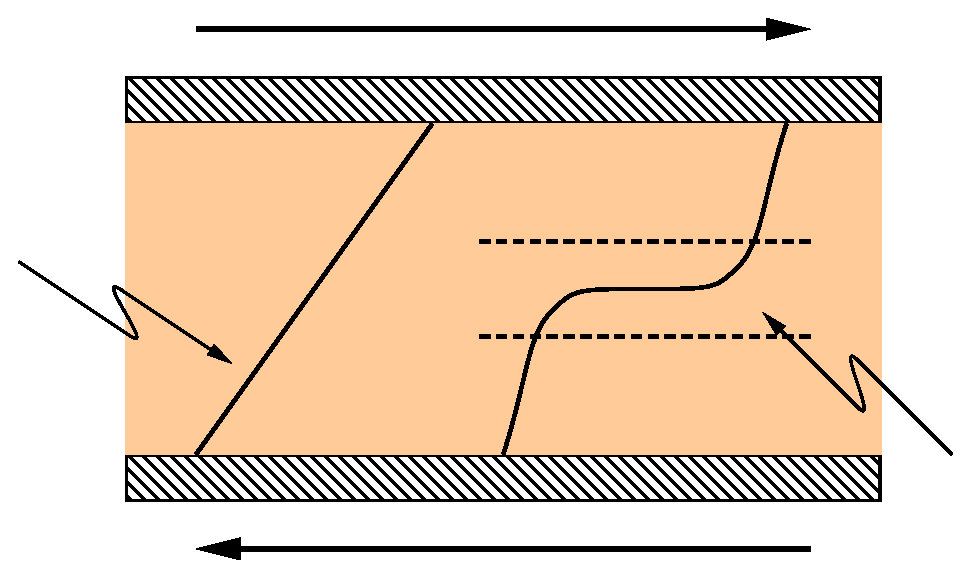
\includegraphics[height=5cm,width=11cm]{simpleshear}};
%\node[font=\scriptsize] at (-14,-5.5) {\sffamily  uniform shear};
%\node[font=\scriptsize] at (-2.75,-7.8) {\sffamily shear band};
%\node[font=\footnotesize] at (-3,-6) {$\tilde{y}=0$};
%\node[font=\footnotesize] at (-13.5,-7.5) {$\tilde{y}=-L$};
%\node[font=\footnotesize] at (-13.5,-4.5) {$\tilde{y}=L$};
%\node[font=\footnotesize] at (-8,-3) {$\tilde{v}_0$};
%\node[font=\footnotesize] at (-8,-9) {$-\tilde{v}_0$};
%\end{tikzpicture}\caption[Schematic of uniform shearing vs. a shear band.]{Schematic of uniform shearing vs. a shear band centered about $\tilde{y} = 0$.}
%\label{fig:simple_shear}
%\end{figure}

%\begin{figure}[tbp]
%\centering
%\tikzsetnextfilename{ApproachIsketch}
%\pgfdeclaredecoration{half brace}{brace}
{%
  \state{brace}[width=+\pgfdecoratedremainingdistance,next state=final]
  {%
    \pgfpathmoveto{\pgfpointorigin}%
    \pgfpathcurveto%
    {\pgfqpoint{.15\pgfdecorationsegmentamplitude}{.3\pgfdecorationsegmentamplitude}}%
    {\pgfqpoint{.5\pgfdecorationsegmentamplitude}{.5\pgfdecorationsegmentamplitude}}%
    {\pgfqpoint{\pgfdecorationsegmentamplitude}{.5\pgfdecorationsegmentamplitude}}%
    {%
      \pgftransformxshift{+\pgfdecorationsegmentaspect\pgfdecoratedremainingdistance}%
      \pgfpathlineto{\pgfqpoint{-\pgfdecorationsegmentamplitude}{.5\pgfdecorationsegmentamplitude}}%
      \pgfpathcurveto%
      {\pgfqpoint{-.5\pgfdecorationsegmentamplitude}{.5\pgfdecorationsegmentamplitude}}%
      {\pgfqpoint{-.15\pgfdecorationsegmentamplitude}{.7\pgfdecorationsegmentamplitude}}%
      {\pgfqpoint{0\pgfdecorationsegmentamplitude}{1\pgfdecorationsegmentamplitude}}%
      \pgfpathcurveto%
      {\pgfqpoint{.15\pgfdecorationsegmentamplitude}{.7\pgfdecorationsegmentamplitude}}%
      {\pgfqpoint{.5\pgfdecorationsegmentamplitude}{.5\pgfdecorationsegmentamplitude}}%
      {\pgfqpoint{\pgfdecorationsegmentamplitude}{.5\pgfdecorationsegmentamplitude}}%
    }%
    {%
      \pgftransformxshift{+\pgfdecoratedremainingdistance}%
      \pgfpathlineto{\pgfqpoint{0pt}{.5\pgfdecorationsegmentamplitude}}%
    }%
  }%
  \state{final}{}%
}

\begin{tikzpicture}
\draw[->,thick] (0,0)--(10,0) node[below,font=\footnotesize]{$t$};
\draw[->,thick] (0,0)--(0,6) node[left,font=\footnotesize]{$y$};
\draw[thick,dash dot] (10,1.5)--(0,1.5) node[left,yshift=-2em,font=\footnotesize]{$y = \eps \xi$};
\draw[thick,dash dot] (10,3.5)--(0,3.5) node[left,yshift=-2.5em,font=\footnotesize]{$y = \eps^{1/2} Y$};
\draw[thick,dash dot] (3,0)--(3,6);
\node[font=\scriptsize] at (1.5,0.75) {\sffamily Elastic};
\node[font=\scriptsize] at (1.5,2.5) {\sffamily Elastic};
\node[font=\scriptsize] at (1.5,4.75) {\sffamily Elastic};
\node[font=\scriptsize] at (6.5,0.75) {\sffamily Plastic-Reaction};
\node[font=\scriptsize][fill=white] at (6.5,1.5) {\sffamily $\uparrow$ Matching $\downarrow$};
\node[font=\scriptsize] at (6.5,2.5) {\sffamily Diffusive Zone};
\node[font=\scriptsize] at (6.5,4.75) {\sffamily Elastic};
\node[font=\footnotesize][fill=white,font=\footnotesize] at (6.5,3.5) {$T \to T_{\text{e}}, s \to s_{\text{e}}$ as $Y \to \infty$};
\draw [thick,decorate,decoration={half brace,amplitude=10pt,mirror}](3,-0.1) -- (9.75,-0.1) node[black,midway,yshift=-0.6cm,font=\footnotesize] {$t - t_{\text{p}} \sim O(\eps)$};
\end{tikzpicture}

%\caption[Sketch of the asymptotic structure used in Approach I.]{Sketch of the asymptotic structure used in Approach I. The up and down arrows at the matching interface between the shear band zone and the diffusive zone indicate that the problems are solved in conjunction with one another; the matching of the two solutions is necessary to obtain the behaviour of the centreline temperature and stress. The solution in the diffusive zone decays to the elastic solution as $Y \to \infty$.}
%\label{fig:ApproachIregion}
%\end{figure}

\begin{figure}[tbp]
\centering
\setlength\figureheight{2.85cm}      
\setlength\figurewidth{3cm}
\tikzsetnextfilename{fgk_reac}
% This file was created by matlab2tikz.
%
\begin{tikzpicture}
\begin{axis}[%
name=f1,
width=\figurewidth,
height=\figureheight,
at={(0\figurewidth,0\figureheight)},
scale only axis,
xmin=-5,
xmax=15,
xlabel={$\eta$},
ymin=-2.5,
ymax=15,
ylabel={$f(\eta)$},
axis background/.style={fill=white},
legend style={at={(0,1.15)},anchor=south west,legend cell align=left,align=left,draw=white!15!black,legend columns=4},
legend style={/tikz/every even column/.append style={column sep=0.075\figurewidth}}
]
\addplot [color=black,dotted,forget plot]
  table[row sep=crcr]{%
-5.09999999999984	0.00992646807422877\\
-4.99999999999984	0.0105776584739633\\
-4.89999999999984	0.011296454637271\\
-4.79999999999984	0.0120899544313957\\
-4.69999999999984	0.0129659990675174\\
-4.59999999999984	0.0139332505445423\\
-4.49999999999984	0.0150011956227659\\
-4.39999999999984	0.0161805263838217\\
-4.29999999999984	0.017482862804071\\
-4.19999999999984	0.0189210944139103\\
-4.09999999999985	0.0205094553424003\\
-3.99999999999985	0.0222636634143628\\
-3.89999999999984	0.0242010729772663\\
-3.79999999999984	0.0263408437029824\\
-3.69999999999984	0.0287041255610052\\
-3.59999999999984	0.0313142630362294\\
-3.49999999999984	0.0341970189875322\\
-3.39999999999984	0.037380821189441\\
-3.29999999999984	0.0408970321295209\\
-3.19999999999984	0.0447802459271498\\
-3.09999999999984	0.0490686131340474\\
-2.99999999999984	0.0538041957640495\\
-2.89999999999984	0.0590333573599111\\
-2.79999999999984	0.0648071867206173\\
-2.69999999999984	0.0711819616763413\\
-2.59999999999984	0.0782196545731134\\
-2.49999999999984	0.0859884779201214\\
-2.39999999999984	0.0945634832697232\\
-2.29999999999984	0.104027196771951\\
-2.24999999999984	0.109120820470215\\
-2.19999999999984	0.114471216765783\\
-2.14999999999984	0.120090716678795\\
-2.09999999999984	0.12599374924713\\
-2.04999999999984	0.132193152422125\\
-1.99999999999984	0.138704714129847\\
-1.94999999999984	0.145542642556202\\
-1.89999999999984	0.1527240535012\\
-1.84999999999984	0.16026475742654\\
-1.79999999999984	0.168183195330458\\
-1.74999999999984	0.176496983244847\\
-1.69999999999984	0.185225981440579\\
-1.64999999999984	0.194389720630229\\
-1.59999999999984	0.204009646303072\\
-1.57499999999984	0.208997934517841\\
-1.54999999999984	0.214108039963967\\
-1.52499999999984	0.219343233890683\\
-1.49999999999984	0.224706865403042\\
-1.47499999999984	0.230201256549308\\
-1.44999999999984	0.235830271135133\\
-1.42499999999984	0.241596153216531\\
-1.39999999999984	0.247503253548066\\
-1.37499999999984	0.253553802436529\\
-1.34999999999984	0.259751858991634\\
-1.32499999999984	0.266100123514508\\
-1.29999999999985	0.272603043768617\\
-1.27499999999985	0.27926347219069\\
-1.24999999999985	0.286085255658194\\
-1.22499999999985	0.29307190134068\\
-1.19999999999985	0.300227520489032\\
-1.17499999999985	0.307555950866519\\
-1.14999999999985	0.315060818718271\\
-1.12499999999985	0.322746337142547\\
-1.09999999999985	0.33061649401104\\
-1.07499999999985	0.338675777549597\\
-1.04999999999985	0.34692788751491\\
-1.02499999999985	0.355377517012391\\
-0.999999999999846	0.364028836751416\\
-0.974999999999846	0.372886773434186\\
-0.949999999999846	0.38195535234092\\
-0.924999999999846	0.391239505306621\\
-0.899999999999846	0.400743682436698\\
-0.874999999999846	0.410473140719211\\
-0.862499999999846	0.415424203289139\\
-0.849999999999846	0.420432717541254\\
-0.837499999999846	0.425500270101112\\
-0.824999999999846	0.430627014930274\\
-0.812499999999846	0.435813665906318\\
-0.799999999999846	0.441060855995359\\
-0.787499999999846	0.446369636794294\\
-0.774999999999846	0.451739935084595\\
-0.762499999999846	0.457173134370356\\
-0.749999999999846	0.462669129388433\\
-0.737499999999846	0.468229466933366\\
-0.724999999999846	0.47385399953205\\
-0.712499999999846	0.479543984486523\\
-0.699999999999847	0.485299423320969\\
-0.687499999999847	0.491121808344319\\
-0.674999999999847	0.49701115882686\\
-0.662499999999847	0.502968824052624\\
-0.649999999999847	0.508994819017418\\
-0.637499999999847	0.515090246996392\\
-0.624999999999847	0.521255669888697\\
-0.612499999999847	0.527491970570667\\
-0.599999999999847	0.533799475846806\\
-0.587499999999847	0.540179292323272\\
-0.574999999999847	0.54663189354636\\
-0.562499999999847	0.553158351171687\\
-0.549999999999847	0.559758977091223\\
-0.537499999999847	0.566434770704103\\
-0.524999999999847	0.573186300404797\\
-0.512499999999847	0.580014476040418\\
-0.499999999999847	0.586919840198393\\
-0.487499999999847	0.593903358859037\\
-0.474999999999847	0.600965549894698\\
-0.462499999999847	0.608107407567899\\
-0.449999999999847	0.615329512633522\\
-0.437499999999847	0.622632696237279\\
-0.424999999999847	0.630017697726012\\
-0.412499999999847	0.637485322743528\\
-0.399999999999847	0.645036345188293\\
-0.387499999999847	0.652671527353274\\
-0.374999999999847	0.660391575877848\\
-0.362499999999847	0.668197247001294\\
-0.349999999999847	0.676089474691031\\
-0.337499999999847	0.684069006430479\\
-0.324999999999847	0.692136485103924\\
-0.312499999999847	0.700292703985062\\
-0.299999999999847	0.708538557183426\\
-0.287499999999847	0.716874945040808\\
-0.274999999999847	0.725302481003043\\
-0.262499999999847	0.733821746266779\\
-0.249999999999847	0.742433908128551\\
-0.237499999999847	0.751139625528831\\
-0.224999999999847	0.759939815573131\\
-0.212499999999847	0.76883476416661\\
-0.199999999999847	0.777825913700548\\
-0.187499999999847	0.786913413404079\\
-0.174999999999847	0.796098670703041\\
-0.162499999999847	0.805381862130967\\
-0.149999999999847	0.81476433765628\\
-0.137499999999847	0.824246401277726\\
-0.131249999999847	0.829024706820484\\
-0.124999999999847	0.833829156545134\\
-0.118749999999847	0.83865821101487\\
-0.112499999999847	0.843513221086152\\
-0.106249999999847	0.848393204414871\\
-0.0999999999998468	0.853299531553118\\
-0.0937499999998468	0.858231042807135\\
-0.0874999999998468	0.863188561865785\\
-0.0812499999998468	0.868171746532432\\
-0.0749999999998468	0.873181368187509\\
-0.0687499999998468	0.878216634932214\\
-0.0624999999998468	0.883278370118672\\
-0.0562499999998468	0.888366155338944\\
-0.0499999999998468	0.893480730706529\\
-0.0437499999998468	0.898621391327721\\
-0.0374999999998468	0.90378879385876\\
-0.0312499999998468	0.908982587535101\\
-0.0249999999998468	0.914203567368064\\
-0.0187499999998468	0.919451035134854\\
-0.0124999999998468	0.924725647766677\\
-0.00624999999984681	0.930026881932746\\
1.53195164886988e-13	0.935355789195676\\
0.0062500000001532	0.940711835819767\\
0.0125000000001532	0.946094960938385\\
0.0187500000001532	0.951505400387796\\
0.0250000000001532	0.956943372603843\\
0.0312500000001532	0.962408902971363\\
0.0375000000001532	0.967901986639302\\
0.0437500000001532	0.973422745231897\\
0.0500000000001532	0.978971412302965\\
0.0562500000001532	0.984548082480075\\
0.0625000000001532	0.990152657635805\\
0.0687500000001532	0.99578517085607\\
0.0750000000001532	1.00144588747176\\
0.0812500000001532	1.007134915898\\
0.0875000000001532	1.01285242712245\\
0.0937500000001532	1.01859778276384\\
0.100000000000153	1.02437196602874\\
0.106250000000153	1.03017454275639\\
0.112500000000153	1.03600611515106\\
0.118750000000153	1.04186594416688\\
0.125000000000153	1.04775484853362\\
0.131250000000153	1.05367236834455\\
0.137500000000153	1.05961907991803\\
0.143750000000153	1.0655944078528\\
0.150000000000153	1.07159902458245\\
0.156250000000153	1.07763270922578\\
0.162500000000153	1.08369599014589\\
0.168750000000153	1.08978817166714\\
0.175000000000153	1.09590985382545\\
0.181250000000153	1.10206092682357\\
0.187500000000153	1.10824171272608\\
0.193750000000153	1.11445160786276\\
0.200000000000153	1.12069132852889\\
0.206250000000153	1.12696059911082\\
0.212500000000153	1.13325992535983\\
0.218750000000153	1.13958882052205\\
0.225000000000153	1.14594773441754\\
0.231250000000153	1.15233646446254\\
0.237500000000153	1.15875535197966\\
0.243750000000153	1.16520401384233\\
0.250000000000153	1.17168279622946\\
0.256250000000153	1.17819173191685\\
0.262500000000153	1.18473104940603\\
0.268750000000153	1.19130049909993\\
0.275000000000153	1.19790018595808\\
0.281250000000153	1.20453024433563\\
0.287500000000153	1.21119076293514\\
0.293750000000153	1.21788155544651\\
0.300000000000153	1.22460277067942\\
0.306250000000153	1.23135452870143\\
0.312500000000153	1.23813695395617\\
0.318750000000153	1.24495000487807\\
0.325000000000153	1.2517935381122\\
0.331250000000153	1.25866772484523\\
0.337500000000153	1.26557270732822\\
0.343750000000153	1.27250842128352\\
0.350000000000153	1.2794747061398\\
0.356250000000153	1.28647175886507\\
0.362500000000153	1.29349960134239\\
0.368750000000153	1.30055840172864\\
0.375000000000153	1.30764794684435\\
0.381250000000153	1.31476834976405\\
0.387500000000153	1.32191954278913\\
0.393750000000153	1.32910179244794\\
0.400000000000153	1.33631465725585\\
0.406250000000153	1.34355853549318\\
0.412500000000153	1.35083332906504\\
0.418750000000153	1.35813898801986\\
0.425000000000153	1.36547557435625\\
0.431250000000153	1.3728430728555\\
0.437500000000153	1.38024143521951\\
0.443750000000153	1.38767071025258\\
0.450000000000153	1.39513089810967\\
0.456250000000153	1.4026218090955\\
0.462500000000153	1.41014352515469\\
0.468750000000153	1.41769619545498\\
0.475000000000153	1.4252797773867\\
0.481250000000153	1.43289410340401\\
0.487500000000152	1.44053912356737\\
0.493750000000152	1.44821500564788\\
0.500000000000152	1.45592158837722\\
0.506250000000152	1.46365887256351\\
0.512500000000152	1.47142649684783\\
0.518750000000152	1.47922500227188\\
0.525000000000152	1.48705400545078\\
0.531250000000152	1.49491357068626\\
0.537500000000152	1.50280346936314\\
0.543750000000152	1.51072387219161\\
0.550000000000152	1.518674472169\\
0.556250000000152	1.52665549264611\\
0.562500000000152	1.53466651170477\\
0.568750000000152	1.54270788823435\\
0.575000000000152	1.5507792317767\\
0.581250000000152	1.55888061888955\\
0.587500000000152	1.56701195919844\\
0.593750000000152	1.57517312617747\\
0.600000000000152	1.5833641936428\\
0.606250000000152	1.59158476667677\\
0.612500000000152	1.5998350426932\\
0.618750000000152	1.60811465106242\\
0.625000000000152	1.61642380495008\\
0.631250000000152	1.62476208643414\\
0.637500000000152	1.63312962932607\\
0.643750000000152	1.64152614102478\\
0.650000000000152	1.64995175460426\\
0.656250000000152	1.65840599210139\\
0.662500000000152	1.66688904479824\\
0.668750000000152	1.67540039139274\\
0.675000000000152	1.68394035369653\\
0.681250000000152	1.69250849943222\\
0.687500000000152	1.70110494822306\\
0.693750000000152	1.70972914980628\\
0.700000000000152	1.71838138236115\\
0.706250000000152	1.72706113157762\\
0.712500000000152	1.73576853166781\\
0.718750000000152	1.74450310126318\\
0.721875000000152	1.74888244619477\\
0.725000000000152	1.75326710264835\\
0.728125000000152	1.75765922629232\\
0.731250000000152	1.7620563661972\\
0.734375000000152	1.7664617264152\\
0.737500000000152	1.7708737954204\\
0.740625000000152	1.77529224332036\\
0.743750000000152	1.77971632502521\\
0.746875000000152	1.78414779732644\\
0.750000000000152	1.78858514005022\\
0.753125000000152	1.79302987980644\\
0.756250000000152	1.7974802690095\\
0.759375000000152	1.8019389862392\\
0.762500000000152	1.80640334932601\\
0.765625000000152	1.81087308585928\\
0.768750000000152	1.81535032537083\\
0.771875000000152	1.81983287917876\\
0.775000000000152	1.82432236128753\\
0.778125000000153	1.82881904106356\\
0.781250000000153	1.83332124640402\\
0.784375000000153	1.83782967304781\\
0.787500000000153	1.84234437883637\\
0.790625000000153	1.84686531206612\\
0.793750000000153	1.85139237611342\\
0.796875000000153	1.85592571019569\\
0.800000000000153	1.86046527285292\\
0.803125000000153	1.86501210053518\\
0.806250000000153	1.8695632860763\\
0.809375000000153	1.87412121314906\\
0.812500000000153	1.87868453442557\\
0.815625000000153	1.88325461517908\\
0.818750000000153	1.88783003900011\\
0.821875000000153	1.89241175442439\\
0.825000000000153	1.89699888762763\\
0.828125000000153	1.90159220612758\\
0.831250000000153	1.90619083916237\\
0.834375000000153	1.91079572210402\\
0.837500000000153	1.91540610182675\\
0.840625000000153	1.920022644248\\
0.843750000000153	1.92464444894457\\
0.846875000000153	1.92927210705902\\
0.850000000000154	1.9339052341778\\
0.853125000000154	1.93854389384255\\
0.856250000000154	1.9431880290093\\
0.859375000000154	1.94783782562718\\
0.862500000000154	1.95249482156131\\
0.865625000000154	1.95715587249159\\
0.868750000000154	1.96182123230513\\
0.871875000000154	1.96649259522142\\
0.875000000000154	1.97116931050031\\
0.878125000000154	1.97585115119367\\
0.881250000000154	1.98053811657557\\
0.884375000000154	1.98523023779548\\
0.887500000000154	1.98992764877714\\
0.890625000000154	1.99463053672943\\
0.893750000000154	1.99933855056457\\
0.896875000000154	2.0040510734223\\
0.900000000000154	2.00876882142451\\
0.903125000000154	2.01349131697936\\
0.906250000000154	2.01821858530363\\
0.909375000000154	2.02295054837972\\
0.912500000000154	2.02768752216489\\
0.915625000000154	2.03242956665273\\
0.918750000000154	2.03717638788174\\
0.921875000000155	2.04192738183151\\
0.925000000000155	2.0466831442338\\
0.928125000000155	2.05144351695402\\
0.931250000000155	2.05620838115657\\
0.934375000000155	2.06097759447761\\
0.937500000000155	2.06575123383341\\
0.940625000000155	2.07052931318174\\
0.943750000000155	2.0753118687759\\
0.946875000000155	2.08009933816922\\
0.950000000000155	2.08489068525432\\
0.953125000000155	2.08968548411254\\
0.956250000000155	2.09448519278894\\
0.959375000000155	2.09928789543738\\
0.962500000000155	2.10409562306548\\
0.965625000000155	2.10890645958792\\
0.968750000000155	2.11372190459185\\
0.971875000000155	2.11854054939468\\
0.975000000000155	2.12336377909262\\
0.978125000000155	2.12819013523719\\
0.981250000000155	2.13302071011718\\
0.984375000000155	2.13785419814682\\
0.987500000000155	2.14269185823547\\
0.990625000000156	2.14753250268052\\
0.993750000000156	2.15237725929681\\
0.996875000000156	2.15722479200762\\
1.00000000000016	2.16207631558441\\
1.00312500000016	2.16693104747271\\
1.00625000000016	2.17178934641989\\
1.00937500000016	2.17665017579436\\
1.01250000000016	2.18151443889579\\
1.01562500000016	2.18638157875457\\
1.01875000000016	2.19125207721328\\
1.02187500000016	2.19612511628474\\
1.02500000000016	2.20100111176794\\
1.02812500000016	2.20588012426103\\
1.03125000000016	2.2107622255155\\
1.03437500000016	2.21564670192898\\
1.03750000000016	2.22053381288837\\
1.04062500000016	2.22542340886564\\
1.04375000000016	2.23031582351487\\
1.04687500000016	2.23521199203639\\
1.05000000000016	2.24010906034984\\
1.05312500000016	2.24500838736109\\
1.05625000000016	2.24991027953114\\
1.05937500000016	2.25481425677736\\
1.06250000000016	2.25972054639077\\
1.06562500000016	2.26462845553367\\
1.06875000000016	2.26953875087551\\
1.07187500000016	2.27445065315391\\
1.07500000000016	2.27936474901871\\
1.07812500000016	2.28428019278684\\
1.08125000000016	2.28919792067102\\
1.08437500000016	2.29411702684101\\
1.08750000000016	2.29903807242747\\
1.09062500000016	2.30395998628267\\
1.09375000000016	2.30888395684666\\
1.09687500000016	2.31380983702844\\
1.10000000000016	2.31873665184747\\
1.10312500000016	2.32366412957911\\
1.10625000000016	2.32859332622493\\
1.10937500000016	2.33352334898652\\
1.11250000000016	2.3384546402367\\
1.11562500000016	2.34338647752977\\
1.11875000000016	2.34831952107029\\
1.12187500000016	2.35325307642159\\
1.12500000000016	2.35818746703484\\
1.12812500000016	2.3631222889834\\
1.13125000000016	2.36805796335045\\
1.13437500000016	2.37299407136807\\
1.13750000000016	2.37793072625727\\
1.14062500000016	2.3828674665633\\
1.14375000000016	2.38780468377304\\
1.14687500000016	2.39274192240879\\
1.15000000000016	2.39767946223661\\
1.15312500000016	2.40261696616161\\
1.15625000000016	2.40755544583921\\
1.15937500000016	2.412492795535\\
1.16250000000016	2.4174301107729\\
1.16562500000016	2.42236663390579\\
1.16875000000016	2.42730318520294\\
1.17187500000016	2.43223900815277\\
1.17500000000016	2.43717561251963\\
1.17812500000016	2.44210900671708\\
1.18125000000016	2.44704438976831\\
1.18437500000016	2.45197758363957\\
1.18750000000016	2.45691052273831\\
1.19062500000016	2.46184097587701\\
1.19375000000016	2.46677161004606\\
1.19687500000016	2.47170082700173\\
1.20000000000016	2.47663036349459\\
1.20312500000016	2.48155673707722\\
1.20625000000016	2.48648221146173\\
1.20937500000016	2.49140606234626\\
1.21250000000016	2.49632884479416\\
1.21562500000016	2.50124968645598\\
1.21875000000016	2.50616931550713\\
1.22187500000016	2.51108679283649\\
1.22500000000016	2.51600262690497\\
1.22812500000016	2.52091590150455\\
1.23125000000016	2.52582737148217\\
1.23437500000016	2.53073633404572\\
1.23750000000016	2.53564402408478\\
1.24062500000016	2.54054872798269\\
1.24375000000016	2.54545107925273\\
1.24687500000016	2.55035028883143\\
1.25000000000016	2.55524778033388\\
1.25312500000016	2.56014224996632\\
1.25625000000016	2.56503381963218\\
1.25937500000016	2.5699223506766\\
1.26250000000016	2.5748082186806\\
1.26562500000016	2.57969123814196\\
1.26875000000016	2.58457097078491\\
1.27187500000016	2.58944730782556\\
1.27500000000016	2.59432021354408\\
1.27812500000016	2.59918964133514\\
1.28125000000016	2.60405593070886\\
1.28437500000016	2.60891815700741\\
1.28750000000016	2.61377663689432\\
1.29062500000016	2.61863125768837\\
1.29375000000016	2.62348298806827\\
1.29687500000016	2.62832932331954\\
1.30000000000016	2.63317278573956\\
1.30312500000016	2.63801122144743\\
1.30625000000016	2.64284530694209\\
1.30937500000016	2.64767524184102\\
1.31250000000016	2.65250063495767\\
1.31562500000016	2.65732089873307\\
1.31875000000016	2.66213720698978\\
1.32187500000016	2.6669482781936\\
1.32500000000016	2.67175475585271\\
1.32812500000016	2.67655640184897\\
1.33125000000016	2.68135259730704\\
1.33437500000016	2.68614391578471\\
1.33750000000016	2.69092947635026\\
1.34062500000016	2.69571040293864\\
1.34375000000016	2.70048478150733\\
1.34687500000016	2.70525465070783\\
1.35000000000016	2.71001839612421\\
1.35312500000016	2.71477659622788\\
1.35625000000016	2.71952851409912\\
1.35937500000016	2.72427503620257\\
1.36250000000016	2.72901525499116\\
1.36562500000016	2.73374941634686\\
1.36875000000016	2.73847693380982\\
1.37187500000016	2.74319845640935\\
1.37500000000016	2.74791306224427\\
1.37812500000016	2.75262150621045\\
1.38125000000016	2.75732295815518\\
1.38437500000016	2.76201803720569\\
1.38750000000016	2.76670591485355\\
1.39062500000016	2.77138703593021\\
1.39375000000016	2.77606079579181\\
1.39687500000016	2.78072759799592\\
1.40000000000016	2.78538736751706\\
1.40312500000016	2.79003955123871\\
1.40625000000016	2.79468417098579\\
1.40937500000016	2.79932106800319\\
1.41250000000016	2.80395057196534\\
1.41562500000016	2.80857213425413\\
1.41875000000016	2.81318590668171\\
1.42187500000016	2.81779141988851\\
1.42500000000016	2.82238925925817\\
1.42812500000016	2.82697852910713\\
1.43125000000016	2.83155991579972\\
1.43437500000016	2.83613248275778\\
1.43750000000016	2.84069702068056\\
1.44062500000016	2.84525302682901\\
1.44375000000016	2.84980054288781\\
1.44687500000016	2.85433851126988\\
1.45000000000016	2.85886812678144\\
1.45312500000016	2.86338848742495\\
1.45625000000016	2.86790025957026\\
1.45937500000016	2.87240230988435\\
1.46250000000016	2.87689535488725\\
1.46562500000016	2.88137872957115\\
1.46875000000016	2.88585312983933\\
1.47187500000016	2.89031740345836\\
1.47500000000016	2.89477239988901\\
1.47812500000016	2.89921735938415\\
1.48125000000016	2.90365316066265\\
1.48437500000016	2.90807845631578\\
1.48750000000016	2.91249362289475\\
1.49062500000016	2.91689851678067\\
1.49375000000016	2.9212932266334\\
1.49687500000016	2.92567777060051\\
1.50000000000016	2.93005164576095\\
1.50312500000016	2.93441510284057\\
1.50625000000016	2.93876754827041\\
1.50937500000016	2.94310987466286\\
1.51250000000016	2.94744076164673\\
1.51562500000016	2.95176117080197\\
1.51875000000016	2.95607055143182\\
1.52187500000016	2.96036896130699\\
1.52500000000016	2.96465550772826\\
1.52812500000016	2.96893133979683\\
1.53125000000016	2.97319522311583\\
1.53437500000016	2.97744822232031\\
1.53750000000016	2.98168918625819\\
1.54062500000016	2.98591884934266\\
1.54375000000016	2.9901360632063\\
1.54687500000016	2.99434205645225\\
1.55000000000016	2.99853577720793\\
1.55312500000016	3.002717951213\\
1.55625000000016	3.00688765363741\\
1.55937500000016	3.01104478626436\\
1.56250000000016	3.01519004280201\\
1.56562500000016	3.01932280544552\\
1.56875000000016	3.02344294104713\\
1.57187500000016	3.02755031392297\\
1.57500000000016	3.03164505667909\\
1.57812500000016	3.03572738687486\\
1.58125000000016	3.03979653549991\\
1.58437500000016	3.0438532502562\\
1.58750000000016	3.0478966565999\\
1.59062500000016	3.05192690452077\\
1.59375000000016	3.05594393778896\\
1.59687500000016	3.05994767042148\\
1.60000000000016	3.06393823828441\\
1.60312500000016	3.06791530605888\\
1.60625000000016	3.07187880000512\\
1.60937500000016	3.07582873909661\\
1.61250000000016	3.07976472564457\\
1.61562500000016	3.08368739485737\\
1.61875000000016	3.08759611128098\\
1.62187500000016	3.09149108498348\\
1.62500000000016	3.09537188226996\\
1.62812500000016	3.09923874837058\\
1.63125000000016	3.10309118663664\\
1.63437500000016	3.10692944542984\\
1.63750000000016	3.11075357364512\\
1.64062500000016	3.11456358632291\\
1.64375000000016	3.11835893021631\\
1.64687500000016	3.12213970848478\\
1.65000000000016	3.12590592857068\\
1.65312500000016	3.12965818043039\\
1.65625000000016	3.13339442853503\\
1.65937500000017	3.13711634741203\\
1.66250000000017	3.14082353887676\\
1.66562500000017	3.14451588447366\\
1.66875000000017	3.14819323080228\\
1.67187500000017	3.1518552002802\\
1.67500000000017	3.15550239891714\\
1.67812500000017	3.15913419251647\\
1.68125000000017	3.16275119283163\\
1.68437500000017	3.16635262713461\\
1.68750000000017	3.16993867224937\\
1.69062500000017	3.17350898952857\\
1.69375000000017	3.17706404048736\\
1.69687500000017	3.180603438208\\
1.70000000000017	3.18412773830155\\
1.70312500000017	3.18763591051988\\
1.70625000000017	3.19112874150213\\
1.70937500000017	3.19460547780427\\
1.71250000000017	3.19806644194515\\
1.71562500000017	3.2015112829077\\
1.71875000000017	3.20494048245335\\
1.72187500000017	3.2083534163613\\
1.72500000000017	3.21175040946915\\
1.72812500000017	3.21513117654131\\
1.73125000000017	3.21849589087979\\
1.73437500000017	3.22184478818502\\
1.73750000000017	3.22517754157678\\
1.74062500000017	3.22849352483068\\
1.74375000000017	3.23179324104883\\
1.74687500000017	3.23507708832964\\
1.75000000000017	3.23834403721143\\
1.75312500000017	3.24159467567199\\
1.75625000000017	3.24482872990622\\
1.75937500000017	3.2480463831611\\
1.76250000000017	3.25124746629158\\
1.76562500000017	3.25443185519024\\
1.76875000000017	3.25759936101275\\
1.77187500000017	3.26075032588639\\
1.77500000000017	3.26388459542272\\
1.77812500000017	3.26700207891715\\
1.78125000000017	3.27010264097549\\
1.78437500000017	3.27318662300582\\
1.78750000000017	3.27625395349003\\
1.79062500000017	3.27930419510571\\
1.79375000000017	3.28233743011469\\
1.79687500000017	3.28535365514718\\
1.80000000000017	3.28835346068916\\
1.80312500000017	3.29133580181613\\
1.80625000000017	3.29430126354694\\
1.80937500000017	3.2972498946847\\
1.81250000000017	3.30018137690271\\
1.81562500000017	3.30309540745445\\
1.81875000000017	3.30599261199625\\
1.82187500000017	3.3088724875862\\
1.82500000000017	3.3117354651851\\
1.82812500000017	3.31458120029084\\
1.83125000000017	3.31741009165105\\
1.83437500000017	3.3202213197545\\
1.83750000000017	3.32301611717677\\
1.84062500000017	3.32579354950726\\
1.84375000000017	3.32855340333226\\
1.84687500000017	3.33129619019411\\
1.85000000000017	3.33402156392522\\
1.85312500000017	3.33672957746632\\
1.85625000000017	3.33942065796356\\
1.85937500000017	3.34209420304622\\
1.86250000000017	3.34475049072785\\
1.86562500000017	3.3473896157816\\
1.86875000000017	3.35001175681563\\
1.87187500000017	3.35261636743791\\
1.87500000000017	3.35520369557647\\
1.87812500000017	3.35777362329405\\
1.88125000000017	3.36032665826963\\
1.88437500000017	3.36286220477697\\
1.88750000000017	3.36538117717952\\
1.89062500000017	3.36788178995546\\
1.89375000000017	3.37036557363882\\
1.89687500000017	3.37283236149478\\
1.90000000000017	3.37528173157988\\
1.90312500000017	3.37771401578002\\
1.90625000000017	3.38012904312644\\
1.90937500000017	3.38252689163488\\
1.91250000000017	3.38490746995191\\
1.91562500000017	3.38727090980132\\
1.91875000000017	3.38961717997244\\
1.92187500000017	3.39194644749244\\
1.92500000000017	3.39425874955166\\
1.92812500000017	3.39655342560242\\
1.93125000000017	3.39883122474446\\
1.93437500000017	3.40109195750567\\
1.93750000000017	3.40333544312446\\
1.94062500000017	3.40556234195904\\
1.94375000000017	3.40777235272969\\
1.94687500000017	3.40996500753139\\
1.95000000000017	3.41214077455592\\
1.95312500000017	3.41429979885848\\
1.95625000000017	3.41644195893256\\
1.95937500000017	3.41856696543953\\
1.96250000000017	3.42067523408129\\
1.96562500000017	3.42276668562035\\
1.96875000000017	3.42484114750781\\
1.97187500000017	3.42689951043645\\
1.97500000000017	3.42894059832143\\
1.97812500000017	3.43096514304174\\
1.98125000000017	3.43297260314532\\
1.98437500000017	3.43496387851717\\
1.98750000000017	3.43693838607754\\
1.99062500000017	3.43889675793156\\
1.99375000000017	3.44083857325216\\
1.99687500000017	3.44276336413641\\
2.00000000000017	3.444671731462\\
2.00312500000017	3.44656396079099\\
2.00625000000017	3.44843989749277\\
2.00937500000017	3.45029940698237\\
2.01250000000017	3.45214221994863\\
2.01562500000017	3.45396909176477\\
2.01875000000017	3.45577933196095\\
2.02187500000017	3.45757386131958\\
2.02500000000017	3.45935228859317\\
2.02812500000017	3.46111472949426\\
2.03125000000017	3.46286147177026\\
2.03437500000017	3.46459174580172\\
2.03750000000017	3.46630612873348\\
2.04062500000017	3.46800452124591\\
2.04375000000017	3.46968732445651\\
2.04687500000017	3.47135413155099\\
2.05000000000017	3.47300527842757\\
2.05312500000017	3.47464132419928\\
2.05625000000017	3.4762608358964\\
2.05937500000017	3.47786532980051\\
2.06250000000017	3.47945431133666\\
2.06562500000017	3.48102785817659\\
2.06875000000017	3.48258618330398\\
2.07187500000017	3.48412897426423\\
2.07500000000017	3.48565645420258\\
2.07812500000017	3.48716858179801\\
2.08125000000017	3.48866552879056\\
2.08437500000016	3.49014764726845\\
2.08750000000016	3.49161447949176\\
2.09062500000016	3.4930667884662\\
2.09375000000016	3.49450380046021\\
2.09687500000016	3.4959260190758\\
2.10000000000016	3.49733328612468\\
2.10312500000016	3.49872643092878\\
2.10625000000016	3.50010400313004\\
2.10937500000016	3.50146768523017\\
2.11250000000016	3.50281609668024\\
2.11562500000016	3.50415048468429\\
2.11875000000016	3.50547021099774\\
2.12187500000016	3.50677554565803\\
2.12500000000016	3.50806656612409\\
2.12812500000016	3.50934351845529\\
2.13125000000016	3.51060615042421\\
2.13437500000016	3.51185465493936\\
2.13750000000016	3.51308951576004\\
2.14062500000016	3.51431018984412\\
2.14375000000016	3.51551713723216\\
2.14687500000016	3.51671005860616\\
2.15000000000016	3.51788915820294\\
2.15312500000016	3.51905445065508\\
2.15625000000016	3.52020618731661\\
2.15937500000016	3.52134419389163\\
2.16250000000016	3.5224692997702\\
2.16562500000016	3.52358062553296\\
2.16875000000016	3.52467878971853\\
2.17187500000016	3.52576344200113\\
2.17500000000016	3.52683524186039\\
2.17812500000016	3.5278934717676\\
2.18125000000016	3.52893898509766\\
2.18437500000016	3.52997128230194\\
2.18750000000016	3.5309904911674\\
2.19062500000016	3.53199689524994\\
2.19375000000016	3.53299095546153\\
2.19687500000016	3.53397213623915\\
2.20000000000016	3.53494085426879\\
2.20312500000016	3.53589688536532\\
2.20625000000016	3.53684034322989\\
2.20937500000016	3.53777195073092\\
2.21250000000016	3.53869015984547\\
2.21562500000016	3.53959666572156\\
2.21875000000016	3.54049071921269\\
2.22187500000016	3.54137320470687\\
2.22500000000016	3.54224236873558\\
2.22812500000016	3.54310083577864\\
2.23125000000016	3.54394691259545\\
2.23437500000016	3.54478172843812\\
2.23750000000016	3.54560421868509\\
2.24062500000016	3.54641553430544\\
2.24375000000016	3.54721367105194\\
2.24687500000016	3.54800154900726\\
2.25000000000016	3.54877788017528\\
2.25312500000016	3.54954330377296\\
2.25625000000016	3.55029668536613\\
2.25937500000015	3.5510396719294\\
2.26250000000015	3.55177088034136\\
2.26562500000015	3.5524914249098\\
2.26875000000015	3.55320118510144\\
2.27187500000015	3.55389984385709\\
2.27500000000015	3.55458726822428\\
2.27812500000015	3.55526438868464\\
2.28125000000015	3.55593081525172\\
2.28437500000015	3.556586413342\\
2.28750000000015	3.55723187035906\\
2.29062500000015	3.55786654845939\\
2.29375000000015	3.5584907758402\\
2.29687500000015	3.55910473909596\\
2.30000000000015	3.55970858384596\\
2.30312500000015	3.5603018979505\\
2.30625000000015	3.56088558270986\\
2.30937500000015	3.56145915444227\\
2.31250000000015	3.56202292358758\\
2.31562500000015	3.56257665638593\\
2.31875000000015	3.5631207359783\\
2.32187500000015	3.5636550808664\\
2.32500000000015	3.56417981543658\\
2.32812500000015	3.56469528630218\\
2.33125000000015	3.56520108141656\\
2.33437500000015	3.56569823809688\\
2.33750000000015	3.56618487364193\\
2.34062500000015	3.56666248789212\\
2.34375000000015	3.56713086563001\\
2.34687500000015	3.56759054823165\\
2.35000000000015	3.56804101441183\\
2.35312500000015	3.56848291598391\\
2.35625000000015	3.56891514448908\\
2.35937500000015	3.56933919318037\\
2.36250000000015	3.56975441428728\\
2.36562500000015	3.57016108217169\\
2.36875000000015	3.57055911875344\\
2.37187500000015	3.57094861882703\\
2.37500000000015	3.57132953485737\\
2.37812500000015	3.57170219581683\\
2.38125000000015	3.57206624083772\\
2.38437500000015	3.5724223905265\\
2.38750000000015	3.57277074253837\\
2.39062500000015	3.57311112631383\\
2.39375000000015	3.57344295423771\\
2.39687500000015	3.5737665896194\\
2.40000000000015	3.57408245849823\\
2.40312500000015	3.57439086813128\\
2.40625000000015	3.57469172143382\\
2.40937500000015	3.57498444169785\\
2.41250000000015	3.57526974281793\\
2.41562500000015	3.57554741924665\\
2.41875000000015	3.57581790061207\\
2.42187500000015	3.57608104915628\\
2.42500000000015	3.57633685065113\\
2.42812500000015	3.57658525900687\\
2.43125000000015	3.57682661154607\\
2.43437500000014	3.57706045565257\\
2.43750000000014	3.57728757661761\\
2.44062500000014	3.57750784095945\\
2.44375000000014	3.57772197837492\\
2.44687500000014	3.57792864843334\\
2.45000000000014	3.57812824411159\\
2.45312500000014	3.57832134844804\\
2.45625000000014	3.57850737006024\\
2.45937500000014	3.57868812352611\\
2.46250000000014	3.57886062093165\\
2.46562500000014	3.57902834321413\\
2.46875000000014	3.57918820253992\\
2.47187500000014	3.57934239422092\\
2.47500000000014	3.57949042747179\\
2.47812500000014	3.57963247932222\\
2.48125000000014	3.57976806537539\\
2.48437500000014	3.57989791868296\\
2.48750000000014	3.58002171304203\\
2.49062500000014	3.58013947486091\\
2.49375000000014	3.58025227346603\\
2.49687500000014	3.58035763420997\\
2.50000000000014	3.58045905607526\\
2.50312500000014	3.58055337184864\\
2.50625000000014	3.58064385411331\\
2.50937500000014	3.58072644901855\\
2.51250000000014	3.58080572294762\\
2.51562500000014	3.58087762169839\\
2.51875000000014	3.58094497624583\\
2.52187500000014	3.5810072755387\\
2.52500000000014	3.58106433196064\\
2.52812500000014	3.58111590743381\\
2.53125000000014	3.58116221880401\\
2.53437500000014	3.58120395808954\\
2.53750000000014	3.58124070720029\\
2.54062500000014	3.58127250873927\\
2.54375000000014	3.58129908155109\\
2.54687500000014	3.58132089954425\\
2.55000000000014	3.58133797107458\\
2.55312500000014	3.58135042698619\\
2.55625000000014	3.58135853073926\\
2.55937500000014	3.58136156392687\\
2.56250000000014	3.58136103971882\\
2.56562500000014	3.58135492840776\\
2.56875000000014	3.58134506309379\\
2.57187500000014	3.58132987998061\\
2.57500000000014	3.58131119862736\\
2.57812500000014	3.58128780884941\\
2.58125000000014	3.58126061202922\\
2.58437500000014	3.58122933210702\\
2.58750000000014	3.58119359917941\\
2.59062500000014	3.5811538738562\\
2.59375000000014	3.58111037894933\\
2.59687500000014	3.58106249956517\\
2.60000000000014	3.58101087136634\\
2.60312500000014	3.5809553629109\\
2.60625000000014	3.5808958226851\\
2.60937500000014	3.58083319316902\\
2.61250000000013	3.58076637442026\\
2.61562500000013	3.5806963298949\\
2.61875000000013	3.58062231440227\\
2.62187500000013	3.5805451127854\\
2.62500000000013	3.58046453455941\\
2.62812500000013	3.58038029935423\\
2.63125000000013	3.5802929126255\\
2.63437500000013	3.58020160386055\\
2.63750000000013	3.58010721048809\\
2.64062500000013	3.58000975564467\\
2.64375000000013	3.57990907548109\\
2.64687500000013	3.57980520155878\\
2.65000000000013	3.57969846369298\\
2.65312500000013	3.57958814217451\\
2.65625000000013	3.57947500276588\\
2.65937500000013	3.57935828227917\\
2.66250000000013	3.57923893567744\\
2.66562500000013	3.57911688433905\\
2.66875000000013	3.57899218458462\\
2.67187500000013	3.57886462345331\\
2.67500000000013	3.57873458896962\\
2.67812500000013	3.57860129154472\\
2.68125000000013	3.57846504784756\\
2.68437500000013	3.57832681871276\\
2.68750000000013	3.5781855461442\\
2.69062500000013	3.5780423486548\\
2.69375000000013	3.57789658378395\\
2.69687500000013	3.57774823428812\\
2.70000000000013	3.57759758743031\\
2.70312500000013	3.57744430911479\\
2.70625000000013	3.57728871398737\\
2.70937500000013	3.577132273852\\
2.71250000000013	3.57697105379296\\
2.71562500000013	3.57680877269357\\
2.71875000000013	3.57664429245643\\
2.72187500000013	3.57647746946704\\
2.72500000000013	3.57630918876351\\
2.72812500000013	3.57613839961949\\
2.73125000000013	3.57596543754551\\
2.73437500000013	3.57579089621013\\
2.73750000000013	3.5756147004368\\
2.74062500000013	3.57543590594092\\
2.74375000000013	3.5752559417139\\
2.74687500000013	3.57507358387388\\
2.75000000000013	3.57488995108222\\
2.75312500000013	3.57470413773054\\
2.75625000000013	3.57451657436627\\
2.75937500000013	3.57432734538693\\
2.76250000000013	3.57413671714387\\
2.76562500000013	3.57394460646792\\
2.76875000000013	3.57375063948676\\
2.77187500000013	3.57355509127874\\
2.77500000000013	3.57335834854383\\
2.77812500000013	3.57316029217599\\
2.78125000000013	3.57296045837761\\
2.78437500000013	3.57275951654908\\
2.78750000000012	3.57255676405909\\
2.79062500000012	3.57235284120454\\
2.79375000000012	3.57214728315305\\
2.79687500000012	3.57194107281184\\
2.80000000000012	3.57173354187926\\
2.80312500000012	3.57152446044819\\
2.80625000000012	3.5713141574605\\
2.80937500000012	3.57110303057661\\
2.81250000000012	3.5708910241939\\
2.81562500000012	3.57067771275062\\
2.81875000000012	3.57046356763805\\
2.82187500000012	3.57024833265451\\
2.82500000000012	3.57003200116982\\
2.82812500000012	3.56981441435866\\
2.83125000000012	3.56959619420446\\
2.83437500000012	3.56937705698424\\
2.83750000000012	3.5691575908928\\
2.84062500000012	3.5689367874485\\
2.84375000000012	3.56871541173562\\
2.84687500000012	3.56849319559435\\
2.85000000000012	3.56826989749537\\
2.85312500000012	3.56804582192496\\
2.85625000000012	3.56782110917833\\
2.85937500000012	3.56759641018932\\
2.86250000000012	3.56737020723935\\
2.86562500000012	3.56714358200549\\
2.86875000000012	3.56691671822308\\
2.87187500000012	3.56668969204175\\
2.87500000000012	3.5664613114865\\
2.87812500000012	3.56623257573627\\
2.88125000000012	3.56600337092763\\
2.88437500000012	3.56577429398482\\
2.88750000000012	3.5655445260128\\
2.89062500000012	3.56531410697735\\
2.89375000000012	3.56508308822263\\
2.89687500000012	3.56485227523416\\
2.90000000000012	3.56462094417893\\
2.90312500000012	3.56438910384859\\
2.90625000000012	3.56415713320957\\
2.90937500000012	3.56392463406671\\
2.91250000000012	3.56369244067123\\
2.91562500000012	3.56345972044522\\
2.91875000000012	3.56322684606662\\
2.92187500000012	3.56299325326848\\
2.92500000000012	3.56276004915628\\
2.92812500000012	3.56252717050426\\
2.93125000000012	3.56229391114541\\
2.93437500000012	3.56206048343705\\
2.93750000000012	3.56182700921089\\
2.94062500000012	3.56159344511268\\
2.94375000000012	3.56135993732842\\
2.94687500000012	3.56112644773413\\
2.95000000000012	3.56089287417754\\
2.95312500000012	3.56065972870829\\
2.95625000000012	3.56042628132295\\
2.95937500000012	3.5601930365754\\
2.96250000000011	3.5599597237424\\
2.96562500000011	3.55972675035503\\
2.96875000000011	3.5594942438263\\
2.97187500000011	3.55926168402808\\
2.97500000000011	3.55902879752602\\
2.97812500000011	3.55879643820882\\
2.98125000000011	3.55856464603374\\
2.98437500000011	3.55833268607491\\
2.98750000000011	3.55810116949723\\
2.99062500000011	3.55787000467441\\
2.99375000000011	3.55763973971674\\
2.99687500000011	3.55740934234464\\
3.00000000000011	3.55717920194848\\
3.00312500000011	3.556949571035\\
3.00625000000011	3.5567201827516\\
3.00937500000011	3.55649075696811\\
3.01250000000011	3.55626220986514\\
3.01562500000011	3.55603509908223\\
3.01875000000011	3.55580701517692\\
3.02187500000011	3.55557958882122\\
3.02500000000011	3.55535268765408\\
3.02812500000011	3.55512726902471\\
3.03125000000011	3.55490178564033\\
3.03437500000011	3.55467676310133\\
3.03750000000011	3.55445121183102\\
3.04062500000011	3.55422789723396\\
3.04375000000011	3.55400448321924\\
3.04687500000011	3.55378168102778\\
3.05000000000011	3.55355921657275\\
3.05312500000011	3.55333788011519\\
3.05625000000011	3.5531166971678\\
3.05937500000011	3.55289594846732\\
3.06250000000011	3.55267644824536\\
3.06562500000011	3.55245771828363\\
3.06875000000011	3.55224021184237\\
3.07187500000011	3.55202267114351\\
3.07500000000011	3.55180582559059\\
3.07812500000011	3.55158961374156\\
3.08125000000011	3.551375067168\\
3.08437500000011	3.55116050588679\\
3.08750000000011	3.55094748820496\\
3.09062500000011	3.55073484222132\\
3.09375000000011	3.55052288125548\\
3.09687500000011	3.55031235846294\\
3.10000000000011	3.5501017796106\\
3.10312500000011	3.54989265134535\\
3.10625000000011	3.54968438172507\\
3.10937500000011	3.54947658942618\\
3.11250000000011	3.54927016702614\\
3.11562500000011	3.54906413027602\\
3.11875000000011	3.54885896453346\\
3.12187500000011	3.54865552955459\\
3.12500000000011	3.54845344415333\\
3.12812500000011	3.54825178927358\\
3.13125000000011	3.54805009216152\\
3.13437500000011	3.5478501760519\\
3.1375000000001	3.54765130154992\\
3.1406250000001	3.54745382709878\\
3.1437500000001	3.54725678877213\\
3.1468750000001	3.54706118780087\\
3.1500000000001	3.54686645299761\\
3.1531250000001	3.54667302131661\\
3.1562500000001	3.54648054662858\\
3.1593750000001	3.54628880271854\\
3.1625000000001	3.546098173443\\
3.1656250000001	3.5459085205794\\
3.1687500000001	3.54572046838503\\
3.1718750000001	3.54553281621941\\
3.1750000000001	3.54534662727229\\
3.1781250000001	3.54516170424839\\
3.1812500000001	3.54497827097445\\
3.1843750000001	3.5447958425646\\
3.1875000000001	3.54461435289183\\
3.1906250000001	3.54443408193046\\
3.1937500000001	3.54425488592016\\
3.1968750000001	3.54407721439455\\
3.2000000000001	3.54390054153317\\
3.2031250000001	3.54372550655064\\
3.2062500000001	3.54355113670577\\
3.2093750000001	3.54337858293114\\
3.2125000000001	3.54320682633561\\
3.2156250000001	3.54303653333461\\
3.2187500000001	3.54286729774065\\
3.2218750000001	3.54269977622231\\
3.2250000000001	3.54253306534087\\
3.2281250000001	3.54236807882282\\
3.2312500000001	3.54220415423882\\
3.2343750000001	3.54204147153196\\
3.2375000000001	3.54188048100591\\
3.2406250000001	3.54172046284538\\
3.2437500000001	3.54156199581456\\
3.2468750000001	3.54140426834847\\
3.2500000000001	3.54124829305901\\
3.2531250000001	3.54109330215763\\
3.2562500000001	3.54093998550911\\
3.2593750000001	3.54078808789489\\
3.2625000000001	3.54063791730245\\
3.2656250000001	3.54048887496288\\
3.2687500000001	3.54034136387142\\
3.2718750000001	3.54019506354004\\
3.2750000000001	3.54005098714338\\
3.2781250000001	3.53990726312544\\
3.2812500000001	3.53976566575045\\
3.2843750000001	3.53962513710113\\
3.2875000000001	3.53948618323564\\
3.2906250000001	3.53934859961681\\
3.2937500000001	3.53921255977185\\
3.2968750000001	3.53907801513468\\
3.3000000000001	3.53894466321954\\
3.3031250000001	3.53881279057741\\
3.3062500000001	3.53868241087472\\
3.3093750000001	3.53855375655644\\
3.3125000000001	3.53842627136591\\
3.31562500000009	3.53830070468696\\
3.31875000000009	3.53817629538043\\
3.32187500000009	3.53805379271429\\
3.32500000000009	3.53793228977658\\
3.32812500000009	3.53781202074389\\
3.33125000000009	3.53769351769141\\
3.33437500000009	3.53757688752617\\
3.33750000000009	3.53746158961712\\
3.34062500000009	3.53734784536208\\
3.34375000000009	3.53723603129201\\
3.34687500000009	3.53712530504027\\
3.35000000000009	3.53701690342418\\
3.35312500000009	3.53690916336514\\
3.35625000000009	3.536803260471\\
3.35937500000009	3.53669898752278\\
3.36250000000009	3.53659644836012\\
3.36562500000009	3.53649542821552\\
3.36875000000009	3.53639582151635\\
3.37187500000009	3.53629833251541\\
3.37500000000009	3.53620220813521\\
3.37812500000009	3.53610795821101\\
3.38125000000009	3.5360149012219\\
3.38437500000009	3.53592405236295\\
3.38750000000009	3.53583370860453\\
3.39062500000009	3.53574610801885\\
3.39375000000009	3.53565915537698\\
3.39687500000009	3.53557443633347\\
3.40000000000009	3.53549068463327\\
3.40312500000009	3.5354090045916\\
3.40625000000009	3.53532929642309\\
3.40937500000009	3.53525119427929\\
3.41250000000009	3.53517457429572\\
3.41562500000009	3.53509941426948\\
3.41875000000009	3.53502645062334\\
3.42187500000009	3.53495476191626\\
3.42500000000009	3.53488490743168\\
3.42812500000009	3.53481688429693\\
3.43125000000009	3.5347503731043\\
3.43437500000009	3.53468639880523\\
3.43750000000009	3.53462334580655\\
3.44062500000009	3.53456210156869\\
3.44375000000009	3.53450231232033\\
3.44687500000009	3.5344446778487\\
3.45000000000009	3.53438835723161\\
3.45312500000009	3.53433396885044\\
3.45625000000009	3.53428092523246\\
3.45937500000009	3.53422972632248\\
3.46250000000009	3.53418006586419\\
3.46562500000009	3.53413187047569\\
3.46875000000009	3.53408566638553\\
3.47187500000009	3.53404062488679\\
3.47500000000009	3.53399825194186\\
3.47812500000009	3.53395757934708\\
3.48125000000009	3.53391886818275\\
3.48437500000009	3.53388126022853\\
3.48750000000009	3.53384593574046\\
3.49062500000008	3.5338119888222\\
3.49375000000008	3.53377981327296\\
3.49687500000008	3.5337496317892\\
3.50000000000008	3.53372113383173\\
3.50312500000008	3.53369420533956\\
3.50625000000008	3.53366938010942\\
3.50937500000008	3.53364654317638\\
3.51250000000008	3.53362516125726\\
3.51562500000008	3.53360548190591\\
3.51875000000008	3.53358720494386\\
3.52187500000008	3.53357124625574\\
3.52500000000008	3.5335569540927\\
3.52812500000008	3.53354410921613\\
3.53125000000008	3.53353288830881\\
3.53437500000008	3.53352321672003\\
3.53750000000008	3.53351596612795\\
3.54062500000008	3.53351016263353\\
3.54375000000008	3.5335069619207\\
3.54687500000008	3.53350474088715\\
3.55000000000008	3.53350472827581\\
3.55312500000008	3.53350633994432\\
3.55625000000008	3.53350999815918\\
3.55937500000008	3.53351500707486\\
3.56250000000008	3.53352199891436\\
3.56562500000008	3.53353087049462\\
3.56875000000008	3.5335417088838\\
3.57187500000008	3.53355448577025\\
3.57500000000008	3.53356890577297\\
3.57812500000008	3.53358531855328\\
3.58125000000008	3.53360319285055\\
3.58437500000008	3.53362305800748\\
3.58750000000008	3.53364433285023\\
3.59062500000008	3.53366778712055\\
3.59375000000008	3.53369261322261\\
3.59687500000008	3.53371964031249\\
3.60000000000008	3.53374871865641\\
3.60312500000008	3.53377997067963\\
3.60625000000008	3.53381253421724\\
3.60937500000008	3.5338467865419\\
3.61250000000008	3.53388280404059\\
3.61562500000008	3.53392094881977\\
3.61875000000008	3.53396092414448\\
3.62187500000008	3.53400264875923\\
3.62500000000008	3.5340461959036\\
3.62812500000008	3.53409146104862\\
3.63125000000008	3.53413876442629\\
3.63437500000008	3.53418744650102\\
3.63750000000008	3.53423872372646\\
3.64062500000008	3.53429145208716\\
3.64375000000008	3.53434626832653\\
3.64687500000008	3.5344026778682\\
3.65000000000008	3.53446062682034\\
3.65312500000008	3.53452072316618\\
3.65625000000008	3.53458244603529\\
3.65937500000008	3.53464645572692\\
3.66250000000008	3.53471196283281\\
3.66562500000007	3.53477980335517\\
3.66875000000007	3.53484897648769\\
3.67187500000007	3.53492027030084\\
3.67500000000007	3.5349932754207\\
3.67812500000007	3.53506816870401\\
3.68125000000007	3.53514511588817\\
3.68437500000007	3.53522350596615\\
3.68750000000007	3.5353037265738\\
3.69062500000007	3.53538593237289\\
3.69375000000007	3.53547044671797\\
3.69687500000007	3.53555632810107\\
3.70000000000007	3.53564449712072\\
3.70312500000007	3.53573441591297\\
3.70625000000007	3.53582611087601\\
3.70937500000007	3.53591940152423\\
3.71250000000007	3.53601465524653\\
3.71562500000007	3.53611166346691\\
3.71875000000007	3.53621088464348\\
3.72187500000007	3.53631203462329\\
3.72500000000007	3.53641466667251\\
3.72812500000007	3.53651937534856\\
3.73125000000007	3.53662587225535\\
3.73437500000007	3.5367344163765\\
3.73750000000007	3.53684442820049\\
3.74062500000007	3.53695638449927\\
3.74375000000007	3.53707018126679\\
3.74687500000007	3.53718639787452\\
3.75000000000007	3.5373040261426\\
3.75312500000007	3.5374235081312\\
3.75625000000007	3.5375451414637\\
3.75937500000007	3.53766864039327\\
3.76250000000007	3.53779424885005\\
3.76562500000007	3.53792215289511\\
3.76875000000007	3.53805070973872\\
3.77187500000007	3.538181459047\\
3.77500000000007	3.53831369531386\\
3.77812500000007	3.53844835841343\\
3.78125000000007	3.53858464399203\\
3.78437500000007	3.53872286527412\\
3.78750000000007	3.53886280005411\\
3.79062500000007	3.53900513977024\\
3.79375000000007	3.53914915299682\\
3.79687500000007	3.53929485705624\\
3.80000000000007	3.53944248446349\\
3.80312500000007	3.53959195862665\\
3.80625000000007	3.53974346407761\\
3.80937500000007	3.53989676501281\\
3.81250000000007	3.54005163952346\\
3.81562500000007	3.5402083992864\\
3.81875000000007	3.54036712685123\\
3.82187500000007	3.54052774739803\\
3.82500000000007	3.54069030615919\\
3.82812500000007	3.54085461599178\\
3.83125000000007	3.54102106327763\\
3.83437500000007	3.54118957313226\\
3.83750000000007	3.54135924442299\\
3.84062500000007	3.54153122913006\\
3.84375000000006	3.54170510829013\\
3.84687500000006	3.54188084628475\\
3.85000000000006	3.54205800102106\\
3.85312500000006	3.54223728930737\\
3.85625000000006	3.54241854455717\\
3.85937500000006	3.5426016355718\\
3.86250000000006	3.5427867035447\\
3.86562500000006	3.54297356279255\\
3.86875000000006	3.54316216639061\\
3.87187500000006	3.5433525612121\\
3.87500000000006	3.54354494750261\\
3.87812500000006	3.54373914572614\\
3.88125000000006	3.54393520714204\\
3.88437500000006	3.54413300977159\\
3.88750000000006	3.5443329079396\\
3.89062500000006	3.54453443306563\\
3.89375000000006	3.5447386826828\\
3.89687500000006	3.5449427419192\\
3.90000000000006	3.5451500184446\\
3.90312500000006	3.54535902443584\\
3.90625000000006	3.54557029742728\\
3.90937500000006	3.54578301601597\\
3.91250000000006	3.54599752144425\\
3.91562500000006	3.54621396694937\\
3.91875000000006	3.54643302541913\\
3.92187500000006	3.54665344657822\\
3.92500000000006	3.54687560487357\\
3.92812500000006	3.54709987338918\\
3.93125000000006	3.54732553546109\\
3.93437500000006	3.54755346808778\\
3.93750000000006	3.54778293417456\\
3.94062500000006	3.54801409641832\\
3.94375000000006	3.54824680133197\\
3.94687500000006	3.54848191586372\\
3.95000000000006	3.54871848829542\\
3.95312500000006	3.54895720440617\\
3.95625000000006	3.54919774896804\\
3.95937500000006	3.54944012294788\\
3.96250000000006	3.54968447263897\\
3.96562500000006	3.54993066469498\\
3.96875000000006	3.55017881148121\\
3.97187500000006	3.55042838849303\\
3.97500000000006	3.55068024365427\\
3.97812500000006	3.55093362438223\\
3.98125000000006	3.55118914068841\\
3.98437500000006	3.55144615727829\\
3.98750000000006	3.55170510273473\\
3.99062500000006	3.55196548873512\\
3.99375000000006	3.55222814870275\\
3.99687500000006	3.55249238065836\\
4.00000000000006	3.55275843863752\\
4.00312500000006	3.55302663105494\\
4.00625000000006	3.55329675774\\
4.00937500000006	3.55356838671564\\
4.01250000000006	3.55384184372971\\
4.01562500000006	3.55411733837505\\
4.01875000000005	3.55439441909657\\
4.02187500000005	3.55467324167627\\
4.02500000000005	3.55495401307638\\
4.02812500000005	3.5552365190358\\
4.03125000000005	3.55552110588691\\
4.03437500000005	3.55580755284426\\
4.03750000000005	3.55609595952667\\
4.04062500000005	3.55638580989761\\
4.04375000000005	3.55667760967502\\
4.04687500000005	3.55697130166429\\
4.05000000000005	3.55726681447546\\
4.05312500000005	3.55756427645913\\
4.05625000000005	3.55786397175349\\
4.05937500000005	3.55816470215262\\
4.06250000000005	3.55846739343792\\
4.06562500000005	3.55877203926135\\
4.06875000000005	3.55907841233193\\
4.07187500000005	3.55938650918888\\
4.07500000000005	3.55969613248603\\
4.07812500000005	3.56000779811977\\
4.08125000000005	3.56032102069648\\
4.08437500000005	3.56063641440139\\
4.08750000000005	3.5609531828736\\
4.09062500000005	3.56127218793097\\
4.09375000000005	3.56159294094168\\
4.09687500000005	3.56191553928037\\
4.10000000000005	3.56223993572516\\
4.10312500000005	3.56256590512099\\
4.10625000000005	3.56289386921273\\
4.10937500000005	3.56322304920575\\
4.11250000000005	3.56355451036052\\
4.11562500000005	3.56388731733314\\
4.11875000000005	3.56422223257171\\
4.12187500000005	3.56455883684524\\
4.12500000000005	3.56489748346463\\
4.12812500000005	3.5652378767422\\
4.13125000000005	3.56558017954758\\
4.13437500000005	3.56592432513132\\
4.13750000000005	3.56627011119089\\
4.14062500000005	3.5666177181968\\
4.14375000000005	3.5669670438521\\
4.14687500000005	3.56731812186708\\
4.15000000000005	3.56767060021377\\
4.15312500000005	3.5680253803536\\
4.15625000000005	3.56838178297341\\
4.15937500000005	3.56873982721607\\
4.16250000000005	3.56910013145037\\
4.16562500000005	3.56946188390244\\
4.16875000000005	3.56982503375199\\
4.17187500000005	3.57018990068865\\
4.17500000000005	3.57055700894742\\
4.17812500000005	3.57092556101107\\
4.18125000000005	3.57129609953536\\
4.18437500000005	3.57166795539879\\
4.18750000000005	3.57204180256848\\
4.19062500000005	3.57241765135111\\
4.19375000000004	3.57279515798258\\
4.19687500000004	3.57317464122325\\
4.20000000000004	3.57355544029547\\
4.20312500000004	3.57393789587328\\
4.20625000000004	3.57432228562171\\
4.20937500000004	3.57470850334929\\
4.21250000000004	3.57509612094774\\
4.21562500000004	3.57548576906633\\
4.21875000000004	3.57587728781478\\
4.22187500000004	3.57627047971837\\
4.22500000000004	3.57666530695484\\
4.22812500000004	3.57706165139549\\
4.23125000000004	3.57745993433043\\
4.23437500000004	3.57785980980488\\
4.23750000000004	3.57826171334794\\
4.24062500000004	3.57866524879492\\
4.24375000000004	3.57907043961065\\
4.24687500000004	3.57947732651132\\
4.25000000000004	3.57988573586324\\
4.25312500000004	3.58029616100853\\
4.25625000000004	3.5807081560888\\
4.25937500000004	3.58112181364622\\
4.26250000000004	3.58153736909636\\
4.26562500000004	3.58195482377445\\
4.26875000000004	3.58237414801186\\
4.27187500000004	3.58279493090711\\
4.27500000000004	3.58321719242095\\
4.27812500000004	3.58364141860071\\
4.28125000000004	3.5840669977763\\
4.28437500000004	3.58449444254649\\
4.28750000000004	3.58492335585038\\
4.29062500000004	3.5853542734691\\
4.29375000000004	3.58578684279186\\
4.29687500000004	3.58622103191908\\
4.30000000000004	3.58665714310847\\
4.30312500000004	3.58709484695169\\
4.30625000000004	3.58753401214535\\
4.30937500000004	3.58797543934438\\
4.31250000000004	3.58841770036015\\
4.31562500000004	3.58886189914938\\
4.31875000000004	3.58930790922797\\
4.32187500000004	3.58975575882942\\
4.32500000000004	3.59020525538174\\
4.32812500000004	3.59065640379228\\
4.33125000000004	3.59110939771524\\
4.33437500000004	3.59156417703921\\
4.33750000000004	3.59202045997601\\
4.34062500000004	3.59247824237175\\
4.34375000000004	3.59293785451208\\
4.34687500000004	3.59339876471953\\
4.35000000000004	3.59386148756249\\
4.35312500000004	3.5943258903958\\
4.35625000000004	3.59479187347732\\
4.35937500000004	3.59525952167929\\
4.36250000000004	3.59572893360239\\
4.36562500000004	3.59619991492745\\
4.36875000000003	3.59667247401317\\
4.37187500000003	3.59714673480529\\
4.37500000000003	3.59762297931036\\
4.37812500000003	3.59810073458402\\
4.38125000000003	3.59858016561698\\
4.38437500000003	3.59906126927174\\
4.38750000000003	3.59954407684331\\
4.39062500000003	3.60002817516118\\
4.39375000000003	3.60051392120724\\
4.39687500000003	3.60100137796247\\
4.40000000000003	3.60149047325111\\
4.40312500000003	3.60198123177204\\
4.40625000000003	3.60247327801771\\
4.40937500000003	3.60296764760661\\
4.41250000000003	3.60346323578628\\
4.41562500000003	3.60396057952458\\
4.41875000000003	3.60445940892439\\
4.42187500000003	3.60496006353501\\
4.42500000000003	3.60546220218611\\
4.42812500000003	3.60596595617873\\
4.43125000000003	3.60647109021788\\
4.43437500000003	3.60697782472905\\
4.43750000000003	3.60748643316217\\
4.44062500000003	3.60799661965189\\
4.44375000000003	3.60850870054241\\
4.44687500000003	3.60902196911911\\
4.45000000000003	3.60953720321571\\
4.45312500000003	3.61005419097553\\
4.45625000000003	3.61057255479931\\
4.45937500000003	3.61109206530511\\
4.46250000000003	3.61161333899441\\
4.46562500000003	3.61213616326131\\
4.46875000000003	3.61266054859402\\
4.47187500000003	3.61318686036268\\
4.47500000000003	3.61371435793142\\
4.47812500000003	3.61424360690959\\
4.48125000000003	3.61477472850513\\
4.48437500000003	3.61530754932341\\
4.48750000000003	3.61584140938953\\
4.49062500000003	3.61637713543223\\
4.49375000000003	3.61691406223828\\
4.49687500000003	3.61745266297392\\
4.50000000000003	3.61799314179494\\
4.50312500000003	3.61853467096601\\
4.50625000000003	3.61907840682499\\
4.50937500000003	3.61962328081535\\
4.51250000000003	3.62017026676172\\
4.51562500000003	3.62071826081774\\
4.51875000000003	3.62126802135035\\
4.52187500000003	3.62181913380921\\
4.52500000000003	3.62237182939796\\
4.52812500000003	3.62292656259681\\
4.53125000000003	3.62348252987414\\
4.53437500000003	3.6240400282479\\
4.53750000000003	3.62459861623982\\
4.54062500000003	3.62515896317843\\
4.54375000000003	3.62572115257468\\
4.54687500000002	3.62628432401146\\
4.55000000000002	3.626849632343\\
4.55312500000002	3.62741573571583\\
4.55625000000002	3.6279842197055\\
4.55937500000002	3.62855369574069\\
4.56250000000002	3.62912535405214\\
4.56562500000002	3.62969797866909\\
4.56875000000002	3.6302724656885\\
4.57187500000002	3.63084864251433\\
4.57500000000002	3.63142564597182\\
4.57812500000002	3.63200450196912\\
4.58125000000002	3.63258452196547\\
4.58437500000002	3.63316642437845\\
4.58750000000002	3.63374941276256\\
4.59062500000002	3.6343343595265\\
4.59375000000002	3.63492060941726\\
4.59687500000002	3.63550852554239\\
4.60000000000002	3.63609803550842\\
4.60312500000002	3.63668852058931\\
4.60625000000002	3.63728088182997\\
4.60937500000002	3.63787441650878\\
4.61250000000002	3.63846990965766\\
4.61562500000002	3.63906629986835\\
4.61875000000002	3.63966478110426\\
4.62187500000002	3.64026450521726\\
4.62500000000002	3.64086588366247\\
4.62812500000002	3.64146874100323\\
4.63125000000002	3.64207306459449\\
4.63437500000002	3.64267875369616\\
4.63750000000002	3.64328554506368\\
4.64062500000002	3.64389431423878\\
4.64375000000002	3.64450411438375\\
4.64687500000002	3.64511553399679\\
4.65000000000002	3.64572839277892\\
4.65312500000002	3.64634261563922\\
4.65625000000002	3.64695872048094\\
4.65937500000002	3.64757590721252\\
4.66250000000002	3.64819455247627\\
4.66562500000002	3.64881428395713\\
4.66875000000002	3.64943621997688\\
4.67187500000002	3.65005902203602\\
4.67500000000002	3.65068379279249\\
4.67812500000002	3.65130986021694\\
4.68125000000002	3.65193735109187\\
4.68437500000002	3.65256623108745\\
4.68750000000002	3.65319641650018\\
4.69062500000002	3.65382840346637\\
4.69375000000002	3.65446146783386\\
4.69687500000002	3.65509624008183\\
4.70000000000002	3.65573228720868\\
4.70312500000002	3.65636967844517\\
4.70625000000002	3.65700877381956\\
4.70937500000002	3.65764872261161\\
4.71250000000002	3.65829080084267\\
4.71562500000002	3.65893358155148\\
4.71875000000002	3.6595773230084\\
4.72187500000001	3.66022342953271\\
4.72500000000001	3.66087046393814\\
4.72812500000001	3.66151884573669\\
4.73125000000001	3.66216894349476\\
4.73437500000001	3.66282057765291\\
4.73750000000001	3.66347316903465\\
4.74062500000001	3.66412763446659\\
4.74375000000001	3.66478321383454\\
4.74687500000001	3.66544041741833\\
4.75000000000001	3.66609871889229\\
4.75312500000001	3.66675857011885\\
4.75625000000001	3.66741990507743\\
4.75937500000001	3.66808214899625\\
4.76250000000001	3.66874632467012\\
4.76562500000001	3.66941158068221\\
4.76875000000001	3.67007816012692\\
4.77187500000001	3.67074629397585\\
4.77500000000001	3.67141555301585\\
4.77812500000001	3.67208635560117\\
4.78125000000001	3.67275858141094\\
4.78437500000001	3.67343202349966\\
4.78750000000001	3.67410663891154\\
4.79062500000001	3.67478251111421\\
4.79375000000001	3.67546001923571\\
4.79687500000001	3.67613888478871\\
4.80000000000001	3.67681941069828\\
4.80312500000001	3.67749992781338\\
4.80625000000001	3.67818311472018\\
4.80937500000001	3.6788673081673\\
4.81250000000001	3.67955310003384\\
4.81562500000001	3.6802397618658\\
4.81875000000001	3.68092796102187\\
4.82187500000001	3.68161742120846\\
4.82500000000001	3.6823081943202\\
4.82812500000001	3.683000608663\\
4.83125000000001	3.68369393286961\\
4.83437500000001	3.68438876912586\\
4.83750000000001	3.68508482721709\\
4.84062500000001	3.68578239324062\\
4.84375000000001	3.68648077820872\\
4.84687500000001	3.68718038448743\\
4.85000000000001	3.68788171960784\\
4.85312500000001	3.68858439798379\\
4.85625000000001	3.68928869245103\\
4.85937500000001	3.68999408085537\\
4.86250000000001	3.6907006130108\\
4.86562500000001	3.69140823611359\\
4.86875000000001	3.692117357461\\
4.87187500000001	3.69282769250244\\
4.87500000000001	3.69353955436463\\
4.87812500000001	3.69425206172922\\
4.88125000000001	3.69496638026053\\
4.88437500000001	3.69568187585717\\
4.88750000000001	3.69639846424534\\
4.89062500000001	3.69711634279287\\
4.89375000000001	3.69783553196735\\
4.896875	3.69855592545139\\
4.9	3.69927769772926\\
4.903125	3.70000049356368\\
4.90625	3.70072489763131\\
4.909375	3.70145036185283\\
4.9125	3.70217729448778\\
4.915625	3.70290506044913\\
4.91875	3.70363474732387\\
4.921875	3.70436493285348\\
4.925	3.70509689635448\\
4.928125	3.70583003632803\\
4.93125	3.70656437228287\\
4.934375	3.70730001531873\\
4.9375	3.7080369594493\\
4.940625	3.70877501800745\\
4.94375	3.70951393862998\\
4.946875	3.71025432804293\\
4.95	3.7109956896847\\
4.953125	3.71173852428449\\
4.95625	3.71248253810032\\
4.959375	3.71322767659299\\
4.9625	3.71397403019032\\
4.965625	3.71472148794093\\
4.96875	3.71547039169336\\
4.971875	3.71622034782304\\
4.975	3.71697166470787\\
4.978125	3.71772410747515\\
4.98125	3.71847765255636\\
4.984375	3.7192321952956\\
4.9875	3.71998830008357\\
4.990625	3.7207456847405\\
4.99375	3.72150413438148\\
4.996875	3.72226394123259\\
5	3.72302444620546\\
5.003125	3.72378635284382\\
5.00625	3.72454918050215\\
5.009375	3.72531361956342\\
5.0125	3.72607895008673\\
5.015625	3.7268454254533\\
5.01875	3.72761290909753\\
5.021875	3.72838161789286\\
5.025	3.7291512408602\\
5.028125	3.72992226711761\\
5.03125	3.73069451336674\\
5.034375	3.73146807282844\\
5.0375	3.73224282145405\\
5.040625	3.73301870287452\\
5.04375	3.73379571053449\\
5.046875	3.73457370314217\\
5.05	3.73535278134894\\
5.053125	3.73613276959702\\
5.05625	3.73691456940676\\
5.059375	3.73769741270241\\
5.0625	3.73848094786329\\
5.065625	3.73926567289349\\
5.06875	3.7400516280511\\
5.071875	3.74083894263379\\
5.07499999999999	3.74162726863194\\
5.07812499999999	3.74241665656081\\
5.08124999999999	3.74320660644438\\
5.08437499999999	3.74399773297593\\
5.08749999999999	3.74478989837407\\
5.09062499999999	3.74558338249143\\
5.09374999999999	3.74637785967234\\
5.09687499999999	3.74717351353958\\
5.09999999999999	3.74797048444113\\
5.10312499999999	3.74876864882672\\
5.10624999999999	3.74956776014217\\
5.10937499999999	3.75036802559649\\
5.11249999999999	3.75116912665558\\
5.11562499999999	3.75197131498911\\
5.11874999999999	3.75277464234022\\
5.12187499999999	3.7535790185652\\
5.12499999999999	3.75438399267886\\
5.12812499999999	3.75519040861088\\
5.13124999999999	3.7559978510576\\
5.13437499999999	3.75680674325383\\
5.13749999999999	3.75761644621128\\
5.14062499999999	3.75842712543218\\
5.14374999999999	3.75923901616251\\
5.14687499999999	3.76005150516726\\
5.14999999999999	3.76086557313432\\
5.15312499999999	3.76168012885244\\
5.15624999999999	3.76249637849284\\
5.15937499999999	3.76331337433582\\
5.16249999999999	3.76413144540057\\
5.16562499999999	3.76495036659447\\
5.16874999999999	3.76576977301833\\
5.17187499999999	3.76659074620181\\
5.17499999999999	3.76741296146765\\
5.17812499999999	3.76823625558628\\
5.18124999999999	3.76906040313607\\
5.18437499999999	3.76988552711519\\
5.18749999999999	3.77071158808509\\
5.19062499999999	3.7715383405151\\
5.19374999999999	3.77236632013129\\
5.19687499999999	3.77319526359618\\
5.19999999999999	3.77402552243273\\
5.20312499999999	3.77485657195077\\
5.20624999999999	3.77568889091869\\
5.20937499999999	3.77652161180993\\
5.21249999999999	3.77735592497098\\
5.21562499999999	3.77819114484517\\
5.21874999999999	3.77902712406131\\
5.22187499999999	3.77986409125849\\
5.22499999999999	3.78070185194413\\
5.22812499999999	3.78154067428128\\
5.23124999999999	3.78238041286398\\
5.23437499999999	3.78322145972774\\
5.23749999999999	3.78406351018038\\
5.24062499999999	3.78490639454246\\
5.24374999999999	3.785750061966\\
5.24687499999999	3.78659455248781\\
5.24999999999998	3.78744051661172\\
5.25312499999998	3.78828663051656\\
5.25624999999998	3.78913429031402\\
5.25937499999998	3.78998291471866\\
5.26249999999998	3.79083213464381\\
5.26562499999998	3.79168277682575\\
5.26874999999998	3.79253373889022\\
5.27187499999998	3.79338600730241\\
5.27499999999998	3.79423962985425\\
5.27812499999998	3.79509375504731\\
5.28124999999998	3.79594879443766\\
5.28437499999998	3.79680450084008\\
5.28749999999998	3.7976611467108\\
5.29062499999998	3.79851889809601\\
5.29374999999998	3.79937801742741\\
5.29687499999998	3.80023772847074\\
5.29999999999998	3.80109817551644\\
5.30312499999998	3.80195931715518\\
5.30624999999998	3.80282126411483\\
5.30937499999998	3.80368442794037\\
5.31249999999998	3.80454835180901\\
5.31562499999998	3.80541352845817\\
5.31874999999998	3.80627910523893\\
5.32187499999998	3.80714556892478\\
5.32499999999998	3.80801292675176\\
5.32812499999998	3.80888122542007\\
5.33124999999998	3.80975056486731\\
5.33437499999998	3.81062077447625\\
5.33749999999998	3.81149215379107\\
5.34062499999998	3.81236397285512\\
5.34374999999998	3.8132367418132\\
5.34687499999998	3.8141100593756\\
5.34999999999998	3.81498419680727\\
5.35312499999998	3.81585948771888\\
5.35624999999998	3.81673541638699\\
5.35937499999998	3.81761283688803\\
5.36249999999998	3.81849063696642\\
5.36562499999998	3.81936947601608\\
5.36874999999998	3.82024875697959\\
5.37187499999998	3.82112924331977\\
5.37499999999998	3.8220104914442\\
5.37812499999998	3.82289261488774\\
5.38124999999998	3.82377531913298\\
5.38437499999998	3.82465795934364\\
5.38749999999998	3.82554330236132\\
5.39062499999998	3.82642777042352\\
5.39374999999998	3.8273145414791\\
5.39687499999998	3.82820105529759\\
5.39999999999998	3.82908896229447\\
5.40312499999998	3.82997814085812\\
5.40624999999998	3.83086703145951\\
5.40937499999998	3.83175735269763\\
5.41249999999998	3.83264760840403\\
5.41562499999998	3.83353916437012\\
5.41874999999998	3.83443145283773\\
5.42187499999998	3.8353248705316\\
5.42499999999997	3.83621903493177\\
5.42812499999997	3.83711365494064\\
5.43124999999997	3.83800932718222\\
5.43437499999997	3.83890643000985\\
5.43749999999997	3.83980279904496\\
5.44062499999997	3.84070114977924\\
5.44374999999997	3.84159979384412\\
5.44687499999997	3.84249946325726\\
5.44999999999997	3.84339926066233\\
5.45312499999997	3.8443002527076\\
5.45624999999997	3.84520174994834\\
5.45937499999997	3.84610460661267\\
5.46249999999997	3.84700762346253\\
5.46562499999997	3.84791192935736\\
5.46874999999997	3.84881689501252\\
5.47187499999997	3.84972202634568\\
5.47499999999997	3.85062863167849\\
5.47812499999997	3.85153519148933\\
5.48124999999997	3.85244301895992\\
5.48437499999997	3.85335119342238\\
5.48749999999997	3.85426059962209\\
5.49062499999997	3.85517128090927\\
5.49374999999997	3.85608199005201\\
5.49687499999997	3.85699239008666\\
5.49999999999997	3.85790490599812\\
5.50312499999997	3.85881773997904\\
5.50624999999997	3.8597314738164\\
5.50937499999997	3.86064533407774\\
5.51249999999997	3.86155968108459\\
5.51562499999997	3.86247522223226\\
5.51874999999997	3.86339151590115\\
5.52187499999997	3.86430831653931\\
5.52499999999997	3.8652261152669\\
5.52812499999997	3.86614436939734\\
5.53124999999997	3.86706335892442\\
5.53437499999997	3.86798314219706\\
5.53749999999997	3.8689031002765\\
5.54062499999997	3.86982398926702\\
5.54374999999997	3.87074548121615\\
5.54687499999997	3.87166756947571\\
5.54999999999997	3.87259052121332\\
5.55312499999997	3.87351403930182\\
5.55624999999997	3.87443830707748\\
5.55937499999997	3.87536328954443\\
5.56249999999997	3.87628923495083\\
5.56562499999997	3.87721532249668\\
5.56874999999997	3.87814223606583\\
5.57187499999997	3.87906934028085\\
5.57499999999997	3.87999729959944\\
5.57812499999997	3.88092567308645\\
5.58124999999997	3.8818550611225\\
5.58437499999997	3.8827855709088\\
5.58749999999997	3.88371619411328\\
5.59062499999997	3.88464741365327\\
5.59374999999997	3.88557926317994\\
5.59687499999997	3.88651200402108\\
5.59999999999997	3.88744501735175\\
5.60312499999996	3.88837853524249\\
5.60624999999996	3.88931294043832\\
5.60937499999996	3.89024772853807\\
5.61249999999996	3.89118356802708\\
5.61562499999996	3.89211958258417\\
5.61874999999996	3.89305660502598\\
5.62187499999996	3.89399386696499\\
5.62499999999996	3.89493196901389\\
5.62812499999996	3.89587053688689\\
5.63124999999996	3.89680948810584\\
5.63437499999996	3.89774908661765\\
5.63749999999996	3.89868897369061\\
5.64062499999996	3.89962994200415\\
5.64374999999996	3.90057156889647\\
5.64687499999996	3.90151434586139\\
5.64999999999996	3.90245694154926\\
5.65312499999996	3.90340051020988\\
5.65624999999996	3.90434351556275\\
5.65937499999996	3.90528754663574\\
5.66249999999996	3.90623365756418\\
5.66562499999996	3.90717932962139\\
5.66874999999996	3.90812536190227\\
5.67187499999996	3.90907157475671\\
5.67499999999996	3.91001822778781\\
5.67812499999996	3.9109656143055\\
5.68124999999996	3.91191388621658\\
5.68437499999996	3.91286270064433\\
5.68749999999996	3.91381215496814\\
5.69062499999996	3.9147616518082\\
5.69374999999996	3.91571136035227\\
5.69687499999996	3.91666143043227\\
5.69999999999996	3.9176125562249\\
5.70312499999996	3.91856417861701\\
5.70624999999996	3.91951666021048\\
5.70937499999996	3.92046944316581\\
5.71249999999996	3.92142294401026\\
5.71562499999996	3.92237756356475\\
5.71874999999996	3.92333200619298\\
5.72187499999996	3.92428673453959\\
5.72499999999996	3.92524171572151\\
5.72812499999996	3.9261980877011\\
5.73124999999996	3.92715392038048\\
5.73437499999996	3.92811078360538\\
5.73749999999996	3.92906778014643\\
5.74062499999996	3.9300256338466\\
5.74374999999996	3.93098379035841\\
5.74687499999996	3.93194249380054\\
5.74999999999996	3.93290163597902\\
5.75312499999996	3.93386128616565\\
5.75624999999996	3.93482162927646\\
5.75937499999996	3.93578217878189\\
5.76249999999996	3.93674312848793\\
5.76562499999996	3.93770442436338\\
5.76874999999996	3.93866628650197\\
5.77187499999996	3.93962894800405\\
5.77499999999996	3.94059145106477\\
5.77812499999995	3.94155447226033\\
5.78124999999995	3.94251782905125\\
5.78437499999995	3.94348230163147\\
5.78749999999995	3.94444718196262\\
5.79062499999995	3.94541246822854\\
5.79374999999995	3.94637821155675\\
5.79687499999995	3.94734410239673\\
5.79999999999995	3.94831006617105\\
5.80312499999995	3.94927689074034\\
5.80624999999995	3.95024411984797\\
5.80937499999995	3.95121164499785\\
5.81249999999995	3.95217974065469\\
5.81562499999995	3.95314795096924\\
5.81874999999995	3.95411657029856\\
5.82187499999995	3.95508582910706\\
5.82499999999995	3.95605554494852\\
5.82812499999995	3.95702556485996\\
5.83124999999995	3.95799598498913\\
5.83437499999995	3.95896705969503\\
5.83749999999995	3.95993823397841\\
5.84062499999995	3.96090956451424\\
5.84374999999995	3.96188104575575\\
5.84687499999995	3.96285350878464\\
5.84999999999995	3.96382592867426\\
5.85312499999995	3.96479914672775\\
5.85624999999995	3.96577245657001\\
5.85937499999995	3.96674655377046\\
5.86249999999995	3.96772081811648\\
5.86562499999995	3.96869572331931\\
5.86874999999995	3.96967097270876\\
5.87187499999995	3.97064652827886\\
5.87499999999995	3.97162191437673\\
5.87812499999995	3.97259732112519\\
5.88124999999995	3.97357330422841\\
5.88437499999995	3.97454922298594\\
5.88749999999995	3.97552637522364\\
5.89062499999995	3.97650402118817\\
5.89374999999995	3.9774821759368\\
5.89687499999995	3.9784606740127\\
5.89999999999995	3.97943949282819\\
5.90312499999995	3.98041834883126\\
5.90624999999995	3.9813971785527\\
5.90937499999995	3.98237611002706\\
5.91249999999995	3.98335533227982\\
5.91562499999995	3.98433546847511\\
5.91874999999995	3.98531576280409\\
5.92187499999995	3.98629733874162\\
5.92499999999995	3.98727869099833\\
5.92812499999995	3.98825981374955\\
5.93124999999995	3.98924121265131\\
5.93437499999995	3.99022292724166\\
5.93749999999995	3.99120498471393\\
5.94062499999995	3.9921870906176\\
5.94374999999995	3.99316968159043\\
5.94687499999995	3.99415293686538\\
5.94999999999995	3.99513617598954\\
5.95312499999994	3.9961194937938\\
5.95624999999994	3.99710328391822\\
5.95937499999994	3.99808752769068\\
5.96249999999994	3.99907193357461\\
5.96562499999994	4.00005679347593\\
5.96874999999994	4.00104178802855\\
5.97187499999994	4.002026942157\\
5.97499999999994	4.00301221418052\\
5.97812499999994	4.0039982165262\\
5.98124999999994	4.00498431353716\\
5.98437499999994	4.00597055577765\\
5.98749999999994	4.00695665711026\\
5.99062499999994	4.00794320105511\\
5.99374999999994	4.00893075534653\\
5.99687499999994	4.00991830615655\\
5.99999999999994	4.01090575606011\\
6.00312499999994	4.01189294642615\\
6.00624999999994	4.01288105531365\\
6.00937499999994	4.01386923082776\\
6.01249999999994	4.01485723592923\\
6.01562499999994	4.01584545255881\\
6.01874999999994	4.01683449666484\\
6.02187499999994	4.01782384223843\\
6.02499999999994	4.0188134466743\\
6.02812499999994	4.01980301319506\\
6.03124999999994	4.02079279682741\\
6.03437499999994	4.02178260713361\\
6.03749999999994	4.02277281943524\\
6.04062499999994	4.02376339354986\\
6.04374999999994	4.02475406301801\\
6.04687499999994	4.02574465397538\\
6.04999999999994	4.02673547790127\\
6.05312499999994	4.02772671575103\\
6.05624999999994	4.02871812794355\\
6.05937499999994	4.02970989954642\\
6.06249999999994	4.03070149666365\\
6.06562499999994	4.03169314208174\\
6.06874999999994	4.03268535643512\\
6.07187499999994	4.03367742627662\\
6.07499999999994	4.03466937547064\\
6.07812499999994	4.03566216118252\\
6.08124999999994	4.03665528665996\\
6.08437499999994	4.0376483170039\\
6.08749999999994	4.0386414384282\\
6.09062499999994	4.03963464251121\\
6.09374999999994	4.04062800400181\\
6.09687499999994	4.04162126835153\\
6.09999999999994	4.04261522805532\\
6.10312499999994	4.04360974010328\\
6.10624999999994	4.0446041784521\\
6.10937499999994	4.04559834110548\\
6.11249999999994	4.04659246995663\\
6.11562499999994	4.04758714056798\\
6.11874999999994	4.0485820531487\\
6.12187499999994	4.04957682924911\\
6.12499999999994	4.05057166939747\\
6.12812499999993	4.05156639853476\\
6.13124999999993	4.05256139908424\\
6.13437499999993	4.053556403655\\
6.13749999999993	4.05455162598152\\
6.14062499999993	4.05554714327291\\
6.14374999999993	4.05654254471918\\
6.14687499999993	4.05753859005026\\
6.14999999999993	4.05853443124916\\
6.15312499999993	4.05953028333206\\
6.15624999999993	4.06052642069205\\
6.15937499999993	4.06152257428424\\
6.16249999999993	4.06251849881911\\
6.16562499999993	4.0635152564148\\
6.16874999999993	4.06451153469158\\
6.17187499999993	4.06550820002917\\
6.17499999999993	4.06650489069002\\
6.17812499999993	4.0675019778715\\
6.18124999999993	4.06849888378242\\
6.18437499999993	4.06949553382745\\
6.18749999999993	4.07049277242165\\
6.19062499999993	4.07148975433244\\
6.19374999999993	4.07248711740284\\
6.19687499999993	4.07348396212072\\
6.19999999999993	4.07448098135114\\
6.20312499999993	4.07547837398486\\
6.20624999999993	4.07647570701986\\
6.20937499999993	4.07747321852669\\
6.21249999999993	4.07847119927755\\
6.21562499999993	4.07946915916621\\
6.21874999999993	4.08046647088449\\
6.22187499999993	4.08146434481474\\
6.22499999999993	4.08246229289907\\
6.22812499999993	4.08346003672762\\
6.23124999999993	4.08445768616249\\
6.23437499999993	4.085455610333\\
6.23749999999993	4.08645389033457\\
6.24062499999993	4.08745157012187\\
6.24374999999993	4.08845022234516\\
6.24687499999993	4.08944844244875\\
6.24999999999993	4.09044657766466\\
6.25312499999993	4.0914443087362\\
6.25624999999993	4.09244231662592\\
6.25937499999993	4.09344002820228\\
6.26249999999993	4.09443815165451\\
6.26562499999993	4.09543608878734\\
6.26874999999993	4.09643431014763\\
6.27187499999993	4.09743283077422\\
6.27499999999993	4.09843080419131\\
6.27812499999993	4.09942905282439\\
6.28124999999993	4.10042714290421\\
6.28437499999993	4.10142584981246\\
6.28749999999993	4.10242427655296\\
6.29062499999993	4.10342251187953\\
6.29374999999993	4.10442102471995\\
6.29687499999993	4.10541918874571\\
6.29999999999993	4.10641748117399\\
6.30312499999993	4.10741513167079\\
6.30624999999992	4.10841326542777\\
6.30937499999992	4.10941142887104\\
6.31249999999992	4.11040966095115\\
6.31562499999992	4.11140791798136\\
6.31874999999992	4.11240582752257\\
6.32187499999992	4.11340352830234\\
6.32499999999992	4.11440172943981\\
6.32812499999992	4.11540037771117\\
6.33124999999992	4.11639848291815\\
6.33437499999992	4.1173966021616\\
6.33749999999992	4.11839448821418\\
6.34062499999992	4.119392124933\\
6.34374999999992	4.12038996814182\\
6.34687499999992	4.12138793328894\\
6.34999999999992	4.12238623783656\\
6.35312499999992	4.12338399629515\\
6.35624999999992	4.12438162029483\\
6.35937499999992	4.12537937554017\\
6.36249999999992	4.12637651891492\\
6.36562499999992	4.12737410086626\\
6.36874999999992	4.12837120015733\\
6.37187499999992	4.12936866063988\\
6.37499999999992	4.13036596340629\\
6.37812499999992	4.13136320693259\\
6.38124999999992	4.13236043707325\\
6.38437499999992	4.13335759816283\\
6.38749999999992	4.1343547896058\\
6.39062499999992	4.13535203075327\\
6.39374999999992	4.13634903556273\\
6.39687499999992	4.13734632521411\\
6.39999999999992	4.13834289868748\\
6.40312499999992	4.13933921372068\\
6.40624999999992	4.14033575212268\\
6.40937499999992	4.14133247869491\\
6.41249999999992	4.14232880338636\\
6.41562499999992	4.1433257057291\\
6.41874999999992	4.14432208189299\\
6.42187499999992	4.14531830335577\\
6.42499999999992	4.14631424066806\\
6.42812499999992	4.14730989802519\\
6.43124999999992	4.14830561628545\\
6.43437499999992	4.14930140471144\\
6.43749999999992	4.15029678609454\\
6.44062499999992	4.15129222232943\\
6.44374999999992	4.15228730493693\\
6.44687499999992	4.15328249074852\\
6.44999999999992	4.15427781722416\\
6.45312499999992	4.15527318842426\\
6.45624999999992	4.15626794479581\\
6.45937499999992	4.15726267866694\\
6.46249999999992	4.15825780313618\\
6.46562499999992	4.15925192713168\\
6.46874999999992	4.16024654263683\\
6.47187499999992	4.16124088837456\\
6.47499999999992	4.162235133171\\
6.47812499999992	4.16322922351875\\
6.48124999999991	4.16422323274153\\
6.48437499999991	4.16521710113313\\
6.48749999999991	4.16621111864637\\
6.49062499999991	4.16720461364275\\
6.49374999999991	4.16819778362663\\
6.49687499999991	4.16919086198624\\
6.49999999999991	4.17018412052259\\
6.50312499999991	4.17117674278926\\
6.50624999999991	4.17216923626211\\
6.50937499999991	4.17316121502455\\
6.51249999999991	4.17415367978063\\
6.51562499999991	4.17514627391678\\
6.51874999999991	4.17613897231637\\
6.52187499999991	4.17713120640011\\
6.52499999999991	4.17812314781305\\
6.52812499999991	4.17911474675928\\
6.53124999999991	4.18010632657742\\
6.53437499999991	4.18109740066164\\
6.53749999999991	4.18208747402811\\
6.54062499999991	4.18307909690121\\
6.54374999999991	4.18406989903904\\
6.54687499999991	4.18506066595126\\
6.54999999999991	4.18605089334651\\
6.55312499999991	4.18704099360894\\
6.55624999999991	4.18803090038574\\
6.55937499999991	4.18902087819697\\
6.56249999999991	4.19001075460645\\
6.56562499999991	4.19099966684663\\
6.56874999999991	4.19198844868102\\
6.57187499999991	4.19297709375977\\
6.57499999999991	4.19396638593873\\
6.57812499999991	4.19495521067994\\
6.58124999999991	4.19594350202926\\
6.58437499999991	4.19693196382044\\
6.58749999999991	4.19791914371489\\
6.59062499999991	4.19890764498242\\
6.59374999999991	4.19989496523724\\
6.59687499999991	4.20088332130117\\
6.59999999999991	4.20187058668916\\
6.60312499999991	4.20285759959726\\
6.60624999999991	4.20384471981376\\
6.60937499999991	4.2048311583895\\
6.61249999999991	4.20581755887952\\
6.61562499999991	4.20680358410745\\
6.61874999999991	4.20778915190672\\
6.62187499999991	4.20877500929276\\
6.62499999999991	4.20976097947176\\
6.62812499999991	4.21074665413308\\
6.63124999999991	4.21173165081851\\
6.63437499999991	4.21271669232912\\
6.63749999999991	4.21370104004508\\
6.64062499999991	4.21468499808818\\
6.64374999999991	4.21566955369115\\
6.64687499999991	4.21665328312924\\
6.64999999999991	4.21763732763717\\
6.65312499999991	4.21862100035288\\
6.6562499999999	4.21960437375088\\
6.6593749999999	4.22058746440181\\
6.6624999999999	4.22157013637617\\
6.6656249999999	4.22255292230246\\
6.6687499999999	4.22353522297962\\
6.6718749999999	4.22451734470144\\
6.6749999999999	4.225498963182\\
6.6781249999999	4.22648002133968\\
6.6812499999999	4.2274612531759\\
6.6843749999999	4.22844207241925\\
6.6874999999999	4.22942272679681\\
6.6906249999999	4.23040300355306\\
6.6937499999999	4.23138292577403\\
6.6968749999999	4.23236274927576\\
6.6999999999999	4.23334243285868\\
6.7031249999999	4.23432187620707\\
6.7062499999999	4.23530102490642\\
6.7093749999999	4.23627966114129\\
6.7124999999999	4.23725870380629\\
6.7156249999999	4.23823686024681\\
6.7187499999999	4.23921496841253\\
6.7218749999999	4.24019266075297\\
6.7249999999999	4.24117034089449\\
6.7281249999999	4.24214803241097\\
6.7312499999999	4.24312516528959\\
6.7343749999999	4.24410240902433\\
6.7374999999999	4.24507873069586\\
6.7406249999999	4.24605501654968\\
6.7437499999999	4.24703098479807\\
6.7468749999999	4.24800662627436\\
6.7499999999999	4.2489815010875\\
6.7531249999999	4.24995546785491\\
6.7562499999999	4.25092965681494\\
6.7593749999999	4.25190364880805\\
6.7624999999999	4.25287777939917\\
6.7656249999999	4.25385149346964\\
6.7687499999999	4.25482490373583\\
6.7718749999999	4.25579806853111\\
6.7749999999999	4.25677093670076\\
6.7781249999999	4.25774349783378\\
6.7812499999999	4.25871602359627\\
6.7843749999999	4.25968801924764\\
6.7874999999999	4.26065992216208\\
6.7906249999999	4.26163159332745\\
6.7937499999999	4.26260270164492\\
6.7968749999999	4.26357360654634\\
6.7999999999999	4.26454348035719\\
6.8031249999999	4.26551355390853\\
6.8062499999999	4.26648307603327\\
6.8093749999999	4.26745230722598\\
6.8124999999999	4.26842163287793\\
6.8156249999999	4.26939059805313\\
6.8187499999999	4.27035978421674\\
6.8218749999999	4.2713279521649\\
6.8249999999999	4.2722950023968\\
6.8281249999999	4.27326239638277\\
6.8312499999999	4.27422997850541\\
6.83437499999989	4.27519775658576\\
6.83749999999989	4.27616400969068\\
6.84062499999989	4.27713071454862\\
6.84374999999989	4.27809670083336\\
6.84687499999989	4.27906244133829\\
6.84999999999989	4.28002744678919\\
6.85312499999989	4.28099267129523\\
6.85624999999989	4.28195763856398\\
6.85937499999989	4.28292159748718\\
6.86249999999989	4.28388584946858\\
6.86562499999989	4.28484939517872\\
6.86874999999989	4.28581290184876\\
6.87187499999989	4.28677561453966\\
6.87499999999989	4.28773816708653\\
6.87812499999989	4.28870026858235\\
6.88124999999989	4.28966211695138\\
6.88437499999989	4.29062371832155\\
6.88749999999989	4.29158483589334\\
6.89062499999989	4.29254564603896\\
6.89374999999989	4.29350628984163\\
6.89687499999989	4.29446621019136\\
6.89999999999989	4.29542603194895\\
6.90312499999989	4.29638539363494\\
6.90624999999989	4.29734471930817\\
6.90937499999989	4.29830408872429\\
6.91249999999989	4.29926255287855\\
6.91562499999989	4.30022045970851\\
6.91874999999989	4.3011781400473\\
6.92187499999989	4.30213583108473\\
6.92499999999989	4.30309270767196\\
6.92812499999989	4.3040499215525\\
6.93124999999989	4.30500640998433\\
6.93437499999989	4.30596228406569\\
6.93749999999989	4.30691790665197\\
6.94062499999989	4.30787310221387\\
6.94374999999989	4.30882779156844\\
6.94687499999989	4.30978235446228\\
6.94999999999989	4.3107359461064\\
6.95312499999989	4.31168999439058\\
6.95624999999989	4.3126433491372\\
6.95937499999989	4.31359649900903\\
6.96249999999989	4.31454922245252\\
6.96562499999989	4.31550152923123\\
6.96874999999989	4.31645382204368\\
6.97187499999989	4.31740436025571\\
6.97499999999989	4.31835564976433\\
6.97812499999989	4.31930605686844\\
6.98124999999989	4.32025721218925\\
6.98437499999989	4.32120659841687\\
6.98749999999989	4.32215588851797\\
6.99062499999989	4.32310532772856\\
6.99374999999989	4.32405384223663\\
6.99687499999989	4.32500261143484\\
6.99999999999989	4.32595051441904\\
7.00312499999989	4.32689846628397\\
7.00624999999989	4.32784541604458\\
7.00937499999988	4.32879164915095\\
7.01249999999988	4.32973833696301\\
7.01562499999988	4.33068443096168\\
7.01874999999988	4.33163016037123\\
7.02187499999988	4.33257511278064\\
7.02499999999988	4.33352000496674\\
7.02812499999988	4.33446456660919\\
7.03124999999988	4.33540904538392\\
7.03437499999988	4.33635304105127\\
7.03749999999988	4.33729674666329\\
7.04062499999988	4.3382395989723\\
7.04374999999988	4.33918191386571\\
7.04687499999988	4.34012444469619\\
7.04999999999988	4.34106632727252\\
7.05312499999988	4.34200777311869\\
7.05624999999988	4.34294931459106\\
7.05937499999988	4.34389065971537\\
7.06249999999988	4.34483065291505\\
7.06562499999988	4.34576997997464\\
7.06874999999988	4.34670948685386\\
7.07187499999988	4.34764866362212\\
7.07499999999988	4.34858732947728\\
7.07812499999988	4.3495255165813\\
7.08124999999988	4.35046317843841\\
7.08437499999988	4.35140121335738\\
7.08749999999988	4.3523382222087\\
7.09062499999988	4.35327492004364\\
7.09374999999988	4.35421104026588\\
7.09687499999988	4.3551466242014\\
7.09999999999988	4.35608194283284\\
7.10312499999988	4.35701678739623\\
7.10624999999988	4.35795183782724\\
7.10937499999988	4.35888616633259\\
7.11249999999988	4.35981976472168\\
7.11562499999988	4.36075283088049\\
7.11874999999988	4.36168578006498\\
7.12187499999988	4.36261821317429\\
7.12499999999988	4.36355025970534\\
7.12812499999988	4.36448165376023\\
7.13124999999988	4.36541283298003\\
7.13437499999988	4.36634354846513\\
7.13749999999988	4.36727408071793\\
7.14062499999988	4.36820463221515\\
7.14374999999988	4.3691345250706\\
7.14687499999988	4.37006364394591\\
7.14999999999988	4.3709923042226\\
7.15312499999988	4.37192088641611\\
7.15624999999988	4.37284952095255\\
7.15937499999988	4.37377773197187\\
7.16249999999988	4.37470537334659\\
7.16562499999988	4.37563251623593\\
7.16874999999988	4.37655913184309\\
7.17187499999988	4.37748458414043\\
7.17499999999988	4.37841022063219\\
7.17812499999988	4.37933458747694\\
7.18124999999988	4.38025865542035\\
7.18437499999987	4.38118280824484\\
7.18749999999987	4.38210641270103\\
7.19062499999987	4.38303019869956\\
7.19374999999987	4.38395289950963\\
7.19687499999987	4.38487541492551\\
7.19999999999987	4.38579768418522\\
7.20312499999987	4.38671794487925\\
7.20624999999987	4.38764024552358\\
7.20937499999987	4.38856074940246\\
7.21249999999987	4.38948053989235\\
7.21562499999987	4.39040015973838\\
7.21874999999987	4.39131929241926\\
7.22187499999987	4.39223840478144\\
7.22499999999987	4.39315689907148\\
7.22812499999987	4.3940756053969\\
7.23124999999987	4.39499354463699\\
7.23437499999987	4.39591061839451\\
7.23749999999987	4.39682744307935\\
7.24062499999987	4.39774345170515\\
7.24374999999987	4.39865912948566\\
7.24687499999987	4.39957478198129\\
7.24999999999987	4.40048964992962\\
7.25312499999987	4.40140436903048\\
7.25624999999987	4.40231854737703\\
7.25937499999987	4.4032328437824\\
7.26249999999987	4.40414594797019\\
7.26562499999987	4.40505898030145\\
7.26874999999987	4.40597163512303\\
7.27187499999987	4.40688310011721\\
7.27499999999987	4.40779486009964\\
7.27812499999987	4.40870708538971\\
7.28124999999987	4.40961753510228\\
7.28437499999987	4.41052815117546\\
7.28749999999987	4.41143790881018\\
7.29062499999987	4.41234764885767\\
7.29374999999987	4.41325688261737\\
7.29687499999987	4.41416532818869\\
7.29999999999987	4.41507391306286\\
7.30312499999987	4.41598164532954\\
7.30624999999987	4.41688959695032\\
7.30937499999987	4.41779662240669\\
7.31249999999987	4.4187031164653\\
7.31562499999987	4.41960907357689\\
7.31874999999987	4.42051438580542\\
7.32187499999987	4.42141927151291\\
7.32499999999987	4.42232356910859\\
7.32812499999987	4.42322749863368\\
7.33124999999987	4.42413146897604\\
7.33437499999987	4.42503463076517\\
7.33749999999987	4.42593784272077\\
7.34062499999987	4.4268405299693\\
7.34374999999987	4.42774260357286\\
7.34687499999987	4.4286441809669\\
7.34999999999987	4.42954534086827\\
7.35312499999987	4.43044633583581\\
7.35624999999987	4.431347029334\\
7.35937499999986	4.43224668627938\\
7.36249999999986	4.43314645492997\\
7.36562499999986	4.43404501061263\\
7.36874999999986	4.43494320188444\\
7.37187499999986	4.43584134670688\\
7.37499999999986	4.43673946834809\\
7.37812499999986	4.43763688169669\\
7.38124999999986	4.4385334176428\\
7.38437499999986	4.43943017783379\\
7.38749999999986	4.44032635448165\\
7.39062499999986	4.44122159115607\\
7.39374999999986	4.44211631254031\\
7.39687499999986	4.44301009949737\\
7.39999999999986	4.4439041743824\\
7.40312499999986	4.44479792779429\\
7.40624999999986	4.44569111207411\\
7.40937499999986	4.44658408566052\\
7.41249999999986	4.44747640971457\\
7.41562499999986	4.44836877086673\\
7.41874999999986	4.44926060213952\\
7.42187499999986	4.450152554204\\
7.42499999999986	4.45104348126064\\
7.42812499999986	4.45193273089841\\
7.43124999999986	4.45282199096605\\
7.43437499999986	4.4537108222606\\
7.43749999999986	4.45459913550458\\
7.44062499999986	4.45548785480155\\
7.44374999999986	4.45637553471203\\
7.44687499999986	4.4572634318412\\
7.44999999999986	4.45814980461596\\
7.45312499999986	4.45903551776173\\
7.45624999999986	4.45992176039174\\
7.45937499999986	4.46080735930296\\
7.46249999999986	4.46169261246817\\
7.46562499999986	4.46257762289631\\
7.46874999999986	4.46346213029458\\
7.47187499999986	4.46434586444996\\
7.47499999999986	4.46522915155504\\
7.47812499999986	4.46611285214895\\
7.48124999999986	4.46699506692863\\
7.48437499999986	4.46787753028831\\
7.48749999999986	4.46875933256574\\
7.49062499999986	4.46964014251995\\
7.49374999999986	4.47052090622232\\
7.49687499999986	4.47140140071509\\
7.49999999999986	4.47228126668142\\
7.50312499999986	4.4731606456658\\
7.50624999999986	4.47403994715255\\
7.50937499999986	4.47491887329302\\
7.51249999999986	4.4757971245424\\
7.51562499999986	4.47667474800469\\
7.51874999999986	4.47755165105689\\
7.52187499999986	4.4784283052587\\
7.52499999999986	4.47930476254343\\
7.52812499999986	4.4801806758248\\
7.53124999999986	4.48105648310494\\
7.53437499999986	4.48193155715848\\
7.53749999999985	4.48280637848815\\
7.54062499999985	4.48368074186385\\
7.54374999999985	4.48455455611748\\
7.54687499999985	4.48542794899356\\
7.54999999999985	4.48630071125146\\
7.55312499999985	4.48717312027294\\
7.55624999999985	4.48804472579333\\
7.55937499999985	4.48891639029361\\
7.56249999999985	4.48978750712117\\
7.56562499999985	4.49065810223187\\
7.56874999999985	4.49152846564418\\
7.57187499999985	4.49239875683928\\
7.57499999999985	4.49326809458518\\
7.57812499999985	4.49413676751205\\
7.58124999999985	4.49500566753159\\
7.58437499999985	4.49587301722812\\
7.58749999999985	4.49674009550893\\
7.59062499999985	4.49760788751852\\
7.59374999999985	4.49847471683265\\
7.59687499999985	4.49934076799076\\
7.59999999999985	4.50020615728087\\
7.60312499999985	4.50107164046453\\
7.60624999999985	4.50193685810963\\
7.60937499999985	4.50280183271109\\
7.61249999999985	4.50366640826146\\
7.61562499999985	4.50453008903759\\
7.61874999999985	4.50539359109\\
7.62187499999985	4.50625641942127\\
7.62499999999985	4.50711877218313\\
7.62812499999985	4.50798041405621\\
7.63124999999985	4.50884173082886\\
7.63437499999985	4.50970312122338\\
7.63749999999985	4.51056401936854\\
7.64062499999985	4.51142426359324\\
7.64374999999985	4.51228416544443\\
7.64687499999985	4.51314370567157\\
7.64999999999985	4.51400295390829\\
7.65312499999985	4.51486108617261\\
7.65624999999985	4.51571892654563\\
7.65937499999985	4.5165767849085\\
7.66249999999985	4.51743345973223\\
7.66562499999985	4.51829019788357\\
7.66874999999985	4.51914658963603\\
7.67187499999985	4.52000277448897\\
7.67499999999985	4.52085839070998\\
7.67812499999985	4.52171338943848\\
7.68124999999985	4.52256826726737\\
7.68437499999985	4.52342240125309\\
7.68749999999985	4.5242766898348\\
7.69062499999985	4.52513001129555\\
7.69374999999985	4.52598285761853\\
7.69687499999985	4.52683569928625\\
7.69999999999985	4.52768770967791\\
7.70312499999985	4.52853962051654\\
7.70624999999985	4.52939120951633\\
7.70937499999985	4.53024255726312\\
7.71249999999984	4.53109279060941\\
7.71562499999984	4.53194230272625\\
7.71874999999984	4.53279149762185\\
7.72187499999984	4.53364051650416\\
7.72499999999984	4.53448959139753\\
7.72812499999984	4.53533828201532\\
7.73124999999984	4.53618594476526\\
7.73437499999984	4.53703290819469\\
7.73749999999984	4.53787990778444\\
7.74062499999984	4.53872673575423\\
7.74374999999984	4.5395732852866\\
7.74687499999984	4.54041948939361\\
7.74999999999984	4.54126483900965\\
7.75312499999984	4.54210944931429\\
7.75624999999984	4.54295381766311\\
7.75937499999984	4.54379803111866\\
7.76249999999984	4.54464195908622\\
7.76562499999984	4.5454852131366\\
7.76874999999984	4.54632804101529\\
7.77187499999984	4.54717055535933\\
7.77499999999984	4.54801293440195\\
7.77812499999984	4.54885465333452\\
7.78124999999984	4.54969586581021\\
7.78437499999984	4.55053632189201\\
7.78749999999984	4.55137669603688\\
7.79062499999984	4.55221694421156\\
7.79374999999984	4.55305682886385\\
7.79687499999984	4.55389580731893\\
7.79999999999984	4.55473404364227\\
7.80312499999984	4.55557301539268\\
7.80624999999984	4.55641097553817\\
7.80937499999984	4.55724854757272\\
7.81249999999984	4.55808569032762\\
7.81562499999984	4.55892238035583\\
7.81874999999984	4.55975851938772\\
7.82187499999984	4.56059480074859\\
7.82499999999984	4.56143054920455\\
7.82812499999984	4.56226568296762\\
7.83124999999984	4.56310064186463\\
7.83437499999984	4.56393479367354\\
7.83749999999984	4.56476864136936\\
7.84062499999984	4.56560224335398\\
7.84374999999984	4.56643553172512\\
7.84687499999984	4.56726769093835\\
7.84999999999984	4.56810011611003\\
7.85312499999984	4.56893239882052\\
7.85624999999984	4.56976394159394\\
7.85937499999984	4.57059497839767\\
7.86249999999984	4.5714262068728\\
7.86562499999984	4.57225602306674\\
7.86874999999984	4.57308582090495\\
7.87187499999984	4.57391544785883\\
7.87499999999984	4.57474475290696\\
7.87812499999984	4.57557357358674\\
7.88124999999984	4.5764022465496\\
7.88437499999984	4.57722995811048\\
7.88749999999983	4.57805779646291\\
7.89062499999983	4.57888518340532\\
7.89374999999983	4.57971226011555\\
7.89687499999983	4.58053887326464\\
7.89999999999983	4.58136491559356\\
7.90312499999983	4.5821904589397\\
7.90624999999983	4.58301582316302\\
7.90937499999983	4.58384099470304\\
7.91249999999983	4.58466563476272\\
7.91562499999983	4.58548961487861\\
7.91874999999983	4.58631366980559\\
7.92187499999983	4.58713713248434\\
7.92499999999983	4.58795987594227\\
7.92812499999983	4.58878239305014\\
7.93124999999983	4.58960435868387\\
7.93437499999983	4.59042568981314\\
7.93749999999983	4.59124719480985\\
7.94062499999983	4.5920688583934\\
7.94374999999983	4.59288975384528\\
7.94687499999983	4.59371005502148\\
7.94999999999983	4.59452964326797\\
7.95312499999983	4.5953492594201\\
7.95624999999983	4.59616874667657\\
7.95937499999983	4.59698731124164\\
7.96249999999983	4.59780556938272\\
7.96562499999983	4.59862378907626\\
7.96874999999983	4.59944202995808\\
7.97187499999983	4.60025930420987\\
7.97499999999983	4.60107620412308\\
7.97812499999983	4.60189242617565\\
7.98124999999983	4.60270838416447\\
7.98437499999983	4.60352423270631\\
7.98749999999983	4.6043403015438\\
7.99062499999983	4.60515546661164\\
7.99374999999983	4.60597029131308\\
7.99687499999983	4.60678399777094\\
7.99999999999983	4.60759873390402\\
8.00312499999983	4.60841200570452\\
8.00624999999983	4.60922588064277\\
8.00937499999983	4.61003902849699\\
8.01249999999983	4.61085140609029\\
8.01562499999983	4.61166357848925\\
8.01874999999983	4.6124753581202\\
8.02187499999983	4.61328656332406\\
8.02499999999983	4.61409758212051\\
8.02812499999983	4.61490879600796\\
8.03124999999983	4.61571931081954\\
8.03437499999984	4.61652887326158\\
8.03749999999984	4.6173381895009\\
8.04062499999984	4.61814758453889\\
8.04374999999984	4.61895644142572\\
8.04687499999984	4.61976544468404\\
8.04999999999984	4.62057390269423\\
8.05312499999984	4.62138151344189\\
8.05624999999984	4.62218849162238\\
8.05937499999984	4.62299628716672\\
8.06249999999984	4.62380304020898\\
8.06562499999984	4.624609829768\\
8.06874999999984	4.62541561846581\\
8.07187499999984	4.62622150559149\\
8.07499999999984	4.62702725679835\\
8.07812499999985	4.62783257618846\\
8.08124999999985	4.62863761294468\\
8.08437499999985	4.62944221988869\\
8.08749999999985	4.63024639041058\\
8.09062499999985	4.63104978323332\\
8.09374999999985	4.63185311753533\\
8.09687499999985	4.63265610678213\\
8.09999999999985	4.63345908386777\\
8.10312499999985	4.63426159580421\\
8.10624999999985	4.63506305062527\\
8.10937499999985	4.63586469889669\\
8.11249999999985	4.63666617757034\\
8.11562499999985	4.63746735852737\\
8.11874999999985	4.63826866862595\\
8.12187499999986	4.6390689035179\\
8.12499999999986	4.63986874462443\\
8.12812499999986	4.64066793871284\\
8.13124999999986	4.6414670082276\\
8.13437499999986	4.64226645980509\\
8.13749999999986	4.64306499596579\\
8.14062499999986	4.64386381722876\\
8.14374999999986	4.64466179729147\\
8.14687499999986	4.64545933078275\\
8.14999999999986	4.64625711886704\\
8.15312499999986	4.64705390598383\\
8.15624999999986	4.6478511618487\\
8.15937499999986	4.6486483110203\\
8.16249999999986	4.64944445819134\\
8.16562499999987	4.65023986221787\\
8.16874999999987	4.65103533047849\\
8.17187499999987	4.65183032780151\\
8.17499999999987	4.65262495583699\\
8.17812499999987	4.65341958972237\\
8.18124999999987	4.6542137927437\\
8.18437499999987	4.6550075628877\\
8.18749999999987	4.65580142773152\\
8.19062499999987	4.65659461091203\\
8.19374999999987	4.65738749817445\\
8.19687499999987	4.65818044540599\\
8.19999999999987	4.65897273848072\\
8.20312499999987	4.6597648569042\\
8.20624999999987	4.66055692192837\\
8.20937499999988	4.66134856110996\\
8.21249999999988	4.66214002415901\\
8.21562499999988	4.6629306915083\\
8.21874999999988	4.66372172872941\\
8.22187499999988	4.66451158086637\\
8.22499999999988	4.66530059778725\\
8.22812499999988	4.66609067531079\\
8.23124999999988	4.66687978076043\\
8.23437499999988	4.66766931860801\\
8.23749999999988	4.66845772818876\\
8.24062499999988	4.66924586041535\\
8.24374999999988	4.67003356368075\\
8.24687499999988	4.67082144338551\\
8.24999999999988	4.67160905693321\\
8.25312499999989	4.67239643140012\\
8.25624999999989	4.67318361128678\\
8.25937499999989	4.67397017716621\\
8.26249999999989	4.67475635008246\\
8.26562499999989	4.67554235008344\\
8.26874999999989	4.67632835035904\\
8.27187499999989	4.67711389824127\\
8.27499999999989	4.67789939111311\\
8.27812499999989	4.67868405259016\\
8.28124999999989	4.67946928935788\\
8.28437499999989	4.68025395947823\\
8.28749999999989	4.68103792238307\\
8.29062499999989	4.68182085429871\\
8.29374999999989	4.6826038841622\\
8.2968749999999	4.68338806060113\\
8.2999999999999	4.68416991437382\\
8.3031249999999	4.68495408904839\\
8.3062499999999	4.68573630340848\\
8.3093749999999	4.68651768939332\\
8.3124999999999	4.68729932276258\\
8.3156249999999	4.68808077433575\\
8.3187499999999	4.68886231152283\\
8.3218749999999	4.6896433778578\\
8.3249999999999	4.69042350024441\\
8.3281249999999	4.69120343783363\\
8.3312499999999	4.69198317329647\\
8.3343749999999	4.69276308165839\\
8.3374999999999	4.69354361004279\\
8.34062499999991	4.69432347537724\\
8.34374999999991	4.69510286294407\\
8.34687499999991	4.69588153577301\\
8.34999999999991	4.69666012638577\\
8.35312499999991	4.6974384854578\\
8.35624999999991	4.69821577233455\\
8.35937499999991	4.69899350624636\\
8.36249999999991	4.6997703609067\\
8.36562499999991	4.70054746180459\\
8.36874999999991	4.70132417351909\\
8.37187499999991	4.70210121005115\\
8.37499999999991	4.70287782469183\\
8.37812499999991	4.70365447461241\\
8.38124999999991	4.70443065962092\\
8.38437499999992	4.70520598679638\\
8.38749999999992	4.70598095840132\\
8.39062499999992	4.70675611468481\\
8.39374999999992	4.70753090096856\\
8.39687499999992	4.70830534306004\\
8.39999999999992	4.70907969249358\\
8.40312499999992	4.70985428420517\\
8.40624999999992	4.71062848496902\\
8.40937499999992	4.71140248928457\\
8.41249999999992	4.71217606764665\\
8.41562499999992	4.71294938102426\\
8.41874999999992	4.71372247451768\\
8.42187499999992	4.71449529744969\\
8.42499999999992	4.71526781635582\\
8.42812499999993	4.71604003657403\\
8.43124999999993	4.71681198187527\\
8.43437499999993	4.7175837289468\\
8.43749999999993	4.71835460193011\\
8.44062499999993	4.7191256651859\\
8.44374999999993	4.71989667045659\\
8.44687499999993	4.72066755733209\\
8.44999999999993	4.72143831116315\\
8.45312499999993	4.7222085174421\\
8.45624999999993	4.72297886978545\\
8.45937499999993	4.72374872034309\\
8.46249999999993	4.72451832674139\\
8.46562499999993	4.72528800792629\\
8.46874999999993	4.7260577670622\\
8.47187499999993	4.72682679634862\\
8.47499999999994	4.72759533681285\\
8.47812499999994	4.72836344411365\\
8.48124999999994	4.72913188320062\\
8.48437499999994	4.72990021329913\\
8.48749999999994	4.73066802785052\\
8.49062499999994	4.73143574609099\\
8.49374999999994	4.73220296847125\\
8.49687499999994	4.73296929338458\\
8.49999999999994	4.73373710838944\\
8.50312499999994	4.73450378263557\\
8.50624999999994	4.7352704362855\\
8.50937499999994	4.73603628816329\\
8.51249999999994	4.73680202516488\\
8.51562499999994	4.73756780633689\\
8.51874999999995	4.73833403870341\\
8.52187499999995	4.73909956659586\\
8.52499999999995	4.73986412610364\\
8.52812499999995	4.74062868459837\\
8.53124999999995	4.74139349127817\\
8.53437499999995	4.74215889689045\\
8.53749999999995	4.74292394940725\\
8.54062499999995	4.74368947149749\\
8.54374999999995	4.74445291404742\\
8.54687499999995	4.74521644976099\\
8.54999999999995	4.74598042853143\\
8.55312499999995	4.74674381021119\\
8.55624999999995	4.74750815479245\\
8.55937499999995	4.74827132798225\\
8.56249999999996	4.74903353050482\\
8.56562499999996	4.74979616170062\\
8.56874999999996	4.75055897862691\\
8.57187499999996	4.75132153020173\\
8.57499999999996	4.75208359164245\\
8.57812499999996	4.75284498086254\\
8.58124999999996	4.75360649607591\\
8.58437499999996	4.75436731532175\\
8.58749999999996	4.7551284909098\\
8.59062499999996	4.75588978723266\\
8.59374999999996	4.75665092454968\\
8.59687499999996	4.7574121156563\\
8.59999999999996	4.75817314622859\\
8.60312499999996	4.7589334396998\\
8.60624999999997	4.75969428108152\\
8.60937499999997	4.76045338166589\\
8.61249999999997	4.76121407263889\\
8.61562499999997	4.76197441973636\\
8.61874999999997	4.76273307093354\\
8.62187499999997	4.76349236613404\\
8.62499999999997	4.76425130569147\\
8.62812499999997	4.76501013390758\\
8.63124999999997	4.76576889737853\\
8.63437499999997	4.76652759963364\\
8.63749999999997	4.76728596331063\\
8.64062499999997	4.76804459161871\\
8.64374999999997	4.76880285468526\\
8.64687499999997	4.76956081190214\\
8.64999999999998	4.7703182742994\\
8.65312499999998	4.77107590056191\\
8.65624999999998	4.77183340201635\\
8.65937499999998	4.77258983886851\\
8.66249999999998	4.77334743785562\\
8.66562499999998	4.77410419221918\\
8.66874999999998	4.77486122709572\\
8.67187499999998	4.77561799070498\\
8.67499999999998	4.77637455185807\\
8.67812499999998	4.77713120220689\\
8.68124999999998	4.77788747503692\\
8.68437499999998	4.77864268540059\\
8.68749999999998	4.77939992110676\\
8.69062499999998	4.78015518787875\\
8.69374999999999	4.78091096705691\\
8.69687499999999	4.78166604063676\\
8.69999999999999	4.78242065947853\\
8.70312499999999	4.78317560141203\\
8.70624999999999	4.7839302130291\\
8.70937499999999	4.78468459333718\\
8.71249999999999	4.78543901237579\\
8.71562499999999	4.78619348201637\\
8.71874999999999	4.7869475797046\\
8.72187499999999	4.7877019088\\
8.72499999999999	4.78845612563867\\
8.72812499999999	4.78920990434514\\
8.73124999999999	4.78996322330585\\
8.73437499999999	4.79071728877705\\
8.7375	4.79147071351979\\
8.740625	4.79222469788876\\
8.74375	4.79297770549267\\
8.746875	4.79373094064314\\
8.75	4.79448420195336\\
8.753125	4.79523705204758\\
8.75625	4.79598895672158\\
8.759375	4.79674201793635\\
8.7625	4.79749413551545\\
8.765625	4.7982470442752\\
8.76875	4.79899938730082\\
8.771875	4.79975172393475\\
8.775	4.80050341936087\\
8.778125	4.80125495924088\\
8.78125000000001	4.80200627902863\\
8.78437500000001	4.80275861603212\\
8.78750000000001	4.80351010636202\\
8.79062500000001	4.80426215296724\\
8.79375000000001	4.80501331130811\\
8.79687500000001	4.80576420120165\\
8.80000000000001	4.80651493607735\\
8.80312500000001	4.80726594110787\\
8.80625000000001	4.80801747031313\\
8.80937500000001	4.80876827308767\\
8.81250000000001	4.80951773062592\\
8.81562500000001	4.81026931654327\\
8.81875000000001	4.81101901782863\\
8.82187500000001	4.81176987806621\\
8.82500000000002	4.81251954217772\\
8.82812500000002	4.81327004568474\\
8.83125000000002	4.81401966453158\\
8.83437500000002	4.81476975161161\\
8.83750000000002	4.8155191254712\\
8.84062500000002	4.81626818871047\\
8.84375000000002	4.81701742561498\\
8.84687500000002	4.81776720751263\\
8.85000000000002	4.81851642170201\\
8.85312500000002	4.81926576750968\\
8.85625000000002	4.82001425691285\\
8.85937500000002	4.82076358236499\\
8.86250000000002	4.82151265639147\\
8.86562500000002	4.82226172589654\\
8.86875000000003	4.82301035264464\\
8.87187500000003	4.82375867512557\\
8.87500000000003	4.82450721344627\\
8.87812500000003	4.82525627532503\\
8.88125000000003	4.82600489570216\\
8.88437500000003	4.82675327566678\\
8.88750000000003	4.8275011391036\\
8.89062500000003	4.82824895799586\\
8.89375000000003	4.8289962239386\\
8.89687500000003	4.82974443823324\\
8.90000000000003	4.83049241984226\\
8.90312500000003	4.83124052225774\\
8.90625000000003	4.83198753403453\\
8.90937500000003	4.83273560683748\\
8.91250000000004	4.83348327254472\\
8.91562500000004	4.83423080268678\\
8.91875000000004	4.83497773151022\\
8.92187500000004	4.83572424189495\\
8.92500000000004	4.8364706906677\\
8.92812500000004	4.83721731962255\\
8.93125000000004	4.83796474508354\\
8.93437500000004	4.83871188258259\\
8.93750000000004	4.83945985968782\\
8.94062500000004	4.8402066554224\\
8.94375000000004	4.84095286027301\\
8.94687500000004	4.84169928101354\\
8.95000000000004	4.84244615422394\\
8.95312500000004	4.84319239066252\\
8.95625000000005	4.84393865859767\\
8.95937500000005	4.84468479022289\\
8.96250000000005	4.84543142718038\\
8.96562500000005	4.84617721907549\\
8.96875000000005	4.84692332000659\\
8.97187500000005	4.84766993866604\\
8.97500000000005	4.84841468398621\\
8.97812500000005	4.84916084307255\\
8.98125000000005	4.84990681914986\\
8.98437500000005	4.85065337828284\\
8.98750000000005	4.85139957666483\\
8.99062500000005	4.85214545132871\\
8.99375000000005	4.85289070072235\\
8.99687500000005	4.85363569137784\\
9.00000000000006	4.85438132195982\\
9.00312500000006	4.85512779829435\\
9.00625000000006	4.85587281482708\\
9.00937500000006	4.85661843222919\\
9.01250000000006	4.85736385889176\\
9.01562500000006	4.85810991889979\\
9.01875000000006	4.85885549504637\\
9.02187500000006	4.85960030582904\\
9.02500000000006	4.86034538759328\\
9.02812500000006	4.86109103588488\\
9.03125000000006	4.86183565707351\\
9.03437500000006	4.86257920433544\\
9.03750000000006	4.86332551443334\\
9.04062500000006	4.86407048561462\\
9.04375000000007	4.86481622822724\\
9.04687500000007	4.86556135813012\\
9.05000000000007	4.86630597246668\\
9.05312500000007	4.86705096382039\\
9.05625000000007	4.86779586546575\\
9.05937500000007	4.86854014974239\\
9.06250000000007	4.86928486744468\\
9.06562500000007	4.87003080751718\\
9.06875000000007	4.87077520313089\\
9.07187500000007	4.87151944293969\\
9.07500000000007	4.87226522124971\\
9.07812500000007	4.87301028386028\\
9.08125000000007	4.87375520206173\\
9.08437500000007	4.87449945307587\\
9.08750000000007	4.87524355037116\\
9.09062500000008	4.87598824940601\\
9.09375000000008	4.87673173556614\\
9.09687500000008	4.87747599500207\\
9.10000000000008	4.87822044814365\\
9.10312500000008	4.87896435900305\\
9.10625000000008	4.8797088004859\\
9.10937500000008	4.88045317748848\\
9.11250000000008	4.88119773445115\\
9.11562500000008	4.88194165195238\\
9.11875000000008	4.88268514509365\\
9.12187500000008	4.88342960999253\\
9.12500000000008	4.88417424612784\\
9.12812500000008	4.88491905650217\\
9.13125000000008	4.8856635006978\\
9.13437500000009	4.88640748814277\\
9.13750000000009	4.88715237404991\\
9.14062500000009	4.88789743417102\\
9.14375000000009	4.88864230295084\\
9.14687500000009	4.88938719732298\\
9.15000000000009	4.89013136947421\\
9.15312500000009	4.89087571897276\\
9.15625000000009	4.89161991952761\\
9.15937500000009	4.89236384124826\\
9.16250000000009	4.8931080508784\\
9.16562500000009	4.89385213891543\\
9.16875000000009	4.89459610376608\\
9.17187500000009	4.89534071532805\\
9.17500000000009	4.89608537410499\\
9.1781250000001	4.89682957754666\\
9.1812500000001	4.89757405750395\\
9.1843750000001	4.89831801955111\\
9.1875000000001	4.89906222022802\\
9.1906250000001	4.89980687093654\\
9.1937500000001	4.90055094967686\\
9.1968750000001	4.90129530903559\\
9.2000000000001	4.90203952152415\\
9.2031250000001	4.90278456442104\\
9.2062500000001	4.90352890263363\\
9.2093750000001	4.90427480133238\\
9.2125000000001	4.9050195562199\\
9.2156250000001	4.90576365763685\\
9.2187500000001	4.90650814696826\\
9.22187500000011	4.90725141056557\\
9.22500000000011	4.90799564518431\\
9.22812500000011	4.90874090929996\\
9.23125000000011	4.90948414649708\\
9.23437500000011	4.91022885246549\\
9.23750000000011	4.91097381502451\\
9.24062500000011	4.91171878539096\\
9.24375000000011	4.91246321269018\\
9.24687500000011	4.91320768290565\\
9.25000000000011	4.91395219549151\\
9.25312500000011	4.91469646099986\\
9.25625000000011	4.91544143790911\\
9.25937500000011	4.91618769113998\\
9.26250000000011	4.91693132166548\\
9.26562500000012	4.91767561288378\\
9.26875000000012	4.91842180283838\\
9.27187500000012	4.91916656837641\\
9.27500000000012	4.91991113446294\\
9.27812500000012	4.92065621164516\\
9.28125000000012	4.92140134999922\\
9.28437500000012	4.92214727202367\\
9.28750000000012	4.92289215035204\\
9.29062500000012	4.92363700622387\\
9.29375000000012	4.92438198641672\\
9.29687500000012	4.92512683041711\\
9.30000000000012	4.92587248905069\\
9.30312500000012	4.92661801246293\\
9.30625000000012	4.92736310515006\\
9.30937500000013	4.92810896106366\\
9.31250000000013	4.92885433651374\\
9.31562500000013	4.92959947792822\\
9.31875000000013	4.93034504893251\\
9.32187500000013	4.93109020411244\\
9.32500000000013	4.93183570154066\\
9.32812500000013	4.932581563328\\
9.33125000000013	4.93332739236177\\
9.33437500000013	4.93407338027245\\
9.33750000000013	4.93481918654278\\
9.34062500000013	4.93556449348027\\
9.34375000000013	4.9363100970636\\
9.34687500000013	4.93705667278135\\
9.35000000000013	4.93780331771666\\
9.35312500000014	4.9385496116103\\
9.35625000000014	4.93929567015863\\
9.35937500000014	4.94004201260952\\
9.36250000000014	4.94078805829726\\
9.36562500000014	4.9415347667501\\
9.36875000000014	4.94228098837902\\
9.37187500000014	4.94302759869578\\
9.37500000000014	4.94377486561834\\
9.37812500000014	4.9445216204825\\
9.38125000000014	4.9452678699334\\
9.38437500000014	4.94601393933903\\
9.38750000000014	4.9467601310296\\
9.39062500000014	4.94750708835512\\
9.39375000000014	4.94825379692301\\
9.39687500000015	4.94900112788826\\
9.40000000000015	4.94974905172089\\
9.40312500000015	4.95049658868891\\
9.40625000000015	4.95124365246881\\
9.40937500000015	4.95199094769173\\
9.41250000000015	4.95273908735047\\
9.41562500000015	4.95348607439328\\
9.41875000000015	4.95423285901107\\
9.42187500000015	4.95498153925877\\
9.42500000000015	4.95572938535613\\
9.42812500000015	4.95647745711382\\
9.43125000000015	4.95722504566315\\
9.43437500000015	4.95797227066904\\
9.43750000000015	4.95872037745299\\
9.44062500000016	4.95946858463467\\
9.44375000000016	4.96021656181303\\
9.44687500000016	4.96096533058146\\
9.45000000000016	4.96171334190157\\
9.45312500000016	4.9624619107598\\
9.45625000000016	4.96321026137676\\
9.45937500000016	4.96395854812502\\
9.46250000000016	4.96470695623797\\
9.46562500000016	4.96545592815153\\
9.46875000000016	4.96620457268148\\
9.47187500000016	4.96695425413506\\
9.47500000000016	4.96770352043636\\
9.47812500000016	4.96845229434177\\
9.48125000000016	4.96920152280066\\
9.48437500000017	4.96995168851775\\
9.48750000000017	4.97070119636575\\
9.49062500000017	4.97145064777203\\
9.49375000000017	4.97220045145757\\
9.49687500000017	4.97295025645349\\
9.50000000000017	4.97370053860923\\
9.50312500000017	4.97445023519405\\
9.50625000000017	4.97520079851061\\
9.50937500000017	4.97595041809236\\
9.51250000000017	4.9767005627514\\
9.51562500000017	4.97745062503402\\
9.51875000000017	4.97820087494283\\
9.52187500000017	4.97895036805736\\
9.52500000000017	4.97970112297395\\
9.52812500000018	4.98045206197457\\
9.53125000000018	4.98120316866801\\
9.53437500000018	4.9819551197307\\
9.53750000000018	4.98270498494056\\
9.54062500000018	4.98345654634954\\
9.54375000000018	4.98420812177426\\
9.54687500000018	4.98496023495497\\
9.55000000000018	4.98571302672261\\
9.55312500000018	4.98646452716753\\
9.55625000000018	4.9872165672803\\
9.55937500000018	4.98796817915596\\
9.56250000000018	4.98871990995304\\
9.56562500000018	4.98947225243817\\
9.56875000000018	4.99022383245341\\
9.57187500000019	4.99097604330803\\
9.57500000000019	4.99172912858105\\
9.57812500000019	4.99248215848803\\
9.58125000000019	4.99323508519651\\
9.58437500000019	4.99398741817753\\
9.58750000000019	4.99473951658854\\
9.59062500000019	4.99549326689447\\
9.59375000000019	4.99624639555595\\
9.59687500000019	4.99699951574541\\
9.60000000000019	4.99775338043216\\
9.60312500000019	4.99850713295249\\
9.60625000000019	4.9992610981489\\
9.60937500000019	5.00001359328973\\
9.61250000000019	5.00076898539394\\
9.6156250000002	5.00152392320848\\
9.6187500000002	5.00227822843761\\
9.6218750000002	5.00303243804859\\
9.6250000000002	5.00378659453718\\
9.6281250000002	5.00454179968568\\
9.6312500000002	5.0052974843965\\
9.6343750000002	5.00605164609565\\
9.6375000000002	5.00680713084654\\
9.6406250000002	5.00756303795028\\
9.6437500000002	5.0083182957983\\
9.6468750000002	5.0090740579841\\
9.6500000000002	5.00982924681916\\
9.6531250000002	5.01058555783748\\
9.6562500000002	5.01134153689007\\
9.6593750000002	5.01209760320761\\
9.66250000000021	5.01285517215763\\
9.66562500000021	5.01361203954729\\
9.66875000000021	5.01436842750535\\
9.67187500000021	5.01512533551159\\
9.67500000000021	5.01588184355579\\
9.67812500000021	5.0166379294244\\
9.68125000000021	5.01739517405519\\
9.68437500000021	5.01815287046024\\
9.68750000000021	5.01891042738146\\
9.69062500000021	5.0196679567128\\
9.69375000000021	5.02042581683676\\
9.69687500000021	5.02118371465396\\
9.70000000000021	5.02194192603318\\
9.70312500000021	5.02269998526002\\
9.70625000000022	5.02345804852034\\
9.70937500000022	5.02421743252921\\
9.71250000000022	5.02497652448653\\
9.71562500000022	5.02573497751898\\
9.71875000000022	5.02649446410447\\
9.72187500000022	5.02725421456725\\
9.72500000000022	5.02801234163608\\
9.72812500000022	5.02877207494971\\
9.73125000000022	5.02953175731929\\
9.73437500000022	5.03029250997965\\
9.73750000000022	5.03105248221334\\
9.74062500000022	5.0318125131199\\
9.74375000000022	5.03257284924582\\
9.74687500000022	5.03333370311852\\
9.75000000000023	5.03409474580001\\
9.75312500000023	5.03485520678248\\
9.75625000000023	5.03561646142536\\
9.75937500000023	5.03637775866118\\
9.76250000000023	5.03713943172902\\
9.76562500000023	5.0379021185955\\
9.76875000000023	5.03866387854648\\
9.77187500000023	5.03942590989063\\
9.77500000000023	5.0401867853837\\
9.77812500000023	5.04094947272832\\
9.78125000000023	5.04171244407041\\
9.78437500000023	5.0424749750203\\
9.78750000000023	5.04323733717309\\
9.79062500000023	5.04400013732048\\
9.79375000000024	5.0447633448934\\
9.79687500000024	5.04552753498829\\
9.80000000000024	5.04629093658197\\
9.80312500000024	5.04705467640621\\
9.80625000000024	5.04781927708744\\
9.80937500000024	5.04858329788624\\
9.81250000000024	5.04934783230937\\
9.81562500000024	5.05011245700767\\
9.81875000000024	5.05087703423658\\
9.82187500000024	5.05164140796158\\
9.82500000000024	5.05240661646209\\
9.82812500000024	5.05317217410493\\
9.83125000000024	5.05393751021028\\
9.83437500000024	5.05470245967401\\
9.83750000000025	5.05546780569123\\
9.84062500000025	5.05623371399477\\
9.84375000000025	5.05700004239925\\
9.84687500000025	5.05776734271483\\
9.85000000000025	5.05853427929001\\
9.85312500000025	5.05930059415556\\
9.85625000000025	5.06006780848138\\
9.85937500000025	5.0608351140048\\
9.86250000000025	5.06160181492714\\
9.86562500000025	5.06236956438002\\
9.86875000000025	5.06313776409473\\
9.87187500000025	5.06390539209726\\
9.87500000000025	5.06467315719214\\
9.87812500000025	5.06544178784932\\
9.88125000000026	5.06621063523321\\
9.88437500000026	5.06697942371651\\
9.88750000000026	5.06774877069977\\
9.89062500000026	5.06851766322213\\
9.89375000000026	5.0692874194611\\
9.89687500000026	5.07005665562559\\
9.90000000000026	5.07082668606056\\
9.90312500000026	5.07159671904159\\
9.90625000000026	5.07236687739189\\
9.90937500000026	5.07313706586117\\
9.91250000000026	5.07390747908985\\
9.91562500000026	5.07467829907064\\
9.91875000000026	5.07544936999409\\
9.92187500000026	5.07622067175531\\
9.92500000000027	5.07699195255286\\
9.92812500000027	5.0777637105127\\
9.93125000000027	5.07853585775895\\
9.93437500000027	5.07930806070675\\
9.93750000000027	5.08007994683331\\
9.94062500000027	5.08085261395502\\
9.94375000000027	5.08162555445185\\
9.94687500000027	5.08239909815254\\
9.95000000000027	5.0831729824285\\
9.95312500000027	5.08394643797666\\
9.95625000000027	5.08472066297828\\
9.95937500000027	5.08549452213853\\
9.96250000000027	5.08626844582939\\
9.96562500000027	5.08704293667965\\
9.96875000000028	5.0878175314094\\
9.97187500000028	5.08859146188482\\
9.97500000000028	5.08936730391467\\
9.97812500000028	5.09014288092449\\
9.98125000000028	5.09091899160937\\
9.98437500000028	5.0916947810121\\
9.98750000000028	5.09247063154401\\
9.99062500000028	5.09324695668503\\
9.99375000000028	5.09402307598926\\
9.99687500000028	5.09480001436449\\
10.0000000000003	5.09557647680946\\
10.0031250000003	5.09635318195159\\
10.0062500000003	5.09713140530735\\
10.0093750000003	5.09790940814423\\
10.0125000000003	5.0986869855576\\
10.0156250000003	5.09946534783113\\
10.0187500000003	5.1002440808821\\
10.0218750000003	5.1010232073622\\
10.0250000000003	5.10180196198191\\
10.0281250000003	5.10258048457414\\
10.0312500000003	5.10335994832603\\
10.0343750000003	5.10413925363991\\
10.0375000000003	5.10491910572786\\
10.0406250000003	5.10569904417736\\
10.0437500000003	5.1064790621968\\
10.0468750000003	5.10725994526344\\
10.0500000000003	5.10804120542917\\
10.0531250000003	5.10882120611074\\
10.0562500000003	5.10960310248322\\
10.0593750000003	5.11038424027606\\
10.0625000000003	5.11116607018314\\
10.0656250000003	5.11194793050276\\
10.0687500000003	5.11272972413719\\
10.0718750000003	5.11351181779598\\
10.0750000000003	5.11429497973408\\
10.0781250000003	5.11507755750421\\
10.0812500000003	5.11586094405813\\
10.0843750000003	5.116644735048\\
10.0875000000003	5.11742925170248\\
10.0906250000003	5.11821351103327\\
10.0937500000003	5.11899747418539\\
10.0968750000003	5.11978294756496\\
10.1000000000003	5.12056814653341\\
10.1031250000003	5.12135275424715\\
10.1062500000003	5.12213823236271\\
10.1093750000003	5.1229236920835\\
10.1125000000003	5.12370928449792\\
10.1156250000003	5.12449515820616\\
10.1187500000003	5.12528279617114\\
10.1218750000003	5.12607019501294\\
10.1250000000003	5.12685548634067\\
10.1281250000003	5.12764419701623\\
10.1312500000003	5.12843082159506\\
10.1343750000003	5.12921841269609\\
10.1375000000003	5.1300067066385\\
10.1406250000003	5.1307943027354\\
10.1437500000003	5.13158247718793\\
10.1468750000003	5.13237094899428\\
10.1500000000003	5.13315878232839\\
10.1531250000003	5.13394813461858\\
10.1562500000003	5.13473802207622\\
10.1593750000003	5.13552857989074\\
10.1625000000003	5.13631925298246\\
10.1656250000003	5.13710950955875\\
10.1687500000003	5.13789969444331\\
10.1718750000003	5.1386909355058\\
10.1750000000003	5.13948259423746\\
10.1781250000003	5.14027438371122\\
10.1812500000003	5.14106711519148\\
10.1843750000003	5.14185875193483\\
10.1875000000003	5.14265096524083\\
10.1906250000003	5.14344348598639\\
10.1937500000003	5.14423605168053\\
10.1968750000003	5.14502881812424\\
10.2000000000003	5.14582265357133\\
10.2031250000003	5.14661681380763\\
10.2062500000003	5.1474110766664\\
10.2093750000003	5.14820460360164\\
10.2125000000003	5.14899929240638\\
10.2156250000003	5.14979553262457\\
10.2187500000003	5.15059056403964\\
10.2218750000003	5.15138623997572\\
10.2250000000003	5.15218129459544\\
10.2281250000003	5.15297761343877\\
10.2312500000003	5.15377403676995\\
10.2343750000003	5.15457046538141\\
10.2375000000003	5.15536789500496\\
10.2406250000003	5.15616495489868\\
10.2437500000003	5.1569624298087\\
10.2468750000003	5.15776047315875\\
10.2500000000003	5.15855858533449\\
10.2531250000003	5.15935750738569\\
10.2562500000003	5.1601565037278\\
10.2593750000003	5.16095475246093\\
10.2625000000003	5.16175459214392\\
10.2656250000003	5.16255346954063\\
10.2687500000003	5.16335324333175\\
10.2718750000003	5.16415397724722\\
10.2750000000003	5.16495454961319\\
10.2781250000003	5.16575587524637\\
10.2812500000003	5.16655636442984\\
10.2843750000003	5.16735688056466\\
10.2875000000003	5.16815872166195\\
10.2906250000003	5.1689615698937\\
10.2937500000003	5.16976380822937\\
10.2968750000003	5.17056669956863\\
10.3000000000004	5.17137033116103\\
10.3031250000004	5.17217324586272\\
10.3062500000004	5.17297728629415\\
10.3093750000004	5.17378103220462\\
10.3125000000004	5.17458488678891\\
10.3156250000004	5.17538887969124\\
10.3187500000004	5.17619420663011\\
10.3218750000004	5.17699979233505\\
10.3250000000004	5.17780515165837\\
10.3281250000004	5.17861200506819\\
10.3312500000004	5.17941811055064\\
10.3343750000004	5.1802240693265\\
10.3375000000004	5.18103129426695\\
10.3406250000004	5.18183826718929\\
10.3437500000004	5.18264575541465\\
10.3468750000004	5.18345300098013\\
10.3500000000004	5.18426056896366\\
10.3531250000004	5.18506893279788\\
10.3562500000004	5.18587809933643\\
10.3593750000004	5.1866867002766\\
10.3625000000004	5.18749636425398\\
10.3656250000004	5.1883064688656\\
10.3687500000004	5.18911612843065\\
10.3718750000004	5.1899259540187\\
10.3750000000004	5.19073614201896\\
10.3781250000004	5.19154706432148\\
10.3812500000004	5.19235873891169\\
10.3843750000004	5.1931706283943\\
10.3875000000004	5.1939831277006\\
10.3906250000004	5.19479553165427\\
10.3937500000004	5.19560850204876\\
10.3968750000004	5.19642075242635\\
10.4000000000004	5.19723351406384\\
10.4031250000004	5.19804654771316\\
10.4062500000004	5.19886012974879\\
10.4093750000004	5.19967481669083\\
10.4125000000004	5.20048950539292\\
10.4156250000004	5.20130417170751\\
10.4187500000004	5.20211884496063\\
10.4218750000004	5.20293421485539\\
10.4250000000004	5.20375063445296\\
10.4281250000004	5.20456639601175\\
10.4312500000004	5.20538256401416\\
10.4343750000004	5.20619958833233\\
10.4375000000004	5.20701721609069\\
10.4406250000004	5.2078349959242\\
10.4437500000004	5.2086536262021\\
10.4468750000004	5.20947223636641\\
10.4500000000004	5.2102908119343\\
10.4531250000004	5.21111027454269\\
10.4562500000004	5.21192984361234\\
10.4593750000004	5.21274942101144\\
10.4625000000004	5.21356985896654\\
10.4656250000004	5.21439005873858\\
10.4687500000004	5.21521069654225\\
10.4718750000004	5.21603238279829\\
10.4750000000004	5.21685369754788\\
10.4781250000004	5.21767578381521\\
10.4812500000004	5.21849792839217\\
10.4843750000004	5.21932007252424\\
10.4875000000004	5.22014315682803\\
10.4906250000004	5.22096574940277\\
10.4937500000004	5.22178894150914\\
10.4968750000004	5.22261265554772\\
10.5000000000004	5.22343747597568\\
10.5031250000004	5.22426290583047\\
10.5062500000004	5.2250876272649\\
10.5093750000004	5.22591239453455\\
10.5125000000004	5.22673775122328\\
10.5156250000004	5.22756421529599\\
10.5187500000004	5.22839110854996\\
10.5218750000004	5.2292178804113\\
10.5250000000004	5.23004484069847\\
10.5281250000004	5.23087218424923\\
10.5312500000004	5.23169965619256\\
10.5343750000004	5.23252835157464\\
10.5375000000004	5.23335736363915\\
10.5406250000004	5.23418627179346\\
10.5437500000004	5.23501582590494\\
10.5468750000004	5.23584482268007\\
10.5500000000004	5.23667475289668\\
10.5531250000004	5.23750569054738\\
10.5562500000004	5.23833661300798\\
10.5593750000004	5.23916851096269\\
10.5625000000004	5.24000005217838\\
10.5656250000004	5.24083151006246\\
10.5687500000004	5.24166353334816\\
10.5718750000004	5.24249627364294\\
10.5750000000004	5.24332891306427\\
10.5781250000004	5.24416290974474\\
10.5812500000004	5.24499682096528\\
10.5843750000004	5.24583097740601\\
10.5875000000004	5.24666543941157\\
10.5906250000004	5.24750018547119\\
10.5937500000004	5.24833665976607\\
10.5968750000004	5.24917305263864\\
10.6000000000004	5.25000950627896\\
10.6031250000004	5.25084588807392\\
10.6062500000004	5.25168242530226\\
10.6093750000004	5.25251943831427\\
10.6125000000004	5.25335683026867\\
10.6156250000004	5.25419496631327\\
10.6187500000004	5.25503451365373\\
10.6218750000004	5.25587166531787\\
10.6250000000004	5.25671092958898\\
10.6281250000004	5.25755058575804\\
10.6312500000004	5.25839043093012\\
10.6343750000004	5.25923150984818\\
10.6375000000004	5.26007247338597\\
10.6406250000004	5.26091325930098\\
10.6437500000004	5.26175518563324\\
10.6468750000004	5.26259719178025\\
10.6500000000004	5.26343946879506\\
10.6531250000004	5.26428266925084\\
10.6562500000004	5.26512557156186\\
10.6593750000004	5.26596843933465\\
10.6625000000004	5.26681172092723\\
10.6656250000004	5.26765624761433\\
10.6687500000004	5.26850191867377\\
10.6718750000004	5.26934753802408\\
10.6750000000004	5.2701928829102\\
10.6781250000004	5.27103821058395\\
10.6812500000004	5.27188440209672\\
10.6843750000004	5.27273123512295\\
10.6875000000004	5.273577935455\\
10.6906250000004	5.27442553904385\\
10.6937500000004	5.27527376712099\\
10.6968750000004	5.2761222422955\\
10.7000000000004	5.2769707354365\\
10.7031250000004	5.27782077576953\\
10.7062500000004	5.27867037183767\\
10.7093750000004	5.27952035491894\\
10.7125000000004	5.28037138391957\\
10.7156250000004	5.28122201768173\\
10.7187500000004	5.28207342627973\\
10.7218750000004	5.28292467513661\\
10.7250000000004	5.28377714825568\\
10.7281250000004	5.28462979607392\\
10.7312500000004	5.28548273454863\\
10.7343750000004	5.28633642482122\\
10.7375000000005	5.28719096723869\\
10.7406250000005	5.28804518966344\\
10.7437500000005	5.28890020155896\\
10.7468750000005	5.28975518461523\\
10.7500000000005	5.29060960263669\\
10.7531250000005	5.29146548762586\\
10.7562500000005	5.29232182938861\\
10.7593750000005	5.29317829980051\\
10.7625000000005	5.29403499046191\\
10.7656250000005	5.29489204475035\\
10.7687500000005	5.29575044088889\\
10.7718750000005	5.29660885559569\\
10.7750000000005	5.29746708185426\\
10.7781250000005	5.29832620920844\\
10.7812500000005	5.29918562660964\\
10.7843750000005	5.30004606763376\\
10.7875000000005	5.30090773857727\\
10.7906250000005	5.30176886928667\\
10.7937500000005	5.30263023586608\\
10.7968750000005	5.30349298050182\\
10.8000000000005	5.30435516389246\\
10.8031250000005	5.3052185348691\\
10.8062500000005	5.30608138518049\\
10.8093750000005	5.30694499713651\\
10.8125000000005	5.30780878230194\\
10.8156250000005	5.30867340992741\\
10.8187500000005	5.30953854051871\\
10.8218750000005	5.31040334782306\\
10.8250000000005	5.31126903818001\\
10.8281250000005	5.31213619079601\\
10.8312500000005	5.31300205866532\\
10.8343750000005	5.31386919961918\\
10.8375000000005	5.3147363177202\\
10.8406250000005	5.31560441246594\\
10.8437500000005	5.31647375631111\\
10.8468750000005	5.3173422903076\\
10.8500000000005	5.31821213402639\\
10.8531250000005	5.31908220474239\\
10.8562500000005	5.31995241820048\\
10.8593750000005	5.32082343632993\\
10.8625000000005	5.32169572413887\\
10.8656250000005	5.32256803721803\\
10.8687500000005	5.32344026347734\\
10.8718750000005	5.32431264211323\\
10.8750000000005	5.32518530437765\\
10.8781250000005	5.32605908338646\\
10.8812500000005	5.32693366492605\\
10.8843750000005	5.32780792664681\\
10.8875000000005	5.32868279320332\\
10.8906250000005	5.32955832916148\\
10.8937500000005	5.33043377054177\\
10.8968750000005	5.33130918180127\\
10.9000000000005	5.33218569088316\\
10.9031250000005	5.33306212922824\\
10.9062500000005	5.33393951866249\\
10.9093750000005	5.33481807111214\\
10.9125000000005	5.33569774141017\\
10.9156250000005	5.33657604930862\\
10.9187500000005	5.33745603138726\\
10.9218750000005	5.33833635488815\\
10.9250000000005	5.33921721965305\\
10.9281250000005	5.34009846353791\\
10.9312500000005	5.34097949646296\\
10.9343750000005	5.34186150259949\\
10.9375000000005	5.34274333525932\\
10.9406250000005	5.34362631357028\\
10.9437500000005	5.34450965583766\\
10.9468750000005	5.34539398265361\\
10.9500000000005	5.34627845094931\\
10.9531250000005	5.34716337643066\\
10.9562500000005	5.3480495426691\\
10.9593750000005	5.34893534749108\\
10.9625000000005	5.34982077444483\\
10.9656250000005	5.35070633547766\\
10.9687500000005	5.35159348832467\\
10.9718750000005	5.35248112276881\\
10.9750000000005	5.35336938891325\\
10.9781250000005	5.35425875363827\\
10.9812500000005	5.35514778165794\\
10.9843750000005	5.35603680797859\\
10.9875000000005	5.35692741327612\\
10.9906250000005	5.35781730503588\\
10.9937500000005	5.35870866939467\\
10.9968750000005	5.35960046670464\\
11.0000000000005	5.36049286910368\\
11.0031250000005	5.36138615020622\\
11.0062500000005	5.36227968592496\\
11.0093750000005	5.36317334883082\\
11.0125000000005	5.36406763979872\\
11.0156250000005	5.36496220931192\\
11.0187500000005	5.36585735765519\\
11.0218750000005	5.3667534794084\\
11.0250000000005	5.36764907044336\\
11.0281250000005	5.36854528799347\\
11.0312500000005	5.36944221719378\\
11.0343750000005	5.3703396325387\\
11.0375000000005	5.37123848317509\\
11.0406250000005	5.37213690430306\\
11.0437500000005	5.37303588166978\\
11.0468750000005	5.37393505731265\\
11.0500000000005	5.37483454177941\\
11.0531250000005	5.37573468252552\\
11.0562500000005	5.37663597041096\\
11.0593750000005	5.37753726667727\\
11.0625000000005	5.37843889151498\\
11.0656250000005	5.37934418729781\\
11.0687500000005	5.38024500594662\\
11.0718750000005	5.38115051844163\\
11.0750000000005	5.38205465201829\\
11.0781250000005	5.3829575209223\\
11.0812500000005	5.38386303919268\\
11.0843750000005	5.38476891162264\\
11.0875000000005	5.38567762869765\\
11.0906250000005	5.38658451859512\\
11.0937500000005	5.38749194436581\\
11.0968750000005	5.38839928791854\\
11.1000000000005	5.38930777291864\\
11.1031250000005	5.39021627920918\\
11.1062500000005	5.39112599901856\\
11.1093750000005	5.39203733582932\\
11.1125000000005	5.39294638040911\\
11.1156250000005	5.39385773272932\\
11.1187500000005	5.39476929504648\\
11.1218750000005	5.3956825598721\\
11.1250000000005	5.39659459041349\\
11.1281250000005	5.39750738329487\\
11.1312500000005	5.39842150454157\\
11.1343750000005	5.39933545957427\\
11.1375000000005	5.40025162373996\\
11.1406250000005	5.4011666428714\\
11.1437500000005	5.40208264526739\\
11.1468750000005	5.40299943393031\\
11.1500000000005	5.40391712776335\\
11.1531250000005	5.40483493434655\\
11.1562500000005	5.40575368614303\\
11.1593750000005	5.40667199440774\\
11.1625000000005	5.40759152848364\\
11.1656250000005	5.40851107085778\\
11.1687500000005	5.40943172466383\\
11.1718750000005	5.41035277936045\\
11.1750000000005	5.41127462018274\\
11.1781250000006	5.41219577192809\\
11.1812500000006	5.41311784276476\\
11.1843750000006	5.41404045670902\\
11.1875000000006	5.41496354309927\\
11.1906250000006	5.41588790286138\\
11.1937500000006	5.41681354418817\\
11.1968750000006	5.41773970110771\\
11.2000000000006	5.41866574144078\\
11.2031250000006	5.41959241820012\\
11.2062500000006	5.4205176263514\\
11.2093750000006	5.42144539077983\\
11.2125000000006	5.42237379957268\\
11.2156250000006	5.42330267595155\\
11.2187500000006	5.42423190896673\\
11.2218750000006	5.42516248058138\\
11.2250000000006	5.42609360247032\\
11.2281250000006	5.42702506198433\\
11.2312500000006	5.4279568468403\\
11.2343750000006	5.42888915408062\\
11.2375000000006	5.42982213086575\\
11.2406250000006	5.43075622049415\\
11.2437500000006	5.43168983675264\\
11.2468750000006	5.43262459778307\\
11.2500000000006	5.43355883193454\\
11.2531250000006	5.43449385292259\\
11.2562500000006	5.43542975535792\\
11.2593750000006	5.43636691700433\\
11.2625000000006	5.43730485559326\\
11.2656250000006	5.43824381285667\\
11.2687500000006	5.43918252681206\\
11.2718750000006	5.44012201494545\\
11.2750000000006	5.44105954481592\\
11.2781250000006	5.44199967471549\\
11.2812500000006	5.44294134771982\\
11.2843750000006	5.4438838642963\\
11.2875000000006	5.44482631078865\\
11.2906250000006	5.44576933523895\\
11.2937500000006	5.44671211498338\\
11.2968750000006	5.44765545742282\\
11.3000000000006	5.44860001272307\\
11.3031250000006	5.44954611160784\\
11.3062500000006	5.45049273614578\\
11.3093750000006	5.4514396802837\\
11.3125000000006	5.45238689112353\\
11.3156250000006	5.45333369522284\\
11.3187500000006	5.45428199475082\\
11.3218750000006	5.45522974930943\\
11.3250000000006	5.45617825747371\\
11.3281250000006	5.4571284813387\\
11.3312500000006	5.45807886270075\\
11.3343750000006	5.45903024311584\\
11.3375000000006	5.45998305580773\\
11.3406250000006	5.46093458167953\\
11.3437500000006	5.46188857793949\\
11.3468750000006	5.4628416184102\\
11.3500000000006	5.46379673508495\\
11.3531250000006	5.46475141021377\\
11.3562500000006	5.46570664449827\\
11.3593750000006	5.46666391479756\\
11.3625000000006	5.46762039987882\\
11.3656250000006	5.46857809738125\\
11.3687500000006	5.46953633513756\\
11.3718750000006	5.47049473593602\\
11.3750000000006	5.47145466757447\\
11.3781250000006	5.47241539147885\\
11.3812500000006	5.47337600461056\\
11.3843750000006	5.47433773244902\\
11.3875000000006	5.47529947078298\\
11.3906250000006	5.47626128239966\\
11.3937500000006	5.47722418852142\\
11.3968750000006	5.47818790310681\\
11.4000000000006	5.47915231661373\\
11.4031250000006	5.48011752801754\\
11.4062500000006	5.4810814460755\\
11.4093750000006	5.48204866941418\\
11.4125000000006	5.48301545787011\\
11.4156250000006	5.4839826642786\\
11.4187500000006	5.48495243017659\\
11.4218750000006	5.48592140614472\\
11.4250000000006	5.4868923743249\\
11.4281250000006	5.48786162434762\\
11.4312500000006	5.48883286162065\\
11.4343750000006	5.48980491077027\\
11.4375000000006	5.49077715246827\\
11.4406250000006	5.49175083248699\\
11.4437500000006	5.4927246166832\\
11.4468750000006	5.49369821183432\\
11.4500000000006	5.49467181557414\\
11.4531250000006	5.49564846571275\\
11.4562500000006	5.4966251707112\\
11.4593750000006	5.49760134214766\\
11.4625000000006	5.49857871376112\\
11.4656250000006	5.49955635639155\\
11.4687500000006	5.50053626892366\\
11.4718750000006	5.50151535344558\\
11.4750000000006	5.50249505452321\\
11.4781250000006	5.50347729056175\\
11.4812500000006	5.50445915222229\\
11.4843750000006	5.50544108263956\\
11.4875000000006	5.50642439893732\\
11.4906250000006	5.50740796279724\\
11.4937500000006	5.50839255910291\\
11.4968750000006	5.50937832967646\\
11.5000000000006	5.51036425191453\\
11.5031250000006	5.51135058766925\\
11.5062500000006	5.51233803166457\\
11.5093750000006	5.51332684538961\\
11.5125000000006	5.51431459356576\\
11.5156250000006	5.51530459450067\\
11.5187500000006	5.51629502957489\\
11.5218750000006	5.51728707173691\\
11.5250000000006	5.51827654151231\\
11.5281250000006	5.51926859098973\\
11.5312500000006	5.52026143966475\\
11.5343750000006	5.52125448864544\\
11.5375000000006	5.52224853583751\\
11.5406250000006	5.52324326713981\\
11.5437500000006	5.52423855617812\\
11.5468750000006	5.52523633413776\\
11.5500000000006	5.52623341448267\\
11.5531250000006	5.52722999863687\\
11.5562500000006	5.52822966442294\\
11.5593750000006	5.52922812228721\\
11.5625000000006	5.53022927410549\\
11.5656250000006	5.53122929807421\\
11.5687500000006	5.53223118950393\\
11.5718750000006	5.53323272242752\\
11.5750000000006	5.53423580802849\\
11.5781250000006	5.53524010628258\\
11.5812500000006	5.53624364138765\\
11.5843750000006	5.53724871327731\\
11.5875000000006	5.53825508604241\\
11.5906250000006	5.5392624287556\\
11.5937500000006	5.54026926271545\\
11.5968750000006	5.54127687997238\\
11.6000000000006	5.54228605444878\\
11.6031250000006	5.54329463263049\\
11.6062500000006	5.54430480882627\\
11.6093750000006	5.54531544350794\\
11.6125000000006	5.5463282439699\\
11.6156250000006	5.54734057386445\\
11.6187500000007	5.548353833125\\
11.6218750000007	5.54936815527582\\
11.6250000000007	5.55038218946114\\
11.6281250000007	5.5513979991303\\
11.6312500000007	5.55241504414223\\
11.6343750000007	5.55343087824325\\
11.6375000000007	5.55444819334665\\
11.6406250000007	5.55546795046908\\
11.6437500000007	5.5564877417368\\
11.6468750000007	5.55750714216793\\
11.6500000000007	5.55852960112957\\
11.6531250000007	5.55955170144413\\
11.6562500000007	5.56057252614083\\
11.6593750000007	5.56159537976846\\
11.6625000000007	5.56262066930306\\
11.6656250000007	5.5636443286639\\
11.6687500000007	5.56467046126515\\
11.6718750000007	5.56569691058197\\
11.6750000000007	5.56672266202969\\
11.6781250000007	5.5677500175721\\
11.6812500000007	5.56877894441454\\
11.6843750000007	5.56980789923828\\
11.6875000000007	5.5708381696761\\
11.6906250000007	5.57186984607703\\
11.6937500000007	5.5729009432165\\
11.6968750000007	5.57393307758024\\
11.7000000000007	5.57496851909174\\
11.7031250000007	5.57600230433057\\
11.7062500000007	5.57703781035318\\
11.7093750000007	5.57807359827616\\
11.7125000000007	5.57910903884569\\
11.7156250000007	5.58014733072728\\
11.7187500000007	5.58118477691374\\
11.7218750000007	5.58222454714919\\
11.7250000000007	5.58326412614595\\
11.7281250000007	5.5843057483561\\
11.7312500000007	5.58534728802396\\
11.7343750000007	5.58639042241673\\
11.7375000000007	5.58743381183001\\
11.7406250000007	5.58847809270755\\
11.7437500000007	5.58952171312333\\
11.7468750000007	5.59056679835494\\
11.7500000000007	5.59161385764717\\
11.7531250000007	5.59266088947715\\
11.7562500000007	5.5937078621587\\
11.7593750000007	5.59475786261598\\
11.7625000000007	5.59580879781809\\
11.7656250000007	5.59685879744964\\
11.7687500000007	5.59791034979255\\
11.7718750000007	5.5989628687822\\
11.7750000000007	5.6000158126799\\
11.7781250000007	5.60107037805163\\
11.7812500000007	5.60212574615328\\
11.7843750000007	5.60318098538878\\
11.7875000000007	5.60423813247951\\
11.7906250000007	5.60529639060337\\
11.7937500000007	5.60635549434428\\
11.7968750000007	5.60741467871653\\
11.8000000000007	5.60847442361591\\
11.8031250000007	5.60953437532365\\
11.8062500000007	5.61059742788301\\
11.8093750000007	5.61166016411407\\
11.8125000000007	5.61272380552663\\
11.8156250000007	5.61378791258571\\
11.8187500000007	5.61485248691422\\
11.8218750000007	5.61591908416017\\
11.8250000000007	5.6169859148588\\
11.8281250000007	5.61805400259001\\
11.8312500000007	5.61912158891715\\
11.8343750000007	5.62019105297869\\
11.8375000000007	5.62126210700414\\
11.8406250000007	5.62233387759735\\
11.8437500000007	5.62340608052468\\
11.8468750000007	5.62447989404326\\
11.8500000000007	5.62555475222656\\
11.8531250000007	5.62662997585201\\
11.8562500000007	5.62770612600782\\
11.8593750000007	5.62878299664975\\
11.8625000000007	5.62986019640422\\
11.8656250000007	5.63094010145533\\
11.8687500000007	5.63202004100635\\
11.8718750000007	5.63310043980901\\
11.8750000000007	5.63418160497372\\
11.8781250000007	5.63526508542607\\
11.8812500000007	5.63634838636888\\
11.8843750000007	5.63743300500248\\
11.8875000000007	5.63851725790922\\
11.8906250000007	5.63960398827884\\
11.8937500000007	5.6406920454688\\
11.8968750000007	5.64178037899481\\
11.9000000000007	5.64286785948468\\
11.9031250000007	5.64395724571333\\
11.9062500000007	5.64504991490607\\
11.9093750000007	5.64614032532727\\
11.9125000000007	5.64723537757202\\
11.9156250000007	5.64832934094754\\
11.9187500000007	5.64942300434792\\
11.9218750000007	5.65052008003422\\
11.9250000000007	5.65161664415526\\
11.9281250000007	5.65271455652016\\
11.9312500000007	5.65381317426027\\
11.9343750000007	5.65491277456645\\
11.9375000000007	5.65601248700472\\
11.9406250000007	5.65711431252021\\
11.9437500000007	5.65821663311132\\
11.9468750000007	5.6593199137256\\
11.9500000000007	5.66042499448516\\
11.9531250000007	5.66153072499971\\
11.9562500000007	5.66263689052279\\
11.9593750000007	5.66374471823985\\
11.9625000000007	5.66485370033367\\
11.9656250000007	5.66596356583228\\
11.9687500000007	5.66707320226789\\
11.9718750000007	5.66818407867214\\
11.9750000000007	5.66929619041154\\
11.9781250000007	5.67041022467788\\
11.9812500000007	5.67152431188695\\
11.9843750000007	5.67263868268339\\
11.9875000000007	5.67375643681481\\
11.9906250000007	5.67487350081025\\
11.9937500000007	5.67599296030821\\
11.9968750000007	5.67711414700992\\
12.0000000000007	5.67823394271094\\
12.0031250000007	5.67935505121446\\
12.0062500000007	5.68047823242147\\
12.0093750000007	5.68160189004687\\
12.0125000000007	5.6827271128814\\
12.0156250000007	5.68385342092393\\
12.0187500000007	5.68497981912876\\
12.0218750000007	5.68610797948108\\
12.0250000000007	5.68723700128922\\
12.0281250000007	5.68836604264084\\
12.0312500000007	5.68949700139197\\
12.0343750000007	5.6906284757355\\
12.0375000000007	5.69176090312105\\
12.0406250000007	5.69289533209063\\
12.0437500000007	5.69403026153808\\
12.0468750000007	5.69516741653745\\
12.0500000000007	5.69630388418223\\
12.0531250000007	5.69744330383182\\
12.0562500000007	5.69858285645261\\
12.0593750000008	5.69972367435114\\
12.0625000000008	5.70086387380643\\
12.0656250000008	5.70200738785307\\
12.0687500000008	5.70315177405776\\
12.0718750000008	5.7042974264812\\
12.0750000000008	5.70544307460307\\
12.0781250000008	5.70659091565206\\
12.0812500000008	5.70774020268504\\
12.0843750000008	5.70888897446429\\
12.0875000000008	5.71003909867054\\
12.0906250000008	5.7111905367432\\
12.0937500000008	5.71234350614381\\
12.0968750000008	5.7134979141447\\
12.1000000000008	5.7146534344698\\
12.1031250000008	5.71580880221501\\
12.1062500000008	5.71696581631093\\
12.1093750000008	5.71812534876335\\
12.1125000000008	5.71928601279957\\
12.1156250000008	5.7204435814122\\
12.1187500000008	5.7216072397556\\
12.1218750000008	5.72277017269869\\
12.1250000000008	5.72393541727299\\
12.1281250000008	5.72510055270663\\
12.1312500000008	5.72626776537558\\
12.1343750000008	5.72743646671366\\
12.1375000000008	5.72860555675111\\
12.1406250000008	5.72977427971497\\
12.1437500000008	5.7309448595029\\
12.1468750000008	5.73211836107019\\
12.1500000000008	5.73329240653922\\
12.1531250000008	5.73446739005637\\
12.1562500000008	5.73564294645553\\
12.1593750000008	5.73681965326894\\
12.1625000000008	5.73799878913927\\
12.1656250000008	5.73917865370849\\
12.1687500000008	5.74035967240086\\
12.1718750000008	5.74154067350246\\
12.1750000000008	5.74272510830446\\
12.1781250000008	5.74390938276246\\
12.1812500000008	5.74509598577757\\
12.1843750000008	5.74628135834356\\
12.1875000000008	5.74746887536389\\
12.1906250000008	5.74865922099404\\
12.1937500000008	5.74984974305485\\
12.1968750000008	5.75104109651032\\
12.2000000000008	5.75223484965791\\
12.2031250000008	5.75342881210143\\
12.2062500000008	5.7546235852418\\
12.2093750000008	5.7558212577784\\
12.2125000000008	5.75701988473721\\
12.2156250000008	5.75821870611299\\
12.2187500000008	5.75941855323921\\
12.2218750000008	5.76061961674585\\
12.2250000000008	5.76182324230639\\
12.2281250000008	5.76302753980398\\
12.2312500000008	5.76423447702555\\
12.2343750000008	5.76544250748973\\
12.2375000000008	5.76664954951133\\
12.2406250000008	5.76785932101235\\
12.2437500000008	5.76906950282415\\
12.2468750000008	5.77028204374576\\
12.2500000000008	5.77149499705454\\
12.2531250000008	5.77271184227746\\
12.2562500000008	5.77392766384387\\
12.2593750000008	5.77514493372451\\
12.2625000000008	5.77636268851296\\
12.2656250000008	5.77758411623422\\
12.2687500000008	5.77880563668861\\
12.2718750000008	5.78002832429824\\
12.2750000000008	5.78125203501733\\
12.2781250000008	5.78247825414174\\
12.2812500000008	5.78370487758353\\
12.2843750000008	5.78493369432992\\
12.2875000000008	5.78616309560628\\
12.2906250000008	5.78739328884457\\
12.2937500000008	5.78862551841967\\
12.2968750000008	5.78985983157981\\
12.3000000000008	5.79109533764052\\
12.3031250000008	5.79233214992766\\
12.3062500000008	5.79357023991087\\
12.3093750000008	5.7948093952796\\
12.3125000000008	5.79604973502706\\
12.3156250000008	5.79729168292315\\
12.3187500000008	5.79853508890084\\
12.3218750000008	5.79978092622694\\
12.3250000000008	5.80102674656053\\
12.3281250000008	5.80227410707389\\
12.3312500000008	5.8035229455115\\
12.3343750000008	5.80477356217897\\
12.3375000000008	5.80602581351254\\
12.3406250000008	5.8072784586996\\
12.3437500000008	5.80853388494744\\
12.3468750000008	5.80978974964997\\
12.3500000000008	5.81104781055051\\
12.3531250000008	5.81230684725552\\
12.3562500000008	5.81356764826401\\
12.3593750000008	5.81482964896025\\
12.3625000000008	5.816094816089\\
12.3656250000008	5.81735916647516\\
12.3687500000008	5.81862567977693\\
12.3718750000008	5.81989203517417\\
12.3750000000008	5.82116240234064\\
12.3781250000008	5.82243360767644\\
12.3812500000008	5.82370684067379\\
12.3843750000008	5.8249810913206\\
};
\addplot [color=black,dotted]
  table[row sep=crcr]{%
12.3843750000008	5.8249810913206\\
12.3875000000008	5.82625637366719\\
12.3906250000008	5.82753413951792\\
12.3937500000008	5.82881255905412\\
12.3968750000008	5.83009207291311\\
12.4000000000008	5.83137372241757\\
12.4031250000008	5.8326572543287\\
12.4062500000008	5.83394210838734\\
12.4093750000008	5.8352296882654\\
12.4125000000008	5.8365165998959\\
12.4156250000008	5.83780579048865\\
12.4187500000008	5.83909638555963\\
12.4218750000008	5.840389593461\\
12.4250000000008	5.84168336299546\\
12.4281250000008	5.84297939387434\\
12.4312500000008	5.84427668878851\\
12.4343750000008	5.84557680584678\\
12.4375000000008	5.84687732377109\\
12.4406250000008	5.84817878704754\\
12.4437500000008	5.84948245765386\\
12.4468750000008	5.85078880217765\\
12.4500000000008	5.85209566378918\\
12.4531250000008	5.85340499968948\\
12.4562500000008	5.8547155264829\\
12.4593750000008	5.85602654780075\\
12.4625000000008	5.85734073101168\\
12.4656250000008	5.85865606502552\\
12.4687500000008	5.85997369094631\\
12.4718750000008	5.86129237741022\\
12.4750000000008	5.86261289881232\\
12.4781250000008	5.86393385356015\\
12.4812500000008	5.86525782310229\\
12.4843750000008	5.8665855253135\\
12.4875000000008	5.8679136352254\\
12.4906250000008	5.86924119987151\\
12.4937500000008	5.87057082291011\\
12.4968750000009	5.87190348686354\\
12.5000000000009	5.87323806932704\\
12.5031250000009	5.87457474119743\\
12.5062500000009	5.87591283614022\\
12.5093750000009	5.87725075395896\\
12.5125000000009	5.87859313983305\\
12.5156250000009	5.87993557689909\\
12.5187500000009	5.88128110211688\\
12.5218750000009	5.88262789340581\\
12.5250000000009	5.88397578829522\\
12.5281250000009	5.88532579223827\\
12.5312500000009	5.88667697549954\\
12.5343750000009	5.88802938722412\\
12.5375000000009	5.88938527263144\\
12.5406250000009	5.89074337299139\\
12.5437500000009	5.89210100872663\\
12.5468750000009	5.89346281555066\\
12.5500000000009	5.89482617071463\\
12.5531250000009	5.8961897216482\\
12.5562500000009	5.89755641805538\\
12.5593750000009	5.89892486135201\\
12.5625000000009	5.90029525939448\\
12.5656250000009	5.90166650121129\\
12.5687500000009	5.90304036894651\\
12.5718750000009	5.90441661148515\\
12.5750000000009	5.90579427825619\\
12.5781250000009	5.90717385515794\\
12.5812500000009	5.90855501419245\\
12.5843750000009	5.90993867929048\\
12.5875000000009	5.91132248373204\\
12.5906250000009	5.91271085343208\\
12.5937500000009	5.91409996429969\\
12.5968750000009	5.91549060679468\\
12.6000000000009	5.91688493397544\\
12.6031250000009	5.9182807138073\\
12.6062500000009	5.91967650495962\\
12.6093750000009	5.92107489737715\\
12.6125000000009	5.92247734632041\\
12.6156250000009	5.92388072839277\\
12.6187500000009	5.92528450741637\\
12.6218750000009	5.92669175625248\\
12.6250000000009	5.92810219605559\\
12.6281250000009	5.92951244290036\\
12.6312500000009	5.93092477874146\\
12.6343750000009	5.93234014002051\\
12.6375000000009	5.93375826431983\\
12.6406250000009	5.93517747069621\\
12.6437500000009	5.93659914571037\\
12.6468750000009	5.93802218931972\\
12.6500000000009	5.93944835329847\\
12.6531250000009	5.94087573864687\\
12.6562500000009	5.94230580414009\\
12.6593750000009	5.94373815734239\\
12.6625000000009	5.94517300571899\\
12.6656250000009	5.94660961842342\\
12.6687500000009	5.94804762797155\\
12.6718750000009	5.94948886894512\\
12.6750000000009	5.95093025245195\\
12.6781250000009	5.95237569779093\\
12.6812500000009	5.9538235298326\\
12.6843750000009	5.9552723507977\\
12.6875000000009	5.95672143440912\\
12.6906250000009	5.95817531160796\\
12.6937500000009	5.95963233600801\\
12.6968750000009	5.96108943462102\\
12.7000000000009	5.96255027907541\\
12.7031250000009	5.96401220929534\\
12.7062500000009	5.96547739127687\\
12.7093750000009	5.96694470430167\\
12.7125000000009	5.96841271332223\\
12.7156250000009	5.96988569825098\\
12.7187500000009	5.9713591711183\\
12.7218750000009	5.97283553739122\\
12.7250000000009	5.97431479302987\\
12.7281250000009	5.97579593508899\\
12.7312500000009	5.97728021764941\\
12.7343750000009	5.97876484080412\\
12.7375000000009	5.9802526244805\\
12.7406250000009	5.98174178320153\\
12.7437500000009	5.98323566373747\\
12.7468750000009	5.98473090352487\\
12.7500000000009	5.98622988416238\\
12.7531250000009	5.98772936767634\\
12.7562500000009	5.98923206185456\\
12.7593750000009	5.99073747456923\\
12.7625000000009	5.99224375595264\\
12.7656250000009	5.99375398673968\\
12.7687500000009	5.99526536146029\\
12.7718750000009	5.99678056413509\\
12.7750000000009	5.99829731054048\\
12.7781250000009	5.99981509593263\\
12.7812500000009	6.00133900389286\\
12.7843750000009	6.00286429894381\\
12.7875000000009	6.00439057926593\\
12.7906250000009	6.00592152494754\\
12.7937500000009	6.00745421635148\\
12.7968750000009	6.00898965726074\\
12.8000000000009	6.01052591854756\\
12.8031250000009	6.0120662043036\\
12.8062500000009	6.01360873260276\\
12.8093750000009	6.01515392611174\\
12.8125000000009	6.01670137403527\\
12.8156250000009	6.01825312998372\\
12.8187500000009	6.01980441641345\\
12.8218750000009	6.0213620314591\\
12.8250000000009	6.02292013811784\\
12.8281250000009	6.024481629502\\
12.8312500000009	6.02604545052903\\
12.8343750000009	6.02761238892477\\
12.8375000000009	6.02918108440939\\
12.8406250000009	6.03075382443206\\
12.8437500000009	6.03232927806447\\
12.8468750000009	6.03390732075822\\
12.8500000000009	6.03548607048376\\
12.8531250000009	6.03707080599183\\
12.8562500000009	6.03865526566077\\
12.8593750000009	6.0402466220836\\
12.8625000000009	6.04183806728316\\
12.8656250000009	6.04343262522761\\
12.8687500000009	6.04502928088286\\
12.8718750000009	6.04663138447292\\
12.8750000000009	6.0482336497665\\
12.8781250000009	6.04984017272808\\
12.8812500000009	6.05144809593098\\
12.8843750000009	6.05306052524375\\
12.8875000000009	6.05467584534507\\
12.8906250000009	6.05629483521954\\
12.8937500000009	6.05791679349241\\
12.8968750000009	6.05954074591567\\
12.9000000000009	6.06116766764101\\
12.9031250000009	6.06279782807467\\
12.9062500000009	6.06443104006419\\
12.9093750000009	6.06606751533443\\
12.9125000000009	6.06770808621475\\
12.9156250000009	6.06934826051173\\
12.9187500000009	6.07099326179612\\
12.9218750000009	6.07264104185084\\
12.9250000000009	6.07429377709963\\
12.9281250000009	6.07594718049114\\
12.9312500000009	6.07760471037654\\
12.9343750000009	6.07926584818058\\
12.937500000001	6.08093101971351\\
12.940625000001	6.08259881561908\\
12.943750000001	6.08426969568706\\
12.946875000001	6.08594365688981\\
12.950000000001	6.08762211745622\\
12.953125000001	6.08930230892612\\
12.956250000001	6.09098506509231\\
12.959375000001	6.09267211727924\\
12.962500000001	6.09436350115267\\
12.965625000001	6.09605848604829\\
12.968750000001	6.09775516142958\\
12.971875000001	6.09945535310205\\
12.975000000001	6.10116140103745\\
12.978125000001	6.10286926831402\\
12.981250000001	6.10457979219152\\
12.984375000001	6.10629398657014\\
12.987500000001	6.10801364520369\\
12.990625000001	6.10973579343565\\
12.993750000001	6.11146030770343\\
12.996875000001	6.11318943558138\\
13.000000000001	6.11492146466327\\
13.003125000001	6.11665644506667\\
13.006250000001	6.1183968772132\\
13.009375000001	6.12013930188111\\
13.012500000001	6.12188634328992\\
13.015625000001	6.12363616147325\\
13.018750000001	6.12538986919427\\
13.021875000001	6.1271473690623\\
13.025000000001	6.12891006914785\\
13.028125000001	6.13067618447764\\
13.031250000001	6.13244380226634\\
13.034375000001	6.13421883675584\\
13.037500000001	6.13599480112379\\
13.040625000001	6.13777614149903\\
13.043750000001	6.13955870634487\\
13.046875000001	6.14134690149592\\
13.050000000001	6.14313991256499\\
13.053125000001	6.14493576748103\\
13.056250000001	6.14673568589748\\
13.059375000001	6.14853818264603\\
13.062500000001	6.15034640837881\\
13.065625000001	6.15215983236021\\
13.068750000001	6.15397446649486\\
13.071875000001	6.15579440504582\\
13.075000000001	6.15761770213979\\
13.078125000001	6.15944494206379\\
13.081250000001	6.16127684468144\\
13.084375000001	6.16311258107678\\
13.087500000001	6.16495181262232\\
13.090625000001	6.16679658835659\\
13.093750000001	6.16864497277136\\
13.096875000001	6.17049850025414\\
13.100000000001	6.17235575858084\\
13.103125000001	6.17421741738406\\
13.106250000001	6.17608365213365\\
13.109375000001	6.17795270448006\\
13.112500000001	6.17982644931143\\
13.115625000001	6.18170743416363\\
13.118750000001	6.18359054110288\\
13.121875000001	6.18547857342479\\
13.125000000001	6.18737254694762\\
13.128125000001	6.18926943046347\\
13.131250000001	6.19116986731152\\
13.134375000001	6.19308012597769\\
13.137500000001	6.19499059209108\\
13.140625000001	6.19690575016729\\
13.143750000001	6.19882488727497\\
13.146875000001	6.20075048991659\\
13.150000000001	6.20268016848543\\
13.153125000001	6.20461514873599\\
13.156250000001	6.20655293647485\\
13.159375000001	6.20849569677054\\
13.162500000001	6.21044517985965\\
13.165625000001	6.21239974070037\\
13.168750000001	6.21435723048596\\
13.171875000001	6.21632085129449\\
13.175000000001	6.2182885301373\\
13.178125000001	6.22026182677778\\
13.181250000001	6.22223920982788\\
13.184375000001	6.2242240797447\\
13.187500000001	6.22621251559239\\
13.190625000001	6.22820689602565\\
13.193750000001	6.23020456921677\\
13.196875000001	6.23220966347831\\
13.200000000001	6.23421847962222\\
13.203125000001	6.23623382790307\\
13.206250000001	6.23825187640221\\
13.209375000001	6.24027734810789\\
13.212500000001	6.24230809907913\\
13.215625000001	6.2443436593306\\
13.218750000001	6.24638343110628\\
13.221875000001	6.24842909929563\\
13.225000000001	6.25048193101718\\
13.228125000001	6.25253992215798\\
13.231250000001	6.25460367876911\\
13.234375000001	6.25667232245338\\
13.237500000001	6.25874639478967\\
13.240625000001	6.26082700482043\\
13.243750000001	6.26291170246868\\
13.246875000001	6.26500367856516\\
13.250000000001	6.26710192726998\\
13.253125000001	6.2692061073826\\
13.256250000001	6.2713160046423\\
13.259375000001	6.27343068845107\\
13.262500000001	6.27555224282528\\
13.265625000001	6.27768011864938\\
13.268750000001	6.27981451481203\\
13.271875000001	6.28195188410833\\
13.275000000001	6.28409662827883\\
13.278125000001	6.28624944725423\\
13.281250000001	6.28840669521735\\
13.284375000001	6.29057173052541\\
13.287500000001	6.29274103153247\\
13.290625000001	6.29491943391515\\
13.293750000001	6.29710263980655\\
13.296875000001	6.29929366451647\\
13.300000000001	6.30148887644483\\
13.303125000001	6.30369197112479\\
13.306250000001	6.30590144768241\\
13.309375000001	6.30811798078064\\
13.312500000001	6.310339774327\\
13.315625000001	6.31256957688715\\
13.318750000001	6.31480667952064\\
13.321875000001	6.31704864119976\\
13.325000000001	6.31930106634383\\
13.328125000001	6.32155737998141\\
13.331250000001	6.32382060663617\\
13.334375000001	6.32609315400504\\
13.337500000001	6.32837211430892\\
13.340625000001	6.33065669403516\\
13.343750000001	6.33294823615091\\
13.346875000001	6.33525006984856\\
13.350000000001	6.33755666357137\\
13.353125000001	6.33987005610644\\
13.356250000001	6.3421915244344\\
13.359375000001	6.34452235547434\\
13.362500000001	6.34686210189489\\
13.365625000001	6.34920447893696\\
13.368750000001	6.35155869568968\\
13.371875000001	6.35391877874366\\
13.375000000001	6.35628728998694\\
13.3781250000011	6.35866219517355\\
13.3812500000011	6.36104742298507\\
13.3843750000011	6.36344006581757\\
13.3875000000011	6.36583884126934\\
13.3906250000011	6.36824830360221\\
13.3937500000011	6.37066460300975\\
13.3968750000011	6.37308924432448\\
13.4000000000011	6.37552401114901\\
13.4031250000011	6.37796454113009\\
13.4062500000011	6.38041447429711\\
13.4093750000011	6.38287330522122\\
13.4125000000011	6.38534095566867\\
13.4156250000011	6.38781695724859\\
13.4187500000011	6.39029964833399\\
13.4218750000011	6.39279370770742\\
13.4250000000011	6.39529794439272\\
13.4281250000011	6.39780649772498\\
13.4312500000011	6.40032795960007\\
13.4343750000011	6.40285889728649\\
13.4375000000011	6.40539719729849\\
13.4406250000011	6.40794439753763\\
13.4437500000011	6.41050187099634\\
13.4468750000011	6.41306863031686\\
13.4500000000011	6.41564467412941\\
13.4531250000011	6.41823053452271\\
13.4562500000011	6.42082500541024\\
13.4593750000011	6.42343120769491\\
13.4625000000011	6.42604670034868\\
13.4656250000011	6.42867462179883\\
13.4687500000011	6.43131135340133\\
13.4718750000011	6.43395573843462\\
13.4750000000011	6.43661219978799\\
13.4781250000011	6.43927900482497\\
13.4812500000011	6.4419560713192\\
13.4843750000011	6.44464363824807\\
13.4875000000011	6.44734232135728\\
13.4906250000011	6.45005175469502\\
13.4937500000011	6.45277231023368\\
13.4968750000011	6.45550206486087\\
13.5000000000011	6.45824354590337\\
13.5031250000011	6.46099671313896\\
13.5062500000011	6.46375920483773\\
13.5093750000011	6.46653406746318\\
13.5125000000011	6.46932202361804\\
13.5156250000011	6.47212077449329\\
13.5187500000011	6.47493218175504\\
13.5218750000011	6.4777529605849\\
13.5250000000011	6.48058602705602\\
13.5281250000011	6.48343108812622\\
13.5312500000011	6.48628926163456\\
13.5343750000011	6.4891618521923\\
13.5375000000011	6.49204438457758\\
13.5406250000011	6.49494024985174\\
13.5437500000011	6.49784854106385\\
13.5468750000011	6.50077031549884\\
13.5500000000011	6.5037046216618\\
13.5531250000011	6.50665014011356\\
13.5562500000011	6.5096105472993\\
13.5593750000011	6.512584117945\\
13.5625000000011	6.51556980992091\\
13.5656250000011	6.51857065098234\\
13.5687500000011	6.52158652423062\\
13.5718750000011	6.52461365477274\\
13.5750000000011	6.52765657892854\\
13.5781250000011	6.53071359702514\\
13.5812500000011	6.53378381337843\\
13.5843750000011	6.53686890646129\\
13.5875000000011	6.53996875637438\\
13.5906250000011	6.5430828735074\\
13.5937500000011	6.54621269526248\\
13.5968750000011	6.54935655665066\\
13.6000000000011	6.55251568690299\\
13.6031250000011	6.55569217209123\\
13.6062500000011	6.5588819173148\\
13.6093750000011	6.56208817467265\\
13.6125000000011	6.56531200118773\\
13.6156250000011	6.56855062612818\\
13.6187500000011	6.57180621735866\\
13.6218750000011	6.57507802150615\\
13.6250000000011	6.57836615771509\\
13.6281250000011	6.58167201665082\\
13.6312500000011	6.58499442453694\\
13.6343750000011	6.58833412361436\\
13.6375000000011	6.59169090789643\\
13.6406250000011	6.59506699372882\\
13.6437500000011	6.59846030465361\\
13.6468750000011	6.60187347972545\\
13.6500000000011	6.60530345751489\\
13.6531250000011	6.60874938201645\\
13.6562500000011	6.61221626584069\\
13.6593750000011	6.61570049643042\\
13.6625000000011	6.61920776581033\\
13.6656250000011	6.62273246748417\\
13.6687500000011	6.62627836852777\\
13.6718750000011	6.62984357059734\\
13.6750000000011	6.63342749943131\\
13.6781250000011	6.63703280346493\\
13.6812500000011	6.64065714632379\\
13.6843750000011	6.64430264654137\\
13.6875000000011	6.64797072087614\\
13.6906250000011	6.65166149644464\\
13.6937500000011	6.65537590015423\\
13.6968750000011	6.65911042371947\\
13.7000000000011	6.66286794056086\\
13.7031250000011	6.66664555200879\\
13.7062500000011	6.67044868652235\\
13.7093750000011	6.67427176019445\\
13.7125000000011	6.6781250397539\\
13.7156250000011	6.68199718846459\\
13.7187500000011	6.68589677020427\\
13.7218750000011	6.68981933759369\\
13.7250000000011	6.69376640646124\\
13.7281250000011	6.69773970675482\\
13.7312500000011	6.70173816954738\\
13.7343750000011	6.70576243040595\\
13.7375000000011	6.70981503448843\\
13.7406250000011	6.71389269681165\\
13.7437500000011	6.71800011385598\\
13.7468750000011	6.72213279319737\\
13.7500000000011	6.72629335508046\\
13.7531250000011	6.73048217986306\\
13.7562500000011	6.73470101059114\\
13.7593750000011	6.73894778310233\\
13.7625000000011	6.74322465332107\\
13.7656250000011	6.74753238146497\\
13.7687500000011	6.75187474699002\\
13.7718750000011	6.75624546259206\\
13.7750000000011	6.76064874730077\\
13.7781250000011	6.76508190162234\\
13.7812500000011	6.7695487543725\\
13.7843750000011	6.77404798567761\\
13.7875000000011	6.7785820192255\\
13.7906250000011	6.78314960544381\\
13.7937500000011	6.78775274151498\\
13.7968750000011	6.79239102094159\\
13.8000000000011	6.79706574430854\\
13.8031250000011	6.80177669206984\\
13.8062500000011	6.80652439773266\\
13.8093750000011	6.81130908951985\\
13.8125000000011	6.81613397709711\\
13.8156250000012	6.82099715304978\\
13.8187500000012	6.82590157509451\\
13.8218750000012	6.83084531767467\\
13.8250000000012	6.83583007005161\\
13.8281250000012	6.8408571869264\\
13.8312500000012	6.84592749174484\\
13.8343750000012	6.8510406768742\\
13.8375000000012	6.85620032986333\\
13.8406250000012	6.8614045684874\\
13.8437500000012	6.86665344950211\\
13.8468750000012	6.87194821965142\\
13.8500000000012	6.87729267304871\\
13.8531250000012	6.88268646649883\\
13.8562500000012	6.88813028570222\\
13.8593750000012	6.89362587652625\\
13.8625000000012	6.89917251808495\\
13.8656250000012	6.90476848039788\\
13.8687500000012	6.91042013348011\\
13.8718750000012	6.91612736810003\\
13.8750000000012	6.92189000930052\\
13.8781250000012	6.92770931854505\\
13.8812500000012	6.93358622518755\\
};
\addlegendentry{$\varLambda_{\text{p}} = 0.1$};

\addplot [color=black,dashdotted]
  table[row sep=crcr]{%
-5.09999999999984	0.00990351599969747\\
-4.99999999999984	0.0105496445575744\\
-4.89999999999984	0.0112622651097421\\
-4.79999999999984	0.0120482314337781\\
-4.69999999999984	0.0129150872563356\\
-4.59999999999984	0.0138711326893488\\
-4.49999999999984	0.0149229952686859\\
-4.39999999999984	0.0160851368233162\\
-4.29999999999984	0.0173665248681538\\
-4.19999999999984	0.0187792315152577\\
-4.09999999999985	0.0203364980421692\\
-3.99999999999985	0.0220528366660381\\
-3.89999999999984	0.0239441385215225\\
-3.79999999999984	0.0260277888939584\\
-3.69999999999984	0.0283227888843347\\
-3.59999999999984	0.0308498781503074\\
-3.49999999999984	0.0336316698450012\\
-3.39999999999984	0.0366927812811807\\
-3.29999999999984	0.0400599767987319\\
-3.19999999999984	0.0437623059993894\\
-3.09999999999984	0.0478312384305759\\
-2.99999999999984	0.0523007997988042\\
-2.89999999999984	0.0572076961203828\\
-2.79999999999984	0.0625914341852642\\
-2.69999999999984	0.0684944174378296\\
-2.59999999999984	0.0749620188556427\\
-2.49999999999984	0.0820426939663421\\
-2.39999999999984	0.0897879493467081\\
-2.29999999999984	0.0982523522934405\\
-2.19999999999984	0.10749352221245\\
-2.14999999999984	0.112422091021277\\
-2.09999999999984	0.117570392110009\\
-2.04999999999984	0.122943416463352\\
-1.99999999999984	0.128551196955658\\
-1.94999999999984	0.13439737198756\\
-1.89999999999984	0.14049648457344\\
-1.84999999999984	0.146851180553683\\
-1.79999999999984	0.153475896520575\\
-1.74999999999984	0.16037394972928\\
-1.69999999999984	0.167559295174194\\
-1.64999999999984	0.175036195543809\\
-1.59999999999984	0.182817525546425\\
-1.54999999999984	0.190909917034011\\
-1.49999999999984	0.199323997558053\\
-1.44999999999984	0.208067505554957\\
-1.39999999999984	0.217150556037536\\
-1.37499999999984	0.221818309258236\\
-1.34999999999984	0.226578517917948\\
-1.32499999999984	0.231426917066374\\
-1.29999999999984	0.236367354230358\\
-1.27499999999984	0.241398430512053\\
-1.24999999999984	0.246521855356339\\
-1.22499999999984	0.251738558819376\\
-1.19999999999984	0.257050548696894\\
-1.17499999999984	0.262458338329117\\
-1.14999999999984	0.267963218466432\\
-1.12499999999984	0.273565289280193\\
-1.09999999999984	0.279267234227437\\
-1.07499999999984	0.285068621761102\\
-1.04999999999984	0.290971666205933\\
-1.02499999999984	0.296975239630099\\
-0.999999999999845	0.303082549445532\\
-0.974999999999845	0.309293756878834\\
-0.949999999999845	0.315610159224799\\
-0.924999999999845	0.322031108444411\\
-0.899999999999845	0.328559870453608\\
-0.874999999999845	0.33519579529992\\
-0.849999999999845	0.341940637910347\\
-0.824999999999845	0.348793599915142\\
-0.799999999999845	0.355757402949451\\
-0.774999999999844	0.362831896398809\\
-0.749999999999844	0.37001816999524\\
-0.724999999999844	0.377316384805166\\
-0.699999999999844	0.38472756959599\\
-0.674999999999844	0.392253449431974\\
-0.649999999999844	0.399892756896338\\
-0.624999999999844	0.407648047066518\\
-0.599999999999844	0.415518319833041\\
-0.574999999999844	0.423505074404022\\
-0.549999999999844	0.431608353574736\\
-0.524999999999844	0.439828768547716\\
-0.499999999999844	0.44816761820653\\
-0.474999999999844	0.45662454234852\\
-0.462499999999844	0.460897044070549\\
-0.449999999999844	0.465201491050884\\
-0.437499999999844	0.46953525043606\\
-0.424999999999844	0.473898371995604\\
-0.412499999999844	0.478291730031298\\
-0.399999999999844	0.482714147613056\\
-0.387499999999844	0.487167017270306\\
-0.374999999999844	0.491649309170252\\
-0.362499999999844	0.49616209191448\\
-0.349999999999844	0.500704428020222\\
-0.337499999999844	0.505277209723386\\
-0.324999999999844	0.509879644206052\\
-0.312499999999844	0.514512417661794\\
-0.299999999999844	0.519174555196745\\
-0.287499999999844	0.52386777844994\\
-0.274999999999844	0.528591006016577\\
-0.262499999999844	0.533344314157825\\
-0.249999999999844	0.538127677445928\\
-0.237499999999844	0.542941326951172\\
-0.224999999999844	0.547785203212283\\
-0.212499999999844	0.552659586355234\\
-0.199999999999844	0.55756328198878\\
-0.187499999999844	0.562497586474689\\
-0.174999999999844	0.567462152807523\\
-0.162499999999844	0.572456844937312\\
-0.149999999999844	0.577481825654411\\
-0.137499999999844	0.582537252269218\\
-0.124999999999844	0.5876222452454\\
-0.112499999999844	0.592737769937602\\
-0.0999999999998439	0.597883350859296\\
-0.0874999999998439	0.603058710901262\\
-0.0749999999998439	0.608264407899881\\
-0.0624999999998439	0.613500172867051\\
-0.0499999999998439	0.618766185374423\\
-0.0374999999998439	0.624061966653626\\
-0.0249999999998439	0.629387862931027\\
-0.0124999999998439	0.634743769048743\\
1.56066132239729e-13	0.640129186157855\\
0.0125000000001561	0.645544613615425\\
0.0250000000001561	0.6509897506446\\
0.0375000000001561	0.656465484883465\\
0.0500000000001561	0.661969563403159\\
0.0625000000001561	0.667503972887605\\
0.0750000000001561	0.673067658016334\\
0.0875000000001561	0.678661498157451\\
0.100000000000156	0.68428477020612\\
0.112500000000156	0.689937046687527\\
0.125000000000156	0.69561931187873\\
0.137500000000156	0.701330026229262\\
0.150000000000156	0.707071002085246\\
0.162500000000156	0.712840009145237\\
0.175000000000156	0.718638363455525\\
0.187500000000156	0.724466054728527\\
0.200000000000156	0.730323189445799\\
0.212500000000156	0.736208399839696\\
0.225000000000156	0.74212267488506\\
0.237500000000156	0.748066720168632\\
0.250000000000156	0.754037302605179\\
0.262500000000156	0.760037515823551\\
0.275000000000156	0.766065650898619\\
0.287500000000156	0.772123490625723\\
0.300000000000156	0.77820717958736\\
0.312500000000156	0.784320462172119\\
0.325000000000156	0.790461295352529\\
0.337500000000156	0.796630393681592\\
0.350000000000156	0.80282694886588\\
0.362500000000156	0.80905202306708\\
0.375000000000156	0.815303400521765\\
0.387500000000156	0.821582989453994\\
0.400000000000156	0.827890824907991\\
0.412500000000156	0.834224295480919\\
0.425000000000156	0.840585190866777\\
0.437500000000156	0.846973918435105\\
0.450000000000156	0.85338878346977\\
0.462500000000156	0.859830807493973\\
0.475000000000156	0.866298734166074\\
0.487500000000156	0.872793959139681\\
0.500000000000156	0.879314338625654\\
0.512500000000156	0.885861541472881\\
0.525000000000156	0.892435158381151\\
0.537500000000156	0.89903464804925\\
0.550000000000156	0.90565935403586\\
0.562500000000156	0.912309923883304\\
0.575000000000156	0.918986322152441\\
0.587500000000156	0.925687476001231\\
0.600000000000156	0.93241427335193\\
0.612500000000156	0.93916564686563\\
0.625000000000156	0.945941950988002\\
0.637500000000156	0.952742910537467\\
0.650000000000156	0.959568424606337\\
0.662500000000156	0.966418661644755\\
0.675000000000156	0.973293039967394\\
0.687500000000156	0.980191104900924\\
0.700000000000156	0.987113535971236\\
0.712500000000156	0.994058965547124\\
0.725000000000156	1.00106405396703\\
0.737500000000155	1.00807043901221\\
0.750000000000155	1.01509605892128\\
0.762500000000155	1.02214322783656\\
0.775000000000155	1.02921265463932\\
0.787500000000155	1.03630440269542\\
0.793750000000155	1.03985272992053\\
0.800000000000155	1.04340829607544\\
0.806250000000155	1.04697095937844\\
0.812500000000155	1.0505389086118\\
0.818750000000155	1.054112913642\\
0.825000000000155	1.0576925417321\\
0.831250000000155	1.06127783529657\\
0.837500000000155	1.06486826598223\\
0.843750000000155	1.06846483065685\\
0.850000000000155	1.07206631224363\\
0.856250000000155	1.07567090662444\\
0.862500000000155	1.07928591848403\\
0.868750000000155	1.08290383064363\\
0.875000000000155	1.08652678463809\\
0.881250000000155	1.09015567339022\\
0.887500000000155	1.09378756861239\\
0.893750000000155	1.09742807690864\\
0.900000000000155	1.10107232271584\\
0.906250000000155	1.10471921532999\\
0.912500000000155	1.10837673100203\\
0.918750000000155	1.11203576581364\\
0.925000000000155	1.1157003573393\\
0.931250000000155	1.11937087929928\\
0.937500000000155	1.12304579090408\\
0.943750000000155	1.12672587932225\\
0.950000000000155	1.13041078197162\\
0.956250000000155	1.13410081598131\\
0.962500000000155	1.13779607688565\\
0.968750000000155	1.14149582455114\\
0.975000000000155	1.14520045103828\\
0.981250000000155	1.14891048700552\\
0.987500000000155	1.15262510864749\\
0.993750000000155	1.15634491791142\\
1.00000000000015	1.16006865825467\\
1.00625000000015	1.16379830089606\\
1.01250000000015	1.16753215271985\\
1.01875000000015	1.17127095014587\\
1.02500000000015	1.17501432680937\\
1.03125000000015	1.17876196420211\\
1.03750000000016	1.18251475322217\\
1.04375000000016	1.18627188022554\\
1.05000000000016	1.19003372681153\\
1.05625000000016	1.19380062403317\\
1.06250000000016	1.19757132330282\\
1.06875000000016	1.20134690690752\\
1.07500000000016	1.20512723010057\\
1.08125000000016	1.20891173248501\\
1.08750000000016	1.21270070508589\\
1.09375000000016	1.21649398358605\\
1.10000000000016	1.22029170531231\\
1.10625000000016	1.22409361224455\\
1.11250000000016	1.22790073039691\\
1.11875000000016	1.23171151450315\\
1.12500000000016	1.23552676318208\\
1.13125000000016	1.2393459995076\\
1.13750000000016	1.24316971249108\\
1.14375000000016	1.24699786558958\\
1.15000000000016	1.25082959469818\\
1.15625000000016	1.25466575153107\\
1.16250000000016	1.25850604165953\\
1.16875000000016	1.26235035618063\\
1.17500000000016	1.26619910087664\\
1.18125000000016	1.27005114694933\\
1.18750000000016	1.27390774618123\\
1.19375000000016	1.27776819038456\\
1.20000000000016	1.28163216587503\\
1.20625000000016	1.28550062474725\\
1.21250000000016	1.28937305470764\\
1.21875000000016	1.29325004572927\\
1.22500000000016	1.29712969198074\\
1.23125000000016	1.30101299754244\\
1.23750000000016	1.30490053349797\\
1.24375000000016	1.30879188929596\\
1.25000000000016	1.31268692634565\\
1.25625000000016	1.31658648995985\\
1.26250000000016	1.3204885207183\\
1.26875000000016	1.32439465007248\\
1.27500000000016	1.32829908815676\\
1.28125000000016	1.33221748451702\\
1.28750000000016	1.33613440730305\\
1.29375000000016	1.34005481277906\\
1.30000000000016	1.34397872424129\\
1.30625000000016	1.34790604602076\\
1.31250000000016	1.35183704399515\\
1.31875000000016	1.35577105403548\\
1.32500000000016	1.35970923521888\\
1.33125000000016	1.36364994547946\\
1.33750000000016	1.36759439275578\\
1.34375000000016	1.37154195411271\\
1.35000000000016	1.37549314586994\\
1.35625000000016	1.37944715307461\\
1.36250000000016	1.38340457844165\\
1.36875000000016	1.38736530906792\\
1.37500000000016	1.39132950555196\\
1.38125000000016	1.39529573699731\\
1.38750000000016	1.39926580431776\\
1.39375000000016	1.40328269504105\\
1.40000000000016	1.40726726789437\\
1.40625000000016	1.4112535617316\\
1.41250000000016	1.41524178737937\\
1.41875000000016	1.41923144322272\\
1.42500000000016	1.42322437425281\\
1.43125000000016	1.42721962791481\\
1.43750000000016	1.43122382465203\\
1.44375000000016	1.43522239935504\\
1.45000000000016	1.43922233170707\\
1.45625000000016	1.443225640324\\
1.46250000000016	1.44723582939071\\
1.46875000000016	1.45124683080419\\
1.47500000000016	1.45526091572056\\
1.48125000000016	1.45927736543258\\
1.48750000000016	1.4632964319943\\
1.49375000000016	1.46731777137611\\
1.50000000000016	1.47134231115024\\
1.50625000000016	1.47536905485814\\
1.51250000000016	1.47939792471967\\
1.51875000000016	1.48342954221236\\
1.52500000000016	1.48746462830193\\
1.53125000000016	1.49150115944391\\
1.53750000000016	1.49553972633195\\
1.54375000000016	1.49958116425589\\
1.55000000000016	1.50362415430839\\
1.55625000000016	1.5076700085675\\
1.56250000000016	1.51171786406306\\
1.56875000000016	1.5157685297868\\
1.57500000000016	1.51982125552835\\
1.58125000000016	1.52387617263693\\
1.58750000000016	1.52793319950221\\
1.59375000000016	1.53199181903483\\
1.60000000000016	1.53605324901998\\
1.60625000000016	1.54011740726718\\
1.61250000000016	1.54418247516292\\
1.61875000000016	1.54824946923039\\
1.62500000000016	1.55231829536795\\
1.63125000000016	1.55639120247567\\
1.63750000000016	1.56046402822729\\
1.64375000000016	1.56453939413604\\
1.65000000000016	1.56861703092913\\
1.65625000000016	1.57269554136914\\
1.66250000000016	1.576775905338\\
1.66875000000016	1.58085888491308\\
1.67500000000016	1.58494337111\\
1.68125000000016	1.5890295221541\\
1.68750000000016	1.59311688775944\\
1.69375000000016	1.59720687495201\\
1.70000000000016	1.60129825891146\\
1.70625000000016	1.6053903892068\\
1.71250000000016	1.60948523482068\\
1.71875000000016	1.61358139942608\\
1.72500000000016	1.6176786467414\\
1.73125000000016	1.62177791836312\\
1.73750000000017	1.62587842411305\\
1.74375000000017	1.62998023563535\\
1.75000000000017	1.63408379646216\\
1.75625000000017	1.63818873166484\\
1.76250000000017	1.64229569821416\\
1.76875000000017	1.64640264029625\\
1.77500000000017	1.65051146220185\\
1.78125000000017	1.65462132392927\\
1.78750000000017	1.65873262048421\\
1.79375000000017	1.66284515364475\\
1.80000000000017	1.66695942093103\\
1.80625000000017	1.67107447505331\\
1.81250000000017	1.67519118582943\\
1.81875000000017	1.67930775630095\\
1.82500000000017	1.68342644213377\\
1.83125000000017	1.68754527135302\\
1.83750000000017	1.69166586154674\\
1.84375000000017	1.69578740356232\\
1.85000000000017	1.69990951680953\\
1.85625000000017	1.70403300053585\\
1.86250000000017	1.70815779029899\\
1.86875000000017	1.7122833400542\\
1.87500000000017	1.71640922833243\\
1.88125000000017	1.72053558882243\\
1.88750000000017	1.72466312616633\\
1.89375000000017	1.72879328121542\\
1.90000000000017	1.73292075917383\\
1.90625000000017	1.7370503341463\\
1.91250000000017	1.74118143012195\\
1.91875000000017	1.7453131446912\\
1.92500000000017	1.74944495035631\\
1.93125000000017	1.75357752465214\\
1.93750000000017	1.75771050039263\\
1.94375000000017	1.7618444156141\\
1.95000000000017	1.76597837668209\\
1.95625000000017	1.77011338558848\\
1.96250000000017	1.77424825593715\\
1.96875000000017	1.77838410863066\\
1.97500000000017	1.78252096540137\\
1.98125000000017	1.78665715360752\\
1.98750000000017	1.79079296376257\\
1.99375000000017	1.7949308953148\\
2.00000000000017	1.79906834349059\\
2.00625000000017	1.80320571064876\\
2.01250000000017	1.8073438122314\\
2.01875000000017	1.811482316298\\
2.02500000000017	1.81562053597625\\
2.03125000000017	1.81975960708566\\
2.03750000000017	1.82389852914521\\
2.04375000000017	1.82803702963685\\
2.05000000000017	1.83217664392802\\
2.05625000000017	1.83631559762587\\
2.06250000000017	1.84045540085886\\
2.06875000000017	1.8445928596327\\
2.07500000000017	1.84873212634059\\
2.08125000000017	1.85287150962263\\
2.08750000000017	1.85701139076517\\
2.09375000000017	1.86114967605826\\
2.10000000000017	1.86528970051971\\
2.10625000000017	1.86942782313785\\
2.11250000000017	1.87356688071188\\
2.11875000000017	1.87770469018337\\
2.12500000000017	1.88184250286253\\
2.13125000000017	1.88598065368595\\
2.13750000000017	1.89011866612293\\
2.14375000000017	1.89425526096262\\
2.15000000000017	1.89839320067925\\
2.15625000000017	1.90252992237066\\
2.16250000000017	1.90666595275586\\
2.16875000000017	1.91080245789579\\
2.17500000000017	1.91493692404122\\
2.18125000000017	1.91907197444798\\
2.18750000000017	1.92320797971714\\
2.19375000000017	1.92734110949814\\
2.20000000000017	1.93147514480142\\
2.20625000000017	1.93560752329223\\
2.21250000000017	1.93974110918291\\
2.21875000000017	1.94387243927009\\
2.22500000000017	1.94800324021317\\
2.23125000000017	1.95213365076739\\
2.23750000000017	1.95626331398791\\
2.24375000000017	1.96039255509767\\
2.25000000000017	1.96452090309154\\
2.25625000000017	1.96864896414123\\
2.26250000000017	1.97277612938464\\
2.26875000000017	1.97690147994586\\
2.27500000000017	1.98102690778834\\
2.28125000000017	1.98515170662022\\
2.28750000000017	1.98927391576536\\
2.29375000000017	1.99339721124312\\
2.30000000000017	1.99751901864744\\
2.30625000000017	2.00163938139106\\
2.31250000000017	2.00576025271281\\
2.31875000000017	2.0098776323294\\
2.32500000000017	2.01399626112634\\
2.33125000000017	2.01811388736567\\
2.33750000000017	2.02222855151276\\
2.34375000000017	2.02634410435036\\
2.35000000000017	2.03045673407345\\
2.35625000000017	2.03456958333523\\
2.36250000000017	2.03868040805925\\
2.36875000000017	2.04279154339166\\
2.37500000000017	2.04689978965578\\
2.38125000000017	2.05100752182045\\
2.38750000000017	2.05511448068916\\
2.39375000000017	2.05921937255078\\
2.40000000000017	2.06332304813455\\
2.40625000000017	2.06742514826081\\
2.41250000000017	2.07152729868155\\
2.41875000000017	2.0756264586069\\
2.42500000000017	2.07972438602019\\
2.43125000000017	2.08382144457463\\
2.43750000000017	2.08791735638828\\
2.44375000000018	2.09201101392421\\
2.45000000000018	2.09610385952024\\
2.45625000000018	2.10019583572305\\
2.46250000000018	2.10428495435438\\
2.46875000000018	2.10837245208245\\
2.47500000000018	2.11245938044712\\
2.48125000000018	2.11654433410973\\
2.48750000000018	2.12062786908787\\
2.49375000000018	2.12470965675102\\
2.50000000000018	2.12879004531668\\
2.50625000000018	2.13286773501849\\
2.51250000000018	2.13694447896228\\
2.51875000000018	2.14101955756656\\
2.52500000000018	2.14509226080709\\
2.53125000000018	2.14916354960109\\
2.53750000000018	2.15323309099513\\
2.54375000000018	2.15730139282948\\
2.55000000000018	2.16136688791333\\
2.55625000000018	2.16543105439972\\
2.56250000000018	2.16949068573999\\
2.56875000000018	2.17355285273458\\
2.57500000000018	2.17760758780489\\
2.58125000000018	2.18166830579395\\
2.58750000000018	2.1857238371352\\
2.59375000000018	2.18977573249798\\
2.60000000000018	2.19382727940196\\
2.60625000000018	2.1978755171749\\
2.61250000000018	2.20192333396964\\
2.61875000000018	2.20596787012521\\
2.62500000000018	2.21001098304062\\
2.63125000000018	2.21405140717868\\
2.63750000000018	2.21809229429157\\
2.64375000000018	2.22212675042025\\
2.65000000000018	2.22616266654592\\
2.65625000000018	2.23019279378234\\
2.66250000000018	2.23422473713373\\
2.66875000000018	2.2382513866826\\
2.67500000000018	2.24227912934538\\
2.68125000000018	2.24630358708133\\
2.68750000000018	2.25032377939689\\
2.69375000000018	2.25434126870118\\
2.70000000000018	2.25835703526091\\
2.70625000000018	2.26237058247539\\
2.71250000000018	2.26638109570474\\
2.71875000000018	2.27039074344386\\
2.72500000000018	2.2743974071422\\
2.73125000000018	2.27840210526675\\
2.73750000000018	2.28240394910238\\
2.74375000000018	2.28640370017623\\
2.75000000000018	2.29040176535048\\
2.75625000000018	2.29439559070986\\
2.76250000000018	2.29838822985596\\
2.76875000000018	2.30237732085978\\
2.77500000000018	2.30636459650236\\
2.78125000000018	2.31034845921054\\
2.78750000000018	2.31433190853782\\
2.79375000000018	2.31831109108417\\
2.80000000000018	2.32228802301076\\
2.80625000000018	2.32626204236753\\
2.81250000000018	2.3302347821523\\
2.81875000000018	2.3342039535009\\
2.82500000000018	2.33817002574676\\
2.83125000000018	2.34213270548569\\
2.83750000000018	2.34609462173046\\
2.84375000000018	2.35005383481259\\
2.85000000000018	2.35400920325728\\
2.85625000000018	2.35796155056406\\
2.86250000000018	2.3619127736296\\
2.86875000000018	2.36585914168133\\
2.87500000000018	2.3698048899091\\
2.88125000000018	2.37374633559049\\
2.88750000000018	2.37768622514058\\
2.89375000000018	2.381621196272\\
2.90000000000018	2.38555394612562\\
2.90625000000018	2.38947258796752\\
2.91250000000018	2.39341186270656\\
2.91875000000018	2.39733732661273\\
2.92500000000018	2.40125956961201\\
2.93125000000018	2.40517880785872\\
2.93750000000018	2.40909424290454\\
2.94375000000018	2.41300542945685\\
2.95000000000018	2.41691741276439\\
2.95625000000018	2.42082413051168\\
2.96250000000018	2.42472807805885\\
2.96875000000018	2.42862949485856\\
2.97500000000018	2.43252711635165\\
2.98125000000018	2.43642227720813\\
2.98750000000018	2.44031421800103\\
2.99375000000018	2.44420227234705\\
3.00000000000018	2.44808711264047\\
3.00625000000018	2.45197066875841\\
3.01250000000018	2.45585012791309\\
3.01875000000018	2.45972676275285\\
3.02500000000018	2.46359915459689\\
3.03125000000018	2.4674695949847\\
3.03750000000018	2.47133695107196\\
3.04375000000018	2.47520022920314\\
3.05000000000018	2.47906025349744\\
3.05625000000018	2.48291760449971\\
3.06250000000018	2.48677144817408\\
3.06875000000018	2.49062384961418\\
3.07500000000018	2.49446946102032\\
3.08125000000018	2.49831473808501\\
3.08750000000018	2.50215440357267\\
3.09375000000018	2.50599196883884\\
3.10000000000018	2.50982626053283\\
3.10625000000018	2.51365814067504\\
3.11250000000018	2.51748517894595\\
3.11875000000018	2.52130955686264\\
3.12500000000018	2.5251299530693\\
3.13125000000018	2.52894776852358\\
3.13750000000018	2.53276309252864\\
3.14375000000019	2.53657309275688\\
3.15000000000019	2.54038036940373\\
3.15625000000019	2.54418234712252\\
3.16250000000019	2.54798442474356\\
3.16875000000019	2.55178140021618\\
3.17500000000019	2.55557492912812\\
3.18125000000019	2.55936522209848\\
3.18750000000019	2.56315070485911\\
3.19375000000019	2.56693493594616\\
3.20000000000019	2.5707147738604\\
3.20625000000019	2.57449049970816\\
3.21250000000019	2.57826266009711\\
3.21875000000019	2.58203133958022\\
3.22500000000019	2.58579703139216\\
3.23125000000019	2.58955883449155\\
3.23750000000019	2.59331787982873\\
3.24375000000019	2.59707221280745\\
3.25000000000019	2.6008237746174\\
3.25625000000019	2.60457148294539\\
3.26250000000019	2.60831593451483\\
3.26875000000019	2.61205540438297\\
3.27500000000019	2.6157914577301\\
3.28125000000019	2.6195242072669\\
3.28750000000019	2.62325427310533\\
3.29375000000019	2.6269781004863\\
3.30000000000019	2.63069942916498\\
3.30625000000019	2.6344244295167\\
3.31250000000019	2.63813327761594\\
3.31875000000019	2.64185121066125\\
3.32500000000019	2.64555319978905\\
3.33125000000019	2.64925517927304\\
3.33750000000019	2.65295773369716\\
3.34375000000019	2.65665085440438\\
3.35000000000019	2.66034194630952\\
3.35625000000019	2.66403187644122\\
3.36250000000019	2.66771751714572\\
3.36875000000019	2.67139743639751\\
3.37500000000019	2.67507316252091\\
3.38125000000019	2.67874912171237\\
3.38750000000019	2.68241900181058\\
3.39375000000019	2.68608179369388\\
3.40000000000019	2.68974515699885\\
3.40625000000019	2.69340159339067\\
3.41250000000019	2.69705757645269\\
3.41875000000019	2.70070739721774\\
3.42500000000019	2.70435316587698\\
3.43125000000019	2.70799482739731\\
3.43750000000019	2.71163532155846\\
3.44375000000019	2.71527040192803\\
3.45000000000019	2.71889921230759\\
3.45625000000019	2.72252679014636\\
3.46250000000019	2.72615051231717\\
3.46875000000019	2.72977181498365\\
3.47500000000019	2.73338679976756\\
3.48125000000019	2.7369970919153\\
3.48750000000019	2.74060454719464\\
3.49375000000019	2.74420863033387\\
3.50000000000019	2.74780874722837\\
3.50625000000019	2.75140161395779\\
3.51250000000019	2.75499418505082\\
3.51875000000019	2.75858087375018\\
3.52500000000019	2.76216376626792\\
3.53125000000019	2.76574315940903\\
3.53750000000019	2.76931816528557\\
3.54375000000019	2.77288865707526\\
3.55000000000019	2.77645584100159\\
3.55625000000019	2.78001943200222\\
3.56250000000019	2.78357859602212\\
3.56875000000019	2.78713306173447\\
3.57500000000019	2.79069005950291\\
3.58125000000019	2.79422869210285\\
3.58750000000019	2.79777029633743\\
3.59375000000019	2.80130949407111\\
3.60000000000019	2.80485140883766\\
3.60625000000019	2.80838421409983\\
3.61250000000019	2.81191000238592\\
3.61875000000019	2.81543372749252\\
3.62500000000019	2.8189531259608\\
3.63125000000019	2.82246781908031\\
3.63750000000019	2.82597877032576\\
3.64375000000019	2.82948539440645\\
3.65000000000019	2.83298869390835\\
3.65625000000019	2.8364868312431\\
3.66250000000019	2.83998054641982\\
3.66875000000019	2.84347109526914\\
3.67500000000019	2.84695813840859\\
3.68125000000019	2.85044061637359\\
3.68750000000019	2.85391275770459\\
3.69375000000019	2.85738540870077\\
3.70000000000019	2.86085866443808\\
3.70625000000019	2.86432707843821\\
3.71250000000019	2.86778811408657\\
3.71875000000019	2.87124566132324\\
3.72500000000019	2.87469880297679\\
3.73125000000019	2.87814800197011\\
3.73750000000019	2.88159289068952\\
3.74375000000019	2.88503278533484\\
3.75000000000019	2.8884693405181\\
3.75625000000019	2.89190230550866\\
3.76250000000019	2.89532963497751\\
3.76875000000019	2.8987533945082\\
3.77500000000019	2.90217242373487\\
3.78125000000019	2.9055875399075\\
3.78750000000019	2.90899910043374\\
3.79375000000019	2.91240629787808\\
3.80000000000019	2.91580793532055\\
3.80625000000019	2.91920709652244\\
3.81250000000019	2.92260124808051\\
3.81875000000019	2.92599128106717\\
3.82500000000019	2.92937798225873\\
3.83125000000019	2.93275813652229\\
3.83750000000019	2.93613606230045\\
3.84375000000019	2.93950863837409\\
3.8500000000002	2.94287546901134\\
3.8562500000002	2.94624344984207\\
3.8625000000002	2.9496020572877\\
3.8687500000002	2.95295920431122\\
3.8750000000002	2.95631602017556\\
3.8812500000002	2.95966579582827\\
3.8875000000002	2.96300178452415\\
3.8937500000002	2.9663403011848\\
3.9000000000002	2.96967655167282\\
3.9062500000002	2.97300666454983\\
3.9125000000002	2.97633366370004\\
3.9187500000002	2.97965489396453\\
3.9250000000002	2.98297217647591\\
3.9312500000002	2.98628790934429\\
3.9375000000002	2.98959547292566\\
3.9437500000002	2.992899906095\\
3.9500000000002	2.99620126987196\\
3.9562500000002	2.99949681382154\\
3.9625000000002	3.00279028662502\\
3.9687500000002	3.00607688363054\\
3.9750000000002	3.00936007822546\\
3.9812500000002	3.01263851060211\\
3.9875000000002	3.01591212517639\\
3.9937500000002	3.01918766964091\\
4.0000000000002	3.0224538344482\\
4.0062500000002	3.02571668504423\\
4.0125000000002	3.02897530586464\\
4.0187500000002	3.03222933537816\\
4.0250000000002	3.03547635961485\\
4.0312500000002	3.03872262499642\\
4.0375000000002	3.04196221416784\\
4.04375000000019	3.0451971829508\\
4.05000000000019	3.04843205980461\\
4.05625000000019	3.05165948693855\\
4.06250000000019	3.05488377699955\\
4.06875000000019	3.05810170756837\\
4.07500000000019	3.06131682079648\\
4.08125000000019	3.06452845381214\\
4.08750000000019	3.0677355762263\\
4.09375000000019	3.07093681280794\\
4.10000000000019	3.07413199581122\\
4.10625000000019	3.07732409576728\\
4.11250000000019	3.08051661549314\\
4.11875000000019	3.0837036551892\\
4.12500000000019	3.08688257124164\\
4.13125000000019	3.09005930728677\\
4.13750000000019	3.09323020426478\\
4.14375000000019	3.0963975251625\\
4.15000000000019	3.09956191350666\\
4.15625000000019	3.10272192992285\\
4.16250000000019	3.10587631041743\\
4.16875000000019	3.10902759901312\\
4.17500000000019	3.11217578448237\\
4.18125000000019	3.11531339311057\\
4.18750000000019	3.11845553125175\\
4.19375000000019	3.12158752932642\\
4.20000000000019	3.12471730613977\\
4.20625000000019	3.12783804142688\\
4.21250000000019	3.13095920284952\\
4.21875000000018	3.13407580668453\\
4.22500000000018	3.13718787325499\\
4.23125000000018	3.14029409880609\\
4.23750000000018	3.14339781832227\\
4.24375000000018	3.14649683193873\\
4.25000000000018	3.14959256148644\\
4.25625000000018	3.15268182068218\\
4.26250000000018	3.15576811193176\\
4.26875000000018	3.15885071101461\\
4.27500000000018	3.16192831385168\\
4.28125000000018	3.16499960949906\\
4.28750000000018	3.16807012213822\\
4.29375000000018	3.1711340721504\\
4.30000000000018	3.17419346610705\\
4.30625000000018	3.1772506185372\\
4.31250000000018	3.18030190540046\\
4.31875000000018	3.18334861890608\\
4.32500000000018	3.18639317160879\\
4.33125000000018	3.18942964838308\\
4.33750000000018	3.19246504255293\\
4.34375000000018	3.19549706727256\\
4.35000000000018	3.1985230844751\\
4.35625000000018	3.20154136450082\\
4.36250000000018	3.20455962065925\\
4.36875000000018	3.20757280648183\\
4.37500000000018	3.21058520543564\\
4.38125000000018	3.21359155106736\\
4.38750000000018	3.21659105303193\\
4.39375000000017	3.21958496429085\\
4.40000000000017	3.22257839513663\\
4.40625000000017	3.2255668274344\\
4.41250000000017	3.22854891515809\\
4.41875000000017	3.23152973899316\\
4.42500000000017	3.23450489306315\\
4.43125000000017	3.23747421655389\\
4.43750000000017	3.24044274187534\\
4.44375000000017	3.24340467738809\\
4.45000000000017	3.24636317232079\\
4.45625000000017	3.24931790278978\\
4.46250000000017	3.25226657023669\\
4.46875000000017	3.25521094698183\\
4.47500000000017	3.25815498974861\\
4.48125000000017	3.26109116630128\\
4.48750000000017	3.26402290255678\\
4.49375000000017	3.26695214191859\\
4.50000000000017	3.26987736126607\\
4.50625000000017	3.27279504227998\\
4.51250000000017	3.27571303779291\\
4.51875000000017	3.2786238832499\\
4.52500000000017	3.28153023499215\\
4.53125000000017	3.28443511529008\\
4.53750000000017	3.28733402723817\\
4.54375000000017	3.29023005893271\\
4.55000000000017	3.29312028494842\\
4.55625000000017	3.29600759559919\\
4.56250000000017	3.29888965990295\\
4.56875000000016	3.30176931045553\\
4.57500000000016	3.30464301639107\\
4.58125000000016	3.30751294205151\\
4.58750000000016	3.31037779260086\\
4.59375000000016	3.31324074478685\\
4.60000000000016	3.31609699184169\\
4.60625000000016	3.31894873429147\\
4.61250000000016	3.32179893922533\\
4.61875000000016	3.32464577895073\\
4.62500000000016	3.32748505300959\\
4.63125000000016	3.33032125051657\\
4.63750000000016	3.33315486899759\\
4.64375000000016	3.33598286754593\\
4.65000000000016	3.33880828420898\\
4.65625000000016	3.34162847499182\\
4.66250000000016	3.34444490637275\\
4.66875000000016	3.34725568322927\\
4.67500000000016	3.35006268286173\\
4.68125000000016	3.35286814598971\\
4.68750000000016	3.35566671150331\\
4.69375000000016	3.35846458837094\\
4.70000000000016	3.36125463291158\\
4.70625000000016	3.36403957946113\\
4.71250000000016	3.36682549947906\\
4.71875000000016	3.3696057946792\\
4.72500000000016	3.37238068200041\\
4.73125000000016	3.37515115704114\\
4.73750000000016	3.37791944548144\\
4.74375000000015	3.3806816129749\\
4.75000000000015	3.38344110915867\\
4.75625000000015	3.38619418282964\\
4.76250000000015	3.38894741707936\\
4.76875000000015	3.39169424528734\\
4.77500000000015	3.39443676952054\\
4.78125000000015	3.39717538696324\\
4.78750000000015	3.39990919298544\\
4.79375000000015	3.40264262395995\\
4.80000000000015	3.40536402296972\\
4.80625000000015	3.40809018996242\\
4.81250000000015	3.41080691906354\\
4.81875000000015	3.41352251174394\\
4.82500000000015	3.41623326775886\\
4.83125000000015	3.41893929980167\\
4.83750000000015	3.42164288050724\\
4.84375000000015	3.42434142585972\\
4.85000000000015	3.42703506763669\\
4.85625000000015	3.42972488241012\\
4.86250000000015	3.4324108878862\\
4.86875000000015	3.43509456488334\\
4.87500000000015	3.43777343869031\\
4.88125000000015	3.44044745931175\\
4.88750000000015	3.44311868838353\\
4.89375000000015	3.44578582569462\\
4.90000000000015	3.44844961977657\\
4.90625000000015	3.45110995174234\\
4.91250000000015	3.45376447820415\\
4.91875000000014	3.45641523120261\\
4.92500000000014	3.45906010448387\\
4.93125000000014	3.46170417219185\\
4.93750000000014	3.46434495003219\\
4.94375000000014	3.46697963699948\\
4.95000000000014	3.46961018069554\\
4.95625000000014	3.47223973521984\\
4.96250000000014	3.47486204796556\\
4.96875000000014	3.47748405181672\\
4.97500000000014	3.48010000577057\\
4.98125000000014	3.4827131296035\\
4.98750000000014	3.48532110542276\\
4.99375000000014	3.48792499609989\\
5.00000000000014	3.49052266522694\\
5.00625000000014	3.49312042016418\\
5.01250000000014	3.49571493229862\\
5.01875000000014	3.49830478943678\\
5.02500000000014	3.50089000899559\\
5.03125000000014	3.50347108708554\\
5.03750000000014	3.50604877017309\\
5.04375000000014	3.50862171306455\\
5.05000000000014	3.51118789148653\\
5.05625000000014	3.51375621962924\\
5.06250000000014	3.51632075398084\\
5.06875000000014	3.51887786872711\\
5.07500000000014	3.52143398566806\\
5.08125000000014	3.52398473788657\\
5.08750000000014	3.52653297165416\\
5.09375000000014	3.52907542391056\\
5.10000000000013	3.5316143889123\\
5.10625000000013	3.53415181858347\\
5.11250000000013	3.53668374349234\\
5.11875000000013	3.53921151567509\\
5.12500000000013	3.54173534504182\\
5.13125000000013	3.54425636085394\\
5.13750000000013	3.54677218526222\\
5.14375000000013	3.54928366964673\\
5.15000000000013	3.55179320394292\\
5.15625000000013	3.55429799888492\\
5.16250000000013	3.55680575254211\\
5.16875000000013	3.55930481576194\\
5.17500000000013	3.56179929807228\\
5.18125000000013	3.56429343501083\\
5.18750000000013	3.56678101730799\\
5.19375000000013	3.56926386752981\\
5.20000000000013	3.57174350475031\\
5.20625000000013	3.57421860360603\\
5.21250000000013	3.57669276666432\\
5.21875000000013	3.57916204428728\\
5.22500000000013	3.58162896438229\\
5.23125000000013	3.58409131780323\\
5.23750000000013	3.58654854925712\\
5.24375000000013	3.58900538168617\\
5.25000000000013	3.5914546095074\\
5.25625000000013	3.59390300508912\\
5.26250000000013	3.59634714179425\\
5.26875000000013	3.5987867453087\\
5.27500000000012	3.60122195285654\\
5.28125000000012	3.60365898563023\\
5.28750000000012	3.60608846905059\\
5.29375000000012	3.60851368720294\\
5.30000000000012	3.61093668480108\\
5.30625000000012	3.61335610524996\\
5.31250000000012	3.61577094957854\\
5.31875000000012	3.61818284622411\\
5.32500000000012	3.62059040393268\\
5.33125000000012	3.62299621638065\\
5.33750000000012	3.625397936509\\
5.34375000000012	3.62779561882635\\
5.35000000000012	3.63018973704793\\
5.35625000000012	3.63258051340517\\
5.36250000000012	3.63496750461346\\
5.36875000000012	3.63735156132219\\
5.37500000000012	3.63973063620143\\
5.38125000000012	3.64210897745915\\
5.38750000000012	3.64448185138061\\
5.39375000000012	3.6468519818391\\
5.40000000000012	3.64921814331239\\
5.40625000000012	3.65158140409046\\
5.41250000000012	3.65394049978492\\
5.41875000000012	3.6562966759445\\
5.42500000000012	3.65864964409947\\
5.43125000000012	3.66099775357548\\
5.43750000000012	3.66334255324554\\
5.44375000000012	3.6656871425577\\
5.45000000000011	3.66802463027507\\
5.45625000000011	3.67035963329911\\
5.46250000000011	3.67269107113429\\
5.46875000000011	3.67502254217263\\
5.47500000000011	3.67734836680971\\
5.48125000000011	3.67967012477067\\
5.48750000000011	3.68198401225129\\
5.49375000000011	3.68430532422606\\
5.50000000000011	3.68661537822454\\
5.50625000000011	3.68892407281401\\
5.51250000000011	3.69123068818676\\
5.51875000000011	3.69353254846867\\
5.52500000000011	3.69583098995125\\
5.53125000000011	3.69812372884707\\
5.53750000000011	3.7004187695216\\
5.54375000000011	3.70270838578253\\
5.55000000000011	3.70499454522432\\
5.55625000000011	3.70727750186958\\
5.56250000000011	3.70955586646287\\
5.56875000000011	3.71183080206878\\
5.57500000000011	3.71410321574329\\
5.58125000000011	3.71637272891492\\
5.58750000000011	3.71863750496416\\
5.59375000000011	3.72090106988748\\
5.60000000000011	3.72316108342227\\
5.60625000000011	3.72541834506667\\
5.61250000000011	3.7276698063752\\
5.61875000000011	3.72991706872899\\
5.6250000000001	3.73216593048604\\
5.6312500000001	3.73440934562268\\
5.6375000000001	3.73664718023515\\
5.6437500000001	3.7388852072753\\
5.6500000000001	3.74112050109026\\
5.6562500000001	3.74335063818041\\
5.6625000000001	3.74557634149921\\
5.6687500000001	3.74780037475339\\
5.6750000000001	3.75002543882595\\
5.6812500000001	3.75224254586967\\
5.6875000000001	3.75445270719779\\
5.6937500000001	3.756668150962\\
5.7000000000001	3.75887678290154\\
5.7062500000001	3.76107773774615\\
5.7125000000001	3.76328506900603\\
5.7187500000001	3.76548417853177\\
5.7250000000001	3.767681600631\\
5.7312500000001	3.76987552849654\\
5.7375000000001	3.77206372984865\\
5.7437500000001	3.77425069002288\\
5.7500000000001	3.77643537807398\\
5.7562500000001	3.77861468707854\\
5.7625000000001	3.78078838949881\\
5.7687500000001	3.78296738101585\\
5.7750000000001	3.7851388005126\\
5.7812500000001	3.78730967553722\\
5.7875000000001	3.78947553638405\\
5.7937500000001	3.79163751704755\\
5.80000000000009	3.79379655434311\\
5.80625000000009	3.79595312139827\\
5.81250000000009	3.79810523372461\\
5.81875000000009	3.80025616266604\\
5.82500000000009	3.80240636121228\\
5.83125000000009	3.80455032368754\\
5.83750000000009	3.80669205793533\\
5.84375000000009	3.80883058202837\\
5.85000000000009	3.81096672430539\\
5.85625000000009	3.81309713102169\\
5.86250000000009	3.81522765761447\\
5.86875000000009	3.81735497423982\\
5.87500000000009	3.81947927222854\\
5.88125000000009	3.82159795019959\\
5.88750000000009	3.82371581323384\\
5.89375000000009	3.82583527330501\\
5.90000000000009	3.82794367256562\\
5.90625000000009	3.83005711474836\\
5.91250000000009	3.83216424041844\\
5.91875000000009	3.83426712381751\\
5.92500000000009	3.83636884206352\\
5.93125000000009	3.8384660648151\\
5.93750000000009	3.8405624741867\\
5.94375000000009	3.84265539823688\\
5.95000000000009	3.8447441492104\\
5.95625000000009	3.84683017995404\\
5.96250000000009	3.84891411021882\\
5.96875000000009	3.85099430896153\\
5.97500000000008	3.85307402830835\\
5.98125000000008	3.85514856352357\\
5.98750000000008	3.85722129029471\\
5.99375000000008	3.85929192853919\\
6.00000000000008	3.86135829805414\\
6.00625000000008	3.86342323576848\\
6.01250000000008	3.86548499533472\\
6.01875000000008	3.86754278120733\\
6.02500000000008	3.86959806306932\\
6.03125000000008	3.87165113887102\\
6.03750000000008	3.87370260474368\\
6.04375000000008	3.87575126314672\\
6.05000000000008	3.87779785646663\\
6.05625000000008	3.87984110316651\\
6.06250000000008	3.8818773799603\\
6.06875000000008	3.88391534119451\\
6.07500000000008	3.88594957086262\\
6.08125000000008	3.88798085338914\\
6.08750000000008	3.89000696188817\\
6.09375000000008	3.89203672201422\\
6.10000000000008	3.89405970161679\\
6.10625000000008	3.89607999995887\\
6.11250000000008	3.89809896267206\\
6.11875000000008	3.90011705493678\\
6.12500000000008	3.90212867957351\\
6.13125000000008	3.90413762150994\\
6.13750000000008	3.90614531202311\\
6.14375000000008	3.90814912523872\\
6.15000000000007	3.91015157429607\\
6.15625000000007	3.91215336990759\\
6.16250000000007	3.9141519517642\\
6.16875000000007	3.91614592471245\\
6.17500000000007	3.91813978871917\\
6.18125000000007	3.92012862045479\\
6.18750000000007	3.92211449072217\\
6.19375000000007	3.92409931515715\\
6.20000000000007	3.92608074568025\\
6.20625000000007	3.92805886130557\\
6.21250000000007	3.93003638856529\\
6.21875000000007	3.93201037326228\\
6.22500000000007	3.93398124392049\\
6.23125000000007	3.93595182134905\\
6.23750000000007	3.93791941744989\\
6.24375000000007	3.9398838239925\\
6.25000000000007	3.94184508981159\\
6.25625000000007	3.94380280207884\\
6.26250000000007	3.94576169393714\\
6.26875000000007	3.94771343089142\\
6.27500000000007	3.94966784054753\\
6.28125000000007	3.95161444746193\\
6.28750000000007	3.95356266325869\\
6.29375000000007	3.95550728862779\\
6.30000000000007	3.9574487117068\\
6.30625000000007	3.95938830353266\\
6.31250000000007	3.96132523860837\\
6.31875000000007	3.96326132207403\\
6.32500000000007	3.96519206133985\\
6.33125000000006	3.96712165759205\\
6.33750000000006	3.96905121037755\\
6.34375000000006	3.97097518761584\\
6.35000000000006	3.97289770100371\\
6.35625000000006	3.97481861735071\\
6.36250000000006	3.97673539170618\\
6.36875000000006	3.9786511148383\\
6.37500000000006	3.9805639996437\\
6.38125000000006	3.98247698971565\\
6.38750000000006	3.98438228686529\\
6.39375000000006	3.98629157447408\\
6.40000000000006	3.98819168965155\\
6.40625000000006	3.99009564069399\\
6.41250000000006	3.99199480345029\\
6.41875000000006	3.99389209787473\\
6.42500000000006	3.99578668793099\\
6.43125000000006	3.99767892776652\\
6.43750000000006	3.99957028895476\\
6.44375000000006	4.00145850460493\\
6.45000000000006	4.00334352491493\\
6.45625000000006	4.005227131755\\
6.46250000000006	4.00710768105784\\
6.46875000000006	4.00898587928175\\
6.47500000000006	4.01086128470831\\
6.48125000000006	4.01273612821524\\
6.48750000000006	4.0146094508266\\
6.49375000000006	4.01647956114421\\
6.50000000000006	4.0183463852456\\
6.50625000000005	4.02021259471022\\
6.51250000000005	4.02207478281297\\
6.51875000000005	4.02393515354155\\
6.52500000000005	4.02579284408965\\
6.53125000000005	4.02765054254658\\
6.53750000000005	4.02950638160422\\
6.54375000000005	4.03135762351514\\
6.55000000000005	4.0332084225611\\
6.55625000000005	4.03505606899582\\
6.56250000000005	4.03690157719455\\
6.56875000000005	4.03874437210985\\
6.57500000000005	4.040588007844\\
6.58125000000005	4.04242410702464\\
6.58750000000005	4.04426238804537\\
6.59375000000005	4.04609962080406\\
6.60000000000005	4.04793313712639\\
6.60625000000005	4.04976236266017\\
6.61250000000005	4.05159169345582\\
6.61875000000005	4.0534181760866\\
6.62500000000005	4.05524278908867\\
6.63125000000005	4.05706403768526\\
6.63750000000005	4.05888361615421\\
6.64375000000005	4.06070285026436\\
6.65000000000005	4.06252199793264\\
6.65625000000005	4.06433494856085\\
6.66250000000005	4.06614749912309\\
6.66875000000005	4.0679579964034\\
6.67500000000005	4.06976493492205\\
6.68125000000004	4.07157077093732\\
6.68750000000004	4.07337526251553\\
6.69375000000004	4.0751773915875\\
6.70000000000004	4.07697740552193\\
6.70625000000004	4.07877540553537\\
6.71250000000004	4.08057173207213\\
6.71875000000004	4.08236371040963\\
6.72500000000004	4.08415937805449\\
6.73125000000004	4.08594980125511\\
6.73750000000004	4.08773595025058\\
6.74375000000004	4.08952247439746\\
6.75000000000004	4.0913076666888\\
6.75625000000004	4.09309067792709\\
6.76250000000004	4.09487017394639\\
6.76875000000004	4.09664725843015\\
6.77500000000004	4.09842301422453\\
6.78125000000004	4.1001975496607\\
6.78750000000004	4.10197232681635\\
6.79375000000004	4.10374407139682\\
6.80000000000004	4.10551304731898\\
6.80625000000004	4.10727792150671\\
6.81250000000004	4.10904362000072\\
6.81875000000004	4.1108074321774\\
6.82500000000004	4.11256890684668\\
6.83125000000004	4.11432870773588\\
6.83750000000004	4.11608618059235\\
6.84375000000004	4.1178429897126\\
6.85000000000004	4.11959681652155\\
6.85625000000003	4.12134848459185\\
6.86250000000003	4.12310007662825\\
6.86875000000003	4.12484639852814\\
6.87500000000003	4.12659356688799\\
6.88125000000003	4.12833946248746\\
6.88750000000003	4.13008184228579\\
6.89375000000003	4.13182156268515\\
6.90000000000003	4.13356237331414\\
6.90625000000003	4.13529996001163\\
6.91250000000003	4.13703610037492\\
6.91875000000003	4.13877049694903\\
6.92500000000003	4.14050303545674\\
6.93125000000003	4.14223275174793\\
6.93750000000003	4.14395993600491\\
6.94375000000003	4.14568748794112\\
6.95000000000003	4.147412259155\\
6.95625000000003	4.149135732587\\
6.96250000000003	4.15085898366378\\
6.96875000000003	4.15257883678138\\
6.97500000000003	4.15429797588497\\
6.98125000000003	4.15601374662623\\
6.98750000000003	4.15772814501649\\
6.99375000000003	4.15944185875882\\
7.00000000000003	4.16115291997242\\
7.00625000000003	4.16286260636247\\
7.01250000000003	4.16457027230143\\
7.01875000000003	4.16627667978842\\
7.02500000000003	4.16798187475367\\
7.03125000000002	4.16968389827538\\
7.03750000000002	4.17138632352917\\
7.04375000000002	4.17308578269948\\
7.05000000000002	4.17478444596179\\
7.05625000000002	4.1764798953321\\
7.06250000000002	4.17817490971524\\
7.06875000000002	4.17986712759387\\
7.07500000000002	4.1815595262931\\
7.08125000000002	4.18325004335144\\
7.08750000000002	4.18493870168157\\
7.09375000000002	4.18662500239246\\
7.10000000000002	4.18830853594468\\
7.10625000000002	4.18999225759053\\
7.11250000000002	4.19167289702589\\
7.11875000000002	4.19335312273698\\
7.12500000000002	4.19503360681517\\
7.13125000000002	4.19671207292217\\
7.13750000000002	4.19838657817584\\
7.14375000000002	4.20006043252495\\
7.15000000000002	4.20173246534399\\
7.15625000000002	4.20340194229343\\
7.16250000000002	4.20507303506054\\
7.16875000000002	4.20673982174492\\
7.17500000000002	4.20840733207934\\
7.18125000000002	4.21007158151742\\
7.18750000000002	4.21173448982536\\
7.19375000000002	4.2133959696579\\
7.20000000000002	4.21505585770744\\
7.20625000000001	4.21671359206415\\
7.21250000000001	4.21837043926842\\
7.21875000000001	4.22002687272682\\
7.22500000000001	4.2216818966277\\
7.23125000000001	4.22333426513679\\
7.23750000000001	4.22498630891935\\
7.24375000000001	4.22663723144858\\
7.25000000000001	4.22828614393695\\
7.25625000000001	4.22993429275522\\
7.26250000000001	4.23157867820373\\
7.26875000000001	4.23322272634221\\
7.27500000000001	4.23486443407256\\
7.28125000000001	4.23650098138126\\
7.28750000000001	4.23814412910818\\
7.29375000000001	4.23978192589344\\
7.30000000000001	4.24141758435019\\
7.30625000000001	4.24305266808521\\
7.31250000000001	4.24468485856624\\
7.31875000000001	4.24631782527187\\
7.32500000000001	4.24794829321262\\
7.33125000000001	4.24957733960619\\
7.33750000000001	4.2512076887601\\
7.34375000000001	4.25283436898911\\
7.35000000000001	4.25445850815168\\
7.35625000000001	4.2560827142199\\
7.36250000000001	4.25770745234294\\
7.36875000000001	4.25932934369039\\
7.37500000000001	4.26095099538797\\
7.38125	4.26256448383244\\
7.3875	4.26418615574515\\
7.39375	4.26579855202887\\
7.4	4.26741336789955\\
7.40625	4.26903069311054\\
7.4125	4.27064310767842\\
7.41875	4.272255341179\\
7.425	4.27386465753325\\
7.43125	4.27547196279222\\
7.4375	4.27708040815892\\
7.44375	4.27868483121473\\
7.45	4.28028985104733\\
7.45625	4.28189306736564\\
7.4625	4.28349389039714\\
7.46875	4.28509428051247\\
7.475	4.28669274480359\\
7.48125	4.28829196809908\\
7.4875	4.2898898352983\\
7.49375	4.29148469896045\\
7.5	4.29307855789395\\
7.50625	4.29467227229407\\
7.5125	4.29626297806283\\
7.51875	4.29785511566623\\
7.525	4.29944338821401\\
7.53125	4.30103110827037\\
7.5375	4.302619031276\\
7.54375	4.30420449654856\\
7.55	4.30578849033706\\
7.55625	4.3073733524293\\
7.56249999999999	4.30895333238067\\
7.56874999999999	4.31053320716667\\
7.57499999999999	4.31211404156512\\
7.58124999999999	4.31369187931892\\
7.58749999999999	4.31526767206129\\
7.59374999999999	4.31684516972214\\
7.59999999999999	4.31841954385775\\
7.60624999999999	4.31999283162855\\
7.61249999999999	4.32156548654255\\
7.61874999999999	4.32313673956792\\
7.62499999999999	4.32470698787399\\
7.63124999999999	4.32627638398289\\
7.63749999999999	4.32784527781183\\
7.64374999999999	4.32941694545531\\
7.64999999999999	4.33097828270973\\
7.65624999999999	4.33254295243857\\
7.66249999999999	4.3341122507523\\
7.66874999999999	4.33567508845435\\
7.67499999999999	4.33723118495001\\
7.68124999999999	4.3387979193444\\
7.68749999999999	4.34035133198128\\
7.69374999999999	4.34191017990248\\
7.69999999999999	4.34347220036512\\
7.70624999999999	4.34502706057088\\
7.71249999999999	4.34658365344771\\
7.71874999999999	4.34813683952124\\
7.72499999999999	4.34968956951322\\
7.73124999999999	4.35124229047865\\
7.73749999999998	4.35279128088327\\
7.74374999999998	4.35434087920982\\
7.74999999999998	4.35588938693233\\
7.75624999999998	4.35743623040924\\
7.76249999999998	4.35898526747651\\
7.76874999999998	4.3605298555583\\
7.77499999999998	4.36207330113526\\
7.78124999999998	4.36362012427429\\
7.78749999999998	4.36516418668568\\
7.79374999999998	4.36670495353829\\
7.79999999999998	4.36824416931787\\
7.80624999999998	4.36978335507878\\
7.81249999999998	4.37132190278229\\
7.81874999999998	4.37285806700614\\
7.82499999999998	4.37439598607114\\
7.83124999999998	4.37593053260305\\
7.83749999999998	4.37746438140268\\
7.84374999999998	4.37899544305369\\
7.84999999999998	4.3805288205109\\
7.85624999999998	4.38206342629252\\
7.86249999999998	4.38359582785179\\
7.86874999999998	4.38512658097684\\
7.87499999999998	4.38665429496101\\
7.88124999999998	4.3881815565826\\
7.88749999999998	4.38970842699185\\
7.89374999999998	4.39123363853424\\
7.89999999999998	4.39276179285793\\
7.90624999999998	4.39428648729179\\
7.91249999999997	4.39580698805934\\
7.91874999999997	4.39733052179928\\
7.92499999999997	4.3988506286629\\
7.93124999999997	4.40037181384968\\
7.93749999999997	4.40189184025384\\
7.94374999999997	4.4034106369757\\
7.94999999999997	4.4049295377988\\
7.95624999999997	4.40644481300946\\
7.96249999999997	4.4079621439195\\
7.96874999999997	4.4094763833711\\
7.97499999999997	4.41099050955259\\
7.98124999999997	4.41250568890025\\
7.98749999999997	4.41401983048245\\
7.99374999999997	4.41553104509527\\
7.99999999999997	4.41704201487242\\
8.00624999999997	4.41855138209942\\
8.01249999999997	4.42006126473408\\
8.01874999999997	4.42156972810389\\
8.02499999999997	4.423076688848\\
8.03124999999997	4.42458912568487\\
8.03749999999997	4.42608951820818\\
8.04374999999997	4.42759483793169\\
8.04999999999997	4.42909922516204\\
8.05624999999997	4.43060300139817\\
8.06249999999997	4.43210552963626\\
8.06874999999997	4.4336084310586\\
8.07499999999997	4.43511398458456\\
8.08124999999997	4.43661017224259\\
8.08749999999996	4.43810932365132\\
8.09374999999996	4.43960688669838\\
8.09999999999996	4.44110538993471\\
8.10624999999996	4.44260265353381\\
8.11249999999996	4.44409991503667\\
8.11874999999996	4.44559423537069\\
8.12499999999996	4.44708952071293\\
8.13124999999996	4.44858318524263\\
8.13749999999996	4.45007811178678\\
8.14374999999996	4.45157179305241\\
8.14999999999996	4.45306254542992\\
8.15624999999996	4.45455285862272\\
8.16249999999996	4.45604455265467\\
8.16874999999996	4.45753420109211\\
8.17499999999996	4.45902186091358\\
8.18124999999996	4.46050970200262\\
8.18749999999996	4.46199810062442\\
8.19374999999996	4.46348436797109\\
8.19999999999996	4.46497132888983\\
8.20624999999996	4.46645722787276\\
8.21249999999996	4.46794202698462\\
8.21874999999996	4.46942468737373\\
8.22499999999996	4.47090697497721\\
8.23124999999996	4.47238953081227\\
8.23749999999996	4.47386551469572\\
8.24374999999996	4.47535314664681\\
8.24999999999996	4.47683236118516\\
8.25624999999996	4.4783137046287\\
8.26249999999995	4.47979314193217\\
8.26874999999995	4.48127135633027\\
8.27499999999995	4.48275162089764\\
8.28124999999995	4.4842277905681\\
8.28749999999995	4.48570168473438\\
8.29374999999995	4.48718009269595\\
8.29999999999995	4.48865545333612\\
8.30624999999995	4.49012738829977\\
8.31249999999995	4.49160186322873\\
8.31874999999995	4.4930727113084\\
8.32499999999995	4.49454797870724\\
8.33124999999995	4.49602028698994\\
8.33749999999995	4.49749054398858\\
8.34374999999995	4.49896177336159\\
8.34999999999995	4.50043097286041\\
8.35624999999995	4.5019005039603\\
8.36249999999995	4.5033685184394\\
8.36874999999995	4.50484013383723\\
8.37499999999995	4.50630397004879\\
8.38124999999995	4.50777231483782\\
8.38749999999995	4.50924004605548\\
8.39374999999995	4.51070524073339\\
8.39999999999995	4.51217161266801\\
8.40624999999995	4.51363593150619\\
8.41249999999995	4.51509837190732\\
8.41874999999995	4.51656134741345\\
8.42499999999995	4.51802558045482\\
8.43124999999995	4.5194876981727\\
8.43749999999994	4.52094976935318\\
8.44374999999994	4.5224129553186\\
8.44999999999994	4.52387243524997\\
8.45624999999994	4.5253331887137\\
8.46249999999994	4.5267935281269\\
8.46874999999994	4.52825179873643\\
8.47499999999994	4.52971121386924\\
8.48124999999994	4.53116891555952\\
8.48749999999994	4.53262738090056\\
8.49374999999994	4.53408456097878\\
8.49999999999994	4.53554057706691\\
8.50624999999994	4.5369955594704\\
8.51249999999994	4.53845257079054\\
8.51874999999994	4.53990700889949\\
8.52499999999994	4.54136085393838\\
8.53124999999994	4.54281561839462\\
8.53749999999994	4.54426986062928\\
8.54374999999994	4.54572191512874\\
8.54999999999994	4.54717457116522\\
8.55624999999994	4.54862696104607\\
8.56249999999994	4.55007774837696\\
8.56874999999994	4.55152851845161\\
8.57499999999994	4.55297966778635\\
8.58124999999994	4.55443082512778\\
8.58749999999994	4.55588439360734\\
8.59374999999994	4.55732895749081\\
8.59999999999994	4.55877619246799\\
8.60624999999994	4.56022389980528\\
8.61249999999993	4.56167137344404\\
8.61874999999993	4.5631174711839\\
8.62499999999993	4.56456868343861\\
8.63124999999993	4.56601009548844\\
8.63749999999993	4.56745633153011\\
8.64374999999993	4.56890405303989\\
8.64999999999993	4.5703501738487\\
8.65624999999993	4.57179272049446\\
8.66249999999993	4.57323887532167\\
8.66874999999993	4.57468004271955\\
8.67499999999993	4.57612415388932\\
8.68124999999993	4.57756825194733\\
8.68749999999993	4.57901083646909\\
8.69374999999993	4.58045310418574\\
8.69999999999993	4.58189412357148\\
8.70624999999993	4.58333567619571\\
8.71249999999993	4.58477708332483\\
8.71874999999993	4.58621845253513\\
8.72499999999993	4.58765780260186\\
8.73124999999993	4.58909762655872\\
8.73749999999993	4.59053617188329\\
8.74374999999993	4.59197714993934\\
8.74999999999993	4.59341637217901\\
8.75624999999993	4.59485489905899\\
8.76249999999993	4.59629093677485\\
8.76874999999993	4.59772894531622\\
8.77499999999993	4.5991676444668\\
8.78124999999993	4.6006017840894\\
8.78749999999993	4.60204013586589\\
8.79374999999992	4.60347491719781\\
8.79999999999992	4.60491158458031\\
8.80624999999992	4.6063461405583\\
8.81249999999992	4.60778159363314\\
8.81874999999992	4.60921656209527\\
8.82499999999992	4.61065130717571\\
8.83124999999992	4.61208405985243\\
8.83749999999992	4.61351785425486\\
8.84374999999992	4.61495061958867\\
8.84999999999992	4.61638438655446\\
8.85624999999992	4.61781734977045\\
8.86249999999992	4.61924930569671\\
8.86874999999992	4.62068162335992\\
8.87499999999992	4.62211368462527\\
8.88124999999992	4.62354578766251\\
8.88749999999992	4.62497667805371\\
8.89374999999992	4.62640879184091\\
8.89999999999992	4.62783896632166\\
8.90624999999992	4.62926989321375\\
8.91249999999992	4.63069910030055\\
8.91874999999992	4.63212723173501\\
8.92499999999992	4.63355810693085\\
8.93124999999992	4.63498744693239\\
8.93749999999992	4.63641502758123\\
8.94374999999992	4.63784230992526\\
8.94999999999992	4.63927218870391\\
8.95624999999992	4.64070070382792\\
8.96249999999992	4.64212837035816\\
8.96874999999991	4.64355739923009\\
8.97499999999991	4.6449849723354\\
8.98124999999991	4.64641047760967\\
8.98749999999991	4.64783743619936\\
8.99374999999991	4.64926275982396\\
8.99999999999991	4.65068943683571\\
9.00624999999991	4.65211529197716\\
9.01249999999991	4.65354119260184\\
9.01874999999991	4.65496762031547\\
9.02499999999991	4.65639248904855\\
9.03124999999991	4.65781819958301\\
9.03749999999991	4.65924374847687\\
9.04374999999991	4.66066950452812\\
9.04999999999991	4.66209297669329\\
9.05624999999991	4.66351723951564\\
9.06249999999991	4.66494087794428\\
9.06874999999991	4.66636327539078\\
9.07499999999991	4.66778572287989\\
9.08124999999991	4.66921037944701\\
9.08749999999991	4.67063475428453\\
9.09374999999991	4.67205685646575\\
9.09999999999991	4.67348117774624\\
9.10624999999991	4.67490316496103\\
9.11249999999991	4.67632516005937\\
9.11874999999991	4.67774852306891\\
9.12499999999991	4.6791701228491\\
9.13124999999991	4.68059177566098\\
9.13749999999991	4.68201406419195\\
9.1437499999999	4.68343432379124\\
9.1499999999999	4.68485391757711\\
9.1562499999999	4.68627731501146\\
9.1624999999999	4.68769798165155\\
9.1687499999999	4.68911980221151\\
9.1749999999999	4.69054094152185\\
9.1812499999999	4.69196146173377\\
9.1874999999999	4.69338115166923\\
9.1937499999999	4.69480114112138\\
9.1999999999999	4.69622090899616\\
9.2062499999999	4.69764117690697\\
9.2124999999999	4.69906224003047\\
9.2187499999999	4.7004812210997\\
9.2249999999999	4.70190225816367\\
9.2312499999999	4.7033211475111\\
9.2374999999999	4.70474512607464\\
9.2437499999999	4.70616060433095\\
9.2499999999999	4.70757971087049\\
9.2562499999999	4.70899958424541\\
9.2624999999999	4.71041784904998\\
9.2687499999999	4.71183609565299\\
9.2749999999999	4.71325234372707\\
9.2812499999999	4.71467112477956\\
9.2874999999999	4.71609068108636\\
9.2937499999999	4.71750897561279\\
9.2999999999999	4.71892680644666\\
9.3062499999999	4.72034476640356\\
9.3124999999999	4.72176321287124\\
9.31874999999989	4.72318081550013\\
9.32499999999989	4.72459886642317\\
9.33124999999989	4.72601671578499\\
9.33749999999989	4.72743323426065\\
9.34374999999989	4.72885274181267\\
9.34999999999989	4.73027025855952\\
9.35624999999989	4.73168707965728\\
9.36249999999989	4.73310604506176\\
9.36874999999989	4.73452279388401\\
9.37499999999989	4.7359399932403\\
9.38124999999989	4.73735656544371\\
9.38749999999989	4.7387723839955\\
9.39374999999989	4.74018925212939\\
9.39999999999989	4.74160520808394\\
9.40624999999989	4.74302278097916\\
9.41249999999989	4.74444019350504\\
9.41874999999989	4.74585984884494\\
9.42499999999989	4.74727687740608\\
9.43124999999989	4.74869429812559\\
9.43749999999989	4.75010878030757\\
9.44374999999989	4.75152646425465\\
9.44999999999989	4.75294202262176\\
9.45624999999989	4.75435898510183\\
9.46249999999989	4.75577650206267\\
9.46874999999989	4.75719392363688\\
9.47499999999989	4.75860943951691\\
9.48124999999989	4.76002503029402\\
9.48749999999989	4.76144238445776\\
9.49374999999988	4.76285822032266\\
9.49999999999988	4.76427772757459\\
9.50624999999988	4.76569065020141\\
9.51249999999988	4.76710714969173\\
9.51874999999988	4.76852351367889\\
9.52499999999988	4.76994300381287\\
9.53124999999988	4.7713592337981\\
9.53749999999988	4.77277575985693\\
9.54374999999988	4.77419231231671\\
9.54999999999988	4.77560852929161\\
9.55624999999988	4.77702130043459\\
9.56249999999988	4.77844011247499\\
9.56874999999988	4.77986082942024\\
9.57499999999988	4.78127421440785\\
9.58124999999988	4.78268979534169\\
9.58749999999988	4.78410734085407\\
9.59374999999988	4.78552776681561\\
9.59999999999988	4.78694565523102\\
9.60624999999988	4.78836251227249\\
9.61249999999988	4.78977955685159\\
9.61874999999988	4.79119654500072\\
9.62499999999988	4.79261258068697\\
9.63124999999988	4.79403097152131\\
9.63749999999988	4.7954459237783\\
9.64374999999988	4.79686434731628\\
9.64999999999988	4.7982825037393\\
9.65624999999988	4.79969798686257\\
9.66249999999988	4.80111655195273\\
9.66874999999987	4.80253511137291\\
9.67499999999987	4.80395303587896\\
9.68124999999987	4.8053707992571\\
9.68749999999987	4.80678908798949\\
9.69374999999987	4.80820660347982\\
9.69999999999987	4.80962473468975\\
9.70624999999987	4.81104148927192\\
9.71249999999987	4.81245811171687\\
9.71874999999987	4.81387694821604\\
9.72499999999987	4.8152957675865\\
9.73124999999987	4.81671483890571\\
9.73749999999987	4.81813463250948\\
9.74374999999987	4.81955235043819\\
9.74999999999987	4.82097155841064\\
9.75624999999987	4.82238980766152\\
9.76249999999987	4.82380843647841\\
9.76874999999987	4.82522623033318\\
9.77499999999987	4.8266458216204\\
9.78124999999987	4.82806463532261\\
9.78749999999987	4.82948386953693\\
9.79374999999987	4.8309037865519\\
9.79999999999987	4.83232358408679\\
9.80624999999987	4.8337466588919\\
9.81249999999987	4.83516558214955\\
9.81874999999987	4.83658507791361\\
9.82499999999987	4.83800635490134\\
9.83124999999987	4.83942476120046\\
9.83749999999987	4.8408478210413\\
9.84374999999986	4.84226532751325\\
9.84999999999986	4.84368514608735\\
9.85624999999986	4.84510536785007\\
9.86249999999986	4.84652698190781\\
9.86874999999986	4.84794666753411\\
9.87499999999986	4.84936958832035\\
9.88124999999986	4.85079051589018\\
9.88749999999986	4.8522135337371\\
9.89374999999986	4.85363562581147\\
9.89999999999986	4.85505705520182\\
9.90624999999986	4.85648088200119\\
9.91249999999986	4.85790214757852\\
9.91874999999986	4.85932340189666\\
9.92499999999986	4.86074484472546\\
9.93124999999986	4.86216763354808\\
9.93749999999986	4.86359278194757\\
9.94374999999986	4.8650158721204\\
9.94999999999986	4.86644176239009\\
9.95624999999986	4.86786292618923\\
9.96249999999986	4.86928680830059\\
9.96874999999986	4.87071171771647\\
9.97499999999986	4.87213520238298\\
9.98124999999986	4.8735595028876\\
9.98749999999986	4.87498455249648\\
9.99374999999986	4.87640741980801\\
9.99999999999986	4.87783258750549\\
10.0062499999999	4.87925800061313\\
10.0124999999999	4.88068283214096\\
10.0187499999999	4.88211061085463\\
10.0249999999999	4.88353586436447\\
10.0312499999999	4.88496099179576\\
10.0374999999999	4.88638754278512\\
10.0437499999999	4.88781415368245\\
10.0499999999999	4.88924147532355\\
10.0562499999999	4.89066842561586\\
10.0624999999999	4.89209594894612\\
10.0687499999999	4.89352367067343\\
10.0749999999999	4.89495108477619\\
10.0812499999999	4.89637786328128\\
10.0874999999999	4.89780664174006\\
10.0937499999999	4.8992346177232\\
10.0999999999999	4.90066409984705\\
10.1062499999999	4.90209319716232\\
10.1124999999998	4.90352264286823\\
10.1187499999998	4.90495207391103\\
10.1249999999998	4.90638135955215\\
10.1312499999998	4.90781068405734\\
10.1374999999998	4.90924132204568\\
10.1437499999998	4.91067037089116\\
10.1499999999998	4.91210270865365\\
10.1562499999998	4.9135329802819\\
10.1624999999998	4.91496293878224\\
10.1687499999998	4.91639753698463\\
10.1749999999998	4.91782906710312\\
10.1812499999998	4.91926186499084\\
10.1874999999998	4.92069413947939\\
10.1937499999998	4.92212615229319\\
10.1999999999998	4.92355518844282\\
10.2062499999998	4.92499128363008\\
10.2124999999998	4.92642585270668\\
10.2187499999998	4.92785972752601\\
10.2249999999998	4.92929365003476\\
10.2312499999998	4.93072835181627\\
10.2374999999998	4.93216249359855\\
10.2437499999998	4.93359625373917\\
10.2499999999998	4.93503409027808\\
10.2562499999998	4.93646736422979\\
10.2624999999998	4.93790595289086\\
10.2687499999998	4.93934109827799\\
10.2749999999998	4.94077812995868\\
10.2812499999998	4.94221494883102\\
10.2874999999998	4.94365566685572\\
10.2937499999998	4.94509039634\\
10.2999999999998	4.94652856871038\\
10.3062499999998	4.94796563722619\\
10.3124999999998	4.94940522104989\\
10.3187499999998	4.95084437748085\\
10.3249999999998	4.95228375029773\\
10.3312499999998	4.95372367683303\\
10.3374999999998	4.95516397713264\\
10.3437499999998	4.95660240327208\\
10.3499999999998	4.95804403263379\\
10.3562499999998	4.95948442801458\\
10.3624999999998	4.96092716368081\\
10.3687499999998	4.96236908720421\\
10.3749999999998	4.96381192723656\\
10.3812499999998	4.96525530715115\\
10.3874999999998	4.96669706860746\\
10.3937499999998	4.96814069550683\\
10.3999999999998	4.96958072471501\\
10.4062499999998	4.97102532332113\\
10.4124999999998	4.97246622289601\\
10.4187499999998	4.97391374627969\\
10.4249999999998	4.97535583191654\\
10.4312499999998	4.97680422333269\\
10.4374999999998	4.97825416761046\\
10.4437499999998	4.97970012173489\\
10.4499999999998	4.98114315255436\\
10.4562499999998	4.98259050758605\\
10.4624999999998	4.98404311532239\\
10.4687499999998	4.98548984880748\\
10.4749999999998	4.98693864165634\\
10.4812499999998	4.98838602088752\\
10.4874999999998	4.98983658751945\\
10.4937499999998	4.9912841147656\\
10.4999999999998	4.9927305659652\\
10.5062499999998	4.99418272338233\\
10.5124999999998	4.99563454385597\\
10.5187499999998	4.99708505669496\\
10.5249999999998	4.99853848205337\\
10.5312499999998	4.99999138782537\\
10.5374999999998	5.00144298280849\\
10.5437499999998	5.00289690609954\\
10.5499999999998	5.00434636032046\\
10.5562499999998	5.00580222149253\\
10.5624999999998	5.00725510199901\\
10.5687499999998	5.00870713075639\\
10.5749999999998	5.01016535571402\\
10.5812499999998	5.01161798829933\\
10.5874999999998	5.01307620103778\\
10.5937499999998	5.01453030093138\\
10.5999999999998	5.01598648994673\\
10.6062499999998	5.0174444578854\\
10.6124999999998	5.01890315988962\\
10.6187499999998	5.02036059976209\\
10.6249999999998	5.02181995553507\\
10.6312499999998	5.02327948742948\\
10.6374999999998	5.02473927067998\\
10.6437499999998	5.02619560162436\\
10.6499999999998	5.02765657234663\\
10.6562499999998	5.02911823463524\\
10.6624999999998	5.03058155448656\\
10.6687499999998	5.03204429841114\\
10.6749999999998	5.03350580634729\\
10.6812499999998	5.03496916707151\\
10.6874999999998	5.03643164736412\\
10.6937499999998	5.03789634901762\\
10.6999999999998	5.03936060911983\\
10.7062499999998	5.04082704613477\\
10.7124999999998	5.04229225085758\\
10.7187499999998	5.04375870680276\\
10.7249999999998	5.04522400947292\\
10.7312499999998	5.04668784994033\\
10.7374999999998	5.04815649763628\\
10.7437499999998	5.04962372668982\\
10.7499999999998	5.05109196241666\\
10.7562499999998	5.05256048721663\\
10.7624999999998	5.05403012969212\\
10.7687499999998	5.05550010303509\\
10.7749999999998	5.05696938600876\\
10.7812499999998	5.05843947648902\\
10.7874999999998	5.0599107977977\\
10.7937499999998	5.06138286544712\\
10.7999999999998	5.06285563323325\\
10.8062499999998	5.06432978854647\\
10.8124999999998	5.0658023193186\\
10.8187499999998	5.0672775415869\\
10.8249999999998	5.06875154355466\\
10.8312499999998	5.07022675594751\\
10.8374999999998	5.07170146498365\\
10.8437499999998	5.07317784220543\\
10.8499999999998	5.074654145108\\
10.8562499999998	5.07613332510468\\
10.8624999999998	5.07761126242083\\
10.8687499999998	5.07909501624231\\
10.8749999999998	5.08056750725577\\
10.8812499999998	5.08204590178426\\
10.8874999999998	5.08352506578361\\
10.8937499999998	5.08500594934261\\
10.8999999999998	5.08649133587415\\
10.9062499999998	5.08797411158328\\
10.9124999999998	5.08945491338377\\
10.9187499999998	5.09093429158879\\
10.9249999999998	5.09241751206265\\
10.9312499999998	5.09390305705328\\
10.9374999999998	5.09538814777024\\
10.9437499999998	5.09687246083741\\
10.9499999999998	5.09836057783127\\
10.9562499999998	5.09984569918528\\
10.9624999999998	5.10133106520709\\
10.9687499999998	5.10281850116937\\
10.9749999999998	5.10430862521394\\
10.9812499999998	5.10579859224797\\
10.9874999999998	5.1072882740529\\
10.9937499999998	5.10877727392518\\
10.9999999999998	5.1102684646912\\
11.0062499999998	5.11176096886434\\
11.0124999999998	5.11325138527555\\
11.0187499999998	5.11474542047157\\
11.0249999999998	5.11623639789555\\
11.0312499999998	5.11773216598578\\
11.0374999999998	5.11922700638912\\
11.0437499999998	5.12072255418999\\
11.0499999999998	5.12221956929678\\
11.0562499999998	5.12371587407326\\
11.0624999999998	5.12521134910599\\
11.0687499999998	5.12671159555171\\
11.0749999999998	5.12820770413419\\
11.0812499999998	5.12970691781817\\
11.0874999999998	5.1312077833578\\
11.0937499999998	5.1327067354694\\
11.0999999999998	5.13420744013019\\
11.1062499999998	5.13570896936059\\
11.1124999999998	5.13720986515726\\
11.1187499999998	5.13871596538229\\
11.1249999999998	5.14021472599459\\
11.1312499999998	5.14171940336795\\
11.1374999999998	5.14322472969545\\
11.1437499999998	5.14473841142244\\
11.1499999999998	5.14624361999628\\
11.1562499999998	5.14774415171437\\
11.1624999999998	5.14925259757298\\
11.1687499999998	5.15076308949464\\
11.1749999999998	5.15227296919704\\
11.1812499999998	5.15378007936551\\
11.1874999999998	5.15529055908552\\
11.1937499999998	5.15680710926048\\
11.1999999999998	5.15832136863769\\
11.2062499999998	5.15983388795959\\
11.2124999999998	5.16134798007358\\
11.2187499999998	5.1628629200989\\
11.2249999999998	5.16437676452559\\
11.2312499999998	5.16589303463666\\
11.2374999999998	5.16741030874701\\
11.2437499999998	5.16892757982821\\
11.2499999999998	5.1704451586841\\
11.2562499999998	5.17196291588883\\
11.2624999999998	5.17347810663396\\
11.2687499999998	5.17499906171184\\
11.2749999999998	5.17651860006757\\
11.2812499999998	5.1780374891588\\
11.2874999999998	5.17956142299528\\
11.2937499999998	5.18108934373171\\
11.2999999999998	5.18260881082869\\
11.3062499999998	5.18413260782585\\
11.3124999999998	5.18565877576903\\
11.3187499999998	5.18718483377096\\
11.3249999999998	5.18870998590553\\
11.3312499999998	5.19023787121635\\
11.3374999999998	5.19176776806314\\
11.3437499999998	5.19329612655643\\
11.3499999999998	5.19482563301488\\
11.3562499999998	5.19635690303126\\
11.3624999999998	5.19788913805456\\
11.3687499999998	5.19942002837865\\
11.3749999999998	5.20095378304179\\
11.3812499999998	5.20248727382655\\
11.3874999999998	5.20401983615549\\
11.3937499999998	5.20555618182796\\
11.3999999999998	5.20709400295427\\
11.4062499999998	5.20863113071591\\
11.4124999999998	5.21017002867421\\
11.4187499999998	5.21170683691081\\
11.4249999999998	5.2132459534756\\
11.4312499999998	5.21478766324033\\
11.4374999999998	5.2163272698416\\
11.4437499999998	5.21786882046474\\
11.4499999999998	5.21940854727396\\
11.4562499999998	5.22096254921721\\
11.4624999999998	5.22250600973071\\
11.4687499999998	5.22405038177616\\
11.4749999999998	5.22559490093206\\
11.4812499999998	5.22713867627468\\
11.4874999999998	5.22868690731644\\
11.4937499999998	5.23023395299172\\
11.4999999999998	5.23178459187656\\
11.5062499999998	5.23333691582039\\
11.5124999999998	5.23488745309947\\
11.5187499999998	5.23643894606709\\
11.5249999999998	5.23799308119693\\
11.5312499999998	5.23954589151367\\
11.5374999999998	5.24109830558954\\
11.5437499999998	5.24265372514483\\
11.5499999999998	5.24420888444378\\
11.5562499999998	5.24576693451251\\
11.5624999999998	5.24732400685834\\
11.5687499999998	5.24887862758386\\
11.5749999999998	5.25044503666149\\
11.5812499999998	5.25200430446879\\
11.5874999999998	5.25356306238975\\
11.5937499999998	5.25512470658916\\
11.5999999999998	5.25668744256609\\
11.6062499999998	5.25825380644579\\
11.6124999999998	5.25981752677337\\
11.6187499999998	5.26138000499454\\
11.6249999999998	5.26295290568322\\
11.6312499999998	5.26452166234094\\
11.6374999999998	5.26608640330929\\
11.6437499999998	5.26765578101706\\
11.6499999999998	5.26922941121514\\
11.6562499999998	5.27079838340283\\
11.6624999999998	5.27237460489255\\
11.6687499999998	5.27394598757301\\
11.6749999999998	5.27552094228301\\
11.6812499999998	5.27709641761353\\
11.6874999999998	5.27867437780161\\
11.6937499999998	5.28024952813796\\
11.6999999999998	5.28182927351621\\
11.7062499999998	5.28340603175048\\
11.7124999999998	5.28498649790853\\
11.7187499999998	5.28656927988151\\
11.7249999999998	5.28814820321104\\
11.7312499999998	5.28973394788368\\
11.7374999999998	5.29131671335466\\
11.7437499999998	5.2929017033203\\
11.7499999999998	5.29448693700409\\
11.7562499999998	5.2960745474061\\
11.7624999999998	5.29766315601135\\
11.7687499999998	5.29925188180998\\
11.7749999999998	5.30084619439604\\
11.7812499999998	5.30243315122717\\
11.7874999999998	5.30402666134412\\
11.7937499999998	5.30562042565053\\
11.7999999999998	5.30721344171039\\
11.8062499999998	5.3088106915638\\
11.8124999999998	5.31040323334119\\
11.8187499999998	5.31200249663408\\
11.8249999999998	5.31360931911563\\
11.8312499999998	5.31519968408648\\
11.8374999999998	5.31679783965629\\
11.8437499999998	5.31839812211414\\
11.8499999999998	5.32000692447962\\
11.8562499999998	5.3216122664267\\
11.8624999999998	5.323215387528\\
11.8687499999997	5.32481860141569\\
11.8749999999997	5.32643167766594\\
11.8812499999997	5.32803970119688\\
11.8874999999997	5.3296469341918\\
11.8937499999997	5.33125522022251\\
11.8999999999997	5.33286095099409\\
11.9062499999997	5.33446374843338\\
11.9124999999997	5.33608715787478\\
11.9187499999997	5.33769367912959\\
11.9249999999997	5.33931545417024\\
11.9312499999997	5.34091857436731\\
11.9374999999997	5.34254211621714\\
11.9437499999997	5.34417114450134\\
11.9499999999997	5.34579294261974\\
11.9562499999997	5.34741261085541\\
11.9624999999997	5.3490410797772\\
11.9687499999997	5.35065510037436\\
11.9749999999997	5.35228257370205\\
11.9812499999997	5.35390643791934\\
11.9874999999997	5.3555329000302\\
11.9937499999997	5.35716075291338\\
11.9999999999997	5.35878940917144\\
12.0062499999997	5.3604174749162\\
12.0124999999997	5.3620463332826\\
12.0187499999997	5.36368119030752\\
12.0249999999997	5.36531751143367\\
12.0312499999997	5.36694837697605\\
12.0374999999997	5.36858358625172\\
12.0437499999997	5.3702213787792\\
12.0499999999997	5.37185951820931\\
12.0562499999997	5.37349709850471\\
12.0624999999997	5.37513654979766\\
12.0687499999997	5.37677820286223\\
12.0749999999997	5.37842179364582\\
12.0812499999997	5.38006563813678\\
12.0874999999997	5.38171200747417\\
12.0937499999997	5.3833595945553\\
12.0999999999997	5.38500599446084\\
12.1062499999997	5.38665471735301\\
12.1124999999997	5.38829773818204\\
12.1187499999997	5.38996147440327\\
12.1249999999997	5.39161087530663\\
12.1312499999997	5.39325511110654\\
12.1374999999997	5.39491828064925\\
12.1437499999997	5.39656424304528\\
12.1499999999997	5.39823322416638\\
12.1562499999997	5.39987980621671\\
12.1624999999997	5.40153940121673\\
12.1687499999997	5.40320152674309\\
12.1749999999997	5.40486437367261\\
12.1812499999997	5.40652325398143\\
12.1874999999997	5.40818987070549\\
12.1937499999997	5.40985296383761\\
12.1999999999997	5.41151680157637\\
12.2062499999997	5.41319340481776\\
12.2124999999997	5.41486300297908\\
12.2187499999997	5.41653296301907\\
12.2249999999997	5.41820502734258\\
12.2312499999997	5.41987733075407\\
12.2374999999997	5.42155286994877\\
12.2437499999997	5.42322706857219\\
12.2499999999997	5.42490396565272\\
12.2562499999997	5.42658248873069\\
12.2624999999997	5.42826397576019\\
12.2687499999997	5.42994757342969\\
12.2749999999997	5.43163458809355\\
12.2812499999997	5.43332196536935\\
12.2874999999997	5.4349999854009\\
12.2937499999997	5.43668809539445\\
12.2999999999997	5.43837574642866\\
12.3062499999997	5.44006378743993\\
12.3124999999997	5.44175570626214\\
12.3187499999997	5.44344826581692\\
12.3249999999997	5.44514767100375\\
12.3312499999997	5.44683823202941\\
12.3374999999997	5.44853583627413\\
12.3437499999997	5.45023485992391\\
12.3499999999997	5.45193432439082\\
12.3562499999997	5.45363364897303\\
12.3624999999997	5.45533887438068\\
12.3687499999997	5.45704137215601\\
12.3749999999997	5.45874604398641\\
12.3812499999997	5.46045263027251\\
12.3874999999997	5.46215989618752\\
12.3937499999997	5.46387105497894\\
12.3999999999997	5.46558138366141\\
12.4062499999997	5.4672936305014\\
12.4124999999997	5.46900721521342\\
12.4187499999997	5.47072158600072\\
12.4249999999997	5.47243882108962\\
12.4312499999997	5.47415849201566\\
12.4374999999997	5.47587356100057\\
12.4437499999997	5.47759405643834\\
12.4499999999997	5.47931982002194\\
12.4562499999997	5.48104349768414\\
12.4624999999997	5.48277034413549\\
12.4687499999997	5.48449989019865\\
12.4749999999997	5.48622717549838\\
12.4812499999997	5.48795988534454\\
12.4874999999997	5.48968881594901\\
12.4937499999997	5.49142252805791\\
12.4999999999997	5.49315661282541\\
12.5062499999997	5.49489493605711\\
12.5124999999997	5.49663249860306\\
12.5187499999997	5.49836780178047\\
12.5249999999997	5.50011327473404\\
12.5312499999997	5.50185589989162\\
12.5374999999997	5.5036015800961\\
12.5437499999997	5.50534447392883\\
12.5499999999997	5.50708721325901\\
12.5562499999997	5.50883415495055\\
12.5624999999997	5.51058353128222\\
12.5687499999997	5.51234257709618\\
12.5749999999997	5.51409987431629\\
12.5812499999997	5.51584986511579\\
12.5874999999997	5.51760596354548\\
12.5937499999997	5.51936125896312\\
12.5999999999997	5.52112245672948\\
12.6062499999997	5.52288307378832\\
12.6124999999997	5.52464730924505\\
12.6187499999997	5.52641084773834\\
12.6249999999997	5.52817952775482\\
12.6312499999997	5.52994384149325\\
12.6374999999997	5.53171825551358\\
12.6437499999997	5.53348879703191\\
12.6499999999997	5.53526945348505\\
12.6562499999997	5.53703902349022\\
12.6624999999997	5.53881656831469\\
12.6687499999997	5.54059095420233\\
12.6749999999997	5.54237444899574\\
12.6812499999997	5.54415903090612\\
12.6874999999997	5.54594336804228\\
12.6937499999997	5.54772438636897\\
12.6999999999997	5.54951634888496\\
12.7062499999997	5.55130151420063\\
12.7124999999997	5.55309230686132\\
12.7187499999997	5.55488334820113\\
12.7249999999997	5.55667774357512\\
12.7312499999997	5.55847774920167\\
12.7374999999997	5.56028151882796\\
12.7437499999997	5.56207376190881\\
12.7499999999997	5.56387205175465\\
12.7562499999997	5.56567249025126\\
12.7624999999997	5.56747610827854\\
12.7687499999997	5.56928235996552\\
12.7749999999997	5.57108576090717\\
12.7812499999997	5.57290040444026\\
12.7874999999997	5.57470944734913\\
12.7937499999997	5.57652421633178\\
12.7999999999997	5.57833977724978\\
12.8062499999997	5.58015826693196\\
12.8124999999997	5.58197475999613\\
12.8187499999997	5.58379594147241\\
12.8249999999997	5.58561893434941\\
12.8312499999997	5.58744321453831\\
12.8374999999997	5.58927159206604\\
12.8437499999997	5.59109870046712\\
12.8499999999997	5.59293066542081\\
12.8562499999997	5.59476322163647\\
12.8624999999997	5.59659587410115\\
12.8687499999997	5.5984314403782\\
12.8749999999997	5.60026928672783\\
12.8812499999997	5.60210188714279\\
12.8874999999997	5.60395537729076\\
12.8937499999997	5.60579458979759\\
12.8999999999997	5.60764033369024\\
12.9062499999997	5.60948585387786\\
12.9124999999997	5.61133742203067\\
12.9187499999997	5.61318626049467\\
12.9249999999997	5.61503780929092\\
12.9312499999997	5.61689489434163\\
12.9374999999997	5.61874650933353\\
12.9437499999997	5.62061838687006\\
12.9499999999997	5.62247348344825\\
12.9562499999997	5.62433254269387\\
12.9624999999997	5.62619654665421\\
12.9687499999997	5.62807048935892\\
12.9749999999997	5.62993680997297\\
12.9812499999997	5.63181120979338\\
12.9874999999997	5.63368053632721\\
12.9937499999997	5.63555962090441\\
12.9999999999997	5.63743717655102\\
13.0062499999997	5.63931888021928\\
13.0124999999997	5.64121761209205\\
13.0187499999997	5.64308555967801\\
13.0249999999997	5.64497265066808\\
13.0312499999997	5.64685775061786\\
13.0374999999997	5.64875310972562\\
13.0437499999997	5.65064732919085\\
13.0499999999997	5.652539054412\\
13.0562499999997	5.65443832013837\\
13.0624999999997	5.65633865831728\\
13.0687499999997	5.65823929292926\\
13.0749999999997	5.66014448343368\\
13.0812499999997	5.66205024729028\\
13.0874999999997	5.66396063950734\\
13.0937499999997	5.66587319446832\\
13.0999999999997	5.66778367706413\\
13.1062499999997	5.66970095512381\\
13.1124999999997	5.67161645477454\\
13.1187499999997	5.67353795317612\\
13.1249999999997	5.67545928313515\\
13.1312499999997	5.67738478240562\\
13.1374999999997	5.67931132317082\\
13.1437499999997	5.68123789031856\\
13.1499999999997	5.6831710578833\\
13.1562499999997	5.68510289849343\\
13.1624999999997	5.68703898120005\\
13.1687499999997	5.68897709909725\\
13.1749999999997	5.69091814274418\\
13.1812499999997	5.69286167210493\\
13.1874999999997	5.6948058834053\\
13.1937499999997	5.69675994752065\\
13.1999999999997	5.69870683294102\\
13.2062499999997	5.70065809850114\\
13.2124999999997	5.70261395343336\\
13.2187499999997	5.70457076765342\\
13.2249999999997	5.70653111793453\\
13.2312499999997	5.70849245824229\\
13.2374999999997	5.71045803494327\\
13.2437499999997	5.71242329039275\\
13.2499999999997	5.71439203428035\\
13.2562499999997	5.71637039181526\\
13.2624999999997	5.71834044911344\\
13.2687499999997	5.72031388054787\\
13.2749999999997	5.72229866951444\\
13.2812499999997	5.72427985717432\\
13.2874999999997	5.7262642680743\\
13.2937499999997	5.72825229705478\\
13.2999999999997	5.73024280471233\\
13.3062499999997	5.73223533061163\\
13.3124999999997	5.73423615849998\\
13.3187499999997	5.73623075275029\\
13.3249999999997	5.73822941062901\\
13.3312499999997	5.74023113963905\\
13.3374999999997	5.74223933616386\\
13.3437499999997	5.74424466024143\\
13.3499999999997	5.74625752344682\\
13.3562499999997	5.74827019317122\\
13.3624999999997	5.75028918746725\\
13.3687499999997	5.75231123319568\\
13.3749999999997	5.7543283529118\\
13.3812499999997	5.75635234116371\\
13.3874999999997	5.75837603683546\\
13.3937499999997	5.76041057217183\\
13.3999999999997	5.76244271918051\\
13.4062499999997	5.76447950443581\\
13.4124999999997	5.76652075236269\\
13.4187499999997	5.7685594723937\\
13.4249999999997	5.77060639907621\\
13.4312499999997	5.77264916429731\\
13.4374999999997	5.77470067714518\\
13.4437499999997	5.77675297265557\\
13.4499999999997	5.77880486525413\\
13.4562499999997	5.78086661219905\\
13.4624999999997	5.78292831776898\\
13.4687499999997	5.7849940285992\\
13.4749999999997	5.78705947705757\\
13.4812499999997	5.78912956235586\\
13.4874999999997	5.79120213047939\\
13.4937499999997	5.79327923183635\\
13.4999999999997	5.79535664117284\\
13.5062499999997	5.7974403641842\\
13.5124999999997	5.79952582117135\\
13.5187499999997	5.80160878408289\\
13.5249999999997	5.80370320874918\\
13.5312499999997	5.8057979814072\\
13.5374999999997	5.80789558748362\\
13.5437499999997	5.80999391734016\\
13.5499999999997	5.81209852556019\\
13.5562499999997	5.81420282594269\\
13.5624999999997	5.81631467665142\\
13.5687499999997	5.81842280754367\\
13.5749999999997	5.82054214443144\\
13.5812499999997	5.82266036270741\\
13.5874999999997	5.82478297154067\\
13.5937499999997	5.8269098190055\\
13.5999999999997	5.82903884089899\\
13.6062499999997	5.83116897773495\\
13.6124999999997	5.83330707732408\\
13.6187499999997	5.83544480007386\\
13.6249999999997	5.83758634772071\\
13.6312499999996	5.83973120511315\\
13.6374999999996	5.84187815178885\\
13.6437499999996	5.84403039470592\\
13.6499999999996	5.84618495478364\\
13.6562499999996	5.84834563167805\\
13.6624999999996	5.85050789662133\\
13.6687499999996	5.85267228314938\\
13.6749999999996	5.85484296310854\\
13.6812499999996	5.85701405514074\\
13.6874999999996	5.85918876475497\\
13.6937499999996	5.86137104876425\\
13.6999999999996	5.86355167191648\\
13.7062499999996	5.86573714239174\\
13.7124999999996	5.86792785892073\\
13.7187499999996	5.87011888085543\\
13.7249999999996	5.87231507694745\\
13.7312499999996	5.87451756038269\\
13.7374999999996	5.87672145106678\\
13.7437499999996	5.87892876536931\\
13.7499999999996	5.88114541216299\\
13.7562499999996	5.88336135346427\\
13.7624999999996	5.88556948802885\\
13.7687499999996	5.88779302983824\\
13.7749999999996	5.89001689907926\\
13.7812499999996	5.89225664981992\\
13.7874999999996	5.89448464311512\\
13.7937499999996	5.8967220801386\\
13.7999999999996	5.89896104932525\\
13.8062499999996	5.90120750836365\\
13.8124999999996	5.90345716669431\\
13.8187499999996	5.90570900318071\\
13.8249999999996	5.90796598544607\\
13.8312499999996	5.91022505828785\\
13.8374999999996	5.91248952152596\\
13.8437499999996	5.91476155659164\\
13.8499999999996	5.91703039566991\\
13.8562499999996	5.9193076505143\\
13.8624999999996	5.92158772702723\\
13.8687499999996	5.92387791987716\\
13.8749999999996	5.92616078502413\\
13.8812499999996	5.9284532704306\\
13.8874999999996	5.93074811776974\\
13.8937499999996	5.93304865706637\\
13.8999999999996	5.93535284964739\\
13.9062499999996	5.93766378339924\\
13.9124999999996	5.93997641653679\\
13.9187499999996	5.94229441700369\\
13.9249999999996	5.94461402783371\\
13.9312499999996	5.94693881797215\\
13.9374999999996	5.94927104176176\\
13.9437499999996	5.95160842523086\\
13.9499999999996	5.95394566718476\\
13.9562499999996	5.95628774157027\\
13.9624999999996	5.95863794842683\\
13.9687499999996	5.96098356112798\\
13.9749999999996	5.96334894117021\\
13.9812499999996	5.96570750432001\\
13.9874999999996	5.96807233757575\\
13.9937499999996	5.97044201840015\\
13.9999999999996	5.97281395418548\\
14.0062499999996	5.97519109020842\\
14.0124999999996	5.97757857581852\\
14.0187499999996	5.97996779640528\\
14.0249999999996	5.9823607755437\\
14.0312499999996	5.98475892036607\\
14.0374999999996	5.98715614568923\\
14.0437499999996	5.98956570039424\\
14.0499999999996	5.99197488594313\\
14.0562499999996	5.99439366020811\\
14.0624999999996	5.99681430135192\\
14.0687499999996	5.99924238674911\\
14.0749999999996	6.00166804940674\\
14.0812499999996	6.00410220585373\\
14.0874999999996	6.00654349800216\\
14.0937499999996	6.00898722517001\\
14.0999999999996	6.01143881565068\\
14.1062499999996	6.0138949673941\\
14.1124999999996	6.01635719270234\\
14.1187499999996	6.01881948334478\\
14.1249999999996	6.02129366585737\\
14.1312499999996	6.02376991325614\\
14.1374999999996	6.02625111190642\\
14.1437499999996	6.0287362723352\\
14.1499999999996	6.03122741832748\\
14.1562499999996	6.03372741361846\\
14.1624999999996	6.03622811285727\\
14.1687499999996	6.03873311928519\\
14.1749999999996	6.04124816104022\\
14.1812499999996	6.04376599392969\\
14.1874999999996	6.04628916350325\\
14.1937499999996	6.04881771450133\\
14.1999999999996	6.0513532339596\\
14.2062499999996	6.05389113090775\\
14.2124999999996	6.05643990489189\\
14.2187499999996	6.05899206342274\\
14.2249999999996	6.06154725356758\\
14.2312499999996	6.06410974703124\\
14.2374999999996	6.06667939377868\\
14.2437499999996	6.06925327664558\\
14.2499999999996	6.07183293266051\\
14.2562499999996	6.07442085642459\\
14.2624999999996	6.07702201737516\\
14.2687499999996	6.07960968142795\\
14.2749999999996	6.08221337123842\\
14.2812499999996	6.08482149330057\\
14.2874999999996	6.0874339419239\\
14.2937499999996	6.09005847009904\\
14.2999999999996	6.09268237179936\\
14.3062499999996	6.09531726657532\\
14.3124999999996	6.09795967136912\\
14.3187499999996	6.10060288738901\\
14.3249999999996	6.10325241291231\\
14.3312499999996	6.10591278370963\\
14.3374999999996	6.10857218622056\\
14.3437499999996	6.11125209568134\\
14.3499999999996	6.1139275545314\\
14.3562499999996	6.11661286454101\\
14.3624999999996	6.1192979411706\\
14.3687499999996	6.12199954307581\\
14.3749999999996	6.124702504181\\
14.3812499999996	6.12741296489314\\
14.3874999999996	6.13013024240725\\
14.3937499999996	6.13285649720186\\
14.3999999999996	6.13558369093943\\
14.4062499999996	6.13832162473366\\
14.4124999999996	6.14106579590773\\
14.4187499999996	6.14381240054788\\
14.4249999999996	6.14657636391634\\
14.4312499999996	6.14933948298634\\
14.4374999999996	6.15211085778533\\
14.4437499999996	6.15489150557535\\
14.4499999999996	6.1576760317056\\
14.4562499999996	6.16047003201758\\
14.4624999999996	6.16327006610418\\
14.4687499999996	6.16608429035591\\
14.4749999999996	6.16889288304367\\
14.4812499999996	6.1717182460004\\
14.4874999999996	6.17454940936718\\
14.4937499999996	6.17738811019321\\
14.4999999999996	6.18022981847487\\
14.5062499999996	6.18308593448458\\
14.5124999999996	6.18594506705765\\
14.5187499999996	6.18881600647169\\
14.5249999999996	6.19169636637058\\
14.5312499999996	6.19457288708709\\
14.5374999999996	6.19747048851143\\
14.5437499999996	6.20036576881052\\
14.5499999999996	6.20327379545802\\
14.5562499999996	6.20619285321969\\
14.5624999999996	6.20911760017223\\
14.5687499999996	6.21204902494795\\
14.5749999999996	6.21499196775108\\
14.5812499999996	6.21794085603989\\
14.5874999999996	6.22089854577728\\
14.5937499999996	6.2238659790681\\
14.5999999999996	6.226842478926\\
14.6062499999996	6.22981805411269\\
14.6124999999996	6.23280678896148\\
14.6187499999996	6.23581637921832\\
14.6249999999996	6.23882535762333\\
14.6312499999996	6.2418496530443\\
14.6374999999996	6.24487521575192\\
14.6437499999996	6.24790805296567\\
14.6499999999996	6.25095793224363\\
14.6562499999996	6.25401228270397\\
14.6624999999996	6.25707797703086\\
14.6687499999996	6.26014838933242\\
14.6749999999996	6.26323306553762\\
14.6812499999996	6.26632405589927\\
14.6874999999996	6.26943628330788\\
14.6937499999996	6.27254753765954\\
14.6999999999996	6.27565902833209\\
14.7062499999996	6.27879549921508\\
14.7124999999996	6.28193772686976\\
14.7187499999996	6.28508458732677\\
14.7249999999996	6.28824545548302\\
14.7312499999996	6.29141341467841\\
14.7374999999996	6.29460128277636\\
14.7437499999996	6.29780012467987\\
14.7499999999996	6.3009960477186\\
14.7562499999996	6.30420301488588\\
14.7624999999996	6.30743022696101\\
14.7687499999996	6.31065883167063\\
14.7749999999996	6.31390492777389\\
14.7812499999996	6.31716249556497\\
14.7874999999996	6.32042966745405\\
14.7937499999996	6.32370662501138\\
14.7999999999996	6.32699550751308\\
14.8062499999996	6.33029361913127\\
14.8124999999996	6.33361234052076\\
14.8187499999996	6.33693467192952\\
14.8249999999996	6.34026267543262\\
14.8312499999996	6.34360373647615\\
14.8374999999996	6.34696800911942\\
14.8437499999996	6.35033682390781\\
14.8499999999996	6.35371621246475\\
14.8562499999996	6.35710714728935\\
14.8624999999996	6.36051697557581\\
14.8687499999996	6.36393334727586\\
14.8749999999996	6.36736357784225\\
14.8812499999996	6.37080640804318\\
14.8874999999996	6.37426298056752\\
14.8937499999996	6.37773016794283\\
14.8999999999996	6.38120967655341\\
14.9062499999996	6.38470418951506\\
14.9124999999996	6.38821092340445\\
14.9187499999996	6.39172994627506\\
14.9249999999996	6.39526517695194\\
14.9312499999996	6.39881319554603\\
14.9374999999996	6.40237746490235\\
14.9437499999996	6.40594561416222\\
14.9499999999996	6.40953744241122\\
14.9562499999996	6.41314057556929\\
14.9624999999996	6.41675561214056\\
14.9687499999996	6.4203859031406\\
14.9749999999996	6.42403350365223\\
14.9812499999996	6.42769115003426\\
14.9874999999996	6.43136292723848\\
14.9937499999996	6.43505580165877\\
14.9999999999996	6.43875779363866\\
15.0062499999996	6.44247920190109\\
};
\addlegendentry{$\varLambda_{\text{p}} = 1$};

\addplot [color=black,dashed]
  table[row sep=crcr]{%
-5.09999999999984	0.00968197600788367\\
-4.99999999999984	0.0102811165526681\\
-4.89999999999984	0.0109370207411369\\
-4.79999999999984	0.0116545829108012\\
-4.69999999999984	0.0124390779267294\\
-4.59999999999984	0.0132960603507551\\
-4.49999999999984	0.0142314293818406\\
-4.39999999999984	0.0152514145163688\\
-4.34999999999984	0.0157952727463322\\
-4.29999999999984	0.0163627187903812\\
-4.24999999999984	0.0169546732021321\\
-4.19999999999984	0.0175720088069058\\
-4.14999999999984	0.0182156364148352\\
-4.09999999999985	0.0188864748192846\\
-4.04999999999985	0.0195854604969349\\
-3.99999999999985	0.0203135492111544\\
-3.94999999999985	0.0210717068454215\\
-3.89999999999985	0.021860920556796\\
-3.84999999999985	0.022682166657701\\
-3.79999999999985	0.0235364735277416\\
-3.74999999999985	0.0244248304630249\\
-3.69999999999985	0.025348274265387\\
-3.64999999999985	0.0263078416667636\\
-3.59999999999985	0.0273045566177221\\
-3.54999999999985	0.0283394651882904\\
-3.49999999999985	0.0294136079386892\\
-3.44999999999985	0.030527948608954\\
-3.42499999999985	0.0311006300169062\\
-3.39999999999985	0.031683669807526\\
-3.37499999999985	0.0322775211554263\\
-3.34999999999985	0.0328819702446855\\
-3.32499999999985	0.0334972688354177\\
-3.29999999999985	0.0341235548761163\\
-3.27499999999985	0.0347610007914667\\
-3.24999999999985	0.035409547994981\\
-3.22499999999985	0.0360695810558551\\
-3.19999999999985	0.0367410732633501\\
-3.17499999999985	0.0374241866970436\\
-3.14999999999985	0.0381190566225804\\
-3.12499999999985	0.0388257890485179\\
-3.09999999999985	0.0395445356988416\\
-3.07499999999985	0.0402754586856752\\
-3.04999999999985	0.0410185115262977\\
-3.02499999999985	0.0417739940981818\\
-2.99999999999985	0.0425419649145319\\
-2.97499999999985	0.0433225490623173\\
-2.94999999999985	0.0441159334167437\\
-2.92499999999985	0.0449220340163399\\
-2.89999999999985	0.0457412439386961\\
-2.87499999999985	0.0465733945787051\\
-2.84999999999985	0.0474188108361585\\
-2.82499999999985	0.0482775635733717\\
-2.79999999999985	0.0491496992352891\\
-2.77499999999985	0.050035406397485\\
-2.74999999999985	0.0509347541271399\\
-2.72499999999985	0.0518478392708687\\
-2.69999999999985	0.0527748962319689\\
-2.67499999999985	0.0537158102758996\\
-2.64999999999985	0.0546707235739944\\
-2.62499999999985	0.055639889469752\\
-2.59999999999985	0.0566233885599045\\
-2.57499999999985	0.0576211835456723\\
-2.54999999999985	0.058633470682863\\
-2.52499999999985	0.0596604030776974\\
-2.49999999999985	0.0607019634153111\\
-2.47499999999985	0.0617582028277291\\
-2.44999999999985	0.0628292718509023\\
-2.42499999999985	0.0639153201768604\\
-2.39999999999985	0.0650164971829268\\
-2.37499999999985	0.0661326539445761\\
-2.34999999999985	0.0672640516339533\\
-2.32499999999985	0.068410671112973\\
-2.29999999999985	0.0695726874709944\\
-2.27499999999985	0.0707501523794895\\
-2.24999999999985	0.071943063523081\\
-2.22499999999985	0.073151641761611\\
-2.19999999999985	0.074375683342998\\
-2.17499999999985	0.075615708661007\\
-2.14999999999985	0.0768713743813191\\
-2.12499999999985	0.0781430261396514\\
-2.09999999999985	0.079430487250788\\
-2.07499999999985	0.0807339645277867\\
-2.04999999999985	0.0820534647840449\\
-2.02499999999985	0.0833891849480638\\
-1.99999999999985	0.0847409744888447\\
-1.98749999999985	0.0854229311663926\\
-1.97499999999985	0.0861091041330051\\
-1.96249999999985	0.0867993857950775\\
-1.94999999999985	0.0874938090784354\\
-1.93749999999985	0.088192008563259\\
-1.92499999999985	0.0888945214884248\\
-1.91249999999985	0.0896009698808295\\
-1.89999999999985	0.0903115243001096\\
-1.88749999999985	0.0910262694957461\\
-1.87499999999985	0.0917451522294995\\
-1.86249999999985	0.0924681984143093\\
-1.84999999999985	0.0931952626144627\\
-1.83749999999985	0.0939263733893331\\
-1.82499999999985	0.0946617628496925\\
-1.81249999999985	0.0954011916482467\\
-1.79999999999985	0.0961448390885163\\
-1.78749999999985	0.0968925764308674\\
-1.77499999999985	0.0976444144267897\\
-1.76249999999985	0.0984006230048897\\
-1.74999999999985	0.0991608514918948\\
-1.73749999999985	0.0999252723349028\\
-1.72499999999985	0.100693828621917\\
-1.71249999999985	0.101466594334734\\
-1.69999999999985	0.102243587288106\\
-1.68749999999985	0.103024790651292\\
-1.67499999999985	0.103810029123594\\
-1.66249999999985	0.104599618133571\\
-1.64999999999985	0.10539342905952\\
-1.63749999999985	0.106191227091563\\
-1.62499999999985	0.106993360162686\\
-1.61249999999985	0.107799721179736\\
-1.59999999999985	0.108610254672679\\
-1.58749999999985	0.109425048497518\\
-1.57499999999985	0.110243996579933\\
-1.56249999999985	0.111067203214785\\
-1.54999999999985	0.111894662301093\\
-1.53749999999985	0.112726333020599\\
-1.52499999999985	0.113562271998956\\
-1.51249999999985	0.114402258284649\\
-1.49999999999985	0.115246653173529\\
-1.48749999999985	0.116095215489492\\
-1.47499999999985	0.116948150846882\\
-1.46249999999985	0.117805382937223\\
-1.44999999999985	0.118666579138082\\
-1.43749999999985	0.119532020222514\\
-1.42499999999985	0.120401888618683\\
-1.41249999999985	0.121275977420506\\
-1.39999999999985	0.122154160618067\\
-1.38749999999985	0.123036667011686\\
-1.37499999999985	0.123923612425361\\
-1.36249999999985	0.124814586911358\\
-1.34999999999985	0.125710040507348\\
-1.33749999999985	0.12660958904159\\
-1.32499999999985	0.127513398805838\\
-1.31249999999986	0.128421485345522\\
-1.29999999999986	0.129333842620276\\
-1.28749999999986	0.130250476837766\\
-1.27499999999986	0.131171382242121\\
-1.26249999999986	0.132096461642293\\
-1.24999999999986	0.133025892375384\\
-1.23749999999986	0.133959631091344\\
-1.22499999999986	0.134897535249824\\
-1.21249999999986	0.135839780063139\\
-1.19999999999986	0.136786169235788\\
-1.18749999999986	0.137736954004635\\
-1.17499999999986	0.138691868413469\\
-1.16249999999986	0.139651182750633\\
-1.14999999999986	0.14061460516089\\
-1.13749999999986	0.141582425207754\\
-1.12499999999986	0.142554461394585\\
-1.11249999999986	0.143530780682401\\
-1.09999999999986	0.144511320677601\\
-1.08749999999986	0.145496162612439\\
-1.07499999999986	0.146485301063195\\
-1.06249999999986	0.147478615020432\\
-1.04999999999986	0.148476185257453\\
-1.03749999999986	0.149477984736336\\
-1.02499999999986	0.150484090421282\\
-1.01249999999986	0.151494546781745\\
-0.999999999999856	0.152509224810957\\
-0.987499999999856	0.153528127554527\\
-0.974999999999856	0.154551222057274\\
-0.962499999999856	0.155578536672478\\
-0.949999999999856	0.156610225161335\\
-0.937499999999856	0.157646023363019\\
-0.924999999999856	0.158686291904882\\
-0.912499999999856	0.159730549790664\\
-0.899999999999856	0.160779136631552\\
-0.887499999999857	0.161831990510764\\
-0.874999999999857	0.162889119235296\\
-0.862499999999857	0.163950357225768\\
-0.849999999999857	0.16501590445188\\
-0.837499999999857	0.166085690628378\\
-0.824999999999857	0.167159790943289\\
-0.812499999999857	0.168237959933718\\
-0.799999999999857	0.169320493652321\\
-0.787499999999857	0.17040713182039\\
-0.774999999999857	0.171498056868685\\
-0.762499999999857	0.172593132205998\\
-0.749999999999857	0.173692483541159\\
-0.737499999999857	0.174796078406368\\
-0.724999999999857	0.175903858355976\\
-0.712499999999857	0.17701579637102\\
-0.699999999999857	0.178131920203072\\
-0.687499999999857	0.179252361741216\\
-0.674999999999857	0.180376813834572\\
-0.662499999999857	0.181505637103447\\
-0.649999999999857	0.182638589038042\\
-0.637499999999857	0.183775664589402\\
-0.624999999999857	0.184917017187074\\
-0.612499999999857	0.186062507138322\\
-0.599999999999858	0.187212161577504\\
-0.587499999999858	0.188366050538374\\
-0.574999999999858	0.189523985519089\\
-0.562499999999858	0.190686232506304\\
-0.549999999999858	0.191852524753331\\
-0.537499999999858	0.193023103128936\\
-0.524999999999858	0.194197669450694\\
-0.512499999999858	0.195376556053387\\
-0.499999999999858	0.196559399423787\\
-0.487499999999858	0.197746613671366\\
-0.474999999999858	0.198937789904428\\
-0.462499999999858	0.200133173896431\\
-0.449999999999858	0.201332681863253\\
-0.437499999999858	0.202536365671997\\
-0.424999999999858	0.20374417641606\\
-0.412499999999858	0.204956005222654\\
-0.399999999999858	0.206172036066816\\
-0.387499999999858	0.207392147989554\\
-0.374999999999858	0.208616434461634\\
-0.362499999999858	0.209844607885822\\
-0.349999999999858	0.211077082996857\\
-0.337499999999858	0.212313518691548\\
-0.324999999999858	0.213554248626941\\
-0.312499999999858	0.214798836629755\\
-0.299999999999858	0.216047617618707\\
-0.287499999999858	0.217300358081217\\
-0.274999999999858	0.218557353184924\\
-0.262499999999858	0.219818336032042\\
-0.249999999999858	0.221083346688471\\
-0.237499999999858	0.222352425171268\\
-0.224999999999858	0.223625518508163\\
-0.212499999999858	0.224902808972036\\
-0.199999999999858	0.226183925240634\\
-0.187499999999858	0.227469275726354\\
-0.174999999999858	0.22875847258488\\
-0.162499999999858	0.230051899695897\\
-0.149999999999858	0.231349183052345\\
-0.137499999999858	0.232650563880403\\
-0.124999999999858	0.233955850440985\\
-0.112499999999858	0.235265318612141\\
-0.0999999999998575	0.236578639263454\\
-0.0874999999998575	0.237896037218442\\
-0.0749999999998575	0.23921736585029\\
-0.0624999999998575	0.240542724548915\\
-0.0499999999998575	0.241872035669761\\
-0.0374999999998575	0.243205274111265\\
-0.0249999999998575	0.244542620330161\\
-0.0124999999998575	0.245883793443375\\
1.42465900188071e-13	0.247229037347256\\
0.0125000000001425	0.248578053379873\\
0.0250000000001425	0.24993115575817\\
0.0375000000001425	0.251288138895094\\
0.0500000000001425	0.252649091609881\\
0.0625000000001425	0.254013985057724\\
0.0750000000001425	0.255382781078792\\
0.0875000000001425	0.256755586265824\\
0.100000000000142	0.258132239795224\\
0.112500000000142	0.25951275423118\\
0.125000000000142	0.260897136053704\\
0.137500000000142	0.262285513502201\\
0.150000000000142	0.263677658824044\\
0.162500000000143	0.265073791261723\\
0.175000000000143	0.266473727902881\\
0.187500000000143	0.267877545334416\\
0.200000000000143	0.269285353278956\\
0.212500000000143	0.270696939821198\\
0.225000000000143	0.272112360061209\\
0.237500000000143	0.273531597443174\\
0.250000000000143	0.274954729827675\\
0.262500000000143	0.276381591760246\\
0.275000000000143	0.277812429159774\\
0.287500000000143	0.279247012643995\\
0.300000000000143	0.280685442898524\\
0.312500000000143	0.282127659098777\\
0.325000000000143	0.283573673243395\\
0.337500000000143	0.285023629770079\\
0.350000000000143	0.286477224595702\\
0.362500000000143	0.287934637461569\\
0.375000000000143	0.289395781305346\\
0.387500000000143	0.290860754326249\\
0.400000000000143	0.29232943840259\\
0.412500000000143	0.293801909094841\\
0.425000000000143	0.295278170952614\\
0.437500000000143	0.296758113167225\\
0.450000000000143	0.298241829613881\\
0.462500000000143	0.299729379458579\\
0.475000000000143	0.301220487015868\\
0.487500000000143	0.302715433567882\\
0.500000000000143	0.304214110172788\\
0.512500000000143	0.305716422472165\\
0.525000000000143	0.307222435085299\\
0.537500000000143	0.308732154179214\\
0.550000000000143	0.31024553259199\\
0.562500000000143	0.311762576879514\\
0.575000000000143	0.313283389722555\\
0.587500000000142	0.314807823320211\\
0.600000000000142	0.316335949689015\\
0.612500000000142	0.317867691590138\\
0.625000000000142	0.319403115041687\\
0.637500000000142	0.320942352557164\\
0.650000000000142	0.322484924852276\\
0.662500000000142	0.324031271774947\\
0.675000000000142	0.325581147811344\\
0.687500000000142	0.32713477983277\\
0.700000000000142	0.328691912849464\\
0.712500000000142	0.33025264989227\\
0.725000000000142	0.331817019968084\\
0.737500000000142	0.333384976889225\\
0.750000000000142	0.334956640626539\\
0.762500000000142	0.336531693210652\\
0.775000000000142	0.338110417944707\\
0.787500000000142	0.339692692801498\\
0.800000000000142	0.341278527036957\\
0.812500000000142	0.342867938589748\\
0.825000000000142	0.344460800970777\\
0.837500000000142	0.346057221536542\\
0.850000000000142	0.347657173593118\\
0.862500000000141	0.349260738134693\\
0.875000000000141	0.350867724339473\\
0.887500000000141	0.352478188912704\\
0.900000000000141	0.354092176866113\\
0.912500000000141	0.355709653083921\\
0.925000000000141	0.357330795527116\\
0.937500000000141	0.358955256572713\\
0.950000000000141	0.360583213657244\\
0.962500000000141	0.362214628904353\\
0.975000000000141	0.363849516026259\\
0.987500000000141	0.365487878339444\\
1.00000000000014	0.367129608927987\\
1.01250000000014	0.36877481946129\\
1.02500000000014	0.370423474184858\\
1.03750000000014	0.372075626859664\\
1.05000000000014	0.373731119477872\\
1.06250000000014	0.375390028512961\\
1.07500000000014	0.377052426918352\\
1.08750000000014	0.378718078413575\\
1.10000000000014	0.380387216754312\\
1.11250000000014	0.382059700241371\\
1.12500000000014	0.383735549696147\\
1.13750000000014	0.385414780648469\\
1.15000000000014	0.387097508640492\\
1.16250000000014	0.388783421210224\\
1.17500000000014	0.390472635407482\\
1.18750000000014	0.392165362124996\\
1.20000000000014	0.393861356672717\\
1.21250000000014	0.395560634269294\\
1.22500000000014	0.397263379813127\\
1.23750000000014	0.398969339780129\\
1.25000000000014	0.400678562680053\\
1.26250000000014	0.402391074738937\\
1.27500000000014	0.404106993069193\\
1.28750000000014	0.405826089135649\\
1.30000000000014	0.407548507550852\\
1.31250000000014	0.409274288782212\\
1.32500000000014	0.411003148183707\\
1.33750000000014	0.412735452078492\\
1.35000000000014	0.414471051175565\\
1.36250000000014	0.416209756371203\\
1.37500000000014	0.417951785053865\\
1.38750000000014	0.41969701031552\\
1.40000000000014	0.421445423241048\\
1.41250000000014	0.42319701672375\\
1.42500000000014	0.424951941995205\\
1.43750000000014	0.426709826890913\\
1.45000000000014	0.42847110060771\\
1.46250000000014	0.430235595995188\\
1.47500000000014	0.432003227957095\\
1.48750000000014	0.433774087538136\\
1.50000000000014	0.435548239165607\\
1.51250000000014	0.437325213499308\\
1.52500000000014	0.439105498024315\\
1.53750000000014	0.440888868234467\\
1.55000000000014	0.442675411829994\\
1.56250000000014	0.444465140078964\\
1.57500000000014	0.446257898577694\\
1.58750000000014	0.448053902769137\\
1.60000000000014	0.449852935253194\\
1.61250000000014	0.451655268851422\\
1.62500000000014	0.453460488315585\\
1.63750000000014	0.455268821083275\\
1.65000000000014	0.457080211546407\\
1.66250000000014	0.458894823722315\\
1.67500000000014	0.460712348512142\\
1.68750000000014	0.462533111449687\\
1.70000000000014	0.464356826654289\\
1.71250000000014	0.466183594065963\\
1.72500000000014	0.468013429417254\\
1.73750000000014	0.469846213668388\\
1.75000000000014	0.471700103831682\\
1.76250000000014	0.473542754833768\\
1.77500000000014	0.475387327586091\\
1.78750000000014	0.477234580787731\\
1.80000000000014	0.479084407626299\\
1.81250000000014	0.480937044979733\\
1.82500000000014	0.482792629123606\\
1.83750000000014	0.484651126226363\\
1.85000000000014	0.486512492047798\\
1.86250000000014	0.488376759774488\\
1.87500000000014	0.490243956016556\\
1.88750000000014	0.492114040571474\\
1.90000000000014	0.493987146061491\\
1.91250000000014	0.495862976904292\\
1.92500000000014	0.497742253817494\\
1.93750000000014	0.499623642203684\\
1.95000000000014	0.501508226748465\\
1.96250000000014	0.503395651005098\\
1.97500000000014	0.505286102603368\\
1.98750000000014	0.507179585099613\\
2.00000000000014	0.509075874809655\\
2.01250000000014	0.510974702553677\\
2.02500000000014	0.512876608759203\\
2.03750000000014	0.514781451538422\\
2.05000000000014	0.516689174461895\\
2.06250000000014	0.518599616260231\\
2.07500000000014	0.520512953870893\\
2.08750000000014	0.522429161284532\\
2.10000000000014	0.524348205229502\\
2.11250000000014	0.526270034928431\\
2.12500000000014	0.52819461626635\\
2.13750000000014	0.53012222803815\\
2.15000000000014	0.532052403913988\\
2.16250000000014	0.533985328082739\\
2.17500000000014	0.535921231874809\\
2.18750000000014	0.537859959895351\\
2.20000000000014	0.539801425177977\\
2.21250000000014	0.541745505764291\\
2.22500000000014	0.543692692744121\\
2.23750000000014	0.545642341132905\\
2.25000000000014	0.547594881314367\\
2.26250000000014	0.549550058419649\\
2.27500000000014	0.551508176890801\\
2.28750000000014	0.553468965773252\\
2.30000000000014	0.555432097852056\\
2.31250000000014	0.557398535932645\\
2.32500000000014	0.559368417875972\\
2.33750000000014	0.561339209608062\\
2.35000000000014	0.563313316790478\\
2.36250000000014	0.565290094992611\\
2.37500000000014	0.567270090201936\\
2.38750000000014	0.569252327521571\\
2.40000000000014	0.571237337280354\\
2.41250000000014	0.573225107411157\\
2.42500000000014	0.5752155854326\\
2.43750000000014	0.577208549824789\\
2.45000000000014	0.579204262234579\\
2.46250000000014	0.581202622958213\\
2.47500000000014	0.583203607451467\\
2.48750000000014	0.585207205352426\\
2.50000000000014	0.587213312828818\\
2.51250000000014	0.589222372373825\\
2.52500000000015	0.591233458509865\\
2.53750000000015	0.593247760996225\\
2.55000000000015	0.595265514005102\\
2.56250000000015	0.597284448571298\\
2.57500000000015	0.599305742712964\\
2.58750000000015	0.601329729013315\\
2.60000000000015	0.603356273096904\\
2.61250000000015	0.605386466477407\\
2.62500000000015	0.607418448900847\\
2.63750000000015	0.609453272830227\\
2.65000000000015	0.611490486122829\\
2.66250000000015	0.613530205466654\\
2.67500000000015	0.615572490740956\\
2.68750000000015	0.617617235840378\\
2.70000000000015	0.619664700421623\\
2.71250000000015	0.621714276508725\\
2.72500000000015	0.623766821755358\\
2.73750000000015	0.625821579064749\\
2.75000000000015	0.627878804716744\\
2.76250000000015	0.629938928847132\\
2.77500000000015	0.632001224431763\\
2.78750000000015	0.634066056637351\\
2.80000000000015	0.636133528513112\\
2.81250000000015	0.63820299560999\\
2.82500000000015	0.640275178310659\\
2.83750000000015	0.642349858833631\\
2.85000000000015	0.644427121877409\\
2.86250000000015	0.646506484858529\\
2.87500000000015	0.648588427257015\\
2.88750000000015	0.650672923104453\\
2.90000000000015	0.652759571754164\\
2.91250000000015	0.654848754152522\\
2.92500000000015	0.656940301033006\\
2.93750000000015	0.659034452445587\\
2.95000000000015	0.66113053370198\\
2.96250000000015	0.663229723354981\\
2.97500000000015	0.665330785231507\\
2.98750000000015	0.667434384418095\\
3.00000000000015	0.669539803965451\\
3.01250000000015	0.671648700968411\\
3.02500000000015	0.67375906228072\\
3.03750000000015	0.675872287441883\\
3.05000000000015	0.677987138486363\\
3.06250000000015	0.680105416916146\\
3.07500000000015	0.682225182069121\\
3.08750000000015	0.684347204964228\\
3.10000000000015	0.686472200414797\\
3.11250000000015	0.68859907898264\\
3.12500000000015	0.690728073059041\\
3.13750000000015	0.692859988043514\\
3.15000000000015	0.694993617402929\\
3.16250000000015	0.697129742438\\
3.17500000000015	0.699268157839781\\
3.18750000000015	0.701408920436764\\
3.20000000000015	0.703551805169817\\
3.21250000000015	0.705697265577547\\
3.22500000000016	0.707844522310919\\
3.23750000000016	0.709994164847284\\
3.25000000000016	0.712146662873302\\
3.26250000000016	0.714300663195707\\
3.27500000000016	0.716456745141658\\
3.28750000000016	0.718615439975434\\
3.30000000000016	0.720776872986624\\
3.31250000000016	0.722939611429924\\
3.32500000000016	0.725104716311589\\
3.33750000000016	0.727271992412735\\
3.35000000000016	0.729442331832503\\
3.36250000000016	0.731614161743377\\
3.37500000000016	0.733788254301773\\
3.38750000000016	0.73596471639008\\
3.40000000000016	0.73814267892486\\
3.41250000000016	0.740323819837463\\
3.42500000000016	0.742506431718\\
3.43750000000016	0.744691349762884\\
3.45000000000016	0.746878380525462\\
3.46250000000016	0.749066976647991\\
3.47500000000016	0.751258906940873\\
3.48750000000016	0.753452382505674\\
3.50000000000016	0.755648027155034\\
3.51250000000016	0.757845812195926\\
3.52500000000016	0.760045523315057\\
3.53750000000016	0.762247850883916\\
3.55000000000016	0.764451964105872\\
3.56250000000016	0.766657801442099\\
3.57500000000016	0.768866061346846\\
3.58750000000016	0.771076082591791\\
3.60000000000016	0.773288772748839\\
3.61250000000016	0.775503401357998\\
3.62500000000016	0.777719573851063\\
3.63750000000016	0.779938006608663\\
3.65000000000016	0.782158349349107\\
3.66250000000016	0.784381902146601\\
3.67500000000016	0.786606603553314\\
3.68750000000016	0.788833070179017\\
3.70000000000016	0.791061558863419\\
3.71250000000016	0.793292893830632\\
3.72500000000016	0.795525698937886\\
3.73750000000016	0.797760351529214\\
3.75000000000016	0.799997251015464\\
3.76250000000016	0.802236321775385\\
3.77500000000016	0.804476955722623\\
3.78750000000016	0.806719953729746\\
3.80000000000016	0.808964830340795\\
3.81250000000016	0.811211576215372\\
3.82500000000016	0.813460524716966\\
3.83750000000016	0.815710976340412\\
3.85000000000016	0.817964242833575\\
3.86250000000016	0.820218674427941\\
3.87500000000016	0.822475059549854\\
3.88750000000016	0.824733878760993\\
3.90000000000016	0.826994678692657\\
3.91250000000016	0.829256975754723\\
3.92500000000017	0.831521140376478\\
3.93750000000017	0.833787378227455\\
3.95000000000017	0.836056368064539\\
3.96250000000017	0.83832617824958\\
3.97500000000017	0.840597983997997\\
3.98750000000017	0.842871756956802\\
4.00000000000017	0.845147377803053\\
4.01250000000017	0.847426077195831\\
4.02500000000017	0.849705574467535\\
4.03750000000017	0.851986822508786\\
4.05000000000017	0.854269945013084\\
4.06250000000017	0.856555068811493\\
4.07500000000017	0.858842150858638\\
4.08750000000017	0.861132039725454\\
4.10000000000017	0.863422574871576\\
4.11250000000017	0.865715042963197\\
4.12500000000017	0.86800945052497\\
4.13750000000017	0.870305595851248\\
4.15000000000017	0.872603562821359\\
4.16250000000017	0.874904574478422\\
4.17500000000017	0.877206380643611\\
4.18750000000017	0.87950984286086\\
4.20000000000017	0.881815078431964\\
4.21250000000017	0.884122050983363\\
4.22500000000017	0.886430805495126\\
4.23750000000017	0.888742292637136\\
4.25000000000017	0.891055280675696\\
4.26250000000017	0.893369461512211\\
4.27500000000017	0.895685447066432\\
4.28750000000017	0.898003098020426\\
4.30000000000017	0.900322591065609\\
4.31250000000017	0.902644502828925\\
4.32500000000017	0.904968266218294\\
4.33750000000017	0.907293047938858\\
4.35000000000017	0.909619449644907\\
4.36250000000017	0.911947725786699\\
4.37500000000017	0.914277806958518\\
4.38750000000017	0.916610606488108\\
4.40000000000017	0.918944128465784\\
4.41250000000017	0.921279246974755\\
4.42500000000017	0.923615991958768\\
4.43750000000017	0.925954648352604\\
4.45000000000017	0.928295804565897\\
4.46250000000017	0.930637925242989\\
4.47500000000017	0.932981463827947\\
4.48750000000017	0.935326907855537\\
4.50000000000017	0.937674608692687\\
4.51250000000017	0.940023338615153\\
4.52500000000017	0.942373983827129\\
4.53750000000017	0.944726212591818\\
4.55000000000017	0.947080130725899\\
4.56250000000017	0.949435755629664\\
4.57500000000017	0.951793062314928\\
4.58750000000017	0.954151862959648\\
4.60000000000017	0.956512410705321\\
4.61250000000017	0.958874879562809\\
4.62500000000017	0.961238472136141\\
4.63750000000018	0.963603674738159\\
4.65000000000018	0.965970800641587\\
4.66250000000018	0.968339999540264\\
4.67500000000018	0.97071005284889\\
4.68750000000018	0.973081724003304\\
4.70000000000018	0.975454930735492\\
4.71250000000018	0.977829925216208\\
4.72500000000018	0.980207420960637\\
4.73750000000018	0.982585406964332\\
4.75000000000018	0.984964998957494\\
4.76250000000018	0.987346099615351\\
4.77500000000018	0.98972901494321\\
4.78750000000018	0.992113428185418\\
4.80000000000018	0.994500360212025\\
4.81250000000018	0.996888088009839\\
4.82500000000018	0.999277001124949\\
4.83750000000018	1.00166749078797\\
4.85000000000018	1.00405959650014\\
4.86250000000018	1.00645323502208\\
4.87500000000018	1.00884853777029\\
4.88750000000018	1.01124641522185\\
4.90000000000018	1.01364467038537\\
4.91250000000018	1.01604448458948\\
4.92500000000018	1.01844574862513\\
4.93750000000018	1.02084843067932\\
4.95000000000018	1.02325275400876\\
4.96250000000018	1.02565835254781\\
4.97500000000018	1.02806660694983\\
4.98750000000018	1.03047579258348\\
5.00000000000018	1.03288595019264\\
5.01250000000018	1.03529773425441\\
5.02500000000018	1.0377108686352\\
5.03750000000018	1.04012549423877\\
5.05000000000018	1.04254162015834\\
5.06250000000018	1.04495979001112\\
5.07500000000018	1.04737963007667\\
5.08750000000018	1.04980006762264\\
5.10000000000018	1.05222192476857\\
5.11250000000018	1.05464533797154\\
5.12500000000018	1.05707000138902\\
5.13750000000018	1.05949621825388\\
5.15000000000018	1.06192422437606\\
5.16250000000018	1.06435417074395\\
5.17500000000018	1.06678470792117\\
5.18750000000018	1.06921655716205\\
5.20000000000018	1.07164991659821\\
5.21250000000018	1.07408466711604\\
5.22500000000018	1.07652069297945\\
5.23750000000018	1.07895892743873\\
5.25000000000018	1.08139820774996\\
5.26250000000018	1.08383840015927\\
5.27500000000018	1.08628003914996\\
5.28750000000018	1.0887229781654\\
5.30000000000018	1.09116747268091\\
5.31250000000018	1.09361400844315\\
5.32500000000018	1.09606124683866\\
5.33750000000019	1.09850981680794\\
5.35000000000019	1.10095965387168\\
5.36250000000019	1.10341093451588\\
5.37500000000019	1.10586398729636\\
5.38750000000019	1.10831781031374\\
5.40000000000019	1.11077308563527\\
5.41250000000019	1.11322995179188\\
5.42500000000019	1.11568786689604\\
5.43750000000019	1.11814710728703\\
5.45000000000019	1.12060789065671\\
5.46250000000019	1.12307009757006\\
5.47500000000019	1.12553319583891\\
5.48750000000019	1.12799769142993\\
5.50000000000019	1.13046400200087\\
5.51250000000019	1.1329310081439\\
5.52500000000019	1.13539922400359\\
5.53750000000019	1.13786885058131\\
5.55000000000019	1.14033997969713\\
5.56250000000019	1.14281284695095\\
5.57500000000019	1.14528625810357\\
5.58750000000019	1.14776089501991\\
5.60000000000019	1.15023677832375\\
5.61250000000019	1.15271404652792\\
5.62500000000019	1.15519286224334\\
5.63750000000019	1.15767342453358\\
5.65000000000019	1.16015433351124\\
5.66250000000019	1.16263648825749\\
5.67500000000019	1.16511999557677\\
5.68750000000019	1.16760463543297\\
5.70000000000019	1.17009060664434\\
5.71250000000019	1.17257792852736\\
5.72500000000019	1.17506713828687\\
5.73750000000019	1.17755677875499\\
5.75000000000019	1.18004757913086\\
5.76250000000019	1.18253957016604\\
5.77500000000019	1.18503273612823\\
5.78750000000019	1.18752710216122\\
5.80000000000019	1.19002264198531\\
5.81250000000019	1.19251984941045\\
5.82500000000019	1.19501861197814\\
5.83750000000019	1.19751774485517\\
5.85000000000019	1.20001807242199\\
5.86250000000019	1.20251956915066\\
5.87500000000019	1.20502226549808\\
5.88750000000019	1.20752601945274\\
5.90000000000019	1.21003097018725\\
5.91250000000019	1.21253715979798\\
5.92500000000019	1.21504552748354\\
5.93750000000019	1.21755366360158\\
5.95000000000019	1.22006384253972\\
5.96250000000019	1.2225744540297\\
5.97500000000019	1.22508640878826\\
5.98750000000019	1.22759934725673\\
6.00000000000019	1.23011341194146\\
6.01250000000019	1.23262862884895\\
6.02500000000019	1.2351455293727\\
6.0375000000002	1.23766386144257\\
6.0500000000002	1.24018250148903\\
6.0625000000002	1.24270220337645\\
6.0750000000002	1.24522307300515\\
6.0875000000002	1.24774492490315\\
6.1000000000002	1.25026778518927\\
6.1125000000002	1.25279183247225\\
6.1250000000002	1.25531721330487\\
6.1375000000002	1.25784447806863\\
6.1500000000002	1.26037190665967\\
6.1625000000002	1.26290032757644\\
6.1750000000002	1.26542980168379\\
6.1875000000002	1.26796053252855\\
6.2000000000002	1.27049203283916\\
6.2125000000002	1.27302472142147\\
6.2250000000002	1.27555882716485\\
6.2375000000002	1.27809422257774\\
6.2500000000002	1.28063009956627\\
6.2625000000002	1.2831670107229\\
6.2750000000002	1.28570488801942\\
6.2875000000002	1.28824380374125\\
6.3000000000002	1.29078379845121\\
6.3125000000002	1.29332557902121\\
6.3250000000002	1.29586780191565\\
6.3375000000002	1.2984108872914\\
6.3500000000002	1.30095506530487\\
6.3625000000002	1.30350002895943\\
6.3750000000002	1.3060464683198\\
6.3875000000002	1.30859395593719\\
6.4000000000002	1.31114196281996\\
6.4125000000002	1.31369106517547\\
6.4250000000002	1.31624146080009\\
6.4375000000002	1.31879277299466\\
6.4500000000002	1.32134499776358\\
6.4625000000002	1.32389804298177\\
6.4750000000002	1.326452308909\\
6.4875000000002	1.32900758242349\\
6.5000000000002	1.33156356850477\\
6.5125000000002	1.33412048803022\\
6.5250000000002	1.33667882361999\\
6.5375000000002	1.33923793485758\\
6.5500000000002	1.34179783339967\\
6.5625000000002	1.34435861759379\\
6.5750000000002	1.34692039531933\\
6.5875000000002	1.34948306502731\\
6.6000000000002	1.35204744615081\\
6.6125000000002	1.35461208909768\\
6.6250000000002	1.35717757714685\\
6.6375000000002	1.35974390623439\\
6.6500000000002	1.36231119539506\\
6.6625000000002	1.3648795383436\\
6.6750000000002	1.36744894655933\\
6.6875000000002	1.37001972163403\\
6.7000000000002	1.37259069166328\\
6.7125000000002	1.37516268430742\\
6.7250000000002	1.37773547629192\\
6.7375000000002	1.38030926776583\\
6.75000000000021	1.38288392262512\\
6.76250000000021	1.38545941314074\\
6.77500000000021	1.38803583691525\\
6.78750000000021	1.39061422373815\\
6.80000000000021	1.39319245450282\\
6.81250000000021	1.39577133800457\\
6.82500000000021	1.39835128835127\\
6.83750000000021	1.40093215833989\\
6.85000000000021	1.40351394625082\\
6.86250000000021	1.40609629706162\\
6.87500000000021	1.40867965215103\\
6.88750000000021	1.41126381203443\\
6.90000000000021	1.4138502220279\\
6.91250000000021	1.41643616563097\\
6.92500000000021	1.41902295118512\\
6.93750000000021	1.42161081449099\\
6.95000000000021	1.42419928160223\\
6.96250000000021	1.42678856055995\\
6.97500000000021	1.42937877844894\\
6.98750000000021	1.43196985491241\\
7.00000000000021	1.43456224862898\\
7.01250000000021	1.43715454970544\\
7.02500000000021	1.439748502974\\
7.03750000000021	1.44234284492183\\
7.05000000000021	1.44493816028113\\
7.06250000000021	1.44753420565457\\
7.07500000000021	1.45013097575201\\
7.08750000000021	1.45272857787829\\
7.10000000000021	1.45532658750928\\
7.11250000000021	1.45792627530057\\
7.12500000000021	1.46052581327739\\
7.13750000000021	1.46312713169348\\
7.15000000000021	1.46572932300799\\
7.16250000000021	1.46833139264425\\
7.17500000000021	1.47093433442594\\
7.18750000000021	1.47353811959571\\
7.20000000000021	1.47614273079031\\
7.21250000000021	1.47874853155488\\
7.22500000000021	1.48135451086489\\
7.23750000000021	1.48396119323755\\
7.25000000000021	1.48656884276761\\
7.26250000000021	1.48917805096203\\
7.27500000000021	1.49178738717183\\
7.28750000000021	1.49439725261189\\
7.30000000000021	1.49700774975871\\
7.31250000000021	1.49961926812499\\
7.32500000000021	1.50223118951262\\
7.33750000000021	1.50484417614359\\
7.35000000000021	1.50745797305896\\
7.36250000000021	1.51007242348565\\
7.37500000000021	1.51268822009703\\
7.38750000000021	1.51530392664955\\
7.40000000000021	1.51792035376064\\
7.41250000000021	1.52053762424458\\
7.42500000000021	1.52315549331151\\
7.43750000000021	1.52577406348935\\
7.45000000000022	1.5283935311985\\
7.46250000000022	1.53101400839553\\
7.47500000000022	1.53363494736988\\
7.48750000000022	1.53625649820723\\
7.50000000000022	1.53887846581485\\
7.51250000000022	1.54150125998147\\
7.52500000000022	1.54412470290794\\
7.53750000000022	1.54674909488373\\
7.55000000000022	1.54937443119145\\
7.56250000000022	1.55200011550742\\
7.57500000000022	1.55462646562015\\
7.58750000000022	1.55725340509273\\
7.60000000000022	1.55988115502828\\
7.61250000000022	1.56250936167452\\
7.62500000000022	1.56513833536939\\
7.63750000000022	1.56776784981843\\
7.65000000000022	1.57039840416849\\
7.66250000000022	1.57302965686433\\
7.67500000000022	1.57566108510418\\
7.68750000000022	1.57829321491169\\
7.70000000000022	1.58092600805091\\
7.71250000000022	1.58355981321637\\
7.72500000000022	1.58619404472936\\
7.73750000000022	1.58882880021941\\
7.75000000000022	1.59146434329505\\
7.76250000000022	1.59410021289532\\
7.77500000000022	1.59673672952987\\
7.78750000000022	1.59937475620235\\
7.80000000000022	1.6020124573058\\
7.81250000000022	1.60465122833117\\
7.82500000000022	1.60729040824269\\
7.83750000000022	1.60992990054338\\
7.85000000000022	1.6125701568722\\
7.86250000000022	1.61521106424816\\
7.87500000000022	1.61785253958958\\
7.88750000000022	1.62049535956133\\
7.90000000000022	1.62313806240416\\
7.91250000000022	1.62578135095236\\
7.92500000000022	1.62842557903384\\
7.93750000000022	1.63106990279715\\
7.95000000000022	1.63371534652086\\
7.96250000000022	1.63636120055924\\
7.97500000000022	1.63900727698008\\
7.98750000000022	1.64165421866819\\
8.00000000000022	1.64430165526525\\
8.01250000000022	1.64694971172445\\
8.02500000000022	1.64959840626228\\
8.03750000000022	1.65224762554551\\
8.05000000000022	1.65489700678622\\
8.06250000000022	1.65754732668081\\
8.07500000000022	1.66019849301287\\
8.08750000000022	1.66284999744061\\
8.10000000000022	1.66550186861103\\
8.11250000000022	1.66815425283225\\
8.12500000000021	1.67080725676606\\
8.13750000000021	1.67346135075721\\
8.15000000000021	1.67611502187222\\
8.16250000000021	1.67876950963978\\
8.17500000000021	1.68142468796789\\
8.18750000000021	1.68408063170593\\
8.20000000000021	1.68673685098643\\
8.21250000000021	1.68939350458009\\
8.22500000000021	1.69205082839465\\
8.23750000000021	1.69470877957489\\
8.25000000000021	1.69736755273698\\
8.26250000000021	1.70002633185977\\
8.27500000000021	1.70268588709396\\
8.28750000000021	1.70534527960965\\
8.3000000000002	1.70800549464437\\
8.3125000000002	1.71066643710647\\
8.3250000000002	1.71332810159705\\
8.3375000000002	1.71598975109654\\
8.3500000000002	1.71865197836044\\
8.3625000000002	1.72131525197154\\
8.3750000000002	1.72397852677209\\
8.3875000000002	1.72664231890616\\
8.4000000000002	1.72930623214332\\
8.4125000000002	1.73197154567526\\
8.4250000000002	1.73463684033146\\
8.4375000000002	1.73730237372443\\
8.4500000000002	1.73996851690163\\
8.4625000000002	1.74263521177111\\
8.4750000000002	1.74530264712565\\
8.48750000000019	1.74797038087213\\
8.50000000000019	1.75063837654315\\
8.51250000000019	1.75330685725758\\
8.52500000000019	1.75597588680545\\
8.53750000000019	1.75864537697155\\
8.55000000000019	1.76131551412536\\
8.56250000000019	1.76398578618661\\
8.57500000000019	1.76665615646188\\
8.58750000000019	1.76932757189625\\
8.60000000000019	1.77199920058823\\
8.61250000000019	1.77467168360902\\
8.62500000000019	1.77734438569088\\
8.63750000000019	1.78001726461298\\
8.65000000000019	1.78269056887102\\
8.66250000000018	1.78536468072797\\
8.67500000000018	1.7880391369594\\
8.68750000000018	1.79071359662064\\
8.70000000000018	1.79338886522623\\
8.71250000000018	1.79606425133325\\
8.72500000000018	1.79874005724852\\
8.73750000000018	1.80141644275429\\
8.75000000000018	1.80409334512396\\
8.76250000000018	1.80677076084182\\
8.77500000000018	1.80944840913869\\
8.78750000000018	1.81212630946365\\
8.80000000000018	1.8148045982161\\
8.81250000000018	1.81748343861073\\
8.82500000000018	1.82016289526085\\
8.83750000000017	1.82284231917596\\
8.85000000000017	1.82552250177011\\
8.86250000000017	1.82820270493844\\
8.87500000000017	1.83088362619035\\
8.88750000000017	1.8335650402163\\
8.90000000000017	1.83624636288728\\
8.91250000000017	1.83892829792305\\
8.92500000000017	1.84161068706845\\
8.93750000000017	1.84429338832406\\
8.95000000000017	1.84697656512902\\
8.96250000000017	1.84966007259952\\
8.97500000000017	1.8523438423575\\
8.98750000000017	1.85502800603776\\
9.00000000000017	1.85771265256746\\
9.01250000000016	1.86039748489807\\
9.02500000000016	1.86308275417537\\
9.03750000000016	1.86576820058621\\
9.05000000000016	1.86845408927903\\
9.06250000000016	1.87114064045642\\
9.07500000000016	1.87382723196347\\
9.08750000000016	1.8765140692738\\
9.10000000000016	1.87920152179551\\
9.11250000000016	1.88188923034831\\
9.12500000000016	1.88457750005262\\
9.13750000000016	1.8872657395358\\
9.15000000000016	1.88995431539653\\
9.16250000000016	1.89264319171416\\
9.17500000000016	1.89533267462673\\
9.18750000000015	1.89802270883976\\
9.20000000000015	1.9007123773394\\
9.21250000000015	1.90340279606861\\
9.22500000000015	1.9060932749691\\
9.23750000000015	1.90878419678133\\
9.25000000000015	1.91147579197465\\
9.26250000000015	1.91416750315917\\
9.27500000000015	1.91685927275193\\
9.28750000000015	1.91955148186632\\
9.30000000000015	1.92224407610925\\
9.31250000000015	1.92493689615895\\
9.32500000000015	1.92762996423472\\
9.33750000000015	1.93032372802576\\
9.35000000000015	1.93301759353556\\
9.36250000000014	1.9357116506675\\
9.37500000000014	1.93840579905407\\
9.38750000000014	1.94110019465185\\
9.40000000000014	1.94379514696077\\
9.41250000000014	1.94649058741551\\
9.42500000000014	1.94918581022485\\
9.43750000000014	1.95188139829937\\
9.45000000000014	1.95457744409323\\
9.46250000000014	1.95727383035304\\
9.47500000000014	1.95997062839636\\
9.48750000000014	1.9626680384037\\
9.50000000000014	1.9653650971003\\
9.51250000000014	1.96806237414838\\
9.52500000000014	1.97075995987751\\
9.53750000000013	1.97345773708194\\
9.55000000000013	1.97615622515565\\
9.56250000000013	1.97885467287846\\
9.57500000000013	1.98155340294666\\
9.58750000000013	1.98425224019643\\
9.60000000000013	1.98695143315782\\
9.61250000000013	1.98965141881755\\
9.62500000000013	1.99235115491709\\
9.63750000000013	1.99505099384406\\
9.65000000000013	1.99775135602412\\
9.66250000000013	2.00045201817292\\
9.67500000000013	2.00315269208562\\
9.68750000000013	2.00585380977644\\
9.70000000000013	2.00855495553113\\
9.71250000000012	2.01125629369536\\
9.72500000000012	2.01395766798092\\
9.73750000000012	2.01665961334206\\
9.75000000000012	2.01936195215107\\
9.76250000000012	2.02206441148027\\
9.77500000000012	2.02476711945044\\
9.78750000000012	2.02747002219951\\
9.80000000000012	2.03017331507994\\
9.81250000000012	2.03287672426814\\
9.82500000000012	2.03558024860017\\
9.83750000000012	2.03828374122663\\
9.85000000000012	2.04098787918724\\
9.86250000000012	2.04369199224497\\
9.87500000000012	2.04639646012677\\
9.88750000000011	2.04910070914307\\
9.90000000000011	2.0518055804138\\
9.91250000000011	2.05451048706116\\
9.92500000000011	2.05721563953176\\
9.93750000000011	2.05992154860666\\
9.95000000000011	2.06262705418901\\
9.96250000000011	2.06533278785578\\
9.97500000000011	2.06803883684785\\
9.98750000000011	2.07074503278443\\
10.0000000000001	2.07345099460599\\
10.0125000000001	2.07615796525546\\
10.0250000000001	2.07886481768079\\
10.0375000000001	2.08157164421795\\
10.0500000000001	2.08427864158282\\
10.0625000000001	2.08698592601648\\
10.0750000000001	2.08969323072162\\
10.0875000000001	2.09240102803918\\
10.1000000000001	2.09510909278474\\
10.1125000000001	2.09781688696514\\
10.1250000000001	2.10052492852535\\
10.1375000000001	2.10323314742443\\
10.1500000000001	2.10594131885645\\
10.1625000000001	2.10864979655838\\
10.1750000000001	2.11135931907964\\
10.1875000000001	2.1140686084141\\
10.2000000000001	2.11677784357993\\
10.2125000000001	2.11948704175691\\
10.2250000000001	2.12219642902084\\
10.2375000000001	2.1249061578278\\
10.2500000000001	2.12761632882569\\
10.2625000000001	2.13032650987166\\
10.2750000000001	2.13303622200126\\
10.2875000000001	2.13574646240968\\
10.3000000000001	2.13845674077031\\
10.3125000000001	2.14116753181499\\
10.3250000000001	2.14387834990929\\
10.3375000000001	2.14658942505774\\
10.3500000000001	2.1493001510168\\
10.3625000000001	2.15201102049277\\
10.3750000000001	2.15472219851812\\
10.3875000000001	2.15743398468247\\
10.4000000000001	2.16014550229771\\
10.4125000000001	2.16285670072865\\
10.4250000000001	2.1655685981907\\
10.4375000000001	2.16828059466773\\
10.4500000000001	2.17099294022795\\
10.4625000000001	2.17370505620549\\
10.4750000000001	2.17641751227347\\
10.4875000000001	2.17912981851362\\
10.5000000000001	2.18184237599175\\
10.5125000000001	2.18455508214543\\
10.5250000000001	2.18726772285017\\
10.5375000000001	2.18998083488283\\
10.5500000000001	2.19269394906126\\
10.5625000000001	2.19540692374395\\
10.5750000000001	2.19811959557365\\
10.5875000000001	2.20083327710712\\
10.6000000000001	2.2035469082602\\
10.6125000000001	2.20626047839487\\
10.6250000000001	2.20897411610591\\
10.6375000000001	2.21168813704899\\
10.6500000000001	2.2144016625312\\
10.6625000000001	2.21711578072886\\
10.6750000000001	2.21983011302727\\
10.6875000000001	2.22254430991594\\
10.7000000000001	2.22525823644105\\
10.7125000000001	2.22797230505627\\
10.7250000000001	2.23068684016994\\
10.7375000000001	2.23340160581616\\
10.7500000000001	2.2361160778757\\
10.7625000000001	2.23883046447559\\
10.7750000000001	2.24154515522085\\
10.7875000000001	2.24425999345472\\
10.8000000000001	2.24697450450405\\
10.8125000000001	2.24968967914398\\
10.8250000000001	2.25240510718295\\
10.8375000000001	2.25512017132026\\
10.8500000000001	2.25783503147437\\
10.8625000000001	2.26055050235619\\
10.8750000000001	2.26326571046782\\
10.8875000000001	2.26598126883579\\
10.9000000000001	2.26869714302343\\
10.9125000000001	2.27141331367851\\
10.9250000000001	2.2741287054472\\
10.9375000000001	2.27684422433624\\
10.9500000000001	2.27955989591056\\
10.9625000000001	2.28227540616245\\
10.9750000000001	2.28499068756641\\
10.9875000000001	2.28770684273331\\
11.0000000000001	2.29042338896263\\
11.0125000000001	2.29313932735763\\
11.0250000000001	2.29585524746374\\
11.0375	2.29857142755585\\
11.05	2.30128747635083\\
11.0625	2.30400358962772\\
11.075	2.30672042046969\\
11.0875	2.3094366815863\\
11.1	2.31215313355718\\
11.1125	2.31486962813376\\
11.125	2.31758581545751\\
11.1375	2.32030218040891\\
11.15	2.32301896816203\\
11.1625	2.32573559080053\\
11.175	2.32845217154852\\
11.1875	2.33116880098568\\
11.2	2.33388500342478\\
11.2125	2.33660155797867\\
11.225	2.33931866854921\\
11.2375	2.34203561009097\\
11.25	2.34475233337654\\
11.2625	2.34746912670438\\
11.275	2.35018648592749\\
11.2875	2.35290318632599\\
11.3	2.35561971630418\\
11.3125	2.35833648659359\\
11.325	2.36105345254893\\
11.3375	2.36385525568583\\
11.35	2.36647840827696\\
11.3625	2.36928512492212\\
11.375	2.37190740009581\\
11.3875	2.3747144274745\\
11.4	2.37733794898956\\
11.4125	2.38014524217106\\
11.425	2.38285452362617\\
11.4375	2.3855671542266\\
11.45	2.38828088380175\\
11.4625	2.39099398166609\\
11.475	2.39370821725171\\
11.4875	2.39642642369769\\
11.5	2.39913666675374\\
11.5125	2.4018506118299\\
11.525	2.40456558294467\\
11.5375	2.40727794369758\\
11.55	2.40999442729282\\
11.5625	2.41270695786082\\
11.575	2.41542211013649\\
11.5875	2.41813798572738\\
11.6	2.42085378278305\\
11.6125	2.42356882533694\\
11.625	2.42628296351756\\
11.63125	2.42760659955352\\
11.6375	2.4289657458397\\
11.64375	2.43032316405294\\
11.65	2.43168624138507\\
11.65625	2.43304003733923\\
11.6625	2.43439762613453\\
11.66875	2.43575522033022\\
11.675	2.43712037393889\\
11.68125	2.43847153232156\\
11.6875	2.43982886242858\\
11.69375	2.44118693350511\\
11.7	2.44254446366531\\
11.70625	2.44390258091666\\
11.7125	2.44526009589234\\
11.71875	2.44661709352781\\
11.725	2.44797563268703\\
11.73125	2.44933351303386\\
11.7375	2.4506905254152\\
11.74375	2.45204808217132\\
11.75	2.45340627999351\\
11.75625	2.45476439278934\\
11.7625	2.45612176998523\\
11.76875	2.4574789192503\\
11.775	2.45883747822813\\
11.78125	2.46019574432565\\
11.7875	2.46155242205344\\
11.79375	2.4629103262744\\
11.8	2.46426846417552\\
11.80625	2.46562569349474\\
11.8125	2.46698283728525\\
11.81875	2.4683407917108\\
11.825	2.46969831757433\\
11.83125	2.47105638095002\\
11.8375	2.47241388267367\\
11.84375	2.47377188918454\\
11.85	2.47512963795618\\
11.85625	2.47648731952142\\
11.8625	2.47784481263951\\
11.86875	2.47920261272796\\
11.875	2.48056066519771\\
11.88125	2.48191741512238\\
11.8875	2.48327782751967\\
11.89375	2.48463634910997\\
11.9	2.48599106755598\\
11.90625	2.48735051951148\\
11.9125	2.48871044496274\\
11.91875	2.49006433902157\\
11.925	2.49142076028295\\
11.93125	2.49277785543586\\
11.9375	2.49413664794162\\
11.94375	2.49549426396394\\
11.95	2.49685058750866\\
11.95625	2.49820802685959\\
11.9625	2.49956688962237\\
11.96875	2.500923420728\\
11.975	2.50228003756995\\
11.98125	2.50363828159325\\
11.9875	2.50499660568147\\
11.99375	2.50635585861221\\
12	2.50771021519257\\
12.00625	2.50906824887485\\
12.0125	2.51042601307513\\
12.01875	2.51178261204487\\
12.025	2.51314017182161\\
12.03125	2.51449795257582\\
12.0375	2.51585495956918\\
12.04375	2.51721246023311\\
12.05	2.51856945806529\\
12.05625	2.51992795693331\\
12.0625	2.52128405032041\\
12.06875	2.52264180984769\\
12.075	2.52399829073001\\
12.08125	2.52535504843495\\
12.0875	2.5267136418744\\
12.09375	2.52807149566573\\
12.1	2.52942667627918\\
12.10625	2.5307842721045\\
12.1125	2.53214362736697\\
12.11875	2.53350064653196\\
12.125	2.53485529764837\\
12.13125	2.53621294840818\\
12.1375	2.53757324537847\\
12.14375	2.5389301231525\\
12.15	2.54028341271962\\
12.15625	2.54164088683132\\
12.1625	2.54300231668229\\
12.16875	2.54435840311229\\
12.175	2.54571182320177\\
12.18125	2.54707152573501\\
12.1875	2.54843069506893\\
12.19375	2.54978626107762\\
12.2	2.55114024633371\\
12.20625	2.55249858840681\\
12.2125	2.55385774046239\\
12.21875	2.55521354859656\\
12.225	2.55656886672317\\
12.23125	2.55792767104706\\
12.2375	2.55928540770371\\
12.24375	2.56064090144787\\
12.25	2.56199698690813\\
12.25625	2.56335506818402\\
12.2625	2.56471265024902\\
12.26875	2.56606831577737\\
12.275	2.56742480847781\\
12.28125	2.56878180865948\\
12.2875	2.5701376081465\\
12.29375	2.57149465196924\\
12.3	2.57285162578425\\
12.30625	2.57420743199696\\
12.3125	2.57556549737678\\
12.31875	2.57692301802253\\
12.325	2.57827877996145\\
12.33125	2.57963368179572\\
12.3375	2.58099178496107\\
12.34375	2.58235073311781\\
12.35	2.58370551402196\\
12.35625	2.58505998588399\\
12.3625	2.58641829178881\\
12.36875	2.58777823070601\\
12.375	2.58913222119388\\
12.38125	2.59048551659559\\
12.3875	2.59184348814924\\
12.39375	2.59320315074959\\
12.4	2.59455928779306\\
12.40625	2.59591279732016\\
12.4125	2.59726840068898\\
12.41875	2.59862770213159\\
12.425	2.59998620250307\\
12.43125	2.60134013747644\\
12.4375	2.60269341454191\\
12.44375	2.60405113361096\\
12.45	2.60541092268872\\
12.45625	2.60676663488806\\
12.4625	2.60812041900967\\
12.46875	2.60947481514548\\
12.475	2.61083442462008\\
12.48125	2.61219210033207\\
12.4875	2.61354472217303\\
12.49375	2.61489942373811\\
12.5	2.6162591279596\\
12.50625	2.61761651903465\\
12.5125	2.61897073006458\\
12.51875	2.6203254217256\\
12.525	2.62168367390453\\
12.53125	2.62303972652757\\
12.5375	2.62439479057267\\
12.54375	2.62575106663372\\
12.55	2.62710839748086\\
12.55625	2.62846279937173\\
12.5625	2.62981860004792\\
12.56875	2.63117353982745\\
12.575	2.632530114882\\
12.58125	2.63388645528436\\
12.5875	2.63524077235115\\
12.59375	2.63659614271752\\
12.6	2.63795374840007\\
12.60625	2.63931043517465\\
12.6125	2.64066393944895\\
12.61875	2.64201850556606\\
12.625	2.64337607568439\\
12.63125	2.64473409001163\\
12.6375	2.64608720971617\\
12.64375	2.64744001060228\\
12.65	2.64879740394735\\
12.65625	2.65015553256129\\
12.6625	2.6515104099555\\
12.66875	2.65286339396532\\
12.675	2.65421826710755\\
12.68125	2.65557502411615\\
12.6875	2.6569321023411\\
12.69375	2.65828710553962\\
12.7	2.65964098420013\\
12.70625	2.66099591083602\\
12.7125	2.66235264299265\\
12.71875	2.66370805805793\\
12.725	2.66506368180035\\
12.73125	2.66641756002532\\
12.7375	2.66777212171262\\
12.74375	2.66912996543346\\
12.75	2.67048463225374\\
12.75625	2.6718410302592\\
12.7625	2.67319308021991\\
12.76875	2.67454713862951\\
12.775	2.67590325107148\\
12.78125	2.67726001016143\\
12.7874999999999	2.67861492085236\\
12.7937499999999	2.67996770302479\\
12.7999999999999	2.68132200570049\\
12.8062499999999	2.68267935740024\\
12.8124999999999	2.68403591372359\\
12.8187499999999	2.6853880764788\\
12.8249999999999	2.68674155170975\\
12.8312499999999	2.6880979702511\\
12.8374999999999	2.68945432127655\\
12.8437499999999	2.69080785960625\\
12.8499999999999	2.69216149693586\\
12.8562499999999	2.69351968949724\\
12.8624999999999	2.69487057420294\\
12.8687499999999	2.69622635477238\\
12.8749999999999	2.69758139549676\\
12.8812499999999	2.69893538263959\\
12.8874999999999	2.7002906725924\\
12.8937499999999	2.70164476530272\\
12.8999999999999	2.70299997317777\\
12.9062499999999	2.70435317143888\\
12.9124999999999	2.70570622577667\\
12.9187499999999	2.7070620638443\\
12.9249999999999	2.70841837288276\\
12.9312499999999	2.70976999264629\\
12.9374999999999	2.7111231880605\\
12.9437499999999	2.7124781497061\\
12.9499999999999	2.71383515773523\\
12.9562499999999	2.71518906560874\\
12.9624999999999	2.71654111604799\\
12.9687499999999	2.71789621319987\\
12.9749999999999	2.71924987292814\\
12.9812499999999	2.72060554021953\\
12.9874999999999	2.72195925877348\\
12.9937499999999	2.7233122686752\\
12.9999999999999	2.72466678817727\\
13.0062499999999	2.72602069038792\\
13.0124999999999	2.72737410945648\\
13.0187499999999	2.72872863607851\\
13.0249999999999	2.73008253161207\\
13.0312499999999	2.731435811911\\
13.0374999999999	2.73279009902771\\
13.0437499999999	2.73414351476359\\
13.0499999999999	2.73549705045635\\
13.0562499999999	2.73685084639664\\
13.0624999999999	2.73820430539163\\
13.0687499999999	2.73955841283318\\
13.0749999999999	2.74091164722379\\
13.0812499999999	2.74226548847341\\
13.0874999999999	2.74361796780669\\
13.0937499999999	2.74497302063349\\
13.0999999999999	2.74632663976177\\
13.1062499999999	2.74767903637968\\
13.1124999999999	2.74903241558051\\
13.1187499999999	2.75038691623761\\
13.1249999999999	2.75174123248104\\
13.1312499999999	2.75309266553121\\
13.1374999999999	2.7544452904627\\
13.1437499999999	2.75579818161819\\
13.1499999999999	2.75715401656878\\
13.1562499999999	2.7585080692029\\
13.1624999999999	2.7598594824414\\
13.1687499999999	2.7612110298557\\
13.1749999999999	2.7625651173214\\
13.1812499999999	2.76392010795184\\
13.1874999999999	2.76527243385463\\
13.1937499999999	2.76662390925418\\
13.1999999999999	2.76797689715379\\
13.2062499999999	2.76933123609449\\
13.2124999999999	2.77068454327207\\
13.2187499999999	2.77203597924763\\
13.2249999999999	2.77338890013728\\
13.2312499999999	2.77474276186657\\
13.2374999999999	2.77609380621514\\
13.2437499999999	2.77744684889736\\
13.2499999999999	2.7788006829946\\
13.2562499999999	2.78015408625325\\
13.2624999999999	2.78150499091294\\
13.2687499999999	2.78285614751448\\
13.2749999999999	2.78421019090922\\
13.2812499999999	2.78556459170635\\
13.2874999999999	2.7869164821936\\
13.2937499999999	2.78826702698734\\
13.2999999999999	2.78962078532047\\
13.3062499999999	2.79097285516639\\
13.3124999999999	2.79232617350333\\
13.3187499999999	2.79367847181739\\
13.3249999999999	2.79503024718005\\
13.3312499999999	2.79638188952911\\
13.3374999999999	2.79773446129838\\
13.3437499999999	2.7990865016233\\
13.3499999999999	2.80043835205069\\
13.3562499999999	2.80178776951397\\
13.3624999999999	2.80314295780998\\
13.3687499999999	2.80449543418997\\
13.3749999999999	2.80584727616966\\
13.3812499999999	2.80719819468803\\
13.3874999999999	2.80855005475429\\
13.3937499999999	2.80990247012285\\
13.3999999999999	2.81125491650403\\
13.4062499999999	2.8126070872859\\
13.4124999999999	2.81395852291506\\
13.4187499999999	2.8153094266209\\
13.4249999999999	2.81666122208938\\
13.4312499999999	2.8180123941759\\
13.4374999999999	2.81936470416544\\
13.4437499999999	2.82071639668424\\
13.4499999999999	2.82206793027363\\
13.4562499999999	2.82341898320666\\
13.4624999999999	2.82477052761235\\
13.4687499999999	2.82612174658725\\
13.4749999999999	2.82747359373296\\
13.4812499999999	2.82882551597299\\
13.4874999999999	2.8301771808735\\
13.4937499999999	2.83152793532716\\
13.4999999999999	2.83287884776572\\
13.5062499999999	2.83423015122191\\
13.5124999999999	2.83558153646515\\
13.5187499999999	2.83693135886791\\
13.5249999999999	2.83828296416413\\
13.5312499999999	2.83963425196971\\
13.5374999999999	2.84098663870399\\
13.5437499999999	2.84233701185136\\
13.5499999999999	2.8436863638679\\
13.5562499999999	2.84503685295266\\
13.5624999999999	2.84638970567069\\
13.5687499999999	2.84774168885091\\
13.5749999999999	2.84909138833524\\
13.5812499999999	2.85044078811221\\
13.5874999999999	2.85179251399239\\
13.5937499999999	2.85314443566186\\
13.5999999999999	2.85449460624454\\
13.6062499999999	2.85584415621956\\
13.6124999999999	2.8571946416489\\
13.6187499999999	2.85854603169332\\
13.6249999999999	2.85989681902895\\
13.6312499999999	2.86124600395387\\
13.6374999999999	2.86259527337831\\
13.6437499999999	2.86394694945932\\
13.6499999999999	2.86529869226971\\
13.6562499999999	2.86664804115878\\
13.6624999999999	2.86799607683662\\
13.6687499999999	2.86934671487687\\
13.6749999999999	2.87069940340498\\
13.6812499999999	2.8720500176902\\
13.6874999999999	2.87339865444798\\
13.6937499999999	2.87474862322673\\
13.6999999999999	2.87609811918185\\
13.7062499999999	2.87744889249877\\
13.7124999999999	2.87879886052\\
13.7187499999999	2.8801489142027\\
13.7249999999999	2.88150088399921\\
13.7312499999999	2.88284854269795\\
13.7374999999999	2.88419862412889\\
13.7437499999999	2.88554751998204\\
13.7499999999999	2.88689678700195\\
13.7562499999999	2.88824649624887\\
13.7624999999999	2.88959699362867\\
13.7687499999999	2.8909470795735\\
13.7749999999999	2.89229569960475\\
13.7812499999999	2.8936455254397\\
13.7874999999999	2.89499477874882\\
13.7937499999999	2.89634302850478\\
13.7999999999999	2.8976939737778\\
13.8062499999999	2.89904422207941\\
13.8124999999999	2.90039436697528\\
13.8187499999999	2.90174187723177\\
13.8249999999999	2.90309090208801\\
13.8312499999999	2.90443769579091\\
13.8374999999999	2.90578759973205\\
13.8437499999999	2.90713696172265\\
13.8499999999999	2.90848673755288\\
13.8562499999999	2.90983746382625\\
13.8624999999999	2.91118509447979\\
13.8687499999999	2.91253377302385\\
13.8749999999999	2.91388338949205\\
13.8812499999999	2.91523079906141\\
13.8874999999999	2.91658010780887\\
13.8937499999999	2.91793016697975\\
13.8999999999999	2.91927929863328\\
13.9062499999999	2.92062726017146\\
13.9124999999999	2.92197570254785\\
13.9187499999999	2.92332363257471\\
13.9249999999999	2.92467162490911\\
13.9312499999999	2.92602244864849\\
13.9374999999999	2.92737101988719\\
13.9437499999999	2.92871835131289\\
13.9499999999999	2.93006658346254\\
13.9562499999999	2.93141480242763\\
13.9624999999999	2.9327635367951\\
13.9687499999999	2.934111128804\\
13.9749999999999	2.93545874961391\\
13.9812499999999	2.93680738555857\\
13.9874999999999	2.93815697526381\\
13.9937499999999	2.93950536665634\\
13.9999999999999	2.94085263992141\\
14.0062499999999	2.9421999683893\\
14.0124999999999	2.94354807333616\\
14.0187499999999	2.94489707318663\\
14.0249999999999	2.94624449155129\\
14.0312499999999	2.94759144658958\\
14.0374999999999	2.94893854642705\\
14.0437499999999	2.95028614164987\\
14.0499999999999	2.95163577789298\\
14.0562499999999	2.95298352520183\\
14.0624999999999	2.95432996955907\\
14.0687499999999	2.955676288792\\
14.0749999999999	2.9570249733063\\
14.0812499999999	2.95837368353125\\
14.0874999999999	2.95972075054861\\
14.0937499999999	2.96106663052957\\
14.0999999999999	2.96241370977874\\
14.1062499999999	2.96376205797287\\
14.1124999999999	2.96510994466415\\
14.1187499999999	2.96645735274631\\
14.1249999999999	2.96780333167271\\
14.1312499999999	2.9691506368552\\
14.1374999999999	2.97049839871433\\
14.1437499999999	2.97184666400991\\
14.1499999999999	2.97319172141813\\
14.1562499999999	2.9745388805091\\
14.1624999999999	2.97588662326631\\
14.1687499999999	2.97723272935621\\
14.1749999999999	2.97857995424662\\
14.1812499999999	2.97992636866028\\
14.1874999999999	2.98127314717659\\
14.1937499999999	2.98261861052143\\
14.1999999999999	2.98396572297015\\
14.2062499999999	2.98531218126914\\
14.2124999999999	2.98666063918834\\
14.2187499999999	2.98800575394986\\
14.2249999999999	2.98935242654779\\
14.2312499999999	2.99069924743672\\
14.2374999999999	2.99204417798306\\
14.2437499999999	2.99339271291709\\
14.2499999999999	2.99473792555662\\
14.2562499999999	2.99608569608734\\
14.2624999999999	2.99743091357786\\
14.2687499999999	2.99877613819586\\
14.2749999999999	3.00012310712715\\
14.2812499999999	3.00146921653853\\
14.2874999999999	3.00281382975628\\
14.2937499999999	3.00416024446309\\
14.2999999999999	3.00550679068447\\
14.3062499999999	3.00685150916663\\
14.3124999999999	3.00819833346196\\
14.3187499999999	3.00954228073765\\
14.3249999999999	3.01088833436331\\
14.3312499999999	3.01223467354352\\
14.3374999999999	3.01357923202916\\
14.3437499999999	3.01492539432163\\
14.3499999999999	3.01627273429392\\
14.3562499999999	3.01761973330399\\
14.3624999999999	3.01896303621478\\
14.3687499999999	3.02030774638137\\
14.3749999999999	3.02165369074316\\
14.3812499999999	3.02299852225338\\
14.3874999999999	3.024343785812\\
14.3937499999999	3.0256899395628\\
14.3999999999999	3.02703477370053\\
14.4062499999999	3.02838003775876\\
14.4124999999999	3.02972553439513\\
14.4187499999999	3.03107026129356\\
14.4249999999999	3.03241560316447\\
14.4312499999999	3.03376120746409\\
14.4374999999999	3.03510505851999\\
14.4437499999999	3.036449805361\\
14.4499999999999	3.03779546520861\\
14.4562499999999	3.03914102934725\\
14.4624999999999	3.0404846368801\\
14.4687499999999	3.0418277430224\\
14.4749999999999	3.0431719497947\\
14.4812499999999	3.04451943483056\\
14.4874999999999	3.04586364451939\\
14.4937499999999	3.04720684982167\\
14.4999999999999	3.0485515115348\\
14.5062499999999	3.0498971026004\\
14.5124999999999	3.05124131235137\\
14.5187499999999	3.05258563679907\\
14.5249999999999	3.05393067108021\\
14.5312499999999	3.05527460047295\\
14.5374999999999	3.05661777839557\\
14.5437499999999	3.05796158197054\\
14.5499999999998	3.05930674073787\\
14.5562499999998	3.0606526191083\\
14.5624999999998	3.06199528021626\\
14.5687499999998	3.06333796282037\\
14.5749999999998	3.06468070050107\\
14.5812499999998	3.06602617556144\\
14.5874999999998	3.06736846537526\\
14.5937499999998	3.06871383601729\\
14.5999999999998	3.07005758899091\\
14.6062499999998	3.07140147402234\\
14.6124999999998	3.07274634373645\\
14.6187499999998	3.07408934000443\\
14.6249999999998	3.07543143796102\\
14.6312499999998	3.07677539527795\\
14.6374999999998	3.07811882215487\\
14.6437499999998	3.07946481189614\\
14.6499999999998	3.08080713786785\\
14.6562499999998	3.08215118258161\\
14.6624999999998	3.08349318074568\\
14.6687499999998	3.0848357909042\\
14.6749999999998	3.08617767835402\\
14.6812499999998	3.08752037756299\\
14.6874999999998	3.08886596360233\\
14.6937499999998	3.0902096671281\\
14.6999999999998	3.09155133418823\\
14.7062499999998	3.09289348639579\\
14.7124999999998	3.09423741711709\\
14.7187499999998	3.09557977097256\\
14.7249999999998	3.09692142260767\\
14.7312499999998	3.09826406923461\\
14.7374999999998	3.09960890380733\\
14.7437499999998	3.10095323023587\\
14.7499999999998	3.10229362755186\\
14.7562499999998	3.10363542957002\\
14.7624999999998	3.10497889419172\\
14.7687499999998	3.10631852663771\\
14.7749999999998	3.10766336665492\\
14.7812499999998	3.10900408262824\\
14.7874999999998	3.11034754937805\\
14.7937499999998	3.11169167215091\\
14.7999999999998	3.11303370616727\\
14.8062499999998	3.11437402038995\\
14.8124999999998	3.11571589121302\\
14.8187499999998	3.1170592569775\\
14.8249999999998	3.1184011329626\\
14.8312499999998	3.11974251884041\\
14.8374999999998	3.12108375131693\\
14.8437499999998	3.12242787767971\\
14.8499999999998	3.12377108406174\\
14.8562499999998	3.12511115165107\\
14.8624999999998	3.12645112912497\\
14.8687499999998	3.12779403683116\\
14.8749999999998	3.12913555054848\\
14.8812499999998	3.13047656552127\\
14.8874999999998	3.13181844938824\\
14.8937499999998	3.13316184349537\\
14.8999999999998	3.13450340366958\\
14.9062499999998	3.13584374937958\\
14.9124999999998	3.13718415201737\\
14.9187499999998	3.13852622626016\\
14.9249999999998	3.1398668089364\\
14.9312499999998	3.14120824364428\\
14.9374999999998	3.14255002150275\\
14.9437499999998	3.14389088838436\\
14.9499999999998	3.14523183141863\\
14.9562499999998	3.14657330043762\\
14.9624999999998	3.14791529770352\\
14.9687499999998	3.14925572113706\\
14.9749999999998	3.15059529037476\\
14.9812499999998	3.1519367096651\\
14.9874999999998	3.15327893937714\\
14.9937499999998	3.15462032994184\\
14.9999999999998	3.15595922650165\\
15.0062499999998	3.15729924991179\\
};
\addlegendentry{$\varLambda_{\text{p}} = 10$};

\addplot [color=black,solid]
  table[row sep=crcr]{%
-5.02499999999983	0.0086139713623393\\
-4.99999999999983	0.00870894496030486\\
-4.97499999999983	0.00880533436031442\\
-4.94999999999983	0.00890313502636377\\
-4.92499999999983	0.00900237713908534\\
-4.89999999999983	0.00910306805709873\\
-4.87499999999983	0.00920522977109204\\
-4.84999999999983	0.00930885113661156\\
-4.82499999999983	0.00941394941393547\\
-4.79999999999983	0.00952053789711078\\
-4.77499999999983	0.00962864021414556\\
-4.74999999999983	0.00973825019047941\\
-4.72499999999982	0.0098493738891821\\
-4.69999999999982	0.00996203099901495\\
-4.67499999999982	0.0100762254551868\\
-4.64999999999982	0.0101919795275063\\
-4.62499999999982	0.0103092747218862\\
-4.59999999999982	0.0104281480777685\\
-4.57499999999982	0.010548595130577\\
-4.54999999999982	0.0106706403554773\\
-4.52499999999982	0.0107942550090873\\
-4.49999999999982	0.0109194939895376\\
-4.47499999999982	0.0110463177400172\\
-4.44999999999982	0.0111747816389128\\
-4.42499999999982	0.011304853595434\\
-4.39999999999982	0.0114365732344765\\
-4.37499999999982	0.0115699310802435\\
-4.34999999999982	0.0117049303947109\\
-4.33749999999982	0.0117730685154825\\
-4.32499999999982	0.0118415893744514\\
-4.31249999999982	0.0119105611929613\\
-4.29999999999982	0.0119799167052415\\
-4.28749999999982	0.0120497325072852\\
-4.27499999999982	0.0121199203557459\\
-4.26249999999982	0.0121905586291684\\
-4.24999999999982	0.0122615789523775\\
-4.23749999999982	0.0123330631438087\\
-4.22499999999982	0.0124049411853159\\
-4.21249999999982	0.0124772690215651\\
-4.19999999999982	0.0125499787695385\\
-4.18749999999982	0.0126231631219145\\
-4.17499999999982	0.0126967334695754\\
-4.16249999999982	0.0127707598788308\\
-4.14999999999982	0.012845179878617\\
-4.13749999999982	0.0129200440245611\\
-4.12499999999982	0.0129953262034109\\
-4.11249999999982	0.0130710503888439\\
-4.09999999999982	0.013147189483179\\
-4.08749999999982	0.0132237616217976\\
-4.07499999999982	0.0133007732509926\\
-4.06249999999982	0.0133782228942289\\
-4.04999999999982	0.0134560858911575\\
-4.03749999999981	0.013534382968337\\
-4.02499999999981	0.013613112356488\\
-4.01249999999981	0.0136922870001333\\
-3.99999999999981	0.0137718845909529\\
-3.98749999999981	0.0138519169093674\\
-3.97499999999981	0.013932389420668\\
-3.96249999999981	0.0140133062792667\\
-3.94999999999981	0.0140946580636118\\
-3.93749999999981	0.014176443708896\\
-3.92499999999981	0.0142586585616133\\
-3.91249999999981	0.0143413154385666\\
-3.89999999999981	0.0144244153594246\\
-3.88749999999981	0.0145079535679497\\
-3.87499999999981	0.0145919286955801\\
-3.86249999999981	0.0146763430108098\\
-3.84999999999981	0.0147612071642844\\
-3.83749999999981	0.0148465127306871\\
-3.82499999999981	0.0149322497180028\\
-3.81249999999981	0.0150184316200569\\
-3.79999999999981	0.0151050552338336\\
-3.78749999999981	0.0151921348649383\\
-3.77499999999981	0.0152796499672005\\
-3.76249999999981	0.0153676013797366\\
-3.74999999999981	0.0154560035105211\\
-3.73749999999981	0.0155448627544528\\
-3.72499999999981	0.0156341596405099\\
-3.71249999999981	0.0157238971403035\\
-3.69999999999981	0.0158140820329374\\
-3.68749999999981	0.0159047198026324\\
-3.67499999999981	0.0159957998544589\\
-3.66249999999981	0.0160873264526277\\
-3.64999999999981	0.0161792963637872\\
-3.63749999999981	0.0162717260798533\\
-3.62499999999981	0.0163646038349556\\
-3.61249999999981	0.016457929188674\\
-3.59999999999981	0.0165516923557762\\
-3.58749999999981	0.0166459162843913\\
-3.57499999999981	0.0167405885868502\\
-3.56249999999981	0.0168357176168285\\
-3.54999999999981	0.0169312769902065\\
-3.53749999999981	0.0170272984023336\\
-3.52499999999981	0.0171237679162896\\
-3.51249999999981	0.01722070314754\\
-3.49999999999981	0.0173180775887669\\
-3.48749999999981	0.0174159051634873\\
-3.47499999999981	0.0175141851464129\\
-3.46249999999981	0.0176129287475517\\
-3.44999999999981	0.0177121080479516\\
-3.43749999999981	0.0178117424517802\\
-3.42499999999981	0.0179118288802459\\
-3.41249999999981	0.0180123777142418\\
-3.39999999999981	0.0181133773979855\\
-3.38749999999981	0.0182148256469871\\
-3.37499999999981	0.0183167257984015\\
-3.36249999999981	0.0184190947782064\\
-3.34999999999981	0.018521912309374\\
-3.3374999999998	0.0186251831301155\\
-3.3249999999998	0.0187288975141673\\
-3.3124999999998	0.0188330735181714\\
-3.2999999999998	0.0189377065582857\\
-3.2874999999998	0.019042791800291\\
-3.2749999999998	0.0191483326587985\\
-3.2624999999998	0.0192543316050465\\
-3.2499999999998	0.0193607881830075\\
-3.2374999999998	0.0194677022532876\\
-3.2249999999998	0.0195750703826261\\
-3.2124999999998	0.0196828871347593\\
-3.1999999999998	0.0197911618430197\\
-3.1874999999998	0.0198998890294856\\
-3.1749999999998	0.0200090765432198\\
-3.1624999999998	0.0201187107337565\\
-3.1499999999998	0.0202288126800283\\
-3.1374999999998	0.020339365926918\\
-3.1249999999998	0.020450389333978\\
-3.1124999999998	0.0205618573410327\\
-3.0999999999998	0.0206737946784202\\
-3.0874999999998	0.020786168087827\\
-3.0749999999998	0.0208990077419671\\
-3.0624999999998	0.0210122992486471\\
-3.0499999999998	0.0211260446821172\\
-3.0374999999998	0.0212402562229796\\
-3.0249999999998	0.0213549126765964\\
-3.0124999999998	0.0214700426371935\\
-2.9999999999998	0.0215856151292069\\
-2.9874999999998	0.0217016629974993\\
-2.9749999999998	0.0218181425525983\\
-2.9624999999998	0.0219350972396708\\
-2.9499999999998	0.0220524868956442\\
-2.9374999999998	0.0221703578973242\\
-2.9249999999998	0.0222886661732248\\
-2.9124999999998	0.0224074459053848\\
-2.8999999999998	0.0225266758199203\\
-2.8874999999998	0.0226463619673679\\
-2.8749999999998	0.0227665128473748\\
-2.8624999999998	0.0228871066062218\\
-2.8499999999998	0.0230081658379864\\
-2.8374999999998	0.0231296625866448\\
-2.8249999999998	0.0232516391874386\\
-2.8124999999998	0.0233740496768963\\
-2.7999999999998	0.0234969388575571\\
-2.7874999999998	0.0236202603283199\\
-2.7749999999998	0.0237440632359592\\
-2.7624999999998	0.0238683034950672\\
-2.7499999999998	0.0239930150741463\\
-2.7374999999998	0.0241181668447551\\
-2.7249999999998	0.024243778848709\\
-2.7124999999998	0.0243698501849944\\
-2.6999999999998	0.0244963709656279\\
-2.6874999999998	0.0246233515184623\\
-2.6749999999998	0.0247507773267193\\
-2.6624999999998	0.0248786718281644\\
-2.6499999999998	0.0250070121395362\\
-2.6374999999998	0.0251358198908309\\
-2.62499999999979	0.0252650637387738\\
-2.61249999999979	0.0253947731628879\\
-2.59999999999979	0.0255249253738483\\
-2.58749999999979	0.0256555440485573\\
-2.57499999999979	0.0257866025415377\\
-2.56249999999979	0.0259181181713768\\
-2.54999999999979	0.0260500879231715\\
-2.53749999999979	0.0261825190843842\\
-2.52499999999979	0.0263154078814764\\
-2.51249999999979	0.0264487389333577\\
-2.49999999999979	0.0265825234394681\\
-2.48749999999979	0.0267167597028143\\
-2.47499999999979	0.0268514590560081\\
-2.46249999999979	0.0269866028897017\\
-2.44999999999979	0.0271221984795633\\
-2.43749999999979	0.0272582401696001\\
-2.42499999999979	0.0273947421122228\\
-2.41249999999979	0.0275316980488672\\
-2.39999999999979	0.0276691016048312\\
-2.38749999999979	0.0278069494727855\\
-2.37499999999979	0.0279452528332444\\
-2.36249999999979	0.0280840109352449\\
-2.34999999999979	0.0282232260155067\\
-2.33749999999979	0.0283628740282625\\
-2.32499999999979	0.0285029761627538\\
-2.31249999999979	0.0286435264211073\\
-2.29999999999979	0.0287845340371101\\
-2.28749999999979	0.0289259950239265\\
-2.27499999999979	0.0290678919416695\\
-2.26249999999979	0.0292102458045238\\
-2.24999999999979	0.0293530456470968\\
-2.23749999999979	0.0294963043203394\\
-2.22499999999979	0.0296400027539664\\
-2.21249999999979	0.029784147106696\\
-2.19999999999979	0.0299287357419787\\
-2.18749999999979	0.0300737792430599\\
-2.17499999999979	0.0302192669899991\\
-2.16249999999979	0.0303652034126614\\
-2.14999999999979	0.0305115799791917\\
-2.13749999999979	0.0306584112964503\\
-2.12499999999979	0.0308056905935108\\
-2.11249999999979	0.0309534258463935\\
-2.09999999999979	0.0311015833319699\\
-2.08749999999979	0.0312501950994863\\
-2.07499999999979	0.0313992491261212\\
-2.06249999999979	0.0315487521127389\\
-2.04999999999979	0.0316987009727315\\
-2.03749999999979	0.0318490834272799\\
-2.02499999999979	0.0319999218587822\\
-2.01249999999979	0.0321512004285773\\
-1.99999999999979	0.0323029382132884\\
-1.98749999999979	0.0324550997365503\\
-1.97499999999979	0.0326077146622097\\
-1.96249999999979	0.0327607658306236\\
-1.94999999999979	0.0329142617594933\\
-1.93749999999979	0.0330681956005617\\
-1.92499999999979	0.0332225693625661\\
-1.91249999999979	0.0333773849071577\\
-1.89999999999979	0.0335326435630108\\
-1.88749999999979	0.0336883497826192\\
-1.87499999999979	0.0338444923082108\\
-1.86249999999979	0.0340010777388305\\
-1.84999999999979	0.0341580977574068\\
-1.83749999999979	0.0343155671365805\\
-1.82499999999979	0.034473464247189\\
-1.81249999999979	0.0346318070893044\\
-1.79999999999979	0.0347905777998369\\
-1.78749999999979	0.0349497945479198\\
-1.77499999999979	0.03510945009847\\
-1.76249999999979	0.0352695489569257\\
-1.74999999999979	0.03543008712102\\
-1.73749999999979	0.0355910561646119\\
-1.72499999999979	0.0357524688044021\\
-1.71249999999979	0.0359143101973634\\
-1.69999999999979	0.0360765888752527\\
-1.68749999999979	0.0362392949720642\\
-1.67499999999979	0.0364024420400073\\
-1.66249999999979	0.0365660243128547\\
-1.64999999999979	0.0367300467781315\\
-1.63749999999979	0.0368945102999274\\
-1.62499999999979	0.0370594000274456\\
-1.61249999999979	0.0372247350547358\\
-1.59999999999979	0.0373904848479879\\
-1.58749999999979	0.0375566808726127\\
-1.57499999999979	0.0377233006503942\\
-1.56249999999979	0.0378903623952223\\
-1.54999999999979	0.0380578467466657\\
-1.53749999999979	0.0382257641466649\\
-1.52499999999979	0.0383941230393956\\
-1.51249999999979	0.0385629022425668\\
-1.49999999999979	0.0387321325816542\\
-1.48749999999979	0.0389017657983201\\
-1.47499999999979	0.0390718510770057\\
-1.46249999999979	0.0392423510287079\\
-1.44999999999979	0.0394132909778998\\
-1.43749999999979	0.0395846606616974\\
-1.42499999999979	0.0397564409865489\\
-1.41249999999979	0.0399286748816078\\
-1.39999999999979	0.0401013132324958\\
-1.38749999999979	0.0402744088799798\\
-1.37499999999979	0.0404479075573879\\
-1.36249999999979	0.0406218420769548\\
-1.34999999999979	0.0407962038936433\\
-1.33749999999979	0.0409709889501008\\
-1.32499999999979	0.041146211582312\\
-1.31249999999979	0.0413218367763069\\
-1.29999999999979	0.041497908388458\\
-1.28749999999979	0.0416743854523851\\
-1.27499999999979	0.0418513124543727\\
-1.26249999999979	0.042028648058173\\
-1.24999999999979	0.0422064123630231\\
-1.23749999999979	0.0423846037239405\\
-1.22499999999979	0.0425632110564688\\
-1.21249999999979	0.0427422538724747\\
-1.19999999999979	0.0429216980366798\\
-1.18749999999979	0.0431015837530366\\
-1.17499999999979	0.0432818768352779\\
-1.16249999999979	0.0434626077654576\\
-1.14999999999979	0.0436437534272194\\
-1.13749999999979	0.0438253081315817\\
-1.12499999999979	0.0440072942688048\\
-1.11249999999979	0.0441896951302277\\
-1.09999999999979	0.0443725284360589\\
-1.08749999999979	0.0445557641085381\\
-1.07499999999979	0.0447394282482917\\
-1.06249999999979	0.0449235052948433\\
-1.04999999999979	0.0451080115311173\\
-1.03749999999979	0.0452929342336586\\
-1.02499999999979	0.0454782682503391\\
-1.01249999999979	0.04566402535881\\
-0.99999999999979	0.0458501900347872\\
-0.98749999999979	0.0460367875519276\\
-0.97499999999979	0.0462237827455019\\
-0.96249999999979	0.0464111978572659\\
-0.94999999999979	0.04659902411458\\
-0.93749999999979	0.0467872692395278\\
-0.92499999999979	0.0469759412935191\\
-0.91249999999979	0.0471650168337187\\
-0.89999999999979	0.0473545103845715\\
-0.88749999999979	0.0475444075240099\\
-0.87499999999979	0.0477347329795519\\
-0.86249999999979	0.0479254675949893\\
-0.84999999999979	0.0481166165146646\\
-0.83749999999979	0.0483081711069092\\
-0.82499999999979	0.0485001362621745\\
-0.81249999999979	0.0486925268751402\\
-0.79999999999979	0.0488853101521556\\
-0.78749999999979	0.049078513847367\\
-0.774999999999791	0.0492721155482625\\
-0.762499999999791	0.0494661379329733\\
-0.749999999999791	0.0496605697017479\\
-0.737499999999791	0.0498554056525277\\
-0.724999999999791	0.0500506624691704\\
-0.712499999999791	0.0502463046071175\\
-0.699999999999791	0.0504423758931379\\
-0.687499999999791	0.0506388479366534\\
-0.674999999999791	0.0508357272972416\\
-0.662499999999791	0.0510330131162269\\
-0.649999999999791	0.0512306999461232\\
-0.637499999999791	0.0514288045381836\\
-0.624999999999791	0.0516273082715433\\
-0.612499999999791	0.0518262210646398\\
-0.599999999999791	0.0520255315686948\\
-0.587499999999791	0.0522252481576688\\
-0.574999999999791	0.0524253757707607\\
-0.562499999999791	0.052625908334244\\
-0.549999999999791	0.0528268444379707\\
-0.537499999999791	0.0530281732902678\\
-0.524999999999791	0.053229909499084\\
-0.512499999999791	0.0534320468047187\\
-0.499999999999791	0.0536345941173193\\
-0.487499999999791	0.0538375369524634\\
-0.474999999999791	0.0540408780723584\\
-0.462499999999791	0.0542446259118195\\
-0.449999999999791	0.0544487733229663\\
-0.437499999999791	0.0546533307557898\\
-0.424999999999791	0.0548582766144659\\
-0.412499999999791	0.0550636247099446\\
-0.399999999999791	0.0552693681343396\\
-0.387499999999791	0.0554755057368651\\
-0.374999999999791	0.0556820533772173\\
-0.362499999999791	0.0558889979608547\\
-0.349999999999791	0.0560963369174237\\
-0.337499999999791	0.0563040763881896\\
-0.324999999999791	0.0565122012350608\\
-0.312499999999791	0.0567207373957183\\
-0.299999999999791	0.0569296627443091\\
-0.287499999999791	0.0571389840464853\\
-0.274999999999791	0.0573486997572665\\
-0.262499999999791	0.057558803522894\\
-0.249999999999791	0.0577693175922952\\
-0.237499999999791	0.0579802117919871\\
-0.224999999999791	0.058191513364016\\
-0.212499999999791	0.0584031999289817\\
-0.199999999999791	0.058615275050297\\
-0.187499999999791	0.0588277590696092\\
-0.174999999999791	0.0590406202094887\\
-0.162499999999791	0.0592538917018559\\
-0.149999999999791	0.0594675278274413\\
-0.137499999999791	0.0596815679658129\\
-0.124999999999791	0.059896005394584\\
-0.112499999999791	0.060110823492773\\
-0.0999999999997911	0.0603260489059514\\
-0.0874999999997911	0.060541640848385\\
-0.0749999999997911	0.0607576430996334\\
-0.0624999999997911	0.060974020013882\\
-0.0499999999997911	0.0611907896610352\\
-0.0374999999997911	0.0614079591926553\\
-0.0249999999997911	0.0616254958091781\\
-0.0124999999997911	0.061843443781073\\
2.08857237060656e-13	0.0620617569007769\\
0.0125000000002089	0.0622804702034246\\
0.0250000000002089	0.0624995677584899\\
0.0375000000002089	0.0627190514926382\\
0.0500000000002089	0.062938929689406\\
0.0625000000002089	0.0631591744996929\\
0.0750000000002089	0.0633798194788788\\
0.0875000000002089	0.0636008391652716\\
0.100000000000209	0.0638222525277747\\
0.112500000000209	0.0640440459322957\\
0.125000000000209	0.0642662099938429\\
0.137500000000209	0.0644887719746999\\
0.150000000000209	0.0647117071293091\\
0.162500000000209	0.0649350400540684\\
0.175000000000209	0.0651587491484962\\
0.187500000000209	0.0653828331191805\\
0.200000000000209	0.0656073058449377\\
0.212500000000209	0.0658321488627702\\
0.225000000000209	0.066057389576192\\
0.237500000000209	0.066282996662576\\
0.250000000000209	0.0665089850562469\\
0.262500000000209	0.0667353561274185\\
0.275000000000209	0.0669621002143341\\
0.287500000000209	0.0671892415891498\\
0.300000000000209	0.0674167516844708\\
0.312500000000209	0.0676446444299492\\
0.325000000000209	0.0678729067574645\\
0.337500000000209	0.0681015453362872\\
0.350000000000209	0.0683305710912185\\
0.362500000000209	0.0685599639155354\\
0.375000000000209	0.0687897358073567\\
0.387500000000209	0.0690198855217886\\
0.400000000000209	0.0692504150177777\\
0.412500000000209	0.0694813257107668\\
0.425000000000209	0.0697125916057462\\
0.437500000000209	0.069944241607782\\
0.450000000000209	0.0701762674140212\\
0.462500000000209	0.0704086650592229\\
0.475000000000209	0.0706414502793277\\
0.487500000000209	0.0708745892093922\\
0.500000000000209	0.0711081056129876\\
0.512500000000209	0.0713419847863593\\
0.525000000000209	0.0715762438053328\\
0.537500000000209	0.0718108846301818\\
0.550000000000209	0.0720458839674612\\
0.562500000000209	0.0722812695979747\\
0.575000000000209	0.0725170128993708\\
0.587500000000209	0.0727531359129593\\
0.600000000000209	0.0729896321762971\\
0.612500000000209	0.0732264906646623\\
0.625000000000209	0.0734637293817599\\
0.637500000000209	0.0737013198409133\\
0.650000000000209	0.073939283841964\\
0.662500000000209	0.0741776141224338\\
0.675000000000209	0.0744163114259872\\
0.687500000000208	0.0746553850197932\\
0.700000000000208	0.0748948129658708\\
0.712500000000208	0.0751346226135768\\
0.725000000000208	0.0753747928503607\\
0.737500000000208	0.0756153325201173\\
0.750000000000208	0.0758562428738865\\
0.762500000000208	0.076097504291178\\
0.775000000000208	0.07633913669088\\
0.787500000000208	0.07658113058669\\
0.800000000000208	0.0768234960743087\\
0.812500000000208	0.0770662264995553\\
0.825000000000208	0.0773093154722241\\
0.837500000000208	0.0775527762092479\\
0.850000000000208	0.0777965981264522\\
0.862500000000208	0.078040777963727\\
0.875000000000208	0.0782853251298212\\
0.887500000000208	0.0785302230801621\\
0.900000000000208	0.0787754858691541\\
0.912500000000208	0.0790210938893117\\
0.925000000000208	0.0792670941035146\\
0.937500000000208	0.0795134502297064\\
0.950000000000208	0.0797601609140426\\
0.962500000000208	0.0800072352146412\\
0.975000000000207	0.0802546472163747\\
0.987500000000207	0.0805024504569175\\
1.00000000000021	0.0807505918685335\\
1.01250000000021	0.0809990952855384\\
1.02500000000021	0.0812479715715866\\
1.03750000000021	0.0814971754712159\\
1.05000000000021	0.0817467674006074\\
1.06250000000021	0.0819967104430456\\
1.07500000000021	0.0822469969491332\\
1.08750000000021	0.082497655152873\\
1.10000000000021	0.0827486597011449\\
1.11250000000021	0.0830000350476261\\
1.12500000000021	0.0832517572419688\\
1.13750000000021	0.0835038302308269\\
1.15000000000021	0.0837562593385394\\
1.16250000000021	0.0840090261836507\\
1.17500000000021	0.0842621726256641\\
1.18750000000021	0.0845156573856582\\
1.20000000000021	0.0847695051044584\\
1.21250000000021	0.085023705660821\\
1.22500000000021	0.0852782558696451\\
1.23750000000021	0.0855331648942282\\
1.25000000000021	0.0857884351709148\\
1.26250000000021	0.0860440484055953\\
1.27500000000021	0.0863000105583471\\
1.28750000000021	0.0865563218098241\\
1.30000000000021	0.0868129804716015\\
1.31250000000021	0.0870699994489171\\
1.32500000000021	0.0873273603207177\\
1.33750000000021	0.087585079955984\\
1.35000000000021	0.0878431462595062\\
1.36250000000021	0.0881015597802024\\
1.37500000000021	0.0883603316776379\\
1.38750000000021	0.0886194403062922\\
1.40000000000021	0.0888789060157789\\
1.41250000000021	0.0891387121265773\\
1.42500000000021	0.0893988684024842\\
1.43750000000021	0.0896593791013637\\
1.45000000000021	0.089920223864114\\
1.46250000000021	0.0901814244954638\\
1.47500000000021	0.0904429640294373\\
1.48750000000021	0.0907048544181955\\
1.50000000000021	0.0909670966212217\\
1.51250000000021	0.0912296748543757\\
1.52500000000021	0.0914926091455518\\
1.53125000000021	0.0916245357337887\\
1.53750000000021	0.091756249356387\\
1.54375000000021	0.0918880590699074\\
1.55000000000021	0.0920199377725888\\
1.55625000000021	0.0921518933743112\\
1.56250000000021	0.0922839030409974\\
1.56875000000021	0.0924160804084295\\
1.57500000000021	0.0925482940687315\\
1.58125000000021	0.0926805907019193\\
1.58750000000021	0.0928129575234138\\
1.59375000000021	0.0929454191903528\\
1.60000000000021	0.0930779551655127\\
1.60625000000021	0.0932105779026179\\
1.61250000000021	0.0933433785095081\\
1.61875000000021	0.0934761946495867\\
1.62500000000021	0.0936090729979181\\
1.63125000000021	0.0937420466915184\\
1.63750000000021	0.0938750870263171\\
1.64375000000021	0.0940082433397887\\
1.65000000000021	0.0941414591021253\\
1.65625000000021	0.0942747868504125\\
1.66250000000021	0.0944081679003541\\
1.66875000000021	0.0945416565318207\\
1.67500000000021	0.0946753053792257\\
1.68125000000021	0.0948089889395465\\
1.68750000000021	0.0949427292640517\\
1.69375000000021	0.0950765503479889\\
1.70000000000021	0.0952104586437624\\
1.70625000000021	0.0953444480232842\\
1.71250000000021	0.0954785253468248\\
1.71875000000021	0.0956126932216195\\
1.72500000000021	0.0957469380832238\\
1.73125000000021	0.0958812734065091\\
1.73750000000021	0.0960156872214823\\
1.74375000000021	0.0961501963978809\\
1.75000000000021	0.0962847820575848\\
1.75625000000021	0.0964194754226193\\
1.76250000000021	0.0965543226005081\\
1.76875000000021	0.0966891591334934\\
1.77500000000021	0.096824090483224\\
1.78125000000021	0.0969590991058646\\
1.78750000000021	0.0970942038584847\\
1.79375000000021	0.0972293818609681\\
1.80000000000021	0.0973646516182929\\
1.80625000000021	0.0975000005632433\\
1.81250000000021	0.097635438436426\\
1.81875000000021	0.0977709617814054\\
1.82500000000021	0.0979065620064092\\
1.83125000000021	0.0980422517234266\\
1.83750000000021	0.0981780161827236\\
1.84375000000021	0.0983138785892212\\
1.85000000000021	0.0984498127384166\\
1.85625000000021	0.0985858477456564\\
1.86250000000021	0.098722001031359\\
1.86875000000021	0.0988582544561828\\
1.87500000000021	0.0989945298851534\\
1.88125000000021	0.0991308945846668\\
1.88750000000021	0.0992673436212292\\
1.89375000000021	0.0994038646620048\\
1.90000000000021	0.0995404805829546\\
1.90625000000021	0.0996771684474796\\
1.91250000000021	0.0998139544161117\\
1.91875000000021	0.099950817378784\\
1.92500000000021	0.100087770958225\\
1.93125000000021	0.100224799876811\\
1.93750000000021	0.10036191418197\\
1.94375000000021	0.100499116188219\\
1.95000000000021	0.100636402756406\\
1.95625000000021	0.100773770073798\\
1.96250000000021	0.100911216316207\\
1.96875000000021	0.101048745588057\\
1.97500000000021	0.101186361965165\\
1.98125000000021	0.101324133594195\\
1.98750000000021	0.101461951496331\\
1.99375000000021	0.101599819361462\\
2.00000000000021	0.10173776858276\\
2.00625000000021	0.101875804955394\\
2.01250000000021	0.102013923013496\\
2.01875000000021	0.102152134481052\\
2.02500000000021	0.102290410722877\\
2.03125000000021	0.102428777721467\\
2.03750000000021	0.102567220574529\\
2.04375000000021	0.102705758479245\\
2.05000000000021	0.102844378324742\\
2.05625000000021	0.102983073177399\\
2.06250000000021	0.103121854847194\\
2.06875000000021	0.103260712612391\\
2.07500000000021	0.103399674184459\\
2.08125000000021	0.103538698617571\\
2.08750000000021	0.103677820359684\\
2.09375000000021	0.103817000771576\\
2.10000000000021	0.103956309719679\\
2.10625000000021	0.104095732626863\\
2.11250000000021	0.104235185923614\\
2.11875000000021	0.104374709060879\\
2.12500000000021	0.104514317727543\\
2.13125000000021	0.10465400445755\\
2.13750000000021	0.104793782674372\\
2.14375000000021	0.104933643684264\\
2.15000000000021	0.105073581140219\\
2.15625000000021	0.105213605702894\\
2.16250000000021	0.105353700152409\\
2.16875000000021	0.105493899351765\\
2.17500000000021	0.105634155454406\\
2.18125000000021	0.105774520976618\\
2.18750000000021	0.105914935080334\\
2.19375000000022	0.106055458134552\\
2.20000000000022	0.106196047215304\\
2.20625000000022	0.106336731807951\\
2.21250000000022	0.106477493372921\\
2.21875000000022	0.106618370014275\\
2.22500000000022	0.106759328546578\\
2.23125000000022	0.106900332273851\\
2.23750000000022	0.107041431080703\\
2.24375000000022	0.107182598966818\\
2.25000000000022	0.107323855541832\\
2.25625000000022	0.10746518092872\\
2.26250000000022	0.107606606194764\\
2.26875000000022	0.107748094648815\\
2.27500000000022	0.107889688659615\\
2.28125000000022	0.108031336755517\\
2.28750000000022	0.108173086782613\\
2.29375000000022	0.108314905029679\\
2.30000000000022	0.108456820989542\\
2.30625000000022	0.108598806703478\\
2.31250000000022	0.108740873682983\\
2.31875000000022	0.108883045762223\\
2.32500000000022	0.109025303728915\\
2.33125000000022	0.109167614351721\\
2.33750000000022	0.109310010909871\\
2.34375000000022	0.109452483957959\\
2.35000000000022	0.10959503847386\\
2.35625000000022	0.109737673758246\\
2.36250000000022	0.109880395713499\\
2.36875000000022	0.110023199557359\\
2.37500000000022	0.110166079737802\\
2.38125000000022	0.110309046074762\\
2.38750000000022	0.110452087242619\\
2.39375000000022	0.110595244711955\\
2.40000000000022	0.110738449508609\\
2.40625000000022	0.110881736469601\\
2.41250000000022	0.111025100335958\\
2.41875000000022	0.111168547661366\\
2.42500000000022	0.111312075701189\\
2.43125000000022	0.111455703580367\\
2.43750000000022	0.111599389651926\\
2.44375000000022	0.111743174432321\\
2.45000000000022	0.111887024551604\\
2.45625000000022	0.112030963717427\\
2.46250000000022	0.112174970127009\\
2.46875000000022	0.112319063188136\\
2.47500000000022	0.112463237557292\\
2.48125000000022	0.112607493996135\\
2.48750000000022	0.112751857927753\\
2.49375000000022	0.112896269437172\\
2.50000000000022	0.113040773061794\\
2.50625000000022	0.113185346335005\\
2.51250000000022	0.113330003869732\\
2.51875000000022	0.11347474017584\\
2.52500000000022	0.113619557431394\\
2.53125000000022	0.113764453051799\\
2.53750000000022	0.113909430166252\\
2.54375000000022	0.114054481430029\\
2.55000000000022	0.114199624468088\\
2.55625000000022	0.114344833839324\\
2.56250000000022	0.114490174999109\\
2.56875000000022	0.114635564738383\\
2.57500000000022	0.11478102651663\\
2.58125000000022	0.114926560267792\\
2.58750000000022	0.115072170889061\\
2.59375000000022	0.115217879734427\\
2.60000000000022	0.115363642444519\\
2.60625000000022	0.115509511634745\\
2.61250000000022	0.115655433086571\\
2.61875000000022	0.115801455745287\\
2.62500000000022	0.11594755188612\\
2.63125000000022	0.116093727365194\\
2.63750000000022	0.116239989476584\\
2.64375000000022	0.116386315195537\\
2.65000000000022	0.116532731571213\\
2.65625000000022	0.116679222256493\\
2.66250000000022	0.116825794050834\\
2.66875000000022	0.116972448183472\\
2.67500000000022	0.117119172973651\\
2.68125000000022	0.117265989214953\\
2.68750000000022	0.117412943146665\\
2.69375000000022	0.117559917236923\\
2.70000000000022	0.117706966939124\\
2.70625000000022	0.117854090999056\\
2.71250000000022	0.118001298511175\\
2.71875000000022	0.118148582101995\\
2.72500000000022	0.118295949554938\\
2.73125000000022	0.118443390874627\\
2.73750000000022	0.118590911126397\\
2.74375000000022	0.118738512370635\\
2.75000000000022	0.118886191354916\\
2.75625000000022	0.119033955858832\\
2.76250000000022	0.119181794772472\\
2.76875000000022	0.119329711072964\\
2.77500000000022	0.119477709999869\\
2.78125000000022	0.119625780358445\\
2.78750000000022	0.119773939814137\\
2.79375000000022	0.119922166098975\\
2.80000000000022	0.120070480741161\\
2.80625000000022	0.120218863811377\\
2.81250000000022	0.120367336458748\\
2.81875000000022	0.120515881355465\\
2.82500000000022	0.120664509941132\\
2.83125000000022	0.120813213948265\\
2.83750000000022	0.120961992299442\\
2.84375000000022	0.121110859779461\\
2.85000000000022	0.121259853345926\\
2.85625000000022	0.121408900451317\\
2.86250000000022	0.121557985703984\\
2.86875000000022	0.121707165638147\\
2.87500000000022	0.121856412431935\\
2.88125000000022	0.122005740439346\\
2.88750000000022	0.122155155751548\\
2.89375000000022	0.122304638221417\\
2.90000000000023	0.122454212534486\\
2.90625000000023	0.122603853015006\\
2.91250000000023	0.122753576337076\\
2.91875000000023	0.122903376040675\\
2.92500000000023	0.123053248238842\\
2.93125000000023	0.123203207947198\\
2.93750000000023	0.123353233904944\\
2.94375000000023	0.123503348043989\\
2.95000000000023	0.123653534903128\\
2.95625000000023	0.12380380389675\\
2.96250000000023	0.123954148123454\\
2.96875000000023	0.124104571443977\\
2.97500000000023	0.124255070236358\\
2.98125000000023	0.124405651291297\\
2.98750000000023	0.124556299661643\\
2.99375000000023	0.124707031802984\\
3.00000000000023	0.124857846064936\\
3.00625000000023	0.12500872388003\\
3.01250000000023	0.125159696710843\\
3.01875000000023	0.125310726932057\\
3.02500000000023	0.125461854323978\\
3.03125000000023	0.125613054961339\\
3.03750000000023	0.125764330302278\\
3.04375000000023	0.125915691883399\\
3.05000000000023	0.126067128851983\\
3.05625000000023	0.126218718318367\\
3.06250000000023	0.126370299789425\\
3.06875000000023	0.126521960420599\\
3.07500000000023	0.126673699350184\\
3.08125000000023	0.126825511081193\\
3.08750000000023	0.126977407523595\\
3.09375000000023	0.127129382228252\\
3.10000000000023	0.127281432353345\\
3.10625000000023	0.127433555636354\\
3.11250000000023	0.127585757772279\\
3.11875000000023	0.127738034616398\\
3.12500000000023	0.127890393412614\\
3.13125000000023	0.128042826065648\\
3.13750000000023	0.128195332540762\\
3.14375000000023	0.128347921078201\\
3.15000000000023	0.128500574175409\\
3.15625000000023	0.128653324452049\\
3.16250000000023	0.128806135394255\\
3.16875000000023	0.128959029781335\\
3.17500000000023	0.129111997270044\\
3.18125000000023	0.129265038279062\\
3.18750000000023	0.129418168963084\\
3.19375000000023	0.129571360399506\\
3.20000000000023	0.129724645740251\\
3.20625000000023	0.129877990810381\\
3.21250000000023	0.130031417807953\\
3.21875000000023	0.130184920607872\\
3.22500000000023	0.130338500697655\\
3.23125000000023	0.130492158426962\\
3.23750000000023	0.130645890894252\\
3.24375000000023	0.130799698817436\\
3.25000000000023	0.130953584045467\\
3.25625000000023	0.131107546699051\\
3.26250000000023	0.131261583906978\\
3.26875000000023	0.131415699426641\\
3.27500000000023	0.131569888897887\\
3.28125000000023	0.131724157667277\\
3.28750000000023	0.131878498969688\\
3.29375000000023	0.13203297194814\\
3.30000000000023	0.132187515433978\\
3.30625000000023	0.132342085198494\\
3.31250000000023	0.132496734078436\\
3.31875000000023	0.13265145675206\\
3.32500000000023	0.132806259237374\\
3.33125000000023	0.132961130442334\\
3.33750000000023	0.1331160829232\\
3.34375000000023	0.133271106034986\\
3.35000000000023	0.13342620797365\\
3.35625000000023	0.133581385593132\\
3.36250000000023	0.133736635039742\\
3.36875000000023	0.133891961296547\\
3.37500000000023	0.134047362043631\\
3.38125000000023	0.134202840976755\\
3.38750000000023	0.134358403590447\\
3.39375000000023	0.134514027050553\\
3.40000000000023	0.134669737799683\\
3.40625000000023	0.13482551458498\\
3.41250000000023	0.134981374537735\\
3.41875000000023	0.135137309630169\\
3.42500000000023	0.135293316048889\\
3.43125000000023	0.135449404060928\\
3.43750000000023	0.135605557136402\\
3.44375000000023	0.135761790945289\\
3.45000000000023	0.135918100281602\\
3.45625000000023	0.136074489674425\\
3.46250000000023	0.13623095127326\\
3.46875000000023	0.136387489976426\\
3.47500000000023	0.136544090179307\\
3.48125000000023	0.136700778440301\\
3.48750000000023	0.136857529913429\\
3.49375000000023	0.137014369414481\\
3.50000000000023	0.137171273459948\\
3.50625000000023	0.137328256156769\\
3.51250000000023	0.13748531096643\\
3.51875000000023	0.137642443365951\\
3.52500000000023	0.137799658990302\\
3.53125000000023	0.13795693828675\\
3.53750000000023	0.138114302947638\\
3.54375000000023	0.138271724438266\\
3.55000000000023	0.138429239516694\\
3.55625000000023	0.138586821002243\\
3.56250000000023	0.138744480055942\\
3.56875000000023	0.138902285057031\\
3.57500000000023	0.139060114906216\\
3.58125000000023	0.139217992399422\\
3.58750000000023	0.139375955348472\\
3.59375000000023	0.139533983422252\\
3.60000000000024	0.139692104383309\\
3.60625000000024	0.139850267734916\\
3.61250000000024	0.140008525093201\\
3.61875000000024	0.140166853480225\\
3.62500000000024	0.140325251322148\\
3.63125000000024	0.140483740767692\\
3.63750000000024	0.140642269106106\\
3.64375000000024	0.140800904433238\\
3.65000000000024	0.14095958631497\\
3.65625000000024	0.141118370525577\\
3.66250000000024	0.141277218788537\\
3.66875000000024	0.141436137051324\\
3.67500000000024	0.141595131113612\\
3.68125000000024	0.141754191014241\\
3.68750000000024	0.141913344623717\\
3.69375000000024	0.142072561026716\\
3.70000000000024	0.142231857916515\\
3.70625000000024	0.142391211239876\\
3.71250000000024	0.142550647316864\\
3.71875000000024	0.142710158777972\\
3.72500000000024	0.14286975205203\\
3.73125000000024	0.14302941839313\\
3.73750000000024	0.143189153731653\\
3.74375000000024	0.14334895366334\\
3.75000000000024	0.14350883953804\\
3.75625000000024	0.143668797159495\\
3.76250000000024	0.143828838441357\\
3.76875000000024	0.14398893377566\\
3.77500000000024	0.144149101171058\\
3.78125000000024	0.144309352208668\\
3.78750000000024	0.144469671071122\\
3.79375000000024	0.14463008603765\\
3.80000000000024	0.14479055133154\\
3.80625000000024	0.144951094416636\\
3.81250000000024	0.145111700308144\\
3.81875000000024	0.145272391381531\\
3.82500000000024	0.145433157943105\\
3.83125000000024	0.145593999729148\\
3.83750000000024	0.145754906323238\\
3.84375000000024	0.145915878107502\\
3.85000000000024	0.146076936523883\\
3.85625000000024	0.14623806467144\\
3.86250000000024	0.146399338512933\\
3.86875000000024	0.146560653009127\\
3.87500000000024	0.146722000893652\\
3.88125000000024	0.146883421723026\\
3.88750000000024	0.147044916108218\\
3.89375000000024	0.147206490243581\\
3.90000000000024	0.147368134224846\\
3.90625000000024	0.147529844010143\\
3.91250000000024	0.147691629851045\\
3.91875000000024	0.147853486495179\\
3.92500000000024	0.148015420950502\\
3.93125000000024	0.148177430142992\\
3.93750000000024	0.148339510609274\\
3.94375000000024	0.148501656575706\\
3.95000000000024	0.148663878257108\\
3.95625000000024	0.148826173358132\\
3.96250000000024	0.148988539895968\\
3.96875000000024	0.149150988128401\\
3.97500000000024	0.149313490864478\\
3.98125000000024	0.149476079883285\\
3.98750000000024	0.149638731717514\\
3.99375000000024	0.149801467022527\\
4.00000000000024	0.149964277479297\\
4.00625000000024	0.150127146593253\\
4.01250000000024	0.150290097827565\\
4.01875000000024	0.150453109235742\\
4.02500000000024	0.150616213784681\\
4.03125000000024	0.15077938032888\\
4.03750000000024	0.15094262233797\\
4.04375000000024	0.151105928379013\\
4.05000000000024	0.151269307603395\\
4.05625000000024	0.151432764255571\\
4.06250000000024	0.151596295724114\\
4.06875000000024	0.151759895715015\\
4.07500000000024	0.151923563192525\\
4.08125000000024	0.152087305278216\\
4.08750000000024	0.152251118247748\\
4.09375000000024	0.152415013252256\\
4.10000000000024	0.152578968832881\\
4.10625000000023	0.152743001000685\\
4.11250000000023	0.152907096482089\\
4.11875000000023	0.153071273936276\\
4.12500000000023	0.153235519214963\\
4.13125000000023	0.153399837108723\\
4.13750000000023	0.153564236340416\\
4.14375000000023	0.153728690616989\\
4.15000000000023	0.153893226715067\\
4.15625000000023	0.154057829800838\\
4.16250000000023	0.15422255283049\\
4.16875000000023	0.154387359490512\\
4.17500000000023	0.154552173000928\\
4.18125000000023	0.154717066198355\\
4.18750000000023	0.154882026610282\\
4.19375000000023	0.155047066142918\\
4.20000000000023	0.155212180285197\\
4.20625000000023	0.155377358840672\\
4.21250000000023	0.155542608998619\\
4.21875000000023	0.155707925506281\\
4.22500000000023	0.155873319408382\\
4.23125000000023	0.15603879409165\\
4.23750000000023	0.156204330127282\\
4.24375000000023	0.156369939509805\\
4.25000000000023	0.156535608430165\\
4.25625000000023	0.156701358409575\\
4.26250000000023	0.156867179293475\\
4.26875000000023	0.157033073950121\\
4.27500000000023	0.157199036228818\\
4.28125000000022	0.157365063294357\\
4.28750000000022	0.157531171346721\\
4.29375000000022	0.157697344688147\\
4.30000000000022	0.157863601006441\\
4.30625000000022	0.158029918248257\\
4.31250000000022	0.158196308144754\\
4.31875000000022	0.158362764281569\\
4.32500000000022	0.158529297014917\\
4.33125000000022	0.158695902589817\\
4.33750000000022	0.158862575993331\\
4.34375000000022	0.159029324057706\\
4.35000000000022	0.15919613040219\\
4.35625000000022	0.159363028477262\\
4.36250000000022	0.159529980793928\\
4.36875000000022	0.159697016376275\\
4.37500000000022	0.159864117208762\\
4.38125000000022	0.16003127955158\\
4.38750000000022	0.160198521332105\\
4.39375000000022	0.160365825709525\\
4.40000000000022	0.160533208597806\\
4.40625000000022	0.160700658368696\\
4.41250000000022	0.160868185082149\\
4.41875000000022	0.161035777395177\\
4.42500000000022	0.161203437617357\\
4.43125000000022	0.161371171642072\\
4.43750000000022	0.161538977925092\\
4.44375000000022	0.161706857778508\\
4.45000000000022	0.161874804004244\\
4.45625000000021	0.16204288698955\\
4.46250000000021	0.162210986572691\\
4.46875000000021	0.162379142848224\\
4.47500000000021	0.162547369133914\\
4.48125000000021	0.162715669904159\\
4.48750000000021	0.162884035443571\\
4.49375000000021	0.163052469635706\\
4.50000000000021	0.163220977646372\\
4.50625000000021	0.163389551011799\\
4.51250000000021	0.163558206739595\\
4.51875000000021	0.163726918557881\\
4.52500000000021	0.163895704770342\\
4.53125000000021	0.164064560284928\\
4.53750000000021	0.16423348179021\\
4.54375000000021	0.164402491715984\\
4.55000000000021	0.164571549613823\\
4.55625000000021	0.164740691258972\\
4.56250000000021	0.164909893016547\\
4.56875000000021	0.165079160816727\\
4.57500000000021	0.165248517047991\\
4.58125000000021	0.165417923569028\\
4.58750000000021	0.165587417334557\\
4.59375000000021	0.165756968440142\\
4.60000000000021	0.16592659256963\\
4.60625000000021	0.166096293213836\\
4.61250000000021	0.166266054860765\\
4.61875000000021	0.166435895084904\\
4.62500000000021	0.166605799240047\\
4.6312500000002	0.166775769957759\\
4.6375000000002	0.16694581583797\\
4.6437500000002	0.167115924306979\\
4.6500000000002	0.167286108062812\\
4.6562500000002	0.16745636050661\\
4.6625000000002	0.167626673651167\\
4.6687500000002	0.167797069482092\\
4.6750000000002	0.167967522911407\\
4.6812500000002	0.168138057762392\\
4.6875000000002	0.168308654894604\\
4.6937500000002	0.168479318837181\\
4.7000000000002	0.168650059403548\\
4.7062500000002	0.168820856984793\\
4.7125000000002	0.16899173565888\\
4.7187500000002	0.169162706144808\\
4.7250000000002	0.169333760791817\\
4.7312500000002	0.169504835427031\\
4.7375000000002	0.169675990883614\\
4.7437500000002	0.169847211991681\\
4.7500000000002	0.170018496431398\\
4.7562500000002	0.170189872063183\\
4.7625000000002	0.170361283138277\\
4.7687500000002	0.170532792706145\\
4.7750000000002	0.170704352622126\\
4.7812500000002	0.170875982699303\\
4.7875000000002	0.171047693748911\\
4.7937500000002	0.171219453438011\\
4.8000000000002	0.171391304946076\\
4.80625000000019	0.171563213135689\\
4.81250000000019	0.171735192571114\\
4.81875000000019	0.171907241835203\\
4.82500000000019	0.172079353640539\\
4.83125000000019	0.172251537821484\\
4.83750000000019	0.172423793886288\\
4.84375000000019	0.172596115821368\\
4.85000000000019	0.172768499364819\\
4.85625000000019	0.172940959464115\\
4.86250000000019	0.173113475718642\\
4.86875000000019	0.173286074168398\\
4.87500000000019	0.173458742811211\\
4.88125000000019	0.173631469887621\\
4.88750000000019	0.173804277139209\\
4.89375000000019	0.173977139561577\\
4.90000000000019	0.174150080218781\\
4.90625000000019	0.174323092734405\\
4.91250000000019	0.174496167893592\\
4.91875000000019	0.174669317295051\\
4.92500000000019	0.174842520337927\\
4.93125000000019	0.175015796296972\\
4.93750000000019	0.175189165267543\\
4.94375000000019	0.175362611675838\\
4.95000000000019	0.175536101829153\\
4.95625000000019	0.175709655133222\\
4.96250000000019	0.175883271351691\\
4.96875000000019	0.17605695848585\\
4.97500000000019	0.176230718780124\\
4.98125000000018	0.17640455180967\\
4.98750000000018	0.176578443789583\\
4.99375000000018	0.17675239762757\\
5.00000000000018	0.176926419800443\\
5.00625000000018	0.177100514100261\\
5.01250000000018	0.177274679153163\\
5.01875000000018	0.177448914383301\\
5.02500000000018	0.177623209542379\\
5.03125000000018	0.177797575881382\\
5.03750000000018	0.177972008975903\\
5.04375000000018	0.178146519760289\\
5.05000000000018	0.178321094277561\\
5.05625000000018	0.178495732761567\\
5.06250000000018	0.178670441904602\\
5.06875000000018	0.178845205114743\\
5.07500000000018	0.179020051916711\\
5.08125000000018	0.179194961291333\\
5.08750000000018	0.179369935988532\\
5.09375000000018	0.179545008718391\\
5.10000000000018	0.179720122886784\\
5.10625000000018	0.179895299474092\\
5.11250000000018	0.180070554209481\\
5.11875000000018	0.18024586668152\\
5.12500000000018	0.18042126240512\\
5.13125000000018	0.18059670299391\\
5.13750000000018	0.180772215554668\\
5.14375000000018	0.180947800780503\\
5.15000000000018	0.181123451418182\\
5.15625000000017	0.181299172768433\\
5.16250000000017	0.181474953001432\\
5.16875000000017	0.18165080440823\\
5.17500000000017	0.181826737113362\\
5.18125000000017	0.18200272001096\\
5.18750000000017	0.182178775829092\\
5.19375000000017	0.182354903453738\\
5.20000000000017	0.182531093663593\\
5.20625000000017	0.18270735553974\\
5.21250000000017	0.182883678387057\\
5.21875000000017	0.18306006969803\\
5.22500000000017	0.183236526612204\\
5.23125000000017	0.183413050541478\\
5.23750000000017	0.18358963853858\\
5.24375000000017	0.183766296903138\\
5.25000000000017	0.183943025071894\\
5.25625000000017	0.184119811631137\\
5.26250000000017	0.18429667530248\\
5.26875000000017	0.184473600636712\\
5.27500000000017	0.184650591180677\\
5.28125000000017	0.184827651305944\\
5.28750000000017	0.185004798999382\\
5.29375000000017	0.185182003849172\\
5.30000000000017	0.185359251161889\\
5.30625000000017	0.185536576120517\\
5.31250000000017	0.18571396572316\\
5.31875000000017	0.185891419446306\\
5.32500000000017	0.186068954715086\\
5.33125000000017	0.186246537389952\\
5.33750000000016	0.186424199821175\\
5.34375000000016	0.186601918672444\\
5.35000000000016	0.18677970895934\\
5.35625000000016	0.186957564689085\\
5.36250000000016	0.18713549208068\\
5.36875000000016	0.187313484169633\\
5.37500000000016	0.187491533279198\\
5.38125000000016	0.18766965802086\\
5.38750000000016	0.187847846060876\\
5.39375000000016	0.188026104359546\\
5.40000000000016	0.188204432509818\\
5.40625000000016	0.188382819912375\\
5.41250000000016	0.18856127419412\\
5.41875000000016	0.188739791387312\\
5.42500000000016	0.188918382785564\\
5.43125000000016	0.189097034017608\\
5.43750000000016	0.189275750455572\\
5.44375000000016	0.189454533053042\\
5.45000000000016	0.189633422751345\\
5.45625000000016	0.18981234837131\\
5.46250000000016	0.189991330038175\\
5.46875000000016	0.190170381382366\\
5.47500000000016	0.190349495351558\\
5.48125000000016	0.190528680488185\\
5.48750000000016	0.190707922424668\\
5.49375000000016	0.190887237597871\\
5.50000000000016	0.191066617462463\\
5.50625000000016	0.191246062106946\\
5.51250000000015	0.191425570512182\\
5.51875000000015	0.191605137264282\\
5.52500000000015	0.191784779194364\\
5.53125000000015	0.191964486718733\\
5.53750000000015	0.192144268780177\\
5.54375000000015	0.192324105839587\\
5.55000000000015	0.192504006395531\\
5.55625000000015	0.192683977943172\\
5.56250000000015	0.192864010481771\\
5.56875000000015	0.19304412002273\\
5.57500000000015	0.193224283300037\\
5.58125000000015	0.193404513007092\\
5.58750000000015	0.193584807386279\\
5.59375000000015	0.193765165562512\\
5.60000000000015	0.193945594555397\\
5.60625000000015	0.194126093606036\\
5.61250000000015	0.19430665404912\\
5.61875000000015	0.194487274775228\\
5.62500000000015	0.194667964661156\\
5.63125000000015	0.194848719232901\\
5.63750000000015	0.195029543273731\\
5.64375000000015	0.195210434857388\\
5.65000000000015	0.195391376366629\\
5.65625000000015	0.195572395146163\\
5.66250000000015	0.195753467016881\\
5.66875000000015	0.195934615773707\\
5.67500000000015	0.196115834335473\\
5.68125000000015	0.196297105166248\\
5.68750000000014	0.196478452158006\\
5.69375000000014	0.196659889054517\\
5.70000000000014	0.196841397389681\\
5.70625000000014	0.197022937283817\\
5.71250000000014	0.197204549708666\\
5.71875000000014	0.19738621931409\\
5.72500000000014	0.197567948800131\\
5.73125000000014	0.19774974588319\\
5.73750000000014	0.197931593159324\\
5.74375000000014	0.198113530383366\\
5.75000000000014	0.198295520975483\\
5.75625000000014	0.198477573423903\\
5.76250000000014	0.198659707182894\\
5.76875000000014	0.1988418802518\\
5.77500000000014	0.199024137501447\\
5.78125000000014	0.199206455056402\\
5.78750000000014	0.199388833110198\\
5.79375000000014	0.199571289727753\\
5.80000000000014	0.199753788141457\\
5.80625000000014	0.199936364944572\\
5.81250000000014	0.200118999110168\\
5.81875000000014	0.200301701307662\\
5.82500000000014	0.200484477227208\\
5.83125000000014	0.200667304165609\\
5.83750000000014	0.200850205761341\\
5.84375000000014	0.201033159238366\\
5.85000000000014	0.201216189241468\\
5.85625000000014	0.201399283415352\\
5.86250000000013	0.201582436896647\\
5.86875000000013	0.201765660704206\\
5.87500000000013	0.201948933650512\\
5.88125000000013	0.202132289001048\\
5.88750000000013	0.202315694729379\\
5.89375000000013	0.202499175821281\\
5.90000000000013	0.202682723489804\\
5.90625000000013	0.202866316787199\\
5.91250000000013	0.203049996217974\\
5.91875000000013	0.203233718503751\\
5.92500000000013	0.203417520375927\\
5.93125000000013	0.203601389939508\\
5.93750000000013	0.203785308365447\\
5.94375000000013	0.203969300427028\\
5.95000000000013	0.204153344181757\\
5.95625000000013	0.204337463747031\\
5.96250000000013	0.204521650161466\\
5.96875000000013	0.204705894952948\\
5.97500000000013	0.204890206256086\\
5.98125000000013	0.205074579088553\\
5.98750000000013	0.205259013246697\\
5.99375000000013	0.205443520469147\\
6.00000000000013	0.205628088784462\\
6.00625000000013	0.205812719980852\\
6.01250000000013	0.205997421252965\\
6.01875000000013	0.206182227309326\\
6.02500000000013	0.206367068437004\\
6.03125000000013	0.206551953262444\\
6.03750000000012	0.206736901437536\\
6.04375000000012	0.206921925961734\\
6.05000000000012	0.207106987860217\\
6.05625000000012	0.207292129286552\\
6.06250000000012	0.207477332195483\\
6.06875000000012	0.207662599817383\\
6.07500000000012	0.207847940044819\\
6.08125000000012	0.208033330756946\\
6.08750000000012	0.208218787782095\\
6.09375000000012	0.208404301851094\\
6.10000000000012	0.208589886629188\\
6.10625000000012	0.208775531854605\\
6.11250000000012	0.208961247619965\\
6.11875000000012	0.209147021970634\\
6.12500000000012	0.209332854023607\\
6.13125000000012	0.20951875757053\\
6.13750000000012	0.209704719058163\\
6.14375000000012	0.209890753288437\\
6.15000000000012	0.210076849763607\\
6.15625000000012	0.210263001946239\\
6.16250000000012	0.210449219270648\\
6.16875000000012	0.210635497914443\\
6.17500000000012	0.210821844928039\\
6.18125000000012	0.211008255816729\\
6.18750000000012	0.211194674981617\\
6.19375000000012	0.211381202809164\\
6.20000000000012	0.21156785799657\\
6.20625000000012	0.21175451670882\\
6.21250000000011	0.211941229929501\\
6.21875000000011	0.212128034831017\\
6.22500000000011	0.212314880647535\\
6.23125000000011	0.212501784391018\\
6.23750000000011	0.212688768293671\\
6.24375000000011	0.212875789047114\\
6.25000000000011	0.213062901758324\\
6.25625000000011	0.213250064133174\\
6.26250000000011	0.213437284043071\\
6.26875000000011	0.213624576195196\\
6.27500000000011	0.21381191959446\\
6.28125000000011	0.213999345752715\\
6.28750000000011	0.214186821274292\\
6.29375000000011	0.21437437319463\\
6.30000000000011	0.214561968707255\\
6.30625000000011	0.21474963164231\\
6.31250000000011	0.214937360039305\\
6.31875000000011	0.215125153807723\\
6.32500000000011	0.215313018172413\\
6.33125000000011	0.215500930009332\\
6.33750000000011	0.215688904683638\\
6.34375000000011	0.215876945562214\\
6.35000000000011	0.216065048160486\\
6.35625000000011	0.216253220692135\\
6.36250000000011	0.21644145189742\\
6.36875000000011	0.216629743373172\\
6.37500000000011	0.216818103479318\\
6.38125000000011	0.217006515005057\\
6.3875000000001	0.217194995984322\\
6.3937500000001	0.217383543823177\\
6.4000000000001	0.217572150464204\\
6.4062500000001	0.217760819361159\\
6.4125000000001	0.217949538132207\\
6.4187500000001	0.218138329061449\\
6.4250000000001	0.218327182839035\\
6.4312500000001	0.218516124229488\\
6.4375000000001	0.218705129845685\\
6.4437500000001	0.218894165279672\\
6.4500000000001	0.219083269505755\\
6.4562500000001	0.219272436917665\\
6.4625000000001	0.219461659744999\\
6.4687500000001	0.219650952006236\\
6.4750000000001	0.219840302962141\\
6.4812500000001	0.22002971639442\\
6.4875000000001	0.220219191688013\\
6.4937500000001	0.220408730386876\\
6.5000000000001	0.220598333757297\\
6.5062500000001	0.220787994035288\\
6.5125000000001	0.220977718643822\\
6.5187500000001	0.221167502931297\\
6.5250000000001	0.221357349654951\\
6.5312500000001	0.221547263080571\\
6.5375000000001	0.221737230476016\\
6.5437500000001	0.221927265926022\\
6.5500000000001	0.222117365385337\\
6.5562500000001	0.222307514212355\\
6.5625000000001	0.222497737713037\\
6.56875000000009	0.222688011466901\\
6.57500000000009	0.222878356246079\\
6.58125000000009	0.223068762967873\\
6.58750000000009	0.223259219623299\\
6.59375000000009	0.223449749599939\\
6.60000000000009	0.223640336739509\\
6.60625000000009	0.223830986109616\\
6.61250000000009	0.224021700088634\\
6.61875000000009	0.224212469662286\\
6.62500000000009	0.224403303186704\\
6.63125000000009	0.224594200043193\\
6.63750000000009	0.224785159442401\\
6.64375000000009	0.224976179498994\\
6.65000000000009	0.225167261646668\\
6.65625000000009	0.225358430033212\\
6.66250000000009	0.225549647422457\\
6.66875000000009	0.225740915361985\\
6.67500000000009	0.225932239908009\\
6.68125000000009	0.226123630798143\\
6.68750000000009	0.226315081744218\\
6.69375000000009	0.226506589148014\\
6.70000000000009	0.22669816580367\\
6.70625000000009	0.226889798582817\\
6.71250000000009	0.227081492955531\\
6.71875000000009	0.2272732537896\\
6.72500000000009	0.227465067480637\\
6.73125000000009	0.22765694718661\\
6.73750000000009	0.22784888260587\\
6.74375000000008	0.228040877723807\\
6.75000000000008	0.228232940547229\\
6.75625000000008	0.228425060462079\\
6.76250000000008	0.228617241463295\\
6.76875000000008	0.228809486450777\\
6.77500000000008	0.229001789595073\\
6.78125000000008	0.229194155091569\\
6.78750000000008	0.229386586122327\\
6.79375000000008	0.22957907091803\\
6.80000000000008	0.229771624959594\\
6.80625000000008	0.229964232955132\\
6.81250000000008	0.230156897914085\\
6.81875000000008	0.230349636871501\\
6.82500000000008	0.230542429876616\\
6.83125000000008	0.230735282985759\\
6.83750000000008	0.230928200633934\\
6.84375000000008	0.231121169416134\\
6.85000000000008	0.231314207564554\\
6.85625000000008	0.231507304578075\\
6.86250000000008	0.231700520773817\\
6.86875000000008	0.23189373121829\\
6.87500000000008	0.232087004222623\\
6.88125000000008	0.23228034166982\\
6.88750000000008	0.232473740237516\\
6.89375000000008	0.232667198388043\\
6.90000000000008	0.232860728137521\\
6.90625000000008	0.233054305408652\\
6.91250000000008	0.233247946778741\\
6.91875000000007	0.233441647560086\\
6.92500000000007	0.233635401856599\\
6.93125000000007	0.233829231317898\\
6.93750000000007	0.234023117627181\\
6.94375000000007	0.234217059346559\\
6.95000000000007	0.234411066687224\\
6.95625000000007	0.234605123821006\\
6.96250000000007	0.234799247379203\\
6.96875000000007	0.23499344326922\\
6.97500000000007	0.235187686507493\\
6.98125000000007	0.235381999840632\\
6.98750000000007	0.235576366786619\\
6.99375000000007	0.23577078335911\\
7.00000000000007	0.235965281327303\\
7.00625000000007	0.236159822204007\\
7.01250000000007	0.236354438363951\\
7.01875000000007	0.23654911627721\\
7.02500000000007	0.236743829527323\\
7.03125000000007	0.23693862098843\\
7.03750000000007	0.237133467304009\\
7.04375000000007	0.237328378085706\\
7.05000000000007	0.237523370023194\\
7.05625000000007	0.237718413524007\\
7.06250000000007	0.237913493354237\\
7.06875000000007	0.23810864115765\\
7.07500000000007	0.238303850984817\\
7.08125000000007	0.238499119272667\\
7.08750000000007	0.238694451103164\\
7.09375000000006	0.238889839403382\\
7.10000000000006	0.239085281965836\\
7.10625000000006	0.239280789500801\\
7.11250000000006	0.239476354096298\\
7.11875000000006	0.239671986459963\\
7.12500000000006	0.239867678984268\\
7.13125000000006	0.24006342322632\\
7.13750000000006	0.24025923114123\\
7.14375000000006	0.240455090519312\\
7.15000000000006	0.240651017435779\\
7.15625000000006	0.240847008673769\\
7.16250000000006	0.241043053296219\\
7.16875000000006	0.241239162166244\\
7.17500000000006	0.241435327345898\\
7.18125000000006	0.241631553867245\\
7.18750000000006	0.241827836044179\\
7.19375000000006	0.242024181227388\\
7.20000000000006	0.242220601879405\\
7.20625000000006	0.242417075638347\\
7.21250000000006	0.242613599074933\\
7.21875000000006	0.242810180400126\\
7.22500000000006	0.243006819140438\\
7.23125000000006	0.243203524241385\\
7.23750000000006	0.243400281681226\\
7.24375000000006	0.243597100580219\\
7.25000000000006	0.243793977755467\\
7.25625000000006	0.243990913280699\\
7.26250000000006	0.244187913689724\\
7.26875000000005	0.244384969904567\\
7.27500000000005	0.244582083558097\\
7.28125000000005	0.244779259479453\\
7.28750000000005	0.244976493746156\\
7.29375000000005	0.245173788365508\\
7.30000000000005	0.245371142442955\\
7.30625000000005	0.24556857073552\\
7.31250000000005	0.245766042755326\\
7.31875000000005	0.245963572270597\\
7.32500000000005	0.246161164405151\\
7.33125000000005	0.246358811887978\\
7.33750000000005	0.246556523237933\\
7.34375000000005	0.246754287550666\\
7.35000000000005	0.24695211508321\\
7.35625000000005	0.247150001405207\\
7.36250000000005	0.247347951832693\\
7.36875000000005	0.247545976846589\\
7.37500000000005	0.24774401511373\\
7.38125000000005	0.247942148457127\\
7.38750000000005	0.248140319098616\\
7.39375000000005	0.24833855987681\\
7.40000000000005	0.24853686020305\\
7.40625000000005	0.248735210409328\\
7.41250000000005	0.248933630165901\\
7.41875000000005	0.249132099665992\\
7.42500000000005	0.249330629960991\\
7.43125000000005	0.249529236552616\\
7.43750000000005	0.249727888851048\\
7.44375000000004	0.249926598606691\\
7.45000000000004	0.25012536922581\\
7.45625000000004	0.250324191476965\\
7.46250000000004	0.250523076964185\\
7.46875000000004	0.250722020123946\\
7.47500000000004	0.25092102218904\\
7.48125000000004	0.251120085624757\\
7.48750000000004	0.251319206701939\\
7.49375000000004	0.251518381211016\\
7.50000000000004	0.251717616855454\\
7.50625000000004	0.251916915565439\\
7.51250000000004	0.252116269149856\\
7.51875000000004	0.252315683780845\\
7.52500000000004	0.25251515791312\\
7.53125000000004	0.252714682186381\\
7.53750000000004	0.252914290221398\\
7.54375000000004	0.253113946219452\\
7.55000000000004	0.253313644819884\\
7.55625000000004	0.253513414950931\\
7.56250000000004	0.253713228678457\\
7.56875000000004	0.253913105515013\\
7.57500000000004	0.254113044891461\\
7.58125000000004	0.254313033968057\\
7.58750000000004	0.254513094142622\\
7.59375000000004	0.254713204221009\\
7.60000000000004	0.254913374440692\\
7.60625000000004	0.255113604837005\\
7.61250000000004	0.255313883390729\\
7.61875000000003	0.255514232697569\\
7.62500000000003	0.255714637358975\\
7.63125000000003	0.255915101079245\\
7.63750000000003	0.256115621880041\\
7.64375000000003	0.256316198362309\\
7.65000000000003	0.25651683193935\\
7.65625000000003	0.25671752756226\\
7.66250000000003	0.256918282855488\\
7.66875000000003	0.257119092961871\\
7.67500000000003	0.257319962816557\\
7.68125000000003	0.257520887018796\\
7.68750000000003	0.257721868576141\\
7.69375000000003	0.257922923700565\\
7.70000000000003	0.258124041214488\\
7.70625000000003	0.258325207182728\\
7.71250000000003	0.258526422161171\\
7.71875000000003	0.258727688147558\\
7.72500000000003	0.258929020597271\\
7.73125000000003	0.259130406956074\\
7.73750000000003	0.259331856120807\\
7.74375000000003	0.259533363597683\\
7.75000000000003	0.259734923450626\\
7.75625000000003	0.259936543381844\\
7.76250000000003	0.260138213522809\\
7.76875000000003	0.260339951096545\\
7.77500000000003	0.260541744738043\\
7.78125000000003	0.260743593978624\\
7.78750000000003	0.260945505211888\\
7.79375000000003	0.26114746190545\\
7.80000000000002	0.261349486191054\\
7.80625000000002	0.26155156874875\\
7.81250000000002	0.261753704337181\\
7.81875000000002	0.261955908566762\\
7.82500000000002	0.262158158315948\\
7.83125000000002	0.262360463541771\\
7.83750000000002	0.262562832984221\\
7.84375000000002	0.262765254864967\\
7.85000000000002	0.262967741649442\\
7.85625000000002	0.263170283423386\\
7.86250000000002	0.263372878362992\\
7.86875000000002	0.263575533983663\\
7.87500000000002	0.263778247680396\\
7.88125000000002	0.263981013500762\\
7.88750000000002	0.264183840851441\\
7.89375000000002	0.26438673227329\\
7.90000000000002	0.264589694414778\\
7.90625000000002	0.264792705248316\\
7.91250000000002	0.264995760548541\\
7.91875000000002	0.265198868274859\\
7.92500000000002	0.265402044695533\\
7.93125000000002	0.265605266141323\\
7.93750000000002	0.265808547307952\\
7.94375000000002	0.26601189639049\\
7.95000000000002	0.266215287438685\\
7.95625000000002	0.26641874827218\\
7.96250000000002	0.266622265483838\\
7.96875000000002	0.266825826828421\\
7.97500000000001	0.267029462739237\\
7.98125000000001	0.267233143778007\\
7.98750000000001	0.267436880557786\\
7.99375000000001	0.267640682524436\\
8.00000000000001	0.267844532789089\\
8.00625000000001	0.268048445244996\\
8.01250000000001	0.268252417355493\\
8.01875000000001	0.268456437912688\\
8.02500000000001	0.268660523732151\\
8.03125000000001	0.268864660045259\\
8.03750000000001	0.269068858261568\\
8.04375000000001	0.269273113666001\\
8.05000000000001	0.269477418956917\\
8.05625000000001	0.269681784379019\\
8.06250000000001	0.269886206821934\\
8.06875000000001	0.270090686927083\\
8.07500000000001	0.270295222894509\\
8.08125000000001	0.270499814050628\\
8.08750000000001	0.270704463224432\\
8.09375000000001	0.270909167603803\\
8.10000000000001	0.271113929096028\\
8.10625000000001	0.271318751698558\\
8.11250000000001	0.271523628016763\\
8.11875000000001	0.271728555449823\\
8.12500000000001	0.271933547997543\\
8.13125000000001	0.272138591312751\\
8.13750000000001	0.272343720090217\\
8.14375000000001	0.272548899489068\\
8.15000000000001	0.272754109693375\\
8.15625000000001	0.272959383726817\\
8.1625	0.273164708318983\\
8.16875	0.273370089866682\\
8.175	0.273575537474268\\
8.18125	0.273781031379455\\
8.1875	0.273986589166633\\
8.19375	0.274192200384711\\
8.2	0.274397864460031\\
8.20625	0.274603586332175\\
8.2125	0.274809362154254\\
8.21875	0.275015199647963\\
8.225	0.27522108579286\\
8.23125	0.275427032671493\\
8.2375	0.275633036578435\\
8.24375	0.275839091927228\\
8.25	0.276045213102575\\
8.25625	0.276251382158862\\
8.2625	0.276457609140851\\
8.26875	0.276663900972075\\
8.275	0.27687023363669\\
8.28125	0.277076631656126\\
8.2875	0.277283090470088\\
8.29375	0.277489592679146\\
8.3	0.277696161711981\\
8.30625	0.277902779758922\\
8.3125	0.278109449485991\\
8.31875	0.278316185281065\\
8.325	0.278522971147342\\
8.33125	0.278729811881146\\
8.3375	0.278936723960968\\
8.34374999999999	0.279143675505953\\
8.34999999999999	0.27935068407375\\
8.35624999999999	0.279557758045216\\
8.36249999999999	0.279764877742435\\
8.36874999999999	0.279972060653727\\
8.37499999999999	0.280179298899408\\
8.38124999999999	0.280386578800969\\
8.38749999999999	0.280593929108283\\
8.39374999999999	0.280801327854589\\
8.39999999999999	0.281008779511765\\
8.40624999999999	0.281216318171524\\
8.41249999999999	0.281423915638243\\
8.41874999999999	0.281631537080365\\
8.42499999999999	0.281839221865469\\
8.43124999999999	0.282046958297846\\
8.43749999999999	0.28225474719195\\
8.44374999999999	0.282462600848298\\
8.44999999999999	0.282670502040203\\
8.45624999999999	0.282878459141672\\
8.46249999999999	0.283086473383056\\
8.46874999999999	0.283294540614429\\
8.47499999999999	0.283502662066672\\
8.48124999999999	0.283710842243824\\
8.48749999999999	0.283919079143838\\
8.49374999999999	0.28412737232734\\
8.49999999999999	0.284335719946625\\
8.50624999999999	0.284544125036891\\
8.51249999999999	0.284752582185836\\
8.51874999999998	0.284961094352265\\
8.52499999999998	0.285169663025474\\
8.53124999999998	0.285378286986614\\
8.53749999999998	0.285586966226213\\
8.54374999999998	0.285795701206161\\
8.54999999999998	0.286004487934248\\
8.55624999999998	0.286213330649738\\
8.56249999999998	0.286422228891928\\
8.56874999999998	0.286631185278933\\
8.57499999999998	0.286840196676461\\
8.58124999999998	0.287049266607604\\
8.58749999999998	0.287258382633825\\
8.59374999999998	0.287467560998135\\
8.59999999999998	0.287676794580103\\
8.60624999999998	0.287886073408347\\
8.61249999999998	0.288095418684191\\
8.61874999999998	0.288304818136311\\
8.62499999999998	0.288514258543891\\
8.63124999999998	0.288723772254359\\
8.63749999999998	0.288933326571129\\
8.64374999999998	0.289142938064576\\
8.64999999999998	0.289352613690503\\
8.65624999999998	0.289562338920921\\
8.66249999999998	0.289772123042825\\
8.66874999999998	0.289981954832671\\
8.67499999999998	0.290191842501289\\
8.68124999999998	0.290401789049931\\
8.68749999999998	0.290611788758032\\
8.69374999999997	0.290821848375341\\
8.69999999999997	0.29103198800421\\
8.70624999999997	0.291242162407635\\
8.71249999999997	0.291452382735769\\
8.71874999999997	0.291662649007306\\
8.72499999999997	0.291872985216157\\
8.73124999999997	0.292083368637573\\
8.73749999999997	0.292293804448371\\
8.74374999999997	0.292504303286622\\
8.74999999999997	0.292714842519997\\
8.75624999999997	0.292925448220788\\
8.76249999999997	0.29313611180747\\
8.76874999999997	0.293346816687918\\
8.77499999999997	0.293557590154136\\
8.78124999999997	0.293768407292468\\
8.78749999999997	0.293979274761061\\
8.79374999999997	0.294190208076558\\
8.79999999999997	0.294401191287321\\
8.80624999999997	0.294612229394794\\
8.81249999999997	0.294823327004471\\
8.81874999999997	0.295034470692678\\
8.82499999999997	0.29524567085355\\
8.83124999999997	0.295456929625122\\
8.83749999999997	0.295668238100412\\
8.84374999999997	0.295879603815165\\
8.84999999999997	0.29609102767351\\
8.85624999999997	0.296302493523849\\
8.86249999999997	0.296514023566603\\
8.86874999999996	0.296725601880274\\
8.87499999999996	0.296937234932636\\
8.88124999999996	0.297148933724719\\
8.88749999999996	0.297360674414168\\
8.89374999999996	0.297572473016001\\
8.89999999999996	0.297784333803405\\
8.90624999999996	0.29799623251245\\
8.91249999999996	0.298208201102122\\
8.91874999999996	0.298420219947203\\
8.92499999999996	0.298632287363642\\
8.93124999999996	0.29884442029386\\
8.93749999999996	0.299056589186648\\
8.94374999999996	0.299268814905762\\
8.94999999999996	0.299481106344525\\
8.95624999999996	0.299693447358424\\
8.96249999999996	0.299905847825968\\
8.96874999999996	0.300118294398396\\
8.97499999999996	0.300330799463314\\
8.98124999999996	0.300543355004137\\
8.98749999999996	0.300755960654416\\
8.99374999999996	0.30096863397608\\
8.99999999999996	0.301181393430335\\
9.00624999999996	0.301394170203846\\
9.01249999999996	0.301607001577923\\
9.01874999999996	0.301819878184372\\
9.02499999999996	0.302032808021004\\
9.03124999999996	0.302245797462882\\
9.03749999999996	0.302458837374454\\
9.04374999999995	0.302671932904208\\
9.04999999999995	0.302885084776481\\
9.05624999999995	0.303098287106804\\
9.06249999999995	0.303311542524837\\
9.06874999999995	0.303524853148428\\
9.07499999999995	0.303738220026918\\
9.08124999999995	0.30395164415055\\
9.08749999999995	0.304165117592342\\
9.09374999999995	0.304378639725587\\
9.09999999999995	0.304592220040785\\
9.10624999999995	0.304805852225359\\
9.11249999999995	0.305019537195411\\
9.11874999999995	0.305233280995203\\
9.12499999999995	0.305447072231945\\
9.13124999999995	0.305660924560477\\
9.13749999999995	0.305874827946528\\
9.14374999999995	0.306088776950228\\
9.14999999999995	0.306302787914988\\
9.15624999999995	0.306516853215845\\
9.16249999999995	0.306730965212965\\
9.16874999999995	0.306945136530926\\
9.17499999999995	0.307159353813482\\
9.18124999999995	0.307373621068363\\
9.18749999999995	0.307587952055971\\
9.19374999999995	0.307802332234488\\
9.19999999999995	0.308016764566079\\
9.20624999999995	0.308231257490293\\
9.21249999999995	0.308445794836909\\
9.21874999999994	0.308660385454346\\
9.22499999999994	0.308875039218388\\
9.23124999999994	0.309089740291636\\
9.23749999999994	0.309304495841763\\
9.24374999999994	0.309519313196625\\
9.24999999999994	0.309734172947091\\
9.25624999999994	0.309949084133973\\
9.26249999999994	0.310164058298933\\
9.26874999999994	0.310379075792972\\
9.27499999999994	0.310594153529275\\
9.28124999999994	0.310809287465231\\
9.28749999999994	0.311024470299858\\
9.29374999999994	0.311239744823952\\
9.29999999999994	0.311455032825307\\
9.30624999999994	0.31167036809804\\
9.31249999999994	0.311885770118988\\
9.31874999999994	0.312101213629138\\
9.32499999999994	0.312316713250691\\
9.33124999999994	0.31253226853287\\
9.33749999999994	0.312747864159514\\
9.34374999999994	0.312963525276219\\
9.34999999999994	0.313179238822608\\
9.35624999999994	0.313394999229099\\
9.36249999999994	0.313610820069952\\
9.36874999999994	0.31382668644164\\
9.37499999999994	0.314042605870242\\
9.38124999999994	0.314258585153664\\
9.38749999999994	0.31447460769074\\
9.39374999999993	0.314690690636016\\
9.39999999999993	0.3149068286227\\
9.40624999999993	0.315123004924349\\
9.41249999999993	0.31533928064089\\
9.41874999999993	0.315555572502907\\
9.42499999999993	0.315771915178026\\
9.43124999999993	0.315988315370508\\
9.43749999999993	0.316204768040026\\
9.44374999999993	0.316421279185591\\
9.44999999999993	0.316637832419771\\
9.45624999999993	0.316854435101403\\
9.46249999999993	0.317071099777648\\
9.46874999999993	0.317287810713556\\
9.47499999999993	0.317504582171473\\
9.48124999999993	0.317721408465188\\
9.48749999999993	0.317938276194329\\
9.49374999999993	0.318155201904895\\
9.49999999999993	0.318372176969242\\
9.50624999999993	0.318589204345187\\
9.51249999999993	0.318806290256834\\
9.51874999999993	0.319023426294941\\
9.52499999999993	0.31924061503069\\
9.53124999999993	0.319457848948998\\
9.53749999999993	0.31967513785451\\
9.54374999999993	0.319892481165323\\
9.54999999999993	0.32010987389155\\
9.55624999999993	0.320327327236348\\
9.56249999999993	0.320544828929939\\
9.56874999999993	0.320762383109667\\
9.57499999999992	0.32097999380476\\
9.58124999999992	0.321197642222749\\
9.58749999999992	0.321415351847543\\
9.59374999999992	0.321633118212467\\
9.59999999999992	0.321850935724518\\
9.60624999999992	0.322068808602202\\
9.61249999999992	0.322286724103917\\
9.61874999999992	0.322504690066021\\
9.62499999999992	0.322722716697176\\
9.63124999999992	0.322940791735941\\
9.63749999999992	0.323158920257616\\
9.64374999999992	0.323377106084482\\
9.64999999999992	0.323595338667763\\
9.65624999999992	0.323813616686612\\
9.66249999999992	0.32403195534651\\
9.66874999999992	0.324250349529006\\
9.67499999999992	0.324468785306884\\
9.68124999999992	0.324687298459305\\
9.68749999999992	0.324905837573073\\
9.69374999999992	0.325124418686398\\
9.69999999999992	0.325343072449709\\
9.70624999999992	0.325561769527826\\
9.71249999999992	0.325780517283159\\
9.71874999999992	0.32599933729294\\
9.72499999999992	0.326218199263619\\
9.73124999999992	0.326437092644986\\
9.73749999999992	0.326656057832047\\
9.74374999999992	0.326875062305297\\
9.74999999999991	0.327094130847969\\
9.75624999999991	0.327313267055665\\
9.76249999999991	0.327532428937606\\
9.76874999999991	0.327751660153947\\
9.77499999999991	0.327970923111023\\
9.78124999999991	0.328190226903068\\
9.78749999999991	0.328409644148488\\
9.79374999999991	0.328629080075963\\
9.79999999999991	0.328848563963534\\
9.80624999999991	0.329068098294135\\
9.81249999999991	0.329287676786249\\
9.81874999999991	0.329507316219413\\
9.82499999999991	0.329726998000623\\
9.83124999999991	0.329946736404818\\
9.83749999999991	0.330166532787583\\
9.84374999999991	0.330386370661108\\
9.84999999999991	0.330606265353446\\
9.85624999999991	0.330826206820674\\
9.86249999999991	0.331046195950896\\
9.86874999999991	0.33126624530157\\
9.87499999999991	0.331486340212823\\
9.88124999999991	0.331706489348889\\
9.88749999999991	0.331926695576435\\
9.89374999999991	0.332146940830579\\
9.89999999999991	0.332367245868317\\
9.90624999999991	0.332587605403763\\
9.91249999999991	0.332808009079996\\
9.91874999999991	0.333028471660194\\
9.9249999999999	0.333248982957381\\
9.9312499999999	0.333469542725764\\
9.9374999999999	0.33369015446473\\
9.9437499999999	0.333910814036177\\
9.9499999999999	0.33413153130415\\
9.9562499999999	0.334352298278842\\
9.9624999999999	0.334573114552658\\
9.9687499999999	0.334793989269156\\
9.9749999999999	0.335014905936719\\
9.9812499999999	0.335235874571988\\
9.9874999999999	0.335456906630095\\
9.9937499999999	0.335677979912907\\
9.9999999999999	0.335899105692822\\
10.0062499999999	0.336120289314263\\
10.0124999999999	0.336341512352788\\
10.0187499999999	0.336562791709146\\
10.0249999999999	0.336784126410181\\
10.0312499999999	0.337005499752801\\
10.0374999999999	0.337226934758069\\
10.0437499999999	0.337448421881593\\
10.0499999999999	0.337669957938281\\
10.0562499999999	0.337891561613198\\
10.0624999999999	0.338113201508447\\
10.0687499999999	0.338334884482538\\
10.0749999999999	0.3385566315532\\
10.0812499999999	0.338778422143263\\
10.0874999999999	0.33900025843145\\
10.0937499999999	0.339222150755046\\
10.0999999999999	0.339444092548629\\
10.1062499999999	0.33966608634339\\
10.1124999999999	0.339888135424552\\
10.1187499999999	0.340110229573816\\
10.1249999999999	0.340332374078952\\
10.1312499999999	0.340554572727561\\
10.1374999999999	0.340776819823633\\
10.1437499999999	0.340999119088101\\
10.1499999999999	0.341221473480209\\
10.1562499999999	0.341443870405072\\
10.1624999999999	0.341666326255986\\
10.1687499999999	0.341888830614986\\
10.1749999999999	0.342111376950665\\
10.1812499999999	0.34233398451081\\
10.1874999999999	0.342556645640083\\
10.1937499999999	0.342779347303487\\
10.1999999999999	0.343002109886385\\
10.2062499999999	0.343224914268978\\
10.2124999999999	0.343447767714246\\
10.2187499999999	0.343670680214779\\
10.2249999999999	0.343893631668139\\
10.2312499999999	0.344116640819208\\
10.2374999999999	0.344339705229135\\
10.2437499999999	0.344562819570916\\
10.2499999999999	0.344785982676647\\
10.2562499999999	0.345009192956974\\
10.2624999999999	0.345232449839419\\
10.2687499999999	0.345455763542266\\
10.2749999999999	0.345679124481841\\
10.2812499999999	0.345902537617245\\
10.2874999999999	0.346126003047883\\
10.2937499999999	0.346349515793213\\
10.2999999999999	0.346573078803238\\
10.3062499999999	0.346796695551812\\
10.3124999999999	0.347020358463312\\
10.3187499999999	0.347244076403228\\
10.3249999999999	0.347467847635675\\
10.3312499999999	0.347691664112843\\
10.3374999999999	0.347915527145902\\
10.3437499999999	0.348139442975196\\
10.3499999999999	0.348363413292705\\
10.3562499999999	0.348587429300965\\
10.3624999999999	0.348811498239111\\
10.3687499999999	0.349035618214737\\
10.3749999999999	0.349259784879459\\
10.3812499999999	0.349484019631292\\
10.3874999999999	0.34970830055839\\
10.3937499999999	0.349932617336002\\
10.3999999999999	0.350156988377995\\
10.4062499999999	0.350381410293496\\
10.4124999999999	0.350605878447213\\
10.4187499999999	0.350830396881885\\
10.4249999999999	0.351054963673819\\
10.4312499999999	0.351279581447349\\
10.4374999999999	0.351504249770393\\
10.4437499999999	0.351728969331186\\
10.4499999999999	0.351953736991067\\
10.4562499999999	0.352178558211275\\
10.4624999999999	0.35240342965624\\
10.4687499999999	0.352628345509644\\
10.4749999999999	0.352853318554979\\
10.4812499999999	0.353078343204805\\
10.4874999999999	0.353303411405082\\
10.4937499999999	0.35352853094983\\
10.4999999999999	0.353753703488558\\
10.5062499999999	0.353978919277016\\
10.5124999999999	0.354204193554173\\
10.5187499999999	0.35442951603164\\
10.5249999999999	0.354654879475843\\
10.5312499999999	0.354880300388408\\
10.5374999999999	0.35510577315416\\
10.5437499999999	0.355331286826394\\
10.5499999999999	0.355556861906283\\
10.5562499999999	0.355782481322613\\
10.5624999999999	0.356008145761889\\
10.5687499999999	0.356233868848284\\
10.5749999999999	0.356459633625623\\
10.5812499999999	0.356685450447881\\
10.5874999999999	0.356911323317939\\
10.5937499999999	0.357137235186658\\
10.5999999999999	0.357363202864159\\
10.6062499999999	0.357589221621414\\
10.6124999999999	0.357815276886443\\
10.6187499999999	0.358041395784579\\
10.6249999999999	0.358267563808046\\
10.6312499999999	0.358493771764064\\
10.6374999999999	0.35872004234213\\
10.6437499999999	0.358946355721464\\
10.6499999999999	0.359172711417136\\
10.6562499999999	0.359399138949391\\
10.6624999999999	0.359625640258356\\
10.6687499999999	0.35985214959442\\
10.6749999999999	0.360078715998845\\
10.6812499999999	0.360305327693708\\
10.6874999999999	0.360531979033417\\
10.6937499999999	0.360758690830194\\
10.6999999999999	0.360985449240554\\
10.7062499999999	0.361212253481201\\
10.7124999999999	0.361439118223345\\
10.7187499999999	0.361666027129267\\
10.7249999999999	0.361892982771503\\
10.7312499999999	0.362119988898568\\
10.7374999999999	0.362347043634765\\
10.7437499999999	0.36257414989524\\
10.7499999999999	0.362801305938215\\
10.7562499999999	0.363028511890875\\
10.7624999999999	0.363255762878382\\
10.7687499999999	0.363483060951562\\
10.7749999999999	0.36371041418381\\
10.7812499999999	0.363937811515618\\
10.7874999999999	0.364165258249991\\
10.7937499999999	0.364392761099971\\
10.7999999999999	0.364620306349262\\
10.8062499999999	0.36484790318231\\
10.8124999999999	0.365075550951384\\
10.8187499999999	0.365303242777261\\
10.8249999999999	0.365530990363338\\
10.8312499999999	0.365758780948088\\
10.8374999999999	0.365986624454617\\
10.8437499999999	0.36621452015334\\
10.8499999999999	0.366442452493047\\
10.8562499999999	0.366670445923162\\
10.8624999999999	0.366898488349435\\
10.8687499999999	0.36712656404083\\
10.8749999999999	0.36735470784493\\
10.8812499999999	0.367582894684172\\
10.8874999999999	0.367811125152295\\
10.8937499999998	0.368039418452055\\
10.8999999999998	0.36826774812852\\
10.9062499999998	0.368496124803929\\
10.9124999999998	0.368724563426993\\
10.9187499999998	0.368953040238718\\
10.9249999999998	0.369181571233657\\
10.9312499999998	0.369410150034542\\
10.9374999999998	0.369638771958564\\
10.9437499999998	0.369867448521137\\
10.9499999999998	0.370096167641186\\
10.9562499999998	0.370324937790425\\
10.9624999999998	0.370553763307757\\
10.9687499999998	0.370782633342831\\
10.9749999999998	0.371011553778481\\
10.9812499999998	0.371240525797398\\
10.9874999999998	0.371469534861143\\
10.9937499999998	0.371698600148148\\
10.9999999999998	0.371927714867667\\
11.0062499999998	0.37215687531351\\
11.0124999999998	0.372386088812378\\
11.0187499999998	0.372615349549996\\
11.0249999999998	0.372844652832312\\
11.0312499999998	0.373074005177844\\
11.0374999999998	0.373303409024159\\
11.0437499999998	0.37353286327354\\
11.0499999999998	0.37376237470288\\
11.0562499999998	0.373991925956585\\
11.0624999999998	0.374221521882315\\
11.0687499999998	0.374451174863746\\
11.0749999999998	0.374680881485816\\
11.0812499999998	0.374910671075352\\
11.0874999999998	0.375140481605644\\
11.0937499999998	0.375370286476103\\
11.0999999999998	0.375600209281431\\
11.1062499999998	0.375830156135303\\
11.1124999999998	0.376060138103559\\
11.1187499999998	0.37629017224885\\
11.1249999999998	0.376520265981777\\
11.1312499999998	0.376750395427899\\
11.1374999999998	0.376980576617764\\
11.1437499999998	0.377210812447292\\
11.1499999999998	0.377441081486401\\
11.1562499999998	0.377671404682991\\
11.1624999999998	0.377901780215524\\
11.1687499999998	0.378132200839485\\
11.1749999999998	0.378362675584363\\
11.1812499999998	0.378593193076338\\
11.1874999999998	0.378823758590621\\
11.1937499999998	0.379054373705257\\
11.1999999999998	0.379285034178704\\
11.2062499999998	0.379515748714283\\
11.2124999999998	0.379746513051334\\
11.2187499999998	0.37997732470864\\
11.2249999999998	0.380208183956893\\
11.2312499999998	0.380439082386233\\
11.2374999999998	0.380670036549714\\
11.2437499999998	0.380901038112055\\
11.2499999999998	0.381132084245626\\
11.2562499999998	0.381363189479799\\
11.2624999999998	0.381594342338405\\
11.2687499999998	0.381825522548776\\
11.2749999999998	0.38205676422179\\
11.2812499999998	0.382288057053517\\
11.2874999999998	0.382519389879345\\
11.2937499999998	0.382750787803841\\
11.2999999999998	0.382982219562375\\
11.3062499999998	0.383213701683231\\
11.3124999999998	0.383445233607653\\
11.3187499999998	0.383676803750298\\
11.3249999999998	0.383908427897237\\
11.3312499999998	0.384140105841058\\
11.3374999999998	0.384371821898863\\
11.3437499999998	0.384603590842079\\
11.3499999999998	0.384835409572334\\
11.3562499999998	0.385067266834889\\
11.3624999999998	0.385299173571649\\
11.3687499999998	0.385531138751949\\
11.3749999999998	0.385763146452205\\
11.3812499999998	0.385995213489002\\
11.3874999999998	0.386227307861293\\
11.3937499999998	0.386459457893032\\
11.3999999999998	0.386691663176178\\
11.4062499999998	0.386923900597013\\
11.4124999999998	0.387156196712406\\
11.4187499999998	0.387388550506912\\
11.4249999999998	0.387620936436339\\
11.4312499999998	0.387853378094463\\
11.4374999999998	0.388085858799371\\
11.4437499999998	0.38831838410923\\
11.4499999999998	0.388550971811777\\
11.4562499999998	0.388783599000974\\
11.4624999999998	0.389016275831104\\
11.4687499999998	0.389249010478614\\
11.4749999999998	0.389481773445922\\
11.4812499999998	0.389714586686914\\
11.4874999999998	0.3899474626834\\
11.4937499999998	0.39018037331315\\
11.4999999999998	0.390413329751565\\
11.5062499999998	0.390646352996229\\
11.5124999999998	0.390879399880341\\
11.5187499999998	0.391112494236301\\
11.5249999999998	0.391345658994711\\
11.5312499999998	0.391578846634627\\
11.5374999999998	0.391812099659288\\
11.5437499999998	0.3920453967601\\
11.5499999999998	0.392278727742947\\
11.5562499999998	0.392512121493067\\
11.5624999999998	0.392745589775076\\
11.5687499999998	0.392979030649184\\
11.5749999999998	0.39321262121994\\
11.5812499999998	0.393446203801225\\
11.5874999999998	0.393679770258122\\
11.5937499999998	0.39391349746995\\
11.5999999999998	0.39414721651245\\
11.6062499999998	0.394380923985954\\
11.6124999999998	0.394614799255225\\
11.6187499999998	0.394848659857476\\
11.6249999999998	0.395082548620869\\
11.6312499999998	0.395316550620575\\
11.6374999999998	0.39555053074311\\
11.6437499999998	0.395784605876652\\
11.6499999999998	0.396018701858772\\
11.6562499999998	0.396252825927096\\
11.6624999999998	0.396487046375198\\
11.6687499999998	0.396721285787813\\
11.6749999999998	0.396955547787497\\
11.6812499999998	0.397189906939524\\
11.6874999999998	0.397424257422839\\
11.6937499999998	0.397658678955236\\
11.6999999999998	0.397893154688888\\
11.7062499999998	0.398127698026626\\
11.7124999999998	0.39836224487832\\
11.7187499999998	0.39859686178621\\
11.7249999999998	0.39883154563352\\
11.7312499999998	0.399066230674766\\
11.7374999999998	0.39930098748271\\
11.7437499999998	0.399535793025936\\
11.7499999999998	0.399770645560282\\
11.7562499999998	0.40000554610349\\
11.7624999999998	0.400240514054078\\
11.7687499999998	0.400475474028243\\
11.7749999999998	0.400710510792479\\
11.7812499999998	0.400945621229119\\
11.7874999999998	0.401180721017751\\
11.7937499999998	0.401415906245307\\
11.7999999999998	0.401651132291434\\
11.8062499999998	0.401886398144657\\
11.8124999999998	0.402121723824318\\
11.8187499999998	0.402357087309365\\
11.8249999999998	0.402592495434373\\
11.8312499999998	0.402827963909268\\
11.8374999999998	0.4030634999542\\
11.8437499999998	0.403299021178118\\
11.8499999999998	0.403534624012851\\
11.8562499999998	0.403770291491691\\
11.8624999999998	0.404005954679198\\
11.8687499999998	0.40424169735153\\
11.8749999999998	0.404477509698738\\
11.8812499999998	0.404713315715728\\
11.8874999999998	0.404949190321896\\
11.8937499999998	0.405185116180474\\
11.8999999999998	0.405421090354463\\
11.9062499999998	0.405657104127218\\
11.9124999999998	0.40589320286607\\
11.9187499999998	0.406129295152719\\
11.9249999999998	0.40636544628628\\
11.9312499999998	0.406601684176559\\
11.9374999999998	0.406837933229904\\
11.9437499999998	0.407074248766484\\
11.9499999999998	0.407310599309401\\
11.9562499999998	0.407546989536657\\
11.9624999999998	0.407783401870469\\
11.9687499999998	0.408019912028223\\
11.9749999999998	0.408256441727267\\
11.9812499999998	0.408492994099433\\
11.9874999999998	0.408729644430126\\
11.9937499999998	0.408966315714551\\
11.9999999999998	0.409203032174132\\
12.0062499999998	0.409439799305247\\
12.0124999999998	0.40967660937585\\
12.0187499999998	0.409913467482347\\
12.0249999999998	0.410150369769767\\
12.0312499999998	0.410387314493089\\
12.0374999999998	0.410624306857354\\
12.0437499999998	0.410861348447522\\
12.0499999999998	0.41109843367992\\
12.0562499999998	0.411335565173944\\
12.0624999999998	0.411572743761651\\
12.0687499999998	0.411809972439664\\
12.0749999999998	0.412047243534952\\
12.0812499999998	0.412284563880776\\
12.0874999999998	0.412521931307288\\
12.0937499999998	0.412759341304215\\
12.0999999999998	0.412996798618864\\
12.1062499999998	0.413234306831771\\
12.1124999999998	0.41347185453477\\
12.1187499999998	0.413709448359864\\
12.1249999999998	0.413947085031703\\
12.1312499999998	0.414184774291669\\
12.1374999999998	0.414422506456382\\
12.1437499999998	0.414660281239253\\
12.1499999999998	0.414898112429154\\
12.1562499999998	0.415135986734681\\
12.1624999999998	0.415373899665065\\
12.1687499999998	0.415611870542885\\
12.1749999999998	0.415849880975836\\
12.1812499999998	0.416087932835591\\
12.1874999999998	0.416326038902226\\
12.1937499999998	0.416564192392794\\
12.1999999999998	0.41680236188997\\
12.2062499999998	0.41704062794019\\
12.2124999999998	0.4172789075999\\
12.2187499999998	0.417517238710896\\
12.2249999999998	0.417755616937632\\
12.2312499999998	0.417994042526047\\
12.2374999999998	0.41823251591049\\
12.2437499999998	0.418471027372792\\
12.2499999999998	0.418709587397474\\
12.2562499999998	0.418948191885238\\
12.2624999999998	0.419186841465845\\
12.2687499999998	0.419425540987359\\
12.2749999999998	0.419664291626978\\
12.2812499999998	0.419903081180021\\
12.2874999999998	0.420141933632838\\
12.2937499999998	0.420380794670411\\
12.2999999999998	0.420619780145379\\
12.3062499999998	0.420858688582308\\
12.3124999999998	0.421097774181184\\
12.3187499999998	0.421336774354254\\
12.3249999999998	0.421575914085976\\
12.3312499999998	0.421815109506295\\
12.3374999999998	0.422054287398791\\
12.3437499999998	0.42229353331131\\
12.3499999999998	0.422532827270935\\
12.3562499999998	0.422772166181282\\
12.3624999999998	0.423011557426877\\
12.3687499999998	0.423250988675572\\
12.3749999999998	0.42349046239696\\
12.3812499999998	0.423729998695086\\
12.3874999999998	0.423969540106949\\
12.3937499999998	0.424209150809597\\
12.3999999999998	0.424448830858797\\
12.4062499999998	0.424688515745395\\
12.4124999999998	0.424928263623327\\
12.4187499999998	0.425168077647499\\
12.4249999999998	0.42540789532424\\
12.4312499999998	0.425647779195826\\
12.4374999999998	0.425887729961442\\
12.4437499999998	0.426127685556103\\
12.4499999999998	0.426367708808177\\
12.4562499999998	0.426607793107908\\
12.4624999999998	0.426847884559988\\
12.4687499999998	0.427088039017314\\
12.4749999999998	0.427328240811156\\
12.4812499999998	0.427568487831451\\
12.4874999999998	0.42780878159996\\
12.4937499999998	0.42804911847652\\
12.4999999999998	0.428289500371205\\
12.5062499999998	0.428529927102228\\
12.5124999999998	0.428770399535168\\
12.5187499999998	0.429010922462884\\
12.5249999999998	0.429251487260983\\
12.5312499999998	0.42949210035837\\
12.5374999999998	0.429732757055481\\
12.5437499999998	0.429973456143271\\
12.5499999999998	0.430214200897429\\
12.5562499999998	0.43045499119511\\
12.5624999999998	0.430695828745889\\
12.5687499999998	0.43093671052131\\
12.5749999999998	0.431177635806297\\
12.5812499999998	0.431418609048809\\
12.5874999999998	0.431659621131837\\
12.5937499999998	0.431900677119592\\
12.5999999999998	0.432141788808733\\
12.6062499999998	0.432382941438649\\
12.6124999999998	0.432624136200458\\
12.6187499999998	0.432865383752553\\
12.6249999999998	0.433106669126222\\
12.6312499999998	0.433347993204805\\
12.6374999999998	0.433589373781797\\
12.6437499999998	0.433830796109499\\
12.6499999999997	0.434072254919077\\
12.6562499999997	0.434313772298041\\
12.6624999999997	0.434555329733775\\
12.6687499999997	0.434796923301785\\
12.6749999999997	0.43503857180926\\
12.6812499999997	0.435280264898961\\
12.6874999999997	0.435521994087793\\
12.6937499999997	0.435763779285939\\
12.6999999999997	0.436005618839472\\
12.7062499999997	0.436247522640881\\
12.7124999999997	0.43648944467518\\
12.7187499999997	0.436731401821185\\
12.7249999999997	0.436973409301121\\
12.7312499999997	0.437215462126703\\
12.7374999999997	0.437457557687246\\
12.7437499999997	0.437699696951748\\
12.7499999999997	0.437941884925533\\
12.7562499999997	0.438184109962881\\
12.7624999999997	0.438426382671019\\
12.7687499999997	0.438668703725326\\
12.7749999999997	0.438911066342605\\
12.7812499999997	0.439153471867076\\
12.7874999999997	0.439395931869458\\
12.7937499999997	0.439638429976777\\
12.7999999999997	0.439880968861375\\
12.8062499999997	0.440123557552915\\
12.8124999999997	0.440366186294269\\
12.8187499999997	0.440608861153752\\
12.8249999999997	0.440851591471627\\
12.8312499999997	0.44109435316923\\
12.8374999999997	0.441337155648717\\
12.8437499999997	0.441580017767953\\
12.8499999999997	0.44182291182607\\
12.8562499999997	0.442065849668122\\
12.8624999999997	0.442308846120017\\
12.8687499999997	0.442551878347941\\
12.8749999999997	0.442794953339388\\
12.8812499999997	0.443038082121934\\
12.8874999999997	0.443281245432325\\
12.8937499999997	0.443524454105515\\
12.8999999999997	0.443767713332691\\
12.9062499999997	0.44401101468033\\
12.9124999999997	0.444254362533924\\
12.9187499999997	0.444497747295495\\
12.9249999999997	0.444741179680531\\
12.9312499999997	0.444984658966763\\
12.9374999999997	0.445228176015843\\
12.9437499999997	0.445471740615625\\
12.9499999999997	0.445715354573275\\
12.9562499999997	0.445959010159651\\
12.9624999999997	0.446202705504303\\
12.9687499999997	0.446446449809793\\
12.9749999999997	0.446690213553743\\
12.9812499999997	0.446934069162754\\
12.9874999999997	0.447177945739525\\
12.9937499999997	0.447421869032915\\
12.9999999999997	0.447665834979288\\
13.0062499999997	0.447909840789252\\
13.0124999999997	0.448153892474416\\
13.0187499999997	0.448397973431725\\
13.0249999999997	0.44864210058271\\
13.0312499999997	0.448886297539346\\
13.0374999999997	0.449130528496522\\
13.0437499999997	0.449374802830595\\
13.0499999999997	0.44961910368437\\
13.0562499999997	0.449863534499735\\
13.0624999999997	0.450107945671437\\
13.0687499999997	0.450352393991206\\
13.0749999999997	0.450596890697444\\
13.0812499999997	0.45084143287562\\
13.0874999999997	0.451086015707277\\
13.0937499999997	0.451330639889951\\
13.0999999999997	0.451575309530957\\
13.1062499999997	0.451820026424908\\
13.1124999999997	0.452064785940919\\
13.1187499999997	0.452309585502153\\
13.1249999999997	0.452554437828638\\
13.1312499999997	0.452799326407258\\
13.1374999999997	0.453044254775785\\
13.1437499999997	0.453289235943507\\
13.1499999999997	0.453534262639968\\
13.1562499999997	0.453779325568921\\
13.1624999999997	0.45402443854851\\
13.1687499999997	0.454269600452314\\
13.1749999999997	0.454514791320711\\
13.1812499999997	0.454760039541866\\
13.1874999999997	0.455005323922026\\
13.1937499999997	0.455250645759779\\
13.1999999999997	0.455496025394225\\
13.2062499999997	0.455741445469647\\
13.2124999999997	0.455986897009776\\
13.2187499999997	0.456232406173931\\
13.2249999999997	0.456477947273457\\
13.2312499999997	0.456723543903071\\
13.2374999999997	0.456969189598973\\
13.2437499999997	0.457214875867277\\
13.2499999999997	0.457460592788895\\
13.2562499999997	0.457706328868923\\
13.2624999999997	0.45795217284687\\
13.2687499999997	0.458198028739201\\
13.2749999999997	0.45844389463993\\
13.2812499999997	0.458689873871967\\
13.2874999999997	0.458935854969025\\
13.2937499999997	0.459181853682408\\
13.2999999999997	0.459427958599866\\
13.3062499999997	0.459674043589037\\
13.3124999999997	0.459920202055465\\
13.3187499999997	0.460166442272605\\
13.3249999999997	0.460412660833429\\
13.3312499999997	0.460658953651301\\
13.3374999999997	0.460905292040735\\
13.3437499999997	0.461151669429274\\
13.3499999999997	0.461398115754485\\
13.3562499999997	0.461644551595223\\
13.3624999999997	0.461891070766313\\
13.3687499999997	0.462137650927613\\
13.3749999999997	0.46238424741768\\
13.3812499999997	0.462630887457168\\
13.3874999999997	0.462877572008849\\
13.3937499999997	0.463124292516074\\
13.3999999999997	0.463371063129401\\
13.4062499999997	0.463617881915648\\
13.4124999999997	0.463864736698184\\
13.4187499999997	0.464111641042041\\
13.4249999999997	0.464358584874258\\
13.4312499999997	0.464605566892812\\
13.4374999999997	0.464852600379803\\
13.4437499999997	0.465099675936812\\
13.4499999999997	0.465346792514093\\
13.4562499999997	0.465593950066359\\
13.4624999999997	0.465841160786278\\
13.4687499999997	0.466088406586682\\
13.4749999999997	0.466335697644156\\
13.4812499999997	0.46658303586976\\
13.4874999999997	0.466830415515771\\
13.4937499999997	0.467077838158148\\
13.4999999999997	0.467325301513138\\
13.5062499999997	0.467572806761342\\
13.5124999999997	0.467820356916511\\
13.5187499999997	0.468067949823386\\
13.5249999999997	0.468315586766678\\
13.5312499999997	0.468563268076935\\
13.5374999999997	0.468810990801093\\
13.5437499999997	0.469058752847532\\
13.5499999999997	0.469306560915083\\
13.5562499999997	0.469554408827379\\
13.5624999999997	0.469802301272726\\
13.5687499999997	0.470050242138341\\
13.5749999999997	0.470298227092854\\
13.5812499999997	0.470546252380807\\
13.5874999999997	0.47079431922399\\
13.5937499999997	0.471042431227395\\
13.5999999999997	0.471290581086576\\
13.6062499999997	0.471538777146146\\
13.6124999999997	0.471787026138585\\
13.6187499999997	0.472035326394677\\
13.6249999999997	0.472283655846141\\
13.6312499999997	0.472532027950322\\
13.6374999999997	0.472780437204309\\
13.6437499999997	0.473028887874509\\
13.6499999999997	0.47327738533276\\
13.6562499999997	0.473525932247993\\
13.6624999999997	0.473774514009291\\
13.6687499999997	0.474023142855195\\
13.6749999999997	0.47427181764558\\
13.6812499999997	0.474520524973283\\
13.6874999999997	0.474769279719702\\
13.6937499999997	0.475018081853424\\
13.6999999999997	0.475266921972706\\
13.7062499999997	0.475515804974633\\
13.7124999999997	0.475764737883903\\
13.7187499999997	0.476013701648292\\
13.7249999999997	0.476262708363861\\
13.7312499999997	0.47651176346393\\
13.7374999999997	0.476760858530477\\
13.7437499999997	0.477009995309419\\
13.7499999999997	0.477259181386955\\
13.7562499999997	0.477508410170728\\
13.7624999999997	0.477757677739808\\
13.7687499999997	0.478006984145561\\
13.7749999999997	0.478256336792614\\
13.7812499999997	0.478505737406217\\
13.7874999999997	0.478755180036304\\
13.7937499999997	0.479004677339638\\
13.7999999999997	0.479254210503671\\
13.8062499999997	0.479503776052671\\
13.8124999999997	0.479753381128708\\
13.8187499999997	0.480003035116951\\
13.8249999999997	0.480252726894345\\
13.8312499999997	0.480502465055023\\
13.8374999999997	0.480752250615163\\
13.8437499999997	0.481002076766823\\
13.8499999999997	0.481251940943477\\
13.8562499999997	0.481501851977584\\
13.8624999999997	0.481751797789067\\
13.8687499999997	0.482001789990115\\
13.8749999999997	0.482251835819537\\
13.8812499999997	0.482501920835407\\
13.8874999999997	0.482752045682765\\
13.8937499999997	0.483002184532908\\
13.8999999999997	0.483252455866773\\
13.9062499999997	0.483502703740804\\
13.9124999999997	0.483752992427999\\
13.9187499999997	0.484003327275823\\
13.9249999999997	0.484253702735527\\
13.9312499999997	0.484504122247297\\
13.9374999999997	0.484754582828918\\
13.9437499999997	0.485005083044861\\
13.9499999999997	0.485255623717221\\
13.9562499999997	0.485506210703535\\
13.9624999999997	0.48575684589671\\
13.9687499999997	0.486007518192847\\
13.9749999999997	0.486258238327703\\
13.9812499999997	0.486508997202744\\
13.9874999999997	0.486759790531266\\
13.9937499999997	0.487010628576231\\
13.9999999999997	0.487261512720823\\
14.0062499999997	0.487512435685062\\
14.0124999999997	0.487763404496801\\
14.0187499999997	0.48801442168368\\
14.0249999999997	0.48826546836473\\
14.0312499999997	0.488516562089044\\
14.0374999999997	0.488767703893077\\
14.0437499999997	0.489018876877018\\
14.0499999999997	0.489270099610953\\
14.0562499999997	0.48952137352846\\
14.0624999999997	0.489772678825026\\
14.0687499999997	0.490024026949939\\
14.0749999999997	0.490275420790238\\
14.0812499999997	0.49052684788717\\
14.0874999999997	0.490778320007898\\
14.0937499999997	0.491029838052533\\
14.0999999999997	0.49128136577911\\
14.1062499999997	0.491532997288601\\
14.1124999999997	0.491784638877985\\
14.1187499999997	0.49203631985234\\
14.1249999999997	0.492288043108487\\
14.1312499999997	0.492539812752142\\
14.1374999999997	0.492791626954509\\
14.1437499999997	0.49304348013147\\
14.1499999999997	0.49329537798608\\
14.1562499999997	0.493547315331864\\
14.1624999999997	0.493799294209213\\
14.1687499999997	0.494051313938574\\
14.1749999999997	0.494303373379089\\
14.1812499999997	0.494555473572076\\
14.1874999999997	0.494807620350254\\
14.1937499999997	0.495059809549889\\
14.1999999999997	0.495312037629082\\
14.2062499999997	0.495564310859428\\
14.2124999999997	0.495816623017024\\
14.2187499999997	0.496068976207245\\
14.2249999999997	0.496321375344444\\
14.2312499999997	0.496573818260072\\
14.2374999999997	0.496826306102346\\
14.2437499999997	0.497078827626452\\
14.2499999999997	0.497331392468775\\
14.2562499999997	0.497584001592078\\
14.2624999999997	0.497836649251023\\
14.2687499999997	0.498089336954834\\
14.2749999999997	0.498342072439134\\
14.2812499999997	0.498594848256174\\
14.2874999999997	0.498847653661544\\
14.2937499999997	0.499100513237162\\
14.2999999999997	0.499353415789682\\
14.3062499999997	0.499606346987625\\
14.3124999999997	0.499859332319038\\
14.3187499999997	0.50011236355041\\
14.3249999999997	0.500365424447052\\
14.3312499999997	0.50061853225149\\
14.3374999999997	0.500871689852563\\
14.3437499999997	0.501124873772151\\
14.3499999999997	0.501378105345022\\
14.3562499999997	0.501631383001842\\
14.3624999999997	0.50188469192206\\
14.3687499999997	0.502138048975449\\
14.3749999999997	0.502391447381544\\
14.3812499999997	0.502644881898727\\
14.3874999999997	0.502898364794534\\
14.3937499999997	0.503151887415176\\
14.3999999999997	0.503405450521111\\
14.4062499999997	0.503659058545872\\
14.4124999999996	0.503912708224637\\
14.4187499999996	0.504166398742781\\
14.4249999999996	0.504420130766208\\
14.4312499999996	0.504673903012938\\
14.4374999999996	0.504927720765088\\
14.4437499999996	0.505181580961413\\
14.4499999999996	0.505435469839076\\
14.4562499999996	0.505689409460716\\
14.4624999999996	0.50594338960773\\
14.4687499999996	0.506197400870143\\
14.4749999999996	0.506451466491196\\
14.4812499999996	0.506705576315512\\
14.4874999999996	0.506959741117365\\
14.4937499999996	0.507213898420119\\
14.4999999999996	0.507468133063482\\
14.5062499999996	0.507722424669474\\
14.5124999999996	0.507976702920673\\
14.5187499999996	0.508231059400877\\
14.5249999999996	0.508485485205785\\
14.5312499999996	0.508739887994453\\
14.5374999999996	0.508994365670082\\
14.5437499999996	0.509248914993973\\
14.5499999999996	0.50950343567934\\
14.5562499999996	0.50975803097635\\
14.5624999999996	0.51001270616891\\
14.5687499999996	0.510267355902706\\
14.5749999999996	0.510522076052888\\
14.5812499999996	0.510776873479611\\
14.5874999999996	0.511031648450976\\
14.5937499999996	0.511286489378962\\
14.5999999999996	0.511541407306433\\
14.6062499999996	0.511796336388924\\
14.6124999999996	0.512051304170341\\
14.6187499999996	0.512306319126839\\
14.6249999999996	0.51256137365912\\
14.6312499999996	0.512816466728243\\
14.6374999999996	0.513071599817711\\
14.6437499999996	0.513326749198116\\
14.6499999999996	0.513581997176912\\
14.6562499999996	0.513837255823376\\
14.6624999999996	0.51409255017185\\
14.6687499999996	0.514347892677358\\
14.6749999999996	0.514603271975196\\
14.6812499999996	0.51485868672557\\
14.6874999999996	0.515114154285383\\
14.6937499999996	0.515369661864599\\
14.6999999999996	0.515625197649328\\
14.7062499999996	0.515880782816185\\
14.7124999999996	0.516136416267677\\
14.7187499999996	0.516392074714634\\
14.7249999999996	0.516647785328746\\
14.7312499999996	0.516903537894635\\
14.7374999999996	0.517159320966687\\
14.7437499999996	0.517415152192078\\
14.7499999999996	0.517671023523016\\
14.7562499999996	0.517926931850122\\
14.7624999999996	0.518182886295287\\
14.7687499999996	0.518438881015982\\
14.7749999999996	0.518694912493191\\
14.7812499999996	0.518951006166302\\
14.7874999999996	0.519207139662667\\
14.7937499999996	0.519463328714948\\
14.7999999999996	0.519719526109715\\
14.8062499999996	0.519975768694232\\
14.8124999999996	0.520232049816543\\
14.8187499999996	0.520488367438574\\
14.8249999999996	0.520744732621108\\
14.8312499999996	0.521001136700356\\
14.8374999999996	0.521257574282261\\
14.8437499999996	0.521514058841035\\
14.8499999999996	0.521770583643224\\
14.8562499999996	0.522027146519708\\
14.8624999999996	0.522283753156425\\
14.8687499999996	0.522540402957127\\
14.8749999999996	0.522797090296795\\
14.8812499999996	0.523053816069139\\
14.8874999999996	0.52331058634243\\
14.8937499999996	0.523567393392027\\
14.8999999999996	0.523824241175072\\
14.9062499999996	0.524081134405008\\
14.9124999999996	0.524338063720151\\
14.9187499999996	0.524595032043699\\
14.9249999999996	0.524852046689068\\
14.9312499999996	0.525109096574524\\
14.9374999999996	0.525366184143201\\
14.9437499999996	0.52562331787625\\
14.9499999999996	0.525880494804521\\
14.9562499999996	0.52613770546863\\
14.9624999999996	0.52639496141621\\
14.9687499999996	0.526652261010565\\
14.9749999999996	0.526909589613076\\
14.9812499999996	0.527166964761544\\
14.9874999999996	0.527424387345032\\
14.9937499999996	0.527681840777181\\
14.9999999999996	0.527939339749697\\
15.0062499999996	0.528196880832292\\
};
\addlegendentry{$\varLambda_{\text{p}} = 100$};

\end{axis}

\begin{axis}[%
name=f2,
width=\figurewidth,
height=\figureheight,
at=(f1.below south west), anchor=above north west,yshift=0.025\figurewidth,
scale only axis,
xmin=-5,
xmax=15,
xlabel={$\eta$},
ymin=0,
ymax=15,
ylabel={$f(\eta)$},
axis background/.style={fill=white}
]
\addplot [color=black,dotted,forget plot]
  table[row sep=crcr]{%
-5.09999999999984	0.0454965464656222\\
-4.99999999999984	0.0462486157337545\\
-4.89999999999984	0.0470711121780954\\
-4.79999999999984	0.0479714513605352\\
-4.69999999999984	0.0489578252056679\\
-4.59999999999984	0.0500410870038181\\
-4.49999999999984	0.0512277940290473\\
-4.39999999999984	0.0525306434348678\\
-4.29999999999984	0.0539618377922516\\
-4.19999999999984	0.0555348549499699\\
-4.09999999999985	0.05726457886869\\
-3.99999999999985	0.0591674491149653\\
-3.89999999999984	0.0612616187043373\\
-3.79999999999984	0.0635671316298717\\
-3.69999999999984	0.0661061165239953\\
-3.59999999999984	0.0689030027071673\\
-3.49999999999984	0.071984755562772\\
-3.39999999999984	0.0753811324791588\\
-3.29999999999984	0.0791249687395624\\
-3.19999999999984	0.0832524947094222\\
-3.09999999999984	0.0878036682661074\\
-2.99999999999984	0.0928225624433507\\
-2.89999999999984	0.0983577619554824\\
-2.79999999999984	0.104462826846782\\
-2.69999999999984	0.111196777235272\\
-2.59999999999984	0.118624615866316\\
-2.49999999999984	0.126817931131641\\
-2.39999999999984	0.135855508243163\\
-2.29999999999984	0.145824037524727\\
-2.24999999999984	0.151187918998471\\
-2.19999999999984	0.15682007919155\\
-2.14999999999984	0.162734859001042\\
-2.09999999999984	0.168946305065062\\
-2.04999999999984	0.17546911318556\\
-1.99999999999984	0.182318704989774\\
-1.94999999999984	0.189511235846417\\
-1.89999999999984	0.197063582368612\\
-1.84999999999984	0.2049934976099\\
-1.79999999999984	0.21331942719514\\
-1.74999999999984	0.222060879094026\\
-1.69999999999984	0.231237985792637\\
-1.64999999999984	0.240872141681679\\
-1.62499999999984	0.245868390748858\\
-1.59999999999984	0.25098638312609\\
-1.57499999999984	0.256229964393892\\
-1.54999999999984	0.261602207276682\\
-1.52499999999984	0.267105905337704\\
-1.49999999999984	0.272744539412739\\
-1.47499999999984	0.278520879143404\\
-1.44999999999984	0.284438736814839\\
-1.42499999999984	0.290500921368973\\
-1.39999999999984	0.296711242354442\\
-1.37499999999985	0.303072790505165\\
-1.34999999999985	0.309589609849678\\
-1.32499999999985	0.316264904615541\\
-1.29999999999985	0.323102643943007\\
-1.27499999999985	0.330106428855959\\
-1.24999999999985	0.337280324768129\\
-1.22499999999985	0.34462817754023\\
-1.19999999999985	0.352153960290809\\
-1.17499999999985	0.359861875002344\\
-1.14999999999985	0.367756069101605\\
-1.12499999999985	0.375840940162213\\
-1.09999999999985	0.384120665280428\\
-1.07499999999985	0.39259982736743\\
-1.04999999999985	0.401282872536957\\
-1.02499999999985	0.410174592260291\\
-0.999999999999846	0.419279511521257\\
-0.974999999999846	0.428602588367476\\
-0.949999999999846	0.438148591778502\\
-0.924999999999846	0.447922697117667\\
-0.912499999999846	0.452897647408094\\
-0.899999999999846	0.457930586164288\\
-0.887499999999846	0.463023301249358\\
-0.874999999999846	0.468176128741191\\
-0.862499999999846	0.473389808272427\\
-0.849999999999846	0.478665008037595\\
-0.837499999999846	0.484002618012536\\
-0.824999999999847	0.489402886280709\\
-0.812499999999847	0.494866955683571\\
-0.799999999999847	0.500395021715904\\
-0.787499999999847	0.50598840041692\\
-0.774999999999847	0.511647198596666\\
-0.762499999999847	0.51737255490694\\
-0.749999999999847	0.523164759247997\\
-0.737499999999847	0.529025045790326\\
-0.724999999999847	0.53495368536806\\
-0.712499999999847	0.540951846003845\\
-0.699999999999847	0.547019833909581\\
-0.687499999999847	0.553158612360308\\
-0.674999999999847	0.559368870770675\\
-0.662499999999847	0.565651471283052\\
-0.649999999999847	0.572006978105029\\
-0.637499999999847	0.578436365162777\\
-0.624999999999847	0.584940300041559\\
-0.612499999999847	0.591519715036911\\
-0.599999999999847	0.598175134917574\\
-0.587499999999847	0.60490750504362\\
-0.574999999999847	0.611717544545231\\
-0.562499999999847	0.618606133926509\\
-0.549999999999847	0.625574016567694\\
-0.537499999999848	0.63262209574225\\
-0.524999999999848	0.639751089266345\\
-0.512499999999848	0.64696194090302\\
-0.499999999999848	0.654255402790183\\
-0.487499999999848	0.66163228079052\\
-0.474999999999848	0.669093436012781\\
-0.462499999999848	0.676639716368521\\
-0.449999999999848	0.684271968167912\\
-0.437499999999848	0.691991087972469\\
-0.424999999999848	0.699797845583845\\
-0.412499999999848	0.707693173268708\\
-0.399999999999848	0.715677997113582\\
-0.387499999999848	0.723753193604847\\
-0.374999999999848	0.731919470097297\\
-0.362499999999847	0.740177812559564\\
-0.349999999999847	0.748529122127142\\
-0.337499999999847	0.756974320772259\\
-0.324999999999847	0.765514212798172\\
-0.312499999999847	0.774149711373181\\
-0.299999999999847	0.782881819990124\\
-0.287499999999847	0.791711476621284\\
-0.274999999999847	0.800639568240079\\
-0.262499999999847	0.80966675446642\\
-0.249999999999847	0.818794298380707\\
-0.237499999999847	0.828022809009063\\
-0.224999999999847	0.837353557949449\\
-0.212499999999847	0.846787074786492\\
-0.199999999999847	0.856324738472051\\
-0.187499999999847	0.865967065456221\\
-0.174999999999847	0.87571538412546\\
-0.168749999999847	0.880629447850086\\
-0.162499999999847	0.885570556439986\\
-0.156249999999847	0.890538205575047\\
-0.149999999999847	0.895533358586382\\
-0.143749999999847	0.900555054993171\\
-0.137499999999847	0.905604504077942\\
-0.131249999999847	0.910681097309391\\
-0.124999999999847	0.915785480830874\\
-0.118749999999847	0.920917110571964\\
-0.112499999999847	0.926076710571309\\
-0.106249999999847	0.931263963655927\\
-0.0999999999998473	0.936479555755893\\
-0.0937499999998473	0.941722979706775\\
-0.0874999999998473	0.946994728565761\\
-0.0812499999998472	0.952294647045481\\
-0.0749999999998472	0.957623335493924\\
-0.0687499999998472	0.962980278937778\\
-0.0624999999998472	0.968366101157463\\
-0.0562499999998472	0.97378050918069\\
-0.0499999999998472	0.979224259917484\\
-0.0437499999998472	0.984696754375654\\
-0.0374999999998472	0.990198567640037\\
-0.0312499999998472	0.99572957350735\\
-0.0249999999998472	1.00129003625799\\
-0.0187499999998472	1.00688001332027\\
-0.0124999999998472	1.01249953004649\\
-0.00624999999984725	1.01814881317676\\
1.52751075677138e-13	1.02382807991661\\
0.00625000000015275	1.02953738281754\\
0.0125000000001528	1.0352766669238\\
0.0187500000001528	1.0410461677044\\
0.0250000000001528	1.04684608438183\\
0.0312500000001528	1.05267651763966\\
0.0375000000001528	1.0585374332471\\
0.0437500000001528	1.06442904539062\\
0.0500000000001527	1.07035166202761\\
0.0562500000001527	1.0763050777775\\
0.0625000000001528	1.08228975443947\\
0.0687500000001528	1.08830522968283\\
0.0750000000001528	1.09435229242605\\
0.0812500000001528	1.10043054478418\\
0.0875000000001528	1.10654057112667\\
0.0937500000001528	1.11268182377252\\
0.100000000000153	1.11885511679724\\
0.106250000000153	1.1250601649248\\
0.112500000000153	1.13129748361555\\
0.118750000000153	1.13756652123681\\
0.125000000000153	1.14386801076642\\
0.131250000000153	1.15020165723904\\
0.137500000000153	1.15656795677503\\
0.143750000000153	1.16296656318433\\
0.150000000000153	1.16939804131806\\
0.156250000000153	1.17586211718244\\
0.162500000000153	1.18235941021749\\
0.168750000000153	1.18888931177691\\
0.175000000000153	1.19545262568868\\
0.181250000000153	1.20204897653686\\
0.187500000000153	1.20867888102823\\
0.193750000000153	1.21534189065635\\
0.200000000000153	1.22203865073023\\
0.206250000000153	1.22876897541596\\
0.212500000000153	1.23553333683698\\
0.218750000000153	1.24233130457587\\
0.225000000000153	1.24916337389541\\
0.231250000000153	1.25602949521565\\
0.237500000000153	1.26292997947958\\
0.243750000000153	1.26986457338718\\
0.250000000000153	1.27683359907713\\
0.256250000000153	1.28383726951346\\
0.262500000000153	1.29087562079655\\
0.268750000000153	1.29794861987199\\
0.275000000000153	1.30505639229928\\
0.281250000000153	1.31219915657051\\
0.287500000000153	1.31937703049103\\
0.293750000000153	1.32659000430865\\
0.300000000000153	1.3338381692236\\
0.306250000000153	1.34112166421593\\
0.312500000000153	1.34844065633575\\
0.318750000000153	1.35579519655047\\
0.325000000000153	1.36318533271669\\
0.331250000000153	1.37061120160118\\
0.337500000000153	1.37807289221656\\
0.343750000000153	1.38557054102446\\
0.350000000000153	1.39310414116667\\
0.356250000000153	1.40067386341957\\
0.362500000000152	1.40827979159661\\
0.368750000000152	1.41592218424582\\
0.375000000000152	1.42360095151565\\
0.381250000000152	1.43131603049805\\
0.387500000000152	1.43906780858067\\
0.393750000000152	1.44685622176062\\
0.400000000000152	1.4546813919004\\
0.406250000000152	1.46254330910936\\
0.412500000000152	1.47044221277612\\
0.418750000000152	1.47837813439629\\
0.425000000000152	1.48635091064242\\
0.431250000000152	1.49436129243306\\
0.437500000000152	1.5024084454416\\
0.443750000000152	1.51049317678243\\
0.450000000000152	1.51861534370994\\
0.456250000000152	1.52677515276879\\
0.462500000000152	1.53497204404622\\
0.468750000000152	1.54320684432033\\
0.475000000000152	1.5514794746313\\
0.481250000000152	1.55978989929587\\
0.487500000000152	1.56813812180899\\
0.493750000000152	1.57652430831204\\
0.500000000000152	1.58494848720219\\
0.506250000000152	1.59341074294151\\
0.512500000000152	1.60191107312763\\
0.518750000000152	1.61044975850755\\
0.525000000000152	1.61902661970178\\
0.531250000000152	1.62764182704485\\
0.537500000000152	1.63629542067028\\
0.543750000000152	1.64498755581526\\
0.550000000000152	1.65371813636854\\
0.556250000000152	1.6624873330814\\
0.562500000000152	1.67129504436363\\
0.568750000000152	1.68014155473684\\
0.575000000000152	1.68902688110948\\
0.581250000000152	1.69795096956796\\
0.587500000000152	1.70691388971993\\
0.593750000000152	1.71591571783895\\
0.600000000000152	1.72495660456831\\
0.606250000000152	1.73403642448549\\
0.612500000000152	1.74315530410195\\
0.618750000000152	1.75231325119698\\
0.625000000000152	1.76151051230516\\
0.631250000000152	1.77074683482638\\
0.637500000000152	1.7800224450576\\
0.640625000000152	1.78467655351929\\
0.643750000000152	1.78933900639653\\
0.646875000000152	1.79401193297899\\
0.650000000000152	1.79869357705538\\
0.653125000000152	1.80338596227256\\
0.656250000000152	1.80808797799584\\
0.659375000000152	1.81280001008281\\
0.662500000000152	1.81752112776942\\
0.665625000000152	1.8222526451325\\
0.668750000000152	1.82699339912544\\
0.671875000000152	1.83174481439107\\
0.675000000000152	1.83650534732608\\
0.678125000000152	1.84127699905188\\
0.681250000000152	1.84605763093098\\
0.684375000000152	1.85084862269768\\
0.687500000000152	1.85564865543299\\
0.690625000000152	1.86045926093333\\
0.693750000000152	1.86527901133338\\
0.696875000000152	1.87010954375224\\
0.700000000000152	1.8749491836406\\
0.703125000000152	1.8797994047093\\
0.706250000000152	1.88465870995184\\
0.709375000000153	1.88952883303831\\
0.712500000000153	1.89440805772303\\
0.715625000000153	1.89929789455037\\
0.718750000000153	1.90419745836441\\
0.721875000000153	1.90910772599721\\
0.725000000000153	1.91402671436785\\
0.728125000000153	1.91895623676566\\
0.731250000000153	1.92389497047088\\
0.734375000000153	1.92884454608574\\
0.737500000000153	1.93380331002106\\
0.740625000000153	1.93877252947138\\
0.743750000000153	1.94375098706506\\
0.746875000000153	1.94874008702278\\
0.750000000000153	1.95373845690873\\
0.753125000000153	1.95874733413417\\
0.756250000000153	1.96376559689503\\
0.759375000000153	1.96879456029769\\
0.762500000000153	1.9738328370772\\
0.765625000000153	1.97888152895477\\
0.768750000000153	1.98393956471469\\
0.771875000000153	1.98900811298187\\
0.775000000000153	1.99408608867233\\
0.778125000000153	1.99917446806473\\
0.781250000000154	2.00427338441278\\
0.784375000000154	2.00938182052782\\
0.787500000000154	2.01449992431015\\
0.790625000000154	2.01962803721621\\
0.793750000000154	2.02476590480879\\
0.796875000000154	2.02991408337027\\
0.800000000000154	2.03507200214402\\
0.803125000000154	2.04023992095051\\
0.806250000000154	2.04541759680692\\
0.809375000000154	2.050605445371\\
0.812500000000154	2.05580319021191\\
0.815625000000154	2.0610109445441\\
0.818750000000154	2.06622861070257\\
0.821875000000154	2.07145639336096\\
0.825000000000154	2.0766939781216\\
0.828125000000154	2.08194148765978\\
0.831250000000154	2.08719889767371\\
0.834375000000154	2.09246639862993\\
0.837500000000154	2.09774390474573\\
0.840625000000154	2.1030313324819\\
0.843750000000154	2.10832872245666\\
0.846875000000154	2.1136360681828\\
0.850000000000155	2.11895346960621\\
0.853125000000155	2.1242806429268\\
0.856250000000155	2.12961783875657\\
0.859375000000155	2.13496495969368\\
0.862500000000155	2.14032285729195\\
0.865625000000155	2.14569061572585\\
0.868750000000155	2.1510677938212\\
0.871875000000155	2.15645474541649\\
0.875000000000155	2.16185192533797\\
0.878125000000155	2.16725878860868\\
0.881250000000155	2.1726757754309\\
0.884375000000155	2.17810237015378\\
0.887500000000155	2.18353934358867\\
0.890625000000155	2.18898591548962\\
0.893750000000155	2.19444282375046\\
0.896875000000155	2.19990930804377\\
0.900000000000155	2.20538630590707\\
0.903125000000155	2.21087276896037\\
0.906250000000155	2.21636954875245\\
0.909375000000155	2.22187566263147\\
0.912500000000155	2.22739235343095\\
0.915625000000155	2.23291842556032\\
0.918750000000155	2.23845510152295\\
0.921875000000156	2.24400113706562\\
0.925000000000156	2.24955777409909\\
0.928125000000156	2.25512365912131\\
0.931250000000156	2.26069998021607\\
0.934375000000156	2.26628560918953\\
0.937500000000156	2.27188187702265\\
0.940625000000156	2.27748755005415\\
0.943750000000156	2.28310379449674\\
0.946875000000156	2.28872938254668\\
0.950000000000156	2.29436553948144\\
0.953125000000156	2.30001111336588\\
0.956250000000156	2.30566708433288\\
0.959375000000156	2.31133233130707\\
0.962500000000156	2.31700814507497\\
0.965625000000156	2.32269460603033\\
0.968750000000156	2.32839015962045\\
0.971875000000156	2.33409540338829\\
0.975000000000156	2.33981079078151\\
0.978125000000156	2.34553609686216\\
0.981250000000156	2.35127140279008\\
0.984375000000156	2.35701638259145\\
0.987500000000156	2.36277139530731\\
0.990625000000157	2.36853637937214\\
0.993750000000157	2.37431123682688\\
0.996875000000157	2.38009601144686\\
1.00000000000016	2.38589076489993\\
1.00312500000016	2.39169565009244\\
1.00625000000016	2.39751049927267\\
1.00937500000016	2.40333513906157\\
1.01250000000016	2.40916960702298\\
1.01562500000016	2.41501411418629\\
1.01875000000016	2.42086855347171\\
1.02187500000016	2.42673294067398\\
1.02500000000016	2.43260715465514\\
1.02812500000016	2.43849150567399\\
1.03125000000016	2.44438577478264\\
1.03437500000016	2.45028995248174\\
1.03750000000016	2.45620388829269\\
1.04062500000016	2.46212798321683\\
1.04375000000016	2.4680620723777\\
1.04687500000016	2.47400608038645\\
1.05000000000016	2.47995990234817\\
1.05312500000016	2.48592395971931\\
1.05625000000016	2.49189802994655\\
1.05937500000016	2.49788188765228\\
1.06250000000016	2.50387587469432\\
1.06562500000016	2.50987959712385\\
1.06875000000016	2.51589340239052\\
1.07187500000016	2.52191716000523\\
1.07500000000016	2.52795170596758\\
1.07812500000016	2.53399534751153\\
1.08125000000016	2.54004973079141\\
1.08437500000016	2.54611358862169\\
1.08750000000016	2.55218740849067\\
1.09062500000016	2.5582713712616\\
1.09375000000016	2.56436526621115\\
1.09687500000016	2.57046903041143\\
1.10000000000016	2.576582874869\\
1.10312500000016	2.58270670162823\\
1.10625000000016	2.58884098144489\\
1.10937500000016	2.59498508122928\\
1.11250000000016	2.60113932348834\\
1.11562500000016	2.60730344926512\\
1.11875000000016	2.61347787904716\\
1.12187500000016	2.61966224852144\\
1.12500000000016	2.62585678669206\\
1.12812500000016	2.63206117069512\\
1.13125000000016	2.63827611524548\\
1.13437500000016	2.64450093454331\\
1.13750000000016	2.65073608690234\\
1.14062500000016	2.65698107006772\\
1.14375000000016	2.66323666446594\\
1.14687500000016	2.66950212197146\\
1.15000000000016	2.67577789833053\\
1.15312500000016	2.68206359066073\\
1.15625000000016	2.68836001706971\\
1.15937500000016	2.69466628746639\\
1.16250000000016	2.70098316387692\\
1.16562500000016	2.70730995539629\\
1.16875000000016	2.71364738197262\\
1.17187500000016	2.71999501399809\\
1.17500000000016	2.72635301612167\\
1.17812500000016	2.73272100825067\\
1.18125000000016	2.73909965359023\\
1.18437500000016	2.74548851407355\\
1.18750000000016	2.75188807212265\\
1.19062500000016	2.75829775868735\\
1.19375000000016	2.76471812722441\\
1.19687500000016	2.77114955394822\\
1.20000000000016	2.77759018653675\\
1.20312500000016	2.78404180519055\\
1.20625000000016	2.79050488806405\\
1.20937500000016	2.79697705129603\\
1.21250000000016	2.80346058896732\\
1.21562500000016	2.80995481615562\\
1.21875000000016	2.81645947426475\\
1.22187500000016	2.82297475379164\\
1.22500000000016	2.8295009364471\\
1.22812500000016	2.8360378416288\\
1.23125000000016	2.84258530677297\\
1.23437500000016	2.84914353996801\\
1.23750000000016	2.85571266110604\\
1.24062500000016	2.8622927962744\\
1.24375000000016	2.86888376860118\\
1.24687500000016	2.87548558198632\\
1.25000000000016	2.88209855939133\\
1.25312500000016	2.88872238419788\\
1.25625000000016	2.89535722739482\\
1.25937500000016	2.90200301831721\\
1.26250000000016	2.90866038330677\\
1.26562500000016	2.91532868321549\\
1.26875000000016	2.9220083969128\\
1.27187500000016	2.92869927521571\\
1.27500000000016	2.93540156336232\\
1.27812500000016	2.94211490270998\\
1.28125000000016	2.94884029397829\\
1.28437500000016	2.95557672298339\\
1.28750000000016	2.96232486020724\\
1.29062500000016	2.96908437657708\\
1.29375000000016	2.97585559597439\\
1.29687500000016	2.98263847031624\\
1.30000000000016	2.9894332887985\\
1.30312500000016	2.99623971854312\\
1.30625000000016	3.00305796361837\\
1.30937500000016	3.00988816723222\\
1.31250000000016	3.01673022333909\\
1.31562500000016	3.0235843790804\\
1.31875000000016	3.03045069079126\\
1.32187500000016	3.03732932873972\\
1.32500000000016	3.04422015027184\\
1.32812500000016	3.05112361758522\\
1.33125000000016	3.05803904217365\\
1.33437500000016	3.06496726789287\\
1.33750000000016	3.07190785503803\\
1.34062500000016	3.07886147566397\\
1.34375000000016	3.08582720770233\\
1.34687500000016	3.09280630556631\\
1.35000000000016	3.09979837255598\\
1.35312500000016	3.10680372142498\\
1.35625000000016	3.11382158421098\\
1.35937500000016	3.12085309149204\\
1.36250000000016	3.12789748964987\\
1.36562500000016	3.13495574327004\\
1.36875000000016	3.14202675583204\\
1.37187500000016	3.14911187505181\\
1.37500000000016	3.15621043945441\\
1.37812500000016	3.16332339738815\\
1.38125000000016	3.17044972331915\\
1.38437500000016	3.17759062165196\\
1.38750000000016	3.18474523312469\\
1.39062500000016	3.19191462802004\\
1.39375000000016	3.19909784811621\\
1.39687500000016	3.20629590065715\\
1.40000000000016	3.21350848697956\\
1.40312500000016	3.22073631999145\\
1.40625000000016	3.22797875297114\\
1.40937500000016	3.2352364067977\\
1.41250000000016	3.24250951483477\\
1.41562500000016	3.24979804147363\\
1.41875000000016	3.25710179507104\\
1.42187500000016	3.26442119270282\\
1.42500000000016	3.27175655723387\\
1.42812500000016	3.27910789769244\\
1.43125000000016	3.28647566614899\\
1.43437500000016	3.2938597489546\\
1.43750000000016	3.30126046237472\\
1.44062500000016	3.30867772983016\\
1.44375000000016	3.31611219338413\\
1.44687500000016	3.32356328809171\\
1.45000000000016	3.33103207048429\\
1.45312500000016	3.33851806247724\\
1.45625000000016	3.34602212514643\\
1.45937500000016	3.35354357240786\\
1.46250000000016	3.36108380174251\\
1.46562500000016	3.36864228316043\\
1.46875000000016	3.37621941556674\\
1.47187500000016	3.38381492634606\\
1.47500000000016	3.39142983245712\\
1.47812500000016	3.39906369864153\\
1.48125000000016	3.40671740972523\\
1.48437500000016	3.41439061743451\\
1.48750000000016	3.42208410830167\\
1.49062500000016	3.42979770417414\\
1.49375000000016	3.43753221994875\\
1.49687500000016	3.44528766390766\\
1.50000000000016	3.45306424516158\\
1.50312500000016	3.46086220011604\\
1.50625000000016	3.46868191250048\\
1.50937500000016	3.47652377896512\\
1.51250000000016	3.48438801259227\\
1.51562500000016	3.49227507935794\\
1.51875000000016	3.50018506402247\\
1.52187500000016	3.50811869456441\\
1.52500000000016	3.51607587906782\\
1.52812500000016	3.5240573261594\\
1.53125000000016	3.53206308562081\\
1.53437500000016	3.54009405711152\\
1.53750000000016	3.54815016189671\\
1.54062500000016	3.55623215137715\\
1.54375000000016	3.56434014250637\\
1.54687500000016	3.57247486318679\\
1.55000000000016	3.58063640456044\\
1.55312500000016	3.58882538517173\\
1.55625000000016	3.59704211633293\\
1.55937500000016	3.60528737330605\\
1.56250000000016	3.61356138262842\\
1.56562500000016	3.62186489546074\\
1.56875000000016	3.63019861894154\\
1.57187500000016	3.6385621836009\\
1.57500000000016	3.64695677583193\\
1.57812500000016	3.65538276414368\\
1.58125000000016	3.66384105823576\\
1.58437500000016	3.67233141306562\\
1.58750000000016	3.68085543788234\\
1.59062500000016	3.68941314389529\\
1.59375000000016	3.69800544829232\\
1.59687500000017	3.70663292164888\\
1.60000000000017	3.71529617897551\\
1.60312500000017	3.72399584905014\\
1.60625000000017	3.73273275963774\\
1.60937500000017	3.74150776923062\\
1.61250000000017	3.75032138342939\\
1.61562500000017	3.75917445705367\\
1.61875000000017	3.76806780069436\\
1.62187500000017	3.77700238342089\\
1.62500000000017	3.78597884080607\\
1.62812500000017	3.7949981632941\\
1.63125000000017	3.80406108171518\\
1.63437500000017	3.81316895286871\\
1.63750000000017	3.82232194978653\\
1.64062500000017	3.8315217915116\\
1.64375000000017	3.8407692115503\\
1.64687500000017	3.85006618024585\\
1.65000000000017	3.85941177185261\\
1.65312500000017	3.86880885398173\\
1.65625000000017	3.87825742224679\\
1.65937500000017	3.88775964915307\\
1.66250000000017	3.89731578465473\\
1.66562500000017	3.90692798393327\\
1.66875000000017	3.91659682303806\\
1.67187500000017	3.92632438807348\\
1.67500000000017	3.93611151432969\\
1.67812500000017	3.94595996466024\\
1.68125000000017	3.95587108451703\\
1.68437500000017	3.96584646573216\\
1.68593750000017	3.97086670305112\\
1.68750000000017	3.97589470368531\\
1.68906250000017	3.98093976782899\\
1.69062500000017	3.98600027089957\\
1.69218750000017	3.99108051721618\\
1.69375000000017	3.99617739514045\\
1.69531250000017	4.0012928591853\\
1.69687500000017	4.0064253805214\\
1.69843750000017	4.01157708950599\\
1.70000000000017	4.01674636995758\\
1.70156250000017	4.02193182203017\\
1.70312500000017	4.02713894479112\\
1.70468750000017	4.03236474281542\\
1.70625000000017	4.03760998244881\\
1.70781250000016	4.04287515754841\\
1.70937500000016	4.04816060634463\\
1.71093750000016	4.05346590684352\\
1.71250000000016	4.05879214862761\\
1.71406250000016	4.06413878785905\\
1.71562500000016	4.06950663672251\\
1.71718750000016	4.07489538632361\\
1.71875000000016	4.08030602886305\\
1.72031250000016	4.08573888623345\\
1.72187500000016	4.09119215813588\\
1.72343750000016	4.0966681109756\\
1.72500000000016	4.10216937532956\\
1.72656250000016	4.10768923662669\\
1.72812500000016	4.11323654615201\\
1.72968750000016	4.11880637490772\\
1.73125000000016	4.12440141229935\\
1.73281250000016	4.13002007562963\\
1.73437500000016	4.13566491539149\\
1.73593750000016	4.14133393502465\\
1.73750000000016	4.1470295520012\\
1.73906250000016	4.15274966986265\\
1.74062500000016	4.15849803373296\\
1.74218750000016	4.16427042507804\\
1.74375000000016	4.17007260039097\\
1.74531250000016	4.17590067997583\\
1.74687500000016	4.18175857348301\\
1.74843750000016	4.18764326288779\\
1.75000000000016	4.19355811425114\\
1.75156250000016	4.19950162010215\\
1.75312500000016	4.20547560566927\\
1.75468750000016	4.21147959446365\\
1.75625000000016	4.21751447310306\\
1.75781250000016	4.22358074800519\\
1.75937500000016	4.22967801269661\\
1.76093750000016	4.2358077501147\\
1.76250000000016	4.24197093576158\\
1.76406250000016	4.24816758657314\\
1.76562500000016	4.25439789410986\\
1.76718750000016	4.26066270116244\\
1.76875000000016	4.26695958209523\\
1.77031250000016	4.27329403653036\\
1.77187500000016	4.2796663371014\\
1.77343750000016	4.28607354775113\\
1.77500000000016	4.29252046120684\\
1.77656250000016	4.29900363251498\\
1.77812500000016	4.30552704428044\\
1.77968750000016	4.31208859178254\\
1.78125000000016	4.318691916912\\
1.78281250000016	4.32533465305341\\
1.78437500000016	4.33201972414543\\
1.78593750000016	4.33874633586408\\
1.78750000000016	4.34551789218139\\
1.78906250000016	4.35233155923156\\
1.79062500000016	4.35919197379382\\
1.79218750000016	4.36609627926709\\
1.79375000000016	4.37304879211753\\
1.79531250000016	4.38004727124445\\
1.79687500000016	4.38709552474578\\
1.79843750000016	4.39419163804853\\
1.80000000000016	4.40133861795555\\
1.80156250000016	4.40853587398248\\
1.80312500000016	4.41578676188235\\
1.80468750000016	4.42308868796966\\
1.80625000000016	4.43044617628472\\
1.80781250000016	4.43785890604929\\
1.80937500000016	4.44532767120918\\
1.81093750000016	4.45285412184857\\
1.81250000000016	4.46044030519409\\
1.81406250000016	4.46808547218822\\
1.81562500000016	4.47579318282579\\
1.81718750000016	4.48356281032018\\
1.81875000000016	4.4913968703611\\
1.82031250000016	4.49929573503995\\
1.82187500000016	4.50726202705935\\
1.82343750000016	4.51529672803774\\
1.82500000000016	4.52340035430579\\
1.82656250000016	4.53157606613046\\
1.82812500000016	4.53982497155833\\
1.82968750000016	4.54814819233738\\
1.83125000000016	4.55654432674654\\
1.83281250000016	4.56502097344968\\
1.83437500000016	4.57357860308254\\
1.83593750000016	4.58221819990618\\
1.83750000000016	4.59094174315446\\
1.83906250000016	4.59975174806144\\
1.84062500000016	4.60864958949733\\
1.84218750000016	4.61763771449657\\
1.84375000000016	4.62671900309528\\
1.84531250000016	4.63589488738266\\
1.84687500000016	4.64516833091217\\
1.84843750000016	4.65454180330604\\
1.85000000000016	4.66401818269964\\
1.85156250000016	4.67359920913566\\
1.85312500000016	4.68328880445387\\
1.85468750000016	4.69308982571712\\
1.85625000000016	4.70300579547627\\
1.85703125000016	4.70798040071119\\
1.85781250000016	4.71300296873605\\
1.85859375000016	4.71805779288859\\
1.85937500000016	4.7231405760925\\
1.86015625000016	4.72825773500132\\
1.86093750000016	4.73340256331632\\
1.86171875000016	4.73858031575601\\
1.86250000000016	4.74379956207741\\
1.86328125000016	4.74904546560563\\
1.86406250000016	4.75432752241991\\
1.86484375000016	4.75964416824792\\
1.86562500000016	4.76499231577989\\
1.86640625000016	4.77036827489203\\
1.86718750000016	4.7757897768852\\
1.86796875000016	4.78124514167934\\
1.86875000000016	4.78673731242196\\
1.86953125000016	4.79226787359547\\
1.87031250000016	4.79783173564534\\
1.87109375000016	4.80344044163212\\
1.87187500000016	4.80907889591714\\
1.87265625000016	4.81475105599512\\
1.87343750000016	4.82048206563333\\
1.87421875000016	4.82624482107562\\
1.87500000000016	4.83205110427345\\
1.87578125000016	4.83789424172058\\
1.87656250000016	4.84378434895556\\
1.87734375000016	4.84971745146275\\
1.87812500000016	4.85568182042322\\
1.87890625000016	4.86170913621409\\
1.87968750000016	4.86777204074861\\
1.88046875000016	4.87388482646905\\
1.88125000000016	4.88004867547004\\
1.88203125000016	4.88625490264109\\
1.88281250000015	4.89251477568796\\
1.88359375000015	4.89882396123627\\
1.88437500000015	4.90518430591705\\
1.88515625000015	4.9115956486193\\
1.88593750000015	4.91806052519594\\
1.88671875000015	4.92457693948591\\
1.88750000000015	4.9311490808356\\
1.88828125000015	4.9377747584664\\
1.88906250000015	4.94446171982789\\
1.88984375000015	4.95120246762149\\
1.89062500000015	4.95800391580375\\
1.89140625000015	4.96486451703912\\
1.89218750000015	4.97178753106502\\
1.89296875000015	4.97877053936839\\
1.89375000000015	4.98580485942066\\
1.89453125000015	4.99290944735854\\
1.89531250000015	5.00004032902669\\
1.89609375000015	5.00726663129203\\
1.89687500000015	5.01456956736167\\
1.89765625000015	5.02193962141511\\
1.89843750000015	5.02938484327339\\
1.89921875000015	5.03690129162091\\
1.90000000000015	5.04447494957233\\
1.90078125000015	5.05214463036973\\
1.90156250000015	5.05989608585145\\
1.90234375000015	5.06772807845858\\
1.90312500000015	5.07564023920295\\
1.90390625000015	5.08363041509194\\
1.90468750000015	5.09171157141488\\
1.90546875000015	5.09985403631988\\
1.90625000000015	5.10810670040127\\
1.90703125000015	5.11645535046773\\
1.90781250000015	5.12488800896322\\
1.90859375000015	5.13341496641047\\
1.90937500000015	5.142039570096\\
1.91015625000015	5.15076905370374\\
1.91093750000015	5.15959798732944\\
1.91171875000015	5.16853081269085\\
1.91250000000015	5.17757404452615\\
1.91328125000015	5.18672482811033\\
1.91406250000015	5.19599278641796\\
1.91484375000015	5.20537130950492\\
1.91562500000015	5.2148750101094\\
1.91640625000015	5.22446800612411\\
1.91718750000015	5.23420957024777\\
1.91796875000015	5.24409282762389\\
1.91835937500015	5.24909221407032\\
1.91875000000015	5.25412785730171\\
1.91914062500015	5.25919204484983\\
1.91953125000015	5.26431013077753\\
1.91992187500015	5.26944221655939\\
1.92031250000015	5.27460792978554\\
1.92070312500015	5.27981296601217\\
1.92109375000015	5.28505311546396\\
1.92148437500015	5.29028485886859\\
1.92187500000015	5.29558691940635\\
1.92226562500015	5.3009268450094\\
1.92265625000015	5.30631665493719\\
1.92304687500015	5.31174989417957\\
1.92343750000015	5.3172205375807\\
1.92382812500015	5.32272279090378\\
1.92421875000015	5.32827439152604\\
1.92460937500015	5.33386636186806\\
1.92500000000015	5.33950062311654\\
1.92539062500015	5.34516057528961\\
1.92578125000015	5.35088044082512\\
1.92617187500015	5.3566446171449\\
1.92656250000015	5.36245656632343\\
1.92695312500016	5.36831122491528\\
1.92734375000016	5.37421411276363\\
1.92773437500016	5.38016262005604\\
1.92812500000016	5.38616199112278\\
1.92851562500016	5.39223623823345\\
1.92890625000016	5.39831038462864\\
1.92929687500016	5.40449756123259\\
1.92968750000016	5.41066768537659\\
1.93007812500016	5.41692069359846\\
1.93046875000016	5.42326356367327\\
1.93085937500016	5.42963287762302\\
1.93125000000016	5.43605932887384\\
1.93164062500016	5.44253716645208\\
1.93203125000016	5.44906793220369\\
1.93242187500016	5.4556243057147\\
1.93281250000016	5.46227450075233\\
1.93320312500016	5.46898569914716\\
1.93359375000016	5.47575898199155\\
1.93398437500016	5.48257279353946\\
1.93437500000016	5.48948382185923\\
1.93476562500016	5.49657111874074\\
1.93515625000016	5.50350833821061\\
1.93554687500016	5.51060987530002\\
1.93593750000016	5.5177818145648\\
1.93632812500016	5.52502596614509\\
1.93671875000016	5.5323229614549\\
1.93710937500016	5.5396999568102\\
1.93750000000016	5.54716501672664\\
1.93789062500016	5.55470013980898\\
1.93828125000016	5.5623242438078\\
1.93867187500016	5.57005460652759\\
1.93906250000016	5.57784094626144\\
1.93945312500016	5.58570136509608\\
1.93984375000016	5.59366229145288\\
1.94023437500016	5.60170277289444\\
1.94062500000016	5.60983470278697\\
1.94101562500016	5.61805495039381\\
1.94140625000016	5.6263711076455\\
1.94179687500016	5.63478388029684\\
1.94218750000016	5.6432930496739\\
1.94257812500016	5.65190573859158\\
1.94296875000016	5.6606189117135\\
1.94335937500016	5.66943817723557\\
1.94375000000016	5.67836623280152\\
1.94414062500016	5.68740244453714\\
1.94453125000016	5.69655346360054\\
1.94492187500016	5.70582076220469\\
1.94531250000016	5.71520773850241\\
1.94570312500016	5.72471661470825\\
1.94609375000016	5.73435112736564\\
1.94648437500016	5.74411551582156\\
1.94687500000016	5.75401091886429\\
1.94707031250016	5.75897317025114\\
1.94726562500016	5.76400766431076\\
1.94746093750016	5.7690722607331\\
1.94765625000016	5.77417521645281\\
1.94785156250016	5.77931374135693\\
1.94804687500016	5.78448897131891\\
1.94824218750016	5.78970186603889\\
1.94843750000016	5.79495120452921\\
1.94863281250016	5.80023939449658\\
1.94882812500016	5.80556666518812\\
1.94902343750016	5.81093237362139\\
1.94921875000016	5.8163391188699\\
1.94941406250016	5.82178320749748\\
1.94960937500016	5.82726956294711\\
1.94980468750016	5.83279742655298\\
1.95000000000016	5.83837309384313\\
1.95019531250016	5.84398233986128\\
1.95039062500016	5.84963744097514\\
1.95058593750016	5.85534074369015\\
1.95078125000016	5.86108534575353\\
1.95097656250016	5.86687835795676\\
1.95117187500016	5.87270137877586\\
1.95136718750016	5.87860142372955\\
1.95156250000016	5.88453588967154\\
1.95175781250016	5.89051747071088\\
1.95195312500016	5.89654725000074\\
1.95214843750016	5.90262747302014\\
1.95234375000016	5.90876163843948\\
1.95253906250016	5.91494710453238\\
1.95273437500016	5.92118440860705\\
1.95292968750016	5.92747536899373\\
1.95312500000016	5.93382093403426\\
1.95332031250016	5.9402219543724\\
1.95351562500016	5.94668068563489\\
1.95371093750016	5.95319288048788\\
1.95390625000016	5.95976823389304\\
1.95410156250016	5.96640319859125\\
1.95429687500016	5.97310026430715\\
1.95449218750016	5.97985216428786\\
1.95468750000016	5.9866712812008\\
1.95488281250016	5.99356195585582\\
1.95507812500016	6.00050758874734\\
1.95527343750016	6.00750630886509\\
1.95546875000016	6.01462541252224\\
1.95566406250016	6.0217645422909\\
1.95585937500016	6.02898424909025\\
1.95605468750016	6.03628913809837\\
1.95625000000016	6.04365690036383\\
1.95644531250016	6.05110267905052\\
1.95664062500016	6.05862481351773\\
1.95683593750016	6.06622458449599\\
1.95703125000016	6.07390244352795\\
1.95722656250016	6.08166538653949\\
1.95742187500016	6.08951030146493\\
1.95761718750016	6.09744065231021\\
1.95781250000016	6.10545791219091\\
1.95800781250016	6.11356169105168\\
1.95820312500016	6.1217580256058\\
1.95839843750016	6.1300491125959\\
1.95859375000016	6.13843384093735\\
1.95878906250016	6.14691552106125\\
1.95898437500016	6.15549696370593\\
1.95917968750016	6.1641393400388\\
1.95937500000016	6.17292868192362\\
1.95957031250016	6.18185512744527\\
1.95976562500016	6.19086029273413\\
1.95996093750016	6.19997569590717\\
1.96015625000016	6.20920552103281\\
1.96035156250016	6.21855369491511\\
1.96054687500016	6.2280224648738\\
1.96074218750016	6.23761680074761\\
1.96093750000016	6.24733561107176\\
1.96113281250016	6.25718866245231\\
1.96132812500016	6.26717279366329\\
1.96142578125016	6.27217299835184\\
1.96152343750016	6.27725030397424\\
1.96162109375016	6.28236525344347\\
1.96171875000016	6.28751412547562\\
1.96181640625016	6.29270036058096\\
1.96191406250016	6.29792427660852\\
1.96201171875016	6.30318491687508\\
1.96210937500016	6.30848151479037\\
1.96220703125016	6.31382119245335\\
1.96230468750016	6.31918277997847\\
1.96240234375016	6.32459940632602\\
1.96250000000016	6.33005219362663\\
1.96259765625016	6.33556739820972\\
1.96269531250016	6.34110714554876\\
1.96279296875016	6.34668885451832\\
1.96289062500016	6.35231090527398\\
1.96298828125016	6.35797745435455\\
1.96308593750016	6.36368891306872\\
1.96318359375016	6.36944429212807\\
1.96328125000016	6.3752451043812\\
1.96337890625016	6.38109379011647\\
1.96347656250016	6.38698962718962\\
1.96357421875016	6.3929340309246\\
1.96367187500016	6.39892553565753\\
1.96376953125016	6.40496740552765\\
1.96386718750016	6.41105795005632\\
1.96396484375016	6.41720014171768\\
1.96406250000016	6.42339134687755\\
1.96416015625016	6.42964145556487\\
1.96425781250016	6.43594250609759\\
1.96435546875016	6.44229719458237\\
1.96445312500016	6.44870903655764\\
1.96455078125016	6.4551760076969\\
1.96464843750016	6.46170081101068\\
1.96474609375016	6.46828517168779\\
1.96484375000016	6.47492775711756\\
1.96494140625016	6.48163248351501\\
1.96503906250016	6.48839747579132\\
1.96513671875016	6.49521352543604\\
1.96523437500016	6.50211047968007\\
1.96533203125016	6.50907748329885\\
1.96542968750016	6.51610261246602\\
1.96552734375016	6.52319770520024\\
1.96562500000016	6.5303594839667\\
1.96572265625016	6.53759276479456\\
1.96582031250016	6.54490055483767\\
1.96591796875016	6.55227925407945\\
1.96601562500016	6.55973299811382\\
1.96611328125016	6.56726417381131\\
1.96621093750016	6.57487297279894\\
1.96630859375016	6.58256231295241\\
1.96640625000016	6.59033588728833\\
1.96650390625016	6.59818683273219\\
1.96660156250016	6.60612769967103\\
1.96669921875016	6.61415525372643\\
1.96679687500016	6.62226852471173\\
1.96689453125016	6.63047512946482\\
1.96699218750016	6.63877187441507\\
1.96708984375016	6.64716830318256\\
1.96718750000016	6.65566071022755\\
1.96728515625016	6.66425343402543\\
1.96738281250016	6.67294701590773\\
1.96748046875016	6.68174647089614\\
1.96757812500016	6.69065161105376\\
1.96767578125016	6.69966676515918\\
1.96777343750016	6.70879448027941\\
1.96787109375016	6.71803786122554\\
1.96796875000016	6.7273997609354\\
1.96806640625016	6.7368843946161\\
1.96816406250016	6.74649265034027\\
1.96826171875016	6.75622961142536\\
1.96835937500016	6.76609411732223\\
1.96840820312516	6.77103513099514\\
1.96845703125016	6.77605764209362\\
1.96850585937516	6.78110710405725\\
1.96855468750016	6.78619167081724\\
1.96860351562516	6.79131737183636\\
1.96865234375016	6.79647482728569\\
1.96870117187516	6.80167153935476\\
1.96875000000016	6.80690687006883\\
1.96879882812516	6.81218495333317\\
1.96884765625016	6.81749827922994\\
1.96889648437516	6.82285459187177\\
1.96894531250016	6.82824278696474\\
1.96899414062516	6.83367597022353\\
1.96904296875016	6.83914532714774\\
1.96909179687516	6.84465809561295\\
1.96914062500016	6.85021290288964\\
1.96918945312516	6.85581488581584\\
1.96923828125016	6.86145413476345\\
1.96928710937516	6.86713760476358\\
1.96933593750016	6.87286624771577\\
1.96938476562516	6.8786439945675\\
1.96943359375016	6.88446729757293\\
1.96948242187516	6.89033508472933\\
1.96953125000016	6.8962474609122\\
1.96958007812516	6.90221342040863\\
1.96962890625016	6.90822559713375\\
1.96967773437516	6.91427031484019\\
1.96972656250016	6.92038497292336\\
1.96977539062516	6.92654984405686\\
1.96982421875016	6.93276997898192\\
1.96987304687516	6.93904079923755\\
1.96992187500016	6.94537003133153\\
1.96997070312515	6.95175295458845\\
1.97001953125015	6.95819359349491\\
1.97006835937515	6.96468946394739\\
1.97011718750015	6.97124683442013\\
1.97016601562515	6.97786014542021\\
1.97021484375015	6.98454318423598\\
1.97026367187515	6.99129074273349\\
1.97031250000015	6.99808391289199\\
1.97036132812515	7.00496108530679\\
1.97041015625015	7.01188801408581\\
1.97045898437515	7.01888472425905\\
1.97050781250015	7.02595401649691\\
1.97055664062515	7.03309271470383\\
1.97060546875015	7.0403029046152\\
1.97065429687515	7.04758457556765\\
1.97070312500015	7.0549423045055\\
1.97075195312515	7.06237546904746\\
1.97080078125015	7.06988658818301\\
1.97084960937515	7.07747507623041\\
1.97089843750015	7.08514560034601\\
1.97094726562515	7.09289849952592\\
1.97099609375015	7.10073533514042\\
1.97104492187515	7.10865850979953\\
1.97109375000015	7.11667071396525\\
1.97114257812515	7.12477240478889\\
1.97119140625015	7.1329661032166\\
1.97124023437515	7.1412540288114\\
1.97128906250015	7.14964062788067\\
1.97133789062515	7.15812749166243\\
1.97138671875015	7.16671379370549\\
1.97143554687515	7.17540542931201\\
1.97148437500015	7.1842024214161\\
1.97153320312515	7.19310799806298\\
1.97158203125015	7.20212754429028\\
1.97163085937515	7.21126095029034\\
1.97167968750015	7.22051480992294\\
1.97172851562515	7.22988824658249\\
1.97177734375015	7.23938651888149\\
1.97182617187515	7.249014486574\\
1.97187500000015	7.25877206614499\\
1.97192382812515	7.26866739457194\\
1.97194824218765	7.27362240804605\\
1.97197265625015	7.27865530383438\\
1.97199707031265	7.28372543626567\\
1.97202148437515	7.28883117434134\\
1.97204589843765	7.29397358818164\\
1.97207031250015	7.29915333092384\\
1.97209472656265	7.30437284717659\\
1.97211914062515	7.30963231458594\\
1.97214355468765	7.31492777850509\\
1.97216796875015	7.32026508280247\\
1.97219238281265	7.32564300783345\\
1.97221679687515	7.33105996512454\\
1.97224121093765	7.33652046177452\\
1.97226562500015	7.34202303744012\\
1.97229003906265	7.3475680957749\\
1.97231445312515	7.35315153665365\\
1.97233886718765	7.35877842232534\\
1.97236328125015	7.36445946930395\\
1.97238769531265	7.37018219830484\\
1.97241210937515	7.37595627947592\\
1.97243652343766	7.38176855565232\\
1.97246093750016	7.38763925581381\\
1.97248535156266	7.39356506401145\\
1.97250976562516	7.39952320180412\\
1.97253417968766	7.4055490846394\\
1.97255859375016	7.41161889028803\\
1.97258300781266	7.41772652859504\\
1.97260742187516	7.42390127040094\\
1.97263183593766	7.43014827016354\\
1.97265625000016	7.43643470685012\\
1.97268066406266	7.44277768358227\\
1.97270507812516	7.44915696983866\\
1.97272949218766	7.45563570943231\\
1.97275390625016	7.46215627227011\\
1.97277832031266	7.46874006230844\\
1.97280273437516	7.47538429084427\\
1.97282714843766	7.48208936556884\\
1.97285156250016	7.48885889906383\\
1.97287597656266	7.49570224891171\\
1.97290039062516	7.50260673838795\\
1.97292480468766	7.50957943978249\\
1.97294921875016	7.51662505369229\\
1.97297363281266	7.5237435701096\\
1.97299804687516	7.53092948213847\\
1.97302246093766	7.53819646110065\\
1.97304687500016	7.54553585145853\\
1.97307128906266	7.55295637519045\\
1.97309570312516	7.56045623169802\\
1.97312011718766	7.56803756082765\\
1.97314453125016	7.57570045785166\\
1.97316894531266	7.58344921555353\\
1.97319335937516	7.59128942332145\\
1.97321777343766	7.59921624199497\\
1.97324218750016	7.6072367823899\\
1.97326660156266	7.61535092011786\\
1.97329101562516	7.62356099749523\\
1.97331542968766	7.63186923565992\\
1.97333984375016	7.64027981139977\\
1.97336425781266	7.64879433487284\\
1.97338867187516	7.65741234383046\\
1.97341308593766	7.66613989907649\\
1.97343750000016	7.67498378161235\\
1.97346191406266	7.68394082562832\\
1.97348632812516	7.69301445717616\\
1.97351074218766	7.70221063972418\\
1.97353515625016	7.71153228124604\\
1.97355957031266	7.72098343163431\\
1.97358398437516	7.73056499228623\\
1.97360839843766	7.74028428278343\\
1.97363281250016	7.75014331636788\\
1.97364501953141	7.75508310198785\\
1.97365722656266	7.7601036103439\\
1.97366943359391	7.76515925227014\\
1.97368164062516	7.77025157020251\\
1.97369384765641	7.77538634318003\\
1.97370605468766	7.78055855331967\\
1.97371826171891	7.78576364636914\\
1.97373046875016	7.79101252696753\\
1.97374267578141	7.79631242393199\\
1.97375488281266	7.80164588628223\\
1.97376708984391	7.8070225343748\\
1.97377929687516	7.81243079460758\\
1.97379150390641	7.81789453669227\\
1.97380371093766	7.8234091882466\\
1.97381591796891	7.82896291951251\\
1.97382812500016	7.83456131672336\\
1.97384033203141	7.84020466137608\\
1.97385253906266	7.84589815842335\\
1.97386474609391	7.8516398487745\\
1.97387695312516	7.85742970145579\\
1.97388916015641	7.86327009086746\\
1.97390136718766	7.86915378102529\\
1.97391357421891	7.87510235406967\\
1.97392578125016	7.88109818122497\\
1.97393798828141	7.88714754949025\\
1.97395019531266	7.89325365147784\\
1.97396240234391	7.8994141076391\\
1.97397460937516	7.90563212571298\\
1.97398681640641	7.91190691257708\\
1.97399902343766	7.91824329964118\\
1.97401123046891	7.92463803473934\\
1.97402343750016	7.9310953042971\\
1.97403564453141	7.93761429222688\\
1.97404785156266	7.94419890832887\\
1.97406005859391	7.95084809463753\\
1.97407226562516	7.95756533060991\\
1.97408447265641	7.96434970298439\\
1.97409667968766	7.97120546299567\\
1.97410888671891	7.9781305646255\\
1.97412109375016	7.98512940844956\\
1.97413330078141	7.99220123779626\\
1.97414550781266	7.99935072968676\\
1.97415771484391	8.00657475518205\\
1.97416992187516	8.01387984771794\\
1.97418212890641	8.02126702140868\\
1.97419433593766	8.02873910843884\\
1.97420654296891	8.03629562186336\\
1.97421875000016	8.04394012490893\\
1.97423095703141	8.05167203735889\\
1.97424316406266	8.05949599722636\\
1.97425537109391	8.06741442045227\\
1.97426757812516	8.07542861948767\\
1.97427978515641	8.08354027439446\\
1.97429199218766	8.0917540271127\\
1.97430419921891	8.10007404275284\\
1.97431640625016	8.10849718295773\\
1.97432861328141	8.11703136478377\\
1.97434082031266	8.12567961394387\\
1.97435302734391	8.13444132633383\\
1.97436523437516	8.1433231547732\\
1.97437744140641	8.15232550360746\\
1.97438964843766	8.16145521521416\\
1.97440185546891	8.17071339919564\\
1.97441406250016	8.18010633871858\\
1.97442626953141	8.18963299875462\\
1.97443847656266	8.19930940342758\\
1.97445068359391	8.20912905384042\\
1.97446289062516	8.2190978833482\\
1.97446899414079	8.22410447046749\\
1.97447509765641	8.2291826778283\\
1.97448120117204	8.23430523495859\\
1.97448730468766	8.2394652309916\\
1.97449340820329	8.24467226297569\\
1.97449951171891	8.24991643335122\\
1.97450561523454	8.25520807642084\\
1.97451171875016	8.26054015646097\\
1.97451782226579	8.26591925156227\\
1.97452392578141	8.2713399902489\\
1.97453002929704	8.27680910749262\\
1.97453613281266	8.28232464277072\\
1.97454223632829	8.28789015080183\\
1.97454833984391	8.29349844164637\\
1.97455444335954	8.29916336045807\\
1.97456054687516	8.3048726241704\\
1.97456665039079	8.31063854435365\\
1.97457275390641	8.3164495231465\\
1.97457885742204	8.32232157504347\\
1.97458496093766	8.32823876737796\\
1.97459106445329	8.33422487683223\\
1.97459716796891	8.3402564094737\\
1.97460327148454	8.34635225980914\\
1.97460937500016	8.35250029526306\\
1.97461547851579	8.35871306626832\\
1.97462158203141	8.36498176473505\\
1.97462768554704	8.37131708324529\\
1.97463378906266	8.37771394579801\\
1.97463989257828	8.38418005047978\\
1.97464599609391	8.39070689045922\\
1.97465209960953	8.39730609923705\\
1.97465820312516	8.40397106744381\\
1.97466430664078	8.41071054948059\\
1.97467041015641	8.41751659852518\\
1.97467651367203	8.42440233377257\\
1.97468261718766	8.43136088300998\\
1.97468872070328	8.43839920322481\\
1.97469482421891	8.44551497959857\\
1.97470092773453	8.4527124899194\\
1.97470703125016	8.45999286578566\\
1.97471313476578	8.46735959061055\\
1.97471923828141	8.47480985429873\\
1.97472534179703	8.48235409624945\\
1.97473144531266	8.48998622258718\\
1.97473754882828	8.49771733347882\\
1.97474365234391	8.50553925472675\\
1.97474975585953	8.51346429545931\\
1.97475585937516	8.52148751187287\\
1.97476196289078	8.52961884162356\\
1.97476806640641	8.53785187490052\\
1.97477416992203	8.54619744386873\\
1.97478027343766	8.55465620119234\\
1.97478637695328	8.56323666905273\\
1.97479248046891	8.57192922176826\\
1.97479858398453	8.58074912735694\\
1.97480468750016	8.58969468210076\\
1.97481079101578	8.59877192386851\\
1.97481689453141	8.60798335169076\\
1.97482299804703	8.61733469313363\\
1.97482910156266	8.62682911327931\\
1.97483520507828	8.63647259180983\\
1.97484130859391	8.64626870926646\\
1.97484741210953	8.6562219648671\\
1.97485046386734	8.66122874070386\\
1.97485351562516	8.66630585461818\\
1.97485656738297	8.67142630010172\\
1.97485961914078	8.67658950465903\\
1.97486267089859	8.68179980581286\\
1.97486572265641	8.68705051236795\\
1.97486877441422	8.69234889007255\\
1.97487182617203	8.69768935029892\\
1.97487487792984	8.70308399803168\\
1.97487792968766	8.70852140505061\\
1.97488098144547	8.71401027860311\\
1.97488403320328	8.71954531097518\\
1.97488708496109	8.7251337168371\\
1.97489013671891	8.73077234301988\\
1.97489318847672	8.73646488200685\\
1.97489624023453	8.7422089133762\\
1.97489929199234	8.74801154901783\\
1.97490234375016	8.75386622662027\\
1.97490539550797	8.75978024682293\\
1.97490844726578	8.76574853078458\\
1.97491149902359	8.77177963067532\\
1.97491455078141	8.77786981289685\\
1.97491760253922	8.78402160933043\\
1.97492065429703	8.79023652481608\\
1.97492370605484	8.79651600270222\\
1.97492675781266	8.80286118328355\\
1.97492980957047	8.80927473203594\\
1.97493286132828	8.81575549364068\\
1.97493591308609	8.82230732236338\\
1.97493896484391	8.82893044659094\\
1.97494201660172	8.83562565219051\\
1.97494506835953	8.84239815101049\\
1.97494812011734	8.84924597775514\\
1.97495117187516	8.85617174651699\\
1.97495422363297	8.86318091430514\\
1.97495727539078	8.8702708332308\\
1.97496032714859	8.87744910246514\\
1.97496337890641	8.88470648866036\\
1.97496643066422	8.89205701277394\\
1.97496948242203	8.89949928139736\\
1.97497253417984	8.90703424951747\\
1.97497558593765	8.91466716970529\\
1.97497863769547	8.92239638463258\\
1.97498168945328	8.93022768878082\\
1.97498474121109	8.93816306946644\\
1.9749877929689	8.94620605324523\\
1.97499084472672	8.95435852065591\\
1.97499389648453	8.96262430181279\\
1.97499694824234	8.97100614105554\\
1.97500000000015	8.97950669309241\\
1.97500305175797	8.98813143761707\\
1.97500610351578	8.99688372737619\\
1.97500915527359	9.005767033364\\
1.9750122070314	9.01478588220711\\
1.97501525878922	9.02394419665229\\
1.97501831054703	9.03324611474777\\
1.97502136230484	9.04269697008278\\
1.97502441406265	9.05230249253629\\
1.97502746582047	9.06206643221165\\
1.97503051757828	9.07199515170675\\
1.97503204345719	9.0770014444723\\
1.97503356933609	9.08206961592402\\
1.975035095215	9.08718663068233\\
1.9750366210939	9.09234309207476\\
1.97503814697281	9.09755102042329\\
1.97503967285172	9.10279895865373\\
1.97504119873062	9.10810025308095\\
1.97504272460953	9.11344444274588\\
1.97504425048844	9.11884523647726\\
1.97504577636734	9.12428991450157\\
1.97504730224625	9.12979286336383\\
1.97504882812516	9.1353381197336\\
1.97505035400406	9.14094782449326\\
1.97505187988297	9.14660016901493\\
1.97505340576187	9.15231607482655\\
1.97505493164078	9.15808167477041\\
1.97505645751969	9.16391439462583\\
1.97505798339859	9.16979712034274\\
1.9750595092775	9.1757476273746\\
1.97506103515641	9.18175171799287\\
1.97506256103531	9.18782611507925\\
1.97506408691422	9.19395482709959\\
1.97506561279312	9.20015897132588\\
1.97506713867203	9.2064214379778\\
1.97506866455094	9.21275720431872\\
1.97507019042984	9.21915927988139\\
1.97507171630875	9.2256381519559\\
1.97507324218766	9.23218608942562\\
1.97507476806656	9.23881434938626\\
1.97507629394547	9.24551279009176\\
1.97507781982438	9.25229194196947\\
1.97507934570328	9.25915353950199\\
1.97508087158219	9.26610038492492\\
1.97508239746109	9.27312336713676\\
1.97508392334	9.28023754889145\\
1.97508544921891	9.28744059450291\\
1.97508697509781	9.29474130354581\\
1.97508850097672	9.30212371730243\\
1.97509002685563	9.3096100621752\\
1.97509155273453	9.31718993924209\\
1.97509307861344	9.32487670034125\\
1.97509460449235	9.33266195571314\\
1.97509613037125	9.34056071042989\\
1.97509765625016	9.34856413505747\\
1.97509918212906	9.35668833492886\\
1.97510070800797	9.36492164042122\\
1.97510223388688	9.37328107784682\\
1.97510375976578	9.38175938224649\\
1.97510528564469	9.39037198460017\\
1.9751068115236	9.3991100681904\\
1.9751083374025	9.40799053837914\\
1.97510986328141	9.41700593748323\\
1.97511138916032	9.42617252906691\\
1.97511291503922	9.43548083779857\\
1.97511444091813	9.444950935733\\
1.97511596679703	9.45457628716301\\
1.97511749267594	9.46437201205381\\
1.97511901855485	9.4743371594407\\
1.9751197814943	9.47936306428746\\
};
\addplot [color=black,dashdotted,forget plot]
  table[row sep=crcr]{%
-5.09999999999984	0.0454718244760589\\
-4.99999999999984	0.046218438022675\\
-4.89999999999984	0.0470342777123079\\
-4.79999999999984	0.0479264957186276\\
-4.69999999999984	0.0489029641333189\\
-4.59999999999984	0.0499719882641953\\
-4.49999999999984	0.0511434815687727\\
-4.39999999999984	0.0524277856502893\\
-4.29999999999984	0.0538363763576598\\
-4.19999999999984	0.0553818486209508\\
-4.09999999999985	0.0570780144416984\\
-3.99999999999985	0.0589400114050775\\
-3.89999999999984	0.0609844117910675\\
-3.79999999999984	0.0632293437212089\\
-3.69999999999984	0.0656946142292585\\
-3.59999999999984	0.0684018402056246\\
-3.49999999999984	0.0713745833120025\\
-3.39999999999984	0.0746384910494555\\
-3.29999999999984	0.0782214365211062\\
-3.19999999999984	0.0821536595786439\\
-3.09999999999984	0.0864679104704596\\
-2.99999999999984	0.0911995203005278\\
-2.89999999999984	0.0963867471930123\\
-2.79999999999984	0.10207061084468\\
-2.69999999999984	0.108295151227378\\
-2.59999999999984	0.115107489366553\\
-2.49999999999984	0.122557864517075\\
-2.39999999999984	0.130699688368738\\
-2.29999999999984	0.139589518347061\\
-2.19999999999984	0.14928692944521\\
-2.14999999999984	0.154455457616841\\
-2.09999999999984	0.159852544753744\\
-2.04999999999984	0.16548290965942\\
-1.99999999999984	0.171357392681046\\
-1.94999999999984	0.177479492660547\\
-1.89999999999984	0.183863984712596\\
-1.84999999999984	0.190514004073623\\
-1.79999999999984	0.197444027382681\\
-1.74999999999984	0.204657876005734\\
-1.69999999999984	0.212169533740392\\
-1.64999999999984	0.219983751588257\\
-1.59999999999984	0.228113480198011\\
-1.54999999999984	0.236565861111774\\
-1.49999999999984	0.245351327478048\\
-1.44999999999984	0.254478307818197\\
-1.42499999999984	0.259169358776526\\
-1.39999999999984	0.26395364641344\\
-1.37499999999984	0.268828065129301\\
-1.34999999999984	0.273793344717713\\
-1.32499999999984	0.27885094368246\\
-1.29999999999984	0.284002672625709\\
-1.27499999999984	0.289248744488814\\
-1.24999999999984	0.294590582108752\\
-1.22499999999984	0.300028962007137\\
-1.19999999999984	0.305566424207966\\
-1.17499999999984	0.311202022317426\\
-1.14999999999984	0.316939494237181\\
-1.12499999999984	0.322776327977171\\
-1.09999999999984	0.328716196154575\\
-1.07499999999984	0.334759581941577\\
-1.04999999999984	0.340907866641389\\
-1.02499999999984	0.347160648482849\\
-0.999999999999845	0.35352049905861\\
-0.974999999999845	0.359987599100209\\
-0.949999999999845	0.366563143873678\\
-0.924999999999845	0.373247654207031\\
-0.899999999999845	0.380043396340541\\
-0.874999999999845	0.386949887995489\\
-0.849999999999845	0.393968952023555\\
-0.824999999999845	0.401099842885033\\
-0.799999999999845	0.40834530442344\\
-0.774999999999845	0.41570526759669\\
-0.749999999999845	0.423180685760958\\
-0.724999999999845	0.430772105105233\\
-0.699999999999845	0.43848054058712\\
-0.674999999999845	0.4463066861403\\
-0.649999999999845	0.454250940077511\\
-0.624999999999845	0.462314568547502\\
-0.599999999999845	0.470497359885764\\
-0.574999999999845	0.478800721361986\\
-0.549999999999845	0.48722394168936\\
-0.524999999999844	0.495769329256521\\
-0.512499999999845	0.500087154842688\\
-0.499999999999845	0.504437911790448\\
-0.487499999999845	0.508818704001697\\
-0.474999999999844	0.513229773574086\\
-0.462499999999844	0.517671651372364\\
-0.449999999999844	0.522143975985743\\
-0.437499999999844	0.526647256830434\\
-0.424999999999844	0.531181157604011\\
-0.412499999999844	0.535746177964912\\
-0.399999999999844	0.540341573549979\\
-0.387499999999844	0.544968698811855\\
-0.374999999999844	0.54962650187309\\
-0.362499999999844	0.554315276126271\\
-0.349999999999844	0.559034704742393\\
-0.337499999999844	0.563786217224342\\
-0.324999999999844	0.568568762311501\\
-0.312499999999844	0.573381674741189\\
-0.299999999999844	0.578225699727169\\
-0.287499999999844	0.58310140445807\\
-0.274999999999844	0.588008650628643\\
-0.262499999999844	0.592946911229341\\
-0.249999999999844	0.597916492483774\\
-0.237499999999844	0.602917430137394\\
-0.224999999999844	0.607949514275695\\
-0.212499999999844	0.613013491455312\\
-0.199999999999844	0.618107836513644\\
-0.187499999999844	0.623233946475254\\
-0.174999999999844	0.6283914629488\\
-0.162499999999844	0.633580463861441\\
-0.149999999999844	0.638800457685419\\
-0.137499999999844	0.644051762039121\\
-0.124999999999844	0.649334839834873\\
-0.112499999999844	0.654649144084783\\
-0.0999999999998442	0.659994595009022\\
-0.0874999999998442	0.665371356609583\\
-0.0749999999998442	0.670779169172431\\
-0.0624999999998442	0.676218501821544\\
-0.0499999999998442	0.681689034158345\\
-0.0374999999998442	0.687190554418885\\
-0.0249999999998442	0.692723825216306\\
-0.0124999999998442	0.698287980748054\\
1.55788576483573e-13	0.703883003755667\\
0.0125000000001558	0.709509733215146\\
0.0250000000001558	0.715166877262199\\
0.0375000000001558	0.720856795631543\\
0.0500000000001558	0.7265749958751\\
0.0625000000001558	0.732325615546783\\
0.0750000000001558	0.738106354623901\\
0.0875000000001558	0.743918305714137\\
0.100000000000156	0.749761414308115\\
0.112500000000156	0.755634898276136\\
0.125000000000156	0.761539200711694\\
0.137500000000156	0.767474107346273\\
0.150000000000156	0.773439910612006\\
0.162500000000156	0.77943566908949\\
0.175000000000156	0.785463202875029\\
0.187500000000156	0.791518800059775\\
0.200000000000156	0.797606602324101\\
0.212500000000156	0.803724159048216\\
0.225000000000156	0.809871175097178\\
0.237500000000156	0.816049876675143\\
0.250000000000156	0.822256940863968\\
0.262500000000156	0.828494422551363\\
0.275000000000156	0.834762048791564\\
0.287500000000156	0.841060202182521\\
0.300000000000156	0.84738604405049\\
0.312500000000156	0.853743042766621\\
0.325000000000156	0.860128754703098\\
0.337500000000156	0.866544434532787\\
0.350000000000156	0.872988861237242\\
0.362500000000156	0.879463719186975\\
0.375000000000156	0.885966314091687\\
0.387500000000156	0.892499112742551\\
0.400000000000156	0.899059654023922\\
0.412500000000156	0.905649604387085\\
0.425000000000156	0.91226851914871\\
0.437500000000156	0.918915511112589\\
0.450000000000156	0.925591569722581\\
0.462500000000156	0.932295696315492\\
0.475000000000156	0.939027981617862\\
0.487500000000156	0.945788988401474\\
0.500000000000156	0.952576738829699\\
0.512500000000156	0.959392750249401\\
0.525000000000156	0.966236928002572\\
0.537500000000156	0.973109220331329\\
0.550000000000156	0.980008306198802\\
0.562500000000156	0.986935201567484\\
0.575000000000156	0.993889268779662\\
0.587500000000156	1.00087057745828\\
0.600000000000156	1.00787813319578\\
0.612500000000156	1.01491351730405\\
0.625000000000156	1.02197487954938\\
0.637500000000156	1.02906310209119\\
0.650000000000156	1.03617771288884\\
0.662500000000156	1.04331884529329\\
0.675000000000155	1.05048617416599\\
0.687500000000155	1.05767932283811\\
0.700000000000155	1.06489842290527\\
0.712500000000155	1.07214253235799\\
0.725000000000155	1.07941293700012\\
0.731250000000155	1.08308369290492\\
0.737500000000155	1.086741018876\\
0.743750000000155	1.09040192663408\\
0.750000000000155	1.09406938735049\\
0.756250000000155	1.09774226841347\\
0.762500000000155	1.10142118284829\\
0.768750000000155	1.10510669623011\\
0.775000000000155	1.10879784382584\\
0.781250000000155	1.11249509505465\\
0.787500000000155	1.11619846887808\\
0.793750000000155	1.1199080727099\\
0.800000000000155	1.12362402876161\\
0.806250000000155	1.12734592543445\\
0.812500000000155	1.1310730693401\\
0.818750000000155	1.13480687779939\\
0.825000000000155	1.13854669272292\\
0.831250000000155	1.14229265847297\\
0.837500000000155	1.14604354556785\\
0.843750000000155	1.14980198069211\\
0.850000000000155	1.15356545810772\\
0.856250000000155	1.15733549195281\\
0.862500000000155	1.16111065737645\\
0.868750000000155	1.16489214239894\\
0.875000000000155	1.16867969283052\\
0.881250000000155	1.17247301288563\\
0.887500000000155	1.17627178587101\\
0.893750000000155	1.1800773348525\\
0.900000000000155	1.18388746310865\\
0.906250000000155	1.18770430264358\\
0.912500000000155	1.19152718003936\\
0.918750000000155	1.19535432064099\\
0.925000000000155	1.19918788201978\\
0.931250000000155	1.20302752432866\\
0.937500000000155	1.2068722467473\\
0.943750000000155	1.21072321270318\\
0.950000000000154	1.21457973441451\\
0.956250000000154	1.2184413556281\\
0.962500000000154	1.22230900818283\\
0.968750000000154	1.22618230423826\\
0.975000000000154	1.23006063699283\\
0.981250000000154	1.23394496429107\\
0.987500000000154	1.23783492055085\\
0.993750000000154	1.24172987362594\\
1.00000000000015	1.24563023770388\\
1.00625000000015	1.24953688303494\\
1.01250000000015	1.25344864371267\\
1.01875000000015	1.25736538510148\\
1.02500000000015	1.26128812437033\\
1.03125000000015	1.2652154410342\\
1.03750000000015	1.26914839101618\\
1.04375000000015	1.27308651188955\\
1.05000000000016	1.2770303584557\\
1.05625000000016	1.28097899748301\\
1.06250000000016	1.284933341198\\
1.06875000000016	1.2888924185278\\
1.07500000000016	1.29285722607192\\
1.08125000000016	1.29682690076022\\
1.08750000000016	1.30080171726066\\
1.09375000000016	1.30478146038226\\
1.10000000000016	1.30876675708306\\
1.10625000000016	1.31275661034995\\
1.11250000000016	1.31675236848322\\
1.11875000000016	1.32075240265802\\
1.12500000000016	1.32475772538834\\
1.13125000000016	1.3287674665086\\
1.13750000000016	1.33278421037347\\
1.14375000000016	1.33680335180953\\
1.15000000000016	1.34082882184848\\
1.15625000000016	1.34485888380254\\
1.16250000000016	1.34889410617237\\
1.16875000000016	1.35293420213011\\
1.17500000000016	1.35697775603477\\
1.18125000000016	1.36102724971578\\
1.18750000000016	1.36508132557745\\
1.19375000000016	1.36913967499194\\
1.20000000000016	1.37320397206902\\
1.20625000000016	1.37727167023629\\
1.21250000000016	1.38134527776334\\
1.21875000000016	1.38542270472067\\
1.22500000000016	1.38950538845837\\
1.23125000000016	1.39359226354198\\
1.23750000000016	1.39768426511682\\
1.24375000000016	1.40178050273578\\
1.25000000000016	1.40588099472531\\
1.25625000000016	1.40998646419248\\
1.26250000000016	1.41409626278829\\
1.26875000000016	1.41821069324869\\
1.27500000000016	1.42232847939105\\
1.28125000000016	1.4264527157503\\
1.28750000000016	1.43057993490004\\
1.29375000000016	1.43471142742265\\
1.30000000000016	1.43884860032201\\
1.30625000000016	1.44298863530514\\
1.31250000000016	1.44713337347349\\
1.31875000000016	1.45128340222086\\
1.32500000000016	1.45543634970568\\
1.33125000000016	1.45959403555769\\
1.33750000000016	1.46375675165939\\
1.34375000000016	1.46792227516284\\
1.35000000000016	1.47209269114656\\
1.35625000000016	1.47626776002494\\
1.36250000000016	1.48044592948503\\
1.36875000000016	1.48462890424302\\
1.37500000000016	1.48881577417411\\
1.38125000000016	1.49300619519863\\
1.38750000000016	1.49720145848227\\
1.39375000000016	1.50140027292493\\
1.40000000000016	1.50560346477146\\
1.40625000000016	1.50981002564663\\
1.41250000000016	1.51402266954252\\
1.41875000000016	1.51828160207027\\
1.42500000000016	1.52250916621831\\
1.43125000000016	1.52673818424752\\
1.43750000000016	1.53097029813642\\
1.44375000000016	1.53520553071855\\
1.45000000000016	1.53944469111654\\
1.45625000000016	1.54368713593327\\
1.46250000000016	1.54793228065213\\
1.46875000000016	1.55218296110708\\
1.47500000000016	1.55643547789759\\
1.48125000000016	1.56069162203277\\
1.48750000000016	1.56495236448286\\
1.49375000000016	1.56921566190643\\
1.50000000000016	1.57348230007122\\
1.50625000000016	1.57775362794029\\
1.51250000000016	1.58202822100177\\
1.51875000000016	1.58630569124621\\
1.52500000000016	1.59058687894233\\
1.53125000000016	1.5948725607712\\
1.53750000000016	1.5991603968533\\
1.54375000000016	1.60345099453971\\
1.55000000000016	1.60774640354917\\
1.55625000000016	1.61204489025631\\
1.56250000000016	1.61634623293415\\
1.56875000000016	1.62065097086905\\
1.57500000000016	1.62495978462052\\
1.58125000000016	1.62927133966545\\
1.58750000000016	1.63358640023776\\
1.59375000000016	1.63790488084863\\
1.60000000000016	1.64222507597918\\
1.60625000000016	1.64655092489658\\
1.61250000000016	1.6508782092348\\
1.61875000000016	1.65520958937544\\
1.62500000000016	1.65954378119896\\
1.63125000000016	1.66388088452549\\
1.63750000000016	1.66822124318204\\
1.64375000000016	1.67256453456183\\
1.65000000000016	1.67691211674038\\
1.65625000000016	1.68126151631343\\
1.66250000000016	1.68561421531083\\
1.66875000000016	1.68996925239176\\
1.67500000000016	1.6943275404587\\
1.68125000000016	1.69869022681101\\
1.68750000000016	1.70305416036306\\
1.69375000000016	1.70742172373608\\
1.70000000000016	1.71179229604407\\
1.70625000000016	1.71616560655506\\
1.71250000000016	1.72054071516723\\
1.71875000000016	1.72491961632413\\
1.72500000000016	1.72930191792328\\
1.73125000000016	1.73368641916759\\
1.73750000000016	1.73807343716344\\
1.74375000000016	1.74246274565944\\
1.75000000000016	1.74685584162096\\
1.75625000000017	1.75125198089067\\
1.76250000000017	1.7556502698461\\
1.76875000000017	1.76005014122111\\
1.77500000000017	1.76445403481068\\
1.78125000000017	1.76885992775928\\
1.78750000000017	1.77326774649233\\
1.79375000000017	1.77767925761406\\
1.80000000000017	1.78209338691204\\
1.80625000000017	1.78650916530405\\
1.81250000000017	1.79092856411196\\
1.81875000000017	1.79534941197368\\
1.82500000000017	1.79977318570013\\
1.83125000000017	1.8041995719634\\
1.83750000000017	1.80862791662116\\
1.84375000000017	1.81305805111743\\
1.85000000000017	1.81749279399234\\
1.85625000000017	1.82192965284788\\
1.86250000000017	1.82636646306736\\
1.86875000000017	1.83080747513206\\
1.87500000000017	1.83525041041867\\
1.88125000000017	1.83969604834633\\
1.88750000000017	1.8441424872621\\
1.89375000000017	1.8485916040644\\
1.90000000000017	1.85304332992422\\
1.90625000000017	1.85749762614574\\
1.91250000000017	1.86195326312161\\
1.91875000000017	1.86641188661025\\
1.92500000000017	1.87087292388802\\
1.93125000000017	1.87533540505197\\
1.93750000000017	1.87979971949989\\
1.94375000000017	1.88426694671561\\
1.95000000000017	1.88873624890646\\
1.95625000000017	1.89320654948859\\
1.96250000000017	1.89767911058488\\
1.96875000000017	1.90215491050037\\
1.97500000000017	1.90663189563467\\
1.98125000000017	1.91111127084167\\
1.98750000000017	1.91559182646765\\
1.99375000000017	1.9200752943732\\
2.00000000000017	1.92456017433674\\
2.00625000000017	1.92904695781383\\
2.01250000000017	1.9335354383256\\
2.01875000000017	1.9380257979336\\
2.02500000000017	1.94251861421987\\
2.03125000000017	1.94701278952419\\
2.03750000000017	1.95150900933385\\
2.04375000000017	1.95600684962553\\
2.05000000000017	1.96050531713268\\
2.05625000000017	1.9650089246617\\
2.06250000000017	1.96951109662843\\
2.06875000000017	1.97401420042003\\
2.07500000000017	1.97852217986986\\
2.08125000000017	1.98302965776887\\
2.08750000000017	1.98754095822948\\
2.09375000000017	1.99205205649402\\
2.10000000000017	1.99656640673484\\
2.10625000000017	2.00108038549209\\
2.11250000000017	2.0055976126552\\
2.11875000000017	2.01011520044095\\
2.12500000000017	2.01463500892079\\
2.13125000000017	2.01915597390044\\
2.13750000000017	2.02367920600032\\
2.14375000000017	2.02820374025567\\
2.15000000000017	2.03272973088476\\
2.15625000000017	2.03725664321823\\
2.16250000000017	2.0417850254433\\
2.16875000000017	2.04631624633043\\
2.17500000000017	2.05084738445222\\
2.18125000000017	2.05538073797368\\
2.18750000000017	2.0599131981214\\
2.19375000000017	2.06445069310023\\
2.20000000000017	2.06898893302238\\
2.20625000000017	2.07352777869958\\
2.21250000000017	2.07806803065618\\
2.21875000000017	2.08260998818004\\
2.22500000000017	2.08715212575241\\
2.23125000000017	2.09169599902596\\
2.23750000000017	2.09624169602204\\
2.24375000000017	2.10078802289332\\
2.25000000000017	2.10533590202315\\
2.25625000000017	2.10988598709351\\
2.26250000000017	2.11443612640359\\
2.26875000000017	2.11898788832313\\
2.27500000000017	2.12354003826812\\
2.28125000000017	2.12809553552971\\
2.28750000000017	2.13264951634478\\
2.29375000000017	2.13720678058734\\
2.30000000000017	2.14176283315277\\
2.30625000000017	2.14632166699518\\
2.31250000000017	2.15088026971177\\
2.31875000000017	2.15544360856312\\
2.32500000000017	2.16000585022049\\
2.33125000000017	2.16456873961061\\
2.33750000000017	2.16913379250688\\
2.34375000000017	2.17369866698413\\
2.35000000000017	2.1782649217343\\
2.35625000000017	2.18283281501055\\
2.36250000000017	2.18740119818417\\
2.36875000000017	2.19197128002177\\
2.37500000000017	2.19654154026442\\
2.38125000000017	2.20111357974606\\
2.38750000000017	2.20568771803796\\
2.39375000000017	2.21026014586158\\
2.40000000000017	2.21483400289527\\
2.40625000000017	2.2194088621986\\
2.41250000000017	2.22398454184371\\
2.41875000000017	2.22856038671125\\
2.42500000000017	2.23314108755683\\
2.43125000000017	2.23771595992911\\
2.43750000000017	2.24229478701749\\
2.44375000000017	2.24688115771394\\
2.45000000000017	2.25146285589654\\
2.45625000000017	2.2560457152972\\
2.46250000000017	2.26063003869175\\
2.46875000000017	2.26521342400116\\
2.47500000000018	2.26979948243845\\
2.48125000000018	2.27438516812866\\
2.48750000000018	2.27897283351652\\
2.49375000000018	2.28356037885866\\
2.50000000000018	2.28814898049031\\
2.50625000000018	2.29273792546563\\
2.51250000000018	2.2973285170669\\
2.51875000000018	2.30191908216377\\
2.52500000000018	2.30651110539162\\
2.53125000000018	2.31110418250892\\
2.53750000000018	2.31569657601966\\
2.54375000000018	2.32029023227512\\
2.55000000000018	2.32488483408868\\
2.55625000000018	2.32948124579464\\
2.56250000000018	2.33407759035686\\
2.56875000000018	2.33867380267442\\
2.57500000000018	2.34326991421112\\
2.58125000000018	2.34786788231988\\
2.58750000000018	2.35246744763539\\
2.59375000000018	2.35706803547444\\
2.60000000000018	2.36166775606429\\
2.60625000000018	2.36626566631878\\
2.61250000000018	2.37086976463697\\
2.61875000000018	2.37547321118833\\
2.62500000000018	2.38007643642793\\
2.63125000000018	2.38467839856728\\
2.63750000000018	2.38928414914066\\
2.64375000000018	2.39388851341666\\
2.65000000000018	2.39849458478441\\
2.65625000000018	2.40309993783477\\
2.66250000000018	2.40770856644526\\
2.66875000000018	2.41231415043025\\
2.67500000000018	2.41692270274689\\
2.68125000000018	2.42153172050076\\
2.68750000000018	2.42613985065952\\
2.69375000000018	2.43075131685934\\
2.70000000000018	2.43536080697122\\
2.70625000000018	2.43997102273759\\
2.71250000000018	2.44458587990893\\
2.71875000000018	2.44919612193689\\
2.72500000000018	2.45380914039344\\
2.73125000000018	2.45842072478823\\
2.73750000000018	2.46303460421134\\
2.74375000000018	2.46764943324512\\
2.75000000000018	2.47226565571676\\
2.75625000000018	2.47688018898673\\
2.76250000000018	2.4814965178243\\
2.76875000000018	2.48611307946911\\
2.77500000000018	2.49073043905384\\
2.78125000000018	2.49534771615364\\
2.78750000000018	2.49996640553154\\
2.79375000000018	2.50458601291031\\
2.80000000000018	2.50920467643433\\
2.80625000000018	2.51382422052817\\
2.81250000000018	2.5184448463458\\
2.81875000000018	2.52306726366757\\
2.82500000000018	2.52768800372591\\
2.83125000000018	2.53230981113682\\
2.83750000000018	2.53693224104564\\
2.84375000000018	2.54155535656684\\
2.85000000000018	2.54617978560714\\
2.85625000000018	2.55080410398907\\
2.86250000000018	2.55542890466217\\
2.86875000000018	2.56005447546472\\
2.87500000000018	2.56467974933441\\
2.88125000000018	2.56930486745651\\
2.88750000000018	2.5739341756154\\
2.89375000000018	2.57856109192205\\
2.90000000000018	2.58318930778342\\
2.90625000000018	2.58781781042108\\
2.91250000000018	2.59244679302402\\
2.91875000000018	2.59707641004441\\
2.92500000000018	2.6017073676344\\
2.93125000000018	2.60633795995915\\
2.93750000000018	2.61096873534543\\
2.94375000000018	2.6156020788537\\
2.95000000000018	2.62023369205419\\
2.95625000000018	2.62486637616394\\
2.96250000000018	2.62950037513132\\
2.96875000000018	2.63413475303763\\
2.97500000000018	2.63876977384438\\
2.98125000000018	2.64340526410725\\
2.98750000000018	2.64804084496913\\
2.99375000000018	2.65267752486813\\
3.00000000000018	2.65731442034921\\
3.00625000000018	2.66195318118613\\
3.01250000000018	2.66659111185016\\
3.01875000000018	2.67123011411546\\
3.02500000000018	2.67586949632259\\
3.03125000000018	2.68050974075273\\
3.03750000000018	2.68515078607456\\
3.04375000000018	2.68979231313805\\
3.05000000000018	2.69443416993985\\
3.05625000000018	2.69907625608866\\
3.06250000000018	2.70372105913813\\
3.06875000000018	2.7083642464052\\
3.07500000000018	2.71300871087422\\
3.08125000000018	2.71765421532703\\
3.08750000000018	2.72230142045739\\
3.09375000000018	2.7269477470436\\
3.10000000000018	2.73159463606455\\
3.10625000000018	2.73624271745038\\
3.11250000000018	2.74089220449587\\
3.11875000000018	2.74554136424116\\
3.12500000000018	2.7501917282409\\
3.13125000000018	2.75484284432591\\
3.13750000000018	2.75949427991755\\
3.14375000000018	2.76414830342302\\
3.15000000000018	2.76880083095991\\
3.15625000000018	2.77345437212267\\
3.16250000000018	2.77810919319389\\
3.16875000000018	2.78276522051098\\
3.17500000000019	2.78742233739568\\
3.18125000000019	2.79207878062611\\
3.18750000000019	2.79673640748487\\
3.19375000000019	2.80139576085186\\
3.20000000000019	2.80605548505241\\
3.20625000000019	2.81071417308736\\
3.21250000000019	2.81537630965104\\
3.21875000000019	2.82004049890346\\
3.22500000000019	2.82470304422888\\
3.23125000000019	2.82936687044798\\
3.23750000000019	2.8340307237056\\
3.24375000000019	2.8386957061367\\
3.25000000000019	2.84336482063375\\
3.25625000000019	2.84803392805745\\
3.26250000000019	2.8527016353049\\
3.26875000000019	2.85737148680039\\
3.27500000000019	2.86204101602022\\
3.28125000000019	2.86671256329518\\
3.28750000000019	2.871386692043\\
3.29375000000019	2.87606094311154\\
3.30000000000019	2.88073589117661\\
3.30625000000019	2.88541043716573\\
3.31250000000019	2.89008713768895\\
3.31875000000019	2.8947671859798\\
3.32500000000019	2.89944635759251\\
3.33125000000019	2.90412701645708\\
3.33750000000019	2.90880695301341\\
3.34375000000019	2.91349002170416\\
3.35000000000019	2.91817370626338\\
3.35625000000019	2.92285877747309\\
3.36250000000019	2.92754530998277\\
3.36875000000019	2.93223418832487\\
3.37500000000019	2.93692300916898\\
3.38125000000019	2.94161465103668\\
3.38750000000019	2.94630544032042\\
3.39375000000019	2.95099855075842\\
3.40000000000019	2.95569188565123\\
3.40625000000019	2.96038831688516\\
3.41250000000019	2.96508441436814\\
3.41875000000019	2.9697829520829\\
3.42500000000019	2.97448229165609\\
3.43125000000019	2.97918338313494\\
3.43750000000019	2.98388726278701\\
3.44375000000019	2.98859169397661\\
3.45000000000019	2.99329648672957\\
3.45625000000019	2.99800491811551\\
3.46250000000019	3.00271331474608\\
3.46875000000019	3.00742428693311\\
3.47500000000019	3.01213555273211\\
3.48125000000019	3.01684813613751\\
3.48750000000019	3.02156225516145\\
3.49375000000019	3.02627946571396\\
3.50000000000019	3.03099907773839\\
3.50625000000019	3.03571858335616\\
3.51250000000019	3.04043976817042\\
3.51875000000019	3.04516436132784\\
3.52500000000019	3.04989017774612\\
3.53125000000019	3.05461759004168\\
3.53750000000019	3.05934592679415\\
3.54375000000019	3.06407692462295\\
3.55000000000019	3.0688093861948\\
3.55625000000019	3.07354328893477\\
3.56250000000019	3.07827948810379\\
3.56875000000019	3.08301774438847\\
3.57500000000019	3.08775797203085\\
3.58125000000019	3.09249997067695\\
3.58750000000019	3.09724397951819\\
3.59375000000019	3.10199178805788\\
3.60000000000019	3.10673925587597\\
3.60625000000019	3.11149044324623\\
3.61250000000019	3.11624755043089\\
3.61875000000019	3.12100565192923\\
3.62500000000019	3.125765286694\\
3.63125000000019	3.13052829323645\\
3.63750000000019	3.13528821451196\\
3.64375000000019	3.14005376935019\\
3.65000000000019	3.14482190581983\\
3.65625000000019	3.14959030478919\\
3.66250000000019	3.15435931851379\\
3.66875000000019	3.15913472364728\\
3.67500000000019	3.16391118964357\\
3.68125000000019	3.16869047965514\\
3.68750000000019	3.17347312324416\\
3.69375000000019	3.17825632645931\\
3.70000000000019	3.18304441940348\\
3.70625000000019	3.187833707556\\
3.71250000000019	3.19262948721793\\
3.71875000000019	3.197424872529\\
3.72500000000019	3.20221900273685\\
3.73125000000019	3.20702165299139\\
3.73750000000019	3.21182482867539\\
3.74375000000019	3.21663813089557\\
3.75000000000019	3.22144749625686\\
3.75625000000019	3.22626205109312\\
3.76250000000019	3.23107851169716\\
3.76875000000019	3.23589845829967\\
3.77500000000019	3.24072006806466\\
3.78125000000019	3.24554638380772\\
3.78750000000019	3.25037500865291\\
3.79375000000019	3.25520642967967\\
3.80000000000019	3.26004327475777\\
3.80625000000019	3.26488191471767\\
3.81250000000019	3.26972439436676\\
3.81875000000019	3.27456994818119\\
3.82500000000019	3.27941964449253\\
3.83125000000019	3.28427316167909\\
3.83750000000019	3.28912875959742\\
3.84375000000019	3.29398870117483\\
3.85000000000019	3.29885263898547\\
3.85625000000019	3.3037207958626\\
3.86250000000019	3.3085920911107\\
3.86875000000019	3.31346727343199\\
3.87500000000019	3.31834400758972\\
3.8812500000002	3.32322929948047\\
3.8875000000002	3.32811634107916\\
3.8937500000002	3.3330070565713\\
3.9000000000002	3.33790147429569\\
3.9062500000002	3.34280036633908\\
3.9125000000002	3.34770242154236\\
3.9187500000002	3.35261153396286\\
3.9250000000002	3.35752398647048\\
3.9312500000002	3.36244001237713\\
3.9375000000002	3.36736032264784\\
3.9437500000002	3.37228575910239\\
3.9500000000002	3.37721319122459\\
3.9562500000002	3.38214907206124\\
3.9625000000002	3.38708931278439\\
3.9687500000002	3.39203237221523\\
3.9750000000002	3.39698039341097\\
3.9812500000002	3.40193433742175\\
3.9875000000002	3.40689136198331\\
3.9937500000002	3.41185526214174\\
4.0000000000002	3.41682517141\\
4.0062500000002	3.42179841046857\\
4.0125000000002	3.42677594399358\\
4.0187500000002	3.43175887114926\\
4.02500000000019	3.43674429212634\\
4.03125000000019	3.44174279388906\\
4.03750000000019	3.44674222863376\\
4.04375000000019	3.45174867580101\\
4.05000000000019	3.45675831788806\\
4.05625000000019	3.46177541735066\\
4.06250000000019	3.46679717344369\\
4.06875000000019	3.47182482840449\\
4.07500000000019	3.47686095982101\\
4.08125000000019	3.48189843163435\\
4.08750000000019	3.48694562980278\\
4.09375000000019	3.49199616975093\\
4.10000000000019	3.49705436114853\\
4.10625000000019	3.50211846728694\\
4.11250000000019	3.50719056759762\\
4.11562500000019	3.50976912450657\\
4.11875000000019	3.51230540647529\\
4.12187500000019	3.51484438633801\\
4.12500000000019	3.51738607021912\\
4.12812500000019	3.51992977240481\\
4.13125000000019	3.52247362471949\\
4.13437500000019	3.52501971137768\\
4.13750000000019	3.52756902818847\\
4.14062500000019	3.53011973627873\\
4.14375000000019	3.53267187162966\\
4.14687500000019	3.53522391120188\\
4.15000000000019	3.53777854205409\\
4.15312500000019	3.54033588932747\\
4.15625000000019	3.542893625399\\
4.15937500000019	3.5454550481236\\
4.16250000000019	3.54801735855845\\
4.16562500000019	3.55058192180407\\
4.16875000000019	3.55314857391539\\
4.17187500000019	3.55571544519176\\
4.17500000000019	3.55828509215238\\
4.17812500000019	3.56085688926946\\
4.18125000000019	3.56343024576059\\
4.18437500000019	3.56600521744624\\
4.18750000000019	3.56858130358187\\
4.19062500000019	3.57116051086633\\
4.19375000000019	3.57374110799432\\
4.19687500000019	3.57632316100312\\
4.20000000000018	3.57890834344626\\
4.20312500000018	3.58149479196048\\
4.20625000000018	3.58408179053401\\
4.20937500000018	3.58667148288571\\
4.21250000000018	3.58926438637227\\
4.21562500000018	3.59185837817695\\
4.21875000000018	3.59445566597767\\
4.22187500000018	3.59705309269111\\
4.22500000000018	3.59965355380315\\
4.22812500000018	3.60225578103929\\
4.23125000000018	3.60485923593274\\
4.23437500000018	3.60746611779746\\
4.23750000000018	3.61007317198738\\
4.24062500000018	3.61268419348991\\
4.24375000000018	3.61529742844695\\
4.24687500000018	3.61791300144989\\
4.25000000000018	3.62052907880758\\
4.25312500000018	3.62314720407269\\
4.25625000000018	3.62576776331289\\
4.25937500000018	3.62839083660535\\
4.26250000000018	3.63101578408842\\
4.26562500000018	3.63364404270191\\
4.26875000000018	3.6362731654092\\
4.27187500000018	3.63890480983305\\
4.27500000000018	3.64153929662125\\
4.27812500000018	3.64417611699757\\
4.28125000000018	3.64681413963368\\
4.28437500000018	3.64945477890974\\
4.28750000000018	3.65209770545901\\
4.29062500000018	3.6547427508233\\
4.29375000000018	3.6573901026813\\
4.29687500000018	3.66003962837204\\
4.30000000000018	3.6626917197394\\
4.30312500000018	3.66534650861571\\
4.30625000000018	3.66800205605063\\
4.30937500000018	3.67066254464433\\
4.31250000000018	3.67332486139298\\
4.31562500000018	3.6759898545848\\
4.31875000000018	3.67865600952536\\
4.32187500000018	3.68132428265449\\
4.32500000000018	3.68399584692333\\
4.32812500000018	3.68666908355618\\
4.33125000000018	3.68934543557262\\
4.33437500000018	3.69202316961942\\
4.33750000000018	3.69470554305683\\
4.34062500000018	3.69738903036516\\
4.34375000000018	3.7000754467687\\
4.34687500000018	3.70276400182714\\
4.35000000000018	3.70545557837499\\
4.35312500000018	3.70815133408358\\
4.35625000000018	3.7108475300151\\
4.35937500000018	3.7135456261058\\
4.36250000000018	3.71624940636671\\
4.36562500000018	3.71895375413965\\
4.36875000000018	3.72166151419978\\
4.37187500000018	3.72437234158102\\
4.37500000000017	3.72708323329797\\
4.37812500000017	3.72979828775347\\
4.38125000000017	3.7325163698812\\
4.38437500000017	3.73523633721619\\
4.38750000000017	3.73796190123557\\
4.39062500000017	3.74068865879407\\
4.39375000000017	3.7434186713791\\
4.39687500000017	3.7461523770279\\
4.40000000000017	3.74888776621094\\
4.40312500000017	3.75162496938989\\
4.40625000000017	3.75436565217507\\
4.40937500000017	3.75710984117739\\
4.41250000000017	3.75985695317673\\
4.41562500000017	3.76260567048527\\
4.41875000000017	3.76535778428688\\
4.42187500000017	3.76811391375745\\
4.42500000000017	3.77087182306271\\
4.42812500000017	3.77363337548259\\
4.43125000000017	3.77639787543964\\
4.43437500000017	3.77916641526052\\
4.43750000000017	3.78193796167044\\
4.44062500000017	3.7847128211343\\
4.44375000000017	3.78749063338491\\
4.44687500000017	3.79027057688675\\
4.45000000000017	3.79305385413866\\
4.45312500000017	3.79584086289861\\
4.45625000000017	3.79863081767917\\
4.45937500000017	3.8014228781777\\
4.46250000000017	3.8042192788862\\
4.46562500000017	3.80701862576013\\
4.46875000000017	3.80982197505593\\
4.47187500000017	3.81262725039866\\
4.47500000000017	3.81543690034473\\
4.47812500000017	3.81825012317053\\
4.48125000000017	3.82106835201053\\
4.48437500000017	3.8238891322117\\
4.48750000000017	3.82671252272899\\
4.49062500000017	3.82953902336772\\
4.49375000000017	3.832368694523\\
4.49687500000017	3.83520289238238\\
4.50000000000017	3.83803997625686\\
4.50312500000017	3.84088030382753\\
4.50625000000017	3.84372426125082\\
4.50937500000017	3.84657212264116\\
4.51250000000017	3.84942325702241\\
4.51562500000017	3.85227827268757\\
4.51875000000017	3.85513781677594\\
4.52187500000017	3.85800064778372\\
4.52500000000017	3.86086745097143\\
4.52812500000017	3.8637377816046\\
4.53125000000017	3.86661224536528\\
4.53437500000017	3.86948949355295\\
4.53750000000017	3.87237096209511\\
4.54062500000017	3.87525618133401\\
4.54375000000017	3.87814548449502\\
4.54687500000017	3.88103815278583\\
4.55000000000017	3.88393515846012\\
4.55312500000016	3.88683688799347\\
4.55625000000016	3.88974265332716\\
4.55937500000016	3.8926519754886\\
4.56250000000016	3.89556512583656\\
4.56562500000016	3.89848058512012\\
4.56875000000016	3.90140118465313\\
4.57187500000016	3.904326589853\\
4.57500000000016	3.90725594073858\\
4.57812500000016	3.91019081415385\\
4.58125000000016	3.91312987836933\\
4.58437500000016	3.91607141992496\\
4.58750000000016	3.91901800193199\\
4.59062500000016	3.92196854217328\\
4.59375000000016	3.92492415673713\\
4.59687500000016	3.92788360979737\\
4.60000000000016	3.93084697856193\\
4.60312500000016	3.93381506061307\\
4.60625000000016	3.93678749295689\\
4.60937500000016	3.93976466971152\\
4.61250000000016	3.94274670959423\\
4.61562500000016	3.94573260711225\\
4.61875000000016	3.94872272495245\\
4.62187500000016	3.95171866123629\\
4.62500000000016	3.95471935625919\\
4.62812500000016	3.95772442915209\\
4.63125000000016	3.96073383642466\\
4.63437500000016	3.96374737652751\\
4.63750000000016	3.96676650969374\\
4.64062500000016	3.96979032131302\\
4.64375000000016	3.97281987943353\\
4.64687500000016	3.97585301514344\\
4.65000000000016	3.97889094388259\\
4.65312500000016	3.98193420713427\\
4.65625000000016	3.98498225660878\\
4.65937500000016	3.98803471397701\\
4.66250000000016	3.99109289906292\\
4.66562500000016	3.99415782832121\\
4.66875000000016	3.9972270399472\\
4.67187500000016	4.00030096975099\\
4.67500000000016	4.00338031298022\\
4.67812500000016	4.00646434670435\\
4.68125000000016	4.00955348860569\\
4.68437500000016	4.01264790740635\\
4.68750000000016	4.01574867605796\\
4.69062500000016	4.01885318876931\\
4.69375000000016	4.0219638625641\\
4.69687500000016	4.02508030727738\\
4.70000000000016	4.02820317278305\\
4.70312500000016	4.03133248387203\\
4.70625000000016	4.03446571370756\\
4.70937500000016	4.0376039186835\\
4.71250000000016	4.0407483938529\\
4.71562500000016	4.04389874251786\\
4.71875000000016	4.04705446866858\\
4.72187500000016	4.05021650846616\\
4.72500000000016	4.0533837891312\\
4.72812500000015	4.05655676361261\\
4.73125000000015	4.05973552248157\\
4.73437500000015	4.06292100408406\\
4.73750000000015	4.06611324908783\\
4.74062500000015	4.06931210290183\\
4.74375000000015	4.07251706635819\\
4.74687500000015	4.0757265579502\\
4.75000000000015	4.07894188223497\\
4.75312500000015	4.08216401709536\\
4.75625000000015	4.08539365779373\\
4.75937500000015	4.08862873070028\\
4.76250000000015	4.09187060109944\\
4.76562500000015	4.09511753135354\\
4.76875000000015	4.09837194214279\\
4.77187500000015	4.10163355193016\\
4.77500000000015	4.10490135815033\\
4.77812500000015	4.10817565100044\\
4.78125000000015	4.11145659819074\\
4.78437500000015	4.11474579948844\\
4.78750000000015	4.11804107393565\\
4.79062500000015	4.12134348704889\\
4.79375000000015	4.12465195789489\\
4.79687500000015	4.12796779061857\\
4.80000000000015	4.13128984527839\\
4.80312500000015	4.13461927518639\\
4.80625000000015	4.13795563219232\\
4.80937500000015	4.14129964454001\\
4.81250000000015	4.14465107635651\\
4.81562500000015	4.14800960208853\\
4.81875000000015	4.15137571789204\\
4.82187500000015	4.15474945399404\\
4.82500000000015	4.15813115680495\\
4.82812500000015	4.16151811012121\\
4.83125000000015	4.16491537591024\\
4.83437500000015	4.16832086647429\\
4.83750000000015	4.17173361301045\\
4.84062500000015	4.17515282447043\\
4.84375000000015	4.17857969614291\\
4.84687500000015	4.18201531065969\\
4.85000000000015	4.18545807994416\\
4.85312500000015	4.18890960521119\\
4.85625000000015	4.1923689806647\\
4.85937500000015	4.1958371175342\\
4.86250000000015	4.19931273021022\\
4.86562500000015	4.20279663908884\\
4.86875000000015	4.20628938888483\\
4.87187500000015	4.20979127255439\\
4.87500000000015	4.21330359982467\\
4.87812500000015	4.21682209006437\\
4.88125000000015	4.22034979762748\\
4.88437500000015	4.22388669619253\\
4.88750000000015	4.22743112352941\\
4.89062500000015	4.23098528414297\\
4.89375000000015	4.2345481421854\\
4.89687500000015	4.23812013905316\\
4.90000000000015	4.24170126468442\\
4.90312500000014	4.24529223461428\\
4.90625000000014	4.24889220706957\\
4.90937500000014	4.25250141535995\\
4.91250000000014	4.25611990673989\\
4.91562500000014	4.25974779535839\\
4.91875000000014	4.26338585856659\\
4.92187500000014	4.26703499735908\\
4.92500000000014	4.27069420655427\\
4.92812500000014	4.2743625561065\\
4.93125000000014	4.27804027129861\\
4.93437500000014	4.28172729370544\\
4.93750000000014	4.28542550364273\\
4.94062500000014	4.28913450620636\\
4.94375000000014	4.29285307101977\\
4.94687500000014	4.29658223327881\\
4.95000000000014	4.30032191274332\\
4.95312500000014	4.30407244920002\\
4.95625000000014	4.30783331167706\\
4.95937500000014	4.31160471996461\\
4.96250000000014	4.31538820413006\\
4.96562500000014	4.31912656118471\\
4.96875000000014	4.32292295229402\\
4.97187500000014	4.32673333147991\\
4.97500000000014	4.33055386359726\\
4.97812500000014	4.33438949456741\\
4.98125000000014	4.33823542635886\\
4.98437500000014	4.34209347131284\\
4.98750000000014	4.34596396858864\\
4.99062500000014	4.34984783765539\\
4.99375000000014	4.3537437814161\\
4.99687500000014	4.35765153371476\\
5.00000000000014	4.36157207958067\\
5.00312500000014	4.36551197914103\\
5.00625000000014	4.3694491079118\\
5.00937500000014	4.3734095700852\\
5.01250000000014	4.37737896705169\\
5.01562500000014	4.38136325181465\\
5.01875000000014	4.38535978382748\\
5.02187500000014	4.3893699746006\\
5.02500000000014	4.39339394604825\\
5.02812500000014	4.39743070486209\\
5.03125000000014	4.40147359410587\\
5.03437500000014	4.40554674091245\\
5.03750000000014	4.40962514275445\\
5.04062500000014	4.41371836482709\\
5.04375000000014	4.41782457397249\\
5.04687500000014	4.42194615417581\\
5.05000000000014	4.42608043996392\\
5.05312500000014	4.43023179620967\\
5.05625000000014	4.43439702321468\\
5.05937500000014	4.43857745142355\\
5.06250000000014	4.44277421281197\\
5.06562500000014	4.44698163051738\\
5.06875000000014	4.45120725016629\\
5.07187500000014	4.45545001858886\\
5.07500000000014	4.45970551433739\\
5.07812500000014	4.46398118947813\\
5.08125000000013	4.46826942583892\\
5.08437500000013	4.47257345265084\\
5.08750000000013	4.47689705221895\\
5.09062500000013	4.48123438579836\\
5.09375000000013	4.48559075008306\\
5.09687500000013	4.48996237230105\\
5.10000000000013	4.49435119956515\\
5.10312500000013	4.49875586821944\\
5.10625000000013	4.50318150992889\\
5.10937500000013	4.50762556973427\\
5.11250000000013	4.5120897190726\\
5.11562500000013	4.51657025535542\\
5.11875000000013	4.52106807478735\\
5.12187500000013	4.52558238447419\\
5.12500000000013	4.53011058765009\\
5.12812500000013	4.53464978049757\\
5.13125000000013	4.53923650630473\\
5.13437500000013	4.54382550665566\\
5.13750000000013	4.54843833919212\\
5.14062500000013	4.55306980555621\\
5.14375000000013	4.55772080028909\\
5.14687500000013	4.56239157113914\\
5.15000000000013	4.56708415452299\\
5.15312500000013	4.57179708959419\\
5.15625000000013	4.57653179148869\\
5.15937500000013	4.5812827342874\\
5.16250000000013	4.5860704057082\\
5.16562500000013	4.59087261943565\\
5.16875000000013	4.5956863593405\\
5.17187500000013	4.60052653142736\\
5.17500000000013	4.60539528781857\\
5.17812500000013	4.61028754526984\\
5.18125000000013	4.61520107260038\\
5.18437500000013	4.62013693584822\\
5.18750000000013	4.62509912036812\\
5.19062500000013	4.63008336193439\\
5.19375000000013	4.63509378569886\\
5.19687500000013	4.64012772288722\\
5.20000000000013	4.64518859467231\\
5.20312500000013	4.65027353741779\\
5.20625000000013	4.65538562678196\\
5.20937500000013	4.66052468657213\\
5.21250000000013	4.66568787711444\\
5.21562500000013	4.67087949205734\\
5.21875000000013	4.6760987958101\\
5.22187500000013	4.68134411710232\\
5.22500000000013	4.6866182912778\\
5.22812500000013	4.6919198413281\\
5.23125000000013	4.6972528481299\\
5.23437500000013	4.70261500564313\\
5.23750000000013	4.70800567304458\\
5.24062500000013	4.71342704853639\\
5.24375000000013	4.71887929509594\\
5.24687500000013	4.72436089824899\\
5.25000000000013	4.72987593399997\\
5.25312500000013	4.73542301182675\\
5.25625000000012	4.7410021665604\\
5.25937500000012	4.74661391315909\\
5.26250000000012	4.75225833125767\\
5.26562500000012	4.75793712177658\\
5.26875000000012	4.76365111582525\\
5.27187500000012	4.76940011946447\\
5.27500000000012	4.77518412937411\\
5.27812500000012	4.78100362568152\\
5.28125000000012	4.78685923994922\\
5.28437500000012	4.79275665496005\\
5.28750000000012	4.79868365549108\\
5.29062500000012	4.8046554202851\\
5.29375000000012	4.8106654752891\\
5.29687500000012	4.81671545076362\\
5.30000000000012	4.82280561057757\\
5.30312500000012	4.82893341802516\\
5.30625000000012	4.83510510848575\\
5.30937500000012	4.84132029789871\\
5.31250000000012	4.84757784836139\\
5.31562500000012	4.85387892053979\\
5.31875000000012	4.86021959800689\\
5.32187500000012	4.86661586625517\\
5.32500000000012	4.87305365506378\\
5.32812500000012	4.87953870810703\\
5.33125000000012	4.88606920104761\\
5.33437500000012	4.8926503323344\\
5.33750000000012	4.89928167035438\\
5.34062500000012	4.90596198923225\\
5.34375000000012	4.9126924370689\\
5.34687500000012	4.91947877757451\\
5.35000000000012	4.92631644649898\\
5.35312500000012	4.9332104039439\\
5.35625000000012	4.94015942561624\\
5.35937500000012	4.9471637524478\\
5.36250000000012	4.95422669005043\\
5.36562500000012	4.96134618820429\\
5.36875000000012	4.96852711347523\\
5.37187500000012	4.97576905879208\\
5.37500000000012	4.9830728500965\\
5.37812500000012	4.99044121088424\\
5.38125000000012	4.997873214924\\
5.38437500000012	5.00537361312736\\
5.38750000000012	5.01294126410407\\
5.39062500000012	5.02057754889117\\
5.39375000000012	5.0282837504972\\
5.39687500000012	5.03606221766004\\
5.40000000000012	5.04391567094442\\
5.40312500000012	5.05184632176953\\
5.40625000000012	5.05985047806612\\
5.40937500000012	5.06788933750912\\
5.41250000000012	5.07603032962843\\
5.41562500000012	5.08426182050217\\
5.41875000000012	5.09257794333672\\
5.42187500000012	5.10098248168545\\
5.42500000000012	5.1094761163149\\
5.42812500000012	5.11805893680014\\
5.43125000000011	5.12673477420036\\
5.43437500000011	5.13550708221802\\
5.43750000000011	5.14437676863259\\
5.44062500000011	5.15334637900755\\
5.44375000000011	5.16241810720854\\
5.44687500000011	5.17159602338175\\
5.45000000000011	5.18088187850257\\
5.45312500000011	5.19028013202411\\
5.45625000000011	5.19978993639273\\
5.45937500000011	5.20941765725771\\
5.46250000000011	5.21916482626128\\
5.46562500000011	5.22903748313912\\
5.46875000000011	5.23903685512166\\
5.47031250000011	5.24405006824682\\
5.47187500000011	5.24913036163161\\
5.47343750000011	5.25424605358663\\
5.47500000000011	5.25939821201403\\
5.47656250000011	5.26458197169304\\
5.47812500000011	5.26980078749066\\
5.47968750000012	5.2750539445675\\
5.48125000000012	5.28034705392904\\
5.48281250000012	5.28567612485097\\
5.48437500000012	5.29104311129596\\
5.48593750000012	5.29644758616089\\
5.48750000000012	5.30188890278261\\
5.48906250000012	5.30737220762167\\
5.49062500000012	5.31289373771094\\
5.49218750000012	5.3184574377982\\
5.49375000000012	5.32406473666449\\
5.49531250000012	5.32970967165406\\
5.49687500000012	5.33539901252795\\
5.49843750000012	5.34113249040666\\
5.50000000000012	5.34690950172031\\
5.50156250000012	5.35273179017449\\
5.50312500000012	5.35859820463175\\
5.50468750000012	5.36451545895989\\
5.50625000000012	5.37047577523764\\
5.50781250000012	5.37648514092208\\
5.50937500000012	5.38254455876957\\
5.51093750000012	5.38865487011689\\
5.51250000000012	5.39481436438207\\
5.51406250000012	5.40102659506432\\
5.51562500000012	5.40729067111865\\
5.51718750000012	5.41361114836876\\
5.51875000000012	5.41998307143404\\
5.52031250000012	5.42641329901455\\
5.52187500000012	5.4328985035392\\
5.52343750000013	5.43944188175903\\
5.52500000000013	5.44604524953249\\
5.52656250000013	5.45270963529814\\
5.52812500000013	5.45943430786913\\
5.52968750000013	5.466222795902\\
5.53125000000013	5.47307507986793\\
5.53281250000013	5.47999261741073\\
5.53437500000013	5.48697878639305\\
5.53593750000013	5.49403177629956\\
5.53750000000013	5.50115432852387\\
5.53906250000013	5.50834918194871\\
5.54062500000013	5.51561510451452\\
5.54218750000013	5.52295703931005\\
5.54375000000013	5.53037532549959\\
5.54531250000013	5.5378705916276\\
5.54687500000013	5.54544601743442\\
5.54843750000013	5.55310219942351\\
5.55000000000013	5.56084311149629\\
5.55156250000013	5.56866920822937\\
5.55312500000013	5.57658246395383\\
5.55468750000013	5.58458151594231\\
5.55625000000013	5.592679423847\\
5.55781250000013	5.60086801682052\\
5.55937500000013	5.60915394271685\\
5.56093750000013	5.61753909104796\\
5.56250000000013	5.62602487415376\\
5.56406250000013	5.63461497736826\\
5.56562500000013	5.64331205185879\\
5.56718750000014	5.65212187730136\\
5.56875000000014	5.66104283625488\\
5.57031250000014	5.67007973017694\\
5.57187500000014	5.67923652804915\\
5.57343750000014	5.68851512446504\\
5.57500000000014	5.6979220648313\\
5.57656250000014	5.70745886569423\\
5.57812500000014	5.71712948765707\\
5.57968750000014	5.72693883334918\\
5.58125000000014	5.73688934008955\\
5.58203125000014	5.74187464176403\\
5.58281250000014	5.74694133810265\\
5.58359375000014	5.75204599598038\\
5.58437500000014	5.75718915603615\\
5.58515625000014	5.76237294273188\\
5.58593750000014	5.7675953894765\\
5.58671875000014	5.7728587107862\\
5.58750000000014	5.77816345670778\\
5.58828125000014	5.78351075500418\\
5.58906250000014	5.78889898421309\\
5.58984375000014	5.79433073257769\\
5.59062500000014	5.79980556973312\\
5.59140625000014	5.80532644951306\\
5.59218750000014	5.8108930260713\\
5.59296875000014	5.81650514740635\\
5.59375000000014	5.82216481335691\\
5.59453125000014	5.82787307934163\\
5.59531250000014	5.83362932709814\\
5.59609375000014	5.83943548750592\\
5.59687500000014	5.84529286373307\\
5.59765625000014	5.85120269409809\\
5.59843750000014	5.8571644978935\\
5.59921875000014	5.86317994493795\\
5.60000000000014	5.86924990686973\\
5.60078125000014	5.87537611897175\\
5.60156250000014	5.88155891843074\\
5.60234375000014	5.88779367243057\\
5.60312500000014	5.89409887771669\\
5.60390625000014	5.90045911839264\\
5.60468750000014	5.90688176431775\\
5.60546875000014	5.91336579555453\\
5.60625000000014	5.91991474427674\\
5.60703125000014	5.92652942822986\\
5.60781250000014	5.93321105199267\\
5.60859375000014	5.93996074007538\\
5.60937500000014	5.94678020111044\\
5.61015625000014	5.9536710201956\\
5.61093750000015	5.96063527866452\\
5.61171875000015	5.96767345954958\\
5.61250000000015	5.97478869983153\\
5.61328125000015	5.9819825733986\\
5.61406250000015	5.98925594575366\\
5.61484375000015	5.9966102192854\\
5.61562500000015	6.0040491626721\\
5.61640625000015	6.01157513149163\\
5.61718750000015	6.0191877820799\\
5.61796875000015	6.02689002083945\\
5.61875000000015	6.03468461973332\\
5.61953125000015	6.04257453250033\\
5.62031250000015	6.05056258758432\\
5.62109375000015	6.05865035707678\\
5.62187500000015	6.06684124421651\\
5.62265625000015	6.07513645704663\\
5.62343750000015	6.08353958095864\\
5.62421875000015	6.09205333865487\\
5.62500000000015	6.10068162024616\\
5.62578125000015	6.10942816287874\\
5.62656250000015	6.11829698264333\\
5.62734375000015	6.12728821233868\\
5.62812500000015	6.13640944712515\\
5.62890625000015	6.14566098746204\\
5.62968750000015	6.15504953991473\\
5.63046875000015	6.1645778472136\\
5.63125000000015	6.17425132783037\\
5.63203125000015	6.18407563976795\\
5.63281250000015	6.19405439628198\\
5.63320312500015	6.19905893516415\\
5.63359375000015	6.20414645166579\\
5.63398437500015	6.20927657936934\\
5.63437500000015	6.21444768685552\\
5.63476562500015	6.21966155921916\\
5.63515625000015	6.22491875201736\\
5.63554687500015	6.23022057898255\\
5.63593750000015	6.23556665958292\\
5.63632812500015	6.24096038331105\\
5.63671875000015	6.24639855162754\\
5.63710937500015	6.25188497823193\\
5.63750000000015	6.25741961302925\\
5.63789062500015	6.26300522444362\\
5.63828125000015	6.26863860773446\\
5.63867187500014	6.27432438908896\\
5.63906250000014	6.280062854352\\
5.63945312500014	6.2858537793175\\
5.63984375000014	6.29169814398019\\
5.64023437500014	6.29759845694005\\
5.64062500000014	6.3035548881018\\
5.64101562500014	6.30956708487232\\
5.64140625000014	6.31564044262027\\
5.64179687500014	6.32177321399689\\
5.64218750000014	6.32796591073666\\
5.64257812500014	6.33422112670171\\
5.64296875000014	6.34053973561059\\
5.64335937500014	6.34692473421108\\
5.64375000000014	6.35337373405866\\
5.64414062500014	6.35989359873589\\
5.64453125000014	6.36648041536136\\
5.64492187500014	6.37314102510369\\
5.64531250000014	6.37987134066199\\
5.64570312500014	6.38667494199467\\
5.64609375000014	6.39355736592334\\
5.64648437500014	6.40051617518562\\
5.64687500000014	6.40755429504702\\
5.64726562500014	6.41467402834916\\
5.64765625000014	6.4218769801563\\
5.64804687500014	6.42916896852923\\
5.64843750000014	6.43654181570588\\
5.64882812500014	6.44400752188561\\
5.64921875000014	6.45156545905141\\
5.64960937500013	6.45921901338767\\
5.65000000000013	6.46696888156219\\
5.65039062500013	6.47482088159627\\
5.65078125000013	6.48277018287193\\
5.65117187500013	6.49082685202221\\
5.65156250000013	6.49899190530955\\
5.65195312500013	6.50726826260037\\
5.65234375000013	6.51565729380676\\
5.65273437500013	6.52416598641085\\
5.65312500000013	6.53279362864911\\
5.65351562500013	6.54154709063859\\
5.65390625000013	6.5504294254367\\
5.65429687500013	6.55944309123481\\
5.65468750000013	6.56859524623198\\
5.65507812500013	6.57788681550843\\
5.65546875000013	6.5873237351893\\
5.65585937500013	6.59691189430146\\
5.65625000000013	6.60665427784622\\
5.65664062500013	6.61655857778438\\
5.65683593750013	6.62153764901812\\
5.65703125000013	6.62659222360428\\
5.65722656250013	6.63169048708092\\
5.65742187500013	6.63683094458028\\
5.65761718750013	6.6420168637123\\
5.65781250000013	6.64724944973964\\
5.65800781250013	6.65252593838122\\
5.65820312500013	6.65785288352173\\
5.65839843750013	6.66322690863615\\
5.65859375000013	6.66864896808695\\
5.65878906250013	6.67412010162635\\
5.65898437500013	6.67964101767292\\
5.65917968750013	6.68521571303697\\
5.65937500000013	6.69084150887349\\
5.65957031250013	6.69652303599369\\
5.65976562500013	6.7022582631939\\
5.65996093750013	6.70804926648851\\
5.66015625000013	6.71389711098639\\
5.66035156250013	6.71980393317259\\
5.66054687500012	6.7257693178829\\
5.66074218750012	6.73179565273522\\
5.66093750000012	6.73788399908666\\
5.66113281250012	6.74403518908023\\
5.66132812500012	6.75025099507912\\
5.66152343750012	6.7565337003973\\
5.66171875000012	6.76288440043859\\
5.66191406250012	6.76930256725558\\
5.66210937500012	6.77579095172139\\
5.66230468750012	6.78235294795827\\
5.66250000000012	6.78898895653114\\
5.66269531250012	6.79570002787527\\
5.66289062500012	6.80248744460734\\
5.66308593750012	6.8093573257144\\
5.66328125000012	6.81630644965306\\
5.66347656250012	6.8233391692789\\
5.66367187500012	6.83045621635142\\
5.66386718750012	6.83766235973485\\
5.66406250000012	6.84495687387046\\
5.66425781250012	6.85234496646155\\
5.66445312500012	6.85982642762644\\
5.66464843750012	6.86740665540654\\
5.66484375000012	6.87508483834091\\
5.66503906250012	6.8828655353317\\
5.66523437500012	6.89075106673812\\
5.66542968750012	6.89874643385573\\
5.66562500000012	6.90685223872311\\
5.66582031250012	6.91507370296164\\
5.66601562500012	6.92341119888034\\
5.66621093750012	6.93187191670068\\
5.66640625000012	6.94045858174585\\
5.66660156250012	6.94917235317191\\
5.66679687500012	6.9580194574717\\
5.66699218750012	6.96700523874621\\
5.66718750000012	6.97613186525238\\
5.66738281250012	6.98540394743353\\
5.66757812500012	6.99482914955043\\
5.66777343750012	7.00441145081238\\
5.66796875000012	7.01415413125533\\
5.66816406250012	7.02406507602687\\
5.66826171875012	7.02905814361787\\
5.66835937500012	7.0341225002027\\
5.66845703125012	7.03923129296953\\
5.66855468750012	7.04438780435671\\
5.66865234375012	7.04958778356039\\
5.66875000000012	7.05483957900182\\
5.66884765625012	7.06013614930613\\
5.66894531250012	7.06548293562641\\
5.66904296875012	7.07087891889791\\
5.66914062500012	7.07633049850567\\
5.66923828125012	7.08182946801867\\
5.66933593750012	7.08738592981735\\
5.66943359375012	7.09299507575379\\
5.66953125000012	7.09866204476206\\
5.66962890625012	7.10438241249764\\
5.66972656250012	7.11016347726928\\
5.66982421875012	7.11600071832932\\
5.66992187500012	7.12190165129549\\
5.67001953125012	7.1278622147024\\
5.67011718750013	7.13388704889873\\
5.67021484375013	7.13997402524268\\
5.67031250000013	7.146129135034\\
5.67041015625013	7.15234988337229\\
5.67050781250013	7.15864237490098\\
5.67060546875013	7.16500314677942\\
5.67070312500013	7.17143787378992\\
5.67080078125013	7.17794476993113\\
5.67089843750013	7.18452722514784\\
5.67099609375013	7.19118761716753\\
5.67109375000013	7.19792798137954\\
5.67119140625013	7.20474865586647\\
5.67128906250013	7.21165194227839\\
5.67138671875013	7.21864014568934\\
5.67148437500013	7.22571741493097\\
5.67158203125013	7.23288403426423\\
5.67167968750013	7.24014472284193\\
5.67177734375013	7.24749817666238\\
5.67187500000013	7.25494959329363\\
5.67197265625013	7.26249956999326\\
5.67207031250013	7.27015248469222\\
5.67216796875013	7.27791184660875\\
5.67226562500013	7.28577909228113\\
5.67236328125013	7.29375953687036\\
5.67246093750013	7.30185413285046\\
5.67255859375013	7.31006802835587\\
5.67265625000013	7.31840351324763\\
5.67275390625013	7.3268656415392\\
5.67285156250014	7.33545342878672\\
5.67294921875014	7.34418026437587\\
5.67304687500014	7.35304363020761\\
5.67314453125014	7.36205108588313\\
5.67324218750014	7.37120375764759\\
5.67333984375014	7.38051211247642\\
5.67343750000014	7.38997579397214\\
5.67353515625014	7.39960463463348\\
5.67363281250014	7.40940188929997\\
5.67373046875014	7.41937729423174\\
5.67377929687514	7.42441414369415\\
5.67382812500014	7.4295103328572\\
5.67387695312514	7.43465828107665\\
5.67392578125014	7.43985536522261\\
5.67397460937514	7.44509858127042\\
5.67402343750014	7.4503941621314\\
5.67407226562514	7.45574184924376\\
5.67412109375014	7.46114030996938\\
5.67416992187514	7.46659349037857\\
5.67421875000014	7.47209471841093\\
5.67426757812514	7.47765647097695\\
5.67431640625014	7.48327389770717\\
5.67436523437514	7.48894920688092\\
5.67441406250014	7.49468365399685\\
5.67446289062514	7.50047714063853\\
5.67451171875014	7.50633236796918\\
5.67456054687514	7.51224976909622\\
5.67460937500014	7.51823457220158\\
5.67465820312514	7.52428294395819\\
5.67470703125014	7.53039880701182\\
5.67475585937514	7.53658251160064\\
5.67480468750014	7.54283792409855\\
5.67485351562514	7.54916312004587\\
5.67490234375014	7.55556126778124\\
5.67495117187514	7.56203527828051\\
5.67500000000014	7.56858934035622\\
5.67504882812514	7.5752197304781\\
5.67509765625014	7.58193186560771\\
5.67514648437514	7.58872831269291\\
5.67519531250014	7.59560751011321\\
5.67524414062514	7.60257771400694\\
5.67529296875014	7.60963179140375\\
5.67534179687514	7.61678100010353\\
5.67539062500014	7.6240256388938\\
5.67543945312514	7.63136896347718\\
5.67548828125014	7.63880822226242\\
5.67553710937514	7.64635374877701\\
5.67558593750014	7.65400318713631\\
5.67563476562515	7.66176251704404\\
5.67568359375015	7.66963058946255\\
5.67573242187515	7.67761756396143\\
5.67578125000015	7.68572211639326\\
5.67583007812515	7.69394608968624\\
5.67587890625015	7.70229792190276\\
5.67592773437515	7.71077887842372\\
5.67597656250015	7.71939675270724\\
5.67602539062515	7.72815160751204\\
5.67607421875015	7.73704953789097\\
5.67612304687515	7.74609088739242\\
5.67617187500015	7.75529490427929\\
5.67622070312515	7.76465339905187\\
5.67626953125015	7.77417607997338\\
5.67631835937515	7.78386938060295\\
5.67636718750015	7.7937395981802\\
5.67639160156265	7.79872312294561\\
5.67641601562515	7.80377683986262\\
5.67644042968765	7.80886883644589\\
5.67646484375015	7.81401566390386\\
5.67648925781265	7.8192056396324\\
5.67651367187515	7.82445526321546\\
5.67653808593765	7.82974961718766\\
5.67656250000014	7.83509967086913\\
5.67658691406264	7.84049980507329\\
5.67661132812514	7.84596175123989\\
5.67663574218764	7.85147122153751\\
5.67666015625014	7.85704376469568\\
5.67668457031264	7.86266826798241\\
5.67670898437514	7.8683578787854\\
5.67673339843764	7.8741045099574\\
5.67675781250014	7.87991354523244\\
5.67678222656264	7.88578545195744\\
5.67680664062514	7.89172461114035\\
5.67683105468764	7.89772832454741\\
5.67685546875014	7.90380013281355\\
5.67687988281264	7.90993910280642\\
5.67690429687514	7.91615254825203\\
5.67692871093764	7.92243565552448\\
5.67695312500014	7.92879780294745\\
5.67697753906264	7.93523209169143\\
5.67700195312514	7.94174750764631\\
5.67702636718764	7.94833918167668\\
5.67705078125014	7.95501293758311\\
5.67707519531264	7.96177339486772\\
5.67709960937514	7.96861885905367\\
5.67712402343764	7.97555316174667\\
5.67714843750014	7.98257911971972\\
5.67717285156264	7.98969886316817\\
5.67719726562514	7.99691414178464\\
5.67722167968764	8.00422771956551\\
5.67724609375014	8.01164256983296\\
5.67727050781263	8.01916170734356\\
5.67729492187513	8.02678833045893\\
5.67731933593763	8.03452615964706\\
5.67734375000013	8.04237724172631\\
5.67736816406263	8.05034563735237\\
5.67739257812513	8.05843389365821\\
5.67741699218763	8.06664475543575\\
5.67744140625013	8.07498387156852\\
5.67746582031263	8.0834591284782\\
5.67749023437513	8.09206854050172\\
5.67751464843763	8.10082276876281\\
5.67753906250013	8.10972103761827\\
5.67756347656263	8.11877374308155\\
5.67758789062513	8.12797856463908\\
5.67761230468763	8.13734892111708\\
5.67763671875013	8.14688568351292\\
5.67766113281263	8.15659952266536\\
5.67768554687513	8.16649192556422\\
5.67769775390638	8.17150110952015\\
5.67770996093763	8.17656412621587\\
5.67772216796888	8.18167925601191\\
5.67773437500013	8.18683983815025\\
5.67774658203138	8.19205714334132\\
5.67775878906263	8.19732081518965\\
5.67777099609388	8.20263911235417\\
5.67778320312513	8.2080090317554\\
5.67779541015638	8.21343629628235\\
5.67780761718763	8.2189220439808\\
5.67781982421888	8.22446394843824\\
5.67783203125013	8.2300622519785\\
5.67784423828138	8.23572305356343\\
5.67785644531263	8.24144242011301\\
5.67786865234388	8.2472276525462\\
5.67788085937513	8.25307168590794\\
5.67789306640638	8.25898517781527\\
5.67790527343763	8.26496345757014\\
5.67791748046888	8.27101271929631\\
5.67792968750013	8.27713058651235\\
5.67794189453137	8.28332268792877\\
5.67795410156262	8.28958476263841\\
5.67796630859387	8.29592231183516\\
5.67797851562512	8.30233814343068\\
5.67799072265637	8.3088362159705\\
5.67800292968762	8.31541234532804\\
5.67801513671887	8.3220701719225\\
5.67802734375012	8.3288156304546\\
5.67803955078137	8.33564905460828\\
5.67805175781262	8.34257034516988\\
5.67806396484387	8.34958274153703\\
5.67807617187512	8.35669072088845\\
5.67808837890637	8.36389719848593\\
5.67810058593762	8.37120429925567\\
5.67811279296887	8.37861549744666\\
5.67812500000012	8.38613132166172\\
5.67813720703137	8.39375604411347\\
5.67814941406262	8.40149207801273\\
5.67816162109387	8.409344739546\\
5.67817382812512	8.41731708072636\\
5.67818603515637	8.42541205815893\\
5.67819824218762	8.43363481251903\\
5.67821044921887	8.44198949735177\\
5.67822265625012	8.45047803238282\\
5.67823486328137	8.45910709573658\\
5.67824707031262	8.46787635381081\\
5.67825927734387	8.47679172467494\\
5.67827148437512	8.48587630273664\\
5.67828369140637	8.49511473956167\\
5.67829589843762	8.50451770542756\\
5.67830810546887	8.51409751253242\\
5.67832031250012	8.52384944741928\\
5.67833251953137	8.5337893534983\\
5.67833862304699	8.53881941004507\\
5.67834472656262	8.54391471720662\\
5.67835083007825	8.54904339100447\\
5.67835693359387	8.55423962361678\\
5.6783630371095	8.55948164409293\\
5.67836914062512	8.56478406571804\\
5.67837524414075	8.57013213068865\\
5.67838134765637	8.5755419493627\\
5.678387451172	8.58100251347592\\
5.67839355468762	8.5865266609106\\
5.67839965820325	8.59210185570092\\
5.67840576171887	8.59774640414486\\
5.6784118652345	8.60344492767536\\
5.67841796875012	8.60921420275055\\
5.67842407226575	8.6150395575372\\
5.67843017578137	8.62093711880583\\
5.678436279297	8.6269009723079\\
5.67844238281263	8.63293446004041\\
5.67844848632825	8.63903510486479\\
5.67845458984388	8.64521341681392\\
5.6784606933595	8.65146351249886\\
5.67846679687513	8.65779401317443\\
5.67847290039075	8.66419472001813\\
5.67847900390638	8.67068364670708\\
5.678485107422	8.67724855593226\\
5.67849121093763	8.68390240382644\\
5.67849731445325	8.69063593057384\\
5.67850341796888	8.69746226767781\\
5.6785095214845	8.70437691169364\\
5.67851562500013	8.71137837796695\\
5.67852172851576	8.71848344954815\\
5.67852783203138	8.72568959102605\\
5.67853393554701	8.73299583056052\\
5.67854003906263	8.74040599043006\\
5.67854614257826	8.74792273581212\\
5.67855224609388	8.75555191146484\\
5.67855834960951	8.7632926411531\\
5.67856445312513	8.77115171004869\\
5.67857055664076	8.77913288010647\\
5.67857666015638	8.78723989923019\\
5.67858276367201	8.79547422983443\\
5.67858886718763	8.8038411791253\\
5.67859497070326	8.81234276853552\\
5.67860107421888	8.82098634792493\\
5.67860717773451	8.82977852403856\\
5.67861328125014	8.83872188179988\\
5.67861938476576	8.84782697323682\\
5.67862548828139	8.85709270034547\\
5.67863159179701	8.86653010796049\\
5.67863769531264	8.8761397537754\\
5.67864379882826	8.88593363487659\\
5.67864990234389	8.89591549959111\\
5.6786529541017	8.90097947395378\\
5.67865600585951	8.90609269196156\\
5.67865905761733	8.91126062382729\\
5.67866210937514	8.91647676539759\\
5.67866516113295	8.92174989884744\\
5.67866821289076	8.92707528801921\\
5.67867126464858	8.93245796505833\\
5.67867431640639	8.93789436458455\\
5.6786773681642	8.94339001148177\\
5.67868041992201	8.94894646549188\\
5.67868347167983	8.95456328213525\\
5.67868652343764	8.96023866428112\\
5.67868957519545	8.9659788946383\\
5.67869262695327	8.97178453484826\\
5.67869567871108	8.97765728043787\\
5.67869873046889	8.98359277163665\\
5.6787017822267	8.98960173542591\\
5.67870483398452	8.99568103013304\\
5.67870788574233	9.00183631415418\\
5.67871093750014	9.00806014217926\\
5.67871398925795	9.01436393008594\\
5.67871704101577	9.02074258380677\\
5.67872009277358	9.0272058425748\\
5.67872314453139	9.03374763871718\\
5.6787261962892	9.04037823212129\\
5.67872924804702	9.04708974951244\\
5.67873229980483	9.05389611359173\\
5.67873535156264	9.06078649487216\\
5.67873840332046	9.06777785143378\\
5.67874145507827	9.0748606446646\\
5.67874450683608	9.0820435604954\\
5.67874755859389	9.08932878083353\\
5.67875061035171	9.09672012330881\\
5.67875366210952	9.10421806291487\\
5.67875671386733	9.11182765190201\\
5.67875976562514	9.11955125971412\\
5.67876281738296	9.12739317769585\\
5.67876586914077	9.13535692554953\\
5.67876892089858	9.14344629875952\\
5.67877197265639	9.15166464555259\\
5.67877502441421	9.16001644122085\\
5.67877807617202	9.16850698453381\\
5.67878112792983	9.17714048464933\\
5.67878417968765	9.18592240004374\\
5.67878723144546	9.19485280426822\\
5.67879028320327	9.20394424900688\\
5.67879333496108	9.21319759789019\\
5.6787963867189	9.22263514906509\\
5.67879943847671	9.23224086276125\\
5.67880249023452	9.24202962541374\\
5.67880554199233	9.25200953679367\\
5.67880706787124	9.2570650255588\\
5.67880859375015	9.2621852727126\\
5.67881011962905	9.26734908385048\\
5.67881164550796	9.27256573596535\\
5.67881317138686	9.2778356782143\\
5.67881469726577	9.28316615005792\\
5.67881622314468	9.2885429504034\\
5.67881774902358	9.29398540688571\\
5.67881927490249	9.29948239389523\\
5.67882080078139	9.30504608127092\\
5.6788223266603	9.31066206511126\\
5.6788238525392	9.3163447648578\\
5.67882537841811	9.32208976628768\\
5.67882690429702	9.32790483946562\\
5.67882843017592	9.33378009757028\\
5.67882995605483	9.33972713801054\\
5.67883148193373	9.34574332136725\\
5.67883300781264	9.35183454049436\\
5.67883453369155	9.35799330402949\\
5.67883605957045	9.36423066144287\\
5.67883758544936	9.37054365246165\\
5.67883911132826	9.37694168610533\\
5.67884063720717	9.38341276011321\\
5.67884216308608	9.38997225351612\\
5.67884368896498	9.39661437475934\\
5.67884521484389	9.40335183517747\\
5.67884674072279	9.41016442759744\\
5.6788482666017	9.41708406307593\\
5.67884979248061	9.42409038709767\\
5.67885131835951	9.43119206312411\\
5.67885284423842	9.43839647299154\\
5.67885437011732	9.44570587190823\\
5.67885589599623	9.45312099285013\\
5.67885742187513	9.4606447127422\\
5.67885894775404	9.46828210527597\\
5.67886047363295	9.47603908352513\\
5.67886199951185	9.48391404522067\\
5.67886352539076	9.49191175109339\\
5.67886505126966	9.50003481890245\\
5.67886657714857	9.50829284613676\\
5.67886810302748	9.51668558432169\\
5.67886962890638	9.52521882500725\\
5.67887115478529	9.53389741203419\\
5.67887268066419	9.54272696384392\\
5.6788742065431	9.55171421081682\\
5.67887573242201	9.56085988975984\\
5.67887725830091	9.57017415768794\\
5.67887878417982	9.57966155501226\\
5.67888031005872	9.58932937898504\\
5.67888183593763	9.59918150578742\\
5.67888259887708	9.60418426596603\\
};
\addplot [color=black,dashed,forget plot]
  table[row sep=crcr]{%
-5.09999999999984	0.0452348529028282\\
-4.99999999999984	0.045931092597247\\
-4.89999999999984	0.0466861312048869\\
-4.79999999999984	0.04750504561932\\
-4.69999999999984	0.0483932426205052\\
-4.59999999999984	0.0493564678224656\\
-4.49999999999984	0.0504007973387434\\
-4.39999999999984	0.051532641024921\\
-4.34999999999984	0.0521335212034066\\
-4.29999999999984	0.0527587774215063\\
-4.24999999999984	0.0534094605583126\\
-4.19999999999984	0.0540862347990251\\
-4.14999999999984	0.0547903095016557\\
-4.09999999999985	0.0555223172528937\\
-4.04999999999985	0.0562835272530521\\
-3.99999999999985	0.0570747187346378\\
-3.94999999999985	0.0578968637571653\\
-3.89999999999985	0.0587510316559943\\
-3.84999999999985	0.0596382780708087\\
-3.79999999999985	0.0605596219604739\\
-3.74999999999985	0.0615159089512549\\
-3.69999999999985	0.0625084099246842\\
-3.64999999999985	0.0635380736542653\\
-3.59999999999985	0.064605964564203\\
-3.54999999999985	0.0657131532333114\\
-3.49999999999985	0.0668606540414684\\
-3.47499999999985	0.0674498857637124\\
-3.44999999999985	0.0680495327677192\\
-3.42499999999985	0.0686600732405702\\
-3.39999999999985	0.0692810682339676\\
-3.37499999999985	0.069913097419874\\
-3.34999999999985	0.0705559694017352\\
-3.32499999999985	0.0712101436807875\\
-3.29999999999985	0.0718754746654459\\
-3.27499999999985	0.07255250438264\\
-3.24999999999985	0.0732405864486623\\
-3.22499999999985	0.0739406451081868\\
-3.19999999999985	0.0746524096643236\\
-3.17499999999985	0.0753762260025485\\
-3.14999999999985	0.0761119280301026\\
-3.12499999999985	0.0768597694362315\\
-3.09999999999985	0.0776199351637644\\
-3.07499999999985	0.0783926660940524\\
-3.04999999999985	0.0791777758683912\\
-3.02499999999985	0.0799756338642405\\
-2.99999999999985	0.0807863425190873\\
-2.97499999999985	0.0816098205849624\\
-2.94999999999985	0.0824464695830061\\
-2.92499999999985	0.0832961711329649\\
-2.89999999999985	0.0841592230518818\\
-2.87499999999985	0.0850355375895527\\
-2.84999999999985	0.0859255556853641\\
-2.82499999999985	0.0868291332786476\\
-2.79999999999985	0.0877462986673449\\
-2.77499999999985	0.0886772810584916\\
-2.74999999999985	0.0896224522970799\\
-2.72499999999985	0.0905815279519856\\
-2.69999999999985	0.0915548934595582\\
-2.67499999999985	0.0925423256934977\\
-2.64999999999985	0.0935442489790658\\
-2.62499999999985	0.0945606395675636\\
-2.59999999999985	0.0955916950614361\\
-2.57499999999985	0.0966373577087465\\
-2.54999999999985	0.0976976406459982\\
-2.52499999999985	0.0987729617545317\\
-2.49999999999985	0.0998633183167852\\
-2.47499999999985	0.100968665843139\\
-2.44999999999985	0.102089082607242\\
-2.42499999999985	0.103224758699579\\
-2.39999999999985	0.104375742812188\\
-2.37499999999985	0.105542337960079\\
-2.34999999999985	0.106724181097277\\
-2.32499999999985	0.107921643841613\\
-2.29999999999985	0.109134810893401\\
-2.27499999999985	0.110363690840654\\
-2.24999999999985	0.111608335442168\\
-2.22499999999985	0.112868947200671\\
-2.19999999999985	0.114145426223318\\
-2.17499999999985	0.115438002590329\\
-2.14999999999985	0.116746553979901\\
-2.12499999999985	0.11807144717329\\
-2.09999999999985	0.119412391038662\\
-2.07499999999985	0.120769670877199\\
-2.04999999999985	0.122143275490057\\
-2.03749999999985	0.12283609915593\\
-2.02499999999985	0.123533434532607\\
-2.01249999999985	0.124234597434388\\
-1.99999999999985	0.124940225846135\\
-1.98749999999985	0.125649535890571\\
-1.97499999999985	0.126363248613776\\
-1.96249999999985	0.127081018416353\\
-1.94999999999985	0.127802872659763\\
-1.93749999999985	0.128528874698996\\
-1.92499999999985	0.129259145931657\\
-1.91249999999985	0.129993647690087\\
-1.89999999999985	0.130732272656198\\
-1.88749999999985	0.131474837952972\\
-1.87499999999985	0.132221843497524\\
-1.86249999999985	0.132973059499583\\
-1.84999999999985	0.133728258089212\\
-1.83749999999985	0.134487761027336\\
-1.82499999999985	0.135251456086022\\
-1.81249999999985	0.136019522060223\\
-1.79999999999985	0.136791588763519\\
-1.78749999999985	0.137568023068548\\
-1.77499999999985	0.138348560755417\\
-1.76249999999985	0.139133475190596\\
-1.74999999999985	0.139922550319517\\
-1.73749999999985	0.140715884139526\\
-1.72499999999985	0.141513555083058\\
-1.71249999999985	0.142315237904429\\
-1.69999999999985	0.143121476675005\\
-1.68749999999985	0.143931581685729\\
-1.67499999999985	0.144746231620693\\
-1.66249999999985	0.145565004556528\\
-1.64999999999985	0.146388205176206\\
-1.63749999999985	0.147215623118201\\
-1.62499999999985	0.148047247865801\\
-1.61249999999985	0.148883139767492\\
-1.59999999999985	0.149723400898731\\
-1.58749999999985	0.150567974957412\\
-1.57499999999985	0.151416756183283\\
-1.56249999999985	0.152269877608468\\
-1.54999999999985	0.153127284599049\\
-1.53749999999985	0.153988944950938\\
-1.52499999999985	0.154854999895516\\
-1.51249999999985	0.155725393760501\\
-1.49999999999985	0.156599890714085\\
-1.48749999999985	0.157478915434415\\
-1.47499999999985	0.158362052556364\\
-1.46249999999985	0.159249694576378\\
-1.44999999999985	0.160141427024123\\
-1.43749999999985	0.161037666834612\\
-1.42499999999985	0.161938139383564\\
-1.41249999999985	0.162842872840999\\
-1.39999999999985	0.163752031741362\\
-1.38749999999985	0.164665396710935\\
-1.37499999999985	0.165583255703046\\
-1.36249999999985	0.166505333605513\\
-1.34999999999985	0.167431814649978\\
-1.33749999999985	0.168362679412397\\
-1.32499999999985	0.169297710991162\\
-1.31249999999985	0.170237093759227\\
-1.29999999999985	0.171180797366987\\
-1.28749999999985	0.172128837880716\\
-1.27499999999985	0.173081334219002\\
-1.26249999999985	0.174038057981364\\
-1.24999999999985	0.174999128951093\\
-1.23749999999985	0.175964601249822\\
-1.22499999999985	0.176934320564708\\
-1.21249999999985	0.17790845390216\\
-1.19999999999985	0.178886794974471\\
-1.18749999999985	0.17986957227305\\
-1.17499999999985	0.180856657316101\\
-1.16249999999985	0.181848078276416\\
-1.14999999999985	0.182843814648647\\
-1.13749999999985	0.183843896100854\\
-1.12499999999986	0.184848420491907\\
-1.11249999999986	0.185857164889669\\
-1.09999999999986	0.186870265266488\\
-1.08749999999986	0.187887658519464\\
-1.07499999999986	0.18890937675146\\
-1.06249999999986	0.189935560778297\\
-1.04999999999986	0.19096589700046\\
-1.03749999999986	0.192000672156941\\
-1.02499999999986	0.19303979158258\\
-1.01249999999986	0.194083194853423\\
-0.999999999999855	0.19513097777034\\
-0.987499999999855	0.196182982688576\\
-0.974999999999856	0.197239401515603\\
-0.962499999999856	0.198300105100771\\
-0.949999999999856	0.199365208974064\\
-0.937499999999856	0.200434406157038\\
-0.924999999999856	0.201508203194658\\
-0.912499999999856	0.202586082946663\\
-0.899999999999856	0.203668354194935\\
-0.887499999999856	0.204755051010168\\
-0.874999999999856	0.205845976786684\\
-0.862499999999856	0.206941204429855\\
-0.849999999999856	0.208040774310619\\
-0.837499999999856	0.209144531893988\\
-0.824999999999856	0.210252647273321\\
-0.812499999999856	0.211365074253556\\
-0.799999999999856	0.212481881581856\\
-0.787499999999856	0.213602925023273\\
-0.774999999999856	0.214728303527322\\
-0.762499999999856	0.215857880199229\\
-0.749999999999856	0.216991812004096\\
-0.737499999999856	0.218130007688162\\
-0.724999999999856	0.219272450148563\\
-0.712499999999856	0.220419231863197\\
-0.699999999999857	0.221570206069339\\
-0.687499999999857	0.222725583389825\\
-0.674999999999857	0.223885149255572\\
-0.662499999999857	0.225049060062874\\
-0.649999999999857	0.22621709757997\\
-0.637499999999857	0.227389471906846\\
-0.624999999999857	0.228566079537401\\
-0.612499999999857	0.229746970709879\\
-0.599999999999857	0.230932106169565\\
-0.587499999999857	0.232121536817737\\
-0.574999999999857	0.23331513917046\\
-0.562499999999857	0.234513094077161\\
-0.549999999999857	0.235715166457369\\
-0.537499999999857	0.236921594426679\\
-0.524999999999857	0.238132040607317\\
-0.512499999999857	0.239346904660451\\
-0.499999999999857	0.24056583603342\\
-0.487499999999857	0.241789194007435\\
-0.474999999999857	0.24301670386212\\
-0.462499999999857	0.244248358160647\\
-0.449999999999857	0.245484262764091\\
-0.437499999999857	0.246724402106642\\
-0.424999999999857	0.247968726010972\\
-0.412499999999857	0.24921714180205\\
-0.399999999999857	0.250469873619168\\
-0.387499999999857	0.251726797436837\\
-0.374999999999857	0.252987895670896\\
-0.362499999999857	0.254253077982007\\
-0.349999999999857	0.25552256585715\\
-0.337499999999857	0.256796061432535\\
-0.324999999999857	0.258073943127106\\
-0.312499999999857	0.259355808248895\\
-0.299999999999857	0.260641924006025\\
-0.287499999999857	0.261932094267958\\
-0.274999999999857	0.263226562130356\\
-0.262499999999857	0.264525107745362\\
-0.249999999999857	0.265827743909641\\
-0.237499999999857	0.267134494681327\\
-0.224999999999857	0.268445476358189\\
-0.212499999999857	0.269760647445827\\
-0.199999999999857	0.271079759489806\\
-0.187499999999857	0.272403180663788\\
-0.174999999999857	0.273730483522228\\
-0.162499999999857	0.275062121991762\\
-0.149999999999857	0.276397718730832\\
-0.137499999999857	0.277737499387525\\
-0.124999999999857	0.279081232816603\\
-0.112499999999857	0.28042920257951\\
-0.0999999999998569	0.281781172166432\\
-0.0874999999998569	0.283137264358716\\
-0.0749999999998569	0.284497441843368\\
-0.0624999999998569	0.285861670550048\\
-0.0499999999998569	0.287229959434585\\
-0.0374999999998569	0.28860225259432\\
-0.0249999999998569	0.289978704761757\\
-0.0124999999998569	0.291359063863223\\
1.43132034002846e-13	0.292743609720208\\
0.0125000000001431	0.294132042708172\\
0.0250000000001431	0.295524672382499\\
0.0375000000001431	0.29692125499403\\
0.0500000000001431	0.298321788662206\\
0.0625000000001431	0.299726470940045\\
0.0750000000001431	0.301135000588474\\
0.0875000000001431	0.302547690656107\\
0.100000000000143	0.3039642969898\\
0.112500000000143	0.305384914514877\\
0.125000000000143	0.306809447807698\\
0.137500000000143	0.308238075176423\\
0.150000000000143	0.309670640685958\\
0.162500000000143	0.311107169208935\\
0.175000000000143	0.312547653522527\\
0.187500000000143	0.313992051323129\\
0.200000000000143	0.315440498997599\\
0.212500000000143	0.316892847851485\\
0.225000000000143	0.318349140243837\\
0.237500000000143	0.319809335731334\\
0.250000000000143	0.321273535464414\\
0.262500000000143	0.322741519150339\\
0.275000000000143	0.324213644750373\\
0.287500000000143	0.325689611021313\\
0.300000000000143	0.327169410249761\\
0.312500000000143	0.328653167943041\\
0.325000000000143	0.330140767054584\\
0.337500000000143	0.331632331676484\\
0.350000000000143	0.333127671602667\\
0.362500000000143	0.334626967116325\\
0.375000000000143	0.33613007565074\\
0.387500000000143	0.337637106274944\\
0.400000000000143	0.33914794606523\\
0.412500000000143	0.34066265551528\\
0.425000000000143	0.342181313416651\\
0.437500000000143	0.343703734262432\\
0.450000000000143	0.345229970769186\\
0.462500000000143	0.346760060271283\\
0.475000000000143	0.348293971666692\\
0.487500000000143	0.349831659316903\\
0.500000000000143	0.351373240430412\\
0.512500000000143	0.352918563187019\\
0.525000000000143	0.354467677042314\\
0.537500000000143	0.356020592743807\\
0.550000000000143	0.357577257177787\\
0.562500000000143	0.359137707030576\\
0.575000000000143	0.360702047146375\\
0.587500000000143	0.362270119251793\\
0.600000000000143	0.363841918755406\\
0.612500000000143	0.365417515720601\\
0.625000000000143	0.366996806833033\\
0.637500000000143	0.368580012985751\\
0.650000000000143	0.370166651154292\\
0.662500000000143	0.371757120026002\\
0.675000000000143	0.37335128172777\\
0.687500000000143	0.374949294518929\\
0.700000000000143	0.376550911427256\\
0.712500000000143	0.378156238508316\\
0.725000000000143	0.379765345650225\\
0.737500000000143	0.38137813879835\\
0.750000000000143	0.382994695214944\\
0.762500000000143	0.384614762790297\\
0.775000000000142	0.386238569109747\\
0.787500000000142	0.387865978576873\\
0.800000000000142	0.389497129904967\\
0.812500000000142	0.391131993062584\\
0.825000000000142	0.392770394504143\\
0.837500000000142	0.394412440917422\\
0.850000000000142	0.39605809092785\\
0.862500000000142	0.397707484857709\\
0.875000000000142	0.399360471015203\\
0.887500000000142	0.401016964298956\\
0.900000000000142	0.40267713334569\\
0.912500000000142	0.404340846631975\\
0.925000000000142	0.406008320962039\\
0.937500000000142	0.407679253659295\\
0.950000000000142	0.40935376453211\\
0.962500000000142	0.411031912140329\\
0.975000000000142	0.412713562761895\\
0.987500000000142	0.414398909714051\\
1.00000000000014	0.416087733030424\\
1.01250000000014	0.417780051315161\\
1.02500000000014	0.419475985885422\\
1.03750000000014	0.421175391622427\\
1.05000000000014	0.422878385504155\\
1.06250000000014	0.424584826392626\\
1.07500000000014	0.426294917574974\\
1.08750000000014	0.428008424303477\\
1.10000000000014	0.429725462831797\\
1.11250000000014	0.431446000411725\\
1.12500000000014	0.433169970589272\\
1.13750000000014	0.434897470893241\\
1.15000000000014	0.436628474182591\\
1.16250000000014	0.43836289540161\\
1.17500000000014	0.44010075468379\\
1.18750000000014	0.441842216584825\\
1.20000000000014	0.443587044484091\\
1.21250000000014	0.445335278021596\\
1.22500000000014	0.447087025550423\\
1.23750000000014	0.448842158661479\\
1.25000000000014	0.450600791963129\\
1.26250000000014	0.452362723670383\\
1.27500000000014	0.454128144365945\\
1.28750000000014	0.455896966111488\\
1.30000000000014	0.457669154711827\\
1.31250000000014	0.459444763763142\\
1.32500000000014	0.461223775037197\\
1.33750000000014	0.463006111440528\\
1.35000000000014	0.464791897175087\\
1.36250000000014	0.466581054139995\\
1.37500000000014	0.468373499290299\\
1.38750000000014	0.470169363525871\\
1.40000000000014	0.471968451216785\\
1.41250000000014	0.473771039310204\\
1.42500000000014	0.475576862331856\\
1.43750000000014	0.477386120065936\\
1.45000000000014	0.479198590853501\\
1.46250000000014	0.481014473917899\\
1.47500000000014	0.482833662443314\\
1.48750000000014	0.48465604884655\\
1.50000000000014	0.486481911564392\\
1.51250000000014	0.488310769313593\\
1.52500000000014	0.490143064118277\\
1.53750000000014	0.491978533420224\\
1.55000000000014	0.49381738302221\\
1.56250000000014	0.495659491941095\\
1.57500000000014	0.497504700088162\\
1.58750000000014	0.499353431194845\\
1.60000000000014	0.501205229972764\\
1.61250000000014	0.503060494699091\\
1.62500000000014	0.504918765274736\\
1.63750000000014	0.506780257310447\\
1.65000000000014	0.508645030333234\\
1.66250000000014	0.510513024875923\\
1.67500000000014	0.512384310194586\\
1.68750000000014	0.514258598496232\\
1.70000000000014	0.516136112584356\\
1.71250000000014	0.518016837497605\\
1.72500000000014	0.519900824034304\\
1.73750000000014	0.521787881520653\\
1.75000000000014	0.523678244306848\\
1.76250000000014	0.525571580513361\\
1.77500000000014	0.527486022738023\\
1.78750000000014	0.529389785836195\\
1.80000000000014	0.531295252585915\\
1.81250000000014	0.533203642450796\\
1.82500000000014	0.535114701921487\\
1.83750000000014	0.537028752224622\\
1.85000000000014	0.538945438541758\\
1.86250000000014	0.540865974263339\\
1.87500000000014	0.542789176302643\\
1.88750000000014	0.544715264186532\\
1.90000000000014	0.546644423994591\\
1.91250000000014	0.548576242040396\\
1.92500000000014	0.550512008323727\\
1.93750000000014	0.552450317518749\\
1.95000000000014	0.554392083479075\\
1.96250000000014	0.556336015369344\\
1.97500000000014	0.558283380232873\\
1.98750000000014	0.560233726217991\\
2.00000000000014	0.56218708947611\\
2.01250000000014	0.564143730970261\\
2.02500000000014	0.566103243678179\\
2.03750000000014	0.568065714547154\\
2.05000000000014	0.570031149109141\\
2.06250000000014	0.571999566758998\\
2.07500000000014	0.573971211929783\\
2.08750000000014	0.575945642183889\\
2.10000000000014	0.577923107435905\\
2.11250000000014	0.579903492029898\\
2.12500000000014	0.581886899257902\\
2.13750000000014	0.583873150664238\\
2.15000000000014	0.585862565219574\\
2.16250000000014	0.587854952989777\\
2.17500000000014	0.589849970627949\\
2.18750000000014	0.591847911185891\\
2.20000000000014	0.593849149494169\\
2.21250000000014	0.595853305177037\\
2.22500000000014	0.597860289591638\\
2.23750000000014	0.599870059192642\\
2.25000000000014	0.60188297875821\\
2.26250000000014	0.60389839670873\\
2.27500000000014	0.60591702262678\\
2.28750000000014	0.607938665565806\\
2.30000000000014	0.609963009999151\\
2.31250000000014	0.611990207290244\\
2.32500000000014	0.614019955989559\\
2.33750000000014	0.616053195549561\\
2.35000000000014	0.618090059988177\\
2.36250000000014	0.620127990175591\\
2.37500000000014	0.622169224284938\\
2.38750000000014	0.624213226113795\\
2.40000000000014	0.626260993925684\\
2.41250000000014	0.628310896813147\\
2.42500000000014	0.630363794908871\\
2.43750000000014	0.63241952540895\\
2.45000000000014	0.63447803145458\\
2.46250000000014	0.636538703076126\\
2.47500000000014	0.638603883833679\\
2.48750000000015	0.640670553987743\\
2.50000000000015	0.642740262588866\\
2.51250000000015	0.644812712450306\\
2.52500000000015	0.646887977558797\\
2.53750000000015	0.648966288614047\\
2.55000000000015	0.651046550337539\\
2.56250000000015	0.65313054426312\\
2.57500000000015	0.655217921403466\\
2.58750000000015	0.657306650988017\\
2.60000000000015	0.659398081442346\\
2.61250000000015	0.661492309479583\\
2.62500000000015	0.663589251625141\\
2.63750000000015	0.665689953653588\\
2.65000000000015	0.667792545135254\\
2.66250000000015	0.66989809662823\\
2.67500000000015	0.672006269293769\\
2.68750000000015	0.674117245772022\\
2.70000000000015	0.67623091023574\\
2.71250000000015	0.678347086556874\\
2.72500000000015	0.680466200727274\\
2.73750000000015	0.682587625374692\\
2.75000000000015	0.684712464052497\\
2.76250000000015	0.686839309617372\\
2.77500000000015	0.68896853007413\\
2.78750000000015	0.691101172253851\\
2.80000000000015	0.693236211700459\\
2.81250000000015	0.695373812195855\\
2.82500000000015	0.697514126994694\\
2.83750000000015	0.699657020516959\\
2.85000000000015	0.701802467634607\\
2.86250000000015	0.703950667117205\\
2.87500000000015	0.706101613995864\\
2.88750000000015	0.708254869683862\\
2.90000000000015	0.710410865509737\\
2.91250000000015	0.712569355650635\\
2.92500000000015	0.714730452227559\\
2.93750000000015	0.716894336626719\\
2.95000000000015	0.719060739087422\\
2.96250000000015	0.721229787578778\\
2.97500000000015	0.723400810433191\\
2.98750000000015	0.725575357766692\\
3.00000000000015	0.727751884855202\\
3.01250000000015	0.729931199667382\\
3.02500000000015	0.732112807804207\\
3.03750000000015	0.734297265176264\\
3.05000000000015	0.736484119502172\\
3.06250000000015	0.738673149362394\\
3.07500000000015	0.740864901406055\\
3.08750000000015	0.743060044325478\\
3.10000000000015	0.745256645774567\\
3.11250000000015	0.74745579768358\\
3.12500000000015	0.749658044648721\\
3.13750000000015	0.751862512459269\\
3.15000000000015	0.754069142768292\\
3.16250000000015	0.756278841235606\\
3.17500000000015	0.758490645058581\\
3.18750000000015	0.760705098317542\\
3.20000000000016	0.762922023937586\\
3.21250000000016	0.765141412499477\\
3.22500000000016	0.767362963338741\\
3.23750000000016	0.769587572340263\\
3.25000000000016	0.771814058166961\\
3.26250000000016	0.774042985266832\\
3.27500000000016	0.776275083381108\\
3.28750000000016	0.778508921749016\\
3.30000000000016	0.78074507769484\\
3.31250000000016	0.782983919334652\\
3.32500000000016	0.785225871127933\\
3.33750000000016	0.787469298426458\\
3.35000000000016	0.78971513919789\\
3.36250000000016	0.791963408149466\\
3.37500000000016	0.79421527156959\\
3.38750000000016	0.796468513168541\\
3.40000000000016	0.798723938469812\\
3.41250000000016	0.800981788982083\\
3.42500000000016	0.803242091919962\\
3.43750000000016	0.805505925512679\\
3.45000000000016	0.807770533043415\\
3.46250000000016	0.810038087177987\\
3.47500000000016	0.812308136229472\\
3.48750000000016	0.814580399616648\\
3.50000000000016	0.816855420592742\\
3.51250000000016	0.81913225101775\\
3.52500000000016	0.821411367854982\\
3.53750000000016	0.823692741620632\\
3.55000000000016	0.825977117481943\\
3.56250000000016	0.828263351165465\\
3.57500000000016	0.830552192951932\\
3.58750000000016	0.832842751706292\\
3.60000000000016	0.835135750943157\\
3.61250000000016	0.837431052894452\\
3.62500000000016	0.839729219679531\\
3.63750000000016	0.842029710320243\\
3.65000000000016	0.844331869232271\\
3.66250000000016	0.846636371260541\\
3.67500000000016	0.848943022381866\\
3.68750000000016	0.851252891496175\\
3.70000000000016	0.853564299572565\\
3.71250000000016	0.855877798724854\\
3.72500000000016	0.858193488991615\\
3.73750000000016	0.860512114396417\\
3.75000000000016	0.862832710627426\\
3.76250000000016	0.865155202534132\\
3.77500000000016	0.867480086267544\\
3.78750000000016	0.869807555728143\\
3.80000000000016	0.87213678204102\\
3.81250000000016	0.874468609699703\\
3.82500000000016	0.876802542356183\\
3.83750000000016	0.879138399898093\\
3.85000000000016	0.881476963569913\\
3.86250000000016	0.883817025722832\\
3.87500000000016	0.886160142729726\\
3.88750000000016	0.888504804842397\\
3.90000000000017	0.890851639108841\\
3.91250000000017	0.893201132889495\\
3.92500000000017	0.895552998646966\\
3.93750000000017	0.897906338146708\\
3.95000000000017	0.900261800751914\\
3.96250000000017	0.902619406352275\\
3.97500000000017	0.904980451268638\\
3.98750000000017	0.907342567796995\\
4.00000000000017	0.909706736782687\\
4.01250000000017	0.912072909799215\\
4.02500000000017	0.914441398334538\\
4.03750000000017	0.916813057939313\\
4.05000000000017	0.919186038133966\\
4.06250000000017	0.92156106373204\\
4.07500000000017	0.923937869498812\\
4.08750000000017	0.926316993130749\\
4.10000000000017	0.928698296514773\\
4.11250000000017	0.931082948190992\\
4.12500000000017	0.933468473466151\\
4.13750000000017	0.935855886053171\\
4.15000000000017	0.938245482346711\\
4.16250000000017	0.940637173936871\\
4.17500000000017	0.943031061447429\\
4.18750000000017	0.945428107545649\\
4.20000000000017	0.947826488383391\\
4.21250000000017	0.950226436239951\\
4.22500000000017	0.952628448469934\\
4.23750000000017	0.95503250321656\\
4.25000000000017	0.957438788491051\\
4.26250000000017	0.959847791706986\\
4.27500000000017	0.962258903066293\\
4.28750000000017	0.964671190614922\\
4.30000000000017	0.967085585384701\\
4.31250000000017	0.969501968511427\\
4.32500000000017	0.971920527233863\\
4.33750000000017	0.974341625442831\\
4.35000000000017	0.976764914822605\\
4.36250000000017	0.979189437279927\\
4.37500000000017	0.981616009376542\\
4.38750000000017	0.984044634888257\\
4.40000000000017	0.98647531670859\\
4.41250000000017	0.988908757013089\\
4.42500000000017	0.991343516842678\\
4.43750000000017	0.993780043250075\\
4.45000000000017	0.996218574596256\\
4.46250000000017	0.998659268126919\\
4.47500000000017	1.00110255917657\\
4.48750000000017	1.00354728978996\\
4.50000000000017	1.00599372666735\\
4.51250000000017	1.00844219043861\\
4.52500000000017	1.01089339543423\\
4.53750000000017	1.01334593412749\\
4.55000000000017	1.01580037647244\\
4.56250000000017	1.01825701771734\\
4.57500000000017	1.02071543177072\\
4.58750000000017	1.02317584675972\\
4.60000000000017	1.02563830635128\\
4.61250000000017	1.02810239084276\\
4.62500000000017	1.03056848737609\\
4.63750000000018	1.03303709100666\\
4.65000000000018	1.0355069929787\\
4.66250000000018	1.03797875136002\\
4.67500000000018	1.04045248145504\\
4.68750000000018	1.04292903184115\\
4.70000000000018	1.04540654712389\\
4.71250000000018	1.04788600247864\\
4.72500000000018	1.05036729688079\\
4.73750000000018	1.05285040016852\\
4.75000000000018	1.05533641592617\\
4.76250000000018	1.05782366530444\\
4.77500000000018	1.06031262291946\\
4.78750000000018	1.06280344456217\\
4.80000000000018	1.06529603028509\\
4.81250000000018	1.067790612285\\
4.82500000000018	1.07028787471011\\
4.83750000000018	1.07278650888985\\
4.85000000000018	1.07528659570492\\
4.86250000000018	1.07778855313268\\
4.87500000000018	1.08029239033305\\
4.88750000000018	1.08279800181915\\
4.90000000000018	1.08530549077863\\
4.91250000000018	1.08781599357545\\
4.92500000000018	1.09032751794647\\
4.93750000000018	1.09284061380953\\
4.95000000000018	1.09535559710812\\
4.96250000000018	1.09787223630092\\
4.97500000000018	1.10039069847772\\
4.98750000000018	1.10291106348815\\
5.00000000000018	1.10543402254838\\
5.01250000000018	1.10795863600708\\
5.02500000000018	1.11048443069152\\
5.03750000000018	1.11301200466434\\
5.05000000000018	1.11554144113001\\
5.06250000000018	1.11807263128971\\
5.07500000000018	1.12060560658011\\
5.08750000000018	1.12314066501589\\
5.10000000000018	1.1256782444183\\
5.11250000000018	1.12821660379548\\
5.12500000000018	1.13075672983669\\
5.13750000000018	1.133298655534\\
5.15000000000018	1.13584232547659\\
5.16250000000018	1.13838764583533\\
5.17500000000018	1.1409350433417\\
5.18750000000018	1.14348516524601\\
5.20000000000018	1.14603596094686\\
5.21250000000018	1.14858850859822\\
5.22500000000018	1.1511426663219\\
5.23750000000018	1.15369870180535\\
5.25000000000018	1.15625633928566\\
5.26250000000018	1.15881627888814\\
5.27500000000018	1.16137827004407\\
5.28750000000018	1.1639412184982\\
5.30000000000018	1.16650583525487\\
5.31250000000018	1.16907231410299\\
5.32500000000018	1.17164046576371\\
5.33750000000019	1.17421102145665\\
5.35000000000019	1.17678287356169\\
5.36250000000019	1.1793561835456\\
5.37500000000019	1.18193114705733\\
5.38750000000019	1.18450786862301\\
5.40000000000019	1.18708693580147\\
5.41250000000019	1.18966706382251\\
5.42500000000019	1.19224882902941\\
5.43750000000019	1.19483274688033\\
5.45000000000019	1.1974181544798\\
5.46250000000019	1.2000050246321\\
5.47500000000019	1.20259397606778\\
5.48750000000019	1.20518474955151\\
5.50000000000019	1.20777670947436\\
5.51250000000019	1.21037025639524\\
5.52500000000019	1.21296601258146\\
5.53750000000019	1.21556317628478\\
5.55000000000019	1.2181618938406\\
5.56250000000019	1.22076216951515\\
5.57500000000019	1.22336426291587\\
5.58750000000019	1.22596873265337\\
5.60000000000019	1.2285740564139\\
5.61250000000019	1.2311810170684\\
5.62500000000019	1.23378960000183\\
5.63750000000019	1.23639990084991\\
5.65000000000019	1.2390118451389\\
5.66250000000019	1.24162631050616\\
5.67500000000019	1.24424146230853\\
5.68750000000019	1.24685823581534\\
5.70000000000019	1.2494767648821\\
5.71250000000019	1.25209681087546\\
5.72500000000019	1.25471840621265\\
5.73750000000019	1.25734168482002\\
5.75000000000019	1.25996773456112\\
5.76250000000019	1.26259451996313\\
5.77500000000019	1.26522268481974\\
5.78750000000019	1.26785245445945\\
5.80000000000019	1.27048376141211\\
5.81250000000019	1.27311679810753\\
5.82500000000019	1.27575126346889\\
5.83750000000019	1.27838755073222\\
5.85000000000019	1.28102656560973\\
5.86250000000019	1.28366594652212\\
5.87500000000019	1.28630691179245\\
5.88750000000019	1.28894941396831\\
5.90000000000019	1.291593564366\\
5.91250000000019	1.29423938485178\\
5.92500000000019	1.29688660854958\\
5.93750000000019	1.29953548426631\\
5.95000000000019	1.30218667123175\\
5.96250000000019	1.3048393054315\\
5.97500000000019	1.30749300963231\\
5.98750000000019	1.31014814865325\\
6.00000000000019	1.31280481404618\\
6.01250000000019	1.31546307419889\\
6.02500000000019	1.31812294815604\\
6.0375000000002	1.32078437855842\\
6.0500000000002	1.32344759260887\\
6.0625000000002	1.32611335993248\\
6.0750000000002	1.32877943612939\\
6.0875000000002	1.33144685594681\\
6.1000000000002	1.33411609007543\\
6.1125000000002	1.33678689559369\\
6.1250000000002	1.33945904710725\\
6.1375000000002	1.34213266413245\\
6.1500000000002	1.34480798459155\\
6.1625000000002	1.34748573509786\\
6.1750000000002	1.35016448608041\\
6.1875000000002	1.35284448805048\\
6.2000000000002	1.35552592031398\\
6.2125000000002	1.35820897506204\\
6.2250000000002	1.36089343567259\\
6.2375000000002	1.36357930693038\\
6.2500000000002	1.36626700832897\\
6.2625000000002	1.36895684607901\\
6.2750000000002	1.37164746103283\\
6.2875000000002	1.37433956092124\\
6.3000000000002	1.37703298930821\\
6.3125000000002	1.37972805188375\\
6.3250000000002	1.38242451297572\\
6.3375000000002	1.38512300928454\\
6.3500000000002	1.38782310779288\\
6.3625000000002	1.39052414509424\\
6.3750000000002	1.39322673549855\\
6.3875000000002	1.39593067862526\\
6.4000000000002	1.39863624348395\\
6.4125000000002	1.40134386734856\\
6.4250000000002	1.40405240390014\\
6.4375000000002	1.40676239829761\\
6.4500000000002	1.40947402156564\\
6.4625000000002	1.41218708763381\\
6.4750000000002	1.41490161418285\\
6.4875000000002	1.4176178169416\\
6.5000000000002	1.42033521750042\\
6.5125000000002	1.42305431674196\\
6.5250000000002	1.42577450295059\\
6.5375000000002	1.42849621691734\\
6.5500000000002	1.43121968758478\\
6.5625000000002	1.43394480484524\\
6.5750000000002	1.43667092960031\\
6.5875000000002	1.43939839286161\\
6.6000000000002	1.44212760865796\\
6.6125000000002	1.44485813861996\\
6.6250000000002	1.44759074361324\\
6.6375000000002	1.45032425344552\\
6.6500000000002	1.45305906674339\\
6.6625000000002	1.45579534267979\\
6.6750000000002	1.45853300009157\\
6.6875000000002	1.46127262255118\\
6.7000000000002	1.46401284621124\\
6.7125000000002	1.46675566656332\\
6.7250000000002	1.46949927624899\\
6.7375000000002	1.47224432273902\\
6.75000000000021	1.47499070935235\\
6.76250000000021	1.47773858419524\\
6.77500000000021	1.48048772121227\\
6.78750000000021	1.48323837747043\\
6.80000000000021	1.48599035475381\\
6.81250000000021	1.48874464662856\\
6.82500000000021	1.49149995293952\\
6.83750000000021	1.49425633803017\\
6.85000000000021	1.49701399987014\\
6.86250000000021	1.49977326564536\\
6.87500000000021	1.50253374221439\\
6.88750000000021	1.50529578978656\\
6.90000000000021	1.50805932745098\\
6.91250000000021	1.51082410173565\\
6.92500000000021	1.51359121338955\\
6.93750000000021	1.51635937094056\\
6.95000000000021	1.51912840891991\\
6.96250000000021	1.5218988220709\\
6.97500000000021	1.52467076625815\\
6.98750000000021	1.52744401336003\\
7.00000000000021	1.53021854010436\\
7.01250000000021	1.53299455310436\\
7.02500000000021	1.53577267312089\\
7.03750000000021	1.53855084706229\\
7.05000000000021	1.5413323092984\\
7.06250000000021	1.5441141403894\\
7.07500000000021	1.54689731556766\\
7.08750000000021	1.54968167381833\\
7.10000000000021	1.55246739039798\\
7.11250000000021	1.55525453205567\\
7.12500000000021	1.55804306227542\\
7.13750000000021	1.56083308696406\\
7.15000000000021	1.56362439515329\\
7.16250000000021	1.56641743893026\\
7.17500000000021	1.56921268409873\\
7.18750000000021	1.57200815145681\\
7.20000000000021	1.57480493940197\\
7.21250000000021	1.57760314761376\\
7.22500000000021	1.58040269778733\\
7.23750000000021	1.58320384086557\\
7.25000000000021	1.58600628109114\\
7.26250000000021	1.5888100350513\\
7.27500000000021	1.59161518097147\\
7.28750000000021	1.59442230429249\\
7.30000000000021	1.59723055383702\\
7.31250000000021	1.60003983873951\\
7.32500000000021	1.60285039084915\\
7.33750000000021	1.60566211968391\\
7.35000000000021	1.60847575182186\\
7.36250000000021	1.61129050351602\\
7.37500000000021	1.61410653872067\\
7.38750000000021	1.61692402020351\\
7.40000000000021	1.61974350297464\\
7.41250000000021	1.62256385549224\\
7.42500000000021	1.62538538213642\\
7.43750000000021	1.62820808926012\\
7.45000000000022	1.63103241376616\\
7.46250000000022	1.63385790275797\\
7.47500000000022	1.63668482979636\\
7.48750000000022	1.63951326420394\\
7.50000000000022	1.64234360235293\\
7.51250000000022	1.64517479491823\\
7.52500000000022	1.64800710047445\\
7.53750000000022	1.6508406728904\\
7.55000000000022	1.65367559507472\\
7.56250000000022	1.65651197319242\\
7.57500000000022	1.65935055570418\\
7.58750000000022	1.66218966119473\\
7.60000000000022	1.66502990645925\\
7.61250000000022	1.66787160979269\\
7.62500000000022	1.67071513472927\\
7.63750000000022	1.6735596897511\\
7.65000000000022	1.67640574128203\\
7.66250000000022	1.67925294444839\\
7.67500000000022	1.68210149960051\\
7.68750000000022	1.68495173679786\\
7.70000000000022	1.68780294112448\\
7.71250000000022	1.69065538470647\\
7.72500000000022	1.69350932376801\\
7.73750000000022	1.69636470949819\\
7.75000000000022	1.69922156889274\\
7.76250000000022	1.70207941748651\\
7.77500000000022	1.70493864028614\\
7.78750000000022	1.70779926361557\\
7.80000000000022	1.71066114297101\\
7.81250000000022	1.71352462116646\\
7.82500000000022	1.71639000078917\\
7.83750000000022	1.71925570687285\\
7.85000000000022	1.72212291651253\\
7.86250000000022	1.72499152451732\\
7.87500000000022	1.72786139691585\\
7.88750000000022	1.73073266430751\\
7.90000000000022	1.73360513884185\\
7.91250000000022	1.73647934545341\\
7.92500000000022	1.73935539131468\\
7.93750000000022	1.74223183971888\\
7.95000000000022	1.74510934676599\\
7.96250000000022	1.74798870423785\\
7.97500000000022	1.75086975157718\\
7.98750000000022	1.75375156589086\\
8.00000000000022	1.75663459314638\\
8.01250000000022	1.75951915254202\\
8.02500000000022	1.76240510999874\\
8.03750000000022	1.76529339345187\\
8.05000000000022	1.76818175665322\\
8.06250000000022	1.77107182035281\\
8.07500000000022	1.77396285501587\\
8.08750000000022	1.77685543992685\\
8.10000000000022	1.77974963359136\\
8.11250000000022	1.78264538123235\\
8.12500000000021	1.7855417291205\\
8.13750000000021	1.78843947328024\\
8.15000000000021	1.79133872967867\\
8.16250000000021	1.79423984112298\\
8.17500000000021	1.79714204761964\\
8.18750000000021	1.80004501847787\\
8.20000000000021	1.80294962046284\\
8.21250000000021	1.80585574603088\\
8.22500000000021	1.80876320659151\\
8.23750000000021	1.81167180804178\\
8.25000000000021	1.81458165776702\\
8.26250000000021	1.81749307066876\\
8.27500000000021	1.82040569038833\\
8.28750000000021	1.82331987905585\\
8.3000000000002	1.82623484355329\\
8.3125000000002	1.82915132161668\\
8.3250000000002	1.83206942669291\\
8.3375000000002	1.83498854633606\\
8.3500000000002	1.83790929592456\\
8.3625000000002	1.84083125706638\\
8.3750000000002	1.84375440028301\\
8.3875000000002	1.84667936349618\\
8.4000000000002	1.84960554840627\\
8.4125000000002	1.8525326792233\\
8.4250000000002	1.8554612154122\\
8.4375000000002	1.85839101407587\\
8.4500000000002	1.86132263098198\\
8.4625000000002	1.86425515999663\\
8.4750000000002	1.8671888803212\\
8.48750000000019	1.87012403942986\\
8.50000000000019	1.87306104461223\\
8.51250000000019	1.87599943337635\\
8.52500000000019	1.87893851602252\\
8.53750000000019	1.88187925670037\\
8.55000000000019	1.88482108457003\\
8.56250000000019	1.88776434606089\\
8.57500000000019	1.89070922088593\\
8.58750000000019	1.89365537968609\\
8.60000000000019	1.8966026455576\\
8.61250000000019	1.89955122886237\\
8.62500000000019	1.90250122918768\\
8.63750000000019	1.90545293344872\\
8.65000000000019	1.90840600611371\\
8.66250000000018	1.91135995362596\\
8.67500000000018	1.91431543307353\\
8.68750000000018	1.91727207649037\\
8.70000000000018	1.92023010601935\\
8.71250000000018	1.92318970263998\\
8.72500000000018	1.92615096401606\\
8.73750000000018	1.92911298005204\\
8.75000000000018	1.93207643435289\\
8.76250000000018	1.93504132694827\\
8.77500000000018	1.93800755487681\\
8.78750000000018	1.94097547352505\\
8.80000000000018	1.94394439244057\\
8.81250000000018	1.94691490371264\\
8.82500000000018	1.94988623848094\\
8.83750000000017	1.95285941944379\\
8.85000000000017	1.95583408353111\\
8.86250000000017	1.95880989353632\\
8.87500000000017	1.9617870256033\\
8.88750000000017	1.96476550019538\\
8.90000000000017	1.96774564265257\\
8.91250000000017	1.97072710379911\\
8.92500000000017	1.97370961250565\\
8.93750000000017	1.97669341650042\\
8.95000000000017	1.97967885755316\\
8.96250000000017	1.98266584178393\\
8.97500000000017	1.98565393120148\\
8.98750000000017	1.98864351582423\\
9.00000000000017	1.99163445218548\\
9.01250000000016	1.99462658909002\\
9.02500000000016	1.9976202698191\\
9.03750000000016	2.00061552820913\\
9.05000000000016	2.00361164570761\\
9.06250000000016	2.00660931995616\\
9.07500000000016	2.00960850130158\\
9.08750000000016	2.01260919436925\\
9.10000000000016	2.01561115108215\\
9.11250000000016	2.01861429522051\\
9.12500000000016	2.02161901418714\\
9.13750000000016	2.0246251370913\\
9.15000000000016	2.02763320661101\\
9.16250000000016	2.03064197467169\\
9.17500000000016	2.03365234194299\\
9.18750000000015	2.03666382310941\\
9.20000000000015	2.03967690632448\\
9.21250000000015	2.04269177002477\\
9.22500000000015	2.04570761365698\\
9.23750000000015	2.0487247951116\\
9.25000000000015	2.05174346054911\\
9.26250000000015	2.0547635782768\\
9.27500000000015	2.05778514291031\\
9.28750000000015	2.0608086166835\\
9.30000000000015	2.06383293941558\\
9.31250000000015	2.06685863920753\\
9.32500000000015	2.06988570631227\\
9.33750000000015	2.07291422214225\\
9.35000000000015	2.07594421040312\\
9.36250000000014	2.07897625375639\\
9.37500000000014	2.08200915928452\\
9.38750000000014	2.08504369966209\\
9.40000000000014	2.08807963250964\\
9.41250000000014	2.09111671863177\\
9.42500000000014	2.09415501523219\\
9.43750000000014	2.09719555245934\\
9.45000000000014	2.10023734934025\\
9.46250000000014	2.10328002741338\\
9.47500000000014	2.10632438056076\\
9.48750000000014	2.10937024944919\\
9.50000000000014	2.1124174979286\\
9.51250000000014	2.11546703026951\\
9.52500000000014	2.11851768312927\\
9.53750000000013	2.12156903924679\\
9.55000000000013	2.12462206697762\\
9.56250000000013	2.12767665466793\\
9.57500000000013	2.13073305264955\\
9.58750000000013	2.13379085255251\\
9.60000000000013	2.13684964399319\\
9.61250000000013	2.13991002160208\\
9.62500000000013	2.14297194780388\\
9.63750000000013	2.14603576975232\\
9.65000000000013	2.14910075812441\\
9.66250000000013	2.15216717604392\\
9.67500000000013	2.15523515726768\\
9.68750000000013	2.15830484630678\\
9.70000000000013	2.16137582711725\\
9.71250000000012	2.16444825375113\\
9.72500000000012	2.16752205209491\\
9.73750000000012	2.17059751363828\\
9.75000000000012	2.17367434071562\\
9.76250000000012	2.17675283003712\\
9.77500000000012	2.17983259251283\\
9.78750000000012	2.18291445947363\\
9.80000000000012	2.18599753940043\\
9.81250000000012	2.18908194923081\\
9.82500000000012	2.19216790277353\\
9.83750000000012	2.19525579174777\\
9.85000000000012	2.19834496956051\\
9.86250000000012	2.2014355695013\\
9.87500000000012	2.20452788863598\\
9.88750000000011	2.20762107754891\\
9.90000000000011	2.21071652267488\\
9.91250000000011	2.21381321001686\\
9.92500000000011	2.21691162528879\\
9.93750000000011	2.22001137694962\\
9.95000000000011	2.22311275818019\\
9.96250000000011	2.22621606657711\\
9.97500000000011	2.22932090011064\\
9.98750000000011	2.23242708406237\\
10.0000000000001	2.23553472079538\\
10.0125000000001	2.2386438533792\\
10.0250000000001	2.24175475427464\\
10.0375000000001	2.24486750062068\\
10.0500000000001	2.2479816037242\\
10.0625000000001	2.25109719758211\\
10.0750000000001	2.25421425705452\\
10.0875000000001	2.25733286942233\\
10.1000000000001	2.26045343075052\\
10.1125000000001	2.26357513706394\\
10.1250000000001	2.26669928687573\\
10.1375000000001	2.26982453887088\\
10.1500000000001	2.27295114807433\\
10.1625000000001	2.27607931078655\\
10.1750000000001	2.27920944730057\\
10.1875000000001	2.28234089886845\\
10.2000000000001	2.28547433314864\\
10.2125000000001	2.28860995792486\\
10.2250000000001	2.29174661429131\\
10.2375000000001	2.29488479331544\\
10.2500000000001	2.29802460310758\\
10.2625000000001	2.30116616635042\\
10.2750000000001	2.30430937676799\\
10.2875000000001	2.30745491537807\\
10.3000000000001	2.31060104103588\\
10.3125000000001	2.3137489760534\\
10.3250000000001	2.31689932930328\\
10.3375000000001	2.32005031310525\\
10.3500000000001	2.3232037305339\\
10.3625000000001	2.32635889345418\\
10.3750000000001	2.32951554659722\\
10.3875000000001	2.33267364336289\\
10.4000000000001	2.33583347551397\\
10.4125000000001	2.33899539516717\\
10.4250000000001	2.34215900850214\\
10.4375000000001	2.3453240037271\\
10.4500000000001	2.34849050357887\\
10.4625000000001	2.35165940406911\\
10.4750000000001	2.35483000047711\\
10.4875000000001	2.358002125137\\
10.5000000000001	2.36117628481066\\
10.5125000000001	2.36435176507234\\
10.5250000000001	2.36752890602942\\
10.5375000000001	2.37070793269427\\
10.5500000000001	2.37388860484212\\
10.5625000000001	2.37707129114208\\
10.5750000000001	2.3802556349483\\
10.5875000000001	2.38344211699947\\
10.6000000000001	2.38662958696189\\
10.6125000000001	2.38981880648724\\
10.6250000000001	2.39301060710959\\
10.6375000000001	2.39620422123539\\
10.6500000000001	2.39939966524785\\
10.6625000000001	2.40259641402088\\
10.6750000000001	2.40579522131403\\
10.6875000000001	2.40899554087858\\
10.7000000000001	2.41219810047346\\
10.7125000000001	2.41540231352624\\
10.7250000000001	2.41860831857485\\
10.7375000000001	2.42181611848966\\
10.7500000000001	2.42502543261434\\
10.7625000000001	2.42823717533334\\
10.7750000000001	2.431450904388\\
10.7875000000001	2.43466584901162\\
10.8000000000001	2.43788224003263\\
10.8125000000001	2.44110198950085\\
10.8250000000001	2.44432275973547\\
10.8375000000001	2.44754541954767\\
10.8500000000001	2.45077044703752\\
10.8625000000001	2.45399669067002\\
10.8750000000001	2.45722515008758\\
10.8875000000001	2.46045583875706\\
10.9000000000001	2.46368845120777\\
10.9125000000001	2.46692271894012\\
10.9250000000001	2.47015924891458\\
10.9375000000001	2.47339786431827\\
10.9500000000001	2.47663797549589\\
10.9625000000001	2.47988006183907\\
10.9750000000001	2.4831238749963\\
10.9875000000001	2.48636961291066\\
11.0000000000001	2.48961752015504\\
11.0125000000001	2.49286681423076\\
11.0250000000001	2.49611926513604\\
11.0375	2.49937353913434\\
11.05	2.50262943029194\\
11.0625	2.50588707613199\\
11.075	2.50914666491161\\
11.0875	2.51240858981801\\
11.1	2.51567278092515\\
11.1125	2.51893929949788\\
11.125	2.52220745158597\\
11.1375	2.52547749028403\\
11.15	2.52874942810394\\
11.1625	2.53202381235783\\
11.175	2.53529964011413\\
11.1875	2.53857847909471\\
11.2	2.54185902829511\\
11.2125	2.54514166477248\\
11.225	2.54842587455572\\
11.2375	2.55171265055205\\
11.25	2.55500170560114\\
11.2625	2.55829311745482\\
11.275	2.56158627496384\\
11.2875	2.56488165592745\\
11.29375	2.56658593769929\\
11.3	2.56823130425766\\
11.30625	2.56987666763984\\
11.3125	2.57152379929138\\
11.31875	2.57317233648466\\
11.325	2.57482183990873\\
11.33125	2.57647075527109\\
11.3375	2.57812272919573\\
11.34375	2.57977319686315\\
11.35	2.58142458415507\\
11.35625	2.58307744436923\\
11.3625	2.58473107272829\\
11.36875	2.58638271084848\\
11.375	2.58803882525513\\
11.38125	2.58969334853086\\
11.3875	2.59135312404638\\
11.39375	2.59301161500742\\
11.4	2.59466323786501\\
11.40625	2.59631955443668\\
11.4125	2.59797665215102\\
11.41875	2.59963589574592\\
11.425	2.60129465593883\\
11.43125	2.60295403889986\\
11.4375	2.60461440116627\\
11.44375	2.60627504759115\\
11.45	2.60793593274907\\
11.45625	2.60959785196791\\
11.4625	2.61126032178092\\
11.46875	2.61292406782632\\
11.475	2.61458864001824\\
11.48125	2.61625229164297\\
11.4875	2.61791443085619\\
11.49375	2.6195825644863\\
11.5	2.62124778295572\\
11.50625	2.6229148917698\\
11.5125	2.62458127912938\\
11.51875	2.62624954983978\\
11.525	2.62791590000334\\
11.53125	2.62958652919341\\
11.5375	2.6312584686873\\
11.54375	2.63292892548861\\
11.55	2.63460059098046\\
11.55625	2.63627335403163\\
11.5625	2.63794094500911\\
11.56875	2.63961328255473\\
11.575	2.64128602816597\\
11.58125	2.64296759276588\\
11.5875	2.64464274578288\\
11.59375	2.6463088573029\\
11.6	2.64798464868915\\
11.60625	2.6496600072683\\
11.6125	2.65133658281753\\
11.61875	2.65301445824101\\
11.625	2.65469215585175\\
11.63125	2.65637108402039\\
11.6375	2.65805005328375\\
11.64375	2.6597293149078\\
11.65	2.66141014099951\\
11.65625	2.66309074145246\\
11.6625	2.66477222593084\\
11.66875	2.66645486243842\\
11.675	2.6681365035589\\
11.68125	2.66982035528059\\
11.6875	2.67150457106713\\
11.69375	2.67318833397727\\
11.7	2.67487418141023\\
11.70625	2.67655964905868\\
11.7125	2.67824640716595\\
11.71875	2.6799337492632\\
11.725	2.68162096841931\\
11.73125	2.68330967785916\\
11.7375	2.68499821840178\\
11.74375	2.68668784622846\\
11.75	2.68837750508946\\
11.75625	2.69006857859637\\
11.7625	2.69176023903852\\
11.76875	2.69345237982\\
11.775	2.69514474865101\\
11.78125	2.69683828607522\\
11.7875	2.69853120016706\\
11.79375	2.70022616417903\\
11.8	2.70192212725019\\
11.80625	2.70361854777313\\
11.8125	2.70531529921985\\
11.81875	2.70701292696597\\
11.825	2.70870924762949\\
11.83125	2.71040814543268\\
11.8375	2.71210957335203\\
11.84375	2.71380994916774\\
11.85	2.71551062861783\\
11.85625	2.71721210917198\\
11.8625	2.71891423956551\\
11.86875	2.72061216780838\\
11.875	2.72232013239755\\
11.88125	2.72401853541701\\
11.8875	2.72572293033664\\
11.89375	2.72742851962963\\
11.9	2.72913381470281\\
11.90625	2.73084131457292\\
11.9125	2.73254765981425\\
11.91875	2.7342548448469\\
11.925	2.73596281139069\\
11.93125	2.73767225440901\\
11.9375	2.73938069684264\\
11.94375	2.74109152108353\\
11.95	2.74280278700666\\
11.95625	2.74451455192484\\
11.9625	2.74622669837367\\
11.96875	2.7479397036931\\
11.975	2.7496531323135\\
11.98125	2.75136721304537\\
11.9875	2.75308266547259\\
11.99375	2.75479762707495\\
12	2.75651410346748\\
12.00625	2.75823174272083\\
12.0125	2.75994845478573\\
12.01875	2.76166722877296\\
12.025	2.76338715132114\\
12.03125	2.76510607723818\\
12.0375	2.76682624732012\\
12.04375	2.76854773085264\\
12.05	2.77027011119432\\
12.05625	2.77199144651199\\
12.0625	2.77371506726029\\
12.06875	2.77543933001378\\
12.075	2.77716462460212\\
12.08125	2.7788883855067\\
12.0875	2.78061462855464\\
12.09375	2.78234194476363\\
12.1	2.78407027260715\\
12.10625	2.78579746092674\\
12.1125	2.78752638871535\\
12.11875	2.78925645895973\\
12.125	2.79098739500859\\
12.13125	2.79271738436239\\
12.1375	2.79444952473541\\
12.14375	2.79618226361257\\
12.15	2.79791606050786\\
12.15625	2.79964903253574\\
12.1625	2.8013841944165\\
12.16875	2.80311970420125\\
12.175	2.80485547681426\\
12.18125	2.80659260611465\\
12.1875	2.80832971470277\\
12.19375	2.81006815064374\\
12.2	2.81180709105385\\
12.20625	2.81354691919583\\
12.2125	2.81528725439749\\
12.21875	2.81702883342519\\
12.225	2.81877049201549\\
12.23125	2.82051366770483\\
12.2375	2.82225695112016\\
12.24375	2.82400094277411\\
12.25	2.82574625966676\\
12.25625	2.827491997396\\
12.2625	2.82923790236888\\
12.26875	2.83098529547971\\
12.275	2.83273375315975\\
12.28125	2.83448233000988\\
12.2875	2.83623133077683\\
12.29375	2.83798193334682\\
12.3	2.83973313531781\\
12.30625	2.84148481561907\\
12.3125	2.84323745983519\\
12.31875	2.84499042048474\\
12.325	2.84674502905435\\
12.33125	2.84850026155402\\
12.3375	2.85025542212963\\
12.34375	2.85201124223802\\
12.35	2.85376895070464\\
12.35625	2.85552720365625\\
12.3625	2.85728549520857\\
12.36875	2.85904438721429\\
12.375	2.86080511604981\\
12.38125	2.86256637274144\\
12.3875	2.86432886256836\\
12.39375	2.86609145359942\\
12.4	2.86785447278844\\
12.40625	2.86961929182636\\
12.4125	2.87138511447531\\
12.41875	2.87315021747814\\
12.425	2.87491644828586\\
12.43125	2.87668438207246\\
12.4375	2.87845249131859\\
12.44375	2.8802213091591\\
12.45	2.88199144675217\\
12.45625	2.88376280472557\\
12.4625	2.88553427648535\\
12.46875	2.88730625001913\\
12.475	2.88907934359336\\
12.48125	2.89085324256197\\
12.4875	2.89262818793119\\
12.49375	2.89440397155349\\
12.5	2.8961807354783\\
12.50625	2.89795779178028\\
12.5125	2.89973612498061\\
12.51875	2.90151585956142\\
12.525	2.90329458976259\\
12.53125	2.90507554479881\\
12.5375	2.90685742017258\\
12.54375	2.90863971228352\\
12.55	2.91042258893978\\
12.55625	2.91220751880945\\
12.5625	2.91399193894041\\
12.56875	2.91577699671793\\
12.575	2.91756294811153\\
12.58125	2.91935089771634\\
12.5875	2.92113949009321\\
12.59375	2.92292895133593\\
12.6	2.92471831679563\\
12.60625	2.9265089208714\\
12.6125	2.92830140972236\\
12.61875	2.93009384194726\\
12.625	2.9318876657648\\
12.63125	2.93368198301218\\
12.6375	2.93547728189365\\
12.64375	2.93727300081271\\
12.65	2.93907014213587\\
12.65625	2.94086858763143\\
12.6625	2.94266737806901\\
12.66875	2.9444660075308\\
12.675	2.94626652939353\\
12.68125	2.94806784754504\\
12.6875	2.94987034094947\\
12.69375	2.95167370947788\\
12.7	2.95347704079283\\
12.70625	2.95528220622822\\
12.7125	2.9570882902747\\
12.71875	2.95889543880321\\
12.725	2.96070370515057\\
12.73125	2.96251154077513\\
12.7375	2.96432175476165\\
12.74375	2.96613220196868\\
12.75	2.96794343754853\\
12.75625	2.96975505687912\\
12.7625	2.97156849575383\\
12.76875	2.97338277619306\\
12.775	2.9751972962291\\
12.78125	2.97701377508625\\
12.7874999999999	2.97883061701176\\
12.7937499999999	2.98064827675219\\
12.7999999999999	2.98246726194269\\
12.8062499999999	2.98428711555887\\
12.8124999999999	2.98610799491357\\
12.8187499999999	2.98792930426196\\
12.8249999999999	2.98975167509486\\
12.8312499999999	2.99157569905019\\
12.8374999999999	2.99339996523066\\
12.8437499999999	2.99522536974593\\
12.8499999999999	2.99705197352547\\
12.8562499999999	2.99887946113093\\
12.8624999999999	3.000708441279\\
12.8687499999999	3.00253643714799\\
12.8749999999999	3.00436721462536\\
12.8812499999999	3.00619852667585\\
12.8874999999999	3.00803079377504\\
12.8937499999999	3.00986356622487\\
12.8999999999999	3.01169722550649\\
12.9062499999999	3.01353251066736\\
12.9124999999999	3.01536885480357\\
12.9187499999999	3.01720634554419\\
12.9249999999999	3.01904503567789\\
12.9312499999999	3.02088382670384\\
12.9374999999999	3.02272355813663\\
12.9437499999999	3.02456462699184\\
12.9499999999999	3.0264068364558\\
12.9562499999999	3.02825009824823\\
12.9624999999999	3.0300942951425\\
12.9687499999999	3.03193861637949\\
12.9749999999999	3.0337848892143\\
12.9812499999999	3.03563219788208\\
12.9874999999999	3.03748046277977\\
12.9937499999999	3.03933017923945\\
12.9999999999999	3.04118024198459\\
13.0062499999999	3.04303036574896\\
13.0124999999999	3.0448829706428\\
13.0187499999999	3.0467368718037\\
13.0249999999999	3.04859163407113\\
13.0312499999999	3.05044726416363\\
13.0374999999999	3.05230287503083\\
13.0437499999999	3.05416015434424\\
13.0499999999999	3.05601980477678\\
13.0562499999999	3.05787870619723\\
13.0624999999999	3.05973955052104\\
13.0687499999999	3.06160054552005\\
13.0749999999999	3.06346291496081\\
13.0812499999999	3.06532712840285\\
13.0874999999999	3.06719239924999\\
13.0937499999999	3.06905868079395\\
13.0999999999999	3.07092463000535\\
13.1062499999999	3.07279333680299\\
13.1124999999999	3.07466261473646\\
13.1187499999999	3.07653279382399\\
13.1249999999999	3.07840438663827\\
13.1312499999999	3.08027646335291\\
13.1374999999999	3.0821502769927\\
13.1437499999999	3.08402487179246\\
13.1499999999999	3.08590036519846\\
13.1562499999999	3.08777749559387\\
13.1624999999999	3.08965528373545\\
13.1687499999999	3.09153474350418\\
13.1749999999999	3.09341465334574\\
13.1812499999999	3.09529581402013\\
13.1874999999999	3.09717865462556\\
13.1937499999999	3.09906150960258\\
13.1999999999999	3.10094628918898\\
13.2062499999999	3.10283267583954\\
13.2124999999999	3.10471926763718\\
13.2187499999999	3.10660750303223\\
13.2249999999999	3.10849557992261\\
13.2312499999999	3.11038664805582\\
13.2374999999999	3.11227760571053\\
13.2437499999999	3.11417072842746\\
13.2499999999999	3.1160651071588\\
13.2562499999999	3.11795930495927\\
13.2624999999999	3.11985465502406\\
13.2687499999999	3.12175201460512\\
13.2749999999999	3.12365058908244\\
13.2812499999999	3.12555030002953\\
13.2874999999999	3.12745147552861\\
13.2937499999999	3.12935296128092\\
13.2999999999999	3.13125571488299\\
13.3062499999999	3.13316023693355\\
13.3124999999999	3.13506583912703\\
13.3187499999999	3.13697286430022\\
13.3249999999999	3.13888090814314\\
13.3312499999999	3.14079025928208\\
13.3374999999999	3.14269920343355\\
13.3437499999999	3.14461100988736\\
13.3499999999999	3.1465239315073\\
13.3562499999999	3.14843802077834\\
13.3624999999999	3.15035338013977\\
13.3687499999999	3.15226995085676\\
13.3749999999999	3.15418684238365\\
13.3812499999999	3.15610531889787\\
13.3874999999999	3.15802506795176\\
13.3937499999999	3.15994640978703\\
13.3999999999999	3.16186936665913\\
13.4062499999999	3.16379353593754\\
13.4124999999999	3.16571835001635\\
13.4187499999999	3.1676441422802\\
13.4249999999999	3.16957169778061\\
13.4312499999999	3.17150039020396\\
13.4374999999999	3.17343079842407\\
13.4437499999999	3.17536234987692\\
13.4499999999999	3.17729482888399\\
13.4562499999999	3.17922800920406\\
13.4624999999999	3.18116312118362\\
13.4687499999999	3.18309988908778\\
13.4749999999999	3.18503766010959\\
13.4812499999999	3.1869764528296\\
13.4874999999999	3.18891608900508\\
13.4937499999999	3.19085814866568\\
13.4999999999999	3.19280121115962\\
13.5062499999999	3.19474529277038\\
13.5124999999999	3.19669073702599\\
13.5187499999999	3.1986377868549\\
13.5249999999999	3.20058573340927\\
13.5312499999999	3.202535264505\\
13.5374999999999	3.20448586961141\\
13.5437499999999	3.20643805109088\\
13.5499999999999	3.20839100297848\\
13.5562499999999	3.2103460038806\\
13.5624999999999	3.21230176760396\\
13.5687499999999	3.21425963706375\\
13.5749999999999	3.21621865708785\\
13.5812499999999	3.21817888649163\\
13.5874999999999	3.22014016796111\\
13.5937499999999	3.22210294493632\\
13.5999999999999	3.22406768424814\\
13.6062499999999	3.22603348483338\\
13.6124999999999	3.22800095303965\\
13.6187499999999	3.22996910944833\\
13.6249999999999	3.2319388865398\\
13.6312499999999	3.23391021298991\\
13.6374999999999	3.23588313809834\\
13.6437499999999	3.23785721529927\\
13.6499999999999	3.23983267315426\\
13.6562499999999	3.2418090736777\\
13.6624999999999	3.24378654336955\\
13.6687499999999	3.24576674380365\\
13.6749999999999	3.24774783109872\\
13.6812499999999	3.24973056703384\\
13.6874999999999	3.25171500971703\\
13.6937499999999	3.25370059693114\\
13.6999999999999	3.25568615402106\\
13.7062499999999	3.2576746729527\\
13.7124999999999	3.25966469246235\\
13.7187499999999	3.26165653233222\\
13.7249999999999	3.26364981304099\\
13.7312499999999	3.26564364215779\\
13.7374999999999	3.26763945129093\\
13.7437499999999	3.2696358874907\\
13.7499999999999	3.27163420883517\\
13.7562499999999	3.27363442329821\\
13.7624999999999	3.27563653552341\\
13.7687499999999	3.27763990417718\\
13.7749999999999	3.27964453768719\\
13.7812499999999	3.28164954767215\\
13.7874999999999	3.28365775777772\\
13.7937499999999	3.28566687810286\\
13.7999999999999	3.28767785201967\\
13.8062499999999	3.28969029287455\\
13.8124999999999	3.29170424351615\\
13.8187499999999	3.29371980870859\\
13.8249999999999	3.29573678810713\\
13.8312499999999	3.2977545255026\\
13.8374999999999	3.29977430834799\\
13.8437499999999	3.30179660019511\\
13.8499999999999	3.30381904250804\\
13.8562499999999	3.30584367189069\\
13.8624999999999	3.30786980979655\\
13.8687499999999	3.30989809736848\\
13.8749999999999	3.31192684075649\\
13.8812499999999	3.31395827656465\\
13.8874999999999	3.31599122901226\\
13.8937499999999	3.3180259509848\\
13.8999999999999	3.32006195581212\\
13.9062499999999	3.32209829313276\\
13.9124999999999	3.32413764726797\\
13.9187499999999	3.32617850023839\\
13.9249999999999	3.32822132204793\\
13.9312499999999	3.33026563905538\\
13.9374999999999	3.33231112504089\\
13.9437499999999	3.33435827692192\\
13.9499999999999	3.33640752264119\\
13.9562499999999	3.33845777017759\\
13.9624999999999	3.34051058004208\\
13.9687499999999	3.34256494592087\\
13.9749999999999	3.34462037619897\\
13.9812499999999	3.34667775661589\\
13.9874999999999	3.3487364723766\\
13.9937499999999	3.35079780539742\\
13.9999999999999	3.35286046996556\\
14.0062499999999	3.35492490599593\\
14.0124999999999	3.35699111918669\\
14.0187499999999	3.35905893480622\\
14.0249999999999	3.36112701964315\\
14.0312499999999	3.36319783708573\\
14.0374999999999	3.36527079176896\\
14.0437499999999	3.36734613936794\\
14.0499999999999	3.36942266466035\\
14.0562499999999	3.37150049802966\\
14.0624999999999	3.37358099616574\\
14.0687499999999	3.37566279820809\\
14.0749999999999	3.37774576962346\\
14.0812499999999	3.37983062478829\\
14.0874999999999	3.38191780831403\\
14.0937499999999	3.38400624563176\\
14.0999999999999	3.38609694248424\\
14.1062499999999	3.38818964410125\\
14.1124999999999	3.39028384631062\\
14.1187499999999	3.39238060372366\\
14.1249999999999	3.39447906485589\\
14.1312499999999	3.39657873012993\\
14.1374999999999	3.39868054384152\\
14.1437499999999	3.40078281294675\\
14.1499999999999	3.40288912305356\\
14.1562499999999	3.40499600325648\\
14.1624999999999	3.40710536500588\\
14.1687499999999	3.40921675686542\\
14.1749999999999	3.4113299340395\\
14.1812499999999	3.41344529846951\\
14.1874999999999	3.41556186219311\\
14.1937499999999	3.4176790168047\\
14.1999999999999	3.4198007172614\\
14.2062499999999	3.42192304923443\\
14.2124999999999	3.42404746621381\\
14.2187499999999	3.42617495829087\\
14.2249999999999	3.42830446974938\\
14.2312499999999	3.43043325741578\\
14.2374999999999	3.43256364335817\\
14.2437499999999	3.43469798440787\\
14.2499999999999	3.43683501221035\\
14.2562499999999	3.43897333455361\\
14.2624999999999	3.44111372926404\\
14.2687499999999	3.44325609518203\\
14.2749999999999	3.44540037414714\\
14.2812499999999	3.44754701642776\\
14.2874999999999	3.44969458995064\\
14.2937499999999	3.45184459648833\\
14.2999999999999	3.45399729458327\\
14.3062499999999	3.45615186106102\\
14.3124999999999	3.45830856120261\\
14.3187499999999	3.46046706725705\\
14.3249999999999	3.462628049674\\
14.3312499999999	3.46478999623002\\
14.3374999999999	3.46695436475898\\
14.3437499999999	3.46912191048108\\
14.3499999999999	3.47129119887063\\
14.3562499999999	3.47346251683274\\
14.3624999999999	3.47563609289691\\
14.3687499999999	3.47781042599677\\
14.3749999999999	3.47998797079793\\
14.3812499999999	3.48216778510096\\
14.3874999999999	3.48435000933787\\
14.3937499999999	3.4865337624988\\
14.3999999999999	3.48871935520232\\
14.4062499999999	3.49090820018875\\
14.4124999999999	3.49309867079073\\
14.4187499999999	3.4952911653846\\
14.4249999999999	3.4974856412875\\
14.4312499999999	3.49968323517192\\
14.4374999999999	3.50188276320765\\
14.4437499999999	3.50408409211303\\
14.4499999999999	3.50628848733831\\
14.4562499999999	3.50849533628216\\
14.4624999999999	3.51070371117009\\
14.4687499999999	3.5129142279921\\
14.4749999999999	3.51512802860931\\
14.4812499999999	3.5173426754603\\
14.4874999999999	3.51956046036272\\
14.4937499999999	3.52178006772759\\
14.4999999999999	3.52400197704089\\
14.5062499999999	3.52622776545927\\
14.5124999999999	3.52845337665216\\
14.5187499999999	3.53068311905561\\
14.5249999999999	3.53291446705179\\
14.5312499999999	3.53514877644564\\
14.5374999999999	3.53738405329086\\
14.5437499999999	3.53962337212222\\
14.5499999999998	3.54186484033077\\
14.5562499999998	3.54410836892662\\
14.5624999999998	3.54635479327446\\
14.5687499999998	3.54860356030747\\
14.5749999999998	3.5508536315114\\
14.5812499999998	3.55310665873944\\
14.5874999999998	3.55536257567193\\
14.5937499999998	3.55762065560397\\
14.5999999999998	3.55988185544622\\
14.6062499999998	3.56214518655989\\
14.6124999999998	3.56441061006914\\
14.6187499999998	3.56667915268182\\
14.6249999999998	3.56894931496001\\
14.6312499999998	3.57122205938164\\
14.6374999999998	3.57349863982035\\
14.6437499999998	3.57577673027185\\
14.6499999999998	3.57805748687577\\
14.6562499999998	3.58034162292877\\
14.6624999999998	3.58262667280927\\
14.6687499999998	3.58491597445638\\
14.6749999999998	3.58720775940487\\
14.6812499999998	3.58950101831618\\
14.6874999999998	3.59179787067546\\
14.6937499999998	3.59409743937054\\
14.6999999999998	3.59639906980622\\
14.7062499999998	3.59870369711006\\
14.7124999999998	3.60101153065381\\
14.7187499999998	3.60332168111725\\
14.7249999999998	3.60563437015685\\
14.7312499999998	3.60794905865229\\
14.7374999999998	3.61026737999706\\
14.7437499999998	3.61258799242956\\
14.7499999999998	3.61491179727577\\
14.7562499999998	3.61723816773178\\
14.7624999999998	3.619567620547\\
14.7687499999998	3.62190042061613\\
14.7749999999998	3.62423546481803\\
14.7812499999998	3.62657234855471\\
14.7874999999998	3.62891238204585\\
14.7937499999998	3.63125591980542\\
14.7999999999998	3.63360216137332\\
14.8062499999998	3.63595116896884\\
14.8124999999998	3.63830397199201\\
14.8187499999998	3.64065882887908\\
14.8249999999998	3.64301652723203\\
14.8312499999998	3.64537619224617\\
14.8374999999998	3.64773993282303\\
14.8437499999998	3.65010638119746\\
14.8499999999998	3.65247614352114\\
14.8562499999998	3.65484819737132\\
14.8624999999998	3.65722401488995\\
14.8687499999998	3.6596022026797\\
14.8749999999998	3.66198417100802\\
14.8812499999998	3.66436869161135\\
14.8874999999998	3.66675624049667\\
14.8937499999998	3.66914689655793\\
14.8999999999998	3.67154075529022\\
14.9062499999998	3.67393752764895\\
14.9124999999998	3.6763367020768\\
14.9187499999998	3.67874006086184\\
14.9249999999998	3.68114634830378\\
14.9312499999998	3.68355561918532\\
14.9374999999998	3.68596774690655\\
14.9437499999998	3.68838338849326\\
14.9499999999998	3.6908023079053\\
14.9562499999998	3.69322437489483\\
14.9624999999998	3.69564944044156\\
14.9687499999998	3.69807720479772\\
14.9749999999998	3.70050911208457\\
14.9812499999998	3.70294446397934\\
14.9874999999998	3.70538253266726\\
14.9937499999998	3.70782441146285\\
14.9999999999998	3.71026954390634\\
15.0062499999998	3.71271764869378\\
};
\addplot [color=black,solid,forget plot]
  table[row sep=crcr]{%
-5.02499999999983	0.0441465479613352\\
-4.99999999999983	0.044262589003746\\
-4.97499999999983	0.0443800696491514\\
-4.94999999999983	0.0444989772565711\\
-4.92499999999983	0.0446193509702176\\
-4.89999999999983	0.0447411976760543\\
-4.87499999999983	0.0448645336988835\\
-4.84999999999983	0.0449893471419236\\
-4.82499999999983	0.0451156621600307\\
-4.79999999999982	0.0452434885343161\\
-4.77499999999982	0.0453728529447614\\
-4.74999999999982	0.0455037438346974\\
-4.72499999999982	0.0456361646487593\\
-4.69999999999982	0.0457701441123892\\
-4.67499999999982	0.0459056819342989\\
-4.64999999999982	0.046042800161181\\
-4.62499999999982	0.0461814823521044\\
-4.59999999999982	0.046321767662452\\
-4.57499999999982	0.0464636292665918\\
-4.54999999999982	0.0466071275604933\\
-4.52499999999982	0.0467522103071628\\
-4.49999999999982	0.0468989387294415\\
-4.47499999999982	0.0470472723310896\\
-4.44999999999982	0.0471972667928652\\
-4.42499999999982	0.0473488961080218\\
-4.39999999999982	0.0475021829306379\\
-4.37499999999982	0.0476571297632598\\
-4.36249999999982	0.0477352210438456\\
-4.34999999999982	0.047813725974409\\
-4.33749999999982	0.0478926873907561\\
-4.32499999999982	0.0479720273886689\\
-4.31249999999982	0.0480518184847341\\
-4.29999999999982	0.0481320070474284\\
-4.28749999999982	0.048212654722652\\
-4.27499999999982	0.0482936779885271\\
-4.26249999999982	0.0483751596675926\\
-4.24999999999982	0.0484570335053424\\
-4.23749999999982	0.0485393762125833\\
-4.22499999999982	0.0486221074782908\\
-4.21249999999982	0.0487053027117491\\
-4.19999999999982	0.0487888796818799\\
-4.18749999999982	0.0488729335023044\\
-4.17499999999982	0.048957388632049\\
-4.16249999999982	0.0490422911387018\\
-4.14999999999982	0.0491275982271743\\
-4.13749999999982	0.0492133558153341\\
-4.12499999999982	0.0492995363885629\\
-4.11249999999982	0.0493861639603385\\
-4.09999999999981	0.0494732133051719\\
-4.08749999999981	0.0495607031590409\\
-4.07499999999981	0.0496486267138365\\
-4.06249999999981	0.0497369980664078\\
-4.04999999999981	0.0498257886698176\\
-4.03749999999981	0.0499150181476381\\
-4.02499999999981	0.0500046850704928\\
-4.01249999999981	0.0500948020665022\\
-3.99999999999981	0.050185354661894\\
-3.98749999999981	0.0502763422207324\\
-3.97499999999981	0.0503677678354532\\
-3.96249999999981	0.0504596415739011\\
-3.94999999999981	0.0505519572521125\\
-3.93749999999981	0.0506447140381944\\
-3.92499999999981	0.0507379047707123\\
-3.91249999999981	0.0508315425412171\\
-3.89999999999981	0.0509256331290324\\
-3.88749999999981	0.0510201601871775\\
-3.87499999999981	0.0511151278980346\\
-3.86249999999981	0.0512105417454228\\
-3.84999999999981	0.0513064105196281\\
-3.83749999999981	0.0514027255127668\\
-3.82499999999981	0.0514994766460939\\
-3.81249999999981	0.051596677955716\\
-3.79999999999981	0.0516943299685716\\
-3.78749999999981	0.0517924336249659\\
-3.77499999999981	0.0518909821006252\\
-3.76249999999981	0.0519899752256813\\
-3.74999999999981	0.0520894233869448\\
-3.73749999999981	0.0521893262522669\\
-3.72499999999981	0.0522896738316345\\
-3.71249999999981	0.0523904673061948\\
-3.69999999999981	0.0524917113838259\\
-3.68749999999981	0.0525934147635178\\
-3.67499999999981	0.0526955655755105\\
-3.66249999999981	0.0527981700200651\\
-3.64999999999981	0.0529012186073423\\
-3.63749999999981	0.0530047328129091\\
-3.62499999999981	0.0531087005137355\\
-3.61249999999981	0.0532131195889143\\
-3.59999999999981	0.0533179807523519\\
-3.58749999999981	0.0534233101012839\\
-3.57499999999981	0.0535290885902902\\
-3.56249999999981	0.0536353295835707\\
-3.54999999999981	0.0537420072715874\\
-3.53749999999981	0.0538491540483122\\
-3.52499999999981	0.0539567557238829\\
-3.51249999999981	0.0540648173802205\\
-3.49999999999981	0.054173322657755\\
-3.48749999999981	0.0542822901689082\\
-3.47499999999981	0.0543917150081831\\
-3.46249999999981	0.0545016080310709\\
-3.44999999999981	0.054611941310876\\
-3.43749999999981	0.0547227344385647\\
-3.42499999999981	0.05483398892405\\
-3.41249999999981	0.0549457034069594\\
-3.3999999999998	0.055057873848387\\
-3.3874999999998	0.0551704989314275\\
-3.3749999999998	0.0552835806632318\\
-3.3624999999998	0.0553971358968682\\
-3.3499999999998	0.0555111443090032\\
-3.3374999999998	0.0556256130963441\\
-3.3249999999998	0.055740530071984\\
-3.3124999999998	0.0558559087233516\\
-3.2999999999998	0.0559717494261668\\
-3.2874999999998	0.0560880526713736\\
-3.2749999999998	0.0562048065615003\\
-3.2624999999998	0.0563220273349383\\
-3.2499999999998	0.0564397111518695\\
-3.2374999999998	0.0565578570730657\\
-3.2249999999998	0.0566764615117627\\
-3.2124999999998	0.0567955191459994\\
-3.1999999999998	0.0569150394276431\\
-3.1874999999998	0.0570350167571068\\
-3.1749999999998	0.0571554602956942\\
-3.1624999999998	0.0572763557675556\\
-3.1499999999998	0.0573977219855319\\
-3.1374999999998	0.0575195414876021\\
-3.1249999999998	0.0576418427225514\\
-3.1124999999998	0.0577645835414222\\
-3.0999999999998	0.0578878006407401\\
-3.0874999999998	0.0580114602132326\\
-3.0749999999998	0.0581355908838476\\
-3.0624999999998	0.0582601782283749\\
-3.0499999999998	0.0583852251069065\\
-3.0374999999998	0.0585107426387509\\
-3.0249999999998	0.0586367073307812\\
-3.0124999999998	0.0587631499080626\\
-2.9999999999998	0.0588900402431034\\
-2.9874999999998	0.0590174112960901\\
-2.9749999999998	0.0591452186568343\\
-2.9624999999998	0.0592735053249186\\
-2.9499999999998	0.0594022312948877\\
-2.9374999999998	0.059531444425152\\
-2.9249999999998	0.0596611037683451\\
-2.9124999999998	0.0597912278780435\\
-2.8999999999998	0.0599218125444575\\
-2.8874999999998	0.0600528588589657\\
-2.8749999999998	0.0601843722157275\\
-2.8624999999998	0.0603163330781253\\
-2.8499999999998	0.0604487651467526\\
-2.8374999999998	0.060581639292733\\
-2.8249999999998	0.0607149979423984\\
-2.8124999999998	0.0608487950402982\\
-2.7999999999998	0.0609830755668151\\
-2.7874999999998	0.0611177934721742\\
-2.7749999999998	0.0612529987385437\\
-2.7624999999998	0.0613886454584476\\
-2.7499999999998	0.0615247645003041\\
-2.7374999999998	0.061661328289615\\
-2.7249999999998	0.0617983585806079\\
-2.7124999999998	0.061935856283503\\
-2.6999999999998	0.0620738077193206\\
-2.68749999999979	0.0622122155838752\\
-2.67499999999979	0.0623510774553126\\
-2.66249999999979	0.0624904136382485\\
-2.64999999999979	0.0626302000101335\\
-2.63749999999979	0.0627704585032512\\
-2.62499999999979	0.0629111575785433\\
-2.61249999999979	0.0630523269528474\\
-2.59999999999979	0.0631939442433299\\
-2.58749999999979	0.0633360347020923\\
-2.57499999999979	0.0634785697251501\\
-2.56249999999979	0.0636215616409787\\
-2.54999999999979	0.063765011924742\\
-2.53749999999979	0.0639089299746563\\
-2.52499999999979	0.0640533110912455\\
-2.51249999999979	0.0641981390757772\\
-2.49999999999979	0.0643434251149562\\
-2.48749999999979	0.0644891676783463\\
-2.47499999999979	0.0646353798894837\\
-2.46249999999979	0.0647820445167236\\
-2.44999999999979	0.0649291543871529\\
-2.43749999999979	0.0650767199806312\\
-2.42499999999979	0.065224751574767\\
-2.41249999999979	0.065373241820138\\
-2.39999999999979	0.0655221842515114\\
-2.38749999999979	0.0656715756472968\\
-2.37499999999979	0.0658214271766642\\
-2.36249999999979	0.0659717382796667\\
-2.34999999999979	0.0661225122743498\\
-2.33749999999979	0.0662737258226019\\
-2.32499999999979	0.0664253976340745\\
-2.31249999999979	0.0665775167835284\\
-2.29999999999979	0.066730097882038\\
-2.28749999999979	0.0668831394941477\\
-2.27499999999979	0.0670366223388418\\
-2.26249999999979	0.0671905669104701\\
-2.24999999999979	0.0673449621317463\\
-2.23749999999979	0.0674998209826055\\
-2.22499999999979	0.0676551293252648\\
-2.21249999999979	0.0678108825908595\\
-2.19999999999979	0.0679670823993699\\
-2.18749999999979	0.0681237447096682\\
-2.17499999999979	0.0682808566228101\\
-2.16249999999979	0.0684384219186979\\
-2.14999999999979	0.068596432077564\\
-2.13749999999979	0.0687549017878156\\
-2.12499999999979	0.0689138242473799\\
-2.11249999999979	0.069073207563478\\
-2.09999999999979	0.0692330179001415\\
-2.08749999999979	0.069393287376714\\
-2.07499999999979	0.0695540040582362\\
-2.06249999999979	0.069715174620176\\
-2.04999999999979	0.0698767967527264\\
-2.03749999999979	0.070038859706724\\
-2.02499999999979	0.070201383457786\\
-2.01249999999979	0.0703643454568351\\
-1.99999999999979	0.0705277713147451\\
-1.98749999999979	0.0706916328296048\\
-1.97499999999979	0.0708559478120804\\
-1.96249999999979	0.0710207023829766\\
-1.94999999999979	0.0711859092192584\\
-1.93749999999979	0.0713515591964699\\
-1.92499999999979	0.0715176540246302\\
-1.91249999999979	0.0716841953798101\\
-1.89999999999979	0.0718511848394363\\
-1.88749999999979	0.0720186266921617\\
-1.87499999999979	0.0721865098135797\\
-1.86249999999979	0.0723548413990786\\
-1.84999999999979	0.0725236117620768\\
-1.83749999999979	0.0726928365554678\\
-1.82499999999979	0.0728624940829488\\
-1.81249999999979	0.0730326024898948\\
-1.79999999999979	0.0732031436973865\\
-1.78749999999979	0.0733741356808793\\
-1.77499999999979	0.07354557446621\\
-1.76249999999979	0.073717459672371\\
-1.74999999999979	0.0738897851083237\\
-1.73749999999979	0.074062548758568\\
-1.72499999999979	0.0742357618793279\\
-1.71249999999979	0.0744094088871468\\
-1.69999999999979	0.0745834997624308\\
-1.68749999999979	0.0747580252279445\\
-1.67499999999979	0.0749329963978231\\
-1.66249999999979	0.0751084007180555\\
-1.64999999999979	0.0752842501963073\\
-1.63749999999979	0.0754605483527646\\
-1.62499999999979	0.0756372785166054\\
-1.61249999999979	0.0758144604000308\\
-1.59999999999979	0.0759920616495801\\
-1.58749999999979	0.0761701171129203\\
-1.57499999999979	0.0763485951278781\\
-1.56249999999979	0.0765275230746799\\
-1.54999999999979	0.0767068794679505\\
-1.53749999999979	0.0768866734269155\\
-1.52499999999979	0.077066914679596\\
-1.51249999999979	0.0772475810356122\\
-1.49999999999979	0.0774287039276264\\
-1.48749999999979	0.0776102345766351\\
-1.47499999999979	0.0777922231806526\\
-1.46249999999979	0.0779746327027603\\
-1.44999999999979	0.0781574840546333\\
-1.43749999999979	0.0783407718733484\\
-1.42499999999979	0.0785244758176594\\
-1.41249999999979	0.0787086388185691\\
-1.39999999999979	0.0788932119686521\\
-1.38749999999979	0.0790782465830119\\
-1.37499999999979	0.0792636903514513\\
-1.36249999999979	0.0794495741103656\\
-1.34999999999979	0.079635890487288\\
-1.33749999999979	0.0798226359096369\\
-1.32499999999979	0.0800098248150605\\
-1.31249999999979	0.0801974242128603\\
-1.29999999999979	0.080385475817916\\
-1.28749999999979	0.0805739364782025\\
-1.27499999999979	0.0807628468119394\\
-1.26249999999979	0.0809521710734952\\
-1.24999999999979	0.081141931810891\\
-1.23749999999979	0.0813321261164385\\
-1.22499999999979	0.0815227419795688\\
-1.21249999999979	0.0817137993169926\\
-1.19999999999979	0.0819052615287425\\
-1.18749999999979	0.0820971735061981\\
-1.17499999999979	0.0822894992479578\\
-1.16249999999979	0.0824822627348293\\
-1.14999999999979	0.0826754479855414\\
-1.13749999999979	0.082869048262503\\
-1.12499999999979	0.0830630865613448\\
-1.11249999999979	0.0832575442015617\\
-1.09999999999979	0.0834524399032548\\
-1.08749999999979	0.0836477434506161\\
-1.07499999999979	0.0838434810194059\\
-1.06249999999979	0.0840396371588329\\
-1.04999999999979	0.0842362275162779\\
-1.03749999999979	0.0844332401978959\\
-1.02499999999979	0.0846306697611327\\
-1.01249999999979	0.0848285277988695\\
-0.999999999999789	0.0850267987457312\\
-0.987499999999789	0.0852255094711158\\
-0.974999999999789	0.0854246258061575\\
-0.962499999999789	0.0856241604465354\\
-0.949999999999789	0.0858241143220201\\
-0.937499999999789	0.0860244940006589\\
-0.924999999999789	0.0862253060669069\\
-0.912499999999789	0.0864265268856877\\
-0.899999999999789	0.0866281748202783\\
-0.887499999999789	0.0868302324700477\\
-0.874999999999789	0.087032720817041\\
-0.862499999999789	0.0872356199105064\\
-0.849999999999789	0.0874389391519527\\
-0.837499999999789	0.0876426731445291\\
-0.824999999999789	0.0878468231382043\\
-0.81249999999979	0.0880514044149031\\
-0.79999999999979	0.0882563834821279\\
-0.78749999999979	0.088461789550462\\
-0.77499999999979	0.0886675984667676\\
-0.76249999999979	0.0888738348989283\\
-0.74999999999979	0.0890804858117076\\
-0.73749999999979	0.089287546697374\\
-0.72499999999979	0.0894950350252292\\
-0.71249999999979	0.0897029190575267\\
-0.69999999999979	0.0899112277449866\\
-0.68749999999979	0.090119945458747\\
-0.67499999999979	0.0903290788171713\\
-0.66249999999979	0.0905386241123285\\
-0.64999999999979	0.0907485762113934\\
-0.63749999999979	0.090958951901627\\
-0.62499999999979	0.0911697323739102\\
-0.61249999999979	0.0913809278897289\\
-0.59999999999979	0.0915925268541545\\
-0.58749999999979	0.0918045377691049\\
-0.57499999999979	0.0920169654582951\\
-0.56249999999979	0.0922298045065271\\
-0.54999999999979	0.0924430525415179\\
-0.53749999999979	0.0926566991780331\\
-0.524999999999791	0.0928707590001162\\
-0.512499999999791	0.09308522577138\\
-0.499999999999791	0.0933001082915764\\
-0.487499999999791	0.0935153953776784\\
-0.474999999999791	0.093731087110602\\
-0.462499999999791	0.0939471880295855\\
-0.449999999999791	0.0941636917927716\\
-0.437499999999791	0.094380611849028\\
-0.42499999999979	0.0945979283500323\\
-0.41249999999979	0.0948156539811188\\
-0.39999999999979	0.0950337846222835\\
-0.38749999999979	0.0952523118893114\\
-0.37499999999979	0.0954712506462011\\
-0.36249999999979	0.0956905954439546\\
-0.34999999999979	0.0959103414310259\\
-0.33749999999979	0.0961304944080022\\
-0.32499999999979	0.0963510385742538\\
-0.31249999999979	0.0965719999816641\\
-0.29999999999979	0.0967933566324278\\
-0.28749999999979	0.097015115020163\\
-0.27499999999979	0.0972372740586413\\
-0.26249999999979	0.0974598274730678\\
-0.24999999999979	0.0976827977482123\\
-0.23749999999979	0.0979061533418976\\
-0.22499999999979	0.09812992304338\\
-0.21249999999979	0.0983540835895956\\
-0.19999999999979	0.0985786388940354\\
-0.18749999999979	0.0988036095225487\\
-0.17499999999979	0.0990289631483485\\
-0.16249999999979	0.0992547331493205\\
-0.14999999999979	0.0994808741855757\\
-0.13749999999979	0.0997074255325025\\
-0.12499999999979	0.0999343800779281\\
-0.11249999999979	0.100161721461801\\
-0.0999999999997902	0.100389478088816\\
-0.0874999999997902	0.10061760869718\\
-0.0749999999997902	0.100846155725595\\
-0.0624999999997903	0.10107507823713\\
-0.0499999999997903	0.10130439955874\\
-0.0374999999997903	0.101534129666224\\
-0.0249999999997903	0.101764240154579\\
-0.0124999999997903	0.101994756853832\\
2.09745415480356e-13	0.102225647721659\\
0.0125000000002097	0.102456946735407\\
0.0250000000002097	0.102688636417027\\
0.0375000000002097	0.102920718683731\\
0.0500000000002098	0.103153202000207\\
0.0625000000002097	0.103386058214586\\
0.0750000000002097	0.103619320967231\\
0.0875000000002097	0.103852965204769\\
0.10000000000021	0.104087009077806\\
0.11250000000021	0.104321439444914\\
0.12500000000021	0.104556246834879\\
0.13750000000021	0.104791458498267\\
0.15000000000021	0.105027049718833\\
0.16250000000021	0.105263045165221\\
0.17500000000021	0.10549942280359\\
0.18750000000021	0.105736182378639\\
0.20000000000021	0.105973336985756\\
0.21250000000021	0.106210868244156\\
0.22500000000021	0.106448803330693\\
0.23750000000021	0.106687112448938\\
0.25000000000021	0.106925809368624\\
0.26250000000021	0.107164897147042\\
0.27500000000021	0.107404364357712\\
0.28750000000021	0.107644232013372\\
0.30000000000021	0.107884473541476\\
0.31250000000021	0.108125104864985\\
0.32500000000021	0.108366114274087\\
0.33750000000021	0.108607506371928\\
0.35000000000021	0.108849292218173\\
0.36250000000021	0.109091451785184\\
0.37500000000021	0.109333999483364\\
0.38750000000021	0.109576933607227\\
0.40000000000021	0.109820243286639\\
0.41250000000021	0.11006394652972\\
0.42500000000021	0.110308011846474\\
0.43750000000021	0.110552468297014\\
0.45000000000021	0.110797307142289\\
0.46250000000021	0.111042524473543\\
0.47500000000021	0.111288136497315\\
0.48750000000021	0.111534107816207\\
0.50000000000021	0.111780464244978\\
0.51250000000021	0.112027190073284\\
0.52500000000021	0.112274302184673\\
0.53750000000021	0.112521802867227\\
0.55000000000021	0.112769670341483\\
0.56250000000021	0.113017930951903\\
0.57500000000021	0.113266554433829\\
0.58750000000021	0.113515562528091\\
0.60000000000021	0.113764950728329\\
0.61250000000021	0.114014709441625\\
0.62500000000021	0.114264855268806\\
0.63750000000021	0.114515359601495\\
0.65000000000021	0.114766244506402\\
0.662500000000209	0.115017502935077\\
0.675000000000209	0.115269134087449\\
0.687500000000209	0.115521148851313\\
0.700000000000209	0.115773524861455\\
0.712500000000209	0.116026289277688\\
0.725000000000209	0.116279421307758\\
0.737500000000209	0.116532929773607\\
0.750000000000209	0.116786816293925\\
0.762500000000209	0.11704106093294\\
0.775000000000209	0.117295683904982\\
0.787500000000209	0.117550673056426\\
0.800000000000209	0.117806040722082\\
0.812500000000209	0.118061785829772\\
0.825000000000209	0.118317891432655\\
0.837500000000209	0.118574372267142\\
0.850000000000209	0.11883122438047\\
0.862500000000209	0.119088442609493\\
0.875000000000209	0.119346035148915\\
0.887500000000209	0.11960398493618\\
0.900000000000209	0.119862307181293\\
0.912500000000209	0.120120996744415\\
0.925000000000209	0.120380054607845\\
0.937500000000208	0.120639490448744\\
0.950000000000208	0.120899287477132\\
0.962500000000208	0.121159455724164\\
0.975000000000208	0.121419982676239\\
0.987500000000208	0.121680880096487\\
1.00000000000021	0.121942150137885\\
1.01250000000021	0.122203777458821\\
1.02500000000021	0.122465771060172\\
1.03750000000021	0.122728122861312\\
1.05000000000021	0.122990845829482\\
1.06250000000021	0.12325393890759\\
1.07500000000021	0.123517393904366\\
1.08750000000021	0.123781217083813\\
1.10000000000021	0.124045393430453\\
1.11250000000021	0.124309938100403\\
1.12500000000021	0.12457484683381\\
1.13750000000021	0.124840113701954\\
1.15000000000021	0.125105743888693\\
1.16250000000021	0.125371728680163\\
1.17500000000021	0.125638081357495\\
1.18750000000021	0.12590479773284\\
1.20000000000021	0.126171875256095\\
1.21250000000021	0.126439313476509\\
1.22500000000021	0.126707109275745\\
1.23750000000021	0.126975271606494\\
1.25000000000021	0.127243797086362\\
1.26250000000021	0.12751267244152\\
1.27500000000021	0.127781912623209\\
1.28750000000021	0.128051503878997\\
1.30000000000021	0.128321450651729\\
1.31250000000021	0.128591764964629\\
1.32500000000021	0.128862428552726\\
1.33750000000021	0.129133458306045\\
1.35000000000021	0.129404841939366\\
1.36250000000021	0.129676580167757\\
1.37500000000021	0.129948684180354\\
1.38750000000021	0.130221132246939\\
1.40000000000021	0.130493944963283\\
1.41250000000021	0.130767105525091\\
1.42500000000021	0.131040623510355\\
1.43750000000021	0.131314503643817\\
1.45000000000021	0.131588725668395\\
1.45625000000021	0.131726247633815\\
1.46250000000021	0.131863627707749\\
1.46875000000021	0.132001096692545\\
1.47500000000021	0.132138635193391\\
1.48125000000021	0.132276240877194\\
1.48750000000021	0.132413926801509\\
1.49375000000021	0.132551763112807\\
1.50000000000021	0.132689666196841\\
1.50625000000021	0.132827613486626\\
1.51250000000021	0.132965661820577\\
1.51875000000021	0.133103791300983\\
1.52500000000021	0.133242020690533\\
1.53125000000021	0.133380332219095\\
1.53750000000021	0.133518811320028\\
1.54375000000021	0.133657310217717\\
1.55000000000021	0.133795873901924\\
1.55625000000021	0.133934550796977\\
1.56250000000021	0.134073286449494\\
1.56875000000021	0.134212131834333\\
1.57500000000021	0.134351038406224\\
1.58125000000021	0.134490060911348\\
1.58750000000021	0.134629158943732\\
1.59375000000021	0.134768349942046\\
1.60000000000021	0.134907710166172\\
1.60625000000021	0.135047083468974\\
1.61250000000021	0.135186537367966\\
1.61875000000021	0.13532608011475\\
1.62500000000021	0.135465701978214\\
1.63125000000021	0.135605417473457\\
1.63750000000021	0.135745205617398\\
1.64375000000021	0.135885108344986\\
1.65000000000021	0.136025075015134\\
1.65625000000021	0.136165153297263\\
1.66250000000021	0.136305291866124\\
1.66875000000021	0.13644553678798\\
1.67500000000021	0.136585858327327\\
1.68125000000021	0.136726302470137\\
1.68750000000021	0.136866882987301\\
1.69375000000021	0.13700746445475\\
1.70000000000021	0.137148138431688\\
1.70625000000021	0.137288893436874\\
1.71250000000021	0.137429740942295\\
1.71875000000021	0.13757067776531\\
1.72500000000021	0.13771169699172\\
1.73125000000021	0.137852805205476\\
1.73750000000021	0.137993996918248\\
1.74375000000021	0.138135282840367\\
1.75000000000021	0.138276650700242\\
1.75625000000021	0.13841810587286\\
1.76250000000021	0.138559646509465\\
1.76875000000021	0.138701269314831\\
1.77500000000021	0.138842987992898\\
1.78125000000021	0.138984785855326\\
1.78750000000021	0.139126744510763\\
1.79375000000021	0.139268756813576\\
1.80000000000021	0.139410822074755\\
1.80625000000021	0.139552968024263\\
1.81250000000021	0.139695205592674\\
1.81875000000021	0.139837529566403\\
1.82500000000021	0.139979933349009\\
1.83125000000021	0.140122429107734\\
1.83750000000021	0.140265001078767\\
1.84375000000021	0.140407671604471\\
1.85000000000021	0.140550416449323\\
1.85625000000021	0.140693264138358\\
1.86250000000021	0.14083618165683\\
1.86875000000021	0.14097919662451\\
1.87500000000021	0.141122290782171\\
1.88125000000021	0.141265475618938\\
1.88750000000021	0.141408746863781\\
1.89375000000021	0.141552092105538\\
1.90000000000021	0.141695533841623\\
1.90625000000021	0.141839133888256\\
1.91250000000021	0.141982760080027\\
1.91875000000021	0.142126457694845\\
1.92500000000021	0.142270244079329\\
1.93125000000021	0.142414110997769\\
1.93750000000021	0.142558062458746\\
1.94375000000021	0.142702106032369\\
1.95000000000021	0.142846233242202\\
1.95625000000021	0.142990447088682\\
1.96250000000021	0.143134739505843\\
1.96875000000021	0.143279119096413\\
1.97500000000021	0.143423585625468\\
1.98125000000021	0.14356814147231\\
1.98750000000021	0.143712784425862\\
1.99375000000021	0.143857506136358\\
2.00000000000021	0.144002311229498\\
2.00625000000021	0.144147205413393\\
2.01250000000021	0.144292183058734\\
2.01875000000021	0.144437256979575\\
2.02500000000021	0.144582435942011\\
2.03125000000021	0.14472771896801\\
2.03750000000022	0.144873033212571\\
2.04375000000022	0.145018445472961\\
2.05000000000022	0.145163937082939\\
2.05625000000022	0.145309506631213\\
2.06250000000022	0.145455163444815\\
2.06875000000022	0.145600900891133\\
2.07500000000022	0.145746742582744\\
2.08125000000022	0.145892651245096\\
2.08750000000022	0.146038657039355\\
2.09375000000022	0.146184725641979\\
2.10000000000022	0.146330902625294\\
2.10625000000022	0.146477150269932\\
2.11250000000022	0.146623496958391\\
2.11875000000022	0.146769915056605\\
2.12500000000022	0.146916420585593\\
2.13125000000022	0.147063005927365\\
2.13750000000022	0.147209685159635\\
2.14375000000022	0.147356506189972\\
2.15000000000022	0.147503361352236\\
2.15625000000022	0.147650294076416\\
2.16250000000022	0.147797297209555\\
2.16875000000022	0.147944408258987\\
2.17500000000022	0.148091577586849\\
2.18125000000022	0.148238859039594\\
2.18750000000022	0.148386189557974\\
2.19375000000022	0.148533631928529\\
2.20000000000022	0.148681141592552\\
2.20625000000022	0.148828749192504\\
2.21250000000022	0.148976435219226\\
2.21875000000022	0.149124198884942\\
2.22500000000022	0.149272054442181\\
2.23125000000022	0.149419989428167\\
2.23750000000022	0.149568020845828\\
2.24375000000022	0.149716166598793\\
2.25000000000022	0.149864369523448\\
2.25625000000022	0.150012634632023\\
2.26250000000022	0.15016100065174\\
2.26875000000022	0.150309433014207\\
2.27500000000022	0.150457971436353\\
2.28125000000022	0.150606567368669\\
2.28750000000022	0.150755266333079\\
2.29375000000022	0.150904036731672\\
2.30000000000022	0.151052905605364\\
2.30625000000022	0.151201846612013\\
2.31250000000022	0.151350878928624\\
2.31875000000022	0.151500005812574\\
2.32500000000022	0.151649198667178\\
2.33125000000022	0.151798473289927\\
2.33750000000022	0.151947834597424\\
2.34375000000022	0.152097276624794\\
2.35000000000022	0.152246804533958\\
2.35625000000022	0.152396419712632\\
2.36250000000022	0.152546113276221\\
2.36875000000022	0.152695901645862\\
2.37500000000022	0.152845760890848\\
2.38125000000022	0.152995708111041\\
2.38750000000022	0.153145729838931\\
2.39375000000022	0.153295842566995\\
2.40000000000022	0.153446030311792\\
2.40625000000022	0.153596324688466\\
2.41250000000022	0.153746689812409\\
2.41875000000022	0.153897129238267\\
2.42500000000022	0.15404765080524\\
2.43125000000022	0.154198264118628\\
2.43750000000022	0.154348947024299\\
2.44375000000022	0.154499725883827\\
2.45000000000022	0.154650571566848\\
2.45625000000022	0.154801514368401\\
2.46250000000022	0.154952527947559\\
2.46875000000022	0.155103630054057\\
2.47500000000022	0.155254816401875\\
2.48125000000022	0.155406078402328\\
2.48750000000022	0.155557483976415\\
2.49375000000022	0.155708915962936\\
2.50000000000022	0.155860437818121\\
2.50625000000022	0.156012029597221\\
2.51250000000022	0.156163708933414\\
2.51875000000022	0.156315467589874\\
2.52500000000022	0.156467310836449\\
2.53125000000022	0.15661923465425\\
2.53750000000022	0.156771242958886\\
2.54375000000022	0.156923326760618\\
2.55000000000022	0.157075505017468\\
2.55625000000022	0.157227751778244\\
2.56250000000022	0.157380103307686\\
2.56875000000022	0.157532510821204\\
2.57500000000022	0.157685014922762\\
2.58125000000022	0.157837592863759\\
2.58750000000022	0.157990250476327\\
2.59375000000022	0.158143008696041\\
2.60000000000022	0.158295823055579\\
2.60625000000022	0.158448777450579\\
2.61250000000022	0.158601792928769\\
2.61875000000022	0.158754873129826\\
2.62500000000022	0.158908029998346\\
2.63125000000022	0.159061267077474\\
2.63750000000022	0.15921459427705\\
2.64375000000022	0.15936798557887\\
2.65000000000022	0.159521471263212\\
2.65625000000022	0.159675031456046\\
2.66250000000022	0.159828676824432\\
2.66875000000022	0.159982404250057\\
2.67500000000022	0.160136207313774\\
2.68125000000022	0.160290098679345\\
2.68750000000022	0.160444065449966\\
2.69375000000022	0.160598121305465\\
2.70000000000022	0.16075225594844\\
2.70625000000022	0.16090646723418\\
2.71250000000022	0.161060763782644\\
2.71875000000022	0.161215138559303\\
2.72500000000022	0.161369599679548\\
2.73125000000022	0.161524136299046\\
2.73750000000022	0.161678753568697\\
2.74375000000023	0.161833454176185\\
2.75000000000023	0.161988234958073\\
2.75625000000023	0.162143103694423\\
2.76250000000023	0.162298048954391\\
2.76875000000023	0.162453098788625\\
2.77500000000023	0.162608265458897\\
2.78125000000023	0.16276344711455\\
2.78750000000023	0.162918722408373\\
2.79375000000023	0.163074064266182\\
2.80000000000023	0.163229498810768\\
2.80625000000023	0.163385000562831\\
2.81250000000023	0.163540598349465\\
2.81875000000023	0.163696266806111\\
2.82500000000023	0.163852025297989\\
2.83125000000023	0.164007858370642\\
2.83750000000023	0.164163769925334\\
2.84375000000023	0.164319769019542\\
2.85000000000023	0.164475832533924\\
2.85625000000023	0.164631999098092\\
2.86250000000023	0.164788224215482\\
2.86875000000023	0.164944545691617\\
2.87500000000023	0.16510093677708\\
2.88125000000023	0.165257410816885\\
2.88750000000023	0.165413973851882\\
2.89375000000023	0.165570606556426\\
2.90000000000023	0.165727333397103\\
2.90625000000023	0.165884128347417\\
2.91250000000023	0.166041007712511\\
2.91875000000023	0.16619796633673\\
2.92500000000023	0.166354999874512\\
2.93125000000023	0.166512122645068\\
2.93750000000023	0.166669313431058\\
2.94375000000023	0.166826595002151\\
2.95000000000023	0.166983952432064\\
2.95625000000023	0.167141393728966\\
2.96250000000023	0.167298912142948\\
2.96875000000023	0.167456511341467\\
2.97500000000023	0.167614257712947\\
2.98125000000023	0.167772042743314\\
2.98750000000023	0.167929874998304\\
2.99375000000023	0.168087791934366\\
3.00000000000023	0.168245792976552\\
3.00625000000023	0.168403860119457\\
3.01250000000023	0.168562024988677\\
3.01875000000023	0.168720249731901\\
3.02500000000023	0.168878571894301\\
3.03125000000023	0.169036970312152\\
3.03750000000023	0.169195444491091\\
3.04375000000023	0.169354009265934\\
3.05000000000023	0.169512633775706\\
3.05625000000023	0.169671356378362\\
3.06250000000023	0.169830149879055\\
3.06875000000023	0.169989021257497\\
3.07500000000023	0.170147973453689\\
3.08125000000023	0.170307000452199\\
3.08750000000023	0.17046611211853\\
3.09375000000023	0.170625303619025\\
3.10000000000023	0.170784573302961\\
3.10625000000023	0.170943918760398\\
3.11250000000023	0.171103345007513\\
3.11875000000023	0.171262850120068\\
3.12500000000023	0.171422440221959\\
3.13125000000023	0.171582105582314\\
3.13750000000023	0.171741845997524\\
3.14375000000023	0.171901670680018\\
3.15000000000023	0.17206156308828\\
3.15625000000023	0.172221554025504\\
3.16250000000023	0.172381608039092\\
3.16875000000023	0.172541748074981\\
3.17500000000023	0.172701963428034\\
3.18125000000023	0.1728622542868\\
3.18750000000023	0.173022636730964\\
3.19375000000023	0.173183082338438\\
3.20000000000023	0.173343624052895\\
3.20625000000023	0.173504227546225\\
3.21250000000023	0.173664934766321\\
3.21875000000023	0.173825782280487\\
3.22500000000023	0.173986626217519\\
3.23125000000023	0.174147553914363\\
3.23750000000023	0.174308554686601\\
3.24375000000023	0.174469636804287\\
3.25000000000023	0.174630794442765\\
3.25625000000023	0.17479203596242\\
3.26250000000023	0.174953350826095\\
3.26875000000023	0.175114748109094\\
3.27500000000023	0.175276219227561\\
3.28125000000023	0.175437773289044\\
3.28750000000023	0.175599401576466\\
3.29375000000023	0.175761112405882\\
3.30000000000023	0.17592289764582\\
3.30625000000023	0.176084761604986\\
3.31250000000023	0.17624670604187\\
3.31875000000023	0.176408726872938\\
3.32500000000023	0.176570830495884\\
3.33125000000023	0.17673300479682\\
3.33750000000023	0.176895261508326\\
3.34375000000023	0.177057591186174\\
3.35000000000023	0.177220002588599\\
3.35625000000023	0.177382491762345\\
3.36250000000023	0.177545055207235\\
3.36875000000023	0.177707698479448\\
3.37500000000023	0.177870418140555\\
3.38125000000023	0.178033217121509\\
3.38750000000023	0.17819610232228\\
3.39375000000023	0.178359052891105\\
3.40000000000023	0.178522092496105\\
3.40625000000023	0.178685198165301\\
3.41250000000023	0.17884838787014\\
3.41875000000023	0.179011655122776\\
3.42500000000023	0.179174997376888\\
3.43125000000023	0.179338423374796\\
3.43750000000023	0.179501916688543\\
3.44375000000024	0.179665493277049\\
3.45000000000024	0.179829147222582\\
3.45625000000024	0.179992884021211\\
3.46250000000024	0.18015669578738\\
3.46875000000024	0.180320586288422\\
3.47500000000024	0.180484540521625\\
3.48125000000024	0.18064858487503\\
3.48750000000024	0.180812746765858\\
3.49375000000024	0.180976997522271\\
3.50000000000024	0.181141264869964\\
3.50625000000024	0.181305614020869\\
3.51250000000024	0.181470035800785\\
3.51875000000024	0.181634539774597\\
3.52500000000024	0.181799125797451\\
3.53125000000024	0.181963781591932\\
3.53750000000024	0.182128520483973\\
3.54375000000024	0.182293322923431\\
3.55000000000024	0.182458217054846\\
3.55625000000024	0.182623184231324\\
3.56250000000024	0.182788227344288\\
3.56875000000024	0.182953347842736\\
3.57500000000024	0.18311853893988\\
3.58125000000024	0.183283809104522\\
3.58750000000024	0.183449166236139\\
3.59375000000024	0.183614591563639\\
3.60000000000024	0.183780111796612\\
3.60625000000024	0.183945676397547\\
3.61250000000024	0.184111336631816\\
3.61875000000024	0.184277070889603\\
3.62500000000024	0.184442877495515\\
3.63125000000024	0.184608777502357\\
3.63750000000024	0.184774718509628\\
3.64375000000024	0.18494076881434\\
3.65000000000024	0.185106867934945\\
3.65625000000024	0.185273070222661\\
3.66250000000024	0.185439340445905\\
3.66875000000024	0.185605685583804\\
3.67500000000024	0.185772102004939\\
3.68125000000024	0.185938591197694\\
3.68750000000024	0.186105174936831\\
3.69375000000024	0.186271827625071\\
3.70000000000024	0.18643856431002\\
3.70625000000024	0.18660535276619\\
3.71250000000024	0.186772229322566\\
3.71875000000024	0.186939188510614\\
3.72500000000024	0.187106227781462\\
3.73125000000024	0.187273340580205\\
3.73750000000024	0.187440522261264\\
3.74375000000024	0.187607770252985\\
3.75000000000024	0.187775110690069\\
3.75625000000024	0.187942519362008\\
3.76250000000024	0.188110018135799\\
3.76875000000024	0.188277573997341\\
3.77500000000024	0.188445203899599\\
3.78125000000024	0.188612967224922\\
3.78750000000024	0.188780802262813\\
3.79375000000024	0.188948690206874\\
3.80000000000024	0.189116629598993\\
3.80625000000024	0.189284643550521\\
3.81250000000024	0.189452727410531\\
3.81875000000024	0.189620895151146\\
3.82500000000024	0.189789144456018\\
3.83125000000024	0.189957471135339\\
3.83750000000024	0.190125868079732\\
3.84375000000024	0.190294330273933\\
3.85000000000024	0.190462882020208\\
3.85625000000024	0.190631498361188\\
3.86250000000024	0.190800208109071\\
3.86875000000024	0.190968981106929\\
3.87500000000024	0.191137825021628\\
3.88125000000024	0.191306748543407\\
3.88750000000024	0.191475745494104\\
3.89375000000024	0.191644826454425\\
3.90000000000024	0.191813979849425\\
3.90625000000024	0.191983202746091\\
3.91250000000024	0.192152495162149\\
3.91875000000024	0.19232187115034\\
3.92500000000024	0.19249132545224\\
3.93125000000024	0.192660857094175\\
3.93750000000024	0.19283046161082\\
3.94375000000024	0.193000131984929\\
3.95000000000024	0.193169885573736\\
3.95625000000024	0.1933397117569\\
3.96250000000024	0.19350960827904\\
3.96875000000024	0.193679590958568\\
3.97500000000024	0.193849631753145\\
3.98125000000024	0.194019760520918\\
3.98750000000024	0.194189954435059\\
3.99375000000024	0.194360234156385\\
4.00000000000024	0.194530594028328\\
4.00625000000024	0.194701012469765\\
4.01250000000024	0.194871515341052\\
4.01875000000024	0.195042083112313\\
4.02500000000024	0.19521273696229\\
4.03125000000024	0.195383464649153\\
4.03750000000024	0.195554268182782\\
4.04375000000024	0.195725137475878\\
4.05000000000024	0.195896081734544\\
4.05625000000024	0.196067103172247\\
4.06250000000024	0.196238206899719\\
4.06875000000024	0.196409383849209\\
4.07500000000024	0.196580623331852\\
4.08125000000024	0.196751983751614\\
4.08750000000024	0.196923426375177\\
4.09375000000024	0.197094903538521\\
4.10000000000024	0.197266445602262\\
4.10625000000024	0.197438065195875\\
4.11250000000024	0.197609751218769\\
4.11875000000024	0.197781515710965\\
4.12500000000024	0.197953357684507\\
4.13125000000024	0.198125270700493\\
4.13750000000023	0.198297270096729\\
4.14375000000023	0.198469324692183\\
4.15000000000023	0.198641462365017\\
4.15625000000023	0.198813674465096\\
4.16250000000023	0.198985965904252\\
4.16875000000023	0.199158332846938\\
4.17500000000023	0.199330759298449\\
4.18125000000023	0.199503264938887\\
4.18750000000023	0.199675844368131\\
4.19375000000023	0.199848504930517\\
4.20000000000023	0.200021239150849\\
4.20625000000023	0.200194040829779\\
4.21250000000023	0.200366917927102\\
4.21875000000023	0.200539865727744\\
4.22500000000023	0.200712891054839\\
4.23125000000023	0.200885998144333\\
4.23750000000023	0.201059171812671\\
4.24375000000023	0.201232420649357\\
4.25000000000023	0.201405730683268\\
4.25625000000023	0.201579123797769\\
4.26250000000023	0.20175259091678\\
4.26875000000023	0.201926135589229\\
4.27500000000023	0.202099750579071\\
4.28125000000023	0.202273428245903\\
4.28750000000023	0.202447194684488\\
4.29375000000023	0.202621026162249\\
4.30000000000023	0.202794942602547\\
4.30625000000023	0.202968923136341\\
4.31250000000022	0.203142975778764\\
4.31875000000022	0.203317101023438\\
4.32500000000022	0.203491304112455\\
4.33125000000022	0.203665580759892\\
4.33750000000022	0.203839929257867\\
4.34375000000022	0.204014355604899\\
4.35000000000022	0.204188842635362\\
4.35625000000022	0.20436342119975\\
4.36250000000022	0.204538058637182\\
4.36875000000022	0.204712782717857\\
4.37500000000022	0.204887649810491\\
4.38125000000022	0.205062512452321\\
4.38750000000022	0.205237453329337\\
4.39375000000022	0.205412454374671\\
4.40000000000022	0.205587539535451\\
4.40625000000022	0.205762689188\\
4.41250000000022	0.205937922262041\\
4.41875000000022	0.206113219805441\\
4.42500000000022	0.206288586637552\\
4.43125000000022	0.206464031715048\\
4.43750000000022	0.206639546746339\\
4.44375000000022	0.206815145677729\\
4.45000000000022	0.2069908083275\\
4.45625000000022	0.207166542758257\\
4.46250000000022	0.207342351696089\\
4.46875000000022	0.207518233978559\\
4.47500000000022	0.207694189646009\\
4.48125000000022	0.207870220988127\\
4.48750000000021	0.208046317436098\\
4.49375000000021	0.208222487231482\\
4.50000000000021	0.20839873295769\\
4.50625000000021	0.208575046963742\\
4.51250000000021	0.208751444133075\\
4.51875000000021	0.208927902699632\\
4.52500000000021	0.209104437528225\\
4.53125000000021	0.209281045734727\\
4.53750000000021	0.209457720128254\\
4.54375000000021	0.209634483240998\\
4.55000000000021	0.209811299509138\\
4.55625000000021	0.209988201133795\\
4.56250000000021	0.210165164235332\\
4.56875000000021	0.210342197564519\\
4.57500000000021	0.210519321705585\\
4.58125000000021	0.210696498227551\\
4.58750000000021	0.210873763825963\\
4.59375000000021	0.211051089662575\\
4.60000000000021	0.211228491755464\\
4.60625000000021	0.211405972427811\\
4.61250000000021	0.211583514822609\\
4.61875000000021	0.211761139264035\\
4.62500000000021	0.211938830702925\\
4.63125000000021	0.212116591500216\\
4.63750000000021	0.212294476733022\\
4.64375000000021	0.212472398890844\\
4.65000000000021	0.21265038030814\\
4.65625000000021	0.212828433633725\\
4.6625000000002	0.213006548037964\\
4.6687500000002	0.213184748971902\\
4.6750000000002	0.213363008439146\\
4.6812500000002	0.213541354037592\\
4.6875000000002	0.213719760791354\\
4.6937500000002	0.213898240850814\\
4.7000000000002	0.214076797596271\\
4.7062500000002	0.214255415656969\\
4.7125000000002	0.214434116564719\\
4.7187500000002	0.214612874530975\\
4.7250000000002	0.214791722694543\\
4.7312500000002	0.214970626909064\\
4.7375000000002	0.215149613692355\\
4.7437500000002	0.215328668989716\\
4.7500000000002	0.215507790238852\\
4.7562500000002	0.215687004650871\\
4.7625000000002	0.215866258772058\\
4.7687500000002	0.21604561134969\\
4.7750000000002	0.216225017078178\\
4.7812500000002	0.216404497244885\\
4.7875000000002	0.216584059965538\\
4.7937500000002	0.216763673311254\\
4.8000000000002	0.216943380508109\\
4.8062500000002	0.217123146652468\\
4.8125000000002	0.217302988753191\\
4.8187500000002	0.217482901912402\\
4.8250000000002	0.21766287892254\\
4.8312500000002	0.217842932545572\\
4.83750000000019	0.21802306047315\\
4.84375000000019	0.218203257219871\\
4.85000000000019	0.218383517449595\\
4.85625000000019	0.218563892010657\\
4.86250000000019	0.218744304342155\\
4.86875000000019	0.218924787788104\\
4.87500000000019	0.219105343133451\\
4.88125000000019	0.219285959224686\\
4.88750000000019	0.219466660188851\\
4.89375000000019	0.219647416334619\\
4.90000000000019	0.219828254052531\\
4.90625000000019	0.220009164249923\\
4.91250000000019	0.220190143132519\\
4.91875000000019	0.220371195966227\\
4.92500000000019	0.220552306094504\\
4.93125000000019	0.220733490453446\\
4.93750000000019	0.2209147487961\\
4.94375000000019	0.221096083387066\\
4.95000000000019	0.22127748904531\\
4.95625000000019	0.221458959531333\\
4.96250000000019	0.221640497513038\\
4.96875000000019	0.221822109727316\\
4.97500000000019	0.222003796664876\\
4.98125000000019	0.222185557393486\\
4.98750000000019	0.222367381181415\\
4.99375000000019	0.222549271044417\\
5.00000000000019	0.222731233441088\\
5.00625000000019	0.222913274040474\\
5.01250000000018	0.223095408015237\\
5.01875000000018	0.223277585602753\\
5.02500000000018	0.223459828217687\\
5.03125000000018	0.223642142935362\\
5.03750000000018	0.223824530958114\\
5.04375000000018	0.224006991732272\\
5.05000000000018	0.224189528009781\\
5.05625000000018	0.224372122876612\\
5.06250000000018	0.224554793258516\\
5.06875000000018	0.224737525959315\\
5.07500000000018	0.224920335764664\\
5.08125000000018	0.225103220279534\\
5.08750000000018	0.225286173198232\\
5.09375000000018	0.225469203026048\\
5.10000000000018	0.225652285928259\\
5.10625000000018	0.225835449077982\\
5.11250000000018	0.226018680481081\\
5.11875000000018	0.226201985281084\\
5.12500000000018	0.226385367404867\\
5.13125000000018	0.226568794597487\\
5.13750000000018	0.226752304090363\\
5.14375000000018	0.226935882636793\\
5.15000000000018	0.227119530233374\\
5.15625000000018	0.227303254671239\\
5.16250000000018	0.227487037217901\\
5.16875000000018	0.227670894173123\\
5.17500000000018	0.227854823078067\\
5.18125000000018	0.228038819161053\\
5.18750000000017	0.228222890736393\\
5.19375000000017	0.228407031589492\\
5.20000000000017	0.228591248605303\\
5.20625000000017	0.228775538944208\\
5.21250000000017	0.228959882051505\\
5.21875000000017	0.229144301219\\
5.22500000000017	0.229328792471116\\
5.23125000000017	0.229513348894486\\
5.23750000000017	0.229697968935171\\
5.24375000000017	0.229882662238497\\
5.25000000000017	0.230067431931163\\
5.25625000000017	0.230252267813328\\
5.26250000000017	0.230437175745684\\
5.26875000000017	0.230622144555971\\
5.27500000000017	0.230807182785989\\
5.28125000000017	0.230992297040644\\
5.28750000000017	0.231177470545034\\
5.29375000000017	0.231362727079616\\
5.30000000000017	0.231548042435428\\
5.30625000000017	0.231733427102927\\
5.31250000000017	0.231918882068028\\
5.31875000000017	0.232104406832173\\
5.32500000000017	0.23229000511203\\
5.33125000000017	0.232475670326431\\
5.33750000000017	0.232661406259643\\
5.34375000000017	0.232847202837988\\
5.35000000000017	0.233033076420063\\
5.35625000000017	0.233219015442384\\
5.36250000000017	0.233405045293316\\
5.36875000000016	0.233591160610278\\
5.37500000000016	0.233777301455505\\
5.38125000000016	0.233963521319518\\
5.38750000000016	0.234149805236681\\
5.39375000000016	0.234336159845038\\
5.40000000000016	0.234522593813332\\
5.40625000000016	0.234709084104126\\
5.41250000000016	0.234895646045345\\
5.41875000000016	0.235082273545108\\
5.42500000000016	0.235268975802091\\
5.43125000000016	0.235455743438422\\
5.43750000000016	0.235642578396715\\
5.44375000000016	0.235829479636911\\
5.45000000000016	0.236016449494555\\
5.45625000000016	0.236203490629581\\
5.46250000000016	0.236390606877513\\
5.46875000000016	0.23657779188544\\
5.47500000000016	0.236765037188708\\
5.48125000000016	0.236952355125245\\
5.48750000000016	0.237139731463484\\
5.49375000000016	0.237327191231764\\
5.50000000000016	0.237514717497629\\
5.50625000000016	0.237702306317463\\
5.51250000000016	0.23788996421107\\
5.51875000000016	0.238077683036044\\
5.52500000000016	0.238265479508609\\
5.53125000000016	0.238453344332858\\
5.53750000000016	0.238641283154982\\
5.54375000000015	0.238829283528538\\
5.55000000000015	0.239017348575618\\
5.55625000000015	0.239205485791222\\
5.56250000000015	0.239393693243311\\
5.56875000000015	0.239581975149937\\
5.57500000000015	0.239770316193006\\
5.58125000000015	0.239958726633501\\
5.58750000000015	0.240147196891934\\
5.59375000000015	0.240335743251648\\
5.60000000000015	0.240524359305992\\
5.60625000000015	0.240713048641843\\
5.61250000000015	0.240901859206581\\
5.61875000000015	0.241090673572403\\
5.62500000000015	0.241279561933355\\
5.63125000000015	0.241468516069038\\
5.63750000000015	0.241657543270129\\
5.64375000000015	0.241846640068707\\
5.65000000000015	0.24203578923187\\
5.65625000000015	0.24222501955192\\
5.66250000000015	0.242414303364067\\
5.66875000000015	0.242603668675407\\
5.67500000000015	0.242793101047394\\
5.68125000000015	0.242982599319123\\
5.68750000000015	0.243172168923099\\
5.69375000000015	0.243361800359659\\
5.70000000000015	0.243551506433629\\
5.70625000000015	0.243741273326589\\
5.71250000000015	0.24393112276839\\
5.71875000000014	0.244121025462708\\
5.72500000000014	0.244310994811837\\
5.73125000000014	0.244501037677737\\
5.73750000000014	0.244691128877568\\
5.74375000000014	0.244881314818246\\
5.75000000000014	0.245071556330867\\
5.75625000000014	0.2452618645464\\
5.76250000000014	0.245452251791127\\
5.76875000000014	0.245642680525847\\
5.77500000000014	0.245833198348986\\
5.78125000000014	0.246023778625614\\
5.78750000000014	0.246214421636334\\
5.79375000000014	0.246405146249439\\
5.80000000000014	0.246595915884942\\
5.80625000000014	0.246786766639197\\
5.81250000000014	0.246977682159335\\
5.81875000000014	0.24716866133488\\
5.82500000000014	0.247359720017331\\
5.83125000000014	0.247550834119097\\
5.83750000000014	0.247742021351777\\
5.84375000000014	0.247933267647647\\
5.85000000000014	0.248124590762164\\
5.85625000000014	0.248315982376789\\
5.86250000000014	0.248507437149349\\
5.86875000000014	0.248698960725049\\
5.87500000000014	0.248890534035098\\
5.88125000000014	0.24908219674104\\
5.88750000000014	0.24927391470567\\
5.89375000000013	0.24946570739123\\
5.90000000000013	0.249657566733957\\
5.90625000000013	0.249849478152768\\
5.91250000000013	0.250041476968947\\
5.91875000000013	0.250233522204216\\
5.92500000000013	0.250425650462601\\
5.93125000000013	0.250617891611625\\
5.93750000000013	0.250810177877478\\
5.94375000000013	0.251002504946652\\
5.95000000000013	0.251194885843839\\
5.95625000000013	0.251387344549111\\
5.96250000000013	0.251579873008126\\
5.96875000000013	0.251772462438436\\
5.97500000000013	0.251965127030126\\
5.98125000000013	0.252157850758839\\
5.98750000000013	0.252350637291155\\
5.99375000000013	0.252543500767569\\
6.00000000000013	0.252736425127292\\
6.00625000000013	0.252929419413641\\
6.01250000000013	0.253122483974171\\
6.01875000000013	0.253315593202444\\
6.02500000000013	0.253508788374141\\
6.03125000000013	0.253702045710714\\
6.03750000000013	0.253895368888126\\
6.04375000000013	0.254088770414163\\
6.05000000000013	0.254282214614791\\
6.05625000000013	0.254475738686421\\
6.06250000000013	0.254669326158194\\
6.06875000000012	0.254862980289469\\
6.07500000000012	0.255056711418899\\
6.08125000000012	0.255250496181288\\
6.08750000000012	0.255444351756735\\
6.09375000000012	0.255638267027361\\
6.10000000000012	0.255832254071534\\
6.10625000000012	0.256026308615172\\
6.11250000000012	0.256220429395447\\
6.11875000000012	0.25641461542744\\
6.12500000000012	0.256608862367829\\
6.13125000000012	0.256803181027334\\
6.13750000000012	0.256997562962051\\
6.14375000000012	0.257192017974746\\
6.15000000000012	0.257386538977844\\
6.15625000000012	0.257581118944038\\
6.16250000000012	0.257775764838404\\
6.16875000000012	0.257970478669847\\
6.17500000000012	0.25816526092714\\
6.18125000000012	0.258360109350302\\
6.18750000000012	0.258555028158703\\
6.19375000000012	0.258749994357195\\
6.20000000000012	0.258945040925715\\
6.20625000000012	0.259140150178026\\
6.21250000000012	0.259335323172038\\
6.21875000000012	0.25953057233143\\
6.22500000000012	0.259725877981898\\
6.23125000000012	0.259921252925914\\
6.23750000000012	0.260116687896963\\
6.24375000000011	0.260312184758437\\
6.25000000000011	0.260507758818858\\
6.25625000000011	0.260703397164946\\
6.26250000000011	0.260899096570835\\
6.26875000000011	0.261094862104309\\
6.27500000000011	0.26129069093692\\
6.28125000000011	0.261486589856785\\
6.28750000000011	0.261682559565336\\
6.29375000000011	0.261878591352189\\
6.30000000000011	0.262074685156372\\
6.30625000000011	0.262270846319178\\
6.31250000000011	0.262467070996496\\
6.31875000000011	0.262663367846469\\
6.32500000000011	0.262859801991227\\
6.33125000000011	0.263056240816393\\
6.33750000000011	0.263252724439802\\
6.34375000000011	0.26344927735526\\
6.35000000000011	0.263645895425318\\
6.35625000000011	0.263842585168753\\
6.36250000000011	0.264039338408985\\
6.36875000000011	0.264236150747283\\
6.37500000000011	0.264433030388649\\
6.38125000000011	0.264629970496327\\
6.38750000000011	0.264826982207697\\
6.39375000000011	0.265024060714342\\
6.40000000000011	0.26522120520081\\
6.40625000000011	0.265418414910635\\
6.41250000000011	0.265615678586755\\
6.4187500000001	0.265813020648386\\
6.4250000000001	0.266010418382314\\
6.4312500000001	0.266207881200522\\
6.4375000000001	0.266405416762042\\
6.4437500000001	0.266603008164709\\
6.4500000000001	0.266800673183685\\
6.4562500000001	0.266998399104566\\
6.4625000000001	0.267196188774398\\
6.4687500000001	0.267394045686109\\
6.4750000000001	0.267591967613176\\
6.4812500000001	0.267789952592735\\
6.4875000000001	0.267988003229721\\
6.4937500000001	0.268186126900698\\
6.5000000000001	0.2683843076551\\
6.5062500000001	0.268582553453366\\
6.5125000000001	0.268780868090293\\
6.5187500000001	0.268979235723424\\
6.5250000000001	0.269177678438894\\
6.5312500000001	0.269376186976502\\
6.5375000000001	0.269574751178858\\
6.5437500000001	0.269773390875584\\
6.5500000000001	0.269972088990476\\
6.5562500000001	0.270170848421807\\
6.5625000000001	0.270369681704234\\
6.5687500000001	0.270568570623061\\
6.5750000000001	0.27076752697894\\
6.5812500000001	0.270966552024007\\
6.5875000000001	0.271165633706555\\
6.5937500000001	0.271364785667528\\
6.60000000000009	0.271564001470105\\
6.60625000000009	0.271763279343008\\
6.61250000000009	0.271962626546548\\
6.61875000000009	0.272162034659686\\
6.62500000000009	0.272361505655285\\
6.63125000000009	0.272561044541324\\
6.63750000000009	0.272760646217631\\
6.64375000000009	0.272960312027703\\
6.65000000000009	0.273160045903229\\
6.65625000000009	0.273359837989547\\
6.66250000000009	0.273559695921582\\
6.66875000000009	0.273759620047295\\
6.67500000000009	0.273959604726533\\
6.68125000000009	0.274159665634814\\
6.68750000000009	0.274359782195466\\
6.69375000000009	0.274559963118195\\
6.70000000000009	0.274760207147994\\
6.70625000000009	0.274960512145481\\
6.71250000000009	0.275160890718523\\
6.71875000000009	0.275361331798949\\
6.72500000000009	0.275561832488148\\
6.73125000000009	0.275762392592113\\
6.73750000000009	0.275963024523792\\
6.74375000000009	0.27616370897206\\
6.75000000000009	0.276364468616228\\
6.75625000000009	0.276565293150209\\
6.76250000000009	0.276766170035975\\
6.76875000000009	0.276967125057646\\
6.77500000000008	0.277168169804557\\
6.78125000000008	0.277369301766643\\
6.78750000000008	0.277570447474001\\
6.79375000000008	0.277771649890148\\
6.80000000000008	0.277972927897413\\
6.80625000000008	0.278174250825481\\
6.81250000000008	0.278375645543243\\
6.81875000000008	0.27857710766169\\
6.82500000000008	0.278778633779449\\
6.83125000000008	0.278980223233504\\
6.83750000000008	0.279181875693072\\
6.84375000000008	0.279383588887312\\
6.85000000000008	0.279585360856966\\
6.85625000000008	0.279787207179035\\
6.86250000000008	0.279989114170613\\
6.86875000000008	0.28019108859047\\
6.87500000000008	0.280393120627449\\
6.88125000000008	0.280595208949192\\
6.88750000000008	0.280797374118879\\
6.89375000000008	0.280999589493624\\
6.90000000000008	0.281201884744934\\
6.90625000000008	0.281404238015653\\
6.91250000000008	0.281606646829571\\
6.91875000000008	0.281809132196645\\
6.92500000000008	0.282011655810609\\
6.93125000000008	0.282214264843908\\
6.93750000000008	0.282416934848893\\
6.94375000000008	0.28261966106635\\
6.95000000000007	0.282822466102874\\
6.95625000000007	0.283025307283798\\
6.96250000000007	0.283228231958548\\
6.96875000000007	0.283431222298068\\
6.97500000000007	0.283634264007082\\
6.98125000000007	0.283837386452808\\
6.98750000000007	0.284040553204472\\
6.99375000000007	0.284243786358298\\
7.00000000000007	0.284447089029353\\
7.00625000000007	0.284650453096553\\
7.01250000000007	0.284853883963376\\
7.01875000000007	0.285057377139262\\
7.02500000000007	0.285260923630398\\
7.03125000000007	0.285464533729613\\
7.03750000000007	0.285668216654943\\
7.04375000000007	0.28587195930534\\
7.05000000000007	0.286075768494397\\
7.05625000000007	0.28627964023189\\
7.06250000000007	0.286483561272905\\
7.06875000000007	0.286687555626605\\
7.07500000000007	0.286891606897517\\
7.08125000000007	0.287095727088352\\
7.08750000000007	0.287299914244727\\
7.09375000000007	0.287504156776129\\
7.10000000000007	0.287708416068549\\
7.10625000000007	0.287912829870976\\
7.11250000000007	0.288117260601863\\
7.11875000000007	0.288321763166841\\
7.12500000000006	0.288526325220507\\
7.13125000000006	0.288730923650633\\
7.13750000000006	0.288935610879881\\
7.14375000000006	0.289140353751035\\
7.15000000000006	0.289345184831304\\
7.15625000000006	0.289550060544295\\
7.16250000000006	0.289754971602231\\
7.16875000000006	0.289959972086454\\
7.17500000000006	0.29016503595865\\
7.18125000000006	0.290370161292977\\
7.18750000000006	0.290575344482662\\
7.19375000000006	0.290780613790723\\
7.20000000000006	0.290985926320283\\
7.20625000000006	0.291191274991657\\
7.21250000000006	0.291396737716857\\
7.21875000000006	0.29160222774072\\
7.22500000000006	0.291807791597873\\
7.23125000000006	0.292013416964298\\
7.23750000000006	0.292219095081544\\
7.24375000000006	0.292424842546283\\
7.25000000000006	0.292630651075834\\
7.25625000000006	0.292836520594323\\
7.26250000000006	0.293042458177606\\
7.26875000000006	0.29324845771961\\
7.27500000000006	0.293454530652332\\
7.28125000000006	0.293660731436596\\
7.28750000000006	0.293866824346921\\
7.29375000000006	0.294073167105689\\
7.30000000000005	0.294279472646259\\
7.30625000000005	0.294485845943199\\
7.31250000000005	0.294692278539481\\
7.31875000000005	0.294898675518515\\
7.32500000000005	0.295105236102853\\
7.33125000000005	0.295311855806855\\
7.33750000000005	0.295518536698552\\
7.34375000000005	0.295725294009531\\
7.35000000000005	0.295932100013124\\
7.35625000000005	0.296138964842355\\
7.36250000000005	0.296345900714136\\
7.36875000000005	0.296552971324458\\
7.37500000000005	0.296759940177162\\
7.38125000000005	0.29696714592478\\
7.38750000000005	0.29717422883558\\
7.39375000000005	0.297381471533509\\
7.40000000000005	0.297588774388535\\
7.40625000000005	0.297796131429069\\
7.41250000000005	0.29800356046226\\
7.41875000000005	0.298211041760233\\
7.42500000000005	0.298418587100045\\
7.43125000000005	0.298626202317702\\
7.43750000000005	0.29883387154616\\
7.44375000000005	0.299041605978524\\
7.45000000000005	0.299249425620429\\
7.45625000000005	0.299457279879033\\
7.46250000000005	0.299665198898253\\
7.46875000000005	0.29987317969965\\
7.47500000000004	0.300081219404777\\
7.48125000000004	0.30028933042895\\
7.48750000000004	0.30049749779312\\
7.49375000000004	0.300705721025734\\
7.50000000000004	0.300914009365352\\
7.50625000000004	0.30112236031389\\
7.51250000000004	0.301330771133591\\
7.51875000000004	0.301539250707392\\
7.52500000000004	0.301747789002736\\
7.53125000000004	0.301956377232613\\
7.53750000000004	0.302165039673304\\
7.54375000000004	0.302373760114807\\
7.55000000000004	0.302582535123052\\
7.55625000000004	0.302791384279146\\
7.56250000000004	0.303000280671239\\
7.56875000000004	0.30320924358293\\
7.57500000000004	0.303418271921598\\
7.58125000000004	0.303627353943138\\
7.58750000000004	0.303836508787547\\
7.59375000000004	0.304045716324843\\
7.60000000000004	0.304254987420101\\
7.60625000000004	0.304464346405979\\
7.61250000000004	0.304673739618605\\
7.61875000000004	0.304883198252461\\
7.62500000000004	0.305092714681566\\
7.63125000000004	0.305302289948523\\
7.63750000000004	0.305511934609846\\
7.64375000000004	0.305721629685942\\
7.65000000000003	0.305931388269491\\
7.65625000000003	0.306141215918818\\
7.66250000000003	0.306351099738972\\
7.66875000000003	0.306561046570412\\
7.67500000000003	0.306771053499789\\
7.68125000000003	0.306981116740714\\
7.68750000000003	0.307191244035285\\
7.69375000000003	0.307401433765509\\
7.70000000000003	0.307611680591716\\
7.70625000000003	0.30782199646395\\
7.71250000000003	0.308032366872952\\
7.71875000000003	0.308242791904178\\
7.72500000000003	0.308453286714453\\
7.73125000000003	0.308663838242511\\
7.73750000000003	0.3088744554592\\
7.74375000000003	0.309085134181363\\
7.75000000000003	0.30929586886853\\
7.75625000000003	0.309506667153055\\
7.76250000000003	0.309717518553976\\
7.76875000000003	0.309928438816968\\
7.77500000000003	0.31013941912257\\
7.78125000000003	0.310350458159655\\
7.78750000000003	0.310561562349373\\
7.79375000000003	0.310772715392784\\
7.80000000000003	0.310983939606312\\
7.80625000000003	0.311195243806011\\
7.81250000000003	0.311406608271688\\
7.81875000000003	0.311618023155341\\
7.82500000000003	0.311829487528951\\
7.83125000000002	0.312041009328529\\
7.83750000000002	0.312252596165793\\
7.84375000000002	0.312464240723178\\
7.85000000000002	0.312675952429258\\
7.85625000000002	0.3128877204306\\
7.86250000000002	0.313099544550727\\
7.86875000000002	0.313311434470605\\
7.87500000000002	0.313523383608009\\
7.88125000000002	0.313735390220016\\
7.88750000000002	0.313947461910814\\
7.89375000000002	0.314159593681735\\
7.90000000000002	0.314371781146146\\
7.90625000000002	0.314584035075844\\
7.91250000000002	0.314796345728232\\
7.91875000000002	0.315008712086913\\
7.92500000000002	0.315221151092217\\
7.93125000000002	0.315433638987932\\
7.93750000000002	0.315646188606829\\
7.94375000000002	0.315858809474924\\
7.95000000000002	0.316071475035866\\
7.95625000000002	0.316284213638505\\
7.96250000000002	0.316497008581935\\
7.96875000000002	0.316709853697097\\
7.97500000000002	0.316922777189613\\
7.98125000000002	0.317135745401961\\
7.98750000000002	0.317348777790731\\
7.99375000000002	0.317561877577551\\
8.00000000000002	0.31777502362562\\
8.00625000000002	0.317988240812753\\
8.01250000000002	0.318201515949697\\
8.01875000000001	0.318414845978111\\
8.02500000000001	0.318628247399289\\
8.03125000000001	0.318841699707711\\
8.03750000000001	0.319055213026779\\
8.04375000000001	0.3192687982725\\
8.05000000000001	0.319482465251177\\
8.05625000000001	0.319696158631023\\
8.06250000000001	0.319909912754077\\
8.06875000000001	0.320123725386601\\
8.07500000000001	0.320337599589524\\
8.08125000000001	0.320551532204704\\
8.08750000000001	0.320765525017177\\
8.09375000000001	0.320979578032234\\
8.10000000000001	0.321193688978371\\
8.10625000000001	0.321407865496786\\
8.11250000000001	0.32162209925828\\
8.11875000000001	0.321836386810726\\
8.12500000000001	0.32205074361618\\
8.13125000000001	0.322265152901006\\
8.13750000000001	0.322479623327899\\
8.14375000000001	0.322694160124148\\
8.15000000000001	0.322908750018099\\
8.15625000000001	0.323123402935283\\
8.16250000000001	0.323338109984734\\
8.16875000000001	0.323552876576821\\
8.17500000000001	0.323767708714926\\
8.18125000000001	0.323982597097744\\
8.18750000000001	0.324197549814756\\
8.19375	0.324412558713203\\
8.2	0.324627622771399\\
8.20625	0.324842750119803\\
8.2125	0.32505793457703\\
8.21875	0.325273183628958\\
8.225	0.325488484869183\\
8.23125	0.325703847242388\\
8.2375	0.325919270719611\\
8.24375	0.326134750860312\\
8.25	0.326350299308075\\
8.25625	0.326565897372212\\
8.2625	0.326781557596669\\
8.26875	0.326997285769099\\
8.275	0.327213058606951\\
8.28125	0.327428900808769\\
8.2875	0.327644803101481\\
8.29375	0.327860756393767\\
8.3	0.328076777343947\\
8.30625	0.328292850008703\\
8.3125	0.328508985361581\\
8.31875	0.328725224417667\\
8.325	0.328941478696488\\
8.33125	0.329157790736046\\
8.3375	0.329374172290864\\
8.34375	0.329590589557189\\
8.35	0.329807088875181\\
8.35625	0.330023644614922\\
8.3625	0.330240248113498\\
8.36875	0.330456918289616\\
8.37499999999999	0.330673648131742\\
8.38124999999999	0.330890423647701\\
8.38749999999999	0.331107271351928\\
8.39374999999999	0.331324172205779\\
8.39999999999999	0.331541128198082\\
8.40624999999999	0.331758153834396\\
8.41249999999999	0.331975233570927\\
8.41874999999999	0.332192368976905\\
8.42499999999999	0.33240957060352\\
8.43124999999999	0.332626828135047\\
8.43749999999999	0.332844142184732\\
8.44374999999999	0.333061520972725\\
8.44999999999999	0.333278953640673\\
8.45624999999999	0.333496445004353\\
8.46249999999999	0.333713999839142\\
8.46874999999999	0.333931609936535\\
8.47499999999999	0.334149276560097\\
8.48124999999999	0.3343670022667\\
8.48749999999999	0.334584788992186\\
8.49374999999999	0.334802636406154\\
8.49999999999999	0.335020537492092\\
8.50624999999999	0.335238503774908\\
8.51249999999999	0.335456524178269\\
8.51874999999999	0.335674601859774\\
8.52499999999999	0.335892739242027\\
8.53124999999999	0.336110935421731\\
8.53749999999999	0.336329189977836\\
8.54374999999999	0.336547503143949\\
8.54999999999998	0.336765872792234\\
8.55624999999998	0.336984302009878\\
8.56249999999998	0.337202789755237\\
8.56874999999998	0.337421338407616\\
8.57499999999998	0.337639946354922\\
8.58124999999998	0.337858613391026\\
8.58749999999998	0.338077332976591\\
8.59374999999998	0.338296117380461\\
8.59999999999998	0.338514958230066\\
8.60624999999998	0.338733875979329\\
8.61249999999998	0.338952860988326\\
8.61874999999998	0.339171877239312\\
8.62499999999998	0.339390943634661\\
8.63124999999998	0.339610079524857\\
8.63749999999998	0.339829263883871\\
8.64374999999998	0.340048510098536\\
8.64999999999998	0.340267820096419\\
8.65624999999998	0.340487181941074\\
8.66249999999998	0.340706606793953\\
8.66874999999998	0.340926086036202\\
8.67499999999998	0.341145622561938\\
8.68124999999998	0.341365220683226\\
8.68749999999998	0.34158487514908\\
8.69374999999998	0.341804591229782\\
8.69999999999998	0.342024358184851\\
8.70624999999998	0.342244185755749\\
8.71249999999998	0.342464073549146\\
8.71874999999998	0.342684010348139\\
8.72499999999997	0.342904021315469\\
8.73124999999997	0.343124083084761\\
8.73749999999997	0.343344201471623\\
8.74374999999997	0.343564385314501\\
8.74999999999997	0.343784613428598\\
8.75624999999997	0.344004910423293\\
8.76249999999997	0.344225268340494\\
8.76874999999997	0.344445674519729\\
8.77499999999997	0.344666149520819\\
8.78124999999997	0.344886671802434\\
8.78749999999997	0.3451072476464\\
8.79374999999997	0.345327890833175\\
8.79999999999997	0.345548589159811\\
8.80624999999997	0.345769347235458\\
8.81249999999997	0.345990165849422\\
8.81874999999997	0.346211034630454\\
8.82499999999997	0.346431961765888\\
8.83124999999997	0.346652953101094\\
8.83749999999997	0.346873996588296\\
8.84374999999997	0.347095099905013\\
8.84999999999997	0.347316265247309\\
8.85624999999997	0.347537527492283\\
8.86249999999997	0.347758809895065\\
8.86874999999997	0.347980139825298\\
8.87499999999997	0.34820152754208\\
8.88124999999997	0.348422981693611\\
8.88749999999997	0.348644488676092\\
8.89374999999997	0.348866051635724\\
8.89999999999996	0.349087677467061\\
8.90624999999996	0.349309350456811\\
8.91249999999996	0.349531092376426\\
8.91874999999996	0.349752890609668\\
8.92499999999996	0.349974741734363\\
8.93124999999996	0.350196659061295\\
8.93749999999996	0.350418617747705\\
8.94374999999996	0.350640634807542\\
8.94999999999996	0.350862725440187\\
8.95624999999996	0.351084857799827\\
8.96249999999996	0.351307058665642\\
8.96874999999996	0.351529313086422\\
8.97499999999996	0.351751627982992\\
8.98124999999996	0.351974003690776\\
8.98749999999996	0.352196418135958\\
8.99374999999996	0.352418906934768\\
8.99999999999996	0.352641448191316\\
9.00624999999996	0.352864044105544\\
9.01249999999996	0.353086705889381\\
9.01874999999996	0.35330941587262\\
9.02499999999996	0.353532182390869\\
9.03124999999996	0.353755009831948\\
9.03749999999996	0.353977891505847\\
9.04374999999996	0.354200832291676\\
9.04999999999996	0.354423834509636\\
9.05624999999996	0.354646889964136\\
9.06249999999996	0.354870002632945\\
9.06874999999996	0.355093172771742\\
9.07499999999995	0.355316401498709\\
9.08124999999995	0.355539692467586\\
9.08749999999995	0.355763035232911\\
9.09374999999995	0.355986437623192\\
9.09999999999995	0.356209888152107\\
9.10624999999995	0.356433400124721\\
9.11249999999995	0.356656968395762\\
9.11874999999995	0.356880598446383\\
9.12499999999995	0.357104279860362\\
9.13124999999995	0.357328025857068\\
9.13749999999995	0.357551824862516\\
9.14374999999995	0.357775673099158\\
9.14999999999995	0.357999589947176\\
9.15624999999995	0.358223563447127\\
9.16249999999995	0.358447586800195\\
9.16874999999995	0.358671673185771\\
9.17499999999995	0.358895809245357\\
9.18124999999995	0.359119998184581\\
9.18749999999995	0.359344259371341\\
9.19374999999995	0.359568573615773\\
9.19999999999995	0.359792974148779\\
9.20624999999995	0.360017402789148\\
9.21249999999995	0.36024187742764\\
9.21874999999995	0.36046640970321\\
9.22499999999995	0.360691007379968\\
9.23124999999995	0.360915656805444\\
9.23749999999995	0.361140362625375\\
9.24374999999995	0.361365134244447\\
9.24999999999994	0.361589952560308\\
9.25624999999994	0.36181482607174\\
9.26249999999994	0.362039766159335\\
9.26874999999994	0.362264752352638\\
9.27499999999994	0.362489804858185\\
9.28124999999994	0.362714913971342\\
9.28749999999994	0.362940068945348\\
9.29374999999994	0.363165289880242\\
9.29999999999994	0.363390562261737\\
9.30624999999994	0.363615887771703\\
9.31249999999994	0.36384127705179\\
9.31874999999994	0.364066750553457\\
9.32499999999994	0.364292249829844\\
9.33124999999994	0.364517810242528\\
9.33749999999994	0.364743414177061\\
9.34374999999994	0.364969085154965\\
9.34999999999994	0.36519481270158\\
9.35624999999994	0.365420589486401\\
9.36249999999994	0.365646430108646\\
9.36874999999994	0.365872323103975\\
9.37499999999994	0.366098269137716\\
9.38124999999994	0.366324279715502\\
9.38749999999994	0.366550337753911\\
9.39374999999994	0.366776457863559\\
9.39999999999994	0.367002637039172\\
9.40624999999994	0.367228866181683\\
9.41249999999994	0.367455158533294\\
9.41874999999994	0.367681503085272\\
9.42499999999993	0.367907898276053\\
9.43124999999993	0.368134357850777\\
9.43749999999993	0.368360874788062\\
9.44374999999993	0.368587450833391\\
9.44999999999993	0.368814073704454\\
9.45624999999993	0.369040751725905\\
9.46249999999993	0.369267493756702\\
9.46874999999993	0.369494282505722\\
9.47499999999993	0.369721137609386\\
9.48124999999993	0.369948049897973\\
9.48749999999993	0.370175008054062\\
9.49374999999993	0.370402027930824\\
9.49999999999993	0.370629101012175\\
9.50624999999993	0.370856230487972\\
9.51249999999993	0.371083420562009\\
9.51874999999993	0.371310664515972\\
9.52499999999993	0.371537964946035\\
9.53124999999993	0.371765313812356\\
9.53749999999993	0.37199272099384\\
9.54374999999993	0.372220186225641\\
9.54999999999993	0.372447704907708\\
9.55624999999993	0.372675287342116\\
9.56249999999993	0.372902921418385\\
9.56874999999993	0.373130612321551\\
9.57499999999993	0.373358363221838\\
9.58124999999993	0.373586156955351\\
9.58749999999993	0.373814015091675\\
9.59374999999993	0.374041933500451\\
9.59999999999993	0.374269902661207\\
9.60624999999992	0.374497932113195\\
9.61249999999992	0.374726006968457\\
9.61874999999992	0.374954138889451\\
9.62499999999992	0.375182333551687\\
9.63124999999992	0.375410580756893\\
9.63749999999992	0.375638884726081\\
9.64374999999992	0.375867249299887\\
9.64999999999992	0.37609566644234\\
9.65624999999992	0.376324130041816\\
9.66249999999992	0.376552656042651\\
9.66874999999992	0.376781241646833\\
9.67499999999992	0.377009875002612\\
9.68124999999992	0.377238575384693\\
9.68749999999992	0.377467333864572\\
9.69374999999992	0.377696163460848\\
9.69999999999992	0.377925030545466\\
9.70624999999992	0.378153943650164\\
9.71249999999992	0.378382909529105\\
9.71874999999992	0.378611948393047\\
9.72499999999992	0.378841024584465\\
9.73124999999992	0.379070158613544\\
9.73749999999992	0.37929935491211\\
9.74374999999992	0.3795285926992\\
9.74999999999992	0.379757899077169\\
9.75624999999992	0.379987264736971\\
9.76249999999992	0.380216675131333\\
9.76874999999992	0.380446153737978\\
9.77499999999992	0.380675671555292\\
9.78124999999991	0.380905246412205\\
9.78749999999991	0.381134886806245\\
9.79374999999991	0.381364574558117\\
9.79999999999991	0.381594325318432\\
9.80624999999991	0.381824128765863\\
9.81249999999991	0.382053980896116\\
9.81874999999991	0.38228389793256\\
9.82499999999991	0.382513861474791\\
9.83124999999991	0.382743885027989\\
9.83749999999991	0.382973969868737\\
9.84374999999991	0.383204100232841\\
9.84999999999991	0.383434291796315\\
9.85624999999991	0.383664535590593\\
9.86249999999991	0.383894828402576\\
9.86874999999991	0.384125184431338\\
9.87499999999991	0.384355590145976\\
9.88124999999991	0.38458605254961\\
9.88749999999991	0.384816574998215\\
9.89374999999991	0.385047144082771\\
9.89999999999991	0.385277772531538\\
9.90624999999991	0.385508459762994\\
9.91249999999991	0.385739197168289\\
9.91874999999991	0.385969994973166\\
9.92499999999991	0.386200846038082\\
9.93124999999991	0.386431749159891\\
9.93749999999991	0.386662705500277\\
9.94374999999991	0.386893714467361\\
9.94999999999991	0.387124787084644\\
9.9562499999999	0.387355926930361\\
9.9624999999999	0.387587114190906\\
9.9687499999999	0.387818352612804\\
9.9749999999999	0.388049637458565\\
9.9812499999999	0.388280977092054\\
9.9874999999999	0.388512384332191\\
9.9937499999999	0.3887438368288\\
9.9999999999999	0.388975345209321\\
10.0062499999999	0.389206915756491\\
10.0124999999999	0.389438528061304\\
10.0187499999999	0.389670200926549\\
10.0249999999999	0.389901930856823\\
10.0312499999999	0.390133708132276\\
10.0374999999999	0.390365548446941\\
10.0437499999999	0.390597443356028\\
10.0499999999999	0.390829382779101\\
10.0562499999999	0.391061385722942\\
10.0624999999999	0.391293441639326\\
10.0687499999999	0.391525548464929\\
10.0749999999999	0.3917577169511\\
10.0812499999999	0.391989934639757\\
10.0874999999999	0.392222205960977\\
10.0937499999999	0.392454543477575\\
10.0999999999999	0.392686925506703\\
10.1062499999999	0.392919361352379\\
10.1124999999999	0.393151858075637\\
10.1187499999999	0.393384403392349\\
10.1249999999999	0.393617003059144\\
10.1312499999999	0.393849663058518\\
10.1374999999999	0.394082371747905\\
10.1437499999999	0.394315137385523\\
10.1499999999999	0.394547970143863\\
10.1562499999999	0.394780841612687\\
10.1624999999999	0.395013776046997\\
10.1687499999999	0.395246762795418\\
10.1749999999999	0.395479793246579\\
10.1812499999999	0.395712887972782\\
10.1874999999999	0.395946035189615\\
10.1937499999999	0.396179230273645\\
10.1999999999999	0.396412491256673\\
10.2062499999999	0.396645798400536\\
10.2124999999999	0.396879159132516\\
10.2187499999999	0.397112584610611\\
10.2249999999999	0.397346050446186\\
10.2312499999999	0.39757957731367\\
10.2374999999999	0.397813162485015\\
10.2437499999999	0.398046792401326\\
10.2499999999999	0.398280481490662\\
10.2562499999999	0.398514226487851\\
10.2624999999999	0.398748019539297\\
10.2687499999999	0.398981872120684\\
10.2749999999999	0.399215776442801\\
10.2812499999999	0.399449740898255\\
10.2874999999999	0.399683779437497\\
10.2937499999999	0.39991784847294\\
10.2999999999999	0.400151970154891\\
10.3062499999999	0.400386149153842\\
10.3124999999999	0.400620377116844\\
10.3187499999999	0.400854664760696\\
10.3249999999999	0.401089008640286\\
10.3312499999999	0.401323401639052\\
10.3374999999999	0.401557845580914\\
10.3437499999999	0.401792344946168\\
10.3499999999999	0.402026903042967\\
10.3562499999999	0.402261510283297\\
10.3624999999999	0.402496174098783\\
10.3687499999999	0.402730893198211\\
10.3749999999999	0.402965661656997\\
10.3812499999999	0.403200483536626\\
10.3874999999999	0.403435364788072\\
10.3937499999999	0.40367029609091\\
10.3999999999999	0.403905284614336\\
10.4062499999999	0.404140327893421\\
10.4124999999999	0.404375421647498\\
10.4187499999999	0.404610568645044\\
10.4249999999999	0.404845767785649\\
10.4312499999999	0.405081021333154\\
10.4374999999999	0.405316328543542\\
10.4437499999999	0.405551691645765\\
10.4499999999999	0.405787106691009\\
10.4562499999999	0.406022578082767\\
10.4624999999999	0.406258102237058\\
10.4687499999999	0.406493678691771\\
10.4749999999999	0.40672931129337\\
10.4812499999999	0.406965003163467\\
10.4874999999999	0.407200743261291\\
10.4937499999999	0.407436536720209\\
10.4999999999999	0.407672385721179\\
10.5062499999999	0.407908283426206\\
10.5124999999999	0.408144238255655\\
10.5187499999999	0.408380251128439\\
10.5249999999999	0.408616309915591\\
10.5312499999999	0.408852425263273\\
10.5374999999999	0.409088595210483\\
10.5437499999999	0.409324810268246\\
10.5499999999999	0.409561092784252\\
10.5562499999999	0.409797422868781\\
10.5624999999999	0.410033828418475\\
10.5687499999999	0.410270291326056\\
10.5749999999999	0.410506778021533\\
10.5812499999999	0.410743321669352\\
10.5874999999999	0.410979923870258\\
10.5937499999999	0.411216569041517\\
10.5999999999999	0.411453274763393\\
10.6062499999999	0.4116900336904\\
10.6124999999999	0.411926834400866\\
10.6187499999999	0.412163702056489\\
10.6249999999999	0.412400622271852\\
10.6312499999999	0.412637586984902\\
10.6374999999999	0.412874616737416\\
10.6437499999999	0.413111695062339\\
10.6499999999999	0.413348819111636\\
10.6562499999999	0.413586011829131\\
10.6624999999999	0.413823251353496\\
10.6687499999999	0.41406053709428\\
10.6749999999999	0.414297886730996\\
10.6812499999999	0.414535283624999\\
10.6874999999999	0.414772724715519\\
10.6937499999999	0.415010233452121\\
10.6999999999999	0.415247790798275\\
10.7062499999999	0.415485398176054\\
10.7124999999999	0.415723065646037\\
10.7187499999999	0.415960783888292\\
10.7249999999999	0.416198554210605\\
10.7312499999999	0.416436379033401\\
10.7374999999999	0.416674256499978\\
10.7437499999999	0.416912187229764\\
10.7499999999999	0.417150170475173\\
10.7562499999999	0.417388208098024\\
10.7624999999999	0.417626296541719\\
10.7687499999999	0.417864435298093\\
10.7749999999999	0.418102631618259\\
10.7812499999999	0.418340875010167\\
10.7874999999999	0.418579172747639\\
10.7937499999999	0.418817531060257\\
10.7999999999999	0.419055935578395\\
10.8062499999999	0.419294395038574\\
10.8124999999999	0.41953290946125\\
10.8187499999999	0.419771471801146\\
10.8249999999999	0.420010093585029\\
10.8312499999999	0.420248762951247\\
10.8374999999999	0.420487489202533\\
10.8437499999999	0.420726270197302\\
10.8499999999999	0.420965092673394\\
10.8562499999999	0.421203978881885\\
10.8624999999999	0.421442919286946\\
10.8687499999999	0.421681896470517\\
10.8749999999999	0.4219209450792\\
10.8812499999999	0.422160040429254\\
10.8874999999999	0.422399183101934\\
10.8937499999999	0.422638392250779\\
10.8999999999999	0.422877642400084\\
10.9062499999999	0.423116943471916\\
10.9124999999999	0.423356310198398\\
10.9187499999999	0.423595718669333\\
10.9249999999998	0.423835185268267\\
10.9312499999998	0.424074703753122\\
10.9374999999998	0.424314268943717\\
10.9437499999998	0.424553892631085\\
10.9499999999998	0.424793562824628\\
10.9562499999998	0.425033287802872\\
10.9624999999998	0.425273069971991\\
10.9687499999998	0.425512902152308\\
10.9749999999998	0.425752791358997\\
10.9812499999998	0.425992770662522\\
10.9874999999998	0.426232778383112\\
10.9937499999998	0.426472825181856\\
10.9999999999998	0.426712922049362\\
11.0062499999998	0.426953068015914\\
11.0124999999998	0.427193273928345\\
11.0187499999998	0.42743352736347\\
11.0249999999998	0.427673828539027\\
11.0312499999998	0.427914188680052\\
11.0374999999998	0.428154599067936\\
11.0437499999998	0.428395059545962\\
11.0499999999998	0.428635587461277\\
11.0562499999998	0.428876154412489\\
11.0624999999998	0.429116770696322\\
11.0687499999998	0.429357447836987\\
11.0749999999998	0.429598171673359\\
11.0812499999998	0.429838941307948\\
11.0874999999998	0.430079782331683\\
11.0937499999998	0.430320665331013\\
11.0999999999998	0.430561593649581\\
11.1062499999998	0.43080258791054\\
11.1124999999998	0.431043622070625\\
11.1187499999998	0.431284712765292\\
11.1249999999998	0.431525866690883\\
11.1312499999998	0.431767060411913\\
11.1374999999998	0.43200830968126\\
11.1437499999998	0.432249617153886\\
11.1499999999998	0.432490962449777\\
11.1562499999998	0.432732365214509\\
11.1624999999998	0.432973828380984\\
11.1687499999998	0.433215337573256\\
11.1749999999998	0.433456903750375\\
11.1812499999998	0.433698516025171\\
11.1874999999998	0.433940179337305\\
11.1937499999998	0.434181894194056\\
11.1999999999998	0.434423665052289\\
11.2062499999998	0.434665490637799\\
11.2124999999998	0.434907369624013\\
11.2187499999998	0.435149300455173\\
11.2249999999998	0.435391282776417\\
11.2312499999998	0.435633308399051\\
11.2374999999998	0.435875393402258\\
11.2437499999998	0.43611752943152\\
11.2499999999998	0.436359713792397\\
11.2562499999998	0.436601961345727\\
11.2624999999998	0.436844254567374\\
11.2687499999998	0.437086591420267\\
11.2749999999998	0.437328988473119\\
11.2812499999998	0.43757143560101\\
11.2874999999998	0.43781393521484\\
11.2937499999998	0.438056491089291\\
11.2999999999998	0.438299099655163\\
11.3062499999998	0.438541757828483\\
11.3124999999998	0.438784458815048\\
11.3187499999998	0.439027218347604\\
11.3249999999998	0.43927002981941\\
11.3312499999998	0.439512889433312\\
11.3374999999998	0.439755810071027\\
11.3437499999998	0.439998778621779\\
11.3499999999998	0.440241791113159\\
11.3562499999998	0.440484860081941\\
11.3624999999998	0.440727975944658\\
11.3687499999998	0.440971148341746\\
11.3749999999998	0.441214381207295\\
11.3812499999998	0.441457659330968\\
11.3874999999998	0.441700989013468\\
11.3937499999998	0.44194436892198\\
11.3999999999998	0.442187798568579\\
11.4062499999998	0.442431284644021\\
11.4124999999998	0.442674821542968\\
11.4187499999998	0.442918413344885\\
11.4249999999998	0.443162057047723\\
11.4312499999998	0.443405742629611\\
11.4374999999998	0.443649486099625\\
11.4437499999998	0.443893277002251\\
11.4499999999998	0.444137119365811\\
11.4562499999998	0.444381026626748\\
11.4624999999998	0.444624978298042\\
11.4687499999998	0.444868980053322\\
11.4749999999998	0.445113039393623\\
11.4812499999998	0.44535713924173\\
11.4874999999998	0.445601295943869\\
11.4937499999998	0.445845509157712\\
11.4999999999998	0.446089761785042\\
11.5062499999998	0.446334076532098\\
11.5124999999998	0.446578437902125\\
11.5187499999998	0.446822840709533\\
11.5249999999998	0.447067334144723\\
11.5312499999998	0.447311899803312\\
11.5374999999998	0.447556462381129\\
11.5437499999998	0.447801089038486\\
11.5499999999998	0.448045758846587\\
11.5562499999998	0.448290477446836\\
11.5624999999998	0.448535255984228\\
11.5687499999998	0.448780075831786\\
11.5749999999998	0.449024952313968\\
11.5812499999998	0.449269887231671\\
11.5874999999998	0.449514864155212\\
11.5937499999998	0.449759894399202\\
11.5999999999998	0.450004977072556\\
11.6062499999998	0.450250104862921\\
11.6124999999998	0.450495292325423\\
11.6187499999998	0.450740527522657\\
11.6249999999998	0.450985812071002\\
11.6312499999998	0.451231155854977\\
11.6374999999998	0.451476548948002\\
11.6437499999998	0.451721988823675\\
11.6499999999998	0.451967477603153\\
11.6562499999998	0.452213023975346\\
11.6624999999998	0.452458620923609\\
11.6687499999998	0.452704267838752\\
11.6749999999998	0.452949967800087\\
11.6812499999998	0.453195713080551\\
11.6874999999998	0.453441504853496\\
11.6937499999998	0.453687356668676\\
11.6999999999998	0.453933254731797\\
11.7062499999998	0.454179205667575\\
11.7124999999998	0.454425218080893\\
11.7187499999998	0.45467126682835\\
11.7249999999998	0.454917374084657\\
11.7312499999998	0.455163537817378\\
11.7374999999998	0.455409739946561\\
11.7437499999998	0.45565600079287\\
11.7499999999998	0.455902319249824\\
11.7562499999998	0.45614867179348\\
11.7624999999998	0.45639508804004\\
11.7687499999998	0.456641552227788\\
11.7749999999998	0.456888057622445\\
11.7812499999998	0.457134623334508\\
11.7874999999998	0.457381237102418\\
11.7937499999998	0.457627904438261\\
11.7999999999998	0.457874625408165\\
11.8062499999998	0.458121390137557\\
11.8124999999998	0.458368211291692\\
11.8187499999998	0.458615084286001\\
11.8249999999998	0.45886200307746\\
11.8312499999998	0.459108982914576\\
11.8374999999998	0.459356009121292\\
11.8437499999998	0.459603077743379\\
11.8499999999998	0.459850204011245\\
11.8562499999998	0.460097376885963\\
11.8624999999998	0.460344598216265\\
11.8687499999998	0.460591901647292\\
11.8749999999998	0.460839206833027\\
11.8812499999998	0.461086584054777\\
11.8874999999998	0.461334034996517\\
11.8937499999998	0.461581492151497\\
11.8999999999998	0.461829021139935\\
11.9062499999998	0.462076605480268\\
11.9124999999998	0.462324240317974\\
11.9187499999998	0.462571952110472\\
11.9249999999998	0.462819658619781\\
11.9312499999998	0.463067444960345\\
11.9374999999998	0.463315303285631\\
11.9437499999998	0.463563160244705\\
11.9499999999998	0.463811094843425\\
11.9562499999998	0.464059106551794\\
11.9624999999998	0.464307116985466\\
11.9687499999998	0.464555204194327\\
11.9749999999998	0.464803369125742\\
11.9812499999998	0.465051533026684\\
11.9874999999998	0.465299799466534\\
11.9937499999998	0.465548068933576\\
11.9999999999998	0.4657964080701\\
12.0062499999998	0.466044826582764\\
12.0124999999998	0.466293248529766\\
12.0187499999998	0.466541738512939\\
12.0249999999998	0.466790307233946\\
12.0312499999998	0.467038875499983\\
12.0374999999998	0.467287512054236\\
12.0437499999998	0.467536234697206\\
12.0499999999998	0.467784954294613\\
12.0562499999998	0.468033770493408\\
12.0624999999998	0.46828259118255\\
12.0687499999998	0.46853148872677\\
12.0749999999998	0.468780459134113\\
12.0812499999998	0.469029433214258\\
12.0874999999998	0.469278480223291\\
12.0937499999998	0.46952760466094\\
12.0999999999998	0.469776731092256\\
12.1062499999998	0.470025929457411\\
12.1124999999998	0.470275175547386\\
12.1187499999998	0.470524496907152\\
12.1249999999998	0.47077382333217\\
12.1312499999998	0.471023220907148\\
12.1374999999998	0.471272693669131\\
12.1437499999998	0.471522167728547\\
12.1499999999998	0.471771721299275\\
12.1562499999998	0.472021346436014\\
12.1624999999998	0.472270971192319\\
12.1687499999998	0.472520672949769\\
12.1749999999998	0.472770448408299\\
12.1812499999998	0.47302022301868\\
12.1874999999998	0.473270123263289\\
12.1937499999998	0.473520073308291\\
12.1999999999998	0.47377002215899\\
12.2062499999998	0.474020023496725\\
12.2124999999998	0.474270073948786\\
12.2187499999998	0.47452017184932\\
12.2249999999998	0.474770325389012\\
12.2312499999998	0.475020532471371\\
12.2374999999998	0.475270786561588\\
12.2437499999998	0.475521085468474\\
12.2499999999998	0.475771439916712\\
12.2562499999998	0.476021838974304\\
12.2624999999998	0.476272287831216\\
12.2687499999998	0.476522793806087\\
12.2749999999998	0.476773350433221\\
12.2812499999998	0.477023952848128\\
12.2874999999998	0.477274608326112\\
12.2937499999998	0.477525307411315\\
12.2999999999998	0.477776053013408\\
12.3062499999998	0.478026859292776\\
12.3124999999998	0.478277711363383\\
12.3187499999998	0.478528616366894\\
12.3249999999998	0.478779576522933\\
12.3312499999998	0.479030577756142\\
12.3374999999998	0.479281621801034\\
12.3437499999998	0.479532725837604\\
12.3499999999998	0.479783871981215\\
12.3562499999998	0.480035077977533\\
12.3624999999998	0.480286341885711\\
12.3687499999998	0.480537642044447\\
12.3749999999998	0.480788992638508\\
12.3812499999998	0.481040395450127\\
12.3874999999998	0.481291841536518\\
12.3937499999998	0.481543345378066\\
12.3999999999998	0.481794899987048\\
12.4062499999998	0.482046496826665\\
12.4124999999998	0.482298148284983\\
12.4187499999998	0.482549847410258\\
12.4249999999998	0.482801592301688\\
12.4312499999998	0.483053394700943\\
12.4374999999998	0.483305245783323\\
12.4437499999998	0.483557142006218\\
12.4499999999998	0.483809095578932\\
12.4562499999998	0.484061091450414\\
12.4624999999998	0.484313136209741\\
12.4687499999998	0.48456523475913\\
12.4749999999998	0.484817379037331\\
12.4812499999998	0.485069576103061\\
12.4874999999998	0.485321823823574\\
12.4937499999998	0.485574118301274\\
12.4999999999998	0.48582646502602\\
12.5062499999998	0.48607885652138\\
12.5124999999998	0.486331297987876\\
12.5187499999998	0.486583798164875\\
12.5249999999998	0.486836341298262\\
12.5312499999998	0.487088936469994\\
12.5374999999998	0.487341582542546\\
12.5437499999998	0.487594274720905\\
12.5499999999998	0.487847012516959\\
12.5562499999998	0.488099803952959\\
12.5624999999998	0.488352647677164\\
12.5687499999998	0.488605537894481\\
12.5749999999998	0.488858477938527\\
12.5812499999998	0.489111469743399\\
12.5874999999998	0.489364503338716\\
12.5937499999998	0.489617587518105\\
12.5999999999998	0.489870729453228\\
12.6062499999998	0.49012391427619\\
12.6124999999998	0.490377153022538\\
12.6187499999998	0.490630443616019\\
12.6249999999998	0.490883772123638\\
12.6312499999998	0.491137154944352\\
12.6374999999998	0.491390591164288\\
12.6437499999998	0.491644100078168\\
12.6499999999998	0.491897603179697\\
12.6562499999998	0.49215118530202\\
12.6624999999998	0.49240484367715\\
12.6687499999998	0.492658497235126\\
12.6749999999998	0.492912220455825\\
12.6812499999997	0.493166028225419\\
12.6874999999997	0.493419830114918\\
12.6937499999997	0.493673701730015\\
12.6999999999997	0.493927661358712\\
12.7062499999997	0.494181614412802\\
12.7124999999997	0.494435630922608\\
12.7187499999997	0.494689735371413\\
12.7249999999997	0.494943858506489\\
12.7312499999997	0.495198001139496\\
12.7374999999997	0.495452255696008\\
12.7437499999997	0.495706528621387\\
12.7499999999997	0.495960815823849\\
12.7562499999997	0.496215188676327\\
12.7624999999997	0.49646963116036\\
12.7687499999997	0.496724066333603\\
12.7749999999997	0.496978588501427\\
12.7812499999997	0.497233181231415\\
12.7874999999997	0.497487771159721\\
12.7937499999997	0.497742465678175\\
12.7999999999997	0.497997173189107\\
12.8062499999997	0.498251906228534\\
12.8124999999997	0.498506745952172\\
12.8187499999997	0.498761603115629\\
12.8249999999997	0.499016490275681\\
12.8312499999997	0.499271476482496\\
12.8374999999997	0.499526474862183\\
12.8437499999997	0.49978150618372\\
12.8499999999997	0.500036637884843\\
12.8562499999997	0.500291758141398\\
12.8624999999997	0.500546963397369\\
12.8687499999997	0.500802245855273\\
12.8749999999997	0.501057517047979\\
12.8812499999997	0.501312899065393\\
12.8874999999997	0.501568295248745\\
12.8937499999997	0.501823714416301\\
12.8999999999997	0.502079239943699\\
12.9062499999997	0.50233478523295\\
12.9124999999997	0.50259035669414\\
12.9187499999997	0.502846026754801\\
12.9249999999997	0.50310171634254\\
12.9312499999997	0.503357457058207\\
12.9374999999997	0.503613241686206\\
12.9437499999997	0.503869076050345\\
12.9499999999997	0.504124990235727\\
12.9562499999997	0.504380964785148\\
12.9624999999997	0.504636948753259\\
12.9687499999997	0.504892987653527\\
12.9749999999997	0.505149063991717\\
12.9812499999997	0.505405192281329\\
12.9874999999997	0.505661379375355\\
12.9937499999997	0.505917602614869\\
12.9999999999997	0.506173879258164\\
13.0062499999997	0.506430208168774\\
13.0124999999997	0.506686573967481\\
13.0187499999997	0.506942994318205\\
13.0249999999997	0.507199470172442\\
13.0312499999997	0.507455984506288\\
13.0374999999997	0.507712552480869\\
13.0437499999997	0.507969174291492\\
13.0499999999997	0.508225836316518\\
13.0562499999997	0.508482552751665\\
13.0624999999997	0.508739318872491\\
13.0687499999997	0.508996127246781\\
13.0749999999997	0.509252988833016\\
13.0812499999997	0.509509903119391\\
13.0874999999997	0.509766860112929\\
13.0937499999997	0.510023861421404\\
13.0999999999997	0.510280914580723\\
13.1062499999997	0.510538019417102\\
13.1124999999997	0.510795166199461\\
13.1187499999997	0.51105236666749\\
13.1249999999997	0.511309620215226\\
13.1312499999997	0.511566910485318\\
13.1374999999997	0.511824254135697\\
13.1437499999997	0.512081649545559\\
13.1499999999997	0.512339090160954\\
13.1562499999997	0.512596582010634\\
13.1624999999997	0.512854123202251\\
13.1687499999997	0.513111710686936\\
13.1749999999997	0.513369344833426\\
13.1812499999997	0.513627028600757\\
13.1874999999997	0.513884756756998\\
13.1937499999997	0.514142537250362\\
13.1999999999997	0.514400365758827\\
13.2062499999997	0.514658242461315\\
13.2124999999997	0.514916167114143\\
13.2187499999997	0.515174137827862\\
13.2249999999997	0.515432159927603\\
13.2312499999997	0.515690232059401\\
13.2374999999997	0.515948352200365\\
13.2437499999997	0.516206524189137\\
13.2499999999997	0.516464741018399\\
13.2562499999997	0.516723002004395\\
13.2624999999997	0.51698131838098\\
13.2687499999997	0.517239678057651\\
13.2749999999997	0.517498083237034\\
13.2812499999997	0.517756545813485\\
13.2874999999997	0.518015048630792\\
13.2937499999997	0.518273598851232\\
13.2999999999997	0.518532202597363\\
13.3062499999997	0.51879085177784\\
13.3124999999997	0.5190495477627\\
13.3187499999997	0.519308297582182\\
13.3249999999997	0.519567092507186\\
13.3312499999997	0.519825929852754\\
13.3374999999997	0.520084823087223\\
13.3437499999997	0.520343758002069\\
13.3499999999997	0.520602738623548\\
13.3562499999997	0.520861775073495\\
13.3624999999997	0.521120858600297\\
13.3687499999997	0.521379986880511\\
13.3749999999997	0.521639164525621\\
13.3812499999997	0.521898391403133\\
13.3874999999997	0.522157663305276\\
13.3937499999997	0.52241698434068\\
13.3999999999997	0.522676354586117\\
13.4062499999997	0.522935776579507\\
13.4124999999997	0.523195244928265\\
13.4187499999997	0.523454757155317\\
13.4249999999997	0.523714321531745\\
13.4312499999997	0.523973935679358\\
13.4374999999997	0.524233592887981\\
13.4437499999997	0.524493302134273\\
13.4499999999997	0.524753060223459\\
13.4562499999997	0.525012857292392\\
13.4624999999997	0.525272704630322\\
13.4687499999997	0.5255326062256\\
13.4749999999997	0.525792548163311\\
13.4812499999997	0.526052543793421\\
13.4874999999997	0.526312592641819\\
13.4937499999997	0.526572681851267\\
13.4999999999997	0.526832821226656\\
13.5062499999997	0.527093006096728\\
13.5124999999997	0.527353234095877\\
13.5187499999997	0.527613513491875\\
13.5249999999997	0.527873846189599\\
13.5312499999997	0.528134221198655\\
13.5374999999997	0.528394647727481\\
13.5437499999997	0.528655117322179\\
13.5499999999997	0.528915632348754\\
13.5562499999997	0.529176198895319\\
13.5624999999997	0.529436809007926\\
13.5687499999997	0.52969747184342\\
13.5749999999997	0.529958189320931\\
13.5812499999997	0.530218946663134\\
13.5874999999997	0.530479750130582\\
13.5937499999997	0.530740607975549\\
13.5999999999997	0.531001501607846\\
13.6062499999997	0.531262451100116\\
13.6124999999997	0.5315234576636\\
13.6187499999997	0.531784497443178\\
13.6249999999997	0.53204559035402\\
13.6312499999997	0.532306733608055\\
13.6374999999997	0.532567914588398\\
13.6437499999997	0.532829146648048\\
13.6499999999997	0.533090429313627\\
13.6562499999997	0.533351700468785\\
13.6624999999997	0.533613137895839\\
13.6687499999997	0.533874506826512\\
13.6749999999997	0.534135983453437\\
13.6812499999997	0.5343975603593\\
13.6874999999997	0.534659164739546\\
13.6937499999997	0.534920789109169\\
13.6999999999997	0.535182408291821\\
13.7062499999997	0.535444160471601\\
13.7124999999997	0.535705925328482\\
13.7187499999997	0.535967684410655\\
13.7249999999997	0.536229571537524\\
13.7312499999997	0.536491471889031\\
13.7374999999997	0.536753312069894\\
13.7437499999997	0.537015407561417\\
13.7499999999997	0.537277451127106\\
13.7562499999997	0.537539439041301\\
13.7624999999997	0.537801681135063\\
13.7687499999997	0.538063754281123\\
13.7749999999997	0.538325985330776\\
13.7812499999997	0.538588379873057\\
13.7874999999997	0.538850597030873\\
13.7937499999997	0.53911310770622\\
13.7999999999997	0.539375490356818\\
13.8062499999997	0.539637958236344\\
13.8124999999997	0.539900469770408\\
13.8187499999997	0.540163030069799\\
13.8249999999997	0.540425640790153\\
13.8312499999997	0.540688298629934\\
13.8374999999997	0.540951004196211\\
13.8437499999997	0.541213762325082\\
13.8499999999997	0.541476561525386\\
13.8562499999997	0.54173940537474\\
13.8624999999997	0.54200229992305\\
13.8687499999997	0.542265241392093\\
13.8749999999997	0.542528234308593\\
13.8812499999997	0.542791273278458\\
13.8874999999997	0.543054359267524\\
13.8937499999997	0.543317490153595\\
13.8999999999997	0.543580664307929\\
13.9062499999997	0.543843883335649\\
13.9124999999997	0.544107153252212\\
13.9187499999997	0.544370474369092\\
13.9249999999997	0.544633840945343\\
13.9312499999997	0.544897253825302\\
13.9374999999997	0.545160713074244\\
13.9437499999997	0.545424219683475\\
13.9499999999997	0.545687769651122\\
13.9562499999997	0.545951369543388\\
13.9624999999997	0.54621502239057\\
13.9687499999997	0.546478719955115\\
13.9749999999997	0.546742466219421\\
13.9812499999997	0.547006258159176\\
13.9874999999997	0.547270092018748\\
13.9937499999997	0.547533972997066\\
13.9999999999997	0.547797906380493\\
14.0062499999997	0.54806188158749\\
14.0124999999997	0.548325906080723\\
14.0187499999997	0.548589984463535\\
14.0249999999997	0.548854098048249\\
14.0312499999997	0.549118261172331\\
14.0374999999997	0.549382478525546\\
14.0437499999997	0.54964673403159\\
14.0499999999997	0.549911042079733\\
14.0562499999997	0.550175406293566\\
14.0624999999997	0.550439806599879\\
14.0687499999997	0.550704253891409\\
14.0749999999997	0.550968753165854\\
14.0812499999997	0.551233289535717\\
14.0874999999997	0.55149787496764\\
14.0937499999997	0.551762511671321\\
14.0999999999997	0.552027192954107\\
14.1062499999997	0.552291922807796\\
14.1124999999997	0.552556698871067\\
14.1187499999997	0.552821519658557\\
14.1249999999997	0.553086384618222\\
14.1312499999997	0.553351302503435\\
14.1374999999997	0.553616267238322\\
14.1437499999997	0.553881277697917\\
14.1499999999997	0.55414633940598\\
14.1562499999997	0.554411442633927\\
14.1624999999997	0.554676592179745\\
14.1687499999997	0.554941790239488\\
14.1749999999997	0.55520703030363\\
14.1812499999997	0.555472317116489\\
14.1874999999997	0.555737657077806\\
14.1937499999997	0.556003041394658\\
14.1999999999997	0.556268468826872\\
14.2062499999997	0.556533948458873\\
14.2124999999997	0.55679947115551\\
14.2187499999997	0.557065038285595\\
14.2249999999997	0.557330659425431\\
14.2312499999997	0.557596324978171\\
14.2374999999997	0.557862039644728\\
14.2437499999997	0.558127799874998\\
14.2499999999997	0.558393603494878\\
14.2562499999997	0.558659455453371\\
14.2624999999997	0.558925354150301\\
14.2687499999997	0.559191293879547\\
14.2749999999997	0.559457285840065\\
14.2812499999997	0.559723327114165\\
14.2874999999997	0.559989403286729\\
14.2937499999997	0.560255534145844\\
14.2999999999997	0.560521713844343\\
14.3062499999997	0.560787929154186\\
14.3124999999997	0.561054201770725\\
14.3187499999997	0.56132052518989\\
14.3249999999997	0.561586882316806\\
14.3312499999997	0.561853294131218\\
14.3374999999997	0.562119756539019\\
14.3437499999997	0.562386250848804\\
14.3499999999997	0.562652802771575\\
14.3562499999997	0.562919401944255\\
14.3624999999997	0.563186036767938\\
14.3687499999997	0.563452725312012\\
14.3749999999997	0.563719460726153\\
14.3812499999997	0.563986237094014\\
14.3874999999997	0.564253066309489\\
14.3937499999997	0.564519939881039\\
14.3999999999997	0.564786858744753\\
14.4062499999997	0.565053826866209\\
14.4124999999997	0.565320842735184\\
14.4187499999997	0.565587903385934\\
14.4249999999997	0.565855013252657\\
14.4312499999997	0.566122166951153\\
14.4374999999997	0.566389369824829\\
14.4437499999996	0.56665662017116\\
14.4499999999996	0.566923902990275\\
14.4562499999996	0.567191243521977\\
14.4624999999996	0.567458632709173\\
14.4687499999996	0.567726054626215\\
14.4749999999996	0.567993536093996\\
14.4812499999996	0.56826106556441\\
14.4874999999996	0.568528625284644\\
14.4937499999996	0.56879624225813\\
14.4999999999996	0.569063911571721\\
14.5062499999996	0.569331611305394\\
14.5124999999996	0.569599362198498\\
14.5187499999996	0.569867167313302\\
14.5249999999996	0.570135012457544\\
14.5312499999996	0.570402904590764\\
14.5374999999996	0.570670847720031\\
14.5437499999996	0.57093883263625\\
14.5499999999996	0.571206858241686\\
14.5562499999996	0.57147493480768\\
14.5624999999996	0.571743060036388\\
14.5687499999996	0.5720112293375\\
14.5749999999996	0.572279445466828\\
14.5812499999996	0.57254770971887\\
14.5874999999996	0.572816020616545\\
14.5937499999996	0.573084372692743\\
14.5999999999996	0.57335277541362\\
14.6062499999996	0.573621229466329\\
14.6124999999996	0.573889719109094\\
14.6187499999996	0.574158256526726\\
14.6249999999996	0.574426846759731\\
14.6312499999996	0.574695476229729\\
14.6374999999996	0.574964150517429\\
14.6437499999996	0.575232876409637\\
14.6499999999996	0.575501648009102\\
14.6562499999996	0.575770463841206\\
14.6624999999996	0.576039323860865\\
14.6687499999996	0.576308230946613\\
14.6749999999996	0.576577186147985\\
14.6812499999996	0.576846244272392\\
14.6874999999996	0.577115317347097\\
14.6937499999996	0.577384415603128\\
14.6999999999996	0.577653550966094\\
14.7062499999996	0.577922731027791\\
14.7124999999996	0.578191964128759\\
14.7187499999996	0.578461236767887\\
14.7249999999996	0.578730555895798\\
14.7312499999996	0.578999926682531\\
14.7374999999996	0.57926933703734\\
14.7437499999996	0.579538793822884\\
14.7499999999996	0.579808299049317\\
14.7562499999996	0.580077847485786\\
14.7624999999996	0.580347442201159\\
14.7687499999996	0.5806170853976\\
14.7749999999996	0.580886773331909\\
14.7812499999996	0.581156506873981\\
14.7874999999996	0.581426289780126\\
14.7937499999996	0.58169611462448\\
14.7999999999996	0.581965984504446\\
14.8062499999996	0.582235905375327\\
14.8124999999996	0.582505870418466\\
14.8187499999996	0.582775875860061\\
14.8249999999996	0.583045934223092\\
14.8312499999996	0.583316037042126\\
14.8374999999996	0.583586178777342\\
14.8437499999996	0.583856371164219\\
14.8499999999996	0.584126609763612\\
14.8562499999996	0.584396891498422\\
14.8624999999996	0.584667221327354\\
14.8687499999996	0.584937598951099\\
14.8749999999996	0.585208019325881\\
14.8812499999996	0.585478485130693\\
14.8874999999996	0.585748999243292\\
14.8937499999996	0.586019554554071\\
14.8999999999996	0.586290156572551\\
14.9062499999996	0.586560809046544\\
14.9124999999996	0.586831503453373\\
14.9187499999996	0.587102241484307\\
14.9249999999996	0.587373030029534\\
14.9312499999996	0.587643859785692\\
14.9374999999996	0.587914731775531\\
14.9437499999996	0.588185655170171\\
14.9499999999996	0.588456627829159\\
14.9562499999996	0.588727638346821\\
14.9624999999996	0.588998696888652\\
14.9687499999996	0.589269806321974\\
14.9749999999996	0.589540951272164\\
14.9812499999996	0.589812144942697\\
14.9874999999996	0.590083392223278\\
14.9937499999996	0.590354677255301\\
14.9999999999996	0.590626010585816\\
15.0062499999996	0.590897392891223\\
};
\end{axis}

\begin{axis}[%
name=f3,
width=\figurewidth,
height=\figureheight,
at=(f2.below south west), anchor=above north west,yshift=0.025\figurewidth,
scale only axis,
xmin=-5,
xmax=15,
xlabel={$\eta$},
ymin=0,
ymax=15,
ylabel={$f(\eta)$},
axis background/.style={fill=white}
]
\addplot [color=black,dotted,forget plot]
  table[row sep=crcr]{%
-5.0499999999997	0.234288465400669\\
-4.9999999999997	0.234992148648438\\
-4.9499999999997	0.235717895582256\\
-4.8999999999997	0.236466938792829\\
-4.8499999999997	0.237240318631944\\
-4.7999999999997	0.23803937628224\\
-4.7499999999997	0.238865446309724\\
-4.6999999999997	0.239719928628058\\
-4.6499999999997	0.240604294549329\\
-4.5999999999997	0.241520091822597\\
-4.5499999999997	0.242468947333776\\
-4.4999999999997	0.243452577020108\\
-4.4499999999997	0.24448068677476\\
-4.3999999999997	0.24553971613723\\
-4.3499999999997	0.246639193319926\\
-4.2999999999997	0.247781216642616\\
-4.2499999999997	0.248968003996665\\
-4.1999999999997	0.250201853428135\\
-4.1499999999997	0.251485196638651\\
-4.0999999999997	0.252820606452433\\
-4.0499999999997	0.254210747459076\\
-3.9999999999997	0.255658473277922\\
-3.9499999999997	0.257166724597218\\
-3.8999999999997	0.258738656493799\\
-3.8499999999997	0.260377527243599\\
-3.7999999999997	0.262086810483927\\
-3.7499999999997	0.263870121700274\\
-3.6999999999997	0.26573127961743\\
-3.6499999999997	0.267674295280425\\
-3.5999999999997	0.269703392862618\\
-3.5499999999997	0.271822999214615\\
-3.4999999999997	0.274037788375013\\
-3.4499999999997	0.276352633034703\\
-3.3999999999997	0.278772724703282\\
-3.3499999999997	0.281303454727053\\
-3.2999999999997	0.283950508101241\\
-3.24999999999971	0.286719890465122\\
-3.19999999999971	0.289617899950043\\
-3.14999999999971	0.292651107760951\\
-3.09999999999971	0.295826499775293\\
-3.04999999999971	0.299151395495373\\
-2.99999999999971	0.302633463136065\\
-2.94999999999971	0.306280747303504\\
-2.89999999999971	0.310101760347474\\
-2.84999999999971	0.314105430639231\\
-2.79999999999971	0.318301176673552\\
-2.74999999999971	0.322698780688966\\
-2.69999999999971	0.327308634259472\\
-2.64999999999971	0.332141624356419\\
-2.59999999999971	0.337209215843247\\
-2.54999999999971	0.342523445940993\\
-2.49999999999971	0.34809689473943\\
-2.44999999999971	0.353942882056574\\
-2.39999999999971	0.360075385541389\\
-2.34999999999971	0.366509101206828\\
-2.29999999999971	0.373259452033017\\
-2.24999999999971	0.38034261447933\\
-2.19999999999971	0.387775652310802\\
-2.14999999999971	0.39557647168157\\
-2.09999999999971	0.403763929177564\\
-2.04999999999971	0.412357782223877\\
-1.99999999999971	0.421378834881369\\
-1.94999999999971	0.430848990727699\\
-1.89999999999971	0.440791207674993\\
-1.87499999999971	0.445950457882431\\
-1.84999999999971	0.451233060726716\\
-1.82499999999971	0.45664684904794\\
-1.79999999999971	0.462193311964506\\
-1.77499999999971	0.467878190468642\\
-1.74999999999971	0.473701955774133\\
-1.72499999999971	0.47967174743688\\
-1.69999999999971	0.485787313123134\\
-1.67499999999971	0.492056184619615\\
-1.64999999999971	0.498478728618452\\
-1.62499999999971	0.505062161738397\\
-1.59999999999971	0.511807251218915\\
-1.57499999999971	0.518721164874903\\
-1.54999999999971	0.525805612826194\\
-1.52499999999971	0.533067138444073\\
-1.49999999999971	0.540508111303537\\
-1.47499999999971	0.548134962434991\\
-1.44999999999971	0.555951005020725\\
-1.42499999999971	0.563962180543557\\
-1.39999999999971	0.572172410003828\\
-1.37499999999971	0.580587601537301\\
-1.34999999999971	0.589212384700932\\
-1.32499999999971	0.598052640404791\\
-1.29999999999971	0.607113383296087\\
-1.27499999999971	0.616400516750124\\
-1.24999999999971	0.625919785384031\\
-1.22499999999971	0.635677178129854\\
-1.21249999999971	0.640650539728849\\
-1.19999999999971	0.645682191932425\\
-1.18749999999971	0.650776411111863\\
-1.17499999999971	0.655934255789039\\
-1.16249999999971	0.661156588408849\\
-1.14999999999971	0.666443564311232\\
-1.13749999999971	0.671796407500451\\
-1.12499999999971	0.677216264371364\\
-1.11249999999971	0.682703667711754\\
-1.09999999999971	0.688259573185096\\
-1.08749999999971	0.693884457358243\\
-1.07499999999971	0.699579971570246\\
-1.06249999999971	0.705346542183257\\
-1.04999999999971	0.711185331286946\\
-1.03749999999971	0.717096708690277\\
-1.02499999999971	0.723082388507169\\
-1.01249999999971	0.729142832383135\\
-0.999999999999712	0.735279464439156\\
-0.987499999999712	0.741492570997113\\
-0.974999999999713	0.747783676387417\\
-0.962499999999713	0.754153741019619\\
-0.949999999999713	0.760603905676021\\
-0.937499999999713	0.767134873377821\\
-0.924999999999713	0.773747861486716\\
-0.912499999999713	0.780444026952306\\
-0.899999999999713	0.787224546122669\\
-0.887499999999713	0.794090307648799\\
-0.874999999999713	0.801042439615567\\
-0.862499999999713	0.808082381228469\\
-0.849999999999713	0.815211017727628\\
-0.837499999999713	0.822429726756458\\
-0.824999999999713	0.82973954139942\\
-0.812499999999713	0.837141952614899\\
-0.799999999999713	0.844637702247914\\
-0.787499999999713	0.852228765165962\\
-0.774999999999713	0.859915641249726\\
-0.762499999999713	0.867700521269581\\
-0.749999999999713	0.875583805417257\\
-0.737499999999713	0.883567693984749\\
-0.724999999999713	0.891652770667853\\
-0.712499999999713	0.899841145224206\\
-0.699999999999714	0.908133579208505\\
-0.687499999999714	0.916532285859508\\
-0.674999999999714	0.925038252957087\\
-0.662499999999714	0.93365293737846\\
-0.649999999999714	0.942378000668361\\
-0.637499999999714	0.951215083760623\\
-0.624999999999714	0.960165806249626\\
-0.612499999999714	0.969231504956032\\
-0.599999999999714	0.97841409485259\\
-0.587499999999714	0.987715004934692\\
-0.574999999999714	0.997136524666546\\
-0.562499999999714	1.00667960165712\\
-0.549999999999714	1.0163466777315\\
-0.537499999999714	1.02613899258494\\
-0.524999999999714	1.03605923756644\\
-0.518749999999714	1.04107149466129\\
-0.512499999999714	1.04611203564203\\
-0.506249999999714	1.05118616773839\\
-0.499999999999714	1.05629291398\\
-0.493749999999714	1.06143341555989\\
-0.487499999999714	1.0666067111168\\
-0.481249999999714	1.0718146036074\\
-0.474999999999714	1.07705631208701\\
-0.468749999999714	1.08233255391876\\
-0.462499999999714	1.08764287905162\\
-0.456249999999714	1.09298878315223\\
-0.449999999999714	1.09836953066639\\
-0.443749999999714	1.10378574832757\\
-0.437499999999714	1.10923722841375\\
-0.431249999999714	1.11472522507469\\
-0.424999999999714	1.12024946136174\\
-0.418749999999715	1.12581035544847\\
-0.412499999999715	1.13140762233266\\
-0.406249999999715	1.13704248939237\\
-0.399999999999715	1.14271462373161\\
-0.393749999999715	1.14842480217805\\
-0.387499999999715	1.15417238282207\\
-0.381249999999715	1.15995855607714\\
-0.374999999999715	1.16578363196224\\
-0.368749999999715	1.17164786464341\\
-0.362499999999715	1.17755101406797\\
-0.356249999999715	1.18349389837404\\
-0.349999999999715	1.18947687410772\\
-0.343749999999715	1.19550038706426\\
-0.337499999999715	1.20156421261403\\
-0.331249999999715	1.20766899762698\\
-0.324999999999715	1.2138152102638\\
-0.318749999999715	1.22000342826625\\
-0.312499999999715	1.22623333036719\\
-0.306249999999715	1.23250540925224\\
-0.299999999999715	1.23882056133351\\
-0.293749999999715	1.2451792878825\\
-0.287499999999715	1.25158138916933\\
-0.281249999999715	1.25802726555081\\
-0.274999999999715	1.26451748693293\\
-0.268749999999715	1.27105272258415\\
-0.262499999999715	1.2776329165753\\
-0.256249999999715	1.28425856249405\\
-0.249999999999715	1.29093001876349\\
-0.243749999999715	1.29764832472212\\
-0.237499999999715	1.30441345022805\\
-0.231249999999715	1.31122584370062\\
-0.224999999999715	1.31808559713958\\
-0.218749999999715	1.32499393772717\\
-0.212499999999715	1.33195076626252\\
-0.206249999999715	1.33895643184114\\
-0.199999999999715	1.34601171003033\\
-0.193749999999715	1.35311716458089\\
-0.187499999999715	1.36027353576744\\
-0.181249999999715	1.36748086862822\\
-0.174999999999715	1.37473955712702\\
-0.168749999999715	1.38205033219948\\
-0.162499999999715	1.38941406906619\\
-0.156249999999715	1.39683073188593\\
-0.149999999999715	1.40430100922105\\
-0.143749999999715	1.41182562142708\\
-0.137499999999715	1.41940533071629\\
-0.131249999999715	1.42704045034158\\
-0.124999999999715	1.43473156846905\\
-0.118749999999715	1.44247926615659\\
-0.112499999999715	1.45028434053615\\
-0.106249999999715	1.45814730894688\\
-0.099999999999715	1.46606852392036\\
-0.093749999999715	1.47404886177156\\
-0.0874999999997149	1.48208935687185\\
-0.0812499999997149	1.49019052968629\\
-0.0749999999997149	1.49835293332361\\
-0.0687499999997149	1.50657712639658\\
-0.0624999999997149	1.51486413544689\\
-0.0562499999997149	1.52321460187376\\
-0.0499999999997149	1.53162935026414\\
-0.0437499999997149	1.54010889689052\\
-0.0374999999997149	1.54865440906278\\
-0.0312499999997149	1.55726665749091\\
-0.0249999999997149	1.56594638277282\\
-0.0187499999997149	1.57469419549445\\
-0.0124999999997149	1.58351124505894\\
-0.00624999999971494	1.59239838851174\\
2.85061904636841e-13	1.60135663381244\\
0.00625000000028506	1.61038676154909\\
0.0125000000002851	1.61948968624698\\
0.0187500000002851	1.62866649953232\\
0.0250000000002851	1.63791874115709\\
0.0312500000002851	1.64724679954905\\
0.0375000000002851	1.65665189030277\\
0.0437500000002851	1.66613495796877\\
0.0500000000002851	1.67569748142246\\
0.0562500000002851	1.68534039837323\\
0.0625000000002851	1.69506495246798\\
0.0687500000002851	1.70487225675291\\
0.0750000000002851	1.71476404013304\\
0.0812500000002851	1.72474186042975\\
0.0843750000002851	1.72976755556824\\
0.0875000000002851	1.73480969697984\\
0.0906250000002851	1.73987445473348\\
0.0937500000002851	1.74496150564988\\
0.0968750000002851	1.75007069206601\\
0.100000000000285	1.75520175612112\\
0.103125000000285	1.76035675486978\\
0.106250000000285	1.76553421943282\\
0.109375000000285	1.77073536002009\\
0.112500000000285	1.77595933308009\\
0.115625000000285	1.78120730742308\\
0.118750000000285	1.78647847787846\\
0.121875000000285	1.79177258606422\\
0.125000000000285	1.79709168529087\\
0.128125000000285	1.80243558452265\\
0.131250000000285	1.80780418565249\\
0.134375000000285	1.81319739904306\\
0.137500000000285	1.81861540344578\\
0.140625000000285	1.82405878070676\\
0.143750000000285	1.82952770965473\\
0.146875000000285	1.83502215381516\\
0.150000000000285	1.84054242735515\\
0.153125000000285	1.84608897244753\\
0.156250000000285	1.85166182039346\\
0.159375000000285	1.85726110251558\\
0.162500000000285	1.86288534793639\\
0.165625000000285	1.86853894252914\\
0.168750000000285	1.87421924850942\\
0.171875000000285	1.8799280117658\\
0.175000000000285	1.88566352995375\\
0.178125000000285	1.89142822937496\\
0.181250000000285	1.89722084883448\\
0.184375000000285	1.90304304168939\\
0.187500000000285	1.90889340265272\\
0.190625000000285	1.91477388372857\\
0.193750000000285	1.92068320513627\\
0.196875000000285	1.92662311121436\\
0.200000000000285	1.93259201216857\\
0.203125000000285	1.93859253348505\\
0.206250000000285	1.94462321604105\\
0.209375000000285	1.95068594779882\\
0.212500000000285	1.95677925081815\\
0.215625000000285	1.96290521320134\\
0.218750000000285	1.96906255028561\\
0.221875000000285	1.97525190619399\\
0.225000000000285	1.98147416663363\\
0.228125000000285	1.987730682305\\
0.231250000000285	1.9940205309622\\
0.234375000000285	2.00034489846272\\
0.237500000000285	2.00670314699321\\
0.240625000000285	2.013096503796\\
0.243750000000285	2.01952488102447\\
0.246875000000285	2.02598926440452\\
0.250000000000285	2.03248928014548\\
0.253125000000285	2.0390258371789\\
0.256250000000285	2.04559911915102\\
0.259375000000285	2.05220994570603\\
0.262500000000285	2.05885836498144\\
0.265625000000285	2.06554533342942\\
0.268750000000285	2.07227081671648\\
0.271875000000285	2.0790358401875\\
0.275000000000285	2.0858402841944\\
0.278125000000285	2.09268508532667\\
0.281250000000285	2.09957037275809\\
0.284375000000285	2.10649733564709\\
0.287500000000285	2.11346594107956\\
0.290625000000285	2.1204773163092\\
0.293750000000285	2.12753134342735\\
0.296875000000284	2.13462916011252\\
0.300000000000284	2.14177056030673\\
0.303125000000284	2.14895557992218\\
0.306250000000284	2.15618667677956\\
0.309375000000284	2.16346436759811\\
0.312500000000284	2.1707887242494\\
0.315625000000284	2.17816040391837\\
0.318750000000284	2.18557985820547\\
0.321875000000284	2.19304836583185\\
0.325000000000284	2.20056604976376\\
0.328125000000284	2.20813428307241\\
0.331250000000284	2.21575297425715\\
0.334375000000284	2.22342376183822\\
0.337500000000284	2.23114656337783\\
0.340625000000284	2.2389231093828\\
0.343750000000284	2.24675347306613\\
0.346875000000284	2.25463963451408\\
0.350000000000284	2.26258107608883\\
0.353125000000284	2.27058000098947\\
0.356250000000284	2.27863582794762\\
0.359375000000284	2.28675096935301\\
0.362500000000284	2.29492508810286\\
0.365625000000284	2.30316084259807\\
0.368750000000284	2.31145744865055\\
0.371875000000284	2.31981775423565\\
0.375000000000284	2.32824113725878\\
0.378125000000284	2.33673041954192\\
0.381250000000284	2.34528485873066\\
0.384375000000284	2.35390753813809\\
0.387500000000284	2.36259804813745\\
0.390625000000284	2.37135963464893\\
0.393750000000284	2.3801914579852\\
0.396875000000284	2.38909686619363\\
0.400000000000284	2.39807545824613\\
0.403125000000284	2.40712886543814\\
0.406250000000284	2.41626007992736\\
0.409375000000284	2.42547008339474\\
0.412500000000284	2.43475980355499\\
0.415625000000284	2.44413150567661\\
0.418750000000284	2.4535862240733\\
0.421875000000284	2.46312637039745\\
0.425000000000284	2.47275320009716\\
0.428125000000284	2.4824693384838\\
0.431250000000284	2.49227601555352\\
0.434375000000284	2.50217565236315\\
0.437500000000284	2.51216959885642\\
0.439062500000284	2.51720198181\\
0.440625000000284	2.52225843852164\\
0.442187500000284	2.52733773134975\\
0.443750000000284	2.53244305227281\\
0.445312500000284	2.53757517208203\\
0.446875000000284	2.5427324169294\\
0.448437500000284	2.54791393139673\\
0.450000000000284	2.55312295177659\\
0.451562500000284	2.55836160661381\\
0.453125000000284	2.56362263080679\\
0.454687500000284	2.5689111441346\\
0.456250000000284	2.57423110731578\\
0.457812500000284	2.57957620760091\\
0.459375000000284	2.58495252406156\\
0.460937500000284	2.59035488031121\\
0.462500000000284	2.59578822926352\\
0.464062500000284	2.60124877694073\\
0.465625000000284	2.60674143257191\\
0.467187500000284	2.61226208389135\\
0.468750000000284	2.61781060219668\\
0.470312500000284	2.62339653868227\\
0.471875000000284	2.62900734718482\\
0.473437500000285	2.6346528993396\\
0.475000000000285	2.64032586138796\\
0.476562500000285	2.64604038885898\\
0.478125000000285	2.65177791888805\\
0.479687500000285	2.65755707673217\\
0.481250000000285	2.66336543009449\\
0.482812500000285	2.66920993697986\\
0.484375000000285	2.67508880382218\\
0.485937500000285	2.68100426970522\\
0.487500000000285	2.68695284579618\\
0.489062500000285	2.69293963198642\\
0.490625000000285	2.69896289429653\\
0.492187500000285	2.70502331509412\\
0.493750000000285	2.71112128284401\\
0.495312500000285	2.71725923785624\\
0.496875000000285	2.72343355452726\\
0.498437500000285	2.72965025738748\\
0.500000000000285	2.73590558238694\\
0.501562500000285	2.7422029235066\\
0.503125000000285	2.7485385490246\\
0.504687500000285	2.75492007176879\\
0.506250000000285	2.76134193202499\\
0.507812500000285	2.7678094532125\\
0.509375000000285	2.77431834890578\\
0.510937500000285	2.78087250763173\\
0.512500000000285	2.78747270290122\\
0.514062500000285	2.79412032636558\\
0.515625000000285	2.80081351122591\\
0.517187500000285	2.80755528990791\\
0.518750000000285	2.81434235688131\\
0.520312500000285	2.82118126786951\\
0.521875000000285	2.82807033970828\\
0.523437500000285	2.83501094259453\\
0.525000000000285	2.84200329821647\\
0.526562500000285	2.84904797962291\\
0.528125000000285	2.85614683013369\\
0.529687500000285	2.8633010143492\\
0.531250000000285	2.87051059445902\\
0.532812500000285	2.87777656459068\\
0.534375000000285	2.88510047738827\\
0.535937500000285	2.89248416669267\\
0.537500000000285	2.8999269982276\\
0.539062500000285	2.90743146097399\\
0.540625000000285	2.91499737612514\\
0.542187500000285	2.92262742793186\\
0.543750000000286	2.93032156298461\\
0.545312500000286	2.93808240554668\\
0.546875000000286	2.94590972404755\\
0.548437500000286	2.95380606396858\\
0.550000000000286	2.96177219840414\\
0.551562500000286	2.96980956167716\\
0.553125000000286	2.97791903662257\\
0.554687500000286	2.98610414537662\\
0.556250000000286	2.99436508459501\\
0.557812500000286	3.0027027843173\\
0.559375000000286	3.01112006658798\\
0.560937500000286	3.01961937942412\\
0.562500000000286	3.0281997107829\\
0.564062500000286	3.03686630861627\\
0.565625000000286	3.04561798425615\\
0.567187500000286	3.05445949960058\\
0.568750000000286	3.0633899436382\\
0.570312500000286	3.07241512747758\\
0.571875000000286	3.08153255591094\\
0.573437500000286	3.09074948618629\\
0.575000000000286	3.10006429328259\\
0.576562500000286	3.10948219114271\\
0.578125000000286	3.11899855838046\\
0.579687500000286	3.12859088738757\\
0.581250000000286	3.13831790245693\\
0.582812500000286	3.1481528228083\\
0.584375000000286	3.15811081314408\\
0.585156250000286	3.16313509420669\\
0.585937500000286	3.16819527550816\\
0.586718750000286	3.17327832239488\\
0.587500000000286	3.17839654104995\\
0.588281250000286	3.1835427356786\\
0.589062500000286	3.18871510261287\\
0.589843750000286	3.19392963201637\\
0.590625000000286	3.19917388047666\\
0.591406250000286	3.20444895534805\\
0.592187500000286	3.20975926610602\\
0.592968750000286	3.21510270023159\\
0.593750000000286	3.22047996742482\\
0.594531250000286	3.22589332427603\\
0.595312500000285	3.23134037128269\\
0.596093750000285	3.2368234131484\\
0.596875000000285	3.24234541207873\\
0.597656250000285	3.24790169222238\\
0.598437500000285	3.25349634055894\\
0.599218750000285	3.25912960551593\\
0.600000000000285	3.26479964250073\\
0.600781250000285	3.27050187303551\\
0.601562500000285	3.27626103885334\\
0.602343750000285	3.28205278598131\\
0.603125000000285	3.28788442583355\\
0.603906250000285	3.29375849168382\\
0.604687500000285	3.29967467457539\\
0.605468750000285	3.30563708257691\\
0.606250000000285	3.31164178792463\\
0.607031250000285	3.31768946234629\\
0.607812500000285	3.32377829367018\\
0.608593750000285	3.32991958989779\\
0.609375000000285	3.33610258949717\\
0.610156250000285	3.3423403121557\\
0.610937500000285	3.34861599033769\\
0.611718750000285	3.35495468641719\\
0.612500000000284	3.36132729263965\\
0.613281250000284	3.36775736539995\\
0.614062500000284	3.37424106870802\\
0.614843750000284	3.38077492833044\\
0.615625000000284	3.38736226505903\\
0.616406250000284	3.39400492560262\\
0.617187500000284	3.40070387141599\\
0.617968750000284	3.40745842960833\\
0.618750000000284	3.41427178713816\\
0.619531250000284	3.42114332793831\\
0.620312500000284	3.42807821599315\\
0.621093750000284	3.43507234449593\\
0.621875000000284	3.44208836248929\\
0.622656250000284	3.44919345700766\\
0.623437500000284	3.45636810980667\\
0.624218750000284	3.46360860484747\\
0.625000000000284	3.47091409590495\\
0.625781250000284	3.47829425906236\\
0.626562500000284	3.48573818130471\\
0.627343750000284	3.49325422733023\\
0.628125000000284	3.50084325097298\\
0.628906250000284	3.50850430688268\\
0.629687500000284	3.51626231007548\\
0.630468750000283	3.52408587655886\\
0.631250000000283	3.53196064618101\\
0.632031250000283	3.53993557145519\\
0.632812500000283	3.54799362731665\\
0.633593750000283	3.55613793091579\\
0.634375000000283	3.56436500840182\\
0.635156250000283	3.57268334179996\\
0.635937500000283	3.58108903391885\\
0.636718750000283	3.58958788250106\\
0.637500000000283	3.59818024136203\\
0.638281250000283	3.60686982450527\\
0.639062500000283	3.61565907223743\\
0.639843750000283	3.62454672338353\\
0.640625000000283	3.63353986654591\\
0.641406250000283	3.64263974063959\\
0.642187500000283	3.65184924498432\\
0.642968750000283	3.66116345643775\\
0.643750000000283	3.67059630568235\\
0.644531250000283	3.68015461079802\\
0.645312500000283	3.68982941577999\\
0.646093750000283	3.69962644199784\\
0.646875000000283	3.70955194433076\\
0.647265625000283	3.71457595649793\\
0.647656250000282	3.71962521304713\\
0.648046875000282	3.72470800656907\\
0.648437500000282	3.72982503600072\\
0.648828125000282	3.73497581426805\\
0.649218750000282	3.74016053597602\\
0.649609375000282	3.74538106937198\\
0.650000000000282	3.7506384566103\\
0.650390625000282	3.75593286112456\\
0.650781250000282	3.76126175308361\\
0.651171875000282	3.76659236528959\\
0.651562500000282	3.77199489270321\\
0.651953125000282	3.77743228878955\\
0.652343750000282	3.78291334048588\\
0.652734375000282	3.78843194450256\\
0.653125000000282	3.79399580703218\\
0.653515625000282	3.79959130999709\\
0.653906250000282	3.80523857570154\\
0.654296875000282	3.81092713229351\\
0.654687500000282	3.81665972244556\\
0.655078125000282	3.8224327585493\\
0.655468750000282	3.82825199240195\\
0.655859375000282	3.83412027360348\\
0.656250000000282	3.84002919900105\\
0.656640625000282	3.84599027596914\\
0.657031250000282	3.85199462838124\\
0.657421875000282	3.85804964828956\\
0.657812500000282	3.86415169101778\\
0.658203125000282	3.8703053926542\\
0.658593750000282	3.87650898785404\\
0.658984375000282	3.88276724372691\\
0.659375000000282	3.8890753703303\\
0.659765625000282	3.89544211824832\\
0.660156250000282	3.90185730197164\\
0.660546875000282	3.90828905045649\\
0.660937500000282	3.91484778532287\\
0.661328125000282	3.92138194739743\\
0.661718750000282	3.92803105775906\\
0.662109375000282	3.93479260522967\\
0.662500000000282	3.94156297222197\\
0.662890625000282	3.94839471160834\\
0.663281250000282	3.95528666111021\\
0.663671875000282	3.96224590760419\\
0.664062500000282	3.96926777920678\\
0.664453125000282	3.9763586553134\\
0.664843750000282	3.98351878495142\\
0.665234375000281	3.9907492156806\\
0.665625000000281	3.99804822077958\\
0.666015625000281	4.00542268990898\\
0.666406250000281	4.01286861094626\\
0.666796875000281	4.02035127351968\\
0.667187500000281	4.02798828127951\\
0.667578125000281	4.0356681230023\\
0.667968750000281	4.04342836109994\\
0.668359375000281	4.05127096963947\\
0.668750000000281	4.05919723472584\\
0.669140625000281	4.0672098619521\\
0.669531250000281	4.07531143062541\\
0.669921875000281	4.08350122052108\\
0.670312500000281	4.09178446289268\\
0.670703125000281	4.10016231100421\\
0.671093750000281	4.10863491910865\\
0.671484375000281	4.11720758171887\\
0.671875000000281	4.12588105603633\\
0.672265625000281	4.13465773880845\\
0.672656250000281	4.14354201551955\\
0.673046875000281	4.15253406959632\\
0.673437500000281	4.16163836033817\\
0.673828125000281	4.17085589994587\\
0.674218750000281	4.18019363007461\\
0.674609375000281	4.18964810414463\\
0.675000000000281	4.19922914570967\\
0.675390625000281	4.20893674125435\\
0.675781250000281	4.21877316106271\\
0.676171875000281	4.22874611615924\\
0.676367187500281	4.23375629916647\\
0.676562500000281	4.23882765187685\\
0.676757812500281	4.24393587080893\\
0.676953125000281	4.24907747157982\\
0.677148437500281	4.25425701645757\\
0.677343750000281	4.25947424069452\\
0.677539062500281	4.26472791148368\\
0.677734375000281	4.27002093189657\\
0.677929687500281	4.27535000985664\\
0.678125000000281	4.28072130667104\\
0.678320312500281	4.28613174569912\\
0.678515625000281	4.29158326477105\\
0.678710937500281	4.29707406795322\\
0.678906250000281	4.30260730939006\\
0.679101562500282	4.30818355906746\\
0.679296875000282	4.3138021008258\\
0.679492187500282	4.31946426416502\\
0.679687500000282	4.32517345795303\\
0.679882812500282	4.33092475619964\\
0.680078125000282	4.33672039695083\\
0.680273437500282	4.34256400501256\\
0.680468750000282	4.34845715092482\\
0.680664062500282	4.35439728364327\\
0.680859375000282	4.36036644897543\\
0.681054687500282	4.36640845206726\\
0.681250000000282	4.37251370818166\\
0.681445312500282	4.37865320861924\\
0.681640625000282	4.38484622611122\\
0.681835937500282	4.39109268733931\\
0.682031250000282	4.39739292940617\\
0.682226562500282	4.40374892531192\\
0.682421875000282	4.41015931242635\\
0.682617187500282	4.41662798898884\\
0.682812500000282	4.42315627565533\\
0.683007812500282	4.42974329148034\\
0.683203125000282	4.43638114676047\\
0.683398437500283	4.44309690196128\\
0.683593750000283	4.44986832040491\\
0.683789062500283	4.45670273439387\\
0.683984375000283	4.4636013881745\\
0.684179687500283	4.47056854964501\\
0.684375000000283	4.47760244276841\\
0.684570312500283	4.48470535023878\\
0.684765625000283	4.49187870348772\\
0.684960937500283	4.49912351988873\\
0.685156250000283	4.50644173106475\\
0.685351562500283	4.51383409787601\\
0.685546875000283	4.52130345792458\\
0.685742187500283	4.5288508823026\\
0.685937500000283	4.5364782604852\\
0.686132812500283	4.54418741701656\\
0.686328125000283	4.5519768377181\\
0.686523437500283	4.55985324929144\\
0.686718750000283	4.56781642207738\\
0.686914062500283	4.57586880300978\\
0.687109375000283	4.58400999853701\\
0.687304687500283	4.59224467729591\\
0.687500000000283	4.60057417788908\\
0.687695312500283	4.60900260706856\\
0.687890625000284	4.61752964859893\\
0.688085937500284	4.62616039826128\\
0.688281250000284	4.63489332348708\\
0.688476562500284	4.64373298597654\\
0.688671875000284	4.65268384251924\\
0.688867187500284	4.661746885283\\
0.689062500000284	4.67092627802312\\
0.689257812500284	4.68022296925913\\
0.689453125000284	4.68964108415678\\
0.689648437500284	4.69918346768537\\
0.689843750000284	4.70885570326427\\
0.690039062500284	4.71866026559978\\
0.690234375000284	4.72859818292541\\
0.690332031250284	4.733586641057\\
0.690429687500284	4.7386427753626\\
0.690527343750284	4.74373424734627\\
0.690625000000284	4.74886376753136\\
0.690722656250284	4.75402910195894\\
0.690820312500284	4.7592289894413\\
0.690917968750284	4.76444622556279\\
0.691015625000284	4.76972864722692\\
0.691113281250284	4.77506096374281\\
0.691210937500284	4.78041908140251\\
0.691308593750284	4.78579934288876\\
0.691406250000284	4.79123613247833\\
0.691503906250284	4.79671128980031\\
0.691601562500284	4.8022323178286\\
0.691699218750284	4.80781908471566\\
0.691796875000284	4.81340962559482\\
0.691894531250284	4.81905874548713\\
0.691992187500284	4.82477408315051\\
0.692089843750284	4.83049615249507\\
0.692187500000285	4.83628995745504\\
0.692285156250285	4.84211838151356\\
0.692382812500285	4.84799632116561\\
0.692480468750285	4.85392894514649\\
0.692578125000285	4.85993676057643\\
0.692675781250285	4.86594709634008\\
0.692773437500285	4.87203621036898\\
0.692871093750285	4.87816668047866\\
0.692968750000285	4.88437448517326\\
0.693066406250285	4.89060125597833\\
0.693164062500285	4.89689564220487\\
0.693261718750285	4.90326750655889\\
0.693359375000285	4.90966222098253\\
0.693457031250285	4.91612750123032\\
0.693554687500285	4.92267076165042\\
0.693652343750285	4.92925759561951\\
0.693750000000285	4.9358961911349\\
0.693847656250285	4.94261676687712\\
0.693945312500285	4.94939143926607\\
0.694042968750285	4.95623163424311\\
0.694140625000285	4.9631345304888\\
0.694238281250285	4.97010765520754\\
0.694335937500285	4.9771497483299\\
0.694433593750285	4.98425895452386\\
0.694531250000285	4.99144205127439\\
0.694628906250285	4.99869559031484\\
0.694726562500285	5.00602505370298\\
0.694824218750285	5.01343169233263\\
0.694921875000285	5.02091457877045\\
0.695019531250285	5.0284771514489\\
0.695117187500285	5.03612048678255\\
0.695214843750285	5.04384639756518\\
0.695312500000285	5.05165727004281\\
0.695410156250285	5.059553190188\\
0.695507812500285	5.06753944204277\\
0.695605468750285	5.07561165041651\\
0.695703125000285	5.08378325929734\\
0.695800781250285	5.09204678688834\\
0.695898437500285	5.10040552655291\\
0.695996093750285	5.10886620529853\\
0.696093750000285	5.11742676924993\\
0.696191406250285	5.12609093295211\\
0.696289062500285	5.13486366389991\\
0.696386718750285	5.14374633033095\\
0.696484375000285	5.15273835560281\\
0.696582031250286	5.16185196373473\\
0.696679687500286	5.17107789195981\\
0.696777343750286	5.18043026724285\\
0.696875000000286	5.18990223919353\\
0.696972656250286	5.19950293452224\\
0.697070312500286	5.20923896798492\\
0.697167968750286	5.21910676947338\\
0.697216796875286	5.22405727856094\\
0.697265625000286	5.22907913289986\\
0.697314453125286	5.2341360165655\\
0.697363281250285	5.23922885086271\\
0.697412109375285	5.2443583672423\\
0.697460937500285	5.24952696198149\\
0.697509765625285	5.25473245395043\\
0.697558593750285	5.25997691955056\\
0.697607421875285	5.26525962188693\\
0.697656250000285	5.27058283885959\\
0.697705078125285	5.27595178169883\\
0.697753906250285	5.28135437499016\\
0.697802734375285	5.2867973451649\\
0.697851562500285	5.29228587924653\\
0.697900390625285	5.29781745536738\\
0.697949218750285	5.30339249116195\\
0.697998046875285	5.30900904096127\\
0.698046875000285	5.31467528703579\\
0.698095703125285	5.32038542941751\\
0.698144531250285	5.32614222422326\\
0.698193359375285	5.33194418182757\\
0.698242187500285	5.33779797729479\\
0.698291015625285	5.34369990477034\\
0.698339843750285	5.34965235890173\\
0.698388671875285	5.35565134100817\\
0.698437500000284	5.36170547421458\\
0.698486328125284	5.36781063846696\\
0.698535156250284	5.37396967798937\\
0.698583984375284	5.3801819450404\\
0.698632812500284	5.38645616559903\\
0.698681640625284	5.39278692716156\\
0.698730468750284	5.3991596903453\\
0.698779296875284	5.40559953632486\\
0.698828125000284	5.41209977225854\\
0.698876953125284	5.41865996813335\\
0.698925781250284	5.42528259532917\\
0.698974609375284	5.43196818631042\\
0.699023437500284	5.4387289640733\\
0.699072265625284	5.44555003631152\\
0.699121093750284	5.45243218517051\\
0.699169921875284	5.45938253860514\\
0.699218750000284	5.46639971407916\\
0.699267578125284	5.47349370867799\\
0.699316406250284	5.48065821465029\\
0.699365234375284	5.48789874090225\\
0.699414062500284	5.49521016302652\\
0.699462890625284	5.50260218597937\\
0.699511718750284	5.51005991868511\\
0.699560546875283	5.51762353544168\\
0.699609375000283	5.52524377149456\\
0.699658203125283	5.53295871185143\\
0.699707031250283	5.54076218661926\\
0.699755859375283	5.54865294345655\\
0.699804687500283	5.55663522749712\\
0.699853515625283	5.56470917477053\\
0.699902343750283	5.57287835361355\\
0.699951171875283	5.58114287690179\\
0.700000000000283	5.58950913087978\\
0.700048828125283	5.5979760441011\\
0.700097656250283	5.60654733680824\\
0.700146484375283	5.61522513902715\\
0.700195312500283	5.62401717153543\\
0.700244140625283	5.63291404797321\\
0.700292968750283	5.64193046178708\\
0.700341796875283	5.6510650185165\\
0.700390625000283	5.66032123979871\\
0.700439453125283	5.66970213146973\\
0.700488281250283	5.6792145641985\\
0.700537109375283	5.68885929878972\\
0.700585937500283	5.69864040116201\\
0.700634765625282	5.70856854554295\\
0.700659179687782	5.71354661868185\\
0.700683593750282	5.71859966287227\\
0.700708007812782	5.7236844668547\\
0.700732421875282	5.72880957203202\\
0.700756835937782	5.73396472467642\\
0.700781250000282	5.73917049075461\\
0.700805664062782	5.74440991769207\\
0.700830078125282	5.74969624162743\\
0.700854492187782	5.75501845543813\\
0.700878906250282	5.76038861743321\\
0.700903320312782	5.76579088963634\\
0.700927734375282	5.77123948633049\\
0.700952148437782	5.77673394049986\\
0.700976562500282	5.78227179393262\\
0.701000976562782	5.78785319219399\\
0.701025390625282	5.79348381289866\\
0.701049804687782	5.79915724983378\\
0.701074218750282	5.80488152355617\\
0.701098632812782	5.81064866874516\\
0.701123046875282	5.81646655448663\\
0.701147460937782	5.82233610127031\\
0.701171875000282	5.8282563001513\\
0.701196289062782	5.83422763170426\\
0.701220703125282	5.84024977226086\\
0.701245117187782	5.84632757210934\\
0.701269531250282	5.85246173548785\\
0.701293945312782	5.85865032658801\\
0.701318359375282	5.86489456957804\\
0.701342773437782	5.87119686270014\\
0.701367187500282	5.87756612854314\\
0.701391601562782	5.88398656172773\\
0.701416015625282	5.8904685088401\\
0.701440429687782	5.89700434800478\\
0.701464843750282	5.90361249116981\\
0.701489257812782	5.91028307322722\\
0.701513671875282	5.91702270114998\\
0.701538085937782	5.92382753270693\\
0.701562500000282	5.9307026143789\\
0.701586914062782	5.93764772785766\\
0.701611328125282	5.94466413870415\\
0.701635742187782	5.95175461336886\\
0.701660156250282	5.95892018961638\\
0.701684570312782	5.96616228284878\\
0.701708984375282	5.97348336947439\\
0.701733398437781	5.98088506410639\\
0.701757812500281	5.98836537368068\\
0.701782226562781	5.99593131950537\\
0.701806640625281	6.00358441781961\\
0.701831054687781	6.01132461861099\\
0.701855468750281	6.01915308279826\\
0.701879882812781	6.02707327602971\\
0.701904296875281	6.03508767940354\\
0.701928710937781	6.04320201880379\\
0.701953125000281	6.05141184715433\\
0.701977539062781	6.05972525041015\\
0.702001953125281	6.06814041318758\\
0.702026367187781	6.07666495025553\\
0.702050781250281	6.08529737249544\\
0.702075195312781	6.0940424661885\\
0.702099609375281	6.1029023022867\\
0.702124023437781	6.11188417849943\\
0.702148437500281	6.12098830438479\\
0.702172851562781	6.13021741687534\\
0.702197265625281	6.13957506174465\\
0.702221679687781	6.14906687095949\\
0.702246093750281	6.15869611525022\\
0.702270507812781	6.16846657006206\\
0.702294921875281	6.17838217376726\\
0.702307128906531	6.18335988553904\\
0.702319335937781	6.1884115817852\\
0.702331542969031	6.19349896057793\\
0.702343750000281	6.19862998381483\\
0.702355957031531	6.20379826196252\\
0.702368164062781	6.2090103639098\\
0.702380371094031	6.21425998150522\\
0.702392578125281	6.21955417025055\\
0.702404785156531	6.22488892168352\\
0.702416992187781	6.23026899315457\\
0.702429199219031	6.23569227837512\\
0.702441406250282	6.24116200557135\\
0.702453613281532	6.24668422861183\\
0.702465820312782	6.25224644966572\\
0.702478027344032	6.25785506547977\\
0.702490234375282	6.26351298258796\\
0.702502441406532	6.26921476874819\\
0.702514648437782	6.27497295237657\\
0.702526855469032	6.28077668846793\\
0.702539062500282	6.28663565831387\\
0.702551269531532	6.29253184236754\\
0.702563476562782	6.29849660035477\\
0.702575683594032	6.30451294530932\\
0.702587890625282	6.31058679815867\\
0.702600097656532	6.31671643670111\\
0.702612304687782	6.32290642041465\\
0.702624511719032	6.32915232036384\\
0.702636718750282	6.33546035549855\\
0.702648925781532	6.34182904125747\\
0.702661132812782	6.34826216724739\\
0.702673339844032	6.35475633117664\\
0.702685546875282	6.36131672523269\\
0.702697753906532	6.36794352901228\\
0.702709960937782	6.37464004821757\\
0.702722167969033	6.3814034076465\\
0.702734375000283	6.38823986789073\\
0.702746582031533	6.39514685318068\\
0.702758789062783	6.40213106799319\\
0.702770996094033	6.40918811713005\\
0.702783203125283	6.41632488264159\\
0.702795410156533	6.42353908990708\\
0.702807617187783	6.43083645648475\\
0.702819824219033	6.43821381107157\\
0.702832031250283	6.44567960473188\\
0.702844238281533	6.45322938263806\\
0.702856445312783	6.46087134017197\\
0.702868652344033	6.46860241309267\\
0.702880859375283	6.47642817466055\\
0.702893066406533	6.48434988927789\\
0.702905273437783	6.49237178801338\\
0.702917480469033	6.50049271789579\\
0.702929687500283	6.50871881311672\\
0.702941894531533	6.51705018217331\\
0.702954101562783	6.52549220136045\\
0.702966308594033	6.53404556804796\\
0.702978515625283	6.54271645007647\\
0.702990722656534	6.55150484488998\\
0.703002929687784	6.56041728473573\\
0.703015136719034	6.569453092987\\
0.703027343750284	6.57862008801266\\
0.703039550781534	6.58792027175372\\
0.703051757812784	6.59735818460797\\
0.703063964844034	6.60693691767483\\
0.703076171875284	6.61666298478031\\
0.703088378906534	6.62653955892691\\
0.703094482422159	6.63150207303431\\
0.703100585937784	6.63654140388645\\
0.703106689453409	6.64161492461971\\
0.703112792969034	6.64673299862982\\
0.703118896484659	6.65188831278074\\
0.703125000000284	6.65709238209058\\
0.703131103515909	6.66233520141568\\
0.703137207031534	6.66762614250108\\
0.703143310547159	6.67295159604157\\
0.703149414062784	6.67833323112725\\
0.703155517578409	6.68375767556516\\
0.703161621094034	6.68922885971561\\
0.703167724609659	6.69474361103346\\
0.703173828125284	6.70031315073973\\
0.703179931640909	6.70592856136831\\
0.703186035156534	6.71159650948422\\
0.703192138672159	6.71731437290994\\
0.703198242187784	6.72308980440866\\
0.703204345703409	6.72891412873591\\
0.703210449219034	6.73479483504873\\
0.703216552734659	6.74072849526849\\
0.703222656250284	6.7467225415857\\
0.703228759765909	6.75277070826437\\
0.703234863281534	6.75887702369936\\
0.703240966797159	6.76503622235252\\
0.703247070312784	6.77127802204265\\
0.703253173828409	6.7775701066016\\
0.703259277344034	6.78392612972551\\
0.70326538085966	6.79034799027361\\
0.703271484375285	6.79683837358646\\
0.70327758789091	6.80339500129222\\
0.703283691406535	6.8100227879236\\
0.70328979492216	6.81671995160847\\
0.703295898437785	6.82349233936383\\
0.70330200195341	6.83033967348194\\
0.703308105469035	6.83725984700177\\
0.70331420898466	6.84425926673374\\
0.703320312500285	6.85134748837999\\
0.70332641601591	6.85851240299969\\
0.703332519531535	6.865754043559\\
0.70333862304716	6.87307568598905\\
0.703344726562785	6.8804947588424\\
0.70335083007841	6.88800474252033\\
0.703356933594035	6.8956037377428\\
0.70336303710966	6.90330091538941\\
0.703369140625285	6.91109414510194\\
0.70337524414091	6.91898713914979\\
0.703381347656535	6.92698060488913\\
0.70338745117216	6.93508235369465\\
0.703393554687785	6.94329224944754\\
0.70339965820341	6.95161504325522\\
0.703405761719035	6.96004725795412\\
0.70341186523466	6.96860013310896\\
0.703417968750285	6.97727097315598\\
0.70342407226591	6.98606848181816\\
0.703430175781535	6.99499305185411\\
0.70343627929716	7.00405214556782\\
0.703442382812785	7.01324854115834\\
0.70344848632841	7.02258405992034\\
0.703454589844035	7.03206316657332\\
0.70346069335966	7.04169520677238\\
0.703466796875285	7.05148236680986\\
0.70347290039091	7.06142924139057\\
0.703475952148723	7.06643419148114\\
0.703479003906535	7.07151002029171\\
0.703482055664348	7.07662883986536\\
0.70348510742216	7.08179009293828\\
0.703488159179973	7.08699889565219\\
0.703491210937785	7.09225102526369\\
0.703494262695597	7.09754853182994\\
0.70349731445341	7.10289289244468\\
0.703500366211222	7.10828824107752\\
0.703503417969035	7.11372951845765\\
0.703506469726847	7.11922147089606\\
0.70350952148466	7.12476148523455\\
0.703512573242472	7.13035622635936\\
0.703515625000285	7.13600153660652\\
0.703518676758097	7.14170097117899\\
0.70352172851591	7.14745448186712\\
0.703524780273722	7.15326547436033\\
0.703527832031534	7.15913097648233\\
0.703530883789347	7.16505149096113\\
0.703533935547159	7.17103378873257\\
0.703536987304972	7.17707943273387\\
0.703540039062784	7.1831834450984\\
0.703543090820597	7.18935027688801\\
0.703546142578409	7.19558225142959\\
0.703549194336222	7.20188155393473\\
0.703552246094034	7.20824394139318\\
0.703555297851847	7.21467671214379\\
0.703558349609659	7.22117798910448\\
0.703561401367471	7.2277555248123\\
0.703564453125284	7.23440096965983\\
0.703567504883096	7.24112351573512\\
0.703570556640909	7.24792199044498\\
0.703573608398721	7.2547983312513\\
0.703576660156534	7.26176054403404\\
0.703579711914346	7.26880252614265\\
0.703582763672159	7.27592660857073\\
0.703585815429971	7.28313707140918\\
0.703588867187784	7.29043636002663\\
0.703591918945596	7.29782885171695\\
0.703594970703408	7.30531313908624\\
0.703598022461221	7.31289743022172\\
0.703601074219033	7.32057425803651\\
0.703604125976846	7.32835624934199\\
0.703607177734658	7.33624049846298\\
0.703610229492471	7.34423217490561\\
0.703613281250283	7.35233270261497\\
0.703616333008096	7.36054688804647\\
0.703619384765908	7.36887852058355\\
0.703622436523721	7.37732823606655\\
0.703625488281533	7.38590009452034\\
0.703628540039345	7.39460177824167\\
0.703631591797158	7.40343469849439\\
0.70363464355497	7.4124029446686\\
0.703637695312783	7.42150695022666\\
0.703640747070595	7.43075711576697\\
0.703643798828408	7.44015451675426\\
0.70364685058622	7.44970623281335\\
0.703649902344033	7.45941770043298\\
0.703652954101845	7.4692930595713\\
0.703654479980751	7.47427163903099\\
0.703656005859658	7.4793191055276\\
0.703657531738564	7.48440612686724\\
0.70365905761747	7.4895363323715\\
0.703660583496376	7.49471664171434\\
0.703662109375283	7.49994600797245\\
0.703663635254189	7.50521408455088\\
0.703665161133095	7.51053890726545\\
0.703666687012001	7.51590291014047\\
0.703668212890907	7.52132804049972\\
0.703669738769814	7.52679624867421\\
0.70367126464872	7.53231981171884\\
0.703672790527626	7.53789628240309\\
0.703674316406532	7.5435279089936\\
0.703675842285439	7.54921520229755\\
0.703677368164345	7.55496083748912\\
0.703678894043251	7.56075962407616\\
0.703680419922157	7.5666183240666\\
0.703681945801063	7.5725373724309\\
0.70368347167997	7.5785215732634\\
0.703684997558876	7.58456260816899\\
0.703686523437782	7.59067431341876\\
0.703688049316688	7.59684958894579\\
0.703689575195595	7.60309183822803\\
0.703691101074501	7.60939466706612\\
0.703692626953407	7.61577499190684\\
0.703694152832313	7.62222579059402\\
0.70369567871122	7.62875076871171\\
0.703697204590126	7.63534885699219\\
0.703698730469032	7.64202622108787\\
0.703700256347938	7.64878051530404\\
0.703701782226844	7.65561456179571\\
0.703703308105751	7.66253029997304\\
0.703704833984657	7.66953396852157\\
0.703706359863563	7.67662411228005\\
0.703707885742469	7.6838000125712\\
0.703709411621376	7.6910695327682\\
0.703710937500282	7.69842990895122\\
0.703712463379188	7.70589120360179\\
0.703713989258094	7.71344776180484\\
0.703715515137	7.72110611024027\\
0.703717041015907	7.72887088665189\\
0.703718566894813	7.7367463654671\\
0.703720092773719	7.74472737124652\\
0.703721618652625	7.75282370571057\\
0.703723144531532	7.76103657524503\\
0.703724670410438	7.76937321796451\\
0.703726196289344	7.77782879852966\\
0.70372772216825	7.78641379892653\\
0.703729248047157	7.79513268353419\\
0.703730773926063	7.80398983015891\\
0.703732299804969	7.8129847004459\\
0.703733825683875	7.82212663104495\\
0.703735351562781	7.83141681178006\\
0.703736877441688	7.84086329606108\\
0.703738403320594	7.85047186483805\\
0.7037399291995	7.86024544999758\\
0.703741455078406	7.87019441431054\\
0.70374221801786	7.8752186816213\\
};
\addplot [color=black,dashdotted,forget plot]
  table[row sep=crcr]{%
-5.0499999999997	0.234247120141081\\
-4.9999999999997	0.234946449205169\\
-4.9499999999997	0.235667384548854\\
-4.8999999999997	0.236411024090359\\
-4.8499999999997	0.237178522371468\\
-4.7999999999997	0.237971082570649\\
-4.7499999999997	0.238789974182749\\
-4.6999999999997	0.239636525779733\\
-4.6499999999997	0.240512130128606\\
-4.5999999999997	0.241418248350463\\
-4.5499999999997	0.242356411670247\\
-4.4999999999997	0.243328230387491\\
-4.4499999999997	0.244341785204588\\
-4.3999999999997	0.24538622116699\\
-4.3499999999997	0.246469586759356\\
-4.2999999999997	0.247593821097818\\
-4.2499999999997	0.248760963393112\\
-4.1999999999997	0.249973119244881\\
-4.1499999999997	0.25123251270022\\
-4.0999999999997	0.2525414776503\\
-4.0499999999997	0.253902427241163\\
-3.9999999999997	0.255317924345499\\
-3.9499999999997	0.256790605122102\\
-3.8999999999997	0.258323272497538\\
-3.8499999999997	0.259918813379809\\
-3.7999999999997	0.26158027804528\\
-3.7499999999997	0.263310826572077\\
-3.6999999999997	0.265113771485839\\
-3.6499999999997	0.266992568342182\\
-3.5999999999997	0.268950827451343\\
-3.5499999999997	0.270992306197214\\
-3.4999999999997	0.273120932982522\\
-3.4499999999997	0.275340778370561\\
-3.3999999999997	0.277656126278042\\
-3.3499999999997	0.280071395046333\\
-3.2999999999997	0.282591194173097\\
-3.24999999999971	0.285220338280509\\
-3.19999999999971	0.287963824333097\\
-3.14999999999971	0.290826810783734\\
-3.09999999999971	0.293814709961564\\
-3.04999999999971	0.296933123443511\\
-2.99999999999971	0.30018784420225\\
-2.94999999999971	0.303584867199694\\
-2.89999999999971	0.307130444019465\\
-2.84999999999971	0.310831031557944\\
-2.79999999999971	0.314693336365832\\
-2.74999999999971	0.318724208246791\\
-2.69999999999971	0.322930800747173\\
-2.64999999999971	0.327320473890417\\
-2.59999999999971	0.331900828223678\\
-2.54999999999971	0.336679692832895\\
-2.49999999999971	0.341665078149517\\
-2.44999999999971	0.346865290556293\\
-2.39999999999971	0.352288846612326\\
-2.34999999999971	0.357944489732814\\
-2.29999999999971	0.363841182898256\\
-2.24999999999971	0.369988078105938\\
-2.19999999999971	0.376394576141146\\
-2.14999999999971	0.383070270874537\\
-2.09999999999971	0.390024980265076\\
-2.04999999999971	0.397268666421192\\
-1.99999999999971	0.404811488031825\\
-1.94999999999971	0.412663783792221\\
-1.89999999999971	0.420835997136058\\
-1.84999999999971	0.429338902136112\\
-1.79999999999971	0.438183182943118\\
-1.74999999999971	0.447379837595354\\
-1.69999999999971	0.456939708972283\\
-1.64999999999971	0.466873924977804\\
-1.62499999999971	0.471979323997258\\
-1.59999999999971	0.477188491569677\\
-1.57499999999971	0.482495899052285\\
-1.54999999999971	0.487904882942555\\
-1.52499999999971	0.493414473771016\\
-1.49999999999971	0.499029534923448\\
-1.47499999999971	0.504746774728294\\
-1.44999999999971	0.510572602162574\\
-1.42499999999971	0.516504136862427\\
-1.39999999999971	0.522546370018499\\
-1.37499999999971	0.528697204830009\\
-1.34999999999971	0.534961363449064\\
-1.32499999999971	0.541337733715263\\
-1.29999999999971	0.547829288169071\\
-1.27499999999971	0.554436195221382\\
-1.24999999999971	0.561160870776338\\
-1.22499999999971	0.568004288697771\\
-1.19999999999971	0.574967566554009\\
-1.17499999999971	0.582052518388604\\
-1.14999999999971	0.589259742449323\\
-1.12499999999971	0.59659184157741\\
-1.09999999999971	0.6040487140257\\
-1.07499999999971	0.611632878989704\\
-1.04999999999971	0.6193444192059\\
-1.02499999999971	0.627186111549917\\
-0.999999999999711	0.635158100261183\\
-0.974999999999711	0.643262150639907\\
-0.949999999999711	0.651499189829872\\
-0.924999999999711	0.659870629755137\\
-0.899999999999711	0.668377757419171\\
-0.874999999999711	0.677021978105652\\
-0.849999999999711	0.68580436876801\\
-0.824999999999711	0.69472581315036\\
-0.799999999999711	0.703787770686697\\
-0.774999999999711	0.712991505557046\\
-0.749999999999711	0.7223379554302\\
-0.737499999999711	0.72705957641382\\
-0.724999999999711	0.731823695512676\\
-0.712499999999711	0.736624232560101\\
-0.699999999999711	0.741460596950153\\
-0.687499999999711	0.746333884704341\\
-0.674999999999711	0.751243196275475\\
-0.662499999999711	0.756189449424021\\
-0.649999999999711	0.761172840295044\\
-0.637499999999711	0.766193824740402\\
-0.624999999999711	0.771250823066049\\
-0.612499999999711	0.776345882825328\\
-0.599999999999712	0.781477968575192\\
-0.587499999999712	0.786648251407863\\
-0.574999999999712	0.791855780909123\\
-0.562499999999712	0.7971013091065\\
-0.549999999999712	0.802384663756527\\
-0.537499999999712	0.807706567423163\\
-0.524999999999712	0.813066599598145\\
-0.512499999999712	0.818465075457811\\
-0.499999999999712	0.823900747572758\\
-0.487499999999712	0.829376197983112\\
-0.474999999999712	0.834889746569748\\
-0.462499999999712	0.840442893194681\\
-0.449999999999712	0.846033933637258\\
-0.437499999999712	0.851665573134793\\
-0.424999999999712	0.857335912998115\\
-0.412499999999712	0.863044466700708\\
-0.399999999999712	0.868793095452737\\
-0.387499999999712	0.874581371189544\\
-0.374999999999712	0.880410039759553\\
-0.362499999999712	0.886277008432283\\
-0.349999999999712	0.892184313276467\\
-0.337499999999712	0.898131588458077\\
-0.324999999999712	0.904119785338873\\
-0.312499999999712	0.910147370788752\\
-0.299999999999712	0.916215778354729\\
-0.287499999999712	0.922324098386273\\
-0.274999999999712	0.928473299856558\\
-0.262499999999712	0.934662516231579\\
-0.249999999999712	0.94089309924892\\
-0.237499999999712	0.947164265817381\\
-0.224999999999712	0.953476055200801\\
-0.212499999999712	0.959829631531258\\
-0.199999999999712	0.966223572618096\\
-0.187499999999712	0.972659930713636\\
-0.174999999999712	0.979137157073451\\
-0.162499999999712	0.985655200957612\\
-0.149999999999712	0.99221464277944\\
-0.137499999999712	0.998816851310557\\
-0.124999999999712	1.00546018327495\\
-0.112499999999712	1.0121453937132\\
-0.0999999999997115	1.01887365581693\\
-0.0874999999997115	1.02564270426805\\
-0.0749999999997115	1.0324548483534\\
-0.0624999999997115	1.03930855765108\\
-0.0499999999997115	1.04620514607415\\
-0.0374999999997115	1.0531444112122\\
-0.0249999999997115	1.06012509212211\\
-0.0124999999997115	1.06714960233442\\
2.88460227926279e-13	1.07421714092064\\
0.0125000000002885	1.08132748884319\\
0.0250000000002885	1.08848056712009\\
0.0375000000002885	1.09567623141273\\
0.0500000000002885	1.10291527014277\\
0.0625000000002885	1.11019892813391\\
0.0750000000002885	1.1175251373652\\
0.0875000000002885	1.1248946132778\\
0.100000000000288	1.13230762372662\\
0.112500000000288	1.13976561198702\\
0.125000000000288	1.14726694374069\\
0.137500000000288	1.15481220160993\\
0.150000000000288	1.16240111188848\\
0.162500000000288	1.17003494825098\\
0.175000000000289	1.17771309689609\\
0.187500000000289	1.18543517989062\\
0.200000000000289	1.19320249021032\\
0.212500000000289	1.20101422291572\\
0.225000000000289	1.20887154541652\\
0.237500000000289	1.21677300718017\\
0.250000000000289	1.22472003971924\\
0.262500000000289	1.23271164467371\\
0.275000000000289	1.24074955059637\\
0.287500000000289	1.24883328105697\\
0.300000000000289	1.25696204443003\\
0.312500000000289	1.26513652306658\\
0.325000000000289	1.27335680707726\\
0.337500000000289	1.28162382221061\\
0.350000000000289	1.28993656009609\\
0.362500000000289	1.29829630482667\\
0.375000000000289	1.30670253224557\\
0.387500000000289	1.31515533521996\\
0.400000000000289	1.32365481820936\\
0.412500000000289	1.3322015669126\\
0.418750000000289	1.33649969493875\\
0.425000000000289	1.34080675345199\\
0.431250000000289	1.3451243200946\\
0.437500000000289	1.34945330713331\\
0.443750000000289	1.35379362278273\\
0.450000000000289	1.35814511399578\\
0.456250000000289	1.36251043522593\\
0.462500000000289	1.36688614031098\\
0.468750000000288	1.37127418618118\\
0.475000000000288	1.37567408805101\\
0.481250000000288	1.38008648643221\\
0.487500000000288	1.38450993136009\\
0.493750000000288	1.38894573706052\\
0.500000000000288	1.39339448790118\\
0.506250000000288	1.3978543734235\\
0.512500000000288	1.40232768947253\\
0.518750000000288	1.40681159301521\\
0.525000000000288	1.41130878369067\\
0.531250000000288	1.41581806246327\\
0.537500000000288	1.42033878045821\\
0.543750000000288	1.42487375042988\\
0.550000000000288	1.42941892391616\\
0.556250000000288	1.43397876024698\\
0.562500000000288	1.4385495560403\\
0.568750000000288	1.44313173017198\\
0.575000000000288	1.4477269515714\\
0.581250000000288	1.45233613357268\\
0.587500000000288	1.45695753101768\\
0.593750000000288	1.46159033036602\\
0.600000000000288	1.46623577965227\\
0.606250000000288	1.4708938071115\\
0.612500000000288	1.47556558821913\\
0.618750000000288	1.48024938723425\\
0.625000000000288	1.48494588942654\\
0.631250000000288	1.48965557825229\\
0.637500000000288	1.49437732956781\\
0.643750000000288	1.49911231970963\\
0.650000000000288	1.50386036947269\\
0.656250000000288	1.50862143365566\\
0.662500000000288	1.51339483378286\\
0.668750000000288	1.51818126199618\\
0.675000000000288	1.52298223416765\\
0.681250000000288	1.52779387704149\\
0.687500000000288	1.53262083318463\\
0.693750000000288	1.5374585837866\\
0.700000000000288	1.54231237633277\\
0.706250000000288	1.54717715179607\\
0.712500000000288	1.55205638926439\\
0.718750000000288	1.55694790203213\\
0.725000000000288	1.56185298195472\\
0.731250000000288	1.56677176136517\\
0.737500000000288	1.57170400833793\\
0.743750000000288	1.57665030332145\\
0.750000000000288	1.58160983913974\\
0.756250000000288	1.58658165564186\\
0.762500000000288	1.59156882559646\\
0.768750000000287	1.59656832740586\\
0.775000000000287	1.6015824336898\\
0.781250000000287	1.60660944131747\\
0.787500000000287	1.6116509452487\\
0.793750000000287	1.61670720663796\\
0.800000000000287	1.62177630625817\\
0.806250000000287	1.62685879296504\\
0.812500000000287	1.631955378192\\
0.818750000000287	1.63706723055611\\
0.825000000000287	1.64219289100089\\
0.831250000000287	1.64733190462688\\
0.837500000000287	1.65248558587346\\
0.843750000000287	1.65765397654944\\
0.850000000000287	1.6628375144123\\
0.856250000000287	1.66803416606917\\
0.862500000000287	1.67324507033827\\
0.868750000000287	1.67847132382976\\
0.875000000000287	1.683712364248\\
0.881250000000287	1.68896732236961\\
0.887500000000287	1.69423702218722\\
0.893750000000287	1.69952253192089\\
0.900000000000287	1.70482232918097\\
0.906250000000287	1.71013719852407\\
0.912500000000287	1.71546735929776\\
0.918750000000287	1.72081180700229\\
0.925000000000287	1.72617149668561\\
0.931250000000287	1.73154669036156\\
0.937500000000287	1.7369372299743\\
0.943750000000287	1.74234285250796\\
0.950000000000287	1.74776381627509\\
0.956250000000287	1.75320164566112\\
0.962500000000287	1.75865391627277\\
0.968750000000287	1.76412151440162\\
0.975000000000287	1.7696051074075\\
0.981250000000287	1.7751045514396\\
0.987500000000287	1.78062130269768\\
0.993750000000287	1.78615249761712\\
1.00000000000029	1.79170002054134\\
1.00625000000029	1.79726375821191\\
1.01250000000029	1.80284446782203\\
1.01875000000029	1.808441665283\\
1.02500000000029	1.81405462889361\\
1.03125000000029	1.8196839452516\\
1.03750000000029	1.82533003906719\\
1.04375000000029	1.83099303201049\\
1.05000000000029	1.83667302801536\\
1.05625000000029	1.84237017432046\\
1.06250000000029	1.84808411121167\\
1.06875000000029	1.85381479431592\\
1.07500000000029	1.85956267947552\\
1.08125000000029	1.86532796367559\\
1.08750000000029	1.87111199183713\\
1.09375000000029	1.8769132273252\\
1.10000000000029	1.8827310313838\\
1.10625000000029	1.88856695651483\\
1.11250000000029	1.89442092093498\\
1.11875000000029	1.90029286657759\\
1.12500000000029	1.90618274550884\\
1.13125000000029	1.91209268704779\\
1.13750000000029	1.91801960859803\\
1.14375000000029	1.92396521989695\\
1.15000000000029	1.92992920101344\\
1.15625000000029	1.93591159016947\\
1.16250000000029	1.9419131749998\\
1.16875000000029	1.94793535555979\\
1.17500000000029	1.95397597751575\\
1.18125000000029	1.96003398474031\\
1.18750000000029	1.96611384263038\\
1.19375000000029	1.97221336000563\\
1.20000000000029	1.97833195842297\\
1.20625000000029	1.98447009026784\\
1.21250000000029	1.99062826764504\\
1.21875000000029	1.99680693901445\\
1.22500000000029	2.00300507973881\\
1.23125000000029	2.00922505826374\\
1.23750000000029	2.01546679652254\\
1.24375000000029	2.02172821516211\\
1.25000000000029	2.02801066361545\\
1.25625000000029	2.03431513825229\\
1.26250000000029	2.04063897247239\\
1.26875000000029	2.04698574840251\\
1.27500000000029	2.05335402295584\\
1.28125000000029	2.05974473839359\\
1.28750000000029	2.06615725269768\\
1.29375000000029	2.07259216900083\\
1.30000000000029	2.07904994303752\\
1.30625000000029	2.08553080695429\\
1.31250000000029	2.0920331079293\\
1.31875000000029	2.09855951588411\\
1.32500000000029	2.10510833486862\\
1.33125000000029	2.11168211379472\\
1.33750000000029	2.11828069401902\\
1.34375000000029	2.12490128023497\\
1.35000000000029	2.13154765598829\\
1.35625000000029	2.13821912850394\\
1.36250000000029	2.14491381983184\\
1.36875000000029	2.15163350895797\\
1.37500000000029	2.15837839404774\\
1.38125000000029	2.16514895825381\\
1.38750000000029	2.17194489355762\\
1.39375000000029	2.17876698831895\\
1.40000000000029	2.18561563557162\\
1.40625000000029	2.19249157896763\\
1.41250000000029	2.19939561087464\\
1.41875000000029	2.20632484749851\\
1.42500000000029	2.21328196207767\\
1.43125000000029	2.22026676414274\\
1.43750000000029	2.22727894950084\\
1.44375000000029	2.23431965875262\\
1.45000000000029	2.2413887257641\\
1.45625000000029	2.24848727270347\\
1.46250000000029	2.25561496806182\\
1.46875000000029	2.26277236651573\\
1.47500000000029	2.2699614373827\\
1.48125000000029	2.2771790658054\\
1.48750000000029	2.28442852760683\\
1.49375000000029	2.29170790078057\\
1.50000000000029	2.29901862960489\\
1.50625000000029	2.3063618067091\\
1.51250000000029	2.3137364187242\\
1.51875000000029	2.32114389685019\\
1.52500000000029	2.32858561914358\\
1.53125000000029	2.33605948158056\\
1.53750000000029	2.34356916913463\\
1.54375000000029	2.35111143617637\\
1.55000000000029	2.35868850688095\\
1.55625000000029	2.36630092235978\\
1.56250000000029	2.37394837471456\\
1.56875000000029	2.38163296552553\\
1.57500000000029	2.38935348622805\\
1.58125000000029	2.39711214036228\\
1.5875000000003	2.40490718796182\\
1.5937500000003	2.41274023352061\\
1.6000000000003	2.42061202043919\\
1.6062500000003	2.42852393127051\\
1.6125000000003	2.43647465665478\\
1.6187500000003	2.44446643057382\\
1.6250000000003	2.45250019358234\\
1.6312500000003	2.46057508881791\\
1.6375000000003	2.46868983923203\\
1.6437500000003	2.47685090848606\\
1.6500000000003	2.48505374814546\\
1.6562500000003	2.49330020302276\\
1.6625000000003	2.50159158061287\\
1.6687500000003	2.50992705893439\\
1.6750000000003	2.51831347343508\\
1.6812500000003	2.52673920429539\\
1.6875000000003	2.53521952640138\\
1.6937500000003	2.5437484622851\\
1.7000000000003	2.55232584967136\\
1.7062500000003	2.56095261965369\\
1.7125000000003	2.56963200212279\\
1.7187500000003	2.57835747528916\\
1.7250000000003	2.58713932820688\\
1.7312500000003	2.59597380829668\\
1.7375000000003	2.60486369858985\\
1.7437500000003	2.61380972573058\\
1.7500000000003	2.62281231961431\\
1.7562500000003	2.63187157381325\\
1.7625000000003	2.64098851881277\\
1.7687500000003	2.65016578574189\\
1.7750000000003	2.65940410102316\\
1.7812500000003	2.66870427195113\\
1.7875000000003	2.67806938021306\\
1.7937500000003	2.68749711865934\\
1.8000000000003	2.6969885663227\\
1.8062500000003	2.70654818372397\\
1.8125000000003	2.71617611455486\\
1.8187500000003	2.72587399711203\\
1.8250000000003	2.73564260658145\\
1.8312500000003	2.74548280028748\\
1.8375000000003	2.75539717155833\\
1.8437500000003	2.76538691063826\\
1.8468750000003	2.77038951867692\\
1.8500000000003	2.77542952528461\\
1.8531250000003	2.78049092432186\\
1.8562500000003	2.78557104152359\\
1.8593750000003	2.79067259957829\\
1.8625000000003	2.7957932466219\\
1.8656250000003	2.8009355329126\\
1.8687500000003	2.80609708693319\\
1.8718750000003	2.81128157519278\\
1.8750000000003	2.8164845452631\\
1.8781250000003	2.8217110900258\\
1.8812500000003	2.82695834066714\\
1.8843750000003	2.83222725901867\\
1.8875000000003	2.83751946605448\\
1.8906250000003	2.84283410282269\\
1.8937500000003	2.84817069041056\\
1.8968750000003	2.85353127980147\\
1.9000000000003	2.85891743309545\\
1.9031250000003	2.86432149640377\\
1.9062500000003	2.86975117808038\\
1.9093750000003	2.87520667033371\\
1.9125000000003	2.88068432224294\\
1.9156250000003	2.88618812836871\\
1.9187500000003	2.89171709536956\\
1.9218750000003	2.89727036164872\\
1.9250000000003	2.90284981707832\\
1.9281250000003	2.90845578521957\\
1.9312500000003	2.91408552162286\\
1.9343750000003	2.91974376436683\\
1.9375000000003	2.92542872758896\\
1.9406250000003	2.93114115686045\\
1.9437500000003	2.93687966763826\\
1.9468750000003	2.94264736325657\\
1.9500000000003	2.94844391724487\\
1.9531250000003	2.95426848236345\\
1.9562500000003	2.96012202993719\\
1.9593750000003	2.96600530703816\\
1.9625000000003	2.97191717572342\\
1.9656250000003	2.97786050392453\\
1.9687500000003	2.98383392101537\\
1.9718750000003	2.98983835888213\\
1.9750000000003	2.99587442888859\\
1.9781250000003	3.0019427613555\\
1.9812500000003	3.00804351951299\\
1.9843750000003	3.01417715931172\\
1.9875000000003	3.02034336865559\\
1.9906250000003	3.02654343867377\\
1.9937500000003	3.03277806754325\\
1.9968750000003	3.0390465653607\\
2.0000000000003	3.0453513585584\\
2.0031250000003	3.05169206459129\\
2.0062500000003	3.05806872179374\\
2.0093750000003	3.06448327512398\\
2.0125000000003	3.07093345918568\\
2.0156250000003	3.07742172859328\\
2.0187500000003	3.08394964422637\\
2.0218750000003	3.09051674692584\\
2.0250000000003	3.09712208293344\\
2.0281250000003	3.10376981860941\\
2.0312500000003	3.11045843355617\\
2.0343750000003	3.11718802859438\\
2.0375000000003	3.12396008428339\\
2.0406250000003	3.13077525663596\\
2.0437500000003	3.13763404637889\\
2.0468750000003	3.14453692828546\\
2.0500000000003	3.15143564751106\\
2.0531250000003	3.15841879947438\\
2.0562500000003	3.16544968907181\\
2.0593750000003	3.17253007761452\\
2.0625000000003	3.1796593912823\\
2.0656250000003	3.18683750824187\\
2.0687500000003	3.19406733709148\\
2.0718750000003	3.20134715939314\\
2.0750000000003	3.20867907731816\\
2.0781250000003	3.21606442141316\\
2.0812500000003	3.2235029108167\\
2.0843750000003	3.23099639813052\\
2.0875000000003	3.23854468973274\\
2.0906250000003	3.24615241628221\\
2.0937500000003	3.25381493547515\\
2.0968750000003	3.26153786316476\\
2.10000000000029	3.26932078827503\\
2.10312500000029	3.27716473322948\\
2.10625000000029	3.28507093764583\\
2.10937500000029	3.29304149345331\\
2.11250000000029	3.30107596801078\\
2.11562500000029	3.30917663970196\\
2.11875000000029	3.3173460679174\\
2.12187500000029	3.32558350231613\\
2.12500000000029	3.33389265740151\\
2.12812500000029	3.34227226907868\\
2.13125000000029	3.35072653382917\\
2.13437500000029	3.35925417129471\\
2.13750000000029	3.36785981937976\\
2.14062500000029	3.37654398150866\\
2.14375000000029	3.38530833431708\\
2.14687500000029	3.39415435983496\\
2.15000000000029	3.40308444590198\\
2.15312500000029	3.41209997828374\\
2.15625000000029	3.42120369151387\\
2.15937500000029	3.43039746318195\\
2.16250000000029	3.43968388235001\\
2.16562500000029	3.44906284187633\\
2.16875000000029	3.45854001060908\\
2.17187500000029	3.4681148020115\\
2.17500000000029	3.47779241650727\\
2.17812500000029	3.48757363008123\\
2.18125000000029	3.4974621286591\\
2.18437500000029	3.50746001614813\\
2.18593750000029	3.51246891502762\\
2.18750000000029	3.51753773386931\\
2.18906250000029	3.52263616389929\\
2.19062500000029	3.52776417184907\\
2.19218750000029	3.53292147839544\\
2.19375000000029	3.53810764746354\\
2.19531250000029	3.54332656872133\\
2.19687500000029	3.54857550029559\\
2.19843750000029	3.55385606684012\\
2.20000000000029	3.55916639820346\\
2.20156250000029	3.56451060020979\\
2.20312500000029	3.56988779838329\\
2.20468750000029	3.57529903835016\\
2.20625000000029	3.58074352394036\\
2.20781250000029	3.58622110242361\\
2.20937500000029	3.59173261949319\\
2.21093750000029	3.5972822236287\\
2.21250000000029	3.60286614178969\\
2.21406250000029	3.60848598893088\\
2.21562500000029	3.61414305582944\\
2.21718750000029	3.61983813690713\\
2.21875000000029	3.62557019471562\\
2.22031250000029	3.63134171159031\\
2.22187500000029	3.63715167475416\\
2.22343750000029	3.64300205928212\\
2.22500000000029	3.64889279185931\\
2.22656250000029	3.65482476333809\\
2.22812500000029	3.6607983335114\\
2.22968750000029	3.66681460510921\\
2.23125000000029	3.6728737436716\\
2.23281250000029	3.67897767280882\\
2.23437500000029	3.68512572693559\\
2.23593750000029	3.69131930085349\\
2.23750000000029	3.69755799312746\\
2.23906250000029	3.70384493822721\\
2.24062500000029	3.71017998190394\\
2.24218750000029	3.71656400739189\\
2.24375000000029	3.72299597387272\\
2.24531250000029	3.72947910995831\\
2.24687500000029	3.73601492710559\\
2.24843750000029	3.74260245395287\\
2.25000000000029	3.74924263232124\\
2.25156250000029	3.75593508974593\\
2.25312500000029	3.76268565190515\\
2.25468750000029	3.76949273372756\\
2.25625000000029	3.77635610584355\\
2.25781250000029	3.7832793766115\\
2.25937500000029	3.79026137229382\\
2.26093750000029	3.7973038360787\\
2.26250000000029	3.80440948650971\\
2.26406250000029	3.81157819971376\\
2.26562500000029	3.8188119940602\\
2.26718750000029	3.82611052004641\\
2.26875000000029	3.83347595499775\\
2.27031250000029	3.84091127250979\\
2.27187500000029	3.84841753170717\\
2.27343750000029	3.85599398183845\\
2.27500000000029	3.86364528961691\\
2.27656250000028	3.87137146470429\\
2.27812500000028	3.87917377871267\\
2.27968750000028	3.88705432530621\\
2.28125000000028	3.89501487567105\\
2.28281250000028	3.90305741817979\\
2.28437500000028	3.91118432931202\\
2.28593750000028	3.91939764388813\\
2.28750000000028	3.92769961244499\\
2.28906250000028	3.93608985007432\\
2.29062500000028	3.94457342747793\\
2.29218750000028	3.95315024998217\\
2.29375000000028	3.96182569807272\\
2.29531250000028	3.97059847533041\\
2.29687500000028	3.97947770481214\\
2.29843750000028	3.98845672593409\\
2.30000000000028	3.99754661145011\\
2.30156250000028	4.00674474750035\\
2.30312500000028	4.0160593086523\\
2.30468750000028	4.02548857643646\\
2.30625000000028	4.03503896326738\\
2.30781250000028	4.04470985731652\\
2.30937500000028	4.05451050436049\\
2.31093750000028	4.06444149096126\\
2.31171875000028	4.06941655507538\\
2.31250000000028	4.07446658789096\\
2.31328125000028	4.07954913132412\\
2.31406250000028	4.08466534760628\\
2.31484375000028	4.08982298874968\\
2.31562500000028	4.09501431906007\\
2.31640625000028	4.10024112449772\\
2.31718750000028	4.10550642573837\\
2.31796875000028	4.11080979605748\\
2.31875000000028	4.11615091370894\\
2.31953125000028	4.12153198283636\\
2.32031250000029	4.12695246285178\\
2.32109375000029	4.13241443823974\\
2.32187500000029	4.13791713735827\\
2.32265625000029	4.14346138484526\\
2.32343750000029	4.1490486828752\\
2.32421875000029	4.1546785249449\\
2.32500000000029	4.16035340891024\\
2.32578125000029	4.1660718332879\\
2.32656250000029	4.17183656916369\\
2.32734375000029	4.17764765096251\\
2.32812500000029	4.18350678663952\\
2.32890625000029	4.18941306991232\\
2.32968750000029	4.19536853738009\\
2.33046875000029	4.20137310801753\\
2.33125000000029	4.207428637306\\
2.33203125000029	4.21353659665423\\
2.33281250000029	4.21969696540665\\
2.33359375000029	4.22591092466055\\
2.33437500000029	4.23218092155745\\
2.33515625000029	4.23850405052011\\
2.33593750000029	4.2448859167098\\
2.33671875000029	4.25132464291584\\
2.33750000000029	4.25782431200443\\
2.33828125000029	4.26438214610459\\
2.33906250000029	4.27100216650094\\
2.33984375000029	4.27768474340424\\
2.34062500000029	4.28443225136115\\
2.34140625000029	4.29124390159985\\
2.34218750000029	4.298123556289\\
2.34296875000029	4.30507183928869\\
2.34375000000029	4.31208967070397\\
2.34453125000029	4.31917625049549\\
2.34531250000029	4.32633880455381\\
2.34609375000029	4.33357505990338\\
2.34687500000029	4.34088759344034\\
2.34765625000029	4.34827753570742\\
2.34843750000029	4.35574752683414\\
2.34921875000029	4.36329921248926\\
2.35000000000029	4.37093433940562\\
2.35078125000029	4.37865547769439\\
2.35156250000029	4.38646441102224\\
2.35234375000029	4.39436229446594\\
2.35312500000029	4.40235312023927\\
2.35390625000029	4.41043713115174\\
2.35468750000029	4.41861883250609\\
2.35546875000029	4.42690032468381\\
2.35625000000029	4.43528483947067\\
2.35703125000029	4.44377235547337\\
2.35781250000029	4.45236832402433\\
2.35859375000029	4.46107462280292\\
2.35937500000029	4.4698949345212\\
2.36015625000029	4.47883191821716\\
2.36093750000029	4.48788974538005\\
2.36171875000029	4.49707113376258\\
2.36250000000029	4.5063800542027\\
2.36328125000029	4.51581946053114\\
2.3640625000003	4.52539473232227\\
2.3648437500003	4.5351092023712\\
2.3656250000003	4.54496843088506\\
2.3660156250003	4.54991586294594\\
2.3664062500003	4.55493731526748\\
2.3667968750003	4.55999956934582\\
2.3671875000003	4.56509731053189\\
2.3675781250003	4.57023615677753\\
2.3679687500003	4.57541472145582\\
2.3683593750003	4.5806372916786\\
2.3687500000003	4.58589714831808\\
2.3691406250003	4.5912028983703\\
2.3695312500003	4.59654928687411\\
2.3699218750003	4.60194068946704\\
2.3703125000003	4.60737627468099\\
2.3707031250003	4.61285708346858\\
2.3710937500003	4.61838399109861\\
2.3714843750003	4.62395920378326\\
2.3718750000003	4.62958019424382\\
2.3722656250003	4.63525090736232\\
2.3726562500003	4.64097079888807\\
2.3730468750003	4.64674368267523\\
2.3734375000003	4.65256523588717\\
2.3738281250003	4.65844248284428\\
2.3742187500003	4.66437038578939\\
2.3746093750003	4.6703570966757\\
2.3750000000003	4.67639474470032\\
2.3753906250003	4.68248940126301\\
2.3757812500003	4.68864474621458\\
2.3761718750003	4.69485850192501\\
2.3765625000003	4.70113342385278\\
2.3769531250003	4.70746782142754\\
2.3773437500003	4.71386710015521\\
2.3777343750003	4.72033054177207\\
2.3781250000003	4.72685978329865\\
2.3785156250003	4.73345430381326\\
2.3789062500003	4.74011752053229\\
2.3792968750003	4.74685235842924\\
2.3796875000003	4.75365932614636\\
2.3800781250003	4.76053767176305\\
2.3804687500003	4.76749220736053\\
2.3808593750003	4.77452310670717\\
2.3812500000003	4.78163243736796\\
2.3816406250003	4.78882023246758\\
2.3820312500003	4.79609343922487\\
2.3824218750003	4.80344927288405\\
2.3828125000003	4.81089183285547\\
2.3832031250003	4.81842502069651\\
2.3835937500003	4.826043651861\\
2.3839843750003	4.83376082057709\\
2.3843750000003	4.84157008680205\\
2.3847656250003	4.84947668564734\\
2.3851562500003	4.85748630036326\\
2.3855468750003	4.86559988669036\\
2.3859375000003	4.87381897012118\\
2.3863281250003	4.88214626226425\\
2.3867187500003	4.89058754531815\\
2.3871093750003	4.89914420465958\\
2.3875000000003	4.90782054963867\\
2.3878906250003	4.91661679555039\\
2.3882812500003	4.9255414197028\\
2.3886718750003	4.93459497073988\\
2.3890625000003	4.9437834667045\\
2.3894531250003	4.95310980636276\\
2.3898437500003	4.96258007398814\\
2.3902343750003	4.97219584007803\\
2.3906250000003	4.9819670085229\\
2.3910156250003	4.99189055603332\\
2.3912109375003	4.99688203088264\\
2.3914062500003	5.00194532532838\\
2.3916015625003	5.00705088660052\\
2.3917968750003	5.01219974663554\\
2.3919921875003	5.01739351784026\\
2.3921875000003	5.02263193347357\\
2.3923828125003	5.02791260345597\\
2.3925781250003	5.03323941348026\\
2.3927734375003	5.03861657310867\\
2.3929687500003	5.0440371390712\\
2.3931640625003	5.04950946239062\\
2.3933593750003	5.05502930671768\\
2.3935546875003	5.06060405947509\\
2.3937500000003	5.06622626038688\\
2.3939453125003	5.07190113215407\\
2.3941406250003	5.07762862553044\\
2.3943359375003	5.08341384442603\\
2.3945312500003	5.0892521063418\\
2.3947265625003	5.09514652449595\\
2.3949218750003	5.10109993268048\\
2.3951171875003	5.10711481802621\\
2.3953125000003	5.11318587332755\\
2.3955078125003	5.1193215846506\\
2.3957031250003	5.125518274386\\
2.3958984375003	5.13178184735199\\
2.3960937500003	5.13810753656243\\
2.3962890625003	5.14450412294377\\
2.3964843750003	5.15096605285718\\
2.3966796875003	5.15749981863079\\
2.3968750000003	5.16410396065499\\
2.3970703125003	5.17078293910179\\
2.3972656250003	5.17753695512047\\
2.3974609375003	5.1843685528496\\
2.3976562500003	5.19127673589069\\
2.39785156250029	5.19826786554329\\
2.39804687500029	5.20534047305778\\
2.39824218750029	5.21250101677528\\
2.39843750000029	5.21974238602097\\
2.39863281250029	5.22707517970407\\
2.39882812500029	5.23450093902932\\
2.39902343750029	5.24202180465774\\
2.39921875000029	5.24963488369311\\
2.39941406250029	5.25735114346866\\
2.39960937500029	5.2651655013245\\
2.39980468750029	5.27308754079859\\
2.40000000000029	5.28111387294984\\
2.40019531250029	5.28925321106505\\
2.40039062500029	5.29750404706893\\
2.40058593750029	5.30587507924189\\
2.40078125000029	5.31436166681754\\
2.40097656250029	5.32297617614148\\
2.40117187500029	5.33171786222034\\
2.40136718750029	5.34059085265966\\
2.40156250000029	5.34959807312734\\
2.40175781250029	5.35875030424671\\
2.40195312500029	5.36804388091452\\
2.40214843750029	5.37748990061991\\
2.40234375000029	5.38708761266842\\
2.40253906250029	5.39684947393357\\
2.40273437500029	5.40677530747568\\
2.40283203125029	5.4117783393828\\
2.40292968750029	5.41684903173591\\
2.40302734375029	5.42196323732795\\
2.40312500000029	5.42712338935305\\
2.40322265625029	5.43233035864885\\
2.40332031250029	5.43758328842643\\
2.40341796875029	5.44288192554584\\
2.40351562500029	5.44823177566403\\
2.40361328125029	5.45363304745359\\
2.40371093750029	5.45908381176156\\
2.40380859375029	5.4645873906342\\
2.40390625000029	5.47014243924988\\
2.40400390625029	5.47575312209671\\
2.40410156250029	5.48141552323499\\
2.40419921875029	5.48713329548783\\
2.40429687500029	5.49291046914797\\
2.40439453125029	5.49874634146767\\
2.40449218750029	5.50464261143571\\
2.40458984375029	5.51059870801726\\
2.40468750000029	5.51661734017391\\
2.40478515625029	5.522700252049\\
2.40488281250029	5.52884731439901\\
2.40498046875029	5.53506079313423\\
2.40507812500029	5.54134247981375\\
2.40517578125029	5.5476912239796\\
2.40527343750029	5.55411467157132\\
2.40537109375029	5.56060791662504\\
2.40546875000029	5.56717755618773\\
2.40556640625029	5.57382302390955\\
2.40566406250029	5.5805484342268\\
2.40576171875029	5.58735033418742\\
2.40585937500029	5.59423666014727\\
2.40595703125029	5.60120456345594\\
2.40605468750029	5.60826166464837\\
2.40615234375029	5.6154049819416\\
2.40625000000029	5.6226393071023\\
2.40634765625029	5.62996806277443\\
2.40644531250029	5.63738999711967\\
2.40654296875029	5.64490984075026\\
2.40664062500029	5.65253093728507\\
2.40673828125029	5.66025678867549\\
2.40683593750029	5.66809090808453\\
2.40693359375029	5.67603235775324\\
2.40703125000029	5.68408736192171\\
2.40712890625029	5.69225965749485\\
2.40722656250029	5.70055176017512\\
2.40732421875029	5.70896554688609\\
2.40742187500029	5.71750699745839\\
2.40751953125029	5.72618092990709\\
2.40761718750029	5.73499150612237\\
2.40771484375029	5.74394060928605\\
2.40781250000029	5.75303319225173\\
2.40791015625029	5.76227689305819\\
2.40800781250029	5.77167490741439\\
2.40810546875029	5.78122951801941\\
2.40820312500029	5.79095185284914\\
2.40830078125029	5.80084378789409\\
2.40834960937529	5.80583408097714\\
2.40839843750029	5.81089488644327\\
2.40844726562529	5.81599827000916\\
2.40849609375029	5.8211470202605\\
2.40854492187529	5.82634585141927\\
2.40859375000029	5.83159435043212\\
2.40864257812529	5.83688879669486\\
2.40869140625029	5.84224129676399\\
2.40874023437529	5.84763997752431\\
2.40878906250029	5.8530957897907\\
2.40883789062529	5.85859899357341\\
2.40888671875029	5.86416310022262\\
2.40893554687529	5.86977793676274\\
2.40898437500029	5.87545375428806\\
2.40903320312529	5.88118766061995\\
2.40908203125029	5.88697862684034\\
2.40913085937529	5.89283383409759\\
2.40917968750029	5.89875090911987\\
2.40922851562529	5.90473203014047\\
2.40927734375029	5.91077421834794\\
2.40932617187529	5.91688598222894\\
2.40937500000029	5.92306660496835\\
2.40942382812529	5.92931618815062\\
2.40947265625029	5.93563613419978\\
2.40952148437529	5.94203150840869\\
2.40957031250029	5.94850166527805\\
2.40961914062529	5.95504556557416\\
2.40966796875029	5.96166898005249\\
2.40971679687529	5.9683713821426\\
2.40976562500029	5.97515841778919\\
2.40981445312529	5.98202968870293\\
2.40986328125029	5.98898620829713\\
2.40991210937529	5.99603329788684\\
2.40996093750029	6.00317329114453\\
2.41000976562529	6.0104024729693\\
2.41005859375029	6.01773245159298\\
2.41010742187529	6.02515741496395\\
2.41015625000029	6.03268801401722\\
2.41020507812529	6.04031829291116\\
2.41025390625029	6.04805968399804\\
2.41030273437529	6.05590926001283\\
2.41035156250029	6.06387737707091\\
2.41040039062529	6.07195687101637\\
2.41044921875029	6.080161163648\\
2.41049804687529	6.08848772763825\\
2.41054687500029	6.09694781265383\\
2.41059570312529	6.10553573849389\\
2.41064453125029	6.11426429152894\\
2.41069335937529	6.12313283404109\\
2.41074218750029	6.13214875395572\\
2.41079101562529	6.14131511058809\\
2.41083984375029	6.15063809239145\\
2.41088867187529	6.16012392858249\\
2.4109375000003	6.16977857191018\\
2.4109863281253	6.17960587330403\\
2.4110107421878	6.18456992576187\\
2.4110351562503	6.1896014344833\\
2.4110595703128	6.19467251842335\\
2.4110839843753	6.19979751315871\\
2.4111083984378	6.20496298711761\\
2.4111328125003	6.21018971636803\\
2.4111572265628	6.21545897940564\\
2.4111816406253	6.22078054076033\\
2.4112060546878	6.22615494294509\\
2.4112304687503	6.23158467401319\\
2.4112548828128	6.23706601833349\\
2.4112792968753	6.24260790194282\\
2.4113037109378	6.24820358448592\\
2.4113281250003	6.25386436623687\\
2.4113525390628	6.25957744577802\\
2.4113769531253	6.2653563752003\\
2.4114013671878	6.27119430070859\\
2.4114257812503	6.27710158115852\\
2.4114501953128	6.28306465094218\\
2.4114746093753	6.28910204827985\\
2.4114990234378	6.29520651029649\\
2.4115234375003	6.3013799746132\\
2.4115478515628	6.30762464987402\\
2.4115722656253	6.31394456878112\\
2.4115966796878	6.32033604339942\\
2.4116210937503	6.32681019257376\\
2.4116455078128	6.33334897760801\\
2.4116699218753	6.33998051429539\\
2.4116943359378	6.34668941662062\\
2.4117187500003	6.35348707723632\\
2.4117431640628	6.36036886313101\\
2.4117675781253	6.36734447784317\\
2.4117919921878	6.3744060673972\\
2.4118164062503	6.38156638387973\\
2.4118408203128	6.38881943195568\\
2.4118652343753	6.39617724706407\\
2.4118896484378	6.40363311223558\\
2.4119140625003	6.41119518040357\\
2.4119384765628	6.41886489644391\\
2.4119628906253	6.426647272955\\
2.4119873046878	6.43454350529081\\
2.4120117187503	6.44255895231101\\
2.4120361328128	6.45069397093417\\
2.4120605468753	6.45895707031643\\
2.4120849609378	6.46734951602283\\
2.4121093750003	6.47587544588948\\
2.4121337890628	6.48453843132652\\
2.4121582031253	6.49334810456218\\
2.4121826171878	6.50230214910455\\
2.4122070312503	6.51141224610553\\
2.4122314453128	6.52067868141167\\
2.4122558593753	6.53011165588334\\
2.4122802734378	6.53971372040949\\
2.4123046875003	6.54949150529963\\
2.4123291015628	6.55945026560328\\
2.41234130859405	6.56448914784925\\
2.4123535156253	6.56959293779148\\
2.41236572265655	6.57473676431048\\
2.4123779296878	6.57993356122631\\
2.41239013671905	6.58518171255649\\
2.4124023437503	6.59048754440024\\
2.41241455078155	6.59584121279453\\
2.4124267578128	6.60125421703582\\
2.41243896484405	6.60671749656369\\
2.4124511718753	6.61224634000106\\
2.41246337890655	6.61782598548927\\
2.4124755859378	6.62346979221584\\
2.41248779296905	6.62916776479212\\
2.4125000000003	6.63493114749288\\
2.41251220703155	6.64075607309849\\
2.4125244140628	6.64664948197461\\
2.41253662109405	6.65260781905938\\
2.4125488281253	6.65863702955283\\
2.41256103515655	6.66473236796136\\
2.4125732421878	6.67089847014319\\
2.41258544921905	6.6771358016133\\
2.4125976562503	6.68345137066815\\
2.41260986328155	6.68984116202455\\
2.4126220703128	6.69631054477763\\
2.41263427734405	6.70285776634068\\
2.4126464843753	6.70949106087829\\
2.41265869140655	6.71620722538195\\
2.4126708984378	6.72300981323739\\
2.41268310546904	6.72989962756861\\
2.41269531250029	6.73688386665976\\
2.41270751953154	6.74395812370137\\
2.41271972656279	6.75113184761807\\
2.41273193359404	6.75840203546977\\
2.41274414062529	6.76577934363349\\
2.41275634765654	6.77325691836655\\
2.41276855468779	6.78084540594088\\
2.41278076171904	6.78854101481571\\
2.41279296875029	6.79635610562125\\
2.41280517578154	6.80428378026805\\
2.41281738281279	6.8123367704005\\
2.41282958984404	6.82050928728738\\
2.41284179687529	6.82882000086117\\
2.41285400390654	6.83725774951004\\
2.41286621093779	6.84583602701115\\
2.41287841796904	6.85455040083694\\
2.41289062500029	6.86342062355128\\
2.41290283203154	6.87243902600121\\
2.41291503906279	6.88161965054685\\
2.41292724609404	6.89095438416997\\
2.41293945312529	6.9004741708459\\
2.41295166015654	6.91015908187041\\
2.41296386718779	6.92003413241216\\
2.41296997070342	6.92503451707391\\
2.41297607421904	6.93008399710317\\
2.41298217773467	6.93517835100668\\
2.41298828125029	6.94033477842856\\
2.41299438476592	6.94553989243812\\
2.41300048828154	6.95079836214823\\
2.41300659179717	6.95610631409493\\
2.41301269531279	6.96147420933172\\
2.41301879882842	6.96689449843424\\
2.41302490234404	6.97237068933979\\
2.41303100585966	6.97790241474624\\
2.41303710937529	6.98350279745142\\
2.41304321289091	6.98915693525355\\
2.41304931640654	6.99487655558606\\
2.41305541992216	7.00065424830348\\
2.41306152343779	7.0065052309932\\
2.41306762695341	7.0124155272139\\
2.41307373046904	7.01839822726987\\
2.41307983398466	7.02444459427322\\
2.41308593750029	7.03057035518834\\
2.41309204101591	7.03676202035747\\
2.41309814453154	7.04303314404768\\
2.41310424804716	7.04937381136417\\
2.41311035156279	7.05580162629112\\
2.41311645507841	7.06230188801543\\
2.41312255859404	7.06888877182775\\
2.41312866210966	7.07555415760164\\
2.41313476562529	7.08231306803929\\
2.41314086914091	7.08915576294263\\
2.41314697265654	7.09609515941996\\
2.41315307617216	7.10312504075503\\
2.41315917968779	7.11025638773705\\
2.41316528320341	7.11747944949556\\
2.41317138671904	7.12481122019453\\
2.41317749023466	7.13224289187116\\
2.41318359375029	7.13978862609709\\
2.41318969726591	7.1474375257451\\
2.41319580078154	7.15520914485814\\
2.41320190429716	7.16309277214364\\
2.41320800781279	7.17110121623241\\
2.41321411132841	7.17923122838067\\
2.41322021484404	7.18749241621913\\
2.41322631835966	7.19588725420802\\
2.41323242187529	7.20442482698481\\
2.41323852539091	7.21310060486784\\
2.41324462890654	7.22192778206708\\
2.41325073242216	7.23090875802649\\
2.41325683593779	7.24004996670653\\
2.41326293945341	7.24934967565869\\
2.41326904296904	7.25882276671427\\
2.41327514648466	7.26847155631988\\
2.41328125000029	7.27830748284095\\
2.4132843017581	7.28328700806169\\
2.41328735351591	7.288323967047\\
2.41329040527372	7.29340653084871\\
2.41329345703154	7.29854635574547\\
2.41329650878935	7.303730023661\\
2.41329956054716	7.30897206240288\\
2.41330261230498	7.31426573724312\\
2.41330566406279	7.31961265398112\\
2.4133087158206	7.32501834559807\\
2.41331176757841	7.33047997134643\\
2.41331481933623	7.33599751417501\\
2.41331787109404	7.3415792175288\\
2.41332092285185	7.34721824923206\\
2.41332397460966	7.35292069828422\\
2.41332702636748	7.35868713086624\\
2.41333007812529	7.36452053777816\\
2.4133331298831	7.37041990592808\\
2.41333618164091	7.37638696776471\\
2.41333923339873	7.38242861905706\\
2.41334228515654	7.38853469808819\\
2.41334533691435	7.39471774212027\\
2.41334838867217	7.40097845588768\\
2.41335144042998	7.40731067181907\\
2.41335449218779	7.41373114468192\\
2.4133575439456	7.42022456338531\\
2.41336059570342	7.42680263529168\\
2.41336364746123	7.43346340598865\\
2.41336669921904	7.44021266867955\\
2.41336975097685	7.44705227163758\\
2.41337280273467	7.45398606960446\\
2.41337585449248	7.46101183133688\\
2.41337890625029	7.46813968825092\\
2.4133819580081	7.47536284038428\\
2.41338500976592	7.48269003046427\\
2.41338806152373	7.49012239006832\\
2.41339111328154	7.49766694587758\\
2.41339416503936	7.50532369924049\\
2.41339721679717	7.51309757937733\\
2.41340026855498	7.5209874191856\\
2.41340332031279	7.5290036518543\\
2.41340637207061	7.53714331972808\\
2.41340942382842	7.54541333187427\\
2.41341247558623	7.55382044317983\\
2.41341552734404	7.56236951103705\\
2.41341857910186	7.57106166891078\\
2.41342163085967	7.57990612333823\\
2.41342468261748	7.58890278903836\\
2.41342773437529	7.59806416637958\\
2.41343078613311	7.60738730043879\\
2.41343383789092	7.61688943912684\\
2.41343688964873	7.62655911496685\\
2.41343994140655	7.63643014132071\\
2.41344146728545	7.64143776896364\\
2.41344299316436	7.64648799901721\\
2.41344451904326	7.65158743504765\\
2.41344604492217	7.65674036513951\\
2.41344757080108	7.66194745527726\\
2.41344909667998	7.66720875563165\\
2.41345062255889	7.67251919117237\\
2.4134521484378	7.67789523874893\\
2.4134536743167	7.68332537156796\\
2.41345520019561	7.68881434207495\\
2.41345672607452	7.69435495412212\\
2.41345825195342	7.69996554513372\\
2.41345977783233	7.70563289935864\\
2.41346130371123	7.71136636310888\\
2.41346282959014	7.71715876048138\\
2.41346435546905	7.72302845384949\\
2.41346588134795	7.72896077683755\\
2.41346740722686	7.73496614681487\\
2.41346893310577	7.74103579181415\\
2.41347045898467	7.7471872489259\\
2.41347198486358	7.75340694337986\\
2.41347351074248	7.7597070985002\\
2.41347503662139	7.76607824830943\\
2.4134765625003	7.7725420323641\\
2.4134780883792	7.77908105229689\\
2.41347961425811	7.78571003773537\\
2.41348114013702	7.79241530354072\\
2.41348266601592	7.79922007833165\\
2.41348419189483	7.80611151066851\\
2.41348571777374	7.81310302604914\\
2.41348724365264	7.82018550035899\\
2.41348876953155	7.82737443552457\\
2.41349029541045	7.83465905643861\\
2.41349182128936	7.84205475677137\\
2.41349334716827	7.84955321211255\\
2.41349487304717	7.85717115622997\\
2.41349639892608	7.86489654479385\\
2.41349792480499	7.87274983420695\\
2.41349945068389	7.88071768606321\\
2.4135009765628	7.88881733997933\\
2.41350250244171	7.89704548859479\\
2.41350402832061	7.90540972381995\\
2.41350555419952	7.91391223867527\\
2.41350708007842	7.92256312860532\\
2.41350860595733	7.93135890267211\\
2.41351013183624	7.94031097257613\\
2.41351165771514	7.94942188350139\\
2.41351318359405	7.95870331971812\\
2.41351470947296	7.96815229772171\\
2.41351623535186	7.97778184846502\\
2.41351776123077	7.98759663685405\\
2.41351852417022	7.99257629437907\\
};
\addplot [color=black,dashed,forget plot]
  table[row sep=crcr]{%
-5.0499999999997	0.233869597539267\\
-4.9999999999997	0.234530603519798\\
-4.9499999999997	0.235209450121156\\
-4.8999999999997	0.235906885013264\\
-4.8499999999997	0.236623681149347\\
-4.7999999999997	0.23736061886669\\
-4.7499999999997	0.238118504790895\\
-4.6999999999997	0.23889817827416\\
-4.6499999999997	0.2397004947355\\
-4.5999999999997	0.24052633965874\\
-4.5499999999997	0.241376596280302\\
-4.4999999999997	0.242252196864061\\
-4.4499999999997	0.243154079699454\\
-4.3999999999997	0.244083212030742\\
-4.3499999999997	0.245040571109978\\
-4.2999999999997	0.246027155570149\\
-4.2499999999997	0.247043987214692\\
-4.1999999999997	0.248092104579394\\
-4.1499999999997	0.249172563804866\\
-4.0999999999997	0.250286423286968\\
-4.0499999999997	0.251434769528485\\
-3.9999999999997	0.252618701426948\\
-3.9499999999997	0.253839323250455\\
-3.8999999999997	0.255097747044012\\
-3.8499999999997	0.256395101740286\\
-3.7999999999997	0.257732523709005\\
-3.7499999999997	0.259111145382129\\
-3.6999999999997	0.260532113303959\\
-3.6749999999997	0.26125861986873\\
-3.6499999999997	0.261996223325231\\
-3.6249999999997	0.262745283440065\\
-3.5999999999997	0.263505346602874\\
-3.5749999999997	0.264277127338014\\
-3.5499999999997	0.265060266080593\\
-3.5249999999997	0.265855315628808\\
-3.4999999999997	0.266662064713707\\
-3.4749999999997	0.267481052270875\\
-3.4499999999997	0.26831190682668\\
-3.4249999999997	0.269155359193813\\
-3.3999999999997	0.270011006185892\\
-3.3749999999997	0.270879430453722\\
-3.3499999999997	0.271760355644957\\
-3.3249999999997	0.272654360142697\\
-3.2999999999997	0.273561209521102\\
-3.27499999999971	0.274481295197182\\
-3.24999999999971	0.275414537684137\\
-3.22499999999971	0.276361305900831\\
-3.19999999999971	0.27732155239643\\
-3.17499999999971	0.278295494568657\\
-3.14999999999971	0.279283213989151\\
-3.12499999999971	0.280284902380239\\
-3.09999999999971	0.281300688123165\\
-3.07499999999971	0.282330602451751\\
-3.04999999999971	0.283374924447046\\
-3.02499999999971	0.284433651503495\\
-2.99999999999971	0.285507024094394\\
-2.97499999999971	0.286595026729459\\
-2.94999999999971	0.287697969750934\\
-2.92499999999971	0.288815742327442\\
-2.89999999999971	0.289948739196603\\
-2.87499999999971	0.291096780331282\\
-2.84999999999971	0.292260278211614\\
-2.82499999999971	0.293439082609936\\
-2.79999999999971	0.294633560444741\\
-2.77499999999971	0.29584354977155\\
-2.74999999999971	0.297069453903611\\
-2.72499999999971	0.298311122193097\\
-2.69999999999971	0.299568916779532\\
-2.67499999999971	0.30084263378161\\
-2.64999999999971	0.302132730533436\\
-2.62499999999971	0.303438948612918\\
-2.59999999999971	0.30476174410971\\
-2.57499999999971	0.30610095864506\\
-2.54999999999971	0.307456791478653\\
-2.52499999999971	0.308829334258091\\
-2.49999999999971	0.31021863916669\\
-2.47499999999971	0.311624898172946\\
-2.44999999999971	0.313048047059393\\
-2.42499999999971	0.314488387105696\\
-2.39999999999971	0.315945779060596\\
-2.37499999999971	0.317420453790776\\
-2.34999999999971	0.318912407200724\\
-2.32499999999971	0.320421803677611\\
-2.29999999999971	0.321948639942213\\
-2.27499999999971	0.323493094576328\\
-2.26249999999971	0.32427120187829\\
-2.24999999999971	0.325054567830028\\
-2.23749999999971	0.325842237544798\\
-2.22499999999971	0.326634544785125\\
-2.21249999999971	0.32743102554486\\
-2.19999999999971	0.32823217617148\\
-2.18749999999971	0.329037653670278\\
-2.17499999999971	0.329847678709474\\
-2.16249999999971	0.330662040185657\\
-2.14999999999971	0.331481052103851\\
-2.13749999999971	0.332304520235373\\
-2.12499999999971	0.33313252280474\\
-2.11249999999971	0.333964915888388\\
-2.09999999999971	0.334801954813923\\
-2.08749999999971	0.335643379332626\\
-2.07499999999971	0.336489489539265\\
-2.06249999999971	0.337340134494825\\
-2.04999999999971	0.338195348265533\\
-2.03749999999971	0.339054974964925\\
-2.02499999999971	0.3399193100955\\
-2.0124999999997	0.340788064455382\\
-1.9999999999997	0.341661583915362\\
-1.9874999999997	0.342539524702328\\
-1.9749999999997	0.34342232912359\\
-1.96249999999971	0.344309501036109\\
-1.94999999999971	0.34520135830295\\
-1.93749999999971	0.346097714517638\\
-1.92499999999971	0.346998870468737\\
-1.91249999999971	0.347904487062311\\
-1.89999999999971	0.348814829037273\\
-1.88749999999971	0.349729684217706\\
-1.87499999999971	0.350649428933085\\
-1.86249999999971	0.351573748731592\\
-1.84999999999971	0.352502672552439\\
-1.83749999999971	0.353436158360519\\
-1.82499999999971	0.354374493175499\\
-1.81249999999971	0.355317368495259\\
-1.79999999999971	0.356265024569177\\
-1.78749999999971	0.357217180771079\\
-1.77499999999971	0.358174237658502\\
-1.76249999999971	0.359135937785528\\
-1.74999999999971	0.360102445946601\\
-1.73749999999971	0.361073421223557\\
-1.72499999999971	0.36204929188071\\
-1.71249999999971	0.36302970366856\\
-1.69999999999971	0.364014993357559\\
-1.68749999999971	0.365004837629472\\
-1.67499999999971	0.365999543110924\\
-1.66249999999971	0.366998947445385\\
-1.64999999999971	0.368003148066406\\
-1.63749999999971	0.369011963285469\\
-1.62499999999971	0.370025587182834\\
-1.61249999999971	0.371043932209494\\
-1.59999999999971	0.372067030943989\\
-1.58749999999971	0.373094898563049\\
-1.57499999999971	0.374127508833385\\
-1.56249999999971	0.375164960770517\\
-1.54999999999971	0.376207042951488\\
-1.53749999999971	0.377254024984358\\
-1.52499999999971	0.378305603951632\\
-1.51249999999971	0.379362153723859\\
-1.49999999999971	0.38042333215159\\
-1.48749999999971	0.38148944266544\\
-1.47499999999971	0.382560189077783\\
-1.46249999999971	0.383635818824778\\
-1.44999999999971	0.384716082334563\\
-1.43749999999971	0.385801310540352\\
-1.42499999999971	0.386891274151866\\
-1.41249999999971	0.387986040467973\\
-1.39999999999971	0.38908548869336\\
-1.38749999999971	0.390189853236649\\
-1.37499999999971	0.391298979782366\\
-1.36249999999971	0.392412958365684\\
-1.34999999999971	0.393531712189787\\
-1.33749999999971	0.394655207248345\\
-1.32499999999971	0.39578360432914\\
-1.31249999999971	0.396916767723163\\
-1.29999999999971	0.398054741825586\\
-1.28749999999971	0.399197426081614\\
-1.27499999999971	0.40034510313209\\
-1.26249999999971	0.401497477302613\\
-1.24999999999971	0.402654883405472\\
-1.23749999999971	0.403816846830434\\
-1.22499999999971	0.404983797149131\\
-1.21249999999971	0.406155402335126\\
-1.19999999999971	0.407332012143423\\
-1.18749999999971	0.408513273276761\\
-1.17499999999971	0.409699462741446\\
-1.16249999999971	0.41089040078333\\
-1.14999999999971	0.412086261163755\\
-1.13749999999971	0.41328686372622\\
-1.12499999999971	0.41449230692969\\
-1.11249999999971	0.415702613632685\\
-1.09999999999971	0.416917817487109\\
-1.08749999999971	0.418137785648895\\
-1.07499999999971	0.419362525715476\\
-1.06249999999971	0.420592159685853\\
-1.04999999999971	0.42182650974378\\
-1.03749999999971	0.423065895841085\\
-1.02499999999971	0.42430988240669\\
-1.01249999999971	0.4255589520038\\
-0.999999999999708	0.426812510375559\\
-0.987499999999708	0.428071241519799\\
-0.974999999999709	0.429334466728798\\
-0.962499999999709	0.430602833462826\\
-0.949999999999709	0.431875754025544\\
-0.937499999999709	0.433153690842066\\
-0.924999999999709	0.434436445696896\\
-0.912499999999709	0.435724019210936\\
-0.899999999999709	0.437016409581342\\
-0.887499999999709	0.438313529178251\\
-0.874999999999709	0.439615576002968\\
-0.862499999999709	0.44092236099638\\
-0.849999999999709	0.442234121755162\\
-0.837499999999709	0.443550542713764\\
-0.824999999999709	0.444871916682834\\
-0.812499999999709	0.446197940808285\\
-0.799999999999709	0.447528971346421\\
-0.787499999999709	0.448864669164894\\
-0.774999999999709	0.450205323959858\\
-0.762499999999709	0.451550604326378\\
-0.749999999999709	0.452900857855561\\
-0.737499999999709	0.454255845680206\\
-0.724999999999709	0.455615707722378\\
-0.712499999999709	0.45698046074126\\
-0.69999999999971	0.458349903888078\\
-0.68749999999971	0.45972418284922\\
-0.67499999999971	0.461103237035889\\
-0.66249999999971	0.462487132354664\\
-0.64999999999971	0.463875773997221\\
-0.63749999999971	0.465269270600198\\
-0.62499999999971	0.466667567748317\\
-0.61249999999971	0.468070630250936\\
-0.59999999999971	0.469478517896643\\
-0.58749999999971	0.47089117468535\\
-0.57499999999971	0.472308658053633\\
-0.56249999999971	0.473730922718093\\
-0.54999999999971	0.475157993288798\\
-0.53749999999971	0.4765898274401\\
-0.52499999999971	0.478026452041773\\
-0.51249999999971	0.479467854221327\\
-0.49999999999971	0.480914071580496\\
-0.48749999999971	0.482365072299388\\
-0.47499999999971	0.483820889733658\\
-0.46249999999971	0.485281514398801\\
-0.44999999999971	0.486746792611637\\
-0.43749999999971	0.488216960936017\\
-0.42499999999971	0.489691727005541\\
-0.41249999999971	0.491171459217006\\
-0.39999999999971	0.492655758572673\\
-0.38749999999971	0.494144984297589\\
-0.37499999999971	0.495638839883046\\
-0.36249999999971	0.497137573200356\\
-0.34999999999971	0.498640980903676\\
-0.33749999999971	0.500149203866547\\
-0.32499999999971	0.501662121546269\\
-0.31249999999971	0.503179803808745\\
-0.29999999999971	0.504702297321186\\
-0.28749999999971	0.506229425449194\\
-0.27499999999971	0.50776140410683\\
-0.26249999999971	0.509298000568764\\
-0.24999999999971	0.510839499132119\\
-0.23749999999971	0.512385551093092\\
-0.22499999999971	0.513936509231273\\
-0.21249999999971	0.515492190147451\\
-0.19999999999971	0.517052604256611\\
-0.18749999999971	0.518617666562452\\
-0.17499999999971	0.520187460073791\\
-0.16249999999971	0.521761907328019\\
-0.14999999999971	0.52334115967295\\
-0.13749999999971	0.524924946215076\\
-0.12499999999971	0.526513743548215\\
-0.11249999999971	0.528106904243944\\
-0.0999999999997099	0.529704982517407\\
-0.0874999999997099	0.531307801970816\\
-0.0749999999997099	0.53291529755932\\
-0.0624999999997099	0.534527427385254\\
-0.0499999999997099	0.536144280924026\\
-0.0374999999997099	0.537765809349918\\
-0.0249999999997099	0.539392108578182\\
-0.0124999999997099	0.541022998493614\\
2.90125562463217e-13	0.542658593649727\\
0.0125000000002901	0.544298952926417\\
0.0250000000002901	0.545943868590639\\
0.0375000000002901	0.547593630337605\\
0.0500000000002901	0.549247905064987\\
0.0625000000002901	0.550906853935275\\
0.0750000000002901	0.552570508660257\\
0.0875000000002901	0.554238849907277\\
0.10000000000029	0.555911792979375\\
0.11250000000029	0.557589472800439\\
0.12500000000029	0.559271673208197\\
0.13750000000029	0.560958682737618\\
0.15000000000029	0.562650216029125\\
0.16250000000029	0.564346505537919\\
0.17500000000029	0.566047293430116\\
0.18750000000029	0.567752842534697\\
0.20000000000029	0.569463010336498\\
0.21250000000029	0.571177722883883\\
0.22500000000029	0.57289719206629\\
0.23750000000029	0.574621171195962\\
0.25000000000029	0.576349867144103\\
0.26250000000029	0.578083125337315\\
0.27500000000029	0.579821053708203\\
0.28750000000029	0.581563556335295\\
0.30000000000029	0.583310676364505\\
0.31250000000029	0.585062521785527\\
0.32500000000029	0.586818793608214\\
0.33750000000029	0.588579792634721\\
0.35000000000029	0.590345253350023\\
0.36250000000029	0.592115442739105\\
0.37500000000029	0.593890130239128\\
0.38750000000029	0.595669517982335\\
0.40000000000029	0.597453454641365\\
0.41250000000029	0.599241925018911\\
0.42500000000029	0.601034949537892\\
0.43750000000029	0.60283258464307\\
0.45000000000029	0.604634881646282\\
0.46250000000029	0.60644163317541\\
0.47500000000029	0.608253008957654\\
0.48750000000029	0.61006894064738\\
0.50000000000029	0.611889468598037\\
0.51250000000029	0.613714526782771\\
0.52500000000029	0.615544055736898\\
0.53750000000029	0.617378194949006\\
0.55000000000029	0.619216926862327\\
0.56250000000029	0.621060195593236\\
0.57500000000029	0.622908063182406\\
0.58750000000029	0.62476039344328\\
0.60000000000029	0.626617232684395\\
0.61250000000029	0.628478695236018\\
0.62500000000029	0.630344668594352\\
0.63750000000029	0.632215232020976\\
0.65000000000029	0.634090138959717\\
0.66250000000029	0.635969631286486\\
0.67500000000029	0.637853638113023\\
0.68750000000029	0.639742246953051\\
0.70000000000029	0.641635338158357\\
0.71250000000029	0.643532867059776\\
0.72500000000029	0.645434974588918\\
0.73750000000029	0.647341647143269\\
0.75000000000029	0.649252849195289\\
0.76250000000029	0.651168434590917\\
0.775000000000289	0.653088558873903\\
0.787500000000289	0.655013115764363\\
0.800000000000289	0.656942205368992\\
0.812500000000289	0.658875820607823\\
0.825000000000289	0.660813859113069\\
0.837500000000289	0.662756434263423\\
0.850000000000289	0.664703418650966\\
0.862500000000289	0.666654987058966\\
0.875000000000289	0.668611006541365\\
0.887500000000289	0.670571436253797\\
0.900000000000289	0.672536327257517\\
0.912500000000289	0.674505665973617\\
0.925000000000289	0.676479532590685\\
0.937500000000289	0.678457846462769\\
0.950000000000289	0.68044061126103\\
0.962500000000289	0.682427821303653\\
0.975000000000289	0.684419510613673\\
0.987500000000289	0.68641566102205\\
1.00000000000029	0.688416242186504\\
1.01250000000029	0.690421271642356\\
1.02500000000029	0.692430677921329\\
1.03750000000029	0.694444611673919\\
1.05000000000029	0.696462988045321\\
1.06250000000029	0.698485740185934\\
1.07500000000029	0.700512952955745\\
1.08750000000029	0.702544544471609\\
1.10000000000029	0.704580637219156\\
1.11250000000029	0.706621115208341\\
1.12500000000029	0.7086659888296\\
1.13750000000029	0.710715268399394\\
1.15000000000029	0.712768968269197\\
1.16250000000029	0.714827142677675\\
1.17500000000029	0.716889690019991\\
1.18750000000029	0.71895671478291\\
1.20000000000029	0.721028105504349\\
1.21250000000029	0.723103889490949\\
1.22500000000029	0.725184010247849\\
1.23750000000029	0.727268620998836\\
1.25000000000029	0.729357626362989\\
1.26250000000029	0.731450976392331\\
1.27500000000029	0.733548777176275\\
1.28750000000029	0.735650861511758\\
1.30000000000029	0.737757466267802\\
1.31250000000029	0.73986841888907\\
1.32500000000029	0.741983716596175\\
1.33750000000029	0.74410336053907\\
1.35000000000029	0.746227459681618\\
1.36250000000029	0.748355965699867\\
1.37500000000029	0.750488808380288\\
1.38750000000029	0.75262605645329\\
1.40000000000029	0.754767628165986\\
1.41250000000029	0.756913555477303\\
1.42500000000029	0.759063934895997\\
1.43750000000029	0.76121871476879\\
1.45000000000029	0.76337770812729\\
1.46250000000029	0.765541098348983\\
1.47500000000029	0.767708850585754\\
1.48750000000029	0.769880995194142\\
1.50000000000029	0.772057573009792\\
1.51250000000029	0.774238348188187\\
1.52500000000029	0.776423517009363\\
1.53750000000029	0.778613009668144\\
1.55000000000029	0.78080696534884\\
1.56250000000029	0.78300523071959\\
1.57500000000029	0.78520782636854\\
1.58750000000029	0.787414714986432\\
1.60000000000029	0.78962598415658\\
1.61250000000029	0.791841731277227\\
1.62500000000029	0.794061654651819\\
1.63750000000029	0.796285987707095\\
1.65000000000029	0.798514598989051\\
1.66250000000029	0.800747566889643\\
1.67500000000029	0.802984989891599\\
1.68750000000029	0.80522670932458\\
1.70000000000029	0.807472752908753\\
1.71250000000029	0.809723011855406\\
1.72500000000029	0.811977668987881\\
1.73750000000029	0.814236648350585\\
1.75000000000029	0.816499991485703\\
1.76250000000029	0.81876765062523\\
1.77500000000029	0.821039542670131\\
1.78750000000029	0.823315868225323\\
1.80000000000029	0.825596452435892\\
1.81250000000029	0.827881445086149\\
1.82500000000029	0.830170677766965\\
1.83750000000029	0.832464212942901\\
1.85000000000029	0.834762077086848\\
1.86250000000029	0.837064414622191\\
1.87500000000029	0.839370932375279\\
1.88750000000029	0.841681766933119\\
1.90000000000029	0.843996897820156\\
1.91250000000029	0.846316478923741\\
1.92500000000029	0.848640264780589\\
1.93750000000029	0.850968365073942\\
1.95000000000029	0.853300800936336\\
1.96250000000029	0.855637430091574\\
1.97500000000029	0.857978631094443\\
1.98750000000029	0.860323921699818\\
2.00000000000029	0.86267363735737\\
2.01250000000029	0.865027548773712\\
2.02500000000029	0.867385851171765\\
2.03750000000029	0.869748565320856\\
2.05000000000029	0.872115490805401\\
2.06250000000029	0.874486828199257\\
2.07500000000029	0.876880411394886\\
2.08750000000029	0.879265374401626\\
2.10000000000029	0.881652865862989\\
2.11250000000029	0.884045522392176\\
2.12500000000029	0.886439733410993\\
2.13750000000029	0.888838971325013\\
2.15000000000029	0.891241797344529\\
2.16250000000029	0.893650312272653\\
2.17500000000029	0.896062412383536\\
2.18750000000029	0.898478964341364\\
2.20000000000029	0.900898944351215\\
2.21250000000029	0.903323793799242\\
2.22500000000029	0.90575298927725\\
2.23750000000029	0.908186037790155\\
2.25000000000029	0.910623929074653\\
2.26250000000029	0.913065238613844\\
2.27500000000029	0.915511522848991\\
2.28750000000029	0.917961792086232\\
2.30000000000029	0.92041497638706\\
2.31250000000029	0.92287547553892\\
2.32500000000029	0.925338761342349\\
2.33750000000029	0.927806521484894\\
2.35000000000029	0.930277994875349\\
2.36250000000029	0.932754337846087\\
2.37500000000029	0.935234682343132\\
2.38750000000029	0.937719574646935\\
2.40000000000029	0.940208330778402\\
2.41250000000029	0.942703823286341\\
2.42500000000029	0.945199907327017\\
2.43750000000029	0.947702275812886\\
2.45000000000029	0.950208308124248\\
2.46250000000029	0.952719273452195\\
2.47500000000029	0.955233949531581\\
2.48750000000029	0.957753126605022\\
2.50000000000029	0.960277395385258\\
2.51250000000029	0.962805006113805\\
2.52500000000029	0.965335373345322\\
2.53750000000029	0.967873672696927\\
2.55000000000029	0.970414769361041\\
2.56250000000029	0.972959850789201\\
2.57500000000029	0.975509546915338\\
2.58750000000029	0.978063443231309\\
2.60000000000029	0.980621764876096\\
2.61250000000029	0.98318437497718\\
2.62500000000029	0.985751376483028\\
2.63750000000029	0.988322826530018\\
2.65000000000029	0.990898418069777\\
2.66250000000029	0.993478234211542\\
2.67500000000029	0.996062706905061\\
2.68750000000029	0.998651727363989\\
2.7000000000003	1.00124469813728\\
2.7125000000003	1.00384194024758\\
2.7250000000003	1.00644400922217\\
2.7375000000003	1.00905010460001\\
2.7500000000003	1.01166055991475\\
2.7625000000003	1.01427548081946\\
2.7750000000003	1.0168943722762\\
2.7875000000003	1.01951849183021\\
2.8000000000003	1.02214649992013\\
2.8125000000003	1.02477882389985\\
2.8250000000003	1.02741606552513\\
2.8375000000003	1.03005689147681\\
2.8500000000003	1.03270185535555\\
2.8625000000003	1.03535219225598\\
2.8750000000003	1.0380069646802\\
2.8875000000003	1.04066670447916\\
2.9000000000003	1.0433294209612\\
2.9125000000003	1.04599650084046\\
2.9250000000003	1.04866783967958\\
2.9375000000003	1.05134363696026\\
2.9500000000003	1.05402518338017\\
2.9625000000003	1.05671039309112\\
2.9750000000003	1.05940023054686\\
2.9875000000003	1.06209408990941\\
3.0000000000003	1.06479268747898\\
3.0125000000003	1.06749547628306\\
3.0250000000003	1.07020296949925\\
3.0375000000003	1.07291444744358\\
3.0500000000003	1.07563060231201\\
3.0625000000003	1.07835182367215\\
3.0750000000003	1.08107647203431\\
3.0875000000003	1.08380613288303\\
3.1000000000003	1.08654070758883\\
3.1125000000003	1.08927850978057\\
3.1250000000003	1.09202123869309\\
3.1375000000003	1.09476953958953\\
3.1500000000003	1.09752138963534\\
3.1625000000003	1.10027733794992\\
3.1750000000003	1.10303776880734\\
3.1875000000003	1.10580428674526\\
3.2000000000003	1.10857408166597\\
3.2125000000003	1.11134800045631\\
3.2250000000003	1.11412714369635\\
3.2375000000003	1.11691062298514\\
3.2500000000003	1.11969882914491\\
3.2625000000003	1.12249082624662\\
3.2750000000003	1.12528736000551\\
3.2875000000003	1.12808893472983\\
3.3000000000003	1.13089588222233\\
3.3125000000003	1.13370604788667\\
3.3250000000003	1.13652072583214\\
3.3375000000003	1.13934019650978\\
3.3500000000003	1.14216571406139\\
3.3625000000003	1.1449941589661\\
3.3750000000003	1.14782711751494\\
3.3875000000003	1.15066487653207\\
3.40000000000031	1.15350838109603\\
3.41250000000031	1.15635515080862\\
3.42500000000031	1.15920644273935\\
3.43750000000031	1.16206329181683\\
3.45000000000031	1.16492419369548\\
3.46250000000031	1.16778937842184\\
3.47500000000031	1.17065990452955\\
3.48750000000031	1.17353447814389\\
3.50000000000031	1.1764141663396\\
3.51250000000031	1.17929818223274\\
3.52500000000031	1.1821869552931\\
3.53750000000031	1.18508020722337\\
3.55000000000031	1.18797843774275\\
3.56250000000031	1.19088114325424\\
3.57500000000031	1.1937881862002\\
3.58750000000031	1.19670097973352\\
3.60000000000031	1.1996176569704\\
3.61250000000031	1.20253867341638\\
3.62500000000031	1.205464610879\\
3.63750000000031	1.20839649757199\\
3.65000000000031	1.21133184674346\\
3.66250000000031	1.21427183974085\\
3.67500000000031	1.21721655025988\\
3.68750000000031	1.22016730609773\\
3.70000000000031	1.22312200945561\\
3.71250000000031	1.22608100980493\\
3.72500000000031	1.22904482555157\\
3.73750000000031	1.23201332137391\\
3.75000000000031	1.23498826990432\\
3.76250000000031	1.23796668235242\\
3.77500000000031	1.2409496098938\\
3.78750000000031	1.24393750846032\\
3.80000000000031	1.24693001388958\\
3.81250000000031	1.24992871834673\\
3.82500000000031	1.25293171663555\\
3.83750000000031	1.25593893901804\\
3.85000000000031	1.25895098513446\\
3.86250000000031	1.2619677412948\\
3.87500000000031	1.2649901044231\\
3.88750000000031	1.26801802014853\\
3.90000000000031	1.27104960286866\\
3.91250000000031	1.27408611533468\\
3.92500000000031	1.27712743309537\\
3.93750000000031	1.28017416237217\\
3.95000000000031	1.28322674615571\\
3.96250000000031	1.28628296252645\\
3.97500000000031	1.28934414575952\\
3.98750000000031	1.29241030576583\\
4.00000000000031	1.29548212208585\\
4.01250000000031	1.29855916139199\\
4.02500000000031	1.30164033186752\\
4.03750000000031	1.30472651382513\\
4.05000000000031	1.30781829205547\\
4.06250000000031	1.31091532158256\\
4.07500000000031	1.31401660883455\\
4.08750000000031	1.31712295451197\\
4.10000000000031	1.32023514602881\\
4.11250000000032	1.32335218466278\\
4.12500000000032	1.32647390480815\\
4.13750000000032	1.32960114192278\\
4.15000000000032	1.33273337491724\\
4.16250000000032	1.33587059261809\\
4.17500000000032	1.33901302433669\\
4.18750000000032	1.34216067225054\\
4.20000000000032	1.34531386843178\\
4.21250000000032	1.34847153760035\\
4.22500000000032	1.35163445630101\\
4.23750000000032	1.35480341734521\\
4.25000000000032	1.35797726784988\\
4.26250000000032	1.36115603500283\\
4.27500000000032	1.36433990204061\\
4.28750000000032	1.36752953308544\\
4.30000000000032	1.37072497124384\\
4.31250000000032	1.37392480643834\\
4.32500000000032	1.37712999673026\\
4.33750000000032	1.38034030635573\\
4.35000000000032	1.38355609157875\\
4.36250000000032	1.38677886277837\\
4.37500000000032	1.39000539739534\\
4.38750000000032	1.39323729216628\\
4.40000000000032	1.39647455426916\\
4.41250000000032	1.39971712591803\\
4.42500000000032	1.40296567165657\\
4.43750000000032	1.40622070003772\\
4.45000000000032	1.40947979813056\\
4.46250000000032	1.41274442759096\\
4.47500000000032	1.41601440801856\\
4.48750000000032	1.41928991669564\\
4.50000000000032	1.42257114100933\\
4.51250000000032	1.42585960158522\\
4.52500000000032	1.42915192550087\\
4.53750000000032	1.43244960574135\\
4.55000000000032	1.43575310902989\\
4.56250000000032	1.4390621483494\\
4.57500000000032	1.44237677942365\\
4.58750000000032	1.44569830460715\\
4.60000000000032	1.44902505940182\\
4.61250000000032	1.45235678285017\\
4.62500000000032	1.45569419876506\\
4.63750000000032	1.45903732282207\\
4.65000000000032	1.46238623303499\\
4.66250000000032	1.46574176341107\\
4.67500000000032	1.46910325908508\\
4.68750000000032	1.47246956708823\\
4.70000000000032	1.47584165848582\\
4.71250000000032	1.47921966019103\\
4.72500000000032	1.48260351388492\\
4.73750000000032	1.48599443565227\\
4.75000000000032	1.48939059988841\\
4.76250000000032	1.49279190258292\\
4.77500000000032	1.49619941024134\\
4.78750000000032	1.49961295900176\\
4.80000000000032	1.50303360437878\\
4.81250000000033	1.50645936993566\\
4.82500000000033	1.50989084755586\\
4.83750000000033	1.51332838007195\\
4.85000000000033	1.51677291077566\\
4.86250000000033	1.52022297082994\\
4.87500000000033	1.52367903866205\\
4.88750000000033	1.52714160792766\\
4.90000000000033	1.53060999201131\\
4.91250000000033	1.53408464978773\\
4.92500000000033	1.53756588377126\\
4.93750000000033	1.54105298382883\\
4.95000000000033	1.54454623071677\\
4.96250000000033	1.54804654608682\\
4.97500000000033	1.55155240719774\\
4.98750000000033	1.55506462375301\\
5.00000000000033	1.55858328899499\\
5.01250000000033	1.56210932785386\\
5.02500000000033	1.56564099564423\\
5.03750000000033	1.56917878866341\\
5.05000000000033	1.57272312269029\\
5.06250000000033	1.57627391266643\\
5.07500000000033	1.57983215417826\\
5.08750000000033	1.58339678131773\\
5.10000000000033	1.58696730864145\\
5.11250000000033	1.59054443780999\\
5.12500000000033	1.59412809920723\\
5.13750000000033	1.5977184914433\\
5.15000000000033	1.60131640014756\\
5.16250000000033	1.60492136108046\\
5.17500000000033	1.60853198503828\\
5.18750000000033	1.61214937507008\\
5.20000000000033	1.61577359410425\\
5.21250000000033	1.61940466689307\\
5.22500000000033	1.62304261877499\\
5.23750000000033	1.62668856496969\\
5.25000000000033	1.63034132330657\\
5.26250000000033	1.63400006106647\\
5.27500000000033	1.63766593427787\\
5.28750000000033	1.64133874177786\\
5.30000000000033	1.64501869245646\\
5.31250000000033	1.64870572344525\\
5.32500000000033	1.65240025007416\\
5.33750000000033	1.65610314441838\\
5.35000000000033	1.65981172419518\\
5.36250000000033	1.66352747027042\\
5.37500000000033	1.66725056807124\\
5.38750000000033	1.67098091681637\\
5.40000000000033	1.67471865847553\\
5.41250000000033	1.67846378081169\\
5.42500000000033	1.68221757699535\\
5.43750000000033	1.68597818268246\\
5.45000000000033	1.68974566200539\\
5.46250000000033	1.69352064483909\\
5.47500000000033	1.69730330839317\\
5.48750000000033	1.70109347156817\\
5.50000000000033	1.70489133668887\\
5.51250000000034	1.70869774968148\\
5.52500000000034	1.71251192082117\\
5.53750000000034	1.71633298596537\\
5.55000000000034	1.72016176687299\\
5.56250000000034	1.72399852476934\\
5.57500000000034	1.72784311960288\\
5.58750000000034	1.73169553960571\\
5.60000000000034	1.73555732663093\\
5.61250000000034	1.73942615704542\\
5.62500000000034	1.74330273636109\\
5.63750000000034	1.74718743394797\\
5.65000000000034	1.75108027301008\\
5.66250000000034	1.75498134049036\\
5.67500000000034	1.75889184848545\\
5.68750000000034	1.76280946510403\\
5.70000000000034	1.76673540822262\\
5.71250000000034	1.77066964894626\\
5.72500000000034	1.77461263872957\\
5.73750000000034	1.7785645219054\\
5.75000000000034	1.7825241817681\\
5.76250000000034	1.78649271917489\\
5.77500000000034	1.79047022466053\\
5.78750000000034	1.79445592490375\\
5.80000000000034	1.7984502578448\\
5.81250000000034	1.80245377841613\\
5.82500000000034	1.80646619549674\\
5.83750000000034	1.81048696170141\\
5.85000000000034	1.81451678870674\\
5.86250000000034	1.81855638637531\\
5.87500000000034	1.82260424918541\\
5.88750000000034	1.82666103829155\\
5.90000000000034	1.83072720804308\\
5.91250000000034	1.83480291721565\\
5.92500000000034	1.83888842511147\\
5.93750000000034	1.84298227214541\\
5.95000000000034	1.84708561538102\\
5.96250000000034	1.85119835808584\\
5.97500000000034	1.85532056411322\\
5.98750000000034	1.85945253252556\\
6.00000000000034	1.8635952545387\\
6.01250000000034	1.86774655680196\\
6.02500000000034	1.87190739180273\\
6.03750000000034	1.87607804513692\\
6.05000000000034	1.88025868539665\\
6.06250000000034	1.8844491957185\\
6.07500000000034	1.88864978379547\\
6.08750000000034	1.89286179459057\\
6.10000000000034	1.89708282911844\\
6.11250000000034	1.90131386463128\\
6.12500000000034	1.90555520083709\\
6.13750000000034	1.90980694253531\\
6.15000000000034	1.91406912076207\\
6.16250000000034	1.9183415563779\\
6.17500000000034	1.92262473997507\\
6.18750000000034	1.92692007920005\\
6.20000000000034	1.93122430587949\\
6.21250000000034	1.93554042904861\\
6.22500000000035	1.93986670875441\\
6.23750000000035	1.94420386855885\\
6.25000000000035	1.9485520188119\\
6.26250000000035	1.95291135943654\\
6.27500000000035	1.95728185624432\\
6.28750000000035	1.96166442822949\\
6.30000000000035	1.96605873581598\\
6.31250000000035	1.97046343758544\\
6.32500000000035	1.97487955670443\\
6.33750000000035	1.97930738709548\\
6.35000000000035	1.98374685529081\\
6.36250000000035	1.98819803019106\\
6.37500000000035	1.99266119118951\\
6.38750000000035	1.99713612484273\\
6.40000000000035	2.00162477962099\\
6.41250000000035	2.00612461744647\\
6.42500000000035	2.0106362111589\\
6.43750000000035	2.0151602247594\\
6.45000000000035	2.01969661378874\\
6.46250000000035	2.02424556633151\\
6.47500000000035	2.02880705787709\\
6.48750000000035	2.03338138008246\\
6.50000000000035	2.0379692600178\\
6.51250000000035	2.04257035212396\\
6.52500000000035	2.04718355496994\\
6.53750000000035	2.05180997614004\\
6.55000000000035	2.05644969236178\\
6.56250000000035	2.06110271118761\\
6.57500000000035	2.06576914431581\\
6.58750000000035	2.070449188102\\
6.60000000000035	2.07514408875106\\
6.61250000000035	2.07985228374896\\
6.62500000000035	2.08457407363942\\
6.63750000000035	2.08930976286368\\
6.65000000000035	2.09405961441379\\
6.66250000000035	2.09882382783383\\
6.67500000000035	2.10360271932493\\
6.68750000000035	2.10839710012929\\
6.70000000000035	2.1132050285754\\
6.71250000000035	2.11802779852648\\
6.72500000000035	2.12286560492315\\
6.73750000000035	2.1277184492189\\
6.75000000000035	2.13258715369085\\
6.76250000000035	2.13747094734032\\
6.77500000000035	2.14236997163355\\
6.78750000000035	2.14728473911251\\
6.80000000000035	2.15221564726681\\
6.81250000000035	2.1571620540989\\
6.82500000000035	2.16212468735695\\
6.83750000000035	2.1671037251655\\
6.85000000000035	2.17209922517799\\
6.86250000000035	2.17711126328148\\
6.87500000000035	2.18213953201487\\
6.88750000000035	2.18718498260432\\
6.90000000000035	2.19224795894377\\
6.91250000000035	2.19732789789865\\
6.92500000000036	2.20242490829612\\
6.93750000000036	2.20753948914093\\
6.95000000000036	2.21267172231342\\
6.96250000000036	2.21782210343766\\
6.97500000000036	2.22299122597472\\
6.98750000000036	2.22817792619971\\
7.00000000000036	2.23338301211569\\
7.01250000000036	2.23860658741347\\
7.02500000000036	2.24384908374411\\
7.03750000000036	2.24911058972627\\
7.05000000000036	2.25439165202782\\
7.06250000000036	2.25969304210157\\
7.07500000000036	2.2650128852873\\
7.08750000000036	2.27035266098607\\
7.10000000000036	2.27571244918351\\
7.11250000000036	2.28109252380555\\
7.12500000000036	2.28649296901804\\
7.13750000000036	2.29191434634638\\
7.15000000000036	2.297356674306\\
7.16250000000036	2.30282134809904\\
7.17500000000036	2.30830661184407\\
7.18750000000036	2.31381314612066\\
7.20000000000036	2.31934173060396\\
7.21250000000036	2.32489247116282\\
7.22500000000036	2.33046546443926\\
7.23750000000036	2.33606120293137\\
7.25000000000036	2.34167990190024\\
7.26250000000036	2.3473217270266\\
7.27500000000036	2.3529883531298\\
7.28750000000036	2.35867804316525\\
7.30000000000036	2.36439132714992\\
7.31250000000036	2.37012893969972\\
7.32500000000036	2.37589103303388\\
7.33750000000036	2.3816781216286\\
7.35000000000036	2.38749045763178\\
7.36250000000036	2.39332821293311\\
7.37500000000036	2.39919207555524\\
7.38750000000036	2.40508198071404\\
7.40000000000036	2.41099994858082\\
7.41250000000036	2.41694378842274\\
7.42500000000036	2.42291414365103\\
7.43750000000036	2.42891238664514\\
7.45000000000036	2.43493855063607\\
7.46250000000036	2.44099272857269\\
7.47500000000036	2.44707561334934\\
7.48750000000036	2.45318765803073\\
7.50000000000036	2.45932894841108\\
7.51250000000036	2.46550079713543\\
7.52500000000036	2.47170370775877\\
7.53750000000036	2.4779359641478\\
7.55000000000036	2.48419921195549\\
7.56250000000036	2.49049373605454\\
7.57500000000036	2.49682046527167\\
7.58750000000036	2.50317966315048\\
7.60000000000036	2.50957148132117\\
7.61250000000036	2.51599685149648\\
7.62500000000037	2.52245611531465\\
7.63750000000037	2.52895021637269\\
7.65000000000037	2.53547930066305\\
7.66250000000037	2.542042919588\\
7.67500000000037	2.54864230611658\\
7.68750000000037	2.55527819344358\\
7.70000000000037	2.56195094939739\\
7.71250000000037	2.568661494099\\
7.72500000000037	2.57540996231208\\
7.73750000000037	2.58219718986818\\
7.75000000000037	2.58902433643856\\
7.76250000000037	2.5958913372203\\
7.77500000000037	2.60279830530243\\
7.78750000000037	2.60974645554163\\
7.80000000000037	2.61673667850162\\
7.81250000000037	2.62376935516756\\
7.82500000000037	2.63084561056086\\
7.83750000000037	2.63796643827546\\
7.85000000000037	2.64513145544143\\
7.86250000000037	2.65234217828987\\
7.87500000000037	2.65957984342235\\
7.88750000000037	2.66686447840032\\
7.90000000000037	2.67420544428868\\
7.91250000000037	2.6815979967366\\
7.92500000000037	2.68904190178886\\
7.93750000000037	2.69653744977916\\
7.95000000000037	2.7040839200359\\
7.96250000000037	2.71168403309291\\
7.97500000000037	2.71933738779631\\
7.98750000000037	2.72704610127228\\
8.00000000000037	2.73481179602431\\
8.01250000000037	2.74263215060496\\
8.01875000000037	2.74657076179965\\
8.02500000000037	2.7505244231315\\
8.03125000000037	2.75448919209439\\
8.03750000000037	2.75846823906779\\
8.04375000000037	2.76246276479805\\
8.05000000000037	2.7664707040436\\
8.05625000000037	2.77049531468167\\
8.06250000000037	2.77453474908069\\
8.06875000000037	2.77859201704315\\
8.07500000000037	2.78266087066765\\
8.08125000000036	2.78674595800778\\
8.08750000000036	2.79084800242982\\
8.09375000000036	2.79496867282836\\
8.10000000000036	2.79910326713993\\
8.10625000000036	2.8032538397073\\
8.11250000000036	2.80742141392728\\
8.11875000000036	2.81160722440315\\
8.12500000000036	2.81581101598197\\
8.13125000000036	2.8200277799688\\
8.13750000000036	2.82426529613364\\
8.14375000000036	2.82851949241094\\
8.15000000000036	2.83279119843197\\
8.15625000000036	2.8370831975897\\
8.16250000000036	2.84139096613007\\
8.16875000000036	2.84571911568593\\
8.17500000000036	2.8500645429085\\
8.18125000000036	2.85443051719297\\
8.18750000000036	2.85881299644952\\
8.19375000000036	2.86321615253941\\
8.20000000000036	2.86763891880613\\
8.20625000000036	2.87208176329256\\
8.21250000000036	2.87654370641255\\
8.21875000000036	2.8810267350368\\
8.22500000000036	2.88552894910598\\
8.23125000000036	2.89005328200843\\
8.23750000000036	2.89459653801681\\
8.24375000000036	2.89916322082639\\
8.25000000000036	2.90374952594999\\
8.25625000000035	2.90835877533647\\
8.26250000000035	2.91298915512055\\
8.26875000000035	2.91764276641452\\
8.27500000000035	2.92231798690575\\
8.28125000000035	2.92701679126834\\
8.28750000000035	2.93173733256507\\
8.29375000000035	2.93648156272363\\
8.30000000000035	2.94124946996614\\
8.30625000000035	2.94604156293089\\
8.31250000000035	2.95085795377542\\
8.31875000000035	2.95569819804761\\
8.32500000000035	2.96056464191109\\
8.33125000000035	2.96545429435383\\
8.33750000000035	2.97037204890472\\
8.34375000000035	2.97531368169937\\
8.35000000000035	2.98028224260842\\
8.35625000000035	2.98527684427423\\
8.36250000000035	2.99029880881113\\
8.36875000000035	2.99534702170782\\
8.37500000000035	3.00042421701668\\
8.38125000000035	3.00552875337557\\
8.38750000000035	3.01066219782968\\
8.39375000000035	3.01582336881912\\
8.40000000000035	3.02101555532016\\
8.40625000000035	3.02623558870809\\
8.41250000000035	3.03148559515833\\
8.41875000000035	3.03676696528751\\
8.42500000000035	3.04207929358759\\
8.43125000000034	3.04742202643025\\
8.43750000000034	3.05279790290758\\
8.44375000000034	3.05820475684649\\
8.45000000000034	3.06364485706979\\
8.45625000000034	3.06911829978886\\
8.46250000000034	3.07462593469072\\
8.46875000000034	3.08016729617291\\
8.47500000000034	3.0857439920774\\
8.48125000000034	3.09135481171599\\
8.48750000000034	3.09700306535075\\
8.49375000000034	3.10268668983636\\
8.50000000000034	3.10840774877952\\
8.50625000000034	3.1141664895563\\
8.51250000000034	3.11996283510371\\
8.51875000000034	3.12579933008945\\
8.52500000000034	3.13167549837063\\
8.53125000000034	3.13759044607617\\
8.53750000000034	3.14354728130752\\
8.54375000000034	3.14950675798435\\
8.55000000000034	3.15553897910276\\
8.55625000000034	3.16161676217312\\
8.56250000000034	3.16773899003705\\
8.56875000000034	3.17390529372166\\
8.57500000000034	3.18011659865357\\
8.58125000000034	3.18637552426387\\
8.58750000000034	3.19268015642561\\
8.59375000000034	3.19903310953466\\
8.60000000000034	3.2054347488291\\
8.60625000000034	3.21188545418825\\
8.61250000000033	3.21838719525476\\
8.61875000000033	3.22493850958256\\
8.62500000000033	3.23154403224367\\
8.63125000000033	3.23820293423714\\
8.63750000000033	3.24491454332749\\
8.64375000000033	3.25168189971699\\
8.65000000000033	3.25850771112906\\
8.65625000000033	3.26538894007467\\
8.66250000000033	3.27232954688213\\
8.66875000000033	3.27933125301805\\
8.67500000000033	3.28639234266929\\
8.68125000000033	3.29351717295956\\
8.68750000000033	3.30070565644261\\
8.69375000000033	3.30795850019264\\
8.70000000000033	3.31527960338467\\
8.70625000000033	3.32266748963618\\
8.71250000000033	3.33012536417623\\
8.71875000000033	3.33765487600475\\
8.72500000000033	3.34525672369442\\
8.73125000000033	3.35293275746734\\
8.73750000000033	3.36068451336704\\
8.74375000000033	3.36851552014551\\
8.75000000000033	3.37642579783985\\
8.75625000000033	3.38441738808435\\
8.76250000000033	3.39249317980872\\
8.76875000000033	3.40065436955963\\
8.77500000000033	3.40890381649077\\
8.78125000000033	3.4172427415576\\
8.78750000000032	3.42567484208655\\
8.79375000000032	3.43420042852103\\
8.80000000000032	3.44282556293718\\
8.80625000000032	3.45154686132317\\
8.81250000000032	3.46037597570822\\
8.81875000000032	3.46930785837085\\
8.82500000000032	3.47834903974312\\
8.83125000000032	3.48750137437598\\
8.83750000000032	3.4967672097711\\
8.84375000000032	3.50615253084752\\
8.85000000000032	3.51565939645271\\
8.85625000000032	3.52528979475996\\
8.86250000000032	3.53505076499373\\
8.86875000000032	3.54494457941084\\
8.87187500000032	3.54991264015971\\
8.87500000000032	3.55494652771357\\
8.87812500000032	3.56001395879251\\
8.88125000000032	3.5651167115309\\
8.88437500000032	3.57025549307618\\
8.88750000000032	3.57543314682002\\
8.89062500000033	3.5806492332237\\
8.89375000000033	3.58590340000264\\
8.89687500000033	3.59119498720122\\
8.90000000000033	3.5965279464857\\
8.90312500000033	3.60189867756496\\
8.90625000000033	3.60731305316253\\
8.90937500000033	3.61276960184379\\
8.91250000000033	3.61826516803034\\
8.91562500000033	3.62380594265906\\
8.91875000000033	3.62939134493235\\
8.92187500000033	3.63502092411645\\
8.92500000000033	3.64069599803525\\
8.92812500000033	3.64641814144591\\
8.93125000000033	3.65218640281282\\
8.93437500000034	3.6580041613481\\
8.93750000000034	3.6638718947654\\
8.94062500000034	3.66978843761307\\
8.94375000000034	3.67575449418252\\
8.94687500000034	3.68177539468227\\
8.95000000000034	3.68784758760359\\
8.95312500000034	3.69397484983141\\
8.95625000000034	3.70015753933246\\
8.95937500000034	3.70639535309279\\
8.96250000000034	3.71268780053629\\
8.96562500000034	3.7190413691926\\
8.96875000000034	3.72545895963995\\
8.97187500000034	3.73193397493286\\
8.97500000000034	3.73847153925711\\
8.97812500000034	3.74507332916865\\
8.98125000000035	3.75174070298348\\
8.98437500000035	3.75847437957041\\
8.98750000000035	3.76527612759477\\
8.99062500000035	3.77214714878163\\
8.99375000000035	3.77908907038796\\
8.99687500000035	3.78610529230085\\
9.00000000000035	3.79319504817361\\
9.00312500000035	3.80036185434345\\
9.00625000000035	3.80760613462329\\
9.00937500000035	3.81493175665226\\
9.01250000000035	3.8223380763611\\
9.01562500000035	3.82982614836017\\
9.01875000000035	3.83740636053488\\
9.02187500000035	3.84507310839897\\
9.02500000000036	3.85282891142278\\
9.02812500000036	3.86067941059361\\
9.03125000000036	3.86862466381797\\
9.03437500000036	3.87666898213251\\
9.03750000000036	3.88481334226587\\
9.04062500000036	3.89306216803099\\
9.04375000000036	3.90141645347763\\
9.04687500000036	3.90988265089037\\
9.05000000000036	3.91845979154822\\
9.05312500000036	3.92715455889463\\
9.05625000000036	3.93596785176679\\
9.05937500000036	3.94490598900095\\
9.06250000000036	3.95397007372194\\
9.06562500000036	3.96316604873547\\
9.06875000000037	3.97249685220017\\
9.07187500000037	3.9819681076764\\
9.07500000000037	3.99158239273834\\
9.07812500000037	4.00134755905099\\
9.08125000000037	4.01126596005443\\
9.08281250000037	4.01625403529639\\
9.08437500000037	4.02131281916163\\
9.08593750000037	4.02641311009188\\
9.08750000000037	4.03155386213594\\
9.08906250000037	4.03673842861583\\
9.09062500000037	4.04196708926411\\
9.09218750000037	4.04723930610259\\
9.09375000000037	4.05255716927318\\
9.09531250000037	4.05792240145925\\
9.09687500000037	4.06333206391045\\
9.09843750000037	4.06878872826487\\
9.10000000000037	4.07429597611547\\
9.10156250000037	4.07985276300954\\
9.10312500000037	4.08546286349274\\
9.10468750000037	4.09112029941653\\
9.10625000000037	4.09683218895641\\
9.10781250000037	4.10259625560036\\
9.10937500000037	4.10841629438349\\
9.11093750000038	4.11429194182049\\
9.11250000000038	4.12022593728697\\
9.11406250000038	4.12621653376515\\
9.11562500000038	4.13226690697077\\
9.11718750000038	4.13837803516665\\
9.11875000000038	4.14455189806166\\
9.12031250000038	4.15078708471272\\
9.12187500000038	4.15708954194841\\
9.12343750000038	4.16345690978889\\
9.12500000000038	4.16989333013452\\
9.12656250000038	4.17639519736821\\
9.12812500000038	4.18297177240681\\
9.12968750000038	4.18961893692096\\
9.13125000000038	4.19634249020157\\
9.13281250000038	4.20314273706711\\
9.13437500000038	4.21001843999555\\
9.13593750000038	4.21697584269932\\
9.13750000000038	4.22401424897712\\
9.13906250000038	4.23113734722214\\
9.14062500000038	4.23834663877406\\
9.14218750000038	4.24564284849849\\
9.14375000000038	4.25303002778647\\
9.14531250000038	4.26051018643281\\
9.14687500000038	4.26808673863844\\
9.14843750000038	4.27576007869092\\
9.15000000000038	4.28353684308795\\
9.15156250000038	4.29141664494132\\
9.15312500000038	4.29940234538236\\
9.15468750000039	4.30749759572553\\
9.15625000000039	4.31570707160268\\
9.15781250000039	4.32403310781864\\
9.15937500000039	4.33247750474185\\
9.16093750000039	4.34104599147912\\
9.16250000000039	4.34974259361872\\
9.16406250000039	4.35857270548754\\
9.16562500000039	4.3675361014682\\
9.16718750000039	4.37664084781691\\
9.16875000000039	4.38589115984061\\
9.17031250000039	4.39529020304646\\
9.17187500000039	4.40484555135438\\
9.17343750000039	4.41456256469241\\
9.17500000000039	4.42444326975802\\
9.17578125000039	4.42942310768355\\
9.17656250000039	4.4344725816241\\
9.17734375000039	4.43956388492338\\
9.17812500000039	4.44470236610476\\
9.17890625000039	4.44989036614892\\
9.17968750000039	4.45512215276276\\
9.18046875000038	4.4604038800371\\
9.18125000000038	4.46573333873994\\
9.18203125000038	4.47111081715618\\
9.18281250000038	4.47654400789451\\
9.18359375000038	4.48202532614402\\
9.18437500000038	4.48756010550844\\
9.18515625000038	4.49315195048668\\
9.18593750000038	4.49879875564956\\
9.18671875000038	4.50449902072375\\
9.18750000000038	4.51025857895735\\
9.18828125000038	4.51608011575043\\
9.18906250000038	4.5219584179128\\
9.18984375000038	4.52790013136017\\
9.19062500000038	4.53390321260382\\
9.19140625000037	4.539973388106\\
9.19218750000037	4.54610688080779\\
9.19296875000037	4.55230947699518\\
9.19375000000037	4.55857828713799\\
9.19453125000037	4.56492083035242\\
9.19531250000037	4.57133497650351\\
9.19609375000037	4.57782134110364\\
9.19687500000037	4.58438254664867\\
9.19765625000037	4.59102343986105\\
9.19843750000037	4.59774465733377\\
9.19921875000037	4.60454407698442\\
9.20000000000037	4.6114282848348\\
9.20078125000037	4.61839782792849\\
9.20156250000037	4.62545605749507\\
9.20234375000036	4.63260465044491\\
9.20312500000036	4.6398449023545\\
9.20390625000036	4.64717902297636\\
9.20468750000036	4.65461336627745\\
9.20546875000036	4.66214604498181\\
9.20625000000036	4.66978526060571\\
9.20703125000036	4.67753066868087\\
9.20781250000036	4.68538240409097\\
9.20859375000036	4.69334732538453\\
9.20937500000036	4.70142882077214\\
9.21015625000036	4.70963414348196\\
9.21093750000036	4.71795551850339\\
9.21171875000036	4.72640777727032\\
9.21250000000036	4.73499021743347\\
9.21328125000035	4.74370953490245\\
9.21406250000035	4.75256884698569\\
9.21484375000035	4.76157339690808\\
9.21562500000035	4.77072727589112\\
9.21640625000035	4.7800371682735\\
9.21718750000035	4.78950553337244\\
9.21796875000035	4.7991430065005\\
9.21875000000035	4.8089503676736\\
9.21953125000035	4.81893929859121\\
9.21992187500035	4.82398609987923\\
9.22031250000035	4.82909559775127\\
9.22070312500035	4.8342525503885\\
9.22109375000035	4.83946117511828\\
9.22148437500035	4.84471520539015\\
9.22187500000035	4.85002511314202\\
9.22226562500035	4.85538324758732\\
9.22265625000035	4.86079855338883\\
9.22304687500035	4.86626603983942\\
9.22343750000035	4.87179249242803\\
9.22382812500035	4.87737054337247\\
9.22421875000034	4.88301100499998\\
9.22460937500034	4.88870617450063\\
9.22500000000034	4.89446538339321\\
9.22539062500034	4.90028380241671\\
9.22578125000034	4.90617008631456\\
9.22617187500034	4.9121159483541\\
9.22656250000034	4.91813027237564\\
9.22695312500034	4.92420946661915\\
9.22734375000034	4.93036038833288\\
9.22773437500034	4.93658083212314\\
9.22812500000034	4.94287476924447\\
9.22851562500034	4.94923900010679\\
9.22890625000034	4.95568330792465\\
9.22929687500034	4.96220489927775\\
9.22968750000034	4.96880722430119\\
9.23007812500034	4.97548715131746\\
9.23046875000034	4.98225617978524\\
9.23085937500034	4.98910836681294\\
9.23125000000034	4.99604905856036\\
9.23164062500034	5.00307873310965\\
9.23203125000034	5.01020610589535\\
9.23242187500034	5.01742900872839\\
9.23281250000034	5.02474890898273\\
9.23320312500034	5.03216851269653\\
9.23359375000034	5.03969320042512\\
9.23398437500034	5.04732502484338\\
9.23437500000034	5.05506719280411\\
9.23476562500034	5.06292280741321\\
9.23515625000034	5.07089774898945\\
9.23554687500033	5.07899241486272\\
9.23593750000033	5.08721098962958\\
9.23632812500033	5.095557280603\\
9.23671875000033	5.10403791178175\\
9.23710937500033	5.11265547716833\\
9.23750000000033	5.12141399063596\\
9.23789062500033	5.13031816395109\\
9.23828125000033	5.13937628212405\\
9.23867187500033	5.14859082989741\\
9.23906250000033	5.1579664371217\\
9.23945312500033	5.16751101825562\\
9.23984375000033	5.17723158310206\\
9.24023437500033	5.18713325695509\\
9.24042968750033	5.19214406307092\\
9.24062500000033	5.19720868751787\\
9.24082031250033	5.20232731052036\\
9.24101562500033	5.20749311023206\\
9.24121093750033	5.21271156162243\\
9.24140625000033	5.21798241664125\\
9.24160156250034	5.22330780965694\\
9.24179687500034	5.22868682726353\\
9.24199218750034	5.23411751304724\\
9.24218750000034	5.23960630529885\\
9.24238281250034	5.24515248102547\\
9.24257812500034	5.25076279682079\\
9.24277343750034	5.25642554260837\\
9.24296875000034	5.2621546127605\\
9.24316406250034	5.26794022021694\\
9.24335937500034	5.27380207241626\\
9.24355468750034	5.2797171943519\\
9.24375000000034	5.28570301115307\\
9.24394531250034	5.29176246313937\\
9.24414062500034	5.29788849294258\\
9.24433593750035	5.30408859124294\\
9.24453125000035	5.3103639654754\\
9.24472656250035	5.3167110198164\\
9.24492187500035	5.32314160200194\\
9.24511718750035	5.32964426321754\\
9.24531250000035	5.33623151953648\\
9.24550781250035	5.34290433974261\\
9.24570312500035	5.34966081954738\\
9.24589843750035	5.35650911310675\\
9.24609375000035	5.36344273136185\\
9.24628906250035	5.37047159088146\\
9.24648437500035	5.37759644231489\\
9.24667968750035	5.38482053452228\\
9.24687500000035	5.39214032378739\\
9.24707031250036	5.39956904473428\\
9.24726562500036	5.40710534070475\\
9.24746093750036	5.41475132534\\
9.24765625000036	5.42250738603057\\
9.24785156250036	5.43038591724335\\
9.24804687500036	5.43838300838811\\
9.24824218750036	5.44650185129706\\
9.24843750000036	5.45475368480463\\
9.24863281250036	5.46313245813189\\
9.24882812500036	5.47165323680816\\
9.24902343750036	5.48031075036824\\
9.24921875000036	5.48912109560144\\
9.24941406250036	5.49807361569911\\
9.24960937500036	5.50719132193222\\
9.24980468750037	5.51646569765827\\
9.25000000000037	5.525915485685\\
9.25019531250037	5.53552897785891\\
9.25039062500037	5.5453333220042\\
9.25058593750037	5.55532157014106\\
9.25068359375037	5.56038443754005\\
9.25078125000037	5.56550423480145\\
9.25087890625037	5.57067054161232\\
9.25097656250037	5.57588765022472\\
9.25107421875037	5.58116411565339\\
9.25117187500037	5.58649359002158\\
9.25126953125037	5.59187511051863\\
9.25136718750037	5.59731425703753\\
9.25146484375037	5.60281197736752\\
9.25156250000037	5.60837148949581\\
9.25166015625037	5.61398419279026\\
9.25175781250037	5.61966032397392\\
9.25185546875037	5.62540014459999\\
9.25195312500037	5.63120796459364\\
9.25205078125037	5.63707792035742\\
9.25214843750037	5.64301753717883\\
9.25224609375037	5.64902358112264\\
9.25234375000037	5.65510430271264\\
9.25244140625037	5.66125270567462\\
9.25253906250038	5.66747591879506\\
9.25263671875038	5.67377525123285\\
9.25273437500038	5.68015611908548\\
9.25283203125038	5.68661230503049\\
9.25292968750038	5.69315279700142\\
9.25302734375038	5.69977679183768\\
9.25312500000038	5.70648836156566\\
9.25322265625038	5.71328354768093\\
9.25332031250038	5.72017379837679\\
9.25341796875038	5.72715332715796\\
9.25351562500038	5.73423091414013\\
9.25361328125038	5.74140587245815\\
9.25371093750038	5.74868554351133\\
9.25380859375038	5.75606626465066\\
9.25390625000038	5.76355610669992\\
9.25400390625038	5.77115739155517\\
9.25410156250038	5.77887030568234\\
9.25419921875038	5.78669956726617\\
9.25429687500038	5.79465325907824\\
9.25439453125038	5.80272923243282\\
9.25449218750038	5.81093614539847\\
9.25458984375038	5.81927542594475\\
9.25468750000038	5.82775088635477\\
9.25478515625038	5.83636857980888\\
9.25488281250038	5.8451341021552\\
9.25498046875038	5.85405046964689\\
9.25507812500038	5.86312584015382\\
9.25517578125038	5.87236309397753\\
9.25527343750039	5.88176847798022\\
9.25537109375039	5.89135399218371\\
9.25546875000039	5.90111924622042\\
9.25556640625039	5.91107486362205\\
9.25561523437539	5.91612613536205\\
9.25566406250038	5.92122308139101\\
9.25571289062538	5.92637527803462\\
9.25576171875038	5.93158145199924\\
9.25581054687538	5.93684192349541\\
9.25585937500038	5.94215246809662\\
9.25590820312538	5.94752116846842\\
9.25595703125038	5.95294819554713\\
9.25600585937538	5.95842901355184\\
9.25605468750038	5.96396997594231\\
9.25610351562538	5.96957379945817\\
9.25615234375038	5.97524127328928\\
9.25620117187538	5.98096658505104\\
9.25625000000038	5.98676181919731\\
9.25629882812538	5.99262178902472\\
9.25634765625037	5.99854969459708\\
9.25639648437537	6.00454343509794\\
9.25644531250037	6.01061603877975\\
9.25649414062537	6.01675600693401\\
9.25654296875037	6.02297346127444\\
9.25659179687537	6.02926406323893\\
9.25664062500037	6.03563679037443\\
9.25668945312537	6.04208997077131\\
9.25673828125037	6.04862453100036\\
9.25678710937537	6.05524002308873\\
9.25683593750037	6.06194797879278\\
9.25688476562537	6.06874159919659\\
9.25693359375037	6.07563343863148\\
9.25698242187537	6.08260826478242\\
9.25703125000036	6.0896877894157\\
9.25708007812536	6.09686504167027\\
9.25712890625036	6.10414937629279\\
9.25717773437536	6.1115305820415\\
9.25722656250036	6.11902609916823\\
9.25727539062536	6.1266245974145\\
9.25732421875036	6.13434806760252\\
9.25737304687536	6.1421842644759\\
9.25742187500036	6.15014939048852\\
9.25747070312536	6.15823579029776\\
9.25751953125036	6.1664561518158\\
9.25756835937536	6.17480742658132\\
9.25761718750036	6.18329997643963\\
9.25766601562536	6.19193667707619\\
9.25771484375035	6.20072262163202\\
9.25776367187535	6.20965969969721\\
9.25781250000035	6.21876353293908\\
9.25786132812535	6.2280262933697\\
9.25791015625035	6.23746608492291\\
9.25795898437535	6.24707930694037\\
9.25800781250035	6.25688413819304\\
9.25805664062535	6.26687056849406\\
9.25808105468785	6.27194328435947\\
9.25810546875035	6.27706851649538\\
9.25812988281285	6.28224376049063\\
9.25815429687535	6.28746458712617\\
9.25817871093785	6.29275104954885\\
9.25820312500035	6.29808918322071\\
9.25822753906285	6.30348221898559\\
9.25825195312535	6.30893445680184\\
9.25827636718785	6.31444886641648\\
9.25830078125035	6.32002082292823\\
9.25832519531285	6.32564986524857\\
9.25834960937535	6.33134656414966\\
9.25837402343785	6.33710488860861\\
9.25839843750034	6.34293018064404\\
9.25842285156284	6.34882735964609\\
9.25844726562534	6.35478875244391\\
9.25847167968784	6.36082421155154\\
9.25849609375034	6.36693044498444\\
9.25852050781284	6.37310824660525\\
9.25854492187534	6.37936700241648\\
9.25856933593784	6.38570217624676\\
9.25859375000034	6.39212348424183\\
9.25861816406284	6.39862121516681\\
9.25864257812534	6.40520545707161\\
9.25866699218784	6.41187424436257\\
9.25869140625034	6.41863722140674\\
9.25871582031284	6.42548444820081\\
9.25874023437534	6.4324291027898\\
9.25876464843784	6.43946788456584\\
9.25878906250034	6.44661041827752\\
9.25881347656284	6.45384837650916\\
9.25883789062534	6.46119605006441\\
9.25886230468784	6.46864710621797\\
9.25888671875034	6.47621649799025\\
9.25891113281284	6.48389160909933\\
9.25893554687534	6.4916908339632\\
9.25895996093784	6.49961042214932\\
9.25898437500034	6.50766378326904\\
9.25900878906284	6.51583709100545\\
9.25903320312534	6.52415000266008\\
9.25905761718784	6.53259640437048\\
9.25908203125034	6.54119418859591\\
9.25910644531283	6.54993025907565\\
9.25913085937533	6.55882783855495\\
9.25915527343783	6.56787964477423\\
9.25917968750033	6.57711055196608\\
9.25920410156283	6.58649724019166\\
9.25922851562533	6.59606344826837\\
9.25925292968783	6.60581539832886\\
9.25927734375033	6.61576057014351\\
9.25928955078158	6.62080769626094\\
9.25930175781283	6.62590076355601\\
9.25931396484408	6.63105347798908\\
9.25932617187534	6.63625338189289\\
9.25933837890659	6.64150974355215\\
9.25935058593784	6.64682234452964\\
9.25936279296909	6.65219319007566\\
9.25937500000034	6.65761974666991\\
9.25938720703159	6.66310401078767\\
9.25939941406284	6.66864985601403\\
9.25941162109409	6.67425420082853\\
9.25942382812534	6.67992583559306\\
9.25943603515659	6.68565797332595\\
9.25944824218784	6.69145893049832\\
9.25946044921909	6.69732784617591\\
9.25947265625034	6.70326280934875\\
9.25948486328159	6.70926303850443\\
9.25949707031284	6.71534474802474\\
9.2595092773441	6.72149521264009\\
9.25952148437535	6.72772448971083\\
9.2595336914066	6.73402522419243\\
9.25954589843785	6.74041550513757\\
9.2595581054691	6.74688111871228\\
9.25957031250035	6.75343633301897\\
9.2595825195316	6.7600686218956\\
9.25959472656285	6.76679913227638\\
9.2596069335941	6.77361324944863\\
9.25961914062535	6.78052611657568\\
9.2596313476566	6.78752558345\\
9.25964355468785	6.79463642848446\\
9.2596557617191	6.80184104517085\\
9.25966796875035	6.8091547585663\\
9.25968017578161	6.81656518002733\\
9.25969238281286	6.82409865617994\\
9.25970458984411	6.83173750606711\\
9.25971679687536	6.83950244469974\\
9.25972900390661	6.84737546873873\\
9.25974121093786	6.85539092518733\\
9.25975341796911	6.86352168081522\\
9.25976562500036	6.87179511381705\\
9.25977783203161	6.88020130227518\\
9.25979003906286	6.88875059573327\\
9.25980224609411	6.89744828871661\\
9.25981445312536	6.90630054615698\\
9.25982666015661	6.91530902445422\\
9.25983886718786	6.92448285681745\\
9.25985107421912	6.93382378887304\\
9.25986328125037	6.94334637844514\\
9.25987548828162	6.9530443644449\\
9.25988769531287	6.96293922897255\\
9.25989379882849	6.9679626276789\\
9.25989990234412	6.97303075183956\\
9.25990600585974	6.9781569250796\\
9.25991210937537	6.98332923296588\\
9.25991821289099	6.98855820838293\\
9.25992431640662	6.99383994973137\\
9.25993041992225	6.99918035509664\\
9.25993652343787	7.00457742977413\\
9.2599426269535	7.01003430089942\\
9.25994873046912	7.01554447568863\\
9.25995483398475	7.02112553964641\\
9.25996093750037	7.02676272808817\\
9.259967041016	7.03246363572551\\
9.25997314453162	7.03822687803742\\
9.25997924804725	7.0440644592565\\
9.25998535156287	7.04996481542937\\
9.2599914550785	7.05593902904501\\
9.25999755859412	7.061977766498\\
9.26000366210975	7.06809333737197\\
9.26000976562537	7.0742899224416\\
9.260015869141	7.08056204040789\\
9.26002197265663	7.086908471013\\
9.26002807617225	7.09334106718271\\
9.26003417968788	7.09985074304103\\
9.2600402832035	7.10645526795599\\
9.26004638671913	7.11313741013965\\
9.26005249023475	7.11990999970515\\
9.26005859375038	7.12678420493681\\
9.260064697266	7.13374762674027\\
9.26007080078163	7.140807630215\\
9.26007690429725	7.14797251871477\\
9.26008300781288	7.15523231189035\\
9.2600891113285	7.16260797809579\\
9.26009521484413	7.17009162598377\\
9.26010131835976	7.1776810157779\\
9.26010742187538	7.18539863995445\\
9.26011352539101	7.19322993838573\\
9.26011962890663	7.2011879240086\\
9.26012573242226	7.2092676909455\\
9.26013183593788	7.21748359824269\\
9.26013793945351	7.22583680209406\\
9.26014404296913	7.23433104324694\\
9.26015014648476	7.24296338549017\\
9.26015625000038	7.25175575884517\\
9.26016235351601	7.26070221230282\\
9.26016845703163	7.26981302659602\\
9.26017456054726	7.27908421692534\\
9.26018066406288	7.28853648993528\\
9.26018676757851	7.29816795863839\\
9.26019287109414	7.30798889633451\\
9.26019592285195	7.31297502073941\\
9.26019897460976	7.31800444953423\\
9.26020202636757	7.32309191763605\\
9.26020507812538	7.32822706022602\\
9.26020812988319	7.33341717991627\\
9.26021118164101	7.3386594496306\\
9.26021423339882	7.3439594378795\\
9.26021728515663	7.3493136429586\\
9.26022033691444	7.35472449872087\\
9.26022338867225	7.36019512080672\\
9.26022644043007	7.36572861652591\\
9.26022949218788	7.37132165251367\\
9.26023254394569	7.37697612313645\\
9.2602355957035	7.38269677848246\\
9.26023864746131	7.3884855357918\\
9.26024169921912	7.39433769866796\\
9.26024475097694	7.40025599520386\\
9.26024780273475	7.40625143068998\\
9.26025085449256	7.41231559086365\\
9.26025390625037	7.4184583611221\\
9.26025695800818	7.42467052253553\\
9.26026000976599	7.43096701206194\\
9.26026306152381	7.43733948653974\\
9.26026611328162	7.44379743410957\\
9.26026916503943	7.45033100380038\\
9.26027221679724	7.4569599790485\\
9.26027526855505	7.4636732525655\\
9.26027832031287	7.47048218830804\\
9.26028137207068	7.47737503843866\\
9.26028442382849	7.48437412176787\\
9.2602874755863	7.49146608778303\\
9.26029052734411	7.49866350822728\\
9.26029357910192	7.50595635658876\\
9.26029663085974	7.51336818886507\\
9.26029968261755	7.52088640292316\\
9.26030273437536	7.52852204342086\\
9.26030578613317	7.53626828568874\\
9.26030883789098	7.54414218708649\\
9.2603118896488	7.55213839979031\\
9.26031494140661	7.56026773297484\\
9.26031799316442	7.56852489110752\\
9.26032104492223	7.57692731623288\\
9.26032409668004	7.5854685737425\\
9.26032714843785	7.59416238759234\\
9.26033020019567	7.60300147806332\\
9.26033325195348	7.61200502058349\\
9.26033630371129	7.62116912432919\\
9.2603393554691	7.63050776913091\\
9.26034240722691	7.64001887637935\\
9.26034545898472	7.6497195625033\\
9.26034851074254	7.65960596817171\\
9.26035003662144	7.66463047718161\\
9.26035156250035	7.66970010284063\\
9.26035308837925	7.67481995109617\\
9.26035461425816	7.67998872101378\\
9.26035614013707	7.68521775640899\\
9.26035766601597	7.69049998530576\\
9.26035919189488	7.69584026843558\\
9.26036071777378	7.70123203271716\\
9.26036224365269	7.70669065289266\\
9.2603637695316	7.71220564249434\\
9.2603652954105	7.71778136704899\\
9.26036682128941	7.72341797897606\\
9.26036834716831	7.72911976776522\\
9.26036987304722	7.73488748073104\\
9.26037139892613	7.7407260510236\\
9.26037292480503	7.74662597337107\\
9.26037445068394	7.75260305058719\\
9.26037597656284	7.75864707453597\\
9.26037750244175	7.76477041420363\\
9.26037902832065	7.77096475718884\\
9.26038055419956	7.77723888061583\\
9.26038208007847	7.78358796887635\\
9.26038360595737	7.79002753758081\\
9.26038513183628	7.79654321321526\\
9.26038665771518	7.80314901196541\\
9.26038818359409	7.80984016228581\\
9.260389709473	7.81662259225132\\
9.2603912353519	7.8234991645427\\
9.26039276123081	7.83046913547117\\
9.26039428710971	7.83753413257787\\
9.26039581298862	7.84471123383147\\
9.26039733886753	7.85198381834335\\
9.26039886474643	7.85935925218909\\
9.26040039062534	7.86685582971111\\
9.26040191650424	7.8744596313833\\
9.26040344238315	7.88218449460417\\
9.26040496826205	7.89002316216719\\
9.26040649414096	7.89799422215649\\
9.26040802001987	7.90608978652406\\
9.26040954589877	7.91432094131673\\
9.26041107177768	7.92268094870602\\
9.26041259765658	7.93119490248671\\
9.26041412353549	7.93984824777613\\
9.2604156494144	7.94865970625804\\
9.2604171752933	7.95762140798765\\
9.26041870117221	7.96675291983459\\
9.26042022705111	7.97604815640903\\
9.26042175293002	7.985522688857\\
9.26042327880893	7.99517472776628\\
9.26042480468783	8.00502272301202\\
9.26042556762729	8.01002547138211\\
};
\addplot [color=black,solid,forget plot]
  table[row sep=crcr]{%
-5.02499999999968	0.232005188681119\\
-4.99999999999968	0.23225340954501\\
-4.97499999999968	0.232503212480866\\
-4.94999999999968	0.232754602759397\\
-4.92499999999968	0.2330076054555\\
-4.89999999999968	0.233262209510498\\
-4.87499999999968	0.233518449619944\\
-4.84999999999968	0.233776315315024\\
-4.82499999999968	0.234035833181097\\
-4.79999999999968	0.234297000779729\\
-4.77499999999968	0.234559840099767\\
-4.74999999999968	0.234824352497051\\
-4.72499999999968	0.23509054915852\\
-4.69999999999968	0.235358447769455\\
-4.67499999999968	0.235628035196571\\
-4.64999999999968	0.23589935101215\\
-4.62499999999968	0.236172369508542\\
-4.59999999999968	0.236447142584181\\
-4.57499999999968	0.236723634507023\\
-4.56249999999968	0.236862481935478\\
-4.54999999999968	0.237001826406803\\
-4.53749999999968	0.237141610463254\\
-4.52499999999968	0.237281826190935\\
-4.51249999999968	0.237422490512182\\
-4.49999999999967	0.237563604777705\\
-4.48749999999967	0.237705149871249\\
-4.47499999999967	0.237847136839981\\
-4.46249999999967	0.237989572621491\\
-4.44999999999967	0.238132464463106\\
-4.43749999999967	0.238275796375601\\
-4.42499999999967	0.238419567682296\\
-4.41249999999967	0.238563793936099\\
-4.39999999999967	0.238708469391803\\
-4.38749999999967	0.238853608935788\\
-4.37499999999967	0.238999188121176\\
-4.36249999999967	0.239145219012606\\
-4.34999999999967	0.23929169847574\\
-4.33749999999967	0.239438648464453\\
-4.32499999999967	0.239586036973473\\
-4.31249999999967	0.239733892654474\\
-4.29999999999967	0.239882188415302\\
-4.28749999999967	0.2400309686213\\
-4.27499999999967	0.240180180395246\\
-4.26249999999967	0.240329875661527\\
-4.24999999999967	0.240479996674221\\
-4.23749999999967	0.240630615985224\\
-4.22499999999967	0.240781668223664\\
-4.21249999999967	0.240933210563907\\
-4.19999999999967	0.241085183627526\\
-4.18749999999967	0.241237647740293\\
-4.17499999999967	0.241390558556539\\
-4.16249999999967	0.24154395444571\\
-4.14999999999967	0.241697793466717\\
-4.13749999999967	0.241852115029919\\
-4.12499999999967	0.242006891673981\\
-4.11249999999967	0.242162150685956\\
-4.09999999999967	0.242317873637965\\
-4.08749999999967	0.242474057876059\\
-4.07499999999967	0.242630718561521\\
-4.06249999999967	0.242787847929312\\
-4.04999999999967	0.242945453572022\\
-4.03749999999967	0.243103519931547\\
-4.02499999999967	0.243262067753316\\
-4.01249999999967	0.243421090365343\\
-3.99999999999967	0.243580589772355\\
-3.98749999999967	0.243740553026082\\
-3.97499999999967	0.243900996627074\\
-3.96249999999967	0.244061910581082\\
-3.94999999999967	0.244223311385455\\
-3.93749999999967	0.244385180441308\\
-3.92499999999967	0.244547532850436\\
-3.91249999999967	0.244710353415586\\
-3.89999999999967	0.244873666241592\\
-3.88749999999967	0.245037440936178\\
-3.87499999999967	0.245201706831749\\
-3.86249999999967	0.245366443187113\\
-3.84999999999967	0.245531670528133\\
-3.83749999999967	0.245697369762781\\
-3.82499999999967	0.24586355287818\\
-3.81249999999967	0.246030213251937\\
-3.79999999999966	0.246197362830008\\
-3.78749999999966	0.246364995068631\\
-3.77499999999966	0.246533105088945\\
-3.76249999999966	0.24670169770403\\
-3.74999999999966	0.246870776287645\\
-3.73749999999966	0.247040348008655\\
-3.72499999999966	0.247210394063507\\
-3.71249999999966	0.247380927367611\\
-3.69999999999966	0.247551944117202\\
-3.68749999999966	0.247723455773431\\
-3.67499999999966	0.24789544529366\\
-3.66249999999966	0.248067921320218\\
-3.64999999999966	0.248240882852169\\
-3.63749999999966	0.248414342767315\\
-3.62499999999966	0.248588286107556\\
-3.61249999999966	0.248762708934291\\
-3.59999999999966	0.248937619503537\\
-3.58749999999966	0.249113025799667\\
-3.57499999999966	0.249288922967929\\
-3.56249999999966	0.249465305620813\\
-3.54999999999966	0.249642171069849\\
-3.53749999999966	0.249819530908199\\
-3.52499999999966	0.2499973873223\\
-3.51249999999966	0.250175731081515\\
-3.49999999999966	0.250354566864086\\
-3.48749999999966	0.250533883119181\\
-3.47499999999966	0.250713701100114\\
-3.46249999999966	0.250894008013475\\
-3.44999999999966	0.251074806024119\\
-3.43749999999966	0.251256089805439\\
-3.42499999999966	0.251437869855444\\
-3.41249999999966	0.25162014271386\\
-3.39999999999966	0.25180290876028\\
-3.38749999999966	0.251986165287592\\
-3.37499999999966	0.25216990993427\\
-3.36249999999966	0.252354160792361\\
-3.34999999999966	0.252538895561563\\
-3.33749999999966	0.252724137963949\\
-3.32499999999966	0.252909854485037\\
-3.31249999999966	0.25309607654257\\
-3.29999999999966	0.253282784551254\\
-3.28749999999966	0.253469995179452\\
-3.27499999999966	0.253657692772884\\
-3.26249999999966	0.253845886940194\\
-3.24999999999966	0.254034576704205\\
-3.23749999999966	0.254223759006362\\
-3.22499999999966	0.254413443158275\\
-3.21249999999966	0.25460361130272\\
-3.19999999999966	0.254794284089027\\
-3.18749999999966	0.254985438839103\\
-3.17499999999966	0.255177106564926\\
-3.16249999999966	0.255369251901295\\
-3.14999999999966	0.255561913558521\\
-3.13749999999966	0.25575505101803\\
-3.12499999999966	0.255948695094933\\
-3.11249999999966	0.256142827698074\\
-3.09999999999966	0.256337463510805\\
-3.08749999999965	0.256532588635361\\
-3.07499999999965	0.256728212167804\\
-3.06249999999965	0.256924335440498\\
-3.04999999999965	0.257120946984046\\
-3.03749999999965	0.257318064707336\\
-3.02499999999965	0.257515661291755\\
-3.01249999999965	0.257713772885259\\
-2.99999999999965	0.257912365674345\\
-2.98749999999965	0.258111471351958\\
-2.97499999999965	0.258311053709637\\
-2.96249999999965	0.258511149953234\\
-2.94999999999965	0.25871172781658\\
-2.93749999999965	0.258912819742307\\
-2.92499999999965	0.259114396772208\\
-2.91249999999965	0.259316471014747\\
-2.89999999999965	0.259519036873817\\
-2.88749999999965	0.259722106743851\\
-2.87499999999965	0.259925670424743\\
-2.86249999999965	0.260129725340663\\
-2.84999999999965	0.260334278788302\\
-2.83749999999965	0.260539324585764\\
-2.82499999999965	0.260744879132912\\
-2.81249999999965	0.260950917096315\\
-2.79999999999965	0.261157460718669\\
-2.78749999999965	0.261364483922367\\
-2.77499999999965	0.261572023958228\\
-2.76249999999965	0.261780046470663\\
-2.74999999999965	0.261988574530621\\
-2.73749999999965	0.262197584036375\\
-2.72499999999965	0.262407095400847\\
-2.71249999999965	0.262617106030883\\
-2.69999999999965	0.262827614489503\\
-2.68749999999965	0.263038620035962\\
-2.67499999999965	0.263250109164789\\
-2.66249999999965	0.263462102474941\\
-2.64999999999965	0.263674590655523\\
-2.63749999999965	0.263887578891273\\
-2.62499999999965	0.264101050425702\\
-2.61249999999965	0.264315016845622\\
-2.59999999999965	0.264529480553707\\
-2.58749999999965	0.264744444868211\\
-2.57499999999965	0.264959900716527\\
-2.56249999999965	0.265175843656217\\
-2.54999999999965	0.265392284313915\\
-2.53749999999965	0.265609224368382\\
-2.52499999999965	0.265826665139541\\
-2.51249999999965	0.266044591391876\\
-2.49999999999965	0.266263010873114\\
-2.48749999999965	0.26648192570009\\
-2.47499999999965	0.266701337695306\\
-2.46249999999965	0.266921247050132\\
-2.44999999999965	0.267141642133635\\
-2.43749999999965	0.267362534310967\\
-2.42499999999965	0.267583912321537\\
-2.41249999999965	0.267805793914569\\
-2.39999999999965	0.268028161044255\\
-2.38749999999964	0.268251019009761\\
-2.37499999999964	0.268474367597626\\
-2.36249999999964	0.268698212656443\\
-2.34999999999964	0.268922559589521\\
-2.33749999999964	0.269147384775412\\
-2.32499999999964	0.269372710240639\\
-2.31249999999964	0.26959851567879\\
-2.29999999999964	0.269824828364337\\
-2.28749999999964	0.270051627577271\\
-2.27499999999964	0.270278915107092\\
-2.26249999999964	0.270506690283728\\
-2.24999999999964	0.270734962226442\\
-2.23749999999964	0.270963728656825\\
-2.22499999999964	0.271192985268003\\
-2.21249999999964	0.271422731194284\\
-2.19999999999964	0.271652965955465\\
-2.18749999999964	0.271883690032412\\
-2.17499999999964	0.272114908695202\\
-2.16249999999964	0.272346609535491\\
-2.14999999999964	0.272578802679727\\
-2.13749999999964	0.272811485099632\\
-2.12499999999964	0.273044657143995\\
-2.11249999999964	0.273278325463996\\
-2.09999999999964	0.273512469205585\\
-2.08749999999964	0.273747111884959\\
-2.07499999999964	0.273982235518636\\
-2.06249999999964	0.274217854413314\\
-2.04999999999964	0.274453956837148\\
-2.03749999999964	0.274690546841044\\
-2.02499999999964	0.274927625790227\\
-2.01249999999964	0.275165189113244\\
-1.99999999999964	0.275403246858116\\
-1.98749999999964	0.275641784761528\\
-1.97499999999964	0.275880810558234\\
-1.96249999999964	0.276120322513923\\
-1.94999999999964	0.276360322507259\\
-1.93749999999964	0.27660080943838\\
-1.92499999999964	0.276841776636392\\
-1.91249999999964	0.277083231030366\\
-1.89999999999964	0.277325172429914\\
-1.88749999999964	0.277567600773906\\
-1.87499999999964	0.277810514443676\\
-1.86249999999964	0.278053913933069\\
-1.84999999999964	0.278297798737928\\
-1.83749999999964	0.278542164650661\\
-1.82499999999964	0.27878701437012\\
-1.81249999999964	0.279032355880891\\
-1.79999999999964	0.279278169187624\\
-1.78749999999964	0.279524471072047\\
-1.77499999999964	0.279771249949274\\
-1.76249999999964	0.280018516526905\\
-1.74999999999964	0.280266269544435\\
-1.73749999999964	0.280514501064639\\
-1.72499999999964	0.280763218958755\\
-1.71249999999964	0.281012406659727\\
-1.69999999999964	0.281262088173134\\
-1.68749999999964	0.281512242753402\\
-1.67499999999964	0.281762885556949\\
-1.66249999999964	0.282013999632732\\
-1.64999999999964	0.282265598374814\\
-1.63749999999964	0.282517682571173\\
-1.62499999999964	0.282770240327804\\
-1.61249999999964	0.283023290561937\\
-1.59999999999964	0.28327680038226\\
-1.58749999999964	0.28353080549924\\
-1.57499999999964	0.283785280704842\\
-1.56249999999964	0.284040243550884\\
-1.54999999999964	0.284295677638514\\
-1.53749999999964	0.284551590000276\\
-1.52499999999964	0.284807989219388\\
-1.51249999999964	0.285064854121577\\
-1.49999999999964	0.285322215545246\\
-1.48749999999964	0.285580030390259\\
-1.47499999999964	0.285838344636927\\
-1.46249999999964	0.286097119595854\\
-1.44999999999964	0.286356378933416\\
-1.43749999999964	0.286616112873176\\
-1.42499999999964	0.286876313499259\\
-1.41249999999964	0.287137013284304\\
-1.39999999999964	0.287398164838452\\
-1.38749999999964	0.287659809091489\\
-1.37499999999964	0.287921910066544\\
-1.36249999999964	0.288184497993827\\
-1.34999999999964	0.288447559484539\\
-1.33749999999964	0.288711090387787\\
-1.32499999999964	0.288975104276959\\
-1.31249999999964	0.289239574988586\\
-1.29999999999964	0.289504538269619\\
-1.28749999999964	0.289769958074065\\
-1.27499999999964	0.290035862862022\\
-1.26249999999964	0.290302227687813\\
-1.24999999999964	0.29056906823563\\
-1.23749999999964	0.290836388908925\\
-1.22499999999964	0.291104173170818\\
-1.21249999999964	0.291372444010425\\
-1.19999999999964	0.291641167713592\\
-1.18749999999964	0.291910372933266\\
-1.17499999999964	0.292180043549387\\
-1.16249999999964	0.292450189074262\\
-1.14999999999964	0.29272080462651\\
-1.13749999999964	0.292991875751721\\
-1.12499999999964	0.29326342911437\\
-1.11249999999964	0.293535448219223\\
-1.09999999999964	0.293807945375456\\
-1.08749999999964	0.294080901170007\\
-1.07499999999964	0.294354329676731\\
-1.06249999999964	0.294628227805197\\
-1.04999999999964	0.294902591865314\\
-1.03749999999964	0.295177425260532\\
-1.02499999999964	0.295452720033236\\
-1.01249999999964	0.29572849094295\\
-0.999999999999643	0.29600472177447\\
-0.987499999999643	0.296281426386814\\
-0.974999999999643	0.296558585422231\\
-0.962499999999643	0.29683621112519\\
-0.949999999999643	0.297114305553378\\
-0.937499999999643	0.297392868551079\\
-0.924999999999643	0.297671896959959\\
-0.912499999999643	0.297951386938418\\
-0.899999999999644	0.298231342241756\\
-0.887499999999644	0.298511761284965\\
-0.874999999999644	0.298792651015705\\
-0.862499999999644	0.299074000075288\\
-0.849999999999644	0.299355813534707\\
-0.837499999999644	0.299638084527806\\
-0.824999999999644	0.299920821572356\\
-0.812499999999644	0.300204028043134\\
-0.799999999999644	0.300487687906908\\
-0.787499999999644	0.300771812469586\\
-0.774999999999644	0.301056389694973\\
-0.762499999999644	0.301341436726765\\
-0.749999999999644	0.301626945239646\\
-0.737499999999644	0.301912911794202\\
-0.724999999999644	0.302199344908362\\
-0.712499999999644	0.302486224564601\\
-0.699999999999644	0.302773575412089\\
-0.687499999999644	0.303061381531744\\
-0.674999999999644	0.30334965173042\\
-0.662499999999644	0.303638381661608\\
-0.649999999999644	0.303927563313526\\
-0.637499999999644	0.304217211452628\\
-0.624999999999645	0.304507315798142\\
-0.612499999999645	0.304797875641245\\
-0.599999999999645	0.305088893920769\\
-0.587499999999645	0.305380365351293\\
-0.574999999999645	0.305672297531634\\
-0.562499999999645	0.305964688460493\\
-0.549999999999645	0.306257537080955\\
-0.537499999999645	0.30655084146435\\
-0.524999999999645	0.306844594297842\\
-0.512499999999645	0.307138806786566\\
-0.499999999999645	0.307433476482538\\
-0.487499999999645	0.307728603865717\\
-0.474999999999645	0.308024182829349\\
-0.462499999999645	0.308320214851033\\
-0.449999999999645	0.308616703234843\\
-0.437499999999645	0.308913646015884\\
-0.424999999999645	0.309211043797567\\
-0.412499999999645	0.309508892193837\\
-0.399999999999645	0.30980719525942\\
-0.387499999999645	0.310105944389605\\
-0.374999999999645	0.310405153995017\\
-0.362499999999645	0.310704818107148\\
-0.349999999999645	0.311004930415962\\
-0.337499999999645	0.311305497834948\\
-0.324999999999645	0.311606506788116\\
-0.312499999999645	0.311907980964748\\
-0.299999999999645	0.312209898745\\
-0.287499999999645	0.312512269202782\\
-0.274999999999645	0.312815092246578\\
-0.262499999999645	0.313118360753104\\
-0.249999999999645	0.313422085048726\\
-0.237499999999645	0.313726243514969\\
-0.224999999999645	0.314030866554601\\
-0.212499999999645	0.314335928703448\\
-0.199999999999645	0.314641444870263\\
-0.187499999999645	0.314947411412146\\
-0.174999999999645	0.315253817289268\\
-0.162499999999645	0.315560687265963\\
-0.149999999999645	0.315867984903833\\
-0.137499999999645	0.316175743200667\\
-0.124999999999645	0.316483941774456\\
-0.112499999999645	0.316792586295458\\
-0.0999999999996446	0.317101686691956\\
-0.0874999999996446	0.317411220268518\\
-0.0749999999996446	0.317721216663629\\
-0.0624999999996446	0.318031639854657\\
-0.0499999999996446	0.318342515391016\\
-0.0374999999996446	0.318653842085482\\
-0.0249999999996446	0.318965604800656\\
-0.0124999999996446	0.31927782685125\\
3.55406676311176e-13	0.319590472207398\\
0.0125000000003554	0.319903575492551\\
0.0250000000003554	0.32021712005707\\
0.0375000000003554	0.320531106937223\\
0.0500000000003554	0.320845545308446\\
0.0625000000003554	0.321160409268499\\
0.0750000000003554	0.321475732015169\\
0.0875000000003554	0.321791487434624\\
0.100000000000355	0.322107690887253\\
0.112500000000355	0.322424333419117\\
0.125000000000355	0.322741405038446\\
0.137500000000355	0.323058937219158\\
0.150000000000355	0.323376902708737\\
0.162500000000355	0.323695311669046\\
0.175000000000355	0.324014161221869\\
0.187500000000355	0.324333438344398\\
0.200000000000355	0.324653170524063\\
0.212500000000355	0.324973330866429\\
0.225000000000355	0.325293939681539\\
0.237500000000356	0.325614983186182\\
0.250000000000355	0.325936458113938\\
0.262500000000356	0.326258387347508\\
0.275000000000356	0.326580743067212\\
0.287500000000356	0.326903552976661\\
0.300000000000356	0.327226790617804\\
0.312500000000356	0.32755046227012\\
0.325000000000356	0.327874576483573\\
0.337500000000356	0.328199114373254\\
0.350000000000356	0.32852410574482\\
0.362500000000356	0.328849522367913\\
0.375000000000356	0.329175378761241\\
0.387500000000356	0.329501676126328\\
0.400000000000356	0.329828401310724\\
0.412500000000356	0.330155573312378\\
0.425000000000356	0.330483163319962\\
0.437500000000356	0.330811197016319\\
0.450000000000356	0.331139664463607\\
0.462500000000356	0.331468564226625\\
0.475000000000356	0.331797912237475\\
0.487500000000356	0.332127676703344\\
0.500000000000356	0.332457880399952\\
0.512500000000356	0.332788507873\\
0.525000000000356	0.333119572567285\\
0.537500000000356	0.333451079184371\\
0.550000000000356	0.333783008200836\\
0.562500000000355	0.334115385590012\\
0.575000000000355	0.334448184187849\\
0.587500000000355	0.334781413318527\\
0.600000000000355	0.335115081018111\\
0.612500000000355	0.335449173670748\\
0.625000000000355	0.335783705376961\\
0.637500000000355	0.336118660592565\\
0.650000000000355	0.336454041063707\\
0.662500000000355	0.336789856407768\\
0.675000000000355	0.3371260955366\\
0.687500000000355	0.337462773961073\\
0.700000000000355	0.337799872793727\\
0.712500000000355	0.338137404552092\\
0.725000000000355	0.338475369608211\\
0.737500000000355	0.338813759684728\\
0.750000000000355	0.339152587895648\\
0.762500000000355	0.339491829208537\\
0.775000000000355	0.339831501648413\\
0.787500000000355	0.340171605402203\\
0.800000000000355	0.34051213149518\\
0.812500000000355	0.340853094054296\\
0.825000000000355	0.341194474328297\\
0.837500000000355	0.341536286519351\\
0.850000000000354	0.341878524907928\\
0.862500000000354	0.342221188106482\\
0.875000000000354	0.342564284793939\\
0.887500000000354	0.342907795623511\\
0.900000000000354	0.343251734655097\\
0.912500000000354	0.343596096871962\\
0.925000000000354	0.343940883202118\\
0.937500000000354	0.344286103561886\\
0.950000000000354	0.344631741577086\\
0.962500000000354	0.344977807821251\\
0.975000000000354	0.345324288419183\\
0.987500000000354	0.345671196818489\\
0.993750000000354	0.34584482403032\\
1.00000000000035	0.346018584875405\\
1.00625000000035	0.346192443566339\\
1.01250000000035	0.346366408530459\\
1.01875000000035	0.346540438014465\\
1.02500000000035	0.346714588369752\\
1.03125000000035	0.346888887352284\\
1.03750000000035	0.347063266443093\\
1.04375000000035	0.347237724983158\\
1.05000000000035	0.347412291447786\\
1.05625000000035	0.347586963024542\\
1.06250000000035	0.347761744033842\\
1.06875000000035	0.34793663259679\\
1.07500000000036	0.348111700200408\\
1.08125000000036	0.348286785928576\\
1.08750000000036	0.34846199557998\\
1.09375000000036	0.348637292192277\\
1.10000000000036	0.348812710465267\\
1.10625000000036	0.348988213716948\\
1.11250000000036	0.349163842858799\\
1.11875000000036	0.34933956371248\\
1.12500000000036	0.349515402366861\\
1.13125000000036	0.349691349640098\\
1.13750000000036	0.349867467038034\\
1.14375000000036	0.350043608674691\\
1.15000000000036	0.350219865306582\\
1.15625000000036	0.350396220687746\\
1.16250000000036	0.350572684394484\\
1.16875000000036	0.350749244748085\\
1.17500000000036	0.350925919990275\\
1.18125000000036	0.351102697375149\\
1.18750000000036	0.351279582413619\\
1.19375000000036	0.351456570081063\\
1.20000000000036	0.351633657813421\\
1.20625000000036	0.35181085706155\\
1.21250000000036	0.351988153404796\\
1.21875000000036	0.352165641448023\\
1.22500000000036	0.35234316085471\\
1.23125000000036	0.352520781710947\\
1.23750000000036	0.352698494797654\\
1.24375000000036	0.352876328166082\\
1.25000000000036	0.353054253583351\\
1.25625000000036	0.353232293042723\\
1.26250000000036	0.353410424476121\\
1.26875000000036	0.353588676651046\\
1.27500000000036	0.353767019172584\\
1.28125000000036	0.353945479874294\\
1.28750000000036	0.35412402585184\\
1.29375000000036	0.354302689155409\\
1.30000000000036	0.35448144757529\\
1.30625000000036	0.354660326414211\\
1.31250000000036	0.354839295994618\\
1.31875000000036	0.355018414387377\\
1.32500000000036	0.355197640774634\\
1.33125000000036	0.355376936530354\\
1.33750000000036	0.355556325434027\\
1.34375000000036	0.355735830112433\\
1.35000000000036	0.355915422756886\\
1.35625000000036	0.356095126314657\\
1.36250000000036	0.356274935963708\\
1.36875000000036	0.356454848982541\\
1.37500000000036	0.356634871244864\\
1.38125000000036	0.356814982596292\\
1.38750000000036	0.356995207882419\\
1.39375000000036	0.357175533155229\\
1.40000000000036	0.357355970173432\\
1.40625000000036	0.35753650937519\\
1.41250000000036	0.357717147433717\\
1.41875000000036	0.357897890135477\\
1.42500000000036	0.358078742081998\\
1.43125000000036	0.358259688805403\\
1.43750000000036	0.358440829341979\\
1.44375000000036	0.358621982231318\\
1.45000000000036	0.358803254540329\\
1.45625000000036	0.358984613567871\\
1.46250000000036	0.359166091287393\\
1.46875000000036	0.359347664968612\\
1.47500000000036	0.359529342485796\\
1.48125000000036	0.359711123608131\\
1.48750000000036	0.359893010605071\\
1.49375000000036	0.360074993443071\\
1.50000000000036	0.36025709276454\\
1.50625000000036	0.360439273022428\\
1.51250000000036	0.360621582667715\\
1.51875000000036	0.360803973282571\\
1.52500000000036	0.360986490654454\\
1.53125000000036	0.361169092023448\\
1.53750000000036	0.361351804592783\\
1.54375000000036	0.361534620268272\\
1.55000000000036	0.361717535490018\\
1.55625000000036	0.361900622066967\\
1.56250000000036	0.362083754444337\\
1.56875000000036	0.36226698916041\\
1.57500000000036	0.362450309841619\\
1.58125000000036	0.362633749298568\\
1.58750000000036	0.362817287623797\\
1.59375000000036	0.363000927386746\\
1.60000000000036	0.363184674684933\\
1.60625000000036	0.36336851415948\\
1.61250000000036	0.363552467998722\\
1.61875000000036	0.363736519248756\\
1.62500000000036	0.363920672431596\\
1.63125000000036	0.364104931953217\\
1.63750000000036	0.364289285452001\\
1.64375000000036	0.36447375839636\\
1.65000000000036	0.364658316586213\\
1.65625000000036	0.364842996502125\\
1.66250000000036	0.365027759744872\\
1.66875000000036	0.365212665319533\\
1.67500000000036	0.365397675765968\\
1.68125000000036	0.365582757623189\\
1.68750000000036	0.365767944963419\\
1.69375000000036	0.365953225863822\\
1.70000000000036	0.366138617488116\\
1.70625000000036	0.366324102631918\\
1.71250000000036	0.366509698469994\\
1.71875000000036	0.366695395688148\\
1.72500000000036	0.36688119372926\\
1.73125000000036	0.367067093159269\\
1.73750000000036	0.367253095492336\\
1.74375000000036	0.367439203984698\\
1.75000000000036	0.367625414191788\\
1.75625000000036	0.36781172418361\\
1.76250000000036	0.367998137773679\\
1.76875000000036	0.368184675906309\\
1.77500000000036	0.36837131380584\\
1.78125000000037	0.368558030143664\\
1.78750000000037	0.368744863591583\\
1.79375000000037	0.368931782862946\\
1.80000000000037	0.369118809903849\\
1.80625000000037	0.369305931328037\\
1.81250000000037	0.369493164796428\\
1.81875000000037	0.369680499909204\\
1.82500000000037	0.369867935428148\\
1.83125000000037	0.370055471133354\\
1.83750000000037	0.370243110362307\\
1.84375000000037	0.370430874188388\\
1.85000000000037	0.370618714016637\\
1.85625000000037	0.370806668275795\\
1.86250000000037	0.370994705897974\\
1.86875000000037	0.371182854268413\\
1.87500000000037	0.371371104290374\\
1.88125000000037	0.371559465012169\\
1.88750000000037	0.37174792541815\\
1.89375000000037	0.371936482622454\\
1.90000000000037	0.372125142817849\\
1.90625000000037	0.372313894479044\\
1.91250000000037	0.372502762738581\\
1.91875000000037	0.372691727406454\\
1.92500000000037	0.372880793418032\\
1.93125000000037	0.373069976672923\\
1.93750000000037	0.373259244416027\\
1.94375000000037	0.373448616390864\\
1.95000000000037	0.373638089395313\\
1.95625000000037	0.373827661016327\\
1.96250000000037	0.374017328320057\\
1.96875000000037	0.374207100807101\\
1.97500000000037	0.374396978821899\\
1.98125000000037	0.37458696196567\\
1.98750000000037	0.374777043708215\\
1.99375000000037	0.374967220518108\\
2.00000000000037	0.375157498860106\\
2.00625000000037	0.375347901538441\\
2.01250000000037	0.375538415190554\\
2.01875000000037	0.375729008187655\\
2.02500000000037	0.37591968611185\\
2.03125000000037	0.376110474968605\\
2.03750000000037	0.376301359826712\\
2.04375000000037	0.376492357774135\\
2.05000000000037	0.376683451922263\\
2.05625000000037	0.376874639250014\\
2.06250000000037	0.377065930414799\\
2.06875000000037	0.377257318122547\\
2.07500000000037	0.377448826615585\\
2.08125000000037	0.377640418572015\\
2.08750000000037	0.377832124468754\\
2.09375000000037	0.378023910267764\\
2.10000000000037	0.378215818837811\\
2.10625000000037	0.378407812571831\\
2.11250000000037	0.378599921331936\\
2.11875000000037	0.378792118883577\\
2.12500000000037	0.378984432701035\\
2.13125000000037	0.379176881047959\\
2.13750000000037	0.379369386590829\\
2.14375000000037	0.379561994574841\\
2.15000000000037	0.37975469729591\\
2.15625000000037	0.379947508211286\\
2.16250000000037	0.380140406019314\\
2.16875000000037	0.380333427209871\\
2.17500000000037	0.380526523025783\\
2.18125000000037	0.380719748114756\\
2.18750000000037	0.380913039923821\\
2.19375000000037	0.381106460505637\\
2.20000000000037	0.381299961477531\\
2.20625000000037	0.381493578270585\\
2.21250000000037	0.38168728924856\\
2.21875000000037	0.381881098110459\\
2.22500000000037	0.382075014810556\\
2.23125000000037	0.382269025005747\\
2.23750000000037	0.382463140639507\\
2.24375000000037	0.382657355606603\\
2.25000000000037	0.382851669311199\\
2.25625000000037	0.383046081493507\\
2.26250000000037	0.383240597837723\\
2.26875000000037	0.383435205418261\\
2.27500000000037	0.383629936053653\\
2.28125000000037	0.383824740403938\\
2.28750000000037	0.384019690768216\\
2.29375000000037	0.38421474373808\\
2.30000000000037	0.384409865246998\\
2.30625000000037	0.384605081239486\\
2.31250000000037	0.384800393920482\\
2.31875000000037	0.384995807656299\\
2.32500000000037	0.385191320876904\\
2.33125000000037	0.385386937429119\\
2.33750000000037	0.385582655189656\\
2.34375000000037	0.385778474995714\\
2.35000000000037	0.385974390978969\\
2.35625000000037	0.386170405892373\\
2.36250000000037	0.386366521167288\\
2.36875000000037	0.386562741414033\\
2.37500000000037	0.386759051660223\\
2.38125000000037	0.38695547018097\\
2.38750000000037	0.387151979465194\\
2.39375000000037	0.387348596265816\\
2.40000000000037	0.387545310285935\\
2.40625000000037	0.387742125811692\\
2.41250000000037	0.387939039677617\\
2.41875000000037	0.388136052771839\\
2.42500000000037	0.388333165269922\\
2.43125000000037	0.388530385606272\\
2.43750000000037	0.388727693353008\\
2.44375000000037	0.388925111495431\\
2.45000000000037	0.389122615041565\\
2.45625000000037	0.389320229193011\\
2.46250000000037	0.389517935180678\\
2.46875000000037	0.389715746921322\\
2.47500000000037	0.389913660810821\\
2.48125000000037	0.390111661756181\\
2.48750000000038	0.390309804633214\\
2.49375000000038	0.390508061553639\\
2.50000000000038	0.39070638074417\\
2.50625000000038	0.390904779644765\\
2.51250000000038	0.391103283598752\\
2.51875000000038	0.391301888366035\\
2.52500000000038	0.391500595490215\\
2.53125000000038	0.391699397572204\\
2.53750000000038	0.391898302974825\\
2.54375000000038	0.392097296288943\\
2.55000000000038	0.392296406482478\\
2.55625000000038	0.3924955973609\\
2.56250000000038	0.392694913079552\\
2.56875000000038	0.392894300385458\\
2.57500000000038	0.393093803602624\\
2.58125000000038	0.39329339657048\\
2.58750000000038	0.393493084799954\\
2.59375000000038	0.39369289352492\\
2.60000000000038	0.393892773844355\\
2.60625000000038	0.394092778618064\\
2.61250000000038	0.39429285644446\\
2.61875000000038	0.394493052048856\\
2.62500000000038	0.394693343811886\\
2.63125000000038	0.394893732847031\\
2.63750000000038	0.395094229268416\\
2.64375000000038	0.39529480848844\\
2.65000000000038	0.395495492469465\\
2.65625000000038	0.395696274280479\\
2.66250000000038	0.395897156456287\\
2.66875000000038	0.396098138652102\\
2.67500000000038	0.396299212793712\\
2.68125000000038	0.396500395321031\\
2.68750000000038	0.396701665644853\\
2.69375000000038	0.396903048061536\\
2.70000000000038	0.397104524320791\\
2.70625000000038	0.39730609571149\\
2.71250000000038	0.397507768375969\\
2.71875000000038	0.397709534830217\\
2.72500000000038	0.397911436919521\\
2.73125000000038	0.398113460474354\\
2.73750000000038	0.398315520290532\\
2.74375000000038	0.398517689817008\\
2.75000000000038	0.398719949601747\\
2.75625000000038	0.398922317623715\\
2.76250000000038	0.399124774382109\\
2.76875000000038	0.399327337600902\\
2.77500000000038	0.399529991886171\\
2.78125000000038	0.399732745766217\\
2.78750000000038	0.399935599675463\\
2.79375000000038	0.400138551461001\\
2.80000000000038	0.4003416021763\\
2.80625000000038	0.40054474527826\\
2.81250000000038	0.400747992057\\
2.81875000000038	0.400951335004626\\
2.82500000000038	0.401154783558152\\
2.83125000000038	0.401358326429273\\
2.83750000000038	0.401561965845288\\
2.84375000000038	0.401765704394888\\
2.85000000000038	0.401969531714787\\
2.85625000000038	0.402173476439846\\
2.86250000000038	0.402377500098116\\
2.86875000000038	0.402581635636005\\
2.87500000000038	0.402785862371628\\
2.88125000000038	0.402990180751695\\
2.88750000000038	0.403194612152289\\
2.89375000000038	0.403399125648486\\
2.90000000000038	0.403603756782051\\
2.90625000000038	0.403808465787904\\
2.91250000000038	0.404013282383523\\
2.91875000000038	0.404218194209933\\
2.92500000000038	0.404423204506667\\
2.93125000000038	0.404628316747432\\
2.93750000000038	0.404833519429173\\
2.94375000000038	0.40503882508456\\
2.95000000000038	0.405244223516642\\
2.95625000000038	0.40544972598264\\
2.96250000000038	0.405655324000019\\
2.96875000000038	0.405861021099387\\
2.97500000000038	0.406066812421531\\
2.98125000000038	0.406272705252006\\
2.98750000000038	0.40647868935372\\
2.99375000000038	0.406684805796212\\
3.00000000000038	0.4068910541986\\
3.00625000000038	0.407097327563087\\
3.01250000000038	0.407303714060788\\
3.01875000000038	0.407510177860901\\
3.02500000000038	0.407716759222334\\
3.03125000000038	0.40792342882744\\
3.03750000000038	0.40813019464993\\
3.04375000000038	0.408337067601751\\
3.05000000000038	0.408544021237076\\
3.05625000000038	0.408751089768982\\
3.06250000000038	0.408958248672581\\
3.06875000000038	0.409165502890249\\
3.07500000000038	0.409372857725891\\
3.08125000000038	0.40958030464837\\
3.08750000000038	0.409787854087306\\
3.09375000000038	0.409995501064037\\
3.10000000000038	0.41020324592115\\
3.10625000000038	0.410411083476556\\
3.11250000000038	0.410619019047226\\
3.11875000000038	0.41082705138436\\
3.12500000000038	0.411035187257292\\
3.13125000000038	0.411243417596415\\
3.13750000000038	0.411451742687697\\
3.14375000000038	0.411660168005743\\
3.15000000000038	0.411868679209187\\
3.15625000000038	0.41207730266556\\
3.16250000000038	0.412286011855529\\
3.16875000000038	0.412494826548861\\
3.17500000000038	0.412703734759276\\
3.18125000000038	0.412912734059187\\
3.18750000000039	0.413121843073912\\
3.19375000000039	0.413331035313396\\
3.20000000000039	0.413540342904175\\
3.20625000000039	0.413749731201015\\
3.21250000000039	0.413959218523319\\
3.21875000000039	0.414168803764732\\
3.22500000000039	0.41437848687335\\
3.23125000000039	0.414588269648538\\
3.23750000000039	0.41479814834332\\
3.24375000000039	0.415008122574276\\
3.25000000000039	0.41521818994431\\
3.25625000000039	0.415428358705152\\
3.26250000000039	0.415638621714741\\
3.26875000000039	0.415848986357403\\
3.27500000000039	0.416059441205593\\
3.28125000000039	0.41626999439224\\
3.28750000000039	0.41648071955\\
3.29375000000039	0.416691476824301\\
3.30000000000039	0.416902321392113\\
3.30625000000039	0.417113263013034\\
3.31250000000039	0.417324298651442\\
3.31875000000039	0.41753543293064\\
3.32500000000039	0.417746667242684\\
3.33125000000039	0.417957996203632\\
3.33750000000039	0.418169420967623\\
3.34375000000039	0.418380941080781\\
3.35000000000039	0.418592555485192\\
3.35625000000039	0.418804271702033\\
3.36250000000039	0.419016078125883\\
3.36875000000039	0.419227987399343\\
3.37500000000039	0.419439985280169\\
3.38125000000039	0.419652084050512\\
3.38750000000039	0.419864283974001\\
3.39375000000039	0.420076572903256\\
3.40000000000039	0.420288966836026\\
3.40625000000039	0.420501444371572\\
3.41250000000039	0.420714025932126\\
3.41875000000039	0.420926703718458\\
3.42500000000039	0.421139476003232\\
3.43125000000039	0.421352347813752\\
3.43750000000039	0.421565310655856\\
3.44375000000039	0.421778369883881\\
3.45000000000039	0.421991531081824\\
3.45625000000039	0.42220478486657\\
3.46250000000039	0.422418140652371\\
3.46875000000039	0.422631589154273\\
3.47500000000039	0.42284512727472\\
3.48125000000039	0.423058767610946\\
3.48750000000039	0.423272498249076\\
3.49375000000039	0.423486334687003\\
3.50000000000039	0.423700258525299\\
3.50625000000039	0.423914281093788\\
3.51250000000039	0.424128396300865\\
3.51875000000039	0.424342613686925\\
3.52500000000039	0.424556928086389\\
3.53125000000039	0.424771334143762\\
3.53750000000039	0.424985837992436\\
3.54375000000039	0.425200428236151\\
3.55000000000039	0.425415124218986\\
3.55625000000039	0.425629917382662\\
3.56250000000039	0.425844802581604\\
3.56875000000039	0.426059787256574\\
3.57500000000039	0.426274859140195\\
3.58125000000039	0.42649008179148\\
3.58750000000039	0.426705387538668\\
3.59375000000039	0.426920746922477\\
3.60000000000039	0.427136222503517\\
3.60625000000039	0.42735176039443\\
3.61250000000039	0.427567418494024\\
3.61875000000039	0.427783164660365\\
3.62500000000039	0.427999006270559\\
3.63125000000039	0.428214954544288\\
3.63750000000039	0.428430975081497\\
3.64375000000039	0.428647115047729\\
3.65000000000039	0.428863331762332\\
3.65625000000039	0.429079660071869\\
3.66250000000039	0.429296079286339\\
3.66875000000039	0.429512587468386\\
3.67500000000039	0.429729196876005\\
3.68125000000039	0.429945893108658\\
3.68750000000039	0.430162699449183\\
3.69375000000039	0.430379591166706\\
3.70000000000039	0.430596585261623\\
3.70625000000039	0.430813664662883\\
3.71250000000039	0.43103084258499\\
3.71875000000039	0.431248121091805\\
3.72500000000039	0.43146549580662\\
3.73125000000039	0.431682967452241\\
3.73750000000039	0.431900528290629\\
3.74375000000039	0.432118178647105\\
3.75000000000039	0.432335933452796\\
3.75625000000039	0.43255377902676\\
3.76250000000039	0.432771730653003\\
3.76875000000039	0.432989762497046\\
3.77500000000039	0.433207889900093\\
3.78125000000039	0.433426118749628\\
3.78750000000039	0.433644439422396\\
3.79375000000039	0.433862872830689\\
3.80000000000039	0.434081384875649\\
3.80625000000039	0.434299994058592\\
3.81250000000039	0.434518692444716\\
3.81875000000039	0.434737490232143\\
3.82500000000039	0.434956391374713\\
3.83125000000039	0.435175382688974\\
3.83750000000039	0.435394467259181\\
3.84375000000039	0.435613639391028\\
3.85000000000039	0.435832918172892\\
3.85625000000039	0.4360522860474\\
3.86250000000039	0.436271757990721\\
3.86875000000039	0.436491378186519\\
3.87500000000039	0.436711041522923\\
3.88125000000039	0.436930793000571\\
3.88750000000039	0.437150632463993\\
3.8937500000004	0.437370581631609\\
3.9000000000004	0.437590617238425\\
3.9062500000004	0.43781074567896\\
3.9125000000004	0.438030963877601\\
3.9187500000004	0.43825128259744\\
3.9250000000004	0.438471699432056\\
3.9312500000004	0.438692211517069\\
3.9375000000004	0.438912820599164\\
3.9437500000004	0.439133512439369\\
3.9500000000004	0.43935430939716\\
3.9562500000004	0.439575195002366\\
3.9625000000004	0.439796178211612\\
3.9687500000004	0.44001726135112\\
3.9750000000004	0.440238424054779\\
3.9812500000004	0.440459693111715\\
3.9875000000004	0.440681047489291\\
3.9937500000004	0.440902508208723\\
4.0000000000004	0.441124066662779\\
4.0062500000004	0.441345707896915\\
4.0125000000004	0.441567448885138\\
4.0187500000004	0.441789279547975\\
4.02500000000039	0.442011212357443\\
4.03125000000039	0.442233236752297\\
4.03750000000039	0.442455356080215\\
4.04375000000039	0.442677566407484\\
4.05000000000039	0.442899865779246\\
4.05625000000039	0.443122269645465\\
4.06250000000039	0.443344769249375\\
4.06875000000039	0.443567364036265\\
4.07500000000039	0.443790047760497\\
4.08125000000039	0.444012823371732\\
4.08750000000039	0.444235697823622\\
4.09375000000039	0.444458671129176\\
4.10000000000039	0.444681733057678\\
4.10625000000039	0.444904893069041\\
4.11250000000039	0.445128141040174\\
4.11875000000039	0.44535148862151\\
4.12500000000039	0.445574939727352\\
4.13125000000039	0.445798516425538\\
4.13750000000039	0.44602215028647\\
4.14375000000039	0.446245869530558\\
4.15000000000039	0.446469687998134\\
4.15625000000039	0.44669360009376\\
4.16250000000039	0.446917606612275\\
4.16875000000039	0.447141713353952\\
4.17500000000039	0.447365901493511\\
4.18125000000039	0.447590191683157\\
4.18750000000039	0.447814571457271\\
4.19375000000039	0.448039049327015\\
4.20000000000038	0.448263625998703\\
4.20625000000038	0.448488286417378\\
4.21250000000038	0.448713047781292\\
4.21875000000038	0.448937895298438\\
4.22500000000038	0.449162841791104\\
4.23125000000038	0.449387885136956\\
4.23750000000038	0.449613021007389\\
4.24375000000038	0.449838254179794\\
4.25000000000038	0.450063572608204\\
4.25625000000038	0.450288990659863\\
4.26250000000038	0.450514500510967\\
4.26875000000038	0.450740109549023\\
4.27500000000038	0.450965808797115\\
4.28125000000038	0.451191598140786\\
4.28750000000038	0.45141748521539\\
4.29375000000038	0.451643461420897\\
4.30000000000038	0.451869537578726\\
4.30625000000038	0.452095704838037\\
4.31250000000038	0.452321968885885\\
4.31875000000038	0.452548323169047\\
4.32500000000038	0.452774774269052\\
4.33125000000038	0.453001317920655\\
4.33750000000038	0.453227956440711\\
4.34375000000038	0.453454718997944\\
4.35000000000038	0.453681552429113\\
4.35625000000038	0.453908476718727\\
4.36250000000038	0.454135481450495\\
4.36875000000038	0.454362591196718\\
4.37500000000037	0.454589796373812\\
4.38125000000037	0.454817086725161\\
4.38750000000037	0.455044479244727\\
4.39375000000037	0.455271953370562\\
4.40000000000037	0.45549953249876\\
4.40625000000037	0.45572719979042\\
4.41250000000037	0.455954965289205\\
4.41875000000037	0.456182820569416\\
4.42500000000037	0.456410764198838\\
4.43125000000037	0.456638808161735\\
4.43750000000037	0.456866942482706\\
4.44375000000037	0.457095177928327\\
4.45000000000037	0.457323498773501\\
4.45625000000037	0.457551915682936\\
4.46250000000037	0.45778042483263\\
4.46875000000037	0.458009027815849\\
4.47500000000037	0.458237727307636\\
4.48125000000037	0.458466521431167\\
4.48750000000037	0.458695404624463\\
4.49375000000037	0.458924390611593\\
4.50000000000037	0.459153478002853\\
4.50625000000037	0.459382638820042\\
4.51250000000037	0.459611907088731\\
4.51875000000037	0.459841252617045\\
4.52500000000037	0.460070698690212\\
4.53125000000037	0.4603002371672\\
4.53750000000037	0.460529864252918\\
4.54375000000037	0.460759602135011\\
4.55000000000036	0.460989411404492\\
4.55625000000036	0.46121932910747\\
4.56250000000036	0.461449328407504\\
4.56875000000036	0.46167942012991\\
4.57500000000036	0.461909627411678\\
4.58125000000036	0.462139905299218\\
4.58750000000036	0.462370289209006\\
4.59375000000036	0.462600757170077\\
4.60000000000036	0.462831318088443\\
4.60625000000036	0.463061988106355\\
4.61250000000036	0.4632927354247\\
4.61875000000036	0.463523584134943\\
4.62500000000036	0.463754522135381\\
4.63125000000036	0.463985545061438\\
4.63750000000036	0.464216674316366\\
4.64375000000036	0.464447881154665\\
4.65000000000036	0.4646791966158\\
4.65625000000036	0.464910597766346\\
4.66250000000036	0.465142087147507\\
4.66875000000036	0.465373679206267\\
4.67500000000036	0.465605355779495\\
4.68125000000036	0.465837145679579\\
4.68750000000036	0.466069030079162\\
4.69375000000036	0.466300989381064\\
4.70000000000036	0.466533046087992\\
4.70625000000036	0.466765187050023\\
4.71250000000036	0.466997428906656\\
4.71875000000036	0.467229754303743\\
4.72500000000035	0.467462187912826\\
4.73125000000035	0.467694702475064\\
4.73750000000035	0.467927317170584\\
4.74375000000035	0.468160019513157\\
4.75000000000035	0.468392809365292\\
4.75625000000035	0.468625714631419\\
4.76250000000035	0.468858685203718\\
4.76875000000035	0.469091773203222\\
4.77500000000035	0.469324935208469\\
4.78125000000035	0.46955818722642\\
4.78750000000035	0.469791547449475\\
4.79375000000035	0.470024982216595\\
4.80000000000035	0.470258532648486\\
4.80625000000035	0.47049216281636\\
4.81250000000035	0.470725886798278\\
4.81875000000035	0.470959704463297\\
4.82500000000035	0.471193611786318\\
4.83125000000035	0.471427618504567\\
4.83750000000035	0.471661719342068\\
4.84375000000035	0.471895934163004\\
4.85000000000035	0.472130225161927\\
4.85625000000035	0.472364601799438\\
4.86250000000035	0.47259906151851\\
4.86875000000035	0.47283362704853\\
4.87500000000035	0.473068284791022\\
4.88125000000035	0.473303021897461\\
4.88750000000035	0.47353786345499\\
4.89375000000035	0.473772784172613\\
4.90000000000034	0.474007811270847\\
4.90625000000034	0.47424292822956\\
4.91250000000034	0.474478134062031\\
4.91875000000034	0.474713433060236\\
4.92500000000034	0.474948817195414\\
4.93125000000034	0.475184300672962\\
4.93750000000034	0.475419879838444\\
4.94375000000034	0.475655552849194\\
4.95000000000034	0.475891316370242\\
4.95625000000034	0.476127169902483\\
4.96250000000034	0.476363112693621\\
4.96875000000034	0.476599152619255\\
4.97500000000034	0.476835287038677\\
4.98125000000034	0.477071516494882\\
4.98750000000034	0.477307830103404\\
4.99375000000034	0.477544233260301\\
5.00000000000034	0.477780732931227\\
5.00625000000034	0.478017328877017\\
5.01250000000034	0.47825401759595\\
5.01875000000034	0.478490797527895\\
5.02500000000034	0.478727665200689\\
5.03125000000034	0.478964625164064\\
5.03750000000034	0.479201679594502\\
5.04375000000034	0.479438829126835\\
5.05000000000034	0.479676075166322\\
5.05625000000034	0.479913402416861\\
5.06250000000034	0.480150826580679\\
5.06875000000034	0.480388336854884\\
5.07500000000034	0.480625946932846\\
5.08125000000033	0.480863652540359\\
5.08750000000033	0.48110149061445\\
5.09375000000033	0.481339388822373\\
5.10000000000033	0.481577361733468\\
5.10625000000033	0.481815434817325\\
5.11250000000033	0.482053599684313\\
5.11875000000033	0.482291854362847\\
5.12500000000033	0.482530205534261\\
5.13125000000033	0.482768636701995\\
5.13750000000033	0.483007166187801\\
5.14375000000033	0.48324579017492\\
5.15000000000033	0.483484503963054\\
5.15625000000033	0.483723318470093\\
5.16250000000033	0.483962211595018\\
5.16875000000033	0.484201201584193\\
5.17500000000033	0.48444028659017\\
5.18125000000033	0.48467945998176\\
5.18750000000033	0.484918732927888\\
5.19375000000033	0.48515809417657\\
5.20000000000033	0.485397543289251\\
5.20625000000033	0.485637086064666\\
5.21250000000033	0.485876715534889\\
5.21875000000033	0.486116443009067\\
5.22500000000033	0.486356267244406\\
5.23125000000033	0.486596177150397\\
5.23750000000033	0.486836178587649\\
5.24375000000033	0.487076272846392\\
5.25000000000033	0.487316464092078\\
5.25625000000032	0.487556744002563\\
5.26250000000032	0.487797120932216\\
5.26875000000032	0.488037579121078\\
5.27500000000032	0.488278135178712\\
5.28125000000032	0.488518783975314\\
5.28750000000032	0.488759517505944\\
5.29375000000032	0.489000354986049\\
5.30000000000032	0.489241273342255\\
5.30625000000032	0.489482282718907\\
5.31250000000032	0.48972338823796\\
5.31875000000032	0.489964585932208\\
5.32500000000032	0.490205882092059\\
5.33125000000032	0.490447262283357\\
5.33750000000032	0.490688735936342\\
5.34375000000032	0.490930297577038\\
5.35000000000032	0.491171957688324\\
5.35625000000032	0.49141370485552\\
5.36250000000032	0.491655543069808\\
5.36875000000032	0.491897476658659\\
5.37500000000032	0.492139491805593\\
5.38125000000032	0.492381608237898\\
5.38750000000032	0.492623813346163\\
5.39375000000032	0.492866114005467\\
5.40000000000032	0.49310852081072\\
5.40625000000032	0.493351059448534\\
5.41250000000032	0.493593635107072\\
5.41875000000032	0.493836298197773\\
5.42500000000032	0.494079055395088\\
5.43125000000031	0.494321902089251\\
5.43750000000031	0.494564841923467\\
5.44375000000031	0.494807873248824\\
5.45000000000031	0.495050995441483\\
5.45625000000031	0.495294208268642\\
5.46250000000031	0.49553751546582\\
5.46875000000031	0.495780916672889\\
5.47500000000031	0.496024406411995\\
5.48125000000031	0.496267991215589\\
5.48750000000031	0.496511659894113\\
5.49375000000031	0.496755425586991\\
5.50000000000031	0.496999284316478\\
5.50625000000031	0.497243229517456\\
5.51250000000031	0.497487269812006\\
5.51875000000031	0.49773139364265\\
5.52500000000031	0.49797561665755\\
5.53125000000031	0.498219928778141\\
5.53750000000031	0.498464335602398\\
5.54375000000031	0.49870882941427\\
5.55000000000031	0.498953417917483\\
5.55625000000031	0.499198095918169\\
5.56250000000031	0.499442864186284\\
5.56875000000031	0.499687729727865\\
5.57500000000031	0.499932681265211\\
5.58125000000031	0.500177725344256\\
5.58750000000031	0.500422858210216\\
5.59375000000031	0.500668083291349\\
5.60000000000031	0.500913402301618\\
5.6062500000003	0.501158815572506\\
5.6125000000003	0.501404316826357\\
5.6187500000003	0.501649907631883\\
5.6250000000003	0.501895593074195\\
5.6312500000003	0.502141364475566\\
5.6375000000003	0.502387231991294\\
5.6437500000003	0.502633192990287\\
5.6500000000003	0.502879236817323\\
5.6562500000003	0.503125381947211\\
5.6625000000003	0.503371606778382\\
5.6687500000003	0.503617929963607\\
5.6750000000003	0.503864345562982\\
5.6812500000003	0.504110850334906\\
5.6875000000003	0.504357448404429\\
5.6937500000003	0.504604132836198\\
5.7000000000003	0.504850913072972\\
5.7062500000003	0.505097779400037\\
5.7125000000003	0.505344746688018\\
5.7187500000003	0.505591797783555\\
5.7250000000003	0.505838939268808\\
5.7312500000003	0.506086176806154\\
5.7375000000003	0.506333490650695\\
5.7437500000003	0.506580913415607\\
5.7500000000003	0.506828423389627\\
5.7562500000003	0.507076021176359\\
5.7625000000003	0.507323723089684\\
5.7687500000003	0.507571489193348\\
5.7750000000003	0.507819368727594\\
5.78125000000029	0.508067334710597\\
5.78750000000029	0.50831541660828\\
5.79375000000029	0.508563620689303\\
5.80000000000029	0.508811846185135\\
5.80625000000029	0.509060179123327\\
5.81250000000029	0.509308593889485\\
5.81875000000029	0.509557102186346\\
5.82500000000029	0.509805710644405\\
5.83125000000029	0.510054399266081\\
5.83750000000029	0.510303186275834\\
5.84375000000029	0.5105520523613\\
5.85000000000029	0.510801022007017\\
5.85625000000029	0.511050078099528\\
5.86250000000029	0.511299229218347\\
5.86875000000029	0.511548468559785\\
5.87500000000029	0.511797785683119\\
5.88125000000029	0.512047212775224\\
5.88750000000029	0.51229671757561\\
5.89375000000029	0.512546326088822\\
5.90000000000029	0.51279602254756\\
5.90625000000029	0.513045798999748\\
5.91250000000029	0.513295680349751\\
5.91875000000029	0.513545637352631\\
5.92500000000029	0.513795697817593\\
5.93125000000029	0.514045852868896\\
5.93750000000029	0.514296087162926\\
5.94375000000029	0.514546417152228\\
5.95000000000029	0.514796829474197\\
5.95625000000028	0.515047340731787\\
5.96250000000028	0.515297947752916\\
5.96875000000028	0.515548638301691\\
5.97500000000028	0.515799425768693\\
5.98125000000028	0.516050298132967\\
5.98750000000028	0.516301256586021\\
5.99375000000028	0.516552318852019\\
6.00000000000028	0.516803465504615\\
6.00625000000028	0.51705470688479\\
6.01250000000028	0.517306039341321\\
6.01875000000028	0.517557444152895\\
6.02500000000028	0.517808958706418\\
6.03125000000028	0.518060557603111\\
6.03750000000028	0.51831224962187\\
6.04375000000028	0.518564041356606\\
6.05000000000028	0.518815906457232\\
6.05625000000028	0.51906787018428\\
6.06250000000028	0.51931992456061\\
6.06875000000028	0.519572069234113\\
6.07500000000028	0.519824314865268\\
6.08125000000028	0.520076640503453\\
6.08750000000028	0.520329055010767\\
6.09375000000028	0.520581559789125\\
6.10000000000028	0.52083415837465\\
6.10625000000028	0.521086851894688\\
6.11250000000028	0.521339637139964\\
6.11875000000028	0.521592503208744\\
6.12500000000028	0.521845465650876\\
6.13125000000027	0.522098519374778\\
6.13750000000027	0.5223516648614\\
6.14375000000027	0.522604899311923\\
6.15000000000027	0.522858226503626\\
6.15625000000027	0.523111640022099\\
6.16250000000027	0.523365149579413\\
6.16875000000027	0.523618747367398\\
6.17500000000027	0.523872433459851\\
6.18125000000027	0.524126214264831\\
6.18750000000027	0.524380085117486\\
6.19375000000027	0.524634038726095\\
6.20000000000027	0.524888088033313\\
6.20625000000027	0.52514222628136\\
6.21250000000027	0.525396458360408\\
6.21875000000027	0.525650783326006\\
6.22500000000027	0.5259051930836\\
6.23125000000027	0.526159696342989\\
6.23750000000027	0.526414360149094\\
6.24375000000027	0.526669046193539\\
6.25000000000027	0.526923822811339\\
6.25625000000027	0.52717868940878\\
6.26250000000027	0.527433642291807\\
6.26875000000027	0.527688691323188\\
6.27500000000027	0.527943821930718\\
6.28125000000027	0.528199051440836\\
6.28750000000027	0.528454371108667\\
6.29375000000027	0.528709779840317\\
6.30000000000027	0.528965277483326\\
6.30625000000027	0.529220865379361\\
6.31250000000026	0.529476544569367\\
6.31875000000026	0.529732311194899\\
6.32500000000026	0.529988170669705\\
6.33125000000026	0.530244122082946\\
6.33750000000026	0.530500160362918\\
6.34375000000026	0.530756291376086\\
6.35000000000026	0.531012510220077\\
6.35625000000026	0.531268824936797\\
6.36250000000026	0.53152522446902\\
6.36875000000026	0.531781715280166\\
6.37500000000026	0.532038298881045\\
6.38125000000026	0.532294975085162\\
6.38750000000026	0.532551741324569\\
6.39375000000026	0.532808592760187\\
6.40000000000026	0.533065539438405\\
6.40625000000026	0.533322577100884\\
6.41250000000026	0.533579696293102\\
6.41875000000026	0.533836916059312\\
6.42500000000026	0.534094219084196\\
6.43125000000026	0.534351612281151\\
6.43750000000026	0.534609101947177\\
6.44375000000026	0.534866675048094\\
6.45000000000026	0.535124343053272\\
6.45625000000026	0.535382101232985\\
6.46250000000026	0.535639945563727\\
6.46875000000026	0.535897883594677\\
6.47500000000026	0.53615591228909\\
6.48125000000026	0.536414029033276\\
6.48750000000025	0.5366722356854\\
6.49375000000025	0.536930537082072\\
6.50000000000025	0.537188928899796\\
6.50625000000025	0.537447408322073\\
6.51250000000025	0.537705983744369\\
6.51875000000025	0.537964636601438\\
6.52500000000025	0.538223388470684\\
6.53125000000025	0.538482231832384\\
6.53750000000025	0.538741155214865\\
6.54375000000025	0.539000182805908\\
6.55000000000025	0.539259293282438\\
6.55625000000025	0.539518491492178\\
6.56250000000025	0.539777788875164\\
6.56875000000025	0.540037165922448\\
6.57500000000025	0.540296640171314\\
6.58125000000025	0.540556203127512\\
6.58750000000025	0.540815853104262\\
6.59375000000025	0.541075595514834\\
6.60000000000025	0.541335429290228\\
6.60625000000025	0.541595351079074\\
6.61250000000025	0.541855365040669\\
6.61875000000025	0.542115469133054\\
6.62500000000025	0.542375658981558\\
6.63125000000025	0.542635946079992\\
6.63750000000025	0.542896322293939\\
6.64375000000025	0.543156785430117\\
6.65000000000025	0.543417343208751\\
6.65625000000025	0.543677984332926\\
6.66250000000024	0.543938718740524\\
6.66875000000024	0.544199542184768\\
6.67500000000024	0.544460454642532\\
6.68125000000024	0.544721464047804\\
6.68750000000024	0.544982558203059\\
6.69375000000024	0.54524374286278\\
6.70000000000024	0.545505015594213\\
6.70625000000024	0.545766380708333\\
6.71250000000024	0.546027835330479\\
6.71875000000024	0.546289385193781\\
6.72500000000024	0.546551020294695\\
6.73125000000024	0.546812802821209\\
6.73750000000024	0.547074646173992\\
6.74375000000024	0.547336544706183\\
6.75000000000024	0.54759854747706\\
6.75625000000024	0.547860635797091\\
6.76250000000024	0.54812280757989\\
6.76875000000024	0.548385077368327\\
6.77500000000024	0.548647430636624\\
6.78125000000024	0.548909878852699\\
6.78750000000024	0.549172419260126\\
6.79375000000024	0.549435044619759\\
6.80000000000024	0.549697766583163\\
6.80625000000024	0.549960565665798\\
6.81250000000024	0.550223458022492\\
6.81875000000024	0.550486445538678\\
6.82500000000024	0.550749526711362\\
6.83125000000024	0.551012693349759\\
6.83750000000023	0.551275949939744\\
6.84375000000023	0.551539296172177\\
6.85000000000023	0.551802728274945\\
6.85625000000023	0.552066261067042\\
6.86250000000023	0.552329875862032\\
6.86875000000023	0.55259358321061\\
6.87500000000023	0.552857376876283\\
6.88125000000023	0.553121259499476\\
6.88750000000023	0.55338524159126\\
6.89375000000023	0.553649303185509\\
6.90000000000023	0.553913466965431\\
6.90625000000023	0.554177713828521\\
6.91250000000023	0.554442048005868\\
6.91875000000023	0.554706481836691\\
6.92500000000023	0.554970986430384\\
6.93125000000023	0.555235598996201\\
6.93750000000023	0.555500296963692\\
6.94375000000023	0.555765075677182\\
6.95000000000023	0.556029961111753\\
6.95625000000023	0.556294914585853\\
6.96250000000023	0.556559973321414\\
6.96875000000023	0.556825124899687\\
6.97500000000023	0.557090352408298\\
6.98125000000023	0.557355686409737\\
6.98750000000023	0.557621096320818\\
6.99375000000023	0.557886597736304\\
7.00000000000023	0.558152199277278\\
7.00625000000023	0.558417881308516\\
7.01250000000022	0.558683659239993\\
7.01875000000022	0.558949525440831\\
7.02500000000022	0.559215477625276\\
7.03125000000022	0.559481519010618\\
7.03750000000022	0.559747656441781\\
7.04375000000022	0.560013880346872\\
7.05000000000022	0.560280194843074\\
7.05625000000022	0.560546602290049\\
7.06250000000022	0.560813089431879\\
7.06875000000022	0.561079676704757\\
7.07500000000022	0.561346349953556\\
7.08125000000022	0.561613110408508\\
7.08750000000022	0.561879969202085\\
7.09375000000022	0.562146910607944\\
7.10000000000022	0.562413944984753\\
7.10625000000022	0.562681069684929\\
7.11250000000022	0.56294827978751\\
7.11875000000022	0.563215587670359\\
7.12500000000022	0.56348297835487\\
7.13125000000022	0.56375046101904\\
7.13750000000022	0.564018034610813\\
7.14375000000022	0.564285694295076\\
7.15000000000022	0.564553446863292\\
7.15625000000022	0.564821288150021\\
7.16250000000022	0.565089220703993\\
7.16875000000022	0.565357239992854\\
7.17500000000022	0.565625352206042\\
7.18125000000022	0.565893553814408\\
7.18750000000021	0.566161839965616\\
7.19375000000021	0.566430222318462\\
7.20000000000021	0.566698691490263\\
7.20625000000021	0.566967249637716\\
7.21250000000021	0.567235902144362\\
7.21875000000021	0.567504638868667\\
7.22500000000021	0.567773467652009\\
7.23125000000021	0.568042388755407\\
7.23750000000021	0.568311395297549\\
7.24375000000021	0.568580496728631\\
7.25000000000021	0.568849693121396\\
7.25625000000021	0.569119040997095\\
7.26250000000021	0.569388413205535\\
7.26875000000021	0.569657871057676\\
7.27500000000021	0.569927417955864\\
7.28125000000021	0.570197054762806\\
7.28750000000021	0.570466786711702\\
7.29375000000021	0.57073660039173\\
7.30000000000021	0.571006507456779\\
7.30625000000021	0.571276507952792\\
7.31250000000021	0.571546593198661\\
7.31875000000021	0.571816768609089\\
7.32500000000021	0.572087034040421\\
7.33125000000021	0.572357390866736\\
7.33750000000021	0.572627833720704\\
7.34375000000021	0.572898370569313\\
7.35000000000021	0.573168995793393\\
7.35625000000021	0.573439707036067\\
7.3625000000002	0.573710518831445\\
7.3687500000002	0.573981406915935\\
7.3750000000002	0.574252387370503\\
7.3812500000002	0.574523467775381\\
7.3875000000002	0.574794621300833\\
7.3937500000002	0.575065878133621\\
7.4000000000002	0.575337223624125\\
7.4062500000002	0.575608648960694\\
7.4125000000002	0.575880177889655\\
7.4187500000002	0.57615178533189\\
7.4250000000002	0.576423485508544\\
7.4312500000002	0.576695283233895\\
7.4375000000002	0.576967161771053\\
7.4437500000002	0.577239138156865\\
7.4500000000002	0.577511198659268\\
7.4562500000002	0.577783344009284\\
7.4625000000002	0.57805558346369\\
7.4687500000002	0.578327911764636\\
7.4750000000002	0.57860033101879\\
7.4812500000002	0.5788728397454\\
7.4875000000002	0.579145438883482\\
7.4937500000002	0.579418123022852\\
7.5000000000002	0.579690900087725\\
7.5062500000002	0.579963770942618\\
7.5125000000002	0.580236726936896\\
7.5187500000002	0.58050977705663\\
7.5250000000002	0.580782917221913\\
7.5312500000002	0.581056137177841\\
7.5375000000002	0.581329458900847\\
7.54375000000019	0.581602866385121\\
7.55000000000019	0.581876356057613\\
7.55625000000019	0.582149945423341\\
7.56250000000019	0.582423613492088\\
7.56875000000019	0.58269737751761\\
7.57500000000019	0.582971234725223\\
7.58125000000019	0.58324517729316\\
7.58750000000019	0.583519213975964\\
7.59375000000019	0.583793336581971\\
7.60000000000019	0.584067545746439\\
7.60625000000019	0.584341851635728\\
7.61250000000019	0.584616236418033\\
7.61875000000019	0.584890722286581\\
7.62500000000019	0.585165295230439\\
7.63125000000019	0.585439954055192\\
7.63750000000019	0.585714710655039\\
7.64375000000019	0.585989545943945\\
7.65000000000019	0.586264474535525\\
7.65625000000019	0.586539501086017\\
7.66250000000019	0.586814607389228\\
7.66875000000019	0.587089809151359\\
7.67500000000019	0.587365094207513\\
7.68125000000019	0.587640469013013\\
7.68750000000019	0.587915940064555\\
7.69375000000019	0.588191498665009\\
7.70000000000019	0.588467145826163\\
7.70625000000019	0.58874288611918\\
7.71250000000019	0.589018709740333\\
7.71875000000018	0.589294623378592\\
7.72500000000018	0.58957062968882\\
7.73125000000018	0.589846727400204\\
7.73750000000018	0.590122910430739\\
7.74375000000018	0.590399188037936\\
7.75000000000018	0.590675551040611\\
7.75625000000018	0.590952003748363\\
7.76250000000018	0.591228548004392\\
7.76875000000018	0.591505181873272\\
7.77500000000018	0.591781906323267\\
7.78125000000018	0.592058779275479\\
7.78750000000018	0.59233569456614\\
7.79375000000018	0.592612686716723\\
7.80000000000018	0.59288977123558\\
7.80625000000018	0.593166943635762\\
7.81250000000018	0.593444203515549\\
7.81875000000018	0.593721555210601\\
7.82500000000018	0.593998997163339\\
7.83125000000018	0.594276521432282\\
7.83750000000018	0.594554142733582\\
7.84375000000018	0.594831852109509\\
7.85000000000018	0.595109649284998\\
7.85625000000018	0.595387542410253\\
7.86250000000018	0.595665518113452\\
7.86875000000018	0.595943588081562\\
7.87500000000018	0.596221750825438\\
7.88125000000018	0.596499991560083\\
7.88750000000018	0.596778332933881\\
7.89375000000017	0.597056757613801\\
7.90000000000017	0.597335268973843\\
7.90625000000017	0.597613880438148\\
7.91250000000017	0.597892571601147\\
7.91875000000017	0.598171356702214\\
7.92500000000017	0.598450235402365\\
7.93125000000017	0.598729194121226\\
7.93750000000017	0.599008249025227\\
7.94375000000017	0.599287395993116\\
7.95000000000017	0.599566627668676\\
7.95625000000017	0.599845954079058\\
7.96250000000017	0.600125367873666\\
7.96875000000017	0.600404864952043\\
7.97500000000017	0.600684459588741\\
7.98125000000017	0.600964140108454\\
7.98750000000017	0.601243906696054\\
7.99375000000017	0.601523772348003\\
8.00000000000017	0.601803718283036\\
8.00625000000017	0.602083757387793\\
8.01250000000017	0.602363891027239\\
8.01875000000017	0.602644103760838\\
8.02500000000017	0.602924418357168\\
8.03125000000017	0.603204818458274\\
8.03750000000017	0.603485303361974\\
8.04375000000017	0.603765886270228\\
8.05000000000017	0.604046549166623\\
8.05625000000017	0.604327306583237\\
8.06250000000017	0.604608158049815\\
8.06875000000016	0.604889089826966\\
8.07500000000016	0.605170119877324\\
8.08125000000016	0.605451230763215\\
8.08750000000016	0.605732437553135\\
8.09375000000016	0.606013734529967\\
8.10000000000016	0.606295114402871\\
8.10625000000016	0.606576597458458\\
8.11250000000016	0.6068581595715\\
8.11875000000016	0.607139810685721\\
8.12500000000016	0.607421559938201\\
8.13125000000016	0.607703387626578\\
8.13750000000016	0.607985315456388\\
8.14375000000016	0.608267330115891\\
8.15000000000016	0.608549430947542\\
8.15625000000016	0.608831627020103\\
8.16250000000016	0.609113904898349\\
8.16875000000016	0.609396277455017\\
8.17500000000016	0.60967873948801\\
8.18125000000016	0.60996128808\\
8.18750000000016	0.610243930675989\\
8.19375000000016	0.61052665981014\\
8.20000000000016	0.610809481600842\\
8.20625000000016	0.611092388680977\\
8.21250000000016	0.611375386409808\\
8.21875000000016	0.611658476534771\\
8.22500000000016	0.611941651525529\\
8.23125000000016	0.6122249218566\\
8.23750000000016	0.612508279293917\\
8.24375000000015	0.612791724434054\\
8.25000000000015	0.613075262872524\\
8.25625000000015	0.613358888524524\\
8.26250000000015	0.613642608465959\\
8.26875000000015	0.613926419543327\\
8.27500000000015	0.614210311144951\\
8.28125000000015	0.614494327324935\\
8.28750000000015	0.614778440303957\\
8.29375000000015	0.615062600366267\\
8.30000000000015	0.615346857661691\\
8.30625000000015	0.615631200729908\\
8.31250000000015	0.615915630462573\\
8.31875000000015	0.616200160860357\\
8.32500000000015	0.616484771303878\\
8.33125000000015	0.61676947236679\\
8.33750000000015	0.617054273849229\\
8.34375000000015	0.617339151243663\\
8.35000000000015	0.617624124855095\\
8.35625000000015	0.617909192333733\\
8.36250000000015	0.618194337031669\\
8.36875000000015	0.618479579745817\\
8.37500000000015	0.618764912681259\\
8.38125000000015	0.619050326504438\\
8.38750000000015	0.619335843816479\\
8.39375000000015	0.619621443823405\\
8.40000000000015	0.619907127823802\\
8.40625000000015	0.620192911070969\\
8.41250000000015	0.62047878102437\\
8.41875000000014	0.620764739892464\\
8.42500000000014	0.621050793255468\\
8.43125000000014	0.621336931668943\\
8.43750000000014	0.621623157612555\\
8.44375000000014	0.621909477564486\\
8.45000000000014	0.622195884858477\\
8.45625000000014	0.622482385605805\\
8.46250000000014	0.622768976318803\\
8.46875000000014	0.62305565332041\\
8.47500000000014	0.623342416799446\\
8.48125000000014	0.623629274510193\\
8.48750000000014	0.62391622078327\\
8.49375000000014	0.624203258619967\\
8.50000000000014	0.624490386134483\\
8.50625000000014	0.624777604280315\\
8.51250000000014	0.625064910194702\\
8.51875000000014	0.625352302637079\\
8.52500000000014	0.625639787546889\\
8.53125000000014	0.625927363137071\\
8.53750000000014	0.626215026071932\\
8.54375000000014	0.626502782330951\\
8.55000000000014	0.626790623291702\\
8.55625000000014	0.627078556870455\\
8.56250000000014	0.627366579411739\\
8.56875000000014	0.627654694013736\\
8.57500000000014	0.627942900343614\\
8.58125000000014	0.628231195663421\\
8.58750000000014	0.628519574261247\\
8.59375000000014	0.62880804922554\\
8.60000000000013	0.629096611313094\\
8.60625000000013	0.629385260734512\\
8.61250000000013	0.629674007872637\\
8.61875000000013	0.629962840460281\\
8.62500000000013	0.630251756389286\\
8.63125000000013	0.630540770734465\\
8.63750000000013	0.630829869295771\\
8.64375000000013	0.631119060091145\\
8.65000000000013	0.631408345419255\\
8.65625000000013	0.631697717064905\\
8.66250000000013	0.631987179157308\\
8.66875000000013	0.632276731497958\\
8.67500000000013	0.632566371063751\\
8.68125000000013	0.632856101809107\\
8.68750000000013	0.633145923427386\\
8.69375000000013	0.633435835837767\\
8.70000000000013	0.633725833212616\\
8.70625000000013	0.634015921936923\\
8.71250000000013	0.634306102860447\\
8.71875000000013	0.634596367115134\\
8.72500000000013	0.634886730141369\\
8.73125000000013	0.635177183956358\\
8.73750000000013	0.63546776420627\\
8.74375000000013	0.635758405926687\\
8.75000000000013	0.636049122190958\\
8.75625000000013	0.636339932917321\\
8.76250000000013	0.636630837036583\\
8.76875000000013	0.636921819836887\\
8.77500000000012	0.63721290247108\\
8.78125000000012	0.637504073981263\\
8.78750000000012	0.637795328401647\\
8.79375000000012	0.638086683106106\\
8.80000000000012	0.638378120444212\\
8.80625000000012	0.638669646236682\\
8.81250000000012	0.638961272475562\\
8.81875000000012	0.63925297899506\\
8.82500000000012	0.63954477560293\\
8.83125000000012	0.639836668805774\\
8.83750000000012	0.640128643933959\\
8.84375000000012	0.640420713830765\\
8.85000000000012	0.640712875934919\\
8.85625000000012	0.641005119532127\\
8.86250000000012	0.641297460059561\\
8.86875000000012	0.641589883868045\\
8.87500000000012	0.641882398241618\\
8.88125000000012	0.642175013211742\\
8.88750000000012	0.642467708578921\\
8.89375000000012	0.642760497099096\\
8.90000000000012	0.643053377645074\\
8.90625000000012	0.643346339537021\\
8.91250000000012	0.643639402175474\\
8.91875000000012	0.64393255323514\\
8.92500000000012	0.64422578903569\\
8.93125000000012	0.644519122992685\\
8.93750000000012	0.644812536498112\\
8.94375000000012	0.645106041988843\\
8.95000000000011	0.645399641541633\\
8.95625000000011	0.645693328759932\\
8.96250000000011	0.645987107827211\\
8.96875000000011	0.646280975413943\\
8.97500000000011	0.646574934417611\\
8.98125000000011	0.646868982213458\\
8.98750000000011	0.647163116203636\\
8.99375000000011	0.647457347434947\\
9.00000000000011	0.647751666848596\\
9.00625000000011	0.648046072934983\\
9.01250000000011	0.648340575677723\\
9.01875000000011	0.648635164656258\\
9.02500000000011	0.64892984076703\\
9.03125000000011	0.649224612305507\\
9.03750000000011	0.649519470868477\\
9.04375000000011	0.649814418123299\\
9.05000000000011	0.650109457638788\\
9.05625000000011	0.650404585105806\\
9.06250000000011	0.650699803237034\\
9.06875000000011	0.650995110818243\\
9.07500000000011	0.651290511469803\\
9.08125000000011	0.651586005195674\\
9.08750000000011	0.651881584479171\\
9.09375000000011	0.652177249899219\\
9.10000000000011	0.652473010394331\\
9.10625000000011	0.652768878069302\\
9.11250000000011	0.653064842605614\\
9.11875000000011	0.653360877931301\\
9.1250000000001	0.65365699461369\\
9.1312500000001	0.653953209292691\\
9.1375000000001	0.654249514046449\\
9.1437500000001	0.654545900006844\\
9.1500000000001	0.654842385517059\\
9.1562500000001	0.655138960580349\\
9.1625000000001	0.65543561976846\\
9.1687500000001	0.655732376507431\\
9.1750000000001	0.656029217993518\\
9.1812500000001	0.65632614531634\\
9.1875000000001	0.65662317331927\\
9.1937500000001	0.656920285006181\\
9.2000000000001	0.657217487052245\\
9.2062500000001	0.65751478583115\\
9.2125000000001	0.657812165841158\\
9.2187500000001	0.658109635381558\\
9.2250000000001	0.658407203203198\\
9.2312500000001	0.658704854172333\\
9.2375000000001	0.659002598113562\\
9.2437500000001	0.659300438097306\\
9.2500000000001	0.659598360658635\\
9.2562500000001	0.659896372989481\\
9.2625000000001	0.660194482982827\\
9.2687500000001	0.660492675529607\\
9.2750000000001	0.660790963072585\\
9.2812500000001	0.661089341748175\\
9.2875000000001	0.661387803444055\\
9.2937500000001	0.661686364696298\\
9.30000000000009	0.661985013754474\\
9.30625000000009	0.662283743816143\\
9.31250000000009	0.662582578757875\\
9.31875000000009	0.66288149446095\\
9.32500000000009	0.663180502666531\\
9.33125000000009	0.663479608696996\\
9.33750000000009	0.66377879072398\\
9.34375000000009	0.664078072050815\\
9.35000000000009	0.66437744595006\\
9.35625000000009	0.664676902675598\\
9.36250000000009	0.664976459414649\\
9.36875000000009	0.665276113593384\\
9.37500000000009	0.665575851857489\\
9.38125000000009	0.66587567668943\\
9.38750000000009	0.666175584275212\\
9.39375000000009	0.666475589110038\\
9.40000000000009	0.66677568683507\\
9.40625000000009	0.667075868552324\\
9.41250000000009	0.667376144156904\\
9.41875000000009	0.667676507374854\\
9.42500000000009	0.667976959394245\\
9.43125000000009	0.668277505431139\\
9.43750000000009	0.668578144259343\\
9.44375000000009	0.668878877042776\\
9.45000000000009	0.669179690575389\\
9.45625000000009	0.669480593796085\\
9.46250000000009	0.669781592937459\\
9.46875000000009	0.67008267956377\\
9.47500000000008	0.670383863861333\\
9.48125000000008	0.670685138823251\\
9.48750000000008	0.670986494936275\\
9.49375000000008	0.671287944931349\\
9.50000000000008	0.671589486547448\\
9.50625000000008	0.671891123012864\\
9.51250000000008	0.672192848810083\\
9.51875000000008	0.672494664940768\\
9.52500000000008	0.672796569855171\\
9.53125000000008	0.673098558435575\\
9.53750000000008	0.67340063942567\\
9.54375000000008	0.673702812708145\\
9.55000000000008	0.674005076580393\\
9.55625000000008	0.674307441708586\\
9.56250000000008	0.674609892638351\\
9.56875000000008	0.674912430256705\\
9.57500000000008	0.675215060696371\\
9.58125000000008	0.675517771159741\\
9.58750000000008	0.675820581097225\\
9.59375000000008	0.676123485909389\\
9.60000000000008	0.676426476787338\\
9.60625000000008	0.676729561547392\\
9.61250000000008	0.677032728249673\\
9.61875000000008	0.677335982343559\\
9.62500000000008	0.677639339099003\\
9.63125000000008	0.677942782777579\\
9.63750000000008	0.678246315943758\\
9.64375000000008	0.67854994491856\\
9.65000000000007	0.678853660258608\\
9.65625000000007	0.679157461591666\\
9.66250000000007	0.679461358495089\\
9.66875000000007	0.679765350747307\\
9.67500000000007	0.680069426995235\\
9.68125000000007	0.680373602171129\\
9.68750000000007	0.680677867432772\\
9.69375000000007	0.680982223318208\\
9.70000000000007	0.681286673061014\\
9.70625000000007	0.681591204233759\\
9.71250000000007	0.681895823635188\\
9.71875000000007	0.682200548749491\\
9.72500000000007	0.682505348432903\\
9.73125000000007	0.682810241423732\\
9.73750000000007	0.68311523219686\\
9.74375000000007	0.683420300955134\\
9.75000000000007	0.683725472186227\\
9.75625000000007	0.684030737262022\\
9.76250000000007	0.684336082355454\\
9.76875000000007	0.684641531443633\\
9.77500000000007	0.684947059143166\\
9.78125000000007	0.685252675933727\\
9.78750000000007	0.685558393607309\\
9.79375000000007	0.685864196037768\\
9.80000000000007	0.686170095700612\\
9.80625000000007	0.68647608373054\\
9.81250000000007	0.686782155692033\\
9.81875000000007	0.687088327280152\\
9.82500000000007	0.687394580558538\\
9.83125000000006	0.687700929136136\\
9.83750000000006	0.688007376352556\\
9.84375000000006	0.688313904075197\\
9.85000000000006	0.688620530101335\\
9.85625000000006	0.688927242884584\\
9.86250000000006	0.689234041165968\\
9.86875000000006	0.689540937889999\\
9.87500000000006	0.689847922644546\\
9.88125000000006	0.690155001737115\\
9.88750000000006	0.690462176976172\\
9.89375000000006	0.690769431801066\\
9.90000000000006	0.691076781744636\\
9.90625000000006	0.69138422499437\\
9.91250000000006	0.691691752579516\\
9.91875000000006	0.691999378831835\\
9.92500000000006	0.692307095374874\\
9.93125000000006	0.692614900388405\\
9.93750000000006	0.69292279558414\\
9.94375000000006	0.693230778148987\\
9.95000000000006	0.693538858270026\\
9.95625000000006	0.693847028734432\\
9.96250000000006	0.694155294787417\\
9.96875000000006	0.694463685287793\\
9.97500000000006	0.694772130445924\\
9.98125000000006	0.695080659752466\\
9.98750000000006	0.695389291410675\\
9.99375000000006	0.695698004388058\\
10.0000000000001	0.696006812953778\\
10.0062500000001	0.696315717918685\\
10.0125000000001	0.696624703391007\\
10.0187500000001	0.696933784043745\\
10.0250000000001	0.697242959488278\\
10.0312500000001	0.697552219038914\\
10.0375000000001	0.697861577081636\\
10.0437500000001	0.69817102770903\\
10.0500000000001	0.69848056186425\\
10.0562500000001	0.698790190981124\\
10.0625000000001	0.699099911989037\\
10.0687500000001	0.699409720092681\\
10.0750000000001	0.699719626657263\\
10.0812500000001	0.700029622889822\\
10.0875000000001	0.700339706425333\\
10.09375	0.700649884773018\\
10.1	0.700960149370835\\
10.10625	0.701270504943154\\
10.1125	0.701580960059014\\
10.11875	0.701891500902113\\
10.125	0.702202134086386\\
10.13125	0.702512863791051\\
10.1375	0.702823676887805\\
10.14375	0.703134582323438\\
10.15	0.703445584741043\\
10.15625	0.703756674179878\\
10.1625	0.70406786254033\\
10.16875	0.70437913773918\\
10.175	0.704690494661879\\
10.18125	0.70500195328261\\
10.1875	0.705313500669239\\
10.19375	0.705625134636257\\
10.2	0.705936873653558\\
10.20625	0.706248693796684\\
10.2125	0.706560605255249\\
10.21875	0.706872614091616\\
10.225	0.70718470556277\\
10.23125	0.707496893857978\\
10.2375	0.707809179044063\\
10.24375	0.70812154937187\\
10.25	0.708434011278213\\
10.25625	0.708746566485079\\
10.2625	0.709059208403184\\
10.26875	0.709371947158357\\
10.275	0.709684775353881\\
10.28125	0.709997694493472\\
10.2875	0.710310709196374\\
10.29375	0.710623813040868\\
10.3	0.710937005153135\\
10.30625	0.711250295816584\\
10.3125	0.711563671236483\\
10.31875	0.711877143842569\\
10.325	0.712190712030672\\
10.33125	0.712504365132274\\
10.3375	0.71281810689896\\
10.34375	0.713131942116486\\
10.35	0.713445873538885\\
10.35625	0.71375989315702\\
10.3625	0.714074005948237\\
10.36875	0.714388212794058\\
10.375	0.714702517386846\\
10.38125	0.715016944604883\\
10.3875	0.715331430734934\\
10.39375	0.71564600077939\\
10.4	0.715960667042594\\
10.40625	0.716275425731747\\
10.4125	0.716590274205191\\
10.41875	0.71690521572965\\
10.425	0.717220246054862\\
10.43125	0.717535367745806\\
10.4375	0.717850580198286\\
10.44375	0.718165886955723\\
10.45	0.718481286032716\\
10.45625	0.718796777833075\\
10.4625	0.719112360730105\\
10.46875	0.719428032751054\\
10.475	0.71974379738019\\
10.48125	0.720059658407269\\
10.4875	0.720375608674736\\
10.49375	0.720691651916831\\
10.5	0.721007789012896\\
10.50625	0.721324011231869\\
10.5125	0.721640329584142\\
10.51875	0.721956740133815\\
10.525	0.722273238989819\\
10.53125	0.72258983679492\\
10.5375	0.722906524783863\\
10.54375	0.723223297984248\\
10.55	0.723540173291487\\
10.55625	0.72385713485071\\
10.5625	0.724174186203079\\
10.56875	0.724491338075251\\
10.575	0.724808576392558\\
10.58125	0.72512590912161\\
10.5875	0.725443335664013\\
10.59375	0.725760846582686\\
10.6	0.726078454417958\\
10.60625	0.726396159955571\\
10.6125	0.726713946828983\\
10.61875	0.727031834418354\\
10.625	0.727349815177593\\
10.63125	0.727667877305261\\
10.6375	0.727986042756386\\
10.64375	0.728304297534038\\
10.65	0.7286226360176\\
10.65625	0.728941082102379\\
10.6625	0.729259614594375\\
10.66875	0.729578230220889\\
10.675	0.729896952050038\\
10.68125	0.730215757931732\\
10.6875	0.73053465058406\\
10.69375	0.730853647003649\\
10.7	0.731172731339381\\
10.70625	0.731491905243746\\
10.7125	0.731811177254889\\
10.71875	0.732130539154016\\
10.725	0.732449992866011\\
10.73125	0.732769539726069\\
10.7375	0.733089180981497\\
10.74375	0.733408913265291\\
10.75	0.733728737464506\\
10.75625	0.734048656924515\\
10.7625	0.734368665471743\\
10.76875	0.734688765615452\\
10.775	0.735008962900057\\
10.78125	0.735329247136295\\
10.7875	0.735649626163315\\
10.79375	0.735970102769893\\
10.8	0.736290665093089\\
10.80625	0.736611322478736\\
10.8125	0.736932072512899\\
10.81875	0.73725291238921\\
10.825	0.73757384955818\\
10.83125	0.737894873592827\\
10.8375	0.738215995625044\\
10.84375	0.738537212525535\\
10.85	0.738858512125477\\
10.85625	0.739179915701063\\
10.8625	0.739501410198007\\
10.86875	0.739822984947323\\
10.875	0.740144668443066\\
10.88125	0.740466439213521\\
10.8875	0.740788299165569\\
10.89375	0.741110261804378\\
10.9	0.741432306835887\\
10.90625	0.741754442942982\\
10.9125	0.742076689913606\\
10.91875	0.742399063515938\\
10.925	0.742721492648844\\
10.93125	0.743044007247862\\
10.9375	0.743366610812953\\
10.94375	0.743689308991561\\
10.95	0.744012099275926\\
10.95625	0.744334982218593\\
10.9625	0.744657961941933\\
10.96875	0.744981034523928\\
10.975	0.74530419812254\\
10.98125	0.745627455246554\\
10.9875	0.74595079735024\\
10.99375	0.746274240040139\\
11	0.74659777600381\\
11.00625	0.746921401157003\\
11.0125	0.747245126121416\\
11.01875	0.747568942903748\\
11.025	0.747892846022444\\
11.03125	0.748216848851252\\
11.0375	0.748540942553131\\
11.04375	0.748865126243579\\
11.05	0.749189416844161\\
11.05625	0.749513786559974\\
11.0625	0.749838248286936\\
11.06875	0.750162811674324\\
11.075	0.750487460275166\\
11.08125	0.750812201699142\\
11.0875	0.751137048208103\\
11.09375	0.751461978689043\\
11.1	0.751786999298673\\
11.10625	0.752112124954697\\
11.1125	0.752437331444424\\
11.11875	0.752762635760979\\
11.125	0.753088041322983\\
11.13125	0.753413531841553\\
11.1375	0.753739117325557\\
11.14375	0.754064801573986\\
11.15	0.754390568728068\\
11.15625	0.754716432474235\\
11.1625	0.755042394693547\\
11.16875	0.755368445491796\\
11.175	0.75569459257693\\
11.18125	0.756020829812136\\
11.1875	0.756347160224469\\
11.19375	0.756673585801831\\
11.2	0.757000105012743\\
11.20625	0.757326720067775\\
11.2125	0.757653429921065\\
11.21875	0.757980232280567\\
11.225	0.758307125189721\\
11.23125	0.75863410849597\\
11.2375	0.758961191209114\\
11.24375	0.759288367616772\\
11.25	0.759615632329414\\
11.25625	0.759942999967916\\
11.2625	0.760270253390169\\
11.26875	0.760597795393012\\
11.275	0.760925436386306\\
11.28125	0.761253173538425\\
11.2875	0.761581000386242\\
11.29375	0.761908927346651\\
11.3	0.762236948690396\\
11.30625	0.762565057464756\\
11.3125	0.762893257787149\\
11.31875	0.763221558675315\\
11.325	0.76354995191089\\
11.33125	0.763878435995472\\
11.3375	0.764207016705191\\
11.34375	0.764535691133132\\
11.35	0.764864455824935\\
11.35625	0.765193318162626\\
11.3625	0.765522271164746\\
11.36875	0.765851318729487\\
11.375	0.766180464783065\\
11.38125	0.766509704248918\\
11.3875	0.766839034415596\\
11.39375	0.767168460057626\\
11.4	0.767497978565443\\
11.40625	0.767827592254969\\
11.4125	0.76815729801306\\
11.41875	0.768487101395459\\
11.425	0.76881699667323\\
11.43125	0.76914698270242\\
11.4375	0.769477067082303\\
11.44375	0.769807242249819\\
11.45	0.770137510633115\\
11.45625	0.770467882006718\\
11.4625	0.770798342459735\\
11.46875	0.771128895513318\\
11.475	0.771459548959521\\
11.48125	0.771790288139046\\
11.4875	0.772121124939834\\
11.49375	0.772452061345136\\
11.5	0.772783082037631\\
11.50625	0.773114205172215\\
11.5125	0.773445420268156\\
11.51875	0.773776718922163\\
11.525	0.774108122189787\\
11.53125	0.774439619833288\\
11.5375	0.77477120653224\\
11.54375	0.775102899118697\\
11.55	0.775434679178694\\
11.55625	0.775766550239429\\
11.5625	0.776098524044931\\
11.56875	0.776430638218964\\
11.575	0.7767628170503\\
11.58125	0.777095074762411\\
11.5875	0.777427423863661\\
11.59375	0.777759863205804\\
11.6	0.77809239947428\\
11.60625	0.778425026015923\\
11.6125	0.778757752067892\\
11.61875	0.779090571937041\\
11.625	0.779423485017559\\
11.63125	0.779756499283133\\
11.6375	0.780089605354094\\
11.64375	0.780422800316817\\
11.65	0.780756091922126\\
11.65625	0.781089482861887\\
11.6625	0.781422967040011\\
11.66875	0.781756547358949\\
11.675	0.782090222030455\\
11.68125	0.782423986500967\\
11.6875	0.782757842720901\\
11.69375	0.783091800187062\\
11.7	0.783425846576419\\
11.70625	0.783759994882599\\
11.7125	0.784094245959656\\
11.71875	0.784428577450174\\
11.725	0.784763007413207\\
11.73125	0.785097537774277\\
11.7375	0.785432154411372\\
11.74375	0.785766872062164\\
11.75	0.786101691076201\\
11.75625	0.78643659323271\\
11.7625	0.786771593290717\\
11.76875	0.787106689216644\\
11.775	0.787441873135459\\
11.78125	0.787777158812248\\
11.7875	0.788112539416969\\
11.79375	0.788448015925798\\
11.8	0.78878358899059\\
11.80625	0.789119253162691\\
11.8125	0.789455015615541\\
11.81875	0.789790874255761\\
11.825	0.790126824194336\\
11.83125	0.790462877321771\\
11.8375	0.790799024052486\\
11.84375	0.791135255776774\\
11.8499999999999	0.791471589975603\\
11.8562499999999	0.791808017783457\\
11.8624999999999	0.792144535754013\\
11.8687499999999	0.792481159763998\\
11.8749999999999	0.792817874778796\\
11.8812499999999	0.793154682138981\\
11.8874999999999	0.793491590903212\\
11.8937499999999	0.79382858796567\\
11.8999999999999	0.794165680183073\\
11.9062499999999	0.794502874057414\\
11.9124999999999	0.794840160149331\\
11.9187499999999	0.795177544496995\\
11.9249999999999	0.795515022546268\\
11.9312499999999	0.795852593601762\\
11.9374999999999	0.796190261029662\\
11.9437499999999	0.796528021693947\\
11.9499999999999	0.796865880345922\\
11.9562499999999	0.79720383843563\\
11.9624999999999	0.797541887328695\\
11.9687499999999	0.797880034149318\\
11.9749999999999	0.798218280498193\\
11.9812499999999	0.798556614235829\\
11.9874999999999	0.798895045405098\\
11.9937499999999	0.79923357836567\\
11.9999999999999	0.79957220071882\\
12.0062499999999	0.799910922568136\\
12.0124999999999	0.800249742363262\\
12.0187499999999	0.800588651835468\\
12.0249999999999	0.800927659542175\\
12.0312499999999	0.801266762119091\\
12.0374999999999	0.801605957580078\\
12.0437499999999	0.801945255702273\\
12.0499999999999	0.802284648652677\\
12.0562499999999	0.802624135277362\\
12.0624999999999	0.802963722321668\\
12.0687499999999	0.803303401075408\\
12.0749999999999	0.803643173537349\\
12.0812499999999	0.803983045210309\\
12.0874999999999	0.804323010830043\\
12.0937499999999	0.804663073269943\\
12.0999999999999	0.805003237391369\\
12.1062499999999	0.8053434946816\\
12.1124999999999	0.805683841359223\\
12.1187499999999	0.806024287503664\\
12.1249999999999	0.806364828810527\\
12.1312499999999	0.806705464755398\\
12.1374999999999	0.807046202206614\\
12.1437499999999	0.80738703635159\\
12.1499999999999	0.80772796678335\\
12.1562499999999	0.808068989852653\\
12.1624999999999	0.808410107222839\\
12.1687499999999	0.808751324023856\\
12.1749999999999	0.809092638852734\\
12.1812499999999	0.809434046545422\\
12.1874999999999	0.80977555630282\\
12.1937499999999	0.810117164054968\\
12.1999999999999	0.810458856897692\\
12.2062499999999	0.810800649644614\\
12.2124999999999	0.811142540049228\\
12.2187499999999	0.811484522934689\\
12.2249999999999	0.81182661068369\\
12.2312499999999	0.81216879992556\\
12.2374999999999	0.812511076882231\\
12.2437499999999	0.812853446076639\\
12.2499999999999	0.813195917188222\\
12.2562499999999	0.813538482163809\\
12.2624999999999	0.813881144589832\\
12.2687499999999	0.814223909525414\\
12.2749999999999	0.814566768902742\\
12.2812499999999	0.81490972068492\\
12.2874999999999	0.81525277198506\\
12.2937499999999	0.815595915593881\\
12.2999999999999	0.815939153419453\\
12.3062499999999	0.816282496915155\\
12.3124999999999	0.81662593511536\\
12.3187499999999	0.816969515087124\\
12.3249999999999	0.81731318211385\\
12.3312499999999	0.817656908388445\\
12.3374999999999	0.818000727152018\\
12.3437499999999	0.818344650363326\\
12.3499999999999	0.818688668373515\\
12.3562499999999	0.819032784861708\\
12.3624999999999	0.819377003538049\\
12.3687499999999	0.819721309314218\\
12.3749999999999	0.820065711849908\\
12.3812499999999	0.820410214936596\\
12.3874999999999	0.820754810999445\\
12.3937499999999	0.821099509215585\\
12.3999999999999	0.821444307008187\\
12.4062499999999	0.82178919528776\\
12.4124999999999	0.822134183362593\\
12.4187499999999	0.822479268146322\\
12.4249999999999	0.822824445784341\\
12.4312499999999	0.823169727260163\\
12.4374999999999	0.823515106922636\\
12.4437499999999	0.823860579405319\\
12.4499999999999	0.824206154150298\\
12.4562499999999	0.824551821968218\\
12.4624999999999	0.824897583634606\\
12.4687499999999	0.82524344638695\\
12.4749999999999	0.825589405156658\\
12.4812499999999	0.825935462680582\\
12.4874999999999	0.826281620184817\\
12.4937499999999	0.826627870990879\\
12.4999999999999	0.826974220117818\\
12.5062499999999	0.827320664696431\\
12.5124999999999	0.827667204852542\\
12.5187499999999	0.828013851406198\\
12.5249999999999	0.828360592410823\\
12.5312499999999	0.828707429193865\\
12.5374999999999	0.829054365680718\\
12.5437499999999	0.829401397169687\\
12.5499999999999	0.829748521552203\\
12.5562499999999	0.830095750150792\\
12.5624999999999	0.830443079028422\\
12.5687499999999	0.830790498414854\\
12.5749999999999	0.831138020485984\\
12.5812499999999	0.831485640564071\\
12.5874999999999	0.831833349320098\\
12.5937499999999	0.832181161732954\\
12.5999999999999	0.832529075971046\\
12.6062499999999	0.832877081927051\\
12.6124999999999	0.833225191152128\\
12.6187499999999	0.83357339961329\\
12.6249999999999	0.833921698290886\\
12.6312499999999	0.834270099933649\\
12.6374999999999	0.834618600331014\\
12.6437499999999	0.83496719519629\\
12.6499999999999	0.835315890357093\\
12.6562499999999	0.835664683603074\\
12.6624999999999	0.83601357357356\\
12.6687499999999	0.836362563933445\\
12.6749999999999	0.836711644615643\\
12.6812499999999	0.837060828303063\\
12.6874999999999	0.83741011441316\\
12.6937499999999	0.837759492022077\\
12.6999999999999	0.838108974707913\\
12.7062499999999	0.838458556975577\\
12.7124999999999	0.838808225918499\\
12.7187499999999	0.839158000728127\\
12.7249999999999	0.839507876673212\\
12.7312499999999	0.839857840793677\\
12.7374999999999	0.840207912087062\\
12.7437499999999	0.840558085111293\\
12.7499999999999	0.840908342229445\\
12.7562499999999	0.841258707393642\\
12.7624999999999	0.841609169970557\\
12.7687499999999	0.841959724683744\\
12.7749999999999	0.842310384240643\\
12.7812499999999	0.842661143534754\\
12.7874999999999	0.843011999875584\\
12.7937499999999	0.843362956988574\\
12.7999999999999	0.84371400859556\\
12.8062499999999	0.844065160810367\\
12.8124999999999	0.844416413464885\\
12.8187499999999	0.84476776161519\\
12.8249999999999	0.845119211814682\\
12.8312499999999	0.845470758910234\\
12.8374999999999	0.84582239845878\\
12.8437499999999	0.846174142290507\\
12.8499999999999	0.846525983485623\\
12.8562499999999	0.846877919864787\\
12.8624999999999	0.847229961570239\\
12.8687499999999	0.847582102942072\\
12.8749999999999	0.847934338979606\\
12.8812499999999	0.848286677204915\\
12.8874999999999	0.84863911271337\\
12.8937499999999	0.848991645918245\\
12.8999999999999	0.84934427897614\\
12.9062499999999	0.849697010720484\\
12.9124999999999	0.850049847333217\\
12.9187499999999	0.850402773459948\\
12.9249999999999	0.850755801148488\\
12.9312499999999	0.851108932147522\\
12.9374999999999	0.851462152769497\\
12.9437499999999	0.851815478030964\\
12.9499999999999	0.852168909995591\\
12.9562499999999	0.852522430897277\\
12.9624999999999	0.852876053793391\\
12.9687499999999	0.85322978274291\\
12.9749999999999	0.853583600026227\\
12.9812499999999	0.853937521409288\\
12.9874999999999	0.854291547051088\\
12.9937499999999	0.854645661505967\\
12.9999999999999	0.854999881864129\\
13.0062499999999	0.855354205004438\\
13.0124999999999	0.855708618091025\\
13.0187499999999	0.856063135519516\\
13.0249999999999	0.856417757564578\\
13.0312499999999	0.856772470952642\\
13.0374999999999	0.857127288349401\\
13.0437499999999	0.85748220793033\\
13.0499999999999	0.85783721861214\\
13.0562499999999	0.858192334427316\\
13.0624999999999	0.858547550768995\\
13.0687499999999	0.858902861372385\\
13.0749999999999	0.859258275175827\\
13.0812499999999	0.859613792467521\\
13.0874999999999	0.859969406088607\\
13.0937499999999	0.860325117814139\\
13.0999999999999	0.860680932412969\\
13.1062499999999	0.861036848523811\\
13.1124999999999	0.861392855873307\\
13.1187499999999	0.861748968297778\\
13.1249999999999	0.862105184685331\\
13.1312499999999	0.862461493259162\\
13.1374999999999	0.86281790643357\\
13.1437499999999	0.863174428133638\\
13.1499999999999	0.86353109532705\\
13.1562499999999	0.863887824185148\\
13.1624999999999	0.864244637692327\\
13.1687499999999	0.864601548834419\\
13.1749999999999	0.864958560204469\\
13.1812499999999	0.86531567494696\\
13.1874999999999	0.865672888036872\\
13.1937499999999	0.866030199613737\\
13.1999999999999	0.866387612681998\\
13.2062499999999	0.86674512573689\\
13.2124999999999	0.86710273832513\\
13.2187499999999	0.867460452433751\\
13.2249999999999	0.867818268115659\\
13.2312499999999	0.86817618366411\\
13.2374999999999	0.868534199416101\\
13.2437499999999	0.868892314618516\\
13.2499999999999	0.869250528063586\\
13.2562499999999	0.8696088391585\\
13.2624999999999	0.869967257531854\\
13.2687499999999	0.870325775261606\\
13.2749999999999	0.870684391921719\\
13.2812499999999	0.87104311329579\\
13.2874999999999	0.871401927210033\\
13.2937499999999	0.871760841639212\\
13.2999999999999	0.872119865097804\\
13.3062499999999	0.872478988766725\\
13.3124999999999	0.872838209344667\\
13.3187499999999	0.873197535236553\\
13.3249999999999	0.873556959631907\\
13.3312499999999	0.873916477221215\\
13.3374999999999	0.874276104740101\\
13.3437499999999	0.874635830819502\\
13.3499999999999	0.874995653753717\\
13.3562499999999	0.875355585833817\\
13.3624999999999	0.875715615817781\\
13.3687499999999	0.876075740864192\\
13.3749999999999	0.876435969994865\\
13.3812499999999	0.876796300967141\\
13.3874999999999	0.877156731461891\\
13.3937499999999	0.877517266742343\\
13.3999999999999	0.877877902534107\\
13.4062499999999	0.878238639782989\\
13.4124999999999	0.87859948016254\\
13.4187499999999	0.878960416753731\\
13.4249999999999	0.879321455370918\\
13.4312499999999	0.879682598415915\\
13.4374999999999	0.88004383628288\\
13.4437499999999	0.880405181908467\\
13.4499999999999	0.88076662995694\\
13.4562499999999	0.881128168870049\\
13.4624999999999	0.881489814701646\\
13.4687499999999	0.88185156456132\\
13.4749999999999	0.882213409231432\\
13.4812499999999	0.882575364652432\\
13.4874999999999	0.882937420807031\\
13.4937499999999	0.883299573835106\\
13.4999999999999	0.883661833365782\\
13.5062499999999	0.884024189254335\\
13.5124999999999	0.88438664451409\\
13.5187499999999	0.884749208359904\\
13.5249999999999	0.885111872286646\\
13.5312499999999	0.885474636330536\\
13.5374999999999	0.88583750553571\\
13.5437499999999	0.886200470322639\\
13.5499999999999	0.886563537956323\\
13.5562499999999	0.886926709274588\\
13.5624999999999	0.887289978311359\\
13.5687499999999	0.887653354188265\\
13.5749999999999	0.888016833892646\\
13.5812499999999	0.888380412931913\\
13.5874999999999	0.888744091665462\\
13.5937499999999	0.889107877183937\\
13.5999999999999	0.889471757949745\\
13.6062499999999	0.889835743870298\\
13.6124999999998	0.890199840983789\\
13.6187499999998	0.890564029954428\\
13.6249999999998	0.890928321463038\\
13.6312499999998	0.891292721031842\\
13.6374999999998	0.891657213545217\\
13.6437499999998	0.892021808873454\\
13.6499999999998	0.892386513063177\\
13.6562499999998	0.892751317371016\\
13.6624999999998	0.893116224289638\\
13.6687499999998	0.893481243357268\\
13.6749999999998	0.893846357940954\\
13.6812499999998	0.894211568184822\\
13.6874999999998	0.894576881143737\\
13.6937499999998	0.894942303380489\\
13.6999999999998	0.895307827069603\\
13.7062499999998	0.895673449081694\\
13.7124999999998	0.896039182435745\\
13.7187499999998	0.896405012472952\\
13.7249999999998	0.896770935852822\\
13.7312499999998	0.897136969556829\\
13.7374999999998	0.897503108740903\\
13.7437499999998	0.897869344013319\\
13.7499999999998	0.898235690144676\\
13.7562499999998	0.898602141632107\\
13.7624999999998	0.898968687497145\\
13.7687499999998	0.899335337799492\\
13.7749999999998	0.899702092750167\\
13.7812499999998	0.90006894949216\\
13.7874999999998	0.900435911301155\\
13.7937499999998	0.900802978802548\\
13.7999999999998	0.901170149253778\\
13.8062499999998	0.901537416915342\\
13.8124999999998	0.901904784913\\
13.8187499999998	0.902272257338319\\
13.8249999999998	0.902639835764536\\
13.8312499999998	0.903007517427347\\
13.8374999999998	0.9033753031077\\
13.8437499999998	0.903743196011875\\
13.8499999999998	0.904111187748668\\
13.8562499999998	0.90447928012681\\
13.8624999999998	0.904847478662589\\
13.8687499999998	0.905215780541771\\
13.8749999999998	0.905584188732777\\
13.8812499999998	0.905952699881456\\
13.8874999999998	0.906321315369518\\
13.8937499999998	0.906690031746151\\
13.8999999999998	0.907058848044198\\
13.9062499999998	0.907427767434039\\
13.9124999999998	0.907796791137932\\
13.9187499999998	0.908165922648512\\
13.9249999999998	0.908535157608779\\
13.9312499999998	0.908904492474761\\
13.9374999999998	0.909273933694084\\
13.9437499999998	0.9096434786298\\
13.9499999999998	0.910013124017607\\
13.9562499999998	0.910382877121038\\
13.9624999999998	0.910752736832691\\
13.9687499999998	0.911122699673697\\
13.9749999999998	0.911492768638108\\
13.9812499999998	0.911862938698702\\
13.9874999999998	0.912233207414879\\
13.9937499999998	0.912603581553415\\
13.9999999999998	0.912974060962779\\
14.0062499999998	0.913344641940728\\
14.0124999999998	0.913715331753786\\
14.0187499999998	0.914086139017121\\
14.0249999999998	0.914457086588972\\
14.0312499999998	0.914828107820946\\
14.0374999999998	0.915199219247031\\
14.0437499999998	0.915570423547844\\
14.0499999999998	0.915941738664701\\
14.0562499999998	0.916313168173055\\
14.0624999999998	0.916684692872903\\
14.0687499999998	0.91705631795653\\
14.0749999999998	0.917428054924508\\
14.0812499999998	0.917799888672868\\
14.0874999999998	0.918171825734249\\
14.0937499999998	0.91854387392524\\
14.0999999999998	0.918916024928514\\
14.1062499999998	0.919288279508651\\
14.1124999999998	0.919660640735923\\
14.1187499999998	0.920033104161064\\
14.1249999999998	0.9204056678436\\
14.1312499999998	0.920778345240442\\
14.1374999999998	0.921151126103874\\
14.1437499999998	0.921524010378549\\
14.1499999999998	0.921897005632842\\
14.1562499999998	0.922270098961798\\
14.1624999999998	0.922643297499925\\
14.1687499999998	0.923016603060224\\
14.1749999999998	0.923390008476828\\
14.1812499999998	0.92376351946931\\
14.1874999999998	0.924137142801773\\
14.1937499999998	0.924510867795707\\
14.1999999999998	0.924884694216707\\
14.2062499999998	0.925258631539899\\
14.2124999999998	0.925632668627315\\
14.2187499999998	0.926006810709744\\
14.2249999999998	0.926381063453897\\
14.2312499999998	0.926755419570924\\
14.2374999999998	0.927129884661047\\
14.2437499999998	0.927504453089844\\
14.2499999999998	0.927879125276124\\
14.2562499999998	0.92825390582214\\
14.2624999999998	0.928628788081196\\
14.2687499999998	0.929003771510789\\
14.2749999999998	0.929378867542672\\
14.2812499999998	0.929754068345241\\
14.2874999999998	0.930129368519305\\
14.2937499999998	0.930504783882493\\
14.2999999999998	0.930880303771412\\
14.3062499999998	0.931255919521035\\
14.3124999999998	0.931631647691671\\
14.3187499999998	0.932007481132229\\
14.3249999999998	0.93238341525722\\
14.3312499999998	0.932759464853698\\
14.3374999999998	0.933135623340294\\
14.3437499999998	0.933511878571351\\
14.3499999999998	0.933888242742539\\
14.3562499999998	0.93426471485233\\
14.3624999999998	0.934641286535262\\
14.3687499999998	0.93501796862467\\
14.3749999999998	0.935394758544253\\
14.3812499999998	0.935771652005368\\
14.3874999999998	0.936148657318721\\
14.3937499999998	0.936525763844026\\
14.3999999999998	0.936902975780007\\
14.4062499999998	0.937280292610884\\
14.4124999999998	0.937657717364079\\
14.4187499999998	0.938035253728125\\
14.4249999999998	0.938412893105855\\
14.4312499999998	0.938790639289281\\
14.4374999999998	0.939168494683536\\
14.4437499999998	0.939546452610496\\
14.4499999999998	0.939924511090738\\
14.4562499999998	0.940302685247192\\
14.4624999999998	0.940680965213544\\
14.4687499999998	0.941059344974214\\
14.4749999999998	0.941437841390623\\
14.4812499999998	0.941816445092164\\
14.4874999999998	0.942195142245246\\
14.4937499999998	0.942573953902097\\
14.4999999999998	0.942952878472297\\
14.5062499999998	0.943331899872881\\
14.5124999999998	0.943711032209088\\
14.5187499999998	0.944090280630526\\
14.5249999999998	0.94446962670267\\
14.5312499999998	0.944849077470945\\
14.5374999999998	0.945228641680723\\
14.5437499999998	0.945608310426008\\
14.5499999999998	0.945988081577344\\
14.5562499999998	0.946367966428661\\
14.5624999999998	0.946747960767205\\
14.5687499999998	0.947128056279081\\
14.5749999999998	0.94750825994716\\
14.5812499999998	0.947888572409186\\
14.5874999999998	0.948268992299766\\
14.5937499999998	0.948649517185814\\
14.5999999999998	0.949030152553577\\
14.6062499999998	0.949410900633494\\
14.6124999999998	0.949791751088097\\
14.6187499999998	0.950172708106629\\
14.6249999999998	0.950553777800814\\
14.6312499999998	0.950934949859226\\
14.6374999999998	0.951316226402908\\
14.6437499999998	0.951697617584958\\
14.6499999999998	0.952079116902403\\
14.6562499999998	0.952460720570276\\
14.6624999999998	0.952842431610983\\
14.6687499999998	0.953224252279104\\
14.6749999999998	0.95360618063216\\
14.6812499999998	0.953988213816717\\
14.6874999999998	0.95437035825271\\
14.6937499999998	0.954752616211308\\
14.6999999999998	0.955134974937653\\
14.7062499999998	0.955517439674147\\
14.7124999999998	0.955900017954715\\
14.7187499999998	0.956282701262441\\
14.7249999999998	0.956665492986066\\
14.7312499999998	0.95704839972656\\
14.7374999999998	0.957431409904075\\
14.7437499999998	0.957814526169264\\
14.7499999999998	0.958197754875524\\
14.7562499999998	0.958581090614329\\
14.7624999999998	0.958964531801266\\
14.7687499999998	0.959348085281709\\
14.7749999999998	0.959731746090481\\
14.7812499999998	0.960115515499052\\
14.7874999999998	0.960499397447441\\
14.7937499999998	0.960883383919047\\
14.7999999999998	0.961267477654184\\
14.8062499999998	0.96165168483485\\
14.8124999999998	0.962035999427515\\
14.8187499999998	0.962420419418267\\
14.8249999999998	0.962804953978695\\
14.8312499999998	0.963189595751615\\
14.8374999999998	0.963574340399564\\
14.8437499999998	0.96395919912168\\
14.8499999999998	0.96434416629\\
14.8562499999998	0.964729241340787\\
14.8624999999998	0.96511442718688\\
14.8687499999998	0.965499723284308\\
14.8749999999998	0.965885127280574\\
14.8812499999998	0.966270641740267\\
14.8874999999998	0.966656265704947\\
14.8937499999998	0.96704199573599\\
14.8999999999998	0.967427864948876\\
14.9062499999998	0.967813865820542\\
14.9124999999998	0.968199927792815\\
14.9187499999998	0.968586097040803\\
14.9249999999998	0.968972381321315\\
14.9312499999998	0.969358767305921\\
14.9374999999998	0.969745261596693\\
14.9437499999998	0.970131873853125\\
14.9499999999998	0.970518596164964\\
14.9562499999998	0.970905423150035\\
14.9624999999998	0.971292362014019\\
14.9687499999998	0.971679413931919\\
14.9749999999998	0.97206656830519\\
14.9812499999998	0.972453834788826\\
14.9874999999998	0.972841217337715\\
14.9937499999998	0.973228705050596\\
14.9999999999998	0.973616303623955\\
15.0062499999998	0.974004014711432\\
};
\end{axis}

\begin{axis}[%
name=f4,
width=\figurewidth,
height=\figureheight,
at=(f3.below south west), anchor=above north west,yshift=0.025\figurewidth,
scale only axis,
xmin=-5,
xmax=15,
xlabel={$\eta$},
ymin=0,
ymax=15,
ylabel={$f(\eta)$},
axis background/.style={fill=white}
]
\addplot [color=black,dotted,forget plot]
  table[row sep=crcr]{%
-5.01250000000121	0.60101390749312\\
-5.00000000000121	0.601435501143729\\
-4.98750000000121	0.601859372828693\\
-4.97500000000121	0.602285550030143\\
-4.96250000000121	0.602714064703579\\
-4.95000000000121	0.603144946186697\\
-4.93750000000121	0.603578223642236\\
-4.92500000000121	0.604013927913578\\
-4.91250000000121	0.604452089587564\\
-4.90000000000121	0.604892740382394\\
-4.88750000000121	0.605335911970882\\
-4.87500000000121	0.605781636303271\\
-4.86250000000121	0.606229945823938\\
-4.85000000000121	0.606680873394237\\
-4.83750000000121	0.607134452571457\\
-4.82500000000121	0.607590716774891\\
-4.81250000000121	0.608049700948124\\
-4.80000000000121	0.608511439172256\\
-4.7875000000012	0.608975964915796\\
-4.7750000000012	0.609443318096833\\
-4.7625000000012	0.60991353255941\\
-4.7500000000012	0.610386644866265\\
-4.7375000000012	0.610862691562469\\
-4.7250000000012	0.611341710164139\\
-4.7125000000012	0.611823738871759\\
-4.7000000000012	0.612308816391344\\
-4.6875000000012	0.612796981454045\\
-4.6750000000012	0.613288273792821\\
-4.6625000000012	0.613782733095249\\
-4.6500000000012	0.614280399597411\\
-4.6375000000012	0.614781314635455\\
-4.6250000000012	0.615285519884727\\
-4.6125000000012	0.61579305721416\\
-4.6000000000012	0.616303969543028\\
-4.5875000000012	0.616818298902374\\
-4.5750000000012	0.617336089919968\\
-4.5625000000012	0.617857387947177\\
-4.5500000000012	0.618382237476792\\
-4.5375000000012	0.618910684195657\\
-4.5250000000012	0.619442773863194\\
-4.5125000000012	0.619978553538353\\
-4.5000000000012	0.620518070087902\\
-4.4875000000012	0.621061371378922\\
-4.4750000000012	0.621608506569948\\
-4.4625000000012	0.62215952433743\\
-4.4500000000012	0.622714474457024\\
-4.4375000000012	0.623273407209902\\
-4.4250000000012	0.623836374099738\\
-4.4125000000012	0.624403427536496\\
-4.4000000000012	0.624974619386242\\
-4.3875000000012	0.625550002956594\\
-4.3750000000012	0.626129632414834\\
-4.3625000000012	0.626713560638962\\
-4.3500000000012	0.627301844627651\\
-4.3375000000012	0.627894540796307\\
-4.3250000000012	0.628491704992824\\
-4.3125000000012	0.629093394846017\\
-4.3000000000012	0.629699668745726\\
-4.2875000000012	0.630310585877819\\
-4.2750000000012	0.630926206161275\\
-4.2625000000012	0.631546590306328\\
-4.2500000000012	0.632171799491433\\
-4.2375000000012	0.632801896214883\\
-4.2250000000012	0.633436943923306\\
-4.2125000000012	0.634077005469766\\
-4.2000000000012	0.634722145884127\\
-4.1875000000012	0.635372430522848\\
-4.1750000000012	0.636027926078363\\
-4.1625000000012	0.63668869943841\\
-4.1500000000012	0.637354818831699\\
-4.1375000000012	0.638026352353166\\
-4.1250000000012	0.638703370234221\\
-4.1125000000012	0.6393859451134\\
-4.1000000000012	0.640074147873506\\
-4.08750000000119	0.640768050997488\\
-4.07500000000119	0.641467728861912\\
-4.06250000000119	0.642173256806095\\
-4.05000000000119	0.642884710284667\\
-4.03750000000119	0.643602165086418\\
-4.02500000000119	0.644325698589648\\
-4.01250000000119	0.645055390238594\\
-4.00000000000119	0.645791319247019\\
-3.98750000000119	0.646533567100122\\
-3.97500000000119	0.647282215141756\\
-3.96250000000119	0.648037347107247\\
-3.95000000000119	0.648799046113422\\
-3.93750000000119	0.64956739744694\\
-3.92500000000119	0.650342487502556\\
-3.91250000000119	0.651124402240523\\
-3.90000000000119	0.651913232851114\\
-3.88750000000119	0.652709068609555\\
-3.87500000000119	0.65351200078338\\
-3.86250000000119	0.654322121901176\\
-3.85000000000119	0.65513952498231\\
-3.83750000000119	0.655964304331233\\
-3.82500000000119	0.656796556225005\\
-3.81250000000119	0.657636377348426\\
-3.80000000000119	0.658483865888065\\
-3.78750000000119	0.659339122351808\\
-3.77500000000119	0.660202247265805\\
-3.76250000000119	0.661073343148325\\
-3.75000000000119	0.6619525140422\\
-3.73750000000119	0.662839865763555\\
-3.72500000000119	0.663735504493233\\
-3.71250000000119	0.664639536747766\\
-3.70000000000119	0.665552074222139\\
-3.68750000000119	0.666473228957401\\
-3.67500000000119	0.667403111142375\\
-3.66250000000119	0.668341834974423\\
-3.65000000000119	0.669289517550695\\
-3.63750000000119	0.6702462749796\\
-3.62500000000119	0.671212225658912\\
-3.61250000000119	0.672187490083132\\
-3.60000000000119	0.673172190242725\\
-3.58750000000119	0.674166449965435\\
-3.57500000000119	0.675183066738024\\
-3.56250000000119	0.676197155547347\\
-3.55000000000119	0.677221069293486\\
-3.53750000000119	0.678255115673667\\
-3.52500000000119	0.679299242649016\\
-3.51250000000119	0.680353809691391\\
-3.50000000000119	0.681418856357609\\
-3.48750000000119	0.682494410491562\\
-3.47500000000119	0.683580714878183\\
-3.46250000000119	0.684677970446975\\
-3.45000000000119	0.685786367848969\\
-3.43750000000119	0.686905788221502\\
-3.42500000000119	0.688036533992219\\
-3.41250000000119	0.689178758767504\\
-3.40000000000119	0.690332609979105\\
-3.38750000000119	0.691498373912657\\
-3.37500000000118	0.692676049696436\\
-3.36250000000118	0.693865717717136\\
-3.35000000000118	0.695067640410252\\
-3.33750000000118	0.696281978327126\\
-3.32500000000118	0.697508897759213\\
-3.31250000000118	0.698748561751771\\
-3.30000000000118	0.700001265446524\\
-3.28750000000118	0.701267025336503\\
-3.27500000000118	0.7025459493277\\
-3.26250000000118	0.703838309484163\\
-3.25000000000118	0.705144279783169\\
-3.23750000000118	0.706464040656079\\
-3.22500000000118	0.707797779076987\\
-3.21250000000118	0.709145676824141\\
-3.20000000000118	0.710508070553076\\
-3.18750000000118	0.711884925451815\\
-3.17500000000118	0.713276453563941\\
-3.16250000000118	0.714682907121808\\
-3.15000000000118	0.716104486608724\\
-3.13750000000118	0.717541397039363\\
-3.12500000000118	0.71899384169117\\
-3.11250000000118	0.720462026675379\\
-3.10000000000118	0.721946261716767\\
-3.08750000000118	0.723446648884046\\
-3.07500000000118	0.724963334260685\\
-3.06250000000118	0.726496613489448\\
-3.05000000000118	0.728046709842782\\
-3.03750000000118	0.729613851312064\\
-3.02500000000118	0.731198269880309\\
-3.01250000000118	0.732800193689926\\
-3.00000000000118	0.734419964179733\\
-2.98750000000118	0.736057647647132\\
-2.97500000000118	0.737713507383994\\
-2.96250000000118	0.739387834493365\\
-2.95000000000118	0.741080868387056\\
-2.93750000000118	0.742792866705467\\
-2.92500000000118	0.744524091698413\\
-2.91250000000118	0.746274908097391\\
-2.90000000000118	0.748045363517601\\
-2.88750000000118	0.749835822770626\\
-2.87500000000118	0.751646566022265\\
-2.86250000000118	0.753477870550203\\
-2.85000000000118	0.75533005214491\\
-2.83750000000118	0.757203296129164\\
-2.82500000000118	0.759097957123401\\
-2.81250000000118	0.76101432413877\\
-2.80000000000118	0.762952663290057\\
-2.78750000000118	0.764913281543962\\
-2.77500000000118	0.766896554054002\\
-2.76250000000118	0.768902661213034\\
-2.75000000000118	0.770931977572841\\
-2.73750000000118	0.772984821258314\\
-2.72500000000118	0.775061513208967\\
-2.71250000000118	0.777162468262868\\
-2.70000000000118	0.779287891471073\\
-2.68750000000118	0.781438114624688\\
-2.67500000000117	0.783613521177502\\
-2.66250000000117	0.785814456798271\\
-2.65000000000117	0.788041278468093\\
-2.63750000000117	0.79029433937964\\
-2.62500000000117	0.792574007066471\\
-2.61250000000117	0.794880726479337\\
-2.60000000000117	0.797214800542936\\
-2.58750000000117	0.799576517858707\\
-2.57500000000117	0.801966345967482\\
-2.56250000000117	0.804384671707037\\
-2.55000000000117	0.806831885945972\\
-2.53750000000117	0.80930839775711\\
-2.52500000000117	0.811814616071685\\
-2.51250000000117	0.814350954412857\\
-2.50000000000117	0.81691782993773\\
-2.48750000000117	0.819515675151116\\
-2.47500000000117	0.822145009374143\\
-2.46250000000117	0.824806191784053\\
-2.45000000000117	0.82749957535435\\
-2.43750000000117	0.830225708928274\\
-2.42500000000117	0.83298506370708\\
-2.41250000000117	0.835778108973089\\
-2.40000000000117	0.83860531669732\\
-2.38750000000117	0.841467168016366\\
-2.37500000000117	0.844364148222229\\
-2.36250000000117	0.847296763411967\\
-2.35000000000117	0.850265526047081\\
-2.33750000000117	0.853270954570638\\
-2.32500000000117	0.856313574133848\\
-2.31250000000117	0.859393917423708\\
-2.30000000000117	0.86251269348584\\
-2.28750000000117	0.865670158284293\\
-2.27500000000117	0.868866967821113\\
-2.26250000000117	0.872103725016278\\
-2.25000000000117	0.875381000568619\\
-2.23750000000117	0.878699395319491\\
-2.22500000000117	0.88205950982319\\
-2.21250000000117	0.885461949789875\\
-2.20000000000117	0.888907331151005\\
-2.18750000000117	0.892396288739406\\
-2.17500000000117	0.895929472730979\\
-2.16250000000117	0.899507520848751\\
-2.15000000000117	0.903131094328869\\
-2.13750000000117	0.906800873766612\\
-2.12500000000117	0.910517545397348\\
-2.11250000000117	0.91428181678727\\
-2.10000000000117	0.918094538424439\\
-2.08750000000117	0.921956233823096\\
-2.07500000000117	0.925867620945282\\
-2.06250000000117	0.929829534919802\\
-2.05000000000117	0.933842730239709\\
-2.03750000000117	0.937907988818146\\
-2.02500000000117	0.942026109223738\\
-2.01250000000117	0.946197903219398\\
-2.00000000000117	0.950424187533742\\
-1.98750000000117	0.954705799253541\\
-1.97500000000117	0.959043595264743\\
-1.96250000000117	0.963438441676093\\
-1.95000000000117	0.967891220190361\\
-1.93750000000117	0.972402845632872\\
-1.92500000000117	0.976974238031086\\
-1.91250000000117	0.981606337133631\\
-1.90000000000117	0.986300103629423\\
-1.88750000000117	0.991056508354381\\
-1.87500000000117	0.995876624365255\\
-1.86250000000117	1.0007614844998\\
-1.85000000000117	1.00571188383179\\
-1.83750000000117	1.01072903531495\\
-1.82500000000117	1.01581402733899\\
-1.81250000000117	1.02096795889436\\
-1.80000000000117	1.02619198119424\\
-1.78750000000117	1.03148723321026\\
-1.77500000000117	1.03685487282326\\
-1.76250000000117	1.04229610616362\\
-1.75000000000117	1.04781216885609\\
-1.73750000000117	1.05340432055776\\
-1.72500000000117	1.05907384978164\\
-1.71250000000117	1.06482206842508\\
-1.70000000000117	1.07065033300239\\
-1.68750000000117	1.07656000740296\\
-1.67500000000117	1.08255250611084\\
-1.66250000000117	1.08862925673463\\
-1.65000000000117	1.09479173372272\\
-1.63750000000117	1.10104144110505\\
-1.62500000000117	1.10738004893232\\
-1.61250000000117	1.11380901175881\\
-1.60000000000117	1.12032987255334\\
-1.58750000000117	1.12694438942174\\
-1.57500000000117	1.13365427011702\\
-1.56250000000117	1.14046107701236\\
-1.55000000000117	1.14736696402406\\
-1.53750000000117	1.15437360600547\\
-1.52500000000117	1.16148289047107\\
-1.51250000000117	1.16869683027665\\
-1.50000000000117	1.17601735578921\\
-1.48750000000117	1.18344649279467\\
-1.47500000000117	1.19098639666772\\
-1.46250000000117	1.19863922990324\\
-1.45000000000117	1.20640719067891\\
-1.43750000000117	1.21429268169851\\
-1.42500000000117	1.22229796853569\\
-1.41250000000117	1.23042552595935\\
-1.40000000000117	1.23867787944846\\
-1.38750000000117	1.24705766459592\\
-1.37500000000117	1.25556737995607\\
-1.36250000000117	1.26421012795114\\
-1.35000000000117	1.27298843827457\\
-1.33750000000117	1.28190535862205\\
-1.32500000000117	1.29096393505852\\
-1.31250000000117	1.30016732209339\\
-1.30000000000117	1.30951876489037\\
-1.28750000000117	1.31902167087725\\
-1.27500000000117	1.32867949610425\\
-1.26250000000117	1.33849585462909\\
-1.25000000000117	1.34847449235091\\
-1.24375000000117	1.35353888092053\\
-1.23750000000117	1.35863185353229\\
-1.23125000000117	1.36376844550372\\
-1.22500000000117	1.3689477779927\\
-1.21875000000117	1.37417108890287\\
-1.21250000000117	1.37943778997385\\
-1.20625000000117	1.38474971330524\\
-1.20000000000117	1.39010664218403\\
-1.19375000000117	1.39550970984053\\
-1.18750000000117	1.40095891334286\\
-1.18125000000117	1.40645544591667\\
-1.17500000000117	1.4119992498586\\
-1.16875000000117	1.41759117389711\\
-1.16250000000117	1.42323293921246\\
-1.15625000000117	1.42892256571284\\
-1.15000000000117	1.43466451772332\\
-1.14375000000117	1.44045551219007\\
-1.13750000000117	1.44629961085873\\
-1.13125000000117	1.45219403684376\\
-1.12500000000117	1.45814400563241\\
-1.11875000000117	1.46414505026144\\
-1.11250000000117	1.47020274069361\\
-1.10625000000117	1.47631419676241\\
-1.10000000000117	1.48248304499712\\
-1.09375000000117	1.48870739606805\\
-1.08750000000117	1.49499088339927\\
-1.08125000000117	1.50133145728852\\
-1.07500000000117	1.50773283605677\\
-1.06875000000117	1.51419327434631\\
-1.06250000000117	1.5207161317182\\
-1.05625000000117	1.52730050425915\\
-1.05000000000117	1.5339481055534\\
-1.04375000000117	1.5406597882425\\
-1.03750000000116	1.54743618618979\\
-1.03125000000116	1.55427938295068\\
-1.02500000000116	1.56118940154368\\
-1.01875000000116	1.56816800935516\\
-1.01250000000116	1.57521573261934\\
-1.00625000000116	1.58233437509448\\
-1.00000000000116	1.5895243346198\\
-0.993750000001164	1.59678779334639\\
-0.987500000001164	1.60412497470512\\
-0.981250000001164	1.61153814715308\\
-0.975000000001164	1.61902772936015\\
-0.968750000001165	1.62659587549533\\
-0.962500000001165	1.63424324427796\\
-0.956250000001165	1.64197204004919\\
-0.950000000001165	1.6497830291654\\
-0.943750000001165	1.6576782430409\\
-0.937500000001165	1.66565860708867\\
-0.931250000001165	1.67372741193077\\
-0.925000000001165	1.68188363945522\\
-0.918750000001165	1.69013217030251\\
-0.912500000001165	1.69847148786435\\
-0.906250000001165	1.70690690178691\\
-0.900000000001165	1.71543664262043\\
-0.893750000001165	1.72406666150328\\
-0.887500000001165	1.73279458303714\\
-0.881250000001165	1.74162737205807\\
-0.875000000001165	1.75056197755002\\
-0.868750000001165	1.75960630408484\\
-0.862500000001165	1.76875659099762\\
-0.856250000001165	1.77802197311118\\
-0.850000000001165	1.78739762237452\\
-0.843750000001165	1.7968941337226\\
-0.837500000001165	1.80650555837029\\
-0.831250000001165	1.81624231909416\\
-0.825000000001165	1.8261028817673\\
-0.818750000001165	1.83609295277929\\
-0.815625000001165	1.8411544118168\\
-0.812500000001165	1.84623006928589\\
-0.809375000001165	1.85134259799061\\
-0.806250000001165	1.8564866781453\\
-0.803125000001165	1.86166627124258\\
-0.800000000001165	1.86688078507049\\
-0.796875000001165	1.87213104920616\\
-0.793750000001165	1.87741567419284\\
-0.790625000001165	1.88273856751115\\
-0.787500000001165	1.88809756998253\\
-0.784375000001165	1.89349456884578\\
-0.781250000001165	1.89892730298324\\
-0.778125000001164	1.90439947968916\\
-0.775000000001164	1.90991003844876\\
-0.771875000001164	1.91546203072645\\
-0.768750000001164	1.92105249803668\\
-0.765625000001164	1.92668377385172\\
-0.762500000001164	1.93235521491529\\
-0.759375000001164	1.93807029642658\\
-0.756250000001164	1.94382645707388\\
-0.753125000001164	1.94962589422787\\
-0.750000000001164	1.95546803687884\\
-0.746875000001164	1.96135569350936\\
-0.743750000001164	1.96728732773003\\
-0.740625000001164	1.97326349876774\\
-0.737500000001164	1.97928648922355\\
-0.734375000001164	1.98535710795525\\
-0.731250000001164	1.99147522362471\\
-0.728125000001164	1.99764159137858\\
-0.725000000001164	2.00385657561408\\
-0.721875000001164	2.01012243488744\\
-0.718750000001164	2.01643894050464\\
-0.715625000001164	2.02280693032999\\
-0.712500000001164	2.02922650346588\\
-0.709375000001163	2.03570032638087\\
-0.706250000001163	2.04222805648702\\
-0.703125000001163	2.04881097317817\\
-0.700000000001163	2.05544912795524\\
-0.696875000001163	2.06214501402916\\
-0.693750000001163	2.06889927583643\\
-0.690625000001163	2.07571257523195\\
-0.687500000001163	2.08258447608766\\
-0.684375000001163	2.08951855417393\\
-0.681250000001163	2.09651408058674\\
-0.678125000001163	2.10357523023141\\
-0.675000000001163	2.11069846476732\\
-0.671875000001163	2.11788892898872\\
-0.668750000001163	2.1251455694664\\
-0.665625000001163	2.13247269297698\\
-0.662500000001163	2.13986664511887\\
-0.659375000001163	2.14733327241721\\
-0.656250000001163	2.15487160306875\\
-0.653125000001163	2.1624858854603\\
-0.650000000001163	2.17017253160673\\
-0.646875000001163	2.17793825243655\\
-0.643750000001163	2.18578140150075\\
-0.640625000001163	2.19370692364893\\
-0.637500000001162	2.2017116690583\\
-0.634375000001162	2.20980200548543\\
-0.631250000001162	2.21797666458176\\
-0.628125000001162	2.22624086726432\\
-0.625000000001162	2.23459201926302\\
-0.621875000001162	2.24303630722866\\
-0.618750000001162	2.25157300773556\\
-0.615625000001162	2.26020721937422\\
-0.612500000001162	2.26893679663822\\
-0.609375000001162	2.27776980904654\\
-0.606250000001162	2.28670305791261\\
-0.603125000001162	2.29574253962329\\
-0.600000000001162	2.3048908807983\\
-0.596875000001162	2.31414870785963\\
-0.593750000001162	2.32352120581711\\
-0.590625000001162	2.33300940485682\\
-0.587500000001162	2.34261837500137\\
-0.584375000001162	2.35234895531998\\
-0.581250000001162	2.36220667698173\\
-0.578125000001162	2.37219332073265\\
-0.576562500001162	2.37724985348991\\
-0.575000000001162	2.38232563022443\\
-0.573437500001162	2.38743495024893\\
-0.571875000001162	2.3925780334292\\
-0.570312500001162	2.39776093233779\\
-0.568750000001161	2.40297719973167\\
-0.567187500001161	2.40823023105924\\
-0.565625000001161	2.41351826604629\\
-0.564062500001161	2.41884945706433\\
-0.562500000001161	2.42421195910284\\
-0.560937500001161	2.42961781672376\\
-0.559375000001161	2.43505680958123\\
-0.557812500001161	2.44054128472299\\
-0.556250000001161	2.44606357819461\\
-0.554687500001161	2.45162879376117\\
-0.553125000001161	2.45723231807969\\
-0.551562500001161	2.46288255421264\\
-0.550000000001161	2.4685721060069\\
-0.548437500001161	2.47430900119092\\
-0.546875000001161	2.48008664900635\\
-0.545312500001161	2.48591204620904\\
-0.543750000001161	2.49178044906013\\
-0.542187500001161	2.49769485043741\\
-0.540625000001161	2.50366104922217\\
-0.539062500001161	2.50966948681699\\
-0.537500000001161	2.51573287437128\\
-0.535937500001161	2.5218419084569\\
-0.534375000001161	2.52800578893971\\
-0.532812500001161	2.53421823751236\\
-0.531250000001161	2.54048659480567\\
-0.529687500001161	2.54680423077775\\
-0.528125000001161	2.55318015857218\\
-0.526562500001161	2.55960913363152\\
-0.525000000001161	2.56609730331944\\
-0.523437500001161	2.57264058205346\\
-0.521875000001161	2.57924269313999\\
-0.520312500001161	2.58590637359272\\
-0.518750000001161	2.5926306678542\\
-0.517187500001161	2.59941737012474\\
-0.515625000001161	2.60626690409991\\
-0.514062500001161	2.61318160517978\\
-0.512500000001161	2.62016270384164\\
-0.510937500001161	2.62721164380624\\
-0.509375000001161	2.63432853080809\\
-0.507812500001161	2.64151505232577\\
-0.506250000001161	2.64877397257173\\
-0.504687500001161	2.65610591688915\\
-0.503125000001161	2.66351412548704\\
-0.501562500001161	2.67099646406439\\
-0.500000000001161	2.67855679551128\\
-0.49843750000116	2.68619593602694\\
-0.49687500000116	2.69391962838082\\
-0.49531250000116	2.7017251248808\\
-0.49375000000116	2.70961940082715\\
-0.49218750000116	2.71759872080796\\
-0.49062500000116	2.7256690966511\\
-0.48906250000116	2.7338291513298\\
-0.48750000000116	2.74208683909241\\
-0.48593750000116	2.75043752944558\\
-0.48437500000116	2.75888854843045\\
-0.48281250000116	2.76744276065897\\
-0.48125000000116	2.77609631903869\\
-0.47968750000116	2.78485832607798\\
-0.47812500000116	2.79373043452484\\
-0.47656250000116	2.80271656606197\\
-0.47500000000116	2.81181395175796\\
-0.47343750000116	2.82103406243969\\
-0.47187500000116	2.83037208061575\\
-0.47031250000116	2.83983522889527\\
-0.46875000000116	2.8494310609313\\
-0.46718750000116	2.8591594872929\\
-0.46562500000116	2.86901458849579\\
-0.46484375000116	2.87399555007948\\
-0.46406250000116	2.87901622900983\\
-0.46328125000116	2.88406802191452\\
-0.46250000000116	2.88916023899778\\
-0.46171875000116	2.89428807634481\\
-0.46093750000116	2.89945423175731\\
-0.46015625000116	2.90465832197816\\
-0.45937500000116	2.90990460887675\\
-0.45859375000116	2.915184770111\\
-0.45781250000116	2.92050967970141\\
-0.45703125000116	2.92587278233521\\
-0.45625000000116	2.93128083139356\\
-0.45546875000116	2.9367298270645\\
-0.45468750000116	2.94222132037557\\
-0.45390625000116	2.94775563773372\\
-0.45312500000116	2.95333494115748\\
-0.45234375000116	2.95896110849744\\
-0.45156250000116	2.96463251968396\\
-0.45078125000116	2.97034938474917\\
-0.45000000000116	2.97611550812555\\
-0.44921875000116	2.98192996365213\\
-0.44843750000116	2.98779222666476\\
-0.44765625000116	2.99370486287827\\
-0.44687500000116	2.99967156306496\\
-0.44609375000116	3.00568441230091\\
-0.44531250000116	3.01175469925519\\
-0.44453125000116	3.01788031064844\\
-0.44375000000116	3.02405705578754\\
-0.44296875000116	3.03029410362308\\
-0.44218750000116	3.03658495799622\\
-0.44140625000116	3.04293761210878\\
-0.44062500000116	3.0493432905912\\
-0.43984375000116	3.05581733168571\\
-0.43906250000116	3.06234560600367\\
-0.43828125000116	3.06894402868984\\
-0.43750000000116	3.07560029925547\\
-0.43671875000116	3.08232672613634\\
-0.43593750000116	3.08911811946801\\
-0.43515625000116	3.09598044294428\\
-0.43437500000116	3.10290750082169\\
-0.43359375000116	3.10990767896697\\
-0.43281250000116	3.11697685309985\\
-0.43203125000116	3.12413484026411\\
-0.43125000000116	3.13134790644203\\
-0.43046875000116	3.1386484947139\\
-0.42968750000116	3.14602128184059\\
-0.42890625000116	3.15347439810714\\
-0.428125000001159	3.16101801223273\\
-0.427343750001159	3.16864268143371\\
-0.426562500001159	3.17635572288858\\
-0.425781250001159	3.18415763782312\\
-0.425000000001159	3.1920478219814\\
-0.424218750001159	3.20003701386451\\
-0.423437500001159	3.20812309521126\\
-0.422656250001159	3.21631058099433\\
-0.421875000001159	3.22459373258679\\
-0.421093750001159	3.23298078946066\\
-0.420312500001159	3.24146851237265\\
-0.419531250001159	3.25006704976536\\
-0.418750000001159	3.25878051405484\\
-0.417968750001159	3.26760825279242\\
-0.417187500001159	3.27655389740222\\
-0.416406250001159	3.28561939102653\\
-0.415625000001159	3.29481128788352\\
-0.414843750001159	3.30413141298318\\
-0.414062500001159	3.31358295700669\\
-0.413281250001159	3.32317022784673\\
-0.412500000001159	3.33289676219105\\
-0.411718750001159	3.3427684756304\\
-0.411328125001159	3.34776332561109\\
-0.410937500001159	3.35279555864405\\
-0.410546875001159	3.35786137855184\\
-0.410156250001159	3.3629736999166\\
-0.409765625001159	3.36811706022196\\
-0.409375000001159	3.37330698029324\\
-0.408984375001159	3.37853472844039\\
-0.408593750001159	3.38380529123036\\
-0.408203125001159	3.38911516368233\\
-0.407812500001159	3.39447131974915\\
-0.40742187500116	3.39987033363831\\
-0.40703125000116	3.40530798002462\\
-0.40664062500116	3.4107967585111\\
-0.40625000000116	3.41632790358212\\
-0.40585937500116	3.42191213395932\\
-0.40546875000116	3.42753434885146\\
-0.40507812500116	3.43321405687582\\
-0.40468750000116	3.43893742365124\\
-0.40429687500116	3.44469619419665\\
-0.40390625000116	3.45051732715864\\
-0.40351562500116	3.45639198195201\\
-0.40312500000116	3.46231077246347\\
-0.40273437500116	3.46829816395143\\
-0.40234375000116	3.47433162744606\\
-0.40195312500116	3.48042582129149\\
-0.40156250000116	3.48658551309706\\
-0.40117187500116	3.49279955148224\\
-0.40078125000116	3.499068139982\\
-0.40039062500116	3.50537963863212\\
-0.40000000000116	3.51176673185785\\
-0.39960937500116	3.51821716949003\\
-0.39921875000116	3.5247321918567\\
-0.39882812500116	3.5313124491927\\
-0.39843750000116	3.53795885904479\\
-0.39804687500116	3.54467518224595\\
-0.39765625000116	3.55146147242426\\
-0.39726562500116	3.55832388402376\\
-0.39687500000116	3.56525492929437\\
-0.39648437500116	3.57224247810859\\
-0.39609375000116	3.57931969350078\\
-0.39570312500116	3.58647404865322\\
-0.39531250000116	3.59370721706139\\
-0.39492187500116	3.60102063801018\\
-0.39453125000116	3.608405316568\\
-0.39414062500116	3.61588855590881\\
-0.39375000000116	3.62346386068273\\
-0.39335937500116	3.63112111400498\\
-0.39296875000116	3.63886921985088\\
-0.39257812500116	3.64670847281272\\
-0.39218750000116	3.65464425134947\\
-0.39179687500116	3.66267697280462\\
-0.39140625000116	3.67081050761477\\
-0.39101562500116	3.67904880002158\\
-0.39062500000116	3.687387735747\\
-0.39023437500116	3.69583964792731\\
-0.389843750001161	3.70439785522002\\
-0.389453125001161	3.71307215403237\\
-0.389062500001161	3.72186290432862\\
-0.388671875001161	3.73077600415364\\
-0.388281250001161	3.73981123169917\\
-0.387890625001161	3.74897442956989\\
-0.387500000001161	3.75826526216613\\
-0.387109375001161	3.76769723136315\\
-0.386718750001161	3.77726210691579\\
-0.386328125001161	3.78697245304841\\
-0.385937500001161	3.79683096055046\\
-0.385742187501161	3.80179829793776\\
-0.385546875001161	3.80682386511994\\
-0.385351562501161	3.81188454639217\\
-0.385156250001161	3.81698683302526\\
-0.384960937501161	3.82213009966835\\
-0.384765625001161	3.82731334190995\\
-0.384570312501161	3.83253775417341\\
-0.384375000001161	3.83780475774923\\
-0.384179687501161	3.84311575411105\\
-0.383984375001161	3.8484736087707\\
-0.383789062501161	3.85387377856167\\
-0.383593750001161	3.85931815120546\\
-0.383398437501161	3.86480911665634\\
-0.383203125001161	3.87034692538285\\
-0.383007812501161	3.8759312884349\\
-0.382812500001161	3.88156463494067\\
-0.382617187501161	3.88724927210687\\
-0.382421875001161	3.8929826956543\\
-0.382226562501161	3.89876848516217\\
-0.382031250001161	3.90460648132678\\
-0.381835937501161	3.91049748781327\\
-0.381640625001161	3.91644065171351\\
-0.381445312501161	3.92244038535862\\
-0.381250000001161	3.92849714507341\\
-0.381054687501161	3.93460909370844\\
-0.380859375001161	3.94077871396075\\
-0.380664062501161	3.94700896604196\\
-0.380468750001161	3.95330032958997\\
-0.380273437501161	3.95965310155365\\
-0.380078125001161	3.96607039368229\\
-0.379882812501161	3.97255031719889\\
-0.379687500001161	3.97909752821709\\
-0.379492187501161	3.98570899860493\\
-0.379296875001161	3.99239242716385\\
-0.379101562501161	3.99914236634313\\
-0.378906250001161	4.00596410641176\\
-0.378710937501161	4.01285866742491\\
-0.378515625001161	4.01982836570493\\
-0.378320312501161	4.02687388875419\\
-0.378125000001161	4.0339970092717\\
-0.377929687501161	4.04119984986155\\
-0.377734375001161	4.04848393935076\\
-0.377539062501161	4.05585033691298\\
-0.377343750001161	4.0633035797385\\
-0.377148437501161	4.07084206929585\\
-0.376953125001161	4.07846699890497\\
-0.376757812501161	4.08618572765673\\
-0.376562500001161	4.09399808052046\\
-0.376367187501161	4.10190583294293\\
-0.376171875001161	4.10991215691135\\
-0.375976562501161	4.11802569342727\\
-0.375781250001161	4.12623443095212\\
-0.375585937501161	4.13454399040386\\
-0.375390625001161	4.1429693726167\\
-0.375195312501161	4.15151426120649\\
-0.375000000001161	4.1601658201791\\
-0.374804687501161	4.16892782866042\\
-0.374609375001161	4.17782225001218\\
-0.374414062501161	4.18683752051695\\
-0.374218750001161	4.19598249172731\\
-0.374023437501161	4.20525682617941\\
-0.373828125001161	4.21466578307881\\
-0.373632812501161	4.22421428611259\\
-0.373437500001161	4.23390621593271\\
-0.373242187501161	4.24374606034682\\
-0.373046875001161	4.25374131689561\\
-0.372949218751161	4.25877855915447\\
-0.372851562501161	4.26387215394594\\
-0.372753906251161	4.26901254992297\\
-0.372656250001161	4.27418477815657\\
-0.372558593751161	4.27940148493894\\
-0.372460937501161	4.28466433725022\\
-0.372363281251161	4.28997317390059\\
-0.372265625001161	4.29532001880141\\
-0.372167968751161	4.30071355903635\\
-0.372070312501161	4.30615061516788\\
-0.371972656251161	4.3116348290332\\
-0.371875000001161	4.31717070655493\\
-0.371777343751161	4.32274991589699\\
-0.371679687501161	4.3283794102034\\
-0.371582031251161	4.33405828628772\\
-0.371484375001161	4.33978857832932\\
-0.371386718751161	4.34556972183991\\
-0.371289062501161	4.35140438793969\\
-0.371191406251161	4.35729029524858\\
-0.371093750001161	4.36323368582485\\
-0.370996093751161	4.36923031260917\\
-0.370898437501161	4.37528962655548\\
-0.370800781251161	4.38139626853235\\
-0.370703125001161	4.38756707589493\\
-0.370605468751161	4.39379678774074\\
-0.370507812501161	4.40009492530638\\
-0.370410156251161	4.40644837974247\\
-0.370312500001161	4.41286682798719\\
-0.370214843751161	4.4193391043797\\
-0.370117187501161	4.42588912800209\\
-0.370019531251161	4.4324995038334\\
-0.369921875001161	4.43918473101301\\
-0.369824218751161	4.44593804724827\\
-0.369726562501161	4.45275579655739\\
-0.369628906251161	4.45965320585825\\
-0.369531250001161	4.46663588301924\\
-0.369433593751161	4.47368663699692\\
-0.369335937501161	4.48081694377543\\
-0.369238281251161	4.48802482766625\\
-0.369140625001161	4.4953155667022\\
-0.369042968751161	4.50268755949178\\
-0.368945312501161	4.51014770925311\\
-0.368847656251161	4.51769439821837\\
-0.36875000000116	4.52533345347102\\
-0.36865234375116	4.53306301727817\\
-0.36855468750116	4.54088585121204\\
-0.36845703125116	4.54880577590793\\
-0.36835937500116	4.55682608034737\\
-0.36826171875116	4.56494793501199\\
-0.36816406250116	4.57317118934081\\
-0.36806640625116	4.5815026408536\\
-0.36796875000116	4.58994556876732\\
-0.36787109375116	4.59850140555109\\
-0.36777343750116	4.60717052244811\\
-0.36767578125116	4.61596043979528\\
-0.36757812500116	4.62487230463697\\
-0.36748046875116	4.63390993463013\\
-0.36738281250116	4.64307589154569\\
-0.36728515625116	4.65237664945369\\
-0.36718750000116	4.66181355750536\\
-0.36708984375116	4.67139054917314\\
-0.36699218750116	4.68111368247213\\
-0.36689453125116	4.69098834928334\\
-0.36684570312616	4.69595940259087\\
-0.36679687500116	4.700995017154\\
-0.36674804687616	4.70606242001825\\
-0.36669921875116	4.71117853365407\\
-0.36665039062616	4.71633218505172\\
-0.36660156250116	4.72153009441773\\
-0.36655273437616	4.72676945692832\\
-0.36650390625116	4.73205259584906\\
-0.36645507812616	4.73738123252468\\
-0.36640625000116	4.74275149066162\\
-0.36635742187616	4.74816881284748\\
-0.36630859375116	4.753631332255\\
-0.36625976562616	4.75914191291404\\
-0.36621093750116	4.76469754725033\\
-0.36616210937616	4.77030526043753\\
-0.36611328125116	4.77596176023763\\
-0.36606445312616	4.78167107928085\\
-0.36601562500116	4.78742752539132\\
-0.36596679687616	4.79324004015815\\
-0.36591796875116	4.79910372612987\\
-0.36586914062616	4.80502371293236\\
-0.36582031250116	4.81099522968612\\
-0.36577148437616	4.81702654366538\\
-0.36572265625116	4.82311368435932\\
-0.36567382812616	4.82926340342531\\
-0.36562500000116	4.83546857223341\\
-0.36557617187616	4.84173665803274\\
-0.36552734375116	4.84806585968093\\
-0.36547851562616	4.85446031137829\\
-0.36542968750116	4.86091554171316\\
-0.36538085937616	4.86743985927609\\
-0.36533203125116	4.87403260488705\\
-0.36528320312616	4.88069421686087\\
-0.36523437500116	4.88742427773823\\
-0.36518554687616	4.89422708855892\\
-0.36513671875116	4.90110445692941\\
-0.36508789062616	4.90805705435888\\
-0.36503906250116	4.91508056262404\\
-0.36499023437616	4.92218805006208\\
-0.36494140625116	4.92937438853422\\
-0.36489257812616	4.93664414547108\\
-0.36484375000116	4.94399551836043\\
-0.36479492187616	4.95143436051068\\
-0.36474609375116	4.95896241811259\\
-0.36469726562616	4.96657787745636\\
-0.36464843750116	4.97428797647053\\
-0.36459960937616	4.982092531864\\
-0.36455078125116	4.98999431961845\\
-0.36450195312616	4.99799632095186\\
-0.36445312500116	5.00609823669478\\
-0.364404296876159	5.01430640232357\\
-0.364355468751159	5.02262100551983\\
-0.364306640626159	5.03104743129287\\
-0.364257812501159	5.03958438606828\\
-0.364208984376159	5.04824337987739\\
-0.364160156251159	5.05701621234097\\
-0.364111328126159	5.06591599172973\\
-0.364062500001159	5.07493920563843\\
-0.364013671876159	5.08409694490481\\
-0.363964843751159	5.09338687668556\\
-0.363916015626159	5.1028142844025\\
-0.363867187501159	5.11238479351066\\
-0.363818359376159	5.12210408235394\\
-0.363769531251159	5.13197527277176\\
-0.363745117188659	5.13694466510151\\
-0.363720703126159	5.1419787913603\\
-0.363696289063659	5.14704891375248\\
-0.363671875001159	5.15216345233827\\
-0.363647460938659	5.15731860224145\\
-0.363623046876159	5.16251794534073\\
-0.36359863281366	5.16776353351052\\
-0.36357421875116	5.17304908639844\\
-0.36354980468866	5.17837461386658\\
-0.36352539062616	5.18375120952254\\
-0.36350097656366	5.18916941651325\\
-0.36347656250116	5.19463895630248\\
-0.36345214843866	5.20015440955126\\
-0.36342773437616	5.20571949622439\\
-0.36340332031366	5.21133394403987\\
-0.36337890625116	5.21699881474615\\
-0.36335449218866	5.22271778745594\\
-0.36333007812616	5.22848739805259\\
-0.36330566406366	5.23430753888324\\
-0.36328125000116	5.24018392551378\\
-0.36325683593866	5.24611718669736\\
-0.36323242187616	5.2521037545515\\
-0.36320800781366	5.2581517232822\\
-0.36318359375116	5.26425475203885\\
-0.36315917968866	5.27042075090422\\
-0.36313476562616	5.27664391398703\\
-0.36311035156366	5.28293796333052\\
-0.36308593750116	5.28928937947164\\
-0.36306152343866	5.29570107202232\\
-0.36303710937616	5.30218404304823\\
-0.36301269531366	5.30873831718207\\
-0.36298828125116	5.3153533131829\\
-0.36296386718866	5.32204804191976\\
-0.36293945312616	5.32880865589281\\
-0.36291503906366	5.33564715831498\\
-0.36289062500116	5.34255482629894\\
-0.36286621093866	5.34954387847419\\
-0.36284179687616	5.35661160188462\\
-0.36281738281366	5.36375878435563\\
-0.36279296875116	5.37099107299599\\
-0.36276855468866	5.37830645963408\\
-0.36274414062616	5.38570855074687\\
-0.36271972656366	5.39319764674823\\
-0.36269531250116	5.40077919603365\\
-0.36267089843866	5.40845646984727\\
-0.36264648437616	5.41622540334444\\
-0.36262207031366	5.42409016210217\\
-0.36259765625116	5.43206373533568\\
-0.36257324218866	5.44013643524156\\
-0.36254882812616	5.44831144982263\\
-0.36252441406366	5.4566002005253\\
-0.362500000001161	5.46499797992747\\
-0.362475585938661	5.47350946173396\\
-0.362451171876161	5.48214113974802\\
-0.362426757813661	5.49089250777141\\
-0.362402343751161	5.49977146346549\\
-0.362377929688661	5.5087778526007\\
-0.362353515626161	5.51791437859585\\
-0.362329101563661	5.52719214043843\\
-0.362304687501161	5.53660949069458\\
-0.362280273438661	5.54616850569061\\
-0.362255859376161	5.5558814959367\\
-0.362231445313661	5.56574608257869\\
-0.362219238282411	5.57071542903586\\
-0.362207031251161	5.57575091914728\\
-0.362194824219911	5.58082337571534\\
-0.362182617188661	5.58593851728214\\
-0.362170410157411	5.59109898840715\\
-0.362158203126161	5.59630129327446\\
-0.362145996094911	5.60154623600778\\
-0.362133789063661	5.60683661639279\\
-0.362121582032411	5.61217119144468\\
-0.362109375001161	5.61755739663644\\
-0.362097167969911	5.62298899381259\\
-0.362084960938661	5.62846561900771\\
-0.362072753907411	5.63399459545189\\
-0.362060546876161	5.6395715048757\\
-0.362048339844911	5.64520121237685\\
-0.362036132813661	5.65088160230732\\
-0.362023925782411	5.65661669079293\\
-0.362011718751161	5.66240313016594\\
-0.361999511719911	5.66824785719285\\
-0.361987304688661	5.67414586518695\\
-0.361975097657411	5.68010306123438\\
-0.361962890626161	5.68611680529358\\
-0.361950683594911	5.6921914353726\\
-0.361938476563661	5.69832377998741\\
-0.361926269532411	5.70452103020985\\
-0.361914062501161	5.71077801993073\\
-0.361901855469911	5.71710021743674\\
-0.361889648438661	5.72349101668716\\
-0.361877441407411	5.72994722535842\\
-0.361865234376161	5.73647375316504\\
-0.361853027344911	5.74306959817011\\
-0.361840820313661	5.7497381221042\\
-0.361828613282411	5.75647782447066\\
-0.361816406251161	5.76329498238852\\
-0.361804199219911	5.77018698884986\\
-0.361791992188661	5.77715806093229\\
-0.361779785157411	5.78421188735532\\
-0.361767578126161	5.79134652090711\\
-0.361755371094911	5.79856517669865\\
-0.361743164063661	5.80587222167914\\
-0.361730957032411	5.8132666898056\\
-0.361718750001161	5.82075162614425\\
-0.361706542969911	5.82832979427808\\
-0.361694335938661	5.8360028724627\\
-0.361682128907411	5.84377333787195\\
-0.361669921876161	5.85164510354582\\
-0.361657714844911	5.85962105348556\\
-0.361645507813661	5.86770177848755\\
-0.361633300782411	5.8758938715179\\
-0.361621093751161	5.88419484762534\\
-0.361608886719911	5.89261333821529\\
-0.361596679688661	5.9011492145701\\
-0.361584472657411	5.90980857598498\\
-0.361572265626161	5.91859226684128\\
-0.361560058594911	5.92750745412806\\
-0.361547851563661	5.93655373562378\\
-0.361535644532411	5.94573750762743\\
-0.361523437501161	5.95506299907383\\
-0.361511230469911	5.96453585698897\\
-0.361499023438661	5.97415627088872\\
-0.361486816407411	5.98393915139512\\
-0.361474609376161	5.99387965579108\\
-0.361468505860536	5.99889041405453\\
-0.361462402344911	6.00396474751168\\
-0.361456298829286	6.00907953533681\\
-0.361450195313661	6.01424002325687\\
-0.361444091798036	6.01944875478951\\
-0.361437988282411	6.02469785270991\\
-0.361431884766786	6.02999623898139\\
-0.361425781251161	6.03534130774596\\
-0.361419677735536	6.0407365309124\\
-0.361413574219911	6.04617819421377\\
-0.361407470704286	6.05167270531596\\
-0.361401367188661	6.05721506980669\\
-0.361395263673036	6.06280949270945\\
-0.361389160157411	6.06845605789972\\
-0.361383056641786	6.07415819177678\\
-0.361376953126161	6.07991148035475\\
-0.361370849610536	6.08572403048267\\
-0.361364746094911	6.09159166902448\\
-0.361358642579286	6.09751882568449\\
-0.361352539063661	6.10350211792674\\
-0.361346435548036	6.109553302209\\
-0.361340332032411	6.11566036322864\\
-0.361334228516786	6.1218319556897\\
-0.361328125001161	6.12806737473949\\
-0.361322021485536	6.13437064249975\\
-0.361315917969911	6.14073871781719\\
-0.361309814454286	6.14717911690391\\
-0.361303710938661	6.15368777029359\\
-0.361297607423036	6.16027001647082\\
-0.361291503907411	6.16692446024749\\
-0.361285400391786	6.17365568986877\\
-0.361279296876161	6.18046135875536\\
-0.361273193360536	6.18734900464826\\
-0.361267089844911	6.19431551534893\\
-0.361260986329286	6.20136510836076\\
-0.361254882813661	6.20849637147961\\
-0.361248779298036	6.21571731222309\\
-0.361242675782411	6.22302568053489\\
-0.361236572266786	6.23042718692142\\
-0.361230468751161	6.23792178642842\\
-0.361224365235536	6.24551579147537\\
-0.361218261719911	6.25320527732186\\
-0.361212158204285	6.26099944782571\\
-0.36120605468866	6.26889492729313\\
-0.361199951173035	6.2769000892249\\
-0.36119384765741	6.28501226988245\\
-0.361187744141785	6.29324040303675\\
-0.36118164062616	6.30158161883984\\
-0.361175537110535	6.31004674246063\\
-0.36116943359491	6.31863202052265\\
-0.361163330079285	6.32734772643967\\
-0.36115722656366	6.3361905197596\\
-0.361151123048035	6.34516985579714\\
-0.36114501953241	6.3542891188974\\
-0.361138916016785	6.36355243643261\\
-0.36113281250116	6.3729648232183\\
-0.361126708985535	6.3825335794764\\
-0.36112060546991	6.39225797268996\\
-0.361114501954285	6.40214814899066\\
-0.361111450196473	6.40713691428475\\
-0.36110839843866	6.41218801048513\\
-0.361105346680848	6.41728188961538\\
-0.361102294923035	6.42242115130001\\
-0.361099243165223	6.42760711366563\\
-0.36109619140741	6.43284061941447\\
-0.361093139649598	6.43811915403729\\
-0.361090087891785	6.44344846485282\\
-0.361087036133973	6.44882487253972\\
-0.36108398437616	6.45425297488809\\
-0.361080932618348	6.45973277051087\\
-0.361077880860535	6.46526059174591\\
-0.361074829102722	6.47084565657261\\
-0.36107177734491	6.47648343694844\\
-0.361068725587097	6.48217831577834\\
-0.361065673829285	6.48792574306624\\
-0.361062622071472	6.49373401550842\\
-0.36105957031366	6.49959793598079\\
-0.361056518555847	6.50552315127249\\
-0.361053466798035	6.51150896375013\\
-0.361050415040222	6.51756129680329\\
-0.36104736328241	6.5236715483592\\
-0.361044311524597	6.52985303343952\\
-0.361041259766785	6.53609621022523\\
-0.361038208008972	6.54241142050047\\
-0.36103515625116	6.54879102482089\\
-0.361032104493347	6.55524447612871\\
-0.361029052735535	6.56177276170944\\
-0.361026000977722	6.5683724962835\\
-0.36102294921991	6.57505313504999\\
-0.361019897462097	6.58180793370826\\
-0.361016845704285	6.58864483033968\\
-0.361013793946472	6.59556298113833\\
-0.36101074218866	6.60256902577457\\
-0.361007690430847	6.60965823685318\\
-0.361004638673035	6.6168368320535\\
-0.361001586915222	6.62410287497202\\
-0.36099853515741	6.63146708864048\\
-0.360995483399597	6.63892292174123\\
-0.360992431641785	6.64647896842256\\
-0.360989379883972	6.65413248912611\\
-0.36098632812616	6.66189612494513\\
-0.360983276368347	6.66976159609621\\
-0.360980224610535	6.67773830988981\\
-0.360977172852722	6.68582174081205\\
-0.36097412109491	6.69402593977085\\
-0.360971069337097	6.70235035954172\\
-0.360968017579285	6.71079526633972\\
-0.360964965821472	6.71937005277058\\
-0.36096191406366	6.72807394942158\\
-0.360958862305847	6.73691288663845\\
-0.360955810548035	6.74588977321326\\
-0.360952758790222	6.75501354648209\\
-0.36094970703241	6.7642843945826\\
-0.360946655274597	6.773711993335\\
-0.360943603516785	6.7832924681372\\
-0.360940551758972	6.79303987620749\\
-0.360937500001159	6.80296042722096\\
-0.360935974122253	6.80797244290115\\
-0.360934448243347	6.81303794031179\\
-0.360932922364441	6.81815523761686\\
-0.360931396485535	6.82331397209499\\
-0.360929870606628	6.82852716582006\\
-0.360928344727722	6.83378215240382\\
-0.360926818848816	6.8390902271831\\
-0.36092529296991	6.84444696298754\\
-0.360923767091003	6.8498562130649\\
-0.360922241212097	6.8553118588497\\
-0.360920715333191	6.86082906389452\\
-0.360919189454285	6.86639701535347\\
-0.360917663575379	6.87202041365233\\
-0.360916137696472	6.8776964921167\\
-0.360914611817566	6.88343778040871\\
-0.36091308593866	6.8892323660395\\
-0.360911560059754	6.89509106318443\\
-0.360910034180847	6.90100702600083\\
-0.360908508301941	6.90699114231942\\
-0.360906982423035	6.91303557902744\\
-0.360905456544129	6.91914970002516\\
-0.360903930665222	6.92532567240429\\
-0.360902404786316	6.93157344113944\\
-0.36090087890741	6.93788970777807\\
-0.360899353028504	6.94427936279702\\
-0.360897827149598	6.95074054185542\\
-0.360896301270691	6.95728083715676\\
-0.360894775391785	6.96389481910144\\
-0.360893249512879	6.97059083596613\\
-0.360891723633973	6.97735995785823\\
-0.360890197755066	6.98422065891145\\
-0.36088867187616	6.99116225509219\\
-0.360887145997254	6.99819621825304\\
-0.360885620118348	7.0053122058924\\
-0.360884094239442	7.01252714985965\\
-0.360882568360535	7.01982801898463\\
-0.360881042481629	7.0272328031173\\
-0.360879516602723	7.03473281462855\\
-0.360877990723817	7.04233865508944\\
-0.36087646484491	7.05004637745308\\
-0.360874938966004	7.05786595006259\\
-0.360873413087098	7.06579163796011\\
-0.360871887208192	7.07383588072421\\
-0.360870361329285	7.08199457030463\\
-0.360868835450379	7.09027883085382\\
-0.360867309571473	7.09868394531061\\
-0.360865783692567	7.10722180504747\\
-0.360864257813661	7.1158888172677\\
-0.360862731934754	7.12469777743955\\
-0.360861206055848	7.13364462196764\\
-0.360859680176942	7.14274356663933\\
-0.360858154298036	7.15198885543703\\
-0.360856628419129	7.16139454276124\\
-0.360855102540223	7.17096138955285\\
-0.360853576661317	7.18069814789153\\
-0.360852050782411	7.19060839927014\\
-0.360851287842958	7.19561751111396\\
};
\addplot [color=black,dashdotted,forget plot]
  table[row sep=crcr]{%
-5.01250000000121	0.600916328942514\\
-5.00000000000121	0.601335412375006\\
-4.98750000000121	0.601756709425464\\
-4.97500000000121	0.602180247369942\\
-4.96250000000121	0.602606052884345\\
-4.95000000000121	0.603034155613933\\
-4.93750000000121	0.603464583753934\\
-4.92500000000121	0.603897365616947\\
-4.91250000000121	0.604332529932517\\
-4.90000000000121	0.604770106480417\\
-4.88750000000121	0.605210124936079\\
-4.87500000000121	0.605652615247211\\
-4.86250000000121	0.606097607821003\\
-4.85000000000121	0.606545133388947\\
-4.83750000000121	0.606995223331091\\
-4.82500000000121	0.607447908861732\\
-4.81250000000121	0.607903222583207\\
-4.80000000000121	0.608361196476065\\
-4.7875000000012	0.608821863215998\\
-4.7750000000012	0.609285254326937\\
-4.7625000000012	0.609751407184173\\
-4.7500000000012	0.610220353908332\\
-4.7375000000012	0.610692128339233\\
-4.7250000000012	0.611166765231175\\
-4.7125000000012	0.611644299966948\\
-4.7000000000012	0.612124768410405\\
-4.6875000000012	0.612608206359933\\
-4.6750000000012	0.613094650568191\\
-4.6625000000012	0.613584137572659\\
-4.6500000000012	0.614076704462312\\
-4.6375000000012	0.614572389362289\\
-4.6250000000012	0.61507123062876\\
-4.6125000000012	0.615573266682893\\
-4.6000000000012	0.6160785369471\\
-4.5875000000012	0.616587081030946\\
-4.5750000000012	0.617098937814033\\
-4.5625000000012	0.617614148311244\\
-4.5500000000012	0.618132755885192\\
-4.5375000000012	0.618654801003499\\
-4.5250000000012	0.61918032540832\\
-4.5125000000012	0.619709371958631\\
-4.5000000000012	0.620241983249419\\
-4.4875000000012	0.620778202760075\\
-4.4750000000012	0.621318075145341\\
-4.4625000000012	0.621861644527542\\
-4.4500000000012	0.62240895598041\\
-4.4375000000012	0.62296005493051\\
-4.4250000000012	0.623514987895678\\
-4.4125000000012	0.624073802210394\\
-4.4000000000012	0.624636544538856\\
-4.3875000000012	0.625203262850635\\
-4.3750000000012	0.625774005844616\\
-4.3625000000012	0.626348822194131\\
-4.3500000000012	0.626927759896519\\
-4.3375000000012	0.627510870770924\\
-4.3250000000012	0.628098206079385\\
-4.3125000000012	0.628689816385344\\
-4.3000000000012	0.629285753607705\\
-4.2875000000012	0.629886070468824\\
-4.2750000000012	0.630490820228546\\
-4.2625000000012	0.631100056710616\\
-4.2500000000012	0.631713834027641\\
-4.2375000000012	0.632332207539832\\
-4.2250000000012	0.632955233305917\\
-4.2125000000012	0.633582966644127\\
-4.2000000000012	0.634215464751714\\
-4.1875000000012	0.634852785102469\\
-4.1750000000012	0.635494986262309\\
-4.1625000000012	0.636142126769792\\
-4.1500000000012	0.63679426630707\\
-4.1375000000012	0.637451465155393\\
-4.1250000000012	0.638113783160937\\
-4.1125000000012	0.638781282423119\\
-4.1000000000012	0.639454027376881\\
-4.08750000000119	0.640132079565825\\
-4.07500000000119	0.6408155034681\\
-4.06250000000119	0.641504364200327\\
-4.05000000000119	0.6421987268299\\
-4.03750000000119	0.642898656435277\\
-4.02500000000119	0.643604219535568\\
-4.01250000000119	0.644315484297185\\
-4.00000000000119	0.645032518500557\\
-3.98750000000119	0.645755391748658\\
-3.97500000000119	0.646484173262276\\
-3.96250000000119	0.647218934469956\\
-3.95000000000119	0.647959745833432\\
-3.93750000000119	0.648706679649157\\
-3.92500000000119	0.649459808980848\\
-3.91250000000119	0.650219207548425\\
-3.90000000000119	0.650984948900561\\
-3.88750000000119	0.651757110407135\\
-3.87500000000119	0.652535768974488\\
-3.86250000000119	0.653321001435676\\
-3.85000000000119	0.654112885335783\\
-3.83750000000119	0.654911499250575\\
-3.82500000000119	0.655716923226056\\
-3.81250000000119	0.656529237401643\\
-3.80000000000119	0.657348522902536\\
-3.78750000000119	0.658174862755294\\
-3.77500000000119	0.659008339709779\\
-3.76250000000119	0.659849037905485\\
-3.75000000000119	0.660697042562117\\
-3.73750000000119	0.661552440347504\\
-3.72500000000119	0.66241531772609\\
-3.71250000000119	0.663285762228184\\
-3.70000000000119	0.664163861967687\\
-3.68750000000119	0.665049709351249\\
-3.67500000000119	0.66594339358434\\
-3.66250000000119	0.666845006106165\\
-3.65000000000119	0.667754641061533\\
-3.63750000000119	0.668672391258826\\
-3.62500000000119	0.66959835111947\\
-3.61250000000119	0.670532616607538\\
-3.60000000000119	0.671475284672836\\
-3.58750000000119	0.67242645330058\\
-3.57500000000119	0.673386221062457\\
-3.56250000000119	0.674354687563366\\
-3.55000000000119	0.675331953612041\\
-3.53750000000119	0.676318120901712\\
-3.52500000000119	0.677313292434067\\
-3.51250000000119	0.678327671733077\\
-3.50000000000119	0.679341316806971\\
-3.48750000000119	0.680364233399913\\
-3.47500000000119	0.681396603554164\\
-3.46250000000119	0.682438455235055\\
-3.45000000000119	0.683489995501187\\
-3.43750000000119	0.684551296094308\\
-3.42500000000119	0.685622418790605\\
-3.41250000000119	0.686703523714673\\
-3.40000000000119	0.687794748318913\\
-3.38750000000119	0.68889623179994\\
-3.37500000000118	0.690007970739849\\
-3.36250000000118	0.691130152238617\\
-3.35000000000118	0.692262897866531\\
-3.33750000000118	0.693406326003591\\
-3.32500000000118	0.694560612940806\\
-3.31250000000118	0.695725822640242\\
-3.30000000000118	0.696902035119705\\
-3.28750000000118	0.698089422373583\\
-3.27500000000118	0.699288110052866\\
-3.26250000000118	0.700498226092265\\
-3.25000000000118	0.701719899512326\\
-3.23750000000118	0.702953311906187\\
-3.22500000000118	0.704198539876221\\
-3.21250000000118	0.705455673887654\\
-3.20000000000118	0.706724894690696\\
-3.18750000000118	0.708006335192811\\
-3.17500000000118	0.709300127772659\\
-3.16250000000118	0.71060641435228\\
-3.15000000000118	0.711925334089935\\
-3.13750000000118	0.713257084354736\\
-3.12500000000118	0.71460172736344\\
-3.11250000000118	0.715959397310246\\
-3.10000000000118	0.717330267956955\\
-3.08750000000118	0.718714483757138\\
-3.07500000000118	0.720112193755511\\
-3.06250000000118	0.721523546188091\\
-3.05000000000118	0.722948691370879\\
-3.03750000000118	0.724387817042191\\
-3.02500000000118	0.725841047322859\\
-3.01250000000118	0.727308485175068\\
-3.00000000000118	0.72879032646923\\
-2.98750000000118	0.730286727691517\\
-2.97500000000118	0.731797848473539\\
-2.96250000000118	0.733323851619597\\
-2.95000000000118	0.734864897203534\\
-2.93750000000118	0.736421185890096\\
-2.92500000000118	0.737992830023748\\
-2.91250000000118	0.739579984759095\\
-2.90000000000118	0.741182841340536\\
-2.88750000000118	0.742801564563752\\
-2.87500000000118	0.744436328644879\\
-2.86250000000118	0.746087304828871\\
-2.85000000000118	0.747754708315458\\
-2.83750000000118	0.749438636317307\\
-2.82500000000118	0.751139291774494\\
-2.81250000000118	0.752856858732352\\
-2.80000000000118	0.754591515930407\\
-2.78750000000118	0.756343473438102\\
-2.77500000000118	0.758112861346618\\
-2.76250000000118	0.759899892781393\\
-2.75000000000118	0.761704756949883\\
-2.73750000000118	0.763527626687131\\
-2.72500000000118	0.76536868737322\\
-2.71250000000118	0.767228159314905\\
-2.70000000000118	0.769106193246789\\
-2.68750000000118	0.771002995447369\\
-2.67500000000117	0.772918766656204\\
-2.66250000000117	0.774853703778278\\
-2.65000000000117	0.776808035078202\\
-2.63750000000117	0.778781928542856\\
-2.62500000000117	0.780775562191618\\
-2.61250000000117	0.782789169091574\\
-2.60000000000117	0.784822954077831\\
-2.58750000000117	0.786877120028221\\
-2.57500000000117	0.788951874294881\\
-2.56250000000117	0.791047428425924\\
-2.55000000000117	0.793164013097132\\
-2.53750000000117	0.795301843045113\\
-2.52500000000117	0.797461065313807\\
-2.51250000000117	0.799641942498687\\
-2.50000000000117	0.801844689754502\\
-2.48750000000117	0.804069525347285\\
-2.47500000000117	0.806316675153781\\
-2.46250000000117	0.808586365426291\\
-2.45000000000117	0.810878817265893\\
-2.43750000000117	0.813194259780613\\
-2.42500000000117	0.81553292396284\\
-2.41250000000117	0.817895065676442\\
-2.40000000000117	0.82028092319119\\
-2.38750000000117	0.822690641363477\\
-2.37500000000117	0.825124509029874\\
-2.36250000000117	0.827582766796569\\
-2.35000000000117	0.830065652928588\\
-2.33750000000117	0.832573410222475\\
-2.32500000000117	0.83510627842022\\
-2.31250000000117	0.837664502150364\\
-2.30000000000117	0.840248333076469\\
-2.28750000000117	0.84285801753072\\
-2.27500000000117	0.845493806788408\\
-2.26250000000117	0.848155951174936\\
-2.25000000000117	0.850844705707204\\
-2.23750000000117	0.853560376918407\\
-2.22500000000117	0.85630315637198\\
-2.21250000000117	0.859073288103868\\
-2.20000000000117	0.861871065788504\\
-2.18750000000117	0.864696747627918\\
-2.17500000000117	0.867550607450562\\
-2.16250000000117	0.870432913632127\\
-2.15000000000117	0.873343931305264\\
-2.13750000000117	0.876283928111198\\
-2.12500000000117	0.879253178891477\\
-2.11250000000117	0.882251968523967\\
-2.10000000000117	0.885280570041289\\
-2.08750000000117	0.888339255807721\\
-2.07500000000117	0.891428312337585\\
-2.06250000000117	0.894548031538196\\
-2.05000000000117	0.897698695466252\\
-2.03750000000117	0.900880627819109\\
-2.02500000000117	0.904094105744911\\
-2.01250000000117	0.907339339085079\\
-2.00000000000117	0.910616680695862\\
-1.98750000000117	0.913926425929913\\
-1.97500000000117	0.917268869475151\\
-1.96250000000117	0.920644318433255\\
-1.95000000000117	0.924053077926134\\
-1.93750000000117	0.927495451702367\\
-1.92500000000117	0.930971743716322\\
-1.91250000000117	0.934482266488755\\
-1.90000000000117	0.938027334419989\\
-1.88750000000117	0.941607253577715\\
-1.87500000000117	0.945222350485487\\
-1.86250000000117	0.948872939651008\\
-1.85000000000117	0.952559343122206\\
-1.83750000000117	0.956281891828336\\
-1.82500000000117	0.960040910239585\\
-1.81250000000117	0.963836724820902\\
-1.80000000000117	0.967669766601165\\
-1.78750000000117	0.971540195208853\\
-1.77500000000117	0.975448414106262\\
-1.76250000000117	0.979394776235923\\
-1.75000000000117	0.983379619762154\\
-1.73750000000117	0.987403299716704\\
-1.72500000000117	0.991466169699003\\
-1.71250000000117	0.995568565694008\\
-1.70000000000117	0.999710853328919\\
-1.68750000000117	1.00389338826605\\
-1.67500000000117	1.00811653710952\\
-1.66250000000117	1.01238065461548\\
-1.65000000000117	1.01668610812213\\
-1.63750000000117	1.02103326984685\\
-1.62500000000117	1.02542251326218\\
-1.61250000000117	1.02985421046081\\
-1.60000000000117	1.03432875038556\\
-1.58750000000117	1.03884651414827\\
-1.57500000000117	1.04340788445235\\
-1.56250000000117	1.04801327498627\\
-1.55000000000117	1.05266311831213\\
-1.53750000000117	1.0573576829943\\
-1.52500000000117	1.06209744102923\\
-1.51250000000117	1.06688280896682\\
-1.50000000000117	1.07171419216227\\
-1.48750000000117	1.07659199912157\\
-1.47500000000117	1.0815166544424\\
-1.46250000000117	1.08648858015085\\
-1.45000000000117	1.09150820153375\\
-1.43750000000117	1.0965759571172\\
-1.42500000000117	1.1016922910173\\
-1.41250000000117	1.10685763301486\\
-1.40000000000117	1.11207243584142\\
-1.38750000000117	1.11733715625925\\
-1.37500000000117	1.12265224241191\\
-1.36250000000117	1.12801816315785\\
-1.35000000000117	1.13343538529406\\
-1.33750000000117	1.13890472316795\\
-1.32500000000117	1.14442599664195\\
-1.31250000000117	1.15000000458799\\
-1.30000000000117	1.15562732934517\\
-1.28750000000117	1.161308327033\\
-1.27500000000117	1.16704355454848\\
-1.26250000000117	1.17283353785287\\
-1.25000000000117	1.17867879095019\\
-1.23750000000117	1.18457984231606\\
-1.22500000000117	1.19053722611486\\
-1.21250000000117	1.19655148361046\\
-1.20000000000117	1.20262315972915\\
-1.18750000000117	1.20875281341786\\
-1.17500000000117	1.21494102394461\\
-1.16250000000117	1.22118835284181\\
-1.15000000000117	1.22749539883562\\
-1.13750000000117	1.2338627548526\\
-1.12500000000117	1.24029100741789\\
-1.11250000000117	1.24678077031657\\
-1.10000000000117	1.25333267628306\\
-1.08750000000117	1.25994734727412\\
-1.07500000000117	1.26662543445823\\
-1.06250000000117	1.27336762812499\\
-1.05000000000117	1.28017457354637\\
-1.03750000000117	1.28704690203393\\
-1.02500000000117	1.2939853368485\\
-1.01250000000117	1.30099058508433\\
-1.00000000000117	1.30806337534975\\
-0.987500000001169	1.31520445058\\
-0.975000000001169	1.32241455401741\\
-0.962500000001169	1.32969444010841\\
-0.950000000001169	1.33704488649076\\
-0.937500000001169	1.34446668894617\\
-0.925000000001169	1.35196063729639\\
-0.912500000001169	1.35952756957574\\
-0.900000000001169	1.36716834021809\\
-0.887500000001169	1.37488380937876\\
-0.875000000001169	1.38267486593266\\
-0.862500000001169	1.39054240367041\\
-0.850000000001169	1.39848734975822\\
-0.837500000001169	1.40651069563098\\
-0.825000000001169	1.41461334816145\\
-0.81250000000117	1.42279629594994\\
-0.80000000000117	1.4310605850524\\
-0.78750000000117	1.43940725784228\\
-0.77500000000117	1.44783737740208\\
-0.76250000000117	1.45635205318067\\
-0.75000000000117	1.4649523911588\\
-0.73750000000117	1.47363956593726\\
-0.72500000000117	1.48241472726229\\
-0.71250000000117	1.49127911873663\\
-0.70000000000117	1.50023400396743\\
-0.68750000000117	1.50928064458333\\
-0.67500000000117	1.5184203672896\\
-0.66250000000117	1.52765452466515\\
-0.65000000000117	1.53698457558828\\
-0.63750000000117	1.54641188580838\\
-0.62500000000117	1.55593796156874\\
-0.61250000000117	1.56556435540428\\
-0.60000000000117	1.57529261865361\\
-0.58750000000117	1.58512438626847\\
-0.57500000000117	1.59506134127664\\
-0.56875000000117	1.60005109767613\\
-0.56250000000117	1.60508416641771\\
-0.55625000000117	1.61014511862065\\
-0.55000000000117	1.61523305567721\\
-0.54375000000117	1.62035002956539\\
-0.53750000000117	1.62549517551119\\
-0.531250000001171	1.63066599395569\\
-0.525000000001171	1.63586703674996\\
-0.518750000001171	1.64109677165667\\
-0.512500000001171	1.64635425263274\\
-0.506250000001171	1.65164206789127\\
-0.500000000001171	1.65695939492968\\
-0.493750000001171	1.66230471426887\\
-0.487500000001171	1.66768133895813\\
-0.481250000001171	1.67308795458739\\
-0.475000000001171	1.67852480704556\\
-0.468750000001171	1.68399355957021\\
-0.462500000001171	1.68949096866621\\
-0.456250000001171	1.69502147092384\\
-0.450000000001171	1.70058337336679\\
-0.443750000001171	1.70617769483223\\
-0.437500000001171	1.71180393316792\\
-0.431250000001171	1.71746037070705\\
-0.425000000001171	1.72315285926403\\
-0.418750000001171	1.72887817835029\\
-0.412500000001171	1.73463659708153\\
-0.406250000001171	1.7404281528794\\
-0.400000000001171	1.74625457580123\\
-0.393750000001171	1.75211613467689\\
-0.387500000001171	1.75801234360296\\
-0.381250000001171	1.7639432889878\\
-0.375000000001171	1.76991060222272\\
-0.368750000001171	1.77591415099456\\
-0.362500000001171	1.7819538452753\\
-0.356250000001171	1.7880305525195\\
-0.350000000001171	1.79414331049741\\
-0.343750000001171	1.80029569618345\\
-0.337500000001171	1.80648561859851\\
-0.331250000001171	1.81271591954919\\
-0.325000000001171	1.81898282980348\\
-0.318750000001171	1.8252904647402\\
-0.312500000001171	1.83163799234632\\
-0.306250000001171	1.83802615377176\\
-0.300000000001171	1.84445470276592\\
-0.293750000001171	1.85092425254971\\
-0.287500000001171	1.85743657712838\\
-0.281250000001171	1.86399103578808\\
-0.275000000001171	1.87058914404548\\
-0.268750000001171	1.87723052117894\\
-0.262500000001171	1.88391654625222\\
-0.256250000001171	1.89064456013788\\
-0.250000000001172	1.89742106721614\\
-0.243750000001172	1.90424253251372\\
-0.237500000001171	1.9111102135155\\
-0.231250000001171	1.91802489181928\\
-0.225000000001171	1.92498789861796\\
-0.218750000001171	1.93199918019451\\
-0.212500000001171	1.9390597241357\\
-0.206250000001171	1.94616891615623\\
-0.200000000001171	1.95332974809446\\
-0.193750000001171	1.96054157083183\\
-0.187500000001171	1.96780557695549\\
-0.181250000001171	1.97512161997942\\
-0.175000000001171	1.98249149289453\\
-0.168750000001171	1.9899159999974\\
-0.162500000001171	1.99739535362452\\
-0.156250000001171	2.00493107695948\\
-0.150000000001171	2.0125236957956\\
-0.143750000001171	2.02017192829958\\
-0.137500000001171	2.02788086532211\\
-0.131250000001171	2.03564896677997\\
-0.125000000001171	2.04347865170154\\
-0.118750000001171	2.05136904034318\\
-0.112500000001171	2.05928427719275\\
-0.106250000001171	2.06729392683741\\
-0.100000000001171	2.0753683332606\\
-0.0937500000011714	2.08350968836887\\
-0.0875000000011714	2.09171850325481\\
-0.0812500000011714	2.09999549048689\\
-0.0750000000011714	2.10834258396285\\
-0.0687500000011713	2.11675927001972\\
-0.0625000000011713	2.1252482835905\\
-0.0562500000011713	2.133810886914\\
-0.0500000000011713	2.14244707019228\\
-0.0437500000011713	2.15115946567902\\
-0.0375000000011713	2.15995066402695\\
-0.0312500000011713	2.16881893385429\\
-0.0250000000011713	2.17776911993819\\
-0.0187500000011714	2.18679980892916\\
-0.0125000000011714	2.19591484909381\\
-0.00625000000117135	2.20511465225962\\
-1.17134947574815e-12	2.21440298872807\\
0.00624999999882865	2.22378089254105\\
0.0124999999988287	2.23324729526527\\
0.0187499999988287	2.24280796314698\\
0.0249999999988287	2.25246318997717\\
0.0312499999988287	2.26221492373211\\
0.0374999999988287	2.27206615381517\\
0.0437499999988286	2.28201888189085\\
0.0468749999988287	2.28704655335924\\
0.0499999999988287	2.29209228673285\\
0.0531249999988287	2.29716319640814\\
0.0562499999988287	2.30226026174798\\
0.0593749999988287	2.30738529707917\\
0.0624999999988287	2.3125361298178\\
0.0656249999988287	2.31771573924148\\
0.0687499999988287	2.32292337963418\\
0.0718749999988287	2.32815920292589\\
0.0749999999988287	2.33342353643188\\
0.0781249999988287	2.33871329626439\\
0.0812499999988287	2.34404157324941\\
0.0843749999988287	2.34939474692324\\
0.0874999999988287	2.35477874787379\\
0.0906249999988287	2.3601612401105\\
0.0937499999988287	2.36560137018199\\
0.0968749999988287	2.37107447233417\\
0.0999999999988287	2.3765765096442\\
0.103124999998829	2.38211836915891\\
0.106249999998829	2.3876871413053\\
0.109374999998829	2.39329332009169\\
0.112499999998829	2.39892908177302\\
0.115624999998829	2.40460350857427\\
0.118749999998829	2.41031016443146\\
0.121874999998829	2.4160522510937\\
0.124999999998829	2.42182976519918\\
0.128124999998829	2.42764396608564\\
0.131249999998829	2.43349486864977\\
0.134374999998829	2.43938073738515\\
0.137499999998829	2.44530573657409\\
0.140624999998829	2.45126954272891\\
0.143749999998829	2.45727178637075\\
0.146874999998829	2.46331356321028\\
0.149999999998829	2.46939400491273\\
0.153124999998829	2.47551582631344\\
0.156249999998829	2.48167953791355\\
0.159374999998829	2.48788346256773\\
0.162499999998829	2.49412954116338\\
0.165624999998829	2.50041990115598\\
0.168749999998829	2.5067453375819\\
0.171874999998829	2.51313130279651\\
0.174999999998829	2.51955433807322\\
0.178124999998829	2.5260227974709\\
0.181249999998829	2.53254031285364\\
0.184374999998829	2.53910207667392\\
0.187499999998828	2.54571341651709\\
0.190624999998828	2.5523738250044\\
0.193749999998828	2.55908757015837\\
0.196874999998828	2.56584699465798\\
0.199999999998828	2.57265525438374\\
0.203124999998828	2.57951791542974\\
0.206249999998828	2.58643756609902\\
0.209374999998828	2.59340864313302\\
0.212499999998828	2.60043548090755\\
0.215624999998828	2.60751943704452\\
0.218749999998828	2.61465911959832\\
0.221874999998828	2.62185776653969\\
0.224999999998828	2.62911642144021\\
0.228124999998828	2.63643454389431\\
0.231249999998828	2.64381448918649\\
0.234374999998828	2.65125812265582\\
0.237499999998828	2.65876493004855\\
0.240624999998828	2.66633685406657\\
0.243749999998828	2.67397673678496\\
0.246874999998828	2.68168350143581\\
0.249999999998828	2.68946006984664\\
0.253124999998828	2.69730744208888\\
0.256249999998828	2.70522631492241\\
0.259374999998828	2.7132196214611\\
0.262499999998828	2.72128839165753\\
0.265624999998828	2.72943415138206\\
0.268749999998828	2.73765682781031\\
0.271874999998828	2.74596164707324\\
0.274999999998828	2.75434818396818\\
0.278124999998828	2.76281863439295\\
0.281249999998828	2.77137629990347\\
0.284374999998828	2.78001879361025\\
0.287499999998828	2.78875342748669\\
0.290624999998828	2.79757949542953\\
0.293749999998828	2.80650076082763\\
0.296874999998828	2.81551833188494\\
0.299999999998828	2.8246353187837\\
0.303124999998828	2.83385267696634\\
0.306249999998828	2.84317311860247\\
0.309374999998828	2.85260102169891\\
0.312499999998828	2.86213852180456\\
0.315624999998828	2.87178931224679\\
0.318749999998828	2.88155541474355\\
0.321874999998828	2.89144006290826\\
0.323437499998828	2.89639133425637\\
0.324999999998828	2.90140993642873\\
0.326562499998828	2.90645791648673\\
0.328124999998828	2.91153697152558\\
0.329687499998828	2.91665960058945\\
0.331249999998828	2.92179556380405\\
0.332812499998828	2.92697498181105\\
0.334374999998828	2.93218824325949\\
0.335937499998828	2.93744210170979\\
0.337499999998828	2.94271334687521\\
0.339062499998828	2.9480274979572\\
0.340624999998828	2.95338896310259\\
0.342187499998828	2.95876534930811\\
0.343749999998828	2.96419159483414\\
0.345312499998828	2.96965410043859\\
0.346874999998828	2.97516043756776\\
0.348437499998828	2.98068945826907\\
0.349999999998828	2.98626831375053\\
0.351562499998828	2.99188481813417\\
0.353124999998828	2.99754677924084\\
0.354687499998828	3.00323771250237\\
0.356249999998829	3.00898419376744\\
0.357812499998829	3.01476472940709\\
0.359374999998829	3.02058972808516\\
0.360937499998829	3.02645083273846\\
0.362499999998829	3.03236174573346\\
0.364062499998829	3.03832729148261\\
0.365624999998829	3.04433000033119\\
0.367187499998829	3.05038047629566\\
0.368749999998829	3.05647756331582\\
0.370312499998829	3.06262397885289\\
0.371874999998829	3.06881850387377\\
0.373437499998829	3.07506486247955\\
0.374999999998829	3.08136007783477\\
0.376562499998829	3.08770815448762\\
0.378124999998829	3.09410710416477\\
0.379687499998829	3.10056215081247\\
0.381249999998829	3.10707140837115\\
0.382812499998829	3.11363583471049\\
0.384374999998829	3.12025920552021\\
0.385937499998829	3.12693987030734\\
0.387499999998829	3.13367889636777\\
0.389062499998829	3.14048046229598\\
0.390624999998829	3.14734074204615\\
0.392187499998829	3.15426602517553\\
0.393749999998829	3.16125379781653\\
0.395312499998829	3.16830846192518\\
0.396874999998829	3.17542664684626\\
0.398437499998829	3.18261436516136\\
0.399999999998829	3.18987273885097\\
0.401562499998829	3.19720568784505\\
0.403124999998829	3.20460532518427\\
0.404687499998829	3.21208086416668\\
0.406249999998829	3.21963251407631\\
0.407812499998829	3.22726179627765\\
0.409374999998829	3.23496998714365\\
0.410937499998829	3.24276242313645\\
0.412499999998829	3.25063452039237\\
0.414062499998829	3.25859264110235\\
0.415624999998829	3.26663929886533\\
0.417187499998829	3.27477454655823\\
0.418749999998829	3.28299996434731\\
0.420312499998829	3.29131983786696\\
0.421874999998829	3.29973493490922\\
0.423437499998829	3.3082506348771\\
0.424999999998829	3.3168640083251\\
0.42656249999883	3.32558536867765\\
0.42812499999883	3.33440911663898\\
0.42968749999883	3.34334676222648\\
0.43124999999883	3.35238960613604\\
0.43281249999883	3.36155243939279\\
0.43437499999883	3.37083299905174\\
0.43593749999883	3.38024072430411\\
0.43749999999883	3.38976317957842\\
0.43906249999883	3.39942184017017\\
0.44062499999883	3.40921029489834\\
0.44218749999883	3.41913863142645\\
0.44296874999883	3.42411607514123\\
0.44374999999883	3.42917119910536\\
0.44453124999883	3.43425659664483\\
0.44531249999883	3.43939118963301\\
0.44609374999883	3.44455272239631\\
0.44687499999883	3.44975294954712\\
0.44765624999883	3.45499228545176\\
0.44843749999883	3.46027079765744\\
0.44921874999883	3.46559144808578\\
0.44999999999883	3.47095058550716\\
0.45078124999883	3.4763510991309\\
0.45156249999883	3.48179489322112\\
0.45234374999883	3.48728059810915\\
0.45312499999883	3.49281077281025\\
0.45390624999883	3.49838356199157\\
0.45468749999883	3.50400330470358\\
0.45546874999883	3.50966772195983\\
0.45624999999883	3.51537988556328\\
0.45703124999883	3.52113746734451\\
0.45781249999883	3.52694637636656\\
0.45859374999883	3.53280227609003\\
0.45937499999883	3.5387085868791\\
0.46015624999883	3.54466730384831\\
0.46093749999883	3.55067623162328\\
0.46171874999883	3.55673843756425\\
0.46249999999883	3.56285538119191\\
0.46328124999883	3.56902722033906\\
0.46406249999883	3.57525634956005\\
0.46484374999883	3.58154005291234\\
0.46562499999883	3.58788430008283\\
0.46640624999883	3.59428653156039\\
0.46718749999883	3.6007515394334\\
0.46796874999883	3.60727668312844\\
0.46874999999883	3.61386663306459\\
0.46953124999883	3.62051993053588\\
0.47031249999883	3.62723994233264\\
0.47109374999883	3.63402731755116\\
0.47187499999883	3.64088406067323\\
0.47265624999883	3.64781050706303\\
0.47343749999883	3.65480887400911\\
0.47421874999883	3.66188004524983\\
0.47499999999883	3.66902771795067\\
0.47578124999883	3.67625154623719\\
0.47656249999883	3.6835554539546\\
0.47734374999883	3.69093841298185\\
0.47812499999883	3.69840543158833\\
0.47890624999883	3.70595497712997\\
0.47968749999883	3.7135932709763\\
0.48046874999883	3.72131886742108\\
0.48124999999883	3.72913630237085\\
0.48203124999883	3.73704631466738\\
0.48281249999883	3.74505243369447\\
0.48359374999883	3.75315526143686\\
0.48437499999883	3.76136091725199\\
0.48515624999883	3.76966802097794\\
0.48593749999883	3.77808342538614\\
0.48671874999883	3.78660691218376\\
0.48749999999883	3.79524402578889\\
0.48828124999883	3.80399361658957\\
0.48906249999883	3.81286519378485\\
0.48984374999883	3.82185671613485\\
0.49062499999883	3.83097468024664\\
0.49140624999883	3.84022217782505\\
0.49218749999883	3.84960292909214\\
0.49296874999883	3.85912049147517\\
0.49374999999883	3.86878186862114\\
0.49453124999883	3.87858879688579\\
0.49531249999883	3.88854927523657\\
0.49570312499883	3.89356016668357\\
0.49609374999883	3.89863810130526\\
0.49648437499883	3.9037533666796\\
0.49687499999883	3.9089112057779\\
0.49726562499883	3.91411118363918\\
0.49765624999883	3.91935380318738\\
0.49804687499883	3.92463854276216\\
0.49843749999883	3.92996860089714\\
0.49882812499883	3.93534278546592\\
0.49921874999883	3.94076167324866\\
0.49960937499883	3.94622847616454\\
0.49999999999883	3.95174211603881\\
0.50039062499883	3.95730389256209\\
0.50078124999883	3.96291471427999\\
0.50117187499883	3.9685755244785\\
0.50156249999883	3.97428816711915\\
0.50195312499883	3.98005168990682\\
0.50234374999883	3.98586712940412\\
0.50273437499883	3.99173522729294\\
0.50312499999883	3.99766225764065\\
0.50351562499883	4.00364264936241\\
0.50390624999883	4.00968057273621\\
0.50429687499883	4.01577685816553\\
0.50468749999883	4.02194596517409\\
0.50507812499883	4.02815207371212\\
0.50546874999883	4.0344311319281\\
0.50585937499883	4.04077307218365\\
0.50624999999883	4.04717870459502\\
0.50664062499883	4.05365143303347\\
0.50703124999883	4.06019486227326\\
0.50742187499883	4.06680091633055\\
0.50781249999883	4.07349527734161\\
0.50820312499883	4.08024341619428\\
0.50859374999883	4.08706034579997\\
0.50898437499883	4.09396152904545\\
0.50937499999883	4.10094088712828\\
0.50976562499883	4.10799978654944\\
0.51015624999883	4.11513719543242\\
0.51054687499883	4.12236043006451\\
0.51093749999883	4.12966770436977\\
0.51132812499883	4.13706143207767\\
0.51171874999883	4.14454459716181\\
0.51210937499883	4.15212077821455\\
0.51249999999883	4.15978935270573\\
0.51289062499883	4.16755673468731\\
0.51328124999883	4.17541998985143\\
0.513671874998829	4.18338865413196\\
0.514062499998829	4.19146071053722\\
0.514453124998829	4.19963784139176\\
0.514843749998829	4.20793010125539\\
0.515234374998829	4.21632988877683\\
0.515624999998829	4.22485316966107\\
0.516015624998829	4.2334930468679\\
0.516406249998829	4.24225758931216\\
0.516796874998829	4.2511494840273\\
0.517187499998829	4.26017411126011\\
0.517578124998829	4.26933361029914\\
0.517968749998829	4.27863500057209\\
0.518359374998829	4.28807904607271\\
0.518749999998829	4.29767465565672\\
0.519140624998829	4.30742459123613\\
0.519531249998829	4.31733345421987\\
0.519726562498829	4.32232524775197\\
0.519921874998829	4.3273861808374\\
0.520117187498829	4.33248435343964\\
0.520312499998829	4.33762911119792\\
0.520507812498829	4.34281691248572\\
0.520703124998829	4.34805148377714\\
0.520898437498829	4.35332992914759\\
0.52109374999883	4.35865724725692\\
0.52128906249883	4.36402940745333\\
0.52148437499883	4.36945203430691\\
0.52167968749883	4.37492430676583\\
0.52187499999883	4.38044677012233\\
0.52207031249883	4.38601944439581\\
0.52226562499883	4.39164729725511\\
0.52246093749883	4.39732655447455\\
0.52265624999883	4.40305980727919\\
0.52285156249883	4.40885006206761\\
0.52304687499883	4.4146978356405\\
0.52324218749883	4.4206011813179\\
0.52343749999883	4.42656519248874\\
0.52363281249883	4.43258793166018\\
0.52382812499883	4.43867586422718\\
0.52402343749883	4.44482475373202\\
0.52421874999883	4.45103814301198\\
0.52441406249883	4.45731609895756\\
0.52460937499883	4.46366293289087\\
0.52480468749883	4.47007667957409\\
0.52499999999883	4.47656283776135\\
0.52519531249883	4.48311675535925\\
0.52539062499883	4.48975064423345\\
0.525585937498831	4.49645209181257\\
0.525781249998831	4.50323759329151\\
0.525976562498831	4.51009878893857\\
0.526171874998831	4.51704243947928\\
0.526367187498831	4.5240680177738\\
0.526562499998831	4.53117881021826\\
0.526757812498831	4.53837561827404\\
0.526953124998831	4.54566377904708\\
0.527148437498831	4.55304192420309\\
0.527343749998831	4.56051492313254\\
0.527539062498831	4.56808319239859\\
0.527734374998831	4.57575110276748\\
0.527929687498831	4.58352115282814\\
0.528124999998831	4.59139710316669\\
0.528320312498831	4.59937986722784\\
0.528515624998831	4.6074743101482\\
0.528710937498831	4.61568170933904\\
0.528906249998831	4.62400526961899\\
0.529101562498831	4.63245087243253\\
0.529296874998831	4.64102177804731\\
0.529492187498831	4.64972159125902\\
0.529687499998831	4.65855280351202\\
0.529882812498832	4.66752169114014\\
0.530078124998832	4.67663071569917\\
0.530273437498832	4.68588724840072\\
0.530468749998832	4.69529247310731\\
0.530664062498832	4.70485498571372\\
0.530859374998832	4.71457732165629\\
0.531054687498832	4.72446742246065\\
0.531152343748832	4.7294577491729\\
0.531249999998832	4.73451214009085\\
0.531347656248832	4.73960657858889\\
0.531445312498832	4.7447515857731\\
0.531542968748832	4.74994059644583\\
0.531640624998832	4.75517777060896\\
0.531738281248832	4.76046129767679\\
0.531835937498832	4.76579805048606\\
0.531933593748832	4.77118136316894\\
0.532031249998832	4.77661668396526\\
0.532128906248832	4.78210412752073\\
0.532226562498832	4.78764712533827\\
0.532324218748832	4.79323947772388\\
0.532421874998832	4.79889045715047\\
0.532519531248832	4.80459616222217\\
0.532617187498832	4.81036341634973\\
0.532714843748832	4.81618567006302\\
0.532812499998832	4.82207124506276\\
0.532910156248832	4.82801501338652\\
0.533007812498832	4.83402417949047\\
0.533105468748832	4.84009578233652\\
0.533203124998832	4.84623481291034\\
0.533300781248832	4.85243861323576\\
0.533398437498832	4.85871049771847\\
0.533496093748832	4.86505480090506\\
0.533593749998832	4.87146758047603\\
0.533691406248832	4.87795630935279\\
0.533789062498832	4.88451935999747\\
0.533886718748832	4.8911607325893\\
0.533984374998832	4.89787917543256\\
0.534082031248832	4.90468025459993\\
0.534179687498832	4.91156371668315\\
0.534277343748833	4.91852996016094\\
0.534374999998833	4.9255865191963\\
0.534472656248833	4.93272926020949\\
0.534570312498833	4.93996693486156\\
0.534667968748833	4.94729570716958\\
0.534765624998833	4.95472174614711\\
0.534863281248833	4.96224806457007\\
0.534960937498833	4.96987820873136\\
0.535058593748833	4.97760991388992\\
0.535156249998833	4.98544900326661\\
0.535253906248833	4.9934017174482\\
0.535351562498833	5.00147180903975\\
0.535449218748833	5.00965541420482\\
0.535546874998833	5.01796199275805\\
0.535644531248833	5.02639318422542\\
0.535742187498833	5.03495333220298\\
0.535839843748833	5.04364678793874\\
0.535937499998833	5.05247711690347\\
0.536035156248833	5.06145014571796\\
0.536132812498833	5.07057219790097\\
0.536230468748833	5.07984359707589\\
0.536328124998833	5.08926818227919\\
0.536425781248833	5.098861708289\\
0.536523437498833	5.10861862655426\\
0.536621093748833	5.11855354337517\\
0.536669921873833	5.1235732226468\\
0.536718749998833	5.12865435309981\\
0.536767578123833	5.13377853337086\\
0.536816406248833	5.13895402173623\\
0.536865234373833	5.14417842723175\\
0.536914062498833	5.1494468166192\\
0.536962890623833	5.15477340845181\\
0.537011718748833	5.16014913665177\\
0.537060546873833	5.16557838252471\\
0.537109374998833	5.17105814555983\\
0.537158203123833	5.17659833623156\\
0.537207031248833	5.18219213264977\\
0.537255859373832	5.1878406719699\\
0.537304687498832	5.19354960103473\\
0.537353515623832	5.19931968065185\\
0.537402343748832	5.20514728108446\\
0.537451171873832	5.21104035843761\\
0.537499999998832	5.21699646066558\\
0.537548828123832	5.22301694227361\\
0.537597656248832	5.22910342182137\\
0.537646484373832	5.23525801471883\\
0.537695312498832	5.24148580052349\\
0.537744140623832	5.24778042175687\\
0.537792968748832	5.25415081227955\\
0.537841796873832	5.26059405982436\\
0.537890624998832	5.26711777081643\\
0.537939453123832	5.27371468607728\\
0.537988281248832	5.28039471544168\\
0.538037109373832	5.28715618202673\\
0.538085937498832	5.29400297815529\\
0.538134765623832	5.30093455631094\\
0.538183593748832	5.30795392603336\\
0.538232421873832	5.3150673516353\\
0.538281249998832	5.3222741608023\\
0.538330078123831	5.32958506367721\\
0.538378906248831	5.33698277304057\\
0.538427734373831	5.34448908343112\\
0.538476562498831	5.3520966567061\\
0.538525390623831	5.35981453686324\\
0.538574218748831	5.36764143447022\\
0.538623046873831	5.37558402135962\\
0.538671874998831	5.38364201573288\\
0.538720703123831	5.39182324688935\\
0.538769531248831	5.4001289591324\\
0.538818359373831	5.40856377002836\\
0.538867187498831	5.41712977242848\\
0.538916015623831	5.42583152234173\\
0.538964843748831	5.43468266172582\\
0.539013671873831	5.44366985335493\\
0.539062499998831	5.45282009856616\\
0.539111328123831	5.46211841021655\\
0.539160156248831	5.47158554689615\\
0.539208984373831	5.48121894085854\\
0.539257812498831	5.49102886880859\\
0.539306640623831	5.50101498683127\\
0.539331054686331	5.50607230829526\\
0.539355468748831	5.51118415570261\\
0.539379882811331	5.51634148009803\\
0.539404296873831	5.52155228768777\\
0.53942871093633	5.52681318637805\\
0.53945312499883	5.53212956688113\\
0.53947753906133	5.53749315194951\\
0.53950195312383	5.54291730809435\\
0.53952636718633	5.54838913891591\\
0.53955078124883	5.55392719712835\\
0.53957519531133	5.55951009275476\\
0.53959960937383	5.56516291837297\\
0.53962402343633	5.57086960454335\\
0.53964843749883	5.57664072239759\\
0.53967285156133	5.58247055875561\\
0.53969726562383	5.5883680256392\\
0.53972167968633	5.59432862717459\\
0.53974609374883	5.60035956897678\\
0.53977050781133	5.60645230868739\\
0.53979492187383	5.61262075734512\\
0.53981933593633	5.61885808170426\\
0.53984374999883	5.62517315707842\\
0.53986816406133	5.6315569413908\\
0.53989257812383	5.6380227928319\\
0.53991699218633	5.64456606937495\\
0.53994140624883	5.65118243224796\\
0.53996582031133	5.65788814091381\\
0.53999023437383	5.66467955214396\\
0.54001464843633	5.67155939523764\\
0.54003906249883	5.67852959861764\\
0.54006347656133	5.68559197398411\\
0.54008789062383	5.69274692527555\\
0.54011230468633	5.70000102080302\\
0.54013671874883	5.70735253011001\\
0.54016113281133	5.71480571119181\\
0.54018554687383	5.72236749065441\\
0.54020996093633	5.73003655386796\\
0.54023437499883	5.73781763592436\\
0.54025878906133	5.74571352643109\\
0.54028320312383	5.7537275511796\\
0.54030761718633	5.76186592824055\\
0.54033203124883	5.7701291215206\\
0.54035644531133	5.77852522584089\\
0.54038085937383	5.7870536290687\\
0.54040527343633	5.79572166976546\\
0.54042968749883	5.80453436548122\\
0.54045410156133	5.81349655571261\\
0.54047851562383	5.82261114442587\\
0.54050292968633	5.83188701441167\\
0.540527343748829	5.84132593622098\\
0.540551757811329	5.85093833405163\\
0.540576171873829	5.86072734587221\\
0.540600585936329	5.87070063965188\\
0.540612792967579	5.87575240207251\\
0.54062499999883	5.88085647269118\\
0.54063720703008	5.88601201655355\\
0.54064941406133	5.8912201094167\\
0.54066162109258	5.89647823619452\\
0.54067382812383	5.90178520313096\\
0.54068603515508	5.90715220458185\\
0.54069824218633	5.91257156779448\\
0.54071044921758	5.91805039148187\\
0.54072265624883	5.92358059910889\\
0.54073486328008	5.92917521885696\\
0.54074707031133	5.93482710051156\\
0.54075927734258	5.94053947776717\\
0.54077148437383	5.94631269572865\\
0.54078369140508	5.95215591184371\\
0.54079589843633	5.9580641376652\\
0.54080810546758	5.96403531339481\\
0.54082031249883	5.97007391254956\\
0.54083251953008	5.97618511522386\\
0.54084472656133	5.98236733151631\\
0.54085693359258	5.98862281427829\\
0.54086914062383	5.99495370214507\\
0.54088134765508	6.00136468255425\\
0.54089355468633	6.00785191184493\\
0.540905761717581	6.01442009102408\\
0.540917968748831	6.02106968263442\\
0.540930175780081	6.02780322363807\\
0.540942382811331	6.03463170576543\\
0.540954589842581	6.0415460383194\\
0.540966796873831	6.04854967839739\\
0.540979003905081	6.05565216273059\\
0.540991210936331	6.06285116766256\\
0.541003417967581	6.07015090605456\\
0.541015624998831	6.07754851615983\\
0.541027832030081	6.08505946082929\\
0.541040039061331	6.09267570309178\\
0.541052246092581	6.10040729111396\\
0.541064453123831	6.10824890581509\\
0.541076660155081	6.11620991111415\\
0.541088867186331	6.12429695599394\\
0.541101074217581	6.13250980827784\\
0.541113281248831	6.14085470521404\\
0.541125488280081	6.14933459471919\\
0.541137695311331	6.15795301537014\\
0.541149902342581	6.16671794945733\\
0.541162109373831	6.17562912172573\\
0.541174316405082	6.18469432253526\\
0.541186523436332	6.19392453636864\\
0.541198730467582	6.20331783711096\\
0.541210937498832	6.21288558985346\\
0.541223144530082	6.22263132880798\\
0.541235351561332	6.2325590403716\\
0.541241455076957	6.2375914008676\\
0.541247558592582	6.24267840042624\\
0.541253662108207	6.24781146897209\\
0.541259765623832	6.25300018102539\\
0.541265869139457	6.25824072321685\\
0.541271972655082	6.26353106957141\\
0.541278076170707	6.26888107055059\\
0.541284179686332	6.27429004269722\\
0.541290283201957	6.27974503482902\\
0.541296386717582	6.28526342655646\\
0.541302490233207	6.29082936530182\\
0.541308593748832	6.29646838437485\\
0.541314697264457	6.30216459890034\\
0.541320800780082	6.30792517221919\\
0.541326904295707	6.31375099328706\\
0.541333007811332	6.31964516732413\\
0.541339111326957	6.32560337566686\\
0.541345214842582	6.33163489864121\\
0.541351318358207	6.33773036671776\\
0.541357421873832	6.34390968037382\\
0.541363525389457	6.35015132135847\\
0.541369628905082	6.35647614217133\\
0.541375732420707	6.36287642240944\\
0.541381835936332	6.36935864477808\\
0.541387939451957	6.37591737536328\\
0.541394042967582	6.38255818848625\\
0.541400146483207	6.38928788578402\\
0.541406249998832	6.39610931136437\\
0.541412353514457	6.4030203117602\\
0.541418457030082	6.41002566349669\\
0.541424560545707	6.41712969831445\\
0.541430664061332	6.42432965775129\\
0.541436767576957	6.43162961699989\\
0.541442871092582	6.43903214039683\\
0.541448974608208	6.44654544040885\\
0.541455078123833	6.45416946307168\\
0.541461181639458	6.4619044905226\\
0.541467285155083	6.46975973369392\\
0.541473388670708	6.47773719453278\\
0.541479492186333	6.48583737366778\\
0.541485595701958	6.49406564016544\\
0.541491699217583	6.50242674594839\\
0.541497802733208	6.51092820471393\\
0.541503906248833	6.5195712617415\\
0.541510009764458	6.52836187741719\\
0.541516113280083	6.53730403620269\\
0.541522216795708	6.54640530349851\\
0.541528320311333	6.5556675809646\\
0.541534423826958	6.56509752247808\\
0.541540527342583	6.57470298361255\\
0.541546630858208	6.58449301469127\\
0.541552734373833	6.59447288732204\\
0.541555786131645	6.5995361281826\\
0.541558837889458	6.60464704185983\\
0.54156188964727	6.60981121432256\\
0.541564941405083	6.61502536635755\\
0.541567993162895	6.62029651232902\\
0.541571044920708	6.62561988119592\\
0.54157409667852	6.63100241770974\\
0.541577148436333	6.63643576882462\\
0.541580200194145	6.64193200967006\\
0.541583251951957	6.64748321469028\\
0.54158630370977	6.65310051303902\\
0.541589355467582	6.65877342619169\\
0.541592407225395	6.66451363004592\\
0.541595458983207	6.67031971184996\\
0.54159851074102	6.67619078493349\\
0.541601562498832	6.68212766603584\\
0.541604614256645	6.68813608017\\
0.541607666014457	6.69421226966732\\
0.54161071777227	6.70036898126733\\
0.541613769530082	6.70659006112885\\
0.541616821287894	6.7128950852656\\
0.541619873045707	6.71927401383588\\
0.541622924803519	6.72573879691248\\
0.541625976561332	6.73227672422778\\
0.541629028319144	6.73890577113419\\
0.541632080076957	6.74562019037252\\
0.541635131834769	6.75242070260414\\
0.541638183592582	6.7593122422581\\
0.541641235350394	6.76630108425191\\
0.541644287108207	6.77338657278918\\
0.541647338866019	6.78057368653676\\
0.541650390623831	6.78785720796859\\
0.541653442381644	6.79525272138927\\
0.541656494139456	6.80274741516661\\
0.541659545897269	6.81036072669318\\
0.541662597655081	6.81808326196158\\
0.541665649412894	6.82592996390983\\
0.541668701170706	6.83389394902127\\
0.541671752928519	6.84198511408361\\
0.541674804686331	6.85020252624673\\
0.541677856444144	6.85855709885266\\
0.541680908201956	6.86705062668934\\
0.541683959959768	6.87568743348653\\
0.541687011717581	6.88446763628873\\
0.541690063475393	6.89340926140457\\
0.541693115233206	6.90250742744282\\
0.541696166991018	6.91176656368481\\
0.541699218748831	6.92119606969035\\
0.541702270506643	6.93080673158385\\
0.541705322264456	6.94060220492622\\
0.541708374022268	6.95058533633842\\
0.541709899901174	6.95565006655644\\
0.541711425780081	6.9607666011375\\
0.541712951658987	6.9659332864789\\
0.541714477537893	6.9711529338751\\
0.541716003416799	6.97642215910927\\
0.541717529295705	6.98175913033811\\
0.541719055174612	6.98714164024827\\
0.541720581053518	6.99258862201565\\
0.541722106932424	6.99808710826088\\
0.54172363281133	7.00365418549219\\
0.541725158690237	7.00927212299355\\
0.541726684569143	7.01496145971118\\
0.541728210448049	7.02071109767701\\
0.541729736326955	7.02652740874241\\
0.541731262205862	7.03240859449264\\
0.541732788084768	7.03836025205125\\
0.541734313963674	7.04438125882014\\
0.54173583984258	7.05047646934424\\
0.541737365721486	7.05664177201242\\
0.541738891600393	7.06288477596483\\
0.541740417479299	7.0692040174099\\
0.541741943358205	7.07560611374442\\
0.541743469237111	7.08208506767604\\
0.541744995116018	7.08864881512595\\
0.541746520994924	7.09529841036503\\
0.54174804687383	7.10203155165243\\
0.541749572752736	7.10885794428677\\
0.541751098631643	7.11577697003902\\
0.541752624510549	7.12279472377897\\
0.541754150389455	7.12990804581059\\
0.541755676268361	7.13712201872871\\
0.541757202147267	7.14443806314938\\
0.541758728026174	7.15186174133597\\
0.54176025390508	7.15939612850378\\
0.541761779783986	7.16704394083569\\
0.541763305662892	7.17480875567315\\
0.541764831541799	7.1826922631024\\
0.541766357420705	7.19070078543948\\
0.541767883299611	7.19883465797217\\
0.541769409178517	7.20710025649282\\
0.541770935057423	7.21550425096924\\
0.54177246093633	7.22404964801934\\
0.541773986815236	7.232740914637\\
0.541775512694142	7.24158284757805\\
0.541777038573048	7.25058309955863\\
0.541778564451955	7.25974558522211\\
0.541780090330861	7.2690741328221\\
0.541781616209767	7.2785761848703\\
0.541783142088673	7.28826035593383\\
0.54178466796758	7.29813314125808\\
0.541785430907033	7.303144883339\\
};
\addplot [color=black,dashed,forget plot]
  table[row sep=crcr]{%
-5.01250000000121	0.600062045539015\\
-5.00000000000121	0.600460382621245\\
-4.98750000000121	0.600860470748212\\
-4.97500000000121	0.601262255547518\\
-4.96250000000121	0.601665846133142\\
-4.95000000000121	0.602071191270871\\
-4.93750000000121	0.602478328161896\\
-4.92500000000121	0.602887277922365\\
-4.91250000000121	0.603298053715313\\
-4.90000000000121	0.603710689178854\\
-4.88750000000121	0.604125166631809\\
-4.87500000000121	0.604541533547016\\
-4.86250000000121	0.604959800065184\\
-4.85000000000121	0.605379972464328\\
-4.83750000000121	0.605802076291518\\
-4.82500000000121	0.606226128513799\\
-4.81250000000121	0.60665214833076\\
-4.80000000000121	0.607080172157896\\
-4.7875000000012	0.607510159506306\\
-4.7750000000012	0.607942205280044\\
-4.7625000000012	0.608376274686843\\
-4.7500000000012	0.608812400401296\\
-4.7375000000012	0.609250602489975\\
-4.7250000000012	0.609690898437283\\
-4.7125000000012	0.610133318454562\\
-4.7000000000012	0.61057785532501\\
-4.6875000000012	0.611024551569478\\
-4.6750000000012	0.611473419462986\\
-4.6625000000012	0.611924469608774\\
-4.6500000000012	0.612377727482538\\
-4.6375000000012	0.612833216549979\\
-4.6250000000012	0.613290950958169\\
-4.6125000000012	0.613750942091436\\
-4.6000000000012	0.614213229605497\\
-4.5875000000012	0.614677815287274\\
-4.5750000000012	0.615144730550235\\
-4.5625000000012	0.615613979498379\\
-4.5500000000012	0.616085601144178\\
-4.5375000000012	0.616559605622088\\
-4.5250000000012	0.617036009449701\\
-4.5125000000012	0.617514839676542\\
-4.5000000000012	0.617996119573969\\
-4.4875000000012	0.618479848525116\\
-4.4750000000012	0.618966075501982\\
-4.4625000000012	0.619454800318149\\
-4.4500000000012	0.619946051293842\\
-4.4375000000012	0.620439857476191\\
-4.4250000000012	0.620936207357327\\
-4.4125000000012	0.621435168261205\\
-4.4000000000012	0.621936726379447\\
-4.3875000000012	0.622440910063559\\
-4.3750000000012	0.622947744592583\\
-4.3625000000012	0.623457249521146\\
-4.3500000000012	0.623969452859451\\
-4.3375000000012	0.624484365205837\\
-4.3250000000012	0.625002003011785\\
-4.3125000000012	0.625522410900802\\
-4.3000000000012	0.626045584181422\\
-4.2875000000012	0.626571555130109\\
-4.2750000000012	0.627100345616987\\
-4.2625000000012	0.627631976266719\\
-4.2500000000012	0.628166469503973\\
-4.2375000000012	0.628703846005236\\
-4.2250000000012	0.629244131654211\\
-4.2125000000012	0.629787355780999\\
-4.2000000000012	0.630333497531009\\
-4.1875000000012	0.630882643675501\\
-4.1750000000012	0.631434763294853\\
-4.1625000000012	0.6319898970553\\
-4.1500000000012	0.632548068000216\\
-4.1375000000012	0.633109296952684\\
-4.1250000000012	0.633673605601606\\
-4.1125000000012	0.634241016417554\\
-4.1000000000012	0.634811551265593\\
-4.08750000000119	0.635385232053338\\
-4.07500000000119	0.635962082098515\\
-4.06250000000119	0.636542129870271\\
-4.05000000000119	0.637125392613647\\
-4.03750000000119	0.637711871564647\\
-4.02500000000119	0.638301633987463\\
-4.01250000000119	0.638894659816771\\
-4.00000000000119	0.639490987628949\\
-3.98750000000119	0.64009064052165\\
-3.97500000000119	0.640693638947152\\
-3.96250000000119	0.641300006640376\\
-3.95000000000119	0.641909765678538\\
-3.93750000000119	0.642522937649439\\
-3.92500000000119	0.643139546053256\\
-3.91250000000119	0.643759614398927\\
-3.90000000000119	0.644383163496091\\
-3.88750000000119	0.645010216141916\\
-3.87500000000119	0.645640799726129\\
-3.86250000000119	0.646274944739909\\
-3.85000000000119	0.646912625096058\\
-3.83750000000119	0.647553939208703\\
-3.82500000000119	0.648198848123851\\
-3.81250000000119	0.648847395108813\\
-3.80000000000119	0.649499603270493\\
-3.78750000000119	0.650155494043602\\
-3.77500000000119	0.650815090913021\\
-3.76250000000119	0.65147841531849\\
-3.75000000000119	0.652145491491295\\
-3.73750000000119	0.652816339939028\\
-3.72500000000119	0.653490982641548\\
-3.71250000000119	0.654169443886714\\
-3.70000000000119	0.654851745679153\\
-3.68750000000119	0.655537910615625\\
-3.67500000000119	0.656227960192379\\
-3.66250000000119	0.656921916476148\\
-3.65000000000119	0.657619826209424\\
-3.63750000000119	0.658321645625606\\
-3.62500000000119	0.659027474007286\\
-3.61250000000119	0.65973728678176\\
-3.60000000000119	0.660451113360893\\
-3.58750000000119	0.6611689815724\\
-3.57500000000119	0.661890911024957\\
-3.56250000000119	0.662616925854954\\
-3.55000000000119	0.663347046905907\\
-3.53750000000119	0.664081296805788\\
-3.52500000000119	0.664819696434034\\
-3.51250000000119	0.665562267686802\\
-3.50000000000119	0.666309035583722\\
-3.48750000000119	0.667060019362494\\
-3.47500000000119	0.667815240586879\\
-3.46250000000119	0.668574722723203\\
-3.45000000000119	0.669338484958545\\
-3.43750000000119	0.670106550153029\\
-3.42500000000119	0.670878953525265\\
-3.41250000000119	0.671655692617135\\
-3.40000000000119	0.672436790267123\\
-3.38750000000119	0.673222297746627\\
-3.37500000000118	0.67401220060001\\
-3.36250000000118	0.674806534515623\\
-3.35000000000118	0.675605320529713\\
-3.33750000000118	0.676408581602769\\
-3.32500000000118	0.67721633812692\\
-3.31250000000118	0.678028611377222\\
-3.30000000000118	0.678845421995029\\
-3.28750000000118	0.679666790477743\\
-3.27500000000118	0.68049273830873\\
-3.26250000000118	0.681323285595123\\
-3.25000000000118	0.682158452809309\\
-3.23750000000118	0.682998261161183\\
-3.22500000000118	0.683842730761566\\
-3.21250000000118	0.684691883482415\\
-3.20000000000118	0.685545739491632\\
-3.18750000000118	0.686404331102466\\
-3.17500000000118	0.68726765244428\\
-3.16250000000118	0.688135735901175\\
-3.15000000000118	0.689008616671779\\
-3.13750000000118	0.689886289570751\\
-3.12500000000118	0.690768785287704\\
-3.11250000000118	0.691656125706026\\
-3.10000000000118	0.692548329163389\\
-3.08750000000118	0.693445415245905\\
-3.07500000000118	0.694347405666451\\
-3.06250000000118	0.695254317983043\\
-3.05000000000118	0.696166172695449\\
-3.03750000000118	0.6970829894515\\
-3.02500000000118	0.698004786915968\\
-3.01250000000118	0.698931584386219\\
-3.00000000000118	0.699863401376384\\
-2.98750000000118	0.700800256587779\\
-2.97500000000118	0.701742168651438\\
-2.96250000000118	0.702689162436045\\
-2.95000000000118	0.703641255308525\\
-2.93750000000118	0.704598441917127\\
-2.92500000000118	0.705560787777934\\
-2.91250000000118	0.706528269671261\\
-2.90000000000118	0.707500921330713\\
-2.88750000000118	0.70847876012769\\
-2.87500000000118	0.709461804344204\\
-2.86250000000118	0.710450073400221\\
-2.85000000000118	0.711443585661122\\
-2.83750000000118	0.712442358262808\\
-2.82500000000118	0.713446409032325\\
-2.81250000000118	0.714455755670165\\
-2.80000000000118	0.715470417745075\\
-2.78750000000118	0.716490411366855\\
-2.77500000000118	0.717515752777089\\
-2.76250000000118	0.718546463045217\\
-2.75000000000118	0.719582568275774\\
-2.73750000000118	0.720624060931769\\
-2.72500000000118	0.721670977044879\\
-2.71250000000118	0.722723335740644\\
-2.70000000000118	0.723781139901161\\
-2.68750000000118	0.724844414215691\\
-2.67500000000117	0.725913175905775\\
-2.66250000000117	0.726987441526591\\
-2.65000000000117	0.728067227202937\\
-2.63750000000117	0.729152550502352\\
-2.62500000000117	0.730243427302919\\
-2.61250000000117	0.731339872719462\\
-2.60000000000117	0.732441904480292\\
-2.58750000000117	0.733549538357824\\
-2.57500000000117	0.734662802428426\\
-2.56250000000117	0.735781682183054\\
-2.55000000000117	0.736906225958562\\
-2.53750000000117	0.738036433987103\\
-2.52500000000117	0.739172319675808\\
-2.51250000000117	0.740313907109769\\
-2.50000000000117	0.741461207826936\\
-2.48750000000117	0.742614238009613\\
-2.47500000000117	0.743773014419092\\
-2.46250000000117	0.744937554535997\\
-2.45000000000117	0.746107872950237\\
-2.43750000000117	0.747283971844231\\
-2.42500000000117	0.748465887973104\\
-2.41250000000117	0.749653618861162\\
-2.40000000000117	0.750847185153457\\
-2.38750000000117	0.752046603829244\\
-2.37500000000117	0.75325188717719\\
-2.36250000000117	0.754463055321183\\
-2.35000000000117	0.755680114583242\\
-2.33750000000117	0.756903087543318\\
-2.32500000000117	0.75813198242069\\
-2.31250000000117	0.759366817153977\\
-2.30000000000117	0.760607609087024\\
-2.28750000000117	0.76185435780414\\
-2.27500000000117	0.763107101401966\\
-2.26250000000117	0.764365836027581\\
-2.25000000000117	0.765630580796137\\
-2.23750000000117	0.766901348583613\\
-2.22500000000117	0.768178154972707\\
-2.21250000000117	0.769461014173406\\
-2.20000000000117	0.770749940056682\\
-2.18750000000117	0.77204494598058\\
-2.17500000000117	0.773346056331155\\
-2.16250000000117	0.77465325505344\\
-2.15000000000117	0.77596658794312\\
-2.13750000000117	0.777286054559777\\
-2.12500000000117	0.778611663829367\\
-2.11250000000117	0.779943434343526\\
-2.10000000000117	0.781281381160235\\
-2.08750000000117	0.782625514542298\\
-2.07500000000117	0.783975848026557\\
-2.06250000000117	0.785332393455021\\
-2.05000000000117	0.786695163828236\\
-2.03750000000117	0.788064174319015\\
-2.02500000000117	0.789439438432855\\
-2.01250000000117	0.790820967412167\\
-2.00000000000117	0.79220877288522\\
-1.98750000000117	0.793602875155394\\
-1.97500000000117	0.795003277626371\\
-1.96250000000117	0.796409986575976\\
-1.95000000000117	0.797823043856532\\
-1.93750000000117	0.799242428771344\\
-1.92500000000117	0.800668169410207\\
-1.91250000000117	0.802100277489589\\
-1.90000000000117	0.803538765846503\\
-1.88750000000117	0.804983644329067\\
-1.87500000000117	0.806434925381704\\
-1.86250000000117	0.807892623351669\\
-1.85000000000117	0.80935675073945\\
-1.83750000000117	0.810827318033425\\
-1.82500000000117	0.812304341340708\\
-1.81250000000117	0.813787830552042\\
-1.80000000000117	0.815277795196675\\
-1.78750000000117	0.816774247469134\\
-1.77500000000117	0.818277201264012\\
-1.76250000000117	0.819786668130673\\
-1.75000000000117	0.821302662679074\\
-1.73750000000117	0.822825200906945\\
-1.72500000000117	0.824354296247476\\
-1.71250000000117	0.82588992340697\\
-1.70000000000117	0.827432153715942\\
-1.68750000000117	0.828980954013597\\
-1.67500000000117	0.830536346801642\\
-1.66250000000117	0.832098350625672\\
-1.65000000000117	0.833666975711191\\
-1.63750000000117	0.835242231975559\\
-1.62500000000117	0.836824132196518\\
-1.61250000000117	0.83841268927116\\
-1.60000000000117	0.840007914645426\\
-1.58750000000117	0.84160981857149\\
-1.57500000000117	0.843218415032847\\
-1.56250000000117	0.844833715190922\\
-1.55000000000117	0.846455730638013\\
-1.53750000000117	0.848084473550556\\
-1.52500000000117	0.84971995255475\\
-1.51250000000117	0.851362178455254\\
-1.50000000000117	0.853011166855312\\
-1.48750000000117	0.854666931030765\\
-1.47500000000117	0.856329480273147\\
-1.46250000000117	0.85799882276322\\
-1.45000000000117	0.859674974809793\\
-1.43750000000117	0.861357948368158\\
-1.42500000000117	0.863047764305877\\
-1.41250000000117	0.864744411477556\\
-1.40000000000117	0.866447908644928\\
-1.38750000000117	0.86815829192534\\
-1.37500000000117	0.869875534634444\\
-1.36250000000117	0.871599664893732\\
-1.35000000000117	0.873330699656781\\
-1.33750000000117	0.875068646574985\\
-1.32500000000117	0.876813518676815\\
-1.31250000000117	0.878565329189469\\
-1.30000000000117	0.880324087447852\\
-1.28750000000117	0.882089806049222\\
-1.27500000000117	0.883862498078221\\
-1.26250000000117	0.885642176796753\\
-1.25000000000117	0.887428848656613\\
-1.23750000000117	0.889222527884411\\
-1.22500000000117	0.891023228131149\\
-1.21250000000117	0.892830962632812\\
-1.20000000000117	0.894645741857585\\
-1.18750000000117	0.896467578569656\\
-1.17500000000117	0.898296485207275\\
-1.16250000000117	0.900132472257636\\
-1.15000000000117	0.901975548483697\\
-1.13750000000117	0.903825727709743\\
-1.12500000000117	0.905683025752029\\
-1.11250000000117	0.907547456231659\\
-1.10000000000117	0.909419028984514\\
-1.08750000000117	0.911297758502945\\
-1.07500000000117	0.913183660425197\\
-1.06250000000117	0.915076758047129\\
-1.05000000000117	0.916977010975116\\
-1.03750000000117	0.918884499032512\\
-1.02500000000117	0.920799203681576\\
-1.01250000000117	0.922721127507989\\
-1.00000000000117	0.924650292562623\\
-0.987500000001169	0.926586713671723\\
-0.975000000001169	0.928530387993497\\
-0.962500000001169	0.930481346384059\\
-0.950000000001169	0.932439600900316\\
-0.937500000001169	0.934405163966019\\
-0.925000000001169	0.936378049384381\\
-0.912500000001169	0.938358270087977\\
-0.900000000001169	0.940345841675564\\
-0.887500000001169	0.94234077372723\\
-0.875000000001169	0.944343081168609\\
-0.862500000001169	0.946352774337608\\
-0.850000000001169	0.948369870712008\\
-0.837500000001169	0.950394383567137\\
-0.825000000001169	0.952426325878162\\
-0.81250000000117	0.954465706556303\\
-0.80000000000117	0.956512545972745\\
-0.78750000000117	0.958566850061157\\
-0.77500000000117	0.96062863812029\\
-0.76250000000117	0.962697922352501\\
-0.75000000000117	0.96477471632977\\
-0.73750000000117	0.96685903536566\\
-0.72500000000117	0.968950900249151\\
-0.71250000000117	0.971050320573768\\
-0.70000000000117	0.973157310756827\\
-0.68750000000117	0.975271886758148\\
-0.67500000000117	0.977394074669993\\
-0.66250000000117	0.979523876800938\\
-0.65000000000117	0.981661285771367\\
-0.63750000000117	0.983806373209742\\
-0.62500000000117	0.985959108968666\\
-0.61250000000117	0.988119516840286\\
-0.60000000000117	0.990287614802774\\
-0.58750000000117	0.992463422955939\\
-0.57500000000117	0.994646954228647\\
-0.56250000000117	0.99683822551265\\
-0.55000000000117	0.999037253101804\\
-0.53750000000117	1.00124405428171\\
-0.525000000001171	1.00345863723251\\
-0.512500000001171	1.00568102762445\\
-0.500000000001171	1.00791124115908\\
-0.487500000001171	1.01014929001992\\
-0.475000000001171	1.01239519499371\\
-0.462500000001171	1.01464897207609\\
-0.450000000001171	1.01691064318285\\
-0.437500000001171	1.01918021074829\\
-0.425000000001171	1.02145769753529\\
-0.412500000001171	1.02374312742281\\
-0.400000000001171	1.02603646803013\\
-0.387500000001171	1.02833784751365\\
-0.375000000001171	1.03064721229034\\
-0.36250000000117	1.03296460005978\\
-0.35000000000117	1.03529000643981\\
-0.33750000000117	1.03762346177863\\
-0.32500000000117	1.03996499388053\\
-0.31250000000117	1.04231460348605\\
-0.30000000000117	1.04467231585492\\
-0.28750000000117	1.04703815221487\\
-0.27500000000117	1.04941213406634\\
-0.26250000000117	1.05179429693572\\
-0.25000000000117	1.05418464441369\\
-0.23750000000117	1.05658315731531\\
-0.22500000000117	1.05898992209114\\
-0.21250000000117	1.06140493390694\\
-0.20000000000117	1.06382819591786\\
-0.18750000000117	1.06625976138612\\
-0.17500000000117	1.06869962571916\\
-0.16250000000117	1.07114780308293\\
-0.15000000000117	1.07360432583049\\
-0.13750000000117	1.07606921975919\\
-0.12500000000117	1.07854250572282\\
-0.11250000000117	1.08102420755771\\
-0.10000000000117	1.08351434035021\\
-0.0875000000011703	1.08601295038641\\
-0.0750000000011703	1.08852003127815\\
-0.0625000000011703	1.09103560147743\\
-0.0500000000011703	1.09355969571375\\
-0.0375000000011703	1.09609234300928\\
-0.0250000000011703	1.09863356536653\\
-0.0125000000011703	1.10118338415717\\
-1.17030343749214e-12	1.10374182042887\\
0.0124999999988297	1.10630890312759\\
0.0249999999988297	1.10888467440143\\
0.0374999999988297	1.11146912211944\\
0.0499999999988297	1.11406227915991\\
0.0624999999988297	1.11666418229567\\
0.0749999999988297	1.11927485197998\\
0.0874999999988297	1.12189431928335\\
0.0999999999988297	1.12452260736675\\
0.11249999999883	1.1271597289355\\
0.12499999999883	1.12980572785408\\
0.13749999999883	1.13246064519257\\
0.14999999999883	1.1351244821965\\
0.16249999999883	1.13779727794226\\
0.17499999999883	1.14047905585092\\
0.18749999999883	1.14316980474778\\
0.19999999999883	1.14586962714898\\
0.21249999999883	1.14857850053356\\
0.22499999999883	1.1512964671728\\
0.23749999999883	1.15402356307453\\
0.24999999999883	1.15675982176808\\
0.26249999999883	1.15950525492169\\
0.27499999999883	1.16225991271878\\
0.28749999999883	1.16502381752101\\
0.29999999999883	1.16779698851961\\
0.31249999999883	1.17057946200692\\
0.32499999999883	1.17337126684956\\
0.33749999999883	1.17617244406032\\
0.34999999999883	1.17898302032576\\
0.36249999999883	1.18180303336398\\
0.37499999999883	1.1846325125574\\
0.38749999999883	1.18747149766663\\
0.39999999999883	1.19032001987539\\
0.41249999999883	1.19317810568357\\
0.42499999999883	1.1960457861216\\
0.43749999999883	1.19892310675629\\
0.44999999999883	1.20181010443346\\
0.46249999999883	1.20470681275104\\
0.47499999999883	1.20761325467233\\
0.48749999999883	1.21052946583041\\
0.49999999999883	1.21345548971142\\
0.51249999999883	1.21639136388163\\
0.52499999999883	1.21933713564268\\
0.53749999999883	1.22229283129526\\
0.54999999999883	1.22525849934328\\
0.56249999999883	1.22823419044818\\
0.57499999999883	1.23121993764936\\
0.58749999999883	1.23421574431988\\
0.59999999999883	1.23722170883552\\
0.61249999999883	1.24023782838841\\
0.62499999999883	1.24326414663247\\
0.63749999999883	1.24630071244255\\
0.64999999999883	1.24934755727268\\
0.662499999998829	1.25240472228294\\
0.674999999998829	1.25547226519839\\
0.687499999998829	1.25855023930361\\
0.699999999998829	1.26163867102603\\
0.712499999998829	1.26473761742365\\
0.724999999998829	1.26784712637133\\
0.737499999998829	1.27096724208495\\
0.749999999998829	1.27409799849333\\
0.762499999998829	1.27723944469443\\
0.774999999998829	1.28039162421904\\
0.787499999998829	1.28355459308501\\
0.799999999998829	1.28672840002971\\
0.812499999998829	1.28991308952558\\
0.824999999998829	1.29310872379496\\
0.837499999998829	1.2963153615584\\
0.849999999998829	1.29953302707176\\
0.862499999998829	1.30276178369165\\
0.874999999998829	1.30600167326372\\
0.887499999998829	1.30925274555941\\
0.899999999998829	1.31251506353566\\
0.912499999998829	1.31578868265939\\
0.924999999998829	1.31907366687245\\
0.937499999998828	1.3223700668235\\
0.949999999998828	1.32567792251418\\
0.962499999998828	1.32899732929253\\
0.974999999998828	1.33232830518206\\
0.987499999998828	1.33567092366032\\
0.999999999998828	1.3390252463087\\
1.01249999999883	1.34239132831012\\
1.02499999999883	1.34576922219782\\
1.03749999999883	1.34915900758169\\
1.04999999999883	1.35256073753535\\
1.06249999999883	1.35597447399291\\
1.07499999999883	1.35940027439036\\
1.08749999999883	1.36283821463744\\
1.09999999999883	1.36628835363543\\
1.11249999999883	1.36975076275232\\
1.12499999999883	1.37322550101054\\
1.13749999999883	1.37671263496034\\
1.14999999999883	1.38021224055244\\
1.16249999999883	1.38372438699477\\
1.17499999999883	1.38724914763807\\
1.18749999999883	1.39078659555864\\
1.19999999999883	1.39433679862641\\
1.21249999999883	1.39789982093918\\
1.22499999999883	1.40147575683356\\
1.23749999999883	1.4050646708232\\
1.24999999999883	1.40866664128509\\
1.26249999999883	1.41228176899799\\
1.27499999999883	1.41591008768677\\
1.28749999999883	1.41955168427513\\
1.29999999999883	1.42320664944293\\
1.31249999999883	1.42687506869951\\
1.32499999999883	1.43055702913369\\
1.33749999999883	1.4342526122604\\
1.34999999999883	1.43796191109523\\
1.36249999999883	1.44168499155145\\
1.37499999999883	1.44542195304935\\
1.38749999999883	1.44917287146347\\
1.39999999999883	1.45293800936437\\
1.41249999999883	1.45671714311958\\
1.42499999999883	1.46051052026829\\
1.43749999999883	1.46431823587736\\
1.44999999999883	1.46814036231453\\
1.46249999999883	1.47197702023472\\
1.47499999999883	1.47582830960186\\
1.48749999999883	1.47969432864135\\
1.49999999999883	1.48357516688098\\
1.51249999999883	1.48747094063921\\
1.52499999999883	1.49138172479819\\
1.53749999999883	1.49530764021316\\
1.54999999999883	1.49924880032715\\
1.56249999999883	1.50320530570717\\
1.57499999999883	1.50717728180778\\
1.58749999999883	1.51116483220097\\
1.59999999999883	1.51516806528288\\
1.61249999999883	1.51918708009975\\
1.62499999999883	1.5232220004039\\
1.63749999999883	1.52727295206795\\
1.64999999999883	1.53134006066453\\
1.66249999999883	1.53542344346023\\
1.67499999999883	1.5395232294786\\
1.68749999999883	1.54363954658681\\
1.69999999999883	1.54777250706505\\
1.71249999999883	1.55192221262092\\
1.72499999999883	1.55608883934646\\
1.73749999999883	1.56027251349527\\
1.74999999999883	1.56447336294299\\
1.76249999999883	1.56869153190054\\
1.77499999999883	1.57292714940105\\
1.78749999999883	1.57718037390421\\
1.79999999999883	1.58145132184133\\
1.81249999999883	1.58574014343245\\
1.82499999999883	1.59004699500959\\
1.83749999999883	1.59437203219232\\
1.84999999999883	1.59871541015439\\
1.86249999999883	1.60307728369629\\
1.87499999999883	1.60745781142167\\
1.88749999999883	1.61185714785159\\
1.89999999999883	1.61627545437941\\
1.91249999999883	1.62071290821037\\
1.92499999999882	1.62516965239345\\
1.93749999999882	1.62964586823714\\
1.94999999999882	1.63414175211662\\
1.96249999999882	1.63865746031491\\
1.97499999999882	1.64319318317439\\
1.98749999999882	1.64774910567554\\
1.99999999999882	1.65232540364957\\
2.01249999999882	1.65692226023382\\
2.02499999999882	1.6615398836894\\
2.03749999999883	1.66617846910006\\
2.04999999999883	1.67083822430712\\
2.06249999999883	1.67551934459914\\
2.07499999999883	1.68022204335475\\
2.08749999999883	1.68494655128947\\
2.09999999999883	1.68969297646769\\
2.11249999999883	1.6944616065859\\
2.12499999999883	1.69925267106126\\
2.13749999999883	1.70406638953366\\
2.14999999999883	1.70890298447005\\
2.15624999999883	1.71131868115885\\
2.16249999999883	1.7137524739531\\
2.16874999999883	1.71619170117474\\
2.17499999999883	1.71863688278667\\
2.18124999999883	1.72108721986688\\
2.18749999999883	1.72354342214163\\
2.19374999999883	1.7260065708542\\
2.19999999999883	1.72847564000508\\
2.20624999999883	1.73094989612941\\
2.21249999999883	1.73343016227943\\
2.21874999999883	1.73591650812393\\
2.22499999999883	1.73840894853564\\
2.23124999999883	1.74090757415418\\
2.23749999999883	1.74341352917562\\
2.24374999999883	1.74592548372779\\
2.24999999999883	1.74844271251205\\
2.25624999999883	1.75096635672311\\
2.26249999999883	1.75349619773267\\
2.26874999999883	1.75603244686329\\
2.27499999999883	1.75857497072226\\
2.28124999999883	1.76112418628082\\
2.28749999999883	1.76367956134033\\
2.29374999999883	1.76624158599369\\
2.29999999999883	1.76881074411086\\
2.30624999999883	1.7713873389512\\
2.31249999999883	1.77396902314696\\
2.31874999999883	1.7765574205766\\
2.32499999999883	1.77915249959416\\
2.33124999999883	1.78175424015948\\
2.33749999999883	1.78436272505535\\
2.34374999999883	1.78697803399809\\
2.34999999999883	1.78960022103776\\
2.35624999999883	1.79222917783251\\
2.36249999999883	1.79486509641707\\
2.36874999999883	1.79750792851096\\
2.37499999999883	1.80015780598047\\
2.38124999999883	1.80281464623871\\
2.38749999999883	1.80547966923837\\
2.39374999999883	1.80815195399374\\
2.39999999999883	1.81083036386144\\
2.40624999999883	1.8135158164261\\
2.41249999999883	1.81620867968321\\
2.41874999999883	1.81890857006301\\
2.42499999999883	1.8216160089181\\
2.43124999999883	1.82433069051145\\
2.43749999999883	1.82705301118902\\
2.44374999999883	1.82978250132321\\
2.44999999999883	1.8325197572478\\
2.45624999999883	1.8352644526852\\
2.46249999999883	1.83801680313257\\
2.46874999999883	1.84077666387555\\
2.47499999999883	1.84354458782043\\
2.48124999999883	1.84632049535291\\
2.48749999999883	1.84910331533645\\
2.49374999999883	1.85189510761545\\
2.49999999999883	1.85469548791928\\
2.50624999999883	1.85750236859704\\
2.51249999999883	1.86031747950775\\
2.51874999999883	1.86314052628489\\
2.52499999999883	1.86597175211712\\
2.53124999999883	1.86881098092691\\
2.53749999999883	1.87165874664014\\
2.54374999999883	1.87451468840965\\
2.54999999999883	1.87737886361916\\
2.55624999999883	1.88025130066795\\
2.56249999999883	1.88313237982877\\
2.56874999999883	1.88602171463943\\
2.57499999999883	1.88891973482256\\
2.58124999999883	1.89182643893055\\
2.58749999999883	1.89474177331418\\
2.59374999999883	1.89766577844392\\
2.59999999999883	1.9005985511045\\
2.60624999999883	1.90354016575601\\
2.61249999999883	1.90649126585446\\
2.61874999999883	1.90945216098869\\
2.62499999999883	1.91242087782836\\
2.63124999999883	1.91539874883142\\
2.63749999999883	1.91838502269158\\
2.64374999999883	1.92138172924274\\
2.64999999999883	1.92438719847193\\
2.65624999999883	1.92740193477988\\
2.66249999999883	1.93042614818488\\
2.66874999999883	1.93345981800679\\
2.67499999999883	1.93650296738526\\
2.68124999999883	1.93955588610251\\
2.68749999999883	1.94261828406845\\
2.69374999999883	1.94569055324104\\
2.69999999999883	1.94877266571291\\
2.70624999999883	1.95186487923153\\
2.71249999999883	1.95496685241345\\
2.71874999999883	1.95807903473773\\
2.72499999999883	1.96120107708881\\
2.73124999999883	1.96433381640689\\
2.73749999999883	1.96747732796683\\
2.74374999999884	1.97063169421139\\
2.74999999999884	1.97379526509173\\
2.75624999999884	1.976969554107\\
2.76249999999884	1.980154237273\\
2.76874999999884	1.98334986160592\\
2.77499999999884	1.98655601855845\\
2.78124999999884	1.98977331183281\\
2.78749999999884	1.99300124418439\\
2.79374999999884	1.99624042488684\\
2.79999999999884	1.99949055895145\\
2.80624999999884	2.00275202972987\\
2.81249999999884	2.00602473432951\\
2.81874999999884	2.00930895950439\\
2.82499999999884	2.01260475299784\\
2.83124999999884	2.01591188962138\\
2.83749999999884	2.01923077370172\\
2.84374999999884	2.0225614678812\\
2.84999999999884	2.02590401968997\\
2.85624999999884	2.02925929750092\\
2.86249999999884	2.03262681981573\\
2.86874999999884	2.03600565666869\\
2.87499999999884	2.03939671119497\\
2.88124999999884	2.04279945679283\\
2.88749999999884	2.04621620325836\\
2.89374999999884	2.04964477272938\\
2.89999999999884	2.0530861259049\\
2.90624999999884	2.05654014818744\\
2.91249999999884	2.06000707811058\\
2.91874999999884	2.06348678936093\\
2.92499999999884	2.06697989467968\\
2.93124999999884	2.07048625694911\\
2.93749999999884	2.07400609603656\\
2.94374999999884	2.07753942949168\\
2.94999999999884	2.08108637330577\\
2.95624999999884	2.08464701012868\\
2.96249999999884	2.08822278051105\\
2.96874999999884	2.09181138972023\\
2.97499999999884	2.09541426663308\\
2.98124999999884	2.09903132209895\\
2.98749999999884	2.1026626387508\\
2.99374999999884	2.10630843128226\\
2.99999999999884	2.10996892950978\\
3.00624999999884	2.11364431793937\\
3.01249999999884	2.11733470184564\\
3.01874999999884	2.12103995574662\\
3.02499999999884	2.12476057142945\\
3.03124999999884	2.12849654210709\\
3.03749999999884	2.1322485669624\\
3.04374999999884	2.13601576359587\\
3.04999999999884	2.13979870669753\\
3.05624999999884	2.14359771338976\\
3.06249999999884	2.14741279456737\\
3.06874999999884	2.15124423702172\\
3.07499999999884	2.15509227792119\\
3.08124999999884	2.15895695664906\\
3.08749999999884	2.16283866588063\\
3.09374999999884	2.16673727404942\\
3.09999999999884	2.17065293564173\\
3.10624999999884	2.17458576053261\\
3.11249999999884	2.17853616381186\\
3.11874999999884	2.18250430270107\\
3.12499999999884	2.18649042137725\\
3.13124999999884	2.19049427937671\\
3.13749999999884	2.19451645369123\\
3.14374999999884	2.19855762368746\\
3.14999999999884	2.20261696291044\\
3.15624999999884	2.20669522057451\\
3.16249999999884	2.21079253663814\\
3.16874999999884	2.21490906330286\\
3.17499999999884	2.2190454387901\\
3.18124999999884	2.22320134423485\\
3.18749999999884	2.22735119745078\\
3.19374999999884	2.23154489294524\\
3.19999999999884	2.23575906628469\\
3.20624999999884	2.23999347389618\\
3.21249999999884	2.24425085031627\\
3.21874999999884	2.24852909855605\\
3.22499999999884	2.25282838287669\\
3.23124999999884	2.25714708148593\\
3.23749999999884	2.2614899079899\\
3.24374999999884	2.26585443847364\\
3.24999999999884	2.27023941328365\\
3.25624999999884	2.27464926362869\\
3.26249999999884	2.27908216635718\\
3.26874999999884	2.28353816432052\\
3.27499999999884	2.28801558671274\\
3.28124999999884	2.2925185352411\\
3.28749999999884	2.29704580388922\\
3.29374999999884	2.3015971826898\\
3.29999999999884	2.30617357094188\\
3.30624999999884	2.31077289127791\\
3.31249999999884	2.31539850796959\\
3.31874999999884	2.320050271915\\
3.32499999999884	2.32472831671642\\
3.33124999999884	2.32943241803349\\
3.33749999999884	2.33416275205173\\
3.34374999999884	2.3389185460208\\
3.34999999999884	2.34370360369651\\
3.35624999999884	2.34851633837307\\
3.36249999999884	2.35335711796412\\
3.36874999999884	2.35822522295785\\
3.37499999999884	2.36312330917955\\
3.38124999999884	2.36805077160816\\
3.38749999999884	2.37300782259619\\
3.39374999999884	2.37799461234153\\
3.39999999999884	2.38301108482729\\
3.40624999999884	2.38805949280636\\
3.41249999999884	2.39313919037297\\
3.41874999999884	2.39825031304659\\
3.42499999999884	2.40339417425651\\
3.43124999999884	2.40857045040253\\
3.43749999999884	2.41377987484542\\
3.44374999999885	2.41902316650636\\
3.44999999999885	2.42430132387969\\
3.45624999999885	2.42961425622299\\
3.46249999999885	2.43496113312086\\
3.46874999999885	2.44034496095978\\
3.47499999999885	2.44576549421995\\
3.48124999999885	2.45122373312334\\
3.48749999999885	2.45671910714414\\
3.49374999999885	2.46225133451935\\
3.49999999999885	2.46782289464621\\
3.50624999999885	2.47343447544223\\
3.51249999999885	2.47908614866019\\
3.51874999999885	2.48477844250521\\
3.52499999999885	2.49051239315764\\
3.53124999999885	2.49628849441732\\
3.53749999999885	2.50210601447662\\
3.54374999999885	2.50796755622314\\
3.54999999999885	2.51387442022549\\
3.55624999999885	2.51982620759943\\
3.56249999999885	2.52582414511438\\
3.56874999999885	2.53186905178104\\
3.57499999999885	2.53796159167146\\
3.58124999999885	2.54410231011175\\
3.58749999999885	2.5502920972399\\
3.59374999999885	2.55653022924017\\
3.59999999999885	2.56282273765621\\
3.60624999999885	2.56916654997554\\
3.61249999999885	2.57556357678018\\
3.61874999999885	2.58201489446599\\
3.62499999999885	2.58852134652598\\
3.63124999999885	2.59508437604059\\
3.63749999999885	2.60170493783496\\
3.64374999999885	2.60838421618535\\
3.64999999999885	2.61512321139543\\
3.65624999999885	2.62192072961046\\
3.66249999999885	2.62878098619739\\
3.66874999999885	2.63570630187712\\
3.67499999999885	2.64269691815508\\
3.68124999999885	2.64975669546971\\
3.68749999999885	2.65688229367202\\
3.69374999999885	2.66407713145405\\
3.69999999999885	2.67133989739283\\
3.70624999999885	2.67867809656768\\
3.71249999999885	2.68609156001944\\
3.71874999999885	2.69358019403561\\
3.72499999999885	2.70114621325548\\
3.73124999999885	2.70879195969636\\
3.73749999999885	2.71651861899211\\
3.74374999999885	2.72432821752249\\
3.74999999999885	2.73222322688522\\
3.75624999999885	2.74020621421705\\
3.76249999999885	2.74827907701587\\
3.76874999999885	2.7564448771692\\
3.77499999999885	2.7647047999272\\
3.78124999999885	2.77306024674021\\
3.78749999999885	2.78151533371723\\
3.79374999999885	2.79007418463932\\
3.79999999999885	2.79873686109175\\
3.80624999999885	2.80750587844238\\
3.81249999999885	2.81638767936923\\
3.81562499999885	2.82085171314557\\
3.81874999999885	2.82536553021343\\
3.82187499999885	2.82990512260497\\
3.82499999999885	2.83447811354399\\
3.82812499999885	2.83907808643462\\
3.83124999999885	2.84371040619915\\
3.83437499999885	2.84837327669453\\
3.83749999999885	2.85306918862861\\
3.84062499999885	2.85779573849991\\
3.84374999999885	2.86255536371985\\
3.84687499999885	2.86734647344092\\
3.84999999999885	2.87217438488518\\
3.85312499999885	2.87703296414122\\
3.85624999999885	2.88192944756399\\
3.85937499999885	2.88685815163003\\
3.86249999999885	2.89182534404213\\
3.86562499999885	2.89682647730443\\
3.86874999999885	2.90186675036438\\
3.87187499999885	2.90694235103373\\
3.87499999999885	2.91205781487537\\
3.87812499999885	2.9172097175731\\
3.88124999999885	2.92240383869706\\
3.88437499999885	2.92763591040817\\
3.88749999999885	2.9329110699369\\
3.89062499999885	2.93822582038197\\
3.89374999999885	2.9435844329983\\
3.89687499999885	2.94898445082671\\
3.89999999999885	2.95443030370478\\
3.90312499999885	2.9599188140834\\
3.90624999999884	2.96545406246574\\
3.90937499999884	2.97103437897028\\
3.91249999999884	2.97666293299474\\
3.91562499999884	2.98233555033094\\
3.91874999999884	2.98806228874169\\
3.92187499999884	2.99383434971115\\
3.92499999999884	2.999661293075\\
3.92812499999884	3.00553718192949\\
3.93124999999884	3.01146787695961\\
3.93437499999884	3.0174498811434\\
3.93749999999884	3.02348884535203\\
3.94062499999884	3.02958216482139\\
3.94374999999884	3.03573440140131\\
3.94687499999884	3.0419429807034\\
3.94999999999884	3.04821322664693\\
3.95312499999884	3.05454299406197\\
3.95624999999884	3.0609351543234\\
3.95937499999884	3.06739152929899\\
3.96249999999884	3.07390960821333\\
3.96562499999884	3.08049806171705\\
3.96874999999884	3.08715005186757\\
3.97187499999884	3.09387308190271\\
3.97499999999884	3.10066695992881\\
3.97812499999884	3.10753363705236\\
3.98124999999884	3.11447419294434\\
3.98437499999884	3.12149090619119\\
3.98749999999884	3.1285849977485\\
3.99062499999884	3.13575949589611\\
3.99374999999884	3.14301438160227\\
3.99687499999884	3.15035403729546\\
3.99999999999884	3.15777858546008\\
4.00312499999884	3.16529141211739\\
4.00624999999884	3.17289349904074\\
4.00937499999884	3.18058914440759\\
4.01249999999884	3.18837921660328\\
4.01562499999884	3.19626765176209\\
4.01874999999884	3.20425578802664\\
4.02187499999884	3.21234744404707\\
4.02499999999884	3.22054370681247\\
4.02812499999884	3.22885134523739\\
4.03124999999884	3.2372687329896\\
4.03437499999884	3.24580438599476\\
4.03749999999884	3.25445705651096\\
4.04062499999884	3.26323300117993\\
4.04374999999884	3.27213399158579\\
4.04687499999884	3.28116559628331\\
4.04999999999884	3.29033163788523\\
4.05312499999884	3.29963673578296\\
4.05624999999884	3.30908458708023\\
4.05937499999884	3.31868161382037\\
4.06249999999884	3.32843076116081\\
4.06562499999884	3.33833931576905\\
4.06718749999884	3.34333646095138\\
4.06874999999884	3.34839164891549\\
4.07031249999884	3.3534888539642\\
4.07187499999884	3.35863129089779\\
4.07343749999884	3.36381693934009\\
4.07499999999884	3.36904791017156\\
4.07656249999884	3.37432384709222\\
4.07812499999884	3.37964531752954\\
4.07968749999884	3.3850163220891\\
4.08124999999884	3.39043328627616\\
4.08281249999884	3.39590252036201\\
4.08437499999884	3.40142018413255\\
4.08593749999884	3.40699118137148\\
4.08749999999884	3.41261058694133\\
4.08906249999884	3.41828446610817\\
4.09062499999884	3.42401384351844\\
4.09218749999884	3.42980058041991\\
4.09374999999884	3.4356384871503\\
4.09531249999884	3.44153798341927\\
4.09687499999884	3.447495937542\\
4.09843749999884	3.45351509547947\\
4.09999999999884	3.45959242909208\\
4.10156249999884	3.46573614152421\\
4.10312499999884	3.47194303004565\\
4.10468749999885	3.47821715875144\\
4.10624999999885	3.48455454487365\\
4.10781249999885	3.49096455748862\\
4.10937499999885	3.49744026148088\\
4.11093749999885	3.50399098010184\\
4.11249999999885	3.51061513086896\\
4.11406249999885	3.51731474509909\\
4.11562499999885	3.52409184473238\\
4.11718749999885	3.53094833225631\\
4.11874999999885	3.53788477311368\\
4.12031249999885	3.54490618564101\\
4.12187499999885	3.55201098041819\\
4.12343749999885	3.55920656706377\\
4.12499999999885	3.5664884894261\\
4.12656249999885	3.57386450599191\\
4.12812499999885	3.58133363226814\\
4.12968749999885	3.58890047602084\\
4.13124999999885	3.59656818605857\\
4.13281249999885	3.60433738912414\\
4.13437499999885	3.61221449234518\\
4.13593749999885	3.62019854293396\\
4.13749999999885	3.62829603764033\\
4.13906249999885	3.63650753922067\\
4.14062499999885	3.64483964714305\\
4.14218749999885	3.65329279179892\\
4.14374999999885	3.66187307988079\\
4.14531249999885	3.67058292406135\\
4.14687499999885	3.67942896131142\\
4.14843749999886	3.68841192313525\\
4.14999999999886	3.69753931948157\\
4.15156249999886	3.70681422480046\\
4.15312499999886	3.71624517871952\\
4.15468749999886	3.72583288687599\\
4.15624999999886	3.73558651976378\\
4.15781249999886	3.74550785156784\\
4.15859374999886	3.75052035619527\\
4.15937499999886	3.75559135202594\\
4.16015624999886	3.76070938495873\\
4.16093749999886	3.76587459034413\\
4.16171874999886	3.77108542613814\\
4.16249999999886	3.77634729003465\\
4.16328124999886	3.78165549646146\\
4.16406249999886	3.78701639006102\\
4.16484374999886	3.79243050988209\\
4.16562499999886	3.79789444526748\\
4.16640624999886	3.80341438668545\\
4.16718749999886	3.80898776615454\\
4.16796874999886	3.8146182108719\\
4.16874999999886	3.8203018835895\\
4.16953124999886	3.82604853242285\\
4.17031249999886	3.83185220497961\\
4.17109374999886	3.8377170745635\\
4.17187499999886	3.84364198312359\\
4.17265624999886	3.84963483141323\\
4.17343749999886	3.85569057214261\\
4.17421874999886	3.86181132022057\\
4.17499999999886	3.8679997855713\\
4.17578124999886	3.8742603910934\\
4.17656249999886	3.88059003429846\\
4.17734374999886	3.88699581713989\\
4.17812499999886	3.89347148891997\\
4.17890624999886	3.90002762461061\\
4.17968749999886	3.90665896240287\\
4.18046874999886	3.91337376795413\\
4.18124999999886	3.92016787638671\\
4.18203124999886	3.92704803726494\\
4.18281249999886	3.9340156373583\\
4.18359374999886	3.94107053238344\\
4.18437499999886	3.94821561197055\\
4.18515624999886	3.95545720565138\\
4.18593749999886	3.96279388155339\\
4.18671874999886	3.97023098441854\\
4.18749999999886	3.97776773266094\\
4.18828124999886	3.98541052329596\\
4.18906249999886	3.99316064642444\\
4.18984374999886	4.00101840264021\\
4.19062499999886	4.00899303639346\\
4.19140624999886	4.0170862753503\\
4.19218749999887	4.02530318588268\\
4.19296874999887	4.03364109589365\\
4.19374999999887	4.04211131457665\\
4.19453124999887	4.05070916843648\\
4.19531249999887	4.05945219694883\\
4.19609374999887	4.06833270236873\\
4.19687499999887	4.07736485553139\\
4.19765624999887	4.08654000651534\\
4.19843749999887	4.09587931057998\\
4.19921874999887	4.10538128074193\\
4.19999999999887	4.11505247036044\\
4.20078124999887	4.12489953723521\\
4.20117187499887	4.12987610543832\\
4.20156249999887	4.13491651148349\\
4.20195312499887	4.13999943434142\\
4.20234374999887	4.14513284577727\\
4.20273437499887	4.15031254280935\\
4.20312499999886	4.15554595503585\\
4.20351562499886	4.16082569076818\\
4.20390624999886	4.16616258472062\\
4.20429687499886	4.17155025122769\\
4.20468749999886	4.1769947553672\\
4.20507812499886	4.18249099361492\\
4.20546874999886	4.18804055098842\\
4.20585937499886	4.19365832807139\\
4.20624999999886	4.19932771286684\\
4.20664062499886	4.20505915419426\\
4.20703124999886	4.21085380343168\\
4.20742187499886	4.21671191589492\\
4.20781249999886	4.22263141362359\\
4.20820312499886	4.22862107187096\\
4.20859374999886	4.23467472213776\\
4.20898437499886	4.24080241412804\\
4.20937499999886	4.24699359600325\\
4.20976562499886	4.25326211293581\\
4.21015624999886	4.25960372821744\\
4.21054687499886	4.26602174888758\\
4.21093749999886	4.27251326970477\\
4.21132812499886	4.27909240909483\\
4.21171874999886	4.2857446126249\\
4.21210937499886	4.29248423180734\\
4.21249999999886	4.2993117999212\\
4.21289062499886	4.30622520249824\\
4.21328124999886	4.31323072660484\\
4.21367187499886	4.32032976733973\\
4.21406249999885	4.32752571135715\\
4.21445312499885	4.33481847372078\\
4.21484374999885	4.34221363034352\\
4.21523437499885	4.34971115923102\\
4.21562499999885	4.35731726838236\\
4.21601562499885	4.36503254033712\\
4.21640624999885	4.37286261195494\\
4.21679687499885	4.38080897312781\\
4.21718749999885	4.38887494641763\\
4.21757812499885	4.39706695648857\\
4.21796874999885	4.40538619588056\\
4.21835937499885	4.41384024446881\\
4.21874999999885	4.42243089449121\\
4.21914062499885	4.43116249017049\\
4.21953124999885	4.44004000608115\\
4.21992187499885	4.44907249676096\\
4.22031249999885	4.45825970468681\\
4.22070312499885	4.46760890386719\\
4.22109374999885	4.47712560220539\\
4.22148437499885	4.4868193364465\\
4.22187499999885	4.49669350571541\\
4.22207031249885	4.50169510335208\\
4.22226562499885	4.50674902219246\\
4.22246093749885	4.51185221617529\\
4.22265624999885	4.51700734275089\\
4.22285156249885	4.5222138366713\\
4.22304687499885	4.52747001468737\\
4.22324218749885	4.5327796949937\\
4.22343749999885	4.53814416934545\\
4.22363281249885	4.54356249699\\
4.22382812499885	4.54904099993591\\
4.22402343749885	4.55457405819907\\
4.22421874999885	4.56016752576715\\
4.22441406249885	4.56581661495836\\
4.22460937499885	4.5715315284686\\
4.22480468749885	4.57731032256692\\
4.22499999999885	4.58315051320704\\
4.22519531249884	4.58905873246758\\
4.22539062499884	4.59503274876949\\
4.22558593749884	4.6010785642781\\
4.22578124999884	4.60719154955389\\
4.22597656249884	4.61337767833015\\
4.22617187499884	4.61963643875898\\
4.22636718749884	4.62597601237026\\
4.22656249999884	4.6323877185177\\
4.22675781249884	4.63888237909464\\
4.22695312499884	4.64545705884786\\
4.22714843749884	4.65211878269289\\
4.22734374999884	4.65886353210271\\
4.22753906249884	4.66569735050387\\
4.22773437499884	4.67261867654288\\
4.22792968749884	4.67963391074129\\
4.22812499999884	4.68674659261852\\
4.22832031249884	4.69395940657506\\
4.22851562499884	4.70127260493297\\
4.22871093749884	4.70868836888719\\
4.22890624999884	4.71620951095337\\
4.22910156249884	4.72384177965932\\
4.22929687499884	4.73159284971543\\
4.22949218749884	4.73945623510056\\
4.22968749999884	4.74744152473725\\
4.22988281249884	4.75554978763669\\
4.23007812499884	4.76379066895052\\
4.23027343749884	4.77215932580673\\
4.23046874999884	4.78066727134495\\
4.23066406249884	4.78931410339154\\
4.23085937499884	4.79811492164204\\
4.23105468749884	4.80706131023704\\
4.23124999999884	4.81616741491334\\
4.23144531249884	4.82543334525848\\
4.23164062499884	4.83486531248686\\
4.23183593749884	4.84448108767333\\
4.23203124999884	4.85426613579392\\
4.23222656249884	4.86425519966941\\
4.23232421874884	4.86930902773523\\
4.23242187499884	4.87442795559915\\
4.23251953124884	4.87958983526672\\
4.23261718749884	4.88480953168008\\
4.23271484374884	4.89007539209172\\
4.23281249999884	4.89540446617967\\
4.23291015624884	4.90078251955433\\
4.23300781249884	4.90621900155753\\
4.23310546874884	4.91171068063907\\
4.23320312499884	4.91726867285358\\
4.23330078124884	4.92287966616663\\
4.23339843749884	4.92854696190639\\
4.23349609374884	4.93429064642027\\
4.23359374999884	4.94008904430448\\
4.23369140624884	4.94596190517096\\
4.23378906249884	4.95189370470912\\
4.23388671874884	4.95790403408839\\
4.23398437499884	4.96397832779346\\
4.23408203124885	4.97013165015075\\
4.23417968749885	4.97635022727252\\
4.23427734374885	4.98265366443268\\
4.23437499999885	4.98903186277647\\
4.23447265624885	4.99548694250598\\
4.23457031249885	5.00202209058463\\
4.23466796874885	5.00864955811186\\
4.23476562499885	5.01535825149154\\
4.23486328124885	5.02215677596754\\
4.23496093749885	5.02904449138585\\
4.23505859374885	5.03602622382068\\
4.23515624999885	5.04310795011002\\
4.23525390624885	5.05028363179672\\
4.23535156249885	5.05756295862558\\
4.23544921874885	5.06494614054189\\
4.23554687499885	5.07243917505389\\
4.23564453124885	5.08003848686877\\
4.23574218749885	5.08775855835589\\
4.23583984374885	5.09559136771058\\
4.23593749999885	5.10354780309911\\
4.23603515624885	5.11162773742401\\
4.23613281249885	5.11983811250457\\
4.23623046874885	5.12818102144316\\
4.23632812499885	5.13666024744525\\
4.23642578124885	5.14528444008294\\
4.23652343749885	5.15405620012653\\
4.23662109374885	5.16298189997803\\
4.23671874999885	5.1720642049751\\
4.23681640624886	5.18131102297538\\
4.23691406249886	5.19072890629143\\
4.23701171874886	5.20032214319108\\
4.23710937499886	5.2100981441908\\
4.23720703124886	5.22006544423248\\
4.23725585937386	5.22512202708152\\
4.23730468749886	5.23022887319873\\
4.23735351562386	5.2353874896361\\
4.23740234374886	5.24059903713293\\
4.23745117187386	5.24586397732519\\
4.23749999999886	5.25118278318883\\
4.23754882812386	5.25656024130991\\
4.23759765624886	5.26199070769179\\
4.23764648437386	5.26748303171577\\
4.23769531249886	5.27303527801103\\
4.23774414062386	5.27864779744569\\
4.23779296874886	5.28432171725006\\
4.23784179687386	5.29006029005061\\
4.23789062499886	5.29586421515804\\
4.23793945312386	5.30173211539523\\
4.23798828124886	5.30767253774827\\
4.23803710937386	5.31367843207985\\
4.23808593749886	5.31976097695077\\
4.23813476562386	5.32590938776997\\
4.23818359374886	5.33214027846471\\
4.23823242187386	5.3384443003546\\
4.23828124999886	5.34483164794593\\
4.23833007812386	5.35129206377248\\
4.23837890624886	5.35784016143535\\
4.23842773437386	5.36447434534036\\
4.23847656249886	5.37119465673814\\
4.23852539062386	5.37800571465428\\
4.23857421874886	5.38491239486031\\
4.23862304687386	5.39190747342306\\
4.23867187499886	5.39900243932173\\
4.23872070312386	5.40619509703674\\
4.23876953124886	5.4134928350845\\
4.23881835937386	5.42090048154068\\
4.23886718749886	5.42841240038224\\
4.23891601562386	5.43603748849301\\
4.23896484374886	5.44378068489766\\
4.23901367187386	5.45164229652596\\
4.23906249999886	5.45962774683123\\
4.23911132812386	5.4677387158509\\
4.23916015624886	5.47598149532438\\
4.23920898437386	5.48436204814159\\
4.23925781249886	5.49288429085199\\
4.23930664062386	5.50154983957083\\
4.23935546874886	5.510365858941\\
4.23940429687386	5.51933352053642\\
4.23945312499886	5.52846937606232\\
4.23950195312386	5.53776241705778\\
4.23955078124887	5.54723087536508\\
4.23959960937387	5.55689369544233\\
4.23964843749887	5.56673508358105\\
4.23967285156137	5.57172991963377\\
4.23969726562386	5.57677255137216\\
4.23972167968636	5.5818576546472\\
4.23974609374886	5.58700370875161\\
4.23977050781136	5.59220045669301\\
4.23979492187386	5.59745139742321\\
4.23981933593636	5.60275228259987\\
4.23984374999886	5.60811479337163\\
4.23986816406136	5.61353534290341\\
4.23989257812386	5.61901076272342\\
4.23991699218636	5.62454413349991\\
4.23994140624886	5.63014014559836\\
4.23996582031136	5.63580779979945\\
4.23999023437386	5.64153096971123\\
4.24001464843636	5.64731760097985\\
4.24003906249886	5.65317398932451\\
4.24006347656136	5.65910520973559\\
4.24008789062386	5.66509337136038\\
4.24011230468636	5.67116141047478\\
4.24013671874886	5.67729955672296\\
4.24016113281136	5.68351925711514\\
4.24018554687386	5.68980476702148\\
4.24020996093636	5.69617755876533\\
4.24023437499886	5.70262889066146\\
4.24025878906136	5.70917096285436\\
4.24028320312386	5.71578628151348\\
4.24030761718636	5.72249815674059\\
4.24033203124886	5.72929553991554\\
4.24035644531136	5.73618776865899\\
4.24038085937385	5.74317685127517\\
4.24040527343635	5.75025748278027\\
4.24042968749885	5.75744772732425\\
4.24045410156135	5.76473180245853\\
4.24047851562385	5.77212848442185\\
4.24050292968635	5.77963007508153\\
4.24052734374885	5.78725181839368\\
4.24055175781135	5.79498290233106\\
4.24057617187385	5.80283910476636\\
4.24060058593635	5.81081497980074\\
4.24062499999885	5.81892224830966\\
4.24064941406135	5.82715877277011\\
4.24067382812385	5.83553220415611\\
4.24069824218635	5.84404793456101\\
4.24072265624885	5.85270782226296\\
4.24074707031135	5.86152090537944\\
4.24077148437385	5.8704882942204\\
4.24079589843635	5.87961903190071\\
4.24082031249885	5.88891484178956\\
4.24084472656135	5.89838741108902\\
4.24086914062385	5.90804400673073\\
4.24089355468635	5.91788190039826\\
4.2409057617176	5.92287968341765\\
4.24091796874885	5.92792133159457\\
4.2409301757801	5.93301852548677\\
4.24094238281135	5.93816279882731\\
4.2409545898426	5.94336384974157\\
4.24096679687385	5.94861398328612\\
4.2409790039051	5.95392396484442\\
4.24099121093635	5.95928598236834\\
4.2410034179676	5.96471007347369\\
4.24101562499885	5.9701895995152\\
4.2410278320301	5.97573309319446\\
4.24104003906135	5.98133439328776\\
4.2410522460926	5.98699976759784\\
4.24106445312384	5.99273083449221\\
4.24107666015509	5.99852542309171\\
4.24108886718634	6.00438764022957\\
4.24110107421759	6.01031954337058\\
4.24111328124884	6.01632244304848\\
4.24112548828009	6.02239517228958\\
4.24113769531134	6.02854349945286\\
4.24114990234259	6.03476964750819\\
4.24116210937384	6.04107269877639\\
4.24117431640509	6.0474504852645\\
4.24118652343634	6.05391331810203\\
4.24119873046759	6.06046165271351\\
4.24121093749884	6.0670977670874\\
4.24122314453009	6.07381708521872\\
4.24123535156134	6.08062954845395\\
4.24124755859259	6.08753506279044\\
4.24125976562384	6.09453542180576\\
4.24127197265509	6.10163506521431\\
4.24128417968634	6.10883335728408\\
4.24129638671759	6.11614346034925\\
4.24130859374884	6.12355662433666\\
4.24132080078009	6.13108259567441\\
4.24133300781134	6.1387183238377\\
4.24134521484259	6.14647697989255\\
4.24135742187384	6.15435247162439\\
4.24136962890509	6.16235463572109\\
4.24138183593634	6.17048304309816\\
4.24139404296759	6.17875119025972\\
4.24140624999884	6.1871518474797\\
4.24141845703009	6.19569868781348\\
4.24143066406134	6.20439038880744\\
4.24144287109259	6.21323456318454\\
4.24145507812384	6.22223343655876\\
4.24146728515509	6.23140086671303\\
4.24147949218634	6.2407389335372\\
4.24149169921759	6.2502487856403\\
4.24150390624884	6.2599464523658\\
4.24151611328009	6.26983427732461\\
4.24152221679571	6.27484687691173\\
4.24152832031134	6.27991458785071\\
4.24153442382696	6.28503431853281\\
4.24154052734259	6.29020887116276\\
4.24154663085822	6.29543004053606\\
4.24155273437384	6.30070862763899\\
4.24155883788947	6.30604679657257\\
4.24156494140509	6.3114420128785\\
4.24157104492072	6.31688924944086\\
4.24157714843634	6.32239894833408\\
4.24158325195197	6.32797592637116\\
4.24158935546759	6.33360710275113\\
4.24159545898322	6.33930622391598\\
4.24160156249884	6.34506697844905\\
4.24160766601447	6.3509028705245\\
4.24161376953009	6.35679672244062\\
4.24161987304572	6.36276510163092\\
4.24162597656134	6.3687992268383\\
4.24163208007697	6.37491942870454\\
4.2416381835926	6.381103550279\\
4.24164428710822	6.38737023016299\\
4.24165039062385	6.39371066036156\\
4.24165649413947	6.40014158526175\\
4.2416625976551	6.40664654432185\\
4.24166870117072	6.41324686436465\\
4.24167480468635	6.41991993373204\\
4.24168090820197	6.42669893205061\\
4.2416870117176	6.4335602973461\\
4.24169311523322	6.44051695816697\\
4.24169921874885	6.44757092834468\\
4.24170532226447	6.45473330838391\\
4.2417114257801	6.46198912656817\\
4.24171752929572	6.46935896929046\\
4.24172363281135	6.47683098508587\\
4.24172973632698	6.48442576582967\\
4.2417358398426	6.49213273392565\\
4.24174194335823	6.49995506879733\\
4.24174804687385	6.50790929306629\\
4.24175415038948	6.5159830197147\\
4.2417602539051	6.52419377288474\\
4.24176635742073	6.53253383667619\\
4.24177246093635	6.54101947276512\\
4.24177856445198	6.54965067489046\\
4.2417846679676	6.55843312441505\\
4.24179077148323	6.56737527351558\\
4.24179687499885	6.57647359255675\\
4.24180297851448	6.58574392429494\\
4.24180908203011	6.59518593762981\\
4.24181518554573	6.60480854458531\\
4.24182128906136	6.61461966315367\\
4.24182434081917	6.61960546819309\\
4.24182739257698	6.62463106218686\\
4.24183044433479	6.62971135924615\\
4.24183349609261	6.63484014286818\\
4.24183654785042	6.64002432166695\\
4.24183959960823	6.64526274536552\\
4.24184265136604	6.65055309118724\\
4.24184570312386	6.65590528819659\\
4.24184875488167	6.66131160346403\\
4.24185180663948	6.66677707883995\\
4.2418548583973	6.67230424659317\\
4.24185791015511	6.67789011989669\\
4.24186096191292	6.68354257086272\\
4.24186401367073	6.68925357678613\\
4.24186706542855	6.69503262856375\\
4.24187011718636	6.70088153341046\\
4.24187316894417	6.70679779164306\\
4.24187622070198	6.71278491720827\\
4.2418792724598	6.71884294064068\\
4.24188232421761	6.72497764858965\\
4.24188537597542	6.73118437431105\\
4.24188842773323	6.73747116185941\\
4.24189147949105	6.74383808963656\\
4.24189453124886	6.75028957558714\\
4.24189758300667	6.75681959030855\\
4.24190063476449	6.76343843190222\\
4.2419036865223	6.77014643726996\\
4.24190673828011	6.7769471193854\\
4.24190979003792	6.78383417783753\\
4.24191284179574	6.79081734793024\\
4.24191589355355	6.79790578791845\\
4.24191894531136	6.80509265709347\\
4.24192199706917	6.81238443852143\\
4.24192504882699	6.81977920377658\\
4.2419281005848	6.82729212975793\\
4.24193115234261	6.83491482564061\\
4.24193420410043	6.84265748114541\\
4.24193725585824	6.85051573185354\\
4.24194030761605	6.85850600574552\\
4.24194335937386	6.86662158217135\\
4.24194641113168	6.87487359133279\\
4.24194946288949	6.88325903278092\\
4.2419525146473	6.89179117111736\\
4.24195556640511	6.90046637214706\\
4.24195861816293	6.90929770891037\\
4.24196166992074	6.91828635323175\\
4.24196472167855	6.92743805878179\\
4.24196777343636	6.93675912345504\\
4.24197082519418	6.94625844758253\\
4.24197387695199	6.95593604262806\\
4.2419769287098	6.96581607766831\\
4.24197845458871	6.97082578594435\\
4.24197998046761	6.97588863359507\\
4.24198150634652	6.98100081344886\\
4.24198303222543	6.98616989816408\\
4.24198455810433	6.99138303059002\\
4.24198608398324	6.9966543446846\\
4.24198760986214	7.00198653567707\\
4.24198913574105	7.00737651203499\\
4.24199066161996	7.01281975613801\\
4.24199218749886	7.01832481957083\\
4.24199371337777	7.02389482956733\\
4.24199523925667	7.02952109480536\\
4.24199676513558	7.03521538821061\\
4.24199829101449	7.04096784854419\\
4.24199981689339	7.04679843540994\\
4.2420013427723	7.05268973978913\\
4.2420028686512	7.05865608963691\\
4.24200439453011	7.06468719465853\\
4.24200592040901	7.07080160917906\\
4.24200744628792	7.07698129852097\\
4.24200897216683	7.08324349969096\\
4.24201049804573	7.08957769004942\\
4.24201202392464	7.09600407902236\\
4.24201354980354	7.10250570690009\\
4.24201507568245	7.10909759295734\\
4.24201660156136	7.11577011188964\\
4.24201812744026	7.12254561257983\\
4.24201965331917	7.12940393366336\\
4.24202117919807	7.13635804222524\\
4.24202270507698	7.14340991734413\\
4.24202423095589	7.15056771623756\\
4.24202575683479	7.15782176279316\\
4.2420272827137	7.16518866232441\\
4.2420288085926	7.17266049192187\\
4.24203033447151	7.1802533128647\\
4.24203186035041	7.18796130067854\\
4.24203338622932	7.19578144777485\\
4.24203491210823	7.20373300075478\\
4.24203643798713	7.21180648177317\\
4.24203796386604	7.2200174445787\\
4.24203948974494	7.22835954111824\\
4.24204101562385	7.23684626089628\\
4.24204254150276	7.24548114440963\\
4.24204406738166	7.25426648174719\\
4.24204559326057	7.26320811157249\\
4.24204711913947	7.27230941759431\\
4.24204864501838	7.28158145054253\\
4.24205017089729	7.29102889180357\\
4.24205169677619	7.30065713142866\\
4.2420532226551	7.31047428708454\\
4.24205398559455	7.31546422594732\\
};
\addplot [color=black,solid,forget plot]
  table[row sep=crcr]{%
-5.01250000000121	0.596036666074277\\
-5.00000000000121	0.596361539413999\\
-4.98750000000121	0.596686973014764\\
-4.97500000000121	0.597012973225993\\
-4.96250000000121	0.597339529985587\\
-4.95000000000121	0.597666653319391\\
-4.93750000000121	0.597994346887874\\
-4.92500000000121	0.598322605175447\\
-4.91250000000121	0.598651434053678\\
-4.90000000000121	0.598980831143307\\
-4.88750000000121	0.599310804533762\\
-4.87500000000121	0.599641347754634\\
-4.86250000000121	0.599972469977911\\
-4.85000000000121	0.600304167084258\\
-4.83750000000121	0.600636447869686\\
-4.82500000000121	0.600969300854264\\
-4.81250000000121	0.601302738551618\\
-4.80000000000121	0.601636761403653\\
-4.7875000000012	0.601971365159018\\
-4.7750000000012	0.602306553783789\\
-4.7625000000012	0.602642329630905\\
-4.7500000000012	0.602978694350658\\
-4.7375000000012	0.603315648969202\\
-4.7250000000012	0.603653199998794\\
-4.7125000000012	0.603991341777359\\
-4.7000000000012	0.604330069431951\\
-4.6875000000012	0.604669407079718\\
-4.6750000000012	0.605009332323061\\
-4.6625000000012	0.605349855411411\\
-4.6500000000012	0.605690978155599\\
-4.6375000000012	0.606032701221624\\
-4.6250000000012	0.606375026979888\\
-4.6125000000012	0.60671795584888\\
-4.6000000000012	0.607061488898713\\
-4.5875000000012	0.607405628225873\\
-4.5750000000012	0.607750374944615\\
-4.5625000000012	0.608095729715501\\
-4.5500000000012	0.608441699810643\\
-4.5375000000012	0.608788280247784\\
-4.5250000000012	0.609135458988549\\
-4.5125000000012	0.609483271964273\\
-4.5000000000012	0.609831687119907\\
-4.4875000000012	0.610180717314567\\
-4.4750000000012	0.610530364208307\\
-4.4625000000012	0.610880629223293\\
-4.4500000000012	0.611231513459057\\
-4.4375000000012	0.611583017450173\\
-4.4250000000012	0.611935143653678\\
-4.4125000000012	0.61228789168302\\
-4.4000000000012	0.612641263724608\\
-4.3875000000012	0.612995260135596\\
-4.3750000000012	0.613349882392117\\
-4.3625000000012	0.613705132128229\\
-4.3500000000012	0.614061009827233\\
-4.3375000000012	0.614417516480144\\
-4.3250000000012	0.614774654083168\\
-4.3125000000012	0.615132437962462\\
-4.3000000000012	0.615490826083148\\
-4.2875000000012	0.615849867711019\\
-4.2750000000012	0.616209542027197\\
-4.2625000000012	0.616569845528008\\
-4.2500000000012	0.616930785718515\\
-4.2375000000012	0.617292363122444\\
-4.2250000000012	0.617654577995027\\
-4.2125000000012	0.61801743250127\\
-4.2000000000012	0.618380927568993\\
-4.1875000000012	0.618745063198841\\
-4.1750000000012	0.619109841597842\\
-4.1625000000012	0.619475262796324\\
-4.1500000000012	0.619841328247418\\
-4.1375000000012	0.620208039017097\\
-4.1250000000012	0.620575395792871\\
-4.1125000000012	0.620943398746314\\
-4.1000000000012	0.621312050118409\\
-4.08750000000119	0.621681350216007\\
-4.07500000000119	0.622051300020458\\
-4.06250000000119	0.622421899805485\\
-4.05000000000119	0.622793150579991\\
-4.03750000000119	0.6231650652289\\
-4.02500000000119	0.623537621284366\\
-4.01250000000119	0.62391082632805\\
-4.00000000000119	0.624284705338609\\
-3.98750000000119	0.624659225970202\\
-3.97500000000119	0.625034402776535\\
-3.96250000000119	0.6254102368689\\
-3.95000000000119	0.625786729063833\\
-3.93750000000119	0.626163880101552\\
-3.92500000000119	0.626541690875233\\
-3.91250000000119	0.626920162464292\\
-3.90000000000119	0.627299294747639\\
-3.88750000000119	0.6276790892312\\
-3.87500000000119	0.628059546548691\\
-3.86250000000119	0.628440666355448\\
-3.85000000000119	0.628822450926695\\
-3.83750000000119	0.629204900081583\\
-3.82500000000119	0.629588015998909\\
-3.81250000000119	0.629971797768155\\
-3.80000000000119	0.630356246493005\\
-3.78750000000119	0.630741362684455\\
-3.77500000000119	0.631127147525677\\
-3.76250000000119	0.63151360230762\\
-3.75000000000119	0.631900726944525\\
-3.73750000000119	0.632288521816122\\
-3.72500000000119	0.632676988468479\\
-3.71250000000119	0.633066141233452\\
-3.70000000000119	0.633455949850671\\
-3.68750000000119	0.633846430770728\\
-3.67500000000119	0.634237603665009\\
-3.66250000000119	0.634629437585567\\
-3.65000000000119	0.635021946600361\\
-3.63750000000119	0.63541513162582\\
-3.62500000000119	0.635808993448882\\
-3.61250000000119	0.636203532806414\\
-3.60000000000119	0.636598749666047\\
-3.58750000000119	0.636994644503194\\
-3.57500000000119	0.637391219094401\\
-3.56250000000119	0.637788473505663\\
-3.55000000000119	0.638186407600869\\
-3.53750000000119	0.638585023058387\\
-3.52500000000119	0.638984320579212\\
-3.51250000000119	0.639384299620778\\
-3.50000000000119	0.639784961364687\\
-3.48750000000119	0.640186306653016\\
-3.47500000000119	0.640588336024802\\
-3.46250000000119	0.640991049741607\\
-3.45000000000119	0.641394447883418\\
-3.43750000000119	0.641798532335588\\
-3.42500000000119	0.642203302380907\\
-3.41250000000119	0.642608757848945\\
-3.40000000000119	0.643014900936923\\
-3.38750000000119	0.643421731880275\\
-3.37500000000118	0.643829251957259\\
-3.36250000000118	0.644237461099232\\
-3.35000000000118	0.644646377609863\\
-3.33750000000118	0.645055952605315\\
-3.32500000000118	0.645466236184976\\
-3.31250000000118	0.645877214384629\\
-3.30000000000118	0.64628887452804\\
-3.28750000000118	0.64670122708316\\
-3.27500000000118	0.647114272330301\\
-3.26250000000118	0.647528010370145\\
-3.25000000000118	0.647942442234889\\
-3.23750000000118	0.648357567382243\\
-3.22500000000118	0.648773386142733\\
-3.21250000000118	0.649189899556876\\
-3.20000000000118	0.64960710847962\\
-3.18750000000118	0.650025013042652\\
-3.17500000000118	0.650443613960413\\
-3.16250000000118	0.650862912023296\\
-3.15000000000118	0.651282906369827\\
-3.13750000000118	0.651703598180708\\
-3.12500000000118	0.652124988247617\\
-3.11250000000118	0.652547076542693\\
-3.10000000000118	0.652969863637362\\
-3.08750000000118	0.653393350516558\\
-3.07500000000118	0.653817537274955\\
-3.06250000000118	0.654242424058616\\
-3.05000000000118	0.654668011657425\\
-3.03750000000118	0.655094300056284\\
-3.02500000000118	0.655521290177448\\
-3.01250000000118	0.655948982676175\\
-3.00000000000118	0.656377377877493\\
-2.98750000000118	0.656806476114773\\
-2.97500000000118	0.657236290545048\\
-2.96250000000118	0.657666796117005\\
-2.95000000000118	0.658097997747689\\
-2.93750000000118	0.658529928649665\\
-2.92500000000118	0.658962546931598\\
-2.91250000000118	0.659395870556416\\
-2.90000000000118	0.659829899721928\\
-2.88750000000118	0.660264634252472\\
-2.87500000000118	0.660700074862535\\
-2.86250000000118	0.661136222580525\\
-2.85000000000118	0.661573078006694\\
-2.83750000000118	0.662010640876771\\
-2.82500000000118	0.662448911304722\\
-2.81250000000118	0.662887890928475\\
-2.80000000000118	0.663327579284354\\
-2.78750000000118	0.663767976046804\\
-2.77500000000118	0.664209082311436\\
-2.76250000000118	0.664650897062052\\
-2.75000000000118	0.66509342218169\\
-2.73750000000118	0.665536658783562\\
-2.72500000000118	0.665980606227601\\
-2.71250000000118	0.666425265035987\\
-2.70000000000118	0.666870635416293\\
-2.68750000000118	0.667316718879614\\
-2.67500000000117	0.667763514359537\\
-2.66250000000117	0.66821102299143\\
-2.65000000000117	0.668659245219461\\
-2.63750000000117	0.669108180108099\\
-2.62500000000117	0.669557828842526\\
-2.61250000000117	0.6700081907088\\
-2.60000000000117	0.670459267736665\\
-2.58750000000117	0.670911074110695\\
-2.57500000000117	0.671363564047052\\
-2.56250000000117	0.671816791227617\\
-2.55000000000117	0.672270736047047\\
-2.53750000000117	0.672725388920912\\
-2.52500000000117	0.673180758919114\\
-2.51250000000117	0.673636845385193\\
-2.50000000000117	0.674093648998308\\
-2.48750000000117	0.67455117123845\\
-2.47500000000117	0.675009411791926\\
-2.46250000000117	0.675468369890829\\
-2.45000000000117	0.67592804670906\\
-2.43750000000117	0.676388442591618\\
-2.42500000000117	0.676849556178463\\
-2.41250000000117	0.677311388472362\\
-2.40000000000117	0.677773939622289\\
-2.38750000000117	0.678237211527709\\
-2.37500000000117	0.678701203608275\\
-2.36250000000117	0.679165917143757\\
-2.35000000000117	0.67963135205588\\
-2.33750000000117	0.680097508517233\\
-2.32500000000117	0.68056438653741\\
-2.31250000000117	0.681031986279557\\
-2.30000000000117	0.681500308009381\\
-2.28750000000117	0.681969352227276\\
-2.27500000000117	0.682439119252088\\
-2.26250000000117	0.682909610458176\\
-2.25000000000117	0.68338082538241\\
-2.23750000000117	0.683852763692827\\
-2.22500000000117	0.684325441025601\\
-2.21250000000117	0.684798820768867\\
-2.20000000000117	0.685272933947911\\
-2.18750000000117	0.685747781895275\\
-2.17500000000117	0.686223343899361\\
-2.16250000000117	0.686699632101972\\
-2.15000000000117	0.687176647037423\\
-2.13750000000117	0.687654388139361\\
-2.12500000000117	0.688132857166932\\
-2.11250000000117	0.688612052964233\\
-2.10000000000117	0.689091975121953\\
-2.08750000000117	0.689572625590005\\
-2.07500000000117	0.690054003832125\\
-2.06250000000117	0.690536109521745\\
-2.05000000000117	0.691018943450847\\
-2.03750000000117	0.691502506361771\\
-2.02500000000117	0.691986798810228\\
-2.01250000000117	0.692471819993053\\
-2.00000000000117	0.692957569617136\\
-1.98750000000117	0.693444050008901\\
-1.97500000000117	0.69393126105121\\
-1.96250000000117	0.694419203065085\\
-1.95000000000117	0.694907875877423\\
-1.93750000000117	0.695397279528861\\
-1.92500000000117	0.695887413910331\\
-1.91250000000117	0.696378279522552\\
-1.90000000000117	0.696869887172219\\
-1.88750000000117	0.697362219672486\\
-1.87500000000117	0.697855276912801\\
-1.86250000000117	0.698349086770517\\
-1.85000000000117	0.698843619321029\\
-1.83750000000117	0.69933888469439\\
-1.82500000000117	0.699834884063872\\
-1.81250000000117	0.700331616781654\\
-1.80000000000117	0.700829082831591\\
-1.78750000000117	0.701327283788402\\
-1.77500000000117	0.701826220592209\\
-1.76250000000117	0.702325894258222\\
-1.75000000000117	0.702826303534065\\
-1.73750000000117	0.703327449343282\\
-1.72500000000117	0.703829331094964\\
-1.71250000000117	0.704331949379682\\
-1.70000000000117	0.704835302885595\\
-1.68750000000117	0.7053393935087\\
-1.67500000000117	0.705844221316598\\
-1.66250000000117	0.706349787998445\\
-1.65000000000117	0.706856092622561\\
-1.63750000000117	0.707363137656537\\
-1.62500000000117	0.707870930136349\\
-1.61250000000117	0.708379446054618\\
-1.60000000000117	0.70888870891389\\
-1.58750000000117	0.709398716140379\\
-1.57500000000117	0.709909456644303\\
-1.56250000000117	0.710420937502459\\
-1.55000000000117	0.710933159227281\\
-1.53750000000117	0.711446122769738\\
-1.52500000000117	0.711959828271859\\
-1.51250000000117	0.712474274988679\\
-1.50000000000117	0.712989462627387\\
-1.48750000000117	0.713505392614417\\
-1.47500000000117	0.714022066082477\\
-1.46250000000117	0.714539482020495\\
-1.45000000000117	0.715057641345205\\
-1.43750000000117	0.715576549158265\\
-1.42500000000117	0.716096193089353\\
-1.41250000000117	0.716616583111545\\
-1.40000000000117	0.717137722048593\\
-1.38750000000117	0.717659600505886\\
-1.37500000000117	0.71818222465876\\
-1.36250000000117	0.718705593014358\\
-1.35000000000117	0.719229708903666\\
-1.33750000000117	0.719754572625885\\
-1.32500000000117	0.720280180012852\\
-1.31250000000117	0.720806536116367\\
-1.30000000000117	0.72133364023695\\
-1.28750000000117	0.721861486915166\\
-1.27500000000117	0.722390082062048\\
-1.26250000000117	0.722919426703219\\
-1.25000000000117	0.723449517735064\\
-1.23750000000117	0.723980359295979\\
-1.22500000000117	0.724511950192985\\
-1.21250000000117	0.725044291785927\\
-1.20000000000117	0.725577387451943\\
-1.18750000000117	0.726111224152263\\
-1.17500000000117	0.726645814903738\\
-1.16250000000117	0.727181158943166\\
-1.15000000000117	0.72771724979903\\
-1.13750000000117	0.728254090386265\\
-1.12500000000117	0.728791684273876\\
-1.11250000000117	0.72933003031621\\
-1.10000000000117	0.729869129045218\\
-1.08750000000117	0.730408981550827\\
-1.07500000000117	0.730949587676523\\
-1.06250000000117	0.731490946812225\\
-1.05000000000117	0.732033059403253\\
-1.03750000000117	0.732575926147761\\
-1.02500000000117	0.733119548524161\\
-1.01250000000117	0.73366392886785\\
-1.00000000000117	0.734209070029075\\
-0.987500000001169	0.734754947702162\\
-0.975000000001169	0.735301591076546\\
-0.962500000001169	0.735848991527276\\
-0.950000000001169	0.736397144029362\\
-0.937500000001169	0.736946055014054\\
-0.925000000001169	0.737495724706398\\
-0.912500000001169	0.738046151626453\\
-0.900000000001169	0.738597336716115\\
-0.887500000001169	0.739149280361572\\
-0.875000000001169	0.739701983092649\\
-0.862500000001169	0.740255444098823\\
-0.850000000001169	0.740809665451075\\
-0.837500000001169	0.741364646942333\\
-0.825000000001169	0.741920389596884\\
-0.81250000000117	0.742476892947495\\
-0.80000000000117	0.74303415575299\\
-0.78750000000117	0.743592178364391\\
-0.77500000000117	0.744150963031101\\
-0.76250000000117	0.744710509703418\\
-0.75000000000117	0.745270818462076\\
-0.73750000000117	0.745831890818151\\
-0.72500000000117	0.74639372843692\\
-0.71250000000117	0.746956332759926\\
-0.70000000000117	0.747519703490227\\
-0.68750000000117	0.74808381852186\\
-0.67500000000117	0.748648717963497\\
-0.66250000000117	0.749214383169431\\
-0.65000000000117	0.749780807396613\\
-0.63750000000117	0.750347997952225\\
-0.62500000000117	0.750915954425467\\
-0.61250000000117	0.751484675903671\\
-0.60000000000117	0.752054164001228\\
-0.58750000000117	0.752624421208929\\
-0.57500000000117	0.753195447633953\\
-0.56250000000117	0.753767243200683\\
-0.55000000000117	0.75433980688056\\
-0.53750000000117	0.754913138748181\\
-0.525000000001171	0.755487238984287\\
-0.512500000001171	0.75606211023973\\
-0.500000000001171	0.756637753010185\\
-0.487500000001171	0.757214166416958\\
-0.475000000001171	0.757791350973301\\
-0.462500000001171	0.758369307722073\\
-0.450000000001171	0.75894803643132\\
-0.437500000001171	0.759527538314382\\
-0.425000000001171	0.760107811296263\\
-0.412500000001171	0.760688858745506\\
-0.400000000001171	0.761270679149108\\
-0.387500000001171	0.761853273158271\\
-0.375000000001171	0.762436642895785\\
-0.36250000000117	0.763020787989623\\
-0.35000000000117	0.76360570929986\\
-0.33750000000117	0.764191406721154\\
-0.32500000000117	0.764777881798024\\
-0.31250000000117	0.765365144802826\\
-0.30000000000117	0.765953162683201\\
-0.28750000000117	0.766541968671915\\
-0.27500000000117	0.767131562082248\\
-0.26250000000117	0.767721924538392\\
-0.25000000000117	0.768313066112857\\
-0.23750000000117	0.768904986756536\\
-0.22500000000117	0.769497687230147\\
-0.21250000000117	0.770091168390691\\
-0.20000000000117	0.770685430784823\\
-0.18750000000117	0.771280474279034\\
-0.17500000000117	0.771876301172179\\
-0.16250000000117	0.772472908941051\\
-0.15000000000117	0.773070297431845\\
-0.13750000000117	0.773668470448768\\
-0.12500000000117	0.774267428253789\\
-0.11875000000117	0.774566630715204\\
-0.11250000000117	0.774866618230698\\
-0.10625000000117	0.77516679649668\\
-0.10000000000117	0.775467170429369\\
-0.0937500000011703	0.775767724723433\\
-0.0875000000011703	0.776068481143085\\
-0.0812500000011702	0.776369459568759\\
-0.0750000000011702	0.776670611306527\\
-0.0687500000011702	0.776971953220479\\
-0.0625000000011702	0.777273493036887\\
-0.0562500000011702	0.777575229481387\\
-0.0500000000011702	0.777877161178361\\
-0.0437500000011702	0.778179313679279\\
-0.0375000000011702	0.778481656271055\\
-0.0312500000011702	0.77878417949104\\
-0.0250000000011702	0.779086901476429\\
-0.0187500000011702	0.77938981809751\\
-0.0125000000011702	0.779692934691809\\
-0.00625000000117024	0.779996245481776\\
-1.17023925272353e-12	0.780299756348406\\
0.00624999999882976	0.780603462344269\\
0.0124999999988298	0.780907364940915\\
0.0187499999988298	0.78121150781298\\
0.0249999999988298	0.781515805558914\\
0.0312499999988298	0.781820303840734\\
0.0374999999988298	0.782124997534554\\
0.0437499999988298	0.782429889387753\\
0.0499999999988298	0.782734978505401\\
0.0562499999988298	0.783040264376602\\
0.0624999999988298	0.783345751250956\\
0.0687499999988298	0.783651431545984\\
0.0749999999988298	0.783957313849308\\
0.0812499999988298	0.784263390257091\\
0.0874999999988298	0.784569668855939\\
0.0937499999988298	0.784876146129585\\
0.0999999999988298	0.785182859188108\\
0.10624999999883	0.785489727869426\\
0.11249999999883	0.785796800798282\\
0.11874999999883	0.786104066394724\\
0.12499999999883	0.786411535124472\\
0.13124999999883	0.786719197890101\\
0.13749999999883	0.787027064328824\\
0.14374999999883	0.78733512555537\\
0.14999999999883	0.787643394041278\\
0.15624999999883	0.78795186095213\\
0.16249999999883	0.788260526999055\\
0.16874999999883	0.788569374961324\\
0.17499999999883	0.788878428465316\\
0.18124999999883	0.789187679284473\\
0.18749999999883	0.789497146775584\\
0.19374999999883	0.789806814615428\\
0.19999999999883	0.79011670261315\\
0.20624999999883	0.790426752636978\\
0.21249999999883	0.790737006984388\\
0.21874999999883	0.79104745895913\\
0.22499999999883	0.79135810921527\\
0.23124999999883	0.791668963515072\\
0.23749999999883	0.791980012461434\\
0.24374999999883	0.792291266447106\\
0.24999999999883	0.792602712469578\\
0.25624999999883	0.792914366394659\\
0.26249999999883	0.793226212796968\\
0.26874999999883	0.793538265554312\\
0.27499999999883	0.793850513566305\\
0.28124999999883	0.794162965639087\\
0.28749999999883	0.794475616590972\\
0.29374999999883	0.794788466007945\\
0.29999999999883	0.795101520201587\\
0.30624999999883	0.795414785304323\\
0.31249999999883	0.795728261542988\\
0.31874999999883	0.796041908412901\\
0.32499999999883	0.796355767802019\\
0.33124999999883	0.796669817815084\\
0.33749999999883	0.7969840751069\\
0.34374999999883	0.797298532749396\\
0.34999999999883	0.797613185233315\\
0.35624999999883	0.797928050207575\\
0.36249999999883	0.798243100207775\\
0.36874999999883	0.798558366670634\\
0.374999999998829	0.798873821787625\\
0.381249999998829	0.799189488000241\\
0.387499999998829	0.799505351115806\\
0.393749999998829	0.799821415674976\\
0.399999999998829	0.800137685761499\\
0.406249999998829	0.800454148810534\\
0.412499999998829	0.800770821868294\\
0.418749999998829	0.801087691357735\\
0.424999999998829	0.801404796767504\\
0.431249999998829	0.801722071606589\\
0.437499999998829	0.802039547734764\\
0.443749999998829	0.80235723007802\\
0.449999999998829	0.802675109727673\\
0.456249999998829	0.802993192201713\\
0.462499999998829	0.803311480190489\\
0.468749999998829	0.80362996429735\\
0.474999999998829	0.803948660013039\\
0.481249999998829	0.804267545384113\\
0.487499999998829	0.80458664673589\\
0.493749999998829	0.804905936667779\\
0.499999999998829	0.805225439580292\\
0.506249999998829	0.805545141427865\\
0.512499999998829	0.805865045612115\\
0.518749999998829	0.806185158062578\\
0.524999999998829	0.806505464423131\\
0.531249999998829	0.806825995750133\\
0.537499999998829	0.807146722082747\\
0.543749999998829	0.807467652219609\\
0.549999999998829	0.807788766360972\\
0.556249999998829	0.808110101429398\\
0.562499999998829	0.80843162602249\\
0.568749999998829	0.808753364716233\\
0.574999999998829	0.809075299438264\\
0.581249999998829	0.809397443064261\\
0.587499999998829	0.809719786559743\\
0.593749999998829	0.810042335039381\\
0.599999999998829	0.810365087956114\\
0.606249999998829	0.810688042391966\\
0.612499999998829	0.811011206240285\\
0.618749999998829	0.811334567209189\\
0.624999999998829	0.811658144479982\\
0.631249999998829	0.811981928961528\\
0.637499999998829	0.812305915526332\\
0.643749999998829	0.812630088490826\\
0.649999999998829	0.812954482872912\\
0.656249999998828	0.813279065354287\\
0.662499999998828	0.813603865788179\\
0.668749999998828	0.813928862229734\\
0.674999999998828	0.814254068390627\\
0.681249999998828	0.814579478498758\\
0.687499999998828	0.814905089920788\\
0.693749999998828	0.815230919236767\\
0.699999999998828	0.815556958228657\\
0.706249999998828	0.815883199989833\\
0.712499999998828	0.816209626133792\\
0.718749999998828	0.816536260561379\\
0.724999999998828	0.816863098959215\\
0.731249999998828	0.817190161109622\\
0.737499999998828	0.817517428285527\\
0.743749999998828	0.817844898087169\\
0.749999999998828	0.818172570868485\\
0.756249999998828	0.818500444531687\\
0.762499999998828	0.818828525179839\\
0.768749999998828	0.819156809992144\\
0.774999999998828	0.81948530425839\\
0.781249999998828	0.81981400472883\\
0.787499999998828	0.820142918643631\\
0.793749999998828	0.820472029093992\\
0.799999999998828	0.820801344810654\\
0.806249999998828	0.821130869435635\\
0.812499999998828	0.821460597126955\\
0.818749999998828	0.821790537154902\\
0.824999999998828	0.822120678234605\\
0.831249999998828	0.822451029478653\\
0.837499999998828	0.822781586612864\\
0.843749999998828	0.823112349769147\\
0.849999999998828	0.823443323188874\\
0.856249999998828	0.823774503381655\\
0.862499999998828	0.824105910717977\\
0.868749999998828	0.824437498300585\\
0.874999999998828	0.824769304505189\\
0.881249999998828	0.825101307100663\\
0.887499999998828	0.825433526875387\\
0.893749999998828	0.825765945372268\\
0.899999999998828	0.826098577848432\\
0.906249999998828	0.826431416190944\\
0.912499999998828	0.826764461197201\\
0.918749999998828	0.827097719503561\\
0.924999999998828	0.827431177043808\\
0.931249999998828	0.827764851782803\\
0.937499999998827	0.828098725909306\\
0.943749999998827	0.828432817212418\\
0.949999999998827	0.828767109866746\\
0.956249999998827	0.829101616119204\\
0.962499999998827	0.829436327358951\\
0.968749999998827	0.829771249877378\\
0.974999999998827	0.830106395944102\\
0.981249999998827	0.830441745448752\\
0.987499999998827	0.830777290956589\\
0.993749999998827	0.831113050612959\\
0.999999999998827	0.831449015232564\\
1.00624999999883	0.831785191466764\\
1.01249999999883	0.832121576642436\\
1.01874999999883	0.832458168388476\\
1.02499999999883	0.832794972310675\\
1.03124999999883	0.833131985119567\\
1.03749999999883	0.833469206512228\\
1.04374999999883	0.833806641215235\\
1.04999999999883	0.834144279800655\\
1.05624999999883	0.83448213394158\\
1.06249999999883	0.834820194469841\\
1.06874999999883	0.835158467013247\\
1.07499999999883	0.835496950013098\\
1.08124999999883	0.83583564108739\\
1.08749999999883	0.836174546701951\\
1.09374999999883	0.836513656631941\\
1.09999999999883	0.836852983336455\\
1.10624999999883	0.837192514500248\\
1.11249999999883	0.837532262151972\\
1.11874999999883	0.837872215966298\\
1.12499999999883	0.838212384511617\\
1.13124999999883	0.838552787570028\\
1.13749999999883	0.838893382133442\\
1.14374999999883	0.839234182947902\\
1.14999999999883	0.839575193823238\\
1.15624999999883	0.839916415797357\\
1.16249999999883	0.840257850248483\\
1.16874999999883	0.840599494839388\\
1.17499999999883	0.840941354626612\\
1.18124999999883	0.841283422271875\\
1.18749999999883	0.841625705186924\\
1.19374999999883	0.841968199195698\\
1.19999999999883	0.84231090397757\\
1.20624999999883	0.84265382178406\\
1.21249999999883	0.842996948777141\\
1.21874999999883	0.843340292805229\\
1.22499999999883	0.843683844739037\\
1.23124999999883	0.844027613006929\\
1.23749999999883	0.844371592116741\\
1.24374999999883	0.844715782938\\
1.24999999999883	0.845060187653474\\
1.25624999999883	0.845404804508529\\
1.26249999999883	0.845749636451502\\
1.26874999999883	0.846094680219823\\
1.27499999999883	0.8464399375981\\
1.28124999999883	0.846785407191224\\
1.28749999999883	0.847131089676232\\
1.29374999999883	0.847476989103457\\
1.29999999999883	0.847823108389019\\
1.30624999999883	0.848169440948509\\
1.31249999999883	0.848515977070777\\
1.31874999999883	0.848862721926444\\
1.32499999999883	0.84920970988283\\
1.33124999999883	0.849556899692328\\
1.33749999999883	0.849904299854335\\
1.34374999999883	0.850251919364557\\
1.34999999999883	0.850599741148133\\
1.35624999999883	0.850947777923858\\
1.36249999999883	0.851296032031221\\
1.36874999999883	0.851644495979753\\
1.37499999999883	0.851993181338144\\
1.38124999999883	0.852342073261348\\
1.38749999999883	0.852691186542034\\
1.39374999999883	0.853040510824064\\
1.39999999999883	0.853390050307736\\
1.40624999999883	0.853739809965412\\
1.41249999999883	0.854089778541806\\
1.41874999999883	0.854439969917924\\
1.42499999999883	0.854790372344826\\
1.43124999999883	0.855140989833259\\
1.43749999999883	0.855491826932188\\
1.44374999999883	0.855842874187044\\
1.44999999999883	0.856194141803403\\
1.45624999999883	0.856545622427763\\
1.46249999999883	0.856897318937482\\
1.46874999999883	0.857249239246752\\
1.47499999999883	0.857601364290099\\
1.48124999999883	0.857953718266963\\
1.48749999999883	0.858306276959751\\
1.49374999999883	0.858659058068714\\
1.49999999999883	0.859012057003064\\
1.50624999999883	0.859365266345007\\
1.51249999999883	0.859718703373906\\
1.51874999999883	0.860072344744721\\
1.52499999999883	0.860426215349682\\
1.53124999999883	0.860780294732753\\
1.53749999999883	0.861134595426944\\
1.54374999999883	0.861489115810155\\
1.54999999999883	0.861843858359442\\
1.55624999999884	0.862198844121103\\
1.56249999999884	0.862554010878437\\
1.56874999999884	0.862909405568786\\
1.57499999999884	0.863265009367362\\
1.58124999999884	0.863620836212149\\
1.58749999999884	0.863976880658084\\
1.59374999999884	0.864333141347383\\
1.59999999999884	0.864689626357284\\
1.60624999999884	0.865046320364043\\
1.61249999999884	0.86540324221566\\
1.61874999999884	0.86576037492991\\
1.62499999999884	0.866117731059792\\
1.63124999999884	0.86647530683584\\
1.63749999999884	0.866833100409336\\
1.64374999999884	0.867191117742146\\
1.64999999999884	0.867549345670231\\
1.65624999999884	0.867907802429246\\
1.66249999999884	0.868266469926661\\
1.66874999999884	0.868625363505618\\
1.67499999999884	0.868984474435157\\
1.68124999999884	0.869343803597422\\
1.68749999999884	0.86970335822164\\
1.69374999999884	0.870063125764475\\
1.69999999999884	0.870423123608665\\
1.70624999999884	0.870783330863929\\
1.71249999999884	0.871143763863443\\
1.71874999999884	0.87150441728149\\
1.72499999999884	0.871865288579799\\
1.73124999999884	0.872226384296875\\
1.73749999999884	0.872587697043194\\
1.74374999999884	0.872949235924477\\
1.74999999999884	0.873310992020161\\
1.75624999999884	0.873672972218808\\
1.76249999999884	0.874035172675091\\
1.76874999999884	0.874397591156268\\
1.77499999999884	0.874760236964313\\
1.78124999999884	0.875123099569019\\
1.78749999999884	0.875486190445061\\
1.79374999999884	0.875849498169646\\
1.79999999999884	0.876213029354626\\
1.80624999999884	0.87657678159177\\
1.81249999999884	0.876940786869729\\
1.81874999999884	0.87730499436685\\
1.82499999999884	0.877669415325068\\
1.83124999999884	0.878034060312323\\
1.83749999999884	0.878398923342231\\
1.84374999999884	0.878764014253973\\
1.84999999999884	0.87912932187606\\
1.85624999999884	0.879494861697379\\
1.86249999999884	0.879860615900745\\
1.86874999999884	0.880226600881555\\
1.87499999999884	0.880592803714951\\
1.88124999999884	0.880959232747703\\
1.88749999999884	0.881325887550684\\
1.89374999999884	0.881692761898435\\
1.89999999999884	0.882059865747994\\
1.90624999999884	0.882427185853094\\
1.91249999999884	0.882794736669603\\
1.91874999999884	0.883162507994044\\
1.92499999999884	0.883530506293849\\
1.93124999999884	0.883898733691844\\
1.93749999999884	0.884267187361302\\
1.94374999999884	0.884635865029821\\
1.94999999999884	0.885004753491378\\
1.95624999999884	0.885373866643199\\
1.96249999999884	0.885743208577595\\
1.96874999999884	0.886112786526364\\
1.97499999999884	0.886482591457933\\
1.98124999999884	0.886852617945788\\
1.98749999999884	0.887222867757221\\
1.99374999999884	0.887593340944531\\
1.99999999999884	0.887964041685329\\
2.00624999999884	0.888334967747929\\
2.01249999999884	0.888706117847177\\
2.01874999999884	0.889077499415051\\
2.02499999999884	0.889449100256975\\
2.03124999999884	0.889820935790189\\
2.03749999999884	0.890192989073811\\
2.04374999999884	0.890565277830422\\
2.04999999999884	0.890937786810657\\
2.05624999999884	0.89131052536422\\
2.06249999999884	0.89168349057279\\
2.06874999999884	0.892056682533951\\
2.07499999999884	0.892430106275207\\
2.08124999999884	0.892803751254446\\
2.08749999999884	0.893177635609984\\
2.09374999999884	0.893551767350934\\
2.09999999999884	0.893926101935753\\
2.10624999999884	0.894300658810004\\
2.11249999999884	0.89467544730874\\
2.11874999999884	0.895050462615819\\
2.12499999999884	0.895425707642507\\
2.13124999999884	0.895801180372413\\
2.13749999999884	0.896176882334611\\
2.14374999999884	0.896552810776183\\
2.14999999999884	0.896928971069578\\
2.15624999999884	0.897305360880084\\
2.16249999999884	0.897681976955926\\
2.16874999999884	0.898058827393821\\
2.17499999999884	0.898435898181566\\
2.18124999999884	0.898813208657177\\
2.18749999999884	0.899190738748473\\
2.19374999999884	0.899568507042943\\
2.19999999999884	0.899946501247662\\
2.20624999999884	0.900324724418234\\
2.21249999999884	0.900703182462017\\
2.21874999999884	0.901081864604563\\
2.22499999999884	0.901460784501634\\
2.23124999999884	0.901839928858836\\
2.23749999999884	0.902219308704909\\
2.24374999999884	0.902598917205792\\
2.24999999999884	0.902978757028861\\
2.25624999999885	0.903358827725118\\
2.26249999999885	0.903739131143723\\
2.26874999999885	0.904119662764125\\
2.27499999999885	0.9045004315036\\
2.28124999999885	0.904881426736684\\
2.28749999999885	0.905262655564014\\
2.29374999999885	0.90564411659039\\
2.29999999999885	0.906025807072381\\
2.30624999999885	0.906407735411409\\
2.31249999999885	0.906789888775124\\
2.31874999999885	0.907172281537635\\
2.32499999999885	0.907554902173634\\
2.33124999999885	0.907937758981752\\
2.33749999999885	0.908320846496277\\
2.34374999999885	0.908704168956837\\
2.34999999999885	0.909087724493236\\
2.35624999999885	0.909471511384358\\
2.36249999999885	0.909855532879183\\
2.36874999999885	0.910239786661178\\
2.37499999999885	0.910624293812471\\
2.38124999999885	0.911009034290612\\
2.38749999999885	0.911393992822664\\
2.39374999999885	0.911779184898598\\
2.39999999999885	0.912164611520157\\
2.40624999999885	0.912550268609455\\
2.41249999999885	0.912936165416264\\
2.41874999999885	0.913322293604273\\
2.42499999999885	0.913708659683027\\
2.43124999999885	0.914095259963422\\
2.43749999999885	0.914482092369102\\
2.44374999999885	0.914869166470027\\
2.44999999999885	0.915256469106876\\
2.45624999999885	0.915644013743697\\
2.46249999999885	0.91603178790108\\
2.46874999999885	0.916419801178685\\
2.47499999999885	0.916808051816447\\
2.48124999999885	0.917196535016018\\
2.48749999999885	0.917585259773489\\
2.49374999999885	0.917974215021253\\
2.49999999999885	0.918363411057192\\
2.50624999999885	0.918752842008594\\
2.51249999999885	0.919142510227232\\
2.51874999999885	0.919532418473014\\
2.52499999999885	0.919922558359081\\
2.53124999999885	0.920312940409304\\
2.53749999999885	0.920703555433201\\
2.54374999999885	0.921094410066293\\
2.54999999999885	0.92148550534616\\
2.55624999999885	0.921876832383625\\
2.56249999999885	0.922268407245476\\
2.56874999999885	0.922660213558563\\
2.57499999999885	0.923052268850807\\
2.58124999999885	0.923444559036143\\
2.58749999999885	0.923837072019112\\
2.59374999999885	0.924229833807396\\
2.59999999999885	0.924622820848522\\
2.60624999999885	0.925016075541881\\
2.61249999999885	0.925409556167334\\
2.61874999999885	0.92580328249158\\
2.62499999999885	0.92619724160514\\
2.63124999999885	0.9265914359532\\
2.63749999999885	0.926985880426852\\
2.64374999999885	0.927380553543734\\
2.64999999999885	0.927775486608238\\
2.65624999999885	0.928170661692025\\
2.66249999999885	0.928566061641772\\
2.66874999999885	0.928961702611619\\
2.67499999999885	0.929357582335585\\
2.68124999999885	0.929753707024572\\
2.68749999999885	0.930150066489598\\
2.69374999999885	0.930546672314821\\
2.69999999999885	0.93094351699913\\
2.70624999999885	0.931340602539722\\
2.71249999999885	0.931737932398501\\
2.71874999999885	0.932135504152175\\
2.72499999999885	0.932533318330292\\
2.73124999999885	0.932931373378302\\
2.73749999999885	0.933329669736126\\
2.74374999999885	0.93372821016717\\
2.74999999999885	0.934126990135948\\
2.75624999999885	0.934526017916855\\
2.76249999999885	0.934925284130177\\
2.76874999999885	0.935324795315975\\
2.77499999999885	0.935724550780259\\
2.78124999999885	0.936124547247887\\
2.78749999999885	0.936524790911851\\
2.79374999999885	0.936925274904514\\
2.79999999999885	0.937326006696437\\
2.80624999999885	0.937726978507157\\
2.81249999999885	0.938128198649948\\
2.81874999999885	0.938529659294364\\
2.82499999999885	0.938931368800135\\
2.83124999999885	0.939333318630008\\
2.83749999999885	0.939735513348954\\
2.84374999999885	0.940137959087004\\
2.84999999999885	0.940540640746491\\
2.85624999999885	0.940943579964069\\
2.86249999999885	0.941346752759699\\
2.86874999999885	0.941750180473457\\
2.87499999999885	0.942153849697352\\
2.88124999999885	0.942557762707474\\
2.88749999999885	0.942961929242147\\
2.89374999999885	0.943366333180423\\
2.89999999999885	0.943771000700714\\
2.90624999999885	0.94417591830382\\
2.91249999999885	0.944581068818983\\
2.91874999999885	0.944986465825199\\
2.92499999999885	0.945392105561622\\
2.93124999999885	0.945797998166662\\
2.93749999999885	0.94620413316143\\
2.94374999999885	0.946610521671314\\
2.94999999999885	0.947017155339894\\
2.95624999999885	0.947424036819258\\
2.96249999999886	0.947831167513988\\
2.96874999999886	0.94823854635448\\
2.97499999999886	0.948646173127259\\
2.98124999999886	0.949054053114691\\
2.98749999999886	0.949462175025207\\
2.99374999999886	0.949870549589811\\
2.99999999999886	0.950279174942198\\
3.00624999999886	0.950688043954906\\
3.01249999999886	0.951097172756998\\
3.01874999999886	0.951506537127277\\
3.02499999999886	0.951916161856156\\
3.03124999999886	0.952326033909444\\
3.03749999999886	0.952736154174679\\
3.04374999999886	0.953146533313732\\
3.04999999999886	0.953557150223567\\
3.05624999999886	0.953968029546981\\
3.06249999999886	0.954379152505758\\
3.06874999999886	0.954790528037998\\
3.07499999999886	0.955202158160402\\
3.08124999999886	0.955614036551576\\
3.08749999999886	0.95602616919821\\
3.09374999999886	0.956438551620869\\
3.09999999999886	0.956851187865168\\
3.10624999999886	0.957264074814581\\
3.11249999999886	0.957677233925881\\
3.11874999999886	0.958090625061116\\
3.12499999999886	0.958504273158687\\
3.13124999999886	0.958918169121366\\
3.13749999999886	0.959332319797801\\
3.14374999999886	0.959746728085749\\
3.14999999999886	0.960161382579229\\
3.15624999999886	0.960576300174627\\
3.16249999999886	0.960991461577701\\
3.16874999999886	0.961406883013342\\
3.17499999999886	0.961822559373855\\
3.18124999999886	0.962238491416107\\
3.18749999999886	0.962654684165112\\
3.19374999999886	0.963071117167297\\
3.19999999999886	0.963487808752162\\
3.20624999999886	0.963904748557888\\
3.21249999999886	0.964321951487063\\
3.21874999999886	0.964739416998878\\
3.22499999999886	0.96515713461113\\
3.23124999999886	0.965575108363854\\
3.23749999999886	0.965993334262736\\
3.24374999999886	0.966411816686221\\
3.24999999999886	0.966830555956653\\
3.25624999999886	0.967249557181758\\
3.26249999999886	0.967668814646036\\
3.26874999999886	0.968088324927099\\
3.27499999999886	0.96850809150052\\
3.28124999999886	0.968928115485205\\
3.28749999999886	0.969348396087647\\
3.29374999999886	0.969768934409114\\
3.29999999999886	0.970189731161175\\
3.30624999999886	0.970610785616115\\
3.31249999999886	0.971032099661073\\
3.31874999999886	0.971453670880242\\
3.32499999999886	0.971875502054447\\
3.33124999999886	0.972297593090129\\
3.33749999999886	0.972719944333132\\
3.34374999999886	0.973142550323927\\
3.34999999999886	0.973565417964787\\
3.35624999999886	0.973988546375379\\
3.36249999999886	0.974411933740907\\
3.36874999999886	0.97483558380308\\
3.37499999999886	0.975259488242142\\
3.38124999999886	0.97568365676041\\
3.38749999999886	0.976108086440721\\
3.39374999999886	0.976532771523677\\
3.39999999999886	0.976957722663315\\
3.40624999999886	0.977382930964187\\
3.41249999999886	0.977808403036975\\
3.41874999999886	0.978234138886982\\
3.42499999999886	0.978660131708131\\
3.43124999999886	0.979086391219596\\
3.43749999999886	0.979512915144336\\
3.44374999999886	0.979939702574587\\
3.44999999999886	0.980366748258449\\
3.45624999999886	0.980794054501924\\
3.46249999999886	0.981221627161601\\
3.46874999999886	0.981649460377021\\
3.47499999999886	0.982077556449671\\
3.48124999999886	0.982505917670525\\
3.48749999999886	0.982934539423063\\
3.49374999999886	0.983363427479576\\
3.49999999999886	0.983792579429617\\
3.50624999999886	0.984221996652828\\
3.51249999999886	0.984651677771535\\
3.51874999999886	0.985081623464738\\
3.52499999999886	0.985511835021389\\
3.53124999999886	0.985942309178745\\
3.53749999999886	0.98637305363827\\
3.54374999999886	0.986804057786399\\
3.54999999999886	0.987235331292237\\
3.55624999999886	0.987666871541637\\
3.56249999999886	0.988098672522966\\
3.56874999999886	0.988530749009397\\
3.57499999999886	0.988963082054041\\
3.58124999999886	0.989395688895733\\
3.58749999999886	0.98982856052527\\
3.59374999999886	0.990261710947801\\
3.59999999999886	0.990695131354081\\
3.60624999999886	0.991128798343946\\
3.61249999999886	0.991562744817999\\
3.61874999999886	0.991996952677672\\
3.62499999999886	0.992431430109866\\
3.63124999999886	0.992866181290806\\
3.63749999999886	0.993301191641033\\
3.64374999999886	0.993736482045874\\
3.64999999999886	0.99417203200944\\
3.65624999999886	0.994607854744208\\
3.66249999999886	0.995043949189824\\
3.66874999999887	0.995480308204919\\
3.67499999999887	0.995916944322202\\
3.68124999999887	0.996353843782395\\
3.68749999999887	0.996791018712226\\
3.69374999999887	0.997228461441704\\
3.69999999999887	0.997666176287167\\
3.70624999999887	0.998104162210795\\
3.71249999999887	0.998542416990418\\
3.71874999999887	0.998980947521997\\
3.72499999999887	0.999419747998239\\
3.73124999999887	0.999858828952576\\
3.73749999999887	1.00029817622319\\
3.74374999999887	1.00073778942885\\
3.74999999999887	1.00117767616897\\
3.75624999999887	1.00161782882528\\
3.76249999999887	1.0020582699432\\
3.76874999999887	1.00249897863863\\
3.77499999999887	1.00293996486221\\
3.78124999999887	1.00338122258118\\
3.78749999999887	1.00382274890908\\
3.79374999999887	1.00426455577789\\
3.79999999999887	1.00470663118733\\
3.80624999999887	1.00514898384103\\
3.81249999999887	1.00559161037038\\
3.81874999999887	1.00603451180512\\
3.82499999999887	1.00647769925819\\
3.83124999999887	1.00692116700151\\
3.83749999999887	1.00736489668979\\
3.84374999999887	1.00780890076657\\
3.84999999999887	1.00825318378594\\
3.85624999999887	1.00869773825504\\
3.86249999999887	1.00914257230064\\
3.86874999999887	1.00958768343117\\
3.87499999999887	1.01003306935132\\
3.88124999999887	1.01047873642887\\
3.88749999999887	1.01092467620085\\
3.89374999999887	1.01137089761367\\
3.89999999999887	1.01181739593628\\
3.90624999999887	1.01226417074452\\
3.91249999999887	1.01271122587679\\
3.91874999999887	1.01315855954587\\
3.92499999999887	1.01360617045309\\
3.93124999999887	1.01405406079506\\
3.93749999999887	1.01450223318055\\
3.94374999999887	1.01495068154721\\
3.94999999999887	1.01539941563507\\
3.95624999999887	1.01584842340094\\
3.96249999999887	1.01629771102213\\
3.96874999999887	1.01674728418838\\
3.97499999999887	1.0171971318526\\
3.98124999999887	1.0176472693322\\
3.98749999999887	1.01809768125196\\
3.99374999999887	1.01854837594798\\
3.99999999999887	1.01899935569774\\
4.00624999999887	1.01945061109243\\
4.01249999999887	1.01990215501858\\
4.01874999999887	1.02035397688417\\
4.02499999999887	1.02080608350768\\
4.03124999999887	1.02125847291347\\
4.03749999999887	1.0217111439982\\
4.04374999999887	1.02216410045598\\
4.04999999999887	1.02261733834877\\
4.05624999999887	1.02307086292325\\
4.06249999999887	1.02352467016503\\
4.06874999999887	1.023978762021\\
4.07499999999887	1.02443313875774\\
4.08124999999887	1.02488779945943\\
4.08749999999887	1.02534274717285\\
4.09374999999886	1.02579797918915\\
4.09999999999886	1.02625349450482\\
4.10624999999886	1.02670929808365\\
4.11249999999886	1.0271653873364\\
4.11874999999886	1.0276217639862\\
4.12499999999886	1.02807842592818\\
4.13124999999886	1.02853538626684\\
4.13749999999886	1.02899264265796\\
4.14374999999886	1.02945016362134\\
4.14999999999886	1.02990797700442\\
4.15624999999886	1.03036607614426\\
4.16249999999886	1.03082446209114\\
4.16874999999886	1.03128314109863\\
4.17499999999886	1.03174210249944\\
4.18124999999886	1.03220136245074\\
4.18749999999886	1.0326609076153\\
4.19374999999886	1.03312074084784\\
4.19999999999886	1.03358086073113\\
4.20624999999886	1.03404126525819\\
4.21249999999886	1.03450196767017\\
4.21874999999886	1.03496296078651\\
4.22499999999886	1.03542424691775\\
4.23124999999886	1.03588582243509\\
4.23749999999886	1.03634768592914\\
4.24374999999886	1.03680984258934\\
4.24999999999886	1.0372722883168\\
4.25624999999886	1.03773502836575\\
4.26249999999886	1.03819805847223\\
4.26874999999885	1.03866138305696\\
4.27499999999885	1.03912499896492\\
4.28124999999885	1.03958890792931\\
4.28749999999885	1.04005311202188\\
4.29374999999885	1.04051760760492\\
4.29999999999885	1.04098239689325\\
4.30624999999885	1.04144748002798\\
4.31249999999885	1.04191285832164\\
4.31874999999885	1.04237853117922\\
4.32499999999885	1.042844500339\\
4.33124999999885	1.04331076141585\\
4.33749999999885	1.04377731898184\\
4.34374999999885	1.04424417287003\\
4.34999999999885	1.04471132062556\\
4.35624999999885	1.04517876967052\\
4.36249999999885	1.04564650859996\\
4.36874999999885	1.04611454728608\\
4.37499999999885	1.04658288302673\\
4.38124999999885	1.04705151358927\\
4.38749999999885	1.04752044711009\\
4.39374999999885	1.04798967399117\\
4.39999999999885	1.04845920018811\\
4.40624999999885	1.04892902398106\\
4.41249999999885	1.04939914618458\\
4.41874999999885	1.04986956840427\\
4.42499999999885	1.05034028759576\\
4.43124999999885	1.05081130831001\\
4.43749999999885	1.05128262833103\\
4.44374999999885	1.05175424962039\\
4.44999999999884	1.05222616984868\\
4.45624999999884	1.0526983893151\\
4.46249999999884	1.05317091231268\\
4.46874999999884	1.05364373447328\\
4.47499999999884	1.05411685895151\\
4.48124999999884	1.05459028629698\\
4.48749999999884	1.05506401173112\\
4.49374999999884	1.05553804538448\\
4.49999999999884	1.05601238114802\\
4.50624999999884	1.05648704611292\\
4.51249999999884	1.05696199131803\\
4.51874999999884	1.05743722757882\\
4.52499999999884	1.05791277171131\\
4.53124999999884	1.05838862100608\\
4.53749999999884	1.05886477438508\\
4.54374999999884	1.0593412383045\\
4.54999999999884	1.05981799807751\\
4.55624999999884	1.06029506693693\\
4.56249999999884	1.06077244036273\\
4.56874999999884	1.06125011487559\\
4.57499999999884	1.0617281055125\\
4.58124999999884	1.06220639115518\\
4.58749999999884	1.06268498985317\\
4.59374999999884	1.06316389493112\\
4.59999999999884	1.06364310181707\\
4.60624999999884	1.06412262555032\\
4.61249999999884	1.06460244523298\\
4.61874999999884	1.06508258194606\\
4.62499999999883	1.06556302408131\\
4.63124999999883	1.0660437719423\\
4.63749999999883	1.06652483630724\\
4.64374999999883	1.06700619928504\\
4.64999999999883	1.06748788182532\\
4.65624999999883	1.06796986805311\\
4.66249999999883	1.06845216502956\\
4.66874999999883	1.06893477690262\\
4.67499999999883	1.0694176921759\\
4.68124999999883	1.06990092487685\\
4.68749999999883	1.07038446225278\\
4.69374999999883	1.07086831549703\\
4.69999999999883	1.0713524801678\\
4.70624999999883	1.07183695767859\\
4.71249999999883	1.07232174713381\\
4.71874999999883	1.0728068470486\\
4.72499999999883	1.07329226552309\\
4.73124999999883	1.07377798941551\\
4.73749999999883	1.07426403454203\\
4.74374999999883	1.07475038705604\\
4.74999999999883	1.07523705571005\\
4.75624999999883	1.07572404747971\\
4.76249999999883	1.0762113409073\\
4.76874999999883	1.0766989614792\\
4.77499999999883	1.07718689030835\\
4.78124999999883	1.07767513366363\\
4.78749999999883	1.07816370175927\\
4.79374999999883	1.0786525736548\\
4.79999999999882	1.07914177201647\\
4.80624999999882	1.07963128455575\\
4.81249999999882	1.08012111125766\\
4.81874999999882	1.08061126151729\\
4.82499999999882	1.08110172468595\\
4.83124999999882	1.08159250725338\\
4.83749999999882	1.08208361160523\\
4.84374999999882	1.08257503139509\\
4.84999999999882	1.08306677049593\\
4.85624999999882	1.08355883325406\\
4.86249999999882	1.08405120929898\\
4.86874999999882	1.08454391147238\\
4.87499999999882	1.08503693440299\\
4.88124999999882	1.08553027262286\\
4.88749999999882	1.08602394163281\\
4.89374999999882	1.08651792455003\\
4.89999999999882	1.0870122327586\\
4.90624999999882	1.08750686119417\\
4.91249999999882	1.08800180634232\\
4.91874999999882	1.08849708079815\\
4.92499999999882	1.08899267686246\\
4.93124999999882	1.08948860296742\\
4.93749999999882	1.08998488165626\\
4.94374999999882	1.09048145050434\\
4.94999999999882	1.0909783457504\\
4.95624999999882	1.09147556315261\\
4.96249999999882	1.09197310520496\\
4.96874999999882	1.0924709732223\\
4.97499999999881	1.09296916694816\\
4.98124999999881	1.09346768961971\\
4.98749999999881	1.09396653501918\\
4.99374999999881	1.09446570763501\\
4.99999999999881	1.09496520900891\\
5.00624999999881	1.09546503731908\\
5.01249999999881	1.09596519268648\\
5.01874999999881	1.09646567645312\\
5.02499999999881	1.09696648962737\\
5.03124999999881	1.09746763153296\\
5.03749999999881	1.09796910154453\\
5.04374999999881	1.09847090136943\\
5.04999999999881	1.09897303202965\\
5.05624999999881	1.09947548963178\\
5.06249999999881	1.09997828130305\\
5.06874999999881	1.10048140296319\\
5.07499999999881	1.10098485514989\\
5.08124999999881	1.10148864031956\\
5.08749999999881	1.10199275401047\\
5.09374999999881	1.10249720481665\\
5.09999999999881	1.10300198429534\\
5.10624999999881	1.10350709874001\\
5.11249999999881	1.10401254658835\\
5.11874999999881	1.10451832421447\\
5.12499999999881	1.10502444237204\\
5.13124999999881	1.10553088809596\\
5.13749999999881	1.10603767362513\\
5.14374999999881	1.106544793841\\
5.1499999999988	1.10705224384571\\
5.1562499999988	1.10756003778063\\
5.1624999999988	1.10806816062103\\
5.1687499999988	1.10857662385787\\
5.1749999999988	1.10908542526762\\
5.1812499999988	1.10959455716968\\
5.1874999999988	1.11010403379485\\
5.1937499999988	1.11061384576227\\
5.1999999999988	1.11112399591126\\
5.2062499999988	1.11163448588076\\
5.2124999999988	1.11214531148028\\
5.2187499999988	1.11265648115733\\
5.2249999999988	1.1131679922717\\
5.2312499999988	1.11367984241872\\
5.2374999999988	1.1141920280322\\
5.2437499999988	1.11470455455749\\
5.2499999999988	1.11521741961347\\
5.2562499999988	1.11573063012189\\
5.2624999999988	1.11624418861611\\
5.2687499999988	1.11675808565602\\
5.2749999999988	1.11727232652128\\
5.2812499999988	1.11778690712921\\
5.2874999999988	1.1183018286848\\
5.2937499999988	1.11881709831373\\
5.2999999999988	1.11933271051398\\
5.3062499999988	1.11984866655867\\
5.3124999999988	1.12036496921199\\
5.3187499999988	1.12088161628878\\
5.32499999999879	1.12139860849619\\
5.33124999999879	1.12191594709308\\
5.33749999999879	1.12243363099189\\
5.34374999999879	1.12295166281024\\
5.34999999999879	1.12347004346093\\
5.35624999999879	1.1239887676685\\
5.36249999999879	1.12450784169269\\
5.36874999999879	1.125027264947\\
5.37499999999879	1.12554703495343\\
5.38124999999879	1.12606715712321\\
5.38749999999879	1.12658762665257\\
5.39374999999879	1.12710844525622\\
5.39999999999879	1.1276296171443\\
5.40624999999879	1.12815113648321\\
5.41249999999879	1.12867303282969\\
5.41874999999879	1.12919526752092\\
5.42499999999879	1.12971784156721\\
5.43124999999879	1.13024077071587\\
5.43749999999879	1.13076404960031\\
5.44374999999879	1.13128768419564\\
5.44999999999879	1.13181166965542\\
5.45624999999879	1.13233600796616\\
5.46249999999879	1.13286070286398\\
5.46874999999879	1.13338575076487\\
5.47499999999879	1.13391115466105\\
5.48124999999879	1.13443691331531\\
5.48749999999879	1.13496302707365\\
5.49374999999879	1.13548949754084\\
5.49999999999878	1.13601632416094\\
5.50624999999878	1.13654350932889\\
5.51249999999878	1.1370710507009\\
5.51874999999878	1.13759894972005\\
5.52499999999878	1.13812720537854\\
5.53124999999878	1.13865582200983\\
5.53749999999878	1.13918479783132\\
5.54374999999878	1.13971413047876\\
5.54999999999878	1.14024382481292\\
5.55624999999878	1.14077387771867\\
5.56249999999878	1.14130429281838\\
5.56874999999878	1.14183506985531\\
5.57499999999878	1.14236620796111\\
5.58124999999878	1.14289770717915\\
5.58749999999878	1.14342956825695\\
5.59374999999878	1.14396179240955\\
5.59999999999878	1.14449437827253\\
5.60624999999878	1.14502733155483\\
5.61249999999878	1.14556064392693\\
5.61874999999878	1.14609432205648\\
5.62499999999878	1.14662836786556\\
5.63124999999878	1.1471627734308\\
5.63749999999878	1.14769755042215\\
5.64374999999878	1.14823269067153\\
5.64999999999878	1.14876819569079\\
5.65624999999878	1.14930407262842\\
5.66249999999878	1.14984031191124\\
5.66874999999878	1.15037692186253\\
5.67499999999878	1.15091389967443\\
5.68124999999877	1.15145124532827\\
5.68749999999877	1.15198895933422\\
5.69374999999877	1.15252704385173\\
5.69999999999877	1.15306549896869\\
5.70624999999877	1.15360432153733\\
5.71249999999877	1.15414352032846\\
5.71874999999877	1.1546830867352\\
5.72499999999877	1.15522303062657\\
5.73124999999877	1.15576334862923\\
5.73749999999877	1.15630402591142\\
5.74374999999877	1.1568450824986\\
5.74999999999877	1.15738650439204\\
5.75624999999877	1.15792830369264\\
5.76249999999877	1.15847049220266\\
5.76874999999877	1.15901304242838\\
5.77499999999877	1.15955597725465\\
5.78124999999877	1.16009928007559\\
5.78749999999877	1.16064295626891\\
5.79374999999877	1.16118701747158\\
5.79999999999877	1.16173144523534\\
5.80624999999877	1.16227625737851\\
5.81249999999877	1.16282144622581\\
5.81874999999877	1.16336700907284\\
5.82499999999877	1.16391295569857\\
5.83124999999877	1.16445927847851\\
5.83749999999877	1.16500598233042\\
5.84374999999877	1.16555306591436\\
5.84999999999877	1.16610052992708\\
5.85624999999876	1.16664837364009\\
5.86249999999876	1.16719660185624\\
5.86874999999876	1.16774521125497\\
5.87499999999876	1.16829419922801\\
5.88124999999876	1.16884357641397\\
5.88749999999876	1.16939333266076\\
5.89374999999876	1.16994347480517\\
5.89999999999876	1.17049400184217\\
5.90624999999876	1.17104490823052\\
5.91249999999876	1.17159621330568\\
5.91874999999876	1.17214792285745\\
5.92499999999876	1.17269999188377\\
5.93124999999876	1.1732524506721\\
5.93749999999876	1.17380528849386\\
5.94374999999876	1.1743585207134\\
5.94999999999876	1.17491213801781\\
5.95624999999876	1.17546614359584\\
5.96249999999876	1.17602054316097\\
5.96874999999876	1.17657532181086\\
5.97499999999876	1.17713049944205\\
5.98124999999876	1.17768606401967\\
5.98749999999876	1.17824201635009\\
5.99374999999876	1.17879836931261\\
5.99999999999876	1.17935510316322\\
6.00624999999876	1.17991223638794\\
6.01249999999876	1.18046976358367\\
6.01874999999876	1.18102767643014\\
6.02499999999876	1.1815859932597\\
6.03124999999875	1.18214469679272\\
6.03749999999875	1.18270379716328\\
6.04374999999875	1.18326329722412\\
6.04999999999875	1.1838231855508\\
6.05624999999875	1.18438347553936\\
6.06249999999875	1.18494416198117\\
6.06874999999875	1.18550524245499\\
6.07499999999875	1.18606672472991\\
6.08124999999875	1.18662860383228\\
6.08749999999875	1.18719088075289\\
6.09374999999875	1.18775355921861\\
6.09999999999875	1.18831663637069\\
6.10624999999875	1.18888011266725\\
6.11249999999875	1.18944399095727\\
6.11874999999875	1.1900082685867\\
6.12499999999875	1.19057294910602\\
6.13124999999875	1.19113803336326\\
6.13749999999875	1.19170351851249\\
6.14374999999875	1.19226940835161\\
6.14999999999875	1.19283570299294\\
6.15624999999875	1.19340240022637\\
6.16249999999875	1.19396950332707\\
6.16874999999875	1.19453701310121\\
6.17499999999875	1.1951049266053\\
6.18124999999875	1.19567324942606\\
6.18749999999875	1.19624197893343\\
6.19374999999875	1.19681111204658\\
6.19999999999875	1.19738065783181\\
6.20624999999874	1.19795060942243\\
6.21249999999874	1.19852096838548\\
6.21874999999874	1.19909174261857\\
6.22499999999874	1.1996629223556\\
6.23124999999874	1.20023451525641\\
6.23749999999874	1.20080652101098\\
6.24374999999874	1.201378932437\\
6.24999999999874	1.20195176129602\\
6.25624999999874	1.20252500120533\\
6.26249999999874	1.20309865295276\\
6.26874999999874	1.2036727221471\\
6.27499999999874	1.2042472026113\\
6.28124999999874	1.20482209956104\\
6.28749999999874	1.20539741217856\\
6.29374999999874	1.20597314055838\\
6.29999999999874	1.20654928572659\\
6.30624999999874	1.20712584849327\\
6.31249999999874	1.20770282927306\\
6.31874999999874	1.20828022639623\\
6.32499999999874	1.20885804407689\\
6.33124999999874	1.20943628039077\\
6.33749999999874	1.21001493611224\\
6.34374999999874	1.21059401377331\\
6.34999999999874	1.21117351185985\\
6.35624999999874	1.21175343326232\\
6.36249999999874	1.21233377270771\\
6.36874999999874	1.21291453595607\\
6.37499999999874	1.21349572896302\\
6.38124999999873	1.21407734546306\\
6.38749999999873	1.214659387806\\
6.39374999999873	1.21524184641705\\
6.39999999999873	1.21582473020561\\
6.40624999999873	1.2164080378338\\
6.41249999999873	1.21699177161078\\
6.41874999999873	1.21757594682771\\
6.42499999999873	1.218160574554\\
6.43124999999873	1.21874560750665\\
6.43749999999873	1.21933106358559\\
6.44374999999873	1.21991694419084\\
6.44999999999873	1.22050325561027\\
6.45624999999873	1.22108999969184\\
6.46249999999873	1.22167717077391\\
6.46874999999873	1.22226477710696\\
6.47499999999873	1.22285281723929\\
6.48124999999873	1.22344128785321\\
6.48749999999873	1.22403019188559\\
6.49374999999873	1.22461953172771\\
6.49999999999873	1.22520930339652\\
6.50624999999873	1.22579951130493\\
6.51249999999873	1.22639015925948\\
6.51874999999873	1.22698123803349\\
6.52499999999873	1.22757275744062\\
6.53124999999873	1.22816471566051\\
6.53749999999873	1.22875710647772\\
6.54374999999873	1.22934994376213\\
6.54999999999873	1.22994321743908\\
6.55624999999872	1.23053692825783\\
6.56249999999872	1.23113108665324\\
6.56874999999872	1.23172567947758\\
6.57499999999872	1.23232071777724\\
6.58124999999872	1.23291620113875\\
6.58749999999872	1.23351212278705\\
6.59374999999872	1.23410849353047\\
6.59999999999872	1.23470530627537\\
6.60624999999872	1.2353025611283\\
6.61249999999872	1.23590026637817\\
6.61874999999872	1.23649841482937\\
6.62499999999872	1.23709701114251\\
6.63124999999872	1.2376960558708\\
6.63749999999872	1.23829554723884\\
6.64374999999872	1.23889548713148\\
6.64999999999872	1.23949587882772\\
6.65624999999872	1.24009671908275\\
6.66249999999872	1.24069801012484\\
6.66874999999872	1.24129975386179\\
6.67499999999872	1.24190194557481\\
6.68124999999872	1.24250459301714\\
6.68749999999872	1.24310769407318\\
6.69374999999872	1.24371124693011\\
6.69999999999872	1.24431525808525\\
6.70624999999872	1.24491972059886\\
6.71249999999872	1.24552464005799\\
6.71874999999872	1.24613001917756\\
6.72499999999872	1.24673584876846\\
6.73124999999871	1.24734214112829\\
6.73749999999871	1.24794889316717\\
6.74374999999871	1.2485560986466\\
6.74999999999871	1.24916376911387\\
6.75624999999871	1.24977189777414\\
6.76249999999871	1.2503804859388\\
6.76874999999871	1.2509895397042\\
6.77499999999871	1.25159905177179\\
6.78124999999871	1.25220902732424\\
6.78749999999871	1.25281946828562\\
6.79374999999871	1.2534303716175\\
6.79999999999871	1.25404174308176\\
6.80624999999871	1.2546535787958\\
6.81249999999871	1.25526587907907\\
6.81874999999871	1.25587865150906\\
6.82499999999871	1.25649188807036\\
6.83124999999871	1.2571055907771\\
6.83749999999871	1.25771976685256\\
6.84374999999871	1.25833440954316\\
6.84999999999871	1.2589495234462\\
6.85624999999871	1.25956510903371\\
6.86249999999871	1.26018116478056\\
6.86874999999871	1.26079769707251\\
6.87499999999871	1.26141469675118\\
6.88124999999871	1.26203217446716\\
6.88749999999871	1.26265012733498\\
6.89374999999871	1.26326855198745\\
6.89999999999871	1.26388745833213\\
6.90624999999871	1.26450684615016\\
6.9124999999987	1.26512672265324\\
6.9187499999987	1.26574706138671\\
6.9249999999987	1.26636786982975\\
6.9312499999987	1.26698916598827\\
6.9374999999987	1.26761093921313\\
6.9437499999987	1.26823319126504\\
6.9499999999987	1.26885593303119\\
6.9562499999987	1.2694791473384\\
6.9624999999987	1.27010284945804\\
6.9687499999987	1.27072703838606\\
6.9749999999987	1.27135170180026\\
6.9812499999987	1.27197685988454\\
6.9874999999987	1.27260250072966\\
6.9937499999987	1.27322862367404\\
6.9999999999987	1.27385524309736\\
7.0062499999987	1.27448234342445\\
7.0124999999987	1.27510993396723\\
7.0187499999987	1.2757380183222\\
7.0249999999987	1.27636658526269\\
7.0312499999987	1.27699564781389\\
7.0374999999987	1.27762520430128\\
7.0437499999987	1.27825524874\\
7.0499999999987	1.27888578995867\\
7.0562499999987	1.27951682450256\\
7.0624999999987	1.28014835094006\\
7.0687499999987	1.28078037723188\\
7.0749999999987	1.2814128974848\\
7.0812499999987	1.28204591381941\\
7.08749999999869	1.28267943166454\\
7.09374999999869	1.28331344561463\\
7.09999999999869	1.28394795939425\\
7.10624999999869	1.28458297329273\\
7.11249999999869	1.28521848538118\\
7.11874999999869	1.2858545012168\\
7.12499999999869	1.28649101958618\\
7.13124999999869	1.28712803963861\\
7.13749999999869	1.28776556597735\\
7.14374999999869	1.28840359489093\\
7.14999999999869	1.2890421300648\\
7.15624999999869	1.28968117257453\\
7.16249999999869	1.29032071888439\\
7.16874999999869	1.29096077800109\\
7.17499999999869	1.29160135044673\\
7.18124999999869	1.2922424320163\\
7.18749999999869	1.29288401624565\\
7.19374999999869	1.2935261067091\\
7.19999999999869	1.29416870845028\\
7.20624999999869	1.29481182143001\\
7.21249999999869	1.29545546135138\\
7.21874999999869	1.29609961441952\\
7.22499999999869	1.2967442819193\\
7.23124999999869	1.2973894627167\\
7.23749999999869	1.29803515611631\\
7.24374999999869	1.29868136766777\\
7.24999999999869	1.29932809762453\\
7.25624999999869	1.29997534522109\\
7.26249999999868	1.30062311463506\\
7.26874999999868	1.30127140396257\\
7.27499999999868	1.30192021292861\\
7.28124999999868	1.30256954616259\\
7.28749999999868	1.30321940377008\\
7.29374999999868	1.30386978278717\\
7.29999999999868	1.30452068617407\\
7.30624999999868	1.3051721187018\\
7.31249999999868	1.30582407584932\\
7.31874999999868	1.30647655684446\\
7.32499999999868	1.30712957001629\\
7.33124999999868	1.30778311061989\\
7.33749999999868	1.30843717954249\\
7.34374999999868	1.30909179512765\\
7.34999999999868	1.30974694031369\\
7.35624999999868	1.31040260400961\\
7.36249999999868	1.31105880704357\\
7.36874999999868	1.31171553524543\\
7.37499999999868	1.31237280209229\\
7.38124999999868	1.31303060980961\\
7.38749999999868	1.31368894567032\\
7.39374999999868	1.31434782670938\\
7.39999999999868	1.31500724507811\\
7.40624999999868	1.31566719472579\\
7.41249999999868	1.3163276932981\\
7.41874999999868	1.31698872769005\\
7.42499999999868	1.31765030377364\\
7.43124999999868	1.31831242845677\\
7.43749999999867	1.31897508988236\\
7.44374999999867	1.31963829850597\\
7.44999999999867	1.32030205414316\\
7.45624999999867	1.32096635216087\\
7.46249999999867	1.32163120064081\\
7.46874999999867	1.32229659605325\\
7.47499999999867	1.32296253893319\\
7.48124999999867	1.32362903368355\\
7.48749999999867	1.324296080771\\
7.49374999999867	1.3249636761243\\
7.49999999999867	1.32563182575398\\
7.50624999999867	1.32630053043671\\
7.51249999999867	1.32696978490282\\
7.51874999999867	1.32763959909503\\
7.52499999999867	1.32830996986724\\
7.53124999999867	1.32898089198846\\
7.53749999999867	1.32965237864616\\
7.54374999999867	1.330324421477\\
7.54999999999867	1.33099702131801\\
7.55624999999867	1.33167018911229\\
7.56249999999867	1.33234391230312\\
7.56874999999867	1.33301820129213\\
7.57499999999867	1.33369305534063\\
7.58124999999867	1.33436846983269\\
7.58749999999867	1.33504445394309\\
7.59374999999867	1.33572100116376\\
7.59999999999867	1.33639811670819\\
7.60624999999867	1.33707580458241\\
7.61249999999866	1.3377540561277\\
7.61874999999866	1.3384328845543\\
7.62499999999866	1.33911228238063\\
7.63124999999866	1.33979224768212\\
7.63749999999866	1.34047279350312\\
7.64374999999866	1.34115390810119\\
7.64999999999866	1.34183559713483\\
7.65624999999866	1.34251786844799\\
7.66249999999866	1.34320071096364\\
7.66874999999866	1.34388413508241\\
7.67499999999866	1.34456813808909\\
7.68124999999866	1.34525271761504\\
7.68749999999866	1.34593788301667\\
7.69374999999866	1.34662362818237\\
7.69999999999866	1.34730995769353\\
7.70624999999866	1.34799688831715\\
7.71249999999866	1.34868438840219\\
7.71874999999866	1.34937247126\\
7.72499999999866	1.35006114360659\\
7.73124999999866	1.35075040300351\\
7.73749999999866	1.35144025031762\\
7.74374999999866	1.35213068893641\\
7.74999999999866	1.3528217194178\\
7.75624999999866	1.35351334103869\\
7.76249999999866	1.35420555629697\\
7.76874999999866	1.35489836725931\\
7.77499999999866	1.35559177121324\\
7.78124999999866	1.35628577192323\\
7.78749999999865	1.35698037028306\\
7.79374999999865	1.35767556595488\\
7.79999999999865	1.35837136428933\\
7.80624999999865	1.35906776092193\\
7.81249999999865	1.35976475684854\\
7.81874999999865	1.36046235985198\\
7.82499999999865	1.36116056590679\\
7.83124999999865	1.36185937384728\\
7.83749999999865	1.36255879162136\\
7.84374999999865	1.36325881344135\\
7.84999999999865	1.36395944431122\\
7.85624999999865	1.36466068716014\\
7.86249999999865	1.36536253430284\\
7.86874999999865	1.36606499585218\\
7.87499999999865	1.36676807222048\\
7.88124999999865	1.36747175618131\\
7.88749999999865	1.36817605957463\\
7.89374999999865	1.36888097646458\\
7.89999999999865	1.36958650706661\\
7.90624999999865	1.37029266119084\\
7.91249999999865	1.37099942990738\\
7.91874999999865	1.37170681833033\\
7.92499999999865	1.37241483338891\\
7.93124999999865	1.37312346370024\\
7.93749999999865	1.37383271970014\\
7.94374999999865	1.37454260349051\\
7.94999999999865	1.3752531060432\\
7.95624999999865	1.37596424933959\\
7.96249999999864	1.37667601569927\\
7.96874999999864	1.37738840229434\\
7.97499999999864	1.37810142725716\\
7.98124999999864	1.37881507788898\\
7.98749999999864	1.3795293605178\\
7.99374999999864	1.38024428178582\\
7.99999999999864	1.38095983232421\\
8.00624999999864	1.38167602189282\\
8.01249999999864	1.38239284834428\\
8.01874999999864	1.38311030841574\\
8.02499999999864	1.3838284149678\\
8.03124999999864	1.38454715848156\\
8.03749999999864	1.38526654283928\\
8.04374999999864	1.38598657360995\\
8.04999999999864	1.38670724320129\\
8.05624999999864	1.38742856071317\\
8.06249999999864	1.38815052473263\\
8.06874999999864	1.38887313476234\\
8.07499999999864	1.38959639612815\\
8.08124999999864	1.39032030570458\\
8.08749999999864	1.39104487489324\\
8.09374999999864	1.39177009610895\\
8.09999999999864	1.39249596867544\\
8.10624999999864	1.39322249904496\\
8.11249999999864	1.39394967156145\\
8.11874999999864	1.39467750063403\\
8.12499999999864	1.3954059922102\\
8.13124999999864	1.39613514955599\\
8.13749999999864	1.39686497381906\\
8.14374999999863	1.39759546032655\\
8.14999999999863	1.39832660432193\\
8.15624999999863	1.39905841199956\\
8.16249999999863	1.39979088317779\\
8.16874999999863	1.4005240213761\\
8.17499999999863	1.40125783188782\\
8.18124999999863	1.40199230971662\\
8.18749999999863	1.40272745953055\\
8.19374999999863	1.40346328322189\\
8.19999999999863	1.40419977892065\\
8.20624999999863	1.40493694834613\\
8.21249999999863	1.40567479433885\\
8.21874999999863	1.40641331761348\\
8.22499999999863	1.40715251883892\\
8.23124999999863	1.40789240240508\\
8.23749999999863	1.408632967783\\
8.24374999999863	1.4093742140968\\
8.24999999999863	1.41011614642847\\
8.25624999999863	1.41085876066703\\
8.26249999999863	1.41160206242915\\
8.26874999999863	1.41234606353644\\
8.27499999999863	1.41309074301484\\
8.28124999999863	1.41383611398248\\
8.28749999999863	1.41458217940917\\
8.29374999999863	1.41532893067204\\
8.29999999999863	1.41607638266866\\
8.30624999999863	1.41682452840842\\
8.31249999999863	1.4175733683528\\
8.31874999999862	1.41832291490854\\
8.32499999999862	1.41907315350007\\
8.33124999999862	1.41982409431838\\
8.33749999999862	1.42057574443637\\
8.34374999999862	1.42132808907036\\
8.34999999999862	1.42208114395995\\
8.35624999999862	1.42283490952273\\
8.36249999999862	1.42358937606095\\
8.36874999999862	1.42434456011974\\
8.37499999999862	1.4251004548849\\
8.38124999999862	1.42585705506528\\
8.38749999999862	1.42661437653944\\
8.39374999999862	1.42737241010075\\
8.39999999999862	1.42813115518989\\
8.40624999999862	1.42889062514692\\
8.41249999999862	1.42965081246337\\
8.41874999999862	1.43041171854943\\
8.42499999999862	1.43117335159078\\
8.43124999999862	1.43193570652506\\
8.43749999999862	1.4326987845004\\
8.44374999999862	1.43346259317635\\
8.44999999999862	1.4342271265836\\
8.45624999999862	1.43499238975748\\
8.46249999999862	1.43575838714161\\
8.46874999999862	1.43652511534499\\
8.47499999999862	1.43729257571075\\
8.48124999999862	1.43806077382145\\
8.48749999999862	1.4388297077865\\
8.49374999999861	1.43959938052936\\
8.49999999999861	1.44036979409311\\
8.50624999999861	1.44114094913422\\
8.51249999999861	1.44191284717164\\
8.51874999999861	1.4426854890164\\
8.52499999999861	1.4434588773549\\
8.53124999999861	1.4442330233428\\
8.53749999999861	1.44500791586635\\
8.54374999999861	1.44578355339132\\
8.54999999999861	1.44655994123673\\
8.55624999999861	1.44733708144988\\
8.56249999999861	1.44811497840882\\
8.56874999999861	1.44889363001099\\
8.57499999999861	1.44967304366286\\
8.58124999999861	1.45045321690673\\
8.58749999999861	1.45123414779902\\
8.59374999999861	1.45201584666121\\
8.59999999999861	1.4527983080097\\
8.60624999999861	1.45358153082625\\
8.61249999999861	1.45436552772759\\
8.61874999999861	1.45515029106772\\
8.62499999999861	1.45593582205317\\
8.63124999999861	1.45672213141964\\
8.63749999999861	1.45750921258491\\
8.64374999999861	1.45829706922977\\
8.64999999999861	1.45908570578728\\
8.65624999999861	1.45987511845069\\
8.66249999999861	1.4606653123361\\
8.6687499999986	1.46145628904303\\
8.6749999999986	1.46224804889376\\
8.6812499999986	1.46304059406391\\
8.6874999999986	1.46383392774693\\
8.6937499999986	1.46462805044233\\
8.6999999999986	1.46542296227515\\
8.7062499999986	1.46621866852077\\
8.7124999999986	1.46701516925458\\
8.7187499999986	1.46781246146303\\
8.7249999999986	1.46861055501336\\
8.7312499999986	1.46940944507091\\
8.7374999999986	1.4702091352979\\
8.7437499999986	1.47100963211659\\
8.7499999999986	1.47181092701281\\
8.7562499999986	1.47261303013415\\
8.7624999999986	1.47341594364275\\
8.7687499999986	1.47421965830926\\
8.7749999999986	1.47502419212157\\
8.7812499999986	1.47582953901678\\
8.7874999999986	1.47663569448975\\
8.7937499999986	1.47744267449124\\
8.7999999999986	1.47825046737295\\
8.8062499999986	1.47905907692462\\
8.8124999999986	1.47986851510956\\
8.8187499999986	1.48067877039506\\
8.8249999999986	1.48148985269041\\
8.8312499999986	1.48230176625192\\
8.8374999999986	1.48311450163285\\
8.84374999999859	1.48392807225534\\
8.84999999999859	1.48474247509252\\
8.85624999999859	1.48555770769896\\
8.86249999999859	1.48637378052058\\
8.86874999999859	1.48719068761385\\
8.87499999999859	1.48800843536474\\
8.88124999999859	1.48882702780002\\
8.88749999999859	1.48964645841003\\
8.89374999999859	1.49046673738969\\
8.89999999999859	1.49128786493882\\
8.90624999999859	1.49210983759748\\
8.91249999999859	1.49293266614993\\
8.91874999999859	1.49375634617945\\
8.92499999999859	1.49458088124042\\
8.93124999999859	1.49540629291422\\
8.93749999999859	1.49623254447073\\
8.94374999999859	1.49705965305368\\
8.94999999999859	1.49788762615678\\
8.95624999999859	1.49871646050164\\
8.96249999999859	1.49954616114623\\
8.96874999999859	1.50037672995486\\
8.97499999999859	1.50120817000433\\
8.98124999999859	1.50204048267374\\
8.98749999999859	1.5028736653427\\
8.99374999999859	1.50370772758708\\
8.99999999999859	1.50454266706974\\
9.00624999999859	1.50537848306551\\
9.01249999999859	1.50621518620963\\
9.01874999999858	1.50705277080159\\
9.02499999999858	1.50789123824316\\
9.03124999999858	1.5087305992356\\
9.03749999999858	1.50957084542368\\
9.04374999999858	1.51041198421494\\
9.04999999999858	1.51125401955891\\
9.05624999999858	1.512096948039\\
9.06249999999858	1.51294077639312\\
9.06874999999858	1.51378550371063\\
9.07499999999858	1.51463113251448\\
9.08124999999858	1.51547766860659\\
9.08749999999858	1.51632510914955\\
9.09374999999858	1.51717345775305\\
9.09999999999858	1.51802271878957\\
9.10624999999858	1.51887289258617\\
9.11249999999858	1.51972398824951\\
9.11874999999858	1.52057599899272\\
9.12499999999858	1.52142892632074\\
9.13124999999858	1.52228276811334\\
9.13749999999858	1.52313752852794\\
9.14374999999858	1.52399321184333\\
9.14999999999858	1.52484983272044\\
9.15624999999858	1.52570738834891\\
9.16249999999858	1.52656587327801\\
9.16874999999858	1.52742529689902\\
9.17499999999858	1.5282856498581\\
9.18124999999858	1.52914693851779\\
9.18749999999858	1.53000917243894\\
9.19374999999858	1.53087234650178\\
9.19999999999857	1.53173646430245\\
9.20624999999857	1.53260153612004\\
9.21249999999857	1.53346755267808\\
9.21874999999857	1.53433451939987\\
9.22499999999857	1.53520244673328\\
9.23124999999857	1.53607132502787\\
9.23749999999857	1.53694116158018\\
9.24374999999857	1.53781196528965\\
9.24999999999857	1.53868372576467\\
9.25624999999857	1.539556453443\\
9.26249999999857	1.54043015376922\\
9.26874999999857	1.54130481706363\\
9.27499999999857	1.54218045745279\\
9.28124999999857	1.54305707308992\\
9.28749999999857	1.54393466137788\\
9.29374999999857	1.54481323522897\\
9.29999999999857	1.54569278819717\\
9.30624999999857	1.54657332340334\\
9.31249999999857	1.54745485033801\\
9.31874999999857	1.54833736180654\\
9.32499999999857	1.54922086676417\\
9.33124999999857	1.55010536874783\\
9.33749999999857	1.55099086150764\\
9.34374999999857	1.55187735813669\\
9.34999999999857	1.5527648554904\\
9.35624999999857	1.55365335186986\\
9.36249999999857	1.55454285880139\\
9.36874999999857	1.55543337363868\\
9.37499999999856	1.55632489816963\\
9.38124999999856	1.55721744080496\\
9.38749999999856	1.55811099774408\\
9.39374999999856	1.55900557319438\\
9.39999999999856	1.55990117214264\\
9.40624999999856	1.56079779289895\\
9.41249999999856	1.56169544041395\\
9.41874999999856	1.56259411910941\\
9.42499999999856	1.5634938261994\\
9.43124999999856	1.56439456613961\\
9.43749999999856	1.56529634582223\\
9.44374999999856	1.56619916721151\\
9.44999999999856	1.56710304739362\\
9.45624999999856	1.56800795659955\\
9.46249999999856	1.56891391003743\\
9.46874999999856	1.56982091030989\\
9.47499999999856	1.57072896411585\\
9.48124999999856	1.57163807512087\\
9.48749999999856	1.57254824066007\\
9.49374999999856	1.57345946783535\\
9.49999999999856	1.57437176067494\\
9.50624999999856	1.57528511387405\\
9.51249999999856	1.57619953722258\\
9.51874999999856	1.57711503387346\\
9.52499999999856	1.57803160278914\\
9.53124999999856	1.57894925069086\\
9.53749999999856	1.57986797711883\\
9.54374999999856	1.5807877854185\\
9.54999999999855	1.58170868091538\\
9.55624999999855	1.58263066230668\\
9.56249999999855	1.58355373274444\\
9.56874999999855	1.58447789891945\\
9.57499999999855	1.58540316120957\\
9.58124999999855	1.58632952098231\\
9.58749999999855	1.58725698532476\\
9.59374999999855	1.58818555422228\\
9.59999999999855	1.58911522900125\\
9.60624999999855	1.59004601564837\\
9.61249999999855	1.59097791595121\\
9.61874999999855	1.59191093050345\\
9.62499999999855	1.59284506786609\\
9.63124999999855	1.59378032970178\\
9.63749999999855	1.59471671213779\\
9.64374999999855	1.59565422866059\\
9.64999999999855	1.59659287478832\\
9.65624999999855	1.59753264797344\\
9.66249999999855	1.59847356659962\\
9.66874999999855	1.59941562227719\\
9.67499999999855	1.6003588166321\\
9.68124999999855	1.60130316676798\\
9.68749999999855	1.6022486606789\\
9.69374999999855	1.60319530343557\\
9.69999999999855	1.60414310959662\\
9.70624999999855	1.6050920676022\\
9.71249999999855	1.60604218614661\\
9.71874999999855	1.60699347748129\\
9.72499999999854	1.60794593103432\\
9.73124999999854	1.60889955868682\\
9.73749999999854	1.60985436322714\\
9.74374999999854	1.61081033946398\\
9.74999999999854	1.6117675003468\\
9.75624999999854	1.61272584453116\\
9.76249999999854	1.61368537290151\\
9.76874999999854	1.61464609573619\\
9.77499999999854	1.61560800851396\\
9.78124999999854	1.61657111729431\\
9.78749999999854	1.61753542939458\\
9.79374999999854	1.61850094114694\\
9.79999999999854	1.61946766181032\\
9.80624999999854	1.62043559278368\\
9.81249999999854	1.62140473545481\\
9.81874999999854	1.62237509843256\\
9.82499999999854	1.62334667898948\\
9.83124999999854	1.62431948331621\\
9.83749999999854	1.62529351559116\\
9.84374999999854	1.62626877494905\\
9.84999999999854	1.62724526933246\\
9.85624999999854	1.62822300082026\\
9.86249999999854	1.62920197146946\\
9.86874999999854	1.63018219003364\\
9.87499999999854	1.6311636525192\\
9.88124999999854	1.63214636632037\\
9.88749999999854	1.63313033746677\\
9.89374999999854	1.63411556144109\\
9.89999999999853	1.63510204799972\\
9.90624999999853	1.63608980423953\\
9.91249999999853	1.63707882414601\\
9.91874999999853	1.6380691170867\\
9.92499999999853	1.63906068785746\\
9.93124999999853	1.64005353629553\\
9.93749999999853	1.64104766785472\\
9.94374999999853	1.64204308502873\\
9.94999999999853	1.64303979321993\\
9.95624999999853	1.6440377942221\\
9.96249999999853	1.64503709311983\\
9.96874999999853	1.64603769854408\\
9.97499999999853	1.64703960685252\\
9.98124999999853	1.64804282180341\\
9.98749999999853	1.64904735486131\\
9.99374999999853	1.65005319942295\\
9.99999999999853	1.65106036418097\\
10.0062499999985	1.65206885770025\\
10.0124999999985	1.65307867388647\\
10.0187499999985	1.65408982299248\\
10.0249999999985	1.65510231119214\\
10.0312499999985	1.65611613266719\\
10.0374999999985	1.65713130097439\\
10.0437499999985	1.65814781862019\\
10.0499999999985	1.65916568227137\\
10.0562499999985	1.66018490479969\\
10.0624999999985	1.66120548710083\\
10.0687499999985	1.66222742822657\\
10.0749999999985	1.66325075830029\\
10.0812499999985	1.66427545676328\\
10.0874999999985	1.66530151433896\\
10.0937499999985	1.66632895543357\\
10.0999999999985	1.66735777502174\\
10.1062499999985	1.66838798230658\\
10.1124999999985	1.66941958637905\\
10.1187499999985	1.67045258011267\\
10.1249999999985	1.67148697761879\\
10.1312499999985	1.67252278413526\\
10.1374999999985	1.67355999330262\\
10.1437499999985	1.67459861891454\\
10.1499999999985	1.67563866131832\\
10.1562499999985	1.67668011997737\\
10.1624999999985	1.67772300969637\\
10.1687499999985	1.67876732718405\\
10.1749999999985	1.67981307527742\\
10.1812499999985	1.68086026779428\\
10.1874999999985	1.68190890264721\\
10.1937499999985	1.68295898706793\\
10.1999999999985	1.68401052866552\\
10.2062499999985	1.68506352281854\\
10.2124999999985	1.68611796674881\\
10.2187499999985	1.68717387681197\\
10.2249999999985	1.68823125309325\\
10.2312499999985	1.68929010854323\\
10.2374999999985	1.69035045297695\\
10.2437499999985	1.69141227759467\\
10.2499999999985	1.69247558986506\\
10.2562499999985	1.69354039217876\\
10.2624999999985	1.69460668996345\\
10.2687499999985	1.69567449094144\\
10.2749999999985	1.69674379841362\\
10.2812499999985	1.69781461641099\\
10.2874999999985	1.69888695384861\\
10.2937499999985	1.69996081107593\\
10.2999999999985	1.70103619190965\\
10.3062499999985	1.70211310494522\\
10.3124999999985	1.70319155131504\\
10.3187499999985	1.70427153574425\\
10.3249999999985	1.70535306761443\\
10.3312499999985	1.70643614768845\\
10.3374999999985	1.70752078291527\\
10.3437499999985	1.70860698030645\\
10.3499999999985	1.70969474210899\\
10.3562499999985	1.71078407056316\\
10.3624999999985	1.71187497589837\\
10.3687499999985	1.7129674624224\\
10.3749999999985	1.71406153089717\\
10.3812499999985	1.71515718932563\\
10.3874999999985	1.71625444378027\\
10.3937499999985	1.71735329619807\\
10.3999999999985	1.7184537538405\\
10.4062499999985	1.71955582277587\\
10.4124999999985	1.72065950673551\\
10.4187499999985	1.72176481096151\\
10.4249999999985	1.72287174222413\\
10.4312499999985	1.72398030519391\\
10.4374999999985	1.72509050536474\\
10.4437499999985	1.72620235006708\\
10.4499999999985	1.72731584124455\\
10.4562499999985	1.72843098585532\\
10.4624999999985	1.7295477894788\\
10.4687499999985	1.73066625329684\\
10.4749999999985	1.73178638868092\\
10.4812499999985	1.73290820124081\\
10.4874999999985	1.73403169126445\\
10.4937499999985	1.73515686956158\\
10.4999999999985	1.73628374042703\\
10.5062499999985	1.73741230364324\\
10.5124999999985	1.7385425714583\\
10.5187499999985	1.73967454718628\\
10.5249999999985	1.74080823547659\\
10.5312499999985	1.74194364924281\\
10.5374999999985	1.74308078873568\\
10.5437499999985	1.74421965857358\\
10.5499999999985	1.74536027299866\\
10.5562499999985	1.74650262774541\\
10.5624999999985	1.74764673018039\\
10.5687499999985	1.74879259171603\\
10.5749999999985	1.74994021029177\\
10.5812499999985	1.75108959723206\\
10.5874999999985	1.75224075894779\\
10.5937499999985	1.75339369595105\\
10.5999999999985	1.75454842363841\\
10.6062499999985	1.75570494467585\\
10.6124999999985	1.75686325729987\\
10.6187499999985	1.75802338044794\\
10.6249999999985	1.75918531261491\\
10.6312499999985	1.76034905730356\\
10.6374999999985	1.76151463222234\\
10.6437499999985	1.76268203536155\\
10.6499999999985	1.76385126903446\\
10.6562499999985	1.76502235242727\\
10.6624999999985	1.76619528229382\\
10.6687499999985	1.7673700626387\\
10.6749999999985	1.7685467119447\\
10.6812499999985	1.76972522733702\\
10.6874999999985	1.77090561338693\\
10.6937499999985	1.77208788529447\\
10.6999999999985	1.77327204413122\\
10.7062499999985	1.77445809540699\\
10.7124999999985	1.77564605100399\\
10.7187499999985	1.77683591484877\\
10.7249999999985	1.778027690654\\
10.7312499999985	1.77922139120692\\
10.7374999999985	1.78041702054602\\
10.7437499999985	1.78161458499737\\
10.7499999999985	1.78281409378749\\
10.7562499999985	1.78401555376707\\
10.7624999999985	1.78521896850826\\
10.7687499999985	1.78642434812219\\
10.7749999999985	1.78763169968044\\
10.7812499999985	1.78884102798439\\
10.7874999999985	1.79005234105433\\
10.7937499999985	1.79126564801903\\
10.7999999999985	1.79248097700282\\
10.8062499999985	1.79369830442107\\
10.8124999999985	1.79491763634428\\
10.8187499999985	1.79613899183408\\
10.8249999999985	1.79736237418386\\
10.8312499999985	1.79858779124947\\
10.8374999999985	1.79981525568263\\
10.8437499999985	1.80104477105602\\
10.8499999999985	1.80227634706151\\
10.8562499999985	1.80350999476196\\
10.8624999999985	1.80474571559626\\
10.8687499999985	1.80598351519588\\
10.8749999999985	1.80722341029626\\
10.8812499999985	1.80846540239651\\
10.8874999999985	1.80970949694233\\
10.8937499999985	1.81095571176579\\
10.8999999999985	1.81220404823033\\
10.9062499999985	1.81345451389054\\
10.9124999999985	1.81470712099689\\
10.9187499999985	1.81596187236319\\
10.9249999999985	1.81721877839179\\
10.9312499999985	1.81847785179293\\
10.9374999999985	1.81973909504864\\
10.9437499999985	1.82100251920288\\
10.9499999999985	1.82226813403196\\
10.9562499999985	1.82353594411829\\
10.9624999999985	1.82480595883108\\
10.9687499999985	1.82607818614835\\
10.9749999999985	1.82735263514512\\
10.9812499999985	1.8286293158643\\
10.9874999999985	1.82990823574664\\
10.9937499999985	1.83118940679742\\
10.9999999999985	1.83247283506807\\
11.0062499999985	1.83375852490499\\
11.0124999999985	1.83504649365924\\
11.0187499999985	1.83633674656983\\
11.0249999999985	1.83762928795204\\
11.0312499999985	1.8389241370635\\
11.0374999999985	1.8402212938671\\
11.0437499999985	1.84152076726474\\
11.0499999999985	1.84282257750866\\
11.0562499999985	1.84412672159995\\
11.0624999999985	1.84543321217913\\
11.0687499999985	1.84674206709606\\
11.0749999999985	1.84805328492306\\
11.0812499999985	1.84936688024462\\
11.0874999999985	1.85068286987727\\
11.0937499999985	1.85200124939468\\
11.0999999999985	1.85332203369512\\
11.1062499999985	1.85464523898154\\
11.1124999999985	1.85597086145748\\
11.1187499999985	1.85729891843265\\
11.1249999999985	1.85862942567811\\
11.1312499999985	1.85996238220368\\
11.1374999999985	1.86129780652511\\
11.1437499999985	1.86263571050727\\
11.1499999999985	1.86397609475767\\
11.1562499999985	1.86531897723905\\
11.1624999999985	1.86666436807894\\
11.1687499999985	1.86801227193697\\
11.1749999999985	1.86936270729736\\
11.1812499999985	1.87071568045209\\
11.1874999999985	1.87207119982138\\
11.1937499999985	1.87342927831983\\
11.1999999999985	1.87478992469645\\
11.2062499999985	1.87615315015319\\
11.2124999999985	1.87751896735665\\
11.2187499999985	1.87888738899108\\
11.2249999999985	1.88025842309082\\
11.2312499999985	1.88163208076896\\
11.2374999999985	1.88300837642198\\
11.2437499999985	1.88438731688623\\
11.2499999999985	1.88576891192126\\
11.2562499999985	1.8871531815353\\
11.2624999999985	1.88854013225052\\
11.2687499999985	1.88992977228229\\
11.2749999999985	1.89132211994403\\
11.2812499999985	1.89271718980948\\
11.2874999999985	1.89411498353187\\
11.2937499999985	1.89551552076089\\
11.2999999999985	1.89691880817296\\
11.3062499999985	1.89832484435769\\
11.3124999999985	1.89973365695024\\
11.3187499999985	1.9011452587126\\
11.3249999999985	1.90255966131607\\
11.3312499999985	1.90397688268497\\
11.3374999999985	1.90539693170376\\
11.3437499999985	1.90681981492872\\
11.3499999999985	1.90824554603333\\
11.3562499999985	1.90967414120172\\
11.3624999999985	1.9111056110316\\
11.3687499999985	1.91253996965689\\
11.3749999999985	1.91397723164313\\
11.3812499999985	1.91541740993879\\
11.3874999999985	1.91686051578155\\
11.3937499999984	1.9183065601399\\
11.3999999999984	1.91975555935144\\
11.4062499999984	1.921207524346\\
11.4124999999984	1.92266246697488\\
11.4187499999984	1.92412040717323\\
11.4249999999984	1.92558135369875\\
11.4312499999984	1.92704532191881\\
11.4374999999984	1.92851232890296\\
11.4437499999984	1.92998238289301\\
11.4499999999984	1.93145550210254\\
11.4562499999984	1.93293170089146\\
11.4624999999984	1.93441098822428\\
11.4687499999984	1.9358933849\\
11.4749999999984	1.93737890332248\\
11.4812499999984	1.93886755387511\\
11.4874999999984	1.94035935948416\\
11.4937499999984	1.94185433000638\\
11.4999999999984	1.9433524780084\\
11.5062499999984	1.94485382561683\\
11.5124999999984	1.94635836516228\\
11.5187499999984	1.94786614883896\\
11.5249999999984	1.94937717409824\\
11.5312499999984	1.95089145911905\\
11.5374999999984	1.95240901308289\\
11.5437499999984	1.95392985705277\\
11.5499999999984	1.95545400285433\\
11.5562499999984	1.95698146496132\\
11.5624999999984	1.95851226939169\\
11.5687499999984	1.96004642396986\\
11.5749999999984	1.96158394180851\\
11.5812499999984	1.96312484802934\\
11.5874999999984	1.96466915478363\\
11.5937499999984	1.96621687787732\\
11.5999999999984	1.96776806108133\\
11.6062499999984	1.96932268319595\\
11.6124999999984	1.97088076126449\\
11.6187499999984	1.97244233267155\\
11.6249999999984	1.97400740146207\\
11.6312499999984	1.97557599132493\\
11.6374999999984	1.9771481218307\\
11.6437499999984	1.97872380311507\\
11.6499999999984	1.98030306091008\\
11.6562499999984	1.98188591166593\\
11.6624999999984	1.98347236736217\\
11.6687499999984	1.98506245442632\\
11.6749999999984	1.98665619091361\\
11.6812499999984	1.98825358698869\\
11.6874999999984	1.98985467228559\\
11.6937499999984	1.99145946192214\\
11.6999999999984	1.9930679699247\\
11.7062499999984	1.99468022326923\\
11.7124999999984	1.9962962324204\\
11.7187499999984	1.99791601632106\\
11.7249999999984	1.99953960636192\\
11.7312499999984	2.00116701725322\\
11.7374999999984	2.00279826147956\\
11.7437499999984	2.00443336685968\\
11.7499999999984	2.00607235231302\\
11.7562499999984	2.00771523381165\\
11.7624999999984	2.00936203719088\\
11.7687499999984	2.0110127814372\\
11.7749999999984	2.0126674863854\\
11.7812499999984	2.01432617485258\\
11.7874999999984	2.01598886703427\\
11.7937499999984	2.01765558473499\\
11.7999999999984	2.01932634389953\\
11.8062499999984	2.02100117173445\\
11.8124999999984	2.02268009887026\\
11.8187499999984	2.02436313351905\\
11.8249999999984	2.02605029929053\\
11.8312499999984	2.02774162709057\\
11.8374999999984	2.02943713151134\\
11.8437499999984	2.03113683918544\\
11.8499999999984	2.03284077613542\\
11.8562499999984	2.03454895920958\\
11.8624999999984	2.03626141061609\\
11.8687499999984	2.03797816131272\\
11.8749999999984	2.03969923164943\\
11.8812499999984	2.04142464650217\\
11.8874999999984	2.04315443434506\\
11.8937499999984	2.04488861477357\\
11.8999999999984	2.04662721256746\\
11.9062499999984	2.04837025614063\\
11.9124999999984	2.05011776715719\\
11.9187499999984	2.05186976836486\\
11.9249999999984	2.05362628929408\\
11.9312499999984	2.05538735524739\\
11.9374999999984	2.05715298885437\\
11.9437499999984	2.05892321669912\\
11.9499999999984	2.06069807186288\\
11.9562499999984	2.06247757652518\\
11.9624999999984	2.06426175373553\\
11.9687499999984	2.0660506354607\\
11.9749999999984	2.0678442504909\\
11.9812499999984	2.06964262511664\\
11.9874999999984	2.07144578685085\\
11.9937499999984	2.0732537682061\\
11.9999999999984	2.07506658976465\\
12.0062499999984	2.07688428392167\\
12.0124999999984	2.07870686060353\\
12.0187499999984	2.08053438620375\\
12.0249999999984	2.08236686953604\\
12.0312499999984	2.08420435056899\\
12.0374999999984	2.08604684573706\\
12.0437499999984	2.08789439152596\\
12.0499999999984	2.08974701560834\\
12.0562499999984	2.0916047469682\\
12.0624999999984	2.09346762787202\\
12.0687499999984	2.0953356810247\\
12.0749999999984	2.09720893070356\\
12.0812499999984	2.09908795230233\\
12.0874999999984	2.10097121239137\\
12.0937499999984	2.10286080275062\\
12.0999999999984	2.10475520834687\\
12.1062499999984	2.10665500939248\\
12.1124999999984	2.10856018264034\\
12.1187499999984	2.11047079753279\\
12.1249999999984	2.11238689472072\\
12.1312499999984	2.11430849323818\\
12.1374999999984	2.11623559886066\\
12.1437499999984	2.11816831441935\\
12.1499999999984	2.1201066196937\\
12.1562499999984	2.12205058800507\\
12.1624999999984	2.12400022296242\\
12.1687499999984	2.12595558436011\\
12.1749999999984	2.1279167094402\\
12.1812499999984	2.12988361369049\\
12.1874999999984	2.13185635545282\\
12.1937499999984	2.13383498570999\\
12.1999999999984	2.13581947895438\\
12.2062499999984	2.13780996393156\\
12.2124999999984	2.13980641117213\\
12.2187499999984	2.14180887708427\\
12.2249999999984	2.14381740721717\\
12.2312499999984	2.14582418969181\\
12.2374999999984	2.14784430379657\\
12.2437499999984	2.14987118839536\\
12.2499999999984	2.15190381281003\\
12.2562499999984	2.15394287529336\\
12.2624999999984	2.155988569559\\
12.2687499999984	2.15804061533992\\
12.2749999999984	2.16009912481502\\
12.2812499999984	2.16216357970565\\
12.2874999999984	2.16423443567581\\
12.2937499999984	2.16631232752\\
12.2999999999984	2.16839681143049\\
12.3062499999984	2.17048787548749\\
12.3124999999984	2.17258564920849\\
12.3187499999984	2.1746901921028\\
12.3249999999984	2.17680150163821\\
12.3312499999984	2.17891959965816\\
12.3374999999984	2.18104406792995\\
12.3437499999984	2.18317521374192\\
12.3499999999984	2.18531396941733\\
12.3562499999984	2.18745974882711\\
12.3624999999984	2.18961250983624\\
12.3687499999984	2.19177246762924\\
12.3749999999984	2.19393961793609\\
12.3812499999984	2.19611399267014\\
12.3874999999984	2.19829564637143\\
12.3937499999984	2.20048445038769\\
12.3999999999984	2.20268075204438\\
12.4062499999984	2.20488448575662\\
12.4124999999984	2.20709570133323\\
12.4187499999984	2.20931445748608\\
12.4249999999984	2.21153972580392\\
12.4312499999984	2.21377348991256\\
12.4374999999984	2.21601517226517\\
12.4437499999984	2.21826455054638\\
12.4499999999984	2.22052172458146\\
12.4562499999984	2.22278684214246\\
12.4624999999984	2.22505994279027\\
12.4687499999984	2.22734105064102\\
12.4749999999984	2.22963016795163\\
12.4812499999984	2.2319273723001\\
12.4874999999984	2.23423285439261\\
12.4937499999984	2.23654660594898\\
12.4999999999984	2.23886865616683\\
12.5062499999984	2.24119911040965\\
12.5124999999984	2.24353802614154\\
12.5187499999984	2.24588547176868\\
12.5249999999984	2.24824151617498\\
12.5312499999984	2.25060611855121\\
12.5374999999984	2.25297860300851\\
12.5437499999984	2.25536029542097\\
12.5499999999984	2.2577513031535\\
12.5562499999984	2.2601512230594\\
12.5624999999984	2.26256013759726\\
12.5687499999984	2.26497819747732\\
12.5749999999984	2.26740545846674\\
12.5812499999984	2.2698419347027\\
12.5874999999984	2.27228766340556\\
12.5937499999984	2.27474273178096\\
12.5999999999984	2.27720734004217\\
12.6062499999984	2.27968154033102\\
12.6124999999984	2.282165371214\\
12.6187499999984	2.28465883897789\\
12.6249999999984	2.28716213039467\\
12.6312499999984	2.28967535893845\\
12.6374999999984	2.29219854623285\\
12.6437499999984	2.29473171206115\\
12.6499999999984	2.29727494183417\\
12.6562499999984	2.29982846409104\\
12.6624999999984	2.30239235871104\\
12.6687499999984	2.30496665514941\\
12.6749999999984	2.30755107737217\\
12.6812499999984	2.31014562690198\\
12.6874999999984	2.31275162566253\\
12.6937499999984	2.31536844450178\\
12.6999999999984	2.31799609241974\\
12.7062499999984	2.3206347268682\\
12.7124999999984	2.32328449766742\\
12.7187499999984	2.32594547140934\\
12.7249999999984	2.32861768940252\\
12.7312499999984	2.33130110648226\\
12.7374999999984	2.33399599045704\\
12.7437499999984	2.33670263446239\\
12.7499999999984	2.33942099633836\\
12.7562499999984	2.34215116518167\\
12.7624999999984	2.34489327307089\\
12.7687499999984	2.34764744669084\\
12.7749999999984	2.35041378827384\\
12.7812499999984	2.35319236806898\\
12.7874999999984	2.35598322940506\\
12.7937499999984	2.35878657754487\\
12.7999999999984	2.36160268409283\\
12.8062499999984	2.36443155419674\\
12.8124999999984	2.36727329644727\\
12.8187499999984	2.37012803623795\\
12.8249999999984	2.37299591187642\\
12.8312499999984	2.37587686107751\\
12.8374999999984	2.3787704788128\\
12.8437499999984	2.38167839714292\\
12.8499999999984	2.38459999718823\\
12.8562499999984	2.38753540185\\
12.8624999999984	2.39048484858859\\
12.8687499999984	2.39344839541266\\
12.8749999999984	2.39642605097345\\
12.8812499999984	2.39941817570829\\
12.8874999999984	2.402424838532\\
12.8937499999984	2.40544613900968\\
12.8999999999984	2.40848234859578\\
12.9062499999984	2.41153358729967\\
12.9124999999984	2.41460002434102\\
12.9187499999984	2.41768177379919\\
12.9249999999984	2.42077903011954\\
12.9312499999984	2.42389193425318\\
12.9374999999984	2.42702069257566\\
12.9437499999984	2.4301654031913\\
12.9499999999984	2.43332621872418\\
12.9562499999984	2.43650349400061\\
12.9624999999984	2.43969733003488\\
12.9687499999984	2.44290791309469\\
12.9749999999984	2.44613543321086\\
12.9812499999984	2.44938004057139\\
12.9874999999984	2.45264184319571\\
12.9937499999984	2.45592106491411\\
12.9999999999984	2.45921729449178\\
13.0062499999984	2.46253221480947\\
13.0124999999984	2.46586534815398\\
13.0187499999984	2.46921676501444\\
13.0249999999984	2.47258678957999\\
13.0312499999984	2.4759755393368\\
13.0374999999984	2.47938329835972\\
13.0437499999984	2.48281033010703\\
13.0499999999984	2.48625676166106\\
13.0562499999984	2.48972287537921\\
13.0624999999984	2.4932090433177\\
13.0687499999984	2.49671541546974\\
13.0749999999984	2.50024222305347\\
13.0812499999984	2.5037897558305\\
13.0874999999984	2.50735825311698\\
13.0937499999984	2.51094796332106\\
13.0999999999984	2.51455915669329\\
13.1062499999984	2.51819208581651\\
13.1124999999984	2.52184701010285\\
13.1187499999984	2.52552441066819\\
13.1249999999984	2.52922447193045\\
13.1312499999984	2.53294743288759\\
13.1374999999984	2.53669367715495\\
13.1437499999984	2.54046341813592\\
13.1499999999984	2.54425688976907\\
13.1562499999983	2.54807396484745\\
13.1624999999983	2.55191624888941\\
13.1687499999983	2.55578347401246\\
13.1749999999983	2.55967589086485\\
13.1812499999983	2.56359389040312\\
13.1874999999983	2.56753783033703\\
13.1937499999983	2.57150800900742\\
13.1999999999983	2.57550481194491\\
13.2062499999983	2.57952869816571\\
13.2124999999983	2.58357999978721\\
13.2187499999983	2.58765924161109\\
13.2249999999983	2.59176675744352\\
13.2312499999983	2.59590297164243\\
13.2374999999983	2.60006827211123\\
13.2437499999983	2.60426312379089\\
13.2499999999983	2.60848795793303\\
13.2562499999983	2.61274321629099\\
13.2624999999983	2.61702936096065\\
13.2687499999983	2.6213468215696\\
13.2749999999983	2.62569627703403\\
13.2812499999983	2.63007816197095\\
13.2874999999983	2.63449254183745\\
13.2937499999983	2.63894033549883\\
13.2999999999983	2.64342244159927\\
13.3062499999983	2.64793904106065\\
13.3124999999983	2.65249056517593\\
13.3187499999983	2.65707789771007\\
13.3249999999983	2.6617015916639\\
13.3312499999983	2.66636216958795\\
13.3374999999983	2.67106024596654\\
13.3437499999983	2.67579640473473\\
13.3499999999983	2.68057132130753\\
13.3562499999983	2.68538575775922\\
13.3624999999983	2.69024045572845\\
13.3687499999983	2.69513605290994\\
13.3749999999983	2.70007332087153\\
13.3812499999983	2.70505296853285\\
13.3874999999983	2.71007550463819\\
13.3937499999983	2.71514227234285\\
13.3999999999983	2.72025376133384\\
13.4062499999983	2.72541081387969\\
13.4124999999983	2.73061443498459\\
13.4187499999983	2.73586545853944\\
13.4249999999983	2.74116476270062\\
13.4312499999983	2.74651332149727\\
13.4343749999983	2.74920460803023\\
13.4374999999983	2.75190934530484\\
13.4406249999983	2.75462825039371\\
13.4437499999983	2.75735911808758\\
13.4468749999983	2.76010404448937\\
13.4499999999983	2.76286115993955\\
13.4531249999983	2.7656324494377\\
13.4562499999983	2.76841571287058\\
13.4593749999983	2.7712145291423\\
13.4624999999983	2.77402529098845\\
13.4656249999983	2.77685180960602\\
13.4687499999983	2.77969046788111\\
13.4718749999983	2.7825451912001\\
13.4749999999983	2.78541241790643\\
13.4781249999983	2.78829590910952\\
13.4812499999983	2.7911923038284\\
13.4843749999983	2.79410515517737\\
13.4874999999983	2.79703095991338\\
13.4906249999983	2.79997356007469\\
13.4937499999983	2.80293015385331\\
13.4968749999983	2.80590353735542\\
13.4999999999983	2.80889126990603\\
13.5031249999984	2.81189603273019\\
13.5062499999984	2.81491535749589\\
13.5093749999984	2.81795188793379\\
13.5124999999984	2.82100369188597\\
13.5156249999984	2.8240732417062\\
13.5187499999984	2.82715837930516\\
13.5218749999984	2.83026152651298\\
13.5249999999984	2.83338066050447\\
13.5281249999984	2.83651809117158\\
13.5312499999984	2.83967199100025\\
13.5343749999984	2.84284451759732\\
13.5374999999984	2.84603404854978\\
13.5406249999984	2.8492425184077\\
13.5437499999984	2.85246843393922\\
13.5468749999984	2.85571296592373\\
13.5499999999984	2.85897659731054\\
13.5531249999984	2.86225902514863\\
13.5562499999984	2.86556098138176\\
13.5593749999984	2.86888208558788\\
13.5624999999984	2.8722231533061\\
13.5656249999984	2.87558381373375\\
13.5687499999984	2.87896483709083\\
13.5718749999984	2.88236625231615\\
13.5749999999984	2.88578846571666\\
13.5781249999984	2.88923162140916\\
13.5812499999984	2.89269598726587\\
13.5843749999984	2.89618187941534\\
13.5874999999984	2.899689470516\\
13.5906249999984	2.90321927845922\\
13.5937499999984	2.90677130600039\\
13.5968749999984	2.91034620540408\\
13.5999999999984	2.91394368570126\\
13.6031249999984	2.91756470154551\\
13.6062499999984	2.92120900569556\\
13.6093749999984	2.92487758263864\\
13.6124999999984	2.9285697209783\\
13.6156249999984	2.93228679263297\\
13.6187499999984	2.93602857032295\\
13.6218749999984	2.93979621857135\\
13.6249999999984	2.9435889191102\\
13.6281249999984	2.94740829748447\\
13.6312499999984	2.95125329872588\\
13.6343749999984	2.95512490741096\\
13.6374999999984	2.95902443050211\\
13.6406249999984	2.96295082230383\\
13.6437499999984	2.96690596418038\\
13.6468749999984	2.97088870537229\\
13.6499999999984	2.97490100899493\\
13.6531249999984	2.97894170633572\\
13.6562499999984	2.98301262963237\\
13.6593749999984	2.98711312739728\\
13.6624999999984	2.99124477130053\\
13.6656249999984	2.99540695567701\\
13.6687499999984	2.99960116838623\\
13.6718749999984	3.00382695823424\\
13.6749999999984	3.00808576899574\\
13.6781249999984	3.0123772634646\\
13.6812499999984	3.01670276382094\\
13.6843749999984	3.02106210576135\\
13.6874999999984	3.02545641047004\\
13.6906249999984	3.02988572235598\\
13.6937499999984	3.03435133987982\\
13.6968749999984	3.03885310332371\\
13.6999999999984	3.04339237303128\\
13.7031249999984	3.04796904802648\\
13.7062499999984	3.05258449066675\\
13.7093749999984	3.05723862293139\\
13.7124999999984	3.06193292598661\\
13.7156249999984	3.06666741149812\\
13.7187499999984	3.07144346511593\\
13.7218749999984	3.07626117834559\\
13.7249999999984	3.08112192229028\\
13.7281249999984	3.08602586749166\\
13.7312499999984	3.0909745267889\\
13.7343749999984	3.09596808339642\\
13.7374999999984	3.10100807184801\\
13.7406249999984	3.10609464401261\\
13.7437499999984	3.11122938447247\\
13.7468749999984	3.11641232069429\\
13.7499999999984	3.12164518076714\\
13.7531249999984	3.1269285781171\\
13.7562499999984	3.13226444371154\\
13.7593749999984	3.13765264014674\\
13.7624999999984	3.14309533968963\\
13.7656249999984	3.14859248593083\\
13.7687499999984	3.15414628924393\\
13.7718749999984	3.15975686330398\\
13.7749999999984	3.16542633712901\\
13.7781249999984	3.1711553466016\\
13.7812499999984	3.17694589606576\\
13.7843749999984	3.18279917437368\\
13.7874999999984	3.18871656635191\\
13.7906249999984	3.19469938141202\\
13.7937499999984	3.20074927065003\\
13.7968749999984	3.20686760766677\\
13.7999999999984	3.21305605356615\\
13.8031249999984	3.21931622965907\\
13.8062499999984	3.22564997115537\\
13.8093749999984	3.23205908907719\\
13.8124999999984	3.2385454903982\\
13.8156249999984	3.24511093787311\\
13.8187499999984	3.25175771269918\\
13.8218749999984	3.25848758314115\\
13.8249999999984	3.26530295822332\\
13.8281249999984	3.27220581986083\\
13.8312499999984	3.27919882656992\\
13.8343749999984	3.28628401601309\\
13.8374999999984	3.29346454185487\\
13.8406249999984	3.30074249609744\\
13.8437499999984	3.30812116080508\\
13.8468749999984	3.31560278094564\\
13.8499999999984	3.32319102760865\\
13.8531249999984	3.3308884014058\\
13.8562499999984	3.33869874972378\\
13.8593749999984	3.34662486680364\\
13.8609374999984	3.35063150513845\\
13.8624999999984	3.35466742655911\\
13.8640624999984	3.35873872717738\\
13.8656249999984	3.36283616056555\\
13.8671874999984	3.36696903086626\\
13.8687499999984	3.37113258916935\\
13.8703124999984	3.37533141580336\\
13.8718749999984	3.37956063643353\\
13.8734374999984	3.38382666976627\\
13.8749999999984	3.3881251328576\\
13.8765624999984	3.39246103664217\\
13.8781249999984	3.39682956018795\\
13.8796874999984	3.4012371751915\\
13.8812499999984	3.40567962353033\\
13.8828124999984	3.41015912071251\\
13.8843749999984	3.41467844138993\\
13.8859374999984	3.41923573372433\\
13.8874999999984	3.42383414621496\\
13.8890624999984	3.42847075713699\\
13.8906249999984	3.43315020092482\\
13.8921874999984	3.43786965780287\\
13.8937499999984	3.44263374942205\\
13.8953124999984	3.44743856663793\\
13.8968749999984	3.45229025410463\\
13.8984374999984	3.45718496663021\\
13.8999999999984	3.46212752298223\\
13.9015624999984	3.46711394473293\\
13.9031249999984	3.47215083981714\\
13.9046874999984	3.47723370167511\\
13.9062499999984	3.48236901181386\\
13.9078124999984	3.48755114459942\\
13.9093749999984	3.49278854577453\\
13.9109374999984	3.49807539758217\\
13.9124999999984	3.5034191200652\\
13.9140624999984	3.50881360268402\\
13.9156249999984	3.51426511369398\\
13.9171874999984	3.51977480104084\\
13.9187499999984	3.52534227531959\\
13.9203124999984	3.53097077094473\\
13.9218749999984	3.53665877163792\\
13.9234374999984	3.54241005531879\\
13.9249999999984	3.54822405533578\\
13.9265624999984	3.55410420509467\\
13.9281249999984	3.5600508697994\\
13.9296874999984	3.56606521896426\\
13.9312499999984	3.57214961731142\\
13.9328124999984	3.57830575899311\\
13.9343749999984	3.5845352441609\\
13.9359374999984	3.5908391454888\\
13.9374999999984	3.5972203001387\\
13.9390624999984	3.60368035533441\\
13.9406249999984	3.6102213157681\\
13.9421874999985	3.61684423744738\\
13.9437499999985	3.62355261107606\\
13.9453124999985	3.63034903999945\\
13.9468749999985	3.6372347264699\\
13.9484374999985	3.64421225777338\\
13.9499999999985	3.65128459535541\\
13.9515624999985	3.65845478611635\\
13.9531249999985	3.66572453273153\\
13.9546874999985	3.67309716638675\\
13.9562499999985	3.68057548214386\\
13.9578124999985	3.68816370949308\\
13.9593749999985	3.69586351922849\\
13.9609374999985	3.70367926724629\\
13.9624999999985	3.71161386369544\\
13.9640624999985	3.71967194533566\\
13.9656249999985	3.72785683907468\\
13.9671874999985	3.73617288369113\\
13.9687499999985	3.74462422160994\\
13.9703124999985	3.75321571938925\\
13.9718749999985	3.76195199066681\\
13.9734374999985	3.7708381437212\\
13.9749999999985	3.77987919479446\\
13.9765624999985	3.78908122224407\\
13.9773437499985	3.79374542479219\\
13.9781249999985	3.79844752973718\\
13.9789062499985	3.80319497303196\\
13.9796874999985	3.80798921446533\\
13.9804687499985	3.8128232460389\\
13.9812499999985	3.81770899452173\\
13.9820312499985	3.82263725252198\\
13.9828124999985	3.82761344828966\\
13.9835937499985	3.83263853004184\\
13.9843749999985	3.83771239531845\\
13.9851562499985	3.84283994200353\\
13.9859374999984	3.8480149280501\\
13.9867187499984	3.85324484415086\\
13.9874999999984	3.85852628033973\\
13.9882812499984	3.86386559283858\\
13.9890624999984	3.86925729654712\\
13.9898437499984	3.87470780087856\\
13.9906249999984	3.88021529631845\\
13.9914062499984	3.88578171493205\\
13.9921874999984	3.89141193059802\\
13.9929687499984	3.8970986971508\\
13.9937499999984	3.90285638307348\\
13.9945312499984	3.90867320137317\\
13.9953124999984	3.91456276782812\\
13.9960937499984	3.92051221803658\\
13.9968749999984	3.92653843251928\\
13.9976562499984	3.93263172050946\\
13.9984374999984	3.93880201968201\\
13.9992187499984	3.94504138942365\\
13.9999999999984	3.95136353055229\\
14.0007812499984	3.95776058100324\\
14.0015624999984	3.964242468957\\
14.0023437499984	3.97080114855869\\
14.0031249999984	3.97745036909441\\
14.0039062499984	3.98418279624594\\
14.0046874999984	3.99100922424746\\
14.0054687499984	3.99792004762141\\
14.0062499999984	4.00492976499645\\
14.0070312499984	4.01203656489247\\
14.0078124999984	4.01924333918299\\
14.0085937499984	4.02655346633463\\
14.0093749999984	4.03396748515325\\
14.0101562499984	4.0414931443718\\
14.0109374999984	4.04912926893927\\
14.0117187499984	4.05687961009854\\
14.0124999999984	4.0647511096978\\
14.0132812499984	4.07274557082863\\
14.0140624999984	4.08086731989298\\
14.0148437499984	4.08911725532957\\
14.0156249999984	4.09750496741206\\
14.0164062499984	4.1060323709409\\
14.0171874999984	4.11470500672963\\
14.0179687499984	4.12352447885738\\
14.0187499999984	4.13250088462873\\
14.0195312499984	4.14163710749787\\
14.0203124999984	4.15093943716869\\
14.0210937499984	4.16041505355781\\
14.0218749999984	4.17006956061909\\
14.0226562499984	4.17991260344324\\
14.0230468749984	4.18491284534455\\
14.0234374999984	4.18994656594183\\
14.0238281249984	4.1950511980198\\
14.0242187499984	4.20018352509962\\
14.0246093749984	4.20538513732609\\
14.0249999999984	4.21062784415034\\
14.0253906249984	4.21594419371119\\
14.0257812499984	4.22129382712248\\
14.0261718749984	4.22671234314524\\
14.0265624999984	4.23218503714908\\
14.0269531249984	4.23773244807919\\
14.0273437499984	4.24331642267496\\
14.0277343749984	4.24897619661932\\
14.0281249999984	4.25469256658607\\
14.0285156249984	4.26048741920304\\
14.0289062499984	4.26633952733167\\
14.0292968749984	4.27225811546575\\
14.0296874999984	4.27825110718776\\
14.0300781249984	4.28430996096976\\
14.0304687499984	4.29044834763952\\
14.0308593749984	4.2966566965335\\
14.0312499999984	4.3029450026128\\
14.0316406249984	4.30931033872702\\
14.0320312499984	4.31575605013943\\
14.0324218749984	4.3222845933706\\
14.0328124999984	4.32890047841285\\
14.0332031249984	4.33559857578142\\
14.0335937499984	4.34239080005026\\
14.0339843749984	4.34927413504907\\
14.0343749999984	4.35625387717588\\
14.0347656249984	4.36332366735955\\
14.0351562499984	4.37050017429432\\
14.0355468749984	4.3777778710242\\
14.0359374999984	4.38515957374713\\
14.0363281249984	4.39265289256604\\
14.0367187499984	4.4002562200517\\
14.0371093749984	4.40797710752293\\
14.0374999999984	4.41581456447514\\
14.0378906249984	4.42377842554499\\
14.0382812499984	4.4318669900853\\
14.0386718749984	4.44008839377403\\
14.0390624999984	4.4484427212482\\
14.0394531249984	4.45694049272544\\
14.0398437499984	4.46558096810548\\
14.0402343749984	4.47437134861727\\
14.0406249999984	4.48331551206076\\
14.0410156249984	4.49242350244793\\
14.0414062499984	4.50169590219925\\
14.0417968749984	4.51114337649204\\
14.0421874999984	4.52076820117131\\
14.0425781249984	4.53058149973601\\
14.0427734374984	4.53556314093779\\
14.0429687499984	4.54058780760977\\
14.0431640624984	4.54566571336315\\
14.0433593749984	4.5507976712649\\
14.0435546874984	4.55597974974172\\
14.0437499999984	4.56121426919237\\
14.0439453124984	4.56650775972458\\
14.0441406249984	4.57184840399653\\
14.0443359374984	4.5772574675975\\
14.0445312499984	4.58271414433499\\
14.0447265624984	4.58824204820589\\
14.0449218749984	4.5938197093252\\
14.0451171874984	4.59946938612332\\
14.0453124999984	4.60517275442757\\
14.0455078124984	4.61095297433762\\
14.0457031249984	4.61678730825608\\
14.0458984374984	4.62269989161092\\
14.0460937499984	4.62867510554053\\
14.0462890624984	4.63472378030554\\
14.0464843749984	4.64084994656507\\
14.0466796874984	4.64705194053308\\
14.0468749999984	4.65332434964819\\
14.0470703124984	4.6596760434305\\
14.0472656249984	4.66611375147495\\
14.0474609374984	4.67263084406103\\
14.0476562499984	4.67923561535122\\
14.0478515624984	4.6859236435896\\
14.0480468749984	4.69270728236128\\
14.0482421874984	4.69958513911651\\
14.0484374999984	4.70654806483702\\
14.0486328124984	4.71361284738875\\
14.0488281249984	4.72078003850823\\
14.0490234374984	4.72805005924453\\
14.0492187499984	4.73542573608041\\
14.0494140624984	4.74291491725023\\
14.0496093749984	4.75050886997101\\
14.0498046874984	4.75822227215133\\
14.0499999999984	4.76605316314572\\
14.0501953124984	4.77401098553364\\
14.0503906249984	4.78209306048663\\
14.0505859374984	4.79031215862227\\
14.0507812499984	4.79866378831326\\
14.0509765624984	4.80715634432046\\
14.0511718749984	4.81579457062913\\
14.0513671874984	4.82458345424218\\
14.0515624999984	4.83352766227915\\
14.0517578124984	4.84263481858549\\
14.0519531249984	4.85190809196395\\
14.0521484374984	4.86135741865964\\
14.0523437499984	4.87098526635492\\
14.0525390624984	4.88080188104132\\
14.0526367187484	4.88579472063672\\
14.0527343749984	4.89082157528994\\
14.0528320312484	4.89590625766783\\
14.0529296874984	4.90103116669621\\
14.0530273437484	4.90622505514269\\
14.0531249999984	4.91145953106072\\
14.0532226562484	4.91675517529777\\
14.0533203124984	4.92210126617079\\
14.0534179687484	4.92751745484947\\
14.0535156249984	4.93298136573624\\
14.0536132812484	4.93850942274364\\
14.0537109374984	4.94409135179822\\
14.0538085937484	4.9497428092154\\
14.0539062499984	4.95546206901109\\
14.0540039062484	4.96124252362477\\
14.0541015624984	4.96709437189035\\
14.0541992187484	4.9730076039587\\
14.0542968749984	4.9789989899646\\
14.0543945312484	4.98505586657302\\
14.0544921874984	4.99119209619471\\
14.0545898437484	4.99739557104598\\
14.0546874999984	5.00368374355959\\
14.0547851562484	5.01005263230565\\
14.0548828124984	5.01650250721292\\
14.0549804687484	5.02302919395321\\
14.0550781249984	5.02964812739922\\
14.0551757812484	5.0363519700333\\
14.0552734374984	5.04315058788486\\
14.0553710937484	5.05003446764114\\
14.0554687499984	5.0570205007288\\
14.0555664062484	5.06410552973148\\
14.0556640624984	5.07129198683064\\
14.0557617187484	5.07857617049373\\
14.0558593749984	5.08597298488264\\
14.0559570312484	5.09347900735766\\
14.0560546874984	5.1010974441787\\
14.0561523437484	5.10883098805063\\
14.0562499999984	5.11668984322263\\
14.0563476562484	5.12467552793667\\
14.0564453124984	5.13278603392273\\
14.0565429687484	5.14102899607758\\
14.0566406249984	5.14941346966823\\
14.0567382812484	5.15793644721455\\
14.0568359374984	5.16660768695977\\
14.0569335937485	5.17542705006682\\
14.0570312499985	5.18440891643268\\
14.0571289062485	5.19355530418626\\
14.0572265624985	5.20286945483159\\
14.0573242187485	5.21235782280067\\
14.0574218749985	5.22203052554908\\
14.0575195312485	5.23189298713935\\
14.0575683593735	5.23690465241845\\
14.0576171874985	5.24195657071984\\
14.0576660156235	5.24706017181838\\
14.0577148437484	5.25221910807761\\
14.0577636718734	5.2574335310666\\
14.0578124999984	5.26269889195507\\
14.0578613281234	5.26802121094881\\
14.0579101562484	5.27340310358457\\
14.0579589843734	5.2788427432881\\
14.0580078124984	5.28433680265008\\
14.0580566406234	5.2898995984363\\
14.0581054687484	5.2955150507585\\
14.0581542968734	5.30120605231853\\
14.0582031249984	5.30694844727142\\
14.0582519531234	5.31276786940239\\
14.0583007812484	5.31864895652639\\
14.0583496093734	5.32460780315789\\
14.0583984374984	5.33062714118301\\
14.0584472656234	5.33672506198984\\
14.0584960937484	5.34289890711255\\
14.0585449218734	5.34914796981234\\
14.0585937499984	5.35547723996065\\
14.0586425781234	5.36188656490375\\
14.0586914062484	5.36838171835173\\
14.0587402343734	5.37495866489527\\
14.0587890624984	5.38162432205186\\
14.0588378906234	5.38837767437584\\
14.0588867187484	5.39522511447863\\
14.0589355468734	5.40217252203821\\
14.0589843749984	5.40920609419871\\
14.0590332031234	5.41634659671089\\
14.0590820312484	5.42358830116952\\
14.0591308593734	5.43093702530155\\
14.0591796874984	5.43839111698309\\
14.0592285156234	5.44596511494611\\
14.0592773437484	5.45365467049984\\
14.0593261718734	5.46145379473392\\
14.0593749999984	5.46938124306756\\
14.0594238281234	5.47743866289858\\
14.0594726562484	5.48562571848271\\
14.0595214843734	5.49395193088893\\
14.0595703124984	5.5024164134786\\
14.0596191406234	5.51102584029614\\
14.0596679687484	5.51978201612527\\
14.0597167968734	5.52870708284693\\
14.0597656249984	5.53777307084019\\
14.0598144531234	5.54702426561128\\
14.0598632812484	5.55643513969406\\
14.0599121093734	5.56603576785862\\
14.0599609374984	5.57581670264362\\
14.0600097656234	5.58579585175646\\
14.0600341796859	5.59087097611252\\
14.0600585937484	5.59598790320764\\
14.0600830078109	5.60115935526273\\
14.0601074218734	5.60637370769919\\
14.0601318359359	5.61165855326989\\
14.0601562499984	5.61698884998723\\
14.0601806640609	5.62238349961429\\
14.0602050781234	5.62783189399803\\
14.0602294921859	5.63334118039142\\
14.0602539062484	5.63891660915252\\
14.0602783203109	5.64453875673891\\
14.0603027343734	5.65024812097612\\
14.0603271484359	5.65601745322477\\
14.0603515624984	5.66184544438486\\
14.0603759765609	5.66774086028696\\
14.0604003906234	5.67371607421339\\
14.0604248046859	5.67975912768437\\
14.0604492187484	5.68587200458332\\
14.0604736328109	5.6920643864572\\
14.0604980468734	5.69833076144586\\
14.0605224609359	5.70467980464682\\
14.0605468749984	5.71110906769782\\
14.0605712890609	5.71761647749958\\
14.0605957031234	5.72421940410292\\
14.0606201171859	5.73090683281583\\
14.0606445312484	5.73768372001526\\
14.0606689453109	5.74455081681853\\
14.0606933593734	5.75152261075713\\
14.0607177734359	5.7585806511212\\
14.0607421874984	5.76574556750966\\
14.0607666015609	5.7730136331895\\
14.0607910156234	5.78039037599434\\
14.0608154296859	5.78787136772291\\
14.0608398437484	5.79547169634234\\
14.0608642578109	5.80319019835285\\
14.0608886718734	5.81102914899589\\
14.0609130859359	5.81898539792845\\
14.0609374999984	5.82707534645504\\
14.0609619140609	5.8352951580963\\
14.0609863281234	5.84365813045862\\
14.0610107421859	5.8521601919021\\
14.0610351562484	5.86080722566607\\
14.0610595703109	5.86960757381677\\
14.0610839843734	5.87856607370188\\
};
\end{axis}


\begin{axis}[%
name=g2,
width=\figurewidth,
height=\figureheight,
at=(f2.right of south east), anchor=left of south west,xshift=0.025\figurewidth,
scale only axis,
xmin=-5,
xmax=15,
xlabel={$\eta$},
ymin=0,
ymax=15,
ylabel={$g(\eta)$},
axis background/.style={fill=white}
]
\addplot [color=black,dotted,forget plot]
  table[row sep=crcr]{%
-5.09999999999984	0.000633569709821799\\
-4.99999999999984	0.000700215917500475\\
-4.89999999999984	0.000773867540589546\\
-4.79999999999984	0.000855259802219686\\
-4.69999999999984	0.000945204835951921\\
-4.59999999999984	0.00104469068971074\\
-4.49999999999984	0.00115453626287894\\
-4.39999999999984	0.00127591773784226\\
-4.29999999999984	0.00141004353771564\\
-4.19999999999984	0.00155824797786966\\
-4.09999999999985	0.00172200423464918\\
-3.99999999999985	0.00190293862089976\\
-3.89999999999984	0.00210284626618835\\
-3.79999999999984	0.00232370836461964\\
-3.69999999999984	0.00256771111070326\\
-3.59999999999984	0.00283726649910421\\
-3.49999999999984	0.00313503513546623\\
-3.39999999999984	0.00346395120454766\\
-3.29999999999984	0.00382724985047577\\
-3.19999999999984	0.00422849708345567\\
-3.09999999999984	0.0046716224576284\\
-2.99999999999984	0.00516095471412989\\
-2.89999999999984	0.00570126012545915\\
-2.79999999999984	0.00629778609203581\\
-2.69999999999984	0.00695630489929693\\
-2.59999999999984	0.00768316425541433\\
-2.49999999999984	0.00848534037129513\\
-2.39999999999984	0.00937049500759977\\
-2.29999999999984	0.0103470369524635\\
-2.24999999999984	0.010872837545354\\
-2.19999999999984	0.0114246558464028\\
-2.14999999999984	0.0120041458128809\\
-2.09999999999984	0.0126126573731134\\
-2.04999999999984	0.0132516063464111\\
-1.99999999999984	0.0139224686001573\\
-1.94999999999984	0.0146267917579268\\
-1.89999999999984	0.015366187661781\\
-1.84999999999984	0.0161423448815996\\
-1.79999999999984	0.0169570246624654\\
-1.74999999999984	0.0178120643426742\\
-1.69999999999984	0.0187093794312732\\
-1.64999999999984	0.0196509767017288\\
-1.62499999999984	0.020139535187359\\
-1.59999999999984	0.0206394719105798\\
-1.57499999999984	0.0211515480183962\\
-1.54999999999984	0.0216760382479412\\
-1.52499999999984	0.0222132267122936\\
-1.49999999999984	0.022763403922195\\
-1.47499999999984	0.0233268719709225\\
-1.44999999999984	0.0239039295410493\\
-1.42499999999984	0.0244948890350572\\
-1.39999999999984	0.0251000567453971\\
-1.37499999999985	0.0257197615319245\\
-1.34999999999985	0.0263543287445765\\
-1.32499999999985	0.0270040881309821\\
-1.29999999999985	0.0276693882553431\\
-1.27499999999985	0.028350560819777\\
-1.24999999999985	0.0290479629175748\\
-1.22499999999985	0.0297619616983131\\
-1.19999999999985	0.0304929060428346\\
-1.17499999999985	0.0312411747379299\\
-1.14999999999985	0.0320071453400373\\
-1.12499999999985	0.0327912006967659\\
-1.09999999999985	0.033593727736478\\
-1.07499999999985	0.0344151164607984\\
-1.04999999999985	0.0352557831773224\\
-1.02499999999985	0.0361161298034904\\
-0.999999999999846	0.0369965598203452\\
-0.974999999999846	0.0378975077485564\\
-0.949999999999846	0.0388193892669767\\
-0.924999999999846	0.0397626508520581\\
-0.912499999999846	0.0402429867229768\\
-0.899999999999846	0.0407282868888475\\
-0.887499999999846	0.0412191584571778\\
-0.874999999999846	0.0417156418512838\\
-0.862499999999846	0.0422178020096217\\
-0.849999999999846	0.0427256920337321\\
-0.837499999999846	0.0432393826624475\\
-0.824999999999847	0.0437589122128898\\
-0.812499999999847	0.0442843490979699\\
-0.799999999999847	0.0448157426276553\\
-0.787499999999847	0.0453531690691569\\
-0.774999999999847	0.0458966583652454\\
-0.762499999999847	0.0464462952428877\\
-0.749999999999847	0.0470021295712795\\
-0.737499999999847	0.0475642155094161\\
-0.724999999999847	0.0481326200647006\\
-0.712499999999847	0.0487074126053902\\
-0.699999999999847	0.0492886318322518\\
-0.687499999999847	0.0498763467514287\\
-0.674999999999847	0.0504706197036355\\
-0.662499999999847	0.0510715185216168\\
-0.649999999999847	0.0516790911921334\\
-0.637499999999847	0.0522934090772484\\
-0.624999999999847	0.052914526539942\\
-0.612499999999847	0.0535425216751321\\
-0.599999999999847	0.0541774171835725\\
-0.587499999999847	0.0548193168690803\\
-0.574999999999847	0.0554682614119984\\
-0.562499999999847	0.0561243320555964\\
-0.549999999999847	0.0567875615201626\\
-0.537499999999848	0.0574580419753676\\
-0.524999999999848	0.0581358088212579\\
-0.512499999999848	0.0588209580049815\\
-0.499999999999848	0.0595135170378668\\
-0.487499999999848	0.0602135651845299\\
-0.474999999999848	0.0609211626221474\\
-0.462499999999848	0.0616363774071637\\
-0.449999999999848	0.0623592630037837\\
-0.437499999999848	0.0630898840742475\\
-0.424999999999848	0.0638283165518223\\
-0.412499999999848	0.064574611341797\\
-0.399999999999848	0.0653288349298563\\
-0.387499999999848	0.0660910215974875\\
-0.374999999999848	0.0668612765936792\\
-0.362499999999847	0.0676396367967293\\
-0.349999999999847	0.0684261732595713\\
-0.337499999999847	0.0692209381404209\\
-0.324999999999847	0.0700239872003043\\
-0.312499999999847	0.0708354008480528\\
-0.299999999999847	0.0716552333966299\\
-0.287499999999847	0.0724835352549699\\
-0.274999999999847	0.0733203568259136\\
-0.262499999999847	0.0741657918631807\\
-0.249999999999847	0.0750198610294796\\
-0.237499999999847	0.0758826475362686\\
-0.224999999999847	0.0767541897202124\\
-0.212499999999847	0.0776345622169664\\
-0.199999999999847	0.0785238253600345\\
-0.187499999999847	0.0794219925755026\\
-0.174999999999847	0.0803291530891954\\
-0.168749999999847	0.0807858522914578\\
-0.162499999999847	0.081245095055248\\
-0.156249999999847	0.0817065883065185\\
-0.149999999999847	0.0821703899953654\\
-0.143749999999847	0.0826364401238774\\
-0.137499999999847	0.0831048049964305\\
-0.131249999999847	0.0835754848954948\\
-0.124999999999847	0.0840484547255251\\
-0.118749999999847	0.0845237240631675\\
-0.112499999999847	0.0850013346781307\\
-0.106249999999847	0.0854812512015992\\
-0.0999999999998473	0.0859635014057096\\
-0.0937499999998473	0.086448091894996\\
-0.0874999999998473	0.0869350181619397\\
-0.0812499999998472	0.0874242972856293\\
-0.0749999999998472	0.0879159417450949\\
-0.0687499999998472	0.0884099177605932\\
-0.0624999999998472	0.0889062818631078\\
-0.0562499999998472	0.0894049902982829\\
-0.0499999999998472	0.0899061302701142\\
-0.0437499999998472	0.0904096296528356\\
-0.0374999999998472	0.0909154938587564\\
-0.0312499999998472	0.0914237513053311\\
-0.0249999999998472	0.0919344230330607\\
-0.0187499999998472	0.0924475005735268\\
-0.0124999999998472	0.0929629776435112\\
-0.00624999999984725	0.0934808524467107\\
1.52751075677138e-13	0.0940011523307975\\
0.00625000000015275	0.0945238821846582\\
0.0125000000001528	0.0950490226920808\\
0.0187500000001528	0.0955765999837224\\
0.0250000000001528	0.0961066192644724\\
0.0312500000001528	0.0966390957590078\\
0.0375000000001528	0.0971739762547491\\
0.0437500000001528	0.097711321003377\\
0.0500000000001527	0.0982511461472738\\
0.0562500000001527	0.0987934013515927\\
0.0625000000001528	0.0993381507707863\\
0.0687500000001528	0.0998852911168367\\
0.0750000000001528	0.100434961343138\\
0.0812500000001528	0.100987077430327\\
0.0875000000001528	0.101541704272672\\
0.0937500000001528	0.102098760055016\\
0.100000000000153	0.102658288861302\\
0.106250000000153	0.103220313647285\\
0.112500000000153	0.103784862181371\\
0.118750000000153	0.104351845540746\\
0.125000000000153	0.104921348616267\\
0.131250000000153	0.105493320271958\\
0.137500000000153	0.106067815767248\\
0.143750000000153	0.106644789293583\\
0.150000000000153	0.107224262738518\\
0.156250000000153	0.107806250038597\\
0.162500000000153	0.1083907645286\\
0.168750000000153	0.108977710709777\\
0.175000000000153	0.10956721554833\\
0.181250000000153	0.110159218711103\\
0.187500000000153	0.110753742754591\\
0.193750000000153	0.111350740002897\\
0.200000000000153	0.111950261147215\\
0.206250000000153	0.112552278672063\\
0.212500000000153	0.113156862200329\\
0.218750000000153	0.113763888089551\\
0.225000000000153	0.114373451485329\\
0.231250000000153	0.114985515226681\\
0.237500000000153	0.115600115042061\\
0.243750000000153	0.11621720425671\\
0.250000000000153	0.116836783105896\\
0.256250000000153	0.117458913102306\\
0.262500000000153	0.118083544614599\\
0.268750000000153	0.118710641332575\\
0.275000000000153	0.119340253175807\\
0.281250000000153	0.119972374267882\\
0.287500000000153	0.120606988845351\\
0.293750000000153	0.121244125677208\\
0.300000000000153	0.12188375572849\\
0.306250000000153	0.122525846409314\\
0.312500000000153	0.123170473102052\\
0.318750000000153	0.12381755541491\\
0.325000000000153	0.124467115331766\\
0.331250000000153	0.125119160962814\\
0.337500000000153	0.125773679667703\\
0.343750000000153	0.126430679819316\\
0.350000000000153	0.127090153815375\\
0.356250000000153	0.127752076955896\\
0.362500000000152	0.128416471014297\\
0.368750000000152	0.129083361886239\\
0.375000000000152	0.129752683372231\\
0.381250000000152	0.130424398514201\\
0.387500000000152	0.131098565900712\\
0.393750000000152	0.131775188765394\\
0.400000000000152	0.132454278175062\\
0.406250000000152	0.133135764484294\\
0.412500000000152	0.133819655931617\\
0.418750000000152	0.134505984103532\\
0.425000000000152	0.135194345102531\\
0.431250000000152	0.135885776852714\\
0.437500000000152	0.136578911849119\\
0.443750000000152	0.137274758850385\\
0.450000000000152	0.137972990589433\\
0.456250000000152	0.138673905521076\\
0.462500000000152	0.139376517585192\\
0.468750000000152	0.140081786040862\\
0.475000000000152	0.140789451563447\\
0.481250000000152	0.141499402582575\\
0.487500000000152	0.142211680351317\\
0.493750000000152	0.142926231522927\\
0.500000000000152	0.143643130679591\\
0.506250000000152	0.144362316523382\\
0.512500000000152	0.145083741357978\\
0.518750000000152	0.145807442863919\\
0.525000000000152	0.146533411540574\\
0.531250000000152	0.147261608455617\\
0.537500000000152	0.147992040670362\\
0.543750000000152	0.148724664522528\\
0.550000000000152	0.149459509321762\\
0.556250000000152	0.150196589540931\\
0.562500000000152	0.150935766007542\\
0.568750000000152	0.151677151775142\\
0.575000000000152	0.152420691161722\\
0.581250000000152	0.153166350192051\\
0.587500000000152	0.153914150613382\\
0.593750000000152	0.15466404503273\\
0.600000000000152	0.155416028878305\\
0.606250000000152	0.156170117741771\\
0.612500000000152	0.156926243857601\\
0.618750000000152	0.157684442602143\\
0.625000000000152	0.158444658210203\\
0.631250000000152	0.159206900702666\\
0.637500000000152	0.159971078086119\\
0.640625000000152	0.160348753247155\\
0.643750000000152	0.160732136673205\\
0.646875000000152	0.16111594555004\\
0.650000000000152	0.161500239437299\\
0.653125000000152	0.161885026711389\\
0.656250000000152	0.162270293055345\\
0.659375000000152	0.16265604973858\\
0.662500000000152	0.163042269575199\\
0.665625000000152	0.163428938542607\\
0.668750000000152	0.163816138736443\\
0.671875000000152	0.164203769445531\\
0.675000000000152	0.16459189022757\\
0.678125000000152	0.16498046919277\\
0.681250000000152	0.165369533347319\\
0.684375000000152	0.165759042588468\\
0.687500000000152	0.166149000574441\\
0.690625000000152	0.166539421393731\\
0.693750000000152	0.166930238870594\\
0.696875000000152	0.167321585486124\\
0.700000000000152	0.167713384045755\\
0.703125000000152	0.168105620897264\\
0.706250000000152	0.168498270569314\\
0.709375000000153	0.168891424080517\\
0.712500000000153	0.169284934263419\\
0.715625000000153	0.169678902449011\\
0.718750000000153	0.170073331901915\\
0.721875000000153	0.17046821310808\\
0.725000000000153	0.17086351892415\\
0.728125000000153	0.171259240726562\\
0.731250000000153	0.171655394220728\\
0.734375000000153	0.172051954324002\\
0.737500000000153	0.172448925519386\\
0.740625000000153	0.172846307962747\\
0.743750000000153	0.173244102385567\\
0.746875000000153	0.173642324172162\\
0.750000000000153	0.174040966747859\\
0.753125000000153	0.174440006436713\\
0.756250000000153	0.174839438714338\\
0.759375000000153	0.175239264753588\\
0.762500000000153	0.175639470258309\\
0.765625000000153	0.176040091732107\\
0.768750000000153	0.176441088244626\\
0.771875000000153	0.176842491054127\\
0.775000000000153	0.177244273880614\\
0.778125000000153	0.177646450761389\\
0.781250000000154	0.17804900399437\\
0.784375000000154	0.17845195126636\\
0.787500000000154	0.178855232165229\\
0.790625000000154	0.179258889223591\\
0.793750000000154	0.179662901838165\\
0.796875000000154	0.180067284130808\\
0.800000000000154	0.18047203232504\\
0.803125000000154	0.180877172112127\\
0.806250000000154	0.181282645705764\\
0.809375000000154	0.181688451702596\\
0.812500000000154	0.182094648977273\\
0.815625000000154	0.182501162143725\\
0.818750000000154	0.182907985534994\\
0.821875000000154	0.183315158772686\\
0.825000000000154	0.183722698123973\\
0.828125000000154	0.18413057670335\\
0.831250000000154	0.184538799551156\\
0.834375000000154	0.184947331242831\\
0.837500000000154	0.185356194767217\\
0.840625000000154	0.185765370161357\\
0.843750000000154	0.18617485781585\\
0.846875000000154	0.186584652498533\\
0.850000000000155	0.186994743942757\\
0.853125000000155	0.18740518223031\\
0.856250000000155	0.18781592111153\\
0.859375000000155	0.188226974215574\\
0.862500000000155	0.188638277300181\\
0.865625000000155	0.189049915993547\\
0.868750000000155	0.189461828693459\\
0.871875000000155	0.189874022059958\\
0.875000000000155	0.19028648616129\\
0.878125000000155	0.190699256588749\\
0.881250000000155	0.191112333602265\\
0.884375000000155	0.191525694694332\\
0.887500000000155	0.191939290679163\\
0.890625000000155	0.192353175341042\\
0.893750000000155	0.192767318383997\\
0.896875000000155	0.193181733421567\\
0.900000000000155	0.193596360303124\\
0.903125000000155	0.194011263209107\\
0.906250000000155	0.194426434936476\\
0.909375000000155	0.194841895353199\\
0.912500000000155	0.195257569774903\\
0.915625000000155	0.195673416615122\\
0.918750000000155	0.196089608431512\\
0.921875000000156	0.19650603357282\\
0.925000000000156	0.196922635422181\\
0.928125000000156	0.197339466940775\\
0.931250000000156	0.197756548980597\\
0.934375000000156	0.198173902159807\\
0.937500000000156	0.198591443497865\\
0.940625000000156	0.199009204397504\\
0.943750000000156	0.199427176958505\\
0.946875000000156	0.19984538616546\\
0.950000000000156	0.20026371877307\\
0.953125000000156	0.200682325441584\\
0.956250000000156	0.201101105035215\\
0.959375000000156	0.201520114749857\\
0.962500000000156	0.201939284230019\\
0.965625000000156	0.202358694721501\\
0.968750000000156	0.202778269595796\\
0.971875000000156	0.203198050842114\\
0.975000000000156	0.203618009102881\\
0.978125000000156	0.204038099937129\\
0.981250000000156	0.204458382977023\\
0.984375000000156	0.204878857789857\\
0.987500000000156	0.2052995312048\\
0.990625000000157	0.205720372242688\\
0.993750000000157	0.206141321743341\\
0.996875000000157	0.206562473598788\\
1.00000000000016	0.206983816361042\\
1.00312500000016	0.207405272443062\\
1.00625000000016	0.207826875694868\\
1.00937500000016	0.208248627946116\\
1.01250000000016	0.20867057987301\\
1.01562500000016	0.209092642671337\\
1.01875000000016	0.209514852951707\\
1.02187500000016	0.209937199732858\\
1.02500000000016	0.210359742941934\\
1.02812500000016	0.210782368254708\\
1.03125000000016	0.211205113056024\\
1.03437500000016	0.211627975454223\\
1.03750000000016	0.212051023238625\\
1.04062500000016	0.212474172691515\\
1.04375000000016	0.21289745736167\\
1.04687500000016	0.21332081037918\\
1.05000000000016	0.213744348236012\\
1.05312500000016	0.214167952869378\\
1.05625000000016	0.214591705946531\\
1.05937500000016	0.215015550242427\\
1.06250000000016	0.215439511081436\\
1.06562500000016	0.215863596114345\\
1.06875000000016	0.216287678145674\\
1.07187500000016	0.216712030023264\\
1.07500000000016	0.217136413152219\\
1.07812500000016	0.217560947709072\\
1.08125000000016	0.217985490578645\\
1.08437500000016	0.218410149893303\\
1.08750000000016	0.218834899217786\\
1.09062500000016	0.219259773263921\\
1.09375000000016	0.219684673783982\\
1.09687500000016	0.220109710630941\\
1.10000000000016	0.220534819937843\\
1.10312500000016	0.220960073391245\\
1.10625000000016	0.221385358309823\\
1.10937500000016	0.221810763840667\\
1.11250000000016	0.222236171175992\\
1.11562500000016	0.222661724558809\\
1.11875000000016	0.223087227097752\\
1.12187500000016	0.223513031246584\\
1.12500000000016	0.223938803009728\\
1.12812500000016	0.224364694885493\\
1.13125000000016	0.224790637065351\\
1.13437500000016	0.225216655759396\\
1.13750000000016	0.22564269322347\\
1.14062500000016	0.226068862864181\\
1.14375000000016	0.226495104307781\\
1.14687500000016	0.226921412607636\\
1.15000000000016	0.227347797070607\\
1.15312500000016	0.227774279691876\\
1.15625000000016	0.228200846304573\\
1.15937500000016	0.228627481696023\\
1.16250000000016	0.229054141235022\\
1.16562500000016	0.229480797708947\\
1.16875000000016	0.229907617577991\\
1.17187500000016	0.230334559952401\\
1.17500000000016	0.230761536612841\\
1.17812500000016	0.23118864246171\\
1.18125000000016	0.231615916166265\\
1.18437500000016	0.23204304873312\\
1.18750000000016	0.232470374010455\\
1.19062500000016	0.232897757714743\\
1.19375000000016	0.233325199026734\\
1.19687500000016	0.233752859490157\\
1.20000000000016	0.234180495046844\\
1.20312500000016	0.234608251888569\\
1.20625000000016	0.2350361345175\\
1.20937500000016	0.23546410218262\\
1.21250000000016	0.235892143932833\\
1.21562500000016	0.236320285664317\\
1.21875000000016	0.236748547441038\\
1.22187500000016	0.237176899526696\\
1.22500000000016	0.237605383696696\\
1.22812500000016	0.23803394196416\\
1.23125000000016	0.238462702441861\\
1.23437500000016	0.238891503048004\\
1.23750000000016	0.239320476836459\\
1.24062500000016	0.239749506421967\\
1.24375000000016	0.240178685634857\\
1.24687500000016	0.24060802836493\\
1.25000000000016	0.241037576576746\\
1.25312500000016	0.241467196824719\\
1.25625000000016	0.241897047894991\\
1.25937500000016	0.242326993861045\\
1.26250000000016	0.242757163625478\\
1.26562500000016	0.24318746826515\\
1.26875000000016	0.243617953519406\\
1.27187500000016	0.244048609695695\\
1.27500000000016	0.244479517617102\\
1.27812500000016	0.24491046847475\\
1.28125000000016	0.245341706516829\\
1.28437500000016	0.24577315015829\\
1.28750000000016	0.246204944416307\\
1.29062500000016	0.246636786559377\\
1.29375000000016	0.247068959232279\\
1.29687500000016	0.247501334722165\\
1.30000000000016	0.247933987834281\\
1.30312500000016	0.24836696159092\\
1.30625000000016	0.248800115929624\\
1.30937500000016	0.249233578471045\\
1.31250000000016	0.249667342113285\\
1.31562500000016	0.250101403251313\\
1.31875000000016	0.250535718893952\\
1.32187500000016	0.250970430864071\\
1.32500000000016	0.251405462118923\\
1.32812500000016	0.251840872362705\\
1.33125000000016	0.252276615158882\\
1.33437500000016	0.252712717671261\\
1.33750000000016	0.253149207966237\\
1.34062500000016	0.253586230827165\\
1.34375000000016	0.254023536518371\\
1.34687500000016	0.25446126990862\\
1.35000000000016	0.254899424377947\\
1.35312500000016	0.255338129576017\\
1.35625000000016	0.255777239646063\\
1.35937500000016	0.256216804481638\\
1.36250000000016	0.256656948597093\\
1.36562500000016	0.257097628402142\\
1.36875000000016	0.25753884024994\\
1.37187500000016	0.257980606623306\\
1.37500000000016	0.258422964916954\\
1.37812500000016	0.258865947311734\\
1.38125000000016	0.259309528920175\\
1.38437500000016	0.259753785715812\\
1.38750000000016	0.260198577689064\\
1.39062500000016	0.260644120868503\\
1.39375000000016	0.26109036710461\\
1.39687500000016	0.261537362636404\\
1.40000000000016	0.26198514683818\\
1.40312500000016	0.262433511802516\\
1.40625000000016	0.26288280474387\\
1.40937500000016	0.263332941569452\\
1.41250000000016	0.263783867595317\\
1.41562500000016	0.264235765201823\\
1.41875000000016	0.264688547658903\\
1.42187500000016	0.265142170090209\\
1.42500000000016	0.265596802477566\\
1.42812500000016	0.266052492150492\\
1.43125000000016	0.266509156489342\\
1.43437500000016	0.266966981718292\\
1.43750000000016	0.267425734085656\\
1.44062500000016	0.267885656829694\\
1.44375000000016	0.26834669644862\\
1.44687500000016	0.268809020811371\\
1.45000000000016	0.269272431339287\\
1.45312500000016	0.269737302836058\\
1.45625000000016	0.270203337396089\\
1.45937500000016	0.27067078928459\\
1.46250000000016	0.271139537273262\\
1.46562500000016	0.271609772466982\\
1.46875000000016	0.272081361649599\\
1.47187500000016	0.272554506213221\\
1.47500000000016	0.273029213739844\\
1.47812500000016	0.273505524748327\\
1.48125000000016	0.273983451466385\\
1.48437500000016	0.274463097009323\\
1.48750000000016	0.274944494097585\\
1.49062500000016	0.275427657532837\\
1.49375000000016	0.275912608615039\\
1.49687500000016	0.276399444965282\\
1.50000000000016	0.276888272098231\\
1.50312500000016	0.277379100903018\\
1.50625000000016	0.27787205834259\\
1.50937500000016	0.278367077497092\\
1.51250000000016	0.278864334900688\\
1.51562500000016	0.279363765615215\\
1.51875000000016	0.27986557133113\\
1.52187500000016	0.280369673695622\\
1.52500000000016	0.280876310268722\\
1.52812500000016	0.281385397842133\\
1.53125000000016	0.281897164883591\\
1.53437500000016	0.282411587577183\\
1.53750000000016	0.282928773294202\\
1.54062500000016	0.28344875514381\\
1.54375000000016	0.283971678920466\\
1.54687500000016	0.284497549461184\\
1.55000000000016	0.285026452806429\\
1.55312500000016	0.285558580250498\\
1.55625000000016	0.28609393886009\\
1.55937500000016	0.286632671391741\\
1.56250000000016	0.2871747263802\\
1.56562500000016	0.287720528929745\\
1.56875000000016	0.288269951905837\\
1.57187500000016	0.288822979077646\\
1.57500000000016	0.289379737173502\\
1.57812500000016	0.289940619032936\\
1.58125000000016	0.290505695606743\\
1.58437500000016	0.291074697641314\\
1.58750000000016	0.291648149382923\\
1.59062500000016	0.292226093798251\\
1.59375000000016	0.292808603519626\\
1.59687500000017	0.293395706888076\\
1.60000000000017	0.293987775130531\\
1.60312500000017	0.294584708034173\\
1.60625000000017	0.295186848620797\\
1.60937500000017	0.295794175899992\\
1.61250000000017	0.296406983494699\\
1.61562500000017	0.29702536666829\\
1.61875000000017	0.297649379641707\\
1.62187500000017	0.298279462206376\\
1.62500000000017	0.298915656731924\\
1.62812500000017	0.299558094531059\\
1.63125000000017	0.300206926908234\\
1.63437500000017	0.300862528828283\\
1.63750000000017	0.301524977915736\\
1.64062500000017	0.302194562176914\\
1.64375000000017	0.30287127073725\\
1.64687500000017	0.303555651293848\\
1.65000000000017	0.304247570599343\\
1.65312500000017	0.304947536441997\\
1.65625000000017	0.305655588748677\\
1.65937500000017	0.306372304161241\\
1.66250000000017	0.307097641940762\\
1.66562500000017	0.30783207660573\\
1.66875000000017	0.308575637090406\\
1.67187500000017	0.309328963562601\\
1.67500000000017	0.310092058199793\\
1.67812500000017	0.310865443325939\\
1.68125000000017	0.311649202906089\\
1.68437500000017	0.312443928983308\\
1.68593750000017	0.312865436514644\\
1.68750000000017	0.31326996642524\\
1.68906250000017	0.313677532383966\\
1.69062500000017	0.314088067671658\\
1.69218750000017	0.314501630377019\\
1.69375000000017	0.314918402332022\\
1.69531250000017	0.315337929353818\\
1.69687500000017	0.315760833076992\\
1.69843750000017	0.316186941207613\\
1.70000000000017	0.316616425959867\\
1.70156250000017	0.317049101628629\\
1.70312500000017	0.317485207895145\\
1.70468750000017	0.317924607358634\\
1.70625000000017	0.318367266338212\\
1.70781250000016	0.318813663954202\\
1.70937500000016	0.319263741903879\\
1.71093750000016	0.319717414639793\\
1.71250000000016	0.320174791399717\\
1.71406250000016	0.320635993566555\\
1.71562500000016	0.321100983002495\\
1.71718750000016	0.321569976413886\\
1.71875000000016	0.322042938174025\\
1.72031250000016	0.322519901533115\\
1.72187500000016	0.323001046612349\\
1.72343750000016	0.323486132929116\\
1.72500000000016	0.323975674431914\\
1.72656250000016	0.324469606543806\\
1.72812500000016	0.324967857620554\\
1.72968750000016	0.325470757216119\\
1.73125000000016	0.325978144169308\\
1.73281250000016	0.326490194319324\\
1.73437500000016	0.327007024908681\\
1.73593750000016	0.327528715397417\\
1.73750000000016	0.328055259699258\\
1.73906250000016	0.328586833174408\\
1.74062500000016	0.329123548002092\\
1.74218750000016	0.329665465765685\\
1.74375000000016	0.330212370426393\\
1.74531250000016	0.330765073287292\\
1.74687500000016	0.33132318813705\\
1.74843750000016	0.331886776984346\\
1.75000000000016	0.332456265919194\\
1.75156250000016	0.333031258031358\\
1.75312500000016	0.333612606539574\\
1.75468750000016	0.334199540866817\\
1.75625000000016	0.334793116093074\\
1.75781250000016	0.335392689953575\\
1.75937500000016	0.335998746057726\\
1.76093750000016	0.336611049816572\\
1.76250000000016	0.337230343605767\\
1.76406250000016	0.337856096579554\\
1.76562500000016	0.338489571148213\\
1.76718750000016	0.339129574634914\\
1.76875000000016	0.339776999485141\\
1.77031250000016	0.340431297564307\\
1.77187500000016	0.34109353558326\\
1.77343750000016	0.341763250080443\\
1.77500000000016	0.34244176136488\\
1.77656250000016	0.343127317421279\\
1.77812500000016	0.34382113332943\\
1.77968750000016	0.344523306191006\\
1.78125000000016	0.345234146102742\\
1.78281250000016	0.345953506451618\\
1.78437500000016	0.34668174800909\\
1.78593750000016	0.34741923526535\\
1.78750000000016	0.348165921950205\\
1.78906250000016	0.348922020147997\\
1.79062500000016	0.349687894926301\\
1.79218750000016	0.350463145632832\\
1.79375000000016	0.351249621231255\\
1.79531250000016	0.352045899336104\\
1.79687500000016	0.352852902321754\\
1.79843750000016	0.353670741687011\\
1.80000000000016	0.354499695523551\\
1.80156250000016	0.355340121063555\\
1.80312500000016	0.356192414529038\\
1.80468750000016	0.357056242688473\\
1.80625000000016	0.357932284031565\\
1.80781250000016	0.358820649137036\\
1.80937500000016	0.35972236983288\\
1.81093750000016	0.360636832638625\\
1.81250000000016	0.361564857455454\\
1.81406250000016	0.362506517348556\\
1.81562500000016	0.363462703604797\\
1.81718750000016	0.364433193753172\\
1.81875000000016	0.365418718503728\\
1.82031250000016	0.366419436452075\\
1.82187500000016	0.367435690314628\\
1.82343750000016	0.368468101890586\\
1.82500000000016	0.369516994158883\\
1.82656250000016	0.370582765583222\\
1.82812500000016	0.371666106579328\\
1.82968750000016	0.372767130316177\\
1.83125000000016	0.373886618677256\\
1.83281250000016	0.375024732561736\\
1.83437500000016	0.376182360981741\\
1.83593750000016	0.377360113414354\\
1.83750000000016	0.37855823354551\\
1.83906250000016	0.379777908812815\\
1.84062500000016	0.381018856534955\\
1.84218750000016	0.382282550374852\\
1.84375000000016	0.383568964162502\\
1.84531250000016	0.384879541794309\\
1.84687500000016	0.386214439189499\\
1.84843750000016	0.387574708280526\\
1.85000000000016	0.388960847669535\\
1.85156250000016	0.390374264662859\\
1.85312500000016	0.391814944737631\\
1.85468750000016	0.393284527873027\\
1.85625000000016	0.394784015843946\\
1.85703125000016	0.39563901893011\\
1.85781250000016	0.396404030632493\\
1.85859375000016	0.397179956196781\\
1.85937500000016	0.39796416653502\\
1.86015625000016	0.398756691578811\\
1.86093750000016	0.399558275900294\\
1.86171875000016	0.400367849206386\\
1.86250000000016	0.401185043457112\\
1.86328125000016	0.402013394246818\\
1.86406250000016	0.402848801138198\\
1.86484375000016	0.40369399128783\\
1.86562500000016	0.404548283031718\\
1.86640625000016	0.405411744782587\\
1.86718750000016	0.406285065871404\\
1.86796875000016	0.407167715111779\\
1.86875000000016	0.408060646284494\\
1.86953125000016	0.408963400606532\\
1.87031250000016	0.409876783629619\\
1.87109375000016	0.410800172580329\\
1.87187500000016	0.411735235606878\\
1.87265625000016	0.412681056612815\\
1.87343750000016	0.413637550704731\\
1.87421875000016	0.414605118222733\\
1.87500000000016	0.415584702428737\\
1.87578125000016	0.416574983419965\\
1.87656250000016	0.417577730333242\\
1.87734375000016	0.418592204778581\\
1.87812500000016	0.419619046955444\\
1.87890625000016	0.420658944103722\\
1.87968750000016	0.421711451110704\\
1.88046875000016	0.422777145370577\\
1.88125000000016	0.423856364760352\\
1.88203125000016	0.424949432230112\\
1.88281250000015	0.426056492598862\\
1.88359375000015	0.4271772166228\\
1.88437500000015	0.428313548048223\\
1.88515625000015	0.429463497894274\\
1.88593750000015	0.4306301778888\\
1.88671875000015	0.43181197257814\\
1.88750000000015	0.43300875918172\\
1.88828125000015	0.434222840314547\\
1.88906250000015	0.43545281250042\\
1.88984375000015	0.43670026571316\\
1.89062500000015	0.437964692723425\\
1.89140625000015	0.439247032209407\\
1.89218750000015	0.440547868477735\\
1.89296875000015	0.441866218832321\\
1.89375000000015	0.44320591533902\\
1.89453125000015	0.444562528257132\\
1.89531250000015	0.44606995091013\\
1.89609375000015	0.447465011341173\\
1.89687500000015	0.448882169586242\\
1.89765625000015	0.450320224909805\\
1.89843750000015	0.451782230808416\\
1.89921875000015	0.453269729467973\\
1.90000000000015	0.454776802104355\\
1.90078125000015	0.456305219086172\\
1.90156250000015	0.45785949742315\\
1.90234375000015	0.459438238309284\\
1.90312500000015	0.461043889254365\\
1.90390625000015	0.462676235432267\\
1.90468750000015	0.464333009299617\\
1.90546875000015	0.466020367785087\\
1.90625000000015	0.467733806253343\\
1.90703125000015	0.469476768040647\\
1.90781250000015	0.471251024985628\\
1.90859375000015	0.473054642823902\\
1.90937500000015	0.474889777693159\\
1.91015625000015	0.476756361744598\\
1.91093750000015	0.478657543153823\\
1.91171875000015	0.480591903984968\\
1.91250000000015	0.482562946478064\\
1.91328125000015	0.484569254835428\\
1.91406250000015	0.486614010246748\\
1.91484375000015	0.488697014630326\\
1.91562500000015	0.490820148716335\\
1.91640625000015	0.49298412536125\\
1.91718750000015	0.495179922702835\\
1.91796875000015	0.497440531289674\\
1.91835937500015	0.498457099408589\\
1.91875000000015	0.499619062490928\\
1.91914062500015	0.500783303136598\\
1.91953125000015	0.501960320323831\\
1.91992187500015	0.50315124394125\\
1.92031250000015	0.504352554258421\\
1.92070312500015	0.505566048529747\\
1.92109375000015	0.506791779761279\\
1.92148437500015	0.508136117377511\\
1.92187500000015	0.509385739124097\\
1.92226562500015	0.510632619835549\\
1.92265625000015	0.511925582310269\\
1.92304687500015	0.513219956874126\\
1.92343750000015	0.514532047368655\\
1.92382812500015	0.515850011045567\\
1.92421875000015	0.517184630636117\\
1.92460937500015	0.518536664530698\\
1.92500000000015	0.519901755708783\\
1.92539062500015	0.521282423107507\\
1.92578125000015	0.522679238038687\\
1.92617187500015	0.524091425968096\\
1.92656250000015	0.525520355083411\\
1.92695312500016	0.526965082889269\\
1.92734375000016	0.528427379150074\\
1.92773437500016	0.529905780575679\\
1.92812500000016	0.531403002047225\\
1.92851562500016	0.532919369660713\\
1.92890625000016	0.534453448798593\\
1.92929687500016	0.536004779090566\\
1.92968750000016	0.537577311381309\\
1.93007812500016	0.539165322044203\\
1.93046875000016	0.540774900899544\\
1.93085937500016	0.542405609812032\\
1.93125000000016	0.544056956093901\\
1.93164062500016	0.545728481490132\\
1.93203125000016	0.547423603369719\\
1.93242187500016	0.549140384778067\\
1.93281250000016	0.550876404101487\\
1.93320312500016	0.552634268102068\\
1.93359375000016	0.554416870108628\\
1.93398437500016	0.556225659311518\\
1.93437500000016	0.558054222704204\\
1.93476562500016	0.55991065290627\\
1.93515625000016	0.561794813834008\\
1.93554687500016	0.563702263059024\\
1.93593750000016	0.565635197884125\\
1.93632812500016	0.567596785332624\\
1.93671875000016	0.569584337629763\\
1.93710937500016	0.571602761750035\\
1.93750000000016	0.573647574150074\\
1.93789062500016	0.57572398298034\\
1.93828125000016	0.577831526006349\\
1.93867187500016	0.57996921748033\\
1.93906250000016	0.582139782915153\\
1.93945312500016	0.584340317192644\\
1.93984375000016	0.586580677946566\\
1.94023437500016	0.588852619355103\\
1.94062500000016	0.591160691439972\\
1.94101562500016	0.593499342008359\\
1.94140625000016	0.595879925466355\\
1.94179687500016	0.598305346254653\\
1.94218750000016	0.600763768384568\\
1.94257812500016	0.603264739775422\\
1.94296875000016	0.605807302801391\\
1.94335937500016	0.608390236041065\\
1.94375000000016	0.611018460392635\\
1.94414062500016	0.613691052204163\\
1.94453125000016	0.616410866619934\\
1.94492187500016	0.619178382413696\\
1.94531250000016	0.621994508230447\\
1.94570312500016	0.624862407378101\\
1.94609375000016	0.627782303523159\\
1.94648437500016	0.630756511013213\\
1.94687500000016	0.633785588762611\\
1.94707031250016	0.635279340421\\
1.94726562500016	0.636828735975499\\
1.94746093750016	0.638392905379032\\
1.94765625000016	0.639972656036788\\
1.94785156250016	0.641567353377674\\
1.94804687500016	0.643177463772979\\
1.94824218750016	0.644803916787542\\
1.94843750000016	0.646445770104583\\
1.94863281250016	0.648103657046182\\
1.94882812500016	0.649778831696522\\
1.94902343750016	0.651470446116593\\
1.94921875000016	0.65317927748601\\
1.94941406250016	0.654904326877073\\
1.94960937500016	0.656647588959588\\
1.94980468750016	0.658408605194422\\
1.95000000000016	0.660188245416616\\
1.95019531250016	0.66198783727328\\
1.95039062500016	0.663805830843074\\
1.95058593750016	0.665642752254463\\
1.95078125000016	0.667498483353711\\
1.95097656250016	0.669373039932039\\
1.95117187500016	0.671265911941215\\
1.95136718750016	0.673187400545194\\
1.95156250000016	0.67512256853728\\
1.95175781250016	0.677083912635899\\
1.95195312500016	0.679065070627178\\
1.95214843750016	0.681068772961798\\
1.95234375000016	0.683094962303272\\
1.95253906250016	0.685144311656247\\
1.95273437500016	0.687217163333178\\
1.95292968750016	0.689313741927749\\
1.95312500000016	0.691434867466358\\
1.95332031250016	0.693580796910086\\
1.95351562500016	0.695753854398854\\
1.95371093750016	0.697951281626008\\
1.95390625000016	0.700174874635154\\
1.95410156250016	0.702425876733495\\
1.95429687500016	0.70470442970742\\
1.95449218750016	0.706993873132568\\
1.95468750000016	0.709328748063426\\
1.95488281250016	0.711718972994816\\
1.95507812500016	0.714084151432173\\
1.95527343750016	0.716537290191237\\
1.95546875000016	0.718989906271351\\
1.95566406250016	0.721490237433977\\
1.95585937500016	0.723997453674453\\
1.95605468750016	0.726554966144021\\
1.95625000000016	0.729143057381187\\
1.95644531250016	0.7317666379652\\
1.95664062500016	0.734426641558968\\
1.95683593750016	0.737122601675258\\
1.95703125000016	0.739855368852788\\
1.95722656250016	0.742627372767333\\
1.95742187500016	0.745437847139265\\
1.95761718750016	0.748289337203424\\
1.95781250000016	0.751181735389273\\
1.95800781250016	0.754115883783448\\
1.95820312500016	0.75709336981049\\
1.95839843750016	0.760115413886919\\
1.95859375000016	0.763187351056887\\
1.95878906250016	0.766301626524545\\
1.95898437500016	0.76946374984341\\
1.95917968750016	0.772674713325062\\
1.95937500000016	0.775933542188923\\
1.95957031250016	0.779245291556942\\
1.95976562500016	0.78261139554642\\
1.95996093750016	0.786031381669673\\
1.96015625000016	0.7895075210379\\
1.96035156250016	0.79304289925038\\
1.96054687500016	0.796636114657373\\
1.96074218750016	0.800290457453993\\
1.96093750000016	0.803996401935088\\
1.96113281250016	0.807779432705141\\
1.96132812500016	0.811627554010605\\
1.96142578125016	0.813515819935806\\
1.96152343750016	0.815492920221194\\
1.96162109375016	0.817477306026767\\
1.96171875000016	0.81947134815281\\
1.96181640625016	0.821494953323487\\
1.96191406250016	0.823539154591739\\
1.96201171875016	0.825597782226132\\
1.96210937500016	0.827674607912999\\
1.96220703125016	0.829771932246941\\
1.96230468750016	0.83188745613957\\
1.96240234375016	0.834023984282231\\
1.96250000000016	0.836179632572062\\
1.96259765625016	0.838358680815492\\
1.96269531250016	0.840558452048762\\
1.96279296875016	0.842777844000347\\
1.96289062500016	0.845018784001244\\
1.96298828125016	0.847282568658513\\
1.96308593750016	0.849567542017715\\
1.96318359375016	0.851876880942294\\
1.96328125000016	0.854209278625311\\
1.96337890625016	0.856565788072875\\
1.96347656250016	0.858946247872381\\
1.96357421875016	0.861351080905951\\
1.96367187500016	0.863781883504827\\
1.96376953125016	0.86623967801454\\
1.96386718750016	0.868721460422609\\
1.96396484375016	0.87123005199757\\
1.96406250000016	0.873764282648763\\
1.96416015625016	0.876328538253924\\
1.96425781250016	0.878919400227601\\
1.96435546875016	0.881538385696649\\
1.96445312500016	0.884186857172009\\
1.96455078125016	0.886864203881846\\
1.96464843750016	0.889571946773927\\
1.96474609375016	0.892310648113653\\
1.96484375000016	0.89508065666284\\
1.96494140625016	0.897883092468625\\
1.96503906250016	0.900717303150681\\
1.96513671875016	0.90358547028193\\
1.96523437500016	0.906487473736088\\
1.96533203125016	0.909423741795945\\
1.96542968750016	0.912395563376695\\
1.96552734375016	0.915405404109638\\
1.96562500000016	0.918450444215625\\
1.96572265625016	0.92153332788099\\
1.96582031250016	0.924655791619925\\
1.96591796875016	0.927816759192182\\
1.96601562500016	0.931017096546782\\
1.96611328125016	0.934260257812317\\
1.96621093750016	0.937545422122568\\
1.96630859375016	0.940873474458714\\
1.96640625000016	0.944245697899806\\
1.96650390625016	0.947663086956853\\
1.96660156250016	0.951127056936923\\
1.96669921875016	0.954638085145885\\
1.96679687500016	0.958197719866304\\
1.96689453125016	0.961807508257534\\
1.96699218750016	0.965467347292741\\
1.96708984375016	0.969179881932583\\
1.96718750000016	0.972945712273897\\
1.96728515625016	0.97676682151515\\
1.96738281250016	0.980643644717305\\
1.96748046875016	0.98457802370217\\
1.96757812500016	0.988572442536934\\
1.96767578125016	0.99262711909491\\
1.96777343750016	0.99674421485374\\
1.96787109375016	1.0009251566382\\
1.96796875000016	1.00517250317567\\
1.96806640625016	1.00948907927876\\
1.96816406250016	1.01387505919466\\
1.96826171875016	1.01833290441733\\
1.96835937500016	1.02286315211928\\
1.96840820312516	1.02508103485112\\
1.96845703125016	1.02739537971303\\
1.96850585937516	1.02972853161098\\
1.96855468750016	1.03208135885273\\
1.96860351562516	1.03445373506863\\
1.96865234375016	1.03684627340668\\
1.96870117187516	1.0392607786723\\
1.96875000000016	1.04169653686259\\
1.96879882812516	1.04415344280102\\
1.96884765625016	1.04663225969018\\
1.96889648437516	1.0491258624578\\
1.96894531250016	1.05165661581835\\
1.96899414062516	1.05420926947553\\
1.96904296875016	1.05677322591402\\
1.96909179687516	1.05936642461344\\
1.96914062500016	1.061984844054\\
1.96918945312516	1.06462683176577\\
1.96923828125016	1.06729461195125\\
1.96928710937516	1.06998665012086\\
1.96933593750016	1.07270523632152\\
1.96938476562516	1.07544921223641\\
1.96943359375016	1.07821881389694\\
1.96948242187516	1.08101673271577\\
1.96953125000016	1.08384490882299\\
1.96958007812516	1.08669916827726\\
1.96962890625016	1.08958216594231\\
1.96967773437516	1.09249362347658\\
1.96972656250016	1.09543905941941\\
1.96977539062516	1.09841047161188\\
1.96982421875016	1.10141242003769\\
1.96987304687516	1.10444554851269\\
1.96992187500016	1.10751136345834\\
1.96997070312515	1.1106091942759\\
1.97001953125015	1.11374096314453\\
1.97006835937515	1.11690540538635\\
1.97011718750015	1.12010558516759\\
1.97016601562515	1.12333960691909\\
1.97021484375015	1.12661150002329\\
1.97026367187515	1.12991902988545\\
1.97031250000015	1.13326439623855\\
1.97036132812515	1.13664724156898\\
1.97041015625015	1.14006989413088\\
1.97045898437515	1.14353130229243\\
1.97050781250015	1.14703387774347\\
1.97055664062515	1.15057765582977\\
1.97060546875015	1.15416394952966\\
1.97065429687515	1.1577928944183\\
1.97070312500015	1.16146637724324\\
1.97075195312515	1.16518529810305\\
1.97080078125015	1.16895066727449\\
1.97084960937515	1.1727620031757\\
1.97089843750015	1.17662296962876\\
1.97094726562515	1.1805339733467\\
1.97099609375015	1.18449464054838\\
1.97104492187515	1.18850795846365\\
1.97109375000015	1.19257363795664\\
1.97114257812515	1.19669391064205\\
1.97119140625015	1.20086999227257\\
1.97124023437515	1.20510291947673\\
1.97128906250015	1.20939512488485\\
1.97133789062515	1.21374841862481\\
1.97138671875015	1.21816145048966\\
1.97143554687515	1.22263938111109\\
1.97148437500015	1.22718222184347\\
1.97153320312515	1.23179075187421\\
1.97158203125015	1.23646788203176\\
1.97163085937515	1.24121608773282\\
1.97167968750015	1.24603767169927\\
1.97172851562515	1.25092369288063\\
1.97177734375015	1.25589487772187\\
1.97182617187515	1.26094513894643\\
1.97187500000015	1.26608761068669\\
1.97192382812515	1.27130330368548\\
1.97194824218765	1.2738554240911\\
1.97197265625015	1.27651700681492\\
1.97199707031265	1.27920023105491\\
1.97202148437515	1.28190650971739\\
1.97204589843765	1.28463576071137\\
1.97207031250015	1.28738730900329\\
1.97209472656265	1.29016294699246\\
1.97211914062515	1.29296311294502\\
1.97214355468765	1.29578684718551\\
1.97216796875015	1.29863566723271\\
1.97219238281265	1.30150958078577\\
1.97221679687515	1.30440947987212\\
1.97224121093765	1.30733681952672\\
1.97226562500015	1.31028732947634\\
1.97229003906265	1.31326654435689\\
1.97231445312515	1.31627339202519\\
1.97233886718765	1.31930735028523\\
1.97236328125015	1.32236980019397\\
1.97238769531265	1.32546138389032\\
1.97241210937515	1.32858228665054\\
1.97243652343766	1.33173280403104\\
1.97246093750016	1.33491400033526\\
1.97248535156266	1.33812586772226\\
1.97250976562516	1.34137025075064\\
1.97253417968766	1.34464578528849\\
1.97255859375016	1.34795691320511\\
1.97258300781266	1.35129927705153\\
1.97260742187516	1.3546749114259\\
1.97263183593766	1.35808574459616\\
1.97265625000016	1.36153200838927\\
1.97268066406266	1.36501632220348\\
1.97270507812516	1.36853279058133\\
1.97272949218766	1.37208837733588\\
1.97275390625016	1.37568238730764\\
1.97277832031266	1.37931593338819\\
1.97280273437516	1.3829923161099\\
1.97282714843766	1.38670203858179\\
1.97285156250016	1.39045680012188\\
1.97287597656266	1.3942537344982\\
1.97290039062516	1.39809416771699\\
1.97292480468766	1.40197810962489\\
1.97294921875016	1.40590684880052\\
1.97297363281266	1.40988207288362\\
1.97299804687516	1.41390476841487\\
1.97302246093766	1.41797511858583\\
1.97304687500016	1.4220947013435\\
1.97307128906266	1.42626454513041\\
1.97309570312516	1.43048637626723\\
1.97312011718766	1.43476031327081\\
1.97314453125016	1.43908791438028\\
1.97316894531266	1.44347159334992\\
1.97319335937516	1.44791186914652\\
1.97321777343766	1.45241007743859\\
1.97324218750016	1.45696737908849\\
1.97326660156266	1.46158592608545\\
1.97329101562516	1.46626719143873\\
1.97331542968766	1.47101306699931\\
1.97333984375016	1.47582370590524\\
1.97336425781266	1.48070291119254\\
1.97338867187516	1.48565144119729\\
1.97341308593766	1.49067081621007\\
1.97343750000016	1.49576370205443\\
1.97346191406266	1.50093174537258\\
1.97348632812516	1.50617477304252\\
1.97351074218766	1.5114998215901\\
1.97353515625016	1.51690679883775\\
1.97355957031266	1.52239913556041\\
1.97358398437516	1.52797784034418\\
1.97360839843766	1.53364675080815\\
1.97363281250016	1.53940761830161\\
1.97364501953141	1.54223529325216\\
1.97365722656266	1.54517579338113\\
1.97366943359391	1.5481399121552\\
1.97368164062516	1.5511287273632\\
1.97369384765641	1.55414284773336\\
1.97370605468766	1.55718356311813\\
1.97371826171891	1.56025009951406\\
1.97373046875016	1.56334280391733\\
1.97374267578141	1.56646266828797\\
1.97375488281266	1.56961090861334\\
1.97376708984391	1.57278707160106\\
1.97377929687516	1.57599136162793\\
1.97379150390641	1.57922433043473\\
1.97380371093766	1.58248752657917\\
1.97381591796891	1.5857805899847\\
1.97382812500016	1.58910455164448\\
1.97384033203141	1.59245851235764\\
1.97385253906266	1.59584562553688\\
1.97386474609391	1.59926454600957\\
1.97387695312516	1.602716441973\\
1.97388916015641	1.60620059772166\\
1.97390136718766	1.60972066111349\\
1.97391357421891	1.61327371788088\\
1.97392578125016	1.61686351134121\\
1.97393798828141	1.62048871866506\\
1.97395019531266	1.62415138229815\\
1.97396240234391	1.62785120253907\\
1.97397460937516	1.63158938083277\\
1.97398681640641	1.63536627882345\\
1.97399902343766	1.63918341755614\\
1.97401123046891	1.64304122681584\\
1.97402343750016	1.64694091579373\\
1.97403564453141	1.65088187521821\\
1.97404785156266	1.65486718951788\\
1.97406005859391	1.65889626955678\\
1.97407226562516	1.66297015158174\\
1.97408447265641	1.66709003730673\\
1.97409667968766	1.67125757823766\\
1.97410888671891	1.67547348440654\\
1.97412109375016	1.67973841222791\\
1.97413330078141	1.68405363673882\\
1.97414550781266	1.68842067492888\\
1.97415771484391	1.6928400695217\\
1.97416992187516	1.69731382252614\\
1.97418212890641	1.70184216436356\\
1.97419433593766	1.7064276723963\\
1.97420654296891	1.71107109274175\\
1.97421875000016	1.71577387699139\\
1.97423095703141	1.72053747264503\\
1.97424316406266	1.7253636334248\\
1.97425537109391	1.73025471912167\\
1.97426757812516	1.73521041562873\\
1.97427978515641	1.74023345290352\\
1.97429199218766	1.74532580663947\\
1.97430419921891	1.75049094345363\\
1.97431640625016	1.75572724586219\\
1.97432861328141	1.76103914925767\\
1.97434082031266	1.76642928481392\\
1.97435302734391	1.77189811949853\\
1.97436523437516	1.77744903688218\\
1.97437744140641	1.78308464197855\\
1.97438964843766	1.78880633750911\\
1.97440185546891	1.79461735507621\\
1.97441406250016	1.80051977683165\\
1.97442626953141	1.80651575547187\\
1.97443847656266	1.81261469405932\\
1.97445068359391	1.8188129583954\\
1.97446289062516	1.82511484052409\\
1.97446899414079	1.8282255020546\\
1.97447509765641	1.83144191326332\\
1.97448120117204	1.83468956026491\\
1.97448730468766	1.83796283127784\\
1.97449340820329	1.84126704813551\\
1.97449951171891	1.84460113099093\\
1.97450561523454	1.84796307235852\\
1.97451171875016	1.85135459376726\\
1.97451782226579	1.85477953216738\\
1.97452392578141	1.85823338197597\\
1.97453002929704	1.86172129487961\\
1.97453613281266	1.86524007932408\\
1.97454223632829	1.86879506552121\\
1.97454833984391	1.87238228346572\\
1.97455444335954	1.87600365621494\\
1.97456054687516	1.87965902916677\\
1.97456665039079	1.88335329689118\\
1.97457275390641	1.88708073179416\\
1.97457885742204	1.89084813372962\\
1.97458496093766	1.89465125400954\\
1.97459106445329	1.89849562022327\\
1.97459716796891	1.90237701134548\\
1.97460327148454	1.90630100798015\\
1.97460937500016	1.91026394241948\\
1.97461547851579	1.91427085418951\\
1.97462158203141	1.91831601567276\\
1.97462768554704	1.92240898665362\\
1.97463378906266	1.92654679196187\\
1.97463989257828	1.9307313015059\\
1.97464599609391	1.93496054327988\\
1.97465209960953	1.93923814760638\\
1.97465820312516	1.94356385968887\\
1.97466430664078	1.94794220042756\\
1.97467041015641	1.95236780909336\\
1.97467651367203	1.95684728831397\\
1.97468261718766	1.96137977650387\\
1.97468872070328	1.96596804332901\\
1.97469482421891	1.97061248319207\\
1.97470092773453	1.97531478011573\\
1.97470703125016	1.98007331452974\\
1.97471313476578	1.98489300726117\\
1.97471923828141	1.98977546150154\\
1.97472534179703	1.99472074491283\\
1.97473144531266	1.99973168001018\\
1.97473754882828	2.0048099708227\\
1.97474365234391	2.00995553905718\\
1.97474975585953	2.01517133893551\\
1.97475585937516	2.02045994798985\\
1.97476196289078	2.02582224815687\\
1.97476806640641	2.03125904117024\\
1.97477416992203	2.03677675858302\\
1.97478027343766	2.04237368500298\\
1.97478637695328	2.04805447819694\\
1.97479248046891	2.05382107410239\\
1.97479858398453	2.05967682440282\\
1.97480468750016	2.06561992450835\\
1.97481079101578	2.07165879951272\\
1.97481689453141	2.0777940439107\\
1.97482299804703	2.0840288936556\\
1.97482910156266	2.09036715030724\\
1.97483520507828	2.0968118614261\\
1.97484130859391	2.10336636733759\\
1.97484741210953	2.11003355014908\\
1.97485046386734	2.11334247406395\\
1.97485351562516	2.11674998256169\\
1.97485656738297	2.12018628147124\\
1.97485961914078	2.12365504837137\\
1.97486267089859	2.12715470631698\\
1.97486572265641	2.13068676847564\\
1.97486877441422	2.13425113668404\\
1.97487182617203	2.13784863156839\\
1.97487487792984	2.14148104063463\\
1.97487792968766	2.14514644546605\\
1.97488098144547	2.1488488125409\\
1.97488403320328	2.1525857778826\\
1.97488708496109	2.15635984511525\\
1.97489013671891	2.16017072066672\\
1.97489318847672	2.16401930019091\\
1.97489624023453	2.16790691211204\\
1.97489929199234	2.1718351293483\\
1.97490234375016	2.17580203656526\\
1.97490539550797	2.17981092286332\\
1.97490844726578	2.18386190709796\\
1.97491149902359	2.18795678406965\\
1.97491455078141	2.19209432662406\\
1.97491760253922	2.19627666445813\\
1.97492065429703	2.20050494182865\\
1.97492370605484	2.20478000456768\\
1.97492675781266	2.20910278792813\\
1.97492980957047	2.21347512944926\\
1.97493286132828	2.21789645151096\\
1.97493591308609	2.2223691734882\\
1.97493896484391	2.22689431919444\\
1.97494201660172	2.23146682204339\\
1.97494506835953	2.23610550895225\\
1.97494812011734	2.24079423464409\\
1.97495117187516	2.24553483698763\\
1.97495422363297	2.25034491111051\\
1.97495727539078	2.2552108290042\\
1.97496032714859	2.26013836887015\\
1.97496337890641	2.26512381798207\\
1.97496643066422	2.27018409850812\\
1.97496948242203	2.27530691843149\\
1.97497253417984	2.28049753162587\\
1.97497558593765	2.2857588177945\\
1.97497863769547	2.29109146377941\\
1.97498168945328	2.29649936659395\\
1.97498474121109	2.30198337005891\\
1.9749877929689	2.30754588224921\\
1.97499084472672	2.31318866328106\\
1.97499389648453	2.31891515924586\\
1.97499694824234	2.32472729010723\\
1.97500000000015	2.33062680366976\\
1.97500305175797	2.33661703295447\\
1.97500610351578	2.3427008461307\\
1.97500915527359	2.34888162463662\\
1.9750122070314	2.35516221483291\\
1.97501525878922	2.36154519463629\\
1.97501831054703	2.36803482742584\\
1.97502136230484	2.37463471604395\\
1.97502441406265	2.38134790488476\\
1.97502746582047	2.38817995615871\\
1.97503051757828	2.39513007229212\\
1.97503204345719	2.39860450434744\\
1.97503356933609	2.40215790274333\\
1.975035095215	2.40574741951938\\
1.9750366210939	2.40936618211965\\
1.97503814697281	2.41302253046613\\
1.97503967285172	2.41670915188595\\
1.97504119873062	2.42043323399335\\
1.97504272460953	2.42419354735452\\
1.97504425048844	2.42799108498642\\
1.97504577636734	2.43182410100856\\
1.97504730224625	2.43569963039304\\
1.97504882812516	2.43960699196826\\
1.97505035400406	2.44355784552872\\
1.97505187988297	2.44754772409133\\
1.97505340576187	2.45157838685149\\
1.97505493164078	2.45565287920178\\
1.97505645751969	2.4597696094004\\
1.97505798339859	2.46392953206819\\
1.9750595092775	2.46813885418922\\
1.97506103515641	2.47238547064188\\
1.97506256103531	2.47668779174197\\
1.97506408691422	2.48102873462053\\
1.97506561279312	2.48542659925787\\
1.97506713867203	2.48986707956106\\
1.97506866455094	2.4943618619138\\
1.97507019042984	2.49890954228389\\
1.97507171630875	2.50351017509722\\
1.97507324218766	2.5081660661437\\
1.97507476806656	2.51287782864705\\
1.97507629394547	2.5176462843251\\
1.97507781982438	2.52247358004074\\
1.97507934570328	2.52736160516792\\
1.97508087158219	2.53231190849817\\
1.97508239746109	2.5373246046468\\
1.97508392334	2.54240254547055\\
1.97508544921891	2.54754714872551\\
1.97508697509781	2.55276077911857\\
1.97508850097672	2.55804405526934\\
1.97509002685563	2.56339940276756\\
1.97509155273453	2.56882895278685\\
1.97509307861344	2.57433490222493\\
1.97509460449235	2.57991943168086\\
1.97509613037125	2.58558409652655\\
1.97509765625016	2.59133116044712\\
1.97509918212906	2.59716426477174\\
1.97510070800797	2.60308631431967\\
1.97510223388688	2.60909797698615\\
1.97510375976578	2.61520278172692\\
1.97510528564469	2.62140575246872\\
1.9751068115236	2.62770674903022\\
1.9751083374025	2.63411190045293\\
1.97510986328141	2.64062245348208\\
1.97511138916032	2.6472428712738\\
1.97511291503922	2.6539755876244\\
1.97511444091813	2.66082629226953\\
1.97511596679703	2.66779764044405\\
1.97511749267594	2.67489694208181\\
1.97511901855485	2.68212536305783\\
1.9751197814943	2.68575158587181\\
};
\addplot [color=black,dashdotted,forget plot]
  table[row sep=crcr]{%
-5.09999999999984	0.00629986277621084\\
-4.99999999999984	0.00695842660215858\\
-4.89999999999984	0.00768530915418403\\
-4.79999999999984	0.00848748322600281\\
-4.69999999999984	0.00937260839887346\\
-4.59999999999984	0.01034995792203\\
-4.49999999999984	0.0114271149461687\\
-4.39999999999984	0.0126149753858802\\
-4.29999999999984	0.0139246136693759\\
-4.19999999999984	0.0153681470533255\\
-4.09999999999985	0.0169588196175462\\
-3.99999999999985	0.0187110908762794\\
-3.89999999999984	0.020640726563829\\
-3.79999999999984	0.0227648922464733\\
-3.69999999999984	0.0251022496109653\\
-3.59999999999984	0.0276730511825256\\
-3.49999999999984	0.0304992336566495\\
-3.39999999999984	0.0336045108221548\\
-3.29999999999984	0.0370144558426211\\
-3.19999999999984	0.0407565791543531\\
-3.09999999999984	0.0448603919431151\\
-2.99999999999984	0.0493574505198933\\
-2.89999999999984	0.0542813941099666\\
-2.79999999999984	0.0596679359675484\\
-2.69999999999984	0.0655548325338615\\
-2.59999999999984	0.0719818310722121\\
-2.49999999999984	0.0789905453111721\\
-2.39999999999984	0.0866243063930635\\
-2.29999999999984	0.0949279474277817\\
-2.19999999999984	0.103947516661971\\
-2.14999999999984	0.108730377636349\\
-2.09999999999984	0.113718808948876\\
-2.04999999999984	0.118909050000325\\
-1.99999999999984	0.124307901058975\\
-1.94999999999984	0.129921025853338\\
-1.89999999999984	0.135754031447433\\
-1.84999999999984	0.141813011479841\\
-1.79999999999984	0.148103560320601\\
-1.74999999999984	0.154631626922412\\
-1.69999999999984	0.161401858131528\\
-1.64999999999984	0.168420491334783\\
-1.59999999999984	0.175692464022093\\
-1.54999999999984	0.183223181475916\\
-1.49999999999984	0.191016013324374\\
-1.44999999999984	0.199076946200221\\
-1.42499999999984	0.203184510059604\\
-1.39999999999984	0.207383956907654\\
-1.37499999999984	0.211652182950247\\
-1.34999999999984	0.215989788819268\\
-1.32499999999984	0.220397164887916\\
-1.29999999999984	0.224874896505024\\
-1.27499999999984	0.229423195801029\\
-1.24999999999984	0.234042504936903\\
-1.22499999999984	0.238733138088099\\
-1.19999999999984	0.243495515815588\\
-1.17499999999984	0.248329937967187\\
-1.14999999999984	0.253236785214987\\
-1.12499999999984	0.258215992278887\\
-1.09999999999984	0.263267819842367\\
-1.07499999999984	0.268392703854438\\
-1.04999999999984	0.273590714466433\\
-1.02499999999984	0.278861945565634\\
-0.999999999999845	0.284206412969756\\
-0.974999999999845	0.289624348790488\\
-0.949999999999845	0.295115744637173\\
-0.924999999999845	0.300680632511293\\
-0.899999999999845	0.306318797780816\\
-0.874999999999845	0.312030378021735\\
-0.849999999999845	0.317815902947141\\
-0.824999999999845	0.323673168991547\\
-0.799999999999845	0.329604121693827\\
-0.774999999999845	0.335608498737977\\
-0.749999999999845	0.341684722995935\\
-0.724999999999845	0.347833191033509\\
-0.699999999999845	0.354052849146124\\
-0.674999999999845	0.36034484829818\\
-0.649999999999845	0.366708059551093\\
-0.624999999999845	0.373142040529944\\
-0.599999999999845	0.379646219524917\\
-0.574999999999845	0.386220490038378\\
-0.549999999999845	0.392863752482991\\
-0.524999999999844	0.399576127767543\\
-0.512499999999845	0.40289868544942\\
-0.499999999999845	0.40629712194095\\
-0.487499999999845	0.409711627544914\\
-0.474999999999844	0.413142781350862\\
-0.462499999999844	0.416590658718756\\
-0.449999999999844	0.420055080254035\\
-0.437499999999844	0.423535943526236\\
-0.424999999999844	0.427033307944445\\
-0.412499999999844	0.430546895955733\\
-0.399999999999844	0.434076649503378\\
-0.387499999999844	0.43762265607172\\
-0.374999999999844	0.441184682604809\\
-0.362499999999844	0.444762444020608\\
-0.349999999999844	0.448355959700024\\
-0.337499999999844	0.45196530962299\\
-0.324999999999844	0.45559030873995\\
-0.312499999999844	0.459230505281393\\
-0.299999999999844	0.462886425275195\\
-0.287499999999844	0.466557037734194\\
-0.274999999999844	0.470243190025534\\
-0.262499999999844	0.473944134037323\\
-0.249999999999844	0.477659934600117\\
-0.237499999999844	0.481390517080809\\
-0.224999999999844	0.485135694317042\\
-0.212499999999844	0.488895264378579\\
-0.199999999999844	0.492669313980143\\
-0.187499999999844	0.496457522792954\\
-0.174999999999844	0.500259760542585\\
-0.162499999999844	0.504075957162612\\
-0.149999999999844	0.507905951582586\\
-0.137499999999844	0.511749364670984\\
-0.124999999999844	0.515606566761841\\
-0.112499999999844	0.519477027932345\\
-0.0999999999998442	0.523360623315754\\
-0.0874999999998442	0.527257344389182\\
-0.0749999999998442	0.531166907961823\\
-0.0624999999998442	0.535089467446476\\
-0.0499999999998442	0.539024150876013\\
-0.0374999999998442	0.542971478021948\\
-0.0249999999998442	0.546931057919325\\
-0.0124999999998442	0.5509027049201\\
1.55788576483573e-13	0.554886465878084\\
0.0125000000001558	0.55888175850574\\
0.0250000000001558	0.562888674388987\\
0.0375000000001558	0.566907067530157\\
0.0500000000001558	0.570936794742977\\
0.0625000000001558	0.574977548945536\\
0.0750000000001558	0.579029732915209\\
0.0875000000001558	0.583091699231675\\
0.100000000000156	0.587164675997852\\
0.112500000000156	0.59124804111358\\
0.125000000000156	0.595341634675894\\
0.137500000000156	0.599445203281135\\
0.150000000000156	0.603558759656146\\
0.162500000000156	0.607681858473999\\
0.175000000000156	0.611814713166566\\
0.187500000000156	0.615956485846986\\
0.200000000000156	0.620107821117807\\
0.212500000000156	0.624267257203128\\
0.225000000000156	0.628435732625278\\
0.237500000000156	0.632613299072047\\
0.250000000000156	0.636798511969589\\
0.262500000000156	0.640992045933267\\
0.275000000000156	0.645193592843512\\
0.287500000000156	0.649403508800953\\
0.300000000000156	0.653619908340432\\
0.312500000000156	0.657843982710478\\
0.325000000000156	0.662075452202479\\
0.337500000000156	0.666313778954388\\
0.350000000000156	0.670558521202825\\
0.362500000000156	0.674810634827246\\
0.375000000000156	0.679068654093815\\
0.387500000000156	0.683332981319984\\
0.400000000000156	0.687602875174479\\
0.412500000000156	0.691878906461865\\
0.425000000000156	0.696160217652103\\
0.437500000000156	0.700446761675636\\
0.450000000000156	0.704738902008985\\
0.462500000000156	0.70903515963327\\
0.475000000000156	0.713337152731532\\
0.487500000000156	0.717642914877433\\
0.500000000000156	0.721953450645\\
0.512500000000156	0.726267279887759\\
0.525000000000156	0.730586531869665\\
0.537500000000156	0.734908048947575\\
0.550000000000156	0.739233650637891\\
0.562500000000156	0.743562200264629\\
0.575000000000156	0.747893451220657\\
0.587500000000156	0.752227812807531\\
0.600000000000156	0.756564719240025\\
0.612500000000156	0.760905174127146\\
0.625000000000156	0.765246085952474\\
0.637500000000156	0.769590742508643\\
0.650000000000156	0.773935522337905\\
0.662500000000156	0.778283435461421\\
0.675000000000155	0.782631071604145\\
0.687500000000155	0.786981617522236\\
0.700000000000155	0.791332076118036\\
0.712500000000155	0.795682649974611\\
0.725000000000155	0.80003511383368\\
0.731250000000155	0.802093601806683\\
0.737500000000155	0.804277097978124\\
0.743750000000155	0.806450902006866\\
0.750000000000155	0.808627379536619\\
0.756250000000155	0.810804021262849\\
0.762500000000155	0.812979859426861\\
0.768750000000155	0.815156171013707\\
0.775000000000155	0.817331843332813\\
0.781250000000155	0.8195075468933\\
0.787500000000155	0.821683109908356\\
0.793750000000155	0.823858180328701\\
0.800000000000155	0.826033477634189\\
0.806250000000155	0.828207798839571\\
0.812500000000155	0.830380313849687\\
0.818750000000155	0.832555484975441\\
0.825000000000155	0.83473047374564\\
0.831250000000155	0.836903769730806\\
0.837500000000155	0.839076900744182\\
0.843750000000155	0.841249513422957\\
0.850000000000155	0.843421831153482\\
0.856250000000155	0.845593451592206\\
0.862500000000155	0.847764805323993\\
0.868750000000155	0.849935932920377\\
0.875000000000155	0.852106043375796\\
0.881250000000155	0.854275656593658\\
0.887500000000155	0.856444770091554\\
0.893750000000155	0.858613111881213\\
0.900000000000155	0.860781339732737\\
0.906250000000155	0.862948160765666\\
0.912500000000155	0.865118530289726\\
0.918750000000155	0.867280830420904\\
0.925000000000155	0.869445482148056\\
0.931250000000155	0.871610479482737\\
0.937500000000155	0.873774071007889\\
0.943750000000155	0.875936656733424\\
0.950000000000154	0.878100077426694\\
0.956250000000154	0.88025983726925\\
0.962500000000154	0.882420146615108\\
0.968750000000154	0.884579316326614\\
0.975000000000154	0.886737781094223\\
0.981250000000154	0.888895251940828\\
0.987500000000154	0.891051776885491\\
0.993750000000154	0.893207170291767\\
1.00000000000015	0.895361718549827\\
1.00625000000015	0.897514957555137\\
1.01250000000015	0.89966766235197\\
1.01875000000015	0.901818228409063\\
1.02500000000015	0.903968550087557\\
1.03125000000015	0.906117503468126\\
1.03750000000015	0.908265548425128\\
1.04375000000015	0.910412065999464\\
1.05000000000016	0.912557692342559\\
1.05625000000016	0.914701641687779\\
1.06250000000016	0.91684439495709\\
1.06875000000016	0.918986032300138\\
1.07500000000016	0.921126241395334\\
1.08125000000016	0.923265218707694\\
1.08750000000016	0.925402684036118\\
1.09375000000016	0.927538861341712\\
1.10000000000016	0.929673707542872\\
1.10625000000016	0.931806980813079\\
1.11250000000016	0.933938989884025\\
1.11875000000016	0.936069399663118\\
1.12500000000016	0.93819791919991\\
1.13125000000016	0.940325452235434\\
1.13750000000016	0.942453755661121\\
1.14375000000016	0.944575143524843\\
1.15000000000016	0.946697918047163\\
1.15625000000016	0.948821181235863\\
1.16250000000016	0.950939895546198\\
1.16875000000016	0.953056616162952\\
1.17500000000016	0.955172521030382\\
1.18125000000016	0.957286609727476\\
1.18750000000016	0.959399427153344\\
1.19375000000016	0.961510507704851\\
1.20000000000016	0.963619500179217\\
1.20625000000016	0.965726718580059\\
1.21250000000016	0.967832008108273\\
1.21875000000016	0.969935658401148\\
1.22500000000016	0.972037475401212\\
1.23125000000016	0.97413722242187\\
1.23750000000016	0.976235366275286\\
1.24375000000016	0.978331229082275\\
1.25000000000016	0.980425263602848\\
1.25625000000016	0.982517202763227\\
1.26250000000016	0.984607299060519\\
1.26875000000016	0.986695757707452\\
1.27500000000016	0.988781420258787\\
1.28125000000016	0.990865720089335\\
1.28750000000016	0.992947811121963\\
1.29375000000016	0.995027202536588\\
1.30000000000016	0.997105359201003\\
1.30625000000016	0.999180586907424\\
1.31250000000016	1.00125390045335\\
1.31875000000016	1.00332546408594\\
1.32500000000016	1.00539425042398\\
1.33125000000016	1.00746094759028\\
1.33750000000016	1.00952582219019\\
1.34375000000016	1.011587914858\\
1.35000000000016	1.01364793880162\\
1.35625000000016	1.01570588063602\\
1.36250000000016	1.01776114325426\\
1.36875000000016	1.01981373738472\\
1.37500000000016	1.02186477556334\\
1.38125000000016	1.023913138185\\
1.38750000000016	1.02595887648233\\
1.39375000000016	1.02800241793736\\
1.40000000000016	1.03004306218479\\
1.40625000000016	1.03207772677673\\
1.41250000000016	1.03411858144704\\
1.41875000000016	1.03600793428577\\
1.42500000000016	1.03804241395498\\
1.43125000000016	1.04007326112293\\
1.43750000000016	1.04210056979956\\
1.44375000000016	1.04412529686857\\
1.45000000000016	1.04614664830144\\
1.45625000000016	1.04816576622556\\
1.46250000000016	1.05018231713654\\
1.46875000000016	1.05219556599137\\
1.47500000000016	1.05420632905649\\
1.48125000000016	1.05621439609406\\
1.48750000000016	1.05821974993576\\
1.49375000000016	1.06022210690326\\
1.50000000000016	1.06222160302347\\
1.50625000000016	1.06421902187019\\
1.51250000000016	1.06621257936093\\
1.51875000000016	1.0682036107249\\
1.52500000000016	1.07019229762495\\
1.53125000000016	1.07217822893275\\
1.53750000000016	1.07415949204551\\
1.54375000000016	1.0761393406136\\
1.55000000000016	1.07811696680195\\
1.55625000000016	1.08009108659354\\
1.56250000000016	1.08206147679773\\
1.56875000000016	1.08403010394097\\
1.57500000000016	1.0859952659967\\
1.58125000000016	1.08795725679\\
1.58750000000016	1.08991682126546\\
1.59375000000016	1.091872783246\\
1.60000000000016	1.09382564040774\\
1.60625000000016	1.09577637857411\\
1.61250000000016	1.09772125425503\\
1.61875000000016	1.09966725731699\\
1.62500000000016	1.10160863111476\\
1.63125000000016	1.10354585940584\\
1.63750000000016	1.10548105364038\\
1.64375000000016	1.107412422311\\
1.65000000000016	1.10934159239721\\
1.65625000000016	1.11126681408751\\
1.66250000000016	1.11318893063815\\
1.66875000000016	1.11510776388058\\
1.67500000000016	1.11702340846705\\
1.68125000000016	1.11893674141533\\
1.68750000000016	1.12084593848172\\
1.69375000000016	1.12275205013773\\
1.70000000000016	1.12465483492998\\
1.70625000000016	1.12655476463099\\
1.71250000000016	1.12845097621276\\
1.71875000000016	1.13034418524949\\
1.72500000000016	1.1322341393107\\
1.73125000000016	1.13412024220252\\
1.73750000000016	1.13600360792753\\
1.74375000000016	1.13788317374614\\
1.75000000000016	1.13975990385843\\
1.75625000000017	1.14163343006531\\
1.76250000000017	1.14350322643697\\
1.76875000000017	1.14536892612479\\
1.77500000000017	1.14723190601615\\
1.78125000000017	1.14909198781158\\
1.78750000000017	1.15094798990824\\
1.79375000000017	1.15280067341264\\
1.80000000000017	1.15464976828809\\
1.80625000000017	1.15649598130852\\
1.81250000000017	1.15833779487693\\
1.81875000000017	1.16017689290779\\
1.82500000000017	1.16201240590542\\
1.83125000000017	1.163843980015\\
1.83750000000017	1.1656724177534\\
1.84375000000017	1.16749722989962\\
1.85000000000017	1.16931892031921\\
1.85625000000017	1.17113682938692\\
1.86250000000017	1.17295058720375\\
1.86875000000017	1.17476144186243\\
1.87500000000017	1.17656848637739\\
1.88125000000017	1.17837167041652\\
1.88750000000017	1.18017096809339\\
1.89375000000017	1.18196736068505\\
1.90000000000017	1.18375968851076\\
1.90625000000017	1.18554857285017\\
1.91250000000017	1.18733399782369\\
1.91875000000017	1.18911556258553\\
1.92500000000017	1.19089380393541\\
1.93125000000017	1.19266787179808\\
1.93750000000017	1.19443824889904\\
1.94375000000017	1.19620592630713\\
1.95000000000017	1.19796832860384\\
1.95625000000017	1.1997283950004\\
1.96250000000017	1.20148390881485\\
1.96875000000017	1.20323693905613\\
1.97500000000017	1.20498503286346\\
1.98125000000017	1.2067297387035\\
1.98750000000017	1.20847049712173\\
1.99375000000017	1.2102078715972\\
2.00000000000017	1.21194119705561\\
2.00625000000017	1.21367089036488\\
2.01250000000017	1.21539718556183\\
2.01875000000017	1.21711846142339\\
2.02500000000017	1.2188369844617\\
2.03125000000017	1.22055135011965\\
2.03750000000017	1.22226232466876\\
2.04375000000017	1.22396913522158\\
2.05000000000017	1.22567225622757\\
2.05625000000017	1.22737147129877\\
2.06250000000017	1.22906685828145\\
2.06875000000017	1.23075740012339\\
2.07500000000017	1.23244578214358\\
2.08125000000017	1.23413100411025\\
2.08750000000017	1.23580977178357\\
2.09375000000017	1.23748575220723\\
2.10000000000017	1.23915881883254\\
2.10625000000017	1.24082667125382\\
2.11250000000017	1.24249259077874\\
2.11875000000017	1.2441526524997\\
2.12500000000017	1.24580895183208\\
2.13125000000017	1.24746136115876\\
2.13750000000017	1.24911005150848\\
2.14375000000017	1.25075496666482\\
2.15000000000017	1.25239626922718\\
2.15625000000017	1.2540343011556\\
2.16250000000017	1.25566741392805\\
2.16875000000017	1.25729722761196\\
2.17500000000017	1.2589224230575\\
2.18125000000017	1.26054378895336\\
2.18750000000017	1.26215784837613\\
2.19375000000017	1.26377164973719\\
2.20000000000017	1.26538509407172\\
2.20625000000017	1.26699088026396\\
2.21250000000017	1.26859243774299\\
2.21875000000017	1.27019075853301\\
2.22500000000017	1.27178432738913\\
2.23125000000017	1.27337457358812\\
2.23750000000017	1.27496026580556\\
2.24375000000017	1.27654282257236\\
2.25000000000017	1.2781207785427\\
2.25625000000017	1.27969441617827\\
2.26250000000017	1.28126496250215\\
2.26875000000017	1.28283062247937\\
2.27500000000017	1.28439279989189\\
2.28125000000017	1.28595109482548\\
2.28750000000017	1.28750527608282\\
2.29375000000017	1.28905521904927\\
2.30000000000017	1.29060157168209\\
2.30625000000017	1.29214329447809\\
2.31250000000017	1.29368130237211\\
2.31875000000017	1.29521676337215\\
2.32500000000017	1.29674672573995\\
2.33125000000017	1.29827283643692\\
2.33750000000017	1.29979559212941\\
2.34375000000017	1.30131360115752\\
2.35000000000017	1.30282813916248\\
2.35625000000017	1.30433839494035\\
2.36250000000017	1.30584492267374\\
2.36875000000017	1.30734652146127\\
2.37500000000017	1.30884548927958\\
2.38125000000017	1.31033852658522\\
2.38750000000017	1.31183046136794\\
2.39375000000017	1.31331545411694\\
2.40000000000017	1.31479766682923\\
2.40625000000017	1.31627617873127\\
2.41250000000017	1.3177513515331\\
2.41875000000017	1.31922178339495\\
2.42500000000017	1.3206882520346\\
2.43125000000017	1.32215026095801\\
2.43750000000017	1.32360564888022\\
2.44375000000017	1.32506354581568\\
2.45000000000017	1.32651374304042\\
2.45625000000017	1.32796013888182\\
2.46250000000017	1.32940198740061\\
2.46875000000017	1.33084132459103\\
2.47500000000018	1.33227525086907\\
2.48125000000018	1.33370636153086\\
2.48750000000018	1.33513250880114\\
2.49375000000018	1.33655531724771\\
2.50000000000018	1.33797398934634\\
2.50625000000018	1.33938808292148\\
2.51250000000018	1.34079893354921\\
2.51875000000018	1.34220540020289\\
2.52500000000018	1.34360793555612\\
2.53125000000018	1.34500693409406\\
2.53750000000018	1.34640161281107\\
2.54375000000018	1.34779238013496\\
2.55000000000018	1.34917903850911\\
2.55625000000018	1.35056235506487\\
2.56250000000018	1.35194158378552\\
2.56875000000018	1.35331617071314\\
2.57500000000018	1.35467897829544\\
2.58125000000018	1.35604786467772\\
2.58750000000018	1.35741694497783\\
2.59375000000018	1.35877739238241\\
2.60000000000018	1.36012922799709\\
2.60625000000018	1.36147891186457\\
2.61250000000018	1.36282920915089\\
2.61875000000018	1.36417431983082\\
2.62500000000018	1.36551540755033\\
2.63125000000018	1.36684926457257\\
2.63750000000018	1.3681818886304\\
2.64375000000018	1.36951034495149\\
2.65000000000018	1.37083420471677\\
2.65625000000018	1.37215459202985\\
2.66250000000018	1.37347900036242\\
2.66875000000018	1.37478321486062\\
2.67500000000018	1.37609223032815\\
2.68125000000018	1.37740531000413\\
2.68750000000018	1.37869718269861\\
2.69375000000018	1.37999530408972\\
2.70000000000018	1.38128825682665\\
2.70625000000018	1.38257756146927\\
2.71250000000018	1.38387841855971\\
2.71875000000018	1.38514383171236\\
2.72500000000018	1.38642347019005\\
2.73125000000018	1.3876971364995\\
2.73750000000018	1.38896854666062\\
2.74375000000018	1.39023311927414\\
2.75000000000018	1.39149679184412\\
2.75625000000018	1.39275540708901\\
2.76250000000018	1.39401071136758\\
2.76875000000018	1.3952625443607\\
2.77500000000018	1.3965099603568\\
2.78125000000018	1.3977536676779\\
2.78750000000018	1.39899287204395\\
2.79375000000018	1.40023054339553\\
2.80000000000018	1.40146294747457\\
2.80625000000018	1.40269123913654\\
2.81250000000018	1.40391824112879\\
2.81875000000018	1.40513822837985\\
2.82500000000018	1.40635625565878\\
2.83125000000018	1.40757025717211\\
2.83750000000018	1.40878115035265\\
2.84375000000018	1.40998880564508\\
2.85000000000018	1.41119040523222\\
2.85625000000018	1.41239025877431\\
2.86250000000018	1.4135855673809\\
2.86875000000018	1.4147783435145\\
2.87500000000018	1.41596698707276\\
2.88125000000018	1.41715232143887\\
2.88750000000018	1.41833319586574\\
2.89375000000018	1.41951116168207\\
2.90000000000018	1.42068532300369\\
2.90625000000018	1.42185611464614\\
2.91250000000018	1.42302199952487\\
2.91875000000018	1.42418630676608\\
2.92500000000018	1.42534569993521\\
2.93125000000018	1.42650228230038\\
2.93750000000018	1.42765520898981\\
2.94375000000018	1.42880416635706\\
2.95000000000018	1.42995024154526\\
2.95625000000018	1.43109206223859\\
2.96250000000018	1.43223106432388\\
2.96875000000018	1.43336669346875\\
2.97500000000018	1.43449798277072\\
2.98125000000018	1.43562639205497\\
2.98750000000018	1.43675210737584\\
2.99375000000018	1.43787270903223\\
3.00000000000018	1.43899084847271\\
3.00625000000018	1.44010592192992\\
3.01250000000018	1.44121714827911\\
3.01875000000018	1.44232457542267\\
3.02500000000018	1.44342951555018\\
3.03125000000018	1.44453012057285\\
3.03750000000018	1.44562849354899\\
3.04375000000018	1.44672284963017\\
3.05000000000018	1.44781466944237\\
3.05625000000018	1.44890191566638\\
3.06250000000018	1.44998604842699\\
3.06875000000018	1.45106747044632\\
3.07500000000018	1.45214575659743\\
3.08125000000018	1.45322112125723\\
3.08750000000018	1.45429213753543\\
3.09375000000018	1.45535942693197\\
3.10000000000018	1.45642480123941\\
3.10625000000018	1.45748594139801\\
3.11250000000018	1.45854520939907\\
3.11875000000018	1.45960038265023\\
3.12500000000018	1.46065302431694\\
3.13125000000018	1.46170172837647\\
3.13750000000018	1.46274781550147\\
3.14375000000018	1.46379051468165\\
3.15000000000018	1.46482770158675\\
3.15625000000018	1.46586558571589\\
3.16250000000018	1.46689887471831\\
3.16875000000018	1.46793042577025\\
3.17500000000019	1.46895806057485\\
3.18125000000019	1.4699825302927\\
3.18750000000019	1.47100270387169\\
3.19375000000019	1.47202064363403\\
3.20000000000019	1.47303566807297\\
3.20625000000019	1.47404875348359\\
3.21250000000019	1.47505907235545\\
3.21875000000019	1.47606510856309\\
3.22500000000019	1.47706805631002\\
3.23125000000019	1.47806874003714\\
3.23750000000019	1.47906588895356\\
3.24375000000019	1.48006083210353\\
3.25000000000019	1.4810512859585\\
3.25625000000019	1.48204150154443\\
3.26250000000019	1.48302748967983\\
3.26875000000019	1.48400979464522\\
3.27500000000019	1.48498987474738\\
3.28125000000019	1.4859680009793\\
3.28750000000019	1.48694313054881\\
3.29375000000019	1.48791505724459\\
3.30000000000019	1.48888483007653\\
3.30625000000019	1.4898525362981\\
3.31250000000019	1.49081629608925\\
3.31875000000019	1.49177783592003\\
3.32500000000019	1.49273745673359\\
3.33125000000019	1.4936920205614\\
3.33750000000019	1.49464847934261\\
3.34375000000019	1.49559593434806\\
3.35000000000019	1.49654253231723\\
3.35625000000019	1.49749306357254\\
3.36250000000019	1.49843127480967\\
3.36875000000019	1.49937211901014\\
3.37500000000019	1.50031105689271\\
3.38125000000019	1.50124555995602\\
3.38750000000019	1.5021788027924\\
3.39375000000019	1.50310918204872\\
3.40000000000019	1.50403610474119\\
3.40625000000019	1.5049621743586\\
3.41250000000019	1.50588571153201\\
3.41875000000019	1.50680607821868\\
3.42500000000019	1.50772442187276\\
3.43125000000019	1.50864008838452\\
3.43750000000019	1.50955432322863\\
3.44375000000019	1.51046690010151\\
3.45000000000019	1.51137350704122\\
3.45625000000019	1.51228194699844\\
3.46250000000019	1.51318447258026\\
3.46875000000019	1.51408859127669\\
3.47500000000019	1.51498873326751\\
3.48125000000019	1.5158857668341\\
3.48750000000019	1.51678283539576\\
3.49375000000019	1.5176748597224\\
3.50000000000019	1.51856345769121\\
3.50625000000019	1.5194537661996\\
3.51250000000019	1.52034234144241\\
3.51875000000019	1.52122756010151\\
3.52500000000019	1.52210830456911\\
3.53125000000019	1.52299096558686\\
3.53750000000019	1.5238695485087\\
3.54375000000019	1.52474656363859\\
3.55000000000019	1.52562206689414\\
3.55625000000019	1.52649133079239\\
3.56250000000019	1.52736381649084\\
3.56875000000019	1.52823497932523\\
3.57500000000019	1.52910286553777\\
3.58125000000019	1.52996800023168\\
3.58750000000019	1.53082621246688\\
3.59375000000019	1.53169423811208\\
3.60000000000019	1.53255355614927\\
3.60625000000019	1.53341240608571\\
3.61250000000019	1.53426889654099\\
3.61875000000019	1.53512431694363\\
3.62500000000019	1.53597723843495\\
3.63125000000019	1.53682816529937\\
3.63750000000019	1.5376715793086\\
3.64375000000019	1.53851957991642\\
3.65000000000019	1.53937397560517\\
3.65625000000019	1.54021899176016\\
3.66250000000019	1.54105841074982\\
3.66875000000019	1.54190160292353\\
3.67500000000019	1.54274542212747\\
3.68125000000019	1.54358443108394\\
3.68750000000019	1.54442307329342\\
3.69375000000019	1.54525521501796\\
3.70000000000019	1.54609626189985\\
3.70625000000019	1.54692768575716\\
3.71250000000019	1.54775925800997\\
3.71875000000019	1.54859101897061\\
3.72500000000019	1.54942209630095\\
3.73125000000019	1.55025773836505\\
3.73750000000019	1.55107315650106\\
3.74375000000019	1.55190431072194\\
3.75000000000019	1.55272282727834\\
3.75625000000019	1.55355195527841\\
3.76250000000019	1.55437376770914\\
3.76875000000019	1.55519609841409\\
3.77500000000019	1.55601678811125\\
3.78125000000019	1.55683655639543\\
3.78750000000019	1.55765605172531\\
3.79375000000019	1.55847399212269\\
3.80000000000019	1.55928967641425\\
3.80625000000019	1.56010640321321\\
3.81250000000019	1.56092117565654\\
3.81875000000019	1.56173567634199\\
3.82500000000019	1.56254808156904\\
3.83125000000019	1.56336068988705\\
3.83750000000019	1.56417311727791\\
3.84375000000019	1.56498612719453\\
3.85000000000019	1.56579507539168\\
3.85625000000019	1.56660411349939\\
3.86250000000019	1.56741422114849\\
3.86875000000019	1.56822320905084\\
3.87500000000019	1.56903116916371\\
3.8812500000002	1.56983696505109\\
3.8875000000002	1.57064524110066\\
3.8937500000002	1.57145217340245\\
3.9000000000002	1.5722576875014\\
3.9062500000002	1.5730637091493\\
3.9125000000002	1.57386994589378\\
3.9187500000002	1.57467348971943\\
3.9250000000002	1.57547871584298\\
3.9312500000002	1.57628423070865\\
3.9375000000002	1.57708649220185\\
3.9437500000002	1.57789215350773\\
3.9500000000002	1.5786969320304\\
3.9562500000002	1.57950085347189\\
3.9625000000002	1.58030432702839\\
3.9687500000002	1.58110888140803\\
3.9750000000002	1.5819123604971\\
3.9812500000002	1.58271646625112\\
3.9875000000002	1.5835190547082\\
3.9937500000002	1.58432205106359\\
4.0000000000002	1.58512742063552\\
4.0062500000002	1.58593156573897\\
4.0125000000002	1.58673709242349\\
4.0187500000002	1.58754258828798\\
4.02500000000019	1.58834293315856\\
4.03125000000019	1.58915438110283\\
4.03750000000019	1.58995966357511\\
4.04375000000019	1.59076582481845\\
4.05000000000019	1.59157162958826\\
4.05625000000019	1.59238034496606\\
4.06250000000019	1.5931890206812\\
4.06875000000019	1.59399662721315\\
4.07500000000019	1.59480714510118\\
4.08125000000019	1.59561755605248\\
4.08750000000019	1.5964284111441\\
4.09375000000019	1.59723934412799\\
4.10000000000019	1.59805185356014\\
4.10625000000019	1.59886492743915\\
4.11250000000019	1.59967988763482\\
4.11562500000019	1.60017634710591\\
4.11875000000019	1.60058202387727\\
4.12187500000019	1.60099030250506\\
4.12500000000019	1.60139801775043\\
4.12812500000019	1.60180655739692\\
4.13125000000019	1.60221365585914\\
4.13437500000019	1.60262096359265\\
4.13750000000019	1.60303143526226\\
4.14062500000019	1.60344111743763\\
4.14375000000019	1.60385127618421\\
4.14687500000019	1.60425960317575\\
4.15000000000019	1.60466969207329\\
4.15312500000019	1.60508153987779\\
4.15625000000019	1.60549174194388\\
4.15937500000019	1.60590409784823\\
4.16250000000019	1.60631466186463\\
4.16562500000019	1.60672604330149\\
4.16875000000019	1.60713821173188\\
4.17187500000019	1.60755071408796\\
4.17500000000019	1.60796494685021\\
4.17812500000019	1.60837659821262\\
4.18125000000019	1.60879078880842\\
4.18437500000019	1.60920565479992\\
4.18750000000019	1.60961897605487\\
4.19062500000019	1.61003426308201\\
4.19375000000019	1.61044820182599\\
4.19687500000019	1.6108656686042\\
4.20000000000018	1.61128181577965\\
4.20312500000018	1.61170035078996\\
4.20625000000018	1.61211813313168\\
4.20937500000018	1.61253390169953\\
4.21250000000018	1.61295199449985\\
4.21562500000018	1.6133704468187\\
4.21875000000018	1.61378881718909\\
4.22187500000018	1.6142085950272\\
4.22500000000018	1.61462850708363\\
4.22812500000018	1.61504818260969\\
4.23125000000018	1.61546820129227\\
4.23437500000018	1.61589049245666\\
4.23750000000018	1.61631251849048\\
4.24062500000018	1.61673519716958\\
4.24375000000018	1.61715664161049\\
4.24687500000018	1.61758051039346\\
4.25000000000018	1.61800304691341\\
4.25312500000018	1.61842568686778\\
4.25625000000018	1.61885209163265\\
4.25937500000018	1.6192776945152\\
4.26250000000018	1.61970447738624\\
4.26562500000018	1.62013096489395\\
4.26875000000018	1.62055642179065\\
4.27187500000018	1.62098433493534\\
4.27500000000018	1.62141205322901\\
4.27812500000018	1.6218409212691\\
4.28125000000018	1.62227071274692\\
4.28437500000018	1.6227011788858\\
4.28750000000018	1.62313342317382\\
4.29062500000018	1.62356317917346\\
4.29375000000018	1.62399595217925\\
4.29687500000018	1.62442635663394\\
4.30000000000018	1.62485946310077\\
4.30312500000018	1.62529378992599\\
4.30625000000018	1.62572827604799\\
4.30937500000018	1.62616444489758\\
4.31250000000018	1.6265996142044\\
4.31562500000018	1.62703752483716\\
4.31875000000018	1.62747407252803\\
4.32187500000018	1.62791196570381\\
4.32500000000018	1.62835144941483\\
4.32812500000018	1.62878989437827\\
4.33125000000018	1.62923045458404\\
4.33437500000018	1.62967188942707\\
4.33750000000018	1.63011344583244\\
4.34062500000018	1.63055506934892\\
4.34375000000018	1.63099717853554\\
4.34687500000018	1.6314413175889\\
4.35000000000018	1.63188602341989\\
4.35312500000018	1.63233187087686\\
4.35625000000018	1.63277869616963\\
4.35937500000018	1.63322543794322\\
4.36250000000018	1.6336735244547\\
4.36562500000018	1.63412129393853\\
4.36875000000018	1.63457126524012\\
4.37187500000018	1.63502171270049\\
4.37500000000017	1.63547354675415\\
4.37812500000017	1.63592508532284\\
4.38125000000017	1.63637698244085\\
4.38437500000017	1.63683169322882\\
4.38750000000017	1.63728649785041\\
4.39062500000017	1.63774358765319\\
4.39375000000017	1.63819863781439\\
4.39687500000017	1.63865630779195\\
4.40000000000017	1.63911660138468\\
4.40312500000017	1.63957577941302\\
4.40625000000017	1.64003668015479\\
4.40937500000017	1.64049756577039\\
4.41250000000017	1.64095928750389\\
4.41562500000017	1.64142193501042\\
4.41875000000017	1.64188633413947\\
4.42187500000017	1.64235166251423\\
4.42500000000017	1.64281797043974\\
4.42812500000017	1.64328539932162\\
4.43125000000017	1.64375419758644\\
4.43437500000017	1.64422408050073\\
4.43750000000017	1.64469483647839\\
4.44062500000017	1.64516549269511\\
4.44375000000017	1.64563921988383\\
4.44687500000017	1.64611340215116\\
4.45000000000017	1.64658892456355\\
4.45312500000017	1.64706556169317\\
4.45625000000017	1.64754248325464\\
4.45937500000017	1.64801939356969\\
4.46250000000017	1.64849703234818\\
4.46562500000017	1.6489781475111\\
4.46875000000017	1.64946059602779\\
4.47187500000017	1.64994379133377\\
4.47500000000017	1.65042819667852\\
4.47812500000017	1.65091286139776\\
4.48125000000017	1.65139907928185\\
4.48437500000017	1.65188751202359\\
4.48750000000017	1.6523777893767\\
4.49062500000017	1.65286825305019\\
4.49375000000017	1.65335983123061\\
4.49687500000017	1.65385305100242\\
4.50000000000017	1.65434633358788\\
4.50312500000017	1.65484068206563\\
4.50625000000017	1.65533822369555\\
4.50937500000017	1.65583532249309\\
4.51250000000017	1.65633456376791\\
4.51562500000017	1.65683565578547\\
4.51875000000017	1.65733894534596\\
4.52187500000017	1.65784228981039\\
4.52500000000017	1.65834667832373\\
4.52812500000017	1.65885331158061\\
4.53125000000017	1.65936139558808\\
4.53437500000017	1.65987108666529\\
4.53750000000017	1.66038139972533\\
4.54062500000017	1.66089442387799\\
4.54375000000017	1.66140812906874\\
4.54687500000017	1.66192096572786\\
4.55000000000017	1.66243759505111\\
4.55312500000016	1.66295674345306\\
4.55625000000016	1.66347720011027\\
4.55937500000016	1.66399928836826\\
4.56250000000016	1.66452194721602\\
4.56562500000016	1.66504534661538\\
4.56875000000016	1.66557098272132\\
4.57187500000016	1.6660990178337\\
4.57500000000016	1.66662882253161\\
4.57812500000016	1.66716035537331\\
4.58125000000016	1.6676910353564\\
4.58437500000016	1.66822502343585\\
4.58750000000016	1.66876191097648\\
4.59062500000016	1.66929906657794\\
4.59375000000016	1.66983916644255\\
4.59687500000016	1.67037910698155\\
4.60000000000016	1.67092216296027\\
4.60312500000016	1.67146697156623\\
4.60625000000016	1.67201309749954\\
4.60937500000016	1.67256157856883\\
4.61250000000016	1.67311235805646\\
4.61562500000016	1.6736634957646\\
4.61875000000016	1.67421756263285\\
4.62187500000016	1.67477282587883\\
4.62500000000016	1.67532963129855\\
4.62812500000016	1.67588860259642\\
4.63125000000016	1.67644974264813\\
4.63437500000016	1.67701434353685\\
4.63750000000016	1.67757857495378\\
4.64062500000016	1.67814534700212\\
4.64375000000016	1.67871529953452\\
4.64687500000016	1.6792873870734\\
4.65000000000016	1.67986028077807\\
4.65312500000016	1.68043452833093\\
4.65625000000016	1.68101242201157\\
4.65937500000016	1.68158918933455\\
4.66250000000016	1.68217134793025\\
4.66562500000016	1.68275612134047\\
4.66875000000016	1.68334109102754\\
4.67187500000016	1.6839288251106\\
4.67500000000016	1.68452074025591\\
4.67812500000016	1.68511193675173\\
4.68125000000016	1.68570720845096\\
4.68437500000016	1.68630411290835\\
4.68750000000016	1.68690216661807\\
4.69062500000016	1.68750481961182\\
4.69375000000016	1.6881088297918\\
4.69687500000016	1.68871300333505\\
4.70000000000016	1.6893235088557\\
4.70312500000016	1.68993414249194\\
4.70625000000016	1.69054691675791\\
4.70937500000016	1.69116147906295\\
4.71250000000016	1.69178121925684\\
4.71562500000016	1.69240252534178\\
4.71875000000016	1.69302435732087\\
4.72187500000016	1.69364854912205\\
4.72500000000016	1.69427621405356\\
4.72812500000015	1.69490676325448\\
4.73125000000015	1.69554107039463\\
4.73437500000015	1.69617688514271\\
4.73750000000015	1.69681665673508\\
4.74062500000015	1.69745631624302\\
4.74375000000015	1.69810074661542\\
4.74687500000015	1.6987468999368\\
4.75000000000015	1.69939697941008\\
4.75312500000015	1.70004821230252\\
4.75625000000015	1.70070317457357\\
4.75937500000015	1.70136127166023\\
4.76250000000015	1.70202238548509\\
4.76562500000015	1.70268642666089\\
4.76875000000015	1.70335263216998\\
4.77187500000015	1.70402136037358\\
4.77500000000015	1.7046920197909\\
4.77812500000015	1.70536849415444\\
4.78125000000015	1.70604560137527\\
4.78437500000015	1.70672638126117\\
4.78750000000015	1.70741055343388\\
4.79062500000015	1.70809814769054\\
4.79375000000015	1.70878839400962\\
4.79687500000015	1.70948328890396\\
4.80000000000015	1.71017960642872\\
4.80312500000015	1.71087850802733\\
4.80625000000015	1.71158135218266\\
4.80937500000015	1.71228799844959\\
4.81250000000015	1.71299833086245\\
4.81562500000015	1.71371116424217\\
4.81875000000015	1.71442730699065\\
4.82187500000015	1.71514832431214\\
4.82500000000015	1.71587381825311\\
4.82812500000015	1.71659596756167\\
4.83125000000015	1.71732902282043\\
4.83437500000015	1.71806035751662\\
4.83750000000015	1.71880010238547\\
4.84062500000015	1.71954070109736\\
4.84375000000015	1.72028464369309\\
4.84687500000015	1.72103297160374\\
4.85000000000015	1.72178435279535\\
4.85312500000015	1.72254087244241\\
4.85625000000015	1.72330132736272\\
4.85937500000015	1.72406428353919\\
4.86250000000015	1.72483083969103\\
4.86562500000015	1.72560142686511\\
4.86875000000015	1.72637660342251\\
4.87187500000015	1.72715850493522\\
4.87500000000015	1.72794043915453\\
4.87812500000015	1.72872598728066\\
4.88125000000015	1.72951632944157\\
4.88437500000015	1.73031376346744\\
4.88750000000015	1.73111435139484\\
4.89062500000015	1.73191806666228\\
4.89375000000015	1.73272667533345\\
4.89687500000015	1.73353705665132\\
4.90000000000015	1.73435194326975\\
4.90312500000014	1.73517291125522\\
4.90625000000014	1.73599881883557\\
4.90937500000014	1.73682962431723\\
4.91250000000014	1.73766520110142\\
4.91562500000014	1.73850410209283\\
4.91875000000014	1.739348612414\\
4.92187500000014	1.74019620498824\\
4.92500000000014	1.7410476760222\\
4.92812500000014	1.74190715381467\\
4.93125000000014	1.74276987986923\\
4.93437500000014	1.74363763853632\\
4.93750000000014	1.74451067350065\\
4.94062500000014	1.74538890835245\\
4.94375000000014	1.74627142239642\\
4.94687500000014	1.74715769278946\\
4.95000000000014	1.74804902992674\\
4.95312500000014	1.74894731021232\\
4.95625000000014	1.74985036849913\\
4.95937500000014	1.75075928482912\\
4.96250000000014	1.75167351287487\\
4.96562500000014	1.75270153217067\\
4.96875000000014	1.75360816090279\\
4.97187500000014	1.75453569421537\\
4.97500000000014	1.75546807923044\\
4.97812500000014	1.7564058227264\\
4.98125000000014	1.75734997212776\\
4.98437500000014	1.75830052478744\\
4.98750000000014	1.75925590837527\\
4.99062500000014	1.76021688106725\\
4.99375000000014	1.76118506620216\\
4.99687500000014	1.76215891851149\\
5.00000000000014	1.76314097842202\\
5.00312500000014	1.76412749677095\\
5.00625000000014	1.76512144397535\\
5.00937500000014	1.76611978040282\\
5.01250000000014	1.76712526505531\\
5.01562500000014	1.76813895108708\\
5.01875000000014	1.76915532684265\\
5.02187500000014	1.77018216257067\\
5.02500000000014	1.77121354909315\\
5.02812500000014	1.77225261065207\\
5.03125000000014	1.77329808722417\\
5.03437500000014	1.7743500185924\\
5.03750000000014	1.77541051179336\\
5.04062500000014	1.77647770007831\\
5.04375000000014	1.77755049077123\\
5.04687500000014	1.77863141555817\\
5.05000000000014	1.77972058411496\\
5.05312500000014	1.78081630968108\\
5.05625000000014	1.78192079355574\\
5.05937500000014	1.78303901331472\\
5.06250000000014	1.78415720975996\\
5.06562500000014	1.78527984958208\\
5.06875000000014	1.78641087769466\\
5.07187500000014	1.7875526268985\\
5.07500000000014	1.78870237935699\\
5.07812500000014	1.78986016661132\\
5.08125000000013	1.79102563960301\\
5.08437500000013	1.7922005085355\\
5.08750000000013	1.79338375515981\\
5.09062500000013	1.79457611757911\\
5.09375000000013	1.79577792618017\\
5.09687500000013	1.79698583408778\\
5.10000000000013	1.79820486127702\\
5.10312500000013	1.79942821314893\\
5.10625000000013	1.80066894158016\\
5.10937500000013	1.80191508201098\\
5.11250000000013	1.8031696681354\\
5.11562500000013	1.8044336184927\\
5.11875000000013	1.8057084182836\\
5.12187500000013	1.8069801411661\\
5.12500000000013	1.80828792679406\\
5.12812500000013	1.80958779964994\\
5.13125000000013	1.81090048713418\\
5.13437500000013	1.81222475450587\\
5.13750000000013	1.81355435135046\\
5.14062500000013	1.81489966630688\\
5.14375000000013	1.8162569824789\\
5.14687500000013	1.81762557969102\\
5.15000000000013	1.81900030889567\\
5.15312500000013	1.82038733346805\\
5.15625000000013	1.82178580512056\\
5.15937500000013	1.82319743640244\\
5.16250000000013	1.82461780405564\\
5.16562500000013	1.82605345398881\\
5.16875000000013	1.8274977556793\\
5.17187500000013	1.82895476583478\\
5.17500000000013	1.83042383223329\\
5.17812500000013	1.83190445796746\\
5.18125000000013	1.83339826365298\\
5.18437500000013	1.83490416628286\\
5.18750000000013	1.83642234899562\\
5.19062500000013	1.83795733097929\\
5.19375000000013	1.8395035522134\\
5.19687500000013	1.84106313387268\\
5.20000000000013	1.84263796808783\\
5.20312500000013	1.8442235181688\\
5.20625000000013	1.84582361223886\\
5.20937500000013	1.84743766612524\\
5.21250000000013	1.84906787710157\\
5.21562500000013	1.85071198687176\\
5.21875000000013	1.85237315075865\\
5.22187500000013	1.85404354275895\\
5.22500000000013	1.85573568122191\\
5.22812500000013	1.85743935659399\\
5.23125000000013	1.85915946782067\\
5.23437500000013	1.86089923135587\\
5.23750000000013	1.86265019537128\\
5.24062500000013	1.8644201373529\\
5.24375000000013	1.86620866185817\\
5.24687500000013	1.86801161145273\\
5.25000000000013	1.86983231874323\\
5.25312500000013	1.8716713859567\\
5.25625000000012	1.87352952342247\\
5.25937500000012	1.8754026867556\\
5.26250000000012	1.87729737855294\\
5.26562500000012	1.87921003210152\\
5.26875000000012	1.8811413869091\\
5.27187500000012	1.88309257243022\\
5.27500000000012	1.88507300419166\\
5.27812500000012	1.88706211521659\\
5.28125000000012	1.8890728031368\\
5.28437500000012	1.8911069136257\\
5.28750000000012	1.89315446177417\\
5.29062500000012	1.89522888960503\\
5.29375000000012	1.89732619552424\\
5.29687500000012	1.89945481639918\\
5.30000000000012	1.90159804574668\\
5.30312500000012	1.90376218556884\\
5.30625000000012	1.90594390686972\\
5.30937500000012	1.90815782299398\\
5.31250000000012	1.91039651420269\\
5.31562500000012	1.91265976011316\\
5.31875000000012	1.91494465477497\\
5.32187500000012	1.91726171307501\\
5.32500000000012	1.91960354234947\\
5.32812500000012	1.92197269675928\\
5.33125000000012	1.924367906049\\
5.33437500000012	1.92679141305022\\
5.33750000000012	1.92924261909202\\
5.34062500000012	1.93172351609623\\
5.34375000000012	1.93423302393383\\
5.34687500000012	1.93677690938055\\
5.35000000000012	1.93934785410341\\
5.35312500000012	1.94195243601521\\
5.35625000000012	1.94458920103719\\
5.35937500000012	1.94725795045172\\
5.36250000000012	1.94996053529482\\
5.36562500000012	1.95269713472674\\
5.36875000000012	1.95547131163514\\
5.37187500000012	1.95827828680843\\
5.37500000000012	1.9611226260248\\
5.37812500000012	1.96400592716798\\
5.38125000000012	1.96692471735652\\
5.38437500000012	1.9698866868928\\
5.38750000000012	1.97288721977768\\
5.39062500000012	1.97592775863925\\
5.39375000000012	1.9790102799359\\
5.39687500000012	1.98213596296339\\
5.40000000000012	1.98530576457958\\
5.40312500000012	1.98852064874085\\
5.40625000000012	1.99178185550247\\
5.40937500000012	1.99529649990933\\
5.41250000000012	1.99864762397355\\
5.41562500000012	2.00205254401697\\
5.41875000000012	2.00550871236042\\
5.42187500000012	2.0090187016228\\
5.42500000000012	2.0125820458298\\
5.42812500000012	2.01620706034373\\
5.43125000000011	2.01987848264185\\
5.43437500000011	2.02361270203683\\
5.43750000000011	2.02740660959082\\
5.44062500000011	2.03126326429607\\
5.44375000000011	2.03518225977907\\
5.44687500000011	2.03916614887957\\
5.45000000000011	2.04321449220878\\
5.45312500000011	2.04733385217276\\
5.45625000000011	2.05152434766148\\
5.45937500000011	2.05578739175065\\
5.46250000000011	2.06012519721561\\
5.46562500000011	2.06454078693782\\
5.46875000000011	2.06903299125432\\
5.47031250000011	2.07125700016277\\
5.47187500000011	2.07355469395656\\
5.47343750000011	2.07587345668343\\
5.47500000000011	2.07821151322243\\
5.47656250000011	2.08057518059595\\
5.47812500000011	2.08296006427127\\
5.47968750000012	2.08536731116093\\
5.48125000000012	2.0877977321805\\
5.48281250000012	2.09025144236364\\
5.48437500000012	2.09272866720191\\
5.48593750000012	2.09523118056213\\
5.48750000000012	2.09775753018483\\
5.48906250000012	2.10031134699899\\
5.49062500000012	2.10288626870737\\
5.49218750000012	2.10548910912343\\
5.49375000000012	2.10811757699226\\
5.49531250000012	2.110772697748\\
5.49687500000012	2.11345444794924\\
5.49843750000012	2.11616256942802\\
5.50000000000012	2.11890384303567\\
5.50156250000012	2.12167190836083\\
5.50312500000012	2.12445916230786\\
5.50468750000012	2.12729649550601\\
5.50625000000012	2.13015369796113\\
5.50781250000012	2.13304217328717\\
5.50937500000012	2.1359620571772\\
5.51093750000012	2.13891434399406\\
5.51250000000012	2.14189871836662\\
5.51406250000012	2.14491714694638\\
5.51562500000012	2.14796981943567\\
5.51718750000012	2.15105716711201\\
5.51875000000012	2.15417953368444\\
5.52031250000012	2.15733839398577\\
5.52187500000012	2.16053579406796\\
5.52343750000013	2.16377114376823\\
5.52500000000013	2.16704271660175\\
5.52656250000013	2.17035563766252\\
5.52812500000013	2.17370890761202\\
5.52968750000013	2.17710198813815\\
5.53125000000013	2.180537295028\\
5.53281250000013	2.18401534938758\\
5.53437500000013	2.18753936087748\\
5.53593750000013	2.19110621741778\\
5.53750000000013	2.19471940674855\\
5.53906250000013	2.19837953808403\\
5.54062500000013	2.20208578664087\\
5.54218750000013	2.20584455559747\\
5.54375000000013	2.2096509458959\\
5.54531250000013	2.21351034520879\\
5.54687500000013	2.21742325965171\\
5.54843750000013	2.2213897056478\\
5.55000000000013	2.22541135285417\\
5.55156250000013	2.22948991976986\\
5.55312500000013	2.23362610797701\\
5.55468750000013	2.2378196253594\\
5.55625000000013	2.24208060120838\\
5.55781250000013	2.24640444238661\\
5.55937500000013	2.25079025774099\\
5.56093750000013	2.25524368316146\\
5.56250000000013	2.25976627229053\\
5.56406250000013	2.26435791842222\\
5.56562500000013	2.2690205880775\\
5.56718750000014	2.27375833607746\\
5.56875000000014	2.27857163018026\\
5.57031250000014	2.28346550829657\\
5.57187500000014	2.28843938841558\\
5.57343750000014	2.2934979633564\\
5.57500000000014	2.29864223399514\\
5.57656250000014	2.30387481946725\\
5.57812500000014	2.3091986669864\\
5.57968750000014	2.31461722831872\\
5.58125000000014	2.32013302614513\\
5.58203125000014	2.322838455254\\
5.58281250000014	2.3256592564261\\
5.58359375000014	2.32850532872397\\
5.58437500000014	2.33137722542559\\
5.58515625000014	2.33427698958807\\
5.58593750000014	2.33720373916013\\
5.58671875000014	2.34015787018185\\
5.58750000000014	2.34314106738648\\
5.58828125000014	2.34615322038705\\
5.58906250000014	2.34919409238868\\
5.58984375000014	2.35226634464832\\
5.59062500000014	2.35536744515162\\
5.59140625000014	2.3585006979136\\
5.59218750000014	2.36166524991684\\
5.59296875000014	2.36486071167285\\
5.59375000000014	2.3680898659402\\
5.59453125000014	2.37135237518789\\
5.59531250000014	2.37464862503816\\
5.59609375000014	2.37797931904556\\
5.59687500000014	2.38134502836882\\
5.59765625000014	2.38474685744472\\
5.59843750000014	2.38818623856429\\
5.59921875000014	2.39166213809228\\
5.60000000000014	2.39517614433982\\
5.60078125000014	2.39872988933379\\
5.60156250000014	2.4023231460265\\
5.60234375000014	2.40592254430374\\
5.60312500000014	2.40963239562068\\
5.60390625000014	2.41334934413495\\
5.60468750000014	2.41711028918538\\
5.60546875000014	2.42091451266635\\
5.60625000000014	2.42476442816156\\
5.60703125000014	2.42866021740479\\
5.60781250000014	2.43260300044382\\
5.60859375000014	2.43659410662206\\
5.60937500000014	2.44063441358299\\
5.61015625000014	2.44472493886868\\
5.61093750000015	2.44886759442725\\
5.61171875000015	2.45306253757591\\
5.61250000000015	2.45731118983738\\
5.61328125000015	2.46161603923138\\
5.61406250000015	2.46597699801536\\
5.61484375000015	2.47039644781053\\
5.61562500000015	2.4748750876774\\
5.61640625000015	2.47941686317123\\
5.61718750000015	2.48401855377696\\
5.61796875000015	2.48868512893819\\
5.61875000000015	2.49341776733445\\
5.61953125000015	2.49821850110058\\
5.62031250000015	2.50308832725529\\
5.62109375000015	2.50802907947476\\
5.62187500000015	2.51304411468532\\
5.62265625000015	2.51813367495011\\
5.62343750000015	2.52330082083122\\
5.62421875000015	2.52854775605269\\
5.62500000000015	2.5338771384593\\
5.62578125000015	2.53929109714404\\
5.62656250000015	2.54479259791855\\
5.62734375000015	2.55037953069026\\
5.62812500000015	2.5560641487253\\
5.62890625000015	2.56184252777362\\
5.62968750000015	2.56771976590113\\
5.63046875000015	2.57369803641855\\
5.63125000000015	2.57978110183376\\
5.63203125000015	2.58597257693649\\
5.63281250000015	2.59227682215332\\
5.63320312500015	2.59537853643874\\
5.63359375000015	2.59860292256039\\
5.63398437500015	2.60185862920995\\
5.63437500000015	2.6051408811753\\
5.63476562500015	2.60845673957016\\
5.63515625000015	2.61180364685716\\
5.63554687500015	2.61518311159289\\
5.63593750000015	2.6185951534783\\
5.63632812500015	2.62204123039938\\
5.63671875000015	2.62552078705313\\
5.63710937500015	2.62903567159883\\
5.63750000000015	2.63258488261323\\
5.63789062500015	2.63617050534598\\
5.63828125000015	2.63979236811234\\
5.63867187500014	2.64345180322467\\
5.63906250000014	2.64714950016672\\
5.63945312500014	2.65088619165133\\
5.63984375000014	2.65466356763005\\
5.64023437500014	2.65848054135458\\
5.64062500000014	2.66233897035223\\
5.64101562500014	2.66623950829678\\
5.64140625000014	2.67018321578401\\
5.64179687500014	2.67417126509409\\
5.64218750000014	2.67820358559763\\
5.64257812500014	2.68228226379378\\
5.64296875000014	2.68640793591218\\
5.64335937500014	2.69058086908539\\
5.64375000000014	2.69480322620033\\
5.64414062500014	2.69907541426336\\
5.64453125000014	2.70339921160065\\
5.64492187500014	2.70777591711846\\
5.64531250000014	2.71220527152849\\
5.64570312500014	2.71668865475156\\
5.64609375000014	2.72123001880568\\
5.64648437500014	2.7258283867104\\
5.64687500000014	2.73048571831296\\
5.64726562500014	2.73520258718789\\
5.64765625000014	2.73998226615402\\
5.64804687500014	2.74481695405881\\
5.64843750000014	2.74973431896453\\
5.64882812500014	2.75470886968106\\
5.64921875000014	2.75975299773428\\
5.64960937500013	2.76486687192295\\
5.65000000000013	2.77005272782159\\
5.65039062500013	2.77531330161446\\
5.65078125000013	2.78065157614686\\
5.65117187500013	2.78606708088357\\
5.65156250000013	2.79156366902058\\
5.65195312500013	2.79714294977693\\
5.65234375000013	2.80280792398867\\
5.65273437500013	2.80856119738643\\
5.65312500000013	2.81440531487397\\
5.65351562500013	2.82034313305018\\
5.65390625000013	2.82637759275587\\
5.65429687500013	2.83251434021031\\
5.65468750000013	2.83874756822733\\
5.65507812500013	2.84508942513987\\
5.65546875000013	2.85154101295802\\
5.65585937500013	2.85810617249114\\
5.65625000000013	2.86478705128681\\
5.65664062500013	2.871591757534\\
5.65683593750013	2.87496071736786\\
5.65703125000013	2.87843991406123\\
5.65722656250013	2.88195201161916\\
5.65742187500013	2.88549551188442\\
5.65761718750013	2.88907483827712\\
5.65781250000013	2.89268778258653\\
5.65800781250013	2.89633680245255\\
5.65820312500013	2.90002029107826\\
5.65839843750013	2.90374084144716\\
5.65859375000013	2.90749670193695\\
5.65878906250013	2.91129251515206\\
5.65898437500013	2.91512499261178\\
5.65917968750013	2.91899929844155\\
5.65937500000013	2.92291180704633\\
5.65957031250013	2.92686621562463\\
5.65976562500013	2.93086078967374\\
5.65996093750013	2.93489923382558\\
5.66015625000013	2.93897861309083\\
5.66035156250013	2.94310336228697\\
5.66054687500012	2.94727309740025\\
5.66074218750012	2.95149072114569\\
5.66093750000012	2.95575348209343\\
5.66113281250012	2.96006637606971\\
5.66132812500012	2.96442655810825\\
5.66152343750012	2.96883953896023\\
5.66171875000012	2.97330245521221\\
5.66191406250012	2.97781902256293\\
5.66210937500012	2.98238803849293\\
5.66230468750012	2.98701370556744\\
5.66250000000012	2.99169555276782\\
5.66269531250012	2.99643493777444\\
5.66289062500012	3.00123385395046\\
5.66308593750012	3.00609401576705\\
5.66328125000012	3.01101587040633\\
5.66347656250012	3.01600181104987\\
5.66367187500012	3.02105247999387\\
5.66386718750012	3.02617070357648\\
5.66406250000012	3.03135780104559\\
5.66425781250012	3.0366161168764\\
5.66445312500012	3.04194612112871\\
5.66464843750012	3.04735222134436\\
5.66484375000012	3.05283407843671\\
5.66503906250012	3.05839486068507\\
5.66523437500012	3.06403547753254\\
5.66542968750012	3.06976104867947\\
5.66562500000012	3.07557164675361\\
5.66582031250012	3.0814710354803\\
5.66601562500012	3.08746096989582\\
5.66621093750012	3.09354569117167\\
5.66640625000012	3.09972667548627\\
5.66660156250012	3.10600660950608\\
5.66679687500012	3.11239010937967\\
5.66699218750012	3.11887905285917\\
5.66718750000012	3.12547976454495\\
5.66738281250012	3.13219201564973\\
5.66757812500012	3.13902229088371\\
5.66777343750012	3.14597444273802\\
5.66796875000012	3.15305228803635\\
5.66816406250012	3.16025962914582\\
5.66826171875012	3.16385371196322\\
5.66835937500012	3.16754224720575\\
5.66845703125012	3.17128088297547\\
5.66855468750012	3.17503818569596\\
5.66865234375012	3.17883141329113\\
5.66875000000012	3.18265095224608\\
5.66884765625012	3.18651817575895\\
5.66894531250012	3.19042768806431\\
5.66904296875012	3.19437402913904\\
5.66914062500012	3.1983632260303\\
5.66923828125012	3.20239002039674\\
5.66933593750012	3.20645835503141\\
5.66943359375012	3.21057169690822\\
5.66953125000012	3.21473015264415\\
5.66962890625012	3.21892919311324\\
5.66972656250012	3.22317543157428\\
5.66982421875012	3.22746572060399\\
5.66992187500012	3.23180560714322\\
5.67001953125012	3.23619077320148\\
5.67011718750013	3.24062885353138\\
5.67021484375013	3.2451145439569\\
5.67031250000013	3.24965287991385\\
5.67041015625013	3.25424227521986\\
5.67050781250013	3.25888808210115\\
5.67060546875013	3.2635874997258\\
5.67070312500013	3.26834458356276\\
5.67080078125013	3.27315836096732\\
5.67089843750013	3.27803141684788\\
5.67099609375013	3.2829654759163\\
5.67109375000013	3.28796236419673\\
5.67119140625013	3.29302214393326\\
5.67128906250013	3.29814681151014\\
5.67138671875013	3.30333811567012\\
5.67148437500013	3.30859928130469\\
5.67158203125013	3.3139306361452\\
5.67167968750013	3.31933600704567\\
5.67177734375013	3.32481427736112\\
5.67187500000013	3.33036951421986\\
5.67197265625013	3.33600193998418\\
5.67207031250013	3.34171615116016\\
5.67216796875013	3.3475130095314\\
5.67226562500013	3.35339534027157\\
5.67236328125013	3.35936714507931\\
5.67246093750013	3.36542886235988\\
5.67255859375013	3.37158440808836\\
5.67265625000013	3.37783594198607\\
5.67275390625013	3.38418735295934\\
5.67285156250014	3.39063984258867\\
5.67294921875014	3.39719715557274\\
5.67304687500014	3.40386662932557\\
5.67314453125014	3.41064888680677\\
5.67324218750014	3.41754660572526\\
5.67333984375014	3.42456325432315\\
5.67343750000014	3.43170910820097\\
5.67353515625014	3.43898147784366\\
5.67363281250014	3.44639021319328\\
5.67373046875014	3.45393704038264\\
5.67377929687514	3.45772325559473\\
5.67382812500014	3.4615864821871\\
5.67387695312514	3.4654875505163\\
5.67392578125014	3.46942733252555\\
5.67397460937514	3.47340606145797\\
5.67402343750014	3.4774236979984\\
5.67407226562514	3.48148311403727\\
5.67412109375014	3.48558319562011\\
5.67416992187514	3.48972623815695\\
5.67421875000014	3.49391047456658\\
5.67426757812514	3.4981406164878\\
5.67431640625014	3.50241435977758\\
5.67436523437514	3.50673508834232\\
5.67441406250014	3.51110138399433\\
5.67446289062514	3.51551746670594\\
5.67451171875014	3.51998103517982\\
5.67456054687514	3.52449483755864\\
5.67460937500014	3.52905850405163\\
5.67465820312514	3.53367701276351\\
5.67470703125014	3.53834755270846\\
5.67475585937514	3.54307279517612\\
5.67480468750014	3.5478534985659\\
5.67485351562514	3.55269379108192\\
5.67490234375014	3.55759074283494\\
5.67495117187514	3.56254831068992\\
5.67500000000014	3.56756547498744\\
5.67504882812514	3.57264910845969\\
5.67509765625014	3.57779647692132\\
5.67514648437514	3.58300974171545\\
5.67519531250014	3.58829179209894\\
5.67524414062514	3.59364426162471\\
5.67529296875014	3.59906593179132\\
5.67534179687514	3.60456176472141\\
5.67539062500014	3.61013248114543\\
5.67543945312514	3.61578448754526\\
5.67548828125014	3.62151366055782\\
5.67553710937514	3.62732621722272\\
5.67558593750014	3.63322288977347\\
5.67563476562515	3.63920812669614\\
5.67568359375015	3.64528098845082\\
5.67573242187515	3.65144559406709\\
5.67578125000015	3.65770650398805\\
5.67583007812515	3.66406559583968\\
5.67587890625015	3.67052495514702\\
5.67592773437515	3.67708923111728\\
5.67597656250015	3.68376169077599\\
5.67602539062515	3.69054616346368\\
5.67607421875015	3.69744560326742\\
5.67612304687515	3.70446233239916\\
5.67617187500015	3.71160408561966\\
5.67622070312515	3.71887279187288\\
5.67626953125015	3.72627377631144\\
5.67631835937515	3.73381248145931\\
5.67636718750015	3.74149309486425\\
5.67639160156265	3.74536327769483\\
5.67641601562515	3.74930011603717\\
5.67644042968765	3.75327033767015\\
5.67646484375015	3.75728004476625\\
5.67648925781265	3.76132447638592\\
5.67651367187515	3.76541864862897\\
5.67653808593765	3.76954970919744\\
5.67656250000014	3.77372540555424\\
5.67658691406264	3.77794261629234\\
5.67661132812514	3.78220674427478\\
5.67663574218764	3.78651257504852\\
5.67666015625014	3.79086505998385\\
5.67668457031264	3.79526384930841\\
5.67670898437514	3.79971164779028\\
5.67673339843764	3.80420869174057\\
5.67675781250014	3.80875532671702\\
5.67678222656264	3.81335130246976\\
5.67680664062514	3.81800221907692\\
5.67683105468764	3.82270670072417\\
5.67685546875014	3.82746612697321\\
5.67687988281264	3.83227920731089\\
5.67690429687514	3.83715103522837\\
5.67692871093764	3.8420813900174\\
5.67695312500014	3.84707411700042\\
5.67697753906264	3.85212715434568\\
5.67700195312514	3.85724491726462\\
5.67702636718764	3.86242510838234\\
5.67705078125014	3.86767407120093\\
5.67707519531264	3.87299022813319\\
5.67709960937514	3.87837543667462\\
5.67712402343764	3.88383104434213\\
5.67714843750014	3.8893647146551\\
5.67717285156264	3.89497177038786\\
5.67719726562514	3.90065663894179\\
5.67722167968764	3.90642226588924\\
5.67724609375014	3.91227010158728\\
5.67727050781263	3.91820247111781\\
5.67729492187513	3.92422116923145\\
5.67731933593763	3.93033124608907\\
5.67734375000013	3.93653281897337\\
5.67736816406263	3.94283065030109\\
5.67739257812513	3.9492259797539\\
5.67741699218763	3.95572247045995\\
5.67744140625013	3.96232206544231\\
5.67746582031263	3.96903224096339\\
5.67749023437513	3.97585186168308\\
5.67751464843763	3.98278928904888\\
5.67753906250013	3.98984421395471\\
5.67756347656263	3.99702482901255\\
5.67758789062513	4.00432984720285\\
5.67761230468763	4.01176964799379\\
5.67763671875013	4.01934515904054\\
5.67766113281263	4.02706520106542\\
5.67768554687513	4.0349312016559\\
5.67769775390638	4.03891811614371\\
5.67770996093763	4.04294756873464\\
5.67772216796888	4.04701604356752\\
5.67773437500013	4.05112595872491\\
5.67774658203138	4.05527920446566\\
5.67775878906263	4.05947355291928\\
5.67777099609388	4.06371037266869\\
5.67778320312513	4.06799177454315\\
5.67779541015638	4.07231929241605\\
5.67780761718763	4.07669207336423\\
5.67781982421888	4.08111168642355\\
5.67783203125013	4.08557997413645\\
5.67784423828138	4.09009768430104\\
5.67785644531263	4.0946653177549\\
5.67786865234388	4.099280440924\\
5.67788085937513	4.10395148889436\\
5.67789306640638	4.10867627660906\\
5.67790527343763	4.11345634608794\\
5.67791748046888	4.11829016979472\\
5.67792968750013	4.1231836077886\\
5.67794189453137	4.12813552312124\\
5.67795410156262	4.13314613890363\\
5.67796630859387	4.13821878629208\\
5.67797851562512	4.14335638026107\\
5.67799072265637	4.14857228461682\\
5.67800292968762	4.15382707346827\\
5.67801513671887	4.15916318978933\\
5.67802734375012	4.16457037558139\\
5.67803955078137	4.17004979833918\\
5.67805175781262	4.17559979718896\\
5.67806396484387	4.18122929633751\\
5.67807617187512	4.18693424220059\\
5.67808837890637	4.19272259287483\\
5.67810058593762	4.19859009811321\\
5.67811279296887	4.20454297714554\\
5.67812500000012	4.21058270721279\\
5.67813720703137	4.21671366812992\\
5.67814941406262	4.22293468979895\\
5.67816162109387	4.22925313933365\\
5.67817382812512	4.23566971829453\\
5.67818603515637	4.24218698344214\\
5.67819824218762	4.24880968040445\\
5.67821044921887	4.25554011883584\\
5.67822265625012	4.26238162350367\\
5.67823486328137	4.26933892023732\\
5.67824707031262	4.2764136013448\\
5.67825927734387	4.2836125457839\\
5.67827148437512	4.29093852666183\\
5.67828369140637	4.29839749185055\\
5.67829589843762	4.30599529777705\\
5.67830810546887	4.3137347514737\\
5.67832031250012	4.3216189327059\\
5.67833251953137	4.3296572689631\\
5.67833862304699	4.33374154430951\\
5.67834472656262	4.33786489134908\\
5.67835083007825	4.34201698781094\\
5.67835693359387	4.34622345101346\\
5.6783630371095	4.35046856280431\\
5.67836914062512	4.35476343851281\\
5.67837524414075	4.35909639861817\\
5.67838134765637	4.3634807683207\\
5.678387451172	4.36790639208246\\
5.67839355468762	4.37238534332116\\
5.67839965820325	4.37690603695105\\
5.67840576171887	4.38148411418319\\
5.6784118652345	4.38610727151165\\
5.67841796875012	4.39078867501502\\
5.67842407226575	4.3955170223729\\
5.67843017578137	4.4003048956343\\
5.678436279297	4.40514834323269\\
5.67844238281263	4.41004884996712\\
5.67844848632825	4.41500534297932\\
5.67845458984388	4.42002604195563\\
5.6784606933595	4.42510617784247\\
5.67846679687513	4.43025263813648\\
5.67847290039075	4.43545790705426\\
5.67847900390638	4.44073502104096\\
5.678485107422	4.44607736568632\\
5.67849121093763	4.4514915005121\\
5.67849731445325	4.45697380848895\\
5.67850341796888	4.4625320017276\\
5.6785095214845	4.46816377911147\\
5.67851562500013	4.47386842245623\\
5.67852172851576	4.47965834895683\\
5.67852783203138	4.48553205747152\\
5.67853393554701	4.49148915212546\\
5.67854003906263	4.4975326269672\\
5.67854614257826	4.50366477566488\\
5.67855224609388	4.50989027646668\\
5.67855834960951	4.51620880303649\\
5.67856445312513	4.52262569162709\\
5.67857055664076	4.52914408939477\\
5.67857666015638	4.53576722758354\\
5.67858276367201	4.54249644380881\\
5.67858886718763	4.54933609542911\\
5.67859497070326	4.55628816643729\\
5.67860107421888	4.56335845164852\\
5.67860717773451	4.57055248711889\\
5.67861328125014	4.57787252782493\\
5.67861938476576	4.5853270989092\\
5.67862548828139	4.59291573975974\\
5.67863159179701	4.60064743928996\\
5.67863769531264	4.60852302351537\\
5.67864379882826	4.61655315784773\\
5.67864990234389	4.62473759436299\\
5.6786529541017	4.62891452116674\\
5.67865600585951	4.63311041413476\\
5.67865905761733	4.63735187683591\\
5.67866210937514	4.64163381585366\\
5.67866516113295	4.64596319317454\\
5.67866821289076	4.65033632919653\\
5.67867126464858	4.65475734245032\\
5.67867431640639	4.65922337561077\\
5.6786773681642	4.66373894987206\\
5.67868041992201	4.66830514997035\\
5.67868347167983	4.67292198652732\\
5.67868652343764	4.67758596522412\\
5.67868957519545	4.68230779162844\\
5.67869262695327	4.68708280131422\\
5.67869567871108	4.69191373979317\\
5.67869873046889	4.69679745180421\\
5.6787017822267	4.70174242996727\\
5.67870483398452	4.7067463095922\\
5.67870788574233	4.71181364012566\\
5.67871093750014	4.71693870725039\\
5.67871398925795	4.72213059019401\\
5.67871704101577	4.72738538824303\\
5.67872009277358	4.73271082842016\\
5.67872314453139	4.73810218715762\\
5.6787261962892	4.74356770737583\\
5.67872924804702	4.74910158336899\\
5.67873229980483	4.75471456768868\\
5.67873535156264	4.76039830304603\\
5.67873840332046	4.76616630445665\\
5.67874145507827	4.7720114903856\\
5.67874450683608	4.77794050340966\\
5.67874755859389	4.78395537861253\\
5.67875061035171	4.79006122815069\\
5.67875366210952	4.79625257526967\\
5.67875671386733	4.8025397008949\\
5.67875976562514	4.8089205057149\\
5.67876281738296	4.81540474562768\\
5.67876586914077	4.82198961282229\\
5.67876892089858	4.82867826412808\\
5.67877197265639	4.8354768815691\\
5.67877502441421	4.84239059633589\\
5.67877807617202	4.84941752702524\\
5.67878112792983	4.85656446958616\\
5.67878417968765	4.86383650372217\\
5.67878723144546	4.8712374465756\\
5.67879028320327	4.87877249245622\\
5.67879333496108	4.88644374247727\\
5.6787963867189	4.89426241499805\\
5.67879943847671	4.90222727720037\\
5.67880249023452	4.91034460687343\\
5.67880554199233	4.91862584490027\\
5.67880706787124	4.92285008519895\\
5.67880859375015	4.92710049000743\\
5.67881011962905	4.9313887415747\\
5.67881164550796	4.93572051631626\\
5.67881317138686	4.94009771601444\\
5.67881469726577	4.94452582359664\\
5.67881622314468	4.94899410096061\\
5.67881774902358	4.95351717436307\\
5.67881927490249	4.95808696417989\\
5.67882080078139	4.96271015696781\\
5.6788223266603	4.96737939826052\\
5.6788238525392	4.97210388408068\\
5.67882537841811	4.97688178147661\\
5.67882690429702	4.98171872282114\\
5.67882843017592	4.9866083490718\\
5.67882995605483	4.99155705768466\\
5.67883148193373	4.99656318794059\\
5.67883300781264	5.00163324344183\\
5.67883453369155	5.006761728682\\
5.67883605957045	5.01195471647448\\
5.67883758544936	5.01721257273494\\
5.67883911132826	5.02254103212628\\
5.67884063720717	5.02793628042981\\
5.67884216308608	5.03340054912565\\
5.67884368896498	5.03893748284639\\
5.67884521484389	5.04455153866337\\
5.67884674072279	5.05023764090195\\
5.6788482666017	5.05600249593391\\
5.67884979248061	5.06184672031266\\
5.67885131835951	5.06777225251108\\
5.67885284423842	5.07378520083378\\
5.67885437011732	5.07988357895398\\
5.67885589599623	5.08607418235119\\
5.67885742187513	5.09235969296399\\
5.67885894775404	5.09873951423475\\
5.67886047363295	5.10521502752622\\
5.67886199951185	5.11179274077361\\
5.67886352539076	5.11847943583674\\
5.67886505126966	5.12526943353913\\
5.67886657714857	5.13217351413464\\
5.67886810302748	5.13918799082173\\
5.67886962890638	5.1463277285916\\
5.67887115478529	5.15359036736012\\
5.67887268066419	5.16097766230793\\
5.6788742065431	5.16849759689561\\
5.67887573242201	5.17615832836212\\
5.67887725830091	5.18396097104281\\
5.67887878417982	5.1919070862173\\
5.67888031005872	5.20000226740195\\
5.67888183593763	5.20826491252717\\
5.67888259887708	5.2124903963804\\
};
\addplot [color=black,dashed,forget plot]
  table[row sep=crcr]{%
-5.09999999999984	0.059722756972247\\
-4.99999999999984	0.0656204141706339\\
-4.89999999999984	0.0720611388869938\\
-4.79999999999984	0.0790874571370119\\
-4.69999999999984	0.0867438800679108\\
-4.59999999999984	0.0950767595234511\\
-4.49999999999984	0.104134101531359\\
-4.39999999999984	0.113965330844643\\
-4.34999999999984	0.119185174525661\\
-4.29999999999984	0.12461903263145\\
-4.24999999999984	0.130271798664769\\
-4.19999999999984	0.136149944834228\\
-4.14999999999984	0.142259946950543\\
-4.09999999999985	0.148608286886137\\
-4.04999999999985	0.155201423369329\\
-3.99999999999985	0.162045795042893\\
-3.94999999999985	0.169147786178593\\
-3.89999999999985	0.176513729608575\\
-3.84999999999985	0.18414987086737\\
-3.79999999999985	0.192062373268233\\
-3.74999999999985	0.200257285748733\\
-3.69999999999985	0.208740529121677\\
-3.64999999999985	0.217517886888874\\
-3.59999999999985	0.22659497765532\\
-3.54999999999985	0.235977252870723\\
-3.49999999999985	0.245669965625459\\
-3.47499999999985	0.250629270835256\\
-3.44999999999985	0.255672855877442\\
-3.42499999999985	0.260796494642997\\
-3.39999999999985	0.266000796436781\\
-3.37499999999985	0.271286304554777\\
-3.34999999999985	0.276653592585755\\
-3.32499999999985	0.282103182011575\\
-3.29999999999985	0.287635590152888\\
-3.27499999999985	0.29325129000043\\
-3.24999999999985	0.29895086512922\\
-3.22499999999985	0.304734686068008\\
-3.19999999999985	0.310603241745146\\
-3.17499999999985	0.316556936289827\\
-3.14999999999985	0.322596231945941\\
-3.12499999999985	0.328721460460764\\
-3.09999999999985	0.334933045563066\\
-3.07499999999985	0.34123133279804\\
-3.04999999999985	0.347616663511903\\
-3.02499999999985	0.354089336916703\\
-2.99999999999985	0.360649670255788\\
-2.97499999999985	0.367297947096529\\
-2.94999999999985	0.374034409327776\\
-2.92499999999985	0.380859302930337\\
-2.89999999999985	0.387772857966033\\
-2.87499999999985	0.394775245733715\\
-2.84999999999985	0.401866662097695\\
-2.82499999999985	0.409047273128204\\
-2.79999999999985	0.41631720645971\\
-2.77499999999985	0.423676566280638\\
-2.74999999999985	0.431125473303516\\
-2.72499999999985	0.438663996793103\\
-2.69999999999985	0.446292173939617\\
-2.67499999999985	0.454010084808058\\
-2.64999999999985	0.461817680240343\\
-2.62499999999985	0.469715009220585\\
-2.59999999999985	0.477702014207837\\
-2.57499999999985	0.485778707808315\\
-2.54999999999985	0.493944961814598\\
-2.52499999999985	0.502200724331575\\
-2.49999999999985	0.510545860581743\\
-2.47499999999985	0.518980321918757\\
-2.44999999999985	0.527503899150006\\
-2.42499999999985	0.536116474804538\\
-2.39999999999985	0.544817871880441\\
-2.37499999999985	0.553607834100169\\
-2.34999999999985	0.562486209371074\\
-2.32499999999985	0.571452762550483\\
-2.29999999999985	0.580507235999401\\
-2.27499999999985	0.589649361672204\\
-2.24999999999985	0.598878865166128\\
-2.22499999999985	0.608195448068304\\
-2.19999999999985	0.617598821718037\\
-2.17499999999985	0.627088618034194\\
-2.14999999999985	0.636664491153202\\
-2.12499999999985	0.646326134876183\\
-2.09999999999985	0.656073101347729\\
-2.07499999999985	0.665905084207447\\
-2.04999999999985	0.675821597283088\\
-2.03749999999985	0.680790442356583\\
-2.02499999999985	0.685801021736528\\
-2.01249999999985	0.690832483045735\\
-1.99999999999985	0.695884794420539\\
-1.98749999999985	0.700957896135139\\
-1.97499999999985	0.706051782641017\\
-1.96249999999985	0.711166416688554\\
-1.94999999999985	0.716301601468851\\
-1.93749999999985	0.721457427133014\\
-1.92499999999985	0.726633778446323\\
-1.91249999999985	0.731830585021101\\
-1.89999999999985	0.737047805343626\\
-1.88749999999985	0.742285354798261\\
-1.87499999999985	0.747543229670181\\
-1.86249999999985	0.752821287826727\\
-1.84999999999985	0.758119549485321\\
-1.83749999999985	0.763437837414804\\
-1.82499999999985	0.768776168015189\\
-1.81249999999985	0.774134506625299\\
-1.79999999999985	0.77951270137923\\
-1.78749999999985	0.784910789688909\\
-1.77499999999985	0.790328537262909\\
-1.76249999999985	0.79576601146632\\
-1.74999999999985	0.801223148050757\\
-1.73749999999985	0.806699819630013\\
-1.72499999999985	0.81219599644068\\
-1.71249999999985	0.81771158393509\\
-1.69999999999985	0.823246539481906\\
-1.68749999999985	0.828800690767463\\
-1.67499999999985	0.834374148079285\\
-1.66249999999985	0.839966674482863\\
-1.64999999999985	0.845578607964837\\
-1.63749999999985	0.851208843438872\\
-1.62499999999985	0.8568583653047\\
-1.61249999999985	0.862526703045053\\
-1.59999999999985	0.868213846756848\\
-1.58749999999985	0.873919616892532\\
-1.57499999999985	0.879644418433997\\
-1.56249999999985	0.885387305270599\\
-1.54999999999985	0.891148417439305\\
-1.53749999999985	0.896928199623998\\
-1.52499999999985	0.902726649882446\\
-1.51249999999985	0.908542971354838\\
-1.49999999999985	0.914377493672513\\
-1.48749999999985	0.920230145226358\\
-1.47499999999985	0.926100698066455\\
-1.46249999999985	0.931989221248766\\
-1.44999999999985	0.937895573106722\\
-1.43749999999985	0.943819680035134\\
-1.42499999999985	0.949761452828229\\
-1.41249999999985	0.955720898219096\\
-1.39999999999985	0.961697750309713\\
-1.38749999999985	0.967692143963978\\
-1.37499999999985	0.973703489168112\\
-1.36249999999985	0.979732937349435\\
-1.34999999999985	0.98577872533742\\
-1.33749999999985	0.991842478200594\\
-1.32499999999985	0.997922875387199\\
-1.31249999999985	1.00402018919225\\
-1.29999999999985	1.0101344938218\\
-1.28749999999985	1.01626545407229\\
-1.27499999999985	1.02241318099847\\
-1.26249999999985	1.02857751533859\\
-1.24999999999985	1.03475843073731\\
-1.23749999999985	1.04095583404264\\
-1.22499999999985	1.04716957608546\\
-1.21249999999985	1.05339913488617\\
-1.19999999999985	1.05964586690541\\
-1.18749999999985	1.06590777489047\\
-1.17499999999985	1.07218624170206\\
-1.16249999999985	1.07848067931109\\
-1.14999999999985	1.08479098343911\\
-1.13749999999985	1.09111750249872\\
-1.12499999999986	1.0974588742671\\
-1.11249999999986	1.10381631373339\\
-1.09999999999986	1.110189288541\\
-1.08749999999986	1.11657773011035\\
-1.07499999999986	1.12298150743244\\
-1.06249999999986	1.12940071854948\\
-1.04999999999986	1.13583498074932\\
-1.03749999999986	1.14228456964865\\
-1.02499999999986	1.14874903208177\\
-1.01249999999986	1.15522851891431\\
-0.999999999999855	1.16172289781697\\
-0.987499999999855	1.16823200693642\\
-0.974999999999856	1.17475588343751\\
-0.962499999999856	1.18129432803982\\
-0.949999999999856	1.18784741564386\\
-0.937499999999856	1.19441477890155\\
-0.924999999999856	1.20099662691748\\
-0.912499999999856	1.20759279712951\\
-0.899999999999856	1.21420302085389\\
-0.887499999999856	1.22082758460573\\
-0.874999999999856	1.22746596551974\\
-0.862499999999856	1.23411847692513\\
-0.849999999999856	1.24078476461037\\
-0.837499999999856	1.24746485697625\\
-0.824999999999856	1.25415855896193\\
-0.812499999999856	1.26086599549185\\
-0.799999999999856	1.26758695661587\\
-0.787499999999856	1.27432131920373\\
-0.774999999999856	1.28106891280893\\
-0.762499999999856	1.28783009622659\\
-0.749999999999856	1.29460435515914\\
-0.737499999999856	1.30139163870172\\
-0.724999999999856	1.30819204998034\\
-0.712499999999856	1.31500536050928\\
-0.699999999999857	1.32183160747984\\
-0.687499999999857	1.32867056898323\\
-0.674999999999857	1.33552229414995\\
-0.662499999999857	1.34238656550643\\
-0.649999999999857	1.34926340585236\\
-0.637499999999857	1.35615265181386\\
-0.624999999999857	1.36305438683598\\
-0.612499999999857	1.36996830776949\\
-0.599999999999857	1.3768944728042\\
-0.587499999999857	1.38383277793477\\
-0.574999999999857	1.39078309631805\\
-0.562499999999857	1.39774545421814\\
-0.549999999999857	1.40471962387104\\
-0.537499999999857	1.41170563099506\\
-0.524999999999857	1.41870332290273\\
-0.512499999999857	1.42571265203213\\
-0.499999999999857	1.43273369092753\\
-0.487499999999857	1.43976604256888\\
-0.474999999999857	1.446809810587\\
-0.462499999999857	1.45386491232388\\
-0.449999999999857	1.46093131958501\\
-0.437499999999857	1.46800876733187\\
-0.424999999999857	1.47509745711756\\
-0.412499999999857	1.48219704591567\\
-0.399999999999857	1.48930763897911\\
-0.387499999999857	1.49642889335221\\
-0.374999999999857	1.50356094061712\\
-0.362499999999857	1.51070397499734\\
-0.349999999999857	1.51785734314767\\
-0.337499999999857	1.52502147351005\\
-0.324999999999857	1.53219574381408\\
-0.312499999999857	1.53938067136077\\
-0.299999999999857	1.54657583488857\\
-0.287499999999857	1.55378111070027\\
-0.274999999999857	1.56099655122493\\
-0.262499999999857	1.56822209940499\\
-0.249999999999857	1.57545769215476\\
-0.237499999999857	1.58270313308712\\
-0.224999999999857	1.58995851267607\\
-0.212499999999857	1.597223435023\\
-0.199999999999857	1.60449827890348\\
-0.187499999999857	1.61178253245062\\
-0.174999999999857	1.61907667819834\\
-0.162499999999857	1.62637985934178\\
-0.149999999999857	1.633692694029\\
-0.137499999999857	1.64101482162562\\
-0.124999999999857	1.64834624767269\\
-0.112499999999857	1.65568668558821\\
-0.0999999999998569	1.66303627740342\\
-0.0874999999998569	1.67039481702112\\
-0.0749999999998569	1.67776239461733\\
-0.0624999999998569	1.68513880412713\\
-0.0499999999998569	1.69252392370989\\
-0.0374999999998569	1.69991808307137\\
-0.0249999999998569	1.7073205668675\\
-0.0124999999998569	1.71473192068343\\
1.43132034002846e-13	1.72215159429251\\
0.0125000000001431	1.72957977191517\\
0.0250000000001431	1.73701634356351\\
0.0375000000001431	1.74446112759378\\
0.0500000000001431	1.75191420544539\\
0.0625000000001431	1.7593754277934\\
0.0750000000001431	1.76684473623206\\
0.0875000000001431	1.7743219474969\\
0.100000000000143	1.78180726363692\\
0.112500000000143	1.78930042474628\\
0.125000000000143	1.7968015163972\\
0.137500000000143	1.80431022236158\\
0.150000000000143	1.81182664917211\\
0.162500000000143	1.81935053346827\\
0.175000000000143	1.82688221814161\\
0.187500000000143	1.83442107886295\\
0.200000000000143	1.84196755816567\\
0.212500000000143	1.84952123494123\\
0.225000000000143	1.8570822228037\\
0.237500000000143	1.86465051551886\\
0.250000000000143	1.87222579501756\\
0.262500000000143	1.87980821736056\\
0.275000000000143	1.8873975842094\\
0.287500000000143	1.8949938701155\\
0.300000000000143	1.90259714565335\\
0.312500000000143	1.91020711895439\\
0.325000000000143	1.91782398454777\\
0.337500000000143	1.92544728109058\\
0.350000000000143	1.93307745098265\\
0.362500000000143	1.94071395790845\\
0.375000000000143	1.94835714055344\\
0.387500000000143	1.95600657290777\\
0.400000000000143	1.96366252872622\\
0.412500000000143	1.97132474816255\\
0.425000000000143	1.97899309533455\\
0.437500000000143	1.98666750854196\\
0.450000000000143	1.99434816720724\\
0.462500000000143	2.00203474800921\\
0.475000000000143	2.00972750065673\\
0.487500000000143	2.01742604967856\\
0.500000000000143	2.02513050386328\\
0.512500000000143	2.03284078516374\\
0.525000000000143	2.04055683926941\\
0.537500000000143	2.04827856410016\\
0.550000000000143	2.05600587723317\\
0.562500000000143	2.06373862385576\\
0.575000000000143	2.07147702672204\\
0.587500000000143	2.07922070414785\\
0.600000000000143	2.0869699000116\\
0.612500000000143	2.09472425651635\\
0.625000000000143	2.10248401110997\\
0.637500000000143	2.11024872353945\\
0.650000000000143	2.11801902194023\\
0.662500000000143	2.12579416063726\\
0.675000000000143	2.13357436437584\\
0.687500000000143	2.14135954474541\\
0.700000000000143	2.14914972444916\\
0.712500000000143	2.15694471024327\\
0.725000000000143	2.1647443616738\\
0.737500000000143	2.17254882242704\\
0.750000000000143	2.18035791858544\\
0.762500000000143	2.18817159423537\\
0.775000000000142	2.19599000875443\\
0.787500000000142	2.20381293961265\\
0.800000000000142	2.21164029785567\\
0.812500000000142	2.21947198325348\\
0.825000000000142	2.22730816711475\\
0.837500000000142	2.23514861768667\\
0.850000000000142	2.24299333310934\\
0.862500000000142	2.25084196160704\\
0.875000000000142	2.25869493032824\\
0.887500000000142	2.26655223422324\\
0.900000000000142	2.27441339385292\\
0.912500000000142	2.28227845259611\\
0.925000000000142	2.29014743792271\\
0.937500000000142	2.29802041031235\\
0.950000000000142	2.3058971464045\\
0.962500000000142	2.31377771023081\\
0.975000000000142	2.32166194564669\\
0.987500000000142	2.32954986652635\\
1.00000000000014	2.33744131716055\\
1.01250000000014	2.34533626278845\\
1.02500000000014	2.35323482217669\\
1.03750000000014	2.3611368998977\\
1.05000000000014	2.36904248755688\\
1.06250000000014	2.37695122991721\\
1.07500000000014	2.38486352332897\\
1.08750000000014	2.39277895238316\\
1.10000000000014	2.40069764720466\\
1.11250000000014	2.40861928018352\\
1.12500000000014	2.41654431569016\\
1.13750000000014	2.42447235767739\\
1.15000000000014	2.43240331809438\\
1.16250000000014	2.4403372513725\\
1.17500000000014	2.44827411200188\\
1.18750000000014	2.45621395965887\\
1.20000000000014	2.46415663179354\\
1.21250000000014	2.47210211247069\\
1.22500000000014	2.48005046931673\\
1.23750000000014	2.48800106477806\\
1.25000000000014	2.49595464235052\\
1.26250000000014	2.5039107078055\\
1.27500000000014	2.51186936770575\\
1.28750000000014	2.51983045492288\\
1.30000000000014	2.52779411563052\\
1.31250000000014	2.53576010934353\\
1.32500000000014	2.54372854518264\\
1.33750000000014	2.55169940438728\\
1.35000000000014	2.55967240590075\\
1.36250000000014	2.5676474898883\\
1.37500000000014	2.57562496838577\\
1.38750000000014	2.58360466134956\\
1.40000000000014	2.5915862399601\\
1.41250000000014	2.59957003734905\\
1.42500000000014	2.60755593537987\\
1.43750000000014	2.61554342789954\\
1.45000000000014	2.62353330517555\\
1.46250000000014	2.63152486526112\\
1.47500000000014	2.63951845398681\\
1.48750000000014	2.64751330867942\\
1.50000000000014	2.65551002514007\\
1.51250000000014	2.66350906447624\\
1.52500000000014	2.67150959657203\\
1.53750000000014	2.67951158337705\\
1.55000000000014	2.68751500916095\\
1.56250000000014	2.69552047172135\\
1.57500000000014	2.70352691828756\\
1.58750000000014	2.71153538408263\\
1.60000000000014	2.71954476456298\\
1.61250000000014	2.72755563654294\\
1.62500000000014	2.73556811859811\\
1.63750000000014	2.74358182486419\\
1.65000000000014	2.75159684983238\\
1.66250000000014	2.75961288013407\\
1.67500000000014	2.76763038535903\\
1.68750000000014	2.77564874939946\\
1.70000000000014	2.78366864286682\\
1.71250000000014	2.79168920612776\\
1.72500000000014	2.7997107346398\\
1.73750000000014	2.8077334918686\\
1.75000000000014	2.8157572421944\\
1.76250000000014	2.82378208089052\\
1.77500000000014	2.83162936096718\\
1.78750000000014	2.83965687940036\\
1.80000000000014	2.84768471378575\\
1.81250000000014	2.85571304759423\\
1.82500000000014	2.86374199630038\\
1.83750000000014	2.87177099960821\\
1.85000000000014	2.87980069268132\\
1.86250000000014	2.88783146258511\\
1.87500000000014	2.89586239996231\\
1.88750000000014	2.90389380203639\\
1.90000000000014	2.91192585949513\\
1.91250000000014	2.9199581721307\\
1.92500000000014	2.927991018122\\
1.93750000000014	2.93602431773156\\
1.95000000000014	2.94405819126014\\
1.96250000000014	2.95209145487127\\
1.97500000000014	2.96012555610727\\
1.98750000000014	2.96816051443938\\
2.00000000000014	2.97619491350553\\
2.01250000000014	2.98423010184317\\
2.02500000000014	2.99226544252394\\
2.03750000000014	3.00030022867793\\
2.05000000000014	3.00833551319796\\
2.06250000000014	3.01637100466543\\
2.07500000000014	3.02440620098129\\
2.08750000000014	3.03244159048602\\
2.10000000000014	3.04047661941967\\
2.11250000000014	3.04851224571529\\
2.12500000000014	3.05654755158778\\
2.13750000000014	3.06458259118782\\
2.15000000000014	3.07261743276159\\
2.16250000000014	3.08065190364343\\
2.17500000000014	3.08868663633615\\
2.18750000000014	3.09672090291968\\
2.20000000000014	3.1047547556807\\
2.21250000000014	3.1127884407463\\
2.22500000000014	3.12082154265948\\
2.23750000000014	3.12885464108705\\
2.25000000000014	3.13688652245723\\
2.26250000000014	3.14491896678764\\
2.27500000000014	3.15295031698603\\
2.28750000000014	3.16098133739464\\
2.30000000000014	3.16901218009034\\
2.31250000000014	3.17704183877794\\
2.32500000000014	3.18507169781207\\
2.33750000000014	3.19310023495318\\
2.35000000000014	3.20112859852151\\
2.36250000000014	3.20915584065552\\
2.37500000000014	3.2171825531248\\
2.38750000000014	3.22520887865731\\
2.40000000000014	3.23323364215669\\
2.41250000000014	3.2412582057105\\
2.42500000000014	3.2492820371635\\
2.43750000000014	3.25730460496569\\
2.45000000000014	3.26532650098606\\
2.46250000000014	3.2733474853576\\
2.47500000000014	3.28136719345011\\
2.48750000000015	3.28938661192333\\
2.50000000000015	3.29740460880005\\
2.51250000000015	3.30542155585142\\
2.52500000000015	3.31343767888502\\
2.53750000000015	3.32145269456775\\
2.55000000000015	3.32946700340379\\
2.56250000000015	3.33747935814318\\
2.57500000000015	3.34549087879874\\
2.58750000000015	3.35350130156509\\
2.60000000000015	3.36151045240304\\
2.61250000000015	3.36951871142465\\
2.62500000000015	3.37752505795161\\
2.63750000000015	3.38553044877175\\
2.65000000000015	3.39353463391126\\
2.66250000000015	3.40153748605795\\
2.67500000000015	3.4095390658024\\
2.68750000000015	3.41753874607558\\
2.70000000000015	3.42553763103333\\
2.71250000000015	3.43353453605532\\
2.72500000000015	3.44153032939246\\
2.73750000000015	3.44952550668388\\
2.75000000000015	3.45751769173092\\
2.76250000000015	3.46550849301785\\
2.77500000000015	3.47349869963964\\
2.78750000000015	3.48148637351395\\
2.80000000000015	3.48947309516219\\
2.81250000000015	3.49745753030782\\
2.82500000000015	3.5054404044338\\
2.83750000000015	3.51342231528014\\
2.85000000000015	3.52140207944132\\
2.86250000000015	3.52938016524594\\
2.87500000000015	3.53735621839846\\
2.88750000000015	3.54533101700023\\
2.90000000000015	3.55330359468282\\
2.91250000000015	3.5612746372056\\
2.92500000000015	3.56924352304431\\
2.93750000000015	3.57721056198878\\
2.95000000000015	3.58517591344849\\
2.96250000000015	3.59313935909007\\
2.97500000000015	3.60110060171009\\
2.98750000000015	3.60906036792548\\
3.00000000000015	3.61701786849859\\
3.01250000000015	3.62497336336422\\
3.02500000000015	3.63292698749595\\
3.03750000000015	3.64087832871817\\
3.05000000000015	3.64882797857779\\
3.06250000000015	3.6567749894509\\
3.07500000000015	3.66472065645446\\
3.08750000000015	3.67266313453091\\
3.10000000000015	3.68060419911262\\
3.11250000000015	3.68854307418402\\
3.12500000000015	3.69647917496067\\
3.13750000000015	3.70441368576238\\
3.15000000000015	3.71234604057057\\
3.16250000000015	3.72027571211488\\
3.17500000000015	3.72820311724052\\
3.18750000000015	3.73612838674736\\
3.20000000000016	3.74405163127402\\
3.21250000000016	3.75197188514856\\
3.22500000000016	3.75989043382265\\
3.23750000000016	3.76780591166567\\
3.25000000000016	3.77571979231798\\
3.26250000000016	3.78363105722459\\
3.27500000000016	3.79153940803926\\
3.28750000000016	3.79944569788904\\
3.30000000000016	3.80734983230503\\
3.31250000000016	3.81525084132109\\
3.32500000000016	3.82314945562646\\
3.33750000000016	3.83104595702546\\
3.35000000000016	3.83893915276961\\
3.36250000000016	3.84683061673087\\
3.37500000000016	3.85471893145883\\
3.38750000000016	3.86260468469361\\
3.40000000000016	3.8704878737613\\
3.41250000000016	3.87836838237344\\
3.42500000000016	3.8862463284293\\
3.43750000000016	3.89412145255191\\
3.45000000000016	3.90199458756401\\
3.46250000000016	3.90986442682459\\
3.47500000000016	3.91773167795704\\
3.48750000000016	3.92559589817249\\
3.50000000000016	3.93345737652476\\
3.51250000000016	3.94131627873978\\
3.52500000000016	3.94917225899237\\
3.53750000000016	3.95702531365604\\
3.55000000000016	3.96487557776556\\
3.56250000000016	3.97272299910159\\
3.57500000000016	3.98056817549644\\
3.58750000000016	3.98840995188025\\
3.60000000000016	3.99624863772056\\
3.61250000000016	4.00408490090475\\
3.62500000000016	4.0119173359244\\
3.63750000000016	4.01974777320574\\
3.65000000000016	4.02757438746381\\
3.66250000000016	4.03539838600181\\
3.67500000000016	4.04321927290875\\
3.68750000000016	4.0510374250979\\
3.70000000000016	4.05885266779358\\
3.71250000000016	4.06666509289816\\
3.72500000000016	4.07447319385784\\
3.73750000000016	4.08227920804285\\
3.75000000000016	4.09008189583241\\
3.76250000000016	4.09788185621975\\
3.77500000000016	4.10567854346552\\
3.78750000000016	4.11347198592489\\
3.80000000000016	4.121261228003\\
3.81250000000016	4.12904895760755\\
3.82500000000016	4.13683244484236\\
3.83750000000016	4.14461289940354\\
3.85000000000016	4.15239087053548\\
3.86250000000016	4.16016389627531\\
3.87500000000016	4.16793530980816\\
3.88750000000016	4.17570336059722\\
3.90000000000017	4.18346792593435\\
3.91250000000017	4.19122878426411\\
3.92500000000017	4.19898668298149\\
3.93750000000017	4.20674068005364\\
3.95000000000017	4.21449225153156\\
3.96250000000017	4.22223940610158\\
3.97500000000017	4.22998427631903\\
3.98750000000017	4.23772585234543\\
4.00000000000017	4.24546279672892\\
4.01250000000017	4.25319660319412\\
4.02500000000017	4.26092787680298\\
4.03750000000017	4.26865482340417\\
4.05000000000017	4.27637911808667\\
4.06250000000017	4.28409986031599\\
4.07500000000017	4.29181656868618\\
4.08750000000017	4.29952970658286\\
4.10000000000017	4.30723999089799\\
4.11250000000017	4.31494672557195\\
4.12500000000017	4.32264965635673\\
4.13750000000017	4.33034912273262\\
4.15000000000017	4.33804494437312\\
4.16250000000017	4.34573682124682\\
4.17500000000017	4.35342559670212\\
4.18750000000017	4.36111040175377\\
4.20000000000017	4.3687930770235\\
4.21250000000017	4.37647064893768\\
4.22500000000017	4.3841452508562\\
4.23750000000017	4.39181515001985\\
4.25000000000017	4.39948245536589\\
4.26250000000017	4.40714613379351\\
4.27500000000017	4.41480598166891\\
4.28750000000017	4.42246217835599\\
4.30000000000017	4.43011383035451\\
4.31250000000017	4.43776242974605\\
4.32500000000017	4.4454073347034\\
4.33750000000017	4.45304884346803\\
4.35000000000017	4.46068611056943\\
4.36250000000017	4.46832049223179\\
4.37500000000017	4.47594960214795\\
4.38750000000017	4.48357488821453\\
4.40000000000017	4.49119761339426\\
4.41250000000017	4.49881597747844\\
4.42500000000017	4.50643101284721\\
4.43750000000017	4.51404242186133\\
4.45000000000017	4.52164939187641\\
4.46250000000017	4.52925147534519\\
4.47500000000017	4.53685130793828\\
4.48750000000017	4.54444726679331\\
4.50000000000017	4.55203911919859\\
4.51250000000017	4.55962718853299\\
4.52500000000017	4.56720995168878\\
4.53750000000017	4.57479005541278\\
4.55000000000017	4.582366395539\\
4.56250000000017	4.58993816682894\\
4.57500000000017	4.59750670668316\\
4.58750000000017	4.60507052476499\\
4.60000000000017	4.61263071068956\\
4.61250000000017	4.62018725359072\\
4.62500000000017	4.62773986648163\\
4.63750000000018	4.63528739431662\\
4.65000000000018	4.64283173664832\\
4.66250000000018	4.65037226982069\\
4.67500000000018	4.65790923686223\\
4.68750000000018	4.66544000029284\\
4.70000000000018	4.67296877315111\\
4.71250000000018	4.68049309745657\\
4.72500000000018	4.68801364104741\\
4.73750000000018	4.69552899536133\\
4.75000000000018	4.70304088503175\\
4.76250000000018	4.71054940823513\\
4.77500000000018	4.7180536973033\\
4.78750000000018	4.72555188753819\\
4.80000000000018	4.73304790517266\\
4.81250000000018	4.74053969684947\\
4.82500000000018	4.74802648965107\\
4.83750000000018	4.75551049469894\\
4.85000000000018	4.76298962967612\\
4.86250000000018	4.77046472291234\\
4.87500000000018	4.77793486698446\\
4.88750000000018	4.78540145096388\\
4.90000000000018	4.79286436405544\\
4.91250000000018	4.80032090022718\\
4.92500000000018	4.80777644175692\\
4.93750000000018	4.81522651923424\\
4.95000000000018	4.82267124235324\\
4.96250000000018	4.83011318097965\\
4.97500000000018	4.83754988114609\\
4.98750000000018	4.84498270061364\\
5.00000000000018	4.85241068523433\\
5.01250000000018	4.85983576924484\\
5.02500000000018	4.86725584564939\\
5.03750000000018	4.87467163514092\\
5.05000000000018	4.88208333949328\\
5.06250000000018	4.88949007426348\\
5.07500000000018	4.8968932365805\\
5.08750000000018	4.90429179325603\\
5.10000000000018	4.91168634525338\\
5.11250000000018	4.91907662842839\\
5.12500000000018	4.92646266504785\\
5.13750000000018	4.93384325722226\\
5.15000000000018	4.94122064244687\\
5.16250000000018	4.94859377638885\\
5.17500000000018	4.95596194425106\\
5.18750000000018	4.96332543695987\\
5.20000000000018	4.97068541653098\\
5.21250000000018	4.97804079978576\\
5.22500000000018	4.98539111639182\\
5.23750000000018	4.99273779833832\\
5.25000000000018	5.00008012618191\\
5.26250000000018	5.00741704641436\\
5.27500000000018	5.01475006781088\\
5.28750000000018	5.02207946084749\\
5.30000000000018	5.02940409846483\\
5.31250000000018	5.03672470914736\\
5.32500000000018	5.04404121196737\\
5.33750000000019	5.05134994657573\\
5.35000000000019	5.05865681462448\\
5.36250000000019	5.06595890707629\\
5.37500000000019	5.07325839409873\\
5.38750000000019	5.08055159204094\\
5.40000000000019	5.08783946324773\\
5.41250000000019	5.09512327401034\\
5.42500000000019	5.10240388635108\\
5.43750000000019	5.10967906159229\\
5.45000000000019	5.11695010941694\\
5.46250000000019	5.12421689093735\\
5.47500000000019	5.13147785064417\\
5.48750000000019	5.13873584799912\\
5.50000000000019	5.14598964347423\\
5.51250000000019	5.15323807330921\\
5.52500000000019	5.16048093299089\\
5.53750000000019	5.16772019343718\\
5.55000000000019	5.17495619203782\\
5.56250000000019	5.18218628172076\\
5.57500000000019	5.18941190439688\\
5.58750000000019	5.19663121095035\\
5.60000000000019	5.20384815860091\\
5.61250000000019	5.21106053207284\\
5.62500000000019	5.21826809277512\\
5.63750000000019	5.22547139899227\\
5.65000000000019	5.23266978570443\\
5.66250000000019	5.23986200795657\\
5.67500000000019	5.24705145094494\\
5.68750000000019	5.25423518824137\\
5.70000000000019	5.26141584480501\\
5.71250000000019	5.26859121720354\\
5.72500000000019	5.27576248178503\\
5.73750000000019	5.28292776539332\\
5.75000000000019	5.29008733928314\\
5.76250000000019	5.29724500406295\\
5.77500000000019	5.30439710424174\\
5.78750000000019	5.31154496919686\\
5.80000000000019	5.31868763264828\\
5.81250000000019	5.32582554105219\\
5.82500000000019	5.33295940057118\\
5.83750000000019	5.34008952989205\\
5.85000000000019	5.34721194523115\\
5.86250000000019	5.35433131833785\\
5.87500000000019	5.36144676409901\\
5.88750000000019	5.36855642122387\\
5.90000000000019	5.37566192580575\\
5.91250000000019	5.38276263241672\\
5.92500000000019	5.38985924059674\\
5.93750000000019	5.39695029794377\\
5.95000000000019	5.40403673437789\\
5.96250000000019	5.41111907415296\\
5.97500000000019	5.41819672188105\\
5.98750000000019	5.42526901498829\\
6.00000000000019	5.43233710140444\\
6.01250000000019	5.43940059414345\\
6.02500000000019	5.44645869894802\\
6.0375000000002	5.45351256206936\\
6.0500000000002	5.46056280250885\\
6.0625000000002	5.467604956494\\
6.0750000000002	5.47464495389472\\
6.0875000000002	5.48167919995508\\
6.1000000000002	5.48871065825739\\
6.1125000000002	5.49573506226158\\
6.1250000000002	5.50275618679612\\
6.1375000000002	5.50977269405115\\
6.1500000000002	5.51678337385812\\
6.1625000000002	5.52378931758908\\
6.1750000000002	5.53078994383929\\
6.1875000000002	5.53778690797788\\
6.2000000000002	5.54477936484825\\
6.2125000000002	5.55176715847796\\
6.2250000000002	5.55875045830024\\
6.2375000000002	5.56572872122726\\
6.2500000000002	5.57270124915409\\
6.2625000000002	5.5796672696784\\
6.2750000000002	5.5866313551695\\
6.2875000000002	5.59359026812706\\
6.3000000000002	5.60054409413125\\
6.3125000000002	5.60749403833805\\
6.3250000000002	5.61443924742854\\
6.3375000000002	5.62137732677721\\
6.3500000000002	5.62831043998278\\
6.3625000000002	5.63524100276731\\
6.3750000000002	5.64216664737792\\
6.3875000000002	5.64908715074754\\
6.4000000000002	5.65600262927955\\
6.4125000000002	5.66291198996571\\
6.4250000000002	5.66981795131202\\
6.4375000000002	5.67671940583343\\
6.4500000000002	5.68361533896742\\
6.4625000000002	5.6905065281555\\
6.4750000000002	5.69739301434267\\
6.4875000000002	5.70427443862722\\
6.5000000000002	5.71115154578377\\
6.5125000000002	5.71802279945311\\
6.5250000000002	5.7248908313123\\
6.5375000000002	5.73175350441412\\
6.5500000000002	5.7386106609678\\
6.5625000000002	5.74546233854111\\
6.5750000000002	5.75231040082388\\
6.5875000000002	5.75915416151927\\
6.6000000000002	5.76599274650633\\
6.6125000000002	5.77282636792062\\
6.6250000000002	5.77965239603784\\
6.6375000000002	5.78647591654178\\
6.6500000000002	5.79329562175226\\
6.6625000000002	5.80010976780176\\
6.6750000000002	5.80691914946663\\
6.6875000000002	5.81372251535428\\
6.7000000000002	5.82052380877543\\
6.7125000000002	5.82731435012291\\
6.7250000000002	5.83410507457015\\
6.7375000000002	5.84088966129852\\
6.75000000000021	5.84766975597732\\
6.76250000000021	5.85444562029362\\
6.77500000000021	5.86121623237543\\
6.78750000000021	5.86798174631861\\
6.80000000000021	5.87474114789954\\
6.81250000000021	5.88149542317348\\
6.82500000000021	5.88824542823807\\
6.83750000000021	5.89499171131318\\
6.85000000000021	5.90173314970087\\
6.86250000000021	5.90846964341198\\
6.87500000000021	5.91520063921424\\
6.88750000000021	5.92192591628992\\
6.90000000000021	5.92864911595866\\
6.91250000000021	5.93536418248852\\
6.92500000000021	5.9420747854797\\
6.93750000000021	5.94878097231484\\
6.95000000000021	5.95548201336853\\
6.96250000000021	5.96217955532824\\
6.97500000000021	5.96887202057769\\
6.98750000000021	5.97555943779183\\
7.00000000000021	5.98224212819128\\
7.01250000000021	5.98891880110385\\
7.02500000000021	5.99559150456159\\
7.03750000000021	6.00225897090151\\
7.05000000000021	6.00892011439357\\
7.06250000000021	6.01557747205311\\
7.07500000000021	6.02223076540196\\
7.08750000000021	6.0288796446277\\
7.10000000000021	6.03552294012372\\
7.11250000000021	6.04216137003089\\
7.12500000000021	6.04879423288071\\
7.13750000000021	6.05542266323435\\
7.15000000000021	6.06204410737183\\
7.16250000000021	6.06866629481375\\
7.17500000000021	6.07527602803822\\
7.18750000000021	6.08188544473151\\
7.20000000000021	6.08848981952859\\
7.21250000000021	6.09508942725319\\
7.22500000000021	6.10168418660899\\
7.23750000000021	6.10827371678435\\
7.25000000000021	6.11485834312581\\
7.26250000000021	6.12143817910284\\
7.27500000000021	6.12801297488012\\
7.28750000000021	6.13458055005994\\
7.30000000000021	6.14114411454308\\
7.31250000000021	6.14770404910252\\
7.32500000000021	6.15425958393197\\
7.33750000000021	6.16080831055949\\
7.35000000000021	6.16735462613151\\
7.36250000000021	6.17389632533802\\
7.37500000000021	6.18043197727362\\
7.38750000000021	6.1869626510639\\
7.40000000000021	6.19348547358181\\
7.41250000000021	6.20000564067412\\
7.42500000000021	6.20652212482423\\
7.43750000000021	6.21303282431322\\
7.45000000000022	6.21953952549474\\
7.46250000000022	6.22604128246193\\
7.47500000000022	6.23253762582041\\
7.48750000000022	6.23902651004807\\
7.50000000000022	6.24551174611907\\
7.51250000000022	6.25199442207087\\
7.52500000000022	6.25847158899367\\
7.53750000000022	6.26494329832754\\
7.55000000000022	6.27141035003101\\
7.56250000000022	6.27787264140285\\
7.57500000000022	6.2843297131009\\
7.58750000000022	6.29078070852984\\
7.60000000000022	6.29722689808424\\
7.61250000000022	6.3036697392901\\
7.62500000000022	6.31010753940268\\
7.63750000000022	6.31654015219396\\
7.65000000000022	6.32296696097858\\
7.66250000000022	6.32939001612188\\
7.67500000000022	6.33580769906705\\
7.68750000000022	6.34222065690716\\
7.70000000000022	6.34862956223241\\
7.71250000000022	6.3550323421284\\
7.72500000000022	6.36143114601354\\
7.73750000000022	6.36782387750793\\
7.75000000000022	6.37421153107446\\
7.76250000000022	6.3805957977679\\
7.77500000000022	6.38697483172054\\
7.78750000000022	6.39334923222554\\
7.80000000000022	6.39971947662151\\
7.81250000000022	6.40608276509927\\
7.82500000000022	6.41243942156774\\
7.83750000000022	6.41879464535901\\
7.85000000000022	6.42514496388282\\
7.86250000000022	6.43148969032778\\
7.87500000000022	6.43782993374095\\
7.88750000000022	6.44416507068218\\
7.90000000000022	6.45049572448375\\
7.91250000000022	6.45682054131541\\
7.92500000000022	6.463137965997\\
7.93750000000022	6.46945418039363\\
7.95000000000022	6.47576529366164\\
7.96250000000022	6.48207102460599\\
7.97500000000022	6.48837284104845\\
7.98750000000022	6.49466957817402\\
8.00000000000022	6.50096109978367\\
8.01250000000022	6.50724781389154\\
8.02500000000022	6.51352947061931\\
8.03750000000022	6.51980240700556\\
8.05000000000022	6.5260742709112\\
8.06250000000022	6.53234188093332\\
8.07500000000022	6.53860435370762\\
8.08750000000022	6.54486162678047\\
8.10000000000022	6.5511143889311\\
8.11250000000022	6.55736319084471\\
8.12500000000021	6.56360626318711\\
8.13750000000021	6.56984531313605\\
8.15000000000021	6.57607701614288\\
8.16250000000021	6.58230432899293\\
8.17500000000021	6.58852507783997\\
8.18750000000021	6.59474520847373\\
8.20000000000021	6.60095870976529\\
8.21250000000021	6.60716817434172\\
8.22500000000021	6.61337305890973\\
8.23750000000021	6.61957235913736\\
8.25000000000021	6.62576686618489\\
8.26250000000021	6.63195787911306\\
8.27500000000021	6.63814301267355\\
8.28750000000021	6.64432368451637\\
8.3000000000002	6.65049679365158\\
8.3125000000002	6.65666475037353\\
8.3250000000002	6.66283089182598\\
8.3375000000002	6.6689923802545\\
8.3500000000002	6.67514895261443\\
8.3625000000002	6.68130071814168\\
8.3750000000002	6.68744749355755\\
8.3875000000002	6.69358982847528\\
8.4000000000002	6.69972680041227\\
8.4125000000002	6.70585963455472\\
8.4250000000002	6.7119862375372\\
8.4375000000002	6.71810882251869\\
8.4500000000002	6.72422334841023\\
8.4625000000002	6.73033632461616\\
8.4750000000002	6.73644556105859\\
8.48750000000019	6.74254937790422\\
8.50000000000019	6.74864829351491\\
8.51250000000019	6.75474297573695\\
8.52500000000019	6.76083261559132\\
8.53750000000019	6.76691717859078\\
8.55000000000019	6.77299764067505\\
8.56250000000019	6.77907276696765\\
8.57500000000019	6.78514171544864\\
8.58750000000019	6.79120474357292\\
8.60000000000019	6.79726583746464\\
8.61250000000019	6.80332183653792\\
8.62500000000019	6.80937351858642\\
8.63750000000019	6.81541994691377\\
8.65000000000019	6.82146305528772\\
8.66250000000018	6.82750035130808\\
8.67500000000018	6.83353284549213\\
8.68750000000018	6.83956124670265\\
8.70000000000018	6.84558184716961\\
8.71250000000018	6.85159821252625\\
8.72500000000018	6.85761262814509\\
8.73750000000018	6.86362116482398\\
8.75000000000018	6.86962556165525\\
8.76250000000018	6.87562549668755\\
8.77500000000018	6.88162012495835\\
8.78750000000018	6.88761153360891\\
8.80000000000018	6.8935970966297\\
8.81250000000018	6.89957504832618\\
8.82500000000018	6.90555024694944\\
8.83750000000017	6.91152165282042\\
8.85000000000017	6.9174883463986\\
8.86250000000017	6.92345108907223\\
8.87500000000017	6.92940863568907\\
8.88750000000017	6.93536043818974\\
8.90000000000017	6.94130716984562\\
8.91250000000017	6.94725026710263\\
8.92500000000017	6.95318877961516\\
8.93750000000017	6.95912305535245\\
8.95000000000017	6.96505235595023\\
8.96250000000017	6.97097561081909\\
8.97500000000017	6.97689616923254\\
8.98750000000017	6.98281137440343\\
9.00000000000017	6.9887217708304\\
9.01250000000016	6.99462794248837\\
9.02500000000016	7.00052898415647\\
9.03750000000016	7.00642456925283\\
9.05000000000016	7.01231746419628\\
9.06250000000016	7.01820553640419\\
9.07500000000016	7.02408859333567\\
9.08750000000016	7.0299664653963\\
9.10000000000016	7.03583824027233\\
9.11250000000016	7.04170783530955\\
9.12500000000016	7.04757245354343\\
9.13750000000016	7.05343258733467\\
9.15000000000016	7.05928846635321\\
9.16250000000016	7.06513949436533\\
9.17500000000016	7.07098506215712\\
9.18750000000015	7.07682376073709\\
9.20000000000015	7.08266111817441\\
9.21250000000015	7.08849438919086\\
9.22500000000015	7.09432256996126\\
9.23750000000015	7.10014614170635\\
9.25000000000015	7.1059652613464\\
9.26250000000015	7.11177961301199\\
9.27500000000015	7.11758961350022\\
9.28750000000015	7.12339505940229\\
9.30000000000015	7.12919180778294\\
9.31250000000015	7.13498726548052\\
9.32500000000015	7.14077954642653\\
9.33750000000015	7.14656663141455\\
9.35000000000015	7.15234950425533\\
9.36250000000014	7.15812835661171\\
9.37500000000014	7.16390196018628\\
9.38750000000014	7.16967093376292\\
9.40000000000014	7.1754355782538\\
9.41250000000014	7.18119561305265\\
9.42500000000014	7.18694974965389\\
9.43750000000014	7.19269728376312\\
9.45000000000014	7.19844413436409\\
9.46250000000014	7.20418691472039\\
9.47500000000014	7.20992477683788\\
9.48750000000014	7.21565786319237\\
9.50000000000014	7.22138697531469\\
9.51250000000014	7.22711086305474\\
9.52500000000014	7.23283056791034\\
9.53750000000013	7.23854667260206\\
9.55000000000013	7.24425752117334\\
9.56250000000013	7.24996443921425\\
9.57500000000013	7.25566418756178\\
9.58750000000013	7.26136234274415\\
9.60000000000013	7.26705169398622\\
9.61250000000013	7.27274063489051\\
9.62500000000013	7.27842503711203\\
9.63750000000013	7.28410567614454\\
9.65000000000013	7.28978072596779\\
9.66250000000013	7.29545203093449\\
9.67500000000013	7.30111933629832\\
9.68750000000013	7.30678133468608\\
9.70000000000013	7.31243940801019\\
9.71250000000012	7.31809370741697\\
9.72500000000012	7.32374247850467\\
9.73750000000012	7.32938177611582\\
9.75000000000012	7.3350218119\\
9.76250000000012	7.34065817057218\\
9.77500000000012	7.34628997622883\\
9.78750000000012	7.35191735537194\\
9.80000000000012	7.35754056193148\\
9.81250000000012	7.36315948385613\\
9.82500000000012	7.3687741162181\\
9.83750000000012	7.37438400053921\\
9.85000000000012	7.37999013207667\\
9.86250000000012	7.38559111079249\\
9.87500000000012	7.39118885906839\\
9.88750000000011	7.39678090291792\\
9.90000000000011	7.40236486881047\\
9.91250000000011	7.40794934640789\\
9.92500000000011	7.41352959572274\\
9.93750000000011	7.41910491923128\\
9.95000000000011	7.42467628680717\\
9.96250000000011	7.4302438134512\\
9.97500000000011	7.43580691890388\\
9.98750000000011	7.44136539960136\\
10.0000000000001	7.44692041999619\\
10.0125000000001	7.45247057139302\\
10.0250000000001	7.45801596129086\\
10.0375000000001	7.4635580579895\\
10.0500000000001	7.46909231632726\\
10.0625000000001	7.47462359368697\\
10.0750000000001	7.48015272644975\\
10.0875000000001	7.48567790229384\\
10.1000000000001	7.49119811515722\\
10.1125000000001	7.49671191928961\\
10.1250000000001	7.50222749247722\\
10.1375000000001	7.50773547080365\\
10.1500000000001	7.51323915719624\\
10.1625000000001	7.51873898504315\\
10.1750000000001	7.52423439296093\\
10.1875000000001	7.5297233369975\\
10.2000000000001	7.53520790362572\\
10.2125000000001	7.54069109933318\\
10.2250000000001	7.54617024256764\\
10.2375000000001	7.55164524230745\\
10.2500000000001	7.55711636072075\\
10.2625000000001	7.56258263905008\\
10.2750000000001	7.56804520627047\\
10.2875000000001	7.57350364499904\\
10.3000000000001	7.57895803877922\\
10.3125000000001	7.58440328677165\\
10.3250000000001	7.58985004983266\\
10.3375000000001	7.59529102109958\\
10.3500000000001	7.6007291655741\\
10.3625000000001	7.60616295503637\\
10.3750000000001	7.61159313396561\\
10.3875000000001	7.61701924916766\\
10.4000000000001	7.62244108906171\\
10.4125000000001	7.62785764067349\\
10.4250000000001	7.63326995511784\\
10.4375000000001	7.63868031689453\\
10.4500000000001	7.64408453005552\\
10.4625000000001	7.64948570074452\\
10.4750000000001	7.65488260660766\\
10.4875000000001	7.66027610821057\\
10.5000000000001	7.66566610002455\\
10.5125000000001	7.67105077468577\\
10.5250000000001	7.67643251802571\\
10.5375000000001	7.6818100738808\\
10.5500000000001	7.68718257240101\\
10.5625000000001	7.69255231503878\\
10.5750000000001	7.69791804228409\\
10.5875000000001	7.70327979350387\\
10.6000000000001	7.70863710853055\\
10.6125000000001	7.71398828924956\\
10.6250000000001	7.71933839933255\\
10.6375000000001	7.72468498900038\\
10.6500000000001	7.73003029843307\\
10.6625000000001	7.73536545889838\\
10.6750000000001	7.7407033065598\\
10.6875000000001	7.74603079589044\\
10.7000000000001	7.75135797605645\\
10.7125000000001	7.75668094257473\\
10.7250000000001	7.76199982381349\\
10.7375000000001	7.7673141078578\\
10.7500000000001	7.77262189000228\\
10.7625000000001	7.77792947525498\\
10.7750000000001	7.78323377286192\\
10.7875000000001	7.78853441415787\\
10.8000000000001	7.79382999411775\\
10.8125000000001	7.7991220404417\\
10.8250000000001	7.80441056023825\\
10.8375000000001	7.8096950152303\\
10.8500000000001	7.81497656364485\\
10.8625000000001	7.82025172959052\\
10.8750000000001	7.82552284987369\\
10.8875000000001	7.83079229697428\\
10.9000000000001	7.83605834722739\\
10.9125000000001	7.84132085018001\\
10.9250000000001	7.84657857969697\\
10.9375000000001	7.8518344819447\\
10.9500000000001	7.85708412675263\\
10.9625000000001	7.86233285348524\\
10.9750000000001	7.86757645106113\\
10.9875000000001	7.87281669262172\\
11.0000000000001	7.87805337360771\\
11.0125000000001	7.88328396010963\\
11.0250000000001	7.88850975662343\\
11.0375	7.89373465227847\\
11.05	7.89895681642731\\
11.0625	7.90417513376299\\
11.075	7.9093896967625\\
11.0875	7.9146008441853\\
11.1	7.91980794936721\\
11.1125	7.92501184297214\\
11.125	7.93021235502889\\
11.1375	7.93540902132481\\
11.15	7.94060237807826\\
11.1625	7.94579205699664\\
11.175	7.95097795537364\\
11.1875	7.95615518820873\\
11.2	7.96133295322059\\
11.2125	7.96651068149213\\
11.225	7.97168056353714\\
11.2375	7.9768488810937\\
11.25	7.98201391950919\\
11.2625	7.98717552933824\\
11.275	7.99233326613904\\
11.2875	7.99748782127729\\
11.29375	8.00025147825382\\
11.3	8.00282038181595\\
11.30625	8.00539166626992\\
11.3125	8.00796484776286\\
11.31875	8.01053571443155\\
11.325	8.01310608690184\\
11.33125	8.0156767145226\\
11.3375	8.01824551455583\\
11.34375	8.02081438762502\\
11.35	8.02338201591376\\
11.35625	8.02594765643499\\
11.3625	8.0285110311773\\
11.36875	8.0310737497208\\
11.375	8.03363710367405\\
11.38125	8.03620103756275\\
11.3875	8.03876369696381\\
11.39375	8.04132346199827\\
11.4	8.04388670356418\\
11.40625	8.04644792173032\\
11.4125	8.04900625786072\\
11.41875	8.05156594356451\\
11.425	8.05412404700707\\
11.43125	8.05668014753006\\
11.4375	8.05923696043322\\
11.44375	8.06179310613102\\
11.45	8.06434733501966\\
11.45625	8.06690196176306\\
11.4625	8.06945512101684\\
11.46875	8.07200666961795\\
11.475	8.07455764171308\\
11.48125	8.0771087549329\\
11.4875	8.07965883501153\\
11.49375	8.08220798200614\\
11.5	8.08475519592465\\
11.50625	8.08730263193681\\
11.5125	8.08985032768926\\
11.51875	8.09239681509548\\
11.525	8.09494010047434\\
11.53125	8.09748427893321\\
11.5375	8.10002824349962\\
11.54375	8.10256859887071\\
11.55	8.10510645670707\\
11.55625	8.10764675702845\\
11.5625	8.11018670830569\\
11.56875	8.11272605223824\\
11.575	8.1152656879428\\
11.58125	8.1178028511982\\
11.5875	8.12034033162761\\
11.59375	8.12287669257275\\
11.6	8.12541218552472\\
11.60625	8.12794680686487\\
11.6125	8.13048037848423\\
11.61875	8.13301419757663\\
11.625	8.13554540441836\\
11.63125	8.13807706235059\\
11.6375	8.14060868042029\\
11.64375	8.14313777493879\\
11.65	8.14566661932431\\
11.65625	8.14819463353983\\
11.6625	8.15072313547051\\
11.66875	8.15324958981358\\
11.675	8.15577455611392\\
11.68125	8.15829994167461\\
11.6875	8.1608253692245\\
11.69375	8.16334739218314\\
11.7	8.16587207713946\\
11.70625	8.16839150373406\\
11.7125	8.17091373032375\\
11.71875	8.1734322023457\\
11.725	8.17595195236861\\
11.73125	8.17846972585694\\
11.7375	8.18098723473576\\
11.74375	8.1835048997442\\
11.75	8.18602092572652\\
11.75625	8.18853655123485\\
11.7625	8.19105460674116\\
11.76875	8.19356932546384\\
11.775	8.19608126502228\\
11.78125	8.19859382133216\\
11.7875	8.20110511983884\\
11.79375	8.20361680287771\\
11.8	8.2061296595438\\
11.80625	8.20863818804311\\
11.8125	8.21114966042372\\
11.81875	8.21365657237543\\
11.825	8.21616433374859\\
11.83125	8.21867129472449\\
11.8375	8.22117834971245\\
11.84375	8.2236844560509\\
11.85	8.22618967351658\\
11.85625	8.22869323697233\\
11.8625	8.23119576467263\\
11.86875	8.23369833589542\\
11.875	8.23620274632141\\
11.88125	8.23870070699734\\
11.8875	8.24119779579096\\
11.89375	8.2436970156548\\
11.9	8.24619505687205\\
11.90625	8.24869341654559\\
11.9125	8.25119253426307\\
11.91875	8.25368895147614\\
11.925	8.25618465380327\\
11.93125	8.25868066097827\\
11.9375	8.26117601042457\\
11.94375	8.2636673146993\\
11.95	8.26616118896384\\
11.95625	8.2686544582063\\
11.9625	8.27114631640899\\
11.96875	8.27363712255104\\
11.975	8.27612776151324\\
11.98125	8.27861778709072\\
11.9875	8.28110660540754\\
11.99375	8.28359537819946\\
12	8.28608365458013\\
12.00625	8.28857077698245\\
12.0125	8.29105540795151\\
12.01875	8.29353891051517\\
12.025	8.29602447931759\\
12.03125	8.2985064016353\\
12.0375	8.30098967937946\\
12.04375	8.30347182887258\\
12.05	8.30595369040464\\
12.05625	8.30843443491927\\
12.0625	8.31091857440008\\
12.06875	8.3133978895293\\
12.075	8.31587702746505\\
12.08125	8.31835603068738\\
12.0875	8.3208336630401\\
12.09375	8.32331044983273\\
12.1	8.32578725189823\\
12.10625	8.32826553211383\\
12.1125	8.33073942778941\\
12.11875	8.33321478666828\\
12.125	8.33568820934773\\
12.13125	8.33815826274605\\
12.1375	8.34062947733674\\
12.14375	8.3431004871054\\
12.15	8.34557304833996\\
12.15625	8.34804560792228\\
12.1625	8.35051552248553\\
12.16875	8.35298397321177\\
12.175	8.35545194539827\\
12.18125	8.35791983499542\\
12.1875	8.36038665865362\\
12.19375	8.36285343220286\\
12.2	8.36531907143572\\
12.20625	8.36778840765563\\
12.2125	8.37025238010028\\
12.21875	8.37271530414224\\
12.225	8.37517796989772\\
12.23125	8.3776408565822\\
12.2375	8.38010210802892\\
12.24375	8.3825635604699\\
12.25	8.3850238509462\\
12.25625	8.38748466657297\\
12.2625	8.38994764001827\\
12.26875	8.39240619320664\\
12.275	8.39486453859788\\
12.28125	8.39732148642774\\
12.2875	8.39977774619431\\
12.29375	8.40223405825387\\
12.3	8.40468969557177\\
12.30625	8.40714377393061\\
12.3125	8.40959953272366\\
12.31875	8.41205519975366\\
12.325	8.41450849948093\\
12.33125	8.41696144750178\\
12.3375	8.41941301876245\\
12.34375	8.42186421354805\\
12.35	8.42431537420451\\
12.35625	8.42676521604374\\
12.3625	8.42921865299463\\
12.36875	8.43166774662656\\
12.375	8.43411694987759\\
12.38125	8.43656359535245\\
12.3875	8.43900974565908\\
12.39375	8.44145499216108\\
12.4	8.44390014633556\\
12.40625	8.44634890256024\\
12.4125	8.44879412363981\\
12.41875	8.45123907558341\\
12.425	8.45368257069536\\
12.43125	8.45612613806554\\
12.4375	8.45856929967462\\
12.44375	8.4610135589926\\
12.45	8.46345482848111\\
12.45625	8.46589644088043\\
12.4625	8.46833661840878\\
12.46875	8.47077799092924\\
12.475	8.47321748763547\\
12.48125	8.47565644398025\\
12.4875	8.47809455973142\\
12.49375	8.48053101570389\\
12.5	8.48296730373069\\
12.50625	8.48540221276444\\
12.5125	8.48783870062955\\
12.51875	8.49027497928718\\
12.525	8.4927113866952\\
12.53125	8.49514606859908\\
12.5375	8.49757997620686\\
12.54375	8.50001300584037\\
12.55	8.50244534915297\\
12.55625	8.5048785804304\\
12.5625	8.50731317098138\\
12.56875	8.50974380407035\\
12.575	8.51217463259148\\
12.58125	8.51460486199878\\
12.5875	8.51703434091263\\
12.59375	8.51946416052371\\
12.6	8.52189247507091\\
12.60625	8.52432257697482\\
12.6125	8.52675265190722\\
12.61875	8.52917849373988\\
12.625	8.5316052859872\\
12.63125	8.53403088402818\\
12.6375	8.53645606283078\\
12.64375	8.5388816503741\\
12.65	8.5413018404512\\
12.65625	8.5437280935557\\
12.6625	8.54615169702494\\
12.66875	8.54857631583529\\
12.675	8.55099944168172\\
12.68125	8.55342055979303\\
12.6875	8.5558435417715\\
12.69375	8.55826376234597\\
12.7	8.56068727363217\\
12.70625	8.56310777342179\\
12.7125	8.56552753519043\\
12.71875	8.56794585528092\\
12.725	8.57036370915494\\
12.73125	8.57278267703721\\
12.7375	8.57519965135602\\
12.74375	8.57761767890375\\
12.75	8.58003501508953\\
12.75625	8.58245198952718\\
12.7625	8.58486824947144\\
12.76875	8.58728411677049\\
12.775	8.58969973198359\\
12.78125	8.59211489514802\\
12.7874999999999	8.59452949314775\\
12.7937499999999	8.59694520771368\\
12.7999999999999	8.59935727555686\\
12.8062499999999	8.60177056910899\\
12.8124999999999	8.60418644583767\\
12.8187499999999	8.60659552092626\\
12.8249999999999	8.60900755568563\\
12.8312499999999	8.61141754824481\\
12.8374999999999	8.61382817086918\\
12.8437499999999	8.61623859480494\\
12.8499999999999	8.61864883842116\\
12.8562499999999	8.62105860282361\\
12.8624999999999	8.62346560246499\\
12.8687499999999	8.62587735991758\\
12.8749999999999	8.62828573669724\\
12.8812499999999	8.63069359981018\\
12.8874999999999	8.63310153033386\\
12.8937499999999	8.63550921716948\\
12.8999999999999	8.63791717363611\\
12.9062499999999	8.64032323701043\\
12.9124999999999	8.64272979792489\\
12.9187499999999	8.64513371802727\\
12.9249999999999	8.64753767948844\\
12.9312499999999	8.64994368738886\\
12.9374999999999	8.65234757521384\\
12.9437499999999	8.65475152866449\\
12.9499999999999	8.65715575655307\\
12.9562499999999	8.659558613265\\
12.9624999999999	8.66196167831032\\
12.9687499999999	8.66436601539055\\
12.9749999999999	8.66676793687654\\
12.9812499999999	8.66916971059382\\
12.9874999999999	8.67157060226044\\
12.9937499999999	8.67397428629922\\
12.9999999999999	8.67637835348211\\
13.0062499999999	8.67877515968886\\
13.0124999999999	8.68117319986661\\
13.0187499999999	8.68357155879388\\
13.0249999999999	8.68597064300126\\
13.0312499999999	8.68836943985527\\
13.0374999999999	8.69076951733266\\
13.0437499999999	8.69316808523501\\
13.0499999999999	8.69556345439723\\
13.0562499999999	8.69796355380404\\
13.0624999999999	8.70036048957535\\
13.0687499999999	8.70275719816318\\
13.0749999999999	8.70515368074631\\
13.0812499999999	8.70754976853701\\
13.0874999999999	8.7099462808911\\
13.0937499999999	8.71234296635768\\
13.0999999999999	8.71473913172493\\
13.1062499999999	8.71713510784366\\
13.1124999999999	8.71952949075714\\
13.1187499999999	8.72192319501331\\
13.1249999999999	8.72431724931145\\
13.1312499999999	8.72671254198687\\
13.1374999999999	8.72910569158223\\
13.1437499999999	8.73149947080885\\
13.1499999999999	8.73389296881957\\
13.1562499999999	8.7362847015442\\
13.1624999999999	8.73867822784903\\
13.1687499999999	8.74107092056103\\
13.1749999999999	8.74346255661813\\
13.1812499999999	8.74585512954675\\
13.1874999999999	8.74824586341287\\
13.1937499999999	8.75063728885307\\
13.1999999999999	8.75302508698189\\
13.2062499999999	8.75541958184405\\
13.2124999999999	8.7578070256333\\
13.2187499999999	8.76019419298565\\
13.2249999999999	8.76258154379061\\
13.2312499999999	8.76497689847659\\
13.2374999999999	8.76735983103364\\
13.2437499999999	8.76975298298487\\
13.2499999999999	8.77214268546624\\
13.2562499999999	8.77453085739983\\
13.2624999999999	8.77691784160441\\
13.2687499999999	8.77930703905571\\
13.2749999999999	8.78169520478341\\
13.2812499999999	8.78408301128356\\
13.2874999999999	8.78647135977103\\
13.2937499999999	8.78885912368321\\
13.2999999999999	8.79124406402582\\
13.3062499999999	8.79363302264528\\
13.3124999999999	8.79601925535485\\
13.3187499999999	8.79840505418604\\
13.3249999999999	8.8007911764748\\
13.3312499999999	8.80317762681349\\
13.3374999999999	8.80556502240059\\
13.3437499999999	8.80794974010134\\
13.3499999999999	8.81033391589168\\
13.3562499999999	8.81271940587051\\
13.3624999999999	8.81510400730761\\
13.3687499999999	8.81749015191725\\
13.3749999999999	8.81987476220053\\
13.3812499999999	8.82226042075362\\
13.3874999999999	8.8246445760749\\
13.3937499999999	8.82702880431503\\
13.3999999999999	8.82941208262756\\
13.4062499999999	8.83179547158461\\
13.4124999999999	8.83417901236755\\
13.4187499999999	8.83656216675387\\
13.4249999999999	8.83894330272144\\
13.4312499999999	8.84132965888873\\
13.4374999999999	8.84371240673508\\
13.4437499999999	8.84609555002345\\
13.4499999999999	8.848477156652\\
13.4562499999999	8.85086270767925\\
13.4624999999999	8.85324477283665\\
13.4687499999999	8.85562681401725\\
13.4749999999999	8.85800897652304\\
13.4812499999999	8.86039195799336\\
13.4874999999999	8.8627749256127\\
13.4937499999999	8.86515656088227\\
13.4999999999999	8.86753829284914\\
13.5062499999999	8.86992065267808\\
13.5124999999999	8.87230110658521\\
13.5187499999999	8.87468225761114\\
13.5249999999999	8.87706439924664\\
13.5312499999999	8.87944584305707\\
13.5374999999999	8.88182828307253\\
13.5437499999999	8.8842138966054\\
13.5499999999999	8.88659090729828\\
13.5562499999999	8.88897188737172\\
13.5624999999999	8.89135371303146\\
13.5687499999999	8.89373478617826\\
13.5749999999999	8.89611564029484\\
13.5812499999999	8.89849641870134\\
13.5874999999999	8.90087853283942\\
13.5937499999999	8.90326005990939\\
13.5999999999999	8.9056412296755\\
13.6062499999999	8.90802101575986\\
13.6124999999999	8.91039951803912\\
13.6187499999999	8.91278144686823\\
13.6249999999999	8.91516259104225\\
13.6312499999999	8.91754152379344\\
13.6374999999999	8.91992361217805\\
13.6437499999999	8.92230410309654\\
13.6499999999999	8.92468467314489\\
13.6562499999999	8.92706634128846\\
13.6624999999999	8.92944482807104\\
13.6687499999999	8.93182873688222\\
13.6749999999999	8.93420969030673\\
13.6812499999999	8.93659024612578\\
13.6874999999999	8.93897163030423\\
13.6937499999999	8.94135143428248\\
13.6999999999999	8.9437294345032\\
13.7062499999999	8.94611611908258\\
13.7124999999999	8.94849480262078\\
13.7187499999999	8.95087468488473\\
13.7249999999999	8.9532541131861\\
13.7312499999999	8.95563567164098\\
13.7374999999999	8.95801805454366\\
13.7437499999999	8.96040079525718\\
13.7499999999999	8.96278076597499\\
13.7562499999999	8.96516186886422\\
13.7624999999999	8.96754343276062\\
13.7687499999999	8.96992491801978\\
13.7749999999999	8.9723057112831\\
13.7812499999999	8.97469297380439\\
13.7874999999999	8.9770698602874\\
13.7937499999999	8.97945278881358\\
13.7999999999999	8.98183436274202\\
13.8062499999999	8.98421329178148\\
13.8124999999999	8.98659423113626\\
13.8187499999999	8.98897487132054\\
13.8249999999999	8.99135858671958\\
13.8312499999999	8.99373998999175\\
13.8374999999999	8.99612162592804\\
13.8437499999999	8.99851076453401\\
13.8499999999999	9.00089194340679\\
13.8562499999999	9.00327451677334\\
13.8624999999999	9.00565923603743\\
13.8687499999999	9.00804260754573\\
13.8749999999999	9.01042454359234\\
13.8812499999999	9.01280668297753\\
13.8874999999999	9.01519163902089\\
13.8937499999999	9.01757483103619\\
13.8999999999999	9.01995864052818\\
13.9062499999999	9.02234550857859\\
13.9124999999999	9.02472963107856\\
13.9187499999999	9.02711480112441\\
13.9249999999999	9.02949883768311\\
13.9312499999999	9.03188360539419\\
13.9374999999999	9.03426941653438\\
13.9437499999999	9.03665665114727\\
13.9499999999999	9.0390380529928\\
13.9562499999999	9.04142344630096\\
13.9624999999999	9.04380830459676\\
13.9687499999999	9.04619547812802\\
13.9749999999999	9.04858195343705\\
13.9812499999999	9.05096749027044\\
13.9874999999999	9.05335573521149\\
13.9937499999999	9.05574196988483\\
13.9999999999999	9.05812870388472\\
14.0062499999999	9.06051820278866\\
14.0124999999999	9.0629063790877\\
14.0187499999999	9.06529492430923\\
14.0249999999999	9.06768707005008\\
14.0312499999999	9.07007412553654\\
14.0374999999999	9.07246423858637\\
14.0437499999999	9.0748547289644\\
14.0499999999999	9.07724071968528\\
14.0562499999999	9.07962970582702\\
14.0624999999999	9.08202034539527\\
14.0687499999999	9.0844110686203\\
14.0749999999999	9.08680515460082\\
14.0812499999999	9.08919510288681\\
14.0874999999999	9.09159182302356\\
14.0937499999999	9.0939816609377\\
14.0999999999999	9.09637265883999\\
14.1062499999999	9.09876490561442\\
14.1124999999999	9.10115822977125\\
14.1187499999999	9.10355167451652\\
14.1249999999999	9.1059486650328\\
14.1312499999999	9.10834048706043\\
14.1374999999999	9.11073306947483\\
14.1437499999999	9.11312651465744\\
14.1499999999999	9.11552649416771\\
14.1562499999999	9.11792524906696\\
14.1624999999999	9.12032162942912\\
14.1687499999999	9.12271279319797\\
14.1749999999999	9.12510887758956\\
14.1812499999999	9.12750962103779\\
14.1874999999999	9.12990629047642\\
14.1937499999999	9.13229900353466\\
14.1999999999999	9.13470819362355\\
14.2062499999999	9.13710074852298\\
14.2124999999999	9.13950041576251\\
14.2187499999999	9.1419066818772\\
14.2249999999999	9.14430639532121\\
14.2312499999999	9.14670732536356\\
14.2374999999999	9.14910967821254\\
14.2437499999999	9.15151073859655\\
14.2499999999999	9.15391408052664\\
14.2562499999999	9.15631672056107\\
14.2624999999999	9.15872019812062\\
14.2687499999999	9.16112461167616\\
14.2749999999999	9.16352860855987\\
14.2812499999999	9.16593255190378\\
14.2874999999999	9.16833530545575\\
14.2937499999999	9.17074052392542\\
14.2999999999999	9.17314718473545\\
14.3062499999999	9.17555503483711\\
14.3124999999999	9.17796284083474\\
14.3187499999999	9.18037035540443\\
14.3249999999999	9.1827789961048\\
14.3312499999999	9.18519628544901\\
14.3374999999999	9.18759564432439\\
14.3437499999999	9.19000879006482\\
14.3499999999999	9.19242955657553\\
14.3562499999999	9.19484043909016\\
14.3624999999999	9.19725298849024\\
14.3687499999999	9.19966521999396\\
14.3749999999999	9.20207704770472\\
14.3812499999999	9.20449095704813\\
14.3874999999999	9.20690651723993\\
14.3937499999999	9.20932257615304\\
14.3999999999999	9.21173586646982\\
14.4062499999999	9.21415331056649\\
14.4124999999999	9.21657036152662\\
14.4187499999999	9.21899250587223\\
14.4249999999999	9.22140715913385\\
14.4312499999999	9.22383383828011\\
14.4374999999999	9.22625184398956\\
14.4437499999999	9.22867370362751\\
14.4499999999999	9.23109884036976\\
14.4562499999999	9.23351629676929\\
14.4624999999999	9.23594066302491\\
14.4687499999999	9.23836591373512\\
14.4749999999999	9.24079055284892\\
14.4812499999999	9.24321605138499\\
14.4874999999999	9.24564296609159\\
14.4937499999999	9.24807228653931\\
14.4999999999999	9.25049851034367\\
14.5062499999999	9.25292602060635\\
14.5124999999999	9.25535355961272\\
14.5187499999999	9.25778942998386\\
14.5249999999999	9.2602202184667\\
14.5312499999999	9.26265010390927\\
14.5374999999999	9.26508730846965\\
14.5437499999999	9.26751958349416\\
14.5499999999998	9.26995243133525\\
14.5562499999998	9.27238984988565\\
14.5624999999998	9.27482653528341\\
14.5687499999998	9.27726367455511\\
14.5749999999998	9.2797002269225\\
14.5812499999998	9.28214100539002\\
14.5874999999998	9.28458133002451\\
14.5937499999998	9.28702180341677\\
14.5999999999998	9.28946359455201\\
14.6062499999998	9.29190586199324\\
14.6124999999998	9.29435036278584\\
14.6187499999998	9.29679543275279\\
14.6249999999998	9.29924248406327\\
14.6312499999998	9.30169057800983\\
14.6374999999998	9.30414039005888\\
14.6437499999998	9.30658843850005\\
14.6499999999998	9.30903753614774\\
14.6562499999998	9.31148982812721\\
14.6624999999998	9.31393970565331\\
14.6687499999998	9.3163914616893\\
14.6749999999998	9.31884316861149\\
14.6812499999998	9.32129411671952\\
14.6874999999998	9.32375017162504\\
14.6937499999998	9.32621121297193\\
14.6999999999998	9.32866918662372\\
14.7062499999998	9.33112842061783\\
14.7124999999998	9.33358810042349\\
14.7187499999998	9.33604923035834\\
14.7249999999998	9.33851466747775\\
14.7312499999998	9.34097645860101\\
14.7374999999998	9.3434395582603\\
14.7437499999998	9.34590822924452\\
14.7499999999998	9.34837297022488\\
14.7562499999998	9.35084030802455\\
14.7624999999998	9.3533098461602\\
14.7687499999998	9.35578088504288\\
14.7749999999998	9.35825249264236\\
14.7812499999998	9.36072440501816\\
14.7874999999998	9.36319893651694\\
14.7937499999998	9.3656744474088\\
14.7999999999998	9.36815167350934\\
14.8062499999998	9.37063034205165\\
14.8124999999998	9.37311354851458\\
14.8187499999998	9.37559502318077\\
14.8249999999998	9.37807492954746\\
14.8312499999998	9.38055783874692\\
14.8374999999998	9.38304267855856\\
14.8437499999998	9.38552616755189\\
14.8499999999998	9.3880135726498\\
14.8562499999998	9.39050149203433\\
14.8624999999998	9.39298998757602\\
14.8687499999998	9.3954829599529\\
14.8749999999998	9.39797280321977\\
14.8812499999998	9.40046635343865\\
14.8874999999998	9.40296180513021\\
14.8937499999998	9.40545879248838\\
14.8999999999998	9.40795635411847\\
14.9062499999998	9.41045478651306\\
14.9124999999998	9.41295714601091\\
14.9187499999998	9.41546053004396\\
14.9249999999998	9.41796470391052\\
14.9312499999998	9.42046958415489\\
14.9374999999998	9.42297741975152\\
14.9437499999998	9.42548627943117\\
14.9499999999998	9.42799661550728\\
14.9562499999998	9.4305079556782\\
14.9624999999998	9.43302079800023\\
14.9687499999998	9.43553820874271\\
14.9749999999998	9.4380521066271\\
14.9812499999998	9.44057210169141\\
14.9874999999998	9.44309124558268\\
14.9937499999998	9.44561339370914\\
14.9999999999998	9.44813562908238\\
15.0062499999998	9.45065960129627\\
};
\addplot [color=black,solid,forget plot]
  table[row sep=crcr]{%
-5.02499999999983	0.439980687780803\\
-4.99999999999983	0.447667020028279\\
-4.97499999999983	0.455445458877546\\
-4.94999999999983	0.463316090543926\\
-4.92499999999983	0.471279009429198\\
-4.89999999999983	0.479334266599282\\
-4.87499999999983	0.487481897844831\\
-4.84999999999983	0.495721944301466\\
-4.82499999999983	0.50405440129598\\
-4.79999999999982	0.512479264799131\\
-4.77499999999982	0.520996501769297\\
-4.74999999999982	0.5296060670614\\
-4.72499999999982	0.538307909260487\\
-4.69999999999982	0.547101938696486\\
-4.67499999999982	0.555988067129372\\
-4.64999999999982	0.56496617645071\\
-4.62499999999982	0.574036140224009\\
-4.59999999999982	0.583197833252392\\
-4.57499999999982	0.592451080889526\\
-4.54999999999982	0.601795711093294\\
-4.52499999999982	0.611231546929065\\
-4.49999999999982	0.620758371200826\\
-4.47499999999982	0.630375981710223\\
-4.44999999999982	0.640084146260211\\
-4.42499999999982	0.64988261333213\\
-4.39999999999982	0.659771129893152\\
-4.37499999999982	0.6697494282471\\
-4.36249999999982	0.674770096683328\\
-4.34999999999982	0.679815137376179\\
-4.33749999999982	0.684882465616976\\
-4.32499999999982	0.689972069311116\\
-4.31249999999982	0.695083887662337\\
-4.29999999999982	0.700217892491554\\
-4.28749999999982	0.705374043999639\\
-4.27499999999982	0.710552297814866\\
-4.26249999999982	0.715752611227298\\
-4.24999999999982	0.720974957954561\\
-4.23749999999982	0.726219264831972\\
-4.22499999999982	0.731485518921407\\
-4.21249999999982	0.736773657789645\\
-4.19999999999982	0.74208363252888\\
-4.18749999999982	0.747415418436023\\
-4.17499999999982	0.752768951156099\\
-4.16249999999982	0.758144190957102\\
-4.14999999999982	0.763541102640932\\
-4.13749999999982	0.768959617316794\\
-4.12499999999982	0.774399698263455\\
-4.11249999999982	0.779861289143326\\
-4.09999999999981	0.785344350402813\\
-4.08749999999981	0.790848823524964\\
-4.07499999999981	0.796374659322813\\
-4.06249999999981	0.80192180404592\\
-4.04999999999981	0.807490221571901\\
-4.03749999999981	0.813079842166174\\
-4.02499999999981	0.818690624543999\\
-4.01249999999981	0.824322499269632\\
-3.99999999999981	0.829975438755199\\
-3.98749999999981	0.835649369313202\\
-3.97499999999981	0.841344244169426\\
-3.96249999999981	0.847059996936811\\
-3.94999999999981	0.852796584820603\\
-3.93749999999981	0.858553953615798\\
-3.92499999999981	0.864332045746378\\
-3.91249999999981	0.87013078635683\\
-3.89999999999981	0.875950137039182\\
-3.88749999999981	0.881790046256332\\
-3.87499999999981	0.887650440189931\\
-3.86249999999981	0.893531262643102\\
-3.84999999999981	0.899432466807546\\
-3.83749999999981	0.905353984088155\\
-3.82499999999981	0.911295764092215\\
-3.81249999999981	0.917257737390279\\
-3.79999999999981	0.923239844388261\\
-3.78749999999981	0.929242027960999\\
-3.77499999999981	0.935264233385716\\
-3.76249999999981	0.941306397976564\\
-3.74999999999981	0.947368448701313\\
-3.73749999999981	0.953450334703126\\
-3.72499999999981	0.95955200362177\\
-3.71249999999981	0.965673376498808\\
-3.69999999999981	0.971814397049548\\
-3.68749999999981	0.977975010909639\\
-3.67499999999981	0.98415514375869\\
-3.66249999999981	0.990354739869282\\
-3.64999999999981	0.996573740673156\\
-3.63749999999981	1.00281206848624\\
-3.62499999999981	1.00906966912147\\
-3.61249999999981	1.01534648627412\\
-3.59999999999981	1.02164244001982\\
-3.58749999999981	1.02795747168608\\
-3.57499999999981	1.03429153243396\\
-3.56249999999981	1.04064454589116\\
-3.54999999999981	1.04701644450313\\
-3.53749999999981	1.05340716668467\\
-3.52499999999981	1.05981665099011\\
-3.51249999999981	1.0662448299966\\
-3.49999999999981	1.07269164745294\\
-3.48749999999981	1.07915702472073\\
-3.47499999999981	1.08564089884032\\
-3.46249999999981	1.0921432018827\\
-3.44999999999981	1.09866389080687\\
-3.43749999999981	1.10520288075544\\
-3.42499999999981	1.11176010441877\\
-3.41249999999981	1.1183355096801\\
-3.3999999999998	1.12492901480116\\
-3.3874999999998	1.13154056789506\\
-3.3749999999998	1.13817009421158\\
-3.3624999999998	1.14481753284295\\
-3.3499999999998	1.1514828284898\\
-3.3374999999998	1.15816588068895\\
-3.3249999999998	1.16486667419483\\
-3.3124999999998	1.17158509888198\\
-3.2999999999998	1.17832111339193\\
-3.2874999999998	1.18507464041345\\
-3.2749999999998	1.19184562025397\\
-3.2624999999998	1.19863397482563\\
-3.2499999999998	1.20543966188018\\
-3.2374999999998	1.21226258619433\\
-3.2249999999998	1.21910269816118\\
-3.2124999999998	1.22595994849748\\
-3.1999999999998	1.23283423662743\\
-3.1874999999998	1.23972551798828\\
-3.1749999999998	1.24663372182215\\
-3.1624999999998	1.25355879653727\\
-3.1499999999998	1.26050064621664\\
-3.1374999999998	1.2674592196988\\
-3.1249999999998	1.27443446580264\\
-3.1124999999998	1.28142630176733\\
-3.0999999999998	1.2884346550408\\
-3.0874999999998	1.29545949017289\\
-3.0749999999998	1.30250071540926\\
-3.0624999999998	1.3095582729508\\
-3.0499999999998	1.31663210907262\\
-3.0374999999998	1.3237221320774\\
-3.0249999999998	1.33082828584876\\
-3.0124999999998	1.337950532922\\
-2.9999999999998	1.34508877773577\\
-2.9874999999998	1.35224294834429\\
-2.9749999999998	1.35941302038019\\
-2.9624999999998	1.36659889202812\\
-2.9499999999998	1.37380052922807\\
-2.9374999999998	1.38101782926401\\
-2.9249999999998	1.38825076073278\\
-2.9124999999998	1.39549922932815\\
-2.8999999999998	1.40276319983831\\
-2.8874999999998	1.41004261098148\\
-2.8749999999998	1.41733736054997\\
-2.8624999999998	1.4246474286107\\
-2.8499999999998	1.43197272291602\\
-2.8374999999998	1.43931319125862\\
-2.8249999999998	1.4466687777972\\
-2.8124999999998	1.45403940726344\\
-2.7999999999998	1.46142501030426\\
-2.7874999999998	1.46882551828703\\
-2.7749999999998	1.47624091258851\\
-2.7624999999998	1.48367108945918\\
-2.7499999999998	1.49111598380917\\
-2.7374999999998	1.49857556694174\\
-2.7249999999998	1.50604975163019\\
-2.7124999999998	1.51353847992931\\
-2.6999999999998	1.52104169360731\\
-2.68749999999979	1.52855932538452\\
-2.67499999999979	1.53609129924513\\
-2.66249999999979	1.54363759751247\\
-2.64999999999979	1.55119812178146\\
-2.63749999999979	1.55877282772332\\
-2.62499999999979	1.56636162831158\\
-2.61249999999979	1.57396449422107\\
-2.59999999999979	1.58158135919026\\
-2.58749999999979	1.58921216129728\\
-2.57499999999979	1.59685681376437\\
-2.56249999999979	1.60451530555139\\
-2.54999999999979	1.6121875453112\\
-2.53749999999979	1.61987346453003\\
-2.52499999999979	1.62757301797276\\
-2.51249999999979	1.63528613953345\\
-2.49999999999979	1.64301276433174\\
-2.48749999999979	1.65075289176111\\
-2.47499999999979	1.65850638828026\\
-2.46249999999979	1.6662732203445\\
-2.44999999999979	1.67405333262531\\
-2.43749999999979	1.68184668120948\\
-2.42499999999979	1.68965317880443\\
-2.41249999999979	1.69747278374272\\
-2.39999999999979	1.70530542301528\\
-2.38749999999979	1.71315105409297\\
-2.37499999999979	1.72100963713052\\
-2.36249999999979	1.728881095071\\
-2.34999999999979	1.73676537477563\\
-2.33749999999979	1.74466238772397\\
-2.32499999999979	1.75257213185465\\
-2.31249999999979	1.76049453222997\\
-2.29999999999979	1.76842951977728\\
-2.28749999999979	1.7763770253051\\
-2.27499999999979	1.78433700362313\\
-2.26249999999979	1.79230946132183\\
-2.24999999999979	1.80029425986447\\
-2.23749999999979	1.80829137402232\\
-2.22499999999979	1.81630072549388\\
-2.21249999999979	1.82432231118777\\
-2.19999999999979	1.83235605704608\\
-2.18749999999979	1.84040188767204\\
-2.17499999999979	1.84845975926798\\
-2.16249999999979	1.85652962206015\\
-2.14999999999979	1.86461139783315\\
-2.13749999999979	1.87270510360124\\
-2.12499999999979	1.88081060229925\\
-2.11249999999979	1.88892788103362\\
-2.09999999999979	1.89705688559625\\
-2.08749999999979	1.90519755206948\\
-2.07499999999979	1.91334986783874\\
-2.06249999999979	1.92151372672677\\
-2.04999999999979	1.92968909572464\\
-2.03749999999979	1.93787591328991\\
-2.02499999999979	1.94607416232789\\
-2.01249999999979	1.95428377922654\\
-1.99999999999979	1.96250466963832\\
-1.98749999999979	1.9707368349645\\
-1.97499999999979	1.978980199441\\
-1.96249999999979	1.98723474023311\\
-1.94999999999979	1.99550035818935\\
-1.93749999999979	2.0037770539177\\
-1.92499999999979	2.01206474111401\\
-1.91249999999979	2.02036338069721\\
-1.89999999999979	2.02867294081324\\
-1.88749999999979	2.03699333526302\\
-1.87499999999979	2.04532454134423\\
-1.86249999999979	2.05366666097793\\
-1.84999999999979	2.06201934093488\\
-1.83749999999979	2.07038266307386\\
-1.82499999999979	2.07875661830014\\
-1.81249999999979	2.08714112383176\\
-1.79999999999979	2.09553617032571\\
-1.78749999999979	2.10394166648473\\
-1.77499999999979	2.1123575781346\\
-1.76249999999979	2.12078385264553\\
-1.74999999999979	2.12922045914318\\
-1.73749999999979	2.13766734963087\\
-1.72499999999979	2.14612446295733\\
-1.71249999999979	2.1545917736684\\
-1.69999999999979	2.16306922711108\\
-1.68749999999979	2.17155676819389\\
-1.67499999999979	2.18005435849914\\
-1.66249999999979	2.18856196267478\\
-1.64999999999979	2.19707951008044\\
-1.63749999999979	2.20560693977369\\
-1.62499999999979	2.21414427214046\\
-1.61249999999979	2.22269139306118\\
-1.59999999999979	2.23124832320597\\
-1.58749999999979	2.2398149805139\\
-1.57499999999979	2.24839130912407\\
-1.56249999999979	2.25697728096436\\
-1.54999999999979	2.26557286858682\\
-1.53749999999979	2.27417800983181\\
-1.52499999999979	2.28279264536911\\
-1.51249999999979	2.29141676443358\\
-1.49999999999979	2.3000502757648\\
-1.48749999999979	2.30869321919099\\
-1.47499999999979	2.31734546332704\\
-1.46249999999979	2.32600702916698\\
-1.44999999999979	2.33467783768842\\
-1.43749999999979	2.34335785690705\\
-1.42499999999979	2.35204707750946\\
-1.41249999999979	2.36074538207705\\
-1.39999999999979	2.36945281318991\\
-1.38749999999979	2.37816923886401\\
-1.37499999999979	2.38689470967963\\
-1.36249999999979	2.39562913236508\\
-1.34999999999979	2.40437247500448\\
-1.33749999999979	2.41312468891197\\
-1.32499999999979	2.42188575810551\\
-1.31249999999979	2.43065564876028\\
-1.29999999999979	2.43943425520146\\
-1.28749999999979	2.4482216183817\\
-1.27499999999979	2.45701764599018\\
-1.26249999999979	2.46582233074506\\
-1.24999999999979	2.47463560030783\\
-1.23749999999979	2.4834574331962\\
-1.22499999999979	2.49228779810408\\
-1.21249999999979	2.50112662727095\\
-1.19999999999979	2.50997394640054\\
-1.18749999999979	2.51882963496772\\
-1.17499999999979	2.52769371307449\\
-1.16249999999979	2.53656610438957\\
-1.14999999999979	2.54544679641832\\
-1.13749999999979	2.55433576866695\\
-1.12499999999979	2.56323293485299\\
-1.11249999999979	2.57213829195036\\
-1.09999999999979	2.58105177210691\\
-1.08749999999979	2.58997337483414\\
-1.07499999999979	2.59890306567761\\
-1.06249999999979	2.6078407798735\\
-1.04999999999979	2.61678647001458\\
-1.03749999999979	2.62574012306635\\
-1.02499999999979	2.63470171348715\\
-1.01249999999979	2.64367118311166\\
-0.999999999999789	2.65264851784277\\
-0.987499999999789	2.6616336566124\\
-0.974999999999789	2.67062633286075\\
-0.962499999999789	2.67962701470944\\
-0.949999999999789	2.68863540965063\\
-0.937499999999789	2.69765146790936\\
-0.924999999999789	2.70667514208675\\
-0.912499999999789	2.715706442905\\
-0.899999999999789	2.7247453057125\\
-0.887499999999789	2.73379172093842\\
-0.874999999999789	2.74284561491402\\
-0.862499999999789	2.75190699326342\\
-0.849999999999789	2.7609758021772\\
-0.837499999999789	2.7700520232613\\
-0.824999999999789	2.77913560976443\\
-0.81249999999979	2.78822650257283\\
-0.79999999999979	2.79732473377058\\
-0.78749999999979	2.80643021197701\\
-0.77499999999979	2.81554295202027\\
-0.76249999999979	2.82466286822639\\
-0.74999999999979	2.83378995293959\\
-0.73749999999979	2.84292418422857\\
-0.72499999999979	2.85206549560939\\
-0.71249999999979	2.86121390036\\
-0.69999999999979	2.87036935849339\\
-0.68749999999979	2.87953181332354\\
-0.67499999999979	2.8887012439882\\
-0.66249999999979	2.89787762170042\\
-0.64999999999979	2.90706092468\\
-0.63749999999979	2.9162510844858\\
-0.62499999999979	2.92544810982418\\
-0.61249999999979	2.93465194947023\\
-0.59999999999979	2.94386258176829\\
-0.58749999999979	2.95308000121131\\
-0.57499999999979	2.96230411054108\\
-0.56249999999979	2.97153491985835\\
-0.54999999999979	2.98077240016312\\
-0.53749999999979	2.99001654201392\\
-0.524999999999791	2.99926728267696\\
-0.512499999999791	3.00852460303444\\
-0.499999999999791	3.01778845542006\\
-0.487499999999791	3.02705883392861\\
-0.474999999999791	3.0363356815596\\
-0.462499999999791	3.04561903937824\\
-0.449999999999791	3.05490881068955\\
-0.437499999999791	3.06420495999166\\
-0.42499999999979	3.07350750050365\\
-0.41249999999979	3.08281638201145\\
-0.39999999999979	3.0921315809013\\
-0.38749999999979	3.10145308639135\\
-0.37499999999979	3.11078083260013\\
-0.36249999999979	3.1201148099728\\
-0.34999999999979	3.12945499352086\\
-0.33749999999979	3.1388013473447\\
-0.32499999999979	3.14815387473169\\
-0.31249999999979	3.15751248764327\\
-0.29999999999979	3.16687721054684\\
-0.28749999999979	3.17624799716312\\
-0.27499999999979	3.18562483018786\\
-0.26249999999979	3.19500768827939\\
-0.24999999999979	3.20439649252882\\
-0.23749999999979	3.2137912881671\\
-0.22499999999979	3.22319198151546\\
-0.21249999999979	3.2325986029956\\
-0.19999999999979	3.24201106921827\\
-0.18749999999979	3.25142943579006\\
-0.17499999999979	3.26085361958122\\
-0.16249999999979	3.27028355953559\\
-0.14999999999979	3.27971933792617\\
-0.13749999999979	3.28916083596198\\
-0.12499999999979	3.29860803720002\\
-0.11249999999979	3.30806095785788\\
-0.0999999999997902	3.3175195057427\\
-0.0874999999997902	3.32698375106661\\
-0.0749999999997902	3.33645357127106\\
-0.0624999999997903	3.34592903232892\\
-0.0499999999997903	3.35541005263965\\
-0.0374999999997903	3.36489658562469\\
-0.0249999999997903	3.37438867480035\\
-0.0124999999997903	3.38388623199639\\
2.09745415480356e-13	3.39338930553913\\
0.0125000000002097	3.40289779147196\\
0.0250000000002097	3.41241170431611\\
0.0375000000002097	3.42193101388303\\
0.0500000000002098	3.43145567658615\\
0.0625000000002097	3.44098573823875\\
0.0750000000002097	3.45052108954412\\
0.0875000000002097	3.46006176626576\\
0.10000000000021	3.46960769978515\\
0.11250000000021	3.47915890014368\\
0.12500000000021	3.48871536665598\\
0.13750000000021	3.49827700734401\\
0.15000000000021	3.50784385724522\\
0.16250000000021	3.51741583148365\\
0.17500000000021	3.52699296042814\\
0.18750000000021	3.53657522348517\\
0.20000000000021	3.54616256307377\\
0.21250000000021	3.55575499947137\\
0.22500000000021	3.56535244377027\\
0.23750000000021	3.57495495027593\\
0.25000000000021	3.58456246288342\\
0.26250000000021	3.59417494428836\\
0.27500000000021	3.60379240325343\\
0.28750000000021	3.6134147628634\\
0.30000000000021	3.62304206564631\\
0.31250000000021	3.6326742507988\\
0.32500000000021	3.64231132282823\\
0.33750000000021	3.65195324951573\\
0.35000000000021	3.66159997849564\\
0.36250000000021	3.67125154412681\\
0.37500000000021	3.68090788831051\\
0.38750000000021	3.69056899004779\\
0.40000000000021	3.70023485189563\\
0.41250000000021	3.7099054051648\\
0.42500000000021	3.71958071091803\\
0.43750000000021	3.72926067604434\\
0.45000000000021	3.73894530051694\\
0.46250000000021	3.74863457311249\\
0.47500000000021	3.7583284259293\\
0.48750000000021	3.76802692788934\\
0.50000000000021	3.77772999642978\\
0.51250000000021	3.78743765264259\\
0.52500000000021	3.79714982888507\\
0.53750000000021	3.80686649548363\\
0.55000000000021	3.81658769231604\\
0.56250000000021	3.82631333230813\\
0.57500000000021	3.83604347124549\\
0.58750000000021	3.84577803253009\\
0.60000000000021	3.85551700665244\\
0.61250000000021	3.86526039673672\\
0.62500000000021	3.87500813971026\\
0.63750000000021	3.88476029277483\\
0.65000000000021	3.89451677370001\\
0.662500000000209	3.90427757566165\\
0.675000000000209	3.91404268643775\\
0.687500000000209	3.92381206027093\\
0.700000000000209	3.93358573720831\\
0.712500000000209	3.94336362435972\\
0.725000000000209	3.9531457571495\\
0.737500000000209	3.96293209591077\\
0.750000000000209	3.97272260964681\\
0.762500000000209	3.98251733603629\\
0.775000000000209	3.99231620387937\\
0.787500000000209	4.0021192210826\\
0.800000000000209	4.01192633823681\\
0.812500000000209	4.02173753609884\\
0.825000000000209	4.03155284702368\\
0.837500000000209	4.04137221290898\\
0.850000000000209	4.05119562117984\\
0.862500000000209	4.0610230719339\\
0.875000000000209	4.07085451882184\\
0.887500000000209	4.08068998967403\\
0.900000000000209	4.09052942871591\\
0.912500000000209	4.10037282847157\\
0.925000000000209	4.11022016868977\\
0.937500000000208	4.12007140438552\\
0.950000000000208	4.12992656580246\\
0.962500000000208	4.13978560703731\\
0.975000000000208	4.14964854107615\\
0.987500000000208	4.15951532070084\\
1.00000000000021	4.16938592330036\\
1.01250000000021	4.17926037203232\\
1.02500000000021	4.18913862221666\\
1.03750000000021	4.19902068227851\\
1.05000000000021	4.20890649694207\\
1.06250000000021	4.21879604926519\\
1.07500000000021	4.22868934417911\\
1.08750000000021	4.23858635204694\\
1.10000000000021	4.24848709341768\\
1.11250000000021	4.25839150875548\\
1.12500000000021	4.26829959250064\\
1.13750000000021	4.27821134611585\\
1.15000000000021	4.28812674208956\\
1.16250000000021	4.29804578459531\\
1.17500000000021	4.30796842125585\\
1.18750000000021	4.31789463937178\\
1.20000000000021	4.32782443545771\\
1.21250000000021	4.33775779083039\\
1.22500000000021	4.34769470166772\\
1.23750000000021	4.35763512839719\\
1.25000000000021	4.36757905793223\\
1.26250000000021	4.37752651788283\\
1.27500000000021	4.38747744751066\\
1.28750000000021	4.39743186738422\\
1.30000000000021	4.40738974890264\\
1.31250000000021	4.41735104258353\\
1.32500000000021	4.42731578553125\\
1.33750000000021	4.43728391516416\\
1.35000000000021	4.44725545134386\\
1.36250000000021	4.45723036926695\\
1.37500000000021	4.46720862504012\\
1.38750000000021	4.47719026160373\\
1.40000000000021	4.48717520764165\\
1.41250000000021	4.497163501774\\
1.42500000000021	4.50715509660307\\
1.43750000000021	4.51714996073744\\
1.45000000000021	4.52714813602862\\
1.45625000000021	4.53212777410529\\
1.46250000000021	4.53712893224396\\
1.46875000000021	4.54213083135767\\
1.47500000000021	4.54713358685477\\
1.48125000000021	4.55213711260788\\
1.48750000000021	4.55714146454565\\
1.49375000000021	4.56214658352077\\
1.50000000000021	4.56715251232657\\
1.50625000000021	4.57215928000163\\
1.51250000000021	4.57716681154497\\
1.51875000000021	4.58217516131411\\
1.52500000000021	4.58718426577932\\
1.53125000000021	4.59219419576268\\
1.53750000000021	4.59720489186823\\
1.54375000000021	4.60221639844125\\
1.55000000000021	4.60722871597333\\
1.55625000000021	4.61224177659933\\
1.56250000000021	4.61725567435245\\
1.56875000000021	4.622270329897\\
1.57500000000021	4.62728580418903\\
1.58125000000021	4.63230201608036\\
1.58750000000021	4.63731900426154\\
1.59375000000021	4.6423367871961\\
1.60000000000021	4.6473552872429\\
1.60625000000021	4.65237463364622\\
1.61250000000021	4.6573947175931\\
1.61875000000021	4.66241558408493\\
1.62500000000021	4.66743721993897\\
1.63125000000021	4.67245963578485\\
1.63750000000021	4.67748282493781\\
1.64375000000021	4.68250673843183\\
1.65000000000021	4.68753143769283\\
1.65625000000021	4.69255686491787\\
1.66250000000021	4.69758309539504\\
1.66875000000021	4.70261005901001\\
1.67500000000021	4.70763777870388\\
1.68125000000021	4.71266623767139\\
1.68750000000021	4.71769540261303\\
1.69375000000021	4.72272540596022\\
1.70000000000021	4.72775613636651\\
1.70625000000021	4.73278762825559\\
1.71250000000021	4.73781985075859\\
1.71875000000021	4.74285280983509\\
1.72500000000021	4.74788652406905\\
1.73125000000021	4.7529209706778\\
1.73750000000021	4.75795617122552\\
1.74375000000021	4.7629920827858\\
1.75000000000021	4.76802874792473\\
1.75625000000021	4.77306613915514\\
1.76250000000021	4.77810427717653\\
1.76875000000021	4.7831431463201\\
1.77500000000021	4.7881827310617\\
1.78125000000021	4.79322304808965\\
1.78750000000021	4.79826401750296\\
1.79375000000021	4.80330575222166\\
1.80000000000021	4.80834823472148\\
1.80625000000021	4.81339144252751\\
1.81250000000021	4.81843536299748\\
1.81875000000021	4.82347999500227\\
1.82500000000021	4.82852536825289\\
1.83125000000021	4.83357144744845\\
1.83750000000021	4.83861825397442\\
1.84375000000021	4.84366575055094\\
1.85000000000021	4.84871396923037\\
1.85625000000021	4.85376287116382\\
1.86250000000021	4.85881250786352\\
1.86875000000021	4.86386283346486\\
1.87500000000021	4.86891387348938\\
1.88125000000021	4.87396559802411\\
1.88750000000021	4.87901803778139\\
1.89375000000021	4.88407119657497\\
1.90000000000021	4.88912503566424\\
1.90625000000021	4.89417951264405\\
1.91250000000021	4.89923471979692\\
1.91875000000021	4.90429064230249\\
1.92500000000021	4.90934724543808\\
1.93125000000021	4.91440455538898\\
1.93750000000021	4.91946255515008\\
1.94375000000021	4.92452122502003\\
1.95000000000021	4.9295805763685\\
1.95625000000021	4.93464061947121\\
1.96250000000021	4.93970136003089\\
1.96875000000021	4.94476278212273\\
1.97500000000021	4.94982487211512\\
1.98125000000021	4.95488763278291\\
1.98750000000021	4.95995106004297\\
1.99375000000021	4.96501519317056\\
2.00000000000021	4.97007999344337\\
2.00625000000021	4.97514546536856\\
2.01250000000021	4.98021159255859\\
2.01875000000021	4.98527837883639\\
2.02500000000021	4.99034582839385\\
2.03125000000021	4.99541391560175\\
2.03750000000022	5.00048273317649\\
2.04375000000022	5.00555218348106\\
2.05000000000022	5.01062230451083\\
2.05625000000022	5.01569311380415\\
2.06250000000022	5.02076457474482\\
2.06875000000022	5.02583669195492\\
2.07500000000022	5.03090943170589\\
2.08125000000022	5.03598285034669\\
2.08750000000022	5.04105690706158\\
2.09375000000022	5.04613166509255\\
2.10000000000022	5.05120702043691\\
2.10625000000022	5.05628303939026\\
2.11250000000022	5.06135969160604\\
2.11875000000022	5.06643700529047\\
2.12500000000022	5.07151497150462\\
2.13125000000022	5.07659358706005\\
2.13750000000022	5.08167281685792\\
2.14375000000022	5.0867526193713\\
2.15000000000022	5.09183312136048\\
2.15625000000022	5.09691428104718\\
2.16250000000022	5.10199609058306\\
2.16875000000022	5.10707849685145\\
2.17500000000022	5.11216157818503\\
2.18125000000022	5.11724524394464\\
2.18750000000022	5.12232960746298\\
2.19375000000022	5.12741455774566\\
2.20000000000022	5.1325001469249\\
2.20625000000022	5.13758634512118\\
2.21250000000022	5.14267317430698\\
2.21875000000022	5.14776064732072\\
2.22500000000022	5.15284871845336\\
2.23125000000022	5.15793742467792\\
2.23750000000022	5.16302672124013\\
2.24375000000022	5.16811659043371\\
2.25000000000022	5.17320713434306\\
2.25625000000022	5.17829831489249\\
2.26250000000022	5.18339008374056\\
2.26875000000022	5.18848248579435\\
2.27500000000022	5.19357546708289\\
2.28125000000022	5.19866909769643\\
2.28750000000022	5.20376331187217\\
2.29375000000022	5.20885814154739\\
2.30000000000022	5.21395355889307\\
2.30625000000022	5.21904958865168\\
2.31250000000022	5.22414623226832\\
2.31875000000022	5.22924345736548\\
2.32500000000022	5.23434130276994\\
2.33125000000022	5.23943975345071\\
2.33750000000022	5.24453878825884\\
2.34375000000022	5.24963842828786\\
2.35000000000022	5.25473865658599\\
2.35625000000022	5.25983947717452\\
2.36250000000022	5.26494088733239\\
2.36875000000022	5.27004287938111\\
2.37500000000022	5.27514547438576\\
2.38125000000022	5.28024864621934\\
2.38750000000022	5.28535241931545\\
2.39375000000022	5.2904567687822\\
2.40000000000022	5.29556171207518\\
2.40625000000022	5.30066722888463\\
2.41250000000022	5.30577331741275\\
2.41875000000022	5.3108800062907\\
2.42500000000022	5.31598727199735\\
2.43125000000022	5.32109510360691\\
2.43750000000022	5.32620353046183\\
2.44375000000022	5.33131250676985\\
2.45000000000022	5.33642210092313\\
2.45625000000022	5.34153223202751\\
2.46250000000022	5.34664295858196\\
2.46875000000022	5.35175424155466\\
2.47500000000022	5.35686609269194\\
2.48125000000022	5.36197853280302\\
2.48750000000022	5.36709142513142\\
2.49375000000022	5.37220497826837\\
2.50000000000022	5.37731907854243\\
2.50625000000022	5.38243377478001\\
2.51250000000022	5.38754901470181\\
2.51875000000022	5.39266482075897\\
2.52500000000022	5.39778118942218\\
2.53125000000022	5.40289810998816\\
2.53750000000022	5.40801558831904\\
2.54375000000022	5.41313363002536\\
2.55000000000022	5.41825220957636\\
2.55625000000022	5.42337135970461\\
2.56250000000022	5.42849100565955\\
2.56875000000022	5.4336112754646\\
2.57500000000022	5.43873205386825\\
2.58125000000022	5.44385340390068\\
2.58750000000022	5.44897530764101\\
2.59375000000022	5.45409770249095\\
2.60000000000022	5.45922071237728\\
2.60625000000022	5.46434414436675\\
2.61250000000022	5.46946817664428\\
2.61875000000022	5.47459276140146\\
2.62500000000022	5.47971788550479\\
2.63125000000022	5.48484356278755\\
2.63750000000022	5.48996974842514\\
2.64375000000022	5.49509652171527\\
2.65000000000022	5.50022379397674\\
2.65625000000022	5.50535162276552\\
2.66250000000022	5.51047996463678\\
2.66875000000022	5.5156088370613\\
2.67500000000022	5.52073826068595\\
2.68125000000022	5.5258681946054\\
2.68750000000022	5.53099866340036\\
2.69375000000022	5.53612963815183\\
2.70000000000022	5.54126114938386\\
2.70625000000022	5.54639319987353\\
2.71250000000022	5.55152575823926\\
2.71875000000022	5.55665884283172\\
2.72500000000022	5.56179243833417\\
2.73125000000022	5.56692657552599\\
2.73750000000022	5.57206122342626\\
2.74375000000023	5.57719637658815\\
2.75000000000023	5.58233204966731\\
2.75625000000023	5.58746822307267\\
2.76250000000023	5.59260492241944\\
2.76875000000023	5.59774207134875\\
2.77500000000023	5.60287969935985\\
2.78125000000023	5.60801794604932\\
2.78750000000023	5.61315667409642\\
2.79375000000023	5.61829593495507\\
2.80000000000023	5.62343568009829\\
2.80625000000023	5.62857595944603\\
2.81250000000023	5.63371671215594\\
2.81875000000023	5.6388579835141\\
2.82500000000023	5.64399973181524\\
2.83125000000023	5.64914200390109\\
2.83750000000023	5.65428477341792\\
2.84375000000023	5.65942802704738\\
2.85000000000023	5.66457182269099\\
2.85625000000023	5.66971605411446\\
2.86250000000023	5.67486083728956\\
2.86875000000023	5.68000607466568\\
2.87500000000023	5.68515182888242\\
2.88125000000023	5.69029807384564\\
2.88750000000023	5.69544477701015\\
2.89375000000023	5.70059199840432\\
2.90000000000023	5.70573967056699\\
2.90625000000023	5.71088786695052\\
2.91250000000023	5.7160365354948\\
2.91875000000023	5.72118569134667\\
2.92500000000023	5.72633535036373\\
2.93125000000023	5.73148546657969\\
2.93750000000023	5.73663608847111\\
2.94375000000023	5.74178717344959\\
2.95000000000023	5.74693874115829\\
2.95625000000023	5.75209078546162\\
2.96250000000023	5.75724330107134\\
2.96875000000023	5.76239629586166\\
2.97500000000023	5.76754963891888\\
2.98125000000023	5.77270353933001\\
2.98750000000023	5.77785798336579\\
2.99375000000023	5.7830128691781\\
3.00000000000023	5.78816822765601\\
3.00625000000023	5.79332408353278\\
3.01250000000023	5.79848037643719\\
3.01875000000023	5.80363717688168\\
3.02500000000023	5.80879439050025\\
3.03125000000023	5.8139520780808\\
3.03750000000023	5.81911024398226\\
3.04375000000023	5.82426884816816\\
3.05000000000023	5.82942796071743\\
3.05625000000023	5.83458748654541\\
3.06250000000023	5.83974748667097\\
3.06875000000023	5.8449079658306\\
3.07500000000023	5.8500688988601\\
3.08125000000023	5.85523029694811\\
3.08750000000023	5.86039213373106\\
3.09375000000023	5.86555441640226\\
3.10000000000023	5.87071717464774\\
3.10625000000023	5.87588038048796\\
3.11250000000023	5.88104404070196\\
3.11875000000023	5.88620814717544\\
3.12500000000023	5.89137269211354\\
3.13125000000023	5.89653769052695\\
3.13750000000023	5.90170314418996\\
3.14375000000023	5.90686904441655\\
3.15000000000023	5.91203540762703\\
3.15625000000023	5.9172021686396\\
3.16250000000023	5.92236941078679\\
3.16875000000023	5.92753707937179\\
3.17500000000023	5.93270519683487\\
3.18125000000023	5.93787376908581\\
3.18750000000023	5.94304274209658\\
3.19375000000023	5.94821219523142\\
3.20000000000023	5.95338204009891\\
3.20625000000023	5.95855236888067\\
3.21250000000023	5.96372308156231\\
3.21875000000023	5.96889409562618\\
3.22500000000023	5.97406571914491\\
3.23125000000023	5.97923775832492\\
3.23750000000023	5.98441024239281\\
3.24375000000023	5.98958314671832\\
3.25000000000023	5.99475648744784\\
3.25625000000023	5.99993024564723\\
3.26250000000023	6.00510444425187\\
3.26875000000023	6.01027905146247\\
3.27500000000023	6.01545409877928\\
3.28125000000023	6.02062955759588\\
3.28750000000023	6.02580545680685\\
3.29375000000023	6.03098176544464\\
3.30000000000023	6.03615849945536\\
3.30625000000023	6.04133565711199\\
3.31250000000023	6.04651322201239\\
3.31875000000023	6.05169121623548\\
3.32500000000023	6.05686961914909\\
3.33125000000023	6.06204845633546\\
3.33750000000023	6.06722769076854\\
3.34375000000023	6.07240735977821\\
3.35000000000023	6.07758743182898\\
3.35625000000023	6.08276791730184\\
3.36250000000023	6.0879488251362\\
3.36875000000023	6.09313013634523\\
3.37500000000023	6.09831186503866\\
3.38125000000023	6.10349398915376\\
3.38750000000023	6.10867650753946\\
3.39375000000023	6.11385946259004\\
3.40000000000023	6.11904279048155\\
3.40625000000023	6.1242265539839\\
3.41250000000023	6.1294107090867\\
3.41875000000023	6.13459526354854\\
3.42500000000023	6.13978023601401\\
3.43125000000023	6.14496557853711\\
3.43750000000023	6.15015135788666\\
3.44375000000024	6.15533752472058\\
3.45000000000024	6.16052408076228\\
3.45625000000024	6.16571102682484\\
3.46250000000024	6.1708983674588\\
3.46875000000024	6.17608610661357\\
3.47500000000024	6.18127427481254\\
3.48125000000024	6.18646280936364\\
3.48750000000024	6.19165164460362\\
3.49375000000024	6.19684085295744\\
3.50000000000024	6.20203057977176\\
3.50625000000024	6.20722069386567\\
3.51250000000024	6.21241118639694\\
3.51875000000024	6.21760208480372\\
3.52500000000024	6.22279334748392\\
3.53125000000024	6.2279850053911\\
3.53750000000024	6.23317704453111\\
3.54375000000024	6.23836949849949\\
3.55000000000024	6.24356227969872\\
3.55625000000024	6.24875547849854\\
3.56250000000024	6.25394904361838\\
3.56875000000024	6.25914301347708\\
3.57500000000024	6.26433737044986\\
3.58125000000024	6.26953208265536\\
3.58750000000024	6.27472715348911\\
3.59375000000024	6.27992262492031\\
3.60000000000024	6.28511842081312\\
3.60625000000024	6.29031469122478\\
3.61250000000024	6.2955112802334\\
3.61875000000024	6.30070825035442\\
3.62500000000024	6.30590560165804\\
3.63125000000024	6.31110329687927\\
3.63750000000024	6.31630144211377\\
3.64375000000024	6.32149987892159\\
3.65000000000024	6.32669875533074\\
3.65625000000024	6.33189792365963\\
3.66250000000024	6.33709748064648\\
3.66875000000024	6.34229790523319\\
3.67500000000024	6.34749772649161\\
3.68125000000024	6.35269841803564\\
3.68750000000024	6.35789941822526\\
3.69375000000024	6.3631007973876\\
3.70000000000024	6.3683030203269\\
3.70625000000024	6.3735046789332\\
3.71250000000024	6.37870716089242\\
3.71875000000024	6.38391047399268\\
3.72500000000024	6.38911363699527\\
3.73125000000024	6.39431715821675\\
3.73750000000024	6.39952107207461\\
3.74375000000024	6.40472536507666\\
3.75000000000024	6.40992997802955\\
3.75625000000024	6.41513494301452\\
3.76250000000024	6.42034023046092\\
3.76875000000024	6.42554594111151\\
3.77500000000024	6.43075200500578\\
3.78125000000024	6.43595829400708\\
3.78750000000024	6.44116493321635\\
3.79375000000024	6.446371960899\\
3.80000000000024	6.45157939775211\\
3.80625000000024	6.45678719268577\\
3.81250000000024	6.46199535194583\\
3.81875000000024	6.46720383187771\\
3.82500000000024	6.47241263236019\\
3.83125000000024	6.47762178041724\\
3.83750000000024	6.4828312959911\\
3.84375000000024	6.48804117666755\\
3.85000000000024	6.49325136146307\\
3.85625000000024	6.49846190294732\\
3.86250000000024	6.50367274880123\\
3.86875000000024	6.50888396061954\\
3.87500000000024	6.51409552398571\\
3.88125000000024	6.51930741839428\\
3.88750000000024	6.52451965353271\\
3.89375000000024	6.52973219970421\\
3.90000000000024	6.53494508203368\\
3.90625000000024	6.54015833002241\\
3.91250000000024	6.54537193020341\\
3.91875000000024	6.55058586750743\\
3.92500000000024	6.55580009127644\\
3.93125000000024	6.56101463293272\\
3.93750000000024	6.56622951984205\\
3.94375000000024	6.57144476082554\\
3.95000000000024	6.57666030944953\\
3.95625000000024	6.5818761984125\\
3.96250000000024	6.58709241465849\\
3.96875000000024	6.59230892911094\\
3.97500000000024	6.59752582778379\\
3.98125000000024	6.60274301029146\\
3.98750000000024	6.60796054674604\\
3.99375000000024	6.6131783687562\\
4.00000000000024	6.61839649207563\\
4.00625000000024	6.62361499231913\\
4.01250000000024	6.62883378569888\\
4.01875000000024	6.63405292806197\\
4.02500000000024	6.63927234803495\\
4.03125000000024	6.64449209628443\\
4.03750000000024	6.64971215986475\\
4.04375000000024	6.65493256629236\\
4.05000000000024	6.66015329021096\\
4.05625000000024	6.66537431168395\\
4.06250000000024	6.67059563246048\\
4.06875000000024	6.67581730512672\\
4.07500000000024	6.68103928966004\\
4.08125000000024	6.68626144915429\\
4.08750000000024	6.69148393925492\\
4.09375000000024	6.69670681456312\\
4.10000000000024	6.70193003255994\\
4.10625000000024	6.7071535493547\\
4.11250000000024	6.71237740167949\\
4.11875000000024	6.71760154783194\\
4.12500000000024	6.72282599212993\\
4.13125000000024	6.72805074315558\\
4.13750000000023	6.7332757656108\\
4.14375000000023	6.7385011532232\\
4.15000000000023	6.7437268148784\\
4.15625000000023	6.74895278361994\\
4.16250000000023	6.75417902942162\\
4.16875000000023	6.75940557619118\\
4.17500000000023	6.76463247053031\\
4.18125000000023	6.76985964741813\\
4.18750000000023	6.77508712896531\\
4.19375000000023	6.78031488192458\\
4.20000000000023	6.78554292620472\\
4.20625000000023	6.79077128990119\\
4.21250000000023	6.79599995141715\\
4.21875000000023	6.80122891749665\\
4.22500000000023	6.80645816717915\\
4.23125000000023	6.81168770238737\\
4.23750000000023	6.81691755549408\\
4.24375000000023	6.8221476797769\\
4.25000000000023	6.82737813553226\\
4.25625000000023	6.83260885537134\\
4.26250000000023	6.83783985896137\\
4.26875000000023	6.84307113759474\\
4.27500000000023	6.84830272000792\\
4.28125000000023	6.85353461752672\\
4.28750000000023	6.85876676672857\\
4.29375000000023	6.86399921622314\\
4.30000000000023	6.86923191907418\\
4.30625000000023	6.87446493241869\\
4.31250000000022	6.87969823895224\\
4.31875000000022	6.88493183812652\\
4.32500000000022	6.89016569882684\\
4.33125000000022	6.895399841578\\
4.33750000000022	6.90063426323043\\
4.34375000000022	6.90586896249086\\
4.35000000000022	6.91110397681021\\
4.35625000000022	6.91633921555752\\
4.36250000000022	6.92157477456638\\
4.36875000000022	6.92681056735145\\
4.37500000000022	6.93204645188265\\
4.38125000000022	6.93728282972277\\
4.38750000000022	6.9425194664672\\
4.39375000000022	6.94775641660158\\
4.40000000000022	6.95299362263487\\
4.40625000000022	6.95823113567385\\
4.41250000000022	6.96346887041084\\
4.41875000000022	6.96870690598171\\
4.42500000000022	6.97394521612979\\
4.43125000000022	6.97918378807474\\
4.43750000000022	6.98442262584991\\
4.44375000000022	6.98966171115705\\
4.45000000000022	6.99490108337988\\
4.45625000000022	7.00014073295209\\
4.46250000000022	7.00538064017251\\
4.46875000000022	7.01062081597769\\
4.47500000000022	7.01586125222417\\
4.48125000000022	7.02110193821473\\
4.48750000000021	7.02634292839944\\
4.49375000000021	7.03158416845454\\
4.50000000000021	7.03682567283716\\
4.50625000000021	7.04206744063205\\
4.51250000000021	7.04730943781567\\
4.51875000000021	7.05255173906044\\
4.52500000000021	7.05779428701794\\
4.53125000000021	7.06303709500958\\
4.53750000000021	7.06828017434732\\
4.54375000000021	7.07352346356591\\
4.55000000000021	7.0787670670343\\
4.55625000000021	7.08401089207462\\
4.56250000000021	7.08925500469951\\
4.56875000000021	7.09449940192559\\
4.57500000000021	7.09974399638218\\
4.58125000000021	7.10498888514452\\
4.58750000000021	7.11023397500764\\
4.59375000000021	7.11547935260069\\
4.60000000000021	7.12072497609991\\
4.60625000000021	7.12597081923493\\
4.61250000000021	7.13121695535511\\
4.61875000000021	7.1364633022365\\
4.62500000000021	7.14170991879746\\
4.63125000000021	7.14695679811942\\
4.63750000000021	7.15220378244706\\
4.64375000000021	7.15745110250957\\
4.65000000000021	7.16269870316594\\
4.65625000000021	7.16794655554244\\
4.6625000000002	7.17319468230242\\
4.6687500000002	7.17844301482015\\
4.6750000000002	7.18369162802905\\
4.6812500000002	7.18894044499126\\
4.6875000000002	7.19418953117598\\
4.6937500000002	7.19943886069915\\
4.7000000000002	7.20468841671838\\
4.7062500000002	7.20993824454606\\
4.7125000000002	7.21518828932239\\
4.7187500000002	7.2204386022452\\
4.7250000000002	7.22568911852655\\
4.7312500000002	7.23093992976393\\
4.7375000000002	7.23619091527037\\
4.7437500000002	7.24144215599209\\
4.7500000000002	7.24669364062681\\
4.7562500000002	7.25194529707713\\
4.7625000000002	7.25719728666311\\
4.7687500000002	7.26244942543462\\
4.7750000000002	7.26770185639133\\
4.7812500000002	7.27295452053676\\
4.7875000000002	7.27820737342592\\
4.7937500000002	7.28346052980423\\
4.8000000000002	7.2887138429505\\
4.8062500000002	7.29396741699261\\
4.8125000000002	7.29922122485211\\
4.8187500000002	7.30447524699163\\
4.8250000000002	7.30972952850528\\
4.8312500000002	7.3149840211662\\
4.83750000000019	7.32023872425293\\
4.84375000000019	7.32549367223015\\
4.85000000000019	7.33074886840298\\
4.85625000000019	7.33600418603895\\
4.86250000000019	7.34125982284043\\
4.86875000000019	7.34651566179521\\
4.87500000000019	7.35177172004348\\
4.88125000000019	7.35702803592694\\
4.88750000000019	7.36228452697567\\
4.89375000000019	7.36754129434836\\
4.90000000000019	7.37279824107724\\
4.90625000000019	7.37805539904765\\
4.91250000000019	7.3833127950577\\
4.91875000000019	7.38857039757559\\
4.92500000000019	7.39382826670103\\
4.93125000000019	7.3990863428769\\
4.93750000000019	7.40434461818881\\
4.94375000000019	7.40960309937869\\
4.95000000000019	7.41486179243147\\
4.95625000000019	7.42012071609159\\
4.96250000000019	7.42537987522517\\
4.96875000000019	7.43063923096679\\
4.97500000000019	7.43589878669638\\
4.98125000000019	7.44115854091858\\
4.98750000000019	7.44641856095196\\
4.99375000000019	7.45167879140524\\
5.00000000000019	7.45693922573238\\
5.00625000000019	7.46219982960523\\
5.01250000000018	7.4674606120989\\
5.01875000000018	7.47272166422094\\
5.02500000000018	7.4779829429234\\
5.03125000000018	7.48324442020911\\
5.03750000000018	7.48850609476001\\
5.04375000000018	7.49376796421009\\
5.05000000000018	7.49903002445697\\
5.05625000000018	7.50429233493259\\
5.06250000000018	7.5095548348944\\
5.06875000000018	7.5148175678844\\
5.07500000000018	7.52008047393907\\
5.08125000000018	7.52534357438733\\
5.08750000000018	7.53060688846329\\
5.09375000000018	7.53587038753496\\
5.10000000000018	7.54113413525595\\
5.10625000000018	7.54639804949536\\
5.11250000000018	7.55166216560177\\
5.11875000000018	7.55692648043786\\
5.12500000000018	7.56219097539355\\
5.13125000000018	7.56745574396057\\
5.13750000000018	7.5727206758757\\
5.14375000000018	7.57798580249715\\
5.15000000000018	7.58325113338262\\
5.15625000000018	7.58851663048388\\
5.16250000000018	7.59378237086479\\
5.16875000000018	7.599048290701\\
5.17500000000018	7.60431439324392\\
5.18125000000018	7.60958070172806\\
5.18750000000017	7.6148471776798\\
5.19375000000017	7.62011385493016\\
5.20000000000017	7.62538072183019\\
5.20625000000017	7.63064720964192\\
5.21250000000017	7.63591449699288\\
5.21875000000017	7.64118194608644\\
5.22500000000017	7.64644957947988\\
5.23125000000017	7.65171796756858\\
5.23750000000017	7.65698545202371\\
5.24375000000017	7.66225366891017\\
5.25000000000017	7.66752206289843\\
5.25625000000017	7.67279064923541\\
5.26250000000017	7.67805940360121\\
5.26875000000017	7.68332838529579\\
5.27500000000017	7.68859754063849\\
5.28125000000017	7.6938668750892\\
5.28750000000017	7.69913642272302\\
5.29375000000017	7.7044061091356\\
5.30000000000017	7.70967601838379\\
5.30625000000017	7.71494611896417\\
5.31250000000017	7.72021637767515\\
5.31875000000017	7.7254868297781\\
5.32500000000017	7.7307574194186\\
5.33125000000017	7.7360282232423\\
5.33750000000017	7.74129921860989\\
5.34375000000017	7.74657038695015\\
5.35000000000017	7.75184172947609\\
5.35625000000017	7.7571132464373\\
5.36250000000017	7.76238490084091\\
5.36875000000016	7.76765667953732\\
5.37500000000016	7.77292876693956\\
5.38125000000016	7.77820098689074\\
5.38750000000016	7.78347339526492\\
5.39375000000016	7.78874596865236\\
5.40000000000016	7.79401870060474\\
5.40625000000016	7.79929164075807\\
5.41250000000016	7.80456474509474\\
5.41875000000016	7.80983803910774\\
5.42500000000016	7.8151114769998\\
5.43125000000016	7.82038510351673\\
5.43750000000016	7.8256589068634\\
5.44375000000016	7.83093289592882\\
5.45000000000016	7.83620705544609\\
5.45625000000016	7.84148137065995\\
5.46250000000016	7.84675584375582\\
5.46875000000016	7.85203047713989\\
5.47500000000016	7.85730530822406\\
5.48125000000016	7.86258028878929\\
5.48750000000016	7.86785546597399\\
5.49375000000016	7.8731307732805\\
5.50000000000016	7.87840624829554\\
5.50625000000016	7.88368191830778\\
5.51250000000016	7.88895773845211\\
5.51875000000016	7.89423376256518\\
5.52500000000016	7.89950990550279\\
5.53125000000016	7.90478621824956\\
5.53750000000016	7.9100626683555\\
5.54375000000015	7.91533931256673\\
5.55000000000015	7.92061612686614\\
5.55625000000015	7.92589308440297\\
5.56250000000015	7.93117021198724\\
5.56875000000015	7.93644746187705\\
5.57500000000015	7.94172491591553\\
5.58125000000015	7.94700253874266\\
5.58750000000015	7.9522803291381\\
5.59375000000015	7.95755826885088\\
5.60000000000015	7.96283633939626\\
5.60625000000015	7.96811452244813\\
5.61250000000015	7.97339276146505\\
5.61875000000015	7.97867133440916\\
5.62500000000015	7.98395004787343\\
5.63125000000015	7.98922891516413\\
5.63750000000015	7.99450792219579\\
5.64375000000015	7.99978707289492\\
5.65000000000015	8.00506644565073\\
5.65625000000015	8.01034591981998\\
5.66250000000015	8.01562559653292\\
5.66875000000015	8.02090538339495\\
5.67500000000015	8.026185313206\\
5.68125000000015	8.03146540540796\\
5.68750000000015	8.03674563676142\\
5.69375000000015	8.04202603671147\\
5.70000000000015	8.04730656935528\\
5.70625000000015	8.05258727167123\\
5.71250000000015	8.05786807093032\\
5.71875000000014	8.06314907084509\\
5.72500000000014	8.06843022133404\\
5.73125000000014	8.07371149790359\\
5.73750000000014	8.07899299105733\\
5.74375000000014	8.08427454020163\\
5.75000000000014	8.08955627212247\\
5.75625000000014	8.0948381508048\\
5.76250000000014	8.10012013180256\\
5.76875000000014	8.10540236420455\\
5.77500000000014	8.11068465502041\\
5.78125000000014	8.11596710607267\\
5.78750000000014	8.12124971470715\\
5.79375000000014	8.12653241287155\\
5.80000000000014	8.13181534739583\\
5.80625000000014	8.13709836125413\\
5.81250000000014	8.1423815350072\\
5.81875000000014	8.14766485698106\\
5.82500000000014	8.15294826766107\\
5.83125000000014	8.15823186729041\\
5.83750000000014	8.16351558412318\\
5.84375000000014	8.16879947357453\\
5.85000000000014	8.17408346436589\\
5.85625000000014	8.17936758679894\\
5.86250000000014	8.18465185839488\\
5.86875000000014	8.18993625856087\\
5.87500000000014	8.19522086884588\\
5.88125000000014	8.20050552481653\\
5.88750000000014	8.20579037221274\\
5.89375000000013	8.21107531762836\\
5.90000000000013	8.21636038419043\\
5.90625000000013	8.22164566223206\\
5.91250000000013	8.22693098617436\\
5.91875000000013	8.23221652532015\\
5.92500000000013	8.23750213091078\\
5.93125000000013	8.24278771594856\\
5.93750000000013	8.2480735086382\\
5.94375000000013	8.25335952399114\\
5.95000000000013	8.25864571853612\\
5.95625000000013	8.263931999934\\
5.96250000000013	8.26921839555959\\
5.96875000000013	8.27450494292235\\
5.97500000000013	8.27979158982372\\
5.98125000000013	8.28507840364044\\
5.98750000000013	8.29036535444649\\
5.99375000000013	8.29565238509937\\
6.00000000000013	8.30093956153192\\
6.00625000000013	8.306226852932\\
6.01250000000013	8.31151426607821\\
6.01875000000013	8.31680188662501\\
6.02500000000013	8.32208955442569\\
6.03125000000013	8.32737736745412\\
6.03750000000013	8.3326653017749\\
6.04375000000013	8.33795331799318\\
6.05000000000013	8.34324154930982\\
6.05625000000013	8.34852985340269\\
6.06250000000013	8.3538182887799\\
6.06875000000012	8.35910683629345\\
6.07500000000012	8.36439547011282\\
6.08125000000012	8.36968426842115\\
6.08750000000012	8.37497319052719\\
6.09375000000012	8.38026225516234\\
6.10000000000012	8.38555140693041\\
6.10625000000012	8.39084067807605\\
6.11250000000012	8.39613005326812\\
6.11875000000012	8.40141956961647\\
6.12500000000012	8.40670921899429\\
6.13125000000012	8.41199896057449\\
6.13750000000012	8.41728883177745\\
6.14375000000012	8.42257878798376\\
6.15000000000012	8.4278688659829\\
6.15625000000012	8.43315907880658\\
6.16250000000012	8.4384494120405\\
6.16875000000012	8.44373986322117\\
6.17500000000012	8.44903041015351\\
6.18125000000012	8.45432106960017\\
6.18750000000012	8.45961182193589\\
6.19375000000012	8.46490276195173\\
6.20000000000012	8.47019376729882\\
6.20625000000012	8.47548489453702\\
6.21250000000012	8.48077613028473\\
6.21875000000012	8.48606743499876\\
6.22500000000012	8.49135889945882\\
6.23125000000012	8.49665045441074\\
6.23750000000012	8.50194214479396\\
6.24375000000011	8.50723396036198\\
6.25000000000011	8.51252583821742\\
6.25625000000011	8.51781783135939\\
6.26250000000011	8.52310995319572\\
6.26875000000011	8.5284021830418\\
6.27500000000011	8.5336945275212\\
6.28125000000011	8.53898696221562\\
6.28750000000011	8.54427947996596\\
6.29375000000011	8.54957210952113\\
6.30000000000011	8.55486486893268\\
6.30625000000011	8.56015772367501\\
6.31250000000011	8.56545069742543\\
6.31875000000011	8.57074374208235\\
6.32500000000011	8.57603662910934\\
6.33125000000011	8.58132984332\\
6.33750000000011	8.58662323774621\\
6.34375000000011	8.59191671669113\\
6.35000000000011	8.59721030096543\\
6.35625000000011	8.60250396201775\\
6.36250000000011	8.60779773797481\\
6.36875000000011	8.61309162781285\\
6.37500000000011	8.61838561888667\\
6.38125000000011	8.62367972093432\\
6.38750000000011	8.62897389405314\\
6.39375000000011	8.63426817658614\\
6.40000000000011	8.6395625398316\\
6.40625000000011	8.64485700853612\\
6.41250000000011	8.65015161720626\\
6.4187500000001	8.65544627023949\\
6.4250000000001	8.66074106318647\\
6.4312500000001	8.66603594928624\\
6.4375000000001	8.67133090224701\\
6.4437500000001	8.67662598249764\\
6.4500000000001	8.68192113068591\\
6.4562500000001	8.68721638746085\\
6.4625000000001	8.69251173985691\\
6.4687500000001	8.6978071834213\\
6.4750000000001	8.70310271129903\\
6.4812500000001	8.70839834511676\\
6.4875000000001	8.71369407156417\\
6.4937500000001	8.71898985838442\\
6.5000000000001	8.72428577840749\\
6.5062500000001	8.72958177456455\\
6.5125000000001	8.73487784715284\\
6.5187500000001	8.74017405637697\\
6.5250000000001	8.74547031352956\\
6.5312500000001	8.75076666826466\\
6.5375000000001	8.75606313774448\\
6.5437500000001	8.76135965510182\\
6.5500000000001	8.76665628760142\\
6.5562500000001	8.77195302213402\\
6.5625000000001	8.77724981017856\\
6.5687500000001	8.78254672206316\\
6.5750000000001	8.78784370990866\\
6.5812500000001	8.79314076730391\\
6.5875000000001	8.79843794484816\\
6.5937500000001	8.80373519093996\\
6.60000000000009	8.80903251514966\\
6.60625000000009	8.81432994218699\\
6.61250000000009	8.81962742868629\\
6.61875000000009	8.82492501640661\\
6.62500000000009	8.83022269716558\\
6.63125000000009	8.83552043945083\\
6.63750000000009	8.84081827526444\\
6.64375000000009	8.84611619513291\\
6.65000000000009	8.85141417790264\\
6.65625000000009	8.85671227272692\\
6.66250000000009	8.86201044164386\\
6.66875000000009	8.86730868435\\
6.67500000000009	8.87260701842596\\
6.68125000000009	8.8779054001977\\
6.68750000000009	8.88320388565399\\
6.69375000000009	8.88850245158029\\
6.70000000000009	8.893801100009\\
6.70625000000009	8.89909982825031\\
6.71250000000009	8.90439861835556\\
6.71875000000009	8.90969748758036\\
6.72500000000009	8.91499645129073\\
6.73125000000009	8.92029550923427\\
6.73750000000009	8.92559461469471\\
6.74375000000009	8.93089384523151\\
6.75000000000009	8.9361930964137\\
6.75625000000009	8.94149242721905\\
6.76250000000009	8.94679188098073\\
6.76875000000009	8.95209135381985\\
6.77500000000008	8.95739079932272\\
6.78125000000008	8.96269024698774\\
6.78750000000008	8.96798994649519\\
6.79375000000008	8.97328974470932\\
6.80000000000008	8.97858957900601\\
6.80625000000008	8.98388955339154\\
6.81250000000008	8.98918956572098\\
6.81875000000008	8.99448963785702\\
6.82500000000008	8.99978977627416\\
6.83125000000008	9.00508999394643\\
6.83750000000008	9.01039028602917\\
6.84375000000008	9.01569065692839\\
6.85000000000008	9.0209911208543\\
6.85625000000008	9.02629160913589\\
6.86250000000008	9.03159217640091\\
6.86875000000008	9.03689279959738\\
6.87500000000008	9.04219351700116\\
6.88125000000008	9.04749433789097\\
6.88750000000008	9.0527951691231\\
6.89375000000008	9.0580961184639\\
6.90000000000008	9.06339706567708\\
6.90625000000008	9.06869811536888\\
6.91250000000008	9.07399926428582\\
6.91875000000008	9.07930042067129\\
6.92500000000008	9.08460174735424\\
6.93125000000008	9.08990303421284\\
6.93750000000008	9.0952044072504\\
6.94375000000008	9.10050587888175\\
6.95000000000007	9.10580734340815\\
6.95625000000007	9.11110899180016\\
6.96250000000007	9.11641061234874\\
6.96875000000007	9.12171229769613\\
6.97500000000007	9.12701408116422\\
6.98125000000007	9.13231585260607\\
6.98750000000007	9.13761776352853\\
6.99375000000007	9.14291974091281\\
7.00000000000007	9.14822174132569\\
7.00625000000007	9.15352380779716\\
7.01250000000007	9.15882591740318\\
7.01875000000007	9.16412809144376\\
7.02500000000007	9.16943036597738\\
7.03125000000007	9.17473270176795\\
7.03750000000007	9.1800350558635\\
7.04375000000007	9.1853374817918\\
7.05000000000007	9.19063994878715\\
7.05625000000007	9.19594247289389\\
7.06250000000007	9.20124512437126\\
7.06875000000007	9.2065477890023\\
7.07500000000007	9.21185052887498\\
7.08125000000007	9.21715330517512\\
7.08750000000007	9.22245611485776\\
7.09375000000007	9.22775901756743\\
7.10000000000007	9.23306197676097\\
7.10625000000007	9.23836499146945\\
7.11250000000007	9.24366806213622\\
7.11875000000007	9.24897115339708\\
7.12500000000006	9.25427430567515\\
7.13125000000006	9.2595775281462\\
7.13750000000006	9.26488079345556\\
7.14375000000006	9.27018412652358\\
7.15000000000006	9.27548750062576\\
7.15625000000006	9.28079091710511\\
7.16250000000006	9.28609440552202\\
7.16875000000006	9.29139793517965\\
7.17500000000006	9.29670151551075\\
7.18125000000006	9.30200513853914\\
7.18750000000006	9.30730884160913\\
7.19375000000006	9.31261256803462\\
7.20000000000006	9.3179163456196\\
7.20625000000006	9.32322019411073\\
7.21250000000006	9.32852405996568\\
7.21875000000006	9.33382801858423\\
7.22500000000006	9.33913201030477\\
7.23125000000006	9.34443603586798\\
7.23750000000006	9.34974013428445\\
7.24375000000006	9.35504424873865\\
7.25000000000006	9.36034844277435\\
7.25625000000006	9.36565266614418\\
7.26250000000006	9.37095693468992\\
7.26875000000006	9.3762612588106\\
7.27500000000006	9.38156557501777\\
7.28125000000006	9.38686967047698\\
7.28750000000006	9.3921740971576\\
7.29375000000006	9.39747860825542\\
7.30000000000005	9.40278316379938\\
7.30625000000005	9.40808773276945\\
7.31250000000005	9.41339236652959\\
7.31875000000005	9.41869703786453\\
7.32500000000005	9.42400174451529\\
7.33125000000005	9.42930650402834\\
7.33750000000005	9.43461130696563\\
7.34375000000005	9.4399161548347\\
7.35000000000005	9.44522103656911\\
7.35625000000005	9.45052597284748\\
7.36250000000005	9.45583090900657\\
7.36875000000005	9.46113593125645\\
7.37500000000005	9.4664409962817\\
7.38125000000005	9.471746044728\\
7.38750000000005	9.47705122473198\\
7.39375000000005	9.48235637935309\\
7.40000000000005	9.48766157164562\\
7.40625000000005	9.49296686351205\\
7.41250000000005	9.49827211358814\\
7.41875000000005	9.50357746653845\\
7.42500000000005	9.50888284290491\\
7.43125000000005	9.51418821626692\\
7.43750000000005	9.51949367676853\\
7.44375000000005	9.52479913472862\\
7.45000000000005	9.53010466756713\\
7.45625000000005	9.53541022400512\\
7.46250000000005	9.54071581928499\\
7.46875000000005	9.54602143996107\\
7.47500000000004	9.55132707656369\\
7.48125000000004	9.55663276777761\\
7.48750000000004	9.56193846865194\\
7.49375000000004	9.56724425396662\\
7.50000000000004	9.5725500447756\\
7.50625000000004	9.57785585231826\\
7.51250000000004	9.58316172712351\\
7.51875000000004	9.58846758572448\\
7.52500000000004	9.59377350029425\\
7.53125000000004	9.59907948207195\\
7.53750000000004	9.60438545611493\\
7.54375000000004	9.6096914786082\\
7.55000000000004	9.61499754841361\\
7.55625000000004	9.62030360480969\\
7.56250000000004	9.6256097447762\\
7.56875000000004	9.63091590902433\\
7.57500000000004	9.63622206532414\\
7.58125000000004	9.64152829852827\\
7.58750000000004	9.64683450622048\\
7.59375000000004	9.65214077706617\\
7.60000000000004	9.65744708434215\\
7.60625000000004	9.662753401095\\
7.61250000000004	9.66805978826333\\
7.61875000000004	9.67336616112436\\
7.62500000000004	9.67867254951534\\
7.63125000000004	9.68397901050639\\
7.63750000000004	9.68928542966101\\
7.64375000000004	9.6945919479508\\
7.65000000000003	9.69989847443382\\
7.65625000000003	9.70520498546635\\
7.66250000000003	9.71051155485821\\
7.66875000000003	9.715818107718\\
7.67500000000003	9.72112472980521\\
7.68125000000003	9.72643138348621\\
7.68750000000003	9.7317380416111\\
7.69375000000003	9.73704474017789\\
7.70000000000003	9.74235142652504\\
7.70625000000003	9.74765815443626\\
7.71250000000003	9.75296492037775\\
7.71875000000003	9.7582717344257\\
7.72500000000003	9.76357854920957\\
7.73125000000003	9.76888536089938\\
7.73750000000003	9.7741922175894\\
7.74375000000003	9.77949906178026\\
7.75000000000003	9.78480596470522\\
7.75625000000003	9.7901128974015\\
7.76250000000003	9.79541983745327\\
7.76875000000003	9.80072679987295\\
7.77500000000003	9.8060337586967\\
7.78125000000003	9.81134076029028\\
7.78750000000003	9.81664777691411\\
7.79375000000003	9.82195483486979\\
7.80000000000003	9.82726189577844\\
7.80625000000003	9.83256887852704\\
7.81250000000003	9.8378756458133\\
7.81875000000003	9.84318272933571\\
7.82500000000003	9.84848984746467\\
7.83125000000002	9.85379701459698\\
7.83750000000002	9.85910416184035\\
7.84375000000002	9.86441134262535\\
7.85000000000002	9.86971853670643\\
7.85625000000002	9.8750257283498\\
7.86250000000002	9.8803329799385\\
7.86875000000002	9.88564021497018\\
7.87500000000002	9.89094746054097\\
7.88125000000002	9.89625476385759\\
7.88750000000002	9.90156203478471\\
7.89375000000002	9.90686934074097\\
7.90000000000002	9.91217667323639\\
7.90625000000002	9.91748398177344\\
7.91250000000002	9.92279134299092\\
7.91875000000002	9.92809869816315\\
7.92500000000002	9.93340605186535\\
7.93125000000002	9.9387134674153\\
7.93750000000002	9.94402086224792\\
7.94375000000002	9.94932825393539\\
7.95000000000002	9.95463568740927\\
7.95625000000002	9.95994309575476\\
7.96250000000002	9.96525053745232\\
7.96875000000002	9.97055801809271\\
7.97500000000002	9.97586546839485\\
7.98125000000002	9.98117294956915\\
7.98750000000002	9.98648045069657\\
7.99375000000002	9.99178792542738\\
8.00000000000002	9.99709543852495\\
8.00625000000002	10.0024029666777\\
8.01250000000002	10.0077104695291\\
8.01875000000001	10.0130180282381\\
8.02500000000001	10.0183255452078\\
8.03125000000001	10.0236330777349\\
8.03750000000001	10.0289406615818\\
8.04375000000001	10.0342481874416\\
8.05000000000001	10.0395557996103\\
8.05625000000001	10.0448633847479\\
8.06250000000001	10.0501709520227\\
8.06875000000001	10.0554785753991\\
8.07500000000001	10.0607861529893\\
8.08125000000001	10.066093778762\\
8.08750000000001	10.0714013919367\\
8.09375000000001	10.0767089926325\\
8.10000000000001	10.0820166423751\\
8.10625000000001	10.0873242236111\\
8.11250000000001	10.0926318666867\\
8.11875000000001	10.0979395224102\\
8.12500000000001	10.1032471193359\\
8.13125000000001	10.1085547967314\\
8.13750000000001	10.1138624208836\\
8.14375000000001	10.119170073737\\
8.15000000000001	10.1244777373183\\
8.15625000000001	10.1297853721498\\
8.16250000000001	10.1350930606103\\
8.16875000000001	10.1404007049595\\
8.17500000000001	10.1457083653847\\
8.18125000000001	10.1510160197449\\
8.18750000000001	10.1563236602549\\
8.19375	10.1616313339043\\
8.2	10.1669389786466\\
8.20625	10.1722466693984\\
8.2125	10.1775543266348\\
8.21875	10.1828619772904\\
8.225	10.1881696706857\\
8.23125	10.1934773164669\\
8.2375	10.1987850076183\\
8.24375	10.2040926799285\\
8.25	10.2094003193754\\
8.25625	10.2147079837778\\
8.2625	10.2200156125239\\
8.26875	10.2253232568689\\
8.275	10.2306309263283\\
8.28125	10.2359385689292\\
8.2875	10.2412461953013\\
8.29375	10.2465538345266\\
8.3	10.2518614703829\\
8.30625	10.2571691114636\\
8.3125	10.262476771808\\
8.31875	10.2677843701121\\
8.325	10.2730919881335\\
8.33125	10.2783996268761\\
8.3375	10.2837071805571\\
8.34375	10.2890145713138\\
8.35	10.2943220203134\\
8.35625	10.2996295678176\\
8.3625	10.3049371827739\\
8.36875	10.3102447375462\\
8.37499999999999	10.3155522988103\\
8.38124999999999	10.3208599102117\\
8.38749999999999	10.3261674417587\\
8.39374999999999	10.3314750040497\\
8.39999999999999	10.3367825700322\\
8.40624999999999	10.342090081686\\
8.41249999999999	10.3473976058093\\
8.41874999999999	10.3527051271344\\
8.42499999999999	10.3580126149875\\
8.43124999999999	10.3633201051559\\
8.43749999999999	10.3686275960029\\
8.44374999999999	10.3739350474749\\
8.44999999999999	10.379242508898\\
8.45624999999999	10.3845499638294\\
8.46249999999999	10.3898573882833\\
8.46874999999999	10.395164817029\\
8.47499999999999	10.4004722487463\\
8.48124999999999	10.4057796528538\\
8.48749999999999	10.4110870548161\\
8.49374999999999	10.4163944277254\\
8.49999999999999	10.4217018046716\\
8.50624999999999	10.4270091368451\\
8.51249999999999	10.4323164886021\\
8.51874999999999	10.4376238414608\\
8.52499999999999	10.4429311611349\\
8.53124999999999	10.4482384725791\\
8.53749999999999	10.4535457725534\\
8.54374999999999	10.4588530415028\\
8.54999999999998	10.4641603249118\\
8.55624999999998	10.4694675776131\\
8.56249999999998	10.474774818586\\
8.56874999999998	10.4800820390509\\
8.57499999999998	10.4853892291079\\
8.58124999999998	10.4906964084713\\
8.58749999999998	10.4960035977289\\
8.59374999999998	10.5013107381623\\
8.59999999999998	10.5066178767713\\
8.60624999999998	10.5119250193593\\
8.61249999999998	10.5172321024003\\
8.61874999999998	10.5225391870158\\
8.62499999999998	10.5278462988647\\
8.63124999999998	10.5331533368266\\
8.63749999999998	10.5384603958544\\
8.64374999999998	10.5437674287025\\
8.64999999999998	10.5490744104487\\
8.65624999999998	10.5543814004266\\
8.66249999999998	10.559688360835\\
8.66874999999998	10.5649953121696\\
8.67499999999998	10.5703022515479\\
8.68124999999998	10.5756091570682\\
8.68749999999998	10.5809160432288\\
8.69374999999998	10.5862228915438\\
8.69999999999998	10.5915297663743\\
8.70624999999998	10.5968366135046\\
8.71249999999998	10.6021434197196\\
8.71874999999998	10.6074502339102\\
8.72499999999997	10.6127569647403\\
8.73124999999997	10.6180637055749\\
8.73749999999997	10.6233704290477\\
8.74374999999997	10.6286770989041\\
8.74999999999997	10.6339838064796\\
8.75624999999997	10.6392904395012\\
8.76249999999997	10.6445970411626\\
8.76874999999997	10.6499036707409\\
8.77499999999997	10.6552102209128\\
8.78124999999997	10.6605167891501\\
8.78749999999997	10.6658233636793\\
8.79374999999997	10.6711298765305\\
8.79999999999997	10.676436360198\\
8.80624999999997	10.6817428373168\\
8.81249999999997	10.6870492391762\\
8.81874999999997	10.6923556788442\\
8.82499999999997	10.6976620856523\\
8.83124999999997	10.7029684331992\\
8.83749999999997	10.7082747877075\\
8.84374999999997	10.7135810905581\\
8.84999999999997	10.7188873120746\\
8.85624999999997	10.7241933520612\\
8.86249999999997	10.7294995713426\\
8.86874999999997	10.7348058013329\\
8.87499999999997	10.7401119982018\\
8.88124999999997	10.7454181220398\\
8.88749999999997	10.7507242485262\\
8.89374999999997	10.7560303486971\\
8.89999999999996	10.7613364021209\\
8.90624999999996	10.7666424718091\\
8.91249999999996	10.7719484572233\\
8.91874999999996	10.7772544191786\\
8.92499999999996	10.7825603790426\\
8.93124999999996	10.7878662718478\\
8.93749999999996	10.793172199651\\
8.94374999999996	10.7984780643722\\
8.94999999999996	10.8037839025402\\
8.95624999999996	10.8090896919521\\
8.96249999999996	10.8143954491865\\
8.96874999999996	10.8197011876523\\
8.97499999999996	10.8250068885915\\
8.98124999999996	10.8303125890263\\
8.98749999999996	10.8356182510221\\
8.99374999999996	10.840923853168\\
8.99999999999996	10.8462294349383\\
9.00624999999996	10.8515350126153\\
9.01249999999996	10.8568405133271\\
9.01874999999996	10.8621460252676\\
9.02499999999996	10.8674515063116\\
9.03124999999996	10.8727569298267\\
9.03749999999996	10.8780623440818\\
9.04374999999996	10.8833676995169\\
9.04999999999996	10.8886730171831\\
9.05624999999996	10.8939783111102\\
9.06249999999996	10.899283568535\\
9.06874999999996	10.9045887923966\\
9.07499999999995	10.9098939705809\\
9.08124999999995	10.9151990979861\\
9.08749999999995	10.9205042132425\\
9.09374999999995	10.9258093103767\\
9.09999999999995	10.9311143600479\\
9.10624999999995	10.9364193750656\\
9.11249999999995	10.9417243575304\\
9.11874999999995	10.9470292807095\\
9.12499999999995	10.9523341970691\\
9.13124999999995	10.9576390394424\\
9.13749999999995	10.9629438642474\\
9.14374999999995	10.9682486801188\\
9.14999999999995	10.973553415833\\
9.15624999999995	10.9788581241903\\
9.16249999999995	10.9841628181021\\
9.16874999999995	10.9894674366841\\
9.17499999999995	10.9947720618815\\
9.18124999999995	11.0000766528158\\
9.18749999999995	11.0053811633187\\
9.19374999999995	11.010685666731\\
9.19999999999995	11.0159901359921\\
9.20624999999995	11.0212945126758\\
9.21249999999995	11.0265989067101\\
9.21874999999995	11.031903269815\\
9.22499999999995	11.0372075450026\\
9.23124999999995	11.0425118094392\\
9.23749999999995	11.0478160190171\\
9.24374999999995	11.0531201540649\\
9.24999999999994	11.0584242988263\\
9.25624999999994	11.0637284012429\\
9.26249999999994	11.0690324176518\\
9.26874999999994	11.0743364415094\\
9.27499999999994	11.0796403759375\\
9.28124999999994	11.0849442774732\\
9.28749999999994	11.0902481836522\\
9.29374999999994	11.0955520052521\\
9.29999999999994	11.1008558060019\\
9.30624999999994	11.1061595736718\\
9.31249999999994	11.111463092897\\
9.31874999999994	11.1167666484697\\
9.32499999999994	11.1220702722261\\
9.33124999999994	11.1273738317318\\
9.33749999999994	11.1326774070023\\
9.34374999999994	11.1379808889104\\
9.34999999999994	11.1432843264587\\
9.35624999999994	11.1485877507886\\
9.36249999999994	11.1538910952706\\
9.36874999999994	11.1591944170843\\
9.37499999999994	11.1644977092261\\
9.38124999999994	11.1698009186861\\
9.38749999999994	11.1751041198352\\
9.39374999999994	11.1804072475137\\
9.39999999999994	11.1857103128533\\
9.40624999999994	11.1910133585937\\
9.41249999999994	11.1963163364838\\
9.41874999999994	11.2016192795038\\
9.42499999999993	11.2069221959592\\
9.43124999999993	11.2122250346503\\
9.43749999999993	11.2175278172972\\
9.44374999999993	11.2228305437926\\
9.44999999999993	11.2281332668071\\
9.45624999999993	11.2334359405563\\
9.46249999999993	11.2387385348689\\
9.46874999999993	11.2440411192302\\
9.47499999999993	11.249343609353\\
9.48124999999993	11.2546460392864\\
9.48749999999993	11.2599484731467\\
9.49374999999993	11.2652508348078\\
9.49999999999993	11.2705531595279\\
9.50624999999993	11.2758554398855\\
9.51249999999993	11.2811576425523\\
9.51874999999993	11.2864597989658\\
9.52499999999993	11.2917619089541\\
9.53124999999993	11.2970640030482\\
9.53749999999993	11.3023660371014\\
9.54374999999993	11.307668014023\\
9.54999999999993	11.3129699447617\\
9.55624999999993	11.3182717886773\\
9.56249999999993	11.3235736000308\\
9.56874999999993	11.3288753557828\\
9.57499999999993	11.3341770483516\\
9.58124999999993	11.339478748551\\
9.58749999999993	11.3447803478294\\
9.59374999999993	11.3500818738034\\
9.59999999999993	11.3553833701235\\
9.60624999999992	11.3606847901519\\
9.61249999999992	11.3659862090571\\
9.61874999999992	11.3712875787494\\
9.62499999999992	11.3765888530253\\
9.63124999999992	11.3818900864922\\
9.63749999999992	11.3871912633271\\
9.64374999999992	11.3924923555864\\
9.64999999999992	11.397793411892\\
9.65624999999992	11.4030944638245\\
9.66249999999992	11.4083954198708\\
9.66874999999992	11.4136963090395\\
9.67499999999992	11.4189971792974\\
9.68124999999992	11.4242979342709\\
9.68749999999992	11.4295986349442\\
9.69374999999992	11.4348992397683\\
9.69999999999992	11.44019984259\\
9.70624999999992	11.4455004338554\\
9.71249999999992	11.4508009744803\\
9.71874999999992	11.4561013730587\\
9.72499999999992	11.461401801011\\
9.73124999999992	11.4667021573809\\
9.73749999999992	11.4720024292716\\
9.74374999999992	11.4773027096273\\
9.74999999999992	11.4826028683319\\
9.75624999999992	11.4879029493336\\
9.76249999999992	11.4932030233304\\
9.76874999999992	11.4985029795615\\
9.77499999999992	11.5038029585408\\
9.78124999999991	11.5091028708698\\
9.78749999999991	11.5144026757561\\
9.79374999999991	11.5197024509721\\
9.79999999999991	11.5250021372254\\
9.80624999999991	11.5303017708913\\
9.81249999999991	11.5356013799211\\
9.81874999999991	11.5409008861475\\
9.82499999999991	11.5462003701292\\
9.83124999999991	11.5514997685698\\
9.83749999999991	11.5567990795459\\
9.84374999999991	11.5620983738406\\
9.84999999999991	11.5673975857396\\
9.85624999999991	11.5726967626749\\
9.86249999999991	11.5779958982509\\
9.86874999999991	11.5832949306388\\
9.87499999999991	11.588593926321\\
9.88124999999991	11.5938928526234\\
9.88749999999991	11.5991916925424\\
9.89374999999991	11.6044905212135\\
9.89999999999991	11.609789258612\\
9.90624999999991	11.6150879129861\\
9.91249999999991	11.6203865321073\\
9.91874999999991	11.6256850618936\\
9.92499999999991	11.6309835345926\\
9.93124999999991	11.6362819604159\\
9.93749999999991	11.6415803324123\\
9.94374999999991	11.6468786517863\\
9.94999999999991	11.6521768670863\\
9.9562499999999	11.6574749713701\\
9.9624999999999	11.6627730387989\\
9.9687499999999	11.668071052417\\
9.9749999999999	11.6733690435667\\
9.9812499999999	11.6786669674306\\
9.9874999999999	11.6839647645565\\
9.9937499999999	11.6892625446517\\
9.9999999999999	11.694560254893\\
10.0062499999999	11.6998578605138\\
10.0124999999999	11.7051554662801\\
10.0187499999999	11.710452979706\\
10.0249999999999	11.7157504189021\\
10.0312499999999	11.7210478278484\\
10.0374999999999	11.7263451311071\\
10.0437499999999	11.7316423614886\\
10.0499999999999	11.7369395765359\\
10.0562499999999	11.742236685093\\
10.0624999999999	11.747533732773\\
10.0687499999999	11.7528307331757\\
10.0749999999999	11.7581276294803\\
10.0812499999999	11.7634244836249\\
10.0874999999999	11.768721277392\\
10.0937499999999	11.7740179517178\\
10.0999999999999	11.7793146056965\\
10.1062499999999	11.7846111938866\\
10.1124999999999	11.7899076799974\\
10.1187499999999	11.7952041279403\\
10.1249999999999	11.8005005000329\\
10.1312499999999	11.8057967775444\\
10.1374999999999	11.8110930159459\\
10.1437499999999	11.8163891702513\\
10.1499999999999	11.8216852021514\\
10.1562499999999	11.826981231569\\
10.1624999999999	11.8322771485944\\
10.1687499999999	11.8375730111721\\
10.1749999999999	11.8428688546721\\
10.1812499999999	11.8481645778164\\
10.1874999999999	11.8534602426476\\
10.1937499999999	11.8587558661538\\
10.1999999999999	11.8640513589548\\
10.2062499999999	11.8693468225329\\
10.2124999999999	11.8746422188419\\
10.2187499999999	11.879937499312\\
10.2249999999999	11.8852327690099\\
10.2312499999999	11.8905279354943\\
10.2374999999999	11.8958230067677\\
10.2437499999999	11.9011180469251\\
10.2499999999999	11.9064130020044\\
10.2562499999999	11.9117078779812\\
10.2624999999999	11.9170027097961\\
10.2687499999999	11.9222974388304\\
10.2749999999999	11.9275921045663\\
10.2812499999999	11.9328866715084\\
10.2874999999999	11.9381810804409\\
10.2937499999999	11.9434755150838\\
10.2999999999999	11.9487698846761\\
10.3062499999999	11.9540641589029\\
10.3124999999999	11.9593583849563\\
10.3187499999999	11.964652510139\\
10.3249999999999	11.9699465470958\\
10.3312499999999	11.9752405348407\\
10.3374999999999	11.9805344645425\\
10.3437499999999	11.9858283098893\\
10.3499999999999	11.9911220576513\\
10.3562499999999	11.9964157547923\\
10.3624999999999	12.0017093577807\\
10.3687499999999	12.0070028841072\\
10.3749999999999	12.0122963574349\\
10.3812499999999	12.017589756862\\
10.3874999999999	12.0228830519134\\
10.3937499999999	12.0281762925204\\
10.3999999999999	12.0334694350588\\
10.4062499999999	12.0387624966389\\
10.4124999999999	12.0440555020804\\
10.4187499999999	12.049348434949\\
10.4249999999999	12.0546412959588\\
10.4312499999999	12.059934074968\\
10.4374999999999	12.0652267750822\\
10.4437499999999	12.0705193865526\\
10.4499999999999	12.0758119329847\\
10.4562499999999	12.0811043850984\\
10.4624999999999	12.0863967657497\\
10.4687499999999	12.0916890713828\\
10.4749999999999	12.0969812856851\\
10.4812499999999	12.1022733959755\\
10.4874999999999	12.1075654559908\\
10.4937499999999	12.1128574323274\\
10.4999999999999	12.118149322077\\
10.5062499999999	12.1234411611422\\
10.5124999999999	12.1287328953448\\
10.5187499999999	12.1340245371991\\
10.5249999999999	12.1393161326802\\
10.5312499999999	12.1446076259698\\
10.5374999999999	12.1498990367155\\
10.5437499999999	12.1551904094447\\
10.5499999999999	12.1604816321033\\
10.5562499999999	12.1657728052812\\
10.5624999999999	12.1710638070173\\
10.5687499999999	12.1763547080867\\
10.5749999999999	12.1816456560595\\
10.5812499999999	12.1869365015469\\
10.5874999999999	12.1922272444459\\
10.5937499999999	12.1975179610611\\
10.5999999999999	12.2028085564115\\
10.6062499999999	12.2080990721324\\
10.6124999999999	12.213389561394\\
10.6187499999999	12.2186798990936\\
10.6249999999999	12.2239701601839\\
10.6312499999999	12.229260383593\\
10.6374999999999	12.2345504607882\\
10.6437499999999	12.2398404814368\\
10.6499999999999	12.2451304594903\\
10.6562499999999	12.2504202768024\\
10.6624999999999	12.255710038604\\
10.6687499999999	12.2609997516205\\
10.6749999999999	12.2662893274163\\
10.6812499999999	12.2715788464621\\
10.6874999999999	12.2768683306757\\
10.6937499999999	12.2821576604091\\
10.6999999999999	12.2874469235733\\
10.7062499999999	12.2927361189056\\
10.7124999999999	12.2980251904781\\
10.7187499999999	12.3033141887866\\
10.7249999999999	12.308603113762\\
10.7312499999999	12.3138919410507\\
10.7374999999999	12.3191806822041\\
10.7437499999999	12.3244693427977\\
10.7499999999999	12.3297579152548\\
10.7562499999999	12.3350463979951\\
10.7624999999999	12.3403348076321\\
10.7687499999999	12.3456231422425\\
10.7749999999999	12.350911368656\\
10.7812499999999	12.3561995346404\\
10.7874999999999	12.3614876095071\\
10.7937499999999	12.3667755619099\\
10.7999999999999	12.3720634561342\\
10.8062499999999	12.3773512546362\\
10.8124999999999	12.3826389559186\\
10.8187499999999	12.3879265875137\\
10.8249999999999	12.3932141064999\\
10.8312499999999	12.3985015627179\\
10.8374999999999	12.4037889066573\\
10.8437499999999	12.409076159065\\
10.8499999999999	12.414363380278\\
10.8562499999999	12.4196504503911\\
10.8624999999999	12.4249374340224\\
10.8687499999999	12.4302244036926\\
10.8749999999999	12.4355111873762\\
10.8812499999999	12.4407979138108\\
10.8874999999999	12.4460845757296\\
10.8937499999999	12.4513710834593\\
10.8999999999999	12.4566575573122\\
10.9062499999999	12.461943952987\\
10.9124999999999	12.4672301922032\\
10.9187499999999	12.472516392745\\
10.9249999999998	12.4778024792647\\
10.9312499999998	12.4830884799222\\
10.9374999999998	12.4883744168121\\
10.9437499999998	12.4936602367827\\
10.9499999999998	12.4989459945277\\
10.9562499999998	12.5042316496373\\
10.9624999999998	12.5095171928662\\
10.9687499999998	12.5148026538775\\
10.9749999999998	12.5200880041844\\
10.9812499999998	12.5253731059439\\
10.9874999999998	12.5306582298459\\
10.9937499999998	12.5359433048347\\
10.9999999999998	12.541228297503\\
11.0062499999998	12.5465132120992\\
11.0124999999998	12.5517979997667\\
11.0187499999998	12.5570827222295\\
11.0249999999998	12.5623673766784\\
11.0312499999998	12.567651899183\\
11.0374999999998	12.5729363418775\\
11.0437499999998	12.5782207008956\\
11.0499999999998	12.5835048889033\\
11.0562499999998	12.5887890577729\\
11.0624999999998	12.59407314371\\
11.0687499999998	12.5993570980458\\
11.0749999999998	12.6046409883496\\
11.0812499999998	12.6099248073853\\
11.0874999999998	12.6152084351815\\
11.0937499999998	12.6204920248765\\
11.0999999999998	12.6257755549048\\
11.1062499999998	12.6310589200153\\
11.1124999999998	12.6363422584918\\
11.1187499999998	12.6416254760386\\
11.1249999999998	12.6469085403224\\
11.1312499999998	12.6521915709263\\
11.1374999999998	12.6574744918577\\
11.1437499999998	12.6627572889493\\
11.1499999999998	12.6680400691563\\
11.1562499999998	12.6733227236809\\
11.1624999999998	12.6786052442663\\
11.1687499999998	12.6838876921004\\
11.1749999999998	12.6891700155925\\
11.1812499999998	12.6944522737443\\
11.1874999999998	12.6997344435859\\
11.1937499999998	12.705016517337\\
11.1999999999998	12.7102984789739\\
11.2062499999998	12.7155803246534\\
11.2124999999998	12.7208620645881\\
11.2187499999998	12.7261437049656\\
11.2249999999998	12.7314252574734\\
11.2312499999998	12.7367067574956\\
11.2374999999998	12.7419881187688\\
11.2437499999998	12.7472693891713\\
11.2499999999998	12.7525505768108\\
11.2562499999998	12.7578316048482\\
11.2624999999998	12.7631125713307\\
11.2687499999998	12.768393484048\\
11.2749999999998	12.7736742544118\\
11.2812499999998	12.7789549335195\\
11.2874999999998	12.7842356339758\\
11.2937499999998	12.7895159528587\\
11.2999999999998	12.7947962983483\\
11.3062499999998	12.8000766957276\\
11.3124999999998	12.8053567768742\\
11.3187499999998	12.8106368552345\\
11.3249999999998	12.8159168416425\\
11.3312499999998	12.8211967327259\\
11.3374999999998	12.8264766072572\\
11.3437499999998	12.8317562774723\\
11.3499999999998	12.8370358840554\\
11.3562499999998	12.8423153661416\\
11.3624999999998	12.8475947686363\\
11.3687499999998	12.8528740476798\\
11.3749999999998	12.8581531785295\\
11.3812499999998	12.8634322326706\\
11.3874999999998	12.8687111963472\\
11.3937499999998	12.8739900711562\\
11.3999999999998	12.8792688472679\\
11.4062499999998	12.8845475042893\\
11.4124999999998	12.8898260514058\\
11.4187499999998	12.8951044789316\\
11.4249999999998	12.9003828153746\\
11.4312499999998	12.905661092075\\
11.4374999999998	12.9109392352871\\
11.4437499999998	12.9162173067741\\
11.4499999999998	12.9214952587346\\
11.4562499999998	12.9267730391669\\
11.4624999999998	12.9320507636012\\
11.4687499999998	12.9373283838234\\
11.4749999999998	12.9426058739061\\
11.4812499999998	12.9478833190929\\
11.4874999999998	12.9531606272039\\
11.4937499999998	12.9584378115695\\
11.4999999999998	12.963714952046\\
11.5062499999998	12.9689919332168\\
11.5124999999998	12.9742688399659\\
11.5187499999998	12.9795456925624\\
11.5249999999998	12.9848222586309\\
11.5312499999998	12.9900986292176\\
11.5374999999998	12.9953751417492\\
11.5437499999998	13.0006514781926\\
11.5499999999998	13.0059277471029\\
11.5562499999998	13.011203931511\\
11.5624999999998	13.0164799637028\\
11.5687499999998	13.0217559344824\\
11.5749999999998	13.0270317796894\\
11.5812499999998	13.0323074806023\\
11.5874999999998	13.0375831204358\\
11.5937499999998	13.0428586498332\\
11.5999999999998	13.0481340642968\\
11.6062499999998	13.0534094074125\\
11.6124999999998	13.0586845991218\\
11.6187499999998	13.0639596974578\\
11.6249999999998	13.06923469634\\
11.6312499999998	13.0745095496147\\
11.6374999999998	13.0797843135725\\
11.6437499999998	13.0850589866366\\
11.6499999999998	13.0903335555757\\
11.6562499999998	13.0956079894829\\
11.6624999999998	13.1008823221554\\
11.6687499999998	13.1061565461243\\
11.6749999999998	13.1114306630655\\
11.6812499999998	13.1167047014854\\
11.6874999999998	13.1219786475654\\
11.6937499999998	13.1272524450675\\
11.6999999999998	13.1325261644146\\
11.7062499999998	13.1377997577896\\
11.7124999999998	13.1430731889318\\
11.7187499999998	13.1483465922161\\
11.7249999999998	13.1536198428894\\
11.7312499999998	13.1588929593699\\
11.7374999999998	13.1641660312243\\
11.7437499999998	13.1694389442001\\
11.7499999999998	13.174711715829\\
11.7562499999998	13.1799844636729\\
11.7624999999998	13.1852570507108\\
11.7687499999998	13.1905295362693\\
11.7749999999998	13.1958019602374\\
11.7812499999998	13.2010742255765\\
11.7874999999998	13.206346391261\\
11.7937499999998	13.2116184309149\\
11.7999999999998	13.2168903598087\\
11.8062499999998	13.2221622025791\\
11.8124999999998	13.2274339021882\\
11.8187499999998	13.2327055014002\\
11.8249999999998	13.2379770043198\\
11.8312499999998	13.2432483401779\\
11.8374999999998	13.2485195903944\\
11.8437499999998	13.2537907678943\\
11.8499999999998	13.2590618043298\\
11.8562499999998	13.2643327535076\\
11.8624999999998	13.269603604158\\
11.8687499999998	13.2748742897966\\
11.8749999999998	13.2801448912126\\
11.8812499999998	13.2854153906613\\
11.8874999999998	13.2906857697624\\
11.8937499999998	13.2959560202623\\
11.8999999999998	13.3012261794747\\
11.9062499999998	13.3064961932823\\
11.9124999999998	13.3117660949265\\
11.9187499999998	13.3170358961434\\
11.9249999999998	13.3223055724447\\
11.9312499999998	13.3275751392657\\
11.9374999999998	13.3328446273247\\
11.9437499999998	13.3381139908527\\
11.9499999999998	13.3433832377211\\
11.9562499999998	13.3486523660906\\
11.9624999999998	13.353921376265\\
11.9687499999998	13.3591902800339\\
11.9749999999998	13.3644590636912\\
11.9812499999998	13.3697277123031\\
11.9874999999998	13.3749962880458\\
11.9937499999998	13.3802646621018\\
11.9999999999998	13.3855329903039\\
12.0062499999998	13.3908012063475\\
12.0124999999998	13.3960692361236\\
12.0187499999998	13.4013372243602\\
12.0249999999998	13.4066051060845\\
12.0312499999998	13.411872823104\\
12.0374999999998	13.4171404909709\\
12.0437499999998	13.4224080090927\\
12.0499999999998	13.4276753779214\\
12.0562499999998	13.4329427083851\\
12.0624999999998	13.4382098399345\\
12.0687499999998	13.44347687709\\
12.0749999999998	13.4487438403317\\
12.0812499999998	13.4540106078414\\
12.0874999999998	13.4592773062212\\
12.0937499999998	13.4645439260277\\
12.0999999999998	13.4698103153926\\
12.1062499999998	13.4750766493741\\
12.1124999999998	13.4803428901121\\
12.1187499999998	13.485609038463\\
12.1249999999998	13.4908749905423\\
12.1312499999998	13.4961408794908\\
12.1374999999998	13.5014066760477\\
12.1437499999998	13.5066722833465\\
12.1499999999998	13.5119377800877\\
12.1562499999998	13.517203221435\\
12.1624999999998	13.522468474875\\
12.1687499999998	13.527733631333\\
12.1749999999998	13.5329987144758\\
12.1812499999998	13.5382636171407\\
12.1874999999998	13.5435281958666\\
12.1937499999998	13.5487926615294\\
12.1999999999998	13.5540572558726\\
12.2062499999998	13.5593217067745\\
12.2124999999998	13.5645860473972\\
12.2187499999998	13.5698502838755\\
12.2249999999998	13.5751143694432\\
12.2312499999998	13.5803783138174\\
12.2374999999998	13.5856421577198\\
12.2437499999998	13.5909059094626\\
12.2499999999998	13.5961695114228\\
12.2562499999998	13.6014330314734\\
12.2624999999998	13.6066964230175\\
12.2687499999998	13.6119596561426\\
12.2749999999998	13.6172227687295\\
12.2812499999998	13.6224857825822\\
12.2874999999998	13.6277486573709\\
12.2937499999998	13.6330114491455\\
12.2999999999998	13.6382741373626\\
12.3062499999998	13.643536646553\\
12.3124999999998	13.6487990548951\\
12.3187499999998	13.6540613287075\\
12.3249999999998	13.6593234502446\\
12.3312499999998	13.6645854968083\\
12.3374999999998	13.6698474627967\\
12.3437499999998	13.6751092472035\\
12.3499999999998	13.6803709438986\\
12.3562499999998	13.6856324791985\\
12.3624999999998	13.6908938434929\\
12.3687499999998	13.6961551607207\\
12.3749999999998	13.7014163519635\\
12.3812499999998	13.7066774089576\\
12.3874999999998	13.7119383774833\\
12.3937499999998	13.7171991778121\\
12.3999999999998	13.7224598497834\\
12.4062499999998	13.7277204394118\\
12.4124999999998	13.732980881728\\
12.4187499999998	13.7382412114838\\
12.4249999999998	13.7435014435058\\
12.4312499999998	13.7487615084279\\
12.4374999999998	13.7540214524727\\
12.4437499999998	13.7592812943867\\
12.4499999999998	13.7645409720931\\
12.4562499999998	13.7698005684467\\
12.4624999999998	13.775060048473\\
12.4687499999998	13.7803193816657\\
12.4749999999998	13.7855786103966\\
12.4812499999998	13.7908376945164\\
12.4874999999998	13.7960966453451\\
12.4937499999998	13.801355492505\\
12.4999999999998	13.8066141997569\\
12.5062499999998	13.8118728086698\\
12.5124999999998	13.8171312906698\\
12.5187499999998	13.8223895934166\\
12.5249999999998	13.8276478060418\\
12.5312499999998	13.8329058806482\\
12.5374999999998	13.838163817447\\
12.5437499999998	13.8434216551665\\
12.5499999999998	13.8486793874736\\
12.5562499999998	13.8539369641999\\
12.5624999999998	13.8591944098975\\
12.5687499999998	13.8644517460786\\
12.5749999999998	13.8697089469117\\
12.5812499999998	13.8749660128781\\
12.5874999999998	13.8802229948901\\
12.5937499999998	13.8854798393369\\
12.5999999999998	13.8907365132422\\
12.6062499999998	13.8959930984014\\
12.6124999999998	13.9012495310239\\
12.6187499999998	13.906505823376\\
12.6249999999998	13.9117620512794\\
12.6312499999998	13.9170181218914\\
12.6374999999998	13.9222740476538\\
12.6437499999998	13.9275299069532\\
12.6499999999998	13.9327855586283\\
12.6562499999998	13.9380411103296\\
12.6624999999998	13.9432965804192\\
12.6687499999998	13.9485518374449\\
12.6749999999998	13.9538070477384\\
12.6812499999997	13.9590621328196\\
12.6874999999997	13.9643169900672\\
12.6937499999997	13.9695718040915\\
12.6999999999997	13.9748264645488\\
12.7062499999997	13.9800809274033\\
12.7124999999997	13.9853353734827\\
12.7187499999997	13.9905896540673\\
12.7249999999997	13.9958437580562\\
12.7312499999997	14.0010977903687\\
12.7374999999997	14.0063516702753\\
12.7437499999997	14.0116053809897\\
12.7499999999997	14.0168590429703\\
12.7562499999997	14.0221125211841\\
12.7624999999997	14.0273659142494\\
12.7687499999997	14.0326191690968\\
12.7749999999997	14.0378722467881\\
12.7812499999997	14.0431252382426\\
12.7874999999997	14.0483780520801\\
12.7937499999997	14.0536307784776\\
12.7999999999997	14.0588833820093\\
12.8062499999997	14.0641358284457\\
12.8124999999997	14.069388172791\\
12.8187499999997	14.0746403729653\\
12.8249999999997	14.0798923870846\\
12.8312499999997	14.0851443532253\\
12.8374999999997	14.090396186977\\
12.8437499999997	14.0956478278945\\
12.8499999999997	14.1008994081366\\
12.8562499999997	14.1061508108618\\
12.8624999999997	14.1114020733974\\
12.8687499999997	14.116653233902\\
12.8749999999997	14.1219042217256\\
12.8812499999997	14.1271551252867\\
12.8874999999997	14.1324058736956\\
12.8937499999997	14.1376564654653\\
12.8999999999997	14.142906988721\\
12.9062499999997	14.1481573305644\\
12.9124999999997	14.1534074840137\\
12.9187499999997	14.1586576336206\\
12.9249999999997	14.1639075960199\\
12.9312499999997	14.1691574050247\\
12.9374999999997	14.1744071453548\\
12.9437499999997	14.1796567103097\\
12.9499999999997	14.1849058318877\\
12.9562499999997	14.1901549545592\\
12.9624999999997	14.1954041260667\\
12.9687499999997	14.2006531218254\\
12.9749999999997	14.2059020455077\\
12.9812499999997	14.2111508202059\\
12.9874999999997	14.2163994039292\\
12.9937499999997	14.2216479235459\\
12.9999999999997	14.2268962805845\\
13.0062499999997	14.2321444915165\\
13.0124999999997	14.237392631472\\
13.0187499999997	14.2426406017852\\
13.0249999999997	14.2478884057015\\
13.0312499999997	14.2531361279747\\
13.0374999999997	14.2583836816218\\
13.0437499999997	14.2636310813377\\
13.0499999999997	14.268878393999\\
13.0562499999997	14.2741255337844\\
13.0624999999997	14.2793725280736\\
13.0687499999997	14.2846194241203\\
13.0749999999997	14.2898661648638\\
13.0812499999997	14.2951127451117\\
13.0874999999997	14.3003592246051\\
13.0937499999997	14.3056055928922\\
13.0999999999997	14.3108518047062\\
13.1062499999997	14.316097863586\\
13.1124999999997	14.3213438291116\\
13.1187499999997	14.3265896227572\\
13.1249999999997	14.3318352556117\\
13.1312499999997	14.3370808279964\\
13.1374999999997	14.3423262271471\\
13.1437499999997	14.3475714710666\\
13.1499999999997	14.352816600588\\
13.1562499999997	14.3580615773189\\
13.1624999999997	14.3633064107069\\
13.1687499999997	14.368551125131\\
13.1749999999997	14.3737957093735\\
13.1812499999997	14.3790401472555\\
13.1874999999997	14.384284475856\\
13.1937499999997	14.389528643978\\
13.1999999999997	14.394772676863\\
13.2062499999997	14.4000165722876\\
13.2124999999997	14.405260334476\\
13.2187499999997	14.4105039698498\\
13.2249999999997	14.415747447858\\
13.2312499999997	14.4209907822284\\
13.2374999999997	14.4262339760382\\
13.2437499999997	14.4314770124936\\
13.2499999999997	14.4367199311501\\
13.2562499999997	14.4419627371734\\
13.2624999999997	14.447205361624\\
13.2687499999997	14.452447879936\\
13.2749999999997	14.4576902737444\\
13.2812499999997	14.4629324685498\\
13.2874999999997	14.4681745805582\\
13.2937499999997	14.473416555564\\
13.2999999999997	14.4786583577223\\
13.3062499999997	14.4839000419258\\
13.3124999999997	14.4891415968348\\
13.3187499999997	14.4943829770508\\
13.3249999999997	14.4996242344144\\
13.3312499999997	14.5048653880209\\
13.3374999999997	14.510106352024\\
13.3437499999997	14.5153472208875\\
13.3499999999997	14.5205879654327\\
13.3562499999997	14.5258285253718\\
13.3624999999997	14.5310689474453\\
13.3687499999997	14.5363092490796\\
13.3749999999997	14.5415494066579\\
13.3812499999997	14.5467894162606\\
13.3874999999997	14.5520293057889\\
13.3937499999997	14.5572690462045\\
13.3999999999997	14.5625086351668\\
13.4062499999997	14.5677480630702\\
13.4124999999997	14.5729873616926\\
13.4187499999997	14.578226541847\\
13.4249999999997	14.5834655588111\\
13.4312499999997	14.5887044264978\\
13.4374999999997	14.5939431811446\\
13.4437499999997	14.5991817665985\\
13.4499999999997	14.6044202056672\\
13.4562499999997	14.6096585628622\\
13.4624999999997	14.6148967570796\\
13.4687499999997	14.6201347798511\\
13.4749999999997	14.6253727042691\\
13.4812499999997	14.630610445511\\
13.4874999999997	14.6358480227424\\
13.4937499999997	14.6410854980749\\
13.4999999999997	14.6463228160238\\
13.5062499999997	14.6515600107237\\
13.5124999999997	14.6567970894095\\
13.5187499999997	14.6620339989711\\
13.5249999999997	14.6672707432597\\
13.5312499999997	14.6725073736432\\
13.5374999999997	14.6777438399891\\
13.5437499999997	14.6829801957474\\
13.5499999999997	14.6882164176741\\
13.5562499999997	14.6934524770625\\
13.5624999999997	14.6986884154174\\
13.5687499999997	14.7039241800939\\
13.5749999999997	14.7091597664889\\
13.5812499999997	14.7143952523623\\
13.5874999999997	14.7196306054999\\
13.5937499999997	14.7248657767484\\
13.5999999999997	14.73010086786\\
13.6062499999997	14.7353357784476\\
13.6124999999997	14.740570482184\\
13.6187499999997	14.7458051229177\\
13.6249999999997	14.7510395959485\\
13.6312499999997	14.7562739063043\\
13.6374999999997	14.7615081341883\\
13.6437499999997	14.7667421972177\\
13.6499999999997	14.7719760865734\\
13.6562499999997	14.7772098381812\\
13.6624999999997	14.7824434404155\\
13.6687499999997	14.7876768868895\\
13.6749999999997	14.7929101837724\\
13.6812499999997	14.7981433791975\\
13.6874999999997	14.803376470567\\
13.6937499999997	14.8086093415226\\
13.6999999999997	14.8138420290821\\
13.7062499999997	14.8190746923102\\
13.7124999999997	14.8243071084851\\
13.7187499999997	14.8295393782593\\
13.7249999999997	14.8347716580921\\
13.7312499999997	14.8400036812566\\
13.7374999999997	14.8452355051909\\
13.7437499999997	14.8504673182801\\
13.7499999999997	14.8556988753573\\
13.7562499999997	14.8609302448951\\
13.7624999999997	14.8661616079657\\
13.7687499999997	14.8713927206824\\
13.7749999999997	14.876623725976\\
13.7812499999997	14.8818546368382\\
13.7874999999997	14.8870852521704\\
13.7937499999997	14.8923154479239\\
13.7999999999997	14.8975457315185\\
13.8062499999997	14.9027760097036\\
13.8124999999997	14.9080061567952\\
13.8187499999997	14.9132361482817\\
13.8249999999997	14.9184659750852\\
13.8312499999997	14.9236956545361\\
13.8374999999997	14.9289251801154\\
13.8437499999997	14.9341545325078\\
13.8499999999997	14.9393837699783\\
13.8562499999997	14.944612880365\\
13.8624999999997	14.9498418228116\\
13.8687499999997	14.955070619751\\
13.8749999999997	14.9602992412119\\
13.8812499999997	14.9655277228492\\
13.8874999999997	14.9707560534003\\
13.8937499999997	14.9759842583915\\
13.8999999999997	14.9812123439411\\
13.9062499999997	14.9864402866211\\
13.9124999999997	14.9916680682087\\
13.9187499999997	14.9968956772595\\
13.9249999999997	15.0021231392048\\
};
\end{axis}

\begin{axis}[%
name=g1,
width=\figurewidth,
height=\figureheight,
at=(g2.above north west), anchor=below south west,yshift=-0.025\figurewidth,
scale only axis,
xmin=-5,
xmax=15,
xlabel={$\eta$},
ymin=0,
ymax=15,
ylabel={$g(\eta)$},
axis background/.style={fill=white}
]
\addplot [color=black,dotted,forget plot]
  table[row sep=crcr]{%
-5.09999999999984	0.0006116220723055\\
-4.99999999999984	0.000675908829553555\\
-4.89999999999984	0.00074694763114815\\
-4.79999999999984	0.000825446527046427\\
-4.69999999999984	0.000912187568563312\\
-4.59999999999984	0.00100803448747889\\
-4.49999999999984	0.00111394985421272\\
-4.39999999999984	0.00123097047819051\\
-4.29999999999984	0.00136026734667667\\
-4.19999999999984	0.00150312459284311\\
-4.09999999999985	0.00166095984062033\\
-3.99999999999985	0.0018353379019199\\
-3.89999999999984	0.00202798582687283\\
-3.79999999999984	0.00224080944754292\\
-3.69999999999984	0.00247591154180167\\
-3.59999999999984	0.00273561176777677\\
-3.49999999999984	0.00302246852410249\\
-3.39999999999984	0.00333930287974099\\
-3.29999999999984	0.00368922470377375\\
-3.19999999999984	0.00407566155941567\\
-3.09999999999984	0.00450238959108077\\
-2.99999999999984	0.00497356782440355\\
-2.89999999999984	0.00549377512359311\\
-2.79999999999984	0.00606805030432519\\
-2.69999999999984	0.00670193594672001\\
-2.59999999999984	0.00740152522673871\\
-2.49999999999984	0.00817351260366389\\
-2.39999999999984	0.00902524816168751\\
-2.29999999999984	0.00996479561845074\\
-2.24999999999984	0.0104704684402973\\
-2.19999999999984	0.0110012737921789\\
-2.14999999999984	0.0115586477974057\\
-2.09999999999984	0.0121438962789625\\
-2.04999999999984	0.0127583607393439\\
-1.99999999999984	0.0134034674244979\\
-1.94999999999984	0.0140806830270348\\
-1.89999999999984	0.0147915632553877\\
-1.84999999999984	0.0155377084388324\\
-1.79999999999984	0.0163208151164626\\
-1.74999999999984	0.0171426253095006\\
-1.69999999999984	0.018004980104035\\
-1.64999999999984	0.0189097826071463\\
-1.59999999999984	0.0198590223081203\\
-1.57499999999984	0.0203512506681095\\
-1.54999999999984	0.0208550923702354\\
-1.52499999999984	0.0213710966435994\\
-1.49999999999984	0.0218995455767975\\
-1.47499999999984	0.0224407185876107\\
-1.44999999999984	0.0229949031856249\\
-1.42499999999984	0.0235623943602923\\
-1.39999999999984	0.0241434897414406\\
-1.37499999999984	0.0247384955108566\\
-1.34999999999984	0.0253477219569442\\
-1.32499999999984	0.0259714792676984\\
-1.29999999999985	0.0266101022581522\\
-1.27499999999985	0.0272639026498731\\
-1.24999999999985	0.0279332230644041\\
-1.22499999999985	0.0286184014186054\\
-1.19999999999985	0.0293197766754562\\
-1.17499999999985	0.0300377035886562\\
-1.14999999999985	0.0307725379215758\\
-1.12499999999985	0.0315246405171421\\
-1.09999999999985	0.0322943764853013\\
-1.07499999999985	0.0330821205407925\\
-1.04999999999985	0.0338882493786679\\
-1.02499999999985	0.0347131489205125\\
-0.999999999999846	0.0355572022294569\\
-0.974999999999846	0.0364208094063062\\
-0.949999999999846	0.0373043655749373\\
-0.924999999999846	0.0382082866817668\\
-0.899999999999846	0.0391329580775461\\
-0.874999999999846	0.0400788123221217\\
-0.862499999999846	0.0405599551514614\\
-0.849999999999846	0.0410464092519502\\
-0.837499999999846	0.0415383731943494\\
-0.824999999999846	0.0420358909314462\\
-0.812499999999846	0.0425390197315948\\
-0.799999999999846	0.0430478099663327\\
-0.787499999999846	0.0435623276005027\\
-0.774999999999846	0.0440826073821183\\
-0.762499999999846	0.0446087219337573\\
-0.749999999999846	0.0451407116963354\\
-0.737499999999846	0.0456786430833203\\
-0.724999999999846	0.0462225611587635\\
-0.712499999999846	0.0467725346536371\\
-0.699999999999847	0.0473286032959212\\
-0.687499999999847	0.0478908295584931\\
-0.674999999999847	0.0484592738290783\\
-0.662499999999847	0.0490339825305065\\
-0.649999999999847	0.0496150130881532\\
-0.637499999999847	0.0502024259882132\\
-0.624999999999847	0.0507962731336581\\
-0.612499999999847	0.0513966219923621\\
-0.599999999999847	0.0520034985014223\\
-0.587499999999847	0.0526169922919392\\
-0.574999999999847	0.0532371358019168\\
-0.562499999999847	0.0538640106054041\\
-0.549999999999847	0.0544976349663656\\
-0.537499999999847	0.0551381051267659\\
-0.524999999999847	0.0557854478093997\\
-0.512499999999847	0.0564397471462162\\
-0.499999999999847	0.0571010218597462\\
-0.487499999999847	0.0577693512311899\\
-0.474999999999847	0.0584447833239857\\
-0.462499999999847	0.0591273750251398\\
-0.449999999999847	0.0598171852912297\\
-0.437499999999847	0.0605142653234844\\
-0.424999999999847	0.0612186720666209\\
-0.412499999999847	0.0619304561523412\\
-0.399999999999847	0.0626496738174927\\
-0.387499999999847	0.063376360793797\\
-0.374999999999847	0.0641105981383087\\
-0.362499999999847	0.0648524319938729\\
-0.349999999999847	0.065601896285951\\
-0.337499999999847	0.0663590596653492\\
-0.324999999999847	0.0671239630123457\\
-0.312499999999847	0.0678966665344428\\
-0.299999999999847	0.0686771650614666\\
-0.287499999999847	0.0694656528099948\\
-0.274999999999847	0.0702620355668708\\
-0.262499999999847	0.0710663506694534\\
-0.249999999999847	0.0718787661806089\\
-0.237499999999847	0.072699253454905\\
-0.224999999999847	0.0735278619811233\\
-0.212499999999847	0.0743646496821576\\
-0.199999999999847	0.0752096594275817\\
-0.187499999999847	0.076062912085121\\
-0.174999999999847	0.0769244616616153\\
-0.162499999999847	0.0777943678437027\\
-0.149999999999847	0.0786726361017454\\
-0.137499999999847	0.0795593209976297\\
-0.131249999999847	0.0800045620016132\\
-0.124999999999847	0.0804531808227081\\
-0.118749999999847	0.0809038754161171\\
-0.112499999999847	0.0813567447923367\\
-0.106249999999847	0.0818116999629055\\
-0.0999999999998468	0.0822688149081581\\
-0.0937499999998468	0.0827280489203987\\
-0.0874999999998468	0.0831894262518507\\
-0.0812499999998468	0.0836529505147109\\
-0.0749999999998468	0.0841186260564525\\
-0.0687499999998468	0.084586432081213\\
-0.0624999999998468	0.0850564195658238\\
-0.0562499999998468	0.0855285319082851\\
-0.0499999999998468	0.0860028463940625\\
-0.0437499999998468	0.0864793124760479\\
-0.0374999999998468	0.0869579358229027\\
-0.0312499999998468	0.0874387370298743\\
-0.0249999999998468	0.0879217062998024\\
-0.0187499999998468	0.0884068305908703\\
-0.0124999999998468	0.0888941576315718\\
-0.00624999999984681	0.0893836162256809\\
1.53195164886988e-13	0.0898753039544568\\
0.0062500000001532	0.090369173256065\\
0.0125000000001532	0.0908652174171469\\
0.0187500000001532	0.0913634292916729\\
0.0250000000001532	0.0918638418543154\\
0.0312500000001532	0.0923664444646753\\
0.0375000000001532	0.0928712406277443\\
0.0437500000001532	0.0933782309428904\\
0.0500000000001532	0.093887401854785\\
0.0562500000001532	0.0943987777696653\\
0.0625000000001532	0.0949123571978686\\
0.0687500000001532	0.0954281102870581\\
0.0750000000001532	0.095946044606373\\
0.0812500000001532	0.0964661939005065\\
0.0875000000001532	0.0969885707232498\\
0.0937500000001532	0.0975130847205575\\
0.100000000000153	0.0980397970804169\\
0.106250000000153	0.0985686964667691\\
0.112500000000153	0.0990998435272515\\
0.118750000000153	0.0996331224390602\\
0.125000000000153	0.100168620926692\\
0.131250000000153	0.100706279778189\\
0.137500000000153	0.101246153614729\\
0.143750000000153	0.101788185077101\\
0.150000000000153	0.102332395840404\\
0.156250000000153	0.102878806343992\\
0.162500000000153	0.10342742522642\\
0.168750000000153	0.103978146966972\\
0.175000000000153	0.104531086190486\\
0.181250000000153	0.105086175189853\\
0.187500000000153	0.105643455309237\\
0.193750000000153	0.10620286645084\\
0.200000000000153	0.106764467369869\\
0.206250000000153	0.107328186463768\\
0.212500000000153	0.107894067381621\\
0.218750000000153	0.108462046463575\\
0.225000000000153	0.109032222030827\\
0.231250000000153	0.109604467625527\\
0.237500000000153	0.110178884377847\\
0.243750000000153	0.110755414755214\\
0.250000000000153	0.111334042925592\\
0.256250000000153	0.111914803015481\\
0.262500000000153	0.112497654062887\\
0.268750000000153	0.113082609786027\\
0.275000000000153	0.113669627665982\\
0.281250000000153	0.114258745079036\\
0.287500000000153	0.114849901747344\\
0.293750000000153	0.115442927044098\\
0.300000000000153	0.11603820759462\\
0.306250000000153	0.116635552572519\\
0.312500000000153	0.117234930783466\\
0.318750000000153	0.117836312846805\\
0.325000000000153	0.118439728881952\\
0.331250000000153	0.119045147310838\\
0.337500000000153	0.11965255150111\\
0.343750000000153	0.120261932576018\\
0.350000000000153	0.120873309272376\\
0.356250000000153	0.121486624038902\\
0.362500000000153	0.122101914601681\\
0.368750000000153	0.122719135620646\\
0.375000000000153	0.123338294943676\\
0.381250000000153	0.123959300890302\\
0.387500000000153	0.124582229508326\\
0.393750000000153	0.125207038438995\\
0.400000000000153	0.125833786477986\\
0.406250000000153	0.126462291973333\\
0.412500000000153	0.127092674769499\\
0.418750000000153	0.127724877574054\\
0.425000000000153	0.128358837820109\\
0.431250000000153	0.12899464869203\\
0.437500000000153	0.129632175753541\\
0.443750000000153	0.130271464720322\\
0.450000000000153	0.130912508100651\\
0.456250000000153	0.131555279657224\\
0.462500000000153	0.132199683654391\\
0.468750000000153	0.132845807789466\\
0.475000000000153	0.133493648122069\\
0.481250000000153	0.134143050796784\\
0.487500000000152	0.134794071388689\\
0.493750000000152	0.135446713962432\\
0.500000000000152	0.136100900506299\\
0.506250000000152	0.136756689060762\\
0.512500000000152	0.137413940369185\\
0.518750000000152	0.138072700034041\\
0.525000000000152	0.138732955160153\\
0.531250000000152	0.139394664321512\\
0.537500000000152	0.140057797968849\\
0.543750000000152	0.140722315241426\\
0.550000000000152	0.141388133373167\\
0.556250000000152	0.142055428620014\\
0.562500000000152	0.142723962951705\\
0.568750000000152	0.14339393059196\\
0.575000000000152	0.144064971616552\\
0.581250000000152	0.144737333312793\\
0.587500000000152	0.145410911147605\\
0.593750000000152	0.146085676821785\\
0.600000000000152	0.146761533279675\\
0.606250000000152	0.147438570736599\\
0.612500000000152	0.148116621908901\\
0.618750000000152	0.148795750009208\\
0.625000000000152	0.14947588475026\\
0.631250000000152	0.150157012166618\\
0.637500000000152	0.150839033113283\\
0.643750000000152	0.151522025679739\\
0.650000000000152	0.152205828361876\\
0.656250000000152	0.152890489109135\\
0.662500000000152	0.153575941438537\\
0.668750000000152	0.154262130323343\\
0.675000000000152	0.154949054590479\\
0.681250000000152	0.155636671023265\\
0.687500000000152	0.156324893450859\\
0.693750000000152	0.157013730743686\\
0.700000000000152	0.157703075823498\\
0.706250000000152	0.158392975918952\\
0.712500000000152	0.159083321427526\\
0.718750000000152	0.159774099795492\\
0.721875000000152	0.160108835430433\\
0.725000000000152	0.160454527043375\\
0.728125000000152	0.160800217102995\\
0.731250000000152	0.161145955124573\\
0.734375000000152	0.16149175539001\\
0.737500000000152	0.161837527962444\\
0.740625000000152	0.162183527156586\\
0.743750000000152	0.16252949474748\\
0.746875000000152	0.162875427854112\\
0.750000000000152	0.163221406360814\\
0.753125000000152	0.163567501402458\\
0.756250000000152	0.163913683996915\\
0.759375000000152	0.164259812966133\\
0.762500000000152	0.164605954576499\\
0.765625000000152	0.164952024448959\\
0.768750000000152	0.165298184243489\\
0.771875000000152	0.165644351222445\\
0.775000000000152	0.16599045579597\\
0.778125000000153	0.166336590111378\\
0.781250000000153	0.16668261321006\\
0.784375000000153	0.167028773803197\\
0.787500000000153	0.16737468821257\\
0.790625000000153	0.167720687559515\\
0.793750000000153	0.168066564742624\\
0.796875000000153	0.168412459815591\\
0.800000000000153	0.168758231850453\\
0.803125000000153	0.169103996058513\\
0.806250000000153	0.169449630765615\\
0.809375000000153	0.169795247815381\\
0.812500000000153	0.170140702106371\\
0.815625000000153	0.170486143559026\\
0.818750000000153	0.170831307208728\\
0.821875000000153	0.171176442455311\\
0.825000000000153	0.171521502080096\\
0.828125000000153	0.171866402116441\\
0.831250000000153	0.172211163628505\\
0.834375000000153	0.172555777843213\\
0.837500000000153	0.172900285920176\\
0.840625000000153	0.17324458820498\\
0.843750000000153	0.173588752393153\\
0.846875000000153	0.173932683518859\\
0.850000000000154	0.174276437525028\\
0.853125000000154	0.174620039625323\\
0.856250000000154	0.174963464707818\\
0.859375000000154	0.175306685735164\\
0.862500000000154	0.175649664208059\\
0.865625000000154	0.175992431527023\\
0.868750000000154	0.176334924357689\\
0.871875000000154	0.176677182239808\\
0.875000000000154	0.177019233371573\\
0.878125000000154	0.177361008229239\\
0.881250000000154	0.177702555948901\\
0.884375000000154	0.178043817678719\\
0.887500000000154	0.17838477497977\\
0.890625000000154	0.178725458322736\\
0.893750000000154	0.179065909241755\\
0.896875000000154	0.17940600473962\\
0.900000000000154	0.179745756999064\\
0.903125000000154	0.180085167445888\\
0.906250000000154	0.180424305882979\\
0.909375000000154	0.180763111893621\\
0.912500000000154	0.181101568348843\\
0.915625000000154	0.181439639547504\\
0.918750000000154	0.181777309595549\\
0.921875000000155	0.182114656342319\\
0.925000000000155	0.182451640722096\\
0.928125000000155	0.182788196230658\\
0.931250000000155	0.183124374837194\\
0.934375000000155	0.183460111984966\\
0.937500000000155	0.183795470459806\\
0.940625000000155	0.184130362896756\\
0.943750000000155	0.184464826694974\\
0.946875000000155	0.184798848999151\\
0.950000000000155	0.185132401957814\\
0.953125000000155	0.185465452170885\\
0.956250000000155	0.185798042125356\\
0.959375000000155	0.186130175845684\\
0.962500000000155	0.186461798800769\\
0.965625000000155	0.186792918901418\\
0.968750000000155	0.187123527678788\\
0.971875000000155	0.187453647679866\\
0.975000000000155	0.187783164347998\\
0.978125000000155	0.188112103815522\\
0.981250000000155	0.188440529305889\\
0.984375000000155	0.188768419410012\\
0.987500000000155	0.189095740716894\\
0.990625000000156	0.189422496330281\\
0.993750000000156	0.189748559652488\\
0.996875000000156	0.19007408790434\\
1.00000000000016	0.190398929953829\\
1.00312500000016	0.190723225975364\\
1.00625000000016	0.191046873246397\\
1.00937500000016	0.191369886004596\\
1.01250000000016	0.19169219758613\\
1.01562500000016	0.192013822895312\\
1.01875000000016	0.1923348035287\\
1.02187500000016	0.192655104476231\\
1.02500000000016	0.192974702298581\\
1.02812500000016	0.193293588416855\\
1.03125000000016	0.193611782312588\\
1.03437500000016	0.193929185021485\\
1.03750000000016	0.19424589357964\\
1.04062500000016	0.194561815962271\\
1.04375000000016	0.194876983598675\\
1.04687500000016	0.195191340759456\\
1.05000000000016	0.195504981185112\\
1.05312500000016	0.195817809977883\\
1.05625000000016	0.196129786942078\\
1.05937500000016	0.196440960449454\\
1.06250000000016	0.196751309738684\\
1.06562500000016	0.197060865189979\\
1.06875000000016	0.197369482404506\\
1.07187500000016	0.197677219823791\\
1.07500000000016	0.19798414109276\\
1.07812500000016	0.198290231372456\\
1.08125000000016	0.198595320587749\\
1.08437500000016	0.198899566073407\\
1.08750000000016	0.199202858881754\\
1.09062500000016	0.199505262667372\\
1.09375000000016	0.199806677659626\\
1.09687500000016	0.20010712913704\\
1.10000000000016	0.200406580278058\\
1.10312500000016	0.200705138199001\\
1.10625000000016	0.201002666832393\\
1.10937500000016	0.201299224575304\\
1.11250000000016	0.201594742522605\\
1.11562500000016	0.201889252614917\\
1.11875000000016	0.202182687217201\\
1.12187500000016	0.202475092070632\\
1.12500000000016	0.202766431208033\\
1.12812500000016	0.203056689518341\\
1.13125000000016	0.203345861104521\\
1.13437500000016	0.203633938448328\\
1.13750000000016	0.203920793826475\\
1.14062500000016	0.204206734898213\\
1.14375000000016	0.204491531922322\\
1.14687500000016	0.204774954979303\\
1.15000000000016	0.205057502768281\\
1.15312500000016	0.205338738331123\\
1.15625000000016	0.205618765110067\\
1.15937500000016	0.205897701572675\\
1.16250000000016	0.206175357579547\\
1.16562500000016	0.206451614086684\\
1.16875000000016	0.20672696210816\\
1.17187500000016	0.207000902628819\\
1.17500000000016	0.207273662926228\\
1.17812500000016	0.207545093293705\\
1.18125000000016	0.207815220028883\\
1.18437500000016	0.208083996498765\\
1.18750000000016	0.208351728722435\\
1.19062500000016	0.208617842874876\\
1.19375000000016	0.2088827338918\\
1.19687500000016	0.209146381511418\\
1.20000000000016	0.209408688172456\\
1.20312500000016	0.209669452487441\\
1.20625000000016	0.209929069277243\\
1.20937500000016	0.210187200249428\\
1.21250000000016	0.210443901270313\\
1.21562500000016	0.210699171832268\\
1.21875000000016	0.210953013911729\\
1.22187500000016	0.211205441480707\\
1.22500000000016	0.211456394814139\\
1.22812500000016	0.211705886000973\\
1.23125000000016	0.211953898826338\\
1.23437500000016	0.21220034733772\\
1.23750000000016	0.212445534917651\\
1.24062500000016	0.212689067502807\\
1.24375000000016	0.212930797496679\\
1.24687500000016	0.213171220191618\\
1.25000000000016	0.213410188306537\\
1.25312500000016	0.213647561933055\\
1.25625000000016	0.213883358282654\\
1.25937500000016	0.214117525996595\\
1.26250000000016	0.214350136192529\\
1.26562500000016	0.214581033464435\\
1.26875000000016	0.214810398715907\\
1.27187500000016	0.215038106418045\\
1.27500000000016	0.215264197323694\\
1.27812500000016	0.215488560628974\\
1.28125000000016	0.215711280121416\\
1.28437500000016	0.215932243914203\\
1.28750000000016	0.216151623037207\\
1.29062500000016	0.216369197577907\\
1.29375000000016	0.216585033007559\\
1.29687500000016	0.216799154116854\\
1.30000000000016	0.217011639272405\\
1.30312500000016	0.217222344781734\\
1.30625000000016	0.217431217383591\\
1.30937500000016	0.217638355687002\\
1.31250000000016	0.217843677695031\\
1.31562500000016	0.218047263925353\\
1.31875000000016	0.218249018819555\\
1.32187500000016	0.218448847024719\\
1.32500000000016	0.218646783455306\\
1.32812500000016	0.218843022888095\\
1.33125000000016	0.21903737558175\\
1.33437500000016	0.219229772210816\\
1.33750000000016	0.219420342292375\\
1.34062500000016	0.219609106284131\\
1.34375000000016	0.219795846577975\\
1.34687500000016	0.219980637136004\\
1.35000000000016	0.220163557240908\\
1.35312500000016	0.220344546117922\\
1.35625000000016	0.22052358056534\\
1.35937500000016	0.22070056306626\\
1.36250000000016	0.22087560812901\\
1.36562500000016	0.221048680023879\\
1.36875000000016	0.221219797122293\\
1.37187500000016	0.221389004934762\\
1.37500000000016	0.221556003464825\\
1.37812500000016	0.221721065673663\\
1.38125000000016	0.221884049763195\\
1.38437500000016	0.222045106423889\\
1.38750000000016	0.222203918260112\\
1.39062500000016	0.222360803187242\\
1.39375000000016	0.22251558800557\\
1.39687500000016	0.222668321739814\\
1.40000000000016	0.222818637476371\\
1.40312500000016	0.222967029496861\\
1.40625000000016	0.223113334674623\\
1.40937500000016	0.223257586963168\\
1.41250000000016	0.223399564968449\\
1.41562500000016	0.223539481623777\\
1.41875000000016	0.223677160360188\\
1.42187500000016	0.223812798880292\\
1.42500000000016	0.223946228362173\\
1.42812500000016	0.22407750341587\\
1.43125000000016	0.224206505053625\\
1.43437500000016	0.224333328258957\\
1.43750000000016	0.224457926618401\\
1.44062500000016	0.224580281319857\\
1.44375000000016	0.224700332660764\\
1.44687500000016	0.224818250982021\\
1.45000000000016	0.224933998166305\\
1.45312500000016	0.22504736722578\\
1.45625000000016	0.225158467659766\\
1.45937500000016	0.225267391321781\\
1.46250000000016	0.225374008948625\\
1.46562500000016	0.225478313952408\\
1.46875000000016	0.225580323385677\\
1.47187500000016	0.22567997708107\\
1.47500000000016	0.22577743505376\\
1.47812500000016	0.225872464897965\\
1.48125000000016	0.225965039958852\\
1.48437500000016	0.226055470250978\\
1.48750000000016	0.226143645016927\\
1.49062500000016	0.226229340688692\\
1.49375000000016	0.226312719269246\\
1.49687500000016	0.226393652764378\\
1.50000000000016	0.22647233813405\\
1.50312500000016	0.22654858985775\\
1.50625000000016	0.226622515743355\\
1.50937500000016	0.226693943805703\\
1.51250000000016	0.226763197814206\\
1.51562500000016	0.226829826525579\\
1.51875000000016	0.226894145838761\\
1.52187500000016	0.226955994435197\\
1.52500000000016	0.227015553014859\\
1.52812500000016	0.227072617252508\\
1.53125000000016	0.227127342828506\\
1.53437500000016	0.227179518200001\\
1.53750000000016	0.227229397163973\\
1.54062500000016	0.227276757334073\\
1.54375000000016	0.227321759740435\\
1.54687500000016	0.227364230058521\\
1.55000000000016	0.227404212524029\\
1.55312500000016	0.227441820930986\\
1.55625000000016	0.227477070098097\\
1.55937500000016	0.227509715398335\\
1.56250000000016	0.227539951328059\\
1.56562500000016	0.227567770940348\\
1.56875000000016	0.227593077935646\\
1.57187500000016	0.227615857059062\\
1.57500000000016	0.227636194009633\\
1.57812500000016	0.227654036962553\\
1.58125000000016	0.22766944379771\\
1.58437500000016	0.227682396409059\\
1.58750000000016	0.227692954220001\\
1.59062500000016	0.227700860891009\\
1.59375000000016	0.2277063406762\\
1.59687500000016	0.227709321862206\\
1.60000000000016	0.227709895522089\\
1.60312500000016	0.227707889099879\\
1.60625000000016	0.227703406340469\\
1.60937500000016	0.227696471931119\\
1.61250000000016	0.227687069880241\\
1.61562500000016	0.227675152346178\\
1.61875000000016	0.227660757240761\\
1.62187500000016	0.227643864437737\\
1.62500000000016	0.227624495997091\\
1.62812500000016	0.227602687761287\\
1.63125000000016	0.227578367955737\\
1.63437500000016	0.227551509591213\\
1.63750000000016	0.227522117296094\\
1.64062500000016	0.227490381604549\\
1.64375000000016	0.227456065642318\\
1.64687500000016	0.227419394781684\\
1.65000000000016	0.227380212937466\\
1.65312500000016	0.227338606410473\\
1.65625000000016	0.227294337574645\\
1.65937500000017	0.227247760571701\\
1.66250000000017	0.227198612449283\\
1.66562500000017	0.227147022755743\\
1.66875000000017	0.227092948603436\\
1.67187500000017	0.227036561159913\\
1.67500000000017	0.226977594987134\\
1.67812500000017	0.226916284043559\\
1.68125000000017	0.226852392722781\\
1.68437500000017	0.226786227612596\\
1.68750000000017	0.226717483024935\\
1.69062500000017	0.226646398994961\\
1.69375000000017	0.226572848055522\\
1.69687500000017	0.226496963270276\\
1.70000000000017	0.22641833902943\\
1.70312500000017	0.22633766887541\\
1.70625000000017	0.226254422031615\\
1.70937500000017	0.22616885766236\\
1.71250000000017	0.226080861573674\\
1.71562500000017	0.225990542007023\\
1.71875000000017	0.225897776455018\\
1.72187500000017	0.225802651619777\\
1.72500000000017	0.225705159523529\\
1.72812500000017	0.225605324648141\\
1.73125000000017	0.225503170368\\
1.73437500000017	0.225398554844888\\
1.73750000000017	0.225291704309762\\
1.74062500000017	0.225182383359968\\
1.74375000000017	0.225070823546363\\
1.74687500000017	0.224956883503315\\
1.75000000000017	0.224840783265326\\
1.75312500000017	0.224722272553486\\
1.75625000000017	0.224601584255327\\
1.75937500000017	0.224478453418116\\
1.76250000000017	0.224353200356909\\
1.76562500000017	0.224225619063696\\
1.76875000000017	0.224095857053516\\
1.77187500000017	0.223963752840989\\
1.77500000000017	0.223829561440031\\
1.77812500000017	0.223692971631438\\
1.78125000000017	0.223554294133877\\
1.78437500000017	0.223413334108155\\
1.78750000000017	0.223270133880996\\
1.79062500000017	0.223124705948076\\
1.79375000000017	0.222977319401349\\
1.79687500000017	0.222827659647731\\
1.80000000000017	0.222675811549391\\
1.80312500000017	0.22252187328376\\
1.80625000000017	0.222365822490089\\
1.80937500000017	0.222207695966386\\
1.81250000000017	0.222047403181598\\
1.81562500000017	0.221885067267646\\
1.81875000000017	0.221720620497463\\
1.82187500000017	0.22155416368026\\
1.82500000000017	0.221385590380676\\
1.82812500000017	0.221215056368769\\
1.83125000000017	0.22104236150233\\
1.83437500000017	0.220867822206316\\
1.83750000000017	0.220691010247544\\
1.84062500000017	0.220512434786119\\
1.84375000000017	0.220331676172953\\
1.84687500000017	0.220149187102051\\
1.85000000000017	0.219964557272664\\
1.85312500000017	0.219778124042976\\
1.85625000000017	0.219589702750362\\
1.85937500000017	0.219399406461538\\
1.86250000000017	0.219207200753071\\
1.86562500000017	0.219013175112346\\
1.86875000000017	0.218817174439381\\
1.87187500000017	0.218619387412182\\
1.87500000000017	0.218419800069428\\
1.87812500000017	0.218218344054243\\
1.88125000000017	0.218015113247768\\
1.88437500000017	0.217810073206387\\
1.88750000000017	0.217603344533008\\
1.89062500000017	0.217394657975889\\
1.89375000000017	0.217184281454411\\
1.89687500000017	0.216972207439716\\
1.90000000000017	0.216758452478121\\
1.90312500000017	0.216543023939113\\
1.90625000000017	0.216325896975547\\
1.90937500000017	0.216107090108833\\
1.91250000000017	0.215886600454538\\
1.91562500000017	0.215664489974915\\
1.91875000000017	0.215440787036572\\
1.92187500000017	0.21521547050479\\
1.92500000000017	0.214988503682639\\
1.92812500000017	0.214760021561995\\
1.93125000000017	0.214530068042546\\
1.93437500000017	0.214298490572079\\
1.93750000000017	0.214065397659926\\
1.94062500000017	0.213830740755945\\
1.94375000000017	0.213594595492915\\
1.94687500000017	0.213357080804288\\
1.95000000000017	0.213117989649881\\
1.95312500000017	0.212877558823861\\
1.95625000000017	0.212635678152134\\
1.95937500000017	0.212392444719025\\
1.96250000000017	0.212147761174332\\
1.96562500000017	0.211901729190275\\
1.96875000000017	0.211654364627904\\
1.97187500000017	0.21140575687603\\
1.97500000000017	0.211155638489545\\
1.97812500000017	0.210904293634381\\
1.98125000000017	0.210651673156001\\
1.98437500000017	0.210397807650555\\
1.98750000000017	0.210142582063639\\
1.99062500000017	0.209886129456\\
1.99375000000017	0.209628634938227\\
1.99687500000017	0.20936978380812\\
2.00000000000017	0.209109886391477\\
2.00312500000017	0.208848756078326\\
2.00625000000017	0.208586517176746\\
2.00937500000017	0.208323006072161\\
2.01250000000017	0.208058515626267\\
2.01562500000017	0.207792879098537\\
2.01875000000017	0.207526251717811\\
2.02187500000017	0.207258457411234\\
2.02500000000017	0.20698971046788\\
2.02812500000017	0.206719886790791\\
2.03125000000017	0.206448948666464\\
2.03437500000017	0.206177142759646\\
2.03750000000017	0.205904356066424\\
2.04062500000017	0.205630682137554\\
2.04375000000017	0.205356004520326\\
2.04687500000017	0.205080426124775\\
2.05000000000017	0.204803954345233\\
2.05312500000017	0.204526739294528\\
2.05625000000017	0.204248420229233\\
2.05937500000017	0.203969352173332\\
2.06250000000017	0.203689365216041\\
2.06562500000017	0.203408655999066\\
2.06875000000017	0.203127157978277\\
2.07187500000017	0.202844866985735\\
2.07500000000017	0.202561796131222\\
2.07812500000017	0.202277973066225\\
2.08125000000017	0.201993466627125\\
2.08437500000016	0.201708246213325\\
2.08750000000016	0.201422217434594\\
2.09062500000016	0.201135625677259\\
2.09375000000016	0.200848392040651\\
2.09687500000016	0.200560421545446\\
2.10000000000016	0.200271921043973\\
2.10312500000016	0.199982698198518\\
2.10625000000016	0.199693012160803\\
2.10937500000016	0.199402810760919\\
2.11250000000016	0.199111880176024\\
2.11562500000016	0.198820377679241\\
2.11875000000016	0.198528530859204\\
2.12187500000016	0.198236054060495\\
2.12500000000016	0.197943152222749\\
2.12812500000016	0.19764971093342\\
2.13125000000016	0.197355832151134\\
2.13437500000016	0.197061492464482\\
2.13750000000016	0.196766692464092\\
2.14062500000016	0.196471404658321\\
2.14375000000016	0.196175899775695\\
2.14687500000016	0.195879945579035\\
2.15000000000016	0.195583612891649\\
2.15312500000016	0.195286924265943\\
2.15625000000016	0.194989885920569\\
2.15937500000016	0.194692592979808\\
2.16250000000016	0.194394952322943\\
2.16562500000016	0.194097069504246\\
2.16875000000016	0.193798822036633\\
2.17187500000016	0.193500349287458\\
2.17500000000016	0.193201528029153\\
2.17812500000016	0.192902669081717\\
2.18125000000016	0.19260344832427\\
2.18437500000016	0.192304535499799\\
2.18750000000016	0.19200466334129\\
2.19062500000016	0.191705057603612\\
2.19375000000016	0.191405094379772\\
2.19687500000016	0.191105187138848\\
2.20000000000016	0.190805011695243\\
2.20312500000016	0.19050482501522\\
2.20625000000016	0.190204360499566\\
2.20937500000016	0.189904109474078\\
2.21250000000016	0.189603500374985\\
2.21562500000016	0.189303007103827\\
2.21875000000016	0.189002209046896\\
2.22187500000016	0.188701633400163\\
2.22500000000016	0.188401177185262\\
2.22812500000016	0.188100393586325\\
2.23125000000016	0.187799882453155\\
2.23437500000016	0.187499046231888\\
2.23750000000016	0.187198334223854\\
2.24062500000016	0.186898112107262\\
2.24375000000016	0.186597600740807\\
2.24687500000016	0.186297123295676\\
2.25000000000016	0.185996786343438\\
2.25312500000016	0.185696506982778\\
2.25625000000016	0.185396116495139\\
2.25937500000015	0.185096385555705\\
2.26250000000015	0.184796537008286\\
2.26562500000015	0.184496736209511\\
2.26875000000015	0.184197039699283\\
2.27187500000015	0.183897649007136\\
2.27500000000015	0.183598137122694\\
2.27812500000015	0.183299447930976\\
2.28125000000015	0.183000581222396\\
2.28437500000015	0.182701982555297\\
2.28750000000015	0.182403585759757\\
2.29062500000015	0.182105447278332\\
2.29375000000015	0.181807525522236\\
2.29687500000015	0.181509938900721\\
2.30000000000015	0.181212604076962\\
2.30312500000015	0.180915515791541\\
2.30625000000015	0.180618693119737\\
2.30937500000015	0.180322210096364\\
2.31250000000015	0.180026025262906\\
2.31562500000015	0.179730175169838\\
2.31875000000015	0.179434302165008\\
2.32187500000015	0.179139357227822\\
2.32500000000015	0.17884450426099\\
2.32812500000015	0.178549874012047\\
2.33125000000015	0.178255788338945\\
2.33437500000015	0.177962108185176\\
2.33750000000015	0.177668649785427\\
2.34062500000015	0.17737569524688\\
2.34375000000015	0.177083144227621\\
2.34687500000015	0.176790957849522\\
2.35000000000015	0.176499257989082\\
2.35312500000015	0.176208030600834\\
2.35625000000015	0.175917183690028\\
2.35937500000015	0.175626838813069\\
2.36250000000015	0.175336882661891\\
2.36562500000015	0.175047438860334\\
2.36875000000015	0.174758429304036\\
2.37187500000015	0.174469932767449\\
2.37500000000015	0.174181869717282\\
2.37812500000015	0.173894321897553\\
2.38125000000015	0.173607302170992\\
2.38437500000015	0.173320840416818\\
2.38750000000015	0.17303477349469\\
2.39062500000015	0.172749167402424\\
2.39375000000015	0.172464225671737\\
2.39687500000015	0.1721799101667\\
2.40000000000015	0.171896019629177\\
2.40312500000015	0.171612756646742\\
2.40625000000015	0.171330015814663\\
2.40937500000015	0.171047890235073\\
2.41250000000015	0.170766339769181\\
2.41562500000015	0.170485294591667\\
2.41875000000015	0.170204884335503\\
2.42187500000015	0.169925034964624\\
2.42500000000015	0.169645824016587\\
2.42812500000015	0.169367202489224\\
2.43125000000015	0.169089181022601\\
2.43437500000014	0.168811767538675\\
2.43750000000014	0.168535044682393\\
2.44062500000014	0.168258854674844\\
2.44375000000014	0.167983083071484\\
2.44687500000014	0.167708224479586\\
2.45000000000014	0.16743405425532\\
2.45312500000014	0.167160431164098\\
2.45625000000014	0.166887589100389\\
2.45937500000014	0.16661543385026\\
2.46250000000014	0.166343702150556\\
2.46562500000014	0.166073003134036\\
2.46875000000014	0.165802645247196\\
2.47187500000014	0.1655329345253\\
2.47500000000014	0.165264236055971\\
2.47812500000014	0.164996075061535\\
2.48125000000014	0.164728524428468\\
2.48437500000014	0.164461709502648\\
2.48750000000014	0.164195623266511\\
2.49062500000014	0.163930292121121\\
2.49375000000014	0.163665697723191\\
2.49687500000014	0.163401629193638\\
2.50000000000014	0.163138188013742\\
2.50312500000014	0.162875893569977\\
2.50625000000014	0.162614221989822\\
2.50937500000014	0.162352998850099\\
2.51250000000014	0.162092801296172\\
2.51562500000014	0.161832946646011\\
2.51875000000014	0.161574091901839\\
2.52187500000014	0.161315938237513\\
2.52500000000014	0.161058659182599\\
2.52812500000014	0.160801964085822\\
2.53125000000014	0.160546124082138\\
2.53437500000014	0.160290997279119\\
2.53750000000014	0.160036613661185\\
2.54062500000014	0.159783042540769\\
2.54375000000014	0.159530147773945\\
2.54687500000014	0.159278147578987\\
2.55000000000014	0.159026819748954\\
2.55312500000014	0.158776289022151\\
2.55625000000014	0.158526482268661\\
2.55937500000014	0.158277528418694\\
2.56250000000014	0.158029190031189\\
2.56562500000014	0.157781873446966\\
2.56875000000014	0.157535240702693\\
2.57187500000014	0.157289346236921\\
2.57500000000014	0.157044228650071\\
2.57812500000014	0.156799937090983\\
2.58125000000014	0.156556408327754\\
2.58437500000014	0.156313728504682\\
2.58750000000014	0.156071809401602\\
2.59062500000014	0.155830731706799\\
2.59375000000014	0.155590357050529\\
2.59687500000014	0.155350849110504\\
2.60000000000014	0.155112118268668\\
2.60312500000014	0.154874191374393\\
2.60625000000014	0.154637060314801\\
2.60937500000014	0.154400776644034\\
2.61250000000013	0.154165259327711\\
2.61562500000013	0.153930535714834\\
2.61875000000013	0.153696664509393\\
2.62187500000013	0.153463433081557\\
2.62500000000013	0.153231100626218\\
2.62812500000013	0.152999589532489\\
2.63125000000013	0.152768876683812\\
2.63437500000013	0.152539004630739\\
2.63750000000013	0.152310003030875\\
2.64062500000013	0.152081788394975\\
2.64375000000013	0.151854360135609\\
2.64687500000013	0.151627770364017\\
2.65000000000013	0.151401938616092\\
2.65312500000013	0.151176944812925\\
2.65625000000013	0.150952734449236\\
2.65937500000013	0.150729300186969\\
2.66250000000013	0.150506768935608\\
2.66562500000013	0.150285013175408\\
2.66875000000013	0.150064063275942\\
2.67187500000013	0.149844025531349\\
2.67500000000013	0.149624674363121\\
2.67812500000013	0.149406140581282\\
2.68125000000013	0.149188565696464\\
2.68437500000013	0.148971745340895\\
2.68750000000013	0.148755815106713\\
2.69062500000013	0.148540691888909\\
2.69375000000013	0.148326319069485\\
2.69687500000013	0.148112534980944\\
2.70000000000013	0.14790002235092\\
2.70312500000013	0.147687868340569\\
2.70625000000013	0.1474768986777\\
2.70937500000013	0.147266645814272\\
2.71250000000013	0.147057003359819\\
2.71562500000013	0.146848291378123\\
2.71875000000013	0.146640366673766\\
2.72187500000013	0.146433171028825\\
2.72500000000013	0.146226989203861\\
2.72812500000013	0.146021621863778\\
2.73125000000013	0.145817014986276\\
2.73437500000013	0.145613192347629\\
2.73750000000013	0.145409986842812\\
2.74062500000013	0.145207913589059\\
2.74375000000013	0.145006458079077\\
2.74687500000013	0.144805889620706\\
2.75000000000013	0.144606111388238\\
2.75312500000013	0.144407189843309\\
2.75625000000013	0.14420896217047\\
2.75937500000013	0.144011640088588\\
2.76250000000013	0.143815165209092\\
2.76562500000013	0.143619321460689\\
2.76875000000013	0.143424496033397\\
2.77187500000013	0.143230357204612\\
2.77500000000013	0.143036962668701\\
2.77812500000013	0.142844351909425\\
2.78125000000013	0.142652590344066\\
2.78437500000013	0.142461571574449\\
2.78750000000012	0.142271412954452\\
2.79062500000012	0.142082087736768\\
2.79375000000012	0.141893533127788\\
2.79687500000012	0.141705804281387\\
2.80000000000012	0.141518756877256\\
2.80312500000012	0.141332549577704\\
2.80625000000012	0.141147141393062\\
2.80937500000012	0.140962497517932\\
2.81250000000012	0.140778723807674\\
2.81562500000012	0.14059569104713\\
2.81875000000012	0.140413378093219\\
2.82187500000012	0.14023193272179\\
2.82500000000012	0.140051245907611\\
2.82812500000012	0.139871325283471\\
2.83125000000012	0.139692082779887\\
2.83437500000012	0.139513804699372\\
2.83750000000012	0.13933615225231\\
2.84062500000012	0.139159330203887\\
2.84375000000012	0.138983279662244\\
2.84687500000012	0.138807952544582\\
2.85000000000012	0.138633392207497\\
2.85312500000012	0.138459765289928\\
2.85625000000012	0.138286621818931\\
2.85937500000012	0.1381143724903\\
2.86250000000012	0.137943072566069\\
2.86562500000012	0.137772443493137\\
2.86875000000012	0.137602504998518\\
2.87187500000012	0.137433307835573\\
2.87500000000012	0.13726482776664\\
2.87812500000012	0.137097070505811\\
2.88125000000012	0.13693031941257\\
2.88437500000012	0.136763984267634\\
2.88750000000012	0.136598498271129\\
2.89062500000012	0.136433824147796\\
2.89375000000012	0.136269987257671\\
2.89687500000012	0.136106791912896\\
2.90000000000012	0.135944328195382\\
2.90312500000012	0.135782629367373\\
2.90625000000012	0.135621594355033\\
2.90937500000012	0.135461407054423\\
2.91250000000012	0.135301899374645\\
2.91562500000012	0.135143164961383\\
2.91875000000012	0.134985143087814\\
2.92187500000012	0.134827863467119\\
2.92500000000012	0.13467133824305\\
2.92812500000012	0.134515447527137\\
2.93125000000012	0.134360330638648\\
2.93437500000012	0.134205868454068\\
2.93750000000012	0.134052340130773\\
2.94062500000012	0.133899212456989\\
2.94375000000012	0.133746944706938\\
2.94687500000012	0.133595372649475\\
2.95000000000012	0.133444672186821\\
2.95312500000012	0.133294548869099\\
2.95625000000012	0.133145130964851\\
2.95937500000012	0.132996455059449\\
2.96250000000011	0.132848418924264\\
2.96562500000011	0.132701109028254\\
2.96875000000011	0.132554515370303\\
2.97187500000011	0.132408612718373\\
2.97500000000011	0.132263392744737\\
2.97812500000011	0.132118939183872\\
2.98125000000011	0.131975057173018\\
2.98437500000011	0.131832118542536\\
2.98750000000011	0.131689675465633\\
2.99062500000011	0.131547985927895\\
2.99375000000011	0.131406751661287\\
2.99687500000011	0.131266177920939\\
3.00000000000011	0.131126348004616\\
3.00312500000011	0.130987276929544\\
3.00625000000011	0.130848962565529\\
3.00937500000011	0.130711294500718\\
3.01250000000011	0.130574360417902\\
3.01562500000011	0.130438107341369\\
3.01875000000011	0.130302444419037\\
3.02187500000011	0.130167458340815\\
3.02500000000011	0.130033138517135\\
3.02812500000011	0.129899372866882\\
3.03125000000011	0.129766467772294\\
3.03437500000011	0.129634070332309\\
3.03750000000011	0.129502369721741\\
3.04062500000011	0.129371355325239\\
3.04375000000011	0.129240996708452\\
3.04687500000011	0.129111245257189\\
3.05000000000011	0.128982310790861\\
3.05312500000011	0.128853833172622\\
3.05625000000011	0.128726074810359\\
3.05937500000011	0.128598741266436\\
3.06250000000011	0.12847228652324\\
3.06562500000011	0.128346404394688\\
3.06875000000011	0.128221183846774\\
3.07187500000011	0.12809659139184\\
3.07500000000011	0.127972742455153\\
3.07812500000011	0.127849473342196\\
3.08125000000011	0.127726614495303\\
3.08437500000011	0.12760450326065\\
3.08750000000011	0.127483068559245\\
3.09062500000011	0.127362347124243\\
3.09375000000011	0.127242043416957\\
3.09687500000011	0.127122492062337\\
3.10000000000011	0.127003434637126\\
3.10312500000011	0.126885237787914\\
3.10625000000011	0.126767319955956\\
3.10937500000011	0.126650346623804\\
3.11250000000011	0.126533780360265\\
3.11562500000011	0.126417798326798\\
3.11875000000011	0.126302397366592\\
3.12187500000011	0.126187684449681\\
3.12500000000011	0.126073462550342\\
3.12812500000011	0.12595983741358\\
3.13125000000011	0.125847014176903\\
3.13437500000011	0.125734681903854\\
3.1375000000001	0.125622947491386\\
3.1406250000001	0.125511684378381\\
3.1437500000001	0.125401138669099\\
3.1468750000001	0.125291118555938\\
3.1500000000001	0.12518168357346\\
3.1531250000001	0.125072838174071\\
3.1562500000001	0.124964559238062\\
3.1593750000001	0.124856900887021\\
3.1625000000001	0.124749827636854\\
3.1656250000001	0.124643431484526\\
3.1687500000001	0.124537485291733\\
3.1718750000001	0.124432163473971\\
3.1750000000001	0.12432735810867\\
3.1781250000001	0.124223118532252\\
3.1812500000001	0.124119400032613\\
3.1843750000001	0.124016284992449\\
3.1875000000001	0.12391375582012\\
3.1906250000001	0.123811759450231\\
3.1937500000001	0.123710352527759\\
3.1968750000001	0.123609447379404\\
3.2000000000001	0.123509146651406\\
3.2031250000001	0.123409324664247\\
3.2062500000001	0.123310074805275\\
3.2093750000001	0.123211384570621\\
3.2125000000001	0.123113213613519\\
3.2156250000001	0.123015629144571\\
3.2187500000001	0.122918575362023\\
3.2218750000001	0.122822136577284\\
3.2250000000001	0.122726202343581\\
3.2281250000001	0.122630594889876\\
3.2312500000001	0.122535810158896\\
3.2343750000001	0.12244142670505\\
3.2375000000001	0.122347489557292\\
3.2406250000001	0.122254105717388\\
3.2437500000001	0.122161353932999\\
3.2468750000001	0.122069156741626\\
3.2500000000001	0.121977376188597\\
3.2531250000001	0.121886305727231\\
3.2562500000001	0.121795536534876\\
3.2593750000001	0.121705438174679\\
3.2625000000001	0.121615728127884\\
3.2656250000001	0.121526544198439\\
3.2687500000001	0.121437868131366\\
3.2718750000001	0.121349726550644\\
3.2750000000001	0.121261786371922\\
3.2781250000001	0.121174677261004\\
3.2812500000001	0.121087971674194\\
3.2843750000001	0.121001806039862\\
3.2875000000001	0.120916159551189\\
3.2906250000001	0.120830965955727\\
3.2937500000001	0.120746391676268\\
3.2968750000001	0.120662135064538\\
3.3000000000001	0.120578523887775\\
3.3031250000001	0.120495291451212\\
3.3062500000001	0.120412744819801\\
3.3093750000001	0.120330410399874\\
3.3125000000001	0.120248739866264\\
3.31562500000009	0.12016746064327\\
3.31875000000009	0.120086883494184\\
3.32187500000009	0.120006700933083\\
3.32500000000009	0.119926900066068\\
3.32812500000009	0.119847454443109\\
3.33125000000009	0.119768706402695\\
3.33437500000009	0.119690402146025\\
3.33750000000009	0.119612500831678\\
3.34062500000009	0.119535108627501\\
3.34375000000009	0.119458075651866\\
3.34687500000009	0.1193816329306\\
3.35000000000009	0.119305512609449\\
3.35312500000009	0.11923005180883\\
3.35625000000009	0.119155031408496\\
3.35937500000009	0.119080405057157\\
3.36250000000009	0.119006230581857\\
3.36562500000009	0.118932553314701\\
3.36875000000009	0.118859348970129\\
3.37187500000009	0.118786467675903\\
3.37500000000009	0.118714157405655\\
3.37812500000009	0.118642127384046\\
3.38125000000009	0.118570728613342\\
3.38437500000009	0.118499529886099\\
3.38750000000009	0.118429125756025\\
3.39062500000009	0.118358950612838\\
3.39375000000009	0.118289320288965\\
3.39687500000009	0.118220078395029\\
3.40000000000009	0.118151257711208\\
3.40312500000009	0.118082792552704\\
3.40625000000009	0.118014838485954\\
3.40937500000009	0.117947364961049\\
3.41250000000009	0.117880253264286\\
3.41562500000009	0.117813576149862\\
3.41875000000009	0.117747332144391\\
3.42187500000009	0.117681520369816\\
3.42500000000009	0.117616107843944\\
3.42812500000009	0.117551430448354\\
3.43125000000009	0.117486938430345\\
3.43437500000009	0.117422831710515\\
3.43750000000009	0.117358827689398\\
3.44062500000009	0.117295501374011\\
3.44375000000009	0.117232746365624\\
3.44687500000009	0.117170252164784\\
3.45000000000009	0.11710834016681\\
3.45312500000009	0.11704665535562\\
3.45625000000009	0.116985413185261\\
3.45937500000009	0.116924624559953\\
3.46250000000009	0.116864262988287\\
3.46562500000009	0.116804332157181\\
3.46875000000009	0.116744771132616\\
3.47187500000009	0.116685655384856\\
3.47500000000009	0.116626862167102\\
3.47812500000009	0.116568467373287\\
3.48125000000009	0.116510460548114\\
3.48437500000009	0.116452950716581\\
3.48750000000009	0.116395703977283\\
3.49062500000008	0.116338990765413\\
3.49375000000008	0.116282550210984\\
3.49687500000008	0.116226510014546\\
3.50000000000008	0.116170807979838\\
3.50312500000008	0.116115609172552\\
3.50625000000008	0.116060735371598\\
3.50937500000008	0.116006174394053\\
3.51250000000008	0.115952041252138\\
3.51562500000008	0.11589830037749\\
3.51875000000008	0.115845078461632\\
3.52187500000008	0.1157920732178\\
3.52500000000008	0.115739658910224\\
3.52812500000008	0.115687403203094\\
3.53125000000008	0.115635659487124\\
3.53437500000008	0.115584160213396\\
3.53750000000008	0.115533060689955\\
3.54062500000008	0.115482295114316\\
3.54375000000008	0.11543203938712\\
3.54687500000008	0.115382000661236\\
3.55000000000008	0.115332514235365\\
3.55312500000008	0.115283359365805\\
3.55625000000008	0.115234439074662\\
3.55937500000008	0.11518598157156\\
3.56250000000008	0.11513770286092\\
3.56562500000008	0.115090084579874\\
3.56875000000008	0.115042653705493\\
3.57187500000008	0.114995524330677\\
3.57500000000008	0.114948795514884\\
3.57812500000008	0.114902371191653\\
3.58125000000008	0.114856374315653\\
3.58437500000008	0.114810584123465\\
3.58750000000008	0.11476533699746\\
3.59062500000008	0.114720292730837\\
3.59375000000008	0.114675734126909\\
3.59687500000008	0.114631424130418\\
3.60000000000008	0.114587564112097\\
3.60312500000008	0.114543831487186\\
3.60625000000008	0.11450061574701\\
3.60937500000008	0.114457690931723\\
3.61250000000008	0.114415098599147\\
3.61562500000008	0.114372886454525\\
3.61875000000008	0.114330906838206\\
3.62187500000008	0.114289395747836\\
3.62500000000008	0.114248157856671\\
3.62812500000008	0.114207282784273\\
3.63125000000008	0.114166710010332\\
3.63437500000008	0.114126560225672\\
3.63750000000008	0.114086596406427\\
3.64062500000008	0.11404703593273\\
3.64375000000008	0.114007737079813\\
3.64687500000008	0.11396879953037\\
3.65000000000008	0.113930265978059\\
3.65312500000008	0.113891939919201\\
3.65625000000008	0.113854078028709\\
3.65937500000008	0.113816410476327\\
3.66250000000008	0.113779168956216\\
3.66562500000007	0.113742137934137\\
3.66875000000007	0.113705517565694\\
3.67187500000007	0.113669189491781\\
3.67500000000007	0.113633134144008\\
3.67812500000007	0.113597439065099\\
3.68125000000007	0.113561982000824\\
3.68437500000007	0.113526888423597\\
3.68750000000007	0.113492094645636\\
3.69062500000007	0.11345760624777\\
3.69375000000007	0.113423419394556\\
3.69687500000007	0.113389641851531\\
3.70000000000007	0.11335610476003\\
3.70312500000007	0.113322807208524\\
3.70625000000007	0.113289780418087\\
3.70937500000007	0.113257147142061\\
3.71250000000007	0.113224811431227\\
3.71562500000007	0.11319277037099\\
3.71875000000007	0.113161067164955\\
3.72187500000007	0.113129576683343\\
3.72500000000007	0.113098481827772\\
3.72812500000007	0.113067641852011\\
3.73125000000007	0.113037044395103\\
3.73437500000007	0.113006825419018\\
3.73750000000007	0.112976837962046\\
3.74062500000007	0.112947309049586\\
3.74375000000007	0.11291774785475\\
3.74687500000007	0.112888630671949\\
3.75000000000007	0.112859824736932\\
3.75312500000007	0.112831297812193\\
3.75625000000007	0.112803191097231\\
3.75937500000007	0.112774956693328\\
3.76250000000007	0.112747272868592\\
3.76562500000007	0.112719753306376\\
3.76875000000007	0.112692726891741\\
3.77187500000007	0.112665811129672\\
3.77500000000007	0.11263932962481\\
3.77812500000007	0.112612991610944\\
3.78125000000007	0.112587047180748\\
3.78437500000007	0.112561329060464\\
3.78750000000007	0.112535908078555\\
3.79062500000007	0.112510717866405\\
3.79375000000007	0.1124857958445\\
3.79687500000007	0.112461245763776\\
3.80000000000007	0.112436874749727\\
3.80312500000007	0.112412799129943\\
3.80625000000007	0.112388894650872\\
3.80937500000007	0.112365315960994\\
3.81250000000007	0.112342051534729\\
3.81562500000007	0.112319014062864\\
3.81875000000007	0.11229629118692\\
3.82187500000007	0.112273779674626\\
3.82500000000007	0.112251545459244\\
3.82812500000007	0.112229583753004\\
3.83125000000007	0.112207849148128\\
3.83437500000007	0.112186323953253\\
3.83750000000007	0.112165176756615\\
3.84062500000007	0.112144253789517\\
3.84375000000006	0.112123534216913\\
3.84687500000006	0.112103101928413\\
3.85000000000006	0.112083002046283\\
3.85312500000006	0.112063243098406\\
3.85625000000006	0.112043619608886\\
3.85937500000006	0.112024113064026\\
3.86250000000006	0.112004948941764\\
3.86562500000006	0.111986026444047\\
3.86875000000006	0.111967373455966\\
3.87187500000006	0.111948984551818\\
3.87500000000006	0.111930854233609\\
3.87812500000006	0.111912873305539\\
3.88125000000006	0.111895320383675\\
3.88437500000006	0.111877812214354\\
3.88750000000006	0.111860682412528\\
3.89062500000006	0.111843743975644\\
3.89375000000006	0.111827220722155\\
3.89687500000006	0.11181081049224\\
3.90000000000006	0.111794647873382\\
3.90312500000006	0.11177870024137\\
3.90625000000006	0.111762927510304\\
3.90937500000006	0.1117474677573\\
3.91250000000006	0.111732276757874\\
3.91562500000006	0.111717353336119\\
3.91875000000006	0.11170226605844\\
3.92187500000006	0.111687659179729\\
3.92500000000006	0.111673315862791\\
3.92812500000006	0.111659157610662\\
3.93125000000006	0.111645299555899\\
3.93437500000006	0.111631635367888\\
3.93750000000006	0.111618194107409\\
3.94062500000006	0.111605075063598\\
3.94375000000006	0.111592205322017\\
3.94687500000006	0.111579470937852\\
3.95000000000006	0.111567078315532\\
3.95312500000006	0.111554865492057\\
3.95625000000006	0.111542794617898\\
3.95937500000006	0.111530952635264\\
3.96250000000006	0.11151934471165\\
3.96562500000006	0.111507924127133\\
3.96875000000006	0.111496742337569\\
3.97187500000006	0.111485849960237\\
3.97500000000006	0.111475111636281\\
3.97812500000006	0.111464604079678\\
3.98125000000006	0.111454277055672\\
3.98437500000006	0.111444273770045\\
3.98750000000006	0.111434536722946\\
3.99062500000006	0.111424830254632\\
3.99375000000006	0.111415477083818\\
3.99687500000006	0.111406317972388\\
4.00000000000006	0.111397363458429\\
4.00312500000006	0.111388579223985\\
4.00625000000006	0.111379923604572\\
4.00937500000006	0.111371639561826\\
4.01250000000006	0.111363572418358\\
4.01562500000006	0.111355615081115\\
4.01875000000005	0.111347929358441\\
4.02187500000005	0.111340430395815\\
4.02500000000005	0.111333218804623\\
4.02812500000005	0.111326124653931\\
4.03125000000005	0.111319254764487\\
4.03437500000005	0.111312558566905\\
4.03750000000005	0.111305983109068\\
4.04062500000005	0.111299800537317\\
4.04375000000005	0.111293709218492\\
4.04687500000005	0.111287770798218\\
4.05000000000005	0.111282055846362\\
4.05312500000005	0.111276519977557\\
4.05625000000005	0.111271068052834\\
4.05937500000005	0.111265986772862\\
4.06250000000005	0.111261015007505\\
4.06562500000005	0.111256306781148\\
4.06875000000005	0.111251775267124\\
4.07187500000005	0.111247473767815\\
4.07500000000005	0.111243436345359\\
4.07812500000005	0.11123947318638\\
4.08125000000005	0.111235817251023\\
4.08437500000005	0.111232218640501\\
4.08750000000005	0.111228957863723\\
4.09062500000005	0.111225776951844\\
4.09375000000005	0.111222826041365\\
4.09687500000005	0.111219991571603\\
4.10000000000005	0.111217355700855\\
4.10312500000005	0.111215004926093\\
4.10625000000005	0.111212649052715\\
4.10937500000005	0.111210770589304\\
4.11250000000005	0.111208979393437\\
4.11562500000005	0.111207446515173\\
4.11875000000005	0.111205948630017\\
4.12187500000005	0.111204724970175\\
4.12500000000005	0.111203568374618\\
4.12812500000005	0.111202637441521\\
4.13125000000005	0.111201866416384\\
4.13437500000005	0.111201240986851\\
4.13750000000005	0.111200931787253\\
4.14062500000005	0.111200606043174\\
4.14375000000005	0.111200625468979\\
4.14687500000005	0.111200729307638\\
4.15000000000005	0.111201120309369\\
4.15312500000005	0.111201582163926\\
4.15625000000005	0.111202233647952\\
4.15937500000005	0.111203105750812\\
4.16250000000005	0.111203985794126\\
4.16562500000005	0.111205100351534\\
4.16875000000005	0.111206492203181\\
4.17187500000005	0.111208135122759\\
4.17500000000005	0.111209793738466\\
4.17812500000005	0.111211647764567\\
4.18125000000005	0.111213628397245\\
4.18437500000005	0.11121588531544\\
4.18750000000005	0.111218283121112\\
4.19062500000005	0.111220767075508\\
4.19375000000004	0.111223520611584\\
4.19687500000004	0.11122633763586\\
4.20000000000004	0.111229479245606\\
4.20312500000004	0.11123266194461\\
4.20625000000004	0.111236149407592\\
4.20937500000004	0.11123963803757\\
4.21250000000004	0.111243415914649\\
4.21562500000004	0.111247342754643\\
4.21875000000004	0.111251280419793\\
4.22187500000004	0.111255457469427\\
4.22500000000004	0.111259782888641\\
4.22812500000004	0.111264437891503\\
4.23125000000004	0.111269068818632\\
4.23437500000004	0.111273917058246\\
4.23750000000004	0.111278929445866\\
4.24062500000004	0.111284006861529\\
4.24375000000004	0.111289253643216\\
4.24687500000004	0.111294702761845\\
4.25000000000004	0.111300396929479\\
4.25312500000004	0.111306152069522\\
4.25625000000004	0.11131209562539\\
4.25937500000004	0.111318207925749\\
4.26250000000004	0.111324488871142\\
4.26562500000004	0.111330778833531\\
4.26875000000004	0.111337251886713\\
4.27187500000004	0.111343954068817\\
4.27500000000004	0.111350814570886\\
4.27812500000004	0.111357768267614\\
4.28125000000004	0.111364879782909\\
4.28437500000004	0.111372194131219\\
4.28750000000004	0.111379604742246\\
4.29062500000004	0.111387139491106\\
4.29375000000004	0.111394922328022\\
4.29687500000004	0.111402842268865\\
4.30000000000004	0.111410809741357\\
4.30312500000004	0.111418939441775\\
4.30625000000004	0.11142727649336\\
4.30937500000004	0.11143562088202\\
4.31250000000004	0.111444305410704\\
4.31562500000004	0.111453091470946\\
4.31875000000004	0.111461959756624\\
4.32187500000004	0.111470929413695\\
4.32500000000004	0.111480167854716\\
4.32812500000004	0.111489480478508\\
4.33125000000004	0.111498852183788\\
4.33437500000004	0.111508332837115\\
4.33750000000004	0.111517987631495\\
4.34062500000004	0.111527758207046\\
4.34375000000004	0.111537680091569\\
4.34687500000004	0.111547885967624\\
4.35000000000004	0.111558146647947\\
4.35312500000004	0.111568579985917\\
4.35625000000004	0.111579166194744\\
4.35937500000004	0.111589849151633\\
4.36250000000004	0.111600650392788\\
4.36562500000004	0.111611582118819\\
4.36875000000003	0.111622704155027\\
4.37187500000003	0.111633795399275\\
4.37500000000003	0.11164515522525\\
4.37812500000003	0.111656564758405\\
4.38125000000003	0.111668114360163\\
4.38437500000003	0.111679784661758\\
4.38750000000003	0.111691649143879\\
4.39062500000003	0.111703682743583\\
4.39375000000003	0.111715824818703\\
4.39687500000003	0.11172803955037\\
4.40000000000003	0.111740471417306\\
4.40312500000003	0.111752840419794\\
4.40625000000003	0.111765513446095\\
4.40937500000003	0.111778182369707\\
4.41250000000003	0.111791027701881\\
4.41562500000003	0.111804028672067\\
4.41875000000003	0.111817157169774\\
4.42187500000003	0.11183039662639\\
4.42500000000003	0.111843714455487\\
4.42812500000003	0.111857163891688\\
4.43125000000003	0.111870821433567\\
4.43437500000003	0.111884574132096\\
4.43750000000003	0.111898391290928\\
4.44062500000003	0.111912376658337\\
4.44375000000003	0.111926391205056\\
4.44687500000003	0.111940644406445\\
4.45000000000003	0.111954923268923\\
4.45312500000003	0.111969326944574\\
4.45625000000003	0.111983740458712\\
4.45937500000003	0.111998479162245\\
4.46250000000003	0.11201327578365\\
4.46562500000003	0.112028141264027\\
4.46875000000003	0.112043134684501\\
4.47187500000003	0.112058268773753\\
4.47500000000003	0.112073465674022\\
4.47812500000003	0.112088757897814\\
4.48125000000003	0.112104327165361\\
4.48437500000003	0.112119795347633\\
4.48750000000003	0.112135541261433\\
4.49062500000003	0.112151296366622\\
4.49375000000003	0.112167244632134\\
4.49687500000003	0.112183242211769\\
4.50000000000003	0.112199306768398\\
4.50312500000003	0.112215679215195\\
4.50625000000003	0.112231919111147\\
4.50937500000003	0.112248427197282\\
4.51250000000003	0.11226491521469\\
4.51562500000003	0.112281648512933\\
4.51875000000003	0.112298348504975\\
4.52187500000003	0.112315251552953\\
4.52500000000003	0.112332312383888\\
4.52812500000003	0.112349154433399\\
4.53125000000003	0.112366376566743\\
4.53437500000003	0.112383658386185\\
4.53750000000003	0.112401096292963\\
4.54062500000003	0.112418638437882\\
4.54375000000003	0.112436184354654\\
4.54687500000002	0.112453981046777\\
4.55000000000002	0.112471807614341\\
4.55312500000002	0.112489781993906\\
4.55625000000002	0.112507634151423\\
4.55937500000002	0.112525847872545\\
4.56250000000002	0.112543925263854\\
4.56562500000002	0.112562299229177\\
4.56875000000002	0.112580624498718\\
4.57187500000002	0.112599155294579\\
4.57500000000002	0.112617740914257\\
4.57812500000002	0.112636346616514\\
4.58125000000002	0.112655225683361\\
4.58437500000002	0.112674029756658\\
4.58750000000002	0.112693185350704\\
4.59062500000002	0.11271221117777\\
4.59375000000002	0.112731424501935\\
4.59687500000002	0.11275061550304\\
4.60000000000002	0.112769908818554\\
4.60312500000002	0.112789426624651\\
4.60625000000002	0.112808924628522\\
4.60937500000002	0.112828670447348\\
4.61250000000002	0.112848333500307\\
4.61562500000002	0.112868248991007\\
4.61875000000002	0.112888117789537\\
4.62187500000002	0.112908123504072\\
4.62500000000002	0.112928185999498\\
4.62812500000002	0.112948305767191\\
4.63125000000002	0.112968578751087\\
4.63437500000002	0.112988823786309\\
4.63750000000002	0.113009372064704\\
4.64062500000002	0.113029838372419\\
4.64375000000002	0.113050533209958\\
4.64687500000002	0.113071238520574\\
4.65000000000002	0.113092059082925\\
4.65312500000002	0.113112941666599\\
4.65625000000002	0.11313380450044\\
4.65937500000002	0.113154921090576\\
4.66250000000002	0.11317606986965\\
4.66562500000002	0.113197453014442\\
4.66875000000002	0.113218657877766\\
4.67187500000002	0.113240120979391\\
4.67500000000002	0.113261566106124\\
4.67812500000002	0.113282991222809\\
4.68125000000002	0.113304563437548\\
4.68437500000002	0.113326251671034\\
4.68750000000002	0.113348081509825\\
4.69062500000002	0.113369910029063\\
4.69375000000002	0.113391881626551\\
4.69687500000002	0.113413794837285\\
4.70000000000002	0.113435865190775\\
4.70312500000002	0.11345802790211\\
4.70625000000002	0.113480221676592\\
4.70937500000002	0.113502646775984\\
4.71250000000002	0.113524935732188\\
4.71562500000002	0.113547518421262\\
4.71875000000002	0.113569970455553\\
4.72187500000001	0.113592709748597\\
4.72500000000001	0.113615450581557\\
4.72812500000001	0.113638252096842\\
4.73125000000001	0.113661160287119\\
4.73437500000001	0.113684050680222\\
4.73750000000001	0.11370713791234\\
4.74062500000001	0.113730112297923\\
4.74375000000001	0.113753357116602\\
4.74687500000001	0.113776529048926\\
4.75000000000001	0.113799851078642\\
4.75312500000001	0.113823235350122\\
4.75625000000001	0.113846600112872\\
4.75937500000001	0.113870137895898\\
4.76250000000001	0.11389359245253\\
4.76562500000001	0.113917281946769\\
4.76875000000001	0.113940944983608\\
4.77187500000001	0.113964726850815\\
4.77500000000001	0.113988588370324\\
4.77812500000001	0.114012471635777\\
4.78125000000001	0.114036601610844\\
4.78437500000001	0.114060406492341\\
4.78750000000001	0.114084811374508\\
4.79062500000001	0.114108968629079\\
4.79375000000001	0.114133325643113\\
4.79687500000001	0.114157615001932\\
4.80000000000001	0.114181981572054\\
4.80312500000001	0.114206422839232\\
4.80625000000001	0.114230861708268\\
4.80937500000001	0.114255428819145\\
4.81250000000001	0.114279982356094\\
4.81562500000001	0.114304752610692\\
4.81875000000001	0.114329465069727\\
4.82187500000001	0.114354267750675\\
4.82500000000001	0.114379148572973\\
4.82812500000001	0.114404040529\\
4.83125000000001	0.11442911374209\\
4.83437500000001	0.114454171754006\\
4.83750000000001	0.114479306610516\\
4.84062500000001	0.11450441926042\\
4.84375000000001	0.114529728138601\\
4.84687500000001	0.114555066338162\\
4.85000000000001	0.114580457644464\\
4.85312500000001	0.114605901522822\\
4.85625000000001	0.114631145702673\\
4.85937500000001	0.114656526545503\\
4.86250000000001	0.114682062057395\\
4.86562500000001	0.114707744239821\\
4.86875000000001	0.114733444562432\\
4.87187500000001	0.114759160562425\\
4.87500000000001	0.114784905391353\\
4.87812500000001	0.114810748353494\\
4.88125000000001	0.114836659897335\\
4.88437500000001	0.114862556835585\\
4.88750000000001	0.114888624312722\\
4.89062500000001	0.114914680937333\\
4.89375000000001	0.114940862458131\\
4.896875	0.1149669587491\\
4.9	0.114993085274465\\
4.903125	0.115019428367705\\
4.90625	0.115045716782358\\
4.909375	0.115072162052045\\
4.9125	0.115098581084484\\
4.915625	0.115125156900084\\
4.91875	0.11515155045577\\
4.921875	0.115178167904341\\
4.925	0.115204732038689\\
4.928125	0.115231367811273\\
4.93125	0.115258119416819\\
4.934375	0.115284795038321\\
4.9375	0.115311497967586\\
4.940625	0.115338272647052\\
4.94375	0.11536522365986\\
4.946875	0.115392164961956\\
4.95	0.115419153684797\\
4.953125	0.115446194977894\\
4.95625	0.115473239316701\\
4.959375	0.115500378766982\\
4.9625	0.115527462091681\\
4.965625	0.115554646528429\\
4.96875	0.115581883779572\\
4.971875	0.115609219012908\\
4.975	0.115636526075732\\
4.978125	0.115663851308696\\
4.98125	0.115691304572322\\
4.984375	0.115718724542261\\
4.9875	0.115746230349268\\
4.990625	0.115773691997073\\
4.99375	0.115801232927648\\
4.996875	0.115828775700092\\
5	0.11585636616243\\
5.003125	0.115884042860995\\
5.00625	0.115911793561054\\
5.009375	0.115939547614128\\
5.0125	0.11596734754997\\
5.015625	0.115995233932995\\
5.01875	0.116023080975475\\
5.021875	0.116051028978275\\
5.025	0.116079056048264\\
5.028125	0.116107040711642\\
5.03125	0.116135143791314\\
5.034375	0.116163171242359\\
5.0375	0.116191210440183\\
5.040625	0.116219320691187\\
5.04375	0.116247415461704\\
5.046875	0.11627555862441\\
5.05	0.116303732864398\\
5.053125	0.116332040197388\\
5.05625	0.116360165927795\\
5.059375	0.116388312043545\\
5.0625	0.116416612550103\\
5.065625	0.116444941374248\\
5.06875	0.116473289513537\\
5.071875	0.116501595405549\\
5.07499999999999	0.116529956729118\\
5.07812499999999	0.116558372530814\\
5.08124999999999	0.116586921367922\\
5.08437499999999	0.116615461883263\\
5.08749999999999	0.11664409831546\\
5.09062499999999	0.11667273028337\\
5.09374999999999	0.116701411893558\\
5.09687499999999	0.116730086887346\\
5.09999999999999	0.116758725527773\\
5.10312499999999	0.116787254949716\\
5.10624999999999	0.116815857237746\\
5.10937499999999	0.116844627601934\\
5.11249999999999	0.116873330114595\\
5.11562499999999	0.116902144345014\\
5.11874999999999	0.116930941279848\\
5.12187499999999	0.116959796826256\\
5.12499999999999	0.116988694189739\\
5.12812499999999	0.11701751407931\\
5.13124999999999	0.117046367421514\\
5.13437499999999	0.117075213537453\\
5.13749999999999	0.117104370810136\\
5.14062499999999	0.117133122800816\\
5.14374999999999	0.117162115264006\\
5.14687499999999	0.117191183149364\\
5.14999999999999	0.117220189008966\\
5.15312499999999	0.117249339417504\\
5.15624999999999	0.117278420946332\\
5.15937499999999	0.117307473736573\\
5.16249999999999	0.117336510837137\\
5.16562499999999	0.117365722215202\\
5.16874999999999	0.117394897349037\\
5.17187499999999	0.11742401834938\\
5.17499999999999	0.117453276992526\\
5.17812499999999	0.117482510748034\\
5.18124999999999	0.117511747533236\\
5.18437499999999	0.117540943778286\\
5.18749999999999	0.117570144334039\\
5.19062499999999	0.117599482948197\\
5.19374999999999	0.117628818126483\\
5.19687499999999	0.117658217212439\\
5.19999999999999	0.117687400197887\\
5.20312499999999	0.117716793373643\\
5.20624999999999	0.117746050076624\\
5.20937499999999	0.117775499379776\\
5.21249999999999	0.117804814569449\\
5.21562499999999	0.117834197554297\\
5.21874999999999	0.11786356923649\\
5.22187499999999	0.117892956131448\\
5.22499999999999	0.117922483554745\\
5.22812499999999	0.117951945093419\\
5.23124999999999	0.11798156196847\\
5.23437499999999	0.11801096969466\\
5.23749999999999	0.118040414175846\\
5.24062499999999	0.118069869816465\\
5.24374999999999	0.11809916734095\\
5.24687499999999	0.118128650143948\\
5.24999999999998	0.11815809019106\\
5.25312499999998	0.118187509123229\\
5.25624999999998	0.118216992973355\\
5.25937499999998	0.118246508724721\\
5.26249999999998	0.118276183950327\\
5.26562499999998	0.118305716370752\\
5.26874999999998	0.118335325350716\\
5.27187499999998	0.11836508789426\\
5.27499999999998	0.118394441729989\\
5.27812499999998	0.118423958152832\\
5.28124999999998	0.11845350848177\\
5.28437499999998	0.118483081222713\\
5.28749999999998	0.11851264932804\\
5.29062499999998	0.118542233466119\\
5.29374999999998	0.118571722923251\\
5.29687499999998	0.118601585529357\\
5.29999999999998	0.118630893443764\\
5.30312499999998	0.118660529647656\\
5.30624999999998	0.118690175603497\\
5.30937499999998	0.118719796336597\\
5.31249999999998	0.118749399529428\\
5.31562499999998	0.118778888758868\\
5.31874999999998	0.118808563214996\\
5.32187499999998	0.118838209628748\\
5.32499999999998	0.11886807238329\\
5.32812499999998	0.118897798260471\\
5.33124999999998	0.118927332603168\\
5.33437499999998	0.118957090813821\\
5.33749999999998	0.118986753417794\\
5.34062499999998	0.119016443710457\\
5.34374999999998	0.119045658879113\\
5.34687499999998	0.119075550466264\\
5.34999999999998	0.1191049892596\\
5.35312499999998	0.119134911784882\\
5.35624999999998	0.119164416076988\\
5.35937499999998	0.119194148806119\\
5.36249999999998	0.119223803321992\\
5.36562499999998	0.119253465214605\\
5.36874999999998	0.119283110550369\\
5.37187499999998	0.119312673152852\\
5.37499999999998	0.119342253304312\\
5.37812499999998	0.119371875736073\\
5.38124999999998	0.119401525458695\\
5.38437499999998	0.11943095000172\\
5.38749999999998	0.119460450675356\\
5.39062499999998	0.119490059552295\\
5.39374999999998	0.119519690021799\\
5.39687499999998	0.119549462106433\\
5.39999999999998	0.119579022618106\\
5.40312499999998	0.119608467150371\\
5.40624999999998	0.119637954002738\\
5.40937499999998	0.119667464732522\\
5.41249999999998	0.119696995442237\\
5.41562499999998	0.119726427846442\\
5.41874999999998	0.119755999446598\\
5.42187499999998	0.119785450364692\\
5.42499999999997	0.119814975502966\\
5.42812499999997	0.119844595722311\\
5.43124999999997	0.119874034343276\\
5.43437499999997	0.119903745537831\\
5.43749999999997	0.119933006037749\\
5.44062499999997	0.119962726233063\\
5.44374999999997	0.119992201724322\\
5.44687499999997	0.120021621033998\\
5.44999999999997	0.120051080505158\\
5.45312499999997	0.12008048945814\\
5.45624999999997	0.120110114460344\\
5.45937499999997	0.120139443971417\\
5.46249999999997	0.120168992313739\\
5.46562499999997	0.120198330611989\\
5.46874999999997	0.120227610668729\\
5.47187499999997	0.120256781297603\\
5.47499999999997	0.12028609796503\\
5.47812499999997	0.120315409593172\\
5.48124999999997	0.120344785415653\\
5.48437499999997	0.120374114218067\\
5.48749999999997	0.120403574436328\\
5.49062499999997	0.120432897586336\\
5.49374999999997	0.12046228645845\\
5.49687499999997	0.120491324948432\\
5.49999999999997	0.1205204802709\\
5.50312499999997	0.120549502406131\\
5.50624999999997	0.120578613933126\\
5.50937499999997	0.120607689454742\\
5.51249999999997	0.120636883007299\\
5.51562499999997	0.120666101805222\\
5.51874999999997	0.120695182908783\\
5.52187499999997	0.120724334561231\\
5.52499999999997	0.120753348717864\\
5.52812499999997	0.120782516324548\\
5.53124999999997	0.120811463156195\\
5.53437499999997	0.120840486887725\\
5.53749999999997	0.120869443653135\\
5.54062499999997	0.120898394327135\\
5.54374999999997	0.120927446156926\\
5.54687499999997	0.120956382151149\\
5.54999999999997	0.120985378933589\\
5.55312499999997	0.121014263289561\\
5.55624999999997	0.121043232658351\\
5.55937499999997	0.121072137496832\\
5.56249999999997	0.121100941408746\\
5.56562499999997	0.121129815572616\\
5.56874999999997	0.121158504351552\\
5.57187499999997	0.121187409057699\\
5.57499999999997	0.121216130838284\\
5.57812499999997	0.121245043807037\\
5.58124999999997	0.121273816470298\\
5.58437499999997	0.12130240761166\\
5.58749999999997	0.121331170193346\\
5.59062499999997	0.121359824383142\\
5.59374999999997	0.121388474772272\\
5.59687499999997	0.121417064993576\\
5.59999999999997	0.121445716656837\\
5.60312499999996	0.121474396974147\\
5.60624999999996	0.121502918235978\\
5.60937499999996	0.121531496173277\\
5.61249999999996	0.121559837246968\\
5.61562499999996	0.12158836426957\\
5.61874999999996	0.121616770202903\\
5.62187499999996	0.121645202295661\\
5.62499999999996	0.121673629118662\\
5.62812499999996	0.121701929404933\\
5.63124999999996	0.121730371830336\\
5.63437499999996	0.121758655228626\\
5.63749999999996	0.121786784579876\\
5.64062499999996	0.121814973308068\\
5.64374999999996	0.121843171813201\\
5.64687499999996	0.12187145168037\\
5.64999999999996	0.121899807980481\\
5.65312499999996	0.121927923654295\\
5.65624999999996	0.121955662652445\\
5.65937499999996	0.121983740676273\\
5.66249999999996	0.12201231750982\\
5.66562499999996	0.122040364435138\\
5.66874999999996	0.122068408960087\\
5.67187499999996	0.122096375392776\\
5.67499999999996	0.12212435592564\\
5.67812499999996	0.122152166095514\\
5.68124999999996	0.122180041506249\\
5.68437499999996	0.122207826700459\\
5.68749999999996	0.122235544768159\\
5.69062499999996	0.122263396185123\\
5.69374999999996	0.122291044778615\\
5.69687499999996	0.122318969568275\\
5.69999999999996	0.12234662032523\\
5.70312499999996	0.122374433667394\\
5.70624999999996	0.122402022591298\\
5.70937499999996	0.122429643787947\\
5.71249999999996	0.122457169725424\\
5.71562499999996	0.122484481122351\\
5.71874999999996	0.122511662762534\\
5.72187499999996	0.122539045079729\\
5.72499999999996	0.122566485425799\\
5.72812499999996	0.122593866719526\\
5.73124999999996	0.122621281719119\\
5.73437499999996	0.122648601649061\\
5.73749999999996	0.122675931055766\\
5.74062499999996	0.122703217181026\\
5.74374999999996	0.122730376186616\\
5.74687499999996	0.122757550390987\\
5.74999999999996	0.12278468793889\\
5.75312499999996	0.122811682824184\\
5.75624999999996	0.12283871878816\\
5.75937499999996	0.122865711484038\\
5.76249999999996	0.122892722540855\\
5.76562499999996	0.122919752454146\\
5.76874999999996	0.122946832561419\\
5.77187499999996	0.122973599392427\\
5.77499999999996	0.123000526942007\\
5.77812499999995	0.12302738475418\\
5.78124999999995	0.123054162460616\\
5.78437499999995	0.123080806216258\\
5.78749999999995	0.123107341080341\\
5.79062499999995	0.123133951199979\\
5.79374999999995	0.123160586217063\\
5.79687499999995	0.123187213058341\\
5.79999999999995	0.123213879922824\\
5.80312499999995	0.123240292040836\\
5.80624999999995	0.123266776736764\\
5.80937499999995	0.12329321770499\\
5.81249999999995	0.123319560639105\\
5.81562499999995	0.123345888586916\\
5.81874999999995	0.123372205484081\\
5.82187499999995	0.123398489491012\\
5.82499999999995	0.12342470897195\\
5.82812499999995	0.123450958961768\\
5.83124999999995	0.12347714443411\\
5.83437499999995	0.123503253421386\\
5.83749999999995	0.123529275396356\\
5.84062499999995	0.123555255065592\\
5.84374999999995	0.123581300234693\\
5.84687499999995	0.123607143151148\\
5.84999999999995	0.123633067263628\\
5.85312499999995	0.123658932083151\\
5.85624999999995	0.123684768982197\\
5.85937499999995	0.12371054063824\\
5.86249999999995	0.123736257468867\\
5.86562499999995	0.123761827029326\\
5.86874999999995	0.123787309889522\\
5.87187499999995	0.123812824693563\\
5.87499999999995	0.123838410694238\\
5.87812499999995	0.123863978094115\\
5.88124999999995	0.123889436843592\\
5.88437499999995	0.123914946858676\\
5.88749999999995	0.123940521864057\\
5.89062499999995	0.123965847460958\\
5.89374999999995	0.123991038645179\\
5.89687499999995	0.124016189371942\\
5.89999999999995	0.124041224455793\\
5.90312499999995	0.124066290733189\\
5.90624999999995	0.124091510781102\\
5.90937499999995	0.124116645697334\\
5.91249999999995	0.124141740154998\\
5.91562499999995	0.124166708386993\\
5.91874999999995	0.124191608663812\\
5.92187499999995	0.124216030038397\\
5.92499999999995	0.124240722406514\\
5.92812499999995	0.124265456739457\\
5.93124999999995	0.124290216325215\\
5.93437499999995	0.124314802473484\\
5.93749999999995	0.124339477219885\\
5.94062499999995	0.124364064472314\\
5.94374999999995	0.124388529977663\\
5.94687499999995	0.124412852504736\\
5.94999999999995	0.124437261613729\\
5.95312499999994	0.124461806458171\\
5.95624999999994	0.124486236851763\\
5.95937499999994	0.124510550756338\\
5.96249999999994	0.124534740995816\\
5.96562499999994	0.12455884680834\\
5.96874999999994	0.124582882963502\\
5.97187499999994	0.124606940741175\\
5.97499999999994	0.124631081538435\\
5.97812499999994	0.124655019565506\\
5.98124999999994	0.124678959345594\\
5.98437499999994	0.124702890181065\\
5.98749999999994	0.124726706440327\\
5.99062499999994	0.124750522412192\\
5.99374999999994	0.12477411275254\\
5.99687499999994	0.124797665280715\\
5.99999999999994	0.124821275769413\\
6.00312499999994	0.124844903426306\\
6.00624999999994	0.124868457591821\\
6.00937499999994	0.124891901912923\\
6.01249999999994	0.124915372094122\\
6.01562499999994	0.124938784241518\\
6.01874999999994	0.124962113290098\\
6.02187499999994	0.124985380228787\\
6.02499999999994	0.12500850488785\\
6.02812499999994	0.125031648261494\\
6.03124999999994	0.125054694239654\\
6.03437499999994	0.12507776037484\\
6.03749999999994	0.125100729212124\\
6.04062499999994	0.125123709127771\\
6.04374999999994	0.125146532962371\\
6.04687499999994	0.125169456979037\\
6.04999999999994	0.125192361964923\\
6.05312499999994	0.125215107757408\\
6.05624999999994	0.125237752423615\\
6.05937499999994	0.12526033360694\\
6.06249999999994	0.125282899957959\\
6.06562499999994	0.125305497249723\\
6.06874999999994	0.125327882459996\\
6.07187499999994	0.125350343123151\\
6.07499999999994	0.125372606769411\\
6.07812499999994	0.125395045051474\\
6.08124999999994	0.125417322606506\\
6.08437499999994	0.125439431549402\\
6.08749999999994	0.125461444734178\\
6.09062499999994	0.125483487348257\\
6.09374999999994	0.125505585398173\\
6.09687499999994	0.125527622984761\\
6.09999999999994	0.125549380678655\\
6.10312499999994	0.12557087428088\\
6.10624999999994	0.1255927304987\\
6.10937499999994	0.12561438634416\\
6.11249999999994	0.125636101875754\\
6.11562499999994	0.125657728903251\\
6.11874999999994	0.125679319248044\\
6.12187499999994	0.125700710600357\\
6.12499999999994	0.125722132701617\\
6.12812499999993	0.125743569066372\\
6.13124999999993	0.12576497329042\\
6.13437499999993	0.125786240781171\\
6.13749999999993	0.125807591108038\\
6.14062499999993	0.12582877981388\\
6.14374999999993	0.125849988422729\\
6.14687499999993	0.125870990279145\\
6.14999999999993	0.125891968717738\\
6.15312499999993	0.125912946084499\\
6.15624999999993	0.125933793524292\\
6.15937499999993	0.125954603843483\\
6.16249999999993	0.125975408652008\\
6.16562499999993	0.125996053580589\\
6.16874999999993	0.126016724236318\\
6.17187499999993	0.126037162549069\\
6.17499999999993	0.126057713415734\\
6.17812499999993	0.126078086892865\\
6.18124999999993	0.126098643025646\\
6.18437499999993	0.126119076255518\\
6.18749999999993	0.126139311453661\\
6.19062499999993	0.126159494779642\\
6.19374999999993	0.126179571412432\\
6.19687499999993	0.126199762076299\\
6.19999999999993	0.126219833747473\\
6.20312499999993	0.126239856778976\\
6.20624999999993	0.126259913794215\\
6.20937499999993	0.126279710899886\\
6.21249999999993	0.12629958618327\\
6.21562499999993	0.126319244490333\\
6.21874999999993	0.126339008342261\\
6.22187499999993	0.126358649104648\\
6.22499999999993	0.12637800261537\\
6.22812499999993	0.126397608831589\\
6.23124999999993	0.126417142489172\\
6.23437499999993	0.126436550564164\\
6.23749999999993	0.126455723708449\\
6.24062499999993	0.126474964262364\\
6.24374999999993	0.126494042542973\\
6.24687499999993	0.126513126242426\\
6.24999999999993	0.12653212070904\\
6.25312499999993	0.126551172262368\\
6.25624999999993	0.126570159793378\\
6.25937499999993	0.126589156655969\\
6.26249999999993	0.12660803649969\\
6.26562499999993	0.126626880263729\\
6.26874999999993	0.126645572893023\\
6.27187499999993	0.12666414514568\\
6.27499999999993	0.12668285132239\\
6.27812499999993	0.126701449171444\\
6.28124999999993	0.126719921138732\\
6.28437499999993	0.126738243546798\\
6.28749999999993	0.126756613768786\\
6.29062499999993	0.126774948070313\\
6.29374999999993	0.126793098920999\\
6.29687499999993	0.126811249428198\\
6.29999999999993	0.126829242414257\\
6.30312499999993	0.126847323264515\\
6.30624999999992	0.126865307577381\\
6.30937499999992	0.126883250271497\\
6.31249999999992	0.126901108729941\\
6.31562499999992	0.126918854083227\\
6.31874999999992	0.126936697947431\\
6.32187499999992	0.126954401632866\\
6.32499999999992	0.126972067861788\\
6.32812499999992	0.126989524651194\\
6.33124999999992	0.127006985626793\\
6.33437499999992	0.127024293594063\\
6.33749999999992	0.127041671931593\\
6.34062499999992	0.127058958468418\\
6.34374999999992	0.127076215476346\\
6.34687499999992	0.127093343161422\\
6.34999999999992	0.127110314996796\\
6.35312499999992	0.127127413187972\\
6.35624999999992	0.127144387497533\\
6.35937499999992	0.127161186411291\\
6.36249999999992	0.127178205786601\\
6.36562499999992	0.12719493807651\\
6.36874999999992	0.127211791618532\\
6.37187499999992	0.127228390560863\\
6.37499999999992	0.127244996818525\\
6.37812499999992	0.127261496399133\\
6.38124999999992	0.127277936752866\\
6.38437499999992	0.127294328347885\\
6.38749999999992	0.127310647393208\\
6.39062499999992	0.127326876928641\\
6.39374999999992	0.127343185718701\\
6.39687499999992	0.127359346258252\\
6.39999999999992	0.127375316418322\\
6.40312499999992	0.12739132853312\\
6.40624999999992	0.127407270677597\\
6.40937499999992	0.127423053175248\\
6.41249999999992	0.12743892155296\\
6.41562499999992	0.127454627930845\\
6.41874999999992	0.127470311513694\\
6.42187499999992	0.127485917667248\\
6.42499999999992	0.127501354767974\\
6.42812499999992	0.127516849714138\\
6.43124999999992	0.127532245338592\\
6.43437499999992	0.127547653079651\\
6.43749999999992	0.127563071926701\\
6.44062499999992	0.127578349096592\\
6.44374999999992	0.127593629300389\\
6.44687499999992	0.127608724365284\\
6.44999999999992	0.127623702733199\\
6.45312499999992	0.127638486092151\\
6.45624999999992	0.127653360124061\\
6.45937499999992	0.127668283856126\\
6.46249999999992	0.127683032924308\\
6.46562499999992	0.127697851786012\\
6.46874999999992	0.127712404755218\\
6.47187499999992	0.127726910679266\\
6.47499999999992	0.127741364761408\\
6.47812499999992	0.127755745280871\\
6.48124999999991	0.127770074124211\\
6.48437499999991	0.127784398313531\\
6.48749999999991	0.127798724323201\\
6.49062499999991	0.127812968949632\\
6.49374999999991	0.1278271238677\\
6.49687499999991	0.127841132310424\\
6.49999999999991	0.127855081807439\\
6.50312499999991	0.127869062003928\\
6.50624999999991	0.127883019113721\\
6.50937499999991	0.127896942631857\\
6.51249999999991	0.127910731590675\\
6.51562499999991	0.127924330817631\\
6.51874999999991	0.127937879744257\\
6.52187499999991	0.127951370912275\\
6.52499999999991	0.127964767761639\\
6.52812499999991	0.127978054587399\\
6.53124999999991	0.127991418356145\\
6.53437499999991	0.128004777570414\\
6.53749999999991	0.128017990828874\\
6.54062499999991	0.128031251786224\\
6.54374999999991	0.128044282739022\\
6.54687499999991	0.128057177347984\\
6.54999999999991	0.128070084366464\\
6.55312499999991	0.128082988948515\\
6.55624999999991	0.128095934263794\\
6.55937499999991	0.128108660949781\\
6.56249999999991	0.12812125627506\\
6.56562499999991	0.12813400622049\\
6.56874999999991	0.128146785421179\\
6.57187499999991	0.128159330752597\\
6.57499999999991	0.128171672431254\\
6.57812499999991	0.128184019792848\\
6.58124999999991	0.128196416197668\\
6.58437499999991	0.128208597899429\\
6.58749999999991	0.12822098008444\\
6.59062499999991	0.128232991309633\\
6.59374999999991	0.128245061350643\\
6.59687499999991	0.12825692565388\\
6.59999999999991	0.128268752224987\\
6.60312499999991	0.128280669649977\\
6.60624999999991	0.128292315484874\\
6.60937499999991	0.128304147110495\\
6.61249999999991	0.128315783516216\\
6.61562499999991	0.128327377153508\\
6.61874999999991	0.128339041862816\\
6.62187499999991	0.128350373687557\\
6.62499999999991	0.128361768620775\\
6.62812499999991	0.128373032476652\\
6.63124999999991	0.128384378214352\\
6.63437499999991	0.128395520362294\\
6.63749999999991	0.128406668909079\\
6.64062499999991	0.128417888116303\\
6.64374999999991	0.128428704827461\\
6.64687499999991	0.128439751776037\\
6.64999999999991	0.128450562448303\\
6.65312499999991	0.128461346446441\\
6.6562499999999	0.128472113621483\\
6.6593749999999	0.12848269451123\\
6.6624999999999	0.1284934022926\\
6.6656249999999	0.128503832344792\\
6.6687499999999	0.128514283024855\\
6.6718749999999	0.128524667694021\\
6.6749999999999	0.128534954360556\\
6.6781249999999	0.128545304661994\\
6.6812499999999	0.128555394128618\\
6.6843749999999	0.128565544580329\\
6.6874999999999	0.128575602312986\\
6.6906249999999	0.128585696072353\\
6.6937499999999	0.128595763647231\\
6.6968749999999	0.12860568063911\\
6.6999999999999	0.128615580911291\\
6.7031249999999	0.128625275695115\\
6.7062499999999	0.128634879121475\\
6.7093749999999	0.12864471960146\\
6.7124999999999	0.128654163971351\\
6.7156249999999	0.128663766423641\\
6.7187499999999	0.128673203058666\\
6.7218749999999	0.128682637170317\\
6.7249999999999	0.128691948535752\\
6.7281249999999	0.128700945152711\\
6.7312499999999	0.128709915736726\\
6.7343749999999	0.128718885125427\\
6.7374999999999	0.12872787695302\\
6.7406249999999	0.128736865479558\\
6.7437499999999	0.128745815684871\\
6.7468749999999	0.12875458906625\\
6.7499999999999	0.12876338321656\\
6.7531249999999	0.128772372127831\\
6.7562499999999	0.128781093489479\\
6.7593749999999	0.128789842160176\\
6.7624999999999	0.128798447341975\\
6.7656249999999	0.128806991795224\\
6.7687499999999	0.128815531490374\\
6.7718749999999	0.128823880422608\\
6.7749999999999	0.128832281193471\\
6.7781249999999	0.128840581942127\\
6.7812499999999	0.128848644712554\\
6.7843749999999	0.128856721531333\\
6.7874999999999	0.128864733945541\\
6.7906249999999	0.128872725570595\\
6.7937499999999	0.128880651103131\\
6.7968749999999	0.128888459459664\\
6.7999999999999	0.128896470120362\\
6.8031249999999	0.128904177667119\\
6.8062499999999	0.128911895563704\\
6.8093749999999	0.128919404776944\\
6.8124999999999	0.128927088384253\\
6.8156249999999	0.128934466446178\\
6.8187499999999	0.128941806606003\\
6.8218749999999	0.128949525375746\\
6.8249999999999	0.128956640234088\\
6.8281249999999	0.128964105328274\\
6.8312499999999	0.128970956302947\\
6.83437499999989	0.128978250325576\\
6.83749999999989	0.128985354319962\\
6.84062499999989	0.128992182057343\\
6.84374999999989	0.128999120583965\\
6.84687499999989	0.129005873549607\\
6.84999999999989	0.129012770496255\\
6.85312499999989	0.129019512782405\\
6.85624999999989	0.129026048767982\\
6.85937499999989	0.129032662328158\\
6.86249999999989	0.129039125202835\\
6.86562499999989	0.129045562846499\\
6.86874999999989	0.129052029202535\\
6.87187499999989	0.129058401391952\\
6.87499999999989	0.129064906178407\\
6.87812499999989	0.129070927686488\\
6.88124999999989	0.129077270098007\\
6.88437499999989	0.129083400835479\\
6.88749999999989	0.129089468596491\\
6.89062499999989	0.129095539798576\\
6.89374999999989	0.129101483339756\\
6.89687499999989	0.129107443328096\\
6.89999999999989	0.129113230757005\\
6.90312499999989	0.129119114978116\\
6.90624999999989	0.129124866393843\\
6.90937499999989	0.129130310666946\\
6.91249999999989	0.129135960692599\\
6.91562499999989	0.129141444976837\\
6.91874999999989	0.129146918734035\\
6.92187499999989	0.129152266711305\\
6.92499999999989	0.12915758519315\\
6.92812499999989	0.129162648375107\\
6.93124999999989	0.129167652907762\\
6.93437499999989	0.129172766191812\\
6.93749999999989	0.129177752588957\\
6.94062499999989	0.129182714422502\\
6.94374999999989	0.129187755156028\\
6.94687499999989	0.129192592540089\\
6.94999999999989	0.129197571867309\\
6.95312499999989	0.12920224143471\\
6.95624999999989	0.129207068806216\\
6.95937499999989	0.129211732499812\\
6.96249999999989	0.129216352450875\\
6.96562499999989	0.129220778049025\\
6.96874999999989	0.129225216622656\\
6.97187499999989	0.129229816284666\\
6.97499999999989	0.129234096295712\\
6.97812499999989	0.129238302700156\\
6.98124999999989	0.129242657658324\\
6.98437499999989	0.129246928744383\\
6.98749999999989	0.129251170679289\\
6.99062499999989	0.129255287838919\\
6.99374999999989	0.129259354618357\\
6.99687499999989	0.129263206598149\\
6.99999999999989	0.129267107956563\\
7.00312499999989	0.129270989988543\\
7.00624999999989	0.129274811516711\\
7.00937499999988	0.129278731503009\\
7.01249999999988	0.129282379835115\\
7.01562499999988	0.129286003723148\\
7.01874999999988	0.129289650401757\\
7.02187499999988	0.12929330309162\\
7.02499999999988	0.12929689223732\\
7.02812499999988	0.129300400351482\\
7.03124999999988	0.12930380703896\\
7.03437499999988	0.129307097181451\\
7.03749999999988	0.129310182507793\\
7.04062499999988	0.129313367498764\\
7.04374999999988	0.129316653453071\\
7.04687499999988	0.129319802598713\\
7.04999999999988	0.129322767136725\\
7.05312499999988	0.129325728158345\\
7.05624999999988	0.129328593486801\\
7.05937499999988	0.1293311916459\\
7.06249999999988	0.129333931491877\\
7.06562499999988	0.129336831641704\\
7.06874999999988	0.129339302667052\\
7.07187499999988	0.129342143662987\\
7.07499999999988	0.129344676716518\\
7.07812499999988	0.129347153040429\\
7.08124999999988	0.129349608335148\\
7.08437499999988	0.129351850046226\\
7.08749999999988	0.129354252757836\\
7.09062499999988	0.129356552957389\\
7.09374999999988	0.12935880628836\\
7.09687499999988	0.129361063853894\\
7.09999999999988	0.129363219336164\\
7.10312499999988	0.129365395182948\\
7.10624999999988	0.129367400115412\\
7.10937499999988	0.129369295470923\\
7.11249999999988	0.129371295400773\\
7.11562499999988	0.129373294216795\\
7.11874999999988	0.129375111241163\\
7.12187499999988	0.129376905792667\\
7.12499999999988	0.129378618428631\\
7.12812499999988	0.1293803239823\\
7.13124999999988	0.129381930803834\\
7.13437499999988	0.129383508333777\\
7.13749999999988	0.129384967361522\\
7.14062499999988	0.129386377697054\\
7.14374999999988	0.129387729409339\\
7.14687499999988	0.129388725757218\\
7.14999999999988	0.129390205454007\\
7.15312499999988	0.129391194678593\\
7.15624999999988	0.129392500133453\\
7.15937499999988	0.129393340052258\\
7.16249999999988	0.12939418817109\\
7.16562499999988	0.129395057104484\\
7.16874999999988	0.129395829299441\\
7.17187499999988	0.129396706399469\\
7.17499999999988	0.129397446301214\\
7.17812499999988	0.129398362579152\\
7.18124999999988	0.129399214316467\\
7.18437499999987	0.129399920360519\\
7.18749999999987	0.129400565957675\\
7.19062499999987	0.129400928645489\\
7.19374999999987	0.129401369382121\\
7.19687499999987	0.129401809975723\\
7.19999999999987	0.129402187908151\\
7.20312499999987	0.129402906050207\\
7.20624999999987	0.12940305259196\\
7.20937499999987	0.129403446374945\\
7.21249999999987	0.129403787936798\\
7.21562499999987	0.129404084828819\\
7.21874999999987	0.129404294463052\\
7.22187499999987	0.129404357251502\\
7.22499999999987	0.129404586592856\\
7.22812499999987	0.129404444772104\\
7.23124999999987	0.129404314053751\\
7.23437499999987	0.129404201420427\\
7.23749999999987	0.129403954742648\\
7.24062499999987	0.129403973200774\\
7.24374999999987	0.129403898606295\\
7.24687499999987	0.12940363505678\\
7.24999999999987	0.129403493149398\\
7.25312499999987	0.129403107092632\\
7.25624999999987	0.129402529391353\\
7.25937499999987	0.129402141488195\\
7.26249999999987	0.129401736928789\\
7.26562499999987	0.129401476752676\\
7.26874999999987	0.129400726253623\\
7.27187499999987	0.129400078395099\\
7.27499999999987	0.129399311567974\\
7.27812499999987	0.129398629809736\\
7.28124999999987	0.129397667880033\\
7.28437499999987	0.129396715016331\\
7.28749999999987	0.129395936685325\\
7.29062499999987	0.12939490860629\\
7.29374999999987	0.12939399732479\\
7.29687499999987	0.129392944734933\\
7.29999999999987	0.129391626369016\\
7.30312499999987	0.129390246214948\\
7.30624999999987	0.129389086831704\\
7.30937499999987	0.129387840379951\\
7.31249999999987	0.129386563452991\\
7.31562499999987	0.129385233526983\\
7.31874999999987	0.12938396682146\\
7.32187499999987	0.129382559683909\\
7.32499999999987	0.129381113837628\\
7.32812499999987	0.129379658890033\\
7.33124999999987	0.129378124877844\\
7.33437499999987	0.129376659553972\\
7.33749999999987	0.129374907378772\\
7.34062499999987	0.129373263165889\\
7.34374999999987	0.129371508525467\\
7.34687499999987	0.129369719633755\\
7.34999999999987	0.129368034270802\\
7.35312499999987	0.129366147985457\\
7.35624999999987	0.129364275808467\\
7.35937499999986	0.129362260472726\\
7.36249999999986	0.129360180809948\\
7.36562499999986	0.12935816702857\\
7.36874999999986	0.129356142497332\\
7.37187499999986	0.129354089950121\\
7.37499999999986	0.129351797838126\\
7.37812499999986	0.129349658725602\\
7.38124999999986	0.129347266391008\\
7.38437499999986	0.129344854885452\\
7.38749999999986	0.129342409179372\\
7.39062499999986	0.129340103379617\\
7.39374999999986	0.129337796798127\\
7.39687499999986	0.129335487798953\\
7.39999999999986	0.129333077990924\\
7.40312499999986	0.129330484103013\\
7.40624999999986	0.129327787718666\\
7.40937499999986	0.129325199132512\\
7.41249999999986	0.129322486598926\\
7.41562499999986	0.129319684837768\\
7.41874999999986	0.129316898524572\\
7.42187499999986	0.129313809005273\\
7.42499999999986	0.12931062476458\\
7.42812499999986	0.129307803590689\\
7.43124999999986	0.129304918251795\\
7.43437499999986	0.129302061646909\\
7.43749999999986	0.129299183397749\\
7.44062499999986	0.129296056087462\\
7.44374999999986	0.129293006402619\\
7.44687499999986	0.12928978445065\\
7.44999999999986	0.129286671533225\\
7.45312499999986	0.129283630584703\\
7.45624999999986	0.129280462102597\\
7.45937499999986	0.129277229724344\\
7.46249999999986	0.129273915355778\\
7.46562499999986	0.12927063105696\\
7.46874999999986	0.129267289928763\\
7.47187499999986	0.129263767941473\\
7.47499999999986	0.129260385781928\\
7.47812499999986	0.129256790569393\\
7.48124999999986	0.129253127787095\\
7.48437499999986	0.129249711862207\\
7.48749999999986	0.129246066629915\\
7.49062499999986	0.129242476404924\\
7.49374999999986	0.129238769556592\\
7.49687499999986	0.129235077202035\\
7.49999999999986	0.129231318409039\\
7.50312499999986	0.129227519543773\\
7.50624999999986	0.129223681933271\\
7.50937499999986	0.12921975234356\\
7.51249999999986	0.129215927329529\\
7.51562499999986	0.129211992852657\\
7.51874999999986	0.129208054074066\\
7.52187499999986	0.129204012373945\\
7.52499999999986	0.129199882441967\\
7.52812499999986	0.129195759035333\\
7.53124999999986	0.129191637401254\\
7.53437499999986	0.129187484638989\\
7.53749999999985	0.129183225501553\\
7.54062499999985	0.129178884031026\\
7.54374999999985	0.129174522413161\\
7.54687499999985	0.129170217863266\\
7.54999999999985	0.1291659891478\\
7.55312499999985	0.129161613926991\\
7.55624999999985	0.129157213600949\\
7.55937499999985	0.129152694750222\\
7.56249999999985	0.129148198746229\\
7.56562499999985	0.129143761358637\\
7.56874999999985	0.129139293704598\\
7.57187499999985	0.129134675414494\\
7.57499999999985	0.129130066340755\\
7.57812499999985	0.129125454085254\\
7.58124999999985	0.129120668180399\\
7.58437499999985	0.129116064322117\\
7.58749999999985	0.129111462876392\\
7.59062499999985	0.129106617254474\\
7.59374999999985	0.129101852636279\\
7.59687499999985	0.129097039834702\\
7.59999999999985	0.129092351626398\\
7.60312499999985	0.129087483548784\\
7.60624999999985	0.129082583316002\\
7.60937499999985	0.129077593305876\\
7.61249999999985	0.129072463854644\\
7.61562499999985	0.129067382562449\\
7.61874999999985	0.129062213465871\\
7.62187499999985	0.129057140791442\\
7.62499999999985	0.12905200555274\\
7.62812499999985	0.129046922775098\\
7.63124999999985	0.129041746334805\\
7.63437499999985	0.129036365620906\\
7.63749999999985	0.129031092583036\\
7.64062499999985	0.129025913737806\\
7.64374999999985	0.129020605098237\\
7.64687499999985	0.129015294344093\\
7.64999999999985	0.129009792060028\\
7.65312499999985	0.129004437658915\\
7.65624999999985	0.128999117771211\\
7.65937499999985	0.128993714902408\\
7.66249999999985	0.128988434676064\\
7.66562499999985	0.128982965410863\\
7.66874999999985	0.128977424707834\\
7.67187499999985	0.128971780852049\\
7.67499999999985	0.12896618874011\\
7.67812499999985	0.128960681585469\\
7.68124999999985	0.128954978946546\\
7.68437499999985	0.128949346898117\\
7.68749999999985	0.128943405228936\\
7.69062499999985	0.128937654681838\\
7.69374999999985	0.128931981414439\\
7.69687499999985	0.128926113558008\\
7.69999999999985	0.128920415020834\\
7.70312499999985	0.128914495059819\\
7.70624999999985	0.128908432958828\\
7.70937499999985	0.128902184347745\\
7.71249999999984	0.128896212766859\\
7.71562499999984	0.128890311738345\\
7.71874999999984	0.12888442875738\\
7.72187499999984	0.128878504572678\\
7.72499999999984	0.128872349060542\\
7.72812499999984	0.128866181023617\\
7.73124999999984	0.128860117207761\\
7.73437499999984	0.128854130955725\\
7.73749999999984	0.128848027926593\\
7.74062499999984	0.128841864141824\\
7.74374999999984	0.128835652444457\\
7.74687499999984	0.128829305377111\\
7.74999999999984	0.12882301316457\\
7.75312499999984	0.128816766569093\\
7.75624999999984	0.128810484786709\\
7.75937499999984	0.128804150379114\\
7.76249999999984	0.128797865757889\\
7.76562499999984	0.128791541236504\\
7.76874999999984	0.128785150207191\\
7.77187499999984	0.128778710791052\\
7.77499999999984	0.128772135558621\\
7.77812499999984	0.128765627912886\\
7.78124999999984	0.128759157626803\\
7.78437499999984	0.128752675759803\\
7.78749999999984	0.128746066590583\\
7.79062499999984	0.12873956708649\\
7.79374999999984	0.128732899076747\\
7.79687499999984	0.128726357215234\\
7.79999999999984	0.128719882559941\\
7.80312499999984	0.128713138131332\\
7.80624999999984	0.128706471821502\\
7.80937499999984	0.128699882199112\\
7.81249999999984	0.128693108879271\\
7.81562499999984	0.128686401410026\\
7.81874999999984	0.128679654579267\\
7.82187499999984	0.128673042184616\\
7.82499999999984	0.128666039495576\\
7.82812499999984	0.128659146667797\\
7.83124999999984	0.128652270955041\\
7.83437499999984	0.128645409070404\\
7.83749999999984	0.128638673298497\\
7.84062499999984	0.128631727891218\\
7.84374999999984	0.128624801193862\\
7.84687499999984	0.128617916676978\\
7.84999999999984	0.128610997860037\\
7.85312499999984	0.12860397993707\\
7.85624999999984	0.128597056930094\\
7.85937499999984	0.128590070634257\\
7.86249999999984	0.128582986447453\\
7.86562499999984	0.128576032475636\\
7.86874999999984	0.128569065948357\\
7.87187499999984	0.128561936982198\\
7.87499999999984	0.128554863931799\\
7.87812499999984	0.128547631298718\\
7.88124999999984	0.128540347906771\\
7.88437499999984	0.128533140216426\\
7.88749999999983	0.128525930309761\\
7.89062499999983	0.12851868937664\\
7.89374999999983	0.12851144527571\\
7.89687499999983	0.12850412855137\\
7.89999999999983	0.128496911496904\\
7.90312499999983	0.128489704435275\\
7.90624999999983	0.128482374412671\\
7.90937499999983	0.12847504910904\\
7.91249999999983	0.128467623643326\\
7.91562499999983	0.128460317916999\\
7.91874999999983	0.128452955987071\\
7.92187499999983	0.12844551929997\\
7.92499999999983	0.128438124194155\\
7.92812499999983	0.128430687038911\\
7.93124999999983	0.128423210256851\\
7.93437499999983	0.128415898267228\\
7.93749999999983	0.128408468406468\\
7.94062499999983	0.128400851240156\\
7.94374999999983	0.128393323432605\\
7.94687499999983	0.128385763838026\\
7.94999999999983	0.128378245542257\\
7.95312499999983	0.128370610000609\\
7.95624999999983	0.128363060591108\\
7.95937499999983	0.128355491699639\\
7.96249999999983	0.128347905569417\\
7.96562499999983	0.128340329084394\\
7.96874999999983	0.128332569605424\\
7.97187499999983	0.128324992479033\\
7.97499999999983	0.128317417251446\\
7.97812499999983	0.128309619723272\\
7.98124999999983	0.128302214608295\\
7.98437499999983	0.128294592251602\\
7.98749999999983	0.128286824492851\\
7.99062499999983	0.128279102287439\\
7.99374999999983	0.12827117338314\\
7.99687499999983	0.128263606984317\\
7.99999999999983	0.128255410596543\\
8.00312499999983	0.128247741328818\\
8.00624999999983	0.128239889955416\\
8.00937499999983	0.128231942396895\\
8.01249999999983	0.12822406189464\\
8.01562499999983	0.128216046609809\\
8.01874999999983	0.128208187733883\\
8.02187499999983	0.128200466661062\\
8.02499999999983	0.128192551525796\\
8.02812499999983	0.128184630034113\\
8.03124999999983	0.128176581293842\\
8.03437499999984	0.128168731455274\\
8.03749999999984	0.128161038736015\\
8.04062499999984	0.128153177373814\\
8.04374999999984	0.12814516869457\\
8.04687499999984	0.128137183673721\\
8.04999999999984	0.128129197614885\\
8.05312499999984	0.128121086170033\\
8.05624999999984	0.128113265499584\\
8.05937499999984	0.128105262476661\\
8.06249999999984	0.12809724157643\\
8.06562499999984	0.128089159743261\\
8.06874999999984	0.128081034604648\\
8.07187499999984	0.128073039664863\\
8.07499999999984	0.128064969316554\\
8.07812499999985	0.12805690105823\\
8.08124999999985	0.128048740764317\\
8.08437499999985	0.128040469443212\\
8.08749999999985	0.128032213949161\\
8.09062499999985	0.128024173201397\\
8.09374999999985	0.128016129374764\\
8.09687499999985	0.128008069136191\\
8.09999999999985	0.127999832857808\\
8.10312499999985	0.127991728215723\\
8.10624999999985	0.127983686895304\\
8.10937499999985	0.127975590572622\\
8.11249999999985	0.127967472618387\\
8.11562499999985	0.127959335148155\\
8.11874999999985	0.127950951168971\\
8.12187499999986	0.127942850964771\\
8.12499999999986	0.127934768894676\\
8.12812499999986	0.127926703618517\\
8.13124999999986	0.127918588824441\\
8.13437499999986	0.127910390811423\\
8.13749999999986	0.127902197300553\\
8.14062499999986	0.127893948493814\\
8.14374999999986	0.127885702618157\\
8.14687499999986	0.127877381532315\\
8.14999999999986	0.127869057544246\\
8.15312499999986	0.127860822637481\\
8.15624999999986	0.127852363377412\\
8.15937499999986	0.127843965312873\\
8.16249999999986	0.127835755608016\\
8.16562499999987	0.127827523229973\\
8.16874999999987	0.127819186931446\\
8.17187499999987	0.127810823611597\\
8.17499999999987	0.127802500369232\\
8.17812499999987	0.127794178806851\\
8.18124999999987	0.127785928667676\\
8.18437499999987	0.12777781222019\\
8.18749999999987	0.127769309091154\\
8.19062499999987	0.127760932203196\\
8.19374999999987	0.12775258751134\\
8.19687499999987	0.127744232810708\\
8.19999999999987	0.127736009712058\\
8.20312499999987	0.127727711324221\\
8.20624999999987	0.127719332596917\\
8.20937499999988	0.127710793184462\\
8.21249999999988	0.127702236971262\\
8.21562499999988	0.127693938858064\\
8.21874999999988	0.12768546361524\\
8.22187499999988	0.1276770201368\\
8.22499999999988	0.127668888279986\\
8.22812499999988	0.127660272016374\\
8.23124999999988	0.127651901661233\\
8.23437499999988	0.127643339308484\\
8.23749999999988	0.127635055566517\\
8.24062499999988	0.127626652615843\\
8.24374999999988	0.127618321506397\\
8.24687499999988	0.127609956131538\\
8.24999999999988	0.127601574462386\\
8.25312499999989	0.127593170491496\\
8.25624999999989	0.127584741952606\\
8.25937499999989	0.127576294165622\\
8.26249999999989	0.127567834623904\\
8.26562499999989	0.127559362194145\\
8.26874999999989	0.127551022817696\\
8.27187499999989	0.127542699558434\\
8.27499999999989	0.127534245732306\\
8.27812499999989	0.127525905061479\\
8.28124999999989	0.127517216944259\\
8.28437499999989	0.127508378807432\\
8.28749999999989	0.127499766304181\\
8.29062499999989	0.127491471364108\\
8.29374999999989	0.127483138746139\\
8.2968749999999	0.127474488862407\\
8.2999999999999	0.12746614738068\\
8.3031249999999	0.127457170105613\\
8.3062499999999	0.127448744822217\\
8.3093749999999	0.127440473647791\\
8.3124999999999	0.127432066171147\\
8.3156249999999	0.12742363838813\\
8.3187499999999	0.127415156469174\\
8.3218749999999	0.127406649566561\\
8.3249999999999	0.127398254980938\\
8.3281249999999	0.127389841318691\\
8.3312499999999	0.127381511266896\\
8.3343749999999	0.127373057811171\\
8.3374999999999	0.12736433387113\\
8.34062499999991	0.127355829189741\\
8.34374999999991	0.127347166495825\\
8.34687499999991	0.127338753927247\\
8.34999999999991	0.127330205378433\\
8.35312499999991	0.127321700523197\\
8.35624999999991	0.127313153576549\\
8.35937499999991	0.127304977413466\\
8.36249999999991	0.127296604146869\\
8.36562499999991	0.127288339937241\\
8.36874999999991	0.127279856322065\\
8.37187499999991	0.12727141910381\\
8.37499999999991	0.127262855593714\\
8.37812499999991	0.127254411694769\\
8.38124999999991	0.127245865515795\\
8.38437499999992	0.127237478581608\\
8.38749999999992	0.127229053401182\\
8.39062499999992	0.127220650003488\\
8.39374999999992	0.127212299065769\\
8.39687499999992	0.127203905176819\\
8.39999999999992	0.127195437428934\\
8.40312499999992	0.127186894652486\\
8.40624999999992	0.127178429435215\\
8.40937499999992	0.127169945903689\\
8.41249999999992	0.127161363467513\\
8.41562499999992	0.127152830234876\\
8.41874999999992	0.127144217629302\\
8.42187499999992	0.127135716568921\\
8.42499999999992	0.127127333552717\\
8.42812499999993	0.127118905425246\\
8.43124999999993	0.12711067934643\\
8.43437499999993	0.127102123231341\\
8.43749999999993	0.127093668145982\\
8.44062499999993	0.127085438815738\\
8.44374999999993	0.127077135069426\\
8.44687499999993	0.12706879428264\\
8.44999999999993	0.12706040857105\\
8.45312499999993	0.127051971116309\\
8.45624999999993	0.12704347334249\\
8.45937499999993	0.127035172189947\\
8.46249999999993	0.127026836858058\\
8.46562499999993	0.127018361101796\\
8.46874999999993	0.127009959923994\\
8.47187499999993	0.127001689069786\\
8.47499999999994	0.126993414473095\\
8.47812499999994	0.126985135365744\\
8.48124999999994	0.126976707699676\\
8.48437499999994	0.126968266575703\\
8.48749999999994	0.126959901275674\\
8.49062499999994	0.126951488672761\\
8.49374999999994	0.126943228337274\\
8.49687499999994	0.126934939067378\\
8.49999999999994	0.126926552488094\\
8.50312499999994	0.126918205143995\\
8.50624999999994	0.126910120015155\\
8.50937499999994	0.126901808103795\\
8.51249999999994	0.126893296003333\\
8.51562499999994	0.126885213354525\\
8.51874999999995	0.126876851710692\\
8.52187499999995	0.126868646467416\\
8.52499999999995	0.126860497894043\\
8.52812499999995	0.126852426661734\\
8.53124999999995	0.126844219812682\\
8.53437499999995	0.126835923269769\\
8.53749999999995	0.126827317015662\\
8.54062499999995	0.126819071245966\\
8.54374999999995	0.126810627966668\\
8.54687499999995	0.126802517455957\\
8.54999999999995	0.126794154810195\\
8.55312499999995	0.126786015120876\\
8.55624999999995	0.126777661923037\\
8.55937499999995	0.126769352296924\\
8.56249999999996	0.126761326953763\\
8.56562499999996	0.126752969691568\\
8.56874999999996	0.126744873607135\\
8.57187499999996	0.126736745062702\\
8.57499999999996	0.126728441054455\\
8.57812499999996	0.126720339427975\\
8.58124999999996	0.12671220185187\\
8.58437499999996	0.126704143920506\\
8.58749999999996	0.126696038702304\\
8.59062499999996	0.126687926024782\\
8.59374999999996	0.126679895961246\\
8.59687499999996	0.126671749618774\\
8.59999999999996	0.126663516442377\\
8.60312499999996	0.126655387388455\\
8.60624999999997	0.1266472543099\\
8.60937499999997	0.126639441531278\\
8.61249999999997	0.126631094154713\\
8.61562499999997	0.1266229849905\\
8.61874999999997	0.126615141341493\\
8.62187499999997	0.126607037035324\\
8.62499999999997	0.126598828709433\\
8.62812499999997	0.126590891095948\\
8.63124999999997	0.126582911690674\\
8.63437499999997	0.126574929580284\\
8.63749999999997	0.126566844689629\\
8.64062499999997	0.126558803663846\\
8.64374999999997	0.126550732653651\\
8.64687499999997	0.126542731603303\\
8.64999999999998	0.126534793309954\\
8.65312499999998	0.126526874027321\\
8.65624999999998	0.126518907263319\\
8.65937499999998	0.126511011625357\\
8.66249999999998	0.126503008594735\\
8.66562499999998	0.126495205742488\\
8.66874999999998	0.126487280056646\\
8.67187499999998	0.126479373371612\\
8.67499999999998	0.126471183776537\\
8.67812499999998	0.126463072001683\\
8.68124999999998	0.126456035693587\\
8.68437499999998	0.126448246313263\\
8.68749999999998	0.126439338605653\\
8.69062499999998	0.126431598417549\\
8.69374999999999	0.126423792462839\\
8.69687499999999	0.126415939020792\\
8.69999999999999	0.126408164567279\\
8.70312499999999	0.126400533878339\\
8.70624999999999	0.126393026680121\\
8.70937499999999	0.126385242551154\\
8.71249999999999	0.126377575983841\\
8.71562499999999	0.126369887102498\\
8.71874999999999	0.126362188038706\\
8.72187499999999	0.126354687192584\\
8.72499999999999	0.126346939738999\\
8.72812499999999	0.12633929317588\\
8.73124999999999	0.126331718528346\\
8.73437499999999	0.126323961683648\\
8.7375	0.126316425415292\\
8.740625	0.126308738667242\\
8.74375	0.126301133445902\\
8.746875	0.126293475149575\\
8.75	0.126285722041184\\
8.753125	0.126278145475915\\
8.75625	0.12627069335031\\
8.759375	0.126263230847964\\
8.7625	0.126255680217713\\
8.765625	0.126247994423386\\
8.76875	0.126240406413174\\
8.771875	0.126232923885166\\
8.775	0.126225458472217\\
8.778125	0.126218137869225\\
8.78125000000001	0.12621075714987\\
8.78437500000001	0.126203008833695\\
8.78750000000001	0.126195426186761\\
8.79062500000001	0.12618812206101\\
8.79375000000001	0.126180593750657\\
8.79687500000001	0.126173078763392\\
8.80000000000001	0.126165703739426\\
8.80312500000001	0.126158217125605\\
8.80625000000001	0.126150773686071\\
8.80937500000001	0.126143472767077\\
8.81250000000001	0.126136154272033\\
8.81562500000001	0.126128667015371\\
8.81875000000001	0.126121187026686\\
8.82187500000001	0.126113765371361\\
8.82500000000002	0.126106637796564\\
8.82812500000002	0.12609944402921\\
8.83125000000002	0.126092188026883\\
8.83437500000002	0.126084952637265\\
8.83750000000002	0.126077580201577\\
8.84062500000002	0.126070537017327\\
8.84375000000002	0.126063363842841\\
8.84687500000002	0.126056181517984\\
8.85000000000002	0.126049083575127\\
8.85312500000002	0.126041833926381\\
8.85625000000002	0.126034800169448\\
8.85937500000002	0.126027695524128\\
8.86250000000002	0.126020315788947\\
8.86562500000002	0.126013266087034\\
8.86875000000003	0.126006050865661\\
8.87187500000003	0.12599897792312\\
8.87500000000003	0.12599195949235\\
8.87812500000003	0.125984907724816\\
8.88125000000003	0.125977814104161\\
8.88437500000003	0.125970557620701\\
8.88750000000003	0.125963458021262\\
8.89062500000003	0.125956433748697\\
8.89375000000003	0.125949549042292\\
8.89687500000003	0.125942634832032\\
8.90000000000003	0.125935678831335\\
8.90312500000003	0.12592852508434\\
8.90625000000003	0.125921713576728\\
8.90937500000003	0.125914702958545\\
8.91250000000004	0.125907784878027\\
8.91562500000004	0.125900892100339\\
8.91875000000004	0.125894071068161\\
8.92187500000004	0.125887351242076\\
8.92500000000004	0.125880578669748\\
8.92812500000004	0.125873868445906\\
8.93125000000004	0.125867035083983\\
8.93437500000004	0.125860266831978\\
8.93750000000004	0.125853482369366\\
8.94062500000004	0.125846725171617\\
8.94375000000004	0.125839985562963\\
8.94687500000004	0.125833359625523\\
8.95000000000004	0.125826508990869\\
8.95312500000004	0.125819836194432\\
8.95625000000005	0.125813066600619\\
8.95937500000005	0.12580648154278\\
8.96250000000005	0.125799850273157\\
8.96562500000005	0.125793418931764\\
8.96875000000005	0.125786931414332\\
8.97187500000005	0.125780339057109\\
8.97500000000005	0.125773663481405\\
8.97812500000005	0.125767148100245\\
8.98125000000005	0.125760578627107\\
8.98437500000005	0.125753928914658\\
8.98750000000005	0.125747431718327\\
8.99062500000005	0.125740981603311\\
8.99375000000005	0.125734614195243\\
8.99687500000005	0.125728217258513\\
9.00000000000006	0.125721713389288\\
9.00312500000006	0.125715365947749\\
9.00625000000006	0.125709026855328\\
9.00937500000006	0.125702676403351\\
9.01250000000006	0.12569620283447\\
9.01562500000006	0.125689844976808\\
9.01875000000006	0.125683390517752\\
9.02187500000006	0.125677067759649\\
9.02500000000006	0.125670767987879\\
9.02812500000006	0.125664474771086\\
9.03125000000006	0.125658114568672\\
9.03437500000006	0.125652013486286\\
9.03750000000006	0.125645887003904\\
9.04062500000006	0.125639693707281\\
9.04375000000007	0.125633307379201\\
9.04687500000007	0.125627147340107\\
9.05000000000007	0.125621004798539\\
9.05312500000007	0.125614726345943\\
9.05625000000007	0.125608626420145\\
9.05937500000007	0.125602561501483\\
9.06250000000007	0.125596314476868\\
9.06562500000007	0.125590233782755\\
9.06875000000007	0.125584289416814\\
9.07187500000007	0.125578331029121\\
9.07500000000007	0.12557227389507\\
9.07812500000007	0.12556620101412\\
9.08125000000007	0.125560107766505\\
9.08437500000007	0.125554270668643\\
9.08750000000007	0.125548404898682\\
9.09062500000008	0.125542209267686\\
9.09375000000008	0.125536282738713\\
9.09687500000008	0.125530490794752\\
9.10000000000008	0.125524768173045\\
9.10312500000008	0.125519088071358\\
9.10625000000008	0.125513139655038\\
9.10937500000008	0.125507262835765\\
9.11250000000008	0.12550145670997\\
9.11562500000008	0.125495812477968\\
9.11875000000008	0.125490185939325\\
9.12187500000008	0.125484620297934\\
9.12500000000008	0.125479025634613\\
9.12812500000008	0.125473281727451\\
9.13125000000008	0.125467510273087\\
9.13437500000009	0.125461804178726\\
9.13750000000009	0.125456081971565\\
9.14062500000009	0.125450402050641\\
9.14375000000009	0.125444745578503\\
9.14687500000009	0.125439015029198\\
9.15000000000009	0.125433425849175\\
9.15312500000009	0.125427858712056\\
9.15625000000009	0.125422179845384\\
9.15937500000009	0.125416717938294\\
9.16250000000009	0.125411308320789\\
9.16562500000009	0.125405899743971\\
9.16875000000009	0.12540049160674\\
9.17187500000009	0.125394833655342\\
9.17500000000009	0.12538944434511\\
9.1781250000001	0.125384057638495\\
9.1812500000001	0.125378598414387\\
9.1843750000001	0.125373312568092\\
9.1875000000001	0.125368215587662\\
9.1906250000001	0.125362876478209\\
9.1937500000001	0.125357694726201\\
9.1968750000001	0.125352392661871\\
9.2000000000001	0.125347093297836\\
9.2031250000001	0.125341755401317\\
9.2062500000001	0.12533649266374\\
9.2093750000001	0.125330957882574\\
9.2125000000001	0.12532593825659\\
9.2156250000001	0.125320782773728\\
9.2187500000001	0.125315647049435\\
9.22187500000011	0.125310506865473\\
9.22500000000011	0.125305489239807\\
9.22812500000011	0.125300663912429\\
9.23125000000011	0.125295447803237\\
9.23437500000011	0.125290456983403\\
9.23750000000011	0.125285438166562\\
9.24062500000011	0.125280534491449\\
9.24375000000011	0.125275638429681\\
9.24687500000011	0.125270740143336\\
9.25000000000011	0.125265879180485\\
9.25312500000011	0.125261016177387\\
9.25625000000011	0.125256168417104\\
9.25937500000011	0.125250937584186\\
9.26250000000011	0.125246222024172\\
9.26562500000012	0.125241607076465\\
9.26875000000012	0.125236688307105\\
9.27187500000012	0.125231940233259\\
9.27500000000012	0.125227299718785\\
9.27812500000012	0.125222462951277\\
9.28125000000012	0.125217773171943\\
9.28437500000012	0.125212794303539\\
9.28750000000012	0.125208143746032\\
9.29062500000012	0.125203564962552\\
9.29375000000012	0.125198921682434\\
9.29687500000012	0.125194196623881\\
9.30000000000012	0.125189462247012\\
9.30312500000012	0.12518483454451\\
9.30625000000012	0.125180443227669\\
9.30937500000013	0.125175897554321\\
9.31250000000013	0.125171360169688\\
9.31562500000013	0.125166911246419\\
9.31875000000013	0.125162496550638\\
9.32187500000013	0.125158010105301\\
9.32500000000013	0.125153613700693\\
9.32812500000013	0.125149128476941\\
9.33125000000013	0.125144758086166\\
9.33437500000013	0.125140334307511\\
9.33750000000013	0.125136128055244\\
9.34062500000013	0.125131814949136\\
9.34375000000013	0.125127560821274\\
9.34687500000013	0.125123330104976\\
9.35000000000013	0.125119006372408\\
9.35312500000014	0.125114732208943\\
9.35625000000014	0.125110600932784\\
9.35937500000014	0.125106361972024\\
9.36250000000014	0.125102188447528\\
9.36562500000014	0.125098139145663\\
9.36875000000014	0.125093887652817\\
9.37187500000014	0.125089660012823\\
9.37500000000014	0.12508560825747\\
9.37812500000014	0.125081408801843\\
9.38125000000014	0.125077300292305\\
9.38437500000014	0.125073421717696\\
9.38750000000014	0.125069561301287\\
9.39062500000014	0.125065596903137\\
9.39375000000014	0.125061739358723\\
9.39687500000015	0.125057707306538\\
9.40000000000015	0.1250537344408\\
9.40312500000015	0.125049792133896\\
9.40625000000015	0.125045867895858\\
9.40937500000015	0.125041897178746\\
9.41250000000015	0.125038030816587\\
9.41562500000015	0.125034162006848\\
9.41875000000015	0.12503030556239\\
9.42187500000015	0.125026679313781\\
9.42500000000015	0.125022703137988\\
9.42812500000015	0.12501904778268\\
9.43125000000015	0.125015380658759\\
9.43437500000015	0.125011845389038\\
9.43750000000015	0.125008164251061\\
9.44062500000016	0.125004459317624\\
9.44375000000016	0.12500089049926\\
9.44687500000016	0.124997308890247\\
9.45000000000016	0.124993873302297\\
9.45312500000016	0.124990674996654\\
9.45625000000016	0.124986888418935\\
9.45937500000016	0.124983417759936\\
9.46250000000016	0.124979933453519\\
9.46562500000016	0.124976315408083\\
9.46875000000016	0.124972948231524\\
9.47187500000016	0.124969556218038\\
9.47500000000016	0.124966216690468\\
9.47812500000016	0.124962784608542\\
9.48125000000016	0.124959536411519\\
9.48437500000017	0.124956247091107\\
9.48750000000017	0.124952907198612\\
9.49062500000017	0.124949447702074\\
9.49375000000017	0.124946330608055\\
9.49687500000017	0.124942992775143\\
9.50000000000017	0.124939920740095\\
9.50312500000017	0.124936780789291\\
9.50625000000017	0.124933541398239\\
9.50937500000017	0.124930459753032\\
9.51250000000017	0.124927280033603\\
9.51562500000017	0.124924097930641\\
9.51875000000017	0.124921003382197\\
9.52187500000017	0.124918103755621\\
9.52500000000017	0.124914977363325\\
9.52812500000018	0.124912102257981\\
9.53125000000018	0.124909052600736\\
9.53437500000018	0.124906016174461\\
9.53750000000018	0.124903326404773\\
9.54062500000018	0.124900241828476\\
9.54375000000018	0.124897195034338\\
9.54687500000018	0.12489409205662\\
9.55000000000018	0.124891023076614\\
9.55312500000018	0.12488832307752\\
9.55625000000018	0.124885565776105\\
9.55937500000018	0.124882717431828\\
9.56250000000018	0.124879903363222\\
9.56562500000018	0.124877408551935\\
9.56875000000018	0.124874849912177\\
9.57187500000019	0.124872208646924\\
9.57500000000019	0.124869384286149\\
9.57812500000019	0.124866706971163\\
9.58125000000019	0.124864048537865\\
9.58437500000019	0.124861412371749\\
9.58750000000019	0.124859029506607\\
9.59062500000019	0.124856580044671\\
9.59375000000019	0.124854182450418\\
9.59687500000019	0.124851768414315\\
9.60000000000019	0.124849066412381\\
9.60312500000019	0.124846663241531\\
9.60625000000019	0.124844194228869\\
9.60937500000019	0.124841487169525\\
9.61250000000019	0.124839424976812\\
9.6156250000002	0.124836999439931\\
9.6187500000002	0.124834648758061\\
9.6218750000002	0.124832370850928\\
9.6250000000002	0.124830268571874\\
9.6281250000002	0.124827872346023\\
9.6312500000002	0.1248256038066\\
9.6343750000002	0.124823356322193\\
9.6375000000002	0.124821257762507\\
9.6406250000002	0.124819105348619\\
9.6437500000002	0.124816869302276\\
9.6468750000002	0.124814733824838\\
9.6500000000002	0.124812779373177\\
9.6531250000002	0.124810719425104\\
9.6562500000002	0.124808626626591\\
9.6593750000002	0.124806444333776\\
9.66250000000021	0.124804238345418\\
9.66562500000021	0.124802041529649\\
9.66875000000021	0.124799934264402\\
9.67187500000021	0.124798103734929\\
9.67500000000021	0.124796336964178\\
9.67812500000021	0.124794371850593\\
9.68125000000021	0.124792468259804\\
9.68437500000021	0.124790424799687\\
9.68750000000021	0.124788941804092\\
9.69062500000021	0.124787021757607\\
9.69375000000021	0.124785239591365\\
9.69687500000021	0.124783426133094\\
9.70000000000021	0.124781577240558\\
9.70312500000021	0.124779791374867\\
9.70625000000022	0.124778122823577\\
9.70937500000022	0.124776479165304\\
9.71250000000022	0.12477473250457\\
9.71562500000022	0.124773225014428\\
9.71875000000022	0.124771728311833\\
9.72187500000022	0.124770195224639\\
9.72500000000022	0.124768834090337\\
9.72812500000022	0.124767284428552\\
9.73125000000022	0.124765783141256\\
9.73437500000022	0.124764225168855\\
9.73750000000022	0.124762886282294\\
9.74062500000022	0.124761445891864\\
9.74375000000022	0.124760029200877\\
9.74687500000022	0.124758644345114\\
9.75000000000023	0.124757180766569\\
9.75312500000023	0.12475595399815\\
9.75625000000023	0.124754667539038\\
9.75937500000023	0.124753384009322\\
9.76250000000023	0.124752094361659\\
9.76562500000023	0.124750687107659\\
9.76875000000023	0.124749517877018\\
9.77187500000023	0.124748179571813\\
9.77500000000023	0.124747193891336\\
9.77812500000023	0.124746012414788\\
9.78125000000023	0.124744814464635\\
9.78437500000023	0.12474380288076\\
9.78750000000023	0.124742733468741\\
9.79062500000023	0.124741700834884\\
9.79375000000024	0.124740674248965\\
9.79687500000024	0.124739793963226\\
9.80000000000024	0.124738767732869\\
9.80312500000024	0.124737834059562\\
9.80625000000024	0.124736710931236\\
9.80937500000024	0.12473576712326\\
9.81250000000024	0.124734917339989\\
9.81562500000024	0.124733958523156\\
9.81875000000024	0.124733036503152\\
9.82187500000024	0.124732189498039\\
9.82500000000024	0.124731243477075\\
9.82812500000024	0.124730359049228\\
9.83125000000024	0.124729705632502\\
9.83437500000024	0.124729110750694\\
9.83750000000025	0.124728583686572\\
9.84062500000025	0.124727952112697\\
9.84375000000025	0.124727229238001\\
9.84687500000025	0.124726418465123\\
9.85000000000025	0.124725747519436\\
9.85312500000025	0.124725253770884\\
9.85625000000025	0.124724694045058\\
9.85937500000025	0.124724162616912\\
9.86250000000025	0.124723748172046\\
9.86562500000025	0.124723189347114\\
9.86875000000025	0.124722693603162\\
9.87187500000025	0.124722424669413\\
9.87500000000025	0.124722015132269\\
9.87812500000025	0.124721696396009\\
9.88125000000026	0.124721215639171\\
9.88437500000026	0.124720857307424\\
9.88750000000026	0.124720526779926\\
9.89062500000026	0.124720165177195\\
9.89375000000026	0.124719773029465\\
9.89687500000026	0.124719327124261\\
9.90000000000026	0.124719382457553\\
9.90312500000026	0.124719182972099\\
9.90625000000026	0.124719126032272\\
9.90937500000026	0.124719201690225\\
9.91250000000026	0.124718849477955\\
9.91562500000026	0.124718879371124\\
9.91875000000026	0.124718733410166\\
9.92187500000026	0.124718511939988\\
9.92500000000027	0.124718552790246\\
9.92812500000027	0.124718640075524\\
9.93125000000027	0.124718761276371\\
9.93437500000027	0.124718710829957\\
9.93750000000027	0.124719002547937\\
9.94062500000027	0.124718984104485\\
9.94375000000027	0.124719191053042\\
9.94687500000027	0.124719368614675\\
9.95000000000027	0.124719402187485\\
9.95312500000027	0.124719601613907\\
9.95625000000027	0.124719624795546\\
9.95937500000027	0.124719738421337\\
9.96250000000027	0.124720058065212\\
9.96562500000027	0.124720278078228\\
9.96875000000028	0.124720947249399\\
9.97187500000028	0.124721159990089\\
9.97500000000028	0.124721298962838\\
9.97812500000028	0.124721591921919\\
9.98125000000028	0.124721858889098\\
9.98437500000028	0.124722427016542\\
9.98750000000028	0.124722913475525\\
9.99062500000028	0.124723281396965\\
9.99375000000028	0.124723948380225\\
9.99687500000028	0.124724407862201\\
10.0000000000003	0.124725120917076\\
10.0031250000003	0.124725798908101\\
10.0062500000003	0.124726169876551\\
10.0093750000003	0.124726771794651\\
10.0125000000003	0.124727516156462\\
10.0156250000003	0.12472824408958\\
10.0187500000003	0.124728829638289\\
10.0218750000003	0.12472933595273\\
10.0250000000003	0.124730096925085\\
10.0281250000003	0.124731043348359\\
10.0312500000003	0.124731667320324\\
10.0343750000003	0.124732503067327\\
10.0375000000003	0.124733171196145\\
10.0406250000003	0.124734122444877\\
10.0437500000003	0.124735254660209\\
10.0468750000003	0.12473594426369\\
10.0500000000003	0.124736671610323\\
10.0531250000003	0.124737773921744\\
10.0562500000003	0.124738648004121\\
10.0593750000003	0.12473988450122\\
10.0625000000003	0.124740872908903\\
10.0656250000003	0.124742034915284\\
10.0687500000003	0.124743125847342\\
10.0718750000003	0.124744355804043\\
10.0750000000003	0.124745529634059\\
10.0781250000003	0.124746741526717\\
10.0812500000003	0.12474777275345\\
10.0843750000003	0.124749175621893\\
10.0875000000003	0.124750468241575\\
10.0906250000003	0.124751697518286\\
10.0937500000003	0.124752844399487\\
10.0968750000003	0.124754021424615\\
10.1000000000003	0.124755219459178\\
10.1031250000003	0.124756626008807\\
10.1062500000003	0.124758024060931\\
10.1093750000003	0.124759427612381\\
10.1125000000003	0.124760540007598\\
10.1156250000003	0.124762464787153\\
10.1187500000003	0.124763605671769\\
10.1218750000003	0.124764985936375\\
10.1250000000003	0.124766160237823\\
10.1281250000003	0.124767921543037\\
10.1312500000003	0.124769475772313\\
10.1343750000003	0.124771327208949\\
10.1375000000003	0.124772864348401\\
10.1406250000003	0.124773789238832\\
10.1437500000003	0.124776239270354\\
10.1468750000003	0.124778201805125\\
10.1500000000003	0.1247793552215\\
10.1531250000003	0.124781155749292\\
10.1562500000003	0.124783154140303\\
10.1593750000003	0.124784684081632\\
10.1625000000003	0.12478649477569\\
10.1656250000003	0.124788393592942\\
10.1687500000003	0.124790561810271\\
10.1718750000003	0.124792237230937\\
10.1750000000003	0.124794107364681\\
10.1781250000003	0.124795983714227\\
10.1812500000003	0.124797948584321\\
10.1843750000003	0.124799921029348\\
10.1875000000003	0.124801778191697\\
10.1906250000003	0.124804053710816\\
10.1937500000003	0.12480602228528\\
10.1968750000003	0.124807975982975\\
10.2000000000003	0.124810084619843\\
10.2031250000003	0.124812277985674\\
10.2062500000003	0.124814354405149\\
10.2093750000003	0.124816671766749\\
10.2125000000003	0.124818445454928\\
10.2156250000003	0.124820734956914\\
10.2187500000003	0.124823077664754\\
10.2218750000003	0.124825102723909\\
10.2250000000003	0.12482742121417\\
10.2281250000003	0.124829794929181\\
10.2312500000003	0.124832346691415\\
10.2343750000003	0.124834874141545\\
10.2375000000003	0.124837237280104\\
10.2406250000003	0.124839556607894\\
10.2437500000003	0.124841837470707\\
10.2468750000003	0.124844489565037\\
10.2500000000003	0.124846983947762\\
10.2531250000003	0.124849214820542\\
10.2562500000003	0.1248516851439\\
10.2593750000003	0.124854402308452\\
10.2625000000003	0.124856895386541\\
10.2656250000003	0.124859629235627\\
10.2687500000003	0.12486225176443\\
10.2718750000003	0.124864808348399\\
10.2750000000003	0.124867619291978\\
10.2781250000003	0.124870470566472\\
10.2812500000003	0.124873117653898\\
10.2843750000003	0.124875904169878\\
10.2875000000003	0.124878807944283\\
10.2906250000003	0.124881645002711\\
10.2937500000003	0.124884501787907\\
10.2968750000003	0.124887198420748\\
10.3000000000004	0.1248901554105\\
10.3031250000004	0.124893095285395\\
10.3062500000004	0.124896011387332\\
10.3093750000004	0.124899282066984\\
10.3125000000004	0.124901666876967\\
10.3156250000004	0.124904833277935\\
10.3187500000004	0.12490787376975\\
10.3218750000004	0.124910758646621\\
10.3250000000004	0.124913834679998\\
10.3281250000004	0.124916672082365\\
10.3312500000004	0.124919793877074\\
10.3343750000004	0.124923028587052\\
10.3375000000004	0.124925891730969\\
10.3406250000004	0.124929468387471\\
10.3437500000004	0.12493246385344\\
10.3468750000004	0.124935346815588\\
10.3500000000004	0.124938851139235\\
10.3531250000004	0.124942002619447\\
10.3562500000004	0.124945343604554\\
10.3593750000004	0.124948719626541\\
10.3625000000004	0.124951844748477\\
10.3656250000004	0.124955273103186\\
10.3687500000004	0.124958771580605\\
10.3718750000004	0.124962287661632\\
10.3750000000004	0.124965872830556\\
10.3781250000004	0.124969149767755\\
10.3812500000004	0.124972608554635\\
10.3843750000004	0.124976077598331\\
10.3875000000004	0.124979310048992\\
10.3906250000004	0.124982973054397\\
10.3937500000004	0.124986564073865\\
10.3968750000004	0.124990252640603\\
10.4000000000004	0.124994153718546\\
10.4031250000004	0.124997649954832\\
10.4062500000004	0.125001541465802\\
10.4093750000004	0.125005554780413\\
10.4125000000004	0.125009273346769\\
10.4156250000004	0.12501326455994\\
10.4187500000004	0.125017000834628\\
10.4218750000004	0.125020921288445\\
10.4250000000004	0.125025020687938\\
10.4281250000004	0.125029024774437\\
10.4312500000004	0.125032936141627\\
10.4343750000004	0.125037034055774\\
10.4375000000004	0.125040871800517\\
10.4406250000004	0.12504494269742\\
10.4437500000004	0.125048606076314\\
10.4468750000004	0.125052590046782\\
10.4500000000004	0.125056800635743\\
10.4531250000004	0.125060628106947\\
10.4562500000004	0.125064689874024\\
10.4593750000004	0.125068801137763\\
10.4625000000004	0.125072822190204\\
10.4656250000004	0.125077114576574\\
10.4687500000004	0.125081268090008\\
10.4718750000004	0.125085324685104\\
10.4750000000004	0.125089619357985\\
10.4781250000004	0.125093758732675\\
10.4812500000004	0.125098194175573\\
10.4843750000004	0.125102579807027\\
10.4875000000004	0.125106787723884\\
10.4906250000004	0.125111460103336\\
10.4937500000004	0.125115896809277\\
10.4968750000004	0.125120032486721\\
10.5000000000004	0.125124307183954\\
10.5031250000004	0.125128588928562\\
10.5062500000004	0.125133141518616\\
10.5093750000004	0.125137699673297\\
10.5125000000004	0.125142259070481\\
10.5156250000004	0.125146772009851\\
10.5187500000004	0.125151253256349\\
10.5218750000004	0.125155735951656\\
10.5250000000004	0.125160400075702\\
10.5281250000004	0.125164959959749\\
10.5312500000004	0.125169802007512\\
10.5343750000004	0.125174557703905\\
10.5375000000004	0.125179183279683\\
10.5406250000004	0.125183914450853\\
10.5437500000004	0.125188609498925\\
10.5468750000004	0.125193377359018\\
10.5500000000004	0.125198285505024\\
10.5531250000004	0.125203098932435\\
10.5562500000004	0.125208023679803\\
10.5593750000004	0.125212868300009\\
10.5625000000004	0.125217780703205\\
10.5656250000004	0.125222858500718\\
10.5687500000004	0.125228002639831\\
10.5718750000004	0.125233090696565\\
10.5750000000004	0.125237913479433\\
10.5781250000004	0.125242925041719\\
10.5812500000004	0.125248190263476\\
10.5843750000004	0.125253268117568\\
10.5875000000004	0.125258397060962\\
10.5906250000004	0.125263657055356\\
10.5937500000004	0.125268527260728\\
10.5968750000004	0.125273665987701\\
10.6000000000004	0.125278766894067\\
10.6031250000004	0.125283894390856\\
10.6062500000004	0.125289199861267\\
10.6093750000004	0.125294439925886\\
10.6125000000004	0.125299655147457\\
10.6156250000004	0.125304996542106\\
10.6187500000004	0.125310106639667\\
10.6218750000004	0.125315846099026\\
10.6250000000004	0.125321385532418\\
10.6281250000004	0.12532677047271\\
10.6312500000004	0.125332145749748\\
10.6343750000004	0.125337506482057\\
10.6375000000004	0.125343082023988\\
10.6406250000004	0.125348802200401\\
10.6437500000004	0.125354161309579\\
10.6468750000004	0.125359706843646\\
10.6500000000004	0.125365363565538\\
10.6531250000004	0.125371021569821\\
10.6562500000004	0.125376838706452\\
10.6593750000004	0.125382703466657\\
10.6625000000004	0.125388481126779\\
10.6656250000004	0.125394434038183\\
10.6687500000004	0.125399943054612\\
10.6718750000004	0.125405631656408\\
10.6750000000004	0.125411419124614\\
10.6781250000004	0.125417312180868\\
10.6812500000004	0.125423521334532\\
10.6843750000004	0.1254293580429\\
10.6875000000004	0.125435153555913\\
10.6906250000004	0.125441199209826\\
10.6937500000004	0.125447118992571\\
10.6968750000004	0.125453038826304\\
10.7000000000004	0.125459132111884\\
10.7031250000004	0.125465487621726\\
10.7062500000004	0.125471415485914\\
10.7093750000004	0.125477477388926\\
10.7125000000004	0.125483222282205\\
10.7156250000004	0.125489540545208\\
10.7187500000004	0.125495599260076\\
10.7218750000004	0.125501761645287\\
10.7250000000004	0.125507831785723\\
10.7281250000004	0.125514103683668\\
10.7312500000004	0.125520343035525\\
10.7343750000004	0.125526578419535\\
10.7375000000005	0.125532697938777\\
10.7406250000005	0.125539138595786\\
10.7437500000005	0.125545204534876\\
10.7468750000005	0.125551534053647\\
10.7500000000005	0.125558068057985\\
10.7531250000005	0.125564541536988\\
10.7562500000005	0.125571120773595\\
10.7593750000005	0.125577640428871\\
10.7625000000005	0.125584182910261\\
10.7656250000005	0.125591046492945\\
10.7687500000005	0.125597581400194\\
10.7718750000005	0.125604278905623\\
10.7750000000005	0.125611110341179\\
10.7781250000005	0.125617752981548\\
10.7812500000005	0.125624702869992\\
10.7843750000005	0.125631291507202\\
10.7875000000005	0.125637727014018\\
10.7906250000005	0.125644637421358\\
10.7937500000005	0.125651353590151\\
10.7968750000005	0.125658211934132\\
10.8000000000005	0.125664710615454\\
10.8031250000005	0.125671388122959\\
10.8062500000005	0.125678573708591\\
10.8093750000005	0.125685457806931\\
10.8125000000005	0.125692291063727\\
10.8156250000005	0.125699223999552\\
10.8187500000005	0.125705951587353\\
10.8218750000005	0.125713002842849\\
10.8250000000005	0.125720125452955\\
10.8281250000005	0.125727344706499\\
10.8312500000005	0.125734573788395\\
10.8343750000005	0.125741445469335\\
10.8375000000005	0.125748710432148\\
10.8406250000005	0.125755717731741\\
10.8437500000005	0.125763384098289\\
10.8468750000005	0.125770923911339\\
10.8500000000005	0.125778139897093\\
10.8531250000005	0.125785225431245\\
10.8562500000005	0.125792719227298\\
10.8593750000005	0.125800022024467\\
10.8625000000005	0.125807026973923\\
10.8656250000005	0.125813762056626\\
10.8687500000005	0.125820803253103\\
10.8718750000005	0.125828249405705\\
10.8750000000005	0.125835821763316\\
10.8781250000005	0.125843152833181\\
10.8812500000005	0.12585045187673\\
10.8843750000005	0.125857843978499\\
10.8875000000005	0.125865386766311\\
10.8906250000005	0.125872765139509\\
10.8937500000005	0.12588025199655\\
10.8968750000005	0.125888033223215\\
10.9000000000005	0.125895796785633\\
10.9031250000005	0.125903647052572\\
10.9062500000005	0.125911356226177\\
10.9093750000005	0.12591901951765\\
10.9125000000005	0.125926920396442\\
10.9156250000005	0.125934500986111\\
10.9187500000005	0.125942228341085\\
10.9218750000005	0.12595017494989\\
10.9250000000005	0.125958046195333\\
10.9281250000005	0.125965834784604\\
10.9312500000005	0.125973899998717\\
10.9343750000005	0.125981822449919\\
10.9375000000005	0.125989605561345\\
10.9406250000005	0.125997741034439\\
10.9437500000005	0.126005683249759\\
10.9468750000005	0.12601363810633\\
10.9500000000005	0.126021511388521\\
10.9531250000005	0.126029360553822\\
10.9562500000005	0.1260372796628\\
10.9593750000005	0.12604547704222\\
10.9625000000005	0.126053793775384\\
10.9656250000005	0.126062329124329\\
10.9687500000005	0.126070526440493\\
10.9718750000005	0.126078736081351\\
10.9750000000005	0.126087050759562\\
10.9781250000005	0.126095034473362\\
10.9812500000005	0.126103226798569\\
10.9843750000005	0.12611182193158\\
10.9875000000005	0.126120079281888\\
10.9906250000005	0.126128663255563\\
10.9937500000005	0.126137121115317\\
10.9968750000005	0.126145653016748\\
11.0000000000005	0.126154105189977\\
11.0031250000005	0.126162317063639\\
11.0062500000005	0.126170685626951\\
11.0093750000005	0.126179223908184\\
11.0125000000005	0.126187711538621\\
11.0156250000005	0.126196743613265\\
11.0187500000005	0.126204811243434\\
11.0218750000005	0.12621383803785\\
11.0250000000005	0.126222067502253\\
11.0281250000005	0.12623062877208\\
11.0312500000005	0.126239383517995\\
11.0343750000005	0.126248144494859\\
11.0375000000005	0.126256739106344\\
11.0406250000005	0.126265968165134\\
11.0437500000005	0.126274992020343\\
11.0468750000005	0.126284040071195\\
11.0500000000005	0.126293032988262\\
11.0531250000005	0.126301979820519\\
11.0562500000005	0.126311027430725\\
11.0593750000005	0.126319826145838\\
11.0625000000005	0.126328921198743\\
11.0656250000005	0.126337819603447\\
11.0687500000005	0.126347111613\\
11.0718750000005	0.126356327900721\\
11.0750000000005	0.126365170150077\\
11.0781250000005	0.126374484385013\\
11.0812500000005	0.126383568311567\\
11.0843750000005	0.126392833917655\\
11.0875000000005	0.126401875003429\\
11.0906250000005	0.126411292867563\\
11.0937500000005	0.126420465298732\\
11.0968750000005	0.12642963927371\\
11.1000000000005	0.126438939078752\\
11.1031250000005	0.126448194936845\\
11.1062500000005	0.126457152740431\\
11.1093750000005	0.126466633827581\\
11.1125000000005	0.126476427932988\\
11.1156250000005	0.126485913434444\\
11.1187500000005	0.126495452406118\\
11.1218750000005	0.126505011462916\\
11.1250000000005	0.126514657105613\\
11.1281250000005	0.126524079972253\\
11.1312500000005	0.126533564713301\\
11.1343750000005	0.126543098210168\\
11.1375000000005	0.126552970207997\\
11.1406250000005	0.126562663784085\\
11.1437500000005	0.126572484377617\\
11.1468750000005	0.126581936210815\\
11.1500000000005	0.126591738124407\\
11.1531250000005	0.126601505864935\\
11.1562500000005	0.126611108054414\\
11.1593750000005	0.126621037719923\\
11.1625000000005	0.126630903207904\\
11.1656250000005	0.126640834963726\\
11.1687500000005	0.126650705818502\\
11.1718750000005	0.126660738249764\\
11.1750000000005	0.126670546016186\\
11.1781250000006	0.12668064543022\\
11.1812500000006	0.126690806728562\\
11.1843750000006	0.126700903727933\\
11.1875000000006	0.126711200910778\\
11.1906250000006	0.126721288146477\\
11.1937500000006	0.126731524963286\\
11.1968750000006	0.126742135792571\\
11.2000000000006	0.126751964761385\\
11.2031250000006	0.126762072163936\\
11.2062500000006	0.126772604536058\\
11.2093750000006	0.126782987301461\\
11.2125000000006	0.126793304695846\\
11.2156250000006	0.126803600350691\\
11.2187500000006	0.1268142470413\\
11.2218750000006	0.126824731070343\\
11.2250000000006	0.126834906341162\\
11.2281250000006	0.126845347880456\\
11.2312500000006	0.126855588745022\\
11.2343750000006	0.126866186173946\\
11.2375000000006	0.126876604354681\\
11.2406250000006	0.126886845733198\\
11.2437500000006	0.126897558226319\\
11.2468750000006	0.12690811759768\\
11.2500000000006	0.126918795667026\\
11.2531250000006	0.126929585027796\\
11.2562500000006	0.126940343449923\\
11.2593750000006	0.126951087311069\\
11.2625000000006	0.126961837352699\\
11.2656250000006	0.12697266527717\\
11.2687500000006	0.126983798146663\\
11.2718750000006	0.126994728311049\\
11.2750000000006	0.127005832742054\\
11.2781250000006	0.127016612608519\\
11.2812500000006	0.127027338255965\\
11.2843750000006	0.127038083777742\\
11.2875000000006	0.127049422935347\\
11.2906250000006	0.127060497656197\\
11.2937500000006	0.127071632482885\\
11.2968750000006	0.12708241171052\\
11.3000000000006	0.127093639644912\\
11.3031250000006	0.127104799054753\\
11.3062500000006	0.12711591129658\\
11.3093750000006	0.127126972709959\\
11.3125000000006	0.127137986977679\\
11.3156250000006	0.127149477286616\\
11.3187500000006	0.127160848173607\\
11.3218750000006	0.127172197459645\\
11.3250000000006	0.127183550060663\\
11.3281250000006	0.127195155288431\\
11.3312500000006	0.127206798447168\\
11.3343750000006	0.127218187675129\\
11.3375000000006	0.127229660097206\\
11.3406250000006	0.127241142494677\\
11.3437500000006	0.127252827333558\\
11.3468750000006	0.127264389803788\\
11.3500000000006	0.127275872208124\\
11.3531250000006	0.127287324927599\\
11.3562500000006	0.127299092299048\\
11.3593750000006	0.127310764996619\\
11.3625000000006	0.127322457874537\\
11.3656250000006	0.127334361190147\\
11.3687500000006	0.127346040834218\\
11.3718750000006	0.127357902464412\\
11.3750000000006	0.127369681838975\\
11.3781250000006	0.127381509071735\\
11.3812500000006	0.127393397502635\\
11.3843750000006	0.127405212889468\\
11.3875000000006	0.127417209650363\\
11.3906250000006	0.127429059330015\\
11.3937500000006	0.127441089052684\\
11.3968750000006	0.127453475166352\\
11.4000000000006	0.127465486791609\\
11.4031250000006	0.127477459288475\\
11.4062500000006	0.127489858632224\\
11.4093750000006	0.127501860550648\\
11.4125000000006	0.127514202044366\\
11.4156250000006	0.127526682950744\\
11.4187500000006	0.127538740767872\\
11.4218750000006	0.127551076005004\\
11.4250000000006	0.127563262343235\\
11.4281250000006	0.127575680465589\\
11.4312500000006	0.127588317504846\\
11.4343750000006	0.127600654585331\\
11.4375000000006	0.127612956241782\\
11.4406250000006	0.127625161349895\\
11.4437500000006	0.127637664959634\\
11.4468750000006	0.127650228044469\\
11.4500000000006	0.127663220062756\\
11.4531250000006	0.127675722627906\\
11.4562500000006	0.127688308457827\\
11.4593750000006	0.127701137457117\\
11.4625000000006	0.127713893280878\\
11.4656250000006	0.127726430991885\\
11.4687500000006	0.127739199838616\\
11.4718750000006	0.127752183542344\\
11.4750000000006	0.127765245517046\\
11.4781250000006	0.12777805671286\\
11.4812500000006	0.127790999672261\\
11.4843750000006	0.127804123057613\\
11.4875000000006	0.127817212150026\\
11.4906250000006	0.127830252289874\\
11.4937500000006	0.127843265282376\\
11.4968750000006	0.127856363669276\\
11.5000000000006	0.127869560496235\\
11.5031250000006	0.127882989179104\\
11.5062500000006	0.127895944121334\\
11.5093750000006	0.127909119303273\\
11.5125000000006	0.127922248598832\\
11.5156250000006	0.127935516801011\\
11.5187500000006	0.12794871770597\\
11.5218750000006	0.127961913564539\\
11.5250000000006	0.12797530143487\\
11.5281250000006	0.127988850923309\\
11.5312500000006	0.128002318520261\\
11.5343750000006	0.128015937449667\\
11.5375000000006	0.128029471587663\\
11.5406250000006	0.128043113329915\\
11.5437500000006	0.128056960097982\\
11.5468750000006	0.128070368096289\\
11.5500000000006	0.128083830312078\\
11.5531250000006	0.128097818484751\\
11.5562500000006	0.128111429213955\\
11.5593750000006	0.128125480352582\\
11.5625000000006	0.128138962518284\\
11.5656250000006	0.128152807599146\\
11.5687500000006	0.128166726453104\\
11.5718750000006	0.128180498290048\\
11.5750000000006	0.128194623089458\\
11.5781250000006	0.128208592312089\\
11.5812500000006	0.128222733527188\\
11.5843750000006	0.128236778598276\\
11.5875000000006	0.12825074555154\\
11.5906250000006	0.128264544016878\\
11.5937500000006	0.128278755520352\\
11.5968750000006	0.128292761719315\\
11.6000000000006	0.128306808101218\\
11.6031250000006	0.128321049611151\\
11.6062500000006	0.128335302794833\\
11.6093750000006	0.128349785420694\\
11.6125000000006	0.12836422872535\\
11.6156250000006	0.128378589043308\\
11.6187500000007	0.128393219606037\\
11.6218750000007	0.128407687029774\\
11.6250000000007	0.128422164731619\\
11.6281250000007	0.128436698467757\\
11.6312500000007	0.128451241318046\\
11.6343750000007	0.128466139952362\\
11.6375000000007	0.128480754395969\\
11.6406250000007	0.128495295019421\\
11.6437500000007	0.128509944473103\\
11.6468750000007	0.128524773338935\\
11.6500000000007	0.128539256460814\\
11.6531250000007	0.128553916337229\\
11.6562500000007	0.128568667790038\\
11.6593750000007	0.128583512961206\\
11.6625000000007	0.128598497573628\\
11.6656250000007	0.128613642174724\\
11.6687500000007	0.128628409614746\\
11.6718750000007	0.128643577440905\\
11.6750000000007	0.128658629545625\\
11.6781250000007	0.128673781730857\\
11.6812500000007	0.128689000533348\\
11.6843750000007	0.128704192217177\\
11.6875000000007	0.128719660340368\\
11.6906250000007	0.128734839120357\\
11.6937500000007	0.128750313816428\\
11.6968750000007	0.128765916880524\\
11.7000000000007	0.12878138361648\\
11.7031250000007	0.128796843978978\\
11.7062500000007	0.128812132206828\\
11.7093750000007	0.1288277116953\\
11.7125000000007	0.128843298153646\\
11.7156250000007	0.12885893503354\\
11.7187500000007	0.128874504772486\\
11.7218750000007	0.128890089598178\\
11.7250000000007	0.128905840867166\\
11.7281250000007	0.128921550180946\\
11.7312500000007	0.128937047515072\\
11.7343750000007	0.1289528394861\\
11.7375000000007	0.128968668266541\\
11.7406250000007	0.128984453939498\\
11.7437500000007	0.129000435213496\\
11.7468750000007	0.129016736969742\\
11.7500000000007	0.129032706857106\\
11.7531250000007	0.129049191179895\\
11.7562500000007	0.129064999346563\\
11.7593750000007	0.129081010654985\\
11.7625000000007	0.129097177369433\\
11.7656250000007	0.129113724149456\\
11.7687500000007	0.129129948819784\\
11.7718750000007	0.129146314623113\\
11.7750000000007	0.129162488302749\\
11.7781250000007	0.129179006038765\\
11.7812500000007	0.129195351346017\\
11.7843750000007	0.129211805812843\\
11.7875000000007	0.129228128957224\\
11.7906250000007	0.129244463577418\\
11.7937500000007	0.129260883149849\\
11.7968750000007	0.129277503711794\\
11.8000000000007	0.129294295891733\\
11.8031250000007	0.129310987754348\\
11.8062500000007	0.129327585509499\\
11.8093750000007	0.129344207503851\\
11.8125000000007	0.129360897793758\\
11.8156250000007	0.129377906416882\\
11.8187500000007	0.129394770334402\\
11.8218750000007	0.129411763764721\\
11.8250000000007	0.129428894631878\\
11.8281250000007	0.129445998988717\\
11.8312500000007	0.129463020140992\\
11.8343750000007	0.129480076326623\\
11.8375000000007	0.129497277721182\\
11.8406250000007	0.129514706077672\\
11.8437500000007	0.129532100473528\\
11.8468750000007	0.129549288421728\\
11.8500000000007	0.129566508872141\\
11.8531250000007	0.129584079275539\\
11.8562500000007	0.129601630878923\\
11.8593750000007	0.129619220078134\\
11.8625000000007	0.129636884632792\\
11.8656250000007	0.129654433162317\\
11.8687500000007	0.129671915021178\\
11.8718750000007	0.129689343788805\\
11.8750000000007	0.129707013974467\\
11.8781250000007	0.129724694493535\\
11.8812500000007	0.129742490995871\\
11.8843750000007	0.129760290182678\\
11.8875000000007	0.129778447671267\\
11.8906250000007	0.129796344309632\\
11.8937500000007	0.129814637384629\\
11.8968750000007	0.129832328452945\\
11.9000000000007	0.129850254297272\\
11.9031250000007	0.129868309426852\\
11.9062500000007	0.129886741638615\\
11.9093750000007	0.129904888086331\\
11.9125000000007	0.129922940565089\\
11.9156250000007	0.129941583358801\\
11.9187500000007	0.12995999875009\\
11.9218750000007	0.12997792533897\\
11.9250000000007	0.129996364611719\\
11.9281250000007	0.130015704609932\\
11.9312500000007	0.130034063359918\\
11.9343750000007	0.130052537769353\\
11.9375000000007	0.130071246204869\\
11.9406250000007	0.13008984117804\\
11.9437500000007	0.130108662461062\\
11.9468750000007	0.130127338461773\\
11.9500000000007	0.13014581182458\\
11.9531250000007	0.130164453361997\\
11.9562500000007	0.130183406630265\\
11.9593750000007	0.130202092622741\\
11.9625000000007	0.130220842588227\\
11.9656250000007	0.130240407666936\\
11.9687500000007	0.130259573026266\\
11.9718750000007	0.130278719718675\\
11.9750000000007	0.130297843207737\\
11.9781250000007	0.130317347129046\\
11.9812500000007	0.130336338432951\\
11.9843750000007	0.130356008403948\\
11.9875000000007	0.130375331537455\\
11.9906250000007	0.13039439090983\\
11.9937500000007	0.130414060539915\\
11.9968750000007	0.130433542007905\\
12.0000000000007	0.130453290282843\\
12.0031250000007	0.130472875623502\\
12.0062500000007	0.130492432349634\\
12.0093750000007	0.130512065802348\\
12.0125000000007	0.130531769593654\\
12.0156250000007	0.130551659526339\\
12.0187500000007	0.130571436746538\\
12.0218750000007	0.13059127973542\\
12.0250000000007	0.130611281167376\\
12.0281250000007	0.130631594327291\\
12.0312500000007	0.130651667969095\\
12.0343750000007	0.130672033767233\\
12.0375000000007	0.130692690978472\\
12.0406250000007	0.13071273382567\\
12.0437500000007	0.1307329396331\\
12.0468750000007	0.13075335478276\\
12.0500000000007	0.130774007888087\\
12.0531250000007	0.130794297840186\\
12.0562500000007	0.130815008454834\\
12.0593750000008	0.130835591453235\\
12.0625000000008	0.130856600263457\\
12.0656250000008	0.130877339182545\\
12.0687500000008	0.130897979392009\\
12.0718750000008	0.130918688758227\\
12.0750000000008	0.130939622677983\\
12.0781250000008	0.130960299258594\\
12.0812500000008	0.13098137053044\\
12.0843750000008	0.131002238992661\\
12.0875000000008	0.131023085913085\\
12.0906250000008	0.131044165267678\\
12.0937500000008	0.131065240622554\\
12.0968750000008	0.131086931801587\\
12.1000000000008	0.131108239516713\\
12.1031250000008	0.131129629961426\\
12.1062500000008	0.131151048209088\\
12.1093750000008	0.131172526046179\\
12.1125000000008	0.131194267707789\\
12.1156250000008	0.13121563240386\\
12.1187500000008	0.131237507639699\\
12.1218750000008	0.131259316748063\\
12.1250000000008	0.131281013692801\\
12.1281250000008	0.131303127105474\\
12.1312500000008	0.131324530745454\\
12.1343750000008	0.131346366233369\\
12.1375000000008	0.131368710674711\\
12.1406250000008	0.131390949231528\\
12.1437500000008	0.131413241704939\\
12.1468750000008	0.131435295069621\\
12.1500000000008	0.131457314701209\\
12.1531250000008	0.131479563833983\\
12.1562500000008	0.131502142602363\\
12.1593750000008	0.131524450788503\\
12.1625000000008	0.131547117003016\\
12.1656250000008	0.131569873244385\\
12.1687500000008	0.131592587703971\\
12.1718750000008	0.131614982749676\\
12.1750000000008	0.131638154949289\\
12.1781250000008	0.131660106331465\\
12.1812500000008	0.131682540693372\\
12.1843750000008	0.131705647212136\\
12.1875000000008	0.131728725743836\\
12.1906250000008	0.131752543662805\\
12.1937500000008	0.131775255369886\\
12.1968750000008	0.131798274374094\\
12.2000000000008	0.131821541141478\\
12.2031250000008	0.13184480196021\\
12.2062500000008	0.131868545632709\\
12.2093750000008	0.131891835176318\\
12.2125000000008	0.131915465984074\\
12.2156250000008	0.13193856665507\\
12.2187500000008	0.131962564001949\\
12.2218750000008	0.131986455450424\\
12.2250000000008	0.132010273467564\\
12.2281250000008	0.132034135291375\\
12.2312500000008	0.132057956782062\\
12.2343750000008	0.132081895984484\\
12.2375000000008	0.132106034078053\\
12.2406250000008	0.132130064688839\\
12.2437500000008	0.132154140795146\\
12.2468750000008	0.132178372697384\\
12.2500000000008	0.132202868831356\\
12.2531250000008	0.132226920604081\\
12.2562500000008	0.132251053962138\\
12.2593750000008	0.132275563039556\\
12.2625000000008	0.132300536776162\\
12.2656250000008	0.132325222776597\\
12.2687500000008	0.132349999965924\\
12.2718750000008	0.132374862746144\\
12.2750000000008	0.132399744347389\\
12.2781250000008	0.132424641228887\\
12.2812500000008	0.132449579884509\\
12.2843750000008	0.132474625349989\\
12.2875000000008	0.13249979953051\\
12.2906250000008	0.132524991752703\\
12.2937500000008	0.132550331929868\\
12.2968750000008	0.132575806077323\\
12.3000000000008	0.132601173097669\\
12.3031250000008	0.132626582488757\\
12.3062500000008	0.132652088900311\\
12.3093750000008	0.132677666249544\\
12.3125000000008	0.132703570256787\\
12.3156250000008	0.132729447901971\\
12.3187500000008	0.132755481757759\\
12.3218750000008	0.132781554139594\\
12.3250000000008	0.132807484182178\\
12.3281250000008	0.132833188578322\\
12.3312500000008	0.132859319726791\\
12.3343750000008	0.132885649663179\\
12.3375000000008	0.132911940805943\\
12.3406250000008	0.13293838848286\\
12.3437500000008	0.132965094379752\\
12.3468750000008	0.132991794275585\\
12.3500000000008	0.133018950069513\\
12.3531250000008	0.133045301113919\\
12.3562500000008	0.133071756286331\\
12.3593750000008	0.133098342185446\\
12.3625000000008	0.133125014355332\\
12.3656250000008	0.133152150370982\\
12.3687500000008	0.133179408560187\\
12.3718750000008	0.133206695255922\\
12.3750000000008	0.133233929503026\\
12.3781250000008	0.133261415710981\\
12.3812500000008	0.133288760751569\\
12.3843750000008	0.133315956049918\\
};
\addplot [color=black,dotted,forget plot]
  table[row sep=crcr]{%
12.3843750000008	0.133315956049918\\
12.3875000000008	0.133343719741551\\
12.3906250000008	0.133371495572795\\
12.3937500000008	0.133399120590068\\
12.3968750000008	0.133427089105097\\
12.4000000000008	0.133455332904724\\
12.4031250000008	0.133483537043685\\
12.4062500000008	0.133511576069302\\
12.4093750000008	0.133539596833388\\
12.4125000000008	0.133568004925555\\
12.4156250000008	0.133596568620664\\
12.4187500000008	0.133624818699324\\
12.4218750000008	0.133653443884837\\
12.4250000000008	0.133682315729617\\
12.4281250000008	0.133711025506277\\
12.4312500000008	0.133739793665764\\
12.4343750000008	0.133768522923725\\
12.4375000000008	0.133797808588624\\
12.4406250000008	0.133826841493022\\
12.4437500000008	0.133856265305238\\
12.4468750000008	0.133885189600099\\
12.4500000000008	0.133914547085262\\
12.4531250000008	0.13394394628394\\
12.4562500000008	0.133973653679299\\
12.4593750000008	0.134002889837493\\
12.4625000000008	0.13403314326785\\
12.4656250000008	0.134062900577289\\
12.4687500000008	0.134092804201467\\
12.4718750000008	0.134122554281027\\
12.4750000000008	0.134152597821761\\
12.4781250000008	0.134182508904813\\
12.4812500000008	0.13421286579489\\
12.4843750000008	0.134243235358948\\
12.4875000000008	0.134273548723605\\
12.4906250000008	0.134304245414756\\
12.4937500000008	0.134335214865149\\
12.4968750000009	0.134365782153744\\
12.5000000000009	0.134396807792445\\
12.5031250000009	0.134427550175767\\
12.5062500000009	0.134458382974802\\
12.5093750000009	0.134489425456621\\
12.5125000000009	0.13452083605851\\
12.5156250000009	0.134552083676751\\
12.5187500000009	0.134583194014904\\
12.5218750000009	0.134614472375545\\
12.5250000000009	0.134646129989647\\
12.5281250000009	0.134678215809328\\
12.5312500000009	0.13470983279438\\
12.5343750000009	0.134741599415809\\
12.5375000000009	0.134773305607514\\
12.5406250000009	0.134805745375369\\
12.5437500000009	0.134837940835428\\
12.5468750000009	0.134870416113942\\
12.5500000000009	0.134902772076346\\
12.5531250000009	0.134935165343121\\
12.5562500000009	0.134967666373343\\
12.5593750000009	0.135000452060373\\
12.5625000000009	0.135033920902535\\
12.5656250000009	0.135066520034508\\
12.5687500000009	0.135099723687076\\
12.5718750000009	0.135133226586734\\
12.5750000000009	0.13516664730962\\
12.5781250000009	0.135200130330966\\
12.5812500000009	0.135233582415478\\
12.5843750000009	0.135267465458501\\
12.5875000000009	0.135301173805516\\
12.5906250000009	0.135334953049177\\
12.5937500000009	0.135369251856111\\
12.5968750000009	0.135403464023461\\
12.6000000000009	0.135437646920634\\
12.6031250000009	0.135471701816491\\
12.6062500000009	0.135506404914976\\
12.6093750000009	0.135541065805999\\
12.6125000000009	0.135575497347559\\
12.6156250000009	0.135610140033037\\
12.6187500000009	0.135644677879233\\
12.6218750000009	0.13568023510868\\
12.6250000000009	0.135714906176571\\
12.6281250000009	0.13575026896467\\
12.6312500000009	0.135785660630979\\
12.6343750000009	0.135821255708542\\
12.6375000000009	0.135856932030077\\
12.6406250000009	0.13589293645432\\
12.6437500000009	0.135928803927696\\
12.6468750000009	0.135964312452174\\
12.6500000000009	0.136000426289593\\
12.6531250000009	0.136036874773766\\
12.6562500000009	0.136073327118017\\
12.6593750000009	0.136109540545665\\
12.6625000000009	0.136145734837279\\
12.6656250000009	0.136182607312117\\
12.6687500000009	0.13621948753396\\
12.6718750000009	0.136256813184983\\
12.6750000000009	0.136293897239503\\
12.6781250000009	0.136331082117328\\
12.6812500000009	0.136368263083145\\
12.6843750000009	0.136405757118996\\
12.6875000000009	0.136443970739393\\
12.6906250000009	0.136481545775654\\
12.6937500000009	0.136519319886722\\
12.6968750000009	0.136557547537113\\
12.7000000000009	0.136595850582143\\
12.7031250000009	0.136634356058804\\
12.7062500000009	0.136672903638283\\
12.7093750000009	0.136711340017257\\
12.7125000000009	0.136750485390338\\
12.7156250000009	0.136789508584791\\
12.7187500000009	0.1368285801582\\
12.7218750000009	0.136867714027717\\
12.7250000000009	0.136906971103094\\
12.7281250000009	0.136946610678002\\
12.7312500000009	0.136985972473945\\
12.7343750000009	0.13702586488199\\
12.7375000000009	0.137066127239613\\
12.7406250000009	0.137105487209423\\
12.7437500000009	0.137145624047924\\
12.7468750000009	0.137185937751506\\
12.7500000000009	0.137226071245139\\
12.7531250000009	0.13726702896669\\
12.7562500000009	0.137307685263569\\
12.7593750000009	0.137348547549514\\
12.7625000000009	0.137389595810905\\
12.7656250000009	0.137430826993461\\
12.7687500000009	0.137472190884999\\
12.7718750000009	0.137513690400433\\
12.7750000000009	0.137555625427444\\
12.7781250000009	0.137597306038093\\
12.7812500000009	0.137639196152499\\
12.7843750000009	0.137681182814387\\
12.7875000000009	0.137723858793289\\
12.7906250000009	0.137766332111762\\
12.7937500000009	0.137808926823086\\
12.7968750000009	0.13785152096392\\
12.8000000000009	0.137894473563076\\
12.8031250000009	0.137937874214314\\
12.8062500000009	0.13798118459013\\
12.8093750000009	0.138024521301425\\
12.8125000000009	0.138068076797438\\
12.8156250000009	0.138111670083821\\
12.8187500000009	0.138155257452626\\
12.8218750000009	0.138199785829139\\
12.8250000000009	0.138243832966791\\
12.8281250000009	0.138288410614627\\
12.8312500000009	0.138333338948947\\
12.8343750000009	0.138378245133203\\
12.8375000000009	0.13842295522987\\
12.8406250000009	0.138468412130725\\
12.8437500000009	0.138513701824323\\
12.8468750000009	0.138559141486773\\
12.8500000000009	0.138605088133184\\
12.8531250000009	0.138650920943284\\
12.8562500000009	0.13869717727475\\
12.8593750000009	0.138744135901311\\
12.8625000000009	0.138789921125541\\
12.8656250000009	0.138836596843048\\
12.8687500000009	0.138883230226362\\
12.8718750000009	0.138930191407975\\
12.8750000000009	0.138977399279594\\
12.8781250000009	0.139024355798164\\
12.8812500000009	0.139072300809324\\
12.8843750000009	0.139120107996287\\
12.8875000000009	0.139168033840263\\
12.8906250000009	0.13921606315194\\
12.8937500000009	0.139264093256003\\
12.8968750000009	0.139312525437267\\
12.9000000000009	0.13936119248645\\
12.9031250000009	0.13940980698264\\
12.9062500000009	0.139458732926471\\
12.9093750000009	0.139507718064028\\
12.9125000000009	0.139557519062079\\
12.9156250000009	0.139607323424171\\
12.9187500000009	0.139657443760901\\
12.9218750000009	0.13970674184408\\
12.9250000000009	0.139757256521746\\
12.9281250000009	0.139807890021813\\
12.9312500000009	0.139858751105759\\
12.9343750000009	0.139910117813529\\
12.937500000001	0.13996123662836\\
12.940625000001	0.14001292900119\\
12.943750000001	0.140064312550846\\
12.946875000001	0.140116331280442\\
12.950000000001	0.140168213269157\\
12.953125000001	0.140220283215028\\
12.956250000001	0.140272968321879\\
12.959375000001	0.140325494335958\\
12.962500000001	0.140378991844248\\
12.965625000001	0.140432821157956\\
12.968750000001	0.140486412861719\\
12.971875000001	0.140539788509207\\
12.975000000001	0.140593582590551\\
12.978125000001	0.140647729279793\\
12.981250000001	0.140702117647177\\
12.984375000001	0.14075662666102\\
12.987500000001	0.140811291267762\\
12.990625000001	0.140866189661068\\
12.993750000001	0.140921488969065\\
12.996875000001	0.140976844586785\\
13.000000000001	0.141033069379116\\
13.003125000001	0.141089038830217\\
13.006250000001	0.141145056141266\\
13.009375000001	0.141201683514147\\
13.012500000001	0.141258557654421\\
13.015625000001	0.141315639747937\\
13.018750000001	0.141373161526336\\
13.021875000001	0.141430960519006\\
13.025000000001	0.141488668806054\\
13.028125000001	0.14154612380419\\
13.031250000001	0.141605050979106\\
13.034375000001	0.141663247262601\\
13.037500000001	0.141721556744872\\
13.040625000001	0.141780523375067\\
13.043750000001	0.141839844921351\\
13.046875000001	0.141899222874242\\
13.050000000001	0.141959099990943\\
13.053125000001	0.142019096381022\\
13.056250000001	0.142079335424549\\
13.059375000001	0.14214041331725\\
13.062500000001	0.142201412185739\\
13.065625000001	0.142262074185756\\
13.068750000001	0.142323681996297\\
13.071875000001	0.142385851155009\\
13.075000000001	0.142448237560949\\
13.078125000001	0.142510779249732\\
13.081250000001	0.142573326758816\\
13.084375000001	0.142636977900116\\
13.087500000001	0.142700534958093\\
13.090625000001	0.142763977124381\\
13.093750000001	0.142828080011554\\
13.096875000001	0.142892715109103\\
13.100000000001	0.142957346616493\\
13.103125000001	0.143022075774221\\
13.106250000001	0.143086970004186\\
13.109375000001	0.143153133910773\\
13.112500000001	0.143218775048372\\
13.115625000001	0.143284809377282\\
13.118750000001	0.143351396749592\\
13.121875000001	0.143418420656458\\
13.125000000001	0.143485144148501\\
13.128125000001	0.143552732779716\\
13.131250000001	0.143620833824527\\
13.134375000001	0.143688926505503\\
13.137500000001	0.143757638707401\\
13.140625000001	0.143825705084552\\
13.143750000001	0.143895144313746\\
13.146875000001	0.143965395512543\\
13.150000000001	0.144034413674765\\
13.153125000001	0.144104629211183\\
13.156250000001	0.144175593963626\\
13.159375000001	0.144246628753388\\
13.162500000001	0.14431789919903\\
13.165625000001	0.144389476741422\\
13.168750000001	0.14446158406817\\
13.171875000001	0.144534023061585\\
13.175000000001	0.144606485737378\\
13.178125000001	0.144679949265374\\
13.181250000001	0.144753733064361\\
13.184375000001	0.144827140102774\\
13.187500000001	0.144901016791549\\
13.190625000001	0.144976114307763\\
13.193750000001	0.145051000187933\\
13.196875000001	0.14512633906828\\
13.200000000001	0.145201696550531\\
13.203125000001	0.145278023602046\\
13.206250000001	0.145354516926182\\
13.209375000001	0.145431540600786\\
13.212500000001	0.145508833937523\\
13.215625000001	0.145586748500136\\
13.218750000001	0.145665642470915\\
13.221875000001	0.145744046426911\\
13.225000000001	0.145822930365235\\
13.228125000001	0.145902457549541\\
13.231250000001	0.145982487499182\\
13.234375000001	0.146062730707154\\
13.237500000001	0.146143637270466\\
13.240625000001	0.146224988153508\\
13.243750000001	0.14630730721958\\
13.246875000001	0.146389493589545\\
13.250000000001	0.146471880672581\\
13.253125000001	0.146554757038065\\
13.256250000001	0.146638287521938\\
13.259375000001	0.146722561913951\\
13.262500000001	0.146806858915095\\
13.265625000001	0.146891392021785\\
13.268750000001	0.14697723709683\\
13.271875000001	0.147062995916685\\
13.275000000001	0.147149812321627\\
13.278125000001	0.147236568721179\\
13.281250000001	0.147323963820288\\
13.284375000001	0.147411678273669\\
13.287500000001	0.147499901668756\\
13.290625000001	0.147589047937205\\
13.293750000001	0.147678558408643\\
13.296875000001	0.147768329578118\\
13.300000000001	0.147858633563198\\
13.303125000001	0.147949529282024\\
13.306250000001	0.148041358639069\\
13.309375000001	0.148133356086083\\
13.312500000001	0.148226118855495\\
13.315625000001	0.14831931723807\\
13.318750000001	0.14841312996084\\
13.321875000001	0.148507244878953\\
13.325000000001	0.148602279554196\\
13.328125000001	0.148697351106203\\
13.331250000001	0.148793151057655\\
13.334375000001	0.148890253842224\\
13.337500000001	0.148987054758489\\
13.340625000001	0.149084764757501\\
13.343750000001	0.149182880531996\\
13.346875000001	0.149281539802464\\
13.350000000001	0.149380948005012\\
13.353125000001	0.149481282216505\\
13.356250000001	0.149582022697685\\
13.359375000001	0.149683495986128\\
13.362500000001	0.149786191134705\\
13.365625000001	0.149888523284546\\
13.368750000001	0.149992009510757\\
13.371875000001	0.150095483231837\\
13.375000000001	0.150200259001575\\
13.3781250000011	0.15030608138852\\
13.3812500000011	0.150411180016898\\
13.3843750000011	0.150518896508451\\
13.3875000000011	0.150626083122316\\
13.3906250000011	0.150733762825723\\
13.3937500000011	0.150842845908825\\
13.3968750000011	0.15095209832332\\
13.4000000000011	0.151061636034575\\
13.4031250000011	0.151172941057584\\
13.4062500000011	0.151283949112983\\
13.4093750000011	0.151396142837831\\
13.4125000000011	0.151509245020592\\
13.4156250000011	0.151622874424116\\
13.4187500000011	0.151737550369877\\
13.4218750000011	0.151852543308089\\
13.4250000000011	0.151968424337051\\
13.4281250000011	0.152085076401935\\
13.4312500000011	0.152202924835914\\
13.4343750000011	0.152321300572858\\
13.4375000000011	0.152441025134666\\
13.4406250000011	0.152561064859081\\
13.4437500000011	0.152681740279693\\
13.4468750000011	0.152803623116299\\
13.4500000000011	0.152926304111341\\
13.4531250000011	0.153049219703272\\
13.4562500000011	0.153174169054405\\
13.4593750000011	0.153299647883288\\
13.4625000000011	0.153426418959646\\
13.4656250000011	0.153553348255697\\
13.4687500000011	0.153681059087526\\
13.4718750000011	0.153809621711493\\
13.4750000000011	0.15393899530388\\
13.4781250000011	0.154069454394554\\
13.4812500000011	0.15420053041751\\
13.4843750000011	0.15433297121926\\
13.4875000000011	0.154466565915923\\
13.4906250000011	0.154600832998853\\
13.4937500000011	0.154736845159276\\
13.4968750000011	0.154873138299899\\
13.5000000000011	0.155010500421148\\
13.5031250000011	0.155148839476126\\
13.5062500000011	0.155288418822279\\
13.5093750000011	0.155429248532717\\
13.5125000000011	0.155571110778003\\
13.5156250000011	0.15571388151597\\
13.5187500000011	0.155857867895156\\
13.5218750000011	0.15600236205265\\
13.5250000000011	0.156148338338667\\
13.5281250000011	0.156295334612035\\
13.5312500000011	0.156443604677697\\
13.5343750000011	0.15659304304464\\
13.5375000000011	0.156744023358517\\
13.5406250000011	0.156895962003363\\
13.5437500000011	0.157049167475368\\
13.5468750000011	0.157203123157275\\
13.5500000000011	0.157358599876473\\
13.5531250000011	0.15751568169767\\
13.5562500000011	0.157673586898958\\
13.5593750000011	0.157832440446365\\
13.5625000000011	0.157993423608602\\
13.5656250000011	0.158155416003889\\
13.5687500000011	0.158317531589616\\
13.5718750000011	0.158482260753096\\
13.5750000000011	0.158648008662973\\
13.5781250000011	0.158814885171509\\
13.5812500000011	0.158983692979662\\
13.5843750000011	0.159153605310024\\
13.5875000000011	0.159324911436683\\
13.5906250000011	0.159497661566101\\
13.5937500000011	0.159672238274466\\
13.5968750000011	0.159848066011477\\
13.6000000000011	0.16002545996303\\
13.6031250000011	0.160204095948279\\
13.6062500000011	0.160384554829235\\
13.6093750000011	0.160566929306012\\
13.6125000000011	0.160750133701846\\
13.6156250000011	0.160935348705799\\
13.6187500000011	0.161122635599673\\
13.6218750000011	0.161311178037491\\
13.6250000000011	0.16150161715508\\
13.6281250000011	0.161693632154109\\
13.6312500000011	0.161887179517847\\
13.6343750000011	0.162082585612784\\
13.6375000000011	0.162279380344643\\
13.6406250000011	0.162478563285996\\
13.6437500000011	0.162679230155198\\
13.6468750000011	0.162881584066848\\
13.6500000000011	0.163086015384451\\
13.6531250000011	0.163292855599942\\
13.6562500000011	0.163501364317798\\
13.6593750000011	0.163712559095918\\
13.6625000000011	0.163925038619633\\
13.6656250000011	0.164139130840187\\
13.6687500000011	0.164356080545733\\
13.6718750000011	0.16457491915608\\
13.6750000000011	0.164795214499991\\
13.6781250000011	0.165019147056761\\
13.6812500000011	0.165244497013734\\
13.6843750000011	0.165472205662556\\
13.6875000000011	0.165702479855291\\
13.6906250000011	0.165934261551032\\
13.6937500000011	0.166168477185754\\
13.6968750000011	0.166405542407618\\
13.7000000000011	0.166644766351137\\
13.7031250000011	0.166886511835091\\
13.7062500000011	0.167130873545618\\
13.7093750000011	0.167377496300694\\
13.7125000000011	0.167626590869878\\
13.7156250000011	0.16787906340753\\
13.7187500000011	0.168134138913438\\
13.7218750000011	0.168391235840113\\
13.7250000000011	0.16865215258456\\
13.7281250000011	0.168914812827183\\
13.7312500000011	0.169180675615255\\
13.7343750000011	0.169449207497937\\
13.7375000000011	0.169721450928295\\
13.7406250000011	0.169996347303456\\
13.7437500000011	0.170274004545574\\
13.7468750000011	0.170555443516593\\
13.7500000000011	0.170840278909611\\
13.7531250000011	0.171127914418804\\
13.7562500000011	0.171419074390513\\
13.7593750000011	0.171713735571789\\
13.7625000000011	0.17201196407803\\
13.7656250000011	0.172311969106919\\
13.7687500000011	0.172617434634275\\
13.7718750000011	0.172925614729871\\
13.7750000000011	0.173237511785998\\
13.7781250000011	0.173553388915071\\
13.7812500000011	0.173873201501916\\
13.7843750000011	0.174196704962966\\
13.7875000000011	0.174524236832488\\
13.7906250000011	0.174856455736965\\
13.7937500000011	0.175192366027685\\
13.7968750000011	0.175532258035823\\
13.8000000000011	0.175876120748493\\
13.8031250000011	0.176225330417115\\
13.8062500000011	0.176578937227481\\
13.8093750000011	0.176937674571459\\
13.8125000000011	0.17729993695809\\
13.8156250000012	0.177667819365687\\
13.8187500000012	0.178040367725087\\
13.8218750000012	0.178417657715138\\
13.8250000000012	0.178800174909727\\
13.8281250000012	0.179188234886403\\
13.8312500000012	0.179581019331357\\
13.8343750000012	0.179980578901692\\
13.8375000000012	0.180384926445784\\
13.8406250000012	0.180795445368936\\
13.8437500000012	0.181212189343695\\
13.8468750000012	0.181633834145363\\
13.8500000000012	0.18206198582246\\
13.8531250000012	0.182496421392272\\
13.8562500000012	0.182937018627676\\
13.8593750000012	0.183383667695243\\
13.8625000000012	0.183837392682832\\
13.8656250000012	0.184298453368552\\
13.8687500000012	0.184766278541915\\
13.8718750000012	0.18524153678967\\
13.8750000000012	0.185723674815955\\
13.8781250000012	0.186214107083226\\
13.8812500000012	0.186712178976253\\
};
\addplot [color=black,dashdotted,forget plot]
  table[row sep=crcr]{%
-5.09999999999984	0.00608281723669434\\
-4.99999999999984	0.00671832730930171\\
-4.89999999999984	0.00741974216465439\\
-4.79999999999984	0.00819378921282971\\
-4.69999999999984	0.00904785929681174\\
-4.59999999999984	0.00999006707369999\\
-4.49999999999984	0.0110293669077042\\
-4.39999999999984	0.0121754140073483\\
-4.29999999999984	0.0134389523863192\\
-4.19999999999984	0.0148316829620634\\
-4.09999999999985	0.0163663982527031\\
-3.99999999999985	0.0180570683045741\\
-3.89999999999984	0.0199189304354384\\
-3.79999999999984	0.021968581105036\\
-3.69999999999984	0.0242240701680027\\
-3.59999999999984	0.0267049951192222\\
-3.49999999999984	0.0294325951674511\\
-3.39999999999984	0.0324298415989022\\
-3.29999999999984	0.035721523524784\\
-3.19999999999984	0.0393343274618628\\
-3.09999999999984	0.043296902247697\\
-2.99999999999984	0.0476399112468266\\
-2.89999999999984	0.0523960657993183\\
-2.79999999999984	0.0576001419202188\\
-2.69999999999984	0.0632889432422215\\
-2.59999999999984	0.069501263741684\\
-2.49999999999984	0.0762777823043465\\
-2.39999999999984	0.0836609236858822\\
-2.29999999999984	0.0916946570096192\\
-2.19999999999984	0.100424249802006\\
-2.14999999999984	0.105054150870643\\
-2.09999999999984	0.109884582603576\\
-2.04999999999984	0.114911502867095\\
-1.99999999999984	0.120141593650103\\
-1.94999999999984	0.125580513350595\\
-1.89999999999984	0.131233832425169\\
-1.84999999999984	0.137107583506517\\
-1.79999999999984	0.14320736027823\\
-1.74999999999984	0.14953907586154\\
-1.69999999999984	0.156107425904755\\
-1.64999999999984	0.162918617668571\\
-1.59999999999984	0.169977641415603\\
-1.54999999999984	0.177289388431713\\
-1.49999999999984	0.184858929671892\\
-1.44999999999984	0.192690674446568\\
-1.39999999999984	0.200789176702676\\
-1.37499999999984	0.204912695466843\\
-1.34999999999984	0.209130039904684\\
-1.32499999999984	0.213415785880477\\
-1.29999999999984	0.217770625402261\\
-1.27499999999984	0.222194816599695\\
-1.24999999999984	0.226688797168489\\
-1.22499999999984	0.231252911191692\\
-1.19999999999984	0.23588758449089\\
-1.17499999999984	0.24059314637699\\
-1.14999999999984	0.245369927509261\\
-1.12499999999984	0.250218102536682\\
-1.09999999999984	0.255137751597425\\
-1.07499999999984	0.260129369364417\\
-1.04999999999984	0.265193065778411\\
-1.02499999999984	0.270328937258055\\
-0.999999999999845	0.275537117689595\\
-0.974999999999845	0.280817721831345\\
-0.949999999999845	0.286170897455158\\
-0.924999999999845	0.291596610435419\\
-0.899999999999845	0.297094722591761\\
-0.874999999999845	0.302665378409992\\
-0.849999999999845	0.308308559006047\\
-0.824999999999845	0.314023819704378\\
-0.799999999999845	0.31981140341714\\
-0.774999999999844	0.325670942626651\\
-0.749999999999844	0.331602979672444\\
-0.724999999999844	0.337605186877572\\
-0.699999999999844	0.343679974253542\\
-0.674999999999844	0.349824496490277\\
-0.649999999999844	0.356040213045396\\
-0.624999999999844	0.362326187779996\\
-0.599999999999844	0.368681848489035\\
-0.574999999999844	0.375106765214431\\
-0.549999999999844	0.381600454118099\\
-0.524999999999844	0.388162531658398\\
-0.499999999999844	0.39479223143908\\
-0.474999999999844	0.401488993234764\\
-0.462499999999844	0.404799732814102\\
-0.449999999999844	0.408189253932333\\
-0.437499999999844	0.411594418738764\\
-0.424999999999844	0.415015903263712\\
-0.412499999999844	0.418453473033131\\
-0.399999999999844	0.421907563169016\\
-0.387499999999844	0.425377069476474\\
-0.374999999999844	0.428862727781419\\
-0.362499999999844	0.432364150175924\\
-0.349999999999844	0.435881371780312\\
-0.337499999999844	0.439414165182934\\
-0.324999999999844	0.442962425440726\\
-0.312499999999844	0.446526035272849\\
-0.299999999999844	0.450105150553178\\
-0.287499999999844	0.453699061956099\\
-0.274999999999844	0.457308430871305\\
-0.262499999999844	0.460932493534919\\
-0.249999999999844	0.464571359694093\\
-0.237499999999844	0.46822487827087\\
-0.224999999999844	0.471893002859162\\
-0.212499999999844	0.475575391511212\\
-0.199999999999844	0.479272252015543\\
-0.187499999999844	0.482983217956173\\
-0.174999999999844	0.486708159063384\\
-0.162499999999844	0.490447016843093\\
-0.149999999999844	0.494199616842763\\
-0.137499999999844	0.497965618788394\\
-0.124999999999844	0.501745353458098\\
-0.112499999999844	0.5055382662049\\
-0.0999999999998439	0.509344284437147\\
-0.0874999999998439	0.513163534271415\\
-0.0749999999998439	0.516995333823289\\
-0.0624999999998439	0.520840095478687\\
-0.0499999999998439	0.524697064703146\\
-0.0374999999998439	0.528566703392322\\
-0.0249999999998439	0.53244836995794\\
-0.0124999999998439	0.536342128169495\\
1.56066132239729e-13	0.540247913135703\\
0.0125000000001561	0.544165422676415\\
0.0250000000001561	0.548094407757289\\
0.0375000000001561	0.552035017635476\\
0.0500000000001561	0.555986465827666\\
0.0625000000001561	0.559949107315722\\
0.0750000000001561	0.563922894100477\\
0.0875000000001561	0.567906923557994\\
0.100000000000156	0.571901662282349\\
0.112500000000156	0.575906842212342\\
0.125000000000156	0.57992207424525\\
0.137500000000156	0.583947241550814\\
0.150000000000156	0.587982285013192\\
0.162500000000156	0.592026941738232\\
0.175000000000156	0.596080920848405\\
0.187500000000156	0.60014440585495\\
0.200000000000156	0.604216497813911\\
0.212500000000156	0.608297733737428\\
0.225000000000156	0.612387613533895\\
0.237500000000156	0.616486356956993\\
0.250000000000156	0.620592491681946\\
0.262500000000156	0.624707033690599\\
0.275000000000156	0.628829513336213\\
0.287500000000156	0.632960183895292\\
0.300000000000156	0.637097467992408\\
0.312500000000156	0.641242204221809\\
0.325000000000156	0.64539415000269\\
0.337500000000156	0.649552993474336\\
0.350000000000156	0.653718522837552\\
0.362500000000156	0.657890418248394\\
0.375000000000156	0.662068618477769\\
0.387500000000156	0.66625280554337\\
0.400000000000156	0.670443325799073\\
0.412500000000156	0.674638601537315\\
0.425000000000156	0.678839602136362\\
0.437500000000156	0.683045896178077\\
0.450000000000156	0.687256042387093\\
0.462500000000156	0.691473223133609\\
0.475000000000156	0.695693949075362\\
0.487500000000156	0.69991866879488\\
0.500000000000156	0.70414788134365\\
0.512500000000156	0.708379941513041\\
0.525000000000156	0.712617673340969\\
0.537500000000156	0.716857674506182\\
0.550000000000156	0.72110166536929\\
0.562500000000156	0.725347122463924\\
0.575000000000156	0.729597468325831\\
0.587500000000156	0.733848736130795\\
0.600000000000156	0.738103889769944\\
0.612500000000156	0.74236033413116\\
0.625000000000156	0.746618265216074\\
0.637500000000156	0.750878578175064\\
0.650000000000156	0.755140353388517\\
0.662500000000156	0.759403625545093\\
0.675000000000156	0.763667585007357\\
0.687500000000156	0.767933029454501\\
0.700000000000156	0.772199122215065\\
0.712500000000156	0.776465456131668\\
0.725000000000156	0.780533967198573\\
0.737500000000155	0.78480252167473\\
0.750000000000155	0.789068672101332\\
0.762500000000155	0.793334039771748\\
0.775000000000155	0.79759873170373\\
0.787500000000155	0.801861519621809\\
0.793750000000155	0.804089106916269\\
0.800000000000155	0.806216957687437\\
0.806250000000155	0.80834710422096\\
0.812500000000155	0.810477024586225\\
0.818750000000155	0.812606512975776\\
0.825000000000155	0.814735889417142\\
0.831250000000155	0.816864518611706\\
0.837500000000155	0.818993236547636\\
0.843750000000155	0.821121071343233\\
0.850000000000155	0.823248553692503\\
0.856250000000155	0.825375121855884\\
0.862500000000155	0.827501486889847\\
0.868750000000155	0.82962737311503\\
0.875000000000155	0.83175223687467\\
0.881250000000155	0.833876842495959\\
0.887500000000155	0.836000427260455\\
0.893750000000155	0.838123533963472\\
0.900000000000155	0.840245876012725\\
0.906250000000155	0.842367215069439\\
0.912500000000155	0.84448821775413\\
0.918750000000155	0.846607631316589\\
0.925000000000155	0.848727139763166\\
0.931250000000155	0.85084531373835\\
0.937500000000155	0.852962890159212\\
0.943750000000155	0.85507910399912\\
0.950000000000155	0.857194274136213\\
0.956250000000155	0.859308687320721\\
0.962500000000155	0.861422149500397\\
0.968750000000155	0.863534521349089\\
0.975000000000155	0.865646145381127\\
0.981250000000155	0.867756205055565\\
0.987500000000155	0.869865284135408\\
0.993750000000155	0.871973303491572\\
1.00000000000015	0.874080089011698\\
1.00625000000015	0.876185814640966\\
1.01250000000015	0.878290275491187\\
1.01875000000015	0.880393222205507\\
1.02500000000015	0.882495381318466\\
1.03125000000015	0.884596122402942\\
1.03750000000016	0.886695452780265\\
1.04375000000016	0.888793300968141\\
1.05000000000016	0.890889995408144\\
1.05625000000016	0.892985015552573\\
1.06250000000016	0.895078684669614\\
1.06875000000016	0.897170692442692\\
1.07500000000016	0.899261808795951\\
1.08125000000016	0.90135093545326\\
1.08750000000016	0.903438966020657\\
1.09375000000016	0.905524855888528\\
1.10000000000016	0.907610003375991\\
1.10625000000016	0.909692554978799\\
1.11250000000016	0.911774227926227\\
1.11875000000016	0.913853837352125\\
1.12500000000016	0.915932019003248\\
1.13125000000016	0.91800819564876\\
1.13750000000016	0.920082800958166\\
1.14375000000016	0.922155577155705\\
1.15000000000016	0.924226493996163\\
1.15625000000016	0.926296293351694\\
1.16250000000016	0.928363432455413\\
1.16875000000016	0.930429213644464\\
1.17500000000016	0.932492953197828\\
1.18125000000016	0.934554587328041\\
1.18750000000016	0.936614849424291\\
1.19375000000016	0.938672393031089\\
1.20000000000016	0.940728933956132\\
1.20625000000016	0.942782630317853\\
1.21250000000016	0.944834396541329\\
1.21875000000016	0.946884779164819\\
1.22500000000016	0.948932206581417\\
1.23125000000016	0.950977921880646\\
1.23750000000016	0.953021246307484\\
1.24375000000016	0.955063125005016\\
1.25000000000016	0.957102218797432\\
1.25625000000016	0.959139321148851\\
1.26250000000016	0.961173875951039\\
1.26875000000016	0.963206664408963\\
1.27500000000016	0.965237089372088\\
1.28125000000016	0.967264826725884\\
1.28750000000016	0.969290571879965\\
1.29375000000016	0.971313787661536\\
1.30000000000016	0.973334835525582\\
1.30625000000016	0.975353850305064\\
1.31250000000016	0.977369797639444\\
1.31875000000016	0.979384053536843\\
1.32500000000016	0.981395648363908\\
1.33125000000016	0.983404347390755\\
1.33750000000016	0.985410829802545\\
1.34375000000016	0.987414638712614\\
1.35000000000016	0.989416141690685\\
1.35625000000016	0.991414604780189\\
1.36250000000016	0.993411241680667\\
1.36875000000016	0.995404629123144\\
1.37500000000016	0.997395896808441\\
1.38125000000016	0.999384164005359\\
1.38750000000016	1.00136965330314\\
1.39375000000016	1.00321246349053\\
1.40000000000016	1.00519551508484\\
1.40625000000016	1.00717500942471\\
1.41250000000016	1.00915098533129\\
1.41875000000016	1.01112402754304\\
1.42500000000016	1.01309403408868\\
1.43125000000016	1.01506103169589\\
1.43750000000016	1.01702484719943\\
1.44375000000016	1.01898638876715\\
1.45000000000016	1.02094416095673\\
1.45625000000016	1.02289912185891\\
1.46250000000016	1.02485168794032\\
1.46875000000016	1.02680059165712\\
1.47500000000016	1.02874661231302\\
1.48125000000016	1.03068971613447\\
1.48750000000016	1.03262981623409\\
1.49375000000016	1.03456678869588\\
1.50000000000016	1.03650076614726\\
1.50625000000016	1.03843151285404\\
1.51250000000016	1.04035927059178\\
1.51875000000016	1.04228384022958\\
1.52500000000016	1.04420521505318\\
1.53125000000016	1.04612387783502\\
1.53750000000016	1.04803770265589\\
1.54375000000016	1.0499500954459\\
1.55000000000016	1.05185880798089\\
1.55625000000016	1.05376405515087\\
1.56250000000016	1.0556665826993\\
1.56875000000016	1.05756506830857\\
1.57500000000016	1.05946061908957\\
1.58125000000016	1.0613528530874\\
1.58750000000016	1.06323968671752\\
1.59375000000016	1.06512743107473\\
1.60000000000016	1.06700928442016\\
1.60625000000016	1.06888816764759\\
1.61250000000016	1.07076342505834\\
1.61875000000016	1.0726347688435\\
1.62500000000016	1.07450386887073\\
1.63125000000016	1.07637024453062\\
1.63750000000016	1.07823217482098\\
1.64375000000016	1.0800882480303\\
1.65000000000016	1.08194330720568\\
1.65625000000016	1.0837939350941\\
1.66250000000016	1.08564111356855\\
1.66875000000016	1.08748518533827\\
1.67500000000016	1.08932543134291\\
1.68125000000016	1.09116265757384\\
1.68750000000016	1.09299567083011\\
1.69375000000016	1.09482450071787\\
1.70000000000016	1.09665054453716\\
1.70625000000016	1.09847242428456\\
1.71250000000016	1.10029108192667\\
1.71875000000016	1.10210573358312\\
1.72500000000016	1.10391682464159\\
1.73125000000016	1.10572415894503\\
1.73750000000017	1.10752753955724\\
1.74375000000017	1.10932737452532\\
1.75000000000017	1.11112346212357\\
1.75625000000017	1.11291540824464\\
1.76250000000017	1.11470449825617\\
1.76875000000017	1.11648802354855\\
1.77500000000017	1.11826903412493\\
1.78125000000017	1.1200461749687\\
1.78750000000017	1.12181915213715\\
1.79375000000017	1.12358819598557\\
1.80000000000017	1.12535346900891\\
1.80625000000017	1.12711498067558\\
1.81250000000017	1.12887123869932\\
1.81875000000017	1.13062557823225\\
1.82500000000017	1.13237513397761\\
1.83125000000017	1.13412066880534\\
1.83750000000017	1.13586177353715\\
1.84375000000017	1.13759973561454\\
1.85000000000017	1.13933335279657\\
1.85625000000017	1.14106255636614\\
1.86250000000017	1.14278829487848\\
1.86875000000017	1.14450950088101\\
1.87500000000017	1.14622707889464\\
1.88125000000017	1.14793957798259\\
1.88750000000017	1.1496490423102\\
1.89375000000017	1.15135389632024\\
1.90000000000017	1.15305459658524\\
1.90625000000017	1.15475085198836\\
1.91250000000017	1.15644358597273\\
1.91875000000017	1.15813228203215\\
1.92500000000017	1.15981652355285\\
1.93125000000017	1.16149659421378\\
1.93750000000017	1.16317228172996\\
1.94375000000017	1.16484411406089\\
1.95000000000017	1.16651162855028\\
1.95625000000017	1.16817458540751\\
1.96250000000017	1.16983311217798\\
1.96875000000017	1.17148823714992\\
1.97500000000017	1.17313896579146\\
1.98125000000017	1.17478392351844\\
1.98750000000017	1.17642515894833\\
1.99375000000017	1.17806333674172\\
2.00000000000017	1.17969701513549\\
2.00625000000017	1.18132583275446\\
2.01250000000017	1.18295014412853\\
2.01875000000017	1.1845703414544\\
2.02500000000017	1.18618592021949\\
2.03125000000017	1.18779748189221\\
2.03750000000017	1.18940469796831\\
2.04375000000017	1.19100680223679\\
2.05000000000017	1.19260574444873\\
2.05625000000017	1.19419938698311\\
2.06250000000017	1.19578868637045\\
2.06875000000017	1.19737325818249\\
2.07500000000017	1.19895373305352\\
2.08125000000017	1.20053075672726\\
2.08750000000017	1.20210137096465\\
2.09375000000017	1.20366877636037\\
2.10000000000017	1.20523171756481\\
2.10625000000017	1.20678950935323\\
2.11250000000017	1.20834215926358\\
2.11875000000017	1.20989242542749\\
2.12500000000017	1.21143652934416\\
2.13125000000017	1.2129770650055\\
2.13750000000017	1.21451249995311\\
2.14375000000017	1.21604068359826\\
2.15000000000017	1.21756699865147\\
2.15625000000017	1.21908873080908\\
2.16250000000017	1.22060405793706\\
2.16875000000017	1.22212181190355\\
2.17500000000017	1.2236253140952\\
2.18125000000017	1.22513380408685\\
2.18750000000017	1.22663295506071\\
2.19375000000017	1.22812730540878\\
2.20000000000017	1.22961655324046\\
2.20625000000017	1.23110184774342\\
2.21250000000017	1.23258235483856\\
2.21875000000017	1.23405824953688\\
2.22500000000017	1.23552893433152\\
2.23125000000017	1.23699547925697\\
2.23750000000017	1.23845734984089\\
2.24375000000017	1.23991446691407\\
2.25000000000017	1.24136696803494\\
2.25625000000017	1.24281420849794\\
2.26250000000017	1.2442581744309\\
2.26875000000017	1.24569549885376\\
2.27500000000017	1.24713002769965\\
2.28125000000017	1.2485589627129\\
2.28750000000017	1.24998266522247\\
2.29375000000017	1.25140301947252\\
2.30000000000017	1.25281695911889\\
2.30625000000017	1.25422735456602\\
2.31250000000017	1.25563289800996\\
2.31875000000017	1.2570338248723\\
2.32500000000017	1.25843018952022\\
2.33125000000017	1.25982078463366\\
2.33750000000017	1.26120752824444\\
2.34375000000017	1.26258878667685\\
2.35000000000017	1.26396549836829\\
2.35625000000017	1.26533777407823\\
2.36250000000017	1.26670506627005\\
2.36875000000017	1.26806751882718\\
2.37500000000017	1.26942552370548\\
2.38125000000017	1.27077857160728\\
2.38750000000017	1.27212643941554\\
2.39375000000017	1.27346988899016\\
2.40000000000017	1.27480866298516\\
2.40625000000017	1.27614263566572\\
2.41250000000017	1.27747141990153\\
2.41875000000017	1.27879555748885\\
2.42500000000017	1.28011523407058\\
2.43125000000017	1.28142950307082\\
2.43750000000017	1.28273941850314\\
2.44375000000018	1.28404456319877\\
2.45000000000018	1.28534411122871\\
2.45625000000018	1.28663954253891\\
2.46250000000018	1.28792972051725\\
2.46875000000018	1.28921538814354\\
2.47500000000018	1.29049584857429\\
2.48125000000018	1.2917712425603\\
2.48750000000018	1.29304281809627\\
2.49375000000018	1.29430906748895\\
2.50000000000018	1.29557018892459\\
2.50625000000018	1.29682611014309\\
2.51250000000018	1.29807828064672\\
2.51875000000018	1.29932423381876\\
2.52500000000018	1.30056684002796\\
2.53125000000018	1.30180364860098\\
2.53750000000018	1.30303622286914\\
2.54375000000018	1.30426187184392\\
2.55000000000018	1.30547904027124\\
2.55625000000018	1.30669622358307\\
2.56250000000018	1.30791091706745\\
2.56875000000018	1.30911929390355\\
2.57500000000018	1.310324010483\\
2.58125000000018	1.31152277802871\\
2.58750000000018	1.31271683824048\\
2.59375000000018	1.31390548070263\\
2.60000000000018	1.31508880765449\\
2.60625000000018	1.31626903640955\\
2.61250000000018	1.317440966795\\
2.61875000000018	1.3186097436548\\
2.62500000000018	1.31978076783839\\
2.63125000000018	1.32094151882708\\
2.63750000000018	1.32209789346424\\
2.64375000000018	1.32323696845023\\
2.65000000000018	1.32439526989066\\
2.65625000000018	1.3255348417106\\
2.66250000000018	1.32666930577854\\
2.66875000000018	1.32778525291477\\
2.67500000000018	1.32892664789904\\
2.68125000000018	1.33004767195201\\
2.68750000000018	1.33116331536365\\
2.69375000000018	1.33225531904376\\
2.70000000000018	1.33336188907292\\
2.70625000000018	1.33446201285344\\
2.71250000000018	1.33555786223656\\
2.71875000000018	1.33664808201205\\
2.72500000000018	1.33773405947602\\
2.73125000000018	1.33881453371606\\
2.73750000000018	1.33989102605571\\
2.74375000000018	1.34096205936822\\
2.75000000000018	1.34202879735219\\
2.75625000000018	1.3430904667675\\
2.76250000000018	1.34414620770795\\
2.76875000000018	1.3451988797881\\
2.77500000000018	1.34624535713913\\
2.78125000000018	1.34728774816762\\
2.78750000000018	1.3483246066108\\
2.79375000000018	1.34935799123687\\
2.80000000000018	1.35038472214599\\
2.80625000000018	1.35140675540019\\
2.81250000000018	1.35242542679742\\
2.81875000000018	1.35343906319602\\
2.82500000000018	1.35444662401095\\
2.83125000000018	1.3554497329864\\
2.83750000000018	1.35644805965267\\
2.84375000000018	1.35744188791508\\
2.85000000000018	1.35843040383788\\
2.85625000000018	1.35941473062929\\
2.86250000000018	1.36039344781714\\
2.86875000000018	1.36136835047096\\
2.87500000000018	1.36233775796021\\
2.88125000000018	1.36330266850866\\
2.88750000000018	1.36426221795243\\
2.89375000000018	1.36521715453271\\
2.90000000000018	1.36616765691572\\
2.90625000000018	1.36710689275777\\
2.91250000000018	1.36805390936102\\
2.91875000000018	1.36898980464511\\
2.92500000000018	1.36992048840514\\
2.93125000000018	1.37084758606341\\
2.93750000000018	1.37176890606558\\
2.94375000000018	1.37268621284258\\
2.95000000000018	1.37359797175889\\
2.95625000000018	1.37450486470366\\
2.96250000000018	1.37540753412686\\
2.96875000000018	1.37630499356618\\
2.97500000000018	1.37719791064161\\
2.98125000000018	1.37808600783677\\
2.98750000000018	1.37896945205859\\
2.99375000000018	1.37984880849078\\
3.00000000000018	1.38072278480544\\
3.00625000000018	1.38159119698595\\
3.01250000000018	1.38245603392042\\
3.01875000000018	1.38331550631887\\
3.02500000000018	1.38417080535357\\
3.03125000000018	1.38502156026094\\
3.03750000000018	1.38586645304801\\
3.04375000000018	1.38670843067696\\
3.05000000000018	1.387544791409\\
3.05625000000018	1.38837582190364\\
3.06250000000018	1.3892028941961\\
3.06875000000018	1.39002662688578\\
3.07500000000018	1.39084204023472\\
3.08125000000018	1.39165565971972\\
3.08750000000018	1.39246331366067\\
3.09375000000018	1.39326690153979\\
3.10000000000018	1.39406567103893\\
3.10625000000018	1.39485988882148\\
3.11250000000018	1.39564967800877\\
3.11875000000018	1.39643450068481\\
3.12500000000018	1.39721478932307\\
3.13125000000018	1.39799015287268\\
3.13750000000018	1.39876127333121\\
3.14375000000019	1.39952792415273\\
3.15000000000019	1.40028979204728\\
3.15625000000019	1.40104754029982\\
3.16250000000019	1.40179955685315\\
3.16875000000019	1.40254773982475\\
3.17500000000019	1.40329156585358\\
3.18125000000019	1.40403008470179\\
3.18750000000019	1.40476518512967\\
3.19375000000019	1.40549447365758\\
3.20000000000019	1.40622009480325\\
3.20625000000019	1.40694008651207\\
3.21250000000019	1.40765659696677\\
3.21875000000019	1.40836892385276\\
3.22500000000019	1.40907645520847\\
3.23125000000019	1.40977812453569\\
3.23750000000019	1.41047676403575\\
3.24375000000019	1.41117012413723\\
3.25000000000019	1.41185933943892\\
3.25625000000019	1.4125432373336\\
3.26250000000019	1.41322321824264\\
3.26875000000019	1.41389839975011\\
3.27500000000019	1.41456999177352\\
3.28125000000019	1.41523678527877\\
3.28750000000019	1.4158991567741\\
3.29375000000019	1.4165439591896\\
3.30000000000019	1.41719813380787\\
3.30625000000019	1.41786421568489\\
3.31250000000019	1.41850504827512\\
3.31875000000019	1.41915003852619\\
3.32500000000019	1.41978081513077\\
3.33125000000019	1.42041095069898\\
3.33750000000019	1.42104056983368\\
3.34375000000019	1.42166114776166\\
3.35000000000019	1.42227875461615\\
3.35625000000019	1.42289523945853\\
3.36250000000019	1.42350422669087\\
3.36875000000019	1.42410818579093\\
3.37500000000019	1.42470931247034\\
3.38125000000019	1.42530349181479\\
3.38750000000019	1.42589775280372\\
3.39375000000019	1.42648426544788\\
3.40000000000019	1.42706919381546\\
3.40625000000019	1.42764753230646\\
3.41250000000019	1.42822313700773\\
3.41875000000019	1.42879419739797\\
3.42500000000019	1.42936223197726\\
3.43125000000019	1.42992444758958\\
3.43750000000019	1.43048068140178\\
3.44375000000019	1.43103309425456\\
3.45000000000019	1.43158341534256\\
3.45625000000019	1.4321293356797\\
3.46250000000019	1.43267038090423\\
3.46875000000019	1.43320786460276\\
3.47500000000019	1.43373983000404\\
3.48125000000019	1.43426739702305\\
3.48750000000019	1.43479245993373\\
3.49375000000019	1.43531136331491\\
3.50000000000019	1.43582580548659\\
3.50625000000019	1.43633790952016\\
3.51250000000019	1.43684697791412\\
3.51875000000019	1.43734982366563\\
3.52500000000019	1.43784889141007\\
3.53125000000019	1.43834442912973\\
3.53750000000019	1.43883533834661\\
3.54375000000019	1.43932305367207\\
3.55000000000019	1.43980532602772\\
3.55625000000019	1.44028923720364\\
3.56250000000019	1.44076559784497\\
3.56875000000019	1.44123541162076\\
3.57500000000019	1.4416961130659\\
3.58125000000019	1.44214019458303\\
3.58750000000019	1.44260595567602\\
3.59375000000019	1.44306086111479\\
3.60000000000019	1.44351007318569\\
3.60625000000019	1.44395711788219\\
3.61250000000019	1.4444010837994\\
3.61875000000019	1.44484153777442\\
3.62500000000019	1.44527885249928\\
3.63125000000019	1.44571480823467\\
3.63750000000019	1.4461363634665\\
3.64375000000019	1.44655857851274\\
3.65000000000019	1.44698235842293\\
3.65625000000019	1.44739745985604\\
3.66250000000019	1.4478087237408\\
3.66875000000019	1.44821534495848\\
3.67500000000019	1.44861881656355\\
3.68125000000019	1.44901768123833\\
3.68750000000019	1.44941368633653\\
3.69375000000019	1.4498050069913\\
3.70000000000019	1.45019292050043\\
3.70625000000019	1.45058992555671\\
3.71250000000019	1.45095550907572\\
3.71875000000019	1.45133289713669\\
3.72500000000019	1.45170469624948\\
3.73125000000019	1.45207330467343\\
3.73750000000019	1.45243903979106\\
3.74375000000019	1.45279941491799\\
3.75000000000019	1.45315627239078\\
3.75625000000019	1.45350928765285\\
3.76250000000019	1.45385947781761\\
3.76875000000019	1.45420630393981\\
3.77500000000019	1.45454830469655\\
3.78125000000019	1.45488857338138\\
3.78750000000019	1.45522181069093\\
3.79375000000019	1.45555331441871\\
3.80000000000019	1.45588189564164\\
3.80625000000019	1.45620449340845\\
3.81250000000019	1.45652490001924\\
3.81875000000019	1.45684119620734\\
3.82500000000019	1.45715363623746\\
3.83125000000019	1.45746292169084\\
3.83750000000019	1.45776854677574\\
3.84375000000019	1.4580713981997\\
3.8500000000002	1.45836954155251\\
3.8562500000002	1.45866325901678\\
3.8625000000002	1.45894059154247\\
3.8687500000002	1.45924201390916\\
3.8750000000002	1.4595294591246\\
3.8812500000002	1.4598111554546\\
3.8875000000002	1.46007346912907\\
3.8937500000002	1.46034854959621\\
3.9000000000002	1.46062838732031\\
3.9062500000002	1.46089366480786\\
3.9125000000002	1.46115500647364\\
3.9187500000002	1.46141499385267\\
3.9250000000002	1.46167190471852\\
3.9312500000002	1.46192288688332\\
3.9375000000002	1.4621664385768\\
3.9437500000002	1.46241315326815\\
3.9500000000002	1.4626616853616\\
3.9562500000002	1.46289997007983\\
3.9625000000002	1.4631353857305\\
3.9687500000002	1.46336582446312\\
3.9750000000002	1.46359507992029\\
3.9812500000002	1.46381917119972\\
3.9875000000002	1.46404119797724\\
3.9937500000002	1.46426017388168\\
4.0000000000002	1.46447670785183\\
4.0062500000002	1.46468799632818\\
4.0125000000002	1.4648949067939\\
4.0187500000002	1.46510278295636\\
4.0250000000002	1.46530378611355\\
4.0312500000002	1.4655030855659\\
4.0375000000002	1.46569726802559\\
4.04375000000019	1.46588970289788\\
4.05000000000019	1.46607813483737\\
4.05625000000019	1.46626435552628\\
4.06250000000019	1.46644519073965\\
4.06875000000019	1.46662597310597\\
4.07500000000019	1.46680212316927\\
4.08125000000019	1.46697417643584\\
4.08750000000019	1.46714356810889\\
4.09375000000019	1.46731039302722\\
4.10000000000019	1.46746162789706\\
4.10625000000019	1.46763338936646\\
4.11250000000019	1.46778472819369\\
4.11875000000019	1.46794646780683\\
4.12500000000019	1.4680937669364\\
4.13125000000019	1.46824202662481\\
4.13750000000019	1.46838239434916\\
4.14375000000019	1.46852457274856\\
4.15000000000019	1.46866699688457\\
4.15625000000019	1.46880235472523\\
4.16250000000019	1.46893373551507\\
4.16875000000019	1.46905278102178\\
4.17500000000019	1.4691871334183\\
4.18125000000019	1.46931200734364\\
4.18750000000019	1.46943361094893\\
4.19375000000019	1.46954775271103\\
4.20000000000019	1.46966174656818\\
4.20625000000019	1.4697752334884\\
4.21250000000019	1.46988353296127\\
4.21875000000018	1.46998870495743\\
4.22500000000018	1.47009107116028\\
4.23125000000018	1.47019141744763\\
4.23750000000018	1.47028747776555\\
4.24375000000018	1.4703817637321\\
4.25000000000018	1.47047083582508\\
4.25625000000018	1.4705596029704\\
4.26250000000018	1.47064398006016\\
4.26875000000018	1.47072479692045\\
4.27500000000018	1.47080592582714\\
4.28125000000018	1.47088169405314\\
4.28750000000018	1.47095397464213\\
4.29375000000018	1.47102433645264\\
4.30000000000018	1.4710933288231\\
4.30625000000018	1.47115841086745\\
4.31250000000018	1.47121598644409\\
4.31875000000018	1.47128032019771\\
4.32500000000018	1.47133710251308\\
4.33125000000018	1.47139022616951\\
4.33750000000018	1.47144383731284\\
4.34375000000018	1.47149322375762\\
4.35000000000018	1.47153669829343\\
4.35625000000018	1.4715778755466\\
4.36250000000018	1.47161824106488\\
4.36875000000018	1.47165720185185\\
4.37500000000018	1.47169295436929\\
4.38125000000018	1.47172461049269\\
4.38750000000018	1.47175074093484\\
4.39375000000017	1.47177844192904\\
4.40000000000017	1.47180564755193\\
4.40625000000017	1.47182913082997\\
4.41250000000017	1.47184768398449\\
4.41875000000017	1.47186314497837\\
4.42500000000017	1.47187908124748\\
4.43125000000017	1.4718910162063\\
4.43750000000017	1.47189961732439\\
4.44375000000017	1.4719064321797\\
4.45000000000017	1.47191008337267\\
4.45625000000017	1.47191055184827\\
4.46250000000017	1.47191116127584\\
4.46875000000017	1.47190720604292\\
4.47500000000017	1.47189985457647\\
4.48125000000017	1.47189137610205\\
4.48750000000017	1.47188007816448\\
4.49375000000017	1.47186146053567\\
4.50000000000017	1.47185114945317\\
4.50625000000017	1.47182943250694\\
4.51250000000017	1.47181283791873\\
4.51875000000017	1.47178960818233\\
4.52500000000017	1.471761128373\\
4.53125000000017	1.47173233439082\\
4.53750000000017	1.47170421200694\\
4.54375000000017	1.47167090754734\\
4.55000000000017	1.4716359961081\\
4.55625000000017	1.47159796919263\\
4.56250000000017	1.47155886509238\\
4.56875000000016	1.47151344987357\\
4.57500000000016	1.47147059229655\\
4.58125000000016	1.47142428520944\\
4.58750000000016	1.47137297515071\\
4.59375000000016	1.47132402146913\\
4.60000000000016	1.47126482900217\\
4.60625000000016	1.47121497284686\\
4.61250000000016	1.4711561717194\\
4.61875000000016	1.47109393721893\\
4.62500000000016	1.47103100871672\\
4.63125000000016	1.47096722309745\\
4.63750000000016	1.47089467119903\\
4.64375000000016	1.4708298409172\\
4.65000000000016	1.47075987111105\\
4.65625000000016	1.47068571339926\\
4.66250000000016	1.47060869313493\\
4.66875000000016	1.47053025664842\\
4.67500000000016	1.47044911461064\\
4.68125000000016	1.47036826734929\\
4.68750000000016	1.47028441406351\\
4.69375000000016	1.47019699350107\\
4.70000000000016	1.47010839038835\\
4.70625000000016	1.4700183774461\\
4.71250000000016	1.46992540065535\\
4.71875000000016	1.4698285743805\\
4.72500000000016	1.46973218533834\\
4.73125000000016	1.46963369919169\\
4.73750000000016	1.46953177006345\\
4.74375000000015	1.46943048947307\\
4.75000000000015	1.46932401610368\\
4.75625000000015	1.46921739987167\\
4.76250000000015	1.46910627245723\\
4.76875000000015	1.46899708300744\\
4.77500000000015	1.46888367885943\\
4.78125000000015	1.4687669161438\\
4.78750000000015	1.4686503593506\\
4.79375000000015	1.46853639256713\\
4.80000000000015	1.46840976619359\\
4.80625000000015	1.46828718396686\\
4.81250000000015	1.46816179932166\\
4.81875000000015	1.4680347620401\\
4.82500000000015	1.46790630879543\\
4.83125000000015	1.46777629884365\\
4.83750000000015	1.4676429368401\\
4.84375000000015	1.46750890508064\\
4.85000000000015	1.46737302946407\\
4.85625000000015	1.46723499987756\\
4.86250000000015	1.46709539114157\\
4.86875000000015	1.46695273490979\\
4.87500000000015	1.46680894306794\\
4.88125000000015	1.46666415636407\\
4.88750000000015	1.46651824231155\\
4.89375000000015	1.46636817682601\\
4.90000000000015	1.46621728341899\\
4.90625000000015	1.46606572636232\\
4.91250000000015	1.46591192922708\\
4.91875000000014	1.46575484397704\\
4.92500000000014	1.46559640909629\\
4.93125000000014	1.46543742254447\\
4.93750000000014	1.46527511454661\\
4.94375000000014	1.46511264294608\\
4.95000000000014	1.46494776165339\\
4.95625000000014	1.46478239154733\\
4.96250000000014	1.46461648144934\\
4.96875000000014	1.46444255555762\\
4.97500000000014	1.46427166556996\\
4.98125000000014	1.46410000652025\\
4.98750000000014	1.4639237000662\\
4.99375000000014	1.46374839501932\\
5.00000000000014	1.46357149887156\\
5.00625000000014	1.4633913093443\\
5.01250000000014	1.46321043481837\\
5.01875000000014	1.46302656505166\\
5.02500000000014	1.46284007592139\\
5.03125000000014	1.46265758898635\\
5.03750000000014	1.46247000949783\\
5.04375000000014	1.46228134911992\\
5.05000000000014	1.4620952538328\\
5.05625000000014	1.46189956549183\\
5.06250000000014	1.46170434263006\\
5.06875000000014	1.46150762737988\\
5.07500000000014	1.46131041984416\\
5.08125000000014	1.46111299794243\\
5.08750000000014	1.46091391880225\\
5.09375000000014	1.46071347222067\\
5.10000000000013	1.46051142102013\\
5.10625000000013	1.46030786497819\\
5.11250000000013	1.46010230083459\\
5.11875000000013	1.45989534748715\\
5.12500000000013	1.4596856474822\\
5.13125000000013	1.45947570060749\\
5.13750000000013	1.45926533093031\\
5.14375000000013	1.45905367304029\\
5.15000000000013	1.45884524149415\\
5.15625000000013	1.45862296081735\\
5.16250000000013	1.45840664418899\\
5.16875000000013	1.45818840667309\\
5.17500000000013	1.45795602307925\\
5.18125000000013	1.4577416608465\\
5.18750000000013	1.45751876403819\\
5.19375000000013	1.45729528459936\\
5.20000000000013	1.45707377239028\\
5.20625000000013	1.45684968829432\\
5.21250000000013	1.4566227950465\\
5.21875000000013	1.45639818288049\\
5.22500000000013	1.45616794068597\\
5.23125000000013	1.455930389047\\
5.23750000000013	1.45569960977827\\
5.24375000000013	1.45547309440194\\
5.25000000000013	1.45523034606342\\
5.25625000000013	1.45499453670851\\
5.26250000000013	1.45476705370693\\
5.26875000000013	1.45452878273375\\
5.27500000000012	1.45429255828122\\
5.28125000000012	1.45405134385698\\
5.28750000000012	1.45379493470055\\
5.29375000000012	1.45354970031967\\
5.30000000000012	1.45330602633344\\
5.30625000000012	1.45305865999274\\
5.31250000000012	1.45281201117301\\
5.31875000000012	1.45256162027386\\
5.32500000000012	1.45231311953306\\
5.33125000000012	1.45206124171415\\
5.33750000000012	1.45181042420569\\
5.34375000000012	1.4515577612808\\
5.35000000000012	1.45130249295256\\
5.35625000000012	1.45104831317502\\
5.36250000000012	1.45079214400018\\
5.36875000000012	1.45053468475408\\
5.37500000000012	1.45027498254468\\
5.38125000000012	1.45001459707769\\
5.38750000000012	1.44975541668973\\
5.39375000000012	1.44949426778648\\
5.40000000000012	1.44923083390001\\
5.40625000000012	1.4489672147014\\
5.41250000000012	1.44870193685281\\
5.41875000000012	1.44843622869171\\
5.42500000000012	1.44816799617978\\
5.43125000000012	1.44789915208252\\
5.43750000000012	1.44762724405998\\
5.44375000000012	1.44736067641593\\
5.45000000000011	1.44709180101704\\
5.45625000000011	1.44682091730632\\
5.46250000000011	1.44654902930934\\
5.46875000000011	1.44627058875062\\
5.47500000000011	1.44599580704869\\
5.48125000000011	1.4457201596899\\
5.48750000000011	1.44544296620191\\
5.49375000000011	1.44516409692548\\
5.50000000000011	1.44488611700759\\
5.50625000000011	1.44460730468139\\
5.51250000000011	1.44432705799022\\
5.51875000000011	1.44404628961553\\
5.52500000000011	1.44376438429442\\
5.53125000000011	1.44348325007013\\
5.53750000000011	1.44319694016761\\
5.54375000000011	1.4429101791172\\
5.55000000000011	1.44262326085026\\
5.55625000000011	1.44233776047242\\
5.56250000000011	1.44204990057083\\
5.56875000000011	1.44176429132778\\
5.57500000000011	1.44147484559377\\
5.58125000000011	1.44118433777319\\
5.58750000000011	1.44089325174606\\
5.59375000000011	1.4406028893113\\
5.60000000000011	1.440307892809\\
5.60625000000011	1.44001351228744\\
5.61250000000011	1.43972093483519\\
5.61875000000011	1.4394278733454\\
5.6250000000001	1.43913100597186\\
5.6312500000001	1.43883481734325\\
5.6375000000001	1.43853945253392\\
5.6437500000001	1.43824265695601\\
5.6500000000001	1.43794105927262\\
5.6562500000001	1.43764239584199\\
5.6625000000001	1.43734152096716\\
5.6687500000001	1.43704084419289\\
5.6750000000001	1.43673891937128\\
5.6812500000001	1.43643564798101\\
5.6875000000001	1.43613361167834\\
5.6937500000001	1.43583003892568\\
5.7000000000001	1.43552605749354\\
5.7062500000001	1.43522128537908\\
5.7125000000001	1.43491539144611\\
5.7187500000001	1.43460830004404\\
5.7250000000001	1.43429887948876\\
5.7312500000001	1.43399017496842\\
5.7375000000001	1.43368550580434\\
5.7437500000001	1.43337650006869\\
5.7500000000001	1.43306817698859\\
5.7562500000001	1.43275669655895\\
5.7625000000001	1.43245161269353\\
5.7687500000001	1.4321339447356\\
5.7750000000001	1.43182341271974\\
5.7812500000001	1.43150578329037\\
5.7875000000001	1.4311925634417\\
5.7937500000001	1.43088031741524\\
5.80000000000009	1.43056663722157\\
5.80625000000009	1.43025292296357\\
5.81250000000009	1.42993561810854\\
5.81875000000009	1.42962021416514\\
5.82500000000009	1.42929615278692\\
5.83125000000009	1.42897943728911\\
5.83750000000009	1.42866595639528\\
5.84375000000009	1.42834824094095\\
5.85000000000009	1.42802870392296\\
5.85625000000009	1.42770786027577\\
5.86250000000009	1.42738811023581\\
5.86875000000009	1.42706904190004\\
5.87500000000009	1.42675363427587\\
5.88125000000009	1.42642963066756\\
5.88750000000009	1.42610505950546\\
5.89375000000009	1.42578315912973\\
5.90000000000009	1.42545954355889\\
5.90625000000009	1.42513916145092\\
5.91250000000009	1.42480941102003\\
5.91875000000009	1.42448581356204\\
5.92500000000009	1.42416110095952\\
5.93125000000009	1.42383710113998\\
5.93750000000009	1.42350889787829\\
5.94375000000009	1.42318004352208\\
5.95000000000009	1.4228573941025\\
5.95625000000009	1.42253080032292\\
5.96250000000009	1.42220331747181\\
5.96875000000009	1.42187269848465\\
5.97500000000008	1.42154671364503\\
5.98125000000008	1.42121613768534\\
5.98750000000008	1.42088693946725\\
5.99375000000008	1.42055769594849\\
6.00000000000008	1.42022804061485\\
6.00625000000008	1.419894792564\\
6.01250000000008	1.41956418781173\\
6.01875000000008	1.41923439790021\\
6.02500000000008	1.41890413566348\\
6.03125000000008	1.41857115716709\\
6.03750000000008	1.41823922463644\\
6.04375000000008	1.41790590241002\\
6.05000000000008	1.41757376819657\\
6.05625000000008	1.41724015381388\\
6.06250000000008	1.41690464618617\\
6.06875000000008	1.41657240253912\\
6.07500000000008	1.41623816209246\\
6.08125000000008	1.41590502162153\\
6.08750000000008	1.41556795315475\\
6.09375000000008	1.41523427707101\\
6.10000000000008	1.41489730400257\\
6.10625000000008	1.41456249137764\\
6.11250000000008	1.41422640874694\\
6.11875000000008	1.41389095303166\\
6.12500000000008	1.41355048497926\\
6.13125000000008	1.41321569977904\\
6.13750000000008	1.41287900326593\\
6.14375000000008	1.4125443629629\\
6.15000000000007	1.41220888329887\\
6.15625000000007	1.41187050165844\\
6.16250000000007	1.41152744931412\\
6.16875000000007	1.41118814959162\\
6.17500000000007	1.41084831385377\\
6.18125000000007	1.41051004134347\\
6.18750000000007	1.41016723429937\\
6.19375000000007	1.40982701476127\\
6.20000000000007	1.40949043490839\\
6.20625000000007	1.4091521074472\\
6.21250000000007	1.40881214452694\\
6.21875000000007	1.40847390103904\\
6.22500000000007	1.40813301104772\\
6.23125000000007	1.4077928310696\\
6.23750000000007	1.40745345109131\\
6.24375000000007	1.40711377976489\\
6.25000000000007	1.40676965054751\\
6.25625000000007	1.40641960026059\\
6.26250000000007	1.40608185585459\\
6.26875000000007	1.40573743071328\\
6.27500000000007	1.40539676919257\\
6.28125000000007	1.40505408257962\\
6.28750000000007	1.40471454166413\\
6.29375000000007	1.40437364547089\\
6.30000000000007	1.40403070477049\\
6.30625000000007	1.4036930848868\\
6.31250000000007	1.40334337806703\\
6.31875000000007	1.40300338215407\\
6.32500000000007	1.40266317668027\\
6.33125000000006	1.40231979507041\\
6.33750000000006	1.40197478859061\\
6.34375000000006	1.4016325519899\\
6.35000000000006	1.40129083685604\\
6.35625000000006	1.40094787721967\\
6.36250000000006	1.40060443704917\\
6.36875000000006	1.4002618167763\\
6.37500000000006	1.39991232828008\\
6.38125000000006	1.39957048884903\\
6.38750000000006	1.39922868545288\\
6.39375000000006	1.3988814866622\\
6.40000000000006	1.39853787454013\\
6.40625000000006	1.39819444936034\\
6.41250000000006	1.39785034444792\\
6.41875000000006	1.39750700697613\\
6.42500000000006	1.39716324581843\\
6.43125000000006	1.39681947600187\\
6.43750000000006	1.39647511629441\\
6.44375000000006	1.39612974344947\\
6.45000000000006	1.39578538796838\\
6.45625000000006	1.39544174896212\\
6.46250000000006	1.39509685261253\\
6.46875000000006	1.39475225644225\\
6.47500000000006	1.39440829441586\\
6.48125000000006	1.39406485548906\\
6.48750000000006	1.39371794033265\\
6.49375000000006	1.39337175214391\\
6.50000000000006	1.39302870916893\\
6.50625000000005	1.39268372773875\\
6.51250000000005	1.3923402634759\\
6.51875000000005	1.39199607462602\\
6.52500000000005	1.39165068534378\\
6.53125000000005	1.39130708170018\\
6.53750000000005	1.39096119729571\\
6.54375000000005	1.39061709765856\\
6.55000000000005	1.39027328036057\\
6.55625000000005	1.38993040519245\\
6.56250000000005	1.38958527005897\\
6.56875000000005	1.38923957053342\\
6.57500000000005	1.38889465853141\\
6.58125000000005	1.38855299910328\\
6.58750000000005	1.38820904635689\\
6.59375000000005	1.38786142156145\\
6.60000000000005	1.38751741445488\\
6.60625000000005	1.38717442715913\\
6.61250000000005	1.38683214657203\\
6.61875000000005	1.3864865426021\\
6.62500000000005	1.38614524530753\\
6.63125000000005	1.38579926312722\\
6.63750000000005	1.38545763805528\\
6.64375000000005	1.38511428194208\\
6.65000000000005	1.38477106418941\\
6.65625000000005	1.38442439873424\\
6.66250000000005	1.38408127116485\\
6.66875000000005	1.38373944477948\\
6.67500000000005	1.3833968009341\\
6.68125000000004	1.38305510744832\\
6.68750000000004	1.38271182046692\\
6.69375000000004	1.38236869403904\\
6.70000000000004	1.38202454425476\\
6.70625000000004	1.38168266359573\\
6.71250000000004	1.38134218535168\\
6.71875000000004	1.38098439958745\\
6.72500000000004	1.3806544658073\\
6.73125000000004	1.38030221561306\\
6.73750000000004	1.37997291746248\\
6.74375000000004	1.37963230542741\\
6.75000000000004	1.37929174022062\\
6.75625000000004	1.37894465589721\\
6.76250000000004	1.37860503101874\\
6.76875000000004	1.3782568924494\\
6.77500000000004	1.37791762885698\\
6.78125000000004	1.37757763142629\\
6.78750000000004	1.37723967533456\\
6.79375000000004	1.37689866033522\\
6.80000000000004	1.3765598276796\\
6.80625000000004	1.3762229342101\\
6.81250000000004	1.37588225492368\\
6.81875000000004	1.37554142546133\\
6.82500000000004	1.3752028969757\\
6.83125000000004	1.37486192343711\\
6.83750000000004	1.374523437156\\
6.84375000000004	1.37418503543962\\
6.85000000000004	1.37384337798905\\
6.85625000000003	1.37350847430426\\
6.86250000000003	1.37316536381156\\
6.86875000000003	1.37283133551396\\
6.87500000000003	1.37249313396246\\
6.88125000000003	1.37215371239506\\
6.88750000000003	1.37181495362161\\
6.89375000000003	1.37147836147431\\
6.90000000000003	1.37114275952886\\
6.90625000000003	1.37080308730022\\
6.91250000000003	1.37046862447133\\
6.91875000000003	1.37013119661967\\
6.92500000000003	1.36979282653827\\
6.93125000000003	1.36945958951248\\
6.93750000000003	1.3691251030927\\
6.94375000000003	1.36878836457739\\
6.95000000000003	1.36845300874791\\
6.95625000000003	1.36811778726119\\
6.96250000000003	1.36778000889974\\
6.96875000000003	1.3674480558302\\
6.97500000000003	1.36711130148987\\
6.98125000000003	1.36677916990138\\
6.98750000000003	1.36644451323226\\
6.99375000000003	1.36611273096524\\
7.00000000000003	1.36577703051507\\
7.00625000000003	1.36544761108857\\
7.01250000000003	1.36511280382658\\
7.01875000000003	1.36477880168032\\
7.02500000000003	1.3644431636535\\
7.03125000000002	1.36411301341106\\
7.03750000000002	1.3637843384637\\
7.04375000000002	1.36345115224085\\
7.05000000000002	1.36311893198069\\
7.05625000000002	1.36278746465683\\
7.06250000000002	1.3624586721842\\
7.06875000000002	1.36212885436625\\
7.07500000000002	1.36179771641809\\
7.08125000000002	1.36146492436748\\
7.08750000000002	1.36113743269732\\
7.09375000000002	1.36081086170139\\
7.10000000000002	1.3604802995793\\
7.10625000000002	1.36015138398681\\
7.11250000000002	1.35982151482081\\
7.11875000000002	1.35949681080573\\
7.12500000000002	1.35916528898389\\
7.13125000000002	1.35883684499947\\
7.13750000000002	1.35851076347444\\
7.14375000000002	1.35818544873721\\
7.15000000000002	1.35785928168018\\
7.15625000000002	1.3575338012312\\
7.16250000000002	1.35720671937385\\
7.16875000000002	1.35688216823329\\
7.17500000000002	1.35655393903804\\
7.18125000000002	1.35622996515551\\
7.18750000000002	1.35590314036799\\
7.19375000000002	1.35557984128454\\
7.20000000000002	1.35525755693342\\
7.20625000000001	1.35493468126001\\
7.21250000000001	1.35461453456756\\
7.21875000000001	1.35428844438216\\
7.22500000000001	1.353966205533\\
7.23125000000001	1.35364164288183\\
7.23750000000001	1.35331808076683\\
7.24375000000001	1.35299659607005\\
7.25000000000001	1.35266944726029\\
7.25625000000001	1.35234640518315\\
7.26250000000001	1.35202755930274\\
7.26875000000001	1.35170838777554\\
7.27500000000001	1.35138557206616\\
7.28125000000001	1.35106267202801\\
7.28750000000001	1.35074681618175\\
7.29375000000001	1.35042860118049\\
7.30000000000001	1.35010750718514\\
7.30625000000001	1.34978970812633\\
7.31250000000001	1.34947225664101\\
7.31875000000001	1.349161830018\\
7.32500000000001	1.34884375652925\\
7.33125000000001	1.34853201475459\\
7.33750000000001	1.34821621449067\\
7.34375000000001	1.34789703893797\\
7.35000000000001	1.34758098328998\\
7.35625000000001	1.34726764434252\\
7.36250000000001	1.34695355434164\\
7.36875000000001	1.34664126034783\\
7.37500000000001	1.34633051381454\\
7.38125	1.34601948901369\\
7.3875	1.3457088523313\\
7.39375	1.34539466586588\\
7.4	1.34508471934619\\
7.40625	1.34477090913147\\
7.4125	1.34445986082811\\
7.41875	1.34415275726627\\
7.425	1.34383183612292\\
7.43125	1.34351579633198\\
7.4375	1.34321149457306\\
7.44375	1.34290046458252\\
7.45	1.34259134112299\\
7.45625	1.34228678916698\\
7.4625	1.34197377163485\\
7.46875	1.34166664297598\\
7.475	1.34135902423359\\
7.48125	1.34105040762669\\
7.4875	1.34074350740629\\
7.49375	1.34043821857884\\
7.5	1.34013027251952\\
7.50625	1.33982713483212\\
7.5125	1.33952055300281\\
7.51875	1.3392152968042\\
7.525	1.33891511574136\\
7.53125	1.33860988799919\\
7.5375	1.33829972846866\\
7.54375	1.33799844470422\\
7.55	1.33769754973619\\
7.55625	1.33739610134539\\
7.56249999999999	1.33709308050888\\
7.56874999999999	1.33679388476861\\
7.57499999999999	1.33649191190366\\
7.58124999999999	1.3361936749266\\
7.58749999999999	1.33589543873258\\
7.59374999999999	1.33559693548811\\
7.59999999999999	1.33529726201193\\
7.60624999999999	1.33499939450619\\
7.61249999999999	1.33470349679885\\
7.61874999999999	1.33440720432026\\
7.62499999999999	1.3341118147785\\
7.63124999999999	1.3338124584052\\
7.63749999999999	1.33351734833437\\
7.64374999999999	1.33322184466815\\
7.64999999999999	1.33292785447649\\
7.65624999999999	1.33263506449143\\
7.66249999999999	1.33234054140776\\
7.66874999999999	1.33203336143714\\
7.67499999999999	1.33175341742909\\
7.68124999999999	1.33146097718925\\
7.68749999999999	1.33117125284437\\
7.69374999999999	1.33087546017635\\
7.69999999999999	1.33056824506977\\
7.70624999999999	1.33027977238426\\
7.71249999999999	1.32998514692776\\
7.71874999999999	1.32969461982382\\
7.72499999999999	1.32940451832561\\
7.73124999999999	1.32911348030574\\
7.73749999999998	1.32882615702038\\
7.74374999999998	1.32853926770763\\
7.74999999999998	1.32825284792853\\
7.75624999999998	1.32795003155727\\
7.76249999999998	1.32766996955873\\
7.76874999999998	1.32737516050716\\
7.77499999999998	1.32709003406117\\
7.78124999999998	1.32680606032872\\
7.78749999999998	1.32652906162386\\
7.79374999999998	1.32623476549129\\
7.79999999999998	1.32595175848863\\
7.80624999999998	1.32566922877393\\
7.81249999999998	1.32538497604665\\
7.81874999999998	1.32509826003475\\
7.82499999999998	1.32481463092378\\
7.83124999999998	1.32454265335461\\
7.83749999999998	1.32426007951474\\
7.84374999999998	1.3239757877314\\
7.84999999999998	1.32369421342716\\
7.85624999999998	1.3234227750514\\
7.86249999999998	1.32314414871314\\
7.86874999999998	1.32286673250682\\
7.87499999999998	1.32257719608375\\
7.88124999999998	1.32230159912168\\
7.88749999999998	1.32202511185708\\
7.89374999999998	1.32174609238622\\
7.89999999999998	1.3214783298189\\
7.90624999999998	1.32120330973088\\
7.91249999999997	1.32091543823524\\
7.91874999999997	1.32063866538818\\
7.92499999999997	1.32036546170644\\
7.93124999999997	1.32008928602205\\
7.93749999999997	1.31981846456211\\
7.94374999999997	1.31954495362917\\
7.94999999999997	1.31927181405741\\
7.95624999999997	1.31899808379636\\
7.96249999999997	1.31872676462451\\
7.96874999999997	1.31845624557621\\
7.97499999999997	1.31818561752621\\
7.98124999999997	1.31791309470791\\
7.98749999999997	1.31763867756788\\
7.99374999999997	1.31736919069723\\
7.99999999999997	1.3171058261235\\
8.00624999999997	1.31683882457304\\
8.01249999999997	1.31656713332894\\
8.01874999999997	1.3162992687503\\
8.02499999999997	1.31603221258209\\
8.03124999999997	1.31576720603355\\
8.03749999999997	1.31550060239684\\
8.04374999999997	1.31523617805639\\
8.04999999999997	1.31497074377371\\
8.05624999999997	1.31470553106725\\
8.06249999999997	1.31444001801145\\
8.06874999999997	1.31417570430672\\
8.07499999999997	1.31391620444019\\
8.08124999999997	1.31365179061473\\
8.08749999999996	1.31338993402337\\
8.09374999999996	1.31312813628792\\
8.09999999999996	1.31286713780505\\
8.10624999999996	1.31260663100836\\
8.11249999999996	1.31234605074757\\
8.11874999999996	1.31208648723043\\
8.12499999999996	1.31182918929068\\
8.13124999999996	1.31157111135118\\
8.13749999999996	1.31130734172891\\
8.14374999999996	1.31105283505034\\
8.14999999999996	1.31079694419503\\
8.15624999999996	1.31054175748566\\
8.16249999999996	1.31028348206562\\
8.16874999999996	1.31002762336105\\
8.17499999999996	1.30977360017236\\
8.18124999999996	1.30952031659775\\
8.18749999999996	1.30926595441962\\
8.19374999999996	1.30901259287571\\
8.19999999999996	1.30875971400785\\
8.20624999999996	1.3085027812871\\
8.21249999999996	1.30825436132576\\
8.21874999999996	1.30800491639404\\
8.22499999999996	1.30775377481338\\
8.23124999999996	1.30750230548311\\
8.23749999999996	1.30727055845572\\
8.24374999999996	1.30700393419326\\
8.24999999999996	1.30675574646967\\
8.25624999999996	1.3065067460808\\
8.26249999999995	1.30625977867217\\
8.26874999999995	1.30600879472927\\
8.27499999999995	1.30575659842526\\
8.28124999999995	1.30551111665561\\
8.28749999999995	1.30526454646837\\
8.29374999999995	1.30502088872684\\
8.29999999999995	1.3047787241\\
8.30624999999995	1.30453539616702\\
8.31249999999995	1.30428915743216\\
8.31874999999995	1.30405178748139\\
8.32499999999995	1.30380737759137\\
8.33124999999995	1.30356267736188\\
8.33749999999995	1.30332246531315\\
8.34374999999995	1.30308192885656\\
8.34999999999995	1.30284227130757\\
8.35624999999995	1.30260470971839\\
8.36249999999995	1.30235129779115\\
8.36874999999995	1.30211479638962\\
8.37499999999995	1.30188994582488\\
8.38124999999995	1.30164959192219\\
8.38749999999995	1.30140954153407\\
8.39374999999995	1.30117530293775\\
8.39999999999995	1.30093879252152\\
8.40624999999995	1.30070076155584\\
8.41249999999995	1.30046782680031\\
8.41874999999995	1.3002357167302\\
8.42499999999995	1.30000046439804\\
8.43124999999995	1.29976859344193\\
8.43749999999994	1.2995338039586\\
8.44374999999994	1.29929828693384\\
8.44999999999994	1.29906895603412\\
8.45624999999994	1.29883746034959\\
8.46249999999994	1.29861085587058\\
8.46874999999994	1.29837749616271\\
8.47499999999994	1.29814483717535\\
8.48124999999994	1.29791529657008\\
8.48749999999994	1.29768323678592\\
8.49374999999994	1.29745726872662\\
8.49999999999994	1.29722985699248\\
8.50624999999994	1.29700429611185\\
8.51249999999994	1.29677559899903\\
8.51874999999994	1.29654743780191\\
8.52499999999994	1.29632366351469\\
8.53124999999994	1.29609902322276\\
8.53749999999994	1.29587984363885\\
8.54374999999994	1.29565737850023\\
8.54999999999994	1.29543265606548\\
8.55624999999994	1.29521213660591\\
8.56249999999994	1.29498425234287\\
8.56874999999994	1.29476282441048\\
8.57499999999994	1.29453801776274\\
8.58124999999994	1.2943146134759\\
8.58749999999994	1.29407871136937\\
8.59374999999994	1.29387573292496\\
8.59999999999994	1.29363908648998\\
8.60624999999994	1.29344024839517\\
8.61249999999993	1.29321851469446\\
8.61874999999993	1.29298624511009\\
8.62499999999993	1.29277068650752\\
8.63124999999993	1.29255445054306\\
8.63749999999993	1.29234342909692\\
8.64374999999993	1.2921348150681\\
8.64999999999993	1.29191785888457\\
8.65624999999993	1.29170340497557\\
8.66249999999993	1.29149049697268\\
8.66874999999993	1.29128024676987\\
8.67499999999993	1.29106556560414\\
8.68124999999993	1.29085354697194\\
8.68749999999993	1.29064019258467\\
8.69374999999993	1.2904291006511\\
8.69999999999993	1.29022099803683\\
8.70624999999993	1.29001062099125\\
8.71249999999993	1.28979902746963\\
8.71874999999993	1.28959046916626\\
8.72499999999993	1.28937873927552\\
8.73124999999993	1.28917291479326\\
8.73749999999993	1.28896668701124\\
8.74374999999993	1.28875874201251\\
8.74999999999993	1.28854879572616\\
8.75624999999993	1.28834341842268\\
8.76249999999993	1.28813973868198\\
8.76874999999993	1.28793545409822\\
8.77499999999993	1.28773256286556\\
8.78124999999993	1.28752471057875\\
8.78749999999993	1.28731981647363\\
8.79374999999992	1.28711969544383\\
8.79999999999992	1.28691744602633\\
8.80624999999992	1.28671605826663\\
8.81249999999992	1.28651412770335\\
8.81874999999992	1.28631215374085\\
8.82499999999992	1.28611160186246\\
8.83124999999992	1.2859139623604\\
8.83749999999992	1.28571596350497\\
8.84374999999992	1.28551777811147\\
8.84999999999992	1.28532044214731\\
8.85624999999992	1.28512072344625\\
8.86249999999992	1.28492326762181\\
8.86874999999992	1.28472637777106\\
8.87499999999992	1.2845296400399\\
8.88124999999992	1.28433276095436\\
8.88749999999992	1.28413860108459\\
8.89374999999992	1.28394443667145\\
8.89999999999992	1.28375137102331\\
8.90624999999992	1.28355723599508\\
8.91249999999992	1.2833641794745\\
8.91874999999992	1.28317160878439\\
8.92499999999992	1.28297981715046\\
8.93124999999992	1.28278785624622\\
8.93749999999992	1.28259828586101\\
8.94374999999992	1.28240629474279\\
8.94999999999992	1.28221721387957\\
8.95624999999992	1.28202872321295\\
8.96249999999992	1.28184124924949\\
8.96874999999991	1.2816532747808\\
8.97499999999991	1.28146279222132\\
8.98124999999991	1.28127902399818\\
8.98749999999991	1.28109097079409\\
8.99374999999991	1.28090493940403\\
8.99999999999991	1.2807194366994\\
9.00624999999991	1.28053576040333\\
9.01249999999991	1.28035201619375\\
9.01874999999991	1.28016502973888\\
9.02499999999991	1.27998191504917\\
9.03124999999991	1.27979948595426\\
9.03749999999991	1.27961515072925\\
9.04374999999991	1.27943301138813\\
9.04999999999991	1.27925517456242\\
9.05624999999991	1.27907589890324\\
9.06249999999991	1.27889115096991\\
9.06874999999991	1.27871504004224\\
9.07499999999991	1.27853206501006\\
9.08124999999991	1.27836164972134\\
9.08749999999991	1.27818080283336\\
9.09374999999991	1.27800086361471\\
9.09999999999991	1.27782430075097\\
9.10624999999991	1.27764312567172\\
9.11249999999991	1.27747007970867\\
9.11874999999991	1.27729530689424\\
9.12499999999991	1.27712339298044\\
9.13124999999991	1.27694500167772\\
9.13749999999991	1.27677268500113\\
9.1437499999999	1.2765998433772\\
9.1499999999999	1.27642979448658\\
9.1562499999999	1.27625559480487\\
9.1624999999999	1.27608638231167\\
9.1687499999999	1.27590752906262\\
9.1749999999999	1.27573797920905\\
9.1812499999999	1.27556869838398\\
9.1874999999999	1.27539940125765\\
9.1937499999999	1.27523153058348\\
9.1999999999999	1.27506318445328\\
9.2062499999999	1.27489504453779\\
9.2124999999999	1.27472521877088\\
9.2187499999999	1.27455694763377\\
9.2249999999999	1.27439256629737\\
9.2312499999999	1.27422547261323\\
9.2374999999999	1.27406169202841\\
9.2437499999999	1.2738939258557\\
9.2499999999999	1.27372796001912\\
9.2562499999999	1.27356233752762\\
9.2624999999999	1.27339899833695\\
9.2687499999999	1.27323800383971\\
9.2749999999999	1.27307894425246\\
9.2812499999999	1.27291503947709\\
9.2874999999999	1.27275253740757\\
9.2937499999999	1.27259098154012\\
9.2999999999999	1.27243239991897\\
9.3062499999999	1.2722731096079\\
9.3124999999999	1.27211130155375\\
9.31874999999989	1.2719529671893\\
9.32499999999989	1.27179640391334\\
9.33124999999989	1.27164076903708\\
9.33749999999989	1.27148499125238\\
9.34374999999989	1.27132604240767\\
9.34999999999989	1.27116890741538\\
9.35624999999989	1.27101040027988\\
9.36249999999989	1.27085208777734\\
9.36874999999989	1.27069853886304\\
9.37499999999989	1.27054602715035\\
9.38124999999989	1.27039285851799\\
9.38749999999989	1.27023884217519\\
9.39374999999989	1.27008674783173\\
9.39999999999989	1.26993772679002\\
9.40624999999989	1.26978514462862\\
9.41249999999989	1.26963474051937\\
9.41874999999989	1.26948096407258\\
9.42499999999989	1.26932598676844\\
9.43124999999989	1.26917554428317\\
9.43749999999989	1.26903085404254\\
9.44374999999989	1.26888559740365\\
9.44999999999989	1.26873650422197\\
9.45624999999989	1.26859046801286\\
9.46249999999989	1.26844186774936\\
9.46874999999989	1.26829338732436\\
9.47499999999989	1.26815045530802\\
9.48124999999989	1.26800547627183\\
9.48749999999989	1.26786431580148\\
9.49374999999988	1.26771890484043\\
9.49999999999988	1.26756754938711\\
9.50624999999988	1.26742391124264\\
9.51249999999988	1.26728096268588\\
9.51874999999988	1.26713932824707\\
9.52499999999988	1.26700128054382\\
9.53124999999988	1.26685739819528\\
9.53749999999988	1.26671647225395\\
9.54374999999988	1.26657526628061\\
9.54999999999988	1.26643544160161\\
9.55624999999988	1.26629668351244\\
9.56249999999988	1.26616842104062\\
9.56874999999988	1.26601985875297\\
9.57499999999988	1.26588609988772\\
9.58124999999988	1.26575330203954\\
9.58749999999988	1.26561687198032\\
9.59374999999988	1.26547418464914\\
9.59999999999988	1.26533775004524\\
9.60624999999988	1.2652018382315\\
9.61249999999988	1.26506624996822\\
9.61874999999988	1.26492995453963\\
9.62499999999988	1.26479739821756\\
9.63124999999988	1.26466551242534\\
9.63749999999988	1.26453150215876\\
9.64374999999988	1.26439962273967\\
9.64999999999988	1.26426849420434\\
9.65624999999988	1.2641378183231\\
9.66249999999988	1.26400551486206\\
9.66874999999987	1.26387182943082\\
9.67499999999987	1.26374338464769\\
9.68124999999987	1.263614538519\\
9.68749999999987	1.26348623868243\\
9.69374999999987	1.26335763941972\\
9.69999999999987	1.26322784552929\\
9.70624999999987	1.26310159836029\\
9.71249999999987	1.26297511847315\\
9.71874999999987	1.26285014225262\\
9.72499999999987	1.26272375172984\\
9.73124999999987	1.26259774545624\\
9.73749999999987	1.26247369073048\\
9.74374999999987	1.26234961370589\\
9.74999999999987	1.26222120052903\\
9.75624999999987	1.26209753959875\\
9.76249999999987	1.26197715632196\\
9.76874999999987	1.26185530894483\\
9.77499999999987	1.26173436233789\\
9.78124999999987	1.26161488009143\\
9.78749999999987	1.26149164484288\\
9.79374999999987	1.26137162607725\\
9.79999999999987	1.26125072114603\\
9.80624999999987	1.26113245038795\\
9.81249999999987	1.26101127632832\\
9.81874999999987	1.26089141771515\\
9.82499999999987	1.2607709701843\\
9.83124999999987	1.26065643389376\\
9.83749999999987	1.26053575263571\\
9.84374999999986	1.26042447214767\\
9.84999999999986	1.26030845173777\\
9.85624999999986	1.26019485173455\\
9.86249999999986	1.260079638731\\
9.86874999999986	1.25996584173953\\
9.87499999999986	1.25985041792124\\
9.88124999999986	1.25973573115437\\
9.88749999999986	1.25962382209988\\
9.89374999999986	1.25950960279541\\
9.89999999999986	1.25939662605179\\
9.90624999999986	1.25928420871464\\
9.91249999999986	1.25917425869221\\
9.91874999999986	1.25906495127338\\
9.92499999999986	1.25895879243459\\
9.93124999999986	1.25885086440759\\
9.93749999999986	1.25873593981869\\
9.94374999999986	1.25862760935864\\
9.94999999999986	1.25851897605974\\
9.95624999999986	1.25841215390012\\
9.96249999999986	1.25830475092916\\
9.96874999999986	1.25819857268775\\
9.97499999999986	1.25809368964838\\
9.98124999999986	1.25798738928743\\
9.98749999999986	1.25788002941053\\
9.99374999999986	1.25778191973329\\
9.99999999999986	1.25767374521723\\
10.0062499999999	1.25756956593907\\
10.0124999999999	1.25746421372592\\
10.0187499999999	1.25737290811573\\
10.0249999999999	1.2572573841334\\
10.0312499999999	1.25715881483076\\
10.0374999999999	1.25705694303112\\
10.0437499999999	1.25695691697721\\
10.0499999999999	1.2568553654423\\
10.0562499999999	1.25675440860659\\
10.0624999999999	1.25665383556214\\
10.0687499999999	1.25655587660188\\
10.0749999999999	1.25645661516417\\
10.0812499999999	1.25636114147941\\
10.0874999999999	1.25626266125537\\
10.0937499999999	1.25616652958162\\
10.0999999999999	1.25606779595336\\
10.1062499999999	1.25597234602353\\
10.1124999999998	1.25587566220674\\
10.1187499999998	1.25578069908264\\
10.1249999999998	1.25568874051489\\
10.1312499999998	1.25559727265947\\
10.1374999999998	1.25550705443105\\
10.1437499999998	1.25541506975748\\
10.1499999999998	1.2553184913561\\
10.1562499999998	1.25522494862836\\
10.1624999999998	1.25513316538118\\
10.1687499999998	1.25503824649205\\
10.1749999999998	1.25494627534536\\
10.1812499999998	1.2548543541756\\
10.1874999999998	1.25476599882657\\
10.1937499999998	1.25467755033693\\
10.1999999999998	1.25458654363255\\
10.2062499999998	1.25449998042336\\
10.2124999999998	1.25441040955312\\
10.2187499999998	1.25432480148414\\
10.2249999999998	1.25423768448621\\
10.2312499999998	1.25414978150944\\
10.2374999999998	1.25406580728524\\
10.2437499999998	1.2539802776711\\
10.2499999999998	1.25389411866946\\
10.2562499999998	1.25380320196389\\
10.2624999999998	1.25371969487481\\
10.2687499999998	1.25363628768615\\
10.2749999999998	1.2535594876112\\
10.2812499999998	1.25347526548993\\
10.2874999999998	1.25338380965135\\
10.2937499999998	1.25330988309034\\
10.2999999999998	1.25322655589152\\
10.3062499999998	1.25314870083177\\
10.3124999999998	1.25306758851778\\
10.3187499999998	1.25298615013126\\
10.3249999999998	1.25290760773774\\
10.3312499999998	1.25282792073264\\
10.3374999999998	1.25274623730857\\
10.3437499999998	1.25267048939349\\
10.3499999999998	1.25259499117797\\
10.3562499999998	1.25251977237254\\
10.3624999999998	1.25244716080543\\
10.3687499999998	1.25237030601547\\
10.3749999999998	1.25229700687773\\
10.3812499999998	1.25222284412652\\
10.3874999999998	1.25214486263615\\
10.3937499999998	1.25207330243092\\
10.3999999999998	1.25200028745151\\
10.4062499999998	1.25192837099806\\
10.4124999999998	1.25186254487622\\
10.4187499999998	1.25178341756715\\
10.4249999999998	1.25171056451344\\
10.4312499999998	1.25163870080525\\
10.4374999999998	1.25157164493085\\
10.4437499999998	1.25150473828538\\
10.4499999999998	1.25143259887183\\
10.4562499999998	1.25136737175674\\
10.4624999999998	1.25128170998813\\
10.4687499999998	1.25121004802527\\
10.4749999999998	1.25114601237417\\
10.4812499999998	1.2510804336129\\
10.4874999999998	1.25100237591405\\
10.4937499999998	1.2509377108102\\
10.4999999999998	1.2508559768026\\
10.5062499999998	1.25080455543708\\
10.5124999999998	1.25073928571855\\
10.5187499999998	1.25067252154767\\
10.5249999999998	1.25061153409903\\
10.5312499999998	1.250546576043\\
10.5374999999998	1.25047364605061\\
10.5437499999998	1.25042140888704\\
10.5499999999998	1.25035535847489\\
10.5562499999998	1.25028503410779\\
10.5624999999998	1.25023041438524\\
10.5687499999998	1.25016138714353\\
10.5749999999998	1.25010363802751\\
10.5812499999998	1.25004420334535\\
10.5874999999998	1.24998420578652\\
10.5937499999998	1.24993004164662\\
10.5999999999998	1.24987035416711\\
10.6062499999998	1.24981184995695\\
10.6124999999998	1.24975581145681\\
10.6187499999998	1.24969874955809\\
10.6249999999998	1.24963651177226\\
10.6312499999998	1.24957735166445\\
10.6374999999998	1.24952225860506\\
10.6437499999998	1.24947160756063\\
10.6499999999998	1.24941724990947\\
10.6562499999998	1.24936250309775\\
10.6624999999998	1.24930583887603\\
10.6687499999998	1.24925254175954\\
10.6749999999998	1.24920146917325\\
10.6812499999998	1.2491506330136\\
10.6874999999998	1.24908703625921\\
10.6937499999998	1.24904933195088\\
10.6999999999998	1.248974098975\\
10.7062499999998	1.24892386036222\\
10.7124999999998	1.24889805928363\\
10.7187499999998	1.24884861767604\\
10.7249999999998	1.24877284988652\\
10.7312499999998	1.24873108417975\\
10.7374999999998	1.24868156785656\\
10.7437499999998	1.24863295124135\\
10.7499999999998	1.24858467264262\\
10.7562499999998	1.24853442414336\\
10.7624999999998	1.24848704715005\\
10.7687499999998	1.24843954116661\\
10.7749999999998	1.24839522465053\\
10.7812499999998	1.24835100458481\\
10.7874999999998	1.24830408616826\\
10.7937499999998	1.24825932868725\\
10.7999999999998	1.24821453631816\\
10.8062499999998	1.24817069795831\\
10.8124999999998	1.24812543094922\\
10.8187499999998	1.24807871328028\\
10.8249999999998	1.24803628346581\\
10.8312499999998	1.24799644023889\\
10.8374999999998	1.24795532260567\\
10.8437499999998	1.24791324288277\\
10.8499999999998	1.24788279327833\\
10.8562499999998	1.24783499493099\\
10.8624999999998	1.2477929255941\\
10.8687499999998	1.24773454995436\\
10.8749999999998	1.24769772229391\\
10.8812499999998	1.24765797714734\\
10.8874999999998	1.24761974735559\\
10.8937499999998	1.2475806992185\\
10.8999999999998	1.24754359915665\\
10.9062499999998	1.24750714955921\\
10.9124999999998	1.24748949281052\\
10.9187499999998	1.2474370581849\\
10.9249999999998	1.24741766692461\\
10.9312499999998	1.24737002309492\\
10.9374999999998	1.24734178332174\\
10.9437499999998	1.24730002738136\\
10.9499999999998	1.24726610503908\\
10.9562499999998	1.24724089495164\\
10.9624999999998	1.24721439109873\\
10.9687499999998	1.24718130618491\\
10.9749999999998	1.24714809745936\\
10.9812499999998	1.24711219526968\\
10.9874999999998	1.24707961492526\\
10.9937499999998	1.24705503723014\\
10.9999999999998	1.24702574696317\\
11.0062499999998	1.24698849410129\\
11.0124999999998	1.24696096272313\\
11.0187499999998	1.24693427915514\\
11.0249999999998	1.24691804492025\\
11.0312499999998	1.24687896856175\\
11.0374999999998	1.24685165211254\\
11.0437499999998	1.24682614413422\\
11.0499999999998	1.24679580343164\\
11.0562499999998	1.24676658040067\\
11.0624999999998	1.24674105367086\\
11.0687499999998	1.24671552699344\\
11.0749999999998	1.24670016476469\\
11.0812499999998	1.24667252094534\\
11.0874999999998	1.24664467824535\\
11.0937499999998	1.24662116357752\\
11.0999999999998	1.24659737018335\\
11.1062499999998	1.24657360222392\\
11.1124999999998	1.24655475211763\\
11.1187499999998	1.24654911069734\\
11.1249999999998	1.24652049709969\\
11.1312499999998	1.24650566663812\\
11.1374999999998	1.2464834720112\\
11.1437499999998	1.24646314258018\\
11.1499999999998	1.24644256772562\\
11.1562499999998	1.24641803810886\\
11.1624999999998	1.24640496626841\\
11.1687499999998	1.24638651993264\\
11.1749999999998	1.24636746455979\\
11.1812499999998	1.24635885570447\\
11.1874999999998	1.24631717659401\\
11.1937499999998	1.24632345517064\\
11.1999999999998	1.24629093370004\\
11.2062499999998	1.24627695836711\\
11.2124999999998	1.24626220780515\\
11.2187499999998	1.24624323122356\\
11.2249999999998	1.24622770855241\\
11.2312499999998	1.24621742769382\\
11.2374999999998	1.24620331077872\\
11.2437499999998	1.2461893608342\\
11.2499999999998	1.24616708077656\\
11.2562499999998	1.24615570596959\\
11.2624999999998	1.24613937851601\\
11.2687499999998	1.24613246683522\\
11.2749999999998	1.2461273295885\\
11.2812499999998	1.2461174338004\\
11.2874999999998	1.24610864936373\\
11.2937499999998	1.24609734168983\\
11.2999999999998	1.2460911379734\\
11.3062499999998	1.24608480631043\\
11.3124999999998	1.24607765986834\\
11.3187499999998	1.24607121547885\\
11.3249999999998	1.2460641800697\\
11.3312499999998	1.24605824119501\\
11.3374999999998	1.24605239996075\\
11.3437499999998	1.24604719697569\\
11.3499999999998	1.24604304317361\\
11.3562499999998	1.24603877937911\\
11.3624999999998	1.24603353429564\\
11.3687499999998	1.24602923969114\\
11.3749999999998	1.24602511712393\\
11.3812499999998	1.24602272101224\\
11.3874999999998	1.24602292352934\\
11.3937499999998	1.24601552764241\\
11.3999999999998	1.24601335373308\\
11.4062499999998	1.2460145700508\\
11.4124999999998	1.24600937316807\\
11.4187499999998	1.24601224840602\\
11.4249999999998	1.24601570512686\\
11.4312499999998	1.24601185965921\\
11.4374999999998	1.24601610463224\\
11.4437499999998	1.24601888686959\\
11.4499999999998	1.24599527623295\\
11.4562499999998	1.24602433167724\\
11.4624999999998	1.24599999462471\\
11.4687499999998	1.24600713737964\\
11.4749999999998	1.24601142292728\\
11.4812499999998	1.2460236834849\\
11.4874999999998	1.24604637931108\\
11.4937499999998	1.24603216110791\\
11.4999999999998	1.24603660342688\\
11.5062499999998	1.24604092864167\\
11.5124999999998	1.24604756758\\
11.5187499999998	1.24605666807104\\
11.5249999999998	1.24608490515667\\
11.5312499999998	1.24607298311602\\
11.5374999999998	1.24608140491811\\
11.5437499999998	1.24608848028375\\
11.5499999999998	1.24609718822546\\
11.5562499999998	1.24610941451678\\
11.5624999999998	1.24611861755408\\
11.5687499999998	1.24614460465698\\
11.5749999999998	1.24615750428962\\
11.5812499999998	1.24615421259464\\
11.5874999999998	1.24616721778471\\
11.5937499999998	1.24618053007433\\
11.5999999999998	1.24619397028813\\
11.6062499999998	1.24620881235914\\
11.6124999999998	1.2462224954096\\
11.6187499999998	1.24623883158181\\
11.6249999999998	1.24625226763697\\
11.6312499999998	1.24626419304627\\
11.6374999999998	1.24628169117147\\
11.6437499999998	1.2463057360243\\
11.6499999999998	1.24632307718119\\
11.6562499999998	1.24633941571526\\
11.6624999999998	1.24635932123824\\
11.6687499999998	1.24637570770546\\
11.6749999999998	1.24639788227454\\
11.6812499999998	1.2464119199349\\
11.6874999999998	1.24642948491902\\
11.6937499999998	1.24645387196117\\
11.6999999999998	1.24647746495803\\
11.7062499999998	1.24649685944439\\
11.7124999999998	1.24651714759581\\
11.7187499999998	1.24654401636859\\
11.7249999999998	1.24656651705772\\
11.7312499999998	1.24658457599758\\
11.7374999999998	1.24660682101958\\
11.7437499999998	1.24663373711148\\
11.7499999999998	1.24665784758732\\
11.7562499999998	1.2466829362447\\
11.7624999999998	1.24670822431933\\
11.7687499999998	1.24673429339879\\
11.7749999999998	1.2467591214068\\
11.7812499999998	1.24678507467598\\
11.7874999999998	1.24681622464494\\
11.7937499999998	1.24684581202169\\
11.7999999999998	1.24685924789855\\
11.8062499999998	1.24690380584694\\
11.8124999999998	1.24691189922298\\
11.8187499999998	1.24696323165473\\
11.8249999999998	1.24700116066295\\
11.8312499999998	1.24702574669663\\
11.8374999999998	1.24703450652264\\
11.8437499999998	1.24706899864994\\
11.8499999999998	1.24710519552454\\
11.8562499999998	1.24713300688426\\
11.8624999999998	1.24716843910756\\
11.8687499999997	1.2472274147938\\
11.8749999999997	1.24723238099975\\
11.8812499999997	1.24726515109861\\
11.8874999999997	1.24730455220773\\
11.8937499999997	1.24734002422275\\
11.8999999999997	1.24740514091084\\
11.9062499999997	1.24740004767226\\
11.9124999999997	1.24747460478562\\
11.9187499999997	1.24747437330887\\
11.9249999999997	1.24752135129454\\
11.9312499999997	1.24754779027667\\
11.9374999999997	1.24762860964101\\
11.9437499999997	1.24763241293498\\
11.9499999999997	1.24767372483137\\
11.9562499999997	1.24771530873681\\
11.9624999999997	1.24773406156061\\
11.9687499999997	1.24777460982229\\
11.9749999999997	1.24781647474661\\
11.9812499999997	1.24786185019675\\
11.9874999999997	1.24790189352783\\
11.9937499999997	1.24794319810669\\
11.9999999999997	1.24798815600086\\
12.0062499999997	1.24803670456969\\
12.0124999999997	1.24808031603744\\
12.0187499999997	1.24812176120222\\
12.0249999999997	1.24816835785413\\
12.0312499999997	1.24821499745044\\
12.0374999999997	1.24826523750026\\
12.0437499999997	1.24830848696448\\
12.0499999999997	1.24835700902578\\
12.0562499999997	1.24840653652742\\
12.0624999999997	1.24845544788894\\
12.0687499999997	1.24850576669133\\
12.0749999999997	1.24855081513054\\
12.0812499999997	1.24860411046289\\
12.0874999999997	1.24865706514017\\
12.0937499999997	1.24870800269334\\
12.0999999999997	1.24876011106352\\
12.1062499999997	1.24880860621964\\
12.1124999999997	1.24881924256777\\
12.1187499999997	1.24887683283688\\
12.1249999999997	1.24892855315151\\
12.1312499999997	1.24902392827142\\
12.1374999999997	1.24903128515121\\
12.1437499999997	1.24907973948349\\
12.1499999999997	1.24913947720615\\
12.1562499999997	1.24919867666194\\
12.1624999999997	1.24928957830735\\
12.1687499999997	1.24933818885526\\
12.1749999999997	1.2493994458184\\
12.1812499999997	1.24945712769064\\
12.1874999999997	1.24951824854537\\
12.1937499999997	1.24957432357188\\
12.1999999999997	1.24960936263708\\
12.2062499999997	1.24968530296118\\
12.2124999999997	1.24974488967092\\
12.2187499999997	1.24981138676062\\
12.2249999999997	1.2498670152008\\
12.2312499999997	1.24993126140245\\
12.2374999999997	1.24999716625638\\
12.2437499999997	1.25003125109346\\
12.2499999999997	1.25009864256385\\
12.2562499999997	1.2501668546357\\
12.2624999999997	1.25022995278606\\
12.2687499999997	1.25030950786687\\
12.2749999999997	1.25036363999926\\
12.2812499999997	1.25042897035857\\
12.2874999999997	1.25049299888196\\
12.2937499999997	1.25056495993077\\
12.2999999999997	1.25063446855088\\
12.3062499999997	1.25069347884152\\
12.3124999999997	1.25075842371351\\
12.3187499999997	1.25083335802828\\
12.3249999999997	1.2508983067362\\
12.3312499999997	1.25096837929321\\
12.3374999999997	1.2510416853842\\
12.3437499999997	1.25111619103753\\
12.3499999999997	1.25119703896394\\
12.3562499999997	1.25127222119943\\
12.3624999999997	1.25132790365652\\
12.3687499999997	1.25140737137446\\
12.3749999999997	1.25148240995563\\
12.3812499999997	1.25155776532346\\
12.3874999999997	1.25163206739281\\
12.3937499999997	1.2517056506077\\
12.3999999999997	1.25177711764865\\
12.4062499999997	1.25185825172471\\
12.4124999999997	1.25193708809116\\
12.4187499999997	1.25202159066932\\
12.4249999999997	1.25209931823121\\
12.4312499999997	1.25217636113655\\
12.4374999999997	1.25225737583129\\
12.4437499999997	1.25233497355818\\
12.4499999999997	1.25241640742397\\
12.4562499999997	1.25249744089403\\
12.4624999999997	1.25257846195578\\
12.4687499999997	1.25266285836043\\
12.4749999999997	1.25275005353239\\
12.4812499999997	1.25283442744115\\
12.4874999999997	1.25290596697811\\
12.4937499999997	1.25299139578566\\
12.4999999999997	1.25307345215881\\
12.5062499999997	1.2531654790632\\
12.5124999999997	1.25323880202378\\
12.5187499999997	1.25332031412405\\
12.5249999999997	1.25340693794279\\
12.5312499999997	1.25348761687419\\
12.5374999999997	1.25357584089507\\
12.5437499999997	1.25366043368551\\
12.5499999999997	1.2537641378163\\
12.5562499999997	1.25384577643387\\
12.5624999999997	1.25394031368285\\
12.5687499999997	1.25403178699421\\
12.5749999999997	1.25415349334702\\
12.5812499999997	1.25420960760256\\
12.5874999999997	1.25430253764839\\
12.5937499999997	1.25440054835726\\
12.5999999999997	1.25449792608441\\
12.6062499999997	1.25460227633932\\
12.6124999999997	1.25469076443585\\
12.6187499999997	1.25478991972606\\
12.6249999999997	1.25491028869988\\
12.6312499999997	1.25498529826356\\
12.6374999999997	1.25507544847844\\
12.6437499999997	1.255171222952\\
12.6499999999997	1.25530808866597\\
12.6562499999997	1.25536742828245\\
12.6624999999997	1.25547168967301\\
12.6687499999997	1.25557298166823\\
12.6749999999997	1.25567274891344\\
12.6812499999997	1.25580926598861\\
12.6874999999997	1.25587470428349\\
12.6937499999997	1.25597666036506\\
12.6999999999997	1.25612106421658\\
12.7062499999997	1.25617899380207\\
12.7124999999997	1.25628195158153\\
12.7187499999997	1.25638994449677\\
12.7249999999997	1.2564943673559\\
12.7312499999997	1.25665424994054\\
12.7374999999997	1.25675955794635\\
12.7437499999997	1.2568223600671\\
12.7499999999997	1.25692970132237\\
12.7562499999997	1.25703976468904\\
12.7624999999997	1.25714782759158\\
12.7687499999997	1.25725469420474\\
12.7749999999997	1.25736646495572\\
12.7812499999997	1.25747650818298\\
12.7874999999997	1.25758892160474\\
12.7937499999997	1.25770261163878\\
12.7999999999997	1.25781649985837\\
12.8062499999997	1.25792838701044\\
12.8124999999997	1.258048331778\\
12.8187499999997	1.25816219687839\\
12.8249999999997	1.2582741666284\\
12.8312499999997	1.25838827516317\\
12.8374999999997	1.25850498655342\\
12.8437499999997	1.25862688143613\\
12.8499999999997	1.25874183421807\\
12.8562499999997	1.25886427521561\\
12.8624999999997	1.25898073627289\\
12.8687499999997	1.25910253127192\\
12.8749999999997	1.25922327849129\\
12.8812499999997	1.25930601449925\\
12.8874999999997	1.25943109094732\\
12.8937499999997	1.25958998013368\\
12.8999999999997	1.25970875855902\\
12.9062499999997	1.25980078819725\\
12.9124999999997	1.2599589461953\\
12.9187499999997	1.26005152847439\\
12.9249999999997	1.26017675471679\\
12.9312499999997	1.26033667239095\\
12.9374999999997	1.26042931547528\\
12.9437499999997	1.26056915152553\\
12.9499999999997	1.26072172743978\\
12.9562499999997	1.26081828869489\\
12.9624999999997	1.26094417312779\\
12.9687499999997	1.26111385424545\\
12.9749999999997	1.26121215463384\\
12.9812499999997	1.26137939236204\\
12.9874999999997	1.26147747151254\\
12.9937499999997	1.26161407378676\\
12.9999999999997	1.26174862403177\\
13.0062499999997	1.26191134786315\\
13.0124999999997	1.26204761700543\\
13.0187499999997	1.26219006089847\\
13.0249999999997	1.26232438992805\\
13.0312499999997	1.26244186240384\\
13.0374999999997	1.26260114229259\\
13.0437499999997	1.262741010923\\
13.0499999999997	1.26288034335885\\
13.0562499999997	1.26301922429883\\
13.0624999999997	1.26316418761107\\
13.0687499999997	1.26330833114966\\
13.0749999999997	1.2634512984821\\
13.0812499999997	1.26359742128215\\
13.0874999999997	1.26373952915446\\
13.0937499999997	1.26388224396225\\
13.0999999999997	1.26403246535728\\
13.1062499999997	1.2641781647661\\
13.1124999999997	1.2643261322341\\
13.1187499999997	1.26447473974878\\
13.1249999999997	1.2646235782461\\
13.1312499999997	1.26477406901329\\
13.1374999999997	1.26492144612164\\
13.1437499999997	1.26507643698816\\
13.1499999999997	1.26522667781881\\
13.1562499999997	1.2653818834399\\
13.1624999999997	1.26553660603814\\
13.1687499999997	1.26569626357073\\
13.1749999999997	1.2658476868516\\
13.1812499999997	1.26600365038738\\
13.1874999999997	1.26615664903995\\
13.1937499999997	1.26631017861957\\
13.1999999999997	1.26647788885908\\
13.2062499999997	1.26663505984395\\
13.2124999999997	1.26679249188022\\
13.2187499999997	1.26695531654276\\
13.2249999999997	1.26711449638518\\
13.2312499999997	1.26727907623695\\
13.2374999999997	1.26744280900863\\
13.2437499999997	1.26760754609884\\
13.2499999999997	1.26777327926359\\
13.2562499999997	1.26793853938317\\
13.2624999999997	1.26810184567419\\
13.2687499999997	1.2682747760012\\
13.2749999999997	1.2684334555468\\
13.2812499999997	1.2686104277562\\
13.2874999999997	1.2687832225523\\
13.2937499999997	1.26894716992954\\
13.2999999999997	1.26912257023498\\
13.3062499999997	1.26929547657167\\
13.3124999999997	1.2694781692412\\
13.3187499999997	1.26965782390781\\
13.3249999999997	1.26982158539846\\
13.3312499999997	1.26999973487395\\
13.3374999999997	1.27017457607272\\
13.3437499999997	1.27035159502133\\
13.3499999999997	1.27052865211543\\
13.3562499999997	1.2707129980906\\
13.3624999999997	1.27088859660803\\
13.3687499999997	1.27107469183655\\
13.3749999999997	1.27125363892533\\
13.3812499999997	1.27144005940657\\
13.3874999999997	1.27161976778471\\
13.3937499999997	1.27180879074673\\
13.3999999999997	1.271990012826\\
13.4062499999997	1.27216850277604\\
13.4124999999997	1.27236578299751\\
13.4187499999997	1.27255618012361\\
13.4249999999997	1.27274481243712\\
13.4312499999997	1.27293597032373\\
13.4374999999997	1.27312626526705\\
13.4437499999997	1.27332167491283\\
13.4499999999997	1.27351373961538\\
13.4562499999997	1.27370216604115\\
13.4624999999997	1.27390053031547\\
13.4687499999997	1.27409679220785\\
13.4749999999997	1.27429514533394\\
13.4812499999997	1.27449720489693\\
13.4874999999997	1.2746953999778\\
13.4937499999997	1.27489144990827\\
13.4999999999997	1.27509373361346\\
13.5062499999997	1.2752943248989\\
13.5124999999997	1.27549915578131\\
13.5187499999997	1.27570327645498\\
13.5249999999997	1.27590654050691\\
13.5312499999997	1.27611143089657\\
13.5374999999997	1.27632256318986\\
13.5437499999997	1.27653207559291\\
13.5499999999997	1.27674014777867\\
13.5562499999997	1.27694468688474\\
13.5624999999997	1.27715903317418\\
13.5687499999997	1.27737675128654\\
13.5749999999997	1.27758914344489\\
13.5812499999997	1.27780179056577\\
13.5874999999997	1.27801799915872\\
13.5937499999997	1.27822900966448\\
13.5999999999997	1.27844849077375\\
13.6062499999997	1.27866806668702\\
13.6124999999997	1.27888663763176\\
13.6187499999997	1.27910550804073\\
13.6249999999997	1.27932914717412\\
13.6312499999996	1.2795526963115\\
13.6374999999996	1.27978283217437\\
13.6437499999996	1.28000086047671\\
13.6499999999996	1.2802315672486\\
13.6562499999996	1.28045851966456\\
13.6624999999996	1.28068518315516\\
13.6687499999996	1.28092016208995\\
13.6749999999996	1.28114344508734\\
13.6812499999996	1.28137298133409\\
13.6874999999996	1.281606666878\\
13.6937499999996	1.28183930510591\\
13.6999999999996	1.28207736130982\\
13.7062499999996	1.28231681683468\\
13.7124999999996	1.28255457490613\\
13.7187499999996	1.28279461342648\\
13.7249999999996	1.28302988011839\\
13.7312499999996	1.28327732247198\\
13.7374999999996	1.28351542203337\\
13.7437499999996	1.28376061593655\\
13.7499999999996	1.28396959450307\\
13.7562499999996	1.284223184166\\
13.7624999999996	1.28446911612893\\
13.7687499999996	1.28475149364508\\
13.7749999999996	1.28500059377247\\
13.7812499999996	1.28526399198565\\
13.7874999999996	1.28550321513071\\
13.7937499999996	1.28575085635861\\
13.7999999999996	1.28601733444864\\
13.8062499999996	1.28627018814935\\
13.8124999999996	1.28652808026296\\
13.8187499999996	1.2867835337091\\
13.8249999999996	1.28704218792973\\
13.8312499999996	1.28730403457584\\
13.8374999999996	1.28756600661361\\
13.8437499999996	1.28782823725411\\
13.8499999999996	1.28809253581786\\
13.8562499999996	1.28836372244419\\
13.8624999999996	1.28862804414583\\
13.8687499999996	1.28889514054426\\
13.8749999999996	1.28916550773022\\
13.8812499999996	1.28944111300178\\
13.8874999999996	1.28971670066146\\
13.8937499999996	1.28998879461278\\
13.8999999999996	1.29026946212282\\
13.9062499999996	1.29053845883284\\
13.9124999999996	1.2908257122406\\
13.9187499999996	1.29110504754719\\
13.9249999999996	1.29139174743288\\
13.9312499999996	1.29167450152739\\
13.9374999999996	1.29195462410629\\
13.9437499999996	1.29224537087984\\
13.9499999999996	1.29253146735942\\
13.9562499999996	1.29281953062036\\
13.9624999999996	1.29311305090215\\
13.9687499999996	1.29340621906841\\
13.9749999999996	1.2937108714711\\
13.9812499999996	1.29398623604202\\
13.9874999999996	1.29427897232384\\
13.9937499999996	1.29458044492243\\
13.9999999999996	1.2948837555603\\
14.0062499999996	1.29516283276488\\
14.0124999999996	1.2954815077698\\
14.0187499999996	1.29579015321268\\
14.0249999999996	1.29609065645704\\
14.0312499999996	1.29639638447064\\
14.0374999999996	1.29670975968818\\
14.0437499999996	1.29702007551222\\
14.0499999999996	1.29732966069403\\
14.0562499999996	1.29764943137413\\
14.0624999999996	1.29793763482096\\
14.0687499999996	1.29828439250215\\
14.0749999999996	1.29859821551938\\
14.0812499999996	1.29891956264458\\
14.0874999999996	1.29923741794025\\
14.0937499999996	1.29956205587406\\
14.0999999999996	1.29989063385414\\
14.1062499999996	1.30021605348732\\
14.1124999999996	1.30054365099998\\
14.1187499999996	1.30087816137293\\
14.1249999999996	1.30121322227989\\
14.1312499999996	1.30153943586096\\
14.1374999999996	1.30187279471761\\
14.1437499999996	1.30221403701588\\
14.1499999999996	1.30256222218312\\
14.1562499999996	1.30290675457403\\
14.1624999999996	1.30324442828661\\
14.1687499999996	1.30358980393455\\
14.1749999999996	1.30393616289534\\
14.1812499999996	1.30427920482783\\
14.1874999999996	1.3046454986466\\
14.1937499999996	1.30499160090611\\
14.1999999999996	1.30534806888462\\
14.2062499999996	1.30570080517496\\
14.2124999999996	1.30606284725942\\
14.2187499999996	1.30641562613789\\
14.2249999999996	1.30678411034381\\
14.2312499999996	1.30714970355758\\
14.2374999999996	1.30751669349455\\
14.2437499999996	1.30788790705587\\
14.2499999999996	1.3082464971555\\
14.2562499999996	1.30861975322912\\
14.2624999999996	1.30898633210889\\
14.2687499999996	1.30937096351517\\
14.2749999999996	1.30974679528619\\
14.2812499999996	1.31012684327055\\
14.2874999999996	1.31051467522544\\
14.2937499999996	1.31089324985983\\
14.2999999999996	1.31128053458765\\
14.3062499999996	1.31167089852359\\
14.3124999999996	1.31206313449306\\
14.3187499999996	1.31245545045222\\
14.3249999999996	1.31285061981427\\
14.3312499999996	1.31324811961759\\
14.3374999999996	1.31365809925293\\
14.3437499999996	1.31404896889982\\
14.3499999999996	1.31445227764418\\
14.3562499999996	1.3148613817776\\
14.3624999999996	1.31526737704911\\
14.3687499999996	1.31568007828673\\
14.3749999999996	1.31609210942148\\
14.3812499999996	1.31650880241587\\
14.3874999999996	1.31693427218001\\
14.3937499999996	1.31734848181092\\
14.3999999999996	1.31777261681952\\
14.4062499999996	1.31819576999521\\
14.4124999999996	1.31862676506493\\
14.4187499999996	1.3190524176798\\
14.4249999999996	1.31948604778863\\
14.4312499999996	1.31992744457403\\
14.4374999999996	1.32035853618658\\
14.4437499999996	1.32080157621566\\
14.4499999999996	1.32124398540045\\
14.4562499999996	1.32169161852426\\
14.4624999999996	1.32214113181551\\
14.4687499999996	1.32259583709842\\
14.4749999999996	1.32304341115114\\
14.4812499999996	1.32350257913551\\
14.4874999999996	1.32396366075597\\
14.4937499999996	1.3244057762711\\
14.4999999999996	1.32487618976859\\
14.5062499999996	1.32535088825875\\
14.5124999999996	1.32582600237328\\
14.5187499999996	1.32629263355554\\
14.5249999999996	1.32676139972011\\
14.5312499999996	1.32725810476903\\
14.5374999999996	1.32773926643028\\
14.5437499999996	1.32820832042516\\
14.5499999999996	1.32871080755179\\
14.5562499999996	1.32919676364349\\
14.5624999999996	1.32968806524895\\
14.5687499999996	1.33019000462546\\
14.5749999999996	1.33067971865024\\
14.5812499999996	1.33118835068115\\
14.5874999999996	1.33169588022773\\
14.5937499999996	1.33220481333756\\
14.5999999999996	1.33271327798753\\
14.6062499999996	1.33323005993777\\
14.6124999999996	1.3337435460646\\
14.6187499999996	1.33427020595175\\
14.6249999999996	1.33479190336919\\
14.6312499999996	1.33532267124984\\
14.6374999999996	1.33585542348113\\
14.6437499999996	1.33635163164166\\
14.6499999999996	1.3369196262633\\
14.6562499999996	1.33745945467848\\
14.6624999999996	1.33799765641018\\
14.6687499999996	1.33854686657999\\
14.6749999999996	1.33911161059437\\
14.6812499999996	1.33966648577904\\
14.6874999999996	1.34022743893498\\
14.6937499999996	1.34079358401667\\
14.6999999999996	1.34135514255148\\
14.7062499999996	1.34191090808426\\
14.7124999999996	1.342476370082\\
14.7187499999996	1.34308166233176\\
14.7249999999996	1.34366329844502\\
14.7312499999996	1.34425056823235\\
14.7374999999996	1.34482938300952\\
14.7437499999996	1.34543337380698\\
14.7499999999996	1.34600543548205\\
14.7562499999996	1.34662910714958\\
14.7624999999996	1.34722884886638\\
14.7687499999996	1.34784032861388\\
14.7749999999996	1.34845353415771\\
14.7812499999996	1.34906826722097\\
14.7874999999996	1.34968889538747\\
14.7937499999996	1.35030594464414\\
14.7999999999996	1.35093710696578\\
14.8062499999996	1.35157884647284\\
14.8124999999996	1.35220106647233\\
14.8187499999996	1.35285814165641\\
14.8249999999996	1.35350980708158\\
14.8312499999996	1.35413756726006\\
14.8374999999996	1.35480785247045\\
14.8437499999996	1.35546365274638\\
14.8499999999996	1.35613999946882\\
14.8562499999996	1.35680907644765\\
14.8624999999996	1.35748251012812\\
14.8687499999996	1.35816439960819\\
14.8749999999996	1.35884922784825\\
14.8812499999996	1.35953813901097\\
14.8874999999996	1.36023555443766\\
14.8937499999996	1.36093419194237\\
14.8999999999996	1.36164001098479\\
14.9062499999996	1.36234920004106\\
14.9124999999996	1.36306198336249\\
14.9187499999996	1.36378174515305\\
14.9249999999996	1.36450541200172\\
14.9312499999996	1.36523247169567\\
14.9374999999996	1.36596783002021\\
14.9437499999996	1.3667119846908\\
14.9499999999996	1.36745909131383\\
14.9562499999996	1.36821162532238\\
14.9624999999996	1.36896830952926\\
14.9687499999996	1.36973363727966\\
14.9749999999996	1.37049939134205\\
14.9812499999996	1.3712754676239\\
14.9874999999996	1.37205894851398\\
14.9937499999996	1.37284649994815\\
14.9999999999996	1.373642733412\\
15.0062499999996	1.37444034317069\\
};
\addplot [color=black,dashed,forget plot]
  table[row sep=crcr]{%
-5.09999999999984	0.0577616410112763\\
-4.99999999999984	0.0634726260772902\\
-4.89999999999984	0.0697112840691891\\
-4.79999999999984	0.0765193082708167\\
-4.69999999999984	0.0839404078507344\\
-4.59999999999984	0.0920201817303855\\
-4.49999999999984	0.100805945189266\\
-4.39999999999984	0.110346515986423\\
-4.34999999999984	0.115413739084423\\
-4.29999999999984	0.120690006659467\\
-4.24999999999984	0.126180189197671\\
-4.19999999999984	0.131890719006749\\
-4.14999999999984	0.137828048477091\\
-4.09999999999985	0.14399863869022\\
-4.04999999999985	0.150408944344093\\
-3.99999999999985	0.157065402614478\\
-3.94999999999985	0.163974417648069\\
-3.89999999999985	0.171142341549035\\
-3.84999999999985	0.178575461320072\\
-3.79999999999985	0.18627998441419\\
-3.74999999999985	0.194262022921693\\
-3.69999999999985	0.202527567841356\\
-3.64999999999985	0.211082488564796\\
-3.59999999999985	0.219932498874211\\
-3.54999999999985	0.229083156649878\\
-3.49999999999985	0.23853983650013\\
-3.44999999999985	0.24830771892436\\
-3.42499999999985	0.253304534523256\\
-3.39999999999985	0.258386115622657\\
-3.37499999999985	0.263547900017748\\
-3.34999999999985	0.268790486875193\\
-3.32499999999985	0.274114423156268\\
-3.29999999999985	0.279520229883152\\
-3.27499999999985	0.285008405051246\\
-3.24999999999985	0.29057959483635\\
-3.22499999999985	0.29623414516351\\
-3.19999999999985	0.301972576219071\\
-3.17499999999985	0.307795343798422\\
-3.14999999999985	0.3137028943379\\
-3.12499999999985	0.319695620073937\\
-3.09999999999985	0.32577396916371\\
-3.07499999999985	0.331938259853251\\
-3.04999999999985	0.338188909109013\\
-3.02499999999985	0.34452624427773\\
-2.99999999999985	0.350950592192355\\
-2.97499999999985	0.357462258454948\\
-2.94999999999985	0.36406152218637\\
-2.92499999999985	0.370748659562244\\
-2.89999999999985	0.377523920470745\\
-2.87499999999985	0.384387506636367\\
-2.84999999999985	0.391339644037792\\
-2.82499999999985	0.398380518828534\\
-2.79999999999985	0.405510288608701\\
-2.77499999999985	0.412729101254771\\
-2.74999999999985	0.42003708420609\\
-2.72499999999985	0.427434345711712\\
-2.69999999999985	0.434920950338944\\
-2.67499999999985	0.442497000298718\\
-2.64999999999985	0.450162482687037\\
-2.62499999999985	0.457917468400716\\
-2.59999999999985	0.465761931839759\\
-2.57499999999985	0.473695901801763\\
-2.54999999999985	0.481719292626495\\
-2.52499999999985	0.489832071395653\\
-2.49999999999985	0.498034134399903\\
-2.47499999999985	0.506325452456423\\
-2.44999999999985	0.514705855169597\\
-2.42499999999985	0.523175227979918\\
-2.39999999999985	0.531733429264484\\
-2.37499999999985	0.540380262345501\\
-2.34999999999985	0.549115560805066\\
-2.32499999999985	0.557939113211722\\
-2.29999999999985	0.566850703366277\\
-2.27499999999985	0.575850093492877\\
-2.24999999999985	0.584936994571377\\
-2.22499999999985	0.594111179069999\\
-2.19999999999985	0.603372341895162\\
-2.17499999999985	0.61272016811814\\
-2.14999999999985	0.622154319931289\\
-2.12499999999985	0.631674492180517\\
-2.09999999999985	0.641280302460623\\
-2.07499999999985	0.650971414830981\\
-2.04999999999985	0.660747412618565\\
-2.02499999999985	0.670607915747109\\
-1.99999999999985	0.680552516732275\\
-1.98749999999985	0.685534566593999\\
-1.97499999999985	0.690558877734752\\
-1.96249999999985	0.695603934618791\\
-1.94999999999985	0.700669711307082\\
-1.93749999999985	0.705756192112565\\
-1.92499999999985	0.710863329151245\\
-1.91249999999985	0.715991009270298\\
-1.89999999999985	0.721139207616849\\
-1.88749999999985	0.726307878911184\\
-1.87499999999985	0.731496971657433\\
-1.86249999999985	0.736706392207802\\
-1.84999999999985	0.741936084589862\\
-1.83749999999985	0.747185963970801\\
-1.82499999999985	0.752455995750624\\
-1.81249999999985	0.757746150005421\\
-1.79999999999985	0.763056299302983\\
-1.78749999999985	0.768386459753541\\
-1.77499999999985	0.773736428811064\\
-1.76249999999985	0.77910626094565\\
-1.74999999999985	0.784495855998371\\
-1.73749999999985	0.789905189660138\\
-1.72499999999985	0.795334056030882\\
-1.71249999999985	0.800782566965044\\
-1.69999999999985	0.806250477743201\\
-1.68749999999985	0.811737871300168\\
-1.67499999999985	0.817244569807674\\
-1.66249999999985	0.822770590394504\\
-1.64999999999985	0.828315786753051\\
-1.63749999999985	0.833880119435431\\
-1.62499999999985	0.839463514209976\\
-1.61249999999985	0.845065902952877\\
-1.59999999999985	0.850687238283864\\
-1.58749999999985	0.856327352711343\\
-1.57499999999985	0.861986310336227\\
-1.56249999999985	0.867663887071382\\
-1.54999999999985	0.873360105926578\\
-1.53749999999985	0.879074869717493\\
-1.52499999999985	0.884808108459069\\
-1.51249999999985	0.890559731256606\\
-1.49999999999985	0.896330052684171\\
-1.48749999999985	0.902117871427589\\
-1.47499999999985	0.907924580371574\\
-1.46249999999985	0.91374905521627\\
-1.44999999999985	0.919591071319767\\
-1.43749999999985	0.925451822894521\\
-1.42499999999985	0.931329645996116\\
-1.41249999999985	0.937226058525281\\
-1.39999999999985	0.943139693462803\\
-1.38749999999985	0.949070945733395\\
-1.37499999999985	0.955019781573385\\
-1.36249999999985	0.960986071571962\\
-1.34999999999985	0.966969739512785\\
-1.33749999999985	0.972970679037546\\
-1.32499999999985	0.978988422717711\\
-1.31249999999986	0.985023681825934\\
-1.29999999999986	0.991076064685604\\
-1.28749999999986	0.997145312900411\\
-1.27499999999986	1.00323189707919\\
-1.26249999999986	1.009334456425\\
-1.24999999999986	1.01545459587544\\
-1.23749999999986	1.02159049545571\\
-1.22499999999986	1.02774340785335\\
-1.21249999999986	1.03391276747455\\
-1.19999999999986	1.04009851040799\\
-1.18749999999986	1.04630059430225\\
-1.17499999999986	1.05251889494769\\
-1.16249999999986	1.05875331816057\\
-1.14999999999986	1.06500385714458\\
-1.13749999999986	1.07127031806731\\
-1.12499999999986	1.07755268505023\\
-1.11249999999986	1.08385085287768\\
-1.09999999999986	1.09016478666626\\
-1.08749999999986	1.09649429309633\\
-1.07499999999986	1.10283939658566\\
-1.06249999999986	1.10919993936761\\
-1.04999999999986	1.11557591073672\\
-1.03749999999986	1.12196727236134\\
-1.02499999999986	1.1283737596455\\
-1.01249999999986	1.13479535525136\\
-0.999999999999856	1.14123219864115\\
-0.987499999999856	1.14768373083206\\
-0.974999999999856	1.15415022514914\\
-0.962499999999856	1.16063156887137\\
-0.949999999999856	1.16712762951851\\
-0.937499999999856	1.17363831550608\\
-0.924999999999856	1.18016354016156\\
-0.912499999999856	1.18670323710527\\
-0.899999999999856	1.1932573092044\\
-0.887499999999857	1.19982575471108\\
-0.874999999999857	1.20640828496366\\
-0.862499999999857	1.21300510645507\\
-0.849999999999857	1.21961575115778\\
-0.837499999999857	1.22624050896531\\
-0.824999999999857	1.23287906994758\\
-0.812499999999857	1.23953146495365\\
-0.799999999999857	1.24619753306347\\
-0.787499999999857	1.25287731155808\\
-0.774999999999857	1.25957058778103\\
-0.762499999999857	1.2662772719255\\
-0.749999999999857	1.27299740146283\\
-0.737499999999857	1.279730706969\\
-0.724999999999857	1.28647743315677\\
-0.712499999999857	1.29323708357478\\
-0.699999999999857	1.30000978514673\\
-0.687499999999857	1.3067955225487\\
-0.674999999999857	1.31359412855693\\
-0.662499999999857	1.32040554298281\\
-0.649999999999857	1.32722956662609\\
-0.637499999999857	1.3340662491091\\
-0.624999999999857	1.34091548966367\\
-0.612499999999857	1.34777718392885\\
-0.599999999999858	1.35465130905948\\
-0.587499999999858	1.36153768010702\\
-0.574999999999858	1.36843627111504\\
-0.562499999999858	1.37534706236077\\
-0.549999999999858	1.38226981474734\\
-0.537499999999858	1.38920456920283\\
-0.524999999999858	1.39615118344972\\
-0.512499999999858	1.40310956101651\\
-0.499999999999858	1.4100799064577\\
-0.487499999999858	1.41706166259324\\
-0.474999999999858	1.42405502594441\\
-0.462499999999858	1.43105984258644\\
-0.449999999999858	1.43807616067158\\
-0.437499999999858	1.44510367848491\\
-0.424999999999858	1.45214257526591\\
-0.412499999999858	1.45919257539437\\
-0.399999999999858	1.466253641388\\
-0.387499999999858	1.4733257459996\\
-0.374999999999858	1.480408768698\\
-0.362499999999858	1.48750260462139\\
-0.349999999999858	1.49460725754461\\
-0.337499999999858	1.50172262036005\\
-0.324999999999858	1.50884831508225\\
-0.312499999999858	1.51598488847478\\
-0.299999999999858	1.52313187216166\\
-0.287499999999858	1.53028912201936\\
-0.274999999999858	1.53745672985437\\
-0.262499999999858	1.54463445429694\\
-0.249999999999858	1.55182244889698\\
-0.237499999999858	1.55902045142015\\
-0.224999999999858	1.56622854568911\\
-0.212499999999858	1.57344626235752\\
-0.199999999999858	1.58067418605329\\
-0.187499999999858	1.58791155994757\\
-0.174999999999858	1.59515895775457\\
-0.162499999999858	1.60241554904759\\
-0.149999999999858	1.60968199917027\\
-0.137499999999858	1.61695778496794\\
-0.124999999999858	1.62424305862593\\
-0.112499999999858	1.63153751289984\\
-0.0999999999998575	1.63884129391207\\
-0.0874999999998575	1.64615407013569\\
-0.0749999999998575	1.65347613768785\\
-0.0624999999998575	1.66080717729899\\
-0.0499999999998575	1.66814702321472\\
-0.0374999999998575	1.6754959390586\\
-0.0249999999998575	1.68285339244469\\
-0.0124999999998575	1.69021984092574\\
1.42465900188071e-13	1.69759471685425\\
0.0125000000001425	1.70497832488476\\
0.0250000000001425	1.71237036919126\\
0.0375000000001425	1.71977088526639\\
0.0500000000001425	1.72717969441572\\
0.0625000000001425	1.7345968078872\\
0.0750000000001425	1.74202215428289\\
0.0875000000001425	1.74945549636566\\
0.100000000000142	1.75689704578351\\
0.112500000000142	1.76434664300415\\
0.125000000000142	1.77180425841112\\
0.137500000000142	1.77926960822164\\
0.150000000000142	1.78674286013982\\
0.162500000000143	1.79422369536795\\
0.175000000000143	1.80171228188365\\
0.187500000000143	1.80920845033634\\
0.200000000000143	1.81671222296822\\
0.212500000000143	1.82422316096962\\
0.225000000000143	1.83174165012658\\
0.237500000000143	1.83926758466451\\
0.250000000000143	1.84680060801956\\
0.262500000000143	1.85434093217847\\
0.275000000000143	1.86188833247858\\
0.287500000000143	1.86944282690686\\
0.300000000000143	1.87700417378996\\
0.312500000000143	1.88457258969736\\
0.325000000000143	1.89214772699444\\
0.337500000000143	1.89972954718532\\
0.350000000000143	1.90731828094954\\
0.362500000000143	1.91491352188219\\
0.375000000000143	1.9225155533726\\
0.387500000000143	1.93012396653621\\
0.400000000000143	1.93773895876564\\
0.412500000000143	1.94536033315196\\
0.425000000000143	1.95298806061612\\
0.437500000000143	1.96062193079759\\
0.450000000000143	1.96826203629267\\
0.462500000000143	1.97590837004927\\
0.475000000000143	1.98356061912834\\
0.487500000000143	1.99121884966505\\
0.500000000000143	1.99888313493985\\
0.512500000000143	2.00655337608747\\
0.525000000000143	2.01422951253625\\
0.537500000000143	2.02191143301404\\
0.550000000000143	2.02959896357148\\
0.562500000000143	2.03729203078879\\
0.575000000000143	2.04499098130766\\
0.587500000000142	2.05269527594058\\
0.600000000000142	2.0604050527598\\
0.612500000000142	2.06812014479338\\
0.625000000000142	2.07584064275463\\
0.637500000000142	2.08356636190041\\
0.650000000000142	2.0912974963462\\
0.662500000000142	2.09903360650519\\
0.675000000000142	2.10677495585515\\
0.687500000000142	2.11452134258423\\
0.700000000000142	2.12227277871316\\
0.712500000000142	2.13002919800204\\
0.725000000000142	2.13779025607679\\
0.737500000000142	2.14555646250723\\
0.750000000000142	2.15332717398667\\
0.762500000000142	2.16110261188432\\
0.775000000000142	2.16888270329829\\
0.787500000000142	2.17666738208814\\
0.800000000000142	2.18445668110636\\
0.812500000000142	2.19225037740525\\
0.825000000000142	2.20004862575272\\
0.837500000000142	2.20785129481154\\
0.850000000000142	2.21565819203782\\
0.862500000000141	2.22346918745855\\
0.875000000000141	2.23128459961963\\
0.887500000000141	2.23910420924908\\
0.900000000000141	2.24692793481344\\
0.912500000000141	2.25475563367659\\
0.925000000000141	2.26258700503937\\
0.937500000000141	2.27042265131134\\
0.950000000000141	2.27826217387363\\
0.962500000000141	2.28610552365043\\
0.975000000000141	2.29395266620709\\
0.987500000000141	2.30180340931523\\
1.00000000000014	2.30965816451357\\
1.01250000000014	2.31751621220002\\
1.02500000000014	2.32537779896876\\
1.03750000000014	2.33324310309218\\
1.05000000000014	2.3411117742474\\
1.06250000000014	2.34898377833049\\
1.07500000000014	2.35685937601824\\
1.08750000000014	2.36473820209057\\
1.10000000000014	2.37262042382925\\
1.11250000000014	2.38050555931145\\
1.12500000000014	2.38839420709965\\
1.13750000000014	2.39628567033256\\
1.15000000000014	2.40418029696699\\
1.16250000000014	2.41207805543071\\
1.17500000000014	2.4199786731571\\
1.18750000000014	2.42788219573227\\
1.20000000000014	2.43578870344466\\
1.21250000000014	2.44369807523108\\
1.22500000000014	2.45161035957138\\
1.23750000000014	2.45952514067798\\
1.25000000000014	2.46744247668897\\
1.26250000000014	2.47536254335422\\
1.27500000000014	2.48328522784803\\
1.28750000000014	2.49121053905181\\
1.30000000000014	2.4991382777451\\
1.31250000000014	2.50706855769055\\
1.32500000000014	2.51500138406692\\
1.33750000000014	2.52293628030847\\
1.35000000000014	2.530873677994\\
1.36250000000014	2.53881300595097\\
1.37500000000014	2.54675488385865\\
1.38750000000014	2.55469896576877\\
1.40000000000014	2.56264502452661\\
1.41250000000014	2.57059318351098\\
1.42500000000014	2.57854350794821\\
1.43750000000014	2.58649601404763\\
1.45000000000014	2.59445007353232\\
1.46250000000014	2.60240626200172\\
1.47500000000014	2.61036432958938\\
1.48750000000014	2.61832390933204\\
1.50000000000014	2.62628517666839\\
1.51250000000014	2.63424885995447\\
1.52500000000014	2.6422140742236\\
1.53750000000014	2.65018073355032\\
1.55000000000014	2.65814884877464\\
1.56250000000014	2.66611904681563\\
1.57500000000014	2.67409055752298\\
1.58750000000014	2.68206379832207\\
1.60000000000014	2.69003795069032\\
1.61250000000014	2.69801344483181\\
1.62500000000014	2.70599075837634\\
1.63750000000014	2.71396930493598\\
1.65000000000014	2.72194912636361\\
1.66250000000014	2.72993002436323\\
1.67500000000014	2.73791233432715\\
1.68750000000014	2.74589574088549\\
1.70000000000014	2.75388056193304\\
1.71250000000014	2.76186609120265\\
1.72500000000014	2.76985264908385\\
1.73750000000014	2.77784026023483\\
1.75000000000014	2.78565314282838\\
1.76250000000014	2.79364441125505\\
1.77500000000014	2.80163518936976\\
1.78750000000014	2.80962634869479\\
1.80000000000014	2.81761877157589\\
1.81250000000014	2.82561160721911\\
1.82500000000014	2.83360488647704\\
1.83750000000014	2.84159923469727\\
1.85000000000014	2.84959411120343\\
1.86250000000014	2.8575889823035\\
1.87500000000014	2.86558489403571\\
1.88750000000014	2.87358110137427\\
1.90000000000014	2.88157779348576\\
1.91250000000014	2.88957519603199\\
1.92500000000014	2.89757284307036\\
1.93750000000014	2.90557071594811\\
1.95000000000014	2.91356922634063\\
1.96250000000014	2.92156810635884\\
1.97500000000014	2.92956750069041\\
1.98750000000014	2.93756639962427\\
2.00000000000014	2.94556591512202\\
2.01250000000014	2.95356555431664\\
2.02500000000014	2.96156558007019\\
2.03750000000014	2.96956549217483\\
2.05000000000014	2.97756568880348\\
2.06250000000014	2.98556578149069\\
2.07500000000014	2.9935658899509\\
2.08750000000014	3.00156602294589\\
2.10000000000014	3.00956625143985\\
2.11250000000014	3.0175660107907\\
2.12500000000014	3.02556595238773\\
2.13750000000014	3.03356559003195\\
2.15000000000014	3.04156515013192\\
2.16250000000014	3.04956454708043\\
2.17500000000014	3.05756362847673\\
2.18750000000014	3.06556261767758\\
2.20000000000014	3.07356075073962\\
2.21250000000014	3.08155897718048\\
2.22500000000014	3.08955671819641\\
2.23750000000014	3.09755401088278\\
2.25000000000014	3.10555090330325\\
2.26250000000014	3.11354707394544\\
2.27500000000014	3.12154332843786\\
2.28750000000014	3.12953869403716\\
2.30000000000014	3.13753401414342\\
2.31250000000014	3.14552809307973\\
2.32500000000014	3.15352168329533\\
2.33750000000014	3.16151461970379\\
2.35000000000014	3.16950698194015\\
2.36250000000014	3.1774985894056\\
2.37500000000014	3.18548942426451\\
2.38750000000014	3.19347965838768\\
2.40000000000014	3.20146891682138\\
2.41250000000014	3.20945731470225\\
2.42500000000014	3.21744516494712\\
2.43750000000014	3.2254316590799\\
2.45000000000014	3.23341744212143\\
2.46250000000014	3.24140228607971\\
2.47500000000014	3.24938616202525\\
2.48750000000014	3.25736893502723\\
2.50000000000014	3.26535092899846\\
2.51250000000014	3.27333149314569\\
2.52500000000015	3.28131153540298\\
2.53750000000015	3.28928991415045\\
2.55000000000015	3.29726739425849\\
2.56250000000015	3.30524369636458\\
2.57500000000015	3.31321860378472\\
2.58750000000015	3.32119238949396\\
2.60000000000015	3.32916462618863\\
2.61250000000015	3.3371364114843\\
2.62500000000015	3.34510630488023\\
2.63750000000015	3.35307482211522\\
2.65000000000015	3.36104182495807\\
2.66250000000015	3.36900783106859\\
2.67500000000015	3.37697277273107\\
2.68750000000015	3.38493537174183\\
2.70000000000015	3.39289676807993\\
2.71250000000015	3.40085753580239\\
2.72500000000015	3.40881575211256\\
2.73750000000015	3.41677269950935\\
2.75000000000015	3.42472849927909\\
2.76250000000015	3.43268187966258\\
2.77500000000015	3.44063419071464\\
2.78750000000015	3.44858477428466\\
2.80000000000015	3.45653355262094\\
2.81250000000015	3.46448077980396\\
2.82500000000015	3.47242602996288\\
2.83750000000015	3.48037012756181\\
2.85000000000015	3.48831174012482\\
2.86250000000015	3.49625232808484\\
2.87500000000015	3.50419057728253\\
2.88750000000015	3.51212712599094\\
2.90000000000015	3.52006139222371\\
2.91250000000015	3.52799461882745\\
2.92500000000015	3.53592550708534\\
2.93750000000015	3.54385401748626\\
2.95000000000015	3.5517813360072\\
2.96250000000015	3.5597060494198\\
2.97500000000015	3.56762922541898\\
2.98750000000015	3.57555002295371\\
3.00000000000015	3.58346878215023\\
3.01250000000015	3.59138557848639\\
3.02500000000015	3.59930048654502\\
3.03750000000015	3.60721272560481\\
3.05000000000015	3.61512386442703\\
3.06250000000015	3.62303120164751\\
3.07500000000015	3.63093781618467\\
3.08750000000015	3.63884141845543\\
3.10000000000015	3.64674282405311\\
3.11250000000015	3.65464239929531\\
3.12500000000015	3.66253993476445\\
3.13750000000015	3.67043425830565\\
3.15000000000015	3.67832682236525\\
3.16250000000015	3.68621706694278\\
3.17500000000015	3.69410490141928\\
3.18750000000015	3.70198992032979\\
3.20000000000015	3.70987337817626\\
3.21250000000015	3.71775334836321\\
3.22500000000016	3.7256318871466\\
3.23750000000016	3.73350746823986\\
3.25000000000016	3.74138108329029\\
3.26250000000016	3.74925128682155\\
3.27500000000016	3.75711991653828\\
3.28750000000016	3.76498534671053\\
3.30000000000016	3.77284854808994\\
3.31250000000016	3.78070899463435\\
3.32500000000016	3.78856634436476\\
3.33750000000016	3.79642217147428\\
3.35000000000016	3.80427433718132\\
3.36250000000016	3.81212436953127\\
3.37500000000016	3.81997161976575\\
3.38750000000016	3.82781578910514\\
3.40000000000016	3.83565757807936\\
3.41250000000016	3.84349658955362\\
3.42500000000016	3.85133330338895\\
3.43750000000016	3.85916664252287\\
3.45000000000016	3.86699740391619\\
3.46250000000016	3.8748252998629\\
3.47500000000016	3.88265044512445\\
3.48750000000016	3.89047250013382\\
3.50000000000016	3.89829191688655\\
3.51250000000016	3.90610811219378\\
3.52500000000016	3.91392088448296\\
3.53750000000016	3.92173143517511\\
3.55000000000016	3.92954005446424\\
3.56250000000016	3.93734460722647\\
3.57500000000016	3.94514635622021\\
3.58750000000016	3.95294539997815\\
3.60000000000016	3.96074023983937\\
3.61250000000016	3.96853335999021\\
3.62500000000016	3.97632232754024\\
3.63750000000016	3.98410942026016\\
3.65000000000016	3.99189303380422\\
3.66250000000016	3.99967234366508\\
3.67500000000016	4.00744996189827\\
3.68750000000016	4.01522449854834\\
3.70000000000016	4.02299474991797\\
3.71250000000016	4.03076285763521\\
3.72500000000016	4.03852732872562\\
3.73750000000016	4.04628871013326\\
3.75000000000016	4.05404715457941\\
3.76250000000016	4.06180219138968\\
3.77500000000016	4.06955320888621\\
3.78750000000016	4.0773020965906\\
3.80000000000016	4.08504683384392\\
3.81250000000016	4.09278890005805\\
3.82500000000016	4.10052793035653\\
3.83750000000016	4.10826274806984\\
3.85000000000016	4.11599379543882\\
3.86250000000016	4.12372276812971\\
3.87500000000016	4.13144792731227\\
3.88750000000016	4.13916990367787\\
3.90000000000016	4.14688776284728\\
3.91250000000016	4.15460211594762\\
3.92500000000017	4.16231381285842\\
3.93750000000017	4.17002222997849\\
3.95000000000017	4.17772624686682\\
3.96250000000017	4.18542769980758\\
3.97500000000017	4.19312445187979\\
3.98750000000017	4.20081838718644\\
4.00000000000017	4.20850903526689\\
4.01250000000017	4.21619628072298\\
4.02500000000017	4.22387954792258\\
4.03750000000017	4.23155950773613\\
4.05000000000017	4.23923479057831\\
4.06250000000017	4.24690725407948\\
4.07500000000017	4.25457731927113\\
4.08750000000017	4.26224228089912\\
4.10000000000017	4.26990426282132\\
4.11250000000017	4.27756165375573\\
4.12500000000017	4.28521606773796\\
4.13750000000017	4.29286629439505\\
4.15000000000017	4.30051317991436\\
4.16250000000017	4.3081576710999\\
4.17500000000017	4.31579702691468\\
4.18750000000017	4.32343213699655\\
4.20000000000017	4.33106459137173\\
4.21250000000017	4.33869208107956\\
4.22500000000017	4.34631724101465\\
4.23750000000017	4.35393759024244\\
4.25000000000017	4.36155509665089\\
4.26250000000017	4.36916867666461\\
4.27500000000017	4.37677671929636\\
4.28750000000017	4.38438232043946\\
4.30000000000017	4.39198440199663\\
4.31250000000017	4.39958169255212\\
4.32500000000017	4.40717584022643\\
4.33750000000017	4.41476612628759\\
4.35000000000017	4.42235144451676\\
4.36250000000017	4.42993343983125\\
4.37500000000017	4.43751188653664\\
4.38750000000017	4.44508515495681\\
4.40000000000017	4.45265583286467\\
4.41250000000017	4.46022256564741\\
4.42500000000017	4.46778540648677\\
4.43750000000017	4.47534415266354\\
4.45000000000017	4.48289712370894\\
4.46250000000017	4.49044781070281\\
4.47500000000017	4.49799445097844\\
4.48750000000017	4.50553742660145\\
4.50000000000017	4.51307481083133\\
4.51250000000017	4.5206092644892\\
4.52500000000017	4.52813927481819\\
4.53750000000017	4.53566500055615\\
4.55000000000017	4.54318713800047\\
4.56250000000017	4.55070509597015\\
4.57500000000017	4.5582188082166\\
4.58750000000017	4.56572867134528\\
4.60000000000017	4.57323378822586\\
4.61250000000017	4.58073497477498\\
4.62500000000017	4.58823226311657\\
4.63750000000018	4.59572573685378\\
4.65000000000018	4.60321405481342\\
4.66250000000018	4.61069914514971\\
4.67500000000018	4.61817889916518\\
4.68750000000018	4.6256551291557\\
4.70000000000018	4.63312760672185\\
4.71250000000018	4.64059547992612\\
4.72500000000018	4.64805882551669\\
4.73750000000018	4.65551818607551\\
4.75000000000018	4.66297362672886\\
4.76250000000018	4.67042259176541\\
4.77500000000018	4.67787036229354\\
4.78750000000018	4.68531265849583\\
4.80000000000018	4.69274914118772\\
4.81250000000018	4.70018375397854\\
4.82500000000018	4.70761323106556\\
4.83750000000018	4.71503827133477\\
4.85000000000018	4.72245803068995\\
4.86250000000018	4.72987452528946\\
4.87500000000018	4.73728653883785\\
4.88750000000018	4.74469345403321\\
4.90000000000018	4.752097075925\\
4.91250000000018	4.7594958342463\\
4.92500000000018	4.76688994798059\\
4.93750000000018	4.7742799582213\\
4.95000000000018	4.78166524224573\\
4.96250000000018	4.78904646397923\\
4.97500000000018	4.79642164899271\\
4.98750000000018	4.80379516111509\\
5.00000000000018	4.81116295385063\\
5.01250000000018	4.81852587934099\\
5.02500000000018	4.8258848684619\\
5.03750000000018	4.83323893691979\\
5.05000000000018	4.84058761798529\\
5.06250000000018	4.84793351509816\\
5.07500000000018	4.85527432967212\\
5.08750000000018	4.86261102505154\\
5.10000000000018	4.86994324732596\\
5.11250000000018	4.87726968809462\\
5.12500000000018	4.88459292795729\\
5.13750000000018	4.8919114580461\\
5.15000000000018	4.89922430636964\\
5.16250000000018	4.90653359173528\\
5.17500000000018	4.9138382915572\\
5.18750000000018	4.9211380279688\\
5.20000000000018	4.9284330708985\\
5.21250000000018	4.93572359129541\\
5.22500000000018	4.94301000685345\\
5.23750000000018	4.95029068891196\\
5.25000000000018	4.95756784520382\\
5.26250000000018	4.96484045190408\\
5.27500000000018	4.9721084477287\\
5.28750000000018	4.97937192700809\\
5.30000000000018	4.98663044345769\\
5.31250000000018	4.99388207567617\\
5.32500000000018	5.00113177827796\\
5.33750000000019	5.008376798946\\
5.35000000000019	5.01561652933449\\
5.36250000000019	5.02285076540353\\
5.37500000000019	5.03008111836276\\
5.38750000000019	5.03730613680031\\
5.40000000000019	5.04452788114596\\
5.41250000000019	5.0517436738335\\
5.42500000000019	5.05895507561459\\
5.43750000000019	5.06616204730615\\
5.45000000000019	5.07336345014191\\
5.46250000000019	5.08056210743562\\
5.47500000000019	5.0877532763958\\
5.48750000000019	5.09494222769639\\
5.50000000000019	5.10212399749562\\
5.51250000000019	5.10930253482717\\
5.52500000000019	5.11647632397852\\
5.53750000000019	5.12364585846362\\
5.55000000000019	5.13080808462458\\
5.56250000000019	5.13796612108389\\
5.57500000000019	5.14512162658789\\
5.58750000000019	5.15227152399085\\
5.60000000000019	5.15941679578772\\
5.61250000000019	5.1665567106266\\
5.62500000000019	5.17369138398159\\
5.63750000000019	5.18082073901318\\
5.65000000000019	5.18794498250061\\
5.66250000000019	5.19506714232041\\
5.67500000000019	5.20218340575335\\
5.68750000000019	5.20929373870579\\
5.70000000000019	5.21639996889844\\
5.71250000000019	5.22350015650416\\
5.72500000000019	5.2305957068081\\
5.73750000000019	5.23768697681479\\
5.75000000000019	5.24477360701199\\
5.76250000000019	5.2518553301409\\
5.77500000000019	5.25893073180269\\
5.78750000000019	5.26600268238899\\
5.80000000000019	5.27307013897889\\
5.81250000000019	5.28013214739587\\
5.82500000000019	5.28718811022395\\
5.83750000000019	5.29424054568661\\
5.85000000000019	5.3012876635164\\
5.86250000000019	5.30832965199225\\
5.87500000000019	5.31536704835104\\
5.88750000000019	5.3223988945763\\
5.90000000000019	5.3294262349498\\
5.91250000000019	5.33644806181248\\
5.92500000000019	5.34346476908772\\
5.93750000000019	5.35047831114638\\
5.95000000000019	5.35748552756594\\
5.96250000000019	5.36448754316085\\
5.97500000000019	5.37148546920897\\
5.98750000000019	5.37847773224084\\
6.00000000000019	5.3854651329005\\
6.01250000000019	5.39244789240464\\
6.02500000000019	5.39942572569894\\
6.0375000000002	5.40639696722958\\
6.0500000000002	5.41336490379723\\
6.0625000000002	5.42032756893824\\
6.0750000000002	5.42728445929326\\
6.0875000000002	5.43423637991387\\
6.1000000000002	5.44118485572486\\
6.1125000000002	5.44812691724566\\
6.1250000000002	5.45506494937048\\
6.1375000000002	5.46199433160676\\
6.1500000000002	5.46892149260136\\
6.1625000000002	5.47584556483569\\
6.1750000000002	5.48276153408665\\
6.1875000000002	5.48967405948238\\
6.2000000000002	5.49658151890406\\
6.2125000000002	5.50348350264654\\
6.2250000000002	5.51037871616252\\
6.2375000000002	5.51726962667848\\
6.2500000000002	5.52415655424498\\
6.2625000000002	5.53103927481227\\
6.2750000000002	5.53791515585646\\
6.2875000000002	5.54478703156505\\
6.3000000000002	5.55165378346991\\
6.3125000000002	5.55851279357555\\
6.3250000000002	5.56536848935335\\
6.3375000000002	5.57221986621518\\
6.3500000000002	5.57906581135028\\
6.3625000000002	5.5859070755724\\
6.3750000000002	5.59274173592557\\
6.3875000000002	5.59957139223213\\
6.4000000000002	5.60639719062074\\
6.4125000000002	5.61321775799357\\
6.4250000000002	5.62003209824912\\
6.4375000000002	5.62684179791191\\
6.4500000000002	5.63364597303159\\
6.4625000000002	5.64044621392709\\
6.4750000000002	5.6472402443038\\
6.4875000000002	5.65402895948191\\
6.5000000000002	5.66081322497011\\
6.5125000000002	5.66759246511257\\
6.5250000000002	5.6743655021994\\
6.5375000000002	5.68113347453302\\
6.5500000000002	5.68789737103313\\
6.5625000000002	5.69465584725497\\
6.5750000000002	5.70140976362449\\
6.5875000000002	5.70815709209155\\
6.6000000000002	5.71489728705673\\
6.6125000000002	5.72163518882139\\
6.6250000000002	5.72836805065244\\
6.6375000000002	5.73509543115829\\
6.6500000000002	5.74181762758776\\
6.6625000000002	5.7485345750726\\
6.6750000000002	5.75524593297456\\
6.6875000000002	5.76194966832343\\
6.7000000000002	5.76865113664026\\
6.7125000000002	5.77534723959157\\
6.7250000000002	5.78203836092594\\
6.7375000000002	5.78872423318393\\
6.75000000000021	5.7954046078455\\
6.76250000000021	5.80207973238168\\
6.77500000000021	5.80874942069822\\
6.78750000000021	5.81541054375297\\
6.80000000000021	5.82207003880037\\
6.81250000000021	5.82872454831424\\
6.82500000000021	5.83537440955363\\
6.83750000000021	5.84201736459642\\
6.85000000000021	5.84865643097981\\
6.86250000000021	5.85528789789629\\
6.87500000000021	5.86191796882524\\
6.88750000000021	5.86853883554932\\
6.90000000000021	5.87515410457009\\
6.91250000000021	5.88176634498022\\
6.92500000000021	5.88837332489844\\
6.93750000000021	5.89497558470396\\
6.95000000000021	5.90157127052945\\
6.96250000000021	5.90816222191871\\
6.97500000000021	5.91474854297818\\
6.98750000000021	5.92132756526019\\
7.00000000000021	5.92790299483197\\
7.01250000000021	5.93447350926858\\
7.02500000000021	5.94103701871913\\
7.03750000000021	5.94759490494837\\
7.05000000000021	5.95414890755501\\
7.06250000000021	5.96069831901988\\
7.07500000000021	5.96724151672346\\
7.08750000000021	5.9737798104709\\
7.10000000000021	5.9803120961141\\
7.11250000000021	5.98683990284483\\
7.12500000000021	5.99336384931178\\
7.13750000000021	5.99987891327486\\
7.15000000000021	6.00638808072907\\
7.16250000000021	6.01289511780978\\
7.17500000000021	6.01939635031122\\
7.18750000000021	6.02589253500104\\
7.20000000000021	6.03238378886427\\
7.21250000000021	6.03886924560532\\
7.22500000000021	6.04534818293135\\
7.23750000000021	6.05182380424582\\
7.25000000000021	6.05829331779943\\
7.26250000000021	6.06475408735873\\
7.27500000000021	6.07121238864621\\
7.28750000000021	6.07766571581409\\
7.30000000000021	6.08411419985996\\
7.31250000000021	6.09055705925104\\
7.32500000000021	6.09699542172658\\
7.33750000000021	6.10342725380843\\
7.35000000000021	6.10985405091099\\
7.36250000000021	6.11627448574554\\
7.37500000000021	6.12268782074661\\
7.38750000000021	6.12909925379431\\
7.40000000000021	6.13550510628717\\
7.41250000000021	6.14190471646187\\
7.42500000000021	6.1482998446789\\
7.43750000000021	6.15468940228985\\
7.45000000000022	6.16107410151347\\
7.46250000000022	6.16745106969894\\
7.47500000000022	6.17382284352507\\
7.48750000000022	6.18019109792017\\
7.50000000000022	6.18655433117501\\
7.51250000000022	6.1929120062902\\
7.52500000000022	6.19926431154907\\
7.53750000000022	6.20561056120878\\
7.55000000000022	6.21195079222802\\
7.56250000000022	6.21828616789253\\
7.57500000000022	6.22461621684609\\
7.58750000000022	6.23094185137429\\
7.60000000000022	6.23726203593697\\
7.61250000000022	6.24357605218251\\
7.62500000000022	6.24988508705929\\
7.63750000000022	6.2561883241424\\
7.65000000000022	6.26248620094305\\
7.66250000000022	6.26877985195169\\
7.67500000000022	6.27506831695241\\
7.68750000000022	6.28134864554835\\
7.70000000000022	6.28762733886803\\
7.71250000000022	6.29389713522918\\
7.72500000000022	6.30016352710166\\
7.73750000000022	6.30642463012531\\
7.75000000000022	6.31268044817736\\
7.76250000000022	6.31893145387471\\
7.77500000000022	6.32517637259603\\
7.78750000000022	6.33141500785835\\
7.80000000000022	6.33764716732667\\
7.81250000000022	6.34387654938619\\
7.82500000000022	6.35009961167595\\
7.83750000000022	6.35631840245263\\
7.85000000000022	6.36253111084491\\
7.86250000000022	6.36873845996745\\
7.87500000000022	6.37494114140578\\
7.88750000000022	6.38113521707134\\
7.90000000000022	6.38732509614349\\
7.91250000000022	6.39351154530267\\
7.92500000000022	6.39969188035516\\
7.93750000000022	6.40586753065441\\
7.95000000000022	6.41203828229885\\
7.96250000000022	6.41820222347422\\
7.97500000000022	6.42436193571833\\
7.98750000000022	6.43051551417638\\
8.00000000000022	6.43666227345574\\
8.01250000000022	6.44280292578678\\
8.02500000000022	6.4489406524982\\
8.03750000000022	6.45507385625531\\
8.05000000000022	6.46119989131607\\
8.06250000000022	6.46732158949921\\
8.07500000000022	6.4734379569576\\
8.08750000000022	6.47954897907062\\
8.10000000000022	6.48565423507076\\
8.11250000000022	6.49175478971786\\
8.12500000000021	6.49784915916513\\
8.13750000000021	6.50393500618616\\
8.15000000000021	6.51001858673572\\
8.16250000000021	6.51609708526323\\
8.17500000000021	6.52216999779509\\
8.18750000000021	6.52823825018218\\
8.20000000000021	6.53430144967321\\
8.21250000000021	6.54035861062972\\
8.22500000000021	6.54640989191121\\
8.23750000000021	6.5524565421201\\
8.25000000000021	6.55849660651634\\
8.26250000000021	6.56453303296664\\
8.27500000000021	6.5705589790776\\
8.28750000000021	6.57658330824498\\
8.3000000000002	6.58260262376453\\
8.3125000000002	6.58861710419486\\
8.3250000000002	6.59462564719359\\
8.3375000000002	6.600629534069\\
8.3500000000002	6.60662748515867\\
8.3625000000002	6.6126204965916\\
8.3750000000002	6.61860788122402\\
8.3875000000002	6.62459024508139\\
8.4000000000002	6.63056225505499\\
8.4125000000002	6.63653460983388\\
8.4250000000002	6.64249882700246\\
8.4375000000002	6.64845937224203\\
8.4500000000002	6.65441422856329\\
8.4625000000002	6.6603634038409\\
8.4750000000002	6.66630855087907\\
8.48750000000019	6.67224763124264\\
8.50000000000019	6.67818107490399\\
8.51250000000019	6.68410948384084\\
8.52500000000019	6.69003245897291\\
8.53750000000019	6.6959502423965\\
8.55000000000019	6.7018591350486\\
8.56250000000019	6.70776454735635\\
8.57500000000019	6.71366632317524\\
8.58750000000019	6.71956228534574\\
8.60000000000019	6.72545253008662\\
8.61250000000019	6.73133849791428\\
8.62500000000019	6.73721871409291\\
8.63750000000019	6.74309337029341\\
8.65000000000019	6.74896302578983\\
8.66250000000018	6.75482621080949\\
8.67500000000018	6.7606813902937\\
8.68750000000018	6.76653473436594\\
8.70000000000018	6.77238239749608\\
8.71250000000018	6.77822472110004\\
8.72500000000018	6.78406223095471\\
8.73750000000018	6.78989358043855\\
8.75000000000018	6.79572019594784\\
8.76250000000018	6.8015420638365\\
8.77500000000018	6.8073567130288\\
8.78750000000018	6.81316420654717\\
8.80000000000018	6.81896932491214\\
8.81250000000018	6.82476894951116\\
8.82500000000018	6.83056396954461\\
8.83750000000017	6.83635306523572\\
8.85000000000017	6.84213596317061\\
8.86250000000017	6.84791403328465\\
8.87500000000017	6.85368532364999\\
8.88750000000017	6.85945232694848\\
8.90000000000017	6.8652147613363\\
8.91250000000017	6.87097220269583\\
8.92500000000017	6.87672262930905\\
8.93750000000017	6.88246855360227\\
8.95000000000017	6.88820889508192\\
8.96250000000017	6.89394385288513\\
8.97500000000017	6.8996740720372\\
8.98750000000017	6.90539879059845\\
9.00000000000017	6.91111733347603\\
9.01250000000016	6.91683091099485\\
9.02500000000016	6.92253958103023\\
9.03750000000016	6.92824310579904\\
9.05000000000016	6.93394166673613\\
9.06250000000016	6.93963268692946\\
9.07500000000016	6.94531957862077\\
9.08750000000016	6.9510018697593\\
9.10000000000016	6.95667800843287\\
9.11250000000016	6.96235012774597\\
9.12500000000016	6.96801676179038\\
9.13750000000016	6.9736776841767\\
9.15000000000016	6.97933114613869\\
9.16250000000016	6.98497969760284\\
9.17500000000016	6.99062465740322\\
9.18750000000015	6.99626465409966\\
9.20000000000015	7.00189930603804\\
9.21250000000015	7.00752795094384\\
9.22500000000015	7.01315179120312\\
9.23750000000015	7.01877004606789\\
9.25000000000015	7.02438346975481\\
9.26250000000015	7.02998990667668\\
9.27500000000015	7.03558927528973\\
9.28750000000015	7.04118650290291\\
9.30000000000015	7.04677819124537\\
9.31250000000015	7.05236406891904\\
9.32500000000015	7.05794634980707\\
9.33750000000015	7.06352272898374\\
9.35000000000015	7.06909307807211\\
9.36250000000014	7.07465831265376\\
9.37500000000014	7.0802182702292\\
9.38750000000014	7.08577333228725\\
9.40000000000014	7.09131878874888\\
9.41250000000014	7.09686209334323\\
9.42500000000014	7.10240148541216\\
9.43750000000014	7.10793502829969\\
9.45000000000014	7.11346330497065\\
9.46250000000014	7.11898590941765\\
9.47500000000014	7.12450384296161\\
9.48750000000014	7.13001636767531\\
9.50000000000014	7.13552376179777\\
9.51250000000014	7.14102524747473\\
9.52500000000014	7.14652203433077\\
9.53750000000013	7.15201320161311\\
9.55000000000013	7.15749461362189\\
9.56250000000013	7.16297488443819\\
9.57500000000013	7.16845048668587\\
9.58750000000013	7.17392034685073\\
9.60000000000013	7.17938598065744\\
9.61250000000013	7.18484559270787\\
9.62500000000013	7.19029988760848\\
9.63750000000013	7.19574950404633\\
9.65000000000013	7.2011932202309\\
9.66250000000013	7.20663191015411\\
9.67500000000013	7.21206584321672\\
9.68750000000013	7.21749356233825\\
9.70000000000013	7.22291429779742\\
9.71250000000012	7.22832920354125\\
9.72500000000012	7.23374102632228\\
9.73750000000012	7.23914854000217\\
9.75000000000012	7.24455006980582\\
9.76250000000012	7.24994713909156\\
9.77500000000012	7.25533842150616\\
9.78750000000012	7.26072408261969\\
9.80000000000012	7.26610503925249\\
9.81250000000012	7.27148130637132\\
9.82500000000012	7.27685130862396\\
9.83750000000012	7.28221157710968\\
9.85000000000012	7.28757636643779\\
9.86250000000012	7.29292820642619\\
9.87500000000012	7.29827529985137\\
9.88750000000011	7.3036197299718\\
9.90000000000011	7.30895839017777\\
9.91250000000011	7.31429224734534\\
9.92500000000011	7.31962147803879\\
9.93750000000011	7.32494498782686\\
9.95000000000011	7.3302630926446\\
9.96250000000011	7.33557595449297\\
9.97500000000011	7.34088344627975\\
9.98750000000011	7.34618575889956\\
10.0000000000001	7.35148445772547\\
10.0125000000001	7.35677477680922\\
10.0250000000001	7.3620574375541\\
10.0375000000001	7.36733944296713\\
10.0500000000001	7.37261609734707\\
10.0625000000001	7.37788699283729\\
10.0750000000001	7.38315465895866\\
10.0875000000001	7.38841458529076\\
10.1000000000001	7.39367065763539\\
10.1125000000001	7.3989211334539\\
10.1250000000001	7.4041664217288\\
10.1375000000001	7.40940615255502\\
10.1500000000001	7.41464118694532\\
10.1625000000001	7.41986693317415\\
10.1750000000001	7.42509129640685\\
10.1875000000001	7.43031088896639\\
10.2000000000001	7.43552486908426\\
10.2125000000001	7.44073415610441\\
10.2250000000001	7.44593833967672\\
10.2375000000001	7.45113723023438\\
10.2500000000001	7.45633100740084\\
10.2625000000001	7.46151988436467\\
10.2750000000001	7.46669970187401\\
10.2875000000001	7.47187613005813\\
10.3000000000001	7.47704914912417\\
10.3125000000001	7.48221780015537\\
10.3250000000001	7.48737968770625\\
10.3375000000001	7.4925373956658\\
10.3500000000001	7.49768955388605\\
10.3625000000001	7.50283691665182\\
10.3750000000001	7.50797864209542\\
10.3875000000001	7.51311590127986\\
10.4000000000001	7.51824763296546\\
10.4125000000001	7.5233711003449\\
10.4250000000001	7.52849222326041\\
10.4375000000001	7.53360892074712\\
10.4500000000001	7.53872022625317\\
10.4625000000001	7.54382741383081\\
10.4750000000001	7.54892705137072\\
10.4875000000001	7.55402305767424\\
10.5000000000001	7.55911352058565\\
10.5125000000001	7.56419887012726\\
10.5250000000001	7.56927730420331\\
10.5375000000001	7.57435268957488\\
10.5500000000001	7.57942315959275\\
10.5625000000001	7.5844887620281\\
10.5750000000001	7.5895465461059\\
10.5875000000001	7.59460301248665\\
10.6000000000001	7.59965156971091\\
10.6125000000001	7.60469493710591\\
10.6250000000001	7.60973448827742\\
10.6375000000001	7.61477273674673\\
10.6500000000001	7.61980131804246\\
10.6625000000001	7.62482357202162\\
10.6750000000001	7.62984264357711\\
10.6875000000001	7.63485646390359\\
10.7000000000001	7.63986399981875\\
10.7125000000001	7.64486678726893\\
10.7250000000001	7.64986470089562\\
10.7375000000001	7.65485897191036\\
10.7500000000001	7.65984819106143\\
10.7625000000001	7.66483199878535\\
10.7750000000001	7.66981055918246\\
10.7875000000001	7.67478440382375\\
10.8000000000001	7.67975296877364\\
10.8125000000001	7.68471622312341\\
10.8250000000001	7.68967450556084\\
10.8375000000001	7.69462345217249\\
10.8500000000001	7.69957215575477\\
10.8625000000001	7.70451596696086\\
10.8750000000001	7.70945455329288\\
10.8875000000001	7.71438711282581\\
10.9000000000001	7.71931516144615\\
10.9125000000001	7.7242404079783\\
10.9250000000001	7.72915686605429\\
10.9375000000001	7.73406950944828\\
10.9500000000001	7.73897845380983\\
10.9625000000001	7.74388089216726\\
10.9750000000001	7.748779135847\\
10.9875000000001	7.75366748347714\\
11.0000000000001	7.75855470044421\\
11.0125000000001	7.76343769227896\\
11.0250000000001	7.76831587136152\\
11.0375	7.77318860673676\\
11.05	7.77805686634373\\
11.0625	7.78291963363485\\
11.075	7.78777737584376\\
11.0875	7.79263137412064\\
11.1	7.79747881686588\\
11.1125	7.80232188007974\\
11.125	7.80716031064318\\
11.1375	7.81199345014227\\
11.15	7.81681800952613\\
11.1625	7.82163800268109\\
11.175	7.82645601264571\\
11.1875	7.83126933264036\\
11.2	7.83607771988016\\
11.2125	7.8408810974879\\
11.225	7.84567896722034\\
11.2375	7.85047209087199\\
11.25	7.85526071232497\\
11.2625	7.86004350941749\\
11.275	7.86482168788192\\
11.2875	7.86959504840188\\
11.3	7.87436412707636\\
11.3125	7.87912792639558\\
11.325	7.88388489789352\\
11.3375	7.88888540674941\\
11.35	7.89336905429785\\
11.3625	7.89837388714286\\
11.375	7.90284961634887\\
11.3875	7.90784733968481\\
11.4	7.91231069266051\\
11.4125	7.9172993608968\\
11.425	7.92200877174311\\
11.4375	7.92672427771032\\
11.45	7.93142993504256\\
11.4625	7.93613260013492\\
11.475	7.94083226015322\\
11.4875	7.94552658170234\\
11.5	7.95021412154147\\
11.5125	7.9548911858854\\
11.525	7.95957315032924\\
11.5375	7.9642493638998\\
11.55	7.96892182075786\\
11.5625	7.97358323181275\\
11.575	7.97824325942431\\
11.5875	7.98289803301785\\
11.6	7.98754681485208\\
11.6125	7.99219334424798\\
11.625	7.99683528206674\\
11.63125	7.99909749364135\\
11.6375	8.00141371353062\\
11.64375	8.00372900054153\\
11.65	8.00604646071985\\
11.65625	8.00836065785093\\
11.6625	8.01067139804343\\
11.66875	8.01298286154768\\
11.675	8.01529252585598\\
11.68125	8.01760355738915\\
11.6875	8.01990771458836\\
11.69375	8.02221118189091\\
11.7	8.02451924000988\\
11.70625	8.02682386330121\\
11.7125	8.02912596891023\\
11.71875	8.03142362193114\\
11.725	8.03372777284095\\
11.73125	8.03603081169691\\
11.7375	8.03832552319399\\
11.74375	8.04061770417547\\
11.75	8.0429153016442\\
11.75625	8.04521348546468\\
11.7625	8.04750600999562\\
11.76875	8.04979997187417\\
11.775	8.05208748048267\\
11.78125	8.05437733196519\\
11.7875	8.05666673645321\\
11.79375	8.05895325710685\\
11.8	8.06123857470383\\
11.80625	8.06352398126364\\
11.8125	8.06580696767031\\
11.81875	8.0680915323728\\
11.825	8.0703710448983\\
11.83125	8.07265121250588\\
11.8375	8.074930903864\\
11.84375	8.07720591919165\\
11.85	8.07948032192368\\
11.85625	8.08175561122534\\
11.8625	8.08402723656303\\
11.86875	8.08630207408147\\
11.875	8.08857312116879\\
11.88125	8.09084426124672\\
11.8875	8.09311361456309\\
11.89375	8.09538240394978\\
11.9	8.09764687942828\\
11.90625	8.09991487358226\\
11.9125	8.10217831699362\\
11.91875	8.10444198951622\\
11.925	8.10670393557973\\
11.93125	8.10896385408707\\
11.9375	8.11122352592174\\
11.94375	8.11348127116297\\
11.95	8.11573949951419\\
11.95625	8.11799467782612\\
11.9625	8.12024981466149\\
11.96875	8.12250405243739\\
11.975	8.12475830616678\\
11.98125	8.12700976161184\\
11.9875	8.12925337036631\\
11.99375	8.13149931125419\\
12	8.13375071576819\\
12.00625	8.13599932725002\\
12.0125	8.13824105736654\\
12.01875	8.14048290525668\\
12.025	8.14272856185525\\
12.03125	8.14497164576507\\
12.0375	8.14721125643986\\
12.04375	8.14945094075611\\
12.05	8.15168910872366\\
12.05625	8.15392610789747\\
12.0625	8.15616211205598\\
12.06875	8.1583927756371\\
12.075	8.1606290645088\\
12.08125	8.16285791692764\\
12.0875	8.16509205712556\\
12.09375	8.16732802023476\\
12.1	8.16954993168753\\
12.10625	8.17177605658562\\
12.1125	8.17400205213235\\
12.11875	8.17622604109517\\
12.125	8.17845034964814\\
12.13125	8.18067570859098\\
12.1375	8.18289332190815\\
12.14375	8.18511296791356\\
12.15	8.1873312422895\\
12.15625	8.18955274604857\\
12.1625	8.19176789844195\\
12.16875	8.1939811580072\\
12.175	8.19620136863021\\
12.18125	8.19840878702209\\
12.1875	8.20062086407952\\
12.19375	8.20283534047044\\
12.2	8.20504661928822\\
12.20625	8.20725023576968\\
12.2125	8.20945363046336\\
12.21875	8.21166349367186\\
12.225	8.21387113839279\\
12.23125	8.2160717729954\\
12.2375	8.21827970592793\\
12.24375	8.22047755569733\\
12.25	8.22268192151311\\
12.25625	8.22487594902198\\
12.2625	8.22707441025919\\
12.26875	8.22926745141019\\
12.275	8.23146725847201\\
12.28125	8.23366000597896\\
12.2875	8.23585012885755\\
12.29375	8.23804270742517\\
12.3	8.24023937244156\\
12.30625	8.24242499543257\\
12.3125	8.24461228708179\\
12.31875	8.24679482965258\\
12.325	8.24898638576791\\
12.33125	8.25117446766415\\
12.3375	8.25335603630628\\
12.34375	8.25553443594792\\
12.35	8.25771660283494\\
12.35625	8.25990182824652\\
12.3625	8.26207594022032\\
12.36875	8.2642514200105\\
12.375	8.26642630806049\\
12.38125	8.26860495209544\\
12.3875	8.27078140012464\\
12.39375	8.27295400243\\
12.4	8.27512447781372\\
12.40625	8.27729776840414\\
12.4125	8.27946728651895\\
12.41875	8.28163254288817\\
12.425	8.28379930037782\\
12.43125	8.28596906551146\\
12.4375	8.28813446850907\\
12.44375	8.29029768655079\\
12.45	8.29245680354497\\
12.45625	8.29462693850494\\
12.4625	8.29678057464385\\
12.46875	8.29893351957578\\
12.475	8.30109997787065\\
12.48125	8.30325623382894\\
12.4875	8.30540885273559\\
12.49375	8.30756797306806\\
12.5	8.30971605219658\\
12.50625	8.31187067025578\\
12.5125	8.31402078305794\\
12.51875	8.31616653941455\\
12.525	8.31831788759533\\
12.53125	8.32046807963029\\
12.5375	8.32261580721419\\
12.54375	8.32475830651457\\
12.55	8.32690053691206\\
12.55625	8.3290439070374\\
12.5625	8.33119032688715\\
12.56875	8.33332874025443\\
12.575	8.33546684868203\\
12.58125	8.33760469765836\\
12.5875	8.33974094719176\\
12.59375	8.34188186253701\\
12.6	8.34401305317493\\
12.60625	8.34614372181552\\
12.6125	8.34827782888066\\
12.61875	8.35040748224434\\
12.625	8.35253827791096\\
12.63125	8.35466635709219\\
12.6375	8.35679672841554\\
12.64375	8.35891902941637\\
12.65	8.36104993349118\\
12.65625	8.36317190967898\\
12.6625	8.36529701232755\\
12.66875	8.36742170588385\\
12.675	8.36954261278506\\
12.68125	8.37166131682454\\
12.6875	8.37377922046437\\
12.69375	8.37589502121184\\
12.7	8.37801265121956\\
12.70625	8.38013217083821\\
12.7125	8.38224007068028\\
12.71875	8.38435494062066\\
12.725	8.38647048745027\\
12.73125	8.38857935247382\\
12.7375	8.39068674446349\\
12.74375	8.39279517793038\\
12.75	8.39490056598382\\
12.75625	8.39700771064734\\
12.7625	8.39911708621716\\
12.76875	8.40121880841794\\
12.775	8.40332007894335\\
12.78125	8.40542148017981\\
12.7874999999999	8.40751900024454\\
12.7937499999999	8.40961751779091\\
12.7999999999999	8.411719209633\\
12.8062499999999	8.41381235350528\\
12.8124999999999	8.41590717797333\\
12.8187499999999	8.41800155000609\\
12.8249999999999	8.42009926456843\\
12.8312499999999	8.42218742722125\\
12.8374999999999	8.42428055382323\\
12.8437499999999	8.42637164603385\\
12.8499999999999	8.42846023678627\\
12.8562499999999	8.43054533683948\\
12.8624999999999	8.4326352024314\\
12.8687499999999	8.43472192731033\\
12.8749999999999	8.436804245333\\
12.8812499999999	8.43889003295631\\
12.8874999999999	8.44096972190785\\
12.8937499999999	8.44305075094013\\
12.8999999999999	8.44513145732949\\
12.9062499999999	8.44720895505245\\
12.9124999999999	8.44928785193891\\
12.9187499999999	8.45136771082049\\
12.9249999999999	8.45343676694339\\
12.9312499999999	8.45551653427355\\
12.9374999999999	8.45758879353775\\
12.9437499999999	8.45966054063782\\
12.9499999999999	8.46173152073585\\
12.9562499999999	8.46380025396791\\
12.9624999999999	8.46586880202949\\
12.9687499999999	8.46793399809379\\
12.9749999999999	8.47000138834298\\
12.9812499999999	8.47206343316874\\
12.9874999999999	8.47412773348368\\
12.9937499999999	8.47619174142445\\
12.9999999999999	8.47825227374385\\
13.0062499999999	8.48031433535001\\
13.0124999999999	8.48237155646802\\
13.0187499999999	8.48443232736371\\
13.0249999999999	8.48648606685779\\
13.0312499999999	8.48854623932376\\
13.0374999999999	8.49060219959452\\
13.0437499999999	8.49265464763569\\
13.0499999999999	8.49470785176708\\
13.0562499999999	8.49675605946048\\
13.0624999999999	8.49881098880072\\
13.0687499999999	8.50085836273849\\
13.0749999999999	8.50290817901566\\
13.0812499999999	8.50495361925338\\
13.0874999999999	8.50700220045489\\
13.0937499999999	8.50904917482801\\
13.0999999999999	8.51108896986972\\
13.1062499999999	8.51313158502201\\
13.1124999999999	8.51517300555425\\
13.1187499999999	8.51721395265615\\
13.1249999999999	8.51924965886711\\
13.1312499999999	8.52129217383501\\
13.1374999999999	8.52332817590004\\
13.1437499999999	8.52536448479165\\
13.1499999999999	8.52740361342975\\
13.1562499999999	8.52943221067254\\
13.1624999999999	8.53146305662153\\
13.1687499999999	8.53349739889437\\
13.1749999999999	8.53552936564605\\
13.1812499999999	8.53755524971262\\
13.1874999999999	8.53957981516442\\
13.1937499999999	8.54160913852812\\
13.1999999999999	8.54363472342594\\
13.2062499999999	8.54566000573919\\
13.2124999999999	8.54768313544517\\
13.2187499999999	8.54970311198476\\
13.2249999999999	8.55172535877667\\
13.2312499999999	8.55374627450563\\
13.2374999999999	8.55576641345468\\
13.2437499999999	8.55778683221903\\
13.2499999999999	8.55980204686972\\
13.2562499999999	8.56181688771397\\
13.2624999999999	8.56383381374078\\
13.2687499999999	8.56584874942253\\
13.2749999999999	8.56786084412805\\
13.2812499999999	8.56987065926974\\
13.2874999999999	8.57188155328125\\
13.2937499999999	8.57389305144118\\
13.2999999999999	8.57589905560812\\
13.3062499999999	8.57790267673182\\
13.3124999999999	8.57990981993192\\
13.3187499999999	8.58191405410752\\
13.3249999999999	8.58392059371289\\
13.3312499999999	8.58592118414769\\
13.3374999999999	8.587925812061\\
13.3437499999999	8.5899334054122\\
13.3499999999999	8.59192326730361\\
13.3562499999999	8.59392104881927\\
13.3624999999999	8.59591644738073\\
13.3687499999999	8.59791859678377\\
13.3749999999999	8.59990906937297\\
13.3812499999999	8.60190074226649\\
13.3874999999999	8.60389089546421\\
13.3937499999999	8.60588166498083\\
13.3999999999999	8.60787643067625\\
13.4062499999999	8.60985423554503\\
13.4124999999999	8.61185410339288\\
13.4187499999999	8.61384243867094\\
13.4249999999999	8.61582456846059\\
13.4312499999999	8.61781434141359\\
13.4374999999999	8.61979590102835\\
13.4437499999999	8.62177976558908\\
13.4499999999999	8.62376250104218\\
13.4562499999999	8.6257429314748\\
13.4624999999999	8.62771754454483\\
13.4687499999999	8.62969881095654\\
13.4749999999999	8.6316767943708\\
13.4812499999999	8.6336479336537\\
13.4874999999999	8.63562613517244\\
13.4937499999999	8.63760118039987\\
13.4999999999999	8.63957450614241\\
13.5062499999999	8.64154962678037\\
13.5124999999999	8.64352037802644\\
13.5187499999999	8.64548988767839\\
13.5249999999999	8.64745640370876\\
13.5312499999999	8.64942555770661\\
13.5374999999999	8.65139234247776\\
13.5437499999999	8.65335615048015\\
13.5499999999999	8.65532135326301\\
13.5562499999999	8.65728152497404\\
13.5624999999999	8.65924454024827\\
13.5687499999999	8.66120295086382\\
13.5749999999999	8.66316963179454\\
13.5812499999999	8.66512336285633\\
13.5874999999999	8.66708475144505\\
13.5937499999999	8.66903456728905\\
13.5999999999999	8.67098987022789\\
13.6062499999999	8.67294762367222\\
13.6124999999999	8.67490043282588\\
13.6187499999999	8.67684936997252\\
13.6249999999999	8.67880360961793\\
13.6312499999999	8.68075329328326\\
13.6374999999999	8.68270240730077\\
13.6437499999999	8.68464575809734\\
13.6499999999999	8.68659682323953\\
13.6562499999999	8.68853924073539\\
13.6624999999999	8.69048607633234\\
13.6687499999999	8.69243510986874\\
13.6749999999999	8.69437263263048\\
13.6812499999999	8.69631353120702\\
13.6874999999999	8.69825713207584\\
13.6937499999999	8.70020011104945\\
13.6999999999999	8.70212777279154\\
13.7062499999999	8.70407107918873\\
13.7124999999999	8.70600037507012\\
13.7187499999999	8.70794481021696\\
13.7249999999999	8.70987901005378\\
13.7312499999999	8.71180400188695\\
13.7374999999999	8.71373557272189\\
13.7437499999999	8.71567351428848\\
13.7499999999999	8.71760918862927\\
13.7562499999999	8.71953555378404\\
13.7624999999999	8.72145677109602\\
13.7687499999999	8.72338214053497\\
13.7749999999999	8.72530968141306\\
13.7812499999999	8.72723320608998\\
13.7874999999999	8.72915186373454\\
13.7937499999999	8.73107512156145\\
13.7999999999999	8.73299670059702\\
13.8062499999999	8.73491608395809\\
13.8124999999999	8.73683242205467\\
13.8187499999999	8.73875537270427\\
13.8249999999999	8.74067092503116\\
13.8312499999999	8.74258539434234\\
13.8374999999999	8.74450161449464\\
13.8437499999999	8.74641332592777\\
13.8499999999999	8.74833017205995\\
13.8562499999999	8.75024373424899\\
13.8624999999999	8.75214884278971\\
13.8687499999999	8.75406021289725\\
13.8749999999999	8.75596592153602\\
13.8812499999999	8.75787374860464\\
13.8874999999999	8.75978106514259\\
13.8937499999999	8.76168176029781\\
13.8999999999999	8.7635856851521\\
13.9062499999999	8.76549285609386\\
13.9124999999999	8.76739694166517\\
13.9187499999999	8.76929785435288\\
13.9249999999999	8.77118949004343\\
13.9312499999999	8.77308948539323\\
13.9374999999999	8.77498530764639\\
13.9437499999999	8.77688558764215\\
13.9499999999999	8.77877666860702\\
13.9562499999999	8.78067641533953\\
13.9624999999999	8.78256854399556\\
13.9687499999999	8.78445683866995\\
13.9749999999999	8.78634932383985\\
13.9812499999999	8.78823847914941\\
13.9874999999999	8.7901317626104\\
13.9937499999999	8.79202242830724\\
13.9999999999999	8.79390592130603\\
14.0062499999999	8.79579237295661\\
14.0124999999999	8.79767497469389\\
14.0187499999999	8.79955783017662\\
14.0249999999999	8.80144298119341\\
14.0312499999999	8.80332548502462\\
14.0374999999999	8.80520086738077\\
14.0437499999999	8.807088022661\\
14.0499999999999	8.80896693870719\\
14.0562499999999	8.81083918414495\\
14.0624999999999	8.81271777766734\\
14.0687499999999	8.81459270688413\\
14.0749999999999	8.81646916202173\\
14.0812499999999	8.81833944810213\\
14.0874999999999	8.82021526628902\\
14.0937499999999	8.8220792065482\\
14.0999999999999	8.8239474914541\\
14.1062499999999	8.82582090611107\\
14.1124999999999	8.82768779759537\\
14.1187499999999	8.82955379966536\\
14.1249999999999	8.83143054299485\\
14.1312499999999	8.83328779007329\\
14.1374999999999	8.83514896890555\\
14.1437499999999	8.83701390626709\\
14.1499999999999	8.83887551421942\\
14.1562499999999	8.84074218471162\\
14.1624999999999	8.84260325753588\\
14.1687499999999	8.84445646788308\\
14.1749999999999	8.84630945878057\\
14.1812499999999	8.84817021318552\\
14.1874999999999	8.85002320812802\\
14.1937499999999	8.85187564671764\\
14.1999999999999	8.85372319447551\\
14.2062499999999	8.85558064860291\\
14.2124999999999	8.85743602896603\\
14.2187499999999	8.85928611381226\\
14.2249999999999	8.86113983623669\\
14.2312499999999	8.86298705077207\\
14.2374999999999	8.86483027253632\\
14.2437499999999	8.86668185913065\\
14.2499999999999	8.86852373720613\\
14.2562499999999	8.87036926306074\\
14.2624999999999	8.87220438485132\\
14.2687499999999	8.87405494375995\\
14.2749999999999	8.87589152387841\\
14.2812499999999	8.87773470331738\\
14.2874999999999	8.87957587640953\\
14.2937499999999	8.88140504150232\\
14.2999999999999	8.88324955664621\\
14.3062499999999	8.88508158614675\\
14.3124999999999	8.88692169737535\\
14.3187499999999	8.88874897208905\\
14.3249999999999	8.89058205949235\\
14.3312499999999	8.89241379403022\\
14.3374999999999	8.89424523669922\\
14.3437499999999	8.8960693577768\\
14.3499999999999	8.89789461799738\\
14.3562499999999	8.89972427628633\\
14.3624999999999	8.90155334641097\\
14.3687499999999	8.90338218057188\\
14.3749999999999	8.90521146029156\\
14.3812499999999	8.90703461538609\\
14.3874999999999	8.90885387382562\\
14.3937499999999	8.91067134163163\\
14.3999999999999	8.912501267687\\
14.4062499999999	8.91431732405414\\
14.4124999999999	8.91613071033546\\
14.4187499999999	8.91794820059875\\
14.4249999999999	8.91976413734462\\
14.4312499999999	8.92158109753657\\
14.4374999999999	8.92339378317536\\
14.4437499999999	8.92520438362021\\
14.4499999999999	8.92701486449374\\
14.4562499999999	8.92882969634745\\
14.4624999999999	8.93063955027299\\
14.4687499999999	8.93244419530776\\
14.4749999999999	8.93426152538503\\
14.4812499999999	8.93607308991642\\
14.4874999999999	8.93786947816662\\
14.4937499999999	8.93967635518823\\
14.4999999999999	8.94147734103629\\
14.5062499999999	8.94328125677871\\
14.5124999999999	8.94508240482227\\
14.5187499999999	8.94687667058135\\
14.5249999999999	8.94868010921354\\
14.5312499999999	8.95047856675841\\
14.5374999999999	8.95227725889691\\
14.5437499999999	8.9540672139008\\
14.5499999999998	8.95586430675254\\
14.5562499999998	8.95766633354635\\
14.5624999999998	8.95946001532126\\
14.5687499999998	8.96125393564095\\
14.5749999999998	8.96304988461252\\
14.5812499999998	8.96483666409286\\
14.5874999999998	8.96663075970397\\
14.5937499999998	8.96841619329849\\
14.5999999999998	8.9702033519671\\
14.6062499999998	8.9719899321366\\
14.6124999999998	8.9737802935683\\
14.6187499999998	8.97555807615267\\
14.6249999999998	8.97733937703122\\
14.6312499999998	8.97912856155854\\
14.6374999999998	8.98090901334349\\
14.6437499999998	8.98268214945132\\
14.6499999999998	8.98446832081948\\
14.6562499999998	8.98623845012661\\
14.6624999999998	8.98802144384738\\
14.6687499999998	8.98979932506611\\
14.6749999999998	8.99157651056001\\
14.6812499999998	8.99335268720583\\
14.6874999999998	8.99512663555113\\
14.6937499999998	8.99689290660432\\
14.6999999999998	8.99866623293312\\
14.7062499999998	9.00043940209237\\
14.7124999999998	9.00220861929829\\
14.7187499999998	9.00397101383442\\
14.7249999999998	9.00573756743448\\
14.7312499999998	9.00751243033665\\
14.7374999999998	9.00927088756785\\
14.7437499999998	9.011034528775\\
14.7499999999998	9.01279473839545\\
14.7562499999998	9.01456214811991\\
14.7624999999998	9.01633070307896\\
14.7687499999998	9.01809673781441\\
14.7749999999998	9.01985389668989\\
14.7812499999998	9.02160887788033\\
14.7874999999998	9.02336490206688\\
14.7937499999998	9.02512424568935\\
14.7999999999998	9.02687319677112\\
14.8062499999998	9.02862635394004\\
14.8124999999998	9.03038013779022\\
14.8187499999998	9.03213650517051\\
14.8249999999998	9.03389016528731\\
14.8312499999998	9.0356344067287\\
14.8374999999998	9.0373772535794\\
14.8437499999998	9.03913376471846\\
14.8499999999998	9.04088470378753\\
14.8562499999998	9.04263197967786\\
14.8624999999998	9.04437145518574\\
14.8687499999998	9.04611963095618\\
14.8749999999998	9.04786419057087\\
14.8812499999998	9.04960805849106\\
14.8874999999998	9.05134618653289\\
14.8937499999998	9.05308693184922\\
14.8999999999998	9.05482487826628\\
14.9062499999998	9.0565676713773\\
14.9124999999998	9.05830595104543\\
14.9187499999998	9.06003971212388\\
14.9249999999998	9.06177298750618\\
14.9312499999998	9.06350690557149\\
14.9374999999998	9.06524653094877\\
14.9437499999998	9.06698154957122\\
14.9499999999998	9.06871102786488\\
14.9562499999998	9.07043977898986\\
14.9624999999998	9.07216681425997\\
14.9687499999998	9.07390144710357\\
14.9749999999998	9.07562681336327\\
14.9812499999998	9.07735401922151\\
14.9874999999998	9.07907517889272\\
14.9937499999998	9.08081376899507\\
14.9999999999998	9.08252810886135\\
15.0062499999998	9.08425221707363\\
};
\addplot [color=black,solid,forget plot]
  table[row sep=crcr]{%
-5.02499999999983	0.429261753462242\\
-4.99999999999983	0.436812170338557\\
-4.97499999999983	0.444454380363939\\
-4.94999999999983	0.452188505334482\\
-4.92499999999983	0.460014652607722\\
-4.89999999999983	0.467932906781152\\
-4.87499999999983	0.475943331085303\\
-4.84999999999983	0.48404597943315\\
-4.82499999999983	0.492240886930359\\
-4.79999999999983	0.500528066407942\\
-4.77499999999983	0.508907505845051\\
-4.74999999999983	0.517379191910523\\
-4.72499999999982	0.525943093010803\\
-4.69999999999982	0.534599145517001\\
-4.67499999999982	0.543347280803839\\
-4.64999999999982	0.552187411727844\\
-4.62499999999982	0.561119436808737\\
-4.59999999999982	0.570143228831699\\
-4.57499999999982	0.579258661685224\\
-4.54999999999982	0.588465569977926\\
-4.52499999999982	0.597763813719489\\
-4.49999999999982	0.607153184981877\\
-4.47499999999982	0.616633504083973\\
-4.44999999999982	0.626204559887895\\
-4.42499999999982	0.635866119622888\\
-4.39999999999982	0.645617948530786\\
-4.37499999999982	0.655459801579166\\
-4.34999999999982	0.665391416662925\\
-4.33749999999982	0.670388723728097\\
-4.32499999999982	0.675410407095344\\
-4.31249999999982	0.680454385857544\\
-4.29999999999982	0.685520623982536\\
-4.28749999999982	0.690609083309238\\
-4.27499999999982	0.695719730441518\\
-4.26249999999982	0.700852513320243\\
-4.24999999999982	0.706007421113596\\
-4.23749999999982	0.711184371305132\\
-4.22499999999982	0.71638335194442\\
-4.21249999999982	0.721604311130901\\
-4.19999999999982	0.726847210687959\\
-4.18749999999982	0.732111996357548\\
-4.17499999999982	0.737398643062065\\
-4.16249999999982	0.742707075814246\\
-4.14999999999982	0.748037293109986\\
-4.13749999999982	0.753389212469528\\
-4.12499999999982	0.758762799800578\\
-4.11249999999982	0.764157999975098\\
-4.09999999999982	0.769574782163249\\
-4.08749999999982	0.775013087694043\\
-4.07499999999982	0.780472856727653\\
-4.06249999999982	0.785954048100543\\
-4.04999999999982	0.791456630161509\\
-4.03749999999981	0.79698053053424\\
-4.02499999999981	0.802525707820883\\
-4.01249999999981	0.808092090464428\\
-3.99999999999981	0.813679663735658\\
-3.98749999999981	0.819288350215869\\
-3.97499999999981	0.824918098434686\\
-3.96249999999981	0.830568847844913\\
-3.94999999999981	0.836240557086621\\
-3.93749999999981	0.841933177021934\\
-3.92499999999981	0.847646646206053\\
-3.91249999999981	0.853380896181846\\
-3.89999999999981	0.859135883471662\\
-3.88749999999981	0.864911562043059\\
-3.87499999999981	0.87070785755631\\
-3.86249999999981	0.876524716780883\\
-3.84999999999981	0.8823620878593\\
-3.83749999999981	0.888219911526357\\
-3.82499999999981	0.894098135916088\\
-3.81249999999981	0.89999669118042\\
-3.79999999999981	0.905915520884829\\
-3.78749999999981	0.911854567755251\\
-3.77499999999981	0.917813776903908\\
-3.76249999999981	0.923793088928794\\
-3.74999999999981	0.929792441716014\\
-3.73749999999981	0.935811753113895\\
-3.72499999999981	0.941851001741318\\
-3.71249999999981	0.947910099583658\\
-3.69999999999981	0.953988993645837\\
-3.68749999999981	0.960087626588231\\
-3.67499999999981	0.966205934015958\\
-3.66249999999981	0.972343844897455\\
-3.64999999999981	0.978501319154249\\
-3.63749999999981	0.984678264991984\\
-3.62499999999981	0.990874637224898\\
-3.61249999999981	0.997090373580741\\
-3.59999999999981	1.00332541252854\\
-3.58749999999981	1.00957968489972\\
-3.57499999999981	1.0158531247411\\
-3.56249999999981	1.0221456762687\\
-3.54999999999981	1.02845727332218\\
-3.53749999999981	1.03478784616198\\
-3.52499999999981	1.04113734304916\\
-3.51249999999981	1.04750569416679\\
-3.49999999999981	1.05389282819759\\
-3.48749999999981	1.06029868963463\\
-3.47499999999981	1.06672320427494\\
-3.46249999999981	1.07316630908198\\
-3.44999999999981	1.07962795757116\\
-3.43749999999981	1.08610807101921\\
-3.42499999999981	1.09260657079639\\
-3.41249999999981	1.09912341739199\\
-3.39999999999981	1.10565852448495\\
-3.38749999999981	1.11221184345455\\
-3.37499999999981	1.11878329806203\\
-3.36249999999981	1.12537282594212\\
-3.34999999999981	1.13198036050415\\
-3.3374999999998	1.13860582334397\\
-3.3249999999998	1.14524919073883\\
-3.3124999999998	1.15191035195444\\
-3.2999999999998	1.15858927197328\\
-3.2874999999998	1.16528586083628\\
-3.2749999999998	1.17200006841916\\
-3.2624999999998	1.17873181630519\\
-3.2499999999998	1.18548105503151\\
-3.2374999999998	1.19224769835992\\
-3.2249999999998	1.19903169215696\\
-3.2124999999998	1.20583299386942\\
-3.1999999999998	1.21265148815804\\
-3.1874999999998	1.21948714566469\\
-3.1749999999998	1.22633988969143\\
-3.1624999999998	1.23320967262977\\
-3.1499999999998	1.24009638890818\\
-3.1374999999998	1.24699999745976\\
-3.1249999999998	1.25392043620813\\
-3.1124999999998	1.26085763905787\\
-3.0999999999998	1.26781151720308\\
-3.0874999999998	1.27478204154327\\
-3.0749999999998	1.28176912341107\\
-3.0624999999998	1.28877270356797\\
-3.0499999999998	1.29579272222492\\
-3.0374999999998	1.30282909373121\\
-3.0249999999998	1.30988177670088\\
-3.0124999999998	1.31695068037078\\
-2.9999999999998	1.3240357639708\\
-2.9874999999998	1.33113694035456\\
-2.9749999999998	1.33825417771315\\
-2.9624999999998	1.34538738148196\\
-2.9499999999998	1.35253651374744\\
-2.9374999999998	1.35970147207322\\
-2.9249999999998	1.36688221994711\\
-2.9124999999998	1.37407868192237\\
-2.8999999999998	1.3812907956549\\
-2.8874999999998	1.38851850163701\\
-2.8749999999998	1.39576171955031\\
-2.8624999999998	1.40302041841768\\
-2.8499999999998	1.41029450485606\\
-2.8374999999998	1.41758393150486\\
-2.8249999999998	1.42488862643347\\
-2.8124999999998	1.43220853473965\\
-2.7999999999998	1.43954357214373\\
-2.7874999999998	1.44689368427787\\
-2.7749999999998	1.45425882702783\\
-2.7624999999998	1.46163892134992\\
-2.7499999999998	1.46903388859424\\
-2.7374999999998	1.47644370556517\\
-2.7249999999998	1.4838682787797\\
-2.7124999999998	1.49130755330409\\
-2.6999999999998	1.49876147905226\\
-2.6874999999998	1.5062299655803\\
-2.6749999999998	1.51371298205727\\
-2.6624999999998	1.52121044904542\\
-2.6499999999998	1.52872231536251\\
-2.6374999999998	1.53624851152131\\
-2.62499999999979	1.54378896581716\\
-2.61249999999979	1.55134363186373\\
-2.59999999999979	1.55891246222341\\
-2.58749999999979	1.56649537439981\\
-2.57499999999979	1.5740923142213\\
-2.56249999999979	1.58170320748425\\
-2.54999999999979	1.5893280337155\\
-2.53749999999979	1.59696667928283\\
-2.52499999999979	1.60461911804418\\
-2.51249999999979	1.61228526947772\\
-2.49999999999979	1.61996509102347\\
-2.48749999999979	1.62765854814907\\
-2.47499999999979	1.63536553199514\\
-2.46249999999979	1.64308600272257\\
-2.44999999999979	1.65081990509011\\
-2.43749999999979	1.65856719210189\\
-2.42499999999979	1.66632778634952\\
-2.41249999999979	1.67410162052679\\
-2.39999999999979	1.68188864941346\\
-2.38749999999979	1.68968881642954\\
-2.37499999999979	1.6975020845793\\
-2.36249999999979	1.70532836598891\\
-2.34999999999979	1.71316761994276\\
-2.33749999999979	1.72101976767243\\
-2.32499999999979	1.7288847637968\\
-2.31249999999979	1.73676258227803\\
-2.29999999999979	1.74465311246477\\
-2.28749999999979	1.75255632470076\\
-2.27499999999979	1.76047215073992\\
-2.26249999999979	1.76840058801653\\
-2.24999999999979	1.77634151582236\\
-2.23749999999979	1.78429490107793\\
-2.22499999999979	1.792260672167\\
-2.21249999999979	1.80023880736562\\
-2.19999999999979	1.8082292487969\\
-2.18749999999979	1.81623190840781\\
-2.17499999999979	1.82424675912005\\
-2.16249999999979	1.83227373581111\\
-2.14999999999979	1.84031277046232\\
-2.13749999999979	1.84836385859663\\
-2.12499999999979	1.85642688698694\\
-2.11249999999979	1.86450182322003\\
-2.09999999999979	1.87258863713272\\
-2.08749999999979	1.88068724253673\\
-2.07499999999979	1.88879762910755\\
-2.06249999999979	1.89691969619385\\
-2.04999999999979	1.90505340998178\\
-2.03749999999979	1.91319870601571\\
-2.02499999999979	1.92135558717718\\
-2.01249999999979	1.92952393088968\\
-1.99999999999979	1.93770368846861\\
-1.98749999999979	1.94589487009518\\
-1.97499999999979	1.95409736895418\\
-1.96249999999979	1.96231118010696\\
-1.94999999999979	1.97053620097217\\
-1.93749999999979	1.97877242804095\\
-1.92499999999979	1.98701977420497\\
-1.91249999999979	1.99527820491928\\
-1.89999999999979	2.0035476826903\\
-1.88749999999979	2.01182811988937\\
-1.87499999999979	2.02011949874527\\
-1.86249999999979	2.02842175860739\\
-1.84999999999979	2.0367348667813\\
-1.83749999999979	2.04505873593974\\
-1.82499999999979	2.05339336563729\\
-1.81249999999979	2.06173867441889\\
-1.79999999999979	2.07009464020259\\
-1.78749999999979	2.07846118853264\\
-1.77499999999979	2.08683826938906\\
-1.76249999999979	2.09522584016095\\
-1.74999999999979	2.10362386043692\\
-1.73749999999979	2.11203228568679\\
-1.72499999999979	2.12045105536182\\
-1.71249999999979	2.12888014009968\\
-1.69999999999979	2.13731948925215\\
-1.68749999999979	2.14576906255253\\
-1.67499999999979	2.15422879866098\\
-1.66249999999979	2.16269864717262\\
-1.64999999999979	2.17117856093518\\
-1.63749999999979	2.1796684806242\\
-1.62499999999979	2.18816859651598\\
-1.61249999999979	2.1966782665495\\
-1.59999999999979	2.20519821405179\\
-1.58749999999979	2.21372782162401\\
-1.57499999999979	2.2222672248519\\
-1.56249999999979	2.2308163798318\\
-1.54999999999979	2.23937526490128\\
-1.53749999999979	2.24794381699463\\
-1.52499999999979	2.25652197712814\\
-1.51249999999979	2.26510973276186\\
-1.49999999999979	2.27370699345037\\
-1.48749999999979	2.2823137951457\\
-1.47499999999979	2.29093001078954\\
-1.46249999999979	2.2995556579291\\
-1.44999999999979	2.30819065249758\\
-1.43749999999979	2.31683497201919\\
-1.42499999999979	2.3254886038038\\
-1.41249999999979	2.33415142025643\\
-1.39999999999979	2.34282347532118\\
-1.38749999999979	2.35150463235592\\
-1.37499999999979	2.36019494222441\\
-1.36249999999979	2.36889430665516\\
-1.34999999999979	2.37760269916802\\
-1.33749999999979	2.3863200740268\\
-1.32499999999979	2.39504639591619\\
-1.31249999999979	2.40378165446549\\
-1.29999999999979	2.41252574146038\\
-1.28749999999979	2.42127868322405\\
-1.27499999999979	2.4300403666304\\
-1.26249999999979	2.43881082127811\\
-1.24999999999979	2.44758996586953\\
-1.23749999999979	2.45637777607604\\
-1.22499999999979	2.46517422047729\\
-1.21249999999979	2.47397901418921\\
-1.19999999999979	2.48279282818267\\
-1.18749999999979	2.49161468457318\\
-1.17499999999979	2.50044524766377\\
-1.16249999999979	2.50928421026921\\
-1.14999999999979	2.51813157139792\\
-1.13749999999979	2.52698731672196\\
-1.12499999999979	2.53585135137454\\
-1.11249999999979	2.54472367145322\\
-1.09999999999979	2.55360421439075\\
-1.08749999999979	2.56249297082345\\
-1.07499999999979	2.57138991456988\\
-1.06249999999979	2.58029497962816\\
-1.04999999999979	2.58920810339869\\
-1.03749999999979	2.59812929218315\\
-1.02499999999979	2.60705851103963\\
-1.01249999999979	2.61599570089457\\
-0.99999999999979	2.62494084811144\\
-0.98749999999979	2.63389386927507\\
-0.97499999999979	2.64285478589265\\
-0.96249999999979	2.65182356427431\\
-0.94999999999979	2.66080013534726\\
-0.93749999999979	2.66978446217765\\
-0.92499999999979	2.67877649455682\\
-0.91249999999979	2.68777624526664\\
-0.89999999999979	2.69678365127284\\
-0.88749999999979	2.70579869945905\\
-0.87499999999979	2.71482131127357\\
-0.86249999999979	2.72385148170588\\
-0.84999999999979	2.73288916831966\\
-0.83749999999979	2.74193436618073\\
-0.82499999999979	2.75098701366531\\
-0.81249999999979	2.76004704733531\\
-0.79999999999979	2.76911451706673\\
-0.78749999999979	2.77818931302686\\
-0.774999999999791	2.78727145370004\\
-0.762499999999791	2.79636085648491\\
-0.749999999999791	2.80545751236079\\
-0.737499999999791	2.81456139568498\\
-0.724999999999791	2.82367244547221\\
-0.712499999999791	2.83279070499757\\
-0.699999999999791	2.84191602778163\\
-0.687499999999791	2.85104846203388\\
-0.674999999999791	2.86018795611112\\
-0.662499999999791	2.86933447753916\\
-0.649999999999791	2.87848800471469\\
-0.637499999999791	2.88764846720026\\
-0.624999999999791	2.89681587935057\\
-0.612499999999791	2.90599018271253\\
-0.599999999999791	2.9151713570098\\
-0.587499999999791	2.92435939397564\\
-0.574999999999791	2.93355420543443\\
-0.562499999999791	2.94275579224527\\
-0.549999999999791	2.95196412667579\\
-0.537499999999791	2.96117919891252\\
-0.524999999999791	2.97040094565464\\
-0.512499999999791	2.97962934886386\\
-0.499999999999791	2.98886436013423\\
-0.487499999999791	2.99810597809828\\
-0.474999999999791	3.00735414553666\\
-0.462499999999791	3.01660888543748\\
-0.449999999999791	3.02587011313444\\
-0.437499999999791	3.03513777979196\\
-0.424999999999791	3.04441192708335\\
-0.412499999999791	3.05369248704814\\
-0.399999999999791	3.06297944422772\\
-0.387499999999791	3.0722727731089\\
-0.374999999999791	3.08157240626866\\
-0.362499999999791	3.09087834905688\\
-0.349999999999791	3.10019057185759\\
-0.337499999999791	3.10950903451326\\
-0.324999999999791	3.11883374169091\\
-0.312499999999791	3.12816459785692\\
-0.299999999999791	3.13750164372958\\
-0.287499999999791	3.14684481858961\\
-0.274999999999791	3.15619410810129\\
-0.262499999999791	3.16554949419568\\
-0.249999999999791	3.17491088525344\\
-0.237499999999791	3.18427834842691\\
-0.224999999999791	3.19365177298799\\
-0.212499999999791	3.20303119147814\\
-0.199999999999791	3.2124165336049\\
-0.187499999999791	3.22180781961864\\
-0.174999999999791	3.23120500038249\\
-0.162499999999791	3.24060800464774\\
-0.149999999999791	3.25001691006577\\
-0.137499999999791	3.25943160169813\\
-0.124999999999791	3.26885206198948\\
-0.112499999999791	3.27827830582757\\
-0.0999999999997911	3.28771024664191\\
-0.0874999999997911	3.29714795029001\\
-0.0749999999997911	3.30659128545796\\
-0.0624999999997911	3.31604032903032\\
-0.0499999999997911	3.325494978727\\
-0.0374999999997911	3.33495520973044\\
-0.0249999999997911	3.34442108421472\\
-0.0124999999997911	3.35389245960889\\
2.08857237060656e-13	3.36336941744315\\
0.0125000000002089	3.37285185380585\\
0.0250000000002089	3.38233977892442\\
0.0375000000002089	3.39183316179541\\
0.0500000000002089	3.40133195892973\\
0.0625000000002089	3.41083621288284\\
0.0750000000002089	3.42034581771906\\
0.0875000000002089	3.42986080909937\\
0.100000000000209	3.43938111328034\\
0.112500000000209	3.44890674417547\\
0.125000000000209	3.45843769828188\\
0.137500000000209	3.46797388616041\\
0.150000000000209	3.47751534600098\\
0.162500000000209	3.48706197858349\\
0.175000000000209	3.4966138280402\\
0.187500000000209	3.50617086789809\\
0.200000000000209	3.51573304159532\\
0.212500000000209	3.52530036790151\\
0.225000000000209	3.53487275949429\\
0.237500000000209	3.54445026863721\\
0.250000000000209	3.55403283971318\\
0.262500000000209	3.56362043920123\\
0.275000000000209	3.57321307290301\\
0.287500000000209	3.58281065267589\\
0.300000000000209	3.59241322727134\\
0.312500000000209	3.60202073948031\\
0.325000000000209	3.61163319654727\\
0.337500000000209	3.62125056176592\\
0.350000000000209	3.63087278399309\\
0.362500000000209	3.64049989460844\\
0.375000000000209	3.6501318418173\\
0.387500000000209	3.65976860389301\\
0.400000000000209	3.66941015427047\\
0.412500000000209	3.67905646122701\\
0.425000000000209	3.68870757191709\\
0.437500000000209	3.69836339459859\\
0.450000000000209	3.70802392774983\\
0.462500000000209	3.71768915914231\\
0.475000000000209	3.72735902356997\\
0.487500000000209	3.7370335846815\\
0.500000000000209	3.7467127636573\\
0.512500000000209	3.75639657864711\\
0.525000000000209	3.76608496392978\\
0.537500000000209	3.77577789031933\\
0.550000000000209	3.78547539942356\\
0.562500000000209	3.79517740155832\\
0.575000000000209	3.80488394565049\\
0.587500000000209	3.81459495561974\\
0.600000000000209	3.82431042654431\\
0.612500000000209	3.8340303651986\\
0.625000000000209	3.84375470545362\\
0.637500000000209	3.85348350090069\\
0.650000000000209	3.86321667184481\\
0.662500000000209	3.87295421181789\\
0.675000000000209	3.88269611069723\\
0.687500000000208	3.89244231556158\\
0.700000000000208	3.90219286329186\\
0.712500000000208	3.91194767304381\\
0.725000000000208	3.92170677353977\\
0.737500000000208	3.93147012516914\\
0.750000000000208	3.94123769935756\\
0.762500000000208	3.95100953810933\\
0.775000000000208	3.96078554782805\\
0.787500000000208	3.97056575314025\\
0.800000000000208	3.98035010329432\\
0.812500000000208	3.99013859369564\\
0.825000000000208	3.99993123772648\\
0.837500000000208	4.00972796139245\\
0.850000000000208	4.01952877892766\\
0.862500000000208	4.02933367047932\\
0.875000000000208	4.03914262841078\\
0.887500000000208	4.04895563661689\\
0.900000000000208	4.05877265647407\\
0.912500000000208	4.06859367787224\\
0.925000000000208	4.07841868275764\\
0.937500000000208	4.08824762399515\\
0.950000000000208	4.09808053117985\\
0.962500000000208	4.10791736070592\\
0.975000000000207	4.11775812360899\\
0.987500000000207	4.12760275745629\\
1.00000000000021	4.13745128807749\\
1.01250000000021	4.14730368948622\\
1.02500000000021	4.15715991839132\\
1.03750000000021	4.16702002111234\\
1.05000000000021	4.17688388797487\\
1.06250000000021	4.18675154868827\\
1.07500000000021	4.19662299338663\\
1.08750000000021	4.20649818998937\\
1.10000000000021	4.21637715818057\\
1.11250000000021	4.22625983962484\\
1.12500000000021	4.2361462280474\\
1.13750000000021	4.24603632417999\\
1.15000000000021	4.25593010003725\\
1.16250000000021	4.26582755947751\\
1.17500000000021	4.27572865166454\\
1.18750000000021	4.28563336280278\\
1.20000000000021	4.29554168953732\\
1.21250000000021	4.30545361454031\\
1.22500000000021	4.31536913460458\\
1.23750000000021	4.32528820807115\\
1.25000000000021	4.33521082929962\\
1.26250000000021	4.34513699145987\\
1.27500000000021	4.35506665985969\\
1.28750000000021	4.36499986284016\\
1.30000000000021	4.37493656485119\\
1.31250000000021	4.38487671532906\\
1.32500000000021	4.39482034972177\\
1.33750000000021	4.40476740639322\\
1.35000000000021	4.41471790394678\\
1.36250000000021	4.42467181833545\\
1.37500000000021	4.43462910580524\\
1.38750000000021	4.44458980798143\\
1.40000000000021	4.45455385458051\\
1.41250000000021	4.46452128174061\\
1.42500000000021	4.47449204345316\\
1.43750000000021	4.48446610886071\\
1.45000000000021	4.49444351875696\\
1.46250000000021	4.50442419731314\\
1.47500000000021	4.51440818214768\\
1.48750000000021	4.52439542196686\\
1.50000000000021	4.53438589519801\\
1.51250000000021	4.54437963048964\\
1.52500000000021	4.55437655828807\\
1.53125000000021	4.55935530954815\\
1.53750000000021	4.56435585577514\\
1.54375000000021	4.56935712075648\\
1.55000000000021	4.57435920034439\\
1.55625000000021	4.57936203270265\\
1.56250000000021	4.58436570845941\\
1.56875000000021	4.58937012578682\\
1.57500000000021	4.59437537562116\\
1.58125000000021	4.59938137898885\\
1.58750000000021	4.60438816934663\\
1.59375000000021	4.60939575441738\\
1.60000000000021	4.6144041213945\\
1.60625000000021	4.61941330541134\\
1.61250000000021	4.62442318485165\\
1.61875000000021	4.6294338880602\\
1.62500000000021	4.63444537278019\\
1.63125000000021	4.63945764075577\\
1.63750000000021	4.64447069710242\\
1.64375000000021	4.64948447843847\\
1.65000000000021	4.65449905893543\\
1.65625000000021	4.659514375604\\
1.66250000000021	4.66453050560387\\
1.66875000000021	4.66954737750837\\
1.67500000000021	4.67456495478343\\
1.68125000000021	4.67958332969759\\
1.68750000000021	4.68460247240525\\
1.69375000000021	4.68962240146722\\
1.70000000000021	4.69464306617039\\
1.70625000000021	4.69966451006821\\
1.71250000000021	4.70468667971274\\
1.71875000000021	4.70970960679683\\
1.72500000000021	4.71473328354779\\
1.73125000000021	4.71975771060456\\
1.73750000000021	4.72478288918634\\
1.74375000000021	4.729808792508\\
1.75000000000021	4.73483545131871\\
1.75625000000021	4.73986283849968\\
1.76250000000021	4.74489091801256\\
1.76875000000021	4.74991981107319\\
1.77500000000021	4.75494941929888\\
1.78125000000021	4.75997976920447\\
1.78750000000021	4.76501083372484\\
1.79375000000021	4.77004264995742\\
1.80000000000021	4.77507518706609\\
1.80625000000021	4.78010845769267\\
1.81250000000021	4.78514244693043\\
1.81875000000021	4.79017715570003\\
1.82500000000021	4.79521261294907\\
1.83125000000021	4.80024878153627\\
1.83750000000021	4.80528568675193\\
1.84375000000021	4.81032328166266\\
1.85000000000021	4.81536161891115\\
1.85625000000021	4.82040063211799\\
1.86250000000021	4.825440356603\\
1.86875000000021	4.83048076512113\\
1.87500000000021	4.83552194418849\\
1.88125000000021	4.84056381950687\\
1.88750000000021	4.84560640558319\\
1.89375000000021	4.85064972652189\\
1.90000000000021	4.85569373130968\\
1.90625000000021	4.86073846261077\\
1.91250000000021	4.86578386117741\\
1.91875000000021	4.87082997205057\\
1.92500000000021	4.87587676632107\\
1.93125000000021	4.88092428106582\\
1.93750000000021	4.88597248417996\\
1.94375000000021	4.89102136921002\\
1.95000000000021	4.89607094089253\\
1.95625000000021	4.9011212160426\\
1.96250000000021	4.90617219780423\\
1.96875000000021	4.91122386344858\\
1.97500000000021	4.91627620165571\\
1.98125000000021	4.92132915771335\\
1.98750000000021	4.92638281340276\\
1.99375000000021	4.93143721046282\\
2.00000000000021	4.93649228029291\\
2.00625000000021	4.94154802381358\\
2.01250000000021	4.94660443840116\\
2.01875000000021	4.95166151044999\\
2.02500000000021	4.95671930291672\\
2.03125000000021	4.96177775525611\\
2.03750000000021	4.96683689045689\\
2.04375000000021	4.9718966637618\\
2.05000000000021	4.97695710811502\\
2.05625000000021	4.98201823893896\\
2.06250000000021	4.98708003452125\\
2.06875000000021	4.99214250045836\\
2.07500000000021	4.99720558105352\\
2.08125000000021	5.00226936460515\\
2.08750000000021	5.00733378326168\\
2.09375000000021	5.01239890817579\\
2.10000000000021	5.01746461938441\\
2.10625000000021	5.02253094421434\\
2.11250000000021	5.02759798528715\\
2.11875000000021	5.03266569759296\\
2.12500000000021	5.03773405829486\\
2.13125000000021	5.0428030860658\\
2.13750000000021	5.04787272693575\\
2.14375000000021	5.05294301702826\\
2.15000000000021	5.05801396353919\\
2.15625000000021	5.06308555658241\\
2.16250000000021	5.06815779893841\\
2.16875000000021	5.07323065475078\\
2.17500000000021	5.07830418361195\\
2.18125000000021	5.08337830399275\\
2.18750000000021	5.08845313413126\\
2.19375000000022	5.09352854558378\\
2.20000000000022	5.09860461163534\\
2.20625000000022	5.10368129113198\\
2.21250000000022	5.10875860112871\\
2.21875000000022	5.1138365191544\\
2.22500000000022	5.11891505822483\\
2.23125000000022	5.1239942638436\\
2.23750000000022	5.12907406842784\\
2.24375000000022	5.13415450917877\\
2.25000000000022	5.13923558418797\\
2.25625000000022	5.14431729088053\\
2.26250000000022	5.14939959199541\\
2.26875000000022	5.15448253726438\\
2.27500000000022	5.15956605792161\\
2.28125000000022	5.16465023867447\\
2.28750000000022	5.16973501777201\\
2.29375000000022	5.17482040623108\\
2.30000000000022	5.17990638753748\\
2.30625000000022	5.18499299679736\\
2.31250000000022	5.19008023090583\\
2.31875000000022	5.1951680299649\\
2.32500000000022	5.20025643984326\\
2.33125000000022	5.20534548185583\\
2.33750000000022	5.21043511671335\\
2.34375000000022	5.2155253645214\\
2.35000000000022	5.22061622044519\\
2.35625000000022	5.22570768114334\\
2.36250000000022	5.23079970763354\\
2.36875000000022	5.23589233290152\\
2.37500000000022	5.24098556443879\\
2.38125000000022	5.24607937832281\\
2.38750000000022	5.25117379666548\\
2.39375000000022	5.25626876654559\\
2.40000000000022	5.2613643628222\\
2.40625000000022	5.26646055790708\\
2.41250000000022	5.27155733120232\\
2.41875000000022	5.2766547041833\\
2.42500000000022	5.28175264352503\\
2.43125000000022	5.28685114094263\\
2.43750000000022	5.29195025756084\\
2.44375000000022	5.29704992807564\\
2.45000000000022	5.30215020959833\\
2.45625000000022	5.30725103863399\\
2.46250000000022	5.31235248521969\\
2.46875000000022	5.31745449591537\\
2.47500000000022	5.3225570610105\\
2.48125000000022	5.32766022238554\\
2.48750000000022	5.33276390258366\\
2.49375000000022	5.33786820043355\\
2.50000000000022	5.34297303585012\\
2.50625000000022	5.34807847609567\\
2.51250000000022	5.35318446775838\\
2.51875000000022	5.35829102537503\\
2.52500000000022	5.3633981481623\\
2.53125000000022	5.36850583780514\\
2.53750000000022	5.37361409513862\\
2.54375000000022	5.37872291360058\\
2.55000000000022	5.38383227115233\\
2.55625000000022	5.38894221646787\\
2.56250000000022	5.3940526225414\\
2.56875000000022	5.39916364857421\\
2.57500000000022	5.40427523286929\\
2.58125000000022	5.40938739307039\\
2.58750000000022	5.41450010669191\\
2.59375000000022	5.41961331809258\\
2.60000000000022	5.424727152052\\
2.60625000000022	5.42984146959942\\
2.61250000000022	5.43495639575819\\
2.61875000000022	5.44007181410904\\
2.62500000000022	5.44518779060873\\
2.63125000000022	5.45030430849645\\
2.63750000000022	5.45542135424718\\
2.64375000000022	5.4605389894441\\
2.65000000000022	5.46565712720469\\
2.65625000000022	5.47077581820621\\
2.66250000000022	5.47589504089756\\
2.66875000000022	5.48101479220816\\
2.67500000000022	5.48613509726099\\
2.68125000000022	5.49125591462293\\
2.68750000000022	5.49637716813384\\
2.69375000000022	5.50149904279551\\
2.70000000000022	5.50662145407225\\
2.70625000000022	5.51174440682219\\
2.71250000000022	5.51686788438959\\
2.71875000000022	5.52199188597972\\
2.72500000000022	5.52711640377072\\
2.73125000000022	5.53224146324597\\
2.73750000000022	5.53736704227621\\
2.74375000000022	5.54249313005979\\
2.75000000000022	5.54761974786276\\
2.75625000000022	5.55274686653474\\
2.76250000000022	5.55787451168389\\
2.76875000000022	5.56300267305619\\
2.77500000000022	5.56813134596046\\
2.78125000000022	5.57326055752718\\
2.78750000000022	5.57839025251797\\
2.79375000000022	5.58352048463649\\
2.80000000000022	5.58865120855302\\
2.80625000000022	5.59378246956612\\
2.81250000000022	5.59891421087287\\
2.81875000000022	5.60404647051095\\
2.82500000000022	5.60917921985367\\
2.83125000000022	5.61431248733829\\
2.83750000000022	5.61944627388234\\
2.84375000000022	5.62458053107125\\
2.85000000000022	5.62971522009531\\
2.85625000000022	5.63485043384282\\
2.86250000000022	5.63998624631738\\
2.86875000000022	5.64512250989213\\
2.87500000000022	5.6502592586768\\
2.88125000000022	5.6553965354215\\
2.88750000000022	5.66053431219754\\
2.89375000000022	5.66567254594137\\
2.90000000000023	5.67081126613329\\
2.90625000000023	5.67595054570651\\
2.91250000000023	5.68109027312433\\
2.91875000000023	5.68623049051312\\
2.92500000000023	5.69137121153306\\
2.93125000000023	5.69651239807593\\
2.93750000000023	5.70165409617329\\
2.94375000000023	5.70679626024932\\
2.95000000000023	5.71193890761659\\
2.95625000000023	5.71708203565317\\
2.96250000000023	5.7222256142964\\
2.96875000000023	5.72736973815542\\
2.97500000000023	5.73251431050535\\
2.98125000000023	5.73765935178215\\
2.98750000000023	5.74280487566691\\
2.99375000000023	5.74795087728993\\
3.00000000000023	5.75309738281311\\
3.00625000000023	5.75824432992277\\
3.01250000000023	5.76339173849043\\
3.01875000000023	5.76853967238063\\
3.02500000000023	5.77368802208739\\
3.03125000000023	5.77883684687707\\
3.03750000000023	5.78398615038253\\
3.04375000000023	5.7891358976141\\
3.05000000000023	5.79428613416332\\
3.05625000000023	5.79943668118462\\
3.06250000000023	5.80458785289365\\
3.06875000000023	5.80973949373884\\
3.07500000000023	5.81489158804652\\
3.08125000000023	5.8200441568526\\
3.08750000000023	5.82519716234396\\
3.09375000000023	5.83035061677255\\
3.10000000000023	5.83550454481139\\
3.10625000000023	5.84065892943617\\
3.11250000000023	5.84581377484572\\
3.11875000000023	5.85096907433258\\
3.12500000000023	5.85612481292133\\
3.13125000000023	5.86128101323959\\
3.13750000000023	5.86643767397108\\
3.14375000000023	5.87159477581825\\
3.15000000000023	5.87675235540934\\
3.15625000000023	5.88191033039779\\
3.16250000000023	5.88706878965477\\
3.16875000000023	5.8922276858837\\
3.17500000000023	5.89738702859032\\
3.18125000000023	5.90254683403777\\
3.18750000000023	5.90770703821658\\
3.19375000000023	5.91286773129347\\
3.20000000000023	5.91802881923481\\
3.20625000000023	5.92319038984856\\
3.21250000000023	5.92835239418132\\
3.21875000000023	5.93351482648174\\
3.22500000000023	5.93867770310813\\
3.23125000000023	5.9438410023263\\
3.23750000000023	5.94900474539978\\
3.24375000000023	5.95416892813532\\
3.25000000000023	5.95933353904995\\
3.25625000000023	5.96449857275817\\
3.26250000000023	5.96966404768713\\
3.26875000000023	5.9748299405854\\
3.27500000000023	5.97999627588775\\
3.28125000000023	5.98516302665476\\
3.28750000000023	5.99033021483991\\
3.29375000000023	5.99549771357462\\
3.30000000000023	6.00066564796236\\
3.30625000000023	6.00583411444275\\
3.31250000000023	6.01100298802783\\
3.31875000000023	6.01617229296441\\
3.32500000000023	6.02134200607221\\
3.33125000000023	6.02651216162066\\
3.33750000000023	6.03168272090769\\
3.34375000000023	6.03685371542416\\
3.35000000000023	6.04202511083894\\
3.35625000000023	6.04719693064017\\
3.36250000000023	6.05236917067507\\
3.36875000000023	6.05754182554693\\
3.37500000000023	6.06271489703562\\
3.38125000000023	6.06788836967858\\
3.38750000000023	6.07306223390925\\
3.39375000000023	6.07823654631838\\
3.40000000000023	6.08341124006258\\
3.40625000000023	6.08858636338011\\
3.41250000000023	6.09376187729597\\
3.41875000000023	6.0989377875898\\
3.42500000000023	6.10411412822453\\
3.43125000000023	6.10929084311835\\
3.43750000000023	6.11446800160117\\
3.44375000000023	6.11964554166251\\
3.45000000000023	6.12482348268537\\
3.45625000000023	6.13000181234206\\
3.46250000000023	6.1351805436369\\
3.46875000000023	6.14035968051695\\
3.47500000000023	6.1455392406087\\
3.48125000000023	6.1507191803477\\
3.48750000000023	6.15589952958166\\
3.49375000000023	6.16108024983786\\
3.50000000000023	6.16626138505684\\
3.50625000000023	6.17144291563387\\
3.51250000000023	6.17662483689194\\
3.51875000000023	6.18180714593528\\
3.52500000000023	6.18698981721903\\
3.53125000000023	6.19217290592428\\
3.53750000000023	6.19735637197983\\
3.54375000000023	6.20254026217021\\
3.55000000000023	6.20772448769425\\
3.55625000000023	6.21290911238801\\
3.56250000000023	6.21809413126295\\
3.56875000000023	6.223279364134\\
3.57500000000023	6.22846511479868\\
3.58125000000023	6.23365128267382\\
3.58750000000023	6.23883781014399\\
3.59375000000023	6.24402473034668\\
3.60000000000024	6.24921199014932\\
3.60625000000024	6.25439972655339\\
3.61250000000024	6.25958777474801\\
3.61875000000024	6.26477621583364\\
3.62500000000024	6.26996503847625\\
3.63125000000024	6.27515419394179\\
3.63750000000024	6.28034382692606\\
3.64375000000024	6.28553374358351\\
3.65000000000024	6.29072410037487\\
3.65625000000024	6.29591475450476\\
3.66250000000024	6.30110580004541\\
3.66875000000024	6.30629723120496\\
3.67500000000024	6.31148903644995\\
3.68125000000024	6.31668122154491\\
3.68750000000024	6.32187371968307\\
3.69375000000024	6.32706660835605\\
3.70000000000024	6.33225985369335\\
3.70625000000024	6.33745351760069\\
3.71250000000024	6.34264751536408\\
3.71875000000024	6.34784186896145\\
3.72500000000024	6.3530365565423\\
3.73125000000024	6.35823160631394\\
3.73750000000024	6.36342703531888\\
3.74375000000024	6.36862285222534\\
3.75000000000024	6.37381898780869\\
3.75625000000024	6.3790154829359\\
3.76250000000024	6.38421230230584\\
3.76875000000024	6.38940954893567\\
3.77500000000024	6.39460715206382\\
3.78125000000024	6.39980508178088\\
3.78750000000024	6.40500337208588\\
3.79375000000024	6.41020194701624\\
3.80000000000024	6.41540094382663\\
3.80625000000024	6.42060028495136\\
3.81250000000024	6.42580000800036\\
3.81875000000024	6.43100004365638\\
3.82500000000024	6.43620041317\\
3.83125000000024	6.44140112343606\\
3.83750000000024	6.44660222075729\\
3.84375000000024	6.45180367947682\\
3.85000000000024	6.4570054443353\\
3.85625000000024	6.46220755832185\\
3.86250000000024	6.46741033113833\\
3.86875000000024	6.47261252772341\\
3.87500000000024	6.4778156753669\\
3.88125000000024	6.48301915613661\\
3.88750000000024	6.48822298107265\\
3.89375000000024	6.49342711882305\\
3.90000000000024	6.49863159772358\\
3.90625000000024	6.50383644181856\\
3.91250000000024	6.5090421247957\\
3.91875000000024	6.51424762975149\\
3.92500000000024	6.5194534563532\\
3.93125000000024	6.52465960607337\\
3.93750000000024	6.52986610326743\\
3.94375000000024	6.53507295411312\\
3.95000000000024	6.54028011802136\\
3.95625000000024	6.54548762129031\\
3.96250000000024	6.55069545581396\\
3.96875000000024	6.55590359172102\\
3.97500000000024	6.56111211315994\\
3.98125000000024	6.56632092289337\\
3.98750000000024	6.57153008516264\\
3.99375000000024	6.57673955217963\\
4.00000000000024	6.5819493397555\\
4.00625000000024	6.5871594748235\\
4.01250000000024	6.59236990742407\\
4.01875000000024	6.59758068957915\\
4.02500000000024	6.60279175019487\\
4.03125000000024	6.6080031468294\\
4.03750000000024	6.61321485851959\\
4.04375000000024	6.6184269152798\\
4.05000000000024	6.62363929000757\\
4.05625000000024	6.62885196537693\\
4.06250000000024	6.63406494508173\\
4.06875000000024	6.63927824199989\\
4.07500000000024	6.64449188145327\\
4.08125000000024	6.64970583118452\\
4.08750000000024	6.65492009231771\\
4.09375000000024	6.66013463595477\\
4.10000000000024	6.66534952857438\\
4.10625000000023	6.67056471766653\\
4.11250000000023	6.67578024964064\\
4.11875000000023	6.6809960650479\\
4.12500000000023	6.68621219490645\\
4.13125000000023	6.69142862791856\\
4.13750000000023	6.69664533916251\\
4.14375000000023	6.70186241287339\\
4.15000000000023	6.70707979984379\\
4.15625000000023	6.71229746875683\\
4.16250000000023	6.71751528255852\\
4.16875000000023	6.72273342060624\\
4.17500000000023	6.72795201394022\\
4.18125000000023	6.73317088799369\\
4.18750000000023	6.73839007349555\\
4.19375000000023	6.74360953327614\\
4.20000000000023	6.74882928302059\\
4.20625000000023	6.75404935477847\\
4.21250000000023	6.75926972783444\\
4.21875000000023	6.76449040882946\\
4.22500000000023	6.7697113722421\\
4.23125000000023	6.77493260180295\\
4.23750000000023	6.78015415487808\\
4.24375000000023	6.78537600178449\\
4.25000000000023	6.79059818089193\\
4.25625000000023	6.79582062449021\\
4.26250000000023	6.80104335526637\\
4.26875000000023	6.80626636694162\\
4.27500000000023	6.81148968014945\\
4.28125000000022	6.81671331001319\\
4.28750000000022	6.82193719829949\\
4.29375000000022	6.82716138777603\\
4.30000000000022	6.8323858296631\\
4.30625000000022	6.8376105861146\\
4.31250000000022	6.84283565403757\\
4.31875000000022	6.84806102538217\\
4.32500000000022	6.85328663451928\\
4.33125000000022	6.85851252506396\\
4.33750000000022	6.86373869871098\\
4.34375000000022	6.86896515422803\\
4.35000000000022	6.87419192752727\\
4.35625000000022	6.87941892361281\\
4.36250000000022	6.8846462433668\\
4.36875000000022	6.88987380350183\\
4.37500000000022	6.89510166149937\\
4.38125000000022	6.90032982844658\\
4.38750000000022	6.90555825045577\\
4.39375000000022	6.91078696642513\\
4.40000000000022	6.91601593648409\\
4.40625000000022	6.92124519037944\\
4.41250000000022	6.92647470493176\\
4.41875000000022	6.9317045111441\\
4.42500000000022	6.93693459513988\\
4.43125000000022	6.94216494465686\\
4.43750000000022	6.94739555323166\\
4.44375000000022	6.95262642620209\\
4.45000000000022	6.95785757950556\\
4.45625000000021	6.96308883263443\\
4.46250000000021	6.96832049337881\\
4.46875000000021	6.97355246174901\\
4.47500000000021	6.97878469343754\\
4.48125000000021	6.98401718386286\\
4.48750000000021	6.98925000418288\\
4.49375000000021	6.99448304220663\\
4.50000000000021	6.99971634941712\\
4.50625000000021	7.00494992037448\\
4.51250000000021	7.0101837206985\\
4.51875000000021	7.01541783084468\\
4.52500000000021	7.0206521869063\\
4.53125000000021	7.02588680720683\\
4.53750000000021	7.0311216980671\\
4.54375000000021	7.03635679680923\\
4.55000000000021	7.04159221745502\\
4.55625000000021	7.04682785865013\\
4.56250000000021	7.05206378736621\\
4.56875000000021	7.05729998811672\\
4.57500000000021	7.06253638268741\\
4.58125000000021	7.06777309584553\\
4.58750000000021	7.07301001030908\\
4.59375000000021	7.07824721540172\\
4.60000000000021	7.08348466741774\\
4.60625000000021	7.08872234285631\\
4.61250000000021	7.09396030887905\\
4.61875000000021	7.09919848987355\\
4.62500000000021	7.10443694155729\\
4.6312500000002	7.1096756580458\\
4.6375000000002	7.11491460564124\\
4.6437500000002	7.12015382554508\\
4.6500000000002	7.12539327883388\\
4.6562500000002	7.13063300816741\\
4.6625000000002	7.13587297824946\\
4.6687500000002	7.14111315943875\\
4.6750000000002	7.14635361749712\\
4.6812500000002	7.15159428780249\\
4.6875000000002	7.15683521969943\\
4.6937500000002	7.16207640647627\\
4.7000000000002	7.16731781320233\\
4.7062500000002	7.17255949898412\\
4.7125000000002	7.17780139953585\\
4.7187500000002	7.18304346473937\\
4.7250000000002	7.18828574448708\\
4.7312500000002	7.19352839284368\\
4.7375000000002	7.19877124284231\\
4.7437500000002	7.20401434697377\\
4.7500000000002	7.20925769913974\\
4.7562500000002	7.21450122385325\\
4.7625000000002	7.21974508512956\\
4.7687500000002	7.22498909283641\\
4.7750000000002	7.23023339375227\\
4.7812500000002	7.23547793324327\\
4.7875000000002	7.24072266137383\\
4.7937500000002	7.24596769340401\\
4.8000000000002	7.2512128835145\\
4.80625000000019	7.25645833719923\\
4.81250000000019	7.26170405953034\\
4.81875000000019	7.26694996572405\\
4.82500000000019	7.27219612740542\\
4.83125000000019	7.27744250512192\\
4.83750000000019	7.28268909509381\\
4.84375000000019	7.28793593205103\\
4.85000000000019	7.29318301662739\\
4.85625000000019	7.2984303059186\\
4.86250000000019	7.30367786129359\\
4.86875000000019	7.30892559393665\\
4.87500000000019	7.31417354758452\\
4.88125000000019	7.3194217573383\\
4.88750000000019	7.3246701504836\\
4.89375000000019	7.32991881318057\\
4.90000000000019	7.33516766323915\\
4.90625000000019	7.34041671893999\\
4.91250000000019	7.34566602139144\\
4.91875000000019	7.35091552613514\\
4.92500000000019	7.35616530034573\\
4.93125000000019	7.36141528205301\\
4.93750000000019	7.36666540769185\\
4.94375000000019	7.37191571049332\\
4.95000000000019	7.37716633284179\\
4.95625000000019	7.38241717447237\\
4.96250000000019	7.38766824485071\\
4.96875000000019	7.39291951528977\\
4.97500000000019	7.39817098577492\\
4.98125000000018	7.40342265372266\\
4.98750000000018	7.40867457180755\\
4.99375000000018	7.41392672534862\\
5.00000000000018	7.41917909088522\\
5.00625000000018	7.42443165186168\\
5.01250000000018	7.4296844103016\\
5.01875000000018	7.43493737367821\\
5.02500000000018	7.44019057185525\\
5.03125000000018	7.44544397124502\\
5.03750000000018	7.45069703557841\\
5.04375000000018	7.45595137334805\\
5.05000000000018	7.46120482805902\\
5.05625000000018	7.46645907446528\\
5.06250000000018	7.47171405346149\\
5.06875000000018	7.47696817942829\\
5.07500000000018	7.48222357601265\\
5.08125000000018	7.48747806378877\\
5.08750000000018	7.49273333232646\\
5.09375000000018	7.49798927526263\\
5.10000000000018	7.50324494113944\\
5.10625000000018	7.50850024524301\\
5.11250000000018	7.5137562963134\\
5.11875000000018	7.51901255858889\\
5.12500000000018	7.5242690029793\\
5.13125000000018	7.52952570747257\\
5.13750000000018	7.53478258133248\\
5.14375000000018	7.54003965251612\\
5.15000000000018	7.54529693010851\\
5.15625000000017	7.55055437580473\\
5.16250000000017	7.55581206581691\\
5.16875000000017	7.56106992998844\\
5.17500000000017	7.56632796293909\\
5.18125000000017	7.57158622538494\\
5.18750000000017	7.57684465304149\\
5.19375000000017	7.58210328444717\\
5.20000000000017	7.58736213146607\\
5.20625000000017	7.59262114314938\\
5.21250000000017	7.59788037770427\\
5.21875000000017	7.60313978388609\\
5.22500000000017	7.60839937730228\\
5.23125000000017	7.61365918269857\\
5.23750000000017	7.61891917377017\\
5.24375000000017	7.62417935295324\\
5.25000000000017	7.62943970519425\\
5.25625000000017	7.63470025959698\\
5.26250000000017	7.63996098186473\\
5.26875000000017	7.64522192175314\\
5.27500000000017	7.65048304230527\\
5.28125000000017	7.6557443414099\\
5.28750000000017	7.66100578653863\\
5.29375000000017	7.66626742518122\\
5.30000000000017	7.67152932666846\\
5.30625000000017	7.67679137801905\\
5.31250000000017	7.68205362573177\\
5.31875000000017	7.68731603333026\\
5.32500000000017	7.69257860003559\\
5.33125000000017	7.69784139206108\\
5.33750000000016	7.7031043466112\\
5.34375000000016	7.70836750717829\\
5.35000000000016	7.71363081208172\\
5.35625000000016	7.71889432097049\\
5.36250000000016	7.72415800108694\\
5.36875000000016	7.7294218477389\\
5.37500000000016	7.73468591562575\\
5.38125000000016	7.73995012183821\\
5.38750000000016	7.74521451166285\\
5.39375000000016	7.75047906494651\\
5.40000000000016	7.75574377152491\\
5.40625000000016	7.76100870827306\\
5.41250000000016	7.76627379936253\\
5.41875000000016	7.7715390764549\\
5.42500000000016	7.77680450151272\\
5.43125000000016	7.78207011606605\\
5.43750000000016	7.78733591223574\\
5.44375000000016	7.79260188200459\\
5.45000000000016	7.7978679118006\\
5.45625000000016	7.80313417846677\\
5.46250000000016	7.80840065148082\\
5.46875000000016	7.81366727411117\\
5.47500000000016	7.8189340947445\\
5.48125000000016	7.82420107110949\\
5.48750000000016	7.82946823625008\\
5.49375000000016	7.83473553957286\\
5.50000000000016	7.8400030129568\\
5.50625000000016	7.84527067314376\\
5.51250000000015	7.85053849588797\\
5.51875000000015	7.85580651278302\\
5.52500000000015	7.86107465761497\\
5.53125000000015	7.86634297121815\\
5.53750000000015	7.87161141687469\\
5.54375000000015	7.8768800596248\\
5.55000000000015	7.88214887660671\\
5.55625000000015	7.88741783583011\\
5.56250000000015	7.89268696824757\\
5.56875000000015	7.89795622061581\\
5.57500000000015	7.90322568191938\\
5.58125000000015	7.90849531088195\\
5.58750000000015	7.91376509647252\\
5.59375000000015	7.91903504452155\\
5.60000000000015	7.9243051247217\\
5.60625000000015	7.92957536271394\\
5.61250000000015	7.93484577107128\\
5.61875000000015	7.94011634644705\\
5.62500000000015	7.94538707403478\\
5.63125000000015	7.95065794705995\\
5.63750000000015	7.95592896557479\\
5.64375000000015	7.96120012789425\\
5.65000000000015	7.96647150884264\\
5.65625000000015	7.97174299949729\\
5.66250000000015	7.97701468513605\\
5.66875000000015	7.98228648523974\\
5.67500000000015	7.98755842013291\\
5.68125000000015	7.99283054554935\\
5.68750000000014	7.9981027975014\\
5.69375000000014	8.00337511073038\\
5.70000000000014	8.008647549626\\
5.70625000000014	8.01392025493199\\
5.71250000000014	8.01919307158794\\
5.71875000000014	8.02446608061134\\
5.72500000000014	8.02973924856431\\
5.73125000000014	8.03501255488016\\
5.73750000000014	8.04028606831569\\
5.74375000000014	8.04555963941291\\
5.75000000000014	8.05083339095871\\
5.75625000000014	8.05610730084133\\
5.76250000000014	8.06138129625423\\
5.76875000000014	8.06665554167603\\
5.77500000000014	8.07192984484003\\
5.78125000000014	8.0772043105433\\
5.78750000000014	8.08247894145609\\
5.79375000000014	8.08775365625556\\
5.80000000000014	8.09302860920444\\
5.80625000000014	8.098303650668\\
5.81250000000014	8.10357885202747\\
5.81875000000014	8.10885419118606\\
5.82500000000014	8.11412962665415\\
5.83125000000014	8.11940525449096\\
5.83750000000014	8.12468099549146\\
5.84375000000014	8.12995691402948\\
5.85000000000014	8.13523293039906\\
5.85625000000014	8.14050908203637\\
5.86250000000013	8.14578538667265\\
5.86875000000013	8.15106181005939\\
5.87500000000013	8.15633844037552\\
5.88125000000013	8.16161512987259\\
5.88750000000013	8.16689200705767\\
5.89375000000013	8.17216897589416\\
5.90000000000013	8.17744607291626\\
5.90625000000013	8.18272337744748\\
5.91250000000013	8.18800072895119\\
5.91875000000013	8.19327830162046\\
5.92500000000013	8.19855593881227\\
5.93125000000013	8.20383369691204\\
5.93750000000013	8.2091116462545\\
5.94375000000013	8.2143896905373\\
5.95000000000013	8.21966791916882\\
5.95625000000013	8.22494622748209\\
5.96250000000013	8.23022465715439\\
5.96875000000013	8.23550323892712\\
5.97500000000013	8.2407819302272\\
5.98125000000013	8.24606077566454\\
5.98750000000013	8.25133975341056\\
5.99375000000013	8.25661882591753\\
6.00000000000013	8.26189803131654\\
6.00625000000013	8.26717735865048\\
6.01250000000013	8.27245680405489\\
6.01875000000013	8.27773624174308\\
6.02500000000013	8.2830158942495\\
6.03125000000013	8.28829574388136\\
6.03750000000012	8.29357571100961\\
6.04375000000012	8.29885576549026\\
6.05000000000012	8.30413603306439\\
6.05625000000012	8.30941637128881\\
6.06250000000012	8.31469684285866\\
6.06875000000012	8.31997742630356\\
6.07500000000012	8.3252580988572\\
6.08125000000012	8.33053893306943\\
6.08750000000012	8.3358198918082\\
6.09375000000012	8.34110099280751\\
6.10000000000012	8.34638218536601\\
6.10625000000012	8.35166349947796\\
6.11250000000012	8.35694490724637\\
6.11875000000012	8.36222646333283\\
6.12500000000012	8.36750815457046\\
6.13125000000012	8.37278993682044\\
6.13750000000012	8.37807184934171\\
6.14375000000012	8.38335384040778\\
6.15000000000012	8.38863595613354\\
6.15625000000012	8.3939182069895\\
6.16250000000012	8.39920057678492\\
6.16875000000012	8.40448307560979\\
6.17500000000012	8.4097656632534\\
6.18125000000012	8.41504836477043\\
6.18750000000012	8.42033115180308\\
6.19375000000012	8.42561412525951\\
6.20000000000012	8.43089717158632\\
6.20625000000012	8.43618034133275\\
6.21250000000011	8.44146361893438\\
6.21875000000011	8.44674696014082\\
6.22500000000011	8.45203046448446\\
6.23125000000011	8.45731406095483\\
6.23750000000011	8.4625977904108\\
6.24375000000011	8.467881651552\\
6.25000000000011	8.47316556910081\\
6.25625000000011	8.47844960111358\\
6.26250000000011	8.48373376015301\\
6.26875000000011	8.48901803272044\\
6.27500000000011	8.49430242246621\\
6.28125000000011	8.49958689651482\\
6.28750000000011	8.50487145750933\\
6.29375000000011	8.51015612911255\\
6.30000000000011	8.51544092986133\\
6.30625000000011	8.52072582666645\\
6.31250000000011	8.52601084588401\\
6.31875000000011	8.53129593770802\\
6.32500000000011	8.53658114706491\\
6.33125000000011	8.54186644554127\\
6.33750000000011	8.54715188511504\\
6.34375000000011	8.55243741613729\\
6.35000000000011	8.55772303939688\\
6.35625000000011	8.56300873820435\\
6.36250000000011	8.56829454849264\\
6.36875000000011	8.57358048938489\\
6.37500000000011	8.57886650657913\\
6.38125000000011	8.58415265043699\\
6.3875000000001	8.58943885878438\\
6.3937500000001	8.59472518249786\\
6.4000000000001	8.60001159119976\\
6.4062500000001	8.60529806474044\\
6.4125000000001	8.61058444810235\\
6.4187500000001	8.61587115417705\\
6.4250000000001	8.62115798359362\\
6.4312500000001	8.62644489946796\\
6.4375000000001	8.63173188229386\\
6.4437500000001	8.63701900512771\\
6.4500000000001	8.64230619101443\\
6.4562500000001	8.64759348591697\\
6.4625000000001	8.65288088077529\\
6.4687500000001	8.65816836530434\\
6.4750000000001	8.66345593275587\\
6.4812500000001	8.6687436001868\\
6.4875000000001	8.67403137266896\\
6.4937500000001	8.67931920498479\\
6.5000000000001	8.68460716828419\\
6.5062500000001	8.68989519938162\\
6.5125000000001	8.69518331036543\\
6.5187500000001	8.70047155716272\\
6.5250000000001	8.7057598568302\\
6.5312500000001	8.71104825499038\\
6.5375000000001	8.71633675457712\\
6.5437500000001	8.72162531651779\\
6.5500000000001	8.72691398443385\\
6.5562500000001	8.73220275781188\\
6.5625000000001	8.73749158757504\\
6.56875000000009	8.74278053722522\\
6.57500000000009	8.74806956098779\\
6.58125000000009	8.7533586562475\\
6.58750000000009	8.75864787331061\\
6.59375000000009	8.76393715740988\\
6.60000000000009	8.76922652310589\\
6.60625000000009	8.77451598476691\\
6.61250000000009	8.77980550863818\\
6.61875000000009	8.78509513239623\\
6.62500000000009	8.79038485309296\\
6.63125000000009	8.79567463189669\\
6.63750000000009	8.80096450320078\\
6.64375000000009	8.80625445774801\\
6.65000000000009	8.81154447867823\\
6.65625000000009	8.81683461448829\\
6.66250000000009	8.82212481349871\\
6.66875000000009	8.82741508996408\\
6.67500000000009	8.83270546394469\\
6.68125000000009	8.8379958806911\\
6.68750000000009	8.84328639946475\\
6.69375000000009	8.84857700169354\\
6.70000000000009	8.85386767908213\\
6.70625000000009	8.8591584431008\\
6.71250000000009	8.86444927291432\\
6.71875000000009	8.86974017185162\\
6.72500000000009	8.87503116987966\\
6.73125000000009	8.88032225942529\\
6.73750000000009	8.88561339919085\\
6.74375000000008	8.89090465834813\\
6.75000000000008	8.89619594671547\\
6.75625000000008	8.90148731284876\\
6.76250000000008	8.90677879350976\\
6.76875000000008	8.91207029663172\\
6.77500000000008	8.91736193461255\\
6.78125000000008	8.92265360745688\\
6.78750000000008	8.92794533537869\\
6.79375000000008	8.93323716575965\\
6.80000000000008	8.93852902210393\\
6.80625000000008	8.94382103937992\\
6.81250000000008	8.94911308082705\\
6.81875000000008	8.95440518641832\\
6.82500000000008	8.95969735594595\\
6.83125000000008	8.96498960342574\\
6.83750000000008	8.97028193105372\\
6.84375000000008	8.97557432019356\\
6.85000000000008	8.98086681192903\\
6.85625000000008	8.98615932181558\\
6.86250000000008	8.99145175303106\\
6.86875000000008	8.99674419621799\\
6.87500000000008	9.00203693972051\\
6.88125000000008	9.00732978784571\\
6.88750000000008	9.0126226435872\\
6.89375000000008	9.01791561515793\\
6.90000000000008	9.02320858607143\\
6.90625000000008	9.02850166254161\\
6.91250000000008	9.03379483494977\\
6.91875000000007	9.03908801390669\\
6.92500000000007	9.04438136230515\\
6.93125000000007	9.04967466701358\\
6.93750000000007	9.05496805882133\\
6.94375000000007	9.06026155762326\\
6.95000000000007	9.06555504383656\\
6.95625000000007	9.07084870903281\\
6.96250000000007	9.07614234675207\\
6.96875000000007	9.08143604000273\\
6.97500000000007	9.08672984722683\\
6.98125000000007	9.09202363865122\\
6.98750000000007	9.0973175775472\\
6.99375000000007	9.1026115609738\\
7.00000000000007	9.10790557895235\\
7.00625000000007	9.11319967061656\\
7.01250000000007	9.11849378660109\\
7.01875000000007	9.12378797659275\\
7.02500000000007	9.12908227602351\\
7.03125000000007	9.13437662387386\\
7.03750000000007	9.13967099264387\\
7.04375000000007	9.1449654328539\\
7.05000000000007	9.15025991291711\\
7.05625000000007	9.15555445948773\\
7.06250000000007	9.16084912807721\\
7.06875000000007	9.16614379679115\\
7.07500000000007	9.17143854125659\\
7.08125000000007	9.17673333277068\\
7.08750000000007	9.1820281549055\\
7.09375000000006	9.187323065572\\
7.10000000000006	9.19261803171128\\
7.10625000000006	9.1979130549019\\
7.11250000000006	9.20320812971494\\
7.11875000000006	9.20850322475744\\
7.12500000000006	9.21379838831215\\
7.13125000000006	9.21909361983175\\
7.13750000000006	9.22438890230174\\
7.14375000000006	9.2296842540849\\
7.15000000000006	9.2349796326715\\
7.15625000000006	9.24027504893496\\
7.16250000000006	9.24557053417718\\
7.16875000000006	9.25086606716022\\
7.17500000000006	9.25616165448943\\
7.18125000000006	9.26145728158671\\
7.18750000000006	9.26675298563685\\
7.19375000000006	9.27204871144067\\
7.20000000000006	9.2773444853908\\
7.20625000000006	9.28264034052814\\
7.21250000000006	9.28793620572383\\
7.21875000000006	9.29323215159737\\
7.22500000000006	9.29852814079879\\
7.23125000000006	9.30382416358153\\
7.23750000000006	9.30912025855523\\
7.24375000000006	9.31441636950748\\
7.25000000000006	9.31971255918021\\
7.25625000000006	9.32500877714162\\
7.26250000000006	9.33030503903192\\
7.26875000000005	9.33560135344217\\
7.27500000000005	9.34089770962869\\
7.28125000000005	9.3461941232347\\
7.28750000000005	9.35149054713589\\
7.29375000000005	9.35678704940764\\
7.30000000000005	9.3620835901664\\
7.30625000000005	9.36738015811496\\
7.31250000000005	9.37267678996898\\
7.31875000000005	9.37797344175637\\
7.32500000000005	9.38327014982357\\
7.33125000000005	9.38856689699453\\
7.33750000000005	9.39386368499815\\
7.34375000000005	9.39916051679372\\
7.35000000000005	9.40445737557772\\
7.35625000000005	9.40975430678152\\
7.36250000000005	9.41505122559199\\
7.36875000000005	9.42034795396281\\
7.37500000000005	9.425644887644\\
7.38125000000005	9.43094192082712\\
7.38750000000005	9.43623907940641\\
7.39375000000005	9.44153621450993\\
7.40000000000005	9.44683338757939\\
7.40625000000005	9.45213065833661\\
7.41250000000005	9.45742788616898\\
7.41875000000005	9.46272521673547\\
7.42500000000005	9.46802256886\\
7.43125000000005	9.473319926678\\
7.43750000000005	9.47861735699484\\
7.44375000000004	9.48391479905053\\
7.45000000000004	9.48921228410248\\
7.45625000000004	9.49450982680704\\
7.46250000000004	9.49980738171161\\
7.46875000000004	9.5051049723073\\
7.47500000000004	9.51040258369279\\
7.48125000000004	9.51570024599985\\
7.48750000000004	9.52099792602792\\
7.49375000000004	9.52629567221676\\
7.50000000000004	9.53159343090392\\
7.50625000000004	9.53689120219296\\
7.51250000000004	9.54218904746559\\
7.51875000000004	9.54748687568749\\
7.52500000000004	9.55278475530671\\
7.53125000000004	9.55808269429334\\
7.53750000000004	9.56338064321764\\
7.54375000000004	9.56867863845491\\
7.55000000000004	9.57397665428388\\
7.55625000000004	9.57927467824462\\
7.56250000000004	9.58457277431785\\
7.56875000000004	9.589870900492\\
7.57500000000004	9.59516903151948\\
7.58125000000004	9.60046721160203\\
7.58750000000004	9.60576539038264\\
7.59375000000004	9.61106360850525\\
7.60000000000004	9.61636187153543\\
7.60625000000004	9.62166013261817\\
7.61250000000004	9.62695847669092\\
7.61875000000003	9.63225679862118\\
7.62500000000003	9.63755513749229\\
7.63125000000003	9.64285353961425\\
7.63750000000003	9.64815191165193\\
7.64375000000003	9.65345037388136\\
7.65000000000003	9.65874884744441\\
7.65625000000003	9.66404730639868\\
7.66250000000003	9.66934582428959\\
7.66875000000003	9.67464432710618\\
7.67500000000003	9.67994289509219\\
7.68125000000003	9.68524148604892\\
7.68750000000003	9.69054009708392\\
7.69375000000003	9.69583873909965\\
7.70000000000003	9.70113736553319\\
7.70625000000003	9.70643603097259\\
7.71250000000003	9.71173473442626\\
7.71875000000003	9.71703348641147\\
7.72500000000003	9.72233223928845\\
7.73125000000003	9.72763098685081\\
7.73750000000003	9.73292977642283\\
7.74375000000003	9.73822855712091\\
7.75000000000003	9.74352739666799\\
7.75625000000003	9.74882625981753\\
7.76250000000003	9.75412512858238\\
7.76875000000003	9.75942402186939\\
7.77500000000003	9.76472291155798\\
7.78125000000003	9.77002185020261\\
7.78750000000003	9.77532079209012\\
7.79375000000003	9.78061977304271\\
7.80000000000002	9.78591875970129\\
7.80625000000002	9.79121773924463\\
7.81250000000002	9.79651676904614\\
7.81875000000002	9.80181577047949\\
7.82500000000002	9.80711481931329\\
7.83125000000002	9.81241391994918\\
7.83750000000002	9.81771299039437\\
7.84375000000002	9.82301210070226\\
7.85000000000002	9.82831120311807\\
7.85625000000002	9.83361031136979\\
7.86250000000002	9.83890947666044\\
7.86875000000002	9.84420862920754\\
7.87500000000002	9.8495077961034\\
7.88125000000002	9.85480700225448\\
7.88750000000002	9.86010619225548\\
7.89375000000002	9.86540540798299\\
7.90000000000002	9.87070440504536\\
7.90625000000002	9.87600347122174\\
7.91250000000002	9.88130274118325\\
7.91875000000002	9.8866020119323\\
7.92500000000002	9.8919012701922\\
7.93125000000002	9.89720059473356\\
7.93750000000002	9.90249989727995\\
7.94375000000002	9.90779919823617\\
7.95000000000002	9.91309854120703\\
7.95625000000002	9.91839785649033\\
7.96250000000002	9.9236971904283\\
7.96875000000002	9.92899656689906\\
7.97500000000001	9.93429591463413\\
7.98125000000001	9.93959528777317\\
7.98750000000001	9.94489468429212\\
7.99375000000001	9.95019405765566\\
8.00000000000001	9.95549345816933\\
8.00625000000001	9.96079288333541\\
8.01250000000001	9.96609227918835\\
8.01875000000001	9.97139172271036\\
8.02500000000001	9.97669113563419\\
8.03125000000001	9.98199056097525\\
8.03750000000001	9.98729002754663\\
8.04375000000001	9.99258944780482\\
8.05000000000001	9.99788893540079\\
8.05625000000001	10.003188407549\\
8.06250000000001	10.008487855657\\
8.06875000000001	10.013787363684\\
8.07500000000001	10.0190868205596\\
8.08125000000001	10.0243863284933\\
8.08750000000001	10.0296858217117\\
8.09375000000001	10.0349852969024\\
8.10000000000001	10.0402848276953\\
8.10625000000001	10.0455842859775\\
8.11250000000001	10.0508838063217\\
8.11875000000001	10.0561833308426\\
8.12500000000001	10.0614828080733\\
8.13125000000001	10.0667823588094\\
8.13750000000001	10.0720818594585\\
8.14375000000001	10.077381381611\\
8.15000000000001	10.0826809151376\\
8.15625000000001	10.0879804175764\\
8.1625	10.0932799739077\\
8.16875	10.0985794807771\\
8.175	10.1038789922513\\
8.18125	10.1091785192483\\
8.1875	10.1144780204996\\
8.19375	10.1197775533624\\
8.2	10.1250770593594\\
8.20625	10.1303766070798\\
8.2125	10.1356761235628\\
8.21875	10.1409756314282\\
8.225	10.1462751782658\\
8.23125	10.1515746780478\\
8.2375	10.1568742186417\\
8.24375	10.1621737414808\\
8.25	10.1674732346684\\
8.25625	10.1727727509849\\
8.2625	10.1780722274093\\
8.26875	10.1833717170212\\
8.275	10.1886712320606\\
8.28125	10.1939707199719\\
8.2875	10.1992701834545\\
8.29375	10.2045696682019\\
8.3	10.2098691408205\\
8.30625	10.2151686173734\\
8.3125	10.2204681189761\\
8.31875	10.2257675536247\\
8.325	10.2310670101482\\
8.33125	10.2363664858257\\
8.3375	10.241665872433\\
8.34374999999999	10.2469653321372\\
8.34999999999999	10.2522647567224\\
8.35624999999999	10.257564133289\\
8.36249999999999	10.2628635752222\\
8.36874999999999	10.2681629485508\\
8.37499999999999	10.2734623447848\\
8.38124999999999	10.2787617771911\\
8.38749999999999	10.2840611343758\\
8.39374999999999	10.2893605296901\\
8.39999999999999	10.2946599077471\\
8.40624999999999	10.2999592434644\\
8.41249999999999	10.3052585840293\\
8.41874999999999	10.3105579236552\\
8.42499999999999	10.3158572328696\\
8.43124999999999	10.3211564686301\\
8.43749999999999	10.3264554587642\\
8.44374999999999	10.3317547103651\\
8.44999999999999	10.3370539894224\\
8.45624999999999	10.3423532643907\\
8.46249999999999	10.3476525020504\\
8.46874999999999	10.3529517534139\\
8.47499999999999	10.3582509915585\\
8.48124999999999	10.3635501966763\\
8.48749999999999	10.3688494024606\\
8.49374999999999	10.3741485816892\\
8.49999999999999	10.3794477489469\\
8.50624999999999	10.3847468863124\\
8.51249999999999	10.3900460235949\\
8.51874999999998	10.3953451638609\\
8.52499999999998	10.4006442765655\\
8.53124999999998	10.4059433770725\\
8.53749999999998	10.411242464555\\
8.54374999999998	10.4165415200546\\
8.54999999999998	10.421840592094\\
8.55624999999998	10.4271396363122\\
8.56249999999998	10.4324386685842\\
8.56874999999998	10.437737671102\\
8.57499999999998	10.4430366423506\\
8.58124999999998	10.4483356011986\\
8.58749999999998	10.4536345751977\\
8.59374999999998	10.4589334982353\\
8.59999999999998	10.4642324075079\\
8.60624999999998	10.4695313375988\\
8.61249999999998	10.4748301971681\\
8.61874999999998	10.4801290511911\\
8.62499999999998	10.4854279422202\\
8.63124999999998	10.4907267465488\\
8.63749999999998	10.4960255751841\\
8.64374999999998	10.5013243752956\\
8.64999999999998	10.5066231258994\\
8.65624999999998	10.5119218796548\\
8.66249999999998	10.5172206072299\\
8.66874999999998	10.522519324627\\
8.67499999999998	10.527818025456\\
8.68124999999998	10.533116697218\\
8.68749999999998	10.538415337494\\
8.69374999999997	10.5437139422306\\
8.69999999999997	10.5490125810609\\
8.70624999999997	10.5543111643272\\
8.71249999999997	10.5596097250286\\
8.71874999999997	10.5649082906546\\
8.72499999999997	10.5702067724243\\
8.73124999999997	10.5755052638764\\
8.73749999999997	10.5808037471587\\
8.74374999999997	10.5861021683587\\
8.74999999999997	10.591400620489\\
8.75624999999997	10.5966989974389\\
8.76249999999997	10.6019973408516\\
8.76874999999997	10.6072957179668\\
8.77499999999997	10.612594009421\\
8.78124999999997	10.6178923158949\\
8.78749999999997	10.6231906254627\\
8.79374999999997	10.628488861059\\
8.79999999999997	10.6337870905064\\
8.80624999999997	10.6390852941884\\
8.81249999999997	10.6443834360556\\
8.81874999999997	10.649681596168\\
8.82499999999997	10.6549797289956\\
8.83124999999997	10.6602778048751\\
8.83749999999997	10.665575883946\\
8.84374999999997	10.6708739103309\\
8.84999999999997	10.6761719039754\\
8.85624999999997	10.6814699137465\\
8.86249999999997	10.6867678619889\\
8.86874999999996	10.6920658193968\\
8.87499999999996	10.6973637231404\\
8.88124999999996	10.7026615524269\\
8.88749999999996	10.7079594156567\\
8.89374999999996	10.7132572258091\\
8.89999999999996	10.7185549923839\\
8.90624999999996	10.723852768158\\
8.91249999999996	10.7291504611212\\
8.91874999999996	10.7344481324984\\
8.92499999999996	10.7397457967931\\
8.93124999999996	10.7450433979339\\
8.93749999999996	10.7503410175979\\
8.94374999999996	10.7556384834741\\
8.94999999999996	10.7609357615666\\
8.95624999999996	10.766233270673\\
8.96249999999996	10.7715307232111\\
8.96874999999996	10.7768281577657\\
8.97499999999996	10.7821255595469\\
8.98124999999996	10.7874229353728\\
8.98749999999996	10.7927203008938\\
8.99374999999996	10.7980175737003\\
8.99999999999996	10.8033148560161\\
9.00624999999996	10.8086121023807\\
9.01249999999996	10.8139092878471\\
9.01874999999996	10.8192064801824\\
9.02499999999996	10.824503641697\\
9.03124999999996	10.8298007402592\\
9.03749999999996	10.8350978231311\\
9.04374999999995	10.8403948553727\\
9.04999999999995	10.8456918479651\\
9.05624999999995	10.8509888153699\\
9.06249999999995	10.8562857444008\\
9.06874999999995	10.8615826372622\\
9.07499999999995	10.8668794787769\\
9.08124999999995	10.8721762707473\\
9.08749999999995	10.8774730511963\\
9.09374999999995	10.8827698101642\\
9.09999999999995	10.8880665227776\\
9.10624999999995	10.8933632021217\\
9.11249999999995	10.8986598320387\\
9.11874999999995	10.9039564043505\\
9.12499999999995	10.9092529731702\\
9.13124999999995	10.9145494686107\\
9.13749999999995	10.9198459470324\\
9.14374999999995	10.92514241343\\
9.14999999999995	10.9304387954914\\
9.15624999999995	10.9357351475842\\
9.16249999999995	10.9410314973691\\
9.16874999999995	10.9463277648917\\
9.17499999999995	10.9516240372895\\
9.18124999999995	10.9569202742776\\
9.18749999999995	10.9622164276917\\
9.19374999999995	10.9675125685627\\
9.19999999999995	10.9728086604816\\
9.20624999999995	10.9781046868142\\
9.21249999999995	10.9834007038941\\
9.21874999999994	10.9886966944864\\
9.22499999999994	10.9939925861081\\
9.23124999999994	10.999288466741\\
9.23749999999994	11.004584302222\\
9.24374999999994	11.0098800510602\\
9.24999999999994	11.015175817381\\
9.25624999999994	11.0204715393362\\
9.26249999999994	11.0257671731187\\
9.26874999999994	11.031062815576\\
9.27499999999994	11.0363583688868\\
9.28124999999994	11.0416538847187\\
9.28749999999994	11.046949397014\\
9.29374999999994	11.0522448237264\\
9.29999999999994	11.0575402302117\\
9.30624999999994	11.0628356030497\\
9.31249999999994	11.0681308778861\\
9.31874999999994	11.0734261595156\\
9.32499999999994	11.078721386647\\
9.33124999999994	11.0840165502922\\
9.33749999999994	11.089311726196\\
9.34374999999994	11.0946068069501\\
9.34999999999994	11.0999018367053\\
9.35624999999994	11.1051968468656\\
9.36249999999994	11.1104917795221\\
9.36874999999994	11.1157866834063\\
9.37499999999994	11.1210815688946\\
9.38124999999994	11.126376369832\\
9.38749999999994	11.1316711509175\\
9.39374999999993	11.136965862928\\
9.39999999999993	11.1422605084084\\
9.40624999999993	11.1475549738704\\
9.41249999999993	11.1528494101362\\
9.41874999999993	11.158143930271\\
9.42499999999993	11.1634384098182\\
9.43124999999993	11.1687328196252\\
9.43749999999993	11.1740271770112\\
9.44374999999993	11.1793214685061\\
9.44999999999993	11.1846157572143\\
9.45624999999993	11.1899099999097\\
9.46249999999993	11.1952041568587\\
9.46874999999993	11.2004982966218\\
9.47499999999993	11.2057923457122\\
9.48124999999993	11.2110863327331\\
9.48749999999993	11.2163803214468\\
9.49374999999993	11.221674236919\\
9.49999999999993	11.2269681131771\\
9.50624999999993	11.2322619446014\\
9.51249999999993	11.2375556954538\\
9.51874999999993	11.2428493992299\\
9.52499999999993	11.2481430542062\\
9.53124999999993	11.2534366899188\\
9.53749999999993	11.2587302625942\\
9.54374999999993	11.2640237773067\\
9.54999999999993	11.2693172448913\\
9.55624999999993	11.2746106241389\\
9.56249999999993	11.2799039685433\\
9.56874999999993	11.2851972570597\\
9.57499999999992	11.2904904801385\\
9.58124999999992	11.2957837121294\\
9.58749999999992	11.3010768427522\\
9.59374999999992	11.306369900165\\
9.59999999999992	11.3116629136676\\
9.60624999999992	11.3169558535568\\
9.61249999999992	11.3222487864256\\
9.61874999999992	11.3275416763107\\
9.62499999999992	11.3328344666258\\
9.63124999999992	11.3381272163764\\
9.63749999999992	11.3434199065974\\
9.64374999999992	11.348712509992\\
9.64999999999992	11.3540050828156\\
9.65624999999992	11.3592976409846\\
9.66249999999992	11.3645900978988\\
9.66874999999992	11.3698824873945\\
9.67499999999992	11.3751748612608\\
9.68124999999992	11.3804671175663\\
9.68749999999992	11.3857593281689\\
9.69374999999992	11.3910515816566\\
9.69999999999992	11.3963436868915\\
9.70624999999992	11.4016357733746\\
9.71249999999992	11.4069278039349\\
9.71874999999992	11.4122196841922\\
9.72499999999992	11.4175116184614\\
9.73124999999992	11.4228034446996\\
9.73749999999992	11.4280951983257\\
9.74374999999992	11.4333869538\\
9.74999999999991	11.4386785877437\\
9.75624999999991	11.4439701720555\\
9.76249999999991	11.4492617174397\\
9.76874999999991	11.4545531525142\\
9.77499999999991	11.4598446082334\\
9.78124999999991	11.4651359640915\\
9.78749999999991	11.470427093386\\
9.79374999999991	11.4757182926142\\
9.79999999999991	11.4810094398921\\
9.80624999999991	11.486300530291\\
9.81249999999991	11.4915915958887\\
9.81874999999991	11.4968825584635\\
9.82499999999991	11.5021734981286\\
9.83124999999991	11.5074643493389\\
9.83749999999991	11.5127551117755\\
9.84374999999991	11.5180458559872\\
9.84999999999991	11.5233365172782\\
9.85624999999991	11.52862714457\\
9.86249999999991	11.5339177233889\\
9.86874999999991	11.5392081971901\\
9.87499999999991	11.5444986333178\\
9.88124999999991	11.5497889951743\\
9.88749999999991	11.5550792673021\\
9.89374999999991	11.5603695351897\\
9.89999999999991	11.5656596996736\\
9.90624999999991	11.5709497828566\\
9.91249999999991	11.5762398365344\\
9.91874999999991	11.581529791947\\
9.9249999999999	11.586819690463\\
9.9312499999999	11.5921095397238\\
9.9374999999999	11.5973993251243\\
9.9437499999999	11.6026890607081\\
9.9499999999999	11.6079786988126\\
9.9562499999999	11.6132682794263\\
9.9624999999999	11.6185577997138\\
9.9687499999999	11.6238472208228\\
9.9749999999999	11.6291366216286\\
9.9812499999999	11.6344259501729\\
9.9874999999999	11.6397151534555\\
9.9937499999999	11.6450043376414\\
9.9999999999999	11.6502934477948\\
10.0062499999999	11.6555824552921\\
10.0124999999999	11.6608714562222\\
10.0187499999999	11.6661603657198\\
10.0249999999999	11.6714491959217\\
10.0312499999999	11.6767380062685\\
10.0374999999999	11.6820267036277\\
10.0437499999999	11.6873153231936\\
10.0499999999999	11.6926038901204\\
10.0562499999999	11.6978923188717\\
10.0624999999999	11.7031807396715\\
10.0687499999999	11.7084691179889\\
10.0749999999999	11.7137573736814\\
10.0812499999999	11.719045591678\\
10.0874999999999	11.7243337591821\\
10.0937499999999	11.7296218329813\\
10.0999999999999	11.7349098516292\\
10.1062499999999	11.7401977984413\\
10.1124999999999	11.74548564804\\
10.1187499999999	11.7507734568195\\
10.1249999999999	11.7560611894896\\
10.1312499999999	11.7613488325098\\
10.1374999999999	11.766636423086\\
10.1437499999999	11.7719239337965\\
10.1499999999999	11.7772113513076\\
10.1562499999999	11.7824987373391\\
10.1624999999999	11.7877860098089\\
10.1687499999999	11.7930732250234\\
10.1749999999999	11.7983604073006\\
10.1812499999999	11.8036474664815\\
10.1874999999999	11.808934444607\\
10.1937499999999	11.814221394397\\
10.1999999999999	11.8195082210559\\
10.2062499999999	11.8247950164548\\
10.2124999999999	11.8300817455715\\
10.2187499999999	11.8353683624974\\
10.2249999999999	11.8406549591978\\
10.2312499999999	11.8459414500242\\
10.2374999999999	11.8512278419755\\
10.2437499999999	11.8565141673901\\
10.2499999999999	11.8618004291737\\
10.2562499999999	11.8670866274592\\
10.2624999999999	11.8723727728938\\
10.2687499999999	11.8776588124043\\
10.2749999999999	11.8829447878703\\
10.2812499999999	11.8882306811929\\
10.2874999999999	11.8935164868047\\
10.2937499999999	11.89880222935\\
10.2999999999999	11.9040879016872\\
10.3062499999999	11.9093734771634\\
10.3124999999999	11.914658998395\\
10.3187499999999	11.919944420828\\
10.3249999999999	11.9252297507031\\
10.3312499999999	11.9305150301513\\
10.3374999999999	11.9358002505499\\
10.3437499999999	11.9410853810993\\
10.3499999999999	11.9463704140001\\
10.3562499999999	11.9516553924534\\
10.3624999999999	11.956940275518\\
10.3687499999999	11.9622250810623\\
10.3749999999999	11.9675098268748\\
10.3812499999999	11.9727944214994\\
10.3874999999999	11.9780789493249\\
10.3937499999999	11.9833634613014\\
10.3999999999999	11.988647871495\\
10.4062499999999	11.9939321989109\\
10.4124999999999	11.9992164685185\\
10.4187499999999	12.0045006608569\\
10.4249999999999	12.0097847791919\\
10.4312499999999	12.0150688136304\\
10.4374999999999	12.0203527655111\\
10.4437499999999	12.0256366286194\\
10.4499999999999	12.0309204244464\\
10.4562499999999	12.0362041211181\\
10.4624999999999	12.0414877401811\\
10.4687499999999	12.0467712937478\\
10.4749999999999	12.0520547404903\\
10.4812499999999	12.0573380950157\\
10.4874999999999	12.0626213978228\\
10.4937499999999	12.0679046096085\\
10.4999999999999	12.0731877294679\\
10.5062499999999	12.0784707990366\\
10.5124999999999	12.0837537496172\\
10.5187499999999	12.0890366243212\\
10.5249999999999	12.0943194521904\\
10.5312499999999	12.0996021608183\\
10.5374999999999	12.1048847833528\\
10.5437499999999	12.1101673665378\\
10.5499999999999	12.1154498043378\\
10.5562499999999	12.1207321893134\\
10.5624999999999	12.1260145107165\\
10.5687499999999	12.131296705626\\
10.5749999999999	12.1365788560976\\
10.5812499999999	12.1418609091386\\
10.5874999999999	12.1471428507451\\
10.5937499999999	12.1524247649898\\
10.5999999999999	12.1577065589411\\
10.6062499999999	12.1629882643258\\
10.6124999999999	12.1682699483292\\
10.6187499999999	12.1735514752934\\
10.6249999999999	12.1788329231578\\
10.6312499999999	12.1841143340582\\
10.6374999999999	12.18939559098\\
10.6437499999999	12.1946767959148\\
10.6499999999999	12.1999579535665\\
10.6562499999999	12.2052389179966\\
10.6624999999999	12.2105197012444\\
10.6687499999999	12.2158005794586\\
10.6749999999999	12.2210813256909\\
10.6812499999999	12.226362007116\\
10.6874999999999	12.2316426528409\\
10.6937499999999	12.2369231535829\\
10.6999999999999	12.2422035804531\\
10.7062499999999	12.2474839379869\\
10.7124999999999	12.2527641558677\\
10.7187499999999	12.2580443080237\\
10.7249999999999	12.2633243915864\\
10.7312499999999	12.2686043774131\\
10.7374999999999	12.2738842755432\\
10.7437499999999	12.2791640798061\\
10.7499999999999	12.2844437877352\\
10.7562499999999	12.2897234042487\\
10.7624999999999	12.2950029539258\\
10.7687499999999	12.3002824241234\\
10.7749999999999	12.3055617798996\\
10.7812499999999	12.3108410720284\\
10.7874999999999	12.3161202736367\\
10.7937499999999	12.3213993522722\\
10.7999999999999	12.3266783707133\\
10.8062499999999	12.3319572890968\\
10.8124999999999	12.3372361088286\\
10.8187499999999	12.3425148569885\\
10.8249999999999	12.3477934897224\\
10.8312499999999	12.3530720583484\\
10.8374999999999	12.358350512998\\
10.8437499999999	12.3636288709416\\
10.8499999999999	12.3689071964626\\
10.8562499999999	12.3741853671867\\
10.8624999999999	12.3794634524988\\
10.8687499999999	12.3847415202172\\
10.8749999999999	12.390019399724\\
10.8812499999999	12.3952972185225\\
10.8874999999999	12.4005749701851\\
10.8937499999998	12.4058525649774\\
10.8999999999998	12.4111301255993\\
10.9062499999998	12.4164076050671\\
10.9124999999998	12.4216849263702\\
10.9187499999998	12.4269622048387\\
10.9249999999998	12.4322393670119\\
10.9312499999998	12.4375164415753\\
10.9374999999998	12.442793449801\\
10.9437499999998	12.448070338682\\
10.9499999999998	12.4533471620634\\
10.9562499999998	12.4586238806391\\
10.9624999999998	12.4639004790984\\
10.9687499999998	12.4691769980897\\
10.9749999999998	12.4744534120584\\
10.9812499999998	12.4797297290731\\
10.9874999999998	12.4850060031005\\
10.9937499999998	12.4902821355388\\
10.9999999999998	12.4955581772998\\
11.0062499999998	12.5008341350661\\
11.0124999999998	12.5061099771303\\
11.0187499999998	12.5113857400561\\
11.0249999999998	12.5166614350266\\
11.0312499999998	12.5219370179322\\
11.0374999999998	12.5272124995191\\
11.0437499999998	12.5324878818402\\
11.0499999999998	12.5377631148394\\
11.0562499999998	12.5430382999866\\
11.0624999999998	12.5483134051694\\
11.0687499999998	12.5535883741483\\
11.0749999999998	12.5588632314137\\
11.0812499999998	12.564137841379\\
11.0874999999998	12.5694124604378\\
11.0937499999998	12.5746870269185\\
11.0999999999998	12.5799615935194\\
11.1062499999998	12.5852359605507\\
11.1124999999998	12.5905103027752\\
11.1187499999998	12.5957845226585\\
11.1249999999998	12.6010585865847\\
11.1312499999998	12.606332614235\\
11.1374999999998	12.6116065301281\\
11.1437499999998	12.6168803187863\\
11.1499999999998	12.6221540880393\\
11.1562499999998	12.6274277271686\\
11.1624999999998	12.6327012436097\\
11.1687499999998	12.6379746762276\\
11.1749999999998	12.6432479798067\\
11.1812499999998	12.6485212135445\\
11.1874999999998	12.6537943529124\\
11.1937499999998	12.6590673879\\
11.1999999999998	12.6643403298033\\
11.2062499999998	12.669613143107\\
11.2124999999998	12.674885847865\\
11.2187499999998	12.6801584525021\\
11.2249999999998	12.6854309656572\\
11.2312499999998	12.6907034230314\\
11.2374999999998	12.6959757390875\\
11.2437499999998	12.7012479610997\\
11.2499999999998	12.7065200974279\\
11.2562499999998	12.7117920731071\\
11.2624999999998	12.7170639725983\\
11.2687499999998	12.722335838744\\
11.2749999999998	12.7276075523852\\
11.2812499999998	12.732879165781\\
11.2874999999998	12.7381506811638\\
11.2937499999998	12.7434220479289\\
11.2999999999998	12.7486933299173\\
11.3062499999998	12.753964533372\\
11.3124999999998	12.7592356591884\\
11.3187499999998	12.7645066597459\\
11.3249999999998	12.7697775655498\\
11.3312499999998	12.7750483723806\\
11.3374999999998	12.7803190445368\\
11.3437499999998	12.7855896318966\\
11.3499999999998	12.7908601451134\\
11.3562499999998	12.7961305316463\\
11.3624999999998	12.8014008374554\\
11.3687499999998	12.8066710228823\\
11.3749999999998	12.8119410488034\\
11.3812499999998	12.8172110061302\\
11.3874999999998	12.8224808563223\\
11.3937499999998	12.8277506214601\\
11.3999999999998	12.8330204186703\\
11.4062499999998	12.83828982894\\
11.4124999999998	12.8435592605497\\
11.4187499999998	12.8488285789799\\
11.4249999999998	12.8540977855915\\
11.4312499999998	12.8593669522373\\
11.4374999999998	12.864635964865\\
11.4437499999998	12.8699048942576\\
11.4499999999998	12.8751738656553\\
11.4562499999998	12.8804423610104\\
11.4624999999998	12.8857109497982\\
11.4687499999998	12.8909795858147\\
11.4749999999998	12.8962477914489\\
11.4812499999998	12.9015161047253\\
11.4874999999998	12.9067844366564\\
11.4937499999998	12.9120522994681\\
11.4999999999998	12.9173202797719\\
11.5062499999998	12.9225882620451\\
11.5124999999998	12.9278558385795\\
11.5187499999998	12.9331235285111\\
11.5249999999998	12.9383912001298\\
11.5312499999998	12.9436584643988\\
11.5374999999998	12.9489259690689\\
11.5437499999998	12.9541931292892\\
11.5499999999998	12.9594600603901\\
11.5562499999998	12.9647272493893\\
11.5624999999998	12.9699940989091\\
11.5687499999998	12.9752607169996\\
11.5749999999998	12.9805275630347\\
11.5812499999998	12.9857940755385\\
11.5874999999998	12.9910603329628\\
11.5937499999998	12.9963268775381\\
11.5999999999998	13.0015930999665\\
11.6062499999998	13.0068590419577\\
11.6124999999998	13.0121252294388\\
11.6187499999998	13.0173911170841\\
11.6249999999998	13.0226567077498\\
11.6312499999998	13.0279220228388\\
11.6374999999998	13.0331877013859\\
11.6437499999998	13.0384530439001\\
11.6499999999998	13.0437183910338\\
11.6562499999998	13.0489837224248\\
11.6624999999998	13.0542488710363\\
11.6687499999998	13.0595138715596\\
11.6749999999998	13.0647787245217\\
11.6812499999998	13.0700435713554\\
11.6874999999998	13.0753082534383\\
11.6937499999998	13.0805728075881\\
11.6999999999998	13.085837295401\\
11.7062499999998	13.0911016807666\\
11.7124999999998	13.0963658437585\\
11.7187499999998	13.1016300119571\\
11.7249999999998	13.1068940477492\\
11.7312499999998	13.1121578893713\\
11.7374999999998	13.117421713658\\
11.7437499999998	13.1226853676966\\
11.7499999999998	13.1279488724965\\
11.7562499999998	13.1332123605023\\
11.7624999999998	13.1384757116249\\
11.7687499999998	13.1437389067625\\
11.7749999999998	13.1490020694106\\
11.7812499999998	13.1542650776883\\
11.7874999999998	13.1595279479111\\
11.7937499999998	13.1647907178202\\
11.7999999999998	13.1700533572285\\
11.8062499999998	13.1753159212241\\
11.8124999999998	13.1805783433069\\
11.8187499999998	13.18584065486\\
11.8249999999998	13.1911028760396\\
11.8312499999998	13.1963649229952\\
11.8374999999998	13.2016268820225\\
11.8437499999998	13.2068887539769\\
11.8499999999998	13.2121504871944\\
11.8562499999998	13.2174121408854\\
11.8624999999998	13.2226736768005\\
11.8687499999998	13.2279350501251\\
11.8749999999998	13.2331963506159\\
11.8812499999998	13.2384575244649\\
11.8874999999998	13.243718570365\\
11.8937499999998	13.2489795318578\\
11.8999999999998	13.2542403675169\\
11.9062499999998	13.25950105237\\
11.9124999999998	13.264761633539\\
11.9187499999998	13.2700220942284\\
11.9249999999998	13.2752824418406\\
11.9312499999998	13.2805426765141\\
11.9374999999998	13.2858028105336\\
11.9437499999998	13.2910628381318\\
11.9499999999998	13.2963227462983\\
11.9562499999998	13.3015825128365\\
11.9624999999998	13.306842182068\\
11.9687499999998	13.312101735757\\
11.9749999999998	13.3173611388649\\
11.9812499999998	13.3226204505489\\
11.9874999999998	13.3278796505764\\
11.9937499999998	13.3331386810336\\
11.9999999999998	13.3383976422391\\
12.0062499999998	13.3436564679932\\
12.0124999999998	13.3489151460754\\
12.0187499999998	13.3541737639091\\
12.0249999999998	13.3594322445553\\
12.0312499999998	13.3646905981677\\
12.0374999999998	13.3699488829755\\
12.0437499999998	13.3752069963735\\
12.0499999999998	13.3804649932626\\
12.0562499999998	13.3857229122227\\
12.0624999999998	13.3909806773775\\
12.0687499999998	13.396238319017\\
12.0749999999998	13.4014958517863\\
12.0812499999998	13.4067532349706\\
12.0874999999998	13.4120105307084\\
12.0937499999998	13.4172677060685\\
12.0999999999998	13.4225247227718\\
12.1062499999998	13.4277816445687\\
12.1124999999998	13.43303847029\\
12.1187499999998	13.4382951569708\\
12.1249999999998	13.4435517377924\\
12.1312499999998	13.4488082043776\\
12.1374999999998	13.4540645392248\\
12.1437499999998	13.4593207540993\\
12.1499999999998	13.4645768299461\\
12.1562499999998	13.4698327832005\\
12.1624999999998	13.4750886305382\\
12.1687499999998	13.4803443282506\\
12.1749999999998	13.4855999234942\\
12.1812499999998	13.4908554213013\\
12.1874999999998	13.496110768681\\
12.1937499999998	13.5013659494926\\
12.1999999999998	13.5066210327844\\
12.2062499999998	13.5118760723157\\
12.2124999999998	13.5171309385167\\
12.2187499999998	13.5223857134575\\
12.2249999999998	13.5276403368676\\
12.2312499999998	13.5328947984608\\
12.2374999999998	13.5381491759748\\
12.2437499999998	13.5434034512143\\
12.2499999999998	13.5486575598859\\
12.2562499999998	13.5539116090549\\
12.2624999999998	13.5591655135173\\
12.2687499999998	13.5644192518281\\
12.2749999999998	13.5696728832892\\
12.2812499999998	13.574926397088\\
12.2874999999998	13.5801795447345\\
12.2937499999998	13.5854325807671\\
12.2999999999998	13.5906858091192\\
12.3062499999998	13.5959387653465\\
12.3124999999998	13.6011917112885\\
12.3187499999998	13.6064444453251\\
12.3249999999998	13.6116970609341\\
12.3312499999998	13.61694962021\\
12.3374999999998	13.6222020368685\\
12.3437499999998	13.6274542994709\\
12.3499999999998	13.6327064443\\
12.3562499999998	13.6379584705057\\
12.3624999999998	13.6432102927994\\
12.3687499999998	13.6484620783881\\
12.3749999999998	13.6537137420205\\
12.3812499999998	13.6589652987643\\
12.3874999999998	13.6642167116234\\
12.3937499999998	13.6694679719832\\
12.3999999999998	13.674719115333\\
12.4062499999998	13.6799701130987\\
12.4124999999998	13.6852209934238\\
12.4187499999998	13.690471783936\\
12.4249999999998	13.6957224235441\\
12.4312499999998	13.7009729246151\\
12.4374999999998	13.7062233258952\\
12.4437499999998	13.7114735745744\\
12.4499999999998	13.7167236766892\\
12.4562499999998	13.7219737200568\\
12.4624999999998	13.727223598045\\
12.4687499999998	13.7324733478516\\
12.4749999999998	13.737722992939\\
12.4812499999998	13.7429724829978\\
12.4874999999998	13.7482218392797\\
12.4937499999998	13.7534711040635\\
12.4999999999998	13.7587202078931\\
12.5062499999998	13.7639692266251\\
12.5124999999998	13.769218107457\\
12.5187499999998	13.7744668000218\\
12.5249999999998	13.7797154016662\\
12.5312499999998	13.784963869912\\
12.5374999999998	13.7902121893373\\
12.5437499999998	13.7954604054772\\
12.5499999999998	13.8007085161804\\
12.5562499999998	13.8059564635339\\
12.5624999999998	13.8112042823418\\
12.5687499999998	13.816451991611\\
12.5749999999998	13.8216995601639\\
12.5812499999998	13.8269469921423\\
12.5874999999998	13.8321943334972\\
12.5937499999998	13.8374415314262\\
12.5999999999998	13.8426885713141\\
12.6062499999998	13.8479355138392\\
12.6124999999998	13.8531822896285\\
12.6187499999998	13.8584289290286\\
12.6249999999998	13.8636755023164\\
12.6312499999998	13.8689219032754\\
12.6374999999998	13.8741681676017\\
12.6437499999998	13.8794143359241\\
12.6499999999997	13.8846603373205\\
12.6562499999997	13.88990622283\\
12.6624999999997	13.8951519915966\\
12.6687499999997	13.900397588923\\
12.6749999999997	13.9056431216109\\
12.6812499999997	13.9108884964616\\
12.6874999999997	13.9161336940134\\
12.6937499999997	13.921378824591\\
12.6999999999997	13.9266237526646\\
12.7062499999997	13.9318685655501\\
12.7124999999997	13.9371133130637\\
12.7187499999997	13.942357874168\\
12.7249999999997	13.947602266071\\
12.7312499999997	13.9528466198116\\
12.7374999999997	13.958090757334\\
12.7437499999997	13.9633347593091\\
12.7499999999997	13.9685787191471\\
12.7562499999997	13.9738224839826\\
12.7624999999997	13.9790661215945\\
12.7687499999997	13.9843096673055\\
12.7749999999997	13.9895530142744\\
12.7812499999997	13.9947962624576\\
12.7874999999997	14.0000393701353\\
12.7937499999997	14.0052823230706\\
12.7999999999997	14.0105251809862\\
12.8062499999997	14.0157679094918\\
12.8124999999997	14.0210104763882\\
12.8187499999997	14.0262529261531\\
12.8249999999997	14.0314952161076\\
12.8312499999997	14.0367373926228\\
12.8374999999997	14.0419794636641\\
12.8437499999997	14.0472213692706\\
12.8499999999997	14.0524631544489\\
12.8562499999997	14.0577048079615\\
12.8624999999997	14.0629463010616\\
12.8687499999997	14.0681876579452\\
12.8749999999997	14.073428889673\\
12.8812499999997	14.0786699868824\\
12.8874999999997	14.0839109511286\\
12.8937499999997	14.0891517741655\\
12.8999999999997	14.0943924840327\\
12.9062499999997	14.0996330286301\\
12.9124999999997	14.1048734107314\\
12.9187499999997	14.1101137479596\\
12.9249999999997	14.1153539050039\\
12.9312499999997	14.1205939049363\\
12.9374999999997	14.1258338338579\\
12.9437499999997	14.1310735768337\\
12.9499999999997	14.1363131627998\\
12.9562499999997	14.1415526637022\\
12.9624999999997	14.1467920035819\\
12.9687499999997	14.1520311799618\\
12.9749999999997	14.1572702756534\\
12.9812499999997	14.1625092140728\\
12.9874999999997	14.1677479776555\\
12.9937499999997	14.1729866443244\\
12.9999999999997	14.1782251625236\\
13.0062499999997	14.1834635305372\\
13.0124999999997	14.1887018313182\\
13.0187499999997	14.1939399621311\\
13.0249999999997	14.1991778888783\\
13.0312499999997	14.2044157696179\\
13.0374999999997	14.2096534691904\\
13.0437499999997	14.214890999943\\
13.0499999999997	14.2201282638469\\
13.0562499999997	14.2253652198061\\
13.0624999999997	14.2306023425294\\
13.0687499999997	14.2358393610878\\
13.0749999999997	14.2410762225229\\
13.0812499999997	14.246312923872\\
13.0874999999997	14.2515495174307\\
13.0937499999997	14.2567859918514\\
13.0999999999997	14.2620223105737\\
13.1062499999997	14.2672584734773\\
13.1124999999997	14.2724945120442\\
13.1187499999997	14.2777304288174\\
13.1249999999997	14.2829661570095\\
13.1312499999997	14.2882017966388\\
13.1374999999997	14.2934373100592\\
13.1437499999997	14.2986726382035\\
13.1499999999997	14.3039078265223\\
13.1562499999997	14.3091429064791\\
13.1624999999997	14.3143778125334\\
13.1687499999997	14.3196125769498\\
13.1749999999997	14.3248472514221\\
13.1812499999997	14.3300817252966\\
13.1874999999997	14.3353161167866\\
13.1937499999997	14.3405503656711\\
13.1999999999997	14.3457844276649\\
13.2062499999997	14.3510183808574\\
13.2124999999997	14.3562522139325\\
13.2187499999997	14.3614858670593\\
13.2249999999997	14.3667194168074\\
13.2312499999997	14.3719527875766\\
13.2374999999997	14.3771859910488\\
13.2437499999997	14.3824190671463\\
13.2499999999997	14.3876520387123\\
13.2562499999997	14.3928848426181\\
13.2624999999997	14.398117520177\\
13.2687499999997	14.403350058741\\
13.2749999999997	14.4085824468961\\
13.2812499999997	14.4138146816707\\
13.2874999999997	14.4190468214663\\
13.2937499999997	14.4242787778096\\
13.2999999999997	14.429510612491\\
13.3062499999997	14.4347422804504\\
13.3124999999997	14.4399738510071\\
13.3187499999997	14.4452052371603\\
13.3249999999997	14.4504364590001\\
13.3312499999997	14.4556675878998\\
13.3374999999997	14.460898520718\\
13.3437499999997	14.4661293645838\\
13.3499999999997	14.4713601160798\\
13.3562499999997	14.4765906156609\\
13.3624999999997	14.4818210032874\\
13.3687499999997	14.4870512944509\\
13.3749999999997	14.4922814096365\\
13.3812499999997	14.4975113822054\\
13.3874999999997	14.5027412294227\\
13.3937499999997	14.5079709199733\\
13.3999999999997	14.5132004673567\\
13.4062499999997	14.5184298444551\\
13.4124999999997	14.523659080432\\
13.4187499999997	14.5288882012242\\
13.4249999999997	14.5341171687594\\
13.4312499999997	14.5393459856618\\
13.4374999999997	14.5445746943954\\
13.4437499999997	14.5498032192398\\
13.4499999999997	14.5550315670518\\
13.4562499999997	14.5602598305593\\
13.4624999999997	14.5654879350004\\
13.4687499999997	14.5707158696311\\
13.4749999999997	14.5759437093512\\
13.4812499999997	14.5811713478051\\
13.4874999999997	14.5863988365052\\
13.4937499999997	14.5916262234306\\
13.4999999999997	14.5968534340935\\
13.5062499999997	14.6020805213418\\
13.5124999999997	14.6073074974897\\
13.5187499999997	14.6125342744456\\
13.5249999999997	14.617760910094\\
13.5312499999997	14.6229874356423\\
13.5374999999997	14.6282137746278\\
13.5437499999997	14.6334400065953\\
13.5499999999997	14.6386661036477\\
13.5562499999997	14.6438920225187\\
13.5624999999997	14.6491178289871\\
13.5687499999997	14.6543434594834\\
13.5749999999997	14.6595688973891\\
13.5812499999997	14.6647942412487\\
13.5874999999997	14.6700194516528\\
13.5937499999997	14.6752444652176\\
13.5999999999997	14.680469399668\\
13.6062499999997	14.6856941592192\\
13.6124999999997	14.6909186995577\\
13.6187499999997	14.696143190379\\
13.6249999999997	14.7013675031221\\
13.6312499999997	14.7065916386805\\
13.6374999999997	14.7118156921219\\
13.6437499999997	14.7170395691333\\
13.6499999999997	14.7222632776103\\
13.6562499999997	14.7274868441767\\
13.6624999999997	14.732710256386\\
13.6687499999997	14.737933520896\\
13.6749999999997	14.7431566195205\\
13.6812499999997	14.7483796091341\\
13.6874999999997	14.7536024620302\\
13.6937499999997	14.7588251266395\\
13.6999999999997	14.7640476407626\\
13.7062499999997	14.7692700563008\\
13.7124999999997	14.7744922552624\\
13.7187499999997	14.7797143454712\\
13.7249999999997	14.7849363583416\\
13.7312499999997	14.7901581601266\\
13.7374999999997	14.7953797972238\\
13.7437499999997	14.800601338965\\
13.7499999999997	14.8058226581348\\
13.7562499999997	14.8110438272098\\
13.7624999999997	14.8162649071971\\
13.7687499999997	14.8214858121994\\
13.7749999999997	14.8267065681082\\
13.7812499999997	14.8319271799318\\
13.7874999999997	14.837147612294\\
13.7937499999997	14.8423678986877\\
13.7999999999997	14.8475880280987\\
13.8062499999997	14.8528080273834\\
13.8124999999997	14.8580279115584\\
13.8187499999997	14.8632476238181\\
13.8249999999997	14.8684671773497\\
13.8312499999997	14.8736865781104\\
13.8374999999997	14.878905817129\\
13.8437499999997	14.8841248810826\\
13.8499999999997	14.8893438293189\\
13.8562499999997	14.8945626369646\\
13.8624999999997	14.8997812971813\\
13.8687499999997	14.9049997887913\\
13.8749999999997	14.9102181001783\\
13.8812499999997	14.9154362833462\\
13.8874999999997	14.9206543013334\\
13.8937499999997	14.9258720069523\\
13.8999999999997	14.9310894264015\\
13.9062499999997	14.9363070358886\\
13.9124999999997	14.9415244923763\\
13.9187499999997	14.9467417718125\\
13.9249999999997	14.9519589017588\\
13.9312499999997	14.9571758763618\\
13.9374999999997	14.9623927113544\\
13.9437499999997	14.9676094002559\\
13.9499999999997	14.9728259536356\\
13.9562499999997	14.9780423273448\\
13.9624999999997	14.9832585295714\\
13.9687499999997	14.9884745909255\\
13.9749999999997	14.993690479288\\
13.9812499999997	14.9989062393594\\
13.9874999999997	15.0041218818805\\
};
\end{axis}

\begin{axis}[%
name=g3,
width=\figurewidth,
height=\figureheight,
at=(f3.right of south east), anchor=left of south west,xshift=0.025\figurewidth,
scale only axis,
xmin=-5,
xmax=15,
xlabel={$\eta$},
ymin=0,
ymax=15,
ylabel={$g(\eta)$},
axis background/.style={fill=white}
]
\addplot [color=black,dotted,forget plot]
  table[row sep=crcr]{%
-5.0499999999997	0.00080282098905769\\
-4.9999999999997	0.000844193289821256\\
-4.9499999999997	0.000887696468342351\\
-4.8999999999997	0.000933440157927203\\
-4.8499999999997	0.000981539706285828\\
-4.7999999999997	0.00103211613622492\\
-4.7499999999997	0.00108529691485006\\
-4.6999999999997	0.00114121597936351\\
-4.6499999999997	0.0012000141340084\\
-4.5999999999997	0.0012618394029777\\
-4.5499999999997	0.00132684740019904\\
-4.4999999999997	0.00139520171479918\\
-4.4499999999997	0.00146752052279955\\
-4.3999999999997	0.00154311781549728\\
-4.3499999999997	0.00162260566329447\\
-4.2999999999997	0.00170618407612499\\
-4.2499999999997	0.0017940631632074\\
-4.1999999999997	0.00188646377957228\\
-4.1499999999997	0.0019836180823897\\
-4.0999999999997	0.00208577001100955\\
-4.0499999999997	0.00219317622521178\\
-3.9999999999997	0.00230610625213646\\
-3.9499999999997	0.00242484345114403\\
-3.8999999999997	0.00254968566029573\\
-3.8499999999997	0.00268094587167034\\
-3.7999999999997	0.00281895317798095\\
-3.7499999999997	0.00296405319981457\\
-3.6999999999997	0.00311660933734236\\
-3.6499999999997	0.00327700343105044\\
-3.5999999999997	0.00344563676994313\\
-3.5499999999997	0.00362293101680983\\
-3.4999999999997	0.00380932928826738\\
-3.4499999999997	0.00400529708150353\\
-3.3999999999997	0.00421132371603816\\
-3.3499999999997	0.00442792311016999\\
-3.2999999999997	0.00465563522588756\\
-3.24999999999971	0.00489502746122418\\
-3.19999999999971	0.00514669594244624\\
-3.14999999999971	0.00541126655697528\\
-3.09999999999971	0.0056893971635843\\
-3.04999999999971	0.00598177869699676\\
-2.99999999999971	0.00628913668555584\\
-2.94999999999971	0.00661223329116582\\
-2.89999999999971	0.00695186890482362\\
-2.84999999999971	0.00730888410855382\\
-2.79999999999971	0.00768416124744195\\
-2.74999999999971	0.00807862777800292\\
-2.69999999999971	0.0084932566660845\\
-2.64999999999971	0.00892906965397511\\
-2.59999999999971	0.0093871392265353\\
-2.54999999999971	0.00986859167540965\\
-2.49999999999971	0.0103746087926097\\
-2.44999999999971	0.0109064311047455\\
-2.39999999999971	0.0114653606985314\\
-2.34999999999971	0.0120527643831047\\
-2.29999999999971	0.012670075722829\\
-2.24999999999971	0.0133187992265185\\
-2.19999999999971	0.0140005134744622\\
-2.14999999999971	0.014716874207503\\
-2.09999999999971	0.0154696185249853\\
-2.04999999999971	0.0162605699403334\\
-1.99999999999971	0.0170916394588071\\
-1.94999999999971	0.0179648313010284\\
-1.89999999999971	0.0188822479908654\\
-1.87499999999971	0.0193598674742924\\
-1.84999999999971	0.0198478399588842\\
-1.82499999999971	0.0203479966599361\\
-1.79999999999971	0.0208606386593033\\
-1.77499999999971	0.0213860925202975\\
-1.74999999999971	0.0219246437385532\\
-1.72499999999971	0.0224766425969667\\
-1.69999999999971	0.0230423894255333\\
-1.67499999999971	0.0236222529521902\\
-1.64999999999971	0.0242165482961915\\
-1.62499999999971	0.0248256609990957\\
-1.59999999999971	0.025449922214549\\
-1.57499999999971	0.0260897331920994\\
-1.54999999999971	0.0267454475957667\\
-1.52499999999971	0.0274174835001095\\
-1.49999999999971	0.0281062061520824\\
-1.47499999999971	0.0288120597217008\\
-1.44999999999971	0.0295354334476995\\
-1.42499999999971	0.0302767785269023\\
-1.39999999999971	0.0310365201286073\\
-1.37499999999971	0.0318151186835236\\
-1.34999999999971	0.0326130228582143\\
-1.32499999999971	0.0334307258802826\\
-1.29999999999971	0.0342686880035009\\
-1.27499999999971	0.0351274309303146\\
-1.24999999999971	0.0360074440783078\\
-1.22499999999971	0.0369092608050988\\
-1.21249999999971	0.0373711409963295\\
-1.19999999999971	0.03783611994742\\
-1.18749999999971	0.0383068330391585\\
-1.17499999999971	0.038783332360791\\
-1.16249999999971	0.0392657112869419\\
-1.14999999999971	0.0397540146028117\\
-1.13749999999971	0.0402483310921208\\
-1.12499999999971	0.0407487295324637\\
-1.11249999999971	0.0412552938621467\\
-1.09999999999971	0.0417680909014144\\
-1.08749999999971	0.0422871923563068\\
-1.07499999999971	0.0428126848024494\\
-1.06249999999971	0.043344651408065\\
-1.04999999999971	0.0438831679279486\\
-1.03749999999971	0.0444283004782367\\
-1.02499999999971	0.0449801573604756\\
-1.01249999999971	0.045538798874838\\
-0.999999999999712	0.046104336391679\\
-0.987499999999712	0.0466768209162994\\
-0.974999999999713	0.0472563585627408\\
-0.962499999999713	0.047843042598311\\
-0.949999999999713	0.0484369491833648\\
-0.937499999999713	0.0490381977969149\\
-0.924999999999713	0.0496468386197624\\
-0.912499999999713	0.0502629930008221\\
-0.899999999999713	0.0508867323710308\\
-0.887499999999713	0.0515181942389484\\
-0.874999999999713	0.052157443528756\\
-0.862499999999713	0.0528045890791858\\
-0.849999999999713	0.0534597170079192\\
-0.837499999999713	0.0541229556593961\\
-0.824999999999713	0.054794389362756\\
-0.812499999999713	0.0554741402930594\\
-0.799999999999713	0.0561622919711632\\
-0.787499999999713	0.0568589814149507\\
-0.774999999999713	0.0575643120489273\\
-0.762499999999713	0.0582783841549336\\
-0.749999999999713	0.0590013073257233\\
-0.737499999999713	0.0597332321652713\\
-0.724999999999713	0.0604742521574706\\
-0.712499999999713	0.061224489618025\\
-0.699999999999714	0.0619840681175182\\
-0.687499999999714	0.0627531334954495\\
-0.674999999999714	0.0635318034508846\\
-0.662499999999714	0.0643202015718318\\
-0.649999999999714	0.0651184538364153\\
-0.637499999999714	0.0659267189602958\\
-0.624999999999714	0.0667451242405317\\
-0.612499999999714	0.0675738209181323\\
-0.599999999999714	0.0684129345484724\\
-0.587499999999714	0.0692626199762192\\
-0.574999999999714	0.0701230476804065\\
-0.562499999999714	0.0709943626192473\\
-0.549999999999714	0.0718767040277376\\
-0.537499999999714	0.0727702335040841\\
-0.524999999999714	0.0736751627517948\\
-0.518749999999714	0.0741372738933082\\
-0.512499999999714	0.0745970266284704\\
-0.506249999999714	0.0750597551760886\\
-0.499999999999714	0.0755254142828488\\
-0.493749999999714	0.0759940704565549\\
-0.487499999999714	0.0764656721146357\\
-0.481249999999714	0.0769403510753291\\
-0.474999999999714	0.077418060678239\\
-0.468749999999714	0.0778988472071506\\
-0.462499999999714	0.0783826922578413\\
-0.456249999999714	0.0788696946079639\\
-0.449999999999714	0.0793598223650655\\
-0.443749999999714	0.0798531222368827\\
-0.437499999999714	0.0803495740561695\\
-0.431249999999714	0.080849285258484\\
-0.424999999999714	0.0813522459199911\\
-0.418749999999715	0.0818584807283522\\
-0.412499999999715	0.0823679744381193\\
-0.406249999999715	0.082880826320962\\
-0.399999999999715	0.0833970169059735\\
-0.393749999999715	0.0839166259955344\\
-0.387499999999715	0.0844395817818863\\
-0.381249999999715	0.0849659915067237\\
-0.374999999999715	0.0854958932279859\\
-0.368749999999715	0.0860293068175454\\
-0.362499999999715	0.086566214635505\\
-0.356249999999715	0.0871066821871749\\
-0.349999999999715	0.0876507537698366\\
-0.343749999999715	0.0881984741825728\\
-0.337499999999715	0.0887498244328587\\
-0.331249999999715	0.0893048489470274\\
-0.324999999999715	0.0898636066038011\\
-0.318749999999715	0.0904261471737527\\
-0.312499999999715	0.090992445337879\\
-0.306249999999715	0.091562542279722\\
-0.299999999999715	0.0921365320938681\\
-0.293749999999715	0.0927144624002755\\
-0.287499999999715	0.0932963150520085\\
-0.281249999999715	0.0938821253162453\\
-0.274999999999715	0.0944719436475288\\
-0.268749999999715	0.0950658421526323\\
-0.262499999999715	0.0956638215757641\\
-0.256249999999715	0.0962659170837028\\
-0.249999999999715	0.0968721820038909\\
-0.243749999999715	0.0974827123771802\\
-0.237499999999715	0.0980975118073745\\
-0.231249999999715	0.0987166108250525\\
-0.224999999999715	0.0993400323041733\\
-0.218749999999715	0.0999678800924624\\
-0.212499999999715	0.100600181331143\\
-0.206249999999715	0.10123694395214\\
-0.199999999999715	0.101878247005552\\
-0.193749999999715	0.102524162052049\\
-0.187499999999715	0.103174767613752\\
-0.181249999999715	0.103830062432036\\
-0.174999999999715	0.104490085994526\\
-0.168749999999715	0.105154917445939\\
-0.162499999999715	0.105824648022516\\
-0.156249999999715	0.106499275484266\\
-0.149999999999715	0.107178867005059\\
-0.143749999999715	0.107863512841271\\
-0.137499999999715	0.108553294956447\\
-0.131249999999715	0.109248247537072\\
-0.124999999999715	0.109948427973456\\
-0.118749999999715	0.11065390481717\\
-0.112499999999715	0.111364759895394\\
-0.106249999999715	0.112081052808267\\
-0.099999999999715	0.112802825531114\\
-0.093749999999715	0.113530169922908\\
-0.0874999999997149	0.114263212033341\\
-0.0812499999997149	0.115002011470528\\
-0.0749999999997149	0.11574662464672\\
-0.0687499999997149	0.116497120078615\\
-0.0624999999997149	0.117253607645707\\
-0.0562499999997149	0.11801616972723\\
-0.0499999999997149	0.118784892700096\\
-0.0437499999997149	0.119559851574443\\
-0.0374999999997149	0.120341182664712\\
-0.0312499999997149	0.121128966526522\\
-0.0249999999997149	0.12192330400481\\
-0.0187499999997149	0.122724262645448\\
-0.0124999999997149	0.123531968357508\\
-0.00624999999971494	0.124346529516878\\
2.85061904636841e-13	0.125168082605829\\
0.00625000000028506	0.125996714130821\\
0.0125000000002851	0.126832538615003\\
0.0187500000002851	0.127675691719642\\
0.0250000000002851	0.128526370618455\\
0.0312500000002851	0.129384625917721\\
0.0375000000002851	0.130250590167488\\
0.0437500000002851	0.13112439547416\\
0.0500000000002851	0.132006224087461\\
0.0562500000002851	0.132896212683082\\
0.0625000000002851	0.13379451208864\\
0.0687500000002851	0.134701263204419\\
0.0750000000002851	0.135616701102911\\
0.0812500000002851	0.136541632215597\\
0.0843750000002851	0.137022808296473\\
0.0875000000002851	0.137490686020464\\
0.0906250000002851	0.137960906653377\\
0.0937500000002851	0.138433473080977\\
0.0968750000002851	0.138908368605541\\
0.100000000000285	0.139385672982946\\
0.103125000000285	0.139865312750487\\
0.106250000000285	0.14034741969483\\
0.109375000000285	0.14083195381523\\
0.112500000000285	0.141318964225199\\
0.115625000000285	0.141808483509191\\
0.118750000000285	0.142300518425867\\
0.121875000000285	0.142795115334609\\
0.125000000000285	0.143292288040368\\
0.128125000000285	0.143792086760706\\
0.131250000000285	0.144294544193911\\
0.134375000000285	0.144799675003542\\
0.137500000000285	0.145307491803473\\
0.140625000000285	0.14581804047663\\
0.143750000000285	0.146331364754364\\
0.146875000000285	0.146847478714337\\
0.150000000000285	0.147366423632049\\
0.153125000000285	0.147888237230847\\
0.156250000000285	0.148412928698832\\
0.159375000000285	0.148940565602952\\
0.162500000000285	0.149471163122442\\
0.165625000000285	0.150004752869722\\
0.168750000000285	0.150541412158834\\
0.171875000000285	0.151081133418069\\
0.175000000000285	0.151623994868454\\
0.178125000000285	0.152169990397059\\
0.181250000000285	0.152719260504054\\
0.184375000000285	0.153271753341734\\
0.187500000000285	0.153827566462414\\
0.190625000000285	0.154386645634607\\
0.193750000000285	0.15494914451079\\
0.196875000000285	0.155515031056003\\
0.200000000000285	0.156084407005409\\
0.203125000000285	0.156657246391558\\
0.206250000000285	0.157233712011713\\
0.209375000000285	0.157813733972943\\
0.212500000000285	0.158397491043794\\
0.215625000000285	0.158985072258226\\
0.218750000000285	0.159576274367019\\
0.221875000000285	0.160171293095999\\
0.225000000000285	0.160770029453971\\
0.228125000000285	0.161373019560246\\
0.231250000000285	0.161979847874078\\
0.234375000000285	0.162590731044489\\
0.237500000000285	0.163205756185751\\
0.240625000000285	0.163824945155785\\
0.243750000000285	0.164448398477063\\
0.246875000000285	0.165076112872156\\
0.250000000000285	0.165708217036865\\
0.253125000000285	0.166344687438845\\
0.256250000000285	0.16698573549589\\
0.259375000000285	0.167631349139183\\
0.262500000000285	0.168281656142599\\
0.265625000000285	0.168936643831685\\
0.268750000000285	0.169596469074595\\
0.271875000000285	0.170261144374752\\
0.275000000000285	0.170930846714824\\
0.278125000000285	0.171605564664635\\
0.281250000000285	0.172285426629066\\
0.284375000000285	0.172970498859973\\
0.287500000000285	0.17366095366169\\
0.290625000000285	0.174356821733358\\
0.293750000000285	0.175058191334003\\
0.296875000000284	0.175765144468109\\
0.300000000000284	0.176477836986371\\
0.303125000000284	0.177196294783195\\
0.306250000000284	0.177920639794779\\
0.309375000000284	0.178651055879186\\
0.312500000000284	0.179387599029764\\
0.315625000000284	0.180130403076414\\
0.318750000000284	0.180879584497412\\
0.321875000000284	0.181635269292928\\
0.325000000000284	0.182397548746287\\
0.328125000000284	0.183166585303824\\
0.331250000000284	0.183942501664537\\
0.334375000000284	0.184725452519416\\
0.337500000000284	0.185515540124858\\
0.340625000000284	0.18631295005637\\
0.343750000000284	0.187117828976154\\
0.346875000000284	0.187930367374404\\
0.350000000000284	0.188750676667272\\
0.353125000000284	0.189578924490564\\
0.356250000000284	0.190415272029484\\
0.359375000000284	0.191259842693947\\
0.362500000000284	0.192112905895913\\
0.365625000000284	0.192974624249812\\
0.368750000000284	0.193845142782875\\
0.371875000000284	0.194724790843639\\
0.375000000000284	0.195613702536318\\
0.378125000000284	0.196512024933967\\
0.381250000000284	0.197420013738896\\
0.384375000000284	0.198337890129864\\
0.387500000000284	0.199265902399139\\
0.390625000000284	0.200204332309509\\
0.393750000000284	0.201153387215241\\
0.396875000000284	0.202113401657716\\
0.400000000000284	0.203084602418116\\
0.403125000000284	0.204067254865127\\
0.406250000000284	0.205061625431583\\
0.409375000000284	0.20606803601188\\
0.412500000000284	0.20708676042074\\
0.415625000000284	0.208118171714937\\
0.418750000000284	0.209162623189217\\
0.421875000000284	0.210220404660832\\
0.425000000000284	0.211291995876557\\
0.428125000000284	0.212377636287721\\
0.431250000000284	0.213477821437261\\
0.434375000000284	0.214592865787226\\
0.437500000000284	0.215723273119657\\
0.439062500000284	0.21633981085047\\
0.440625000000284	0.216913846794401\\
0.442187500000284	0.217493997274811\\
0.443750000000284	0.218077578270654\\
0.445312500000284	0.218665302345861\\
0.446875000000284	0.219257433436353\\
0.448437500000284	0.219852708518383\\
0.450000000000284	0.220453473155514\\
0.451562500000284	0.221058818218959\\
0.453125000000284	0.221668737677659\\
0.454687500000284	0.222283171714339\\
0.456250000000284	0.222902261302366\\
0.457812500000284	0.22352594367534\\
0.459375000000284	0.224155335470659\\
0.460937500000284	0.224788901875802\\
0.462500000000284	0.225427280562319\\
0.464062500000284	0.226070521914825\\
0.465625000000284	0.226718971273687\\
0.467187500000284	0.227372947442217\\
0.468750000000284	0.228031934963589\\
0.470312500000284	0.22869591089865\\
0.471875000000284	0.22936598463422\\
0.473437500000285	0.230041260683526\\
0.475000000000285	0.230722313303692\\
0.476562500000285	0.231407230799755\\
0.478125000000285	0.232099738036189\\
0.479687500000285	0.232798347052732\\
0.481250000000285	0.23350277812917\\
0.482812500000285	0.234213551282609\\
0.484375000000285	0.234930224823587\\
0.485937500000285	0.235653687886025\\
0.487500000000285	0.236383179265421\\
0.489062500000285	0.237119521282195\\
0.490625000000285	0.23786237125245\\
0.492187500000285	0.238612220017875\\
0.493750000000285	0.239368707158835\\
0.495312500000285	0.240133810491185\\
0.496875000000285	0.240904517871107\\
0.498437500000285	0.241682931995154\\
0.500000000000285	0.242468731096618\\
0.501562500000285	0.243261860762335\\
0.503125000000285	0.244063142979974\\
0.504687500000285	0.244872034487167\\
0.506250000000285	0.245689124984988\\
0.507812500000285	0.246514387880594\\
0.509375000000285	0.247347989572454\\
0.510937500000285	0.248190142966004\\
0.512500000000285	0.249041119444039\\
0.514062500000285	0.249900780671131\\
0.515625000000285	0.250769593831271\\
0.517187500000285	0.251647533512485\\
0.518750000000285	0.252535096769946\\
0.520312500000285	0.253432069301806\\
0.521875000000285	0.254339212920562\\
0.523437500000285	0.255256091929398\\
0.525000000000285	0.256183429906958\\
0.526562500000285	0.257121047168735\\
0.528125000000285	0.258069480385282\\
0.529687500000285	0.259028759177741\\
0.531250000000285	0.25999936891097\\
0.532812500000285	0.260981379092021\\
0.534375000000285	0.261975064861097\\
0.535937500000285	0.262980663131652\\
0.537500000000285	0.263998572952028\\
0.539062500000285	0.265029104826449\\
0.540625000000285	0.266072180554914\\
0.542187500000285	0.267128502720109\\
0.543750000000286	0.268198265787343\\
0.545312500000286	0.269281777824339\\
0.546875000000286	0.270379371098071\\
0.548437500000286	0.271492027852291\\
0.550000000000286	0.272618773401312\\
0.551562500000286	0.27376084928904\\
0.553125000000286	0.274918292119466\\
0.554687500000286	0.276091851329815\\
0.556250000000286	0.277281503988826\\
0.557812500000286	0.278488186372688\\
0.559375000000286	0.279711943286551\\
0.560937500000286	0.280953500301322\\
0.562500000000286	0.282213086549345\\
0.564062500000286	0.283491249081398\\
0.565625000000286	0.284788804275659\\
0.567187500000286	0.286105902254579\\
0.568750000000286	0.287443282320879\\
0.570312500000286	0.288801406863647\\
0.571875000000286	0.290181015844535\\
0.573437500000286	0.291582401874238\\
0.575000000000286	0.293006658227117\\
0.576562500000286	0.294454201409176\\
0.578125000000286	0.295925889069138\\
0.579687500000286	0.297552594499005\\
0.581250000000286	0.299076085808795\\
0.582812500000286	0.30062387605978\\
0.584375000000286	0.302201194449243\\
0.585156250000286	0.302941379959783\\
0.585937500000286	0.303749367219259\\
0.586718750000286	0.304562282886975\\
0.587500000000286	0.30538276286371\\
0.588281250000286	0.306211258201015\\
0.589062500000286	0.307046376337018\\
0.589843750000286	0.30788972636376\\
0.590625000000286	0.308741034838864\\
0.591406250000286	0.309600289832499\\
0.592187500000286	0.310467468929774\\
0.592968750000286	0.311343350151035\\
0.593750000000286	0.312227497638406\\
0.594531250000286	0.313120846313465\\
0.595312500000285	0.314021244681588\\
0.596093750000285	0.314931229233842\\
0.596875000000285	0.315850491591597\\
0.597656250000285	0.316778779124938\\
0.598437500000285	0.317716524121567\\
0.599218750000285	0.318663817069667\\
0.600000000000285	0.319621501323939\\
0.600781250000285	0.320587669414039\\
0.601562500000285	0.321564113612122\\
0.602343750000285	0.322551157130617\\
0.603125000000285	0.32354885206377\\
0.603906250000285	0.324556558827072\\
0.604687500000285	0.325575347189951\\
0.605468750000285	0.326605055797966\\
0.606250000000285	0.327646051959683\\
0.607031250000285	0.328698800807404\\
0.607812500000285	0.32976352341039\\
0.608593750000285	0.33083886909158\\
0.609375000000285	0.331927874250215\\
0.610156250000285	0.333028175102278\\
0.610937500000285	0.334141735026597\\
0.611718750000285	0.335267665743291\\
0.612500000000284	0.336407244398039\\
0.613281250000284	0.337559629816737\\
0.614062500000284	0.338726722033193\\
0.614843750000284	0.339905534000333\\
0.615625000000284	0.341102103778077\\
0.616406250000284	0.342311349257747\\
0.617187500000284	0.343534149599522\\
0.617968750000284	0.344775338825214\\
0.618750000000284	0.346030290927703\\
0.619531250000284	0.347301080018039\\
0.620312500000284	0.348588139720376\\
0.621093750000284	0.349892005009252\\
0.621875000000284	0.351321505108103\\
0.622656250000284	0.352658540061223\\
0.623437500000284	0.354015307877961\\
0.624218750000284	0.35539020904029\\
0.625000000000284	0.356783756805463\\
0.625781250000284	0.358196492161309\\
0.626562500000284	0.359628818823738\\
0.627343750000284	0.361081685726497\\
0.628125000000284	0.362553945147666\\
0.628906250000284	0.364048666955495\\
0.629687500000284	0.365563501738673\\
0.630468750000283	0.367103284749131\\
0.631250000000283	0.368663362006562\\
0.632031250000283	0.370248357181307\\
0.632812500000283	0.371856265977389\\
0.633593750000283	0.373489513999429\\
0.634375000000283	0.375146420811173\\
0.635156250000283	0.376831681553718\\
0.635937500000283	0.378541720502045\\
0.636718750000283	0.3802792064513\\
0.637500000000283	0.382043694785713\\
0.638281250000283	0.38383720439935\\
0.639062500000283	0.385662190502947\\
0.639843750000283	0.38751624847543\\
0.640625000000283	0.389402026875366\\
0.641406250000283	0.391319866237589\\
0.642187500000283	0.393271594102751\\
0.642968750000283	0.395257636995763\\
0.643750000000283	0.397279416817265\\
0.644531250000283	0.399335895454701\\
0.645312500000283	0.401430875615134\\
0.646093750000283	0.403565094392425\\
0.646875000000283	0.40573888168775\\
0.647265625000283	0.40674508458284\\
0.647656250000282	0.407859884939853\\
0.648046875000282	0.408983528179046\\
0.648437500000282	0.410117301471448\\
0.648828125000282	0.411262680336048\\
0.649218750000282	0.412418788302896\\
0.649609375000282	0.413585725462111\\
0.650000000000282	0.414765000374899\\
0.650390625000282	0.415956077622254\\
0.650781250000282	0.417158658299414\\
0.651171875000282	0.418465920256125\\
0.651562500000282	0.419702066728241\\
0.651953125000282	0.420931713422393\\
0.652343750000282	0.422188516063753\\
0.652734375000282	0.423450092657525\\
0.653125000000282	0.424735213799815\\
0.653515625000282	0.426022976765973\\
0.653906250000282	0.427328871592914\\
0.654296875000282	0.428649885167585\\
0.654687500000282	0.429993305462728\\
0.655078125000282	0.431334559480607\\
0.655468750000282	0.432698959053091\\
0.655859375000282	0.434085776851256\\
0.656250000000282	0.435474086048681\\
0.656640625000282	0.436892700720614\\
0.657031250000282	0.438321795276235\\
0.657421875000282	0.439763876491625\\
0.657812500000282	0.441215357757817\\
0.658203125000282	0.442692346037591\\
0.658593750000282	0.444186157233297\\
0.658984375000282	0.445698189819823\\
0.659375000000282	0.447228073324217\\
0.659765625000282	0.448777263898751\\
0.660156250000282	0.45034408286731\\
0.660546875000282	0.451930682856904\\
0.660937500000282	0.453536593493152\\
0.661328125000282	0.455161649718646\\
0.661718750000282	0.456806422668663\\
0.662109375000282	0.458472935537661\\
0.662500000000282	0.460162430027076\\
0.662890625000282	0.46187339944526\\
0.663281250000282	0.463605584079078\\
0.663671875000282	0.465361615038961\\
0.664062500000282	0.467139768048567\\
0.664453125000282	0.468936210600377\\
0.664843750000282	0.470769873475774\\
0.665234375000281	0.472622489006328\\
0.665625000000281	0.474499540176642\\
0.666015625000281	0.476403299614666\\
0.666406250000281	0.478333342173552\\
0.666796875000281	0.480290817402792\\
0.667187500000281	0.482276132871539\\
0.667578125000281	0.484290924314097\\
0.667968750000281	0.48633499811641\\
0.668359375000281	0.488409524925567\\
0.668750000000281	0.490514711985784\\
0.669140625000281	0.492651620064539\\
0.669531250000281	0.49482150681539\\
0.669921875000281	0.49702446986436\\
0.670312500000281	0.499261940096046\\
0.670703125000281	0.501534948586705\\
0.671093750000281	0.503843232915827\\
0.671484375000281	0.506189424357654\\
0.671875000000281	0.508574004656506\\
0.672265625000281	0.510997804694095\\
0.672656250000281	0.513462045576417\\
0.673046875000281	0.515967550693921\\
0.673437500000281	0.518516526251908\\
0.673828125000281	0.521108315886369\\
0.674218750000281	0.52374712979475\\
0.674609375000281	0.526431380591517\\
0.675000000000281	0.529165013941311\\
0.675390625000281	0.531947664401705\\
0.675781250000281	0.534781058553514\\
0.676171875000281	0.537667791649743\\
0.676367187500281	0.539103648086436\\
0.676562500000281	0.540580645089805\\
0.676757812500281	0.54207177457574\\
0.676953125000281	0.543577308051965\\
0.677148437500281	0.545097420043025\\
0.677343750000281	0.546632231858709\\
0.677539062500281	0.548182094747284\\
0.677734375000281	0.549747544039524\\
0.677929687500281	0.551327777851336\\
0.678125000000281	0.552924384303813\\
0.678320312500281	0.554536785669431\\
0.678515625000281	0.556165543795049\\
0.678710937500281	0.557811255207555\\
0.678906250000281	0.559474031507225\\
0.679101562500282	0.561153539048404\\
0.679296875000282	0.562850617613952\\
0.679492187500282	0.564565403379617\\
0.679687500000282	0.566299331794256\\
0.679882812500282	0.56805137011276\\
0.680078125000282	0.569820820860209\\
0.680273437500282	0.571605666552903\\
0.680468750000282	0.573421691985998\\
0.680664062500282	0.575251464771113\\
0.680859375000282	0.577100822709743\\
0.681054687500282	0.578970094873682\\
0.681250000000282	0.580860574708073\\
0.681445312500282	0.582775508770167\\
0.681640625000282	0.584710242149687\\
0.681835937500282	0.586667012726533\\
0.682031250000282	0.588645983401532\\
0.682226562500282	0.590648698342498\\
0.682421875000282	0.592670248770945\\
0.682617187500282	0.594725613377761\\
0.682812500000282	0.59680148976884\\
0.683007812500282	0.598902978550056\\
0.683203125000282	0.601029999629036\\
0.683398437500283	0.603182571981264\\
0.683593750000283	0.605361342551415\\
0.683789062500283	0.607568926912174\\
0.683984375000283	0.609803324056675\\
0.684179687500283	0.612067536351233\\
0.684375000000283	0.614360520923311\\
0.684570312500283	0.616683976760173\\
0.684765625000283	0.619037848592392\\
0.684960937500283	0.621422370357838\\
0.685156250000283	0.623839684661198\\
0.685351562500283	0.62628918708743\\
0.685546875000283	0.628772355499274\\
0.685742187500283	0.631289861269805\\
0.685937500000283	0.633842895593965\\
0.686132812500283	0.636431149830438\\
0.686328125000283	0.639056540431805\\
0.686523437500283	0.641720095130267\\
0.686718750000283	0.644419511519599\\
0.686914062500283	0.647162908626486\\
0.687109375000283	0.649943153677641\\
0.687304687500283	0.65276869367693\\
0.687500000000283	0.655635992624657\\
0.687695312500283	0.658545900529955\\
0.687890625000284	0.661503138954868\\
0.688085937500284	0.664505423227374\\
0.688281250000284	0.667555698772683\\
0.688476562500284	0.670655063406597\\
0.688671875000284	0.673804890090973\\
0.688867187500284	0.677005799831674\\
0.689062500000284	0.680262205282734\\
0.689257812500284	0.68357027169229\\
0.689453125000284	0.686935567376441\\
0.689648437500284	0.690359856767487\\
0.689843750000284	0.693843637672335\\
0.690039062500284	0.697391314482202\\
0.690234375000284	0.701000354807641\\
0.690332031250284	0.70278575963196\\
0.690429687500284	0.704631665498062\\
0.690527343750284	0.706493418572134\\
0.690625000000284	0.70837286517929\\
0.690722656250284	0.710270576037388\\
0.690820312500284	0.712184692231919\\
0.690917968750284	0.714116943209512\\
0.691015625000284	0.716063606301147\\
0.691113281250284	0.71803183969244\\
0.691210937500284	0.720020297071964\\
0.691308593750284	0.722031149205651\\
0.691406250000284	0.724057552707535\\
0.691503906250284	0.726103662297128\\
0.691601562500284	0.728171286248779\\
0.691699218750284	0.730258856901747\\
0.691796875000284	0.73236681999928\\
0.691894531250284	0.734497138064965\\
0.691992187500284	0.736648823265559\\
0.692089843750284	0.738823088534279\\
0.692187500000285	0.741019326889744\\
0.692285156250285	0.743237760703281\\
0.692382812500285	0.745480699150362\\
0.692480468750285	0.747746363446124\\
0.692578125000285	0.750036524623892\\
0.692675781250285	0.75235178790073\\
0.692773437500285	0.754691780090223\\
0.692871093750285	0.757058316358881\\
0.692968750000285	0.75944990172368\\
0.693066406250285	0.761869143305589\\
0.693164062500285	0.764314003567696\\
0.693261718750285	0.766787827816755\\
0.693359375000285	0.769288821881424\\
0.693457031250285	0.771819464196431\\
0.693554687500285	0.774378355748619\\
0.693652343750285	0.776968361301637\\
0.693750000000285	0.779588993003432\\
0.693847656250285	0.78223991975104\\
0.693945312500285	0.784923215761525\\
0.694042968750285	0.787639162168465\\
0.694140625000285	0.790387967861448\\
0.694238281250285	0.793171606914274\\
0.694335937500285	0.795988735188388\\
0.694433593750285	0.798843795009273\\
0.694531250000285	0.80173288688331\\
0.694628906250285	0.804659280883531\\
0.694726562500285	0.807623799281423\\
0.694824218750285	0.810626882637175\\
0.694921875000285	0.813670125676082\\
0.695019531250285	0.816752975969997\\
0.695117187500285	0.819877744242524\\
0.695214843750285	0.823045116774001\\
0.695312500000285	0.826256131944466\\
0.695410156250285	0.829511249447631\\
0.695507812500285	0.832812270946422\\
0.695605468750285	0.836158429178373\\
0.695703125000285	0.83955639576465\\
0.695800781250285	0.843001793937767\\
0.695898437500285	0.846497307791012\\
0.695996093750285	0.85004600067724\\
0.696093750000285	0.853647559504791\\
0.696191406250285	0.857300955216592\\
0.696289062500285	0.86101443167653\\
0.696386718750285	0.864783841160765\\
0.696484375000285	0.868612828950963\\
0.696582031250286	0.872503689499575\\
0.696679687500286	0.87645727571345\\
0.696777343750286	0.880474559757269\\
0.696875000000286	0.884560644040968\\
0.696972656250286	0.888712591814636\\
0.697070312500286	0.892935753921227\\
0.697167968750286	0.897231822421269\\
0.697216796875286	0.899351170699663\\
0.697265625000286	0.901545974274122\\
0.697314453125286	0.903759222513319\\
0.697363281250285	0.905991535419823\\
0.697412109375285	0.908244397190622\\
0.697460937500285	0.910518319931833\\
0.697509765625285	0.912811993685593\\
0.697558593750285	0.915127047586776\\
0.697607421875285	0.917462861129697\\
0.697656250000285	0.919820543355002\\
0.697705078125285	0.922194448522082\\
0.697753906250285	0.924602797574756\\
0.697802734375285	0.92702715040353\\
0.697851562500285	0.929475062732542\\
0.697900390625285	0.931946438053547\\
0.697949218750285	0.934441690205973\\
0.697998046875285	0.936961464850244\\
0.698046875000285	0.939505140603994\\
0.698095703125285	0.94207307018496\\
0.698144531250285	0.944669275754828\\
0.698193359375285	0.947290179530085\\
0.698242187500285	0.949938092306574\\
0.698291015625285	0.95261321286918\\
0.698339843750285	0.955316161131801\\
0.698388671875285	0.958044804908481\\
0.698437500000284	0.960803917299466\\
0.698486328125284	0.963591477457762\\
0.698535156250284	0.966409430751184\\
0.698583984375284	0.969256776216981\\
0.698632812500284	0.97213584229647\\
0.698681640625284	0.975046158031695\\
0.698730468750284	0.97798891985414\\
0.698779296875284	0.980963615640809\\
0.698828125000284	0.983972103140217\\
0.698876953125284	0.98701416185827\\
0.698925781250284	0.990091400957045\\
0.698974609375284	0.993203898599049\\
0.699023437500284	0.996353445294873\\
0.699072265625284	0.999539362555576\\
0.699121093750284	1.00276373070208\\
0.699169921875284	1.00602575042965\\
0.699218750000284	1.00933026398708\\
0.699267578125284	1.01267070593252\\
0.699316406250284	1.01605421508875\\
0.699365234375284	1.01947944228811\\
0.699414062500284	1.02294876974088\\
0.699462890625284	1.02646164059275\\
0.699511718750284	1.0300196545004\\
0.699560546875283	1.03362319467754\\
0.699609375000283	1.0372752867213\\
0.699658203125283	1.0409747234209\\
0.699707031250283	1.04472398034693\\
0.699755859375283	1.04852375085115\\
0.699804687500283	1.05237633339634\\
0.699853515625283	1.05628171322618\\
0.699902343750283	1.06024016626011\\
0.699951171875283	1.06425707986806\\
0.700000000000283	1.06833289303561\\
0.700048828125283	1.07246848122811\\
0.700097656250283	1.07666309761292\\
0.700146484375283	1.08092123422867\\
0.700195312500283	1.08523998610184\\
0.700244140625283	1.0896239175256\\
0.700292968750283	1.09407636167599\\
0.700341796875283	1.09860051342424\\
0.700390625000283	1.10319696086308\\
0.700439453125283	1.10786598563203\\
0.700488281250283	1.11261285403213\\
0.700537109375283	1.1174377046595\\
0.700585937500283	1.12234234447661\\
0.700634765625282	1.12733322532414\\
0.700659179687782	1.12979514563151\\
0.700683593750282	1.13234395802812\\
0.700708007812782	1.13491100399508\\
0.700732421875282	1.13750539706053\\
0.700756835937782	1.14011484705489\\
0.700781250000282	1.14275299346285\\
0.700805664062782	1.14541447412073\\
0.700830078125282	1.14810101782221\\
0.700854492187782	1.15081039092653\\
0.700878906250282	1.15354679391912\\
0.700903320312782	1.15630520127732\\
0.700927734375282	1.15909272478905\\
0.700952148437782	1.16190303170554\\
0.700976562500282	1.16474239406447\\
0.701000976562782	1.16760781389766\\
0.701025390625282	1.17050036412235\\
0.701049804687782	1.17342227909723\\
0.701074218750282	1.17637280987029\\
0.701098632812782	1.17935190582885\\
0.701123046875282	1.18236005944563\\
0.701147460937782	1.18539895143743\\
0.701171875000282	1.18846843697568\\
0.701196289062782	1.1915692004597\\
0.701220703125282	1.19470118224373\\
0.701245117187782	1.19786624514462\\
0.701269531250282	1.20106476155397\\
0.701293945312782	1.20429873756283\\
0.701318359375282	1.20756359516478\\
0.701342773437782	1.21086546920146\\
0.701367187500282	1.2142090330408\\
0.701391601562782	1.21758371217737\\
0.701416015625282	1.22099542802618\\
0.701440429687782	1.22444045545701\\
0.701464843750282	1.22792779336635\\
0.701489257812782	1.23145527487483\\
0.701513671875282	1.2350243329862\\
0.701538085937782	1.23863672278972\\
0.701562500000282	1.24228769094054\\
0.701586914062782	1.24598376324361\\
0.701611328125282	1.24972387337802\\
0.701635742187782	1.25351248762466\\
0.701660156250282	1.25734175639712\\
0.701684570312782	1.26122130115948\\
0.701708984375282	1.26514906630467\\
0.701733398437781	1.26912668821554\\
0.701757812500281	1.27315534136417\\
0.701782226562781	1.27723602789651\\
0.701806640625281	1.28136886430228\\
0.701831054687781	1.28555690154768\\
0.701855468750281	1.28980190358254\\
0.701879882812781	1.29410391660347\\
0.701904296875281	1.29846448556195\\
0.701928710937781	1.30288958962858\\
0.701953125000281	1.30736887707491\\
0.701977539062781	1.3119197124359\\
0.702001953125281	1.31652859085708\\
0.702026367187781	1.32120715365181\\
0.702050781250281	1.32595592406346\\
0.702075195312781	1.33077624429962\\
0.702099609375281	1.33566842811917\\
0.702124023437781	1.34063701556817\\
0.702148437500281	1.34568239978836\\
0.702172851562781	1.35080728449438\\
0.702197265625281	1.35601394994994\\
0.702221679687781	1.36130562349749\\
0.702246093750281	1.36668535026992\\
0.702270507812781	1.37215430210473\\
0.702294921875281	1.37771423837846\\
0.702307128906531	1.38046350447503\\
0.702319335937781	1.38330420537547\\
0.702331542969031	1.38616715306477\\
0.702343750000281	1.38905818584652\\
0.702355957031531	1.39197375969467\\
0.702368164062781	1.39491657082424\\
0.702380371094031	1.39788378545194\\
0.702392578125281	1.40087932692182\\
0.702404785156531	1.40390107733621\\
0.702416992187781	1.40695191783499\\
0.702429199219031	1.41003038362433\\
0.702441406250282	1.41313870010208\\
0.702453613281532	1.41628213470961\\
0.702465820312782	1.4194483226422\\
0.702478027344032	1.42264645847584\\
0.702490234375282	1.42587533549657\\
0.702502441406532	1.42913439109314\\
0.702514648437782	1.43242763053273\\
0.702526855469032	1.43575156937306\\
0.702539062500282	1.43911077104203\\
0.702551269531532	1.44249501796975\\
0.702563476562782	1.44592254123788\\
0.702575683594032	1.4493845760751\\
0.702587890625282	1.45288292071214\\
0.702600097656532	1.45641828333807\\
0.702612304687782	1.45999229780722\\
0.702624511719032	1.46360302456398\\
0.702636718750282	1.46725347909256\\
0.702648925781532	1.47094365666907\\
0.702661132812782	1.47467521529648\\
0.702673339844032	1.47844871855888\\
0.702685546875282	1.48226419088453\\
0.702697753906532	1.48612305314352\\
0.702709960937782	1.49002732663346\\
0.702722167969033	1.49397554781245\\
0.702734375000283	1.49797122194241\\
0.702746582031533	1.50201379445112\\
0.702758789062783	1.50610644040301\\
0.702770996094033	1.5102468416738\\
0.702783203125283	1.51444001665229\\
0.702795410156533	1.51868395714431\\
0.702807617187783	1.52298244769599\\
0.702819824219033	1.52733348050968\\
0.702832031250283	1.53174334302269\\
0.702844238281533	1.53620849585297\\
0.702856445312783	1.54073365906974\\
0.702868652344033	1.5453185899435\\
0.702880859375283	1.54996613625557\\
0.702893066406533	1.5546771983754\\
0.702905273437783	1.55945371982879\\
0.702917480469033	1.56429676361355\\
0.702929687500283	1.56920983589564\\
0.702941894531533	1.57419243227238\\
0.702954101562783	1.57924841525148\\
0.702966308594033	1.58437894948515\\
0.702978515625283	1.58958704459978\\
0.702990722656534	1.59487375940308\\
0.703002929687784	1.60024318090343\\
0.703015136719034	1.60569584270309\\
0.703027343750284	1.61123564820222\\
0.703039550781534	1.61686454145913\\
0.703051757812784	1.62258655596468\\
0.703063964844034	1.62840281625378\\
0.703076171875284	1.6343178026601\\
0.703088378906534	1.64033141143225\\
0.703094482422159	1.64331787712295\\
0.703100585937784	1.64639365870763\\
0.703106689453409	1.64949272854911\\
0.703112792969034	1.65262152210115\\
0.703118896484659	1.65577551624379\\
0.703125000000284	1.65895704723615\\
0.703131103515909	1.66217035126744\\
0.703137207031534	1.66541369864372\\
0.703143310547159	1.66868707350193\\
0.703149414062784	1.67199066506336\\
0.703155517578409	1.67532744494121\\
0.703161621094034	1.6786925720079\\
0.703167724609659	1.68209307932977\\
0.703173828125284	1.68553161155865\\
0.703179931640909	1.68899686944375\\
0.703186035156534	1.69249773503951\\
0.703192138672159	1.69603250714034\\
0.703198242187784	1.6996059830235\\
0.703204345703409	1.70321305627734\\
0.703210449219034	1.70685624408695\\
0.703216552734659	1.71053997173409\\
0.703222656250284	1.71426233634291\\
0.703228759765909	1.71802189749273\\
0.703234863281534	1.72182073883898\\
0.703240966797159	1.72566278604614\\
0.703247070312784	1.72954608276882\\
0.703253173828409	1.73347329195501\\
0.703259277344034	1.73744166091064\\
0.70326538085966	1.74145680642829\\
0.703271484375285	1.7455176125801\\
0.70327758789091	1.74962447198321\\
0.703283691406535	1.75377897961949\\
0.70328979492216	1.75798290891162\\
0.703295898437785	1.7622368239178\\
0.70330200195341	1.7665417161059\\
0.703308105469035	1.77089859252506\\
0.70331420898466	1.77531121583778\\
0.703320312500285	1.77978326325424\\
0.70332641601591	1.78430706075405\\
0.703332519531535	1.78888471068604\\
0.70333862304716	1.7935168625291\\
0.703344726562785	1.79821644930807\\
0.70335083007841	1.80297862932609\\
0.703356933594035	1.80780258799848\\
0.70336303710966	1.81269426564143\\
0.703369140625285	1.81765193081287\\
0.70337524414091	1.82267929844847\\
0.703381347656535	1.82777392614203\\
0.70338745117216	1.83294757632054\\
0.703393554687785	1.83819409182323\\
0.70339965820341	1.84351877859019\\
0.703405761719035	1.84891789094928\\
0.70341186523466	1.85440440866383\\
0.703417968750285	1.85997024679009\\
0.70342407226591	1.86562526493931\\
0.703430175781535	1.87136930949343\\
0.70343627929716	1.87720641140467\\
0.703442382812785	1.88313772445282\\
0.70344848632841	1.8891689947401\\
0.703454589844035	1.89530031514049\\
0.70346069335966	1.90153951781445\\
0.703466796875285	1.90788557730849\\
0.70347290039091	1.91434135695361\\
0.703475952148723	1.91755905971071\\
0.703479003906535	1.9208611204372\\
0.703482055664348	1.92419131240605\\
0.70348510742216	1.92755440031094\\
0.703488159179973	1.93094565105526\\
0.703491210937785	1.93437122729574\\
0.703494262695597	1.93782780300342\\
0.70349731445341	1.94131893641602\\
0.703500366211222	1.94484202144892\\
0.703503417969035	1.9483998258567\\
0.703506469726847	1.95199296535605\\
0.70350952148466	1.95562207946986\\
0.703512573242472	1.95928621676526\\
0.703515625000285	1.96298780889118\\
0.703518676758097	1.96672684908254\\
0.70352172851591	1.97050654002735\\
0.703524780273722	1.97432224569918\\
0.703527832031534	1.978180675848\\
0.703530883789347	1.98207705784136\\
0.703533935547159	1.98601821519096\\
0.703536987304972	1.98999906791959\\
0.703540039062784	1.99402577962501\\
0.703543090820597	1.9980960735022\\
0.703546142578409	2.00221340701167\\
0.703549194336222	2.0063749181901\\
0.703552246094034	2.01058553452526\\
0.703555297851847	2.01483866917216\\
0.703558349609659	2.01915306252924\\
0.703561401367471	2.02351118041512\\
0.703564453125284	2.02792371527608\\
0.703567504883096	2.03238909213916\\
0.703570556640909	2.03690858418895\\
0.703573608398721	2.04148446326897\\
0.703576660156534	2.04611521218103\\
0.703579711914346	2.05080806070515\\
0.703582763672159	2.05555979105438\\
0.703585815429971	2.06037676302332\\
0.703588867187784	2.06525190520732\\
0.703591918945596	2.07019467788243\\
0.703594970703408	2.07520325973219\\
0.703598022461221	2.08028284818585\\
0.703601074219033	2.08542639343118\\
0.703604125976846	2.09064627585929\\
0.703607177734658	2.09594232907548\\
0.703610229492471	2.10131255335788\\
0.703613281250283	2.10676301020422\\
0.703616333008096	2.1122937246847\\
0.703619384765908	2.11790966370495\\
0.703622436523721	2.12360954770685\\
0.703625488281533	2.12939937694664\\
0.703628540039345	2.13527981053701\\
0.703631591797158	2.1412566619493\\
0.70363464355497	2.14732816935828\\
0.703637695312783	2.15350073392164\\
0.703640747070595	2.15977727915138\\
0.703643798828408	2.16616307846558\\
0.70364685058622	2.17265816190177\\
0.703649902344033	2.17926864728362\\
0.703652954101845	2.18599775198435\\
0.703654479980751	2.18936798700108\\
0.703656005859658	2.1928112889111\\
0.703657531738564	2.19628470920772\\
0.70365905761747	2.19979373567447\\
0.703660583496376	2.20333009852775\\
0.703662109375283	2.2069050456604\\
0.703663635254189	2.21050951343267\\
0.703665161133095	2.21415438528207\\
0.703666687012001	2.21782877159705\\
0.703668212890907	2.22154597282583\\
0.703669738769814	2.22529636830418\\
0.70367126464872	2.22908738407514\\
0.703672790527626	2.23291453767159\\
0.703674316406532	2.23678375018335\\
0.703675842285439	2.24069177753742\\
0.703677368164345	2.2446425911906\\
0.703678894043251	2.24863122694755\\
0.703680419922157	2.25266882896647\\
0.703681945801063	2.25674736533601\\
0.70368347167997	2.26087203930584\\
0.703684997558876	2.26503921407661\\
0.703686523437782	2.26925702253529\\
0.703688049316688	2.2735200224176\\
0.703689575195595	2.27783105226213\\
0.703691101074501	2.28219229776297\\
0.703692626953407	2.28660770317125\\
0.703694152832313	2.29107325094253\\
0.70369567871122	2.29559246663513\\
0.703697204590126	2.30016791526485\\
0.703698730469032	2.30480010065424\\
0.703700256347938	2.30948868585913\\
0.703701782226844	2.31423509069216\\
0.703703308105751	2.3190430738531\\
0.703704833984657	2.32391497617724\\
0.703706359863563	2.32884954272847\\
0.703707885742469	2.33384746406909\\
0.703709411621376	2.33891462072536\\
0.703710937500282	2.34404868518498\\
0.703712463379188	2.34925640347158\\
0.703713989258094	2.35453470557515\\
0.703715515137	2.35988784455879\\
0.703717041015907	2.36531939537966\\
0.703718566894813	2.37083210466345\\
0.703720092773719	2.37642321541636\\
0.703721618652625	2.38209913241032\\
0.703723144531532	2.38786130978796\\
0.703724670410438	2.39371451285293\\
0.703726196289344	2.39965628590662\\
0.70372772216825	2.40569348040719\\
0.703729248047157	2.4118297861994\\
0.703730773926063	2.41806811241471\\
0.703732299804969	2.42440878988371\\
0.703733825683875	2.43085838435781\\
0.703735351562781	2.4374181100631\\
0.703736877441688	2.44409375467721\\
0.703738403320594	2.45088969165957\\
0.7037399291995	2.45780830741592\\
0.703741455078406	2.4648571277609\\
0.70374221801786	2.46840544565803\\
};
\addplot [color=black,dashdotted,forget plot]
  table[row sep=crcr]{%
-5.0499999999997	0.00797077784223419\\
-4.9999999999997	0.00837846131138258\\
-4.9499999999997	0.00880682044424271\\
-4.8999999999997	0.0092568855252812\\
-4.8499999999997	0.00972973629328814\\
-4.7999999999997	0.0102265041409678\\
-4.7499999999997	0.0107483742609498\\
-4.6999999999997	0.0112965881249041\\
-4.6499999999997	0.0118724457879378\\
-4.5999999999997	0.0124773083928028\\
-4.5499999999997	0.0131126007357784\\
-4.4999999999997	0.0137798138846374\\
-4.4499999999997	0.0144848021499106\\
-4.3999999999997	0.0152208432717224\\
-4.3499999999997	0.0159937155852708\\
-4.2999999999997	0.0168052045210205\\
-4.2499999999997	0.0176571778419063\\
-4.1999999999997	0.0185515767624971\\
-4.1499999999997	0.0194904437286086\\
-4.0999999999997	0.0204759015962216\\
-4.0499999999997	0.0215101675773102\\
-3.9999999999997	0.0225955561877934\\
-3.9499999999997	0.0237344799388444\\
-3.8999999999997	0.0249294548711682\\
-3.8499999999997	0.0261831017262985\\
-3.7999999999997	0.0274981508321146\\
-3.7499999999997	0.0288774438046926\\
-3.6999999999997	0.030323937611905\\
-3.6499999999997	0.031840707227592\\
-3.5999999999997	0.0334309487350722\\
-3.5499999999997	0.0350979816875745\\
-3.4999999999997	0.0368452524598879\\
-3.4499999999997	0.0386763355845797\\
-3.3999999999997	0.0405949380801719\\
-3.3499999999997	0.042604899164946\\
-3.2999999999997	0.0447101931497061\\
-3.24999999999971	0.0469149318184199\\
-3.19999999999971	0.049223364495275\\
-3.14999999999971	0.051639877369295\\
-3.09999999999971	0.0541689992754364\\
-3.04999999999971	0.0568153948918291\\
-2.99999999999971	0.0595838682261485\\
-2.94999999999971	0.0624793590149061\\
-2.89999999999971	0.0655069449302903\\
-2.84999999999971	0.0686718359537921\\
-2.79999999999971	0.0719793739551383\\
-2.74999999999971	0.0754350217100397\\
-2.69999999999971	0.0790443667262782\\
-2.64999999999971	0.0828131168943083\\
-2.59999999999971	0.0867470822631373\\
-2.54999999999971	0.0908521811314296\\
-2.49999999999971	0.0951344207406199\\
-2.44999999999971	0.0995998974023494\\
-2.39999999999971	0.104254782827704\\
-2.34999999999971	0.109105310658247\\
-2.29999999999971	0.114157763622764\\
-2.24999999999971	0.119418472266301\\
-2.19999999999971	0.124893757018483\\
-2.14999999999971	0.130589982300557\\
-2.09999999999971	0.136513492593018\\
-2.04999999999971	0.142670598783995\\
-1.99999999999971	0.149067550612236\\
-1.94999999999971	0.155710550252955\\
-1.89999999999971	0.162605455882314\\
-1.84999999999971	0.169758741586823\\
-1.79999999999971	0.177176024617121\\
-1.74999999999971	0.1848633560724\\
-1.69999999999971	0.19282567011999\\
-1.64999999999971	0.201068525637997\\
-1.62499999999971	0.205281757421892\\
-1.59999999999971	0.209580957842871\\
-1.57499999999971	0.213952861082922\\
-1.54999999999971	0.218397729390167\\
-1.52499999999971	0.222916481532669\\
-1.49999999999971	0.227509260295288\\
-1.47499999999971	0.232177026393936\\
-1.44999999999971	0.23691979446698\\
-1.42499999999971	0.241738459204004\\
-1.39999999999971	0.246633264474413\\
-1.37499999999971	0.251604641644303\\
-1.34999999999971	0.256653131345797\\
-1.32499999999971	0.261778986277131\\
-1.29999999999971	0.266982663848647\\
-1.27499999999971	0.272264704624133\\
-1.24999999999971	0.277624619353644\\
-1.22499999999971	0.283063449381737\\
-1.19999999999971	0.288581248951757\\
-1.17499999999971	0.294178581322427\\
-1.14999999999971	0.299854925896793\\
-1.12499999999971	0.305610881916043\\
-1.09999999999971	0.311446078882247\\
-1.07499999999971	0.317361844099231\\
-1.04999999999971	0.323357086321078\\
-1.02499999999971	0.329432301954571\\
-0.999999999999711	0.335587354666256\\
-0.974999999999711	0.341822471229642\\
-0.949999999999711	0.348137344951544\\
-0.924999999999711	0.35453203739099\\
-0.899999999999711	0.361006344404657\\
-0.874999999999711	0.367560323874397\\
-0.849999999999711	0.374193667123125\\
-0.824999999999711	0.380906128135648\\
-0.799999999999711	0.387697449970261\\
-0.774999999999711	0.394567673640326\\
-0.749999999999711	0.401516088373656\\
-0.737499999999711	0.404976428446512\\
-0.724999999999711	0.40849889207958\\
-0.712499999999711	0.412040432481635\\
-0.699999999999711	0.415601788698253\\
-0.687499999999711	0.419181367405131\\
-0.674999999999711	0.422780810126214\\
-0.662499999999711	0.426399444633215\\
-0.649999999999711	0.430037167131576\\
-0.637499999999711	0.433694003141831\\
-0.624999999999711	0.437369777100403\\
-0.612499999999711	0.441064530488465\\
-0.599999999999712	0.444778234399646\\
-0.587499999999712	0.448510539190666\\
-0.574999999999712	0.452261865307679\\
-0.562499999999712	0.456031862203992\\
-0.549999999999712	0.45982031922552\\
-0.537499999999712	0.463627512033285\\
-0.524999999999712	0.467452926359234\\
-0.512499999999712	0.471296974712508\\
-0.499999999999712	0.475159252415558\\
-0.487499999999712	0.479039705081001\\
-0.474999999999712	0.48293837769108\\
-0.462499999999712	0.486855145649178\\
-0.449999999999712	0.490789837437809\\
-0.437499999999712	0.494742492318994\\
-0.424999999999712	0.498712858784691\\
-0.412499999999712	0.502701054985036\\
-0.399999999999712	0.506706848063877\\
-0.387499999999712	0.510730198144663\\
-0.374999999999712	0.514771012700565\\
-0.362499999999712	0.518829068120297\\
-0.349999999999712	0.522904445954747\\
-0.337499999999712	0.526997036691036\\
-0.324999999999712	0.531106610593232\\
-0.312499999999712	0.535233271733427\\
-0.299999999999712	0.539376534587723\\
-0.287499999999712	0.543536725620502\\
-0.274999999999712	0.547713667875454\\
-0.262499999999712	0.551906714002876\\
-0.249999999999712	0.556116731604181\\
-0.237499999999712	0.560342807635402\\
-0.224999999999712	0.564585020183015\\
-0.212499999999712	0.568843564693746\\
-0.199999999999712	0.573118065054861\\
-0.187499999999712	0.577408305381832\\
-0.174999999999712	0.581714468133552\\
-0.162499999999712	0.586036306635317\\
-0.149999999999712	0.590373507171859\\
-0.137499999999712	0.594726391007484\\
-0.124999999999712	0.599094398397811\\
-0.112499999999712	0.60347756762093\\
-0.0999999999997115	0.607876010092175\\
-0.0874999999997115	0.612289338674401\\
-0.0749999999997115	0.616717527041852\\
-0.0624999999997115	0.621160292784641\\
-0.0499999999997115	0.625617945784103\\
-0.0374999999997115	0.63009036468574\\
-0.0249999999997115	0.634576423627161\\
-0.0124999999997115	0.639077059955327\\
2.88460227926279e-13	0.643591996754938\\
0.0125000000002885	0.648121036889316\\
0.0250000000002885	0.652663640790637\\
0.0375000000002885	0.657220223540108\\
0.0500000000002885	0.661790449502365\\
0.0625000000002885	0.666374297031359\\
0.0750000000002885	0.670971445524194\\
0.0875000000002885	0.675581381930712\\
0.100000000000288	0.680205555534692\\
0.112500000000288	0.684842449539151\\
0.125000000000288	0.689491873176224\\
0.137500000000288	0.694154712682328\\
0.150000000000288	0.698829848545849\\
0.162500000000288	0.703517996722558\\
0.175000000000289	0.708218338522783\\
0.187500000000289	0.712931348524174\\
0.200000000000289	0.717656190663763\\
0.212500000000289	0.722393772589678\\
0.225000000000289	0.727142684463292\\
0.237500000000289	0.731904270245903\\
0.250000000000289	0.736677016953327\\
0.262500000000289	0.741462238113761\\
0.275000000000289	0.746258439304422\\
0.287500000000289	0.751066717204292\\
0.300000000000289	0.755885603491439\\
0.312500000000289	0.760716957252418\\
0.325000000000289	0.765558753707459\\
0.337500000000289	0.770411781291486\\
0.350000000000289	0.775275851534335\\
0.362500000000289	0.780150944230902\\
0.375000000000289	0.785036933473751\\
0.387500000000289	0.789933542155839\\
0.400000000000289	0.79484087422707\\
0.412500000000289	0.799758699451118\\
0.418750000000289	0.802141218846559\\
0.425000000000289	0.804611098787718\\
0.431250000000289	0.80707840048352\\
0.437500000000289	0.809549025598953\\
0.443750000000289	0.812022684060371\\
0.450000000000289	0.814499232986473\\
0.456250000000289	0.816979875421849\\
0.462500000000289	0.819458336727388\\
0.468750000000288	0.82194152885263\\
0.475000000000288	0.82442783402465\\
0.481250000000288	0.826918218648636\\
0.487500000000288	0.829407791410984\\
0.493750000000288	0.831901499778079\\
0.500000000000288	0.834397525439495\\
0.506250000000288	0.836896196707641\\
0.512500000000288	0.839396976997301\\
0.518750000000288	0.841900859219716\\
0.525000000000288	0.844406694101476\\
0.531250000000288	0.846915654935132\\
0.537500000000288	0.849426533459521\\
0.543750000000288	0.851939963145596\\
0.550000000000288	0.854456178160343\\
0.556250000000288	0.856974662007816\\
0.562500000000288	0.859498535885927\\
0.568750000000288	0.862018309327313\\
0.575000000000288	0.864544222533775\\
0.581250000000288	0.8670719980618\\
0.587500000000288	0.869602651894937\\
0.593750000000288	0.872135737103972\\
0.600000000000288	0.874671520647531\\
0.606250000000288	0.87720950078126\\
0.612500000000288	0.87974882908725\\
0.618750000000288	0.882292275091695\\
0.625000000000288	0.884837354624106\\
0.631250000000288	0.887384856349111\\
0.637500000000288	0.889934391303605\\
0.643750000000288	0.892486777524702\\
0.650000000000288	0.895041501166954\\
0.656250000000288	0.897598937132688\\
0.662500000000288	0.900158502793461\\
0.668750000000288	0.902718658729508\\
0.675000000000288	0.905284871945333\\
0.681250000000288	0.907850339371501\\
0.687500000000288	0.910419699791048\\
0.693750000000288	0.912991570125126\\
0.700000000000288	0.915566102949439\\
0.706250000000288	0.91814208944819\\
0.712500000000288	0.920721497994752\\
0.718750000000288	0.923302570808034\\
0.725000000000288	0.925886192729571\\
0.731250000000288	0.928472477570738\\
0.737500000000288	0.931060419424402\\
0.743750000000288	0.933651432872936\\
0.750000000000288	0.936248918661806\\
0.756250000000288	0.93884437279428\\
0.762500000000288	0.941442498088748\\
0.768750000000287	0.944039139163077\\
0.775000000000287	0.946645729588068\\
0.781250000000287	0.949250599711063\\
0.787500000000287	0.951858073328486\\
0.793750000000287	0.954466269723951\\
0.800000000000287	0.957082077758512\\
0.806250000000287	0.959697101236558\\
0.812500000000287	0.962315121870689\\
0.818750000000287	0.964934957753968\\
0.825000000000287	0.967558165193135\\
0.831250000000287	0.970181957634415\\
0.837500000000287	0.97281088768985\\
0.843750000000287	0.975440541783732\\
0.850000000000287	0.978073857519434\\
0.856250000000287	0.980709743841778\\
0.862500000000287	0.983348153386794\\
0.868750000000287	0.985989109860889\\
0.875000000000287	0.988632830018307\\
0.881250000000287	0.991279079237189\\
0.887500000000287	0.993927872425009\\
0.893750000000287	0.996579508662801\\
0.900000000000287	0.999231927734941\\
0.906250000000287	1.00188860165261\\
0.912500000000287	1.00454875358577\\
0.918750000000287	1.00721309583743\\
0.925000000000287	1.00987749988049\\
0.931250000000287	1.01254627789626\\
0.937500000000287	1.01521613873193\\
0.943750000000287	1.01789014185196\\
0.950000000000287	1.02056730279294\\
0.956250000000287	1.02324595058967\\
0.962500000000287	1.02592902137585\\
0.968750000000287	1.02861334986416\\
0.975000000000287	1.03130159335587\\
0.981250000000287	1.03399261784916\\
0.987500000000287	1.03668662249489\\
0.993750000000287	1.03938356653025\\
1.00000000000029	1.04208374533908\\
1.00625000000029	1.04478669304296\\
1.01250000000029	1.04749296543874\\
1.01875000000029	1.05020200650938\\
1.02500000000029	1.05291467817932\\
1.03125000000029	1.05563054517575\\
1.03750000000029	1.05834970487826\\
1.04375000000029	1.06107163294726\\
1.05000000000029	1.06379716517538\\
1.05625000000029	1.06652592124238\\
1.06250000000029	1.0692582593185\\
1.06875000000029	1.07199374035552\\
1.07500000000029	1.07473255986629\\
1.08125000000029	1.0774752733925\\
1.08750000000029	1.08022144397404\\
1.09375000000029	1.08297070147384\\
1.10000000000029	1.08572425241084\\
1.10625000000029	1.08848129034611\\
1.11250000000029	1.0912418118831\\
1.11875000000029	1.09400616310407\\
1.12500000000029	1.09677422885143\\
1.13125000000029	1.09954591401126\\
1.13750000000029	1.10232196822148\\
1.14375000000029	1.10510199575055\\
1.15000000000029	1.10788576101437\\
1.15625000000029	1.11067352097243\\
1.16250000000029	1.11346561372077\\
1.16875000000029	1.11626144351071\\
1.17500000000029	1.11906195761812\\
1.18125000000029	1.1218665864706\\
1.18750000000029	1.12467523669267\\
1.19375000000029	1.12748890110235\\
1.20000000000029	1.13030672450891\\
1.20625000000029	1.13312893127664\\
1.21250000000029	1.1359557062559\\
1.21875000000029	1.138787496322\\
1.22500000000029	1.1416238343381\\
1.23125000000029	1.14446444053781\\
1.23750000000029	1.14731017799155\\
1.24375000000029	1.15016055805755\\
1.25000000000029	1.15301711419376\\
1.25625000000029	1.15587809245313\\
1.26250000000029	1.15874449146145\\
1.26875000000029	1.16161599651132\\
1.27500000000029	1.16449280223499\\
1.28125000000029	1.167374892411\\
1.28750000000029	1.17026231693307\\
1.29375000000029	1.17315567007705\\
1.30000000000029	1.17605416088185\\
1.30625000000029	1.1789591966105\\
1.31250000000029	1.18186948229971\\
1.31875000000029	1.18478632669011\\
1.32500000000029	1.1877092226435\\
1.33125000000029	1.19063813913011\\
1.33750000000029	1.19357302885962\\
1.34375000000029	1.19651418848265\\
1.35000000000029	1.19946147480756\\
1.35625000000029	1.20241670031046\\
1.36250000000029	1.20537785359379\\
1.36875000000029	1.20834608896019\\
1.37500000000029	1.21132119048911\\
1.38125000000029	1.2143041834982\\
1.38750000000029	1.21729270882672\\
1.39375000000029	1.22028938959361\\
1.40000000000029	1.22329312795234\\
1.40625000000029	1.22630468250695\\
1.41250000000029	1.22932401829791\\
1.41875000000029	1.23235115816913\\
1.42500000000029	1.2353862920152\\
1.43125000000029	1.23843039453685\\
1.43750000000029	1.24148207595081\\
1.44375000000029	1.24454238442665\\
1.45000000000029	1.247610868201\\
1.45625000000029	1.25068786823306\\
1.46250000000029	1.253774601125\\
1.46875000000029	1.25687059459514\\
1.47500000000029	1.25997448712399\\
1.48125000000029	1.26308920760003\\
1.48750000000029	1.26621325457309\\
1.49375000000029	1.2693473737178\\
1.50000000000029	1.27249101745488\\
1.50625000000029	1.27564476374908\\
1.51250000000029	1.27880903456596\\
1.51875000000029	1.28198385839066\\
1.52500000000029	1.2851697543715\\
1.53125000000029	1.28836590882966\\
1.53750000000029	1.29157433497625\\
1.54375000000029	1.29479395821028\\
1.55000000000029	1.2980251196647\\
1.55625000000029	1.30126807161623\\
1.56250000000029	1.30452341470969\\
1.56875000000029	1.30779127501242\\
1.57500000000029	1.31107082158261\\
1.58125000000029	1.31436458363275\\
1.5875000000003	1.31767044628531\\
1.5937500000003	1.32099104450866\\
1.6000000000003	1.32432470456812\\
1.6062500000003	1.32767254660078\\
1.6125000000003	1.33103458099045\\
1.6187500000003	1.33441082485382\\
1.6250000000003	1.3378025077646\\
1.6312500000003	1.3412094249347\\
1.6375000000003	1.34463175901101\\
1.6437500000003	1.34806940893003\\
1.6500000000003	1.35152513382488\\
1.6562500000003	1.35499627925897\\
1.6625000000003	1.35848489052597\\
1.6687500000003	1.36199064170006\\
1.6750000000003	1.36551397999294\\
1.6812500000003	1.3690556455898\\
1.6875000000003	1.37261514287358\\
1.6937500000003	1.37619437895894\\
1.7000000000003	1.37979209364289\\
1.7062500000003	1.3834116568899\\
1.7125000000003	1.38705108592486\\
1.7187500000003	1.39071148875795\\
1.7250000000003	1.39439167596455\\
1.7312500000003	1.39809388274932\\
1.7375000000003	1.40181873409128\\
1.7437500000003	1.40556614224811\\
1.7500000000003	1.40933732059298\\
1.7562500000003	1.41313175288517\\
1.7625000000003	1.4169508837624\\
1.7687500000003	1.42079593332116\\
1.7750000000003	1.42466601179691\\
1.7812500000003	1.42856272582775\\
1.7875000000003	1.4324865499726\\
1.7937500000003	1.43643955120225\\
1.8000000000003	1.44041789652496\\
1.8062500000003	1.44442590791622\\
1.8125000000003	1.44846481987055\\
1.8187500000003	1.45253295337421\\
1.8250000000003	1.45663468528371\\
1.8312500000003	1.46076757115466\\
1.8375000000003	1.46493260505903\\
1.8437500000003	1.4691323492555\\
1.8468750000003	1.47127429719726\\
1.8500000000003	1.47339353556901\\
1.8531250000003	1.47552546367939\\
1.8562500000003	1.47766363093217\\
1.8593750000003	1.47981371894264\\
1.8625000000003	1.48197207533121\\
1.8656250000003	1.48414093127271\\
1.8687500000003	1.48631813096859\\
1.8718750000003	1.4885066817532\\
1.8750000000003	1.49070274938303\\
1.8781250000003	1.49291085359401\\
1.8812500000003	1.49512883278507\\
1.8843750000003	1.49735673949993\\
1.8875000000003	1.49959549044852\\
1.8906250000003	1.50184445830059\\
1.8937500000003	1.5041032131042\\
1.8968750000003	1.50637342071133\\
1.9000000000003	1.50865541781183\\
1.9031250000003	1.51094818209672\\
1.9062500000003	1.51325271829851\\
1.9093750000003	1.51556819742428\\
1.9125000000003	1.51789532056471\\
1.9156250000003	1.52023468619753\\
1.9187500000003	1.52258568511451\\
1.9218750000003	1.5249482074353\\
1.9250000000003	1.52732324439856\\
1.9281250000003	1.52971177624433\\
1.9312500000003	1.53211400241549\\
1.9343750000003	1.53452887928344\\
1.9375000000003	1.53695521012946\\
1.9406250000003	1.53939658919214\\
1.9437500000003	1.54185101424408\\
1.9468750000003	1.54431869462258\\
1.9500000000003	1.54680056128423\\
1.9531250000003	1.54929661882716\\
1.9562500000003	1.55180744194695\\
1.9593750000003	1.55433302868295\\
1.9625000000003	1.55687333149175\\
1.9656250000003	1.55942862658597\\
1.9687500000003	1.56199954657439\\
1.9718750000003	1.56458601408396\\
1.9750000000003	1.56718833170169\\
1.9781250000003	1.56980673646964\\
1.9812500000003	1.57244047404681\\
1.9843750000003	1.5750932263316\\
1.9875000000003	1.577761737169\\
1.9906250000003	1.58044768663289\\
1.9937500000003	1.5831510491564\\
1.9968750000003	1.58587204882287\\
2.0000000000003	1.58861185254429\\
2.0031250000003	1.59136994421884\\
2.0062500000003	1.59414594808974\\
2.0093750000003	1.59694120813625\\
2.0125000000003	1.59975724250543\\
2.0156250000003	1.60259242394311\\
2.0187500000003	1.6054477151329\\
2.0218750000003	1.60832365132553\\
2.0250000000003	1.6112195761956\\
2.0281250000003	1.61413783224945\\
2.0312500000003	1.61707701638439\\
2.0343750000003	1.62003866152657\\
2.0375000000003	1.62302252943526\\
2.0406250000003	1.62603058435575\\
2.0437500000003	1.62906108348807\\
2.0468750000003	1.63211496214536\\
2.0500000000003	1.63532344584053\\
2.0531250000003	1.63842238777898\\
2.0562500000003	1.6415497999074\\
2.0593750000003	1.644702781757\\
2.0625000000003	1.64788232676694\\
2.0656250000003	1.65108612406436\\
2.0687500000003	1.65432321199762\\
2.0718750000003	1.65758391581944\\
2.0750000000003	1.66087408555085\\
2.0781250000003	1.66419316897798\\
2.0812500000003	1.66754218932867\\
2.0843750000003	1.67092292303985\\
2.0875000000003	1.67433076696231\\
2.0906250000003	1.67777281289124\\
2.0937500000003	1.6812466414203\\
2.0968750000003	1.68475337761901\\
2.10000000000029	1.68829353412718\\
2.10312500000029	1.69186647383493\\
2.10625000000029	1.69547568768415\\
2.10937500000029	1.69912131283243\\
2.11250000000029	1.70280294878903\\
2.11562500000029	1.70652195934245\\
2.11875000000029	1.71027952561331\\
2.12187500000029	1.71407677475299\\
2.12500000000029	1.71791331213921\\
2.12812500000029	1.72179205415838\\
2.13125000000029	1.72570966229499\\
2.13437500000029	1.72967356325874\\
2.13750000000029	1.73368110896079\\
2.14062500000029	1.73773336211852\\
2.14375000000029	1.74183217987189\\
2.14687500000029	1.74597736568173\\
2.15000000000029	1.75017287890816\\
2.15312500000029	1.75441781159007\\
2.15625000000029	1.75871433863365\\
2.15937500000029	1.76306223190254\\
2.16250000000029	1.76746363026121\\
2.16562500000029	1.77192269089422\\
2.16875000000029	1.77643733868527\\
2.17187500000029	1.78101163025759\\
2.17500000000029	1.78564581410393\\
2.17812500000029	1.79034157496504\\
2.18125000000029	1.79510094250289\\
2.18437500000029	1.79992532930269\\
2.18593750000029	1.80230096368808\\
2.18750000000029	1.80475491771733\\
2.18906250000029	1.8072264133111\\
2.19062500000029	1.80971437104943\\
2.19218750000029	1.81222113017216\\
2.19375000000029	1.8147460099566\\
2.19531250000029	1.81728917660231\\
2.19687500000029	1.81985041032909\\
2.19843750000029	1.82243157440038\\
2.20000000000029	1.82503154605557\\
2.20156250000029	1.82765225337007\\
2.20312500000029	1.83029126362951\\
2.20468750000029	1.832950314284\\
2.20625000000029	1.83562972945718\\
2.20781250000029	1.83833136151217\\
2.20937500000029	1.84105366505981\\
2.21093750000029	1.84379742936884\\
2.21250000000029	1.84656317478524\\
2.21406250000029	1.84935088339358\\
2.21562500000029	1.85216099110408\\
2.21718750000029	1.85499306726788\\
2.21875000000029	1.85785065159423\\
2.22031250000029	1.86073128781877\\
2.22187500000029	1.86363547284263\\
2.22343750000029	1.86656411218627\\
2.22500000000029	1.86951900708093\\
2.22656250000029	1.87249769470179\\
2.22812500000029	1.87550326903089\\
2.22968750000029	1.87853577113078\\
2.23125000000029	1.88159351090598\\
2.23281250000029	1.88468013604027\\
2.23437500000029	1.88779434305332\\
2.23593750000029	1.89093601560626\\
2.23750000000029	1.89410640192209\\
2.23906250000029	1.89730763199736\\
2.24062500000029	1.90053869986114\\
2.24218750000029	1.90379811978546\\
2.24375000000029	1.90708965390027\\
2.24531250000029	1.91041310356092\\
2.24687500000029	1.91377216531233\\
2.24843750000029	1.9171580274379\\
2.25000000000029	1.92058390225353\\
2.25156250000029	1.92403683458689\\
2.25312500000029	1.92752863301302\\
2.25468750000029	1.93105592430023\\
2.25625000000029	1.93461904144979\\
2.25781250000029	1.93822085855378\\
2.25937500000029	1.94185912491916\\
2.26093750000029	1.94553779946006\\
2.26250000000029	1.94925481386685\\
2.26406250000029	1.95301197836059\\
2.26562500000029	1.95681090979466\\
2.26718750000029	1.96065352262519\\
2.26875000000029	1.96453915796465\\
2.27031250000029	1.9684680175355\\
2.27187500000029	1.9724410524345\\
2.27343750000029	1.97646136188219\\
2.27500000000029	1.9805283978305\\
2.27656250000028	1.98464495954209\\
2.27812500000028	1.98881060029708\\
2.27968750000028	1.9930269791485\\
2.28125000000028	1.99729581761306\\
2.28281250000028	2.00161795333272\\
2.28437500000028	2.00599430894496\\
2.28593750000028	2.01042678936419\\
2.28750000000028	2.01492149288627\\
2.28906250000028	2.01946444162118\\
2.29062500000028	2.02407860446807\\
2.29218750000028	2.02874934800904\\
2.29375000000028	2.03348448197472\\
2.29531250000028	2.03827968635272\\
2.29687500000028	2.0431475753297\\
2.29843750000028	2.04808571425086\\
2.30000000000028	2.05309348431168\\
2.30156250000028	2.0581732244561\\
2.30312500000028	2.06333012778299\\
2.30468750000028	2.06856205090917\\
2.30625000000028	2.07387568788632\\
2.30781250000028	2.07927060140862\\
2.30937500000028	2.08475073875496\\
2.31093750000028	2.09031834934984\\
2.31171875000028	2.09305221575694\\
2.31250000000028	2.0958926507772\\
2.31328125000028	2.09875423729442\\
2.31406250000028	2.10164021657378\\
2.31484375000028	2.1045495020547\\
2.31562500000028	2.10748416862972\\
2.31640625000028	2.11044359194936\\
2.31718750000028	2.11342724282797\\
2.31796875000028	2.11643706855092\\
2.31875000000028	2.11947361758576\\
2.31953125000028	2.12253535220793\\
2.32031250000029	2.12562434016537\\
2.32109375000029	2.12874059491373\\
2.32187500000029	2.13188470568324\\
2.32265625000029	2.13505751569913\\
2.32343750000029	2.13825947919176\\
2.32421875000029	2.14149045639289\\
2.32500000000029	2.14475148987499\\
2.32578125000029	2.14804231057766\\
2.32656250000029	2.15136462936243\\
2.32734375000029	2.15471807767261\\
2.32812500000029	2.15810425967686\\
2.32890625000029	2.16152256138124\\
2.32968750000029	2.16497426339365\\
2.33046875000029	2.16846038524565\\
2.33125000000029	2.17198082697017\\
2.33203125000029	2.17553592671441\\
2.33281250000029	2.17912820431804\\
2.33359375000029	2.1827562312128\\
2.33437500000029	2.18642316877686\\
2.33515625000029	2.19012667123978\\
2.33593750000029	2.19387113748712\\
2.33671875000029	2.19765418978786\\
2.33750000000029	2.2014787137902\\
2.33828125000029	2.2053438745473\\
2.33906250000029	2.20925108058547\\
2.33984375000029	2.21320219844363\\
2.34062500000029	2.21719725142537\\
2.34140625000029	2.22123815506899\\
2.34218750000029	2.22532513558015\\
2.34296875000029	2.22945836489403\\
2.34375000000029	2.23364176646467\\
2.34453125000029	2.23787377273968\\
2.34531250000029	2.24215633904159\\
2.34609375000029	2.24649041114019\\
2.34687500000029	2.25087721703076\\
2.34765625000029	2.25531853078952\\
2.34843750000029	2.25981572234998\\
2.34921875000029	2.26436937389991\\
2.35000000000029	2.26898162762402\\
2.35078125000029	2.27365341848891\\
2.35156250000029	2.27838754411864\\
2.35234375000029	2.28318363527556\\
2.35312500000029	2.2880450302173\\
2.35390625000029	2.29297191682051\\
2.35468750000029	2.29796622842823\\
2.35546875000029	2.30303200692388\\
2.35625000000029	2.30817006848487\\
2.35703125000029	2.31337961435047\\
2.35781250000029	2.31866716163719\\
2.35859375000029	2.32403266608869\\
2.35937500000029	2.32947838535374\\
2.36015625000029	2.33500626124987\\
2.36093750000029	2.34061952026025\\
2.36171875000029	2.3463203670762\\
2.36250000000029	2.35211186140755\\
2.36328125000029	2.35799576038923\\
2.3640625000003	2.36397622903397\\
2.3648437500003	2.37005627451856\\
2.3656250000003	2.37623910841378\\
2.3660156250003	2.37928883205706\\
2.3664062500003	2.38244471423943\\
2.3667968750003	2.38563114714517\\
2.3671875000003	2.38884080953061\\
2.3675781250003	2.39208435969032\\
2.3679687500003	2.39535082492569\\
2.3683593750003	2.3986522749569\\
2.3687500000003	2.40197853308997\\
2.3691406250003	2.40534021814137\\
2.3695312500003	2.40872735066156\\
2.3699218750003	2.4121512862979\\
2.3703125000003	2.4156027927635\\
2.3707031250003	2.41909166169949\\
2.3710937500003	2.42261091631423\\
2.3714843750003	2.42616346165546\\
2.3718750000003	2.42975004837748\\
2.3722656250003	2.43337216790343\\
2.3726562500003	2.43703142467879\\
2.3730468750003	2.44072557822606\\
2.3734375000003	2.44445803543854\\
2.3738281250003	2.44822772947258\\
2.3742187500003	2.45203696236586\\
2.3746093750003	2.45588504774587\\
2.3750000000003	2.45977360025518\\
2.3753906250003	2.46370385983281\\
2.3757812500003	2.46767713882226\\
2.3761718750003	2.47169135266567\\
2.3765625000003	2.47575020975939\\
2.3769531250003	2.47985273820291\\
2.3773437500003	2.48400184329204\\
2.3777343750003	2.48819684208215\\
2.3781250000003	2.49244037931075\\
2.3785156250003	2.4967321511096\\
2.3789062500003	2.50107442852712\\
2.3792968750003	2.50546667946008\\
2.3796875000003	2.50991253959078\\
2.3800781250003	2.51441019247696\\
2.3804687500003	2.51896395120868\\
2.3808593750003	2.52357326151293\\
2.3812500000003	2.52823992064976\\
2.3816406250003	2.53296477492181\\
2.3820312500003	2.53775055316311\\
2.3824218750003	2.54259804102402\\
2.3828125000003	2.54750912783445\\
2.3832031250003	2.55248654646275\\
2.3835937500003	2.55752825379032\\
2.3839843750003	2.56263955740081\\
2.3843750000003	2.56781813146854\\
2.3847656250003	2.57307039173879\\
2.3851562500003	2.5783981212906\\
2.3855468750003	2.58380112108896\\
2.3859375000003	2.58928219884958\\
2.3863281250003	2.59484389936182\\
2.3867187500003	2.6004883813979\\
2.3871093750003	2.6062186081078\\
2.3875000000003	2.61203693881374\\
2.3878906250003	2.61794570393063\\
2.3882812500003	2.62394727370241\\
2.3886718750003	2.63004610743735\\
2.3890625000003	2.63624327004963\\
2.3894531250003	2.64254422482734\\
2.3898437500003	2.64894963183653\\
2.3902343750003	2.65546403940471\\
2.3906250000003	2.66209380938607\\
2.3910156250003	2.66883953172844\\
2.3912109375003	2.67218746215232\\
2.3914062500003	2.67563500130416\\
2.3916015625003	2.67911468974991\\
2.3917968750003	2.68262585625594\\
2.3919921875003	2.68616994393461\\
2.3921875000003	2.6897460432073\\
2.3923828125003	2.69335849470921\\
2.3925781250003	2.69700393473252\\
2.3927734375003	2.70068366417467\\
2.3929687500003	2.70439891396534\\
2.3931640625003	2.70815117817006\\
2.3933593750003	2.71194059569\\
2.3935546875003	2.71576801237547\\
2.3937500000003	2.71963286084345\\
2.3939453125003	2.72353885728842\\
2.3941406250003	2.72748343943988\\
2.3943359375003	2.73147020091856\\
2.3945312500003	2.73549726143147\\
2.3947265625003	2.73955781499637\\
2.3949218750003	2.7436809040798\\
2.3951171875003	2.74783906873604\\
2.3953125000003	2.75204149707302\\
2.3955078125003	2.75629170009539\\
2.3957031250003	2.76058849228222\\
2.3958984375003	2.7649345295902\\
2.3960937500003	2.76932892755265\\
2.3962890625003	2.77377430146778\\
2.3964843750003	2.77827120598788\\
2.3966796875003	2.78282179200849\\
2.3968750000003	2.78742470486743\\
2.3970703125003	2.79208405575398\\
2.3972656250003	2.79680058823594\\
2.3974609375003	2.80157574385165\\
2.3976562500003	2.80640926106621\\
2.39785156250029	2.81130405524446\\
2.39804687500029	2.81626184953023\\
2.39824218750029	2.82128352163781\\
2.39843750000029	2.82637041912253\\
2.39863281250029	2.83151717345129\\
2.39882812500029	2.83674903426337\\
2.39902343750029	2.84204532489425\\
2.39921875000029	2.84741318020057\\
2.39941406250029	2.85285711035241\\
2.39960937500029	2.85837865733224\\
2.39980468750029	2.86397857836399\\
2.40000000000029	2.86966040645637\\
2.40019531250029	2.87542613245932\\
2.40039062500029	2.88127870909114\\
2.40058593750029	2.88722058769567\\
2.40078125000029	2.89325355413156\\
2.40097656250029	2.89938183312877\\
2.40117187500029	2.90560701868725\\
2.40136718750029	2.91193325618868\\
2.40156250000029	2.91836292432123\\
2.40175781250029	2.92490102237093\\
2.40195312500029	2.93154989702191\\
2.40214843750029	2.93831207656537\\
2.40234375000029	2.9451939189599\\
2.40253906250029	2.95219857602079\\
2.40273437500029	2.95933883585725\\
2.40283203125029	2.96290172718927\\
2.40292968750029	2.96654273680381\\
2.40302734375029	2.97022438748624\\
2.40312500000029	2.97394178559771\\
2.40322265625029	2.97769502225788\\
2.40332031250029	2.98148403552934\\
2.40341796875029	2.98530786087225\\
2.40351562500029	2.98917115947339\\
2.40361328125029	2.99307367680455\\
2.40371093750029	2.99701400519358\\
2.40380859375029	3.00099386712678\\
2.40390625000029	3.00501527057752\\
2.40400390625029	3.00907765917622\\
2.40410156250029	3.01318335357079\\
2.40419921875029	3.01732920608971\\
2.40429687500029	3.02152245068157\\
2.40439453125029	3.02575821314499\\
2.40449218750029	3.03004172244843\\
2.40458984375029	3.0343715549469\\
2.40468750000029	3.0387496704659\\
2.40478515625029	3.04317749392863\\
2.40488281250029	3.04765485401462\\
2.40498046875029	3.05218365467701\\
2.40507812500029	3.05676479100257\\
2.40517578125029	3.06139872445904\\
2.40527343750029	3.06608962208408\\
2.40537109375029	3.07083543397433\\
2.40546875000029	3.07563970792201\\
2.40556640625029	3.08050138148803\\
2.40566406250029	3.08542574514613\\
2.40576171875029	3.09041084913238\\
2.40585937500029	3.09546042075104\\
2.40595703125029	3.10057322662762\\
2.40605468750029	3.10575521749296\\
2.40615234375029	3.11100372987664\\
2.40625000000029	3.11632411778916\\
2.40634765625029	3.12171480222287\\
2.40644531250029	3.12718252239834\\
2.40654296875029	3.13272349459011\\
2.40664062500029	3.13834456440167\\
2.40673828125029	3.14404558704227\\
2.40683593750029	3.14983314827805\\
2.40693359375029	3.15570204498155\\
2.40703125000029	3.16166075093535\\
2.40712890625029	3.16770827372401\\
2.40722656250029	3.17385205976958\\
2.40732421875029	3.18009056125571\\
2.40742187500029	3.18642874850282\\
2.40751953125029	3.19286864902805\\
2.40761718750029	3.19941553894687\\
2.40771484375029	3.20607315738675\\
2.40781250000029	3.21283935105992\\
2.40791015625029	3.21972729921539\\
2.40800781250029	3.22673411439059\\
2.40810546875029	3.23386409245284\\
2.40820312500029	3.24112543515852\\
2.40830078125029	3.24851777133466\\
2.40834960937529	3.25223229662867\\
2.40839843750029	3.25601733905893\\
2.40844726562529	3.25983739556599\\
2.40849609375029	3.26369535401989\\
2.40854492187529	3.26759133123553\\
2.40859375000029	3.271524912883\\
2.40864257812529	3.27549785473868\\
2.40869140625029	3.27950878111517\\
2.40874023437529	3.28356349636928\\
2.40878906250029	3.28765739564924\\
2.40883789062529	3.29179627293401\\
2.40888671875029	3.29597576061895\\
2.40893554687529	3.30020165146446\\
2.40898437500029	3.30447120680192\\
2.40903320312529	3.30878781309667\\
2.40908203125029	3.31314868179495\\
2.40913085937529	3.31756099277063\\
2.40917968750029	3.32201981543245\\
2.40922851562529	3.32653031492666\\
2.40927734375029	3.33109041248653\\
2.40932617187529	3.33570550514947\\
2.40937500000029	3.34037235197408\\
2.40942382812529	3.34509493385671\\
2.40947265625029	3.34987294529159\\
2.40952148437529	3.35471062101473\\
2.40957031250029	3.35960594948898\\
2.40961914062529	3.36456200179857\\
2.40966796875029	3.36957850640591\\
2.40971679687529	3.37466057884183\\
2.40976562500029	3.379807080654\\
2.40981445312529	3.38502152780417\\
2.40986328125029	3.39030217131247\\
2.40991210937529	3.39565544334598\\
2.40996093750029	3.40107991189404\\
2.41000976562529	3.40657888496578\\
2.41005859375029	3.41215253541104\\
2.41010742187529	3.4178068072088\\
2.41015625000029	3.42353932132233\\
2.41020507812529	3.42935633825276\\
2.41025390625029	3.43525740611726\\
2.41030273437529	3.44124910434299\\
2.41035156250029	3.4473284040582\\
2.41040039062529	3.45350216191565\\
2.41044921875029	3.45977090038044\\
2.41049804687529	3.46614085491472\\
2.41054687500029	3.47261080072662\\
2.41059570312529	3.47918803947209\\
2.41064453125029	3.4858723719549\\
2.41069335937529	3.49267329044844\\
2.41074218750029	3.49958760313124\\
2.41079101562529	3.50662318540531\\
2.41083984375029	3.51378318597901\\
2.41088867187529	3.52107394840144\\
2.4109375000003	3.52849725383858\\
2.4109863281253	3.53606038490097\\
2.4110107421878	3.53987824557161\\
2.4110351562503	3.54374973989712\\
2.4110595703128	3.54765822715122\\
2.4110839843753	3.55160637094656\\
2.4111083984378	3.55559418533634\\
2.4111328125003	3.55962159042399\\
2.4111572265628	3.56368702380009\\
2.4111816406253	3.5677942638379\\
2.4112060546878	3.5719444765868\\
2.4112304687503	3.57613728342575\\
2.4112548828128	3.58037446771134\\
2.4112792968753	3.58465641043313\\
2.4113037109378	3.58898467670262\\
2.4113281250003	3.59335775503175\\
2.4113525390628	3.59777910633944\\
2.4113769531253	3.60225177200041\\
2.4114013671878	3.60677249718701\\
2.4114257812503	3.61134581036473\\
2.4114501953128	3.61597008417891\\
2.4114746093753	3.62064995616658\\
2.4114990234378	3.62538283131972\\
2.4115234375003	3.63017269041075\\
2.4115478515628	3.635018396648\\
2.4115722656253	3.63992480919932\\
2.4115966796878	3.64488650054723\\
2.4116210937503	3.64991365029044\\
2.4116455078128	3.65500256083454\\
2.4116699218753	3.66015905112959\\
2.4116943359378	3.66537800116243\\
2.4117187500003	3.67066794255129\\
2.4117431640628	3.67602577464283\\
2.4117675781253	3.68145870415614\\
2.4117919921878	3.68696108609585\\
2.4118164062503	3.69254233909667\\
2.4118408203128	3.69819913592187\\
2.4118652343753	3.70393798124107\\
2.4118896484378	3.70975794221121\\
2.4119140625003	3.71566402370681\\
2.4119384765628	3.72165570023704\\
2.4119628906253	3.72773815511505\\
2.4119873046878	3.73391229356123\\
2.4120117187503	3.7401826135308\\
2.4120361328128	3.74654946784174\\
2.4120605468753	3.75301939613392\\
2.4120849609378	3.75959362547856\\
2.4121093750003	3.76627571235326\\
2.4121337890628	3.77306855384952\\
2.4121582031253	3.77997948050783\\
2.4121826171878	3.78700800885932\\
2.4122070312503	3.79416107425921\\
2.4122314453128	3.80144141464852\\
2.4122558593753	3.80885594608481\\
2.4122802734378	3.81640745937927\\
2.4123046875003	3.82410122135589\\
2.4123291015628	3.83194173247841\\
2.41234130859405	3.83591465104\\
2.4123535156253	3.83993335003517\\
2.41236572265655	3.84398885399569\\
2.4123779296878	3.84808752720517\\
2.41239013671905	3.85222610259798\\
2.4124023437503	3.85641083637132\\
2.41241455078155	3.86063688985299\\
2.4124267578128	3.86490521577276\\
2.41243896484405	3.8692218394929\\
2.4124511718753	3.87358540160723\\
2.41246337890655	3.87799295755027\\
2.4124755859378	3.8824518867109\\
2.41248779296905	3.88695466960612\\
2.4125000000003	3.89151355800635\\
2.41251220703155	3.89612123726939\\
2.4125244140628	3.90078182492649\\
2.41253662109405	3.90549550134345\\
2.4125488281253	3.91026756374233\\
2.41256103515655	3.91509379447731\\
2.4125732421878	3.91997742184343\\
2.41258544921905	3.92491923395275\\
2.4125976562503	3.92992424277613\\
2.41260986328155	3.93499223625815\\
2.4126220703128	3.94012020329014\\
2.41263427734405	3.94531403794212\\
2.4126464843753	3.95057762348583\\
2.41265869140655	3.95591020750101\\
2.4126708984378	3.96130952968932\\
2.41268310546904	3.96678351597539\\
2.41269531250029	3.97233286557758\\
2.41270751953154	3.97795769716319\\
2.41271972656279	3.9836599810338\\
2.41273193359404	3.98944295891371\\
2.41274414062529	3.9953126299024\\
2.41275634765654	4.00126465667379\\
2.41276855468779	4.00730675209345\\
2.41278076171904	4.01343673293424\\
2.41279296875029	4.01966380967349\\
2.41280517578154	4.02598323449605\\
2.41281738281279	4.03240464137989\\
2.41282958984404	4.03892426743726\\
2.41284179687529	4.04555605418976\\
2.41285400390654	4.05229227718906\\
2.41286621093779	4.05914239292406\\
2.41287841796904	4.06610573572814\\
2.41289062500029	4.07319683902047\\
2.41290283203154	4.0804062439804\\
2.41291503906279	4.08774965721933\\
2.41292724609404	4.09522031196939\\
2.41293945312529	4.10283675671005\\
2.41295166015654	4.11059807268483\\
2.41296386718779	4.11851061556705\\
2.41296997070342	4.12253181056844\\
2.41297607421904	4.12657791287263\\
2.41298217773467	4.13066694652803\\
2.41298828125029	4.13480299721943\\
2.41299438476592	4.13897929806637\\
2.41300048828154	4.143199950188\\
2.41300659179717	4.1474601007418\\
2.41301269531279	4.15176976129115\\
2.41301879882842	4.1561224390747\\
2.41302490234404	4.16052139999539\\
2.41303100585966	4.1649663775491\\
2.41303710937529	4.16946680298006\\
2.41304321289091	4.17401191046392\\
2.41304931640654	4.17861061780312\\
2.41305541992216	4.18325741659148\\
2.41306152343779	4.1879638024649\\
2.41306762695341	4.1927195417833\\
2.41307373046904	4.19753458688683\\
2.41307983398466	4.20240234522536\\
2.41308593750029	4.2073347420596\\
2.41309204101591	4.21232197250276\\
2.41309814453154	4.21737414277348\\
2.41310424804716	4.22248412306161\\
2.41311035156279	4.22766510886821\\
2.41311645507841	4.23290646099511\\
2.41312255859404	4.23821881543155\\
2.41312866210966	4.24359627935213\\
2.41313476562529	4.24905252060555\\
2.41314086914091	4.25457728661593\\
2.41314697265654	4.26017666668259\\
2.41315307617216	4.26585397001242\\
2.41315917968779	4.27161510277658\\
2.41316528320341	4.27745227959145\\
2.41317138671904	4.2833786300253\\
2.41317749023466	4.28938770292632\\
2.41318359375029	4.29549054516999\\
2.41318969726591	4.30167911946186\\
2.41319580078154	4.30796842118789\\
2.41320190429716	4.31435063116628\\
2.41320800781279	4.32083578679733\\
2.41321411132841	4.32742171987266\\
2.41322021484404	4.3341158757881\\
2.41322631835966	4.34092055501484\\
2.41323242187529	4.34784293926013\\
2.41323852539091	4.35488228773837\\
2.41324462890654	4.36204193742719\\
2.41325073242216	4.36933110890918\\
2.41325683593779	4.37675275385937\\
2.41326293945341	4.38430620072983\\
2.41326904296904	4.39200279122574\\
2.41327514648466	4.39984509816002\\
2.41328125000029	4.40784207329539\\
2.4132843017581	4.41191542576519\\
2.41328735351591	4.4160132247252\\
2.41329040527372	4.42014922211817\\
2.41329345703154	4.42433211376371\\
2.41329650878935	4.42855213677869\\
2.41329956054716	4.43281997021215\\
2.41330261230498	4.43713092973479\\
2.41330566406279	4.44148606697689\\
2.4133087158206	4.44589002343954\\
2.41331176757841	4.45033951806383\\
2.41331481933623	4.4548372957405\\
2.41331787109404	4.45938711285705\\
2.41332092285185	4.46398499804386\\
2.41332397460966	4.46863531860407\\
2.41332702636748	4.47333831047572\\
2.41333007812529	4.47809794469806\\
2.4133331298831	4.48291203848449\\
2.41333618164091	4.48778223594714\\
2.41333923339873	4.49271035255097\\
2.41334228515654	4.49770013705095\\
2.41334533691435	4.50275000977358\\
2.41334838867217	4.5078641164156\\
2.41335144042998	4.51304014474437\\
2.41335449218779	4.51828512194831\\
2.4133575439456	4.52359336319899\\
2.41336059570342	4.52897178523397\\
2.41336364746123	4.53442007858025\\
2.41336669921904	4.53994060318012\\
2.41336975097685	4.54553692648987\\
2.41337280273467	4.5512112892114\\
2.41337585449248	4.55696365777185\\
2.41337890625029	4.56279755846421\\
2.4133819580081	4.56871443370131\\
2.41338500976592	4.57471885058584\\
2.41338806152373	4.5808081896037\\
2.41339111328154	4.58699271129446\\
2.41339416503936	4.59326790609994\\
2.41339721679717	4.59964232874505\\
2.41340026855498	4.60611154668121\\
2.41340332031279	4.61268880330093\\
2.41340637207061	4.61936968964128\\
2.41340942382842	4.626160796149\\
2.41341247558623	4.63306297628127\\
2.41341552734404	4.64008700307598\\
2.41341857910186	4.64722837263637\\
2.41342163085967	4.65449378058845\\
2.41342468261748	4.66189231568489\\
2.41342773437529	4.66942620472334\\
2.41343078613311	4.67709591215853\\
2.41343383789092	4.68490912432217\\
2.41343688964873	4.69287519739158\\
2.41343994140655	4.7009965523828\\
2.41344146728545	4.70515547100009\\
2.41344299316436	4.70931614183499\\
2.41344451904326	4.71351804254452\\
2.41344604492217	4.71776565363357\\
2.41344757080108	4.7220557349181\\
2.41344909667998	4.726393676284\\
2.41345062255889	4.73077082040155\\
2.4134521484378	4.73520383420841\\
2.4134536743167	4.73968244228266\\
2.41345520019561	4.74421034055266\\
2.41345672607452	4.74878207798104\\
2.41345825195342	4.75341176903567\\
2.41345977783233	4.75808951597596\\
2.41346130371123	4.7628225386351\\
2.41346282959014	4.7676101668201\\
2.41346435546905	4.77245505110869\\
2.41346588134795	4.77735430999546\\
2.41346740722686	4.7823132401387\\
2.41346893310577	4.78732994481657\\
2.41347045898467	4.79241227902984\\
2.41347198486358	4.79755354204765\\
2.41347351074248	4.80276187978544\\
2.41347503662139	4.80803479549468\\
2.4134765625003	4.81337890496693\\
2.4134780883792	4.81878568527166\\
2.41347961425811	4.82427031303498\\
2.41348114013702	4.82981988197933\\
2.41348266601592	4.83545224862288\\
2.41348419189483	4.84114641154227\\
2.41348571777374	4.84694448234192\\
2.41348724365264	4.85280848130059\\
2.41348876953155	4.85876527932495\\
2.41349029541045	4.86480394294764\\
2.41349182128936	4.87093647770225\\
2.41349334716827	4.87714931725222\\
2.41349487304717	4.88346923424842\\
2.41349639892608	4.88987325412586\\
2.41349792480499	4.89639118074178\\
2.41349945068389	4.90299737238921\\
2.4135009765628	4.90972289279411\\
2.41350250244171	4.91655582166456\\
2.41350402832061	4.92350077175018\\
2.41350555419952	4.93056065858868\\
2.41350708007842	4.93774825340124\\
2.41350860595733	4.94505713349627\\
2.41351013183624	4.95249892111132\\
2.41351165771514	4.96006872118036\\
2.41351318359405	4.96779191817687\\
2.41351470947296	4.97565323875083\\
2.41351623535186	4.98366583814451\\
2.41351776123077	4.99183119404227\\
2.41351852417022	4.99601345840441\\
};
\addplot [color=black,dashed,forget plot]
  table[row sep=crcr]{%
-5.0499999999997	0.0745844085864084\\
-4.9999999999997	0.0781511109058738\\
-4.9499999999997	0.0818754405928263\\
-4.8999999999997	0.0857632024547963\\
-4.8499999999997	0.0898203159620839\\
-4.7999999999997	0.0940528082436617\\
-4.7499999999997	0.0984668075195984\\
-4.6999999999997	0.103068537104407\\
-4.6499999999997	0.107864304620045\\
-4.5999999999997	0.112860496144161\\
-4.5499999999997	0.11806355916111\\
-4.4999999999997	0.123480000754116\\
-4.4499999999997	0.12911636940622\\
-4.3999999999997	0.134979245974584\\
-4.3499999999997	0.141075228434492\\
-4.2999999999997	0.147410919011076\\
-4.2499999999997	0.15399289702411\\
-4.1999999999997	0.160827750709781\\
-4.1499999999997	0.167922008250861\\
-4.0999999999997	0.175282127067765\\
-4.0499999999997	0.182914509629513\\
-3.9999999999997	0.19082546377156\\
-3.9499999999997	0.199021197169532\\
-3.8999999999997	0.207507771638358\\
-3.8499999999997	0.216291141868111\\
-3.7999999999997	0.225377085657473\\
-3.7499999999997	0.234771215872957\\
-3.6999999999997	0.244478937441829\\
-3.6749999999997	0.24944835972989\\
-3.6499999999997	0.25450157041873\\
-3.6249999999997	0.259635725379351\\
-3.5999999999997	0.264851425941889\\
-3.5749999999997	0.270149264579606\\
-3.5499999999997	0.275529797056122\\
-3.5249999999997	0.280993599671362\\
-3.4999999999997	0.286541188582265\\
-3.4749999999997	0.292173109958256\\
-3.4499999999997	0.297889839141005\\
-3.4249999999997	0.303691899974784\\
-3.3999999999997	0.309579741878058\\
-3.3749999999997	0.315553807572668\\
-3.3499999999997	0.321614561901517\\
-3.3249999999997	0.327762365791621\\
-3.2999999999997	0.333997667129025\\
-3.27499999999971	0.340320815514669\\
-3.24999999999971	0.34673218579695\\
-3.22499999999971	0.353232099749611\\
-3.19999999999971	0.359820896450762\\
-3.17499999999971	0.366498826417364\\
-3.14999999999971	0.373266221370389\\
-3.12499999999971	0.380123290449448\\
-3.09999999999971	0.38707030704252\\
-3.07499999999971	0.394107458296914\\
-3.04999999999971	0.40123497189094\\
-3.02499999999971	0.408452986301755\\
-2.99999999999971	0.415761693143501\\
-2.97499999999971	0.423161180930469\\
-2.94999999999971	0.430651618263874\\
-2.92499999999971	0.438233041720655\\
-2.89999999999971	0.445905580129533\\
-2.87499999999971	0.45366921634892\\
-2.84999999999971	0.461524046020403\\
-2.82499999999971	0.469470038706151\\
-2.79999999999971	0.477507225530816\\
-2.77499999999971	0.485635505232526\\
-2.74999999999971	0.493854863886721\\
-2.72499999999971	0.502165317330572\\
-2.69999999999971	0.510566666218562\\
-2.67499999999971	0.519058799242818\\
-2.64999999999971	0.527641665437689\\
-2.62499999999971	0.536315056157739\\
-2.59999999999971	0.545078851865166\\
-2.57499999999971	0.553932843122233\\
-2.54999999999971	0.562876826544939\\
-2.52499999999971	0.571910593557301\\
-2.49999999999971	0.581033901373762\\
-2.47499999999971	0.590246499425142\\
-2.44999999999971	0.599548088033902\\
-2.42499999999971	0.608938441889375\\
-2.39999999999971	0.618417258687712\\
-2.37499999999971	0.627984102187529\\
-2.34999999999971	0.637638800127568\\
-2.32499999999971	0.647380845024007\\
-2.29999999999971	0.65721002374956\\
-2.27499999999971	0.66712584580559\\
-2.26249999999971	0.672098142997244\\
-2.24999999999971	0.677109730051925\\
-2.23749999999971	0.682142654736904\\
-2.22499999999971	0.687197111401337\\
-2.21249999999971	0.692272869763592\\
-2.19999999999971	0.697369939600998\\
-2.18749999999971	0.702488208206522\\
-2.17499999999971	0.707627782225095\\
-2.16249999999971	0.712788447557841\\
-2.14999999999971	0.717970180840622\\
-2.13749999999971	0.723172904116333\\
-2.12499999999971	0.728396656637436\\
-2.11249999999971	0.733641274874553\\
-2.09999999999971	0.738906742339778\\
-2.08749999999971	0.744192993585992\\
-2.07499999999971	0.749500066012703\\
-2.06249999999971	0.754827663988784\\
-2.04999999999971	0.760175965501708\\
-2.03749999999971	0.765544725083223\\
-2.02499999999971	0.77093405144491\\
-2.0124999999997	0.776343663092053\\
-1.9999999999997	0.781773731718357\\
-1.9874999999997	0.787224013568856\\
-1.9749999999997	0.792694500281556\\
-1.96249999999971	0.798185208958645\\
-1.94999999999971	0.803695935236899\\
-1.93749999999971	0.809226635910264\\
-1.92499999999971	0.814777335301704\\
-1.91249999999971	0.820347924208782\\
-1.89999999999971	0.825938205283505\\
-1.88749999999971	0.831548307587631\\
-1.87499999999971	0.837178015464934\\
-1.86249999999971	0.842827415226575\\
-1.84999999999971	0.848496207845089\\
-1.83749999999971	0.854184520745875\\
-1.82499999999971	0.859892188942875\\
-1.81249999999971	0.865619072725983\\
-1.79999999999971	0.871365320937714\\
-1.78749999999971	0.87713058033727\\
-1.77499999999971	0.882914971149998\\
-1.76249999999971	0.888718406978179\\
-1.74999999999971	0.894540768025624\\
-1.73749999999971	0.900381908307199\\
-1.72499999999971	0.906241780060302\\
-1.71249999999971	0.912120488763857\\
-1.69999999999971	0.918017745399055\\
-1.68749999999971	0.923933514059105\\
-1.67499999999971	0.929867833302666\\
-1.66249999999971	0.935820392829631\\
-1.64999999999971	0.941791421447383\\
-1.63749999999971	0.947780534854717\\
-1.62499999999971	0.953787947747937\\
-1.61249999999971	0.9598132586223\\
-1.59999999999971	0.9658567181399\\
-1.58749999999971	0.971918009897707\\
-1.57499999999971	0.977997194235956\\
-1.56249999999971	0.984094070329603\\
-1.54999999999971	0.99020862420984\\
-1.53749999999971	0.996340819173414\\
-1.52499999999971	1.00249046286676\\
-1.51249999999971	1.00865760497672\\
-1.49999999999971	1.01484197180585\\
-1.48749999999971	1.02104376693694\\
-1.47499999999971	1.02726261126358\\
-1.46249999999971	1.033498706348\\
-1.44999999999971	1.03975162915442\\
-1.43749999999971	1.04602167485911\\
-1.42499999999971	1.05230843879517\\
-1.41249999999971	1.05861211307881\\
-1.39999999999971	1.06493235180649\\
-1.38749999999971	1.07126929188393\\
-1.37499999999971	1.07762270114983\\
-1.36249999999971	1.08399260223265\\
-1.34999999999971	1.09037886456202\\
-1.33749999999971	1.09678134122527\\
-1.32499999999971	1.10320007245368\\
-1.31249999999971	1.10963491743148\\
-1.29999999999971	1.11608571448082\\
-1.28749999999971	1.12255251354962\\
-1.27499999999971	1.12903521201369\\
-1.26249999999971	1.13553361747767\\
-1.24999999999971	1.1420477182296\\
-1.23749999999971	1.14857751205643\\
-1.22499999999971	1.1551228276018\\
-1.21249999999971	1.16168354530117\\
-1.19999999999971	1.16825961815989\\
-1.18749999999971	1.17485097603093\\
-1.17499999999971	1.18145757242127\\
-1.16249999999971	1.18807916339878\\
-1.14999999999971	1.19471594300592\\
-1.13749999999971	1.20136751857808\\
-1.12499999999971	1.20803403510951\\
-1.11249999999971	1.2147152919175\\
-1.09999999999971	1.22141132350884\\
-1.08749999999971	1.2281218757351\\
-1.07499999999971	1.23484703075845\\
-1.06249999999971	1.24158655355621\\
-1.04999999999971	1.24834042837815\\
-1.03749999999971	1.25510858241416\\
-1.02499999999971	1.26189103754243\\
-1.01249999999971	1.26868749691279\\
-0.999999999999708	1.27549804585685\\
-0.987499999999708	1.28232257237282\\
-0.974999999999709	1.28916084105246\\
-0.962499999999709	1.29601291717906\\
-0.949999999999709	1.30287874838369\\
-0.937499999999709	1.30975817957737\\
-0.924999999999709	1.31665111327534\\
-0.912499999999709	1.32355687296002\\
-0.899999999999709	1.33047728777912\\
-0.887499999999709	1.33740976252062\\
-0.874999999999709	1.34435601580365\\
-0.862499999999709	1.35131543222824\\
-0.849999999999709	1.35828783191653\\
-0.837499999999709	1.36527319571781\\
-0.824999999999709	1.3722715060551\\
-0.812499999999709	1.37928260801143\\
-0.799999999999709	1.38630632311365\\
-0.787499999999709	1.39334274395508\\
-0.774999999999709	1.40039170507135\\
-0.762499999999709	1.40745314754197\\
-0.749999999999709	1.41452701989267\\
-0.737499999999709	1.4216132515561\\
-0.724999999999709	1.4287115884226\\
-0.712499999999709	1.43582206775231\\
-0.69999999999971	1.44294471602007\\
-0.68749999999971	1.45007940837997\\
-0.67499999999971	1.4572258582899\\
-0.66249999999971	1.46438424144153\\
-0.64999999999971	1.47155437436681\\
-0.63749999999971	1.47873621537812\\
-0.62499999999971	1.48592963045184\\
-0.61249999999971	1.49313446130931\\
-0.59999999999971	1.50035082653329\\
-0.58749999999971	1.50757864907902\\
-0.57499999999971	1.51481774509459\\
-0.56249999999971	1.5220679837381\\
-0.54999999999971	1.52932929579694\\
-0.53749999999971	1.53660175964138\\
-0.52499999999971	1.54388523647345\\
-0.51249999999971	1.55117951129313\\
-0.49999999999971	1.55848459357345\\
-0.48749999999971	1.56580048691422\\
-0.47499999999971	1.57312718035668\\
-0.46249999999971	1.58046425518469\\
-0.44999999999971	1.58781205643498\\
-0.43749999999971	1.59517014374083\\
-0.42499999999971	1.60253863715783\\
-0.41249999999971	1.60991759338815\\
-0.39999999999971	1.61730654912292\\
-0.38749999999971	1.62470585648156\\
-0.37499999999971	1.63211499022938\\
-0.36249999999971	1.63953439476141\\
-0.34999999999971	1.64696359119013\\
-0.33749999999971	1.65440280159369\\
-0.32499999999971	1.66185144092375\\
-0.31249999999971	1.66931010286727\\
-0.29999999999971	1.67677827890469\\
-0.28749999999971	1.68425613794981\\
-0.27499999999971	1.69174325012663\\
-0.26249999999971	1.699240014179\\
-0.24999999999971	1.70674607417053\\
-0.23749999999971	1.71426148003257\\
-0.22499999999971	1.72178598797848\\
-0.21249999999971	1.72931951585303\\
-0.19999999999971	1.73686244276437\\
-0.18749999999971	1.7444140382745\\
-0.17499999999971	1.75197488854595\\
-0.16249999999971	1.75954416165959\\
-0.14999999999971	1.76712249395649\\
-0.13749999999971	1.77470963406034\\
-0.12499999999971	1.78230529935632\\
-0.11249999999971	1.78990953579797\\
-0.0999999999997099	1.79752220637858\\
-0.0874999999997099	1.80514345469073\\
-0.0749999999997099	1.81277293528671\\
-0.0624999999997099	1.82041099554681\\
-0.0499999999997099	1.82805702379447\\
-0.0374999999997099	1.83571147845426\\
-0.0249999999997099	1.84337383687124\\
-0.0124999999997099	1.8510443972244\\
2.90125562463217e-13	1.85872279296972\\
0.0125000000002901	1.86640917854663\\
0.0250000000002901	1.87410334938001\\
0.0375000000002901	1.88180537523298\\
0.0500000000002901	1.88951504768789\\
0.0625000000002901	1.8972323012957\\
0.0750000000002901	1.90495733583503\\
0.0875000000002901	1.91268964856396\\
0.10000000000029	1.92042960669271\\
0.11250000000029	1.92817686638648\\
0.12500000000029	1.93593153089643\\
0.13750000000029	1.94369344762096\\
0.15000000000029	1.95146248406236\\
0.16250000000029	1.95923866598978\\
0.17500000000029	1.96702202488148\\
0.18750000000029	1.97481231196627\\
0.20000000000029	1.98260954941057\\
0.21250000000029	1.99041365403922\\
0.22500000000029	1.99822461348096\\
0.23750000000029	2.00604250060147\\
0.25000000000029	2.01386700305011\\
0.26250000000029	2.0216981919251\\
0.27500000000029	2.02953576916081\\
0.28750000000029	2.03738014685322\\
0.30000000000029	2.04523077560428\\
0.31250000000029	2.05308800001004\\
0.32500000000029	2.06095133221897\\
0.33750000000029	2.06882095157392\\
0.35000000000029	2.07669699138518\\
0.36250000000029	2.08457919822162\\
0.37500000000029	2.09246751498523\\
0.38750000000029	2.10036172793217\\
0.40000000000029	2.10826211263863\\
0.41250000000029	2.11616832031536\\
0.42500000000029	2.12408062638408\\
0.43750000000029	2.13199861375092\\
0.45000000000029	2.13992240468324\\
0.46250000000029	2.14785186044718\\
0.47500000000029	2.15578691054001\\
0.48750000000029	2.16372763856225\\
0.50000000000029	2.17167397444271\\
0.51250000000029	2.17962577082884\\
0.52500000000029	2.18758289499852\\
0.53750000000029	2.19554578848095\\
0.55000000000029	2.20351369193477\\
0.56250000000029	2.21148692145024\\
0.57500000000029	2.21946537974321\\
0.58750000000029	2.22744897981238\\
0.60000000000029	2.23543773956071\\
0.61250000000029	2.24343151342957\\
0.62500000000029	2.25143027324695\\
0.63750000000029	2.25943395724921\\
0.65000000000029	2.26744275584771\\
0.66250000000029	2.27545630959114\\
0.67500000000029	2.28347468388364\\
0.68750000000029	2.29149788415594\\
0.70000000000029	2.29952566660376\\
0.71250000000029	2.30755820661851\\
0.72500000000029	2.3155952475843\\
0.73750000000029	2.32363686288117\\
0.75000000000029	2.33168279400933\\
0.76250000000029	2.33973338967652\\
0.775000000000289	2.34778836649127\\
0.787500000000289	2.35584763075688\\
0.800000000000289	2.36391135948362\\
0.812500000000289	2.37197926982836\\
0.825000000000289	2.38005127591274\\
0.837500000000289	2.38812750512623\\
0.850000000000289	2.39620787246184\\
0.862500000000289	2.4042922371451\\
0.875000000000289	2.4123805338469\\
0.887500000000289	2.4204731430583\\
0.900000000000289	2.42856933074687\\
0.912500000000289	2.43666965461493\\
0.925000000000289	2.44477357559001\\
0.937500000000289	2.45288138958317\\
0.950000000000289	2.4609929139076\\
0.962500000000289	2.46910809378528\\
0.975000000000289	2.4772269657064\\
0.987500000000289	2.48534943847761\\
1.00000000000029	2.49347537672627\\
1.01250000000029	2.50160485580218\\
1.02500000000029	2.50973781727571\\
1.03750000000029	2.5178743364669\\
1.05000000000029	2.52601411588388\\
1.06250000000029	2.53415712830159\\
1.07500000000029	2.54230348421323\\
1.08750000000029	2.55045327219763\\
1.10000000000029	2.55860602497895\\
1.11250000000029	2.56676198148132\\
1.12500000000029	2.57492103832408\\
1.13750000000029	2.58308329674187\\
1.15000000000029	2.59124854564952\\
1.16250000000029	2.59941686019082\\
1.17500000000029	2.60758784063492\\
1.18750000000029	2.61576196281024\\
1.20000000000029	2.6239387895161\\
1.21250000000029	2.63211860737171\\
1.22500000000029	2.64030132859031\\
1.23750000000029	2.64848651851641\\
1.25000000000029	2.65667456335444\\
1.26250000000029	2.66486513698913\\
1.27500000000029	2.6730583992869\\
1.28750000000029	2.68125437164604\\
1.30000000000029	2.6894528135102\\
1.31250000000029	2.69765354163335\\
1.32500000000029	2.70585697179993\\
1.33750000000029	2.71406292795492\\
1.35000000000029	2.72227098696586\\
1.36250000000029	2.73048157471128\\
1.37500000000029	2.73869430999954\\
1.38750000000029	2.74690957204949\\
1.40000000000029	2.75512702334655\\
1.41250000000029	2.76334674192895\\
1.42500000000029	2.77156833035374\\
1.43750000000029	2.77979235093936\\
1.45000000000029	2.78801839346223\\
1.46250000000029	2.7962462983404\\
1.47500000000029	2.80447630543056\\
1.48750000000029	2.81270810422754\\
1.50000000000029	2.82094229273162\\
1.51250000000029	2.82917818124303\\
1.52500000000029	2.83741600842388\\
1.53750000000029	2.84565559032825\\
1.55000000000029	2.85389686581704\\
1.56250000000029	2.86214026350617\\
1.57500000000029	2.87038518840375\\
1.58750000000029	2.87863196455755\\
1.60000000000029	2.88688003784669\\
1.61250000000029	2.89513000805716\\
1.62500000000029	2.90338158874345\\
1.63750000000029	2.91163470991575\\
1.65000000000029	2.91988925376649\\
1.66250000000029	2.92814569264459\\
1.67500000000029	2.93640302506175\\
1.68750000000029	2.94466204231064\\
1.70000000000029	2.95292234371811\\
1.71250000000029	2.96118439542783\\
1.72500000000029	2.96944755778416\\
1.73750000000029	2.97771203523855\\
1.75000000000029	2.98597783141279\\
1.76250000000029	2.99424505548373\\
1.77500000000029	3.0025130866992\\
1.78750000000029	3.0107825634413\\
1.80000000000029	3.01905305612689\\
1.81250000000029	3.02732456445231\\
1.82500000000029	3.03559768529259\\
1.83750000000029	3.04387138379238\\
1.85000000000029	3.05214601367719\\
1.86250000000029	3.0604220038635\\
1.87500000000029	3.06869905343284\\
1.88750000000029	3.07697677468295\\
1.90000000000029	3.08525549497169\\
1.91250000000029	3.09353489324023\\
1.92500000000029	3.1018155394231\\
1.93750000000029	3.11009678060205\\
1.95000000000029	3.11837894082937\\
1.96250000000029	3.1266617906172\\
1.97500000000029	3.13494527508713\\
1.98750000000029	3.14322993535077\\
2.00000000000029	3.15151497819666\\
2.01250000000029	3.1598006945163\\
2.02500000000029	3.16808703442574\\
2.03750000000029	3.17637359615976\\
2.05000000000029	3.18466113140952\\
2.06250000000029	3.1929492534632\\
2.07500000000029	3.20103779494411\\
2.08750000000029	3.20932905155808\\
2.10000000000029	3.21761974251526\\
2.11250000000029	3.22591064372116\\
2.12500000000029	3.23420148013672\\
2.13750000000029	3.24249232759631\\
2.15000000000029	3.25078305936353\\
2.16250000000029	3.25907522855034\\
2.17500000000029	3.26736716851874\\
2.18750000000029	3.27565921132489\\
2.20000000000029	3.28395137049927\\
2.21250000000029	3.29224307222828\\
2.22500000000029	3.30053605689302\\
2.23750000000029	3.30882891763408\\
2.25000000000029	3.31712238414414\\
2.26250000000029	3.32541465871436\\
2.27500000000029	3.33370682096376\\
2.28750000000029	3.34200123717673\\
2.30000000000029	3.35029432715735\\
2.31250000000029	3.35858767079465\\
2.32500000000029	3.3668813671915\\
2.33750000000029	3.37517450195185\\
2.35000000000029	3.38346794005357\\
2.36250000000029	3.39176186146892\\
2.37500000000029	3.40005440979322\\
2.38750000000029	3.40834770083972\\
2.40000000000029	3.41664056009538\\
2.41250000000029	3.42493368411544\\
2.42500000000029	3.4332266007806\\
2.43750000000029	3.4415186628121\\
2.45000000000029	3.44981149118949\\
2.46250000000029	3.45810320769517\\
2.47500000000029	3.4663956256176\\
2.48750000000029	3.47468749850745\\
2.50000000000029	3.48297885775227\\
2.51250000000029	3.49126992025552\\
2.52500000000029	3.4995605403925\\
2.53750000000029	3.50785137161972\\
2.55000000000029	3.51614143387187\\
2.56250000000029	3.52443127140019\\
2.57500000000029	3.53272048787825\\
2.58750000000029	3.54100962101945\\
2.60000000000029	3.54929824669379\\
2.61250000000029	3.55758648844341\\
2.62500000000029	3.56587412210783\\
2.63750000000029	3.57416113461105\\
2.65000000000029	3.58244811071335\\
2.66250000000029	3.59073426126732\\
2.67500000000029	3.59902000277257\\
2.68750000000029	3.60730507764149\\
2.7000000000003	3.61558939886375\\
2.7125000000003	3.62387351515061\\
2.7250000000003	3.63215688196278\\
2.7375000000003	3.6404395222792\\
2.7500000000003	3.64872188468838\\
2.7625000000003	3.65700315954372\\
2.7750000000003	3.66528375392553\\
2.7875000000003	3.67356397207632\\
2.8000000000003	3.68184346026044\\
2.8125000000003	3.69012200778623\\
2.8250000000003	3.6983998275263\\
2.8375000000003	3.7066772887872\\
2.8500000000003	3.71495376074284\\
2.8625000000003	3.7232290037307\\
2.8750000000003	3.73150307044113\\
2.8875000000003	3.73977802870028\\
2.9000000000003	3.74805115707615\\
2.9125000000003	3.7563238426278\\
2.9250000000003	3.76459481875774\\
2.9375000000003	3.77286473935163\\
2.9500000000003	3.78113516003531\\
2.9625000000003	3.78940410354982\\
2.9750000000003	3.7976718972058\\
2.9875000000003	3.80593910462252\\
3.0000000000003	3.81420530109883\\
3.0125000000003	3.82247044978749\\
3.0250000000003	3.83073429927449\\
3.0375000000003	3.8389975652093\\
3.0500000000003	3.84725981637983\\
3.0625000000003	3.85552100835843\\
3.0750000000003	3.86378076315764\\
3.0875000000003	3.87204003827333\\
3.1000000000003	3.88029859188007\\
3.1125000000003	3.88855541488197\\
3.1250000000003	3.89681141554893\\
3.1375000000003	3.90506560296271\\
3.1500000000003	3.9133198612737\\
3.1625000000003	3.92157243004155\\
3.1750000000003	3.92982396263368\\
3.1875000000003	3.93807397911827\\
3.2000000000003	3.94632359282082\\
3.2125000000003	3.9545716698112\\
3.2250000000003	3.96281871316399\\
3.2375000000003	3.97106425567064\\
3.2500000000003	3.97930913542058\\
3.2625000000003	3.98755266771563\\
3.2750000000003	3.99579450303589\\
3.2875000000003	4.00403583023163\\
3.3000000000003	4.01227536909651\\
3.3125000000003	4.02051403475617\\
3.3250000000003	4.02875101624828\\
3.3375000000003	4.03698671594835\\
3.3500000000003	4.04522207041442\\
3.3625000000003	4.05345602995225\\
3.3750000000003	4.06168717807047\\
3.3875000000003	4.06991845454548\\
3.40000000000031	4.07814845414027\\
3.41250000000031	4.08637661995776\\
3.42500000000031	4.09460321924403\\
3.43750000000031	4.10282901091584\\
3.45000000000031	4.11105360135622\\
3.46250000000031	4.11927664483743\\
3.47500000000031	4.12749819962287\\
3.48750000000031	4.13571878754124\\
3.50000000000031	4.14393773315724\\
3.51250000000031	4.15215545373399\\
3.52500000000031	4.1603712584062\\
3.53750000000031	4.16858637257357\\
3.55000000000031	4.17679969815486\\
3.56250000000031	4.18501175002022\\
3.57500000000031	4.1932227917176\\
3.58750000000031	4.20143131839401\\
3.60000000000031	4.20963944027145\\
3.61250000000031	4.21784584759078\\
3.62500000000031	4.22605135021533\\
3.63750000000031	4.23425491176606\\
3.65000000000031	4.24245732867577\\
3.66250000000031	4.25065640906091\\
3.67500000000031	4.25885613473842\\
3.68750000000031	4.2670538575969\\
3.70000000000031	4.27525072741556\\
3.71250000000031	4.28344578364825\\
3.72500000000031	4.29163773837094\\
3.73750000000031	4.29983032857047\\
3.75000000000031	4.30802107977429\\
3.76250000000031	4.31621064303375\\
3.77500000000031	4.32439742193435\\
3.78750000000031	4.33258300950219\\
3.80000000000031	4.34076706153748\\
3.81250000000031	4.3489504315723\\
3.82500000000031	4.35713286905189\\
3.83750000000031	4.36531243374332\\
3.85000000000031	4.37349051884915\\
3.86250000000031	4.38166703325282\\
3.87500000000031	4.3898434613841\\
3.88750000000031	4.39801736756663\\
3.90000000000031	4.40619018789909\\
3.91250000000031	4.4143595363634\\
3.92500000000031	4.42252940163895\\
3.93750000000031	4.4306978323061\\
3.95000000000031	4.43886394747263\\
3.96250000000031	4.44702934505799\\
3.97500000000031	4.45519155609554\\
3.98750000000031	4.46335297792891\\
4.00000000000031	4.47151352413877\\
4.01250000000031	4.47967224347582\\
4.02500000000031	4.48782986635032\\
4.03750000000031	4.49598528096537\\
4.05000000000031	4.50413876026901\\
4.06250000000031	4.51229101081772\\
4.07500000000031	4.52044225002165\\
4.08750000000031	4.52859252275699\\
4.10000000000031	4.53673998320328\\
4.11250000000032	4.54488580082498\\
4.12500000000032	4.55303090699572\\
4.13750000000032	4.56117424557037\\
4.15000000000032	4.56931629710062\\
4.16250000000032	4.57745712791187\\
4.17500000000032	4.58559554967107\\
4.18750000000032	4.59373265311926\\
4.20000000000032	4.60186786766975\\
4.21250000000032	4.61000263766378\\
4.22500000000032	4.61813585119573\\
4.23750000000032	4.62626620737356\\
4.25000000000032	4.63439588987569\\
4.26250000000032	4.64252357091645\\
4.27500000000032	4.65065045822271\\
4.28750000000032	4.6587760117095\\
4.30000000000032	4.66689926640264\\
4.31250000000032	4.67502183991997\\
4.32500000000032	4.6831418716385\\
4.33750000000032	4.69126002676005\\
4.35000000000032	4.699378573646\\
4.36250000000032	4.70749461381283\\
4.37500000000032	4.71560920613266\\
4.38750000000032	4.72372276413028\\
4.40000000000032	4.73183280937066\\
4.41250000000032	4.7399436205575\\
4.42500000000032	4.74805344577161\\
4.43750000000032	4.75616028312385\\
4.45000000000032	4.76426630725899\\
4.46250000000032	4.77236961491654\\
4.47500000000032	4.78047286780342\\
4.48750000000032	4.78857406730853\\
4.50000000000032	4.79667403576374\\
4.51250000000032	4.80477399184358\\
4.52500000000032	4.81287077720252\\
4.53750000000032	4.82096599709582\\
4.55000000000032	4.82906085189648\\
4.56250000000032	4.83715305404334\\
4.57500000000032	4.8452450222346\\
4.58750000000032	4.85333505763003\\
4.60000000000032	4.86142435225961\\
4.61250000000032	4.86951243503675\\
4.62500000000032	4.87759752217415\\
4.63750000000032	4.8856823959145\\
4.65000000000032	4.8937661825954\\
4.66250000000032	4.90184811601972\\
4.67500000000032	4.90992886595892\\
4.68750000000032	4.91800891362085\\
4.70000000000032	4.9260863734477\\
4.71250000000032	4.93416276429663\\
4.72500000000032	4.9422383032281\\
4.73750000000032	4.95031233666364\\
4.75000000000032	4.95838526983467\\
4.76250000000032	4.96645799615286\\
4.77500000000032	4.97452877815396\\
4.78750000000032	4.98259642530191\\
4.80000000000032	4.99066493560565\\
4.81250000000033	4.99873185245988\\
4.82500000000033	5.00679810055777\\
4.83750000000033	5.01486316693188\\
4.85000000000033	5.02292544395655\\
4.86250000000033	5.03098782261923\\
4.87500000000033	5.03904887335046\\
4.88750000000033	5.04710847725903\\
4.90000000000033	5.05516838211159\\
4.91250000000033	5.06322526597414\\
4.92500000000033	5.07128140951343\\
4.93750000000033	5.07933680559301\\
4.95000000000033	5.0873915546605\\
4.96250000000033	5.09544398299785\\
4.97500000000033	5.1034964600754\\
4.98750000000033	5.11154836119824\\
5.00000000000033	5.11959884301439\\
5.01250000000033	5.12764647594132\\
5.02500000000033	5.13569550961694\\
5.03750000000033	5.14374222525093\\
5.05000000000033	5.15178912288688\\
5.06250000000033	5.15983447001729\\
5.07500000000033	5.16787891130055\\
5.08750000000033	5.17592270405157\\
5.10000000000033	5.1839658355595\\
5.11250000000033	5.19200664775031\\
5.12500000000033	5.2000472249638\\
5.13750000000033	5.20808774127593\\
5.15000000000033	5.21612737996279\\
5.16250000000033	5.22416526180863\\
5.17500000000033	5.23220367246938\\
5.18750000000033	5.24024143660064\\
5.20000000000033	5.24827666752152\\
5.21250000000033	5.25631155266339\\
5.22500000000033	5.26434691888049\\
5.23750000000033	5.27238106536653\\
5.25000000000033	5.28041487468144\\
5.26250000000033	5.28844861862764\\
5.27500000000033	5.29648005821248\\
5.28750000000033	5.30451159707183\\
5.30000000000033	5.31254234829866\\
5.31250000000033	5.32057280105915\\
5.32500000000033	5.32860439319282\\
5.33750000000033	5.33663344855118\\
5.35000000000033	5.34466238318647\\
5.36250000000033	5.35269053066257\\
5.37500000000033	5.36071883466498\\
5.38750000000033	5.36874643560796\\
5.40000000000033	5.37677344742869\\
5.41250000000033	5.3848008402384\\
5.42500000000033	5.39282711701822\\
5.43750000000033	5.40085415262216\\
5.45000000000033	5.40888109656974\\
5.46250000000033	5.41690652537932\\
5.47500000000033	5.42493123528382\\
5.48750000000033	5.43295724986239\\
5.50000000000033	5.44098262443751\\
5.51250000000034	5.44900749355108\\
5.52500000000034	5.45703287900025\\
5.53750000000034	5.46505852963154\\
5.55000000000034	5.47308188225836\\
5.56250000000034	5.481106279587\\
5.57500000000034	5.48913176513931\\
5.58750000000034	5.49715709123103\\
5.60000000000034	5.50518130626592\\
5.61250000000034	5.51320626889204\\
5.62500000000034	5.52123212634872\\
5.63750000000034	5.52925792832573\\
5.65000000000034	5.5372838900304\\
5.66250000000034	5.54530916763782\\
5.67500000000034	5.55333410407794\\
5.68750000000034	5.56136108913139\\
5.70000000000034	5.56938796401289\\
5.71250000000034	5.57741522219794\\
5.72500000000034	5.58544280507385\\
5.73750000000034	5.59347162624649\\
5.75000000000034	5.6014973613027\\
5.76250000000034	5.60952684789993\\
5.77500000000034	5.61755645910421\\
5.78750000000034	5.62558637075538\\
5.80000000000034	5.63361761213574\\
5.81250000000034	5.6416482283591\\
5.82500000000034	5.64968098865614\\
5.83750000000034	5.65771291074056\\
5.85000000000034	5.6657466622707\\
5.86250000000034	5.67377979466563\\
5.87500000000034	5.681815468304\\
5.88750000000034	5.68985226802584\\
5.90000000000034	5.69788944513149\\
5.91250000000034	5.70592703460058\\
5.92500000000034	5.7139641205489\\
5.93750000000034	5.72200504403798\\
5.95000000000034	5.73004639000136\\
5.96250000000034	5.73808919816546\\
5.97500000000034	5.74613317908391\\
5.98750000000034	5.7541779902562\\
6.00000000000034	5.76222310779506\\
6.01250000000034	5.77027092465323\\
6.02500000000034	5.77832044213373\\
6.03750000000034	5.78637000992978\\
6.05000000000034	5.79442142185091\\
6.06250000000034	5.802475199358\\
6.07500000000034	5.81053036311717\\
6.08750000000034	5.81858475460507\\
6.10000000000034	5.82664463127773\\
6.11250000000034	5.83470499323031\\
6.12500000000034	5.84276738591243\\
6.13750000000034	5.85083010223428\\
6.15000000000034	5.85889522531334\\
6.16250000000034	5.86696385222929\\
6.17500000000034	5.87503387471693\\
6.18750000000034	5.88310317661968\\
6.20000000000034	5.8911788851\\
6.21250000000034	5.89925516924914\\
6.22500000000035	5.90733312480236\\
6.23750000000035	5.91541406224087\\
6.25000000000035	5.92349743295016\\
6.26250000000035	5.9315829647214\\
6.27500000000035	5.93967086949734\\
6.28750000000035	5.94776120299246\\
6.30000000000035	5.95585485388749\\
6.31250000000035	5.96395094259425\\
6.32500000000035	5.97204985001675\\
6.33750000000035	5.98015182607576\\
6.35000000000035	5.98825639117038\\
6.36250000000035	5.99636338225922\\
6.37500000000035	6.00447443034756\\
6.38750000000035	6.01258706435191\\
6.40000000000035	6.02070405452365\\
6.41250000000035	6.02882543070299\\
6.42500000000035	6.03694960940691\\
6.43750000000035	6.04507689106222\\
6.45000000000035	6.05320643603961\\
6.46250000000035	6.06134128171295\\
6.47500000000035	6.06947958233596\\
6.48750000000035	6.07762147792116\\
6.50000000000035	6.08576614695461\\
6.51250000000035	6.09391540186746\\
6.52500000000035	6.10206963167927\\
6.53750000000035	6.11022744612131\\
6.55000000000035	6.1183881706662\\
6.56250000000035	6.1265551914399\\
6.57500000000035	6.13472455111145\\
6.58750000000035	6.14289995116001\\
6.60000000000035	6.15107777991169\\
6.61250000000035	6.15926072849909\\
6.62500000000035	6.16744994822928\\
6.63750000000035	6.17564406586838\\
6.65000000000035	6.18384231733643\\
6.66250000000035	6.19204643208443\\
6.67500000000035	6.2002552327392\\
6.68750000000035	6.20846667802493\\
6.70000000000035	6.21668660685617\\
6.71250000000035	6.22491148018536\\
6.72500000000035	6.23314185692504\\
6.73750000000035	6.24137857295933\\
6.75000000000035	6.24961871898398\\
6.76250000000035	6.25786593234162\\
6.77500000000035	6.26611970442093\\
6.78750000000035	6.27437922102354\\
6.80000000000035	6.28264466260714\\
6.81250000000035	6.29091702613549\\
6.82500000000035	6.29919319513148\\
6.83750000000035	6.30748082242811\\
6.85000000000035	6.31577206815015\\
6.86250000000035	6.32407045241515\\
6.87500000000035	6.33237675255989\\
6.88750000000035	6.34068985062436\\
6.90000000000035	6.34900875959558\\
6.91250000000035	6.35733606712304\\
6.92500000000036	6.36567125654823\\
6.93750000000036	6.37401401300082\\
6.95000000000036	6.38236494057944\\
6.96250000000036	6.39072308544893\\
6.97500000000036	6.39908733729527\\
6.98750000000036	6.40746250710211\\
7.00000000000036	6.4158456746117\\
7.01250000000036	6.42423826751818\\
7.02500000000036	6.4326390798071\\
7.03750000000036	6.44104850241791\\
7.05000000000036	6.44946612338914\\
7.06250000000036	6.45789201996778\\
7.07500000000036	6.46632769132131\\
7.08750000000036	6.47477642265892\\
7.10000000000036	6.48323124821501\\
7.11250000000036	6.49169668558302\\
7.12500000000036	6.50017324821437\\
7.13750000000036	6.50865918370717\\
7.15000000000036	6.51715807738046\\
7.16250000000036	6.52566182344703\\
7.17500000000036	6.53418055716643\\
7.18750000000036	6.54271062819859\\
7.20000000000036	6.55125107680225\\
7.21250000000036	6.55980297975213\\
7.22500000000036	6.56836582575241\\
7.23750000000036	6.57694043296588\\
7.25000000000036	6.58552895034709\\
7.26250000000036	6.59412910004793\\
7.27500000000036	6.60273977222165\\
7.28750000000036	6.61136355548834\\
7.30000000000036	6.62000475817905\\
7.31250000000036	6.62865630542795\\
7.32500000000036	6.6373198240242\\
7.33750000000036	6.64599857443904\\
7.35000000000036	6.65469156747317\\
7.36250000000036	6.66339734045857\\
7.37500000000036	6.67211993533926\\
7.38750000000036	6.68085569670693\\
7.40000000000036	6.6896050774606\\
7.41250000000036	6.69837341576086\\
7.42500000000036	6.70715625997415\\
7.43750000000036	6.71595372320026\\
7.45000000000036	6.72476775076768\\
7.46250000000036	6.73359942796068\\
7.47500000000036	6.74244611179956\\
7.48750000000036	6.75131139271457\\
7.50000000000036	6.76019259759181\\
7.51250000000036	6.76909592124531\\
7.52500000000036	6.77801097779393\\
7.53750000000036	6.78694992108882\\
7.55000000000036	6.79590613408429\\
7.56250000000036	6.80487986079875\\
7.57500000000036	6.81387468475723\\
7.58750000000036	6.82288985512657\\
7.60000000000036	6.8319243495869\\
7.61250000000036	6.84098066312742\\
7.62500000000037	6.85005775204481\\
7.63750000000037	6.8591558742177\\
7.65000000000037	6.86827427335458\\
7.66250000000037	6.87741794687463\\
7.67500000000037	6.88658422203813\\
7.68750000000037	6.89577331815101\\
7.70000000000037	6.90498711248352\\
7.71250000000037	6.9142249411147\\
7.72500000000037	6.92348727760999\\
7.73750000000037	6.93277519031783\\
7.75000000000037	6.94208659884856\\
7.76250000000037	6.95142474789595\\
7.77500000000037	6.96079195062655\\
7.78750000000037	6.97018582791548\\
7.80000000000037	6.97960788708091\\
7.81250000000037	6.98905876315558\\
7.82500000000037	6.99853859889187\\
7.83750000000037	7.00804660173039\\
7.85000000000037	7.01758453297087\\
7.86250000000037	7.02715548848683\\
7.87500000000037	7.03708600182949\\
7.88750000000037	7.0466848725355\\
7.90000000000037	7.05634139293792\\
7.91250000000037	7.06603352587058\\
7.92500000000037	7.07575893872141\\
7.93750000000037	7.0855219075743\\
7.95000000000037	7.09532232370707\\
7.96250000000037	7.1051585486871\\
7.97500000000037	7.11503321117991\\
7.98750000000037	7.12494671565556\\
8.00000000000037	7.13490002734674\\
8.01250000000037	7.14489383790642\\
8.01875000000037	7.14974583118713\\
8.02500000000037	7.1547809857588\\
8.03125000000037	7.1598174270555\\
8.03750000000037	7.16486488632919\\
8.04375000000037	7.16992579161546\\
8.05000000000037	7.17499189875107\\
8.05625000000037	7.18007141007621\\
8.06250000000037	7.18516514860611\\
8.06875000000037	7.19026205487636\\
8.07500000000037	7.19537489698259\\
8.08125000000036	7.20050251598006\\
8.08750000000036	7.20563880950123\\
8.09375000000036	7.21078744408746\\
8.10000000000036	7.21594645246785\\
8.10625000000036	7.22111774732991\\
8.11250000000036	7.22630256171775\\
8.11875000000036	7.23150301171498\\
8.12500000000036	7.23671165890968\\
8.13125000000036	7.24193489511393\\
8.13750000000036	7.24716876639655\\
8.14375000000036	7.25241630945328\\
8.15000000000036	7.25767777463409\\
8.15625000000036	7.26295347399801\\
8.16250000000036	7.26824213191816\\
8.16875000000036	7.27354521638966\\
8.17500000000036	7.27886110799716\\
8.18125000000036	7.28419158888356\\
8.18750000000036	7.28953706155544\\
8.19375000000036	7.29489649110997\\
8.20000000000036	7.30026921256962\\
8.20625000000036	7.30565782571115\\
8.21250000000036	7.31106135499739\\
8.21875000000036	7.31647997725145\\
8.22500000000036	7.32191536895636\\
8.23125000000036	7.32736550726293\\
8.23750000000036	7.33283073628021\\
8.24375000000036	7.33831296647136\\
8.25000000000036	7.34381238063642\\
8.25625000000035	7.34932634698252\\
8.26250000000035	7.35485756519874\\
8.26875000000035	7.36040413913576\\
8.27500000000035	7.36597112410661\\
8.28125000000035	7.37155426478423\\
8.28750000000035	7.37715504532586\\
8.29375000000035	7.38277421448432\\
8.30000000000035	7.38841088818257\\
8.30625000000035	7.39406692238948\\
8.31250000000035	7.39974065867132\\
8.31875000000035	7.40543374969229\\
8.32500000000035	7.41114567581799\\
8.33125000000035	7.41687698550995\\
8.33750000000035	7.42262724500013\\
8.34375000000035	7.42840027213257\\
8.35000000000035	7.43419127735436\\
8.35625000000035	7.44000389042842\\
8.36250000000035	7.44583812329968\\
8.36875000000035	7.45169269800943\\
8.37500000000035	7.45756988418713\\
8.38125000000035	7.46346740517014\\
8.38750000000035	7.46938951729197\\
8.39375000000035	7.47532908232813\\
8.40000000000035	7.48129783897378\\
8.40625000000035	7.48728694773097\\
8.41250000000035	7.49330072914805\\
8.41875000000035	7.49933872243004\\
8.42500000000035	7.50539971949205\\
8.43125000000034	7.51148690795646\\
8.43750000000034	7.51759819283139\\
8.44375000000034	7.5237362706656\\
8.45000000000034	7.52990199909028\\
8.45625000000034	7.5360912812803\\
8.46250000000034	7.54230639315051\\
8.46875000000034	7.54855020962546\\
8.47500000000034	7.5548223673072\\
8.48125000000034	7.56112171458898\\
8.48750000000034	7.56745255231953\\
8.49375000000034	7.57381118708228\\
8.50000000000034	7.58019939188878\\
8.50625000000034	7.58661792759446\\
8.51250000000034	7.59306736232604\\
8.51875000000034	7.59954769178101\\
8.52500000000034	7.60605893618853\\
8.53125000000034	7.61260376437984\\
8.53750000000034	7.61918157670335\\
8.54375000000034	7.62587337797579\\
8.55000000000034	7.63251849493567\\
8.55625000000034	7.63920030795499\\
8.56250000000034	7.64591710150354\\
8.56875000000034	7.65267179776254\\
8.57500000000034	7.65946360536917\\
8.58125000000034	7.66629158546235\\
8.58750000000034	7.67315757024325\\
8.59375000000034	7.68006431997209\\
8.60000000000034	7.68701060068417\\
8.60625000000034	7.6939980646422\\
8.61250000000033	7.7010262795265\\
8.61875000000033	7.70809840978747\\
8.62500000000033	7.71521096157579\\
8.63125000000033	7.7223680116004\\
8.63750000000033	7.72957159873135\\
8.64375000000033	7.73682073453288\\
8.65000000000033	7.74411550954115\\
8.65625000000033	7.75145841199649\\
8.66250000000033	7.75885044732331\\
8.66875000000033	7.76629487280144\\
8.67500000000033	7.77378650300888\\
8.68125000000033	7.78133140822477\\
8.68750000000033	7.78893020407317\\
8.69375000000033	7.79658296349265\\
8.70000000000033	7.8042916443327\\
8.70625000000033	7.81205644920941\\
8.71250000000033	7.81988039641559\\
8.71875000000033	7.82776324452201\\
8.72500000000033	7.83570775073958\\
8.73125000000033	7.84371490344205\\
8.73750000000033	7.85178752330194\\
8.74375000000033	7.85992174319911\\
8.75000000000033	7.86812529272004\\
8.75625000000033	7.87639850738415\\
8.76250000000033	7.88474260799677\\
8.76875000000033	7.89315806471608\\
8.77500000000033	7.90164859129034\\
8.78125000000033	7.91021523410231\\
8.78750000000032	7.91886080161532\\
8.79375000000032	7.92758624060698\\
8.80000000000032	7.93639463116011\\
8.80625000000032	7.94528726106271\\
8.81250000000032	7.95426761645631\\
8.81875000000032	7.96333868420095\\
8.82500000000032	7.97250032961508\\
8.83125000000032	7.98177603059392\\
8.83750000000032	7.99111494519833\\
8.84375000000032	8.0005727486937\\
8.85000000000032	8.01013363410152\\
8.85625000000032	8.01980434305623\\
8.86250000000032	8.02958206559438\\
8.86875000000032	8.03947508385927\\
8.87187500000032	8.04438130923228\\
8.87500000000032	8.0493988198102\\
8.87812500000032	8.05445079682288\\
8.88125000000032	8.0595324915747\\
8.88437500000032	8.06464483151244\\
8.88750000000032	8.06978953548106\\
8.89062500000033	8.07496653484256\\
8.89375000000033	8.08017665249323\\
8.89687500000033	8.08541862196231\\
8.90000000000033	8.0906971607276\\
8.90312500000033	8.09601071314567\\
8.90625000000033	8.10135929961385\\
8.90937500000033	8.1067432651477\\
8.91250000000033	8.11216431294481\\
8.91562500000033	8.11762283329388\\
8.91875000000033	8.12311920740405\\
8.92187500000033	8.12865421397146\\
8.92500000000033	8.13422932798982\\
8.92812500000033	8.1398433012087\\
8.93125000000033	8.14549820678064\\
8.93437500000034	8.15119465864421\\
8.93750000000034	8.15693738627553\\
8.94062500000034	8.16271960001341\\
8.94375000000034	8.16854888921037\\
8.94687500000034	8.17442141468696\\
8.95000000000034	8.18034139764577\\
8.95312500000034	8.18630553177559\\
8.95625000000034	8.1923202195532\\
8.95937500000034	8.19838487855105\\
8.96250000000034	8.2044947775658\\
8.96562500000034	8.21065933847673\\
8.96875000000034	8.2168786740012\\
8.97187500000034	8.22314615118981\\
8.97500000000034	8.22947429009682\\
8.97812500000034	8.23585430542256\\
8.98125000000035	8.24229034025932\\
8.98437500000035	8.24878560765259\\
8.98750000000035	8.25534015670071\\
8.99062500000035	8.26195546749612\\
8.99375000000035	8.26863283703733\\
8.99687500000035	8.27537457967939\\
9.00000000000035	8.28218122834051\\
9.00312500000035	8.28905551448848\\
9.00625000000035	8.29599714298529\\
9.00937500000035	8.30301046425735\\
9.01250000000035	8.31009421905581\\
9.01562500000035	8.31724868584146\\
9.01875000000035	8.32448676786722\\
9.02187500000035	8.3317989992197\\
9.02500000000036	8.33919023438076\\
9.02812500000036	8.34666389722723\\
9.03125000000036	8.3542206692436\\
9.03437500000036	8.36186504867344\\
9.03750000000036	8.36959713301515\\
9.04062500000036	8.37742193336112\\
9.04375000000036	8.38533874966402\\
9.04687500000036	8.39335367499138\\
9.05000000000036	8.40146696982113\\
9.05312500000036	8.40968386460372\\
9.05625000000036	8.41800527736129\\
9.05937500000036	8.42643629508274\\
9.06250000000036	8.43497919634685\\
9.06562500000036	8.44363858261065\\
9.06875000000037	8.45241770741913\\
9.07187500000037	8.46131868650725\\
9.07500000000037	8.47034743485391\\
9.07812500000037	8.47950975928947\\
9.08125000000037	8.48880705479031\\
9.08281250000037	8.49342773680888\\
9.08437500000037	8.49816482597303\\
9.08593750000037	8.50293849046218\\
9.08750000000037	8.50774799529151\\
9.08906250000037	8.5125962444451\\
9.09062500000037	8.51748379530736\\
9.09218750000037	8.52240978238574\\
9.09375000000037	8.52737584913978\\
9.09531250000037	8.53238421244729\\
9.09687500000037	8.53743184633975\\
9.09843750000037	8.54252071307245\\
9.10000000000037	8.54765583240796\\
9.10156250000037	8.55283543114411\\
9.10312500000037	8.55805856227433\\
9.10468750000037	8.56332736676243\\
9.10625000000037	8.56864334173093\\
9.10781250000037	8.57400549245366\\
9.10937500000037	8.57941739101341\\
9.11093750000038	8.58487859368003\\
9.11250000000038	8.59039146268139\\
9.11406250000038	8.59595478690192\\
9.11562500000038	8.60157121301727\\
9.11718750000038	8.60724144881594\\
9.11875000000038	8.61296838821933\\
9.12031250000038	8.61874962563038\\
9.12187500000038	8.62459060916138\\
9.12343750000038	8.63048966922579\\
9.12500000000038	8.63644873746768\\
9.12656250000038	8.64247112226644\\
9.12812500000038	8.64855581524762\\
9.12968750000038	8.65470439257584\\
9.13125000000038	8.66092086322416\\
9.13281250000038	8.66720332615692\\
9.13437500000038	8.67355489720577\\
9.13593750000038	8.67997797948741\\
9.13750000000038	8.68647464790126\\
9.13906250000038	8.69304664704767\\
9.14062500000038	8.6996955121645\\
9.14218750000038	8.70642391594169\\
9.14375000000038	8.71323131443195\\
9.14531250000038	8.72012075954738\\
9.14687500000038	8.72709788342419\\
9.14843750000038	8.7341613145433\\
9.15000000000038	8.74131606400947\\
9.15156250000038	8.74856284597716\\
9.15312500000038	8.75590498130172\\
9.15468750000039	8.76334409387559\\
9.15625000000039	8.77088694398302\\
9.15781250000039	8.77853423933981\\
9.15937500000039	8.78628730699953\\
9.16093750000039	8.7941518133214\\
9.16250000000039	8.80213250504425\\
9.16406250000039	8.81022853226767\\
9.16562500000039	8.81844403646908\\
9.16718750000039	8.82678751693194\\
9.16875000000039	8.83526152691393\\
9.17031250000039	8.84386866107498\\
9.17187500000039	8.85261629170656\\
9.17343750000039	8.86150888815013\\
9.17500000000039	8.87054796952348\\
9.17578125000039	8.87506752587987\\
9.17656250000039	8.87968587024629\\
9.17734375000039	8.88433922765481\\
9.17812500000039	8.88903781712182\\
9.17890625000039	8.89377576666996\\
9.17968750000039	8.8985585708174\\
9.18046875000038	8.90338200280424\\
9.18125000000038	8.90825057444398\\
9.18203125000038	8.91316383201475\\
9.18281250000038	8.91812315367867\\
9.18359375000038	8.92313069251211\\
9.18437500000038	8.92818645946254\\
9.18515625000038	8.93328855641096\\
9.18593750000038	8.93844332151805\\
9.18671875000038	8.94364487863999\\
9.18750000000038	8.94890090387595\\
9.18828125000038	8.95420994954803\\
9.18906250000038	8.95957360100718\\
9.18984375000038	8.96499107690124\\
9.19062500000038	8.97046494447387\\
9.19140625000037	8.97599540205545\\
9.19218750000037	8.98158725693218\\
9.19296875000037	8.98723916269419\\
9.19375000000037	8.99295266448038\\
9.19453125000037	8.99873008159859\\
9.19531250000037	9.00457274865771\\
9.19609375000037	9.01048032711311\\
9.19687500000037	9.01645836709146\\
9.19765625000037	9.02250385796965\\
9.19843750000037	9.02862353020258\\
9.19921875000037	9.03481403864303\\
9.20000000000037	9.04108051296245\\
9.20078125000037	9.04742372838304\\
9.20156250000037	9.05384684269582\\
9.20234375000036	9.06035025817541\\
9.20312500000036	9.06693789074843\\
9.20390625000036	9.07360986655029\\
9.20468750000036	9.08037167014046\\
9.20546875000036	9.08722148489602\\
9.20625000000036	9.09416718939717\\
9.20703125000036	9.1012080348808\\
9.20781250000036	9.10834714154304\\
9.20859375000036	9.11558775643099\\
9.20937500000036	9.12293316311433\\
9.21015625000036	9.13038723471367\\
9.21093750000036	9.13795231523959\\
9.21171875000036	9.14563122396852\\
9.21250000000036	9.15342923739502\\
9.21328125000035	9.16134738590556\\
9.21406250000035	9.16939524029016\\
9.21484375000035	9.17757250504662\\
9.21562500000035	9.18588590103762\\
9.21640625000035	9.19433621322165\\
9.21718750000035	9.2029334314107\\
9.21796875000035	9.21168074256793\\
9.21875000000035	9.2205843360767\\
9.21953125000035	9.22964788218876\\
9.21992187500035	9.23421263623051\\
9.22031250000035	9.23884930875167\\
9.22070312500035	9.24353099173744\\
9.22109375000035	9.2482551543344\\
9.22148437500035	9.25302431306237\\
9.22187500000035	9.25784358128424\\
9.22226562500035	9.26270691736898\\
9.22265625000035	9.26761831125958\\
9.22304687500035	9.27258060510345\\
9.22343750000035	9.27759461034261\\
9.22382812500035	9.28265688176437\\
9.22421875000034	9.28776985379581\\
9.22460937500034	9.29293859362625\\
9.22500000000034	9.29816342177945\\
9.22539062500034	9.30344310741249\\
9.22578125000034	9.3087789448582\\
9.22617187500034	9.31417413950843\\
9.22656250000034	9.31963075833623\\
9.22695312500034	9.32514572808617\\
9.22734375000034	9.33072241044664\\
9.22773437500034	9.33636458125976\\
9.22812500000034	9.34207304785905\\
9.22851562500034	9.34784551180499\\
9.22890625000034	9.35368972267806\\
9.22929687500034	9.35960420354047\\
9.22968750000034	9.36559147816162\\
9.23007812500034	9.37165059782793\\
9.23046875000034	9.37778767738721\\
9.23085937500034	9.38400264240704\\
9.23125000000034	9.3902971619304\\
9.23164062500034	9.39667208739532\\
9.23203125000034	9.40313520791187\\
9.23242187500034	9.40968475597517\\
9.23281250000034	9.41632246559717\\
9.23320312500034	9.42305060963606\\
9.23359375000034	9.4298737648928\\
9.23398437500034	9.43679404553598\\
9.23437500000034	9.44381541241738\\
9.23476562500034	9.45093964006087\\
9.23515625000034	9.45816837826969\\
9.23554687500033	9.4655080627592\\
9.23593750000033	9.47296007610927\\
9.23632812500033	9.48052792415564\\
9.23671875000033	9.48821729438336\\
9.23710937500033	9.49603098620111\\
9.23750000000033	9.50397248547474\\
9.23789062500033	9.51204763973356\\
9.23828125000033	9.52025910861879\\
9.23867187500033	9.5286139913545\\
9.23906250000033	9.53712510709305\\
9.23945312500033	9.54576977237187\\
9.23984375000033	9.55458385314256\\
9.24023437500033	9.56356236747941\\
9.24042968750033	9.56810672488387\\
9.24062500000033	9.57270126908623\\
9.24082031250033	9.57734316631477\\
9.24101562500033	9.58202503562076\\
9.24121093750033	9.58675946443321\\
9.24140625000033	9.59153987858115\\
9.24160156250034	9.59637039227291\\
9.24179687500034	9.60124883157614\\
9.24199218750034	9.6061735589108\\
9.24218750000034	9.61115119251578\\
9.24238281250034	9.61618290937156\\
9.24257812500034	9.62126537976111\\
9.24277343750034	9.62640733555364\\
9.24296875000034	9.63160180135402\\
9.24316406250034	9.63685380144916\\
9.24335937500034	9.64216466642689\\
9.24355468750034	9.64753164222315\\
9.24375000000034	9.65296178857466\\
9.24394531250034	9.65845675104964\\
9.24414062500034	9.66401546929434\\
9.24433593750035	9.66964340401845\\
9.24453125000035	9.67533624683376\\
9.24472656250035	9.68109684662286\\
9.24492187500035	9.68692197387342\\
9.24511718750035	9.69282784008562\\
9.24531250000035	9.69880347886021\\
9.24550781250035	9.70485768558683\\
9.24570312500035	9.71098695233783\\
9.24589843750035	9.71719991913904\\
9.24609375000035	9.72349288281889\\
9.24628906250035	9.72987221110569\\
9.24648437500035	9.73633552967868\\
9.24667968750035	9.7428917596977\\
9.24687500000035	9.7495381520997\\
9.24707031250036	9.75627850103678\\
9.24726562500036	9.76311795996263\\
9.24746093750036	9.7700564465614\\
9.24765625000036	9.77709875809901\\
9.24785156250036	9.78424599980759\\
9.24804687500036	9.7915065694818\\
9.24824218750036	9.79887851174586\\
9.24843750000036	9.80636675913991\\
9.24863281250036	9.81397310251002\\
9.24882812500036	9.82170829064616\\
9.24902343750036	9.82956832805148\\
9.24921875000036	9.83756703361161\\
9.24941406250036	9.84569604702094\\
9.24960937500036	9.85397448638519\\
9.24980468750037	9.86239626292841\\
9.25000000000037	9.87097701474019\\
9.25019531250037	9.87970802594094\\
9.25039062500037	9.88861174184182\\
9.25058593750037	9.89768381426722\\
9.25068359375037	9.90229766515142\\
9.25078125000037	9.90694791088819\\
9.25087890625037	9.91164191296401\\
9.25097656250037	9.91638576150524\\
9.25107421875037	9.92117543421972\\
9.25117187500037	9.92601738720015\\
9.25126953125037	9.93090871133858\\
9.25136718750037	9.935849055338\\
9.25146484375037	9.94084458033503\\
9.25156250000037	9.94589612640991\\
9.25166015625037	9.95099666749055\\
9.25175781250037	9.95615764352286\\
9.25185546875037	9.96137115547906\\
9.25195312500037	9.96664935038521\\
9.25205078125037	9.97198409770168\\
9.25214843750037	9.97738327818576\\
9.25224609375037	9.98284139866779\\
9.25234375000037	9.98836832721812\\
9.25244140625037	9.99395720880767\\
9.25253906250038	9.99961431846235\\
9.25263671875038	10.0053407872927\\
9.25273437500038	10.011141394631\\
9.25283203125038	10.0170110159413\\
9.25292968750038	10.0229573605876\\
9.25302734375038	10.0289799004457\\
9.25312500000038	10.0350822581595\\
9.25322265625038	10.0412626954862\\
9.25332031250038	10.0475249490401\\
9.25341796875038	10.0538738430364\\
9.25351562500038	10.0603101107912\\
9.25361328125038	10.0668356686972\\
9.25371093750038	10.0734561793202\\
9.25380859375038	10.0801711710017\\
9.25390625000038	10.0869819463047\\
9.25400390625038	10.0938965083958\\
9.25410156250038	10.1009125521094\\
9.25419921875038	10.1080356233483\\
9.25429687500038	10.1152718571931\\
9.25439453125038	10.1226193958552\\
9.25449218750038	10.1300944558462\\
9.25458984375038	10.137681736063\\
9.25468750000038	10.1453958766862\\
9.25478515625038	10.1532380297387\\
9.25488281250038	10.1612131239094\\
9.25498046875038	10.169329050526\\
9.25507812500038	10.177590805294\\
9.25517578125038	10.1859985322216\\
9.25527343750039	10.1945606997772\\
9.25537109375039	10.2032763653773\\
9.25546875000039	10.2121670270688\\
9.25556640625039	10.2212329666706\\
9.25561523437539	10.2258573238228\\
9.25566406250038	10.2304992521066\\
9.25571289062538	10.2351915389055\\
9.25576171875038	10.2399329735861\\
9.25581054687538	10.2447240902906\\
9.25585937500038	10.249561235413\\
9.25590820312538	10.2544517823214\\
9.25595703125038	10.2593948258522\\
9.25600585937538	10.264387788363\\
9.25605468750038	10.2694382160645\\
9.25610351562538	10.274540716623\\
9.25615234375038	10.279703355111\\
9.25620117187538	10.2849203448973\\
9.25625000000038	10.2902013365955\\
9.25629882812538	10.2955398262144\\
9.25634765625037	10.3009423607379\\
9.25639648437537	10.3064066826552\\
9.25644531250037	10.3119369665694\\
9.25649414062537	10.3175272325805\\
9.25654296875037	10.3231978414787\\
9.25659179687537	10.3289338274572\\
9.25664062500037	10.3347416140187\\
9.25668945312537	10.3406224340895\\
9.25673828125037	10.3465792417735\\
9.25678710937537	10.352611619723\\
9.25683593750037	10.3587245685499\\
9.25688476562537	10.3649180641395\\
9.25693359375037	10.371196829548\\
9.25698242187537	10.3775607295559\\
9.25703125000036	10.3840154481356\\
9.25708007812536	10.3905600087852\\
9.25712890625036	10.3971998639512\\
9.25717773437536	10.4039346454253\\
9.25722656250036	10.4107692270659\\
9.25727539062536	10.4177101713493\\
9.25732421875036	10.4247517165785\\
9.25737304687536	10.4319029195171\\
9.25742187500036	10.4391655142204\\
9.25747070312536	10.4465448436362\\
9.25751953125036	10.4540404340502\\
9.25756835937536	10.4616529301645\\
9.25761718750036	10.4694021569992\\
9.25766601562536	10.4772826048383\\
9.25771484375035	10.485297702288\\
9.25776367187535	10.4934566629633\\
9.25781250000035	10.5017603486314\\
9.25786132812535	10.5102171537183\\
9.25791015625035	10.5188309239909\\
9.25795898437535	10.5276076867065\\
9.25800781250035	10.5365541891181\\
9.25805664062535	10.545678876451\\
9.25808105468785	10.5503395380694\\
9.25810546875035	10.5550194566463\\
9.25812988281285	10.559744285947\\
9.25815429687535	10.5645135272792\\
9.25817871093785	10.5693399309718\\
9.25820312500035	10.5742182011632\\
9.25822753906285	10.5791425809519\\
9.25825195312535	10.5841218647708\\
9.25827636718785	10.5891545599441\\
9.25830078125035	10.5942471007689\\
9.25832519531285	10.5993902469661\\
9.25834960937535	10.6045943088753\\
9.25837402343785	10.6098524980024\\
9.25839843750034	10.615180667108\\
9.25842285156284	10.6205626344436\\
9.25844726562534	10.6260063510141\\
9.25847167968784	10.6315239494115\\
9.25849609375034	10.6371052465571\\
9.25852050781284	10.6427532211054\\
9.25854492187534	10.6484701099138\\
9.25856933593784	10.6542640017956\\
9.25859375000034	10.6601283337637\\
9.25861816406284	10.6660675686169\\
9.25864257812534	10.6720922502496\\
9.25866699218784	10.678189940061\\
9.25869140625034	10.6843644536551\\
9.25871582031284	10.6906316037768\\
9.25874023437534	10.6969771322844\\
9.25876464843784	10.7034148916968\\
9.25878906250034	10.7099417630002\\
9.25881347656284	10.7165621320646\\
9.25883789062534	10.7232706125254\\
9.25886230468784	10.7300847306124\\
9.25888671875034	10.737005382968\\
9.25891113281284	10.7440259134098\\
9.25893554687534	10.7511566239974\\
9.25895996093784	10.7584007158017\\
9.25898437500034	10.7657652001735\\
9.25900878906284	10.77323955079\\
9.25903320312534	10.7808426807408\\
9.25905761718784	10.7885710426894\\
9.25908203125034	10.796437263697\\
9.25910644531283	10.8044298647065\\
9.25913085937533	10.8125690446576\\
9.25915527343783	10.8208528373499\\
9.25917968750033	10.8292944275568\\
9.25920410156283	10.8378873603819\\
9.25922851562533	10.8466433850917\\
9.25925292968783	10.855568725574\\
9.25927734375033	10.8646708302165\\
9.25928955078158	10.8693288936656\\
9.25930175781283	10.8739919097531\\
9.25931396484408	10.8787092644057\\
9.25932617187534	10.883470339591\\
9.25933837890659	10.8882830929365\\
9.25935058593784	10.8931512749117\\
9.25936279296909	10.8980663509004\\
9.25937500000034	10.9030343220497\\
9.25938720703159	10.9080562254017\\
9.25939941406284	10.9131339517153\\
9.25941162109409	10.9182680394911\\
9.25942382812534	10.9234614941671\\
9.25943603515659	10.9287122585407\\
9.25944824218784	10.9340253112698\\
9.25946044921909	10.939397746646\\
9.25947265625034	10.9448343829828\\
9.25948486328159	10.9503345321\\
9.25949707031284	10.9559032957282\\
9.2595092773441	10.9615399532685\\
9.25952148437535	10.9672471463336\\
9.2595336914066	10.973025773879\\
9.25954589843785	10.9788747135532\\
9.2595581054691	10.9847992798348\\
9.25957031250035	10.9908017422508\\
9.2595825195316	10.9968822448385\\
9.25959472656285	11.0030469936485\\
9.2596069335941	11.0092947277678\\
9.25961914062535	11.015628546475\\
9.2596313476566	11.0220481272877\\
9.25964355468785	11.0285610578357\\
9.2596557617191	11.0351663413932\\
9.25966796875035	11.0418686630609\\
9.25968017578161	11.0486701316885\\
9.25969238281286	11.0555705155313\\
9.25970458984411	11.062577045649\\
9.25971679687536	11.0696926707028\\
9.25972900390661	11.0769194827379\\
9.25974121093786	11.0842616706614\\
9.25975341796911	11.0917222317921\\
9.25976562500036	11.099305096615\\
9.25977783203161	11.1070150298345\\
9.25979003906286	11.1148548132711\\
9.25980224609411	11.1228324027926\\
9.25981445312536	11.1309488808125\\
9.25982666015661	11.1392136713\\
9.25983886718786	11.147627070184\\
9.25985107421912	11.1562074785477\\
9.25986328125037	11.1649298138196\\
9.25987548828162	11.1738321207614\\
9.25988769531287	11.1829070693807\\
9.25989379882849	11.1875594175733\\
9.25989990234412	11.1922121236851\\
9.25990600585974	11.1969166074414\\
9.25991210937537	11.2016640479443\\
9.25991821289099	11.2064634323073\\
9.25992431640662	11.2113084741332\\
9.25993041992225	11.2162151334015\\
9.25993652343787	11.2211698725396\\
9.2599426269535	11.2261727186944\\
9.25994873046912	11.2312381271779\\
9.25995483398475	11.236358948339\\
9.25996093750037	11.2415344597504\\
9.259967041016	11.2467655309735\\
9.25997314453162	11.2520594073548\\
9.25997924804725	11.2574189188295\\
9.25998535156287	11.2628419135321\\
9.2599914550785	11.2683215940373\\
9.25999755859412	11.2738700367014\\
9.26000366210975	11.2794908819509\\
9.26000976562537	11.2851734656498\\
9.260015869141	11.2909362680376\\
9.26002197265663	11.2967638902238\\
9.26002807617225	11.3026731594589\\
9.26003417968788	11.3086526699525\\
9.2600402832035	11.3147187546221\\
9.26004638671913	11.3208579261469\\
9.26005249023475	11.3270863842691\\
9.26005859375038	11.3333913100037\\
9.260064697266	11.339793916249\\
9.26007080078163	11.3462767443122\\
9.26007690429725	11.3528600007085\\
9.26008300781288	11.3595308212918\\
9.2600891113285	11.3663074651864\\
9.26009521484413	11.3731893367646\\
9.26010131835976	11.3801641322311\\
9.26010742187538	11.3872462842244\\
9.26011352539101	11.3944474579533\\
9.26011962890663	11.4017650715522\\
9.26012573242226	11.4091931066191\\
9.26013183593788	11.4167362985072\\
9.26013793945351	11.4244215083195\\
9.26014404296913	11.4322286475727\\
9.26015014648476	11.4401701898363\\
9.26015625000038	11.4482504368544\\
9.26016235351601	11.4564752885083\\
9.26016845703163	11.4648498730953\\
9.26017456054726	11.4733784970456\\
9.26018066406288	11.482068777613\\
9.26018676757851	11.4909279003751\\
9.26019287109414	11.4999585073509\\
9.26019592285195	11.5045917155296\\
9.26019897460976	11.5092194726021\\
9.26020202636757	11.5138969738526\\
9.26020507812538	11.5186200900403\\
9.26020812988319	11.5233942807572\\
9.26021118164101	11.528217868973\\
9.26021423339882	11.5330924683795\\
9.26021728515663	11.5380190965068\\
9.26022033691444	11.5429975307055\\
9.26022338867225	11.5480322373322\\
9.26022644043007	11.5531209059592\\
9.26022949218788	11.5582683218298\\
9.26023254394569	11.5634719901236\\
9.2602355957035	11.5687372130488\\
9.26023864746131	11.5740613849434\\
9.26024169921912	11.5794486931312\\
9.26024475097694	11.5849035232127\\
9.26024780273475	11.5904181813772\\
9.26025085449256	11.5960001943988\\
9.26025390625037	11.6016494446673\\
9.26025695800818	11.6073736264744\\
9.26026000976599	11.6131652253546\\
9.26026306152381	11.6190326343861\\
9.26026611328162	11.6249750174588\\
9.26026916503943	11.6309971908025\\
9.26027221679724	11.6370958004733\\
9.26027526855505	11.6432754442769\\
9.26027832031287	11.6495427429632\\
9.26028137207068	11.655895760971\\
9.26028442382849	11.6623359075107\\
9.2602874755863	11.668867578084\\
9.26029052734411	11.6754925850828\\
9.26029357910192	11.6822163521008\\
9.26029663085974	11.6890393787062\\
9.26029968261755	11.6959633319588\\
9.26030273437536	11.7029936038002\\
9.26030578613317	11.7101326997729\\
9.26030883789098	11.7173827186303\\
9.2603118896488	11.7247501809674\\
9.26031494140661	11.7322354982409\\
9.26031799316442	11.7398465797111\\
9.26032104492223	11.7475840757008\\
9.26032409668004	11.755455528794\\
9.26032714843785	11.7634623721347\\
9.26033020019567	11.7716115859387\\
9.26033325195348	11.7799045659136\\
9.26033630371129	11.7883516222007\\
9.2603393554691	11.7969543398142\\
9.26034240722691	11.8057421330927\\
9.26034545898472	11.814679443034\\
9.26034851074254	11.8237745689038\\
9.26035003662144	11.8284533822752\\
9.26035156250035	11.8331276558974\\
9.26035308837925	11.8378466964322\\
9.26035461425816	11.8426122312223\\
9.26035614013707	11.8474343310303\\
9.26035766601597	11.8523072193013\\
9.26035919189488	11.8572287136428\\
9.26036071777378	11.8622014793913\\
9.26036224365269	11.867234051739\\
9.2603637695316	11.8723197128965\\
9.2603652954105	11.8774616113405\\
9.26036682128941	11.8826576277285\\
9.26036834716831	11.8879230298706\\
9.26036987304722	11.8932442558829\\
9.26037139892613	11.8986233984415\\
9.26037292480503	11.9040647093661\\
9.26037445068394	11.9095774889941\\
9.26037597656284	11.9151527767735\\
9.26037750244175	11.9208008612795\\
9.26037902832065	11.9265134951702\\
9.26038055419956	11.9323028043624\\
9.26038208007847	11.9381602778978\\
9.26038360595737	11.9441006746322\\
9.26038513183628	11.9501120158906\\
9.26038665771518	11.9562067536249\\
9.26038818359409	11.9623770824495\\
9.260389709473	11.9686385561792\\
9.2603912353519	11.9749798129518\\
9.26039276123081	11.9814153560158\\
9.26039428710971	11.9879352557205\\
9.26039581298862	11.9945578013119\\
9.26039733886753	12.0012698793244\\
9.26039886474643	12.0080819122776\\
9.26040039062534	12.0149941196536\\
9.26040191650424	12.0220154699671\\
9.26040344238315	12.0291460035783\\
9.26040496826205	12.0363819014134\\
9.26040649414096	12.043734913201\\
9.26040802001987	12.0512128855065\\
9.26040954589877	12.0588107756697\\
9.26041107177768	12.0665339311845\\
9.26041259765658	12.0743866699698\\
9.26041412353549	12.082382518837\\
9.2604156494144	12.0905155010777\\
9.2604171752933	12.098801217829\\
9.26041870117221	12.107215823457\\
9.26042022705111	12.1158097800949\\
9.26042175293002	12.1245587701321\\
9.26042327880893	12.1334771616289\\
9.26042480468783	12.1425706539728\\
9.26042556762729	12.1472407478732\\
};
\addplot [color=black,solid,forget plot]
  table[row sep=crcr]{%
-5.02499999999968	0.499704690192966\\
-4.99999999999968	0.508122268095854\\
-4.97499999999968	0.516633154907017\\
-4.94999999999968	0.52523731710563\\
-4.92499999999968	0.533934701095836\\
-4.89999999999968	0.542725242592554\\
-4.87499999999968	0.551608839822287\\
-4.84999999999968	0.560585410322118\\
-4.82499999999968	0.569654814835825\\
-4.79999999999968	0.578816925967421\\
-4.77499999999968	0.588071597486018\\
-4.74999999999968	0.597418655717679\\
-4.72499999999968	0.60685792265548\\
-4.69999999999968	0.616389195105099\\
-4.67499999999968	0.626012267844609\\
-4.64999999999968	0.635726912540099\\
-4.62499999999968	0.645532887814828\\
-4.59999999999968	0.655429945931426\\
-4.57499999999968	0.665417814264573\\
-4.56249999999968	0.670444036496812\\
-4.54999999999968	0.675494499144495\\
-4.53749999999968	0.680567529605548\\
-4.52499999999968	0.685663079844776\\
-4.51249999999968	0.690781118551634\\
-4.49999999999967	0.695921588902278\\
-4.48749999999967	0.701084475676274\\
-4.47499999999967	0.706269725628784\\
-4.46249999999967	0.71147728988109\\
-4.44999999999967	0.716707146546226\\
-4.43749999999967	0.721959233264938\\
-4.42499999999967	0.727233516470761\\
-4.41249999999967	0.732529945702861\\
-4.39999999999967	0.737848488771303\\
-4.38749999999967	0.743189083629703\\
-4.37499999999967	0.748551694615849\\
-4.36249999999967	0.753936282785506\\
-4.34999999999967	0.759342783788387\\
-4.33749999999967	0.764771153066803\\
-4.32499999999967	0.770221352360312\\
-4.31249999999967	0.775693330334612\\
-4.29999999999967	0.781187026178121\\
-4.28749999999967	0.786702393364028\\
-4.27499999999967	0.79223939020116\\
-4.26249999999967	0.797797968404069\\
-4.24999999999967	0.80337805772103\\
-4.23749999999967	0.808979609923698\\
-4.22499999999967	0.81460258698226\\
-4.21249999999967	0.820246930679878\\
-4.19999999999967	0.825912565690242\\
-4.18749999999967	0.83159947159489\\
-4.17499999999967	0.837307572364932\\
-4.16249999999967	0.843036810832275\\
-4.14999999999967	0.848787151511362\\
-4.13749999999967	0.854558516328693\\
-4.12499999999967	0.86035086126674\\
-4.11249999999967	0.866164120902194\\
-4.09999999999967	0.871998247894941\\
-4.08749999999967	0.877853176327481\\
-4.07499999999967	0.883728845586422\\
-4.06249999999967	0.889625210229072\\
-4.04999999999967	0.895542195007872\\
-4.03749999999967	0.901479759350358\\
-4.02499999999967	0.907437826165979\\
-4.01249999999967	0.91341634869038\\
-3.99999999999967	0.919415255027505\\
-3.98749999999967	0.925434493138941\\
-3.97499999999967	0.931474004703123\\
-3.96249999999967	0.937533717359851\\
-3.94999999999967	0.943613570262099\\
-3.93749999999967	0.949713512101171\\
-3.92499999999967	0.955833473081765\\
-3.91249999999967	0.961973391522511\\
-3.89999999999967	0.968133217667987\\
-3.88749999999967	0.97431286920087\\
-3.87499999999967	0.980512293903374\\
-3.86249999999967	0.986731420409171\\
-3.84999999999967	0.992970197096678\\
-3.83749999999967	0.999228551372427\\
-3.82499999999967	1.00550642765607\\
-3.81249999999967	1.01180375363284\\
-3.79999999999966	1.01812045875166\\
-3.78749999999966	1.02445650040812\\
-3.77499999999966	1.03081179472183\\
-3.76249999999966	1.03718628788495\\
-3.74999999999966	1.04357989639145\\
-3.73749999999966	1.04999257672937\\
-3.72499999999966	1.05642426023408\\
-3.71249999999966	1.06287487762783\\
-3.69999999999966	1.06934435857602\\
-3.68749999999966	1.07583263241794\\
-3.67499999999966	1.08233965335133\\
-3.66249999999966	1.08886535119804\\
-3.64999999999966	1.09540965044344\\
-3.63749999999966	1.10197247455255\\
-3.62499999999966	1.10855377241581\\
-3.61249999999966	1.11515348829983\\
-3.59999999999966	1.12177154637813\\
-3.58749999999966	1.12840786636433\\
-3.57499999999966	1.13506238706182\\
-3.56249999999966	1.14173505708593\\
-3.54999999999966	1.14842579843553\\
-3.53749999999966	1.15513456213772\\
-3.52499999999966	1.16186123818458\\
-3.51249999999966	1.16860580019751\\
-3.49999999999966	1.17536816793547\\
-3.48749999999966	1.18214828696022\\
-3.47499999999966	1.18894606831556\\
-3.46249999999966	1.19576145364035\\
-3.44999999999966	1.20259438639238\\
-3.43749999999966	1.20944478984367\\
-3.42499999999966	1.21631259796281\\
-3.41249999999966	1.22319774179508\\
-3.39999999999966	1.23010016869291\\
-3.38749999999966	1.23701979551834\\
-3.37499999999966	1.24395656667246\\
-3.36249999999966	1.25091040248219\\
-3.34999999999966	1.25788125889514\\
-3.33749999999966	1.26486904123022\\
-3.32499999999966	1.27187370467708\\
-3.31249999999966	1.27889516586675\\
-3.29999999999966	1.28593338642258\\
-3.28749999999966	1.29298826235812\\
-3.27499999999966	1.30005975432117\\
-3.26249999999966	1.30714778724019\\
-3.24999999999966	1.31425229689474\\
-3.23749999999966	1.32137321496068\\
-3.22499999999966	1.32851046884902\\
-3.21249999999966	1.33566401168265\\
-3.19999999999966	1.34283376116151\\
-3.18749999999966	1.3500196557123\\
-3.17499999999966	1.35722163618256\\
-3.16249999999966	1.36443962976877\\
-3.14999999999966	1.37167356603792\\
-3.13749999999966	1.37892340372316\\
-3.12499999999966	1.3861890451613\\
-3.11249999999966	1.39347044836849\\
-3.09999999999966	1.40076753230207\\
-3.08749999999965	1.40808025274117\\
-3.07499999999965	1.41540852761306\\
-3.06249999999965	1.42275229390854\\
-3.04999999999965	1.43011149523378\\
-3.03749999999965	1.43748605344832\\
-3.02499999999965	1.44487593655716\\
-3.01249999999965	1.45228103340705\\
-2.99999999999965	1.45970131193724\\
-2.98749999999965	1.46713669594656\\
-2.97499999999965	1.47458712994478\\
-2.96249999999965	1.48205255701683\\
-2.94999999999965	1.48953288641453\\
-2.93749999999965	1.49702808179119\\
-2.92499999999965	1.50453807966769\\
-2.91249999999965	1.51206279672495\\
-2.89999999999965	1.51960219121662\\
-2.88749999999965	1.52715618526425\\
-2.87499999999965	1.53472472028389\\
-2.86249999999965	1.54230772825322\\
-2.84999999999965	1.5499051696456\\
-2.83749999999965	1.55751696702816\\
-2.82499999999965	1.56514303988104\\
-2.81249999999965	1.5727833669318\\
-2.79999999999965	1.5804378518253\\
-2.78749999999965	1.58810647248778\\
-2.77499999999965	1.59578910899761\\
-2.76249999999965	1.60348575126035\\
-2.74999999999965	1.61119633219412\\
-2.73749999999965	1.61892075795471\\
-2.72499999999965	1.62665899303964\\
-2.71249999999965	1.63441099998806\\
-2.69999999999965	1.64217667967182\\
-2.68749999999965	1.6499559756645\\
-2.67499999999965	1.65774883475409\\
-2.66249999999965	1.66555524022463\\
-2.64999999999965	1.67337507231262\\
-2.63749999999965	1.68120827375136\\
-2.62499999999965	1.68905483621791\\
-2.61249999999965	1.69691465720519\\
-2.59999999999965	1.70478771580835\\
-2.58749999999965	1.71267392314576\\
-2.57499999999965	1.72057320195995\\
-2.56249999999965	1.72848552967291\\
-2.54999999999965	1.73641084438543\\
-2.53749999999965	1.74434911461817\\
-2.52499999999965	1.7523002090865\\
-2.51249999999965	1.76026413474231\\
-2.49999999999965	1.76824082068022\\
-2.48749999999965	1.77623019219929\\
-2.47499999999965	1.78423222366405\\
-2.46249999999965	1.79224681449148\\
-2.44999999999965	1.8002739373456\\
-2.43749999999965	1.80831354213952\\
-2.42499999999965	1.8163655749376\\
-2.41249999999965	1.82442995776596\\
-2.39999999999965	1.83250663044162\\
-2.38749999999964	1.84059557087589\\
-2.37499999999964	1.8486967304165\\
-2.36249999999964	1.85681000978269\\
-2.34999999999964	1.86493538354212\\
-2.33749999999964	1.87307277983514\\
-2.32499999999964	1.88122216161214\\
-2.31249999999964	1.88938346907001\\
-2.29999999999964	1.89755666226163\\
-2.28749999999964	1.90574165248265\\
-2.27499999999964	1.91393843238687\\
-2.26249999999964	1.92214692487431\\
-2.24999999999964	1.93036705691464\\
-2.23749999999964	1.93859881535615\\
-2.22499999999964	1.94684211844671\\
-2.21249999999964	1.9550969231653\\
-2.19999999999964	1.96336319077336\\
-2.18749999999964	1.97164086640825\\
-2.17499999999964	1.97992987111722\\
-2.16249999999964	1.98823019098925\\
-2.14999999999964	1.99654173460596\\
-2.13749999999964	2.00486450306324\\
-2.12499999999964	2.01319840780637\\
-2.11249999999964	2.02154340019398\\
-2.09999999999964	2.02989944318924\\
-2.08749999999964	2.03826646903144\\
-2.07499999999964	2.04664446431487\\
-2.06249999999964	2.05503332769046\\
-2.04999999999964	2.06343302880814\\
-2.03749999999964	2.07184355241295\\
-2.02499999999964	2.08026481748609\\
-2.01249999999964	2.08869679128532\\
-1.99999999999964	2.09713939881969\\
-1.98749999999964	2.10559262293081\\
-1.97499999999964	2.11405638311042\\
-1.96249999999964	2.12253067403053\\
-1.94999999999964	2.13101542293413\\
-1.93749999999964	2.13951056842701\\
-1.92499999999964	2.14801609281424\\
-1.91249999999964	2.15653191621882\\
-1.89999999999964	2.16505803467726\\
-1.88749999999964	2.17359436060078\\
-1.87499999999964	2.18214086018441\\
-1.86249999999964	2.19069749416599\\
-1.84999999999964	2.19926420965093\\
-1.83749999999964	2.20784097495609\\
-1.82499999999964	2.21642773452538\\
-1.81249999999964	2.2250244304699\\
-1.79999999999964	2.23363103797895\\
-1.78749999999964	2.24224749641756\\
-1.77499999999964	2.25087378114295\\
-1.76249999999964	2.2595098241668\\
-1.74999999999964	2.26815558031946\\
-1.73749999999964	2.27681103191633\\
-1.72499999999964	2.28547610903738\\
-1.71249999999964	2.29415079910075\\
-1.69999999999964	2.30283501590782\\
-1.68749999999964	2.31152874563692\\
-1.67499999999964	2.32023192470122\\
-1.66249999999964	2.32894454749282\\
-1.64999999999964	2.33766653273494\\
-1.63749999999964	2.34639783461748\\
-1.62499999999964	2.35513845564582\\
-1.61249999999964	2.36388829276106\\
-1.59999999999964	2.37264737816961\\
-1.58749999999964	2.38141559111198\\
-1.57499999999964	2.39019295100382\\
-1.56249999999964	2.39897936920781\\
-1.54999999999964	2.40777484763389\\
-1.53749999999964	2.41657932330884\\
-1.52499999999964	2.42539273138098\\
-1.51249999999964	2.43421509568377\\
-1.49999999999964	2.44304628936426\\
-1.48749999999964	2.45188637204425\\
-1.47499999999964	2.4607352003492\\
-1.46249999999964	2.46959282095257\\
-1.44999999999964	2.47845914183609\\
-1.43749999999964	2.48733414404071\\
-1.42499999999964	2.49621780417279\\
-1.41249999999964	2.50511001025674\\
-1.39999999999964	2.51401083052858\\
-1.38749999999964	2.52292013325855\\
-1.37499999999964	2.53183795582546\\
-1.36249999999964	2.54076419357849\\
-1.34999999999964	2.54969883123661\\
-1.33749999999964	2.55864185113326\\
-1.32499999999964	2.56759318009564\\
-1.31249999999964	2.57655283691222\\
-1.29999999999964	2.58552070173711\\
-1.28749999999964	2.59449681375779\\
-1.27499999999964	2.60348108283222\\
-1.26249999999964	2.61247352107767\\
-1.24999999999964	2.62147405603759\\
-1.23749999999964	2.63048263752796\\
-1.22499999999964	2.63949926747422\\
-1.21249999999964	2.64852386387439\\
-1.19999999999964	2.6575564616284\\
-1.18749999999964	2.66659695004488\\
-1.17499999999964	2.67564534429532\\
-1.16249999999964	2.68470157432963\\
-1.14999999999964	2.69376562081346\\
-1.13749999999964	2.7028374832942\\
-1.12499999999964	2.71191705902876\\
-1.11249999999964	2.72100433766904\\
-1.09999999999964	2.73009929430697\\
-1.08749999999964	2.73920190564075\\
-1.07499999999964	2.74831211687361\\
-1.06249999999964	2.75742988899401\\
-1.04999999999964	2.76655520279422\\
-1.03749999999964	2.7756880204819\\
-1.02499999999964	2.78482832247253\\
-1.01249999999964	2.793976040545\\
-0.999999999999643	2.80313116913166\\
-0.987499999999643	2.8122936511158\\
-0.974999999999643	2.82146349296047\\
-0.962499999999643	2.83064063890383\\
-0.949999999999643	2.83982504747443\\
-0.937499999999643	2.84901667952262\\
-0.924999999999643	2.85821551713709\\
-0.912499999999643	2.86742153355058\\
-0.899999999999644	2.87663470131234\\
-0.887499999999644	2.88585497084046\\
-0.874999999999644	2.89508229747327\\
-0.862499999999644	2.90431668009044\\
-0.849999999999644	2.91355807014172\\
-0.837499999999644	2.92280645737036\\
-0.824999999999644	2.93206177852994\\
-0.812499999999644	2.94132399960661\\
-0.799999999999644	2.95059313058\\
-0.787499999999644	2.95986910847094\\
-0.774999999999644	2.96915193889282\\
-0.762499999999644	2.97844153485385\\
-0.749999999999644	2.98773789110112\\
-0.737499999999644	2.99704099155873\\
-0.724999999999644	3.00635078038692\\
-0.712499999999644	3.01566725064781\\
-0.699999999999644	3.02499038901678\\
-0.687499999999644	3.03432012031291\\
-0.674999999999644	3.04365642802125\\
-0.662499999999644	3.05299928569524\\
-0.649999999999644	3.06234869205581\\
-0.637499999999644	3.07170457315667\\
-0.624999999999645	3.08106692446951\\
-0.612499999999645	3.0904357208503\\
-0.599999999999645	3.09981092156427\\
-0.587499999999645	3.10919251799093\\
-0.574999999999645	3.1185804558863\\
-0.562499999999645	3.1279747091399\\
-0.549999999999645	3.13737525623047\\
-0.537499999999645	3.14678207331995\\
-0.524999999999645	3.15619515015618\\
-0.512499999999645	3.16561442769063\\
-0.499999999999645	3.17503988032015\\
-0.487499999999645	3.18447148348411\\
-0.474999999999645	3.19390922582439\\
-0.462499999999645	3.20335307677127\\
-0.449999999999645	3.21280299809453\\
-0.437499999999645	3.22225894475036\\
-0.424999999999645	3.23172093449485\\
-0.412499999999645	3.24118891471385\\
-0.399999999999645	3.25066286130595\\
-0.387499999999645	3.26014276739501\\
-0.374999999999645	3.26962854259276\\
-0.362499999999645	3.27912023915595\\
-0.349999999999645	3.28861778769313\\
-0.337499999999645	3.29812117180655\\
-0.324999999999645	3.30763039196679\\
-0.312499999999645	3.31714534767223\\
-0.299999999999645	3.32666609283197\\
-0.287499999999645	3.33619255572358\\
-0.274999999999645	3.345724729024\\
-0.262499999999645	3.35526259145247\\
-0.249999999999645	3.36480609198505\\
-0.237499999999645	3.37435526361679\\
-0.224999999999645	3.3839097011635\\
-0.212499999999645	3.39347005373642\\
-0.199999999999645	3.403035945892\\
-0.187499999999645	3.41260736857027\\
-0.174999999999645	3.42218432092367\\
-0.162499999999645	3.43176670657607\\
-0.149999999999645	3.44135461411225\\
-0.137499999999645	3.45094791741437\\
-0.124999999999645	3.46054665126838\\
-0.112499999999645	3.47015077289843\\
-0.0999999999996446	3.47976022637589\\
-0.0874999999996446	3.48937506599416\\
-0.0749999999996446	3.49899517727421\\
-0.0624999999996446	3.5086206323444\\
-0.0499999999996446	3.51825133482409\\
-0.0374999999996446	3.52788726283531\\
-0.0249999999996446	3.53752844243211\\
-0.0124999999996446	3.54717478863908\\
3.55406676311176e-13	3.55682637174603\\
0.0125000000003554	3.56648306872782\\
0.0250000000003554	3.57614490124005\\
0.0375000000003554	3.58581184423939\\
0.0500000000003554	3.59548385586435\\
0.0625000000003554	3.60516098640236\\
0.0750000000003554	3.61484310817526\\
0.0875000000003554	3.62453027503865\\
0.100000000000355	3.63422242087229\\
0.112500000000355	3.64391955285849\\
0.125000000000355	3.65362168242686\\
0.137500000000355	3.66332868569588\\
0.150000000000355	3.67304062035263\\
0.162500000000355	3.68275743385971\\
0.175000000000355	3.69247912261018\\
0.187500000000355	3.70220569737117\\
0.200000000000355	3.71193705159395\\
0.212500000000355	3.72167323916659\\
0.225000000000355	3.73141418056564\\
0.237500000000356	3.74115990330109\\
0.250000000000355	3.75091039484389\\
0.262500000000356	3.76066556434511\\
0.275000000000356	3.77042546917812\\
0.287500000000356	3.78019000334468\\
0.300000000000356	3.78995922959233\\
0.312500000000356	3.79973310972036\\
0.325000000000356	3.80951159237323\\
0.337500000000356	3.81929470473653\\
0.350000000000356	3.82908233921522\\
0.362500000000356	3.83887456976966\\
0.375000000000356	3.84867133279675\\
0.387500000000356	3.85847260518573\\
0.400000000000356	3.86827839989891\\
0.412500000000356	3.87808863126542\\
0.425000000000356	3.88790337167845\\
0.437500000000356	3.89772253277903\\
0.450000000000356	3.90754612303822\\
0.462500000000356	3.91737412333275\\
0.475000000000356	3.92720645684516\\
0.487500000000356	3.93704320083101\\
0.500000000000356	3.9468842740226\\
0.512500000000356	3.95672970615683\\
0.525000000000356	3.96657943502215\\
0.537500000000356	3.97643341845109\\
0.550000000000356	3.98629170226689\\
0.562500000000355	3.99615419317778\\
0.575000000000355	4.00602095883511\\
0.587500000000355	4.01589194218034\\
0.600000000000355	4.02576709927147\\
0.612500000000355	4.03564645151866\\
0.625000000000355	4.04552993717247\\
0.637500000000355	4.05541759198794\\
0.650000000000355	4.06530938088965\\
0.662500000000355	4.07520525943107\\
0.675000000000355	4.0851052424321\\
0.687500000000355	4.09500926474019\\
0.700000000000355	4.10491737482498\\
0.712500000000355	4.11482951141581\\
0.725000000000355	4.12474565219589\\
0.737500000000355	4.13466580729184\\
0.750000000000355	4.14458991039791\\
0.762500000000355	4.15451802673823\\
0.775000000000355	4.1644500833414\\
0.787500000000355	4.1743860594493\\
0.800000000000355	4.18432596718631\\
0.812500000000355	4.19426973837444\\
0.825000000000355	4.20421742477305\\
0.837500000000355	4.21416896325633\\
0.850000000000354	4.22412434895752\\
0.862500000000354	4.23408357328942\\
0.875000000000354	4.24404658583388\\
0.887500000000354	4.25401342988257\\
0.900000000000354	4.26398404806891\\
0.912500000000354	4.27395843839168\\
0.925000000000354	4.28393658086649\\
0.937500000000354	4.29391842423297\\
0.950000000000354	4.30390400506279\\
0.962500000000354	4.31389327675349\\
0.975000000000354	4.32388626275621\\
0.987500000000354	4.33388290375394\\
0.993750000000354	4.33886384802781\\
1.00000000000035	4.34386447571974\\
1.00625000000035	4.34886596391604\\
1.01250000000035	4.35386836007157\\
1.01875000000035	4.35887168260509\\
1.02500000000035	4.36387587807538\\
1.03125000000035	4.36888097528645\\
1.03750000000035	4.37388697686527\\
1.04375000000035	4.37889388253731\\
1.05000000000035	4.38390168785467\\
1.05625000000035	4.38891037325515\\
1.06250000000035	4.39391995503926\\
1.06875000000035	4.39893042201861\\
1.07500000000036	4.40394175700694\\
1.08125000000036	4.40895401229264\\
1.08750000000036	4.41396713501713\\
1.09375000000036	4.41898115402325\\
1.10000000000036	4.42399603920642\\
1.10625000000036	4.42901183641406\\
1.11250000000036	4.43402846940106\\
1.11875000000036	4.43904599253545\\
1.12500000000036	4.44406438183919\\
1.13125000000036	4.44908363305466\\
1.13750000000036	4.4541037372083\\
1.14375000000036	4.45912474547922\\
1.15000000000036	4.46414660554645\\
1.15625000000036	4.46916933883952\\
1.16250000000036	4.47419293538683\\
1.16875000000036	4.47921739673511\\
1.17500000000036	4.48424270990538\\
1.18125000000036	4.48926886549847\\
1.18750000000036	4.49429587315615\\
1.19375000000036	4.49932374803604\\
1.20000000000036	4.50435247473027\\
1.20625000000036	4.50938204331225\\
1.21250000000036	4.51441247071481\\
1.21875000000036	4.51944366653375\\
1.22500000000036	4.52447577754121\\
1.23125000000036	4.52950873398698\\
1.23750000000036	4.53454252516726\\
1.24375000000036	4.53957713258964\\
1.25000000000036	4.54461259655556\\
1.25625000000036	4.54964889147938\\
1.26250000000036	4.55468602286168\\
1.26875000000036	4.55972396115345\\
1.27500000000036	4.56476274742106\\
1.28125000000036	4.56980237112545\\
1.28750000000036	4.5748428245055\\
1.29375000000036	4.5798840902668\\
1.30000000000036	4.5849261790193\\
1.30625000000036	4.58996906582694\\
1.31250000000036	4.59501277923285\\
1.31875000000036	4.60005729289087\\
1.32500000000036	4.60510262102262\\
1.33125000000036	4.6101487672635\\
1.33750000000036	4.61519573827905\\
1.34375000000036	4.6202435146765\\
1.35000000000036	4.62529212999193\\
1.35625000000036	4.63034152902423\\
1.36250000000036	4.6353917282579\\
1.36875000000036	4.64044273332293\\
1.37500000000036	4.64549453286053\\
1.38125000000036	4.65054716016623\\
1.38750000000036	4.65560055743962\\
1.39375000000036	4.66065475551875\\
1.40000000000036	4.66570973912449\\
1.40625000000036	4.67076551966104\\
1.41250000000036	4.6758221066226\\
1.41875000000036	4.68087946209341\\
1.42500000000036	4.68593760505235\\
1.43125000000036	4.69099656526402\\
1.43750000000036	4.6960561854323\\
1.44375000000036	4.70111670688026\\
1.45000000000036	4.70617797102684\\
1.45625000000036	4.71124005255249\\
1.46250000000036	4.71630287582122\\
1.46875000000036	4.7213664795252\\
1.47500000000036	4.72643088496579\\
1.48125000000036	4.73149603471898\\
1.48750000000036	4.73656196921089\\
1.49375000000036	4.74162866013227\\
1.50000000000036	4.74669612709796\\
1.50625000000036	4.75176439143379\\
1.51250000000036	4.75683335942785\\
1.51875000000036	4.76190314073975\\
1.52500000000036	4.76697362680679\\
1.53125000000036	4.77204491112685\\
1.53750000000036	4.77711694348946\\
1.54375000000036	4.78218973606949\\
1.55000000000036	4.78726328723085\\
1.55625000000036	4.79233749310835\\
1.56250000000036	4.7974125394548\\
1.56875000000036	4.80248833792626\\
1.57500000000036	4.80756489982733\\
1.58125000000036	4.81264217643544\\
1.58750000000036	4.81772019166321\\
1.59375000000036	4.82279896868553\\
1.60000000000036	4.82787847678335\\
1.60625000000036	4.83295875659702\\
1.61250000000036	4.83803972929578\\
1.61875000000036	4.84312146182296\\
1.62500000000036	4.84820392573133\\
1.63125000000036	4.85328712516579\\
1.63750000000036	4.85837106897047\\
1.64375000000036	4.86345572595578\\
1.65000000000036	4.86854112401384\\
1.65625000000036	4.87362720780124\\
1.66250000000036	4.87871406329171\\
1.66875000000036	4.88380158545245\\
1.67500000000036	4.88888983046558\\
1.68125000000036	4.893978843607\\
1.68750000000036	4.89906855354776\\
1.69375000000036	4.90415901261841\\
1.70000000000036	4.90925016635361\\
1.70625000000036	4.91434205474634\\
1.71250000000036	4.91943465152452\\
1.71875000000036	4.9245279380798\\
1.72500000000036	4.92962194200734\\
1.73125000000036	4.93471665570802\\
1.73750000000036	4.93981207944091\\
1.74375000000036	4.94490818896195\\
1.75000000000036	4.95000501254521\\
1.75625000000036	4.95510254470909\\
1.76250000000036	4.9602007814201\\
1.76875000000036	4.96529969119565\\
1.77500000000036	4.97039931091776\\
1.78125000000037	4.97549963885951\\
1.78750000000037	4.98060062562458\\
1.79375000000037	4.98570234695044\\
1.80000000000037	4.99080475487444\\
1.80625000000037	4.99590786397223\\
1.81250000000037	5.0010116398759\\
1.81875000000037	5.00611610050243\\
1.82500000000037	5.011221270073\\
1.83125000000037	5.01632712779452\\
1.83750000000037	5.02143366067088\\
1.84375000000037	5.02654082977564\\
1.85000000000037	5.03164871294418\\
1.85625000000037	5.03675724870613\\
1.86250000000037	5.04186652261531\\
1.86875000000037	5.04697644473352\\
1.87500000000037	5.05208703683715\\
1.88125000000037	5.05719828018106\\
1.88750000000037	5.0623101980419\\
1.89375000000037	5.06742278393587\\
1.90000000000037	5.07253606046749\\
1.90625000000037	5.07765002066414\\
1.91250000000037	5.08276460582969\\
1.91875000000037	5.08787985977622\\
1.92500000000037	5.09299579238398\\
1.93125000000037	5.09811242723058\\
1.93750000000037	5.10322968930184\\
1.94375000000037	5.10834758614783\\
1.95000000000037	5.11346613543246\\
1.95625000000037	5.11858536171919\\
1.96250000000037	5.12370526178441\\
1.96875000000037	5.12882580575526\\
1.97500000000037	5.13394698146995\\
1.98125000000037	5.13906879588674\\
1.98750000000037	5.14419126487176\\
1.99375000000037	5.14931441230234\\
2.00000000000037	5.15443819629239\\
2.00625000000037	5.15956256399138\\
2.01250000000037	5.16468759287954\\
2.01875000000037	5.16981327309778\\
2.02500000000037	5.17493964387144\\
2.03125000000037	5.18006663026747\\
2.03750000000037	5.18519426291283\\
2.04375000000037	5.19032249126129\\
2.05000000000037	5.19545137225547\\
2.05625000000037	5.20058090646711\\
2.06250000000037	5.20571107921518\\
2.06875000000037	5.21084187737751\\
2.07500000000037	5.21597325854809\\
2.08125000000037	5.22110529901457\\
2.08750000000037	5.22623795269905\\
2.09375000000037	5.23137127478185\\
2.10000000000037	5.23650517993064\\
2.10625000000037	5.24163972559258\\
2.11250000000037	5.24677487135162\\
2.11875000000037	5.25191065769778\\
2.12500000000037	5.2570470553172\\
2.13125000000037	5.26218405078275\\
2.13750000000037	5.26732167534655\\
2.14375000000037	5.27245991509636\\
2.15000000000037	5.27759877201333\\
2.15625000000037	5.28273824152565\\
2.16250000000037	5.28787833740308\\
2.16875000000037	5.29301900557755\\
2.17500000000037	5.2981603236498\\
2.18125000000037	5.30330219646267\\
2.18750000000037	5.30844474811762\\
2.19375000000037	5.31358784926987\\
2.20000000000037	5.31873158347123\\
2.20625000000037	5.32387589436437\\
2.21250000000037	5.32902080361928\\
2.21875000000037	5.33416633669279\\
2.22500000000037	5.33931279317206\\
2.23125000000037	5.34445950651221\\
2.23750000000037	5.34960644912799\\
2.24375000000037	5.35475469862788\\
2.25000000000037	5.35990284115853\\
2.25625000000037	5.36505228902995\\
2.26250000000037	5.37020160195592\\
2.26875000000037	5.37535187532389\\
2.27500000000037	5.38050305018565\\
2.28125000000037	5.38565413986305\\
2.28750000000037	5.39080612440638\\
2.29375000000037	5.39595869122407\\
2.30000000000037	5.40111186821264\\
2.30625000000037	5.40626562642733\\
2.31250000000037	5.41141998042752\\
2.31875000000037	5.41657491419917\\
2.32500000000037	5.42173042920958\\
2.33125000000037	5.42688650901268\\
2.33750000000037	5.4320431512475\\
2.34375000000037	5.43720036540438\\
2.35000000000037	5.44235816233223\\
2.35625000000037	5.44751652996921\\
2.36250000000037	5.45267546177431\\
2.36875000000037	5.45783495795598\\
2.37500000000037	5.46299503922885\\
2.38125000000037	5.46815566966002\\
2.38750000000037	5.47331689974645\\
2.39375000000037	5.47847866558598\\
2.40000000000037	5.48364100191651\\
2.40625000000037	5.48880388604621\\
2.41250000000037	5.49396733117379\\
2.41875000000037	5.49913134897348\\
2.42500000000037	5.5042959037925\\
2.43125000000037	5.50946101052247\\
2.43750000000037	5.5146267183148\\
2.44375000000037	5.5197929366662\\
2.45000000000037	5.52495974813307\\
2.45625000000037	5.53012708341303\\
2.46250000000037	5.53529498540312\\
2.46875000000037	5.54046342029582\\
2.47500000000037	5.54563239317969\\
2.48125000000037	5.55080194400151\\
2.48750000000038	5.55597194064751\\
2.49375000000038	5.56114247205011\\
2.50000000000038	5.56631399061243\\
2.50625000000038	5.57148533814632\\
2.51250000000038	5.57665759195123\\
2.51875000000038	5.58183038183796\\
2.52500000000038	5.58700411150523\\
2.53125000000038	5.59217756061096\\
2.53750000000038	5.59735236914812\\
2.54375000000038	5.60252690385345\\
2.55000000000038	5.60770275232063\\
2.55625000000038	5.61287838244564\\
2.56250000000038	5.6180552455608\\
2.56875000000038	5.62323232773603\\
2.57500000000038	5.62840990198812\\
2.58125000000038	5.6335880304591\\
2.58750000000038	5.63876669672341\\
2.59375000000038	5.64394583040062\\
2.60000000000038	5.64912556193563\\
2.60625000000038	5.65430574302773\\
2.61250000000038	5.65948652119482\\
2.61875000000038	5.66466779538199\\
2.62500000000038	5.6698495714974\\
2.63125000000038	5.67503187246192\\
2.63750000000038	5.68021465706592\\
2.64375000000038	5.68539801891665\\
2.65000000000038	5.69058186316354\\
2.65625000000038	5.69576623964563\\
2.66250000000038	5.70095111836282\\
2.66875000000038	5.70613650005841\\
2.67500000000038	5.71132241358404\\
2.68125000000038	5.71650881756362\\
2.68750000000038	5.72169574667479\\
2.69375000000038	5.72688315603002\\
2.70000000000038	5.73207107721893\\
2.70625000000038	5.73725952234784\\
2.71250000000038	5.7424484655224\\
2.71875000000038	5.74763792055873\\
2.72500000000038	5.7528278082369\\
2.73125000000038	5.75801817568294\\
2.73750000000038	5.76320916034498\\
2.74375000000038	5.76840057963417\\
2.75000000000038	5.77359255920011\\
2.75625000000038	5.77878496063455\\
2.76250000000038	5.78397792018409\\
2.76875000000038	5.78917131863553\\
2.77500000000038	5.79436524343209\\
2.78125000000038	5.79955967419394\\
2.78750000000038	5.80475457410579\\
2.79375000000038	5.80994999937111\\
2.80000000000038	5.81514585898875\\
2.80625000000038	5.82034227343702\\
2.81250000000038	5.82553911420246\\
2.81875000000038	5.83073649586618\\
2.82500000000038	5.8359342954278\\
2.83125000000038	5.84113261806169\\
2.83750000000038	5.84633141611826\\
2.84375000000038	5.85153068790445\\
2.85000000000038	5.85673048243941\\
2.85625000000038	5.8619306860508\\
2.86250000000038	5.86713142843832\\
2.86875000000038	5.87233260521932\\
2.87500000000038	5.87753428915736\\
2.88125000000038	5.88273646337626\\
2.88750000000038	5.8879390674518\\
2.89375000000038	5.8931421837537\\
2.90000000000038	5.89834572039159\\
2.90625000000038	5.90354979371871\\
2.91250000000038	5.90875431022446\\
2.91875000000038	5.9139592900669\\
2.92500000000038	5.91916473782483\\
2.93125000000038	5.92437063769446\\
2.93750000000038	5.92957703381706\\
2.94375000000038	5.9347838830584\\
2.95000000000038	5.9399911998998\\
2.95625000000038	5.94519897257809\\
2.96250000000038	5.9504072054102\\
2.96875000000038	5.95561590817468\\
2.97500000000038	5.96082507121084\\
2.98125000000038	5.96603467663992\\
2.98750000000038	5.9712447649878\\
2.99375000000038	5.97645520268447\\
3.00000000000038	5.98166610086419\\
3.00625000000038	5.98687756548111\\
3.01250000000038	5.99208944334596\\
3.01875000000038	5.99730179690614\\
3.02500000000038	6.00251460103494\\
3.03125000000038	6.00772784757656\\
3.03750000000038	6.01294153727111\\
3.04375000000038	6.01815569019259\\
3.05000000000038	6.02337029452126\\
3.05625000000038	6.02858533470304\\
3.06250000000038	6.03380079066416\\
3.06875000000038	6.03901675462464\\
3.07500000000038	6.04423311001278\\
3.08125000000038	6.04944997112085\\
3.08750000000038	6.05466721982659\\
3.09375000000038	6.05988492154561\\
3.10000000000038	6.06510306130211\\
3.10625000000038	6.07032165105442\\
3.11250000000038	6.0755406759935\\
3.11875000000038	6.08076013847374\\
3.12500000000038	6.08598001477401\\
3.13125000000038	6.09120033261748\\
3.13750000000038	6.096421092381\\
3.14375000000038	6.10164228598226\\
3.15000000000038	6.1068639460287\\
3.15625000000038	6.11208598546521\\
3.16250000000038	6.11730848447503\\
3.16875000000038	6.1225313924817\\
3.17500000000038	6.12775475915711\\
3.18125000000038	6.1329785598406\\
3.18750000000039	6.13820274133347\\
3.19375000000039	6.14342738850854\\
3.20000000000039	6.14865240298534\\
3.20625000000039	6.15387788531813\\
3.21250000000039	6.15910379829981\\
3.21875000000039	6.16433012246785\\
3.22500000000039	6.16955687031363\\
3.23125000000039	6.17478401713579\\
3.23750000000039	6.18001159392204\\
3.24375000000039	6.18523959510724\\
3.25000000000039	6.19046801722039\\
3.25625000000039	6.19569684737794\\
3.26250000000039	6.20092609425043\\
3.26875000000039	6.20615574078408\\
3.27500000000039	6.21138581978156\\
3.28125000000039	6.2166163148111\\
3.28750000000039	6.2218470836127\\
3.29375000000039	6.2270783783811\\
3.30000000000039	6.23231009447385\\
3.30625000000039	6.23754222264752\\
3.31250000000039	6.24277476218954\\
3.31875000000039	6.24800770468209\\
3.32500000000039	6.25324104542781\\
3.33125000000039	6.25847479307144\\
3.33750000000039	6.26370894412895\\
3.34375000000039	6.26894350995931\\
3.35000000000039	6.27417848347408\\
3.35625000000039	6.27941384000725\\
3.36250000000039	6.28464961435741\\
3.36875000000039	6.28988576793857\\
3.37500000000039	6.29512235091774\\
3.38125000000039	6.30035930938307\\
3.38750000000039	6.3055966528568\\
3.39375000000039	6.31083441597833\\
3.40000000000039	6.31607254670832\\
3.40625000000039	6.32131111111776\\
3.41250000000039	6.32655002736448\\
3.41875000000039	6.33178937327801\\
3.42500000000039	6.33702911590266\\
3.43125000000039	6.34226920387517\\
3.43750000000039	6.34750973475115\\
3.44375000000039	6.35275063852295\\
3.45000000000039	6.35799190485446\\
3.45625000000039	6.36323356855064\\
3.46250000000039	6.36847560218853\\
3.46875000000039	6.37371803766835\\
3.47500000000039	6.37896086852905\\
3.48125000000039	6.3842040819093\\
3.48750000000039	6.38944766640612\\
3.49375000000039	6.39469163545524\\
3.50000000000039	6.39993597865252\\
3.50625000000039	6.40518072878664\\
3.51250000000039	6.41042583533295\\
3.51875000000039	6.41567131262875\\
3.52500000000039	6.42091717762339\\
3.53125000000039	6.42616341599191\\
3.53750000000039	6.43141005212582\\
3.54375000000039	6.43665706880754\\
3.55000000000039	6.44190445200494\\
3.55625000000039	6.44715218414967\\
3.56250000000039	6.45240031117518\\
3.56875000000039	6.45764882205785\\
3.57500000000039	6.46289770528535\\
3.58125000000039	6.46814679445577\\
3.58750000000039	6.47339632434602\\
3.59375000000039	6.47864630086568\\
3.60000000000039	6.48389660047094\\
3.60625000000039	6.48914736259975\\
3.61250000000039	6.49439841497864\\
3.61875000000039	6.49964985474915\\
3.62500000000039	6.50490165523916\\
3.63125000000039	6.51015379120155\\
3.63750000000039	6.51540636428445\\
3.64375000000039	6.5206592242792\\
3.65000000000039	6.52591248892386\\
3.65625000000039	6.53116606807826\\
3.66250000000039	6.53642001664891\\
3.66875000000039	6.54167435993723\\
3.67500000000039	6.54692904388082\\
3.68125000000039	6.55218410538672\\
3.68750000000039	6.55743947795065\\
3.69375000000039	6.56269522930038\\
3.70000000000039	6.56795133224788\\
3.70625000000039	6.57320781450284\\
3.71250000000039	6.57846463762837\\
3.71875000000039	6.58372178565161\\
3.72500000000039	6.58897928449083\\
3.73125000000039	6.59423712317003\\
3.73750000000039	6.59949535102238\\
3.74375000000039	6.60475393836627\\
3.75000000000039	6.61001284398774\\
3.75625000000039	6.61527210120929\\
3.76250000000039	6.62053167251401\\
3.76875000000039	6.62579165495178\\
3.77500000000039	6.63105197495107\\
3.78125000000039	6.63631261416083\\
3.78750000000039	6.64157359992304\\
3.79375000000039	6.64683487397164\\
3.80000000000039	6.65209653776319\\
3.80625000000039	6.6573585529325\\
3.81250000000039	6.6626209197143\\
3.81875000000039	6.66788361180203\\
3.82500000000039	6.67314661550313\\
3.83125000000039	6.67840996187786\\
3.83750000000039	6.68367367369739\\
3.84375000000039	6.68893774232163\\
3.85000000000039	6.69420210861053\\
3.85625000000039	6.6994668156419\\
3.86250000000039	6.70473182406915\\
3.86875000000039	6.70999708215321\\
3.87500000000039	6.7152627833896\\
3.88125000000039	6.72052881848673\\
3.88750000000039	6.72579520208862\\
3.8937500000004	6.73106187223824\\
3.9000000000004	6.73632888127743\\
3.9062500000004	6.74159625227211\\
3.9125000000004	6.74686395967943\\
3.9187500000004	6.75213197583972\\
3.9250000000004	6.75740029645824\\
3.9312500000004	6.76266893542365\\
3.9375000000004	6.76793790259561\\
3.9437500000004	6.7732072339151\\
3.9500000000004	6.77847684851948\\
3.9562500000004	6.78374681289395\\
3.9625000000004	6.78901707899154\\
3.9687500000004	6.79428764923653\\
3.9750000000004	6.79955859762181\\
3.9812500000004	6.80482982939069\\
3.9875000000004	6.8101014072839\\
3.9937500000004	6.81537326046977\\
4.0000000000004	6.82064541419972\\
4.0062500000004	6.82591793079558\\
4.0125000000004	6.83119074939011\\
4.0187500000004	6.83646389455849\\
4.02500000000039	6.84173732973991\\
4.03125000000039	6.84701107976511\\
4.03750000000039	6.85228514987598\\
4.04375000000039	6.85755954675273\\
4.05000000000039	6.86283426994363\\
4.05625000000039	6.86810927391036\\
4.06250000000039	6.87338457418387\\
4.06875000000039	6.87866018187294\\
4.07500000000039	6.88393612245217\\
4.08125000000039	6.88921238023276\\
4.08750000000039	6.8944889227839\\
4.09375000000039	6.89976575362665\\
4.10000000000039	6.90504291413379\\
4.10625000000039	6.91032036794533\\
4.11250000000039	6.91559814778466\\
4.11875000000039	6.92087621609801\\
4.12500000000039	6.92615457361454\\
4.13125000000039	6.9314331704542\\
4.13750000000039	6.93671212081638\\
4.14375000000039	6.94199141154642\\
4.15000000000039	6.94727098329577\\
4.15625000000039	6.95255085488585\\
4.16250000000039	6.95783101567601\\
4.16875000000039	6.96311145641329\\
4.17500000000039	6.96839224450509\\
4.18125000000039	6.97367329858193\\
4.18750000000039	6.97895466597985\\
4.19375000000039	6.9842363109491\\
4.20000000000038	6.9895182368952\\
4.20625000000038	6.99480048896621\\
4.21250000000038	7.00008301634833\\
4.21875000000038	7.00536586021738\\
4.22500000000038	7.0106489798009\\
4.23125000000038	7.01593237356971\\
4.23750000000038	7.02121605921638\\
4.24375000000038	7.02650002853953\\
4.25000000000038	7.03178431520281\\
4.25625000000038	7.03706887579329\\
4.26250000000038	7.04235372053174\\
4.26875000000038	7.04763883444251\\
4.27500000000038	7.05292425116522\\
4.28125000000038	7.05820996691807\\
4.28750000000038	7.0634959558742\\
4.29375000000038	7.06878224041506\\
4.30000000000038	7.07406878584343\\
4.30625000000038	7.07935561444248\\
4.31250000000038	7.08464272686334\\
4.31875000000038	7.08993012626586\\
4.32500000000038	7.09521780645048\\
4.33125000000038	7.10050576209691\\
4.33750000000038	7.10579398658475\\
4.34375000000038	7.11108243201945\\
4.35000000000038	7.11637122068082\\
4.35625000000038	7.12166027487274\\
4.36250000000038	7.12694964467451\\
4.36875000000038	7.13223925395634\\
4.37500000000037	7.13752912661506\\
4.38125000000037	7.14281930980216\\
4.38750000000037	7.1481097300007\\
4.39375000000037	7.15340046736717\\
4.40000000000037	7.15869143972681\\
4.40625000000037	7.1639826923872\\
4.41250000000037	7.16927420403545\\
4.41875000000037	7.17456600968338\\
4.42500000000037	7.17985809715073\\
4.43125000000037	7.1851504341778\\
4.43750000000037	7.19044304048024\\
4.44375000000037	7.19573589061037\\
4.45000000000037	7.20102903336909\\
4.45625000000037	7.20632243846573\\
4.46250000000037	7.21161610834771\\
4.46875000000037	7.21691004387782\\
4.47500000000037	7.22220423246486\\
4.48125000000037	7.22749867606796\\
4.48750000000037	7.23279341608922\\
4.49375000000037	7.23808839152601\\
4.50000000000037	7.24338361678734\\
4.50625000000037	7.24867913937052\\
4.51250000000037	7.2539748720103\\
4.51875000000037	7.25927092393315\\
4.52500000000037	7.26456720670931\\
4.53125000000037	7.26986375513767\\
4.53750000000037	7.2751605697231\\
4.54375000000037	7.28045758659385\\
4.55000000000036	7.28575493092914\\
4.55625000000036	7.2910524802766\\
4.56250000000036	7.29635033104514\\
4.56875000000036	7.30164844059037\\
4.57500000000036	7.30694672971863\\
4.58125000000036	7.31224533912453\\
4.58750000000036	7.3175441601599\\
4.59375000000036	7.3228432668039\\
4.60000000000036	7.32814262381013\\
4.60625000000036	7.33344218057723\\
4.61250000000036	7.33874203853718\\
4.61875000000036	7.34404211561371\\
4.62500000000036	7.34934245142484\\
4.63125000000036	7.35464306940654\\
4.63750000000036	7.35994389676757\\
4.64375000000036	7.36524501518331\\
4.65000000000036	7.37054632893071\\
4.65625000000036	7.37584790896586\\
4.66250000000036	7.38114975332717\\
4.66875000000036	7.38645180592705\\
4.67500000000036	7.39175413525589\\
4.68125000000036	7.39705664891627\\
4.68750000000036	7.40235941014943\\
4.69375000000036	7.40766245358967\\
4.70000000000036	7.41296572458748\\
4.70625000000036	7.41826926672958\\
4.71250000000036	7.42357303350279\\
4.71875000000036	7.4288770555909\\
4.72500000000035	7.43418126899338\\
4.73125000000035	7.43948575707486\\
4.73750000000035	7.4447904575024\\
4.74375000000035	7.45009542834458\\
4.75000000000035	7.45540064265318\\
4.75625000000035	7.46070601404677\\
4.76250000000035	7.46601171435511\\
4.76875000000035	7.47131756418729\\
4.77500000000035	7.47662372101347\\
4.78125000000035	7.48193012835957\\
4.78750000000035	7.48723670510754\\
4.79375000000035	7.4925435800238\\
4.80000000000035	7.4978506027087\\
4.80625000000035	7.50315789381163\\
4.81250000000035	7.50846543612928\\
4.81875000000035	7.51377318646188\\
4.82500000000035	7.51908118117133\\
4.83125000000035	7.52438937649644\\
4.83750000000035	7.52969778919077\\
4.84375000000035	7.53500640718962\\
4.85000000000035	7.54031529853065\\
4.85625000000035	7.5456244163243\\
4.86250000000035	7.55093379143456\\
4.86875000000035	7.55624333612062\\
4.87500000000035	7.56155310955726\\
4.88125000000035	7.56686315872423\\
4.88750000000035	7.57217339340315\\
4.89375000000035	7.57748389876876\\
4.90000000000034	7.58279457250494\\
4.90625000000034	7.5881054643107\\
4.91250000000034	7.59341661250797\\
4.91875000000034	7.59872797346357\\
4.92500000000034	7.60403958494522\\
4.93125000000034	7.60935138903764\\
4.93750000000034	7.61466339175856\\
4.94375000000034	7.61997561048733\\
4.95000000000034	7.62528805547827\\
4.95625000000034	7.63060072995292\\
4.96250000000034	7.63591363619915\\
4.96875000000034	7.64122673341965\\
4.97500000000034	7.64654003441284\\
4.98125000000034	7.65185354682661\\
4.98750000000034	7.65716731619003\\
4.99375000000034	7.66248130855331\\
5.00000000000034	7.66779549417626\\
5.00625000000034	7.67310987464512\\
5.01250000000034	7.67842446013952\\
5.01875000000034	7.68373926424311\\
5.02500000000034	7.68905429829362\\
5.03125000000034	7.69436954273804\\
5.03750000000034	7.6996849877925\\
5.04375000000034	7.7050006273292\\
5.05000000000034	7.71031646136687\\
5.05625000000034	7.71563255428052\\
5.06250000000034	7.72094883983316\\
5.06875000000034	7.72626535618971\\
5.07500000000034	7.731582043057\\
5.08125000000033	7.73689892595905\\
5.08750000000033	7.74221592541816\\
5.09375000000033	7.74753320704363\\
5.10000000000033	7.75285074365096\\
5.10625000000033	7.75816845034556\\
5.11250000000033	7.76348635856178\\
5.11875000000033	7.76880447509113\\
5.12500000000033	7.77412278413691\\
5.13125000000033	7.77944134989866\\
5.13750000000033	7.78476009060025\\
5.14375000000033	7.7900790187888\\
5.15000000000033	7.79539815863581\\
5.15625000000033	7.8007174590192\\
5.16250000000033	7.80603701460811\\
5.16875000000033	7.81135674978285\\
5.17500000000033	7.81667666638975\\
5.18125000000033	7.8219967973432\\
5.18750000000033	7.8273170893209\\
5.19375000000033	7.83263759463372\\
5.20000000000033	7.83795832031269\\
5.20625000000033	7.84327923713449\\
5.21250000000033	7.84860036525445\\
5.21875000000033	7.85392166219507\\
5.22500000000033	7.85924313770242\\
5.23125000000033	7.86456483508096\\
5.23750000000033	7.86988672558822\\
5.24375000000033	7.87520879710387\\
5.25000000000033	7.88053104855688\\
5.25625000000032	7.88585349302074\\
5.26250000000032	7.89117611329647\\
5.26875000000032	7.89649896473017\\
5.27500000000032	7.90182198489668\\
5.28125000000032	7.9071451972804\\
5.28750000000032	7.91246862290072\\
5.29375000000032	7.91779218539389\\
5.30000000000032	7.92311597946443\\
5.30625000000032	7.92843996727095\\
5.31250000000032	7.93376411883054\\
5.31875000000032	7.93908845089264\\
5.32500000000032	7.94441294358518\\
5.33125000000032	7.94973764457591\\
5.33750000000032	7.95506253617157\\
5.34375000000032	7.96038762435929\\
5.35000000000032	7.96571286403196\\
5.35625000000032	7.97103831452164\\
5.36250000000032	7.97636394319868\\
5.36875000000032	7.981689745666\\
5.37500000000032	7.98701576593969\\
5.38125000000032	7.99234193236797\\
5.38750000000032	7.99766828284834\\
5.39375000000032	8.00299479933622\\
5.40000000000032	8.00832144867929\\
5.40625000000032	8.01364818920306\\
5.41250000000032	8.01897524745024\\
5.41875000000032	8.02430249160667\\
5.42500000000032	8.02962990880284\\
5.43125000000031	8.03495751385099\\
5.43750000000031	8.04028529354304\\
5.44375000000031	8.0456132473203\\
5.45000000000031	8.05094137772176\\
5.45625000000031	8.05626968960571\\
5.46250000000031	8.06159815919946\\
5.46875000000031	8.0669267938544\\
5.47500000000031	8.07225561028205\\
5.48125000000031	8.07758458707988\\
5.48750000000031	8.08291376137988\\
5.49375000000031	8.08824309193754\\
5.50000000000031	8.09357259133144\\
5.50625000000031	8.09890227980314\\
5.51250000000031	8.10423212307608\\
5.51875000000031	8.10956216329761\\
5.52500000000031	8.11489235055265\\
5.53125000000031	8.12022270718015\\
5.53750000000031	8.12555322089464\\
5.54375000000031	8.13088392230825\\
5.55000000000031	8.13621478293112\\
5.55625000000031	8.14154581236169\\
5.56250000000031	8.14687701751905\\
5.56875000000031	8.15220836239036\\
5.57500000000031	8.15753989721543\\
5.58125000000031	8.16287159249621\\
5.58750000000031	8.16820346097048\\
5.59375000000031	8.17353549212928\\
5.60000000000031	8.17886767580594\\
5.6062500000003	8.18420000475496\\
5.6125000000003	8.18953252184705\\
5.6187500000003	8.19486519912614\\
5.6250000000003	8.20019802962885\\
5.6312500000003	8.20553104019792\\
5.6375000000003	8.21086418886092\\
5.6437500000003	8.21619749013626\\
5.6500000000003	8.22153098991357\\
5.6562500000003	8.22686461006482\\
5.6625000000003	8.23219843745255\\
5.6687500000003	8.23753239225827\\
5.6750000000003	8.24286649135113\\
5.6812500000003	8.24820075758507\\
5.6875000000003	8.25353518261548\\
5.6937500000003	8.25886977504275\\
5.7000000000003	8.26420451489849\\
5.7062500000003	8.26953941927444\\
5.7125000000003	8.27487443874523\\
5.7187500000003	8.28020965302741\\
5.7250000000003	8.28554501950926\\
5.7312500000003	8.29088052799255\\
5.7375000000003	8.29621624639315\\
5.7437500000003	8.30155203719283\\
5.7500000000003	8.30688800315266\\
5.7562500000003	8.31222413339148\\
5.7625000000003	8.31756036696372\\
5.7687500000003	8.32289686164699\\
5.7750000000003	8.32823341346752\\
5.78125000000029	8.33357013129761\\
5.78750000000029	8.33890693995048\\
5.79375000000029	8.3442438031087\\
5.80000000000029	8.3495810302606\\
5.80625000000029	8.35491834528664\\
5.81250000000029	8.36025583092774\\
5.81875000000029	8.36559345793486\\
5.82500000000029	8.37093119240535\\
5.83125000000029	8.376269111417\\
5.83750000000029	8.38160716880611\\
5.84375000000029	8.38694539878478\\
5.85000000000029	8.39228373395279\\
5.85625000000029	8.39762222310373\\
5.86250000000029	8.40296083965728\\
5.86875000000029	8.4082996219985\\
5.87500000000029	8.41363859921465\\
5.88125000000029	8.4189776452598\\
5.88750000000029	8.42431688227798\\
5.89375000000029	8.4296562073021\\
5.90000000000029	8.43499568716644\\
5.90625000000029	8.44033535388614\\
5.91250000000029	8.44567510939655\\
5.91875000000029	8.45101506102665\\
5.92500000000029	8.4563550991879\\
5.93125000000029	8.46169525698429\\
5.93750000000029	8.46703560963314\\
5.94375000000029	8.47237608697086\\
5.95000000000029	8.47771673596848\\
5.95625000000028	8.48305748784931\\
5.96250000000028	8.48839835183716\\
5.96875000000028	8.49373938590211\\
5.97500000000028	8.49908052813662\\
5.98125000000028	8.5044218388077\\
5.98750000000028	8.50976330199285\\
5.99375000000028	8.51510483931351\\
6.00000000000028	8.520446539455\\
6.00625000000028	8.52578835038354\\
6.01250000000028	8.53113030653691\\
6.01875000000028	8.53647247674212\\
6.02500000000028	8.54181469743872\\
6.03125000000028	8.54715707356444\\
6.03750000000028	8.55249956980786\\
6.04375000000028	8.55784216388137\\
6.05000000000028	8.56318496910943\\
6.05625000000028	8.56852787254086\\
6.06250000000028	8.57387089986409\\
6.06875000000028	8.57921405685443\\
6.07500000000028	8.58455729578383\\
6.08125000000028	8.58990070719305\\
6.08750000000028	8.59524426711992\\
6.09375000000028	8.60058795563114\\
6.10000000000028	8.60593176131618\\
6.10625000000028	8.61127567140768\\
6.11250000000028	8.61661969788483\\
6.11875000000028	8.6219632929507\\
6.12500000000028	8.62730761492273\\
6.13125000000027	8.63265205049478\\
6.13750000000027	8.63799661519967\\
6.14375000000027	8.64334129706926\\
6.15000000000027	8.64868608876318\\
6.15625000000027	8.65403103062067\\
6.16250000000027	8.65937608594766\\
6.16875000000027	8.66472126961874\\
6.17500000000027	8.67006658169701\\
6.18125000000027	8.67541199076533\\
6.18750000000027	8.68075752052308\\
6.19375000000027	8.68610321113053\\
6.20000000000027	8.69144899811162\\
6.20625000000027	8.69679491819567\\
6.21250000000027	8.70214095954516\\
6.21875000000027	8.70748708781256\\
6.22500000000027	8.71283336380627\\
6.23125000000027	8.71817974627055\\
6.23750000000027	8.72352605377249\\
6.24375000000027	8.72887268936813\\
6.25000000000027	8.73421941978084\\
6.25625000000027	8.73956626869783\\
6.26250000000027	8.74491325504876\\
6.26875000000027	8.75026033607277\\
6.27500000000027	8.75560757293082\\
6.28125000000027	8.76095490083287\\
6.28750000000027	8.76630234125503\\
6.29375000000027	8.77164989262773\\
6.30000000000027	8.77699757027943\\
6.30625000000027	8.78234535836032\\
6.31250000000026	8.7876932609131\\
6.31875000000026	8.793041285672\\
6.32500000000026	8.79838941197863\\
6.33125000000026	8.80373764617707\\
6.33750000000026	8.80908600875101\\
6.34375000000026	8.81443447407992\\
6.35000000000026	8.8197830629512\\
6.35625000000026	8.82513174285682\\
6.36250000000026	8.83048055482945\\
6.36875000000026	8.83582946687266\\
6.37500000000026	8.84117848870853\\
6.38125000000026	8.8465276197141\\
6.38750000000026	8.85187685499904\\
6.39375000000026	8.85722621590953\\
6.40000000000026	8.86257566112981\\
6.40625000000026	8.86792521805135\\
6.41250000000026	8.87327491370325\\
6.41875000000026	8.87862467537826\\
6.42500000000026	8.88397457596458\\
6.43125000000026	8.88932458592367\\
6.43750000000026	8.89467467277363\\
6.44375000000026	8.90002489570865\\
6.45000000000026	8.90537520494723\\
6.45625000000026	8.91072561450164\\
6.46250000000026	8.91607614929718\\
6.46875000000026	8.92142677321563\\
6.47500000000026	8.9267774973987\\
6.48125000000026	8.93212834012183\\
6.48750000000025	8.93747928170185\\
6.49375000000025	8.94283030710285\\
6.50000000000025	8.94818146072569\\
6.50625000000025	8.95353271178402\\
6.51250000000025	8.95888403690769\\
6.51875000000025	8.96423551724237\\
6.52500000000025	8.9695870570995\\
6.53125000000025	8.9749386925787\\
6.53750000000025	8.98029047015834\\
6.54375000000025	8.98564229004444\\
6.55000000000025	8.99099424448897\\
6.55625000000025	8.99634631201611\\
6.56250000000025	9.00169843260722\\
6.56875000000025	9.00705069455851\\
6.57500000000025	9.01240303276963\\
6.58125000000025	9.01775546443396\\
6.58750000000025	9.02310801693366\\
6.59375000000025	9.0284606498338\\
6.60000000000025	9.03381337084343\\
6.60625000000025	9.03916620342221\\
6.61250000000025	9.04451911853763\\
6.61875000000025	9.04987213710072\\
6.62500000000025	9.05522527124232\\
6.63125000000025	9.06057846919358\\
6.63750000000025	9.0659317750648\\
6.64375000000025	9.07128517078655\\
6.65000000000025	9.07663864392648\\
6.65625000000025	9.08199224294505\\
6.66250000000024	9.08734592126679\\
6.66875000000024	9.09269969116173\\
6.67500000000024	9.09805355838527\\
6.68125000000024	9.10340748777971\\
6.68750000000024	9.10876153476819\\
6.69375000000024	9.11411567674424\\
6.70000000000024	9.11946991379039\\
6.70625000000024	9.12482421437579\\
6.71250000000024	9.13017862262898\\
6.71875000000024	9.13553309530883\\
6.72500000000024	9.140887688408\\
6.73125000000024	9.14624219636519\\
6.73750000000024	9.15159687656542\\
6.74375000000024	9.15695175967355\\
6.75000000000024	9.16230666367084\\
6.75625000000024	9.16766167884141\\
6.76250000000024	9.17301681120916\\
6.76875000000024	9.17837199703766\\
6.77500000000024	9.18372730898103\\
6.78125000000024	9.18908267585705\\
6.78750000000024	9.19443811091416\\
6.79375000000024	9.19979365789889\\
6.80000000000024	9.20514926516132\\
6.80625000000024	9.21050501039728\\
6.81250000000024	9.2158608244498\\
6.81875000000024	9.22121669198089\\
6.82500000000024	9.22657263450703\\
6.83125000000024	9.23192868240091\\
6.83750000000023	9.23728480829818\\
6.84375000000023	9.24264102897988\\
6.85000000000023	9.24799733574669\\
6.85625000000023	9.25335368672555\\
6.86250000000023	9.25871014524137\\
6.86875000000023	9.26406667667107\\
6.87500000000023	9.26942331841417\\
6.88125000000023	9.27478003679876\\
6.88750000000023	9.28013679712087\\
6.89375000000023	9.28549367320986\\
6.90000000000023	9.29085057952993\\
6.90625000000023	9.29620760627241\\
6.91250000000023	9.30156471778007\\
6.91875000000023	9.30692186615438\\
6.92500000000023	9.31227916924313\\
6.93125000000023	9.31763646734153\\
6.93750000000023	9.32299386353559\\
6.94375000000023	9.32835137837383\\
6.95000000000023	9.33370890282009\\
6.95625000000023	9.33906660214591\\
6.96250000000023	9.34442430495678\\
6.96875000000023	9.34978206510158\\
6.97500000000023	9.35513996443672\\
6.98125000000023	9.36049786943594\\
6.98750000000023	9.36585591195146\\
6.99375000000023	9.37121402752435\\
7.00000000000023	9.37657216331733\\
7.00625000000023	9.38193041453943\\
7.01250000000022	9.38728871307635\\
7.01875000000022	9.39264708331694\\
7.02500000000022	9.39800556266383\\
7.03125000000022	9.40336411112778\\
7.03750000000022	9.40872269841508\\
7.04375000000022	9.414081374713\\
7.05000000000022	9.41944011399042\\
7.05625000000022	9.42479891290366\\
7.06250000000022	9.43015783539697\\
7.06875000000022	9.43551678312273\\
7.07500000000022	9.44087581545734\\
7.08125000000022	9.44623492749681\\
7.08750000000022	9.45159407096622\\
7.09375000000022	9.45695331609205\\
7.10000000000022	9.46231262122413\\
7.10625000000022	9.46767199445731\\
7.11250000000022	9.47303145315991\\
7.11875000000022	9.47839094280137\\
7.12500000000022	9.48375052473131\\
7.13125000000022	9.48911016978542\\
7.13750000000022	9.49446987712842\\
7.14375000000022	9.49982967230563\\
7.15000000000022	9.50518951775088\\
7.15625000000022	9.51054942315423\\
7.16250000000022	9.51590939693729\\
7.16875000000022	9.52126944297012\\
7.17500000000022	9.52662954116314\\
7.18125000000022	9.53198970688308\\
7.18750000000021	9.53734995915774\\
7.19375000000021	9.54271024421798\\
7.20000000000021	9.54807060791667\\
7.20625000000021	9.55343103884534\\
7.21250000000021	9.5587915185288\\
7.21875000000021	9.56415208410983\\
7.22500000000021	9.56951270400027\\
7.23125000000021	9.57487337076642\\
7.23750000000021	9.58023411895809\\
7.24375000000021	9.5855949071615\\
7.25000000000021	9.59095574252767\\
7.25625000000021	9.59631644785127\\
7.26250000000021	9.60167741991988\\
7.26875000000021	9.60703845929194\\
7.27500000000021	9.61239956801614\\
7.28125000000021	9.61776073002459\\
7.28750000000021	9.62312192633013\\
7.29375000000021	9.62848322476636\\
7.30000000000021	9.63384457085034\\
7.30625000000021	9.63920595617088\\
7.31250000000021	9.64456741823585\\
7.31875000000021	9.64992893443562\\
7.32500000000021	9.65529049896535\\
7.33125000000021	9.66065212138056\\
7.33750000000021	9.66601381320996\\
7.34375000000021	9.67137553631331\\
7.35000000000021	9.67673733594265\\
7.35625000000021	9.68209920007968\\
7.3625000000002	9.68746106636894\\
7.3687500000002	9.69282305331269\\
7.3750000000002	9.6981850843622\\
7.3812500000002	9.70354712639928\\
7.3875000000002	9.70890930497302\\
7.3937500000002	9.71427146862297\\
7.4000000000002	9.71963369055937\\
7.4062500000002	9.7249960114319\\
7.4125000000002	9.73035831840533\\
7.4187500000002	9.73572073071323\\
7.4250000000002	9.74108318843213\\
7.4312500000002	9.74644565708258\\
7.4375000000002	9.75180821842009\\
7.4437500000002	9.75717080497435\\
7.4500000000002	9.76253345290458\\
7.4562500000002	9.76789618146939\\
7.4625000000002	9.77325893993503\\
7.4687500000002	9.77862175033764\\
7.4750000000002	9.78398460831885\\
7.4812500000002	9.78934751273838\\
7.4875000000002	9.79471046249179\\
7.4937500000002	9.80007348707491\\
7.5000000000002	9.80543654112872\\
7.5062500000002	9.81079962636623\\
7.5125000000002	9.81616278502818\\
7.5187500000002	9.82152596636964\\
7.5250000000002	9.82688920001802\\
7.5312500000002	9.83225252887411\\
7.5375000000002	9.83761584527153\\
7.54375000000019	9.84297922674367\\
7.55000000000019	9.84834269002359\\
7.55625000000019	9.85370615040452\\
7.56250000000019	9.85906971212364\\
7.56875000000019	9.86443329119923\\
7.57500000000019	9.86979689061936\\
7.58125000000019	9.8751605571805\\
7.58750000000019	9.88052425105342\\
7.59375000000019	9.88588800785956\\
7.60000000000019	9.8912518208916\\
7.60625000000019	9.8966156472841\\
7.61250000000019	9.90197956514255\\
7.61875000000019	9.90734346994409\\
7.62500000000019	9.91270743962883\\
7.63125000000019	9.91807148432726\\
7.63750000000019	9.923435520731\\
7.64375000000019	9.92879964686677\\
7.65000000000019	9.93416379940973\\
7.65625000000019	9.93952794915874\\
7.66250000000019	9.94489218667274\\
7.66875000000019	9.95025644170705\\
7.67500000000019	9.95562076360015\\
7.68125000000019	9.96098512933018\\
7.68750000000019	9.96634950472738\\
7.69375000000019	9.97171392932137\\
7.70000000000019	9.97707839791439\\
7.70625000000019	9.98244289027613\\
7.71250000000019	9.98780745524469\\
7.71875000000018	9.9931720590408\\
7.72500000000018	9.99853668166032\\
7.73125000000018	10.0039013334416\\
7.73750000000018	10.0092660442171\\
7.74375000000018	10.0146307744566\\
7.75000000000018	10.0199955615989\\
7.75625000000018	10.025360390246\\
7.76250000000018	10.030725241192\\
7.76875000000018	10.036090123643\\
7.77500000000018	10.0414550423977\\
7.78125000000018	10.0468197975763\\
7.78750000000018	10.0521847579089\\
7.79375000000018	10.0575498020569\\
7.80000000000018	10.0629148617378\\
7.80625000000018	10.0682799626039\\
7.81250000000018	10.0736451092448\\
7.81875000000018	10.0790102740206\\
7.82500000000018	10.0843754791973\\
7.83125000000018	10.0897407507707\\
7.83750000000018	10.0951060146133\\
7.84375000000018	10.1004713242158\\
7.85000000000018	10.105836671121\\
7.85625000000018	10.1112020204383\\
7.86250000000018	10.1165674493364\\
7.86875000000018	10.1219328784197\\
7.87500000000018	10.1272983280411\\
7.88125000000018	10.132663866072\\
7.88750000000018	10.1380293780191\\
7.89375000000017	10.1433949538318\\
7.90000000000017	10.1487605742973\\
7.90625000000017	10.1541261797311\\
7.91250000000017	10.1594918622237\\
7.91875000000017	10.1648575516715\\
7.92500000000017	10.1702232495823\\
7.93125000000017	10.1755890280701\\
7.93750000000017	10.1809548018408\\
7.94375000000017	10.1863205897462\\
7.95000000000017	10.1916864352146\\
7.95625000000017	10.1970522851194\\
7.96250000000017	10.2024181775437\\
7.96875000000017	10.2077841268356\\
7.97500000000017	10.2131500609002\\
7.98125000000017	10.2185160465943\\
7.98750000000017	10.2238820769019\\
7.99375000000017	10.2292480856532\\
8.00000000000017	10.2346141656869\\
8.00625000000017	10.2399802558645\\
8.01250000000017	10.2453463476488\\
8.01875000000017	10.2507125155024\\
8.02500000000017	10.2560786492051\\
8.03125000000017	10.2614448299434\\
8.03750000000017	10.2668110648268\\
8.04375000000017	10.272177282992\\
8.05000000000017	10.2775435738078\\
8.05625000000017	10.282909865183\\
8.06250000000017	10.2882761636775\\
8.06875000000016	10.2936425265376\\
8.07500000000016	10.2990088762498\\
8.08125000000016	10.3043752872238\\
8.08750000000016	10.3097416902823\\
8.09375000000016	10.3151081151734\\
8.10000000000016	10.3204745870322\\
8.10625000000016	10.3258410217768\\
8.11250000000016	10.3312075286209\\
8.11875000000016	10.3365740656944\\
8.12500000000016	10.3419405849797\\
8.13125000000016	10.347307176246\\
8.13750000000016	10.3526737466133\\
8.14375000000016	10.3580403570879\\
8.15000000000016	10.3634069935687\\
8.15625000000016	10.3687736255901\\
8.16250000000016	10.3741403102152\\
8.16875000000016	10.3795069948181\\
8.17500000000016	10.3848736936789\\
8.18125000000016	10.3902404267883\\
8.18750000000016	10.3956071564298\\
8.19375000000016	10.4009739162265\\
8.20000000000016	10.4063406894344\\
8.20625000000016	10.4117075052176\\
8.21250000000016	10.4170743282828\\
8.21875000000016	10.4224411625096\\
8.22500000000016	10.4278080372819\\
8.23125000000016	10.4331748977133\\
8.23750000000016	10.4385417923186\\
8.24375000000015	10.4439087093928\\
8.25000000000015	10.4492756221133\\
8.25625000000015	10.4546425676652\\
8.26250000000015	10.4600095095093\\
8.26875000000015	10.4653764574537\\
8.27500000000015	10.4707434691311\\
8.28125000000015	10.4761103634362\\
8.28750000000015	10.4814772544565\\
8.29375000000015	10.4868443213589\\
8.30000000000015	10.4922113584772\\
8.30625000000015	10.4975784331371\\
8.31250000000015	10.5029455337371\\
8.31875000000015	10.5083125950564\\
8.32500000000015	10.5136797227528\\
8.33125000000015	10.5190468524426\\
8.33750000000015	10.5244139392996\\
8.34375000000015	10.5297811114673\\
8.35000000000015	10.5351482564557\\
8.35625000000015	10.5405153997935\\
8.36250000000015	10.5458826240559\\
8.36875000000015	10.5512498172421\\
8.37500000000015	10.5566170159597\\
8.38125000000015	10.5619842763358\\
8.38750000000015	10.5673514770381\\
8.39375000000015	10.5727187243737\\
8.40000000000015	10.5780860144787\\
8.40625000000015	10.5834532595802\\
8.41250000000015	10.5888205299144\\
8.41875000000014	10.5941878182026\\
8.42500000000014	10.5995550829225\\
8.43125000000014	10.6049223867821\\
8.43750000000014	10.6102897189686\\
8.44375000000014	10.6156570338777\\
8.45000000000014	10.6210243767986\\
8.45625000000014	10.6263917207019\\
8.46250000000014	10.6317590584751\\
8.46875000000014	10.6371264255077\\
8.47500000000014	10.6424938180302\\
8.48125000000014	10.6478611928364\\
8.48750000000014	10.6532285768756\\
8.49375000000014	10.6585959582851\\
8.50000000000014	10.6639633446309\\
8.50625000000014	10.6693307363437\\
8.51250000000014	10.6746981478396\\
8.51875000000014	10.6800655779744\\
8.52500000000014	10.6854330032529\\
8.53125000000014	10.6908004284792\\
8.53750000000014	10.6961678728785\\
8.54375000000014	10.7015353053936\\
8.55000000000014	10.7069027749132\\
8.55625000000014	10.7122702372741\\
8.56250000000014	10.7176377025623\\
8.56875000000014	10.7230051629422\\
8.57500000000014	10.7283726091631\\
8.58125000000014	10.7337400683211\\
8.58750000000014	10.7391075672579\\
8.59375000000014	10.7444750271632\\
8.60000000000013	10.7498425150943\\
8.60625000000013	10.7552100175495\\
8.61250000000013	10.76057747836\\
8.61875000000013	10.765944969562\\
8.62500000000013	10.7713125012803\\
8.63125000000013	10.7766799887132\\
8.63750000000013	10.7820475087895\\
8.64375000000013	10.7874150166902\\
8.65000000000013	10.7927824979935\\
8.65625000000013	10.7981499977823\\
8.66250000000013	10.8035174999371\\
8.66875000000013	10.8088849985996\\
8.67500000000013	10.8142525095251\\
8.68125000000013	10.8196200218852\\
8.68750000000013	10.8249875242396\\
8.69375000000013	10.8303550241332\\
8.70000000000013	10.8357225518409\\
8.70625000000013	10.8410900669858\\
8.71250000000013	10.8464575743628\\
8.71875000000013	10.851825110478\\
8.72500000000013	10.8571925992397\\
8.73125000000013	10.8625600918204\\
8.73750000000013	10.8679273727923\\
8.74375000000013	10.8732948301799\\
8.75000000000013	10.8786623523133\\
8.75625000000013	10.8840298428099\\
8.76250000000013	10.8893973176187\\
8.76875000000013	10.8947648460973\\
8.77500000000012	10.9001323140703\\
8.78125000000012	10.905499802178\\
8.78750000000012	10.910867329986\\
8.79375000000012	10.9162347964204\\
8.80000000000012	10.9216022819328\\
8.80625000000012	10.9269697746454\\
8.81250000000012	10.9323372090949\\
8.81875000000012	10.9377046944847\\
8.82500000000012	10.9430721681808\\
8.83125000000012	10.9484396052394\\
8.83750000000012	10.9538070797943\\
8.84375000000012	10.9591745231565\\
8.85000000000012	10.9645419485489\\
8.85625000000012	10.9699094109365\\
8.86250000000012	10.975276836365\\
8.86875000000012	10.9806442919894\\
8.87500000000012	10.9860117340549\\
8.88125000000012	10.9913791163385\\
8.88750000000012	10.9967465371695\\
8.89375000000012	11.0021139374515\\
8.90000000000012	11.0074813243258\\
8.90625000000012	11.0128487465297\\
8.91250000000012	11.0182161074199\\
8.91875000000012	11.0235834696333\\
8.92500000000012	11.0289508478341\\
8.93125000000012	11.0343181721812\\
8.93750000000012	11.0396855415564\\
8.94375000000012	11.0450528980341\\
8.95000000000011	11.0504202264588\\
8.95625000000011	11.0557875543829\\
8.96250000000011	11.0611548670005\\
8.96875000000011	11.0665221742033\\
8.97500000000011	11.0718894669161\\
8.98125000000011	11.0772567691937\\
8.98750000000011	11.08262407593\\
8.99375000000011	11.0879913310351\\
9.00000000000011	11.0933585841607\\
9.00625000000011	11.0987258429912\\
9.01250000000011	11.1040930563568\\
9.01875000000011	11.1094602887394\\
9.02500000000011	11.1148275193241\\
9.03125000000011	11.1201947116928\\
9.03750000000011	11.1255619068382\\
9.04375000000011	11.1309290950548\\
9.05000000000011	11.1362962600669\\
9.05625000000011	11.1416634295447\\
9.06250000000011	11.1470305847223\\
9.06875000000011	11.1523977286041\\
9.07500000000011	11.1577648467546\\
9.08125000000011	11.163131933838\\
9.08750000000011	11.1684990324127\\
9.09375000000011	11.1738661335899\\
9.10000000000011	11.1792332013245\\
9.10625000000011	11.1846001933398\\
9.11250000000011	11.1899671467269\\
9.11875000000011	11.195334158156\\
9.1250000000001	11.2007011961996\\
9.1312500000001	11.2060681791139\\
9.1375000000001	11.2114351645046\\
9.1437500000001	11.2168021652769\\
9.1500000000001	11.2221691053366\\
9.1562500000001	11.2275360344279\\
9.1625000000001	11.2329029781723\\
9.1687500000001	11.2382698656595\\
9.1750000000001	11.2436367688546\\
9.1812500000001	11.2490036759638\\
9.1875000000001	11.2543705063614\\
9.1937500000001	11.2597373607222\\
9.2000000000001	11.2651041979359\\
9.2062500000001	11.270470981877\\
9.2125000000001	11.2758378011081\\
9.2187500000001	11.2812046025112\\
9.2250000000001	11.2865713388471\\
9.2312500000001	11.2919381005812\\
9.2375000000001	11.2973048283665\\
9.2437500000001	11.3026715068224\\
9.2500000000001	11.3080382117033\\
9.2562500000001	11.3134049011279\\
9.2625000000001	11.3187715336114\\
9.2687500000001	11.3241381873616\\
9.2750000000001	11.3295047909686\\
9.2812500000001	11.3348713740786\\
9.2875000000001	11.3402379781662\\
9.2937500000001	11.3456045237319\\
9.30000000000009	11.3509710604089\\
9.30625000000009	11.3563376145116\\
9.31250000000009	11.3617040754832\\
9.31875000000009	11.3670705653603\\
9.32500000000009	11.3724370222655\\
9.33125000000009	11.3778034294119\\
9.33750000000009	11.3831698911787\\
9.34375000000009	11.388536281675\\
9.35000000000009	11.3939026402405\\
9.35625000000009	11.3992690110661\\
9.36250000000009	11.404635315854\\
9.36875000000009	11.4100015805206\\
9.37500000000009	11.4153678568257\\
9.38125000000009	11.4207341120286\\
9.38750000000009	11.4261003808588\\
9.39375000000009	11.4314665910788\\
9.40000000000009	11.4368327628396\\
9.40625000000009	11.4421989460425\\
9.41250000000009	11.4475650984691\\
9.41875000000009	11.4529312369556\\
9.42500000000009	11.4582973607766\\
9.43125000000009	11.4636634410008\\
9.43750000000009	11.4690294811025\\
9.44375000000009	11.4743954907449\\
9.45000000000009	11.4797615299106\\
9.45625000000009	11.4851275429395\\
9.46250000000009	11.4904935010197\\
9.46875000000009	11.4958594572612\\
9.47500000000008	11.5012253424606\\
9.48125000000008	11.5065911939272\\
9.48750000000008	11.5119570759005\\
9.49375000000008	11.5173229203238\\
9.50000000000008	11.5226887344657\\
9.50625000000008	11.528054507612\\
9.51250000000008	11.5334202485159\\
9.51875000000008	11.5387859587806\\
9.52500000000008	11.5441516596425\\
9.53125000000008	11.5495173729948\\
9.53750000000008	11.5548830491753\\
9.54375000000008	11.5602486912007\\
9.55000000000008	11.5656142989213\\
9.55625000000008	11.5709798264329\\
9.56250000000008	11.5763453513229\\
9.56875000000008	11.5817108651642\\
9.57500000000008	11.5870763487002\\
9.58125000000008	11.5924418573329\\
9.58750000000008	11.597807287432\\
9.59375000000008	11.6031726648945\\
9.60000000000008	11.6085380405759\\
9.60625000000008	11.6139033698279\\
9.61250000000008	11.6192687252685\\
9.61875000000008	11.6246340676213\\
9.62500000000008	11.6299993158185\\
9.63125000000008	11.6353645489683\\
9.63750000000008	11.6407297581577\\
9.64375000000008	11.646094902652\\
9.65000000000007	11.6514600446551\\
9.65625000000007	11.6568251976203\\
9.66250000000007	11.6621902813778\\
9.66875000000007	11.6675553190384\\
9.67500000000007	11.672920356885\\
9.68125000000007	11.6782853115208\\
9.68750000000007	11.6836502511163\\
9.69375000000007	11.6890151881728\\
9.70000000000007	11.6943800596177\\
9.70625000000007	11.6997449449645\\
9.71250000000007	11.7051098041427\\
9.71875000000007	11.7104745489859\\
9.72500000000007	11.7158393466918\\
9.73125000000007	11.7212041000005\\
9.73750000000007	11.7265687865206\\
9.74375000000007	11.7319335092225\\
9.75000000000007	11.7372981338254\\
9.75625000000007	11.7426627058398\\
9.76250000000007	11.7480273063909\\
9.76875000000007	11.7533918092131\\
9.77500000000007	11.7587563559193\\
9.78125000000007	11.7641208676184\\
9.78750000000007	11.7694852931375\\
9.79375000000007	11.7748497117407\\
9.80000000000007	11.7802140675287\\
9.80625000000007	11.7855783957696\\
9.81250000000007	11.7909427303596\\
9.81875000000007	11.7963069910787\\
9.82500000000007	11.8016712606973\\
9.83125000000006	11.8070354690968\\
9.83750000000006	11.8123996052839\\
9.84375000000006	11.8177637547349\\
9.85000000000006	11.8231278372482\\
9.85625000000006	11.8284919148198\\
9.86250000000006	11.8338559812602\\
9.86875000000006	11.8392199667088\\
9.87500000000006	11.8445839321484\\
9.88125000000006	11.8499478424845\\
9.88750000000006	11.8553116885102\\
9.89375000000006	11.8606755649333\\
9.90000000000006	11.8660393865203\\
9.90625000000006	11.8714031534041\\
9.91250000000006	11.876766919589\\
9.91875000000006	11.8821306060418\\
9.92500000000006	11.8874942545619\\
9.93125000000006	11.8928578841679\\
9.93750000000006	11.8982214896203\\
9.94375000000006	11.9035850727221\\
9.95000000000006	11.9089485813805\\
9.95625000000006	11.9143120556505\\
9.96250000000006	11.9196754695636\\
9.96875000000006	11.9250387024607\\
9.97500000000006	11.9304020662045\\
9.98125000000006	11.9357654197393\\
9.98750000000006	11.9411286711347\\
9.99375000000006	11.9464919374603\\
10.0000000000001	11.9518551401243\\
10.0062500000001	11.9572182719573\\
10.0125000000001	11.9625814299398\\
10.0187500000001	11.967944526805\\
10.0250000000001	11.9733075711642\\
10.0312500000001	11.9786706059508\\
10.0375000000001	11.98403355686\\
10.0437500000001	11.9893964551961\\
10.0500000000001	11.9947593598244\\
10.0562500000001	12.0001222050275\\
10.0625000000001	12.0054850082316\\
10.0687500000001	12.0108477938266\\
10.0750000000001	12.0162104939574\\
10.0812500000001	12.0215731668988\\
10.0875000000001	12.0269358188325\\
10.09375	12.0322984080958\\
10.1	12.0376609852339\\
10.10625	12.0430235251723\\
10.1125	12.0483859784131\\
10.11875	12.0537484202824\\
10.125	12.0591108079011\\
10.13125	12.0644731286288\\
10.1375	12.0698354569522\\
10.14375	12.0751977310339\\
10.15	12.0805599352415\\
10.15625	12.0859221238094\\
10.1625	12.091284221871\\
10.16875	12.0966463048442\\
10.175	12.102008393152\\
10.18125	12.1073703830998\\
10.1875	12.1127323474419\\
10.19375	12.1180942906076\\
10.2	12.1234561196714\\
10.20625	12.1288179546756\\
10.2125	12.1341797441641\\
10.21875	12.1395414595943\\
10.225	12.1449031787528\\
10.23125	12.1502648244499\\
10.2375	12.1556263947414\\
10.24375	12.1609879517132\\
10.25	12.1663494692713\\
10.25625	12.1717109327595\\
10.2625	12.1770723792929\\
10.26875	12.1824337476168\\
10.275	12.1877950788556\\
10.28125	12.193156366379\\
10.2875	12.1985175888252\\
10.29375	12.2038787776662\\
10.3	12.2092399382547\\
10.30625	12.2146010129568\\
10.3125	12.2199620788226\\
10.31875	12.2253230675861\\
10.325	12.2306839894961\\
10.33125	12.2360449014072\\
10.3375	12.2414057853163\\
10.34375	12.2467666101055\\
10.35	12.2521273634316\\
10.35625	12.2574880917029\\
10.3625	12.2628487570549\\
10.36875	12.2682093678161\\
10.375	12.2735699076597\\
10.38125	12.2789302700978\\
10.3875	12.2842907185469\\
10.39375	12.2896511541857\\
10.4	12.2950115134373\\
10.40625	12.3003718178164\\
10.4125	12.305732085361\\
10.41875	12.3110923081232\\
10.425	12.3164524984691\\
10.43125	12.3218126404701\\
10.4375	12.3271727362305\\
10.44375	12.3325327649694\\
10.45	12.337892743496\\
10.45625	12.3432526644284\\
10.4625	12.3486125422656\\
10.46875	12.3539723844614\\
10.475	12.359332169597\\
10.48125	12.3646918789566\\
10.4875	12.3700515536824\\
10.49375	12.3754111639605\\
10.5	12.3807707189281\\
10.50625	12.3861302710255\\
10.5125	12.3914897434363\\
10.51875	12.3968491690325\\
10.525	12.4022085586456\\
10.53125	12.4075678523515\\
10.5375	12.4129271058904\\
10.54375	12.418286349391\\
10.55	12.4236454833379\\
10.55625	12.4290045987361\\
10.5625	12.4343636712865\\
10.56875	12.4397226429877\\
10.575	12.4450815926269\\
10.58125	12.4504404750425\\
10.5875	12.4557993034066\\
10.59375	12.4611581261734\\
10.6	12.466516865374\\
10.60625	12.4718755288403\\
10.6125	12.4772341947018\\
10.61875	12.4825927465167\\
10.625	12.4879512477534\\
10.63125	12.4933097546888\\
10.6375	12.4986681403449\\
10.64375	12.5040264903562\\
10.65	12.509384830448\\
10.65625	12.5147430280099\\
10.6625	12.5201012047629\\
10.66875	12.5254593785594\\
10.675	12.5308174286667\\
10.68125	12.5361754660192\\
10.6875	12.5415334835358\\
10.69375	12.5468913791332\\
10.7	12.5522492395329\\
10.70625	12.5576070672976\\
10.7125	12.5629648039117\\
10.71875	12.5683224951979\\
10.725	12.5736801403961\\
10.73125	12.579037718981\\
10.7375	12.584395228086\\
10.74375	12.5897526950962\\
10.75	12.5951101018162\\
10.75625	12.6004674384635\\
10.7625	12.6058247400415\\
10.76875	12.6111819880647\\
10.775	12.6165391537756\\
10.78125	12.6218962919893\\
10.7875	12.6272533618702\\
10.79375	12.6326103455655\\
10.8	12.6379673075159\\
10.80625	12.6433242084749\\
10.8125	12.648681049353\\
10.81875	12.6540378390368\\
10.825	12.6593945521925\\
10.83125	12.6647512342455\\
10.8375	12.6701078224708\\
10.84375	12.675464347551\\
10.85	12.6808208684323\\
10.85625	12.6861772623147\\
10.8625	12.6915336144156\\
10.86875	12.6968899750984\\
10.875	12.7022461823055\\
10.88125	12.7076023641769\\
10.8875	12.7129585156496\\
10.89375	12.7183145544414\\
10.9	12.7236705843616\\
10.90625	12.7290265713448\\
10.9125	12.7343823976861\\
10.91875	12.739738022449\\
10.925	12.7450937555108\\
10.93125	12.7504494525511\\
10.9375	12.7558051108576\\
10.94375	12.7611606987155\\
10.95	12.7665162284404\\
10.95625	12.7718716978516\\
10.9625	12.7772270855912\\
10.96875	12.7825824146035\\
10.975	12.7879376947724\\
10.98125	12.7932929146245\\
10.9875	12.7986481173167\\
10.99375	12.8040032100865\\
11	12.8093582397642\\
11.00625	12.8147132251573\\
11.0125	12.820068113142\\
11.01875	12.8254229535658\\
11.025	12.8307777742319\\
11.03125	12.8361324823346\\
11.0375	12.841487142954\\
11.04375	12.8468417563771\\
11.05	12.8521962241478\\
11.05625	12.8575507195992\\
11.0625	12.8629051556847\\
11.06875	12.8682594876385\\
11.075	12.8736138006221\\
11.08125	12.878968047148\\
11.0875	12.8843221535771\\
11.09375	12.8896762550606\\
11.1	12.8950303128964\\
11.10625	12.900384242401\\
11.1125	12.9057381812055\\
11.11875	12.9110920229227\\
11.125	12.9164457489785\\
11.13125	12.9217994583212\\
11.1375	12.9271530963345\\
11.14375	12.9325066429864\\
11.15	12.9378601887843\\
11.15625	12.9432136520622\\
11.1625	12.9485670159056\\
11.16875	12.9539203417064\\
11.175	12.9592735843607\\
11.18125	12.9646267846548\\
11.1875	12.9699799217587\\
11.19375	12.9753329833148\\
11.2	12.9806859706183\\
11.20625	12.9860388782522\\
11.2125	12.9913917157997\\
11.21875	12.9967444922265\\
11.225	13.002097225016\\
11.23125	13.0074499096004\\
11.2375	13.0128024933377\\
11.24375	13.0181550186789\\
11.25	13.0235075015791\\
11.25625	13.028859862697\\
11.2625	13.0342121857916\\
11.26875	13.0395644850667\\
11.275	13.0449166744919\\
11.28125	13.0502687927479\\
11.2875	13.0556208584723\\
11.29375	13.0609728201045\\
11.3	13.0663247131436\\
11.30625	13.0716765784619\\
11.3125	13.0770283835275\\
11.31875	13.0823800889806\\
11.325	13.0877317396975\\
11.33125	13.0930833398673\\
11.3375	13.0984348371757\\
11.34375	13.1037862835056\\
11.35	13.1091376882096\\
11.35625	13.1144889980305\\
11.3625	13.1198402536954\\
11.36875	13.1251914307761\\
11.375	13.1305425004912\\
11.38125	13.1358935149077\\
11.3875	13.1412444810315\\
11.39375	13.146595375543\\
11.4	13.151946208511\\
11.40625	13.1572969597642\\
11.4125	13.1626476407682\\
11.41875	13.1679982475734\\
11.425	13.1733487980009\\
11.43125	13.1786992971444\\
11.4375	13.1840497061182\\
11.44375	13.1894000632411\\
11.45	13.1947503433203\\
11.45625	13.2001005005997\\
11.4625	13.2054506215209\\
11.46875	13.2108006795706\\
11.475	13.21615063394\\
11.48125	13.2215005702195\\
11.4875	13.2268504085884\\
11.49375	13.2322001413611\\
11.5	13.2375498684703\\
11.50625	13.2428994754564\\
11.5125	13.2482490310813\\
11.51875	13.2535985764457\\
11.525	13.2589479812456\\
11.53125	13.2642973216447\\
11.5375	13.269646617672\\
11.54375	13.2749957706346\\
11.55	13.2803448899206\\
11.55625	13.2856939608706\\
11.5625	13.2910429145952\\
11.56875	13.2963915886893\\
11.575	13.3017403370854\\
11.58125	13.3070890701736\\
11.5875	13.3124377525852\\
11.59375	13.3177863907805\\
11.6	13.3231349416122\\
11.60625	13.3284834470361\\
11.6125	13.3338318472446\\
11.61875	13.3391801751281\\
11.625	13.3445284359594\\
11.63125	13.349876585176\\
11.6375	13.355224679959\\
11.64375	13.3605727241991\\
11.65	13.3659206838772\\
11.65625	13.3712685449418\\
11.6625	13.3766163460459\\
11.66875	13.3819640580484\\
11.675	13.3873117106663\\
11.68125	13.3926593212595\\
11.6875	13.398006865817\\
11.69375	13.4033543032329\\
11.7	13.4087016929051\\
11.70625	13.4140489762512\\
11.7125	13.4193961380293\\
11.71875	13.4247433101733\\
11.725	13.4300903756487\\
11.73125	13.4354373349448\\
11.7375	13.4407842719943\\
11.74375	13.4461310921801\\
11.75	13.4514777864898\\
11.75625	13.4568244937454\\
11.7625	13.4621711128339\\
11.76875	13.4675176391965\\
11.775	13.4728641457075\\
11.78125	13.4782105334351\\
11.7875	13.4835568442896\\
11.79375	13.4889030732349\\
11.8	13.4942492249878\\
11.80625	13.4995953160088\\
11.8125	13.5049413099522\\
11.81875	13.5102872301428\\
11.825	13.5156330882377\\
11.83125	13.5209788191406\\
11.8375	13.5263244877801\\
11.84375	13.531670130381\\
11.8499999999999	13.5370156630589\\
11.8562499999999	13.5423611356735\\
11.8624999999999	13.5477065595593\\
11.8687499999999	13.5530518396901\\
11.8749999999999	13.5583970660514\\
11.8812499999999	13.5637422359329\\
11.8874999999999	13.5690872888882\\
11.8937499999999	13.5744323057044\\
11.8999999999999	13.5797772495934\\
11.9062499999999	13.5851220777399\\
11.9124999999999	13.5904668411553\\
11.9187499999999	13.5958115144013\\
11.9249999999999	13.6011561185265\\
11.9312499999999	13.6065006467958\\
11.9374999999999	13.6118451012595\\
11.9437499999999	13.6171894980514\\
11.9499999999999	13.6225337992549\\
11.9562499999999	13.627877999244\\
11.9624999999999	13.6332221494647\\
11.9687499999999	13.6385662087295\\
11.9749999999999	13.643910166603\\
11.9812499999999	13.6492540923247\\
11.9874999999999	13.6545979267107\\
11.9937499999999	13.6599416430381\\
11.9999999999999	13.6652853223052\\
12.0062499999999	13.6706288997568\\
12.0124999999999	13.6759723846808\\
12.0187499999999	13.6813158254898\\
12.0249999999999	13.6866591685797\\
12.0312499999999	13.69200242919\\
12.0374999999999	13.6973456420051\\
12.0437499999999	13.7026887276472\\
12.0499999999999	13.708031740624\\
12.0562499999999	13.7133746862088\\
12.0624999999999	13.718717523087\\
12.0687499999999	13.724060312978\\
12.0749999999999	13.7294030385113\\
12.0812499999999	13.7347456576004\\
12.0874999999999	13.7400882045959\\
12.0937499999999	13.7454306657273\\
12.0999999999999	13.75077301168\\
12.1062499999999	13.7561152902305\\
12.1124999999999	13.7614575406557\\
12.1187499999999	13.7667996897648\\
12.1249999999999	13.7721417486331\\
12.1312499999999	13.7774837401933\\
12.1374999999999	13.7828256205477\\
12.1437499999999	13.7881674151349\\
12.1499999999999	13.7935091273597\\
12.1562499999999	13.7988507914125\\
12.1624999999999	13.8041923857313\\
12.1687499999999	13.8095338723129\\
12.1749999999999	13.8148752636549\\
12.1812499999999	13.8202165923767\\
12.1874999999999	13.8255578003136\\
12.1937499999999	13.8308989198641\\
12.1999999999999	13.8362400374694\\
12.2062499999999	13.8415810458197\\
12.2124999999999	13.8469219618461\\
12.2187499999999	13.8522628057581\\
12.2249999999999	13.8576035278433\\
12.2312499999999	13.8629441429809\\
12.2374999999999	13.8682847223226\\
12.2437499999999	13.873625248224\\
12.2499999999999	13.8789656540129\\
12.2562499999999	13.884305997478\\
12.2624999999999	13.8896462497339\\
12.2687499999999	13.8949863753089\\
12.2749999999999	13.9003264342228\\
12.2812499999999	13.9056664404751\\
12.2874999999999	13.9110063473207\\
12.2937499999999	13.9163462023773\\
12.2999999999999	13.921685980083\\
12.3062499999999	13.9270256116431\\
12.3124999999999	13.9323651791788\\
12.3187499999999	13.9377044465652\\
12.3249999999999	13.9430436853597\\
12.3312499999999	13.9483830330428\\
12.3374999999999	13.9537223095774\\
12.3437499999999	13.959061451439\\
12.3499999999999	13.9644005210553\\
12.3562499999999	13.969739493188\\
12.3624999999999	13.9750783493234\\
12.3687499999999	13.9804171862583\\
12.3749999999999	13.9857559342646\\
12.3812499999999	13.991094590109\\
12.3874999999999	13.9964331799818\\
12.3937499999999	14.0017716479422\\
12.3999999999999	14.0071100175629\\
12.4062499999999	14.01244833621\\
12.4124999999999	14.017786559406\\
12.4187499999999	14.0231247021256\\
12.4249999999999	14.0284627837152\\
12.4312499999999	14.0338007386022\\
12.4374999999999	14.0391385974227\\
12.4437499999999	14.0444763942671\\
12.4499999999999	14.0498140732734\\
12.4562499999999	14.0551516953719\\
12.4624999999999	14.0604892537252\\
12.4687499999999	14.0658267074202\\
12.4749999999999	14.0711640835905\\
12.4812499999999	14.0765013635219\\
12.4874999999999	14.0818385383518\\
12.4937499999999	14.0871756523478\\
12.4999999999999	14.0925126752457\\
12.5062499999999	14.0978496256076\\
12.5124999999999	14.1031864889922\\
12.5187499999999	14.1085232187504\\
12.5249999999999	14.11385988267\\
12.5312499999999	14.1191964641687\\
12.5374999999999	14.1245329455518\\
12.5437499999999	14.1298693608111\\
12.5499999999999	14.1352057175305\\
12.5562499999999	14.1405419483065\\
12.5624999999999	14.1458780835542\\
12.5687499999999	14.1512141669688\\
12.5749999999999	14.1565501288923\\
12.5812499999999	14.1618860059725\\
12.5874999999999	14.1672218513679\\
12.5937499999999	14.1725575720414\\
12.5999999999999	14.1778931748576\\
12.6062499999999	14.1832287292582\\
12.6124999999999	14.1885641555852\\
12.6187499999999	14.1938994848536\\
12.6249999999999	14.1992347850792\\
12.6312499999999	14.2045699684861\\
12.6374999999999	14.2099050554564\\
12.6437499999999	14.2152400718747\\
12.6499999999999	14.2205749893297\\
12.6562499999999	14.225909818492\\
12.6624999999999	14.2312445666944\\
12.6687499999999	14.2365792156826\\
12.6749999999999	14.2419138222315\\
12.6812499999999	14.2472483054766\\
12.6874999999999	14.2525826734001\\
12.6937499999999	14.2579169906187\\
12.6999999999999	14.2632511690232\\
12.7062499999999	14.2685852638983\\
12.7124999999999	14.2739193389592\\
12.7187499999999	14.2792532731302\\
12.7249999999999	14.2845871004155\\
12.7312499999999	14.2899209007054\\
12.7374999999999	14.2952545577039\\
12.7437499999999	14.3005881051466\\
12.7499999999999	14.305921661031\\
12.7562499999999	14.3112550605867\\
12.7624999999999	14.3165883792614\\
12.7687499999999	14.3219216483539\\
12.7749999999999	14.3272547664182\\
12.7812499999999	14.3325877958585\\
12.7874999999999	14.3379207453243\\
12.7937499999999	14.3432535989623\\
12.7999999999999	14.3485863818333\\
12.8062499999999	14.3539190715746\\
12.8124999999999	14.359251652709\\
12.8187499999999	14.3645841562952\\
12.8249999999999	14.3699165496819\\
12.8312499999999	14.3752488716053\\
12.8374999999999	14.3805811403678\\
12.8437499999999	14.3859132804591\\
12.8499999999999	14.3912453437773\\
12.8562499999999	14.3965773347212\\
12.8624999999999	14.4019091908773\\
12.8687499999999	14.407240948835\\
12.8749999999999	14.4125726460279\\
12.8812499999999	14.4179042309141\\
12.8874999999999	14.4232357325858\\
12.8937499999999	14.4285671566548\\
12.8999999999999	14.4338984810407\\
12.9062499999999	14.4392297046397\\
12.9124999999999	14.4445608043941\\
12.9187499999999	14.4498918877643\\
12.9249999999999	14.4552228581086\\
12.9312499999999	14.460553707991\\
12.9374999999999	14.4658845293667\\
12.9437499999999	14.4712152192182\\
12.9499999999999	14.4765457739537\\
12.9562499999999	14.4818762940243\\
12.9624999999999	14.487206705446\\
12.9687499999999	14.4925369803786\\
12.9749999999999	14.4978672284472\\
12.9812499999999	14.5031973642894\\
12.9874999999999	14.508527357631\\
12.9937499999999	14.5138573260057\\
12.9999999999999	14.5191871683202\\
13.0062499999999	14.5245169057653\\
13.0124999999999	14.5298466097718\\
13.0187499999999	14.5351761851989\\
13.0249999999999	14.5405056401665\\
13.0312499999999	14.5458350508201\\
13.0374999999999	14.5511643356488\\
13.0437499999999	14.5564935108784\\
13.0499999999999	14.5618226544865\\
13.0562499999999	14.5671516652694\\
13.0624999999999	14.5724805718581\\
13.0687499999999	14.5778094269312\\
13.0749999999999	14.5831381665432\\
13.0812499999999	14.5884667845466\\
13.0874999999999	14.593795333876\\
13.0937499999999	14.5991238030497\\
13.0999999999999	14.6044521515824\\
13.1062499999999	14.6097803968971\\
13.1124999999999	14.6151086105737\\
13.1187499999999	14.6204366875618\\
13.1249999999999	14.6257646450036\\
13.1312499999999	14.6310925634591\\
13.1374999999999	14.636420350004\\
13.1437499999999	14.6417480005446\\
13.1499999999999	14.6470753364374\\
13.1562499999999	14.6524027860497\\
13.1624999999999	14.6577302103404\\
13.1687499999999	14.6630575495108\\
13.1749999999999	14.6683847911213\\
13.1812499999999	14.6737119148844\\
13.1874999999999	14.6790389572542\\
13.1937499999999	14.684365916417\\
13.1999999999999	14.6896927749927\\
13.2062499999999	14.6950195391643\\
13.2124999999999	14.7003462131118\\
13.2187499999999	14.705672775897\\
13.2249999999999	14.7109992374034\\
13.2312499999999	14.7163256158425\\
13.2374999999999	14.7216519001092\\
13.2437499999999	14.7269780926768\\
13.2499999999999	14.7323042046263\\
13.2562499999999	14.7376302201229\\
13.2624999999999	14.7429561105901\\
13.2687499999999	14.7482819198544\\
13.2749999999999	14.7536076429965\\
13.2812499999999	14.7589332411169\\
13.2874999999999	14.7642587968981\\
13.2937499999999	14.7695842536381\\
13.2999999999999	14.7749095623853\\
13.3062499999999	14.7802347821133\\
13.3124999999999	14.7855599267034\\
13.3187499999999	14.7908849464267\\
13.3249999999999	14.7962098869238\\
13.3312499999999	14.8015347836503\\
13.3374999999999	14.806859521139\\
13.3437499999999	14.8121841812709\\
13.3499999999999	14.8175087764777\\
13.3562499999999	14.8228332157824\\
13.3624999999999	14.8281575779811\\
13.3687499999999	14.8334818844411\\
13.3749999999999	14.838806076162\\
13.3812499999999	14.8441301618971\\
13.3874999999999	14.8494541603927\\
13.3937499999999	14.8547780357166\\
13.3999999999999	14.8601018125147\\
13.4062499999999	14.8654254940113\\
13.4124999999999	14.8707490794881\\
13.4187499999999	14.8760726002742\\
13.4249999999999	14.8813960099287\\
13.4312499999999	14.8867193019044\\
13.4374999999999	14.8920425384072\\
13.4437499999999	14.8973656336123\\
13.4499999999999	14.9026886278914\\
13.4562499999999	14.9080115951286\\
13.4624999999999	14.9133344292436\\
13.4687499999999	14.918657149226\\
13.4749999999999	14.9239798136431\\
13.4812499999999	14.9293023167415\\
13.4874999999999	14.9346247257005\\
13.4937499999999	14.9399470672437\\
13.4999999999999	14.945269285663\\
13.5062499999999	14.9505914399606\\
13.5124999999999	14.9559135106884\\
13.5187499999999	14.9612354400348\\
13.5249999999999	14.966557276894\\
13.5312499999999	14.9718790307035\\
13.5374999999999	14.9772006661098\\
13.5437499999999	14.9825222464477\\
13.5499999999999	14.9878437210083\\
13.5562499999999	14.993165090155\\
13.5624999999999	14.9984863819759\\
13.5687499999999	15.0038075288365\\
};
\end{axis}

\begin{axis}[%
name=g4,
width=\figurewidth,
height=\figureheight,
at=(f4.right of south east), anchor=left of south west,xshift=0.025\figurewidth,
scale only axis,
xmin=-5,
xmax=15,
xlabel={$\eta$},
ymin=0,
ymax=15,
ylabel={$g(\eta)$},
axis background/.style={fill=white}
]
\addplot [color=black,dotted,forget plot]
  table[row sep=crcr]{%
-5.01250000000121	0.00119777832574633\\
-5.00000000000121	0.00121315402684827\\
-4.98750000000121	0.00122872727772745\\
-4.97500000000121	0.00124450062039522\\
-4.96250000000121	0.00126047662816941\\
-4.95000000000121	0.00127665791247003\\
-4.93750000000121	0.00129304711486437\\
-4.92500000000121	0.00130964691032272\\
-4.91250000000121	0.0013264600099741\\
-4.90000000000121	0.00134348915910864\\
-4.88750000000121	0.00136073713944751\\
-4.87500000000121	0.00137820676804895\\
-4.86250000000121	0.00139590089818049\\
-4.85000000000121	0.0014138224200771\\
-4.83750000000121	0.00143197426130137\\
-4.82500000000121	0.00145035938763861\\
-4.81250000000121	0.00146898080235312\\
-4.80000000000121	0.00148784154914921\\
-4.7875000000012	0.00150694470916503\\
-4.7750000000012	0.00152629340185144\\
-4.7625000000012	0.00154589079559744\\
-4.7500000000012	0.00156574009037761\\
-4.7375000000012	0.00158584453079042\\
-4.7250000000012	0.00160620740260893\\
-4.7125000000012	0.00162683203487511\\
-4.7000000000012	0.00164772180001477\\
-4.6875000000012	0.00166888011412257\\
-4.6750000000012	0.00169031043671209\\
-4.6625000000012	0.00171201627290347\\
-4.6500000000012	0.00173400117221972\\
-4.6375000000012	0.0017562687301649\\
-4.6250000000012	0.00177882258979252\\
-4.6125000000012	0.00180166644098912\\
-4.6000000000012	0.00182480402079941\\
-4.5875000000012	0.00184823911556615\\
-4.5750000000012	0.00187197555814826\\
-4.5625000000012	0.00189601723454496\\
-4.5500000000012	0.00192036808142106\\
-4.5375000000012	0.00194503208404248\\
-4.5250000000012	0.00197001328034483\\
-4.5125000000012	0.00199531575958694\\
-4.5000000000012	0.00202094366540604\\
-4.4875000000012	0.00204690119355721\\
-4.4750000000012	0.00207319259496367\\
-4.4625000000012	0.00209982217706769\\
-4.4500000000012	0.00212679430087788\\
-4.4375000000012	0.00215411338491064\\
-4.4250000000012	0.00218178390468503\\
-4.4125000000012	0.00220981039503746\\
-4.4000000000012	0.00223819745019976\\
-4.3875000000012	0.00226694972137183\\
-4.3750000000012	0.00229607192180924\\
-4.3625000000012	0.00232556882636407\\
-4.3500000000012	0.00235544526750705\\
-4.3375000000012	0.00238570614784334\\
-4.3250000000012	0.00241635643097864\\
-4.3125000000012	0.00244740114206498\\
-4.3000000000012	0.00247884537393691\\
-4.2875000000012	0.00251069428565759\\
-4.2750000000012	0.00254295310348185\\
-4.2625000000012	0.00257562712154931\\
-4.2500000000012	0.00260872170290419\\
-4.2375000000012	0.00264224227952835\\
-4.2250000000012	0.00267619435543794\\
-4.2125000000012	0.00271058350669773\\
-4.2000000000012	0.00274541537814985\\
-4.1875000000012	0.00278069569172676\\
-4.1750000000012	0.00281643024249372\\
-4.1625000000012	0.00285262490235141\\
-4.1500000000012	0.00288928561780569\\
-4.1375000000012	0.00292641837533346\\
-4.1250000000012	0.00296402935220028\\
-4.1125000000012	0.00300212469482343\\
-4.1000000000012	0.00304071067203849\\
-4.08750000000119	0.00307979362704554\\
-4.07500000000119	0.00311937998749447\\
-4.06250000000119	0.00315947626785758\\
-4.05000000000119	0.00320008906770681\\
-4.03750000000119	0.00324122507015827\\
-4.02500000000119	0.00328289104342674\\
-4.01250000000119	0.00332509384601935\\
-4.00000000000119	0.00336784042950287\\
-3.98750000000119	0.00341113783220235\\
-3.97500000000119	0.00345499318858213\\
-3.96250000000119	0.00349941372234713\\
-3.95000000000119	0.00354440675633723\\
-3.93750000000119	0.00358997970325895\\
-3.92500000000119	0.00363614007659827\\
-3.91250000000119	0.00368289548821036\\
-3.90000000000119	0.00373025364434788\\
-3.88750000000119	0.00377822236618755\\
-3.87500000000119	0.0038268095670318\\
-3.86250000000119	0.00387602326700201\\
-3.85000000000119	0.00392587159148033\\
-3.83750000000119	0.00397636276983663\\
-3.82500000000119	0.00402750513969869\\
-3.81250000000119	0.00407930715095833\\
-3.80000000000119	0.0041317773611853\\
-3.78750000000119	0.00418492444124831\\
-3.77500000000119	0.00423875718033574\\
-3.76250000000119	0.0042932844777507\\
-3.75000000000119	0.00434851535273692\\
-3.73750000000119	0.00440445894400438\\
-3.72500000000119	0.00446112451250958\\
-3.71250000000119	0.00451852143671475\\
-3.70000000000119	0.0045766592141268\\
-3.68750000000119	0.00463554748347424\\
-3.67500000000119	0.00469519600660415\\
-3.66250000000119	0.00475561465904685\\
-3.65000000000119	0.00481681345803178\\
-3.63750000000119	0.00487880255987769\\
-3.62500000000119	0.00494159224326597\\
-3.61250000000119	0.00500519292627784\\
-3.60000000000119	0.00506961516752143\\
-3.58750000000119	0.00513486966481133\\
-3.57500000000119	0.00520281849810664\\
-3.56250000000119	0.00526980348118909\\
-3.55000000000119	0.0053376530837223\\
-3.53750000000119	0.00540637960947712\\
-3.52500000000119	0.00547599491296479\\
-3.51250000000119	0.00554651002794158\\
-3.50000000000119	0.00561793725627347\\
-3.48750000000119	0.00569028809431702\\
-3.47500000000119	0.00576357496784795\\
-3.46250000000119	0.00583780970323385\\
-3.45000000000119	0.00591300515150079\\
-3.43750000000119	0.00598917341400349\\
-3.42500000000119	0.00606632758558017\\
-3.41250000000119	0.00614448029116643\\
-3.40000000000119	0.00622364472642542\\
-3.38750000000119	0.00630383410242409\\
-3.37500000000118	0.00638506186371167\\
-3.36250000000118	0.0064673415531805\\
-3.35000000000118	0.00655068697754889\\
-3.33750000000118	0.00663511208081326\\
-3.32500000000118	0.00672063115243071\\
-3.31250000000118	0.00680725817130308\\
-3.30000000000118	0.00689500820746403\\
-3.28750000000118	0.00698389564455664\\
-3.27500000000118	0.00707393528561795\\
-3.26250000000118	0.00716514253495039\\
-3.25000000000118	0.00725753301304247\\
-3.23750000000118	0.0073511214813053\\
-3.22500000000118	0.00744592412544551\\
-3.21250000000118	0.0075419569945927\\
-3.20000000000118	0.00763923665313593\\
-3.18750000000118	0.00773777858391466\\
-3.17500000000118	0.00783759987881233\\
-3.16250000000118	0.00793871738142465\\
-3.15000000000118	0.00804114857420534\\
-3.13750000000118	0.00814491036645911\\
-3.12500000000118	0.00825002010308683\\
-3.11250000000118	0.00835649583755813\\
-3.10000000000118	0.00846435562843766\\
-3.08750000000118	0.00857361822863671\\
-3.07500000000118	0.00868430152789297\\
-3.06250000000118	0.00879642429114004\\
-3.05000000000118	0.00891000580778854\\
-3.03750000000118	0.00902506538744517\\
-3.02500000000118	0.00914162307712951\\
-3.01250000000118	0.00925969802673105\\
-3.00000000000118	0.00937931044718197\\
-2.98750000000118	0.00950048094838728\\
-2.97500000000118	0.00962323020747306\\
-2.96250000000118	0.00974757977364192\\
-2.95000000000118	0.00987354988197402\\
-2.93750000000118	0.0100011628997952\\
-2.92500000000118	0.0101304400834852\\
-2.91250000000118	0.0102614042743677\\
-2.90000000000118	0.0103940775332312\\
-2.88750000000118	0.0105284826007814\\
-2.87500000000118	0.0106646428695291\\
-2.86250000000118	0.0108025819925956\\
-2.85000000000118	0.0109423231822674\\
-2.83750000000118	0.0110838910556028\\
-2.82500000000118	0.0112273099120887\\
-2.81250000000118	0.0113726046187131\\
-2.80000000000118	0.0115198002331946\\
-2.78750000000118	0.0116689223482571\\
-2.77500000000118	0.0118199975788855\\
-2.76250000000118	0.0119730506942695\\
-2.75000000000118	0.0121281093686368\\
-2.73750000000118	0.0122852004357173\\
-2.72500000000118	0.0124443512661928\\
-2.71250000000118	0.0126055904045122\\
-2.70000000000118	0.0127689452934839\\
-2.68750000000118	0.0129344442741471\\
-2.67500000000117	0.0131021168131188\\
-2.66250000000117	0.0132719924067765\\
-2.65000000000117	0.0134441004940977\\
-2.63750000000117	0.0136184723663506\\
-2.62500000000117	0.0137951398818297\\
-2.61250000000117	0.0139741309924188\\
-2.60000000000117	0.0141554817288014\\
-2.58750000000117	0.0143392186615778\\
-2.57500000000117	0.0145253787901987\\
-2.56250000000117	0.014713995607081\\
-2.55000000000117	0.0149050997480704\\
-2.53750000000117	0.01509872707873\\
-2.52500000000117	0.0152949120706765\\
-2.51250000000117	0.0154936900599478\\
-2.50000000000117	0.0156950966540048\\
-2.48750000000117	0.0158991696174563\\
-2.47500000000117	0.0161059414383202\\
-2.46250000000117	0.0163154569228607\\
-2.45000000000117	0.0165277464746667\\
-2.43750000000117	0.0167428523676818\\
-2.42500000000117	0.016960813483999\\
-2.41250000000117	0.0171816695438395\\
-2.40000000000117	0.0174054611765133\\
-2.38750000000117	0.017632230703533\\
-2.37500000000117	0.0178620167434796\\
-2.36250000000117	0.0180948632822913\\
-2.35000000000117	0.0183308135028192\\
-2.33750000000117	0.0185699109256826\\
-2.32500000000117	0.0188122002554297\\
-2.31250000000117	0.0190577265138979\\
-2.30000000000117	0.0193065382032094\\
-2.28750000000117	0.0195586768246409\\
-2.27500000000117	0.0198141931070645\\
-2.26250000000117	0.0200731347143821\\
-2.25000000000117	0.0203355507376519\\
-2.23750000000117	0.0206014908247567\\
-2.22500000000117	0.0208710059998418\\
-2.21250000000117	0.0211441474752351\\
-2.20000000000117	0.0214209681568141\\
-2.18750000000117	0.0217015227339048\\
-2.17500000000117	0.0219858619529294\\
-2.16250000000117	0.0222740428778466\\
-2.15000000000117	0.0225661216053604\\
-2.13750000000117	0.0228621552646705\\
-2.12500000000117	0.0231622020445665\\
-2.11250000000117	0.0234663211530523\\
-2.10000000000117	0.0237745736333381\\
-2.08750000000117	0.024087020722344\\
-2.07500000000117	0.024403723007554\\
-2.06250000000117	0.0247247450110844\\
-2.05000000000117	0.0250501520766592\\
-2.03750000000117	0.0253800097221982\\
-2.02500000000117	0.0257143854681662\\
-2.01250000000117	0.0260533489532608\\
-2.00000000000117	0.0263969677199799\\
-1.98750000000117	0.0267453139300969\\
-1.97500000000117	0.0270984597908384\\
-1.96250000000117	0.0274564798402961\\
-1.95000000000117	0.0278194496577472\\
-1.93750000000117	0.0281874455485319\\
-1.92500000000117	0.0285605459013142\\
-1.91250000000117	0.0289388312221343\\
-1.90000000000117	0.0293223831988245\\
-1.88750000000117	0.0297112847630808\\
-1.87500000000117	0.0301056206251773\\
-1.86250000000117	0.0305054825688889\\
-1.85000000000117	0.0309109508728541\\
-1.83750000000117	0.0313221194328068\\
-1.82500000000117	0.0317390820480649\\
-1.81250000000117	0.0321619328598896\\
-1.80000000000117	0.0325907689328504\\
-1.78750000000117	0.0330256886872996\\
-1.77500000000117	0.0334667934971794\\
-1.76250000000117	0.0339141868044609\\
-1.75000000000117	0.0343679745315109\\
-1.73750000000117	0.0348282650647477\\
-1.72500000000117	0.0352951700054045\\
-1.71250000000117	0.035768803004059\\
-1.70000000000117	0.0362492782795539\\
-1.68750000000117	0.0367367159328828\\
-1.67500000000117	0.0372312391514728\\
-1.66250000000117	0.0377329724253332\\
-1.65000000000117	0.03824204484713\\
-1.63750000000117	0.038758588025561\\
-1.62500000000117	0.0392827393362092\\
-1.61250000000117	0.0398146377440782\\
-1.60000000000117	0.0403544204458173\\
-1.58750000000117	0.0409022370352261\\
-1.57500000000117	0.041458238890793\\
-1.56250000000117	0.0420225757487651\\
-1.55000000000117	0.0425954154249479\\
-1.53750000000117	0.0431769186474048\\
-1.52500000000117	0.0437672532616746\\
-1.51250000000117	0.0443665960157879\\
-1.50000000000117	0.0449751237071871\\
-1.48750000000117	0.0455930195288354\\
-1.47500000000117	0.0462204749022976\\
-1.46250000000117	0.0468576869565204\\
-1.45000000000117	0.0475048563325038\\
-1.43750000000117	0.0481621966303605\\
-1.42500000000117	0.0488299208711029\\
-1.41250000000117	0.0495082520967208\\
-1.40000000000117	0.0501974243642744\\
-1.38750000000117	0.0508976788199222\\
-1.37500000000117	0.0516092561461407\\
-1.36250000000117	0.0523324227441904\\
-1.35000000000117	0.0530674419457219\\
-1.33750000000117	0.0538145865138637\\
-1.32500000000117	0.0545741451863333\\
-1.31250000000117	0.0553464180495122\\
-1.30000000000117	0.0561317136219775\\
-1.28750000000117	0.0569303554002133\\
-1.27500000000117	0.0577426789087059\\
-1.26250000000117	0.0585690325517057\\
-1.25000000000117	0.0594097806526913\\
-1.24375000000117	0.0598482214262883\\
-1.23750000000117	0.0602778793154834\\
-1.23125000000117	0.0607115968029182\\
-1.22500000000117	0.0611494119174441\\
-1.21875000000117	0.0615908835549397\\
-1.21250000000117	0.062036304982695\\
-1.20625000000117	0.062485747335253\\
-1.20000000000117	0.0629389728987395\\
-1.19375000000117	0.0633968907225102\\
-1.18750000000117	0.0638584194887783\\
-1.18125000000117	0.064324781510334\\
-1.17500000000117	0.0647948526432308\\
-1.16875000000117	0.0652699086298485\\
-1.16250000000117	0.0657487911818291\\
-1.15625000000117	0.0662324100932047\\
-1.15000000000117	0.0667207289007642\\
-1.14375000000117	0.0672139419726871\\
-1.13750000000117	0.0677112361166528\\
-1.13125000000117	0.0682135634978999\\
-1.12500000000117	0.0687209005323713\\
-1.11875000000117	0.0692330188043063\\
-1.11250000000117	0.0697502875666899\\
-1.10625000000117	0.0702725662501691\\
-1.10000000000117	0.0708001096076879\\
-1.09375000000117	0.0713328422977246\\
-1.08750000000117	0.0718710239701626\\
-1.08125000000117	0.0724145577271056\\
-1.07500000000117	0.0729637320694668\\
-1.06875000000117	0.0735184540893639\\
-1.06250000000117	0.0740790054189437\\
-1.05625000000117	0.0746458176127763\\
-1.05000000000117	0.0752176459133837\\
-1.04375000000117	0.0757964829604081\\
-1.03750000000116	0.0763804791304957\\
-1.03125000000116	0.0769718209319481\\
-1.02500000000116	0.0775684667577434\\
-1.01875000000116	0.078172749393029\\
-1.01250000000116	0.0787825262242038\\
-1.00625000000116	0.079400251777698\\
-1.00000000000116	0.0800236837294572\\
-0.993750000001164	0.080655399303723\\
-0.987500000001164	0.0812930422176962\\
-0.981250000001164	0.0819393152338571\\
-0.975000000001164	0.0825917479720888\\
-0.968750000001165	0.0832531857399641\\
-0.962500000001165	0.0839210395576106\\
-0.956250000001165	0.0845983041025121\\
-0.950000000001165	0.0852822546172263\\
-0.943750000001165	0.0859760345021703\\
-0.937500000001165	0.0866767698271625\\
-0.931250000001165	0.0873878550850099\\
-0.925000000001165	0.0881061750597037\\
-0.918750000001165	0.088835345981667\\
-0.912500000001165	0.0895720873578519\\
-0.906250000001165	0.0903202181965769\\
-0.900000000001165	0.0910762604090014\\
-0.893750000001165	0.0918442944554248\\
-0.887500000001165	0.0926206162895525\\
-0.881250000001165	0.0934095686009927\\
-0.875000000001165	0.0942072012257894\\
-0.868750000001165	0.0950181736666579\\
-0.862500000001165	0.0958382544063404\\
-0.856250000001165	0.0966724445632468\\
-0.850000000001165	0.0975161981403546\\
-0.843750000001165	0.0983748989991625\\
-0.837500000001165	0.0992436651719994\\
-0.831250000001165	0.100126927837597\\
-0.825000000001165	0.101023541087009\\
-0.818750000001165	0.101934167178817\\
-0.815625000001165	0.102422959256103\\
-0.812500000001165	0.102887705747514\\
-0.809375000001165	0.10335606222805\\
-0.806250000001165	0.103828261945029\\
-0.803125000001165	0.104304163621669\\
-0.800000000001165	0.104784071416416\\
-0.796875000001165	0.105267796920837\\
-0.793750000001165	0.105755626171524\\
-0.790625000001165	0.106247365689343\\
-0.787500000001165	0.10674340564115\\
-0.784375000001165	0.107243504201477\\
-0.781250000001165	0.107747960988191\\
-0.778125000001164	0.108256644352116\\
-0.775000000001164	0.108769805427446\\
-0.771875000001164	0.109287463739425\\
-0.768750000001164	0.109809670153872\\
-0.765625000001164	0.110336481136757\\
-0.762500000001164	0.110868047137086\\
-0.759375000001164	0.111404405517588\\
-0.756250000001164	0.111945659863731\\
-0.753125000001164	0.112491854924846\\
-0.750000000001164	0.113043176515101\\
-0.746875000001164	0.113599593316519\\
-0.743750000001164	0.114161330526312\\
-0.740625000001164	0.114728334578537\\
-0.737500000001164	0.115301163209816\\
-0.734375000001164	0.115878910691672\\
-0.731250000001164	0.116462662924547\\
-0.728125000001164	0.117052088543281\\
-0.725000000001164	0.117647496460059\\
-0.721875000001164	0.118249229871192\\
-0.718750000001164	0.118856396385407\\
-0.715625000001164	0.119470095419773\\
-0.712500000001164	0.120090593576108\\
-0.709375000001163	0.120717216724413\\
-0.706250000001163	0.121350506112904\\
-0.703125000001163	0.121990124594443\\
-0.700000000001163	0.122637472823044\\
-0.696875000001163	0.123291461723265\\
-0.693750000001163	0.123952742646104\\
-0.690625000001163	0.124621335108554\\
-0.687500000001163	0.125297468565863\\
-0.684375000001163	0.125981293980091\\
-0.681250000001163	0.12667304539263\\
-0.678125000001163	0.127372881788575\\
-0.675000000001163	0.12808091871729\\
-0.671875000001163	0.128797377356199\\
-0.668750000001163	0.129522500601348\\
-0.665625000001163	0.130256465897569\\
-0.662500000001163	0.130999492425941\\
-0.659375000001163	0.131751742738621\\
-0.656250000001163	0.132513579690639\\
-0.653125000001163	0.133285138999003\\
-0.650000000001163	0.134066605342245\\
-0.646875000001163	0.134858333572753\\
-0.643750000001163	0.135660631705285\\
-0.640625000001163	0.136473708870994\\
-0.637500000001162	0.137297794526598\\
-0.634375000001162	0.138133205641317\\
-0.631250000001162	0.138980390750851\\
-0.628125000001162	0.139839521717923\\
-0.625000000001162	0.140710910305746\\
-0.621875000001162	0.141595004264756\\
-0.618750000001162	0.142492107469281\\
-0.615625000001162	0.143402702163181\\
-0.612500000001162	0.144326952605726\\
-0.609375000001162	0.145265521210429\\
-0.606250000001162	0.146218595303041\\
-0.603125000001162	0.147186866854071\\
-0.600000000001162	0.148170558693381\\
-0.596875000001162	0.149170339377151\\
-0.593750000001162	0.150186577442795\\
-0.590625000001162	0.151220042058296\\
-0.587500000001162	0.152270944548954\\
-0.584375000001162	0.153340138903657\\
-0.581250000001162	0.154428049553397\\
-0.578125000001162	0.155535435928191\\
-0.576562500001162	0.156146407513232\\
-0.575000000001162	0.156712917603699\\
-0.573437500001162	0.157285309952518\\
-0.571875000001162	0.157862429766457\\
-0.570312500001162	0.158445760289535\\
-0.568750000001161	0.159034007363222\\
-0.567187500001161	0.159627929377262\\
-0.565625000001161	0.160227574643208\\
-0.564062500001161	0.160833289485402\\
-0.562500000001161	0.161444709866125\\
-0.560937500001161	0.162062400109524\\
-0.559375000001161	0.162685912214869\\
-0.557812500001161	0.163315755988034\\
-0.556250000001161	0.16395187996454\\
-0.554687500001161	0.164596034044918\\
-0.553125000001161	0.165243988382151\\
-0.551562500001161	0.165901584728681\\
-0.550000000001161	0.16656333659658\\
-0.548437500001161	0.167234751141987\\
-0.546875000001161	0.167910590497684\\
-0.545312500001161	0.168596447305701\\
-0.543750000001161	0.169287183962555\\
-0.542187500001161	0.169986500046227\\
-0.540625000001161	0.170693775791793\\
-0.539062500001161	0.171409077762221\\
-0.537500000001161	0.172132436230527\\
-0.535937500001161	0.172864122195457\\
-0.534375000001161	0.173604185293657\\
-0.532812500001161	0.174352863297865\\
-0.531250000001161	0.175110495172947\\
-0.529687500001161	0.175877064284648\\
-0.528125000001161	0.176652803958835\\
-0.526562500001161	0.17743799776656\\
-0.525000000001161	0.178234462084453\\
-0.523437500001161	0.179037426637048\\
-0.521875000001161	0.17985197232994\\
-0.520312500001161	0.180676994284281\\
-0.518750000001161	0.181514848276233\\
-0.517187500001161	0.182359228542739\\
-0.515625000001161	0.183218823810997\\
-0.514062500001161	0.184085717311666\\
-0.512500000001161	0.184968360776053\\
-0.510937500001161	0.185858837345851\\
-0.509375000001161	0.186765646742053\\
-0.507812500001161	0.187680562846624\\
-0.506250000001161	0.188612807152886\\
-0.504687500001161	0.189553951854245\\
-0.503125000001161	0.190512955725217\\
-0.501562500001161	0.191481301148464\\
-0.500000000001161	0.192468505253249\\
-0.49843750000116	0.19346568579174\\
-0.49687500000116	0.194479862046502\\
-0.49531250000116	0.195509956949503\\
-0.49375000000116	0.196555786856322\\
-0.49218750000116	0.197618257707126\\
-0.49062500000116	0.198697273327521\\
-0.48906250000116	0.199793663185785\\
-0.48750000000116	0.20090784756743\\
-0.48593750000116	0.202040606367118\\
-0.48437500000116	0.203192042700491\\
-0.48281250000116	0.20436307586866\\
-0.48125000000116	0.205554054509336\\
-0.47968750000116	0.206765905097784\\
-0.47812500000116	0.207999040732272\\
-0.47656250000116	0.209254282245598\\
-0.47500000000116	0.210532283973646\\
-0.47343750000116	0.211833998648838\\
-0.47187500000116	0.213159831819132\\
-0.47031250000116	0.214510760762423\\
-0.46875000000116	0.215887495527856\\
-0.46718750000116	0.217415709399165\\
-0.46562500000116	0.218849182922824\\
-0.46484375000116	0.219531901698628\\
-0.46406250000116	0.220268398200719\\
-0.46328125000116	0.221010720753828\\
-0.46250000000116	0.221760821304539\\
-0.46171875000116	0.222518380277704\\
-0.46093750000116	0.22328488312906\\
-0.46015625000116	0.224058654192536\\
-0.45937500000116	0.224840854267253\\
-0.45859375000116	0.225630849870718\\
-0.45781250000116	0.226430216094076\\
-0.45703125000116	0.227238955624201\\
-0.45625000000116	0.228055267602894\\
-0.45546875000116	0.228881134029723\\
-0.45468750000116	0.229716306470827\\
-0.45390625000116	0.230560637351602\\
-0.45312500000116	0.231415429077798\\
-0.45234375000116	0.232279296977001\\
-0.45156250000116	0.233153371627534\\
-0.45078125000116	0.234037387152184\\
-0.45000000000116	0.234932035544373\\
-0.44921875000116	0.235837293601088\\
-0.44843750000116	0.236753768346429\\
-0.44765625000116	0.237680897549909\\
-0.44687500000116	0.238619561175551\\
-0.44609375000116	0.239569876244121\\
-0.44531250000116	0.240531726166359\\
-0.44453125000116	0.241505818248267\\
-0.44375000000116	0.242492475545186\\
-0.44296875000116	0.243491580876609\\
-0.44218750000116	0.244503890746951\\
-0.44140625000116	0.245529280847561\\
-0.44062500000116	0.246568444276675\\
-0.43984375000116	0.24762114528587\\
-0.43906250000116	0.248688739113028\\
-0.43828125000116	0.249769945648439\\
-0.43750000000116	0.25086645489753\\
-0.43671875000116	0.251978228237948\\
-0.43593750000116	0.253106042412259\\
-0.43515625000116	0.254249209475989\\
-0.43437500000116	0.255409073933774\\
-0.43359375000116	0.256585846685732\\
-0.43281250000116	0.257780068123313\\
-0.43203125000116	0.258991380453601\\
-0.43125000000116	0.260221624660281\\
-0.43046875000116	0.261470602455033\\
-0.42968750000116	0.262839016442006\\
-0.42890625000116	0.264127457867846\\
-0.428125000001159	0.265436365011981\\
-0.427343750001159	0.266766551434779\\
-0.426562500001159	0.268118104956191\\
-0.425781250001159	0.269491656475475\\
-0.425000000001159	0.270888410313837\\
-0.424218750001159	0.272307940253305\\
-0.423437500001159	0.273751706983894\\
-0.422656250001159	0.275220431215955\\
-0.421875000001159	0.276714513974538\\
-0.421093750001159	0.278234283036656\\
-0.420312500001159	0.279781698265345\\
-0.419531250001159	0.281357108732771\\
-0.418750000001159	0.282961664313392\\
-0.417968750001159	0.284596270076824\\
-0.417187500001159	0.286261066284576\\
-0.416406250001159	0.287957131570791\\
-0.415625000001159	0.289686557634517\\
-0.414843750001159	0.291449708599103\\
-0.414062500001159	0.293247933473524\\
-0.413281250001159	0.295082373106068\\
-0.412500000001159	0.296954206800786\\
-0.411718750001159	0.298865323627915\\
-0.411328125001159	0.299765480459449\\
-0.410937500001159	0.300747097135285\\
-0.410546875001159	0.301737193819115\\
-0.410156250001159	0.302736331923565\\
-0.409765625001159	0.303747800604906\\
-0.409375000001159	0.304773485132955\\
-0.408984375001159	0.305808284537758\\
-0.408593750001159	0.306853886903635\\
-0.408203125001159	0.307907879949161\\
-0.407812500001159	0.3089806451922\\
-0.40742187500116	0.310061428158382\\
-0.40703125000116	0.311155510811517\\
-0.40664062500116	0.312259175031808\\
-0.40625000000116	0.31338144700463\\
-0.40585937500116	0.314513579882991\\
-0.40546875000116	0.315659052134129\\
-0.40507812500116	0.316819006832431\\
-0.40468750000116	0.317992605562404\\
-0.40429687500116	0.319268039233806\\
-0.40390625000116	0.320470204147613\\
-0.40351562500116	0.321687729534743\\
-0.40312500000116	0.322921083776063\\
-0.40273437500116	0.324169583132368\\
-0.40234375000116	0.325434704269093\\
-0.40195312500116	0.326717875591148\\
-0.40156250000116	0.328016314497916\\
-0.40117187500116	0.329332283692365\\
-0.40078125000116	0.330660350168693\\
-0.40039062500116	0.332009774041401\\
-0.40000000000116	0.333375542956415\\
-0.39960937500116	0.334763904674831\\
-0.39921875000116	0.336169490589502\\
-0.39882812500116	0.337594570232215\\
-0.39843750000116	0.339039747279426\\
-0.39804687500116	0.340505134163156\\
-0.39765625000116	0.341991548874284\\
-0.39726562500116	0.343499172274265\\
-0.39687500000116	0.345029420943211\\
-0.39648437500116	0.346581697750793\\
-0.39609375000116	0.348157191089679\\
-0.39570312500116	0.349756453651666\\
-0.39531250000116	0.351379981439704\\
-0.39492187500116	0.353028498460391\\
-0.39453125000116	0.354702793451116\\
-0.39414062500116	0.356403084277486\\
-0.39375000000116	0.358130235946173\\
-0.39335937500116	0.359885949421872\\
-0.39296875000116	0.361670229673342\\
-0.39257812500116	0.363483696346697\\
-0.39218750000116	0.36532730248018\\
-0.39179687500116	0.367201286087036\\
-0.39140625000116	0.369108364420741\\
-0.39101562500116	0.371049161397128\\
-0.39062500000116	0.373021471199283\\
-0.39023437500116	0.375031882213566\\
-0.389843750001161	0.377076337268349\\
-0.389453125001161	0.379157981653631\\
-0.389062500001161	0.381278273751791\\
-0.388671875001161	0.383438967223462\\
-0.388281250001161	0.385640108306798\\
-0.387890625001161	0.387883208233329\\
-0.387500000001161	0.390169733998486\\
-0.387109375001161	0.392501723857065\\
-0.386718750001161	0.394880420594938\\
-0.386328125001161	0.397307382173359\\
-0.385937500001161	0.39978425187345\\
-0.385742187501161	0.401033593539267\\
-0.385546875001161	0.402304317249328\\
-0.385351562501161	0.403587303941674\\
-0.385156250001161	0.404886142269377\\
-0.384960937501161	0.4061977921858\\
-0.384765625001161	0.407523169933976\\
-0.384570312501161	0.408863195871536\\
-0.384375000001161	0.410218792984935\\
-0.384179687501161	0.411588722330231\\
-0.383984375001161	0.412974225515866\\
-0.383789062501161	0.414375233403179\\
-0.383593750001161	0.415791603451191\\
-0.383398437501161	0.4172243246471\\
-0.383203125001161	0.418674091868916\\
-0.383007812501161	0.420140003580171\\
-0.382812500001161	0.421623210043106\\
-0.382617187501161	0.423124499858411\\
-0.382421875001161	0.424642327228668\\
-0.382226562501161	0.426180290533707\\
-0.382031250001161	0.427735927561429\\
-0.381835937501161	0.429310716352364\\
-0.381640625001161	0.430904235039112\\
-0.381445312501161	0.432518085039699\\
-0.381250000001161	0.434152642534198\\
-0.381054687501161	0.43580727102593\\
-0.380859375001161	0.437482821664993\\
-0.380664062501161	0.439180360586709\\
-0.380468750001161	0.440900071487382\\
-0.380273437501161	0.442642129431605\\
-0.380078125001161	0.444407901712509\\
-0.379882812501161	0.446196530051608\\
-0.379687500001161	0.448009995779673\\
-0.379492187501161	0.449847417712989\\
-0.379296875001161	0.45171153224454\\
-0.379101562501161	0.453600456850349\\
-0.378906250001161	0.455516126678662\\
-0.378710937501161	0.457459047553976\\
-0.378515625001161	0.459429735650106\\
-0.378320312501161	0.461428853380986\\
-0.378125000001161	0.463457889895501\\
-0.377929687501161	0.465516877248011\\
-0.377734375001161	0.467606987792739\\
-0.377539062501161	0.46972818282123\\
-0.377343750001161	0.47188210918738\\
-0.377148437501161	0.474068974218961\\
-0.376953125001161	0.476290553804938\\
-0.376757812501161	0.478546395168188\\
-0.376562500001161	0.480839345853421\\
-0.376367187501161	0.483168826048573\\
-0.376171875001161	0.485537364390116\\
-0.375976562501161	0.487944585639894\\
-0.375781250001161	0.490392675750689\\
-0.375585937501161	0.49288038738691\\
-0.375390625001161	0.495412682812438\\
-0.375195312501161	0.497989571018758\\
-0.375000000001161	0.500611138804769\\
-0.374804687501161	0.503278979839285\\
-0.374609375001161	0.505995987065972\\
-0.374414062501161	0.508762255538227\\
-0.374218750001161	0.511581224606857\\
-0.374023437501161	0.514453304485273\\
-0.373828125001161	0.517379407316414\\
-0.373632812501161	0.520360819621974\\
-0.373437500001161	0.523403406957355\\
-0.373242187501161	0.526505573339248\\
-0.373046875001161	0.529671370484134\\
-0.372949218751161	0.531261339409978\\
-0.372851562501161	0.532884418052716\\
-0.372753906251161	0.534523462181622\\
-0.372656250001161	0.536181340743371\\
-0.372558593751161	0.537855037900428\\
-0.372460937501161	0.539547103569515\\
-0.372363281251161	0.541256961195046\\
-0.372265625001161	0.542986505478897\\
-0.372167968751161	0.544733796497949\\
-0.372070312501161	0.546500381038148\\
-0.371972656251161	0.548286296772597\\
-0.371875000001161	0.55009355206678\\
-0.371777343751161	0.55191933917825\\
-0.371679687501161	0.553766387023863\\
-0.371582031251161	0.555633649967515\\
-0.371484375001161	0.557523716829685\\
-0.371386718751161	0.559435010872814\\
-0.371289062501161	0.561368629350027\\
-0.371191406251161	0.563325458742437\\
-0.371093750001161	0.565306212528739\\
-0.370996093751161	0.567310079048449\\
-0.370898437501161	0.569338290133339\\
-0.370800781251161	0.571391300582267\\
-0.370703125001161	0.573469957268016\\
-0.370605468751161	0.575572968239173\\
-0.370507812501161	0.577703890378355\\
-0.370410156251161	0.579862360054853\\
-0.370312500001161	0.582047909664144\\
-0.370214843751161	0.584261701392794\\
-0.370117187501161	0.586504774307889\\
-0.370019531251161	0.588776752087873\\
-0.369921875001161	0.591079963582435\\
-0.369824218751161	0.593413374968089\\
-0.369726562501161	0.595777730548382\\
-0.369628906251161	0.598176209941568\\
-0.369531250001161	0.600607159251405\\
-0.369433593751161	0.60307327201993\\
-0.369335937501161	0.605573469467768\\
-0.369238281251161	0.60810764688945\\
-0.369140625001161	0.610680890413434\\
-0.369042968751161	0.613290807271842\\
-0.368945312501161	0.615939130319228\\
-0.368847656251161	0.61862746999912\\
-0.36875000000116	0.621356696328562\\
-0.36865234375116	0.624127275652558\\
-0.36855468750116	0.6269408679452\\
-0.36845703125116	0.629798085349204\\
-0.36835937500116	0.632701329540462\\
-0.36826171875116	0.635650434825347\\
-0.36816406250116	0.63864759903504\\
-0.36806640625116	0.641694213534691\\
-0.36796875000116	0.644791754489978\\
-0.36787109375116	0.647941596281736\\
-0.36777343750116	0.651144409530654\\
-0.36767578125116	0.65440319953015\\
-0.36757812500116	0.657718969579306\\
-0.36748046875116	0.661093591160169\\
-0.36738281250116	0.664528670045927\\
-0.36728515625116	0.668027002240633\\
-0.36718750000116	0.671589716131614\\
-0.36708984375116	0.675219146703827\\
-0.36699218750116	0.678917370283521\\
-0.36689453125116	0.682687642048584\\
-0.36684570312616	0.684576745689937\\
-0.36679687500116	0.686506998783403\\
-0.36674804687616	0.688454949014868\\
-0.36669921875116	0.690425345441493\\
-0.36665039062616	0.692414250654581\\
-0.36660156250116	0.694424591091945\\
-0.36655273437616	0.696454041364381\\
-0.36650390625116	0.698505754244617\\
-0.36645507812616	0.700578237934364\\
-0.36640625000116	0.7026732153196\\
-0.36635742187616	0.704787249575736\\
-0.36630859375116	0.706925905619853\\
-0.36625976562616	0.709086676297517\\
-0.36621093750116	0.711272944059772\\
-0.36616210937616	0.713479764969364\\
-0.36611328125116	0.715712398503985\\
-0.36606445312616	0.717970983386133\\
-0.36601562500116	0.72025231978157\\
-0.36596679687616	0.722561293687694\\
-0.36591796875116	0.724893598182662\\
-0.36586914062616	0.727256370818685\\
-0.36582031250116	0.729644243704733\\
-0.36577148437616	0.732062092042185\\
-0.36572265625116	0.734504736137574\\
-0.36567382812616	0.736982109888239\\
-0.36562500000116	0.739485360074587\\
-0.36557617187616	0.742019766382737\\
-0.36552734375116	0.744584688277046\\
-0.36547851562616	0.747182142555683\\
-0.36542968750116	0.749810266967205\\
-0.36538085937616	0.752472809088167\\
-0.36533203125116	0.755169516001503\\
-0.36528320312616	0.757900887361235\\
-0.36523437500116	0.760666856809341\\
-0.36518554687616	0.763470315409834\\
-0.36513671875116	0.766309725165615\\
-0.36508789062616	0.769188173230115\\
-0.36503906250116	0.772102787977637\\
-0.36499023437616	0.775059794517684\\
-0.36494140625116	0.778056947885327\\
-0.36489257812616	0.781096203548269\\
-0.36484375000116	0.784177744110804\\
-0.36479492187616	0.787304079371235\\
-0.36474609375116	0.790476003326722\\
-0.36469726562616	0.79369503794464\\
-0.36464843750116	0.796958774266253\\
-0.36459960937616	0.800272845777388\\
-0.36455078125116	0.803637304435394\\
-0.36450195312616	0.807053629166606\\
-0.36445312500116	0.810522055464317\\
-0.364404296876159	0.814044926158248\\
-0.364355468751159	0.817624902432449\\
-0.364306640626159	0.821262234403851\\
-0.364257812501159	0.824957690951283\\
-0.364208984376159	0.828716609509552\\
-0.364160156251159	0.832535558190354\\
-0.364111328126159	0.836421414090404\\
-0.364062500001159	0.840372560686725\\
-0.364013671876159	0.844394289448016\\
-0.363964843751159	0.848486420424703\\
-0.363916015626159	0.852651602816722\\
-0.363867187501159	0.856892918530743\\
-0.363818359376159	0.861213520284401\\
-0.363769531251159	0.865615131216944\\
-0.363745117188659	0.867815355926918\\
-0.363720703126159	0.870064536202038\\
-0.363696289063659	0.872340159624179\\
-0.363671875001159	0.874635261283932\\
-0.363647460938659	0.876956159777529\\
-0.363623046876159	0.879297304337285\\
-0.36359863281366	0.881662546741477\\
-0.36357421875116	0.8840550519417\\
-0.36354980468866	0.886465074756777\\
-0.36352539062616	0.888905101931552\\
-0.36350097656366	0.891363357662311\\
-0.36347656250116	0.893854697845536\\
-0.36345214843866	0.896366016431787\\
-0.36342773437616	0.898905881205608\\
-0.36340332031366	0.901473525592076\\
-0.36337890625116	0.904072186249928\\
-0.36335449218866	0.90669245406153\\
-0.36333007812616	0.909347215763284\\
-0.36330566406366	0.912025382756238\\
-0.36328125000116	0.914739038127238\\
-0.36325683593866	0.917480204169925\\
-0.36323242187616	0.920253058216633\\
-0.36320800781366	0.923056301520914\\
-0.36318359375116	0.925891629902291\\
-0.36315917968866	0.928760571392666\\
-0.36313476562616	0.931664100488724\\
-0.36311035156366	0.934601927647437\\
-0.36308593750116	0.937576304893116\\
-0.36306152343866	0.940581910984667\\
-0.36303710937616	0.943627883773925\\
-0.36301269531366	0.946711851164034\\
-0.36298828125116	0.949832146836754\\
-0.36296386718866	0.952993915096334\\
-0.36293945312616	0.956191903596907\\
-0.36291503906366	0.95943387413346\\
-0.36289062500116	0.962718890230265\\
-0.36286621093866	0.966047216804015\\
-0.36284179687616	0.969419956074986\\
-0.36281738281366	0.972836021001659\\
-0.36279296875116	0.97630165603426\\
-0.36276855468866	0.979811181001302\\
-0.36274414062616	0.983372627515604\\
-0.36271972656366	0.986982029060341\\
-0.36269531250116	0.99064440110639\\
-0.36267089843866	0.994361769549634\\
-0.36264648437616	0.998130364474071\\
-0.36262207031366	1.0019527190822\\
-0.36259765625116	1.00583767226404\\
-0.36257324218866	1.00977877573287\\
-0.36254882812616	1.01377906789454\\
-0.36252441406366	1.01784091687221\\
-0.362500000001161	1.02197086053951\\
-0.362475585938661	1.02616080596141\\
-0.362451171876161	1.03042440987965\\
-0.362426757813661	1.03475328653659\\
-0.362402343751161	1.03916012467036\\
-0.362377929688661	1.04363599882042\\
-0.362353515626161	1.04819124746272\\
-0.362329101563661	1.05282446720576\\
-0.362304687501161	1.05754175461181\\
-0.362280273438661	1.0623393390183\\
-0.362255859376161	1.06722725993086\\
-0.362231445313661	1.07220381986023\\
-0.362219238282411	1.07469447997879\\
-0.362207031251161	1.07724165327171\\
-0.362194824219911	1.07981221887242\\
-0.362182617188661	1.08240709323737\\
-0.362170410157411	1.08502834892898\\
-0.362158203126161	1.08767482572939\\
-0.362145996094911	1.09034668857092\\
-0.362133789063661	1.09304437198159\\
-0.362121582032411	1.09577056287418\\
-0.362109375001161	1.09852335864793\\
-0.362097167969911	1.10130447462161\\
-0.362084960938661	1.10411262406369\\
-0.362072753907411	1.10695205605093\\
-0.362060546876161	1.10981939144759\\
-0.362048339844911	1.11271669036298\\
-0.362036132813661	1.1156457251163\\
-0.362023925782411	1.11860711570796\\
-0.362011718751161	1.1215989204401\\
-0.361999511719911	1.12462436006788\\
-0.361987304688661	1.1276822755292\\
-0.361975097657411	1.13077526371287\\
-0.361962890626161	1.13390203509019\\
-0.361950683594911	1.13706514559424\\
-0.361938476563661	1.1402624624273\\
-0.361926269532411	1.14349920686052\\
-0.361914062501161	1.14677210885569\\
-0.361901855469911	1.15008456600395\\
-0.361889648438661	1.15343553459029\\
-0.361877441407411	1.15682873998544\\
-0.361865234376161	1.16026174724095\\
-0.361853027344911	1.16373751472824\\
-0.361840820313661	1.16725576803751\\
-0.361828613282411	1.17081813556983\\
-0.361816406251161	1.17442807666059\\
-0.361804199219911	1.17808300230991\\
-0.361791992188661	1.18178469269105\\
-0.361779785157411	1.18553710193262\\
-0.361767578126161	1.18933827930295\\
-0.361755371094911	1.19319132825304\\
-0.361743164063661	1.19709534133171\\
-0.361730957032411	1.20105448086293\\
-0.361718750001161	1.20506862226868\\
-0.361706542969911	1.20913970247737\\
-0.361694335938661	1.2132687905868\\
-0.361682128907411	1.21745899519688\\
-0.361669921876161	1.22170946704605\\
-0.361657714844911	1.22602308101002\\
-0.361645507813661	1.23040153453645\\
-0.361633300782411	1.23484764618138\\
-0.361621093751161	1.23936237495959\\
-0.361608886719911	1.24394844684404\\
-0.361596679688661	1.24860667929159\\
-0.361584472657411	1.2533413612687\\
-0.361572265626161	1.25815363352852\\
-0.361560058594911	1.26304553627063\\
-0.361547851563661	1.26801967340043\\
-0.361535644532411	1.27307917790773\\
-0.361523437501161	1.27822663561167\\
-0.361511230469911	1.28346571519532\\
-0.361499023438661	1.28879833347942\\
-0.361486816407411	1.29422892553534\\
-0.361474609376161	1.29975960868359\\
-0.361468505860536	1.30253132264796\\
-0.361462402344911	1.30535264677404\\
-0.361456298829286	1.30821223348511\\
-0.361450195313661	1.31110230449809\\
-0.361444091798036	1.31401684279258\\
-0.361437988282411	1.31695701254787\\
-0.361431884766786	1.31992795197172\\
-0.361425781251161	1.32292826350638\\
-0.361419677735536	1.32595997463957\\
-0.361413574219911	1.3290210908213\\
-0.361407470704286	1.3321153255236\\
-0.361401367188661	1.33523988822804\\
-0.361395263673036	1.33839730251582\\
-0.361389160157411	1.34158714962547\\
-0.361383056641786	1.34481355702944\\
-0.361376953126161	1.34807158787487\\
-0.361370849610536	1.35136679283712\\
-0.361364746094911	1.35469635759718\\
-0.361358642579286	1.35806491629621\\
-0.361352539063661	1.36147003370923\\
-0.361346435548036	1.36491481107932\\
-0.361340332032411	1.36839712735714\\
-0.361334228516786	1.37191940690998\\
-0.361328125001161	1.37548314261084\\
-0.361322021485536	1.37908997484138\\
-0.361315917969911	1.3827382845737\\
-0.361309814454286	1.38643253133127\\
-0.361303710938661	1.39017045924141\\
-0.361297607423036	1.39395532611577\\
-0.361291503907411	1.39778643947559\\
-0.361285400391786	1.4016666207664\\
-0.361279296876161	1.40559462278123\\
-0.361273193360536	1.40957500334802\\
-0.361267089844911	1.41360608738065\\
-0.361260986329286	1.41769052894177\\
-0.361254882813661	1.42182763563099\\
-0.361248779298036	1.42602335358996\\
-0.361242675782411	1.43027333165541\\
-0.361236572266786	1.43458555022667\\
-0.361230468751161	1.43895535562926\\
-0.361224365235536	1.4433915916804\\
-0.361218261719911	1.44788736010165\\
-0.361212158204285	1.45245309885055\\
-0.36120605468866	1.45708350182777\\
-0.361199951173035	1.46178345659159\\
-0.36119384765741	1.46655430997197\\
-0.361187744141785	1.47140156718302\\
-0.36118164062616	1.47632142482647\\
-0.361175537110535	1.48132142195477\\
-0.36116943359491	1.48640019031428\\
-0.361163330079285	1.4915638239491\\
-0.36115722656366	1.4968105170255\\
-0.361151123048035	1.50214433579592\\
-0.36114501953241	1.50757377446176\\
-0.361138916016785	1.51309311215261\\
-0.36113281250116	1.51871469622524\\
-0.361126708985535	1.52443402907571\\
-0.36112060546991	1.53026070806307\\
-0.361114501954285	1.53619225366893\\
-0.361111450196473	1.53917420753713\\
-0.36110839843866	1.54221071455814\\
-0.361105346680848	1.54527583529894\\
-0.361102294923035	1.54837228396367\\
-0.361099243165223	1.55149603899881\\
-0.36109619140741	1.55465243185309\\
-0.361093139649598	1.55783945358183\\
-0.361090087891785	1.56105824992447\\
-0.361087036133973	1.56431061066404\\
-0.36108398437616	1.56759531932912\\
-0.361080932618348	1.57091510853618\\
-0.361077880860535	1.57426699651839\\
-0.361074829102722	1.57765651761537\\
-0.36107177734491	1.58108067013455\\
-0.361068725587097	1.58454274951256\\
-0.361065673829285	1.58804048959661\\
-0.361062622071472	1.59157848502004\\
-0.36105957031366	1.59515385309847\\
-0.361056518555847	1.59877059404133\\
-0.361053466798035	1.60242601924916\\
-0.361050415040222	1.60612522971879\\
-0.36104736328241	1.60986576199218\\
-0.361044311524597	1.61365071426029\\
-0.361041259766785	1.61747854778221\\
-0.361038208008972	1.62135427072695\\
-0.36103515625116	1.62527453134313\\
-0.361032104493347	1.62924227665864\\
-0.361029052735535	1.63326040345694\\
-0.361026000977722	1.63732943482929\\
-0.36102294921991	1.6414482410951\\
-0.361019897462097	1.6456193930148\\
-0.361016845704285	1.64984424278498\\
-0.361013793946472	1.65412499973039\\
-0.36101074218866	1.65846193326993\\
-0.361007690430847	1.66285726040287\\
-0.361004638673035	1.66731128595928\\
-0.361001586915222	1.67182807944653\\
-0.36099853515741	1.67640631593899\\
-0.360995483399597	1.68105029660341\\
-0.360992431641785	1.68575862366229\\
-0.360989379883972	1.69053628123709\\
-0.36098632812616	1.69538374199668\\
-0.360983276368347	1.70030414451598\\
-0.360980224610535	1.70529756507041\\
-0.360977172852722	1.7103687425851\\
-0.36097412109491	1.71551760821938\\
-0.360971069337097	1.72074780720242\\
-0.360968017579285	1.7260617381833\\
-0.360964965821472	1.73146221823437\\
-0.36096191406366	1.7369518337898\\
-0.360958862305847	1.74253306616306\\
-0.360955810548035	1.74820830679521\\
-0.360952758790222	1.75398224819988\\
-0.36094970703241	1.7598587125613\\
-0.360946655274597	1.76583958820193\\
-0.360943603516785	1.77192937143329\\
-0.360940551758972	1.7781314793027\\
-0.360937500001159	1.78445001534179\\
-0.360935974122253	1.78763208600157\\
-0.360934448243347	1.7908646026368\\
-0.360932922364441	1.7941337096224\\
-0.360931396485535	1.79743511927717\\
-0.360929870606628	1.80076154545791\\
-0.360928344727722	1.80412498280859\\
-0.360926818848816	1.80752626343798\\
-0.36092529296991	1.81096520761013\\
-0.360923767091003	1.81443450744077\\
-0.360922241212097	1.81793746881542\\
-0.360920715333191	1.82147299069294\\
-0.360919189454285	1.82505858573008\\
-0.360917663575379	1.82867572910096\\
-0.360916137696472	1.83233016352423\\
-0.360914611817566	1.83602864366818\\
-0.36091308593866	1.8397643932566\\
-0.360911560059754	1.84354411246847\\
-0.360910034180847	1.84736397484899\\
-0.360908508301941	1.85123038494113\\
-0.360906982423035	1.85513823483676\\
-0.360905456544129	1.85909578578614\\
-0.360903930665222	1.86309587649602\\
-0.360902404786316	1.86714453170387\\
-0.36090087890741	1.87124183032883\\
-0.360899353028504	1.87539006571911\\
-0.360897827149598	1.8795881232583\\
-0.360896301270691	1.88384108953488\\
-0.360894775391785	1.88814551243435\\
-0.360893249512879	1.89250696438089\\
-0.360891723633973	1.89692261518262\\
-0.360890197755066	1.90139583399905\\
-0.36088867187616	1.90592869743484\\
-0.360887145997254	1.91052605668947\\
-0.360885620118348	1.91518052466219\\
-0.360884094239442	1.91990442798072\\
-0.360882568360535	1.92468857777094\\
-0.360881042481629	1.92954521478062\\
-0.360879516602723	1.93446871850252\\
-0.360877990723817	1.93946624736021\\
-0.36087646484491	1.94453539425996\\
-0.360874938966004	1.94968290971826\\
-0.360873413087098	1.95490515898263\\
-0.360871887208192	1.96021187025018\\
-0.360870361329285	1.96559813932713\\
-0.360868835450379	1.97107228542414\\
-0.360867309571473	1.97663220925455\\
-0.360865783692567	1.9822849851897\\
-0.360864257813661	1.98802944785814\\
-0.360862731934754	1.99387355535357\\
-0.360861206055848	1.99981565426634\\
-0.360859680176942	2.00586446683477\\
-0.360858154298036	2.01201797735883\\
-0.360856628419129	2.01828175684791\\
-0.360855102540223	2.02466483038747\\
-0.360853576661317	2.0311657487243\\
-0.360852050782411	2.03778979040477\\
-0.360851287842958	2.04113702181363\\
};
\addplot [color=black,dashdotted,forget plot]
  table[row sep=crcr]{%
-5.01250000000121	0.0118504620680942\\
-5.00000000000121	0.012000952551567\\
-4.98750000000121	0.0121533349890492\\
-4.97500000000121	0.0123076326745801\\
-4.96250000000121	0.0124638691780441\\
-4.95000000000121	0.0126220683362444\\
-4.93750000000121	0.0127822542963538\\
-4.92500000000121	0.0129444514681801\\
-4.91250000000121	0.0131086845455578\\
-4.90000000000121	0.0132749785117674\\
-4.88750000000121	0.0134433586518436\\
-4.87500000000121	0.0136138505397845\\
-4.86250000000121	0.013786480046778\\
-4.85000000000121	0.0139612733469652\\
-4.83750000000121	0.0141382569184867\\
-4.82500000000121	0.0143174575511554\\
-4.81250000000121	0.0144989023380754\\
-4.80000000000121	0.0146826187013061\\
-4.7875000000012	0.0148686343659736\\
-4.7750000000012	0.0150569773819338\\
-4.7625000000012	0.0152476761019208\\
-4.7500000000012	0.0154407592810325\\
-4.7375000000012	0.015636255926734\\
-4.7250000000012	0.0158341953976474\\
-4.7125000000012	0.0160346073971621\\
-4.7000000000012	0.0162375219726684\\
-4.6875000000012	0.0164429695165725\\
-4.6750000000012	0.0166509807607908\\
-4.6625000000012	0.0168615867966487\\
-4.6500000000012	0.0170748190587619\\
-4.6375000000012	0.0172907093411967\\
-4.6250000000012	0.0175092898090091\\
-4.6125000000012	0.0177305929886485\\
-4.6000000000012	0.0179546517679415\\
-4.5875000000012	0.0181814994161671\\
-4.5750000000012	0.0184111695727555\\
-4.5625000000012	0.018643696235468\\
-4.5500000000012	0.0188791138123426\\
-4.5375000000012	0.0191174571321117\\
-4.5250000000012	0.019358761354632\\
-4.5125000000012	0.0196030620453863\\
-4.5000000000012	0.0198503951788264\\
-4.4875000000012	0.0201007971158141\\
-4.4750000000012	0.0203543046283167\\
-4.4625000000012	0.0206109549107291\\
-4.4500000000012	0.0208707855471901\\
-4.4375000000012	0.0211338345463649\\
-4.4250000000012	0.0214001403334824\\
-4.4125000000012	0.0216697417675809\\
-4.4000000000012	0.0219426781419268\\
-4.3875000000012	0.0222189891539695\\
-4.3750000000012	0.0224987149519013\\
-4.3625000000012	0.0227818961268013\\
-4.3500000000012	0.0230685736980346\\
-4.3375000000012	0.023358789105095\\
-4.3250000000012	0.0236525843064804\\
-4.3125000000012	0.0239500016914499\\
-4.3000000000012	0.02425108407856\\
-4.2875000000012	0.0245558747643638\\
-4.2750000000012	0.0248644175154686\\
-4.2625000000012	0.0251767565665559\\
-4.2500000000012	0.0254929366244987\\
-4.2375000000012	0.0258130028644488\\
-4.2250000000012	0.02613700096005\\
-4.2125000000012	0.0264649770702841\\
-4.2000000000012	0.0267969778067685\\
-4.1875000000012	0.0271330503061453\\
-4.1750000000012	0.0274732421921954\\
-4.1625000000012	0.0278176016005897\\
-4.1500000000012	0.028166177151923\\
-4.1375000000012	0.0285190179873474\\
-4.1250000000012	0.028876173758535\\
-4.1125000000012	0.0292376946038652\\
-4.1000000000012	0.0296036312222656\\
-4.08750000000119	0.0299740344713357\\
-4.07500000000119	0.0303489568489799\\
-4.06250000000119	0.0307284502545513\\
-4.05000000000119	0.0311125675148147\\
-4.03750000000119	0.0315013619690315\\
-4.02500000000119	0.0318948874752496\\
-4.01250000000119	0.0322931984599303\\
-4.00000000000119	0.0326963499305273\\
-3.98750000000119	0.0331043974099023\\
-3.97500000000119	0.033517397014388\\
-3.96250000000119	0.033935405384826\\
-3.95000000000119	0.0343584797731371\\
-3.93750000000119	0.0347866779389976\\
-3.92500000000119	0.035220058251472\\
-3.91250000000119	0.0356586796539253\\
-3.90000000000119	0.0361026016645537\\
-3.88750000000119	0.0365518843539553\\
-3.87500000000119	0.0370065884740055\\
-3.86250000000119	0.0374667753303034\\
-3.85000000000119	0.037932506794601\\
-3.83750000000119	0.0384038453208187\\
-3.82500000000119	0.0388808539711371\\
-3.81250000000119	0.0393635964355721\\
-3.80000000000119	0.0398521369761558\\
-3.78750000000119	0.0403465404723294\\
-3.77500000000119	0.0408468724605708\\
-3.76250000000119	0.0413531990388757\\
-3.75000000000119	0.0418655869498042\\
-3.73750000000119	0.0423841035638881\\
-3.72500000000119	0.0429088168989885\\
-3.71250000000119	0.0434397955536343\\
-3.70000000000119	0.0439771087608108\\
-3.68750000000119	0.0445208263800849\\
-3.67500000000119	0.0450710190460342\\
-3.66250000000119	0.0456277578444458\\
-3.65000000000119	0.0461911145660175\\
-3.63750000000119	0.0467611617300634\\
-3.62500000000119	0.0473379723875613\\
-3.61250000000119	0.0479216202710367\\
-3.60000000000119	0.0485121797918908\\
-3.58750000000119	0.0491097260061336\\
-3.57500000000119	0.0497143346391171\\
-3.56250000000119	0.0503260820427367\\
-3.55000000000119	0.0509450452292375\\
-3.53750000000119	0.0515713018879667\\
-3.52500000000119	0.0522049303539014\\
-3.51250000000119	0.0528634642989856\\
-3.50000000000119	0.0535123439356051\\
-3.48750000000119	0.0541688335038144\\
-3.47500000000119	0.0548330182152378\\
-3.46250000000119	0.0555049819797012\\
-3.45000000000119	0.0561848041681891\\
-3.43750000000119	0.0568725709799861\\
-3.42500000000119	0.0575683638092549\\
-3.41250000000119	0.0582722693747559\\
-3.40000000000119	0.0589843703026597\\
-3.38750000000119	0.0597047552939071\\
-3.37500000000118	0.0604335078467784\\
-3.36250000000118	0.0611707177318134\\
-3.35000000000118	0.0619164709270017\\
-3.33750000000118	0.062670856979643\\
-3.32500000000118	0.063433964919479\\
-3.31250000000118	0.064205884703054\\
-3.30000000000118	0.0649867065898051\\
-3.28750000000118	0.0657765220515906\\
-3.27500000000118	0.0665754225618205\\
-3.26250000000118	0.0673835020405715\\
-3.25000000000118	0.0682008509455041\\
-3.23750000000118	0.0690275671716777\\
-3.22500000000118	0.0698637431319565\\
-3.21250000000118	0.0707094727430425\\
-3.20000000000118	0.0715648539378783\\
-3.18750000000118	0.0724299861629499\\
-3.17500000000118	0.0733049598058486\\
-3.16250000000118	0.0741898764207889\\
-3.15000000000118	0.0750848350696065\\
-3.13750000000118	0.0759899389664478\\
-3.12500000000118	0.0769052796469664\\
-3.11250000000118	0.077830961901176\\
-3.10000000000118	0.0787670868685895\\
-3.08750000000118	0.0797137590953445\\
-3.07500000000118	0.0806710789283817\\
-3.06250000000118	0.0816391466100397\\
-3.05000000000118	0.0826180685863881\\
-3.03750000000118	0.0836079494373145\\
-3.02500000000118	0.0846088975255138\\
-3.01250000000118	0.0856210143918774\\
-3.00000000000118	0.086644404861922\\
-2.98750000000118	0.0876791782565803\\
-2.97500000000118	0.0887254421985304\\
-2.96250000000118	0.0897833083915713\\
-2.95000000000118	0.0908528809546443\\
-2.93750000000118	0.0919342683909078\\
-2.92500000000118	0.0930275831342437\\
-2.91250000000118	0.0941329386369887\\
-2.90000000000118	0.0952504441922082\\
-2.88750000000118	0.0963802068424816\\
-2.87500000000118	0.0975223416898392\\
-2.86250000000118	0.0986769621872739\\
-2.85000000000118	0.099844184279904\\
-2.83750000000118	0.101024119367766\\
-2.82500000000118	0.102216880204086\\
-2.81250000000118	0.103422583606104\\
-2.80000000000118	0.104641348705223\\
-2.78750000000118	0.105873285084237\\
-2.77500000000118	0.107118513920372\\
-2.76250000000118	0.108377151181424\\
-2.75000000000118	0.109649314361417\\
-2.73750000000118	0.110935120811552\\
-2.72500000000118	0.112234688529828\\
-2.71250000000118	0.113548141402906\\
-2.70000000000118	0.114875591894305\\
-2.68750000000118	0.116217163069267\\
-2.67500000000117	0.117572975025806\\
-2.66250000000117	0.118943148960624\\
-2.65000000000117	0.120327810519435\\
-2.63750000000117	0.121727076290455\\
-2.62500000000117	0.123141066034804\\
-2.61250000000117	0.124569905637859\\
-2.60000000000117	0.126013717985578\\
-2.58750000000117	0.127472627834912\\
-2.57500000000117	0.128946755117735\\
-2.56250000000117	0.130436224696366\\
-2.55000000000117	0.131941163287315\\
-2.53750000000117	0.133461696443281\\
-2.52500000000117	0.134997940788714\\
-2.51250000000117	0.136550028590097\\
-2.50000000000117	0.138118081926605\\
-2.48750000000117	0.139702226069973\\
-2.47500000000117	0.141302588309195\\
-2.46250000000117	0.142919295071737\\
-2.45000000000117	0.144552472425863\\
-2.43750000000117	0.146202247380512\\
-2.42500000000117	0.147868749910335\\
-2.41250000000117	0.149552103042587\\
-2.40000000000117	0.151252457779948\\
-2.38750000000117	0.152969896328424\\
-2.37500000000117	0.154704567315604\\
-2.36250000000117	0.156456599547576\\
-2.35000000000117	0.158226120788124\\
-2.33750000000117	0.160013258726824\\
-2.32500000000117	0.161818141550751\\
-2.31250000000117	0.163640891775337\\
-2.30000000000117	0.16548164850924\\
-2.28750000000117	0.167340534989697\\
-2.27500000000117	0.169217681950531\\
-2.26250000000117	0.171113212404469\\
-2.25000000000117	0.173027256766379\\
-2.23750000000117	0.174959936467261\\
-2.22500000000117	0.176911398945382\\
-2.21250000000117	0.178881771490389\\
-2.20000000000117	0.18087115658998\\
-2.18750000000117	0.18287969666562\\
-2.17500000000117	0.184907521021378\\
-2.16250000000117	0.186954756872745\\
-2.15000000000117	0.189021533582612\\
-2.13750000000117	0.191107976323703\\
-2.12500000000117	0.193214216805239\\
-2.11250000000117	0.195340379301868\\
-2.10000000000117	0.197486592279429\\
-2.08750000000117	0.199652982435642\\
-2.07500000000117	0.201839677308671\\
-2.06250000000117	0.204046807104648\\
-2.05000000000117	0.206274496427021\\
-2.03750000000117	0.208522873051026\\
-2.02500000000117	0.210792076043322\\
-2.01250000000117	0.213082204569288\\
-2.00000000000117	0.215393395416047\\
-1.98750000000117	0.217725776570199\\
-1.97500000000117	0.220079473449725\\
-1.96250000000117	0.22245461201559\\
-1.95000000000117	0.224851319212652\\
-1.93750000000117	0.227269719965109\\
-1.92500000000117	0.229709934723982\\
-1.91250000000117	0.232172084556432\\
-1.90000000000117	0.23465630331677\\
-1.88750000000117	0.237162709830171\\
-1.87500000000117	0.23969143194365\\
-1.86250000000117	0.242242585023918\\
-1.85000000000117	0.244816294834886\\
-1.83750000000117	0.247412685450822\\
-1.82500000000117	0.250031878565342\\
-1.81250000000117	0.252673994265371\\
-1.80000000000117	0.255339179508376\\
-1.78750000000117	0.258027513366279\\
-1.77500000000117	0.260739131301584\\
-1.76250000000117	0.263474156510987\\
-1.75000000000117	0.266232708705973\\
-1.73750000000117	0.26901491182306\\
-1.72500000000117	0.271820888880093\\
-1.71250000000117	0.27465075299694\\
-1.70000000000117	0.277504625598208\\
-1.68750000000117	0.28038262589503\\
-1.67500000000117	0.283284873479984\\
-1.66250000000117	0.286211486079185\\
-1.65000000000117	0.289162587957428\\
-1.63750000000117	0.292138288033063\\
-1.62500000000117	0.295138702489966\\
-1.61250000000117	0.298163963154864\\
-1.60000000000117	0.301214178547176\\
-1.58750000000117	0.304289469841647\\
-1.57500000000117	0.307389950675686\\
-1.56250000000117	0.310515748046052\\
-1.55000000000117	0.313666984397799\\
-1.53750000000117	0.31684375160107\\
-1.52500000000117	0.320046177806365\\
-1.51250000000117	0.32327438500528\\
-1.50000000000117	0.326528491997666\\
-1.48750000000117	0.329808614861549\\
-1.47500000000117	0.333114872638298\\
-1.46250000000117	0.336447384125904\\
-1.45000000000117	0.339806264795545\\
-1.43750000000117	0.343191643415626\\
-1.42500000000117	0.346603623874118\\
-1.41250000000117	0.350042333124663\\
-1.40000000000117	0.353507890042246\\
-1.38750000000117	0.357000421125724\\
-1.37500000000117	0.360520045396895\\
-1.36250000000117	0.364066879558838\\
-1.35000000000117	0.367641050354286\\
-1.33750000000117	0.371242663785118\\
-1.32500000000117	0.374871904435075\\
-1.31250000000117	0.378528834842612\\
-1.30000000000117	0.382213615605184\\
-1.28750000000117	0.385926349864759\\
-1.27500000000117	0.389667169290595\\
-1.26250000000117	0.393436203595424\\
-1.25000000000117	0.397233599733063\\
-1.23750000000117	0.401059481689438\\
-1.22500000000117	0.404913986083151\\
-1.21250000000117	0.40879726296734\\
-1.20000000000117	0.412709415795422\\
-1.18750000000117	0.416650608993375\\
-1.17500000000117	0.42062098402869\\
-1.16250000000117	0.42462067990612\\
-1.15000000000117	0.428649849328941\\
-1.13750000000117	0.432708645441254\\
-1.12500000000117	0.436797213568955\\
-1.11250000000117	0.440915697411424\\
-1.10000000000117	0.445064265083644\\
-1.08750000000117	0.449243074923313\\
-1.07500000000117	0.45345229163663\\
-1.06250000000117	0.457692110517153\\
-1.05000000000117	0.461962690265253\\
-1.03750000000117	0.466264171765844\\
-1.02500000000117	0.470596769572774\\
-1.01250000000117	0.474960645178641\\
-1.00000000000117	0.479356003275987\\
-0.987500000001169	0.483783030777838\\
-0.975000000001169	0.488241946370739\\
-0.962500000001169	0.492732944434406\\
-0.950000000001169	0.497256236046198\\
-0.937500000001169	0.501812081358332\\
-0.925000000001169	0.506400609898299\\
-0.912500000001169	0.511022094265564\\
-0.900000000001169	0.515676770839773\\
-0.887500000001169	0.520364884613525\\
-0.875000000001169	0.525086683027243\\
-0.862500000001169	0.529842434913722\\
-0.850000000001169	0.534632403571994\\
-0.837500000001169	0.539456892709788\\
-0.825000000001169	0.544316143984019\\
-0.81250000000117	0.549210457565412\\
-0.80000000000117	0.554140173385848\\
-0.78750000000117	0.559105600711733\\
-0.77500000000117	0.564107054175319\\
-0.76250000000117	0.569144895493552\\
-0.75000000000117	0.574219415868582\\
-0.73750000000117	0.579331075576437\\
-0.72500000000117	0.58448019933104\\
-0.71250000000117	0.589667194976753\\
-0.70000000000117	0.594892476624623\\
-0.68750000000117	0.600156443981685\\
-0.67500000000117	0.605459557408508\\
-0.66250000000117	0.610802272289834\\
-0.65000000000117	0.616185101934781\\
-0.63750000000117	0.621608510410174\\
-0.62500000000117	0.627073000267982\\
-0.61250000000117	0.632579162483681\\
-0.60000000000117	0.63812749486777\\
-0.58750000000117	0.643718605547136\\
-0.57500000000117	0.649353104238637\\
-0.56875000000117	0.652215248131735\\
-0.56250000000117	0.655059022145311\\
-0.55625000000117	0.657915136617396\\
-0.55000000000117	0.660782405628334\\
-0.54375000000117	0.663661901959853\\
-0.53750000000117	0.666552242045854\\
-0.531250000001171	0.669453937164447\\
-0.525000000001171	0.672367835518068\\
-0.518750000001171	0.675293060533136\\
-0.512500000001171	0.678230388049138\\
-0.506250000001171	0.681179361103885\\
-0.500000000001171	0.684140507554125\\
-0.493750000001171	0.687112953403903\\
-0.487500000001171	0.690098898514298\\
-0.481250000001171	0.693096872343429\\
-0.475000000001171	0.69610742368034\\
-0.468750000001171	0.699130398864927\\
-0.462500000001171	0.702165995963868\\
-0.456250000001171	0.705214446937543\\
-0.450000000001171	0.708275747807616\\
-0.443750000001171	0.711350181927308\\
-0.437500000001171	0.714437330077226\\
-0.431250000001171	0.717537522519955\\
-0.425000000001171	0.720652656145762\\
-0.418750000001171	0.723780822751886\\
-0.412500000001171	0.726922685089037\\
-0.406250000001171	0.730078404308999\\
-0.400000000001171	0.733247886259096\\
-0.393750000001171	0.736431705553865\\
-0.387500000001171	0.73962972800241\\
-0.381250000001171	0.742842375433507\\
-0.375000000001171	0.746069481244414\\
-0.368750000001171	0.749311583315218\\
-0.362500000001171	0.752568478397713\\
-0.356250000001171	0.755839684423617\\
-0.350000000001171	0.759126550197327\\
-0.343750000001171	0.762431181633848\\
-0.337500000001171	0.765748294675808\\
-0.331250000001171	0.769084489749188\\
-0.325000000001171	0.772435180445914\\
-0.318750000001171	0.775802085183014\\
-0.312500000001171	0.779185683126326\\
-0.306250000001171	0.782585707925243\\
-0.300000000001171	0.786003026403324\\
-0.293750000001171	0.789437169105956\\
-0.287500000001171	0.792888921891838\\
-0.281250000001171	0.796358051237829\\
-0.275000000001171	0.799845377412882\\
-0.268750000001171	0.803350485936136\\
-0.262500000001171	0.806874213389022\\
-0.256250000001171	0.810414276457486\\
-0.250000000001172	0.813975552214116\\
-0.243750000001172	0.817555653535214\\
-0.237500000001171	0.821155778966357\\
-0.231250000001171	0.824775313139055\\
-0.225000000001171	0.828415070281636\\
-0.218750000001171	0.832074763294656\\
-0.212500000001171	0.835755409247658\\
-0.206250000001171	0.839457211841408\\
-0.200000000001171	0.843180241124136\\
-0.193750000001171	0.846924645425981\\
-0.187500000001171	0.85069142412444\\
-0.181250000001171	0.854480493651519\\
-0.175000000001171	0.858292629267125\\
-0.168750000001171	0.862128747580046\\
-0.162500000001171	0.865985887944968\\
-0.156250000001171	0.869868373409275\\
-0.150000000001171	0.873774498871899\\
-0.143750000001171	0.877705347208698\\
-0.137500000001171	0.881662193398544\\
-0.131250000001171	0.885644918392796\\
-0.125000000001171	0.889656774005745\\
-0.118750000001171	0.893692254772892\\
-0.112500000001171	0.897856983503951\\
-0.106250000001171	0.901946425709511\\
-0.100000000001171	0.90606581732826\\
-0.0937500000011714	0.910214245697325\\
-0.0875000000011714	0.914392340706489\\
-0.0812500000011714	0.918600959182861\\
-0.0750000000011714	0.922839706169914\\
-0.0687500000011713	0.927110055831955\\
-0.0625000000011713	0.931411997351156\\
-0.0562500000011713	0.935746704721254\\
-0.0500000000011713	0.940114497559321\\
-0.0437500000011713	0.944516214359912\\
-0.0375000000011713	0.948956259593191\\
-0.0312500000011713	0.953428024457211\\
-0.0250000000011713	0.957937707377422\\
-0.0187500000011714	0.962483830878146\\
-0.0125000000011714	0.967068403408764\\
-0.00625000000117135	0.971691964971878\\
-1.17134947574815e-12	0.97635531673479\\
0.00624999999882865	0.981060264688202\\
0.0124999999988287	0.985807471312271\\
0.0187499999988287	0.990597315413831\\
0.0249999999988287	0.995428650385759\\
0.0312499999988287	1.00030665111157\\
0.0374999999988287	1.00523114236735\\
0.0437499999988286	1.01020358664453\\
0.0468749999988287	1.01260827211409\\
0.0499999999988287	1.01512775203431\\
0.0531249999988287	1.01765693359557\\
0.0562499999988287	1.0201981859019\\
0.0593749999988287	1.0227521317364\\
0.0624999999988287	1.0253184461828\\
0.0656249999988287	1.02789981354433\\
0.0687499999988287	1.03049302801859\\
0.0718749999988287	1.03310030852445\\
0.0749999999988287	1.03572035951794\\
0.0781249999988287	1.03835450390355\\
0.0812499999988287	1.04100435567797\\
0.0843749999988287	1.04366790304397\\
0.0874999999988287	1.04634541745\\
0.0906249999988287	1.04912863202523\\
0.0937499999988287	1.05183468758242\\
0.0968749999988287	1.05455746265294\\
0.0999999999988287	1.0572948764977\\
0.103124999998829	1.06004926228917\\
0.106249999998829	1.06281163873925\\
0.109374999998829	1.06560537099293\\
0.112499999998829	1.06840787477272\\
0.115624999998829	1.07122775912\\
0.118749999998829	1.0740638029322\\
0.121874999998829	1.07691710572953\\
0.124999999998829	1.07978766842875\\
0.128124999998829	1.08267588428854\\
0.131249999998829	1.08558294713966\\
0.134374999998829	1.08850820956424\\
0.137499999998829	1.09145236463666\\
0.140624999998829	1.09441481405429\\
0.143749999998829	1.09739681122604\\
0.146874999998829	1.10039846831698\\
0.149999999998829	1.10341979159116\\
0.153124999998829	1.10646037275449\\
0.156249999998829	1.1095234695298\\
0.159374999998829	1.11260682509923\\
0.162499999998829	1.11571016129812\\
0.165624999998829	1.11883560808736\\
0.168749999998829	1.12198551976927\\
0.171874999998829	1.12515608150213\\
0.174999999998829	1.12834972144171\\
0.178124999998829	1.13156647010594\\
0.181249999998829	1.13480704254238\\
0.184374999998829	1.13807174459067\\
0.187499999998828	1.14136247584189\\
0.190624999998828	1.14467823020819\\
0.193749999998828	1.14801863733343\\
0.196874999998828	1.15138559058468\\
0.199999999998828	1.15477312229902\\
0.203124999998828	1.15819183835578\\
0.206249999998828	1.16163923789096\\
0.209374999998828	1.16511457047955\\
0.212499999998828	1.16861840394956\\
0.215624999998828	1.17215145199765\\
0.218749999998828	1.17571420530675\\
0.221874999998828	1.17930772143984\\
0.224999999998828	1.18293193414086\\
0.228124999998828	1.18658803899552\\
0.231249999998828	1.19027679315391\\
0.234374999998828	1.19399868140593\\
0.237499999998828	1.1977542507612\\
0.240624999998828	1.20154442225721\\
0.243749999998828	1.20536990614662\\
0.246874999998828	1.20923169977505\\
0.249999999998828	1.21313038782023\\
0.253124999998828	1.21706689804436\\
0.256249999998828	1.22104203081086\\
0.259374999998828	1.22505686606037\\
0.262499999998828	1.22911211856131\\
0.265624999998828	1.23320877409357\\
0.268749999998828	1.23734835976031\\
0.271874999998828	1.24153083133896\\
0.274999999998828	1.2457582146922\\
0.278124999998828	1.25003121804706\\
0.281249999998828	1.25435128019667\\
0.284374999998828	1.2587187518642\\
0.287499999998828	1.26313615892156\\
0.290624999998828	1.26760380785758\\
0.293749999998828	1.27212330954572\\
0.296874999998828	1.27669593110596\\
0.299999999998828	1.28132402107166\\
0.303124999998828	1.28600730373675\\
0.306249999998828	1.29074992510795\\
0.309374999998828	1.29555085915538\\
0.312499999998828	1.30041286523679\\
0.315624999998828	1.30533835819971\\
0.318749999998828	1.31032790352789\\
0.321874999998828	1.31538710658888\\
0.323437499998828	1.31789559523906\\
0.324999999998828	1.32046796477867\\
0.326562499998828	1.32305537779699\\
0.328124999998828	1.32566220178627\\
0.329687499998828	1.3282869892803\\
0.331249999998828	1.33093039082702\\
0.332812499998828	1.33359132478906\\
0.334374999998828	1.33627226107452\\
0.335937499998828	1.33897238267051\\
0.337499999998828	1.34169325014688\\
0.339062499998828	1.34443315521934\\
0.340624999998828	1.34719347230735\\
0.342187499998828	1.34997387980588\\
0.343749999998828	1.35277659143391\\
0.345312499998828	1.35559893517472\\
0.346874999998828	1.35844448377414\\
0.348437499998828	1.36131186333197\\
0.349999999998828	1.36420333198875\\
0.351562499998828	1.36711496805231\\
0.353124999998828	1.37005142208203\\
0.354687499998828	1.37300961510727\\
0.356249999998829	1.37599557961638\\
0.357812499998829	1.37900162430185\\
0.359374999998829	1.38203496826692\\
0.360937499998829	1.38509393504956\\
0.362499999998829	1.38817813608902\\
0.364062499998829	1.39128822142417\\
0.365624999998829	1.3944263807698\\
0.367187499998829	1.39759198097792\\
0.368749999998829	1.40078323221419\\
0.370312499998829	1.40400442747249\\
0.371874999998829	1.407255484443\\
0.373437499998829	1.41053385160841\\
0.374999999998829	1.41384329869879\\
0.376562499998829	1.41718323913236\\
0.378124999998829	1.42055488983115\\
0.379687499998829	1.42395741820116\\
0.381249999998829	1.42739317934544\\
0.382812499998829	1.4308612734033\\
0.384374999998829	1.4343642018077\\
0.385937499998829	1.4379007929346\\
0.387499999998829	1.44147359975333\\
0.389062499998829	1.44508055368686\\
0.390624999998829	1.4487256043149\\
0.392187499998829	1.45240754352866\\
0.393749999998829	1.45612855202533\\
0.395312499998829	1.45989238732515\\
0.396874999998829	1.46368971426153\\
0.398437499998829	1.46753051603596\\
0.399999999998829	1.47141379073777\\
0.401562499998829	1.475339685269\\
0.403124999998829	1.47931334829906\\
0.404687499998829	1.48332525447894\\
0.406249999998829	1.48738563981999\\
0.407812499998829	1.49149338512769\\
0.409374999998829	1.49564892465627\\
0.410937499998829	1.49985523513572\\
0.412499999998829	1.50411182087331\\
0.414062499998829	1.50841970831814\\
0.415624999998829	1.51278157703869\\
0.417187499998829	1.51719787889705\\
0.418749999998829	1.52167027183639\\
0.420312499998829	1.52620075211792\\
0.421874999998829	1.53078902311708\\
0.423437499998829	1.53543910219599\\
0.424999999998829	1.54015096302958\\
0.42656249999883	1.54492708480601\\
0.42812499999883	1.54977014003807\\
0.42968749999883	1.55468647096857\\
0.43124999999883	1.55965863922825\\
0.43281249999883	1.56471041592818\\
0.43437499999883	1.5698359907875\\
0.43593749999883	1.57503836679122\\
0.43749999999883	1.58031878691728\\
0.43906249999883	1.58568018786202\\
0.44062499999883	1.59112429674701\\
0.44218749999883	1.5966556866359\\
0.44296874999883	1.59940293674496\\
0.44374999999883	1.60222402761341\\
0.44453124999883	1.60506663010671\\
0.44531249999883	1.60793316368528\\
0.44609374999883	1.61082393687044\\
0.44687499999883	1.61373288186848\\
0.44765624999883	1.61667141744016\\
0.44843749999883	1.61963638982101\\
0.44921874999883	1.62263335920172\\
0.44999999999883	1.62564456875592\\
0.45078124999883	1.62868613924878\\
0.45156249999883	1.63175590805712\\
0.45234374999883	1.63485062959033\\
0.45312499999883	1.63797686957388\\
0.45390624999883	1.64112792803063\\
0.45468749999883	1.6443093224073\\
0.45546874999883	1.64751796441759\\
0.45624999999883	1.65076086415454\\
0.45703124999883	1.65403020122085\\
0.45781249999883	1.65733643958002\\
0.45859374999883	1.6606695062942\\
0.45937499999883	1.66403387332135\\
0.46015624999883	1.66743276382663\\
0.46093749999883	1.67086403076239\\
0.46171874999883	1.67432950112605\\
0.46249999999883	1.67782382397021\\
0.46328124999883	1.68136651458213\\
0.46406249999883	1.68493968376419\\
0.46484374999883	1.68854843115869\\
0.46562499999883	1.69219624033815\\
0.46640624999883	1.69588155692515\\
0.46718749999883	1.69960756139967\\
0.46796874999883	1.70337256167005\\
0.46874999999883	1.70717970579498\\
0.46953124999883	1.71102768973978\\
0.47031249999883	1.71491987538905\\
0.47109374999883	1.71885547737854\\
0.47187499999883	1.72283595433711\\
0.47265624999883	1.72686361320657\\
0.47343749999883	1.73093678912304\\
0.47421874999883	1.7350581405617\\
0.47499999999883	1.73922927513999\\
0.47578124999883	1.74345061827065\\
0.47656249999883	1.74772462282838\\
0.47734374999883	1.75205048274636\\
0.47812499999883	1.75643178158252\\
0.47890624999883	1.76086735501483\\
0.47968749999883	1.76536147072203\\
0.48046874999883	1.76991325126228\\
0.48124999999883	1.77452568473627\\
0.48203124999883	1.77919942949666\\
0.48281249999883	1.7839367880978\\
0.48359374999883	1.78873851033802\\
0.48437499999883	1.79360816332872\\
0.48515624999883	1.79854550456861\\
0.48593749999883	1.80355482839441\\
0.48671874999883	1.80863611633806\\
0.48749999999883	1.81379255449458\\
0.48828124999883	1.81902550916552\\
0.48906249999883	1.82433869064936\\
0.48984374999883	1.82973269663901\\
0.49062499999883	1.83521188487323\\
0.49140624999883	1.84077779299733\\
0.49218749999883	1.84643369911786\\
0.49296874999883	1.85218123453052\\
0.49374999999883	1.85802512675624\\
0.49453124999883	1.86396762673636\\
0.49531249999883	1.87001346283526\\
0.49570312499883	1.87302465845491\\
0.49609374999883	1.87611323648616\\
0.49648437499883	1.87922770095415\\
0.49687499999883	1.88237293032548\\
0.49726562499883	1.88554341701965\\
0.49765624999883	1.88874220826915\\
0.49804687499883	1.89196946962203\\
0.49843749999883	1.89523293904586\\
0.49882812499883	1.89852008427428\\
0.49921874999883	1.90184235881828\\
0.49960937499883	1.90519539949037\\
0.49999999999883	1.90857859681734\\
0.50039062499883	1.91199393465953\\
0.50078124999883	1.91544610180472\\
0.50117187499883	1.91893413605652\\
0.50156249999883	1.92245304946559\\
0.50195312499883	1.92600900399629\\
0.50234374999883	1.9296010518633\\
0.50273437499883	1.93322868384267\\
0.50312499999883	1.9368946261956\\
0.50351562499883	1.940599084399\\
0.50390624999883	1.94434188370333\\
0.50429687499883	1.94812612338727\\
0.50468749999883	1.95195005341725\\
0.50507812499883	1.95581688336855\\
0.50546874999883	1.95972510102584\\
0.50585937499883	1.96367782028634\\
0.50624999999883	1.9676747525146\\
0.50664062499883	1.97171783237665\\
0.50703124999883	1.97580843787928\\
0.50742187499883	1.97994266890372\\
0.50781249999883	1.98412759525465\\
0.50820312499883	1.98836400319491\\
0.50859374999883	1.99264947947987\\
0.50898437499883	1.99698892531477\\
0.50937499999883	2.00138031667012\\
0.50976562499883	2.00582818095399\\
0.51015624999883	2.01033031541343\\
0.51054687499883	2.01489202981262\\
0.51093749999883	2.01951373966848\\
0.51132812499883	2.02419242175891\\
0.51171874999883	2.02893496083685\\
0.51210937499883	2.0337424139013\\
0.51249999999883	2.03861448663694\\
0.51289062499883	2.04355484572014\\
0.51328124999883	2.04856259671305\\
0.513671874998829	2.05364404439979\\
0.514062499998829	2.05879981549172\\
0.514453124998829	2.0640253670395\\
0.514843749998829	2.06933382456889\\
0.515234374998829	2.07471678002486\\
0.515624999998829	2.08018726839588\\
0.516015624998829	2.08573750686498\\
0.516406249998829	2.09137693870813\\
0.516796874998829	2.0971078704676\\
0.517187499998829	2.1029299502956\\
0.517578124998829	2.10884790852399\\
0.517968749998829	2.11486638846511\\
0.518359374998829	2.12098600392355\\
0.518749999998829	2.12721165395081\\
0.519140624998829	2.13354730880903\\
0.519531249998829	2.13999517736585\\
0.519726562498829	2.14321938289599\\
0.519921874998829	2.14651864427544\\
0.520117187498829	2.14984387483051\\
0.520312499998829	2.1532034952569\\
0.520507812498829	2.15659208822903\\
0.520703124998829	2.16001436316231\\
0.520898437498829	2.16346982475658\\
0.52109374999883	2.16695858066016\\
0.52128906249883	2.17047925190924\\
0.52148437499883	2.17403618252517\\
0.52167968749883	2.17762822280929\\
0.52187499999883	2.18125604151645\\
0.52207031249883	2.18491993105182\\
0.52226562499883	2.18862271300628\\
0.52246093749883	2.19236253238902\\
0.52265624999883	2.1961434005346\\
0.52285156249883	2.19995958829479\\
0.52304687499883	2.20382024790068\\
0.52324218749883	2.20772037100961\\
0.52343749999883	2.21165770985132\\
0.52363281249883	2.2156445914666\\
0.52382812499883	2.2196815222225\\
0.52402343749883	2.22375753442257\\
0.52421874999883	2.22787985945665\\
0.52441406249883	2.23204860634673\\
0.52460937499883	2.23626661588244\\
0.52480468749883	2.24053294801462\\
0.52499999999883	2.24485110712033\\
0.52519531249883	2.24921945893945\\
0.52539062499883	2.25364293705201\\
0.525585937498831	2.25811879718743\\
0.525781249998831	2.26265007760697\\
0.525976562498831	2.26723868655712\\
0.526171874998831	2.27188668799865\\
0.526367187498831	2.27659423378802\\
0.526562499998831	2.28136298944541\\
0.526757812498831	2.28619352350823\\
0.526953124998831	2.29109105787472\\
0.527148437498831	2.29605286849061\\
0.527343749998831	2.30108364683001\\
0.527539062498831	2.30618394345724\\
0.527734374998831	2.31135626565752\\
0.527929687498831	2.3166026565587\\
0.528124999998831	2.32192591190435\\
0.528320312498831	2.32732669682844\\
0.528515624998831	2.3328088448704\\
0.528710937498831	2.33837344666331\\
0.528906249998831	2.3440224952212\\
0.529101562498831	2.34976044867962\\
0.529296874998831	2.35558984809457\\
0.529492187498831	2.36151274755698\\
0.529687499998831	2.36753187334671\\
0.529882812498832	2.3736506884223\\
0.530078124998832	2.37987316234571\\
0.530273437498832	2.38620434866437\\
0.530468749998832	2.39264211985525\\
0.530664062498832	2.39919622683315\\
0.530859374998832	2.40586935310268\\
0.531054687498832	2.41266409552901\\
0.531152343748832	2.41607843300461\\
0.531249999998832	2.41955608568478\\
0.531347656248832	2.42306365507643\\
0.531445312498832	2.42660790571476\\
0.531542968748832	2.43018484228084\\
0.531640624998832	2.43379881971497\\
0.531738281248832	2.43744346096372\\
0.531835937498832	2.44112914450343\\
0.531933593748832	2.44484815222262\\
0.532031249998832	2.44860695145565\\
0.532128906248832	2.45240373801414\\
0.532226562498832	2.45624144070334\\
0.532324218748832	2.46011679765578\\
0.532421874998832	2.46403307532183\\
0.532519531248832	2.46799103557096\\
0.532617187498832	2.47199375870949\\
0.532714843748832	2.47603806802387\\
0.532812499998832	2.48012851970985\\
0.532910156248832	2.48426254526939\\
0.533007812498832	2.48844482160652\\
0.533105468748832	2.49267317684358\\
0.533203124998832	2.49695192424839\\
0.533300781248832	2.50127783213734\\
0.533398437498832	2.50565479318815\\
0.533496093748832	2.51008510060801\\
0.533593749998832	2.51456694435158\\
0.533691406248832	2.51910597336144\\
0.533789062498832	2.52369789275248\\
0.533886718748832	2.52834899795548\\
0.533984374998832	2.53305751020272\\
0.534082031248832	2.5378271409704\\
0.534179687498832	2.54265857491916\\
0.534277343748833	2.54755139664296\\
0.534374999998833	2.55251086464878\\
0.534472656248833	2.55753586293844\\
0.534570312498833	2.56263118121336\\
0.534667968748833	2.56779471174802\\
0.534765624998833	2.57303031909411\\
0.534863281248833	2.57834109777534\\
0.534960937498833	2.58372741496562\\
0.535058593748833	2.58919351363879\\
0.535156249998833	2.59473776592505\\
0.535253906248833	2.60036729374661\\
0.535351562498833	2.60608300284685\\
0.535449218748833	2.61188637783327\\
0.535546874998833	2.61778039308254\\
0.535644531248833	2.62376866707398\\
0.535742187498833	2.62985332568204\\
0.535839843748833	2.63603816173504\\
0.535937499998833	2.64232539581782\\
0.536035156248833	2.64872058028573\\
0.536132812498833	2.6552269550414\\
0.536230468748833	2.66184687116235\\
0.536328124998833	2.66858160819147\\
0.536425781248833	2.67544318069585\\
0.536523437498833	2.68242828736303\\
0.536621093748833	2.6895473594363\\
0.536669921873833	2.69313905403374\\
0.536718749998833	2.6967851454348\\
0.536767578123833	2.70046306318971\\
0.536816406248833	2.7041813045582\\
0.536865234373833	2.70793319991183\\
0.536914062498833	2.71172595652379\\
0.536962890623833	2.71555303045018\\
0.537011718748833	2.71942278561236\\
0.537060546873833	2.72332966305623\\
0.537109374998833	2.72727920855655\\
0.537158203123833	2.73126884141009\\
0.537207031248833	2.73530265854918\\
0.537255859373832	2.73937925010625\\
0.537304687498832	2.74350152366317\\
0.537353515623832	2.74766568501154\\
0.537402343748832	2.75187943610671\\
0.537451171873832	2.7561375916969\\
0.537499999998832	2.76044737686428\\
0.537548828123832	2.76480232326813\\
0.537597656248832	2.76921139784743\\
0.537646484373832	2.77366995538687\\
0.537695312498832	2.7781844638791\\
0.537744140623832	2.7827501712018\\
0.537792968748832	2.78737329516679\\
0.537841796873832	2.79205204159625\\
0.537890624998832	2.796791726597\\
0.537939453123832	2.80158735353609\\
0.537988281248832	2.80644692971307\\
0.538037109373832	2.81136791781891\\
0.538085937498832	2.81635549703998\\
0.538134765623832	2.82140656893889\\
0.538183593748832	2.82652715582766\\
0.538232421873832	2.83171615069445\\
0.538281249998832	2.8369783872781\\
0.538330078123831	2.84231162287743\\
0.538378906248831	2.84772330179913\\
0.538427734373831	2.8532097771483\\
0.538476562498831	2.85877974659918\\
0.538525390623831	2.86442917366278\\
0.538574218748831	2.87016651985742\\
0.538623046873831	2.87598804641498\\
0.538671874998831	2.88190235025152\\
0.538720703123831	2.88790696534117\\
0.538769531248831	2.89400979729834\\
0.538818359373831	2.90020963250937\\
0.538867187498831	2.90651430813277\\
0.538916015623831	2.91292168924063\\
0.538964843748831	2.91943884956296\\
0.539013671873831	2.9260687004776\\
0.539062499998831	2.93281601431464\\
0.539111328123831	2.93968338518348\\
0.539160156248831	2.94667515130409\\
0.539208984373831	2.95379830376664\\
0.539257812498831	2.96105667323142\\
0.539306640623831	2.96845292506596\\
0.539331054686331	2.97220066232507\\
0.539355468748831	2.9759883757549\\
0.539379882811331	2.9798167932064\\
0.539404296873831	2.98368358219576\\
0.53942871093633	2.987587038183\\
0.53945312499883	2.99153458131347\\
0.53947753906133	2.99551845010148\\
0.53950195312383	2.99954899323631\\
0.53952636718633	3.00361679452075\\
0.53955078124883	3.0077335351737\\
0.53957519531133	3.01189014523908\\
0.53959960937383	3.01609561285423\\
0.53962402343633	3.02034377738136\\
0.53964843749883	3.02464538433803\\
0.53967285156133	3.02898848203313\\
0.53969726562383	3.03338765361347\\
0.53972167968633	3.03782971454238\\
0.53974609374883	3.0423341196788\\
0.53977050781133	3.04687927678871\\
0.53979492187383	3.05149016502019\\
0.53981933593633	3.05614813432658\\
0.53984374999883	3.06087183760931\\
0.53986816406133	3.0656446832368\\
0.53989257812383	3.07048431178856\\
0.53991699218633	3.07537745977009\\
0.53994140624883	3.08033793789549\\
0.53996582031133	3.0853626727824\\
0.53999023437383	3.09045402865226\\
0.54001464843633	3.09561419360109\\
0.54003906249883	3.10084445313433\\
0.54006347656133	3.1061465487184\\
0.54008789062383	3.11152093431211\\
0.54011230468633	3.11697244467827\\
0.54013671874883	3.12249992944323\\
0.54016113281133	3.12810686840856\\
0.54018554687383	3.1337982417365\\
0.54020996093633	3.13957354535832\\
0.54023437499883	3.14543610739044\\
0.54025878906133	3.15138840715646\\
0.54028320312383	3.15743299871148\\
0.54030761718633	3.16357478605601\\
0.54033203124883	3.16981403772198\\
0.54035644531133	3.17615710241199\\
0.54038085937383	3.18260383119619\\
0.54040527343633	3.18915979920985\\
0.54042968749883	3.19582894410998\\
0.54045410156133	3.20261512255056\\
0.54047851562383	3.20952085603724\\
0.54050292968633	3.2165528724018\\
0.540527343748829	3.22371286964309\\
0.540551757811329	3.23100874781344\\
0.540576171873829	3.23844331343596\\
0.540600585936329	3.2460226059569\\
0.540612792967579	3.24987604530162\\
0.54062499999883	3.25375956188862\\
0.54063720703008	3.25768157761788\\
0.54064941406133	3.26164508546433\\
0.54066162109258	3.2656494028225\\
0.54067382812383	3.26969174760266\\
0.54068603515508	3.27378084329932\\
0.54069824218633	3.27791140742233\\
0.54071044921758	3.2820874057386\\
0.54072265624883	3.28630769142745\\
0.54073486328008	3.29057493362675\\
0.54074707031133	3.29488859310213\\
0.54075927734258	3.29924990916586\\
0.54077148437383	3.30366196411299\\
0.54078369140508	3.30812664874813\\
0.54079589843633	3.31263928245543\\
0.54080810546758	3.31720473301211\\
0.54082031249883	3.32182353990597\\
0.54083251953008	3.32649941537165\\
0.54084472656133	3.33123142368438\\
0.54085693359258	3.33602129546422\\
0.54086914062383	3.34087074221841\\
0.54088134765508	3.345783231428\\
0.54089355468633	3.3507561928986\\
0.540905761717581	3.3557931374435\\
0.540917968748831	3.36089461601492\\
0.540930175780081	3.3660625491891\\
0.540942382811331	3.37130513998406\\
0.540954589842581	3.37661594559202\\
0.540966796873831	3.38199770443181\\
0.540979003905081	3.38745736637272\\
0.540991210936331	3.39299361550562\\
0.541003417967581	3.39860960851806\\
0.541015624998831	3.40430445393486\\
0.541027832030081	3.41008680540001\\
0.541040039061331	3.41595504062036\\
0.541052246092581	3.42190849893823\\
0.541064453123831	3.42795857846126\\
0.541076660155081	3.4340993030592\\
0.541088867186331	3.44034045130556\\
0.541101074217581	3.4466809037505\\
0.541113281248831	3.45312424969575\\
0.541125488280081	3.45967949477016\\
0.541137695311331	3.46634412694271\\
0.541149902342581	3.47312231019791\\
0.541162109373831	3.48001901419123\\
0.541174316405082	3.48704045283506\\
0.541186523436332	3.49418806398247\\
0.541198730467582	3.50146940397772\\
0.541210937498832	3.5088862008949\\
0.541223144530082	3.51644602912892\\
0.541235351561332	3.5241553621646\\
0.541241455076957	3.52808086537226\\
0.541247558592582	3.53203259020791\\
0.541253662108207	3.53602139637548\\
0.541259765623832	3.54005448569152\\
0.541265869139457	3.54412875773337\\
0.541271972655082	3.54824329965232\\
0.541278076170707	3.55240525757884\\
0.541284179686332	3.55661399547173\\
0.541290283201957	3.56086022092332\\
0.541296386717582	3.56515679414911\\
0.541302490233207	3.56949217406272\\
0.541308593748832	3.57388511941223\\
0.541314697264457	3.57832371754844\\
0.541320800780082	3.5828143606454\\
0.541326904295707	3.58735701375356\\
0.541333007811332	3.59195411616603\\
0.541339111326957	3.59660302756029\\
0.541345214842582	3.60130988105408\\
0.541351318358207	3.60606908696422\\
0.541357421873832	3.61089369837685\\
0.541363525389457	3.61577078585563\\
0.541369628905082	3.62071228434923\\
0.541375732420707	3.6257149553924\\
0.541381835936332	3.63078342741035\\
0.541387939451957	3.63591380489412\\
0.541394042967582	3.64111013677517\\
0.541400146483207	3.64638200103289\\
0.541406249998832	3.65172019379014\\
0.541412353514457	3.6571337790832\\
0.541418457030082	3.66262005593805\\
0.541424560545707	3.66818868856292\\
0.541430664061332	3.67383371791831\\
0.541436767576957	3.67956243243959\\
0.541442871092582	3.68537001176422\\
0.541448974608208	3.69126475231633\\
0.541455078123833	3.69725096242336\\
0.541461181639458	3.70332675437583\\
0.541467285155083	3.70949903829464\\
0.541473388670708	3.7157720275762\\
0.541479492186333	3.72213953348684\\
0.541485595701958	3.72861258463015\\
0.541491699217583	3.7351926715533\\
0.541497802733208	3.74188889000045\\
0.541503906248833	3.74869102718956\\
0.541510009764458	3.7556193590558\\
0.541516113280083	3.76266515175692\\
0.541522216795708	3.76984484914211\\
0.541528320311333	3.77714965931768\\
0.541534423826958	3.78459688756735\\
0.541540527342583	3.7921807661031\\
0.541546630858208	3.79991322439867\\
0.541552734373833	3.8077964507563\\
0.541555786131645	3.81183098222553\\
0.541558837889458	3.81587338050151\\
0.54156188964727	3.81995860478626\\
0.541564941405083	3.82408581024865\\
0.541567993162895	3.82825730906672\\
0.541571044920708	3.83247201549349\\
0.54157409667852	3.83673085805645\\
0.541577148436333	3.84103617169796\\
0.541580200194145	3.84538995041184\\
0.541583251951957	3.84978939084063\\
0.54158630370977	3.85424160665372\\
0.541589355467582	3.85873876034423\\
0.541592407225395	3.86329294592998\\
0.541595458983207	3.86789412178873\\
0.54159851074102	3.87255485682395\\
0.541601562498832	3.87726512541143\\
0.541604614256645	3.88203687009064\\
0.541607666014457	3.88686188127328\\
0.54161071777227	3.89175166894277\\
0.541613769530082	3.89669453640302\\
0.541616821287894	3.90170407497832\\
0.541619873045707	3.90677765396021\\
0.541622924803519	3.91191388522327\\
0.541625976561332	3.91711682719666\\
0.541629028319144	3.92238949791198\\
0.541632080076957	3.92773362455298\\
0.541635131834769	3.93314871759893\\
0.541638183592582	3.93863551189\\
0.541641235350394	3.94420401750479\\
0.541644287108207	3.94985032481802\\
0.541647338866019	3.95557637250891\\
0.541650390623831	3.96138378982489\\
0.541653442381644	3.96727664980677\\
0.541656494139456	3.97325997149962\\
0.541659545897269	3.97933036635333\\
0.541662597655081	3.98549884593587\\
0.541665649412894	3.99176057978748\\
0.541668701170706	3.99812475681351\\
0.541671752928519	4.00458648477446\\
0.541674804686331	4.01116008514959\\
0.541677856444144	4.01783781222191\\
0.541680908201956	4.02463157827249\\
0.541683959959768	4.03153886320538\\
0.541687011717581	4.03857226071359\\
0.541690063475393	4.04572744839267\\
0.541693115233206	4.0530160466936\\
0.541696166991018	4.06043450378183\\
0.541699218748831	4.06799608481844\\
0.541702270506643	4.07570037427538\\
0.541705322264456	4.08355733156777\\
0.541708374022268	4.09156721477448\\
0.541709899901174	4.0956673972419\\
0.541711425780081	4.09977739872818\\
0.541712951658987	4.10392599122323\\
0.541714477537893	4.10812371036413\\
0.541716003416799	4.11235959648065\\
0.541717529295705	4.11664796020455\\
0.541719055174612	4.12097408132287\\
0.541720581053518	4.12535295265294\\
0.541722106932424	4.12977084036893\\
0.54172363281133	4.134250903104\\
0.541725158690237	4.13877143601602\\
0.541726684569143	4.1433494852349\\
0.541728210448049	4.14797523257314\\
0.541729736326955	4.15266080770613\\
0.541731262205862	4.15739476090677\\
0.541732788084768	4.16219070799292\\
0.541734313963674	4.16703946794502\\
0.54173583984258	4.17195109750563\\
0.541737365721486	4.17692061862719\\
0.541738891600393	4.18195521144093\\
0.541740417479299	4.18704975427647\\
0.541741943358205	4.19221518438573\\
0.541743469237111	4.19744087783086\\
0.541744995116018	4.2027366506856\\
0.541746520994924	4.20810539670276\\
0.54174804687383	4.21354246171154\\
0.541749572752736	4.2190582446775\\
0.541751098631643	4.22464446936463\\
0.541752624510549	4.23031544225289\\
0.541754150389455	4.2360609903563\\
0.541755676268361	4.24189645408358\\
0.541757202147267	4.24781074615026\\
0.541758728026174	4.25382039881027\\
0.54176025390508	4.25991400882623\\
0.541761779783986	4.26610611177474\\
0.541763305662892	4.27238615446078\\
0.541764831541799	4.27877530902387\\
0.541766357420705	4.28526244546601\\
0.541767883299611	4.29185443058043\\
0.541769409178517	4.29855135199458\\
0.541770935057423	4.30536970809108\\
0.54177246093633	4.31229745167762\\
0.541773986815236	4.31935008989465\\
0.541775512694142	4.32652276908875\\
0.541777038573048	4.33382876443134\\
0.541778564451955	4.34126879087801\\
0.541780090330861	4.34884621031152\\
0.541781616209767	4.35656713877905\\
0.541783142088673	4.36443981524565\\
0.54178466796758	4.37246293509702\\
0.541785430907033	4.37658016551398\\
};
\addplot [color=black,dashed,forget plot]
  table[row sep=crcr]{%
-5.01250000000121	0.107673538940784\\
-5.00000000000121	0.108920658303691\\
-4.98750000000121	0.110180806867622\\
-4.97500000000121	0.111454084204265\\
-4.96250000000121	0.112740605369974\\
-4.95000000000121	0.114040472072235\\
-4.93750000000121	0.115353790691269\\
-4.92500000000121	0.116680671711933\\
-4.91250000000121	0.118021220815753\\
-4.90000000000121	0.119375548084455\\
-4.88750000000121	0.120743755800374\\
-4.87500000000121	0.122125959025361\\
-4.86250000000121	0.123522261272606\\
-4.85000000000121	0.124932774382073\\
-4.83750000000121	0.126357602493037\\
-4.82500000000121	0.127796859174363\\
-4.81250000000121	0.129250651046899\\
-4.80000000000121	0.130719088319786\\
-4.7875000000012	0.132202277806196\\
-4.7750000000012	0.133700329534854\\
-4.7625000000012	0.1352133551742\\
-4.7500000000012	0.136741460965254\\
-4.7375000000012	0.138284758239016\\
-4.7250000000012	0.139843354941674\\
-4.7125000000012	0.141417362324569\\
-4.7000000000012	0.143006888059126\\
-4.6875000000012	0.1446120425227\\
-4.6750000000012	0.146232936068054\\
-4.6625000000012	0.147869673932624\\
-4.6500000000012	0.149522370433623\\
-4.6375000000012	0.151191131921211\\
-4.6250000000012	0.152876068859613\\
-4.6125000000012	0.154577286532763\\
-4.6000000000012	0.156294899970705\\
-4.5875000000012	0.158029013497699\\
-4.5750000000012	0.159779736418922\\
-4.5625000000012	0.161547177057791\\
-4.5500000000012	0.163331445011966\\
-4.5375000000012	0.165132646818078\\
-4.5250000000012	0.166950890221208\\
-4.5125000000012	0.1687862833599\\
-4.5000000000012	0.170638934970697\\
-4.4875000000012	0.17250894611098\\
-4.4750000000012	0.174396431445872\\
-4.4625000000012	0.176301491521428\\
-4.4500000000012	0.178224234426303\\
-4.4375000000012	0.180164768427202\\
-4.4250000000012	0.182123189637358\\
-4.4125000000012	0.184099616265611\\
-4.4000000000012	0.186094183485387\\
-4.3875000000012	0.188106916562265\\
-4.3750000000012	0.190137960656734\\
-4.3625000000012	0.192187418721879\\
-4.3500000000012	0.194255395682065\\
-4.3375000000012	0.196341990633505\\
-4.3250000000012	0.198447303676742\\
-4.3125000000012	0.200571443761463\\
-4.3000000000012	0.20271450296995\\
-4.2875000000012	0.204876584950993\\
-4.2750000000012	0.20705778934728\\
-4.2625000000012	0.209258214994284\\
-4.2500000000012	0.211477960331271\\
-4.2375000000012	0.21371712304523\\
-4.2250000000012	0.215975801400174\\
-4.2125000000012	0.218254095054305\\
-4.2000000000012	0.220552083800542\\
-4.1875000000012	0.222869884225889\\
-4.1750000000012	0.225207576228948\\
-4.1625000000012	0.22756525767202\\
-4.1500000000012	0.229943022053028\\
-4.1375000000012	0.232340962423433\\
-4.1250000000012	0.234759164416326\\
-4.1125000000012	0.237197727242351\\
-4.1000000000012	0.239656733520137\\
-4.08750000000119	0.242136274455723\\
-4.07500000000119	0.244636438360382\\
-4.06250000000119	0.247157313553798\\
-4.05000000000119	0.249698986890899\\
-4.03750000000119	0.252261536066254\\
-4.02500000000119	0.254845056867603\\
-4.01250000000119	0.257449625217817\\
-4.00000000000119	0.260075324177356\\
-3.98750000000119	0.262722237095008\\
-3.97500000000119	0.265390444215403\\
-3.96250000000119	0.268080025834905\\
-3.95000000000119	0.270791061870164\\
-3.93750000000119	0.273523623633171\\
-3.92500000000119	0.276277797570044\\
-3.91250000000119	0.279053651842342\\
-3.90000000000119	0.281851263208711\\
-3.88750000000119	0.284670705243917\\
-3.87500000000119	0.287512051855201\\
-3.86250000000119	0.290375377858589\\
-3.85000000000119	0.293260735880677\\
-3.83750000000119	0.29616822175255\\
-3.82500000000119	0.299097882361031\\
-3.81250000000119	0.302049791328342\\
-3.80000000000119	0.305024014869433\\
-3.78750000000119	0.308020619003808\\
-3.77500000000119	0.311039662269051\\
-3.76250000000119	0.314081212155329\\
-3.75000000000119	0.317145327582147\\
-3.73750000000119	0.320232067137072\\
-3.72500000000119	0.323341491343261\\
-3.71250000000119	0.32647365479799\\
-3.70000000000119	0.329628616402704\\
-3.68750000000119	0.332806430787949\\
-3.67500000000119	0.33600715059659\\
-3.66250000000119	0.339230826718921\\
-3.65000000000119	0.342477520700714\\
-3.63750000000119	0.345747261524371\\
-3.62500000000119	0.349040120135885\\
-3.61250000000119	0.35235612941335\\
-3.60000000000119	0.355695339503193\\
-3.58750000000119	0.359057795976504\\
-3.57500000000119	0.362443542396077\\
-3.56250000000119	0.365852616511389\\
-3.55000000000119	0.369285066609444\\
-3.53750000000119	0.372740926343963\\
-3.52500000000119	0.376220235497482\\
-3.51250000000119	0.379723032996959\\
-3.50000000000119	0.383249351077833\\
-3.48750000000119	0.386799226189595\\
-3.47500000000119	0.390372692174747\\
-3.46250000000119	0.39396977771667\\
-3.45000000000119	0.397590513926773\\
-3.43750000000119	0.401234929955982\\
-3.42500000000119	0.404903107240589\\
-3.41250000000119	0.408594968848019\\
-3.40000000000119	0.412310585845289\\
-3.38750000000119	0.416049993765221\\
-3.37500000000118	0.41981319956657\\
-3.36250000000118	0.423600230177085\\
-3.35000000000118	0.42741110528611\\
-3.33750000000118	0.431245843755929\\
-3.32500000000118	0.435104462429604\\
-3.31250000000118	0.438986979727736\\
-3.30000000000118	0.442893398331105\\
-3.28750000000118	0.446823747990769\\
-3.27500000000118	0.45077802706197\\
-3.26250000000118	0.454756249252958\\
-3.25000000000118	0.458758423630549\\
-3.23750000000118	0.462784557718772\\
-3.22500000000118	0.466834658302335\\
-3.21250000000118	0.470908730161253\\
-3.20000000000118	0.475006779939211\\
-3.18750000000118	0.479128808110943\\
-3.17500000000118	0.483274809272522\\
-3.16250000000118	0.487444792587283\\
-3.15000000000118	0.491638753011473\\
-3.13750000000118	0.495856683372051\\
-3.12500000000118	0.500098582425042\\
-3.11250000000118	0.504364445271086\\
-3.10000000000118	0.508654265219471\\
-3.08750000000118	0.512968033920429\\
-3.07500000000118	0.517305744403313\\
-3.06250000000118	0.521667387554496\\
-3.05000000000118	0.526052938441167\\
-3.03750000000118	0.530462405597056\\
-3.02500000000118	0.534895757838806\\
-3.01250000000118	0.539352985129687\\
-3.00000000000118	0.543834071274009\\
-2.98750000000118	0.548338998126777\\
-2.97500000000118	0.552867747116126\\
-2.96250000000118	0.557420300318639\\
-2.95000000000118	0.56199664406556\\
-2.93750000000118	0.566596727485114\\
-2.92500000000118	0.571220564484085\\
-2.91250000000118	0.575868101407313\\
-2.90000000000118	0.580539322532203\\
-2.88750000000118	0.585234204588585\\
-2.87500000000118	0.589952713138237\\
-2.86250000000118	0.594694822276299\\
-2.85000000000118	0.599460501802999\\
-2.83750000000118	0.604249719012207\\
-2.82500000000118	0.609062441919789\\
-2.81250000000118	0.613898637658884\\
-2.80000000000118	0.618758278288252\\
-2.78750000000118	0.623641311815059\\
-2.77500000000118	0.628547719353807\\
-2.76250000000118	0.633477455821174\\
-2.75000000000118	0.63843048593909\\
-2.73750000000118	0.643406756889514\\
-2.72500000000118	0.648406245040008\\
-2.71250000000118	0.653428897386926\\
-2.70000000000118	0.658474677649665\\
-2.68750000000118	0.663543540783525\\
-2.67500000000117	0.668635448464798\\
-2.66250000000117	0.673750340196235\\
-2.65000000000117	0.678888189365813\\
-2.63750000000117	0.684048936745642\\
-2.62500000000117	0.689232536180107\\
-2.61250000000117	0.69443893973888\\
-2.60000000000117	0.699668098379909\\
-2.58750000000117	0.704919960742476\\
-2.57500000000117	0.710194490893524\\
-2.56250000000117	0.715491601523794\\
-2.55000000000117	0.720811276192098\\
-2.53750000000117	0.726153441790015\\
-2.52500000000117	0.731518042100259\\
-2.51250000000117	0.736905028590457\\
-2.50000000000117	0.742314343320336\\
-2.48750000000117	0.747745929341672\\
-2.47500000000117	0.75319972980474\\
-2.46250000000117	0.75867569021174\\
-2.45000000000117	0.764173751719739\\
-2.43750000000117	0.769693855207921\\
-2.42500000000117	0.775235926964364\\
-2.41250000000117	0.780799928241756\\
-2.40000000000117	0.786385786942473\\
-2.38750000000117	0.791993440859947\\
-2.37500000000117	0.797622823490954\\
-2.36250000000117	0.803273879893542\\
-2.35000000000117	0.808946533945592\\
-2.33750000000117	0.814640751010875\\
-2.32500000000117	0.820356424796678\\
-2.31250000000117	0.826093511358621\\
-2.30000000000117	0.831851947661292\\
-2.28750000000117	0.837631646543946\\
-2.27500000000117	0.843432571786074\\
-2.26250000000117	0.849254632326737\\
-2.25000000000117	0.855097765538121\\
-2.23750000000117	0.860961906759516\\
-2.22500000000117	0.866846983012113\\
-2.21250000000117	0.872752927948704\\
-2.20000000000117	0.878679670086943\\
-2.18750000000117	0.884627141067243\\
-2.17500000000117	0.890595281816148\\
-2.16250000000117	0.896583985073972\\
-2.15000000000117	0.902593216750781\\
-2.13750000000117	0.908622887244702\\
-2.12500000000117	0.914672923111614\\
-2.11250000000117	0.920743255198072\\
-2.10000000000117	0.926833810602567\\
-2.08750000000117	0.932944514773708\\
-2.07500000000117	0.939075275359688\\
-2.06250000000117	0.945226063369045\\
-2.05000000000117	0.951396767544734\\
-2.03750000000117	0.957587334112836\\
-2.02500000000117	0.963797676432862\\
-2.01250000000117	0.97002771291492\\
-2.00000000000117	0.976277385122782\\
-1.98750000000117	0.982546618053433\\
-1.97500000000117	0.988835318100428\\
-1.96250000000117	0.995143402463288\\
-1.95000000000117	1.0014708283052\\
-1.93750000000117	1.00781748958544\\
-1.92500000000117	1.01418332135957\\
-1.91250000000117	1.02056824678615\\
-1.90000000000117	1.0269721861375\\
-1.88750000000117	1.03339507222447\\
-1.87500000000117	1.03983682445931\\
-1.86250000000117	1.04629734381694\\
-1.85000000000117	1.05277655436939\\
-1.83750000000117	1.05927440507057\\
-1.82500000000117	1.06579080569609\\
-1.81250000000117	1.07232567831696\\
-1.80000000000117	1.0788789400698\\
-1.78750000000117	1.08545051213731\\
-1.77500000000117	1.09204031827035\\
-1.76250000000117	1.09864827940287\\
-1.75000000000117	1.10527431720802\\
-1.73750000000117	1.11191836357688\\
-1.72500000000117	1.11858034323064\\
-1.71250000000117	1.12526013412216\\
-1.70000000000117	1.13195770611338\\
-1.68750000000117	1.13867294927427\\
-1.67500000000117	1.14540579771733\\
-1.66250000000117	1.1521561714169\\
-1.65000000000117	1.15892400146886\\
-1.63750000000117	1.16570920056335\\
-1.62500000000117	1.17251168173284\\
-1.61250000000117	1.17933136382677\\
-1.60000000000117	1.18616818246773\\
-1.58750000000117	1.19302207554459\\
-1.57500000000117	1.19989291577174\\
-1.56250000000117	1.20678067209749\\
-1.55000000000117	1.21368524729444\\
-1.53750000000117	1.22060654975787\\
-1.52500000000117	1.2275445118246\\
-1.51250000000117	1.23449904984957\\
-1.50000000000117	1.24147009971439\\
-1.48750000000117	1.24845758027142\\
-1.47500000000117	1.25546139792288\\
-1.46250000000117	1.26248149003766\\
-1.45000000000117	1.26951776873931\\
-1.43750000000117	1.27657016367377\\
-1.42500000000117	1.28363861555995\\
-1.41250000000117	1.29072300627633\\
-1.40000000000117	1.2978232647115\\
-1.38750000000117	1.30493937059487\\
-1.37500000000117	1.31207117719\\
-1.36250000000117	1.31921863431884\\
-1.35000000000117	1.32638166110097\\
-1.33750000000117	1.33356018411513\\
-1.32500000000117	1.34075411688949\\
-1.31250000000117	1.34796340208875\\
-1.30000000000117	1.3551879662558\\
-1.28750000000117	1.36242772395186\\
-1.27500000000117	1.36968259928619\\
-1.26250000000117	1.37695251422948\\
-1.25000000000117	1.38423738854331\\
-1.23750000000117	1.39153715940464\\
-1.22500000000117	1.39885175627717\\
-1.21250000000117	1.40618106790198\\
-1.20000000000117	1.41352506038419\\
-1.18750000000117	1.42088363963889\\
-1.17500000000117	1.42825675708297\\
-1.16250000000117	1.43564430333388\\
-1.15000000000117	1.44304622952969\\
-1.13750000000117	1.45046246680361\\
-1.12500000000117	1.45789292814418\\
-1.11250000000117	1.46533753687587\\
-1.10000000000117	1.47279621352117\\
-1.08750000000117	1.48026890079132\\
-1.07500000000117	1.48775552556284\\
-1.06250000000117	1.49525604929923\\
-1.05000000000117	1.50277030616299\\
-1.03750000000117	1.5102983193073\\
-1.02500000000117	1.51783998189089\\
-1.01250000000117	1.52539521142792\\
-1.00000000000117	1.53296395377662\\
-0.987500000001169	1.5405462118126\\
-0.975000000001169	1.54814175719765\\
-0.962500000001169	1.55575063723657\\
-0.950000000001169	1.56337275805003\\
-0.937500000001169	1.57100804006985\\
-0.925000000001169	1.57865640979729\\
-0.912500000001169	1.58631780532529\\
-0.900000000001169	1.5939921606446\\
-0.887500000001169	1.60167940474077\\
-0.875000000001169	1.60937947244393\\
-0.862500000001169	1.61709226639245\\
-0.850000000001169	1.62481779780835\\
-0.837500000001169	1.63255594846549\\
-0.825000000001169	1.64030663897883\\
-0.81250000000117	1.64806985797007\\
-0.80000000000117	1.65584549747796\\
-0.78750000000117	1.6636334956961\\
-0.77500000000117	1.67143379937995\\
-0.76250000000117	1.67924627602209\\
-0.75000000000117	1.68707098843309\\
-0.73750000000117	1.69490781310147\\
-0.72500000000117	1.70275665781695\\
-0.71250000000117	1.71061749887707\\
-0.70000000000117	1.71849027592523\\
-0.68750000000117	1.72637488144106\\
-0.67500000000117	1.73427132029837\\
-0.66250000000117	1.74217948207287\\
-0.65000000000117	1.75009929029208\\
-0.63750000000117	1.75803075730597\\
-0.62500000000117	1.76597376874616\\
-0.61250000000117	1.77392825481995\\
-0.60000000000117	1.78189417741749\\
-0.58750000000117	1.78987149147726\\
-0.57500000000117	1.79786009723475\\
-0.56250000000117	1.80585995645625\\
-0.55000000000117	1.813871024352\\
-0.53750000000117	1.82189325156125\\
-0.525000000001171	1.82992657031555\\
-0.512500000001171	1.83797088955512\\
-0.500000000001171	1.84602618331185\\
-0.487500000001171	1.85409240554103\\
-0.475000000001171	1.8621694934651\\
-0.462500000001171	1.8702573772273\\
-0.450000000001171	1.87835605032028\\
-0.437500000001171	1.88646536850833\\
-0.425000000001171	1.89458533207542\\
-0.412500000001171	1.90271589705674\\
-0.400000000001171	1.91085610868106\\
-0.387500000001171	1.91900771473136\\
-0.375000000001171	1.92716971297529\\
-0.36250000000117	1.93534210697031\\
-0.35000000000117	1.94352483214048\\
-0.33750000000117	1.95171783878242\\
-0.32500000000117	1.95992106611264\\
-0.31250000000117	1.96813450169852\\
-0.30000000000117	1.97635803222636\\
-0.28750000000117	1.98459164394645\\
-0.27500000000117	1.99283528649475\\
-0.26250000000117	2.00108890293184\\
-0.25000000000117	2.0093524857108\\
-0.23750000000117	2.01762590825587\\
-0.22500000000117	2.02590918225147\\
-0.21250000000117	2.03420226769849\\
-0.20000000000117	2.04250507352877\\
-0.18750000000117	2.05081758117423\\
-0.17500000000117	2.05913973777512\\
-0.16250000000117	2.06747149435682\\
-0.15000000000117	2.07581279679419\\
-0.13750000000117	2.08416365166007\\
-0.12500000000117	2.09252398027166\\
-0.11250000000117	2.1008937119533\\
-0.10000000000117	2.10927286024299\\
-0.0875000000011703	2.11766135464677\\
-0.0750000000011703	2.12605914515129\\
-0.0625000000011703	2.13446618789472\\
-0.0500000000011703	2.14288244881852\\
-0.0375000000011703	2.15130788757397\\
-0.0250000000011703	2.15974253432268\\
-0.0125000000011703	2.16818623085117\\
-1.17030343749214e-12	2.17663900796277\\
0.0124999999988297	2.18510078769766\\
0.0249999999988297	2.1935715491705\\
0.0374999999988297	2.20205130478068\\
0.0499999999988297	2.21053994143284\\
0.0624999999988297	2.21903745088073\\
0.0749999999988297	2.22754379067119\\
0.0874999999988297	2.2360589283791\\
0.0999999999988297	2.2445828448491\\
0.11249999999883	2.25311551027758\\
0.12499999999883	2.26165687397664\\
0.13749999999883	2.27020689267157\\
0.14999999999883	2.2787655279252\\
0.16249999999883	2.28733279787015\\
0.17499999999883	2.29590862911505\\
0.18749999999883	2.30449292231453\\
0.19999999999883	2.31308583132463\\
0.21249999999883	2.32168718671374\\
0.22499999999883	2.33029697290003\\
0.23749999999883	2.33891516544502\\
0.24999999999883	2.3475417333493\\
0.26249999999883	2.35617664424938\\
0.27499999999883	2.36481986703817\\
0.28749999999883	2.37347136647148\\
0.29999999999883	2.38213115240678\\
0.31249999999883	2.39079919510334\\
0.32499999999883	2.39947549018813\\
0.33749999999883	2.40815999284447\\
0.34999999999883	2.41685265315261\\
0.36249999999883	2.42555343799854\\
0.37499999999883	2.4342623271727\\
0.38749999999883	2.44297927918701\\
0.39999999999883	2.4517042982322\\
0.41249999999883	2.46043741576934\\
0.42499999999883	2.46917858417636\\
0.43749999999883	2.47792773845969\\
0.44999999999883	2.48668484650425\\
0.46249999999883	2.49544990656429\\
0.47499999999883	2.50422292456203\\
0.48749999999883	2.51300390932481\\
0.49999999999883	2.52179284728068\\
0.51249999999883	2.53058966334481\\
0.52499999999883	2.53939432683595\\
0.53749999999883	2.54820686350298\\
0.54999999999883	2.55702722029089\\
0.56249999999883	2.56585538653908\\
0.57499999999883	2.57469135999113\\
0.58749999999883	2.58353506413069\\
0.59999999999883	2.59238662000042\\
0.61249999999883	2.60124591407153\\
0.62499999999883	2.61011295961581\\
0.63749999999883	2.61898773945668\\
0.64999999999883	2.62787031356851\\
0.662499999998829	2.63676063924838\\
0.674999999998829	2.64565867555001\\
0.687499999998829	2.65456439702469\\
0.699999999998829	2.66347780169344\\
0.712499999998829	2.67239887185839\\
0.724999999998829	2.68132760639668\\
0.737499999998829	2.69026398641787\\
0.749999999998829	2.6992080474304\\
0.762499999998829	2.70815978812834\\
0.774999999998829	2.71711919660639\\
0.787499999998829	2.72608625291897\\
0.799999999998829	2.73506095728693\\
0.812499999998829	2.74404332011827\\
0.824999999998829	2.75303328880611\\
0.837499999998829	2.76203087180988\\
0.849999999998829	2.77103610045028\\
0.862499999998829	2.78004895323119\\
0.874999999998829	2.78906948792782\\
0.887499999998829	2.79809768933832\\
0.899999999998829	2.80713355554831\\
0.912499999998829	2.81617705502853\\
0.924999999998829	2.8252282258388\\
0.937499999998828	2.83428702984669\\
0.949999999998828	2.84335345202543\\
0.962499999998828	2.85242757150069\\
0.974999999998828	2.86150932466186\\
0.987499999998828	2.87059877016554\\
0.999999999998828	2.87969584702105\\
1.01249999999883	2.88880070334572\\
1.02499999999883	2.89791327853786\\
1.03749999999883	2.90703354001147\\
1.04999999999883	2.91616151406816\\
1.06249999999883	2.92529723453795\\
1.07499999999883	2.93444071578641\\
1.08749999999883	2.94359195527202\\
1.09999999999883	2.95275098027636\\
1.11249999999883	2.96191782039753\\
1.12499999999883	2.97109248956514\\
1.13749999999883	2.9802750023561\\
1.14999999999883	2.98946535955676\\
1.16249999999883	2.99866358399091\\
1.17499999999883	3.00786967966598\\
1.18749999999883	3.01708369721708\\
1.19999999999883	3.02630564282244\\
1.21249999999883	3.03553559741346\\
1.22499999999883	3.04477351181731\\
1.23749999999883	3.05401938132851\\
1.24999999999883	3.06327328500263\\
1.26249999999883	3.07253528466768\\
1.27499999999883	3.08180534162432\\
1.28749999999883	3.091083509309\\
1.29999999999883	3.10036985628467\\
1.31249999999883	3.10966438072839\\
1.32499999999883	3.11896710030646\\
1.33749999999883	3.12827797951091\\
1.34999999999883	3.13759717927679\\
1.36249999999883	3.14692471455895\\
1.37499999999883	3.15626061189046\\
1.38749999999883	3.1656049019495\\
1.39999999999883	3.17495762587581\\
1.41249999999883	3.18431880011431\\
1.42499999999883	3.19368843236164\\
1.43749999999883	3.20306669272361\\
1.44999999999883	3.21245354021382\\
1.46249999999883	3.22184903614437\\
1.47499999999883	3.23125313195984\\
1.48749999999883	3.2406659663852\\
1.49999999999883	3.25008758616998\\
1.51249999999883	3.25951804949451\\
1.52499999999883	3.26895743877351\\
1.53749999999883	3.27840580564968\\
1.54999999999883	3.28786312977586\\
1.56249999999883	3.29732945522918\\
1.57499999999883	3.3068048678453\\
1.58749999999883	3.31628940575054\\
1.59999999999883	3.32578315219284\\
1.61249999999883	3.33528626217848\\
1.62499999999883	3.34479876644846\\
1.63749999999883	3.35432062789857\\
1.64999999999883	3.36385194573524\\
1.66249999999883	3.373392792157\\
1.67499999999883	3.38294319377271\\
1.68749999999883	3.39250330546954\\
1.69999999999883	3.40207315423284\\
1.71249999999883	3.41165290376528\\
1.72499999999883	3.42124257256391\\
1.73749999999883	3.43084220090736\\
1.74999999999883	3.44045184537687\\
1.76249999999883	3.45007161268505\\
1.77499999999883	3.45970165606034\\
1.78749999999883	3.46934196890677\\
1.79999999999883	3.47899271424956\\
1.81249999999883	3.48865398953838\\
1.82499999999883	3.49832581424412\\
1.83749999999883	3.50800833604404\\
1.84999999999883	3.51770162359085\\
1.86249999999883	3.52740571640282\\
1.87499999999883	3.53712074813302\\
1.88749999999883	3.54684683378155\\
1.89999999999883	3.55658413129632\\
1.91249999999883	3.56633277711825\\
1.92499999999882	3.57609275558371\\
1.93749999999882	3.58586424449633\\
1.94999999999882	3.59564736869497\\
1.96249999999882	3.60544216880112\\
1.97499999999882	3.61524881406696\\
1.98749999999882	3.62506742151212\\
1.99999999999882	3.63489812254684\\
2.01249999999882	3.64474111061391\\
2.02499999999882	3.65459639086826\\
2.03749999999883	3.66446412516007\\
2.04999999999883	3.67434444576696\\
2.06249999999883	3.68423752581536\\
2.07499999999883	3.69414349625021\\
2.08749999999883	3.70406309053243\\
2.09999999999883	3.71399526605589\\
2.11249999999883	3.72394087911902\\
2.12499999999883	3.73389992075803\\
2.13749999999883	3.7438726245651\\
2.14999999999883	3.75385913838056\\
2.15624999999883	3.758783002887\\
2.16249999999883	3.76378671986881\\
2.16874999999883	3.76879253477546\\
2.17499999999883	3.77380224072593\\
2.18124999999883	3.77881409093471\\
2.18749999999883	3.78383097672207\\
2.19374999999883	3.78885215069288\\
2.19999999999883	3.79387595516496\\
2.20624999999883	3.79890317985966\\
2.21249999999883	3.80393446677068\\
2.21874999999883	3.80896816385106\\
2.22499999999883	3.81400671170167\\
2.23124999999883	3.81904947485583\\
2.23749999999883	3.82409476305443\\
2.24374999999883	3.82914600852771\\
2.24999999999883	3.83419946184324\\
2.25624999999883	3.83925714314394\\
2.26249999999883	3.84431827127642\\
2.26874999999883	3.84938402199731\\
2.27499999999883	3.85445230682779\\
2.28124999999883	3.85952695458805\\
2.28749999999883	3.86460293028066\\
2.29374999999883	3.86968437931541\\
2.29999999999883	3.8747699226795\\
2.30624999999883	3.87985935642121\\
2.31249999999883	3.88495271491561\\
2.31874999999883	3.89005020888863\\
2.32499999999883	3.89515180909174\\
2.33124999999883	3.90025760230227\\
2.33749999999883	3.90536754515029\\
2.34374999999883	3.91048172764417\\
2.34999999999883	3.91560014221344\\
2.35624999999883	3.92072289681112\\
2.36249999999883	3.92584996225707\\
2.36874999999883	3.93098134278634\\
2.37499999999883	3.93611711289922\\
2.38124999999883	3.94125720064292\\
2.38749999999883	3.94640180174249\\
2.39374999999883	3.95154991395824\\
2.39999999999883	3.95670379744281\\
2.40624999999883	3.96186198440813\\
2.41249999999883	3.96702475305268\\
2.41874999999883	3.97219206598472\\
2.42499999999883	3.97736442170683\\
2.43124999999883	3.98254086729884\\
2.43749999999883	3.9877222463097\\
2.44374999999883	3.99290805872978\\
2.44999999999883	3.99809910057858\\
2.45624999999883	4.00329495057485\\
2.46249999999883	4.00849544206694\\
2.46874999999883	4.01370062976635\\
2.47499999999883	4.01891078900663\\
2.48124999999883	4.02412596242087\\
2.48749999999883	4.02934602889372\\
2.49374999999883	4.03457054888973\\
2.49999999999883	4.03980110975501\\
2.50624999999883	4.04503600739684\\
2.51249999999883	4.05027649261017\\
2.51874999999883	4.05552220537088\\
2.52499999999883	4.06077289121374\\
2.53124999999883	4.0660288863466\\
2.53749999999883	4.07129088904008\\
2.54374999999883	4.07655764014983\\
2.54999999999883	4.08182924841921\\
2.55624999999883	4.08710664791095\\
2.56249999999883	4.09238946524437\\
2.56874999999883	4.09767806655733\\
2.57499999999883	4.10297198890755\\
2.58124999999883	4.10827120582007\\
2.58749999999883	4.11357653844616\\
2.59374999999883	4.11888720517502\\
2.59999999999883	4.1242041276134\\
2.60624999999883	4.1295260506358\\
2.61249999999883	4.13485543171629\\
2.61874999999883	4.14018813604066\\
2.62499999999883	4.14552842076727\\
2.63124999999883	4.15087448251427\\
2.63749999999883	4.15622644739435\\
2.64374999999883	4.16158470674374\\
2.64999999999883	4.16694893494416\\
2.65624999999883	4.17231955762622\\
2.66249999999883	4.17769622562477\\
2.66874999999883	4.18307918837705\\
2.67499999999883	4.18846869264325\\
2.68124999999883	4.19386496325481\\
2.68749999999883	4.19926713814393\\
2.69374999999883	4.20467572821213\\
2.69999999999883	4.21009092515263\\
2.70624999999883	4.21551281498913\\
2.71249999999883	4.22094118880494\\
2.71874999999883	4.22637631787667\\
2.72499999999883	4.23181820754149\\
2.73124999999883	4.2372670135839\\
2.73749999999883	4.24272173049131\\
2.74374999999884	4.24818572359991\\
2.74999999999884	4.25365522157372\\
2.75624999999884	4.25913171893333\\
2.76249999999884	4.26461561251646\\
2.76874999999884	4.27010692419408\\
2.77499999999884	4.27560526193828\\
2.78124999999884	4.28111128387937\\
2.78749999999884	4.28662366405663\\
2.79374999999884	4.29214456319475\\
2.79999999999884	4.29767258995846\\
2.80624999999884	4.30320867836553\\
2.81249999999884	4.30875210642996\\
2.81874999999884	4.31430362161194\\
2.82499999999884	4.31986257352062\\
2.83124999999884	4.32542925972616\\
2.83749999999884	4.33100447642181\\
2.84374999999884	4.3365875222488\\
2.84999999999884	4.34217914841323\\
2.85624999999884	4.34777870425132\\
2.86249999999884	4.35338576265285\\
2.86874999999884	4.35900195994316\\
2.87499999999884	4.36462685044442\\
2.88124999999884	4.37026020011082\\
2.88749999999884	4.37590206498481\\
2.89374999999884	4.38155302121862\\
2.89999999999884	4.38721282363943\\
2.90624999999884	4.39288152078767\\
2.91249999999884	4.39855883941833\\
2.91874999999884	4.40424510048843\\
2.92499999999884	4.40994076722118\\
2.93124999999884	4.41564554593087\\
2.93749999999884	4.42135990970018\\
2.94374999999884	4.42708344777504\\
2.94999999999884	4.43281684437582\\
2.95624999999884	4.43855957136809\\
2.96249999999884	4.44431270322124\\
2.96874999999884	4.45007425843823\\
2.97499999999884	4.45584689344486\\
2.98124999999884	4.46162943274523\\
2.98749999999884	4.46742211666757\\
2.99374999999884	4.47322510174127\\
2.99999999999884	4.47903823836682\\
3.00624999999884	4.4848623124793\\
3.01249999999884	4.49069649131016\\
3.01874999999884	4.49654131464745\\
3.02499999999884	4.50239687497718\\
3.03124999999884	4.50826382679724\\
3.03749999999884	4.51414180023761\\
3.04374999999884	4.52003084320351\\
3.04999999999884	4.52593159339673\\
3.05624999999884	4.53184342150335\\
3.06249999999884	4.53776707948316\\
3.06874999999884	4.54370228503731\\
3.07499999999884	4.54964912414557\\
3.08124999999884	4.55560830325815\\
3.08749999999884	4.56157937514442\\
3.09374999999884	4.56756336218733\\
3.09999999999884	4.57355867855657\\
3.10624999999884	4.57956718389264\\
3.11249999999884	4.58558825163975\\
3.11874999999884	4.59162219414992\\
3.12499999999884	4.59766899334156\\
3.13124999999884	4.60372964214932\\
3.13749999999884	4.60980288603184\\
3.14374999999884	4.61588879966524\\
3.14999999999884	4.62198957913892\\
3.15624999999884	4.62810363963696\\
3.16249999999884	4.63423178836802\\
3.16874999999884	4.64037394661306\\
3.17499999999884	4.64653041386703\\
3.18124999999884	4.65270077242312\\
3.18749999999884	4.65892910535459\\
3.19374999999884	4.66512974571438\\
3.19999999999884	4.67134527183542\\
3.20624999999884	4.67757518528496\\
3.21249999999884	4.68382243735009\\
3.21874999999884	4.69008548155845\\
3.22499999999884	4.69636366647609\\
3.23124999999884	4.70265667761975\\
3.23749999999884	4.7089666671639\\
3.24374999999884	4.7152948726417\\
3.24999999999884	4.72163760836366\\
3.25624999999884	4.72799864901479\\
3.26249999999884	4.73437668512365\\
3.26874999999884	4.74077205017988\\
3.27499999999884	4.74718241422393\\
3.28124999999884	4.75361211272035\\
3.28749999999884	4.76006095976002\\
3.29374999999884	4.76652821920541\\
3.29999999999884	4.77301395101462\\
3.30624999999884	4.77951836592261\\
3.31249999999884	4.78604251853754\\
3.31874999999884	4.79258525663261\\
3.32499999999884	4.79914759055778\\
3.33124999999884	4.80573024164083\\
3.33749999999884	4.81233144683308\\
3.34374999999884	4.81895307754025\\
3.34999999999884	4.82559711407562\\
3.35624999999884	4.83226177111652\\
3.36249999999884	4.83894874880552\\
3.36874999999884	4.84565628817932\\
3.37499999999884	4.85238500304736\\
3.38124999999884	4.85913758855843\\
3.38749999999884	4.8659126483884\\
3.39374999999884	4.87271036241678\\
3.39999999999884	4.87953152828005\\
3.40624999999884	4.88637655259578\\
3.41249999999884	4.89324617958097\\
3.41874999999884	4.90013953374568\\
3.42499999999884	4.90705807269758\\
3.43124999999884	4.91400211301152\\
3.43749999999884	4.92096961568536\\
3.44374999999885	4.92796499883194\\
3.44999999999885	4.93498816948495\\
3.45624999999885	4.94203708456271\\
3.46249999999885	4.94911412369583\\
3.46874999999885	4.95621889152533\\
3.47499999999885	4.96335199642592\\
3.48124999999885	4.97051262475098\\
3.48749999999885	4.97770477011282\\
3.49374999999885	4.98492479813948\\
3.49999999999885	4.99217747973354\\
3.50624999999885	4.99946083708974\\
3.51249999999885	5.00677453519144\\
3.51874999999885	5.01411992853569\\
3.52499999999885	5.02149754294894\\
3.53124999999885	5.02890916553623\\
3.53749999999885	5.03635107169049\\
3.54374999999885	5.0438302426388\\
3.54999999999885	5.05134433169395\\
3.55624999999885	5.05889366557709\\
3.56249999999885	5.06647998128947\\
3.56874999999885	5.07410325716833\\
3.57499999999885	5.0817641245105\\
3.58124999999885	5.08946311249509\\
3.58749999999885	5.09720074640791\\
3.59374999999885	5.10497787400138\\
3.59999999999885	5.11279721528437\\
3.60624999999885	5.12065791465039\\
3.61249999999885	5.12856027007871\\
3.61874999999885	5.13650628587859\\
3.62499999999885	5.14449516784372\\
3.63124999999885	5.15253041441594\\
3.63749999999885	5.1606115889721\\
3.64374999999885	5.16873857441805\\
3.64999999999885	5.17691518175656\\
3.65624999999885	5.18514164115854\\
3.66249999999885	5.19341682624778\\
3.66874999999885	5.20174321578724\\
3.67499999999885	5.21012079919279\\
3.68124999999885	5.21855358011391\\
3.68749999999885	5.22704065183705\\
3.69374999999885	5.2355840503605\\
3.69999999999885	5.2441824439922\\
3.70624999999885	5.25284148266105\\
3.71249999999885	5.26156040251193\\
3.71874999999885	5.2703425009703\\
3.72499999999885	5.27918520177912\\
3.73124999999885	5.28809315481401\\
3.73749999999885	5.29706768934464\\
3.74374999999885	5.30610997323677\\
3.74999999999885	5.31522000479886\\
3.75624999999885	5.32440338990801\\
3.76249999999885	5.33365931586186\\
3.76874999999885	5.342990406543\\
3.77499999999885	5.35239927919697\\
3.78124999999885	5.3618897942311\\
3.78749999999885	5.37145955019119\\
3.79374999999885	5.3811129160666\\
3.79999999999885	5.39085256171884\\
3.80624999999885	5.40067973959558\\
3.81249999999885	5.41059934910942\\
3.81562499999885	5.41553937105229\\
3.81874999999885	5.42055742453276\\
3.82187499999885	5.42559929276287\\
3.82499999999885	5.43066627889043\\
3.82812499999885	5.43575813409066\\
3.83124999999885	5.44087510895896\\
3.83437499999885	5.44601747414753\\
3.83749999999885	5.4511858560128\\
3.84062499999885	5.45638090436523\\
3.84374999999885	5.46160386564768\\
3.84687499999885	5.46685300456241\\
3.84999999999885	5.47213093797626\\
3.85312499999885	5.47743655573733\\
3.85624999999885	5.48277114179192\\
3.85937499999885	5.48813422706821\\
3.86249999999885	5.49352758969425\\
3.86562499999885	5.4989503953605\\
3.86874999999885	5.50440500846209\\
3.87187499999885	5.50988970410043\\
3.87499999999885	5.51540733704912\\
3.87812499999885	5.52095602851902\\
3.88124999999885	5.5265380338524\\
3.88437499999885	5.53215324135886\\
3.88749999999885	5.53780244782801\\
3.89062499999885	5.54348600135322\\
3.89374999999885	5.54920487301529\\
3.89687499999885	5.55495930656771\\
3.89999999999885	5.56075046016578\\
3.90312499999885	5.56657801262451\\
3.90624999999884	5.57244420599795\\
3.90937499999884	5.57834889702959\\
3.91249999999884	5.58429316788089\\
3.91562499999884	5.59027754981541\\
3.91874999999884	5.59630296043592\\
3.92187499999884	5.60236899771169\\
3.92499999999884	5.60847873426645\\
3.92812499999884	5.61463042876914\\
3.93124999999884	5.62082765792315\\
3.93437499999884	5.62706858006559\\
3.93749999999884	5.63335596701817\\
3.94062499999884	5.63969049526511\\
3.94374999999884	5.64607282161102\\
3.94687499999884	5.65250406858887\\
3.94999999999884	5.65898489371048\\
3.95312499999884	5.66551809114622\\
3.95624999999884	5.67210216398238\\
3.95937499999884	5.67873948121872\\
3.96249999999884	5.68543249622946\\
3.96562499999884	5.69217964235982\\
3.96874999999884	5.6989848523816\\
3.97187499999884	5.70584761376161\\
3.97499999999884	5.71277010662688\\
3.97812499999884	5.71975418844498\\
3.98124999999884	5.72679999165233\\
3.98437499999884	5.73391058609614\\
3.98749999999884	5.74108684267492\\
3.99062499999884	5.7483304483587\\
3.99374999999884	5.75564251712434\\
3.99687499999884	5.76302580335936\\
3.99999999999884	5.77048107737166\\
4.00312499999884	5.77801098560025\\
4.00624999999884	5.78561723729892\\
4.00937499999884	5.79330270957042\\
4.01249999999884	5.80106706111229\\
4.01562499999884	5.80891516870744\\
4.01874999999884	5.81684780430569\\
4.02187499999884	5.82486788997247\\
4.02499999999884	5.83297745329776\\
4.02812499999884	5.84118114958395\\
4.03124999999884	5.8494766930658\\
4.03437499999884	5.85787279870326\\
4.03749999999884	5.86636970368552\\
4.04062499999884	5.87497152246587\\
4.04374999999884	5.88368009929679\\
4.04687499999884	5.89250027253577\\
4.04999999999884	5.90143397975238\\
4.05312499999884	5.91048617281291\\
4.05624999999884	5.91966016009649\\
4.05937499999884	5.92896086969752\\
4.06249999999884	5.93839236241295\\
4.06562499999884	5.94795888598469\\
4.06718749999884	5.95275031189195\\
4.06874999999884	5.95761884170323\\
4.07031249999884	5.96252690824058\\
4.07187499999884	5.96747012604196\\
4.07343749999884	5.97245204605556\\
4.07499999999884	5.97747045751102\\
4.07656249999884	5.98252895057023\\
4.07812499999884	5.98762719953991\\
4.07968749999884	5.99276715859375\\
4.08124999999884	5.99794707561606\\
4.08281249999884	6.00316905323184\\
4.08437499999884	6.00843554903419\\
4.08593749999884	6.01374461537892\\
4.08749999999884	6.0190992611176\\
4.08906249999884	6.02449834507233\\
4.09062499999884	6.02994425987113\\
4.09218749999884	6.03543897056359\\
4.09374999999884	6.04098009421297\\
4.09531249999884	6.04657272709141\\
4.09687499999884	6.05221468162974\\
4.09843749999884	6.05790886641235\\
4.09999999999884	6.0636554723934\\
4.10156249999884	6.06945634812745\\
4.10312499999884	6.07531312420661\\
4.10468749999885	6.08122609673092\\
4.10624999999885	6.08719534616147\\
4.10781249999885	6.09322463751586\\
4.10937499999885	6.09931446614809\\
4.11093749999885	6.10546650848227\\
4.11249999999885	6.11168087423397\\
4.11406249999885	6.11796087967578\\
4.11562499999885	6.12430774644631\\
4.11718749999885	6.13072332903801\\
4.11874999999885	6.13720643657361\\
4.12031249999885	6.14376282792612\\
4.12187499999885	6.15039140447692\\
4.12343749999885	6.15709810383931\\
4.12499999999885	6.16387930921081\\
4.12656249999885	6.1707417184412\\
4.12812499999885	6.17768482292845\\
4.12968749999885	6.18471313370865\\
4.13124999999885	6.19182548501624\\
4.13281249999885	6.19902819880959\\
4.13437499999885	6.20632080824338\\
4.13593749999885	6.21371008878167\\
4.13749999999885	6.22119280652176\\
4.13906249999885	6.22877647148047\\
4.14062499999885	6.23646240733449\\
4.14218749999885	6.24425535552635\\
4.14374999999885	6.25215580444408\\
4.14531249999885	6.26017081617992\\
4.14687499999885	6.26830021819987\\
4.14843749999886	6.276551916076\\
4.14999999999886	6.28492520013834\\
4.15156249999886	6.29342967805517\\
4.15312499999886	6.30206481801829\\
4.15468749999886	6.31084007483926\\
4.15624999999886	6.31975574817563\\
4.15781249999886	6.32881977782881\\
4.15859374999886	6.33337914541569\\
4.15937499999886	6.3380023376089\\
4.16015624999886	6.34267446292289\\
4.16093749999886	6.34738113096865\\
4.16171874999886	6.35213487898908\\
4.16249999999886	6.35692101707719\\
4.16328124999886	6.36176241983152\\
4.16406249999886	6.36664064772254\\
4.16484374999886	6.3715642598614\\
4.16562499999886	6.37653194161012\\
4.16640624999886	6.38154753133413\\
4.16718749999886	6.3866110280205\\
4.16796874999886	6.39172288216469\\
4.16874999999886	6.39688357676608\\
4.16953124999886	6.40209422875956\\
4.17031249999886	6.4073571520223\\
4.17109374999886	6.41267435668347\\
4.17187499999886	6.41804319703226\\
4.17265624999886	6.42346897039761\\
4.17343749999886	6.42895039736892\\
4.17421874999886	6.43449018919057\\
4.17499999999886	6.44008727367242\\
4.17578124999886	6.44574773736491\\
4.17656249999886	6.45146757717976\\
4.17734374999886	6.45725333574077\\
4.17812499999886	6.46309956282361\\
4.17890624999886	6.46901674182192\\
4.17968749999886	6.47499951838505\\
4.18046874999886	6.48105517517826\\
4.18124999999886	6.48717847022721\\
4.18203124999886	6.49337810114776\\
4.18281249999886	6.49965249123935\\
4.18359374999886	6.50600481096288\\
4.18437499999886	6.51243443852563\\
4.18515624999886	6.51894755450858\\
4.18593749999886	6.52554443660106\\
4.18671874999886	6.53222878665155\\
4.18749999999886	6.53899969266813\\
4.18828124999886	6.5458632223262\\
4.18906249999886	6.55281962713438\\
4.18984374999886	6.55987331351737\\
4.19062499999886	6.56702527302367\\
4.19140624999886	6.5742817416725\\
4.19218749999887	6.58164370206543\\
4.19296874999887	6.58911568858169\\
4.19374999999887	6.5966976773556\\
4.19453124999887	6.60439795223179\\
4.19531249999887	6.61221787745254\\
4.19609374999887	6.62016294141688\\
4.19687499999887	6.62823366774557\\
4.19765624999887	6.63643917747069\\
4.19843749999887	6.64478584401968\\
4.19921874999887	6.65327136539079\\
4.19999999999887	6.66190526883842\\
4.20078124999887	6.67069279412037\\
4.20117187499887	6.67514135436072\\
4.20156249999887	6.67963381446662\\
4.20195312499887	6.68416742707528\\
4.20234374999887	6.68874623859988\\
4.20273437499887	6.69336541224241\\
4.20312499999886	6.69803077974481\\
4.20351562499886	6.70273878134453\\
4.20390624999886	6.70749347305002\\
4.20429687499886	6.71229511294701\\
4.20468749999886	6.71714462792029\\
4.20507812499886	6.72204146819848\\
4.20546874999886	6.72698817242938\\
4.20585937499886	6.73198511637925\\
4.20624999999886	6.7370356510352\\
4.20664062499886	6.74213499223296\\
4.20703124999886	6.7472913016898\\
4.20742187499886	6.75250287517938\\
4.20781249999886	6.7577710755925\\
4.20820312499886	6.76309958104057\\
4.20859374999886	6.76848268698374\\
4.20898437499886	6.77392800096157\\
4.20937499999886	6.77943562740877\\
4.20976562499886	6.78500877100938\\
4.21015624999886	6.79064434597845\\
4.21054687499886	6.79634684926603\\
4.21093749999886	6.80211580805065\\
4.21132812499886	6.80796101979417\\
4.21171874999886	6.81386952390644\\
4.21210937499886	6.81985561532888\\
4.21249999999886	6.82591947863281\\
4.21289062499886	6.83205639056187\\
4.21328124999886	6.83827534406828\\
4.21367187499886	6.84457567401091\\
4.21406249999885	6.85096208896904\\
4.21445312499885	6.85743266601654\\
4.21484374999885	6.86399364491329\\
4.21523437499885	6.87064460791266\\
4.21562499999885	6.87739083929525\\
4.21601562499885	6.88423279135115\\
4.21640624999885	6.89117594861337\\
4.21679687499885	6.89822100596074\\
4.21718749999885	6.90537140392867\\
4.21757812499885	6.91263199990111\\
4.21796874999885	6.92000498727029\\
4.21835937499885	6.9274968213588\\
4.21874999999885	6.93510757640075\\
4.21914062499885	6.94284282108641\\
4.21953124999885	6.95070653656611\\
4.21992187499885	6.95870703007404\\
4.22031249999885	6.96684300756737\\
4.22070312499885	6.97512159771718\\
4.22109374999885	6.98354771048968\\
4.22148437499885	6.99212926806003\\
4.22187499999885	7.00086987669896\\
4.22207031249885	7.00531355319087\\
4.22226562499885	7.00978789486793\\
4.22246093749885	7.01430466003364\\
4.22265624999885	7.01886870614647\\
4.22285156249885	7.02347498670621\\
4.22304687499885	7.0281269906441\\
4.22324218749885	7.03282615193908\\
4.22343749999885	7.03757355385707\\
4.22363281249885	7.04236854083813\\
4.22382812499885	7.04721614077948\\
4.22402343749885	7.0521119179038\\
4.22421874999885	7.05706139020584\\
4.22441406249885	7.06205935085883\\
4.22460937499885	7.06711646218467\\
4.22480468749885	7.07222902871111\\
4.22499999999885	7.07739584340009\\
4.22519531249884	7.08262245186864\\
4.22539062499884	7.08790717422541\\
4.22558593749884	7.09325509740628\\
4.22578124999884	7.09866249765656\\
4.22597656249884	7.10413433554838\\
4.22617187499884	7.10967033879139\\
4.22636718749884	7.11527742389291\\
4.22656249999884	7.12094841413433\\
4.22675781249884	7.12669237277158\\
4.22695312499884	7.13250698565847\\
4.22714843749884	7.13839836224795\\
4.22734374999884	7.14436310114462\\
4.22753906249884	7.15040231307733\\
4.22773437499884	7.15652726157331\\
4.22792968749884	7.16273110190417\\
4.22812499999884	7.16902058516673\\
4.22832031249884	7.1753964304609\\
4.22851562499884	7.18186520384614\\
4.22871093749884	7.18842087174406\\
4.22890624999884	7.19507334261849\\
4.22910156249884	7.20182203647743\\
4.22929687499884	7.20867524168113\\
4.22949218749884	7.21562815619356\\
4.22968749999884	7.22268887560007\\
4.22988281249884	7.22985844706251\\
4.23007812499884	7.23714266892229\\
4.23027343749884	7.24454446994191\\
4.23046874999884	7.25206591828346\\
4.23066406249884	7.25971280390627\\
4.23085937499884	7.26749297924755\\
4.23105468749884	7.27540167568039\\
4.23124999999884	7.28345600721003\\
4.23144531249884	7.29164756532178\\
4.23164062499884	7.29999386412327\\
4.23183593749884	7.30848945043176\\
4.23203124999884	7.31714992255118\\
4.23222656249884	7.32597464420975\\
4.23232421874884	7.3304713448908\\
4.23242187499884	7.33499827736711\\
4.23251953124884	7.3395638879513\\
4.23261718749884	7.34418038553189\\
4.23271484374884	7.34883799478503\\
4.23281249999884	7.35355156388436\\
4.23291015624884	7.35830823523858\\
4.23300781249884	7.36311715793342\\
4.23310546874884	7.36797606617867\\
4.23320312499884	7.37288865868457\\
4.23330078124884	7.37785408440854\\
4.23339843749884	7.38286779452864\\
4.23349609374884	7.38795223800486\\
4.23359374999884	7.39307811889415\\
4.23369140624884	7.39827312616969\\
4.23378906249884	7.40351972873874\\
4.23388671874884	7.40883825068011\\
4.23398437499884	7.41421062959892\\
4.23408203124885	7.41965431922556\\
4.23417968749885	7.42515649408638\\
4.23427734374885	7.43073571302528\\
4.23437499999885	7.43637354592004\\
4.23447265624885	7.44209022900288\\
4.23457031249885	7.44787319933333\\
4.23466796874885	7.45373839994976\\
4.23476562499885	7.45967013967685\\
4.23486328124885	7.46569038930282\\
4.23496093749885	7.47178398845766\\
4.23505859374885	7.47796057407575\\
4.23515624999885	7.48423403919874\\
4.23525390624885	7.49058505944897\\
4.23535156249885	7.49702938044437\\
4.23544921874885	7.50355876254893\\
4.23554687499885	7.51019186990813\\
4.23564453124885	7.5169240568069\\
4.23574218749885	7.52375826771308\\
4.23583984374885	7.53069296895897\\
4.23593749999885	7.53773714666888\\
4.23603515624885	7.54489110321741\\
4.23613281249885	7.55216101394904\\
4.23623046874885	7.55954901080808\\
4.23632812499885	7.56705809381475\\
4.23642578124885	7.57469556677662\\
4.23652343749885	7.5824642251298\\
4.23662109374885	7.59037059046308\\
4.23671874999885	7.59841451481637\\
4.23681640624886	7.60660685310305\\
4.23691406249886	7.61494835595443\\
4.23701171874886	7.62344762227322\\
4.23710937499886	7.63210978369811\\
4.23720703124886	7.64094108507396\\
4.23725585937386	7.64545550071775\\
4.23730468749886	7.64998207983298\\
4.23735351562386	7.65455423490325\\
4.23740234374886	7.65917344751371\\
4.23745117187386	7.66383969679228\\
4.23749999999886	7.66855553072295\\
4.23754882812386	7.6733223106678\\
4.23759765624886	7.67813772196208\\
4.23764648437386	7.68300604671775\\
4.23769531249886	7.6879286663729\\
4.23774414062386	7.69290484662813\\
4.23779296874886	7.69793617394591\\
4.23784179687386	7.70302445114923\\
4.23789062499886	7.70817069645474\\
4.23793945312386	7.71337769967464\\
4.23798828124886	7.71864174786304\\
4.23803710937386	7.72397184277567\\
4.23808593749886	7.72936511126459\\
4.23813476562386	7.73482172611121\\
4.23818359374886	7.74034509589993\\
4.23823242187386	7.74593952108543\\
4.23828124999886	7.7516044323153\\
4.23833007812386	7.75733847684343\\
4.23837890624886	7.76314581063543\\
4.23842773437386	7.76903380126094\\
4.23847656249886	7.77499548154992\\
4.23852539062386	7.78104231602527\\
4.23857421874886	7.78716566689474\\
4.23862304687386	7.79337968446792\\
4.23867187499886	7.79967467342827\\
4.23872070312386	7.80606091807517\\
4.23876953124886	7.81253844143909\\
4.23881835937386	7.81911261675536\\
4.23886718749886	7.82578139038467\\
4.23891601562386	7.83255387652305\\
4.23896484374886	7.83942686941461\\
4.23901367187386	7.84640841534776\\
4.23906249999886	7.85349746324002\\
4.23911132812386	7.86070429098052\\
4.23916015624886	7.86802445970625\\
4.23920898437386	7.87546887218485\\
4.23925781249886	7.88303597863751\\
4.23930664062386	7.89073553906803\\
4.23935546874886	7.89856658904738\\
4.23940429687386	7.90653708945277\\
4.23945312499886	7.91465190738525\\
4.23950195312386	7.92291642346994\\
4.23955078124887	7.93133468247596\\
4.23959960937387	7.93991359569153\\
4.23964843749887	7.94866080421848\\
4.23967285156137	7.95314459651584\\
4.23969726562386	7.95762276289948\\
4.23972167968636	7.96214489297689\\
4.23974609374886	7.96671976289619\\
4.23977050781136	7.97134160913619\\
4.23979492187386	7.97601311746621\\
4.23981933593636	7.98072654233716\\
4.23984374999886	7.98549629427975\\
4.23986816406136	7.99031748330275\\
4.23989257812386	7.99518772374108\\
4.23991699218636	8.00011044349585\\
4.23994140624886	8.00508906372357\\
4.23996582031136	8.01013093074307\\
4.23999023437386	8.01521952474402\\
4.24001464843636	8.02037342505186\\
4.24003906249886	8.0255829690403\\
4.24006347656136	8.0308606900252\\
4.24008789062386	8.03618959094654\\
4.24011230468636	8.04159037784452\\
4.24013671874886	8.04705611987609\\
4.24016113281136	8.05258978541965\\
4.24018554687386	8.05819062897536\\
4.24020996093636	8.0638618121123\\
4.24023437499886	8.0696094713161\\
4.24025878906136	8.07542525623817\\
4.24028320312386	8.0813157319522\\
4.24030761718636	8.08729279320578\\
4.24033203124886	8.09335183276798\\
4.24035644531136	8.09948254785603\\
4.24038085937385	8.10570964446191\\
4.24040527343635	8.11201139752438\\
4.24042968749885	8.11842062589541\\
4.24045410156135	8.12490818324621\\
4.24047851562385	8.13149417101164\\
4.24050292968635	8.13817942814367\\
4.24052734374885	8.14497337239694\\
4.24055175781135	8.1518603884793\\
4.24057617187385	8.1588552022331\\
4.24060058593635	8.16596384337266\\
4.24062499999885	8.17318677638873\\
4.24064941406135	8.18053500864908\\
4.24067382812385	8.18799708367428\\
4.24069824218635	8.19559464497\\
4.24072265624885	8.2033170275789\\
4.24074707031135	8.21117575739539\\
4.24077148437385	8.21916293396466\\
4.24079589843635	8.22731315376241\\
4.24082031249885	8.23559598962692\\
4.24084472656135	8.24405576620967\\
4.24086914062385	8.25266612555603\\
4.24089355468635	8.26144586482921\\
4.2409057617176	8.26594611780513\\
4.24091796874885	8.2704479135824\\
4.2409301757801	8.27499446300622\\
4.24094238281135	8.27958707510537\\
4.2409545898426	8.2842266322004\\
4.24096679687385	8.2889126369523\\
4.2409790039051	8.29365321977242\\
4.24099121093635	8.29844091884792\\
4.2410034179676	8.30328124149255\\
4.24101562499885	8.30817597374493\\
4.2410278320301	8.31312487777252\\
4.24104003906135	8.31812711927077\\
4.2410522460926	8.32318483500764\\
4.24106445312384	8.32829953123738\\
4.24107666015509	8.33347818819386\\
4.24108886718634	8.33871215935285\\
4.24110107421759	8.3440108402296\\
4.24111328124884	8.34937091957352\\
4.24112548828009	8.35479958359226\\
4.24113769531134	8.36028928984787\\
4.24114990234259	8.36585225726179\\
4.24116210937384	8.37147997079269\\
4.24117431640509	8.37718569482388\\
4.24118652343634	8.38295885695487\\
4.24119873046759	8.38881215368249\\
4.24121093749884	8.39473722716368\\
4.24122314453009	8.40074706166287\\
4.24123535156134	8.40683334722218\\
4.24124755859259	8.41300861950005\\
4.24125976562384	8.4192653608483\\
4.24127197265509	8.42561561833393\\
4.24128417968634	8.4320528624341\\
4.24129638671759	8.43858724476284\\
4.24130859374884	8.44521390711325\\
4.24132080078009	8.45194354220307\\
4.24133300781134	8.45877235779693\\
4.24134521484259	8.46571000276593\\
4.24135742187384	8.47275332190065\\
4.24136962890509	8.47991361793876\\
4.24138183593634	8.48718613613401\\
4.24139404296759	8.49458178195736\\
4.24140624999884	8.50209782757915\\
4.24141845703009	8.50974477858588\\
4.24143066406134	8.51752211078395\\
4.24144287109259	8.52543756412565\\
4.24145507812384	8.53349467365598\\
4.24146728515509	8.54170045355116\\
4.24147949218634	8.55005985666534\\
4.24149169921759	8.55857565773115\\
4.24150390624884	8.5672558192836\\
4.24151611328009	8.57610724300066\\
4.24152221679571	8.58065589093171\\
4.24152832031134	8.58518201909185\\
4.24153442382696	8.58977061318839\\
4.24154052734259	8.59440158165698\\
4.24154663085822	8.59908101733191\\
4.24155273437384	8.60381018726057\\
4.24155883788947	8.60859577655189\\
4.24156494140509	8.6134259134643\\
4.24157104492072	8.61830827865124\\
4.24157714843634	8.62324565360379\\
4.24158325195197	8.62824529866502\\
4.24158935546759	8.6332945528535\\
4.24159545898322	8.63839875140838\\
4.24160156249884	8.6435669964984\\
4.24160766601447	8.64879309944152\\
4.24161376953009	8.65407980782179\\
4.24161987304572	8.65942833171245\\
4.24162597656134	8.66484401082446\\
4.24163208007697	8.67032653150611\\
4.2416381835926	8.67587523538589\\
4.24164428710822	8.68149214730033\\
4.24165039062385	8.68718253108234\\
4.24165649413947	8.6929448656925\\
4.2416625976551	8.69878233182283\\
4.24166870117072	8.70468980037585\\
4.24167480468635	8.71068915729411\\
4.24168090820197	8.71676451724397\\
4.2416870117176	8.72292053563379\\
4.24169311523322	8.72915449323464\\
4.24169921874885	8.73549620510079\\
4.24170532226447	8.74190975488156\\
4.2417114257801	8.74843401242806\\
4.24171752929572	8.75503405528757\\
4.24172363281135	8.76175469194339\\
4.24172973632698	8.76855647265683\\
4.2417358398426	8.77548147792506\\
4.24174194335823	8.78249578856927\\
4.24174804687385	8.78964231620937\\
4.24175415038948	8.79688560594045\\
4.2417602539051	8.80426405928675\\
4.24176635742073	8.81174710723167\\
4.24177246093635	8.8193740717918\\
4.24177856445198	8.82712127321169\\
4.2417846679676	8.83501444717583\\
4.24179077148323	8.84303486915078\\
4.24179687499885	8.85121823676379\\
4.24180297851448	8.85953599644585\\
4.24180908203011	8.8680282321705\\
4.24181518554573	8.87667470068792\\
4.24182128906136	8.88548930717224\\
4.24182434081917	8.89001764870207\\
4.24182739257698	8.89453876492233\\
4.24183044433479	8.89910299162153\\
4.24183349609261	8.90371380345802\\
4.24183654785042	8.90837614473594\\
4.24183959960823	8.91308431385417\\
4.24184265136604	8.91784282221071\\
4.24184570312386	8.92265252787637\\
4.24184875488167	8.92751667414715\\
4.24185180663948	8.93243037416537\\
4.2418548583973	8.93740096835288\\
4.24185791015511	8.94242487206539\\
4.24186096191292	8.94750861852678\\
4.24186401367073	8.95264728996058\\
4.24186706542855	8.95784957654469\\
4.24187011718636	8.96310625755175\\
4.24187316894417	8.96843022436402\\
4.24187622070198	8.97381560066359\\
4.2418792724598	8.97926829470468\\
4.24188232421761	8.98478327335762\\
4.24188537597542	8.99037395484464\\
4.24188842773323	8.99602957746427\\
4.24189147949105	9.00176078421885\\
4.24189453124886	9.00756122359113\\
4.24189758300667	9.01344366134936\\
4.24190063476449	9.0193976074814\\
4.2419036865223	9.02543793039839\\
4.24190673828011	9.0315521591845\\
4.24190979003792	9.0377580966244\\
4.24191284179574	9.04404621370855\\
4.24191589355355	9.05042724217306\\
4.24191894531136	9.05689683972263\\
4.24192199706917	9.06346463866747\\
4.24192504882699	9.07012574636911\\
4.2419281005848	9.0768889830379\\
4.24193115234261	9.08375339600246\\
4.24193420410043	9.09072828326543\\
4.24193725585824	9.0978092985009\\
4.24194030761605	9.1050060959948\\
4.24194335937386	9.11231531973444\\
4.24194641113168	9.11975062577862\\
4.24194946288949	9.12730774708339\\
4.2419525146473	9.13499591489554\\
4.24195556640511	9.14281579942757\\
4.24195861816293	9.15077354198311\\
4.24196166992074	9.15887673717482\\
4.24196472167855	9.16712589267917\\
4.24196777343636	9.17553000011367\\
4.24197082519418	9.18409338002671\\
4.24197387695199	9.19282530942196\\
4.2419769287098	9.20172586441601\\
4.24197845458871	9.20630921097747\\
4.24197998046761	9.21085975526393\\
4.24198150634652	9.21547370666725\\
4.24198303222543	9.22013113936813\\
4.24198455810433	9.22484239112124\\
4.24198608398324	9.22960198967002\\
4.24198760986214	9.23440858370921\\
4.24198913574105	9.23926556447613\\
4.24199066161996	9.24418159655598\\
4.24199218749886	9.249145895806\\
4.24199371337777	9.25417102530496\\
4.24199523925667	9.25925249098204\\
4.24199676513558	9.26438998472233\\
4.24199829101449	9.26958763865473\\
4.24199981689339	9.27484391099448\\
4.2420013427723	9.28016327327214\\
4.2420028686512	9.28554394659796\\
4.24200439453011	9.29099304776934\\
4.24200592040901	9.29650722347541\\
4.24200744628792	9.30209236264744\\
4.24200897216683	9.30774189976489\\
4.24201049804573	9.31346805231936\\
4.24201202392464	9.31926727961038\\
4.24201354980354	9.32513961269467\\
4.24201507568245	9.33109263208651\\
4.24201660156136	9.33712181723256\\
4.24201812744026	9.34323536559667\\
4.24201965331917	9.34943350915341\\
4.24202117919807	9.35570851337064\\
4.24202270507698	9.36208839958746\\
4.24202423095589	9.36854399621572\\
4.24202575683479	9.37510880235304\\
4.2420272827137	9.38175466226327\\
4.2420288085926	9.38851714564376\\
4.24203033447151	9.39536445526383\\
4.24203186035041	9.40233657365528\\
4.24203338622932	9.40939742254362\\
4.24203491210823	9.41659063561944\\
4.24203643798713	9.42388322336562\\
4.24203796386604	9.43131013467031\\
4.24203948974494	9.43884700890938\\
4.24204101562385	9.4465238340893\\
4.24204254150276	9.45432339937439\\
4.24204406738166	9.46227418255114\\
4.24204559326057	9.47034969057242\\
4.24204711913947	9.47859045228982\\
4.24204864501838	9.4869688353213\\
4.24205017089729	9.49551934214885\\
4.24205169677619	9.50422161210461\\
4.2420532226551	9.51310723080906\\
4.24205398559455	9.51767212653622\\
};
\addplot [color=black,solid,forget plot]
  table[row sep=crcr]{%
-5.01250000000121	0.634857615760246\\
-5.00000000000121	0.639818714374453\\
-4.98750000000121	0.644803359154492\\
-4.97500000000121	0.649811519666558\\
-4.96250000000121	0.654843157587945\\
-4.95000000000121	0.659898242164333\\
-4.93750000000121	0.66497673913775\\
-4.92500000000121	0.670078609293702\\
-4.91250000000121	0.675203817778894\\
-4.90000000000121	0.680352325274947\\
-4.88750000000121	0.6855240964969\\
-4.87500000000121	0.690719088198006\\
-4.86250000000121	0.695937263948544\\
-4.85000000000121	0.701178580151978\\
-4.83750000000121	0.706442998572257\\
-4.82500000000121	0.711730470874452\\
-4.81250000000121	0.717040959216883\\
-4.80000000000121	0.722374419384659\\
-4.7875000000012	0.727730804043129\\
-4.7750000000012	0.733110069529289\\
-4.7625000000012	0.738512169955173\\
-4.7500000000012	0.743937058582841\\
-4.7375000000012	0.749384687866923\\
-4.7250000000012	0.754855012336239\\
-4.7125000000012	0.760347980055702\\
-4.7000000000012	0.765863538602271\\
-4.6875000000012	0.771401649439383\\
-4.6750000000012	0.776962250359103\\
-4.6625000000012	0.782545294402496\\
-4.6500000000012	0.788150729998306\\
-4.6375000000012	0.793778504569553\\
-4.6250000000012	0.799428565813331\\
-4.6125000000012	0.805100859795796\\
-4.6000000000012	0.810795332679882\\
-4.5875000000012	0.816511930064369\\
-4.5750000000012	0.822250596718503\\
-4.5625000000012	0.828011276840889\\
-4.5500000000012	0.833793917947\\
-4.5375000000012	0.839598460243511\\
-4.5250000000012	0.845424839604951\\
-4.5125000000012	0.851273016861058\\
-4.5000000000012	0.85714291649995\\
-4.4875000000012	0.863034486001693\\
-4.4750000000012	0.868947667113905\\
-4.4625000000012	0.874882400248779\\
-4.4500000000012	0.880838625559957\\
-4.4375000000012	0.886816282898994\\
-4.4250000000012	0.892815312253935\\
-4.4125000000012	0.898835652504211\\
-4.4000000000012	0.904877242408744\\
-4.3875000000012	0.91094002021955\\
-4.3750000000012	0.91702392437056\\
-4.3625000000012	0.92312889217457\\
-4.3500000000012	0.929254860685613\\
-4.3375000000012	0.935401766970508\\
-4.3250000000012	0.941569548321535\\
-4.3125000000012	0.947758149234578\\
-4.3000000000012	0.95396748145675\\
-4.2875000000012	0.960197508060277\\
-4.2750000000012	0.966448152539211\\
-4.2625000000012	0.972719347307572\\
-4.2500000000012	0.979011030919311\\
-4.2375000000012	0.985323138439608\\
-4.2250000000012	0.991655604006342\\
-4.2125000000012	0.998008362206295\\
-4.2000000000012	1.00438134670614\\
-4.1875000000012	1.01077449095289\\
-4.1750000000012	1.01718772937115\\
-4.1625000000012	1.02362099493936\\
-4.1500000000012	1.030074221084\\
-4.1375000000012	1.0365473408247\\
-4.1250000000012	1.04304028683257\\
-4.1125000000012	1.04955299174083\\
-4.1000000000012	1.05608538866044\\
-4.08750000000119	1.06263740967749\\
-4.07500000000119	1.06920898734906\\
-4.06250000000119	1.07580005472683\\
-4.05000000000119	1.08241054342928\\
-4.03750000000119	1.08904039181846\\
-4.02500000000119	1.09568951736101\\
-4.01250000000119	1.10235785612231\\
-4.00000000000119	1.10904535452002\\
-3.98750000000119	1.1157519238893\\
-3.97500000000119	1.12247750360234\\
-3.96250000000119	1.12922202586685\\
-3.95000000000119	1.13598542126712\\
-3.93750000000119	1.1427676213078\\
-3.92500000000119	1.14956855726439\\
-3.91250000000119	1.15638816032503\\
-3.90000000000119	1.16322636143062\\
-3.88750000000119	1.17008309202066\\
-3.87500000000119	1.17695828364186\\
-3.86250000000119	1.18385186698429\\
-3.85000000000119	1.1907637732989\\
-3.83750000000119	1.19769393253844\\
-3.82500000000119	1.2046423642719\\
-3.81250000000119	1.21160882554613\\
-3.80000000000119	1.21859333314064\\
-3.78750000000119	1.22559581807892\\
-3.77500000000119	1.232616211081\\
-3.76250000000119	1.23965444339606\\
-3.75000000000119	1.24671044586514\\
-3.73750000000119	1.25378415079095\\
-3.72500000000119	1.26087548885256\\
-3.71250000000119	1.26798440005198\\
-3.70000000000119	1.27511079535833\\
-3.68750000000119	1.28225461754076\\
-3.67500000000119	1.2894158089923\\
-3.66250000000119	1.29659428030164\\
-3.65000000000119	1.30378997319822\\
-3.63750000000119	1.31100281908301\\
-3.62500000000119	1.31823274861489\\
-3.61250000000119	1.32547969393381\\
-3.60000000000119	1.33274358736865\\
-3.58750000000119	1.34002436044629\\
-3.57500000000119	1.34732194515451\\
-3.56250000000119	1.35463627359571\\
-3.55000000000119	1.36196727744673\\
-3.53750000000119	1.36931488949117\\
-3.52500000000119	1.37667904194075\\
-3.51250000000119	1.38405966774958\\
-3.50000000000119	1.39145669959765\\
-3.48750000000119	1.39887007009377\\
-3.47500000000119	1.40629971198213\\
-3.46250000000119	1.41374555653229\\
-3.45000000000119	1.42120754008194\\
-3.43750000000119	1.42868559580095\\
-3.42500000000119	1.43617965527433\\
-3.41250000000119	1.44368965315011\\
-3.40000000000119	1.45121552290071\\
-3.38750000000119	1.4587571973208\\
-3.37500000000118	1.46631461057061\\
-3.36250000000118	1.47388769367426\\
-3.35000000000118	1.48147640463396\\
-3.33750000000118	1.48908063236916\\
-3.32500000000118	1.4967003511331\\
-3.31250000000118	1.50433548431673\\
-3.30000000000118	1.51198595708192\\
-3.28750000000118	1.51965171063282\\
-3.27500000000118	1.52733268044919\\
-3.26250000000118	1.53502880146753\\
-3.25000000000118	1.54274001023027\\
-3.23750000000118	1.55046624331131\\
-3.22500000000118	1.55820743569264\\
-3.21250000000118	1.56596352463353\\
-3.20000000000118	1.57373444655032\\
-3.18750000000118	1.58152013715842\\
-3.17500000000118	1.58932053176215\\
-3.16250000000118	1.59713556766393\\
-3.15000000000118	1.60496518303618\\
-3.13750000000118	1.61280931490591\\
-3.12500000000118	1.62066790058545\\
-3.11250000000118	1.62854087760149\\
-3.10000000000118	1.63642818395604\\
-3.08750000000118	1.64432975783199\\
-3.07500000000118	1.65224553685466\\
-3.06250000000118	1.66017545877817\\
-3.05000000000118	1.66811946386202\\
-3.03750000000118	1.67607749088074\\
-3.02500000000118	1.68404947771901\\
-3.01250000000118	1.69203536306549\\
-3.00000000000118	1.70003508721282\\
-2.98750000000118	1.70804858904967\\
-2.97500000000118	1.71607581818578\\
-2.96250000000118	1.72411669746984\\
-2.95000000000118	1.73217116917942\\
-2.93750000000118	1.74023919752312\\
-2.92500000000118	1.74832069371293\\
-2.91250000000118	1.75641561151768\\
-2.90000000000118	1.76452389096929\\
-2.88750000000118	1.77264547323222\\
-2.87500000000118	1.78078030004446\\
-2.86250000000118	1.78892831331108\\
-2.85000000000118	1.79708945492688\\
-2.83750000000118	1.8052636663576\\
-2.82500000000118	1.81345089020555\\
-2.81250000000118	1.82165106855601\\
-2.80000000000118	1.8298641438492\\
-2.78750000000118	1.83809006247914\\
-2.77500000000118	1.84632876640607\\
-2.76250000000118	1.85458019862911\\
-2.75000000000118	1.86284430316867\\
-2.73750000000118	1.87112102230908\\
-2.72500000000118	1.87941029938372\\
-2.71250000000118	1.88771208053407\\
-2.70000000000118	1.89602631060853\\
-2.68750000000118	1.9043529332741\\
-2.67500000000117	1.91269189380335\\
-2.66250000000117	1.92104313733454\\
-2.65000000000117	1.92940661015647\\
-2.63750000000117	1.93778225663618\\
-2.62500000000117	1.94617002499796\\
-2.61250000000117	1.95456986207441\\
-2.60000000000117	1.96298171656136\\
-2.58750000000117	1.971405540865\\
-2.57500000000117	1.97984124722026\\
-2.56250000000117	1.98828882385584\\
-2.55000000000117	1.99674820153133\\
-2.53750000000117	2.00521931949385\\
-2.52500000000117	2.01370213210386\\
-2.51250000000117	2.02219658966206\\
-2.50000000000117	2.03070263799612\\
-2.48750000000117	2.03922022537408\\
-2.47500000000117	2.04774930128592\\
-2.46250000000117	2.05628981557499\\
-2.45000000000117	2.06484171562719\\
-2.43750000000117	2.07340495221289\\
-2.42500000000117	2.08197947410046\\
-2.41250000000117	2.09056523230156\\
-2.40000000000117	2.09916217582258\\
-2.38750000000117	2.10777025498674\\
-2.37500000000117	2.11638941871396\\
-2.36250000000117	2.12501961654806\\
-2.35000000000117	2.13366080103532\\
-2.33750000000117	2.14231292168414\\
-2.32500000000117	2.15097593044815\\
-2.31250000000117	2.15964977966276\\
-2.30000000000117	2.16833442215565\\
-2.28750000000117	2.17702980784002\\
-2.27500000000117	2.18573588837716\\
-2.26250000000117	2.19445261650153\\
-2.25000000000117	2.20317994460411\\
-2.23750000000117	2.211917826927\\
-2.22500000000117	2.2206662266083\\
-2.21250000000117	2.22942506647511\\
-2.20000000000117	2.23819432710459\\
-2.18750000000117	2.24697395957403\\
-2.17500000000117	2.25576390642059\\
-2.16250000000117	2.26456412712748\\
-2.15000000000117	2.2733745748815\\
-2.13750000000117	2.28219520383992\\
-2.12500000000117	2.29102596710964\\
-2.11250000000117	2.29986682322137\\
-2.10000000000117	2.3087177289782\\
-2.08750000000117	2.31757863658352\\
-2.07500000000117	2.32644950042133\\
-2.06250000000117	2.33533027935035\\
-2.05000000000117	2.34422092616815\\
-2.03750000000117	2.353121397571\\
-2.02500000000117	2.36203165154064\\
-2.01250000000117	2.37095164496496\\
-2.00000000000117	2.37988133400917\\
-1.98750000000117	2.38882067459469\\
-1.97500000000117	2.39776962237927\\
-1.96250000000117	2.40672813482713\\
-1.95000000000117	2.41569617230796\\
-1.93750000000117	2.42467369100379\\
-1.92500000000117	2.43366065110735\\
-1.91250000000117	2.44265700884867\\
-1.90000000000117	2.45166272982916\\
-1.88750000000117	2.46067775640396\\
-1.87500000000117	2.46970205108873\\
-1.86250000000117	2.47873559109379\\
-1.85000000000117	2.48777830945995\\
-1.83750000000117	2.49683017856871\\
-1.82500000000117	2.50589116077532\\
-1.81250000000117	2.51496121377372\\
-1.80000000000117	2.5240402986389\\
-1.78750000000117	2.53312837239167\\
-1.77500000000117	2.54222539276723\\
-1.76250000000117	2.55133132057968\\
-1.75000000000117	2.56044611896124\\
-1.73750000000117	2.56956975082531\\
-1.72500000000117	2.5787021774303\\
-1.71250000000117	2.5878433569775\\
-1.70000000000117	2.5969932545717\\
-1.68750000000117	2.60615182969113\\
-1.67500000000117	2.61531904340112\\
-1.66250000000117	2.62449485863154\\
-1.65000000000117	2.63367923562313\\
-1.63750000000117	2.64287213814463\\
-1.62500000000117	2.65207353408937\\
-1.61250000000117	2.66128336623859\\
-1.60000000000117	2.67050162102046\\
-1.58750000000117	2.67972825751473\\
-1.57500000000117	2.68896322969466\\
-1.56250000000117	2.69820650509106\\
-1.55000000000117	2.70745804792396\\
-1.53750000000117	2.7167178193314\\
-1.52500000000117	2.72598578237945\\
-1.51250000000117	2.73526190534078\\
-1.50000000000117	2.74454615595153\\
-1.48750000000117	2.75383849392394\\
-1.47500000000117	2.76313888170473\\
-1.46250000000117	2.77244728774048\\
-1.45000000000117	2.78176367443058\\
-1.43750000000117	2.79108801414782\\
-1.42500000000117	2.80042026367019\\
-1.41250000000117	2.80976038914974\\
-1.40000000000117	2.81910836618919\\
-1.38750000000117	2.82846415124844\\
-1.37500000000117	2.8378277106858\\
-1.36250000000117	2.84719901275525\\
-1.35000000000117	2.85657802321073\\
-1.33750000000117	2.8659647085038\\
-1.32500000000117	2.87535903078004\\
-1.31250000000117	2.88476096439294\\
-1.30000000000117	2.89417047814105\\
-1.28750000000117	2.90358753446993\\
-1.27500000000117	2.91301210447948\\
-1.26250000000117	2.92244415483597\\
-1.25000000000117	2.9318836469268\\
-1.23750000000117	2.9413305500796\\
-1.22500000000117	2.95078483510275\\
-1.21250000000117	2.96024646822404\\
-1.20000000000117	2.96971542253323\\
-1.18750000000117	2.97919165690234\\
-1.17500000000117	2.98867515602042\\
-1.16250000000117	2.99816587909186\\
-1.15000000000117	3.00766379260806\\
-1.13750000000117	3.01716887352805\\
-1.12500000000117	3.0266810822694\\
-1.11250000000117	3.03620039086245\\
-1.10000000000117	3.04572677187496\\
-1.08750000000117	3.05526018992719\\
-1.07500000000117	3.0648006164587\\
-1.06250000000117	3.07434802428954\\
-1.05000000000117	3.08390238467413\\
-1.03750000000117	3.09346366448598\\
-1.02500000000117	3.10303183441219\\
-1.01250000000117	3.11260686582938\\
-1.00000000000117	3.12218873447381\\
-0.987500000001169	3.13177739614169\\
-0.975000000001169	3.14137285018373\\
-0.962500000001169	3.15097505176277\\
-0.950000000001169	3.16058396423488\\
-0.937500000001169	3.17019956236369\\
-0.925000000001169	3.17982181573773\\
-0.912500000001169	3.18945070445238\\
-0.900000000001169	3.19908623198088\\
-0.887500000001169	3.20872830176717\\
-0.875000000001169	3.21837691995145\\
-0.862500000001169	3.22803205644795\\
-0.850000000001169	3.23769368638609\\
-0.837500000001169	3.24736178427755\\
-0.825000000001169	3.25703631649009\\
-0.81250000000117	3.26671725809874\\
-0.80000000000117	3.27640458732002\\
-0.78750000000117	3.28609828094337\\
-0.77500000000117	3.29579830401505\\
-0.76250000000117	3.30550463162305\\
-0.75000000000117	3.31521723565254\\
-0.73750000000117	3.32493608721462\\
-0.72500000000117	3.33466115939508\\
-0.71250000000117	3.34439244137904\\
-0.70000000000117	3.35412991006131\\
-0.68750000000117	3.36387350509992\\
-0.67500000000117	3.37362323258802\\
-0.66250000000117	3.38337905364505\\
-0.65000000000117	3.39314093928641\\
-0.63750000000117	3.40290886864543\\
-0.62500000000117	3.4126828236139\\
-0.61250000000117	3.42246277863285\\
-0.60000000000117	3.43224870597497\\
-0.58750000000117	3.44204057532573\\
-0.57500000000117	3.45183836063697\\
-0.56250000000117	3.46164204066007\\
-0.55000000000117	3.47145159323124\\
-0.53750000000117	3.48126700077271\\
-0.525000000001171	3.4910882347057\\
-0.512500000001171	3.50091526505887\\
-0.500000000001171	3.51074806862183\\
-0.487500000001171	3.52058662336388\\
-0.475000000001171	3.53043090770391\\
-0.462500000001171	3.54028089779438\\
-0.450000000001171	3.55013656928401\\
-0.437500000001171	3.5599978953414\\
-0.425000000001171	3.56986486088676\\
-0.412500000001171	3.57973743494611\\
-0.400000000001171	3.58961560026242\\
-0.387500000001171	3.59949933560941\\
-0.375000000001171	3.60938860715001\\
-0.36250000000117	3.61928340087832\\
-0.35000000000117	3.62918369095245\\
-0.33750000000117	3.63908945530796\\
-0.32500000000117	3.64900067711982\\
-0.31250000000117	3.6589173428932\\
-0.30000000000117	3.66883939459453\\
-0.28750000000117	3.67876684263443\\
-0.27500000000117	3.6886996662758\\
-0.26250000000117	3.69863781960281\\
-0.25000000000117	3.70858129665607\\
-0.23750000000117	3.71853007406806\\
-0.22500000000117	3.72848412832679\\
-0.21250000000117	3.73844343952777\\
-0.20000000000117	3.74840798902633\\
-0.18750000000117	3.75837775232237\\
-0.17500000000117	3.76835270592565\\
-0.16250000000117	3.77833283324954\\
-0.15000000000117	3.78831812114722\\
-0.13750000000117	3.79830853820152\\
-0.12500000000117	3.80830406056646\\
-0.11875000000117	3.81329133220299\\
-0.11250000000117	3.81829227334963\\
-0.10625000000117	3.82329447485019\\
-0.10000000000117	3.82829792756659\\
-0.0937500000011703	3.83330264237159\\
-0.0875000000011703	3.83830861131375\\
-0.0812500000011702	3.84331585597634\\
-0.0750000000011702	3.84832433718807\\
-0.0687500000011702	3.85333407391621\\
-0.0625000000011702	3.85834506389878\\
-0.0562500000011702	3.86335729388436\\
-0.0500000000011702	3.86837077887367\\
-0.0437500000011702	3.8733854990918\\
-0.0375000000011702	3.87840147078919\\
-0.0312500000011702	3.88341866645852\\
-0.0250000000011702	3.88843709947061\\
-0.0187500000011702	3.89345676757278\\
-0.0125000000011702	3.89847765721334\\
-0.00625000000117024	3.90349978726773\\
-1.17023925272353e-12	3.90852313131846\\
0.00624999999882976	3.91354770178575\\
0.0124999999988298	3.91857349817923\\
0.0187499999988298	3.92360050201858\\
0.0249999999988298	3.92862873669304\\
0.0312499999988298	3.93365816684899\\
0.0374999999988298	3.93868882068522\\
0.0437499999988298	3.94372067234803\\
0.0499999999988298	3.94875373287329\\
0.0562499999988298	3.95378800784999\\
0.0624999999988298	3.95882346422007\\
0.0687499999988298	3.96386013824114\\
0.0749999999988298	3.96889799277798\\
0.0812499999988298	3.97393705082728\\
0.0874999999988298	3.97897729665355\\
0.0937499999988298	3.98401873280677\\
0.0999999999988298	3.98906135402477\\
0.10624999999883	3.99410516550043\\
0.11249999999883	3.9991501485749\\
0.11874999999883	4.00419632569495\\
0.12499999999883	4.00924366501376\\
0.13124999999883	4.01429219371933\\
0.13749999999883	4.01934188639904\\
0.14374999999883	4.02439275020609\\
0.14999999999883	4.02944479230548\\
0.15624999999883	4.03449799533563\\
0.16249999999883	4.03955236731456\\
0.16874999999883	4.04460788842646\\
0.17499999999883	4.04966455857845\\
0.18124999999883	4.05472241064457\\
0.18749999999883	4.05978139693393\\
0.19374999999883	4.06484156509553\\
0.19999999999883	4.0699028471118\\
0.20624999999883	4.07496530536297\\
0.21249999999883	4.08002889198413\\
0.21874999999883	4.08509362599628\\
0.22499999999883	4.09015950700075\\
0.23124999999883	4.09522650942775\\
0.23749999999883	4.10029467663197\\
0.24374999999883	4.10536394987363\\
0.24999999999883	4.11043438071994\\
0.25624999999883	4.11550591703751\\
0.26249999999883	4.12057860039029\\
0.26874999999883	4.12565239643503\\
0.27499999999883	4.13072732944556\\
0.28124999999883	4.13580336877622\\
0.28749999999883	4.14088053675558\\
0.29374999999883	4.14595881926454\\
0.29999999999883	4.15103820859536\\
0.30624999999883	4.1561187263666\\
0.31249999999883	4.16120031834203\\
0.31874999999883	4.1662830730194\\
0.32499999999883	4.17136688304618\\
0.33124999999883	4.17645183955013\\
0.33749999999883	4.18153787190921\\
0.34374999999883	4.18662500724357\\
0.34999999999883	4.19171326001056\\
0.35624999999883	4.19680256413524\\
0.36249999999883	4.20189302227779\\
0.36874999999883	4.20698451183985\\
0.374999999998829	4.21207714204806\\
0.381249999998829	4.21717082158514\\
0.387499999998829	4.22226559896286\\
0.393749999998829	4.22736146953889\\
0.399999999998829	4.23245838972135\\
0.406249999998829	4.23755643478595\\
0.412499999998829	4.24265551382151\\
0.418749999998829	4.24775569765375\\
0.424999999998829	4.25285692517295\\
0.431249999998829	4.25795923591888\\
0.437499999998829	4.26306262737655\\
0.443749999998829	4.26816705976575\\
0.449999999998829	4.27327258368489\\
0.456249999998829	4.27837915698941\\
0.462499999998829	4.28348678814808\\
0.468749999998829	4.28859549201862\\
0.474999999998829	4.29370522197921\\
0.481249999998829	4.29881604775738\\
0.487499999998829	4.30392787750978\\
0.493749999998829	4.30904081038982\\
0.499999999998829	4.31415474958399\\
0.506249999998829	4.31926975612047\\
0.512499999998829	4.32438580157469\\
0.518749999998829	4.32950287554504\\
0.524999999998829	4.33462101787536\\
0.531249999998829	4.33974015017931\\
0.537499999998829	4.3448603681573\\
0.543749999998829	4.34998157349996\\
0.549999999998829	4.35510386981573\\
0.556249999998829	4.36022714441323\\
0.562499999998829	4.36535148463506\\
0.568749999998829	4.37047682627314\\
0.574999999998829	4.37560320927762\\
0.581249999998829	4.38073060180159\\
0.587499999998829	4.38585902409888\\
0.593749999998829	4.39098846121834\\
0.599999999998829	4.3961189133423\\
0.606249999998829	4.40125038530767\\
0.612499999998829	4.40638285823217\\
0.618749999998829	4.41151636031314\\
0.624999999998829	4.41665084626868\\
0.631249999998829	4.42178635734694\\
0.637499999998829	4.42692284436808\\
0.643749999998829	4.4320603894494\\
0.649999999998829	4.43719888236793\\
0.656249999998828	4.44233842734528\\
0.662499999998828	4.44747892203222\\
0.668749999998828	4.4526204423417\\
0.674999999998828	4.45776294559749\\
0.681249999998828	4.46290643243517\\
0.687499999998828	4.46805093374125\\
0.693749999998828	4.47319639872472\\
0.699999999998828	4.47834287206481\\
0.706249999998828	4.4834903153905\\
0.712499999998828	4.48863874385394\\
0.718749999998828	4.49378814033885\\
0.724999999998828	4.49893852851086\\
0.731249999998828	4.50408989408408\\
0.737499999998828	4.50924224500056\\
0.743749999998828	4.51439555781868\\
0.749999999998828	4.51954984152179\\
0.756249999998828	4.52470510023825\\
0.762499999998828	4.52986132165567\\
0.768749999998828	4.53501852105065\\
0.774999999998828	4.54017666797708\\
0.781249999998828	4.54533578896946\\
0.787499999998828	4.55049585443135\\
0.793749999998828	4.55565689106693\\
0.799999999998828	4.56081889043585\\
0.806249999998828	4.56598183368941\\
0.812499999998828	4.57114574934502\\
0.818749999998828	4.57631059362486\\
0.824999999998828	4.58147640902074\\
0.831249999998828	4.58664315894311\\
0.837499999998828	4.59181086061272\\
0.843749999998828	4.59697950876102\\
0.849999999998828	4.60214909342396\\
0.856249999998828	4.6073196312921\\
0.862499999998828	4.61249107080121\\
0.868749999998828	4.61766350007126\\
0.874999999998828	4.62283682680646\\
0.881249999998828	4.62801112232592\\
0.887499999998828	4.6331863179058\\
0.893749999998828	4.63836247561589\\
0.899999999998828	4.64353954225328\\
0.906249999998828	4.64871754447657\\
0.912499999998828	4.6538964735266\\
0.918749999998828	4.65907631085329\\
0.924999999998828	4.66425710409795\\
0.931249999998828	4.66943878127299\\
0.937499999998827	4.67462141168273\\
0.943749999998827	4.6798049259778\\
0.949999999998827	4.68498938004536\\
0.956249999998827	4.69017474194869\\
0.962499999998827	4.69536101179954\\
0.968749999998827	4.70054819759866\\
0.974999999998827	4.70573627793804\\
0.981249999998827	4.71092526189843\\
0.987499999998827	4.71611517986827\\
0.993749999998827	4.72130597664887\\
0.999999999998827	4.72649769610285\\
1.00624999999883	4.73169030889584\\
1.01249999999883	4.73688381649352\\
1.01874999999883	4.74207824105487\\
1.02499999999883	4.74727354089192\\
1.03124999999883	4.75246974423356\\
1.03749999999883	4.7576668391429\\
1.04374999999883	4.76286480977432\\
1.04999999999883	4.76806369716861\\
1.05624999999883	4.77326345072645\\
1.06249999999883	4.77846410782499\\
1.06874999999883	4.78366563825308\\
1.07499999999883	4.78886805053396\\
1.08124999999883	4.7940713521144\\
1.08749999999883	4.7992755223472\\
1.09374999999883	4.80448058866099\\
1.09999999999883	4.80968650881668\\
1.10624999999883	4.81489332369455\\
1.11249999999883	4.82010099793488\\
1.11874999999883	4.82530955705318\\
1.12499999999883	4.83051897437474\\
1.13124999999883	4.83572923464638\\
1.13749999999883	4.84094038797814\\
1.14374999999883	4.84615241176934\\
1.14999999999883	4.85136530380534\\
1.15624999999883	4.8565790553014\\
1.16249999999883	4.86179366456079\\
1.16874999999883	4.86700913799609\\
1.17499999999883	4.87222546102168\\
1.18124999999883	4.87744265620481\\
1.18749999999883	4.88266068937338\\
1.19374999999883	4.88787958265387\\
1.19999999999883	4.89309932814322\\
1.20624999999883	4.89831992187505\\
1.21249999999883	4.90354138115047\\
1.21874999999883	4.90876365870663\\
1.22499999999883	4.91398680681611\\
1.23124999999883	4.91921078278676\\
1.23749999999883	4.92443560232017\\
1.24374999999883	4.92966127718832\\
1.24999999999883	4.93488777803609\\
1.25624999999883	4.94011512520973\\
1.26249999999883	4.9453433020513\\
1.26874999999883	4.95057231229269\\
1.27499999999883	4.95580216539285\\
1.28124999999883	4.96103284674373\\
1.28749999999883	4.96626435876476\\
1.29374999999883	4.97149670834937\\
1.29999999999883	4.97672988303686\\
1.30624999999883	4.9819638915017\\
1.31249999999883	4.98719871146173\\
1.31874999999883	4.99243434307056\\
1.32499999999883	4.99767076365401\\
1.33124999999883	5.00290804634563\\
1.33749999999883	5.00814616874861\\
1.34374999999883	5.01338508793806\\
1.34999999999883	5.01862483702433\\
1.35624999999883	5.02386539049039\\
1.36249999999883	5.02910675600414\\
1.36874999999883	5.0343489466314\\
1.37499999999883	5.039591919138\\
1.38124999999883	5.04483573997413\\
1.38749999999883	5.05008033282391\\
1.39374999999883	5.05532575365202\\
1.39999999999883	5.06057197812034\\
1.40624999999883	5.06581898497772\\
1.41249999999883	5.07106682971785\\
1.41874999999883	5.07631543671365\\
1.42499999999883	5.08156486975764\\
1.43124999999883	5.08681509434879\\
1.43749999999883	5.0920660959553\\
1.44374999999883	5.09731792843829\\
1.44999999999883	5.10257052234164\\
1.45624999999883	5.10782393130705\\
1.46249999999883	5.11307813033906\\
1.46874999999883	5.11833308869765\\
1.47499999999883	5.12358888441354\\
1.48124999999883	5.12884540635956\\
1.48749999999883	5.13410277207021\\
1.49374999999883	5.13936089209382\\
1.49999999999883	5.14461979095436\\
1.50624999999883	5.14987950275119\\
1.51249999999883	5.15513994225083\\
1.51874999999883	5.16040121955346\\
1.52499999999883	5.16566322079934\\
1.53124999999883	5.17092603479908\\
1.53749999999883	5.1761896109967\\
1.54374999999883	5.18145394821932\\
1.54999999999883	5.18671907104839\\
1.55624999999884	5.19198489864064\\
1.56249999999884	5.19725158146571\\
1.56874999999884	5.20251898815436\\
1.57499999999884	5.20778720240676\\
1.58124999999884	5.21305616175637\\
1.58749999999884	5.2183258799707\\
1.59374999999884	5.22359638114981\\
1.59999999999884	5.22886761149486\\
1.60624999999884	5.2341396409017\\
1.61249999999884	5.23941239313577\\
1.61874999999884	5.24468593359047\\
1.62499999999884	5.24996021278973\\
1.63124999999884	5.25523525021182\\
1.63749999999884	5.26051104431831\\
1.64374999999884	5.26578757113214\\
1.64999999999884	5.27106488943812\\
1.65624999999884	5.27634291409109\\
1.66249999999884	5.28162172719631\\
1.66874999999884	5.28690125746343\\
1.67499999999884	5.29218154406021\\
1.68124999999884	5.29746258572766\\
1.68749999999884	5.30274434331886\\
1.69374999999884	5.3080268770878\\
1.69999999999884	5.31331011488758\\
1.70624999999884	5.31859413224892\\
1.71249999999884	5.32387886412104\\
1.71874999999884	5.32916433468127\\
1.72499999999884	5.33445055267648\\
1.73124999999884	5.33973748766287\\
1.73749999999884	5.34502517853565\\
1.74374999999884	5.35031357776354\\
1.74999999999884	5.35560272669423\\
1.75624999999884	5.36089259331241\\
1.76249999999884	5.36618319059149\\
1.76874999999884	5.37147453052468\\
1.77499999999884	5.37676657627769\\
1.78124999999884	5.38205936767945\\
1.78749999999884	5.38735285649705\\
1.79374999999884	5.39264708805483\\
1.79999999999884	5.39794203206257\\
1.80624999999884	5.40323770026076\\
1.81249999999884	5.40853403870547\\
1.81874999999884	5.41383112217516\\
1.82499999999884	5.41912894416877\\
1.83124999999884	5.42442747438952\\
1.83749999999884	5.42972673056123\\
1.84374999999884	5.43502668759363\\
1.84999999999884	5.44032737659362\\
1.85624999999884	5.44562874161041\\
1.86249999999884	5.45093085548175\\
1.86874999999884	5.45623364009695\\
1.87499999999884	5.46153716409597\\
1.88124999999884	5.46684137900084\\
1.88749999999884	5.47214628866931\\
1.89374999999884	5.47745193143422\\
1.89999999999884	5.4827582391887\\
1.90624999999884	5.48806528631424\\
1.91249999999884	5.49337300759343\\
1.91874999999884	5.49868143537068\\
1.92499999999884	5.50399055866868\\
1.93124999999884	5.5093003889851\\
1.93749999999884	5.51461091235708\\
1.94374999999884	5.5199221364265\\
1.94999999999884	5.52523402925069\\
1.95624999999884	5.5305466207179\\
1.96249999999884	5.53585990537407\\
1.96874999999884	5.54117389002758\\
1.97499999999884	5.54648856608938\\
1.98124999999884	5.5518039306301\\
1.98749999999884	5.55711996332969\\
1.99374999999884	5.56243669845329\\
1.99999999999884	5.56775409867628\\
2.00624999999884	5.57307219546238\\
2.01249999999884	5.57839098271971\\
2.01874999999884	5.58371042565216\\
2.02499999999884	5.5890305818155\\
2.03124999999884	5.59435137799827\\
2.03749999999884	5.59967288801703\\
2.04374999999884	5.60499504454684\\
2.04999999999884	5.61031789998346\\
2.05624999999884	5.61564141794268\\
2.06249999999884	5.62096561420455\\
2.06874999999884	5.62629048130744\\
2.07499999999884	5.63161600355119\\
2.08124999999884	5.63694222425715\\
2.08749999999884	5.64226907434072\\
2.09374999999884	5.64759657122004\\
2.09999999999884	5.65292476752606\\
2.10624999999884	5.65825365166614\\
2.11249999999884	5.66358319477569\\
2.11874999999884	5.6689133989079\\
2.12499999999884	5.67424426141981\\
2.13124999999884	5.67957579535081\\
2.13749999999884	5.68490798035221\\
2.14374999999884	5.69024083562658\\
2.14999999999884	5.69557434064064\\
2.15624999999884	5.70090849972492\\
2.16249999999884	5.70624332322392\\
2.16874999999884	5.71157878557029\\
2.17499999999884	5.71691493673943\\
2.18124999999884	5.72225169730109\\
2.18749999999884	5.72758915694284\\
2.19374999999884	5.73292722326815\\
2.19999999999884	5.73826596347599\\
2.20624999999884	5.74360535753365\\
2.21249999999884	5.74894537554852\\
2.21874999999884	5.75428607612422\\
2.22499999999884	5.75962738201188\\
2.23124999999884	5.76496936305624\\
2.23749999999884	5.7703119756388\\
2.24374999999884	5.77565523317085\\
2.24999999999884	5.78099913702091\\
2.25624999999885	5.78634367525496\\
2.26249999999885	5.79168884900676\\
2.26874999999885	5.79703468537958\\
2.27499999999885	5.80238112624445\\
2.28124999999885	5.80772822904307\\
2.28749999999885	5.81307595765984\\
2.29374999999885	5.81842431652205\\
2.29999999999885	5.82377332572375\\
2.30624999999885	5.82912294161427\\
2.31249999999885	5.83447322216692\\
2.31874999999885	5.83982410541959\\
2.32499999999885	5.84517564073417\\
2.33124999999885	5.85052779152408\\
2.33749999999885	5.85588057608699\\
2.34374999999885	5.86123397945527\\
2.34999999999885	5.86658801208653\\
2.35624999999885	5.87194267800076\\
2.36249999999885	5.8772979588357\\
2.36874999999885	5.882653873991\\
2.37499999999885	5.88801034299413\\
2.38124999999885	5.89336745784751\\
2.38749999999885	5.89872522774005\\
2.39374999999885	5.90408362068424\\
2.39999999999885	5.90944262763612\\
2.40624999999885	5.91480226608108\\
2.41249999999885	5.92016249952622\\
2.41874999999885	5.92552337097726\\
2.42499999999885	5.9308848361421\\
2.43124999999885	5.9362469260896\\
2.43749999999885	5.94160964186804\\
2.44374999999885	5.94697293322093\\
2.44999999999885	5.95233687321549\\
2.45624999999885	5.95770138917277\\
2.46249999999885	5.96306654857018\\
2.46874999999885	5.96843230138742\\
2.47499999999885	5.9737986483084\\
2.48124999999885	5.97916562662848\\
2.48749999999885	5.98453318208184\\
2.49374999999885	5.98990136691205\\
2.49999999999885	5.99527014016378\\
2.50624999999885	6.00063952459266\\
2.51249999999885	6.00600950854114\\
2.51874999999885	6.01138008220291\\
2.52499999999885	6.0167512799176\\
2.53124999999885	6.02212305241205\\
2.53749999999885	6.02749544580787\\
2.54374999999885	6.03286841880174\\
2.54999999999885	6.03824198534321\\
2.55624999999885	6.04361617733181\\
2.56249999999885	6.04899090750093\\
2.56874999999885	6.05436631035418\\
2.57499999999885	6.059742250019\\
2.58124999999885	6.0651188030838\\
2.58749999999885	6.07049594824609\\
2.59374999999885	6.07587362812401\\
2.59999999999885	6.08125197621617\\
2.60624999999885	6.08663084944522\\
2.61249999999885	6.09201037685423\\
2.61874999999885	6.09739045151048\\
2.62499999999885	6.10277110984673\\
2.63124999999885	6.10815237592223\\
2.63749999999885	6.11353417688367\\
2.64374999999885	6.11891661761656\\
2.64999999999885	6.1242995719522\\
2.65624999999885	6.12968312004092\\
2.66249999999885	6.13506728084055\\
2.66874999999885	6.14045201339364\\
2.67499999999885	6.14583734144584\\
2.68124999999885	6.15122322895658\\
2.68749999999885	6.15660971529361\\
2.69374999999885	6.16199676037982\\
2.69999999999885	6.16738439111738\\
2.70624999999885	6.1727725956082\\
2.71249999999885	6.17816137058\\
2.71874999999885	6.18355071824739\\
2.72499999999885	6.1889406344289\\
2.73124999999885	6.19433113113592\\
2.73749999999885	6.19972219866958\\
2.74374999999885	6.20511382661607\\
2.74999999999885	6.21050604063067\\
2.75624999999885	6.21589879696189\\
2.76249999999885	6.22129214335822\\
2.76874999999885	6.22668605097009\\
2.77499999999885	6.23208051564791\\
2.78124999999885	6.23747556030291\\
2.78749999999885	6.24287114905343\\
2.79374999999885	6.24826731920668\\
2.79999999999885	6.25366403894966\\
2.80624999999885	6.25906133427122\\
2.81249999999885	6.26445917645461\\
2.81874999999885	6.26985759509782\\
2.82499999999885	6.27525654415141\\
2.83124999999885	6.28065608271444\\
2.83749999999885	6.28605617248153\\
2.84374999999885	6.29145679896381\\
2.84999999999885	6.29685802637449\\
2.85624999999885	6.30225974574627\\
2.86249999999885	6.30766208547548\\
2.86874999999885	6.31306492574393\\
2.87499999999885	6.31846834385063\\
2.88124999999885	6.32387232831273\\
2.88749999999885	6.3292768235214\\
2.89374999999885	6.33468192028087\\
2.89999999999885	6.34008749659417\\
2.90624999999885	6.34549363688033\\
2.91249999999885	6.35090034580239\\
2.91874999999885	6.35630760903874\\
2.92499999999885	6.36171543485349\\
2.93124999999885	6.36712378071801\\
2.93749999999885	6.37253270040752\\
2.94374999999885	6.37794213333654\\
2.94999999999885	6.38335213084844\\
2.95624999999885	6.38876266980783\\
2.96249999999886	6.39417374398056\\
2.96874999999886	6.39958537035218\\
2.97499999999886	6.40499753202294\\
2.98124999999886	6.4104102145671\\
2.98749999999886	6.41582347783164\\
2.99374999999886	6.42123724915024\\
2.99999999999886	6.42665156229057\\
3.00624999999886	6.43206643582745\\
3.01249999999886	6.43748178740056\\
3.01874999999886	6.44289776163253\\
3.02499999999886	6.44831420435243\\
3.03124999999886	6.45373119843975\\
3.03749999999886	6.45914874460353\\
3.04374999999886	6.4645667683275\\
3.04999999999886	6.46998540340656\\
3.05624999999886	6.47540450757046\\
3.06249999999886	6.48082417290535\\
3.06874999999886	6.48624437094453\\
3.07499999999886	6.49166507368121\\
3.08124999999886	6.49708632916109\\
3.08749999999886	6.50250809937471\\
3.09374999999886	6.50793040178933\\
3.09999999999886	6.51335322546867\\
3.10624999999886	6.51877658091509\\
3.11249999999886	6.52420040253773\\
3.11874999999886	6.52962481958685\\
3.12499999999886	6.53504973224353\\
3.13124999999886	6.54047519214891\\
3.13749999999886	6.54590116512357\\
3.14374999999886	6.55132764881734\\
3.14999999999886	6.55675468620234\\
3.15624999999886	6.56218219053558\\
3.16249999999886	6.56761026856029\\
3.16874999999886	6.57303882949262\\
3.17499999999886	6.5784679262363\\
3.18124999999886	6.58389755056011\\
3.18749999999886	6.58932766115429\\
3.19374999999886	6.59475832944926\\
3.19999999999886	6.60018945649085\\
3.20624999999886	6.60562113193301\\
3.21249999999886	6.61105332376943\\
3.21874999999886	6.61648602228051\\
3.22499999999886	6.6219192537572\\
3.23124999999886	6.62735297241051\\
3.23749999999886	6.63278720749172\\
3.24374999999886	6.63822195792698\\
3.24999999999886	6.64365721258514\\
3.25624999999886	6.64909296750175\\
3.26249999999886	6.65452923576816\\
3.26874999999886	6.65996601935005\\
3.27499999999886	6.66540331195073\\
3.28124999999886	6.67084110819079\\
3.28749999999886	6.67627941251547\\
3.29374999999886	6.68171822369344\\
3.29999999999886	6.68715754074709\\
3.30624999999886	6.69259736496596\\
3.31249999999886	6.69803768465239\\
3.31874999999886	6.70347851597918\\
3.32499999999886	6.70891984417537\\
3.33124999999886	6.71436167180825\\
3.33749999999886	6.71980399300042\\
3.34374999999886	6.72524683385069\\
3.34999999999886	6.73069016769606\\
3.35624999999886	6.73613399341147\\
3.36249999999886	6.74157832562303\\
3.36874999999886	6.74702314283433\\
3.37499999999886	6.75246848680366\\
3.38124999999886	6.75791430055007\\
3.38749999999886	6.76336061145316\\
3.39374999999886	6.76880744485636\\
3.39999999999886	6.77425473963979\\
3.40624999999886	6.77970256059605\\
3.41249999999886	6.78515085501335\\
3.41874999999886	6.79059963317414\\
3.42499999999886	6.79604893680382\\
3.43124999999886	6.80149869553546\\
3.43749999999886	6.80694896034723\\
3.44374999999886	6.81239970954839\\
3.44999999999886	6.81785094364911\\
3.45624999999886	6.82330269454935\\
3.46249999999886	6.82875491173601\\
3.46874999999886	6.8342076241672\\
3.47499999999886	6.83966083860864\\
3.48124999999886	6.84511452171571\\
3.48749999999886	6.85056870818529\\
3.49374999999886	6.8560233745496\\
3.49999999999886	6.86147852162184\\
3.50624999999886	6.8669341512182\\
3.51249999999886	6.87239027389744\\
3.51874999999886	6.87784687431983\\
3.52499999999886	6.88330395660129\\
3.53124999999886	6.88876153692498\\
3.53749999999886	6.89421956681679\\
3.54374999999886	6.89967811494947\\
3.54999999999886	6.90513712138476\\
3.55624999999886	6.91059660366065\\
3.56249999999886	6.91605659888961\\
3.56874999999886	6.92151702106816\\
3.57499999999886	6.92697797642184\\
3.58124999999886	6.93243937281836\\
3.58749999999886	6.93790126191752\\
3.59374999999886	6.94336360175431\\
3.59999999999886	6.94882638520081\\
3.60624999999886	6.95428974169284\\
3.61249999999886	6.95975350617234\\
3.61874999999886	6.96521778677197\\
3.62499999999886	6.97068252945127\\
3.63124999999886	6.97614771381543\\
3.63749999999886	6.98161343299979\\
3.64374999999886	6.9870795613484\\
3.64999999999886	6.99254621136307\\
3.65624999999886	6.99801331768827\\
3.66249999999886	7.00348087802006\\
3.66874999999887	7.00894893768336\\
3.67499999999887	7.01441743044926\\
3.68124999999887	7.01988642942411\\
3.68749999999887	7.02535587269464\\
3.69374999999887	7.03082579331601\\
3.69999999999887	7.03629617608941\\
3.70624999999887	7.04176702820331\\
3.71249999999887	7.04723835951272\\
3.71874999999887	7.05271013417967\\
3.72499999999887	7.05818240874312\\
3.73124999999887	7.06365511381282\\
3.73749999999887	7.06912831337059\\
3.74374999999887	7.07460195927724\\
3.74999999999887	7.08007605214415\\
3.75624999999887	7.08555064198172\\
3.76249999999887	7.09102564823976\\
3.76874999999887	7.09650118103884\\
3.77499999999887	7.10197714203765\\
3.78124999999887	7.10745355450488\\
3.78749999999887	7.11293045418292\\
3.79374999999887	7.11840776813736\\
3.79999999999887	7.12388558395485\\
3.80624999999887	7.12936384386654\\
3.81249999999887	7.13484256138843\\
3.81874999999887	7.14032174291981\\
3.82499999999887	7.14580134627774\\
3.83124999999887	7.15128138840422\\
3.83749999999887	7.15676193961079\\
3.84374999999887	7.16224294680457\\
3.84999999999887	7.16772439159923\\
3.85624999999887	7.17320632629102\\
3.86249999999887	7.17868868869896\\
3.86874999999887	7.18417150947396\\
3.87499999999887	7.18965479919981\\
3.88124999999887	7.19513851115545\\
3.88749999999887	7.2006227131347\\
3.89374999999887	7.20610734491558\\
3.89999999999887	7.21159242444017\\
3.90624999999887	7.21707797346298\\
3.91249999999887	7.22256395952311\\
3.91874999999887	7.22805039575863\\
3.92499999999887	7.23353729326072\\
3.93124999999887	7.23902462994598\\
3.93749999999887	7.24451241149646\\
3.94374999999887	7.25000066450338\\
3.94999999999887	7.25548932408136\\
3.95624999999887	7.26097847403599\\
3.96249999999887	7.26646806455679\\
3.96874999999887	7.27195807301282\\
3.97499999999887	7.27744857149858\\
3.98124999999887	7.2829394618001\\
3.98749999999887	7.28843084171078\\
3.99374999999887	7.29392265468725\\
3.99999999999887	7.29941488919096\\
4.00624999999887	7.30490760642013\\
4.01249999999887	7.31040073377313\\
4.01874999999887	7.31589432679116\\
4.02499999999887	7.32138835422623\\
4.03124999999887	7.32688282259035\\
4.03749999999887	7.33237773449103\\
4.04374999999887	7.33787308450342\\
4.04999999999887	7.34336888719367\\
4.05624999999887	7.34886510970358\\
4.06249999999887	7.35436178790862\\
4.06874999999887	7.35985890048274\\
4.07499999999887	7.36535645522465\\
4.08124999999887	7.37085445491601\\
4.08749999999887	7.37635287739221\\
4.09374999999886	7.38185174535251\\
4.09999999999886	7.38735106348796\\
4.10624999999886	7.3928508036145\\
4.11249999999886	7.39835098297997\\
4.11874999999886	7.40385159364685\\
4.12499999999886	7.40935264736726\\
4.13124999999886	7.41485410601303\\
4.13749999999886	7.42035595789711\\
4.14374999999886	7.42585833531116\\
4.14999999999886	7.4313611158151\\
4.15624999999886	7.43686434223767\\
4.16249999999886	7.44236800500456\\
4.16874999999886	7.44787207941801\\
4.17499999999886	7.45337663721672\\
4.18124999999886	7.45888158128126\\
4.18749999999886	7.46438698411158\\
4.19374999999886	7.46989280460611\\
4.19999999999886	7.47539903921553\\
4.20624999999886	7.48090573504818\\
4.21249999999886	7.48641283465825\\
4.21874999999886	7.49192039271781\\
4.22499999999886	7.49742836605574\\
4.23124999999886	7.50293676969458\\
4.23749999999886	7.50844560421359\\
4.24374999999886	7.51395485487219\\
4.24999999999886	7.51946454703853\\
4.25624999999886	7.52497465747119\\
4.26249999999886	7.53048520444293\\
4.26874999999885	7.53599616158899\\
4.27499999999885	7.54150756440174\\
4.28124999999885	7.54701938673584\\
4.28749999999885	7.5525316241394\\
4.29374999999885	7.55804430417933\\
4.29999999999885	7.56355740109989\\
4.30624999999885	7.5690709277272\\
4.31249999999885	7.57458487565918\\
4.31874999999885	7.5800992396179\\
4.32499999999885	7.58561402498783\\
4.33124999999885	7.59112925462894\\
4.33749999999885	7.59664489073635\\
4.34374999999885	7.6021609530971\\
4.34999999999885	7.60767744876893\\
4.35624999999885	7.61319432593386\\
4.36249999999885	7.61871167413219\\
4.36874999999885	7.62422941821215\\
4.37499999999885	7.62974757965604\\
4.38124999999885	7.63526618968966\\
4.38749999999885	7.64078517827891\\
4.39374999999885	7.64630461094908\\
4.39999999999885	7.65182446463187\\
4.40624999999885	7.65734473113224\\
4.41249999999885	7.66286541673029\\
4.41874999999885	7.66838651847421\\
4.42499999999885	7.67390804226156\\
4.43124999999885	7.67942998091951\\
4.43749999999885	7.68495234169022\\
4.44374999999885	7.69047510902924\\
4.44999999999884	7.69599830255184\\
4.45624999999884	7.70152191631832\\
4.46249999999884	7.70704592581387\\
4.46874999999884	7.71257037679535\\
4.47499999999884	7.71809523335889\\
4.48124999999884	7.72362049291377\\
4.48749999999884	7.72914619361199\\
4.49374999999884	7.73467228215918\\
4.49999999999884	7.74019879608286\\
4.50624999999884	7.74572563700529\\
4.51249999999884	7.75125294248301\\
4.51874999999884	7.75678071070695\\
4.52499999999884	7.7623088667215\\
4.53124999999884	7.76783744511214\\
4.53749999999884	7.77336644401257\\
4.54374999999884	7.77889582459382\\
4.54999999999884	7.78442566555997\\
4.55624999999884	7.78995587926794\\
4.56249999999884	7.79548651226033\\
4.56874999999884	7.80101758194946\\
4.57499999999884	7.80654899980172\\
4.58124999999884	7.81208089683213\\
4.58749999999884	7.81761315962804\\
4.59374999999884	7.82314583947287\\
4.59999999999884	7.8286789593451\\
4.60624999999884	7.83421242509079\\
4.61249999999884	7.83974637688294\\
4.61874999999884	7.84528067993082\\
4.62499999999883	7.85081540502873\\
4.63124999999883	7.85635055799853\\
4.63749999999883	7.86188607092205\\
4.64374999999883	7.86742205232206\\
4.64999999999883	7.87295838008427\\
4.65624999999883	7.87849516235791\\
4.66249999999883	7.88403234243486\\
4.66874999999883	7.88956990395883\\
4.67499999999883	7.89510790734961\\
4.68124999999883	7.90064626734609\\
4.68749999999883	7.90618507802751\\
4.69374999999883	7.9117242740464\\
4.69999999999883	7.91726387583406\\
4.70624999999883	7.92280388077147\\
4.71249999999883	7.92834429588956\\
4.71874999999883	7.93388511860273\\
4.72499999999883	7.93942632106598\\
4.73124999999883	7.94496797176776\\
4.73749999999883	7.95050996932482\\
4.74374999999883	7.95605241694403\\
4.74999999999883	7.96159525183363\\
4.75624999999883	7.96713844179569\\
4.76249999999883	7.97268213270279\\
4.76874999999883	7.9782261344912\\
4.77499999999883	7.98377059189997\\
4.78124999999883	7.98931544849015\\
4.78749999999883	7.99486064688354\\
4.79374999999883	8.00040633418972\\
4.79999999999882	8.00595235279962\\
4.80624999999882	8.01149878878381\\
4.81249999999882	8.01704565134307\\
4.81874999999882	8.02259287078992\\
4.82499999999882	8.02814052760411\\
4.83124999999882	8.03368857844515\\
4.83749999999882	8.0392369999526\\
4.84374999999882	8.04478585010488\\
4.84999999999882	8.05033509690466\\
4.85624999999882	8.05588471116346\\
4.86249999999882	8.06143477414266\\
4.86874999999882	8.06698519411442\\
4.87499999999882	8.07253601587864\\
4.88124999999882	8.07808726846958\\
4.88749999999882	8.08363886727074\\
4.89374999999882	8.08919091672517\\
4.89999999999882	8.09474333585552\\
4.90624999999882	8.10029613696233\\
4.91249999999882	8.10584936950673\\
4.91874999999882	8.11140295377754\\
4.92499999999882	8.11695697122442\\
4.93124999999882	8.12251136362981\\
4.93749999999882	8.12806604469716\\
4.94374999999882	8.1336212471021\\
4.94999999999882	8.13917682005771\\
4.95624999999882	8.14473280256212\\
4.96249999999882	8.15028918248575\\
4.96874999999882	8.15584596031265\\
4.97499999999881	8.161403125249\\
4.98124999999881	8.16696067383269\\
4.98749999999881	8.17251863834591\\
4.99374999999881	8.17807698791397\\
4.99999999999881	8.18363572732957\\
5.00624999999881	8.18919486175188\\
5.01249999999881	8.19475438659269\\
5.01874999999881	8.20031430823536\\
5.02499999999881	8.20587462102407\\
5.03124999999881	8.2114353304306\\
5.03749999999881	8.21699643409884\\
5.04374999999881	8.22255792700775\\
5.04999999999881	8.228119800826\\
5.05624999999881	8.23368208735385\\
5.06249999999881	8.23924474518593\\
5.06874999999881	8.24480780304521\\
5.07499999999881	8.25037125816368\\
5.08124999999881	8.25593509087957\\
5.08749999999881	8.26149933539958\\
5.09374999999881	8.26706394162523\\
5.09999999999881	8.2726289668912\\
5.10624999999881	8.27819436471234\\
5.11249999999881	8.28376015458881\\
5.11874999999881	8.28932635636919\\
5.12499999999881	8.29489290941898\\
5.13124999999881	8.30045989936023\\
5.13749999999881	8.30602723821482\\
5.14374999999881	8.31159497305157\\
5.1499999999988	8.31716313139671\\
5.1562499999988	8.32273161903241\\
5.1624999999988	8.32830055135881\\
5.1687499999988	8.3338698458617\\
5.1749999999988	8.33943951780133\\
5.1812499999988	8.3450096255411\\
5.1874999999988	8.35058007256259\\
5.1937499999988	8.35615093062902\\
5.1999999999988	8.36172216925172\\
5.2062499999988	8.36729379184789\\
5.2124999999988	8.37286582147737\\
5.2187499999988	8.37843823056078\\
5.2249999999988	8.38401102179344\\
5.2312499999988	8.38958420735893\\
5.2374999999988	8.39515777557986\\
5.2437499999988	8.40073171233562\\
5.2499999999988	8.40630606253507\\
5.2562499999988	8.41188079747496\\
5.2624999999988	8.41745590363328\\
5.2687499999988	8.4230314262035\\
5.2749999999988	8.42860729875104\\
5.2812499999988	8.43418357119427\\
5.2874999999988	8.43976025187709\\
5.2937499999988	8.44533727747775\\
5.2999999999988	8.45091471804099\\
5.3062499999988	8.45649254927245\\
5.3124999999988	8.46207074279645\\
5.3187499999988	8.46764933491856\\
5.32499999999879	8.47322831137084\\
5.33124999999879	8.47880766585283\\
5.33749999999879	8.48438742396961\\
5.34374999999879	8.48996755664923\\
5.34999999999879	8.49554805398054\\
5.35624999999879	8.5011289712775\\
5.36249999999879	8.50671025796345\\
5.36874999999879	8.51229191983152\\
5.37499999999879	8.51787398843459\\
5.38124999999879	8.52345641928398\\
5.38749999999879	8.52903924363728\\
5.39374999999879	8.53462246502659\\
5.39999999999879	8.54020604149214\\
5.40624999999879	8.54579002100643\\
5.41249999999879	8.55137429244431\\
5.41874999999879	8.55695899496306\\
5.42499999999879	8.56254412853284\\
5.43124999999879	8.56812963411599\\
5.43749999999879	8.573715542518\\
5.44374999999879	8.57930180565231\\
5.44999999999879	8.58488847417211\\
5.45624999999879	8.59047553255812\\
5.46249999999879	8.59606295358467\\
5.46874999999879	8.60165077053575\\
5.47499999999879	8.60723896232777\\
5.48124999999879	8.61282754163348\\
5.48749999999879	8.61841651041695\\
5.49374999999879	8.6240058539184\\
5.49999999999878	8.62959558329147\\
5.50624999999878	8.63518569357689\\
5.51249999999878	8.64077618698381\\
5.51874999999878	8.6463670622588\\
5.52499999999878	8.65195833629098\\
5.53124999999878	8.65754996938548\\
5.53749999999878	8.66314198404511\\
5.54374999999878	8.6687344020802\\
5.54999999999878	8.67432718417386\\
5.55624999999878	8.67992036209082\\
5.56249999999878	8.6855139186694\\
5.56874999999878	8.69110784789009\\
5.57499999999878	8.69670217059898\\
5.58124999999878	8.70229687023264\\
5.58749999999878	8.70789195233057\\
5.59374999999878	8.71348741663744\\
5.59999999999878	8.7190832716566\\
5.60624999999878	8.72467947912124\\
5.61249999999878	8.73027610493565\\
5.61874999999878	8.73587309688296\\
5.62499999999878	8.74147045115676\\
5.63124999999878	8.74706823478745\\
5.63749999999878	8.75266635227317\\
5.64374999999878	8.75826487481964\\
5.64999999999878	8.76386379067971\\
5.65624999999878	8.76946304785729\\
5.66249999999878	8.77506272703349\\
5.66874999999878	8.78066276981473\\
5.67499999999878	8.78626319466711\\
5.68124999999877	8.79186400548739\\
5.68749999999877	8.79746520005818\\
5.69374999999877	8.80306676381852\\
5.69999999999877	8.80866871182667\\
5.70624999999877	8.81427106074725\\
5.71249999999877	8.81987374642393\\
5.71874999999877	8.82547687265799\\
5.72499999999877	8.83108035269121\\
5.73124999999877	8.83668419464888\\
5.73749999999877	8.84228847946726\\
5.74374999999877	8.84789305719189\\
5.74999999999877	8.85349807385271\\
5.75624999999877	8.85910346604054\\
5.76249999999877	8.86470919016173\\
5.76874999999877	8.87031539427017\\
5.77499999999877	8.8759219016448\\
5.78124999999877	8.8815288120642\\
5.78749999999877	8.8871361279968\\
5.79374999999877	8.89274375964058\\
5.79999999999877	8.89835184415051\\
5.80624999999877	8.90396026302341\\
5.81249999999877	8.9095690729402\\
5.81874999999877	8.91517829322427\\
5.82499999999877	8.92078785432934\\
5.83124999999877	8.926397821229\\
5.83749999999877	8.93200815862333\\
5.84374999999877	8.93761887823518\\
5.84999999999877	8.94322998144633\\
5.85624999999876	8.94884147839795\\
5.86249999999876	8.95445333085596\\
5.86874999999876	8.96006557508023\\
5.87499999999876	8.96567823047155\\
5.88124999999876	8.97129121509974\\
5.88749999999876	8.97690462075597\\
5.89374999999876	8.98251839008605\\
5.89999999999876	8.98813253115455\\
5.90624999999876	8.99374709952945\\
5.91249999999876	8.99936196325343\\
5.91874999999876	9.00497716048863\\
5.92499999999876	9.01059285002491\\
5.93124999999876	9.01620888287642\\
5.93749999999876	9.02182536007071\\
5.94374999999876	9.0274421689013\\
5.94999999999876	9.03305938510788\\
5.95624999999876	9.03867698388123\\
5.96249999999876	9.04429493238637\\
5.96874999999876	9.04991332497379\\
5.97499999999876	9.05553203331749\\
5.98124999999876	9.06115115430017\\
5.98749999999876	9.06677067615909\\
5.99374999999876	9.07239051881351\\
5.99999999999876	9.07801082537651\\
6.00624999999876	9.08363145520219\\
6.01249999999876	9.08925247338088\\
6.01874999999876	9.09487392660823\\
6.02499999999876	9.10049568011821\\
6.03124999999875	9.10611787752661\\
6.03749999999875	9.11174044264248\\
6.04374999999875	9.11736335879455\\
6.04999999999875	9.12298671335204\\
6.05624999999875	9.12861041303568\\
6.06249999999875	9.13423449522127\\
6.06874999999875	9.1398589831927\\
6.07499999999875	9.14548383039241\\
6.08124999999875	9.15110907805658\\
6.08749999999875	9.15673471404572\\
6.09374999999875	9.16236070725524\\
6.09999999999875	9.16798709774732\\
6.10624999999875	9.17361387703386\\
6.11249999999875	9.17924102744157\\
6.11874999999875	9.18486858055521\\
6.12499999999875	9.19049650401616\\
6.13124999999875	9.19612480173216\\
6.13749999999875	9.20175350622932\\
6.14374999999875	9.20738258389297\\
6.14999999999875	9.21301203980879\\
6.15624999999875	9.21864189397524\\
6.16249999999875	9.22427212048158\\
6.16874999999875	9.22990272314144\\
6.17499999999875	9.23553373325552\\
6.18124999999875	9.24116511266633\\
6.18749999999875	9.24679687512734\\
6.19374999999875	9.25242905049381\\
6.19999999999875	9.25806157007744\\
6.20624999999874	9.26369449428476\\
6.21249999999874	9.2693278214005\\
6.21874999999874	9.27496149385088\\
6.22499999999874	9.28059558908409\\
6.23124999999874	9.2862300497413\\
6.23749999999874	9.29186488587859\\
6.24374999999874	9.29750015423739\\
6.24999999999874	9.30313575723109\\
6.25624999999874	9.30877176639994\\
6.26249999999874	9.3144081751388\\
6.26874999999874	9.3200449360221\\
6.27499999999874	9.32568211326993\\
6.28124999999874	9.3313196675763\\
6.28749999999874	9.33695760377424\\
6.29374999999874	9.34259593246446\\
6.29999999999874	9.34823465780414\\
6.30624999999874	9.35387375513512\\
6.31249999999874	9.3595132357739\\
6.31874999999874	9.36515312134766\\
6.32499999999874	9.37079338211475\\
6.33124999999874	9.3764340359725\\
6.33749999999874	9.38207508934732\\
6.34374999999874	9.38771651463365\\
6.34999999999874	9.3933583281706\\
6.35624999999874	9.39900051964244\\
6.36249999999874	9.40464312268637\\
6.36874999999874	9.41028610864464\\
6.37499999999874	9.41592948519054\\
6.38124999999873	9.42157325595324\\
6.38749999999873	9.42721740381123\\
6.39374999999873	9.43286195536239\\
6.39999999999873	9.43850685925316\\
6.40624999999873	9.44415216804109\\
6.41249999999873	9.44979790144876\\
6.41874999999873	9.45544397814306\\
6.42499999999873	9.46109036203799\\
6.43124999999873	9.46673723971046\\
6.43749999999873	9.472384490916\\
6.44374999999873	9.47803216875899\\
6.44999999999873	9.48368021682222\\
6.45624999999873	9.48932864142241\\
6.46249999999873	9.49497749819379\\
6.46874999999873	9.50062672022127\\
6.47499999999873	9.50627632506323\\
6.48124999999873	9.51192634479728\\
6.48749999999873	9.5175767472175\\
6.49374999999873	9.52322752753845\\
6.49999999999873	9.52887872630897\\
6.50624999999873	9.53453030378867\\
6.51249999999873	9.54018224906091\\
6.51874999999873	9.54583464225101\\
6.52499999999873	9.55148739290047\\
6.53124999999873	9.55714052675281\\
6.53749999999873	9.56279410480715\\
6.54374999999873	9.56844801628401\\
6.54999999999873	9.57410234754045\\
6.55624999999872	9.57975710292891\\
6.56249999999872	9.58541218998443\\
6.56874999999872	9.59106773001206\\
6.57499999999872	9.59672364771495\\
6.58124999999872	9.6023799326537\\
6.58749999999872	9.6080366559571\\
6.59374999999872	9.61369374562016\\
6.59999999999872	9.61935123506518\\
6.60624999999872	9.6250091426204\\
6.61249999999872	9.63066741398714\\
6.61874999999872	9.63632610443891\\
6.62499999999872	9.64198518471082\\
6.63124999999872	9.64764465728811\\
6.63749999999872	9.6533045363524\\
6.64374999999872	9.6589648150085\\
6.64999999999872	9.66462547754409\\
6.65624999999872	9.67028655086015\\
6.66249999999872	9.67594802392026\\
6.66874999999872	9.68160987955154\\
6.67499999999872	9.68727216191169\\
6.68124999999872	9.6929348182897\\
6.68749999999872	9.69859787315692\\
6.69374999999872	9.70426135203221\\
6.69999999999872	9.70992519755131\\
6.70624999999872	9.71558947439479\\
6.71249999999872	9.72125414398435\\
6.71874999999872	9.7269191867907\\
6.72499999999872	9.73258467421629\\
6.73124999999871	9.7382505290484\\
6.73749999999871	9.7439167873833\\
6.74374999999871	9.74958348619834\\
6.74999999999871	9.75525053926827\\
6.75624999999871	9.76091801712296\\
6.76249999999871	9.76658590959041\\
6.76874999999871	9.77225417217068\\
6.77499999999871	9.77792286685218\\
6.78124999999871	9.78359196079386\\
6.78749999999871	9.78926144105158\\
6.79374999999871	9.79493134053893\\
6.79999999999871	9.80060162872377\\
6.80624999999871	9.80627233585972\\
6.81249999999871	9.81194346669477\\
6.81874999999871	9.81761496145095\\
6.82499999999871	9.82328688611891\\
6.83124999999871	9.82895922884263\\
6.83749999999871	9.83463194118793\\
6.84374999999871	9.8403050915321\\
6.84999999999871	9.84597863660883\\
6.85624999999871	9.85165258377782\\
6.86249999999871	9.85732695723581\\
6.86874999999871	9.86300170431842\\
6.87499999999871	9.8686769025301\\
6.88124999999871	9.87435248272253\\
6.88749999999871	9.88002846583329\\
6.89374999999871	9.88570489898168\\
6.89999999999871	9.89138168944926\\
6.90624999999871	9.89705888145673\\
6.9124999999987	9.90273642466006\\
6.9187499999987	9.90841444047909\\
6.9249999999987	9.91409293521329\\
6.9312499999987	9.91977177916477\\
6.9374999999987	9.92545105959518\\
6.9437499999987	9.93113077061442\\
6.9499999999987	9.93681083195493\\
6.9562499999987	9.94249137766755\\
6.9624999999987	9.94817229805801\\
6.9687499999987	9.95385361173459\\
6.9749999999987	9.9595354088028\\
6.9812499999987	9.96521754473668\\
6.9874999999987	9.97090012837152\\
6.9937499999987	9.97658315261005\\
6.9999999999987	9.98226652097888\\
7.0062499999987	9.98795036978969\\
7.0124999999987	9.99363461902149\\
7.0187499999987	9.99931924798299\\
7.0249999999987	10.005004357941\\
7.0312499999987	10.0106898472036\\
7.0374999999987	10.0163757364248\\
7.0437499999987	10.0220620817962\\
7.0499999999987	10.0277488197487\\
7.0562499999987	10.0334359772185\\
7.0624999999987	10.0391235787934\\
7.0687499999987	10.0448115641014\\
7.0749999999987	10.0504999838634\\
7.0812499999987	10.0561888397985\\
7.08749999999869	10.0618780942607\\
7.09374999999869	10.0675677795121\\
7.09999999999869	10.0732578822917\\
7.10624999999869	10.0789484026329\\
7.11249999999869	10.0846393589427\\
7.11874999999869	10.0903307215159\\
7.12499999999869	10.0960225151259\\
7.13124999999869	10.1017147412442\\
7.13749999999869	10.1074073687346\\
7.14374999999869	10.1131004404804\\
7.14999999999869	10.1187939310701\\
7.15624999999869	10.1244878300366\\
7.16249999999869	10.1301821808914\\
7.16874999999869	10.1358769543748\\
7.17499999999869	10.1415721402665\\
7.18124999999869	10.1472677646279\\
7.18749999999869	10.1529638256354\\
7.19374999999869	10.1586602834472\\
7.19999999999869	10.1643571779577\\
7.20624999999869	10.1700545082726\\
7.21249999999869	10.1757522613087\\
7.21874999999869	10.1814504627117\\
7.22499999999869	10.1871490930553\\
7.23124999999869	10.1928481297666\\
7.23749999999869	10.1985476178617\\
7.24374999999869	10.2042475240046\\
7.24999999999869	10.2099478616487\\
7.25624999999869	10.2156486461894\\
7.26249999999868	10.2213498431008\\
7.26874999999868	10.2270514749601\\
7.27499999999868	10.2327535632348\\
7.28124999999868	10.2384560650195\\
7.28749999999868	10.2441589905706\\
7.29374999999868	10.2498623814006\\
7.29999999999868	10.2555662013251\\
7.30624999999868	10.2612704310964\\
7.31249999999868	10.2669751138585\\
7.31874999999868	10.2726802491135\\
7.32499999999868	10.2783857886655\\
7.33124999999868	10.2840917913458\\
7.33749999999868	10.2897982367321\\
7.34374999999868	10.2955050304782\\
7.34999999999868	10.3012122973074\\
7.35624999999868	10.3069200620996\\
7.36249999999868	10.3126282137508\\
7.36874999999868	10.3183368856083\\
7.37499999999868	10.3240459641035\\
7.38124999999868	10.329755440667\\
7.38749999999868	10.3354654414282\\
7.39374999999868	10.3411758254286\\
7.39999999999868	10.3468866543584\\
7.40624999999868	10.3525979816223\\
7.41249999999868	10.3583096819197\\
7.41874999999868	10.3640218777478\\
7.42499999999868	10.3697345157397\\
7.43124999999868	10.375447552724\\
7.43749999999867	10.3811610909083\\
7.44374999999867	10.3868750534142\\
7.44999999999867	10.3925894554912\\
7.45624999999867	10.3983043317674\\
7.46249999999867	10.4040196265392\\
7.46874999999867	10.4097353873476\\
7.47499999999867	10.4154516008497\\
7.48124999999867	10.4211682584924\\
7.48749999999867	10.4268853612599\\
7.49374999999867	10.4326029395449\\
7.49999999999867	10.4383209540624\\
7.50624999999867	10.4440394022649\\
7.51249999999867	10.4497583449696\\
7.51874999999867	10.4554777077441\\
7.52499999999867	10.4611975223821\\
7.53124999999867	10.4669178402053\\
7.53749999999867	10.4726385497424\\
7.54374999999867	10.4783597452293\\
7.54999999999867	10.4840814287668\\
7.55624999999867	10.4898035019268\\
7.56249999999867	10.4955260911783\\
7.56874999999867	10.5012491231823\\
7.57499999999867	10.5069725919636\\
7.58124999999867	10.512696558443\\
7.58749999999867	10.5184209517965\\
7.59374999999867	10.5241458259911\\
7.59999999999867	10.5298711538979\\
7.60624999999867	10.5355969283303\\
7.61249999999866	10.5413232127894\\
7.61874999999866	10.5470499122594\\
7.62499999999866	10.552777095156\\
7.63124999999866	10.5585047675366\\
7.63749999999866	10.5642328430279\\
7.64374999999866	10.5699614345597\\
7.64999999999866	10.5756904994374\\
7.65624999999866	10.5814199880533\\
7.66249999999866	10.5871499875714\\
7.66874999999866	10.592880430525\\
7.67499999999866	10.5986113467411\\
7.68124999999866	10.6043427496554\\
7.68749999999866	10.6100745969779\\
7.69374999999866	10.6158069328726\\
7.69999999999866	10.6215397330838\\
7.70624999999866	10.6272729213637\\
7.71249999999866	10.6330066736395\\
7.71874999999866	10.6387409052315\\
7.72499999999866	10.6444755952318\\
7.73124999999866	10.6502107682451\\
7.73749999999866	10.6559464206381\\
7.74374999999866	10.6616825415255\\
7.74999999999866	10.6674191404787\\
7.75624999999866	10.6731562266099\\
7.76249999999866	10.6788937861947\\
7.76874999999866	10.6846318171816\\
7.77499999999866	10.690370348373\\
7.78124999999866	10.6961093473989\\
7.78749999999865	10.7018488257485\\
7.79374999999865	10.7075888010724\\
7.79999999999865	10.7133292267093\\
7.80624999999865	10.7190701551524\\
7.81249999999865	10.7248115900166\\
7.81874999999865	10.7305534728526\\
7.82499999999865	10.7362958552418\\
7.83124999999865	10.7420387493396\\
7.83749999999865	10.7477820935846\\
7.84374999999865	10.7535259500634\\
7.84999999999865	10.7592702883706\\
7.85624999999865	10.7650150976408\\
7.86249999999865	10.7707604387794\\
7.86874999999865	10.7765062392399\\
7.87499999999865	10.7822525192813\\
7.88124999999865	10.787999339678\\
7.88749999999865	10.793746607035\\
7.89374999999865	10.7994943906239\\
7.89999999999865	10.8052426852227\\
7.90624999999865	10.810991424612\\
7.91249999999865	10.816740704437\\
7.91874999999865	10.8224904773188\\
7.92499999999865	10.8282407083167\\
7.93124999999865	10.833991500513\\
7.93749999999865	10.8397427592335\\
7.94374999999865	10.8454944931014\\
7.94999999999865	10.8512467831444\\
7.95624999999865	10.8569994865507\\
7.96249999999864	10.862752729288\\
7.96874999999864	10.8685065310471\\
7.97499999999864	10.8742607684442\\
7.98124999999864	10.8800155681853\\
7.98749999999864	10.8857708652807\\
7.99374999999864	10.8915266282051\\
7.99999999999864	10.897282950979\\
8.00624999999864	10.9030397505747\\
8.01249999999864	10.9087970561383\\
8.01874999999864	10.9145549103441\\
8.02499999999864	10.9203132269373\\
8.03124999999864	10.9260720843698\\
8.03749999999864	10.931831454971\\
8.04374999999864	10.9375913087743\\
8.04999999999864	10.943351717713\\
8.05624999999864	10.9491126203991\\
8.06249999999864	10.9548740343843\\
8.06874999999864	10.9606359757852\\
8.07499999999864	10.9663984243414\\
8.08124999999864	10.9721614051844\\
8.08749999999864	10.9779248769574\\
8.09374999999864	10.9836889016424\\
8.09999999999864	10.9894534637894\\
8.10624999999864	10.9952185090896\\
8.11249999999864	11.000984094146\\
8.11874999999864	11.0067502003639\\
8.12499999999864	11.0125168024357\\
8.13124999999864	11.0182839738276\\
8.13749999999864	11.0240516569087\\
8.14374999999863	11.0298198644616\\
8.14999999999863	11.0355886137819\\
8.15624999999863	11.0413578684385\\
8.16249999999863	11.0471276780653\\
8.16874999999863	11.052898011669\\
8.17499999999863	11.0586688577107\\
8.18124999999863	11.0644402675658\\
8.18749999999863	11.0702122007338\\
8.19374999999863	11.0759846558889\\
8.19999999999863	11.0817576598249\\
8.20624999999863	11.0875312084761\\
8.21249999999863	11.093305277415\\
8.21874999999863	11.0990798893775\\
8.22499999999863	11.1048550528099\\
8.23124999999863	11.1106307369006\\
8.23749999999863	11.1164069781516\\
8.24374999999863	11.1221837743017\\
8.24999999999863	11.1279610807895\\
8.25624999999863	11.1337389561884\\
8.26249999999863	11.1395173729539\\
8.26874999999863	11.1452962675257\\
8.27499999999863	11.1510757919216\\
8.28124999999863	11.1568558476935\\
8.28749999999863	11.1626364320896\\
8.29374999999863	11.1684176187712\\
8.29999999999863	11.1741993064583\\
8.30624999999863	11.179981576534\\
8.31249999999863	11.1857644174795\\
8.31874999999862	11.191547744946\\
8.32499999999862	11.1973316990745\\
8.33124999999862	11.2031161888051\\
8.33749999999862	11.2089011879873\\
8.34374999999862	11.2146868317675\\
8.34999999999862	11.2204729871361\\
8.35624999999862	11.2262596756112\\
8.36249999999862	11.2320470001013\\
8.36874999999862	11.2378348278135\\
8.37499999999862	11.2436232297849\\
8.38124999999862	11.249412248725\\
8.38749999999862	11.2552017583448\\
8.39374999999862	11.2609918638325\\
8.39999999999862	11.2667825768519\\
8.40624999999862	11.2725738005176\\
8.41249999999862	11.2783656204402\\
8.41874999999862	11.2841580334624\\
8.42499999999862	11.2899509781174\\
8.43124999999862	11.2957445210507\\
8.43749999999862	11.3015386535792\\
8.44374999999862	11.3073333233362\\
8.44999999999862	11.3131286009328\\
8.45624999999862	11.3189244623033\\
8.46249999999862	11.3247208732074\\
8.46874999999862	11.3305178834637\\
8.47499999999862	11.3363154875485\\
8.48124999999862	11.3421136510206\\
8.48749999999862	11.3479124065578\\
8.49374999999861	11.3537117532284\\
8.49999999999861	11.359511686471\\
8.50624999999861	11.3653122000891\\
8.51249999999861	11.3711133050697\\
8.51874999999861	11.3769150031735\\
8.52499999999861	11.3827172904686\\
8.53124999999861	11.3885201221035\\
8.53749999999861	11.3943235657359\\
8.54374999999861	11.4001276238825\\
8.54999999999861	11.4059322894017\\
8.55624999999861	11.411737554812\\
8.56249999999861	11.4175434068471\\
8.56874999999861	11.4233498851009\\
8.57499999999861	11.4291569358132\\
8.58124999999861	11.4349646032521\\
8.58749999999861	11.4407729014074\\
8.59374999999861	11.446581744709\\
8.59999999999861	11.4523912212038\\
8.60624999999861	11.4582013390424\\
8.61249999999861	11.4640120029925\\
8.61874999999861	11.4698233145789\\
8.62499999999861	11.4756352570229\\
8.63124999999861	11.4814477553584\\
8.63749999999861	11.4872609053321\\
8.64374999999861	11.4930746761967\\
8.64999999999861	11.4988890355752\\
8.65624999999861	11.5047040326026\\
8.66249999999861	11.5105196484798\\
8.6687499999986	11.5163358729205\\
8.6749999999986	11.5221527264026\\
8.6812499999986	11.5279702088507\\
8.6874999999986	11.5337883004282\\
8.6937499999986	11.5396070182324\\
8.6999999999986	11.5454263850097\\
8.7062499999986	11.5512463581566\\
8.7124999999986	11.5570669531451\\
8.7187499999986	11.5628882169357\\
8.7249999999986	11.5687100753301\\
8.7312499999986	11.5745325872578\\
8.7374999999986	11.5803557345448\\
8.7437499999986	11.5861794854215\\
8.7499999999986	11.5920039267146\\
8.7562499999986	11.5978289705186\\
8.7624999999986	11.6036546361748\\
8.7687499999986	11.6094810163586\\
8.7749999999986	11.6153079656172\\
8.7812499999986	11.6211355807361\\
8.7874999999986	11.6269638928987\\
8.7937499999986	11.6327927726675\\
8.7999999999986	11.6386223495541\\
8.8062499999986	11.6444525964048\\
8.8124999999986	11.650283422823\\
8.8187499999986	11.6561149610874\\
8.8249999999986	11.6619471435222\\
8.8312499999986	11.6677799501296\\
8.8374999999986	11.6736134707695\\
8.84374999999859	11.6794476088626\\
8.84999999999859	11.6852824096037\\
8.85624999999859	11.6911178976519\\
8.86249999999859	11.6969540118706\\
8.86874999999859	11.7027908245555\\
8.87499999999859	11.7086282942173\\
8.88124999999859	11.7144664000884\\
8.88749999999859	11.7203052296182\\
8.89374999999859	11.7261447025008\\
8.89999999999859	11.7319848370986\\
8.90624999999859	11.7378256854891\\
8.91249999999859	11.7436671651557\\
8.91874999999859	11.7495093390646\\
8.92499999999859	11.7553521978331\\
8.93124999999859	11.761195606477\\
8.93749999999859	11.7670398272241\\
8.94374999999859	11.7728847431156\\
8.94999999999859	11.7787303071322\\
8.95624999999859	11.7845765810136\\
8.96249999999859	11.7904235441131\\
8.96874999999859	11.7962711966893\\
8.97499999999859	11.8021195321655\\
8.98124999999859	11.8079685617762\\
8.98749999999859	11.8138183100589\\
8.99374999999859	11.8196687159031\\
8.99999999999859	11.825519839807\\
9.00624999999859	11.8313716891843\\
9.01249999999859	11.8372241900467\\
9.01874999999858	11.8430774190115\\
9.02499999999858	11.8489313759015\\
9.03124999999858	11.8547859889621\\
9.03749999999858	11.8606413454211\\
9.04374999999858	11.8664974129907\\
9.04999999999858	11.8723541725044\\
9.05624999999858	11.8782116642899\\
9.06249999999858	11.8840698484933\\
9.06874999999858	11.889928766282\\
9.07499999999858	11.89578840416\\
9.08124999999858	11.9016487338689\\
9.08749999999858	11.9075098188809\\
9.09374999999858	11.9133716258008\\
9.09999999999858	11.9192341368773\\
9.10624999999858	11.9250974021251\\
9.11249999999858	11.9309613737991\\
9.11874999999858	11.9368260891102\\
9.12499999999858	11.9426915603871\\
9.13124999999858	11.9485577073585\\
9.13749999999858	11.954424617079\\
9.14374999999858	11.9602922739874\\
9.14999999999858	11.9661606360167\\
9.15624999999858	11.9720297776796\\
9.16249999999858	11.9778996756058\\
9.16874999999858	11.9837702796079\\
9.17499999999858	11.9896416503744\\
9.18124999999858	11.9955137866535\\
9.18749999999858	12.0013866276005\\
9.19374999999858	12.0072602520158\\
9.19999999999857	12.0131346439063\\
9.20624999999857	12.0190097362395\\
9.21249999999857	12.0248856374264\\
9.21874999999857	12.0307623109033\\
9.22499999999857	12.0366396789524\\
9.23124999999857	12.0425178702766\\
9.23749999999857	12.0483968280799\\
9.24374999999857	12.0542764966755\\
9.24999999999857	12.0601569980271\\
9.25624999999857	12.06603825313\\
9.26249999999857	12.0719202449807\\
9.26874999999857	12.0778030711483\\
9.27499999999857	12.0836866352274\\
9.28124999999857	12.089570982672\\
9.28749999999857	12.0954561445325\\
9.29374999999857	12.1013420358849\\
9.29999999999857	12.1072287444117\\
9.30624999999857	12.1131162537278\\
9.31249999999857	12.1190045121605\\
9.31874999999857	12.1248936105139\\
9.32499999999857	12.1307834760829\\
9.33124999999857	12.1366741211166\\
9.33749999999857	12.1425656126493\\
9.34374999999857	12.1484578541564\\
9.34999999999857	12.1543509153634\\
9.35624999999857	12.1602448078465\\
9.36249999999857	12.166139465774\\
9.36874999999857	12.1720349539313\\
9.37499999999856	12.1779312585627\\
9.38124999999856	12.1838283509064\\
9.38749999999856	12.1897262836106\\
9.39374999999856	12.1956250304225\\
9.39999999999856	12.2015245747956\\
9.40624999999856	12.2074249687521\\
9.41249999999856	12.2133261770915\\
9.41874999999856	12.2192281935474\\
9.42499999999856	12.2251310627081\\
9.43124999999856	12.2310347651663\\
9.43749999999856	12.2369392706204\\
9.44374999999856	12.2428445955302\\
9.44999999999856	12.2487506801781\\
9.45624999999856	12.2546577031859\\
9.46249999999856	12.2605655618951\\
9.46874999999856	12.2664742928362\\
9.47499999999856	12.2723838626899\\
9.48124999999856	12.2782942494828\\
9.48749999999856	12.2842055338921\\
9.49374999999856	12.290117659638\\
9.49999999999856	12.2960306042302\\
9.50624999999856	12.301944448477\\
9.51249999999856	12.307859135768\\
9.51874999999856	12.3137746663416\\
9.52499999999856	12.3196910992952\\
9.53124999999856	12.3256083871597\\
9.53749999999856	12.3315265348484\\
9.54374999999856	12.3374455627764\\
9.54999999999855	12.3433654559805\\
9.55624999999855	12.3492862358913\\
9.56249999999855	12.3552078958106\\
9.56874999999855	12.3611304228211\\
9.57499999999855	12.3670538366298\\
9.58124999999855	12.3729781541778\\
9.58749999999855	12.378903349278\\
9.59374999999855	12.3848294334028\\
9.59999999999855	12.3907564158596\\
9.60624999999855	12.3966842913215\\
9.61249999999855	12.4026130678235\\
9.61874999999855	12.408542764429\\
9.62499999999855	12.4144733252084\\
9.63124999999855	12.4204048052149\\
9.63749999999855	12.4263372461749\\
9.64374999999855	12.4322705298119\\
9.64999999999855	12.4382047408652\\
9.65624999999855	12.4441399358436\\
9.66249999999855	12.4500759583385\\
9.66874999999855	12.4560129322469\\
9.67499999999855	12.4619508875442\\
9.68124999999855	12.4678896813569\\
9.68749999999855	12.4738294500108\\
9.69374999999855	12.4797701915995\\
9.69999999999855	12.48571178545\\
9.70624999999855	12.4916543685021\\
9.71249999999855	12.4975979011886\\
9.71874999999855	12.503542319049\\
9.72499999999854	12.5094877597635\\
9.73124999999854	12.5154341143758\\
9.73749999999854	12.5213813999954\\
9.74374999999854	12.5273296952059\\
9.74999999999854	12.533278900926\\
9.75624999999854	12.5392290737688\\
9.76249999999854	12.5451802427914\\
9.76874999999854	12.5511323245948\\
9.77499999999854	12.5570854177961\\
9.78124999999854	12.563039479312\\
9.78749999999854	12.568994483892\\
9.79374999999854	12.5749505027301\\
9.79999999999854	12.58090748303\\
9.80624999999854	12.5868654459784\\
9.81249999999854	12.5928244096901\\
9.81874999999854	12.5987843402581\\
9.82499999999854	12.6047452881722\\
9.83124999999854	12.610707218754\\
9.83749999999854	12.6166701418111\\
9.84374999999854	12.6226340859887\\
9.84999999999854	12.6285990120389\\
9.85624999999854	12.6345649506851\\
9.86249999999854	12.6405319124914\\
9.86874999999854	12.6464998613592\\
9.87499999999854	12.6524688625919\\
9.88124999999854	12.6584388720387\\
9.88749999999854	12.6644098692134\\
9.89374999999854	12.6703819384221\\
9.89999999999853	12.6763550227334\\
9.90624999999853	12.6823291057707\\
9.91249999999853	12.6883042762408\\
9.91874999999853	12.6942804643341\\
9.92499999999853	12.7002576792237\\
9.93124999999853	12.7062359569282\\
9.93749999999853	12.7122152796136\\
9.94374999999853	12.7181956551326\\
9.94999999999853	12.7241770648468\\
9.95624999999853	12.7301595544707\\
9.96249999999853	12.7361431096392\\
9.96874999999853	12.7421276886329\\
9.97499999999853	12.748113380039\\
9.98124999999853	12.7541001567181\\
9.98749999999853	12.7600879395622\\
9.99374999999853	12.7660768590756\\
9.99999999999853	12.7720668560761\\
10.0062499999985	12.7780578899484\\
10.0124999999985	12.7840500707912\\
10.0187499999985	12.7900433213725\\
10.0249999999985	12.7960376326121\\
10.0312499999985	12.8020330952825\\
10.0374999999985	12.8080296264078\\
10.0437499999985	12.8140272552461\\
10.0499999999985	12.8200260420458\\
10.0562499999985	12.8260258963553\\
10.0624999999985	12.8320268652574\\
10.0687499999985	12.8380289911051\\
10.0749999999985	12.8440320908982\\
10.0812499999985	12.8500363569135\\
10.0874999999985	12.856041865607\\
10.0937499999985	12.86204845232\\
10.0999999999985	12.8680562215171\\
10.1062499999985	12.8740651248855\\
10.1124999999985	12.8800751273966\\
10.1187499999985	12.8860863406595\\
10.1249999999985	12.8920986882093\\
10.1312499999985	12.8981121641773\\
10.1374999999985	12.9041268457904\\
10.1437499999985	12.9101426551035\\
10.1499999999985	12.9161596367463\\
10.1562499999985	12.9221778252265\\
10.1624999999985	12.9281971249653\\
10.1687499999985	12.9342176421065\\
10.1749999999985	12.9402393664607\\
10.1812499999985	12.9462622200241\\
10.1874999999985	12.9522863039648\\
10.1937499999985	12.9583115964343\\
10.1999999999985	12.9643380452562\\
10.2062499999985	12.9703657393047\\
10.2124999999985	12.9763946209027\\
10.2187499999985	12.9824246795787\\
10.2249999999985	12.9884559892533\\
10.2312499999985	12.9944885063333\\
10.2374999999985	13.000522244069\\
10.2437499999985	13.0065572302539\\
10.2499999999985	13.0125934477259\\
10.2562499999985	13.0186308768821\\
10.2624999999985	13.0246695554736\\
10.2687499999985	13.0307094729419\\
10.2749999999985	13.0367506384226\\
10.2812499999985	13.0427930673802\\
10.2874999999985	13.0488367386409\\
10.2937499999985	13.0548816777085\\
10.2999999999985	13.0609278878358\\
10.3062499999985	13.0669753453912\\
10.3124999999985	13.0730241026697\\
10.3187499999985	13.0790741343866\\
10.3249999999985	13.0851254164273\\
10.3312499999985	13.0911780128335\\
10.3374999999985	13.0972319190113\\
10.3437499999985	13.1032870876107\\
10.3499999999985	13.109343556058\\
10.3562499999985	13.115401359587\\
10.3624999999985	13.121460451175\\
10.3687499999985	13.127520847511\\
10.3749999999985	13.1335825828603\\
10.3812499999985	13.1396456342283\\
10.3874999999985	13.1457100026239\\
10.3937499999985	13.1517757180867\\
10.3999999999985	13.1578427694504\\
10.4062499999985	13.1639111457706\\
10.4124999999985	13.1699808791157\\
10.4187499999985	13.1760519663193\\
10.4249999999985	13.182124402284\\
10.4312499999985	13.1881981999794\\
10.4374999999985	13.1942733765373\\
10.4437499999985	13.2003499111654\\
10.4499999999985	13.2064278277235\\
10.4562499999985	13.2125071173191\\
10.4624999999985	13.2185877890795\\
10.4687499999985	13.2246698725038\\
10.4749999999985	13.2307533293943\\
10.4812499999985	13.2368381815522\\
10.4874999999985	13.2429244671724\\
10.4937499999985	13.2490121401812\\
10.4999999999985	13.2551012260045\\
10.5062499999985	13.2611917602292\\
10.5124999999985	13.2672836798733\\
10.5187499999985	13.2733770345725\\
10.5249999999985	13.2794718639506\\
10.5312499999985	13.2855680866442\\
10.5374999999985	13.2916657761118\\
10.5437499999985	13.2977649522505\\
10.5499999999985	13.3038655272365\\
10.5562499999985	13.3099675952665\\
10.5624999999985	13.3160711492508\\
10.5687499999985	13.3221761415727\\
10.5749999999985	13.3282826410405\\
10.5812499999985	13.3343906081428\\
10.5874999999985	13.3405000486685\\
10.5937499999985	13.3466110228548\\
10.5999999999985	13.3527234602056\\
10.6062499999985	13.3588374007124\\
10.6124999999985	13.3649529208504\\
10.6187499999985	13.3710698810287\\
10.6249999999985	13.3771883741823\\
10.6312499999985	13.3833084592345\\
10.6374999999985	13.3894299994322\\
10.6437499999985	13.3955531157602\\
10.6499999999985	13.4016778212108\\
10.6562499999985	13.4078039994419\\
10.6624999999985	13.4139317688793\\
10.6687499999985	13.4200611458876\\
10.6749999999985	13.4261920185468\\
10.6812499999985	13.4323244963993\\
10.6874999999985	13.438458598903\\
10.6937499999985	13.4445942322983\\
10.6999999999985	13.4507314620762\\
10.7062499999985	13.4568703358134\\
10.7124999999985	13.4630107770494\\
10.7187499999985	13.469152826533\\
10.7249999999985	13.4752965274421\\
10.7312499999985	13.4814418314861\\
10.7374999999985	13.4875887613098\\
10.7437499999985	13.4937373527586\\
10.7499999999985	13.4998875741862\\
10.7562499999985	13.5060394311205\\
10.7624999999985	13.5121929730555\\
10.7687499999985	13.5183481699826\\
10.7749999999985	13.5245050186545\\
10.7812499999985	13.5306635659796\\
10.7874999999985	13.5368237927292\\
10.7937499999985	13.5429856860962\\
10.7999999999985	13.5491491485212\\
10.8062499999985	13.555314406295\\
10.8124999999985	13.56148143576\\
10.8187499999985	13.5676501611041\\
10.8249999999985	13.5738206260794\\
10.8312499999985	13.5799928365195\\
10.8374999999985	13.5861667349144\\
10.8437499999985	13.5923424097422\\
10.8499999999985	13.5985198647626\\
10.8562499999985	13.604699015745\\
10.8624999999985	13.6108799543741\\
10.8687499999985	13.6170627121527\\
10.8749999999985	13.6232471828188\\
10.8812499999985	13.6294334590328\\
10.8874999999985	13.6356215641991\\
10.8937499999985	13.641811423366\\
10.8999999999985	13.6480031075083\\
10.9062499999985	13.6541966390316\\
10.9124999999985	13.6603919472592\\
10.9187499999985	13.6665891009547\\
10.9249999999985	13.6727881116612\\
10.9312499999985	13.6789889448717\\
10.9374999999985	13.6851916453397\\
10.9437499999985	13.6913962073242\\
10.9499999999985	13.6976026344735\\
10.9562499999985	13.7038109465388\\
10.9624999999985	13.710021132645\\
10.9687499999985	13.716233209081\\
10.9749999999985	13.7224471876868\\
10.9812499999985	13.7286630664079\\
10.9874999999985	13.7348808850295\\
10.9937499999985	13.7411006089629\\
10.9999999999985	13.7473222605034\\
11.0062499999985	13.7535458859324\\
11.0124999999985	13.7597714171142\\
11.0187499999985	13.7659989117043\\
11.0249999999985	13.7722284117213\\
11.0312499999985	13.7784598346952\\
11.0374999999985	13.7846932621859\\
11.0437499999985	13.7909287037201\\
11.0499999999985	13.7971660736595\\
11.0562499999985	13.803405518467\\
11.0624999999985	13.8096469857816\\
11.0687499999985	13.8158903971703\\
11.0749999999985	13.8221359058088\\
11.0812499999985	13.8283834758569\\
11.0874999999985	13.8346330269984\\
11.0937499999985	13.8408847005668\\
11.0999999999985	13.8471384507463\\
11.1062499999985	13.8533941971516\\
11.1124999999985	13.8596521008091\\
11.1187499999985	13.8659120972334\\
11.1249999999985	13.8721741430793\\
11.1312499999985	13.8784383705246\\
11.1374999999985	13.8847047027276\\
11.1437499999985	13.8909731225838\\
11.1499999999985	13.8972437423043\\
11.1562499999985	13.9035164943852\\
11.1624999999985	13.9097913870861\\
11.1687499999985	13.916068481882\\
11.1749999999985	13.922347746524\\
11.1812499999985	13.9286292004429\\
11.1874999999985	13.9349128604615\\
11.1937499999985	13.9411987139757\\
11.1999999999985	13.9474868001631\\
11.2062499999985	13.9537771210411\\
11.2124999999985	13.9600696647575\\
11.2187499999985	13.9663644636573\\
11.2249999999985	13.9726615343705\\
11.2312499999985	13.9789608816661\\
11.2374999999985	13.9852624778672\\
11.2437499999985	13.9915663846208\\
11.2499999999985	13.9978726150546\\
11.2562499999985	14.0041811144205\\
11.2624999999985	14.0104919528563\\
11.2687499999985	14.0168051622594\\
11.2749999999985	14.0231206710189\\
11.2812499999985	14.0294385303216\\
11.2874999999985	14.0357588179395\\
11.2937499999985	14.0420814440147\\
11.2999999999985	14.0484064301602\\
11.3062499999985	14.0547338557309\\
11.3124999999985	14.0610636715141\\
11.3187499999985	14.0673958693761\\
11.3249999999985	14.0737305518869\\
11.3312499999985	14.0800676881983\\
11.3374999999985	14.086407252432\\
11.3437499999985	14.0927492972815\\
11.3499999999985	14.0990938208597\\
11.3562499999985	14.1054408281403\\
11.3624999999985	14.1117903451346\\
11.3687499999985	14.1181423770194\\
11.3749999999985	14.1244969392293\\
11.3812499999985	14.1308540292683\\
11.3874999999985	14.1372136820321\\
11.3937499999984	14.1435759040953\\
11.3999999999984	14.1499406740542\\
11.4062499999984	14.1563080551399\\
11.4124999999984	14.162678034694\\
11.4187499999984	14.1690506031697\\
11.4249999999984	14.1754258292038\\
11.4312499999984	14.181803683088\\
11.4374999999984	14.1881841624228\\
11.4437499999984	14.1945673525795\\
11.4499999999984	14.2009532012003\\
11.4562499999984	14.2073417132698\\
11.4624999999984	14.2137329808878\\
11.4687499999984	14.2201269342688\\
11.4749999999984	14.2265236030596\\
11.4812499999984	14.2329230607599\\
11.4874999999984	14.2393252365461\\
11.4937499999984	14.2457301862235\\
11.4999999999984	14.2521379671297\\
11.5062499999984	14.2585484937957\\
11.5124999999984	14.2649613794296\\
11.5187499999984	14.2713776077317\\
11.5249999999984	14.2777966246413\\
11.5312499999984	14.2842185225122\\
11.5374999999984	14.290643307495\\
11.5437499999984	14.297070950304\\
11.5499999999984	14.3035015015186\\
11.5562499999984	14.3099349856799\\
11.5624999999984	14.3163713636368\\
11.5687499999984	14.3228107080062\\
11.5749999999984	14.3292530291737\\
11.5812499999984	14.3356982919835\\
11.5874999999984	14.3421465552827\\
11.5937499999984	14.3485978455521\\
11.5999999999984	14.3550519757892\\
11.6062499999984	14.3615092442209\\
11.6124999999984	14.367969639121\\
11.6187499999984	14.3744330805079\\
11.6249999999984	14.3808996438771\\
11.6312499999984	14.387369285849\\
11.6374999999984	14.3938420213181\\
11.6437499999984	14.4003179473457\\
11.6499999999984	14.4067969923762\\
11.6562499999984	14.4132791900111\\
11.6624999999984	14.4197646176431\\
11.6687499999984	14.4262532081891\\
11.6749999999984	14.4327450107253\\
11.6812499999984	14.4392400986588\\
11.6874999999984	14.4457384050971\\
11.6937499999984	14.4522399726698\\
11.6999999999984	14.4587448827448\\
11.7062499999984	14.4652530373733\\
11.7124999999984	14.4717645144319\\
11.7187499999984	14.4782794013102\\
11.7249999999984	14.48479759497\\
11.7312499999984	14.4913191618498\\
11.7374999999984	14.4978441791886\\
11.7437499999984	14.5043725758868\\
11.7499999999984	14.5109043868692\\
11.7562499999984	14.5174397018118\\
11.7624999999984	14.5239784653926\\
11.7687499999984	14.530520704471\\
11.7749999999984	14.5370664775995\\
11.7812499999984	14.5436157909999\\
11.7874999999984	14.5501686465122\\
11.7937499999984	14.556725051201\\
11.7999999999984	14.5632850746272\\
11.8062499999984	14.5698487075831\\
11.8124999999984	14.5764159440711\\
11.8187499999984	14.5829868670962\\
11.8249999999984	14.5895614616258\\
11.8312499999984	14.5961397135696\\
11.8374999999984	14.6027217197144\\
11.8437499999984	14.6093074686752\\
11.8499999999984	14.6158969459746\\
11.8562499999984	14.6224902098092\\
11.8624999999984	14.6290873009033\\
11.8687499999984	14.6356881789534\\
11.8749999999984	14.6422929137256\\
11.8812499999984	14.6489015383392\\
11.8874999999984	14.6555140330032\\
11.8937499999984	14.6621304526423\\
11.8999999999984	14.6687508270413\\
11.9062499999984	14.6753751413533\\
11.9124999999984	14.6820034299765\\
11.9187499999984	14.6886357497889\\
11.9249999999984	14.6952721048044\\
11.9312499999984	14.7019124871509\\
11.9374999999984	14.7085569657927\\
11.9437499999984	14.7152055563809\\
11.9499999999984	14.7218582561096\\
11.9562499999984	14.7285151121037\\
11.9624999999984	14.7351761617595\\
11.9687499999984	14.7418414094799\\
11.9749999999984	14.7485108663558\\
11.9812499999984	14.7551846114863\\
11.9874999999984	14.7618626458855\\
11.9937499999984	14.7685449459395\\
11.9999999999984	14.775231627882\\
12.0062499999984	14.7819226580315\\
12.0124999999984	14.78861751882\\
12.0187499999984	14.7953173518312\\
12.0249999999984	14.8020216048187\\
12.0312499999984	14.8087303157176\\
12.0374999999984	14.8154435625082\\
12.0437499999984	14.8221612999366\\
12.0499999999984	14.8288835959843\\
12.0562499999984	14.835610508608\\
12.0624999999984	14.842341999251\\
12.0687499999984	14.8490781434005\\
12.0749999999984	14.8558189757539\\
12.0812499999984	14.862564480138\\
12.0874999999984	14.8693147708697\\
12.0937499999984	14.8760697976079\\
12.0999999999984	14.8828296150223\\
12.1062499999984	14.8895942662962\\
12.1124999999984	14.8963637921624\\
12.1187499999984	14.9031381708728\\
12.1249999999984	14.9099174692838\\
12.1312499999984	14.9167017573536\\
12.1374999999984	14.9234909878743\\
12.1437499999984	14.9302852609082\\
12.1499999999984	14.9370845582417\\
12.1562499999984	14.9438889735428\\
12.1624999999984	14.9506985057664\\
12.1687499999984	14.9575131632984\\
12.1749999999984	14.9643330229989\\
12.1812499999984	14.9711581373816\\
12.1874999999984	14.9779884633522\\
12.1937499999984	14.9848240878576\\
12.1999999999984	14.9916650681579\\
12.2062499999984	14.9985114056482\\
12.2124999999984	15.0053631161695\\
};
\end{axis}

\begin{axis}[%
name=k1,
width=\figurewidth,
height=\figureheight,
at=(g1.right of south east), anchor=left of south west,xshift=0.025\figurewidth,
scale only axis,
xmin=-5,
xmax=15,
xlabel={$\eta$},
ymin=0,
ymax=15,
ylabel={$k(\eta)$},
axis background/.style={fill=white}
]
\addplot [color=black,dotted,forget plot]
  table[row sep=crcr]{%
-5.09999999999984	0.00611782272538337\\
-4.99999999999984	0.00676109617255069\\
-4.89999999999984	0.00747198518016293\\
-4.79999999999984	0.0082575918589484\\
-4.69999999999984	0.00912576314203549\\
-4.59999999999984	0.010085168730083\\
-4.49999999999984	0.0111448131863181\\
-4.39999999999984	0.0123162997748793\\
-4.29999999999984	0.0136108432476463\\
-4.19999999999984	0.0150413513005704\\
-4.09999999999985	0.0166220815340438\\
-3.99999999999985	0.0183687814155221\\
-3.89999999999984	0.020298842998889\\
-3.79999999999984	0.0224314734405977\\
-3.69999999999984	0.0247878827472639\\
-3.59999999999984	0.0273914901703847\\
-3.49999999999984	0.0302681518638159\\
-3.39999999999984	0.0334464127633991\\
-3.29999999999984	0.036957780599778\\
-3.19999999999984	0.0408370291620919\\
-3.09999999999984	0.0451225326325198\\
-2.99999999999984	0.0498566287108231\\
-2.89999999999984	0.0550860226985544\\
-2.79999999999984	0.0608622246523645\\
-2.69999999999984	0.0672420309324523\\
-2.59999999999984	0.0742880557679461\\
-2.49999999999984	0.082069299865014\\
-2.39999999999984	0.0906617893393529\\
-2.29999999999984	0.100149245826086\\
-2.24999999999984	0.105257046880705\\
-2.19999999999984	0.110624190641174\\
-2.14999999999984	0.116262729459939\\
-2.09999999999984	0.122187546069924\\
-2.04999999999984	0.128411517437443\\
-1.99999999999984	0.134951072347386\\
-1.94999999999984	0.141820382565579\\
-1.89999999999984	0.149037406327602\\
-1.84999999999984	0.156617914946255\\
-1.79999999999984	0.164581326875642\\
-1.74999999999984	0.172945299324063\\
-1.69999999999984	0.181730781818224\\
-1.64999999999984	0.190957486145374\\
-1.59999999999984	0.200648036902966\\
-1.57499999999984	0.205674134110054\\
-1.54999999999984	0.210824696246178\\
-1.52499999999984	0.216102503658624\\
-1.49999999999984	0.221511420815882\\
-1.47499999999984	0.227053470969451\\
-1.44999999999984	0.232732792133226\\
-1.42499999999984	0.238551776599655\\
-1.39999999999984	0.244515113632109\\
-1.37499999999984	0.250624951995207\\
-1.34999999999984	0.256885534325577\\
-1.32499999999984	0.263299700950113\\
-1.29999999999985	0.269872326109375\\
-1.27499999999985	0.276606362367712\\
-1.24999999999985	0.283505676869201\\
-1.22499999999985	0.290574007393083\\
-1.19999999999985	0.297815891164811\\
-1.17499999999985	0.305235461936806\\
-1.14999999999985	0.312836295116769\\
-1.12499999999985	0.320622970259031\\
-1.09999999999985	0.328599828677908\\
-1.07499999999985	0.336771808213109\\
-1.04999999999985	0.34514252303233\\
-1.02499999999985	0.353717199367684\\
-0.999999999999846	0.362500320348712\\
-0.974999999999846	0.371497447802913\\
-0.949999999999846	0.380712607706873\\
-0.924999999999846	0.390151252188354\\
-0.899999999999846	0.399818148595668\\
-0.874999999999846	0.409719335620292\\
-0.862499999999846	0.414759472686448\\
-0.849999999999846	0.41985965248657\\
-0.837499999999846	0.425021193932848\\
-0.824999999999846	0.430244519722952\\
-0.812499999999846	0.435530223846576\\
-0.799999999999846	0.440879094098434\\
-0.787499999999846	0.446292302644649\\
-0.774999999999846	0.451769942061694\\
-0.762499999999846	0.457313190897329\\
-0.749999999999846	0.462922308984422\\
-0.737499999999846	0.468598590795698\\
-0.724999999999846	0.474342331701388\\
-0.712499999999846	0.480154538853265\\
-0.699999999999847	0.486035429690228\\
-0.687499999999847	0.491986540979917\\
-0.674999999999847	0.498008185009249\\
-0.662499999999847	0.504101578140044\\
-0.649999999999847	0.510266909588656\\
-0.637499999999847	0.51650538236678\\
-0.624999999999847	0.5228176603838\\
-0.612499999999847	0.529204741849144\\
-0.599999999999847	0.53566690308511\\
-0.587499999999847	0.542205463890316\\
-0.574999999999847	0.548821050294853\\
-0.562499999999847	0.555514841554477\\
-0.549999999999847	0.562287220760136\\
-0.537499999999847	0.569139410550086\\
-0.524999999999847	0.576071919941522\\
-0.512499999999847	0.58308592056366\\
-0.499999999999847	0.590181964492503\\
-0.487499999999847	0.597361298492471\\
-0.474999999999847	0.60462435243056\\
-0.462499999999847	0.61197252735529\\
-0.449999999999847	0.619406251821781\\
-0.437499999999847	0.626926763607658\\
-0.424999999999847	0.63453477941957\\
-0.412499999999847	0.642231387697648\\
-0.399999999999847	0.650017445805092\\
-0.387499999999847	0.657893965443034\\
-0.374999999999847	0.66586161872197\\
-0.362499999999847	0.673921400156376\\
-0.349999999999847	0.682074565012489\\
-0.337499999999847	0.690321922658184\\
-0.324999999999847	0.698664325585448\\
-0.312499999999847	0.707102628841311\\
-0.299999999999847	0.715638190939972\\
-0.287499999999847	0.7242718841592\\
-0.274999999999847	0.733004726225531\\
-0.262499999999847	0.741837169633338\\
-0.249999999999847	0.75077093724065\\
-0.237499999999847	0.759806742455102\\
-0.224999999999847	0.768945938097411\\
-0.212499999999847	0.778188604282909\\
-0.199999999999847	0.787536941296163\\
-0.187499999999847	0.796990806983623\\
-0.174999999999847	0.806552320773762\\
-0.162499999999847	0.816221493591089\\
-0.149999999999847	0.826000380666026\\
-0.137499999999847	0.83588922546429\\
-0.131249999999847	0.840875521455752\\
-0.124999999999847	0.84589002241139\\
-0.118749999999847	0.850932134940835\\
-0.112499999999847	0.85600265570831\\
-0.106249999999847	0.861101405448441\\
-0.0999999999998468	0.866229159910819\\
-0.0937499999998468	0.871385147301279\\
-0.0874999999998468	0.876569883370657\\
-0.0812499999998468	0.881783468211401\\
-0.0749999999998468	0.887026437459382\\
-0.0687499999998468	0.89229825008561\\
-0.0624999999998468	0.897599420465071\\
-0.0562499999998468	0.902929826522037\\
-0.0499999999998468	0.908290235333315\\
-0.0437499999998468	0.913680108741757\\
-0.0374999999998468	0.919099797132315\\
-0.0312499999998468	0.924549355243485\\
-0.0249999999998468	0.930029431901038\\
-0.0187499999998468	0.935539549623727\\
-0.0124999999998468	0.941080054760328\\
-0.00624999999984681	0.946650806898403\\
1.53195164886988e-13	0.952252773773549\\
0.0062500000001532	0.957885584933066\\
0.0125000000001532	0.963549104415534\\
0.0187500000001532	0.969243545821766\\
0.0250000000001532	0.974969274483831\\
0.0312500000001532	0.980726316308523\\
0.0375000000001532	0.986514751785\\
0.0437500000001532	0.992334641605479\\
0.0500000000001532	0.998186552300852\\
0.0562500000001532	1.00407046367607\\
0.0625000000001532	1.00998638012784\\
0.0687500000001532	1.01593414907518\\
0.0750000000001532	1.02191439688422\\
0.0812500000001532	1.02792703134608\\
0.0875000000001532	1.03397249213179\\
0.0937500000001532	1.04004998538252\\
0.100000000000153	1.04616080188302\\
0.106250000000153	1.05230450646619\\
0.112500000000153	1.05848185234558\\
0.118750000000153	1.06469186491827\\
0.125000000000153	1.07093564775233\\
0.131250000000153	1.07721263858058\\
0.137500000000153	1.08352361458768\\
0.143750000000153	1.08986784227837\\
0.150000000000153	1.09624631999097\\
0.156250000000153	1.10265876613423\\
0.162500000000153	1.10910604204836\\
0.168750000000153	1.11558708927642\\
0.175000000000153	1.1221028014791\\
0.181250000000153	1.12865300033417\\
0.187500000000153	1.13523824402646\\
0.193750000000153	1.1418577831687\\
0.200000000000153	1.14851258568731\\
0.206250000000153	1.15520243477649\\
0.212500000000153	1.1619280587608\\
0.218750000000153	1.16868887821153\\
0.225000000000153	1.1754853826088\\
0.231250000000153	1.18231757183676\\
0.237500000000153	1.18918573053542\\
0.243750000000153	1.19608946064716\\
0.250000000000153	1.20302929279473\\
0.256250000000153	1.21000540772501\\
0.262500000000153	1.21701816727872\\
0.268750000000153	1.22406729460384\\
0.275000000000153	1.23115290726525\\
0.281250000000153	1.23827533034974\\
0.287500000000153	1.24543474825015\\
0.293750000000153	1.25263103703933\\
0.300000000000153	1.2598641899697\\
0.306250000000153	1.26713467874858\\
0.312500000000153	1.27444278048549\\
0.318750000000153	1.28178854993205\\
0.325000000000153	1.28917171765789\\
0.331250000000153	1.29659263517451\\
0.337500000000153	1.30405169821539\\
0.343750000000153	1.31154880558847\\
0.350000000000153	1.31908370261773\\
0.356250000000153	1.32665688579187\\
0.362500000000153	1.33426847029765\\
0.368750000000153	1.34191878606641\\
0.375000000000153	1.34960765712006\\
0.381250000000153	1.35733531637262\\
0.387500000000153	1.36510176091662\\
0.393750000000153	1.37290743081693\\
0.400000000000153	1.38075164398465\\
0.406250000000153	1.38863525827444\\
0.412500000000153	1.39655825698899\\
0.418750000000153	1.40452065961731\\
0.425000000000153	1.41252280344792\\
0.431250000000153	1.42056456127735\\
0.437500000000153	1.42864612666635\\
0.443750000000153	1.43676761544673\\
0.450000000000153	1.44492919495752\\
0.456250000000153	1.45313048798132\\
0.462500000000153	1.46137199648925\\
0.468750000000153	1.46965398731384\\
0.475000000000153	1.47797654381118\\
0.481250000000153	1.48633963698899\\
0.487500000000152	1.49474323763256\\
0.493750000000152	1.50318772676176\\
0.500000000000152	1.51167308202944\\
0.506250000000152	1.52019929730328\\
0.512500000000152	1.5287659957699\\
0.518750000000152	1.53737432307253\\
0.525000000000152	1.54602374657487\\
0.531250000000152	1.55471468018416\\
0.537500000000152	1.56344672903155\\
0.543750000000152	1.57222055114856\\
0.550000000000152	1.58103566982346\\
0.556250000000152	1.58989264335166\\
0.562500000000152	1.59879087860124\\
0.568750000000152	1.60773120027716\\
0.575000000000152	1.61671339722807\\
0.581250000000152	1.62573761613247\\
0.587500000000152	1.63480380584479\\
0.593750000000152	1.64391211777262\\
0.600000000000152	1.65306288302802\\
0.606250000000152	1.6622555791787\\
0.612500000000152	1.67149085544266\\
0.618750000000152	1.68076813776642\\
0.625000000000152	1.69008820275621\\
0.631250000000152	1.69945050896555\\
0.637500000000152	1.70885571342237\\
0.643750000000152	1.7183032719127\\
0.650000000000152	1.72779399738238\\
0.656250000000152	1.73732705500277\\
0.662500000000152	1.74690326083121\\
0.668750000000152	1.75652175194377\\
0.675000000000152	1.76618347034024\\
0.681250000000152	1.77588790730365\\
0.687500000000152	1.78563572143162\\
0.693750000000152	1.79542612701683\\
0.700000000000152	1.80525999965595\\
0.706250000000152	1.81513663703464\\
0.712500000000152	1.82505667717862\\
0.718750000000152	1.83501958945308\\
0.721875000000152	1.84001795373917\\
0.725000000000152	1.84502609173995\\
0.728125000000152	1.85004579245482\\
0.731250000000152	1.85507522034408\\
0.734375000000152	1.86011649989619\\
0.737500000000152	1.86516815470993\\
0.740625000000152	1.87023101843211\\
0.743750000000152	1.87530384585627\\
0.746875000000152	1.88038824755984\\
0.750000000000152	1.88548291430932\\
0.753125000000152	1.89058902997792\\
0.756250000000152	1.89570521898487\\
0.759375000000152	1.90083328425048\\
0.762500000000152	1.90597165142695\\
0.765625000000152	1.91112108935441\\
0.768750000000152	1.91628069168767\\
0.771875000000152	1.92145155102801\\
0.775000000000152	1.92663268271204\\
0.778125000000153	1.93182507753141\\
0.781250000000153	1.93702763260935\\
0.784375000000153	1.94224170667797\\
0.787500000000153	1.94746621329584\\
0.790625000000153	1.95270203454735\\
0.793750000000153	1.95794807695104\\
0.796875000000153	1.96320550386217\\
0.800000000000153	1.96847365804306\\
0.803125000000153	1.97375304811858\\
0.806250000000153	1.97904210121816\\
0.809375000000153	1.98434257794675\\
0.812500000000153	1.98965351804477\\
0.815625000000153	1.99497581220608\\
0.818750000000153	2.00030829511729\\
0.821875000000153	2.00565203368854\\
0.825000000000153	2.01100608765736\\
0.828125000000153	2.01637117720519\\
0.831250000000153	2.02174648614101\\
0.834375000000153	2.02713303827385\\
0.837500000000153	2.032530195303\\
0.840625000000153	2.03793852666564\\
0.843750000000153	2.04335725908952\\
0.846875000000153	2.0487870519127\\
0.850000000000154	2.05422750523638\\
0.853125000000154	2.05967849700984\\
0.856250000000154	2.06514003066806\\
0.859375000000154	2.07061243641743\\
0.862500000000154	2.07609695310967\\
0.865625000000154	2.08159117604585\\
0.868750000000154	2.08709601537186\\
0.871875000000154	2.09261121273829\\
0.875000000000154	2.09813777714931\\
0.878125000000154	2.103674332791\\
0.881250000000154	2.10922175547776\\
0.884375000000154	2.11477920863624\\
0.887500000000154	2.12034829650552\\
0.890625000000154	2.12592722923155\\
0.893750000000154	2.13151751760597\\
0.896875000000154	2.13711762485732\\
0.900000000000154	2.14272968403423\\
0.903125000000154	2.14835132075345\\
0.906250000000154	2.15398411714444\\
0.909375000000154	2.1596262996464\\
0.912500000000154	2.1652803724468\\
0.915625000000154	2.17094399386246\\
0.918750000000154	2.17661941850071\\
0.921875000000155	2.18230396054306\\
0.925000000000155	2.18800053175756\\
0.928125000000155	2.19370655979259\\
0.931250000000155	2.19942400869162\\
0.934375000000155	2.20515028048506\\
0.937500000000155	2.21088845316198\\
0.940625000000155	2.21663614562806\\
0.943750000000155	2.2223960018832\\
0.946875000000155	2.22816585330816\\
0.950000000000155	2.23394593675221\\
0.953125000000155	2.23973592759324\\
0.956250000000155	2.24553703833692\\
0.959375000000155	2.25134724951171\\
0.962500000000155	2.25716882019502\\
0.965625000000155	2.2629999719398\\
0.968750000000155	2.2688421466825\\
0.971875000000155	2.27469379152209\\
0.975000000000155	2.28055666828261\\
0.978125000000155	2.28642943267118\\
0.981250000000155	2.2923130117419\\
0.984375000000155	2.29820581349487\\
0.987500000000155	2.30410929390307\\
0.990625000000156	2.31002259788408\\
0.993750000000156	2.3159467492892\\
0.996875000000156	2.32188032248807\\
1.00000000000016	2.32782464501791\\
1.00312500000016	2.33377913530133\\
1.00625000000016	2.33974417670797\\
1.00937500000016	2.34571864664289\\
1.01250000000016	2.35170327350055\\
1.01562500000016	2.35769785585885\\
1.01875000000016	2.3637028933488\\
1.02187500000016	2.36971750804321\\
1.02500000000016	2.37574193189107\\
1.02812500000016	2.38177668082078\\
1.03125000000016	2.38782178012873\\
1.03437500000016	2.39387654484373\\
1.03750000000016	2.39994084544776\\
1.04062500000016	2.40601506495755\\
1.04375000000016	2.41209951437231\\
1.04687500000016	2.41819515167775\\
1.05000000000016	2.42429931269015\\
1.05312500000016	2.43041301647622\\
1.05625000000016	2.43653659630052\\
1.05937500000016	2.44267012905658\\
1.06250000000016	2.44881296017494\\
1.06562500000016	2.4549655214175\\
1.06875000000016	2.46112768401937\\
1.07187500000016	2.46729968255737\\
1.07500000000016	2.4734808265717\\
1.07812500000016	2.47967152870319\\
1.08125000000016	2.48587209361835\\
1.08437500000016	2.49208248295797\\
1.08750000000016	2.49830218301024\\
1.09062500000016	2.50453087882301\\
1.09375000000016	2.51076926439939\\
1.09687500000016	2.51701714119348\\
1.10000000000016	2.52327429270152\\
1.10312500000016	2.52954037645934\\
1.10625000000016	2.53581627127932\\
1.10937500000016	2.54210168544802\\
1.11250000000016	2.54839627199118\\
1.11562500000016	2.55469979393814\\
1.11875000000016	2.56101282988593\\
1.12187500000016	2.56733476555937\\
1.12500000000016	2.57366572444454\\
1.12812500000016	2.58000549101532\\
1.13125000000016	2.58635455867528\\
1.13437500000016	2.59271277368151\\
1.13750000000016	2.59908005446937\\
1.14062500000016	2.60545613121163\\
1.14375000000016	2.61184120118704\\
1.14687500000016	2.61823523528776\\
1.15000000000016	2.62463776789418\\
1.15312500000016	2.63104910368096\\
1.15625000000016	2.63746901107396\\
1.15937500000016	2.64389843840115\\
1.16250000000016	2.65033842893956\\
1.16562500000016	2.65678469343197\\
1.16875000000016	2.66323981908844\\
1.17187500000016	2.66970324286028\\
1.17500000000016	2.67617572910074\\
1.17812500000016	2.68265613665818\\
1.18125000000016	2.68914508126344\\
1.18437500000016	2.69564221807405\\
1.18750000000016	2.70214832068472\\
1.19062500000016	2.70866234918421\\
1.19375000000016	2.71518484126953\\
1.19687500000016	2.72171533097631\\
1.20000000000016	2.72825473337381\\
1.20312500000016	2.73480132590456\\
1.20625000000016	2.74135634783424\\
1.20937500000016	2.74791914523092\\
1.21250000000016	2.75449058377735\\
1.21562500000016	2.76106965128986\\
1.21875000000016	2.76765742671022\\
1.22187500000016	2.77425244941266\\
1.22500000000016	2.78085582363287\\
1.22812500000016	2.78746643614874\\
1.23125000000016	2.79408502081142\\
1.23437500000016	2.8007107627224\\
1.23750000000016	2.80734499289404\\
1.24062500000016	2.81398642985577\\
1.24375000000016	2.82063580409467\\
1.24687500000016	2.82729228132222\\
1.25000000000016	2.83395692609253\\
1.25312500000016	2.84062849623644\\
1.25625000000016	2.84730763457485\\
1.25937500000016	2.85399328226628\\
1.26250000000016	2.86068716665609\\
1.26562500000016	2.86738770345555\\
1.26875000000016	2.87409582510979\\
1.27187500000016	2.88081066325327\\
1.27500000000016	2.88753307002452\\
1.27812500000016	2.89426282433266\\
1.28125000000016	2.90100145075636\\
1.28437500000016	2.90774438285041\\
1.28750000000016	2.91449452758796\\
1.29062500000016	2.9212512825418\\
1.29375000000016	2.92801509016997\\
1.29687500000016	2.93478555719431\\
1.30000000000016	2.94156261761504\\
1.30312500000016	2.94834647385384\\
1.30625000000016	2.95513647315041\\
1.30937500000016	2.96193335675147\\
1.31250000000016	2.96873605436855\\
1.31562500000016	2.97554566619677\\
1.31875000000016	2.98236097853994\\
1.32187500000016	2.98918327271303\\
1.32500000000016	2.99601128523617\\
1.32812500000016	3.00284634086574\\
1.33125000000016	3.00968614108878\\
1.33437500000016	3.01653341353718\\
1.33750000000016	3.02338549040282\\
1.34062500000016	3.03024466755527\\
1.34375000000016	3.03710810181863\\
1.34687500000016	3.0439789237286\\
1.35000000000016	3.05085410866733\\
1.35312500000016	3.05773640308774\\
1.35625000000016	3.06462271589058\\
1.35937500000016	3.07151634177435\\
1.36250000000016	3.07841374453457\\
1.36562500000016	3.08531814448115\\
1.36875000000016	3.09222611299255\\
1.37187500000016	3.09914084134342\\
1.37500000000016	3.10605966653524\\
1.37812500000016	3.11298500210184\\
1.38125000000016	3.11991418536104\\
1.38437500000016	3.12684979414115\\
1.38750000000016	3.13378898697523\\
1.39062500000016	3.14073400387828\\
1.39375000000016	3.14768491086006\\
1.39687500000016	3.15463982503154\\
1.40000000000016	3.1615989669237\\
1.40312500000016	3.16856312797312\\
1.40625000000016	3.17553139650043\\
1.40937500000016	3.18250457408481\\
1.41250000000016	3.18948247556081\\
1.41562500000016	3.19646431767639\\
1.41875000000016	3.2034505088218\\
1.42187500000016	3.21044025114513\\
1.42500000000016	3.21743494456319\\
1.42812500000016	3.22443328982395\\
1.43125000000016	3.23143643743038\\
1.43437500000016	3.23844241284306\\
1.43750000000016	3.24545375003547\\
1.44062500000016	3.25246764531587\\
1.44375000000016	3.25948700939085\\
1.44687500000016	3.26650805749729\\
1.45000000000016	3.27353444441723\\
1.45312500000016	3.28056297597769\\
1.45625000000016	3.28759666583875\\
1.45937500000016	3.29463185004003\\
1.46250000000016	3.3016720468301\\
1.46562500000016	3.3087142910283\\
1.46875000000016	3.31576138727073\\
1.47187500000016	3.32280990721141\\
1.47500000000016	3.32986232958317\\
1.47812500000016	3.33691707287605\\
1.48125000000016	3.34397571595603\\
1.48437500000016	3.35103624222695\\
1.48750000000016	3.35810033275599\\
1.49062500000016	3.36516720927129\\
1.49375000000016	3.37223718821852\\
1.49687500000016	3.37930906226977\\
1.50000000000016	3.38638327927964\\
1.50312500000016	3.39345980177157\\
1.50625000000016	3.40053862177732\\
1.50937500000016	3.4076193358861\\
1.51250000000016	3.41470254486838\\
1.51562500000016	3.42178818719768\\
1.51875000000016	3.42887551152879\\
1.52187500000016	3.43596579558694\\
1.52500000000016	3.44305670547926\\
1.52812500000016	3.45015036109387\\
1.53125000000016	3.45724494456702\\
1.53437500000016	3.46434204465062\\
1.53750000000016	3.47143936780852\\
1.54062500000016	3.47853974303864\\
1.54375000000016	3.48564000949868\\
1.54687500000016	3.49274314745116\\
1.55000000000016	3.49984669494478\\
1.55312500000016	3.50695234447276\\
1.55625000000016	3.51405780434059\\
1.55937500000016	3.52116529400102\\
1.56250000000016	3.52827400233292\\
1.56562500000016	3.53538333827166\\
1.56875000000016	3.54249313812301\\
1.57187500000016	3.54960369178068\\
1.57500000000016	3.55671498208939\\
1.57812500000016	3.56382701543843\\
1.58125000000016	3.57093937900128\\
1.58437500000016	3.57805197420238\\
1.58750000000016	3.58516483918002\\
1.59062500000016	3.59227846339683\\
1.59375000000016	3.59939207089075\\
1.59687500000016	3.60650599190486\\
1.60000000000016	3.61362031751194\\
1.60312500000016	3.62073462195684\\
1.60625000000016	3.62784815610065\\
1.60937500000016	3.63496102916923\\
1.61250000000016	3.64207382745675\\
1.61562500000016	3.64918662419399\\
1.61875000000016	3.65629918254117\\
1.62187500000016	3.66341100617631\\
1.62500000000016	3.67052211065329\\
1.62812500000016	3.6776334393803\\
1.63125000000016	3.68474370817807\\
1.63437500000016	3.69185314267915\\
1.63750000000016	3.69896085211824\\
1.64062500000016	3.70606822589067\\
1.64375000000016	3.71317409670106\\
1.64687500000016	3.72027963731689\\
1.65000000000016	3.72738349929621\\
1.65312500000016	3.73448733977743\\
1.65625000000016	3.74158855184376\\
1.65937500000017	3.74868885671936\\
1.66250000000017	3.75578726263779\\
1.66562500000017	3.76288429671301\\
1.66875000000017	3.76997939206723\\
1.67187500000017	3.77707290609143\\
1.67500000000017	3.78416428365127\\
1.67812500000017	3.79125382295319\\
1.68125000000017	3.79834190823608\\
1.68437500000017	3.80542781495716\\
1.68750000000017	3.81251173237571\\
1.69062500000017	3.81959295413233\\
1.69375000000017	3.82667226643468\\
1.69687500000017	3.83374880121484\\
1.70000000000017	3.84082339987506\\
1.70312500000017	3.84789481932023\\
1.70625000000017	3.85496440622677\\
1.70937500000017	3.86203111112517\\
1.71250000000017	3.86909556519489\\
1.71562500000017	3.87615654338812\\
1.71875000000017	3.88321498702124\\
1.72187500000017	3.89027010617406\\
1.72500000000017	3.89732245029364\\
1.72812500000017	3.9043714673945\\
1.73125000000017	3.91141781027481\\
1.73437500000017	3.91846065948642\\
1.73750000000017	3.92550075471322\\
1.74062500000017	3.93253729836082\\
1.74375000000017	3.93956982400615\\
1.74687500000017	3.94659894971044\\
1.75000000000017	3.95362499780471\\
1.75312500000017	3.96064697918548\\
1.75625000000017	3.96766498939339\\
1.75937500000017	3.97467930389995\\
1.76250000000017	3.9816900772359\\
1.76562500000017	3.98869697762704\\
1.76875000000017	3.99569979308208\\
1.77187500000017	4.00269805648568\\
1.77500000000017	4.00969236761115\\
1.77812500000017	4.01668272776885\\
1.78125000000017	4.02366832838358\\
1.78437500000017	4.03064946522857\\
1.78750000000017	4.03762670460028\\
1.79062500000017	4.04459948867891\\
1.79375000000017	4.05156743964311\\
1.79687500000017	4.05853061208178\\
1.80000000000017	4.06548939043172\\
1.80312500000017	4.0724428931692\\
1.80625000000017	4.07939161493274\\
1.80937500000017	4.08633500619619\\
1.81250000000017	4.09327434722365\\
1.81562500000017	4.10020837130457\\
1.81875000000017	4.10713767857396\\
1.82187500000017	4.11406061379872\\
1.82500000000017	4.12097912107202\\
1.82812500000017	4.12789186291052\\
1.83125000000017	4.13479970083538\\
1.83437500000017	4.1417012051374\\
1.83750000000017	4.14859836071882\\
1.84062500000017	4.1554896949613\\
1.84375000000017	4.16237520304709\\
1.84687500000017	4.1692559150691\\
1.85000000000017	4.17613126925558\\
1.85312500000017	4.1829997231307\\
1.85625000000017	4.18986285481234\\
1.85937500000017	4.19671871027698\\
1.86250000000017	4.20356938110836\\
1.86562500000017	4.21041380603371\\
1.86875000000017	4.21725329756986\\
1.87187500000017	4.22408583827781\\
1.87500000000017	4.23091208954778\\
1.87812500000017	4.23773162305103\\
1.88125000000017	4.24454555603508\\
1.88437500000017	4.2513525916984\\
1.88750000000017	4.25815310306406\\
1.89062500000017	4.26494689342298\\
1.89375000000017	4.27173455774\\
1.89687500000017	4.27851565300517\\
1.90000000000017	4.28528980732656\\
1.90312500000017	4.29205721843521\\
1.90625000000017	4.29881853976415\\
1.90937500000017	4.30557306828826\\
1.91250000000017	4.31232025264017\\
1.91562500000017	4.31906026431984\\
1.91875000000017	4.32579339608925\\
1.92187500000017	4.33252028782312\\
1.92500000000017	4.33923968879481\\
1.92812500000017	4.34595193190032\\
1.93125000000017	4.35265670593699\\
1.93437500000017	4.35935511050238\\
1.93750000000017	4.36604576445318\\
1.94062500000017	4.37272875203997\\
1.94375000000017	4.37940346833676\\
1.94687500000017	4.3860721457167\\
1.95000000000017	4.3927332396647\\
1.95312500000017	4.39938728389148\\
1.95625000000017	4.40603279822006\\
1.95937500000017	4.41267165260677\\
1.96250000000017	4.41930218316277\\
1.96562500000017	4.42592526889056\\
1.96875000000017	4.43253972518238\\
1.97187500000017	4.43914746422172\\
1.97500000000017	4.44574727537036\\
1.97812500000017	4.45234039219951\\
1.98125000000017	4.45892427195601\\
1.98437500000017	4.46550055385374\\
1.98750000000017	4.47206922503007\\
1.99062500000017	4.47862977815018\\
1.99375000000017	4.48518193235468\\
1.99687500000017	4.49172533403706\\
2.00000000000017	4.49826106004559\\
2.00312500000017	4.50478893047556\\
2.00625000000017	4.51131096413706\\
2.00937500000017	4.51782389112962\\
2.01250000000017	4.52432731642388\\
2.01562500000017	4.53082232846972\\
2.01875000000017	4.53730964798641\\
2.02187500000017	4.54378747407768\\
2.02500000000017	4.55025754274066\\
2.02812500000017	4.55671925192983\\
2.03125000000017	4.56317273673312\\
2.03437500000017	4.56961786064761\\
2.03750000000017	4.57605415204563\\
2.04062500000017	4.58248223162255\\
2.04375000000017	4.58890173059975\\
2.04687500000017	4.59531279322848\\
2.05000000000017	4.60171393327369\\
2.05312500000017	4.60810689788966\\
2.05625000000017	4.61449171933342\\
2.05937500000017	4.62086788640631\\
2.06250000000017	4.62723442003255\\
2.06562500000017	4.63359223682211\\
2.06875000000017	4.63994212859355\\
2.07187500000017	4.64628354444195\\
2.07500000000017	4.65261573632141\\
2.07812500000017	4.65893857562582\\
2.08125000000017	4.66525215431636\\
2.08437500000016	4.67155733044252\\
2.08750000000016	4.67785374870959\\
2.09062500000016	4.68414108403202\\
2.09375000000016	4.69041998275317\\
2.09687500000016	4.69668955960374\\
2.10000000000016	4.70295049106042\\
2.10312500000016	4.70920113992947\\
2.10625000000016	4.71544314995061\\
2.10937500000016	4.72167645660677\\
2.11250000000016	4.7279009276484\\
2.11562500000016	4.73411597822274\\
2.11875000000016	4.74032209254559\\
2.12187500000016	4.74651896164784\\
2.12500000000016	4.75270711938708\\
2.12812500000016	4.75888589805424\\
2.13125000000016	4.7650552363449\\
2.13437500000016	4.77121514386397\\
2.13750000000016	4.77736618981161\\
2.14062500000016	4.78350814289591\\
2.14375000000016	4.78964073413541\\
2.14687500000016	4.79576446890316\\
2.15000000000016	4.80187896734387\\
2.15312500000016	4.80798412599703\\
2.15625000000016	4.814079704263\\
2.15937500000016	4.82016578909824\\
2.16250000000016	4.82624277619407\\
2.16562500000016	4.83231034422282\\
2.16875000000016	4.83836909902686\\
2.17187500000016	4.84441763522617\\
2.17500000000016	4.85045914139153\\
2.17812500000016	4.85648853650602\\
2.18125000000016	4.86251015249941\\
2.18437500000016	4.86852060691489\\
2.18750000000016	4.8745225637677\\
2.19062500000016	4.8805155500181\\
2.19375000000016	4.88649887693732\\
2.19687500000016	4.89247356874767\\
2.20000000000016	4.89843802249601\\
2.20312500000016	4.90439594924665\\
2.20625000000016	4.91034353944035\\
2.20937500000016	4.91628165001441\\
2.21250000000016	4.92220909042934\\
2.21562500000016	4.92812731474484\\
2.21875000000016	4.93403594170444\\
2.22187500000016	4.93993593746753\\
2.22500000000016	4.94582533163622\\
2.22812500000016	4.95170635550727\\
2.23125000000016	4.95757683011022\\
2.23437500000016	4.96343975498138\\
2.23750000000016	4.96929160223284\\
2.24062500000016	4.97513480420616\\
2.24375000000016	4.98096715604409\\
2.24687500000016	4.98679242390306\\
2.25000000000016	4.99260670193965\\
2.25312500000016	4.99841183088734\\
2.25625000000016	5.00420747695757\\
2.25937500000015	5.0099944709131\\
2.26250000000015	5.01577214247667\\
2.26562500000015	5.02154078063068\\
2.26875000000015	5.02729938595452\\
2.27187500000015	5.03304837723776\\
2.27500000000015	5.0387885287927\\
2.27812500000015	5.04451891365642\\
2.28125000000015	5.05024011046208\\
2.28437500000015	5.05595143561828\\
2.28750000000015	5.06165454496671\\
2.29062500000015	5.06734721367324\\
2.29375000000015	5.07303193882877\\
2.29687500000015	5.07870583009061\\
2.30000000000015	5.08437253921779\\
2.30312500000015	5.09002758812518\\
2.30625000000015	5.09567404695657\\
2.30937500000015	5.10131045083931\\
2.31250000000015	5.10693934477483\\
2.31562500000015	5.11255864061659\\
2.31875000000015	5.11816916919687\\
2.32187500000015	5.12376933593809\\
2.32500000000015	5.12936097605418\\
2.32812500000015	5.13494348489656\\
2.33125000000015	5.14051517945742\\
2.33437500000015	5.14608063916889\\
2.33750000000015	5.15163562817916\\
2.34062500000015	5.15718085706591\\
2.34375000000015	5.16271690575809\\
2.34687500000015	5.1682445115524\\
2.35000000000015	5.173760857422\\
2.35312500000015	5.17927016473616\\
2.35625000000015	5.18476897909391\\
2.35937500000015	5.1902603801449\\
2.36250000000015	5.19574127038702\\
2.36562500000015	5.20121408062733\\
2.36875000000015	5.20667730164404\\
2.37187500000015	5.21213280664169\\
2.37500000000015	5.21757848005325\\
2.37812500000015	5.22301525340404\\
2.38125000000015	5.22844272571009\\
2.38437500000015	5.23386151168012\\
2.38750000000015	5.23927171091617\\
2.39062500000015	5.24467225454649\\
2.39375000000015	5.25006398268266\\
2.39687500000015	5.25544913687912\\
2.40000000000015	5.26082218605195\\
2.40312500000015	5.26618742531758\\
2.40625000000015	5.27154489957001\\
2.40937500000015	5.27689151822405\\
2.41250000000015	5.28223154686403\\
2.41562500000015	5.28756190138821\\
2.41875000000015	5.29288404542307\\
2.42187500000015	5.29819667664579\\
2.42500000000015	5.30350018162515\\
2.42812500000015	5.30879544440222\\
2.43125000000015	5.31408196920776\\
2.43437500000014	5.31935988475611\\
2.43750000000014	5.32462895013907\\
2.44062500000014	5.32989034247562\\
2.44375000000014	5.33514454128614\\
2.44687500000014	5.34038764423184\\
2.45000000000014	5.34562203644175\\
2.45312500000014	5.35084883063525\\
2.45625000000014	5.35606695698634\\
2.45937500000014	5.36127688129066\\
2.46250000000014	5.3664769330368\\
2.46562500000014	5.37166840857628\\
2.46875000000014	5.37685159469838\\
2.47187500000014	5.38202699267817\\
2.47500000000014	5.38719322575885\\
2.47812500000014	5.39235156992625\\
2.48125000000014	5.39750206303321\\
2.48437500000014	5.40264406767104\\
2.48750000000014	5.40777752476425\\
2.49062500000014	5.41290272795758\\
2.49375000000014	5.41801983222511\\
2.49687500000014	5.42312821769876\\
2.50000000000014	5.42822905569602\\
2.50312500000014	5.43332088671427\\
2.50625000000014	5.43840603184583\\
2.50937500000014	5.44348188834753\\
2.51250000000014	5.44855051979668\\
2.51562500000014	5.45360880927213\\
2.51875000000014	5.45866066942753\\
2.52187500000014	5.4637040059462\\
2.52500000000014	5.46874029090369\\
2.52812500000014	5.47376726986651\\
2.53125000000014	5.47878632495043\\
2.53437500000014	5.48379752922438\\
2.53750000000014	5.48880136277015\\
2.54062500000014	5.49379745441817\\
2.54375000000014	5.4987844706401\\
2.54687500000014	5.50376330266085\\
2.55000000000014	5.50873536005036\\
2.55312500000014	5.51369937886214\\
2.55625000000014	5.51865505058899\\
2.55937500000014	5.52360315417365\\
2.56250000000014	5.52854361900113\\
2.56562500000014	5.53347709198914\\
2.56875000000014	5.53840184398003\\
2.57187500000014	5.54331937327685\\
2.57500000000014	5.5482294112392\\
2.57812500000014	5.55313189318822\\
2.58125000000014	5.55802698751894\\
2.58437500000014	5.56291386397052\\
2.58750000000014	5.5677925353367\\
2.59062500000014	5.57266352223992\\
2.59375000000014	5.57752820651355\\
2.59687500000014	5.58238480540801\\
2.60000000000014	5.58723455819186\\
2.60312500000014	5.59207670601565\\
2.60625000000014	5.59691168353266\\
2.60937500000014	5.60173803383198\\
2.61250000000013	5.6065578017241\\
2.61562500000013	5.61136958771657\\
2.61875000000013	5.61617509525986\\
2.62187500000013	5.62097284890288\\
2.62500000000013	5.62576349278735\\
2.62812500000013	5.63054649128154\\
2.63125000000013	5.63532309036789\\
2.63437500000013	5.64009205652879\\
2.63750000000013	5.64485400708892\\
2.64062500000013	5.6496086320211\\
2.64375000000013	5.65435840019184\\
2.64687500000013	5.65909889420341\\
2.65000000000013	5.66383262024218\\
2.65312500000013	5.66855881415589\\
2.65625000000013	5.6732784807083\\
2.65937500000013	5.67799014482315\\
2.66250000000013	5.68269596288966\\
2.66562500000013	5.68739351023754\\
2.66875000000013	5.69208594389263\\
2.67187500000013	5.69677052303047\\
2.67500000000013	5.70144919975937\\
2.67812500000013	5.70611944385483\\
2.68125000000013	5.71078333580222\\
2.68437500000013	5.71544045397569\\
2.68750000000013	5.72008773671426\\
2.69062500000013	5.72473219272811\\
2.69375000000013	5.72936915755167\\
2.69687500000013	5.73399929689039\\
2.70000000000013	5.73862299805505\\
2.70312500000013	5.74324359061456\\
2.70625000000013	5.74785211172411\\
2.70937500000013	5.752459422731\\
2.71250000000013	5.75705705201372\\
2.71562500000013	5.7616486544613\\
2.71875000000013	5.76623304079639\\
2.72187500000013	5.770810520995\\
2.72500000000013	5.77538208593136\\
2.72812500000013	5.77994650780595\\
2.73125000000013	5.78450610839258\\
2.73437500000013	5.78905808850362\\
2.73750000000013	5.793604846314\\
2.74062500000013	5.79814303328454\\
2.74375000000013	5.80267752358631\\
2.74687500000013	5.80720421377318\\
2.75000000000013	5.81172522396881\\
2.75312500000013	5.81623910482163\\
2.75625000000013	5.82074707980616\\
2.75937500000013	5.82524904133579\\
2.76250000000013	5.82974430988197\\
2.76562500000013	5.83423467508163\\
2.76875000000013	5.83871922855592\\
2.77187500000013	5.84319852843161\\
2.77500000000013	5.84766999791891\\
2.77812500000013	5.85213599472848\\
2.78125000000013	5.85659444324236\\
2.78437500000013	5.861049396956\\
2.78750000000012	5.86549549040658\\
2.79062500000012	5.86993681532349\\
2.79375000000012	5.87437125545224\\
2.79687500000012	5.87880204500866\\
2.80000000000012	5.88322632627402\\
2.80312500000012	5.88764513291796\\
2.80625000000012	5.89205768833613\\
2.80937500000012	5.89646325002823\\
2.81250000000012	5.90086455705281\\
2.81562500000012	5.90525968170303\\
2.81875000000012	5.90964951612329\\
2.82187500000012	5.91403220567401\\
2.82500000000012	5.91841170598722\\
2.82812500000012	5.92278385746472\\
2.83125000000012	5.92715159504207\\
2.83437500000012	5.93151158033634\\
2.83750000000012	5.93586850426147\\
2.84062500000012	5.9402188009657\\
2.84375000000012	5.94456417759837\\
2.84687500000012	5.94890324237866\\
2.85000000000012	5.95323651431403\\
2.85312500000012	5.95756531559236\\
2.85625000000012	5.96188863589965\\
2.85937500000012	5.96620688952628\\
2.86250000000012	5.97051791156593\\
2.86562500000012	5.97482444185323\\
2.86875000000012	5.97912600933928\\
2.87187500000012	5.98342477190429\\
2.87500000000012	5.98771412840181\\
2.87812500000012	5.99200073098299\\
2.88125000000012	5.9962800675516\\
2.88437500000012	6.00055606614363\\
2.88750000000012	6.00482572249721\\
2.89062500000012	6.0090920449764\\
2.89375000000012	6.01335102080054\\
2.89687500000012	6.01760561049587\\
2.90000000000012	6.02185611239485\\
2.90312500000012	6.02609978349442\\
2.90625000000012	6.03033947473722\\
2.90937500000012	6.03457261444056\\
2.91250000000012	6.03880254187306\\
2.91562500000012	6.04302610569783\\
2.91875000000012	6.04724645346278\\
2.92187500000012	6.05146196085319\\
2.92500000000012	6.05567151966992\\
2.92812500000012	6.05987716026329\\
2.93125000000012	6.06407517611314\\
2.93437500000012	6.06827236565119\\
2.93750000000012	6.07246317525613\\
2.94062500000012	6.0766489888379\\
2.94375000000012	6.08083026705751\\
2.94687500000012	6.08500652716306\\
2.95000000000012	6.08917777008782\\
2.95312500000012	6.09334477038209\\
2.95625000000012	6.09750690315774\\
2.95937500000012	6.10166433537007\\
2.96250000000011	6.10581666747108\\
2.96562500000011	6.10996484244611\\
2.96875000000011	6.11410869605196\\
2.97187500000011	6.11824808984686\\
2.97500000000011	6.12238215643666\\
2.97812500000011	6.12651172958919\\
2.98125000000011	6.13063670348378\\
2.98437500000011	6.13475778981945\\
2.98750000000011	6.13887411797052\\
2.99062500000011	6.14298570705934\\
2.99375000000011	6.14709383967115\\
2.99687500000011	6.15120064747678\\
3.00000000000011	6.15530040577691\\
3.00312500000011	6.15939533860411\\
3.00625000000011	6.16348520306172\\
3.00937500000011	6.16757117288473\\
3.01250000000011	6.17165213318471\\
3.01562500000011	6.17572963396269\\
3.01875000000011	6.17980184929372\\
3.02187500000011	6.18387144610053\\
3.02500000000011	6.18793550248272\\
3.02812500000011	6.19199649993966\\
3.03125000000011	6.19605182410511\\
3.03437500000011	6.20010432002366\\
3.03750000000011	6.20415246293492\\
3.04062500000011	6.20819617494478\\
3.04375000000011	6.21223595506878\\
3.04687500000011	6.21627172763028\\
3.05000000000011	6.22030334248698\\
3.05312500000011	6.22433136236634\\
3.05625000000011	6.22835578958911\\
3.05937500000011	6.23237287501029\\
3.06250000000011	6.23639169609729\\
3.06562500000011	6.24040041725783\\
3.06875000000011	6.24441116929031\\
3.07187500000011	6.24841506295783\\
3.07500000000011	6.25241555861528\\
3.07812500000011	6.25640813325942\\
3.08125000000011	6.26040366629901\\
3.08437500000011	6.26439010348094\\
3.08750000000011	6.26837539141559\\
3.09062500000011	6.27235621849893\\
3.09375000000011	6.27633371963963\\
3.09687500000011	6.28030756520052\\
3.10000000000011	6.28427738700431\\
3.10312500000011	6.28824274563219\\
3.10625000000011	6.29220484240259\\
3.10937500000011	6.29616365856003\\
3.11250000000011	6.30011867450583\\
3.11562500000011	6.30407028670802\\
3.11875000000011	6.30801741842145\\
3.12187500000011	6.31196247367935\\
3.12500000000011	6.31590499632177\\
3.12812500000011	6.31984286147055\\
3.13125000000011	6.3237749531045\\
3.13437500000011	6.32770509955887\\
3.1375000000001	6.33163219975254\\
3.1406250000001	6.33555563297599\\
3.1437500000001	6.33947527869489\\
3.1468750000001	6.34339147671649\\
3.1500000000001	6.34730432267099\\
3.1531250000001	6.35121411053944\\
3.1562500000001	6.35512102981569\\
3.1593750000001	6.35902283088951\\
3.1625000000001	6.36292193441692\\
3.1656250000001	6.36681741960654\\
3.1687500000001	6.37071006899185\\
3.1718750000001	6.37459860710542\\
3.1750000000001	6.37848477983509\\
3.1781250000001	6.38236736454783\\
3.1812500000001	6.38624732916531\\
3.1843750000001	6.39012384317087\\
3.1875000000001	6.39399663271523\\
3.1906250000001	6.39786624760732\\
3.1937500000001	6.40173253941275\\
3.1968750000001	6.40559624820512\\
3.2000000000001	6.40945631379847\\
3.2031250000001	6.4133142299926\\
3.2062500000001	6.41716813634685\\
3.2093750000001	6.42101988796422\\
3.2125000000001	6.42486747234472\\
3.2156250000001	6.42871244490769\\
3.2187500000001	6.43255397690816\\
3.2218750000001	6.43639300158067\\
3.2250000000001	6.44022843313443\\
3.2281250000001	6.44406196010011\\
3.2312500000001	6.44789148787625\\
3.2343750000001	6.45171852859583\\
3.2375000000001	6.45554313734924\\
3.2406250000001	6.45936428629018\\
3.2437500000001	6.46318282868547\\
3.2468750000001	6.46699730112976\\
3.2500000000001	6.47080957434492\\
3.2531250000001	6.47461802926657\\
3.2562500000001	6.47842489303972\\
3.2593750000001	6.48222774168221\\
3.2625000000001	6.48602932300602\\
3.2656250000001	6.48982777300212\\
3.2687500000001	6.49362347802505\\
3.2718750000001	6.49741621587121\\
3.2750000000001	6.50120879095618\\
3.2781250000001	6.50499579559275\\
3.2812500000001	6.50878222051629\\
3.2843750000001	6.5125639799669\\
3.2875000000001	6.51634330628073\\
3.2906250000001	6.52012046329285\\
3.2937500000001	6.52389373511707\\
3.2968750000001	6.52766508022666\\
3.3000000000001	6.53143328517481\\
3.3031250000001	6.53519967424917\\
3.3062500000001	6.53896283450499\\
3.3093750000001	6.54272413209477\\
3.3125000000001	6.54648175081115\\
3.31562500000009	6.55023782056334\\
3.31875000000009	6.55399101325923\\
3.32187500000009	6.55774224984067\\
3.32500000000009	6.56149010914472\\
3.32812500000009	6.56523505793141\\
3.33125000000009	6.56897780270854\\
3.33437500000009	6.57271822637559\\
3.33750000000009	6.57645669448954\\
3.34062500000009	6.58019216248785\\
3.34375000000009	6.58392678479519\\
3.34687500000009	6.5876570371207\\
3.35000000000009	6.59138706194123\\
3.35312500000009	6.59511231005693\\
3.35625000000009	6.5988359448596\\
3.35937500000009	6.60255733409522\\
3.36250000000009	6.6062768608534\\
3.36562500000009	6.6099938800825\\
3.36875000000009	6.61370797783277\\
3.37187500000009	6.61742109195202\\
3.37500000000009	6.62113295312988\\
3.37812500000009	6.62484203239064\\
3.38125000000009	6.62854742389372\\
3.38437500000009	6.63225084550724\\
3.38750000000009	6.63595033573747\\
3.39062500000009	6.63964965984286\\
3.39375000000009	6.64334616789316\\
3.39687500000009	6.64704089893227\\
3.40000000000009	6.65073359859297\\
3.40312500000009	6.65442494445655\\
3.40625000000009	6.65811398927113\\
3.40937500000009	6.66180047638819\\
3.41250000000009	6.66548541462983\\
3.41562500000009	6.66916669356461\\
3.41875000000009	6.67284649456406\\
3.42187500000009	6.67652338483693\\
3.42500000000009	6.68019812509451\\
3.42812500000009	6.68387166074742\\
3.43125000000009	6.68754335682219\\
3.43437500000009	6.69121340957012\\
3.43750000000009	6.69488080650916\\
3.44062500000009	6.69854683284575\\
3.44375000000009	6.70220957760439\\
3.44687500000009	6.70587183423326\\
3.45000000000009	6.70953099595657\\
3.45312500000009	6.71319012427761\\
3.45625000000009	6.71684626500221\\
3.45937500000009	6.72050101784829\\
3.46250000000009	6.72415409913811\\
3.46562500000009	6.72780442073848\\
3.46875000000009	6.73145330571477\\
3.47187500000009	6.73509900349074\\
3.47500000000009	6.73874414226112\\
3.47812500000009	6.74238703674073\\
3.48125000000009	6.746028707135\\
3.48437500000009	6.74966755642422\\
3.48750000000009	6.75330549808127\\
3.49062500000008	6.75694108184265\\
3.49375000000008	6.7605751513228\\
3.49687500000008	6.76420788609828\\
3.50000000000008	6.76783818639896\\
3.50312500000008	6.77146732538548\\
3.50625000000008	6.77509505602324\\
3.50937500000008	6.77872122631871\\
3.51250000000008	6.78234516882221\\
3.51562500000008	6.7859669791068\\
3.51875000000008	6.78958650267142\\
3.52187500000008	6.79320569850456\\
3.52500000000008	6.79682299187458\\
3.52812500000008	6.80043829127441\\
3.53125000000008	6.80405162124378\\
3.53437500000008	6.80766293372632\\
3.53750000000008	6.81127351908513\\
3.54062500000008	6.81488220681473\\
3.54375000000008	6.81848979318138\\
3.54687500000008	6.8220947886239\\
3.55000000000008	6.82569906991876\\
3.55312500000008	6.82930127756694\\
3.55625000000008	6.832902580051\\
3.55937500000008	6.83650226410239\\
3.56250000000008	6.84010031104485\\
3.56562500000008	6.84369628863702\\
3.56875000000008	6.84729130278996\\
3.57187500000008	6.85088524951357\\
3.57500000000008	6.854477446461\\
3.57812500000008	6.85806909986807\\
3.58125000000008	6.86165873730248\\
3.58437500000008	6.86524773675134\\
3.58750000000008	6.86883354752972\\
3.59062500000008	6.87241936199021\\
3.59375000000008	6.87600214847806\\
3.59687500000008	6.87958354757615\\
3.60000000000008	6.88316503242124\\
3.60312500000008	6.88674586865886\\
3.60625000000008	6.8903237723743\\
3.60937500000008	6.89390052934027\\
3.61250000000008	6.89747661367003\\
3.61562500000008	6.9010509897163\\
3.61875000000008	6.90462435408183\\
3.62187500000008	6.90819529829469\\
3.62500000000008	6.91176598687791\\
3.62812500000008	6.91533452259746\\
3.63125000000008	6.91890284156858\\
3.63437500000008	6.9224688642784\\
3.63750000000008	6.92603447722302\\
3.64062500000008	6.92959865055944\\
3.64375000000008	6.93316168096102\\
3.64687500000008	6.93672325704787\\
3.65000000000008	6.94028287866797\\
3.65312500000008	6.94384305070261\\
3.65625000000008	6.94739950037722\\
3.65937500000008	6.95095664692156\\
3.66250000000008	6.95451154399408\\
3.66562500000007	6.95806679673225\\
3.66875000000007	6.96161943272418\\
3.67187500000007	6.96517140445291\\
3.67500000000007	6.96872225874547\\
3.67812500000007	6.97227214209504\\
3.68125000000007	6.9758216232702\\
3.68437500000007	6.97936909246811\\
3.68750000000007	6.98291627473178\\
3.69062500000007	6.98646182336815\\
3.69375000000007	6.99000654595488\\
3.69687500000007	6.99354915861496\\
3.70000000000007	6.9970914664703\\
3.70312500000007	7.00063290525347\\
3.70625000000007	7.00417364292694\\
3.70937500000007	7.00771269589167\\
3.71250000000007	7.01125059374734\\
3.71562500000007	7.01478777008728\\
3.71875000000007	7.0183231320053\\
3.72187500000007	7.02185883003927\\
3.72500000000007	7.02539229164552\\
3.72812500000007	7.02892540208324\\
3.73125000000007	7.03245724911271\\
3.73437500000007	7.03598873683072\\
3.73750000000007	7.03951861974582\\
3.74062500000007	7.04304733049884\\
3.74375000000007	7.04657591336886\\
3.74687500000007	7.05010396836017\\
3.75000000000007	7.05363071522459\\
3.75312500000007	7.05715595242818\\
3.75625000000007	7.06068135724247\\
3.75937500000007	7.06420508641495\\
3.76250000000007	7.06772968180578\\
3.76562500000007	7.07125508780874\\
3.76875000000007	7.07477560322503\\
3.77187500000007	7.07829626245996\\
3.77500000000007	7.08181566508627\\
3.77812500000007	7.08533494358067\\
3.78125000000007	7.08885240641432\\
3.78437500000007	7.09236977650585\\
3.78750000000007	7.09588606601319\\
3.79062500000007	7.09940263946913\\
3.79375000000007	7.10291767802569\\
3.79687500000007	7.1064313153838\\
3.80000000000007	7.10994473942879\\
3.80312500000007	7.11345739028066\\
3.80625000000007	7.11697011620469\\
3.80937500000007	7.12048175558887\\
3.81250000000007	7.12399210993353\\
3.81562500000007	7.12750187306538\\
3.81875000000007	7.13101098045913\\
3.82187500000007	7.13451912911965\\
3.82500000000007	7.13802624576973\\
3.82812500000007	7.14153350945153\\
3.83125000000007	7.14504015209297\\
3.83437500000007	7.14854665526796\\
3.83750000000007	7.15205087622269\\
3.84062500000007	7.15555546938805\\
3.84375000000006	7.15905921980612\\
3.84687500000006	7.16256173647048\\
3.85000000000006	7.16606369325503\\
3.85312500000006	7.16956455224286\\
3.85625000000006	7.17306564389096\\
3.85937500000006	7.17656590634421\\
3.86250000000006	7.18006604002783\\
3.86562500000006	7.18356575923092\\
3.86875000000006	7.18706478092239\\
3.87187500000006	7.19056295996955\\
3.87500000000006	7.19406043175013\\
3.87812500000006	7.19755722409431\\
3.88125000000006	7.20105302979518\\
3.88437500000006	7.20454882059981\\
3.88750000000006	7.20804421771745\\
3.89062500000006	7.21153899955286\\
3.89375000000006	7.21503312072687\\
3.89687500000006	7.21852571119183\\
3.90000000000006	7.22201850244532\\
3.90312500000006	7.22551121167019\\
3.90625000000006	7.22900434040019\\
3.90937500000006	7.232495738953\\
3.91250000000006	7.2359861118868\\
3.91562500000006	7.23947647051351\\
3.91875000000006	7.24296964426348\\
3.92187500000006	7.24646041447357\\
3.92500000000006	7.2499502314851\\
3.92812500000006	7.25344024238092\\
3.93125000000006	7.25692859059617\\
3.93437500000006	7.26041768085445\\
3.93750000000006	7.26390544196806\\
3.94062500000006	7.26739225670064\\
3.94375000000006	7.27087804834368\\
3.94687500000006	7.27436474842433\\
3.95000000000006	7.2778499989595\\
3.95312500000006	7.28133554584549\\
3.95625000000006	7.2848210247448\\
3.95937500000006	7.28830629478898\\
3.96250000000006	7.29179125313184\\
3.96562500000006	7.29527598259482\\
3.96875000000006	7.29875988540577\\
3.97187500000006	7.3022431603871\\
3.97500000000006	7.3057265379509\\
3.97812500000006	7.30920977767441\\
3.98125000000006	7.31269293496297\\
3.98437500000006	7.31617464656127\\
3.98750000000006	7.31965702962514\\
3.99062500000006	7.32313809956339\\
3.99375000000006	7.32661903272879\\
3.99687500000006	7.3300998266721\\
4.00000000000006	7.33358056312838\\
4.00312500000006	7.33706079894598\\
4.00625000000006	7.34054155504491\\
4.00937500000006	7.34402072279963\\
4.01250000000006	7.34749966007402\\
4.01562500000006	7.35097955454623\\
4.01875000000005	7.3544579545698\\
4.02187500000005	7.35793677595766\\
4.02500000000005	7.36141508807832\\
4.02812500000005	7.36489349545765\\
4.03125000000005	7.36837124949132\\
4.03437500000005	7.37185009372043\\
4.03750000000005	7.37532823345478\\
4.04062500000005	7.37880513436982\\
4.04375000000005	7.38228298782287\\
4.04687500000005	7.3857610898552\\
4.05000000000005	7.38923861763432\\
4.05312500000005	7.39271602791484\\
4.05625000000005	7.39619513173975\\
4.05937500000005	7.39967138541757\\
4.06250000000005	7.40314816424532\\
4.06562500000005	7.40662423016616\\
4.06875000000005	7.41010060367799\\
4.07187500000005	7.41357642992101\\
4.07500000000005	7.41705184164361\\
4.07812500000005	7.42052844105361\\
4.08125000000005	7.42400294500647\\
4.08437500000005	7.4274786752041\\
4.08750000000005	7.43095316517245\\
4.09062500000005	7.43442877542978\\
4.09375000000005	7.43790403171221\\
4.09687500000005	7.44137974167592\\
4.10000000000005	7.44485533401875\\
4.10312500000005	7.44832969229404\\
4.10625000000005	7.45180579800757\\
4.10937500000005	7.4552791380884\\
4.11250000000005	7.45875362381927\\
4.11562500000005	7.4622265794817\\
4.11875000000005	7.46570156694337\\
4.12187500000005	7.469175528688\\
4.12500000000005	7.47265025689061\\
4.12812500000005	7.47612513331792\\
4.13125000000005	7.47959976437074\\
4.13437500000005	7.4830746171719\\
4.13750000000005	7.48654885854906\\
4.14062500000005	7.49002408797938\\
4.14375000000005	7.49349777040345\\
4.14687500000005	7.49697287679791\\
4.15000000000005	7.50044658213202\\
4.15312500000005	7.50392195372142\\
4.15625000000005	7.50739674393997\\
4.15937500000005	7.51087144093419\\
4.16250000000005	7.51434774807223\\
4.16562500000005	7.51782288278622\\
4.16875000000005	7.52129748301498\\
4.17187500000005	7.52477102475413\\
4.17500000000005	7.52824640715262\\
4.17812500000005	7.5317216538165\\
4.18125000000005	7.53519733773124\\
4.18437500000005	7.5386716247927\\
4.18750000000005	7.54214646380168\\
4.19062500000005	7.54562203149674\\
4.19375000000004	7.54909689036143\\
4.19687500000004	7.55257281152375\\
4.20000000000004	7.55604677973446\\
4.20312500000004	7.55952270113899\\
4.20625000000004	7.56299719900747\\
4.20937500000004	7.56647358368114\\
4.21250000000004	7.56994809238743\\
4.21562500000004	7.57342361593413\\
4.21875000000004	7.57690063329698\\
4.22187500000004	7.5803770539736\\
4.22500000000004	7.583853470581\\
4.22812500000004	7.58732844981682\\
4.23125000000004	7.59080548408973\\
4.23437500000004	7.59428169724885\\
4.23750000000004	7.59775880131412\\
4.24062500000004	7.60123662187693\\
4.24375000000004	7.60471466825132\\
4.24687500000004	7.60819177797759\\
4.25000000000004	7.61166828462795\\
4.25312500000004	7.6151463725285\\
4.25625000000004	7.61862357950484\\
4.25937500000004	7.62210264462491\\
4.26250000000004	7.62558014539471\\
4.26562500000004	7.62905997719361\\
4.26875000000004	7.63253821566333\\
4.27187500000004	7.63601723045665\\
4.27500000000004	7.63949611463801\\
4.27812500000004	7.64297550704114\\
4.28125000000004	7.64645543399052\\
4.28437500000004	7.64993471396097\\
4.28750000000004	7.65341481346482\\
4.29062500000004	7.6568949944181\\
4.29375000000004	7.66037473463258\\
4.29687500000004	7.66385511502457\\
4.30000000000004	7.66733663848567\\
4.30312500000004	7.67081792405105\\
4.30625000000004	7.67429913714653\\
4.30937500000004	7.67778230260638\\
4.31250000000004	7.6812631754191\\
4.31562500000004	7.6847449827222\\
4.31875000000004	7.68822724594415\\
4.32187500000004	7.69171031087362\\
4.32500000000004	7.69519253961026\\
4.32812500000004	7.69867568361934\\
4.33125000000004	7.70216012773707\\
4.33437500000004	7.70564534773893\\
4.33750000000004	7.70913037368666\\
4.34062500000004	7.71261528131335\\
4.34375000000004	7.71610112478895\\
4.34687500000004	7.71958546596372\\
4.35000000000004	7.72307084801139\\
4.35312500000004	7.72655628752569\\
4.35625000000004	7.7300421402223\\
4.35937500000004	7.73352838345369\\
4.36250000000004	7.7370151862\\
4.36562500000004	7.74050240885872\\
4.36875000000003	7.74398948775713\\
4.37187500000003	7.74747834767237\\
4.37500000000003	7.75096613980946\\
4.37812500000003	7.75445467417626\\
4.38125000000003	7.75794390470915\\
4.38437500000003	7.76143410318354\\
4.38750000000003	7.76492366592945\\
4.39062500000003	7.76841304778185\\
4.39375000000003	7.77190375395999\\
4.39687500000003	7.77539482170714\\
4.40000000000003	7.77888503725851\\
4.40312500000003	7.78237762243574\\
4.40625000000003	7.78586847777417\\
4.40937500000003	7.78936145319512\\
4.41250000000003	7.79285408011712\\
4.41562500000003	7.79634726294287\\
4.41875000000003	7.79984012807077\\
4.42187500000003	7.80333410093533\\
4.42500000000003	7.80682830798752\\
4.42812500000003	7.81032321088768\\
4.43125000000003	7.81381749233132\\
4.43437500000003	7.81731275802153\\
4.43750000000003	7.82080921737496\\
4.44062500000003	7.82430520193591\\
4.44375000000003	7.82780312377851\\
4.44687500000003	7.83129939701637\\
4.45000000000003	7.83479782813575\\
4.45312500000003	7.83829645744565\\
4.45625000000003	7.84179641954249\\
4.45937500000003	7.84529486241504\\
4.46250000000003	7.84879468432118\\
4.46562500000003	7.85229527045772\\
4.46875000000003	7.85579560831785\\
4.47187500000003	7.85929731638643\\
4.47500000000003	7.86279878057784\\
4.47812500000003	7.86630200210939\\
4.48125000000003	7.86980363023477\\
4.48437500000003	7.87330760644963\\
4.48750000000003	7.87681047263346\\
4.49062500000003	7.88031495620894\\
4.49375000000003	7.8838186813884\\
4.49687500000003	7.88732346294391\\
4.50000000000003	7.89082959822095\\
4.50312500000003	7.89433389934325\\
4.50625000000003	7.89784135695156\\
4.50937500000003	7.90134735738302\\
4.51250000000003	7.90485594907682\\
4.51562500000003	7.90836332301365\\
4.51875000000003	7.91187258469254\\
4.52187500000003	7.91538114199901\\
4.52500000000003	7.91889015464272\\
4.52812500000003	7.92240271978639\\
4.53125000000003	7.92591324262543\\
4.53437500000003	7.92942467365277\\
4.53750000000003	7.93293558421415\\
4.54062500000003	7.93644746334639\\
4.54375000000003	7.93996050652274\\
4.54687500000002	7.94347235785325\\
4.55000000000002	7.94698687744253\\
4.55312500000002	7.95050003367634\\
4.55625000000002	7.95401649365469\\
4.55937500000002	7.95753137672596\\
4.56250000000002	7.96104893745237\\
4.56562500000002	7.96456503466167\\
4.56875000000002	7.96808322183247\\
4.57187500000002	7.97160165175567\\
4.57500000000002	7.97511998857511\\
4.57812500000002	7.97863989929485\\
4.58125000000002	7.98215860663941\\
4.58437500000002	7.98567940547678\\
4.58750000000002	7.98919863168612\\
4.59062500000002	7.99272074709823\\
4.59375000000002	7.9962425531711\\
4.59687500000002	7.99976570801982\\
4.60000000000002	8.00328983300701\\
4.60312500000002	8.00681305101111\\
4.60625000000002	8.01033772419479\\
4.60937500000002	8.01386156417904\\
4.61250000000002	8.01738798346108\\
4.61562500000002	8.02091313123634\\
4.61875000000002	8.02444086049775\\
4.62187500000002	8.0279684586757\\
4.62500000000002	8.03149698208052\\
4.62812500000002	8.03502659950085\\
4.63125000000002	8.03855648272307\\
4.63437500000002	8.04208718109076\\
4.63750000000002	8.04561688985514\\
4.64062500000002	8.04914914948216\\
4.64375000000002	8.05268032694295\\
4.64687500000002	8.05621273810074\\
4.65000000000002	8.05974557096734\\
4.65312500000002	8.06327901609173\\
4.65625000000002	8.06681465331955\\
4.65937500000002	8.07034946606318\\
4.66250000000002	8.07388546829293\\
4.66562500000002	8.07741983616158\\
4.66875000000002	8.08095791477844\\
4.67187500000002	8.08449446941365\\
4.67500000000002	8.0880334537404\\
4.67812500000002	8.09157321527045\\
4.68125000000002	8.09511364093307\\
4.68437500000002	8.09865507757024\\
4.68750000000002	8.10219514108681\\
4.69062500000002	8.10573650931668\\
4.69375000000002	8.10927932890524\\
4.69687500000002	8.11282520447471\\
4.70000000000002	8.11636921900955\\
4.70312500000002	8.11991431779713\\
4.70625000000002	8.12346067899777\\
4.70937500000002	8.1270058655394\\
4.71250000000002	8.13055373521879\\
4.71562500000002	8.13410016674732\\
4.71875000000002	8.13764900340543\\
4.72187500000001	8.14119719548163\\
4.72500000000001	8.14474657464725\\
4.72812500000001	8.14829605806999\\
4.73125000000001	8.15184646268546\\
4.73437500000001	8.15539885305541\\
4.73750000000001	8.15895054501084\\
4.74062500000001	8.16250478239057\\
4.74375000000001	8.16605819277902\\
4.74687500000001	8.16961361269574\\
4.75000000000001	8.17316843012492\\
4.75312500000001	8.17672477179916\\
4.75625000000001	8.18028215725963\\
4.75937500000001	8.18383927605374\\
4.76250000000001	8.18739902537322\\
4.76562500000001	8.19095797983415\\
4.76875000000001	8.19451779757554\\
4.77187500000001	8.19807831512395\\
4.77500000000001	8.20163971918638\\
4.77812500000001	8.20520189929871\\
4.78125000000001	8.20876323813509\\
4.78437500000001	8.21232906376641\\
4.78750000000001	8.21589010366517\\
4.79062500000001	8.21945535859989\\
4.79375000000001	8.22302034883727\\
4.79687500000001	8.22658712792568\\
4.80000000000001	8.23015434227347\\
4.80312500000001	8.23372161760679\\
4.80625000000001	8.237291739694\\
4.80937500000001	8.24086067439145\\
4.81250000000001	8.24443205114168\\
4.81562500000001	8.24800258940908\\
4.81875000000001	8.25157522122834\\
4.82187500000001	8.25514780770522\\
4.82500000000001	8.258721313884\\
4.82812500000001	8.26229597662477\\
4.83125000000001	8.26587030338719\\
4.83437500000001	8.26944632020118\\
4.83750000000001	8.27302255636633\\
4.84062500000001	8.27660081980654\\
4.84375000000001	8.28017779803115\\
4.84687500000001	8.28375585392286\\
4.85000000000001	8.28733533231031\\
4.85312500000001	8.29091517988626\\
4.85625000000001	8.29449859842618\\
4.85937500000001	8.29808173614943\\
4.86250000000001	8.30166497974682\\
4.86562500000001	8.30524773556531\\
4.86875000000001	8.30883297299419\\
4.87187500000001	8.31241867322616\\
4.87500000000001	8.31600505112806\\
4.87812500000001	8.31959190467516\\
4.88125000000001	8.32317975922069\\
4.88437500000001	8.3267686750153\\
4.88750000000001	8.33035696606871\\
4.89062500000001	8.33394743401418\\
4.89375000000001	8.33753821149293\\
4.896875	8.34113050797896\\
4.9	8.34472367540239\\
4.903125	8.34831627668821\\
4.90625	8.35191034016456\\
4.909375	8.35550430079811\\
4.9125	8.35910053039517\\
4.915625	8.36269580035193\\
4.91875	8.36629509449301\\
4.921875	8.36989271718401\\
4.925	8.37349249717087\\
4.928125	8.37709258138885\\
4.93125	8.38069301598918\\
4.934375	8.38429545259445\\
4.9375	8.38789857715864\\
4.940625	8.3915031445463\\
4.94375	8.39510685346447\\
4.946875	8.39871190849229\\
4.95	8.40231739417283\\
4.953125	8.4059242460114\\
4.95625	8.40953205944073\\
4.959375	8.41314000272694\\
4.9625	8.41674986393295\\
4.965625	8.4203595601113\\
4.96875	8.4239703699389\\
4.971875	8.42758176260913\\
4.975	8.43119460178715\\
4.978125	8.43480868572785\\
4.98125	8.43842219747831\\
4.984375	8.44203760661314\\
4.9875	8.44565342405037\\
4.990625	8.44927098733354\\
4.99375	8.45288853291034\\
4.996875	8.45650807079946\\
5	8.46012757781045\\
5.003125	8.46374801896745\\
5.00625	8.4673691288011\\
5.009375	8.47099050571053\\
5.0125	8.47461375930263\\
5.015625	8.47823716495187\\
5.01875	8.48186218119604\\
5.021875	8.48548681315773\\
5.025	8.48911229105515\\
5.028125	8.49273942826482\\
5.03125	8.49636650270086\\
5.034375	8.49999609549763\\
5.0375	8.50362595267053\\
5.040625	8.50725775451267\\
5.04375	8.51088981098079\\
5.046875	8.51452262566258\\
5.05	8.51815622469696\\
5.053125	8.52178983112763\\
5.05625	8.52542687124714\\
5.059375	8.52906456870388\\
5.0625	8.53270184705208\\
5.065625	8.53633953897966\\
5.06875	8.53997876536205\\
5.071875	8.54361942743817\\
5.07499999999999	8.54726051502905\\
5.07812499999999	8.55090309711049\\
5.08124999999999	8.55454472409575\\
5.08437499999999	8.55818785969146\\
5.08749999999999	8.56183016974822\\
5.09062499999999	8.56547510292728\\
5.09374999999999	8.5691199714901\\
5.09687499999999	8.57276628883714\\
5.09999999999999	8.57641467274978\\
5.10312499999999	8.58006394621253\\
5.10624999999999	8.58371483480472\\
5.10937499999999	8.58736505022076\\
5.11249999999999	8.59101653852285\\
5.11562499999999	8.59466810010898\\
5.11874999999999	8.59832161069865\\
5.12187499999999	8.60197597328478\\
5.12499999999999	8.60563408710711\\
5.12812499999999	8.60929107874007\\
5.13124999999999	8.6129451104775\\
5.13437499999999	8.6166017458072\\
5.13749999999999	8.62025907457171\\
5.14062499999999	8.6239188885925\\
5.14374999999999	8.6275785181642\\
5.14687499999999	8.63123918203703\\
5.14999999999999	8.63490247432414\\
5.15312499999999	8.63856439418911\\
5.15624999999999	8.64222867445636\\
5.15937499999999	8.64589359478049\\
5.16249999999999	8.64956047332581\\
5.16562499999999	8.65322668219592\\
5.16874999999999	8.65689390269535\\
5.17187499999999	8.66056271989463\\
5.17499999999999	8.66423160148155\\
5.17812499999999	8.66790194290572\\
5.18124999999999	8.67157285979855\\
5.18437499999999	8.67524572470473\\
5.18749999999999	8.67891991991149\\
5.19062499999999	8.68259319852369\\
5.19374999999999	8.68626757976975\\
5.19687499999999	8.68994204752985\\
5.19999999999999	8.69361971500111\\
5.20312499999999	8.69729676288537\\
5.20624999999999	8.70097610487588\\
5.20937499999999	8.70465466324097\\
5.21249999999999	8.70833546083815\\
5.21562499999999	8.71201672197371\\
5.21874999999999	8.71569879110088\\
5.22187499999999	8.719382342146\\
5.22499999999999	8.72306514857009\\
5.22812499999999	8.72674981219803\\
5.23124999999999	8.7304340708812\\
5.23437499999999	8.73412136740957\\
5.23749999999999	8.73780947592146\\
5.24062499999999	8.7414983300929\\
5.24374999999999	8.74518827297777\\
5.24687499999999	8.74887784205824\\
5.24999999999998	8.7525709150186\\
5.25312499999998	8.75626258799738\\
5.25624999999998	8.75995631513525\\
5.25937499999998	8.76365021856426\\
5.26249999999998	8.76734499061024\\
5.26562499999998	8.77104241262672\\
5.26874999999998	8.77473823773646\\
5.27187499999998	8.77843588079231\\
5.27499999999998	8.78213669681608\\
5.27812499999998	8.78583758597419\\
5.28124999999998	8.78953845585781\\
5.28437499999998	8.79324004494647\\
5.28749999999998	8.79694276498753\\
5.29062499999998	8.80064630242255\\
5.29374999999998	8.80435226076412\\
5.29687499999998	8.80805525966336\\
5.29999999999998	8.81176496119739\\
5.30312499999998	8.81547181420162\\
5.30624999999998	8.81917925048599\\
5.30937499999998	8.82288787189605\\
5.31249999999998	8.82659724056561\\
5.31562499999998	8.83030946880229\\
5.31874999999998	8.83402079626742\\
5.32187499999998	8.83773375359553\\
5.32499999999998	8.84144493635362\\
5.32812499999998	8.84515819644011\\
5.33124999999998	8.84887451975058\\
5.33437499999998	8.8525892938573\\
5.33749999999998	8.85630662286328\\
5.34062499999998	8.86002448137343\\
5.34374999999998	8.86374798162717\\
5.34687499999998	8.8674654500745\\
5.34999999999998	8.87118805964047\\
5.35312499999998	8.8749072092275\\
5.35624999999998	8.87863110337974\\
5.35937499999998	8.88235406557763\\
5.36249999999998	8.88607820071191\\
5.36562499999998	8.88980397951256\\
5.36874999999998	8.89353040428713\\
5.37187499999998	8.8972585953175\\
5.37499999999998	8.9009873880126\\
5.37812499999998	8.90471635543826\\
5.38124999999998	8.90844615764589\\
5.38437499999998	8.91217888059221\\
5.38749999999998	8.91591221790114\\
5.39062499999998	8.91964409227123\\
5.39374999999998	8.92337814753753\\
5.39687499999998	8.92711165984942\\
5.39999999999998	8.93084737901496\\
5.40312499999998	8.93458607009806\\
5.40624999999998	8.9383237247647\\
5.40937499999998	8.94206349921674\\
5.41249999999998	8.94580244252147\\
5.41562499999998	8.94954424264222\\
5.41874999999998	8.95328433199934\\
5.42187499999998	8.9570275284482\\
5.42499999999997	8.96077096822651\\
5.42812499999997	8.964513839214\\
5.43124999999997	8.96825983717654\\
5.43437499999997	8.97200458994346\\
5.43749999999997	8.97575211582713\\
5.44062499999997	8.97949801157971\\
5.44374999999997	8.98324669187507\\
5.44687499999997	8.98699708603135\\
5.44999999999997	8.99074720310752\\
5.45312499999997	8.99449862960013\\
5.45624999999997	8.99824887664217\\
5.45937499999997	9.00200296531762\\
5.46249999999997	9.00575554852654\\
5.46562499999997	9.00951131279302\\
5.46874999999997	9.01326819581197\\
5.47187499999997	9.01702535494527\\
5.47499999999997	9.02078411551886\\
5.47812499999997	9.02454201868675\\
5.48124999999997	9.02830217240962\\
5.48437499999997	9.03206199246301\\
5.48749999999997	9.03582491637259\\
5.49062499999997	9.03958703025397\\
5.49374999999997	9.04334916071836\\
5.49687499999997	9.04711502984782\\
5.49999999999997	9.05088129142303\\
5.50312499999997	9.05464927534148\\
5.50624999999997	9.05841704536761\\
5.50937499999997	9.06218603299632\\
5.51249999999997	9.06595514329943\\
5.51562499999997	9.06972388874853\\
5.51874999999997	9.07349502894034\\
5.52187499999997	9.07726561448976\\
5.52499999999997	9.08103881961541\\
5.52812499999997	9.08481190015772\\
5.53124999999997	9.08858671998724\\
5.53437499999997	9.09236303257777\\
5.53749999999997	9.09613872657929\\
5.54062499999997	9.09991637726645\\
5.54374999999997	9.10369408645574\\
5.54687499999997	9.10747289056866\\
5.54999999999997	9.11125240962888\\
5.55312499999997	9.11503375671354\\
5.55624999999997	9.1188149997765\\
5.55937499999997	9.12259655250761\\
5.56249999999997	9.12638078486873\\
5.56562499999997	9.13016453805787\\
5.56874999999997	9.13395103331132\\
5.57187499999997	9.13773583369717\\
5.57499999999997	9.14152272349044\\
5.57812499999997	9.14530894842576\\
5.58124999999997	9.14909716621766\\
5.58437499999997	9.15288816849063\\
5.58749999999997	9.1566779306125\\
5.59062499999997	9.16046961388154\\
5.59374999999997	9.16426204867776\\
5.59687499999997	9.16805590448256\\
5.59999999999997	9.17184962923822\\
5.60312499999996	9.17564352770972\\
5.60624999999996	9.17943974072806\\
5.60937499999996	9.18323616729098\\
5.61249999999996	9.18703527732628\\
5.61562499999996	9.19083353031307\\
5.61874999999996	9.19463361839837\\
5.62187499999996	9.1984336949669\\
5.62499999999996	9.20223469539146\\
5.62812499999996	9.20603675941999\\
5.63124999999996	9.20983901777212\\
5.63437499999996	9.21364315552954\\
5.63749999999996	9.21744958148615\\
5.64062499999996	9.2212555917283\\
5.64374999999996	9.22506250639278\\
5.64687499999996	9.22886977118714\\
5.64999999999996	9.23267674479138\\
5.65312499999996	9.23648628047274\\
5.65624999999996	9.24029878144608\\
5.65937499999996	9.24410971117053\\
5.66249999999996	9.24791768460531\\
5.66562499999996	9.25173036351716\\
5.66874999999996	9.25554392537853\\
5.67187499999996	9.25935862629251\\
5.67499999999996	9.2631726889524\\
5.67812499999996	9.26698999862693\\
5.68124999999996	9.2708076024074\\
5.68437499999996	9.27462625796355\\
5.68749999999996	9.2784456955463\\
5.69062499999996	9.28226425703725\\
5.69374999999996	9.28608534570934\\
5.69687499999996	9.28990485628832\\
5.69999999999996	9.29372781619411\\
5.70312499999996	9.29754935393311\\
5.70624999999996	9.30137371107574\\
5.70937499999996	9.30519876521094\\
5.71249999999996	9.30902492388597\\
5.71562499999996	9.31285360339462\\
5.71874999999996	9.31668312324468\\
5.72187499999996	9.32051260450816\\
5.72499999999996	9.32434095822392\\
5.72812499999996	9.32817119557535\\
5.73124999999996	9.33200134389931\\
5.73437499999996	9.3358338043345\\
5.73749999999996	9.3396660715633\\
5.74062499999996	9.34349962723789\\
5.74374999999996	9.3473341318589\\
5.74687499999996	9.35116904651027\\
5.74999999999996	9.35500530254744\\
5.75312499999996	9.35884319379406\\
5.75624999999996	9.3626805593357\\
5.75937499999996	9.36651934726931\\
5.76249999999996	9.37035827682602\\
5.76562499999996	9.37419807387486\\
5.76874999999996	9.37803788569598\\
5.77187499999996	9.38187961316065\\
5.77499999999996	9.38572287789271\\
5.77812499999995	9.38956617094003\\
5.78124999999995	9.39341020125512\\
5.78437499999995	9.3972562001587\\
5.78749999999995	9.40110350061802\\
5.79062499999995	9.40495079829364\\
5.79374999999995	9.40879850006488\\
5.79687499999995	9.41264695069407\\
5.79999999999995	9.41649520706935\\
5.80312499999995	9.42034616526251\\
5.80624999999995	9.42419681067483\\
5.80937499999995	9.42804845358258\\
5.81249999999995	9.43190126331879\\
5.81562499999995	9.43575530677318\\
5.81874999999995	9.4396098884784\\
5.82187499999995	9.44346437068049\\
5.82499999999995	9.44731992168801\\
5.82812499999995	9.45117549188186\\
5.83124999999995	9.45503329634024\\
5.83437499999995	9.45889219093178\\
5.83749999999995	9.46275187357\\
5.84062499999995	9.46661249309118\\
5.84374999999995	9.47047276041112\\
5.84687499999995	9.47433482856619\\
5.84999999999995	9.47819633772918\\
5.85312499999995	9.4820596996542\\
5.85624999999995	9.48592347007381\\
5.85937499999995	9.48978931272997\\
5.86249999999995	9.4936553806002\\
5.86562499999995	9.49752301531091\\
5.86874999999995	9.50139134440787\\
5.87187499999995	9.50526036775886\\
5.87499999999995	9.50912867803206\\
5.87812499999995	9.51299635981896\\
5.88124999999995	9.51686606778182\\
5.88437499999995	9.52073612442835\\
5.88749999999995	9.52460772597002\\
5.89062499999995	9.52848012607845\\
5.89374999999995	9.53235400371665\\
5.89687499999995	9.53623017145754\\
5.89999999999995	9.54010676861384\\
5.90312499999995	9.54398258405639\\
5.90624999999995	9.54785934491666\\
5.90937499999995	9.55173541772409\\
5.91249999999995	9.55561231304129\\
5.91562499999995	9.55949139092022\\
5.91874999999995	9.56337126574529\\
5.92187499999995	9.56725655624628\\
5.92499999999995	9.57113971175082\\
5.92812499999995	9.57502137257011\\
5.93124999999995	9.57890447812034\\
5.93437499999995	9.58278811085506\\
5.93749999999995	9.58667284003228\\
5.94062499999995	9.59055766860557\\
5.94374999999995	9.59444406180042\\
5.94687499999995	9.59833233052409\\
5.94999999999995	9.60222014800681\\
5.95312499999994	9.60610662188723\\
5.95624999999994	9.60999475752024\\
5.95937499999994	9.61388424038453\\
5.96249999999994	9.61777550867842\\
5.96562499999994	9.62166850828658\\
5.96874999999994	9.62556183520165\\
5.97187499999994	9.62945499438135\\
5.97499999999994	9.6333475062018\\
5.97812499999994	9.63724228977508\\
5.98124999999994	9.64113716058044\\
5.98437499999994	9.64503236412482\\
5.98749999999994	9.64892897907717\\
5.99062499999994	9.6528266495549\\
5.99374999999994	9.65672552355589\\
5.99687499999994	9.6606256660748\\
5.99999999999994	9.66452585744761\\
6.00312499999994	9.66842613535572\\
6.00624999999994	9.67232648679165\\
6.00937499999994	9.67622839479239\\
6.01249999999994	9.68013032178891\\
6.01562499999994	9.68403244966275\\
6.01874999999994	9.68793626973659\\
6.02187499999994	9.6918409411747\\
6.02499999999994	9.69574745503911\\
6.02812499999994	9.69965336829465\\
6.03124999999994	9.70356117014599\\
6.03437499999994	9.70746821377073\\
6.03749999999994	9.71137681808726\\
6.04062499999994	9.71528650217037\\
6.04374999999994	9.7191969148294\\
6.04687499999994	9.7231064990607\\
6.04999999999994	9.72701628151114\\
6.05312499999994	9.7309285663363\\
6.05624999999994	9.73484138986407\\
6.05937499999994	9.73875506508871\\
6.06249999999994	9.74266894413126\\
6.06562499999994	9.74658292580278\\
6.06874999999994	9.7504994998526\\
6.07187499999994	9.75441497981248\\
6.07499999999994	9.75833212023559\\
6.07812499999994	9.762248667922\\
6.08124999999994	9.7661669407497\\
6.08437499999994	9.77008654867845\\
6.08749999999994	9.77400878020803\\
6.09062499999994	9.77792816637156\\
6.09374999999994	9.78184905387036\\
6.09687499999994	9.78576889983833\\
6.09999999999994	9.78969281686669\\
6.10312499999994	9.79361885266004\\
6.10624999999994	9.79754219842184\\
6.10937499999994	9.80146806154121\\
6.11249999999994	9.80539322201689\\
6.11562499999994	9.80931850754719\\
6.11874999999994	9.81324542982939\\
6.12187499999994	9.81717305223149\\
6.12499999999994	9.82110104468276\\
6.12812499999993	9.82502949321996\\
6.13124999999993	9.82895799139922\\
6.13437499999993	9.83288765279596\\
6.13749999999993	9.83681700831141\\
6.14062499999993	9.84074833793062\\
6.14374999999993	9.84467898529067\\
6.14687499999993	9.84861192618153\\
6.14999999999993	9.85254510619581\\
6.15312499999993	9.85647828262782\\
6.15624999999993	9.86041317035845\\
6.15937499999993	9.86434772287311\\
6.16249999999993	9.86828280031309\\
6.16562499999993	9.87222040442769\\
6.16874999999993	9.87615682729267\\
6.17187499999993	9.88009591058316\\
6.17499999999993	9.88403404373955\\
6.17812499999993	9.88797415290287\\
6.18124999999993	9.8919131508254\\
6.18437499999993	9.89585165450728\\
6.18749999999993	9.89979270486326\\
6.19062499999993	9.90373485207075\\
6.19374999999993	9.9076778483719\\
6.19687499999993	9.9116199160547\\
6.19999999999993	9.91556295233222\\
6.20312499999993	9.91950674387533\\
6.20624999999993	9.92345054252365\\
6.20937499999993	9.9273964086047\\
6.21249999999993	9.93134191232525\\
6.21562499999993	9.93528991973335\\
6.21874999999993	9.9392367068263\\
6.22187499999993	9.94318469626202\\
6.22499999999993	9.94713555328472\\
6.22812499999993	9.95108303933699\\
6.23124999999993	9.95503191909555\\
6.23437499999993	9.95898236735058\\
6.23749999999993	9.96293523603685\\
6.24062499999993	9.96688664760675\\
6.24374999999993	9.97083942129782\\
6.24687499999993	9.97479282376998\\
6.24999999999993	9.97874640830542\\
6.25312499999993	9.98269951268877\\
6.25624999999993	9.98665373450077\\
6.25937499999993	9.99060754962579\\
6.26249999999993	9.99456256177711\\
6.26562499999993	9.99851755496006\\
6.26874999999993	10.0024748722737\\
6.27187499999993	10.0064325362917\\
6.27499999999993	10.0103893830855\\
6.27812499999993	10.0143474915112\\
6.28124999999993	10.0183065685807\\
6.28437499999993	10.0222668330147\\
6.28749999999993	10.026226520967\\
6.29062499999993	10.0301870106891\\
6.29374999999993	10.0341497126294\\
6.29687499999993	10.038111870241\\
6.29999999999993	10.0420757944554\\
6.30312499999993	10.046037834049\\
6.30624999999992	10.0500009567637\\
6.30937499999992	10.0539649955721\\
6.31249999999992	10.0579299224198\\
6.31562499999992	10.0618952231614\\
6.31874999999992	10.0658598880928\\
6.32187499999992	10.0698259031596\\
6.32499999999992	10.0737924513331\\
6.32812499999992	10.0777605960784\\
6.33124999999992	10.081728418544\\
6.33437499999992	10.0856981602892\\
6.33749999999992	10.089667543095\\
6.34062499999992	10.0936368896951\\
6.34374999999992	10.0976069096321\\
6.34687499999992	10.1015779175497\\
6.34999999999992	10.1055500254682\\
6.35312499999992	10.1095208514364\\
6.35624999999992	10.1134931268111\\
6.35937499999992	10.1174674596753\\
6.36249999999992	10.1214395404719\\
6.36562499999992	10.1254137086753\\
6.36874999999992	10.1293868932776\\
6.37187499999992	10.1333619270861\\
6.37499999999992	10.1373368744789\\
6.37812499999992	10.1413132228075\\
6.38124999999992	10.1452900885869\\
6.38437499999992	10.1492668471846\\
6.38749999999992	10.1532442189726\\
6.39062499999992	10.1572227448043\\
6.39374999999992	10.1612001445546\\
6.39687499999992	10.1651787993248\\
6.39999999999992	10.1691595489964\\
6.40312499999992	10.1731400226581\\
6.40624999999992	10.1771209572812\\
6.40937499999992	10.181102255135\\
6.41249999999992	10.1850830996041\\
6.41562499999992	10.1890659469098\\
6.41874999999992	10.1930485433791\\
6.42187499999992	10.1970318675932\\
6.42499999999992	10.2010165759919\\
6.42812499999992	10.2050002715773\\
6.43124999999992	10.2089848326446\\
6.43437499999992	10.212969802479\\
6.43749999999992	10.2169532331895\\
6.44062499999992	10.2209391343739\\
6.44374999999992	10.2249250649946\\
6.44687499999992	10.2289120473949\\
6.44999999999992	10.2329002307907\\
6.45312499999992	10.2368895591692\\
6.45624999999992	10.2408780521387\\
6.45937499999992	10.2448655369624\\
6.46249999999992	10.2488551287808\\
6.46562499999992	10.2528439558827\\
6.46874999999992	10.2568355745614\\
6.47187499999992	10.2608268601141\\
6.47499999999992	10.2648181843901\\
6.47812499999992	10.2688100791187\\
6.48124999999991	10.2728027233873\\
6.48437499999991	10.2767955050568\\
6.48749999999991	10.28078783335\\
6.49062499999991	10.2847800405594\\
6.49374999999991	10.2887732107112\\
6.49687499999991	10.2927674801382\\
6.49999999999991	10.2967632062059\\
6.50312499999991	10.3007571551749\\
6.50624999999991	10.3047516584012\\
6.50937499999991	10.3087462421497\\
6.51249999999991	10.3127419204034\\
6.51562499999991	10.3167392274614\\
6.51874999999991	10.3207370790875\\
6.52187499999991	10.3247357570001\\
6.52499999999991	10.3287347560216\\
6.52812499999991	10.3327338981018\\
6.53124999999991	10.3367330589502\\
6.53437499999991	10.3407317965684\\
6.53749999999991	10.3447312470952\\
6.54062499999991	10.3487312894396\\
6.54374999999991	10.3527327442967\\
6.54687499999991	10.3567349053694\\
6.54999999999991	10.3607361492548\\
6.55312499999991	10.3647382168498\\
6.55624999999991	10.3687396814017\\
6.55937499999991	10.3727420303463\\
6.56249999999991	10.3767455369465\\
6.56562499999991	10.3807466259659\\
6.56874999999991	10.3847485600055\\
6.57187499999991	10.3887520233818\\
6.57499999999991	10.3927571465487\\
6.57812499999991	10.3967619408008\\
6.58124999999991	10.400766138977\\
6.58437499999991	10.404772486865\\
6.58749999999991	10.4087758909588\\
6.59062499999991	10.4127845149712\\
6.59374999999991	10.4167905304685\\
6.59687499999991	10.4208002707356\\
6.59999999999991	10.4248074233065\\
6.60312499999991	10.4288144121484\\
6.60624999999991	10.432823981128\\
6.60937499999991	10.4368317057584\\
6.61249999999991	10.4408415446095\\
6.61562499999991	10.4448511103481\\
6.61874999999991	10.4488596580989\\
6.62187499999991	10.4528696630293\\
6.62499999999991	10.456879916087\\
6.62812499999991	10.4608913849195\\
6.63124999999991	10.464901761877\\
6.63437499999991	10.4689142973453\\
6.63749999999991	10.4729260250875\\
6.64062499999991	10.4769368356644\\
6.64374999999991	10.4809500520177\\
6.64687499999991	10.4849614331512\\
6.64999999999991	10.4889754224776\\
6.65312499999991	10.4929912716971\\
6.6562499999999	10.4970036795878\\
6.6593749999999	10.5010190471022\\
6.6624999999999	10.5050334328116\\
6.6656249999999	10.5090492995079\\
6.6687499999999	10.5130646029719\\
6.6718749999999	10.5170807239208\\
6.6749999999999	10.5210979985427\\
6.6781249999999	10.525113989906\\
6.6812499999999	10.529131686127\\
6.6843749999999	10.5331481507354\\
6.6874999999999	10.537165064921\\
6.6906249999999	10.5411818312952\\
6.6937499999999	10.5451984280899\\
6.6968749999999	10.5492163871658\\
6.6999999999999	10.5532343521246\\
6.7031249999999	10.5572546118507\\
6.7062499999999	10.5612737964041\\
6.7093749999999	10.5652907673861\\
6.7124999999999	10.5693115313396\\
6.7156249999999	10.5733305749593\\
6.7187499999999	10.577350823891\\
6.7218749999999	10.5813709316643\\
6.7249999999999	10.5853921183873\\
6.7281249999999	10.5894159694727\\
6.7312499999999	10.5934385162852\\
6.7343749999999	10.5974616010306\\
6.7374999999999	10.601483998553\\
6.7406249999999	10.6055067444211\\
6.7437499999999	10.609529468889\\
6.7468749999999	10.6135533878993\\
6.7499999999999	10.6175764142723\\
6.7531249999999	10.6215971939426\\
6.7562499999999	10.6256189976092\\
6.7593749999999	10.6296418123712\\
6.7624999999999	10.6336654485131\\
6.7656249999999	10.6376889485993\\
6.7687499999999	10.6417122539479\\
6.7718749999999	10.6457376717561\\
6.7749999999999	10.6497624203712\\
6.7781249999999	10.6537876779684\\
6.7812499999999	10.6578151859307\\
6.7843749999999	10.661841144308\\
6.7874999999999	10.6658673786884\\
6.7906249999999	10.6698936636579\\
6.7937499999999	10.673920736217\\
6.7968749999999	10.6779480848214\\
6.7999999999999	10.6819732162212\\
6.8031249999999	10.6860012502176\\
6.8062499999999	10.6900289072097\\
6.8093749999999	10.694056086921\\
6.8124999999999	10.6980843505392\\
6.8156249999999	10.7021133071981\\
6.8187499999999	10.7061429538339\\
6.8218749999999	10.7101681106039\\
6.8249999999999	10.7141969458861\\
6.8281249999999	10.7182257211272\\
6.8312499999999	10.7222561166875\\
6.83437499999989	10.7262869270091\\
6.83749999999989	10.730316618577\\
6.84062499999989	10.734348597021\\
6.84374999999989	10.7383789223941\\
6.84687499999989	10.7424103727556\\
6.84999999999989	10.7464403506676\\
6.85312499999989	10.7504715482254\\
6.85624999999989	10.7545040820144\\
6.85937499999989	10.7585352627839\\
6.86249999999989	10.7625676912655\\
6.86562499999989	10.7666000959636\\
6.86874999999989	10.7706321157062\\
6.87187499999989	10.7746643403493\\
6.87499999999989	10.7786965489976\\
6.87812499999989	10.7827295565009\\
6.88124999999989	10.7867609206354\\
6.88437499999989	10.7907939941809\\
6.88749999999989	10.7948272886688\\
6.89062499999989	10.7988599037833\\
6.89374999999989	10.8028933664933\\
6.89687499999989	10.806926066934\\
6.89999999999989	10.8109597703134\\
6.90312499999989	10.8149923378006\\
6.90624999999989	10.8190268439178\\
6.90937499999989	10.8230634467265\\
6.91249999999989	10.8270978465164\\
6.91562499999989	10.8311336375051\\
6.91874999999989	10.8351683597513\\
6.92187499999989	10.8392036842673\\
6.92499999999989	10.8432390884781\\
6.92812499999989	10.8472766896223\\
6.93124999999989	10.8513144596928\\
6.93437499999989	10.8553507168864\\
6.93749999999989	10.8593881727998\\
6.94062499999989	10.8634252629482\\
6.94374999999989	10.8674606520145\\
6.94687499999989	10.8714976753842\\
6.94999999999989	10.8755324003678\\
6.95312499999989	10.8795706744583\\
6.95624999999989	10.8836069007911\\
6.95937499999989	10.887644543901\\
6.96249999999989	10.8916818831962\\
6.96562499999989	10.8957200959285\\
6.96874999999989	10.8997592588804\\
6.97187499999989	10.9037943753271\\
6.97499999999989	10.9078335529513\\
6.97812499999989	10.9118715616938\\
6.98124999999989	10.9159109585025\\
6.98437499999989	10.9199485961802\\
6.98749999999989	10.9239848944752\\
6.99062499999989	10.9280235053323\\
6.99374999999989	10.9320613302123\\
6.99687499999989	10.9361016509192\\
6.99999999999989	10.9401406105397\\
7.00312499999989	10.9441794271746\\
7.00624999999989	10.9482176629061\\
7.00937499999988	10.9522551890951\\
7.01249999999988	10.956295035769\\
7.01562499999988	10.9603341023074\\
7.01874999999988	10.9643728645394\\
7.02187499999988	10.9684113116198\\
7.02499999999988	10.9724494393884\\
7.02812499999988	10.9764883098497\\
7.03124999999988	10.9805280442697\\
7.03437499999988	10.984568569343\\
7.03749999999988	10.9886108270471\\
7.04062499999988	10.9926505483093\\
7.04374999999988	10.9966902273463\\
7.04687499999988	11.000730320236\\
7.04999999999988	11.0047708303953\\
7.05312499999988	11.0088114268073\\
7.05624999999988	11.0128528047031\\
7.05937499999988	11.0168964629156\\
7.06249999999988	11.0209370383985\\
7.06562499999988	11.0249769563341\\
7.06874999999988	11.0290188068794\\
7.07187499999988	11.0330593821531\\
7.07499999999988	11.0371010306329\\
7.07812499999988	11.041142573896\\
7.08124999999988	11.0451842727457\\
7.08437499999988	11.0492270460453\\
7.08749999999988	11.0532673949196\\
7.09062499999988	11.0573097460277\\
7.09374999999988	11.0613508732304\\
7.09687499999988	11.0653916757244\\
7.09999999999988	11.0694337284664\\
7.10312499999988	11.0734751311946\\
7.10624999999988	11.077517674422\\
7.10937499999988	11.0815598897931\\
7.11249999999988	11.0856016700284\\
7.11562499999988	11.0896418461161\\
7.11874999999988	11.0936837466082\\
7.12187499999988	11.0977258781547\\
7.12499999999988	11.1017680445848\\
7.12812499999988	11.1058094800094\\
7.13124999999988	11.1098512434677\\
7.13437499999988	11.1138939589866\\
7.13749999999988	11.1179369145993\\
7.14062499999988	11.1219801025929\\
7.14374999999988	11.1260232974494\\
7.14687499999988	11.1300664028458\\
7.14999999999988	11.1341091067558\\
7.15312499999988	11.1381528820035\\
7.15624999999988	11.1421960580238\\
7.15937499999988	11.1462413933212\\
7.16249999999988	11.1502863629132\\
7.16562499999988	11.1543311116406\\
7.16874999999988	11.1583760497996\\
7.17187499999988	11.1624187860683\\
7.17499999999988	11.1664629589848\\
7.17812499999988	11.1705048191415\\
7.18124999999988	11.1745467578299\\
7.18437499999987	11.1785898644819\\
7.18749999999987	11.1826327830744\\
7.19062499999987	11.1866784244018\\
7.19374999999987	11.1907224799552\\
7.19687499999987	11.1947654397251\\
7.19999999999987	11.1988090877802\\
7.20312499999987	11.2028481740999\\
7.20624999999987	11.2068937979609\\
7.20937499999987	11.2109357252948\\
7.21249999999987	11.2149776037588\\
7.21562499999987	11.2190202209715\\
7.21874999999987	11.2230626055324\\
7.22187499999987	11.227105903005\\
7.22499999999987	11.2311480483442\\
7.22812499999987	11.2351919849064\\
7.23124999999987	11.2392369856219\\
7.23437499999987	11.2432803826244\\
7.23749999999987	11.2473237458244\\
7.24062499999987	11.2513647739189\\
7.24374999999987	11.2554067203829\\
7.24687499999987	11.2594493121219\\
7.24999999999987	11.2634906963501\\
7.25312499999987	11.2675333341324\\
7.25624999999987	11.2715772610868\\
7.25937499999987	11.2756202677645\\
7.26249999999987	11.2796618907987\\
7.26562499999987	11.2837033572102\\
7.26874999999987	11.2877468443988\\
7.27187499999987	11.2917889128415\\
7.27499999999987	11.2958325636802\\
7.27812499999987	11.2998761097965\\
7.28124999999987	11.3039198570553\\
7.28437499999987	11.3079634722648\\
7.28749999999987	11.3120050660724\\
7.29062499999987	11.3160486809596\\
7.29374999999987	11.3200913261526\\
7.29687499999987	11.3241339904216\\
7.29999999999987	11.3281792517491\\
7.30312499999987	11.3322236959687\\
7.30624999999987	11.3362669817244\\
7.30937499999987	11.3403095335013\\
7.31249999999987	11.3443521879576\\
7.31562499999987	11.3483948792483\\
7.31874999999987	11.3524379354992\\
7.32187499999987	11.3564797600645\\
7.32499999999987	11.3605219631968\\
7.32812499999987	11.3645634951237\\
7.33124999999987	11.3686049672603\\
7.33437499999987	11.3726458290653\\
7.33749999999987	11.3766884578581\\
7.34062499999987	11.3807304703703\\
7.34374999999987	11.3847729636943\\
7.34687499999987	11.3888146626639\\
7.34999999999987	11.3928567262098\\
7.35312499999987	11.3968973772129\\
7.35624999999987	11.4009399166079\\
7.35937499999986	11.4049831436928\\
7.36249999999986	11.4090261598149\\
7.36562499999986	11.4130673106657\\
7.36874999999986	11.4171083453905\\
7.37187499999986	11.421149816765\\
7.37499999999986	11.4251926607455\\
7.37812499999986	11.4292338073586\\
7.38124999999986	11.4332763305219\\
7.38437499999986	11.4373192858409\\
7.38749999999986	11.441361580868\\
7.39062499999986	11.4454021245435\\
7.39374999999986	11.4494421411482\\
7.39687499999986	11.4534809239718\\
7.39999999999986	11.4575211338524\\
7.40312499999986	11.4615628903273\\
7.40624999999986	11.46560416037\\
7.40937499999986	11.4696450025\\
7.41249999999986	11.4736857063321\\
7.41562499999986	11.4777272497732\\
7.41874999999986	11.4817690903345\\
7.42187499999986	11.4858124080198\\
7.42499999999986	11.4898563292241\\
7.42812499999986	11.4938958900298\\
7.43124999999986	11.4979355134549\\
7.43437499999986	11.5019745005618\\
7.43749999999986	11.5060127952338\\
7.44062499999986	11.510052852596\\
7.44374999999986	11.5140925499982\\
7.44687499999986	11.5181335073651\\
7.44999999999986	11.522172358125\\
7.45312499999986	11.5262095427063\\
7.45624999999986	11.5302488160645\\
7.45937499999986	11.5342875266623\\
7.46249999999986	11.538325834304\\
7.46562499999986	11.5423643852401\\
7.46874999999986	11.5464033751863\\
7.47187499999986	11.5504418352077\\
7.47499999999986	11.5544801203582\\
7.47812499999986	11.5585193569446\\
7.48124999999986	11.5625587436585\\
7.48437499999986	11.566597076879\\
7.48749999999986	11.5706358317461\\
7.49062499999986	11.5746730246165\\
7.49374999999986	11.5787113705934\\
7.49687499999986	11.5827493069154\\
7.49999999999986	11.5867865162301\\
7.50312499999986	11.5908238262194\\
7.50624999999986	11.5948617305489\\
7.50937499999986	11.5989004164893\\
7.51249999999986	11.6029373659467\\
7.51562499999986	11.6069746039899\\
7.51874999999986	11.6110111720426\\
7.52187499999986	11.6150479173978\\
7.52499999999986	11.6190853273641\\
7.52812499999986	11.6231221763138\\
7.53124999999986	11.6271596969509\\
7.53437499999986	11.6311957197473\\
7.53749999999985	11.6352327533488\\
7.54062499999985	11.6392697957227\\
7.54374999999985	11.6433065198569\\
7.54687499999985	11.6473422897996\\
7.54999999999985	11.6513772614443\\
7.55312499999985	11.6554130736869\\
7.55624999999985	11.6594480808157\\
7.55937499999985	11.6634844697929\\
7.56249999999985	11.6675201872864\\
7.56562499999985	11.6715549709352\\
7.56874999999985	11.6755893713145\\
7.57187499999985	11.6796245779228\\
7.57499999999985	11.6836594663578\\
7.57812499999985	11.6876936627212\\
7.58124999999985	11.6917285849569\\
7.58437499999985	11.6957616421426\\
7.58749999999985	11.6997939167804\\
7.59062499999985	11.7038283454798\\
7.59374999999985	11.7078614195042\\
7.59687499999985	11.711894417921\\
7.59999999999985	11.7159271506294\\
7.60312499999985	11.7199602592138\\
7.60624999999985	11.7239935775883\\
7.60937499999985	11.7280270918155\\
7.61249999999985	11.7320613062053\\
7.61562499999985	11.7360943212194\\
7.61874999999985	11.7401280631195\\
7.62187499999985	11.7441604182965\\
7.62499999999985	11.7481928054904\\
7.62812499999985	11.752224056804\\
7.63124999999985	11.7562556173946\\
7.63437499999985	11.760288692676\\
7.63749999999985	11.7643205783573\\
7.64062499999985	11.7683513734165\\
7.64374999999985	11.7723826737622\\
7.64687499999985	11.7764140995113\\
7.64999999999985	11.7804462957163\\
7.65312499999985	11.7844759086884\\
7.65624999999985	11.7885052912913\\
7.65937499999985	11.7925358451837\\
7.66249999999985	11.7965649576379\\
7.66562499999985	11.8005945029911\\
7.66874999999985	11.8046236411467\\
7.67187499999985	11.8086541042712\\
7.67499999999985	11.8126833945821\\
7.67812499999985	11.8167117809319\\
7.68124999999985	11.8207414467332\\
7.68437499999985	11.8247706285283\\
7.68749999999985	11.8288022732029\\
7.69062499999985	11.8328311761669\\
7.69374999999985	11.8368588667457\\
7.69687499999985	11.8408872228899\\
7.69999999999985	11.8449140504079\\
7.70312499999985	11.8489425948175\\
7.70624999999985	11.8529717176497\\
7.70937499999985	11.8570025768882\\
7.71249999999984	11.8610303896595\\
7.71562499999984	11.8650566829891\\
7.71874999999984	11.8690827083905\\
7.72187499999984	11.8731081865772\\
7.72499999999984	11.8771360251941\\
7.72812499999984	11.8811634727177\\
7.73124999999984	11.885189431899\\
7.73437499999984	11.8892141197145\\
7.73749999999984	11.8932387085471\\
7.74062499999984	11.8972652711136\\
7.74374999999984	11.9012909798269\\
7.74687499999984	11.9053175771539\\
7.74999999999984	11.9093429193946\\
7.75312499999984	11.9133673765066\\
7.75624999999984	11.917392577632\\
7.75937499999984	11.9214167655526\\
7.76249999999984	11.9254412135053\\
7.76562499999984	11.9294647088432\\
7.76874999999984	11.9334883140135\\
7.77187499999984	11.9375128604911\\
7.77499999999984	11.9415374269302\\
7.77812499999984	11.945561686764\\
7.78124999999984	11.949585001516\\
7.78437499999984	11.9536073282757\\
7.78749999999984	11.9576302652158\\
7.79062499999984	11.9616521666385\\
7.79374999999984	11.9656755588491\\
7.79687499999984	11.9696978600809\\
7.79999999999984	11.9737178509582\\
7.80312499999984	11.9777405104305\\
7.80624999999984	11.9817613416406\\
7.80937499999984	11.9857815075841\\
7.81249999999984	11.9898023943337\\
7.81562499999984	11.99382313196\\
7.81874999999984	11.9978372198273\\
7.82187499999984	12.0018637051199\\
7.82499999999984	12.0058852040592\\
7.82812499999984	12.0099061067844\\
7.83124999999984	12.0139260213778\\
7.83437499999984	12.0179451650508\\
7.83749999999984	12.0219636639739\\
7.84062499999984	12.0259833442409\\
7.84374999999984	12.030001544974\\
7.84687499999984	12.0340194551352\\
7.84999999999984	12.0380377251591\\
7.85312499999984	12.0420565925103\\
7.85624999999984	12.0460740460881\\
7.85937499999984	12.0500918329709\\
7.86249999999984	12.0541097846993\\
7.86562499999984	12.0581265404862\\
7.86874999999984	12.0621421451134\\
7.87187499999984	12.0661591384962\\
7.87499999999984	12.0701757421119\\
7.87812499999984	12.0741929949943\\
7.88124999999984	12.0782104959221\\
7.88437499999984	12.0822265345517\\
7.88749999999983	12.0862422085145\\
7.89062499999983	12.0902584836056\\
7.89374999999983	12.0942742827559\\
7.89687499999983	12.0982893552378\\
7.89999999999983	12.1023039831349\\
7.90312499999983	12.1063179353923\\
7.90624999999983	12.1103327496875\\
7.90937499999983	12.114347674032\\
7.91249999999983	12.1183621412097\\
7.91562499999983	12.1223755128588\\
7.91874999999983	12.1263892132454\\
7.92187499999983	12.130402563597\\
7.92499999999983	12.1344159746035\\
7.92812499999983	12.1384292710248\\
7.93124999999983	12.1424412788387\\
7.93437499999983	12.1464523600021\\
7.93749999999983	12.1504641341781\\
7.94062499999983	12.1544774691834\\
7.94374999999983	12.1584902724803\\
7.94687499999983	12.1625018996991\\
7.94999999999983	12.1665132679751\\
7.95312499999983	12.1705256574822\\
7.95624999999983	12.1745354198448\\
7.95937499999983	12.1785450486883\\
7.96249999999983	12.1825534278056\\
7.96562499999983	12.1865638208088\\
7.96874999999983	12.1905756911179\\
7.97187499999983	12.1945852763345\\
7.97499999999983	12.1985940622512\\
7.97812499999983	12.2026019853474\\
7.98124999999983	12.2066077823968\\
7.98437499999983	12.2106168726111\\
7.98749999999983	12.2146264713136\\
7.99062499999983	12.2186344909338\\
7.99374999999983	12.2226426373649\\
7.99687499999983	12.2266491342618\\
7.99999999999983	12.2306606126663\\
8.00312499999983	12.2346660038927\\
8.00624999999983	12.2386727141626\\
8.00937499999983	12.2426819607819\\
8.01249999999983	12.2466891335832\\
8.01562499999983	12.2506961916658\\
8.01874999999983	12.2547023246169\\
8.02187499999983	12.2587067857014\\
8.02499999999983	12.2627124585851\\
8.02812499999983	12.2667181777174\\
8.03124999999983	12.2707239307838\\
8.03437499999984	12.2747276203429\\
8.03749999999984	12.2787322390167\\
8.04062499999984	12.2827356629264\\
8.04374999999984	12.2867397682004\\
8.04687499999984	12.290742955576\\
8.04999999999984	12.2947465973737\\
8.05312499999984	12.298749444624\\
8.05624999999984	12.3027510425455\\
8.05937499999984	12.3067544696158\\
8.06249999999984	12.3107579047529\\
8.06562499999984	12.3147603192226\\
8.06874999999984	12.3187618120834\\
8.07187499999984	12.3227633997367\\
8.07499999999984	12.3267651962055\\
8.07812499999985	12.3307667067989\\
8.08124999999985	12.3347698380093\\
8.08437499999985	12.3387720240362\\
8.08749999999985	12.3427737191807\\
8.09062499999985	12.3467727294607\\
8.09374999999985	12.3507727217932\\
8.09687499999985	12.3547709819214\\
8.09999999999985	12.3587706698759\\
8.10312499999985	12.362769918578\\
8.10624999999985	12.3667667096952\\
8.10937499999985	12.3707651253944\\
8.11249999999985	12.374763383989\\
8.11562499999985	12.3787597482025\\
8.11874999999985	12.3827593534228\\
8.12187499999986	12.3867568524196\\
8.12499999999986	12.3907544716722\\
8.12812499999986	12.3947493982428\\
8.13124999999986	12.3987448074036\\
8.13437499999986	12.4027418279197\\
8.13749999999986	12.4067364215921\\
8.14062499999986	12.410734202077\\
8.14374999999986	12.4147301528632\\
8.14687499999986	12.4187260182933\\
8.14999999999986	12.4227225526081\\
8.15312499999986	12.4267166215945\\
8.15624999999986	12.4307142146995\\
8.15937499999986	12.4347097721292\\
8.16249999999986	12.4387032442556\\
8.16562499999987	12.4426969220501\\
8.16874999999987	12.4466912115615\\
8.17187499999987	12.4506849335737\\
8.17499999999987	12.4546777082037\\
8.17812499999987	12.4586705195764\\
8.18124999999987	12.4626623027929\\
8.18437499999987	12.4666538384823\\
8.18749999999987	12.4706471405029\\
8.19062499999987	12.4746386062077\\
8.19374999999987	12.4786301105007\\
8.19687499999987	12.4826214959263\\
8.19999999999987	12.4866111093447\\
8.20312499999987	12.4906017015971\\
8.20624999999987	12.4945928076609\\
8.20937499999988	12.4985844383714\\
8.21249999999988	12.5025764156552\\
8.21562499999988	12.5065655678102\\
8.21874999999988	12.51055688227\\
8.22187499999988	12.5145461136034\\
8.22499999999988	12.5185322468523\\
8.22812499999988	12.5225230303616\\
8.23124999999988	12.5265111103079\\
8.23437499999988	12.5305016671311\\
8.23749999999988	12.5344881204295\\
8.24062499999988	12.5384758836624\\
8.24374999999988	12.5424617487229\\
8.24687499999988	12.5464478756001\\
8.24999999999988	12.5504339101011\\
8.25312499999989	12.5544203547188\\
8.25624999999989	12.5584072900072\\
8.25937499999989	12.5623948674719\\
8.26249999999989	12.566380644783\\
8.26562499999989	12.570366164087\\
8.26874999999989	12.5743502247457\\
8.27187499999989	12.5783351283496\\
8.27499999999989	12.5823208646122\\
8.27812499999989	12.5863046151455\\
8.28124999999989	12.5902906270222\\
8.28437499999989	12.594279234921\\
8.28749999999989	12.5982636262948\\
8.29062499999989	12.6022453956389\\
8.29374999999989	12.6062270698068\\
8.2968749999999	12.6102123583295\\
8.2999999999999	12.6141933796731\\
8.3031249999999	12.6181809011506\\
8.3062499999999	12.6221629695752\\
8.3093749999999	12.6261429997533\\
8.3124999999999	12.6301235904633\\
8.3156249999999	12.6341051440901\\
8.3187499999999	12.6380862212542\\
8.3218749999999	12.6420675036648\\
8.3249999999999	12.6460467177768\\
8.3281249999999	12.6500271308401\\
8.3312499999999	12.6540062149831\\
8.3343749999999	12.6579856240769\\
8.3374999999999	12.6619670247779\\
8.34062499999991	12.6659468629788\\
8.34374999999991	12.669927194414\\
8.34687499999991	12.6739059162028\\
8.34999999999991	12.6778853751553\\
8.35312499999991	12.6818636959077\\
8.35624999999991	12.6858426429758\\
8.35937499999991	12.689818042185\\
8.36249999999991	12.6937941295243\\
8.36562499999991	12.6977687467881\\
8.36874999999991	12.7017460872635\\
8.37187499999991	12.7057222874222\\
8.37499999999991	12.7096999714976\\
8.37812499999991	12.7136761627888\\
8.38124999999991	12.7176524780646\\
8.38437499999992	12.7216281063639\\
8.38749999999992	12.7256029649394\\
8.39062499999992	12.7295777286448\\
8.39374999999992	12.7335516652124\\
8.39687499999992	12.7375244760435\\
8.39999999999992	12.7414995190585\\
8.40312499999992	12.7454737156357\\
8.40624999999992	12.7494484010167\\
8.40937499999992	12.7534231414268\\
8.41249999999992	12.7573982011995\\
8.41562499999992	12.7613720757331\\
8.41874999999992	12.7653461844782\\
8.42187499999992	12.7693190792934\\
8.42499999999992	12.7732914912028\\
8.42812499999993	12.7772628993104\\
8.43124999999993	12.7812345886257\\
8.43437499999993	12.7852054181963\\
8.43749999999993	12.7891761888048\\
8.44062499999993	12.7931452217165\\
8.44374999999993	12.7971147812904\\
8.44687499999993	12.8010845737082\\
8.44999999999993	12.8050541894687\\
8.45312499999993	12.8090242014855\\
8.45624999999993	12.8129946821367\\
8.45937499999993	12.8169633063386\\
8.46249999999993	12.8209318728647\\
8.46562499999993	12.8249008397649\\
8.46874999999993	12.8288688771701\\
8.47187499999993	12.8328368587485\\
8.47499999999994	12.8368043154628\\
8.47812499999994	12.8407727347921\\
8.48124999999994	12.8447410456922\\
8.48437499999994	12.8487093312642\\
8.48749999999994	12.8526762717138\\
8.49062499999994	12.8566435605721\\
8.49374999999994	12.8606090114849\\
8.49687499999994	12.8645749974776\\
8.49999999999994	12.8685411247339\\
8.50312499999994	12.8725070273414\\
8.50624999999994	12.8764739527576\\
8.50937499999994	12.880436946876\\
8.51249999999994	12.8843991434679\\
8.51562499999994	12.8883620682877\\
8.51874999999995	12.8923287649081\\
8.52187499999995	12.8962912826943\\
8.52499999999995	12.9002544808101\\
8.52812499999995	12.9042165424396\\
8.53124999999995	12.9081795017286\\
8.53437499999995	12.9121440812451\\
8.53749999999995	12.916108298017\\
8.54062499999995	12.9200744781639\\
8.54374999999995	12.9240339678469\\
8.54687499999995	12.9279959166179\\
8.54999999999995	12.931961367712\\
8.55312499999995	12.9359232656047\\
8.55624999999995	12.9398863165275\\
8.55937499999995	12.9438480955359\\
8.56249999999996	12.9478068711636\\
8.56562499999996	12.9517683060543\\
8.56874999999996	12.9557280765762\\
8.57187499999996	12.9596874614736\\
8.57499999999996	12.9636486799404\\
8.57812499999996	12.9676069340032\\
8.58124999999996	12.9715650504816\\
8.58437499999996	12.9755226402203\\
8.58749999999996	12.9794812059809\\
8.59062499999996	12.9834394641897\\
8.59374999999996	12.9873964329253\\
8.59687499999996	12.9913549950723\\
8.59999999999996	12.9953137906409\\
8.60312499999996	12.9992712214631\\
8.60624999999997	13.0032285550394\\
8.60937499999997	13.0071828250083\\
8.61249999999997	13.0111425444735\\
8.61562499999997	13.0151004619422\\
8.61874999999997	13.0190548229213\\
8.62187499999997	13.0230118545426\\
8.62499999999997	13.0269688207647\\
8.62812499999997	13.0309235333312\\
8.63124999999997	13.0348788945141\\
8.63437499999997	13.038832082028\\
8.63749999999997	13.0427875292278\\
8.64062499999997	13.0467442433981\\
8.64374999999997	13.0506997224879\\
8.64687499999997	13.0546555515889\\
8.64999999999998	13.0586065917311\\
8.65312499999998	13.0625599083594\\
8.65624999999998	13.0665106687373\\
8.65937499999998	13.0704642646482\\
8.66249999999998	13.0744184572091\\
8.66562499999998	13.078369461865\\
8.66874999999998	13.0823213298331\\
8.67187499999998	13.0862746680977\\
8.67499999999998	13.0902275562656\\
8.67812499999998	13.0941808211161\\
8.68124999999998	13.0981260020288\\
8.68437499999998	13.1020840524975\\
8.68749999999998	13.1060361845425\\
8.69062499999998	13.1099847697828\\
8.69374999999999	13.113934245367\\
8.69687499999999	13.1178848518742\\
8.69999999999999	13.1218348824269\\
8.70312499999999	13.1257823779745\\
8.70624999999999	13.1297295302041\\
8.70937499999999	13.1336786495999\\
8.71249999999999	13.1376257130995\\
8.71562499999999	13.1415733018647\\
8.71874999999999	13.1455206933861\\
8.72187499999999	13.1494671757302\\
8.72499999999999	13.1534150596918\\
8.72812499999999	13.1573622440761\\
8.73124999999999	13.1613088412395\\
8.73437499999999	13.165256740778\\
8.7375	13.1692027473021\\
8.740625	13.1731487372871\\
8.74375	13.1770948552119\\
8.746875	13.1810415713794\\
8.75	13.1849894822202\\
8.753125	13.1889344733098\\
8.75625	13.192878286126\\
8.759375	13.1968222112344\\
8.7625	13.2007663834053\\
8.765625	13.2047132186351\\
8.76875	13.208658868725\\
8.771875	13.2126035265794\\
8.775	13.2165460840361\\
8.778125	13.2204879656984\\
8.78125000000001	13.2244305634529\\
8.78437500000001	13.2283750743795\\
8.78750000000001	13.2323195357165\\
8.79062500000001	13.2362622073417\\
8.79375000000001	13.2402085465164\\
8.79687500000001	13.2441505624259\\
8.80000000000001	13.2480921537975\\
8.80312500000001	13.2520344375137\\
8.80625000000001	13.2559783260357\\
8.80937500000001	13.2599193690854\\
8.81250000000001	13.2638596769333\\
8.81562500000001	13.2678023495049\\
8.81875000000001	13.271743453458\\
8.82187500000001	13.2756857615295\\
8.82500000000002	13.2796236367247\\
8.82812500000002	13.283563565147\\
8.83125000000002	13.2875030467485\\
8.83437500000002	13.2914418100258\\
8.83750000000002	13.2953822872392\\
8.84062500000002	13.29931906269\\
8.84375000000002	13.3032578031079\\
8.84687500000002	13.3071964737216\\
8.85000000000002	13.3111335351567\\
8.85312500000002	13.3150723988971\\
8.85625000000002	13.3190084032647\\
8.85937500000002	13.3229473763975\\
8.86250000000002	13.3268853581144\\
8.86562500000002	13.3308226350576\\
8.86875000000003	13.3347606375756\\
8.87187500000003	13.3386967158685\\
8.87500000000003	13.3426341437428\\
8.87812500000003	13.3465714454393\\
8.88125000000003	13.3505091426276\\
8.88437500000003	13.3544481023089\\
8.88750000000003	13.3583840294106\\
8.89062500000003	13.362320550062\\
8.89375000000003	13.3662533822849\\
8.89687500000003	13.3701884604804\\
8.90000000000003	13.3741239273925\\
8.90312500000003	13.3780599127219\\
8.90625000000003	13.3819924231552\\
8.90937500000003	13.3859283463562\\
8.91250000000004	13.3898632150297\\
8.91562500000004	13.3937974315559\\
8.91875000000004	13.3977302200585\\
8.92187500000004	13.4016618603153\\
8.92500000000004	13.4055938233691\\
8.92812500000004	13.409525716894\\
8.93125000000004	13.4134592183292\\
8.93437500000004	13.4173917339626\\
8.93750000000004	13.4213251258216\\
8.94062500000004	13.4252575834599\\
8.94375000000004	13.42918884897\\
8.94687500000004	13.4331196710481\\
8.95000000000004	13.4370542426923\\
8.95312500000004	13.4409848447237\\
8.95625000000005	13.4449165238949\\
8.95937500000005	13.4488465327216\\
8.96250000000005	13.4527776177021\\
8.96562500000005	13.4567055362285\\
8.96875000000005	13.4606341641754\\
8.97187500000005	13.464565464867\\
8.97500000000005	13.4684950296592\\
8.97812500000005	13.47242416741\\
8.98125000000005	13.4763529817204\\
8.98437500000005	13.4802827180445\\
8.98750000000005	13.4842122498629\\
8.99062500000005	13.4881406331651\\
8.99375000000005	13.4920676086347\\
8.99687500000005	13.4959958031043\\
9.00000000000006	13.4999244626542\\
9.00312500000006	13.5038529873607\\
9.00625000000006	13.5077799247913\\
9.00937500000006	13.5117077903865\\
9.01250000000006	13.5156361599754\\
9.01562500000006	13.519564214467\\
9.01875000000006	13.5234930258242\\
9.02187500000006	13.5274204596706\\
9.02500000000006	13.5313468193594\\
9.02812500000006	13.5352739993687\\
9.03125000000006	13.5392000136747\\
9.03437500000006	13.5431248650122\\
9.03750000000006	13.5470497779992\\
9.04062500000006	13.5509744264241\\
9.04375000000007	13.5549023704315\\
9.04687500000007	13.5588274760836\\
9.05000000000007	13.562753067699\\
9.05312500000007	13.5666782746805\\
9.05625000000007	13.5706020186158\\
9.05937500000007	13.5745271931939\\
9.06250000000007	13.5784540390221\\
9.06562500000007	13.5823780127726\\
9.06875000000007	13.586300390547\\
9.07187500000007	13.5902231236476\\
9.07500000000007	13.5941475043123\\
9.07812500000007	13.5980716129528\\
9.08125000000007	13.6019960324623\\
9.08437500000007	13.6059184105864\\
9.08750000000007	13.6098404142881\\
9.09062500000008	13.6137659106985\\
9.09375000000008	13.6176869029241\\
9.09687500000008	13.6216080964136\\
9.10000000000008	13.6255288040303\\
9.10312500000008	13.6294484633486\\
9.10625000000008	13.6333718609156\\
9.10937500000008	13.6372929220736\\
9.11250000000008	13.6412143296781\\
9.11562500000008	13.645134242638\\
9.11875000000008	13.6490527737238\\
9.12187500000008	13.6529718456445\\
9.12500000000008	13.656892308774\\
9.12812500000008	13.6608136191718\\
9.13125000000008	13.6647354952201\\
9.13437500000009	13.6686552935866\\
9.13750000000009	13.6725762352704\\
9.14062500000009	13.6764966883805\\
9.14375000000009	13.6804171617839\\
9.14687500000009	13.6843391173626\\
9.15000000000009	13.6882586106344\\
9.15312500000009	13.6921779867525\\
9.15625000000009	13.6960982918604\\
9.15937500000009	13.7000169082624\\
9.16250000000009	13.7039342992834\\
9.16562500000009	13.7078512734217\\
9.16875000000009	13.7117684487939\\
9.17187500000009	13.7156887548021\\
9.17500000000009	13.7196067796168\\
9.1781250000001	13.7235245977092\\
9.1812500000001	13.7274431725149\\
9.1843750000001	13.7313595862288\\
9.1875000000001	13.7352759282423\\
9.1906250000001	13.7391936649965\\
9.1937500000001	13.7431088208691\\
9.1968750000001	13.7470262699569\\
9.2000000000001	13.7509420083571\\
9.2031250000001	13.7548602918997\\
9.2062500000001	13.7587755608304\\
9.2093750000001	13.7626966870223\\
9.2125000000001	13.7666117937413\\
9.2156250000001	13.7705269200608\\
9.2187500000001	13.774442486412\\
9.22187500000011	13.7783575264609\\
9.22500000000011	13.7822719259555\\
9.22812500000011	13.7861840600139\\
9.23125000000011	13.7901006055586\\
9.23437500000011	13.7940149974441\\
9.23750000000011	13.7979294545629\\
9.24062500000011	13.801843383473\\
9.24375000000011	13.8057559377237\\
9.24687500000011	13.8096693971385\\
9.25000000000011	13.8135823597812\\
9.25312500000011	13.8174954726029\\
9.25625000000011	13.821408389223\\
9.25937500000011	13.825326024482\\
9.26250000000011	13.8292369327007\\
9.26562500000012	13.8331479232174\\
9.26875000000012	13.8370646137073\\
9.27187500000012	13.8409775033153\\
9.27500000000012	13.8448890857976\\
9.27812500000012	13.8488028298446\\
9.28125000000012	13.8527146968617\\
9.28437500000012	13.8566305531448\\
9.28750000000012	13.8605422993327\\
9.29062500000012	13.8644533595777\\
9.29375000000012	13.8683659074926\\
9.29687500000012	13.8722788832679\\
9.30000000000012	13.8761911206663\\
9.30312500000012	13.8801029298005\\
9.30625000000012	13.8840120044502\\
9.30937500000013	13.8879240780677\\
9.31250000000013	13.8918350802069\\
9.31562500000013	13.895745381365\\
9.31875000000013	13.8996559863252\\
9.32187500000013	13.9035661392685\\
9.32500000000013	13.9074756500346\\
9.32812500000013	13.9113859090779\\
9.33125000000013	13.9152961387406\\
9.33437500000013	13.919206650288\\
9.33750000000013	13.9231154003068\\
9.34062500000013	13.9270248491998\\
9.34375000000013	13.9309339374288\\
9.34687500000013	13.9348428758226\\
9.35000000000013	13.93875229195\\
9.35312500000014	13.9426627955824\\
9.35625000000014	13.9465714104461\\
9.35937500000014	13.9504824558943\\
9.36250000000014	13.9543899273519\\
9.36562500000014	13.9582984731036\\
9.36875000000014	13.9622080143392\\
9.37187500000014	13.9661172637101\\
9.37500000000014	13.9700247632392\\
9.37812500000014	13.9739341287726\\
9.38125000000014	13.9778433985883\\
9.38437500000014	13.9817497661617\\
9.38750000000014	13.9856553274895\\
9.39062500000014	13.9895629101801\\
9.39375000000014	13.9934678898052\\
9.39687500000015	13.9973770498888\\
9.40000000000015	14.0012848190477\\
9.40312500000015	14.0051929255884\\
9.40625000000015	14.0091011884171\\
9.40937500000015	14.0130098102317\\
9.41250000000015	14.0169174430238\\
9.41562500000015	14.0208246898902\\
9.41875000000015	14.0247310564401\\
9.42187500000015	14.0286374992489\\
9.42500000000015	14.0325469485463\\
9.42812500000015	14.0364532921199\\
9.43125000000015	14.0403587853006\\
9.43437500000015	14.0442631808848\\
9.43750000000015	14.0481689264298\\
9.44062500000016	14.0520749941553\\
9.44375000000016	14.0559794347115\\
9.44687500000016	14.0598860337844\\
9.45000000000016	14.063790289595\\
9.45312500000016	14.0676934759619\\
9.45625000000016	14.0716006654349\\
9.45937500000016	14.0755042512542\\
9.46250000000016	14.0794091078256\\
9.46562500000016	14.0833149862664\\
9.46875000000016	14.0872186156069\\
9.47187500000016	14.0911232567789\\
9.47500000000016	14.0950269175694\\
9.47812500000016	14.0989317242154\\
9.48125000000016	14.1028356756156\\
9.48437500000017	14.1067400818769\\
9.48750000000017	14.1106459800003\\
9.49062500000017	14.1145512108887\\
9.49375000000017	14.1184546003702\\
9.49687500000017	14.1223592639282\\
9.50000000000017	14.1262609748136\\
9.50312500000017	14.1301648954972\\
9.50625000000017	14.1340711104421\\
9.50937500000017	14.1379709646448\\
9.51250000000017	14.1418777146116\\
9.51562500000017	14.1457806498706\\
9.51875000000017	14.1496830656415\\
9.52187500000017	14.1535825631266\\
9.52500000000017	14.1574861313928\\
9.52812500000018	14.1613889664112\\
9.53125000000018	14.1652914452749\\
9.53437500000018	14.1691956650749\\
9.53750000000018	14.1730967200535\\
9.54062500000018	14.1770011101891\\
9.54375000000018	14.1809040316728\\
9.54687500000018	14.1848081817087\\
9.55000000000018	14.1887139755709\\
9.55312500000018	14.1926149999029\\
9.55625000000018	14.1965166641251\\
9.55937500000018	14.2004195922141\\
9.56250000000018	14.2043220278752\\
9.56562500000018	14.2082213575104\\
9.56875000000018	14.2121218266211\\
9.57187500000019	14.2160226054999\\
9.57500000000019	14.2199264394719\\
9.57812500000019	14.2238278548313\\
9.58125000000019	14.2277288880118\\
9.58437500000019	14.231630029597\\
9.58750000000019	14.235529379832\\
9.59062500000019	14.2394293361517\\
9.59375000000019	14.2433277116554\\
9.59687500000019	14.2472289812247\\
9.60000000000019	14.2511320957114\\
9.60312500000019	14.2550314109129\\
9.60625000000019	14.258933656284\\
9.60937500000019	14.2628354249285\\
9.61250000000019	14.2667349315224\\
9.6156250000002	14.27063681052\\
9.6187500000002	14.2745357513059\\
9.6218750000002	14.2784362454178\\
9.6250000000002	14.2823364437967\\
9.6281250000002	14.2862369406779\\
9.6312500000002	14.2901386066476\\
9.6343750000002	14.2940382454945\\
9.6375000000002	14.297937280453\\
9.6406250000002	14.3018373538138\\
9.6437500000002	14.3057378105594\\
9.6468750000002	14.3096373154154\\
9.6500000000002	14.3135353751645\\
9.6531250000002	14.3174344236211\\
9.6562500000002	14.3213339787048\\
9.6593750000002	14.3252355049951\\
9.66250000000021	14.3291373541957\\
9.66562500000021	14.3330389076734\\
9.66875000000021	14.3369386764318\\
9.67187500000021	14.3408366889531\\
9.67500000000021	14.3447354478203\\
9.67812500000021	14.3486351965106\\
9.68125000000021	14.3525354742441\\
9.68437500000021	14.3564354020027\\
9.68750000000021	14.3603314660289\\
9.69062500000021	14.3642315648833\\
9.69375000000021	14.368130132703\\
9.69687500000021	14.3720298364019\\
9.70000000000021	14.375930185603\\
9.70312500000021	14.3798296417547\\
9.70625000000022	14.3837280403305\\
9.70937500000022	14.3876258762071\\
9.71250000000022	14.3915253862841\\
9.71562500000022	14.395422425624\\
9.71875000000022	14.3993199103193\\
9.72187500000022	14.4032181739897\\
9.72500000000022	14.4071147039516\\
9.72812500000022	14.4110132132346\\
9.73125000000022	14.4149116365905\\
9.73437500000022	14.418809448993\\
9.73750000000022	14.4227064391216\\
9.74062500000022	14.4266044946705\\
9.74375000000022	14.4305016559213\\
9.74687500000022	14.434401249637\\
9.75000000000023	14.4383012723341\\
9.75312500000023	14.4421972801779\\
9.75625000000023	14.4460955867423\\
9.75937500000023	14.4499933104003\\
9.76250000000023	14.453891922605\\
9.76562500000023	14.4577911027012\\
9.76875000000023	14.4616882160548\\
9.77187500000023	14.4655877029092\\
9.77500000000023	14.4694829394183\\
9.77812500000023	14.473381196552\\
9.78125000000023	14.4772792654678\\
9.78437500000023	14.481176578206\\
9.78750000000023	14.4850742574735\\
9.79062500000023	14.4889718419388\\
9.79375000000024	14.4928686848088\\
9.79687500000024	14.4967658728947\\
9.80000000000024	14.5006628410103\\
9.80312500000024	14.5045591674566\\
9.80625000000024	14.5084594097052\\
9.80937500000024	14.5123569680688\\
9.81250000000024	14.5162550256663\\
9.81562500000024	14.5201534510226\\
9.81875000000024	14.524052411855\\
9.82187500000024	14.5279487514837\\
9.82500000000024	14.5318470914902\\
9.82812500000024	14.5357450895326\\
9.83125000000024	14.53964121858\\
9.83437500000024	14.5435371563926\\
9.83750000000025	14.5474325172479\\
9.84062500000025	14.5513295046513\\
9.84375000000025	14.5552270151683\\
9.84687500000025	14.5591260463166\\
9.85000000000025	14.5630232928328\\
9.85312500000025	14.5669197170734\\
9.85625000000025	14.570816873893\\
9.85937500000025	14.5747131900254\\
9.86250000000025	14.5786085771486\\
9.86562500000025	14.5825056763251\\
9.86875000000025	14.5864031682274\\
9.87187500000025	14.5902988170153\\
9.87500000000025	14.5941947400353\\
9.87812500000025	14.5980918849837\\
9.88125000000026	14.6019904641348\\
9.88437500000026	14.6058867707061\\
9.88750000000026	14.6097845902819\\
9.89062500000026	14.6136819747756\\
9.89375000000026	14.6175804002773\\
9.89687500000026	14.6214783668154\\
9.90000000000026	14.6253737735991\\
9.90312500000026	14.6292692033961\\
9.90625000000026	14.6331661730576\\
9.90937500000026	14.6370612533732\\
9.91250000000026	14.6409586108732\\
9.91562500000026	14.6448548939905\\
9.91875000000026	14.6487514267953\\
9.92187500000026	14.6526470678159\\
9.92500000000027	14.6565441035271\\
9.92812500000027	14.6604405639558\\
9.93125000000027	14.664337857241\\
9.93437500000027	14.668235158934\\
9.93750000000027	14.6721305293894\\
9.94062500000027	14.6760280449575\\
9.94375000000027	14.6799237472861\\
9.94687500000027	14.6838196993766\\
9.95000000000027	14.6877185379072\\
9.95312500000027	14.6916154369868\\
9.95625000000027	14.6955142922781\\
9.95937500000027	14.6994121413477\\
9.96250000000027	14.7033082276575\\
9.96562500000027	14.7072066039621\\
9.96875000000028	14.7111001285953\\
9.97187500000028	14.7149972396347\\
9.97500000000028	14.7188961025528\\
9.97812500000028	14.7227943565007\\
9.98125000000028	14.7266923600315\\
9.98437500000028	14.7305877608394\\
9.98750000000028	14.7344840995219\\
9.99062500000028	14.7383815938001\\
9.99375000000028	14.7422761529726\\
9.99687500000028	14.7461741739619\\
10.0000000000003	14.7500700978996\\
10.0031250000003	14.7539658904052\\
10.0062500000003	14.757865361824\\
10.0093750000003	14.7617624361125\\
10.0125000000003	14.7656580335096\\
10.0156250000003	14.7695544448742\\
10.0187500000003	14.7734530953769\\
10.0218750000003	14.7773525528417\\
10.0250000000003	14.7812503484576\\
10.0281250000003	14.7851450149314\\
10.0312500000003	14.7890438619032\\
10.0343750000003	14.7929415703594\\
10.0375000000003	14.7968397873276\\
10.0406250000003	14.8007358221123\\
10.0437500000003	14.8046317448792\\
10.0468750000003	14.808532299975\\
10.0500000000003	14.812431826656\\
10.0531250000003	14.816326657723\\
10.0562500000003	14.8202244651465\\
10.0593750000003	14.8241199818389\\
10.0625000000003	14.8280179969722\\
10.0656250000003	14.8319160759693\\
10.0687500000003	14.8358110763458\\
10.0718750000003	14.8397074072487\\
10.0750000000003	14.8436047714365\\
10.0781250000003	14.8475002859413\\
10.0812500000003	14.8513993844828\\
10.0843750000003	14.8552967183554\\
10.0875000000003	14.8591952345043\\
10.0906250000003	14.8630936810484\\
10.0937500000003	14.8669921520503\\
10.0968750000003	14.8708931535068\\
10.1000000000003	14.8747922963112\\
10.1031250000003	14.8786888944636\\
10.1062500000003	14.8825863157309\\
10.1093750000003	14.8864846667528\\
10.1125000000003	14.8903845563688\\
10.1156250000003	14.8942778644301\\
10.1187500000003	14.89818009185\\
10.1218750000003	14.9020842499424\\
10.1250000000003	14.9059814191451\\
10.1281250000003	14.9098784596883\\
10.1312500000003	14.9137769370876\\
10.1343750000003	14.917668736615\\
10.1375000000003	14.9215707736528\\
10.1406250000003	14.925472766709\\
10.1437500000003	14.9293642848459\\
10.1468750000003	14.9332612802306\\
10.1500000000003	14.9371628900078\\
10.1531250000003	14.9410606654877\\
10.1562500000003	14.9449581319976\\
10.1593750000003	14.948859691659\\
10.1625000000003	14.9527581312468\\
10.1656250000003	14.9566571898082\\
10.1687500000003	14.9605531985469\\
10.1718750000003	14.9644532125117\\
10.1750000000003	14.9683522442899\\
10.1781250000003	14.9722529991205\\
10.1812500000003	14.9761530212167\\
10.1843750000003	14.9800523078109\\
10.1875000000003	14.9839529366027\\
10.1906250000003	14.9878515487266\\
10.1937500000003	14.991750493301\\
10.1968750000003	14.9956516771454\\
10.2000000000003	14.999551508131\\
10.2031250000003	15.0034512917414\\
};
\addplot [color=black,dashdotted,forget plot]
  table[row sep=crcr]{%
-5.09999999999984	0.00610105440561368\\
-4.99999999999984	0.00674062739205695\\
-4.89999999999984	0.00744700093164875\\
-4.79999999999984	0.00822709825095451\\
-4.69999999999984	0.00908854828616241\\
-4.59999999999984	0.0100397546991717\\
-4.49999999999984	0.0110894032004022\\
-4.39999999999984	0.0122486943033573\\
-4.29999999999984	0.0135283682159807\\
-4.19999999999984	0.0149407500776039\\
-4.09999999999985	0.0164993887370371\\
-3.99999999999985	0.0182191691136067\\
-3.89999999999984	0.0201164352314122\\
-3.79999999999984	0.0222091214560531\\
-3.69999999999984	0.0245168962856513\\
-3.59999999999984	0.0270613042903893\\
-3.49999999999984	0.029865930164605\\
-3.39999999999984	0.0329565785518339\\
-3.29999999999984	0.0363614174665386\\
-3.19999999999984	0.0401112092297986\\
-3.09999999999984	0.0442394716700807\\
-2.99999999999984	0.0487826897017961\\
-2.89999999999984	0.0537805470202608\\
-2.79999999999984	0.0592759468473994\\
-2.69999999999984	0.0653155825999365\\
-2.59999999999984	0.0719497472251425\\
-2.49999999999984	0.07923279543088\\
-2.39999999999984	0.0872231890789753\\
-2.29999999999984	0.0959836980943782\\
-2.19999999999984	0.105581531441872\\
-2.14999999999984	0.110716959400227\\
-2.09999999999984	0.116089387465646\\
-2.04999999999984	0.121707905071896\\
-1.99999999999984	0.12758275377499\\
-1.94999999999984	0.133724215443528\\
-1.89999999999984	0.140142903287299\\
-1.84999999999984	0.146849573885464\\
-1.79999999999984	0.153855496682533\\
-1.74999999999984	0.161172014012339\\
-1.69999999999984	0.168810911881689\\
-1.64999999999984	0.176784087332102\\
-1.59999999999984	0.185103825990118\\
-1.54999999999984	0.193782619886774\\
-1.49999999999984	0.202833174509496\\
-1.44999999999984	0.212268541484048\\
-1.39999999999984	0.222101718400817\\
-1.37499999999984	0.227172279925617\\
-1.34999999999984	0.232347160871123\\
-1.32499999999984	0.237627767822056\\
-1.29999999999984	0.243017273638994\\
-1.27499999999984	0.248516062671636\\
-1.24999999999984	0.254126286822043\\
-1.22499999999984	0.259849745324978\\
-1.19999999999984	0.265688047876914\\
-1.17499999999984	0.271643071467889\\
-1.14999999999984	0.277716412366031\\
-1.12499999999984	0.283909273803175\\
-1.09999999999984	0.290226307120936\\
-1.07499999999984	0.296665930095847\\
-1.04999999999984	0.30323241263266\\
-1.02499999999984	0.309923821072331\\
-0.999999999999845	0.316746029969392\\
-0.974999999999845	0.323699174222968\\
-0.949999999999845	0.330785978243666\\
-0.924999999999845	0.338004680697735\\
-0.899999999999845	0.34536251468102\\
-0.874999999999845	0.352857807577578\\
-0.849999999999845	0.360493168887388\\
-0.824999999999845	0.368270434948477\\
-0.799999999999845	0.376191469899684\\
-0.774999999999844	0.384258327903539\\
-0.749999999999844	0.392471733646157\\
-0.724999999999844	0.400834532796288\\
-0.699999999999844	0.409347181459982\\
-0.674999999999844	0.418014633397528\\
-0.649999999999844	0.426835315020794\\
-0.624999999999844	0.435812186185615\\
-0.599999999999844	0.444947290219559\\
-0.574999999999844	0.454241308789241\\
-0.549999999999844	0.463697478881432\\
-0.524999999999844	0.473315840620514\\
-0.499999999999844	0.483099269671046\\
-0.474999999999844	0.493049312590517\\
-0.462499999999844	0.498088059821792\\
-0.449999999999844	0.503168114192089\\
-0.437499999999844	0.508291296447889\\
-0.424999999999844	0.513456616765978\\
-0.412499999999844	0.518665688485813\\
-0.399999999999844	0.523916596728567\\
-0.387499999999844	0.529211021356859\\
-0.374999999999844	0.534549362914331\\
-0.362499999999844	0.53993165553663\\
-0.349999999999844	0.545357058349371\\
-0.337499999999844	0.550827096567419\\
-0.324999999999844	0.556340986594959\\
-0.312499999999844	0.561899641318687\\
-0.299999999999844	0.567501582396496\\
-0.287499999999844	0.573150409074402\\
-0.274999999999844	0.578842572703743\\
-0.262499999999844	0.584580872017241\\
-0.249999999999844	0.590364252553542\\
-0.237499999999844	0.596193363733449\\
-0.224999999999844	0.602068572399557\\
-0.212499999999844	0.607990316493638\\
-0.199999999999844	0.613955417276021\\
-0.187499999999844	0.619968316350163\\
-0.174999999999844	0.626027803584132\\
-0.162499999999844	0.632133721028954\\
-0.149999999999844	0.638286527121677\\
-0.137499999999844	0.64448643668171\\
-0.124999999999844	0.650733495232546\\
-0.112499999999844	0.657027738528562\\
-0.0999999999998439	0.663369751982229\\
-0.0874999999998439	0.669758250017279\\
-0.0749999999998439	0.676195581105719\\
-0.0624999999998439	0.682680469614103\\
-0.0499999999998439	0.68921442682657\\
-0.0374999999998439	0.695795585598658\\
-0.0249999999998439	0.702425907974323\\
-0.0124999999998439	0.709104719787053\\
1.56066132239729e-13	0.71583148582594\\
0.0125000000001561	0.722607533609401\\
0.0250000000001561	0.729432317286269\\
0.0375000000001561	0.736306616193638\\
0.0500000000001561	0.743229962094218\\
0.0625000000001561	0.750202880728021\\
0.0750000000001561	0.757223678779039\\
0.0875000000001561	0.764297585163815\\
0.100000000000156	0.771419626199975\\
0.112500000000156	0.778591438868798\\
0.125000000000156	0.785813995866832\\
0.137500000000156	0.793085980335565\\
0.150000000000156	0.800408967160073\\
0.162500000000156	0.807781666991557\\
0.175000000000156	0.815205465185226\\
0.187500000000156	0.822678963065576\\
0.200000000000156	0.830205107196786\\
0.212500000000156	0.83778091731238\\
0.225000000000156	0.84540832055315\\
0.237500000000156	0.853085794418115\\
0.250000000000156	0.860815666397987\\
0.262500000000156	0.86859732936075\\
0.275000000000156	0.876428694269275\\
0.287500000000156	0.884312397994575\\
0.300000000000156	0.892247415082319\\
0.312500000000156	0.900235255761594\\
0.325000000000156	0.908274143464058\\
0.337500000000156	0.916364686016455\\
0.350000000000156	0.924507635442085\\
0.362500000000156	0.932702725367335\\
0.375000000000156	0.940949358207348\\
0.387500000000156	0.949248447117878\\
0.400000000000156	0.957602154703549\\
0.412500000000156	0.966003916601814\\
0.425000000000156	0.97446003043078\\
0.437500000000156	0.98296964732372\\
0.450000000000156	0.991532502975444\\
0.462500000000156	1.00014409222613\\
0.475000000000156	1.00881125992207\\
0.487500000000156	1.01753109435956\\
0.500000000000156	1.02630266234767\\
0.512500000000156	1.03512886851973\\
0.525000000000156	1.04400508663078\\
0.537500000000156	1.05293660694536\\
0.550000000000156	1.0619195298213\\
0.562500000000156	1.07095805404341\\
0.575000000000156	1.08004719050979\\
0.587500000000156	1.08918970954717\\
0.600000000000156	1.09838574207572\\
0.612500000000156	1.10763491529584\\
0.625000000000156	1.1169371015459\\
0.637500000000156	1.1262925620022\\
0.650000000000156	1.13570105661592\\
0.662500000000156	1.14516297185927\\
0.675000000000156	1.15467866004953\\
0.687500000000156	1.1642462210371\\
0.700000000000156	1.17386845994769\\
0.712500000000156	1.18354297647962\\
0.725000000000156	1.19327262998988\\
0.737500000000155	1.20305623206331\\
0.750000000000155	1.21289353202641\\
0.762500000000155	1.2227835736866\\
0.775000000000155	1.23272653986822\\
0.787500000000155	1.24272397503764\\
0.793750000000155	1.24774253625086\\
0.800000000000155	1.25277373450002\\
0.806250000000155	1.25781856860284\\
0.812500000000155	1.26287589801138\\
0.818750000000155	1.26794715985973\\
0.825000000000155	1.27303175164122\\
0.831250000000155	1.27813012177722\\
0.837500000000155	1.28324016277676\\
0.843750000000155	1.28836494559983\\
0.850000000000155	1.29350251113186\\
0.856250000000155	1.29865444328784\\
0.862500000000155	1.3038181660328\\
0.868750000000155	1.30899507875563\\
0.875000000000155	1.31418633726434\\
0.881250000000155	1.31939067257496\\
0.887500000000155	1.32460792933258\\
0.893750000000155	1.32983803623223\\
0.900000000000155	1.33508213509348\\
0.906250000000155	1.34033993350501\\
0.912500000000155	1.34561038233307\\
0.918750000000155	1.35089349548862\\
0.925000000000155	1.35619039909082\\
0.931250000000155	1.36150040205149\\
0.937500000000155	1.36682362934994\\
0.943750000000155	1.37216082259652\\
0.950000000000155	1.37751020866682\\
0.956250000000155	1.38287333734729\\
0.962500000000155	1.38824939917796\\
0.968750000000155	1.39363869406114\\
0.975000000000155	1.39904080938298\\
0.981250000000155	1.40445670738851\\
0.987500000000155	1.40988574006195\\
0.993750000000155	1.41532808295555\\
1.00000000000015	1.42078346401938\\
1.00625000000015	1.42625156882309\\
1.01250000000015	1.43173307674025\\
1.01875000000015	1.43722852809415\\
1.02500000000015	1.44273651428079\\
1.03125000000015	1.44825668006065\\
1.03750000000016	1.4537908927538\\
1.04375000000016	1.45933803131693\\
1.05000000000016	1.46489783125341\\
1.05625000000016	1.47047193687562\\
1.06250000000016	1.47605819798811\\
1.06875000000016	1.481657814004\\
1.07500000000016	1.48727048265206\\
1.08125000000016	1.49289582802327\\
1.08750000000016	1.49853459297683\\
1.09375000000016	1.50418630944657\\
1.10000000000016	1.50985041259956\\
1.10625000000016	1.51552854515455\\
1.11250000000016	1.5212196972353\\
1.11875000000016	1.52692323525775\\
1.12500000000016	1.53264054474841\\
1.13125000000016	1.53836981914963\\
1.13750000000016	1.54411322302164\\
1.14375000000016	1.54986933750672\\
1.15000000000016	1.55563750516057\\
1.15625000000016	1.56141846720731\\
1.16250000000016	1.5672130590064\\
1.16875000000016	1.57302049574444\\
1.17500000000016	1.5788403995173\\
1.18125000000016	1.5846735421373\\
1.18750000000016	1.59051948549948\\
1.19375000000016	1.5963780308642\\
1.20000000000016	1.60224899556764\\
1.20625000000016	1.6081335834133\\
1.21250000000016	1.61403204946847\\
1.21875000000016	1.61994200766419\\
1.22500000000016	1.62586535464163\\
1.23125000000016	1.63180066251863\\
1.23750000000016	1.6377489163098\\
1.24375000000016	1.64370998174694\\
1.25000000000016	1.64968413702307\\
1.25625000000016	1.65567170377379\\
1.26250000000016	1.66167120439589\\
1.26875000000016	1.66768292955368\\
1.27500000000016	1.67370754112215\\
1.28125000000016	1.67974525948368\\
1.28750000000016	1.6857957671348\\
1.29375000000016	1.691858276561\\
1.30000000000016	1.69793373634267\\
1.30625000000016	1.7040212682935\\
1.31250000000016	1.71012235926541\\
1.31875000000016	1.71623515807748\\
1.32500000000016	1.72236114705455\\
1.33125000000016	1.72849961136065\\
1.33750000000016	1.73465043340781\\
1.34375000000016	1.74081378124201\\
1.35000000000016	1.74698981014846\\
1.35625000000016	1.75317852293784\\
1.36250000000016	1.7593784646627\\
1.36875000000016	1.76559265668768\\
1.37500000000016	1.7718181775672\\
1.38125000000016	1.77805570638867\\
1.38750000000016	1.78430684327349\\
1.39375000000016	1.79057041681808\\
1.40000000000016	1.79684719288133\\
1.40625000000016	1.80313589518042\\
1.41250000000016	1.80943778644132\\
1.41875000000016	1.81575084110579\\
1.42500000000016	1.82207709611749\\
1.43125000000016	1.82841533240406\\
1.43750000000016	1.8347658329793\\
1.44375000000016	1.8411287638732\\
1.45000000000016	1.84750370451097\\
1.45625000000016	1.85389133999496\\
1.46250000000016	1.86029012376734\\
1.46875000000016	1.86670197684581\\
1.47500000000016	1.87312611761171\\
1.48125000000016	1.87956226559678\\
1.48750000000016	1.88601033887772\\
1.49375000000016	1.89247035589225\\
1.50000000000016	1.89894295455296\\
1.50625000000016	1.90542758547481\\
1.51250000000016	1.91192369073801\\
1.51875000000016	1.9184320140275\\
1.52500000000016	1.92495368248726\\
1.53125000000016	1.93148560094996\\
1.53750000000016	1.9380324794352\\
1.54375000000016	1.94458764512493\\
1.55000000000016	1.95115550543967\\
1.55625000000016	1.95773592035602\\
1.56250000000016	1.96432725185162\\
1.56875000000016	1.9709322910147\\
1.57500000000016	1.9775483575927\\
1.58125000000016	1.98417624566588\\
1.58750000000016	1.9908166382475\\
1.59375000000016	1.99746700143001\\
1.60000000000016	2.00413047361585\\
1.60625000000016	2.01080596459478\\
1.61250000000016	2.01749253873269\\
1.61875000000016	2.0241916704938\\
1.62500000000016	2.03090055235109\\
1.63125000000016	2.0376205631742\\
1.63750000000016	2.04435307561956\\
1.64375000000016	2.05110211256325\\
1.65000000000016	2.05785823809932\\
1.65625000000016	2.06462679603839\\
1.66250000000016	2.07140663647535\\
1.66875000000016	2.0781978750377\\
1.67500000000016	2.0850011358077\\
1.68125000000016	2.09181449318476\\
1.68750000000016	2.09864004464321\\
1.69375000000016	2.10547889942007\\
1.70000000000016	2.11232750513503\\
1.70625000000016	2.1191874203043\\
1.71250000000016	2.12605891276863\\
1.71875000000016	2.13294210798463\\
1.72500000000016	2.13983608951352\\
1.73125000000016	2.14674171924673\\
1.73750000000017	2.15365882170937\\
1.74375000000017	2.16058660046537\\
1.75000000000017	2.16752605673181\\
1.75625000000017	2.17447713828217\\
1.76250000000017	2.1814384170663\\
1.76875000000017	2.18841259385513\\
1.77500000000017	2.1953961898139\\
1.78125000000017	2.20239065151825\\
1.78750000000017	2.20939685809729\\
1.79375000000017	2.21641422348353\\
1.80000000000017	2.22344291000853\\
1.80625000000017	2.23048185476464\\
1.81250000000017	2.23753452727325\\
1.81875000000017	2.24459407446918\\
1.82500000000017	2.25166605308981\\
1.83125000000017	2.2587492024961\\
1.83750000000017	2.265843950128\\
1.84375000000017	2.27294857680589\\
1.85000000000017	2.28006389392431\\
1.85625000000017	2.28719116020605\\
1.86250000000017	2.29432859592264\\
1.86875000000017	2.301477316009\\
1.87500000000017	2.30863584662549\\
1.88125000000017	2.31580610737\\
1.88750000000017	2.32298617523005\\
1.89375000000017	2.33017775295493\\
1.90000000000017	2.33737932407436\\
1.90625000000017	2.34459204240411\\
1.91250000000017	2.35181522810361\\
1.91875000000017	2.35904883761299\\
1.92500000000017	2.36629256580286\\
1.93125000000017	2.37354734024455\\
1.93750000000017	2.38081236679205\\
1.94375000000017	2.38808795359147\\
1.95000000000017	2.3953735101706\\
1.95625000000017	2.40267052364392\\
1.96250000000017	2.40997676122218\\
1.96875000000017	2.41729418927353\\
1.97500000000017	2.42462179694991\\
1.98125000000017	2.43196140099844\\
1.98750000000017	2.43931077203251\\
1.99375000000017	2.44666735255096\\
2.00000000000017	2.45403491388341\\
2.00625000000017	2.46141327029406\\
2.01250000000017	2.4688025751129\\
2.01875000000017	2.4762017725939\\
2.02500000000017	2.48361103115018\\
2.03125000000017	2.49103048609849\\
2.03750000000017	2.49845961125172\\
2.04375000000017	2.50589894255546\\
2.05000000000017	2.51334809467264\\
2.05625000000017	2.52080758110522\\
2.06250000000017	2.52827705613009\\
2.06875000000017	2.53575593724577\\
2.07500000000017	2.54324550065438\\
2.08125000000017	2.55074243895661\\
2.08750000000017	2.55825388386509\\
2.09375000000017	2.56577129774464\\
2.10000000000017	2.57330026747119\\
2.10625000000017	2.58083868068726\\
2.11250000000017	2.58838672163381\\
2.11875000000017	2.59594400830811\\
2.12500000000017	2.60351152201377\\
2.13125000000017	2.61108806466548\\
2.13750000000017	2.61867520099853\\
2.14375000000017	2.62627120215996\\
2.15000000000017	2.63387727211933\\
2.15625000000017	2.64149228874875\\
2.16250000000017	2.64911848581295\\
2.16875000000017	2.65675185554599\\
2.17500000000017	2.66439463648356\\
2.18125000000017	2.67204782096078\\
2.18750000000017	2.67970997782061\\
2.19375000000017	2.68738120540963\\
2.20000000000017	2.69506368961477\\
2.20625000000017	2.70275314177597\\
2.21250000000017	2.71045394228981\\
2.21875000000017	2.71816234338392\\
2.22500000000017	2.72588082062175\\
2.23125000000017	2.73360804567376\\
2.23750000000017	2.74134455459263\\
2.24375000000017	2.74909012435167\\
2.25000000000017	2.75684479757695\\
2.25625000000017	2.76460987894741\\
2.26250000000017	2.77238167797163\\
2.26875000000017	2.78016432115851\\
2.27500000000017	2.78795415488854\\
2.28125000000017	2.79575442356664\\
2.28750000000017	2.8035625972553\\
2.29375000000017	2.81137992342653\\
2.30000000000017	2.81920787588415\\
2.30625000000017	2.82704252298774\\
2.31250000000017	2.83488731075065\\
2.31875000000017	2.8427392702187\\
2.32500000000017	2.850599477105\\
2.33125000000017	2.85847173271508\\
2.33750000000017	2.86634923476239\\
2.34375000000017	2.87423820607481\\
2.35000000000017	2.88213412046926\\
2.35625000000017	2.89003890031943\\
2.36250000000017	2.8979519874433\\
2.36875000000017	2.9058746784112\\
2.37500000000017	2.91380524380983\\
2.38125000000017	2.92174385790583\\
2.38750000000017	2.92969205514019\\
2.39375000000017	2.9376478166753\\
2.40000000000017	2.94561169103031\\
2.40625000000017	2.95358360422542\\
2.41250000000017	2.96156514050481\\
2.41875000000017	2.96955401911814\\
2.42500000000017	2.97755116638807\\
2.43125000000017	2.98555696165568\\
2.43750000000017	2.99357115190378\\
2.44375000000018	3.00159222145936\\
2.45000000000018	3.00962362623465\\
2.45625000000018	3.01766110932268\\
2.46250000000018	3.02570810500711\\
2.46875000000018	3.03376182031205\\
2.47500000000018	3.04182519760571\\
2.48125000000018	3.04989615258996\\
2.48750000000018	3.05797417024528\\
2.49375000000018	3.06606032319224\\
2.50000000000018	3.07415496669818\\
2.50625000000018	3.08225730297949\\
2.51250000000018	3.0903667936236\\
2.51875000000018	3.09848582498666\\
2.52500000000018	3.1066097558274\\
2.53125000000018	3.11474318159255\\
2.53750000000018	3.12288475420774\\
2.54375000000018	3.13103528045593\\
2.55000000000018	3.13920144484572\\
2.55625000000018	3.14736495177897\\
2.56250000000018	3.15553451142413\\
2.56875000000018	3.16371148787468\\
2.57500000000018	3.17189621172307\\
2.58125000000018	3.18008753861037\\
2.58750000000018	3.18828748624792\\
2.59375000000018	3.1964956679486\\
2.60000000000018	3.2047132285352\\
2.60625000000018	3.21293332221252\\
2.61250000000018	3.2211615648639\\
2.61875000000018	3.22939841665129\\
2.62500000000018	3.23764177834057\\
2.63125000000018	3.24589185349588\\
2.63750000000018	3.25414863978788\\
2.64375000000018	3.26243439761937\\
2.65000000000018	3.27068516265791\\
2.65625000000018	3.27896580412168\\
2.66250000000018	3.28725562981453\\
2.66875000000018	3.29557709680052\\
2.67500000000018	3.30385259775065\\
2.68125000000018	3.31216112309698\\
2.68750000000018	3.32047667382573\\
2.69375000000018	3.32883374803731\\
2.70000000000018	3.33716319248327\\
2.70625000000018	3.34550197056887\\
2.71250000000018	3.35384567631067\\
2.71875000000018	3.36219820883874\\
2.72500000000018	3.3705562255427\\
2.73125000000018	3.37892241864195\\
2.73750000000018	3.38729401508359\\
2.74375000000018	3.39567343380336\\
2.75000000000018	3.40405842016232\\
2.75625000000018	3.41245031802995\\
2.76250000000018	3.42085064855188\\
2.76875000000018	3.42925475359732\\
2.77500000000018	3.43766607456485\\
2.78125000000018	3.44608443234249\\
2.78750000000018	3.45450993828542\\
2.79375000000018	3.4629413359902\\
2.80000000000018	3.47137816936355\\
2.80625000000018	3.47982321514228\\
2.81250000000018	3.48827361795462\\
2.81875000000018	3.49672931068617\\
2.82500000000018	3.50519332811742\\
2.83125000000018	3.51366366051827\\
2.83750000000018	3.52213877518008\\
2.84375000000018	3.53062180408943\\
2.85000000000018	3.53910939231952\\
2.85625000000018	3.54760425712501\\
2.86250000000018	3.55610547577394\\
2.86875000000018	3.56461108413899\\
2.87500000000018	3.57312460599266\\
2.88125000000018	3.58164238822092\\
2.88750000000018	3.59016802541263\\
2.89375000000018	3.59869929794623\\
2.90000000000018	3.60723582243288\\
2.90625000000018	3.61577858376294\\
2.91250000000018	3.62432713117748\\
2.91875000000018	3.63288082521375\\
2.92500000000018	3.64144206520752\\
2.93125000000018	3.65000764759511\\
2.93750000000018	3.65857873071288\\
2.94375000000018	3.66715507597231\\
2.95000000000018	3.6757402992708\\
2.95625000000018	3.68432960392431\\
2.96250000000018	3.69292389292809\\
2.96875000000018	3.70152510265883\\
2.97500000000018	3.71013060799637\\
2.98125000000018	3.71874284493021\\
2.98750000000018	3.72736006158825\\
2.99375000000018	3.73598169106623\\
3.00000000000018	3.74460933958246\\
3.00625000000018	3.7532438593353\\
3.01250000000018	3.76188247566439\\
3.01875000000018	3.77052764745689\\
3.02500000000018	3.77917696339258\\
3.03125000000018	3.78783126635957\\
3.03750000000018	3.79649344533657\\
3.04375000000018	3.80515675734064\\
3.05000000000018	3.81382747280991\\
3.05625000000018	3.82250431300677\\
3.06250000000018	3.83118374047325\\
3.06875000000018	3.83987087009749\\
3.07500000000018	3.84856352942189\\
3.08125000000018	3.85725999365476\\
3.08750000000018	3.86596207161887\\
3.09375000000018	3.87466873096362\\
3.10000000000018	3.8833801532961\\
3.10625000000018	3.8920975912537\\
3.11250000000018	3.90081866860471\\
3.11875000000018	3.9095456990734\\
3.12500000000018	3.91827722511278\\
3.13125000000018	3.92701490231959\\
3.13750000000018	3.93575541302252\\
3.14375000000019	3.94450141390858\\
3.15000000000019	3.95325220342508\\
3.15625000000019	3.96200635688554\\
3.16250000000019	3.97076828804453\\
3.16875000000019	3.97953290815062\\
3.17500000000019	3.9883020299958\\
3.18125000000019	3.99707651250877\\
3.18750000000019	4.00585373461655\\
3.19375000000019	4.01463856291181\\
3.20000000000019	4.02342676451011\\
3.20625000000019	4.03222034869852\\
3.21250000000019	4.04101726413481\\
3.21875000000019	4.0498171320079\\
3.22500000000019	4.05862218497769\\
3.23125000000019	4.06743399428635\\
3.23750000000019	4.07624942179078\\
3.24375000000019	4.08506778279173\\
3.25000000000019	4.09389129283424\\
3.25625000000019	4.10271996341695\\
3.26250000000019	4.11155266655189\\
3.26875000000019	4.12038986306376\\
3.27500000000019	4.12922994535028\\
3.28125000000019	4.13807391427846\\
3.28750000000019	4.14692261748288\\
3.29375000000019	4.15579793010402\\
3.30000000000019	4.16465365035013\\
3.30625000000019	4.17349237612428\\
3.31250000000019	4.18235573679118\\
3.31875000000019	4.19122310287137\\
3.32500000000019	4.2000988615558\\
3.33125000000019	4.20897813475216\\
3.33750000000019	4.2178544815787\\
3.34375000000019	4.2267431923982\\
3.35000000000019	4.23563105423671\\
3.35625000000019	4.24452043121531\\
3.36250000000019	4.25341897866067\\
3.36875000000019	4.26232083805524\\
3.37500000000019	4.27122421627683\\
3.38125000000019	4.2801346298349\\
3.38750000000019	4.28904573651821\\
3.39375000000019	4.29796035941658\\
3.40000000000019	4.30687903570012\\
3.40625000000019	4.31580149221229\\
3.41250000000019	4.32472813288643\\
3.41875000000019	4.33365659534347\\
3.42500000000019	4.34258696372684\\
3.43125000000019	4.35152428647757\\
3.43750000000019	4.36046747954719\\
3.44375000000019	4.3694145563838\\
3.45000000000019	4.37835788295151\\
3.45625000000019	4.38730837834945\\
3.46250000000019	4.39626353421955\\
3.46875000000019	4.40521959876438\\
3.47500000000019	4.4141818723787\\
3.48125000000019	4.42314629764063\\
3.48750000000019	4.4321123529979\\
3.49375000000019	4.44108539963094\\
3.50000000000019	4.45006193408638\\
3.50625000000019	4.45903811607345\\
3.51250000000019	4.46801663546273\\
3.51875000000019	4.4770023302416\\
3.52500000000019	4.48598648754935\\
3.53125000000019	4.49497568667354\\
3.53750000000019	4.50396528670137\\
3.54375000000019	4.51296428852939\\
3.55000000000019	4.52196304709343\\
3.55625000000019	4.53095665849054\\
3.56250000000019	4.5399586275669\\
3.56875000000019	4.5489629161352\\
3.57500000000019	4.55798858768399\\
3.58125000000019	4.56702540522828\\
3.58750000000019	4.57603960782486\\
3.59375000000019	4.5850566008232\\
3.60000000000019	4.59408069275027\\
3.60625000000019	4.60310369873254\\
3.61250000000019	4.61212980453892\\
3.61875000000019	4.62115624301343\\
3.62500000000019	4.63018608574008\\
3.63125000000019	4.63922120256461\\
3.63750000000019	4.64825919251868\\
3.64375000000019	4.6573012813816\\
3.65000000000019	4.66633769719491\\
3.65625000000019	4.67538355997699\\
3.66250000000019	4.68443310169377\\
3.66875000000019	4.69348471134478\\
3.67500000000019	4.70253868512489\\
3.68125000000019	4.71159602819758\\
3.68750000000019	4.72065528992829\\
3.69375000000019	4.72971701612251\\
3.70000000000019	4.73877958352659\\
3.70625000000019	4.74782246263459\\
3.71250000000019	4.75691673522035\\
3.71875000000019	4.76598761956341\\
3.72500000000019	4.7750636156145\\
3.73125000000019	4.78413927431025\\
3.73750000000019	4.79321678938456\\
3.74375000000019	4.80229827232721\\
3.75000000000019	4.81138103836385\\
3.75625000000019	4.82046806978605\\
3.76250000000019	4.82955344771875\\
3.76875000000019	4.8386437633407\\
3.77500000000019	4.84773365947261\\
3.78125000000019	4.8568253979696\\
3.78750000000019	4.86592308327708\\
3.79375000000019	4.8750203640978\\
3.80000000000019	4.88411896987189\\
3.80625000000019	4.89322305135163\\
3.81250000000019	4.90232655515598\\
3.81875000000019	4.91143240397172\\
3.82500000000019	4.92054158148342\\
3.83125000000019	4.92965092543614\\
3.83750000000019	4.9387632940565\\
3.84375000000019	4.94787517767971\\
3.8500000000002	4.95699199429651\\
3.8562500000002	4.96611070091754\\
3.8625000000002	4.97525030517231\\
3.8687500000002	4.98435150125639\\
3.8750000000002	4.9934762194421\\
3.8812500000002	5.00259829998046\\
3.8875000000002	5.01174011992626\\
3.8937500000002	5.02086861547578\\
3.9000000000002	5.02998094411106\\
3.9062500000002	5.0391137133709\\
3.9125000000002	5.04825025709861\\
3.9187500000002	5.05738349909003\\
3.9250000000002	5.06651803726511\\
3.9312500000002	5.07566021339765\\
3.9375000000002	5.08480324127011\\
3.9437500000002	5.09394232176801\\
3.9500000000002	5.10307954983749\\
3.9562500000002	5.11222396722138\\
3.9625000000002	5.12136979562598\\
3.9687500000002	5.13051813057159\\
3.9750000000002	5.13966580609317\\
3.9812500000002	5.14881696106788\\
3.9875000000002	5.15796753020207\\
3.9937500000002	5.16711136141236\\
4.0000000000002	5.17627501444376\\
4.0062500000002	5.18543146414377\\
4.0125000000002	5.19459085425134\\
4.0187500000002	5.20374415288417\\
4.0250000000002	5.2129052996815\\
4.0312500000002	5.22206485375126\\
4.0375000000002	5.23122512938466\\
4.04375000000019	5.24039062506404\\
4.05000000000019	5.24955469752618\\
4.05625000000019	5.25871939421914\\
4.06250000000019	5.26788926066805\\
4.06875000000019	5.27705481844584\\
4.07500000000019	5.28622196925646\\
4.08125000000019	5.29539332707753\\
4.08750000000019	5.30456574368038\\
4.09375000000019	5.31373642086914\\
4.10000000000019	5.32292905847265\\
4.10625000000019	5.33208419014161\\
4.11250000000019	5.34126068028302\\
4.11875000000019	5.35043478269057\\
4.12500000000019	5.35960976124059\\
4.13125000000019	5.36879087348816\\
4.13750000000019	5.37796810289237\\
4.14375000000019	5.38714725705665\\
4.15000000000019	5.39632702672689\\
4.15625000000019	5.40551275787879\\
4.16250000000019	5.41469506967319\\
4.16875000000019	5.42389177810826\\
4.17500000000019	5.43306506033184\\
4.18125000000019	5.44224557410735\\
4.18750000000019	5.45142897668856\\
4.19375000000019	5.46061698907864\\
4.20000000000019	5.46980529589301\\
4.20625000000019	5.47899169111591\\
4.21250000000019	5.48817965593076\\
4.21875000000018	5.49736793999482\\
4.22500000000018	5.50656311444951\\
4.23125000000018	5.51574833778211\\
4.23750000000018	5.52493830130253\\
4.24375000000018	5.53412909090948\\
4.25000000000018	5.54332426924409\\
4.25625000000018	5.55251476539205\\
4.26250000000018	5.56170879068558\\
4.26875000000018	5.57090592684201\\
4.27500000000018	5.58009706797066\\
4.28125000000018	5.58929257095575\\
4.28750000000018	5.59849218950898\\
4.29375000000018	5.60768349006723\\
4.30000000000018	5.61687863432384\\
4.30625000000018	5.62607538429148\\
4.31250000000018	5.63527342433758\\
4.31875000000018	5.64446900768997\\
4.32500000000018	5.65366732540769\\
4.33125000000018	5.66286190160174\\
4.33750000000018	5.67206121762924\\
4.34375000000018	5.68126018007408\\
4.35000000000018	5.69046099300608\\
4.35625000000018	5.69966237445544\\
4.36250000000018	5.70886122858265\\
4.36875000000018	5.71805918176469\\
4.37500000000018	5.72726024560056\\
4.38125000000018	5.73646253744932\\
4.38750000000018	5.74566263485891\\
4.39375000000017	5.75486062998247\\
4.40000000000017	5.76406526136876\\
4.40625000000017	5.77326300672559\\
4.41250000000017	5.7824634307198\\
4.41875000000017	5.79166790935134\\
4.42500000000017	5.800865869757\\
4.43125000000017	5.8100680838912\\
4.43750000000017	5.81926894451579\\
4.44375000000017	5.8284693886355\\
4.45000000000017	5.83767130339329\\
4.45625000000017	5.84687505998143\\
4.46250000000017	5.85607245872771\\
4.46875000000017	5.86527443694264\\
4.47500000000017	5.87447887355557\\
4.48125000000017	5.88367909131463\\
4.48750000000017	5.89288088276369\\
4.49375000000017	5.90208390605137\\
4.50000000000017	5.91128522406029\\
4.50625000000017	5.92048295423619\\
4.51250000000017	5.92968469219693\\
4.51875000000017	5.93888538671201\\
4.52500000000017	5.9480885260144\\
4.53125000000017	5.95728440993581\\
4.53750000000017	5.96648646896258\\
4.54375000000017	5.97568761813464\\
4.55000000000017	5.9848859734688\\
4.55625000000017	5.9940867816378\\
4.56250000000017	6.0032852551924\\
4.56875000000016	6.01249045972167\\
4.57500000000016	6.02168538161149\\
4.58125000000016	6.03088477279205\\
4.58750000000016	6.04008087067478\\
4.59375000000016	6.04927881175498\\
4.60000000000016	6.05847793142441\\
4.60625000000016	6.06767265037256\\
4.61250000000016	6.07687113416944\\
4.61875000000016	6.08607005697918\\
4.62500000000016	6.09526565699559\\
4.63125000000016	6.10446001407501\\
4.63750000000016	6.11365605681095\\
4.64375000000016	6.12285299609181\\
4.65000000000016	6.13204406517364\\
4.65625000000016	6.14123837713136\\
4.66250000000016	6.15043358781057\\
4.66875000000016	6.1596282089464\\
4.67500000000016	6.16882067683064\\
4.68125000000016	6.17801095704586\\
4.68750000000016	6.18720057852439\\
4.69375000000016	6.19639454890092\\
4.70000000000016	6.20558362236261\\
4.70625000000016	6.21477220075553\\
4.71250000000016	6.22396015847101\\
4.71875000000016	6.23315352571648\\
4.72500000000016	6.24234024264347\\
4.73125000000016	6.25152678281853\\
4.73750000000016	6.26071530105593\\
4.74375000000015	6.2699008935277\\
4.75000000000015	6.27908666420306\\
4.75625000000015	6.28827062773809\\
4.76250000000015	6.29745756135244\\
4.76875000000015	6.30663793688956\\
4.77500000000015	6.31582169867856\\
4.78125000000015	6.32500601159042\\
4.78750000000015	6.33418580109171\\
4.79375000000015	6.34336543004752\\
4.80000000000015	6.35254760337296\\
4.80625000000015	6.36172712378868\\
4.81250000000015	6.37090594484843\\
4.81875000000015	6.38008384356834\\
4.82500000000015	6.38926039088606\\
4.83125000000015	6.39843512113896\\
4.83750000000015	6.40761230775779\\
4.84375000000015	6.41678654898185\\
4.85000000000015	6.42595869318377\\
4.85625000000015	6.43513145393662\\
4.86250000000015	6.44430306844652\\
4.86875000000015	6.45347554987627\\
4.87500000000015	6.46264635417924\\
4.88125000000015	6.47181420314716\\
4.88750000000015	6.4809796760658\\
4.89375000000015	6.49014953052416\\
4.90000000000015	6.49931571175097\\
4.90625000000015	6.50848017320553\\
4.91250000000015	6.51764346298034\\
4.91875000000014	6.52680905409327\\
4.92500000000014	6.53597230465889\\
4.93125000000014	6.54513350341908\\
4.93750000000014	6.5542955430632\\
4.94375000000014	6.5634558199478\\
4.95000000000014	6.57261324317169\\
4.95625000000014	6.58176930350147\\
4.96250000000014	6.59092131604714\\
4.96875000000014	6.60008501253965\\
4.97500000000014	6.60923831612975\\
4.98125000000014	6.61838927819776\\
4.98750000000014	6.62754451028884\\
4.99375000000014	6.63669427117537\\
5.00000000000014	6.64584184379364\\
5.00625000000014	6.65499167281356\\
5.01250000000014	6.66413928978673\\
5.01875000000014	6.67328794896379\\
5.02500000000014	6.68243644222185\\
5.03125000000014	6.69157598399006\\
5.03750000000014	6.70071878496405\\
5.04375000000014	6.70986035402354\\
5.05000000000014	6.71899385541181\\
5.05625000000014	6.72813939547106\\
5.06250000000014	6.73728088614994\\
5.06875000000014	6.74642053267319\\
5.07500000000014	6.75555669211426\\
5.08125000000014	6.76468958861464\\
5.08750000000014	6.77382398355702\\
5.09375000000014	6.78295414046085\\
5.10000000000013	6.79208324416153\\
5.10625000000013	6.80121501001245\\
5.11250000000013	6.8103415304305\\
5.11875000000013	6.81946797517732\\
5.12500000000013	6.8285937527358\\
5.13125000000013	6.83772158780952\\
5.13750000000013	6.84684253396066\\
5.14375000000013	6.85596234514568\\
5.15000000000013	6.86507945719396\\
5.15625000000013	6.87420413036835\\
5.16250000000013	6.88332092699595\\
5.16875000000013	6.89243701321986\\
5.17500000000013	6.90155708251616\\
5.18125000000013	6.91067935507354\\
5.18750000000013	6.91979158306481\\
5.19375000000013	6.92890159646145\\
5.20000000000013	6.93800609955262\\
5.20625000000013	6.94710986213652\\
5.21250000000013	6.95621537246592\\
5.21875000000013	6.96531350451299\\
5.22500000000013	6.97441658693474\\
5.23125000000013	6.98353028348905\\
5.23750000000013	6.99262783848129\\
5.24375000000013	7.00172780010138\\
5.25000000000013	7.01081452600118\\
5.25625000000013	7.01992150761504\\
5.26250000000013	7.02900086242278\\
5.26875000000013	7.03809206205268\\
5.27500000000012	7.04717916994747\\
5.28125000000012	7.05626805364552\\
5.28750000000012	7.06538060788863\\
5.29375000000012	7.0744703892158\\
5.30000000000012	7.08355390758193\\
5.30625000000012	7.09264120309023\\
5.31250000000012	7.10172236874393\\
5.31875000000012	7.11080803856142\\
5.32500000000012	7.11988624922617\\
5.33125000000012	7.12896585813745\\
5.33750000000012	7.1380412291134\\
5.34375000000012	7.14711517262738\\
5.35000000000012	7.15619101200999\\
5.35625000000012	7.1652613065856\\
5.36250000000012	7.17433047024262\\
5.36875000000012	7.18340028323481\\
5.37500000000012	7.19246864431183\\
5.38125000000012	7.20153488293069\\
5.38750000000012	7.21059636572313\\
5.39375000000012	7.21965684167168\\
5.40000000000012	7.22871918429309\\
5.40625000000012	7.23777765192229\\
5.41250000000012	7.24683591333158\\
5.41875000000012	7.25589008007292\\
5.42500000000012	7.26494561273245\\
5.43125000000012	7.27400063339465\\
5.43750000000012	7.28304888009565\\
5.44375000000012	7.29210010776737\\
5.45000000000011	7.3011440195046\\
5.45625000000011	7.31018706349399\\
5.46250000000011	7.3192276780359\\
5.46875000000011	7.32827812781727\\
5.47500000000011	7.33731884333177\\
5.48125000000011	7.34635719131426\\
5.48750000000011	7.35539486442702\\
5.49375000000011	7.36443175466141\\
5.50000000000011	7.3734621613434\\
5.50625000000011	7.38249480319554\\
5.51250000000011	7.39152436677415\\
5.51875000000011	7.40055137299977\\
5.52500000000011	7.40957733213836\\
5.53125000000011	7.41859662059211\\
5.53750000000011	7.42762336205336\\
5.54375000000011	7.4366501658572\\
5.55000000000011	7.4456705063051\\
5.55625000000011	7.4546877657265\\
5.56250000000011	7.46370325806136\\
5.56875000000011	7.47271210484571\\
5.57500000000011	7.48172559488836\\
5.58125000000011	7.49073722282311\\
5.58750000000011	7.49974554229892\\
5.59375000000011	7.50875058719627\\
5.60000000000011	7.51776034641818\\
5.60625000000011	7.52676546037159\\
5.61250000000011	7.53576310652723\\
5.61875000000011	7.54475899649958\\
5.6250000000001	7.55375990761559\\
5.6312500000001	7.56275511767707\\
5.6375000000001	7.57174482247541\\
5.6437500000001	7.58074075074384\\
5.6500000000001	7.58973141725639\\
5.6562500000001	7.59871805573832\\
5.6625000000001	7.60770560667581\\
5.6687500000001	7.61669004494861\\
5.6750000000001	7.6256730401014\\
5.6812500000001	7.6346559420871\\
5.6875000000001	7.64363310797798\\
5.6937500000001	7.65260927735644\\
5.7000000000001	7.6615838348519\\
5.7062500000001	7.67055696510124\\
5.7125000000001	7.67952799949355\\
5.7187500000001	7.68849834525361\\
5.7250000000001	7.69746976881324\\
5.7312500000001	7.70643697450947\\
5.7375000000001	7.71539427187616\\
5.7437500000001	7.7243555874443\\
5.7500000000001	7.73331444453749\\
5.7562500000001	7.74227133012118\\
5.7625000000001	7.75121424834295\\
5.7687500000001	7.76018222670386\\
5.7750000000001	7.76913147524618\\
5.7812500000001	7.77808914404137\\
5.7875000000001	7.78703857963358\\
5.7937500000001	7.7959809192255\\
5.80000000000009	7.80492349772393\\
5.80625000000009	7.81386320684344\\
5.81250000000009	7.82280339105406\\
5.81875000000009	7.83173961182528\\
5.82500000000009	7.84069055518959\\
5.83125000000009	7.84962407179619\\
5.83750000000009	7.85855650991378\\
5.84375000000009	7.86747697199334\\
5.85000000000009	7.87640662983011\\
5.85625000000009	7.88533444129833\\
5.86250000000009	7.89425986958761\\
5.86875000000009	7.90317791315416\\
5.87500000000009	7.91208889426906\\
5.88125000000009	7.92101017334682\\
5.88750000000009	7.92992937755134\\
5.89375000000009	7.93884494737574\\
5.90000000000009	7.94775620381996\\
5.90625000000009	7.95666280136475\\
5.91250000000009	7.96558131530774\\
5.91875000000009	7.97448596862651\\
5.92500000000009	7.98339022555288\\
5.93125000000009	7.99228886496123\\
5.93750000000009	8.00119174583343\\
5.94375000000009	8.01009510880137\\
5.95000000000009	8.01898405125301\\
5.95625000000009	8.02787627654377\\
5.96250000000009	8.03676916799241\\
5.96875000000009	8.04566255955013\\
5.97500000000008	8.05454715539131\\
5.98125000000008	8.06343457933234\\
5.98750000000008	8.07231822357378\\
5.99375000000008	8.0811997253525\\
6.00000000000008	8.09007808229096\\
6.00625000000008	8.09895943339391\\
6.01250000000008	8.10783544313752\\
6.01875000000008	8.11670542570167\\
6.02500000000008	8.1255751838854\\
6.03125000000008	8.13444537667319\\
6.03750000000008	8.14331299030577\\
6.04375000000008	8.15217740927197\\
6.05000000000008	8.1610347729678\\
6.05625000000008	8.16990262800733\\
6.06250000000008	8.17876371535954\\
6.06875000000008	8.18761854247433\\
6.07500000000008	8.19647294479977\\
6.08125000000008	8.20532279136914\\
6.08750000000008	8.21417390288849\\
6.09375000000008	8.22302458805151\\
6.10000000000008	8.23187102479872\\
6.10625000000008	8.24071397026324\\
6.11250000000008	8.24955507209306\\
6.11875000000008	8.25839516955766\\
6.12500000000008	8.26723843995158\\
6.13125000000008	8.27606959609992\\
6.13750000000008	8.28490050411876\\
6.14375000000008	8.29372826804585\\
6.15000000000007	8.30255390724185\\
6.15625000000007	8.31138297736168\\
6.16250000000007	8.32021810489431\\
6.16875000000007	8.32904164183666\\
6.17500000000007	8.33786556999699\\
6.18125000000007	8.34668283634896\\
6.18750000000007	8.35550440157191\\
6.19375000000007	8.36432248500727\\
6.20000000000007	8.37313030119899\\
6.20625000000007	8.38193579628577\\
6.21250000000007	8.39074389005956\\
6.21875000000007	8.39954642433508\\
6.22500000000007	8.40835017406166\\
6.23125000000007	8.41715178098185\\
6.23750000000007	8.42594945490344\\
6.24375000000007	8.43474588638428\\
6.25000000000007	8.44354574231671\\
6.25625000000007	8.45235269620772\\
6.26250000000007	8.46114172152775\\
6.26875000000007	8.46993086352158\\
6.27500000000007	8.47871832221985\\
6.28125000000007	8.48750082076217\\
6.28750000000007	8.496282484161\\
6.29375000000007	8.50505930113478\\
6.30000000000007	8.51383776871484\\
6.30625000000007	8.52260619974116\\
6.31250000000007	8.53139089469172\\
6.31875000000007	8.54015966675569\\
6.32500000000007	8.54892383939376\\
6.33125000000006	8.55769027016862\\
6.33750000000006	8.56646098307295\\
6.34375000000006	8.57522196161736\\
6.35000000000006	8.58398062861885\\
6.35625000000006	8.59273955703783\\
6.36250000000006	8.60149510578223\\
6.36875000000006	8.61024824183714\\
6.37500000000006	8.61900978030774\\
6.38125000000006	8.6277582192506\\
6.38750000000006	8.63649962924277\\
6.39375000000006	8.64525405654281\\
6.40000000000006	8.65399369437742\\
6.40625000000006	8.66273743479994\\
6.41250000000006	8.67147745301568\\
6.41875000000006	8.68021357335691\\
6.42500000000006	8.68894827704248\\
6.43125000000006	8.69768055876543\\
6.43750000000006	8.70641140932262\\
6.44375000000006	8.71514246442467\\
6.45000000000006	8.72386869069176\\
6.45625000000006	8.73259196580377\\
6.46250000000006	8.74131590881298\\
6.46875000000006	8.75003573602298\\
6.47500000000006	8.75875234155701\\
6.48125000000006	8.767467196959\\
6.48750000000006	8.77618394790805\\
6.49375000000006	8.78489920703547\\
6.50000000000006	8.79360606625546\\
6.50625000000005	8.80231534046615\\
6.51250000000005	8.81101650000527\\
6.51875000000005	8.81971982878125\\
6.52500000000005	8.8284222774854\\
6.53125000000005	8.83711907615127\\
6.53750000000005	8.84581849450783\\
6.54375000000005	8.85451158086895\\
6.55000000000005	8.8632040267543\\
6.55625000000005	8.87189143169526\\
6.56250000000005	8.88058053074964\\
6.56875000000005	8.88926766673595\\
6.57500000000005	8.8979560043109\\
6.58125000000005	8.90662996588816\\
6.58750000000005	8.91530886901685\\
6.59375000000005	8.92399291238674\\
6.60000000000005	8.93266918122977\\
6.60625000000005	8.94133911980992\\
6.61250000000005	8.95000715385488\\
6.61875000000005	8.9586785737195\\
6.62500000000005	8.96734168231019\\
6.63125000000005	8.97600906523384\\
6.63750000000005	8.98466714930156\\
6.64375000000005	8.99332726294477\\
6.65000000000005	9.00198602971685\\
6.65625000000005	9.01064577852207\\
6.66250000000005	9.01929989275145\\
6.66875000000005	9.02794945081423\\
6.67500000000005	9.03659745456095\\
6.68125000000004	9.04524197661389\\
6.68750000000004	9.0538879521274\\
6.69375000000004	9.06253146428919\\
6.70000000000004	9.0711746136623\\
6.70625000000004	9.07981228445266\\
6.71250000000004	9.0884457265331\\
6.71875000000004	9.09710293336809\\
6.72500000000004	9.10571848338339\\
6.73125000000004	9.11436416684093\\
6.73750000000004	9.12297165986609\\
6.74375000000004	9.13159508826031\\
6.75000000000004	9.1402177745713\\
6.75625000000004	9.14884918407501\\
6.76250000000004	9.15746533229316\\
6.76875000000004	9.16609248188361\\
6.77500000000004	9.1747042999071\\
6.78125000000004	9.18331564329011\\
6.78750000000004	9.19192235239636\\
6.79375000000004	9.20053256540358\\
6.80000000000004	9.20913664336115\\
6.80625000000004	9.21773517831591\\
6.81250000000004	9.22633901628162\\
6.81875000000004	9.23494144551454\\
6.82500000000004	9.2435376007168\\
6.83125000000004	9.25213625201223\\
6.83750000000004	9.26072855783439\\
6.84375000000004	9.26931887420544\\
6.85000000000004	9.27791249420944\\
6.85625000000003	9.28649340579769\\
6.86250000000003	9.29508783878662\\
6.86875000000003	9.30366332741827\\
6.87500000000003	9.31224492717647\\
6.88125000000003	9.32082755310905\\
6.88750000000003	9.32940586815052\\
6.89375000000003	9.33797761783729\\
6.90000000000003	9.34654796610504\\
6.90625000000003	9.35512250820296\\
6.91250000000003	9.36368730148403\\
6.91875000000003	9.37225553962481\\
6.92500000000003	9.38082394852625\\
6.93125000000003	9.38938074271821\\
6.93750000000003	9.39793729078595\\
6.94375000000003	9.40649752086393\\
6.95000000000003	9.41505281892611\\
6.95625000000003	9.42360645677467\\
6.96250000000003	9.43216293450733\\
6.96875000000003	9.44070790435997\\
6.97500000000003	9.449260253371\\
6.98125000000003	9.45780148184614\\
6.98750000000003	9.46634601184442\\
6.99375000000003	9.4748849389741\\
7.00000000000003	9.48342722795049\\
7.00625000000003	9.49195788951418\\
7.01250000000003	9.5004952062737\\
7.01875000000003	9.5090309863323\\
7.02500000000003	9.51756614329269\\
7.03125000000002	9.52609058552383\\
7.03750000000002	9.53461271408018\\
7.04375000000002	9.5431403726671\\
7.05000000000002	9.55166577062773\\
7.05625000000002	9.56018413284607\\
7.06250000000002	9.56870163359876\\
7.06875000000002	9.57721554207664\\
7.07500000000002	9.58573172073398\\
7.08125000000002	9.59424828910728\\
7.08750000000002	9.60275581017545\\
7.09375000000002	9.61125891851404\\
7.10000000000002	9.61976573951747\\
7.10625000000002	9.62827138972482\\
7.11250000000002	9.6367752899777\\
7.11875000000002	9.64526882878826\\
7.12500000000002	9.65377288207822\\
7.13125000000002	9.66227110364997\\
7.13750000000002	9.67076313967168\\
7.14375000000002	9.67925224953246\\
7.15000000000002	9.68774073862935\\
7.15625000000002	9.69622540016\\
7.16250000000002	9.70471486021644\\
7.16875000000002	9.71319508671009\\
7.17500000000002	9.72168224055841\\
7.18125000000002	9.73015936742007\\
7.18750000000002	9.73863988037317\\
7.19375000000002	9.74711350801898\\
7.20000000000002	9.75558407669049\\
7.20625000000001	9.76405379158596\\
7.21250000000001	9.77251764929762\\
7.21875000000001	9.7809896793586\\
7.22500000000001	9.78945487799612\\
7.23125000000001	9.79792142340308\\
7.23750000000001	9.80638600701213\\
7.24375000000001	9.81484634343778\\
7.25000000000001	9.82331287463903\\
7.25625000000001	9.83177523921781\\
7.26250000000001	9.84022477961426\\
7.26875000000001	9.84867474952479\\
7.27500000000001	9.85712786892326\\
7.28125000000001	9.86557632021401\\
7.28750000000001	9.87401998163605\\
7.29375000000001	9.88246127202162\\
7.30000000000001	9.89090351530252\\
7.30625000000001	9.89934180149362\\
7.31250000000001	9.90777671806945\\
7.31875000000001	9.91620387861802\\
7.32500000000001	9.92463583715083\\
7.33125000000001	9.93305919813284\\
7.33750000000001	9.94148783304751\\
7.34375000000001	9.94992187504263\\
7.35000000000001	9.95834576507858\\
7.35625000000001	9.96676605770677\\
7.36250000000001	9.97518791759823\\
7.36875000000001	9.98360381687002\\
7.37500000000001	9.99201682910428\\
7.38125	10.0004260489425\\
7.3875	10.008834796356\\
7.39375	10.0172505601816\\
7.4	10.0256553976823\\
7.40625	10.0340662154171\\
7.4125	10.042471127461\\
7.41875	10.0508692184538\\
7.425	10.0592875702035\\
7.43125	10.0676970592289\\
7.4375	10.0760864386842\\
7.44375	10.084482521017\\
7.45	10.0928766993421\\
7.45625	10.101261168327\\
7.4625	10.1096591399629\\
7.46875	10.1180460635351\\
7.475	10.126431606146\\
7.48125	10.1348195487966\\
7.4875	10.143203344043\\
7.49375	10.1515812900132\\
7.5	10.1599630659103\\
7.50625	10.1683378882835\\
7.5125	10.1767120688624\\
7.51875	10.1850865796552\\
7.525	10.1934491465499\\
7.53125	10.201821358163\\
7.5375	10.2101999854348\\
7.54375	10.2185643063504\\
7.55	10.2269240955627\\
7.55625	10.2352856296097\\
7.56249999999999	10.2436461485334\\
7.56874999999999	10.2519994626144\\
7.57499999999999	10.260357069396\\
7.58124999999999	10.268707575279\\
7.58749999999999	10.2770541887708\\
7.59374999999999	10.2854034900888\\
7.59999999999999	10.2937526063238\\
7.60624999999999	10.3020981080579\\
7.61249999999999	10.310438931348\\
7.61874999999999	10.3187793600672\\
7.62499999999999	10.32711608185\\
7.63124999999999	10.3354594402805\\
7.63749999999999	10.3437956552085\\
7.64374999999999	10.3521280363869\\
7.64999999999999	10.3604613786965\\
7.65624999999999	10.3687889313737\\
7.66249999999999	10.3771171683979\\
7.66874999999999	10.3854672667675\\
7.67499999999999	10.3937714665759\\
7.68124999999999	10.402093989338\\
7.68749999999999	10.4104121885918\\
7.69374999999999	10.418738425703\\
7.69999999999999	10.4270812508704\\
7.70624999999999	10.435392493296\\
7.71249999999999	10.4437137960696\\
7.71874999999999	10.4520271355113\\
7.72499999999999	10.4603376327669\\
7.73124999999999	10.468650633387\\
7.73749999999998	10.4769532745082\\
7.74374999999998	10.4852565095679\\
7.74999999999998	10.4935580673059\\
7.75624999999998	10.5018865300476\\
7.76249999999998	10.5101740769941\\
7.76874999999998	10.5184844632307\\
7.77499999999998	10.5267788727183\\
7.78124999999998	10.5350756950719\\
7.78749999999998	10.5433547042152\\
7.79374999999998	10.551662137445\\
7.79999999999998	10.5599486774765\\
7.80624999999998	10.5682331854551\\
7.81249999999998	10.5765201902873\\
7.81874999999998	10.5848083489749\\
7.82499999999998	10.5930942728399\\
7.83124999999998	10.6013551013126\\
7.83749999999998	10.6096357833051\\
7.84374999999998	10.617916740018\\
7.84999999999998	10.6261961381403\\
7.85624999999998	10.6344556392781\\
7.86249999999998	10.6427263007787\\
7.86874999999998	10.6509937173576\\
7.87499999999998	10.6592794154215\\
7.88124999999998	10.667543050953\\
7.88749999999998	10.6758060715309\\
7.89374999999998	10.684071907894\\
7.89999999999998	10.6923195500067\\
7.90624999999998	10.7005941369522\\
7.91249999999997	10.7088528000852\\
7.91874999999997	10.7171127087652\\
7.92499999999997	10.7253634960034\\
7.93124999999997	10.7336189071192\\
7.93749999999997	10.7418648784727\\
7.94374999999997	10.7501160153552\\
7.94999999999997	10.7583658562911\\
7.95624999999997	10.7666125359815\\
7.96249999999997	10.7748570764941\\
7.96874999999997	10.7830971540755\\
7.97499999999997	10.7913368201771\\
7.98124999999997	10.7995810133712\\
7.98749999999997	10.8078256501772\\
7.99374999999997	10.8160547299698\\
7.99999999999997	10.8242860147168\\
8.00624999999997	10.8325164761713\\
8.01249999999997	10.8407541635183\\
8.01874999999997	10.8489842748248\\
8.02499999999997	10.8572114507879\\
8.03124999999997	10.8654340137894\\
8.03749999999997	10.8736598833785\\
8.04374999999997	10.8818807062403\\
8.04999999999997	10.8901027126677\\
8.05624999999997	10.8983224475513\\
8.06249999999997	10.9065418484517\\
8.06874999999997	10.9147611028321\\
8.07499999999997	10.922968671879\\
8.08124999999997	10.9311861569992\\
8.08749999999996	10.939396918419\\
8.09374999999996	10.9476056916581\\
8.09999999999996	10.9558140703056\\
8.10624999999996	10.9640206519575\\
8.11249999999996	10.9722271222664\\
8.11874999999996	10.9804289269298\\
8.12499999999996	10.9886277593931\\
8.13124999999996	10.996825078582\\
8.13749999999996	11.0050354299747\\
8.14374999999996	11.0132269002536\\
8.14999999999996	11.021419424066\\
8.15624999999996	11.0296104875936\\
8.16249999999996	11.0378072597519\\
8.16874999999996	11.0459981813012\\
8.17499999999996	11.0541841861495\\
8.18124999999996	11.0623689814088\\
8.18749999999996	11.0705558169703\\
8.19374999999996	11.0787390815149\\
8.19999999999996	11.0869212256863\\
8.20624999999996	11.0951099184052\\
8.21249999999996	11.1032838651122\\
8.21874999999996	11.1114563768492\\
8.22499999999996	11.1196329651394\\
8.23124999999996	11.1278099874139\\
8.23749999999996	11.1359520857103\\
8.24374999999996	11.144151959173\\
8.24999999999996	11.1523214539424\\
8.25624999999996	11.1604911292804\\
8.26249999999995	11.1686561369016\\
8.26874999999995	11.1768265793324\\
8.27499999999995	11.1850050180614\\
8.28124999999995	11.1931651560791\\
8.28749999999995	11.2013250200438\\
8.29374999999995	11.2094818549734\\
8.29999999999995	11.2176348970732\\
8.30624999999995	11.2257888819931\\
8.31249999999995	11.2339473885458\\
8.31874999999995	11.2420886165465\\
8.32499999999995	11.2502433642744\\
8.33124999999995	11.2583981866524\\
8.33749999999995	11.2665425290043\\
8.34374999999995	11.2746869449845\\
8.34999999999995	11.2828334701548\\
8.35624999999995	11.2909726505691\\
8.36249999999995	11.299138980593\\
8.36874999999995	11.3072754070924\\
8.37499999999995	11.3153911466033\\
8.38124999999995	11.3235333573974\\
8.38749999999995	11.3316744775894\\
8.39374999999995	11.3398051950748\\
8.39999999999995	11.3479396057198\\
8.40624999999995	11.3560743301075\\
8.41249999999995	11.3641992521161\\
8.41874999999995	11.3723232364065\\
8.42499999999995	11.380453876902\\
8.43124999999995	11.388577390068\\
8.43749999999994	11.3967039531993\\
8.44374999999994	11.4048328263991\\
8.44999999999994	11.4129483728977\\
8.45624999999994	11.4210695248651\\
8.46249999999994	11.4291839545559\\
8.46874999999994	11.4373030788329\\
8.47499999999994	11.4454233603648\\
8.48124999999994	11.4535376819229\\
8.48749999999994	11.4616569648839\\
8.49374999999994	11.4697652438864\\
8.49999999999994	11.4778739132268\\
8.50624999999994	11.4859793631552\\
8.51249999999994	11.4940902507937\\
8.51874999999994	11.5021986994553\\
8.52499999999994	11.5102989882585\\
8.53124999999994	11.5184013960496\\
8.53749999999994	11.5264940494724\\
8.54374999999994	11.5345913825179\\
8.54999999999994	11.5426915863293\\
8.55624999999994	11.5507853378019\\
8.56249999999994	11.5588902920176\\
8.56874999999994	11.5669841762781\\
8.57499999999994	11.5750830735397\\
8.58124999999994	11.5831793831491\\
8.58749999999994	11.5912956831541\\
8.59374999999994	11.5993563689641\\
8.59999999999994	11.6074714423836\\
8.60624999999994	11.615525361104\\
8.61249999999993	11.6236152383893\\
8.61874999999993	11.6317223348897\\
8.62499999999993	11.6398025514955\\
8.63124999999993	11.6478804709315\\
8.63749999999993	11.6559520600724\\
8.64374999999993	11.6640195605759\\
8.64999999999993	11.672100066825\\
8.65624999999993	11.6801737257664\\
8.66249999999993	11.6882468903671\\
8.66874999999993	11.6963122598507\\
8.67499999999993	11.7043874220703\\
8.68124999999993	11.7124580309672\\
8.68749999999993	11.7205287434141\\
8.69374999999993	11.7285957239886\\
8.69999999999993	11.7366561196688\\
8.70624999999993	11.7447210482697\\
8.71249999999993	11.7527883745583\\
8.71874999999993	11.760849761815\\
8.72499999999993	11.7689147839563\\
8.73124999999993	11.7769708108852\\
8.73749999999993	11.7850259273915\\
8.74374999999993	11.793084656636\\
8.74999999999993	11.8011475970724\\
8.75624999999993	11.8092010133198\\
8.76249999999993	11.817249298472\\
8.76874999999993	11.8253003912083\\
8.77499999999993	11.8333489248202\\
8.78124999999993	11.8414033620403\\
8.78749999999993	11.8494552838089\\
8.79374999999992	11.8574962006977\\
8.79999999999992	11.8655427320361\\
8.80624999999992	11.8735844941458\\
8.81249999999992	11.8816285776201\\
8.81874999999992	11.8896718823776\\
8.82499999999992	11.8977136402027\\
8.83124999999992	11.9057478115507\\
8.83749999999992	11.9137834210264\\
8.84374999999992	11.921819379182\\
8.84999999999992	11.9298543181802\\
8.85624999999992	11.9378918003992\\
8.86249999999992	11.9459252631568\\
8.86874999999992	11.9539583592504\\
8.87499999999992	11.9619901012289\\
8.88124999999992	11.9700224967847\\
8.88749999999992	11.9780493318336\\
8.89374999999992	11.9860747415703\\
8.89999999999992	11.9940983257498\\
8.90624999999992	12.0021252350706\\
8.91249999999992	12.0101494315705\\
8.91874999999992	12.0181706465278\\
8.92499999999992	12.0261918944289\\
8.93124999999992	12.0342130929731\\
8.93749999999992	12.0422286458294\\
8.94374999999992	12.050248209774\\
8.94999999999992	12.058264414251\\
8.95624999999992	12.0662777541746\\
8.96249999999992	12.0742911863357\\
8.96874999999991	12.0823014647364\\
8.97499999999991	12.0903183014513\\
8.98124999999991	12.0983213432465\\
8.98749999999991	12.1063336000535\\
8.99374999999991	12.1143407621426\\
8.99999999999991	12.1223484568386\\
9.00624999999991	12.1303519439878\\
9.01249999999991	12.1383548318213\\
9.01874999999991	12.1463638760132\\
9.02499999999991	12.1543640740492\\
9.03124999999991	12.162365301108\\
9.03749999999991	12.1703696778176\\
9.04374999999991	12.178369184707\\
9.04999999999991	12.1863598814202\\
9.05624999999991	12.194353949518\\
9.06249999999991	12.2023562752675\\
9.06874999999991	12.210343030034\\
9.07499999999991	12.2183433405781\\
9.08124999999991	12.2263212712957\\
9.08749999999991	12.2343203761729\\
9.09374999999991	12.2423098115437\\
9.09999999999991	12.2502989905425\\
9.10624999999991	12.2582925400822\\
9.11249999999991	12.2662747887089\\
9.11874999999991	12.2742596360096\\
9.12499999999991	12.282237621307\\
9.13124999999991	12.2902275252376\\
9.13749999999991	12.2982064266003\\
9.1437499999999	12.3061857463069\\
9.1499999999999	12.3141600044075\\
9.1562499999999	12.3221440440362\\
9.1624999999999	12.330116243496\\
9.1687499999999	12.3381052627199\\
9.1749999999999	12.3460792351822\\
9.1812499999999	12.3540527335097\\
9.1874999999999	12.3620249741618\\
9.1937499999999	12.3699936205094\\
9.1999999999999	12.3779644157966\\
9.2062499999999	12.3859347569876\\
9.2124999999999	12.3939075820254\\
9.2187499999999	12.4018776183291\\
9.2249999999999	12.4098423600068\\
9.2312499999999	12.4178093019069\\
9.2374999999999	12.4257757161774\\
9.2437499999999	12.4337400616482\\
9.2499999999999	12.4417055167975\\
9.2562499999999	12.449671486718\\
9.2624999999999	12.4576319259984\\
9.2687499999999	12.4655878714651\\
9.2749999999999	12.4735389224248\\
9.2812499999999	12.4814989569799\\
9.2874999999999	12.4894589831162\\
9.2937499999999	12.4974153392636\\
9.2999999999999	12.5053671867379\\
9.3062499999999	12.5133197399843\\
9.3124999999999	12.5212767729386\\
9.31874999999989	12.5292270418882\\
9.32499999999989	12.5371754943383\\
9.33124999999989	12.5451223481602\\
9.33749999999989	12.5530668223577\\
9.34374999999989	12.5610194438285\\
9.34999999999989	12.5689683244413\\
9.35624999999989	12.5769175218708\\
9.36249999999989	12.584867819865\\
9.36874999999989	12.5928092878993\\
9.37499999999989	12.6007501712891\\
9.38124999999989	12.6086918037338\\
9.38749999999989	12.6166334887862\\
9.39374999999989	12.6245719623437\\
9.39999999999989	12.6325046001908\\
9.40624999999989	12.6404448586911\\
9.41249999999989	12.6483813575423\\
9.41874999999989	12.6563243688158\\
9.42499999999989	12.6642674915993\\
9.43124999999989	12.6722038897863\\
9.43749999999989	12.6801276770835\\
9.44374999999989	12.6880556926665\\
9.44999999999989	12.6959879219321\\
9.45624999999989	12.7039167695048\\
9.46249999999989	12.7118489117356\\
9.46874999999989	12.7197843831416\\
9.47499999999989	12.7277044836673\\
9.48124999999989	12.7356298877436\\
9.48749999999989	12.7435484120123\\
9.49374999999988	12.7514746938529\\
9.49999999999988	12.7594143692346\\
9.50624999999988	12.7673353659507\\
9.51249999999988	12.7752583846915\\
9.51874999999988	12.7831783601442\\
9.52499999999988	12.7910932421\\
9.53124999999988	12.7990178142562\\
9.53749999999988	12.8069373701125\\
9.54374999999988	12.8148565437971\\
9.54999999999988	12.822773346138\\
9.55624999999988	12.8306836836785\\
9.56249999999988	12.8385824447761\\
9.56874999999988	12.8465173168987\\
9.57499999999988	12.8544208751277\\
9.58124999999988	12.86232497909\\
9.58749999999988	12.8702359256408\\
9.59374999999988	12.8781616664559\\
9.59999999999988	12.8860757689362\\
9.60624999999988	12.8939845947602\\
9.61249999999988	12.9018947236719\\
9.61874999999988	12.9098064030261\\
9.62499999999988	12.9177096734873\\
9.63124999999988	12.9256137762943\\
9.63749999999988	12.9335200700047\\
9.64374999999988	12.9414234008362\\
9.64999999999988	12.9493259215406\\
9.65624999999988	12.9572250855292\\
9.66249999999988	12.9651312120117\\
9.66874999999987	12.9730392953451\\
9.67499999999987	12.9809374977675\\
9.68124999999987	12.9888362653707\\
9.68749999999987	12.9967343607817\\
9.69374999999987	13.0046325097659\\
9.69999999999987	13.0125337815166\\
9.70624999999987	13.0204271856421\\
9.71249999999987	13.0283207761837\\
9.71874999999987	13.0362138355678\\
9.72499999999987	13.0441080801488\\
9.73124999999987	13.0520020291053\\
9.73749999999987	13.059894485537\\
9.74374999999987	13.0677844251968\\
9.74999999999987	13.0756831742703\\
9.75624999999987	13.0835736091678\\
9.76249999999987	13.0914591002313\\
9.76874999999987	13.0993453477488\\
9.77499999999987	13.1072316227126\\
9.78124999999987	13.1151148538839\\
9.78749999999987	13.1230051760875\\
9.79374999999987	13.1308911996226\\
9.79999999999987	13.1387782390057\\
9.80624999999987	13.1466615871052\\
9.81249999999987	13.1545475008316\\
9.81874999999987	13.1624314009433\\
9.82499999999987	13.1703183554365\\
9.83124999999987	13.1781936156685\\
9.83749999999987	13.1860829332472\\
9.84374999999986	13.1939511826747\\
9.84999999999986	13.2018289655541\\
9.85624999999986	13.2097032378277\\
9.86249999999986	13.2175812164866\\
9.86874999999986	13.2254554830555\\
9.87499999999986	13.2333344010005\\
9.88124999999986	13.241211147381\\
9.88749999999986	13.2490846275374\\
9.89374999999986	13.2569616732279\\
9.89999999999986	13.264835194937\\
9.90624999999986	13.2727116100822\\
9.91249999999986	13.2805798430734\\
9.91874999999986	13.2884484010902\\
9.92499999999986	13.2963168585991\\
9.93124999999986	13.3041822983529\\
9.93749999999986	13.3120572753908\\
9.94374999999986	13.3199249240847\\
9.94999999999986	13.3277958166981\\
9.95624999999986	13.3356587827901\\
9.96249999999986	13.3435254234968\\
9.96874999999986	13.3513910468807\\
9.97499999999986	13.3592527765774\\
9.98124999999986	13.3671180961188\\
9.98749999999986	13.3749860972774\\
9.99374999999986	13.3828357189849\\
9.99999999999986	13.3907047702543\\
10.0062499999999	13.3985677719698\\
10.0124999999999	13.4064308645494\\
10.0187499999999	13.4142895901244\\
10.0249999999999	13.4221547785205\\
10.0312499999999	13.4300074810792\\
10.0374999999999	13.4378668245692\\
10.0437499999999	13.4457231369956\\
10.0499999999999	13.4535828356788\\
10.0562499999999	13.4614411592425\\
10.0624999999999	13.4692987912715\\
10.0687499999999	13.4771529181132\\
10.0749999999999	13.4850086124399\\
10.0812499999999	13.4928571432919\\
10.0874999999999	13.5007125418668\\
10.0937499999999	13.5085635907196\\
10.0999999999999	13.5164200880397\\
10.1062499999999	13.5242705814892\\
10.1124999999998	13.5321235618054\\
10.1187499999998	13.5399727653522\\
10.1249999999998	13.5478189647378\\
10.1312499999998	13.5556633185919\\
10.1374999999998	13.56350583613\\
10.1437499999998	13.5713514868872\\
10.1499999999998	13.5792047545331\\
10.1562499999998	13.5870542021909\\
10.1624999999998	13.5949003714039\\
10.1687499999998	13.6027536047374\\
10.1749999999998	13.6106004845172\\
10.1812499999998	13.618448417795\\
10.1874999999998	13.6262896361724\\
10.1937499999998	13.6341333164766\\
10.1999999999998	13.6419740317612\\
10.2062499999998	13.6498151797044\\
10.2124999999998	13.6576606846931\\
10.2187499999998	13.6654984454701\\
10.2249999999998	13.6733386897023\\
10.2312499999998	13.6811816510852\\
10.2374999999998	13.6890170092694\\
10.2437499999998	13.6968545010273\\
10.2499999999998	13.7046969338895\\
10.2562499999998	13.7125443094997\\
10.2624999999998	13.7203811255909\\
10.2687499999998	13.7282167873718\\
10.2749999999998	13.7360422871493\\
10.2812499999998	13.7438806948596\\
10.2874999999998	13.7517350460758\\
10.2937499999998	13.7595547950029\\
10.2999999999998	13.7673839425092\\
10.3062499999998	13.7752204165568\\
10.3124999999998	13.7830541023887\\
10.3187499999998	13.7908903468529\\
10.3249999999998	13.7987204478446\\
10.3312499999998	13.8065535091131\\
10.3374999999998	13.814391166391\\
10.3437499999998	13.8222153653556\\
10.3499999999998	13.8300438119184\\
10.3562499999998	13.8378696199555\\
10.3624999999998	13.8456926077347\\
10.3687499999998	13.8535213282276\\
10.3749999999998	13.8613471971337\\
10.3812499999998	13.8691736904934\\
10.3874999999998	13.877005757923\\
10.3937499999998	13.8848284577887\\
10.3999999999998	13.8926543352127\\
10.4062499999998	13.9004781545862\\
10.4124999999998	13.9082888218759\\
10.4187499999998	13.9161269215457\\
10.4249999999998	13.9239512273073\\
10.4312499999998	13.9317762724499\\
10.4374999999998	13.9395958156558\\
10.4437499999998	13.9474127738356\\
10.4499999999998	13.9552391083091\\
10.4562499999998	13.9630557802083\\
10.4624999999998	13.970903282767\\
10.4687499999998	13.9787303187178\\
10.4749999999998	13.9865442776548\\
10.4812499999998	13.9943634928964\\
10.4874999999998	14.002201288104\\
10.4937499999998	14.0100163596154\\
10.4999999999998	14.0178622743118\\
10.5062499999998	14.0256558042557\\
10.5124999999998	14.0334740592867\\
10.5187499999998	14.0412945445143\\
10.5249999999998	14.0491072377586\\
10.5312499999998	14.0569255627715\\
10.5374999999998	14.0647567730476\\
10.5437499999998	14.072554030226\\
10.5499999999998	14.0803757325729\\
10.5562499999998	14.0882068126554\\
10.5624999999998	14.0960102030198\\
10.5687499999998	14.1038364612438\\
10.5749999999998	14.111647936758\\
10.5812499999998	14.1194593086804\\
10.5874999999998	14.1272729405837\\
10.5937499999998	14.1350781719317\\
10.5999999999998	14.142890488777\\
10.6062499999998	14.1507034978619\\
10.6124999999998	14.1585137602925\\
10.6187499999998	14.1663231564712\\
10.6249999999998	14.174143835963\\
10.6312499999998	14.1819583534755\\
10.6374999999998	14.1897631288876\\
10.6437499999998	14.1975692261053\\
10.6499999999998	14.2053786382261\\
10.6562499999998	14.2131889214113\\
10.6624999999998	14.2210026381637\\
10.6687499999998	14.2288114392619\\
10.6749999999998	14.2366139020449\\
10.6812499999998	14.2444187186324\\
10.6874999999998	14.252245173579\\
10.6937499999998	14.2600288120432\\
10.6999999999998	14.2678743056604\\
10.7062499999998	14.2756831872733\\
10.7124999999998	14.283447641478\\
10.7187499999998	14.2912516121166\\
10.7249999999998	14.2991014292379\\
10.7312499999998	14.3068943485424\\
10.7374999999998	14.3147019015451\\
10.7437499999998	14.322506076518\\
10.7499999999998	14.3303112030486\\
10.7562499999998	14.3381200540561\\
10.7624999999998	14.3459247461519\\
10.7687499999998	14.3537301924688\\
10.7749999999998	14.3615297504825\\
10.7812499999998	14.369329536528\\
10.7874999999998	14.3771351320335\\
10.7937499999998	14.3849384486221\\
10.7999999999998	14.3927418309356\\
10.8062499999998	14.4005449852609\\
10.8124999999998	14.4083489373781\\
10.8187499999998	14.4161580281544\\
10.8249999999998	14.4239589622711\\
10.8312499999998	14.4317552311198\\
10.8374999999998	14.4395554327921\\
10.8437499999998	14.4473570217348\\
10.8499999999998	14.4551385764528\\
10.8562499999998	14.4629399282114\\
10.8624999999998	14.4707573351574\\
10.8687499999998	14.4785887344281\\
10.8749999999998	14.486384962123\\
10.8812499999998	14.4941851657183\\
10.8874999999998	14.5019831368346\\
10.8937499999998	14.5097843014016\\
10.8999999999998	14.5175819001882\\
10.9062499999998	14.5253796633058\\
10.9124999999998	14.5331444695813\\
10.9187499999998	14.5409702249049\\
10.9249999999998	14.5487431773172\\
10.9312499999998	14.5565605696852\\
10.9374999999998	14.5643474584174\\
10.9437499999998	14.5721563750541\\
10.9499999999998	14.5799531901745\\
10.9562499999998	14.5877375700638\\
10.9624999999998	14.5955218705359\\
10.9687499999998	14.6033195774043\\
10.9749999999998	14.6111181066831\\
10.9812499999998	14.6189210784518\\
10.9874999999998	14.6267196385713\\
10.9937499999998	14.6345028833028\\
10.9999999999998	14.6422958354714\\
11.0062499999998	14.6501063192686\\
11.0124999999998	14.6578961026469\\
11.0187499999998	14.6656891397398\\
11.0249999999998	14.6734620147673\\
11.0312499999998	14.6812751763416\\
11.0374999999998	14.689070870568\\
11.0437499999998	14.6968665170633\\
11.0499999999998	14.7046626087437\\
11.0562499999998	14.7124613602515\\
11.0624999999998	14.7202545283648\\
11.0687499999998	14.728049273268\\
11.0749999999998	14.7358290558899\\
11.0812499999998	14.7436189931108\\
11.0874999999998	14.7514239755096\\
11.0937499999998	14.7592164892024\\
11.0999999999998	14.7670103204902\\
11.1062499999998	14.7748046078046\\
11.1124999999998	14.7825931206123\\
11.1187499999998	14.7903570506989\\
11.1249999999998	14.7981540492023\\
11.1312499999998	14.8059367569472\\
11.1374999999998	14.8137301259501\\
11.1437499999998	14.8215313315504\\
11.1499999999998	14.8293245501196\\
11.1562499999998	14.8371200370939\\
11.1624999999998	14.8449029351364\\
11.1687499999998	14.8526951489551\\
11.1749999999998	14.8604895879479\\
11.1812499999998	14.8682638484199\\
11.1874999999998	14.8760680883048\\
11.1937499999998	14.8838523668756\\
11.1999999999998	14.8916762653657\\
11.2062499999998	14.899464608529\\
11.2124999999998	14.9072540045945\\
11.2187499999998	14.9150529499816\\
11.2249999999998	14.9228446805758\\
11.2312499999998	14.9306293631342\\
11.2374999999998	14.9384214568025\\
11.2437499999998	14.9462141890615\\
11.2499999999998	14.954022046745\\
11.2562499999998	14.9618111932107\\
11.2624999999998	14.9696066507955\\
11.2687499999998	14.9773891658985\\
11.2749999999998	14.9851701673255\\
11.2812499999998	14.9929569391469\\
11.2874999999998	15.0007463783589\\
};
\addplot [color=black,dashed,forget plot]
  table[row sep=crcr]{%
-5.09999999999984	0.00594260836998518\\
-4.99999999999984	0.00654832649992005\\
-4.89999999999984	0.00721375170577822\\
-4.79999999999984	0.00794436833921932\\
-4.69999999999984	0.00874608405209234\\
-4.59999999999984	0.00962521616170032\\
-4.49999999999984	0.010588652601988\\
-4.39999999999984	0.0116437204158914\\
-4.34999999999984	0.0122080174228339\\
-4.29999999999984	0.0127981711619584\\
-4.24999999999984	0.0134152392082793\\
-4.19999999999984	0.0140603025567483\\
-4.14999999999984	0.0147344850658702\\
-4.09999999999985	0.0154389259253303\\
-4.04999999999985	0.0161748201657814\\
-3.99999999999985	0.0169433767250035\\
-3.94999999999985	0.0177458319402257\\
-3.89999999999985	0.0185834799484985\\
-3.84999999999985	0.0194576215106198\\
-3.79999999999985	0.0203696175451676\\
-3.74999999999985	0.0213207975484451\\
-3.69999999999985	0.0223126047275554\\
-3.64999999999985	0.0233464498047269\\
-3.59999999999985	0.0244238057184509\\
-3.54999999999985	0.0255461490430302\\
-3.49999999999985	0.0267150005668753\\
-3.44999999999985	0.0279318542163499\\
-3.42499999999985	0.0285589193640015\\
-3.39999999999985	0.0291983794459658\\
-3.37499999999985	0.029850892105716\\
-3.34999999999985	0.0305162546145319\\
-3.32499999999985	0.0311948384300816\\
-3.29999999999985	0.0318868555069859\\
-3.27499999999985	0.0325927404021263\\
-3.24999999999985	0.0333119256350086\\
-3.22499999999985	0.0340454142933253\\
-3.19999999999985	0.034793130586625\\
-3.17499999999985	0.0355553013566541\\
-3.14999999999985	0.0363321411763897\\
-3.12499999999985	0.0371238427269101\\
-3.09999999999985	0.0379306396715409\\
-3.07499999999985	0.038752734399671\\
-3.04999999999985	0.0395903545499911\\
-3.02499999999985	0.0404437047050888\\
-2.99999999999985	0.0413129989608456\\
-2.97499999999985	0.0421984552905465\\
-2.94999999999985	0.0431003711476107\\
-2.92499999999985	0.0440187814903373\\
-2.89999999999985	0.0449540624662408\\
-2.87499999999985	0.0459063957658983\\
-2.84999999999985	0.0468760008719513\\
-2.82499999999985	0.0478631079032498\\
-2.79999999999985	0.0488678992597082\\
-2.77499999999985	0.0498906439372969\\
-2.74999999999985	0.0509315218562758\\
-2.72499999999985	0.0519907699609675\\
-2.69999999999985	0.0530687264187796\\
-2.67499999999985	0.0541654371331177\\
-2.64999999999985	0.0552811673578287\\
-2.62499999999985	0.05641619287905\\
-2.59999999999985	0.0575707523241644\\
-2.57499999999985	0.0587449038440028\\
-2.54999999999985	0.0599390916149077\\
-2.52499999999985	0.0611534525525153\\
-2.49999999999985	0.0623882920390919\\
-2.47499999999985	0.0636435584710968\\
-2.44999999999985	0.0649197767782937\\
-2.42499999999985	0.066217019084818\\
-2.39999999999985	0.0675356247127407\\
-2.37499999999985	0.0688755988465845\\
-2.34999999999985	0.0702373777847656\\
-2.32499999999985	0.0716210761164454\\
-2.29999999999985	0.0730269105250182\\
-2.27499999999985	0.0744552857654204\\
-2.24999999999985	0.0759061220373077\\
-2.22499999999985	0.0773798354530789\\
-2.19999999999985	0.0788762521851472\\
-2.17499999999985	0.0803964446363034\\
-2.14999999999985	0.081939785680505\\
-2.12499999999985	0.0835070245055743\\
-2.09999999999985	0.0850981133740464\\
-2.07499999999985	0.0867131514225439\\
-2.04999999999985	0.0883527372312844\\
-2.02499999999985	0.0900168144885944\\
-1.99999999999985	0.091705572240989\\
-1.98749999999985	0.0925592886297026\\
-1.97499999999985	0.0934193759689898\\
-1.96249999999985	0.0942855854825841\\
-1.94999999999985	0.0951584771873865\\
-1.93749999999985	0.0960373150392573\\
-1.92499999999985	0.096922643293413\\
-1.91249999999985	0.0978144308012096\\
-1.89999999999985	0.0987126302844741\\
-1.88749999999985	0.0996172208273745\\
-1.87499999999985	0.100528308647101\\
-1.86249999999985	0.101445849927187\\
-1.84999999999985	0.102370155908551\\
-1.83749999999985	0.103300633923708\\
-1.82499999999985	0.104237904510239\\
-1.81249999999985	0.105181726987276\\
-1.79999999999985	0.106132222600078\\
-1.78749999999985	0.107089250043828\\
-1.77499999999985	0.10805310002825\\
-1.76249999999985	0.109023659718162\\
-1.74999999999985	0.110000813849305\\
-1.73749999999985	0.110984589466628\\
-1.72499999999985	0.111975522207544\\
-1.71249999999985	0.112972939902463\\
-1.69999999999985	0.113977398665202\\
-1.68749999999985	0.114988588420926\\
-1.67499999999985	0.116006624549795\\
-1.66249999999985	0.117031637553808\\
-1.64999999999985	0.118063488448688\\
-1.63749999999985	0.119102350827418\\
-1.62499999999985	0.120148093160954\\
-1.61249999999985	0.121200917756052\\
-1.59999999999985	0.122260615236241\\
-1.58749999999985	0.123327560583459\\
-1.57499999999985	0.124401364355664\\
-1.56249999999985	0.125482427914801\\
-1.54999999999985	0.126570515220246\\
-1.53749999999985	0.127665744055905\\
-1.52499999999985	0.128768181159613\\
-1.51249999999985	0.129877614416059\\
-1.49999999999985	0.130994331358124\\
-1.48749999999985	0.132118355855739\\
-1.47499999999985	0.13324963593559\\
-1.46249999999985	0.13438806425923\\
-1.44999999999985	0.135533902926338\\
-1.43749999999985	0.136686924712683\\
-1.42499999999985	0.1378474951485\\
-1.41249999999985	0.139015112446444\\
-1.39999999999985	0.140190445313315\\
-1.38749999999985	0.141372773447568\\
-1.37499999999985	0.142563048975202\\
-1.36249999999985	0.143760315090773\\
-1.34999999999985	0.144965346901142\\
-1.33749999999985	0.146177609700873\\
-1.32499999999985	0.147397550531832\\
-1.31249999999986	0.148624956185305\\
-1.29999999999986	0.14985996072238\\
-1.28749999999986	0.15110256480765\\
-1.27499999999986	0.152352754727714\\
-1.26249999999986	0.15361051950177\\
-1.24999999999986	0.154875854262637\\
-1.23749999999986	0.1561490504437\\
-1.22499999999986	0.157429736869583\\
-1.21249999999986	0.158718229770453\\
-1.19999999999986	0.160014373853046\\
-1.18749999999986	0.161318335472044\\
-1.17499999999986	0.162629960630412\\
-1.16249999999986	0.163949507702631\\
-1.14999999999986	0.165276602884317\\
-1.13749999999986	0.166611947221136\\
-1.12499999999986	0.167954703753172\\
-1.11249999999986	0.169305568296668\\
-1.09999999999986	0.17066413139823\\
-1.08749999999986	0.172030756672629\\
-1.07499999999986	0.173405412859443\\
-1.06249999999986	0.174787521981765\\
-1.04999999999986	0.176177838635969\\
-1.03749999999986	0.17757659972534\\
-1.02499999999986	0.178982719833475\\
-1.01249999999986	0.180397249172905\\
-0.999999999999856	0.181819561671558\\
-0.987499999999856	0.183250109611061\\
-0.974999999999856	0.184688651275194\\
-0.962499999999856	0.186135285748434\\
-0.949999999999856	0.187589948448029\\
-0.937499999999856	0.189052892414519\\
-0.924999999999856	0.19052396381667\\
-0.912499999999856	0.192003136917411\\
-0.899999999999856	0.193490500500726\\
-0.887499999999857	0.19498613610208\\
-0.874999999999857	0.196489882162512\\
-0.862499999999857	0.198001782135701\\
-0.849999999999857	0.199522175388463\\
-0.837499999999857	0.201050669361194\\
-0.824999999999857	0.202587586401323\\
-0.812499999999857	0.204132561137449\\
-0.799999999999857	0.20568619208393\\
-0.787499999999857	0.207247903132015\\
-0.774999999999857	0.208818404449932\\
-0.762499999999857	0.210396617463956\\
-0.749999999999857	0.211983506506741\\
-0.737499999999857	0.21357892059965\\
-0.724999999999857	0.215182733788982\\
-0.712499999999857	0.216794734837342\\
-0.699999999999857	0.218415410168259\\
-0.687499999999857	0.220044576278996\\
-0.674999999999857	0.221682285611995\\
-0.662499999999857	0.22332829706085\\
-0.649999999999857	0.224982986414856\\
-0.637499999999857	0.226646143808278\\
-0.624999999999857	0.228317955211964\\
-0.612499999999857	0.229998110799816\\
-0.599999999999858	0.23168703531742\\
-0.587499999999858	0.233384495910792\\
-0.574999999999858	0.235090511385694\\
-0.562499999999858	0.236805158742912\\
-0.549999999999858	0.23852876694245\\
-0.537499999999858	0.240260593383206\\
-0.524999999999858	0.242001191981226\\
-0.512499999999858	0.243750627153796\\
-0.499999999999858	0.245508481500798\\
-0.487499999999858	0.247275375169663\\
-0.474999999999858	0.249051087555362\\
-0.462499999999858	0.250835162110389\\
-0.449999999999858	0.252628372804975\\
-0.437499999999858	0.254430287027194\\
-0.424999999999858	0.256240873951118\\
-0.412499999999858	0.258060243978569\\
-0.399999999999858	0.259888680381449\\
-0.387499999999858	0.261725567536183\\
-0.374999999999858	0.263571712242193\\
-0.362499999999858	0.26542610702052\\
-0.349999999999858	0.267289920578375\\
-0.337499999999858	0.269162187467799\\
-0.324999999999858	0.271043864315563\\
-0.312499999999858	0.272934084979664\\
-0.299999999999858	0.274833308820384\\
-0.287499999999858	0.276741454413554\\
-0.274999999999858	0.278658724559049\\
-0.262499999999858	0.280584873864535\\
-0.249999999999858	0.28251987024577\\
-0.237499999999858	0.284463918162968\\
-0.224999999999858	0.286416869897358\\
-0.212499999999858	0.288378820551411\\
-0.199999999999858	0.290350130410091\\
-0.187499999999858	0.292330482867414\\
-0.174999999999858	0.294319401361004\\
-0.162499999999858	0.296317994684653\\
-0.149999999999858	0.298325177154235\\
-0.137499999999858	0.300341636629251\\
-0.124999999999858	0.302367111504609\\
-0.112499999999858	0.304401816173189\\
-0.0999999999998575	0.30644555290187\\
-0.0874999999998575	0.30849842674222\\
-0.0749999999998575	0.310560421624618\\
-0.0624999999998575	0.312631504279023\\
-0.0499999999998575	0.31471185038723\\
-0.0374999999998575	0.316801509068087\\
-0.0249999999998575	0.318900143218608\\
-0.0124999999998575	0.321008147541043\\
1.42465900188071e-13	0.323125278563899\\
0.0125000000001425	0.325251675128642\\
0.0250000000001425	0.327387155877027\\
0.0375000000001425	0.329531989709643\\
0.0500000000001425	0.331686013248216\\
0.0625000000001425	0.33384941228808\\
0.0750000000001425	0.336021983056763\\
0.0875000000001425	0.338204153282875\\
0.100000000000142	0.340395685307892\\
0.112500000000142	0.342595797996894\\
0.125000000000142	0.344805583325397\\
0.137500000000142	0.347024778256156\\
0.150000000000142	0.349253244038862\\
0.162500000000143	0.351490927297043\\
0.175000000000143	0.353737996836222\\
0.187500000000143	0.355994511825171\\
0.200000000000143	0.358260349136258\\
0.212500000000143	0.360535827049166\\
0.225000000000143	0.3628205432952\\
0.237500000000143	0.365114521904371\\
0.250000000000143	0.367418035210891\\
0.262500000000143	0.36973060898645\\
0.275000000000143	0.372053147032784\\
0.287500000000143	0.374384874560293\\
0.300000000000143	0.376726101428338\\
0.312500000000143	0.379076590528244\\
0.325000000000143	0.381436793562981\\
0.337500000000143	0.383806514264054\\
0.350000000000143	0.386185774153238\\
0.362500000000143	0.388574349767618\\
0.375000000000143	0.390972449668198\\
0.387500000000143	0.393379876363145\\
0.400000000000143	0.395796809850438\\
0.412500000000143	0.398223335824529\\
0.425000000000143	0.40065973052735\\
0.437500000000143	0.403105281303677\\
0.450000000000143	0.405560452235381\\
0.462500000000143	0.408025235271627\\
0.475000000000143	0.410499310065545\\
0.487500000000143	0.412983471702091\\
0.500000000000143	0.415476726986907\\
0.512500000000143	0.417979682110871\\
0.525000000000143	0.420492439867371\\
0.537500000000143	0.423014388987392\\
0.550000000000143	0.425546032385016\\
0.562500000000143	0.428087315736779\\
0.575000000000143	0.430638429171256\\
0.587500000000142	0.433199304567996\\
0.600000000000142	0.435769624092735\\
0.612500000000142	0.438349915838172\\
0.625000000000142	0.440939323300124\\
0.637500000000142	0.443538953823592\\
0.650000000000142	0.446147561281968\\
0.662500000000142	0.448766057932807\\
0.675000000000142	0.451394025894095\\
0.687500000000142	0.454032100299992\\
0.700000000000142	0.456679528727649\\
0.712500000000142	0.459336627015531\\
0.725000000000142	0.462003772466013\\
0.737500000000142	0.464680172755892\\
0.750000000000142	0.467367113898305\\
0.762500000000142	0.470062770515412\\
0.775000000000142	0.472768637635452\\
0.787500000000142	0.475483833348148\\
0.800000000000142	0.478209219937894\\
0.812500000000142	0.480944369372046\\
0.825000000000142	0.483688875016905\\
0.837500000000142	0.486443558355507\\
0.850000000000142	0.489207862076359\\
0.862500000000141	0.491982203533584\\
0.875000000000141	0.494765810168508\\
0.887500000000141	0.497559165205997\\
0.900000000000141	0.500362096008659\\
0.912500000000141	0.503175135300388\\
0.925000000000141	0.505998143482263\\
0.937500000000141	0.50883063520212\\
0.950000000000141	0.511673002396424\\
0.962500000000141	0.514525422269057\\
0.975000000000141	0.517387311777358\\
0.987500000000141	0.520259186623299\\
1.00000000000014	0.523140766508105\\
1.01250000000014	0.52603191728591\\
1.02500000000014	0.528933065834511\\
1.03750000000014	0.531844453100101\\
1.05000000000014	0.534765641523533\\
1.06250000000014	0.537696377444089\\
1.07500000000014	0.540637119832107\\
1.08750000000014	0.543587469191733\\
1.10000000000014	0.546547822247948\\
1.11250000000014	0.549517988581346\\
1.12500000000014	0.552497888451833\\
1.13750000000014	0.555487530916638\\
1.15000000000014	0.558486979546712\\
1.16250000000014	0.561496660738426\\
1.17500000000014	0.564516104650089\\
1.18750000000014	0.567545576861033\\
1.20000000000014	0.570584640963251\\
1.21250000000014	0.573633793870087\\
1.22500000000014	0.576692805558737\\
1.23750000000014	0.579761733754796\\
1.25000000000014	0.582840644301396\\
1.26250000000014	0.585928982005698\\
1.27500000000014	0.589027689665782\\
1.28750000000014	0.592135864653779\\
1.30000000000014	0.595254162160583\\
1.31250000000014	0.598382194932148\\
1.32500000000014	0.601520338805055\\
1.33750000000014	0.60466854324353\\
1.35000000000014	0.60782649306944\\
1.36250000000014	0.61099477836758\\
1.37500000000014	0.614172557634762\\
1.38750000000014	0.617360361676763\\
1.40000000000014	0.620557658778476\\
1.41250000000014	0.623765330452897\\
1.42500000000014	0.626982611849896\\
1.43750000000014	0.63021000609183\\
1.45000000000014	0.633447508106619\\
1.46250000000014	0.636694734790673\\
1.47500000000014	0.639952353470458\\
1.48750000000014	0.643219708206241\\
1.50000000000014	0.6464975630509\\
1.51250000000014	0.649784047438069\\
1.52500000000014	0.653081045529988\\
1.53750000000014	0.656387713286584\\
1.55000000000014	0.65970474525903\\
1.56250000000014	0.663031654888415\\
1.57500000000014	0.666368266662862\\
1.58750000000014	0.669715416694234\\
1.60000000000014	0.673071968055969\\
1.61250000000014	0.67643940741892\\
1.62500000000014	0.679815857057063\\
1.63750000000014	0.683202484011505\\
1.65000000000014	0.686598894157054\\
1.66250000000014	0.690005442415866\\
1.67500000000014	0.693422512648444\\
1.68750000000014	0.696848683918404\\
1.70000000000014	0.700285507756754\\
1.71250000000014	0.703731946481642\\
1.72500000000014	0.70718870839761\\
1.73750000000014	0.710655330479083\\
1.75000000000014	0.714132082456542\\
1.76250000000014	0.71761871181\\
1.77500000000014	0.721116068580011\\
1.78750000000014	0.724623382847886\\
1.80000000000014	0.728140378483751\\
1.81250000000014	0.731667308428602\\
1.82500000000014	0.735203923790209\\
1.83750000000014	0.738751358809717\\
1.85000000000014	0.742308147707348\\
1.86250000000014	0.745875986119844\\
1.87500000000014	0.74945252052173\\
1.88750000000014	0.753039288834438\\
1.90000000000014	0.756637079357114\\
1.91250000000014	0.760243742655542\\
1.92500000000014	0.763861224710079\\
1.93750000000014	0.767487854917946\\
1.95000000000014	0.77112511043186\\
1.96250000000014	0.774771874134188\\
1.97500000000014	0.778428387840028\\
1.98750000000014	0.782096070554397\\
2.00000000000014	0.78577338442215\\
2.01250000000014	0.789460305567373\\
2.02500000000014	0.793157007372643\\
2.03750000000014	0.79686430988599\\
2.05000000000014	0.800581151336773\\
2.06250000000014	0.804308185502553\\
2.07500000000014	0.808045230278953\\
2.08750000000014	0.811792267001215\\
2.10000000000014	0.815549099557524\\
2.11250000000014	0.819316420549859\\
2.12500000000014	0.823093281828848\\
2.13750000000014	0.826880392782387\\
2.15000000000014	0.830677457227102\\
2.16250000000014	0.834484391191075\\
2.17500000000014	0.838301303507453\\
2.18750000000014	0.842128366973646\\
2.20000000000014	0.845965681014465\\
2.21250000000014	0.849812696141204\\
2.22500000000014	0.853669850277047\\
2.23750000000014	0.857536656541692\\
2.25000000000014	0.861413768328644\\
2.26250000000014	0.865301126221\\
2.27500000000014	0.869198017464974\\
2.28750000000014	0.873105035078352\\
2.30000000000014	0.877021534966259\\
2.31250000000014	0.880948800711967\\
2.32500000000014	0.884885767582318\\
2.33750000000014	0.888833068613359\\
2.35000000000014	0.892789887369209\\
2.36250000000014	0.896756856725063\\
2.37500000000014	0.900733960633521\\
2.38750000000014	0.90472059754781\\
2.40000000000014	0.908717541674674\\
2.41250000000014	0.912724609878795\\
2.42500000000014	0.916741297909152\\
2.43750000000014	0.920768397122593\\
2.45000000000014	0.924805222784503\\
2.46250000000014	0.9288521615827\\
2.47500000000014	0.932909030146221\\
2.48750000000014	0.9369758488339\\
2.50000000000014	0.941052499545757\\
2.51250000000014	0.94513982848084\\
2.52500000000015	0.949236046293222\\
2.53750000000015	0.953342906824742\\
2.55000000000015	0.957459549354897\\
2.56250000000015	0.961586036693577\\
2.57500000000015	0.965723058567689\\
2.58750000000015	0.969869580261076\\
2.60000000000015	0.974026388020724\\
2.61250000000015	0.978192510282047\\
2.62500000000015	0.982368894597318\\
2.63750000000015	0.986555824630573\\
2.65000000000015	0.990752480677287\\
2.66250000000015	0.994958392334286\\
2.67500000000015	0.999174475223336\\
2.68750000000015	1.00340130954072\\
2.70000000000015	1.00763804997861\\
2.71250000000015	1.01188352400315\\
2.72500000000015	1.01613994390393\\
2.73750000000015	1.0204061624592\\
2.75000000000015	1.02468180352113\\
2.76250000000015	1.02896839440859\\
2.77500000000015	1.03326327076781\\
2.78750000000015	1.03757015434989\\
2.80000000000015	1.04188613735347\\
2.81250000000015	1.04621180486175\\
2.82500000000015	1.05054778190583\\
2.83750000000015	1.05489298426556\\
2.85000000000015	1.05924903202896\\
2.86250000000015	1.06361400204883\\
2.87500000000015	1.06798953694064\\
2.88750000000015	1.07237495619268\\
2.90000000000015	1.07677038943719\\
2.91250000000015	1.08117517380305\\
2.92500000000015	1.08559008618356\\
2.93750000000015	1.09001571421321\\
2.95000000000015	1.09445009312223\\
2.96250000000015	1.09889536774575\\
2.97500000000015	1.10334974426165\\
2.98750000000015	1.10781458020353\\
3.00000000000015	1.11228915337535\\
3.01250000000015	1.11677386620544\\
3.02500000000015	1.12126768836611\\
3.03750000000015	1.12577255863581\\
3.05000000000015	1.13028547004534\\
3.06250000000015	1.13481089958687\\
3.07500000000015	1.1393439880394\\
3.08750000000015	1.14388822469449\\
3.10000000000015	1.14844196787218\\
3.11250000000015	1.15300522383456\\
3.12500000000015	1.15757826085223\\
3.13750000000015	1.16216213136119\\
3.15000000000015	1.16675494828759\\
3.16250000000015	1.17135780317679\\
3.17500000000015	1.17597059106298\\
3.18750000000015	1.18059388699178\\
3.20000000000015	1.18522589224854\\
3.21250000000015	1.18986932256708\\
3.22500000000016	1.19452089866818\\
3.23750000000016	1.19918300996994\\
3.25000000000016	1.20385489954927\\
3.26250000000016	1.20853766299478\\
3.27500000000016	1.21322836897765\\
3.28750000000016	1.21792970545877\\
3.30000000000016	1.2226412442824\\
3.31250000000016	1.2273622608275\\
3.32500000000016	1.23209414683669\\
3.33750000000016	1.23683391116954\\
3.35000000000016	1.24158530131256\\
3.36250000000016	1.24634551588024\\
3.37500000000016	1.25111575607655\\
3.38750000000016	1.25589636587604\\
3.40000000000016	1.26068556896964\\
3.41250000000016	1.26548597437468\\
3.42500000000016	1.27029477299418\\
3.43750000000016	1.27511424901607\\
3.45000000000016	1.27994323810285\\
3.46250000000016	1.28478196077918\\
3.47500000000016	1.2896305145398\\
3.48750000000016	1.29448911604718\\
3.50000000000016	1.29935720155341\\
3.51250000000016	1.30423548216579\\
3.52500000000016	1.30912407500701\\
3.53750000000016	1.31402167472131\\
3.55000000000016	1.3189278045049\\
3.56250000000016	1.32384497401811\\
3.57500000000016	1.32877172557353\\
3.58750000000016	1.33370758267461\\
3.60000000000016	1.33865483515984\\
3.61250000000016	1.34361048680533\\
3.62500000000016	1.34857681480935\\
3.63750000000016	1.3535520595846\\
3.65000000000016	1.35853678030531\\
3.66250000000016	1.36353310750432\\
3.67500000000016	1.36853728746785\\
3.68750000000016	1.37355079977103\\
3.70000000000016	1.37857546809013\\
3.71250000000016	1.38360935482089\\
3.72500000000016	1.38865295249553\\
3.73750000000016	1.39370600411995\\
3.75000000000016	1.39876877517648\\
3.76250000000016	1.40384128626947\\
3.77500000000016	1.40892420598842\\
3.78750000000016	1.41401585618266\\
3.80000000000016	1.41911803902576\\
3.81250000000016	1.42422900589799\\
3.82500000000016	1.42934936661926\\
3.83750000000016	1.43448042591613\\
3.85000000000016	1.43962215524439\\
3.86250000000016	1.44477134603074\\
3.87500000000016	1.44993066945711\\
3.88750000000016	1.45510000089706\\
3.90000000000016	1.4602796879965\\
3.91250000000016	1.46546881731703\\
3.92500000000017	1.47066657711557\\
3.93750000000017	1.4758739968776\\
3.95000000000017	1.48109271774257\\
3.96250000000017	1.48631911262975\\
3.97500000000017	1.49155677884629\\
3.98750000000017	1.49680309984104\\
4.00000000000017	1.50205870264949\\
4.01250000000017	1.50732498717782\\
4.02500000000017	1.51260027229821\\
4.03750000000017	1.51788473384022\\
4.05000000000017	1.52318005455541\\
4.06250000000017	1.52848419905365\\
4.07500000000017	1.53379655868162\\
4.08750000000017	1.53912122810714\\
4.10000000000017	1.54445348174307\\
4.11250000000017	1.54979653312726\\
4.12500000000017	1.55514840937404\\
4.13750000000017	1.56051019248018\\
4.15000000000017	1.56588132680991\\
4.16250000000017	1.57126176367945\\
4.17500000000017	1.57665200136643\\
4.18750000000017	1.5820525397249\\
4.20000000000017	1.58746127771692\\
4.21250000000017	1.59288090293824\\
4.22500000000017	1.59830833563812\\
4.23750000000017	1.60374750469547\\
4.25000000000017	1.60919449001979\\
4.26250000000017	1.61465074787492\\
4.27500000000017	1.62011859665876\\
4.28750000000017	1.6255941948269\\
4.30000000000017	1.63107891834878\\
4.31250000000017	1.63657504456552\\
4.32500000000017	1.64207958968351\\
4.33750000000017	1.64759304739104\\
4.35000000000017	1.65311713552064\\
4.36250000000017	1.6586501158872\\
4.37500000000017	1.66419217350685\\
4.38750000000017	1.66974611885653\\
4.40000000000017	1.67530703237955\\
4.41250000000017	1.68087723302945\\
4.42500000000017	1.68645644805185\\
4.43750000000017	1.69204588818428\\
4.45000000000017	1.69764739611974\\
4.46250000000017	1.70325566661056\\
4.47500000000017	1.70887309437337\\
4.48750000000017	1.71449970883571\\
4.50000000000017	1.72013814728813\\
4.51250000000017	1.72578408899829\\
4.52500000000017	1.73144008625878\\
4.53750000000017	1.73710564864638\\
4.55000000000017	1.74278006427133\\
4.56250000000017	1.74846402456955\\
4.57500000000017	1.75415754760365\\
4.58750000000017	1.75986000879348\\
4.60000000000017	1.76557264764055\\
4.61250000000017	1.77129472055044\\
4.62500000000017	1.77702538537909\\
4.63750000000018	1.78276496253014\\
4.65000000000018	1.78851533233577\\
4.66250000000018	1.79427439928753\\
4.67500000000018	1.80004340489544\\
4.68750000000018	1.80582102146221\\
4.70000000000018	1.81160734861472\\
4.71250000000018	1.81740357312903\\
4.72500000000018	1.82321070750097\\
4.73750000000018	1.8290251383092\\
4.75000000000018	1.83484924698861\\
4.76250000000018	1.84068442468249\\
4.77500000000018	1.84652692585057\\
4.78750000000018	1.8523790503958\\
4.80000000000018	1.85824215840538\\
4.81250000000018	1.86411236605056\\
4.82500000000018	1.86999207522297\\
4.83750000000018	1.87588134453496\\
4.85000000000018	1.88178145504156\\
4.86250000000018	1.88768907828074\\
4.87500000000018	1.89360519124572\\
4.88750000000018	1.89953185268154\\
4.90000000000018	1.90546880112372\\
4.91250000000018	1.91141402025306\\
4.92500000000018	1.91736883228091\\
4.93750000000018	1.92333214781722\\
4.95000000000018	1.92930545092544\\
4.96250000000018	1.93528726070155\\
4.97500000000018	1.94127984957996\\
4.98750000000018	1.94727942375958\\
5.00000000000018	1.95328903406287\\
5.01250000000018	1.95930851614384\\
5.02500000000018	1.96533640656875\\
5.03750000000018	1.9713742544728\\
5.05000000000018	1.97742216988585\\
5.06250000000018	1.98347656101112\\
5.07500000000018	1.98954245992043\\
5.08750000000018	1.99561595942814\\
5.10000000000018	2.00169869143845\\
5.11250000000018	2.0077924602582\\
5.12500000000018	2.01389322676122\\
5.13750000000018	2.02000351291037\\
5.15000000000018	2.02612351898013\\
5.16250000000018	2.03225338995916\\
5.17500000000018	2.03839125526065\\
5.18750000000018	2.04453858804669\\
5.20000000000018	2.05069581594402\\
5.21250000000018	2.05686160412831\\
5.22500000000018	2.06303579473141\\
5.23750000000018	2.06922006680634\\
5.25000000000018	2.07541361485767\\
5.26250000000018	2.0816150183649\\
5.27500000000018	2.08782543354658\\
5.28750000000018	2.09404499290552\\
5.30000000000018	2.10027426915505\\
5.31250000000018	2.10651491767174\\
5.32500000000018	2.11276144504645\\
5.33750000000019	2.11901913187494\\
5.35000000000019	2.12528523786306\\
5.36250000000019	2.13155727890607\\
5.37500000000019	2.13784033699132\\
5.38750000000019	2.14413504277523\\
5.40000000000019	2.15043581399633\\
5.41250000000019	2.15674612533744\\
5.42500000000019	2.16306581992462\\
5.43750000000019	2.1693941830132\\
5.45000000000019	2.17573263105619\\
5.46250000000019	2.18207871906752\\
5.47500000000019	2.1884351780488\\
5.48750000000019	2.19479939924479\\
5.50000000000019	2.20117419343804\\
5.51250000000019	2.20755685880329\\
5.52500000000019	2.2139480577913\\
5.53750000000019	2.22034792541158\\
5.55000000000019	2.22675820102028\\
5.56250000000019	2.23317884373044\\
5.57500000000019	2.23960538298563\\
5.58750000000019	2.24604116958535\\
5.60000000000019	2.25248550349291\\
5.61250000000019	2.25893966859487\\
5.62500000000019	2.26540369744454\\
5.63750000000019	2.27187686530025\\
5.65000000000019	2.2783577617624\\
5.66250000000019	2.28484684134819\\
5.67500000000019	2.2913451676852\\
5.68750000000019	2.29785297536611\\
5.70000000000019	2.30436962980255\\
5.71250000000019	2.3108958747488\\
5.72500000000019	2.31743113396556\\
5.73750000000019	2.3239746674327\\
5.75000000000019	2.3305264907696\\
5.76250000000019	2.33708709451001\\
5.77500000000019	2.34365860275802\\
5.78750000000019	2.35023702868861\\
5.80000000000019	2.35682344250908\\
5.81250000000019	2.36341963553943\\
5.82500000000019	2.37002608393241\\
5.83750000000019	2.37663948057623\\
5.85000000000019	2.38326216998912\\
5.86250000000019	2.38989411855732\\
5.87500000000019	2.39653435577058\\
5.88750000000019	2.40318400620587\\
5.90000000000019	2.4098419183419\\
5.91250000000019	2.41650950861319\\
5.92500000000019	2.42318583445017\\
5.93750000000019	2.42986876193879\\
5.95000000000019	2.43656213806288\\
5.96250000000019	2.44326455760573\\
5.97500000000019	2.44997451173394\\
5.98750000000019	2.45669411814045\\
6.00000000000019	2.46342245944259\\
6.01250000000019	2.47015901425933\\
6.02500000000019	2.47690422237203\\
6.0375000000002	2.48365994757695\\
6.0500000000002	2.49042231942948\\
6.0625000000002	2.49719371507059\\
6.0750000000002	2.50397497120036\\
6.0875000000002	2.51076476531633\\
6.1000000000002	2.51756180303851\\
6.1125000000002	2.52436747098677\\
6.1250000000002	2.53118191431325\\
6.1375000000002	2.53800930230351\\
6.1500000000002	2.54484183459385\\
6.1625000000002	2.55168055708596\\
6.1750000000002	2.55853134101386\\
6.1875000000002	2.56538974401072\\
6.2000000000002	2.57225744226474\\
6.2125000000002	2.57913161208951\\
6.2250000000002	2.58601736068008\\
6.2375000000002	2.59291159384225\\
6.2500000000002	2.59981303620671\\
6.2625000000002	2.60672162577825\\
6.2750000000002	2.61364079769204\\
6.2875000000002	2.62056774380606\\
6.3000000000002	2.62750334056816\\
6.3125000000002	2.63445008130505\\
6.3250000000002	2.64140359100759\\
6.3375000000002	2.64836506104366\\
6.3500000000002	2.65533520272783\\
6.3625000000002	2.66231295927383\\
6.3750000000002	2.66930133174917\\
6.3875000000002	2.67629830586742\\
6.4000000000002	2.68330192708709\\
6.4125000000002	2.69031447991425\\
6.4250000000002	2.69733673123457\\
6.4375000000002	2.70436713488639\\
6.4500000000002	2.7114061832961\\
6.4625000000002	2.71845227443728\\
6.4750000000002	2.72550826283394\\
6.4875000000002	2.73257300243091\\
6.5000000000002	2.739645355117\\
6.5125000000002	2.74672573643302\\
6.5250000000002	2.75381630659539\\
6.5375000000002	2.76091492456691\\
6.5500000000002	2.76802059567095\\
6.5625000000002	2.77513516983951\\
6.5750000000002	2.78225772120621\\
6.5875000000002	2.78938970010201\\
6.6000000000002	2.79653259609816\\
6.6125000000002	2.80368098054928\\
6.6250000000002	2.81083758635379\\
6.6375000000002	2.81800248104259\\
6.6500000000002	2.82517572392181\\
6.6625000000002	2.8323576197247\\
6.6750000000002	2.83954870963648\\
6.6875000000002	2.84675051543486\\
6.7000000000002	2.85395737798557\\
6.7125000000002	2.86117266845297\\
6.7250000000002	2.86839625091567\\
6.7375000000002	2.87562852009189\\
6.75000000000021	2.88286902397766\\
6.76250000000021	2.89011788058622\\
6.77500000000021	2.89737538836937\\
6.78750000000021	2.90464529465699\\
6.80000000000021	2.9119195287214\\
6.81250000000021	2.91920121712923\\
6.82500000000021	2.92649075367356\\
6.83750000000021	2.933790572776\\
6.85000000000021	2.94109748498104\\
6.86250000000021	2.94841479597765\\
6.87500000000021	2.95573764798013\\
6.88750000000021	2.96306844102785\\
6.90000000000021	2.97041336055248\\
6.91250000000021	2.97776206336469\\
6.92500000000021	2.98511887776152\\
6.93750000000021	2.99248356093485\\
6.95000000000021	2.99985792845091\\
6.96250000000021	3.00723969131225\\
6.97500000000021	3.01462917106811\\
6.98750000000021	3.02202923043897\\
7.00000000000021	3.02943542022918\\
7.01250000000021	3.03684955670434\\
7.02500000000021	3.04427598124307\\
7.03750000000021	3.05170678374198\\
7.05000000000021	3.05914614451254\\
7.06250000000021	3.06659312227287\\
7.07500000000021	3.07404921067561\\
7.08750000000021	3.08151292352447\\
7.10000000000021	3.08898418938756\\
7.11250000000021	3.09646584688886\\
7.12500000000021	3.10395242045632\\
7.13750000000021	3.11145145678634\\
7.15000000000021	3.11895940998741\\
7.16250000000021	3.12647151659868\\
7.17500000000021	3.13399222459048\\
7.18750000000021	3.14152077485175\\
7.20000000000021	3.1490573930164\\
7.21250000000021	3.15660250292479\\
7.22500000000021	3.16415579502758\\
7.23750000000021	3.17171720025702\\
7.25000000000021	3.17928666181246\\
7.26250000000021	3.1868682217591\\
7.27500000000021	3.1944545920717\\
7.28750000000021	3.20204823322527\\
7.30000000000021	3.20964687846976\\
7.31250000000021	3.21725953522897\\
7.32500000000021	3.22487671707309\\
7.33750000000021	3.23250291392209\\
7.35000000000021	3.24013704116185\\
7.36250000000021	3.24778018498419\\
7.37500000000021	3.25543354357513\\
7.38750000000021	3.26309135759799\\
7.40000000000021	3.27075691736438\\
7.41250000000021	3.27843150144879\\
7.42500000000021	3.28611320745848\\
7.43750000000021	3.293803397819\\
7.45000000000022	3.30150107718507\\
7.46250000000022	3.30921157057289\\
7.47500000000022	3.31692534818872\\
7.48750000000022	3.32464769404375\\
7.50000000000022	3.33237711600365\\
7.51250000000022	3.34011493036705\\
7.52500000000022	3.34786050013436\\
7.53750000000022	3.3556133471844\\
7.55000000000022	3.36337522334991\\
7.56250000000022	3.37114806321309\\
7.57500000000022	3.37892669645166\\
7.58750000000022	3.38671203178088\\
7.60000000000022	3.39450502968876\\
7.61250000000022	3.40230707063683\\
7.62500000000022	3.41012064203823\\
7.63750000000022	3.41793478027584\\
7.65000000000022	3.42576077672128\\
7.66250000000022	3.43359305738427\\
7.67500000000022	3.44143307240907\\
7.68750000000022	3.44928425446555\\
7.70000000000022	3.45714201276563\\
7.71250000000022	3.46500635287796\\
7.72500000000022	3.4728783101746\\
7.73750000000022	3.48075753791217\\
7.75000000000022	3.48864538228934\\
7.76250000000022	3.49654083639211\\
7.77500000000022	3.50444441326758\\
7.78750000000022	3.51235666120479\\
7.80000000000022	3.52027820772918\\
7.81250000000022	3.52820540903607\\
7.82500000000022	3.53614070972886\\
7.83750000000022	3.54408220142334\\
7.85000000000022	3.55203236693732\\
7.86250000000022	3.55999020230199\\
7.87500000000022	3.56795550174723\\
7.88750000000022	3.57593227051941\\
7.90000000000022	3.58391499224676\\
7.91250000000022	3.59190370175279\\
7.92500000000022	3.59990047728522\\
7.93750000000022	3.60790468745204\\
7.95000000000022	3.61591576452864\\
7.96250000000022	3.62393648814305\\
7.97500000000022	3.63196325665058\\
7.98750000000022	3.63999865421119\\
8.00000000000022	3.64804316292976\\
8.01250000000022	3.65609714714265\\
8.02500000000022	3.6641553905281\\
8.03750000000022	3.672221565555\\
8.05000000000022	3.68029486513194\\
8.06250000000022	3.68837615435458\\
8.07500000000022	3.69646512394781\\
8.08750000000022	3.70456154510797\\
8.10000000000022	3.71266571416584\\
8.11250000000022	3.72077722614837\\
8.12500000000021	3.72889700455939\\
8.13750000000021	3.73702822434069\\
8.15000000000021	3.74516364884103\\
8.16250000000021	3.75330599487445\\
8.17500000000021	3.76145618654124\\
8.18750000000021	3.76961344455219\\
8.20000000000021	3.77777767277565\\
8.21250000000021	3.78595008880197\\
8.22500000000021	3.79413111532041\\
8.23750000000021	3.80231853993583\\
8.25000000000021	3.81051521865501\\
8.26250000000021	3.81871727065645\\
8.27500000000021	3.82693260756216\\
8.28750000000021	3.8351515473007\\
8.3000000000002	3.8433771049917\\
8.3125000000002	3.8516097710814\\
8.3250000000002	3.85985105398775\\
8.3375000000002	3.86809828412691\\
8.3500000000002	3.87635385866882\\
8.3625000000002	3.88461704561268\\
8.3750000000002	3.89288742915188\\
8.3875000000002	3.90116464367867\\
8.4000000000002	3.9094550905978\\
8.4125000000002	3.91774764082359\\
8.4250000000002	3.92605003263512\\
8.4375000000002	3.9343577570231\\
8.4500000000002	3.94267297776731\\
8.4625000000002	3.95099670092687\\
8.4750000000002	3.95932646102121\\
8.48750000000019	3.96766415066213\\
8.50000000000019	3.97600944618239\\
8.51250000000019	3.98436161343865\\
8.52500000000019	3.99272121866052\\
8.53750000000019	4.00108835409253\\
8.55000000000019	4.00946707821997\\
8.56250000000019	4.0178507796779\\
8.57500000000019	4.02623995568223\\
8.58750000000019	4.0346368487941\\
8.60000000000019	4.04304171933359\\
8.61250000000019	4.05145302231709\\
8.62500000000019	4.05987177890599\\
8.63750000000019	4.06829823424526\\
8.65000000000019	4.07673124857625\\
8.66250000000018	4.08517317556155\\
8.67500000000018	4.09362511819478\\
8.68750000000018	4.10208116717963\\
8.70000000000018	4.11054708733205\\
8.71250000000018	4.11901486567067\\
8.72500000000018	4.12749168097513\\
8.73750000000018	4.13597703104522\\
8.75000000000018	4.14446921028745\\
8.76250000000018	4.15296819529236\\
8.77500000000018	4.1614761623224\\
8.78750000000018	4.16999335977341\\
8.80000000000018	4.17851444362838\\
8.81250000000018	4.18704320055463\\
8.82500000000018	4.19557855485855\\
8.83750000000017	4.20412112793178\\
8.85000000000017	4.21267222553884\\
8.86250000000017	4.22122982755477\\
8.87500000000017	4.22979639420754\\
8.88750000000017	4.23836930236117\\
8.90000000000017	4.24694841948873\\
8.91250000000017	4.25553428001489\\
8.92500000000017	4.26412921874887\\
8.93750000000017	4.27273024160606\\
8.95000000000017	4.28133913771391\\
8.96250000000017	4.28995437063556\\
8.97500000000017	4.29857681932774\\
8.98750000000017	4.30720641162998\\
9.00000000000017	4.3158442986313\\
9.01250000000016	4.32448896620736\\
9.02500000000016	4.33314029667268\\
9.03750000000016	4.34179833327551\\
9.05000000000016	4.35046308036218\\
9.06250000000016	4.35913770299967\\
9.07500000000016	4.36781781134608\\
9.08750000000016	4.37650425332433\\
9.10000000000016	4.38519866916656\\
9.11250000000016	4.39389876888228\\
9.12500000000016	4.40260639242345\\
9.13750000000016	4.411321245129\\
9.15000000000016	4.42004552260065\\
9.16250000000016	4.42877644389469\\
9.17500000000016	4.43751297888339\\
9.18750000000015	4.4462560110144\\
9.20000000000015	4.45500550929084\\
9.21250000000015	4.46376357768913\\
9.22500000000015	4.47252742764456\\
9.23750000000015	4.48129881658965\\
9.25000000000015	4.49007674372549\\
9.26250000000015	4.49886308823092\\
9.27500000000015	4.50765957600455\\
9.28750000000015	4.51645916737407\\
9.30000000000015	4.5252658405793\\
9.31250000000015	4.53407997588674\\
9.32500000000015	4.54289924364796\\
9.33750000000015	4.55172613626725\\
9.35000000000015	4.56056077479051\\
9.36250000000014	4.56940228373068\\
9.37500000000014	4.57825071966047\\
9.38750000000014	4.5871053068056\\
9.40000000000014	4.59597166224785\\
9.41250000000014	4.6048423331706\\
9.42500000000014	4.61371769323955\\
9.43750000000014	4.62260052981355\\
9.45000000000014	4.63149034134869\\
9.46250000000014	4.64038752604771\\
9.47500000000014	4.64929109777279\\
9.48750000000014	4.65820182478345\\
9.50000000000014	4.66711901709713\\
9.51250000000014	4.6760437596989\\
9.52500000000014	4.68497464391317\\
9.53750000000013	4.69391292394856\\
9.55000000000013	4.70286310066594\\
9.56250000000013	4.71181550516436\\
9.57500000000013	4.72077454836676\\
9.58750000000013	4.72974039172409\\
9.60000000000013	4.7387119690636\\
9.61250000000013	4.74769138357885\\
9.62500000000013	4.7566775355305\\
9.63750000000013	4.76566978690692\\
9.65000000000013	4.77466965308836\\
9.66250000000013	4.78367608400699\\
9.67500000000013	4.7926892801764\\
9.68750000000013	4.80170937794235\\
9.70000000000013	4.81073876272019\\
9.71250000000012	4.81977564512984\\
9.72500000000012	4.82881634865054\\
9.73750000000012	4.83786314680515\\
9.75000000000012	4.84691732213724\\
9.76250000000012	4.8559775803108\\
9.77500000000012	4.86504526935274\\
9.78750000000012	4.87412018675335\\
9.80000000000012	4.88320110400158\\
9.81250000000012	4.89228812677221\\
9.82500000000012	4.90138302777329\\
9.83750000000012	4.91048920756121\\
9.85000000000012	4.91959214835761\\
9.86250000000012	4.92870962965304\\
9.87500000000012	4.93783464649267\\
9.88750000000011	4.94696126240251\\
9.90000000000011	4.95609622758955\\
9.91250000000011	4.96523750079969\\
9.92500000000011	4.97438476250934\\
9.93750000000011	4.98353944246014\\
9.95000000000011	4.99270066476434\\
9.96250000000011	5.00186858654807\\
9.97500000000011	5.01104344693109\\
9.98750000000011	5.02022471798194\\
10.0000000000001	5.02941071477982\\
10.0125000000001	5.0386073180653\\
10.0250000000001	5.04781312871282\\
10.0375000000001	5.05702065408518\\
10.0500000000001	5.06623469167553\\
10.0625000000001	5.07545834028801\\
10.0750000000001	5.08468108892847\\
10.0875000000001	5.09392046158916\\
10.1000000000001	5.10316123422004\\
10.1125000000001	5.11240815168778\\
10.1250000000001	5.12166190886989\\
10.1375000000001	5.13092255839094\\
10.1500000000001	5.14018857038027\\
10.1625000000001	5.14946150789594\\
10.1750000000001	5.15874163828131\\
10.1875000000001	5.16802835857291\\
10.2000000000001	5.17732171468773\\
10.2125000000001	5.18662080859467\\
10.2250000000001	5.19592651158831\\
10.2375000000001	5.20523878273481\\
10.2500000000001	5.21455799542898\\
10.2625000000001	5.22388360305266\\
10.2750000000001	5.23322006873578\\
10.2875000000001	5.24256031257648\\
10.3000000000001	5.25190493582018\\
10.3125000000001	5.26125678340075\\
10.3250000000001	5.27061296986505\\
10.3375000000001	5.27998171836522\\
10.3500000000001	5.28935289239411\\
10.3625000000001	5.29872971818866\\
10.3750000000001	5.30811264156849\\
10.3875000000001	5.31750286375186\\
10.4000000000001	5.32689958255205\\
10.4125000000001	5.33630312243903\\
10.4250000000001	5.34571166479434\\
10.4375000000001	5.35512665518123\\
10.4500000000001	5.36454861676492\\
10.4625000000001	5.37397890058419\\
10.4750000000001	5.38341555466004\\
10.4875000000001	5.3928566766564\\
10.5000000000001	5.40230462363184\\
10.5125000000001	5.41175907896059\\
10.5250000000001	5.42122186038874\\
10.5375000000001	5.4306888609314\\
10.5500000000001	5.44016156768419\\
10.5625000000001	5.44964004766844\\
10.5750000000001	5.45912586590949\\
10.5875000000001	5.46861961826114\\
10.6000000000001	5.47811733494724\\
10.6125000000001	5.48762213023813\\
10.6250000000001	5.49713380837634\\
10.6375000000001	5.50665007849565\\
10.6500000000001	5.51617445232705\\
10.6625000000001	5.52570631995335\\
10.6750000000001	5.53524305985193\\
10.6875000000001	5.54478592677562\\
10.7000000000001	5.5543339058455\\
10.7125000000001	5.56389255097597\\
10.7250000000001	5.57345704340064\\
10.7375000000001	5.58302532611128\\
10.7500000000001	5.59259901435222\\
10.7625000000001	5.60217813046315\\
10.7750000000001	5.61176445536823\\
10.7875000000001	5.62135677418889\\
10.8000000000001	5.63095577184185\\
10.8125000000001	5.64056066740397\\
10.8250000000001	5.65017123739842\\
10.8375000000001	5.65979225458513\\
10.8500000000001	5.66941130639483\\
10.8625000000001	5.67904064548928\\
10.8750000000001	5.68868051645718\\
10.8875000000001	5.69831952471266\\
10.9000000000001	5.70796830197547\\
10.9125000000001	5.71762404711059\\
10.9250000000001	5.72728656529719\\
10.9375000000001	5.73695465058191\\
10.9500000000001	5.74663153509057\\
10.9625000000001	5.75631055122397\\
10.9750000000001	5.76598965124844\\
10.9875000000001	5.77568577127343\\
11.0000000000001	5.78538508129205\\
11.0125000000001	5.79508785525484\\
11.0250000000001	5.80479672854833\\
11.0375	5.81451360498181\\
11.05	5.82423491253939\\
11.0625	5.83396158865371\\
11.075	5.84369692018196\\
11.0875	5.85343605603671\\
11.1	5.86318082124623\\
11.1125	5.87293409076747\\
11.125	5.8826923039361\\
11.1375	5.89245630599279\\
11.15	5.90223033757503\\
11.1625	5.91201068326237\\
11.175	5.92178611012565\\
11.1875	5.93158350382482\\
11.2	5.94137461574686\\
11.2125	5.95117490621055\\
11.225	5.96098110087494\\
11.2375	5.97079315172943\\
11.25	5.98061217845809\\
11.2625	5.99043614718233\\
11.275	6.00026746375933\\
11.2875	6.01010444900906\\
11.3	6.01994540379293\\
11.3125	6.02979324474262\\
11.325	6.03964934432996\\
11.3375	6.04951473629191\\
11.35	6.05938045952824\\
11.3625	6.0692520691344\\
11.375	6.0791289308143\\
11.3875	6.08901128099811\\
11.4	6.09889998483212\\
11.4125	6.10879515008177\\
11.425	6.1186947631767\\
11.4375	6.12860070622055\\
11.45	6.13851514038691\\
11.4625	6.14843275137041\\
11.475	6.15835506989138\\
11.4875	6.16828285274175\\
11.5	6.17821972901198\\
11.5125	6.18816308423436\\
11.525	6.19811553326474\\
11.5375	6.20806447222643\\
11.55	6.21802653938666\\
11.5625	6.22798726840451\\
11.575	6.23795978083909\\
11.5875	6.24793437421848\\
11.6	6.25791906705554\\
11.6125	6.26790576086273\\
11.625	6.27789805434639\\
11.63125	6.28289557367254\\
11.6375	6.28789920147127\\
11.64375	6.29290283468064\\
11.65	6.29790411288934\\
11.65625	6.30290815052159\\
11.6625	6.30791706890174\\
11.66875	6.31292479002008\\
11.675	6.31793495467125\\
11.68125	6.32294355466792\\
11.6875	6.3279592759635\\
11.69375	6.33297636092647\\
11.7	6.3379886663904\\
11.70625	6.34300425792825\\
11.7125	6.34802561355577\\
11.71875	6.35304684862243\\
11.725	6.35806405168456\\
11.73125	6.36308198746365\\
11.7375	6.36810887830051\\
11.74375	6.3731391095012\\
11.75	6.37816375031863\\
11.75625	6.38318795094044\\
11.7625	6.38821727456093\\
11.76875	6.39324509601637\\
11.775	6.3982824902949\\
11.78125	6.40331618565023\\
11.7875	6.408349711998\\
11.79375	6.4133868712866\\
11.8	6.41842453568461\\
11.80625	6.423464627976\\
11.8125	6.42850518850214\\
11.81875	6.43354546867946\\
11.825	6.43859072074836\\
11.83125	6.44363651250553\\
11.8375	6.44868183063459\\
11.84375	6.45373296096151\\
11.85	6.4587847046905\\
11.85625	6.46383592908659\\
11.8625	6.46889018263415\\
11.86875	6.47394142060908\\
11.875	6.47899725949773\\
11.88125	6.48405220908772\\
11.8875	6.48910960545597\\
11.89375	6.49416944631675\\
11.9	6.49923225672862\\
11.90625	6.50429249966147\\
11.9125	6.50935711930553\\
11.91875	6.51442137919384\\
11.925	6.51948773953354\\
11.93125	6.52455688433947\\
11.9375	6.52962582361448\\
11.94375	6.53469715735334\\
11.95	6.53976828590961\\
11.95625	6.54484124462077\\
11.9625	6.5499166277614\\
11.96875	6.55499217605279\\
11.975	6.56006680395853\\
11.98125	6.56514695011774\\
11.9875	6.57023449922646\\
11.99375	6.57531877555506\\
12	6.58039796863899\\
12.00625	6.58548087952319\\
12.0125	6.59057146749609\\
12.01875	6.59566134146615\\
12.025	6.60074748241027\\
12.03125	6.60583622990659\\
12.0375	6.61092862886104\\
12.04375	6.61602133625362\\
12.05	6.62111553620372\\
12.05625	6.62621207142433\\
12.0625	6.63130787902493\\
12.06875	6.63641127828469\\
12.075	6.64150751979396\\
12.08125	6.6466121391201\\
12.0875	6.65171300446646\\
12.09375	6.6568141295793\\
12.1	6.66192172952947\\
12.10625	6.66703257301217\\
12.1125	6.67214184604719\\
12.11875	6.67725197516355\\
12.125	6.6823628947444\\
12.13125	6.6874734921372\\
12.1375	6.6925925123759\\
12.14375	6.69770777583412\\
12.15	6.70282539092005\\
12.15625	6.70793721101038\\
12.1625	6.71306268147921\\
12.16875	6.71818461212037\\
12.175	6.72330094847729\\
12.18125	6.72842904841092\\
12.1875	6.73355770133684\\
12.19375	6.73867874057882\\
12.2	6.74380226746349\\
12.20625	6.74893801521901\\
12.2125	6.75407406245208\\
12.21875	6.75920238906032\\
12.225	6.76433107447679\\
12.23125	6.76947025922246\\
12.2375	6.77460118127093\\
12.24375	6.77974214982483\\
12.25	6.78487601881166\\
12.25625	6.79002268969805\\
12.2625	6.79517148923688\\
12.26875	6.80031129281464\\
12.275	6.80545035243011\\
12.28125	6.81059829566248\\
12.2875	6.81574822547238\\
12.29375	6.82089570164102\\
12.3	6.82603981534734\\
12.30625	6.83119412414157\\
12.3125	6.83634945440819\\
12.31875	6.84150963553396\\
12.325	6.84665849705465\\
12.33125	6.85180996870586\\
12.3375	6.85697235315849\\
12.34375	6.86213824137714\\
12.35	6.86729657834453\\
12.35625	6.87245412090763\\
12.3625	6.87762202644686\\
12.36875	6.88279277847825\\
12.375	6.88795888671865\\
12.38125	6.89312045711167\\
12.3875	6.89828853316572\\
12.39375	6.90346264840675\\
12.4	6.90863567198862\\
12.40625	6.91380365353178\\
12.4125	6.91897748648823\\
12.41875	6.92415982293663\\
12.425	6.92933990462618\\
12.43125	6.93451212142107\\
12.4375	6.93968872943795\\
12.44375	6.94487212506595\\
12.45	6.95006183538935\\
12.45625	6.95523625021892\\
12.4625	6.9604250882437\\
12.46875	6.96561819331921\\
12.475	6.97080027534499\\
12.48125	6.97599183595303\\
12.4875	6.98117964115335\\
12.49375	6.98636852438898\\
12.5	6.9915683738739\\
12.50625	6.99676333652218\\
12.5125	7.00196017351424\\
12.51875	7.00715406998082\\
12.525	7.01235860839278\\
12.53125	7.01755662939786\\
12.5375	7.02275562799091\\
12.54375	7.02796178503024\\
12.55	7.03316599495506\\
12.55625	7.03837361506041\\
12.5625	7.04357669184302\\
12.56875	7.04878651937658\\
12.575	7.05399640415216\\
12.58125	7.05920693790218\\
12.5875	7.0644201237648\\
12.59375	7.06962821455265\\
12.6	7.07484857483418\\
12.60625	7.08006934255568\\
12.6125	7.08528315687916\\
12.61875	7.09050499116658\\
12.625	7.09572464307966\\
12.63125	7.10094926140672\\
12.6375	7.1061675082197\\
12.64375	7.11139356426916\\
12.65	7.11661510246668\\
12.65625	7.12184717530388\\
12.6625	7.12707440881513\\
12.66875	7.13229722672448\\
12.675	7.13752791429143\\
12.68125	7.14276268755978\\
12.6875	7.147998644208\\
12.69375	7.15323512641269\\
12.7	7.15846876223154\\
12.70625	7.1637008052778\\
12.7125	7.16894763689175\\
12.71875	7.17418668115905\\
12.725	7.17942440154798\\
12.73125	7.18466766112421\\
12.7375	7.18991351404725\\
12.74375	7.19516170668586\\
12.75	7.20040998655769\\
12.75625	7.20565843996468\\
12.7625	7.21089840324476\\
12.76875	7.21615133194581\\
12.775	7.22140610014241\\
12.78125	7.22666141624179\\
12.7874999999999	7.23191904994352\\
12.7937499999999	7.23717370206284\\
12.7999999999999	7.24242651409043\\
12.8062499999999	7.24769144625183\\
12.8124999999999	7.25295431173284\\
12.8187499999999	7.25821338656078\\
12.8249999999999	7.26347006635239\\
12.8312499999999	7.26873899452099\\
12.8374999999999	7.27400477773507\\
12.8437499999999	7.27926890373941\\
12.8499999999999	7.2845359609537\\
12.8562499999999	7.28981104979171\\
12.8624999999999	7.29507444101611\\
12.8687499999999	7.30034704925004\\
12.8749999999999	7.30562115625827\\
12.8812499999999	7.31089383690132\\
12.8874999999999	7.31617185920182\\
12.8937499999999	7.32144853511188\\
12.8999999999999	7.3267265977864\\
12.9062499999999	7.33200618534841\\
12.9124999999999	7.33728431391944\\
12.9187499999999	7.34256413891206\\
12.9249999999999	7.3478561899035\\
12.9312499999999	7.35313275126903\\
12.9374999999999	7.35841847890775\\
12.9437499999999	7.36370613816164\\
12.9499999999999	7.36899790648813\\
12.9562499999999	7.37428850006333\\
12.9624999999999	7.37957728597252\\
12.9687499999999	7.38487128864973\\
12.9749999999999	7.39016540563317\\
12.9812499999999	7.39546473205916\\
12.9874999999999	7.40076082563029\\
12.9937499999999	7.40605623905226\\
12.9999999999999	7.41135697556152\\
13.0062499999999	7.41665599903363\\
13.0124999999999	7.42195895421343\\
13.0187499999999	7.42725982143196\\
13.0249999999999	7.43256777030256\\
13.0312499999999	7.43786843290841\\
13.0374999999999	7.44317509429588\\
13.0437499999999	7.44848346775831\\
13.0499999999999	7.45379220595459\\
13.0562499999999	7.45910628330707\\
13.0624999999999	7.4644142042139\\
13.0687499999999	7.4697287470518\\
13.0749999999999	7.47504148383845\\
13.0812499999999	7.48035880109114\\
13.0874999999999	7.48567602092183\\
13.0937499999999	7.49098897255096\\
13.0999999999999	7.49631292542072\\
13.1062499999999	7.50163302710561\\
13.1124999999999	7.50695514144216\\
13.1187499999999	7.51228060208945\\
13.1249999999999	7.51760837335386\\
13.1312499999999	7.52292798733881\\
13.1374999999999	7.52825519756937\\
13.1437499999999	7.53358289319391\\
13.1499999999999	7.53891051638224\\
13.1562499999999	7.5442476522126\\
13.1624999999999	7.54958018374924\\
13.1687499999999	7.55490959298727\\
13.1749999999999	7.5602429917629\\
13.1812499999999	7.56558439396316\\
13.1874999999999	7.57092442541209\\
13.1937499999999	7.57625968142408\\
13.1999999999999	7.58159990212046\\
13.2062499999999	7.58694176949625\\
13.2124999999999	7.5922850948424\\
13.2187499999999	7.59763043722224\\
13.2249999999999	7.60297480093187\\
13.2312499999999	7.60832059326141\\
13.2374999999999	7.61366622618776\\
13.2437499999999	7.61901227841937\\
13.2499999999999	7.62436520218656\\
13.2562499999999	7.62971866113424\\
13.2624999999999	7.63506750727206\\
13.2687499999999	7.64041693220447\\
13.2749999999999	7.64577455672763\\
13.2812499999999	7.65113444957727\\
13.2874999999999	7.65649091171789\\
13.2937499999999	7.66184597500872\\
13.2999999999999	7.66720858148698\\
13.3062499999999	7.67257361840297\\
13.3124999999999	7.67793568820554\\
13.3187499999999	7.68330001046506\\
13.3249999999999	7.68866200895426\\
13.3312499999999	7.69403055240793\\
13.3374999999999	7.69939395958125\\
13.3437499999999	7.70475540651191\\
13.3499999999999	7.71013425951307\\
13.3562499999999	7.71550475261422\\
13.3624999999999	7.72088126406344\\
13.3687499999999	7.72624931572188\\
13.3749999999999	7.73162824303043\\
13.3812499999999	7.73700745636433\\
13.3874999999999	7.74238626844802\\
13.3937499999999	7.74776649557283\\
13.3999999999999	7.75314254848919\\
13.4062499999999	7.75853612974351\\
13.4124999999999	7.76390650105041\\
13.4187499999999	7.76928782368605\\
13.4249999999999	7.77467848622824\\
13.4312499999999	7.78006168219573\\
13.4374999999999	7.78544845477895\\
13.4437499999999	7.79083277036186\\
13.4499999999999	7.79622526106139\\
13.4562499999999	7.80162079929604\\
13.4624999999999	7.80701455135065\\
13.4687499999999	7.81240412073419\\
13.4749999999999	7.817798581085\\
13.4812499999999	7.8232007186968\\
13.4874999999999	7.82859510176027\\
13.4937499999999	7.83399205612646\\
13.4999999999999	7.83939142552597\\
13.5062499999999	7.84478892038841\\
13.5124999999999	7.85019509716134\\
13.5187499999999	7.8555941347467\\
13.5249999999999	7.86100115790012\\
13.5312499999999	7.8664060968291\\
13.5374999999999	7.87181815817581\\
13.5437499999999	7.87722335480955\\
13.5499999999999	7.8826307814582\\
13.5562499999999	7.88804442332789\\
13.5624999999999	7.89345743275146\\
13.5687499999999	7.89887432711215\\
13.5749999999999	7.90428054024439\\
13.5812499999999	7.90970096060221\\
13.5874999999999	7.91511538706655\\
13.5937499999999	7.92054112513124\\
13.5999999999999	7.92596066890672\\
13.6062499999999	7.93137683277464\\
13.6124999999999	7.93680006240495\\
13.6187499999999	7.94222776108255\\
13.6249999999999	7.94765224932139\\
13.6312499999999	7.95307300606875\\
13.6374999999999	7.95849875601497\\
13.6437499999999	7.96393333806713\\
13.6499999999999	7.96935942518665\\
13.6562499999999	7.97479199128617\\
13.6624999999999	7.98021958493967\\
13.6687499999999	7.98564677092461\\
13.6749999999999	7.99108850010772\\
13.6812499999999	7.99652509800792\\
13.6874999999999	8.00195679286008\\
13.6937499999999	8.0073898415608\\
13.6999999999999	8.01284041987444\\
13.7062499999999	8.01827489551268\\
13.7124999999999	8.02372316511232\\
13.7187499999999	8.0291561246956\\
13.7249999999999	8.03460175037252\\
13.7312499999999	8.04005275428547\\
13.7374999999999	8.04549939033141\\
13.7437499999999	8.05093898949217\\
13.7499999999999	8.05638015480151\\
13.7562499999999	8.06183178474118\\
13.7624999999999	8.06729051017893\\
13.7687499999999	8.07274460734075\\
13.7749999999999	8.07819603634018\\
13.7812499999999	8.08365050815529\\
13.7874999999999	8.08911178296227\\
13.7937499999999	8.09456314021928\\
13.7999999999999	8.10002407429619\\
13.8062499999999	8.10548598613889\\
13.8124999999999	8.11094955057456\\
13.8187499999999	8.11640534930072\\
13.8249999999999	8.12186895554446\\
13.8312499999999	8.12733431485864\\
13.8374999999999	8.13279688113519\\
13.8437499999999	8.13826598593219\\
13.8499999999999	8.14373078897634\\
13.8562499999999	8.1491979328168\\
13.8624999999999	8.15467217413468\\
13.8687499999999	8.16014142483196\\
13.8749999999999	8.16561644880504\\
13.8812499999999	8.17108615772194\\
13.8874999999999	8.17656328353636\\
13.8937499999999	8.1820454377782\\
13.8999999999999	8.18751357687922\\
13.9062499999999	8.19299773550786\\
13.9124999999999	8.19847382826295\\
13.9187499999999	8.20395348048477\\
13.9249999999999	8.20944499356496\\
13.9312499999999	8.21492802431783\\
13.9374999999999	8.22041511277725\\
13.9437499999999	8.22589578229229\\
13.9499999999999	8.23138721441054\\
13.9562499999999	8.23687008958948\\
13.9624999999999	8.24236066675521\\
13.9687499999999	8.24785129340098\\
13.9749999999999	8.25334409560343\\
13.9812499999999	8.25883843012461\\
13.9874999999999	8.26432969322849\\
13.9937499999999	8.26982219677375\\
13.9999999999999	8.27532056303571\\
14.0062499999999	8.28081711503496\\
14.0124999999999	8.28631912941133\\
14.0187499999999	8.2918212250821\\
14.0249999999999	8.29731939475885\\
14.0312499999999	8.30281974080931\\
14.0374999999999	8.30832816809369\\
14.0437499999999	8.31382583331283\\
14.0499999999999	8.31933566722783\\
14.0562499999999	8.32484425425057\\
14.0624999999999	8.33034981730489\\
14.0687499999999	8.33585939206645\\
14.0749999999999	8.34136734358563\\
14.0812499999999	8.34688322152501\\
14.0874999999999	8.35239170486246\\
14.0937499999999	8.35791205552952\\
14.0999999999999	8.36343001610211\\
14.1062499999999	8.36894214952718\\
14.1124999999999	8.37446131352532\\
14.1187499999999	8.37998141898006\\
14.1249999999999	8.38548844559786\\
14.1312499999999	8.39101730080279\\
14.1374999999999	8.39654384952973\\
14.1437499999999	8.40206402208633\\
14.1499999999999	8.40758861525488\\
14.1562499999999	8.41310810175257\\
14.1624999999999	8.418640573979\\
14.1687499999999	8.42416698291956\\
14.1749999999999	8.42970178617574\\
14.1812499999999	8.43522714703115\\
14.1874999999999	8.44076134938728\\
14.1937499999999	8.44629481636857\\
14.1999999999999	8.45183541518656\\
14.2062499999999	8.45736663233738\\
14.2124999999999	8.46289867790877\\
14.2187499999999	8.46843369045609\\
14.2249999999999	8.47396827386879\\
14.2312499999999	8.47950997040314\\
14.2374999999999	8.48505591936762\\
14.2437499999999	8.49058770231449\\
14.2499999999999	8.49613621641248\\
14.2562499999999	8.50168055946445\\
14.2624999999999	8.50723387408181\\
14.2687499999999	8.51277037692316\\
14.2749999999999	8.51832270659289\\
14.2812499999999	8.52386866053529\\
14.2874999999999	8.52942796142564\\
14.2937499999999	8.53497414925489\\
14.2999999999999	8.54052006940446\\
14.3062499999999	8.54607834809917\\
14.3124999999999	8.55164330862405\\
14.3187499999999	8.55719771357928\\
14.3249999999999	8.56274916515566\\
14.3312499999999	8.56830214801041\\
14.3374999999999	8.5738594671744\\
14.3437499999999	8.57942565100502\\
14.3499999999999	8.58498845782108\\
14.3562499999999	8.59055417428987\\
14.3624999999999	8.59611413531202\\
14.3687499999999	8.60167363199183\\
14.3749999999999	8.60723474745159\\
14.3812499999999	8.61280141689572\\
14.3874999999999	8.61837359263649\\
14.3937499999999	8.62394969421877\\
14.3999999999999	8.62951454297978\\
14.4062499999999	8.63508208038299\\
14.4124999999999	8.64066032266554\\
14.4187499999999	8.64622769132486\\
14.4249999999999	8.65181038524752\\
14.4312499999999	8.65738595373241\\
14.4374999999999	8.66296326389559\\
14.4437499999999	8.66854426081701\\
14.4499999999999	8.67412767444952\\
14.4562499999999	8.67970422299864\\
14.4624999999999	8.6852856589695\\
14.4687499999999	8.69087169268408\\
14.4749999999999	8.69644775078258\\
14.4812499999999	8.70202876134722\\
14.4874999999999	8.70762369652562\\
14.4937499999999	8.71320862004727\\
14.4999999999999	8.71880067625379\\
14.5062499999999	8.72438484673188\\
14.5124999999999	8.72998263079746\\
14.5187499999999	8.73558185487327\\
14.5249999999999	8.7411716520813\\
14.5312499999999	8.74676459610698\\
14.5374999999999	8.75235953191732\\
14.5437499999999	8.75796307950625\\
14.5499999999998	8.76356084648316\\
14.5562499999998	8.76915444819249\\
14.5624999999998	8.77475316943016\\
14.5687499999998	8.78035053430039\\
14.5749999999998	8.78594859765004\\
14.5812499999998	8.79155601482582\\
14.5874999999998	8.79715474403283\\
14.5937499999998	8.80276566019623\\
14.5999999999998	8.80837176882175\\
14.6062499999998	8.81398127646935\\
14.6124999999998	8.81958571807619\\
14.6187499999998	8.82520219739207\\
14.6249999999998	8.83081435070708\\
14.6312499999998	8.8364213966274\\
14.6374999999998	8.84203480753043\\
14.6437499999998	8.84765935573456\\
14.6499999999998	8.85327140904854\\
14.6562499999998	8.85889285973428\\
14.6624999999998	8.86450527915965\\
14.6687499999998	8.87012176249009\\
14.6749999999998	8.875737844339\\
14.6812499999998	8.88135779294733\\
14.6874999999998	8.88698229447477\\
14.6937499999998	8.89261299497811\\
14.6999999999998	8.89823385077203\\
14.7062499999998	8.90385564900107\\
14.7124999999998	8.90948428749651\\
14.7187499999998	8.91511793279179\\
14.7249999999998	8.92074628852796\\
14.7312499999998	8.92637224386485\\
14.7374999999998	8.93200822607892\\
14.7437499999998	8.93764323774229\\
14.7499999999998	8.94327232443558\\
14.7562499999998	8.94890685136569\\
14.7624999999998	8.95454003557608\\
14.7687499999998	8.96016769341594\\
14.7749999999998	8.9658046148554\\
14.7812499999998	8.97144672488492\\
14.7874999999998	8.97709055168504\\
14.7937499999998	8.98272919685713\\
14.7999999999998	8.98837792240088\\
14.8062499999998	8.99402225735667\\
14.8124999999998	8.99966544089268\\
14.8187499999998	9.00530864747181\\
14.8249999999998	9.01095113399653\\
14.8312499999998	9.01660501192857\\
14.8374999999998	9.02226039019646\\
14.8437499999998	9.0279047883607\\
14.8499999999998	9.033551594495\\
14.8562499999998	9.03920198288729\\
14.8624999999998	9.04485804695557\\
14.8687499999998	9.05051141239274\\
14.8749999999998	9.05616535368382\\
14.8812499999998	9.06182029347269\\
14.8874999999998	9.06748163363903\\
14.8937499999998	9.07314263081376\\
14.8999999999998	9.0788026446277\\
14.9062499999998	9.08445827461365\\
14.9124999999998	9.09011974907319\\
14.9187499999998	9.09578368345018\\
14.9249999999998	9.10144587127557\\
14.9312499999998	9.10711711229853\\
14.9374999999998	9.11277770641137\\
14.9437499999998	9.11844241540288\\
14.9499999999998	9.12411287249547\\
14.9562499999998	9.12978491787141\\
14.9624999999998	9.13545814552598\\
14.9687499999998	9.14112431103948\\
14.9749999999998	9.14679829050363\\
14.9812499999998	9.15247417521192\\
14.9874999999998	9.15815245116694\\
14.9937499999998	9.16381335605146\\
14.9999999999998	9.16950008950737\\
15.0062499999998	9.17517630913748\\
};
\addplot [color=black,solid,forget plot]
  table[row sep=crcr]{%
-5.02499999999983	0.00521460911853277\\
-4.99999999999983	0.005322865921596\\
-4.97499999999983	0.00543302037071483\\
-4.94999999999983	0.00554510801760141\\
-4.92499999999983	0.00565911826081582\\
-4.89999999999983	0.00577510278476807\\
-4.87499999999983	0.00589309080372987\\
-4.84999999999983	0.00601308941536245\\
-4.82499999999983	0.00613512050816672\\
-4.79999999999983	0.00625920053719918\\
-4.77499999999983	0.00638538114524761\\
-4.74999999999983	0.00651367696889327\\
-4.72499999999982	0.00664407753605688\\
-4.69999999999982	0.00677664267866642\\
-4.67499999999982	0.00691138321625122\\
-4.64999999999982	0.00704832227248131\\
-4.62499999999982	0.00718750054242589\\
-4.59999999999982	0.00732889529114301\\
-4.57499999999982	0.00747255543975592\\
-4.54999999999982	0.00761854237206876\\
-4.52499999999982	0.00776679591071229\\
-4.49999999999982	0.00791742893087463\\
-4.47499999999982	0.00807037864143134\\
-4.44999999999982	0.00822572102789957\\
-4.42499999999982	0.00838346947004798\\
-4.39999999999982	0.0085436606603279\\
-4.37499999999982	0.00870629217327665\\
-4.34999999999982	0.00887137726671744\\
-4.33749999999982	0.00895489149432395\\
-4.32499999999982	0.00903898426776899\\
-4.31249999999982	0.0091237300855369\\
-4.29999999999982	0.00920909846257045\\
-4.28749999999982	0.00929512038617652\\
-4.27499999999982	0.00938175644287143\\
-4.26249999999982	0.00946903715267908\\
-4.24999999999982	0.00955694363643929\\
-4.23749999999982	0.00964554401755776\\
-4.22499999999982	0.00973476735121411\\
-4.21249999999982	0.0098246425217868\\
-4.19999999999982	0.00991513539410833\\
-4.18749999999982	0.0100063527910364\\
-4.17499999999982	0.0100982026929441\\
-4.16249999999982	0.0101907322981999\\
-4.14999999999982	0.010283876570947\\
-4.13749999999982	0.0103777133159081\\
-4.12499999999982	0.010472217498265\\
-4.11249999999982	0.0105674053016001\\
-4.09999999999982	0.0106632538529956\\
-4.08749999999982	0.0107597835816381\\
-4.07499999999982	0.0108570121001475\\
-4.06249999999982	0.0109549336934678\\
-4.04999999999982	0.0110535041221146\\
-4.03749999999981	0.0111527792813397\\
-4.02499999999981	0.0112527390004607\\
-4.01249999999981	0.0113534106121854\\
-3.99999999999981	0.0114547637416608\\
-3.98749999999981	0.0115568075045669\\
-3.97499999999981	0.0116595747212691\\
-3.96249999999981	0.0117630519452386\\
-3.94999999999981	0.0118672470867124\\
-3.93749999999981	0.011972135867122\\
-3.92499999999981	0.0120777076996314\\
-3.91249999999981	0.0121840288466288\\
-3.89999999999981	0.0122910733747699\\
-3.88749999999981	0.0123988165248303\\
-3.87499999999981	0.0125072787516674\\
-3.86249999999981	0.0126164919312504\\
-3.84999999999981	0.0127264242455561\\
-3.83749999999981	0.0128370939467834\\
-3.82499999999981	0.0129484669641406\\
-3.81249999999981	0.0130605957243977\\
-3.79999999999981	0.0131734695323483\\
-3.78749999999981	0.0132870876456342\\
-3.77499999999981	0.0134014368943586\\
-3.76249999999981	0.0135165234342826\\
-3.74999999999981	0.0136323604565632\\
-3.73749999999981	0.0137489887009761\\
-3.72499999999981	0.0138663251897965\\
-3.71249999999981	0.0139844432972935\\
-3.69999999999981	0.014103309984263\\
-3.68749999999981	0.0142229355605941\\
-3.67499999999981	0.0143433273464313\\
-3.66249999999981	0.0144644841705243\\
-3.64999999999981	0.0145863974358587\\
-3.63749999999981	0.0147091056554142\\
-3.62499999999981	0.0148325798377571\\
-3.61249999999981	0.0149568459617606\\
-3.59999999999981	0.0150818511440133\\
-3.58749999999981	0.0152076621289376\\
-3.57499999999981	0.0153342619803368\\
-3.56249999999981	0.0154616264192187\\
-3.54999999999981	0.0155897842510966\\
-3.53749999999981	0.0157187448208125\\
-3.52499999999981	0.0158484633959872\\
-3.51249999999981	0.0159790156200449\\
-3.49999999999981	0.0161103526698374\\
-3.48749999999981	0.0162424866885646\\
-3.47499999999981	0.0163754290012031\\
-3.46249999999981	0.0165091984436945\\
-3.44999999999981	0.0166437284629121\\
-3.43749999999981	0.0167790701342024\\
-3.42499999999981	0.0169152497101014\\
-3.41249999999981	0.0170522278839671\\
-3.39999999999981	0.017190029683129\\
-3.38749999999981	0.017328644105587\\
-3.37499999999981	0.0174680793723196\\
-3.36249999999981	0.0176083354997792\\
-3.34999999999981	0.0177494242804161\\
-3.3374999999998	0.017891370807651\\
-3.3249999999998	0.0180340761032246\\
-3.3124999999998	0.0181776417595906\\
-3.2999999999998	0.0183220444220911\\
-3.2874999999998	0.0184672800816803\\
-3.2749999999998	0.0186133489022801\\
-3.2624999999998	0.01876028345657\\
-3.2499999999998	0.0189080415063834\\
-3.2374999999998	0.0190566665060923\\
-3.2249999999998	0.0192061347215984\\
-3.2124999999998	0.0193564297569567\\
-3.1999999999998	0.0195075780087778\\
-3.1874999999998	0.0196595781197086\\
-3.1749999999998	0.0198124455355533\\
-3.1624999999998	0.0199661588681933\\
-3.1499999999998	0.0201207284261138\\
-3.1374999999998	0.020276183114095\\
-3.1249999999998	0.0204324857086986\\
-3.1124999999998	0.0205896548894412\\
-3.0999999999998	0.0207477270966748\\
-3.0874999999998	0.0209066164720627\\
-3.0749999999998	0.0210664010308999\\
-3.0624999999998	0.0212270481459791\\
-3.0499999999998	0.0213885655306606\\
-3.0374999999998	0.0215509864775381\\
-3.0249999999998	0.0217142589664844\\
-3.0124999999998	0.0218784576393955\\
-2.9999999999998	0.0220435101630173\\
-2.9874999999998	0.0222094940360019\\
-2.9749999999998	0.022376302466084\\
-2.9624999999998	0.0225440415248647\\
-2.9499999999998	0.0227126234482517\\
-2.9374999999998	0.0228821480067369\\
-2.9249999999998	0.0230525503669839\\
-2.9124999999998	0.0232238705031367\\
-2.8999999999998	0.023396078839788\\
-2.8874999999998	0.0235691942438282\\
-2.8749999999998	0.0237432370677723\\
-2.8624999999998	0.0239181498890948\\
-2.8499999999998	0.02409398635995\\
-2.8374999999998	0.024270707768534\\
-2.8249999999998	0.0244483637430692\\
-2.8124999999998	0.0246269004642564\\
-2.7999999999998	0.0248064050905063\\
-2.7874999999998	0.0249867720839454\\
-2.7749999999998	0.0251681191551618\\
-2.7624999999998	0.0253503583988402\\
-2.7499999999998	0.0255335530893925\\
-2.7374999999998	0.0257176300503037\\
-2.7249999999998	0.0259026440636655\\
-2.7124999999998	0.0260885959169756\\
-2.6999999999998	0.0262754539757994\\
-2.6874999999998	0.026463287136785\\
-2.6749999999998	0.0266520072782453\\
-2.6624999999998	0.0268417052222518\\
-2.6499999999998	0.027032321550922\\
-2.6374999999998	0.0272239121033726\\
-2.62499999999979	0.0274163944143448\\
-2.61249999999979	0.0276098452180046\\
-2.59999999999979	0.0278042188371209\\
-2.58749999999979	0.0279995405273558\\
-2.57499999999979	0.0281958157319382\\
-2.56249999999979	0.0283930458952285\\
-2.54999999999979	0.0285912203629757\\
-2.53749999999979	0.028790373282133\\
-2.52499999999979	0.0289904988007733\\
-2.51249999999979	0.0291915470019477\\
-2.49999999999979	0.0293935801901701\\
-2.48749999999979	0.0295965183784803\\
-2.47499999999979	0.0298004555301853\\
-2.46249999999979	0.0300053808424737\\
-2.44999999999979	0.0302112373242318\\
-2.43749999999979	0.0304180484020093\\
-2.42499999999979	0.0306258570550433\\
-2.41249999999979	0.0308346506889156\\
-2.39999999999979	0.031044403658309\\
-2.38749999999979	0.0312551089570811\\
-2.37499999999979	0.0314668035099744\\
-2.36249999999979	0.0316794898815357\\
-2.34999999999979	0.0318931760432506\\
-2.33749999999979	0.0321077855264811\\
-2.32499999999979	0.0323234044143311\\
-2.31249999999979	0.0325399682682288\\
-2.29999999999979	0.0327575624205583\\
-2.28749999999979	0.0329761550525132\\
-2.27499999999979	0.0331956959258131\\
-2.26249999999979	0.0334162493228718\\
-2.24999999999979	0.0336377894494984\\
-2.23749999999979	0.0338603560019572\\
-2.22499999999979	0.0340838907627616\\
-2.21249999999979	0.0343084102232584\\
-2.19999999999979	0.0345339156572805\\
-2.18749999999979	0.0347604421854557\\
-2.17499999999979	0.0349879683292425\\
-2.16249999999979	0.0352164962924975\\
-2.14999999999979	0.0354460126834908\\
-2.13749999999979	0.035676556115588\\
-2.12499999999979	0.0359081186896739\\
-2.11249999999979	0.0361406868987554\\
-2.09999999999979	0.0363742511375352\\
-2.08749999999979	0.0366088227878728\\
-2.07499999999979	0.0368443950609514\\
-2.06249999999979	0.0370810000116089\\
-2.04999999999979	0.0373186224015385\\
-2.03749999999979	0.0375572311940374\\
-2.02499999999979	0.0377968926859491\\
-2.01249999999979	0.0380375712098297\\
-1.99999999999979	0.0382793195684893\\
-1.98749999999979	0.0385220309146259\\
-1.97499999999979	0.0387657943765596\\
-1.96249999999979	0.039010565331051\\
-1.94999999999979	0.0392563672615356\\
-1.93749999999979	0.0395031884682851\\
-1.92499999999979	0.0397510307529753\\
-1.91249999999979	0.0399999065143334\\
-1.89999999999979	0.0402498212907207\\
-1.88749999999979	0.0405007934978058\\
-1.87499999999979	0.0407527909474676\\
-1.86249999999979	0.0410058285970569\\
-1.84999999999979	0.0412598696754306\\
-1.83749999999979	0.0415150190981441\\
-1.82499999999979	0.0417711510610166\\
-1.81249999999979	0.0420283382090877\\
-1.79999999999979	0.0422865471728892\\
-1.78749999999979	0.0425458214751801\\
-1.77499999999979	0.0428061444074863\\
-1.76249999999979	0.0430675373300154\\
-1.74999999999979	0.0433299798775993\\
-1.73749999999979	0.0435934531281369\\
-1.72499999999979	0.0438579995267278\\
-1.71249999999979	0.0441235728508613\\
-1.69999999999979	0.0443902021543205\\
-1.68749999999979	0.0446578576832271\\
-1.67499999999979	0.0449265914276583\\
-1.66249999999979	0.0451963797472787\\
-1.64999999999979	0.0454672498713249\\
-1.63749999999979	0.0457392006278181\\
-1.62499999999979	0.0460121876355719\\
-1.61249999999979	0.0462862760723567\\
-1.59999999999979	0.0465613597741947\\
-1.58749999999979	0.0468375563028917\\
-1.57499999999979	0.0471147828176723\\
-1.56249999999979	0.047393111725039\\
-1.54999999999979	0.0476724753386979\\
-1.53749999999979	0.0479529119963011\\
-1.52499999999979	0.0482344545242389\\
-1.51249999999979	0.048517036963926\\
-1.49999999999979	0.0488007594621937\\
-1.48749999999979	0.0490854605781909\\
-1.47499999999979	0.0493713121206975\\
-1.46249999999979	0.0496581897914259\\
-1.44999999999979	0.0499461799409189\\
-1.43749999999979	0.0502352496649493\\
-1.42499999999979	0.0505253391256267\\
-1.41249999999979	0.0508165965321593\\
-1.39999999999979	0.0511088576723063\\
-1.38749999999979	0.0514023054602652\\
-1.37499999999979	0.0516967558295901\\
-1.36249999999979	0.0519923200554385\\
-1.34999999999979	0.0522889750400713\\
-1.33749999999979	0.0525867070193355\\
-1.32499999999979	0.0528855665355406\\
-1.31249999999979	0.0531854353428811\\
-1.29999999999979	0.053486469525973\\
-1.28749999999979	0.0537885337968366\\
-1.27499999999979	0.0540917775091281\\
-1.26249999999979	0.0543960651446073\\
-1.24999999999979	0.0547014639594071\\
-1.23749999999979	0.0550079738696487\\
-1.22499999999979	0.0553155575355103\\
-1.21249999999979	0.0556242828461072\\
-1.19999999999979	0.055934027986229\\
-1.18749999999979	0.0562449475362551\\
-1.17499999999979	0.0565569204885239\\
-1.16249999999979	0.0568700539548806\\
-1.14999999999979	0.0571842702069725\\
-1.13749999999979	0.0574995491840445\\
-1.12499999999979	0.0578159782238462\\
-1.11249999999979	0.0581334961034573\\
-1.09999999999979	0.0584521645253599\\
-1.08749999999979	0.0587718842646874\\
-1.07499999999979	0.0590927426049829\\
-1.06249999999979	0.0594146994000497\\
-1.04999999999979	0.0597378076655\\
-1.03749999999979	0.0600620252915589\\
-1.02499999999979	0.0603873345482171\\
-1.01249999999979	0.0607137782000844\\
-0.99999999999979	0.0610413119903713\\
-0.98749999999979	0.0613700228197707\\
-0.97499999999979	0.0616997914245819\\
-0.96249999999979	0.0620306895406976\\
-0.94999999999979	0.0623626939278157\\
-0.93749999999979	0.0626958377305855\\
-0.92499999999979	0.0630301490718872\\
-0.91249999999979	0.0633655461851498\\
-0.89999999999979	0.0637020771833849\\
-0.88749999999979	0.0640397015126813\\
-0.87499999999979	0.0643785077778486\\
-0.86249999999979	0.0647184307622512\\
-0.84999999999979	0.0650594901083719\\
-0.83749999999979	0.0654016489048636\\
-0.82499999999979	0.0657449398555302\\
-0.81249999999979	0.0660894133990016\\
-0.79999999999979	0.0664349522145187\\
-0.78749999999979	0.0667816622942278\\
-0.774999999999791	0.0671294594607107\\
-0.762499999999791	0.0674784360270231\\
-0.749999999999791	0.0678285505377437\\
-0.737499999999791	0.0681797846989482\\
-0.724999999999791	0.0685321992854997\\
-0.712499999999791	0.0688856666829079\\
-0.699999999999791	0.0692403539222228\\
-0.687499999999791	0.069596157089781\\
-0.674999999999791	0.0699531009322301\\
-0.662499999999791	0.0703111845172425\\
-0.649999999999791	0.0706703918413469\\
-0.637499999999791	0.071030788684666\\
-0.624999999999791	0.0713923063117974\\
-0.612499999999791	0.0717549826208977\\
-0.599999999999791	0.0721187812138123\\
-0.587499999999791	0.0724837283798911\\
-0.574999999999791	0.0728498521817053\\
-0.562499999999791	0.0732171312807458\\
-0.549999999999791	0.0735855579443159\\
-0.537499999999791	0.0739550959129163\\
-0.524999999999791	0.074325801766918\\
-0.512499999999791	0.0746976579366711\\
-0.499999999999791	0.0750706975509449\\
-0.487499999999791	0.0754448670298927\\
-0.474999999999791	0.075820181316793\\
-0.462499999999791	0.0761966711972187\\
-0.449999999999791	0.0765743162515029\\
-0.437499999999791	0.0769531602372402\\
-0.424999999999791	0.0773331203781029\\
-0.412499999999791	0.0777142477761921\\
-0.399999999999791	0.0780965204778561\\
-0.387499999999791	0.0784799349455965\\
-0.374999999999791	0.0788645576322692\\
-0.362499999999791	0.0792503376935602\\
-0.349999999999791	0.0796372710829903\\
-0.337499999999791	0.0800253790255351\\
-0.324999999999791	0.0804146088000695\\
-0.312499999999791	0.0808050635890717\\
-0.299999999999791	0.0811966565642549\\
-0.287499999999791	0.0815894199344079\\
-0.274999999999791	0.0819833412431612\\
-0.262499999999791	0.0823784064291961\\
-0.249999999999791	0.0827747051327946\\
-0.237499999999791	0.0831721181139388\\
-0.224999999999791	0.0835707573966105\\
-0.212499999999791	0.0839705305219061\\
-0.199999999999791	0.0843714608536052\\
-0.187499999999791	0.0847736248011404\\
-0.174999999999791	0.0851769044264855\\
-0.162499999999791	0.0855814322270477\\
-0.149999999999791	0.085987027188199\\
-0.137499999999791	0.0863938488779691\\
-0.124999999999791	0.0868018719017831\\
-0.112499999999791	0.0872110359847177\\
-0.0999999999997911	0.0876214455329441\\
-0.0874999999997911	0.0880329411210015\\
-0.0749999999997911	0.0884456962986557\\
-0.0624999999997911	0.0888595773445836\\
-0.0499999999997911	0.0892746581933039\\
-0.0374999999997911	0.0896909656258479\\
-0.0249999999997911	0.090108370531941\\
-0.0124999999997911	0.0905270494525875\\
2.08857237060656e-13	0.0909468261326797\\
0.0125000000002089	0.0913678399925765\\
0.0250000000002089	0.0917900306088128\\
0.0375000000002089	0.0922134095445779\\
0.0500000000002089	0.092638010809514\\
0.0625000000002089	0.0930637207391626\\
0.0750000000002089	0.0934906806097855\\
0.0875000000002089	0.093918790801152\\
0.100000000000209	0.0943481288327917\\
0.112500000000209	0.0947786400903208\\
0.125000000000209	0.0952102878582198\\
0.137500000000209	0.095643185495592\\
0.150000000000209	0.0960772365660777\\
0.162500000000209	0.0965125441937231\\
0.175000000000209	0.0969490211489392\\
0.187500000000209	0.0973866648593774\\
0.200000000000209	0.0978255332225651\\
0.212500000000209	0.0982655550518943\\
0.225000000000209	0.098706841793861\\
0.237500000000209	0.099149266721595\\
0.250000000000209	0.0995928883441163\\
0.262500000000209	0.100037721706954\\
0.275000000000209	0.100483726072729\\
0.287500000000209	0.100931006197844\\
0.300000000000209	0.101379447521885\\
0.312500000000209	0.101829107377599\\
0.325000000000209	0.102279936985297\\
0.337500000000209	0.102731962951588\\
0.350000000000209	0.103185235334958\\
0.362500000000209	0.103639666659589\\
0.375000000000209	0.104095308652749\\
0.387500000000209	0.10455216127307\\
0.400000000000209	0.105010234109968\\
0.412500000000209	0.105469542772032\\
0.425000000000209	0.105929975049228\\
0.437500000000209	0.106391651120387\\
0.450000000000209	0.106854538675888\\
0.462500000000209	0.107318623778095\\
0.475000000000209	0.107783979463643\\
0.487500000000209	0.108250465395553\\
0.500000000000209	0.108718180527085\\
0.512500000000209	0.109187062240145\\
0.525000000000209	0.109657186028353\\
0.537500000000209	0.110128565812316\\
0.550000000000209	0.110601100821554\\
0.562500000000209	0.111074908122382\\
0.575000000000209	0.111549872487366\\
0.587500000000209	0.112026088209288\\
0.600000000000209	0.112503530662931\\
0.612500000000209	0.112982156223079\\
0.625000000000209	0.113462042755089\\
0.637500000000209	0.11394306993853\\
0.650000000000209	0.114425336740731\\
0.662500000000209	0.114908820427559\\
0.675000000000209	0.115393517114247\\
0.687500000000208	0.115879467639062\\
0.700000000000208	0.116366579921396\\
0.712500000000208	0.116854972389028\\
0.725000000000208	0.117344558509514\\
0.737500000000208	0.117835374296236\\
0.750000000000208	0.118327434201032\\
0.762500000000208	0.1188206525905\\
0.775000000000208	0.119315116124442\\
0.787500000000208	0.119810790651832\\
0.800000000000208	0.120307718122676\\
0.812500000000208	0.120805875865539\\
0.825000000000208	0.121305230512078\\
0.837500000000208	0.121805841464385\\
0.850000000000208	0.122307670667657\\
0.862500000000208	0.122810701277894\\
0.875000000000208	0.123314981148878\\
0.887500000000208	0.123820441693001\\
0.900000000000208	0.124327140988384\\
0.912500000000208	0.12483506536086\\
0.925000000000208	0.125344219251177\\
0.937500000000208	0.125854648408045\\
0.950000000000208	0.126366278490008\\
0.962500000000208	0.126879152398372\\
0.975000000000207	0.127393223777461\\
0.987500000000207	0.127908542140144\\
1.00000000000021	0.128425113824874\\
1.01250000000021	0.128942876626395\\
1.02500000000021	0.129461877243337\\
1.03750000000021	0.12998208480603\\
1.05000000000021	0.130503553957783\\
1.06250000000021	0.131026281302564\\
1.07500000000021	0.131550231824412\\
1.08750000000021	0.13207543237939\\
1.10000000000021	0.132601824361439\\
1.11250000000021	0.13312947523125\\
1.12500000000021	0.133658369112829\\
1.13750000000021	0.134188479610846\\
1.15000000000021	0.134719827471291\\
1.16250000000021	0.135252379781384\\
1.17500000000021	0.135786193447864\\
1.18750000000021	0.136321263557069\\
1.20000000000021	0.136857571003129\\
1.21250000000021	0.137395118128935\\
1.22500000000021	0.137933886751168\\
1.23750000000021	0.138473918997532\\
1.25000000000021	0.139015196754956\\
1.26250000000021	0.139557709346675\\
1.27500000000021	0.140101486849737\\
1.28750000000021	0.140646458745068\\
1.30000000000021	0.141192658086438\\
1.31250000000021	0.141740141729779\\
1.32500000000021	0.142288829401582\\
1.33750000000021	0.142838796150551\\
1.35000000000021	0.143389988870989\\
1.36250000000021	0.143942420113217\\
1.37500000000021	0.144496137059037\\
1.38750000000021	0.145051049187906\\
1.40000000000021	0.145607245934317\\
1.41250000000021	0.146164648557708\\
1.42500000000021	0.146723306193091\\
1.43750000000021	0.147283243567841\\
1.45000000000021	0.147844373003589\\
1.46250000000021	0.148406792461273\\
1.47500000000021	0.148970421528945\\
1.48750000000021	0.14953531837679\\
1.50000000000021	0.150101493322693\\
1.51250000000021	0.150668878705424\\
1.52500000000021	0.151237563180351\\
1.53125000000021	0.151522358796324\\
1.53750000000021	0.151807450584947\\
1.54375000000021	0.152092880020713\\
1.55000000000021	0.152378589591789\\
1.55625000000021	0.152664678171912\\
1.56250000000021	0.152950992718286\\
1.56875000000021	0.153237700790632\\
1.57500000000021	0.153524645035775\\
1.58125000000021	0.153811967226947\\
1.58750000000021	0.154099594865045\\
1.59375000000021	0.154387518726373\\
1.60000000000021	0.154675756644027\\
1.60625000000021	0.154964263363003\\
1.61250000000021	0.155253190516927\\
1.61875000000021	0.155542376298738\\
1.62500000000021	0.155831859614388\\
1.63125000000021	0.156121653099235\\
1.63750000000021	0.156411725943471\\
1.64375000000021	0.156702195291212\\
1.65000000000021	0.156992917166701\\
1.65625000000021	0.157284015765552\\
1.66250000000021	0.157575340120828\\
1.66875000000021	0.157867026188008\\
1.67500000000021	0.158159087290592\\
1.68125000000021	0.158451427659475\\
1.68750000000021	0.158744067279186\\
1.69375000000021	0.159036978014184\\
1.70000000000021	0.159330230619854\\
1.70625000000021	0.159623766099196\\
1.71250000000021	0.159917643472463\\
1.71875000000021	0.160211843854273\\
1.72500000000021	0.160506338961815\\
1.73125000000021	0.160801157516315\\
1.73750000000021	0.161096274094542\\
1.74375000000021	0.16139173940561\\
1.75000000000021	0.16168749445018\\
1.75625000000021	0.161983585967362\\
1.76250000000021	0.162280042438827\\
1.76875000000021	0.162576719924435\\
1.77500000000021	0.162873748957966\\
1.78125000000021	0.163171068434116\\
1.78750000000021	0.163468747104801\\
1.79375000000021	0.16376669513615\\
1.80000000000021	0.164064982314918\\
1.80625000000021	0.164363567374173\\
1.81250000000021	0.16466248621149\\
1.81875000000021	0.164961722125966\\
1.82500000000021	0.165261241143484\\
1.83125000000021	0.165561088468253\\
1.83750000000021	0.165861223914823\\
1.84375000000021	0.166161716114513\\
1.85000000000021	0.166462490012732\\
1.85625000000021	0.166763635143557\\
1.86250000000021	0.16706508880083\\
1.86875000000021	0.167366898372017\\
1.87500000000021	0.167668945539521\\
1.88125000000021	0.167971328648692\\
1.88750000000021	0.16827402330555\\
1.89375000000021	0.168576986645384\\
1.90000000000021	0.168880300737997\\
1.90625000000021	0.169183890846507\\
1.91250000000021	0.169487847117867\\
1.91875000000021	0.169792106520746\\
1.92500000000021	0.170096695191459\\
1.93125000000021	0.170401573436317\\
1.93750000000021	0.170706767855432\\
1.94375000000021	0.171012301194966\\
1.95000000000021	0.17131815370449\\
1.95625000000021	0.171624306792989\\
1.96250000000021	0.171930753710588\\
1.96875000000021	0.172237515680288\\
1.97500000000021	0.172544609922892\\
1.98125000000021	0.172852113952399\\
1.98750000000021	0.173159904253217\\
1.99375000000021	0.173467944175334\\
2.00000000000021	0.173776301454883\\
2.00625000000021	0.174084984108247\\
2.01250000000021	0.174393989834277\\
2.01875000000021	0.174703343310468\\
2.02500000000021	0.17501293794891\\
2.03125000000021	0.175322874565987\\
2.03750000000021	0.175633101689204\\
2.04375000000021	0.17594370066263\\
2.05000000000021	0.176254605464816\\
2.05625000000021	0.176565801119662\\
2.06250000000021	0.176877309337541\\
2.06875000000021	0.177189127896018\\
2.07500000000021	0.177501330659528\\
2.08125000000021	0.177813793382141\\
2.08750000000021	0.178126600507742\\
2.09375000000021	0.178439655405354\\
2.10000000000021	0.178753129103731\\
2.10625000000021	0.179066953279244\\
2.11250000000021	0.179381039045719\\
2.11875000000021	0.179695403127591\\
2.12500000000021	0.1800100825414\\
2.13125000000021	0.180325065445676\\
2.13750000000021	0.180640407421722\\
2.14375000000021	0.180956061886167\\
2.15000000000021	0.181272019350103\\
2.15625000000021	0.181588294075989\\
2.16250000000021	0.181904857270867\\
2.16875000000021	0.182221803105114\\
2.17500000000021	0.182538993575083\\
2.18125000000021	0.182856582079148\\
2.18750000000021	0.183174373324472\\
2.19375000000022	0.183492566387439\\
2.20000000000022	0.183811037436452\\
2.20625000000022	0.184129862310703\\
2.21250000000022	0.184448998401491\\
2.21875000000022	0.184768471020949\\
2.22500000000022	0.185088284377885\\
2.23125000000022	0.185408356044957\\
2.23750000000022	0.185728785728346\\
2.24375000000022	0.186049504142495\\
2.25000000000022	0.186370535859259\\
2.25625000000022	0.186691862239074\\
2.26250000000022	0.187013548392998\\
2.26875000000022	0.187335512531447\\
2.27500000000022	0.187657859683269\\
2.28125000000022	0.187980442831567\\
2.28750000000022	0.188303393299802\\
2.29375000000022	0.188626643001717\\
2.30000000000022	0.188950247104955\\
2.30625000000022	0.189274144384431\\
2.31250000000022	0.189598336493074\\
2.31875000000022	0.189922888882181\\
2.32500000000022	0.190247770062031\\
2.33125000000022	0.190572925574906\\
2.33750000000022	0.190898412646617\\
2.34375000000022	0.19122420125553\\
2.35000000000022	0.191550306409958\\
2.35625000000022	0.191876732377717\\
2.36250000000022	0.192203500891294\\
2.36875000000022	0.192530588941435\\
2.37500000000022	0.192857977291704\\
2.38125000000022	0.193185703050635\\
2.38750000000022	0.193513725995187\\
2.39375000000022	0.193842131481637\\
2.40000000000022	0.194170793800859\\
2.40625000000022	0.194499770662066\\
2.41250000000022	0.194829069384886\\
2.41875000000022	0.19515867864775\\
2.42500000000022	0.195488626614369\\
2.43125000000022	0.195818930389338\\
2.43750000000022	0.196149496533906\\
2.44375000000022	0.196480428353256\\
2.45000000000022	0.196811623790721\\
2.45625000000022	0.197143181110695\\
2.46250000000022	0.197475008091152\\
2.46875000000022	0.197807172854901\\
2.47500000000022	0.198139665100003\\
2.48125000000022	0.198472458940475\\
2.48750000000022	0.198805649653799\\
2.49375000000022	0.199139083548973\\
2.50000000000022	0.19947288293283\\
2.50625000000022	0.199806961823536\\
2.51250000000022	0.200141365416808\\
2.51875000000022	0.200476095989276\\
2.52500000000022	0.200811132304552\\
2.53125000000022	0.201146501009325\\
2.53750000000022	0.201482169389364\\
2.54375000000022	0.201818155499948\\
2.55000000000022	0.20215449060333\\
2.55625000000022	0.202491103099226\\
2.56250000000022	0.20282817243471\\
2.56875000000022	0.203165448211648\\
2.57500000000022	0.203503062451757\\
2.58125000000022	0.203840961744251\\
2.58750000000022	0.204179172077467\\
2.59375000000022	0.204517775352546\\
2.60000000000022	0.204856596482919\\
2.60625000000022	0.205195836610072\\
2.61250000000022	0.205535296413421\\
2.61875000000022	0.205875152226446\\
2.62500000000022	0.206215319605518\\
2.63125000000022	0.206555790286682\\
2.63750000000022	0.206896620114907\\
2.64375000000022	0.207237692287077\\
2.65000000000022	0.207579136898714\\
2.65625000000022	0.207920877443252\\
2.66250000000022	0.20826294877542\\
2.66875000000022	0.208605348758165\\
2.67500000000022	0.208948035506333\\
2.68125000000022	0.209291083478277\\
2.68750000000022	0.20963455187814\\
2.69375000000022	0.209978245952381\\
2.70000000000022	0.210322245141638\\
2.70625000000022	0.210666543488558\\
2.71250000000022	0.211011176412269\\
2.71875000000022	0.211356119611946\\
2.72500000000022	0.211701401132174\\
2.73125000000022	0.212046982737528\\
2.73750000000022	0.212392882106018\\
2.74375000000022	0.212739116843281\\
2.75000000000022	0.21308566203514\\
2.75625000000022	0.213432562819072\\
2.76250000000022	0.213779758547797\\
2.76875000000022	0.214127275799427\\
2.77500000000022	0.214475118810869\\
2.78125000000022	0.214823258977795\\
2.78750000000022	0.21517175614268\\
2.79375000000022	0.215520533576043\\
2.80000000000022	0.215869659356698\\
2.80625000000022	0.216219072269135\\
2.81250000000022	0.216568849033907\\
2.81875000000022	0.216918920038592\\
2.82500000000022	0.21726933880241\\
2.83125000000022	0.217620058498509\\
2.83750000000022	0.21797109150847\\
2.84375000000022	0.218322476617336\\
2.85000000000022	0.218674252872541\\
2.85625000000022	0.219026338359315\\
2.86250000000022	0.219378623008844\\
2.86875000000022	0.219731287254738\\
2.87500000000022	0.220084236234405\\
2.88125000000022	0.22043750988223\\
2.88750000000022	0.220791152361468\\
2.89375000000022	0.221145064583897\\
2.90000000000023	0.2214993585907\\
2.90625000000023	0.22185392320149\\
2.91250000000023	0.222208823700286\\
2.91875000000023	0.222564042140041\\
2.92500000000023	0.222919558656408\\
2.93125000000023	0.223275435654986\\
2.93750000000023	0.223631585727816\\
2.94375000000023	0.223988094589394\\
2.95000000000023	0.22434491822068\\
2.95625000000023	0.224702067139639\\
2.96250000000023	0.225059539731204\\
2.96875000000023	0.225417327650552\\
2.97500000000023	0.225775435494059\\
2.98125000000023	0.226133879415298\\
2.98750000000023	0.226492598349204\\
2.99375000000023	0.226851676451096\\
3.00000000000023	0.227211078635714\\
3.00625000000023	0.227570757029124\\
3.01250000000023	0.227930821879495\\
3.01875000000023	0.228291131238998\\
3.02500000000023	0.228651842806565\\
3.03125000000023	0.229012861812947\\
3.03750000000023	0.229374188432692\\
3.04375000000023	0.229735877962029\\
3.05000000000023	0.230097838602378\\
3.05625000000023	0.230460322337182\\
3.06250000000023	0.230822928076407\\
3.06875000000023	0.23118585403058\\
3.07500000000023	0.231549111775958\\
3.08125000000023	0.231912669976786\\
3.08750000000023	0.232276588181896\\
3.09375000000023	0.232640834652804\\
3.10000000000023	0.233005390933302\\
3.10625000000023	0.233370256773133\\
3.11250000000023	0.233735450860477\\
3.11875000000023	0.234100955626096\\
3.12500000000023	0.234466814242872\\
3.13125000000023	0.234832973496821\\
3.13750000000023	0.235199448431305\\
3.14375000000023	0.235566254561414\\
3.15000000000023	0.235933344375872\\
3.15625000000023	0.236300835544528\\
3.16250000000023	0.236668586529783\\
3.16875000000023	0.237036686635465\\
3.17500000000023	0.237405091324361\\
3.18125000000023	0.237773809085212\\
3.18750000000023	0.238142899472769\\
3.19375000000023	0.238512253614536\\
3.20000000000023	0.238881993208871\\
3.20625000000023	0.239251995041999\\
3.21250000000023	0.239622328910148\\
3.21875000000023	0.23999299664488\\
3.22500000000023	0.240363980073152\\
3.23125000000023	0.240735300963005\\
3.23750000000023	0.241106934079423\\
3.24375000000023	0.241478884827207\\
3.25000000000023	0.241851168508222\\
3.25625000000023	0.242223777161941\\
3.26250000000023	0.242596706056011\\
3.26875000000023	0.24296996259904\\
3.27500000000023	0.243343535658429\\
3.28125000000023	0.243717438653577\\
3.28750000000023	0.244091657057757\\
3.29375000000023	0.244466332760046\\
3.30000000000023	0.24484131395336\\
3.30625000000023	0.245216498653135\\
3.31250000000023	0.245592020552142\\
3.31875000000023	0.245967860540513\\
3.32500000000023	0.246344034895484\\
3.33125000000023	0.246720506847885\\
3.33750000000023	0.247097317368854\\
3.34375000000023	0.247474435263157\\
3.35000000000023	0.247851886505815\\
3.35625000000023	0.248229666432687\\
3.36250000000023	0.248607745156076\\
3.36875000000023	0.248986159677401\\
3.37500000000023	0.249364883332401\\
3.38125000000023	0.249743952625733\\
3.38750000000023	0.250123372492032\\
3.39375000000023	0.250503058265308\\
3.40000000000023	0.250883114193755\\
3.40625000000023	0.251263454247475\\
3.41250000000023	0.251644152700564\\
3.41875000000023	0.25202517700657\\
3.42500000000023	0.252406502948031\\
3.43125000000023	0.252788181414401\\
3.43750000000023	0.253170140138095\\
3.44375000000023	0.253552439030851\\
3.45000000000023	0.253935074486963\\
3.45625000000023	0.25431804365122\\
3.46250000000023	0.254701336880382\\
3.46875000000023	0.255084948430541\\
3.47500000000023	0.25546883490429\\
3.48125000000023	0.255853090526878\\
3.48750000000023	0.256237634239485\\
3.49375000000023	0.256622542802001\\
3.50000000000023	0.257007740974173\\
3.50625000000023	0.257393268859549\\
3.51250000000023	0.257779110646275\\
3.51875000000023	0.258165294105245\\
3.52500000000023	0.258551834054329\\
3.53125000000023	0.258938655275939\\
3.53750000000023	0.259325831518242\\
3.54375000000023	0.259713268798295\\
3.55000000000023	0.260101100576711\\
3.55625000000023	0.260489241388331\\
3.56250000000023	0.260877694761725\\
3.56875000000023	0.261266670309691\\
3.57500000000023	0.261655809129312\\
3.58125000000023	0.262045229699403\\
3.58750000000023	0.262435011461748\\
3.59375000000023	0.262825091292165\\
3.60000000000024	0.263215565828533\\
3.60625000000024	0.263606221469406\\
3.61250000000024	0.263997291292827\\
3.61875000000024	0.264388663490519\\
3.62500000000024	0.264780355705149\\
3.63125000000024	0.265172425173219\\
3.63750000000024	0.265564679490803\\
3.64375000000024	0.265957381241137\\
3.65000000000024	0.26635031241451\\
3.65625000000024	0.266743671795709\\
3.66250000000024	0.267137332154365\\
3.66875000000024	0.267531282780223\\
3.67500000000024	0.267925566222861\\
3.68125000000024	0.268320142289731\\
3.68750000000024	0.268715127416678\\
3.69375000000024	0.269110403153961\\
3.70000000000024	0.269506009174504\\
3.70625000000024	0.269901872745767\\
3.71250000000024	0.27029808953607\\
3.71875000000024	0.270694655813898\\
3.72500000000024	0.271091571708933\\
3.73125000000024	0.271488824811967\\
3.73750000000024	0.271886362077289\\
3.74375000000024	0.272284193357856\\
3.75000000000024	0.272682399966432\\
3.75625000000024	0.273080932254451\\
3.76250000000024	0.27347983358351\\
3.76875000000024	0.273878957985995\\
3.77500000000024	0.274278403835367\\
3.78125000000024	0.274678213918303\\
3.78750000000024	0.27507834246895\\
3.79375000000024	0.275478884030765\\
3.80000000000024	0.275879662571827\\
3.80625000000024	0.276280759777243\\
3.81250000000024	0.276682148090207\\
3.81875000000024	0.27708390699684\\
3.82500000000024	0.277486013934255\\
3.83125000000024	0.277888452276563\\
3.83750000000024	0.27829116434852\\
3.84375000000024	0.278694171839066\\
3.85000000000024	0.279097560545188\\
3.85625000000024	0.27950127366306\\
3.86250000000024	0.279905518349291\\
3.86875000000024	0.280310003130646\\
3.87500000000024	0.28071467458825\\
3.88125000000024	0.281119686353623\\
3.88750000000024	0.281525011129882\\
3.89375000000024	0.281930703195099\\
3.90000000000024	0.28233671201652\\
3.90625000000024	0.282743007519481\\
3.91250000000024	0.283149616856917\\
3.91875000000024	0.283556571781412\\
3.92500000000024	0.283963873893212\\
3.93125000000024	0.284371515614055\\
3.93750000000024	0.284779468059937\\
3.94375000000024	0.285187707407148\\
3.95000000000024	0.285596305664189\\
3.95625000000024	0.286005210027504\\
3.96250000000024	0.286414446198687\\
3.96875000000024	0.28682404236627\\
3.97500000000024	0.287233881940178\\
3.98125000000024	0.287644104063896\\
3.98750000000024	0.288054612938088\\
3.99375000000024	0.288465499154329\\
4.00000000000024	0.288876735486789\\
4.00625000000024	0.28928822570846\\
4.01250000000024	0.289700077044289\\
4.01875000000024	0.290112218334198\\
4.02500000000024	0.29052474510297\\
4.03125000000024	0.290937578470036\\
4.03750000000024	0.291350739417606\\
4.04375000000024	0.291764195333479\\
4.05000000000024	0.292177971793022\\
4.05625000000024	0.292592103451954\\
4.06250000000024	0.293006577382115\\
4.06875000000024	0.293421372652715\\
4.07500000000024	0.293836459830831\\
4.08125000000024	0.294251875274397\\
4.08750000000024	0.294667625858342\\
4.09375000000024	0.295083739534236\\
4.10000000000024	0.295500131526101\\
4.10625000000023	0.295916867021219\\
4.11250000000023	0.296333887872464\\
4.11875000000023	0.296751266471468\\
4.12500000000023	0.297168966967305\\
4.13125000000023	0.297586998088762\\
4.13750000000023	0.298005398236146\\
4.14375000000023	0.298424046335046\\
4.15000000000023	0.298843061815774\\
4.15625000000023	0.299262396558423\\
4.16250000000023	0.299682209558464\\
4.16875000000023	0.300102381907534\\
4.17500000000023	0.30052265919954\\
4.18125000000023	0.30094330184373\\
4.18750000000023	0.301364251248195\\
4.19375000000023	0.301785566065442\\
4.20000000000023	0.302207221952551\\
4.20625000000023	0.302629168428481\\
4.21250000000023	0.303051442533373\\
4.21875000000023	0.303474020712492\\
4.22500000000023	0.303896953575293\\
4.23125000000023	0.304320248030663\\
4.23750000000023	0.304743835621136\\
4.24375000000023	0.305167745681161\\
4.25000000000023	0.305591931471139\\
4.25625000000023	0.306016482124393\\
4.26250000000023	0.306441367460447\\
4.26875000000023	0.306866594566254\\
4.27500000000023	0.307292129854079\\
4.28125000000022	0.307717960716569\\
4.28750000000022	0.308144156952217\\
4.29375000000022	0.308570666375711\\
4.30000000000022	0.308997546578191\\
4.30625000000022	0.309424719972178\\
4.31250000000022	0.309852209275031\\
4.31875000000022	0.310280010465627\\
4.32500000000022	0.310708163526713\\
4.33125000000022	0.311136653251814\\
4.33750000000022	0.311565464735379\\
4.34375000000022	0.311994609164129\\
4.35000000000022	0.312424030297824\\
4.35625000000022	0.31285385763636\\
4.36250000000022	0.313283953264244\\
4.36875000000022	0.313714426955956\\
4.37500000000022	0.314145208160745\\
4.38125000000022	0.314576264881522\\
4.38750000000022	0.315007688892659\\
4.39375000000022	0.315439406670459\\
4.40000000000022	0.31587149240527\\
4.40625000000022	0.316303886648237\\
4.41250000000022	0.316736627654518\\
4.41875000000022	0.31716967654589\\
4.42500000000022	0.317603039801984\\
4.43125000000022	0.318036745750594\\
4.43750000000022	0.318470788964265\\
4.44375000000022	0.318905177287039\\
4.45000000000022	0.319339871245406\\
4.45625000000021	0.319775090558997\\
4.46250000000021	0.320210474426763\\
4.46875000000021	0.320646143208823\\
4.47500000000021	0.321082146013691\\
4.48125000000021	0.321518493435732\\
4.48750000000021	0.321955126400317\\
4.49375000000021	0.322392093342951\\
4.50000000000021	0.322829393270861\\
4.50625000000021	0.323267009788119\\
4.51250000000021	0.323705009453013\\
4.51875000000021	0.32414326437362\\
4.52500000000021	0.324581874113597\\
4.53125000000021	0.325020806905666\\
4.53750000000021	0.325460049637552\\
4.54375000000021	0.325899698158803\\
4.55000000000021	0.326339576633683\\
4.55625000000021	0.326779846318911\\
4.56250000000021	0.327220394614306\\
4.56875000000021	0.327661253666395\\
4.57500000000021	0.32810252717527\\
4.58125000000021	0.328544041426311\\
4.58750000000021	0.328985957715419\\
4.59375000000021	0.329428150624705\\
4.60000000000021	0.32987068188901\\
4.60625000000021	0.33031357993535\\
4.61250000000021	0.330756753874771\\
4.61875000000021	0.331200303239104\\
4.62500000000021	0.331644156842288\\
4.6312500000002	0.332088313641516\\
4.6375000000002	0.332532830777324\\
4.6437500000002	0.332977636895649\\
4.6500000000002	0.333422810054334\\
4.6562500000002	0.333868301193535\\
4.6625000000002	0.334314081132344\\
4.6687500000002	0.334760244566881\\
4.6750000000002	0.335206684501296\\
4.6812500000002	0.335653507180795\\
4.6875000000002	0.336100624207289\\
4.6937500000002	0.336548060547327\\
4.7000000000002	0.336995851774141\\
4.7062500000002	0.337443922972509\\
4.7125000000002	0.337892360750146\\
4.7187500000002	0.338341195684153\\
4.7250000000002	0.338790418375619\\
4.7312500000002	0.339239798045888\\
4.7375000000002	0.3396895626477\\
4.7437500000002	0.340139631126914\\
4.7500000000002	0.340590013055879\\
4.7562500000002	0.341040815156236\\
4.7625000000002	0.341491802328824\\
4.7687500000002	0.341943243316406\\
4.7750000000002	0.342394932313591\\
4.7812500000002	0.342846944134723\\
4.7875000000002	0.343299349390253\\
4.7937500000002	0.343751980235355\\
4.8000000000002	0.344205045860804\\
4.80625000000019	0.344658396223708\\
4.81250000000019	0.345112066581162\\
4.81875000000019	0.3455660865111\\
4.82500000000019	0.346020394669815\\
4.83125000000019	0.346475054269627\\
4.83750000000019	0.34693006107381\\
4.84375000000019	0.347385376124867\\
4.85000000000019	0.347840986571925\\
4.85625000000019	0.348296959621939\\
4.86250000000019	0.348753201532865\\
4.86875000000019	0.349209840522607\\
4.87500000000019	0.349666814792407\\
4.88125000000019	0.350124068954876\\
4.88750000000019	0.350581712687691\\
4.89375000000019	0.351039614057337\\
4.90000000000019	0.351497898228808\\
4.90625000000019	0.351956529053126\\
4.91250000000019	0.352415455982224\\
4.91875000000019	0.352874736972052\\
4.92500000000019	0.353334275378755\\
4.93125000000019	0.353794161545273\\
4.93750000000019	0.354254471801322\\
4.94375000000019	0.354715142846711\\
4.95000000000019	0.355176060439764\\
4.95625000000019	0.355637286254901\\
4.96250000000019	0.356098810753822\\
4.96875000000019	0.356560685894904\\
4.97500000000019	0.357022911424994\\
4.98125000000018	0.35748548749403\\
4.98750000000018	0.357948343429025\\
4.99375000000018	0.358411496480285\\
5.00000000000018	0.35887497928562\\
5.00625000000018	0.359338813357966\\
5.01250000000018	0.35980299595761\\
5.01875000000018	0.360267513492218\\
5.02500000000018	0.360732327688094\\
5.03125000000018	0.36119748047929\\
5.03750000000018	0.361662973054703\\
5.04375000000018	0.362128809911708\\
5.05000000000018	0.362594996131837\\
5.05625000000018	0.363061450587666\\
5.06250000000018	0.363528258724681\\
5.06875000000018	0.363995346031858\\
5.07500000000018	0.364462809089306\\
5.08125000000018	0.36493061075584\\
5.08750000000018	0.365398711213237\\
5.09375000000018	0.365867237359398\\
5.10000000000018	0.366336002828068\\
5.10625000000018	0.366805125193443\\
5.11250000000018	0.367274582738267\\
5.11875000000018	0.367744349877558\\
5.12500000000018	0.368214472209942\\
5.13125000000018	0.368684839784046\\
5.13750000000018	0.369155578719503\\
5.14375000000018	0.369626649232684\\
5.15000000000018	0.370098036861732\\
5.15625000000017	0.370569791552061\\
5.16250000000017	0.371041815034229\\
5.16875000000017	0.371514193612307\\
5.17500000000017	0.371986946843914\\
5.18125000000017	0.372459976736958\\
5.18750000000017	0.372933372739726\\
5.19375000000017	0.373407090244103\\
5.20000000000017	0.373881102204941\\
5.20625000000017	0.374355488209127\\
5.21250000000017	0.374830157636085\\
5.21875000000017	0.375305182785743\\
5.22500000000017	0.375780543874287\\
5.23125000000017	0.37625620393621\\
5.23750000000017	0.376732200904809\\
5.24375000000017	0.377208525431447\\
5.25000000000017	0.377685204352254\\
5.25625000000017	0.37816219288679\\
5.26250000000017	0.378639536811466\\
5.26875000000017	0.37911716778958\\
5.27500000000017	0.379595139771098\\
5.28125000000017	0.380073447817332\\
5.28750000000017	0.380552143823341\\
5.29375000000017	0.381031146897343\\
5.30000000000017	0.381510399569606\\
5.30625000000017	0.381989993076569\\
5.31250000000017	0.382469929510057\\
5.31875000000017	0.382950202483305\\
5.32500000000017	0.383430839184834\\
5.33125000000017	0.383911760088541\\
5.33750000000016	0.384393022403476\\
5.34375000000016	0.384874588799206\\
5.35000000000016	0.38535652583137\\
5.35625000000016	0.385838764286196\\
5.36250000000016	0.386321344941551\\
5.36875000000016	0.386804259416353\\
5.37500000000016	0.387287459839739\\
5.38125000000016	0.387771032430335\\
5.38750000000016	0.388254925429857\\
5.39375000000016	0.388739165252607\\
5.40000000000016	0.389223754263034\\
5.40625000000016	0.389708626646769\\
5.41250000000016	0.390193836327547\\
5.41875000000016	0.390679366129638\\
5.42500000000016	0.391165252508053\\
5.43125000000016	0.391651452447246\\
5.43750000000016	0.392137965861255\\
5.44375000000016	0.392624806162153\\
5.45000000000016	0.39311212162642\\
5.45625000000016	0.393599653814531\\
5.46250000000016	0.394087502045186\\
5.46875000000016	0.3945756962207\\
5.47500000000016	0.395064185705936\\
5.48125000000016	0.395553024821341\\
5.48750000000016	0.396042163315288\\
5.49375000000016	0.396531668315401\\
5.50000000000016	0.39702149884631\\
5.50625000000016	0.397511638208718\\
5.51250000000015	0.398002104518833\\
5.51875000000015	0.398492865279344\\
5.52500000000015	0.398984001075541\\
5.53125000000015	0.399475472274961\\
5.53750000000015	0.399967304127129\\
5.54375000000015	0.400459420911958\\
5.55000000000015	0.400951857283735\\
5.55625000000015	0.40144464343754\\
5.56250000000015	0.401937753701256\\
5.56875000000015	0.402431236399196\\
5.57500000000015	0.40292499321459\\
5.58125000000015	0.403419072770195\\
5.58750000000015	0.403913474049608\\
5.59375000000015	0.404408212867125\\
5.60000000000015	0.404903306447401\\
5.60625000000015	0.405398745308002\\
5.61250000000015	0.405894481737749\\
5.61875000000015	0.406390537390173\\
5.62500000000015	0.406886938307266\\
5.63125000000015	0.407383669225512\\
5.63750000000015	0.407880754160553\\
5.64375000000015	0.408378176901945\\
5.65000000000015	0.408875847836607\\
5.65625000000015	0.409373904665308\\
5.66250000000015	0.409872235191226\\
5.66875000000015	0.410370952119949\\
5.67500000000015	0.410870016006292\\
5.68125000000015	0.411369368795021\\
5.68750000000014	0.41186907557091\\
5.69375000000014	0.412369210771898\\
5.70000000000014	0.412869711494012\\
5.70625000000014	0.41337040538717\\
5.71250000000014	0.413871486135038\\
5.71875000000014	0.414372831711781\\
5.72500000000014	0.414874495898522\\
5.73125000000014	0.41537650529169\\
5.73750000000014	0.41587876500925\\
5.74375000000014	0.416381469658241\\
5.75000000000014	0.416884455625578\\
5.75625000000014	0.417387763298264\\
5.76250000000014	0.417891476691457\\
5.76875000000014	0.418395384815452\\
5.77500000000014	0.418899730122187\\
5.78125000000014	0.419404385551239\\
5.78750000000014	0.419909346915305\\
5.79375000000014	0.420414705603958\\
5.80000000000014	0.420920274610493\\
5.80625000000014	0.421426240222517\\
5.81250000000014	0.421932518337543\\
5.81875000000014	0.422439123633423\\
5.82500000000014	0.422946115425507\\
5.83125000000014	0.423453378530098\\
5.83750000000014	0.423960994308396\\
5.84375000000014	0.424468904222912\\
5.85000000000014	0.424977184594548\\
5.85625000000014	0.425485802115812\\
5.86250000000013	0.425994740965783\\
5.86875000000013	0.426504013977704\\
5.87500000000013	0.427013537675298\\
5.88125000000013	0.427523487348832\\
5.88750000000013	0.428033701695127\\
5.89375000000013	0.428544303914932\\
5.90000000000013	0.429055240157496\\
5.90625000000013	0.429566420464315\\
5.91250000000013	0.430078028355181\\
5.91875000000013	0.430589868168948\\
5.92500000000013	0.431102116827645\\
5.93125000000013	0.431614713606447\\
5.93750000000013	0.432127565651321\\
5.94375000000013	0.432640788711885\\
5.95000000000013	0.4331542775489\\
5.95625000000013	0.43366815808783\\
5.96250000000013	0.434182384482983\\
5.96875000000013	0.434696910941855\\
5.97500000000013	0.435211793283605\\
5.98125000000013	0.435726974803073\\
5.98750000000013	0.436242468703574\\
5.99375000000013	0.436758352500568\\
6.00000000000013	0.437274548029833\\
6.00625000000013	0.437791080666323\\
6.01250000000013	0.438307958417305\\
6.01875000000013	0.438825297533681\\
6.02500000000013	0.439342880865266\\
6.03125000000013	0.439860711376236\\
6.03750000000012	0.44037887527446\\
6.04375000000012	0.440897428188329\\
6.05000000000012	0.441416185027788\\
6.05625000000012	0.441935340285413\\
6.06250000000012	0.442454820864274\\
6.06875000000012	0.442974633102813\\
6.07500000000012	0.443494830632024\\
6.08125000000012	0.44401529268573\\
6.08750000000012	0.444536083384063\\
6.09375000000012	0.445057182817164\\
6.10000000000012	0.445578639344268\\
6.10625000000012	0.446100430805334\\
6.11250000000012	0.446622577278056\\
6.11875000000012	0.447145023933763\\
6.12500000000012	0.447667778018008\\
6.13125000000012	0.448190892403256\\
6.13750000000012	0.448714325615345\\
6.14375000000012	0.449238127416944\\
6.15000000000012	0.4497622643855\\
6.15625000000012	0.45028668894398\\
6.16250000000012	0.450811445634977\\
6.16875000000012	0.45133652093831\\
6.17500000000012	0.45186195156564\\
6.18125000000012	0.452387727004074\\
6.18750000000012	0.452913851875087\\
6.19375000000012	0.453440217957123\\
6.20000000000012	0.45396696397877\\
6.20625000000012	0.45449402808936\\
6.21250000000011	0.455021428297415\\
6.21875000000011	0.455549218300743\\
6.22500000000011	0.456077275259906\\
6.23125000000011	0.456605681400996\\
6.23750000000011	0.457134390204156\\
6.24375000000011	0.457663397771336\\
6.25000000000011	0.4581928052071\\
6.25625000000011	0.458722540188329\\
6.26250000000011	0.459252569638944\\
6.26875000000011	0.459782933596689\\
6.27500000000011	0.460313610286598\\
6.28125000000011	0.460844650120938\\
6.28750000000011	0.461376048204902\\
6.29375000000011	0.461907763082326\\
6.30000000000011	0.462439780945375\\
6.30625000000011	0.462972136280499\\
6.31250000000011	0.463504808329724\\
6.31875000000011	0.464037847176934\\
6.32500000000011	0.464571196918693\\
6.33125000000011	0.465104897262739\\
6.33750000000011	0.465638879046628\\
6.34375000000011	0.466173207098824\\
6.35000000000011	0.466707874442853\\
6.35625000000011	0.467242906481321\\
6.36250000000011	0.467778255346865\\
6.36875000000011	0.468313902486941\\
6.37500000000011	0.468849910798515\\
6.38125000000011	0.469386208232481\\
6.3875000000001	0.46992288111154\\
6.3937500000001	0.470459873868308\\
6.4000000000001	0.470997208659995\\
6.4062500000001	0.471534909121012\\
6.4125000000001	0.472073138173085\\
6.4187500000001	0.472611454229889\\
6.4250000000001	0.473150077879501\\
6.4312500000001	0.473689037676716\\
6.4375000000001	0.474228365526708\\
6.4437500000001	0.474767967985507\\
6.4500000000001	0.475307941386321\\
6.4562500000001	0.475848231204221\\
6.4625000000001	0.476388838530973\\
6.4687500000001	0.476929789996335\\
6.4750000000001	0.477471078172222\\
6.4812500000001	0.478012691851314\\
6.4875000000001	0.478554621816272\\
6.4937500000001	0.47909691881533\\
6.5000000000001	0.479639509033737\\
6.5062500000001	0.480182445770787\\
6.5125000000001	0.480725733379361\\
6.5187500000001	0.481269297306141\\
6.5250000000001	0.481813233496195\\
6.5312500000001	0.482357495686978\\
6.5375000000001	0.482902068235693\\
6.5437500000001	0.483447008713329\\
6.5500000000001	0.483992256843583\\
6.5562500000001	0.484537808865191\\
6.5625000000001	0.48508373920839\\
6.56875000000009	0.485629954659284\\
6.57500000000009	0.486176520911457\\
6.58125000000009	0.48672343433649\\
6.58750000000009	0.487270629572989\\
6.59375000000009	0.487818187372091\\
6.60000000000009	0.48836607775663\\
6.60625000000009	0.488914281874396\\
6.61250000000009	0.489462848462041\\
6.61875000000009	0.490011723230867\\
6.62500000000009	0.490560917481945\\
6.63125000000009	0.491110470426286\\
6.63750000000009	0.491660340679369\\
6.64375000000009	0.492210545297365\\
6.65000000000009	0.492761096953681\\
6.65625000000009	0.493311945234955\\
6.66250000000009	0.493863133733241\\
6.66875000000009	0.494414665819552\\
6.67500000000009	0.494966506480704\\
6.68125000000009	0.495518727102488\\
6.68750000000009	0.496071247263995\\
6.69375000000009	0.49662409252685\\
6.70000000000009	0.497177279091625\\
6.70625000000009	0.49773078653627\\
6.71250000000009	0.498284635163217\\
6.71875000000009	0.498838830131473\\
6.72500000000009	0.499393322152102\\
6.73125000000009	0.499948138126808\\
6.73750000000009	0.500503304512924\\
6.74375000000008	0.501058753401359\\
6.75000000000008	0.501614594471119\\
6.75625000000008	0.502170756970864\\
6.76250000000008	0.502727207414728\\
6.76875000000008	0.503284048351124\\
6.77500000000008	0.503841151122403\\
6.78125000000008	0.50439863151039\\
6.78750000000008	0.504956466209602\\
6.79375000000008	0.505514591873773\\
6.80000000000008	0.506073107464899\\
6.80625000000008	0.506631855652023\\
6.81250000000008	0.507190975879848\\
6.81875000000008	0.507750450918077\\
6.82500000000008	0.508310259834292\\
6.83125000000008	0.508870391072608\\
6.83750000000008	0.509430843453327\\
6.84375000000008	0.509991628644459\\
6.85000000000008	0.510552718635378\\
6.85625000000008	0.511114194533316\\
6.86250000000008	0.511676155738966\\
6.86875000000008	0.512238536243866\\
6.87500000000008	0.512800963460919\\
6.88125000000008	0.513363690304516\\
6.88750000000008	0.513926815121144\\
6.89375000000008	0.514490209838758\\
6.90000000000008	0.515054022238078\\
6.90625000000008	0.51561811036507\\
6.91250000000008	0.516182503229447\\
6.91875000000007	0.516747289881191\\
6.92500000000007	0.517312282233393\\
6.93125000000007	0.517877740571781\\
6.93750000000007	0.518443502937994\\
6.94375000000007	0.519009545092691\\
6.95000000000007	0.519576007819573\\
6.95625000000007	0.520142659299544\\
6.96250000000007	0.520709749744032\\
6.96875000000007	0.521277191880714\\
6.97500000000007	0.521844897501229\\
6.98125000000007	0.522413027212607\\
6.98750000000007	0.522981383378914\\
6.99375000000007	0.523550080016521\\
7.00000000000007	0.524119161117205\\
7.00625000000007	0.524688538842254\\
7.01250000000007	0.525258301955198\\
7.01875000000007	0.525828380725483\\
7.02500000000007	0.526398714488514\\
7.03125000000007	0.526969404484142\\
7.03750000000007	0.527540463461191\\
7.04375000000007	0.528111844895555\\
7.05000000000007	0.528683578654654\\
7.05625000000007	0.529255627846581\\
7.06250000000007	0.5298279271623\\
7.06875000000007	0.530400629692314\\
7.07500000000007	0.530973643166436\\
7.08125000000007	0.531546996453252\\
7.08750000000007	0.532120712881608\\
7.09375000000006	0.532694717686589\\
7.10000000000006	0.5332690510508\\
7.10625000000006	0.533843716348832\\
7.11250000000006	0.534418712100424\\
7.11875000000006	0.534994083113413\\
7.12500000000006	0.535569774016939\\
7.13125000000006	0.536145766267817\\
7.13750000000006	0.536722095885159\\
7.14375000000006	0.537298731120556\\
7.15000000000006	0.537875735155215\\
7.15625000000006	0.538453090880712\\
7.16250000000006	0.539030749111507\\
7.16875000000006	0.539608745937917\\
7.17500000000006	0.540187066863571\\
7.18125000000006	0.540765735520004\\
7.18750000000006	0.541344701261725\\
7.19375000000006	0.541924030363909\\
7.20000000000006	0.542503694643072\\
7.20625000000006	0.543083660591208\\
7.21250000000006	0.543663990731523\\
7.21875000000006	0.544244614122997\\
7.22500000000006	0.544825571939334\\
7.23125000000006	0.545406883322505\\
7.23750000000006	0.545988490924051\\
7.24375000000006	0.546570466229101\\
7.25000000000006	0.547152735700305\\
7.25625000000006	0.547735355395947\\
7.26250000000006	0.548318313733425\\
7.26875000000005	0.548901591907483\\
7.27500000000005	0.549485203248684\\
7.28125000000005	0.550069134687349\\
7.28750000000005	0.550653434511114\\
7.29375000000005	0.551238028313035\\
7.30000000000005	0.551822959578503\\
7.30625000000005	0.552408255084404\\
7.31250000000005	0.552993843168464\\
7.31875000000005	0.553579786273027\\
7.32500000000005	0.554166048501979\\
7.33125000000005	0.554752641590854\\
7.33750000000005	0.555339571538066\\
7.34375000000005	0.555926823964466\\
7.35000000000005	0.556514427446467\\
7.35625000000005	0.557102326595967\\
7.36250000000005	0.557690620931837\\
7.36875000000005	0.55827951800468\\
7.37500000000005	0.558868515058715\\
7.38125000000005	0.559457813608909\\
7.38750000000005	0.560047326069753\\
7.39375000000005	0.560637250728857\\
7.40000000000005	0.561227507229214\\
7.40625000000005	0.561818019637265\\
7.41250000000005	0.562408964105762\\
7.41875000000005	0.563000157540745\\
7.42500000000005	0.563591701766694\\
7.43125000000005	0.564183629034161\\
7.43750000000005	0.564775823224202\\
7.44375000000004	0.565368396958056\\
7.45000000000004	0.565961279567916\\
7.45625000000004	0.566554471443766\\
7.46250000000004	0.567148019688154\\
7.46875000000004	0.567741897302573\\
7.47500000000004	0.568336121404783\\
7.48125000000004	0.56893066083258\\
7.48750000000004	0.56952554812901\\
7.49375000000004	0.570120725237236\\
7.50000000000004	0.570716259337249\\
7.50625000000004	0.571312151440503\\
7.51250000000004	0.571908330942536\\
7.51875000000004	0.572504887057356\\
7.52500000000004	0.573101759433914\\
7.53125000000004	0.573698923869179\\
7.53750000000004	0.574296468667343\\
7.54375000000004	0.574894316969553\\
7.55000000000004	0.575492478886226\\
7.55625000000004	0.576091025530938\\
7.56250000000004	0.576689842563801\\
7.56875000000004	0.577288991356537\\
7.57500000000004	0.577888508858288\\
7.58125000000004	0.578488313969086\\
7.58750000000004	0.579088504578468\\
7.59375000000004	0.579689008813411\\
7.60000000000004	0.580289821536536\\
7.60625000000004	0.580891001642555\\
7.61250000000004	0.581492441408314\\
7.61875000000003	0.582094279722778\\
7.62500000000003	0.582696462108778\\
7.63125000000003	0.583298928451578\\
7.63750000000003	0.583901789979091\\
7.64375000000003	0.584504911697054\\
7.65000000000003	0.585108374765214\\
7.65625000000003	0.585712221026969\\
7.66250000000003	0.586316359054714\\
7.66875000000003	0.586920872209436\\
7.67500000000003	0.587525670974367\\
7.68125000000003	0.588130793409357\\
7.68750000000003	0.588736261582216\\
7.69375000000003	0.589342044739088\\
7.70000000000003	0.5899482067804\\
7.70625000000003	0.590554691134433\\
7.71250000000003	0.591161474821895\\
7.71875000000003	0.591768559905606\\
7.72500000000003	0.592376003526013\\
7.73125000000003	0.592983809755076\\
7.73750000000003	0.59359192465674\\
7.74375000000003	0.594200400360061\\
7.75000000000003	0.594809168507866\\
7.75625000000003	0.595418260068332\\
7.76250000000003	0.596027694634627\\
7.76875000000003	0.59663746255308\\
7.77500000000003	0.59724758220657\\
7.78125000000003	0.597858007972585\\
7.78750000000003	0.598468776111821\\
7.79375000000003	0.599079845474668\\
7.80000000000002	0.599691267919563\\
7.80625000000002	0.600303047495912\\
7.81250000000002	0.600915126276818\\
7.81875000000002	0.601527589159562\\
7.82500000000002	0.602140340824124\\
7.83125000000002	0.602753381172559\\
7.83750000000002	0.603366808850625\\
7.84375000000002	0.603980542846961\\
7.85000000000002	0.60459463822193\\
7.85625000000002	0.605209073214735\\
7.86250000000002	0.605823786676291\\
7.86875000000002	0.60643886346087\\
7.87500000000002	0.607054284142967\\
7.88125000000002	0.607669987647032\\
7.88750000000002	0.60828606879874\\
7.89375000000002	0.608902466164524\\
7.90000000000002	0.609519453797933\\
7.90625000000002	0.610136696404274\\
7.91250000000002	0.610754067877114\\
7.91875000000002	0.611371781914075\\
7.92500000000002	0.61198986179233\\
7.93125000000002	0.612608198099072\\
7.93750000000002	0.613226909523241\\
7.94375000000002	0.6138459777217\\
7.95000000000002	0.614465326634832\\
7.95625000000002	0.615085061121697\\
7.96250000000002	0.615705112866069\\
7.96875000000002	0.616325456230502\\
7.97500000000001	0.616946184070968\\
7.98125000000001	0.617567213568585\\
7.98750000000001	0.618188559034343\\
7.99375000000001	0.618810278835874\\
8.00000000000001	0.619432302407139\\
8.00625000000001	0.620054641035204\\
8.01250000000001	0.62067736212917\\
8.01875000000001	0.621300350770589\\
8.02500000000001	0.621923725684574\\
8.03125000000001	0.622547423116426\\
8.03750000000001	0.623171413958007\\
8.04375000000001	0.623795795294101\\
8.05000000000001	0.624420433544328\\
8.05625000000001	0.625045434007722\\
8.06250000000001	0.625670796904383\\
8.06875000000001	0.626296428922236\\
8.07500000000001	0.626922453943522\\
8.08125000000001	0.627548760704156\\
8.08750000000001	0.628175419816933\\
8.09375000000001	0.628802429499579\\
8.10000000000001	0.629429719034355\\
8.10625000000001	0.63005742534673\\
8.11250000000001	0.630685398951375\\
8.11875000000001	0.631313694705429\\
8.12500000000001	0.631942384039734\\
8.13125000000001	0.632571320900711\\
8.13750000000001	0.633200654216736\\
8.14375000000001	0.63383029030508\\
8.15000000000001	0.634460246377028\\
8.15625000000001	0.635090573356177\\
8.1625	0.635721169587927\\
8.16875	0.636352150118299\\
8.175	0.636983467512131\\
8.18125	0.637615096733192\\
8.1875	0.638247084166544\\
8.19375	0.638879368910012\\
8.2	0.639512006919802\\
8.20625	0.640144930946356\\
8.2125	0.640778222267211\\
8.21875	0.641411854693\\
8.225	0.642045767711945\\
8.23125	0.642680062196057\\
8.2375	0.643314641671647\\
8.24375	0.643949567293207\\
8.25	0.644584863005021\\
8.25625	0.645220454434654\\
8.2625	0.645856414632227\\
8.26875	0.646492696711859\\
8.275	0.647129265294224\\
8.28125	0.647766198473397\\
8.2875	0.648403491585115\\
8.29375	0.64904107050442\\
8.3	0.649679000270822\\
8.30625	0.65031724839889\\
8.3125	0.650955783703204\\
8.31875	0.651594731923343\\
8.325	0.652233972597581\\
8.33125	0.652873517019448\\
8.3375	0.653513498252567\\
8.34374999999999	0.654153703624215\\
8.34999999999999	0.654794278190259\\
8.35624999999999	0.655435231311262\\
8.36249999999999	0.656076428695315\\
8.36874999999999	0.656718030888257\\
8.37499999999999	0.657359928935696\\
8.38124999999999	0.658002095352937\\
8.38749999999999	0.658644679346852\\
8.39374999999999	0.659287539140172\\
8.39999999999999	0.659930734675414\\
8.40624999999999	0.660574301684511\\
8.41249999999999	0.661218187126401\\
8.41874999999999	0.66186238704791\\
8.42499999999999	0.66250695311619\\
8.43124999999999	0.663151910271669\\
8.43749999999999	0.663797453429399\\
8.44374999999999	0.664443034428232\\
8.44999999999999	0.665088900709668\\
8.45624999999999	0.665735090998586\\
8.46249999999999	0.666381638967461\\
8.46874999999999	0.667028487063801\\
8.47499999999999	0.667675664463658\\
8.48124999999999	0.668323201322459\\
8.48749999999999	0.668971054356956\\
8.49374999999999	0.669619258420379\\
8.49999999999999	0.67026778721519\\
8.50624999999999	0.670916664652102\\
8.51249999999999	0.671565857367854\\
8.51874999999998	0.67221536729372\\
8.52499999999998	0.672865218176893\\
8.53124999999998	0.673515397601349\\
8.53749999999998	0.674165903198035\\
8.54374999999998	0.674816757997235\\
8.54999999999998	0.67546790513933\\
8.55624999999998	0.676119399870802\\
8.56249999999998	0.676771227755378\\
8.56874999999998	0.677423395597274\\
8.57499999999998	0.678075914830901\\
8.58124999999998	0.678728760539432\\
8.58749999999998	0.679381891428238\\
8.59374999999998	0.68003540496706\\
8.59999999999998	0.680689234937361\\
8.60624999999998	0.681343360793434\\
8.61249999999998	0.681997875592049\\
8.61874999999998	0.682652703239318\\
8.62499999999998	0.683307791298311\\
8.63124999999998	0.683963299149998\\
8.63749999999998	0.684619079671782\\
8.64374999999998	0.685275202292827\\
8.64999999999998	0.685931695459188\\
8.65624999999998	0.686588493431806\\
8.66249999999998	0.687245632072074\\
8.66874999999998	0.687903086898792\\
8.67499999999998	0.688560865296656\\
8.68124999999998	0.689218984545003\\
8.68749999999998	0.689877449483972\\
8.69374999999997	0.690536262462987\\
8.69999999999997	0.691195348088682\\
8.70624999999997	0.69185478427419\\
8.71249999999997	0.692514562674583\\
8.71874999999997	0.693174636546473\\
8.72499999999997	0.693835120077289\\
8.73124999999997	0.694495893769607\\
8.73749999999997	0.695156986774192\\
8.74374999999997	0.695818452484587\\
8.74999999999997	0.696480178683892\\
8.75624999999997	0.697142300589657\\
8.76249999999997	0.697804768252841\\
8.76874999999997	0.69846749145443\\
8.77499999999997	0.699130622932236\\
8.78124999999997	0.699794035752129\\
8.78749999999997	0.700457740635899\\
8.79374999999997	0.701121846950675\\
8.79999999999997	0.701786263239537\\
8.80624999999997	0.702450995012174\\
8.81249999999997	0.703116114335103\\
8.81874999999997	0.703781498478799\\
8.82499999999997	0.704447220488916\\
8.83124999999997	0.705113312115238\\
8.83749999999997	0.705779690608259\\
8.84374999999997	0.706446437919956\\
8.84999999999997	0.707113525875862\\
8.85624999999997	0.707780875328924\\
8.86249999999997	0.70844861071785\\
8.86874999999996	0.709116628213517\\
8.87499999999996	0.709785001843576\\
8.88124999999996	0.710453773279716\\
8.88749999999996	0.711122796249512\\
8.89374999999996	0.711792176259072\\
8.89999999999996	0.712461907273164\\
8.90624999999996	0.713131913693225\\
8.91249999999996	0.713802328177999\\
8.91874999999996	0.714473055784927\\
8.92499999999996	0.715144083984562\\
8.93124999999996	0.715815487270545\\
8.93749999999996	0.716487151974066\\
8.94374999999996	0.717159269909777\\
8.94999999999996	0.717831932141291\\
8.95624999999996	0.718504619072216\\
8.96249999999996	0.719177665479383\\
8.96874999999996	0.719851021703766\\
8.97499999999996	0.720524713329339\\
8.98124999999996	0.721198723673868\\
8.98749999999996	0.721873044214934\\
8.99374999999996	0.722547758580961\\
8.99999999999996	0.723222783295045\\
9.00624999999996	0.723898097502504\\
9.01249999999996	0.724573798429259\\
9.01874999999996	0.725249776945296\\
9.02499999999996	0.725926080076988\\
9.03124999999996	0.726602751060731\\
9.03749999999996	0.727279731799952\\
9.04374999999995	0.727957058853587\\
9.04999999999995	0.728634725956885\\
9.05624999999995	0.729312710351653\\
9.06249999999995	0.729991026490578\\
9.06874999999995	0.730669677393527\\
9.07499999999995	0.73134867613701\\
9.08124999999995	0.732028024284807\\
9.08749999999995	0.732707674205329\\
9.09374999999995	0.733387629727776\\
9.09999999999995	0.734067932809812\\
9.10624999999995	0.734748560654737\\
9.11249999999995	0.735429532531195\\
9.11874999999995	0.736110860855091\\
9.12499999999995	0.73679247471178\\
9.13124999999995	0.737474468310062\\
9.13749999999995	0.738156770226979\\
9.14374999999995	0.738839360830269\\
9.14999999999995	0.739522341874569\\
9.15624999999995	0.740205642426028\\
9.16249999999995	0.740889228279826\\
9.16874999999995	0.741573201130082\\
9.17499999999995	0.742257447581506\\
9.18124999999995	0.742942014706617\\
9.18749999999995	0.743626968557928\\
9.19374999999995	0.744312219720868\\
9.19999999999995	0.744997809624761\\
9.20624999999995	0.745683769240458\\
9.21249999999995	0.746370015260782\\
9.21874999999994	0.747056571053898\\
9.22499999999994	0.747743531613928\\
9.23124999999994	0.748430783080431\\
9.23749999999994	0.749118370325361\\
9.24374999999994	0.749806350479111\\
9.24999999999994	0.750494582581777\\
9.25624999999994	0.751183143025751\\
9.26249999999994	0.751872094427662\\
9.26874999999994	0.75256130913381\\
9.27499999999994	0.753250914026844\\
9.28124999999994	0.753940846072431\\
9.28749999999994	0.754631056047361\\
9.29374999999994	0.755321647664503\\
9.29999999999994	0.756012540162732\\
9.30624999999994	0.756703747495027\\
9.31249999999994	0.757395356400502\\
9.31874999999994	0.758087231354471\\
9.32499999999994	0.758779451413913\\
9.33124999999994	0.759472017432832\\
9.33749999999994	0.760164849359465\\
9.34374999999994	0.760858071969246\\
9.34999999999994	0.761551630667536\\
9.35624999999994	0.762245484475689\\
9.36249999999994	0.76293971101266\\
9.36874999999994	0.763634241324708\\
9.37499999999994	0.764329070846818\\
9.38124999999994	0.765024283864034\\
9.38749999999994	0.765719786335669\\
9.39374999999993	0.766415649055362\\
9.39999999999993	0.767111864872108\\
9.40624999999993	0.767808546716599\\
9.41249999999993	0.768505579406641\\
9.41874999999993	0.769202761588797\\
9.42499999999993	0.769900264797714\\
9.43124999999993	0.770598126579261\\
9.43749999999993	0.771296322336118\\
9.44374999999993	0.77199487307709\\
9.44999999999993	0.772693692852886\\
9.45624999999993	0.773392836761379\\
9.46249999999993	0.774092359968561\\
9.46874999999993	0.774792171247711\\
9.47499999999993	0.775492365622652\\
9.48124999999993	0.7761929057552\\
9.48749999999993	0.776893707913483\\
9.49374999999993	0.777594871099262\\
9.49999999999993	0.778296348663816\\
9.50624999999993	0.778998149749539\\
9.51249999999993	0.779700319365523\\
9.51874999999993	0.780402812221509\\
9.52499999999993	0.781105632628565\\
9.53124999999993	0.781808740359606\\
9.53749999999993	0.782512193337645\\
9.54374999999993	0.783215984791669\\
9.54999999999993	0.783920097904922\\
9.55624999999993	0.784624588668301\\
9.56249999999993	0.785329385778707\\
9.56874999999993	0.786034516445184\\
9.57499999999992	0.78673999498085\\
9.58124999999992	0.787445720889286\\
9.58749999999992	0.78815183879987\\
9.59374999999992	0.788858312132994\\
9.59999999999992	0.78956510342495\\
9.60624999999992	0.790272249316114\\
9.61249999999992	0.790979663750214\\
9.61874999999992	0.791687394243648\\
9.62499999999992	0.792395512572417\\
9.63124999999992	0.793103941133773\\
9.63749999999992	0.793812705880326\\
9.64374999999992	0.794521840312273\\
9.64999999999992	0.795231271913008\\
9.65624999999992	0.795940982129272\\
9.66249999999992	0.796651080819794\\
9.66874999999992	0.797361524967348\\
9.67499999999992	0.798072244021987\\
9.68124999999992	0.798783384569848\\
9.68749999999992	0.799494818430861\\
9.69374999999992	0.800206462156998\\
9.69999999999992	0.800918556995926\\
9.70624999999992	0.801630930228168\\
9.71249999999992	0.802343630730882\\
9.71874999999992	0.803056782749888\\
9.72499999999992	0.803770136255989\\
9.73124999999992	0.804483845305838\\
9.73749999999992	0.805197924227595\\
9.74374999999992	0.805912254307475\\
9.74999999999991	0.806626995684871\\
9.75624999999991	0.807342081428352\\
9.76249999999991	0.808057439802692\\
9.76874999999991	0.80877320432068\\
9.77499999999991	0.809489189149862\\
9.78124999999991	0.810205521979921\\
9.78749999999991	0.810922442607066\\
9.79374999999991	0.811639516444212\\
9.79999999999991	0.812356908187933\\
9.80624999999991	0.813074624497658\\
9.81249999999991	0.813792624070059\\
9.81874999999991	0.8145110090316\\
9.82499999999991	0.815229672469359\\
9.83124999999991	0.815948700809957\\
9.83749999999991	0.816668094870441\\
9.84374999999991	0.817387761024147\\
9.84999999999991	0.818107785455982\\
9.85624999999991	0.818828104055338\\
9.86249999999991	0.819548733946724\\
9.86874999999991	0.820269748820314\\
9.87499999999991	0.820991059869158\\
9.88124999999991	0.821712716104493\\
9.88749999999991	0.82243473677389\\
9.89374999999991	0.823157010226345\\
9.89999999999991	0.823879665973498\\
9.90624999999991	0.824602673545714\\
9.91249999999991	0.825325965910719\\
9.91874999999991	0.826049633238728\\
9.9249999999999	0.826773619370815\\
9.9312499999999	0.827497915949971\\
9.9374999999999	0.828222542261738\\
9.9437499999999	0.828947478445593\\
9.9499999999999	0.829672786328214\\
9.9562499999999	0.830398413685105\\
9.9624999999999	0.831124363330129\\
9.9687499999999	0.831850686734067\\
9.9749999999999	0.832577280689572\\
9.9812499999999	0.833304212297267\\
9.9874999999999	0.834031550388539\\
9.9937499999999	0.834759156217385\\
9.9999999999999	0.835487101492924\\
10.0062499999999	0.836215422457319\\
10.0124999999999	0.836943995296846\\
10.0187499999999	0.837672929977448\\
10.0249999999999	0.838402211482005\\
10.0312499999999	0.839131758161797\\
10.0374999999999	0.83986169495886\\
10.0437499999999	0.840591973002129\\
10.0499999999999	0.841322561739103\\
10.0562499999999	0.842053573225878\\
10.0624999999999	0.842784833069718\\
10.0687499999999	0.843516386547233\\
10.0749999999999	0.844248341732807\\
10.0812499999999	0.844980584580444\\
10.0874999999999	0.84571313164416\\
10.0937499999999	0.846446040174252\\
10.0999999999999	0.847179261032\\
10.1062499999999	0.847912815020901\\
10.1124999999999	0.848646732795716\\
10.1187499999999	0.849380942214577\\
10.1249999999999	0.85011548736015\\
10.1312499999999	0.85085038631698\\
10.1374999999999	0.85158559245114\\
10.1437499999999	0.852321139541049\\
10.1499999999999	0.853057044726503\\
10.1562499999999	0.853793227712626\\
10.1624999999999	0.854529794780028\\
10.1687499999999	0.855266673229749\\
10.1749999999999	0.856003830235925\\
10.1812499999999	0.856741383422476\\
10.1874999999999	0.857479278464473\\
10.1937499999999	0.858217444837634\\
10.1999999999999	0.858956006578302\\
10.2062499999999	0.859694843475236\\
10.2124999999999	0.860434001481952\\
10.2187499999999	0.861173540171125\\
10.2249999999999	0.861913338676068\\
10.2312499999999	0.862653509640811\\
10.2374999999999	0.863394042159201\\
10.2437499999999	0.864134895533885\\
10.2499999999999	0.86487606538655\\
10.2562499999999	0.865617549892284\\
10.2624999999999	0.866359336687161\\
10.2687499999999	0.867101493715782\\
10.2749999999999	0.867843965193978\\
10.2812499999999	0.868586775947333\\
10.2874999999999	0.869329931768439\\
10.2937499999999	0.870073400655099\\
10.2999999999999	0.870817193293879\\
10.3062499999999	0.871561341993537\\
10.3124999999999	0.872305792320368\\
10.3187499999999	0.873050601898989\\
10.3249999999999	0.87379576160652\\
10.3312499999999	0.874541217378626\\
10.3374999999999	0.875286980011485\\
10.3437499999999	0.876033089098671\\
10.3499999999999	0.876779554477319\\
10.3562499999999	0.877526319931943\\
10.3624999999999	0.878273437494635\\
10.3687499999999	0.87902088533797\\
10.3749999999999	0.879768639650208\\
10.3812499999999	0.880516821514174\\
10.3874999999999	0.881265316148695\\
10.3937499999999	0.882014058107177\\
10.3999999999999	0.882763159654144\\
10.4062499999999	0.883512595913468\\
10.4124999999999	0.884262334960767\\
10.4187499999999	0.885012402060323\\
10.4249999999999	0.885762791471969\\
10.4312499999999	0.886513516399593\\
10.4374999999999	0.887264574673106\\
10.4437499999999	0.888015973599459\\
10.4499999999999	0.888767686373671\\
10.4562499999999	0.889519753293735\\
10.4624999999999	0.890272147029595\\
10.4687499999999	0.891024848527206\\
10.4749999999999	0.891777915553672\\
10.4812499999999	0.892531326119064\\
10.4874999999999	0.893285027960361\\
10.4937499999999	0.894039071850906\\
10.4999999999999	0.894793459931879\\
10.5062499999999	0.8955481368913\\
10.5124999999999	0.896303192989787\\
10.5187499999999	0.897058570242941\\
10.5249999999999	0.897814229952343\\
10.5312499999999	0.898570267555968\\
10.5374999999999	0.899326640573707\\
10.5437499999999	0.900083287209963\\
10.5499999999999	0.900840343704979\\
10.5562499999999	0.901597691115818\\
10.5624999999999	0.90235534241197\\
10.5687499999999	0.903113379479489\\
10.5749999999999	0.903871695337089\\
10.5812499999999	0.904630358496096\\
10.5874999999999	0.905389387666105\\
10.5937499999999	0.906148673907317\\
10.5999999999999	0.906908335707752\\
10.6062499999999	0.907668332975022\\
10.6124999999999	0.908428577990212\\
10.6187499999999	0.909189245886635\\
10.6249999999999	0.909950236198107\\
10.6312499999999	0.910711494243534\\
10.6374999999999	0.91147317019407\\
10.6437499999999	0.912235132194732\\
10.6499999999999	0.912997375208992\\
10.6562499999999	0.913760087516316\\
10.6624999999999	0.914523256795456\\
10.6687499999999	0.915286516366842\\
10.6749999999999	0.916050164315629\\
10.6812499999999	0.916814113868829\\
10.6874999999999	0.917578328079987\\
10.6937499999999	0.918342946673118\\
10.6999999999999	0.919107877516038\\
10.7062499999999	0.919873115244797\\
10.7124999999999	0.920638750884931\\
10.7187499999999	0.921404686891759\\
10.7249999999999	0.922170929405879\\
10.7312499999999	0.922937513707034\\
10.7374999999999	0.923704426732735\\
10.7437499999999	0.92447167773668\\
10.7499999999999	0.925239267593716\\
10.7562499999999	0.926007190935869\\
10.7624999999999	0.926775415927902\\
10.7687499999999	0.927543958501561\\
10.7749999999999	0.92831286445539\\
10.7812499999999	0.929082066912202\\
10.7874999999999	0.929851600753936\\
10.7937499999999	0.930621507662043\\
10.7999999999999	0.93139170509646\\
10.8062499999999	0.932162246068561\\
10.8124999999999	0.932933127876457\\
10.8187499999999	0.933704313912079\\
10.8249999999999	0.934475863769006\\
10.8312499999999	0.935247708236558\\
10.8374999999999	0.936019911773238\\
10.8437499999999	0.936792454405783\\
10.8499999999999	0.937565250576231\\
10.8562499999999	0.938338458008211\\
10.8624999999999	0.93911198825954\\
10.8687499999999	0.939885752076491\\
10.8749999999999	0.940659970177984\\
10.8812499999999	0.941434477505166\\
10.8874999999999	0.942209282487478\\
10.8937499999998	0.942984501441709\\
10.8999999999998	0.94375997382083\\
10.9062499999998	0.944535762097818\\
10.9124999999998	0.945311964361419\\
10.9187499999998	0.946088430797512\\
10.9249999999998	0.946865257950209\\
10.9312499999998	0.947642407473861\\
10.9374999999998	0.948419851718866\\
10.9437499999998	0.94919765976713\\
10.9499999999998	0.949975760401645\\
10.9562499999998	0.950754205151274\\
10.9624999999998	0.951533014495375\\
10.9687499999998	0.952312133146865\\
10.9749999999998	0.953091594894436\\
10.9812499999998	0.953871391762049\\
10.9874999999998	0.954651450496489\\
10.9937499999998	0.95543189770565\\
10.9999999999998	0.956212670314126\\
11.0062499999998	0.956993757628689\\
11.0124999999998	0.957775201268998\\
11.0187499999998	0.958556955305717\\
11.0249999999998	0.959339003042752\\
11.0312499999998	0.960121398810896\\
11.0374999999998	0.960904132893206\\
11.0437499999998	0.96168720193502\\
11.0499999999998	0.962470666918041\\
11.0562499999998	0.963254399622232\\
11.0624999999998	0.964038440517199\\
11.0687499999998	0.964822862634184\\
11.0749999999998	0.965607635379673\\
11.0812499999998	0.966392935528805\\
11.0874999999998	0.967178421074755\\
11.0937499999998	0.967964137996945\\
11.0999999999998	0.968750140807733\\
11.1062499999998	0.969536564267261\\
11.1124999999998	0.970323223787556\\
11.1187499999998	0.971110243858021\\
11.1249999999998	0.971897667382959\\
11.1312499999998	0.972685340075438\\
11.1374999999998	0.973473360673665\\
11.1437499999998	0.974261748205423\\
11.1499999999998	0.975050363805285\\
11.1562499999998	0.975839349555755\\
11.1624999999998	0.97662869427388\\
11.1687499999998	0.977418348545015\\
11.1749999999998	0.978208370486267\\
11.1812499999998	0.978998684136232\\
11.1874999999998	0.979789321694765\\
11.1937499999998	0.980580295231576\\
11.1999999999998	0.981371587998701\\
11.2062499999998	0.982163247099622\\
11.2124999999998	0.9829552461042\\
11.2187499999998	0.983747573516033\\
11.2249999999998	0.984540220045723\\
11.2312499999998	0.985333138496189\\
11.2374999999998	0.986126438367794\\
11.2437499999998	0.986920059132985\\
11.2499999999998	0.987713989035875\\
11.2562499999998	0.988508324132303\\
11.2624999999998	0.989302940963603\\
11.2687499999998	0.990097831834849\\
11.2749999999998	0.990893101193187\\
11.2812499999998	0.991688687746205\\
11.2874999999998	0.992484618699133\\
11.2937499999998	0.993280919955176\\
11.2999999999998	0.994077543054743\\
11.3062499999998	0.994874458828196\\
11.3124999999998	0.995671669807538\\
11.3187499999998	0.996469244285826\\
11.3249999999998	0.997267135261854\\
11.3312499999998	0.998065349719243\\
11.3374999999998	0.998863933340572\\
11.3437499999998	0.999662823200123\\
11.3499999999998	1.00046200520445\\
11.3562499999998	1.00126154769741\\
11.3624999999998	1.00206138821467\\
11.3687499999998	1.00286158522107\\
11.3749999999998	1.00366216967645\\
11.3812499999998	1.0044630522782\\
11.3874999999998	1.00526425097255\\
11.3937499999998	1.00606576372441\\
11.3999999999998	1.00686759898652\\
11.4062499999998	1.00766978558133\\
11.4124999999998	1.00847231118797\\
11.4187499999998	1.00927518625891\\
11.4249999999998	1.01007837687253\\
11.4312499999998	1.01088184307422\\
11.4374999999998	1.01168567747145\\
11.4437499999998	1.01248980439501\\
11.4499999999998	1.01329427622907\\
11.4562499999998	1.01409916336954\\
11.4624999999998	1.01490432034619\\
11.4687499999998	1.01570980259206\\
11.4749999999998	1.01651563955613\\
11.4812499999998	1.01732173011638\\
11.4874999999998	1.01812819210723\\
11.4937499999998	1.01893503562472\\
11.4999999999998	1.01974212900308\\
11.5062499999998	1.02054962087174\\
11.5124999999998	1.02135740115688\\
11.5187499999998	1.022165443429\\
11.5249999999998	1.02297391212136\\
11.5312499999998	1.02378266438515\\
11.5374999999998	1.0245917355433\\
11.5437499999998	1.02540121284943\\
11.5499999999998	1.02621096325678\\
11.5562499999998	1.0270210124378\\
11.5624999999998	1.02783147098358\\
11.5687499999998	1.02864218101848\\
11.5749999999998	1.02945325882537\\
11.5812499999998	1.03026470960222\\
11.5874999999998	1.03107644147591\\
11.5937499999998	1.03188847374253\\
11.5999999999998	1.03270086659993\\
11.6062499999998	1.03351356940584\\
11.6124999999998	1.03432663042408\\
11.6187499999998	1.03514001604775\\
11.6249999999998	1.03595393050652\\
11.6312499999998	1.03676823958326\\
11.6374999999998	1.03758261149378\\
11.6437499999998	1.03839729982373\\
11.6499999999998	1.03921232297843\\
11.6562499999998	1.04002770261519\\
11.6624999999998	1.04084339952054\\
11.6687499999998	1.04165942582031\\
11.6749999999998	1.04247578273827\\
11.6812499999998	1.043292431058\\
11.6874999999998	1.0441093861268\\
11.6937499999998	1.04492672318256\\
11.6999999999998	1.04574434974495\\
11.7062499999998	1.04656232757607\\
11.7124999999998	1.04738070082264\\
11.7187499999998	1.04819929495503\\
11.7249999999998	1.04901825936946\\
11.7312499999998	1.04983760126494\\
11.7374999999998	1.05065719231527\\
11.7437499999998	1.05147717434087\\
11.7499999999998	1.05229752394973\\
11.7562499999998	1.05311810438519\\
11.7624999999998	1.0539390536849\\
11.7687499999998	1.05476033036114\\
11.7749999999998	1.05558187991329\\
11.7812499999998	1.05640381970671\\
11.7874999999998	1.05722606677675\\
11.7937499999998	1.05804866555594\\
11.7999999999998	1.05887159906488\\
11.8062499999998	1.05969482248396\\
11.8124999999998	1.06051841616246\\
11.8187499999998	1.06134232948407\\
11.8249999999998	1.06216654224053\\
11.8312499999998	1.06299115504302\\
11.8374999999998	1.0638160753015\\
11.8437499999998	1.06464126697726\\
11.8499999999998	1.06546682800447\\
11.8562499999998	1.06629268678883\\
11.8624999999998	1.06711885545828\\
11.8687499999998	1.06794541911783\\
11.8749999999998	1.06877227775776\\
11.8812499999998	1.06959945219635\\
11.8874999999998	1.07042697730294\\
11.8937499999998	1.07125480914408\\
11.8999999999998	1.07208297267561\\
11.9062499999998	1.07291149910416\\
11.9124999999998	1.07374035539152\\
11.9187499999998	1.07456953501221\\
11.9249999999998	1.07539903450929\\
11.9312499999998	1.07622887285618\\
11.9374999999998	1.07705901106588\\
11.9437499999998	1.077889464352\\
11.9499999999998	1.07872026133745\\
11.9562499999998	1.07955140539999\\
11.9624999999998	1.08038285452927\\
11.9687499999998	1.08121463657636\\
11.9749999999998	1.08204678164841\\
11.9812499999998	1.08287922352277\\
11.9874999999998	1.08371200004379\\
11.9937499999998	1.08454515601087\\
11.9999999999998	1.08537858406096\\
12.0062499999998	1.08621236323258\\
12.0124999999998	1.08704650205831\\
12.0187499999998	1.08788090402001\\
12.0249999999998	1.08871565544168\\
12.0312499999998	1.08955074359432\\
12.0374999999998	1.0903861024812\\
12.0437499999998	1.09122185338927\\
12.0499999999998	1.09205792737353\\
12.0562499999998	1.09289428299971\\
12.0624999999998	1.09373101596829\\
12.0687499999998	1.09456808267227\\
12.0749999999998	1.0954054561702\\
12.0812499999998	1.09624319719084\\
12.0874999999998	1.09708122975601\\
12.0937499999998	1.09791958825814\\
12.0999999999998	1.09875832058476\\
12.1062499999998	1.09959735436738\\
12.1124999999998	1.10043668878483\\
12.1187499999998	1.10127637135703\\
12.1249999999998	1.10211635954484\\
12.1312499999998	1.10295668020846\\
12.1374999999998	1.10379733662717\\
12.1437499999998	1.10463831601707\\
12.1499999999998	1.10547965674187\\
12.1562499999998	1.10632132142722\\
12.1624999999998	1.10716329135462\\
12.1687499999998	1.10800563482813\\
12.1749999999998	1.10884827981627\\
12.1812499999998	1.10969123429602\\
12.1874999999998	1.1105345434591\\
12.1937499999998	1.11137822862884\\
12.1999999999998	1.11222217423715\\
12.2062499999998	1.11306644200368\\
12.2124999999998	1.11391104601289\\
12.2187499999998	1.11475595289577\\
12.2249999999998	1.11560121779166\\
12.2312499999998	1.1164468566887\\
12.2374999999998	1.11729278465927\\
12.2437499999998	1.1181390080879\\
12.2499999999998	1.1189856125664\\
12.2562499999998	1.11983247537327\\
12.2624999999998	1.12067968711831\\
12.2687499999998	1.12152728067508\\
12.2749999999998	1.12237518643994\\
12.2812499999998	1.12322340869977\\
12.2874999999998	1.12407222509064\\
12.2937499999998	1.12492134626865\\
12.2999999999998	1.12577050255626\\
12.3062499999998	1.12662005791857\\
12.3124999999998	1.12746991672886\\
12.3187499999998	1.12832010044352\\
12.3249999999998	1.12917066716192\\
12.3312499999998	1.13002151467606\\
12.3374999999998	1.13087263460127\\
12.3437499999998	1.13172416174324\\
12.3499999999998	1.132575978497\\
12.3562499999998	1.1334281438377\\
12.3624999999998	1.13428071439783\\
12.3687499999998	1.13513351934183\\
12.3749999999998	1.13598665254319\\
12.3812499999998	1.13684011657871\\
12.3874999999998	1.13769386223516\\
12.3937499999998	1.13854799534637\\
12.3999999999998	1.13940249767907\\
12.4062499999998	1.14025727514438\\
12.4124999999998	1.14111240736909\\
12.4187499999998	1.14196785160821\\
12.4249999999998	1.1428235880406\\
12.4312499999998	1.14367970486391\\
12.4374999999998	1.1445361442129\\
12.4437499999998	1.14539288432138\\
12.4499999999998	1.14625000308034\\
12.4562499999998	1.14710739980977\\
12.4624999999998	1.14796511270674\\
12.4687499999998	1.14882317962729\\
12.4749999999998	1.14968155298221\\
12.4812499999998	1.15054028338479\\
12.4874999999998	1.15139934930569\\
12.4937499999998	1.15225870962777\\
12.4999999999998	1.15311842335908\\
12.5062499999998	1.15397842953862\\
12.5124999999998	1.15483876920225\\
12.5187499999998	1.15569950525264\\
12.5249999999998	1.15656052586225\\
12.5312499999998	1.15742188208502\\
12.5374999999998	1.15828358613709\\
12.5437499999998	1.15914558961344\\
12.5499999999998	1.16000789602548\\
12.5562499999998	1.16087056665699\\
12.5624999999998	1.16173356818541\\
12.5687499999998	1.16259687593952\\
12.5749999999998	1.16346052167245\\
12.5812499999998	1.16432450650779\\
12.5874999999998	1.16518877030523\\
12.5937499999998	1.16605337737719\\
12.5999999999998	1.16691836167112\\
12.6062499999998	1.16778362663481\\
12.6124999999998	1.16864925609636\\
12.6187499999998	1.16951522781077\\
12.6249999999998	1.17038144906226\\
12.6312499999998	1.17124803976951\\
12.6374999999998	1.17211497609423\\
12.6437499999998	1.17298219834496\\
12.6499999999997	1.17384978137474\\
12.6562499999997	1.17471768780144\\
12.6624999999997	1.17558590319292\\
12.6687499999997	1.17645448223034\\
12.6749999999997	1.17732332430542\\
12.6812499999997	1.17819252318639\\
12.6874999999997	1.1790621044276\\
12.6937499999997	1.1799319421605\\
12.6999999999997	1.18080216912413\\
12.7062499999997	1.18167275065661\\
12.7124999999997	1.18254356158035\\
12.7187499999997	1.18341475002454\\
12.7249999999997	1.18428631133083\\
12.7312499999997	1.18515809917799\\
12.7374999999997	1.18603030441464\\
12.7437499999997	1.1869028389058\\
12.7499999999997	1.18777560747359\\
12.7562499999997	1.18864876442752\\
12.7624999999997	1.18952224559874\\
12.7687499999997	1.19039601408584\\
12.7749999999997	1.19127017841822\\
12.7812499999997	1.1921446309985\\
12.7874999999997	1.19301942952784\\
12.7937499999997	1.19389457232302\\
12.7999999999997	1.19476999740127\\
12.8062499999997	1.19564575122675\\
12.8124999999997	1.1965218582853\\
12.8187499999997	1.19739827635004\\
12.8249999999997	1.19827506120359\\
12.8312499999997	1.19915213821535\\
12.8374999999997	1.20002950842007\\
12.8437499999997	1.20090725533833\\
12.8499999999997	1.20178530200976\\
12.8562499999997	1.20266367265278\\
12.8624999999997	1.20354241300006\\
12.8687499999997	1.20442147378233\\
12.8749999999997	1.20530085021751\\
12.8812499999997	1.20618056326088\\
12.8874999999997	1.20706059170434\\
12.8937499999997	1.2079409552467\\
12.8999999999997	1.20882162876414\\
12.9062499999997	1.20970266010244\\
12.9124999999997	1.21058404997509\\
12.9187499999997	1.21146566191668\\
12.9249999999997	1.21234765365592\\
12.9312499999997	1.21322999801003\\
12.9374999999997	1.21411259302931\\
12.9437499999997	1.21499557340062\\
12.9499999999997	1.21587890847355\\
12.9562499999997	1.21676251310567\\
12.9624999999997	1.21764646777834\\
12.9687499999997	1.21853078348093\\
12.9749999999997	1.21941536712526\\
12.9812499999997	1.2203002970202\\
12.9874999999997	1.22118560942382\\
12.9937499999997	1.2220711856759\\
12.9999999999997	1.22295711210823\\
13.0062499999997	1.22384337537976\\
13.0124999999997	1.22472990811628\\
13.0187499999997	1.22561679195884\\
13.0249999999997	1.22650405130852\\
13.0312499999997	1.2273915794094\\
13.0374999999997	1.2282794644271\\
13.0437499999997	1.22916770932634\\
13.0499999999997	1.23005639658724\\
13.0562499999997	1.23094568622492\\
13.0624999999997	1.23183490919744\\
13.0687499999997	1.23272441860942\\
13.0749999999997	1.23361428024893\\
13.0812499999997	1.2345044939464\\
13.0874999999997	1.23539499833616\\
13.0937499999997	1.23628580668363\\
13.0999999999997	1.237176962294\\
13.1062499999997	1.2380684667417\\
13.1124999999997	1.23896024926128\\
13.1187499999997	1.23985240121444\\
13.1249999999997	1.24074490973284\\
13.1312499999997	1.24163765069643\\
13.1374999999997	1.24253076690822\\
13.1437499999997	1.2434242350316\\
13.1499999999997	1.24431799886014\\
13.1562499999997	1.24521211654785\\
13.1624999999997	1.24610656974043\\
13.1687499999997	1.24700132319368\\
13.1749999999997	1.24789640441125\\
13.1812499999997	1.24879182093523\\
13.1874999999997	1.24968753098812\\
13.1937499999997	1.25058359950809\\
13.1999999999997	1.25147998692507\\
13.2062499999997	1.25237670136405\\
13.2124999999997	1.25327374456115\\
13.2187499999997	1.2541710972933\\
13.2249999999997	1.25506879996588\\
13.2312499999997	1.25596684456049\\
13.2374999999997	1.25686521242306\\
13.2437499999997	1.2577639277364\\
13.2499999999997	1.25866295508823\\
13.2562499999997	1.2595622751904\\
13.2624999999997	1.26046197084455\\
13.2687499999997	1.26136195900449\\
13.2749999999997	1.26226225029904\\
13.2812499999997	1.26316295074946\\
13.2874999999997	1.26406388589041\\
13.2937499999997	1.26496516730428\\
13.2999999999997	1.26586681601463\\
13.3062499999997	1.26676875491413\\
13.3124999999997	1.26767100221591\\
13.3187499999997	1.26857366043122\\
13.3249999999997	1.2694766036804\\
13.3312499999997	1.27037985096332\\
13.3374999999997	1.27128348531747\\
13.3437499999997	1.2721873836933\\
13.3499999999997	1.2730915805298\\
13.3562499999997	1.27399616826709\\
13.3624999999997	1.27490108827666\\
13.3687499999997	1.27580630275165\\
13.3749999999997	1.27671185272939\\
13.3812499999997	1.27761772861759\\
13.3874999999997	1.27852391303291\\
13.3937499999997	1.27943043117955\\
13.3999999999997	1.28033728226094\\
13.4062499999997	1.28124449362473\\
13.4124999999997	1.28215202129227\\
13.4187499999997	1.28305985104504\\
13.4249999999997	1.28396801397113\\
13.4312499999997	1.28487650547523\\
13.4374999999997	1.28578529301679\\
13.4437499999997	1.28669444906402\\
13.4499999999997	1.28760396438253\\
13.4562499999997	1.28851373900737\\
13.4624999999997	1.28942386638345\\
13.4687499999997	1.29033433921963\\
13.4749999999997	1.29124508682109\\
13.4812499999997	1.29215622623591\\
13.4874999999997	1.29306769515417\\
13.4937499999997	1.29397944385158\\
13.4999999999997	1.29489155060177\\
13.5062499999997	1.29580395886571\\
13.5124999999997	1.29671665879405\\
13.5187499999997	1.29762974311127\\
13.5249999999997	1.29854314985054\\
13.5312499999997	1.29945684618502\\
13.5374999999997	1.30037091166069\\
13.5437499999997	1.30128525772709\\
13.5499999999997	1.3021999217618\\
13.5562499999997	1.30311494381389\\
13.5624999999997	1.30403025723818\\
13.5687499999997	1.30494593489442\\
13.5749999999997	1.30586198965328\\
13.5812499999997	1.30677831140207\\
13.5874999999997	1.30769494459269\\
13.5937499999997	1.30861196059266\\
13.5999999999997	1.3095292246874\\
13.6062499999997	1.31044684932333\\
13.6124999999997	1.31136488795402\\
13.6187499999997	1.31228315572407\\
13.6249999999997	1.31320177043207\\
13.6312499999997	1.31412074325855\\
13.6374999999997	1.31503996628967\\
13.6437499999997	1.31595954610006\\
13.6499999999997	1.31687947856414\\
13.6562499999997	1.31779973769925\\
13.6624999999997	1.31872032244769\\
13.6687499999997	1.31964123761452\\
13.6749999999997	1.32056250164698\\
13.6812499999997	1.3214840396317\\
13.6874999999997	1.32240589666723\\
13.6937499999997	1.32332812791176\\
13.6999999999997	1.3242506827012\\
13.7062499999997	1.3251735103111\\
13.7124999999997	1.32609674513844\\
13.7187499999997	1.32702025090092\\
13.7249999999997	1.32794400676998\\
13.7312499999997	1.32886816230388\\
13.7374999999997	1.32979265783556\\
13.7437499999997	1.33071742084528\\
13.7499999999997	1.33164259634652\\
13.7562499999997	1.33256809847725\\
13.7624999999997	1.33349385825726\\
13.7687499999997	1.33441996860075\\
13.7749999999997	1.33534640815977\\
13.7812499999997	1.33627317344713\\
13.7874999999997	1.33720029650994\\
13.7937499999997	1.33812775353253\\
13.7999999999997	1.33905553780049\\
13.8062499999997	1.33998361670267\\
13.8124999999997	1.34091198137096\\
13.8187499999997	1.34184070236171\\
13.8249999999997	1.34276975374668\\
13.8312499999997	1.34369913774177\\
13.8374999999997	1.34462886497262\\
13.8437499999997	1.34555894278218\\
13.8499999999997	1.34648930453816\\
13.8562499999997	1.34741998626491\\
13.8624999999997	1.34835098292035\\
13.8687499999997	1.34928232874164\\
13.8749999999997	1.35021404317987\\
13.8812499999997	1.35114605565248\\
13.8874999999997	1.35207840693731\\
13.8937499999997	1.35301122913141\\
13.8999999999997	1.35394461103579\\
13.9062499999997	1.35487788468616\\
13.9124999999997	1.35581148750332\\
13.9187499999997	1.35674544744957\\
13.9249999999997	1.35767972909601\\
13.9312499999997	1.35861434235164\\
13.9374999999997	1.3595492671072\\
13.9437499999997	1.36048450898463\\
13.9499999999997	1.3614200572835\\
13.9562499999997	1.36235596531024\\
13.9624999999997	1.36329222571411\\
13.9687499999997	1.36422879439661\\
13.9749999999997	1.36516571684683\\
13.9812499999997	1.36610293549954\\
13.9874999999997	1.36704043482712\\
13.9937499999997	1.36797827368549\\
13.9999999999997	1.3689164589134\\
14.0062499999997	1.3698549498072\\
14.0124999999997	1.37079379819361\\
14.0187499999997	1.3717330151579\\
14.0249999999997	1.37267246023043\\
14.0312499999997	1.37361227160743\\
14.0374999999997	1.37455244650353\\
14.0437499999997	1.3754928677324\\
14.0499999999997	1.37643367701158\\
14.0562499999997	1.37737487915347\\
14.0624999999997	1.37831632429545\\
14.0687499999997	1.37925809745375\\
14.0749999999997	1.38020022831363\\
14.0812499999997	1.38114260817831\\
14.0874999999997	1.38208533680802\\
14.0937499999997	1.38302842773469\\
14.0999999999997	1.38397182668024\\
14.1062499999997	1.3849155564032\\
14.1124999999997	1.38585960277629\\
14.1187499999997	1.38680395946431\\
14.1249999999997	1.38774863264835\\
14.1312499999997	1.38869367682425\\
14.1374999999997	1.38963904822382\\
14.1437499999997	1.3905847330677\\
14.1499999999997	1.39153077430741\\
14.1562499999997	1.39247710813113\\
14.1624999999997	1.39342376641861\\
14.1687499999997	1.39437074573194\\
14.1749999999997	1.39531802937971\\
14.1812499999997	1.39626563071368\\
14.1874999999997	1.39721360278984\\
14.1937499999997	1.39816189997518\\
14.1999999999997	1.39911048299275\\
14.2062499999997	1.40005943498928\\
14.2124999999997	1.40100868964264\\
14.2187499999997	1.40195825354831\\
14.2249999999997	1.40290819044577\\
14.2312499999997	1.4038584561898\\
14.2374999999997	1.40480905853364\\
14.2437499999997	1.40575994773538\\
14.2499999999997	1.40671117028245\\
14.2562499999997	1.40766272619617\\
14.2624999999997	1.40861459173146\\
14.2687499999997	1.40956676546414\\
14.2749999999997	1.41051930520055\\
14.2812499999997	1.41147216507636\\
14.2874999999997	1.41242526500006\\
14.2937499999997	1.41337877414887\\
14.2999999999997	1.41433261499143\\
14.3062499999997	1.41528669402551\\
14.3124999999997	1.41624119277135\\
14.3187499999997	1.41719603951159\\
14.3249999999997	1.41815112149218\\
14.3312499999997	1.41910658245458\\
14.3374999999997	1.42006241090887\\
14.3437499999997	1.42101845974122\\
14.3499999999997	1.4219748926923\\
14.3562499999997	1.42293167082516\\
14.3624999999997	1.42388869552947\\
14.3687499999997	1.42484609701889\\
14.3749999999997	1.42580382204289\\
14.3812499999997	1.42676182824361\\
14.3874999999997	1.42772021317586\\
14.3937499999997	1.42867890928439\\
14.3999999999997	1.42963792804555\\
14.4062499999997	1.43059729281592\\
14.4124999999996	1.43155698650311\\
14.4187499999996	1.43251700050562\\
14.4249999999996	1.43347733733988\\
14.4312499999996	1.4344379947099\\
14.4374999999996	1.43539900747733\\
14.4437499999996	1.43636034839706\\
14.4499999999996	1.43732192254775\\
14.4562499999996	1.43828389239685\\
14.4624999999996	1.43924618016144\\
14.4687499999996	1.4402087136535\\
14.4749999999996	1.44117167011856\\
14.4812499999996	1.44213496808315\\
14.4874999999996	1.4430984697291\\
14.4937499999996	1.44406239250399\\
14.4999999999996	1.4450266751788\\
14.5062499999996	1.44599117094639\\
14.5124999999996	1.44695604671413\\
14.5187499999996	1.44792129874668\\
14.5249999999996	1.44888683480447\\
14.5312499999996	1.44985269173904\\
14.5374999999996	1.45081890202033\\
14.5437499999996	1.45178540650378\\
14.5499999999996	1.45275219299436\\
14.5562499999996	1.45371932892975\\
14.5624999999996	1.45468682842341\\
14.5687499999996	1.45565463495052\\
14.5749999999996	1.45662275311458\\
14.5812499999996	1.45759122453888\\
14.5874999999996	1.45856001806475\\
14.5937499999996	1.45952908243819\\
14.5999999999996	1.46049851048777\\
14.6062499999996	1.46146830920772\\
14.6124999999996	1.46243837110872\\
14.6187499999996	1.46340878485129\\
14.6249999999996	1.46437957821575\\
14.6312499999996	1.46535062275495\\
14.6374999999996	1.46632198543555\\
14.6437499999996	1.46729371942876\\
14.6499999999996	1.46826577009878\\
14.6562499999996	1.46923812803811\\
14.6624999999996	1.47021079796238\\
14.6687499999996	1.47118381019913\\
14.6749999999996	1.47215714476225\\
14.6812499999996	1.47313076629444\\
14.6874999999996	1.47410475011548\\
14.6937499999996	1.47507909677621\\
14.6999999999996	1.47605369299997\\
14.7062499999996	1.47702861712447\\
14.7124999999996	1.4780039487749\\
14.7187499999996	1.4789795228195\\
14.7249999999996	1.47995544421787\\
14.7312499999996	1.48093172357891\\
14.7374999999996	1.48190827765944\\
14.7437499999996	1.48288516444789\\
14.7499999999996	1.48386239475747\\
14.7562499999996	1.48483993506792\\
14.7624999999996	1.48581779476574\\
14.7687499999996	1.48679598934963\\
14.7749999999996	1.48777450297134\\
14.7812499999996	1.48875336102606\\
14.7874999999996	1.48973297833121\\
14.7937499999996	1.49071267194189\\
14.7999999999996	1.49169248207856\\
14.8062499999996	1.492672659596\\
14.8124999999996	1.49365315042255\\
14.8187499999996	1.49463393184922\\
14.8249999999996	1.49561508349655\\
14.8312499999996	1.49659654777435\\
14.8374999999996	1.49757828518664\\
14.8437499999996	1.49856039444872\\
14.8499999999996	1.49954282258389\\
14.8562499999996	1.50052556076039\\
14.8624999999996	1.5015086437735\\
14.8687499999996	1.50249206081825\\
14.8749999999996	1.50347578297967\\
14.8812499999996	1.50445981816194\\
14.8874999999996	1.50544420480563\\
14.8937499999996	1.50642888642679\\
14.8999999999996	1.50741389596032\\
14.9062499999996	1.50839927051926\\
14.9124999999996	1.50938493558328\\
14.9187499999996	1.51037090318008\\
14.9249999999996	1.51135724509148\\
14.9312499999996	1.51234386839279\\
14.9374999999996	1.51333079172445\\
14.9437499999996	1.51431808835336\\
14.9499999999996	1.51530572934934\\
14.9562499999996	1.51629363927879\\
14.9624999999996	1.51728190815672\\
14.9687499999996	1.51827053109452\\
14.9749999999996	1.51925939096152\\
14.9812499999996	1.52024861620052\\
14.9874999999996	1.52123821967792\\
14.9937499999996	1.52222808330667\\
14.9999999999996	1.52321830395766\\
15.0062499999996	1.52420886647751\\
};
\end{axis}

\begin{axis}[%
name=k2,
width=\figurewidth,
height=\figureheight,
at=(g2.right of south east), anchor=left of south west,xshift=0.025\figurewidth,
scale only axis,
xmin=-5,
xmax=15,
xlabel={$\eta$},
ymin=0,
ymax=15,
ylabel={$k(\eta)$},
axis background/.style={fill=white}
]
\addplot [color=black,dotted,forget plot]
  table[row sep=crcr]{%
-5.09999999999984	0.00633305224406153\\
-4.99999999999984	0.00699948769609553\\
-4.89999999999984	0.00773602900850715\\
-4.79999999999984	0.00855004582338753\\
-4.69999999999984	0.00944968132141534\\
-4.59999999999984	0.010443429431282\\
-4.49999999999984	0.0115421303129438\\
-4.39999999999984	0.0127563493926618\\
-4.29999999999984	0.014098216708229\\
-4.19999999999984	0.0155811330269847\\
-4.09999999999985	0.017219901619643\\
-3.99999999999985	0.0190308741434856\\
-3.89999999999984	0.0210321118902138\\
-3.79999999999984	0.0232435623530252\\
-3.69999999999984	0.0256872561033821\\
-3.59999999999984	0.0283875198571504\\
-3.49999999999984	0.0313712154497613\\
-3.39999999999984	0.0346680014723439\\
-3.29999999999984	0.0383106154872792\\
-3.19999999999984	0.0423351996296528\\
-3.09999999999984	0.0467816332877712\\
-2.99999999999984	0.0516939307783713\\
-2.89999999999984	0.0571206455417048\\
-2.79999999999984	0.0631153367779522\\
-2.69999999999984	0.0697370731183422\\
-2.59999999999984	0.0770509730556146\\
-2.49999999999984	0.0851288263395827\\
-2.39999999999984	0.0940497294334733\\
-2.29999999999984	0.10390081606936\\
-2.24999999999984	0.109204830465504\\
-2.19999999999984	0.114778413536935\\
-2.14999999999984	0.120634175454641\\
-2.09999999999984	0.126787565520529\\
-2.04999999999984	0.133252053136363\\
-1.99999999999984	0.140044684859881\\
-1.94999999999984	0.147180297931513\\
-1.89999999999984	0.154677529841443\\
-1.84999999999984	0.162552897623848\\
-1.79999999999984	0.170826557565611\\
-1.74999999999984	0.179517007654475\\
-1.69999999999984	0.188646004516314\\
-1.64999999999984	0.198234200115171\\
-1.62499999999984	0.203207934409242\\
-1.59999999999984	0.208305381189\\
-1.57499999999984	0.213528837207076\\
-1.54999999999984	0.218882125979801\\
-1.52499999999984	0.224367777501724\\
-1.49999999999984	0.229990029706155\\
-1.47499999999984	0.235750818172834\\
-1.44999999999984	0.241654554399273\\
-1.42499999999984	0.247703839079229\\
-1.39999999999984	0.253903288460267\\
-1.37499999999985	0.260255361152445\\
-1.34999999999985	0.266764476429888\\
-1.32499999999985	0.273433716080818\\
-1.29999999999985	0.280267745704932\\
-1.27499999999985	0.287270067509037\\
-1.24999999999985	0.294444618874964\\
-1.22499999999985	0.30179540398322\\
-1.19999999999985	0.309326857671373\\
-1.17499999999985	0.317043525117264\\
-1.14999999999985	0.324949191724155\\
-1.12499999999985	0.333048647466533\\
-1.09999999999985	0.341346361318004\\
-1.07499999999985	0.349847369176234\\
-1.04999999999985	0.358555742930195\\
-1.02499999999985	0.367476861507335\\
-0.999999999999846	0.376615469119373\\
-0.974999999999846	0.385977091680534\\
-0.949999999999846	0.395566335223349\\
-0.924999999999846	0.405388845678442\\
-0.912499999999846	0.410389308888456\\
-0.899999999999846	0.415449786685927\\
-0.887499999999846	0.420571561594463\\
-0.874999999999846	0.425754980871981\\
-0.862499999999846	0.431000784024897\\
-0.849999999999846	0.436309632712106\\
-0.837499999999846	0.441682470974253\\
-0.824999999999847	0.447119752984816\\
-0.812499999999847	0.45262234294099\\
-0.799999999999847	0.458190764717538\\
-0.787499999999847	0.463826428257721\\
-0.774999999999847	0.469529466285447\\
-0.762499999999847	0.475300942010505\\
-0.749999999999847	0.481141296926682\\
-0.737499999999847	0.487051700889002\\
-0.724999999999847	0.493032710558402\\
-0.712499999999847	0.499085306921918\\
-0.699999999999847	0.505209859779826\\
-0.687499999999847	0.511407475757704\\
-0.674999999999847	0.517679038057903\\
-0.662499999999847	0.524025361530214\\
-0.649999999999847	0.530447077520858\\
-0.637499999999847	0.536945287507818\\
-0.624999999999847	0.543520692295466\\
-0.612499999999847	0.550174382839283\\
-0.599999999999847	0.556906719228392\\
-0.587499999999847	0.563718875735912\\
-0.574999999999847	0.570611628233032\\
-0.562499999999847	0.57758599208305\\
-0.549999999999847	0.584642783314159\\
-0.537499999999848	0.591783148848193\\
-0.524999999999848	0.599007613658206\\
-0.512499999999848	0.606317404011442\\
-0.499999999999848	0.613713234487918\\
-0.487499999999848	0.621196149286014\\
-0.474999999999848	0.628766855835563\\
-0.462499999999848	0.636426651276221\\
-0.449999999999848	0.644176169920307\\
-0.437499999999848	0.652016719279872\\
-0.424999999999848	0.659948803361522\\
-0.412499999999848	0.667973754697129\\
-0.399999999999848	0.676092592432293\\
-0.387499999999848	0.684306433440178\\
-0.374999999999848	0.692615721025791\\
-0.362499999999847	0.701021762577772\\
-0.349999999999847	0.709525703191189\\
-0.337499999999847	0.718128481965515\\
-0.324999999999847	0.726831105262107\\
-0.312499999999847	0.735634436126775\\
-0.299999999999847	0.744539901614171\\
-0.287499999999847	0.753548474673886\\
-0.274999999999847	0.762661386232635\\
-0.262499999999847	0.771878813405582\\
-0.249999999999847	0.781202940373564\\
-0.237499999999847	0.79063388814703\\
-0.224999999999847	0.800173707248143\\
-0.212499999999847	0.809822528657151\\
-0.199999999999847	0.819582507939115\\
-0.187499999999847	0.829453672641608\\
-0.174999999999847	0.8394380403664\\
-0.168749999999847	0.844472775048008\\
-0.162499999999847	0.849536106582558\\
-0.156249999999847	0.854628159896562\\
-0.149999999999847	0.859749475146662\\
-0.143749999999847	0.864899363708762\\
-0.137499999999847	0.870078690759799\\
-0.131249999999847	0.875287312719154\\
-0.124999999999847	0.880525745351044\\
-0.118749999999847	0.885793437158794\\
-0.112499999999847	0.891090942340322\\
-0.106249999999847	0.896418323192374\\
-0.0999999999998473	0.901776199804241\\
-0.0937499999998473	0.907164013181904\\
-0.0874999999998473	0.912582085504176\\
-0.0812499999998472	0.91803060777378\\
-0.0749999999998472	0.92351008681403\\
-0.0687499999998472	0.929020109526738\\
-0.0624999999998472	0.93456109847436\\
-0.0562499999998472	0.940133018135633\\
-0.0499999999998472	0.945736628240128\\
-0.0437499999998472	0.951371427538331\\
-0.0374999999998472	0.957037747715223\\
-0.0312499999998472	0.962735668317436\\
-0.0249999999998472	0.968465503658383\\
-0.0187499999998472	0.974227351168559\\
-0.0124999999998472	0.980021172243735\\
-0.00624999999984725	0.985847299411939\\
1.52751075677138e-13	0.991706131176888\\
0.00625000000015275	0.997597682092746\\
0.0125000000001528	1.00352181559585\\
0.0187500000001528	1.00947871456327\\
0.0250000000001528	1.01546873139053\\
0.0312500000001528	1.02149195641667\\
0.0375000000001528	1.02754847157573\\
0.0437500000001528	1.03363833401527\\
0.0500000000001527	1.0397621449783\\
0.0562500000001527	1.04591969867288\\
0.0625000000001528	1.0521114919938\\
0.0687500000001528	1.05833684978804\\
0.0750000000001528	1.06459678244133\\
0.0812500000001528	1.07089083913354\\
0.0875000000001528	1.07721985470144\\
0.0937500000001528	1.08358299291519\\
0.100000000000153	1.089981490077\\
0.106250000000153	1.09641496197025\\
0.112500000000153	1.10288413932432\\
0.118750000000153	1.10938809291484\\
0.125000000000153	1.11592791856038\\
0.131250000000153	1.12250310866958\\
0.137500000000153	1.12911441656789\\
0.143750000000153	1.13576126633087\\
0.150000000000153	1.14244460579381\\
0.156250000000153	1.149163984769\\
0.162500000000153	1.15592039229812\\
0.168750000000153	1.16271276044642\\
0.175000000000153	1.16954232535237\\
0.181250000000153	1.17640844358396\\
0.187500000000153	1.18331190405501\\
0.193750000000153	1.19025208861797\\
0.200000000000153	1.19722997313355\\
0.206250000000153	1.20424530373316\\
0.212500000000153	1.21129876233875\\
0.218750000000153	1.21838974020986\\
0.225000000000153	1.22551884552195\\
0.231250000000153	1.23268613567779\\
0.237500000000153	1.23989188618885\\
0.243750000000153	1.24713581168149\\
0.250000000000153	1.25441838074749\\
0.256250000000153	1.2617399391767\\
0.262500000000153	1.26910058580336\\
0.268750000000153	1.27650029645257\\
0.275000000000153	1.28393908067612\\
0.281250000000153	1.29141739605208\\
0.287500000000153	1.29893537395161\\
0.293750000000153	1.30649286568861\\
0.300000000000153	1.31409017099664\\
0.306250000000153	1.3217275909674\\
0.312500000000153	1.32940525375574\\
0.318750000000153	1.33712342894145\\
0.325000000000153	1.34488209175573\\
0.331250000000153	1.35268139541323\\
0.337500000000153	1.36052154783566\\
0.343750000000153	1.36840269678546\\
0.350000000000153	1.37632474321837\\
0.356250000000153	1.384288111854\\
0.362500000000152	1.3922929572718\\
0.368750000000152	1.40033963688919\\
0.375000000000152	1.40842811034649\\
0.381250000000152	1.41655825367046\\
0.387500000000152	1.4247306629707\\
0.393750000000152	1.43294520997682\\
0.400000000000152	1.44120189075195\\
0.406250000000152	1.44950091282188\\
0.412500000000152	1.45784278525932\\
0.418750000000152	1.46622746048535\\
0.425000000000152	1.47465528957472\\
0.431250000000152	1.48312614182086\\
0.437500000000152	1.49164031384422\\
0.443750000000152	1.50019790241519\\
0.450000000000152	1.50879916881228\\
0.456250000000152	1.51744381044417\\
0.462500000000152	1.52613231685882\\
0.468750000000152	1.53486496270398\\
0.475000000000152	1.54364192322253\\
0.481250000000152	1.55246314631203\\
0.487500000000152	1.56132872301727\\
0.493750000000152	1.57023898604107\\
0.500000000000152	1.57919380801498\\
0.506250000000152	1.58819343283456\\
0.512500000000152	1.59723789822108\\
0.518750000000152	1.60632787073036\\
0.525000000000152	1.61546288057073\\
0.531250000000152	1.62464350519101\\
0.537500000000152	1.63386955855268\\
0.543750000000152	1.64314164665305\\
0.550000000000152	1.65245932132185\\
0.556250000000152	1.66182317629486\\
0.562500000000152	1.67123270948884\\
0.568750000000152	1.68068877029693\\
0.575000000000152	1.69019126298622\\
0.581250000000152	1.6997403449396\\
0.587500000000152	1.70933589830498\\
0.593750000000152	1.71897834977772\\
0.600000000000152	1.7286678653462\\
0.606250000000152	1.73840425425841\\
0.612500000000152	1.7481878591661\\
0.618750000000152	1.75801848675391\\
0.625000000000152	1.76789692425237\\
0.631250000000152	1.77782266502014\\
0.637500000000152	1.78779640444737\\
0.640625000000152	1.79280159018576\\
0.643750000000152	1.79781805588441\\
0.646875000000152	1.80284726042863\\
0.650000000000152	1.8078877724568\\
0.653125000000152	1.81294074308233\\
0.656250000000152	1.81800527332488\\
0.659375000000152	1.82308252056088\\
0.662500000000152	1.82817118534673\\
0.665625000000152	1.83327226127034\\
0.668750000000152	1.83838477469159\\
0.671875000000152	1.84351022103539\\
0.675000000000152	1.84864717109442\\
0.678125000000152	1.85379699362268\\
0.681250000000152	1.85895816366869\\
0.684375000000152	1.86413226379134\\
0.687500000000152	1.86931786648635\\
0.690625000000152	1.87451622183629\\
0.693750000000152	1.8797259683935\\
0.696875000000152	1.88494885947381\\
0.700000000000152	1.8901833374297\\
0.703125000000152	1.89543070002839\\
0.706250000000152	1.90068946920273\\
0.709375000000153	1.90596146599234\\
0.712500000000153	1.91124507920244\\
0.715625000000153	1.9165416289217\\
0.718750000000153	1.92184982042985\\
0.721875000000153	1.92717108192868\\
0.725000000000153	1.9325038255172\\
0.728125000000153	1.93784951462644\\
0.731250000000153	1.94320688648027\\
0.734375000000153	1.94857755429846\\
0.737500000000153	1.95396001489186\\
0.740625000000153	1.95935540469936\\
0.743750000000153	1.9647625446234\\
0.746875000000153	1.97018266029391\\
0.750000000000153	1.97561463045839\\
0.753125000000153	1.98105956013044\\
0.756250000000153	1.98651645596997\\
0.759375000000153	1.99198654355943\\
0.762500000000153	1.99746868813593\\
0.765625000000153	2.00296372532076\\
0.768750000000153	2.00847077974933\\
0.771875000000153	2.01399073072447\\
0.775000000000153	2.01952276365922\\
0.778125000000153	2.02506774826411\\
0.781250000000154	2.03062554476931\\
0.784375000000154	2.03619579596943\\
0.787500000000154	2.04177850045719\\
0.790625000000154	2.04737395489131\\
0.793750000000154	2.05298175270336\\
0.796875000000154	2.05860252294019\\
0.800000000000154	2.06423562206675\\
0.803125000000154	2.06988141274467\\
0.806250000000154	2.07553963851738\\
0.809375000000154	2.08121087546775\\
0.812500000000154	2.08689466967117\\
0.815625000000154	2.09259132133141\\
0.818750000000154	2.09830052251768\\
0.821875000000154	2.10402274696636\\
0.825000000000154	2.10975736632665\\
0.828125000000154	2.11550467677882\\
0.831250000000154	2.12126454963059\\
0.834375000000154	2.12703746197333\\
0.837500000000154	2.13282311904937\\
0.840625000000154	2.13862161598609\\
0.843750000000154	2.14443285961698\\
0.846875000000154	2.15025705244444\\
0.850000000000155	2.15609414884559\\
0.853125000000155	2.16194373120312\\
0.856250000000155	2.16780607274175\\
0.859375000000155	2.1736812600853\\
0.862500000000155	2.17957015066323\\
0.865625000000155	2.18547176036887\\
0.868750000000155	2.1913857856289\\
0.871875000000155	2.19731257665592\\
0.875000000000155	2.20325266532762\\
0.878125000000155	2.20920514358009\\
0.881250000000155	2.21517055169979\\
0.884375000000155	2.22114846925367\\
0.887500000000155	2.22714002624577\\
0.890625000000155	2.23314398909734\\
0.893750000000155	2.23916133415412\\
0.896875000000155	2.24519113395575\\
0.900000000000155	2.25123481743363\\
0.903125000000155	2.25729078604673\\
0.906250000000155	2.26336005592135\\
0.909375000000155	2.26944137542767\\
0.912500000000155	2.2755366345948\\
0.915625000000155	2.28164424718775\\
0.918750000000155	2.28776562495201\\
0.921875000000156	2.29389916484985\\
0.925000000000156	2.30004679431035\\
0.928125000000156	2.30620659800798\\
0.931250000000156	2.31237985623854\\
0.934375000000156	2.31856517661259\\
0.937500000000156	2.32476449752868\\
0.940625000000156	2.33097629162787\\
0.943750000000156	2.33720181881299\\
0.946875000000156	2.34343957358527\\
0.950000000000156	2.34969136861443\\
0.953125000000156	2.3559557561116\\
0.956250000000156	2.36223374627411\\
0.959375000000156	2.36852381077079\\
0.962500000000156	2.37482773245317\\
0.965625000000156	2.38114552495046\\
0.968750000000156	2.38747558807009\\
0.971875000000156	2.39381828825579\\
0.975000000000156	2.40017442747388\\
0.978125000000156	2.40654390512012\\
0.981250000000156	2.41292657614461\\
0.984375000000156	2.41932189660613\\
0.987500000000156	2.42573035785568\\
0.990625000000157	2.43215219967071\\
0.993750000000157	2.43858714695244\\
0.996875000000157	2.44503510101948\\
1.00000000000016	2.4514961108248\\
1.00312500000016	2.45797072613735\\
1.00625000000016	2.46445860155189\\
1.00937500000016	2.47095948849875\\
1.01250000000016	2.47747316304766\\
1.01562500000016	2.4840002959977\\
1.01875000000016	2.49054064899005\\
1.02187500000016	2.49709418853355\\
1.02500000000016	2.5036604466655\\
1.02812500000016	2.51024040801447\\
1.03125000000016	2.51683368111525\\
1.03437500000016	2.52344018563511\\
1.03750000000016	2.53005933155001\\
1.04062500000016	2.53669203154328\\
1.04375000000016	2.54333809069959\\
1.04687500000016	2.54999737787094\\
1.05000000000016	2.55666943407707\\
1.05312500000016	2.56335506679646\\
1.05625000000016	2.57005411240654\\
1.05937500000016	2.57676652576139\\
1.06250000000016	2.58349177361445\\
1.06562500000016	2.59023035354708\\
1.06875000000016	2.59698222462573\\
1.07187500000016	2.60374748728403\\
1.07500000000016	2.61052566808731\\
1.07812500000016	2.61731787645593\\
1.08125000000016	2.62412354446582\\
1.08437500000016	2.63094191522663\\
1.08750000000016	2.63777346425736\\
1.09062500000016	2.6446181232614\\
1.09375000000016	2.65147637377677\\
1.09687500000016	2.65834754527449\\
1.10000000000016	2.66523207846001\\
1.10312500000016	2.67212950565191\\
1.10625000000016	2.67904088880061\\
1.10937500000016	2.68596537296929\\
1.11250000000016	2.69290327770182\\
1.11562500000016	2.69985402140813\\
1.11875000000016	2.7068186395212\\
1.12187500000016	2.7137961349656\\
1.12500000000016	2.72078717357911\\
1.12812500000016	2.72779089573848\\
1.13125000000016	2.73480849999108\\
1.13437500000016	2.74183921249012\\
1.13750000000016	2.74888361579752\\
1.14062500000016	2.75594081398677\\
1.14375000000016	2.76301180425909\\
1.14687500000016	2.77009581738262\\
1.15000000000016	2.77719325888166\\
1.15312500000016	2.78430359158473\\
1.15625000000016	2.79142761651719\\
1.15937500000016	2.79856480803866\\
1.16250000000016	2.80571586869641\\
1.16562500000016	2.81287982676186\\
1.16875000000016	2.82005735893567\\
1.17187500000016	2.82724811509088\\
1.17500000000016	2.83445243750903\\
1.17812500000016	2.84166954596567\\
1.18125000000016	2.8489001284882\\
1.18437500000016	2.85614398556662\\
1.18750000000016	2.86340160915844\\
1.19062500000016	2.87067229063354\\
1.19375000000016	2.87795656156297\\
1.19687500000016	2.88525491700558\\
1.20000000000016	2.89256659606179\\
1.20312500000016	2.89989053186024\\
1.20625000000016	2.90722808160463\\
1.20937500000016	2.91457865264394\\
1.21250000000016	2.92194318310018\\
1.21562500000016	2.92932071039832\\
1.21875000000016	2.93671211956656\\
1.22187500000016	2.94411638610377\\
1.22500000000016	2.95153460415335\\
1.22812500000016	2.95896580082908\\
1.23125000000016	2.96641058438652\\
1.23437500000016	2.97386825350119\\
1.23750000000016	2.98133991208163\\
1.24062500000016	2.98882466125546\\
1.24375000000016	2.99632310107577\\
1.24687500000016	3.00383445204573\\
1.25000000000016	3.01135985644654\\
1.25312500000016	3.01889822899128\\
1.25625000000016	3.02645026909649\\
1.25937500000016	3.0340150896354\\
1.26250000000016	3.04159408309731\\
1.26562500000016	3.04918599913389\\
1.26875000000016	3.05679196649919\\
1.27187500000016	3.06441090089977\\
1.27500000000016	3.07204382591943\\
1.27812500000016	3.07968965798346\\
1.28125000000016	3.08734939521313\\
1.28437500000016	3.09502230829798\\
1.28750000000016	3.10270903250979\\
1.29062500000016	3.1104087201887\\
1.29375000000016	3.11812224815798\\
1.29687500000016	3.12584939203276\\
1.30000000000016	3.13358993488178\\
1.30312500000016	3.14134406515435\\
1.30625000000016	3.14911140880749\\
1.30937500000016	3.15689310654846\\
1.31250000000016	3.16468826715962\\
1.31562500000016	3.17249648911949\\
1.31875000000016	3.18031781353002\\
1.32187500000016	3.18815331433048\\
1.32500000000016	3.1960020670135\\
1.32812500000016	3.20386494550832\\
1.33125000000016	3.21174076423437\\
1.33437500000016	3.21963096847591\\
1.33750000000016	3.22753412832729\\
1.34062500000016	3.23545150393966\\
1.34375000000016	3.24338150686896\\
1.34687500000016	3.25132622036756\\
1.35000000000016	3.25928418321581\\
1.35312500000016	3.26725624870258\\
1.35625000000016	3.27524139459211\\
1.35937500000016	3.28324119398202\\
1.36250000000016	3.29125388967561\\
1.36562500000016	3.29928093585796\\
1.36875000000016	3.30732088821427\\
1.37187500000016	3.31537530059561\\
1.37500000000016	3.32344297183118\\
1.37812500000016	3.33152518619111\\
1.38125000000016	3.33962062008491\\
1.38437500000016	3.34773056091483\\
1.38750000000016	3.35585399557684\\
1.39062500000016	3.36399188513327\\
1.39375000000016	3.37214300744408\\
1.39687500000016	3.38030839690552\\
1.40000000000016	3.38848760989456\\
1.40312500000016	3.39668122796817\\
1.40625000000016	3.40488874651946\\
1.40937500000016	3.41311077994863\\
1.41250000000016	3.4213464698406\\
1.41562500000016	3.42959634098285\\
1.41875000000016	3.43786012919739\\
1.42187500000016	3.44613776206807\\
1.42500000000016	3.45442994117119\\
1.42812500000016	3.46273576408332\\
1.43125000000016	3.47105656233769\\
1.43437500000016	3.47939121463365\\
1.43750000000016	3.48774061872936\\
1.44062500000016	3.49610389062328\\
1.44375000000016	3.50448261210087\\
1.44687500000016	3.51287437574154\\
1.45000000000016	3.52128162289913\\
1.45312500000016	3.52970226923761\\
1.45625000000016	3.53813866241664\\
1.45937500000016	3.54658840062255\\
1.46250000000016	3.55505396847856\\
1.46562500000016	3.56353332684655\\
1.46875000000016	3.57202871257219\\
1.47187500000016	3.5805375226191\\
1.47500000000016	3.58906196041404\\
1.47812500000016	3.59760082684815\\
1.48125000000016	3.6061551888361\\
1.48437500000016	3.61472356353327\\
1.48750000000016	3.62330757757937\\
1.49062500000016	3.63190621507119\\
1.49375000000016	3.64052078526359\\
1.49687500000016	3.64915036898505\\
1.50000000000016	3.65779521847836\\
1.50312500000016	3.66645498855145\\
1.50625000000016	3.67513006956995\\
1.50937500000016	3.68382102098169\\
1.51250000000016	3.69252712170313\\
1.51562500000016	3.70124940181897\\
1.51875000000016	3.70998676301623\\
1.52187500000016	3.71874049006537\\
1.52500000000016	3.72750905063528\\
1.52812500000016	3.73629436599625\\
1.53125000000016	3.74509440677757\\
1.53437500000016	3.75391159513716\\
1.53750000000016	3.76274430125426\\
1.54062500000016	3.77159354934067\\
1.54375000000016	3.78045856231583\\
1.54687500000016	3.78934098156723\\
1.55000000000016	3.79823915050035\\
1.55312500000016	3.80715437309824\\
1.55625000000016	3.81608570438385\\
1.55937500000016	3.82503420277604\\
1.56250000000016	3.83399929919411\\
1.56562500000016	3.84298184491332\\
1.56875000000016	3.85198183009491\\
1.57187500000016	3.86099859661727\\
1.57500000000016	3.87003298131716\\
1.57812500000016	3.87908462250182\\
1.58125000000016	3.88815421047509\\
1.58437500000016	3.89724083886824\\
1.58750000000016	3.9063456643951\\
1.59062500000016	3.91546833534989\\
1.59375000000016	3.92460949191361\\
1.59687500000017	3.93376852241127\\
1.60000000000017	3.94294646520341\\
1.60312500000017	3.95214297205354\\
1.60625000000017	3.96135829533828\\
1.60937500000017	3.9705923024173\\
1.61250000000017	3.97984553228471\\
1.61562500000017	3.98911791584087\\
1.61875000000017	3.99840980613985\\
1.62187500000017	4.00772129139791\\
1.62500000000017	4.01705265268124\\
1.62812500000017	4.0264041885086\\
1.63125000000017	4.03577598876512\\
1.63437500000017	4.04516820822062\\
1.63750000000017	4.05458047576779\\
1.64062500000017	4.06401412663633\\
1.64375000000017	4.07346844644958\\
1.64687500000017	4.08294455261918\\
1.65000000000017	4.09244153556329\\
1.65312500000017	4.10196127970935\\
1.65625000000017	4.11150220414231\\
1.65937500000017	4.12106608632901\\
1.66250000000017	4.13065190215025\\
1.66562500000017	4.14026082252421\\
1.66875000000017	4.14989260917076\\
1.67187500000017	4.1595481822964\\
1.67500000000017	4.16922720542172\\
1.67812500000017	4.17893056560857\\
1.68125000000017	4.1886584404904\\
1.68437500000017	4.19841134004153\\
1.68593750000017	4.20329716644691\\
1.68750000000017	4.20818927037186\\
1.68906250000017	4.21308719135098\\
1.69062500000017	4.21799174585543\\
1.69218750000017	4.22290282283711\\
1.69375000000017	4.22782047152932\\
1.69531250000017	4.23274453332887\\
1.69687500000017	4.23767537347143\\
1.69843750000017	4.242612697383\\
1.70000000000017	4.24755686966085\\
1.70156250000017	4.25250669391288\\
1.70312500000017	4.25746427427235\\
1.70468750000017	4.26242853515902\\
1.70625000000017	4.26740010180964\\
1.70781250000016	4.27237826209696\\
1.70937500000016	4.27736381276833\\
1.71093750000016	4.28235622414763\\
1.71250000000016	4.2873560858985\\
1.71406250000016	4.29236271846666\\
1.71562500000016	4.29737661603412\\
1.71718750000016	4.30239760917448\\
1.71875000000016	4.30742654862871\\
1.72031250000016	4.31246236898991\\
1.72187500000016	4.31750584989557\\
1.72343750000016	4.32255689069485\\
1.72500000000016	4.32761543081262\\
1.72656250000016	4.33268061336416\\
1.72812500000016	4.33775481104804\\
1.72968750000016	4.34283652506804\\
1.73125000000016	4.34792661739183\\
1.73281250000016	4.35302442008665\\
1.73437500000016	4.35813046946605\\
1.73593750000016	4.36324467032664\\
1.73750000000016	4.3683673665976\\
1.73906250000016	4.3734978321879\\
1.74062500000016	4.3786368606064\\
1.74218750000016	4.38378368370593\\
1.74375000000016	4.38893968345664\\
1.74531250000016	4.39410394781037\\
1.74687500000016	4.39927723285681\\
1.74843750000016	4.40445905403289\\
1.75000000000016	4.40965019362862\\
1.75156250000016	4.41484977090078\\
1.75312500000016	4.42005896019882\\
1.75468750000016	4.42527680906485\\
1.75625000000016	4.4305043291608\\
1.75781250000016	4.43574039200928\\
1.75937500000016	4.44098680624853\\
1.76093750000016	4.44624201483613\\
1.76250000000016	4.45150832390257\\
1.76406250000016	4.45678363365743\\
1.76562500000016	4.46206888032016\\
1.76718750000016	4.46736201921576\\
1.76875000000016	4.4726655751193\\
1.77031250000016	4.47798044003125\\
1.77187500000016	4.48330609752305\\
1.77343750000016	4.48864128578595\\
1.77500000000016	4.49398791908026\\
1.77656250000016	4.49934444557058\\
1.77812500000016	4.50471261757311\\
1.77968750000016	4.51009051697848\\
1.78125000000016	4.51548059434553\\
1.78281250000016	4.52088094133113\\
1.78437500000016	4.5262935947221\\
1.78593750000016	4.53171660275596\\
1.78750000000016	4.53715251779824\\
1.78906250000016	4.54259918491954\\
1.79062500000016	4.54805916863085\\
1.79218750000016	4.55352969024563\\
1.79375000000016	4.5590134315204\\
1.79531250000016	4.56450864326332\\
1.79687500000016	4.57001781273605\\
1.79843750000016	4.57553829728526\\
1.80000000000016	4.58107263693025\\
1.80156250000016	4.58661924408571\\
1.80312500000016	4.59218042613725\\
1.80468750000016	4.59775330578973\\
1.80625000000016	4.60334066927617\\
1.80781250000016	4.60894148542495\\
1.80937500000016	4.61455681775839\\
1.81093750000016	4.62018580734064\\
1.81250000000016	4.62582990943373\\
1.81406250000016	4.63148815213989\\
1.81562500000016	4.63716209258477\\
1.81718750000016	4.64285051214181\\
1.81875000000016	4.64855326207911\\
1.82031250000016	4.65427226265752\\
1.82187500000016	4.66000741155954\\
1.82343750000016	4.6657585224992\\
1.82500000000016	4.67152586619806\\
1.82656250000016	4.67730970178873\\
1.82812500000016	4.68311087612749\\
1.82968750000016	4.68892903564556\\
1.83125000000016	4.69476346055077\\
1.83281250000016	4.70061546025658\\
1.83437500000016	4.70648600172236\\
1.83593750000016	4.71237544809616\\
1.83750000000016	4.71828276284724\\
1.83906250000016	4.72421011286098\\
1.84062500000016	4.73015618067458\\
1.84218750000016	4.73612273591289\\
1.84375000000016	4.7421079816267\\
1.84531250000016	4.74811459293063\\
1.84687500000016	4.75414046333709\\
1.84843750000016	4.76018918139994\\
1.85000000000016	4.76625823842196\\
1.85156250000016	4.77235020131178\\
1.85312500000016	4.778463596851\\
1.85468750000016	4.78460140711219\\
1.85625000000016	4.79076066373828\\
1.85703125000016	4.79385024866457\\
1.85781250000016	4.79694424837708\\
1.85859375000016	4.8000453332968\\
1.85937500000016	4.80315147961931\\
1.86015625000016	4.80626575041846\\
1.86093750000016	4.80938352966751\\
1.86171875000016	4.81250775498781\\
1.86250000000016	4.81563886993514\\
1.86328125000016	4.81877839337079\\
1.86406250000016	4.82192306283817\\
1.86484375000016	4.82507492893356\\
1.86562500000016	4.82823230703291\\
1.86640625000016	4.83139861259177\\
1.86718750000016	4.83457030452696\\
1.86796875000016	4.83774940064297\\
1.86875000000016	4.84093413413032\\
1.86953125000016	4.84412805461947\\
1.87031250000016	4.84732769077822\\
1.87109375000016	4.85053502965075\\
1.87187500000016	4.85374801542645\\
1.87265625000016	4.8569641523765\\
1.87343750000016	4.86019690124908\\
1.87421875000016	4.86343310529909\\
1.87500000000016	4.86667807522646\\
1.87578125000016	4.86992959392972\\
1.87656250000016	4.87318936326843\\
1.87734375000016	4.8764546932964\\
1.87812500000016	4.87972584809942\\
1.87890625000016	4.88300923835117\\
1.87968750000016	4.88630138023968\\
1.88046875000016	4.88960281027934\\
1.88125000000016	4.89291089427497\\
1.88203125000016	4.89622835112169\\
1.88281250000015	4.89955411115673\\
1.88359375000015	4.90288846218445\\
1.88437500000015	4.90623185440453\\
1.88515625000015	4.90958438602982\\
1.88593750000015	4.91294342224081\\
1.88671875000015	4.91631234631619\\
1.88750000000015	4.91969109073169\\
1.88828125000015	4.92308055411803\\
1.88906250000015	4.92647921017752\\
1.88984375000015	4.92988760276831\\
1.89062500000015	4.93330548499019\\
1.89140625000015	4.93673431137614\\
1.89218750000015	4.94017288735161\\
1.89296875000015	4.94362163046499\\
1.89375000000015	4.94707775683674\\
1.89453125000015	4.9505439004504\\
1.89531250000015	4.95402440743326\\
1.89609375000015	4.95751730086447\\
1.89687500000015	4.96101877157916\\
1.89765625000015	4.96453146341952\\
1.89843750000015	4.96805575804887\\
1.89921875000015	4.97158615832806\\
1.90000000000015	4.9751337019307\\
1.90078125000015	4.97869322453914\\
1.90156250000015	4.98226561121587\\
1.90234375000015	4.98584979609733\\
1.90312500000015	4.98944583802587\\
1.90390625000015	4.99305451572384\\
1.90468750000015	4.99667727796988\\
1.90546875000015	5.00030745846487\\
1.90625000000015	5.00395511406518\\
1.90703125000015	5.00761782893751\\
1.90781250000015	5.01129200129099\\
1.90859375000015	5.01498068980336\\
1.90937500000015	5.0186832485177\\
1.91015625000015	5.02239719823065\\
1.91093750000015	5.02612903255925\\
1.91171875000015	5.02987744504386\\
1.91250000000015	5.03363922721303\\
1.91328125000015	5.03741741348717\\
1.91406250000015	5.04121076616754\\
1.91484375000015	5.04502158648922\\
1.91562500000015	5.04884790929939\\
1.91640625000015	5.05268994750925\\
1.91718750000015	5.05654603170352\\
1.91796875000015	5.06042445701216\\
1.91835937500015	5.06236908368496\\
1.91875000000015	5.06432100366602\\
1.91914062500015	5.06627581290065\\
1.91953125000015	5.06823458579276\\
1.91992187500015	5.0701964990172\\
1.92031250000015	5.07216445748744\\
1.92070312500015	5.07413861610641\\
1.92109375000015	5.07611854347692\\
1.92148437500015	5.07809884118817\\
1.92187500000015	5.08008689751777\\
1.92226562500015	5.08208178847518\\
1.92265625000015	5.08407912815884\\
1.92304687500015	5.08608164391722\\
1.92343750000015	5.08808898194319\\
1.92382812500015	5.09009728757595\\
1.92421875000015	5.09211448131632\\
1.92460937500015	5.0941353012169\\
1.92500000000015	5.09616375415825\\
1.92539062500015	5.0981978612356\\
1.92578125000015	5.1002380244184\\
1.92617187500015	5.10228287357667\\
1.92656250000015	5.10433132265244\\
1.92695312500016	5.10638666181538\\
1.92734375000016	5.10845131660412\\
1.92773437500016	5.11052038952952\\
1.92812500000016	5.11259116303252\\
1.92851562500016	5.11466685084749\\
1.92890625000016	5.11675008592461\\
1.92929687500016	5.11884173168684\\
1.92968750000016	5.12094029890794\\
1.93007812500016	5.12304327301272\\
1.93046875000016	5.12515268055692\\
1.93085937500016	5.12726828206209\\
1.93125000000016	5.12938944760606\\
1.93164062500016	5.1315199444682\\
1.93203125000016	5.13365035906589\\
1.93242187500016	5.13578896176029\\
1.93281250000016	5.13793678497366\\
1.93320312500016	5.14009815925156\\
1.93359375000016	5.14226036129023\\
1.93398437500016	5.14442985086002\\
1.93437500000016	5.14660417156044\\
1.93476562500016	5.14878621589989\\
1.93515625000016	5.15097779746196\\
1.93554687500016	5.1531746933794\\
1.93593750000016	5.15538492273065\\
1.93632812500016	5.15759520462984\\
1.93671875000016	5.15981892739626\\
1.93710937500016	5.16204696565315\\
1.93750000000016	5.16428399239267\\
1.93789062500016	5.16652710555775\\
1.93828125000016	5.16877840648307\\
1.93867187500016	5.17104021919232\\
1.93906250000016	5.17331196779798\\
1.93945312500016	5.17559777857083\\
1.93984375000016	5.17787774598885\\
1.94023437500016	5.1801724018928\\
1.94062500000016	5.18248914969798\\
1.94101562500016	5.1848036473425\\
1.94140625000016	5.18712866370295\\
1.94179687500016	5.1894604767514\\
1.94218750000016	5.1917872355762\\
1.94257812500016	5.19413695405943\\
1.94296875000016	5.19649423462285\\
1.94335937500016	5.1988688402767\\
1.94375000000016	5.20125039715137\\
1.94414062500016	5.20364255256526\\
1.94453125000016	5.20604444517631\\
1.94492187500016	5.20845689889327\\
1.94531250000016	5.21088206916778\\
1.94570312500016	5.21331658902638\\
1.94609375000016	5.21576223337492\\
1.94648437500016	5.21821967036075\\
1.94687500000016	5.22068802535193\\
1.94707031250016	5.22192888159774\\
1.94726562500016	5.22317247014459\\
1.94746093750016	5.22441774737175\\
1.94765625000016	5.22566579104479\\
1.94785156250016	5.2269172884771\\
1.94804687500016	5.22817154344058\\
1.94824218750016	5.22942878043188\\
1.94843750000016	5.23068928366136\\
1.94863281250016	5.23195394461985\\
1.94882812500016	5.23322074914613\\
1.94902343750016	5.23449121624342\\
1.94921875000016	5.23576549120045\\
1.94941406250016	5.23704330698944\\
1.94960937500016	5.23832421624704\\
1.94980468750016	5.2396089037379\\
1.95000000000016	5.24089687458795\\
1.95019531250016	5.24218557413656\\
1.95039062500016	5.24347854322252\\
1.95058593750016	5.24477622275113\\
1.95078125000016	5.24607794764483\\
1.95097656250016	5.24738725537906\\
1.95117187500016	5.24869217422427\\
1.95136718750016	5.25000675011902\\
1.95156250000016	5.25132295446602\\
1.95175781250016	5.25264669476647\\
1.95195312500016	5.25397058817772\\
1.95214843750016	5.25529834424572\\
1.95234375000016	5.2566302302522\\
1.95253906250016	5.25796663862712\\
1.95273437500016	5.25930664081706\\
1.95292968750016	5.26065126439347\\
1.95312500000016	5.26200011561621\\
1.95332031250016	5.26335344924974\\
1.95351562500016	5.26470683770266\\
1.95371093750016	5.26606805676797\\
1.95390625000016	5.26743337936839\\
1.95410156250016	5.26880306372012\\
1.95429687500016	5.27017829149919\\
1.95449218750016	5.27155707289596\\
1.95468750000016	5.27293859095537\\
1.95488281250016	5.2743113703152\\
1.95507812500016	5.27571796902461\\
1.95527343750016	5.27710797651765\\
1.95546875000016	5.27851632879379\\
1.95566406250016	5.27993126757889\\
1.95585937500016	5.28133994291012\\
1.95605468750016	5.28275006926761\\
1.95625000000016	5.28417336889368\\
1.95644531250016	5.28560087116902\\
1.95664062500016	5.28703157648401\\
1.95683593750016	5.28846826836585\\
1.95703125000016	5.28991066665174\\
1.95722656250016	5.2913589230395\\
1.95742187500016	5.29281262914139\\
1.95761718750016	5.29427076249779\\
1.95781250000016	5.2957342184708\\
1.95800781250016	5.29720404900551\\
1.95820312500016	5.29867970623963\\
1.95839843750016	5.300161489408\\
1.95859375000016	5.30163882783904\\
1.95878906250016	5.30313117333938\\
1.95898437500016	5.3046300426032\\
1.95917968750016	5.30613591663947\\
1.95937500000016	5.30764940618774\\
1.95957031250016	5.30916871852844\\
1.95976562500016	5.31069354269087\\
1.95996093750016	5.31222676337223\\
1.96015625000016	5.31376572120429\\
1.96035156250016	5.31531011362259\\
1.96054687500016	5.31686237666271\\
1.96074218750016	5.31842283335247\\
1.96093750000016	5.31998976063879\\
1.96113281250016	5.32158734164564\\
1.96132812500016	5.32317037523717\\
1.96142578125016	5.32396440211564\\
1.96152343750016	5.32473553287538\\
1.96162109375016	5.32553332283881\\
1.96171875000016	5.32634972502386\\
1.96181640625016	5.32714497405183\\
1.96191406250016	5.32793774146134\\
1.96201171875016	5.32874185564234\\
1.96210937500016	5.32954897869366\\
1.96220703125016	5.3303575788323\\
1.96230468750016	5.33117048390486\\
1.96240234375016	5.33198349657714\\
1.96250000000016	5.33280012905653\\
1.96259765625016	5.3336146409601\\
1.96269531250016	5.33443444045471\\
1.96279296875016	5.3352561942937\\
1.96289062500016	5.33608152366818\\
1.96298828125016	5.33690901529271\\
1.96308593750016	5.33774082034604\\
1.96318359375016	5.3385722298753\\
1.96328125000016	5.33940241640505\\
1.96337890625016	5.34024148495617\\
1.96347656250016	5.34107953638583\\
1.96357421875016	5.34192030474356\\
1.96367187500016	5.34276237758691\\
1.96376953125016	5.34360399080818\\
1.96386718750016	5.3444505663697\\
1.96396484375016	5.34529949326469\\
1.96406250000016	5.34615069682552\\
1.96416015625016	5.34700510663511\\
1.96425781250016	5.34786216652901\\
1.96435546875016	5.34872200083544\\
1.96445312500016	5.34958408984367\\
1.96455078125016	5.35044885179379\\
1.96464843750016	5.35131631168721\\
1.96474609375016	5.35218715854874\\
1.96484375000016	5.35305948771942\\
1.96494140625016	5.35393476882301\\
1.96503906250016	5.35481289931578\\
1.96513671875016	5.3556946288034\\
1.96523437500016	5.35657761129972\\
1.96533203125016	5.35746563426183\\
1.96542968750016	5.35835500622236\\
1.96552734375016	5.35924466060792\\
1.96562500000016	5.36014050398308\\
1.96572265625016	5.36103924802712\\
1.96582031250016	5.36194138222334\\
1.96591796875016	5.36284574610338\\
1.96601562500016	5.36375529808482\\
1.96611328125016	5.36466490099235\\
1.96621093750016	5.3655779639736\\
1.96630859375016	5.36649494610216\\
1.96640625000016	5.36741513971802\\
1.96650390625016	5.36833928531021\\
1.96660156250016	5.36926540312383\\
1.96669921875016	5.370196108663\\
1.96679687500016	5.37112965776373\\
1.96689453125016	5.3720665203855\\
1.96699218750016	5.37300688240763\\
1.96708984375016	5.37395141978872\\
1.96718750000016	5.37489921066005\\
1.96728515625016	5.37585102198675\\
1.96738281250016	5.37680691260298\\
1.96748046875016	5.37776719883638\\
1.96757812500016	5.37873065523165\\
1.96767578125016	5.37969863103917\\
1.96777343750016	5.38067047686758\\
1.96787109375016	5.38164745472191\\
1.96796875000016	5.38262729365173\\
1.96806640625016	5.38361128027331\\
1.96816406250016	5.38459902789867\\
1.96826171875016	5.38559161539377\\
1.96835937500016	5.38658773721044\\
1.96840820312516	5.3870874119169\\
1.96845703125016	5.38758789392396\\
1.96850585937516	5.38808943462019\\
1.96855468750016	5.3885925570264\\
1.96860351562516	5.38909715742871\\
1.96865234375016	5.38960271055091\\
1.96870117187516	5.39010940644452\\
1.96875000000016	5.39061756449402\\
1.96879882812516	5.39112744443284\\
1.96884765625016	5.391638334225\\
1.96889648437516	5.39215045405546\\
1.96894531250016	5.39266362160903\\
1.96899414062516	5.39317811783986\\
1.96904296875016	5.39369370554627\\
1.96909179687516	5.39421038724731\\
1.96914062500016	5.39472844389022\\
1.96918945312516	5.39524817828397\\
1.96923828125016	5.39576881042012\\
1.96928710937516	5.39629051540186\\
1.96933593750016	5.39681415306832\\
1.96938476562516	5.39733944460619\\
1.96943359375016	5.39786576639389\\
1.96948242187516	5.39839308124349\\
1.96953125000016	5.39892179233792\\
1.96958007812516	5.39945183410759\\
1.96962890625016	5.39998292269467\\
1.96967773437516	5.40051540975787\\
1.96972656250016	5.40104195281505\\
1.96977539062516	5.4015778637057\\
1.96982421875016	5.40211502164854\\
1.96987304687516	5.40265361894706\\
1.96992187500016	5.40319405529886\\
1.96997070312515	5.40373610821374\\
1.97001953125015	5.40427917583698\\
1.97006835937515	5.40482372965788\\
1.97011718750015	5.40536982460719\\
1.97016601562515	5.40591762665084\\
1.97021484375015	5.40646680383957\\
1.97026367187515	5.40701732693594\\
1.97031250000015	5.40756953118787\\
1.97036132812515	5.4081235616913\\
1.97041015625015	5.40867892772658\\
1.97045898437515	5.40923596267746\\
1.97050781250015	5.40979478942854\\
1.97055664062515	5.41035543298302\\
1.97060546875015	5.41091767060494\\
1.97065429687515	5.4114817092904\\
1.97070312500015	5.41204796944553\\
1.97075195312515	5.41261656982982\\
1.97080078125015	5.41318653102044\\
1.97084960937515	5.41375808527827\\
1.97089843750015	5.41433160645976\\
1.97094726562515	5.41490693251575\\
1.97099609375015	5.41548354044009\\
1.97104492187515	5.41606268851574\\
1.97109375000015	5.41664511770138\\
1.97114257812515	5.41722849023204\\
1.97119140625015	5.4178137620196\\
1.97124023437515	5.41840130023443\\
1.97128906250015	5.41899072461274\\
1.97133789062515	5.41958209651432\\
1.97138671875015	5.42017572089458\\
1.97143554687515	5.42077159378563\\
1.97148437500015	5.4213694839644\\
1.97153320312515	5.42196952789123\\
1.97158203125015	5.42257225819049\\
1.97163085937515	5.4231772161005\\
1.97167968750015	5.42378436937733\\
1.97172851562515	5.42440899140995\\
1.97177734375015	5.42502257278864\\
1.97182617187515	5.42563834377965\\
1.97187500000015	5.42623560740343\\
1.97192382812515	5.42685453908496\\
1.97194824218765	5.42716515566375\\
1.97197265625015	5.42747625070151\\
1.97199707031265	5.42778800546218\\
1.97202148437515	5.42810039436247\\
1.97204589843765	5.4284135219538\\
1.97207031250015	5.42872721377836\\
1.97209472656265	5.42904180518759\\
1.97211914062515	5.42935704675818\\
1.97214355468765	5.4296732004838\\
1.97216796875015	5.42998992008713\\
1.97219238281265	5.43030736155584\\
1.97221679687515	5.43062549451668\\
1.97224121093765	5.43094442537514\\
1.97226562500015	5.43126396459223\\
1.97229003906265	5.43158430435495\\
1.97231445312515	5.43190524075653\\
1.97233886718765	5.43222707050203\\
1.97236328125015	5.43254945646512\\
1.97238769531265	5.43287262174713\\
1.97241210937515	5.4331966098157\\
1.97243652343766	5.43352147937648\\
1.97246093750016	5.43384643328676\\
1.97248535156266	5.43417313109683\\
1.97250976562516	5.43450008417126\\
1.97253417968766	5.43482801947713\\
1.97255859375016	5.43515253392242\\
1.97258300781266	5.43548165922928\\
1.97260742187516	5.43581158570168\\
1.97263183593766	5.43614204930693\\
1.97265625000016	5.43647381271929\\
1.97268066406266	5.4368063315164\\
1.97270507812516	5.43713975243408\\
1.97272949218766	5.43747372195981\\
1.97275390625016	5.43780904325891\\
1.97277832031266	5.43814505744257\\
1.97280273437516	5.43848212631062\\
1.97282714843766	5.43881998195577\\
1.97285156250016	5.43915894634421\\
1.97287597656266	5.4394987593173\\
1.97290039062516	5.43983995175123\\
1.97292480468766	5.44018172116173\\
1.97294921875016	5.44052509513149\\
1.97297363281266	5.44086871420382\\
1.97299804687516	5.44121339977898\\
1.97302246093766	5.44155881235474\\
1.97304687500016	5.44190562409503\\
1.97307128906266	5.44225342339538\\
1.97309570312516	5.44260236790423\\
1.97312011718766	5.44295206603614\\
1.97314453125016	5.44330298149037\\
1.97316894531266	5.44365498779813\\
1.97319335937516	5.44400792867903\\
1.97321777343766	5.44436176561623\\
1.97324218750016	5.44471696956266\\
1.97326660156266	5.44507327485724\\
1.97329101562516	5.44543076876887\\
1.97331542968766	5.44578902680648\\
1.97333984375016	5.4461485948634\\
1.97336425781266	5.44650937554117\\
1.97338867187516	5.44687119749055\\
1.97341308593766	5.44723406310857\\
1.97343750000016	5.44759850695207\\
1.97346191406266	5.44796438409135\\
1.97348632812516	5.44833624590895\\
1.97351074218766	5.44870456291122\\
1.97353515625016	5.44907414912626\\
1.97355957031266	5.4494450061517\\
1.97358398437516	5.44981714390152\\
1.97360839843766	5.45019090629127\\
1.97363281250016	5.45056595144248\\
1.97364501953141	5.45075407290934\\
1.97365722656266	5.45094245656201\\
1.97366943359391	5.45113122336562\\
1.97368164062516	5.45132060316049\\
1.97369384765641	5.45151015983052\\
1.97370605468766	5.45170006158818\\
1.97371826171891	5.45189044675993\\
1.97373046875016	5.45208105203897\\
1.97374267578141	5.45227206944074\\
1.97375488281266	5.45246334636746\\
1.97376708984391	5.45265507464773\\
1.97377929687516	5.45284715283249\\
1.97379150390641	5.45303980129698\\
1.97380371093766	5.45323291091847\\
1.97381591796891	5.45342647809031\\
1.97382812500016	5.45362037166788\\
1.97384033203141	5.45381484837735\\
1.97385253906266	5.45400956509831\\
1.97386474609391	5.45420462876047\\
1.97387695312516	5.45440004765298\\
1.97388916015641	5.4545959874834\\
1.97390136718766	5.45479225715172\\
1.97391357421891	5.45498897294512\\
1.97392578125016	5.45518602401461\\
1.97393798828141	5.4553837361672\\
1.97395019531266	5.45558180607026\\
1.97396240234391	5.45578026804316\\
1.97397460937516	5.45597913820421\\
1.97398681640641	5.45617865780292\\
1.97399902343766	5.45637852952461\\
1.97401123046891	5.45657875671271\\
1.97402343750016	5.45677927752704\\
1.97403564453141	5.45698057983521\\
1.97404785156266	5.45718234193394\\
1.97406005859391	5.45738457892247\\
1.97407226562516	5.45758722813488\\
1.97408447265641	5.4577905406362\\
1.97409667968766	5.45799424649241\\
1.97410888671891	5.45819843155176\\
1.97412109375016	5.45840299456854\\
1.97413330078141	5.45860822143374\\
1.97414550781266	5.45881385987087\\
1.97415771484391	5.45902008546632\\
1.97416992187516	5.45922682238471\\
1.97418212890641	5.45943434645038\\
1.97419433593766	5.4596423889975\\
1.97420654296891	5.45985103291617\\
1.97421875000016	5.4600602092464\\
1.97423095703141	5.46027008041134\\
1.97424316406266	5.46048041369044\\
1.97425537109391	5.46069138494727\\
1.97426757812516	5.46090287764056\\
1.97427978515641	5.46111558739819\\
1.97429199218766	5.46132886344099\\
1.97430419921891	5.461542388211\\
1.97431640625016	5.46175638311359\\
1.97432861328141	5.4619711458508\\
1.97434082031266	5.46218639237469\\
1.97435302734391	5.46240232787291\\
1.97436523437516	5.46261889199204\\
1.97437744140641	5.46283579709903\\
1.97438964843766	5.46305380179936\\
1.97440185546891	5.46327263863805\\
1.97441406250016	5.46349191841947\\
1.97442626953141	5.46371200454081\\
1.97443847656266	5.46393279086696\\
1.97445068359391	5.46415449758683\\
1.97446289062516	5.4643768110467\\
1.97446899414079	5.4644882614975\\
1.97447509765641	5.46459995353553\\
1.97448120117204	5.46471171601251\\
1.97448730468766	5.46482375833062\\
1.97449340820329	5.46493604420894\\
1.97449951171891	5.46504415842158\\
1.97450561523454	5.46515712286897\\
1.97451171875016	5.46527016557759\\
1.97451782226579	5.46538333874734\\
1.97452392578141	5.46549666777926\\
1.97453002929704	5.46561009527019\\
1.97453613281266	5.46572381231895\\
1.97454223632829	5.46583777545103\\
1.97454833984391	5.46595189560411\\
1.97455444335954	5.46606614489957\\
1.97456054687516	5.46618072045714\\
1.97456665039079	5.46629554273598\\
1.97457275390641	5.46641054213821\\
1.97457885742204	5.46652568114371\\
1.97458496093766	5.46664119645216\\
1.97459106445329	5.46675700610513\\
1.97459716796891	5.4668730216933\\
1.97460327148454	5.46698918703566\\
1.97460937500016	5.46710572737451\\
1.97461547851579	5.46722254339727\\
1.97462158203141	5.46734348840404\\
1.97462768554704	5.46746057414261\\
1.97463378906266	5.46757801044017\\
1.97463989257828	5.46769569916363\\
1.97464599609391	5.4678136810713\\
1.97465209960953	5.4679318078627\\
1.97465820312516	5.46805026004\\
1.97466430664078	5.46816897137562\\
1.97467041015641	5.46828801085401\\
1.97467651367203	5.46840715863919\\
1.97468261718766	5.46852670915423\\
1.97468872070328	5.46864658298164\\
1.97469482421891	5.46876678987003\\
1.97470092773453	5.46888713208463\\
1.97470703125016	5.46900780565472\\
1.97471313476578	5.46912875875138\\
1.97471923828141	5.46925024487731\\
1.97472534179703	5.46937168515561\\
1.97473144531266	5.46949349892324\\
1.97473754882828	5.4696157082655\\
1.97474365234391	5.4697382582293\\
1.97474975585953	5.46986106334329\\
1.97475585937516	5.46998421313839\\
1.97476196289078	5.47010769665253\\
1.97476806640641	5.47023152565112\\
1.97477416992203	5.4703555610224\\
1.97478027343766	5.47048002296744\\
1.97478637695328	5.47060492991488\\
1.97479248046891	5.47073018511883\\
1.97479858398453	5.47085568370874\\
1.97480468750016	5.47098157262177\\
1.97481079101578	5.47110788562321\\
1.97481689453141	5.47123461081818\\
1.97482299804703	5.47136155437746\\
1.97482910156266	5.47148899083379\\
1.97483520507828	5.47161678045304\\
1.97484130859391	5.47174501994331\\
1.97484741210953	5.47187352765619\\
1.97485046386734	5.47193797773095\\
1.97485351562516	5.47200247666866\\
1.97485656738297	5.47206715982099\\
1.97485961914078	5.47213194173461\\
1.97486267089859	5.47219687410601\\
1.97486572265641	5.47226185698171\\
1.97486877441422	5.47232692606513\\
1.97487182617203	5.47239204684859\\
1.97487487792984	5.47245736778268\\
1.97487792968766	5.47252276833113\\
1.97488098144547	5.47258832721148\\
1.97488403320328	5.47265396641725\\
1.97488708496109	5.47271978147395\\
1.97489013671891	5.47278564878173\\
1.97489318847672	5.47285161994922\\
1.97489624023453	5.47291765388641\\
1.97489929199234	5.47298387599631\\
1.97490234375016	5.47305015359831\\
1.97490539550797	5.47311658448744\\
1.97490844726578	5.47318310114\\
1.97491149902359	5.47324979917129\\
1.97491455078141	5.47331655540562\\
1.97491760253922	5.47338346425877\\
1.97492065429703	5.47345042639558\\
1.97492370605484	5.47351758044319\\
1.97492675781266	5.47358483139725\\
1.97492980957047	5.47365230873752\\
1.97493286132828	5.47371988483286\\
1.97493591308609	5.47378766591193\\
1.97493896484391	5.4738555240005\\
1.97494201660172	5.47392352757687\\
1.97494506835953	5.47399162543143\\
1.97494812011734	5.47405992524916\\
1.97495117187516	5.47412830065174\\
1.97495422363297	5.47419701147658\\
1.97495727539078	5.47426589402661\\
1.97496032714859	5.47433499908986\\
1.97496337890641	5.47440418153384\\
1.97496643066422	5.47447342919615\\
1.97496948242203	5.47454273089197\\
1.97497253417984	5.4746123203425\\
1.97497558593765	5.47468202366848\\
1.97497863769547	5.4747518951896\\
1.97498168945328	5.47482187364713\\
1.97498474121109	5.47489209690752\\
1.9749877929689	5.47496241205011\\
1.97499084472672	5.4750329137609\\
1.97499389648453	5.4751035363368\\
1.97499694824234	5.4751744232847\\
1.97500000000015	5.4752454094198\\
1.97500305175797	5.47531663197991\\
1.97500610351578	5.47538798748376\\
1.97500915527359	5.47545962055092\\
1.9750122070314	5.47553135376032\\
1.97501525878922	5.47560328106717\\
1.97501831054703	5.47567534600385\\
1.97502136230484	5.47574772028308\\
1.97502441406265	5.47582024309668\\
1.97502746582047	5.4758906314776\\
1.97503051757828	5.47596588529187\\
1.97503204345719	5.47600246389846\\
1.97503356933609	5.47603907473992\\
1.975035095215	5.47607571014225\\
1.9750366210939	5.4761123937607\\
1.97503814697281	5.47614914023617\\
1.97503967285172	5.47618596280698\\
1.97504119873062	5.47622282180106\\
1.97504272460953	5.47625972833558\\
1.97504425048844	5.47629674931352\\
1.97504577636734	5.47633381261464\\
1.97504730224625	5.47637090054641\\
1.97504882812516	5.47640803952757\\
1.97505035400406	5.47644531521243\\
1.97505187988297	5.47648267278157\\
1.97505340576187	5.4765200616687\\
1.97505493164078	5.47655750502354\\
1.97505645751969	5.4765950645256\\
1.97505798339859	5.47663267332207\\
1.9750595092775	5.4766709880184\\
1.97506103515641	5.47670867351926\\
1.97506256103531	5.47674648640937\\
1.97506408691422	5.47678433139462\\
1.97506561279312	5.4768222163558\\
1.97506713867203	5.47686017131734\\
1.97506866455094	5.47689818446513\\
1.97507019042984	5.4769362265489\\
1.97507171630875	5.47697441458599\\
1.97507324218766	5.47701265066373\\
1.97507476806656	5.47705095561971\\
1.97507629394547	5.47708933143935\\
1.97507781982438	5.47712778657928\\
1.97507934570328	5.47716630015567\\
1.97508087158219	5.47720489620077\\
1.97508239746109	5.47724358307403\\
1.97508392334	5.47728237442054\\
1.97508544921891	5.47732120985842\\
1.97508697509781	5.47736012716388\\
1.97508850097672	5.47739911668081\\
1.97509002685563	5.47743819001683\\
1.97509155273453	5.47747732680439\\
1.97509307861344	5.47751656843017\\
1.97509460449235	5.47755588931611\\
1.97509613037125	5.47759531239209\\
1.97509765625016	5.47763481210938\\
1.97509918212906	5.47767440430289\\
1.97510070800797	5.4777140802191\\
1.97510223388688	5.47775385298124\\
1.97510375976578	5.47779369912763\\
1.97510528564469	5.47783365057383\\
1.9751068115236	5.47787368470259\\
1.9751083374025	5.47791384291001\\
1.97510986328141	5.47795408568799\\
1.97511138916032	5.47799443730711\\
1.97511291503922	5.47803586829005\\
1.97511444091813	5.47807638503935\\
1.97511596679703	5.47811702506972\\
1.97511749267594	5.47815775128625\\
1.97511901855485	5.47819866149452\\
1.9751197814943	5.47821914380111\\
};
\addplot [color=black,dashdotted,forget plot]
  table[row sep=crcr]{%
-5.09999999999984	0.0063150740257761\\
-4.99999999999984	0.00697753910137884\\
-4.89999999999984	0.00770923498973554\\
-4.79999999999984	0.00851733915574068\\
-4.69999999999984	0.00940976056048215\\
-4.59999999999984	0.0103947100213353\\
-4.49999999999984	0.0114826737219412\\
-4.39999999999984	0.0126837975780647\\
-4.29999999999984	0.0140096969774317\\
-4.19999999999984	0.0154731460863097\\
-4.09999999999985	0.0170881865633111\\
-3.99999999999985	0.0188702429410175\\
-3.89999999999984	0.0208362496057638\\
-3.79999999999984	0.0230047866197768\\
-3.69999999999984	0.0253962266408847\\
-3.59999999999984	0.0280328823080696\\
-3.49999999999984	0.0309391866498341\\
-3.39999999999984	0.0341418117282713\\
-3.29999999999984	0.0376699501774141\\
-3.19999999999984	0.041555412739389\\
-3.09999999999984	0.0458328699517589\\
-2.99999999999984	0.0505400812895451\\
-2.89999999999984	0.0557179359136297\\
-2.79999999999984	0.0614108761699133\\
-2.69999999999984	0.0676670752541279\\
-2.59999999999984	0.0745384314492333\\
-2.49999999999984	0.0820810055818681\\
-2.39999999999984	0.0903550548992394\\
-2.29999999999984	0.0994252329573846\\
-2.19999999999984	0.109360713488894\\
-2.14999999999984	0.114676116199654\\
-2.09999999999984	0.120236295196024\\
-2.04999999999984	0.126050579020048\\
-1.99999999999984	0.132129492969792\\
-1.94999999999984	0.138483590937573\\
-1.89999999999984	0.145123758154753\\
-1.84999999999984	0.152061026572574\\
-1.79999999999984	0.159306950916958\\
-1.74999999999984	0.166873137117622\\
-1.69999999999984	0.174771657854007\\
-1.64999999999984	0.183014681541027\\
-1.59999999999984	0.191614773005118\\
-1.54999999999984	0.200584695006992\\
-1.49999999999984	0.209937425897612\\
-1.44999999999984	0.2196862901849\\
-1.42499999999984	0.224713781836858\\
-1.39999999999984	0.229845147428473\\
-1.37499999999984	0.235082063208926\\
-1.34999999999984	0.240427386675137\\
-1.32499999999984	0.245881433782162\\
-1.29999999999984	0.251446531798898\\
-1.27499999999984	0.257124463341033\\
-1.24999999999984	0.262916929210881\\
-1.22499999999984	0.26882578712375\\
-1.19999999999984	0.274852114390783\\
-1.17499999999984	0.280999463693557\\
-1.14999999999984	0.287268656285029\\
-1.12499999999984	0.293659410097459\\
-1.09999999999984	0.30017754916727\\
-1.07499999999984	0.306822051526429\\
-1.04999999999984	0.313596609878414\\
-1.02499999999984	0.320499739142005\\
-0.999999999999845	0.327537092241216\\
-0.974999999999845	0.334708541529758\\
-0.949999999999845	0.342016030855197\\
-0.924999999999845	0.349460852762549\\
-0.899999999999845	0.357047740736939\\
-0.874999999999845	0.364775379682279\\
-0.849999999999845	0.372646565576181\\
-0.824999999999845	0.380663211197604\\
-0.799999999999845	0.388827206838061\\
-0.774999999999845	0.397140311110272\\
-0.749999999999845	0.405604173181483\\
-0.724999999999845	0.414220737997814\\
-0.699999999999845	0.422991949288513\\
-0.674999999999845	0.431919369983325\\
-0.649999999999845	0.441004612542528\\
-0.624999999999845	0.450250747689483\\
-0.599999999999845	0.459657413034628\\
-0.574999999999845	0.469227460967597\\
-0.549999999999845	0.478963091183551\\
-0.524999999999844	0.488864758936032\\
-0.512499999999845	0.493878630362056\\
-0.499999999999845	0.498936034764462\\
-0.487499999999845	0.504035514468121\\
-0.474999999999844	0.509177692004157\\
-0.462499999999844	0.514362886299582\\
-0.449999999999844	0.5195911036403\\
-0.437499999999844	0.524863090676345\\
-0.424999999999844	0.530178082406526\\
-0.412499999999844	0.535537437645951\\
-0.399999999999844	0.540940356037393\\
-0.387499999999844	0.546387762956667\\
-0.374999999999844	0.551879195672227\\
-0.362499999999844	0.557415740755878\\
-0.349999999999844	0.562996795361242\\
-0.337499999999844	0.568623226276284\\
-0.324999999999844	0.574294440199268\\
-0.312499999999844	0.580011338694917\\
-0.299999999999844	0.585772374076998\\
-0.287499999999844	0.591581325498689\\
-0.274999999999844	0.597435308629531\\
-0.262499999999844	0.603335360251599\\
-0.249999999999844	0.609282039148802\\
-0.237499999999844	0.615275018941769\\
-0.224999999999844	0.621314744762608\\
-0.212499999999844	0.627402537681934\\
-0.199999999999844	0.633535000064676\\
-0.187499999999844	0.639715803169206\\
-0.174999999999844	0.645944165492261\\
-0.162499999999844	0.65221991211194\\
-0.149999999999844	0.65854352799972\\
-0.137499999999844	0.66491587515456\\
-0.124999999999844	0.671335008787737\\
-0.112499999999844	0.67780295778193\\
-0.0999999999998442	0.684319557852778\\
-0.0874999999998442	0.690884410458548\\
-0.0749999999998442	0.697498142404305\\
-0.0624999999998442	0.704160579970353\\
-0.0499999999998442	0.710872312229943\\
-0.0374999999998442	0.717633370353385\\
-0.0249999999998442	0.724443865557314\\
-0.0124999999998442	0.731303876355267\\
1.55788576483573e-13	0.738212852796574\\
0.0125000000001558	0.745173149709653\\
0.0250000000001558	0.752182350839386\\
0.0375000000001558	0.759241990734746\\
0.0500000000001558	0.76635167338741\\
0.0625000000001558	0.773511941523398\\
0.0750000000001558	0.780721317065398\\
0.0875000000001558	0.787984162949125\\
0.100000000000156	0.795296832071834\\
0.112500000000156	0.80265971855195\\
0.125000000000156	0.810074339459211\\
0.137500000000156	0.817539394798489\\
0.150000000000156	0.82505618739559\\
0.162500000000156	0.832624391873383\\
0.175000000000156	0.84024400314252\\
0.187500000000156	0.847914592260284\\
0.200000000000156	0.855637435155749\\
0.212500000000156	0.863414828123399\\
0.225000000000156	0.871241127768455\\
0.237500000000156	0.879120015009896\\
0.250000000000156	0.887052031310822\\
0.262500000000156	0.895035281625964\\
0.275000000000156	0.903072325472752\\
0.287500000000156	0.911163144160321\\
0.300000000000156	0.91930147049719\\
0.312500000000156	0.927496660838704\\
0.325000000000156	0.93574309179321\\
0.337500000000156	0.944042651322607\\
0.350000000000156	0.952395025685764\\
0.362500000000156	0.960801238864954\\
0.375000000000156	0.969260148377903\\
0.387500000000156	0.977773973078603\\
0.400000000000156	0.986337193263842\\
0.412500000000156	0.994955602108191\\
0.425000000000156	1.00362895990996\\
0.437500000000156	1.01235365569163\\
0.450000000000156	1.02113364778912\\
0.462500000000156	1.02996808409803\\
0.475000000000156	1.03885350591511\\
0.487500000000156	1.04779464097764\\
0.500000000000156	1.05679128200029\\
0.512500000000156	1.06583501956969\\
0.525000000000156	1.07493528835593\\
0.537500000000156	1.08409373617571\\
0.550000000000156	1.09330310293692\\
0.562500000000156	1.10256677675666\\
0.575000000000156	1.11188491899355\\
0.587500000000156	1.12125741478605\\
0.600000000000156	1.13068408000997\\
0.612500000000156	1.14016342769261\\
0.625000000000156	1.14969818399754\\
0.637500000000156	1.15928674662644\\
0.650000000000156	1.16892992216413\\
0.662500000000156	1.17862686842247\\
0.675000000000155	1.18837886716738\\
0.687500000000155	1.19818427687068\\
0.700000000000155	1.20804404845623\\
0.712500000000155	1.21795866211294\\
0.725000000000155	1.22792799972223\\
0.731250000000155	1.23293310697445\\
0.737500000000155	1.23795215125583\\
0.743750000000155	1.24298468281624\\
0.750000000000155	1.24803152025512\\
0.756250000000155	1.25309051110946\\
0.762500000000155	1.25816396536696\\
0.768750000000155	1.26325130132758\\
0.775000000000155	1.2683522386501\\
0.781250000000155	1.27346651255138\\
0.787500000000155	1.27859377498346\\
0.793750000000155	1.28373568387292\\
0.800000000000155	1.28889048470665\\
0.806250000000155	1.29405959787965\\
0.812500000000155	1.29924066613334\\
0.818750000000155	1.30443689699929\\
0.825000000000155	1.30964622449741\\
0.831250000000155	1.31486958576211\\
0.837500000000155	1.3201054901297\\
0.843750000000155	1.3253557953363\\
0.850000000000155	1.33061904708673\\
0.856250000000155	1.33589692176075\\
0.862500000000155	1.34118710988283\\
0.868750000000155	1.34649066143363\\
0.875000000000155	1.35180919169382\\
0.881250000000155	1.35714080669042\\
0.887500000000155	1.36248561240509\\
0.893750000000155	1.3678445112111\\
0.900000000000155	1.37321597489602\\
0.906250000000155	1.37860231357239\\
0.912500000000155	1.38400095824233\\
0.918750000000155	1.38941381423788\\
0.925000000000155	1.3948401485729\\
0.931250000000155	1.40027961986748\\
0.937500000000155	1.40573277597456\\
0.943750000000155	1.41120004533455\\
0.950000000000154	1.41667986213871\\
0.956250000000154	1.42217365831927\\
0.962500000000154	1.42768068745604\\
0.968750000000154	1.43320172578665\\
0.975000000000154	1.4387355292659\\
0.981250000000154	1.44428313212359\\
0.987500000000154	1.44984465703169\\
0.993750000000154	1.4554192127098\\
1.00000000000015	1.46100740941026\\
1.00625000000015	1.46660882727537\\
1.01250000000015	1.47222366775631\\
1.01875000000015	1.47785295821422\\
1.02500000000015	1.48349553991265\\
1.03125000000015	1.4891494387014\\
1.03750000000015	1.49481813595768\\
1.04375000000015	1.50050034242927\\
1.05000000000016	1.50619545540425\\
1.05625000000016	1.51190448505476\\
1.06250000000016	1.51762730648704\\
1.06875000000016	1.52336261512481\\
1.07500000000016	1.52911206872227\\
1.08125000000016	1.53487428912588\\
1.08750000000016	1.54065025962983\\
1.09375000000016	1.54643919430308\\
1.10000000000016	1.55224177707675\\
1.10625000000016	1.55805711660273\\
1.11250000000016	1.56388672748352\\
1.11875000000016	1.56972877586085\\
1.12500000000016	1.575584818512\\
1.13125000000016	1.58145360277287\\
1.13750000000016	1.58733728838291\\
1.14375000000016	1.59323241753118\\
1.15000000000016	1.59914146399892\\
1.15625000000016	1.60506234949498\\
1.16250000000016	1.61099824376255\\
1.16875000000016	1.61694695813249\\
1.17500000000016	1.62290821425221\\
1.18125000000016	1.62888371486221\\
1.18750000000016	1.63487146577033\\
1.19375000000016	1.64087158293044\\
1.20000000000016	1.64688702252855\\
1.20625000000016	1.65291401176693\\
1.21250000000016	1.65895608786026\\
1.21875000000016	1.66500949190294\\
1.22500000000016	1.67107687009778\\
1.23125000000016	1.67715757520551\\
1.23750000000016	1.68325073665789\\
1.24375000000016	1.68935764848104\\
1.25000000000016	1.69547688430899\\
1.25625000000016	1.70161011847463\\
1.26250000000016	1.70775586144216\\
1.26875000000016	1.7139141324183\\
1.27500000000016	1.72008585669724\\
1.28125000000016	1.72627103818346\\
1.28750000000016	1.73246826175989\\
1.29375000000016	1.73867950563331\\
1.30000000000016	1.74490296269756\\
1.30625000000016	1.7511400667317\\
1.31250000000016	1.75738963109846\\
1.31875000000016	1.76365237240074\\
1.32500000000016	1.76992786958671\\
1.33125000000016	1.77621622657207\\
1.33750000000016	1.782517844133\\
1.34375000000016	1.78883188488591\\
1.35000000000016	1.79515880848933\\
1.35625000000016	1.80149898590248\\
1.36250000000016	1.80785145093455\\
1.36875000000016	1.81421814166302\\
1.37500000000016	1.8205960666285\\
1.38125000000016	1.8269865670904\\
1.38750000000016	1.8333912568657\\
1.39375000000016	1.83980776835202\\
1.40000000000016	1.8462383793075\\
1.40625000000016	1.8526796161749\\
1.41250000000016	1.85913559872828\\
1.41875000000016	1.86560496494394\\
1.42500000000016	1.87208623977285\\
1.43125000000016	1.87857997991693\\
1.43750000000016	1.88508714411307\\
1.44375000000016	1.89160627536543\\
1.45000000000016	1.89813958080906\\
1.45625000000016	1.90468437641164\\
1.46250000000016	1.91124076065145\\
1.46875000000016	1.91781261428018\\
1.47500000000016	1.9243948787178\\
1.48125000000016	1.93098962500994\\
1.48750000000016	1.93759785008333\\
1.49375000000016	1.94421818724952\\
1.50000000000016	1.95085164937344\\
1.50625000000016	1.95749571435558\\
1.51250000000016	1.96415468346753\\
1.51875000000016	1.97082542668846\\
1.52500000000016	1.9775076487253\\
1.53125000000016	1.9842033963481\\
1.53750000000016	1.99091285944034\\
1.54375000000016	1.9976319845875\\
1.55000000000016	2.00436345309763\\
1.55625000000016	2.01110804656319\\
1.56250000000016	2.0178659413469\\
1.56875000000016	2.02463458162484\\
1.57500000000016	2.03141639598817\\
1.58125000000016	2.03821047118926\\
1.58750000000016	2.04501625922636\\
1.59375000000016	2.05183514572267\\
1.60000000000016	2.05866529331337\\
1.60625000000016	2.06550840358504\\
1.61250000000016	2.07236337479708\\
1.61875000000016	2.07923081626927\\
1.62500000000016	2.08610967530538\\
1.63125000000016	2.09300226863406\\
1.63750000000016	2.09990472051252\\
1.64375000000016	2.10682142420785\\
1.65000000000016	2.11374838500981\\
1.65625000000016	2.12068822357903\\
1.66250000000016	2.12764006045742\\
1.66875000000016	2.13460386927173\\
1.67500000000016	2.14157968686138\\
1.68125000000016	2.14856714062201\\
1.68750000000016	2.15556693786547\\
1.69375000000016	2.16257888920023\\
1.70000000000016	2.16960300379778\\
1.70625000000016	2.17663784655148\\
1.71250000000016	2.18368481108034\\
1.71875000000016	2.19074377164046\\
1.72500000000016	2.19781529845679\\
1.73125000000016	2.20489876706608\\
1.73750000000016	2.21199286978865\\
1.74375000000016	2.21909893006861\\
1.75000000000016	2.22621696389568\\
1.75625000000017	2.23334670682784\\
1.76250000000017	2.24048844425331\\
1.76875000000017	2.24764200912186\\
1.77500000000017	2.25480735417561\\
1.78125000000017	2.261982786464\\
1.78750000000017	2.26917105308226\\
1.79375000000017	2.27637026055081\\
1.80000000000017	2.28358218595501\\
1.80625000000017	2.29080396986652\\
1.81250000000017	2.29803986667093\\
1.81875000000017	2.30528480426094\\
1.82500000000017	2.31254182077902\\
1.83125000000017	2.31981115166727\\
1.83750000000017	2.32709101448101\\
1.84375000000017	2.33438252929606\\
1.85000000000017	2.34168498700989\\
1.85625000000017	2.34900017004773\\
1.86250000000017	2.3563253762759\\
1.86875000000017	2.3636627158085\\
1.87500000000017	2.37101114824788\\
1.88125000000017	2.37837110278802\\
1.88750000000017	2.3857427536806\\
1.89375000000017	2.39312398688528\\
1.90000000000017	2.40051764436718\\
1.90625000000017	2.40792271457191\\
1.91250000000017	2.41533841236491\\
1.91875000000017	2.42276500427103\\
1.92500000000017	2.43020295918187\\
1.93125000000017	2.43765249823478\\
1.93750000000017	2.44511277273529\\
1.94375000000017	2.45258340071694\\
1.95000000000017	2.4600674595959\\
1.95625000000017	2.46755933559245\\
1.96250000000017	2.47506350167935\\
1.96875000000017	2.48257822683572\\
1.97500000000017	2.49010542828508\\
1.98125000000017	2.49764232744754\\
1.98750000000017	2.5051901485103\\
1.99375000000017	2.51274929241466\\
2.00000000000017	2.52031922750106\\
2.00625000000017	2.52789973426741\\
2.01250000000017	2.53549014757152\\
2.01875000000017	2.54309351192422\\
2.02500000000017	2.55070653284965\\
2.03125000000017	2.55833040903117\\
2.03750000000017	2.56596443318172\\
2.04375000000017	2.57360956163193\\
2.05000000000017	2.58126480521065\\
2.05625000000017	2.58893186596517\\
2.06250000000017	2.59660859698237\\
2.06875000000017	2.60429603714838\\
2.07500000000017	2.61199433825902\\
2.08125000000017	2.61970066258051\\
2.08750000000017	2.62742175858293\\
2.09375000000017	2.63515198490428\\
2.10000000000017	2.64289182229529\\
2.10625000000017	2.6506425241886\\
2.11250000000017	2.65840385977395\\
2.11875000000017	2.666174799257\\
2.12500000000017	2.67395733076786\\
2.13125000000017	2.68174898287515\\
2.13750000000017	2.68955140551352\\
2.14375000000017	2.69736443241214\\
2.15000000000017	2.7051870538796\\
2.15625000000017	2.71302020589284\\
2.16250000000017	2.7208644710931\\
2.16875000000017	2.72871724315027\\
2.17500000000017	2.73658126601174\\
2.18125000000017	2.74445573042312\\
2.18750000000017	2.75233934893809\\
2.19375000000017	2.76023289685629\\
2.20000000000017	2.76813811996059\\
2.20625000000017	2.77605261951151\\
2.21250000000017	2.78397735863081\\
2.21875000000017	2.79191128622839\\
2.22500000000017	2.79985602291651\\
2.23125000000017	2.80780971525883\\
2.23750000000017	2.8157747742597\\
2.24375000000017	2.82374762971003\\
2.25000000000017	2.83173196232564\\
2.25625000000017	2.83972710282199\\
2.26250000000017	2.84773011859845\\
2.26875000000017	2.85574447368716\\
2.27500000000017	2.86376682497143\\
2.28125000000017	2.87180091033192\\
2.28750000000017	2.87984285257775\\
2.29375000000017	2.88789657159632\\
2.30000000000017	2.89595773249439\\
2.30625000000017	2.90402963181545\\
2.31250000000017	2.91211238017125\\
2.31875000000017	2.92020202749812\\
2.32500000000017	2.92830270928871\\
2.33125000000017	2.93641312928138\\
2.33750000000017	2.94453304150732\\
2.34375000000017	2.9526627841502\\
2.35000000000017	2.96080002281095\\
2.35625000000017	2.96894863581079\\
2.36250000000017	2.97710600134059\\
2.36875000000017	2.98527469891912\\
2.37500000000017	2.99344986297909\\
2.38125000000017	3.0016393260785\\
2.38750000000017	3.00983067013872\\
2.39375000000017	3.0180380860693\\
2.40000000000017	3.02625166403908\\
2.40625000000017	3.0344742682932\\
2.41250000000017	3.0427043916313\\
2.41875000000017	3.05094584147259\\
2.42500000000017	3.05919635291959\\
2.43125000000017	3.06745657271572\\
2.43750000000017	3.07572542415922\\
2.44375000000017	3.08400249299024\\
2.45000000000017	3.09228947424572\\
2.45625000000017	3.10058561767286\\
2.46250000000017	3.10889179650855\\
2.46875000000017	3.11720407050641\\
2.47500000000018	3.12552889527004\\
2.48125000000018	3.1338597319733\\
2.48750000000018	3.14220187686188\\
2.49375000000018	3.15055125797251\\
2.50000000000018	3.15891032751787\\
2.50625000000018	3.1672778691653\\
2.51250000000018	3.17565501480589\\
2.51875000000018	3.18403951517228\\
2.52500000000018	3.19243475937282\\
2.53125000000018	3.20083698131333\\
2.53750000000018	3.20924858990708\\
2.54375000000018	3.21766773171829\\
2.55000000000018	3.22609743640741\\
2.55625000000018	3.23453511618656\\
2.56250000000018	3.24298114045389\\
2.56875000000018	3.25143606719897\\
2.57500000000018	3.25991387290781\\
2.58125000000018	3.26838338782029\\
2.58750000000018	3.27685263309117\\
2.59375000000018	3.28534037915321\\
2.60000000000018	3.29384428274394\\
2.60625000000018	3.30235077268592\\
2.61250000000018	3.31086221424189\\
2.61875000000018	3.31938300504708\\
2.62500000000018	3.32791239933132\\
2.63125000000018	3.33644999022535\\
2.63750000000018	3.34500194406528\\
2.64375000000018	3.35355678164584\\
2.65000000000018	3.36212255260075\\
2.65625000000018	3.37069487817589\\
2.66250000000018	3.37927559621294\\
2.66875000000018	3.38786504438573\\
2.67500000000018	3.39646302858271\\
2.68125000000018	3.40505395014659\\
2.68750000000018	3.41368227600615\\
2.69375000000018	3.42230457510856\\
2.70000000000018	3.43093435174129\\
2.70625000000018	3.43957281235133\\
2.71250000000018	3.44819249927177\\
2.71875000000018	3.45687441091217\\
2.72500000000018	3.46553447049022\\
2.73125000000018	3.47420605673808\\
2.73750000000018	3.4828817488239\\
2.74375000000018	3.49157045938371\\
2.75000000000018	3.50026294744311\\
2.75625000000018	3.50896586816462\\
2.76250000000018	3.51767530099386\\
2.76875000000018	3.52639216619991\\
2.77500000000018	3.53511837411942\\
2.78125000000018	3.54385130445022\\
2.78750000000018	3.55259369606561\\
2.79375000000018	3.56134023634403\\
2.80000000000018	3.57009755822353\\
2.80625000000018	3.57886198989946\\
2.81250000000018	3.5876315254935\\
2.81875000000018	3.59641440667463\\
2.82500000000018	3.60520019372403\\
2.83125000000018	3.61399387963396\\
2.83750000000018	3.62279657768616\\
2.84375000000018	3.63160490346343\\
2.85000000000018	3.64042460015502\\
2.85625000000018	3.64924918744421\\
2.86250000000018	3.65808189182564\\
2.86875000000018	3.66692148337437\\
2.87500000000018	3.67576825219058\\
2.88125000000018	3.68462171992923\\
2.88750000000018	3.69348529405491\\
2.89375000000018	3.70235364296981\\
2.90000000000018	3.71123227785194\\
2.90625000000018	3.72011479043377\\
2.91250000000018	3.72900729961952\\
2.91875000000018	3.73790440631167\\
2.92500000000018	3.74681147267611\\
2.93125000000018	3.75572440680268\\
2.93750000000018	3.76464469238584\\
2.94375000000018	3.77357331843255\\
2.95000000000018	3.78250690653445\\
2.95625000000018	3.79144966487357\\
2.96250000000018	3.80039884345139\\
2.96875000000018	3.80935399331073\\
2.97500000000018	3.81831823455047\\
2.98125000000018	3.82728913020147\\
2.98750000000018	3.83626448091813\\
2.99375000000018	3.84525093873529\\
3.00000000000018	3.85424173839436\\
3.00625000000018	3.86323985190675\\
3.01250000000018	3.87224537073496\\
3.01875000000018	3.88125818881326\\
3.02500000000018	3.89027684009422\\
3.03125000000018	3.89930419547793\\
3.03750000000018	3.90833592370818\\
3.04375000000018	3.91737588438586\\
3.05000000000018	3.92642337501531\\
3.05625000000018	3.93547570626646\\
3.06250000000018	3.94453730918561\\
3.06875000000018	3.9536034880185\\
3.07500000000018	3.96267706800549\\
3.08125000000018	3.97175617911798\\
3.08750000000018	3.98084708701693\\
3.09375000000018	3.9899403072328\\
3.10000000000018	3.99903955679138\\
3.10625000000018	4.00814799156286\\
3.11250000000018	4.01726141612127\\
3.11875000000018	4.02638178607483\\
3.12500000000018	4.03550824951642\\
3.13125000000018	4.04464242160667\\
3.13750000000018	4.0537822559428\\
3.14375000000018	4.06293252104078\\
3.15000000000018	4.07208681768211\\
3.15625000000018	4.08124529989847\\
3.16250000000018	4.09041102173325\\
3.16875000000018	4.09958216324707\\
3.17500000000019	4.10876126561404\\
3.18125000000019	4.11794595365377\\
3.18750000000019	4.12713937055537\\
3.19375000000019	4.13633823049453\\
3.20000000000019	4.14554291695542\\
3.20625000000019	4.15475227688894\\
3.21250000000019	4.16396851493284\\
3.21875000000019	4.17319311584453\\
3.22500000000019	4.18242319750335\\
3.23125000000019	4.19165868774198\\
3.23750000000019	4.20090249737025\\
3.24375000000019	4.21015025266772\\
3.25000000000019	4.21940737638265\\
3.25625000000019	4.22866703202684\\
3.26250000000019	4.23793474196916\\
3.26875000000019	4.24720982966019\\
3.27500000000019	4.25648966245387\\
3.28125000000019	4.26577346381426\\
3.28750000000019	4.27506542552428\\
3.29375000000019	4.28436383190872\\
3.30000000000019	4.29366771885478\\
3.30625000000019	4.30297528932354\\
3.31250000000019	4.31229133448087\\
3.31875000000019	4.32161365991075\\
3.32500000000019	4.33094051570422\\
3.33125000000019	4.3402764971919\\
3.33750000000019	4.34961017221204\\
3.34375000000019	4.35896231944992\\
3.35000000000019	4.36831584398503\\
3.35625000000019	4.37766514989202\\
3.36250000000019	4.38703609775927\\
3.36875000000019	4.39640731135164\\
3.37500000000019	4.40578138608515\\
3.38125000000019	4.41516439132506\\
3.38750000000019	4.42455075343746\\
3.39375000000019	4.43394274858258\\
3.40000000000019	4.44334355478147\\
3.40625000000019	4.45274758304244\\
3.41250000000019	4.46215656958868\\
3.41875000000019	4.47157314039889\\
3.42500000000019	4.48099437533827\\
3.43125000000019	4.49042239912699\\
3.43750000000019	4.49985579913753\\
3.44375000000019	4.50929315388849\\
3.45000000000019	4.51874116676592\\
3.45625000000019	4.52818871829138\\
3.46250000000019	4.53764853155753\\
3.46875000000019	4.54710760644054\\
3.47500000000019	4.55657543912083\\
3.48125000000019	4.56604828419389\\
3.48750000000019	4.57552832600953\\
3.49375000000019	4.58501089476404\\
3.50000000000019	4.59450524657411\\
3.50625000000019	4.60399883980132\\
3.51250000000019	4.61349715677661\\
3.51875000000019	4.62300403524006\\
3.52500000000019	4.63251912644418\\
3.53125000000019	4.64203280659107\\
3.53750000000019	4.65155765865725\\
3.54375000000019	4.66108576974718\\
3.55000000000019	4.67061801310855\\
3.55625000000019	4.68015913528043\\
3.56250000000019	4.68970111298677\\
3.56875000000019	4.69924855998599\\
3.57500000000019	4.70881031421258\\
3.58125000000019	4.71836342997585\\
3.58750000000019	4.72793823766747\\
3.59375000000019	4.73750829504705\\
3.60000000000019	4.74708767427506\\
3.60625000000019	4.75665712640953\\
3.61250000000019	4.76625769856363\\
3.61875000000019	4.77585159024648\\
3.62500000000019	4.7854506804363\\
3.63125000000019	4.79505595547883\\
3.63750000000019	4.80467641894592\\
3.64375000000019	4.81429149923833\\
3.65000000000019	4.82391230150395\\
3.65625000000019	4.8335356642603\\
3.66250000000019	4.84316142949255\\
3.66875000000019	4.8527953033507\\
3.67500000000019	4.86243169912922\\
3.68125000000019	4.87207855641324\\
3.68750000000019	4.88172847943766\\
3.69375000000019	4.89138606222826\\
3.70000000000019	4.9010453296511\\
3.70625000000019	4.9107160439841\\
3.71250000000019	4.92039004884345\\
3.71875000000019	4.93006665645723\\
3.72500000000019	4.93973720014702\\
3.73125000000019	4.94942406937072\\
3.73750000000019	4.95913158295501\\
3.74375000000019	4.96882816025727\\
3.75000000000019	4.97853527942325\\
3.75625000000019	4.98824190102429\\
3.76250000000019	4.99795779602016\\
3.76875000000019	5.00767753888202\\
3.77500000000019	5.01739997930547\\
3.78125000000019	5.02712925567355\\
3.78750000000019	5.0368622125813\\
3.79375000000019	5.04660135173654\\
3.80000000000019	5.05634756296517\\
3.80625000000019	5.066096418019\\
3.81250000000019	5.0758513898344\\
3.81875000000019	5.08561090466572\\
3.82500000000019	5.09537815272229\\
3.83125000000019	5.10514971581504\\
3.83750000000019	5.11492226010813\\
3.84375000000019	5.12469974338884\\
3.85000000000019	5.13448779880633\\
3.85625000000019	5.14427932368973\\
3.86250000000019	5.15407413828379\\
3.86875000000019	5.16387410748269\\
3.87500000000019	5.17367915292204\\
3.8812500000002	5.18349432353681\\
3.8875000000002	5.19330675033533\\
3.8937500000002	5.20312601062906\\
3.9000000000002	5.21295431534507\\
3.9062500000002	5.22278455604038\\
3.9125000000002	5.23261807343686\\
3.9187500000002	5.24246312663046\\
3.9250000000002	5.25230676587953\\
3.9312500000002	5.26215652652643\\
3.9375000000002	5.27201735853831\\
3.9437500000002	5.28187617107954\\
3.9500000000002	5.29173954296313\\
3.9562500000002	5.3016114320887\\
3.9625000000002	5.31148816255303\\
3.9687500000002	5.32136843737823\\
3.9750000000002	5.33125478219712\\
3.9812500000002	5.34114608127667\\
3.9875000000002	5.35104554605917\\
3.9937500000002	5.36094804864187\\
4.0000000000002	5.37085233352741\\
4.0062500000002	5.38076489489887\\
4.0125000000002	5.39067949910898\\
4.0187500000002	5.40060010117547\\
4.02500000000019	5.41052646100897\\
4.03125000000019	5.42045705232708\\
4.03750000000019	5.43039420071244\\
4.04375000000019	5.44033699593002\\
4.05000000000019	5.45028473912519\\
4.05625000000019	5.4602361303919\\
4.06250000000019	5.47019081296804\\
4.06875000000019	5.48015444384673\\
4.07500000000019	5.49011993632357\\
4.08125000000019	5.50009020955972\\
4.08750000000019	5.51006704647148\\
4.09375000000019	5.52005109690589\\
4.10000000000019	5.53003685000421\\
4.10625000000019	5.54002850832477\\
4.11250000000019	5.55002601082382\\
4.11562500000019	5.55503066008882\\
4.11875000000019	5.56003156802394\\
4.12187500000019	5.56503216770849\\
4.12500000000019	5.57003591554802\\
4.12812500000019	5.57504045819608\\
4.13125000000019	5.58004861426862\\
4.13437500000019	5.58505821114176\\
4.13750000000019	5.59006517671953\\
4.14062500000019	5.59507583035951\\
4.14375000000019	5.60008667192394\\
4.14687500000019	5.60510152563478\\
4.15000000000019	5.61011521598076\\
4.15312500000019	5.61512973907385\\
4.15625000000019	5.62014638998238\\
4.15937500000019	5.62516343195576\\
4.16250000000019	5.63018486801451\\
4.16562500000019	5.63520708856738\\
4.16875000000019	5.64023009039184\\
4.17187500000019	5.64525359773979\\
4.17500000000019	5.6502758083755\\
4.17812500000019	5.65530413014107\\
4.18125000000019	5.66033059302744\\
4.18437500000019	5.66535772722724\\
4.18750000000019	5.67038928005131\\
4.19062500000019	5.67541979990213\\
4.19375000000019	5.68045187253812\\
4.19687500000019	5.68548438292246\\
4.20000000000018	5.69051989744884\\
4.20312500000018	5.69555351597679\\
4.20625000000018	5.70059032277562\\
4.20937500000018	5.70562698971704\\
4.21250000000018	5.71067103053116\\
4.21562500000018	5.71571227057785\\
4.21875000000018	5.72075687637093\\
4.22187500000018	5.72579950954905\\
4.22500000000018	5.73084494355186\\
4.22812500000018	5.73589256342087\\
4.23125000000018	5.74094096341298\\
4.23437500000018	5.74598917970557\\
4.23750000000018	5.75103886794877\\
4.24062500000018	5.75609107204304\\
4.24375000000018	5.76114681699367\\
4.24687500000018	5.76620082049732\\
4.25000000000018	5.77125806442256\\
4.25312500000018	5.77631734573759\\
4.25625000000018	5.78137325089457\\
4.25937500000018	5.78643278280111\\
4.26250000000018	5.7914924380657\\
4.26562500000018	5.79655588780504\\
4.26875000000018	5.80162189600659\\
4.27187500000018	5.80668671720082\\
4.27500000000018	5.81175461995457\\
4.27812500000018	5.81682315898593\\
4.28125000000018	5.82189145042372\\
4.28437500000018	5.8269613016081\\
4.28750000000018	5.83203073743435\\
4.29062500000018	5.8371061090005\\
4.29375000000018	5.84217907929586\\
4.29687500000018	5.84725797744003\\
4.30000000000018	5.85233580001118\\
4.30312500000018	5.85741413329382\\
4.30625000000018	5.86249280576869\\
4.30937500000018	5.86757393022309\\
4.31250000000018	5.87265840832186\\
4.31562500000018	5.87774221763377\\
4.31875000000018	5.88282770871241\\
4.32187500000018	5.88791408250528\\
4.32500000000018	5.89300129299082\\
4.32812500000018	5.89809177939802\\
4.33125000000018	5.90318160048549\\
4.33437500000018	5.90827336438513\\
4.33750000000018	5.91336750822484\\
4.34062500000018	5.91846344845584\\
4.34375000000018	5.92356166587936\\
4.34687500000018	5.92865544699391\\
4.35000000000018	5.93375576853901\\
4.35312500000018	5.93886032466687\\
4.35625000000018	5.94396069663865\\
4.35937500000018	5.94906435841474\\
4.36250000000018	5.95416890337092\\
4.36562500000018	5.95927585511804\\
4.36875000000018	5.96438485842354\\
4.37187500000018	5.96949317649829\\
4.37500000000017	5.97460249559142\\
4.37812500000017	5.97971495117148\\
4.38125000000017	5.98482864912483\\
4.38437500000017	5.98994249107189\\
4.38750000000017	5.99506046531268\\
4.39062500000017	6.00017602105313\\
4.39375000000017	6.00529799981091\\
4.39687500000017	6.01041978971621\\
4.40000000000017	6.01553926263742\\
4.40312500000017	6.02066202449817\\
4.40625000000017	6.0257857972723\\
4.40937500000017	6.03091304734111\\
4.41250000000017	6.03604217833043\\
4.41562500000017	6.04117128788939\\
4.41875000000017	6.04630118224574\\
4.42187500000017	6.05143435037451\\
4.42500000000017	6.05656639505574\\
4.42812500000017	6.06170102420777\\
4.43125000000017	6.06683651120229\\
4.43437500000017	6.0719743862616\\
4.43750000000017	6.07711395559862\\
4.44062500000017	6.08225527080264\\
4.44375000000017	6.08739825113349\\
4.44687500000017	6.09254096781031\\
4.45000000000017	6.09768493107286\\
4.45312500000017	6.10283089512234\\
4.45625000000017	6.10797941942263\\
4.45937500000017	6.11313009183292\\
4.46250000000017	6.11828409807136\\
4.46562500000017	6.12343567052608\\
4.46875000000017	6.12858906714799\\
4.47187500000017	6.13374330107426\\
4.47500000000017	6.13890011533956\\
4.47812500000017	6.14405994448119\\
4.48125000000017	6.14922252561209\\
4.48437500000017	6.15438423599531\\
4.48750000000017	6.15954565986976\\
4.49062500000017	6.16470989540645\\
4.49375000000017	6.16987565522897\\
4.49687500000017	6.17504343768456\\
4.50000000000017	6.180213989253\\
4.50312500000017	6.18538622145364\\
4.50625000000017	6.19055717430684\\
4.50937500000017	6.19573260828202\\
4.51250000000017	6.20090797998039\\
4.51562500000017	6.20608464055322\\
4.51875000000017	6.21126223188565\\
4.52187500000017	6.21644309473402\\
4.52500000000017	6.22162630186718\\
4.52812500000017	6.22680940188774\\
4.53125000000017	6.23199481725309\\
4.53437500000017	6.23718032061891\\
4.53750000000017	6.24236924196635\\
4.54062500000017	6.24755748234636\\
4.54375000000017	6.25274881395611\\
4.54687500000017	6.25794492613166\\
4.55000000000017	6.26313966129719\\
4.55312500000016	6.26833504317182\\
4.55625000000016	6.2735325807627\\
4.55937500000016	6.27873106037517\\
4.56250000000016	6.28393257920281\\
4.56562500000016	6.28913517146902\\
4.56875000000016	6.29433956985995\\
4.57187500000016	6.29954499928338\\
4.57500000000016	6.30475171744975\\
4.57812500000016	6.30996122624602\\
4.58125000000016	6.31517626529307\\
4.58437500000016	6.32038884891092\\
4.58750000000016	6.32560188840743\\
4.59062500000016	6.33081667615031\\
4.59375000000016	6.33603550061838\\
4.59687500000016	6.34125580780058\\
4.60000000000016	6.34647710420403\\
4.60312500000016	6.35169940066293\\
4.60625000000016	6.35692499886656\\
4.60937500000016	6.36214995167712\\
4.61250000000016	6.36737702955964\\
4.61562500000016	6.3726074153106\\
4.61875000000016	6.37783760195805\\
4.62187500000016	6.38307168617098\\
4.62500000000016	6.38830823848655\\
4.62812500000016	6.39354581829425\\
4.63125000000016	6.39878440040601\\
4.63437500000016	6.40402175773437\\
4.63750000000016	6.40926520242206\\
4.64062500000016	6.41450944544572\\
4.64375000000016	6.41975471441447\\
4.64687500000016	6.42500017678393\\
4.65000000000016	6.43024907419557\\
4.65312500000016	6.43550134013775\\
4.65625000000016	6.44075282597889\\
4.65937500000016	6.44601036069697\\
4.66250000000016	6.45126276215696\\
4.66562500000016	6.45652312373694\\
4.66875000000016	6.46178484510742\\
4.67187500000016	6.46704706273552\\
4.67500000000016	6.47230824155849\\
4.67812500000016	6.47757508649589\\
4.68125000000016	6.48284095038634\\
4.68437500000016	6.48810955535516\\
4.68750000000016	6.4933827523845\\
4.69062500000016	6.49865254472694\\
4.69375000000016	6.50392636405604\\
4.69687500000016	6.50920570478123\\
4.70000000000016	6.51448188771661\\
4.70312500000016	6.51976421839731\\
4.70625000000016	6.52504720958559\\
4.70937500000016	6.5303324483394\\
4.71250000000016	6.53561605111875\\
4.71562500000016	6.54090296291987\\
4.71875000000016	6.54619447074128\\
4.72187500000016	6.55148877793052\\
4.72500000000016	6.55678300721222\\
4.72812500000015	6.56207849478676\\
4.73125000000015	6.56737391420432\\
4.73437500000015	6.57267369755652\\
4.73750000000015	6.57797423745044\\
4.74062500000015	6.58328146568643\\
4.74375000000015	6.58858763963287\\
4.74687500000015	6.5938956012247\\
4.75000000000015	6.59920342476921\\
4.75312500000015	6.60451618886802\\
4.75625000000015	6.60983084374378\\
4.75937500000015	6.61514606212172\\
4.76250000000015	6.62046423060699\\
4.76562500000015	6.62578129963525\\
4.76875000000015	6.63110606982105\\
4.77187500000015	6.63642899543867\\
4.77500000000015	6.6417559037995\\
4.77812500000015	6.64708391905666\\
4.78125000000015	6.6524158632984\\
4.78437500000015	6.65775044503899\\
4.78750000000015	6.66308591027652\\
4.79062500000015	6.66842322467095\\
4.79375000000015	6.67376252633251\\
4.79687500000015	6.67910209710127\\
4.80000000000015	6.68444562246348\\
4.80312500000015	6.68979269455811\\
4.80625000000015	6.69514061789958\\
4.80937500000015	6.70049037381462\\
4.81250000000015	6.70584186717127\\
4.81562500000015	6.71119660615666\\
4.81875000000015	6.71655382268208\\
4.82187500000015	6.72191136971235\\
4.82500000000015	6.72726976227856\\
4.82812500000015	6.73263861894867\\
4.83125000000015	6.73800147293058\\
4.83437500000015	6.74337471191014\\
4.83750000000015	6.74874266222456\\
4.84062500000015	6.75411559004893\\
4.84375000000015	6.75949099939305\\
4.84687500000015	6.76486854071969\\
4.85000000000015	6.7702485628494\\
4.85312500000015	6.77562952442534\\
4.85625000000015	6.7810122264563\\
4.85937500000015	6.78639985700183\\
4.86250000000015	6.7917895394625\\
4.86562500000015	6.79718137265759\\
4.86875000000015	6.80257501828205\\
4.87187500000015	6.80796750318969\\
4.87500000000015	6.81336779757959\\
4.87812500000015	6.81877370595464\\
4.88125000000015	6.82417926904668\\
4.88437500000015	6.82958311133624\\
4.88750000000015	6.83498948413916\\
4.89062500000015	6.84040090743962\\
4.89375000000015	6.8458135781114\\
4.89687500000015	6.85123264223068\\
4.90000000000015	6.85665409612497\\
4.90312500000014	6.86207616851536\\
4.90625000000014	6.8674995544793\\
4.90937500000014	6.87292470743911\\
4.91250000000014	6.87835186178618\\
4.91562500000014	6.88378330722392\\
4.91875000000014	6.88921644360989\\
4.92187500000014	6.89465505527093\\
4.92500000000014	6.90009959745842\\
4.92812500000014	6.90554033413133\\
4.93125000000014	6.91098530125083\\
4.93437500000014	6.91643199666267\\
4.93750000000014	6.92188238763059\\
4.94062500000014	6.92733450473385\\
4.94375000000014	6.93279012473243\\
4.94687500000014	6.9382508400771\\
4.95000000000014	6.94371436899275\\
4.95312500000014	6.94917822181652\\
4.95625000000014	6.95464500305916\\
4.95937500000014	6.96011346204793\\
4.96250000000014	6.96558587093016\\
4.96562500000014	6.97106091747425\\
4.96875000000014	6.97654484023249\\
4.97187500000014	6.98202193830284\\
4.97500000000014	6.98750487646561\\
4.97812500000014	6.99299072685814\\
4.98125000000014	6.99847934579581\\
4.98437500000014	7.00397001415369\\
4.98750000000014	7.00946615095799\\
4.99062500000014	7.0149659833131\\
4.99375000000014	7.0204675149505\\
4.99687500000014	7.02597269508012\\
5.00000000000014	7.03147891129333\\
5.00312500000014	7.03698872437072\\
5.00625000000014	7.04250186646701\\
5.00937500000014	7.04801870836421\\
5.01250000000014	7.05353935558541\\
5.01562500000014	7.05906104438959\\
5.01875000000014	7.06459057518483\\
5.02187500000014	7.07011733289441\\
5.02500000000014	7.07565156000824\\
5.02812500000014	7.08118652472273\\
5.03125000000014	7.08672662424363\\
5.03437500000014	7.09226895027815\\
5.03750000000014	7.09781428858263\\
5.04062500000014	7.10336134204007\\
5.04375000000014	7.1089160580858\\
5.04687500000014	7.11447183151119\\
5.05000000000014	7.12002995714993\\
5.05312500000014	7.12559259475251\\
5.05625000000014	7.13115806606114\\
5.05937500000014	7.13672865747054\\
5.06250000000014	7.14230327171739\\
5.06562500000014	7.14787851359587\\
5.06875000000014	7.15346300224086\\
5.07187500000014	7.15904136207416\\
5.07500000000014	7.16462948089561\\
5.07812500000014	7.17022495714962\\
5.08125000000013	7.17581801691103\\
5.08437500000013	7.18141464964141\\
5.08750000000013	7.18702093375215\\
5.09062500000013	7.19262302860511\\
5.09375000000013	7.19823166113813\\
5.09687500000013	7.20384676667673\\
5.10000000000013	7.20946157089016\\
5.10312500000013	7.2150817194107\\
5.10625000000013	7.22070616345251\\
5.10937500000013	7.22633283672677\\
5.11250000000013	7.23196390375752\\
5.11562500000013	7.23759913311811\\
5.11875000000013	7.24323899683994\\
5.12187500000013	7.24888267300754\\
5.12500000000013	7.25453474708102\\
5.12812500000013	7.26019252147473\\
5.13125000000013	7.26584569478537\\
5.13437500000013	7.27150547951101\\
5.13750000000013	7.27717127200573\\
5.14062500000013	7.28284343601904\\
5.14375000000013	7.28851564705466\\
5.14687500000013	7.29419007773697\\
5.15000000000013	7.29987478884425\\
5.15312500000013	7.30555979872295\\
5.15625000000013	7.31124995224914\\
5.15937500000013	7.31694272264651\\
5.16250000000013	7.32264253177237\\
5.16562500000013	7.32834279676108\\
5.16875000000013	7.33405495276549\\
5.17187500000013	7.33976654170476\\
5.17500000000013	7.34548303189366\\
5.17812500000013	7.3512065944279\\
5.18125000000013	7.35693572604788\\
5.18437500000013	7.36266750701895\\
5.18750000000013	7.3684034922644\\
5.19062500000013	7.37414303604066\\
5.19375000000013	7.37988911830581\\
5.19687500000013	7.38563820372257\\
5.20000000000013	7.39139283391363\\
5.20312500000013	7.39715383389011\\
5.20625000000013	7.40292066245402\\
5.20937500000013	7.40869424354227\\
5.21250000000013	7.41446689838648\\
5.21562500000013	7.42024854992754\\
5.21875000000013	7.42603292294544\\
5.22187500000013	7.43182446977744\\
5.22500000000013	7.43761844984255\\
5.22812500000013	7.44342194932947\\
5.23125000000013	7.44923197344767\\
5.23437500000013	7.45503979511223\\
5.23750000000013	7.46086111632964\\
5.24062500000013	7.46668449151588\\
5.24375000000013	7.47251086686502\\
5.24687500000013	7.47834617854672\\
5.25000000000013	7.48418780326941\\
5.25312500000013	7.49003315877119\\
5.25625000000012	7.49588678098806\\
5.25937500000012	7.50174539673439\\
5.26250000000012	7.50760673808969\\
5.26562500000012	7.51347631479608\\
5.26875000000012	7.51935270116988\\
5.27187500000012	7.5252359535448\\
5.27500000000012	7.53112239495952\\
5.27812500000012	7.53700594037024\\
5.28125000000012	7.54290759326496\\
5.28437500000012	7.54881232593783\\
5.28750000000012	7.55473597822649\\
5.29062500000012	7.5606555188768\\
5.29375000000012	7.56658401966293\\
5.29687500000012	7.57251529868008\\
5.30000000000012	7.57845621774623\\
5.30312500000012	7.58440263103068\\
5.30625000000012	7.59035473741007\\
5.30937500000012	7.5963143678781\\
5.31250000000012	7.60228124514502\\
5.31562500000012	7.60825595006124\\
5.31875000000012	7.61423832037856\\
5.32187500000012	7.62022787249177\\
5.32500000000012	7.62622200859331\\
5.32812500000012	7.63222429783282\\
5.33125000000012	7.63823471067071\\
5.33437500000012	7.64425348411096\\
5.33750000000012	7.6502810452163\\
5.34062500000012	7.65631379841548\\
5.34375000000012	7.66235560669718\\
5.34687500000012	7.66840306064508\\
5.35000000000012	7.67445744444118\\
5.35312500000012	7.68052582957404\\
5.35625000000012	7.68660464180627\\
5.35937500000012	7.69268240482163\\
5.36250000000012	7.69877847498704\\
5.36562500000012	7.7048722165042\\
5.36875000000012	7.71097715351383\\
5.37187500000012	7.71709476470196\\
5.37500000000012	7.72322132016428\\
5.37812500000012	7.72935516408029\\
5.38125000000012	7.73549926173195\\
5.38437500000012	7.74165049996882\\
5.38750000000012	7.74781178596454\\
5.39062500000012	7.75398474984584\\
5.39375000000012	7.76016512471854\\
5.39687500000012	7.76635591774753\\
5.40000000000012	7.77255833451845\\
5.40312500000012	7.77876791866994\\
5.40625000000012	7.78499053688283\\
5.40937500000012	7.79122090433544\\
5.41250000000012	7.79745859061982\\
5.41562500000012	7.80370995438034\\
5.41875000000012	7.80997215887478\\
5.42187500000012	7.8162451417692\\
5.42500000000012	7.8225307712495\\
5.42812500000012	7.8288243418588\\
5.43125000000011	7.83512828760882\\
5.43437500000011	7.84144663228592\\
5.43750000000011	7.84777667476756\\
5.44062500000011	7.85411664457021\\
5.44375000000011	7.86046929340543\\
5.44687500000011	7.86683520875266\\
5.45000000000011	7.87321680280687\\
5.45312500000011	7.87960935069587\\
5.45625000000011	7.88601158983924\\
5.45937500000011	7.89242816651185\\
5.46250000000011	7.89885753726962\\
5.46562500000011	7.90530141116148\\
5.46875000000011	7.91176276992817\\
5.47031250000011	7.91499232031911\\
5.47187500000011	7.91823183915839\\
5.47343750000011	7.9214743760782\\
5.47500000000011	7.92472485729607\\
5.47656250000011	7.92797274731752\\
5.47812500000011	7.93122421462952\\
5.47968750000012	7.93447869452964\\
5.48125000000012	7.93773886453382\\
5.48281250000012	7.94100342838128\\
5.48437500000012	7.94427134498713\\
5.48593750000012	7.94754291321512\\
5.48750000000012	7.95081636312675\\
5.48906250000012	7.9540936741617\\
5.49062500000012	7.9573773553313\\
5.49218750000012	7.96066526661754\\
5.49375000000012	7.96395672912786\\
5.49531250000012	7.96725371363961\\
5.49687500000012	7.97055513757231\\
5.49843750000012	7.9738631035948\\
5.50000000000012	7.97716865634811\\
5.50156250000012	7.98048038975965\\
5.50312500000012	7.98379785217807\\
5.50468750000012	7.98711913594301\\
5.50625000000012	7.99044360625035\\
5.50781250000012	7.99377306782455\\
5.50937500000012	7.99710829231775\\
5.51093750000012	8.00044857115743\\
5.51250000000012	8.00379307321279\\
5.51406250000012	8.00714223155198\\
5.51562500000012	8.01049530382289\\
5.51718750000012	8.01385436032311\\
5.51875000000012	8.01721846859292\\
5.52031250000012	8.02058745149198\\
5.52187500000012	8.02395890535635\\
5.52343750000013	8.02733548946756\\
5.52500000000013	8.03071906976392\\
5.52656250000013	8.03410691376919\\
5.52812500000013	8.03749922836155\\
5.52968750000013	8.04089783500114\\
5.53125000000013	8.04430209496348\\
5.53281250000013	8.04771179349962\\
5.53437500000013	8.05112561636142\\
5.53593750000013	8.054546216533\\
5.53750000000013	8.05797254510843\\
5.53906250000013	8.06140444991254\\
5.54062500000013	8.06484402317362\\
5.54218750000013	8.06828671336166\\
5.54375000000013	8.07173772426085\\
5.54531250000013	8.07519285757466\\
5.54687500000013	8.07865342693144\\
5.54843750000013	8.0821202336409\\
5.55000000000013	8.08559495059127\\
5.55156250000013	8.08907572484945\\
5.55312500000013	8.09256366485701\\
5.55468750000013	8.09605826734564\\
5.55625000000013	8.09955763005212\\
5.55781250000013	8.10305982253128\\
5.55937500000013	8.10657406877037\\
5.56093750000013	8.11009345109173\\
5.56250000000013	8.11361857086512\\
5.56406250000013	8.11715255404999\\
5.56562500000013	8.12069493023331\\
5.56718750000014	8.12424452170994\\
5.56875000000014	8.1278017202647\\
5.57031250000014	8.13136493427935\\
5.57187500000014	8.13493707059878\\
5.57343750000014	8.13851503991803\\
5.57500000000014	8.14210104308191\\
5.57656250000014	8.14569648050386\\
5.57812500000014	8.14930020788448\\
5.57968750000014	8.15291239492795\\
5.58125000000014	8.15653299255862\\
5.58203125000014	8.15834612748422\\
5.58281250000014	8.16016185246771\\
5.58359375000014	8.16198142616468\\
5.58437500000014	8.16379988861196\\
5.58515625000014	8.16562311635005\\
5.58593750000014	8.16744786713213\\
5.58671875000014	8.16927571488531\\
5.58750000000014	8.17110558793107\\
5.58828125000014	8.17293792088043\\
5.58906250000014	8.17477213110499\\
5.58984375000014	8.17660681425141\\
5.59062500000014	8.17844528513111\\
5.59140625000014	8.18028593138388\\
5.59218750000014	8.18212900855822\\
5.59296875000014	8.18397562300773\\
5.59375000000014	8.18582392679036\\
5.59453125000014	8.18767503151341\\
5.59531250000014	8.18952815070026\\
5.59609375000014	8.19138406011355\\
5.59687500000014	8.19324371711177\\
5.59765625000014	8.19510599454257\\
5.59843750000014	8.19696992187896\\
5.59921875000014	8.19883705409309\\
5.60000000000014	8.20070717603737\\
5.60078125000014	8.20257957882103\\
5.60156250000014	8.20445418056222\\
5.60234375000014	8.2063318825129\\
5.60312500000014	8.2082124788066\\
5.60390625000014	8.2100964603666\\
5.60468750000014	8.21198333957952\\
5.60546875000014	8.21387317640508\\
5.60625000000014	8.21576587338864\\
5.60703125000014	8.21766175042916\\
5.60781250000014	8.21956087802602\\
5.60859375000014	8.22146281960677\\
5.60937500000014	8.2233677274309\\
5.61015625000014	8.22527610219445\\
5.61093750000015	8.22718718127509\\
5.61171875000015	8.22910119947177\\
5.61250000000015	8.23101979385329\\
5.61328125000015	8.23294121498901\\
5.61406250000015	8.23486596056008\\
5.61484375000015	8.23679326586154\\
5.61562500000015	8.23872411112281\\
5.61640625000015	8.24065823330613\\
5.61718750000015	8.24259739710313\\
5.61796875000015	8.24453925509562\\
5.61875000000015	8.24648430337808\\
5.61953125000015	8.24843337356922\\
5.62031250000015	8.25038616305716\\
5.62109375000015	8.25234388039089\\
5.62187500000015	8.25430592507359\\
5.62265625000015	8.25627108058202\\
5.62343750000015	8.25824021047898\\
5.62421875000015	8.26021293296978\\
5.62500000000015	8.26218949951026\\
5.62578125000015	8.26417078867602\\
5.62656250000015	8.26615702965474\\
5.62734375000015	8.26814959102472\\
5.62812500000015	8.2701447214908\\
5.62890625000015	8.2721432266903\\
5.62968750000015	8.27414634815949\\
5.63046875000015	8.27615360776449\\
5.63125000000015	8.2781664818875\\
5.63203125000015	8.28018476009353\\
5.63281250000015	8.28220731071744\\
5.63320312500015	8.28322033161308\\
5.63359375000015	8.28423485378473\\
5.63398437500015	8.28524788773755\\
5.63437500000015	8.28626716171004\\
5.63476562500015	8.2872845409506\\
5.63515625000015	8.28830459966681\\
5.63554687500015	8.28932535183237\\
5.63593750000015	8.29034727890099\\
5.63632812500015	8.29137063012298\\
5.63671875000015	8.2923953781227\\
5.63710937500015	8.29342035815638\\
5.63750000000015	8.29444793215745\\
5.63789062500015	8.29547710506277\\
5.63828125000015	8.29650794537892\\
5.63867187500014	8.29753932430113\\
5.63906250000014	8.29857333564564\\
5.63945312500014	8.29960829206106\\
5.63984375000014	8.3006435900016\\
5.64023437500014	8.30168150713403\\
5.64062500000014	8.30272038783516\\
5.64101562500014	8.30376111946173\\
5.64140625000014	8.30480310092023\\
5.64179687500014	8.30584667106248\\
5.64218750000014	8.30689170034307\\
5.64257812500014	8.30793835950261\\
5.64296875000014	8.30898642702386\\
5.64335937500014	8.31003668631318\\
5.64375000000014	8.31108820549677\\
5.64414062500014	8.31214139660817\\
5.64453125000014	8.31319627939945\\
5.64492187500014	8.31425291966605\\
5.64531250000014	8.31531218665824\\
5.64570312500014	8.31637235358676\\
5.64609375000014	8.31743449625304\\
5.64648437500014	8.31849854453492\\
5.64687500000014	8.31956397962155\\
5.64726562500014	8.32063214688729\\
5.64765625000014	8.32170171580452\\
5.64804687500014	8.32278714537046\\
5.64843750000014	8.3238455296369\\
5.64882812500014	8.32492053940898\\
5.64921875000014	8.32599745425836\\
5.64960937500013	8.32707666938722\\
5.65000000000013	8.32815847723813\\
5.65039062500013	8.32924148548493\\
5.65078125000013	8.33032573016909\\
5.65117187500013	8.33141310511346\\
5.65156250000013	8.33250247682967\\
5.65195312500013	8.33359402295605\\
5.65234375000013	8.33468759806686\\
5.65273437500013	8.33578331868745\\
5.65312500000013	8.33688117175525\\
5.65351562500013	8.33798139144361\\
5.65390625000013	8.33908375935746\\
5.65429687500013	8.34018344909433\\
5.65468750000013	8.34129638538054\\
5.65507812500013	8.34240663668145\\
5.65546875000013	8.34351895892783\\
5.65585937500013	8.34463434144553\\
5.65625000000013	8.3457530430636\\
5.65664062500013	8.3468729160529\\
5.65683593750013	8.34743501187118\\
5.65703125000013	8.34799683710635\\
5.65722656250013	8.34855961018657\\
5.65742187500013	8.3491229131702\\
5.65761718750013	8.34968698063232\\
5.65781250000013	8.35025177536215\\
5.65800781250013	8.35081697235165\\
5.65820312500013	8.35138298213924\\
5.65839843750013	8.35195002120973\\
5.65859375000013	8.35251756034407\\
5.65878906250013	8.35308573967874\\
5.65898437500013	8.35365465014565\\
5.65917968750013	8.35422273083461\\
5.65937500000013	8.35479268257903\\
5.65957031250013	8.35536399399353\\
5.65976562500013	8.35593616837214\\
5.65996093750013	8.35650876518481\\
5.66015625000013	8.35708300868692\\
5.66035156250013	8.35765895707662\\
5.66054687500012	8.35823385962298\\
5.66074218750012	8.35880954041268\\
5.66093750000012	8.35938660576195\\
5.66113281250012	8.35996426697587\\
5.66132812500012	8.36054273911634\\
5.66152343750012	8.36112215442967\\
5.66171875000012	8.36170216118751\\
5.66191406250012	8.36228282665873\\
5.66210937500012	8.36286533859603\\
5.66230468750012	8.36344819295624\\
5.66250000000012	8.3640316715411\\
5.66269531250012	8.36461646570243\\
5.66289062500012	8.36520200732039\\
5.66308593750012	8.36578860536279\\
5.66328125000012	8.36637557020218\\
5.66347656250012	8.36696430423381\\
5.66367187500012	8.36755366080072\\
5.66386718750012	8.36814418455832\\
5.66406250000012	8.36873576387462\\
5.66425781250012	8.3693276793191\\
5.66445312500012	8.36992152945125\\
5.66464843750012	8.37051633978288\\
5.66484375000012	8.37111146945104\\
5.66503906250012	8.37170829673033\\
5.66523437500012	8.37230667100846\\
5.66542968750012	8.37290633580559\\
5.66562500000012	8.37350562761401\\
5.66582031250012	8.37410714862832\\
5.66601562500012	8.37470949560947\\
5.66621093750012	8.37531330299621\\
5.66640625000012	8.37591796086161\\
5.66660156250012	8.376523692217\\
5.66679687500012	8.37713053033178\\
5.66699218750012	8.37773889557328\\
5.66718750000012	8.37834851001069\\
5.66738281250012	8.37896011574515\\
5.66757812500012	8.37957257942508\\
5.66777343750012	8.38018632281184\\
5.66796875000012	8.38080098025323\\
5.66816406250012	8.38141738595229\\
5.66826171875012	8.38172592962777\\
5.66835937500012	8.38203528397037\\
5.66845703125012	8.38232239292154\\
5.66855468750012	8.38263207611872\\
5.66865234375012	8.38294564286751\\
5.66875000000012	8.38325295966406\\
5.66884765625012	8.38358643382048\\
5.66894531250012	8.38389784791394\\
5.66904296875012	8.3842095627425\\
5.66914062500012	8.38452173938333\\
5.66923828125012	8.38483391678215\\
5.66933593750012	8.38514679243207\\
5.66943359375012	8.38546024827086\\
5.66953125000012	8.3857742470698\\
5.66962890625012	8.38608831157668\\
5.66972656250012	8.38640280452004\\
5.66982421875012	8.38671775532783\\
5.66992187500012	8.38703309436927\\
5.67001953125012	8.38734887499298\\
5.67011718750013	8.38766403061466\\
5.67021484375013	8.38798090594588\\
5.67031250000013	8.38829809033193\\
5.67041015625013	8.38861634635743\\
5.67050781250013	8.38893439893564\\
5.67060546875013	8.38925286644053\\
5.67070312500013	8.3895718619025\\
5.67080078125013	8.38989132904254\\
5.67089843750013	8.39021087768428\\
5.67099609375013	8.3905314317882\\
5.67109375000013	8.39085195222039\\
5.67119140625013	8.39117320097041\\
5.67128906250013	8.39149490199092\\
5.67138671875013	8.39181720669293\\
5.67148437500013	8.39213991958368\\
5.67158203125013	8.39246319160727\\
5.67167968750013	8.39278670927339\\
5.67177734375013	8.39311086322113\\
5.67187500000013	8.39343557120067\\
5.67197265625013	8.3937608114874\\
5.67207031250013	8.39408673388051\\
5.67216796875013	8.39441359760473\\
5.67226562500013	8.39474081108939\\
5.67236328125013	8.39506862756534\\
5.67246093750013	8.39539667487485\\
5.67255859375013	8.39572554580703\\
5.67265625000013	8.39605497824882\\
5.67275390625013	8.39638435401501\\
5.67285156250014	8.39671489627975\\
5.67294921875014	8.39704730788958\\
5.67304687500014	8.39737934218192\\
5.67314453125014	8.39771201939096\\
5.67324218750014	8.3980452338503\\
5.67333984375014	8.39838000803716\\
5.67343750000014	8.39871477794896\\
5.67353515625014	8.39905075417609\\
5.67363281250014	8.39938640348969\\
5.67373046875014	8.39972328301198\\
5.67377929687514	8.39989203203066\\
5.67382812500014	8.40006094581609\\
5.67387695312514	8.40023017246321\\
5.67392578125014	8.40039946487445\\
5.67397460937514	8.40056896483186\\
5.67402343750014	8.40073866780955\\
5.67407226562514	8.40090870946005\\
5.67412109375014	8.40107855031039\\
5.67416992187514	8.40124882749495\\
5.67421875000014	8.40141933297026\\
5.67426757812514	8.401590039213\\
5.67431640625014	8.4017610508541\\
5.67436523437514	8.40193221331317\\
5.67441406250014	8.40210354266557\\
5.67446289062514	8.40227507803571\\
5.67451171875014	8.4024468455606\\
5.67456054687514	8.40261884402569\\
5.67460937500014	8.40279107986954\\
5.67465820312514	8.4029635016568\\
5.67470703125014	8.40313714699061\\
5.67475585937514	8.40330999582634\\
5.67480468750014	8.4034832783215\\
5.67485351562514	8.40365655528728\\
5.67490234375014	8.40382922203843\\
5.67495117187514	8.40400351185384\\
5.67500000000014	8.40417739745656\\
5.67504882812514	8.40435084652591\\
5.67509765625014	8.40452540962271\\
5.67514648437514	8.40470022731063\\
5.67519531250014	8.40487530272898\\
5.67524414062514	8.4050507121617\\
5.67529296875014	8.40522633795628\\
5.67534179687514	8.40540227286758\\
5.67539062500014	8.40557847218559\\
5.67543945312514	8.40575490502549\\
5.67548828125014	8.40593167940878\\
5.67553710937514	8.40610850881995\\
5.67558593750014	8.40628578290947\\
5.67563476562515	8.40646324843576\\
5.67568359375015	8.40664109557985\\
5.67573242187515	8.40681983498165\\
5.67578125000015	8.40699830570827\\
5.67583007812515	8.407177089447\\
5.67587890625015	8.40735618365071\\
5.67592773437515	8.40753559285596\\
5.67597656250015	8.40771527940386\\
5.67602539062515	8.40789531044151\\
5.67607421875015	8.40807567819213\\
5.67612304687515	8.40825641569257\\
5.67617187500015	8.40843747352838\\
5.67622070312515	8.40861887024182\\
5.67626953125015	8.40880056140263\\
5.67631835937515	8.40898252250009\\
5.67636718750015	8.40916522065162\\
5.67639160156265	8.4092566245118\\
5.67641601562515	8.40934811848799\\
5.67644042968765	8.40943966874152\\
5.67646484375015	8.40953141073467\\
5.67648925781265	8.40962322408908\\
5.67651367187515	8.40971511935445\\
5.67653808593765	8.40980710330494\\
5.67656250000014	8.40989920354859\\
5.67658691406264	8.4099913918499\\
5.67661132812514	8.41008370232789\\
5.67663574218764	8.41017665507633\\
5.67666015625014	8.4102691706986\\
5.67668457031264	8.41036170740227\\
5.67670898437514	8.41045454692284\\
5.67673339843764	8.41054735141147\\
5.67675781250014	8.41064029096081\\
5.67678222656264	8.41073334697129\\
5.67680664062514	8.41082660003709\\
5.67683105468764	8.41091979721979\\
5.67685546875014	8.4110131993026\\
5.67687988281264	8.41110668209613\\
5.67690429687514	8.41120031217893\\
5.67692871093764	8.41129355432495\\
5.67695312500014	8.41138745714849\\
5.67697753906264	8.41148147406141\\
5.67700195312514	8.41157560672682\\
5.67702636718764	8.41166950792383\\
5.67705078125014	8.41176399383629\\
5.67707519531264	8.41185852776462\\
5.67709960937514	8.41195322069373\\
5.67712402343764	8.41204802088163\\
5.67714843750014	8.41214294168183\\
5.67717285156264	8.41223799371134\\
5.67719726562514	8.4123331987644\\
5.67722167968764	8.41242851118253\\
5.67724609375014	8.41252393670732\\
5.67727050781263	8.41261952612981\\
5.67729492187513	8.41271526694963\\
5.67731933593763	8.41281114926702\\
5.67734375000013	8.4129071905619\\
5.67736816406263	8.41300336851842\\
5.67739257812513	8.41309970041472\\
5.67741699218763	8.41319619199684\\
5.67744140625013	8.41329284485362\\
5.67746582031263	8.41338967533622\\
5.67749023437513	8.41348667849542\\
5.67751464843763	8.41358382737956\\
5.67753906250013	8.41368113947953\\
5.67756347656263	8.41377860803524\\
5.67758789062513	8.41387625912368\\
5.67761230468763	8.41397409295952\\
5.67763671875013	8.41407210539039\\
5.67766113281263	8.41417034793288\\
5.67768554687513	8.4142687877945\\
5.67769775390638	8.41431806157481\\
5.67770996093763	8.41436740975436\\
5.67772216796888	8.41441681100158\\
5.67773437500013	8.41446624972069\\
5.67774658203138	8.41451572076245\\
5.67775878906263	8.41456547766305\\
5.67777099609388	8.41461506268788\\
5.67778320312513	8.41466469453263\\
5.67779541015638	8.41471436169351\\
5.67780761718763	8.41476411432063\\
5.67781982421888	8.41481391620513\\
5.67783203125013	8.41486377273375\\
5.67784423828138	8.4149136824775\\
5.67785644531263	8.41496382797962\\
5.67786865234388	8.41501385025408\\
5.67788085937513	8.41506380657188\\
5.67789306640638	8.41511393125815\\
5.67790527343763	8.41516427787352\\
5.67791748046888	8.41521453749881\\
5.67792968750013	8.41526485069436\\
5.67794189453137	8.41531522850345\\
5.67795410156262	8.41536573418741\\
5.67796630859387	8.41541622657078\\
5.67797851562512	8.4154667745667\\
5.67799072265637	8.41550168272889\\
5.67800292968762	8.415568072994\\
5.67801513671887	8.41561883416304\\
5.67802734375012	8.41566965603978\\
5.67803955078137	8.41572055451861\\
5.67805175781262	8.41577151001345\\
5.67806396484387	8.41582197374217\\
5.67807617187512	8.41587307620125\\
5.67808837890637	8.41592421814265\\
5.67810058593762	8.41597542636376\\
5.67811279296887	8.41602672491172\\
5.67812500000012	8.41607810528929\\
5.67813720703137	8.41612953046789\\
5.67814941406262	8.41618105024074\\
5.67816162109387	8.41623266229966\\
5.67817382812512	8.41628435688114\\
5.67818603515637	8.41633609098414\\
5.67819824218762	8.41638790262151\\
5.67821044921887	8.41643983161562\\
5.67822265625012	8.41649224726976\\
5.67823486328137	8.41654432732834\\
5.67824707031262	8.41659647395344\\
5.67825927734387	8.41664870820816\\
5.67827148437512	8.41670103904245\\
5.67828369140637	8.41675458852698\\
5.67829589843762	8.41680710881518\\
5.67830810546887	8.41685971780166\\
5.67832031250012	8.41691241474519\\
5.67833251953137	8.41696521241312\\
5.67833862304699	8.41699164682355\\
5.67834472656262	8.41701810738189\\
5.67835083007825	8.41704458311459\\
5.67835693359387	8.41707109189587\\
5.6783630371095	8.41709762564795\\
5.67836914062512	8.41712418909977\\
5.67837524414075	8.41715077080035\\
5.67838134765637	8.41717738546686\\
5.678387451172	8.41720403175482\\
5.67839355468762	8.41723071140863\\
5.67839965820325	8.41725741069937\\
5.67840576171887	8.41728413621378\\
5.6784118652345	8.41731088574927\\
5.67841796875012	8.41733766919341\\
5.67842407226575	8.41736447395701\\
5.67843017578137	8.41739131219467\\
5.678436279297	8.41741817945818\\
5.67844238281263	8.41744508131839\\
5.67844848632825	8.41747200507954\\
5.67845458984388	8.41749897021102\\
5.6784606933595	8.41752597043348\\
5.67846679687513	8.41755300617977\\
5.67847290039075	8.41758006325081\\
5.67847900390638	8.41760715819752\\
5.678485107422	8.41763428204002\\
5.67849121093763	8.41766144344452\\
5.67849731445325	8.41768863770241\\
5.67850341796888	8.417715873598\\
5.6785095214845	8.41774314284001\\
5.67851562500013	8.41777044461018\\
5.67852172851576	8.41779778139017\\
5.67852783203138	8.4178251518507\\
5.67853393554701	8.41785255144556\\
5.67854003906263	8.41787999017276\\
5.67854614257826	8.41790745788806\\
5.67855224609388	8.41793496870325\\
5.67855834960951	8.41796251926063\\
5.67856445312513	8.41799011078337\\
5.67857055664076	8.41801773327781\\
5.67857666015638	8.4180453993414\\
5.67858276367201	8.41807311003488\\
5.67858886718763	8.41810086739765\\
5.67859497070326	8.41812866040663\\
5.67860107421888	8.41815650397406\\
5.67860717773451	8.41818438954076\\
5.67861328125014	8.41821232057421\\
5.67861938476576	8.41824028767071\\
5.67862548828139	8.41826830433318\\
5.67863159179701	8.41829636718506\\
5.67863769531264	8.41832448459219\\
5.67864379882826	8.41835264113366\\
5.67864990234389	8.41838085313484\\
5.6786529541017	8.41839497719407\\
5.67865600585951	8.41840911820205\\
5.67865905761733	8.41842327280597\\
5.67866210937514	8.41843743882406\\
5.67866516113295	8.41845161382923\\
5.67866821289076	8.4184658050515\\
5.67867126464858	8.41848000539249\\
5.67867431640639	8.418494224217\\
5.6786773681642	8.41850845181964\\
5.67868041992201	8.41852269731397\\
5.67868347167983	8.41853695598029\\
5.67868652343764	8.41855122883522\\
5.67868957519545	8.41856550696895\\
5.67869262695327	8.41857980211625\\
5.67869567871108	8.41859416561939\\
5.67869873046889	8.4186085087058\\
5.6787017822267	8.41862285717564\\
5.67870483398452	8.41863722121509\\
5.67870788574233	8.41865159501745\\
5.67871093750014	8.41866598423145\\
5.67871398925795	8.41868037520158\\
5.67871704101577	8.41869478212636\\
5.67872009277358	8.41870920730168\\
5.67872314453139	8.4187236567177\\
5.6787261962892	8.41873812321272\\
5.67872924804702	8.41875259747142\\
5.67873229980483	8.41876710235307\\
5.67873535156264	8.41878162383171\\
5.67873840332046	8.41879615719026\\
5.67874145507827	8.41881071621176\\
5.67874450683608	8.41882529960167\\
5.67874755859389	8.41883971932563\\
5.67875061035171	8.41885433741261\\
5.67875366210952	8.41886897113505\\
5.67875671386733	8.41888362637751\\
5.67875976562514	8.41889998614505\\
5.67876281738296	8.41891466947309\\
5.67876586914077	8.41892753642979\\
5.67876892089858	8.41894225862421\\
5.67877197265639	8.41895700973902\\
5.67877502441421	8.41897177636\\
5.67877807617202	8.41898656459545\\
5.67878112792983	8.41900137482755\\
5.67878417968765	8.41901621058632\\
5.67878723144546	8.41903106151155\\
5.67879028320327	8.41904593267115\\
5.67879333496108	8.41906082872493\\
5.6787963867189	8.4190757627846\\
5.67879943847671	8.41909071307127\\
5.67880249023452	8.41910568627324\\
5.67880554199233	8.41912068305062\\
5.67880706787124	8.41912819616324\\
5.67880859375015	8.41913571163027\\
5.67881011962905	8.41914323087293\\
5.67881164550796	8.41915075835285\\
5.67881317138686	8.41915829295683\\
5.67881469726577	8.41916583166172\\
5.67881622314468	8.41917337642049\\
5.67881774902358	8.41918093532034\\
5.67881927490249	8.41918850400134\\
5.67882080078139	8.4191960758905\\
5.6788223266603	8.41920365256085\\
5.6788238525392	8.41921123774834\\
5.67882537841811	8.41921898122817\\
5.67882690429702	8.41922657544272\\
5.67882843017592	8.41923417794437\\
5.67882995605483	8.41924178525442\\
5.67883148193373	8.41924939884133\\
5.67883300781264	8.41925702348403\\
5.67883453369155	8.41926465618501\\
5.67883605957045	8.41927229607792\\
5.67883758544936	8.4192799444882\\
5.67883911132826	8.41928759967807\\
5.67884063720717	8.41929526312845\\
5.67884216308608	8.41930294118827\\
5.67884368896498	8.4193106332992\\
5.67884521484389	8.41931833251704\\
5.67884674072279	8.4193260385266\\
5.6788482666017	8.41933375272956\\
5.67884979248061	8.41934147785198\\
5.67885131835951	8.4193492104086\\
5.67885284423842	8.41935695095207\\
5.67885437011732	8.41936470366112\\
5.67885589599623	8.41937246651804\\
5.67885742187513	8.41938023663778\\
5.67885894775404	8.41938801475364\\
5.67886047363295	8.41939580130259\\
5.67886199951185	8.41940359765339\\
5.67886352539076	8.41941140319561\\
5.67886505126966	8.4194192196255\\
5.67886657714857	8.41942705119858\\
5.67886810302748	8.41943489555862\\
5.67886962890638	8.41944274781329\\
5.67887115478529	8.4194506093584\\
5.67887268066419	8.41945848206155\\
5.6788742065431	8.41946636605597\\
5.67887573242201	8.41947425613275\\
5.67887725830091	8.41948215199415\\
5.67887878417982	8.41949007246497\\
5.67888031005872	8.41949800475324\\
5.67888183593763	8.4195059483444\\
5.67888259887708	8.41950992322392\\
};
\addplot [color=black,dashed,forget plot]
  table[row sep=crcr]{%
-5.09999999999984	0.00614552037147512\\
-4.99999999999984	0.00677176913362369\\
-4.89999999999984	0.00745966760302885\\
-4.79999999999984	0.00821485835633404\\
-4.69999999999984	0.00904341519662343\\
-4.59999999999984	0.00995182699483606\\
-4.49999999999984	0.01094716735595\\
-4.39999999999984	0.0120369526888361\\
-4.34999999999984	0.0126197226412322\\
-4.29999999999984	0.0132291246256082\\
-4.24999999999984	0.0138662414443363\\
-4.19999999999984	0.0145321804768035\\
-4.14999999999984	0.0152280862774494\\
-4.09999999999985	0.0159551275708094\\
-4.04999999999985	0.0167145240248569\\
-3.99999999999985	0.0175075081017945\\
-3.94999999999985	0.0183353452938662\\
-3.89999999999985	0.0191993515208845\\
-3.84999999999985	0.0201008535814026\\
-3.79999999999985	0.0210412385586703\\
-3.74999999999985	0.0220218579988031\\
-3.69999999999985	0.0230441828566357\\
-3.64999999999985	0.0241096426508072\\
-3.59999999999985	0.0252197387782358\\
-3.54999999999985	0.0263759683721287\\
-3.49999999999985	0.0275798749904841\\
-3.47499999999985	0.028200246043664\\
-3.44999999999985	0.0288330045402634\\
-3.42499999999985	0.029478650269872\\
-3.39999999999985	0.0301370850380918\\
-3.37499999999985	0.030808696232285\\
-3.34999999999985	0.0314935585268412\\
-3.32499999999985	0.0321919159268006\\
-3.29999999999985	0.0329041021253607\\
-3.27499999999985	0.0336304086591401\\
-3.24999999999985	0.0343703622638907\\
-3.22499999999985	0.0351249632312211\\
-3.19999999999985	0.0358940918616787\\
-3.17499999999985	0.0366780021985999\\
-3.14999999999985	0.0374769100228058\\
-3.12499999999985	0.0382910090357102\\
-3.09999999999985	0.039120535803519\\
-3.07499999999985	0.0399656942785001\\
-3.04999999999985	0.0408267165868046\\
-3.02499999999985	0.0417038018467169\\
-2.99999999999985	0.0425972109901285\\
-2.97499999999985	0.0435070460180541\\
-2.94999999999985	0.0444336968189902\\
-2.92499999999985	0.0453772333765054\\
-2.89999999999985	0.046338016792483\\
-2.87499999999985	0.0473161017000463\\
-2.84999999999985	0.0483118360160214\\
-2.82499999999985	0.0493254173651407\\
-2.79999999999985	0.0503570638329539\\
-2.77499999999985	0.0514069930660587\\
-2.74999999999985	0.0524754426756534\\
-2.72499999999985	0.0535625939971796\\
-2.69999999999985	0.0546687722750777\\
-2.67499999999985	0.0557940831275082\\
-2.64999999999985	0.0569387728250995\\
-2.62499999999985	0.0581030030476854\\
-2.59999999999985	0.0592873768504783\\
-2.57499999999985	0.0604915008552924\\
-2.54999999999985	0.0617160866113611\\
-2.52499999999985	0.0629611782943945\\
-2.49999999999985	0.064227100596763\\
-2.47499999999985	0.0655138681266773\\
-2.44999999999985	0.0668218786068566\\
-2.42499999999985	0.0681512920881452\\
-2.39999999999985	0.0695024227312609\\
-2.37499999999985	0.070875320521038\\
-2.34999999999985	0.0722703149799136\\
-2.32499999999985	0.0736876122922266\\
-2.29999999999985	0.0751274096793192\\
-2.27499999999985	0.0765900634678163\\
-2.24999999999985	0.0780755747474706\\
-2.22499999999985	0.0795843516855917\\
-2.19999999999985	0.0811163801396475\\
-2.17499999999985	0.0826721537848144\\
-2.14999999999985	0.0842514786956703\\
-2.12499999999985	0.0858552275126363\\
-2.09999999999985	0.0874830935751909\\
-2.07499999999985	0.0891353791379664\\
-2.04999999999985	0.0908123644273494\\
-2.03749999999985	0.091660225826682\\
-2.02499999999985	0.0925143360026374\\
-2.01249999999985	0.0933746471819812\\
-1.99999999999985	0.0942415481527418\\
-1.98749999999985	0.0951143370317065\\
-1.97499999999985	0.0959936805886961\\
-1.96249999999985	0.0968793579994052\\
-1.94999999999985	0.0977715781586823\\
-1.93749999999985	0.0986701343668775\\
-1.92499999999985	0.0995751300382345\\
-1.91249999999985	0.100486664351713\\
-1.89999999999985	0.101404771797643\\
-1.88749999999985	0.102329236047598\\
-1.87499999999985	0.10326033652382\\
-1.86249999999985	0.104198020134798\\
-1.84999999999985	0.105142329125154\\
-1.83749999999985	0.106093118289487\\
-1.82499999999985	0.107050680807726\\
-1.81249999999985	0.108015103159636\\
-1.79999999999985	0.10898608351309\\
-1.78749999999985	0.109963816064261\\
-1.77499999999985	0.110948322061022\\
-1.76249999999985	0.111939634587062\\
-1.74999999999985	0.112937673325984\\
-1.73749999999985	0.113942577957912\\
-1.72499999999985	0.114954321686801\\
-1.71249999999985	0.115972943671139\\
-1.69999999999985	0.116998564639644\\
-1.68749999999985	0.118031040526618\\
-1.67499999999985	0.119070435825945\\
-1.66249999999985	0.12011690928885\\
-1.64999999999985	0.121170288002171\\
-1.63749999999985	0.122230811534658\\
-1.62499999999985	0.123298210916534\\
-1.61249999999985	0.124372790113639\\
-1.59999999999985	0.125454382798787\\
-1.58749999999985	0.126543272587306\\
-1.57499999999985	0.127639033883712\\
-1.56249999999985	0.128742281800722\\
-1.54999999999985	0.129852530917024\\
-1.53749999999985	0.130970078615358\\
-1.52499999999985	0.132094861791878\\
-1.51249999999985	0.133226849432611\\
-1.49999999999985	0.13436600769226\\
-1.48749999999985	0.135512553714077\\
-1.47499999999985	0.136666526810398\\
-1.46249999999985	0.137827735774221\\
-1.44999999999985	0.138996408164623\\
-1.43749999999985	0.140172324089138\\
-1.42499999999985	0.14135591545796\\
-1.41249999999985	0.142546609333941\\
-1.39999999999985	0.143745115208168\\
-1.38749999999985	0.144950705758369\\
-1.37499999999985	0.146164145635737\\
-1.36249999999985	0.147384909083562\\
-1.34999999999985	0.148613418107743\\
-1.33749999999985	0.149849283306507\\
-1.32499999999985	0.151092847028457\\
-1.31249999999985	0.152343935243359\\
-1.29999999999985	0.15360263025436\\
-1.28749999999985	0.154869157880818\\
-1.27499999999985	0.156143207196993\\
-1.26249999999985	0.157425046350051\\
-1.24999999999985	0.158714520012755\\
-1.23749999999985	0.16001186060553\\
-1.22499999999985	0.161316748428853\\
-1.21249999999985	0.162629606845929\\
-1.19999999999985	0.163950074035773\\
-1.18749999999985	0.165278389931768\\
-1.17499999999985	0.166614752460503\\
-1.16249999999985	0.167958664512715\\
-1.14999999999985	0.169310699569669\\
-1.13749999999985	0.170670665715477\\
-1.12499999999986	0.172038351277915\\
-1.11249999999986	0.173414099340593\\
-1.09999999999986	0.174797701011287\\
-1.08749999999986	0.176189377079502\\
-1.07499999999986	0.177588697118204\\
-1.06249999999986	0.178996383706124\\
-1.04999999999986	0.18041198507299\\
-1.03749999999986	0.181836146760725\\
-1.02499999999986	0.18326790669042\\
-1.01249999999986	0.184707790532853\\
-0.999999999999855	0.186155906263594\\
-0.987499999999855	0.187611917125507\\
-0.974999999999856	0.189076220028974\\
-0.962499999999856	0.190548559826574\\
-0.949999999999856	0.192028986526688\\
-0.937499999999856	0.193518007846019\\
-0.924999999999856	0.195015119375136\\
-0.912499999999856	0.196520186553553\\
-0.899999999999856	0.198033730545921\\
-0.887499999999856	0.199555540114881\\
-0.874999999999856	0.201085860637932\\
-0.862499999999856	0.202623962015118\\
-0.849999999999856	0.204170761317911\\
-0.837499999999856	0.205725747608675\\
-0.824999999999856	0.207289192308424\\
-0.812499999999856	0.208860720791644\\
-0.799999999999856	0.210441046304849\\
-0.787499999999856	0.212029641170727\\
-0.774999999999856	0.21362697483483\\
-0.762499999999856	0.215232073199174\\
-0.749999999999856	0.216845951246864\\
-0.737499999999856	0.218468400032832\\
-0.724999999999856	0.220099204164436\\
-0.712499999999856	0.221738657353978\\
-0.699999999999857	0.223386359876902\\
-0.687499999999857	0.225042802027235\\
-0.674999999999857	0.226707803534923\\
-0.662499999999857	0.228381464940581\\
-0.649999999999857	0.230063554543249\\
-0.637499999999857	0.231754400093748\\
-0.624999999999857	0.233453730618116\\
-0.612499999999857	0.23516156769817\\
-0.599999999999857	0.236878193080232\\
-0.587499999999857	0.238603593729768\\
-0.574999999999857	0.240337440072874\\
-0.562499999999857	0.242080165067383\\
-0.549999999999857	0.243831693225253\\
-0.537499999999857	0.245591696067227\\
-0.524999999999857	0.247360623250853\\
-0.512499999999857	0.24913797804156\\
-0.499999999999857	0.25092418828091\\
-0.487499999999857	0.252719654273101\\
-0.474999999999857	0.254523493076545\\
-0.462499999999857	0.25633639155273\\
-0.449999999999857	0.258158033630321\\
-0.437499999999857	0.259988447998482\\
-0.424999999999857	0.261827601539643\\
-0.412499999999857	0.2636757160577\\
-0.399999999999857	0.265532885383469\\
-0.387499999999857	0.267398767768313\\
-0.374999999999857	0.269273591060628\\
-0.362499999999857	0.271157160083538\\
-0.349999999999857	0.273049825843397\\
-0.337499999999857	0.274951268653984\\
-0.324999999999857	0.276862211564372\\
-0.312499999999857	0.278781562643997\\
-0.299999999999857	0.280710034982185\\
-0.287499999999857	0.282647408513733\\
-0.274999999999857	0.284594214809628\\
-0.262499999999857	0.286549784413607\\
-0.249999999999857	0.288514344707416\\
-0.237499999999857	0.290487872361563\\
-0.224999999999857	0.292470609492485\\
-0.212499999999857	0.294462535893072\\
-0.199999999999857	0.296463231300285\\
-0.187499999999857	0.298473422768278\\
-0.174999999999857	0.300492109376905\\
-0.162499999999857	0.302520530965943\\
-0.149999999999857	0.304557796116851\\
-0.137499999999857	0.306604266963472\\
-0.124999999999857	0.308659668163132\\
-0.112499999999857	0.31072458381684\\
-0.0999999999998569	0.312798496335145\\
-0.0874999999998569	0.314881672888163\\
-0.0749999999998569	0.316974139816346\\
-0.0624999999998569	0.319075737226717\\
-0.0499999999998569	0.321186240944506\\
-0.0374999999998569	0.32330639068971\\
-0.0249999999998569	0.325435575557453\\
-0.0124999999998569	0.327574193085693\\
1.43132034002846e-13	0.329721981235361\\
0.0125000000001431	0.331879097370274\\
0.0250000000001431	0.334045642281474\\
0.0375000000001431	0.336221457341001\\
0.0500000000001431	0.33840620212426\\
0.0625000000001431	0.340600534856014\\
0.0750000000001431	0.342804126834581\\
0.0875000000001431	0.345017164686976\\
0.100000000000143	0.347239700586635\\
0.112500000000143	0.349471036558163\\
0.125000000000143	0.351711952401003\\
0.137500000000143	0.353962463441937\\
0.150000000000143	0.356222187592437\\
0.162500000000143	0.358491441191249\\
0.175000000000143	0.360769798312292\\
0.187500000000143	0.363057952035219\\
0.200000000000143	0.365355254566894\\
0.212500000000143	0.367662191844286\\
0.225000000000143	0.369978566061177\\
0.237500000000143	0.372304230092174\\
0.250000000000143	0.374639546154326\\
0.262500000000143	0.376983850885485\\
0.275000000000143	0.379338458302177\\
0.287500000000143	0.381702237195792\\
0.300000000000143	0.384075289482353\\
0.312500000000143	0.386458107300857\\
0.325000000000143	0.388850266875563\\
0.337500000000143	0.391252101980421\\
0.350000000000143	0.393663205151854\\
0.362500000000143	0.396083902328464\\
0.375000000000143	0.398514088090239\\
0.387500000000143	0.400954006440536\\
0.400000000000143	0.403403307881506\\
0.412500000000143	0.405862248126604\\
0.425000000000143	0.408331132175758\\
0.437500000000143	0.410809201914582\\
0.450000000000143	0.413296955584604\\
0.462500000000143	0.415794365197917\\
0.475000000000143	0.418301359349932\\
0.487500000000143	0.420818024661861\\
0.500000000000143	0.423344048223925\\
0.512500000000143	0.425879825671791\\
0.525000000000143	0.428425455155649\\
0.537500000000143	0.430980309821759\\
0.550000000000143	0.433545159596536\\
0.562500000000143	0.436119663314685\\
0.575000000000143	0.438703801483241\\
0.587500000000143	0.441297712126909\\
0.600000000000143	0.443901139885868\\
0.612500000000143	0.446514573205037\\
0.625000000000143	0.449137389667728\\
0.637500000000143	0.45177037605927\\
0.650000000000143	0.454412210233592\\
0.662500000000143	0.457063994085249\\
0.675000000000143	0.459725428281201\\
0.687500000000143	0.462397011250574\\
0.700000000000143	0.465077979848687\\
0.712500000000143	0.467768677332601\\
0.725000000000143	0.470469431842076\\
0.737500000000143	0.473179861687739\\
0.750000000000143	0.475900332677559\\
0.762500000000143	0.478629776680562\\
0.775000000000142	0.48136948940107\\
0.787500000000142	0.484118855720193\\
0.800000000000142	0.486878255271627\\
0.812500000000142	0.48964742590274\\
0.825000000000142	0.492425992368745\\
0.837500000000142	0.495214590650685\\
0.850000000000142	0.498012830586574\\
0.862500000000142	0.50082137134438\\
0.875000000000142	0.503639190341001\\
0.887500000000142	0.506466801889387\\
0.900000000000142	0.509304047407789\\
0.912500000000142	0.512151471873515\\
0.925000000000142	0.515008907409914\\
0.937500000000142	0.517875842987884\\
0.950000000000142	0.520752746646535\\
0.962500000000142	0.523639695710488\\
0.975000000000142	0.526536271791308\\
0.987500000000142	0.529443121325444\\
1.00000000000014	0.532359444542001\\
1.01250000000014	0.535285449893056\\
1.02500000000014	0.538221340289582\\
1.03750000000014	0.541167247278875\\
1.05000000000014	0.54412320128353\\
1.06250000000014	0.547088825037931\\
1.07500000000014	0.550064528092906\\
1.08750000000014	0.553049900681119\\
1.10000000000014	0.556045311523918\\
1.11250000000014	0.559050607854311\\
1.12500000000014	0.56206582313909\\
1.13750000000014	0.565090503215371\\
1.15000000000014	0.568125353022259\\
1.16250000000014	0.571170269886827\\
1.17500000000014	0.574224946397328\\
1.18750000000014	0.577289812901875\\
1.20000000000014	0.58036433334433\\
1.21250000000014	0.583448977519113\\
1.22500000000014	0.586543554594411\\
1.23750000000014	0.589648009497049\\
1.25000000000014	0.5927625280564\\
1.26250000000014	0.595886487794468\\
1.27500000000014	0.599020854398546\\
1.28750000000014	0.602164880916949\\
1.30000000000014	0.605319015383271\\
1.31250000000014	0.608482865302865\\
1.32500000000014	0.611656915106628\\
1.33750000000014	0.614840959904219\\
1.35000000000014	0.618035030086891\\
1.36250000000014	0.621239056646389\\
1.37500000000014	0.624452890890017\\
1.38750000000014	0.627676801696569\\
1.40000000000014	0.630910228405019\\
1.41250000000014	0.634154158421524\\
1.42500000000014	0.637407835884792\\
1.43750000000014	0.640671991666878\\
1.45000000000014	0.643945570027821\\
1.46250000000014	0.647229085687048\\
1.47500000000014	0.650523024783679\\
1.48750000000014	0.653826669682747\\
1.50000000000014	0.657140905439917\\
1.51250000000014	0.660463922685508\\
1.52500000000014	0.663797507361161\\
1.53750000000014	0.667140794964252\\
1.55000000000014	0.670494499361205\\
1.56250000000014	0.673858110722598\\
1.57500000000014	0.677231482383755\\
1.58750000000014	0.680615427531657\\
1.60000000000014	0.684008824078536\\
1.61250000000014	0.68741320374192\\
1.62500000000014	0.690826600744902\\
1.63750000000014	0.694250201475471\\
1.65000000000014	0.697683875399072\\
1.66250000000014	0.701127657035565\\
1.67500000000014	0.70458179100091\\
1.68750000000014	0.708045210459551\\
1.70000000000014	0.71151907614549\\
1.71250000000014	0.715002456155202\\
1.72500000000014	0.718496516499983\\
1.73750000000014	0.722000492756525\\
1.75000000000014	0.7255142839622\\
1.76250000000014	0.72903807338749\\
1.77500000000014	0.732571969608768\\
1.78750000000014	0.736117006229204\\
1.80000000000014	0.739671452721053\\
1.81250000000014	0.743236064299572\\
1.82500000000014	0.746810430527255\\
1.83750000000014	0.750395560777142\\
1.85000000000014	0.75398999137621\\
1.86250000000014	0.7575951356364\\
1.87500000000014	0.761210170863396\\
1.88750000000014	0.764835420327163\\
1.90000000000014	0.768469916541641\\
1.91250000000014	0.772114155085273\\
1.92500000000014	0.775770195212756\\
1.93750000000014	0.779435094643643\\
1.95000000000014	0.78311018293764\\
1.96250000000014	0.786795486399455\\
1.97500000000014	0.790491144362506\\
1.98750000000014	0.794195760865768\\
2.00000000000014	0.797911462747076\\
2.01250000000014	0.801636272532483\\
2.02500000000014	0.805371446088367\\
2.03750000000014	0.809117444980623\\
2.05000000000014	0.812872747051137\\
2.06250000000014	0.816638225877263\\
2.07500000000014	0.820414022831384\\
2.08750000000014	0.824199616649978\\
2.10000000000014	0.827995584534206\\
2.11250000000014	0.831800904373859\\
2.12500000000014	0.835616481187064\\
2.13750000000014	0.839442185852197\\
2.15000000000014	0.843278182070798\\
2.16250000000014	0.847124351564396\\
2.17500000000014	0.850979869682507\\
2.18750000000014	0.854845726039135\\
2.20000000000014	0.858721820433145\\
2.21250000000014	0.862607904074828\\
2.22500000000014	0.866503967807399\\
2.23750000000014	0.870410031122686\\
2.25000000000014	0.874326916957734\\
2.26250000000014	0.87825247619586\\
2.27500000000014	0.882189061041868\\
2.28750000000014	0.886135404436196\\
2.30000000000014	0.890091539177736\\
2.31250000000014	0.894058284038059\\
2.32500000000014	0.89803416258646\\
2.33750000000014	0.902020881956263\\
2.35000000000014	0.906016966387565\\
2.36250000000014	0.910023929103738\\
2.37500000000014	0.914040361117689\\
2.38750000000014	0.918066412052586\\
2.40000000000014	0.922103902998044\\
2.41250000000014	0.926150243817544\\
2.42500000000014	0.930206658080473\\
2.43750000000014	0.934273646558264\\
2.45000000000014	0.938350357751468\\
2.46250000000014	0.942437153265732\\
2.47500000000014	0.94653437582951\\
2.48750000000015	0.950640781188562\\
2.50000000000015	0.954757769846082\\
2.51250000000015	0.958884639466338\\
2.52500000000015	0.963021571114211\\
2.53750000000015	0.967168691283316\\
2.55000000000015	0.971325199554867\\
2.56250000000015	0.975492244450216\\
2.57500000000015	0.979669291231504\\
2.58750000000015	0.98385615710178\\
2.60000000000015	0.988053371332112\\
2.61250000000015	0.992259843156985\\
2.62500000000015	0.996477302245078\\
2.63750000000015	1.00070457181597\\
2.65000000000015	1.00494123178332\\
2.66250000000015	1.00918824976282\\
2.67500000000015	1.01344504717225\\
2.68750000000015	1.01771252989928\\
2.70000000000015	1.02198940769121\\
2.71250000000015	1.02627677941565\\
2.72500000000015	1.0305739383065\\
2.73750000000015	1.03488006607725\\
2.75000000000015	1.03919749312623\\
2.76250000000015	1.04352519027452\\
2.77500000000015	1.04786134011785\\
2.78750000000015	1.05220881253196\\
2.80000000000015	1.05656550151165\\
2.81250000000015	1.06093297101935\\
2.82500000000015	1.06531012070569\\
2.83750000000015	1.06969666928231\\
2.85000000000015	1.07409347314399\\
2.86250000000015	1.0785003173931\\
2.87500000000015	1.08291740842204\\
2.88750000000015	1.08734394659468\\
2.90000000000015	1.09178093172896\\
2.91250000000015	1.09622741628082\\
2.92500000000015	1.10068407741993\\
2.93750000000015	1.10515128471442\\
2.95000000000015	1.10962785233748\\
2.96250000000015	1.11411446589303\\
2.97500000000015	1.11861110070004\\
2.98750000000015	1.12311746492449\\
3.00000000000015	1.1276338248842\\
3.01250000000015	1.1321603593977\\
3.02500000000015	1.13669639423492\\
3.03750000000015	1.14124299341987\\
3.05000000000015	1.14579864640981\\
3.06250000000015	1.15036558066077\\
3.07500000000015	1.15494080588776\\
3.08750000000015	1.15952774899715\\
3.10000000000015	1.16412337517505\\
3.11250000000015	1.16872918519404\\
3.12500000000015	1.17334532346153\\
3.13750000000015	1.1779708925159\\
3.15000000000015	1.18260592566112\\
3.16250000000015	1.18725199839361\\
3.17500000000015	1.19190754586431\\
3.18750000000015	1.19657299127256\\
3.20000000000016	1.20124799229887\\
3.21250000000016	1.205933670649\\
3.22500000000016	1.21062822066358\\
3.23750000000016	1.21533410696922\\
3.25000000000016	1.22004828569467\\
3.26250000000016	1.22477256935066\\
3.27500000000016	1.2295081427845\\
3.28750000000016	1.23425281244622\\
3.30000000000016	1.23900644934089\\
3.31250000000016	1.24377056531\\
3.32500000000016	1.24854538722265\\
3.33750000000016	1.25332896042309\\
3.35000000000016	1.25812368791696\\
3.36250000000016	1.26292677603979\\
3.37500000000016	1.26774086811724\\
3.38750000000016	1.27256454251337\\
3.40000000000016	1.27739795833167\\
3.41250000000016	1.28224147737382\\
3.42500000000016	1.28709373962276\\
3.43750000000016	1.29195764160286\\
3.45000000000016	1.29682947950174\\
3.46250000000016	1.30171230434063\\
3.47500000000016	1.30660462912555\\
3.48750000000016	1.31150704582818\\
3.50000000000016	1.31641929335279\\
3.51250000000016	1.3213411673906\\
3.52500000000016	1.32627310303033\\
3.53750000000016	1.33121492961152\\
3.55000000000016	1.33616620787626\\
3.56250000000016	1.34112754521874\\
3.57500000000016	1.34609811913413\\
3.58750000000016	1.35107884768658\\
3.60000000000016	1.35606988922581\\
3.61250000000016	1.36106973435132\\
3.62500000000016	1.36608048551303\\
3.63750000000016	1.3711002461681\\
3.65000000000016	1.37613039826686\\
3.66250000000016	1.38117065375391\\
3.67500000000016	1.38621931291998\\
3.68750000000016	1.39127893700794\\
3.70000000000016	1.39634748610857\\
3.71250000000016	1.40142540081421\\
3.72500000000016	1.40651458265948\\
3.73750000000016	1.41161416986187\\
3.75000000000016	1.41672109703525\\
3.76250000000016	1.42183809475481\\
3.77500000000016	1.42696536490066\\
3.78750000000016	1.4321026344148\\
3.80000000000016	1.4372506551878\\
3.81250000000016	1.44240662176258\\
3.82500000000016	1.44757453209125\\
3.83750000000016	1.45274962454611\\
3.85000000000016	1.45793485728768\\
3.86250000000016	1.46313169293396\\
3.87500000000016	1.46833681500532\\
3.88750000000016	1.47355105717527\\
3.90000000000017	1.47877532904028\\
3.91250000000017	1.48401027993569\\
3.92500000000017	1.48925457893397\\
3.93750000000017	1.49450888538471\\
3.95000000000017	1.49977180484568\\
3.96250000000017	1.50504514124402\\
3.97500000000017	1.51032843981932\\
3.98750000000017	1.51562023809273\\
4.00000000000017	1.52092313205763\\
4.01250000000017	1.52623517552978\\
4.02500000000017	1.53155600999011\\
4.03750000000017	1.53688866805299\\
4.05000000000017	1.54222923134098\\
4.06250000000017	1.54757941649789\\
4.07500000000017	1.55293955382452\\
4.08750000000017	1.55830968606966\\
4.10000000000017	1.56368876854897\\
4.11250000000017	1.5690788166284\\
4.12500000000017	1.57447751846969\\
4.13750000000017	1.57988559759159\\
4.15000000000017	1.58530349243707\\
4.16250000000017	1.59073150052312\\
4.17500000000017	1.59616848958134\\
4.18750000000017	1.60161686389892\\
4.20000000000017	1.60707204178136\\
4.21250000000017	1.612538320671\\
4.22500000000017	1.61801339525775\\
4.23750000000017	1.62349942857882\\
4.25000000000017	1.62899384171655\\
4.26250000000017	1.6344985479097\\
4.27500000000017	1.64001274509499\\
4.28750000000017	1.64553597700357\\
4.30000000000017	1.65106971336629\\
4.31250000000017	1.65661219573894\\
4.32500000000017	1.66216436085403\\
4.33750000000017	1.66772630785816\\
4.35000000000017	1.67329819371408\\
4.36250000000017	1.6788781839098\\
4.37500000000017	1.68446943872397\\
4.38750000000017	1.69007030681297\\
4.40000000000017	1.69567926260579\\
4.41250000000017	1.70129915375367\\
4.42500000000017	1.70692773821141\\
4.43750000000017	1.71256463642577\\
4.45000000000017	1.71821218059007\\
4.46250000000017	1.72387062139726\\
4.47500000000017	1.72953717248543\\
4.48750000000017	1.73521279614168\\
4.50000000000017	1.74089794845903\\
4.51250000000017	1.74659251082217\\
4.52500000000017	1.7522989453027\\
4.53750000000017	1.75801280629461\\
4.55000000000017	1.76373585644736\\
4.56250000000017	1.76946936237657\\
4.57500000000017	1.77521137248886\\
4.58750000000017	1.78096385147074\\
4.60000000000017	1.78672548464549\\
4.61250000000017	1.79249585546256\\
4.62500000000017	1.79827564593231\\
4.63750000000018	1.80406676647718\\
4.65000000000018	1.8098658135637\\
4.66250000000018	1.81567392973508\\
4.67500000000018	1.82149098180861\\
4.68750000000018	1.82732091442407\\
4.70000000000018	1.83315697650917\\
4.71250000000018	1.83900293583631\\
4.72500000000018	1.84485793192676\\
4.73750000000018	1.85072355802229\\
4.75000000000018	1.85659876369524\\
4.76250000000018	1.86248195404717\\
4.77500000000018	1.86837453406458\\
4.78750000000018	1.87427876316159\\
4.80000000000018	1.88019011216971\\
4.81250000000018	1.88611100704075\\
4.82500000000018	1.89204302867749\\
4.83750000000018	1.89798277320732\\
4.85000000000018	1.90393194803056\\
4.86250000000018	1.90989033098811\\
4.87500000000018	1.91585959114362\\
4.88750000000018	1.92183689126455\\
4.90000000000018	1.92782291010705\\
4.91250000000018	1.93382079265727\\
4.92500000000018	1.93982488918631\\
4.93750000000018	1.94583927402203\\
4.95000000000018	1.951864723581\\
4.96250000000018	1.9578972728687\\
4.97500000000018	1.96394057134685\\
4.98750000000018	1.96999263731043\\
5.00000000000018	1.97605406112864\\
5.01250000000018	1.98212450554508\\
5.02500000000018	1.98820441470206\\
5.03750000000018	1.99429365741985\\
5.05000000000018	2.00039182370636\\
5.06250000000018	2.00650041000145\\
5.07500000000018	2.01261699272561\\
5.08750000000018	2.01874237110921\\
5.10000000000018	2.02487874096288\\
5.11250000000018	2.0310230163744\\
5.12500000000018	2.03717642750356\\
5.13750000000018	2.04334092366282\\
5.15000000000018	2.04951279415524\\
5.16250000000018	2.05569369930239\\
5.17500000000018	2.06188492735216\\
5.18750000000018	2.0680857668116\\
5.20000000000018	2.07429449490255\\
5.21250000000018	2.08051267569791\\
5.22500000000018	2.08674113180737\\
5.23750000000018	2.09297785357445\\
5.25000000000018	2.09922341933477\\
5.26250000000018	2.10547867880711\\
5.27500000000018	2.11174447590838\\
5.28750000000018	2.11801737898192\\
5.30000000000018	2.12429964998591\\
5.31250000000018	2.1305908030613\\
5.32500000000018	2.13689069529079\\
5.33750000000019	2.14320441375115\\
5.35000000000019	2.14952331763275\\
5.36250000000019	2.15585093820428\\
5.37500000000019	2.1621872501571\\
5.38750000000019	2.16853374508115\\
5.40000000000019	2.17489088985764\\
5.41250000000019	2.18125562890735\\
5.42500000000019	2.18762955086129\\
5.43750000000019	2.19401127600405\\
5.45000000000019	2.20040417130904\\
5.46250000000019	2.20680485469917\\
5.47500000000019	2.21321662360362\\
5.48750000000019	2.21963541329177\\
5.50000000000019	2.22606358091225\\
5.51250000000019	2.2325029443812\\
5.52500000000019	2.2389489186772\\
5.53750000000019	2.24540213990732\\
5.55000000000019	2.25186754232951\\
5.56250000000019	2.25834145915327\\
5.57500000000019	2.26482457834648\\
5.58750000000019	2.27131814670717\\
5.60000000000019	2.27781891721574\\
5.61250000000019	2.28432842225372\\
5.62500000000019	2.29084704781956\\
5.63750000000019	2.29737431753288\\
5.65000000000019	2.30391116866548\\
5.66250000000019	2.31045862369719\\
5.67500000000019	2.31701289179764\\
5.68750000000019	2.32357754844139\\
5.70000000000019	2.33014991663002\\
5.71250000000019	2.33673146746169\\
5.72500000000019	2.34332129129112\\
5.73750000000019	2.34992166353058\\
5.75000000000019	2.35653261879534\\
5.76250000000019	2.36314954366217\\
5.77500000000019	2.36977595755631\\
5.78750000000019	2.37641104494331\\
5.80000000000019	2.38305592572864\\
5.81250000000019	2.38970975665374\\
5.82500000000019	2.39637142099185\\
5.83750000000019	2.40304214150367\\
5.85000000000019	2.40972363372003\\
5.86250000000019	2.41641266169194\\
5.87500000000019	2.42310994263657\\
5.88750000000019	2.42981753957424\\
5.90000000000019	2.43653332295165\\
5.91250000000019	2.4432582875792\\
5.92500000000019	2.44999122838323\\
5.93750000000019	2.45673395752153\\
5.95000000000019	2.46348566877676\\
5.96250000000019	2.47024550507633\\
5.97500000000019	2.47701407946853\\
5.98750000000019	2.48379239796283\\
6.00000000000019	2.49057877843878\\
6.01250000000019	2.49737391346525\\
6.02500000000019	2.50417874927825\\
6.0375000000002	2.51099188366314\\
6.0500000000002	2.517812627283\\
6.0625000000002	2.52464614314394\\
6.0750000000002	2.53148516498943\\
6.0875000000002	2.53833412537039\\
6.1000000000002	2.545189668289\\
6.1125000000002	2.55205704853577\\
6.1250000000002	2.55893113745334\\
6.1375000000002	2.56581376275639\\
6.1500000000002	2.57270643700403\\
6.1625000000002	2.57960825252921\\
6.1750000000002	2.58651926497802\\
6.1875000000002	2.59343780558115\\
6.2000000000002	2.6003643410404\\
6.2125000000002	2.6073002731119\\
6.2250000000002	2.61424420189814\\
6.2375000000002	2.6211969986547\\
6.2500000000002	2.62815964650679\\
6.2625000000002	2.63513312778926\\
6.2750000000002	2.64211235024303\\
6.2875000000002	2.64910014475374\\
6.3000000000002	2.65609707649407\\
6.3125000000002	2.66310194422386\\
6.3250000000002	2.67011564684489\\
6.3375000000002	2.67714013805863\\
6.3500000000002	2.68417354620704\\
6.3625000000002	2.69121330554872\\
6.3750000000002	2.69826214945872\\
6.3875000000002	2.70531934698824\\
6.4000000000002	2.71238545404583\\
6.4125000000002	2.71946227362962\\
6.4250000000002	2.72654593315746\\
6.4375000000002	2.73363763873651\\
6.4500000000002	2.74073901158341\\
6.4625000000002	2.74784870904375\\
6.4750000000002	2.7549650710765\\
6.4875000000002	2.76209405066416\\
6.5000000000002	2.76922938418996\\
6.5125000000002	2.77637428083993\\
6.5250000000002	2.78352589928538\\
6.5375000000002	2.79068646013849\\
6.5500000000002	2.79785681522387\\
6.5625000000002	2.80503640528983\\
6.5750000000002	2.81222296410258\\
6.5875000000002	2.81941733314384\\
6.6000000000002	2.82662124434595\\
6.6125000000002	2.83383338746334\\
6.6250000000002	2.84105697049177\\
6.6375000000002	2.8482868039541\\
6.6500000000002	2.85552423708974\\
6.6625000000002	2.86277046992208\\
6.6750000000002	2.87002505751345\\
6.6875000000002	2.87728990785172\\
6.7000000000002	2.88455982055845\\
6.7125000000002	2.89184476017825\\
6.7250000000002	2.89913286133436\\
6.7375000000002	2.90643077524039\\
6.75000000000021	2.91373664404006\\
6.76250000000021	2.92105058699216\\
6.77500000000021	2.92837300253241\\
6.78750000000021	2.93570406515395\\
6.80000000000021	2.94304373232685\\
6.81250000000021	2.95039488557743\\
6.82500000000021	2.9577522142708\\
6.83750000000021	2.96511776663382\\
6.85000000000021	2.97248980592184\\
6.86250000000021	2.97987233876807\\
6.87500000000021	2.98726326251557\\
6.88750000000021	2.99466354368713\\
6.90000000000021	3.0020688227622\\
6.91250000000021	3.00948606882891\\
6.92500000000021	3.01691177630875\\
6.93750000000021	3.02434500553491\\
6.95000000000021	3.03178705867876\\
6.96250000000021	3.03923572692032\\
6.97500000000021	3.04669323268784\\
6.98750000000021	3.05415892625114\\
7.00000000000021	3.06163288227509\\
7.01250000000021	3.0691165699375\\
7.02500000000021	3.07660750253795\\
7.03750000000021	3.08410710818168\\
7.05000000000021	3.09161680074035\\
7.06250000000021	3.09913379919071\\
7.07500000000021	3.1066579660313\\
7.08750000000021	3.11418976892241\\
7.10000000000021	3.12173088366713\\
7.11250000000021	3.12927970166456\\
7.12500000000021	3.1368368420622\\
7.13750000000021	3.14440426987367\\
7.15000000000021	3.15198076637358\\
7.16250000000021	3.15955954597547\\
7.17500000000021	3.16715523714466\\
7.18750000000021	3.17475380774058\\
7.20000000000021	3.18236056161411\\
7.21250000000021	3.18997547765187\\
7.22500000000021	3.19759877911498\\
7.23750000000021	3.20523062318856\\
7.25000000000021	3.21287069515112\\
7.26250000000021	3.22051881722862\\
7.27500000000021	3.22817541429961\\
7.28750000000021	3.23584327260455\\
7.30000000000021	3.24351770616794\\
7.31250000000021	3.25119899431449\\
7.32500000000021	3.25888792815364\\
7.33750000000021	3.26658714082153\\
7.35000000000021	3.27429141498675\\
7.36250000000021	3.28200516065612\\
7.37500000000021	3.28972714314959\\
7.38750000000021	3.29745752175889\\
7.40000000000021	3.30519904284521\\
7.41250000000021	3.31294702774567\\
7.42500000000021	3.32070132719949\\
7.43750000000021	3.32846450779795\\
7.45000000000022	3.33623507195791\\
7.46250000000022	3.34401376222889\\
7.47500000000022	3.35180170238146\\
7.48750000000022	3.35959983887956\\
7.50000000000022	3.36740480378031\\
7.51250000000022	3.37521617975533\\
7.52500000000022	3.38303610297467\\
7.53750000000022	3.39086388021804\\
7.55000000000022	3.39869983911804\\
7.56250000000022	3.40654338568226\\
7.57500000000022	3.41439532827596\\
7.58750000000022	3.42225731946816\\
7.60000000000022	3.43012704337703\\
7.61250000000022	3.43800327597656\\
7.62500000000022	3.44588750260911\\
7.63750000000022	3.45378013288261\\
7.65000000000022	3.46168197730925\\
7.66250000000022	3.4695906056289\\
7.67500000000022	3.47750776819985\\
7.68750000000022	3.48543249996424\\
7.70000000000022	3.49336462323625\\
7.71250000000022	3.50130586619622\\
7.72500000000022	3.50925746722318\\
7.73750000000022	3.51721335700332\\
7.75000000000022	3.52517796106505\\
7.76250000000022	3.53315018589632\\
7.77500000000022	3.54113075354418\\
7.78750000000022	3.54911959373888\\
7.80000000000022	3.55711510107464\\
7.81250000000022	3.56511919396804\\
7.82500000000022	3.57313638602884\\
7.83750000000022	3.58115679737563\\
7.85000000000022	3.58918502058608\\
7.86250000000022	3.59722161417291\\
7.87500000000022	3.60526543711046\\
7.88750000000022	3.61331753897969\\
7.90000000000022	3.62137712791158\\
7.91250000000022	3.62944632899399\\
7.92500000000022	3.63752579707683\\
7.93750000000022	3.6456092269997\\
7.95000000000022	3.65370036453217\\
7.96250000000022	3.66180027514815\\
7.97500000000022	3.66990760333104\\
7.98750000000022	3.67802622390496\\
8.00000000000022	3.68614523930249\\
8.01250000000022	3.69427599861514\\
8.02500000000022	3.70241523200079\\
8.03750000000022	3.71056659234578\\
8.05000000000022	3.71872192237702\\
8.06250000000022	3.72688403651097\\
8.07500000000022	3.73505409420826\\
8.08750000000022	3.74323245053202\\
8.10000000000022	3.75141853132197\\
8.11250000000022	3.75961154598878\\
8.12500000000021	3.7678125788874\\
8.13750000000021	3.7760210048488\\
8.15000000000021	3.7842382870851\\
8.16250000000021	3.79246678087799\\
8.17500000000021	3.80070362890928\\
8.18750000000021	3.80893989905164\\
8.20000000000021	3.81719142471541\\
8.21250000000021	3.82544753678869\\
8.22500000000021	3.83371093299258\\
8.23750000000021	3.84198286897094\\
8.25000000000021	3.85026256247078\\
8.26250000000021	3.85854842961888\\
8.27500000000021	3.86684298961785\\
8.28750000000021	3.87514569235106\\
8.3000000000002	3.8834586833745\\
8.3125000000002	3.89178010809231\\
8.3250000000002	3.9001059266448\\
8.3375000000002	3.9084387643613\\
8.3500000000002	3.91677964824881\\
8.3625000000002	3.92512830969713\\
8.3750000000002	3.93348464111424\\
8.3875000000002	3.94184856955038\\
8.4000000000002	3.95022101899835\\
8.4125000000002	3.95859972616694\\
8.4250000000002	3.96698804703892\\
8.4375000000002	3.97538385878827\\
8.4500000000002	3.98379066793488\\
8.4625000000002	3.99220134082018\\
8.4750000000002	4.00061807477442\\
8.48750000000019	4.00904325372717\\
8.50000000000019	4.01747675645297\\
8.51250000000019	4.02591737227715\\
8.52500000000019	4.03436530871883\\
8.53750000000019	4.04282116665546\\
8.55000000000019	4.05128401738791\\
8.56250000000019	4.05975535439195\\
8.57500000000019	4.06823641385108\\
8.58750000000019	4.07672571969625\\
8.60000000000019	4.08521970098316\\
8.61250000000019	4.09372113876929\\
8.62500000000019	4.1022299759025\\
8.63750000000019	4.11074728555534\\
8.65000000000019	4.11927060489482\\
8.66250000000018	4.12780216815954\\
8.67500000000018	4.13634144667833\\
8.68750000000018	4.14488754359612\\
8.70000000000018	4.15344448646741\\
8.71250000000018	4.1620091826164\\
8.72500000000018	4.17057825151311\\
8.73750000000018	4.17915571084724\\
8.75000000000018	4.18773972700387\\
8.76250000000018	4.19633124222735\\
8.77500000000018	4.20493103328762\\
8.78750000000018	4.21353726248438\\
8.80000000000018	4.22215136416391\\
8.81250000000018	4.23077622277985\\
8.82500000000018	4.23940668895253\\
8.83750000000017	4.24804401643191\\
8.85000000000017	4.25668872163309\\
8.86250000000017	4.26533964729224\\
8.87500000000017	4.27399878553837\\
8.88750000000017	4.28266632900426\\
8.90000000000017	4.29134181397642\\
8.91250000000017	4.30002423372826\\
8.92500000000017	4.30871347573129\\
8.93750000000017	4.31740950327756\\
8.95000000000017	4.32611403746401\\
8.96250000000017	4.3348271287539\\
8.97500000000017	4.34354548641366\\
8.98750000000017	4.35227184298453\\
9.00000000000017	4.36100574266194\\
9.01250000000016	4.36974661522268\\
9.02500000000016	4.37849553144625\\
9.03750000000016	4.38725259750986\\
9.05000000000016	4.39601538508892\\
9.06250000000016	4.4047853253712\\
9.07500000000016	4.41356307738213\\
9.08750000000016	4.422349226546\\
9.10000000000016	4.43114413008956\\
9.11250000000016	4.43994350920957\\
9.12500000000016	4.44875059338099\\
9.13750000000016	4.45756499068137\\
9.15000000000016	4.4663867579779\\
9.16250000000016	4.47521557547087\\
9.17500000000016	4.48405297567497\\
9.18750000000015	4.49290003043743\\
9.20000000000015	4.50175110313989\\
9.21250000000015	4.5106090217711\\
9.22500000000015	4.51947449596447\\
9.23750000000015	4.52834722755829\\
9.25000000000015	4.537227154714\\
9.26250000000015	4.54611454980638\\
9.27500000000015	4.55500907754918\\
9.28750000000015	4.56391131303875\\
9.30000000000015	4.57282694356656\\
9.31250000000015	4.58174244676004\\
9.32500000000015	4.59066545990751\\
9.33750000000015	4.59959657206278\\
9.35000000000015	4.6085344508499\\
9.36250000000014	4.61747936880683\\
9.37500000000014	4.62643214557068\\
9.38750000000014	4.63539218559729\\
9.40000000000014	4.64435925689039\\
9.41250000000014	4.653333521867\\
9.42500000000014	4.66231647631161\\
9.43750000000014	4.6713098347231\\
9.45000000000014	4.68030586290475\\
9.46250000000014	4.68930807119599\\
9.47500000000014	4.69831790175413\\
9.48750000000014	4.70733536140186\\
9.50000000000014	4.71635956852128\\
9.51250000000014	4.72539223353785\\
9.52500000000014	4.73443157323456\\
9.53750000000013	4.74347650135696\\
9.55000000000013	4.75252965291627\\
9.56250000000013	4.7615895215466\\
9.57500000000013	4.77065981614177\\
9.58750000000013	4.77973352109383\\
9.60000000000013	4.78882030828496\\
9.61250000000013	4.79790898862389\\
9.62500000000013	4.8070047987331\\
9.63750000000013	4.81610735969001\\
9.65000000000013	4.82521792766274\\
9.66250000000013	4.83433510009745\\
9.67500000000013	4.84345886507982\\
9.68750000000013	4.85259084848074\\
9.70000000000013	4.86172926219283\\
9.71250000000012	4.87088252593818\\
9.72500000000012	4.88002728013235\\
9.73750000000012	4.88919320928181\\
9.75000000000012	4.89836107586315\\
9.76250000000012	4.90753435327843\\
9.77500000000012	4.916715361822\\
9.78750000000012	4.92590360867662\\
9.80000000000012	4.93509835042992\\
9.81250000000012	4.94429983732204\\
9.82500000000012	4.95350881550055\\
9.83750000000012	4.96272533266625\\
9.85000000000012	4.97194811705799\\
9.86250000000012	4.98117816065684\\
9.87500000000012	4.99042324343342\\
9.88750000000011	4.99965990212987\\
9.90000000000011	5.00891570767652\\
9.91250000000011	5.01817419160556\\
9.92500000000011	5.02743895260984\\
9.93750000000011	5.03671148464209\\
9.95000000000011	5.04599049793454\\
9.96250000000011	5.05527616418016\\
9.97500000000011	5.06456869001852\\
9.98750000000011	5.07386889420935\\
10.0000000000001	5.08317491811465\\
10.0125000000001	5.09248835532869\\
10.0250000000001	5.10180977485909\\
10.0375000000001	5.11113711035572\\
10.0500000000001	5.12047519595086\\
10.0625000000001	5.12981873183002\\
10.0750000000001	5.13916746698875\\
10.0875000000001	5.14851919418305\\
10.1000000000001	5.15788491733671\\
10.1125000000001	5.16725658080798\\
10.1250000000001	5.17663388882431\\
10.1375000000001	5.18601686437087\\
10.1500000000001	5.19540654567601\\
10.1625000000001	5.20479846083601\\
10.1750000000001	5.21420566855962\\
10.1875000000001	5.22361702797985\\
10.2000000000001	5.2330342390664\\
10.2125000000001	5.24245848703079\\
10.2250000000001	5.25188907293239\\
10.2375000000001	5.26132657345327\\
10.2500000000001	5.27077101311217\\
10.2625000000001	5.28022325556849\\
10.2750000000001	5.28968275136048\\
10.2875000000001	5.29914775423357\\
10.3000000000001	5.30861952370104\\
10.3125000000001	5.31810350595635\\
10.3250000000001	5.32758972845871\\
10.3375000000001	5.33708190630044\\
10.3500000000001	5.34658146020639\\
10.3625000000001	5.3560886481156\\
10.3750000000001	5.36560240454485\\
10.3875000000001	5.37512215340283\\
10.4000000000001	5.38464839733715\\
10.4125000000001	5.39418150457417\\
10.4250000000001	5.40372160481544\\
10.4375000000001	5.41326688689914\\
10.4500000000001	5.42282195030679\\
10.4625000000001	5.43238128688595\\
10.4750000000001	5.4419483506497\\
10.4875000000001	5.45152275465143\\
10.5000000000001	5.46110618510179\\
10.5125000000001	5.4706945377071\\
10.5250000000001	5.4802883387566\\
10.5375000000001	5.48988917962842\\
10.5500000000001	5.49949793490046\\
10.5625000000001	5.50911261999927\\
10.5750000000001	5.51873323573781\\
10.5875000000001	5.52836193119783\\
10.6000000000001	5.53799497209665\\
10.6125000000001	5.5476365236926\\
10.6250000000001	5.55728502429728\\
10.6375000000001	5.56693872171068\\
10.6500000000001	5.57659964584932\\
10.6625000000001	5.58626828303217\\
10.6750000000001	5.59594180219453\\
10.6875000000001	5.6056264490366\\
10.7000000000001	5.61531322014642\\
10.7125000000001	5.62500684160971\\
10.7250000000001	5.63470812762437\\
10.7375000000001	5.64441721608144\\
10.7500000000001	5.65413711787893\\
10.7625000000001	5.66385886648228\\
10.7750000000001	5.67358697878864\\
10.7875000000001	5.68332017494839\\
10.8000000000001	5.69306043894052\\
10.8125000000001	5.70280941138312\\
10.8250000000001	5.71256334160368\\
10.8375000000001	5.72232372233375\\
10.8500000000001	5.73209095254412\\
10.8625000000001	5.74186386453617\\
10.8750000000001	5.75164363777559\\
10.8875000000001	5.76143203573992\\
10.9000000000001	5.77122636836406\\
10.9125000000001	5.78102634029065\\
10.9250000000001	5.79083438301849\\
10.9375000000001	5.80064722978707\\
10.9500000000001	5.81047235051807\\
10.9625000000001	5.8203041280137\\
10.9750000000001	5.83013158914703\\
10.9875000000001	5.83997072994838\\
11.0000000000001	5.84981614254602\\
11.0125000000001	5.85967071042552\\
11.0250000000001	5.86953510136418\\
11.0375	5.87940224864976\\
11.05	5.8892744820037\\
11.0625	5.89915177856894\\
11.075	5.90903789065681\\
11.0875	5.91892994111525\\
11.1	5.92882894505159\\
11.1125	5.93873402948404\\
11.125	5.9486448812024\\
11.1375	5.95856252614901\\
11.15	5.96848641828529\\
11.1625	5.97841830835026\\
11.175	5.98835572344927\\
11.1875	5.99830566659315\\
11.2	6.00825851258126\\
11.2125	6.01821252251652\\
11.225	6.02817822576336\\
11.2375	6.03814791941124\\
11.25	6.04812413844556\\
11.2625	6.05810633034158\\
11.275	6.06809577894811\\
11.2875	6.07809165413979\\
11.29375	6.08309226972421\\
11.3	6.08809348001922\\
11.30625	6.09309749626142\\
11.3125	6.09810071457924\\
11.31875	6.10310703981037\\
11.325	6.10811502554845\\
11.33125	6.11312310356242\\
11.3375	6.11813416073842\\
11.34375	6.12314627431698\\
11.35	6.12816050180095\\
11.35625	6.13317746994469\\
11.3625	6.13819798013548\\
11.36875	6.14321948154352\\
11.375	6.14824156957596\\
11.38125	6.15326299247046\\
11.3875	6.15828718532612\\
11.39375	6.16331476326731\\
11.4	6.1683398624661\\
11.40625	6.17336773216701\\
11.4125	6.17839854430791\\
11.41875	6.18342990384955\\
11.425	6.18846303326163\\
11.43125	6.19349888121637\\
11.4375	6.19853509588141\\
11.44375	6.20357244044873\\
11.45	6.20861223592315\\
11.45625	6.21365371116458\\
11.4625	6.21869552205145\\
11.46875	6.22374048637962\\
11.475	6.2287878674226\\
11.48125	6.23383541443955\\
11.4875	6.23888401829359\\
11.49375	6.24393519818092\\
11.5	6.24898805596666\\
11.50625	6.25404261593674\\
11.5125	6.2590962594885\\
11.51875	6.26415334809146\\
11.525	6.26921330303029\\
11.53125	6.27427453446036\\
11.5375	6.27933526639748\\
11.54375	6.28440184127046\\
11.55	6.28947136944439\\
11.55625	6.29453971740312\\
11.5625	6.29960838311196\\
11.56875	6.30467839602352\\
11.575	6.3097485205934\\
11.58125	6.31482239435083\\
11.5875	6.31989626963418\\
11.59375	6.32497244397978\\
11.6	6.33005031533213\\
11.60625	6.33512964146433\\
11.6125	6.34021091876689\\
11.61875	6.34529334315046\\
11.625	6.35037860487336\\
11.63125	6.35546456977769\\
11.6375	6.36055071513019\\
11.64375	6.36564021151608\\
11.65	6.3707315932117\\
11.65625	6.37582340198878\\
11.6625	6.38091646029252\\
11.66875	6.38601257807094\\
11.675	6.39110974562312\\
11.68125	6.39620856209473\\
11.6875	6.40130786401865\\
11.69375	6.40641050786272\\
11.7	6.41151228618734\\
11.70625	6.4166176865721\\
11.7125	6.42172539083267\\
11.71875	6.42683609128911\\
11.725	6.43194540817078\\
11.73125	6.43705836887045\\
11.7375	6.44217169742317\\
11.74375	6.44728592664914\\
11.75	6.45240216376545\\
11.75625	6.45751682925096\\
11.7625	6.46263585168587\\
11.76875	6.46775653781918\\
11.775	6.47288046845345\\
11.78125	6.47800493671766\\
11.7875	6.48313090659139\\
11.79375	6.48825761646752\\
11.8	6.4933833065955\\
11.80625	6.4985153213013\\
11.8125	6.50364466512332\\
11.81875	6.50877875422958\\
11.825	6.51391376921712\\
11.83125	6.51905055928201\\
11.8375	6.52418687003034\\
11.84375	6.52932580658834\\
11.85	6.5344666287715\\
11.85625	6.5396095019538\\
11.8625	6.5447541263355\\
11.86875	6.54990035270052\\
11.875	6.55504480558971\\
11.88125	6.56019678107886\\
11.8875	6.56535120287142\\
11.89375	6.57050438439282\\
11.9	6.57565870897498\\
11.90625	6.58081383009608\\
11.9125	6.58596901186527\\
11.91875	6.59112720665586\\
11.925	6.59628707865372\\
11.93125	6.60144763026284\\
11.9375	6.60660916873331\\
11.94375	6.61177684109089\\
11.95	6.61694279219994\\
11.95625	6.62210943934019\\
11.9625	6.62727828320444\\
11.96875	6.63244930242582\\
11.975	6.63762120543094\\
11.98125	6.64279448714717\\
11.9875	6.64797047380671\\
11.99375	6.65314617114139\\
12	6.65832379872748\\
12.00625	6.66350408824548\\
12.0125	6.66868637251139\\
12.01875	6.67387204320595\\
12.025	6.67905675686674\\
12.03125	6.68424462583556\\
12.0375	6.68943226323175\\
12.04375	6.69462251117332\\
12.05	6.69981410567779\\
12.05625	6.70500606909554\\
12.0625	6.71019669125275\\
12.06875	6.7153932349488\\
12.075	6.72059097833566\\
12.08125	6.7257877323046\\
12.0875	6.73098845999351\\
12.09375	6.73619125519196\\
12.1	6.74139517904875\\
12.10625	6.74659668480011\\
12.1125	6.75180422523054\\
12.11875	6.75701198881215\\
12.125	6.76222262570889\\
12.13125	6.76743617182655\\
12.1375	6.7726507755333\\
12.14375	6.77786617343512\\
12.15	6.78308088362983\\
12.15625	6.78829530930298\\
12.1625	6.79351472389125\\
12.16875	6.7987361332295\\
12.175	6.8039584597663\\
12.18125	6.80918234657638\\
12.1875	6.81440745175476\\
12.19375	6.81963407116814\\
12.2	6.82486250522455\\
12.20625	6.83008798475434\\
12.2125	6.83531966925577\\
12.21875	6.84055403669026\\
12.225	6.84578890164481\\
12.23125	6.85102514502585\\
12.2375	6.85626333174259\\
12.24375	6.86150216422417\\
12.25	6.86674365027174\\
12.25625	6.87198513244244\\
12.2625	6.8772245276596\\
12.26875	6.88247015284159\\
12.275	6.88771733729282\\
12.28125	6.89296624509489\\
12.2875	6.8982164613239\\
12.29375	6.90346834061958\\
12.3	6.90872162908691\\
12.30625	6.91397718705978\\
12.3125	6.91923138529374\\
12.31875	6.92448733022037\\
12.325	6.92974692694317\\
12.33125	6.93500769193428\\
12.3375	6.94026996803697\\
12.34375	6.94553345376738\\
12.35	6.9507989638846\\
12.35625	6.95606637697571\\
12.3625	6.96133080492224\\
12.36875	6.96659949257211\\
12.375	6.97187053806822\\
12.38125	6.97714514062495\\
12.3875	6.9824213470784\\
12.39375	6.98769890256521\\
12.4	6.99297711462778\\
12.40625	6.99825311698172\\
12.4125	7.00353414285761\\
12.41875	7.00881506831383\\
12.425	7.01409862885071\\
12.43125	7.01938395406783\\
12.4375	7.02467028389233\\
12.44375	7.02995574144072\\
12.45	7.03524579099888\\
12.45625	7.04053715166014\\
12.4625	7.04582985674232\\
12.46875	7.05112300781596\\
12.475	7.0564182005081\\
12.48125	7.06171506622049\\
12.4875	7.06701422337629\\
12.49375	7.07231524760837\\
12.5	7.07761886559255\\
12.50625	7.0829241089182\\
12.5125	7.08822894790422\\
12.51875	7.09353461301524\\
12.525	7.09884072905664\\
12.53125	7.10415027682124\\
12.5375	7.10946170400026\\
12.54375	7.11477457387229\\
12.55	7.12008896658971\\
12.55625	7.12540397474075\\
12.5625	7.13071791902872\\
12.56875	7.13603662073748\\
12.575	7.14135692621818\\
12.58125	7.14667895451634\\
12.5875	7.15200224651028\\
12.59375	7.15732684776563\\
12.6	7.16265340589687\\
12.60625	7.16797848682971\\
12.6125	7.17330584096644\\
12.61875	7.17863772124791\\
12.625	7.18396978004478\\
12.63125	7.18930407374271\\
12.6375	7.1946397066207\\
12.64375	7.19997609075027\\
12.65	7.20531289970014\\
12.65625	7.2106575429226\\
12.6625	7.21599925055821\\
12.66875	7.22133960435029\\
12.675	7.22668347717475\\
12.68125	7.23202969523998\\
12.6875	7.2373767658163\\
12.69375	7.24272577115244\\
12.7	7.24807344929214\\
12.70625	7.25342522024761\\
12.7125	7.25877921403075\\
12.71875	7.26413572883925\\
12.725	7.26949351743365\\
12.73125	7.27484769229\\
12.7375	7.28021168075976\\
12.74375	7.28557229149989\\
12.75	7.29093437397349\\
12.75625	7.29629736925178\\
12.7625	7.30166300579313\\
12.76875	7.30702998417151\\
12.775	7.31239751129934\\
12.78125	7.31776768075549\\
12.7874999999999	7.32313888035105\\
12.7937499999999	7.32850997299356\\
12.7999999999999	7.33388600423037\\
12.8062499999999	7.33926196408213\\
12.8124999999999	7.34463591852726\\
12.8187499999999	7.35001818222291\\
12.8249999999999	7.35540160356076\\
12.8312499999999	7.36078252340982\\
12.8374999999999	7.36616617576057\\
12.8437499999999	7.37155135584015\\
12.8499999999999	7.37693797533501\\
12.8562499999999	7.38232607811027\\
12.8624999999999	7.38771789906411\\
12.8687499999999	7.39310479473263\\
12.8749999999999	7.39849774274021\\
12.8812499999999	7.40389291181313\\
12.8874999999999	7.40928878388691\\
12.8937499999999	7.4146849058778\\
12.8999999999999	7.42008195745437\\
12.9062499999999	7.42548241530337\\
12.9124999999999	7.43088366697831\\
12.9187499999999	7.43628859342928\\
12.9249999999999	7.44169608773272\\
12.9312499999999	7.44709940627313\\
12.9374999999999	7.45250772737221\\
12.9437499999999	7.45791705068188\\
12.9499999999999	7.46332727082102\\
12.9562499999999	7.46874007544907\\
12.9624999999999	7.47415374740712\\
12.9687499999999	7.47956616737354\\
12.9749999999999	7.48498319963001\\
12.9812499999999	7.49040162390599\\
12.9874999999999	7.49582202938472\\
12.9937499999999	7.50124076619162\\
12.9999999999999	7.50665935414141\\
13.0062499999999	7.5120866366169\\
13.0124999999999	7.51751496042968\\
13.0187499999999	7.52294423973692\\
13.0249999999999	7.5283753476337\\
13.0312499999999	7.53380638843393\\
13.0374999999999	7.53923376857913\\
13.0437499999999	7.5446663831041\\
13.0499999999999	7.55010417792553\\
13.0562499999999	7.55553816023985\\
13.0624999999999	7.56097621883632\\
13.0687499999999	7.56641516836134\\
13.0749999999999	7.57185578843805\\
13.0812499999999	7.57729861292695\\
13.0874999999999	7.5827420954791\\
13.0937499999999	7.58818616220292\\
13.0999999999999	7.59363088855809\\
13.1062499999999	7.59907940521752\\
13.1124999999999	7.60452900950928\\
13.1187499999999	7.60998102373633\\
13.1249999999999	7.61543366558787\\
13.1312499999999	7.62088649042278\\
13.1374999999999	7.62634243444958\\
13.1437499999999	7.63179952159021\\
13.1499999999999	7.63725746562705\\
13.1562499999999	7.64271858001445\\
13.1624999999999	7.64817928746679\\
13.1687499999999	7.65364169539704\\
13.1749999999999	7.65910641365463\\
13.1812499999999	7.66457200895858\\
13.1874999999999	7.67004050710188\\
13.1937499999999	7.67550855069085\\
13.1999999999999	7.68097758085898\\
13.2062499999999	7.686450850212\\
13.2124999999999	7.69192731054266\\
13.2187499999999	7.69740566260287\\
13.2249999999999	7.70288440759456\\
13.2312499999999	7.70836241612123\\
13.2374999999999	7.71383735761125\\
13.2437499999999	7.71931957488603\\
13.2499999999999	7.72480125804178\\
13.2562499999999	7.73028554879199\\
13.2624999999999	7.73576925229068\\
13.2687499999999	7.74125794154689\\
13.2749999999999	7.74674634873738\\
13.2812499999999	7.7522362596454\\
13.2874999999999	7.75772827661117\\
13.2937499999999	7.76321910716254\\
13.2999999999999	7.76871539047872\\
13.3062499999999	7.77420940010874\\
13.3124999999999	7.77970732420381\\
13.3187499999999	7.78520728468022\\
13.3249999999999	7.79070801758991\\
13.3312499999999	7.79620999397229\\
13.3374999999999	7.80171019542591\\
13.3437499999999	7.80721686362752\\
13.3499999999999	7.81272413634599\\
13.3562499999999	7.81823224741188\\
13.3624999999999	7.82374243051241\\
13.3687499999999	7.82925206677422\\
13.3749999999999	7.8347640121217\\
13.3812499999999	7.8402763848672\\
13.3874999999999	7.84579169783934\\
13.3937499999999	7.85130863264237\\
13.3999999999999	7.85682853825432\\
13.4062499999999	7.86234915109688\\
13.4124999999999	7.86786814046738\\
13.4187499999999	7.87339333484301\\
13.4249999999999	7.87892132164323\\
13.4312499999999	7.88444293441847\\
13.4374999999999	7.8899709950881\\
13.4437499999999	7.89549983243398\\
13.4499999999999	7.90103116649117\\
13.4562499999999	7.90656003965334\\
13.4624999999999	7.91209404535859\\
13.4687499999999	7.91762912444982\\
13.4749999999999	7.9231657159436\\
13.4812499999999	7.92870254472304\\
13.4874999999999	7.93424028443416\\
13.4937499999999	7.93978193336726\\
13.4999999999999	7.94532461121636\\
13.5062499999999	7.95086829437441\\
13.5124999999999	7.95641429190565\\
13.5187499999999	7.96196182290933\\
13.5249999999999	7.96750924757001\\
13.5312499999999	7.97305907145586\\
13.5374999999999	7.9786089201479\\
13.5437499999999	7.98416074749741\\
13.5499999999999	7.98971522308938\\
13.5562499999999	7.99527139472657\\
13.5624999999999	8.00082740658792\\
13.5687499999999	8.00638635975003\\
13.5749999999999	8.01194683034786\\
13.5812499999999	8.01750874207368\\
13.5874999999999	8.02307026459448\\
13.5937499999999	8.02863388802685\\
13.5999999999999	8.03419994220245\\
13.6062499999999	8.03976868581147\\
13.6124999999999	8.04534066121199\\
13.6187499999999	8.05090943516248\\
13.6249999999999	8.05648116475536\\
13.6312499999999	8.06205648901366\\
13.6374999999999	8.06763044444107\\
13.6437499999999	8.07320709267072\\
13.6499999999999	8.07878540638806\\
13.6562499999999	8.08436360251569\\
13.6624999999999	8.08994233407004\\
13.6687499999999	8.09552502000129\\
13.6749999999999	8.10110856173915\\
13.6812499999999	8.10669428258726\\
13.6874999999999	8.11228088702286\\
13.6937499999999	8.11787039626798\\
13.6999999999999	8.12346288722934\\
13.7062499999999	8.12904733353033\\
13.7124999999999	8.13464241700083\\
13.7187499999999	8.14023954379658\\
13.7249999999999	8.14583651132185\\
13.7312499999999	8.15143287166342\\
13.7374999999999	8.15703016848646\\
13.7437499999999	8.16262928146525\\
13.7499999999999	8.16823072490457\\
13.7562499999999	8.17383419976315\\
13.7624999999999	8.17943910264555\\
13.7687499999999	8.18504555598355\\
13.7749999999999	8.19065388105161\\
13.7812499999999	8.19625764319142\\
13.7874999999999	8.20186717970171\\
13.7937499999999	8.20748013790317\\
13.7999999999999	8.21309688569559\\
13.8062499999999	8.21871550233186\\
13.8124999999999	8.22433392803737\\
13.8187499999999	8.22995266262972\\
13.8249999999999	8.23557189173219\\
13.8312499999999	8.24119350172751\\
13.8374999999999	8.24681700903903\\
13.8437499999999	8.25244164942572\\
13.8499999999999	8.25806082109369\\
13.8562499999999	8.26368887099709\\
13.8624999999999	8.2693157470629\\
13.8687499999999	8.27494540172794\\
13.8749999999999	8.28057787774323\\
13.8812499999999	8.28621255395882\\
13.8874999999999	8.29184782784504\\
13.8937499999999	8.29748456520833\\
13.8999999999999	8.30312101635784\\
13.9062499999999	8.30875593039257\\
13.9124999999999	8.31439933355253\\
13.9187499999999	8.32003563008259\\
13.9249999999999	8.32567857927195\\
13.9312499999999	8.33132840399029\\
13.9374999999999	8.33697414489027\\
13.9437499999999	8.34262017815742\\
13.9499999999999	8.34827351819211\\
13.9562499999999	8.35392505981063\\
13.9624999999999	8.35957917603383\\
13.9687499999999	8.36523167412957\\
13.9749999999999	8.37088713457223\\
13.9812499999999	8.37654520312387\\
13.9874999999999	8.38220365204472\\
13.9937499999999	8.38786386633235\\
13.9999999999999	8.3935254340272\\
14.0062499999999	8.39918675323241\\
14.0124999999999	8.4048513319473\\
14.0187499999999	8.41051676828874\\
14.0249999999999	8.41618094838151\\
14.0312499999999	8.42185073866954\\
14.0374999999999	8.42752273683849\\
14.0437499999999	8.4331910960996\\
14.0499999999999	8.43886588289799\\
14.0562499999999	8.44454445205363\\
14.0624999999999	8.4502201309046\\
14.0687499999999	8.45589809728314\\
14.0749999999999	8.46157675725864\\
14.0812499999999	8.46725611359219\\
14.0874999999999	8.472933086649\\
14.0937499999999	8.47861908016301\\
14.0999999999999	8.48430513185006\\
14.1062499999999	8.48999289836613\\
14.1124999999999	8.49568081833064\\
14.1187499999999	8.5013660785646\\
14.1249999999999	8.50706019628734\\
14.1312499999999	8.51275472121593\\
14.1374999999999	8.51845034687222\\
14.1437499999999	8.52414719379713\\
14.1499999999999	8.52984023874751\\
14.1562499999999	8.53553538986743\\
14.1624999999999	8.54123520314712\\
14.1687499999999	8.54693717921625\\
14.1749999999999	8.55264318758534\\
14.1812499999999	8.55834953692284\\
14.1874999999999	8.56406096190896\\
14.1937499999999	8.56976960652908\\
14.1999999999999	8.57546841393805\\
14.2062499999999	8.58118565993818\\
14.2124999999999	8.58689078299862\\
14.2187499999999	8.59260541166673\\
14.2249999999999	8.59832203229268\\
14.2312499999999	8.60403874537464\\
14.2374999999999	8.6097558221866\\
14.2437499999999	8.61547561634249\\
14.2499999999999	8.62119686431551\\
14.2562499999999	8.62691995001816\\
14.2624999999999	8.63264394938969\\
14.2687499999999	8.638370106482\\
14.2749999999999	8.64409715262684\\
14.2812499999999	8.64982813982389\\
14.2874999999999	8.65556021564691\\
14.2937499999999	8.66129312229213\\
14.2999999999999	8.66702637904125\\
14.3062499999999	8.67276050589178\\
14.3124999999999	8.67849731183712\\
14.3187499999999	8.68423610244991\\
14.3249999999999	8.68997612807265\\
14.3312499999999	8.6957076760536\\
14.3374999999999	8.70145044116929\\
14.3437499999999	8.70720313095802\\
14.3499999999999	8.71293821001771\\
14.3562499999999	8.7186858688993\\
14.3624999999999	8.72443887432649\\
14.3687499999999	8.73018535683354\\
14.3749999999999	8.73593868575571\\
14.3812499999999	8.74169341779987\\
14.3874999999999	8.74744679230534\\
14.3937499999999	8.75320279093289\\
14.3999999999999	8.75896235360435\\
14.4062499999999	8.76472104054601\\
14.4124999999999	8.77048258511777\\
14.4187499999999	8.77624545347485\\
14.4249999999999	8.78200822510212\\
14.4312499999999	8.7877656400238\\
14.4374999999999	8.79353474919439\\
14.4437499999999	8.79930192659663\\
14.4499999999999	8.80506818091088\\
14.4562499999999	8.81084037655044\\
14.4624999999999	8.81661383384977\\
14.4687499999999	8.82239004726054\\
14.4749999999999	8.82816316200504\\
14.4812499999999	8.83394062877081\\
14.4874999999999	8.83971897251729\\
14.4937499999999	8.84549948226866\\
14.4999999999999	8.85128283521114\\
14.5062499999999	8.85706773188286\\
14.5124999999999	8.86285464416066\\
14.5187499999999	8.86864220426304\\
14.5249999999999	8.87442358600306\\
14.5312499999999	8.88021536674589\\
14.5374999999999	8.88600135794513\\
14.5437499999999	8.89179506240271\\
14.5499999999998	8.89759114071241\\
14.5562499999998	8.90338792430932\\
14.5624999999998	8.90918486354009\\
14.5687499999998	8.91498369663976\\
14.5749999999998	8.92078127002395\\
14.5812499999998	8.92658189040156\\
14.5874999999998	8.93238369345138\\
14.5937499999998	8.93818898736406\\
14.5999999999998	8.94399510222874\\
14.6062499999998	8.94980367551837\\
14.6124999999998	8.95561216498785\\
14.6187499999998	8.96142256145103\\
14.6249999999998	8.9672346589559\\
14.6312499999998	8.97304246184958\\
14.6374999999998	8.97885543520123\\
14.6437499999998	8.98467534691931\\
14.6499999999998	8.99049122874854\\
14.6562499999998	8.99631602731262\\
14.6624999999998	9.00213317703467\\
14.6687499999998	9.007957266372\\
14.6749999999998	9.0137842617435\\
14.6812499999998	9.01961352261888\\
14.6874999999998	9.02544078153172\\
14.6937499999998	9.03126580772111\\
14.6999999999998	9.03710056078769\\
14.7062499999998	9.04292713028736\\
14.7124999999998	9.04876140775246\\
14.7187499999998	9.0545973301842\\
14.7249999999998	9.06043070305233\\
14.7312499999998	9.06627012230272\\
14.7374999999998	9.07211020155542\\
14.7437499999998	9.07794879537826\\
14.7499999999998	9.08379507186209\\
14.7562499999998	9.08963964894244\\
14.7624999999998	9.0954854215631\\
14.7687499999998	9.1013327570349\\
14.7749999999998	9.10718228688766\\
14.7812499999998	9.1130329856642\\
14.7874999999998	9.11888292271103\\
14.7937499999998	9.12473819784444\\
14.7999999999998	9.13059254607873\\
14.8062499999998	9.13644494638557\\
14.8124999999998	9.14230278542189\\
14.8187499999998	9.14816137924793\\
14.8249999999998	9.15402454753048\\
14.8312499999998	9.1598882144111\\
14.8374999999998	9.16575196407622\\
14.8437499999998	9.17161876884976\\
14.8499999999998	9.17748688429884\\
14.8562499999998	9.18335615388562\\
14.8624999999998	9.18922839413424\\
14.8687499999998	9.19509882759559\\
14.8749999999998	9.20097493035675\\
14.8812499999998	9.20685119457387\\
14.8874999999998	9.21272831701272\\
14.8937499999998	9.21860620785237\\
14.8999999999998	9.2244873198521\\
14.9062499999998	9.2303692280675\\
14.9124999999998	9.23625092931736\\
14.9187499999998	9.24213599221011\\
14.9249999999998	9.24802209855089\\
14.9312499999998	9.25391031282592\\
14.9374999999998	9.25979788879321\\
14.9437499999998	9.26568850834433\\
14.9499999999998	9.27158113470584\\
14.9562499999998	9.27747541937194\\
14.9624999999998	9.28337125211294\\
14.9687499999998	9.28926528115473\\
14.9749999999998	9.2951664151995\\
14.9812499999998	9.30106537147311\\
14.9874999999998	9.30696767594265\\
14.9937499999998	9.31287119122845\\
14.9999999999998	9.31877555099724\\
15.0062499999998	9.32468294317628\\
};
\addplot [color=black,solid,forget plot]
  table[row sep=crcr]{%
-5.02499999999983	0.00536434568406802\\
-4.99999999999983	0.00547531857285198\\
-4.97499999999983	0.00558819944552862\\
-4.94999999999983	0.00570305142762584\\
-4.92499999999983	0.00581986189966021\\
-4.89999999999983	0.00593867588278168\\
-4.87499999999983	0.00605955004650092\\
-4.84999999999983	0.00618243324778071\\
-4.82499999999983	0.00630740043132507\\
-4.79999999999982	0.0064344505342116\\
-4.77499999999982	0.00656363586350289\\
-4.74999999999982	0.00669497952649842\\
-4.72499999999982	0.00682844599715321\\
-4.69999999999982	0.00696411946772247\\
-4.67499999999982	0.00710199415925988\\
-4.64999999999982	0.00724212191912619\\
-4.62499999999982	0.00738451057965194\\
-4.59999999999982	0.007529154824109\\
-4.57499999999982	0.007676094086145\\
-4.54999999999982	0.00782539487546452\\
-4.52499999999982	0.00797699728535005\\
-4.49999999999982	0.00813101527827212\\
-4.47499999999982	0.00828738576834823\\
-4.44999999999982	0.00844617959794922\\
-4.42499999999982	0.00860742523639728\\
-4.39999999999982	0.00877112981303089\\
-4.37499999999982	0.00893731450144549\\
-4.36249999999982	0.00902135283104236\\
-4.34999999999982	0.00910598700728884\\
-4.33749999999982	0.00919130946257279\\
-4.32499999999982	0.00927721808517455\\
-4.31249999999982	0.00936379112415229\\
-4.29999999999982	0.00945099080298188\\
-4.28749999999982	0.00953885550677979\\
-4.27499999999982	0.00962734370745321\\
-4.26249999999982	0.00971648045397509\\
-4.24999999999982	0.00980625164603909\\
-4.23749999999982	0.00989672905079539\\
-4.22499999999982	0.0099878194800433\\
-4.21249999999982	0.0100795851624732\\
-4.19999999999982	0.0101720272836757\\
-4.18749999999982	0.0102651220437746\\
-4.17499999999982	0.0103588932477134\\
-4.16249999999982	0.0104533430809939\\
-4.14999999999982	0.010548419074233\\
-4.13749999999982	0.0106441975214807\\
-4.12499999999982	0.0107406674540139\\
-4.11249999999982	0.0108377986152254\\
-4.09999999999981	0.0109356159788585\\
-4.08749999999981	0.0110341234483457\\
-4.07499999999981	0.0111333325160177\\
-4.06249999999981	0.0112332457707772\\
-4.04999999999981	0.0113338118435198\\
-4.03749999999981	0.0114351000210878\\
-4.02499999999981	0.0115370749154325\\
-4.01249999999981	0.0116397714256492\\
-3.99999999999981	0.0117431693572774\\
-3.98749999999981	0.0118472602211173\\
-3.97499999999981	0.0119520661080042\\
-3.96249999999981	0.0120575993710174\\
-3.94999999999981	0.0121638546568229\\
-3.93749999999981	0.0122708169915453\\
-3.92499999999981	0.0123784743768224\\
-3.91249999999981	0.0124868804130192\\
-3.89999999999981	0.0125960241904145\\
-3.88749999999981	0.0127058706749208\\
-3.87499999999981	0.0128164531506228\\
-3.86249999999981	0.0129277861233041\\
-3.84999999999981	0.0130398466873116\\
-3.83749999999981	0.0131526527391962\\
-3.82499999999981	0.0132661763864518\\
-3.81249999999981	0.0133804540436462\\
-3.79999999999981	0.0134954904725066\\
-3.78749999999981	0.0136112776845865\\
-3.77499999999981	0.0137278048823972\\
-3.76249999999981	0.0138450786875706\\
-3.74999999999981	0.0139631299117266\\
-3.73749999999981	0.0140819455864676\\
-3.72499999999981	0.0142014853036064\\
-3.71249999999981	0.0143218168597012\\
-3.69999999999981	0.0144429097163267\\
-3.68749999999981	0.014564764496491\\
-3.67499999999981	0.0146873935601128\\
-3.66249999999981	0.0148108023902322\\
-3.64999999999981	0.0149349665410551\\
-3.63749999999981	0.0150599376180602\\
-3.62499999999981	0.0151856983304815\\
-3.61249999999981	0.0153122061282267\\
-3.59999999999981	0.0154395173663867\\
-3.58749999999981	0.0155676255388595\\
-3.57499999999981	0.0156965246507709\\
-3.56249999999981	0.0158261989465049\\
-3.54999999999981	0.0159566681821527\\
-3.53749999999981	0.0160879438363946\\
-3.52499999999981	0.0162200293894415\\
-3.51249999999981	0.0163529158351025\\
-3.49999999999981	0.0164865824811517\\
-3.48749999999981	0.0166210646917858\\
-3.47499999999981	0.0167563683104307\\
-3.46249999999981	0.0168925073098703\\
-3.44999999999981	0.0170294123995557\\
-3.43749999999981	0.0171671418710414\\
-3.42499999999981	0.017305708366362\\
-3.41249999999981	0.0174450830740987\\
-3.3999999999998	0.0175852925416879\\
-3.3874999999998	0.0177263269421695\\
-3.3749999999998	0.0178681764721699\\
-3.3624999999998	0.0180108787107873\\
-3.3499999999998	0.0181543792570595\\
-3.3374999999998	0.0182987637990032\\
-3.3249999999998	0.0184439220336734\\
-3.3124999999998	0.0185899518715769\\
-3.2999999999998	0.018736811284923\\
-3.2874999999998	0.0188845234932898\\
-3.2749999999998	0.0190330589028168\\
-3.2624999999998	0.0191824797227678\\
-3.2499999999998	0.0193327254820918\\
-3.2374999999998	0.0194838498575978\\
-3.2249999999998	0.0196358243580546\\
-3.2124999999998	0.019788631597885\\
-3.1999999999998	0.0199422986943431\\
-3.1874999999998	0.0200968249690522\\
-3.1749999999998	0.0202522252761151\\
-3.1624999999998	0.0204084775953685\\
-3.1499999999998	0.0205655984869242\\
-3.1374999999998	0.020723598226305\\
-3.1249999999998	0.0208824704724736\\
-3.1124999999998	0.0210422090640017\\
-3.0999999999998	0.0212028527177757\\
-3.0874999999998	0.0213643220547249\\
-3.0749999999998	0.0215266944809119\\
-3.0624999999998	0.0216899363491208\\
-3.0499999999998	0.0218540488425741\\
-3.0374999999998	0.0220190822472654\\
-3.0249999999998	0.0221849751988652\\
-3.0124999999998	0.0223517925766534\\
-2.9999999999998	0.0225194727693201\\
-2.9874999999998	0.0226880942393562\\
-2.9749999999998	0.0228575450928156\\
-2.9624999999998	0.0230279321738896\\
-2.9499999999998	0.0231991674277315\\
-2.9374999999998	0.0233713678817962\\
-2.9249999999998	0.0235444289385396\\
-2.9124999999998	0.0237184183064294\\
-2.8999999999998	0.023893308558025\\
-2.8874999999998	0.0240691146554922\\
-2.8749999999998	0.0242458487401747\\
-2.8624999999998	0.0244234578976216\\
-2.8499999999998	0.0246020000683536\\
-2.8374999999998	0.0247814378122755\\
-2.8249999999998	0.0249618093762078\\
-2.8124999999998	0.0251430703259758\\
-2.7999999999998	0.0253253071385694\\
-2.7874999999998	0.0255084135668627\\
-2.7749999999998	0.0256925188791672\\
-2.7624999999998	0.0258775025801036\\
-2.7499999999998	0.0260634552830622\\
-2.7374999999998	0.0262502888825904\\
-2.7249999999998	0.0264380709630749\\
-2.7124999999998	0.0266268133858879\\
-2.6999999999998	0.0268164388493315\\
-2.68749999999979	0.0270070619754969\\
-2.67499999999979	0.0271985728126765\\
-2.66249999999979	0.027391071464638\\
-2.64999999999979	0.0275844943635369\\
-2.63749999999979	0.0277788986613467\\
-2.62499999999979	0.0279741991122903\\
-2.61249999999979	0.028170474281336\\
-2.59999999999979	0.0283676801423878\\
-2.58749999999979	0.0285658357766281\\
-2.57499999999979	0.0287649892228277\\
-2.56249999999979	0.0289650433001911\\
-2.54999999999979	0.029166063000308\\
-2.53749999999979	0.029368073876209\\
-2.52499999999979	0.0295710669474738\\
-2.51249999999979	0.029774987183383\\
-2.49999999999979	0.0299799063721454\\
-2.48749999999979	0.030185719616825\\
-2.47499999999979	0.0303925490818973\\
-2.46249999999979	0.0306003582352696\\
-2.44999999999979	0.0308091278873452\\
-2.43749999999979	0.0310188419184838\\
-2.42499999999979	0.0312295633546839\\
-2.41249999999979	0.0314412765336739\\
-2.39999999999979	0.0316539541824893\\
-2.38749999999979	0.0318675888692094\\
-2.37499999999979	0.0320822189897882\\
-2.36249999999979	0.0322978472975103\\
-2.34999999999979	0.0325144410757915\\
-2.33749999999979	0.0327320577842384\\
-2.32499999999979	0.0329506196396453\\
-2.31249999999979	0.0331701586904895\\
-2.29999999999979	0.0333907116128887\\
-2.28749999999979	0.0336122776212409\\
-2.27499999999979	0.0338347979652917\\
-2.26249999999979	0.0340583371660972\\
-2.24999999999979	0.0342828685774579\\
-2.23749999999979	0.0345084333111783\\
-2.22499999999979	0.0347349834637488\\
-2.21249999999979	0.0349625079185445\\
-2.19999999999979	0.0351910163920081\\
-2.18749999999979	0.0354205592805521\\
-2.17499999999979	0.0356511095732718\\
-2.16249999999979	0.0358826664157742\\
-2.14999999999979	0.0361152170439126\\
-2.13749999999979	0.0363488003969468\\
-2.12499999999979	0.03658340923496\\
-2.11249999999979	0.0368190284116981\\
-2.09999999999979	0.0370556486280726\\
-2.08749999999979	0.0372932810500533\\
-2.07499999999979	0.0375319185866644\\
-2.06249999999979	0.0377715951181181\\
-2.04999999999979	0.0380122976782295\\
-2.03749999999979	0.0382540391083987\\
-2.02499999999979	0.0384967760645849\\
-2.01249999999979	0.0387405208434329\\
-1.99999999999979	0.0389853562742668\\
-1.98749999999979	0.0392311791848607\\
-1.97499999999979	0.0394780468959756\\
-1.96249999999979	0.0397259229606392\\
-1.94999999999979	0.0399748411919716\\
-1.93749999999979	0.0402247851797466\\
-1.92499999999979	0.0404757547104428\\
-1.91249999999979	0.0407277629162349\\
-1.89999999999979	0.0409808154066217\\
-1.88749999999979	0.0412349312788605\\
-1.87499999999979	0.041490077468874\\
-1.86249999999979	0.0417462683407898\\
-1.84999999999979	0.042003473533737\\
-1.83749999999979	0.0422617803328403\\
-1.82499999999979	0.0425210793457609\\
-1.81249999999979	0.0427814463343966\\
-1.79999999999979	0.0430428240890921\\
-1.78749999999979	0.0433052805174377\\
-1.77499999999979	0.0435687987095774\\
-1.76249999999979	0.0438333877032229\\
-1.74999999999979	0.0440990189035176\\
-1.73749999999979	0.0443656922406931\\
-1.72499999999979	0.0446334459694347\\
-1.71249999999979	0.0449022305858301\\
-1.69999999999979	0.0451720811294849\\
-1.68749999999979	0.0454429699188364\\
-1.67499999999979	0.0457149413379622\\
-1.66249999999979	0.0459879456862525\\
-1.64999999999979	0.0462620376573004\\
-1.63749999999979	0.0465372251531695\\
-1.62499999999979	0.0468134572797651\\
-1.61249999999979	0.0470907962899596\\
-1.59999999999979	0.0473691362906108\\
-1.58749999999979	0.0476485996007183\\
-1.57499999999979	0.0479290792056457\\
-1.56249999999979	0.0482106743516853\\
-1.54999999999979	0.0484933095513008\\
-1.53749999999979	0.0487770224006831\\
-1.52499999999979	0.0490618469437937\\
-1.51249999999979	0.0493477154429425\\
-1.49999999999979	0.0496347303214634\\
-1.48749999999979	0.0499227250754785\\
-1.47499999999979	0.0502118788585521\\
-1.46249999999979	0.0505020649005213\\
-1.44999999999979	0.0507933580577734\\
-1.43749999999979	0.0510857397645756\\
-1.42499999999979	0.0513791447476704\\
-1.41249999999979	0.0516737253826041\\
-1.39999999999979	0.0519693141847503\\
-1.38749999999979	0.0522660928663652\\
-1.37499999999979	0.052563879874721\\
-1.36249999999979	0.0528627818335448\\
-1.34999999999979	0.0531627799637305\\
-1.33749999999979	0.0534638599105258\\
-1.32499999999979	0.0537660730392589\\
-1.31249999999979	0.0540693088417219\\
-1.29999999999979	0.054373717964865\\
-1.28749999999979	0.054679155038917\\
-1.27499999999979	0.0549857551310462\\
-1.26249999999979	0.0552934026462378\\
-1.24999999999979	0.0556021759115603\\
-1.23749999999979	0.0559120691858862\\
-1.22499999999979	0.0562230400461548\\
-1.21249999999979	0.056535157478426\\
-1.19999999999979	0.0568482962871639\\
-1.18749999999979	0.0571626177007464\\
-1.17499999999979	0.057478005191244\\
-1.16249999999979	0.0577945376383053\\
-1.14999999999979	0.0581121637372555\\
-1.13749999999979	0.0584308571726183\\
-1.12499999999979	0.0587507072216273\\
-1.11249999999979	0.0590716498099248\\
-1.09999999999979	0.0593937475263653\\
-1.08749999999979	0.0597168991672408\\
-1.07499999999979	0.0600411936680763\\
-1.06249999999979	0.0603665910403686\\
-1.04999999999979	0.0606931449498783\\
-1.03749999999979	0.0610208122899814\\
-1.02499999999979	0.0613495744810992\\
-1.01249999999979	0.0616794750118399\\
-0.999999999999789	0.0620104696087745\\
-0.987499999999789	0.062342649553482\\
-0.974999999999789	0.0626759029326823\\
-0.962499999999789	0.0630102599003575\\
-0.949999999999789	0.063345736560367\\
-0.937499999999789	0.0636823608751935\\
-0.924999999999789	0.0640201587340642\\
-0.912499999999789	0.0643590451940329\\
-0.899999999999789	0.0646990806058232\\
-0.887499999999789	0.0650402159246985\\
-0.874999999999789	0.0653825270113502\\
-0.862499999999789	0.0657259411312095\\
-0.849999999999789	0.0660704958877798\\
-0.837499999999789	0.0664161660989716\\
-0.824999999999789	0.0667629732162168\\
-0.81249999999979	0.0671109683429743\\
-0.79999999999979	0.0674600302152093\\
-0.78749999999979	0.0678102688687604\\
-0.77499999999979	0.0681615962021957\\
-0.76249999999979	0.0685141092497444\\
-0.74999999999979	0.0688677636642797\\
-0.73749999999979	0.0692225412950542\\
-0.72499999999979	0.0695785071623129\\
-0.71249999999979	0.069935543185584\\
-0.69999999999979	0.070293768981268\\
-0.68749999999979	0.0706531249695325\\
-0.67499999999979	0.0710136306363011\\
-0.66249999999979	0.0713752798396706\\
-0.64999999999979	0.0717380559730087\\
-0.63749999999979	0.0721020268288311\\
-0.62499999999979	0.0724671215411178\\
-0.61249999999979	0.0728333787949163\\
-0.59999999999979	0.0732007616953697\\
-0.58749999999979	0.0735692963369578\\
-0.57499999999979	0.0739390122085321\\
-0.56249999999979	0.0743098884811937\\
-0.54999999999979	0.0746819146126923\\
-0.53749999999979	0.0750550545176348\\
-0.524999999999791	0.0754293659653868\\
-0.512499999999791	0.0758048315862795\\
-0.499999999999791	0.0761814848406581\\
-0.487499999999791	0.0765592839062672\\
-0.474999999999791	0.0769382324171812\\
-0.462499999999791	0.0773183462823672\\
-0.449999999999791	0.0776996060971511\\
-0.437499999999791	0.0780820708349468\\
-0.42499999999979	0.0784656654593719\\
-0.41249999999979	0.0788504320823549\\
-0.39999999999979	0.0792363612008582\\
-0.38749999999979	0.07962342250243\\
-0.37499999999979	0.0800116804431853\\
-0.36249999999979	0.0804011103602791\\
-0.34999999999979	0.0807917000884457\\
-0.33749999999979	0.0811834683131964\\
-0.32499999999979	0.081576360338151\\
-0.31249999999979	0.0819704826046798\\
-0.29999999999979	0.0823657458485354\\
-0.28749999999979	0.0827621823042204\\
-0.27499999999979	0.0831597793219697\\
-0.26249999999979	0.0835585239374116\\
-0.24999999999979	0.0839585081209887\\
-0.23749999999979	0.0843596071328409\\
-0.22499999999979	0.0847619387462539\\
-0.21249999999979	0.0851654054445007\\
-0.19999999999979	0.0855700326097887\\
-0.18749999999979	0.0859758985423601\\
-0.17499999999979	0.0863828820929946\\
-0.16249999999979	0.0867911188800807\\
-0.14999999999979	0.0872004227681337\\
-0.13749999999979	0.08761095854858\\
-0.12499999999979	0.0880226992401729\\
-0.11249999999979	0.0884355839008804\\
-0.0999999999997902	0.0888497261260449\\
-0.0874999999997902	0.0892649609341858\\
-0.0749999999997902	0.0896814589815489\\
-0.0624999999997903	0.0900990614253862\\
-0.0499999999997903	0.0905178670154253\\
-0.0374999999997903	0.0909379145139868\\
-0.0249999999997903	0.0913590876270701\\
-0.0124999999997903	0.0917814960653365\\
2.09745415480356e-13	0.0922050142650286\\
0.0125000000002097	0.0926297806012141\\
0.0250000000002097	0.0930557281971536\\
0.0375000000002097	0.0934828679101743\\
0.0500000000002098	0.0939112343081723\\
0.0625000000002097	0.0943407098360362\\
0.0750000000002097	0.0947714403073587\\
0.0875000000002097	0.095203324495943\\
0.10000000000021	0.0956364401191567\\
0.11250000000021	0.0960707311466087\\
0.12500000000021	0.0965061600263941\\
0.13750000000021	0.0969428436595784\\
0.15000000000021	0.0973806831759478\\
0.16250000000021	0.0978197843158295\\
0.17500000000021	0.0982600568944605\\
0.18750000000021	0.0987014990706535\\
0.20000000000021	0.0991441695761335\\
0.21250000000021	0.099587995858511\\
0.22500000000021	0.100033091299065\\
0.23750000000021	0.100479328703107\\
0.25000000000021	0.100926766278653\\
0.26250000000021	0.101375427248942\\
0.27500000000021	0.101825261720615\\
0.28750000000021	0.10227636200412\\
0.30000000000021	0.102728619782693\\
0.31250000000021	0.103182102185528\\
0.32500000000021	0.103636764721262\\
0.33750000000021	0.104092626448034\\
0.35000000000021	0.104549739461164\\
0.36250000000021	0.105008012930655\\
0.37500000000021	0.105467509326115\\
0.38750000000021	0.105928227608905\\
0.40000000000021	0.10639012770622\\
0.41250000000021	0.1068532892859\\
0.42500000000021	0.107317577387743\\
0.43750000000021	0.107783114133364\\
0.45000000000021	0.108249865349675\\
0.46250000000021	0.108717816286267\\
0.47500000000021	0.109187043972472\\
0.48750000000021	0.109657400402452\\
0.50000000000021	0.110128991559704\\
0.51250000000021	0.110601750398987\\
0.52500000000021	0.111075754923228\\
0.53750000000021	0.111551020270959\\
0.55000000000021	0.112027449829361\\
0.56250000000021	0.1125051561354\\
0.57500000000021	0.11298401402063\\
0.58750000000021	0.113464118336925\\
0.60000000000021	0.113945452623306\\
0.61250000000021	0.114427979565044\\
0.62500000000021	0.114911771984014\\
0.63750000000021	0.115396705375031\\
0.65000000000021	0.115882882307935\\
0.662500000000209	0.116370281040934\\
0.675000000000209	0.116858893194966\\
0.687500000000209	0.117348764107457\\
0.700000000000209	0.117839798078903\\
0.712500000000209	0.118332116480691\\
0.725000000000209	0.118825631052431\\
0.737500000000209	0.11932037816186\\
0.750000000000209	0.119816375870007\\
0.762500000000209	0.120313534591725\\
0.775000000000209	0.12081194185341\\
0.787500000000209	0.121311553604656\\
0.800000000000209	0.121812422076864\\
0.812500000000209	0.122314548062656\\
0.825000000000209	0.122817852542063\\
0.837500000000209	0.123322401500585\\
0.850000000000209	0.123828185109046\\
0.862500000000209	0.124335176631519\\
0.875000000000209	0.124843420996402\\
0.887500000000209	0.125352844970055\\
0.900000000000209	0.12586351254244\\
0.912500000000209	0.126375406967283\\
0.925000000000209	0.126888534749511\\
0.937500000000208	0.127402939859436\\
0.950000000000208	0.127918546835441\\
0.962500000000208	0.128435402686705\\
0.975000000000208	0.128953458368981\\
0.987500000000208	0.129472763849656\\
1.00000000000021	0.129993328902696\\
1.01250000000021	0.130515089237408\\
1.02500000000021	0.13103808951875\\
1.03750000000021	0.131562291278425\\
1.05000000000021	0.132087756432633\\
1.06250000000021	0.132614484989357\\
1.07500000000021	0.133142442899139\\
1.08750000000021	0.133671653501689\\
1.10000000000021	0.134202057053266\\
1.11250000000021	0.134733723246092\\
1.12500000000021	0.135266635250528\\
1.13750000000021	0.135800766256917\\
1.15000000000021	0.13633613650738\\
1.16250000000021	0.136872713092729\\
1.17500000000021	0.137410555311429\\
1.18750000000021	0.137949655839662\\
1.20000000000021	0.138489997436333\\
1.21250000000021	0.139031584297137\\
1.22500000000021	0.139574399505771\\
1.23750000000021	0.140118482439278\\
1.25000000000021	0.140663827350084\\
1.26250000000021	0.14121036880015\\
1.27500000000021	0.141758178628299\\
1.28750000000021	0.142307199493417\\
1.30000000000021	0.142857453196877\\
1.31250000000021	0.143408994726954\\
1.32500000000021	0.143961742248582\\
1.33750000000021	0.144515772105951\\
1.35000000000021	0.145071029788327\\
1.36250000000021	0.145627529071755\\
1.37500000000021	0.146185317539141\\
1.38750000000021	0.146744303263285\\
1.40000000000021	0.147304577190949\\
1.41250000000021	0.147866057855613\\
1.42500000000021	0.148428796020525\\
1.43750000000021	0.148992817599037\\
1.45000000000021	0.149558034265953\\
1.45625000000021	0.149841120758729\\
1.46250000000021	0.15012455106871\\
1.46875000000021	0.150408295753984\\
1.47500000000021	0.150692288269278\\
1.48125000000021	0.150976637591277\\
1.48750000000021	0.151261277773125\\
1.49375000000021	0.151546272222518\\
1.50000000000021	0.151831580964952\\
1.50625000000021	0.152117132272032\\
1.51250000000021	0.152403066018243\\
1.51875000000021	0.152689266749105\\
1.52500000000021	0.152975854345007\\
1.53125000000021	0.153262700246266\\
1.53750000000021	0.153549890854463\\
1.54375000000021	0.153837374581949\\
1.55000000000021	0.154125135947195\\
1.55625000000021	0.154413284450334\\
1.56250000000021	0.154701660363842\\
1.56875000000021	0.15499039860902\\
1.57500000000021	0.155279382254873\\
1.58125000000021	0.155568755798388\\
1.58750000000021	0.155858437426267\\
1.59375000000021	0.156148413134465\\
1.60000000000021	0.156438769034731\\
1.60625000000021	0.156729344970553\\
1.61250000000021	0.157020289778049\\
1.61875000000021	0.157311529703945\\
1.62500000000021	0.157603075503539\\
1.63125000000021	0.157894929321294\\
1.63750000000021	0.15818706569778\\
1.64375000000021	0.158479598198642\\
1.65000000000021	0.158772385785872\\
1.65625000000021	0.159065553693909\\
1.66250000000021	0.159358956155671\\
1.66875000000021	0.159652719097241\\
1.67500000000021	0.159946783058124\\
1.68125000000021	0.160241188760534\\
1.68750000000021	0.160535958985999\\
1.69375000000021	0.160830933801705\\
1.70000000000021	0.161126253887197\\
1.70625000000021	0.161421858181144\\
1.71250000000021	0.161717808499135\\
1.71875000000021	0.162014079722936\\
1.72500000000021	0.162310648003295\\
1.73125000000021	0.162607537422144\\
1.73750000000021	0.162904728246784\\
1.74375000000021	0.163202266277796\\
1.75000000000021	0.163500097592463\\
1.75625000000021	0.163798247068007\\
1.76250000000021	0.16409670133876\\
1.76875000000021	0.164395454724794\\
1.77500000000021	0.164694560425764\\
1.78125000000021	0.164993957511388\\
1.78750000000021	0.165293779077705\\
1.79375000000021	0.165593847691999\\
1.80000000000021	0.165894214498325\\
1.80625000000021	0.166194879596547\\
1.81250000000021	0.166495880141177\\
1.81875000000021	0.166797197570746\\
1.82500000000021	0.16709879811899\\
1.83125000000021	0.167400727831049\\
1.83750000000021	0.167702946418422\\
1.84375000000021	0.168005521697858\\
1.85000000000021	0.168308379925061\\
1.85625000000021	0.168611610439367\\
1.86250000000021	0.168915097601573\\
1.86875000000021	0.169218936819495\\
1.87500000000021	0.169523071320757\\
1.88125000000021	0.169827542405174\\
1.88750000000021	0.170132324894087\\
1.89375000000021	0.170437375391297\\
1.90000000000021	0.170742777355764\\
1.90625000000021	0.171048557167184\\
1.91250000000021	0.171354615771197\\
1.91875000000021	0.171660969188556\\
1.92500000000021	0.171967647862499\\
1.93125000000021	0.172274620230422\\
1.93750000000021	0.172581905957635\\
1.94375000000021	0.172889534955868\\
1.95000000000021	0.173197481160363\\
1.95625000000021	0.173505737359318\\
1.96250000000021	0.173814284885843\\
1.96875000000021	0.174123150442534\\
1.97500000000021	0.174432346866975\\
1.98125000000021	0.174741873175918\\
1.98750000000021	0.17505172588409\\
1.99375000000021	0.175361856933987\\
2.00000000000021	0.175672306176218\\
2.00625000000021	0.175983081728926\\
2.01250000000021	0.176294181321166\\
2.01875000000021	0.176605632251112\\
2.02500000000021	0.176917377609284\\
2.03125000000021	0.177229483967924\\
2.03750000000022	0.17754182232299\\
2.04375000000022	0.177854535523991\\
2.05000000000022	0.17816753642516\\
2.05625000000022	0.178480829327356\\
2.06250000000022	0.17879443531379\\
2.06875000000022	0.179108358442799\\
2.07500000000022	0.179422665384396\\
2.08125000000022	0.179737236845757\\
2.08750000000022	0.180052150051428\\
2.09375000000022	0.180367313897426\\
2.10000000000022	0.180682868272098\\
2.10625000000022	0.180998712596902\\
2.11250000000022	0.181314909204146\\
2.11875000000022	0.181631384033364\\
2.12500000000022	0.181948174078655\\
2.13125000000022	0.182265267286815\\
2.13750000000022	0.182582721054908\\
2.14375000000022	0.182900572880125\\
2.15000000000022	0.183218663145661\\
2.15625000000022	0.183537053813158\\
2.16250000000022	0.183855731001665\\
2.16875000000022	0.18417479326435\\
2.17500000000022	0.184494099309984\\
2.18125000000022	0.184813805716291\\
2.18750000000022	0.185133712056409\\
2.19375000000022	0.185454022857832\\
2.20000000000022	0.185774611156083\\
2.20625000000022	0.186095555067312\\
2.21250000000022	0.186416810094072\\
2.21875000000022	0.186738343216422\\
2.22500000000022	0.18706023015451\\
2.23125000000022	0.187382423427671\\
2.23750000000022	0.187704974786754\\
2.24375000000022	0.188027883517563\\
2.25000000000022	0.188351052528128\\
2.25625000000022	0.188674503253955\\
2.26250000000022	0.188998312563136\\
2.26875000000022	0.189322402498942\\
2.27500000000022	0.189646874607375\\
2.28125000000022	0.189971584491755\\
2.28750000000022	0.190296661016201\\
2.29375000000022	0.190622039567014\\
2.30000000000022	0.190947771826039\\
2.30625000000022	0.191273797930524\\
2.31250000000022	0.191600132066692\\
2.31875000000022	0.191926807779085\\
2.32500000000022	0.192253777049832\\
2.33125000000022	0.192581063551496\\
2.33750000000022	0.192908681990697\\
2.34375000000022	0.193236609749872\\
2.35000000000022	0.193564858483624\\
2.35625000000022	0.19389343010914\\
2.36250000000022	0.194222325030127\\
2.36875000000022	0.194551559194362\\
2.37500000000022	0.194881084424963\\
2.38125000000022	0.1952109474672\\
2.38750000000022	0.195541104220563\\
2.39375000000022	0.195871598856675\\
2.40000000000022	0.196202393470498\\
2.40625000000022	0.196533542472003\\
2.41250000000022	0.196864999772547\\
2.41875000000022	0.19719674812425\\
2.42500000000022	0.197528835121275\\
2.43125000000022	0.197861262121219\\
2.43750000000022	0.198193967637795\\
2.44375000000022	0.198527031533916\\
2.45000000000022	0.198860357441836\\
2.45625000000022	0.199194056662434\\
2.46250000000022	0.19952803099008\\
2.46875000000022	0.199862345792887\\
2.47500000000022	0.200196990308845\\
2.48125000000022	0.200531921467029\\
2.48750000000022	0.200867313000674\\
2.49375000000022	0.201202902561317\\
2.50000000000022	0.201538843613015\\
2.50625000000022	0.2018750606552\\
2.51250000000022	0.202211605618256\\
2.51875000000022	0.202548475117617\\
2.52500000000022	0.20288565382822\\
2.53125000000022	0.203223170110238\\
2.53750000000022	0.203560988668324\\
2.54375000000022	0.203899124342438\\
2.55000000000022	0.204237610656471\\
2.55625000000022	0.204576377309998\\
2.56250000000022	0.20491555098363\\
2.56875000000022	0.205254939275046\\
2.57500000000022	0.205594702974741\\
2.58125000000022	0.205934751146631\\
2.58750000000022	0.206275112966134\\
2.59375000000022	0.206615870920501\\
2.60000000000022	0.20695684703784\\
2.60625000000022	0.207298303904325\\
2.61250000000022	0.207639992421992\\
2.61875000000022	0.207982004482835\\
2.62500000000022	0.208324332089307\\
2.63125000000022	0.208666960921633\\
2.63750000000022	0.209009952386336\\
2.64375000000022	0.209353182516416\\
2.65000000000022	0.209696789107529\\
2.65625000000022	0.210040688444683\\
2.66250000000022	0.210384923490868\\
2.66875000000022	0.210729484428514\\
2.67500000000022	0.211074337755718\\
2.68125000000022	0.211419542045247\\
2.68750000000022	0.211765043028887\\
2.69375000000022	0.212110899120313\\
2.70000000000022	0.212457063019831\\
2.70625000000022	0.212803526764754\\
2.71250000000022	0.213150326052097\\
2.71875000000022	0.213497436664642\\
2.72500000000022	0.213844885813027\\
2.73125000000022	0.214192633450624\\
2.73750000000022	0.214540699048797\\
2.74375000000023	0.214889101869992\\
2.75000000000023	0.215237815961409\\
2.75625000000023	0.215586887277777\\
2.76250000000023	0.215936254507182\\
2.76875000000023	0.216285995684608\\
2.77500000000023	0.216636127603196\\
2.78125000000023	0.216986436481792\\
2.78750000000023	0.217337109477517\\
2.79375000000023	0.217688057970485\\
2.80000000000023	0.218039360228144\\
2.80625000000023	0.218390943406499\\
2.81250000000023	0.218742899641838\\
2.81875000000023	0.219095142679108\\
2.82500000000023	0.219447745853522\\
2.83125000000023	0.219800643935269\\
2.83750000000023	0.22015385959834\\
2.84375000000023	0.220507416045398\\
2.85000000000023	0.220861232733138\\
2.85625000000023	0.221215459699409\\
2.86250000000023	0.221569922962282\\
2.86875000000023	0.221924765995897\\
2.87500000000023	0.222279894949587\\
2.88125000000023	0.22263534880533\\
2.88750000000023	0.22299117250384\\
2.89375000000023	0.223347266762647\\
2.90000000000023	0.223703744057499\\
2.90625000000023	0.224060491591707\\
2.91250000000023	0.224417574302084\\
2.91875000000023	0.224774976693598\\
2.92500000000023	0.225132677937061\\
2.93125000000023	0.225490740165155\\
2.93750000000023	0.225849074972518\\
2.94375000000023	0.226207770057746\\
2.95000000000023	0.226566781962328\\
2.95625000000023	0.226926119261811\\
2.96250000000023	0.227285780596182\\
2.96875000000023	0.227645757045573\\
2.97500000000023	0.228006206616312\\
2.98125000000023	0.228366891470446\\
2.98750000000023	0.228727802016542\\
2.99375000000023	0.22908907110051\\
3.00000000000023	0.22945066516471\\
3.00625000000023	0.22981253536442\\
3.01250000000023	0.230174793722813\\
3.01875000000023	0.230537297634509\\
3.02500000000023	0.230900202525951\\
3.03125000000023	0.231263417526223\\
3.03750000000023	0.231626937103106\\
3.04375000000023	0.231990825574339\\
3.05000000000023	0.232354951888253\\
3.05625000000023	0.232719479974454\\
3.06250000000023	0.233084300158236\\
3.06875000000023	0.2334494250634\\
3.07500000000023	0.233814883154141\\
3.08125000000023	0.234180639400816\\
3.08750000000023	0.234546747430589\\
3.09375000000023	0.234913184230753\\
3.10000000000023	0.235279932168799\\
3.10625000000023	0.235646990684913\\
3.11250000000023	0.236014377649796\\
3.11875000000023	0.236382083701471\\
3.12500000000023	0.236750146767116\\
3.13125000000023	0.237118509797144\\
3.13750000000023	0.23748718789463\\
3.14375000000023	0.237856197155806\\
3.15000000000023	0.238225492477616\\
3.15625000000023	0.238595189455744\\
3.16250000000023	0.238965146433283\\
3.16875000000023	0.239335454071835\\
3.17500000000023	0.23970606631593\\
3.18125000000023	0.240076991298808\\
3.18750000000023	0.240448288946884\\
3.19375000000023	0.240819851514667\\
3.20000000000023	0.241191801055956\\
3.20625000000023	0.241564012630985\\
3.21250000000023	0.241936601736351\\
3.21875000000023	0.242309672348904\\
3.22500000000023	0.242682862408937\\
3.23125000000023	0.243056400924769\\
3.23750000000023	0.243430241815757\\
3.24375000000023	0.243804410333076\\
3.25000000000023	0.244178904052598\\
3.25625000000023	0.244553732713104\\
3.26250000000023	0.244928873757318\\
3.26875000000023	0.245304348329238\\
3.27500000000023	0.245680134651163\\
3.28125000000023	0.24605625500007\\
3.28750000000023	0.246432689702681\\
3.29375000000023	0.246809460808785\\
3.30000000000023	0.247186542476291\\
3.30625000000023	0.247563946776076\\
3.31250000000023	0.24794168742055\\
3.31875000000023	0.248319747003816\\
3.32500000000023	0.24869814237181\\
3.33125000000023	0.249076835465777\\
3.33750000000023	0.249455865905047\\
3.34375000000023	0.249835204200662\\
3.35000000000023	0.250214877237911\\
3.35625000000023	0.25059487971403\\
3.36250000000023	0.250975181392224\\
3.36875000000023	0.251355820904773\\
3.37500000000023	0.251736769211032\\
3.38125000000023	0.252118062795885\\
3.38750000000023	0.252499709044869\\
3.39375000000023	0.252881630923177\\
3.40000000000023	0.253263923419052\\
3.40625000000023	0.253646490004571\\
3.41250000000023	0.254029407495985\\
3.41875000000023	0.254412651523066\\
3.42500000000023	0.254796204003329\\
3.43125000000023	0.255180110501111\\
3.43750000000023	0.255564297705594\\
3.44375000000024	0.25594882690401\\
3.45000000000024	0.256333693413819\\
3.45625000000024	0.256718894923919\\
3.46250000000024	0.257104421469523\\
3.46875000000024	0.257490265975783\\
3.47500000000024	0.257876384749953\\
3.48125000000024	0.258262873886369\\
3.48750000000024	0.258649783137175\\
3.49375000000024	0.259037053608957\\
3.50000000000024	0.259424486112331\\
3.50625000000024	0.25981225180786\\
3.51250000000024	0.260200328023473\\
3.51875000000024	0.260588753051234\\
3.52500000000024	0.260977526572738\\
3.53125000000024	0.261366591099995\\
3.53750000000024	0.261755999670381\\
3.54375000000024	0.262145681358273\\
3.55000000000024	0.262535748126182\\
3.55625000000024	0.262926134889367\\
3.56250000000024	0.263316825252158\\
3.56875000000024	0.263707855975731\\
3.57500000000024	0.264099162371452\\
3.58125000000024	0.264490826024354\\
3.58750000000024	0.264882851016961\\
3.59375000000024	0.265275175712373\\
3.60000000000024	0.265667895280163\\
3.60625000000024	0.26606079443765\\
3.61250000000024	0.26645410836505\\
3.61875000000024	0.266847726106649\\
3.62500000000024	0.26724166557332\\
3.63125000000024	0.267635981558474\\
3.63750000000024	0.268030480722401\\
3.64375000000024	0.268425428987657\\
3.65000000000024	0.268820607199318\\
3.65625000000024	0.269216213043735\\
3.66250000000024	0.269612123286817\\
3.66875000000024	0.270008323950153\\
3.67500000000024	0.270404856646576\\
3.68125000000024	0.270801682289749\\
3.68750000000024	0.27119891833026\\
3.69375000000024	0.271596449827804\\
3.70000000000024	0.271994316718852\\
3.70625000000024	0.272392440589804\\
3.71250000000024	0.272790918383249\\
3.71875000000024	0.273189747805639\\
3.72500000000024	0.273588927494756\\
3.73125000000024	0.27398843639521\\
3.73750000000024	0.274388221277673\\
3.74375000000024	0.274788298966425\\
3.75000000000024	0.275188754473292\\
3.75625000000024	0.275589534529618\\
3.76250000000024	0.275990686401486\\
3.76875000000024	0.276392067225396\\
3.77500000000024	0.276793769511348\\
3.78125000000024	0.277195966631954\\
3.78750000000024	0.277598493240522\\
3.79375000000024	0.27800129651928\\
3.80000000000024	0.278404340514063\\
3.80625000000024	0.278807694088251\\
3.81250000000024	0.279211347022084\\
3.81875000000024	0.27961536193774\\
3.82500000000024	0.28001973866305\\
3.83125000000024	0.280424437933008\\
3.83750000000024	0.280829429984311\\
3.84375000000024	0.281234711011649\\
3.85000000000024	0.281640374443467\\
3.85625000000024	0.28204633923235\\
3.86250000000024	0.282452683515011\\
3.86875000000024	0.282859317214435\\
3.87500000000024	0.283266252227952\\
3.88125000000024	0.283673529538983\\
3.88750000000024	0.284081121291541\\
3.89375000000024	0.284489082497986\\
3.90000000000024	0.284897361075448\\
3.90625000000024	0.285305925103854\\
3.91250000000024	0.285714800629533\\
3.91875000000024	0.286124027304871\\
3.92500000000024	0.286533601355509\\
3.93125000000024	0.286943516263176\\
3.93750000000024	0.287353743213753\\
3.94375000000024	0.287764254768374\\
3.95000000000024	0.28817512863049\\
3.95625000000024	0.288586306268514\\
3.96250000000024	0.288997814758506\\
3.96875000000024	0.289409686449317\\
3.97500000000024	0.289821801615852\\
3.98125000000024	0.29023429915161\\
3.98750000000024	0.290647083963261\\
3.99375000000024	0.291060247574701\\
4.00000000000024	0.291473763710906\\
4.00625000000024	0.291887532020728\\
4.01250000000024	0.292301661791124\\
4.01875000000024	0.29271608316842\\
4.02500000000024	0.293130883629563\\
4.03125000000024	0.293546000911714\\
4.03750000000024	0.293961443773079\\
4.04375000000024	0.294377180527975\\
4.05000000000024	0.294793237644854\\
4.05625000000024	0.295209647934296\\
4.06250000000024	0.295626407292921\\
4.06875000000024	0.296043489696632\\
4.07500000000024	0.296460857470125\\
4.08125000000024	0.296878677870982\\
4.08750000000024	0.297296856789847\\
4.09375000000024	0.2977152555506\\
4.10000000000024	0.298133938496901\\
4.10625000000024	0.298552958572334\\
4.11250000000024	0.298972269561027\\
4.11875000000024	0.299391926018465\\
4.12500000000024	0.299811921737001\\
4.13125000000024	0.300232238599743\\
4.13750000000023	0.3006529331957\\
4.14375000000023	0.301073867838059\\
4.15000000000023	0.301495172184969\\
4.15625000000023	0.301916801044689\\
4.16250000000023	0.30233878496776\\
4.16875000000023	0.302761104263692\\
4.17500000000023	0.303183674265548\\
4.18125000000023	0.303606605955165\\
4.18750000000023	0.304029850007194\\
4.19375000000023	0.304453460231188\\
4.20000000000023	0.304877408106353\\
4.20625000000023	0.305301647870323\\
4.21250000000023	0.305726216887813\\
4.21875000000023	0.306151092416572\\
4.22500000000023	0.30657632112498\\
4.23125000000023	0.307001911162718\\
4.23750000000023	0.307427797919941\\
4.24375000000023	0.307854006140613\\
4.25000000000023	0.308280488802913\\
4.25625000000023	0.308707336206008\\
4.26250000000023	0.309134520701074\\
4.26875000000023	0.309562049282117\\
4.27500000000023	0.309989886443423\\
4.28125000000023	0.310418013990564\\
4.28750000000023	0.310846515012987\\
4.29375000000023	0.311275326111604\\
4.30000000000023	0.311704508403785\\
4.30625000000023	0.312133985692959\\
4.31250000000022	0.312563774300867\\
4.31875000000022	0.312993881309101\\
4.32500000000022	0.313424338919152\\
4.33125000000022	0.313855131834492\\
4.33750000000022	0.314286249921221\\
4.34375000000022	0.314717701493058\\
4.35000000000022	0.315149430014537\\
4.35625000000022	0.31558156288777\\
4.36250000000022	0.316013966820381\\
4.36875000000022	0.316446754164828\\
4.37500000000022	0.316880084592275\\
4.38125000000022	0.317313482619926\\
4.38750000000022	0.31774724033615\\
4.39375000000022	0.31818126449213\\
4.40000000000022	0.318615664160163\\
4.40625000000022	0.319050367560148\\
4.41250000000022	0.319485427825592\\
4.41875000000022	0.319920779260047\\
4.42500000000022	0.320356444312292\\
4.43125000000022	0.320792458856553\\
4.43750000000022	0.321228800186063\\
4.44375000000022	0.321665505016001\\
4.45000000000022	0.322102504999888\\
4.45625000000022	0.322539829561087\\
4.46250000000022	0.322977487922392\\
4.46875000000022	0.323415473517544\\
4.47500000000022	0.32385379525953\\
4.48125000000022	0.324292460359405\\
4.48750000000021	0.324731407635513\\
4.49375000000021	0.325170692808123\\
4.50000000000021	0.325610310892008\\
4.50625000000021	0.326050247146409\\
4.51250000000021	0.32649056485619\\
4.51875000000021	0.326931141917958\\
4.52500000000021	0.327372073481276\\
4.53125000000021	0.32781333035701\\
4.53750000000021	0.328254895232999\\
4.54375000000021	0.328696863324779\\
4.55000000000021	0.329139066065976\\
4.55625000000021	0.329581659478855\\
4.56250000000021	0.330024529429335\\
4.56875000000021	0.330467712987199\\
4.57500000000021	0.330911312120736\\
4.58125000000021	0.331355152529972\\
4.58750000000021	0.331799395091038\\
4.59375000000021	0.332243914342952\\
4.60000000000021	0.332688773056347\\
4.60625000000021	0.333133999279862\\
4.61250000000021	0.333579500757568\\
4.61875000000021	0.334025379884137\\
4.62500000000021	0.334471563232815\\
4.63125000000021	0.334918050051063\\
4.63750000000021	0.335365048011397\\
4.64375000000021	0.33581224531043\\
4.65000000000021	0.336259751106584\\
4.65625000000021	0.336707577073439\\
4.6625000000002	0.337155687502747\\
4.6687500000002	0.337604186120857\\
4.6750000000002	0.338052955882936\\
4.6812500000002	0.338502117010983\\
4.6875000000002	0.338951562387058\\
4.6937500000002	0.339401338566331\\
4.7000000000002	0.339851462447717\\
4.7062500000002	0.340301872282604\\
4.7125000000002	0.340752645714656\\
4.7187500000002	0.341203702712849\\
4.7250000000002	0.341655156858309\\
4.7312500000002	0.342106875819104\\
4.7375000000002	0.342558978620854\\
4.7437500000002	0.343011385717975\\
4.7500000000002	0.343464107878862\\
4.7562500000002	0.343917250213368\\
4.7625000000002	0.344370580293524\\
4.7687500000002	0.344824361461383\\
4.7750000000002	0.345278390762364\\
4.7812500000002	0.34573274596108\\
4.7875000000002	0.346187494007199\\
4.7937500000002	0.346642466497551\\
4.8000000000002	0.347097874427767\\
4.8062500000002	0.347553567206838\\
4.8125000000002	0.348009583821946\\
4.8187500000002	0.34846594882432\\
4.8250000000002	0.348922599775748\\
4.8312500000002	0.349379605923605\\
4.83750000000019	0.349836960309283\\
4.84375000000019	0.350294623329255\\
4.85000000000019	0.350752580286363\\
4.85625000000019	0.351211017131128\\
4.86250000000019	0.351669652915471\\
4.86875000000019	0.352128642717792\\
4.87500000000019	0.352587967365083\\
4.88125000000019	0.353047571152195\\
4.88750000000019	0.353507571539484\\
4.89375000000019	0.353967822503063\\
4.90000000000019	0.354428461114224\\
4.90625000000019	0.3548894405907\\
4.91250000000019	0.355350725957608\\
4.91875000000019	0.355812358007291\\
4.92500000000019	0.356274250827781\\
4.93125000000019	0.356736488812624\\
4.93750000000019	0.357199079790584\\
4.94375000000019	0.35766201756426\\
4.95000000000019	0.358125289554558\\
4.95625000000019	0.358588867668504\\
4.96250000000019	0.359052748416387\\
4.96875000000019	0.359516982020167\\
4.97500000000019	0.359981564558852\\
4.98125000000019	0.360446496254914\\
4.98750000000019	0.360911710331063\\
4.99375000000019	0.361377228916875\\
5.00000000000019	0.361843086281071\\
5.00625000000019	0.36230930833662\\
5.01250000000018	0.362775938556246\\
5.01875000000018	0.363242802512299\\
5.02500000000018	0.363709970419455\\
5.03125000000018	0.364177480755117\\
5.03750000000018	0.364645335059227\\
5.04375000000018	0.365113534631002\\
5.05000000000018	0.365582086387499\\
5.05625000000018	0.366050905444897\\
5.06250000000018	0.366520077485082\\
5.06875000000018	0.366989538839255\\
5.07500000000018	0.367459371649193\\
5.08125000000018	0.367929548686751\\
5.08750000000018	0.368400041167072\\
5.09375000000018	0.368870889737372\\
5.10000000000018	0.369341997228789\\
5.10625000000018	0.369813483781309\\
5.11250000000018	0.370285296395675\\
5.11875000000018	0.370757443322655\\
5.12500000000018	0.371229948945649\\
5.13125000000018	0.371702674025773\\
5.13750000000018	0.372175781073064\\
5.14375000000018	0.372649220117896\\
5.15000000000018	0.373122979702856\\
5.15625000000018	0.373597110328373\\
5.16250000000018	0.374071504905141\\
5.16875000000018	0.374546251991341\\
5.17500000000018	0.375021344532069\\
5.18125000000018	0.37549675041188\\
5.18750000000017	0.375972521563941\\
5.19375000000017	0.376448612513761\\
5.20000000000017	0.37692504298792\\
5.20625000000017	0.377401832241714\\
5.21250000000017	0.377878868470021\\
5.21875000000017	0.378356272177831\\
5.22500000000017	0.37883401257693\\
5.23125000000017	0.379312051211768\\
5.23750000000017	0.379790427951287\\
5.24375000000017	0.380269131507878\\
5.25000000000017	0.380748191601099\\
5.25625000000017	0.381227565012729\\
5.26250000000017	0.381707290835109\\
5.26875000000017	0.382187300214938\\
5.27500000000017	0.382667656270861\\
5.28125000000017	0.383148341166474\\
5.28750000000017	0.38362931988002\\
5.29375000000017	0.384110695192924\\
5.30000000000017	0.384592338074634\\
5.30625000000017	0.385074313475567\\
5.31250000000017	0.385556634368228\\
5.31875000000017	0.386039295352999\\
5.32500000000017	0.386522310006528\\
5.33125000000017	0.387005626629557\\
5.33750000000017	0.38748927671078\\
5.34375000000017	0.387973228553542\\
5.35000000000017	0.388457552326524\\
5.35625000000017	0.38894217827867\\
5.36250000000017	0.389427216608211\\
5.36875000000016	0.389912628913532\\
5.37500000000016	0.39039821784447\\
5.38125000000016	0.390884185632014\\
5.38750000000016	0.391370467155713\\
5.39375000000016	0.391857100090453\\
5.40000000000016	0.392344082714288\\
5.40625000000016	0.392831348139058\\
5.41250000000016	0.393318951721399\\
5.41875000000016	0.393806875943133\\
5.42500000000016	0.394295156473699\\
5.43125000000016	0.394783750530949\\
5.43750000000016	0.395272661394464\\
5.44375000000016	0.395761891839297\\
5.45000000000016	0.396251449484221\\
5.45625000000016	0.396741350463641\\
5.46250000000016	0.397231602543715\\
5.46875000000016	0.397722197027589\\
5.47500000000016	0.398213081425984\\
5.48125000000016	0.398704314999516\\
5.48750000000016	0.399195848688015\\
5.49375000000016	0.399687756946843\\
5.50000000000016	0.400179992427555\\
5.50625000000016	0.400672525460513\\
5.51250000000016	0.401165392989161\\
5.51875000000016	0.401658554684381\\
5.52500000000016	0.402152092768995\\
5.53125000000016	0.402645967318138\\
5.53750000000016	0.403140199049326\\
5.54375000000015	0.403634719916798\\
5.55000000000015	0.404129560233264\\
5.55625000000015	0.404624747492384\\
5.56250000000015	0.405120271620413\\
5.56875000000015	0.405616160475985\\
5.57500000000015	0.406112326046008\\
5.58125000000015	0.406608813014316\\
5.58750000000015	0.40710560978444\\
5.59375000000015	0.407602764117005\\
5.60000000000015	0.408100266523235\\
5.60625000000015	0.408598136281992\\
5.61250000000015	0.409096490468229\\
5.61875000000015	0.409594950241209\\
5.62500000000015	0.410093765996521\\
5.63125000000015	0.410592906533595\\
5.63750000000015	0.411092405961612\\
5.64375000000015	0.411592241586032\\
5.65000000000015	0.412092323368672\\
5.65625000000015	0.412592796621647\\
5.66250000000015	0.413093535409868\\
5.66875000000015	0.413594670374836\\
5.67500000000015	0.414096139720501\\
5.68125000000015	0.414597927716632\\
5.68750000000015	0.41510005927188\\
5.69375000000015	0.415602500136324\\
5.70000000000015	0.416105292105883\\
5.70625000000015	0.416608387051709\\
5.71250000000015	0.417111879631762\\
5.71875000000014	0.417615635501492\\
5.72500000000014	0.418119721825318\\
5.73125000000014	0.418624158916563\\
5.73750000000014	0.419128840755627\\
5.74375000000014	0.419633971271006\\
5.75000000000014	0.420139384202857\\
5.75625000000014	0.420645122042715\\
5.76250000000014	0.421151246767275\\
5.76875000000014	0.421657564139702\\
5.77500000000014	0.422164325668911\\
5.78125000000014	0.422671397152781\\
5.78750000000014	0.423178773565782\\
5.79375000000014	0.423686550318658\\
5.80000000000014	0.424194541834977\\
5.80625000000014	0.424702931094859\\
5.81250000000014	0.425211642641479\\
5.81875000000014	0.425720667712208\\
5.82500000000014	0.426230086069322\\
5.83125000000014	0.426739778795555\\
5.83750000000014	0.427249817480862\\
5.84375000000014	0.42776015629117\\
5.85000000000014	0.428270865218845\\
5.85625000000014	0.428781915592127\\
5.86250000000014	0.429293287413756\\
5.86875000000014	0.429804987303859\\
5.87500000000014	0.430316933368202\\
5.88125000000014	0.430829312341597\\
5.88750000000014	0.431341964056645\\
5.89375000000013	0.431854996167846\\
5.90000000000013	0.432368355860839\\
5.90625000000013	0.432881968760753\\
5.91250000000013	0.433396007870418\\
5.91875000000013	0.433910280077416\\
5.92500000000013	0.434424963551237\\
5.93125000000013	0.434940161590303\\
5.93750000000013	0.435455583037543\\
5.94375000000013	0.435971240038295\\
5.95000000000013	0.436487166611315\\
5.95625000000013	0.437003479371405\\
5.96250000000013	0.437520146527054\\
5.96875000000013	0.438037107285571\\
5.97500000000013	0.438554438807773\\
5.98125000000013	0.439072057718922\\
5.98750000000013	0.439589989848212\\
5.99375000000013	0.4401083160786\\
6.00000000000013	0.440626946044707\\
6.00625000000013	0.441145926057251\\
6.01250000000013	0.441665239442214\\
6.01875000000013	0.442184773707065\\
6.02500000000013	0.442704742155173\\
6.03125000000013	0.443225016093146\\
6.03750000000013	0.443745623537082\\
6.04375000000013	0.444266619125197\\
6.05000000000013	0.444787823460839\\
6.05625000000013	0.44530942041177\\
6.06250000000013	0.445831341752888\\
6.06875000000012	0.446353595326723\\
6.07500000000012	0.446876237997078\\
6.08125000000012	0.447399145919704\\
6.08750000000012	0.447922384962609\\
6.09375000000012	0.448445933021743\\
6.10000000000012	0.448969836631568\\
6.10625000000012	0.449494086038535\\
6.11250000000012	0.450018676198679\\
6.11875000000012	0.450543572882701\\
6.12500000000012	0.451068778323394\\
6.13125000000012	0.45159434075106\\
6.13750000000012	0.452120227335861\\
6.14375000000012	0.452646478922134\\
6.15000000000012	0.453173068444217\\
6.15625000000012	0.453699945339333\\
6.16250000000012	0.454227150315999\\
6.16875000000012	0.454754685053283\\
6.17500000000012	0.455282568279254\\
6.18125000000012	0.455810796637238\\
6.18750000000012	0.456339373273918\\
6.19375000000012	0.456868188171463\\
6.20000000000012	0.457397393821039\\
6.20625000000012	0.457926915620186\\
6.21250000000012	0.458456771982431\\
6.21875000000012	0.458987012431904\\
6.22500000000012	0.459517530490229\\
6.23125000000012	0.460048391925322\\
6.23750000000012	0.460579558147063\\
6.24375000000011	0.461111028708255\\
6.25000000000011	0.461642896162814\\
6.25625000000011	0.462175088070955\\
6.26250000000011	0.462707577921591\\
6.26875000000011	0.463240404039707\\
6.27500000000011	0.463773543022838\\
6.28125000000011	0.464307045062693\\
6.28750000000011	0.46484090702743\\
6.29375000000011	0.46537508564863\\
6.30000000000011	0.465909567360165\\
6.30625000000011	0.466444389622669\\
6.31250000000011	0.466979531444895\\
6.31875000000011	0.467515040547766\\
6.32500000000011	0.468051169940297\\
6.33125000000011	0.468587385600171\\
6.33750000000011	0.469123840576189\\
6.34375000000011	0.469660643499034\\
6.35000000000011	0.470197778417381\\
6.35625000000011	0.470735275693935\\
6.36250000000011	0.471273089117196\\
6.36875000000011	0.4718112111244\\
6.37500000000011	0.472349668665914\\
6.38125000000011	0.472888438021188\\
6.38750000000011	0.473427573435889\\
6.39375000000011	0.473967034914563\\
6.40000000000011	0.474506843170443\\
6.40625000000011	0.475046977613679\\
6.41250000000011	0.475587387181784\\
6.4187500000001	0.476128193352273\\
6.4250000000001	0.476669281729371\\
6.4312500000001	0.477210700529279\\
6.4375000000001	0.477752492215171\\
6.4437500000001	0.478294567474939\\
6.4500000000001	0.478837014167175\\
6.4562500000001	0.479379778645521\\
6.4625000000001	0.479922861671603\\
6.4687500000001	0.480466290140339\\
6.4750000000001	0.481010055944762\\
6.4812500000001	0.481554139339111\\
6.4875000000001	0.482098554418759\\
6.4937500000001	0.482643338150724\\
6.5000000000001	0.483188409412692\\
6.5062500000001	0.483733822452027\\
6.5125000000001	0.484279590351057\\
6.5187500000001	0.48482562555221\\
6.5250000000001	0.485372047731204\\
6.5312500000001	0.485918800778896\\
6.5375000000001	0.486465842554229\\
6.5437500000001	0.487013273699059\\
6.5500000000001	0.487560997977882\\
6.5562500000001	0.488109033273516\\
6.5625000000001	0.488657455022727\\
6.5687500000001	0.489206156593526\\
6.5750000000001	0.489755201655196\\
6.5812500000001	0.490304600522489\\
6.5875000000001	0.490854282840051\\
6.5937500000001	0.491404329515132\\
6.60000000000009	0.491954708164011\\
6.60625000000009	0.492505400730151\\
6.61250000000009	0.493056455877568\\
6.61875000000009	0.493607819914122\\
6.62500000000009	0.494159504337799\\
6.63125000000009	0.494711546346705\\
6.63750000000009	0.49526390738525\\
6.64375000000009	0.495816603554987\\
6.65000000000009	0.496369646445586\\
6.65625000000009	0.496922986288608\\
6.66250000000009	0.497476666145594\\
6.66875000000009	0.498030690125314\\
6.67500000000009	0.498585024280847\\
6.68125000000009	0.499139744189313\\
6.68750000000009	0.499694760357674\\
6.69375000000009	0.500250103788701\\
6.70000000000009	0.500805778386677\\
6.70625000000009	0.501361776117588\\
6.71250000000009	0.501918130105898\\
6.71875000000009	0.502474823469347\\
6.72500000000009	0.503031811825014\\
6.73125000000009	0.503589117265148\\
6.73750000000009	0.504146790392449\\
6.74375000000009	0.50470473437938\\
6.75000000000009	0.505263077410985\\
6.75625000000009	0.505821747545504\\
6.76250000000009	0.506380691968894\\
6.76875000000009	0.506940037435273\\
6.77500000000008	0.507499808630884\\
6.78125000000008	0.508060013641572\\
6.78750000000008	0.508620350284616\\
6.79375000000008	0.509180984752071\\
6.80000000000008	0.509742001971962\\
6.80625000000008	0.51030325909738\\
6.81250000000008	0.510864885645407\\
6.81875000000008	0.511426871277913\\
6.82500000000008	0.511989189920535\\
6.83125000000008	0.51255182959296\\
6.83750000000008	0.513114800576737\\
6.84375000000008	0.513678079388921\\
6.85000000000008	0.514241674554523\\
6.85625000000008	0.514805652754014\\
6.86250000000008	0.515369953777252\\
6.86875000000008	0.515934601960004\\
6.87500000000008	0.516499539278125\\
6.88125000000008	0.517064776221574\\
6.88750000000008	0.517630411430071\\
6.89375000000008	0.518196317112161\\
6.90000000000008	0.518762640811191\\
6.90625000000008	0.519329247805991\\
6.91250000000008	0.519896154727654\\
6.91875000000008	0.520463453594213\\
6.92500000000008	0.521030959190289\\
6.93125000000008	0.521598925994392\\
6.93750000000008	0.522167202789376\\
6.94375000000008	0.522735764805528\\
6.95000000000007	0.523304742931523\\
6.95625000000007	0.523873908915221\\
6.96250000000007	0.524443514558962\\
6.96875000000007	0.525013474123267\\
6.97500000000007	0.525583697517883\\
6.98125000000007	0.526154346268143\\
6.98750000000007	0.526725221098619\\
6.99375000000007	0.527296434840177\\
7.00000000000007	0.527868029339065\\
7.00625000000007	0.528439941231856\\
7.01250000000007	0.529012206645965\\
7.01875000000007	0.529584806288042\\
7.02500000000007	0.530157670510358\\
7.03125000000007	0.530730873906626\\
7.03750000000007	0.531304461916959\\
7.04375000000007	0.531878362776414\\
7.05000000000007	0.532452618510751\\
7.05625000000007	0.533027202774736\\
7.06250000000007	0.533602034517111\\
7.06875000000007	0.534177255854868\\
7.07500000000007	0.534752782202579\\
7.08125000000007	0.535328666297346\\
7.08750000000007	0.535904910797763\\
7.09375000000007	0.536481442052675\\
7.10000000000007	0.537058302380843\\
7.10625000000007	0.537635492185186\\
7.11250000000007	0.538213014159902\\
7.11875000000007	0.538790920230948\\
7.12500000000006	0.539369139884999\\
7.13125000000006	0.539947665163001\\
7.13750000000006	0.540526539778827\\
7.14375000000006	0.541105722839431\\
7.15000000000006	0.541685253818199\\
7.15625000000006	0.542265132004315\\
7.16250000000006	0.542845312870659\\
7.16875000000006	0.543425842613135\\
7.17500000000006	0.544006705122021\\
7.18125000000006	0.544587907512965\\
7.18750000000006	0.545169404010299\\
7.19375000000006	0.545751264859256\\
7.20000000000006	0.546333457164282\\
7.20625000000006	0.546915952703959\\
7.21250000000006	0.54749882525107\\
7.21875000000006	0.548081985475244\\
7.22500000000006	0.54866547985546\\
7.23125000000006	0.549249329079117\\
7.23750000000006	0.549833474856273\\
7.24375000000006	0.550417989834714\\
7.25000000000006	0.551002798875024\\
7.25625000000006	0.551587957902947\\
7.26250000000006	0.55217345587827\\
7.26875000000006	0.552759274630557\\
7.27500000000006	0.553345480749587\\
7.28125000000006	0.553932314509239\\
7.28750000000006	0.554519166780615\\
7.29375000000006	0.555106304829702\\
7.30000000000005	0.555693770647118\\
7.30625000000005	0.556281606482669\\
7.31250000000005	0.556869747762944\\
7.31875000000005	0.557458225093926\\
7.32500000000005	0.558047047999661\\
7.33125000000005	0.558636190274101\\
7.33750000000005	0.559225660791357\\
7.34375000000005	0.559815475246558\\
7.35000000000005	0.560405615951689\\
7.35625000000005	0.560996071427129\\
7.36250000000005	0.561586912751835\\
7.36875000000005	0.562178024356031\\
7.37500000000005	0.5627694700135\\
7.38125000000005	0.563361315119816\\
7.38750000000005	0.563953376601978\\
7.39375000000005	0.564545852001069\\
7.40000000000005	0.565138660920549\\
7.40625000000005	0.565731725161401\\
7.41250000000005	0.566325221545651\\
7.41875000000005	0.566918968003678\\
7.42500000000005	0.567513064023671\\
7.43125000000005	0.568107545007701\\
7.43750000000005	0.568702293287709\\
7.44375000000005	0.569297421815789\\
7.45000000000005	0.569892861705653\\
7.45625000000005	0.5704886086218\\
7.46250000000005	0.571084712269562\\
7.46875000000005	0.571681145363712\\
7.47500000000004	0.572277922780973\\
7.48125000000004	0.572875032256582\\
7.48750000000004	0.573472482424654\\
7.49375000000004	0.574070217816096\\
7.50000000000004	0.57466831190583\\
7.50625000000004	0.575266756469487\\
7.51250000000004	0.575865495323442\\
7.51875000000004	0.576464625008528\\
7.52500000000004	0.57706406155295\\
7.53125000000004	0.577663777222539\\
7.53750000000004	0.578263883682026\\
7.54375000000004	0.578864295347536\\
7.55000000000004	0.579465021082926\\
7.55625000000004	0.580066131499166\\
7.56250000000004	0.580667514109805\\
7.56875000000004	0.581269231706711\\
7.57500000000004	0.58187131795638\\
7.58125000000004	0.582473696830169\\
7.58750000000004	0.583076456512536\\
7.59375000000004	0.58367952825945\\
7.60000000000004	0.58428291066429\\
7.60625000000004	0.584886657057462\\
7.61250000000004	0.585490661171002\\
7.61875000000004	0.586095064430069\\
7.62500000000004	0.586699810621819\\
7.63125000000004	0.587304832132128\\
7.63750000000004	0.587910274789968\\
7.64375000000004	0.588515955940999\\
7.65000000000003	0.589121987851857\\
7.65625000000003	0.589728417391261\\
7.66250000000003	0.590335123499369\\
7.66875000000003	0.590942214112532\\
7.67500000000003	0.591549586609541\\
7.68125000000003	0.592157275300602\\
7.68750000000003	0.592765328041881\\
7.69375000000003	0.593373693383238\\
7.70000000000003	0.593982426529202\\
7.70625000000003	0.594591478195861\\
7.71250000000003	0.595200834456532\\
7.71875000000003	0.595810496163091\\
7.72500000000003	0.596420518704519\\
7.73125000000003	0.597030901530926\\
7.73750000000003	0.59764159137335\\
7.74375000000003	0.598252647474338\\
7.75000000000003	0.598863995432071\\
7.75625000000003	0.599475665577928\\
7.76250000000003	0.60008767931472\\
7.76875000000003	0.600700026624088\\
7.77500000000003	0.601312727723606\\
7.78125000000003	0.601925735633678\\
7.78750000000003	0.602539085669467\\
7.79375000000003	0.603152737465156\\
7.80000000000003	0.603766742815564\\
7.80625000000003	0.604381185833326\\
7.81250000000003	0.604996220641293\\
7.81875000000003	0.605611260578304\\
7.82500000000003	0.606226612807108\\
7.83125000000002	0.606842254471218\\
7.83750000000002	0.607458272541793\\
7.84375000000002	0.608074604495117\\
7.85000000000002	0.608691271137583\\
7.85625000000002	0.609308290926712\\
7.86250000000002	0.609925587927567\\
7.86875000000002	0.610543255688811\\
7.87500000000002	0.611161266320663\\
7.88125000000002	0.611779554493172\\
7.88750000000002	0.612398231676638\\
7.89375000000002	0.613017216454568\\
7.90000000000002	0.613636512046754\\
7.90625000000002	0.614256194665268\\
7.91250000000002	0.614876155857203\\
7.91875000000002	0.615496465190563\\
7.92500000000002	0.616117142360676\\
7.93125000000002	0.616738077140101\\
7.93750000000002	0.617359388281355\\
7.94375000000002	0.617981055486609\\
7.95000000000002	0.618603005726669\\
7.95625000000002	0.61922534186643\\
7.96250000000002	0.6198479792554\\
7.96875000000002	0.620470915053924\\
7.97500000000002	0.621094238695249\\
7.98125000000002	0.621717856583169\\
7.98750000000002	0.622341800984019\\
7.99375000000002	0.622966122217824\\
8.00000000000002	0.623590731810548\\
8.00625000000002	0.624215679779374\\
8.01250000000002	0.624840990772748\\
8.01875000000001	0.625466581040006\\
8.02500000000001	0.62609256873295\\
8.03125000000001	0.626718869558338\\
8.03750000000001	0.627345453253957\\
8.04375000000001	0.627972433518255\\
8.05000000000001	0.628599676323735\\
8.05625000000001	0.629227280421934\\
8.06250000000001	0.629855247559685\\
8.06875000000001	0.630483485151602\\
8.07500000000001	0.63111211345149\\
8.08125000000001	0.631741024487844\\
8.08750000000001	0.632370292718743\\
8.09375000000001	0.632999911062626\\
8.10000000000001	0.633629808949764\\
8.10625000000001	0.634260124228908\\
8.11250000000001	0.634890704394057\\
8.11875000000001	0.635521605391244\\
8.12500000000001	0.636152915612027\\
8.13125000000001	0.63678446576776\\
8.13750000000001	0.637416408912027\\
8.14375000000001	0.638048661191565\\
8.15000000000001	0.638681232763037\\
8.15625000000001	0.639314173522742\\
8.16250000000001	0.639947387187039\\
8.16875000000001	0.640580977928432\\
8.17500000000001	0.641214890389858\\
8.18125000000001	0.641849142307515\\
8.18750000000001	0.642483747084458\\
8.19375	0.643118646079323\\
8.2	0.643753900556297\\
8.20625	0.644389440566737\\
8.2125	0.645025351145283\\
8.21875	0.645661601654642\\
8.225	0.64629813161281\\
8.23125	0.646935043537113\\
8.2375	0.647572240545439\\
8.24375	0.648209785645707\\
8.25	0.648847702435048\\
8.25625	0.649485914972014\\
8.2625	0.65012449854976\\
8.26875	0.650763402069016\\
8.275	0.651402592851825\\
8.28125	0.652042148752479\\
8.2875	0.65268205659371\\
8.29375	0.65332226475454\\
8.3	0.653962814724976\\
8.30625	0.654603681879601\\
8.3125	0.655244846952559\\
8.31875	0.655886426559873\\
8.325	0.656528289563826\\
8.33125	0.657170469464982\\
8.3375	0.6578130734764\\
8.34375	0.658456177273172\\
8.35	0.659099526244649\\
8.35625	0.659743108969026\\
8.3625	0.660386935346461\\
8.36875	0.661031157535844\\
8.37499999999999	0.661675693722966\\
8.38124999999999	0.66232048689919\\
8.38749999999999	0.662965704948669\\
8.39374999999999	0.663611208834336\\
8.39999999999999	0.66425702965868\\
8.40624999999999	0.664903237071521\\
8.41249999999999	0.665549749632981\\
8.41874999999999	0.666196584261532\\
8.42499999999999	0.666843787748057\\
8.43124999999999	0.667491311302122\\
8.43749999999999	0.668139144857465\\
8.44374999999999	0.668787349540156\\
8.44999999999999	0.669435858536147\\
8.45624999999999	0.670084694545908\\
8.46249999999999	0.670733889209101\\
8.46874999999999	0.671383395129435\\
8.47499999999999	0.672033214725865\\
8.48124999999999	0.672683385548957\\
8.48749999999999	0.673333878131777\\
8.49374999999999	0.673984723037704\\
8.49999999999999	0.674635878018134\\
8.50624999999999	0.675287405318769\\
8.51249999999999	0.675939235062211\\
8.51874999999999	0.676591372708146\\
8.52499999999999	0.677243860627375\\
8.53124999999999	0.677896677527072\\
8.53749999999999	0.67854982044185\\
8.54374999999999	0.679203317022772\\
8.54999999999998	0.679857109328805\\
8.55624999999998	0.680511251032049\\
8.56249999999998	0.681165724542837\\
8.56874999999998	0.681820536881171\\
8.57499999999998	0.682475704839435\\
8.58124999999998	0.683131192421706\\
8.58749999999998	0.683786975775793\\
8.59374999999998	0.684443137142669\\
8.59999999999998	0.685099609666208\\
8.60624999999998	0.685756388382372\\
8.61249999999998	0.686413555466232\\
8.61874999999998	0.687071027915598\\
8.62499999999998	0.687728775848206\\
8.63124999999998	0.688386926213738\\
8.63749999999998	0.689045358106579\\
8.64374999999998	0.689704138878707\\
8.64999999999998	0.69036328765425\\
8.65624999999998	0.691022732697576\\
8.66249999999998	0.691682523387879\\
8.66874999999998	0.692342633329404\\
8.67499999999998	0.693003066315137\\
8.68124999999998	0.693663846733818\\
8.68749999999998	0.694324960626049\\
8.69374999999998	0.694986425510251\\
8.69999999999998	0.695648167693023\\
8.70624999999998	0.696310260705225\\
8.71249999999998	0.696972695531062\\
8.71874999999998	0.697635425801863\\
8.72499999999997	0.698298568334643\\
8.73124999999997	0.698962002040746\\
8.73749999999997	0.699625762850618\\
8.74374999999997	0.700289893464192\\
8.74999999999997	0.700954280953885\\
8.75624999999997	0.701619064203472\\
8.76249999999997	0.70228419258038\\
8.76874999999997	0.702949588983594\\
8.77499999999997	0.703615385476474\\
8.78124999999997	0.704281462375302\\
8.78749999999997	0.704947830696059\\
8.79374999999997	0.705614594876055\\
8.79999999999997	0.706281677561409\\
8.80624999999997	0.706949080550638\\
8.81249999999997	0.707616866045201\\
8.81874999999997	0.708284916062687\\
8.82499999999997	0.708953299058454\\
8.83124999999997	0.70962206188478\\
8.83749999999997	0.710291109854716\\
8.84374999999997	0.710960524105261\\
8.84999999999997	0.711630333105168\\
8.85624999999997	0.712300668711587\\
8.86249999999997	0.71297108551198\\
8.86874999999997	0.713641783634818\\
8.87499999999997	0.714312820319653\\
8.88124999999997	0.714984247611856\\
8.88749999999997	0.715655968207688\\
8.89374999999997	0.716328017327848\\
8.89999999999996	0.717000423929599\\
8.90624999999996	0.717673102592486\\
8.91249999999996	0.718346185743968\\
8.91874999999996	0.719019593167727\\
8.92499999999996	0.719693298039917\\
8.93124999999996	0.720367384873046\\
8.93749999999996	0.721041716113438\\
8.94374999999996	0.721716400629528\\
8.94999999999996	0.722391461744917\\
8.95624999999996	0.723066827452832\\
8.96249999999996	0.723742553583934\\
8.96874999999996	0.724418598109638\\
8.97499999999996	0.72509497855155\\
8.98124999999996	0.725771673853582\\
8.98749999999996	0.726448667380589\\
8.99374999999996	0.727126054048799\\
8.99999999999996	0.727803752083045\\
9.00624999999996	0.72848174900508\\
9.01249999999996	0.729160135254866\\
9.01874999999996	0.729838798244957\\
9.02499999999996	0.730517787416084\\
9.03124999999996	0.731197138490296\\
9.03749999999996	0.731876801162434\\
9.04374999999996	0.732556811068088\\
9.04999999999996	0.733237167160013\\
9.05624999999996	0.733917839325684\\
9.06249999999996	0.734598844620556\\
9.06874999999996	0.735280182680796\\
9.07499999999995	0.735961866718118\\
9.08124999999995	0.73664390596785\\
9.08749999999995	0.737326243555963\\
9.09374999999995	0.738008890168893\\
9.09999999999995	0.738691885513669\\
9.10624999999995	0.739375208569777\\
9.11249999999995	0.740058862515616\\
9.11874999999995	0.740742879590579\\
9.12499999999995	0.741427182358788\\
9.13124999999995	0.742111869390921\\
9.13749999999995	0.742796861278157\\
9.14374999999995	0.743482146729124\\
9.14999999999995	0.744167825622557\\
9.15624999999995	0.744853823228154\\
9.16249999999995	0.745540117782988\\
9.16874999999995	0.746226791561963\\
9.17499999999995	0.746913740134794\\
9.18124999999995	0.747601011252329\\
9.18749999999995	0.748288677169512\\
9.19374999999995	0.748976632626651\\
9.19999999999995	0.749664927021483\\
9.20624999999995	0.750353582463888\\
9.21249999999995	0.751042515058823\\
9.21874999999995	0.751731769097167\\
9.22499999999995	0.752421419245784\\
9.23124999999995	0.753111363949179\\
9.23749999999995	0.753801649719507\\
9.24374999999995	0.754492324406707\\
9.24999999999994	0.755183257504139\\
9.25624999999994	0.755874522087563\\
9.26249999999994	0.75656617615721\\
9.26874999999994	0.757258098596757\\
9.27499999999994	0.757950415127368\\
9.28124999999994	0.758643051794149\\
9.28749999999994	0.759335962454018\\
9.29374999999994	0.760029258257908\\
9.29999999999994	0.760722854620838\\
9.30624999999994	0.761416769149715\\
9.31249999999994	0.762111251594997\\
9.31874999999994	0.762806000017371\\
9.32499999999994	0.76350092741743\\
9.33124999999994	0.764196214193614\\
9.33749999999994	0.764891753986635\\
9.34374999999994	0.765587690082777\\
9.34999999999994	0.76628395751182\\
9.35624999999994	0.766980515039724\\
9.36249999999994	0.767677450137206\\
9.36874999999994	0.76837468797851\\
9.37499999999994	0.769072237003746\\
9.38124999999994	0.769770166592119\\
9.38749999999994	0.770468377812326\\
9.39374999999994	0.771166956698343\\
9.39999999999994	0.771865887405195\\
9.40624999999994	0.772565113983586\\
9.41249999999994	0.773264702526121\\
9.41874999999994	0.773964605354971\\
9.42499999999993	0.774664811874923\\
9.43124999999993	0.775365391658752\\
9.43749999999993	0.776066313382006\\
9.44374999999993	0.776767578849782\\
9.44999999999993	0.777469117755449\\
9.45624999999993	0.778170988952661\\
9.46249999999993	0.778873233691403\\
9.46874999999993	0.779575758070585\\
9.47499999999993	0.780278674286768\\
9.48124999999993	0.780981935209415\\
9.48749999999993	0.781685459339299\\
9.49374999999993	0.782389346136068\\
9.49999999999993	0.783093547526877\\
9.50624999999993	0.783798075036409\\
9.51249999999993	0.784502969059244\\
9.51874999999993	0.785208187941322\\
9.52499999999993	0.785913734553358\\
9.53124999999993	0.78661956728455\\
9.53749999999993	0.787325744220134\\
9.54374999999993	0.788032261341201\\
9.54999999999993	0.788739102013062\\
9.55624999999993	0.789446320805917\\
9.56249999999993	0.790153845800067\\
9.56874999999993	0.790861707487206\\
9.57499999999993	0.791569916943858\\
9.58124999999993	0.792278379302935\\
9.58749999999993	0.792987235253221\\
9.59374999999993	0.7936964493536\\
9.59999999999993	0.794405964384432\\
9.60624999999992	0.795115840962293\\
9.61249999999992	0.795825981433168\\
9.61874999999992	0.796536450449839\\
9.62499999999992	0.797247303625824\\
9.63124999999992	0.797958470512189\\
9.63749999999992	0.798669972802853\\
9.64374999999992	0.799381844592819\\
9.64999999999992	0.800094024258202\\
9.65624999999992	0.80080647126175\\
9.66249999999992	0.801519301706622\\
9.66874999999992	0.802232480154443\\
9.67499999999992	0.802945942307823\\
9.68124999999992	0.803659813003492\\
9.68749999999992	0.804374015669662\\
9.69374999999992	0.80508860912497\\
9.69999999999992	0.805803456465151\\
9.70624999999992	0.806518577138172\\
9.71249999999992	0.807234020385369\\
9.71874999999992	0.80794990594374\\
9.72499999999992	0.808666009736243\\
9.73124999999992	0.809382463816098\\
9.73749999999992	0.810099285768544\\
9.74374999999992	0.81081635284808\\
9.74999999999992	0.811533834878559\\
9.75624999999992	0.812251673383052\\
9.76249999999992	0.812969776632492\\
9.76874999999992	0.81368828954218\\
9.77499999999992	0.81440702839908\\
9.78124999999991	0.815126109633525\\
9.78749999999991	0.815845585479747\\
9.79374999999991	0.816565352305526\\
9.79999999999991	0.817285490829971\\
9.80624999999991	0.818005950390643\\
9.81249999999991	0.818726696500257\\
9.81874999999991	0.819447830779985\\
9.82499999999991	0.820169246109501\\
9.83124999999991	0.820891025476176\\
9.83749999999991	0.821613171594262\\
9.84374999999991	0.822335591192862\\
9.84999999999991	0.823058371969948\\
9.85624999999991	0.823781452474394\\
9.86249999999991	0.824504836773363\\
9.86874999999991	0.825228606233538\\
9.87499999999991	0.825952674072\\
9.88124999999991	0.826677083256297\\
9.88749999999991	0.827401855295633\\
9.89374999999991	0.828126894393207\\
9.89999999999991	0.828852301079274\\
9.90624999999991	0.829578064914191\\
9.91249999999991	0.830304125053571\\
9.91874999999991	0.831030550845564\\
9.92499999999991	0.831757299346033\\
9.93124999999991	0.832484358289331\\
9.93749999999991	0.833211736329585\\
9.94374999999991	0.83393943125687\\
9.94999999999991	0.834667510122465\\
9.9562499999999	0.83539598353229\\
9.9624999999999	0.836124750395586\\
9.9687499999999	0.83685383334074\\
9.9749999999999	0.837583193080678\\
9.9812499999999	0.838312886957383\\
9.9874999999999	0.839042992203337\\
9.9937499999999	0.83977336601947\\
9.9999999999999	0.840504077311177\\
10.0062499999999	0.841235169784833\\
10.0124999999999	0.841966508179606\\
10.0187499999999	0.842698212824914\\
10.0249999999999	0.843430259598719\\
10.0312499999999	0.844162590753586\\
10.0374999999999	0.844895304392634\\
10.0437499999999	0.845628355525449\\
10.0499999999999	0.846361671308698\\
10.0562499999999	0.847095370527791\\
10.0624999999999	0.847829391985057\\
10.0687499999999	0.848563718876789\\
10.0749999999999	0.849298423858892\\
10.0812499999999	0.850033426283538\\
10.0874999999999	0.85076875075346\\
10.0937499999999	0.851504473985088\\
10.0999999999999	0.852240465490433\\
10.1062499999999	0.852976784724045\\
10.1124999999999	0.853713477789103\\
10.1187499999999	0.854450462203935\\
10.1249999999999	0.85518778514591\\
10.1312499999999	0.855925472589623\\
10.1374999999999	0.856663452049532\\
10.1437499999999	0.857401781053446\\
10.1499999999999	0.858140511069853\\
10.1562499999999	0.858879482334548\\
10.1624999999999	0.859618839751402\\
10.1687499999999	0.860358508433934\\
10.1749999999999	0.861098441454143\\
10.1812499999999	0.861838769920739\\
10.1874999999999	0.862579413447855\\
10.1937499999999	0.863320349126947\\
10.1999999999999	0.864061692437199\\
10.2062499999999	0.864803312139262\\
10.2124999999999	0.865545257694906\\
10.2187499999999	0.866287592727291\\
10.2249999999999	0.867030177798772\\
10.2312499999999	0.867773134918994\\
10.2374999999999	0.868516451796774\\
10.2437499999999	0.869260044866744\\
10.2499999999999	0.870003987623947\\
10.2562499999999	0.870748269770645\\
10.2624999999999	0.871492845221955\\
10.2687499999999	0.872237789390138\\
10.2749999999999	0.872983050844166\\
10.2812499999999	0.873728676830629\\
10.2874999999999	0.8744747453902\\
10.2937499999999	0.875221011988471\\
10.2999999999999	0.875967598893165\\
10.3062499999999	0.876714542954673\\
10.3124999999999	0.877461784042789\\
10.3187499999999	0.878209390428599\\
10.3249999999999	0.878957344301914\\
10.3312499999999	0.879705596013113\\
10.3374999999999	0.880454157038475\\
10.3437499999999	0.881203060289897\\
10.3499999999999	0.88195232318968\\
10.3562499999999	0.882701884631167\\
10.3624999999999	0.883451799687648\\
10.3687499999999	0.884202047469265\\
10.3749999999999	0.884952596228441\\
10.3812499999999	0.885703472776117\\
10.3874999999999	0.886454716016005\\
10.3937499999999	0.887206261772589\\
10.3999999999999	0.88795816492168\\
10.4062499999999	0.888710403852224\\
10.4124999999999	0.889462947168091\\
10.4187499999999	0.890215815598655\\
10.4249999999999	0.890969006967712\\
10.4312499999999	0.891722534392305\\
10.4374999999999	0.892476393516655\\
10.4437499999999	0.893230596994506\\
10.4499999999999	0.89398511488592\\
10.4562499999999	0.894739983583002\\
10.4624999999999	0.895495174189505\\
10.4687499999999	0.896250690076597\\
10.4749999999999	0.897006552676264\\
10.4812499999999	0.897762778610321\\
10.4874999999999	0.898519298009727\\
10.4937499999999	0.899276152659363\\
10.4999999999999	0.90003334745728\\
10.5062499999999	0.900790836312683\\
10.5124999999999	0.901548686730615\\
10.5187499999999	0.902306885350944\\
10.5249999999999	0.903065369930034\\
10.5312499999999	0.903824212115073\\
10.5374999999999	0.904583387923398\\
10.5437499999999	0.905342839363942\\
10.5499999999999	0.906102710982519\\
10.5562499999999	0.906862872285249\\
10.5624999999999	0.907623484628206\\
10.5687499999999	0.90838445170843\\
10.5749999999999	0.909145579616419\\
10.5812499999999	0.909907065082393\\
10.5874999999999	0.910668908583148\\
10.5937499999999	0.911431011273871\\
10.5999999999999	0.912193494480257\\
10.6062499999999	0.912956304724089\\
10.6124999999999	0.913719372856563\\
10.6187499999999	0.914482860367238\\
10.6249999999999	0.915246670244293\\
10.6312499999999	0.91601075243871\\
10.6374999999999	0.916775245739053\\
10.6437499999999	0.917540035091061\\
10.6499999999999	0.918305102900787\\
10.6562499999999	0.919070600709879\\
10.6624999999999	0.919836391089632\\
10.6687499999999	0.920602466741648\\
10.6749999999999	0.921368941418468\\
10.6812499999999	0.922135710113472\\
10.6874999999999	0.922902746280196\\
10.6937499999999	0.923670203624331\\
10.6999999999999	0.924437966440464\\
10.7062499999999	0.925206037954557\\
10.7124999999999	0.925974488910587\\
10.7187499999999	0.92674325444678\\
10.7249999999999	0.927512336136855\\
10.7312499999999	0.928281762733344\\
10.7374999999999	0.929051519540292\\
10.7437499999999	0.929821600955118\\
10.7499999999999	0.930592014397883\\
10.7562499999999	0.931362763186092\\
10.7624999999999	0.932133825456924\\
10.7687499999999	0.932905202861864\\
10.7749999999999	0.933676938528104\\
10.7812499999999	0.934448969502765\\
10.7874999999999	0.935221336786333\\
10.7937499999999	0.935994080219942\\
10.7999999999999	0.936767115013137\\
10.8062499999999	0.937540491233319\\
10.8124999999999	0.938314210011972\\
10.8187499999999	0.939088234145975\\
10.8249999999999	0.939862621959933\\
10.8312499999999	0.940637306819887\\
10.8374999999999	0.941412352082858\\
10.8437499999999	0.942187732617762\\
10.8499999999999	0.942963369444757\\
10.8562499999999	0.943739415483724\\
10.8624999999999	0.944515789946244\\
10.8687499999999	0.945292396818238\\
10.8749999999999	0.946069458149473\\
10.8812499999999	0.946846807922167\\
10.8874999999999	0.947624455393877\\
10.8937499999999	0.948402516895453\\
10.8999999999999	0.949180835441755\\
10.9062499999999	0.949959469815481\\
10.9124999999999	0.950738519293467\\
10.9187499999999	0.951517831250327\\
10.9249999999998	0.952297504699929\\
10.9312499999998	0.953077501985467\\
10.9374999999998	0.953857794064772\\
10.9437499999998	0.954638450422155\\
10.9499999999998	0.955419399081502\\
10.9562499999998	0.956200692526146\\
10.9624999999998	0.956982342715701\\
10.9687499999998	0.95776431002634\\
10.9749999999998	0.958546632482795\\
10.9812499999998	0.959329492622288\\
10.9874999999998	0.960112533340235\\
10.9937499999998	0.960895844406324\\
10.9999999999998	0.961679472351819\\
11.0062499999998	0.962463411297857\\
11.0124999999998	0.963247724986462\\
11.0187499999998	0.964032333375807\\
11.0249999999998	0.964817240140201\\
11.0312499999998	0.965602525752642\\
11.0374999999998	0.966388124140708\\
11.0437499999998	0.967174039650232\\
11.0499999999998	0.967960384311586\\
11.0562499999998	0.968746963930461\\
11.0624999999998	0.969533859104475\\
11.0687499999998	0.970321133479879\\
11.0749999999998	0.971108699056833\\
11.0812499999998	0.971896563173932\\
11.0874999999998	0.972684881551136\\
11.0937499999998	0.97347345729144\\
11.0999999999998	0.974262318204771\\
11.1062499999998	0.975051598848101\\
11.1124999999998	0.975841122086261\\
11.1187499999998	0.976631007930028\\
11.1249999999998	0.977421297242177\\
11.1312499999998	0.978211836336475\\
11.1374999999998	0.979002724230462\\
11.1437499999998	0.979793978218802\\
11.1499999999998	0.980585461472745\\
11.1562499999998	0.981377312546677\\
11.1624999999998	0.982169542352151\\
11.1687499999998	0.982962069858787\\
11.1749999999998	0.983754962220076\\
11.1812499999998	0.984548144039837\\
11.1874999999998	0.985341645492907\\
11.1937499999998	0.986135475182964\\
11.1999999999998	0.986929654805017\\
11.2062499999998	0.987724186952595\\
11.2124999999998	0.988519059019261\\
11.2187499999998	0.989314262644224\\
11.2249999999998	0.990109784640516\\
11.2312499999998	0.990905578394374\\
11.2374999999998	0.991701753869756\\
11.2437499999998	0.99249824971887\\
11.2499999999998	0.993295054749142\\
11.2562499999998	0.994092267154778\\
11.2624999999998	0.994889762178386\\
11.2687499999998	0.995687529995708\\
11.2749999999998	0.996485683275658\\
11.2812499999998	0.997284155516444\\
11.2874999999998	0.998082955916606\\
11.2937499999998	0.998882138206186\\
11.2999999999998	0.999681644595446\\
11.3062499999998	1.0004814427796\\
11.3124999999998	1.00128153563551\\
11.3187499999998	1.00208199153475\\
11.3249999999998	1.00288276631099\\
11.3312499999998	1.00368386355987\\
11.3374999999998	1.0044853415283\\
11.3437499999998	1.00528712236157\\
11.3499999999998	1.00608918755275\\
11.3562499999998	1.00689161242779\\
11.3624999999998	1.00769433896497\\
11.3687499999998	1.00849742341504\\
11.3749999999998	1.00930089691233\\
11.3812499999998	1.01010466773882\\
11.3874999999998	1.01090875514088\\
11.3937499999998	1.01171315677228\\
11.3999999999998	1.01251788304759\\
11.4062499999998	1.01332296145458\\
11.4124999999998	1.01412837820021\\
11.4187499999998	1.01493414613678\\
11.4249999999998	1.01574023062073\\
11.4312499999998	1.01654658849621\\
11.4374999999998	1.01735331700553\\
11.4437499999998	1.01816033609764\\
11.4499999999998	1.01896770336892\\
11.4562499999998	1.01977548754592\\
11.4624999999998	1.02058354131918\\
11.4687499999998	1.02139192492547\\
11.4749999999998	1.02220067299788\\
11.4812499999998	1.02300967516597\\
11.4874999999998	1.02381904979904\\
11.4937499999998	1.02462877985315\\
11.4999999999998	1.02543876092796\\
11.5062499999998	1.02624914190486\\
11.5124999999998	1.02705981586487\\
11.5187499999998	1.02787075464967\\
11.5249999999998	1.02868225897688\\
11.5312499999998	1.02949421127779\\
11.5374999999998	1.0303061702771\\
11.5437499999998	1.0311185492071\\
11.5499999999998	1.03193120832181\\
11.5562499999998	1.03274417167212\\
11.5624999999998	1.03355752441403\\
11.5687499999998	1.03437114853204\\
11.5749999999998	1.03518512865095\\
11.5812499999998	1.03599948602848\\
11.5874999999998	1.03681411498735\\
11.5937499999998	1.03762908066776\\
11.5999999999998	1.0384443857285\\
11.6062499999998	1.0392599761607\\
11.6124999999998	1.04007595296024\\
11.6187499999998	1.0408922405527\\
11.6249999999998	1.04170884811764\\
11.6312499999998	1.04252583450239\\
11.6374999999998	1.04334312894863\\
11.6437499999998	1.0441607306834\\
11.6499999999998	1.04497865588443\\
11.6562499999998	1.0457969465921\\
11.6624999999998	1.04661555880371\\
11.6687499999998	1.04743450012552\\
11.6749999999998	1.04825377163799\\
11.6812499999998	1.0490733346326\\
11.6874999999998	1.04989320524817\\
11.6937499999998	1.05071345769686\\
11.6999999999998	1.05153400132899\\
11.7062499999998	1.05235489507551\\
11.7124999999998	1.05317618628168\\
11.7187499999998	1.05399770380207\\
11.7249999999998	1.05481960586467\\
11.7312499999998	1.05564186926113\\
11.7374999999998	1.05646437905579\\
11.7437499999998	1.0572872798202\\
11.7499999999998	1.05811055035175\\
11.7562499999998	1.05893403996418\\
11.7624999999998	1.05975792740733\\
11.7687499999998	1.06058213126703\\
11.7749999999998	1.06140660213751\\
11.7812499999998	1.06223146436499\\
11.7874999999998	1.06305664087388\\
11.7937499999998	1.06388216615217\\
11.7999999999998	1.06470802324058\\
11.8062499999998	1.06553417566829\\
11.8124999999998	1.06636069793216\\
11.8187499999998	1.06718753853533\\
11.8249999999998	1.06801468718588\\
11.8312499999998	1.06884223563252\\
11.8374999999998	1.06967008034467\\
11.8437499999998	1.07049820394126\\
11.8499999999998	1.07132669553448\\
11.8562499999998	1.0721554852063\\
11.8624999999998	1.07298458735044\\
11.8687499999998	1.07381408408099\\
11.8749999999998	1.0746438768661\\
11.8812499999998	1.07547398502929\\
11.8874999999998	1.07630445434561\\
11.8937499999998	1.07713522531119\\
11.8999999999998	1.07796632317362\\
11.9062499999998	1.07879779022755\\
11.9124999999998	1.07962958475339\\
11.9187499999998	1.08046170482518\\
11.9249999999998	1.08129414322268\\
11.9312499999998	1.08212691869829\\
11.9374999999998	1.08295999193878\\
11.9437499999998	1.08379338510222\\
11.9499999999998	1.08462712154516\\
11.9562499999998	1.0854612041183\\
11.9624999999998	1.08629559772411\\
11.9687499999998	1.08713032280301\\
11.9749999999998	1.0879654109268\\
11.9812499999998	1.0888007983709\\
11.9874999999998	1.08963651803675\\
11.9937499999998	1.09047262103923\\
11.9999999999998	1.09130899292454\\
12.0062499999998	1.0921457172834\\
12.0124999999998	1.09298280650366\\
12.0187499999998	1.09382015891085\\
12.0249999999998	1.09465785637433\\
12.0312499999998	1.09549589164677\\
12.0374999999998	1.09633419821246\\
12.0437499999998	1.09717290383282\\
12.0499999999998	1.09801192652846\\
12.0562499999998	1.09885123322034\\
12.0624999999998	1.09969092106106\\
12.0687499999998	1.10053093598377\\
12.0749999999998	1.10137125747\\
12.0812499999998	1.10221194542103\\
12.0874999999998	1.10305293378114\\
12.0937499999998	1.1038942504319\\
12.0999999999998	1.10473594375103\\
12.1062499999998	1.10557793401848\\
12.1124999999998	1.10642022494067\\
12.1187499999998	1.10726285817308\\
12.1249999999998	1.10810582997802\\
12.1312499999998	1.10894910754369\\
12.1374999999998	1.10979272667903\\
12.1437499999998	1.1106366737108\\
12.1499999999998	1.11148098507706\\
12.1562499999998	1.11232559253533\\
12.1624999999998	1.11317052712846\\
12.1687499999998	1.11401580740949\\
12.1749999999998	1.1148614042293\\
12.1812499999998	1.11570732014765\\
12.1874999999998	1.1165538752828\\
12.1937499999998	1.11740075068778\\
12.1999999999998	1.11824763605682\\
12.2062499999998	1.11909488096491\\
12.2124999999998	1.11994244357824\\
12.2187499999998	1.12079031620526\\
12.2249999999998	1.12163855742421\\
12.2312499999998	1.12248715398565\\
12.2374999999998	1.12333605531154\\
12.2437499999998	1.12418525058093\\
12.2499999999998	1.12503481250001\\
12.2562499999998	1.12588465633151\\
12.2624999999998	1.12673483805942\\
12.2687499999998	1.12758539688884\\
12.2749999999998	1.12843628496449\\
12.2812499999998	1.12928747390654\\
12.2874999999998	1.13013901481245\\
12.2937499999998	1.13099083704147\\
12.2999999999998	1.13184296633709\\
12.3062499999998	1.13269549786692\\
12.3124999999998	1.13354833160362\\
12.3187499999998	1.13440151138211\\
12.3249999999998	1.13525505858111\\
12.3312499999998	1.1361088751166\\
12.3374999999998	1.13696296913444\\
12.3437499999998	1.13781746716126\\
12.3499999999998	1.13867224873842\\
12.3562499999998	1.13952741175849\\
12.3624999999998	1.14038296395608\\
12.3687499999998	1.14123874973794\\
12.3749999999998	1.14209486929854\\
12.3812499999998	1.14295133268506\\
12.3874999999998	1.14380808132205\\
12.3937499999998	1.14466521584699\\
12.3999999999998	1.14552268561778\\
12.4062499999998	1.14638043262751\\
12.4124999999998	1.14723853960391\\
12.4187499999998	1.14809696141842\\
12.4249999999998	1.14895568050911\\
12.4312499999998	1.14981478336803\\
12.4374999999998	1.15067421043059\\
12.4437499999998	1.15153393838269\\
12.4499999999998	1.15239404640215\\
12.4562499999998	1.15325442932418\\
12.4624999999998	1.15411513216244\\
12.4687499999998	1.154976192308\\
12.4749999999998	1.15583755546165\\
12.4812499999998	1.1566992724575\\
12.4874999999998	1.15756132831815\\
12.4937499999998	1.15842368713598\\
12.4999999999998	1.15928639381245\\
12.5062499999998	1.16014939543288\\
12.5124999999998	1.16101272834206\\
12.5187499999998	1.16187645743912\\
12.5249999999998	1.16274047008473\\
12.5312499999998	1.16360482774407\\
12.5374999999998	1.16446952855565\\
12.5437499999998	1.16533452579791\\
12.5499999999998	1.16619982599993\\
12.5562499999998	1.16706549119628\\
12.5624999999998	1.16793149297027\\
12.5687499999998	1.16879780236868\\
12.5749999999998	1.16966445068154\\
12.5812499999998	1.17053143901189\\
12.5874999999998	1.17139870230611\\
12.5937499999998	1.17226630756037\\
12.5999999999998	1.17313429694726\\
12.6062499999998	1.17400256689387\\
12.6124999999998	1.17487119789809\\
12.6187499999998	1.17574017393391\\
12.6249999999998	1.17660939925653\\
12.6312499999998	1.17747899102355\\
12.6374999999998	1.17834893393962\\
12.6437499999998	1.17921916265362\\
12.6499999999998	1.18008975174347\\
12.6562499999998	1.1809606682601\\
12.6624999999998	1.18183189056976\\
12.6687499999998	1.18270347961329\\
12.6749999999998	1.18357532888553\\
12.6812499999997	1.18444753945369\\
12.6874999999997	1.18532013088017\\
12.6937499999997	1.18619297830176\\
12.6999999999997	1.18706622081123\\
12.7062499999997	1.18793981019068\\
12.7124999999997	1.1888136207268\\
12.7187499999997	1.18968783902027\\
12.7249999999997	1.19056240627102\\
12.7312499999997	1.19143720992883\\
12.7374999999997	1.19231243024633\\
12.7437499999997	1.19318799100682\\
12.7499999999997	1.19406375789672\\
12.7562499999997	1.19493994892323\\
12.7624999999997	1.19581644026865\\
12.7687499999997	1.19669321319512\\
12.7749999999997	1.19757040326731\\
12.7812499999997	1.19844789554885\\
12.7874999999997	1.19932571602291\\
12.7937499999997	1.20020387370658\\
12.7999999999997	1.20108231609337\\
12.8062499999997	1.20196109216049\\
12.8124999999997	1.20284022314799\\
12.8187499999997	1.20371966582601\\
12.8249999999997	1.20459947734132\\
12.8312499999997	1.20547957716724\\
12.8374999999997	1.20635997084462\\
12.8437499999997	1.20724074330988\\
12.8499999999997	1.2081218188571\\
12.8562499999997	1.20900321284773\\
12.8624999999997	1.20988498004784\\
12.8687499999997	1.21076707198268\\
12.8749999999997	1.21164947653705\\
12.8812499999997	1.21253221949624\\
12.8874999999997	1.21341528174401\\
12.8937499999997	1.21429867264678\\
12.8999999999997	1.21518238036692\\
12.9062499999997	1.21606644105036\\
12.9124999999997	1.21695086719914\\
12.9187499999997	1.21783553206999\\
12.9249999999997	1.21872055619964\\
12.9312499999997	1.21960593248941\\
12.9374999999997	1.22049156296287\\
12.9437499999997	1.2213775690422\\
12.9499999999997	1.22226426858694\\
12.9562499999997	1.22315116063955\\
12.9624999999997	1.22403814650588\\
12.9687499999997	1.22492551383631\\
12.9749999999997	1.22581313154704\\
12.9812499999997	1.2267010979527\\
12.9874999999997	1.22758946417648\\
12.9937499999997	1.22847807038576\\
12.9999999999997	1.2293670412162\\
13.0062499999997	1.23025635651221\\
13.0124999999997	1.23114591998851\\
13.0187499999997	1.2320358562756\\
13.0249999999997	1.23292616192112\\
13.0312499999997	1.23381672847043\\
13.0374999999997	1.23470766528773\\
13.0437499999997	1.23559895592843\\
13.0499999999997	1.23649051473371\\
13.0562499999997	1.23738244891078\\
13.0624999999997	1.2382747234402\\
13.0687499999997	1.23916728003289\\
13.0749999999997	1.24006019126767\\
13.0812499999997	1.24095346172436\\
13.0874999999997	1.24184701691\\
13.0937499999997	1.24274087012589\\
13.0999999999997	1.24363507743027\\
13.1062499999997	1.24452963455917\\
13.1124999999997	1.24542446724028\\
13.1187499999997	1.24631967216208\\
13.1249999999997	1.2472152361923\\
13.1312499999997	1.24811103474889\\
13.1374999999997	1.24900720679852\\
13.1437499999997	1.24990373037272\\
13.1499999999997	1.25080055487977\\
13.1562499999997	1.25169772779547\\
13.1624999999997	1.25259523671074\\
13.1687499999997	1.25349305233777\\
13.1749999999997	1.25439118716272\\
13.1812499999997	1.25528966137459\\
13.1874999999997	1.25618842975856\\
13.1937499999997	1.25708755542832\\
13.1999999999997	1.25798700622372\\
13.2062499999997	1.25888678496103\\
13.2124999999997	1.25978688671378\\
13.2187499999997	1.26068730264611\\
13.2249999999997	1.26158807094057\\
13.2312499999997	1.26248917499226\\
13.2374999999997	1.26339060954435\\
13.2437499999997	1.26429239642583\\
13.2499999999997	1.26519448575238\\
13.2562499999997	1.26609687152635\\
13.2624999999997	1.26699963921533\\
13.2687499999997	1.26790269469861\\
13.2749999999997	1.26880606058303\\
13.2812499999997	1.26970982872465\\
13.2874999999997	1.27061385597411\\
13.2937499999997	1.27151820886271\\
13.2999999999997	1.27242293152266\\
13.3062499999997	1.27332795631726\\
13.3124999999997	1.27423329723171\\
13.3187499999997	1.27513900997095\\
13.3249999999997	1.27604502945769\\
13.3312499999997	1.27695133275975\\
13.3374999999997	1.27785802590021\\
13.3437499999997	1.27876499210541\\
13.3499999999997	1.27967226750883\\
13.3562499999997	1.28057992681168\\
13.3624999999997	1.28148791033837\\
13.3687499999997	1.28239619721649\\
13.3749999999997	1.28330481755521\\
13.3812499999997	1.28421377519322\\
13.3874999999997	1.28512303571962\\
13.3937499999997	1.28603263462346\\
13.3999999999997	1.28694257417045\\
13.4062499999997	1.28785286711957\\
13.4124999999997	1.28876347362327\\
13.4187499999997	1.28967437980343\\
13.4249999999997	1.29058564202614\\
13.4312499999997	1.29149724245602\\
13.4374999999997	1.29240913543572\\
13.4437499999997	1.29332139054573\\
13.4499999999997	1.2942339794313\\
13.4562499999997	1.29514682291858\\
13.4624999999997	1.29606002005443\\
13.4687499999997	1.29697358309374\\
13.4749999999997	1.29788741935515\\
13.4812499999997	1.29880163403089\\
13.4874999999997	1.29971620504083\\
13.4937499999997	1.30063105285157\\
13.4999999999997	1.30154624740845\\
13.5062499999997	1.30246174664196\\
13.5124999999997	1.30337754068155\\
13.5187499999997	1.30429369493525\\
13.5249999999997	1.30521020653926\\
13.5312499999997	1.30612700915509\\
13.5374999999997	1.30704416631923\\
13.5437499999997	1.30796161146153\\
13.5499999999997	1.30887937239491\\
13.5562499999997	1.30979748577279\\
13.5624999999997	1.31071589863776\\
13.5687499999997	1.31163467704589\\
13.5749999999997	1.31255382729472\\
13.5812499999997	1.31347325082548\\
13.5874999999997	1.31439298908548\\
13.5937499999997	1.31531310285971\\
13.5999999999997	1.31623346360081\\
13.6062499999997	1.3171542001622\\
13.6124999999997	1.31807534101906\\
13.6187499999997	1.31899670729053\\
13.6249999999997	1.31991843270021\\
13.6312499999997	1.3208405079593\\
13.6374999999997	1.32176283419817\\
13.6437499999997	1.32268551401922\\
13.6499999999997	1.32360855551464\\
13.6562499999997	1.32453191591493\\
13.6624999999997	1.32545561039432\\
13.6687499999997	1.326379646982\\
13.6749999999997	1.32730401560545\\
13.6812499999997	1.32822865933798\\
13.6874999999997	1.32915362670426\\
13.6937499999997	1.33007897399006\\
13.6999999999997	1.33100463704548\\
13.7062499999997	1.33193058240533\\
13.7124999999997	1.33285692980321\\
13.7187499999997	1.33378355260102\\
13.7249999999997	1.33471041544435\\
13.7312499999997	1.33563769175499\\
13.7374999999997	1.33656530733712\\
13.7437499999997	1.33749318584203\\
13.7499999999997	1.3384214777156\\
13.7562499999997	1.3393500985092\\
13.7624999999997	1.34027897495641\\
13.7687499999997	1.34120820613297\\
13.7749999999997	1.34213776565578\\
13.7812499999997	1.34306764961041\\
13.7874999999997	1.34399792771147\\
13.7937499999997	1.34492893831505\\
13.7999999999997	1.34585998011918\\
13.8062499999997	1.34679116907002\\
13.8124999999997	1.34772266660545\\
13.8187499999997	1.34865450284689\\
13.8249999999997	1.34958668774295\\
13.8312499999997	1.3505191999076\\
13.8374999999997	1.35145204706014\\
13.8437499999997	1.35238525397155\\
13.8499999999997	1.3533187471353\\
13.8562499999997	1.35425254285715\\
13.8624999999997	1.35518669138223\\
13.8687499999997	1.35612116416454\\
13.8749999999997	1.35705599808582\\
13.8812499999997	1.35799114908994\\
13.8874999999997	1.35892663044443\\
13.8937499999997	1.35986241238041\\
13.8999999999997	1.36079848681869\\
13.9062499999997	1.36173488052951\\
13.9124999999997	1.36267161881167\\
13.9187499999997	1.36360871403107\\
13.9249999999997	1.36454613291119\\
13.9312499999997	1.36548387183462\\
13.9374999999997	1.36642192757598\\
13.9437499999997	1.36736031287505\\
13.9499999999997	1.36829899815013\\
13.9562499999997	1.36923803887675\\
13.9624999999997	1.37017743470295\\
13.9687499999997	1.37111714808921\\
13.9749999999997	1.37205720447509\\
13.9812499999997	1.37299756759364\\
13.9874999999997	1.37393821254223\\
13.9937499999997	1.37487919477495\\
13.9999999999997	1.3758205319272\\
14.0062499999997	1.37676216952212\\
14.0124999999997	1.37770415766274\\
14.0187499999997	1.37864651868065\\
14.0249999999997	1.37958910899877\\
14.0312499999997	1.3805320591022\\
14.0374999999997	1.38147538066337\\
14.0437499999997	1.38241895811801\\
14.0499999999997	1.38336291536951\\
14.0562499999997	1.38430726405972\\
14.0624999999997	1.38525185982863\\
14.0687499999997	1.38619678141586\\
14.0749999999997	1.38714206468496\\
14.0812499999997	1.38808759575029\\
14.0874999999997	1.38903347193848\\
14.0937499999997	1.38997971242904\\
14.0999999999997	1.39092626476307\\
14.1062499999997	1.39187314901318\\
14.1124999999997	1.39282035457867\\
14.1187499999997	1.39376787547904\\
14.1249999999997	1.39471569455622\\
14.1312499999997	1.3956638939045\\
14.1374999999997	1.3966124182335\\
14.1437499999997	1.39756126129526\\
14.1499999999997	1.39851046588077\\
14.1562499999997	1.39945995391345\\
14.1624999999997	1.40040977060755\\
14.1687499999997	1.40135991437601\\
14.1749999999997	1.40231035675739\\
14.1812499999997	1.40326112438471\\
14.1874999999997	1.40421226680853\\
14.1937499999997	1.40516372394398\\
14.1999999999997	1.40611546921629\\
14.2062499999997	1.40706758908662\\
14.2124999999997	1.40802000195549\\
14.2187499999997	1.40897273121411\\
14.2249999999997	1.40992583883534\\
14.2312499999997	1.41087926151776\\
14.2374999999997	1.41183302560123\\
14.2437499999997	1.41278710021391\\
14.2499999999997	1.41374148891935\\
14.2562499999997	1.41469621223461\\
14.2624999999997	1.41565125611583\\
14.2687499999997	1.41660659145846\\
14.2749999999997	1.41756229734858\\
14.2812499999997	1.41851833405699\\
14.2874999999997	1.41947462090445\\
14.2937499999997	1.42043129592637\\
14.2999999999997	1.42138830158182\\
14.3062499999997	1.4223455596036\\
14.3124999999997	1.423303230212\\
14.3187499999997	1.42426125087307\\
14.3249999999997	1.42521950639733\\
14.3312499999997	1.42617814970358\\
14.3374999999997	1.42713715042619\\
14.3437499999997	1.42809637253149\\
14.3499999999997	1.42905599442955\\
14.3562499999997	1.43001595198772\\
14.3624999999997	1.43097615025533\\
14.3687499999997	1.43193673360505\\
14.3749999999997	1.43289764272249\\
14.3812499999997	1.43385883110522\\
14.3874999999997	1.4348204020062\\
14.3937499999997	1.43578227983725\\
14.3999999999997	1.43674447949718\\
14.4062499999997	1.43770703123865\\
14.4124999999997	1.43866991059345\\
14.4187499999997	1.43963311157643\\
14.4249999999997	1.44059664650537\\
14.4312499999997	1.4415604959341\\
14.4374999999997	1.44252469651187\\
14.4437499999996	1.44348922709612\\
14.4499999999996	1.44445398761018\\
14.4562499999996	1.44541915490045\\
14.4624999999996	1.44638465481107\\
14.4687499999996	1.4473503916923\\
14.4749999999996	1.44831654706607\\
14.4812499999996	1.4492830476475\\
14.4874999999996	1.45024974699923\\
14.4937499999996	1.4512168548051\\
14.4999999999996	1.45218433665196\\
14.5062499999996	1.45315201607015\\
14.5124999999996	1.454120074101\\
14.5187499999996	1.45508851408911\\
14.5249999999996	1.4560572283871\\
14.5312499999996	1.45702627526369\\
14.5374999999996	1.4579956885906\\
14.5437499999996	1.45896538838927\\
14.5499999999996	1.45993536948594\\
14.5562499999996	1.46090571596711\\
14.5624999999996	1.46187640993439\\
14.5687499999996	1.46284741440856\\
14.5749999999996	1.46381874314281\\
14.5812499999996	1.46479042530464\\
14.5874999999996	1.46576242745625\\
14.5937499999996	1.46673471055722\\
14.5999999999996	1.46770736346857\\
14.6062499999996	1.46868038210099\\
14.6124999999996	1.46965364324872\\
14.6187499999996	1.4706272503638\\
14.6249999999996	1.47160122944063\\
14.6312499999996	1.47257548062242\\
14.6374999999996	1.47355005065797\\
14.6437499999996	1.47452498745945\\
14.6499999999996	1.47550024957489\\
14.6562499999996	1.47647581866364\\
14.6624999999996	1.47745169840129\\
14.6687499999996	1.47842792424506\\
14.6749999999996	1.47940447677427\\
14.6812499999996	1.48038174046608\\
14.6874999999996	1.48135911011734\\
14.6937499999996	1.48233666983042\\
14.6999999999996	1.48331449594735\\
14.7062499999996	1.48429264751225\\
14.7124999999996	1.48527117561445\\
14.7187499999996	1.48624997904705\\
14.7249999999996	1.48722911066535\\
14.7312499999996	1.48820861142103\\
14.7374999999996	1.48918839566512\\
14.7437499999996	1.49016850059681\\
14.7499999999996	1.49114895588849\\
14.7562499999996	1.4921297192754\\
14.7624999999996	1.49311079580443\\
14.7687499999996	1.49409223255493\\
14.7749999999996	1.49507398378963\\
14.7812499999996	1.49605605567713\\
14.7874999999996	1.4970384852983\\
14.7937499999996	1.4980212074431\\
14.7999999999996	1.49900424794748\\
14.8062499999996	1.49998765357113\\
14.8124999999996	1.50097137447604\\
14.8187499999996	1.50195538330268\\
14.8249999999996	1.50293976488111\\
14.8312499999996	1.50392446137056\\
14.8374999999996	1.50490943220081\\
14.8437499999996	1.50589477328094\\
14.8499999999996	1.50688043252258\\
14.8562499999996	1.50786640413927\\
14.8624999999996	1.50885271951511\\
14.8687499999996	1.5098393667169\\
14.8749999999996	1.51082632354422\\
14.8812499999996	1.51181360189782\\
14.8874999999996	1.51280122214726\\
14.8937499999996	1.51378913996528\\
14.8999999999996	1.51477738754812\\
14.9062499999996	1.51576600407091\\
14.9124999999996	1.51675491121848\\
14.9187499999996	1.51774412250001\\
14.9249999999996	1.5187337039164\\
14.9312499999996	1.5197235696493\\
14.9374999999996	1.52071373593176\\
14.9437499999996	1.52170427886676\\
14.9499999999996	1.52269516878994\\
14.9562499999996	1.52368632240204\\
14.9624999999996	1.52467782664688\\
14.9687499999996	1.52566969510539\\
14.9749999999996	1.52666180737769\\
14.9812499999996	1.52765427571332\\
14.9874999999996	1.52864712635418\\
14.9937499999996	1.52964024497415\\
14.9999999999996	1.53063371067722\\
15.0062499999996	1.53162752508361\\
};
\end{axis}

\begin{axis}[%
name=k3,
width=\figurewidth,
height=\figureheight,
at=(g3.right of south east), anchor=left of south west,xshift=0.025\figurewidth,
scale only axis,
xmin=-5,
xmax=15,
xlabel={$\eta$},
ymin=0,
ymax=15,
ylabel={$k(\eta)$},
axis background/.style={fill=white}
]
\addplot [color=black,dotted,forget plot]
  table[row sep=crcr]{%
-5.0499999999997	0.00798825147391382\\
-4.9999999999997	0.00840004657398755\\
-4.9499999999997	0.00883306348085991\\
-4.8999999999997	0.00928839530427029\\
-4.8499999999997	0.00976719137563697\\
-4.7999999999997	0.0102706601460137\\
-4.7499999999997	0.0108000722497177\\
-4.6999999999997	0.0113567636888411\\
-4.6499999999997	0.0119421391628086\\
-4.5999999999997	0.0125576756422709\\
-4.5499999999997	0.0132049260287715\\
-4.4999999999997	0.0138855230497522\\
-4.4499999999997	0.0146009292623028\\
-4.3999999999997	0.0153534367039759\\
-4.3499999999997	0.0161447082781776\\
-4.2999999999997	0.0169767373127447\\
-4.2499999999997	0.0178516240296619\\
-4.1999999999997	0.0187715714858707\\
-4.1499999999997	0.0197388972379581\\
-4.0999999999997	0.0207560429473577\\
-4.0499999999997	0.0218255647250589\\
-3.9999999999997	0.022950164038681\\
-3.9499999999997	0.0241326652195082\\
-3.8999999999997	0.025376054401148\\
-3.8499999999997	0.0266834531199777\\
-3.7999999999997	0.0280581590836794\\
-3.7499999999997	0.0295036284305086\\
-3.6999999999997	0.0310234980883207\\
-3.6499999999997	0.0326215906216618\\
-3.5999999999997	0.0343019272892292\\
-3.5499999999997	0.0360687276008111\\
-3.4999999999997	0.0379264409192087\\
-3.4499999999997	0.0398797205059145\\
-3.3999999999997	0.0419334909990761\\
-3.3499999999997	0.0440928971794284\\
-3.2999999999997	0.0463633568847113\\
-3.24999999999971	0.0487505796558792\\
-3.19999999999971	0.0512605550509949\\
-3.14999999999971	0.0538995576877163\\
-3.09999999999971	0.0566742141173334\\
-3.04999999999971	0.0595914861213153\\
-2.99999999999971	0.0626586757997729\\
-2.94999999999971	0.0658834441579208\\
-2.89999999999971	0.0692738723647846\\
-2.84999999999971	0.0728384395728179\\
-2.79999999999971	0.0765860786281195\\
-2.74999999999971	0.0805261092321409\\
-2.69999999999971	0.0846683880511085\\
-2.64999999999971	0.0890232529524758\\
-2.59999999999971	0.0936015693592963\\
-2.54999999999971	0.0984147568616314\\
-2.49999999999971	0.103474770517131\\
-2.44999999999971	0.108794221704875\\
-2.39999999999971	0.114386339386092\\
-2.34999999999971	0.120265028619194\\
-2.29999999999971	0.126444887293656\\
-2.24999999999971	0.132941223981936\\
-2.19999999999971	0.139770157776278\\
-2.14999999999971	0.146948601622917\\
-2.09999999999971	0.154494331983188\\
-2.04999999999971	0.162425983715395\\
-1.99999999999971	0.170763138115463\\
-1.94999999999971	0.179526367718795\\
-1.89999999999971	0.188737279713359\\
-1.87499999999971	0.193517799704909\\
-1.84999999999971	0.198418783670844\\
-1.82499999999971	0.203443125986641\\
-1.79999999999971	0.208594270929408\\
-1.77499999999971	0.213874942044548\\
-1.74999999999971	0.219288915786306\\
-1.72499999999971	0.224838883936541\\
-1.69999999999971	0.230528919130193\\
-1.67499999999971	0.236361854805572\\
-1.64999999999971	0.242341865186386\\
-1.62499999999971	0.248471979335866\\
-1.59999999999971	0.25475661537955\\
-1.57499999999971	0.261199017955199\\
-1.54999999999971	0.267803572110096\\
-1.52499999999971	0.274573897017825\\
-1.49999999999971	0.281514540371997\\
-1.47499999999971	0.288629410630596\\
-1.44999999999971	0.295923008607267\\
-1.42499999999971	0.303399658499457\\
-1.39999999999971	0.311064009345793\\
-1.37499999999971	0.318920689938123\\
-1.34999999999971	0.326974439148667\\
-1.32499999999971	0.335230178336839\\
-1.29999999999971	0.343692875252893\\
-1.27499999999971	0.352367773712215\\
-1.24999999999971	0.36125999416399\\
-1.22499999999971	0.370375008893495\\
-1.21249999999971	0.375017939384292\\
-1.19999999999971	0.379718480407865\\
-1.18749999999971	0.384477535718654\\
-1.17499999999971	0.389295796721725\\
-1.16249999999971	0.394173939939667\\
-1.14999999999971	0.399112757578364\\
-1.13749999999971	0.404113050435761\\
-1.12499999999971	0.409175495087579\\
-1.11249999999971	0.41430088587219\\
-1.09999999999971	0.419489940597258\\
-1.08749999999971	0.424743576987006\\
-1.07499999999971	0.430062468847244\\
-1.06249999999971	0.435447456989365\\
-1.04999999999971	0.440899291149681\\
-1.03749999999971	0.446418961210421\\
-1.02499999999971	0.452007183463597\\
-1.01249999999971	0.457664813935568\\
-0.999999999999712	0.463392637707708\\
-0.987499999999712	0.469191652275402\\
-0.974999999999713	0.475062700212621\\
-0.962499999999713	0.481006649993472\\
-0.949999999999713	0.487024326365535\\
-0.937499999999713	0.493116714399834\\
-0.924999999999713	0.49928479152216\\
-0.912499999999713	0.505529450363409\\
-0.899999999999713	0.511851530097759\\
-0.887499999999713	0.518252051190253\\
-0.874999999999713	0.524732072286902\\
-0.862499999999713	0.531292530885731\\
-0.849999999999713	0.537934388832256\\
-0.837499999999713	0.544658563885108\\
-0.824999999999713	0.551466223856563\\
-0.812499999999713	0.55835834901471\\
-0.799999999999713	0.565336077384892\\
-0.787499999999713	0.572400176531223\\
-0.774999999999713	0.579552026318291\\
-0.762499999999713	0.586792518799954\\
-0.749999999999713	0.594123005863607\\
-0.737499999999713	0.60154426045694\\
-0.724999999999713	0.609057674452075\\
-0.712499999999713	0.616664306134017\\
-0.699999999999714	0.624365464495343\\
-0.687499999999714	0.632162046703127\\
-0.674999999999714	0.64005527535346\\
-0.662499999999714	0.648046550893064\\
-0.649999999999714	0.656137090827618\\
-0.637499999999714	0.664328033977467\\
-0.624999999999714	0.672620527898499\\
-0.612499999999714	0.681016089446619\\
-0.599999999999714	0.689515980045484\\
-0.587499999999714	0.698121485154205\\
-0.574999999999714	0.706833700927493\\
-0.562499999999714	0.715654253012078\\
-0.549999999999714	0.724584503777379\\
-0.537499999999714	0.733625914344074\\
-0.524999999999714	0.742779564265542\\
-0.518749999999714	0.747399203118228\\
-0.512499999999714	0.752047289378563\\
-0.506249999999714	0.756724224646389\\
-0.499999999999714	0.761430123147525\\
-0.493749999999714	0.766165359413324\\
-0.487499999999714	0.770929952849393\\
-0.481249999999714	0.775724031980607\\
-0.474999999999714	0.780547834644193\\
-0.468749999999714	0.785401699266994\\
-0.462499999999714	0.790285706883193\\
-0.456249999999714	0.79520002599179\\
-0.449999999999714	0.800144808617268\\
-0.443749999999714	0.805120402439453\\
-0.437499999999714	0.810126999981\\
-0.431249999999714	0.815164711114149\\
-0.424999999999714	0.820233645100317\\
-0.418749999999715	0.825334218494178\\
-0.412499999999715	0.830466548548336\\
-0.406249999999715	0.835630801179476\\
-0.399999999999715	0.840827145789539\\
-0.393749999999715	0.84605592524506\\
-0.387499999999715	0.851317295984855\\
-0.381249999999715	0.856611464397261\\
-0.374999999999715	0.86193860926887\\
-0.368749999999715	0.867299030674051\\
-0.362499999999715	0.872692941759461\\
-0.356249999999715	0.878120538555601\\
-0.349999999999715	0.883581922752537\\
-0.343749999999715	0.889077466938353\\
-0.337499999999715	0.894607399746523\\
-0.331249999999715	0.900171973134749\\
-0.324999999999715	0.905771271544243\\
-0.318749999999715	0.911405651006849\\
-0.312499999999715	0.917075368188043\\
-0.306249999999715	0.922780587191239\\
-0.299999999999715	0.928521435815848\\
-0.293749999999715	0.934298292880974\\
-0.287499999999715	0.940111422621832\\
-0.281249999999715	0.945961147907965\\
-0.274999999999715	0.951847536135803\\
-0.268749999999715	0.95777096434494\\
-0.262499999999715	0.963731689894402\\
-0.256249999999715	0.969730027150525\\
-0.249999999999715	0.97576598934177\\
-0.243749999999715	0.981839942485925\\
-0.237499999999715	0.98795215839232\\
-0.231249999999715	0.994103037518549\\
-0.224999999999715	1.00029269005029\\
-0.218749999999715	1.00652149865874\\
-0.212499999999715	1.01278971153988\\
-0.206249999999715	1.01909758454298\\
-0.199999999999715	1.02544547956209\\
-0.193749999999715	1.0318335405193\\
-0.187499999999715	1.03826205477158\\
-0.181249999999715	1.04473144393408\\
-0.174999999999715	1.05124194309057\\
-0.168749999999715	1.05779382014313\\
-0.162499999999715	1.0643874962704\\
-0.156249999999715	1.07102333470761\\
-0.149999999999715	1.0777014895245\\
-0.143749999999715	1.08442219721328\\
-0.137499999999715	1.09118579748587\\
-0.131249999999715	1.09799269086578\\
-0.124999999999715	1.10484319276408\\
-0.118749999999715	1.11173758163738\\
-0.112499999999715	1.11867629952255\\
-0.106249999999715	1.12565976775861\\
-0.099999999999715	1.13268815223191\\
-0.093749999999715	1.13976177251248\\
-0.0874999999997149	1.14688103761563\\
-0.0812499999997149	1.1540463446558\\
-0.0749999999997149	1.16125802225911\\
-0.0687499999997149	1.16851642715899\\
-0.0624999999997149	1.17582192141743\\
-0.0562499999997149	1.18317503534424\\
-0.0499999999997149	1.19057602992312\\
-0.0437499999997149	1.1980253050508\\
-0.0374999999997149	1.20552313351849\\
-0.0312499999997149	1.21307000424807\\
-0.0249999999997149	1.22066634441535\\
-0.0187499999997149	1.2283125844087\\
-0.0124999999997149	1.23600908059165\\
-0.00624999999971494	1.24375639161842\\
2.85061904636841e-13	1.25155486215226\\
0.00625000000028506	1.25940495051495\\
0.0125000000002851	1.26730699705278\\
0.0187500000002851	1.27526148067617\\
0.0250000000002851	1.28326894259515\\
0.0312500000002851	1.29132991516232\\
0.0375000000002851	1.29944478181709\\
0.0437500000002851	1.3076140886291\\
0.0500000000002851	1.31583833221123\\
0.0562500000002851	1.32411800048075\\
0.0625000000002851	1.33245360224894\\
0.0687500000002851	1.34084560167642\\
0.0750000000002851	1.34929453214674\\
0.0812500000002851	1.35780103351417\\
0.0843750000002851	1.36207624774416\\
0.0875000000002851	1.36636574070549\\
0.0906250000002851	1.37066999715094\\
0.0937500000002851	1.37498893568563\\
0.0968750000002851	1.37932275344434\\
0.100000000000285	1.38367117378858\\
0.103125000000285	1.38803496603776\\
0.106250000000285	1.39241358760503\\
0.109375000000285	1.39680749789898\\
0.112500000000285	1.40121643508437\\
0.115625000000285	1.40564076727432\\
0.118750000000285	1.410080246148\\
0.121875000000285	1.41453486560278\\
0.125000000000285	1.41900513569948\\
0.128125000000285	1.42349122383977\\
0.131250000000285	1.42799293303755\\
0.134375000000285	1.4325104540744\\
0.137500000000285	1.4370437264404\\
0.140625000000285	1.4415930430114\\
0.143750000000285	1.44615825379702\\
0.146875000000285	1.45073964572283\\
0.150000000000285	1.45533713450582\\
0.153125000000285	1.45995102842625\\
0.156250000000285	1.46458118912247\\
0.159375000000285	1.46922785223043\\
0.162500000000285	1.47389011126009\\
0.165625000000285	1.47857006541149\\
0.168750000000285	1.48326641556382\\
0.171875000000285	1.48798000198454\\
0.175000000000285	1.4927100693567\\
0.178125000000285	1.49745753634432\\
0.181250000000285	1.50222174383142\\
0.184375000000285	1.50700355228027\\
0.187500000000285	1.51180233866562\\
0.190625000000285	1.5166189623756\\
0.193750000000285	1.52145276347252\\
0.196875000000285	1.52630455379573\\
0.200000000000285	1.53117359541194\\
0.203125000000285	1.53606099593018\\
0.206250000000285	1.54096599081426\\
0.209375000000285	1.54588944323234\\
0.212500000000285	1.5508306551841\\
0.215625000000285	1.55579054296794\\
0.218750000000285	1.56076846425939\\
0.221875000000285	1.56576445560196\\
0.225000000000285	1.57077932865388\\
0.228125000000285	1.57581358676836\\
0.231250000000285	1.58086652511685\\
0.234375000000285	1.58593864922894\\
0.237500000000285	1.59102970057836\\
0.240625000000285	1.59614025771415\\
0.243750000000285	1.60127016481133\\
0.246875000000285	1.60641982922555\\
0.250000000000285	1.61158900438758\\
0.253125000000285	1.61677819933977\\
0.256250000000285	1.62198719999075\\
0.259375000000285	1.62721640115889\\
0.262500000000285	1.6324657366196\\
0.265625000000285	1.6377356574185\\
0.268750000000285	1.64302600163808\\
0.271875000000285	1.64833725050144\\
0.275000000000285	1.65366914512965\\
0.278125000000285	1.65902223984247\\
0.281250000000285	1.66439640814632\\
0.284375000000285	1.66979203304058\\
0.287500000000285	1.67520894596691\\
0.290625000000285	1.68064773337332\\
0.293750000000285	1.68610820101859\\
0.296875000000284	1.69159091470606\\
0.300000000000284	1.69709551837625\\
0.303125000000284	1.70262161011271\\
0.306250000000284	1.70817093538073\\
0.309375000000284	1.713743441304\\
0.312500000000284	1.719338846238\\
0.315625000000284	1.7249574118611\\
0.318750000000284	1.73059914902146\\
0.321875000000284	1.73626461624114\\
0.325000000000284	1.74195370318301\\
0.328125000000284	1.74766693448089\\
0.331250000000284	1.75340415001144\\
0.334375000000284	1.75916595499709\\
0.337500000000284	1.7649520442437\\
0.340625000000284	1.77076318339615\\
0.343750000000284	1.77659909170753\\
0.346875000000284	1.78246070605568\\
0.350000000000284	1.78834754827337\\
0.353125000000284	1.79426058315921\\
0.356250000000284	1.80019924053399\\
0.359375000000284	1.80616464523726\\
0.362500000000284	1.81215612359569\\
0.365625000000284	1.81817491243227\\
0.368750000000284	1.82422030327298\\
0.371875000000284	1.8302935430661\\
0.375000000000284	1.83639395209525\\
0.378125000000284	1.84252287263526\\
0.381250000000284	1.84867944484818\\
0.384375000000284	1.85486517327928\\
0.387500000000284	1.86107927337727\\
0.390625000000284	1.8673231916537\\
0.393750000000284	1.87359604620802\\
0.396875000000284	1.87989933134767\\
0.400000000000284	1.88623219915892\\
0.403125000000284	1.8925946052029\\
0.406250000000284	1.89898893449433\\
0.409375000000284	1.90541504676188\\
0.412500000000284	1.91187270052643\\
0.415625000000284	1.91836259629572\\
0.418750000000284	1.92488469520416\\
0.421875000000284	1.93144002018886\\
0.425000000000284	1.93802838850732\\
0.428125000000284	1.94465083377801\\
0.431250000000284	1.95130725513944\\
0.434375000000284	1.95799866210499\\
0.437500000000284	1.96472486806647\\
0.439062500000284	1.96810108138774\\
0.440625000000284	1.97148677660433\\
0.442187500000284	1.97488050041322\\
0.443750000000284	1.97828395093905\\
0.445312500000284	1.98169649428279\\
0.446875000000284	1.98511878914376\\
0.448437500000284	1.98854961582666\\
0.450000000000284	1.99199059860639\\
0.451562500000284	1.99544049292124\\
0.453125000000284	1.99889986586688\\
0.454687500000284	2.00236739842726\\
0.456250000000284	2.0058465549955\\
0.457812500000284	2.00933465946488\\
0.459375000000284	2.01283340041641\\
0.460937500000284	2.01634107121855\\
0.462500000000284	2.01985957317869\\
0.464062500000284	2.02338740438051\\
0.465625000000284	2.02692619397352\\
0.467187500000284	2.03047419676959\\
0.468750000000284	2.03403326370765\\
0.470312500000284	2.03760202786127\\
0.471875000000284	2.04118208041414\\
0.473437500000285	2.04477157501042\\
0.475000000000285	2.04837265631646\\
0.476562500000285	2.05198262024062\\
0.478125000000285	2.05560296137291\\
0.479687500000285	2.05923613827554\\
0.481250000000285	2.06287944114411\\
0.482812500000285	2.06653486794808\\
0.484375000000285	2.07020081208302\\
0.485937500000285	2.07387862874245\\
0.487500000000285	2.07756682140491\\
0.489062500000285	2.08126743139594\\
0.490625000000285	2.08497917591406\\
0.492187500000285	2.08870292742789\\
0.493750000000285	2.09243754133083\\
0.495312500000285	2.096182588623\\
0.496875000000285	2.09994209388077\\
0.498437500000285	2.10371328565765\\
0.500000000000285	2.10749648656479\\
0.501562500000285	2.11129325628761\\
0.503125000000285	2.1151003872937\\
0.504687500000285	2.11892183971268\\
0.506250000000285	2.12275493773787\\
0.507812500000285	2.1266013119562\\
0.509375000000285	2.1304602846435\\
0.510937500000285	2.13433251454646\\
0.512500000000285	2.13821806475435\\
0.514062500000285	2.14211772514934\\
0.515625000000285	2.14603008916189\\
0.517187500000285	2.14995709074049\\
0.518750000000285	2.15389656610606\\
0.520312500000285	2.15784981177016\\
0.521875000000285	2.16181742431117\\
0.523437500000285	2.16579990924304\\
0.525000000000285	2.16979651667324\\
0.526562500000285	2.17380813377396\\
0.528125000000285	2.17783447456433\\
0.529687500000285	2.18187723768396\\
0.531250000000285	2.1859317154219\\
0.532812500000285	2.19000395384424\\
0.534375000000285	2.1940907227835\\
0.535937500000285	2.19819324197397\\
0.537500000000285	2.20231137552986\\
0.539062500000285	2.2064464038797\\
0.540625000000285	2.2105969508373\\
0.542187500000285	2.21476463025648\\
0.543750000000286	2.2189481396693\\
0.545312500000286	2.22314955317804\\
0.546875000000286	2.22736651804814\\
0.548437500000286	2.23160236462974\\
0.550000000000286	2.23585248715705\\
0.551562500000286	2.2401231712238\\
0.553125000000286	2.24441128401711\\
0.554687500000286	2.24871898546826\\
0.556250000000286	2.25304314397434\\
0.557812500000286	2.25738828638536\\
0.559375000000286	2.26175100712795\\
0.560937500000286	2.26613361498873\\
0.562500000000286	2.27053492432503\\
0.564062500000286	2.27495612748021\\
0.565625000000286	2.27939694020021\\
0.567187500000286	2.28385958510253\\
0.568750000000286	2.28834220662713\\
0.570312500000286	2.29284712352542\\
0.571875000000286	2.29737262029664\\
0.573437500000286	2.30192157008227\\
0.575000000000286	2.30648975771796\\
0.576562500000286	2.31108246067192\\
0.578125000000286	2.31569721279487\\
0.579687500000286	2.32033242506878\\
0.581250000000286	2.32499372046309\\
0.582812500000286	2.3296785861271\\
0.584375000000286	2.33438618768413\\
0.585156250000286	2.33675305118336\\
0.585937500000286	2.3391238915963\\
0.586718750000286	2.34150133947593\\
0.587500000000286	2.34388474197671\\
0.588281250000286	2.34627375860999\\
0.589062500000286	2.34866950186903\\
0.589843750000286	2.35107276769672\\
0.590625000000286	2.35348173610834\\
0.591406250000286	2.35589771969344\\
0.592187500000286	2.35832040580581\\
0.592968750000286	2.3607506762279\\
0.593750000000286	2.36318557018561\\
0.594531250000286	2.36563013837359\\
0.595312500000285	2.3680803169064\\
0.596093750000285	2.370538341815\\
0.596875000000285	2.37300292947856\\
0.597656250000285	2.37547489140242\\
0.598437500000285	2.37795389276307\\
0.599218750000285	2.38043986133196\\
0.600000000000285	2.38293373602876\\
0.600781250000285	2.3854354903171\\
0.601562500000285	2.38794488307471\\
0.602343750000285	2.39046183742636\\
0.603125000000285	2.39298601398562\\
0.603906250000285	2.39551870148929\\
0.604687500000285	2.39805899634488\\
0.605468750000285	2.40060955916096\\
0.606250000000285	2.40316648108904\\
0.607031250000285	2.40572821015904\\
0.607812500000285	2.40830153127977\\
0.608593750000285	2.41088306773353\\
0.609375000000285	2.41347274366001\\
0.610156250000285	2.4160711504582\\
0.610937500000285	2.41867767790647\\
0.611718750000285	2.42129280391841\\
0.612500000000284	2.42391802165753\\
0.613281250000284	2.42655218767129\\
0.614062500000284	2.42919691946304\\
0.614843750000284	2.43184700406177\\
0.615625000000284	2.434507411845\\
0.616406250000284	2.43717773180821\\
0.617187500000284	2.439858924598\\
0.617968750000284	2.44254900353011\\
0.618750000000284	2.44524818673066\\
0.619531250000284	2.44795698448738\\
0.620312500000284	2.45067561986287\\
0.621093750000284	2.45340708422419\\
0.621875000000284	2.45614540454742\\
0.622656250000284	2.45889582242229\\
0.623437500000284	2.46165566748797\\
0.624218750000284	2.46442681061473\\
0.625000000000284	2.46720767854931\\
0.625781250000284	2.47000127126279\\
0.626562500000284	2.47280738296823\\
0.627343750000284	2.47562325421808\\
0.628125000000284	2.47845033913322\\
0.628906250000284	2.48128477884619\\
0.629687500000284	2.48414047112297\\
0.630468750000283	2.48700358235629\\
0.631250000000283	2.48987104871425\\
0.632031250000283	2.49275718602628\\
0.632812500000283	2.49565594755554\\
0.633593750000283	2.49856674335986\\
0.634375000000283	2.50149244591008\\
0.635156250000283	2.50443010661287\\
0.635937500000283	2.5073751862709\\
0.636718750000283	2.51033811572336\\
0.637500000000283	2.51332036356948\\
0.638281250000283	2.51631305933649\\
0.639062500000283	2.51931846224843\\
0.639843750000283	2.52233771528944\\
0.640625000000283	2.52537278166168\\
0.641406250000283	2.52842304177335\\
0.642187500000283	2.53148769628265\\
0.642968750000283	2.53456681630959\\
0.643750000000283	2.53766094958294\\
0.644531250000283	2.54077474036694\\
0.645312500000283	2.54390281780258\\
0.646093750000283	2.54704687207915\\
0.646875000000283	2.5502081150085\\
0.647265625000283	2.55179484693464\\
0.647656250000282	2.55338604917915\\
0.648046875000282	2.55498146507193\\
0.648437500000282	2.55658276647489\\
0.648828125000282	2.5581878083481\\
0.649218750000282	2.55979591684875\\
0.649609375000282	2.56141182054248\\
0.650000000000282	2.56302875728114\\
0.650390625000282	2.5646518321711\\
0.650781250000282	2.56627882817758\\
0.651171875000282	2.56791080015029\\
0.651562500000282	2.56954840961549\\
0.651953125000282	2.57119060478341\\
0.652343750000282	2.57283712251006\\
0.652734375000282	2.57448893211161\\
0.653125000000282	2.57614562328311\\
0.653515625000282	2.5778056815484\\
0.653906250000282	2.57947244008785\\
0.654296875000282	2.58114407993739\\
0.654687500000282	2.58282152259516\\
0.655078125000282	2.58450409523629\\
0.655468750000282	2.5861915338184\\
0.655859375000282	2.58788467175753\\
0.656250000000282	2.58958302952931\\
0.656640625000282	2.59128669306561\\
0.657031250000282	2.59299542091539\\
0.657421875000282	2.59471022709882\\
0.657812500000282	2.59643118043364\\
0.658203125000282	2.59815725428032\\
0.658593750000282	2.5998895837223\\
0.658984375000282	2.60162779616303\\
0.659375000000282	2.60337187244338\\
0.659765625000282	2.60512113301955\\
0.660156250000282	2.60687673076177\\
0.660546875000282	2.60863864470696\\
0.660937500000282	2.61040410443972\\
0.661328125000282	2.61218275244208\\
0.661718750000282	2.61396391701515\\
0.662109375000282	2.61575142628501\\
0.662500000000282	2.61754516505323\\
0.662890625000282	2.61934584779536\\
0.663281250000282	2.62115370052152\\
0.663671875000282	2.62296780828232\\
0.664062500000282	2.62478923523145\\
0.664453125000282	2.62661787379335\\
0.664843750000282	2.62845237460018\\
0.665234375000281	2.63029412756713\\
0.665625000000281	2.63214390686216\\
0.666015625000281	2.63400210845432\\
0.666406250000281	2.63586668187777\\
0.666796875000281	2.63774000857801\\
0.667187500000281	2.63961799919152\\
0.667578125000281	2.64150563130292\\
0.667968750000281	2.64340146031183\\
0.668359375000281	2.64530484781502\\
0.668750000000281	2.64721671838882\\
0.669140625000281	2.64913704292478\\
0.669531250000281	2.65106585043548\\
0.669921875000281	2.65300262721514\\
0.670312500000281	2.65494821196863\\
0.670703125000281	2.65690273954532\\
0.671093750000281	2.65886675231875\\
0.671484375000281	2.66083962514136\\
0.671875000000281	2.66282085899648\\
0.672265625000281	2.6648112918893\\
0.672656250000281	2.6668124623298\\
0.673046875000281	2.66882329263632\\
0.673437500000281	2.67084287991524\\
0.673828125000281	2.67287492436455\\
0.674218750000281	2.67491522582884\\
0.674609375000281	2.67696439619461\\
0.675000000000281	2.67902617743614\\
0.675390625000281	2.68109876769671\\
0.675781250000281	2.68318199223994\\
0.676171875000281	2.68527722495553\\
0.676367187500281	2.6863290504249\\
0.676562500000281	2.68738349489794\\
0.676757812500281	2.68844089977898\\
0.676953125000281	2.68950040826323\\
0.677148437500281	2.69056306388246\\
0.677343750000281	2.69162885180332\\
0.677539062500281	2.69269771526938\\
0.677734375000281	2.69377006009008\\
0.677929687500281	2.69484512563515\\
0.678125000000281	2.69592374467316\\
0.678320312500281	2.69700546956831\\
0.678515625000281	2.69808994016757\\
0.678710937500281	2.69917742216026\\
0.678906250000281	2.70026738854707\\
0.679101562500282	2.70136261238805\\
0.679296875000282	2.7024604064862\\
0.679492187500282	2.7035617735217\\
0.679687500000282	2.70466482048606\\
0.679882812500282	2.70577268991542\\
0.680078125000282	2.70688519892215\\
0.680273437500282	2.70799953504364\\
0.680468750000282	2.70911351104797\\
0.680664062500282	2.71023396555444\\
0.680859375000282	2.71135999138897\\
0.681054687500282	2.7124899258126\\
0.681250000000282	2.71362107206455\\
0.681445312500282	2.7147555355346\\
0.681640625000282	2.71589580120122\\
0.681835937500282	2.71704045985668\\
0.682031250000282	2.71819032516922\\
0.682226562500282	2.71934345213711\\
0.682421875000282	2.72050069095349\\
0.682617187500282	2.72166057018145\\
0.682812500000282	2.72282355178166\\
0.683007812500282	2.72399105061178\\
0.683203125000282	2.72516061199667\\
0.683398437500283	2.72633677947046\\
0.683593750000283	2.72751804748265\\
0.683789062500283	2.72870341200441\\
0.683984375000283	2.72989342342665\\
0.684179687500283	2.73108653371526\\
0.684375000000283	2.73228411108683\\
0.684570312500283	2.73348510618394\\
0.684765625000283	2.73469182092028\\
0.684960937500283	2.73590319405091\\
0.685156250000283	2.73711915240433\\
0.685351562500283	2.73833944857716\\
0.685546875000283	2.73956514815777\\
0.685742187500283	2.740795963034\\
0.685937500000283	2.74203117952219\\
0.686132812500283	2.74327183924885\\
0.686328125000283	2.74451740803453\\
0.686523437500283	2.74576780262945\\
0.686718750000283	2.74702927114471\\
0.686914062500283	2.74828662201097\\
0.687109375000283	2.74955453410667\\
0.687304687500283	2.7508276467578\\
0.687500000000283	2.75210544251991\\
0.687695312500283	2.7533877662815\\
0.687890625000284	2.7546772222976\\
0.688085937500284	2.75597251635164\\
0.688281250000284	2.75727394003739\\
0.688476562500284	2.75858010203622\\
0.688671875000284	2.75989324746109\\
0.688867187500284	2.7612122874869\\
0.689062500000284	2.76253777445051\\
0.689257812500284	2.76386807704616\\
0.689453125000284	2.76520548309788\\
0.689648437500284	2.76654657421716\\
0.689843750000284	2.7678980329103\\
0.690039062500284	2.76925744819749\\
0.690234375000284	2.77062266512783\\
0.690332031250284	2.77130959510451\\
0.690429687500284	2.7719959157918\\
0.690527343750284	2.77268503431694\\
0.690625000000284	2.7733758621584\\
0.690722656250284	2.77406745817601\\
0.690820312500284	2.77476216099472\\
0.690917968750284	2.77545863944941\\
0.691015625000284	2.77616306073182\\
0.691113281250284	2.77686378906778\\
0.691210937500284	2.77756620279093\\
0.691308593750284	2.77827033650922\\
0.691406250000284	2.77896990643541\\
0.691503906250284	2.77967773208661\\
0.691601562500284	2.78038793346673\\
0.691699218750284	2.78110010190493\\
0.691796875000284	2.78181499160602\\
0.691894531250284	2.78252999248993\\
0.691992187500284	2.78324831230548\\
0.692089843750284	2.78396882547625\\
0.692187500000285	2.78469125705806\\
0.692285156250285	2.78541616356733\\
0.692382812500285	2.78614321745848\\
0.692480468750285	2.78687211867948\\
0.692578125000285	2.7876031613946\\
0.692675781250285	2.78833639733447\\
0.692773437500285	2.78907214870279\\
0.692871093750285	2.78981034540651\\
0.692968750000285	2.79055040793334\\
0.693066406250285	2.79129320722588\\
0.693164062500285	2.79203829698068\\
0.693261718750285	2.79278606745553\\
0.693359375000285	2.79353599396944\\
0.693457031250285	2.79428869855944\\
0.693554687500285	2.79504338367953\\
0.693652343750285	2.79580062000248\\
0.693750000000285	2.79656049469603\\
0.693847656250285	2.79732318680202\\
0.693945312500285	2.79808837729431\\
0.694042968750285	2.79885618497698\\
0.694140625000285	2.79962666443331\\
0.694238281250285	2.80039998986405\\
0.694335937500285	2.80117365364906\\
0.694433593750285	2.8019536974797\\
0.694531250000285	2.80273183190118\\
0.694628906250285	2.80351605183993\\
0.694726562500285	2.80430295661364\\
0.694824218750285	2.80509312704656\\
0.694921875000285	2.80588546163458\\
0.695019531250285	2.80668201748786\\
0.695117187500285	2.80748069799925\\
0.695214843750285	2.80828350806978\\
0.695312500000285	2.80908848878656\\
0.695410156250285	2.8098977414466\\
0.695507812500285	2.81070979736312\\
0.695605468750285	2.81152523533256\\
0.695703125000285	2.81234351058848\\
0.695800781250285	2.8131654169227\\
0.695898437500285	2.8139901444361\\
0.695996093750285	2.81481821359982\\
0.696093750000285	2.81564927797843\\
0.696191406250285	2.8164878851109\\
0.696289062500285	2.81732399933976\\
0.696386718750285	2.81816950106083\\
0.696484375000285	2.81901534453516\\
0.696582031250286	2.81986560837279\\
0.696679687500286	2.82071927586803\\
0.696777343750286	2.82157715267026\\
0.696875000000286	2.82243837096864\\
0.696972656250286	2.82330375021638\\
0.697070312500286	2.82417305150099\\
0.697167968750286	2.82504702728104\\
0.697216796875286	2.82548546427565\\
0.697265625000286	2.82592500067559\\
0.697314453125286	2.82636570016956\\
0.697363281250285	2.82680919554769\\
0.697412109375285	2.82725197903153\\
0.697460937500285	2.82769597782208\\
0.697509765625285	2.8281410516484\\
0.697558593750285	2.82858742138736\\
0.697607421875285	2.82903461404022\\
0.697656250000285	2.82948327628696\\
0.697705078125285	2.82993292460349\\
0.697753906250285	2.83038379405489\\
0.697802734375285	2.83083566109436\\
0.697851562500285	2.83128876356822\\
0.697900390625285	2.8317432058892\\
0.697949218750285	2.83219868534045\\
0.697998046875285	2.83265525671828\\
0.698046875000285	2.83311337277051\\
0.698095703125285	2.8335729960869\\
0.698144531250285	2.83403369453855\\
0.698193359375285	2.83449592499645\\
0.698242187500285	2.83495882146548\\
0.698291015625285	2.83542341566622\\
0.698339843750285	2.83588934016309\\
0.698388671875285	2.83635657310174\\
0.698437500000284	2.83682508835352\\
0.698486328125284	2.83729518131003\\
0.698535156250284	2.83776668012423\\
0.698583984375284	2.83823914460394\\
0.698632812500284	2.83871342550283\\
0.698681640625284	2.83918888459543\\
0.698730468750284	2.83966569053504\\
0.698779296875284	2.84014384408547\\
0.698828125000284	2.84062338645067\\
0.698876953125284	2.84110462388452\\
0.698925781250284	2.84158722047766\\
0.698974609375284	2.84207145433198\\
0.699023437500284	2.84255700486685\\
0.699072265625284	2.84304443865389\\
0.699121093750284	2.84353296010182\\
0.699169921875284	2.84402326143462\\
0.699218750000284	2.84451511300353\\
0.699267578125284	2.8450087589318\\
0.699316406250284	2.84550388623558\\
0.699365234375284	2.84600049556182\\
0.699414062500284	2.84649880479049\\
0.699462890625284	2.8469991160425\\
0.699511718750284	2.84750111964988\\
0.699560546875283	2.84800465093444\\
0.699609375000283	2.8485097347773\\
0.699658203125283	2.8490167895641\\
0.699707031250283	2.84952604631371\\
0.699755859375283	2.8500368756791\\
0.699804687500283	2.85054990782759\\
0.699853515625283	2.85106480840768\\
0.699902343750283	2.85158153006264\\
0.699951171875283	2.85209996162929\\
0.700000000000283	2.85262062463885\\
0.700048828125283	2.85314321576928\\
0.700097656250283	2.85366798745329\\
0.700146484375283	2.85419466710754\\
0.700195312500283	2.85472246992926\\
0.700244140625283	2.8552536117101\\
0.700292968750283	2.85578682639331\\
0.700341796875283	2.85632211263652\\
0.700390625000283	2.85686270892744\\
0.700439453125283	2.85740221304067\\
0.700488281250283	2.8579426801317\\
0.700537109375283	2.85848699458217\\
0.700585937500283	2.85903386869922\\
0.700634765625282	2.85958503946556\\
0.700659179687782	2.85986048373697\\
0.700683593750282	2.86013691063743\\
0.700708007812782	2.86041364281132\\
0.700732421875282	2.86068777176945\\
0.700756835937782	2.86096581494077\\
0.700781250000282	2.86124459964474\\
0.700805664062782	2.86152399717191\\
0.700830078125282	2.86180408858768\\
0.700854492187782	2.86208478953999\\
0.700878906250282	2.86236619644076\\
0.700903320312782	2.86264804239603\\
0.700927734375282	2.86293061054504\\
0.700952148437782	2.86321388147619\\
0.700976562500282	2.86349802554233\\
0.701000976562782	2.86378276523118\\
0.701025390625282	2.86406824197367\\
0.701049804687782	2.86435436036975\\
0.701074218750282	2.86464122082436\\
0.701098632812782	2.86492873049624\\
0.701123046875282	2.86521698567635\\
0.701147460937782	2.86550597074458\\
0.701171875000282	2.86579577637591\\
0.701196289062782	2.86608623379148\\
0.701220703125282	2.8663774869501\\
0.701245117187782	2.86666945527287\\
0.701269531250282	2.8669622126637\\
0.701293945312782	2.86725572544823\\
0.701318359375282	2.8675500525341\\
0.701342773437782	2.86784517305635\\
0.701367187500282	2.8681410941416\\
0.701391601562782	2.86843793190488\\
0.701416015625282	2.86873553736821\\
0.701440429687782	2.8690340216373\\
0.701464843750282	2.8693333632992\\
0.701489257812782	2.86963345250559\\
0.701513671875282	2.86993455043032\\
0.701538085937782	2.87023652557139\\
0.701562500000282	2.87053989435114\\
0.701586914062782	2.87084369240214\\
0.701611328125282	2.87114794941505\\
0.701635742187782	2.87145360383171\\
0.701660156250282	2.8717601246953\\
0.701684570312782	2.8720675726484\\
0.701708984375282	2.87237600989127\\
0.701733398437781	2.87268536657734\\
0.701757812500281	2.87299552107828\\
0.701782226562781	2.87330730252482\\
0.701806640625281	2.8736195989637\\
0.701831054687781	2.87393291618184\\
0.701855468750281	2.8742471371103\\
0.701879882812781	2.8745623680135\\
0.701904296875281	2.87487868948815\\
0.701928710937781	2.87519615075981\\
0.701953125000281	2.87551470512529\\
0.701977539062781	2.87583444610813\\
0.702001953125281	2.87615519444565\\
0.702026367187781	2.87647715606386\\
0.702050781250281	2.87680022029258\\
0.702075195312781	2.87712429742129\\
0.702099609375281	2.8774495743933\\
0.702124023437781	2.87777595419256\\
0.702148437500281	2.878103768962\\
0.702172851562781	2.87843278024406\\
0.702197265625281	2.87876303037577\\
0.702221679687781	2.87909462695094\\
0.702246093750281	2.87942754815513\\
0.702270507812781	2.87976180377643\\
0.702294921875281	2.88009736361131\\
0.702307128906531	2.88026562318899\\
0.702319335937781	2.88043425214733\\
0.702331542969031	2.88060408109296\\
0.702343750000281	2.88077334467494\\
0.702355957031531	2.88094217644628\\
0.702368164062781	2.88111224072086\\
0.702380371094031	2.88128263014402\\
0.702392578125281	2.8814534343616\\
0.702404785156531	2.88162462333795\\
0.702416992187781	2.88179596662701\\
0.702429199219031	2.88196795454896\\
0.702441406250282	2.88214021299413\\
0.702453613281532	2.88231292944305\\
0.702465820312782	2.88248629862404\\
0.702478027344032	2.88265964862443\\
0.702490234375282	2.8828334556235\\
0.702502441406532	2.88300767624441\\
0.702514648437782	2.88318228349124\\
0.702526855469032	2.88335728465189\\
0.702539062500282	2.88353298106381\\
0.702551269531532	2.88370859635427\\
0.702563476562782	2.88388484876646\\
0.702575683594032	2.88406152288081\\
0.702587890625282	2.8842389366132\\
0.702600097656532	2.88441650417043\\
0.702612304687782	2.88459444792736\\
0.702624511719032	2.88477267440032\\
0.702636718750282	2.88495153265286\\
0.702648925781532	2.88513081980954\\
0.702661132812782	2.88531059149141\\
0.702673339844032	2.88549097230476\\
0.702685546875282	2.88567168877109\\
0.702697753906532	2.88585281862468\\
0.702709960937782	2.88603443800586\\
0.702722167969033	2.886216507669\\
0.702734375000283	2.88639909010317\\
0.702746582031533	2.88658214218839\\
0.702758789062783	2.88676574152107\\
0.702770996094033	2.88694979793523\\
0.702783203125283	2.88713445925724\\
0.702795410156533	2.88731962593781\\
0.702807617187783	2.88750532405552\\
0.702819824219033	2.8876915119778\\
0.702832031250283	2.88787825529204\\
0.702844238281533	2.88806550462303\\
0.702856445312783	2.88825330939756\\
0.702868652344033	2.88844167598775\\
0.702880859375283	2.88863069037882\\
0.702893066406533	2.88882022306634\\
0.702905273437783	2.88901043246906\\
0.702917480469033	2.88920106747709\\
0.702929687500283	2.8893923901316\\
0.702941894531533	2.889584182034\\
0.702954101562783	2.8897766057988\\
0.702966308594033	2.88996958928862\\
0.702978515625283	2.89016335072396\\
0.702990722656534	2.89035767453093\\
0.703002929687784	2.89055267717779\\
0.703015136719034	2.89074828083325\\
0.703027343750284	2.89094465029751\\
0.703039550781534	2.891141603435\\
0.703051757812784	2.89133926864051\\
0.703063964844034	2.89153753422083\\
0.703076171875284	2.89173673088741\\
0.703088378906534	2.89194116135743\\
0.703094482422159	2.89203691717459\\
0.703100585937784	2.89213731886213\\
0.703106689453409	2.89223789310392\\
0.703112792969034	2.8923386354016\\
0.703118896484659	2.89243955966638\\
0.703125000000284	2.89254925556648\\
0.703131103515909	2.89265057609439\\
0.703137207031534	2.89275215787707\\
0.703143310547159	2.89285390700733\\
0.703149414062784	2.89295589588726\\
0.703155517578409	2.89305800020493\\
0.703161621094034	2.89316043695972\\
0.703167724609659	2.8932630168651\\
0.703173828125284	2.8933571220758\\
0.703179931640909	2.89346009933166\\
0.703186035156534	2.89356327877516\\
0.703192138672159	2.89366671841478\\
0.703198242187784	2.89377040131745\\
0.703204345703409	2.89387428441364\\
0.703210449219034	2.89397835884705\\
0.703216552734659	2.89408260786142\\
0.703222656250284	2.89418716063507\\
0.703228759765909	2.89429188678555\\
0.703234863281534	2.89439682806878\\
0.703240966797159	2.89450203410506\\
0.703247070312784	2.89460777669338\\
0.703253173828409	2.89471352408708\\
0.703259277344034	2.89481946508433\\
0.70326538085966	2.89492564008873\\
0.703271484375285	2.89503208035699\\
0.70327758789091	2.89513875539793\\
0.703283691406535	2.89524565053759\\
0.70328979492216	2.89535285938402\\
0.703295898437785	2.89546033490473\\
0.70330200195341	2.89556804822326\\
0.703308105469035	2.89567570555044\\
0.70331420898466	2.89578386988773\\
0.703320312500285	2.89589176693777\\
0.70332641601591	2.89600089745092\\
0.703332519531535	2.89610988113322\\
0.70333862304716	2.89621987016506\\
0.703344726562785	2.8963294891931\\
0.70335083007841	2.8964394235404\\
0.703356933594035	2.89654947303038\\
0.70336303710966	2.89666005069059\\
0.703369140625285	2.89677083253193\\
0.70337524414091	2.8968819267301\\
0.703381347656535	2.89699280635198\\
0.70338745117216	2.89710455790334\\
0.703393554687785	2.897216559035\\
0.70339965820341	2.8973288903212\\
0.703405761719035	2.89744150814308\\
0.70341186523466	2.89755462634808\\
0.703417968750285	2.89766801729823\\
0.70342407226591	2.89778168771429\\
0.703430175781535	2.89789570839314\\
0.70343627929716	2.89801012697513\\
0.703442382812785	2.89812488870195\\
0.70344848632841	2.89823996030333\\
0.703454589844035	2.89835542241884\\
0.70346069335966	2.89847131404315\\
0.703466796875285	2.89858764585623\\
0.70347290039091	2.89870428452636\\
0.703475952148723	2.89876276207598\\
0.703479003906535	2.89882132205947\\
0.703482055664348	2.89887997175286\\
0.70348510742216	2.8989387581411\\
0.703488159179973	2.89899766552366\\
0.703491210937785	2.89905663551841\\
0.703494262695597	2.89911570381204\\
0.70349731445341	2.89917485917045\\
0.703500366211222	2.89923414404604\\
0.703503417969035	2.89929351425039\\
0.703506469726847	2.89935300323749\\
0.70350952148466	2.89941264666778\\
0.703512573242472	2.89947241806815\\
0.703515625000285	2.89953225482582\\
0.703518676758097	2.89959220356669\\
0.70352172851591	2.89965224332708\\
0.703524780273722	2.89971242587803\\
0.703527832031534	2.89977271607187\\
0.703530883789347	2.89983313273961\\
0.703533935547159	2.89989372322213\\
0.703536987304972	2.89995445572757\\
0.703540039062784	2.90001524136753\\
0.703543090820597	2.90007615032296\\
0.703546142578409	2.90013716860609\\
0.703549194336222	2.90019832913191\\
0.703552246094034	2.90025959506054\\
0.703555297851847	2.90032099571653\\
0.703558349609659	2.90038259673146\\
0.703561401367471	2.90044436836132\\
0.703564453125284	2.90050622636335\\
0.703567504883096	2.90056819491427\\
0.703570556640909	2.90063028219219\\
0.703573608398721	2.90069253930559\\
0.703576660156534	2.90075491433265\\
0.703579711914346	2.90081743504333\\
0.703582763672159	2.90088013972397\\
0.703585815429971	2.90094300327522\\
0.703588867187784	2.90100595816565\\
0.703591918945596	2.90106906486169\\
0.703594970703408	2.90113231099462\\
0.703598022461221	2.90119573478441\\
0.703601074219033	2.90125927868876\\
0.703604125976846	2.90132299163568\\
0.703607177734658	2.90138695254067\\
0.703610229492471	2.90145109069128\\
0.703613281250283	2.90151533955761\\
0.703616333008096	2.90157975717863\\
0.703619384765908	2.90164429092529\\
0.703622436523721	2.90170901635122\\
0.703625488281533	2.90177388061782\\
0.703628540039345	2.90183869914055\\
0.703631591797158	2.9019042436433\\
0.70363464355497	2.90196970532737\\
0.703637695312783	2.90203529967901\\
0.703640747070595	2.90210108094814\\
0.703643798828408	2.90216705570205\\
0.70364685058622	2.90223323178774\\
0.703649902344033	2.90229958638617\\
0.703652954101845	2.90236618800355\\
0.703654479980751	2.90239961582044\\
0.703656005859658	2.90243309832365\\
0.703657531738564	2.90246664121532\\
0.70365905761747	2.90250022425268\\
0.703660583496376	2.90253382306117\\
0.703662109375283	2.90256747399076\\
0.703663635254189	2.90260117269928\\
0.703665161133095	2.90263493728\\
0.703666687012001	2.90266874047504\\
0.703668212890907	2.90270259982917\\
0.703669738769814	2.90273652398134\\
0.70367126464872	2.90277052870909\\
0.703672790527626	2.90280456934585\\
0.703674316406532	2.90283866305645\\
0.703675842285439	2.90287281067781\\
0.703677368164345	2.90290703825701\\
0.703678894043251	2.90294132253158\\
0.703680419922157	2.90297565911822\\
0.703681945801063	2.90301006500353\\
0.70368347167997	2.90304454026425\\
0.703684997558876	2.90307905529881\\
0.703686523437782	2.90311363180154\\
0.703688049316688	2.9031482688495\\
0.703689575195595	2.90318299026013\\
0.703691101074501	2.90321776125063\\
0.703692626953407	2.90325259757761\\
0.703694152832313	2.90328751594382\\
0.70369567871122	2.90332251803268\\
0.703697204590126	2.90335757602732\\
0.703698730469032	2.90339270731438\\
0.703700256347938	2.90342790512719\\
0.703701782226844	2.90346318448825\\
0.703703308105751	2.90349853395667\\
0.703704833984657	2.90353395334701\\
0.703706359863563	2.9035694557891\\
0.703707885742469	2.90360506141674\\
0.703709411621376	2.90364072329949\\
0.703710937500282	2.90367644827633\\
0.703712463379188	2.90371224637489\\
0.703713989258094	2.90374815339954\\
0.703715515137	2.90378412209124\\
0.703717041015907	2.90382014875365\\
0.703718566894813	2.903856264679\\
0.703720092773719	2.90389249385106\\
0.703721618652625	2.90392880297585\\
0.703723144531532	2.9039651908221\\
0.703724670410438	2.90400166136401\\
0.703726196289344	2.90403822615964\\
0.70372772216825	2.90407487661343\\
0.703729248047157	2.90411162474881\\
0.703730773926063	2.90414847644871\\
0.703732299804969	2.90418543633141\\
0.703733825683875	2.90422247133286\\
0.703735351562781	2.9042596019645\\
0.703736877441688	2.90429683003135\\
0.703738403320594	2.90433416236776\\
0.7037399291995	2.90437157544471\\
0.703741455078406	2.90440910105402\\
0.70374221801786	2.90442791032005\\
};
\addplot [color=black,dashdotted,forget plot]
  table[row sep=crcr]{%
-5.0499999999997	0.00795957144531918\\
-4.9999999999997	0.00836834420161896\\
-4.9499999999997	0.00879802097471591\\
-4.8999999999997	0.00924966155667951\\
-4.8499999999997	0.00972437842168306\\
-4.7999999999997	0.0102233394730561\\
-4.7499999999997	0.0107477704388215\\
-4.6999999999997	0.0112989578614047\\
-4.6499999999997	0.0118782516883073\\
-4.5999999999997	0.0124870685970068\\
-4.5499999999997	0.0131268947826678\\
-4.4999999999997	0.0137992891643834\\
-4.4499999999997	0.0145056370696908\\
-4.3999999999997	0.0152481303454456\\
-4.3499999999997	0.016028339400312\\
-4.2999999999997	0.0168481495295115\\
-4.2499999999997	0.0177095387447505\\
-4.1999999999997	0.0186145790457917\\
-4.1499999999997	0.0195654422958939\\
-4.0999999999997	0.0205644058911617\\
-4.0499999999997	0.0216138522002287\\
-3.9999999999997	0.0227162814842179\\
-3.9499999999997	0.0238743072053941\\
-3.8999999999997	0.0250906711530734\\
-3.8499999999997	0.0263682375120761\\
-3.7999999999997	0.0277100099196518\\
-3.7499999999997	0.0291191290174927\\
-3.6999999999997	0.0305988802274076\\
-3.6499999999997	0.0321526996656832\\
-3.5999999999997	0.033784180952496\\
-3.5499999999997	0.0354970778319865\\
-3.4999999999997	0.0372953196305097\\
-3.4499999999997	0.0391830021726426\\
-3.3999999999997	0.0411644126623954\\
-3.3499999999997	0.0432440182410572\\
-3.2999999999997	0.04542648582675\\
-3.24999999999971	0.0477166886021125\\
-3.19999999999971	0.0501197031561329\\
-3.14999999999971	0.0526408176627752\\
-3.09999999999971	0.0552855474229574\\
-3.04999999999971	0.0580596464724189\\
-2.99999999999971	0.0609690972093591\\
-2.94999999999971	0.0640201201731877\\
-2.89999999999971	0.0672191966329467\\
-2.84999999999971	0.0705730542239388\\
-2.79999999999971	0.0740886966599392\\
-2.74999999999971	0.0777733783808119\\
-2.69999999999971	0.0816346505143926\\
-2.64999999999971	0.0856803420955642\\
-2.59999999999971	0.0899185866023163\\
-2.54999999999971	0.0943577384322822\\
-2.49999999999971	0.0990065269227032\\
-2.44999999999971	0.103873966931222\\
-2.39999999999971	0.108969357453497\\
-2.34999999999971	0.114302324835287\\
-2.29999999999971	0.11988282190796\\
-2.24999999999971	0.125720983046325\\
-2.19999999999971	0.131827607626132\\
-2.14999999999971	0.138213429379113\\
-2.09999999999971	0.144889630643886\\
-2.04999999999971	0.151867709151944\\
-1.99999999999971	0.159159595356071\\
-1.94999999999971	0.166777357334907\\
-1.89999999999971	0.174733446380089\\
-1.84999999999971	0.183040585307325\\
-1.79999999999971	0.191711843965283\\
-1.74999999999971	0.200760790204775\\
-1.69999999999971	0.210200341175819\\
-1.64999999999971	0.220044969120349\\
-1.62499999999971	0.225123210401937\\
-1.59999999999971	0.230310081316722\\
-1.57499999999971	0.235602066795424\\
-1.54999999999971	0.241006750035287\\
-1.52499999999971	0.246521556556661\\
-1.49999999999971	0.252152387993312\\
-1.47499999999971	0.2578975887454\\
-1.44999999999971	0.263760927242344\\
-1.42499999999971	0.269743216495232\\
-1.39999999999971	0.275847315730007\\
-1.37499999999971	0.282074354172907\\
-1.34999999999971	0.288427203901079\\
-1.32499999999971	0.294906920311343\\
-1.29999999999971	0.301515443393289\\
-1.27499999999971	0.308255014397315\\
-1.24999999999971	0.315127980149762\\
-1.22499999999971	0.322135559477126\\
-1.19999999999971	0.329279770677622\\
-1.17499999999971	0.336563506128788\\
-1.14999999999971	0.343986977016771\\
-1.12499999999971	0.351554915597666\\
-1.09999999999971	0.359266843723329\\
-1.07499999999971	0.367125659889283\\
-1.04999999999971	0.375133415035129\\
-1.02499999999971	0.383291450800787\\
-0.999999999999711	0.391602250156706\\
-0.974999999999711	0.400068210259905\\
-0.949999999999711	0.408690667215615\\
-0.924999999999711	0.417472515658535\\
-0.899999999999711	0.426415621291939\\
-0.874999999999711	0.435519931256264\\
-0.849999999999711	0.444790380780372\\
-0.824999999999711	0.454226739665623\\
-0.799999999999711	0.463831977309635\\
-0.774999999999711	0.473607952540281\\
-0.749999999999711	0.483556671737153\\
-0.737499999999711	0.488596422253847\\
-0.724999999999711	0.493680474507782\\
-0.712499999999711	0.498807914781923\\
-0.699999999999711	0.503980863265282\\
-0.687499999999711	0.50919784871303\\
-0.674999999999711	0.514459239935064\\
-0.662499999999711	0.519765474076703\\
-0.649999999999711	0.525117899618298\\
-0.637499999999711	0.530516121894011\\
-0.624999999999711	0.535959628199539\\
-0.612499999999711	0.541448514935026\\
-0.599999999999712	0.546984875162433\\
-0.587499999999712	0.552568162143797\\
-0.574999999999712	0.558196664804165\\
-0.562499999999712	0.56387279921769\\
-0.549999999999712	0.569596220842133\\
-0.537499999999712	0.575367062361796\\
-0.524999999999712	0.581186074745039\\
-0.512499999999712	0.587051724901486\\
-0.499999999999712	0.592966705401281\\
-0.487499999999712	0.598929669286057\\
-0.474999999999712	0.604941293021417\\
-0.462499999999712	0.611001392013904\\
-0.449999999999712	0.617111157927132\\
-0.437499999999712	0.623269851066704\\
-0.424999999999712	0.629478316832526\\
-0.412499999999712	0.635736405121827\\
-0.399999999999712	0.642043983869259\\
-0.387499999999712	0.648401617740664\\
-0.374999999999712	0.654810629816833\\
-0.362499999999712	0.661269842843575\\
-0.349999999999712	0.667778695708944\\
-0.337499999999712	0.674340501024175\\
-0.324999999999712	0.68095261514798\\
-0.312499999999712	0.687616716754453\\
-0.299999999999712	0.694331694869887\\
-0.287499999999712	0.701097900918552\\
-0.274999999999712	0.707918388603697\\
-0.262499999999712	0.714789718596121\\
-0.249999999999712	0.72171284788612\\
-0.237499999999712	0.728689876313818\\
-0.224999999999712	0.735720270086118\\
-0.212499999999712	0.742802305085465\\
-0.199999999999712	0.749938380347183\\
-0.187499999999712	0.757127118366359\\
-0.174999999999712	0.764370767279779\\
-0.162499999999712	0.771669396149285\\
-0.149999999999712	0.779019883603465\\
-0.137499999999712	0.786425517294163\\
-0.124999999999712	0.793884660845767\\
-0.112499999999712	0.801399940385708\\
-0.0999999999997115	0.808969887972436\\
-0.0874999999997115	0.816593821601944\\
-0.0749999999997115	0.824273759332858\\
-0.0624999999997115	0.832009694149117\\
-0.0499999999997115	0.839800529955706\\
-0.0374999999997115	0.847647529548903\\
-0.0249999999997115	0.855548286280271\\
-0.0124999999997115	0.863506914700154\\
2.88460227926279e-13	0.871523047328263\\
0.0125000000002885	0.87959378012578\\
0.0250000000002885	0.88772337767376\\
0.0375000000002885	0.895906794239319\\
0.0500000000002885	0.904149556825819\\
0.0625000000002885	0.912449375968089\\
0.0750000000002885	0.920806001763364\\
0.0875000000002885	0.929218861687044\\
0.100000000000288	0.937690999758443\\
0.112500000000288	0.946219227244024\\
0.125000000000288	0.954808499511781\\
0.137500000000288	0.96345356831708\\
0.150000000000288	0.972157607660336\\
0.162500000000288	0.980919435540483\\
0.175000000000289	0.989741488319884\\
0.187500000000289	0.998621667701171\\
0.200000000000289	1.00755867829262\\
0.212500000000289	1.01655825296568\\
0.225000000000289	1.02561687147475\\
0.237500000000289	1.03473373773262\\
0.250000000000289	1.0439078623193\\
0.262500000000289	1.05314347747459\\
0.275000000000289	1.06244002351326\\
0.287500000000289	1.07179681040877\\
0.300000000000289	1.0812104927409\\
0.312500000000289	1.09068523787206\\
0.325000000000289	1.10022368698733\\
0.337500000000289	1.10982130502828\\
0.350000000000289	1.11947854864613\\
0.362500000000289	1.12919777381283\\
0.375000000000289	1.13897749870249\\
0.387500000000289	1.14881848829522\\
0.400000000000289	1.15871983731533\\
0.412500000000289	1.16868301874054\\
0.418750000000289	1.17368837193646\\
0.425000000000289	1.17870910440778\\
0.431250000000289	1.18374470507876\\
0.437500000000289	1.18879684283564\\
0.443750000000289	1.19386283400157\\
0.450000000000289	1.19894488995977\\
0.456250000000289	1.20404335642176\\
0.462500000000289	1.20915678064567\\
0.468750000000288	1.21428572943711\\
0.475000000000288	1.21942957417922\\
0.481250000000288	1.22458930448243\\
0.487500000000288	1.22976443663674\\
0.493750000000288	1.23495506653951\\
0.500000000000288	1.24016179957124\\
0.506250000000288	1.24538428791043\\
0.512500000000288	1.25062273688359\\
0.518750000000288	1.25587573088722\\
0.525000000000288	1.26114494481764\\
0.531250000000288	1.26642901227468\\
0.537500000000288	1.27172945378555\\
0.543750000000288	1.27704622586589\\
0.550000000000288	1.28237677465792\\
0.556250000000288	1.28772856497499\\
0.562500000000288	1.29308888554457\\
0.568750000000288	1.29846785080357\\
0.575000000000288	1.30386196808176\\
0.581250000000288	1.3092735138996\\
0.587500000000288	1.31469985207459\\
0.593750000000288	1.32014195470889\\
0.600000000000288	1.32559977781242\\
0.606250000000288	1.33107279900369\\
0.612500000000288	1.33656471409578\\
0.618750000000288	1.34206882857682\\
0.625000000000288	1.34759072254627\\
0.631250000000288	1.35312776017218\\
0.637500000000288	1.35868202317514\\
0.643750000000288	1.36425115968521\\
0.650000000000288	1.36983606742248\\
0.656250000000288	1.37543718390987\\
0.662500000000288	1.38105387784888\\
0.668750000000288	1.38668775122025\\
0.675000000000288	1.39233709493386\\
0.681250000000288	1.39800187487005\\
0.687500000000288	1.40368445650027\\
0.693750000000288	1.40938083378817\\
0.700000000000288	1.41509502315073\\
0.706250000000288	1.42082357729575\\
0.712500000000288	1.42656949308083\\
0.718750000000288	1.43233078757009\\
0.725000000000288	1.43810958089358\\
0.731250000000288	1.44390350303086\\
0.737500000000288	1.44971391335446\\
0.743750000000288	1.45554013289248\\
0.750000000000288	1.46138276517629\\
0.756250000000288	1.46724141748212\\
0.762500000000288	1.4731162398173\\
0.768750000000287	1.4790076549108\\
0.775000000000287	1.48491521438434\\
0.781250000000287	1.49083940557309\\
0.787500000000287	1.49677980123316\\
0.793750000000287	1.50273648894465\\
0.800000000000287	1.50870817421064\\
0.806250000000287	1.51469752858941\\
0.812500000000287	1.52070234430532\\
0.818750000000287	1.52672475202547\\
0.825000000000287	1.53276247709439\\
0.831250000000287	1.53881680813904\\
0.837500000000287	1.54488835687303\\
0.843750000000287	1.55097581538385\\
0.850000000000287	1.55707982060814\\
0.856250000000287	1.56319985119193\\
0.862500000000287	1.56933620717615\\
0.868750000000287	1.57548987844979\\
0.875000000000287	1.58165922326937\\
0.881250000000287	1.58784604228092\\
0.887500000000287	1.59404759492315\\
0.893750000000287	1.60026831748734\\
0.900000000000287	1.60650420433154\\
0.906250000000287	1.61275788860794\\
0.912500000000287	1.61902643324664\\
0.918750000000287	1.62531199607416\\
0.925000000000287	1.63161380809732\\
0.931250000000287	1.63793308064115\\
0.937500000000287	1.6442700161624\\
0.943750000000287	1.65062097435114\\
0.950000000000287	1.65699065828155\\
0.956250000000287	1.66337742711239\\
0.962500000000287	1.66978007091867\\
0.968750000000287	1.67619913308445\\
0.975000000000287	1.6826345429307\\
0.981250000000287	1.68908756308974\\
0.987500000000287	1.69555766500192\\
0.993750000000287	1.70204449117808\\
1.00000000000029	1.70854897077205\\
1.00625000000029	1.7150685180199\\
1.01250000000029	1.72160633434193\\
1.01875000000029	1.72816110600032\\
1.02500000000029	1.73473193156604\\
1.03125000000029	1.7413195449997\\
1.03750000000029	1.74792507549299\\
1.04375000000029	1.75454691311792\\
1.05000000000029	1.76118581338909\\
1.05625000000029	1.76784252810669\\
1.06250000000029	1.77451564580537\\
1.06875000000029	1.78120641763448\\
1.07500000000029	1.78791409488809\\
1.08125000000029	1.79463844254377\\
1.08750000000029	1.80137994839596\\
1.09375000000029	1.80813988907898\\
1.10000000000029	1.81491517228246\\
1.10625000000029	1.82170816400431\\
1.11250000000029	1.82851880034238\\
1.11875000000029	1.83534679388347\\
1.12500000000029	1.84219172865809\\
1.13125000000029	1.84905540557083\\
1.13750000000029	1.85593411897037\\
1.14375000000029	1.86283099228555\\
1.15000000000029	1.86974614458639\\
1.15625000000029	1.8766775614691\\
1.16250000000029	1.8836262356412\\
1.16875000000029	1.89059412574066\\
1.17500000000029	1.89757806979839\\
1.18125000000029	1.90457981826902\\
1.18750000000029	1.91159938898176\\
1.19375000000029	1.91863649476019\\
1.20000000000029	1.92569086873446\\
1.20625000000029	1.93276342434754\\
1.21250000000029	1.93985287777997\\
1.21875000000029	1.94695963180481\\
1.22500000000029	1.95408438202456\\
1.23125000000029	1.96122884298459\\
1.23750000000029	1.96838907930099\\
1.24375000000029	1.97556971831047\\
1.25000000000029	1.98276600685812\\
1.25625000000029	1.9899791483785\\
1.26250000000029	1.99720984879229\\
1.26875000000029	2.00445915958445\\
1.27500000000029	2.01172705139448\\
1.28125000000029	2.01901297076489\\
1.28750000000029	2.02631636764872\\
1.29375000000029	2.03363880802506\\
1.30000000000029	2.04098055820059\\
1.30625000000029	2.04834061502822\\
1.31250000000029	2.05571473955452\\
1.31875000000029	2.06310925025192\\
1.32500000000029	2.07052220310693\\
1.33125000000029	2.07795340835314\\
1.33750000000029	2.08540251455807\\
1.34375000000029	2.09287186760083\\
1.35000000000029	2.10035848844394\\
1.35625000000029	2.10786422159138\\
1.36250000000029	2.11538647799429\\
1.36875000000029	2.12292780831462\\
1.37500000000029	2.13048753587408\\
1.38125000000029	2.13806486184633\\
1.38750000000029	2.14566433025585\\
1.39375000000029	2.15328020417191\\
1.40000000000029	2.16091556152606\\
1.40625000000029	2.16857019416844\\
1.41250000000029	2.17624299667072\\
1.41875000000029	2.18393534121773\\
1.42500000000029	2.19164559777252\\
1.43125000000029	2.19937516029355\\
1.43750000000029	2.2071232352869\\
1.44375000000029	2.21489039262895\\
1.45000000000029	2.22267784957969\\
1.45625000000029	2.23048547267963\\
1.46250000000029	2.23830978948937\\
1.46875000000029	2.24615404807498\\
1.47500000000029	2.25402062224504\\
1.48125000000029	2.26190337414168\\
1.48750000000029	2.26980526804219\\
1.49375000000029	2.27772756315124\\
1.50000000000029	2.2856700725975\\
1.50625000000029	2.29363260697454\\
1.51250000000029	2.30161391352733\\
1.51875000000029	2.30961545285456\\
1.52500000000029	2.31763678083903\\
1.53125000000029	2.32568037798856\\
1.53750000000029	2.33373971056752\\
1.54375000000029	2.34182135925782\\
1.55000000000029	2.34992620977237\\
1.55625000000029	2.35804462311225\\
1.56250000000029	2.36618691954403\\
1.56875000000029	2.37434954104388\\
1.57500000000029	2.38253387558817\\
1.58125000000029	2.39073698513051\\
1.5875000000003	2.39896305197293\\
1.5937500000003	2.40720586851843\\
1.6000000000003	2.41547196083604\\
1.6062500000003	2.42375835271441\\
1.6125000000003	2.43206584684734\\
1.6187500000003	2.440394259461\\
1.6250000000003	2.44874539585028\\
1.6312500000003	2.45711666201526\\
1.6375000000003	2.46550953378998\\
1.6437500000003	2.47392484461587\\
1.6500000000003	2.48235919019728\\
1.6562500000003	2.49081653412737\\
1.6625000000003	2.49929487471934\\
1.6687500000003	2.50779493621592\\
1.6750000000003	2.51631977139582\\
1.6812500000003	2.52486449662038\\
1.6875000000003	2.53342728799866\\
1.6937500000003	2.54202165181966\\
1.7000000000003	2.5506357332872\\
1.7062500000003	2.55926917431884\\
1.7125000000003	2.56792617263675\\
1.7187500000003	2.57660584364593\\
1.7250000000003	2.58530895085759\\
1.7312500000003	2.59403453224443\\
1.7375000000003	2.60278388973108\\
1.7437500000003	2.61155823803676\\
1.7500000000003	2.62035616903187\\
1.7562500000003	2.62917599494049\\
1.7625000000003	2.63802069419596\\
1.7687500000003	2.64688756280593\\
1.7750000000003	2.65577970214112\\
1.7812500000003	2.66469609489513\\
1.7875000000003	2.6736375117766\\
1.7937500000003	2.68260139837748\\
1.8000000000003	2.69159331545992\\
1.8062500000003	2.70060881939699\\
1.8125000000003	2.70964936041177\\
1.8187500000003	2.71871767328209\\
1.8250000000003	2.72780779417746\\
1.8312500000003	2.73692598908637\\
1.8375000000003	2.74606943692605\\
1.8437500000003	2.75523817533729\\
1.8468750000003	2.7598324210581\\
1.8500000000003	2.76443365361895\\
1.8531250000003	2.76904107415264\\
1.8562500000003	2.77365918279714\\
1.8593750000003	2.7782795574765\\
1.8625000000003	2.78290691940735\\
1.8656250000003	2.78754175916965\\
1.8687500000003	2.79218299315625\\
1.8718750000003	2.79683144039905\\
1.8750000000003	2.80148748892321\\
1.8781250000003	2.80614879026791\\
1.8812500000003	2.81081682575982\\
1.8843750000003	2.81549210003836\\
1.8875000000003	2.82017466177551\\
1.8906250000003	2.82486495049601\\
1.8937500000003	2.82956317489305\\
1.8968750000003	2.83426857134623\\
1.9000000000003	2.83898032328905\\
1.9031250000003	2.84369781170089\\
1.9062500000003	2.84842280694657\\
1.9093750000003	2.85315708780965\\
1.9125000000003	2.85789494383969\\
1.9156250000003	2.86264247219271\\
1.9187500000003	2.8673974632544\\
1.9218750000003	2.87216146318771\\
1.9250000000003	2.87693163001668\\
1.9281250000003	2.88170790390632\\
1.9312500000003	2.88648974151499\\
1.9343750000003	2.8912812550703\\
1.9375000000003	2.89608277997498\\
1.9406250000003	2.90088894526647\\
1.9437500000003	2.90570298153646\\
1.9468750000003	2.91052642434872\\
1.9500000000003	2.91535789221224\\
1.9531250000003	2.92019641352495\\
1.9562500000003	2.92504218908678\\
1.9593750000003	2.92989590141619\\
1.9625000000003	2.93475709106894\\
1.9656250000003	2.93962711840288\\
1.9687500000003	2.94450470760376\\
1.9718750000003	2.94939013145358\\
1.9750000000003	2.9542840510152\\
1.9781250000003	2.95918661378368\\
1.9812500000003	2.96409934932698\\
1.9843750000003	2.96901626190183\\
1.9875000000003	2.97394320681105\\
1.9906250000003	2.9788781164186\\
1.9937500000003	2.98382205676039\\
1.9968750000003	2.98877198017467\\
2.0000000000003	2.99373451732772\\
2.0031250000003	2.9987034165208\\
2.0062500000003	3.00368473048261\\
2.0093750000003	3.00867158429427\\
2.0125000000003	3.01366531376568\\
2.0156250000003	3.0186689596823\\
2.0187500000003	3.02368262091345\\
2.0218750000003	3.0287050459736\\
2.0250000000003	3.03373590733583\\
2.0281250000003	3.03877729290504\\
2.0312500000003	3.04382831438995\\
2.0343750000003	3.0488871556235\\
2.0375000000003	3.0539556081182\\
2.0406250000003	3.05903074859914\\
2.0437500000003	3.06411859256066\\
2.0468750000003	3.06921501122431\\
2.0500000000003	3.07432141230494\\
2.0531250000003	3.07943614643209\\
2.0562500000003	3.08455997772844\\
2.0593750000003	3.08969415657323\\
2.0625000000003	3.09483844824767\\
2.0656250000003	3.09999457063391\\
2.0687500000003	3.10515800808453\\
2.0718750000003	3.11033269010829\\
2.0750000000003	3.11551782577976\\
2.0781250000003	3.12071331148711\\
2.0812500000003	3.12591879032448\\
2.0843750000003	3.13113515970361\\
2.0875000000003	3.1363617168035\\
2.0906250000003	3.14159981324531\\
2.0937500000003	3.14684649037077\\
2.0968750000003	3.15210537851623\\
2.10000000000029	3.15737545766837\\
2.10312500000029	3.16265842169285\\
2.10625000000029	3.1679503177114\\
2.10937500000029	3.17325404264609\\
2.11250000000029	3.17856897403367\\
2.11562500000029	3.18389532620529\\
2.11875000000029	3.18923336438719\\
2.12187500000029	3.19458287516967\\
2.12500000000029	3.19994505237453\\
2.12812500000029	3.20531800307866\\
2.13125000000029	3.21070581738954\\
2.13437500000029	3.21610489681542\\
2.13750000000029	3.22151509558847\\
2.14062500000029	3.22693944715546\\
2.14375000000029	3.23237513738358\\
2.14687500000029	3.23782586412495\\
2.15000000000029	3.24328709941573\\
2.15312500000029	3.24876209772478\\
2.15625000000029	3.25425058712681\\
2.15937500000029	3.25975367834883\\
2.16250000000029	3.26527173184166\\
2.16562500000029	3.27079865416088\\
2.16875000000029	3.27634302777303\\
2.17187500000029	3.28190049291033\\
2.17500000000029	3.28747284818697\\
2.17812500000029	3.29305918687019\\
2.18125000000029	3.29866071798437\\
2.18437500000029	3.30427719358198\\
2.18593750000029	3.30709118563157\\
2.18750000000029	3.30990959148205\\
2.18906250000029	3.31273102107931\\
2.19062500000029	3.31555796113409\\
2.19218750000029	3.31838778990608\\
2.19375000000029	3.32122043775524\\
2.19531250000029	3.32405763101082\\
2.19687500000029	3.3268994837764\\
2.19843750000029	3.32974528285408\\
2.20000000000029	3.33259401759021\\
2.20156250000029	3.33544664459203\\
2.20312500000029	3.33830453586624\\
2.20468750000029	3.34116729586482\\
2.20625000000029	3.34403405218517\\
2.20781250000029	3.3469039208384\\
2.20937500000029	3.34977730315981\\
2.21093750000029	3.35265632464591\\
2.21250000000029	3.355538888038\\
2.21406250000029	3.35842564074513\\
2.21562500000029	3.36131751920003\\
2.21718750000029	3.36421592266694\\
2.21875000000029	3.36711411755918\\
2.22031250000029	3.37001919561841\\
2.22187500000029	3.37292870719979\\
2.22343750000029	3.37584362097104\\
2.22500000000029	3.37876093222393\\
2.22656250000029	3.3816854887866\\
2.22812500000029	3.38461269810974\\
2.22968750000029	3.38754471550973\\
2.23125000000029	3.39048199317596\\
2.23281250000029	3.3934245687018\\
2.23437500000029	3.39637161363533\\
2.23593750000029	3.39932332183668\\
2.23750000000029	3.40228075638763\\
2.23906250000029	3.40524104695645\\
2.24062500000029	3.40820843722362\\
2.24218750000029	3.41118085085438\\
2.24375000000029	3.4141572993131\\
2.24531250000029	3.41713934221892\\
2.24687500000029	3.42012722155509\\
2.24843750000029	3.42311984384461\\
2.25000000000029	3.4261182103277\\
2.25156250000029	3.42911978424441\\
2.25312500000029	3.43213016755353\\
2.25468750000029	3.43514424496521\\
2.25625000000029	3.4381646462671\\
2.25781250000029	3.44118985880477\\
2.25937500000029	3.44422119023403\\
2.26093750000029	3.44725679356598\\
2.26250000000029	3.45029999173908\\
2.26406250000029	3.45335014037678\\
2.26562500000029	3.45640456417044\\
2.26718750000029	3.45946235493291\\
2.26875000000029	3.46252813835946\\
2.27031250000029	3.46560035699457\\
2.27187500000029	3.46868021086965\\
2.27343750000029	3.47176511059773\\
2.27500000000029	3.47485695414424\\
2.27656250000028	3.47795350221859\\
2.27812500000028	3.48105754536992\\
2.27968750000028	3.48416769713279\\
2.28125000000028	3.48728445269725\\
2.28281250000028	3.49040744853984\\
2.28437500000028	3.49353120213508\\
2.28593750000028	3.49666877179863\\
2.28750000000028	3.49982126877056\\
2.28906250000028	3.50297271721122\\
2.29062500000028	3.5061323990701\\
2.29218750000028	3.5092972803331\\
2.29375000000028	3.5124702347679\\
2.29531250000028	3.51564542101613\\
2.29687500000028	3.51883985775164\\
2.29843750000028	3.52203307194102\\
2.30000000000028	3.52523731524308\\
2.30156250000028	3.52844896431288\\
2.30312500000028	3.53166842435325\\
2.30468750000028	3.53489799475252\\
2.30625000000028	3.53813302034639\\
2.30781250000028	3.54137602104144\\
2.30937500000028	3.54462997663461\\
2.31093750000028	3.54789105255438\\
2.31171875000028	3.54952484787987\\
2.31250000000028	3.55116096483618\\
2.31328125000028	3.55279965698653\\
2.31406250000028	3.55443955685847\\
2.31484375000028	3.55608365771847\\
2.31562500000028	3.55772896485367\\
2.31640625000028	3.55937585656619\\
2.31718750000028	3.56102671916654\\
2.31796875000028	3.56267781586135\\
2.31875000000028	3.56433253616658\\
2.31953125000028	3.56598943491836\\
2.32031250000029	3.56764916804777\\
2.32109375000029	3.56931131031963\\
2.32187500000029	3.57097615995001\\
2.32265625000029	3.57264289775868\\
2.32343750000029	3.57431120085712\\
2.32421875000029	3.57598223196676\\
2.32500000000029	3.57765606648093\\
2.32578125000029	3.57933296809937\\
2.32656250000029	3.58101195845001\\
2.32734375000029	3.582694108507\\
2.32812500000029	3.58437885437071\\
2.32890625000029	3.58606620479977\\
2.32968750000029	3.5877564977791\\
2.33046875000029	3.58944836689625\\
2.33125000000029	3.59114367963935\\
2.33203125000029	3.59284280230937\\
2.33281250000029	3.59454359415616\\
2.33359375000029	3.59624773294388\\
2.33437500000029	3.59795458126905\\
2.33515625000029	3.59966285906381\\
2.33593750000029	3.60137605965143\\
2.33671875000029	3.60309030169841\\
2.33750000000029	3.60480935221943\\
2.33828125000029	3.60653078564247\\
2.33906250000029	3.60825463708113\\
2.33984375000029	3.60998256080464\\
2.34062500000029	3.61171302764016\\
2.34140625000029	3.61344684700037\\
2.34218750000029	3.6151819610701\\
2.34296875000029	3.61692282248038\\
2.34375000000029	3.61866526086318\\
2.34453125000029	3.62041128874953\\
2.34531250000029	3.62216059965186\\
2.34609375000029	3.62391401227246\\
2.34687500000029	3.6256700981339\\
2.34765625000029	3.62743041718986\\
2.34843750000029	3.62919507756662\\
2.34921875000029	3.63096219594366\\
2.35000000000029	3.63273286955348\\
2.35078125000029	3.63450794008558\\
2.35156250000029	3.63628537998973\\
2.35234375000029	3.63806693524885\\
2.35312500000029	3.63985214183218\\
2.35390625000029	3.64164096007378\\
2.35468750000029	3.64343534870947\\
2.35546875000029	3.64523171204017\\
2.35625000000029	3.6470323726523\\
2.35703125000029	3.64883848934903\\
2.35781250000029	3.65064695740426\\
2.35859375000029	3.65245907591422\\
2.35937500000029	3.65427631672111\\
2.36015625000029	3.65609828746138\\
2.36093750000029	3.65792465501667\\
2.36171875000029	3.65975542554018\\
2.36250000000029	3.66159067182553\\
2.36328125000029	3.66343069594679\\
2.3640625000003	3.66527544834196\\
2.3648437500003	3.66712440199592\\
2.3656250000003	3.66897856359027\\
2.3660156250003	3.66990732836071\\
2.3664062500003	3.67083750634909\\
2.3667968750003	3.67176914063284\\
2.3671875000003	3.67270189537029\\
2.3675781250003	3.67363469178975\\
2.3679687500003	3.67457057322197\\
2.3683593750003	3.67550720358245\\
2.3687500000003	3.67644392870022\\
2.3691406250003	3.67738292562825\\
2.3695312500003	3.67832377470387\\
2.3699218750003	3.67926458820979\\
2.3703125000003	3.68020694024426\\
2.3707031250003	3.6811500256599\\
2.3710937500003	3.68209523188212\\
2.3714843750003	3.6830420341542\\
2.3718750000003	3.68399043056866\\
2.3722656250003	3.68494076594155\\
2.3726562500003	3.68589169507231\\
2.3730468750003	3.68684444664221\\
2.3734375000003	3.68779878795163\\
2.3738281250003	3.68875437423844\\
2.3742187500003	3.68971148122292\\
2.3746093750003	3.69067034442287\\
2.3750000000003	3.69162945099438\\
2.3753906250003	3.69259190415576\\
2.3757812500003	3.693553689535\\
2.3761718750003	3.69451798393955\\
2.3765625000003	3.69548469933985\\
2.3769531250003	3.69645228613583\\
2.3773437500003	3.69742216911959\\
2.3777343750003	3.69839368649115\\
2.3781250000003	3.69936643165256\\
2.3785156250003	3.70034098195423\\
2.3789062500003	3.70131727404636\\
2.3792968750003	3.70229510877986\\
2.3796875000003	3.70327439363072\\
2.3800781250003	3.70425585587742\\
2.3804687500003	3.70523851500489\\
2.3808593750003	3.70622350832854\\
2.3812500000003	3.7072101634419\\
2.3816406250003	3.70819923992324\\
2.3820312500003	3.70918922104808\\
2.3824218750003	3.71018104055503\\
2.3828125000003	3.71117477195836\\
2.3832031250003	3.71217079667583\\
2.3835937500003	3.71316870049939\\
2.3839843750003	3.71416804019678\\
2.3843750000003	3.71516989407464\\
2.3847656250003	3.71617334678402\\
2.3851562500003	3.71717954524878\\
2.3855468750003	3.71818765536819\\
2.3859375000003	3.71919834834986\\
2.3863281250003	3.72021065240595\\
2.3867187500003	3.72122536793802\\
2.3871093750003	3.72224232278605\\
2.3875000000003	3.72326190799689\\
2.3878906250003	3.72428275249709\\
2.3882812500003	3.72530651841012\\
2.3886718750003	3.7263327343009\\
2.3890625000003	3.72736075654817\\
2.3894531250003	3.72839166106617\\
2.3898437500003	3.72942524068596\\
2.3902343750003	3.73046308977985\\
2.3906250000003	3.73150114414996\\
2.3910156250003	3.73254288262558\\
2.3912109375003	3.73306465680578\\
2.3914062500003	3.73358693585376\\
2.3916015625003	3.73410983924009\\
2.3917968750003	3.7346334244305\\
2.3919921875003	3.73515784791391\\
2.3921875000003	3.73568289825757\\
2.3923828125003	3.73620689823363\\
2.3925781250003	3.73673325327808\\
2.3927734375003	3.73726179667536\\
2.3929687500003	3.73778942380197\\
2.3931640625003	3.73831781411212\\
2.3933593750003	3.73884689045196\\
2.3935546875003	3.73937695608532\\
2.3937500000003	3.73990752499267\\
2.3939453125003	3.74043879815514\\
2.3941406250003	3.74097059350425\\
2.3943359375003	3.74150350403507\\
2.3945312500003	3.74203711587806\\
2.3947265625003	3.74257158491012\\
2.3949218750003	3.74310696676291\\
2.3951171875003	3.74364343870805\\
2.3953125000003	3.74418041328363\\
2.3955078125003	3.7447178561291\\
2.3957031250003	3.74525669384393\\
2.3958984375003	3.74579643513837\\
2.3960937500003	3.74633689339299\\
2.3962890625003	3.74687827958866\\
2.3964843750003	3.74742056062438\\
2.3966796875003	3.7479638766668\\
2.3968750000003	3.74850797602976\\
2.3970703125003	3.74905295719242\\
2.3972656250003	3.74959871546259\\
2.3974609375003	3.75014544388862\\
2.3976562500003	3.75069299088675\\
2.39785156250029	3.75124155952732\\
2.39804687500029	3.75179105093771\\
2.39824218750029	3.75234152266756\\
2.39843750000029	3.75289316638549\\
2.39863281250029	3.75344590283252\\
2.39882812500029	3.75400008598981\\
2.39902343750029	3.7545541522901\\
2.39921875000029	3.75510977763575\\
2.39941406250029	3.75566631074036\\
2.39960937500029	3.75622375678465\\
2.39980468750029	3.75678274401263\\
2.40000000000029	3.75734257073164\\
2.40019531250029	3.75790319954761\\
2.40039062500029	3.75846537851223\\
2.40058593750029	3.7590287967308\\
2.40078125000029	3.75959322639788\\
2.40097656250029	3.76015864317236\\
2.40117187500029	3.76072565670636\\
2.40136718750029	3.7612935881365\\
2.40156250000029	3.76186256936229\\
2.40175781250029	3.76243291749443\\
2.40195312500029	3.76300455819207\\
2.40214843750029	3.7635775573645\\
2.40234375000029	3.7641534889577\\
2.40253906250029	3.76472926976608\\
2.40273437500029	3.76529558055253\\
2.40283203125029	3.76558451815363\\
2.40292968750029	3.76588387802783\\
2.40302734375029	3.76617485696206\\
2.40312500000029	3.76646488610188\\
2.40322265625029	3.76675518678018\\
2.40332031250029	3.76704541042759\\
2.40341796875029	3.7673365726204\\
2.40351562500029	3.76762842318535\\
2.40361328125029	3.76792049427609\\
2.40371093750029	3.76821295271626\\
2.40380859375029	3.76850578252717\\
2.40390625000029	3.76879895126498\\
2.40400390625029	3.76909257527573\\
2.40410156250029	3.76938668688626\\
2.40419921875029	3.76968124308026\\
2.40429687500029	3.76997624891202\\
2.40439453125029	3.77027166985811\\
2.40449218750029	3.77056761589074\\
2.40458984375029	3.77086388651115\\
2.40468750000029	3.771160500186\\
2.40478515625029	3.77145751717915\\
2.40488281250029	3.77175495429118\\
2.40498046875029	3.77205275915572\\
2.40507812500029	3.77235103375071\\
2.40517578125029	3.77264984472153\\
2.40527343750029	3.77294913730175\\
2.40537109375029	3.77324879375329\\
2.40546875000029	3.77354899676546\\
2.40556640625029	3.77384970938508\\
2.40566406250029	3.77415085480793\\
2.40576171875029	3.77445237676028\\
2.40585937500029	3.7747543971136\\
2.40595703125029	3.7750569548355\\
2.40605468750029	3.77536011980794\\
2.40615234375029	3.77566368511228\\
2.40625000000029	3.775967714012\\
2.40634765625029	3.7762722915099\\
2.40644531250029	3.77657742269097\\
2.40654296875029	3.77688302029122\\
2.40664062500029	3.77718924802748\\
2.40673828125029	3.77749596231427\\
2.40683593750029	3.77780329898715\\
2.40693359375029	3.77811116145231\\
2.40703125000029	3.77841963702792\\
2.40712890625029	3.77872874116211\\
2.40722656250029	3.77903840250039\\
2.40732421875029	3.77934855862221\\
2.40742187500029	3.7796585601597\\
2.40751953125029	3.77997019611171\\
2.40761718750029	3.78028221089008\\
2.40771484375029	3.78059494727621\\
2.40781250000029	3.78090831434073\\
2.40791015625029	3.78122236911713\\
2.40800781250029	3.78153710529521\\
2.40810546875029	3.78185245867373\\
2.40820312500029	3.78216901528007\\
2.40830078125029	3.78248547258495\\
2.40834960937529	3.78264428893691\\
2.40839843750029	3.78280321297614\\
2.40844726562529	3.78296231489774\\
2.40849609375029	3.78312149047966\\
2.40854492187529	3.78328099418496\\
2.40859375000029	3.78344061679723\\
2.40864257812529	3.78360041847458\\
2.40869140625029	3.78376043507115\\
2.40874023437529	3.78392072084735\\
2.40878906250029	3.78408116722746\\
2.40883789062529	3.78424174966864\\
2.40888671875029	3.78440239865481\\
2.40893554687529	3.78456354581462\\
2.40898437500029	3.78472473982842\\
2.40903320312529	3.78488594281519\\
2.40908203125029	3.78504763819585\\
2.40913085937529	3.78520955728018\\
2.40917968750029	3.78537169891006\\
2.40922851562529	3.78553398455607\\
2.40927734375029	3.78569657484762\\
2.40932617187529	3.78585921335683\\
2.40937500000029	3.78602215788226\\
2.40942382812529	3.78618555216307\\
2.40947265625029	3.78634902775265\\
2.40952148437529	3.7865126796949\\
2.40957031250029	3.78667656863336\\
2.40961914062529	3.78684063645204\\
2.40966796875029	3.78700499209345\\
2.40971679687529	3.78716957921975\\
2.40976562500029	3.78733442882435\\
2.40981445312529	3.78749948618031\\
2.40986328125029	3.78766490295808\\
2.40991210937529	3.78783020648711\\
2.40996093750029	3.78799610446848\\
2.41000976562529	3.78816221802825\\
2.41005859375029	3.78832862433796\\
2.41010742187529	3.78849528812104\\
2.41015625000029	3.78866222696138\\
2.41020507812529	3.78882945764758\\
2.41025390625029	3.78899702792185\\
2.41030273437529	3.7891649742846\\
2.41035156250029	3.78933380330031\\
2.41040039062529	3.78950227263548\\
2.41044921875029	3.78967101817679\\
2.41049804687529	3.78984006501105\\
2.41054687500029	3.79000947320281\\
2.41059570312529	3.7901791361042\\
2.41064453125029	3.79034917845158\\
2.41069335937529	3.79051955473562\\
2.41074218750029	3.79069031015335\\
2.41079101562529	3.79086132261467\\
2.41083984375029	3.79103268202169\\
2.41088867187529	3.79120438633366\\
2.4109375000003	3.79137647415218\\
2.4109863281253	3.7915489068553\\
2.4110107421878	3.79163526920414\\
2.4110351562503	3.79172175008309\\
2.4110595703128	3.7918083020364\\
2.4110839843753	3.79189496211282\\
2.4111083984378	3.79198170566976\\
2.4111328125003	3.79206857680543\\
2.4111572265628	3.79215550989227\\
2.4111816406253	3.79224253309778\\
2.4112060546878	3.7923296516261\\
2.4112304687503	3.79241690080746\\
2.4112548828128	3.79250423751516\\
2.4112792968753	3.79259169423527\\
2.4113037109378	3.79267924405621\\
2.4113281250003	3.79276693127115\\
2.4113525390628	3.79285467811601\\
2.4113769531253	3.79294255325289\\
2.4114013671878	3.79303054385275\\
2.4114257812503	3.79311866452399\\
2.4114501953128	3.79320686581756\\
2.4114746093753	3.79329521357429\\
2.4114990234378	3.79338365576497\\
2.4115234375003	3.79347224123982\\
2.4115478515628	3.79356159383836\\
2.4115722656253	3.79365043134587\\
2.4115966796878	3.79373937822903\\
2.4116210937503	3.79382845966184\\
2.4116455078128	3.79391676050123\\
2.4116699218753	3.79400605398595\\
2.4116943359378	3.79409545609879\\
2.4117187500003	3.7941851855034\\
2.4117431640628	3.79427487434391\\
2.4117675781253	3.79436470435585\\
2.4117919921878	3.79445468471165\\
2.4118164062503	3.79454481289402\\
2.4118408203128	3.79463504390506\\
2.4118652343753	3.7947254441219\\
2.4118896484378	3.79481595535648\\
2.4119140625003	3.79490662485864\\
2.4119384765628	3.79499739079986\\
2.4119628906253	3.79508831603141\\
2.4119873046878	3.79517938616273\\
2.4120117187503	3.79527063349394\\
2.4120361328128	3.79536200965294\\
2.4120605468753	3.79545356198083\\
2.4120849609378	3.79554526166352\\
2.4121093750003	3.79563718849868\\
2.4121337890628	3.79572922604749\\
2.4121582031253	3.79582143940782\\
2.4121826171878	3.79591382585222\\
2.4122070312503	3.79600640625834\\
2.4122314453128	3.79609912990857\\
2.4122558593753	3.7961921067719\\
2.4122802734378	3.79628524043053\\
2.4123046875003	3.79637857389541\\
2.4123291015628	3.79647203445409\\
2.41234130859405	3.79651882868127\\
2.4123535156253	3.79656568844056\\
2.41236572265655	3.79661260067338\\
2.4123779296878	3.79665954997006\\
2.41239013671905	3.79670653713332\\
2.4124023437503	3.79675362409239\\
2.41241455078155	3.79680071663495\\
2.4124267578128	3.79684786087065\\
2.41243896484405	3.79689505536275\\
2.4124511718753	3.79694232591616\\
2.41246337890655	3.79698965113577\\
2.4124755859378	3.79703702026817\\
2.41248779296905	3.79708443547537\\
2.4125000000003	3.79713192033158\\
2.41251220703155	3.79717943065375\\
2.4125244140628	3.79722699871444\\
2.41253662109405	3.79727463185182\\
2.4125488281253	3.79732234656969\\
2.41256103515655	3.79737011610189\\
2.4125732421878	3.79741793636083\\
2.41258544921905	3.79746579996545\\
2.4125976562503	3.79751373434361\\
2.41260986328155	3.79756172072757\\
2.4126220703128	3.79760976315741\\
2.41263427734405	3.79765800228473\\
2.4126464843753	3.79770613726745\\
2.41265869140655	3.79775431777228\\
2.4126708984378	3.79780262039894\\
2.41268310546904	3.79785096233539\\
2.41269531250029	3.79789936344434\\
2.41270751953154	3.79794784460591\\
2.41271972656279	3.79799641177412\\
2.41273193359404	3.7980450420507\\
2.41274414062529	3.79809373917443\\
2.41275634765654	3.79814248738975\\
2.41276855468779	3.79819135342049\\
2.41278076171904	3.79824026292249\\
2.41279296875029	3.79828924508832\\
2.41280517578154	3.79833831161541\\
2.41281738281279	3.79838747930109\\
2.41282958984404	3.79843668873422\\
2.41284179687529	3.79848597044406\\
2.41285400390654	3.79853531006721\\
2.41286621093779	3.79858478284645\\
2.41287841796904	3.79863430834499\\
2.41289062500029	3.79868392074452\\
2.41290283203154	3.79873363271068\\
2.41291503906279	3.7987834540681\\
2.41292724609404	3.79883333858717\\
2.41293945312529	3.79888332263459\\
2.41295166015654	3.79893337636361\\
2.41296386718779	3.79898361204418\\
2.41296997070342	3.79900876784623\\
2.41297607421904	3.79903490847824\\
2.41298217773467	3.79906010883652\\
2.41298828125029	3.79908534196737\\
2.41299438476592	3.79911060099478\\
2.41300048828154	3.79913588393404\\
2.41300659179717	3.79916118554461\\
2.41301269531279	3.79918651656105\\
2.41301879882842	3.79921187408555\\
2.41302490234404	3.79923725981745\\
2.41303100585966	3.79926267025525\\
2.41303710937529	3.79928811977534\\
2.41304321289091	3.79931359769713\\
2.41304931640654	3.79933909496566\\
2.41305541992216	3.79936461237472\\
2.41306152343779	3.79939016464977\\
2.41306762695341	3.79941575245912\\
2.41307373046904	3.79944137498986\\
2.41307983398466	3.79946701909888\\
2.41308593750029	3.79949269220376\\
2.41309204101591	3.79951839480621\\
2.41309814453154	3.79954412065597\\
2.41310424804716	3.79956986710845\\
2.41311035156279	3.79959565329658\\
2.41311645507841	3.79962147781444\\
2.41312255859404	3.79964733374385\\
2.41312866210966	3.79967321273601\\
2.41313476562529	3.79969913926463\\
2.41314086914091	3.79972509657438\\
2.41314697265654	3.79975108066281\\
2.41315307617216	3.79977709281734\\
2.41315917968779	3.79980314311125\\
2.41316528320341	3.79982923052219\\
2.41317138671904	3.79985535563511\\
2.41317749023466	3.79988151555115\\
2.41318359375029	3.79990772284304\\
2.41318969726591	3.79993396480943\\
2.41319580078154	3.79996023286087\\
2.41320190429716	3.79998652999193\\
2.41320800781279	3.8000128737044\\
2.41321411132841	3.80003926277554\\
2.41322021484404	3.80006568282122\\
2.41322631835966	3.80009214217929\\
2.41323242187529	3.8001186662632\\
2.41323852539091	3.80014523052911\\
2.41324462890654	3.80017183095341\\
2.41325073242216	3.80019846485378\\
2.41325683593779	3.80022515084458\\
2.41326293945341	3.80025189194528\\
2.41326904296904	3.80027868481869\\
2.41327514648466	3.80030551989899\\
2.41328125000029	3.80033240421977\\
2.4132843017581	3.80034585864557\\
2.41328735351591	3.80035933537318\\
2.41329040527372	3.80037281597474\\
2.41329345703154	3.80038630557426\\
2.41329650878935	3.80039980223831\\
2.41329956054716	3.80041331899511\\
2.41330261230498	3.80042684741482\\
2.41330566406279	3.80044039536044\\
2.4133087158206	3.80045395221082\\
2.41331176757841	3.80046753305664\\
2.41331481933623	3.80048112208151\\
2.41331787109404	3.80049472860504\\
2.41332092285185	3.80050834177242\\
2.41332397460966	3.80052197637129\\
2.41332702636748	3.80053562679553\\
2.41333007812529	3.80054929585091\\
2.4133331298831	3.8005629713854\\
2.41333618164091	3.80057667292508\\
2.41333923339873	3.80059038045458\\
2.41334228515654	3.80060410195628\\
2.41334533691435	3.80061782990258\\
2.41334838867217	3.80063158125687\\
2.41335144042998	3.80064534000354\\
2.41335449218779	3.80065911325847\\
2.4133575439456	3.80067290591526\\
2.41336059570342	3.80068672557421\\
2.41336364746123	3.80070055709103\\
2.41336669921904	3.80071440640378\\
2.41336975097685	3.80072826521845\\
2.41337280273467	3.80074214722799\\
2.41337585449248	3.80075604469721\\
2.41337890625029	3.80076996124145\\
2.4133819580081	3.80078388797107\\
2.41338500976592	3.80079783996031\\
2.41338806152373	3.80081180507707\\
2.41339111328154	3.80082579242231\\
2.41339416503936	3.80083979254718\\
2.41339721679717	3.80085382257444\\
2.41340026855498	3.80086787098912\\
2.41340332031279	3.80088194394068\\
2.41340637207061	3.80089603236793\\
2.41340942382842	3.80091144927475\\
2.41341247558623	3.80092427837038\\
2.41341552734404	3.80093842757245\\
2.41341857910186	3.80095258931781\\
2.41342163085967	3.80096678372825\\
2.41342468261748	3.80098100390896\\
2.41342773437529	3.80099525066787\\
2.41343078613311	3.80100951193076\\
2.41343383789092	3.80102380645619\\
2.41343688964873	3.80103811813024\\
2.41343994140655	3.80105245715743\\
2.41344146728545	3.80105963207624\\
2.41344299316436	3.80106681198288\\
2.41344451904326	3.80107400427387\\
2.41344604492217	3.80108120127972\\
2.41344757080108	3.80108840536654\\
2.41344909667998	3.80109561637213\\
2.41345062255889	3.80110283273426\\
2.4134521484378	3.80111005652638\\
2.4134536743167	3.80111728562667\\
2.41345520019561	3.80112452072021\\
2.41345672607452	3.80113177016937\\
2.41345825195342	3.8011390245576\\
2.41345977783233	3.80114628247001\\
2.41346130371123	3.80115354544043\\
2.41346282959014	3.80116081793317\\
2.41346435546905	3.80116809556854\\
2.41346588134795	3.8011753768945\\
2.41346740722686	3.80118266457579\\
2.41346893310577	3.80118996673259\\
2.41347045898467	3.8011972742966\\
2.41347198486358	3.80120458768849\\
2.41347351074248	3.801211909746\\
2.41347503662139	3.80121924235447\\
2.4134765625003	3.80122658066522\\
2.4134780883792	3.80123392299835\\
2.41347961425811	3.80124127334435\\
2.41348114013702	3.8012486408522\\
2.41348266601592	3.80125601421555\\
2.41348419189483	3.80126339170921\\
2.41348571777374	3.8012707802332\\
2.41348724365264	3.80127818104109\\
2.41348876953155	3.80128558904151\\
2.41349029541045	3.80129300243507\\
2.41349182128936	3.80130042270613\\
2.41349334716827	3.80130786127816\\
2.41349487304717	3.8013153072332\\
2.41349639892608	3.80132276093753\\
2.41349792480499	3.80133022599708\\
2.41349945068389	3.80133770409389\\
2.4135009765628	3.80134519435254\\
2.41350250244171	3.8013526919744\\
2.41350402832061	3.80136019661205\\
2.41350555419952	3.80136771899106\\
2.41350708007842	3.80137525232051\\
2.41350860595733	3.80138279441516\\
2.41351013183624	3.80139033365714\\
2.41351165771514	3.80139788941194\\
2.41351318359405	3.80140546169497\\
2.41351470947296	3.80141304246318\\
2.41351623535186	3.80142063379327\\
2.41351776123077	3.80142824616058\\
2.41351852417022	3.80143151191314\\
};
\addplot [color=black,dashed,forget plot]
  table[row sep=crcr]{%
-5.0499999999997	0.00769326422028001\\
-4.9999999999997	0.00807503264719934\\
-4.9499999999997	0.00847502662318542\\
-4.8999999999997	0.00889404830545264\\
-4.8499999999997	0.0093329289602328\\
-4.7999999999997	0.0097925304333444\\
-4.7499999999997	0.0102737445416403\\
-4.6999999999997	0.0107774950185646\\
-4.6499999999997	0.0113047352753231\\
-4.5999999999997	0.0118564508006921\\
-4.5499999999997	0.0124336614536786\\
-4.4999999999997	0.0130374088581677\\
-4.4499999999997	0.0136687889920958\\
-4.3999999999997	0.0143289235001491\\
-4.3499999999997	0.0150189435153199\\
-4.2999999999997	0.0157400385480731\\
-4.2499999999997	0.0164934229994271\\
-4.1999999999997	0.0172803438337611\\
-4.1499999999997	0.0181020837557407\\
-4.0999999999997	0.0189599535663026\\
-4.0499999999997	0.0198552965336472\\
-3.9999999999997	0.0207894951800125\\
-3.9499999999997	0.0217639556804647\\
-3.8999999999997	0.0227801077389587\\
-3.8499999999997	0.0238394332953011\\
-3.7999999999997	0.0249434237850917\\
-3.7499999999997	0.0260935971078978\\
-3.6999999999997	0.0272915469381156\\
-3.6749999999997	0.0279089149048743\\
-3.6499999999997	0.028538824498825\\
-3.6249999999997	0.0291814703569477\\
-3.5999999999997	0.0298370498380057\\
-3.5749999999997	0.0305057714938122\\
-3.5499999999997	0.0311878362697963\\
-3.5249999999997	0.0318834608449159\\
-3.4999999999997	0.0325928387868154\\
-3.4749999999997	0.0333162085001903\\
-3.4499999999997	0.0340536607421421\\
-3.4249999999997	0.0348056949759751\\
-3.3999999999997	0.0355722441842624\\
-3.3749999999997	0.0363537405182487\\
-3.3499999999997	0.0371500502043743\\
-3.3249999999997	0.0379618251239147\\
-3.2999999999997	0.0387888723399711\\
-3.27499999999971	0.0396317479196305\\
-3.24999999999971	0.0404904747133653\\
-3.22499999999971	0.0413654327375596\\
-3.19999999999971	0.0422568035603605\\
-3.17499999999971	0.0431644909153558\\
-3.14999999999971	0.0440893607232342\\
-3.12499999999971	0.045030907336741\\
-3.09999999999971	0.0459898922113966\\
-3.07499999999971	0.0469662755981759\\
-3.04999999999971	0.0479603976274158\\
-3.02499999999971	0.0489724475979634\\
-2.99999999999971	0.050002699876322\\
-2.97499999999971	0.0510512699064535\\
-2.94999999999971	0.0521184714810084\\
-2.92499999999971	0.0532045101861015\\
-2.89999999999971	0.0543096580161344\\
-2.87499999999971	0.0554338863298089\\
-2.84999999999971	0.0565779859522306\\
-2.82499999999971	0.0577417070153203\\
-2.79999999999971	0.0589252656563471\\
-2.77499999999971	0.0601291098956138\\
-2.74999999999971	0.0613534818839932\\
-2.72499999999971	0.0625982232868647\\
-2.69999999999971	0.0638642953158406\\
-2.67499999999971	0.0651509885112427\\
-2.64999999999971	0.0664594153555749\\
-2.62499999999971	0.067789288705872\\
-2.59999999999971	0.0691409390426485\\
-2.57499999999971	0.0705146081065875\\
-2.54999999999971	0.0719104592144151\\
-2.52499999999971	0.0733289275798892\\
-2.49999999999971	0.0747699460398487\\
-2.47499999999971	0.0762339310972056\\
-2.44999999999971	0.0777210728051886\\
-2.42499999999971	0.0792315302843221\\
-2.39999999999971	0.0807657032630631\\
-2.37499999999971	0.0823234940972797\\
-2.34999999999971	0.0839054398267787\\
-2.32499999999971	0.0855115423179257\\
-2.29999999999971	0.0871421111553494\\
-2.27499999999971	0.0887974082930162\\
-2.26249999999971	0.089634274742342\\
-2.24999999999971	0.090477659023569\\
-2.23749999999971	0.0913271824103121\\
-2.22499999999971	0.0921829484120306\\
-2.21249999999971	0.0930450151444066\\
-2.19999999999971	0.0939136478085581\\
-2.18749999999971	0.0947885774252739\\
-2.17499999999971	0.0956697126474404\\
-2.16249999999971	0.0965575664283651\\
-2.14999999999971	0.0974515699730367\\
-2.13749999999971	0.0983524542508812\\
-2.12499999999971	0.0992596419097581\\
-2.11249999999971	0.100173342035147\\
-2.09999999999971	0.101093543635155\\
-2.08749999999971	0.102020549725743\\
-2.07499999999971	0.102954158117731\\
-2.06249999999971	0.103894224030452\\
-2.04999999999971	0.104840987800592\\
-2.03749999999971	0.105794560959398\\
-2.02499999999971	0.106754799435823\\
-2.0124999999997	0.107721981456443\\
-1.9999999999997	0.108695625128477\\
-1.9874999999997	0.109676199790568\\
-1.9749999999997	0.110663901553188\\
-1.96249999999971	0.111657964601097\\
-1.94999999999971	0.112659039933272\\
-1.93749999999971	0.113667163865005\\
-1.92499999999971	0.114682114440458\\
-1.91249999999971	0.11570399045493\\
-1.89999999999971	0.116732858251365\\
-1.88749999999971	0.117768786387906\\
-1.87499999999971	0.118811577679686\\
-1.86249999999971	0.119861632994085\\
-1.84999999999971	0.120918672926806\\
-1.83749999999971	0.121982785270234\\
-1.82499999999971	0.123053896106256\\
-1.81249999999971	0.124132454541781\\
-1.79999999999971	0.125217977396749\\
-1.78749999999971	0.126310767984497\\
-1.77499999999971	0.127410760369242\\
-1.76249999999971	0.128517924051766\\
-1.74999999999971	0.129632487456183\\
-1.73749999999971	0.130754272976587\\
-1.72499999999971	0.131883532369681\\
-1.71249999999971	0.133019742776344\\
-1.69999999999971	0.134163488734189\\
-1.68749999999971	0.135314764749019\\
-1.67499999999971	0.136473243174267\\
-1.66249999999971	0.137639285554038\\
-1.64999999999971	0.138812670510673\\
-1.63749999999971	0.139993733544107\\
-1.62499999999971	0.141182072822278\\
-1.61249999999971	0.142378156670773\\
-1.59999999999971	0.143581461624483\\
-1.58749999999971	0.144792580864351\\
-1.57499999999971	0.146011249076802\\
-1.56249999999971	0.14723748367215\\
-1.54999999999971	0.148471209910165\\
-1.53749999999971	0.149712830492785\\
-1.52499999999971	0.150962083917296\\
-1.51249999999971	0.15221897257465\\
-1.49999999999971	0.153483622342791\\
-1.48749999999971	0.154756096849117\\
-1.47499999999971	0.156036177974601\\
-1.46249999999971	0.157324123152913\\
-1.44999999999971	0.15861956475152\\
-1.43749999999971	0.159923163380619\\
-1.42499999999971	0.161234753312669\\
-1.41249999999971	0.162553841133526\\
-1.39999999999971	0.163880912048998\\
-1.38749999999971	0.165216051380196\\
-1.37499999999971	0.166559045503695\\
-1.36249999999971	0.167909926159019\\
-1.34999999999971	0.169268892785499\\
-1.33749999999971	0.170635747680611\\
-1.32499999999971	0.172010696548849\\
-1.31249999999971	0.173393696187666\\
-1.29999999999971	0.174784657367686\\
-1.28749999999971	0.176183390265082\\
-1.27499999999971	0.17759073978526\\
-1.26249999999971	0.179005937727082\\
-1.24999999999971	0.180429726418839\\
-1.23749999999971	0.18186103008685\\
-1.22499999999971	0.183300898649121\\
-1.21249999999971	0.184748588170532\\
-1.19999999999971	0.186204760751705\\
-1.18749999999971	0.187669327170944\\
-1.17499999999971	0.189141741246356\\
-1.16249999999971	0.190622444590856\\
-1.14999999999971	0.192111593260581\\
-1.13749999999971	0.193609074984209\\
-1.12499999999971	0.195114811024892\\
-1.11249999999971	0.196628892055477\\
-1.09999999999971	0.198151459875692\\
-1.08749999999971	0.199682448957786\\
-1.07499999999971	0.201221660188843\\
-1.06249999999971	0.202769259394139\\
-1.04999999999971	0.204325296030504\\
-1.03749999999971	0.205890106130227\\
-1.02499999999971	0.207462905481968\\
-1.01249999999971	0.209044813567638\\
-0.999999999999708	0.210634471362759\\
-0.987499999999708	0.212232909768308\\
-0.974999999999709	0.213840051924231\\
-0.962499999999709	0.215455826801663\\
-0.949999999999709	0.217079875861498\\
-0.937499999999709	0.218712483087011\\
-0.924999999999709	0.220354042465449\\
-0.912499999999709	0.222004085667973\\
-0.899999999999709	0.223662715036051\\
-0.887499999999709	0.225329980776451\\
-0.874999999999709	0.227005887698844\\
-0.862499999999709	0.22869042276585\\
-0.849999999999709	0.230383863158195\\
-0.837499999999709	0.232085936345223\\
-0.824999999999709	0.233796881312682\\
-0.812499999999709	0.235516296126353\\
-0.799999999999709	0.237244779958867\\
-0.787499999999709	0.238981837216733\\
-0.774999999999709	0.240727997731614\\
-0.762499999999709	0.242482557474982\\
-0.749999999999709	0.244246094812376\\
-0.737499999999709	0.246018463375375\\
-0.724999999999709	0.247800011795693\\
-0.712499999999709	0.24959018771702\\
-0.69999999999971	0.251389260457424\\
-0.68749999999971	0.253197313806475\\
-0.67499999999971	0.255014123103215\\
-0.66249999999971	0.256840095683463\\
-0.64999999999971	0.258674799291628\\
-0.63749999999971	0.260518491243148\\
-0.62499999999971	0.262371168096929\\
-0.61249999999971	0.264233004911314\\
-0.59999999999971	0.266103848433993\\
-0.58749999999971	0.267983423632522\\
-0.57499999999971	0.269872199675492\\
-0.56249999999971	0.271770215611829\\
-0.54999999999971	0.273677223499934\\
-0.53749999999971	0.275593111316171\\
-0.52499999999971	0.277518114107602\\
-0.51249999999971	0.279452464652716\\
-0.49999999999971	0.281395902001444\\
-0.48749999999971	0.283348458967552\\
-0.47499999999971	0.285310010173383\\
-0.46249999999971	0.287280953322583\\
-0.44999999999971	0.289260669883827\\
-0.43749999999971	0.29125026319267\\
-0.42499999999971	0.293248405776228\\
-0.41249999999971	0.295256222270984\\
-0.39999999999971	0.297272684840604\\
-0.38749999999971	0.299298900549128\\
-0.37499999999971	0.30133406229271\\
-0.36249999999971	0.30337860717644\\
-0.34999999999971	0.305432521410387\\
-0.33749999999971	0.307495408390877\\
-0.32499999999971	0.309567991238042\\
-0.31249999999971	0.311649798725524\\
-0.29999999999971	0.313740958866956\\
-0.28749999999971	0.315841246615713\\
-0.27499999999971	0.317950995246774\\
-0.26249999999971	0.320070241040779\\
-0.24999999999971	0.322198701449354\\
-0.23749999999971	0.324336542575507\\
-0.22499999999971	0.326483749437011\\
-0.21249999999971	0.328640617705198\\
-0.19999999999971	0.330806998102051\\
-0.18749999999971	0.332982592738894\\
-0.17499999999971	0.335167480101513\\
-0.16249999999971	0.33736179593362\\
-0.14999999999971	0.339565732685126\\
-0.13749999999971	0.341779001000807\\
-0.12499999999971	0.344002062318074\\
-0.11249999999971	0.346234144306585\\
-0.0999999999997099	0.348476168896365\\
-0.0874999999997099	0.350727588547726\\
-0.0749999999997099	0.35298860652375\\
-0.0624999999997099	0.355258893314696\\
-0.0499999999997099	0.357539035707888\\
-0.0374999999997099	0.359828431731326\\
-0.0249999999997099	0.362127730405547\\
-0.0124999999997099	0.364436476769936\\
2.90125562463217e-13	0.366754463267056\\
0.0125000000002901	0.369082196221632\\
0.0250000000002901	0.371420111639983\\
0.0375000000002901	0.373767130591859\\
0.0500000000002901	0.37612433994213\\
0.0625000000002901	0.37849056185356\\
0.0750000000002901	0.380866720612397\\
0.0875000000002901	0.383252528923042\\
0.10000000000029	0.385647864918136\\
0.11250000000029	0.388052982635014\\
0.12500000000029	0.390467420748363\\
0.13750000000029	0.392892075798326\\
0.15000000000029	0.395326070077769\\
0.16250000000029	0.397770191537352\\
0.17500000000029	0.400223498260036\\
0.18750000000029	0.402686828373505\\
0.20000000000029	0.405159895350188\\
0.21250000000029	0.40764252484295\\
0.22500000000029	0.410135260029718\\
0.23750000000029	0.412637250968024\\
0.25000000000029	0.41514945610868\\
0.26250000000029	0.417671161895898\\
0.27500000000029	0.420203045030318\\
0.28750000000029	0.42274464243309\\
0.30000000000029	0.42529577304666\\
0.31250000000029	0.427857168568387\\
0.32500000000029	0.430427818597347\\
0.33750000000029	0.433008802920448\\
0.35000000000029	0.435599079168533\\
0.36250000000029	0.438199620883358\\
0.37500000000029	0.440809704550715\\
0.38750000000029	0.443430127132874\\
0.40000000000029	0.446060297340106\\
0.41250000000029	0.448700048755943\\
0.42500000000029	0.451349569097488\\
0.43750000000029	0.454009128184865\\
0.45000000000029	0.456678984410261\\
0.46250000000029	0.459358393308138\\
0.47500000000029	0.462047819893036\\
0.48750000000029	0.464746963242507\\
0.50000000000029	0.467456018150353\\
0.51250000000029	0.470175124482263\\
0.52500000000029	0.472904292565192\\
0.53750000000029	0.475643171495436\\
0.55000000000029	0.478392154791318\\
0.56250000000029	0.481151171779936\\
0.57500000000029	0.483920392983327\\
0.58750000000029	0.486699161963318\\
0.60000000000029	0.48948779857784\\
0.61250000000029	0.49228674616985\\
0.62500000000029	0.495095631910305\\
0.63750000000029	0.497914871049369\\
0.65000000000029	0.500743291523202\\
0.66250000000029	0.503582020749935\\
0.67500000000029	0.506430684075631\\
0.68750000000029	0.509289781218397\\
0.70000000000029	0.512158725973536\\
0.71250000000029	0.515037370125938\\
0.72500000000029	0.517926335620605\\
0.73750000000029	0.520825570193411\\
0.75000000000029	0.523735096806801\\
0.76250000000029	0.526654097094864\\
0.775000000000289	0.529583370845559\\
0.787500000000289	0.532522404438582\\
0.800000000000289	0.535471685397704\\
0.812500000000289	0.538431297480266\\
0.825000000000289	0.541400671798953\\
0.837500000000289	0.544380339508517\\
0.850000000000289	0.547369790006243\\
0.862500000000289	0.550369812824545\\
0.875000000000289	0.553379881922121\\
0.887500000000289	0.556399740793275\\
0.900000000000289	0.559429775022389\\
0.912500000000289	0.562469724834432\\
0.925000000000289	0.565520232889923\\
0.937500000000289	0.56858071777039\\
0.950000000000289	0.571651355096838\\
0.962500000000289	0.57473197514009\\
0.975000000000289	0.577822838583431\\
0.987500000000289	0.580924006941801\\
1.00000000000029	0.584035195878808\\
1.01250000000029	0.587156594010818\\
1.02500000000029	0.590287824218317\\
1.03750000000029	0.593429591307596\\
1.05000000000029	0.596581590091313\\
1.06250000000029	0.599743549758602\\
1.07500000000029	0.602915777885718\\
1.08750000000029	0.606097890060272\\
1.10000000000029	0.609290607158458\\
1.11250000000029	0.612493340552872\\
1.12500000000029	0.615706250565529\\
1.13750000000029	0.618929191050865\\
1.15000000000029	0.622162380326342\\
1.16250000000029	0.625405988022065\\
1.17500000000029	0.628659725981089\\
1.18750000000029	0.631924249500192\\
1.20000000000029	0.63519814874175\\
1.21250000000029	0.63848249530165\\
1.22500000000029	0.641776778980875\\
1.23750000000029	0.645081764716514\\
1.25000000000029	0.648397006287396\\
1.26250000000029	0.651722139477169\\
1.27500000000029	0.655057753942052\\
1.28750000000029	0.658403112860621\\
1.30000000000029	0.661759394521569\\
1.31250000000029	0.665125568983122\\
1.32500000000029	0.668502137221246\\
1.33750000000029	0.671888557863884\\
1.35000000000029	0.675285572530818\\
1.36250000000029	0.678693025749488\\
1.37500000000029	0.682110604881276\\
1.38750000000029	0.685538470872905\\
1.40000000000029	0.688976267703798\\
1.41250000000029	0.692424805434554\\
1.42500000000029	0.69588333721917\\
1.43750000000029	0.699352581307536\\
1.45000000000029	0.70283141131744\\
1.46250000000029	0.70632055599972\\
1.47500000000029	0.709820286425732\\
1.48750000000029	0.713330310060487\\
1.50000000000029	0.71685096178476\\
1.51250000000029	0.720381015945104\\
1.52500000000029	0.723921788722779\\
1.53750000000029	0.727472702222138\\
1.55000000000029	0.731034388605669\\
1.56250000000029	0.734606178289707\\
1.57500000000029	0.738187849416629\\
1.58750000000029	0.741780247858407\\
1.60000000000029	0.745382654038493\\
1.61250000000029	0.748996152424248\\
1.62500000000029	0.752619201388016\\
1.63750000000029	0.756252757331904\\
1.65000000000029	0.759896416421092\\
1.66250000000029	0.763550386869057\\
1.67500000000029	0.767215430918952\\
1.68750000000029	0.770890519185321\\
1.70000000000029	0.774575729928042\\
1.71250000000029	0.778270792193901\\
1.72500000000029	0.781976497415572\\
1.73750000000029	0.785692757578287\\
1.75000000000029	0.78941918499595\\
1.76250000000029	0.793155993190912\\
1.77500000000029	0.796902700995322\\
1.78750000000029	0.800660233444813\\
1.80000000000029	0.804428064068224\\
1.81250000000029	0.80820625974761\\
1.82500000000029	0.811994486168385\\
1.83750000000029	0.815792806088644\\
1.85000000000029	0.819601980699491\\
1.86250000000029	0.823421544301356\\
1.87500000000029	0.827251526708384\\
1.88750000000029	0.831091424298651\\
1.90000000000029	0.834941608831955\\
1.91250000000029	0.838802492391576\\
1.92500000000029	0.842673730766574\\
1.93750000000029	0.846555369138764\\
1.95000000000029	0.850446873470614\\
1.96250000000029	0.854348684901764\\
1.97500000000029	0.858261356573427\\
1.98750000000029	0.862184403213307\\
2.00000000000029	0.866117827657426\\
2.01250000000029	0.870060839254951\\
2.02500000000029	0.87401481034227\\
2.03750000000029	0.877979504696351\\
2.05000000000029	0.881954168879729\\
2.06250000000029	0.88593964702695\\
2.07500000000029	0.889934934052022\\
2.08750000000029	0.893941772257331\\
2.10000000000029	0.897958475020201\\
2.11250000000029	0.901985563779219\\
2.12500000000029	0.906023098074812\\
2.13750000000029	0.910071150791555\\
2.15000000000029	0.914129376868775\\
2.16250000000029	0.918198205104161\\
2.17500000000029	0.92227719899703\\
2.18750000000029	0.926366792201774\\
2.20000000000029	0.930466422408882\\
2.21250000000029	0.934576813778635\\
2.22500000000029	0.938697726045845\\
2.23750000000029	0.942828448504255\\
2.25000000000029	0.946970074998794\\
2.26250000000029	0.951121546118718\\
2.27500000000029	0.95528377001788\\
2.28750000000029	0.959455921101154\\
2.30000000000029	0.96363901763258\\
2.31250000000029	0.967831852217298\\
2.32500000000029	0.972035135174946\\
2.33750000000029	0.976249399202525\\
2.35000000000029	0.98047321575543\\
2.36250000000029	0.98470731072431\\
2.37500000000029	0.988952886277485\\
2.38750000000029	0.993208272880376\\
2.40000000000029	0.997473773125355\\
2.41250000000029	1.00175004344994\\
2.42500000000029	1.00603634559714\\
2.43750000000029	1.01033383473195\\
2.45000000000029	1.01464051866948\\
2.46250000000029	1.01895834367639\\
2.47500000000029	1.02328598244979\\
2.48750000000029	1.0276239233064\\
2.50000000000029	1.03197287453586\\
2.51250000000029	1.03633206662172\\
2.52500000000029	1.04070160066489\\
2.53750000000029	1.04508078734037\\
2.55000000000029	1.04947107359591\\
2.56250000000029	1.05387119828657\\
2.57500000000029	1.0582824417558\\
2.58750000000029	1.06270342464158\\
2.60000000000029	1.06713494521379\\
2.61250000000029	1.07157670766538\\
2.62500000000029	1.07602891524074\\
2.63750000000029	1.08049203821491\\
2.65000000000029	1.08496493807746\\
2.66250000000029	1.08944783199899\\
2.67500000000029	1.09394165000384\\
2.68750000000029	1.09844604783183\\
2.7000000000003	1.1029604848937\\
2.7125000000003	1.10748500791725\\
2.7250000000003	1.11202037673563\\
2.7375000000003	1.11656575480938\\
2.7500000000003	1.12112133265902\\
2.7625000000003	1.12568773978196\\
2.7750000000003	1.13026399721975\\
2.7875000000003	1.13485121602812\\
2.8000000000003	1.13944833233752\\
2.8125000000003	1.14405607717636\\
2.8250000000003	1.14867428174084\\
2.8375000000003	1.15330216017775\\
2.8500000000003	1.15794067912711\\
2.8625000000003	1.16259005004929\\
2.8750000000003	1.16725033357576\\
2.8875000000003	1.17191926391281\\
2.9000000000003	1.17659890389646\\
2.9125000000003	1.18128918169636\\
2.9250000000003	1.1859899116418\\
2.9375000000003	1.19070230872708\\
2.9500000000003	1.19542307078801\\
2.9625000000003	1.20015418314294\\
2.9750000000003	1.2048963138409\\
2.9875000000003	1.20964859766378\\
3.0000000000003	1.2144118990332\\
3.0125000000003	1.21918407477434\\
3.0250000000003	1.22396790028202\\
3.0375000000003	1.2287611819493\\
3.0500000000003	1.23356519482282\\
3.0625000000003	1.2383799727605\\
3.0750000000003	1.24320464613606\\
3.0875000000003	1.24803948926205\\
3.1000000000003	1.25288472108057\\
3.1125000000003	1.2577401217444\\
3.1250000000003	1.26260643422436\\
3.1375000000003	1.26748368784353\\
3.1500000000003	1.27236948813354\\
3.1625000000003	1.27726659734804\\
3.1750000000003	1.28217371585378\\
3.1875000000003	1.28709137984496\\
3.2000000000003	1.29201938801798\\
3.2125000000003	1.29695770843472\\
3.2250000000003	1.3019062042302\\
3.2375000000003	1.3068651297562\\
3.2500000000003	1.31183409366579\\
3.2625000000003	1.31681327630233\\
3.2750000000003	1.32180365178403\\
3.2875000000003	1.3268025329939\\
3.3000000000003	1.33181382126318\\
3.3125000000003	1.33683411579236\\
3.3250000000003	1.34186500640276\\
3.3375000000003	1.34690652172451\\
3.3500000000003	1.35195838969193\\
3.3625000000003	1.35701940461624\\
3.3750000000003	1.3620924738109\\
3.3875000000003	1.36717431902137\\
3.40000000000031	1.37226752252552\\
3.41250000000031	1.37737021653985\\
3.42500000000031	1.38248362372099\\
3.43750000000031	1.3876076177061\\
3.45000000000031	1.39274116996528\\
3.46250000000031	1.39788486935502\\
3.47500000000031	1.40303976568301\\
3.48750000000031	1.40820396272342\\
3.50000000000031	1.4133791357265\\
3.51250000000031	1.41856409442511\\
3.52500000000031	1.42376015477969\\
3.53750000000031	1.42896551394676\\
3.55000000000031	1.43418206300947\\
3.56250000000031	1.43940820616932\\
3.57500000000031	1.44464390139134\\
3.58750000000031	1.44989227046956\\
3.60000000000031	1.45514897134825\\
3.61250000000031	1.460415974626\\
3.62500000000031	1.46569267372676\\
3.63750000000031	1.47098141282567\\
3.65000000000031	1.47627885306645\\
3.66250000000031	1.48158882953472\\
3.67500000000031	1.48690656880573\\
3.68750000000031	1.49223635651089\\
3.70000000000031	1.49757492258378\\
3.71250000000031	1.5029236668329\\
3.72500000000031	1.50828461837191\\
3.73750000000031	1.51365333864063\\
3.75000000000031	1.51903416766487\\
3.76250000000031	1.52442361463413\\
3.77500000000031	1.52982462615986\\
3.78750000000031	1.53523575210132\\
3.80000000000031	1.54065687392324\\
3.81250000000031	1.54608866484632\\
3.82500000000031	1.55152917252068\\
3.83750000000031	1.55698108128141\\
3.85000000000031	1.56244317163963\\
3.86250000000031	1.5679154818835\\
3.87500000000031	1.57339706337625\\
3.88750000000031	1.57889035544995\\
3.90000000000031	1.58439237965487\\
3.91250000000031	1.58990703247074\\
3.92500000000031	1.59542951322162\\
3.93750000000031	1.60096322327135\\
3.95000000000031	1.60650717442413\\
3.96250000000031	1.61206000147514\\
3.97500000000031	1.61762501206091\\
3.98750000000031	1.62319935005736\\
4.00000000000031	1.62878375561127\\
4.01250000000031	1.63437899886531\\
4.02500000000031	1.63998293691722\\
4.03750000000031	1.64559794579897\\
4.05000000000031	1.65122383917544\\
4.06250000000031	1.65686046939876\\
4.07500000000031	1.66250553480982\\
4.08750000000031	1.66816008093041\\
4.10000000000031	1.67382710530687\\
4.11250000000032	1.67950390291001\\
4.12500000000032	1.68519014494519\\
4.13750000000032	1.69088675597456\\
4.15000000000032	1.6965932054867\\
4.16250000000032	1.70230953130517\\
4.17500000000032	1.70803693949319\\
4.18750000000032	1.71377446529162\\
4.20000000000032	1.7195229510614\\
4.21250000000032	1.72527956378963\\
4.22500000000032	1.73104629555139\\
4.23750000000032	1.73682559605168\\
4.25000000000032	1.74261410527905\\
4.26250000000032	1.7484127615642\\
4.27500000000032	1.75422055711652\\
4.28750000000032	1.76003875446384\\
4.30000000000032	1.7658686123842\\
4.31250000000032	1.77170680385949\\
4.32500000000032	1.77755606221892\\
4.33750000000032	1.78341615173911\\
4.35000000000032	1.78928438619357\\
4.36250000000032	1.795165107083\\
4.37500000000032	1.80105462214981\\
4.38750000000032	1.80695374075219\\
4.40000000000032	1.81286530828202\\
4.41250000000032	1.81878437334471\\
4.42500000000032	1.82471353780215\\
4.43750000000032	1.83065535774899\\
4.45000000000032	1.83660542699526\\
4.46250000000032	1.84256711879051\\
4.47500000000032	1.84853725264969\\
4.48750000000032	1.85451821622802\\
4.50000000000032	1.86050919279617\\
4.51250000000032	1.86651023356582\\
4.52500000000032	1.87252178492779\\
4.53750000000032	1.87854350357437\\
4.55000000000032	1.88457429946838\\
4.56250000000032	1.89061664832848\\
4.57500000000032	1.89666776632824\\
4.58750000000032	1.90273087860022\\
4.60000000000032	1.90880257034004\\
4.61250000000032	1.9148837141537\\
4.62500000000032	1.92097688269682\\
4.63750000000032	1.92707885570015\\
4.65000000000032	1.93319061703117\\
4.66250000000032	1.93931402754454\\
4.67500000000032	1.94544718646171\\
4.68750000000032	1.95158902557244\\
4.70000000000032	1.95774241703454\\
4.71250000000032	1.96390570148595\\
4.72500000000032	1.97007858731778\\
4.73750000000032	1.97626280335698\\
4.75000000000032	1.98245646446052\\
4.76250000000032	1.9886581436436\\
4.77500000000032	1.99487096885614\\
4.78750000000032	2.00109614292488\\
4.80000000000032	2.00733009175869\\
4.81250000000033	2.0135736452511\\
4.82500000000033	2.01982640262624\\
4.83750000000033	2.02608918569327\\
4.85000000000033	2.03236482364027\\
4.86250000000033	2.03864853539903\\
4.87500000000033	2.04494237630929\\
4.88750000000033	2.0512470214593\\
4.90000000000033	2.05755963610627\\
4.91250000000033	2.06388476753077\\
4.92500000000033	2.07021985422213\\
4.93750000000033	2.07656423385995\\
4.95000000000033	2.08291807983838\\
4.96250000000033	2.08928412919227\\
4.97500000000033	2.09565834913316\\
4.98750000000033	2.10204211373322\\
5.00000000000033	2.10843637139692\\
5.01250000000033	2.11484380195969\\
5.02500000000033	2.12125784214434\\
5.03750000000033	2.12768314514435\\
5.05000000000033	2.13411733627242\\
5.06250000000033	2.14056218802064\\
5.07500000000033	2.14701786164115\\
5.08750000000033	2.15348326796774\\
5.10000000000033	2.15995779388168\\
5.11250000000033	2.16644405199866\\
5.12500000000033	2.17293959151004\\
5.13750000000033	2.17944435257755\\
5.15000000000033	2.18595993292407\\
5.16250000000033	2.19248693846718\\
5.17500000000033	2.19902157422433\\
5.18750000000033	2.20556605669559\\
5.20000000000033	2.21212266084819\\
5.21250000000033	2.21868893975445\\
5.22500000000033	2.22526392591041\\
5.23750000000033	2.23185050373377\\
5.25000000000033	2.23844665004863\\
5.26250000000033	2.24505130101623\\
5.27500000000033	2.25166804279441\\
5.28750000000033	2.25829395199574\\
5.30000000000033	2.26493023668909\\
5.31250000000033	2.27157625521851\\
5.32500000000033	2.27823067960029\\
5.33750000000033	2.28489856636815\\
5.35000000000033	2.29157475740203\\
5.36250000000033	2.29826130297932\\
5.37500000000033	2.30495727072739\\
5.38750000000033	2.31166351536011\\
5.40000000000033	2.31838012462812\\
5.41250000000033	2.32510589318745\\
5.42500000000033	2.33184371312302\\
5.43750000000033	2.33858984908543\\
5.45000000000033	2.34534517398395\\
5.46250000000033	2.35211191717784\\
5.47500000000033	2.3588894030594\\
5.48750000000033	2.3656751239431\\
5.50000000000033	2.37247145188502\\
5.51250000000034	2.3792789740144\\
5.52500000000034	2.38609590269391\\
5.53750000000034	2.3929219954752\\
5.55000000000034	2.39975990171039\\
5.56250000000034	2.40660703853486\\
5.57500000000034	2.41346296039215\\
5.58750000000034	2.42032901358564\\
5.60000000000034	2.42720767791964\\
5.61250000000034	2.43409485880691\\
5.62500000000034	2.4409908309959\\
5.63750000000034	2.44789707157777\\
5.65000000000034	2.45481323916402\\
5.66250000000034	2.46174070983295\\
5.67500000000034	2.46867993110953\\
5.68750000000034	2.47562616697517\\
5.70000000000034	2.48258512140734\\
5.71250000000034	2.48954955459346\\
5.72500000000034	2.4965265262455\\
5.73750000000034	2.5035128016848\\
5.75000000000034	2.51051292957191\\
5.76250000000034	2.51751960270201\\
5.77500000000034	2.52453691779428\\
5.78750000000034	2.53156424347358\\
5.80000000000034	2.53860066902505\\
5.81250000000034	2.54564982113663\\
5.82500000000034	2.55270564692242\\
5.83750000000034	2.55977374124498\\
5.85000000000034	2.56685093275888\\
5.86250000000034	2.57394027925869\\
5.87500000000034	2.58103727233349\\
5.88750000000034	2.58814372940117\\
5.90000000000034	2.59526112187702\\
5.91250000000034	2.60238948823224\\
5.92500000000034	2.60953005591223\\
5.93750000000034	2.61667696470418\\
5.95000000000034	2.62383446709293\\
5.96250000000034	2.63100167360177\\
5.97500000000034	2.63817905625639\\
5.98750000000034	2.64536709503939\\
6.00000000000034	2.65256739216644\\
6.01250000000034	2.65977527914036\\
6.02500000000034	2.66699249845857\\
6.03750000000034	2.67422205776073\\
6.05000000000034	2.68146105894681\\
6.06250000000034	2.68870886338532\\
6.07500000000034	2.69596688312548\\
6.08750000000034	2.70323828295045\\
6.10000000000034	2.7105154473993\\
6.11250000000034	2.71780370268607\\
6.12500000000034	2.72510176434702\\
6.13750000000034	2.73241215737375\\
6.15000000000034	2.73973202470985\\
6.16250000000034	2.74705971814886\\
6.17500000000034	2.75439827363022\\
6.18750000000034	2.76174907143445\\
6.20000000000034	2.76910731148064\\
6.21250000000034	2.77647708127796\\
6.22500000000035	2.78385751331816\\
6.23750000000035	2.79124690527967\\
6.25000000000035	2.79864632651588\\
6.26250000000035	2.80605634310624\\
6.27500000000035	2.81347656268069\\
6.28750000000035	2.82090652501026\\
6.30000000000035	2.82834696454743\\
6.31250000000035	2.83579722779131\\
6.32500000000035	2.84325759585991\\
6.33750000000035	2.85072797327991\\
6.35000000000035	2.85820861561206\\
6.36250000000035	2.8657006783602\\
6.37500000000035	2.87320108247326\\
6.38750000000035	2.88071322550246\\
6.40000000000035	2.88823466720059\\
6.41250000000035	2.89576510522691\\
6.42500000000035	2.90330585602908\\
6.43750000000035	2.91085733004056\\
6.45000000000035	2.9184211725543\\
6.46250000000035	2.92599227618878\\
6.47500000000035	2.93357382015914\\
6.48750000000035	2.94116568556245\\
6.50000000000035	2.94876905404238\\
6.51250000000035	2.95638275769774\\
6.52500000000035	2.96400456423641\\
6.53750000000035	2.97163711924793\\
6.55000000000035	2.97928181583753\\
6.56250000000035	2.98693449751285\\
6.57500000000035	2.99459925261707\\
6.58750000000035	3.00227224452814\\
6.60000000000035	3.00995801493636\\
6.61250000000035	3.01765404334219\\
6.62500000000035	3.02535824774885\\
6.63750000000035	3.03307219912815\\
6.65000000000035	3.0407969436416\\
6.66250000000035	3.04853130377199\\
6.67500000000035	3.05627675785437\\
6.68750000000035	3.06403614859011\\
6.70000000000035	3.07180134800722\\
6.71250000000035	3.07957726102571\\
6.72500000000035	3.08736349324548\\
6.73750000000035	3.0951591839498\\
6.75000000000035	3.10296835638861\\
6.76250000000035	3.11078639788953\\
6.77500000000035	3.11861374236773\\
6.78750000000035	3.12645191725606\\
6.80000000000035	3.13430102355571\\
6.81250000000035	3.14215956290613\\
6.82500000000035	3.15003144189692\\
6.83750000000035	3.15790828880253\\
6.85000000000035	3.16579895778528\\
6.86250000000035	3.17369964003352\\
6.87500000000035	3.18160936167806\\
6.88750000000035	3.18952994090952\\
6.90000000000035	3.19746307272418\\
6.91250000000035	3.20540519827661\\
6.92500000000036	3.21335700933598\\
6.93750000000036	3.22131926362518\\
6.95000000000036	3.22929158524888\\
6.96250000000036	3.23727530444777\\
6.97500000000036	3.24527258331648\\
6.98750000000036	3.25327650556737\\
7.00000000000036	3.26129101720098\\
7.01250000000036	3.26931543464927\\
7.02500000000036	3.27735042772123\\
7.03750000000036	3.2853963953582\\
7.05000000000036	3.29345370020493\\
7.06250000000036	3.30152368605406\\
7.07500000000036	3.30960291121551\\
7.08750000000036	3.3176887430685\\
7.10000000000036	3.32578896114603\\
7.11250000000036	3.33389964936389\\
7.12500000000036	3.34201910962573\\
7.13750000000036	3.35015013570629\\
7.15000000000036	3.3582907050118\\
7.16250000000036	3.36644528633107\\
7.17500000000036	3.37460780750793\\
7.18750000000036	3.3827800417291\\
7.20000000000036	3.39096407703528\\
7.21250000000036	3.39915883479694\\
7.22500000000036	3.40736551774458\\
7.23750000000036	3.4155818948262\\
7.25000000000036	3.42380806053028\\
7.26250000000036	3.43204516209011\\
7.27500000000036	3.44029566672642\\
7.28750000000036	3.44855685740413\\
7.30000000000036	3.45682339402573\\
7.31250000000036	3.46510380449198\\
7.32500000000036	3.47339697911922\\
7.33750000000036	3.48169901094424\\
7.35000000000036	3.49001191954829\\
7.36250000000036	3.49833661734662\\
7.37500000000036	3.50667097338389\\
7.38750000000036	3.51501736628925\\
7.40000000000036	3.52337686278381\\
7.41250000000036	3.53174295316353\\
7.42500000000036	3.5401205960392\\
7.43750000000036	3.54851123014428\\
7.45000000000036	3.55691242467363\\
7.46250000000036	3.5653231788783\\
7.47500000000036	3.57374696555616\\
7.48750000000036	3.58218100263014\\
7.50000000000036	3.59062705339531\\
7.51250000000036	3.59907937739842\\
7.52500000000036	3.60755159163523\\
7.53750000000036	3.61602772844226\\
7.55000000000036	3.62451872039892\\
7.56250000000036	3.63301879829573\\
7.57500000000036	3.64153038641651\\
7.58750000000036	3.65005288096068\\
7.60000000000036	3.65858778002116\\
7.61250000000036	3.66713291275706\\
7.62500000000037	3.67568973067588\\
7.63750000000037	3.68425914784173\\
7.65000000000037	3.69284195925821\\
7.66250000000037	3.70143251470778\\
7.67500000000037	3.7100346883441\\
7.68750000000037	3.7186487856752\\
7.70000000000037	3.72727335386196\\
7.71250000000037	3.73590987262985\\
7.72500000000037	3.74455814084934\\
7.73750000000037	3.75321781933622\\
7.75000000000037	3.76189233918528\\
7.76250000000037	3.77057794648225\\
7.77500000000037	3.77927203409872\\
7.78750000000037	3.78797862989444\\
7.80000000000037	3.79669697350909\\
7.81250000000037	3.80542677850027\\
7.82500000000037	3.81416830202665\\
7.83750000000037	3.82292399437483\\
7.85000000000037	3.83169301768491\\
7.86250000000037	3.84047097913577\\
7.87500000000037	3.8492594021713\\
7.88750000000037	3.85805679924037\\
7.90000000000037	3.86686700505554\\
7.91250000000037	3.87568959094227\\
7.92500000000037	3.88452777343992\\
7.93750000000037	3.8933735751906\\
7.95000000000037	3.90223543489811\\
7.96250000000037	3.91110767427492\\
7.97500000000037	3.91999224947377\\
7.98750000000037	3.92888941582676\\
8.00000000000037	3.93779927890094\\
8.01250000000037	3.94672004664083\\
8.01875000000037	3.95118845226903\\
8.02500000000037	3.95565730747586\\
8.03125000000037	3.96013060504628\\
8.03750000000037	3.964606674256\\
8.04375000000037	3.96908591663291\\
8.05000000000037	3.97356766412598\\
8.05625000000037	3.97805345113561\\
8.06250000000037	3.98254208064352\\
8.06875000000037	3.987035008536\\
8.07500000000037	3.99153103715513\\
8.08125000000036	3.99602615230076\\
8.08750000000036	4.00052791228225\\
8.09375000000036	4.00503296983585\\
8.10000000000036	4.00954197369163\\
8.10625000000036	4.01405373029142\\
8.11250000000036	4.01856772256214\\
8.11875000000036	4.02308407396171\\
8.12500000000036	4.02760419657625\\
8.13125000000036	4.03212874290099\\
8.13750000000036	4.03665678581021\\
8.14375000000036	4.04118692345122\\
8.15000000000036	4.04572011851445\\
8.15625000000036	4.05025972875163\\
8.16250000000036	4.05479747224737\\
8.16875000000036	4.05934369068896\\
8.17500000000036	4.06389064235932\\
8.18125000000036	4.06844186672403\\
8.18750000000036	4.07299425887869\\
8.19375000000036	4.07755171694859\\
8.20000000000036	4.08211353656211\\
8.20625000000036	4.08667877024075\\
8.21250000000036	4.09124536316716\\
8.21875000000036	4.09581676009063\\
8.22500000000036	4.10038948857864\\
8.23125000000036	4.1049676892848\\
8.23750000000036	4.1095478006405\\
8.24375000000036	4.11413344019403\\
8.25000000000036	4.11871994117785\\
8.25625000000035	4.12331122285414\\
8.26250000000035	4.12790681655993\\
8.26875000000035	4.13250662326156\\
8.27500000000035	4.13710801657233\\
8.28125000000035	4.14171322288709\\
8.28750000000035	4.14632204089873\\
8.29375000000035	4.15093340038205\\
8.30000000000035	4.15554878714563\\
8.30625000000035	4.16016776834083\\
8.31250000000035	4.16479043091463\\
8.31875000000035	4.16941624165517\\
8.32500000000035	4.17404732863268\\
8.33125000000035	4.17868132544754\\
8.33750000000035	4.18332020164657\\
8.34375000000035	4.18795898443181\\
8.35000000000035	4.1926047095747\\
8.35625000000035	4.19725259601204\\
8.36250000000035	4.20190377235536\\
8.36875000000035	4.20655761387457\\
8.37500000000035	4.21121835829999\\
8.38125000000035	4.21588140417722\\
8.38750000000035	4.22054662480541\\
8.39375000000035	4.22522082114658\\
8.40000000000035	4.22989274840157\\
8.40625000000035	4.23457072194527\\
8.41250000000035	4.23925097180654\\
8.41875000000035	4.2439357584841\\
8.42500000000035	4.24862613513836\\
8.43125000000034	4.2533203623445\\
8.43750000000034	4.25801558351175\\
8.44375000000034	4.26271509887534\\
8.45000000000034	4.26741861598756\\
8.45625000000034	4.27212706556669\\
8.46250000000034	4.27684058935025\\
8.46875000000034	4.2815570937088\\
8.47500000000034	4.28627708535066\\
8.48125000000034	4.29100010482572\\
8.48750000000034	4.29572832447472\\
8.49375000000034	4.30045951643734\\
8.50000000000034	4.30519529623248\\
8.50625000000034	4.30993526749049\\
8.51250000000034	4.31467811054541\\
8.51875000000034	4.31942695628093\\
8.52500000000034	4.3241811981351\\
8.53125000000034	4.32893683013464\\
8.53750000000034	4.33369763229448\\
8.54375000000034	4.33846059092094\\
8.55000000000034	4.34322817068188\\
8.55625000000034	4.34800002316439\\
8.56250000000034	4.35277723682038\\
8.56875000000034	4.35755674898256\\
8.57500000000034	4.36234112774149\\
8.58125000000034	4.36713103934165\\
8.58750000000034	4.3719263770903\\
8.59375000000034	4.37672298039483\\
8.60000000000034	4.38152536487576\\
8.60625000000034	4.3863311610955\\
8.61250000000033	4.39114249359488\\
8.61875000000033	4.39595587134146\\
8.62500000000033	4.40077675131563\\
8.63125000000033	4.40560172026318\\
8.63750000000033	4.41042925778835\\
8.64375000000033	4.41526124362717\\
8.65000000000033	4.42010062306151\\
8.65625000000033	4.42494205487401\\
8.66250000000033	4.42978851705664\\
8.66875000000033	4.43464066865518\\
8.67500000000033	4.43949545884448\\
8.68125000000033	4.44435651334027\\
8.68750000000033	4.44922150732372\\
8.69375000000033	4.45409086108171\\
8.70000000000033	4.45896703422329\\
8.70625000000033	4.46384632098087\\
8.71250000000033	4.4687307126859\\
8.71875000000033	4.47362099078699\\
8.72500000000033	4.47851551508732\\
8.73125000000033	4.4834144557527\\
8.73750000000033	4.48831744261363\\
8.74375000000033	4.49322937874252\\
8.75000000000033	4.49814466994556\\
8.75625000000033	4.50306361757684\\
8.76250000000033	4.50798807548229\\
8.76875000000033	4.51291864595638\\
8.77500000000033	4.51785441297637\\
8.78125000000033	4.52279451981473\\
8.78750000000032	4.52774039851426\\
8.79375000000032	4.5326917611953\\
8.80000000000032	4.53764899878091\\
8.80625000000032	4.54261073304954\\
8.81250000000032	4.54758056169277\\
8.81875000000032	4.55255350163719\\
8.82500000000032	4.55753419165673\\
8.83125000000032	4.56250245670338\\
8.83750000000032	4.56750960148542\\
8.84375000000032	4.57250688096585\\
8.85000000000032	4.57750981238177\\
8.85625000000032	4.5825164850002\\
8.86250000000032	4.58753253811697\\
8.86875000000032	4.5925541508337\\
8.87187500000032	4.59506717288154\\
8.87500000000032	4.59758225241577\\
8.87812500000032	4.60009980940663\\
8.88125000000032	4.60261590008502\\
8.88437500000032	4.60513488575137\\
8.88750000000032	4.60765527827103\\
8.89062500000033	4.61017768599622\\
8.89375000000033	4.61270193582545\\
8.89687500000033	4.61522898907557\\
8.90000000000033	4.61775530682644\\
8.90312500000033	4.62028346403437\\
8.90625000000033	4.62281452865704\\
8.90937500000033	4.62534667307879\\
8.91250000000033	4.62788027090208\\
8.91562500000033	4.63041577554301\\
8.91875000000033	4.63295357993258\\
8.92187500000033	4.63549212295746\\
8.92500000000033	4.63803252173048\\
8.92812500000033	4.6405758727384\\
8.93125000000033	4.64312115578943\\
8.93437500000034	4.64566832883716\\
8.93750000000034	4.64821438830914\\
8.94062500000034	4.65076564342809\\
8.94375000000034	4.65331669788489\\
8.94687500000034	4.65587018533735\\
8.95000000000034	4.65842505513025\\
8.95312500000034	4.66098398681279\\
8.95625000000034	4.66354319542503\\
8.95937500000034	4.66610272952426\\
8.96250000000034	4.66866700140914\\
8.96562500000034	4.67123049291117\\
8.96875000000034	4.67379686247448\\
8.97187500000034	4.67636527277556\\
8.97500000000034	4.6789384801063\\
8.97812500000034	4.68150713013857\\
8.98125000000035	4.68408258837589\\
8.98437500000035	4.68665925928231\\
8.98750000000035	4.68923803534119\\
8.99062500000035	4.69181898192128\\
8.99375000000035	4.69440172795489\\
8.99687500000035	4.69698670261506\\
9.00000000000035	4.69957354866789\\
9.00312500000035	4.70216239076865\\
9.00625000000035	4.70475393243634\\
9.00937500000035	4.70734719757002\\
9.01250000000035	4.70994238827292\\
9.01562500000035	4.7125420702084\\
9.01875000000035	4.71514037681695\\
9.02187500000035	4.71774283685128\\
9.02500000000036	4.72034673699615\\
9.02812500000036	4.7229538243778\\
9.03125000000036	4.7255633912031\\
9.03437500000036	4.72817485288583\\
9.03750000000036	4.73078891806283\\
9.04062500000036	4.73340463221446\\
9.04375000000036	4.73602358695654\\
9.04687500000036	4.73864564268842\\
9.05000000000036	4.74126964600238\\
9.05312500000036	4.74389592370789\\
9.05625000000036	4.74652492228518\\
9.05937500000036	4.74915716110205\\
9.06250000000036	4.75179120062756\\
9.06562500000036	4.75442789815293\\
9.06875000000037	4.75706664110743\\
9.07187500000037	4.75971044854085\\
9.07500000000037	4.76235568714569\\
9.07812500000037	4.76500362328346\\
9.08125000000037	4.76765502667813\\
9.08281250000037	4.76898207164472\\
9.08437500000037	4.77030967036082\\
9.08593750000037	4.77163795103533\\
9.08750000000037	4.77296639517673\\
9.08906250000037	4.77429591036912\\
9.09062500000037	4.77562596520973\\
9.09218750000037	4.77695695205511\\
9.09375000000037	4.77828912400149\\
9.09531250000037	4.77962181560293\\
9.09687500000037	4.78095536176792\\
9.09843750000037	4.78229075219689\\
9.10000000000037	4.78362512399667\\
9.10156250000037	4.7849601448173\\
9.10312500000037	4.78629686976353\\
9.10468750000037	4.78763428855244\\
9.10625000000037	4.78897260713163\\
9.10781250000037	4.79031187244759\\
9.10937500000037	4.79165199783489\\
9.11093750000038	4.79299311407577\\
9.11250000000038	4.79433525080969\\
9.11406250000038	4.79567806877261\\
9.11562500000038	4.79702182317606\\
9.11718750000038	4.79836607698006\\
9.11875000000038	4.79971156600334\\
9.12031250000038	4.80105749799017\\
9.12187500000038	4.80240451654301\\
9.12343750000038	4.80375209258814\\
9.12500000000038	4.80510121317015\\
9.12656250000038	4.80644988405611\\
9.12812500000038	4.80780069819124\\
9.12968750000038	4.80915196111069\\
9.13125000000038	4.81050426915804\\
9.13281250000038	4.81185739334727\\
9.13437500000038	4.81321363967048\\
9.13593750000038	4.81456916970084\\
9.13750000000038	4.81592573502386\\
9.13906250000038	4.81728357384938\\
9.14062500000038	4.81864248884483\\
9.14218750000038	4.82000012847752\\
9.14375000000038	4.82136136835223\\
9.14531250000038	4.82272476180797\\
9.14687500000038	4.82408773703487\\
9.14843750000038	4.82545178136325\\
9.15000000000038	4.82681756324236\\
9.15156250000038	4.82818489026939\\
9.15312500000038	4.82955258996526\\
9.15468750000039	4.83092242209731\\
9.15625000000039	4.83229174111965\\
9.15781250000039	4.83366192957641\\
9.15937500000039	4.83503346783429\\
9.16093750000039	4.8364060634553\\
9.16250000000039	4.83777962690048\\
9.16406250000039	4.83915512604038\\
9.16562500000039	4.84053383406553\\
9.16718750000039	4.84191231893441\\
9.16875000000039	4.84329195186414\\
9.17031250000039	4.84467296034389\\
9.17187500000039	4.84605490902382\\
9.17343750000039	4.84743810071865\\
9.17500000000039	4.8488229415934\\
9.17578125000039	4.84951606809946\\
9.17656250000039	4.85020953036224\\
9.17734375000039	4.85090421922036\\
9.17812500000039	4.85159802665277\\
9.17890625000039	4.85229283127245\\
9.17968750000039	4.85298811798262\\
9.18046875000038	4.8536837219104\\
9.18125000000038	4.85437969054541\\
9.18203125000038	4.85507624786046\\
9.18281250000038	4.85577525969315\\
9.18359375000038	4.85646974815257\\
9.18437500000038	4.85716576274742\\
9.18515625000038	4.85786333288773\\
9.18593750000038	4.85856121090817\\
9.18671875000038	4.85925928382827\\
9.18750000000038	4.85995808569212\\
9.18828125000038	4.86065710868899\\
9.18906250000038	4.86135646317541\\
9.18984375000038	4.86205637512743\\
9.19062500000038	4.86275710416829\\
9.19140625000037	4.86346045477506\\
9.19218750000037	4.86416199131675\\
9.19296875000037	4.86486385226591\\
9.19375000000037	4.86556630138057\\
9.19453125000037	4.86626935516614\\
9.19531250000037	4.86697254975053\\
9.19609375000037	4.86767762573788\\
9.19687500000037	4.86838051209556\\
9.19765625000037	4.8690855673045\\
9.19843750000037	4.86979046322646\\
9.19921875000037	4.8704955011092\\
9.20000000000037	4.87120124841869\\
9.20078125000037	4.8719077230036\\
9.20156250000037	4.87261445253283\\
9.20234375000036	4.87332186682094\\
9.20312500000036	4.87402971498198\\
9.20390625000036	4.87473821120802\\
9.20468750000036	4.87544729635545\\
9.20546875000036	4.8761569694242\\
9.20625000000036	4.87686731033627\\
9.20703125000036	4.87757817906635\\
9.20781250000036	4.87828910355395\\
9.20859375000036	4.87900074825619\\
9.20937500000036	4.87971297528018\\
9.21015625000036	4.88042565794047\\
9.21093750000036	4.88113881342426\\
9.21171875000036	4.8818530331019\\
9.21250000000036	4.88256760225196\\
9.21328125000035	4.8832830753305\\
9.21406250000035	4.88399915288626\\
9.21484375000035	4.88471565073418\\
9.21562500000035	4.88543281591279\\
9.21640625000035	4.88615131432154\\
9.21718750000035	4.88687016439539\\
9.21796875000035	4.88758970115696\\
9.21875000000035	4.88831024680317\\
9.21953125000035	4.88903161383268\\
9.21992187500035	4.8893917388901\\
9.22031250000035	4.88975272497907\\
9.22070312500035	4.89011360197435\\
9.22109375000035	4.89047496156759\\
9.22148437500035	4.89083619349814\\
9.22187500000035	4.89119772792564\\
9.22226562500035	4.89155956395252\\
9.22265625000035	4.89192158650915\\
9.22304687500035	4.89228392105977\\
9.22343750000035	4.89264624391268\\
9.22382812500035	4.89300884434335\\
9.22421875000034	4.89337192180373\\
9.22460937500034	4.89373439053082\\
9.22500000000034	4.89409756417997\\
9.22539062500034	4.89446087280809\\
9.22578125000034	4.89482468762043\\
9.22617187500034	4.89518841324794\\
9.22656250000034	4.8955524039379\\
9.22695312500034	4.89591655947324\\
9.22734375000034	4.89628261850861\\
9.22773437500034	4.89664715744668\\
9.22812500000034	4.89701188068944\\
9.22851562500034	4.89737682172929\\
9.22890625000034	4.89774194332717\\
9.22929687500034	4.89810729177569\\
9.22968750000034	4.89847286242239\\
9.23007812500034	4.89883872464827\\
9.23046875000034	4.8992049263177\\
9.23085937500034	4.89957118284847\\
9.23125000000034	4.89993774124519\\
9.23164062500034	4.90030448852318\\
9.23203125000034	4.90067147355683\\
9.23242187500034	4.90103873304516\\
9.23281250000034	4.90140618608424\\
9.23320312500034	4.90177390957302\\
9.23359375000034	4.9021419754604\\
9.23398437500034	4.90251029670164\\
9.23437500000034	4.9028788201488\\
9.23476562500034	4.90324766934373\\
9.23515625000034	4.90361693344033\\
9.23554687500033	4.90398650519878\\
9.23593750000033	4.9043561876839\\
9.23632812500033	4.90472635742109\\
9.23671875000033	4.90509679826778\\
9.23710937500033	4.9054675490728\\
9.23750000000033	4.90583853041588\\
9.23789062500033	4.90620998638911\\
9.23828125000033	4.90658171164406\\
9.23867187500033	4.90695392182522\\
9.23906250000033	4.90732623483565\\
9.23945312500033	4.90769892681712\\
9.23984375000033	4.90807191765648\\
9.24023437500033	4.90844526896898\\
9.24042968750033	4.90863206620933\\
9.24062500000033	4.90881895063417\\
9.24082031250033	4.90900596945774\\
9.24101562500033	4.909194578696\\
9.24121093750033	4.90938135084276\\
9.24140625000033	4.90956750242465\\
9.24160156250034	4.90975487245368\\
9.24179687500034	4.90994230211805\\
9.24199218750034	4.91012979316912\\
9.24218750000034	4.91031735235983\\
9.24238281250034	4.91050508377831\\
9.24257812500034	4.91069290457402\\
9.24277343750034	4.91088080923507\\
9.24296875000034	4.91106881177511\\
9.24316406250034	4.91125692800494\\
9.24335937500034	4.91144560851771\\
9.24355468750034	4.91163367638255\\
9.24375000000034	4.9118261048385\\
9.24394531250034	4.91201471272966\\
9.24414062500034	4.91220341073044\\
9.24433593750035	4.91238860897757\\
9.24453125000035	4.9125775331379\\
9.24472656250035	4.91276653022618\\
9.24492187500035	4.9129556117202\\
9.24511718750035	4.91314473743761\\
9.24531250000035	4.91333405044413\\
9.24550781250035	4.91352300364864\\
9.24570312500035	4.91371318654948\\
9.24589843750035	4.91390289252601\\
9.24609375000035	4.91409272698987\\
9.24628906250035	4.9142827075202\\
9.24648437500035	4.91447284011334\\
9.24667968750035	4.91466299934829\\
9.24687500000035	4.91485331885329\\
9.24707031250036	4.91504380858122\\
9.24726562500036	4.91523442347861\\
9.24746093750036	4.91542523840546\\
9.24765625000036	4.91561617266177\\
9.24785156250036	4.91580723710163\\
9.24804687500036	4.91599842078034\\
9.24824218750036	4.9161897193314\\
9.24843750000036	4.91638116538443\\
9.24863281250036	4.91657302645752\\
9.24882812500036	4.91676481629132\\
9.24902343750036	4.91695681722989\\
9.24921875000036	4.91714890717523\\
9.24941406250036	4.91734118602272\\
9.24960937500036	4.91753359586535\\
9.24980468750037	4.91772621474416\\
9.25000000000037	4.91791896172891\\
9.25019531250037	4.91811186390114\\
9.25039062500037	4.91830492183857\\
9.25058593750037	4.91849797184498\\
9.25068359375037	4.91859468821244\\
9.25078125000037	4.91869144128023\\
9.25087890625037	4.91878825900106\\
9.25097656250037	4.9188850962312\\
9.25107421875037	4.91898196662559\\
9.25117187500037	4.91907887918936\\
9.25126953125037	4.91917586920486\\
9.25136718750037	4.91927289790201\\
9.25146484375037	4.91936995770211\\
9.25156250000037	4.91946710723823\\
9.25166015625037	4.91956419921631\\
9.25175781250037	4.91966138900467\\
9.25185546875037	4.91975862039878\\
9.25195312500037	4.91985590251215\\
9.25205078125037	4.9199532740275\\
9.25214843750037	4.9200506840933\\
9.25224609375037	4.92014815158406\\
9.25234375000037	4.92024567825406\\
9.25244140625037	4.92034327276874\\
9.25253906250038	4.92044089289011\\
9.25263671875038	4.92053856889111\\
9.25273437500038	4.92063630570449\\
9.25283203125038	4.92073412138602\\
9.25292968750038	4.92083196345863\\
9.25302734375038	4.92092989961989\\
9.25312500000038	4.92102788116288\\
9.25322265625038	4.92112587494277\\
9.25332031250038	4.92122396086058\\
9.25341796875038	4.92132212390981\\
9.25351562500038	4.92142034435816\\
9.25361328125038	4.92151865377298\\
9.25371093750038	4.92161700776733\\
9.25380859375038	4.92171538784223\\
9.25390625000038	4.92181387608149\\
9.25400390625038	4.92191246153696\\
9.25410156250038	4.922011010882\\
9.25419921875038	4.92210963394348\\
9.25429687500038	4.92220834223712\\
9.25439453125038	4.92230713307151\\
9.25449218750038	4.92240597036409\\
9.25458984375038	4.92249716491465\\
9.25468750000038	4.9225961924136\\
9.25478515625038	4.92269528461052\\
9.25488281250038	4.92279445480995\\
9.25498046875038	4.92289369410467\\
9.25507812500038	4.92299305954963\\
9.25517578125038	4.92309250566173\\
9.25527343750039	4.92319205645505\\
9.25537109375039	4.92329168432489\\
9.25546875000039	4.92339885790491\\
9.25556640625039	4.923498672963\\
9.25561523437539	4.92354860185921\\
9.25566406250038	4.92359855280753\\
9.25571289062538	4.92364852197035\\
9.25576171875038	4.92369852014038\\
9.25581054687538	4.92374854140932\\
9.25585937500038	4.92379858758478\\
9.25590820312538	4.92384864886025\\
9.25595703125038	4.92389864961769\\
9.25600585937538	4.92394875001904\\
9.25605468750038	4.923998869013\\
9.25610351562538	4.92404901511195\\
9.25615234375038	4.92409920299066\\
9.25620117187538	4.92414940802307\\
9.25625000000038	4.92419963103611\\
9.25629882812538	4.9242498825651\\
9.25634765625037	4.92430017025373\\
9.25639648437537	4.9243504693122\\
9.25644531250037	4.92440078192221\\
9.25649414062537	4.92445113771971\\
9.25654296875037	4.92450153119056\\
9.25659179687537	4.92455196755959\\
9.25664062500037	4.92460241153282\\
9.25668945312537	4.92465288468337\\
9.25673828125037	4.92470340994601\\
9.25678710937537	4.92475395885125\\
9.25683593750037	4.9248045311728\\
9.25688476562537	4.92485512904011\\
9.25693359375037	4.92490581803232\\
9.25698242187537	4.92495643604077\\
9.25703125000036	4.92500729588392\\
9.25708007812536	4.92505800091455\\
9.25712890625036	4.92510874002988\\
9.25717773437536	4.92515949985094\\
9.25722656250036	4.92521030430753\\
9.25727539062536	4.92525252234034\\
9.25732421875036	4.92530322320509\\
9.25737304687536	4.92535398042348\\
9.25742187500036	4.92540477784921\\
9.25747070312536	4.92545564623578\\
9.25751953125036	4.9255065473269\\
9.25756835937536	4.92556770039847\\
9.25761718750036	4.92561875300024\\
9.25766601562536	4.92566986056059\\
9.25771484375035	4.92572100182104\\
9.25776367187535	4.9257721662993\\
9.25781250000035	4.92582337000733\\
9.25786132812535	4.925874630235\\
9.25791015625035	4.92592591967398\\
9.25795898437535	4.92597705374605\\
9.25800781250035	4.92602853177818\\
9.25805664062535	4.9260800151406\\
9.25808105468785	4.92610576721365\\
9.25810546875035	4.92613152596489\\
9.25812988281285	4.92615730177006\\
9.25815429687535	4.92618309565563\\
9.25817871093785	4.92620889304831\\
9.25820312500035	4.92623469616662\\
9.25822753906285	4.9262605250276\\
9.25825195312535	4.92628637842722\\
9.25827636718785	4.92631221376261\\
9.25830078125035	4.92633808258109\\
9.25832519531285	4.92636396018358\\
9.25834960937535	4.92638984318612\\
9.25837402343785	4.92641574019782\\
9.25839843750034	4.92644164933533\\
9.25842285156284	4.92646758112768\\
9.25844726562534	4.92649352262062\\
9.25847167968784	4.92651946601355\\
9.25849609375034	4.92654551439753\\
9.25852050781284	4.92657149923634\\
9.25854492187534	4.92659740274203\\
9.25856933593784	4.92662285975207\\
9.25859375000034	4.92664888188119\\
9.25861816406284	4.92667491753114\\
9.25864257812534	4.92669286950551\\
9.25866699218784	4.92671895189855\\
9.25869140625034	4.92674504830454\\
9.25871582031284	4.92677115052054\\
9.25874023437534	4.92679727033267\\
9.25876464843784	4.92682339671068\\
9.25878906250034	4.92684975535774\\
9.25881347656284	4.92687591863374\\
9.25883789062534	4.92690995558023\\
9.25886230468784	4.92693614972956\\
9.25888671875034	4.92696235982043\\
9.25891113281284	4.92698857886136\\
9.25893554687534	4.92701534508349\\
9.25895996093784	4.92704160639294\\
9.25898437500034	4.92706788295977\\
9.25900878906284	4.92709418065924\\
9.25903320312534	4.92712049241221\\
9.25905761718784	4.92714683108721\\
9.25908203125034	4.92717318572375\\
9.25910644531283	4.92719956952109\\
9.25913085937533	4.92722597586994\\
9.25915527343783	4.92725239738219\\
9.25917968750033	4.92727883954974\\
9.25920410156283	4.92730528948689\\
9.25922851562533	4.92733176994049\\
9.25925292968783	4.92735827215665\\
9.25927734375033	4.92738479234938\\
9.25928955078158	4.92739804419911\\
9.25930175781283	4.92741131958398\\
9.25931396484408	4.92742458706881\\
9.25932617187534	4.92743787242278\\
9.25933837890659	4.92745115974049\\
9.25935058593784	4.92746445809565\\
9.25936279296909	4.92747776117081\\
9.25937500000034	4.92749106668413\\
9.25938720703159	4.92750437768942\\
9.25939941406284	4.9275177016173\\
9.25941162109409	4.92753103362875\\
9.25942382812534	4.92754436835409\\
9.25943603515659	4.92755770885062\\
9.25944824218784	4.92757105712551\\
9.25946044921909	4.92758441073098\\
9.25947265625034	4.92759777171204\\
9.25948486328159	4.92761113801074\\
9.25949707031284	4.92762451511734\\
9.2595092773441	4.92763789970468\\
9.25952148437535	4.92765128506203\\
9.2595336914066	4.92766467741834\\
9.25954589843785	4.92767811930795\\
9.2595581054691	4.92769153247801\\
9.25957031250035	4.92770495173322\\
9.2595825195316	4.92771837655875\\
9.25959472656285	4.92773181322967\\
9.2596069335941	4.92774525516109\\
9.25961914062535	4.92775868865756\\
9.2596313476566	4.92777213158613\\
9.25964355468785	4.92778559508626\\
9.2596557617191	4.92779906182886\\
9.25966796875035	4.92781253519402\\
9.25968017578161	4.9278260109605\\
9.25969238281286	4.92783949922205\\
9.25970458984411	4.92785300203336\\
9.25971679687536	4.92786651182647\\
9.25972900390661	4.92788003210116\\
9.25974121093786	4.92789356394567\\
9.25975341796911	4.92790710739481\\
9.25976562500036	4.9279206617733\\
9.25977783203161	4.927934220392\\
9.25979003906286	4.92794779506906\\
9.25980224609411	4.92796138129029\\
9.25981445312536	4.92797497694955\\
9.25982666015661	4.92798857868453\\
9.25983886718786	4.92800218946261\\
9.25985107421912	4.92801580961275\\
9.25986328125037	4.92802944077836\\
9.25987548828162	4.92804308047009\\
9.25988769531287	4.92805673448531\\
9.25989379882849	4.92806356393267\\
9.25989990234412	4.9280704037305\\
9.25990600585974	4.92807724588802\\
9.25991210937537	4.92808408816857\\
9.25991821289099	4.92809093173733\\
9.25992431640662	4.92809777684568\\
9.25993041992225	4.92810462421799\\
9.25993652343787	4.9281114741026\\
9.2599426269535	4.92811834754619\\
9.25994873046912	4.92812520798524\\
9.25995483398475	4.92813206994015\\
9.25996093750037	4.92813893314179\\
9.259967041016	4.92814580129185\\
9.25997314453162	4.92815267114943\\
9.25997924804725	4.92815953930544\\
9.25998535156287	4.92816641258926\\
9.2599914550785	4.92817329058155\\
9.25999755859412	4.92818017314774\\
9.26000366210975	4.92818705712212\\
9.26000976562537	4.92819394213194\\
9.260015869141	4.92820083017734\\
9.26002197265663	4.92820772901335\\
9.26002807617225	4.92821463087563\\
9.26003417968788	4.92822153257057\\
9.2600402832035	4.92822844008277\\
9.26004638671913	4.92823535303844\\
9.26005249023475	4.92824226825679\\
9.26005859375038	4.92824918705928\\
9.260064697266	4.92825611053462\\
9.26007080078163	4.92826302662033\\
9.26007690429725	4.92826994630856\\
9.26008300781288	4.92827687993192\\
9.2600891113285	4.92828381705678\\
9.26009521484413	4.92829076016153\\
9.26010131835976	4.928296957793\\
9.26010742187538	4.92830390740279\\
9.26011352539101	4.92831086854522\\
9.26011962890663	4.92831782933897\\
9.26012573242226	4.92832479393344\\
9.26013183593788	4.92833176527059\\
9.26013793945351	4.92833873572643\\
9.26014404296913	4.92834571176944\\
9.26015014648476	4.9283526909226\\
9.26015625000038	4.92835967595035\\
9.26016235351601	4.92836666831819\\
9.26016845703163	4.92837441155798\\
9.26017456054726	4.92838141073646\\
9.26018066406288	4.92838841304287\\
9.26018676757851	4.9283954213122\\
9.26019287109414	4.92840243694081\\
9.26019592285195	4.92840594321318\\
9.26019897460976	4.92840944826701\\
9.26020202636757	4.92841295955577\\
9.26020507812538	4.92841647655958\\
9.26020812988319	4.92841999340467\\
9.26021118164101	4.92842351339877\\
9.26021423339882	4.92842703556168\\
9.26021728515663	4.92843055832112\\
9.26022033691444	4.92843408144924\\
9.26022338867225	4.92843760616487\\
9.26022644043007	4.92844113338773\\
9.26022949218788	4.92844466169706\\
9.26023254394569	4.92844819016929\\
9.2602355957035	4.9284517195276\\
9.26023864746131	4.92845525209984\\
9.26024169921912	4.92845878726556\\
9.26024475097694	4.92846232395992\\
9.26024780273475	4.92846586322358\\
9.26025085449256	4.9284694031622\\
9.26025390625037	4.92847294400858\\
9.26025695800818	4.9284764864284\\
9.26026000976599	4.92848003200911\\
9.26026306152381	4.9284835789119\\
9.26026611328162	4.92848712720384\\
9.26026916503943	4.9284906764506\\
9.26027221679724	4.92849422827541\\
9.26027526855505	4.92849778279014\\
9.26027832031287	4.92850133461411\\
9.26028137207068	4.92850488751141\\
9.26028442382849	4.92850844652384\\
9.2602874755863	4.92851200688048\\
9.26029052734411	4.92851557009426\\
9.26029357910192	4.9285191357642\\
9.26029663085974	4.92852270554354\\
9.26029968261755	4.92852627728416\\
9.26030273437536	4.92852984994956\\
9.26030578613317	4.92853342364861\\
9.26030883789098	4.92853699951506\\
9.2603118896488	4.92854057829024\\
9.26031494140661	4.92854415931138\\
9.26031799316442	4.92854774112019\\
9.26032104492223	4.92855132462632\\
9.26032409668004	4.92855491272294\\
9.26032714843785	4.92855850264008\\
9.26033020019567	4.92856214481711\\
9.26033325195348	4.92856573655564\\
9.26033630371129	4.92856933180908\\
9.2603393554691	4.92857292987866\\
9.26034240722691	4.92857653091065\\
9.26034545898472	4.9285801342929\\
9.26034851074254	4.92858374175736\\
9.26035003662144	4.92858554681205\\
9.26035156250035	4.92858735204692\\
9.26035308837925	4.92858915853514\\
9.26035461425816	4.92859096671921\\
9.26035614013707	4.92859277627158\\
9.26035766601597	4.92859458606445\\
9.26035919189488	4.92859639684513\\
9.26036071777378	4.92859820859533\\
9.26036224365269	4.9286000206408\\
9.2603637695316	4.92860183293069\\
9.2603652954105	4.92860364629416\\
9.26036682128941	4.92860546025314\\
9.26036834716831	4.92860727505649\\
9.26036987304722	4.92860908941393\\
9.26037139892613	4.92861090341064\\
9.26037292480503	4.92861272032927\\
9.26037445068394	4.92861453784733\\
9.26037597656284	4.92861635559148\\
9.26037750244175	4.92861817475733\\
9.26037902832065	4.92861999525531\\
9.26038055419956	4.92862181678961\\
9.26038208007847	4.92862363876232\\
9.26038360595737	4.9286254616596\\
9.26038513183628	4.92862728575108\\
9.26038665771518	4.92862911032179\\
9.26038818359409	4.92863093522152\\
9.260389709473	4.92863276077182\\
9.2603912353519	4.92863458428076\\
9.26039276123081	4.92863640912553\\
9.26039428710971	4.92863823855869\\
9.26039581298862	4.92864006901327\\
9.26039733886753	4.92864190091358\\
9.26039886474643	4.92864373324386\\
9.26040039062534	4.92864556616817\\
9.26040191650424	4.92864740116674\\
9.26040344238315	4.92864923786679\\
9.26040496826205	4.92865107530692\\
9.26040649414096	4.92865291341572\\
9.26040802001987	4.92865475271833\\
9.26040954589877	4.92865659375354\\
9.26041107177768	4.92865843627381\\
9.26041259765658	4.92866027971602\\
9.26041412353549	4.92866212393467\\
9.2604156494144	4.9286639695427\\
9.2604171752933	4.92866581485683\\
9.26041870117221	4.92866766073093\\
9.26042022705111	4.92866950825903\\
9.26042175293002	4.92867135876519\\
9.26042327880893	4.92867321114417\\
9.26042480468783	4.92867513383139\\
9.26042556762729	4.92867606083935\\
};
\addplot [color=black,solid,forget plot]
  table[row sep=crcr]{%
-5.02499999999968	0.00621225738312665\\
-4.99999999999968	0.00633822925798977\\
-4.97499999999968	0.00646632003960817\\
-4.94999999999968	0.00659655199226562\\
-4.92499999999968	0.00672894941750074\\
-4.89999999999968	0.00686351241445943\\
-4.87499999999968	0.00700031983083823\\
-4.84999999999968	0.00713931906099268\\
-4.82499999999968	0.00728061101473082\\
-4.79999999999968	0.0074241653165388\\
-4.77499999999968	0.00757002088004969\\
-4.74999999999968	0.00771820446173008\\
-4.72499999999968	0.00786872997288758\\
-4.69999999999968	0.00802164446041802\\
-4.67499999999968	0.00817693229899101\\
-4.64999999999968	0.00833465798303789\\
-4.62499999999968	0.00849479942259644\\
-4.59999999999968	0.00865742193320294\\
-4.57499999999968	0.00882251459668551\\
-4.56249999999968	0.00890600417186797\\
-4.54999999999968	0.00899014696085421\\
-4.53749999999968	0.00907488718248078\\
-4.52499999999968	0.0091602719091435\\
-4.51249999999968	0.00924628781014388\\
-4.49999999999967	0.00933298460096752\\
-4.48749999999967	0.00942028228724094\\
-4.47499999999967	0.00950823713749392\\
-4.46249999999967	0.00959685027137736\\
-4.44999999999967	0.00968610231338139\\
-4.43749999999967	0.00977603226835892\\
-4.42499999999967	0.00986659102299349\\
-4.41249999999967	0.00995783220663809\\
-4.39999999999967	0.0100497244351182\\
-4.38749999999967	0.0101423034982832\\
-4.37499999999967	0.0102355410307068\\
-4.36249999999967	0.0103294279357936\\
-4.34999999999967	0.0104239994008944\\
-4.33749999999967	0.010519279405093\\
-4.32499999999967	0.010615205817327\\
-4.31249999999967	0.0107118145538653\\
-4.29999999999967	0.010809111094209\\
-4.28749999999967	0.0109071277838085\\
-4.27499999999967	0.0110058011244713\\
-4.26249999999967	0.0111051741274107\\
-4.24999999999967	0.0112052281857781\\
-4.23749999999967	0.0113060300347485\\
-4.22499999999967	0.0114074889066004\\
-4.21249999999967	0.0115096748209959\\
-4.19999999999967	0.0116125573420571\\
-4.18749999999967	0.0117161489165994\\
-4.17499999999967	0.0118204513496539\\
-4.16249999999967	0.0119254971944844\\
-4.14999999999967	0.0120312141639452\\
-4.13749999999967	0.0121376793647629\\
-4.12499999999967	0.0122448658201741\\
-4.11249999999967	0.0123527688213011\\
-4.09999999999967	0.0124614138048549\\
-4.08749999999967	0.0125707589423406\\
-4.07499999999967	0.0126808650882136\\
-4.06249999999967	0.0127916960634303\\
-4.04999999999967	0.012903280847134\\
-4.03749999999967	0.0130155775461284\\
-4.02499999999967	0.0131286292923324\\
-4.01249999999967	0.0132424376089797\\
-3.99999999999967	0.0133569977531248\\
-3.98749999999967	0.0134722855003845\\
-3.97499999999967	0.0135883401386494\\
-3.96249999999967	0.0137051463653007\\
-3.94999999999967	0.0138227341394963\\
-3.93749999999967	0.0139410622895533\\
-3.92499999999967	0.0140601648845509\\
-3.91249999999967	0.0141800293561992\\
-3.89999999999967	0.0143006730209483\\
-3.88749999999967	0.0144220533562004\\
-3.87499999999967	0.0145442328249989\\
-3.86249999999967	0.0146671784071975\\
-3.84999999999967	0.0147909249630864\\
-3.83749999999967	0.0149154293481943\\
-3.82499999999967	0.0150407153786593\\
-3.81249999999967	0.0151667882638819\\
-3.79999999999966	0.0152936654468376\\
-3.78749999999966	0.0154213378330021\\
-3.77499999999966	0.0155497771639548\\
-3.76249999999966	0.0156790139183647\\
-3.74999999999966	0.0158090754174\\
-3.73749999999966	0.0159399350918234\\
-3.72499999999966	0.0160715762041838\\
-3.71249999999966	0.0162040234993065\\
-3.69999999999966	0.016337284273779\\
-3.68749999999966	0.0164713815940591\\
-3.67499999999966	0.0166062615933796\\
-3.66249999999966	0.0167419434463664\\
-3.64999999999966	0.016878446319994\\
-3.63749999999966	0.017015805104407\\
-3.62499999999966	0.0171539777814649\\
-3.61249999999966	0.0172929425613008\\
-3.59999999999966	0.0174327276870691\\
-3.58749999999966	0.017573369507037\\
-3.57499999999966	0.0177148547658711\\
-3.56249999999966	0.0178571518368209\\
-3.54999999999966	0.0180002635473279\\
-3.53749999999966	0.018144224170089\\
-3.52499999999966	0.0182890568636481\\
-3.51249999999966	0.0184347216395201\\
-3.49999999999966	0.0185812258904212\\
-3.48749999999966	0.0187285449063108\\
-3.47499999999966	0.0188767448219063\\
-3.46249999999966	0.0190257973447445\\
-3.44999999999966	0.0191756977781028\\
-3.43749999999966	0.0193264336349633\\
-3.42499999999966	0.0194780358221828\\
-3.41249999999966	0.0196305079508502\\
-3.39999999999966	0.0197838461711252\\
-3.38749999999966	0.0199380356577509\\
-3.37499999999966	0.0200930737893626\\
-3.36249999999966	0.020249028523954\\
-3.34999999999966	0.0204058097788794\\
-3.33749999999966	0.0205634986708097\\
-3.32499999999966	0.0207220338273411\\
-3.31249999999966	0.0208814578476665\\
-3.29999999999966	0.0210417458631989\\
-3.28749999999966	0.0212029432836597\\
-3.27499999999966	0.0213650018267487\\
-3.26249999999966	0.0215279489931405\\
-3.24999999999966	0.0216917824028311\\
-3.23749999999966	0.0218565049718069\\
-3.22499999999966	0.022022139371288\\
-3.21249999999966	0.0221886364182639\\
-3.19999999999966	0.0223560476113296\\
-3.18749999999966	0.0225243392117031\\
-3.17499999999966	0.0226935496881071\\
-3.16249999999966	0.0228636309648927\\
-3.14999999999966	0.0230346700470068\\
-3.13749999999966	0.0232065546800918\\
-3.12499999999966	0.0233793843543393\\
-3.11249999999966	0.0235531028660585\\
-3.09999999999966	0.0237277546057447\\
-3.08749999999965	0.0239032919893556\\
-3.07499999999965	0.024079755767145\\
-3.06249999999965	0.0242571463221832\\
-3.04999999999965	0.0244354405086582\\
-3.03749999999965	0.0246146815751239\\
-3.02499999999965	0.0247947894739099\\
-3.01249999999965	0.0249758819896878\\
-2.99999999999965	0.0251578628946044\\
-2.98749999999965	0.0253408174589984\\
-2.97499999999965	0.0255246438266901\\
-2.96249999999965	0.0257094493302702\\
-2.94999999999965	0.0258951545432462\\
-2.93749999999965	0.0260818496909647\\
-2.92499999999965	0.0262694440027652\\
-2.91249999999965	0.0264579713121317\\
-2.89999999999965	0.0266474332813476\\
-2.88749999999965	0.0268378690221201\\
-2.87499999999965	0.0270292461464177\\
-2.86249999999965	0.0272215474961611\\
-2.84999999999965	0.0274147973442226\\
-2.83749999999965	0.0276089951530359\\
-2.82499999999965	0.0278041897262444\\
-2.81249999999965	0.0280002873104597\\
-2.79999999999965	0.0281973821200435\\
-2.78749999999965	0.028395372995151\\
-2.77499999999965	0.0285943957852896\\
-2.76249999999965	0.0287943463580382\\
-2.74999999999965	0.0289952834423054\\
-2.73749999999965	0.029197131880465\\
-2.72499999999965	0.0293999641324603\\
-2.71249999999965	0.0296037889931845\\
-2.69999999999965	0.0298085935819136\\
-2.68749999999965	0.0300143646875281\\
-2.67499999999965	0.0302210626850061\\
-2.66249999999965	0.0304287706592939\\
-2.64999999999965	0.0306374634560143\\
-2.63749999999965	0.0308471526778208\\
-2.62499999999965	0.0310577699795528\\
-2.61249999999965	0.0312693702618927\\
-2.59999999999965	0.0314819700807817\\
-2.58749999999965	0.0316955784408567\\
-2.57499999999965	0.0319101475507794\\
-2.56249999999965	0.0321256938737037\\
-2.54999999999965	0.0323422280217318\\
-2.53749999999965	0.0325597811007239\\
-2.52499999999965	0.0327783545950984\\
-2.51249999999965	0.032997882476787\\
-2.49999999999965	0.033218396438968\\
-2.48749999999965	0.0334399129540509\\
-2.47499999999965	0.0336624485690767\\
-2.46249999999965	0.0338860032015769\\
-2.44999999999965	0.0341105249413033\\
-2.43749999999965	0.0343360594624845\\
-2.42499999999965	0.0345625801890553\\
-2.41249999999965	0.0347901541191791\\
-2.39999999999965	0.0350187103175807\\
-2.38749999999964	0.035248262503173\\
-2.37499999999964	0.0354788168452677\\
-2.36249999999964	0.0357104031664728\\
-2.34999999999964	0.0359430449405258\\
-2.33749999999964	0.0361766480306231\\
-2.32499999999964	0.0364112946137893\\
-2.31249999999964	0.0366469178968037\\
-2.29999999999964	0.0368836220025409\\
-2.28749999999964	0.0371213382978239\\
-2.27499999999964	0.0373600547137662\\
-2.26249999999964	0.0375997869742404\\
-2.24999999999964	0.0378405607473086\\
-2.23749999999964	0.0380823856008441\\
-2.22499999999964	0.0383252336067619\\
-2.21249999999964	0.0385691058644214\\
-2.19999999999964	0.038814003636421\\
-2.18749999999964	0.0390599292557626\\
-2.17499999999964	0.0393069173290102\\
-2.16249999999964	0.039554908572633\\
-2.14999999999964	0.0398039558993608\\
-2.13749999999964	0.0400540326126846\\
-2.12499999999964	0.0403051567377806\\
-2.11249999999964	0.0405573527936851\\
-2.09999999999964	0.0408105366661067\\
-2.08749999999964	0.041064808381276\\
-2.07499999999964	0.0413200947101714\\
-2.06249999999964	0.0415764610973754\\
-2.04999999999964	0.0418338605493109\\
-2.03749999999964	0.0420923037202237\\
-2.02499999999964	0.042351802407252\\
-2.01249999999964	0.0426123530836124\\
-1.99999999999964	0.042873983776969\\
-1.98749999999964	0.0431366432342674\\
-1.97499999999964	0.0434003636777139\\
-1.96249999999964	0.0436651432452156\\
-1.94999999999964	0.0439309874200851\\
-1.93749999999964	0.044197902545422\\
-1.92499999999964	0.0444658528278504\\
-1.91249999999964	0.0447348866262167\\
-1.89999999999964	0.0450049677794278\\
-1.88749999999964	0.0452761325946871\\
-1.87499999999964	0.0455483707887136\\
-1.86249999999964	0.0458216738173139\\
-1.84999999999964	0.0460960528064897\\
-1.83749999999964	0.0463714846379813\\
-1.82499999999964	0.0466479879058356\\
-1.81249999999964	0.0469255979147457\\
-1.79999999999964	0.0472042430629657\\
-1.78749999999964	0.0474839876966553\\
-1.77499999999964	0.0477647846028908\\
-1.76249999999964	0.0480466798774874\\
-1.74999999999964	0.0483296679357676\\
-1.73749999999964	0.0486137240986741\\
-1.72499999999964	0.0488988749746976\\
-1.71249999999964	0.0491850672141785\\
-1.69999999999964	0.049472392011499\\
-1.68749999999964	0.0497607738128441\\
-1.67499999999964	0.05005027235649\\
-1.66249999999964	0.0503408136627656\\
-1.64999999999964	0.050632467596779\\
-1.63749999999964	0.0509252268127283\\
-1.62499999999964	0.0512190587694531\\
-1.61249999999964	0.0515140282690877\\
-1.59999999999964	0.0518100121371686\\
-1.58749999999964	0.0521071574379756\\
-1.57499999999964	0.0524053607171396\\
-1.56249999999964	0.0527047005559739\\
-1.54999999999964	0.0530051028947092\\
-1.53749999999964	0.0533066073773512\\
-1.52499999999964	0.0536092454718489\\
-1.51249999999964	0.0539129430880436\\
-1.49999999999964	0.0542178173670925\\
-1.48749999999964	0.054523697717493\\
-1.47499999999964	0.0548307772453058\\
-1.46249999999964	0.055138896249299\\
-1.44999999999964	0.055448153493913\\
-1.43749999999964	0.0557585114057894\\
-1.42499999999964	0.0560699410985857\\
-1.41249999999964	0.0563825785133292\\
-1.39999999999964	0.0566962272202382\\
-1.38749999999964	0.0570110593475139\\
-1.37499999999964	0.0573269339151994\\
-1.36249999999964	0.057643974921101\\
-1.34999999999964	0.0579621377510313\\
-1.33749999999964	0.0582813912061941\\
-1.32499999999964	0.0586017992214977\\
-1.31249999999964	0.058923258291286\\
-1.29999999999964	0.059245919930881\\
-1.28749999999964	0.0595696425279779\\
-1.27499999999964	0.0598945295103753\\
-1.26249999999964	0.0602204890021199\\
-1.24999999999964	0.0605475872427853\\
-1.23749999999964	0.0608758483097737\\
-1.22499999999964	0.0612052038747708\\
-1.21249999999964	0.0615357412772036\\
-1.19999999999964	0.0618673298189037\\
-1.18749999999964	0.0622000936235012\\
-1.17499999999964	0.0625339742594151\\
-1.16249999999964	0.0628690027831947\\
-1.14999999999964	0.0632051623373276\\
-1.13749999999964	0.0635423916405368\\
-1.12499999999964	0.0638808115881001\\
-1.11249999999964	0.0642203582020709\\
-1.09999999999964	0.0645610755438169\\
-1.08749999999964	0.0649028857345042\\
-1.07499999999964	0.0652458465940879\\
-1.06249999999964	0.065589962582725\\
-1.04999999999964	0.0659352106251443\\
-1.03749999999964	0.0662816003969116\\
-1.02499999999964	0.0666291058224216\\
-1.01249999999964	0.0669777899464622\\
-0.999999999999643	0.0673275994722112\\
-0.987499999999643	0.0676785818195199\\
-0.974999999999643	0.0680306648945428\\
-0.962499999999643	0.0683838931000628\\
-0.949999999999643	0.0687382811887098\\
-0.937499999999643	0.0690938387749947\\
-0.924999999999643	0.0694505440579658\\
-0.912499999999643	0.0698083832692406\\
-0.899999999999644	0.0701673650584352\\
-0.887499999999644	0.0705275024002333\\
-0.874999999999644	0.0708888238185905\\
-0.862499999999644	0.0712512779102346\\
-0.849999999999644	0.071614893514503\\
-0.837499999999644	0.071979636298839\\
-0.824999999999644	0.0723455588999402\\
-0.812499999999644	0.072712669571398\\
-0.799999999999644	0.0730808981642755\\
-0.787499999999644	0.0734503004130264\\
-0.774999999999644	0.0738208162803009\\
-0.762499999999644	0.074192539646484\\
-0.749999999999644	0.0745654293605434\\
-0.737499999999644	0.0749394640264679\\
-0.724999999999644	0.0753146878087914\\
-0.712499999999644	0.0756910114347603\\
-0.699999999999644	0.076068556762635\\
-0.687499999999644	0.0764472512961826\\
-0.674999999999644	0.0768271271054072\\
-0.662499999999644	0.0772081768302769\\
-0.649999999999644	0.0775903561462324\\
-0.637499999999644	0.0779737404230322\\
-0.624999999999645	0.0783582879440131\\
-0.612499999999645	0.0787439942906821\\
-0.599999999999645	0.0791308791242294\\
-0.587499999999645	0.0795189116898025\\
-0.574999999999645	0.0799081348634343\\
-0.562499999999645	0.0802985445590096\\
-0.549999999999645	0.0806901318330018\\
-0.537499999999645	0.081082890225626\\
-0.524999999999645	0.0814767902208236\\
-0.512499999999645	0.0818718853417396\\
-0.499999999999645	0.0822681713271758\\
-0.487499999999645	0.08266564592795\\
-0.474999999999645	0.0830642828022448\\
-0.462499999999645	0.0834640888444802\\
-0.449999999999645	0.0838650829605317\\
-0.437499999999645	0.0842672714994143\\
-0.424999999999645	0.0846706466296522\\
-0.412499999999645	0.0850751895534696\\
-0.399999999999645	0.085480918435283\\
-0.387499999999645	0.085887800173731\\
-0.374999999999645	0.0862959102695214\\
-0.362499999999645	0.0867052115704874\\
-0.349999999999645	0.0871156849999091\\
-0.337499999999645	0.0875273492740212\\
-0.324999999999645	0.0879401575390963\\
-0.312499999999645	0.0883542250356908\\
-0.299999999999645	0.0887694477859995\\
-0.287499999999645	0.0891858757850596\\
-0.274999999999645	0.0896034931730616\\
-0.262499999999645	0.0900222885541888\\
-0.249999999999645	0.0904423068184673\\
-0.237499999999645	0.09086345209765\\
-0.224999999999645	0.0912858767756059\\
-0.212499999999645	0.0917094263627251\\
-0.199999999999645	0.0921341994916566\\
-0.187499999999645	0.0925601726709613\\
-0.174999999999645	0.0929873069801392\\
-0.162499999999645	0.0934157207609888\\
-0.149999999999645	0.0938452314230467\\
-0.137499999999645	0.094276006555446\\
-0.124999999999645	0.0947079499899258\\
-0.112499999999645	0.0951410928618958\\
-0.0999999999996446	0.0955754875593254\\
-0.0874999999996446	0.0960110105782528\\
-0.0749999999996446	0.0964478120044159\\
-0.0624999999996446	0.0968857324070461\\
-0.0499999999996446	0.0973248927475987\\
-0.0374999999996446	0.0977652906432711\\
-0.0249999999996446	0.0982068485864955\\
-0.0124999999996446	0.0986496701064001\\
3.55406676311176e-13	0.0990936011444657\\
0.0125000000003554	0.0995388064541858\\
0.0250000000003554	0.0999852128126666\\
0.0375000000003554	0.100432825187712\\
0.0500000000003554	0.100881678890281\\
0.0625000000003554	0.101331655309561\\
0.0750000000003554	0.10178292402478\\
0.0875000000003554	0.102235362157922\\
0.100000000000355	0.10268904320871\\
0.112500000000355	0.103143921492995\\
0.125000000000355	0.103599945079381\\
0.137500000000355	0.104057277509547\\
0.150000000000355	0.104515790104071\\
0.162500000000355	0.104975534246018\\
0.175000000000355	0.105436485081413\\
0.187500000000355	0.105898589636232\\
0.200000000000355	0.106361984254384\\
0.212500000000355	0.106826548126955\\
0.225000000000355	0.107292376906107\\
0.237500000000356	0.107759395782564\\
0.250000000000355	0.108227592104041\\
0.262500000000356	0.1086970787989\\
0.275000000000356	0.109167729029683\\
0.287500000000356	0.109639680455891\\
0.300000000000356	0.110112801617433\\
0.312500000000356	0.110587122070199\\
0.325000000000356	0.111062691641737\\
0.337500000000356	0.111539431589117\\
0.350000000000356	0.112017483683446\\
0.362500000000356	0.112496701255494\\
0.375000000000356	0.112977155324786\\
0.387500000000356	0.113458851993096\\
0.400000000000356	0.113941737961022\\
0.412500000000356	0.11442591580941\\
0.425000000000356	0.114911241081338\\
0.437500000000356	0.115397828690693\\
0.450000000000356	0.115885633908963\\
0.462500000000356	0.116374656231573\\
0.475000000000356	0.116864984310858\\
0.487500000000356	0.117356465852244\\
0.500000000000356	0.117849203304547\\
0.512500000000356	0.118343120727561\\
0.525000000000356	0.118838287214895\\
0.537500000000356	0.119334737469505\\
0.550000000000356	0.119832371719259\\
0.562500000000355	0.120331310722185\\
0.575000000000355	0.120831420151006\\
0.587500000000355	0.121332758214067\\
0.600000000000355	0.12183536632728\\
0.612500000000355	0.122339181998815\\
0.625000000000355	0.12284427449098\\
0.637500000000355	0.123350561832067\\
0.650000000000355	0.123858068074783\\
0.662500000000355	0.124366836741709\\
0.675000000000355	0.124876816801735\\
0.687500000000355	0.125388083724846\\
0.700000000000355	0.12590053671085\\
0.712500000000355	0.126414243829707\\
0.725000000000355	0.12692921209535\\
0.737500000000355	0.127445399673608\\
0.750000000000355	0.127962881514555\\
0.762500000000355	0.128481530552069\\
0.775000000000355	0.12900143525757\\
0.787500000000355	0.129522601150457\\
0.800000000000355	0.130044983661191\\
0.812500000000355	0.130568661184555\\
0.825000000000355	0.131093530468\\
0.837500000000355	0.131619664256892\\
0.850000000000354	0.132147042729767\\
0.862500000000354	0.132675655283295\\
0.875000000000354	0.133205553353611\\
0.887500000000354	0.133736643971671\\
0.900000000000354	0.134268993042161\\
0.912500000000354	0.134802578467925\\
0.925000000000354	0.135337407721687\\
0.937500000000354	0.135873533724155\\
0.950000000000354	0.136410875396839\\
0.962500000000354	0.136949482175239\\
0.975000000000354	0.137489292270465\\
0.987500000000354	0.138030373330489\\
0.993750000000354	0.138301418732142\\
1.00000000000035	0.138572765512367\\
1.00625000000035	0.138844419673982\\
1.01250000000035	0.13911638287235\\
1.01875000000035	0.13938861984345\\
1.02500000000035	0.139661217222276\\
1.03125000000035	0.139934118527004\\
1.03750000000035	0.140207332574225\\
1.04375000000035	0.140480844397235\\
1.05000000000035	0.140754665735466\\
1.05625000000035	0.141028815522813\\
1.06250000000035	0.141303277220017\\
1.06875000000035	0.141578048717378\\
1.07500000000036	0.141853169612203\\
1.08125000000036	0.14212854191381\\
1.08750000000036	0.14240427449222\\
1.09375000000036	0.142680277375354\\
1.10000000000036	0.14295662757085\\
1.10625000000036	0.143233239440852\\
1.11250000000036	0.143510219620417\\
1.11875000000036	0.143787491430082\\
1.12500000000036	0.144065098986186\\
1.13125000000036	0.144343005742404\\
1.13750000000036	0.144621268721911\\
1.14375000000036	0.144899787415819\\
1.15000000000036	0.145178636768098\\
1.15625000000036	0.14545779536123\\
1.16250000000036	0.145737263063717\\
1.16875000000036	0.146017023018134\\
1.17500000000036	0.146297129715439\\
1.18125000000036	0.146577551203562\\
1.18750000000036	0.146858295954308\\
1.19375000000036	0.147139338424552\\
1.20000000000036	0.14742068276535\\
1.20625000000036	0.147702360794877\\
1.21250000000036	0.14798432906469\\
1.21875000000036	0.148266718086217\\
1.22500000000036	0.148549315160552\\
1.23125000000036	0.148832241726554\\
1.23750000000036	0.149115469433828\\
1.24375000000036	0.149399048368686\\
1.25000000000036	0.14968292717876\\
1.25625000000036	0.149967114876771\\
1.26250000000036	0.150251600976609\\
1.26875000000036	0.150536441797985\\
1.27500000000036	0.150821565499503\\
1.28125000000036	0.151107027536437\\
1.28750000000036	0.151392759275527\\
1.29375000000036	0.15167882590269\\
1.30000000000036	0.151965200441356\\
1.30625000000036	0.152251928695736\\
1.31250000000036	0.152538953464015\\
1.31875000000036	0.152826335543073\\
1.32500000000036	0.153114013421187\\
1.33125000000036	0.153402007306705\\
1.33750000000036	0.153690291373552\\
1.34375000000036	0.153978919924906\\
1.35000000000036	0.15426780443478\\
1.35625000000036	0.154557028703001\\
1.36250000000036	0.154846575871027\\
1.36875000000036	0.155136438100092\\
1.37500000000036	0.155426642533467\\
1.38125000000036	0.155717095715803\\
1.38750000000036	0.156007909144205\\
1.39375000000036	0.156299026185561\\
1.40000000000036	0.156590483950325\\
1.40625000000036	0.156882257190315\\
1.41250000000036	0.157174309099152\\
1.41875000000036	0.157466702532416\\
1.42500000000036	0.157759416750622\\
1.43125000000036	0.158052425696279\\
1.43750000000036	0.158345879321102\\
1.44375000000036	0.158639496264564\\
1.45000000000036	0.158933489337259\\
1.45625000000036	0.159227756195004\\
1.46250000000036	0.159522376236968\\
1.46875000000036	0.159817305644661\\
1.47500000000036	0.160112518194415\\
1.48125000000036	0.160408083522354\\
1.48750000000036	0.160703943741387\\
1.49375000000036	0.161000123592828\\
1.50000000000036	0.161296639113669\\
1.50625000000036	0.161593407405361\\
1.51250000000036	0.161890578684308\\
1.51875000000036	0.162187994558264\\
1.52500000000036	0.16248580956555\\
1.53125000000036	0.162783876841634\\
1.53750000000036	0.163082276381235\\
1.54375000000036	0.163381002841304\\
1.55000000000036	0.163680017716857\\
1.55625000000036	0.163979485934048\\
1.56250000000036	0.164279141401216\\
1.56875000000036	0.164579148101994\\
1.57500000000036	0.164879411619365\\
1.58125000000036	0.165180049746884\\
1.58750000000036	0.165481005509806\\
1.59375000000036	0.165782255851703\\
1.60000000000036	0.166083851093992\\
1.60625000000036	0.166385711335095\\
1.61250000000036	0.166687945897145\\
1.61875000000036	0.166990464801457\\
1.62500000000036	0.167293304082256\\
1.63125000000036	0.167596461465685\\
1.63750000000036	0.16789990952206\\
1.64375000000036	0.168203738104333\\
1.65000000000036	0.168507829198292\\
1.65625000000036	0.168812305010465\\
1.66250000000036	0.169117024769202\\
1.66875000000036	0.169422142256381\\
1.67500000000036	0.169727583247174\\
1.68125000000036	0.17003329075179\\
1.68750000000036	0.170339333783275\\
1.69375000000036	0.170645646167941\\
1.70000000000036	0.170952311434218\\
1.70625000000036	0.171259260296298\\
1.71250000000036	0.171566565069474\\
1.71875000000036	0.171874192773001\\
1.72500000000036	0.172182124779607\\
1.73125000000036	0.17249037517178\\
1.73750000000036	0.172798937042293\\
1.74375000000036	0.173107847668394\\
1.75000000000036	0.173417060596184\\
1.75625000000036	0.173726584276178\\
1.76250000000036	0.174036421291451\\
1.76875000000036	0.174346603076013\\
1.77500000000036	0.17465712544991\\
1.78125000000037	0.174967921735658\\
1.78750000000037	0.175279090143908\\
1.79375000000037	0.175590512892596\\
1.80000000000037	0.175902266158028\\
1.80625000000037	0.176214317582347\\
1.81250000000037	0.17652672300151\\
1.81875000000037	0.17683945126645\\
1.82500000000037	0.177152481592552\\
1.83125000000037	0.177465821794854\\
1.83750000000037	0.177779474277822\\
1.84375000000037	0.178093512217583\\
1.85000000000037	0.178407820713969\\
1.85625000000037	0.178722492494417\\
1.86250000000037	0.179037401389255\\
1.86875000000037	0.179352665203123\\
1.87500000000037	0.179668246121858\\
1.88125000000037	0.179984182471979\\
1.88750000000037	0.180300434231172\\
1.89375000000037	0.180616955834854\\
1.90000000000037	0.180933818046012\\
1.90625000000037	0.18125096981473\\
1.91250000000037	0.181568504822588\\
1.91875000000037	0.181886348218707\\
1.92500000000037	0.182204491858361\\
1.93125000000037	0.18252296666957\\
1.93750000000037	0.1828417383839\\
1.94375000000037	0.183160861475427\\
1.95000000000037	0.183480309252404\\
1.95625000000037	0.1838000477265\\
1.96250000000037	0.184120076802464\\
1.96875000000037	0.184440440471875\\
1.97500000000037	0.184761151610158\\
1.98125000000037	0.185082199726029\\
1.98750000000037	0.185403557519671\\
1.99375000000037	0.185725191764338\\
2.00000000000037	0.186047157208169\\
2.00625000000037	0.186369495278295\\
2.01250000000037	0.186692184541498\\
2.01875000000037	0.187015161091026\\
2.02500000000037	0.187338381566473\\
2.03125000000037	0.187661959936064\\
2.03750000000037	0.187985842743382\\
2.04375000000037	0.188310106247797\\
2.05000000000037	0.188634663880187\\
2.05625000000037	0.188959510699629\\
2.06250000000037	0.189284673105846\\
2.06875000000037	0.189610157634564\\
2.07500000000037	0.189936037457748\\
2.08125000000037	0.190262183081642\\
2.08750000000037	0.190588677954641\\
2.09375000000037	0.190915421561148\\
2.10000000000037	0.191242556410708\\
2.10625000000037	0.191569974530546\\
2.11250000000037	0.191897752917566\\
2.11875000000037	0.192225815612134\\
2.12500000000037	0.192554222222366\\
2.13125000000037	0.192883006707127\\
2.13750000000037	0.193212053775431\\
2.14375000000037	0.19354142300864\\
2.15000000000037	0.193871102199916\\
2.15625000000037	0.194201109098357\\
2.16250000000037	0.194531404900328\\
2.16875000000037	0.194862088732188\\
2.17500000000037	0.19519301738938\\
2.18125000000037	0.195524357798973\\
2.18750000000037	0.195855898259233\\
2.19375000000037	0.196187853335611\\
2.20000000000037	0.19652007342845\\
2.20625000000037	0.196852659657599\\
2.21250000000037	0.197185562932625\\
2.21875000000037	0.197518755654233\\
2.22500000000037	0.197852303480716\\
2.23125000000037	0.198186155070442\\
2.23750000000037	0.198520353606381\\
2.24375000000037	0.198854856810781\\
2.25000000000037	0.199189676300149\\
2.25625000000037	0.199524803054119\\
2.26250000000037	0.199860281144594\\
2.26875000000037	0.200196048895676\\
2.27500000000037	0.200532205572291\\
2.28125000000037	0.200868614400098\\
2.28750000000037	0.20120544599427\\
2.29375000000037	0.201542601697897\\
2.30000000000037	0.201880013261431\\
2.30625000000037	0.202217742327698\\
2.31250000000037	0.202555771929203\\
2.31875000000037	0.202894120834021\\
2.32500000000037	0.203232786797533\\
2.33125000000037	0.203571791314384\\
2.33750000000037	0.203911135482465\\
2.34375000000037	0.204250803179793\\
2.35000000000037	0.204590778032479\\
2.35625000000037	0.204931075275366\\
2.36250000000037	0.205271701195551\\
2.36875000000037	0.205612659700694\\
2.37500000000037	0.205953909976342\\
2.38125000000037	0.206295503122463\\
2.38750000000037	0.206637385347596\\
2.39375000000037	0.206979620195514\\
2.40000000000037	0.207322175509566\\
2.40625000000037	0.207665054653241\\
2.41250000000037	0.208008260184223\\
2.41875000000037	0.20835177333134\\
2.42500000000037	0.208695633515134\\
2.43125000000037	0.209039827221899\\
2.43750000000037	0.209384301087595\\
2.44375000000037	0.209729135352508\\
2.45000000000037	0.210074233536875\\
2.45625000000037	0.210419708878756\\
2.46250000000037	0.210765472986916\\
2.46875000000037	0.211111580851456\\
2.47500000000037	0.211458024699883\\
2.48125000000037	0.211804746101256\\
2.48750000000038	0.212151912737048\\
2.49375000000038	0.212499421226934\\
2.50000000000038	0.212847178801145\\
2.50625000000038	0.213195210357613\\
2.51250000000038	0.213543563581189\\
2.51875000000038	0.213892253175799\\
2.52500000000038	0.214241254238204\\
2.53125000000038	0.214590608499685\\
2.53750000000038	0.214940256104351\\
2.54375000000038	0.215290230402138\\
2.55000000000038	0.215640550003447\\
2.55625000000038	0.215991164343045\\
2.56250000000038	0.216342186244058\\
2.56875000000038	0.216693429644201\\
2.57500000000038	0.217045052055126\\
2.58125000000038	0.217396961509363\\
2.58750000000038	0.217749177936344\\
2.59375000000038	0.218101803246752\\
2.60000000000038	0.218454645979527\\
2.60625000000038	0.218807917699686\\
2.61250000000038	0.219161406959154\\
2.61875000000038	0.219515292501812\\
2.62500000000038	0.21986950186793\\
2.63125000000038	0.220224016302666\\
2.63750000000038	0.220578902232108\\
2.64375000000038	0.220934025408185\\
2.65000000000038	0.221289520242084\\
2.65625000000038	0.221645313842523\\
2.66250000000038	0.222001448756587\\
2.66875000000038	0.222357916739992\\
2.67500000000038	0.222714681366521\\
2.68125000000038	0.223071797952944\\
2.68750000000038	0.223429213957478\\
2.69375000000038	0.223786996630507\\
2.70000000000038	0.224145091395576\\
2.70625000000038	0.224503486059891\\
2.71250000000038	0.224862214809129\\
2.71875000000038	0.22522125494686\\
2.72500000000038	0.225580709813172\\
2.73125000000038	0.225940537166509\\
2.73750000000038	0.226300545982593\\
2.74375000000038	0.22666090633958\\
2.75000000000038	0.22702156145729\\
2.75625000000038	0.227382591979673\\
2.76250000000038	0.227743915243393\\
2.76875000000038	0.228105581136868\\
2.77500000000038	0.228467553581991\\
2.78125000000038	0.228829835851226\\
2.78750000000038	0.229192469500711\\
2.79375000000038	0.229555412212818\\
2.80000000000038	0.229918693521394\\
2.80625000000038	0.23028226868234\\
2.81250000000038	0.230646192990609\\
2.81875000000038	0.231010425360473\\
2.82500000000038	0.231375027550814\\
2.83125000000038	0.231739934397658\\
2.83750000000038	0.232105161408952\\
2.84375000000038	0.232470719071041\\
2.85000000000038	0.232836548574122\\
2.85625000000038	0.233202797612937\\
2.86250000000038	0.233569291978139\\
2.86875000000038	0.233936166224577\\
2.87500000000038	0.23430332638607\\
2.88125000000038	0.234670786205044\\
2.88750000000038	0.235038639330922\\
2.89375000000038	0.235406755757428\\
2.90000000000038	0.235775275129349\\
2.90625000000038	0.236144042162195\\
2.91250000000038	0.236513165997164\\
2.91875000000038	0.236882614190826\\
2.92500000000038	0.237252385140542\\
2.93125000000038	0.23762250977028\\
2.93750000000038	0.237992909405416\\
2.94375000000038	0.238363658372323\\
2.95000000000038	0.2387347208924\\
2.95625000000038	0.239106123016679\\
2.96250000000038	0.239477862578892\\
2.96875000000038	0.239849908888736\\
2.97500000000038	0.240222275072942\\
2.98125000000038	0.2405949897617\\
2.98750000000038	0.240967997933844\\
2.99375000000038	0.241341447856167\\
3.00000000000038	0.241715293260029\\
3.00625000000038	0.242089261822825\\
3.01250000000038	0.242463618603715\\
3.01875000000038	0.242838218569312\\
3.02500000000038	0.243213236685062\\
3.03125000000038	0.243588548622882\\
3.03750000000038	0.243964163835979\\
3.04375000000038	0.244340150912885\\
3.05000000000038	0.244716389575286\\
3.05625000000038	0.245093037926492\\
3.06250000000038	0.245469988473418\\
3.06875000000038	0.245847239909452\\
3.07500000000038	0.246224832438194\\
3.08125000000038	0.246602720510822\\
3.08750000000038	0.246980968226997\\
3.09375000000038	0.24735955017087\\
3.10000000000038	0.247738446902114\\
3.10625000000038	0.24811765835491\\
3.11250000000038	0.248497196443981\\
3.11875000000038	0.248877056997143\\
3.12500000000038	0.249257282708871\\
3.13125000000038	0.249637819409545\\
3.13750000000038	0.250018675656762\\
3.14375000000038	0.25039985660168\\
3.15000000000038	0.250781313774057\\
3.15625000000038	0.251163176015804\\
3.16250000000038	0.251545314411257\\
3.16875000000038	0.251927816102689\\
3.17500000000038	0.25231062244838\\
3.18125000000038	0.252693730507674\\
3.18750000000039	0.25307721829737\\
3.19375000000039	0.253460981527401\\
3.20000000000039	0.253845147271575\\
3.20625000000039	0.25422957812168\\
3.21250000000039	0.2546143258582\\
3.21875000000039	0.254999414093709\\
3.22500000000039	0.255384825422661\\
3.23125000000039	0.255770591303983\\
3.23750000000039	0.256156673687511\\
3.24375000000039	0.256543066338956\\
3.25000000000039	0.256929787901818\\
3.25625000000039	0.25731683884083\\
3.26250000000039	0.257704224949232\\
3.26875000000039	0.258091947969882\\
3.27500000000039	0.258479979347612\\
3.28125000000039	0.258868332580495\\
3.28750000000039	0.259257215801471\\
3.29375000000039	0.259646256461769\\
3.30000000000039	0.260035602361496\\
3.30625000000039	0.260425270635451\\
3.31250000000039	0.260815261503584\\
3.31875000000039	0.261205582928499\\
3.32500000000039	0.261596245596551\\
3.33125000000039	0.26198723151634\\
3.33750000000039	0.262378545550686\\
3.34375000000039	0.262770170712309\\
3.35000000000039	0.263162115821874\\
3.35625000000039	0.263554414453923\\
3.36250000000039	0.263947014250134\\
3.36875000000039	0.264339971215141\\
3.37500000000039	0.26473321134614\\
3.38125000000039	0.265126811542102\\
3.38750000000039	0.265520756520536\\
3.39375000000039	0.265914993975984\\
3.40000000000039	0.266309599019571\\
3.40625000000039	0.266704474573032\\
3.41250000000039	0.26709971181452\\
3.41875000000039	0.267495276020034\\
3.42500000000039	0.267891154345608\\
3.43125000000039	0.268287384151003\\
3.43750000000039	0.268683905745741\\
3.44375000000039	0.269080757615949\\
3.45000000000039	0.269477972386936\\
3.45625000000039	0.26987550267116\\
3.46250000000039	0.270273383081613\\
3.46875000000039	0.270671568950597\\
3.47500000000039	0.271070050308417\\
3.48125000000039	0.271468894661582\\
3.48750000000039	0.271868046958039\\
3.49375000000039	0.272267562416348\\
3.50000000000039	0.272667375901709\\
3.50625000000039	0.273067520113972\\
3.51250000000039	0.273467982847943\\
3.51875000000039	0.273868804851069\\
3.52500000000039	0.274269959679433\\
3.53125000000039	0.274671410986844\\
3.53750000000039	0.275073197536792\\
3.54375000000039	0.275475266483019\\
3.55000000000039	0.275877711332449\\
3.55625000000039	0.276280499639863\\
3.56250000000039	0.276683589514673\\
3.56875000000039	0.277087035676449\\
3.57500000000039	0.277490757885014\\
3.58125000000039	0.277894995146049\\
3.58750000000039	0.278299523194922\\
3.59375000000039	0.278704246561207\\
3.60000000000039	0.27910936999109\\
3.60625000000039	0.2795146777376\\
3.61250000000039	0.27992042630953\\
3.61875000000039	0.280326468652685\\
3.62500000000039	0.280732843356535\\
3.63125000000039	0.281139589572882\\
3.63750000000039	0.281546554336144\\
3.64375000000039	0.281953958182874\\
3.65000000000039	0.282361620853172\\
3.65625000000039	0.282769680634429\\
3.66250000000039	0.283178052146364\\
3.66875000000039	0.283586703242299\\
3.67500000000039	0.283995708313517\\
3.68125000000039	0.284405009511579\\
3.68750000000039	0.284814705670865\\
3.69375000000039	0.285224692917281\\
3.70000000000039	0.285635018716702\\
3.70625000000039	0.286045633288556\\
3.71250000000039	0.286456592974763\\
3.71875000000039	0.286867917365431\\
3.72500000000039	0.287279571887404\\
3.73125000000039	0.287691568516683\\
3.73750000000039	0.288103841596218\\
3.74375000000039	0.288516425393495\\
3.75000000000039	0.288929381433975\\
3.75625000000039	0.289342656452837\\
3.76250000000039	0.289756307837251\\
3.76875000000039	0.290170197388517\\
3.77500000000039	0.290584424330546\\
3.78125000000039	0.290999014940675\\
3.78750000000039	0.291413926642153\\
3.79375000000039	0.29182924735365\\
3.80000000000039	0.292244824399061\\
3.80625000000039	0.292660720287182\\
3.81250000000039	0.293076925949278\\
3.81875000000039	0.29349348060811\\
3.82500000000039	0.293910402747747\\
3.83125000000039	0.294327643440862\\
3.83750000000039	0.294745178365443\\
3.84375000000039	0.295163010961915\\
3.85000000000039	0.295581227597372\\
3.85625000000039	0.295999760171189\\
3.86250000000039	0.296418668125229\\
3.86875000000039	0.296838054031168\\
3.87500000000039	0.297257589140445\\
3.88125000000039	0.297677444217503\\
3.88750000000039	0.298097600697554\\
3.8937500000004	0.2985181508499\\
3.9000000000004	0.298939010663751\\
3.9062500000004	0.299360159134023\\
3.9125000000004	0.299781621158355\\
3.9187500000004	0.300203439044407\\
3.9250000000004	0.300625614443294\\
3.9312500000004	0.301048127417115\\
3.9375000000004	0.301470967192366\\
3.9437500000004	0.301894078008266\\
3.9500000000004	0.302317574428554\\
3.9562500000004	0.30274136216434\\
3.9625000000004	0.303165505184503\\
3.9687500000004	0.30359000173452\\
3.9750000000004	0.304014745718557\\
3.9812500000004	0.30443987208636\\
3.9875000000004	0.30486528725099\\
3.9937500000004	0.30529109231062\\
4.0000000000004	0.305717248632959\\
4.0062500000004	0.306143669043461\\
4.0125000000004	0.306570439536662\\
4.0187500000004	0.306997521059981\\
4.02500000000039	0.307424967441026\\
4.03125000000039	0.307852738897879\\
4.03750000000039	0.308280831476376\\
4.04375000000039	0.308709232973077\\
4.05000000000039	0.309137941570516\\
4.05625000000039	0.309567024065032\\
4.06250000000039	0.309996452040099\\
4.06875000000039	0.31042621225393\\
4.07500000000039	0.310856268476846\\
4.08125000000039	0.311286640723887\\
4.08750000000039	0.311717372512942\\
4.09375000000039	0.312148458739191\\
4.10000000000039	0.312579840885974\\
4.10625000000039	0.313011569608633\\
4.11250000000039	0.313443596082632\\
4.11875000000039	0.313875974361645\\
4.12500000000039	0.314308707056858\\
4.13125000000039	0.314741872816037\\
4.13750000000039	0.315175270650415\\
4.14375000000039	0.315608943413904\\
4.15000000000039	0.316042972712892\\
4.15625000000039	0.316477330086443\\
4.16250000000039	0.316912027818681\\
4.16875000000039	0.317347081586262\\
4.17500000000039	0.317782394324766\\
4.18125000000039	0.318218079790103\\
4.18750000000039	0.318654069739601\\
4.19375000000039	0.319090412721794\\
4.20000000000038	0.319527105470667\\
4.20625000000038	0.319964080556585\\
4.21250000000038	0.320401412192825\\
4.21875000000038	0.320839037605411\\
4.22500000000038	0.321277015846884\\
4.23125000000038	0.321715345408757\\
4.23750000000038	0.322154001174294\\
4.24375000000038	0.322592996570166\\
4.25000000000038	0.323032280154027\\
4.25625000000038	0.323471915554788\\
4.26250000000038	0.323911882084231\\
4.26875000000038	0.324352203453163\\
4.27500000000038	0.32479283166443\\
4.28125000000038	0.325233770371315\\
4.28750000000038	0.325675055789847\\
4.29375000000038	0.32611665285811\\
4.30000000000038	0.326558611452328\\
4.30625000000038	0.32700089646119\\
4.31250000000038	0.32744351174472\\
4.31875000000038	0.327886446688174\\
4.32500000000038	0.328329714360494\\
4.33125000000038	0.328773315876467\\
4.33750000000038	0.329217260192248\\
4.34375000000038	0.329661630550151\\
4.35000000000038	0.33010623293368\\
4.35625000000038	0.33055117591018\\
4.36250000000038	0.3309963909918\\
4.36875000000038	0.331441989016881\\
4.37500000000037	0.331887932119041\\
4.38125000000037	0.332334155377573\\
4.38750000000037	0.332780759535813\\
4.39375000000037	0.333227631312295\\
4.40000000000037	0.333674887571422\\
4.40625000000037	0.334122458771969\\
4.41250000000037	0.334570378698862\\
4.41875000000037	0.335018597892724\\
4.42500000000037	0.335467128432946\\
4.43125000000037	0.335916018473598\\
4.43750000000037	0.336365234636378\\
4.44375000000037	0.336814816073722\\
4.45000000000037	0.337264690547476\\
4.45625000000037	0.337714902699317\\
4.46250000000037	0.338165445103586\\
4.46875000000037	0.338616317731761\\
4.47500000000037	0.339067536866635\\
4.48125000000037	0.339519097730248\\
4.48750000000037	0.339970946655527\\
4.49375000000037	0.340423166612965\\
4.50000000000037	0.340875738681154\\
4.50625000000037	0.34132858022426\\
4.51250000000037	0.34178182424324\\
4.51875000000037	0.342235314839697\\
4.52500000000037	0.342689176108467\\
4.53125000000037	0.343143358827752\\
4.53750000000037	0.343597858269577\\
4.54375000000037	0.344052768666657\\
4.55000000000036	0.344507907017004\\
4.55625000000036	0.344963449695447\\
4.56250000000036	0.345419258802277\\
4.56875000000036	0.345875393503204\\
4.57500000000036	0.346331966344851\\
4.58125000000036	0.346788771008572\\
4.58750000000036	0.347245966518447\\
4.59375000000036	0.347703445465486\\
4.60000000000036	0.348161256666231\\
4.60625000000036	0.348619473120551\\
4.61250000000036	0.349077946497707\\
4.61875000000036	0.349536794060668\\
4.62500000000036	0.349995957781196\\
4.63125000000036	0.350455405985183\\
4.63750000000036	0.35091524239282\\
4.64375000000036	0.351375344225607\\
4.65000000000036	0.351835851243322\\
4.65625000000036	0.352296658637729\\
4.66250000000036	0.352757770764291\\
4.66875000000036	0.353219265330593\\
4.67500000000036	0.353681045202695\\
4.68125000000036	0.354143244055315\\
4.68750000000036	0.354605770063997\\
4.69375000000036	0.355068563649723\\
4.70000000000036	0.355531709061922\\
4.70625000000036	0.355995142621643\\
4.71250000000036	0.356458933476531\\
4.71875000000036	0.356923028550415\\
4.72500000000035	0.357387524867839\\
4.73125000000035	0.357852299257671\\
4.73750000000035	0.358317441531384\\
4.74375000000035	0.358782872104066\\
4.75000000000035	0.359248621236217\\
4.75625000000035	0.359714814373276\\
4.76250000000035	0.360181205025524\\
4.76875000000035	0.360648049223963\\
4.77500000000035	0.361115123036795\\
4.78125000000035	0.361582506824038\\
4.78750000000035	0.362050310043669\\
4.79375000000035	0.362518351630196\\
4.80000000000035	0.362986843618008\\
4.80625000000035	0.363455611753201\\
4.81250000000035	0.363924689384841\\
4.81875000000035	0.364394124896036\\
4.82500000000035	0.364863872016466\\
4.83125000000035	0.365333989733084\\
4.83750000000035	0.365804452896047\\
4.84375000000035	0.366275294492602\\
4.85000000000035	0.366746398899155\\
4.85625000000035	0.367217828335728\\
4.86250000000035	0.367689544339707\\
4.86875000000035	0.368161668919691\\
4.87500000000035	0.368634120194602\\
4.88125000000035	0.369106831622531\\
4.88750000000035	0.369579930232974\\
4.89375000000035	0.370053293103697\\
4.90000000000034	0.370527063398872\\
4.90625000000034	0.371001167132988\\
4.91250000000034	0.371475559212805\\
4.91875000000034	0.371950293103643\\
4.92500000000034	0.372425317077571\\
4.93125000000034	0.372900710506592\\
4.93750000000034	0.37337646217236\\
4.94375000000034	0.373852549901167\\
4.95000000000034	0.374328958253542\\
4.95625000000034	0.374805682437539\\
4.96250000000034	0.375282718518087\\
4.96875000000034	0.375760119997969\\
4.97500000000034	0.376237868987669\\
4.98125000000034	0.37671595684147\\
4.98750000000034	0.377194320291622\\
4.99375000000034	0.377673002930388\\
5.00000000000034	0.378152044681452\\
5.00625000000034	0.378631442768709\\
5.01250000000034	0.379111181661371\\
5.01875000000034	0.379591243691674\\
5.02500000000034	0.380071611964191\\
5.03125000000034	0.380552312766749\\
5.03750000000034	0.381033358557006\\
5.04375000000034	0.381514756364494\\
5.05000000000034	0.381996506826914\\
5.05625000000034	0.3824785210812\\
5.06250000000034	0.382960889799928\\
5.06875000000034	0.38344355774249\\
5.07500000000034	0.383926606747118\\
5.08125000000033	0.384410002611616\\
5.08750000000033	0.384893871905069\\
5.09375000000033	0.385377953668045\\
5.10000000000033	0.385862293305652\\
5.10625000000033	0.38634701191777\\
5.11250000000033	0.386832064662509\\
5.11875000000033	0.387317441261715\\
5.12500000000033	0.387803165717875\\
5.13125000000033	0.388289148146129\\
5.13750000000033	0.388775499345029\\
5.14375000000033	0.389262200215052\\
5.15000000000033	0.389749218204308\\
5.15625000000033	0.390236621572506\\
5.16250000000033	0.390724280244102\\
5.16875000000033	0.391212297903267\\
5.17500000000033	0.391700669649051\\
5.18125000000033	0.392189351078634\\
5.18750000000033	0.392678413303771\\
5.19375000000033	0.393167785097078\\
5.20000000000033	0.393657457635267\\
5.20625000000033	0.394147469223382\\
5.21250000000033	0.394637789509614\\
5.21875000000033	0.395128477325332\\
5.22500000000033	0.395619519580507\\
5.23125000000033	0.396110855696859\\
5.23750000000033	0.396602523643297\\
5.24375000000033	0.397094537741015\\
5.25000000000033	0.39758690271856\\
5.25625000000032	0.398079594942524\\
5.26250000000032	0.398572641792307\\
5.26875000000032	0.399065964220552\\
5.27500000000032	0.399559649108399\\
5.28125000000032	0.400053663871568\\
5.28750000000032	0.40054797628438\\
5.29375000000032	0.401042691461564\\
5.30000000000032	0.401537678373891\\
5.30625000000032	0.402032989771458\\
5.31250000000032	0.402528663926577\\
5.31875000000032	0.403024677228688\\
5.32500000000032	0.403521058070937\\
5.33125000000032	0.40401773750519\\
5.33750000000032	0.40451474453084\\
5.34375000000032	0.405012066015177\\
5.35000000000032	0.405509763308313\\
5.35625000000032	0.406007757108548\\
5.36250000000032	0.406506087943577\\
5.36875000000032	0.407004764383588\\
5.37500000000032	0.407503722376161\\
5.38125000000032	0.408003062221118\\
5.38750000000032	0.408502727525437\\
5.39375000000032	0.409002745321157\\
5.40000000000032	0.409503162892514\\
5.40625000000032	0.410004052351519\\
5.41250000000032	0.410505062539629\\
5.41875000000032	0.411006392888883\\
5.42500000000032	0.411508063402898\\
5.43125000000031	0.412010052409167\\
5.43750000000031	0.412512377820201\\
5.44375000000031	0.413015038037309\\
5.45000000000031	0.413518029050422\\
5.45625000000031	0.414021344640699\\
5.46250000000031	0.414525014908134\\
5.46875000000031	0.415029030621516\\
5.47500000000031	0.415533366761922\\
5.48125000000031	0.416038053560414\\
5.48750000000031	0.416543037371309\\
5.49375000000031	0.417048377537083\\
5.50000000000031	0.41755405508262\\
5.50625000000031	0.418060040240003\\
5.51250000000031	0.418566379832974\\
5.51875000000031	0.419073014070107\\
5.52500000000031	0.419580014555107\\
5.53125000000031	0.42008734527446\\
5.53750000000031	0.420595025253525\\
5.54375000000031	0.421103011575869\\
5.55000000000031	0.421611343724122\\
5.55625000000031	0.422120005071557\\
5.56250000000031	0.422628988125668\\
5.56875000000031	0.423138339853233\\
5.57500000000031	0.423647991941539\\
5.58125000000031	0.424157983764951\\
5.58750000000031	0.424668296460265\\
5.59375000000031	0.425178944894696\\
5.60000000000031	0.425689941765507\\
5.6062500000003	0.426201294910614\\
5.6125000000003	0.426712949194092\\
5.6187500000003	0.427224937472087\\
5.6250000000003	0.427737271932968\\
5.6312500000003	0.428249913213672\\
5.6375000000003	0.428762918218939\\
5.6437500000003	0.429276267335261\\
5.6500000000003	0.429789897827459\\
5.6562500000003	0.430303915785344\\
5.6625000000003	0.430818200865208\\
5.6687500000003	0.431332861602999\\
5.6750000000003	0.431847872230903\\
5.6812500000003	0.432363203365071\\
5.6875000000003	0.432878867963356\\
5.6937500000003	0.43339484900211\\
5.7000000000003	0.433911177863459\\
5.7062500000003	0.434427825000113\\
5.7125000000003	0.434944860490476\\
5.7187500000003	0.435462176739333\\
5.7250000000003	0.435979828160609\\
5.7312500000003	0.436497831219429\\
5.7375000000003	0.437016089324841\\
5.7437500000003	0.437534789441162\\
5.7500000000003	0.438053793132659\\
5.7562500000003	0.438573113279707\\
5.7625000000003	0.439092834129147\\
5.7687500000003	0.439612737607855\\
5.7750000000003	0.440133102562346\\
5.78125000000029	0.440653778078949\\
5.78750000000029	0.441174878257777\\
5.79375000000029	0.441696449328866\\
5.80000000000029	0.442218042044403\\
5.80625000000029	0.442740053530622\\
5.81250000000029	0.443262363510509\\
5.81875000000029	0.443785016622531\\
5.82500000000029	0.444308056813208\\
5.83125000000029	0.444831376822019\\
5.83750000000029	0.445355046623254\\
5.84375000000029	0.445879007769585\\
5.85000000000029	0.446403360196369\\
5.85625000000029	0.446928031098575\\
5.86250000000029	0.447453058814825\\
5.86875000000029	0.447978392615847\\
5.87500000000029	0.448503989171469\\
5.88125000000029	0.449030021885178\\
5.88750000000029	0.449556320291276\\
5.89375000000029	0.450083026264799\\
5.90000000000029	0.450610047876489\\
5.90625000000029	0.451137341124073\\
5.91250000000029	0.451665040378018\\
5.91875000000029	0.452192995352842\\
5.92500000000029	0.452721356833817\\
5.93125000000029	0.453250077654009\\
5.93750000000029	0.453779057838016\\
5.94375000000029	0.454308392357878\\
5.95000000000029	0.454838014403138\\
5.95625000000028	0.455368017461032\\
5.96250000000028	0.455898387314918\\
5.96875000000028	0.456429046257639\\
5.97500000000028	0.456960076951787\\
5.98125000000028	0.457491399044768\\
5.98750000000028	0.45802303128642\\
5.99375000000028	0.458555078829918\\
6.00000000000028	0.459087421890605\\
6.00625000000028	0.459620129145704\\
6.01250000000028	0.460153157656153\\
6.01875000000028	0.460686411192497\\
6.02500000000028	0.461220110425773\\
6.03125000000028	0.46175411116491\\
6.03750000000028	0.462288461690716\\
6.04375000000028	0.462823192911135\\
6.05000000000028	0.46335815066834\\
6.05625000000028	0.463893487311226\\
6.06250000000028	0.464429165195019\\
6.06875000000028	0.464965176863077\\
6.07500000000028	0.465501586068492\\
6.08125000000028	0.466038269730271\\
6.08750000000028	0.466575263491917\\
6.09375000000028	0.467112590620165\\
6.10000000000028	0.467650266792604\\
6.10625000000028	0.468188307010717\\
6.11250000000028	0.468726694126834\\
6.11875000000028	0.469265378694616\\
6.12500000000028	0.469804384541332\\
6.13125000000027	0.47034373701905\\
6.13750000000027	0.470883417080044\\
6.14375000000027	0.471423441695696\\
6.15000000000027	0.471963818743997\\
6.15625000000027	0.472504496282982\\
6.16250000000027	0.473045521533492\\
6.16875000000027	0.473586874357468\\
6.17500000000027	0.474128554330894\\
6.18125000000027	0.474670601091265\\
6.18750000000027	0.475212982862346\\
6.19375000000027	0.475755647176354\\
6.20000000000027	0.476298678583096\\
6.20625000000027	0.47684202864617\\
6.21250000000027	0.47738571003249\\
6.21875000000027	0.477929770137451\\
6.22500000000027	0.478474126808991\\
6.23125000000027	0.4790188359976\\
6.23750000000027	0.479564164888261\\
6.24375000000027	0.480109524637748\\
6.25000000000027	0.480655246167141\\
6.25625000000027	0.481201298911219\\
6.26250000000027	0.481747659303251\\
6.26875000000027	0.482294385587738\\
6.27500000000027	0.482841391593103\\
6.28125000000027	0.483388765982632\\
6.28750000000027	0.483936477559771\\
6.29375000000027	0.484484529571579\\
6.30000000000027	0.485032901071131\\
6.30625000000027	0.485581611232152\\
6.31250000000026	0.486130656784664\\
6.31875000000026	0.486680023007473\\
6.32500000000026	0.48722973899718\\
6.33125000000026	0.487779797161089\\
6.33750000000026	0.488330167147879\\
6.34375000000026	0.488880884356563\\
6.35000000000026	0.489431920857496\\
6.35625000000026	0.489983318850194\\
6.36250000000026	0.490535022174882\\
6.36875000000026	0.491087072366737\\
6.37500000000026	0.49163945952503\\
6.38125000000026	0.492192179051807\\
6.38750000000026	0.492745241745028\\
6.39375000000026	0.493298616373846\\
6.40000000000026	0.493852356967612\\
6.40625000000026	0.494406428095145\\
6.41250000000026	0.494960790322198\\
6.41875000000026	0.49551554494874\\
6.42500000000026	0.496070589491443\\
6.43125000000026	0.496625965339974\\
6.43750000000026	0.497181714454459\\
6.44375000000026	0.497737757048931\\
6.45000000000026	0.498294160944722\\
6.45625000000026	0.498850905067644\\
6.46250000000026	0.499407955165842\\
6.46875000000026	0.499965360175748\\
6.47500000000026	0.500523103864113\\
6.48125000000026	0.501081163020746\\
6.48750000000025	0.501639561176868\\
6.49375000000025	0.502198319439076\\
6.50000000000025	0.502757381083871\\
6.50625000000025	0.503316780697293\\
6.51250000000025	0.503876552689012\\
6.51875000000025	0.504436585914361\\
6.52500000000025	0.504997008829811\\
6.53125000000025	0.505557772790646\\
6.53750000000025	0.50611881428612\\
6.54375000000025	0.506680268510887\\
6.55000000000025	0.507242010281488\\
6.55625000000025	0.507804069696617\\
6.56250000000025	0.508366524111677\\
6.56875000000025	0.508929252549446\\
6.57500000000025	0.509492346901342\\
6.58125000000025	0.51005577879362\\
6.58750000000025	0.510619515625706\\
6.59375000000025	0.511183607589958\\
6.60000000000025	0.511748044577338\\
6.60625000000025	0.51231279663805\\
6.61250000000025	0.512877900097619\\
6.61875000000025	0.513443328913859\\
6.62500000000025	0.514009065834553\\
6.63125000000025	0.514575178907245\\
6.63750000000025	0.515141604880279\\
6.64375000000025	0.515708371128025\\
6.65000000000025	0.516275494346762\\
6.65625000000025	0.516842908764686\\
6.66250000000024	0.517410676210101\\
6.66875000000024	0.517978777935206\\
6.67500000000024	0.518547207375057\\
6.68125000000024	0.519116011226098\\
6.68750000000024	0.519685114862164\\
6.69375000000024	0.520254549291291\\
6.70000000000024	0.520824311390924\\
6.70625000000024	0.52139442138574\\
6.71250000000024	0.5219648649244\\
6.71875000000024	0.522535675845916\\
6.72500000000024	0.5231067816561\\
6.73125000000024	0.523678473356126\\
6.73750000000024	0.52425037645159\\
6.74375000000024	0.524822451909668\\
6.75000000000024	0.525394951259835\\
6.75625000000024	0.525967753772672\\
6.76250000000024	0.526540851123078\\
6.76875000000024	0.527114328296419\\
6.77500000000024	0.527688085049053\\
6.78125000000024	0.528262219634545\\
6.78750000000024	0.528836712593684\\
6.79375000000024	0.529411505399288\\
6.80000000000024	0.529986666010745\\
6.80625000000024	0.530562089169067\\
6.81250000000024	0.531137867834561\\
6.81875000000024	0.531714020131188\\
6.82500000000024	0.53229052015547\\
6.83125000000024	0.532867325751956\\
6.83750000000023	0.533444471689007\\
6.84375000000023	0.534021938293616\\
6.85000000000023	0.534599731265792\\
6.85625000000023	0.535177911591813\\
6.86250000000023	0.535756389510685\\
6.86875000000023	0.536335213995543\\
6.87500000000023	0.53691433905884\\
6.88125000000023	0.537493800146239\\
6.88750000000023	0.538073647854896\\
6.89375000000023	0.538653779550843\\
6.90000000000023	0.539234312960675\\
6.90625000000023	0.539815126347964\\
6.91250000000023	0.540396265579329\\
6.91875000000023	0.54097779753495\\
6.92500000000023	0.541559559641538\\
6.93125000000023	0.542141766963881\\
6.93750000000023	0.542724281115667\\
6.94375000000023	0.543307074772998\\
6.95000000000023	0.543890294852737\\
6.95625000000023	0.544473720263781\\
6.96250000000023	0.54505757493251\\
6.96875000000023	0.54564178734399\\
6.97500000000023	0.546226249518848\\
6.98125000000023	0.546811140641138\\
6.98750000000023	0.547396282453706\\
6.99375000000023	0.547981762530238\\
7.00000000000023	0.54856764734134\\
7.00625000000023	0.549153810976674\\
7.01250000000022	0.54974034486614\\
7.01875000000022	0.55032721303531\\
7.02500000000022	0.55091436976292\\
7.03125000000022	0.551501868206677\\
7.03750000000022	0.552089743209738\\
7.04375000000022	0.552677930216913\\
7.05000000000022	0.553266462495926\\
7.05625000000022	0.553855345436746\\
7.06250000000022	0.554444494364734\\
7.06875000000022	0.555034038851124\\
7.07500000000022	0.555623898128318\\
7.08125000000022	0.556214078783149\\
7.08750000000022	0.556804645767062\\
7.09375000000022	0.557395504017226\\
7.10000000000022	0.557986709557483\\
7.10625000000022	0.558578249494296\\
7.11250000000022	0.559170101845742\\
7.11875000000022	0.559762338312998\\
7.12500000000022	0.560354875022921\\
7.13125000000022	0.560947754110335\\
7.13750000000022	0.561540973959536\\
7.14375000000022	0.562134501089742\\
7.15000000000022	0.562728383576444\\
7.15625000000022	0.563322607200223\\
7.16250000000022	0.563917163695193\\
7.16875000000022	0.564512044431101\\
7.17500000000022	0.565107277477498\\
7.18125000000022	0.565702841881233\\
7.18750000000021	0.566298711311481\\
7.19375000000021	0.566894956782863\\
7.20000000000021	0.567491517539347\\
7.20625000000021	0.568088408212989\\
7.21250000000021	0.568685654369246\\
7.21875000000021	0.569283204100567\\
7.22500000000021	0.569881100326636\\
7.23125000000021	0.570479350631105\\
7.23750000000021	0.571077909826836\\
7.24375000000021	0.571676833084923\\
7.25000000000021	0.572276112041706\\
7.25625000000021	0.572875999199254\\
7.26250000000021	0.573475926322661\\
7.26875000000021	0.574076177555155\\
7.27500000000021	0.574676752504915\\
7.28125000000021	0.575277669772974\\
7.28750000000021	0.575878955157695\\
7.29375000000021	0.576480519517132\\
7.30000000000021	0.577082434874803\\
7.30625000000021	0.577684710154662\\
7.31250000000021	0.578287294750597\\
7.31875000000021	0.578890218953599\\
7.32500000000021	0.579493488553715\\
7.33125000000021	0.580097094014067\\
7.33750000000021	0.58070101683391\\
7.34375000000021	0.581305307067765\\
7.35000000000021	0.581909908203012\\
7.35625000000021	0.582514831324214\\
7.3625000000002	0.583120159713151\\
7.3687500000002	0.583725737023315\\
7.3750000000002	0.584331664319988\\
7.3812500000002	0.584937985391508\\
7.3875000000002	0.585544533781048\\
7.3937500000002	0.586151507673661\\
7.4000000000002	0.586758810110757\\
7.4062500000002	0.58736638754392\\
7.4125000000002	0.587974388620988\\
7.4187500000002	0.588582655067573\\
7.4250000000002	0.589191267777278\\
7.4312500000002	0.589800269225922\\
7.4375000000002	0.590409551575457\\
7.4437500000002	0.591019206682488\\
7.4500000000002	0.591629180226009\\
7.4562500000002	0.592239451426785\\
7.4625000000002	0.592850085375911\\
7.4687500000002	0.593461051894956\\
7.4750000000002	0.59407235780761\\
7.4812500000002	0.594684002326277\\
7.4875000000002	0.595295987484011\\
7.4937500000002	0.595908274739283\\
7.5000000000002	0.596520922179987\\
7.5062500000002	0.597133928179688\\
7.5125000000002	0.597747236948884\\
7.5187500000002	0.598360913710461\\
7.5250000000002	0.598974920759683\\
7.5312500000002	0.599589200297388\\
7.5375000000002	0.600203893512227\\
7.54375000000019	0.600818897753118\\
7.55000000000019	0.601434190934383\\
7.55625000000019	0.602049883963018\\
7.56250000000019	0.602665839912706\\
7.56875000000019	0.603282169084914\\
7.57500000000019	0.603898864580815\\
7.58125000000019	0.604515866609116\\
7.58750000000019	0.605133227911913\\
7.59375000000019	0.605750900380807\\
7.60000000000019	0.606368891941358\\
7.60625000000019	0.606987259755712\\
7.61250000000019	0.607605899099928\\
7.61875000000019	0.608224947897329\\
7.62500000000019	0.608844305004006\\
7.63125000000019	0.609463958278782\\
7.63750000000019	0.61008401134464\\
7.64375000000019	0.610704335999857\\
7.65000000000019	0.611325016941054\\
7.65625000000019	0.611946090723317\\
7.66250000000019	0.612567438545704\\
7.66875000000019	0.613189153844019\\
7.67500000000019	0.613811169201482\\
7.68125000000019	0.614433516533255\\
7.68750000000019	0.615056239665696\\
7.69375000000019	0.615679285714658\\
7.70000000000019	0.616302661294606\\
7.70625000000019	0.616926393108961\\
7.71250000000019	0.617550416947648\\
7.71875000000018	0.618174776724302\\
7.72500000000018	0.618799496766715\\
7.73125000000018	0.619424563899855\\
7.73750000000018	0.620049938877005\\
7.74375000000018	0.620675674502149\\
7.75000000000018	0.621301719711286\\
7.75625000000018	0.621928095750673\\
7.76250000000018	0.622554825318167\\
7.76875000000018	0.623181895851674\\
7.77500000000018	0.623809302736841\\
7.78125000000018	0.624437324416533\\
7.78750000000018	0.625065446060171\\
7.79375000000018	0.625693837906648\\
7.80000000000018	0.626322589910241\\
7.80625000000018	0.626951668700822\\
7.81250000000018	0.627581068591219\\
7.81875000000018	0.628210824239759\\
7.82500000000018	0.628840908874355\\
7.83125000000018	0.629471285712705\\
7.83750000000018	0.630102051329437\\
7.84375000000018	0.630733136887657\\
7.85000000000018	0.631364551515664\\
7.85625000000018	0.631996341494163\\
7.86250000000018	0.63262840782483\\
7.86875000000018	0.633260849887785\\
7.87500000000018	0.63389364293419\\
7.88125000000018	0.634526697109923\\
7.88750000000018	0.635160161660136\\
7.89375000000017	0.635793918985417\\
7.90000000000017	0.63642799389756\\
7.90625000000017	0.637062465205905\\
7.91250000000017	0.63769721030042\\
7.91875000000017	0.638332321013567\\
7.92500000000017	0.638967794654345\\
7.93125000000017	0.639603537670339\\
7.93750000000017	0.640239660688753\\
7.94375000000017	0.640876138006776\\
7.95000000000017	0.641512914076606\\
7.95625000000017	0.642150057299142\\
7.96250000000017	0.642787518004982\\
7.96875000000017	0.643425276132464\\
7.97500000000017	0.644063425245057\\
7.98125000000017	0.644701879254157\\
7.98750000000017	0.645340646146625\\
7.99375000000017	0.64597981156921\\
8.00000000000017	0.64661925371578\\
8.00625000000017	0.647259053131103\\
8.01250000000017	0.647899219971574\\
8.01875000000017	0.648539656338649\\
8.02500000000017	0.649180506708283\\
8.03125000000017	0.64982166421092\\
8.03750000000017	0.650463120612658\\
8.04375000000017	0.651104966910237\\
8.05000000000017	0.651747085861865\\
8.05625000000017	0.652389571600216\\
8.06250000000017	0.653032415914506\\
8.06875000000016	0.65367554169954\\
8.07500000000016	0.654319052408586\\
8.08125000000016	0.654962847883682\\
8.08750000000016	0.655607019592745\\
8.09375000000016	0.656251528292452\\
8.10000000000016	0.656896338972569\\
8.10625000000016	0.65754156433278\\
8.11250000000016	0.658187059171646\\
8.11875000000016	0.658832879990478\\
8.12500000000016	0.65947908817574\\
8.13125000000016	0.660125564726679\\
8.13750000000016	0.660772433808958\\
8.14375000000016	0.661419614081246\\
8.15000000000016	0.662067120552951\\
8.15625000000016	0.662714995415651\\
8.16250000000016	0.663363162000945\\
8.16875000000016	0.664011691153145\\
8.17500000000016	0.664660561407036\\
8.18125000000016	0.665309747558595\\
8.18750000000016	0.66595929845257\\
8.19375000000016	0.666609169270436\\
8.20000000000016	0.667259384425523\\
8.20625000000016	0.667909903967265\\
8.21250000000016	0.668560772087346\\
8.21875000000016	0.669211985784221\\
8.22500000000016	0.669863504903914\\
8.23125000000016	0.67051540026868\\
8.23750000000016	0.671167609601211\\
8.24375000000015	0.671820146549177\\
8.25000000000015	0.672473045732339\\
8.25625000000015	0.673126259760416\\
8.26250000000015	0.673779835876243\\
8.26875000000015	0.674433759613327\\
8.27500000000015	0.675087956708566\\
8.28125000000015	0.675742670671806\\
8.28750000000015	0.676397746866076\\
8.29375000000015	0.677052938807174\\
8.30000000000015	0.677708523607338\\
8.30625000000015	0.678364414302627\\
8.31250000000015	0.679020624783198\\
8.31875000000015	0.679677240326964\\
8.32500000000015	0.680334123424695\\
8.33125000000015	0.680991355951414\\
8.33750000000015	0.681648996337101\\
8.34375000000015	0.682306878653563\\
8.35000000000015	0.682965147388749\\
8.35625000000015	0.683623771172187\\
8.36250000000015	0.68428264238709\\
8.36875000000015	0.684941905299274\\
8.37500000000015	0.685601510906903\\
8.38125000000015	0.686261388003214\\
8.38750000000015	0.686921692800004\\
8.39375000000015	0.687582286744924\\
8.40000000000015	0.688243175627001\\
8.40625000000015	0.688904470890853\\
8.41250000000015	0.689566082004243\\
8.41875000000014	0.690228019346871\\
8.42500000000014	0.690890333919103\\
8.43125000000014	0.691552946711177\\
8.43750000000014	0.692215872247302\\
8.44375000000014	0.692879166891435\\
8.45000000000014	0.6935427735426\\
8.45625000000014	0.694206728022702\\
8.46250000000014	0.694871034333554\\
8.46875000000014	0.695535649504834\\
8.47500000000014	0.696200578051997\\
8.48125000000014	0.696865874924389\\
8.48750000000014	0.697531504236368\\
8.49375000000014	0.698197481907377\\
8.50000000000014	0.698863797356951\\
8.50625000000014	0.69953045092898\\
8.51250000000014	0.700197423639543\\
8.51875000000014	0.700864715328357\\
8.52500000000014	0.701532357530638\\
8.53125000000014	0.702200342732604\\
8.53750000000014	0.702868646301963\\
8.54375000000014	0.703537308190225\\
8.55000000000014	0.704206265575852\\
8.55625000000014	0.704875574930988\\
8.56250000000014	0.70554522099295\\
8.56875000000014	0.706215215344055\\
8.57500000000014	0.706885567639357\\
8.58125000000014	0.707556244911786\\
8.58750000000014	0.70822721188567\\
8.59375000000014	0.708898568156541\\
8.60000000000013	0.709570230054793\\
8.60625000000013	0.710242212654553\\
8.61250000000013	0.710914587880804\\
8.61875000000013	0.711587263769089\\
8.62500000000013	0.712260227236846\\
8.63125000000013	0.712933586318238\\
8.63750000000013	0.713607241587837\\
8.64375000000013	0.714281250505658\\
8.65000000000013	0.714955630606755\\
8.65625000000013	0.715630323947056\\
8.66250000000013	0.716305352334159\\
8.66875000000013	0.716980721596097\\
8.67500000000013	0.717656411197448\\
8.68125000000013	0.718332436803089\\
8.68750000000013	0.719008810304644\\
8.69375000000013	0.719685523109298\\
8.70000000000013	0.720362535988381\\
8.70625000000013	0.721039899561962\\
8.71250000000013	0.721717608927135\\
8.71875000000013	0.722395614918631\\
8.72500000000013	0.723074016442227\\
8.73125000000013	0.723752748661857\\
8.73750000000013	0.724432006937712\\
8.74375000000013	0.725111453850088\\
8.75000000000013	0.725791148405973\\
8.75625000000013	0.726471215284208\\
8.76250000000013	0.727151636286124\\
8.76875000000013	0.727832320008522\\
8.77500000000012	0.728513412980148\\
8.78125000000012	0.729194814672368\\
8.78750000000012	0.729876497450991\\
8.79375000000012	0.730558590851315\\
8.80000000000012	0.731240987450504\\
8.80625000000012	0.731923706193977\\
8.81250000000012	0.732606830582988\\
8.81875000000012	0.733290220145834\\
8.82500000000012	0.73397395376234\\
8.83125000000012	0.734658064581924\\
8.83750000000012	0.735342455409818\\
8.84375000000012	0.736027216504826\\
8.85000000000012	0.73671232922016\\
8.85625000000012	0.737397722543751\\
8.86250000000012	0.738083492780858\\
8.86875000000012	0.738769552088715\\
8.87500000000012	0.739455956162963\\
8.88125000000012	0.740142764811743\\
8.88750000000012	0.740829849623984\\
8.89375000000012	0.741517288698904\\
8.90000000000012	0.742205072443573\\
8.90625000000012	0.742893136364827\\
8.91250000000012	0.743581605502521\\
8.91875000000012	0.744270398640551\\
8.92500000000012	0.744959496530319\\
8.93125000000012	0.745648988503002\\
8.93750000000012	0.746338747010878\\
8.94375000000012	0.747028848513401\\
8.95000000000011	0.747719310701568\\
8.95625000000011	0.748410096853914\\
8.96250000000011	0.749101227370805\\
8.96875000000011	0.749792687702136\\
8.97500000000011	0.750484490426922\\
8.98125000000011	0.75117660637274\\
8.98750000000011	0.751869038575073\\
8.99375000000011	0.752561859121088\\
9.00000000000011	0.753255004108338\\
9.00625000000011	0.753948463460944\\
9.01250000000011	0.754642303178666\\
9.01875000000011	0.755336440848967\\
9.02500000000011	0.756030901634157\\
9.03125000000011	0.756725733193036\\
9.03750000000011	0.757420881505545\\
9.04375000000011	0.758116358752704\\
9.05000000000011	0.758812186153776\\
9.05625000000011	0.759508328886025\\
9.06250000000011	0.760204809995444\\
9.06875000000011	0.76090162454685\\
9.07500000000011	0.761598791890347\\
9.08125000000011	0.762296317611456\\
9.08750000000011	0.762994147333734\\
9.09375000000011	0.7636922914726\\
9.10000000000011	0.764390798096685\\
9.10625000000011	0.765089724923833\\
9.11250000000011	0.765789020720193\\
9.11875000000011	0.766488553520845\\
9.1250000000001	0.767188368623497\\
9.1312500000001	0.767888571880855\\
9.1375000000001	0.768589091589843\\
9.1437500000001	0.769289904800771\\
9.1500000000001	0.769991112638649\\
9.1562500000001	0.770692650779571\\
9.1625000000001	0.771394485465052\\
9.1687500000001	0.772096707756033\\
9.1750000000001	0.772799225382298\\
9.1812500000001	0.773502052521044\\
9.1875000000001	0.774205291952443\\
9.1937500000001	0.774908815775809\\
9.2000000000001	0.775612676031199\\
9.2062500000001	0.776316918312823\\
9.2125000000001	0.777021429831518\\
9.2187500000001	0.777726276837533\\
9.2250000000001	0.778431519574819\\
9.2312500000001	0.7791370433683\\
9.2375000000001	0.779842923286416\\
9.2437500000001	0.780549178693418\\
9.2500000000001	0.781255712933098\\
9.2562500000001	0.781962579286043\\
9.2625000000001	0.782669830525153\\
9.2687500000001	0.783377365527018\\
9.2750000000001	0.784085275142739\\
9.2812500000001	0.784793522538231\\
9.2875000000001	0.7855020539373\\
9.2937500000001	0.786210972105476\\
9.30000000000009	0.786920211957943\\
9.30625000000009	0.787629737253871\\
9.31250000000009	0.78833969272104\\
9.31875000000009	0.789049919869969\\
9.32500000000009	0.789760498669634\\
9.33125000000009	0.790471452128579\\
9.33750000000009	0.79118264402812\\
9.34375000000009	0.791894235765627\\
9.35000000000009	0.792606176573969\\
9.35625000000009	0.793318408539862\\
9.36250000000009	0.794031034407669\\
9.36875000000009	0.794744022996176\\
9.37500000000009	0.795457303453615\\
9.38125000000009	0.7961709146376\\
9.38750000000009	0.796884814305075\\
9.39375000000009	0.797599095852001\\
9.40000000000009	0.798313732366033\\
9.40625000000009	0.799028660373866\\
9.41250000000009	0.799743935931027\\
9.41875000000009	0.800459533882422\\
9.42500000000009	0.80117545609759\\
9.43125000000009	0.801891739229966\\
9.43750000000009	0.802608377667084\\
9.44375000000009	0.803325361564771\\
9.45000000000009	0.804042613103218\\
9.45625000000009	0.804760201963634\\
9.46250000000009	0.805478164770212\\
9.46875000000009	0.806196434644461\\
9.47500000000008	0.806915097695009\\
9.48125000000008	0.807634105530433\\
9.48750000000008	0.808353378420746\\
9.49375000000008	0.809073003659774\\
9.50000000000008	0.809792970482643\\
9.50625000000008	0.810513293645001\\
9.51250000000008	0.811233957753688\\
9.51875000000008	0.811954961880037\\
9.52500000000008	0.812676281105217\\
9.53125000000008	0.813397886386077\\
9.53750000000008	0.814119840626613\\
9.54375000000008	0.814842139934252\\
9.55000000000008	0.815564782784994\\
9.55625000000008	0.816287829183286\\
9.56250000000008	0.817011178848962\\
9.56875000000008	0.817734842076524\\
9.57500000000008	0.818458845723585\\
9.58125000000008	0.819183116016049\\
9.58750000000008	0.819907785710492\\
9.59375000000008	0.820632821787177\\
9.60000000000008	0.821358159370602\\
9.60625000000008	0.822083855139664\\
9.61250000000008	0.822809817379498\\
9.61875000000008	0.823536094695404\\
9.62500000000008	0.824262790401358\\
9.63125000000008	0.824989801839164\\
9.63750000000008	0.825717141684163\\
9.64375000000008	0.826444859967485\\
9.65000000000007	0.827172879169305\\
9.65625000000007	0.82790118440688\\
9.66250000000007	0.828629872679318\\
9.66875000000007	0.829358917815114\\
9.67500000000007	0.830088257951834\\
9.68125000000007	0.830817999159421\\
9.68750000000007	0.831548057379062\\
9.69375000000007	0.832278419777559\\
9.70000000000007	0.83300915828452\\
9.70625000000007	0.833740172757462\\
9.71250000000007	0.834471514657475\\
9.71875000000007	0.835203297110076\\
9.72500000000007	0.835935305494097\\
9.73125000000007	0.836667665629984\\
9.73750000000007	0.837400405654991\\
9.74375000000007	0.838133393100401\\
9.75000000000007	0.838866799395268\\
9.75625000000007	0.839600565145286\\
9.76250000000007	0.84033458819687\\
9.76875000000007	0.841069030559305\\
9.77500000000007	0.841803711465499\\
9.78125000000007	0.842538728187563\\
9.78750000000007	0.843274147290121\\
9.79375000000007	0.84400986577376\\
9.80000000000007	0.84474595750307\\
9.80625000000007	0.845482374819175\\
9.81250000000007	0.846219076172752\\
9.81875000000007	0.846956164713421\\
9.82500000000007	0.847693531710944\\
9.83125000000006	0.848431267412494\\
9.83750000000006	0.849169386515958\\
9.84375000000006	0.849907777334347\\
9.85000000000006	0.850646545673947\\
9.85625000000006	0.851385611544259\\
9.86250000000006	0.852124980695104\\
9.86875000000006	0.852864741998926\\
9.87500000000006	0.853604817883746\\
9.88125000000006	0.854345253240415\\
9.88750000000006	0.855086059442771\\
9.89375000000006	0.855827116412237\\
9.90000000000006	0.856568533002222\\
9.90625000000006	0.857310306540317\\
9.91250000000006	0.858052368951691\\
9.91875000000006	0.858794820906369\\
9.92500000000006	0.859537607848812\\
9.93125000000006	0.860280707237992\\
9.93750000000006	0.861024126338197\\
9.94375000000006	0.861767860229733\\
9.95000000000006	0.862511975737333\\
9.95625000000006	0.863256421419988\\
9.96250000000006	0.864001230913135\\
9.96875000000006	0.864746564258565\\
9.97500000000006	0.86549201085488\\
9.98125000000006	0.866237755617143\\
9.98750000000006	0.866983915849175\\
9.99375000000006	0.86773034224273\\
10.0000000000001	0.86847713531035\\
10.0062500000001	0.869224302904836\\
10.0125000000001	0.869971723259999\\
10.0187500000001	0.870719506541029\\
10.0250000000001	0.871467642301102\\
10.0312500000001	0.872216072896585\\
10.0375000000001	0.872964893753886\\
10.0437500000001	0.873714064211944\\
10.0500000000001	0.874463511075509\\
10.0562500000001	0.875213317592572\\
10.0625000000001	0.875963461116217\\
10.0687500000001	0.876713910152897\\
10.0750000000001	0.877464749952448\\
10.0812500000001	0.878215907691051\\
10.0875000000001	0.878967374425049\\
10.09375	0.879719202951151\\
10.1	0.88047132923456\\
10.10625	0.881223785388606\\
10.1125	0.881976633543228\\
10.11875	0.882729777372435\\
10.125	0.883483270483838\\
10.13125	0.884237130325927\\
10.1375	0.884991262467333\\
10.14375	0.885745743439677\\
10.15	0.88650059429529\\
10.15625	0.887255745795498\\
10.1625	0.888011291544158\\
10.16875	0.888767136680131\\
10.175	0.889523254131351\\
10.18125	0.890279776712954\\
10.1875	0.891036611429128\\
10.19375	0.891793751582582\\
10.2	0.89255131669019\\
10.20625	0.893309151358973\\
10.2125	0.894067322326647\\
10.21875	0.894825866225673\\
10.225	0.895584683323521\\
10.23125	0.896343872154433\\
10.2375	0.897103434202471\\
10.24375	0.897863290006697\\
10.25	0.89862347458651\\
10.25625	0.899384005233401\\
10.2625	0.900144834699471\\
10.26875	0.900906039941253\\
10.275	0.901667568169809\\
10.28125	0.902429428208283\\
10.2875	0.903191647680665\\
10.29375	0.903954185635139\\
10.3	0.90471703539124\\
10.30625	0.905480269737959\\
10.3125	0.906243790554667\\
10.31875	0.907007684850476\\
10.325	0.907771939296937\\
10.33125	0.908536481255326\\
10.3375	0.909301334241345\\
10.34375	0.910066536595927\\
10.35	0.910832104137633\\
10.35625	0.911597978097157\\
10.3625	0.912364204808643\\
10.36875	0.913130775617136\\
10.375	0.913897711891065\\
10.38125	0.914665154072238\\
10.3875	0.915432751079014\\
10.39375	0.916200636869872\\
10.4	0.916968892102982\\
10.40625	0.917737489051347\\
10.4125	0.918506405425252\\
10.41875	0.919275653058596\\
10.425	0.92004521400949\\
10.43125	0.920815108050574\\
10.4375	0.921585332131982\\
10.44375	0.922355912183885\\
10.45	0.923126827619984\\
10.45625	0.923898086860825\\
10.4625	0.924669672228873\\
10.46875	0.925441573596805\\
10.475	0.926213817605208\\
10.48125	0.926986428061362\\
10.4875	0.927759352791898\\
10.49375	0.928532628116418\\
10.5	0.929306244614612\\
10.50625	0.930080136426151\\
10.5125	0.930854398181471\\
10.51875	0.931628989588519\\
10.525	0.932403895033161\\
10.53125	0.933179190177498\\
10.5375	0.933954805043997\\
10.54375	0.934730702149267\\
10.55	0.93550700666276\\
10.55625	0.936283602904123\\
10.5625	0.93706052124126\\
10.56875	0.937837835166356\\
10.575	0.938615444554341\\
10.58125	0.939393406700768\\
10.5875	0.94017170622805\\
10.59375	0.940950281013267\\
10.6	0.941729228417427\\
10.60625	0.942508540011938\\
10.6125	0.943288114491946\\
10.61875	0.944068098125964\\
10.625	0.94484841336966\\
10.63125	0.945628987627755\\
10.6375	0.94640998093066\\
10.64375	0.947191285263733\\
10.65	0.947972867500631\\
10.65625	0.948754895588827\\
10.6625	0.949537215048618\\
10.66875	0.950319803899432\\
10.675	0.951102816192027\\
10.68125	0.951886108489861\\
10.6875	0.952669691712715\\
10.69375	0.953453693470826\\
10.7	0.954238002983819\\
10.70625	0.95502261951283\\
10.7125	0.955807614999957\\
10.71875	0.956592930916499\\
10.725	0.9573785700737\\
10.73125	0.958164555942979\\
10.7375	0.958950892645231\\
10.74375	0.959737546855394\\
10.75	0.960524539287342\\
10.75625	0.961311883633145\\
10.7625	0.962099535426877\\
10.76875	0.962887517374985\\
10.775	0.963675865898671\\
10.78125	0.964464510966885\\
10.7875	0.965253505007342\\
10.79375	0.96604286968695\\
10.8	0.966832522980225\\
10.80625	0.967622517084852\\
10.8125	0.968412848071065\\
10.81875	0.969203503520194\\
10.825	0.969994518221736\\
10.83125	0.970785832053441\\
10.8375	0.971577524441697\\
10.84375	0.972369558315646\\
10.85	0.973161857646413\\
10.85625	0.973954577252194\\
10.8625	0.974747610519662\\
10.86875	0.975540892612699\\
10.875	0.97633462809048\\
10.88125	0.977128655065103\\
10.8875	0.977922981755117\\
10.89375	0.978717710727428\\
10.9	0.979512708301067\\
10.90625	0.980308020683227\\
10.9125	0.981103794973263\\
10.91875	0.981900090430451\\
10.925	0.98269649945741\\
10.93125	0.983493210302162\\
10.9375	0.984290228268292\\
10.94375	0.985087593329842\\
10.95	0.985885289269952\\
10.95625	0.986683318857871\\
10.9625	0.987481709182738\\
10.96875	0.988280431148276\\
10.975	0.989079472339841\\
10.98125	0.98987884759514\\
10.9875	0.990678501267158\\
10.99375	0.9914785496968\\
11	0.992278934011802\\
11.00625	0.993079629951498\\
11.0125	0.993880705665113\\
11.01875	0.994682098559109\\
11.025	0.995483773132734\\
11.03125	0.996285843597328\\
11.0375	0.997088229771001\\
11.04375	0.997890930713433\\
11.05	0.998694069877833\\
11.05625	0.999497430735529\\
11.0625	1.00030112160856\\
11.06875	1.00110519991176\\
11.075	1.00190955641144\\
11.08125	1.00271425065937\\
11.0875	1.00351937429692\\
11.09375	1.00432475902059\\
11.1	1.00513045368002\\
11.10625	1.00593656446434\\
11.1125	1.00674291744541\\
11.11875	1.00754964569468\\
11.125	1.00835677191436\\
11.13125	1.00916417231898\\
11.1375	1.00997191656236\\
11.14375	1.01078002961386\\
11.15	1.01158839727165\\
11.15625	1.01239712214862\\
11.1625	1.01320622380319\\
11.16875	1.01401562555454\\
11.175	1.01482538422741\\
11.18125	1.01563544907913\\
11.1875	1.01644584574749\\
11.19375	1.01725658938641\\
11.2	1.01806767686238\\
11.20625	1.01887911601942\\
11.2125	1.0196908952638\\
11.21875	1.02050300251377\\
11.225	1.02131541691008\\
11.23125	1.02212814318519\\
11.2375	1.02294124711444\\
11.24375	1.02375467648477\\
11.25	1.02456840884542\\
11.25625	1.02538254466081\\
11.2625	1.02619697999827\\
11.26875	1.02701168966112\\
11.275	1.02782679044532\\
11.28125	1.0286422305371\\
11.2875	1.02945798653527\\
11.29375	1.03027412236391\\
11.3	1.03109059328838\\
11.30625	1.03190734994676\\
11.3125	1.03272443180299\\
11.31875	1.03354188746031\\
11.325	1.0343596614893\\
11.33125	1.03517774798033\\
11.3375	1.03599621140487\\
11.34375	1.03681498833713\\
11.35	1.03763406647153\\
11.35625	1.03845351155092\\
11.3625	1.03927327177491\\
11.36875	1.04009337848364\\
11.375	1.04091386638103\\
11.38125	1.04173467175043\\
11.3875	1.04255578508367\\
11.39375	1.04337723702675\\
11.4	1.04419901417979\\
11.40625	1.0450211396965\\
11.4125	1.04584360010313\\
11.41875	1.04666640166583\\
11.425	1.04748952083431\\
11.43125	1.04831294984326\\
11.4375	1.04913673997471\\
11.44375	1.04996084143277\\
11.45	1.05078528490754\\
11.45625	1.05161012686756\\
11.4625	1.05243526068407\\
11.46875	1.05326071920559\\
11.475	1.05408655395543\\
11.48125	1.05491265602547\\
11.4875	1.05573912706631\\
11.49375	1.05656597546914\\
11.5	1.05739307565049\\
11.50625	1.05822057091243\\
11.5125	1.05904837694543\\
11.51875	1.05987644039554\\
11.525	1.06070492408655\\
11.53125	1.06153373271383\\
11.5375	1.06236284087477\\
11.54375	1.0631923714924\\
11.55	1.06402218846923\\
11.55625	1.06485230975843\\
11.5625	1.06568282296315\\
11.56875	1.0665139401685\\
11.575	1.06734520144873\\
11.58125	1.06817672037888\\
11.5875	1.06900854699135\\
11.59375	1.06984067275386\\
11.6	1.07067315103775\\
11.60625	1.07150592925475\\
11.6125	1.07233908152177\\
11.61875	1.07317256593055\\
11.625	1.07400637640507\\
11.63125	1.07484056901574\\
11.6375	1.07567507203879\\
11.64375	1.07650987857434\\
11.65	1.07734503307927\\
11.65625	1.07818055312646\\
11.6625	1.0790163905509\\
11.66875	1.07985257992122\\
11.675	1.08068908694653\\
11.68125	1.08152588833292\\
11.6875	1.08236301204475\\
11.69375	1.08320051174869\\
11.7	1.08403831047377\\
11.70625	1.08487648478205\\
11.7125	1.08571505151536\\
11.71875	1.08655384531481\\
11.725	1.08739301171936\\
11.73125	1.08823255109868\\
11.7375	1.08907235845144\\
11.74375	1.08991255133607\\
11.75	1.09075313006399\\
11.75625	1.09159394403267\\
11.7625	1.0924351090724\\
11.76875	1.09327662742203\\
11.775	1.09411841212244\\
11.78125	1.09496058440332\\
11.7875	1.09580309123857\\
11.79375	1.09664593920623\\
11.8	1.09748912360108\\
11.80625	1.09833262124344\\
11.8125	1.09917647857791\\
11.81875	1.10002066781562\\
11.825	1.10086517146909\\
11.83125	1.10171007183308\\
11.8375	1.10255528854818\\
11.84375	1.1034007741516\\
11.8499999999999	1.10424663695018\\
11.8562499999999	1.10509281339013\\
11.8624999999999	1.10593928799953\\
11.8687499999999	1.10678617941761\\
11.8749999999999	1.10763337448629\\
11.8812499999999	1.10848087800932\\
11.8874999999999	1.10932876419678\\
11.8937499999999	1.11017693205541\\
11.8999999999999	1.11102542865745\\
11.9062499999999	1.11187430640145\\
11.9124999999999	1.11272350028445\\
11.9187499999999	1.11357304410778\\
11.9249999999999	1.11442291021982\\
11.9312499999999	1.11527310521496\\
11.9374999999999	1.1161236300475\\
11.9437499999999	1.11697446403786\\
11.9499999999999	1.11782565299106\\
11.9562499999999	1.11867720396897\\
11.9624999999999	1.11952905256913\\
11.9687499999999	1.12038125068788\\
11.9749999999999	1.12123381077298\\
11.9812499999999	1.1220866455958\\
11.9874999999999	1.12293982963628\\
11.9937499999999	1.12379339554316\\
11.9999999999999	1.12464724303886\\
12.0062499999999	1.12550145268632\\
12.0124999999999	1.12635601226897\\
12.0187499999999	1.12721086118402\\
12.0249999999999	1.12806606612553\\
12.0312499999999	1.12892160673593\\
12.0374999999999	1.12977744353559\\
12.0437499999999	1.13063367223212\\
12.0499999999999	1.13149022533768\\
12.0562499999999	1.13234709631828\\
12.0624999999999	1.13320433645057\\
12.0687499999999	1.13406186990684\\
12.0749999999999	1.13491971782337\\
12.0812499999999	1.13577793089093\\
12.0874999999999	1.13663646628104\\
12.0937499999999	1.13749534189893\\
12.0999999999999	1.13835459403496\\
12.1062499999999	1.13921416223165\\
12.1124999999999	1.14007400049484\\
12.1187499999999	1.14093419816036\\
12.1249999999999	1.14179473828216\\
12.1312499999999	1.14265559550588\\
12.1374999999999	1.1435168241851\\
12.1437499999999	1.14437839156897\\
12.1499999999999	1.14524029363094\\
12.1562499999999	1.14610248969916\\
12.1624999999999	1.14696500488008\\
12.1687499999999	1.14782788505492\\
12.1749999999999	1.14869111490719\\
12.1812499999999	1.14955465401571\\
12.1874999999999	1.15041857451357\\
12.1937499999999	1.1512828367794\\
12.1999999999999	1.15214733471237\\
12.2062499999999	1.15301219952446\\
12.2124999999999	1.15387740974188\\
12.2187499999999	1.15474293839809\\
12.2249999999999	1.15560885153805\\
12.2312499999999	1.15647512924642\\
12.2374999999999	1.15734168094268\\
12.2437499999999	1.15820853059766\\
12.2499999999999	1.15907575962067\\
12.2562499999999	1.15994329692069\\
12.2624999999999	1.16081117762235\\
12.2687499999999	1.16167944472107\\
12.2749999999999	1.16254802494464\\
12.2812499999999	1.16341690150305\\
12.2874999999999	1.16428613196818\\
12.2937499999999	1.16515565724534\\
12.2999999999999	1.16602550708059\\
12.3062499999999	1.16689576682422\\
12.3124999999999	1.1677663362594\\
12.3187499999999	1.16863751779239\\
12.3249999999999	1.16950896175415\\
12.3312499999999	1.17038049392037\\
12.3374999999999	1.17125234270602\\
12.3437499999999	1.17212458711306\\
12.3499999999999	1.17299714953094\\
12.3562499999999	1.17387006129889\\
12.3624999999999	1.17474334577307\\
12.3687499999999	1.17561688307035\\
12.3749999999999	1.17649075879622\\
12.3812499999999	1.17736497958034\\
12.3874999999999	1.17823950944746\\
12.3937499999999	1.17911441794947\\
12.3999999999999	1.17998967654363\\
12.4062499999999	1.18086522516018\\
12.4124999999999	1.18174112133466\\
12.4187499999999	1.1826173453595\\
12.4249999999999	1.18349387247443\\
12.4312499999999	1.18437078438606\\
12.4374999999999	1.1852480418177\\
12.4437499999999	1.18612560278701\\
12.4499999999999	1.187003537171\\
12.4562499999999	1.18788176945981\\
12.4624999999999	1.18876030811106\\
12.4687499999999	1.18963920434333\\
12.4749999999999	1.19051842338941\\
12.4812499999999	1.19139798829072\\
12.4874999999999	1.19227790958752\\
12.4937499999999	1.19315813268987\\
12.4999999999999	1.19403869545183\\
12.5062499999999	1.19491957458367\\
12.5124999999999	1.19580078583362\\
12.5187499999999	1.19668239012164\\
12.5249999999999	1.19756430195456\\
12.5312499999999	1.19844654094075\\
12.5374999999999	1.1993291298173\\
12.5437499999999	1.20021202701387\\
12.5499999999999	1.20109522233279\\
12.5562499999999	1.20197879970325\\
12.5624999999999	1.20286272182061\\
12.5687499999999	1.20374693196122\\
12.5749999999999	1.20463151757727\\
12.5812499999999	1.20551643380129\\
12.5874999999999	1.20640161415719\\
12.5937499999999	1.2072871742628\\
12.5999999999999	1.20817310405712\\
12.6062499999999	1.20905931849388\\
12.6124999999999	1.2099459154098\\
12.6187499999999	1.21083285661531\\
12.6249999999999	1.21172005990187\\
12.6312499999999	1.21260763305069\\
12.6374999999999	1.21349554907727\\
12.6437499999999	1.21438377585653\\
12.6499999999999	1.21527234992434\\
12.6562499999999	1.2161612572311\\
12.6624999999999	1.21705048848864\\
12.6687499999999	1.21794006698008\\
12.6749999999999	1.21882992117413\\
12.6812499999999	1.2197201512631\\
12.6874999999999	1.22061074730621\\
12.6937499999999	1.22150162870956\\
12.6999999999999	1.2223929043885\\
12.7062499999999	1.22328450844011\\
12.7124999999999	1.22417635964484\\
12.7187499999999	1.22506860805101\\
12.7249999999999	1.22596121123281\\
12.7312499999999	1.22685407028889\\
12.7374999999999	1.22774733003741\\
12.7437499999999	1.22864094768061\\
12.7499999999999	1.22953477857516\\
12.7562499999999	1.23042902502819\\
12.7624999999999	1.23132359370697\\
12.7687499999999	1.2322184461226\\
12.7749999999999	1.23311370441332\\
12.7812499999999	1.23400929529096\\
12.7874999999999	1.23490520716473\\
12.7937499999999	1.23580146077308\\
12.7999999999999	1.23669802262855\\
12.8062499999999	1.23759492301675\\
12.8124999999999	1.23849217816075\\
12.8187499999999	1.23938974940144\\
12.8249999999999	1.24028767863009\\
12.8312499999999	1.2411859185753\\
12.8374999999999	1.24208444529822\\
12.8437499999999	1.24298335198854\\
12.8499999999999	1.24388257513042\\
12.8562499999999	1.24478210810242\\
12.8624999999999	1.24568202818292\\
12.8687499999999	1.246582289728\\
12.8749999999999	1.24748284757766\\
12.8812499999999	1.24838376497114\\
12.8874999999999	1.24928500514752\\
12.8937499999999	1.25018656260143\\
12.8999999999999	1.25108846319037\\
12.9062499999999	1.25199070666281\\
12.9124999999999	1.25289332392469\\
12.9187499999999	1.25379618358472\\
12.9249999999999	1.2546994025372\\
12.9312499999999	1.25560298965566\\
12.9374999999999	1.25650683205591\\
12.9437499999999	1.25741105630503\\
12.9499999999999	1.25831566740356\\
12.9562499999999	1.25922053932844\\
12.9624999999999	1.26012576544734\\
12.9687499999999	1.26103137912208\\
12.9749999999999	1.26193724424529\\
12.9812499999999	1.26284346926233\\
12.9874999999999	1.26375008617589\\
12.9937499999999	1.26465695261596\\
12.9999999999999	1.26556419534154\\
13.0062499999999	1.26647178751746\\
13.0124999999999	1.26737963949973\\
13.0187499999999	1.26828786855431\\
13.0249999999999	1.26919646532738\\
13.0312499999999	1.27010533453111\\
13.0374999999999	1.27101457711656\\
13.0437499999999	1.27192417301492\\
13.0499999999999	1.27283402721883\\
13.0562499999999	1.27374426323514\\
13.0624999999999	1.27465484475387\\
13.0687499999999	1.27556570891103\\
13.0749999999999	1.27647693376814\\
13.0812499999999	1.27738852562575\\
13.0874999999999	1.27830042017586\\
13.0937499999999	1.27921263189345\\
13.0999999999999	1.28012520893493\\
13.1062499999999	1.2810381307224\\
13.1124999999999	1.28195130999866\\
13.1187499999999	1.28286487413696\\
13.1249999999999	1.2837788026086\\
13.1312499999999	1.28469299698254\\
13.1374999999999	1.28560757023261\\
13.1437499999999	1.28652252982254\\
13.1499999999999	1.28743810479452\\
13.1562499999999	1.28835374891418\\
13.1624999999999	1.28926963805062\\
13.1687499999999	1.29018584830539\\
13.1749999999999	1.29110239508314\\
13.1812499999999	1.29201930315086\\
13.1874999999999	1.29293652803938\\
13.1937499999999	1.29385407201484\\
13.1999999999999	1.29477195657548\\
13.2062499999999	1.29569017341637\\
13.2124999999999	1.2966087175632\\
13.2187499999999	1.29752761342724\\
13.2249999999999	1.29844685010648\\
13.2312499999999	1.29936640626694\\
13.2374999999999	1.30028629432173\\
13.2437499999999	1.30120651065588\\
13.2499999999999	1.30212704204146\\
13.2562499999999	1.30304790492229\\
13.2624999999999	1.30396913933943\\
13.2687499999999	1.3048906899547\\
13.2749999999999	1.30581256194086\\
13.2812499999999	1.30673480277589\\
13.2874999999999	1.30765731090633\\
13.2937499999999	1.3085801558553\\
13.2999999999999	1.30950339822855\\
13.3062499999999	1.31042696524568\\
13.3124999999999	1.31135083909221\\
13.3187499999999	1.31227508169343\\
13.3249999999999	1.31319963665049\\
13.3312499999999	1.31412446078515\\
13.3374999999999	1.31504969519066\\
13.3437499999999	1.31597523933967\\
13.3499999999999	1.31690107873534\\
13.3562499999999	1.31782732359527\\
13.3624999999999	1.31875387707712\\
13.3687499999999	1.31968071388693\\
13.3749999999999	1.32060790657963\\
13.3812499999999	1.32153544290885\\
13.3874999999999	1.32246330029288\\
13.3937499999999	1.32339152274378\\
13.3999999999999	1.32432007915346\\
13.4062499999999	1.32524896708438\\
13.4124999999999	1.32617818887101\\
13.4187499999999	1.3271077038085\\
13.4249999999999	1.32803756777682\\
13.4312499999999	1.3289677897707\\
13.4374999999999	1.32989829316602\\
13.4437499999999	1.33082918358208\\
13.4499999999999	1.33176041144777\\
13.4562499999999	1.33269188604377\\
13.4624999999999	1.33362373792509\\
13.4687499999999	1.33455594283856\\
13.4749999999999	1.33548842868803\\
13.4812499999999	1.3364213254661\\
13.4874999999999	1.33735454996928\\
13.4937499999999	1.33828807008365\\
13.4999999999999	1.33922195540702\\
13.5062499999999	1.34015613183505\\
13.5124999999999	1.3410906236806\\
13.5187499999999	1.34202550203352\\
13.5249999999999	1.34296070527245\\
13.5312499999999	1.34389622358688\\
13.5374999999999	1.34483210000753\\
13.5437499999999	1.34576825648933\\
13.5499999999999	1.34670475521728\\
13.5562499999999	1.34764159614967\\
13.5624999999999	1.34857874303394\\
13.5687499999999	1.34951627779918\\
13.5749999999999	1.35045416786744\\
13.5812499999999	1.3513923525407\\
13.5874999999999	1.35233085420612\\
13.5937499999999	1.35326972457042\\
13.5999999999999	1.35420886605915\\
13.6062499999999	1.35514837138662\\
13.6124999999998	1.35608828341208\\
13.6187499999998	1.35702844145273\\
13.6249999999998	1.35796893776209\\
13.6312499999998	1.35890980313237\\
13.6374999999998	1.35985092551907\\
13.6437499999998	1.36079239187798\\
13.6499999999998	1.36173424765782\\
13.6562499999998	1.36267642398059\\
13.6624999999998	1.36361892780395\\
13.6687499999998	1.36456179542751\\
13.6749999999998	1.36550499001662\\
13.6812499999998	1.36644845266026\\
13.6874999999998	1.36739226248671\\
13.6937499999998	1.36833646140852\\
13.6999999999998	1.36928097665583\\
13.7062499999998	1.37022579474204\\
13.7124999999998	1.37117101456775\\
13.7187499999998	1.37211650558631\\
13.7249999999998	1.37306225248029\\
13.7312499999998	1.37400840383828\\
13.7374999999998	1.37495490797516\\
13.7437499999998	1.37590169275172\\
13.7499999999998	1.3768488796208\\
13.7562499999998	1.37779641773514\\
13.7624999999998	1.3787442146137\\
13.7687499999998	1.37969235306587\\
13.7749999999998	1.38064084515142\\
13.7812499999998	1.38158966333086\\
13.7874999999998	1.38253882817051\\
13.7937499999998	1.38348834901229\\
13.7999999999998	1.38443820409318\\
13.8062499999998	1.38538833111588\\
13.8124999999998	1.38633876666878\\
13.8187499999998	1.38728954799042\\
13.8249999999998	1.3882406861918\\
13.8312499999998	1.38919215720388\\
13.8374999999998	1.39014397234686\\
13.8437499999998	1.39109615498506\\
13.8499999999998	1.39204862525069\\
13.8562499999998	1.39300140147122\\
13.8624999999998	1.39395454174064\\
13.8687499999998	1.39490801349461\\
13.8749999999998	1.39586183985228\\
13.8812499999998	1.39681600189992\\
13.8874999999998	1.39777050323945\\
13.8937499999998	1.39872530464451\\
13.8999999999998	1.39968040111366\\
13.9062499999998	1.40063583115908\\
13.9124999999998	1.40159159990978\\
13.9187499999998	1.40254773606813\\
13.9249999999998	1.40350420849636\\
13.9312499999998	1.40446100975827\\
13.9374999999998	1.40541813156336\\
13.9437499999998	1.40637558339809\\
13.9499999999998	1.40733334171924\\
13.9562499999998	1.40829146798027\\
13.9624999999998	1.40924994840248\\
13.9687499999998	1.41020875745507\\
13.9749999999998	1.41116791851042\\
13.9812499999998	1.41212737909529\\
13.9874999999998	1.41308712797322\\
13.9937499999998	1.41404721719336\\
13.9999999999998	1.4150076466936\\
14.0062499999998	1.41596839306216\\
14.0124999999998	1.41692951026099\\
14.0187499999998	1.41789105575588\\
14.0249999999998	1.41885315031998\\
14.0312499999998	1.41981536355648\\
14.0374999999998	1.42077783461155\\
14.0437499999998	1.42174055656832\\
14.0499999999998	1.42270366909727\\
14.0562499999998	1.42366719200052\\
14.0624999999998	1.42463097292414\\
14.0687499999998	1.4255950537719\\
14.0749999999998	1.42655952329154\\
14.0812499999998	1.42752424740963\\
14.0874999999998	1.42848930101884\\
14.0937499999998	1.4294547439255\\
14.0999999999998	1.43042050460316\\
14.1062499999998	1.43138659122668\\
14.1124999999998	1.43235302183049\\
14.1187499999998	1.43331976832141\\
14.1249999999998	1.43428680440875\\
14.1312499999998	1.43525425011534\\
14.1374999999998	1.43622201603466\\
14.1437499999998	1.43719010599628\\
14.1499999999998	1.43815858012992\\
14.1562499999998	1.43912732266436\\
14.1624999999998	1.44009640563594\\
14.1687499999998	1.44106582802068\\
14.1749999999998	1.44203553641664\\
14.1812499999998	1.44300559094748\\
14.1874999999998	1.44397603671952\\
14.1937499999998	1.44494678479075\\
14.1999999999998	1.44591783115293\\
14.2062499999998	1.44688925953752\\
14.2124999999998	1.44786096914014\\
14.2187499999998	1.44883301023707\\
14.2249999999998	1.44980542697856\\
14.2312499999998	1.45077815906889\\
14.2374999999998	1.45175125836678\\
14.2437499999998	1.45272467006511\\
14.2499999999998	1.45369840306468\\
14.2562499999998	1.45467248751476\\
14.2624999999998	1.45564686344416\\
14.2687499999998	1.45662154098685\\
14.2749999999998	1.45759661121133\\
14.2812499999998	1.45857200478619\\
14.2874999999998	1.45954768257345\\
14.2937499999998	1.46052377252399\\
14.2999999999998	1.46150017705435\\
14.3062499999998	1.46247683062497\\
14.3124999999998	1.46345388346452\\
14.3187499999998	1.4644312701819\\
14.3249999999998	1.46540892981437\\
14.3312499999998	1.46638700151844\\
14.3374999999998	1.46736542482045\\
14.3437499999998	1.46834410314392\\
14.3499999999998	1.46932314001528\\
14.3562499999998	1.47030251769789\\
14.3624999999998	1.47128216998391\\
14.3687499999998	1.47226219806956\\
14.3749999999998	1.47324257491459\\
14.3812499999998	1.47422325824603\\
14.3874999999998	1.47520431686523\\
14.3937499999998	1.47618566585719\\
14.3999999999998	1.47716734249921\\
14.4062499999998	1.47814933415111\\
14.4124999999998	1.47913167786621\\
14.4187499999998	1.48011439125527\\
14.4249999999998	1.48109740896749\\
14.4312499999998	1.48208076928501\\
14.4374999999998	1.48306447492778\\
14.4437499999998	1.48404848082553\\
14.4499999999998	1.48503276365197\\
14.4562499999998	1.48601745714594\\
14.4624999999998	1.48700247315818\\
14.4687499999998	1.48798776367571\\
14.4749999999998	1.48897347632605\\
14.4812499999998	1.4899595116052\\
14.4874999999998	1.49094576716175\\
14.4937499999998	1.49193242541229\\
14.4999999999998	1.49291946187101\\
14.5062499999998	1.49390674200403\\
14.5124999999998	1.49489439690809\\
14.5187499999998	1.49588245839411\\
14.5249999999998	1.4968707642909\\
14.5312499999998	1.49785938918371\\
14.5374999999998	1.49884840168415\\
14.5437499999998	1.49983771405397\\
14.5499999999998	1.50082731718002\\
14.5562499999998	1.5018173134136\\
14.5624999999998	1.50280765909358\\
14.5687499999998	1.50379827655723\\
14.5749999999998	1.50478923712747\\
14.5812499999998	1.50578054514757\\
14.5874999999998	1.50677217821122\\
14.5937499999998	1.5077641227285\\
14.5999999999998	1.50875642733438\\
14.6062499999998	1.50974910910147\\
14.6124999999998	1.51074206365652\\
14.6187499999998	1.51173534631994\\
14.6249999999998	1.51272901208748\\
14.6312499999998	1.51372295909074\\
14.6374999999998	1.51471720690711\\
14.6437499999998	1.51571184519414\\
14.6499999999998	1.5167068177961\\
14.6562499999998	1.51770208662641\\
14.6624999999998	1.51869768981656\\
14.6687499999998	1.51969364283102\\
14.6749999999998	1.5206899159394\\
14.6812499999998	1.52168649461605\\
14.6874999999998	1.52268343610512\\
14.6937499999998	1.52368075186107\\
14.6999999999998	1.52467833628525\\
14.7062499999998	1.52567624767883\\
14.7124999999998	1.52667454378652\\
14.7187499999998	1.52767312238553\\
14.7249999999998	1.52867203482748\\
14.7312499999998	1.52967132416667\\
14.7374999999998	1.53067090769953\\
14.7437499999998	1.53167080971027\\
14.7499999999998	1.53267107259477\\
14.7562499999998	1.53367165663621\\
14.7624999999998	1.53467254459598\\
14.7687499999998	1.53567379791163\\
14.7749999999998	1.53667536919726\\
14.7812499999998	1.53767726991394\\
14.7874999999998	1.53867953809693\\
14.7937499999998	1.53968210377007\\
14.7999999999998	1.54068498784494\\
14.8062499999998	1.54168824374233\\
14.8124999999998	1.54269182286449\\
14.8187499999998	1.54369569902784\\
14.8249999999998	1.54469994753094\\
14.8312499999998	1.54570451635478\\
14.8374999999998	1.54670936572872\\
14.8437499999998	1.54771459093595\\
14.8499999999998	1.54872014095178\\
14.8562499999998	1.54972601397665\\
14.8624999999998	1.55073222971217\\
14.8687499999998	1.55173878330064\\
14.8749999999998	1.55274565703588\\
14.8812499999998	1.5537528690693\\
14.8874999999998	1.55476041651929\\
14.8937499999998	1.55576826830646\\
14.8999999999998	1.55677666250945\\
14.9062499999998	1.55778554049956\\
14.9124999999998	1.55879439535472\\
14.9187499999998	1.5598035769552\\
14.9249999999998	1.56081313748674\\
14.9312499999998	1.56182296024905\\
14.9374999999998	1.56283310738624\\
14.9437499999998	1.56384365501248\\
14.9499999999998	1.56485453381164\\
14.9562499999998	1.56586569813866\\
14.9624999999998	1.5668772113093\\
14.9687499999998	1.56788908568379\\
14.9749999999998	1.56890122381161\\
14.9812499999998	1.56991371644249\\
14.9874999999998	1.5709265918803\\
14.9937499999998	1.57193975791365\\
14.9999999999998	1.57295326317721\\
15.0062499999998	1.57396711916716\\
};
\end{axis}

\begin{axis}[%
name=k4,
width=\figurewidth,
height=\figureheight,
at=(g4.right of south east), anchor=left of south west,xshift=0.025\figurewidth,
scale only axis,
xmin=-5,
xmax=15,
xlabel={$\eta$},
ymin=0,
ymax=15,
ylabel={$k(\eta)$},
axis background/.style={fill=white}
]
\addplot [color=black,dotted,forget plot]
  table[row sep=crcr]{%
-5.01250000000121	0.0117473373450652\\
-5.00000000000121	0.0118980596085559\\
-4.98750000000121	0.0120507167357736\\
-4.97500000000121	0.0122053335013734\\
-4.96250000000121	0.0123619352192217\\
-4.95000000000121	0.0125205473883715\\
-4.93750000000121	0.012681195803598\\
-4.92500000000121	0.0128439066308365\\
-4.91250000000121	0.0130087063708075\\
-4.90000000000121	0.0131756218701815\\
-4.88750000000121	0.0133446803195332\\
-4.87500000000121	0.0135159092572094\\
-4.86250000000121	0.013689336575218\\
-4.85000000000121	0.0138649905297112\\
-4.83750000000121	0.0140428997359594\\
-4.82500000000121	0.0142230931935698\\
-4.81250000000121	0.0144056002539279\\
-4.80000000000121	0.0145904506359522\\
-4.7875000000012	0.0147776743536853\\
-4.7750000000012	0.0149673021673835\\
-4.7625000000012	0.0151593648495833\\
-4.7500000000012	0.0153538936958118\\
-4.7375000000012	0.0155509204062224\\
-4.7250000000012	0.0157504770897406\\
-4.7125000000012	0.0159525962739323\\
-4.7000000000012	0.0161573109036457\\
-4.6875000000012	0.0163646543464352\\
-4.6750000000012	0.0165746603962309\\
-4.6625000000012	0.0167873632895271\\
-4.6500000000012	0.0170027977005813\\
-4.6375000000012	0.0172209987483368\\
-4.6250000000012	0.0174420020070828\\
-4.6125000000012	0.0176658435077294\\
-4.6000000000012	0.0178925597504908\\
-4.5875000000012	0.0181221876239698\\
-4.5750000000012	0.0183547646419168\\
-4.5625000000012	0.0185903288168356\\
-4.5500000000012	0.0188289184894592\\
-4.5375000000012	0.0190705725712024\\
-4.5250000000012	0.0193153304706243\\
-4.5125000000012	0.0195632321119975\\
-4.5000000000012	0.0198143179323575\\
-4.4875000000012	0.0200686288888151\\
-4.4750000000012	0.0203262064679819\\
-4.4625000000012	0.0205870926852171\\
-4.4500000000012	0.0208513301027511\\
-4.4375000000012	0.0211189618358011\\
-4.4250000000012	0.021390031550405\\
-4.4125000000012	0.0216645834882488\\
-4.4000000000012	0.0219426624451421\\
-4.3875000000012	0.0222243138011028\\
-4.3750000000012	0.0225095835238461\\
-4.3625000000012	0.0227985180643505\\
-4.3500000000012	0.0230911647308804\\
-4.3375000000012	0.0233875713127376\\
-4.3250000000012	0.0236877861422491\\
-4.3125000000012	0.0239918582268461\\
-4.3000000000012	0.0242998372132659\\
-4.2875000000012	0.0246117733858894\\
-4.2750000000012	0.0249277176794901\\
-4.2625000000012	0.025247721686319\\
-4.2500000000012	0.0255718376647187\\
-4.2375000000012	0.0259001185539159\\
-4.2250000000012	0.0262326179731382\\
-4.2125000000012	0.0265693902279882\\
-4.2000000000012	0.0269104903388215\\
-4.1875000000012	0.0272559740269332\\
-4.1750000000012	0.0276058977355617\\
-4.1625000000012	0.0279603186385812\\
-4.1500000000012	0.0283193079591971\\
-4.1375000000012	0.0286828979941642\\
-4.1250000000012	0.0290511612023815\\
-4.1125000000012	0.0294241578896107\\
-4.1000000000012	0.0298019489349905\\
-4.08750000000119	0.0301845960966637\\
-4.07500000000119	0.0305721619340704\\
-4.06250000000119	0.0309647098238525\\
-4.05000000000119	0.0313623039423642\\
-4.03750000000119	0.031765009305595\\
-4.02500000000119	0.0321728917637237\\
-4.01250000000119	0.0325860180382761\\
-4.00000000000119	0.0330044556934429\\
-3.98750000000119	0.0334282731858967\\
-3.97500000000119	0.0338575398561532\\
-3.96250000000119	0.0342923259358456\\
-3.95000000000119	0.0347327025626924\\
-3.93750000000119	0.0351787418016361\\
-3.92500000000119	0.0356305166574452\\
-3.91250000000119	0.0360881009522415\\
-3.90000000000119	0.036551569798412\\
-3.88750000000119	0.0370209990219656\\
-3.87500000000119	0.0374964654432449\\
-3.86250000000119	0.0379780469481132\\
-3.85000000000119	0.0384658223938805\\
-3.83750000000119	0.0389598716513065\\
-3.82500000000119	0.039460275665052\\
-3.81250000000119	0.0399671164023315\\
-3.80000000000119	0.0404804769028105\\
-3.78750000000119	0.0410004412782504\\
-3.77500000000119	0.0415270947508281\\
-3.76250000000119	0.0420605236335074\\
-3.75000000000119	0.0426008153707984\\
-3.73750000000119	0.0431480585308852\\
-3.72500000000119	0.0437023428371221\\
-3.71250000000119	0.0442637590972771\\
-3.70000000000119	0.0448323995373974\\
-3.68750000000119	0.0454083574243449\\
-3.67500000000119	0.0459917271664048\\
-3.66250000000119	0.0465826044886741\\
-3.65000000000119	0.0471810863753857\\
-3.63750000000119	0.0477872710342388\\
-3.62500000000119	0.0484012579637898\\
-3.61250000000119	0.0490231479469905\\
-3.60000000000119	0.0496530431082468\\
-3.58750000000119	0.0502910468923013\\
-3.57500000000119	0.0509370493556807\\
-3.56250000000119	0.0515915892629994\\
-3.55000000000119	0.0522545530194146\\
-3.53750000000119	0.0529260581184019\\
-3.52500000000119	0.0536061991929196\\
-3.51250000000119	0.0542951106102965\\
-3.50000000000119	0.0549928940114303\\
-3.48750000000119	0.0556996511819263\\
-3.47500000000119	0.0564155105645837\\
-3.46250000000119	0.057140599407468\\
-3.45000000000119	0.0578750443678881\\
-3.43750000000119	0.0586189245750656\\
-3.42500000000119	0.0593723870132816\\
-3.41250000000119	0.06013555612123\\
-3.40000000000119	0.0609085572114798\\
-3.38750000000119	0.0616915439164794\\
-3.37500000000118	0.0624846145165386\\
-3.36250000000118	0.0632878844063963\\
-3.35000000000118	0.0641015058726124\\
-3.33750000000118	0.0649256129580641\\
-3.32500000000118	0.0657603417220743\\
-3.31250000000118	0.0666058295588366\\
-3.30000000000118	0.0674622459644641\\
-3.28750000000118	0.068329695829248\\
-3.27500000000118	0.0692083064468284\\
-3.26250000000118	0.0700982456429751\\
-3.25000000000118	0.0709996592642421\\
-3.23750000000118	0.0719126960772655\\
-3.22500000000118	0.072837507771519\\
-3.21250000000118	0.0737742463920525\\
-3.20000000000118	0.0747231075318266\\
-3.18750000000118	0.0756841860732467\\
-3.17500000000118	0.0766576462378941\\
-3.16250000000118	0.0776436647935043\\
-3.15000000000118	0.0786424042718155\\
-3.13750000000118	0.079654031164329\\
-3.12500000000118	0.0806787129824125\\
-3.11250000000118	0.0817166190546771\\
-3.10000000000118	0.0827679524996942\\
-3.08750000000118	0.0838328526296546\\
-3.07500000000118	0.0849114742873218\\
-3.06250000000118	0.0860040209554393\\
-3.05000000000118	0.0871106736476\\
-3.03750000000118	0.088231616556553\\
-3.02500000000118	0.0893670363634051\\
-3.01250000000118	0.0905171215218122\\
-3.00000000000118	0.0916820995978153\\
-2.98750000000118	0.092862105132995\\
-2.97500000000118	0.0940573415418118\\
-2.96250000000118	0.0952680220327137\\
-2.95000000000118	0.0964943467109723\\
-2.93750000000118	0.0977365207598063\\
-2.92500000000118	0.0989947522577552\\
-2.91250000000118	0.100269289638736\\
-2.90000000000118	0.101560266262459\\
-2.88750000000118	0.102867934295088\\
-2.87500000000118	0.104192513499781\\
-2.86250000000118	0.105534227588066\\
-2.85000000000118	0.106893314861579\\
-2.83750000000118	0.108269963706633\\
-2.82500000000118	0.109664430512681\\
-2.81250000000118	0.111076947890302\\
-2.80000000000118	0.112507741226217\\
-2.78750000000118	0.11395705120731\\
-2.77500000000118	0.115425148978438\\
-2.76250000000118	0.116912229816419\\
-2.75000000000118	0.118418567849243\\
-2.73750000000118	0.119944416280713\\
-2.72500000000118	0.121490031117653\\
-2.71250000000118	0.123055705241839\\
-2.70000000000118	0.124641650987007\\
-2.68750000000118	0.126248134095867\\
-2.67500000000117	0.12787544113603\\
-2.66250000000117	0.129523845747717\\
-2.65000000000117	0.131193626041141\\
-2.63750000000117	0.132885062252133\\
-2.62500000000117	0.134598440158225\\
-2.61250000000117	0.136334081227332\\
-2.60000000000117	0.138092246685326\\
-2.58750000000117	0.139873198265284\\
-2.57500000000117	0.141677269981699\\
-2.56250000000117	0.143504765966419\\
-2.55000000000117	0.145355994827373\\
-2.53750000000117	0.147231271697605\\
-2.52500000000117	0.149130914476233\\
-2.51250000000117	0.151055244079043\\
-2.50000000000117	0.153004586086764\\
-2.48750000000117	0.154979272050143\\
-2.47500000000117	0.156979680640481\\
-2.46250000000117	0.159006108541726\\
-2.45000000000117	0.161058859744354\\
-2.43750000000117	0.163138324985804\\
-2.42500000000117	0.165244861057653\\
-2.41250000000117	0.16737882649805\\
-2.40000000000117	0.169540584126085\\
-2.38750000000117	0.171730503095691\\
-2.37500000000117	0.173948957637599\\
-2.36250000000117	0.17619632923623\\
-2.35000000000117	0.178473003874652\\
-2.33750000000117	0.180779372202684\\
-2.32500000000117	0.183115831421282\\
-2.31250000000117	0.185482782013941\\
-2.30000000000117	0.187880714251889\\
-2.28750000000117	0.190309895618962\\
-2.27500000000117	0.19277079188477\\
-2.26250000000117	0.195263845270632\\
-2.25000000000117	0.197789484558905\\
-2.23750000000117	0.200348149779751\\
-2.22500000000117	0.202940286645865\\
-2.21250000000117	0.205566343778293\\
-2.20000000000117	0.208226775581009\\
-2.18750000000117	0.210922047675841\\
-2.17500000000117	0.213652632257598\\
-2.16250000000117	0.216419001824235\\
-2.15000000000117	0.219221639973082\\
-2.13750000000117	0.222061039940063\\
-2.12500000000117	0.224937700072643\\
-2.11250000000117	0.227852127681426\\
-2.10000000000117	0.230804910095947\\
-2.08750000000117	0.233796461543602\\
-2.07500000000117	0.236827297792134\\
-2.06250000000117	0.239897997099905\\
-2.05000000000117	0.24300910305513\\
-2.03750000000117	0.246161169589352\\
-2.02500000000117	0.249354759492853\\
-2.01250000000117	0.252590441793506\\
-2.00000000000117	0.25586879204977\\
-1.98750000000117	0.259190396068373\\
-1.97500000000117	0.26255585356049\\
-1.96250000000117	0.265965767901891\\
-1.95000000000117	0.269420748840731\\
-1.93750000000117	0.272921423672772\\
-1.92500000000117	0.276468427155564\\
-1.91250000000117	0.28006240258589\\
-1.90000000000117	0.283704004866904\\
-1.88750000000117	0.287393894617811\\
-1.87500000000117	0.291132786763818\\
-1.86250000000117	0.29492137725527\\
-1.85000000000117	0.298760224472933\\
-1.83750000000117	0.302650121712928\\
-1.82500000000117	0.30659179041418\\
-1.81250000000117	0.310585959887911\\
-1.80000000000117	0.314633378319455\\
-1.78750000000117	0.318734795416055\\
-1.77500000000117	0.322890975071081\\
-1.76250000000117	0.327102698218745\\
-1.75000000000117	0.331370760378307\\
-1.73750000000117	0.335695969737743\\
-1.72500000000117	0.340079145376451\\
-1.71250000000117	0.344521122935701\\
-1.70000000000117	0.349022754565094\\
-1.68750000000117	0.353584898529736\\
-1.67500000000117	0.358208435945133\\
-1.66250000000117	0.362894261135001\\
-1.65000000000117	0.367643282745808\\
-1.63750000000117	0.372456426783315\\
-1.62500000000117	0.377334710639851\\
-1.61250000000117	0.382279013797017\\
-1.60000000000117	0.38729026540748\\
-1.58750000000117	0.392369518134837\\
-1.57500000000117	0.397517788866306\\
-1.56250000000117	0.402736107990267\\
-1.55000000000117	0.408025528327292\\
-1.53750000000117	0.413387126613274\\
-1.52500000000117	0.418821994245134\\
-1.51250000000117	0.424331253880221\\
-1.50000000000117	0.42991604367243\\
-1.48750000000117	0.435577523537721\\
-1.47500000000117	0.441316879237878\\
-1.46250000000117	0.447135320757233\\
-1.45000000000117	0.453034074928033\\
-1.43750000000117	0.459014400625695\\
-1.42500000000117	0.465077592543442\\
-1.41250000000117	0.47122496820288\\
-1.40000000000117	0.477457871568872\\
-1.38750000000117	0.483777668880015\\
-1.37500000000117	0.490185816893081\\
-1.36250000000117	0.49668373105995\\
-1.35000000000117	0.50327276553314\\
-1.33750000000117	0.509954499819647\\
-1.32500000000117	0.516730478501912\\
-1.31250000000117	0.523602273490332\\
-1.30000000000117	0.530571492888477\\
-1.28750000000117	0.537639795568428\\
-1.27500000000117	0.544808866175561\\
-1.26250000000117	0.55208043873173\\
-1.25000000000117	0.559456310059541\\
-1.24375000000117	0.563184003147759\\
-1.23750000000117	0.56693836062669\\
-1.23125000000117	0.570719713540492\\
-1.22500000000117	0.574528333352794\\
-1.21875000000117	0.578364413069911\\
-1.21250000000117	0.582228228984398\\
-1.20625000000117	0.586119940475126\\
-1.20000000000117	0.590040039349385\\
-1.19375000000117	0.593988456174033\\
-1.18750000000117	0.59796579641562\\
-1.18125000000117	0.60197196173162\\
-1.17500000000117	0.606007583746976\\
-1.16875000000117	0.61007241574441\\
-1.16250000000117	0.614167568660773\\
-1.15625000000117	0.618292302416965\\
-1.15000000000117	0.622447975609151\\
-1.14375000000117	0.626633755042487\\
-1.13750000000117	0.63085108898224\\
-1.13125000000117	0.635099118096682\\
-1.12500000000117	0.639379382322199\\
-1.11875000000117	0.643690806452559\\
-1.11250000000117	0.648034909402889\\
-1.10625000000117	0.652411140532585\\
-1.10000000000117	0.656820597088535\\
-1.09375000000117	0.661262809684313\\
-1.08750000000117	0.665738920278681\\
-1.08125000000117	0.670248432752444\\
-1.07500000000117	0.67479251135611\\
-1.06875000000117	0.679370739368069\\
-1.06250000000117	0.683984201470397\\
-1.05625000000117	0.688632550127998\\
-1.05000000000117	0.693316837925325\\
-1.04375000000117	0.698036777455234\\
-1.03750000000116	0.702793263525272\\
-1.03125000000116	0.707586314447412\\
-1.02500000000116	0.71241684061073\\
-1.01875000000116	0.717284600332539\\
-1.01250000000116	0.722190657684704\\
-1.00625000000116	0.727134766926812\\
-1.00000000000116	0.73211801864691\\
-0.993750000001164	0.737140203651774\\
-0.987500000001164	0.742202429721888\\
-0.981250000001164	0.747304435505503\\
-0.975000000001164	0.752447464358305\\
-0.968750000001165	0.757631158869513\\
-0.962500000001165	0.762856856592089\\
-0.956250000001165	0.768124206671658\\
-0.950000000001165	0.773434579747186\\
-0.943750000001165	0.778787513369566\\
-0.937500000001165	0.784184392281398\\
-0.931250000001165	0.789625375191356\\
-0.925000000001165	0.795111105214297\\
-0.918750000001165	0.80064212160987\\
-0.912500000001165	0.806218979460017\\
-0.906250000001165	0.811842361422012\\
-0.900000000001165	0.817512710660984\\
-0.893750000001165	0.823230879920688\\
-0.887500000001165	0.828997111833591\\
-0.881250000001165	0.834812617767095\\
-0.875000000001165	0.840677411803939\\
-0.868750000001165	0.846592941381462\\
-0.862500000001165	0.852559027868434\\
-0.856250000001165	0.858577463239506\\
-0.850000000001165	0.864647731099385\\
-0.843750000001165	0.870772034094713\\
-0.837500000001165	0.876949530477955\\
-0.831250000001165	0.883182556073842\\
-0.825000000001165	0.889470877409633\\
-0.818750000001165	0.895816245058949\\
-0.815625000001165	0.899010458151899\\
-0.812500000001165	0.902218533035745\\
-0.809375000001165	0.905442185703065\\
-0.806250000001165	0.908679686342161\\
-0.803125000001165	0.911932349305653\\
-0.800000000001165	0.915199414937062\\
-0.796875000001165	0.918482653398335\\
-0.793750000001165	0.921780164062553\\
-0.790625000001165	0.925093459544523\\
-0.787500000001165	0.928421673236527\\
-0.784375000001165	0.931766428974077\\
-0.781250000001165	0.93512592432026\\
-0.778125000001164	0.93850135975532\\
-0.775000000001164	0.941892774867621\\
-0.771875000001164	0.945301003974633\\
-0.768750000001164	0.948724969148639\\
-0.765625000001164	0.952165447729659\\
-0.762500000001164	0.955622216900377\\
-0.759375000001164	0.959096271786063\\
-0.756250000001164	0.962586778481621\\
-0.753125000001164	0.966094416912168\\
-0.750000000001164	0.969618928742631\\
-0.746875000001164	0.973161279037549\\
-0.743750000001164	0.976720787917282\\
-0.740625000001164	0.980297425785785\\
-0.737500000001164	0.983892142717608\\
-0.734375000001164	0.987505266178166\\
-0.731250000001164	0.991136575618972\\
-0.728125000001164	0.994786023018901\\
-0.725000000001164	0.998453905874919\\
-0.721875000001164	1.00214059989193\\
-0.718750000001164	1.00584647496805\\
-0.715625000001164	1.00957136723558\\
-0.712500000001164	1.01331535502549\\
-0.709375000001163	1.01707877527898\\
-0.706250000001163	1.02086224261391\\
-0.703125000001163	1.02466551897289\\
-0.700000000001163	1.02848874574622\\
-0.696875000001163	1.03233221225396\\
-0.693750000001163	1.03619673314769\\
-0.690625000001163	1.04008192533859\\
-0.687500000001163	1.04398794451371\\
-0.684375000001163	1.04791497548224\\
-0.681250000001163	1.05186294399456\\
-0.678125000001163	1.05583418257585\\
-0.675000000001163	1.0598263810581\\
-0.671875000001163	1.06384144028532\\
-0.668750000001163	1.06787871862972\\
-0.665625000001163	1.07193975879904\\
-0.662500000001163	1.07602267556185\\
-0.659375000001163	1.08012957170043\\
-0.656250000001163	1.08425990375271\\
-0.653125000001163	1.08841512545023\\
-0.650000000001163	1.09259352201351\\
-0.646875000001163	1.09679695679581\\
-0.643750000001163	1.10102508963838\\
-0.640625000001163	1.10527890785887\\
-0.637500000001162	1.10955840694455\\
-0.634375000001162	1.11386365963536\\
-0.631250000001162	1.11819493974499\\
-0.628125000001162	1.12255303096028\\
-0.625000000001162	1.12693906374234\\
-0.621875000001162	1.13135116790595\\
-0.618750000001162	1.13579220592888\\
-0.615625000001162	1.14026170995394\\
-0.612500000001162	1.14475941972191\\
-0.609375000001162	1.14928546456525\\
-0.606250000001162	1.15384258893082\\
-0.603125000001162	1.15842824620315\\
-0.600000000001162	1.16304564260287\\
-0.596875000001162	1.16769345742459\\
-0.593750000001162	1.17237341485801\\
-0.590625000001162	1.17708505345112\\
-0.587500000001162	1.18183024151417\\
-0.584375000001162	1.18660744907482\\
-0.581250000001162	1.19141917181473\\
-0.578125000001162	1.1962646237077\\
-0.576562500001162	1.19870151705919\\
-0.575000000001162	1.20114624559216\\
-0.573437500001162	1.20359963621631\\
-0.571875000001162	1.20606184322674\\
-0.570312500001162	1.20853405189436\\
-0.568750000001161	1.21101493619849\\
-0.567187500001161	1.21350479743194\\
-0.565625000001161	1.21600417565845\\
-0.564062500001161	1.21851386760734\\
-0.562500000001161	1.22103185370088\\
-0.560937500001161	1.22356032729653\\
-0.559375000001161	1.22609684783602\\
-0.557812500001161	1.22864510449303\\
-0.556250000001161	1.23120234601593\\
-0.554687500001161	1.23377002623291\\
-0.553125000001161	1.23634695956508\\
-0.551562500001161	1.23893542253761\\
-0.550000000001161	1.24153352019151\\
-0.548437500001161	1.24414247327763\\
-0.546875000001161	1.24676096969211\\
-0.545312500001161	1.24939085580757\\
-0.543750000001161	1.25203118396965\\
-0.542187500001161	1.2546818174259\\
-0.540625000001161	1.25734500419682\\
-0.539062500001161	1.2600173055688\\
-0.537500000001161	1.26270286056953\\
-0.535937500001161	1.26539832673456\\
-0.534375000001161	1.26810604870225\\
-0.532812500001161	1.27082554359366\\
-0.531250000001161	1.27355733892607\\
-0.529687500001161	1.27629941662653\\
-0.528125000001161	1.27905441677669\\
-0.526562500001161	1.28182190669806\\
-0.525000000001161	1.28460254861523\\
-0.523437500001161	1.28739405370046\\
-0.521875000001161	1.29019899766585\\
-0.520312500001161	1.29301663078652\\
-0.518750000001161	1.29584841331072\\
-0.517187500001161	1.2986913235636\\
-0.515625000001161	1.30154863373063\\
-0.514062500001161	1.30441909435047\\
-0.512500000001161	1.3073048919385\\
-0.510937500001161	1.31020225828248\\
-0.509375000001161	1.31311502870429\\
-0.507812500001161	1.31604044068056\\
-0.506250000001161	1.31898035185038\\
-0.504687500001161	1.32193672908579\\
-0.503125000001161	1.32490691320603\\
-0.501562500001161	1.32789289734741\\
-0.500000000001161	1.33089164115476\\
-0.49843750000116	1.33391012791392\\
-0.49687500000116	1.33694022601406\\
-0.49531250000116	1.3399894472744\\
-0.49375000000116	1.34305356681219\\
-0.49218750000116	1.34613607159632\\
-0.49062500000116	1.34923305038799\\
-0.48906250000116	1.35234900706608\\
-0.48750000000116	1.35547982056445\\
-0.48593750000116	1.35863009304988\\
-0.48437500000116	1.36179773291818\\
-0.48281250000116	1.3649833074492\\
-0.48125000000116	1.36818729729156\\
-0.47968750000116	1.3714108223331\\
-0.47812500000116	1.37465285461436\\
-0.47656250000116	1.37791508292187\\
-0.47500000000116	1.38119644044787\\
-0.47343750000116	1.38449870264912\\
-0.47187500000116	1.38782027123465\\
-0.47031250000116	1.39116370354437\\
-0.46875000000116	1.39452744324839\\
-0.46718750000116	1.39791451269015\\
-0.46562500000116	1.40132300500444\\
-0.46484375000116	1.40303565777351\\
-0.46406250000116	1.4047536374667\\
-0.46328125000116	1.40647852736125\\
-0.46250000000116	1.40820848747171\\
-0.46171875000116	1.40994407080969\\
-0.46093750000116	1.41168623601334\\
-0.46015625000116	1.41343478602143\\
-0.45937500000116	1.41518859760215\\
-0.45859375000116	1.41694831093956\\
-0.45781250000116	1.41871305761428\\
-0.45703125000116	1.42048590306962\\
-0.45625000000116	1.42226464338163\\
-0.45546875000116	1.42405087918961\\
-0.45468750000116	1.42584339301804\\
-0.45390625000116	1.42764250300578\\
-0.45312500000116	1.42944765657957\\
-0.45234375000116	1.43125955452261\\
-0.45156250000116	1.43307839340007\\
-0.45078125000116	1.43490405621046\\
-0.45000000000116	1.4367367574701\\
-0.44921875000116	1.43857638827527\\
-0.44843750000116	1.4404224964616\\
-0.44765625000116	1.44227568784928\\
-0.44687500000116	1.44413721013108\\
-0.44609375000116	1.44600587940941\\
-0.44531250000116	1.44788196700389\\
-0.44453125000116	1.44976475724406\\
-0.44375000000116	1.45165620160034\\
-0.44296875000116	1.4535558245129\\
-0.44218750000116	1.45546259109221\\
-0.44140625000116	1.45737715668683\\
-0.44062500000116	1.45929947578652\\
-0.43984375000116	1.46123124950107\\
-0.43906250000116	1.46317100534261\\
-0.43828125000116	1.46511912724379\\
-0.43750000000116	1.46707507577395\\
-0.43671875000116	1.46904029264693\\
-0.43593750000116	1.47101501619485\\
-0.43515625000116	1.47299841367337\\
-0.43437500000116	1.47498924816932\\
-0.43359375000116	1.47699074586211\\
-0.43281250000116	1.47900029422102\\
-0.43203125000116	1.4810186824998\\
-0.43125000000116	1.48304805689396\\
-0.43046875000116	1.48508666281425\\
-0.42968750000116	1.48713584549564\\
-0.42890625000116	1.48919397724905\\
-0.428125000001159	1.4912631781281\\
-0.427343750001159	1.4933418122305\\
-0.426562500001159	1.49543154747561\\
-0.425781250001159	1.49753077677576\\
-0.425000000001159	1.49964225818312\\
-0.424218750001159	1.50176406420552\\
-0.423437500001159	1.50389672425852\\
-0.422656250001159	1.50604066480712\\
-0.421875000001159	1.50819703609454\\
-0.421093750001159	1.51036434748118\\
-0.420312500001159	1.51254485281305\\
-0.419531250001159	1.51473604998889\\
-0.418750000001159	1.51694054495468\\
-0.417968750001159	1.51915765247882\\
-0.417187500001159	1.52138768023903\\
-0.416406250001159	1.52363028792793\\
-0.415625000001159	1.5258867680651\\
-0.414843750001159	1.52815721601729\\
-0.414062500001159	1.53044106893656\\
-0.413281250001159	1.53273928005517\\
-0.412500000001159	1.53505215168928\\
-0.411718750001159	1.53737929796605\\
-0.411328125001159	1.53854807442314\\
-0.410937500001159	1.53972165152574\\
-0.410546875001159	1.54089860370172\\
-0.410156250001159	1.5420793642888\\
-0.409765625001159	1.54326373804812\\
-0.409375000001159	1.54445307183275\\
-0.408984375001159	1.54564628196812\\
-0.408593750001159	1.54684349508193\\
-0.408203125001159	1.54804437214762\\
-0.407812500001159	1.54924958501488\\
-0.40742187500116	1.55045929467916\\
-0.40703125000116	1.55167309309967\\
-0.40664062500116	1.55289057680831\\
-0.40625000000116	1.55411306906428\\
-0.40585937500116	1.55533973788783\\
-0.40546875000116	1.55657092759635\\
-0.40507812500116	1.55780681238994\\
-0.40468750000116	1.55904697551465\\
-0.40429687500116	1.56029154985091\\
-0.40390625000116	1.56154123055756\\
-0.40351562500116	1.56279548788044\\
-0.40312500000116	1.56405451938819\\
-0.40273437500116	1.56531852105266\\
-0.40234375000116	1.56658744392265\\
-0.40195312500116	1.56786051942675\\
-0.40156250000116	1.56913941302928\\
-0.40117187500116	1.57042317035929\\
-0.40078125000116	1.57171281714394\\
-0.40039062500116	1.57300704796342\\
-0.40000000000116	1.57430644755269\\
-0.39960937500116	1.57561128068175\\
-0.39921875000116	1.57692168828953\\
-0.39882812500116	1.57823765310383\\
-0.39843750000116	1.57955845881122\\
-0.39804687500116	1.58088622560968\\
-0.39765625000116	1.58221890749046\\
-0.39726562500116	1.58355780829539\\
-0.39687500000116	1.5849028139131\\
-0.39648437500116	1.58625352632295\\
-0.39609375000116	1.58761054067678\\
-0.39570312500116	1.58897387269513\\
-0.39531250000116	1.59034291543168\\
-0.39492187500116	1.59171868335665\\
-0.39453125000116	1.59310123060838\\
-0.39414062500116	1.59448992284675\\
-0.39375000000116	1.59588554088259\\
-0.39335937500116	1.59728769508994\\
-0.39296875000116	1.59869697619772\\
-0.39257812500116	1.6001128954465\\
-0.39218750000116	1.60153600210448\\
-0.39179687500116	1.60296948067757\\
-0.39140625000116	1.60440692555927\\
-0.39101562500116	1.60585145552337\\
-0.39062500000116	1.60730517122427\\
-0.39023437500116	1.60876620073725\\
-0.389843750001161	1.61023484052607\\
-0.389453125001161	1.6117119080248\\
-0.389062500001161	1.61319703248899\\
-0.388671875001161	1.61468984925113\\
-0.388281250001161	1.61619156512021\\
-0.387890625001161	1.61770264219073\\
-0.387500000001161	1.61922173225032\\
-0.387109375001161	1.62075034013935\\
-0.386718750001161	1.62228819172169\\
-0.386328125001161	1.62383555821906\\
-0.385937500001161	1.62539222911212\\
-0.385742187501161	1.62617416325945\\
-0.385546875001161	1.62695872441933\\
-0.385351562501161	1.62774572480265\\
-0.385156250001161	1.62853516249839\\
-0.384960937501161	1.62932695559921\\
-0.384765625001161	1.63012258364518\\
-0.384570312501161	1.6309201033406\\
-0.384375000001161	1.63171896800695\\
-0.384179687501161	1.63252141130977\\
-0.383984375001161	1.63332712298318\\
-0.383789062501161	1.63413515370464\\
-0.383593750001161	1.63494581957521\\
-0.383398437501161	1.63575917829071\\
-0.383203125001161	1.63657553163743\\
-0.383007812501161	1.63739455981114\\
-0.382812500001161	1.63821642291425\\
-0.382617187501161	1.63904097979736\\
-0.382421875001161	1.6398687810328\\
-0.382226562501161	1.64069980413444\\
-0.382031250001161	1.64153390779674\\
-0.381835937501161	1.64237119692977\\
-0.381640625001161	1.64321137108064\\
-0.381445312501161	1.6440546618386\\
-0.381250000001161	1.64490085288839\\
-0.381054687501161	1.6457500582271\\
-0.380859375001161	1.64660261721108\\
-0.380664062501161	1.64745829330559\\
-0.380468750001161	1.64831773438416\\
-0.380273437501161	1.6491805272005\\
-0.380078125001161	1.65004685705745\\
-0.379882812501161	1.65091688353317\\
-0.379687500001161	1.65179035070716\\
-0.379492187501161	1.65266744087408\\
-0.379296875001161	1.65354750039094\\
-0.379101562501161	1.65443145786425\\
-0.378906250001161	1.65531920928034\\
-0.378710937501161	1.65621080682967\\
-0.378515625001161	1.6571062385798\\
-0.378320312501161	1.65800564007189\\
-0.378125000001161	1.65890884376022\\
-0.377929687501161	1.65981630826824\\
-0.377734375001161	1.6607263014908\\
-0.377539062501161	1.66164147840185\\
-0.377343750001161	1.6625617543963\\
-0.377148437501161	1.66348479175992\\
-0.376953125001161	1.66441301117068\\
-0.376757812501161	1.66534559849545\\
-0.376562500001161	1.66628265696696\\
-0.376367187501161	1.66722382722825\\
-0.376171875001161	1.6681702161869\\
-0.375976562501161	1.66912085142588\\
-0.375781250001161	1.67007587664656\\
-0.375585937501161	1.67104049581488\\
-0.375390625001161	1.67200378416815\\
-0.375195312501161	1.67297150752812\\
-0.375000000001161	1.67394656494577\\
-0.374804687501161	1.6749265346185\\
-0.374609375001161	1.67591210232112\\
-0.374414062501161	1.67690306066529\\
-0.374218750001161	1.677899709013\\
-0.374023437501161	1.67890166452467\\
-0.373828125001161	1.67990914783022\\
-0.373632812501161	1.68092663712317\\
-0.373437500001161	1.68194179583162\\
-0.373242187501161	1.68296671095236\\
-0.373046875001161	1.68399784959837\\
-0.372949218751161	1.68451601013711\\
-0.372851562501161	1.685035522661\\
-0.372753906251161	1.68555672286252\\
-0.372656250001161	1.68607950171866\\
-0.372558593751161	1.68660401424851\\
-0.372460937501161	1.68712996220625\\
-0.372363281251161	1.68765762506626\\
-0.372265625001161	1.68818673094924\\
-0.372167968751161	1.68871771291517\\
-0.372070312501161	1.68925089186974\\
-0.371972656251161	1.68978546846927\\
-0.371875000001161	1.6903218984147\\
-0.371777343751161	1.69086008951351\\
-0.371679687501161	1.69139982968341\\
-0.371582031251161	1.6919414746138\\
-0.371484375001161	1.69248503908741\\
-0.371386718751161	1.69303038383396\\
-0.371289062501161	1.69357780031722\\
-0.371191406251161	1.69412695181922\\
-0.371093750001161	1.69467794866493\\
-0.370996093751161	1.69523094002947\\
-0.370898437501161	1.695785726621\\
-0.370800781251161	1.6963428940003\\
-0.370703125001161	1.69690201641382\\
-0.370605468751161	1.69746506849349\\
-0.370507812501161	1.6980259723445\\
-0.370410156251161	1.69859123496315\\
-0.370312500001161	1.69916108425023\\
-0.370214843751161	1.69973011567429\\
-0.370117187501161	1.70029956919972\\
-0.370019531251161	1.70087394216677\\
-0.369921875001161	1.70145000901417\\
-0.369824218751161	1.70202828603648\\
-0.369726562501161	1.7026089630339\\
-0.369628906251161	1.70319212113707\\
-0.369531250001161	1.70377751898237\\
-0.369433593751161	1.7043651685566\\
-0.369335937501161	1.70495560829084\\
-0.369238281251161	1.70554798599469\\
-0.369140625001161	1.70614243375945\\
-0.369042968751161	1.70673996789613\\
-0.368945312501161	1.70734033026365\\
-0.368847656251161	1.70794324177602\\
-0.36875000000116	1.70854868396315\\
-0.36865234375116	1.70915698754715\\
-0.36855468750116	1.70976686475943\\
-0.36845703125116	1.71038115368889\\
-0.36835937500116	1.71099754105355\\
-0.36826171875116	1.7116167172051\\
-0.36816406250116	1.7122386551821\\
-0.36806640625116	1.71286361689432\\
-0.36796875000116	1.71349201367302\\
-0.36787109375116	1.71412337362617\\
-0.36777343750116	1.71475755508685\\
-0.36767578125116	1.71539504321129\\
-0.36757812500116	1.71603579502856\\
-0.36748046875116	1.71667977452421\\
-0.36738281250116	1.71732694355288\\
-0.36728515625116	1.71797748456465\\
-0.36718750000116	1.71863141593443\\
-0.36708984375116	1.71928881123614\\
-0.36699218750116	1.71994985440784\\
-0.36689453125116	1.72061454330013\\
-0.36684570312616	1.72094843810065\\
-0.36679687500116	1.72128309869352\\
-0.36674804687616	1.72161876495007\\
-0.36669921875116	1.72195555309041\\
-0.36665039062616	1.72229306080744\\
-0.36660156250116	1.72263165759268\\
-0.36655273437616	1.72297121465596\\
-0.36650390625116	1.7233118948493\\
-0.36645507812616	1.72365365609007\\
-0.36640625000116	1.72399631387147\\
-0.36635742187616	1.72433991794433\\
-0.36630859375116	1.72468457245694\\
-0.36625976562616	1.72503024593596\\
-0.36621093750116	1.72537682884621\\
-0.36616210937616	1.7257246858318\\
-0.36611328125116	1.72607425995915\\
-0.36606445312616	1.7264244469297\\
-0.36601562500116	1.72677472258533\\
-0.36596679687616	1.727126960516\\
-0.36591796875116	1.72748006334518\\
-0.36586914062616	1.72783436111776\\
-0.36582031250116	1.72819042579504\\
-0.36577148437616	1.72854679731697\\
-0.36572265625116	1.72890536178761\\
-0.36567382812616	1.72926450250296\\
-0.36562500000116	1.72962500706781\\
-0.36557617187616	1.72998674211455\\
-0.36552734375116	1.73034970050382\\
-0.36547851562616	1.73071372481299\\
-0.36542968750116	1.73107926312003\\
-0.36538085937616	1.7314458197269\\
-0.36533203125116	1.73181395593512\\
-0.36528320312616	1.73218320688567\\
-0.36523437500116	1.73255395251994\\
-0.36518554687616	1.73292595870767\\
-0.36513671875116	1.73329948688135\\
-0.36508789062616	1.73367420731253\\
-0.36503906250116	1.73405041825007\\
-0.36499023437616	1.73442798793126\\
-0.36494140625116	1.7348072034233\\
-0.36489257812616	1.73518874483498\\
-0.36484375000116	1.73557080055876\\
-0.36479492187616	1.73595412404126\\
-0.36474609375116	1.73633909377673\\
-0.36469726562616	1.73672519039303\\
-0.36464843750116	1.73711355389881\\
-0.36459960937616	1.73750401000387\\
-0.36455078125116	1.73789561133456\\
-0.36450195312616	1.73828894483166\\
-0.36445312500116	1.73868377579075\\
-0.364404296876159	1.73907980690706\\
-0.364355468751159	1.73947821115818\\
-0.364306640626159	1.73987828520941\\
-0.364257812501159	1.74027999112643\\
-0.364208984376159	1.7406837084814\\
-0.364160156251159	1.74108971527554\\
-0.364111328126159	1.74149685828476\\
-0.364062500001159	1.74190636650241\\
-0.364013671876159	1.74231776105807\\
-0.363964843751159	1.74273101006347\\
-0.363916015626159	1.74314622032937\\
-0.363867187501159	1.7435634075289\\
-0.363818359376159	1.74398288603918\\
-0.363769531251159	1.74440445756177\\
-0.363745117188659	1.74461715983881\\
-0.363720703126159	1.7448293987201\\
-0.363696289063659	1.74504200440278\\
-0.363671875001159	1.74525521547226\\
-0.363647460938659	1.74546900776684\\
-0.363623046876159	1.74568244489792\\
-0.36359863281366	1.74589743989623\\
-0.36357421875116	1.74611336831542\\
-0.36354980468866	1.74632954821574\\
-0.36352539062616	1.74654624186329\\
-0.36350097656366	1.74676357564236\\
-0.36347656250116	1.74698147609507\\
-0.36345214843866	1.74719995528262\\
-0.36342773437616	1.74741892947431\\
-0.36340332031366	1.74763857919443\\
-0.36337890625116	1.74785897585723\\
-0.36335449218866	1.74808007685254\\
-0.36333007812616	1.74830167884954\\
-0.36330566406366	1.74852390041141\\
-0.36328125000116	1.74874678997231\\
-0.36325683593866	1.74897042597059\\
-0.36323242187616	1.7491946727201\\
-0.36320800781366	1.74941961726518\\
-0.36318359375116	1.7496453582026\\
-0.36315917968866	1.74987186792976\\
-0.36313476562616	1.7500990116764\\
-0.36311035156366	1.75032684355861\\
-0.36308593750116	1.75055541831303\\
-0.36306152343866	1.75078476026993\\
-0.36303710937616	1.75101474738773\\
-0.36301269531366	1.7512455173388\\
-0.36298828125116	1.75147711770501\\
-0.36296386718866	1.75170948116673\\
-0.36293945312616	1.7519425116862\\
-0.36291503906366	1.75217796114531\\
-0.36289062500116	1.75241279150671\\
-0.36286621093866	1.75264652677999\\
-0.36284179687616	1.75288265132361\\
-0.36281738281366	1.75311958716354\\
-0.36279296875116	1.75335873061665\\
-0.36276855468866	1.7535974017221\\
-0.36274414062616	1.75383713574149\\
-0.36271972656366	1.75407755934718\\
-0.36269531250116	1.75431904854199\\
-0.36267089843866	1.75456032946023\\
-0.36264648437616	1.75480341404579\\
-0.36262207031366	1.75504745408088\\
-0.36259765625116	1.75529259197144\\
-0.36257324218866	1.75553870061638\\
-0.36254882812616	1.75578552416745\\
-0.36252441406366	1.75603340824081\\
-0.362500000001161	1.75628244019523\\
-0.362475585938661	1.75653243608044\\
-0.362451171876161	1.75678350500533\\
-0.362426757813661	1.75703549858454\\
-0.362402343751161	1.75728877439145\\
-0.362377929688661	1.75754309691828\\
-0.362353515626161	1.75779845202701\\
-0.362329101563661	1.75805482721522\\
-0.362304687501161	1.75831248179893\\
-0.362280273438661	1.7585712979652\\
-0.362255859376161	1.75883125983272\\
-0.362231445313661	1.75909235482567\\
-0.362219238282411	1.75922344370626\\
-0.362207031251161	1.75935492554892\\
-0.362194824219911	1.75948663213241\\
-0.362182617188661	1.75961863423235\\
-0.362170410157411	1.75975093862414\\
-0.362158203126161	1.75988355802768\\
-0.362145996094911	1.76001643882227\\
-0.362133789063661	1.7601496806537\\
-0.362121582032411	1.76028329441611\\
-0.362109375001161	1.76041729657459\\
-0.362097167969911	1.76055158799304\\
-0.362084960938661	1.76068621394171\\
-0.362072753907411	1.76082111834782\\
-0.362060546876161	1.7609564248019\\
-0.362048339844911	1.76109186275174\\
-0.362036132813661	1.76122782163378\\
-0.362023925782411	1.76136442998146\\
-0.362011718751161	1.76150122673619\\
-0.361999511719911	1.76163827529118\\
-0.361987304688661	1.76177569050514\\
-0.361975097657411	1.76191342360163\\
-0.361962890626161	1.76205161432224\\
-0.361950683594911	1.76219033550028\\
-0.361938476563661	1.76232921611463\\
-0.361926269532411	1.76246858531518\\
-0.361914062501161	1.76260848381724\\
-0.361901855469911	1.7627486974793\\
-0.361889648438661	1.76288929333924\\
-0.361877441407411	1.76303025910876\\
-0.361865234376161	1.76317168604432\\
-0.361853027344911	1.76331366927619\\
-0.361840820313661	1.76345584431992\\
-0.361828613282411	1.76359853619804\\
-0.361816406251161	1.76374172669961\\
-0.361804199219911	1.76388529783099\\
-0.361791992188661	1.76402930373358\\
-0.361779785157411	1.76417371774088\\
-0.361767578126161	1.76431862827049\\
-0.361755371094911	1.76446401339984\\
-0.361743164063661	1.7646098919292\\
-0.361730957032411	1.76475622329668\\
-0.361718750001161	1.76490316076514\\
-0.361706542969911	1.76505050882149\\
-0.361694335938661	1.76519821137559\\
-0.361682128907411	1.76534652577545\\
-0.361669921876161	1.76549542887039\\
-0.361657714844911	1.76564479146859\\
-0.361645507813661	1.76579459629202\\
-0.361633300782411	1.76594515519702\\
-0.361621093751161	1.76609621145915\\
-0.361608886719911	1.76624773483572\\
-0.361596679688661	1.76639979822543\\
-0.361584472657411	1.76655239411377\\
-0.361572265626161	1.7667056202335\\
-0.361560058594911	1.76685948737676\\
-0.361547851563661	1.7670139754682\\
-0.361535644532411	1.76716901583805\\
-0.361523437501161	1.76732477502979\\
-0.361511230469911	1.7674811192075\\
-0.361499023438661	1.76763811245388\\
-0.361486816407411	1.76779573317436\\
-0.361474609376161	1.76795399273783\\
-0.361468505860536	1.76803341195754\\
-0.361462402344911	1.76811300105685\\
-0.361456298829286	1.76819277854577\\
-0.361450195313661	1.76827271932279\\
-0.361444091798036	1.76835282430418\\
-0.361437988282411	1.7684330690401\\
-0.361431884766786	1.76851356519825\\
-0.361425781251161	1.76859421216948\\
-0.361419677735536	1.76867509586886\\
-0.361413574219911	1.76875608554088\\
-0.361407470704286	1.76883729470827\\
-0.361401367188661	1.76891866925161\\
-0.361395263673036	1.76900020823353\\
-0.361389160157411	1.76908192007483\\
-0.361383056641786	1.76916386958314\\
-0.361376953126161	1.76924602510993\\
-0.361370849610536	1.76932837497303\\
-0.361364746094911	1.76941091360953\\
-0.361358642579286	1.76949369395446\\
-0.361352539063661	1.76957667610216\\
-0.361346435548036	1.76965988106651\\
-0.361340332032411	1.76974327922324\\
-0.361334228516786	1.76982692673114\\
-0.361328125001161	1.76991078946932\\
-0.361322021485536	1.76999488563821\\
-0.361315917969911	1.77007912494605\\
-0.361309814454286	1.77016362295483\\
-0.361303710938661	1.77024833308088\\
-0.361297607423036	1.77033328125302\\
-0.361291503907411	1.77041844596011\\
-0.361285400391786	1.77050385459164\\
-0.361279296876161	1.77058949385662\\
-0.361273193360536	1.77067542162725\\
-0.361267089844911	1.77076158064658\\
-0.361260986329286	1.77084797420432\\
-0.361254882813661	1.7709346068521\\
-0.361248779298036	1.77102151725731\\
-0.361242675782411	1.77110866414879\\
-0.361236572266786	1.77119609554514\\
-0.361230468751161	1.77128380220411\\
-0.361224365235536	1.77137185121894\\
-0.361218261719911	1.77146006090168\\
-0.361212158204285	1.77154853939663\\
-0.36120605468866	1.77163728403102\\
-0.361199951173035	1.77172632541779\\
-0.36119384765741	1.77181563661351\\
-0.361187744141785	1.77190526632524\\
-0.36118164062616	1.77199518440753\\
-0.361175537110535	1.77208545925796\\
-0.36116943359491	1.77217602187398\\
-0.361163330079285	1.77226690807288\\
-0.36115722656366	1.7723581942241\\
-0.361151123048035	1.77244970218873\\
-0.36114501953241	1.77254153826022\\
-0.361138916016785	1.7726337349193\\
-0.36113281250116	1.77272630066516\\
-0.361126708985535	1.77281919049715\\
-0.36112060546991	1.7729124241683\\
-0.361114501954285	1.77300600278717\\
-0.361111450196473	1.77305293443609\\
-0.36110839843866	1.77309995940475\\
-0.361105346680848	1.77314706534446\\
-0.361102294923035	1.77319427615713\\
-0.361099243165223	1.77324157649475\\
-0.36109619140741	1.77328897706583\\
-0.361093139649598	1.77333646037395\\
-0.361090087891785	1.77338402703388\\
-0.361087036133973	1.77343170962386\\
-0.36108398437616	1.77347949231489\\
-0.361080932618348	1.77352737160081\\
-0.361077880860535	1.77357537253316\\
-0.361074829102722	1.77362347126959\\
-0.36107177734491	1.77367167450119\\
-0.361068725587097	1.77371998069926\\
-0.361065673829285	1.77376838131554\\
-0.361062622071472	1.7738169024543\\
-0.36105957031366	1.7738655362387\\
-0.361056518555847	1.77391426587642\\
-0.361053466798035	1.77396311715795\\
-0.361050415040222	1.77401208151161\\
-0.36104736328241	1.77406114439787\\
-0.361044311524597	1.77411033028014\\
-0.361041259766785	1.77415961675854\\
-0.361038208008972	1.77420905030242\\
-0.36103515625116	1.77425858306819\\
-0.361032104493347	1.77430824632271\\
-0.361029052735535	1.77435802989563\\
-0.361026000977722	1.77440794425402\\
-0.36102294921991	1.77445796668175\\
-0.361019897462097	1.77450811899514\\
-0.361016845704285	1.7745583786481\\
-0.361013793946472	1.77460879657769\\
-0.36101074218866	1.77465933016147\\
-0.361007690430847	1.77471000160928\\
-0.361004638673035	1.77476080645679\\
-0.361001586915222	1.77481175509391\\
-0.36099853515741	1.77486282752656\\
-0.360995483399597	1.77491404504467\\
-0.360992431641785	1.77496538351436\\
-0.360989379883972	1.77501689237228\\
-0.36098632812616	1.77506853289492\\
-0.360983276368347	1.77512033352638\\
-0.360980224610535	1.7751723873235\\
-0.360977172852722	1.77522450475591\\
-0.36097412109491	1.7752767590007\\
-0.360971069337097	1.77532917926069\\
-0.360968017579285	1.77538173546876\\
-0.360964965821472	1.77543449342181\\
-0.36096191406366	1.77548740132104\\
-0.360958862305847	1.77554048683147\\
-0.360955810548035	1.77559372693808\\
-0.360952758790222	1.77564795762317\\
-0.36094970703241	1.77570080421828\\
-0.360946655274597	1.77575462304754\\
-0.360943603516785	1.77580838921047\\
-0.360940551758972	1.77586276717839\\
-0.360937500001159	1.77591710879421\\
-0.360935974122253	1.77594436171925\\
-0.360934448243347	1.77597166494527\\
-0.360932922364441	1.77599901415688\\
-0.360931396485535	1.77602639609189\\
-0.360929870606628	1.7760538571263\\
-0.360928344727722	1.77608137953726\\
-0.360926818848816	1.77610894486365\\
-0.36092529296991	1.77613654115213\\
-0.360923767091003	1.77616421767423\\
-0.360922241212097	1.77619195155844\\
-0.360920715333191	1.77621973194081\\
-0.360919189454285	1.77624754211829\\
-0.360917663575379	1.77627541994046\\
-0.360916137696472	1.7763033453839\\
-0.360914611817566	1.77633132403749\\
-0.36091308593866	1.77635933706166\\
-0.360911560059754	1.77638742680566\\
-0.360910034180847	1.77641557878912\\
-0.360908508301941	1.77644379079277\\
-0.360906982423035	1.77647204737507\\
-0.360905456544129	1.77650038916443\\
-0.360903930665222	1.77652879327723\\
-0.360902404786316	1.77655725269855\\
-0.36090087890741	1.77658575182222\\
-0.360899353028504	1.77661434027813\\
-0.360897827149598	1.77664299373948\\
-0.360896301270691	1.77667171099671\\
-0.360894775391785	1.77670046412598\\
-0.360893249512879	1.7767293013277\\
-0.360891723633973	1.77675820438705\\
-0.360890197755066	1.77678717097337\\
-0.36088867187616	1.7768161787599\\
-0.360887145997254	1.77684528362165\\
-0.360885620118348	1.77687467244008\\
-0.360884094239442	1.77690393673479\\
-0.360882568360535	1.77693327401164\\
-0.360881042481629	1.77696268784279\\
-0.360879516602723	1.77699217241214\\
-0.360877990723817	1.77702177622238\\
-0.36087646484491	1.77705140864703\\
-0.360874938966004	1.77708112094324\\
-0.360873413087098	1.77711090208275\\
-0.360871887208192	1.77714075711544\\
-0.360870361329285	1.77717069658742\\
-0.360868835450379	1.77720072852884\\
-0.360867309571473	1.77723084186211\\
-0.360865783692567	1.77726104367142\\
-0.360864257813661	1.77729133887066\\
-0.360862731934754	1.77732172190296\\
-0.360861206055848	1.77735218291277\\
-0.360859680176942	1.77738273959112\\
-0.360858154298036	1.77741339749939\\
-0.360856628419129	1.77744414626212\\
-0.360855102540223	1.77747498920536\\
-0.360853576661317	1.77750593861642\\
-0.360852050782411	1.77753699349718\\
-0.360851287842958	1.7775525529344\\
};
\addplot [color=black,dashdotted,forget plot]
  table[row sep=crcr]{%
-5.01250000000121	0.0116846181121631\\
-5.00000000000121	0.0118337279375732\\
-4.98750000000121	0.0119847312565125\\
-4.97500000000121	0.0121376518782356\\
-4.96250000000121	0.0122925138084885\\
-4.95000000000121	0.0124493415573662\\
-4.93750000000121	0.0126081598357254\\
-4.92500000000121	0.0127689935977412\\
-4.91250000000121	0.0129318681458711\\
-4.90000000000121	0.013096809065953\\
-4.88750000000121	0.0132638422967473\\
-4.87500000000121	0.0134329940975754\\
-4.86250000000121	0.0136042910363642\\
-4.85000000000121	0.0137777600097367\\
-4.83750000000121	0.0139534282434301\\
-4.82500000000121	0.0141313233027987\\
-4.81250000000121	0.0143114730598219\\
-4.80000000000121	0.0144939057327778\\
-4.7875000000012	0.0146786498993071\\
-4.7750000000012	0.0148657343385498\\
-4.7625000000012	0.015055188620925\\
-4.7500000000012	0.0152470422657611\\
-4.7375000000012	0.0154413252723642\\
-4.7250000000012	0.0156380680027615\\
-4.7125000000012	0.0158373011843276\\
-4.7000000000012	0.01603905592194\\
-4.6875000000012	0.0162433636990898\\
-4.6750000000012	0.0164502563741268\\
-4.6625000000012	0.0166597662083184\\
-4.6500000000012	0.0168719258449175\\
-4.6375000000012	0.0170867683324776\\
-4.6250000000012	0.0173043271068084\\
-4.6125000000012	0.0175246360132548\\
-4.6000000000012	0.0177477292928809\\
-4.5875000000012	0.0179736416238363\\
-4.5750000000012	0.0182024080273682\\
-4.5625000000012	0.0184340640546135\\
-4.5500000000012	0.018668645729561\\
-4.5375000000012	0.0189061893257198\\
-4.5250000000012	0.0191467316578343\\
-4.5125000000012	0.0193903099806066\\
-4.5000000000012	0.0196369619768599\\
-4.4875000000012	0.0198867258078568\\
-4.4750000000012	0.0201396400478679\\
-4.4625000000012	0.0203957438000256\\
-4.4500000000012	0.0206550766127304\\
-4.4375000000012	0.0209176784666135\\
-4.4250000000012	0.021183589868793\\
-4.4125000000012	0.0214528517649887\\
-4.4000000000012	0.0217255056288762\\
-4.3875000000012	0.0220015934185957\\
-4.3750000000012	0.0222811575696741\\
-4.3625000000012	0.0225642410687359\\
-4.3500000000012	0.0228508872897364\\
-4.3375000000012	0.0231411403097513\\
-4.3250000000012	0.0234350446504181\\
-4.3125000000012	0.0237326452985186\\
-4.3000000000012	0.024033987815386\\
-4.2875000000012	0.0243391183138875\\
-4.2750000000012	0.0246480834418745\\
-4.2625000000012	0.0249609303951534\\
-4.2500000000012	0.0252777069490786\\
-4.2375000000012	0.0255984613618268\\
-4.2250000000012	0.025923242527692\\
-4.2125000000012	0.0262520999400393\\
-4.2000000000012	0.0265850836329569\\
-4.1875000000012	0.0269222442158773\\
-4.1750000000012	0.0272636328959965\\
-4.1625000000012	0.0276093015099013\\
-4.1500000000012	0.0279593025056052\\
-4.1375000000012	0.0283136889204706\\
-4.1250000000012	0.0286725143174241\\
-4.1125000000012	0.0290358329768838\\
-4.1000000000012	0.0294037140068895\\
-4.08750000000119	0.0297761851910653\\
-4.07500000000119	0.030153316324583\\
-4.06250000000119	0.0305351641609979\\
-4.05000000000119	0.030921786232649\\
-4.03750000000119	0.0313132407764081\\
-4.02500000000119	0.0317095866508605\\
-4.01250000000119	0.0321108833069464\\
-4.00000000000119	0.0325171909757268\\
-3.98750000000119	0.0329285705108192\\
-3.97500000000119	0.0333450834632625\\
-3.96250000000119	0.0337667921072646\\
-3.95000000000119	0.0341937595302898\\
-3.93750000000119	0.0346260494439173\\
-3.92500000000119	0.0350637263054122\\
-3.91250000000119	0.0355068552900412\\
-3.90000000000119	0.0359555021912218\\
-3.88750000000119	0.0364097338475939\\
-3.87500000000119	0.0368696176443842\\
-3.86250000000119	0.0373352215947245\\
-3.85000000000119	0.0378066147378531\\
-3.83750000000119	0.0382838668263211\\
-3.82500000000119	0.0387670483489832\\
-3.81250000000119	0.0392562307336754\\
-3.80000000000119	0.0397514860976008\\
-3.78750000000119	0.0402528872455644\\
-3.77500000000119	0.0407605080417674\\
-3.76250000000119	0.041274423003152\\
-3.75000000000119	0.0417947075096265\\
-3.73750000000119	0.0423214377811101\\
-3.72500000000119	0.0428546909277603\\
-3.71250000000119	0.0433945449415233\\
-3.70000000000119	0.0439410784689349\\
-3.68750000000119	0.0444943711318348\\
-3.67500000000119	0.0450545037027155\\
-3.66250000000119	0.0456215575961634\\
-3.65000000000119	0.0461956149519211\\
-3.63750000000119	0.04677675911437\\
-3.62500000000119	0.0473650742051419\\
-3.61250000000119	0.0479606452022849\\
-3.60000000000119	0.0485635581970261\\
-3.58750000000119	0.0491738999540591\\
-3.57500000000119	0.0497917584145699\\
-3.56250000000119	0.0504172224471981\\
-3.55000000000119	0.0510503817158813\\
-3.53750000000119	0.0516913270488843\\
-3.52500000000119	0.0523401501127687\\
-3.51250000000119	0.0529967176016613\\
-3.50000000000119	0.053661564228478\\
-3.48750000000119	0.0543345715638969\\
-3.47500000000119	0.0550158296359691\\
-3.46250000000119	0.0557054458201299\\
-3.45000000000119	0.0564035026614236\\
-3.43750000000119	0.0571101064157302\\
-3.42500000000119	0.0578253656234122\\
-3.41250000000119	0.0585493726771574\\
-3.40000000000119	0.0592822241585281\\
-3.38750000000119	0.0600240169350431\\
-3.37500000000118	0.0607748844439285\\
-3.36250000000118	0.0615349143621185\\
-3.35000000000118	0.0623042128054424\\
-3.33750000000118	0.0630828872332891\\
-3.32500000000118	0.0638710306396405\\
-3.31250000000118	0.0646687694630194\\
-3.30000000000118	0.0654762268198487\\
-3.28750000000118	0.0662935010761596\\
-3.27500000000118	0.0671207052274516\\
-3.26250000000118	0.0679579535410538\\
-3.25000000000118	0.0688053610503135\\
-3.23750000000118	0.0696630253242207\\
-3.22500000000118	0.0705310833231365\\
-3.21250000000118	0.0714096700981758\\
-3.20000000000118	0.0722988894715181\\
-3.18750000000118	0.0731988621040755\\
-3.17500000000118	0.0741097104001542\\
-3.16250000000118	0.0750315587234691\\
-3.15000000000118	0.0759645304974912\\
-3.13750000000118	0.076908728640731\\
-3.12500000000118	0.0778643147148254\\
-3.11250000000118	0.0788314209377714\\
-3.10000000000118	0.0798101637111396\\
-3.08750000000118	0.0808006735722322\\
-3.07500000000118	0.0818030838180087\\
-3.06250000000118	0.0828175284620656\\
-3.05000000000118	0.0838441421676878\\
-3.03750000000118	0.0848830444415253\\
-3.02500000000118	0.0859343856174949\\
-3.01250000000118	0.0869983291292198\\
-3.00000000000118	0.0880749949096912\\
-2.98750000000118	0.0891645242537972\\
-2.97500000000118	0.0902670603966396\\
-2.96250000000118	0.0913827479565766\\
-2.95000000000118	0.0925117331641676\\
-2.93750000000118	0.0936541418904763\\
-2.92500000000118	0.0948101487005981\\
-2.91250000000118	0.0959799104224441\\
-2.90000000000118	0.097163565372402\\
-2.88750000000118	0.0983612650774314\\
-2.87500000000118	0.0995731637828343\\
-2.86250000000118	0.100799418459776\\
-2.85000000000118	0.10204016241158\\
-2.83750000000118	0.1032955960951\\
-2.82500000000118	0.104565861651998\\
-2.81250000000118	0.105851118475327\\
-2.80000000000118	0.10715152815605\\
-2.78750000000118	0.108467238289307\\
-2.77500000000118	0.109798446508076\\
-2.76250000000118	0.111145300723787\\
-2.75000000000118	0.112507971347602\\
-2.73750000000118	0.113886632862185\\
-2.72500000000118	0.115281456676101\\
-2.71250000000118	0.116692595765508\\
-2.70000000000118	0.118120252316368\\
-2.68750000000118	0.119564593901438\\
-2.67500000000117	0.121025795258784\\
-2.66250000000117	0.122504035643102\\
-2.65000000000117	0.123999480134817\\
-2.63750000000117	0.125512324505956\\
-2.62500000000117	0.127042764724648\\
-2.61250000000117	0.128590970510483\\
-2.60000000000117	0.13015712893878\\
-2.58750000000117	0.131741430850322\\
-2.57500000000117	0.133344064335879\\
-2.56250000000117	0.134965220135482\\
-2.55000000000117	0.136605078804411\\
-2.53750000000117	0.138263830332477\\
-2.52500000000117	0.13994171623534\\
-2.51250000000117	0.141638905218262\\
-2.50000000000117	0.143355595952336\\
-2.48750000000117	0.145091988187183\\
-2.47500000000117	0.14684828544529\\
-2.46250000000117	0.14862469136639\\
-2.45000000000117	0.150421410426801\\
-2.43750000000117	0.152238647533834\\
-2.42500000000117	0.15407660920993\\
-2.41250000000117	0.155935488800016\\
-2.40000000000117	0.157815493400184\\
-2.38750000000117	0.159716896634603\\
-2.37500000000117	0.161639876296828\\
-2.36250000000117	0.163584650867392\\
-2.35000000000117	0.165551436905745\\
-2.33750000000117	0.167540451064403\\
-2.32500000000117	0.169551915183305\\
-2.31250000000117	0.171586050622665\\
-2.30000000000117	0.173643082139556\\
-2.28750000000117	0.175723238517728\\
-2.27500000000117	0.177826746349528\\
-2.26250000000117	0.179953835519443\\
-2.25000000000117	0.182104736861307\\
-2.23750000000117	0.184279638473767\\
-2.22500000000117	0.1864788286155\\
-2.21250000000117	0.188702558151245\\
-2.20000000000117	0.190951037663636\\
-2.18750000000117	0.193224504664398\\
-2.17500000000117	0.195523197163225\\
-2.16250000000117	0.197847361537057\\
-2.15000000000117	0.200197241477086\\
-2.13750000000117	0.202573079599161\\
-2.12500000000117	0.204975123772988\\
-2.11250000000117	0.207403624425894\\
-2.10000000000117	0.209858828261123\\
-2.08750000000117	0.212340984982631\\
-2.07500000000117	0.214850347692881\\
-2.06250000000117	0.217387168900099\\
-2.05000000000117	0.219951710121718\\
-2.03750000000117	0.222544201451601\\
-2.02500000000117	0.225164906742706\\
-2.01250000000117	0.227814154254207\\
-2.00000000000117	0.23049215640843\\
-1.98750000000117	0.233199177287935\\
-1.97500000000117	0.235935486867826\\
-1.96250000000117	0.238701355931949\\
-1.95000000000117	0.241497051376624\\
-1.93750000000117	0.244322838920372\\
-1.92500000000117	0.247178992194182\\
-1.91250000000117	0.250065787471592\\
-1.90000000000117	0.252983502833936\\
-1.88750000000117	0.255932408106764\\
-1.87500000000117	0.258912779390792\\
-1.86250000000117	0.261924903603498\\
-1.85000000000117	0.26496906254115\\
-1.83750000000117	0.268045537554082\\
-1.82500000000117	0.271154612373993\\
-1.81250000000117	0.27429657063381\\
-1.80000000000117	0.277471617335256\\
-1.78750000000117	0.280680194406105\\
-1.77500000000117	0.28392252656707\\
-1.76250000000117	0.287198905291444\\
-1.75000000000117	0.290509622286264\\
-1.73750000000117	0.293854976611607\\
-1.72500000000117	0.297235258447532\\
-1.71250000000117	0.300650761179752\\
-1.70000000000117	0.304101780302858\\
-1.68750000000117	0.307588620210138\\
-1.67500000000117	0.311111584382491\\
-1.66250000000117	0.314670983276349\\
-1.65000000000117	0.318267117322778\\
-1.63750000000117	0.32190029992548\\
-1.62500000000117	0.325570835427856\\
-1.61250000000117	0.329279031948846\\
-1.60000000000117	0.333025203183843\\
-1.58750000000117	0.33680965921065\\
-1.57500000000117	0.340632715247077\\
-1.56250000000117	0.344494671585477\\
-1.55000000000117	0.348395810535486\\
-1.53750000000117	0.352336577255067\\
-1.52500000000117	0.356317212409151\\
-1.51250000000117	0.360338038220504\\
-1.50000000000117	0.364399383189294\\
-1.48750000000117	0.368501567781259\\
-1.47500000000117	0.372644922253946\\
-1.46250000000117	0.376829762189397\\
-1.45000000000117	0.381056428438725\\
-1.43750000000117	0.385325252201464\\
-1.42500000000117	0.389636564588694\\
-1.41250000000117	0.393990696584836\\
-1.40000000000117	0.398387982577299\\
-1.38750000000117	0.402828754726936\\
-1.37500000000117	0.407313339411117\\
-1.36250000000117	0.411842080587565\\
-1.35000000000117	0.416415337958607\\
-1.33750000000117	0.421033449873969\\
-1.32500000000117	0.425696761187721\\
-1.31250000000117	0.430405607901249\\
-1.30000000000117	0.435160261392143\\
-1.28750000000117	0.439961226026275\\
-1.27500000000117	0.444808784858708\\
-1.26250000000117	0.449703295364737\\
-1.25000000000117	0.454645081804372\\
-1.23750000000117	0.459634513777969\\
-1.22500000000117	0.464671953807445\\
-1.21250000000117	0.469757766996494\\
-1.20000000000117	0.474892308327384\\
-1.18750000000117	0.480075936416469\\
-1.17500000000117	0.485309014308214\\
-1.16250000000117	0.490591914681089\\
-1.15000000000117	0.495924994697102\\
-1.13750000000117	0.501308625601631\\
-1.12500000000117	0.506743193546599\\
-1.11250000000117	0.512229061865408\\
-1.10000000000117	0.517766615599221\\
-1.08750000000117	0.523356232190041\\
-1.07500000000117	0.528998285875626\\
-1.06250000000117	0.534693109537957\\
-1.05000000000117	0.540441115003765\\
-1.03750000000117	0.546242771116011\\
-1.02500000000117	0.552098402374599\\
-1.01250000000117	0.558008381090856\\
-1.00000000000117	0.563973115048324\\
-0.987500000001169	0.569992983320698\\
-0.975000000001169	0.576068356295644\\
-0.962500000001169	0.582199674741479\\
-0.950000000001169	0.588387353773049\\
-0.937500000001169	0.594631801900271\\
-0.925000000001169	0.600933435171905\\
-0.912500000001169	0.607292633676922\\
-0.900000000001169	0.613709826065425\\
-0.887500000001169	0.62018543869213\\
-0.875000000001169	0.626719883751585\\
-0.862500000001169	0.633313566441561\\
-0.850000000001169	0.639966934094644\\
-0.837500000001169	0.646680376726559\\
-0.825000000001169	0.65345437456659\\
-0.81250000000117	0.660289371578469\\
-0.80000000000117	0.667185784227625\\
-0.78750000000117	0.674144046473669\\
-0.77500000000117	0.681164629980738\\
-0.76250000000117	0.688247962351938\\
-0.75000000000117	0.695394494057259\\
-0.73750000000117	0.702604718077219\\
-0.72500000000117	0.70987910315011\\
-0.71250000000117	0.717218117479627\\
-0.70000000000117	0.724622222553273\\
-0.68750000000117	0.732091926646717\\
-0.67500000000117	0.73962772262773\\
-0.66250000000117	0.747230075990331\\
-0.65000000000117	0.754899441108061\\
-0.63750000000117	0.762636423255123\\
-0.62500000000117	0.770441526435422\\
-0.61250000000117	0.778315223242316\\
-0.60000000000117	0.786258027450548\\
-0.58750000000117	0.794270514842543\\
-0.57500000000117	0.802353225756348\\
-0.56875000000117	0.806421092620355\\
-0.56250000000117	0.810506553417851\\
-0.55625000000117	0.814609680624606\\
-0.55000000000117	0.818730820221672\\
-0.54375000000117	0.822870107966299\\
-0.53750000000117	0.827027410000699\\
-0.531250000001171	0.831201945941745\\
-0.525000000001171	0.835395509138285\\
-0.518750000001171	0.839607352533706\\
-0.512500000001171	0.843837513168422\\
-0.506250000001171	0.848086097301153\\
-0.500000000001171	0.852353189827382\\
-0.493750000001171	0.856637695389239\\
-0.487500000001171	0.860941770630029\\
-0.481250000001171	0.865264911959423\\
-0.475000000001171	0.86960641059797\\
-0.468750000001171	0.873967183124953\\
-0.462500000001171	0.878345773779171\\
-0.456250000001171	0.882744343301024\\
-0.450000000001171	0.88716186986439\\
-0.443750000001171	0.891598744105452\\
-0.437500000001171	0.89605479483237\\
-0.431250000001171	0.900529332095816\\
-0.425000000001171	0.905024293368659\\
-0.418750000001171	0.909538554597652\\
-0.412500000001171	0.914072634200414\\
-0.406250000001171	0.918625477120833\\
-0.400000000001171	0.923198900702097\\
-0.393750000001171	0.927792065220777\\
-0.387500000001171	0.932405404362303\\
-0.381250000001171	0.93703799355345\\
-0.375000000001171	0.941691519698123\\
-0.368750000001171	0.946364934054759\\
-0.362500000001171	0.951058860867736\\
-0.356250000001171	0.955772734274736\\
-0.350000000001171	0.96050783866124\\
-0.343750000001171	0.965262702478178\\
-0.337500000001171	0.970039144353664\\
-0.331250000001171	0.974835928072495\\
-0.325000000001171	0.979653332112534\\
-0.318750000001171	0.984492156254313\\
-0.312500000001171	0.989352179780653\\
-0.306250000001171	0.994233458715621\\
-0.300000000001171	0.999135740650754\\
-0.293750000001171	1.00405902294803\\
-0.287500000001171	1.00900443623554\\
-0.281250000001171	1.01397172035166\\
-0.275000000001171	1.01896051761003\\
-0.268750000001171	1.02397135483799\\
-0.262500000001171	1.02900390350623\\
-0.256250000001171	1.03405769502299\\
-0.250000000001172	1.03913470836174\\
-0.243750000001172	1.04423410743924\\
-0.237500000001171	1.04935588713855\\
-0.231250000001171	1.05450036735812\\
-0.225000000001171	1.05966754733875\\
-0.218750000001171	1.06485750392201\\
-0.212500000001171	1.07006972623634\\
-0.206250000001171	1.07530499248234\\
-0.200000000001171	1.08056411132346\\
-0.193750000001171	1.08584687992021\\
-0.187500000001171	1.0911527931683\\
-0.181250000001171	1.09648270030491\\
-0.175000000001171	1.10183608964301\\
-0.168750000001171	1.10721316280748\\
-0.162500000001171	1.11261505236574\\
-0.156250000001171	1.1180399909407\\
-0.150000000001171	1.12348989109502\\
-0.143750000001171	1.12896367266818\\
-0.137500000001171	1.13446217182199\\
-0.131250000001171	1.13998707260076\\
-0.125000000001171	1.14553616244585\\
-0.118750000001171	1.15111058828588\\
-0.112500000001171	1.15670948518808\\
-0.106250000001171	1.16233361194507\\
-0.100000000001171	1.16798357625202\\
-0.0937500000011714	1.17365906719647\\
-0.0875000000011714	1.17936089155499\\
-0.0812500000011714	1.18508809946806\\
-0.0750000000011714	1.19084204649846\\
-0.0687500000011713	1.19662361172858\\
-0.0625000000011713	1.20243208850939\\
-0.0562500000011713	1.20826776444135\\
-0.0500000000011713	1.21413035674448\\
-0.0437500000011713	1.22002084563031\\
-0.0375000000011713	1.2259342319119\\
-0.0312500000011713	1.23187867508107\\
-0.0250000000011713	1.23785150705353\\
-0.0187500000011714	1.24385230798105\\
-0.0125000000011714	1.24988177416242\\
-0.00625000000117135	1.25593994831109\\
-1.17134947574815e-12	1.26202734751261\\
0.00624999999882865	1.26814426997782\\
0.0124999999988287	1.27429000306901\\
0.0187499999988287	1.28046606886136\\
0.0249999999988287	1.28667215818547\\
0.0312499999988287	1.29290836129578\\
0.0374999999988287	1.29917531607828\\
0.0437499999988286	1.30547263047666\\
0.0468749999988287	1.30863384065838\\
0.0499999999988287	1.31180278162153\\
0.0531249999988287	1.31497924710092\\
0.0562499999988287	1.31816399567893\\
0.0593749999988287	1.32135685750491\\
0.0624999999988287	1.32455709518456\\
0.0656249999988287	1.32776564999411\\
0.0687499999988287	1.33098288507681\\
0.0718749999988287	1.33420745980822\\
0.0749999999988287	1.33744120744973\\
0.0781249999988287	1.34068134584151\\
0.0812499999988287	1.34393140514459\\
0.0843749999988287	1.34718999161012\\
0.0874999999988287	1.35045628995692\\
0.0906249999988287	1.35372941912818\\
0.0937499999988287	1.35701232437249\\
0.0968749999988287	1.36030366867817\\
0.0999999999988287	1.36360335707104\\
0.103124999998829	1.36691157279965\\
0.106249999998829	1.37022822552536\\
0.109374999998829	1.3735547653456\\
0.112499999998829	1.37688776616077\\
0.115624999998829	1.38022994433155\\
0.118749999998829	1.38358192107859\\
0.121874999998829	1.38694320844963\\
0.124999999998829	1.39031375919176\\
0.128124999998829	1.39369341445135\\
0.131249999998829	1.39708093822467\\
0.134374999998829	1.40047738000809\\
0.137499999998829	1.403882672492\\
0.140624999998829	1.40729831108597\\
0.143749999998829	1.41072301938939\\
0.146874999998829	1.41415720003796\\
0.149999999998829	1.4176003663127\\
0.153124999998829	1.42105290413915\\
0.156249999998829	1.42451557670156\\
0.159374999998829	1.42798725740091\\
0.162499999998829	1.43147092549013\\
0.165624999998829	1.43496371110033\\
0.168749999998829	1.43846174253921\\
0.171874999998829	1.44197251086534\\
0.174999999998829	1.4454931751897\\
0.178124999998829	1.44902436541104\\
0.181249999998829	1.45256525615928\\
0.184374999998829	1.45611620103029\\
0.187499999998828	1.4596780521242\\
0.190624999998828	1.46324979565586\\
0.193749999998828	1.46683175065177\\
0.196874999998828	1.47042455700173\\
0.199999999998828	1.47402776917942\\
0.203124999998828	1.47764150039821\\
0.206249999998828	1.48126650417917\\
0.209374999998828	1.48490140666155\\
0.212499999998828	1.48854749656961\\
0.215624999998828	1.49220539065874\\
0.218749999998828	1.49587310044296\\
0.221874999998828	1.49955242204578\\
0.224999999998828	1.50324370282028\\
0.228124999998828	1.50694595156589\\
0.231249999998828	1.51065923593896\\
0.234374999998828	1.51438459759929\\
0.237499999998828	1.51812133707805\\
0.240624999998828	1.52186976018898\\
0.243749999998828	1.52563084914809\\
0.246874999998828	1.52940331945496\\
0.249999999998828	1.53318762162994\\
0.253124999998828	1.5369849885992\\
0.256249999998828	1.54079425753936\\
0.259374999998828	1.54461609127568\\
0.262499999998828	1.54845052565709\\
0.265624999998828	1.55229775850924\\
0.268749999998828	1.5561569330732\\
0.271874999998828	1.56003046611427\\
0.274999999998828	1.56391653365306\\
0.278124999998828	1.56781586172434\\
0.281249999998828	1.57172934484773\\
0.284374999998828	1.57565506681935\\
0.287499999998828	1.57959518023293\\
0.290624999998828	1.58354914647238\\
0.293749999998828	1.58751756160713\\
0.296874999998828	1.59150014190581\\
0.299999999998828	1.59549739437232\\
0.303124999998828	1.59950824277611\\
0.306249999998828	1.60353274723867\\
0.309374999998828	1.60757078943607\\
0.312499999998828	1.61162960040485\\
0.315624999998828	1.61570078027528\\
0.318749999998828	1.61978779567623\\
0.321874999998828	1.62388554675486\\
0.323437499998828	1.62594763429078\\
0.324999999998828	1.6280081145707\\
0.326562499998828	1.63007327239886\\
0.328124999998828	1.63214234953942\\
0.329687499998828	1.63421513060053\\
0.331249999998828	1.63629191780856\\
0.332812499998828	1.6383735740848\\
0.334374999998828	1.6404598845518\\
0.335937499998828	1.6425509960433\\
0.337499999998828	1.64464485728904\\
0.339062499998828	1.64674258424026\\
0.340624999998828	1.64884522846582\\
0.342187499998828	1.65095253367682\\
0.343749999998828	1.65306413259299\\
0.345312499998828	1.65517951359316\\
0.346874999998828	1.65730040811007\\
0.348437499998828	1.65942494280699\\
0.349999999998828	1.66155408679268\\
0.351562499998828	1.66368746408159\\
0.353124999998828	1.66582546054891\\
0.354687499998828	1.66796877764554\\
0.356249999998829	1.67011634585803\\
0.357812499998829	1.67226835222297\\
0.359374999998829	1.67442559007236\\
0.360937499998829	1.67658825159511\\
0.362499999998829	1.67875455861936\\
0.364062499998829	1.6809258612185\\
0.365624999998829	1.68310149648696\\
0.367187499998829	1.68528269572277\\
0.368749999998829	1.68746866025666\\
0.370312499998829	1.68965991954584\\
0.371874999998829	1.69185616812304\\
0.373437499998829	1.69405761876999\\
0.374999999998829	1.69626408261951\\
0.376562499998829	1.69847600210429\\
0.378124999998829	1.70069223860867\\
0.379687499998829	1.70291419099031\\
0.381249999998829	1.70514098802904\\
0.382812499998829	1.70737404817406\\
0.384374999998829	1.70961261405233\\
0.385937499998829	1.71185645424582\\
0.387499999998829	1.71410573384274\\
0.389062499998829	1.7163609590455\\
0.390624999998829	1.71862182591701\\
0.392187499998829	1.72088924422996\\
0.393749999998829	1.72316083740831\\
0.395312499998829	1.72543893875494\\
0.396874999998829	1.72772186636409\\
0.398437499998829	1.7300115088878\\
0.399999999998829	1.73230740585446\\
0.401562499998829	1.7346096883812\\
0.403124999998829	1.7369180282026\\
0.404687499998829	1.73923212783964\\
0.406249999998829	1.74155233450397\\
0.407812499998829	1.74387986079277\\
0.409374999998829	1.74621387679652\\
0.410937499998829	1.74855330578941\\
0.412499999998829	1.75089985221535\\
0.414062499998829	1.75325333052325\\
0.415624999998829	1.7556138864814\\
0.417187499998829	1.7579805686465\\
0.418749999998829	1.76035429707496\\
0.420312499998829	1.76273576824197\\
0.421874999998829	1.76512360415287\\
0.423437499998829	1.76751854522401\\
0.424999999998829	1.76992125969202\\
0.42656249999883	1.77233123113982\\
0.42812499999883	1.7747490186466\\
0.42968749999883	1.77717413591652\\
0.43124999999883	1.77960661294643\\
0.43281249999883	1.78204732940205\\
0.43437499999883	1.78449616867188\\
0.43593749999883	1.7869526731286\\
0.43749999999883	1.78941745570954\\
0.43906249999883	1.79189088456119\\
0.44062499999883	1.79437240114381\\
0.44218749999883	1.79686277875124\\
0.44296874999883	1.79811084284695\\
0.44374999999883	1.79936207928299\\
0.44453124999883	1.80061457201252\\
0.44531249999883	1.80187016364837\\
0.44609374999883	1.80312750733762\\
0.44687499999883	1.80438745501757\\
0.44765624999883	1.80564810659291\\
0.44843749999883	1.80691242151208\\
0.44921874999883	1.80817893834876\\
0.44999999999883	1.80944780051666\\
0.45078124999883	1.81071861641597\\
0.45156249999883	1.81199202555652\\
0.45234374999883	1.81326743519567\\
0.45312499999883	1.81454623501419\\
0.45390624999883	1.81582720571832\\
0.45468749999883	1.81711074536264\\
0.45546874999883	1.81839636570111\\
0.45624999999883	1.81968498974459\\
0.45703124999883	1.82097611991942\\
0.45781249999883	1.82226908739691\\
0.45859374999883	1.82356502154294\\
0.45937499999883	1.82486350824599\\
0.46015624999883	1.82616487632991\\
0.46093749999883	1.8274691078599\\
0.46171874999883	1.82877578321006\\
0.46249999999883	1.83008526004554\\
0.46328124999883	1.83139751314036\\
0.46406249999883	1.83271218475351\\
0.46484374999883	1.83402943527525\\
0.46562499999883	1.83534988840856\\
0.46640624999883	1.83667331399291\\
0.46718749999883	1.83799949612091\\
0.46796874999883	1.83932881591171\\
0.46874999999883	1.84066098095101\\
0.46953124999883	1.84199683720156\\
0.47031249999883	1.84333184802566\\
0.47109374999883	1.84467570066492\\
0.47187499999883	1.8460198878069\\
0.47265624999883	1.84736693291803\\
0.47343749999883	1.84871771599317\\
0.47421874999883	1.85007206255072\\
0.47499999999883	1.85142916375704\\
0.47578124999883	1.8527892264018\\
0.47656249999883	1.85415285539633\\
0.47734374999883	1.85551977961433\\
0.47812499999883	1.85689023176801\\
0.47890624999883	1.85826411243259\\
0.47968749999883	1.85964152364077\\
0.48046874999883	1.86102227230902\\
0.48124999999883	1.86240677736453\\
0.48203124999883	1.86379472491384\\
0.48281249999883	1.86518642442527\\
0.48359374999883	1.86658182420295\\
0.48437499999883	1.86798106301802\\
0.48515624999883	1.86938413278498\\
0.48593749999883	1.87079133515181\\
0.48671874999883	1.8722022509892\\
0.48749999999883	1.87361734588998\\
0.48828124999883	1.87503617070797\\
0.48906249999883	1.87645938148223\\
0.48984374999883	1.87788680735491\\
0.49062499999883	1.87931789361124\\
0.49140624999883	1.88075346332985\\
0.49218749999883	1.88219354372841\\
0.49296874999883	1.88363786952239\\
0.49374999999883	1.88508699820164\\
0.49453124999883	1.88654107643581\\
0.49531249999883	1.88799995744558\\
0.49570312499883	1.88873092606874\\
0.49609374999883	1.88946328499863\\
0.49648437499883	1.89019676921871\\
0.49687499999883	1.89093146518253\\
0.49726562499883	1.89166715111947\\
0.49765624999883	1.89240425499655\\
0.49804687499883	1.89314267608918\\
0.49843749999883	1.89388245353395\\
0.49882812499883	1.89462322455433\\
0.49921874999883	1.89536567686722\\
0.49960937499883	1.89610876872461\\
0.49999999999883	1.89685384063601\\
0.50039062499883	1.89759979920832\\
0.50078124999883	1.89834732836073\\
0.50117187499883	1.89909600254472\\
0.50156249999883	1.89984726793986\\
0.50195312499883	1.9005987571983\\
0.50234374999883	1.90135135955387\\
0.50273437499883	1.90210534591238\\
0.50312499999883	1.9028612540013\\
0.50351562499883	1.9036186546367\\
0.50390624999883	1.90437722939811\\
0.50429687499883	1.90513761082713\\
0.50468749999883	1.905899561642\\
0.50507812499883	1.90666294561031\\
0.50546874999883	1.90742775141831\\
0.50585937499883	1.90819351056388\\
0.50624999999883	1.90896147462029\\
0.50664062499883	1.90973012633014\\
0.50703124999883	1.91050139968414\\
0.50742187499883	1.91127376498443\\
0.50781249999883	1.91204842220161\\
0.50820312499883	1.91282336320222\\
0.50859374999883	1.91360108303622\\
0.50898437499883	1.91438032959516\\
0.50937499999883	1.91516132013332\\
0.50976562499883	1.91594393003054\\
0.51015624999883	1.91672825728312\\
0.51054687499883	1.91751428051611\\
0.51093749999883	1.91830251725723\\
0.51132812499883	1.91909234155126\\
0.51171874999883	1.91988392695006\\
0.51210937499883	1.9206773422373\\
0.51249999999883	1.92147267844539\\
0.51289062499883	1.92227002195143\\
0.51328124999883	1.9230689204574\\
0.513671874998829	1.92387067238056\\
0.514062499998829	1.9246738241646\\
0.514453124998829	1.92547890890876\\
0.514843749998829	1.92628635578656\\
0.515234374998829	1.92709663545053\\
0.515624999998829	1.92790695765533\\
0.516015624998829	1.92872165966646\\
0.516406249998829	1.92953708139696\\
0.516796874998829	1.9303550836792\\
0.517187499998829	1.93117522223649\\
0.517578124998829	1.93199738570498\\
0.517968749998829	1.93282157762186\\
0.518359374998829	1.93364868882558\\
0.518749999998829	1.93447830479923\\
0.519140624998829	1.93531048561433\\
0.519531249998829	1.93614512502303\\
0.519726562498829	1.93656336806964\\
0.519921874998829	1.93698236378087\\
0.520117187498829	1.9374020451629\\
0.520312499998829	1.93782221432482\\
0.520507812498829	1.93824311134337\\
0.520703124998829	1.9386647170917\\
0.520898437498829	1.93908693745312\\
0.52109374999883	1.93950976781819\\
0.52128906249883	1.93993323612076\\
0.52148437499883	1.94035746956318\\
0.52167968749883	1.94078239311874\\
0.52187499999883	1.94120804964637\\
0.52207031249883	1.9416345172479\\
0.52226562499883	1.94206154471108\\
0.52246093749883	1.94248939177048\\
0.52265624999883	1.94291776598819\\
0.52285156249883	1.94334698155924\\
0.52304687499883	1.94377717665856\\
0.52324218749883	1.94420804704671\\
0.52343749999883	1.94463949288573\\
0.52363281249883	1.94507188975225\\
0.52382812499883	1.94550509717387\\
0.52402343749883	1.94593902000065\\
0.52421874999883	1.94637372504106\\
0.52441406249883	1.94680917673789\\
0.52460937499883	1.94724558705766\\
0.52480468749883	1.94768272967072\\
0.52499999999883	1.94812079420684\\
0.52519531249883	1.94855976454922\\
0.52539062499883	1.94899922017702\\
0.525585937498831	1.94943976670634\\
0.525781249998831	1.94988172307192\\
0.525976562498831	1.95032409531817\\
0.526171874998831	1.95076732789627\\
0.526367187498831	1.95121163702199\\
0.526562499998831	1.95165616142327\\
0.526757812498831	1.95210300252237\\
0.526953124998831	1.95254923198549\\
0.527148437498831	1.95299827194622\\
0.527343749998831	1.95344701305143\\
0.527539062498831	1.9538967652949\\
0.527734374998831	1.95434764536486\\
0.527929687498831	1.95479964117616\\
0.528124999998831	1.95525295454934\\
0.528320312498831	1.95570696333203\\
0.528515624998831	1.9561617241684\\
0.528710937498831	1.95661776509215\\
0.528906249998831	1.95707489137785\\
0.529101562498831	1.9575332386179\\
0.529296874998831	1.95799257649038\\
0.529492187498831	1.9584535258395\\
0.529687499998831	1.95891551005112\\
0.529882812498832	1.95937819755411\\
0.530078124998832	1.95984242553539\\
0.530273437498832	1.96030776668976\\
0.530468749998832	1.96077468072192\\
0.530664062498832	1.96124253127254\\
0.530859374998832	1.96171162463942\\
0.531054687498832	1.96218205430186\\
0.531152343748832	1.96241776405664\\
0.531249999998832	1.96265380382708\\
0.531347656248832	1.9628901860581\\
0.531445312498832	1.96312692135372\\
0.531542968748832	1.96336398001277\\
0.531640624998832	1.9636014046462\\
0.531738281248832	1.96383918703847\\
0.531835937498832	1.96407725428282\\
0.531933593748832	1.96431577830408\\
0.532031249998832	1.96455470084435\\
0.532128906248832	1.96479391964691\\
0.532226562498832	1.96503355867537\\
0.532324218748832	1.9652735361509\\
0.532421874998832	1.96551392716057\\
0.532519531248832	1.96575468764322\\
0.532617187498832	1.96599585976837\\
0.532714843748832	1.96623747360623\\
0.532812499998832	1.96647939171293\\
0.532910156248832	1.96672176046395\\
0.533007812498832	1.96696519575633\\
0.533105468748832	1.96720774862981\\
0.533203124998832	1.9674513482062\\
0.533300781248832	1.96769533053392\\
0.533398437498832	1.96793975643289\\
0.533496093748832	1.9681845914424\\
0.533593749998832	1.96842979361724\\
0.533691406248832	1.96867548587069\\
0.533789062498832	1.96892162124416\\
0.533886718748832	1.96916822484913\\
0.533984374998832	1.96941549901309\\
0.534082031248832	1.96966300470026\\
0.534179687498832	1.96991170014953\\
0.534277343748833	1.97015962184743\\
0.534374999998833	1.97040922714908\\
0.534472656248833	1.97065862944312\\
0.534570312498833	1.97090811077638\\
0.534667968748833	1.97115874506803\\
0.534765624998833	1.97140959361462\\
0.534863281248833	1.97166113353464\\
0.534960937498833	1.9719130873049\\
0.535058593748833	1.97216561415219\\
0.535156249998833	1.97241873191725\\
0.535253906248833	1.97267241387827\\
0.535351562498833	1.97292735778708\\
0.535449218748833	1.97318134454481\\
0.535546874998833	1.9734374718713\\
0.535644531248833	1.97369351904605\\
0.535742187498833	1.97395006258123\\
0.535839843748833	1.97420718250831\\
0.535937499998833	1.97446487946738\\
0.536035156248833	1.97472321590255\\
0.536132812498833	1.97498162225749\\
0.536230468748833	1.97524132398584\\
0.536328124998833	1.9755017024165\\
0.536425781248833	1.97576277358548\\
0.536523437498833	1.97602422066267\\
0.536621093748833	1.97628647776756\\
0.536669921873833	1.97641811939737\\
0.536718749998833	1.97654966499947\\
0.536767578123833	1.9766812923344\\
0.536816406248833	1.97681322415825\\
0.536865234373833	1.97694550145882\\
0.536914062498833	1.97707766834207\\
0.536962890623833	1.97721030961537\\
0.537011718748833	1.97734280616376\\
0.537060546873833	1.97747562614397\\
0.537109374998833	1.97760891142068\\
0.537158203123833	1.97774200040843\\
0.537207031248833	1.97787544171164\\
0.537255859373832	1.97800907136041\\
0.537304687498832	1.97814293632909\\
0.537353515623832	1.97827722887818\\
0.537402343748832	1.97841129857952\\
0.537451171873832	1.97854595536285\\
0.537499999998832	1.97868060050457\\
0.537548828123832	1.97881554017515\\
0.537597656248832	1.97895068247928\\
0.537646484373832	1.97908604366208\\
0.537695312498832	1.97922160317689\\
0.537744140623832	1.97935736191143\\
0.537792968748832	1.97949343452893\\
0.537841796873832	1.97962963966932\\
0.537890624998832	1.97976605346996\\
0.537939453123832	1.97990256938603\\
0.537988281248832	1.98003942624026\\
0.538037109373832	1.9801765109909\\
0.538085937498832	1.98031389550553\\
0.538134765623832	1.98045155387417\\
0.538183593748832	1.98058966026026\\
0.538232421873832	1.98072755571005\\
0.538281249998832	1.98086594836717\\
0.538330078123831	1.98100482183072\\
0.538378906248831	1.9811434629594\\
0.538427734373831	1.98128272032505\\
0.538476562498831	1.98142219556692\\
0.538525390623831	1.98156199930838\\
0.538574218748831	1.98170207637587\\
0.538623046873831	1.9818423573423\\
0.538671874998831	1.98198293568332\\
0.538720703123831	1.98212385048817\\
0.538769531248831	1.98226503884311\\
0.538818359373831	1.98240652028251\\
0.538867187498831	1.98254830704451\\
0.538916015623831	1.98269021465498\\
0.538964843748831	1.98283257423708\\
0.539013671873831	1.98297552244297\\
0.539062499998831	1.98311857745627\\
0.539111328123831	1.98326199163627\\
0.539160156248831	1.98340573879905\\
0.539208984373831	1.98354983524597\\
0.539257812498831	1.98369428861793\\
0.539306640623831	1.98383908785058\\
0.539331054686331	1.98391165346691\\
0.539355468748831	1.98398426841759\\
0.539379882811331	1.98405698970459\\
0.539404296873831	1.9841298015596\\
0.53942871093633	1.98420273038207\\
0.53945312499883	1.98427572803068\\
0.53947753906133	1.98434883263263\\
0.53950195312383	1.98442203810584\\
0.53952636718633	1.98449535739177\\
0.53955078124883	1.98456876079495\\
0.53957519531133	1.98464227347768\\
0.53959960937383	1.9847158639574\\
0.53962402343633	1.98478955153194\\
0.53964843749883	1.98486333470735\\
0.53967285156133	1.98493722947844\\
0.53969726562383	1.98501099031557\\
0.53972167968633	1.98508511098888\\
0.53974609374883	1.9851593363139\\
0.53977050781133	1.98523367258908\\
0.53979492187383	1.98530811325531\\
0.53981933593633	1.98538267396568\\
0.53984374999883	1.98545733729733\\
0.53986816406133	1.98553210973189\\
0.53989257812383	1.98560724032439\\
0.53991699218633	1.98568228894596\\
0.53994140624883	1.98575742140904\\
0.53996582031133	1.9858326938287\\
0.53999023437383	1.98590805960861\\
0.54001464843633	1.98598359094182\\
0.54003906249883	1.98605922338212\\
0.54006347656133	1.98613499293005\\
0.54008789062383	1.98621088459512\\
0.54011230468633	1.98628694907797\\
0.54013671874883	1.98636310189584\\
0.54016113281133	1.98643940553618\\
0.54018554687383	1.98651582716313\\
0.54020996093633	1.98659244534997\\
0.54023437499883	1.98666915636769\\
0.54025878906133	1.98674603822393\\
0.54028320312383	1.98682306501876\\
0.54030761718633	1.9869002613081\\
0.54033203124883	1.98697757405375\\
0.54035644531133	1.98705505426517\\
0.54038085937383	1.98713267305196\\
0.54040527343633	1.98721045590361\\
0.54042968749883	1.98728837830223\\
0.54045410156133	1.9873664707588\\
0.54047851562383	1.98744472662967\\
0.54050292968633	1.98752319818636\\
0.540527343748829	1.98760181232229\\
0.540551757811329	1.98768060946317\\
0.540576171873829	1.9877595611173\\
0.540600585936329	1.98783870678607\\
0.540612792967579	1.9878783324696\\
0.54062499999883	1.98791800220889\\
0.54063720703008	1.98795774349514\\
0.54064941406133	1.98799753623698\\
0.54066162109258	1.98803738538849\\
0.54067382812383	1.9880772813722\\
0.54068603515508	1.9881172472637\\
0.54069824218633	1.98815725087661\\
0.54071044921758	1.98819729327624\\
0.54072265624883	1.98823738487704\\
0.54073486328008	1.98827754675292\\
0.54074707031133	1.98831775948525\\
0.54075927734258	1.98835802420787\\
0.54077148437383	1.98839833430947\\
0.54078369140508	1.98843870684002\\
0.54079589843633	1.98847912775842\\
0.54080810546758	1.98851959633699\\
0.54082031249883	1.98856010758209\\
0.54083251953008	1.9886006944182\\
0.54084472656133	1.98864133181621\\
0.54085693359258	1.98868202856703\\
0.54086914062383	1.98872279323916\\
0.54088134765508	1.98876363692229\\
0.54089355468633	1.98880452517312\\
0.540905761717581	1.98884545897506\\
0.540917968748831	1.98888645476067\\
0.540930175780081	1.98892753049508\\
0.540942382811331	1.98896866084458\\
0.540954589842581	1.9890098510823\\
0.540966796873831	1.98905110587605\\
0.540979003905081	1.98909244841798\\
0.540991210936331	1.98913383667105\\
0.541003417967581	1.98917527496716\\
0.541015624998831	1.98921678264928\\
0.541027832030081	1.98925839003807\\
0.541040039061331	1.98930005251199\\
0.541052246092581	1.98934177854293\\
0.541064453123831	1.98938358550425\\
0.541076660155081	1.98942548774632\\
0.541088867186331	1.98946744527538\\
0.541101074217581	1.98950943439107\\
0.541113281248831	1.989551514965\\
0.541125488280081	1.98959370390925\\
0.541137695311331	1.98963602777098\\
0.541149902342581	1.98967837138669\\
0.541162109373831	1.9897208029458\\
0.541174316405082	1.98976334333624\\
0.541186523436332	1.98980594140644\\
0.541198730467582	1.98984861239992\\
0.541210937498832	1.98989136547975\\
0.541223144530082	1.98993420970189\\
0.541235351561332	1.98997716143957\\
0.541241455076957	1.98999867101496\\
0.541247558592582	1.99002020093805\\
0.541253662108207	1.99004175823435\\
0.541259765623832	1.9900633621001\\
0.541265869139457	1.99008498789037\\
0.541271972655082	1.99010663521163\\
0.541278076170707	1.99012830473374\\
0.541284179686332	1.99015000365892\\
0.541290283201957	1.99017171892862\\
0.541296386717582	1.99019345225457\\
0.541302490233207	1.99021520758271\\
0.541308593748832	1.99023699991062\\
0.541314697264457	1.99025882900622\\
0.541320800780082	1.99028029735175\\
0.541326904295707	1.99030218312849\\
0.541333007811332	1.99032409618719\\
0.541339111326957	1.99034603629322\\
0.541345214842582	1.99036801125968\\
0.541351318358207	1.99039001722983\\
0.541357421873832	1.99041237962279\\
0.541363525389457	1.9904344369702\\
0.541369628905082	1.99045652114702\\
0.541375732420707	1.99047863326321\\
0.541381835936332	1.99050077683789\\
0.541387939451957	1.99052294227715\\
0.541394042967582	1.99054513237825\\
0.541400146483207	1.99056735490591\\
0.541406249998832	1.99058962447473\\
0.541412353514457	1.9906119299965\\
0.541418457030082	1.99063426860333\\
0.541424560545707	1.99065663958662\\
0.541430664061332	1.9906790536158\\
0.541436767576957	1.9907014925466\\
0.541442871092582	1.99072396453383\\
0.541448974608208	1.9907464731937\\
0.541455078123833	1.99076903480035\\
0.541461181639458	1.9907916296666\\
0.541467285155083	1.99081425620204\\
0.541473388670708	1.99083691912161\\
0.541479492186333	1.99085960447414\\
0.541485595701958	1.99088233654518\\
0.541491699217583	1.99090509806514\\
0.541497802733208	1.99092790580139\\
0.541503906248833	1.99095076276804\\
0.541510009764458	1.99097367070259\\
0.541516113280083	1.99099661305278\\
0.541522216795708	1.99101960074542\\
0.541528320311333	1.99104263792805\\
0.541534423826958	1.9910657148849\\
0.541540527342583	1.99108882269103\\
0.541546630858208	1.99111198724424\\
0.541552734373833	1.99113522242152\\
0.541555786131645	1.99114685148566\\
0.541558837889458	1.9911584923956\\
0.54156188964727	1.99117014137605\\
0.541564941405083	1.9911817982326\\
0.541567993162895	1.99119347066898\\
0.541571044920708	1.99120516525275\\
0.54157409667852	1.99121687179975\\
0.541577148436333	1.99122858754277\\
0.541580200194145	1.99124031762087\\
0.541583251951957	1.99125206047274\\
0.54158630370977	1.9912638112762\\
0.541589355467582	1.99127557045864\\
0.541592407225395	1.99128734467623\\
0.541595458983207	1.99129914173895\\
0.54159851074102	1.99131094811888\\
0.541601562498832	1.99132276325532\\
0.541604614256645	1.99133460152346\\
0.541607666014457	1.9913464548792\\
0.54161071777227	1.99135831918016\\
0.541613769530082	1.99137019314523\\
0.541616821287894	1.99138208261825\\
0.541619873045707	1.99139398946298\\
0.541622924803519	1.99140591912082\\
0.541625976561332	1.99141786376694\\
0.541629028319144	1.99142982487367\\
0.541632080076957	1.99144180257914\\
0.541635131834769	1.99145379158478\\
0.541638183592582	1.99146579332003\\
0.541641235350394	1.99147781458773\\
0.541644287108207	1.99148986456368\\
0.541647338866019	1.99150193197975\\
0.541650390623831	1.9915140115207\\
0.541653442381644	1.99152611780639\\
0.541656494139456	1.99153824242446\\
0.541659545897269	1.99155038265487\\
0.541662597655081	1.99156253599234\\
0.541665649412894	1.99157470712193\\
0.541668701170706	1.9915869060269\\
0.541671752928519	1.99159912210232\\
0.541674804686331	1.99161135130022\\
0.541677856444144	1.99162360291124\\
0.541680908201956	1.99163612769271\\
0.541683959959768	1.99164816564968\\
0.541687011717581	1.99166047183599\\
0.541690063475393	1.99167279934301\\
0.541693115233206	1.99168515920393\\
0.541696166991018	1.99169754051\\
0.541699218748831	1.99170993744972\\
0.541702270506643	1.99172236624942\\
0.541705322264456	1.99173481848949\\
0.541708374022268	1.99174729080234\\
0.541709899901174	1.99175353360665\\
0.541711425780081	1.99175978110613\\
0.541712951658987	1.99176603453133\\
0.541714477537893	1.99177230009673\\
0.541716003416799	1.99177857521656\\
0.541717529295705	1.99178465330884\\
0.541719055174612	1.99179094089597\\
0.541720581053518	1.99179723313815\\
0.541722106932424	1.99180352991658\\
0.54172363281133	1.99180983815085\\
0.541725158690237	1.99181615151858\\
0.541726684569143	1.99182247101221\\
0.541728210448049	1.99182879736767\\
0.541729736326955	1.99183513326365\\
0.541731262205862	1.9918414749772\\
0.541732788084768	1.9918478253765\\
0.541734313963674	1.99185418143309\\
0.54173583984258	1.99186054928166\\
0.541737365721486	1.99186692466564\\
0.541738891600393	1.99187330795389\\
0.541740417479299	1.99187969654797\\
0.541741943358205	1.9918860945795\\
0.541743469237111	1.99189249738381\\
0.541744995116018	1.99189890536794\\
0.541746520994924	1.99190532017594\\
0.54174804687383	1.9919117485511\\
0.541749572752736	1.9919181825031\\
0.541751098631643	1.99192462502137\\
0.541752624510549	1.99193107527306\\
0.541754150389455	1.99193749845179\\
0.541755676268361	1.99194396654364\\
0.541757202147267	1.99195044400735\\
0.541758728026174	1.99195692903456\\
0.54176025390508	1.99196342900121\\
0.541761779783986	1.99197004555357\\
0.541763305662892	1.99197656410136\\
0.541764831541799	1.99198309026584\\
0.541766357420705	1.99198962795491\\
0.541767883299611	1.99199617376513\\
0.541769409178517	1.99200271966727\\
0.541770935057423	1.99200928143923\\
0.54177246093633	1.99201585833134\\
0.541773986815236	1.99202244638328\\
0.541775512694142	1.99202904518228\\
0.541777038573048	1.99203565476763\\
0.541778564451955	1.99204227543228\\
0.541780090330861	1.99204890794173\\
0.541781616209767	1.99205555156869\\
0.541783142088673	1.9920622058204\\
0.54178466796758	1.99206887398768\\
0.541785430907033	1.99207221273163\\
};
\addplot [color=black,dashed,forget plot]
  table[row sep=crcr]{%
-5.01250000000121	0.0111217171570837\\
-5.00000000000121	0.0112570894487614\\
-4.98750000000121	0.011394015891506\\
-4.97500000000121	0.0115325512119293\\
-4.96250000000121	0.0116726610865168\\
-4.95000000000121	0.0118143994763904\\
-4.93750000000121	0.0119577715954829\\
-4.92500000000121	0.0121027940817537\\
-4.91250000000121	0.0122494837247844\\
-4.90000000000121	0.0123978487575134\\
-4.88750000000121	0.0125479273899335\\
-4.87500000000121	0.0126997184710255\\
-4.86250000000121	0.0128532434273553\\
-4.85000000000121	0.0130085285101191\\
-4.83750000000121	0.0131655858114851\\
-4.82500000000121	0.0133244332111237\\
-4.81250000000121	0.0134850887852558\\
-4.80000000000121	0.0136475570218211\\
-4.7875000000012	0.0138118962701885\\
-4.7750000000012	0.0139780728473417\\
-4.7625000000012	0.0141461430565969\\
-4.7500000000012	0.0143161149270226\\
-4.7375000000012	0.014488006575804\\
-4.7250000000012	0.0146618370075206\\
-4.7125000000012	0.0148376171143973\\
-4.7000000000012	0.0150153862483623\\
-4.6875000000012	0.0151951452691507\\
-4.6750000000012	0.0153769184958488\\
-4.6625000000012	0.0155607328974588\\
-4.6500000000012	0.01574660328316\\
-4.6375000000012	0.0159345460259006\\
-4.6250000000012	0.016124585605896\\
-4.6125000000012	0.0163167479131774\\
-4.6000000000012	0.0165110364451018\\
-4.5875000000012	0.0167074895695803\\
-4.5750000000012	0.0169061157406863\\
-4.5625000000012	0.0171069498230325\\
-4.5500000000012	0.0173099952162749\\
-4.5375000000012	0.0175152830147657\\
-4.5250000000012	0.017722836060004\\
-4.5125000000012	0.0179326706982295\\
-4.5000000000012	0.0181448046920828\\
-4.4875000000012	0.0183592787944142\\
-4.4750000000012	0.0185760881561281\\
-4.4625000000012	0.0187952744032171\\
-4.4500000000012	0.0190168523705214\\
-4.4375000000012	0.0192408360242944\\
-4.4250000000012	0.0194672768311501\\
-4.4125000000012	0.0196961549755546\\
-4.4000000000012	0.0199275259851398\\
-4.3875000000012	0.0201614017205038\\
-4.3750000000012	0.0203978048152388\\
-4.3625000000012	0.0206367584603703\\
-4.3500000000012	0.0208782791838641\\
-4.3375000000012	0.0211223995041774\\
-4.3250000000012	0.0213691477554429\\
-4.3125000000012	0.0216185237691924\\
-4.3000000000012	0.0218705776261919\\
-4.2875000000012	0.0221253222149001\\
-4.2750000000012	0.0223827814267493\\
-4.2625000000012	0.0226429791078418\\
-4.2500000000012	0.0229059396829573\\
-4.2375000000012	0.02317168665731\\
-4.2250000000012	0.0234402418403578\\
-4.2125000000012	0.0237116193148364\\
-4.2000000000012	0.0239858905620277\\
-4.1875000000012	0.0242630088193556\\
-4.1750000000012	0.0245430564391245\\
-4.1625000000012	0.0248260387020578\\
-4.1500000000012	0.0251119808657466\\
-4.1375000000012	0.0254009080842827\\
-4.1250000000012	0.0256928454780207\\
-4.1125000000012	0.0259878184487926\\
-4.1000000000012	0.0262858524392986\\
-4.08750000000119	0.0265869732921064\\
-4.07500000000119	0.0268912067876885\\
-4.06250000000119	0.0271985692512357\\
-4.05000000000119	0.0275090932870507\\
-4.03750000000119	0.0278228296268448\\
-4.02500000000119	0.0281397505469935\\
-4.01250000000119	0.0284599334174595\\
-4.00000000000119	0.0287833854574361\\
-3.98750000000119	0.0291101331448375\\
-3.97500000000119	0.0294402030791362\\
-3.96250000000119	0.0297736211933838\\
-3.95000000000119	0.0301104151662141\\
-3.93750000000119	0.0304506115277614\\
-3.92500000000119	0.03079423691074\\
-3.91250000000119	0.0311413192621842\\
-3.90000000000119	0.0314918851637687\\
-3.88750000000119	0.0318459618531486\\
-3.87500000000119	0.0322035716642455\\
-3.86250000000119	0.0325647294810019\\
-3.85000000000119	0.0329295245534789\\
-3.83750000000119	0.0332978880653561\\
-3.82500000000119	0.033669926946048\\
-3.81250000000119	0.0340456420797829\\
-3.80000000000119	0.0344250611593722\\
-3.78750000000119	0.0348082119415613\\
-3.77500000000119	0.0351951230153116\\
-3.76250000000119	0.0355858222938834\\
-3.75000000000119	0.0359803384557978\\
-3.73750000000119	0.0363786980371675\\
-3.72500000000119	0.0367809300582809\\
-3.71250000000119	0.0371870635007849\\
-3.70000000000119	0.037597126491884\\
-3.68750000000119	0.0380111463837617\\
-3.67500000000119	0.0384291535007042\\
-3.66250000000119	0.0388511764444785\\
-3.65000000000119	0.0392772130639194\\
-3.63750000000119	0.0397073775920787\\
-3.62500000000119	0.0401415956233566\\
-3.61250000000119	0.04057996036785\\
-3.60000000000119	0.041022490524185\\
-3.58750000000119	0.0414692087661604\\
-3.57500000000119	0.0419201446818867\\
-3.56250000000119	0.0423753277129419\\
-3.55000000000119	0.0428347863199699\\
-3.53750000000119	0.0432985505080961\\
-3.52500000000119	0.0437666496385652\\
-3.51250000000119	0.0442391123697243\\
-3.50000000000119	0.0447159687435133\\
-3.48750000000119	0.045197247080624\\
-3.47500000000119	0.0456829777038023\\
-3.46250000000119	0.04617319071569\\
-3.45000000000119	0.0466679140857788\\
-3.43750000000119	0.0471671779401605\\
-3.42500000000119	0.0476709959046982\\
-3.41250000000119	0.0481794225801253\\
-3.40000000000119	0.0486924913757611\\
-3.38750000000119	0.0492101891175582\\
-3.37500000000118	0.0497325993578706\\
-3.36250000000118	0.0502597292135717\\
-3.35000000000118	0.0507916061168945\\
-3.33750000000118	0.0513282618246067\\
-3.32500000000118	0.0518697247455024\\
-3.31250000000118	0.0524160265898372\\
-3.30000000000118	0.0529671973109358\\
-3.28750000000118	0.0535232669949016\\
-3.27500000000118	0.0540842658426295\\
-3.26250000000118	0.0546502237211391\\
-3.25000000000118	0.0552211693514413\\
-3.23750000000118	0.0557971290751451\\
-3.22500000000118	0.0563781359634052\\
-3.21250000000118	0.0569642207310218\\
-3.20000000000118	0.057555412593504\\
-3.18750000000118	0.0581517233567252\\
-3.17500000000118	0.0587532237551302\\
-3.16250000000118	0.0593599224832392\\
-3.15000000000118	0.0599718232484622\\
-3.13750000000118	0.0605889995850751\\
-3.12500000000118	0.0612114626472853\\
-3.11250000000118	0.0618392425686635\\
-3.10000000000118	0.062472370261106\\
-3.08750000000118	0.0631108748887791\\
-3.07500000000118	0.0637547875454925\\
-3.06250000000118	0.0644041379756915\\
-3.05000000000118	0.0650589551063302\\
-3.03750000000118	0.0657192683448644\\
-3.02500000000118	0.0663851086798976\\
-3.01250000000118	0.067056507223288\\
-3.00000000000118	0.0677334934769408\\
-2.98750000000118	0.0684160973509437\\
-2.97500000000118	0.0691043478746852\\
-2.96250000000118	0.0697982632515733\\
-2.95000000000118	0.0704978812352978\\
-2.93750000000118	0.0712032688650415\\
-2.92500000000118	0.0719143728395967\\
-2.91250000000118	0.0726312968161373\\
-2.90000000000118	0.0733540447877096\\
-2.88750000000118	0.0740826453378813\\
-2.87500000000118	0.0748171260443754\\
-2.86250000000118	0.0755575208440913\\
-2.85000000000118	0.0763038595160042\\
-2.83750000000118	0.07705617005771\\
-2.82500000000118	0.0778144792681427\\
-2.81250000000118	0.078578820929461\\
-2.80000000000118	0.0793492248365955\\
-2.78750000000118	0.0801257147748947\\
-2.77500000000118	0.0809083196060404\\
-2.76250000000118	0.0816970706977546\\
-2.75000000000118	0.08249198045489\\
-2.73750000000118	0.0832931209441307\\
-2.72500000000118	0.0841004914036065\\
-2.71250000000118	0.0849141127127173\\
-2.70000000000118	0.085734041327363\\
-2.68750000000118	0.0865602939890755\\
-2.67500000000117	0.0873928988571857\\
-2.66250000000117	0.0882318854082807\\
-2.65000000000117	0.0890772781311361\\
-2.63750000000117	0.0899291079830094\\
-2.62500000000117	0.0907874004874186\\
-2.61250000000117	0.09165217825618\\
-2.60000000000117	0.0925234700496856\\
-2.58750000000117	0.0934013131680282\\
-2.57500000000117	0.0942857179123642\\
-2.56250000000117	0.0951767596380062\\
-2.55000000000117	0.0960744162216544\\
-2.53750000000117	0.0969787408568188\\
-2.52500000000117	0.0978897659673835\\
-2.51250000000117	0.0988075110826429\\
-2.50000000000117	0.0997320059044794\\
-2.48750000000117	0.100663279440095\\
-2.47500000000117	0.10160135933948\\
-2.46250000000117	0.102546267061412\\
-2.45000000000117	0.103498030286877\\
-2.43750000000117	0.104456695341493\\
-2.42500000000117	0.105422245283137\\
-2.41250000000117	0.106394737528983\\
-2.40000000000117	0.10737419569484\\
-2.38750000000117	0.108360649080499\\
-2.37500000000117	0.109354132389142\\
-2.36250000000117	0.110354659155392\\
-2.35000000000117	0.111362275749423\\
-2.33750000000117	0.112376986326772\\
-2.32500000000117	0.113398832211458\\
-2.31250000000117	0.114427831123904\\
-2.30000000000117	0.115464005217474\\
-2.28750000000117	0.11650741290716\\
-2.27500000000117	0.117558035642547\\
-2.26250000000117	0.118615934153601\\
-2.25000000000117	0.119681127337018\\
-2.23750000000117	0.120753631796291\\
-2.22500000000117	0.121833483742535\\
-2.21250000000117	0.122920702847322\\
-2.20000000000117	0.124015316984425\\
-2.18750000000117	0.125117356270644\\
-2.17500000000117	0.126226816454104\\
-2.16250000000117	0.127343781226615\\
-2.15000000000117	0.128468226173843\\
-2.13750000000117	0.12960020039158\\
-2.12500000000117	0.130739737267389\\
-2.11250000000117	0.131886847175914\\
-2.10000000000117	0.133041556417224\\
-2.08750000000117	0.134203894549457\\
-2.07500000000117	0.135373883159864\\
-2.06250000000117	0.136551535799314\\
-2.05000000000117	0.137736887922042\\
-2.03750000000117	0.138929967473596\\
-2.02500000000117	0.14013079843839\\
-2.01250000000117	0.14133940117261\\
-2.00000000000117	0.142555796017196\\
-1.98750000000117	0.143779999092911\\
-1.97500000000117	0.145012062771042\\
-1.96250000000117	0.146252019713809\\
-1.95000000000117	0.147499835300771\\
-1.93750000000117	0.148755585996049\\
-1.92500000000117	0.150019282054551\\
-1.91250000000117	0.151290949397289\\
-1.90000000000117	0.152570614742791\\
-1.88750000000117	0.153858300470206\\
-1.87500000000117	0.155154015294994\\
-1.86250000000117	0.156457799639243\\
-1.85000000000117	0.157769678382395\\
-1.83750000000117	0.15908966613304\\
-1.82500000000117	0.160417788958865\\
-1.81250000000117	0.161754068988936\\
-1.80000000000117	0.163098516557214\\
-1.78750000000117	0.164451158809445\\
-1.77500000000117	0.165812032565995\\
-1.76250000000117	0.167181162046679\\
-1.75000000000117	0.168558568852632\\
-1.73750000000117	0.169944265055725\\
-1.72500000000117	0.171338254573191\\
-1.71250000000117	0.172740639413878\\
-1.70000000000117	0.174151304159087\\
-1.68750000000117	0.17557036786302\\
-1.67500000000117	0.176997839723526\\
-1.66250000000117	0.178433744672874\\
-1.65000000000117	0.179878101641659\\
-1.63750000000117	0.181330933567613\\
-1.62500000000117	0.182792255753876\\
-1.61250000000117	0.184262094669067\\
-1.60000000000117	0.185740465690898\\
-1.58750000000117	0.187227389185565\\
-1.57500000000117	0.188722890195545\\
-1.56250000000117	0.190226989439042\\
-1.55000000000117	0.191739709735096\\
-1.53750000000117	0.193261079958831\\
-1.52500000000117	0.194791112095213\\
-1.51250000000117	0.196329817207881\\
-1.50000000000117	0.197877223637984\\
-1.48750000000117	0.19943335884626\\
-1.47500000000117	0.200998244107065\\
-1.46250000000117	0.202571879905347\\
-1.45000000000117	0.204154306881373\\
-1.43750000000117	0.205745540061945\\
-1.42500000000117	0.207345564110229\\
-1.41250000000117	0.208954463144423\\
-1.40000000000117	0.210572243129555\\
-1.38750000000117	0.212198848971903\\
-1.37500000000117	0.213834386942062\\
-1.36250000000117	0.215478843931292\\
-1.35000000000117	0.217132254473787\\
-1.33750000000117	0.218794627591532\\
-1.32500000000117	0.220465987116116\\
-1.31250000000117	0.222146351800596\\
-1.30000000000117	0.223835723974551\\
-1.28750000000117	0.225534122607519\\
-1.27500000000117	0.227241578966759\\
-1.26250000000117	0.228958117269574\\
-1.25000000000117	0.230683746647432\\
-1.23750000000117	0.232418495476176\\
-1.22500000000117	0.234162377779224\\
-1.21250000000117	0.235915423162997\\
-1.20000000000117	0.237677644839869\\
-1.18750000000117	0.23944905431211\\
-1.17500000000117	0.241229658992572\\
-1.16250000000117	0.243019493525679\\
-1.15000000000117	0.244818552316374\\
-1.13750000000117	0.24662684832172\\
-1.12500000000117	0.248444435440567\\
-1.11250000000117	0.250271331045048\\
-1.10000000000117	0.252107543684365\\
-1.08750000000117	0.253953101186874\\
-1.07500000000117	0.255808010996857\\
-1.06250000000117	0.257672245422126\\
-1.05000000000117	0.259545943416098\\
-1.03750000000117	0.261428987770812\\
-1.02500000000117	0.263321467271845\\
-1.01250000000117	0.265223395169725\\
-1.00000000000117	0.267134769159475\\
-0.987500000001169	0.269055591409006\\
-0.975000000001169	0.270985846422024\\
-0.962500000001169	0.272925599871562\\
-0.950000000001169	0.274874883356549\\
-0.937500000001169	0.276833710455446\\
-0.925000000001169	0.278802104321836\\
-0.912500000001169	0.280780070460795\\
-0.900000000001169	0.282767621892214\\
-0.887500000001169	0.284764779557557\\
-0.875000000001169	0.28677155679036\\
-0.862500000001169	0.288787968535588\\
-0.850000000001169	0.290814030656721\\
-0.837500000001169	0.292849762614201\\
-0.825000000001169	0.294895183545588\\
-0.81250000000117	0.29695028728897\\
-0.80000000000117	0.299015101857707\\
-0.78750000000117	0.301089614284367\\
-0.77500000000117	0.303173871216049\\
-0.76250000000117	0.305267877464223\\
-0.75000000000117	0.307371639128799\\
-0.73750000000117	0.309485194252842\\
-0.72500000000117	0.311608573921496\\
-0.71250000000117	0.313741760216977\\
-0.70000000000117	0.315884753044444\\
-0.68750000000117	0.318037601862433\\
-0.67500000000117	0.320200309364083\\
-0.66250000000117	0.322372907926358\\
-0.65000000000117	0.324555430167726\\
-0.63750000000117	0.326747786983838\\
-0.62500000000117	0.328950114580058\\
-0.61250000000117	0.331162361171728\\
-0.60000000000117	0.333384540945673\\
-0.58750000000117	0.335616700893492\\
-0.57500000000117	0.33785885302853\\
-0.56250000000117	0.34011099726209\\
-0.55000000000117	0.34237314556852\\
-0.53750000000117	0.344645306333841\\
-0.525000000001171	0.346927476389582\\
-0.512500000001171	0.349219710206511\\
-0.500000000001171	0.351522015222888\\
-0.487500000001171	0.353834387031319\\
-0.475000000001171	0.356156847388951\\
-0.462500000001171	0.358489416960758\\
-0.450000000001171	0.360832113550453\\
-0.437500000001171	0.363184927018878\\
-0.425000000001171	0.365547849339808\\
-0.412500000001171	0.367920946684216\\
-0.400000000001171	0.370304182265809\\
-0.387500000001171	0.372697614837143\\
-0.375000000001171	0.375101264250792\\
-0.36250000000117	0.377515116241359\\
-0.35000000000117	0.379939196041093\\
-0.33750000000117	0.382373505337204\\
-0.32500000000117	0.384818045517412\\
-0.31250000000117	0.387272844253492\\
-0.30000000000117	0.389737915668303\\
-0.28750000000117	0.392213267069045\\
-0.27500000000117	0.394698913718776\\
-0.26250000000117	0.397194887482328\\
-0.25000000000117	0.399701113425199\\
-0.23750000000117	0.402217749450037\\
-0.22500000000117	0.404744698426973\\
-0.21250000000117	0.407282008471526\\
-0.20000000000117	0.409829694312092\\
-0.18750000000117	0.412387787843013\\
-0.17500000000117	0.414956284190068\\
-0.16250000000117	0.417535156455353\\
-0.15000000000117	0.420124414384541\\
-0.13750000000117	0.422724112400151\\
-0.12500000000117	0.425334273958456\\
-0.11250000000117	0.427954900795507\\
-0.10000000000117	0.430585966831591\\
-0.0875000000011703	0.433227549123113\\
-0.0750000000011703	0.435879624863881\\
-0.0625000000011703	0.438542147121131\\
-0.0500000000011703	0.44121517709215\\
-0.0375000000011703	0.443898758411485\\
-0.0250000000011703	0.446592883229616\\
-0.0125000000011703	0.449297560662983\\
-1.17030343749214e-12	0.452012769110399\\
0.0124999999988297	0.454738558755349\\
0.0249999999988297	0.457474983671504\\
0.0374999999988297	0.460221964120207\\
0.0499999999988297	0.462979537293371\\
0.0624999999988297	0.465747725761487\\
0.0749999999988297	0.468526527658186\\
0.0874999999988297	0.471315978935082\\
0.0999999999988297	0.474116075885511\\
0.11249999999883	0.47692679566376\\
0.12499999999883	0.479748189530599\\
0.13749999999883	0.482580301959065\\
0.14999999999883	0.485423111728275\\
0.16249999999883	0.488276586339368\\
0.17499999999883	0.491140792127984\\
0.18749999999883	0.494015726742908\\
0.19999999999883	0.496901302269081\\
0.21249999999883	0.499797645832716\\
0.22499999999883	0.502704757571172\\
0.23749999999883	0.505622649562845\\
0.24999999999883	0.508551340953762\\
0.26249999999883	0.51149082119392\\
0.27499999999883	0.514441127676724\\
0.28749999999883	0.51740227126433\\
0.29999999999883	0.520374204356068\\
0.31249999999883	0.523356942892655\\
0.32499999999883	0.526350464183989\\
0.33749999999883	0.529354819616935\\
0.34999999999883	0.53237003862278\\
0.36249999999883	0.535396155736227\\
0.37499999999883	0.53843317165561\\
0.38749999999883	0.541481127140346\\
0.39999999999883	0.54453999144969\\
0.41249999999883	0.547609695217994\\
0.42499999999883	0.55069027624042\\
0.43749999999883	0.553781821156664\\
0.44999999999883	0.556884356357462\\
0.46249999999883	0.559997861482903\\
0.47499999999883	0.563122301251556\\
0.48749999999883	0.566257647132383\\
0.49999999999883	0.569403906606885\\
0.51249999999883	0.572561169824049\\
0.52499999999883	0.575729474233939\\
0.53749999999883	0.578908759261666\\
0.54999999999883	0.582099097458113\\
0.56249999999883	0.585300500834544\\
0.57499999999883	0.588512955377008\\
0.58749999999883	0.591736524989449\\
0.59999999999883	0.594971082203505\\
0.61249999999883	0.598216740019424\\
0.62499999999883	0.601473471685523\\
0.63749999999883	0.604741299531925\\
0.64999999999883	0.608020125216677\\
0.662499999998829	0.611310004113608\\
0.674999999998829	0.614610998133127\\
0.687499999998829	0.617923150659573\\
0.699999999998829	0.621246446122475\\
0.712499999998829	0.624580917922014\\
0.724999999998829	0.627926570444924\\
0.737499999998829	0.631283428614352\\
0.749999999998829	0.634651429352461\\
0.762499999998829	0.638030581868287\\
0.774999999998829	0.641420900562268\\
0.787499999998829	0.644822421031082\\
0.799999999998829	0.648235150062314\\
0.812499999998829	0.651659078755553\\
0.824999999998829	0.655094295128062\\
0.837499999998829	0.658540803596314\\
0.849999999998829	0.661998543576532\\
0.862499999998829	0.665467565304469\\
0.874999999998829	0.668947788744428\\
0.887499999998829	0.672439247291066\\
0.899999999998829	0.675941962713941\\
0.912499999998829	0.679455993367779\\
0.924999999998829	0.682981311771414\\
0.937499999998828	0.68651797808207\\
0.949999999998828	0.690066071325255\\
0.962499999998828	0.693625420754568\\
0.974999999998828	0.697196092337817\\
0.987499999998828	0.700778162563099\\
0.999999999998828	0.704371631313418\\
1.01249999999883	0.707976450885516\\
1.02499999999883	0.711592585333425\\
1.03749999999883	0.715220164750585\\
1.04999999999883	0.718859166630637\\
1.06249999999883	0.72250957173153\\
1.07499999999883	0.726171383860108\\
1.08749999999883	0.72984466242071\\
1.09999999999883	0.733529355105214\\
1.11249999999883	0.737225486248441\\
1.12499999999883	0.740933058955912\\
1.13749999999883	0.744652081025593\\
1.14999999999883	0.748382593826408\\
1.16249999999883	0.752124601557065\\
1.17499999999883	0.755878137746326\\
1.18749999999883	0.759643170333245\\
1.19999999999883	0.763419733792895\\
1.21249999999883	0.767207748227271\\
1.22499999999883	0.77100734253277\\
1.23749999999883	0.774818554659853\\
1.24999999999883	0.778641323911046\\
1.26249999999883	0.782475664772438\\
1.27499999999883	0.78632159684051\\
1.28749999999883	0.790179055379852\\
1.29999999999883	0.794048095427991\\
1.31249999999883	0.797928757024914\\
1.32499999999883	0.80182106311211\\
1.33749999999883	0.805725035060916\\
1.34999999999883	0.809640705086602\\
1.36249999999883	0.81356797483116\\
1.37499999999883	0.817506923327562\\
1.38749999999883	0.821457476412255\\
1.39999999999883	0.825419693073046\\
1.41249999999883	0.829393657057759\\
1.42499999999883	0.83337938006999\\
1.43749999999883	0.837376782164593\\
1.44999999999883	0.841385853496794\\
1.46249999999883	0.845406622651881\\
1.47499999999883	0.849439194846666\\
1.48749999999883	0.85348359291514\\
1.49999999999883	0.857539753814007\\
1.51249999999883	0.861607675057652\\
1.52499999999883	0.865687318975775\\
1.53749999999883	0.869778703330571\\
1.54999999999883	0.873881950065404\\
1.56249999999883	0.877997075535491\\
1.57499999999883	0.882124057675838\\
1.58749999999883	0.886262945949541\\
1.59999999999883	0.890413703492781\\
1.61249999999883	0.894576210062782\\
1.62499999999883	0.898750526485602\\
1.63749999999883	0.902936807522043\\
1.64999999999883	0.907135020519594\\
1.66249999999883	0.911345172450678\\
1.67499999999883	0.915567335381889\\
1.68749999999883	0.919801448727035\\
1.69999999999883	0.924047477651162\\
1.71249999999883	0.928305340111456\\
1.72499999999883	0.93257520198869\\
1.73749999999883	0.936857096971886\\
1.74999999999883	0.941151053368717\\
1.76249999999883	0.945457056933075\\
1.77499999999883	0.949775020391531\\
1.78749999999883	0.95410509787521\\
1.79999999999883	0.958447170712446\\
1.81249999999883	0.962801250156691\\
1.82499999999883	0.967167448041515\\
1.83749999999883	0.971545709508731\\
1.84999999999883	0.975936098166949\\
1.86249999999883	0.98033868515185\\
1.87499999999883	0.98475344516869\\
1.88749999999883	0.989180368986849\\
1.89999999999883	0.993619397927313\\
1.91249999999883	0.998070514800283\\
1.92499999999882	1.00253388386727\\
1.93749999999882	1.00700942827462\\
1.94999999999882	1.01149717783908\\
1.96249999999882	1.0159972285546\\
1.97499999999882	1.02050953323558\\
1.98749999999882	1.02503410999101\\
1.99999999999882	1.02957096197254\\
2.01249999999882	1.03412000592969\\
2.02499999999882	1.0386814403537\\
2.03749999999883	1.04325523271401\\
2.04999999999883	1.04784141198617\\
2.06249999999883	1.05243993680209\\
2.07499999999883	1.0570509422279\\
2.08749999999883	1.06167425046671\\
2.09999999999883	1.06630992074387\\
2.11249999999883	1.07095788821664\\
2.12499999999883	1.0756183720113\\
2.13749999999883	1.08029128382349\\
2.14999999999883	1.08497666584708\\
2.15624999999883	1.08732438113606\\
2.16249999999883	1.08967481628608\\
2.16874999999883	1.09202900669779\\
2.17499999999883	1.094385631326\\
2.18124999999883	1.09674593943192\\
2.18749999999883	1.09910862909082\\
2.19374999999883	1.10147552400313\\
2.19999999999883	1.10384505843054\\
2.20624999999883	1.10621763781666\\
2.21249999999883	1.10859322114343\\
2.21874999999883	1.11097194888168\\
2.22499999999883	1.1133539670806\\
2.23124999999883	1.11573888036919\\
2.23749999999883	1.11812806715166\\
2.24374999999883	1.1205196876738\\
2.24999999999883	1.12291442114612\\
2.25624999999883	1.12531192209724\\
2.26249999999883	1.12771306804794\\
2.26874999999883	1.13011678286475\\
2.27499999999883	1.13252424577739\\
2.28124999999883	1.13493433748324\\
2.28749999999883	1.13734809724259\\
2.29374999999883	1.13976462840135\\
2.29999999999883	1.14218523194093\\
2.30624999999883	1.14460947276885\\
2.31249999999883	1.14703565826268\\
2.31874999999883	1.14946510069657\\
2.32499999999883	1.15189768099307\\
2.33124999999883	1.1543335249552\\
2.33749999999883	1.15677249613659\\
2.34374999999883	1.15921477335485\\
2.34999999999883	1.16166016459612\\
2.35624999999883	1.16410877816567\\
2.36249999999883	1.16656050178838\\
2.36874999999883	1.16901558477605\\
2.37499999999883	1.1714737228995\\
2.38124999999883	1.17393526895908\\
2.38749999999883	1.17640083845674\\
2.39374999999883	1.17886900089507\\
2.39999999999883	1.18134022357453\\
2.40624999999883	1.18381472916326\\
2.41249999999883	1.18629218982715\\
2.41874999999883	1.18877312268442\\
2.42499999999883	1.19125751394076\\
2.43124999999883	1.19374485678042\\
2.43749999999883	1.19623514714532\\
2.44374999999883	1.19872905468667\\
2.44999999999883	1.20122605258214\\
2.45624999999883	1.2037270581743\\
2.46249999999883	1.20623035509563\\
2.46874999999883	1.20873705320904\\
2.47499999999883	1.21124707144715\\
2.48124999999883	1.21376016333857\\
2.48749999999883	1.21627679715456\\
2.49374999999883	1.21879677065331\\
2.49999999999883	1.22132061939528\\
2.50624999999883	1.22384683639193\\
2.51249999999883	1.22637640317726\\
2.51874999999883	1.22890928392879\\
2.52499999999883	1.23144534153422\\
2.53124999999883	1.23398467610295\\
2.53749999999883	1.23652742276458\\
2.54374999999883	1.23907343362128\\
2.54999999999883	1.24162403793253\\
2.55624999999883	1.24417635648381\\
2.56249999999883	1.24673253196967\\
2.56874999999883	1.24929139814654\\
2.57499999999883	1.25185400028157\\
2.58124999999883	1.25441979354874\\
2.58749999999883	1.25698871334805\\
2.59374999999883	1.25956150298597\\
2.59999999999883	1.26213686493024\\
2.60624999999883	1.26471675896716\\
2.61249999999883	1.26729859653012\\
2.61874999999883	1.26988585319869\\
2.62499999999883	1.27247479804602\\
2.63124999999883	1.2750672153706\\
2.63749999999883	1.27766313742761\\
2.64374999999883	1.2802620609094\\
2.64999999999883	1.28286467658721\\
2.65624999999883	1.2854703646012\\
2.66249999999883	1.28807949122335\\
2.66874999999883	1.29069210836997\\
2.67499999999883	1.29330816302007\\
2.68124999999883	1.29592909028243\\
2.68749999999883	1.29855149014762\\
2.69374999999883	1.30117761622181\\
2.69999999999883	1.30380695134956\\
2.70624999999883	1.30643973171036\\
2.71249999999883	1.30907594973304\\
2.71874999999883	1.31171549179706\\
2.72499999999883	1.31435850586544\\
2.73124999999883	1.31700490919264\\
2.73749999999883	1.31965509348522\\
2.74374999999884	1.32230794601297\\
2.74999999999884	1.32496503999422\\
2.75624999999884	1.32762635732401\\
2.76249999999884	1.33028977810713\\
2.76874999999884	1.33295664790174\\
2.77499999999884	1.33562704866153\\
2.78124999999884	1.33830079043854\\
2.78749999999884	1.34097814774012\\
2.79374999999884	1.34365866631976\\
2.79999999999884	1.34634303398865\\
2.80624999999884	1.34903039761872\\
2.81249999999884	1.35172162627067\\
2.81874999999884	1.35441605666452\\
2.82499999999884	1.35711460913639\\
2.83124999999884	1.35981735110565\\
2.83749999999884	1.3625221479773\\
2.84374999999884	1.36523081759488\\
2.84999999999884	1.36794244851141\\
2.85624999999884	1.37065776224749\\
2.86249999999884	1.37337811760837\\
2.86874999999884	1.37610076710274\\
2.87499999999884	1.37882545519284\\
2.88124999999884	1.38155480893408\\
2.88749999999884	1.38428804722898\\
2.89374999999884	1.38702439426898\\
2.89999999999884	1.38976585483556\\
2.90624999999884	1.39250978588418\\
2.91249999999884	1.39525713913814\\
2.91874999999884	1.39800720949988\\
2.92499999999884	1.400761423995\\
2.93124999999884	1.4035193668297\\
2.93749999999884	1.40628067542346\\
2.94374999999884	1.40904591029647\\
2.94999999999884	1.41181431223079\\
2.95624999999884	1.41458665739353\\
2.96249999999884	1.41736442721896\\
2.96874999999884	1.42014390767034\\
2.97499999999884	1.42292691081473\\
2.98124999999884	1.42571367015103\\
2.98749999999884	1.42850381429152\\
2.99374999999884	1.43129754749867\\
2.99999999999884	1.43409516995969\\
3.00624999999884	1.43689601278322\\
3.01249999999884	1.43970104912318\\
3.01874999999884	1.44250909413695\\
3.02499999999884	1.44532130759525\\
3.03124999999884	1.44813727791976\\
3.03749999999884	1.45095766736783\\
3.04374999999884	1.45378098191412\\
3.04999999999884	1.45660741842882\\
3.05624999999884	1.45943809910357\\
3.06249999999884	1.46227208588021\\
3.06874999999884	1.46511004173225\\
3.07499999999884	1.46795209258575\\
3.08124999999884	1.47079740878515\\
3.08749999999884	1.4736469604686\\
3.09374999999884	1.47649987381082\\
3.09999999999884	1.47935670536818\\
3.10624999999884	1.48221685604841\\
3.11249999999884	1.48508103349766\\
3.11874999999884	1.48794885058839\\
3.12499999999884	1.4908207677277\\
3.13124999999884	1.49369722183853\\
3.13749999999884	1.49657617311033\\
3.14374999999884	1.499459321717\\
3.14999999999884	1.5023457221687\\
3.15624999999884	1.50523672798705\\
3.16249999999884	1.50813093976663\\
3.16874999999884	1.51102929471766\\
3.17499999999884	1.51393146557239\\
3.18124999999884	1.51683732643358\\
3.18749999999884	1.51974732905723\\
3.19374999999884	1.52266065415167\\
3.19999999999884	1.52557835487997\\
3.20624999999884	1.52850014228678\\
3.21249999999884	1.53142663340301\\
3.21874999999884	1.53435587656091\\
3.22499999999884	1.53728856445904\\
3.23124999999884	1.540225640243\\
3.23749999999884	1.54316679511264\\
3.24374999999884	1.54611163434547\\
3.24999999999884	1.54906007096552\\
3.25624999999884	1.55201293294732\\
3.26249999999884	1.55497001829964\\
3.26874999999884	1.55793097005114\\
3.27499999999884	1.56089533457302\\
3.28124999999884	1.56386555483518\\
3.28749999999884	1.56683827338291\\
3.29374999999884	1.56981508994681\\
3.29999999999884	1.57279609927072\\
3.30624999999884	1.5757813128867\\
3.31249999999884	1.5787698855597\\
3.31874999999884	1.58176322906153\\
3.32499999999884	1.58476084410962\\
3.33124999999884	1.58776272912497\\
3.33749999999884	1.59076741494786\\
3.34374999999884	1.59377762579154\\
3.34999999999884	1.59679128548728\\
3.35624999999884	1.59980957526232\\
3.36249999999884	1.60283091877389\\
3.36874999999884	1.60585660700883\\
3.37499999999884	1.60888869813445\\
3.38124999999884	1.61192341318244\\
3.38749999999884	1.61496247869841\\
3.39374999999884	1.6180059279251\\
3.39999999999884	1.62105274835666\\
3.40624999999884	1.62410473124539\\
3.41249999999884	1.6271608815262\\
3.41874999999884	1.63022077611612\\
3.42499999999884	1.63328552406516\\
3.43124999999884	1.63635415197672\\
3.43749999999884	1.63942731638084\\
3.44374999999885	1.64250542952091\\
3.44999999999885	1.64558679072143\\
3.45624999999885	1.64867380358284\\
3.46249999999885	1.65176443782646\\
3.46874999999885	1.65485978357899\\
3.47499999999885	1.65795946300342\\
3.48124999999885	1.66106485100304\\
3.48749999999885	1.66417265910191\\
3.49374999999885	1.66728672788511\\
3.49999999999885	1.67040372860287\\
3.50624999999885	1.67352542143545\\
3.51249999999885	1.67665216957921\\
3.51874999999885	1.67978367140073\\
3.52499999999885	1.6829203916142\\
3.53124999999885	1.68606062287462\\
3.53749999999885	1.689205629867\\
3.54374999999885	1.69235547556972\\
3.54999999999885	1.69551016658248\\
3.55624999999885	1.69866977938191\\
3.56249999999885	1.7018335208502\\
3.56874999999885	1.70500218784029\\
3.57499999999885	1.70817576165779\\
3.58124999999885	1.71135421628531\\
3.58749999999885	1.71453783807767\\
3.59374999999885	1.71772505467431\\
3.59999999999885	1.72091826184466\\
3.60624999999885	1.72411570628585\\
3.61249999999885	1.72731897315291\\
3.61874999999885	1.73052679038831\\
3.62499999999885	1.733738726462\\
3.63124999999885	1.73695644023496\\
3.63749999999885	1.74017922740241\\
3.64374999999885	1.74340769383898\\
3.64999999999885	1.74664009472049\\
3.65624999999885	1.74987755720071\\
3.66249999999885	1.75312058296882\\
3.66874999999885	1.75636885545841\\
3.67499999999885	1.75962349651713\\
3.68124999999885	1.76288150507458\\
3.68749999999885	1.76614572277197\\
3.69374999999885	1.76941479995976\\
3.69999999999885	1.77268963207365\\
3.70624999999885	1.77596936280909\\
3.71249999999885	1.7792548734404\\
3.71874999999885	1.78254718844341\\
3.72499999999885	1.78584399484635\\
3.73124999999885	1.78914515115624\\
3.73749999999885	1.79245251833051\\
3.74374999999885	1.79576577020861\\
3.74999999999885	1.79908454676673\\
3.75624999999885	1.80240881322092\\
3.76249999999885	1.80573939510663\\
3.76874999999885	1.80907555994472\\
3.77499999999885	1.81241796015621\\
3.78124999999885	1.81576620321676\\
3.78749999999885	1.81911997494363\\
3.79374999999885	1.82248012586242\\
3.79999999999885	1.82584581220886\\
3.80624999999885	1.8292174804046\\
3.81249999999885	1.83259565958675\\
3.81562499999885	1.83428700572307\\
3.81874999999885	1.83598016501233\\
3.82187499999885	1.83767496227298\\
3.82499999999885	1.83937109994339\\
3.82812499999885	1.84106890289147\\
3.83124999999885	1.84276840101642\\
3.83437499999885	1.84447001387038\\
3.83749999999885	1.84617293949617\\
3.84062499999885	1.84787665053682\\
3.84374999999885	1.84958244838865\\
3.84687499999885	1.85129000936766\\
3.84999999999885	1.85299915990333\\
3.85312499999885	1.85471006171575\\
3.85624999999885	1.85642257979181\\
3.85937499999885	1.85813659259881\\
3.86249999999885	1.85985263712556\\
3.86562499999885	1.8615702317926\\
3.86874999999885	1.8632893790851\\
3.87187499999885	1.86501016226962\\
3.87499999999885	1.86673231564672\\
3.87812499999885	1.86845621898803\\
3.88124999999885	1.87018227822031\\
3.88437499999885	1.87191000854735\\
3.88749999999885	1.87363964438834\\
3.89062499999885	1.8753710217131\\
3.89374999999885	1.87710437437214\\
3.89687499999885	1.87883940636075\\
3.89999999999885	1.88057673139043\\
3.90312499999885	1.88231584764269\\
3.90624999999884	1.88405660326088\\
3.90937499999884	1.88579881508172\\
3.91249999999884	1.88754283258423\\
3.91562499999884	1.8892884549648\\
3.91874999999884	1.89103583773871\\
3.92187499999884	1.89278529214243\\
3.92499999999884	1.89453682313402\\
3.92812499999884	1.89629032458511\\
3.93124999999884	1.89804559054089\\
3.93437499999884	1.89980315634449\\
3.93749999999884	1.90156275717854\\
3.94062499999884	1.9033239516708\\
3.94374999999884	1.90508708922378\\
3.94687499999884	1.90685237794728\\
3.94999999999884	1.90861990276057\\
3.95312499999884	1.91038812196904\\
3.95624999999884	1.91216057995375\\
3.95937499999884	1.91393402579037\\
3.96249999999884	1.9157089595046\\
3.96562499999884	1.91748694589445\\
3.96874999999884	1.91926725726268\\
3.97187499999884	1.92104922987582\\
3.97499999999884	1.92283352768306\\
3.97812499999884	1.92461987546607\\
3.98124999999884	1.92640836624056\\
3.98437499999884	1.92819888161088\\
3.98749999999884	1.92999158391116\\
3.99062499999884	1.93178669415901\\
3.99374999999884	1.93358428264435\\
3.99687499999884	1.93538419556852\\
3.99999999999884	1.93718610746069\\
4.00312499999884	1.93899007176012\\
4.00624999999884	1.94079607285779\\
4.00937499999884	1.94260498301031\\
4.01249999999884	1.94441651264256\\
4.01562499999884	1.9462307036388\\
4.01874999999884	1.94804657488288\\
4.02187499999884	1.94986596575952\\
4.02499999999884	1.95168720286601\\
4.02812499999884	1.95351130038003\\
4.03124999999884	1.95533870214868\\
4.03437499999884	1.95716538312315\\
4.03749999999884	1.95899726416915\\
4.04062499999884	1.9608317201138\\
4.04374999999884	1.9626691049252\\
4.04687499999884	1.96450890362919\\
4.04999999999884	1.96635149768976\\
4.05312499999884	1.96819691389507\\
4.05624999999884	1.97004618659025\\
4.05937499999884	1.97189827304455\\
4.06249999999884	1.9737528494578\\
4.06562499999884	1.97560985717872\\
4.06718749999884	1.97653961326379\\
4.06874999999884	1.97747008145818\\
4.07031249999884	1.97840131614743\\
4.07187499999884	1.97933342161748\\
4.07343749999884	1.98026618245163\\
4.07499999999884	1.98120071378736\\
4.07656249999884	1.98213470472425\\
4.07812499999884	1.98306959026142\\
4.07968749999884	1.98400509265036\\
4.08124999999884	1.98494158572851\\
4.08281249999884	1.98587919878264\\
4.08437499999884	1.98681755463879\\
4.08593749999884	1.98775672094596\\
4.08749999999884	1.98869670265627\\
4.08906249999884	1.98963773769811\\
4.09062499999884	1.99057927748115\\
4.09218749999884	1.9915220187952\\
4.09374999999884	1.99246544651376\\
4.09531249999884	1.99340998246225\\
4.09687499999884	1.99435542887116\\
4.09843749999884	1.99530146226135\\
4.09999999999884	1.99624835295235\\
4.10156249999884	1.99719614702409\\
4.10312499999884	1.99814493889228\\
4.10468749999885	1.99909461281866\\
4.10624999999885	2.00004538227222\\
4.10781249999885	2.00099706382275\\
4.10937499999885	2.00194957943621\\
4.11093749999885	2.00290283718336\\
4.11249999999885	2.00385708628257\\
4.11406249999885	2.00481233931233\\
4.11562499999885	2.00576867938336\\
4.11718749999885	2.0067260945519\\
4.11874999999885	2.00768444356625\\
4.12031249999885	2.0086438489567\\
4.12187499999885	2.00960442667046\\
4.12343749999885	2.01056604806601\\
4.12499999999885	2.01152846731631\\
4.12656249999885	2.01249200303041\\
4.12812499999885	2.01345609777319\\
4.12968749999885	2.0144222663199\\
4.13124999999885	2.01538926345363\\
4.13281249999885	2.01635726033679\\
4.13437499999885	2.01732627385264\\
4.13593749999885	2.01829636965464\\
4.13749999999885	2.0192680511314\\
4.13906249999885	2.0202410026658\\
4.14062499999885	2.02121506559962\\
4.14218749999885	2.02219027685424\\
4.14374999999885	2.02316641638128\\
4.14531249999885	2.02414368452986\\
4.14687499999885	2.02512233230144\\
4.14843749999886	2.02610221160911\\
4.14999999999886	2.02708342341622\\
4.15156249999886	2.02806605392466\\
4.15312499999886	2.0290502281222\\
4.15468749999886	2.03003548011414\\
4.15624999999886	2.03102212082562\\
4.15781249999886	2.03201032297231\\
4.15859374999886	2.03250513553588\\
4.15937499999886	2.03300015023734\\
4.16015624999886	2.03349544316081\\
4.16093749999886	2.03399113740878\\
4.16171874999886	2.03448714368995\\
4.16249999999886	2.03498347737155\\
4.16328124999886	2.03548018115828\\
4.16406249999886	2.03597727415919\\
4.16484374999886	2.03647475661046\\
4.16562499999886	2.03697263705357\\
4.16640624999886	2.03747084803188\\
4.16718749999886	2.0379695361114\\
4.16796874999886	2.03846953061355\\
4.16874999999886	2.03896921722003\\
4.16953124999886	2.03946906208148\\
4.17031249999886	2.03996927567684\\
4.17109374999886	2.04046989984218\\
4.17187499999886	2.04097058864756\\
4.17265624999886	2.04147220778432\\
4.17343749999886	2.0419744891512\\
4.17421874999886	2.04247762780404\\
4.17499999999886	2.04297973610379\\
4.17578124999886	2.04348296135011\\
4.17656249999886	2.04398675063144\\
4.17734374999886	2.04449143197604\\
4.17812499999886	2.04499617193772\\
4.17890624999886	2.04550124409558\\
4.17968749999886	2.04600649634676\\
4.18046874999886	2.04651294904344\\
4.18124999999886	2.04701967252958\\
4.18203124999886	2.04752668635806\\
4.18281249999886	2.04803426223837\\
4.18359374999886	2.0485423486335\\
4.18437499999886	2.049050862139\\
4.18515624999886	2.04955961605659\\
4.18593749999886	2.05006915965084\\
4.18671874999886	2.05057909699807\\
4.18749999999886	2.05108963777833\\
4.18828124999886	2.05160061876984\\
4.18906249999886	2.05211231867574\\
4.18984374999886	2.05262467946992\\
4.19062499999886	2.0531377316656\\
4.19140624999886	2.0536510485325\\
4.19218749999887	2.05416503474316\\
4.19296874999887	2.05467951646536\\
4.19374999999887	2.05519461538685\\
4.19453124999887	2.05571019799082\\
4.19531249999887	2.05622647564615\\
4.19609374999887	2.05674351946385\\
4.19687499999887	2.05726118840369\\
4.19765624999887	2.05777936115995\\
4.19843749999887	2.05829846533674\\
4.19921874999887	2.05881803713697\\
4.19999999999887	2.05933816440336\\
4.20078124999887	2.0598588927807\\
4.20117187499887	2.06011948600825\\
4.20156249999887	2.06038026887233\\
4.20195312499887	2.06064126636286\\
4.20234374999887	2.06090240577152\\
4.20273437499887	2.06116363664119\\
4.20312499999886	2.06142504593074\\
4.20351562499886	2.06168662956479\\
4.20390624999886	2.06194840035749\\
4.20429687499886	2.06221042451427\\
4.20468749999886	2.06247263029106\\
4.20507812499886	2.06273499970021\\
4.20546874999886	2.06299754773602\\
4.20585937499886	2.06326040867593\\
4.20624999999886	2.06352341506554\\
4.20664062499886	2.06378708402305\\
4.20703124999886	2.064049931124\\
4.20742187499886	2.0643135699027\\
4.20781249999886	2.06457734526033\\
4.20820312499886	2.06484130315192\\
4.20859374999886	2.06510550241222\\
4.20898437499886	2.06537006041086\\
4.20937499999886	2.06563535971837\\
4.20976562499886	2.06590021263867\\
4.21015624999886	2.06616532098408\\
4.21054687499886	2.06643066979796\\
4.21093749999886	2.06669633603679\\
4.21132812499886	2.0669621608291\\
4.21171874999886	2.06722820388754\\
4.21210937499886	2.0674937563272\\
4.21249999999886	2.06776029858872\\
4.21289062499886	2.06802700824076\\
4.21328124999886	2.06829399689511\\
4.21367187499886	2.06856109488133\\
4.21406249999885	2.06882860792298\\
4.21445312499885	2.0690964422809\\
4.21484374999885	2.06936522633989\\
4.21523437499885	2.06963336381436\\
4.21562499999885	2.06990120697636\\
4.21601562499885	2.07016992410423\\
4.21640624999885	2.07043978720209\\
4.21679687499885	2.07070883310189\\
4.21718749999885	2.07097773699111\\
4.21757812499885	2.07124760313098\\
4.21796874999885	2.07151885757183\\
4.21835937499885	2.07178936603704\\
4.21874999999885	2.07206012304294\\
4.21914062499885	2.07233117605733\\
4.21953124999885	2.07260252812911\\
4.21992187499885	2.07287344899058\\
4.22031249999885	2.0731455109314\\
4.22070312499885	2.07341782463057\\
4.22109374999885	2.07369047939197\\
4.22148437499885	2.07396338150949\\
4.22187499999885	2.07423671060049\\
4.22207031249885	2.07437349005689\\
4.22226562499885	2.07451031146202\\
4.22246093749885	2.07464722711727\\
4.22265624999885	2.07478445245333\\
4.22285156249885	2.07492209823192\\
4.22304687499885	2.07505933313282\\
4.22324218749885	2.07519664739576\\
4.22343749999885	2.0753340701243\\
4.22363281249885	2.07547157516921\\
4.22382812499885	2.07560917653201\\
4.22402343749885	2.07574685128533\\
4.22421874999885	2.0758846110711\\
4.22441406249885	2.07602205545035\\
4.22460937499885	2.07616002971737\\
4.22480468749885	2.07629811390129\\
4.22499999999885	2.0764363450604\\
4.22519531249884	2.07657469649175\\
4.22539062499884	2.07671311292781\\
4.22558593749884	2.07685162816122\\
4.22578124999884	2.07699021829068\\
4.22597656249884	2.07712897227415\\
4.22617187499884	2.07726781053415\\
4.22636718749884	2.07740671313224\\
4.22656249999884	2.07754581139677\\
4.22675781249884	2.07768504055911\\
4.22695312499884	2.07782435326941\\
4.22714843749884	2.0779637874085\\
4.22734374999884	2.07810335311292\\
4.22753906249884	2.07824304691067\\
4.22773437499884	2.07838284460456\\
4.22792968749884	2.0785227737458\\
4.22812499999884	2.0786628722343\\
4.22832031249884	2.0788030877236\\
4.22851562499884	2.07894335247917\\
4.22871093749884	2.07908360331088\\
4.22890624999884	2.07922412605655\\
4.22910156249884	2.07936484286745\\
4.22929687499884	2.07950555530917\\
4.22949218749884	2.07964640495305\\
4.22968749999884	2.07978740522303\\
4.22988281249884	2.07992857303512\\
4.23007812499884	2.08006982685094\\
4.23027343749884	2.08021122435676\\
4.23046874999884	2.08035278785234\\
4.23066406249884	2.0804945132667\\
4.23085937499884	2.08063639087487\\
4.23105468749884	2.08077843704343\\
4.23124999999884	2.08092065425348\\
4.23144531249884	2.08106302899578\\
4.23164062499884	2.08120549980805\\
4.23183593749884	2.08134812247569\\
4.23203124999884	2.08149094139167\\
4.23222656249884	2.0816339528797\\
4.23232421874884	2.08170552319013\\
4.23242187499884	2.08177711793958\\
4.23251953124884	2.08184878072195\\
4.23261718749884	2.08192046233784\\
4.23271484374884	2.08199219094177\\
4.23281249999884	2.08206397096505\\
4.23291015624884	2.08213578562186\\
4.23300781249884	2.08220762712453\\
4.23310546874884	2.08227955595847\\
4.23320312499884	2.08235150283863\\
4.23330078124884	2.08242352354097\\
4.23339843749884	2.08249557562935\\
4.23349609374884	2.08256766600574\\
4.23359374999884	2.08263983927465\\
4.23369140624884	2.08271206680938\\
4.23378906249884	2.08278582526875\\
4.23388671874884	2.08285824415013\\
4.23398437499884	2.08293070148052\\
4.23408203124885	2.08300322235497\\
4.23417968749885	2.08307577792958\\
4.23427734374885	2.08314645224645\\
4.23437499999885	2.08321907282046\\
4.23447265624885	2.08329173291075\\
4.23457031249885	2.08336443131137\\
4.23466796874885	2.08343720374641\\
4.23476562499885	2.08351001371747\\
4.23486328124885	2.0835828768875\\
4.23496093749885	2.08365578646722\\
4.23505859374885	2.08372879397262\\
4.23515624999885	2.08380186711884\\
4.23525390624885	2.08387500636048\\
4.23535156249885	2.08394818059483\\
4.23544921874885	2.08402144015177\\
4.23554687499885	2.08409475283857\\
4.23564453124885	2.08416813281668\\
4.23574218749885	2.08424155575205\\
4.23583984374885	2.08431506675394\\
4.23593749999885	2.08438867590547\\
4.23603515624885	2.08446237530138\\
4.23613281249885	2.08453611925924\\
4.23623046874885	2.08460993233804\\
4.23632812499885	2.08468378282245\\
4.23642578124885	2.08475774560832\\
4.23652343749885	2.084831731821\\
4.23662109374885	2.08490577637541\\
4.23671874999885	2.08497995193988\\
4.23681640624886	2.08505419150994\\
4.23691406249886	2.08512850246926\\
4.23701171874886	2.08520291260698\\
4.23710937499886	2.085277393367\\
4.23720703124886	2.08535196945649\\
4.23725585937386	2.08538927987222\\
4.23730468749886	2.08542661154651\\
4.23735351562386	2.0854639795055\\
4.23740234374886	2.08550136653575\\
4.23745117187386	2.08553879355627\\
4.23749999999886	2.08557623825596\\
4.23754882812386	2.08561370850502\\
4.23759765624886	2.08565119069991\\
4.23764648437386	2.08568869354789\\
4.23769531249886	2.08572621865715\\
4.23774414062386	2.08576378163163\\
4.23779296874886	2.08580136372618\\
4.23784179687386	2.08583897422226\\
4.23789062499886	2.08587659950421\\
4.23793945312386	2.08591425428416\\
4.23798828124886	2.08595192219281\\
4.23803710937386	2.08598961689034\\
4.23808593749886	2.08602733530351\\
4.23813476562386	2.08606509706205\\
4.23818359374886	2.08610287985332\\
4.23823242187386	2.08614070544093\\
4.23828124999886	2.08617855581872\\
4.23833007812386	2.08621644816211\\
4.23837890624886	2.08625435028253\\
4.23842773437386	2.08629223092001\\
4.23847656249886	2.08633018397253\\
4.23852539062386	2.08636817515298\\
4.23857421874886	2.08640619424855\\
4.23862304687386	2.08644423868384\\
4.23867187499886	2.08648230560088\\
4.23872070312386	2.08652040718637\\
4.23876953124886	2.08655853363773\\
4.23881835937386	2.08659668943965\\
4.23886718749886	2.08663488293692\\
4.23891601562386	2.08667312420548\\
4.23896484374886	2.08671140431636\\
4.23901367187386	2.08674972458995\\
4.23906249999886	2.08678807364345\\
4.23911132812386	2.08682645630794\\
4.23916015624886	2.08686488245705\\
4.23920898437386	2.08690332851973\\
4.23925781249886	2.08694148126081\\
4.23930664062386	2.0869799872482\\
4.23935546874886	2.08701853318693\\
4.23940429687386	2.08705711936736\\
4.23945312499886	2.08709574234204\\
4.23950195312386	2.08713439875358\\
4.23955078124887	2.08717309763889\\
4.23959960937387	2.08721185398451\\
4.23964843749887	2.0872506531012\\
4.23967285156137	2.08727006337097\\
4.23969726562386	2.0872894775335\\
4.23972167968636	2.08730890838294\\
4.23974609374886	2.08732834803183\\
4.23977050781136	2.0873478021441\\
4.23979492187386	2.08736726085258\\
4.23981933593636	2.08738673062891\\
4.23984374999886	2.08740620921997\\
4.23986816406136	2.08742571142252\\
4.23989257812386	2.08744521925851\\
4.23991699218636	2.08746474188695\\
4.23994140624886	2.08748427568863\\
4.23996582031136	2.08750379243146\\
4.23999023437386	2.08752332945486\\
4.24001464843636	2.08754290091796\\
4.24003906249886	2.08756248482958\\
4.24006347656136	2.08758207974535\\
4.24008789062386	2.08760168215049\\
4.24011230468636	2.08762130507135\\
4.24013671874886	2.08764094334067\\
4.24016113281136	2.08766059672454\\
4.24018554687386	2.08768025812489\\
4.24020996093636	2.08769993353582\\
4.24023437499886	2.08771962103012\\
4.24025878906136	2.08773932400078\\
4.24028320312386	2.0877590369174\\
4.24030761718636	2.08777877104467\\
4.24033203124886	2.08779852257979\\
4.24035644531136	2.08781829152087\\
4.24038085937385	2.08783807102435\\
4.24040527343635	2.0878578685189\\
4.24042968749885	2.0878776724395\\
4.24045410156135	2.08789749327827\\
4.24047851562385	2.08791732026345\\
4.24050292968635	2.08793717691211\\
4.24052734374885	2.08795704894308\\
4.24055175781135	2.08797694338985\\
4.24057617187385	2.08799684301684\\
4.24060058593635	2.08801676344631\\
4.24062499999885	2.08803669939461\\
4.24064941406135	2.08805666122745\\
4.24067382812385	2.088076628361\\
4.24069824218635	2.08809662623009\\
4.24072265624885	2.08811662736786\\
4.24074707031135	2.08813662518647\\
4.24077148437385	2.0881566749509\\
4.24079589843635	2.08817674113761\\
4.24082031249885	2.08819683484611\\
4.24084472656135	2.08821694240984\\
4.24086914062385	2.08823706805441\\
4.24089355468635	2.08825722417372\\
4.2409057617176	2.08826731430766\\
4.24091796874885	2.0882774066038\\
4.2409301757801	2.08828750481203\\
4.24094238281135	2.08829760325261\\
4.2409545898426	2.08830771080956\\
4.24096679687385	2.08831782171444\\
4.2409790039051	2.08832793945133\\
4.24099121093635	2.08833806339165\\
4.2410034179676	2.08834819930371\\
4.24101562499885	2.08835833741675\\
4.2410278320301	2.08836848635854\\
4.24104003906135	2.08837863876797\\
4.2410522460926	2.08838879937728\\
4.24106445312384	2.08839896142394\\
4.24107666015509	2.0884091295751\\
4.24108886718634	2.08841930446766\\
4.24110107421759	2.08842949256864\\
4.24111328124884	2.08843968270299\\
4.24112548828009	2.08844988048693\\
4.24113769531134	2.08846008203216\\
4.24114990234259	2.08847029328174\\
4.24116210937384	2.08848050883918\\
4.24117431640509	2.08849073297429\\
4.24118652343634	2.0885009619458\\
4.24119873046759	2.08851118443164\\
4.24121093749884	2.08852142559272\\
4.24122314453009	2.0885316773633\\
4.24123535156134	2.08854193194428\\
4.24124755859259	2.08855219159182\\
4.24125976562384	2.08856245725492\\
4.24127197265509	2.08857273953907\\
4.24128417968634	2.08858303013114\\
4.24129638671759	2.0885933318055\\
4.24130859374884	2.0886036393523\\
4.24132080078009	2.08861396058692\\
4.24133300781134	2.08862428452666\\
4.24134521484259	2.08863461291608\\
4.24135742187384	2.08864494762916\\
4.24136962890509	2.08865529124886\\
4.24138183593634	2.08866564631078\\
4.24139404296759	2.08867600977468\\
4.24140624999884	2.08868638240167\\
4.24141845703009	2.08869676648596\\
4.24143066406134	2.08870715982184\\
4.24144287109259	2.0887175572748\\
4.24145507812384	2.08872898763108\\
4.24146728515509	2.08873941421127\\
4.24147949218634	2.08874881362156\\
4.24149169921759	2.08875925319018\\
4.24150390624884	2.08876970369645\\
4.24151611328009	2.08878016717595\\
4.24152221679571	2.0887854041502\\
4.24152832031134	2.08879064442951\\
4.24153442382696	2.08879588687657\\
4.24154052734259	2.08880113114614\\
4.24154663085822	2.08880637899037\\
4.24155273437384	2.08881162866225\\
4.24155883788947	2.08881687910631\\
4.24156494140509	2.08882212935708\\
4.24157104492072	2.0888273873181\\
4.24157714843634	2.08883264747542\\
4.24158325195197	2.08883791399887\\
4.24158935546759	2.08884318078557\\
4.24159545898322	2.08884845041655\\
4.24160156249884	2.08885372340046\\
4.24160766601447	2.08885900056228\\
4.24161376953009	2.08886428011484\\
4.24161987304572	2.08886956267619\\
4.24162597656134	2.08887484930396\\
4.24163208007697	2.08888014063427\\
4.2416381835926	2.08888543309816\\
4.24164428710822	2.08889072797354\\
4.24165039062385	2.08889602741018\\
4.24165649413947	2.08890133179995\\
4.2416625976551	2.08890664116741\\
4.24166870117072	2.08891195369051\\
4.24167480468635	2.08891727144155\\
4.24168090820197	2.08892259615726\\
4.2416870117176	2.0889279222367\\
4.24169311523322	2.08893325120922\\
4.24169921874885	2.0889385826223\\
4.24170532226447	2.0889439189986\\
4.2417114257801	2.08894925927389\\
4.24171752929572	2.08895460176262\\
4.24172363281135	2.08895995052885\\
4.24172973632698	2.08896530474601\\
4.2417358398426	2.08897066032481\\
4.24174194335823	2.08897601837032\\
4.24174804687385	2.0889813802877\\
4.24175415038948	2.0889867464159\\
4.2417602539051	2.08899211892658\\
4.24176635742073	2.08899749456991\\
4.24177246093635	2.08900287720678\\
4.24177856445198	2.08900826584527\\
4.2417846679676	2.08901365683556\\
4.24179077148323	2.08901905303236\\
4.24179687499885	2.08902445413166\\
4.24180297851448	2.08902986145097\\
4.24180908203011	2.08903527204496\\
4.24181518554573	2.0890406640253\\
4.24182128906136	2.08904609180633\\
4.24182434081917	2.08904880482914\\
4.24182739257698	2.089051518714\\
4.24183044433479	2.08905423600637\\
4.24183349609261	2.08905695326774\\
4.24183654785042	2.08905967013235\\
4.24183959960823	2.08906238793486\\
4.24184265136604	2.0890651083192\\
4.24184570312386	2.08906782904881\\
4.24184875488167	2.08907055041237\\
4.24185180663948	2.08907327254341\\
4.2418548583973	2.08907599980832\\
4.24185791015511	2.0890787275396\\
4.24186096191292	2.08908145592348\\
4.24186401367073	2.08908418307419\\
4.24186706542855	2.08908691254874\\
4.24187011718636	2.08908964827578\\
4.24187316894417	2.08909238645583\\
4.24187622070198	2.08909512505516\\
4.2418792724598	2.08909786513607\\
4.24188232421761	2.0891006060503\\
4.24188537597542	2.08910334993243\\
4.24188842773323	2.08910609451593\\
4.24189147949105	2.08910883910785\\
4.24189453124886	2.08911158493013\\
4.24189758300667	2.08911433496439\\
4.24190063476449	2.08911708593196\\
4.2419036865223	2.08911983858275\\
4.24190673828011	2.0891225919169\\
4.24190979003792	2.08912627779423\\
4.24191284179574	2.08912903581487\\
4.24191589355355	2.08913179631124\\
4.24191894531136	2.08913456299151\\
4.24192199706917	2.08913733232606\\
4.24192504882699	2.08914010210904\\
4.2419281005848	2.08914287468121\\
4.24193115234261	2.08914564963803\\
4.24193420410043	2.0891484251619\\
4.24193725585824	2.08915120113794\\
4.24194030761605	2.08915398000716\\
4.24194335937386	2.08915676135632\\
4.24194641113168	2.08915954371242\\
4.24194946288949	2.08916232688176\\
4.2419525146473	2.08916511371181\\
4.24195556640511	2.08916790359244\\
4.24195861816293	2.08917069322634\\
4.24196166992074	2.08917348277536\\
4.24196472167855	2.08917627662353\\
4.24196777343636	2.08917907888326\\
4.24197082519418	2.08918188398075\\
4.24197387695199	2.08918370255647\\
4.2419769287098	2.08918650377899\\
4.24197845458871	2.08918790779411\\
4.24197998046761	2.08918931246819\\
4.24198150634652	2.08919071923144\\
4.24198303222543	2.08919212645052\\
4.24198455810433	2.08919353389466\\
4.24198608398324	2.08919494159498\\
4.24198760986214	2.08919634859821\\
4.24198913574105	2.08919775712957\\
4.24199066161996	2.08919916614928\\
4.24199218749886	2.08920057619836\\
4.24199371337777	2.0892019897152\\
4.24199523925667	2.08920340370039\\
4.24199676513558	2.08920481786692\\
4.24199829101449	2.08920623267643\\
4.24199981689339	2.08920764682668\\
4.2420013427723	2.08920906164458\\
4.2420028686512	2.08921047667565\\
4.24200439453011	2.08921189287899\\
4.24200592040901	2.08921331266333\\
4.24200744628792	2.08921473308771\\
4.24200897216683	2.08921615371455\\
4.24201049804573	2.08921757493088\\
4.24201202392464	2.08921899479558\\
4.24201354980354	2.08922041609413\\
4.24201507568245	2.08922183785114\\
4.24201660156136	2.08922326139096\\
4.24201812744026	2.089224689035\\
4.24201965331917	2.0892261122501\\
4.24202117919807	2.08922754040174\\
4.24202270507698	2.08922896942427\\
4.24202423095589	2.08923039820547\\
4.24202575683479	2.08923182698603\\
4.2420272827137	2.08923325637557\\
4.2420288085926	2.08923468748531\\
4.24203033447151	2.08923612177717\\
4.24203186035041	2.08923755601649\\
4.24203338622932	2.08923899116041\\
4.24203491210823	2.08924042706289\\
4.24203643798713	2.08924186310482\\
4.24203796386604	2.08924330067498\\
4.24203948974494	2.08924473944461\\
4.24204101562385	2.0892461803642\\
4.24204254150276	2.08924762365776\\
4.24204406738166	2.08924906808197\\
4.24204559326057	2.08925051264551\\
4.24204711913947	2.0892519587233\\
4.24204864501838	2.08925340604544\\
4.24205017089729	2.08925485546124\\
4.24205169677619	2.0892563052123\\
4.2420532226551	2.08925775677006\\
4.24205398559455	2.0892584839432\\
};
\addplot [color=black,solid,forget plot]
  table[row sep=crcr]{%
-5.01250000000121	0.00820294624085381\\
-5.00000000000121	0.0082826131379269\\
-4.98750000000121	0.00836290183063649\\
-4.97500000000121	0.0084438146048547\\
-4.96250000000121	0.00852535536061464\\
-4.95000000000121	0.00860752626877102\\
-4.93750000000121	0.0086903301973267\\
-4.92500000000121	0.00877377115572188\\
-4.91250000000121	0.00885785129772351\\
-4.90000000000121	0.00894257381327516\\
-4.88750000000121	0.00902794018723038\\
-4.87500000000121	0.00911395527268522\\
-4.86250000000121	0.00920062055141429\\
-4.85000000000121	0.00928794017106623\\
-4.83750000000121	0.00937591601393255\\
-4.82500000000121	0.00946455246919323\\
-4.81250000000121	0.00955385064928113\\
-4.80000000000121	0.0096438135153659\\
-4.7875000000012	0.00973444490784196\\
-4.7750000000012	0.00982574628833101\\
-4.7625000000012	0.00991772127350171\\
-4.7500000000012	0.010010373159564\\
-4.7375000000012	0.0101037049302245\\
-4.7250000000012	0.0101977186265809\\
-4.7125000000012	0.010292417855533\\
-4.7000000000012	0.0103878064094901\\
-4.6875000000012	0.0104838833372496\\
-4.6750000000012	0.0105806551070891\\
-4.6625000000012	0.0106781234767919\\
-4.6500000000012	0.0107762914645939\\
-4.6375000000012	0.0108751618353981\\
-4.6250000000012	0.0109747371221405\\
-4.6125000000012	0.0110750203705173\\
-4.6000000000012	0.0111760137963248\\
-4.5875000000012	0.0112777207087354\\
-4.5750000000012	0.0113801441356079\\
-4.5625000000012	0.0114832867668318\\
-4.5500000000012	0.0115871494233634\\
-4.5375000000012	0.0116917359268259\\
-4.5250000000012	0.0117970512892171\\
-4.5125000000012	0.0119030923966024\\
-4.5000000000012	0.0120098677012755\\
-4.4875000000012	0.0121173782265946\\
-4.4750000000012	0.0122256259620114\\
-4.4625000000012	0.0123346145136886\\
-4.4500000000012	0.0124443468195753\\
-4.4375000000012	0.0125548250313854\\
-4.4250000000012	0.0126660520711195\\
-4.4125000000012	0.0127780296099855\\
-4.4000000000012	0.0128907612970663\\
-4.3875000000012	0.0130042492958518\\
-4.3750000000012	0.0131184957353557\\
-4.3625000000012	0.013233504545004\\
-4.3500000000012	0.0133492783480638\\
-4.3375000000012	0.0134658195536404\\
-4.3250000000012	0.0135831304590212\\
-4.3125000000012	0.0137012111461465\\
-4.3000000000012	0.0138200717832428\\
-4.2875000000012	0.0139397062297507\\
-4.2750000000012	0.014060120687561\\
-4.2625000000012	0.0141813187854428\\
-4.2500000000012	0.0143033022193335\\
-4.2375000000012	0.0144260725168201\\
-4.2250000000012	0.0145496322556399\\
-4.2125000000012	0.0146739845286936\\
-4.2000000000012	0.0147991326249825\\
-4.1875000000012	0.0149250789042061\\
-4.1750000000012	0.015051825544587\\
-4.1625000000012	0.0151793750846754\\
-4.1500000000012	0.0153077301821141\\
-4.1375000000012	0.0154368935768418\\
-4.1250000000012	0.0155668679753232\\
-4.1125000000012	0.0156976553181153\\
-4.1000000000012	0.0158292583535348\\
-4.08750000000119	0.0159616796529024\\
-4.07500000000119	0.0160949212436236\\
-4.06250000000119	0.0162289832557383\\
-4.05000000000119	0.0163638690813766\\
-4.03750000000119	0.0164995806948791\\
-4.02500000000119	0.0166361251301249\\
-4.01250000000119	0.0167735027732633\\
-4.00000000000119	0.0169117117764008\\
-3.98750000000119	0.0170507604629929\\
-3.97500000000119	0.0171906493120674\\
-3.96250000000119	0.0173313795584195\\
-3.95000000000119	0.0174729549453335\\
-3.93750000000119	0.0176153772786258\\
-3.92500000000119	0.017758648849475\\
-3.91250000000119	0.0179027722104704\\
-3.90000000000119	0.0180477491116886\\
-3.88750000000119	0.0181935819079346\\
-3.87500000000119	0.0183402718631954\\
-3.86250000000119	0.018487820814156\\
-3.85000000000119	0.0186362321097843\\
-3.83750000000119	0.0187855090638631\\
-3.82500000000119	0.0189356530321445\\
-3.81250000000119	0.0190866670115141\\
-3.80000000000119	0.019238553436406\\
-3.78750000000119	0.0193913137393059\\
-3.77500000000119	0.01954495123454\\
-3.76250000000119	0.0196994681709172\\
-3.75000000000119	0.0198548666036509\\
-3.73750000000119	0.0200111468219158\\
-3.72500000000119	0.0201683120922377\\
-3.71250000000119	0.0203263629007053\\
-3.70000000000119	0.0204853069915841\\
-3.68750000000119	0.0206451414309747\\
-3.67500000000119	0.0208058675793095\\
-3.66250000000119	0.0209674937887982\\
-3.65000000000119	0.0211300167791727\\
-3.63750000000119	0.0212934396031252\\
-3.62500000000119	0.0214577663023391\\
-3.61250000000119	0.0216229981931771\\
-3.60000000000119	0.0217891359190728\\
-3.58750000000119	0.0219561821272279\\
-3.57500000000119	0.0221241401465207\\
-3.56250000000119	0.022293011355354\\
-3.55000000000119	0.0224627982308471\\
-3.53750000000119	0.0226335029635641\\
-3.52500000000119	0.0228051277651906\\
-3.51250000000119	0.0229776733758441\\
-3.50000000000119	0.0231511422238305\\
-3.48750000000119	0.0233255366968961\\
-3.47500000000119	0.0235008589650579\\
-3.46250000000119	0.0236771113860311\\
-3.45000000000119	0.0238542954452643\\
-3.43750000000119	0.0240324137426854\\
-3.42500000000119	0.0242114670021016\\
-3.41250000000119	0.0243914556058442\\
-3.40000000000119	0.0245723838084037\\
-3.38750000000119	0.0247542550324347\\
-3.37500000000118	0.0249370716458253\\
-3.36250000000118	0.0251208351220699\\
-3.35000000000118	0.0253055407036246\\
-3.33750000000118	0.0254912022882777\\
-3.32500000000118	0.025677809301111\\
-3.31250000000118	0.0258653688444702\\
-3.30000000000118	0.0260538860837735\\
-3.28750000000118	0.0262433618202664\\
-3.27500000000118	0.0264337980181549\\
-3.26250000000118	0.0266251969759887\\
-3.25000000000118	0.0268175595678708\\
-3.23750000000118	0.0270108850213079\\
-3.22500000000118	0.0272051770743772\\
-3.21250000000118	0.027400436257562\\
-3.20000000000118	0.0275966642247973\\
-3.18750000000118	0.027793864015542\\
-3.17500000000118	0.0279920399411364\\
-3.16250000000118	0.0281911934239808\\
-3.15000000000118	0.0283913233821903\\
-3.13750000000118	0.0285924324920451\\
-3.12500000000118	0.0287945231510919\\
-3.11250000000118	0.028997596777838\\
-3.10000000000118	0.0292016550010469\\
-3.08750000000118	0.0294066996196108\\
-3.07500000000118	0.0296127331004191\\
-3.06250000000118	0.0298197580077431\\
-3.05000000000118	0.0300277739447522\\
-3.03750000000118	0.0302367821978872\\
-3.02500000000118	0.0304467869887941\\
-3.01250000000118	0.0306577908979096\\
-3.00000000000118	0.0308697943655539\\
-2.98750000000118	0.0310828000584247\\
-2.97500000000118	0.0312968068032127\\
-2.96250000000118	0.0315118183725323\\
-2.95000000000118	0.0317278377837168\\
-2.93750000000118	0.0319448614386658\\
-2.92500000000118	0.0321628962776624\\
-2.91250000000118	0.0323819405749152\\
-2.90000000000118	0.0326019973462808\\
-2.88750000000118	0.0328230685104104\\
-2.87500000000118	0.0330451550669449\\
-2.86250000000118	0.0332682590425323\\
-2.85000000000118	0.0334923827565561\\
-2.83750000000118	0.0337175280988419\\
-2.82500000000118	0.0339436960364301\\
-2.81250000000118	0.034170890129041\\
-2.80000000000118	0.0343991119236285\\
-2.78750000000118	0.034628357110067\\
-2.77500000000118	0.0348586297748825\\
-2.76250000000118	0.0350899313490802\\
-2.75000000000118	0.0353222643734461\\
-2.73750000000118	0.0355556330777317\\
-2.72500000000118	0.0357900398415615\\
-2.71250000000118	0.0360254838578003\\
-2.70000000000118	0.0362619656305173\\
-2.68750000000118	0.0364994895212914\\
-2.67500000000117	0.0367380554887683\\
-2.66250000000117	0.0369776658665874\\
-2.65000000000117	0.0372183208601218\\
-2.63750000000117	0.0374600230726845\\
-2.62500000000117	0.0377027709389662\\
-2.61250000000117	0.0379465641539342\\
-2.60000000000117	0.0381914023806898\\
-2.58750000000117	0.0384372915766638\\
-2.57500000000117	0.0386842402989964\\
-2.56250000000117	0.0389322402865874\\
-2.55000000000117	0.0391812980515156\\
-2.53750000000117	0.0394314182247809\\
-2.52500000000117	0.0396825997990495\\
-2.51250000000117	0.0399348402684349\\
-2.50000000000117	0.0401881449693443\\
-2.48750000000117	0.0404425161723357\\
-2.47500000000117	0.040697953404454\\
-2.46250000000117	0.040954455600418\\
-2.45000000000117	0.0412120273514211\\
-2.43750000000117	0.0414706677738423\\
-2.42500000000117	0.0417303773988069\\
-2.41250000000117	0.0419911566474038\\
-2.40000000000117	0.0422530081779804\\
-2.38750000000117	0.0425159341996653\\
-2.37500000000117	0.0427799380336942\\
-2.36250000000117	0.0430450226272749\\
-2.35000000000117	0.0433111863835653\\
-2.33750000000117	0.0435784330745867\\
-2.32500000000117	0.0438467623474827\\
-2.31250000000117	0.0441161742649236\\
-2.30000000000117	0.0443866682713148\\
-2.28750000000117	0.0446582488852564\\
-2.27500000000117	0.04493091786941\\
-2.26250000000117	0.045204676872614\\
-2.25000000000117	0.0454795269205903\\
-2.23750000000117	0.0457554660912971\\
-2.22500000000117	0.0460324963680793\\
-2.21250000000117	0.0463106267443978\\
-2.20000000000117	0.0465898486489511\\
-2.18750000000117	0.0468701681910747\\
-2.17500000000117	0.0471515829848922\\
-2.16250000000117	0.0474340970248424\\
-2.15000000000117	0.0477177137807285\\
-2.13750000000117	0.0480024342850629\\
-2.12500000000117	0.0482882630169839\\
-2.11250000000117	0.0485751946422989\\
-2.10000000000117	0.0488632271561053\\
-2.08750000000117	0.0491523678945698\\
-2.07500000000117	0.0494426190710712\\
-2.06250000000117	0.0497339758919505\\
-2.05000000000117	0.0500264451397863\\
-2.03750000000117	0.050320027575723\\
-2.02500000000117	0.0506147219704502\\
-2.01250000000117	0.0509105286560016\\
-2.00000000000117	0.0512074483587941\\
-1.98750000000117	0.0515054859595663\\
-1.97500000000117	0.0518046446998476\\
-1.96250000000117	0.0521049247784516\\
-1.95000000000117	0.0524063230885286\\
-1.93750000000117	0.052708842780071\\
-1.92500000000117	0.0530124813842133\\
-1.91250000000117	0.0533172429829174\\
-1.90000000000117	0.0536231287916624\\
-1.88750000000117	0.0539301461172752\\
-1.87500000000117	0.0542382896424171\\
-1.86250000000117	0.0545475620507422\\
-1.85000000000117	0.0548579719154694\\
-1.83750000000117	0.0551695110547276\\
-1.82500000000117	0.0554821775216799\\
-1.81250000000117	0.0557959749140506\\
-1.80000000000117	0.0561109019559684\\
-1.78750000000117	0.0564269652129279\\
-1.77500000000117	0.0567441702974286\\
-1.76250000000117	0.0570625183946067\\
-1.75000000000117	0.0573820056923904\\
-1.73750000000117	0.0577026309616999\\
-1.72500000000117	0.0580243940157645\\
-1.71250000000117	0.0583473008207369\\
-1.70000000000117	0.0586713454401243\\
-1.68750000000117	0.0589965334971761\\
-1.67500000000117	0.0593228674452138\\
-1.66250000000117	0.0596503478555634\\
-1.65000000000117	0.0599789772735519\\
-1.63750000000117	0.0603087570902779\\
-1.62500000000117	0.0606396874390409\\
-1.61250000000117	0.0609717729764964\\
-1.60000000000117	0.0613050051482803\\
-1.58750000000117	0.0616393876669751\\
-1.57500000000117	0.0619749233973447\\
-1.56250000000117	0.0623116139202005\\
-1.55000000000117	0.0626494599048765\\
-1.53750000000117	0.062988466752144\\
-1.52500000000117	0.0633286365135317\\
-1.51250000000117	0.0636699634882294\\
-1.50000000000117	0.0640124434065441\\
-1.48750000000117	0.0643560851569406\\
-1.47500000000117	0.0647008935898507\\
-1.46250000000117	0.0650468630857586\\
-1.45000000000117	0.0653939992665562\\
-1.43750000000117	0.0657422980365593\\
-1.42500000000117	0.0660917594894808\\
-1.41250000000117	0.0664423935703964\\
-1.40000000000117	0.0667941904487422\\
-1.38750000000117	0.0671471538534925\\
-1.37500000000117	0.0675012903455719\\
-1.36250000000117	0.0678565963319858\\
-1.35000000000117	0.0682130760884119\\
-1.33750000000117	0.0685707313178726\\
-1.32500000000117	0.0689295643037069\\
-1.31250000000117	0.0692895709935175\\
-1.30000000000117	0.0696507488335569\\
-1.28750000000117	0.0700130992508887\\
-1.27500000000117	0.0703766239605123\\
-1.26250000000117	0.0707413256286169\\
-1.25000000000117	0.0711072104042007\\
-1.23750000000117	0.0714742807255713\\
-1.22500000000117	0.0718425323724476\\
-1.21250000000117	0.0722119701795138\\
-1.20000000000117	0.0725825915815231\\
-1.18750000000117	0.0729543971336707\\
-1.17500000000117	0.0733273787759935\\
-1.16250000000117	0.0737015492245181\\
-1.15000000000117	0.0740769060082685\\
-1.13750000000117	0.0744534417486384\\
-1.12500000000117	0.0748311726076614\\
-1.11250000000117	0.0752100947169183\\
-1.10000000000117	0.0755902050909849\\
-1.08750000000117	0.0759715121047015\\
-1.07500000000117	0.0763540141476214\\
-1.06250000000117	0.0767377074395884\\
-1.05000000000117	0.0771225914693378\\
-1.03750000000117	0.0775086718314863\\
-1.02500000000117	0.0778959503091863\\
-1.01250000000117	0.0782844288607598\\
-1.00000000000117	0.0786741041837538\\
-0.987500000001169	0.079064972871229\\
-0.975000000001169	0.0794570266582189\\
-0.962500000001169	0.0798502788272065\\
-0.950000000001169	0.0802447357112463\\
-0.937500000001169	0.0806403994886264\\
-0.925000000001169	0.0810372735858513\\
-0.912500000001169	0.081435346359618\\
-0.900000000001169	0.081834619819037\\
-0.887500000001169	0.0822351003755799\\
-0.875000000001169	0.0826367868859205\\
-0.862500000001169	0.083039682381346\\
-0.850000000001169	0.083443785444718\\
-0.837500000001169	0.0838490940275749\\
-0.825000000001169	0.0842556179081087\\
-0.81250000000117	0.0846633541488449\\
-0.80000000000117	0.0850722952207844\\
-0.78750000000117	0.0854824369557526\\
-0.77500000000117	0.0858937932760825\\
-0.76250000000117	0.0863063617843416\\
-0.75000000000117	0.0867201452179819\\
-0.73750000000117	0.0871351490637594\\
-0.72500000000117	0.0875513762170377\\
-0.71250000000117	0.0879688085585032\\
-0.70000000000117	0.0883874427098724\\
-0.68750000000117	0.0888073022924932\\
-0.67500000000117	0.0892283855644696\\
-0.66250000000117	0.0896506923633854\\
-0.65000000000117	0.0900742210049855\\
-0.63750000000117	0.0904989727342333\\
-0.62500000000117	0.0909249387738059\\
-0.61250000000117	0.0913521197246285\\
-0.60000000000117	0.0917805206174351\\
-0.58750000000117	0.0922101513851688\\
-0.57500000000117	0.0926410145262117\\
-0.56250000000117	0.0930731060579215\\
-0.55000000000117	0.0935064222642197\\
-0.53750000000117	0.093940954801874\\
-0.525000000001171	0.0943767098867619\\
-0.512500000001171	0.0948136982429768\\
-0.500000000001171	0.0952519197033846\\
-0.487500000001171	0.0956913714110978\\
-0.475000000001171	0.0961320517350165\\
-0.462500000001171	0.0965739620827102\\
-0.450000000001171	0.0970171035054056\\
-0.437500000001171	0.0974614823054778\\
-0.425000000001171	0.0979070862599575\\
-0.412500000001171	0.0983539288141517\\
-0.400000000001171	0.0988020016294477\\
-0.387500000001171	0.0992513033594008\\
-0.375000000001171	0.099701850696202\\
-0.36250000000117	0.100153632176884\\
-0.35000000000117	0.100606653666242\\
-0.33750000000117	0.101060914506827\\
-0.32500000000117	0.101516409470631\\
-0.31250000000117	0.101973137959196\\
-0.30000000000117	0.102431113564662\\
-0.28750000000117	0.102890327420613\\
-0.27500000000117	0.103350777993581\\
-0.26250000000117	0.103812478923184\\
-0.25000000000117	0.104275419041927\\
-0.23750000000117	0.104739601370945\\
-0.22500000000117	0.105205030108688\\
-0.21250000000117	0.105671703637996\\
-0.20000000000117	0.106139619700127\\
-0.18750000000117	0.10660878267214\\
-0.17500000000117	0.107079198014856\\
-0.16250000000117	0.107550858355807\\
-0.15000000000117	0.108023753668776\\
-0.13750000000117	0.108497901079158\\
-0.12500000000117	0.108973305762498\\
-0.11875000000117	0.109211476855251\\
-0.11250000000117	0.109449968999955\\
-0.10625000000117	0.109688756080772\\
-0.10000000000117	0.109927872624587\\
-0.0937500000011703	0.110167286460922\\
-0.0875000000011703	0.110407025926018\\
-0.0812500000011702	0.110647080465149\\
-0.0750000000011702	0.110887448412745\\
-0.0687500000011702	0.111128118803526\\
-0.0625000000011702	0.111369099231688\\
-0.0562500000011702	0.11161040209665\\
-0.0500000000011702	0.111852003934239\\
-0.0437500000011702	0.112093951935658\\
-0.0375000000011702	0.112336192246292\\
-0.0312500000011702	0.112578746849061\\
-0.0250000000011702	0.112821613596744\\
-0.0187500000011702	0.113064788370002\\
-0.0125000000011702	0.113308290414831\\
-0.00625000000117024	0.113552087177702\\
-1.17023925272353e-12	0.11379621470756\\
0.00624999999882976	0.114040649389015\\
0.0124999999988298	0.1142853902574\\
0.0187499999988298	0.114530500822386\\
0.0249999999988298	0.114775864369569\\
0.0312499999988298	0.115021566875658\\
0.0374999999988298	0.115267565114149\\
0.0437499999988298	0.115513891350632\\
0.0499999999988298	0.115760527781287\\
0.0562499999988298	0.116007463928926\\
0.0624999999988298	0.116254742565012\\
0.0687499999988298	0.116502307614235\\
0.0749999999988298	0.116750211295213\\
0.0812499999988298	0.116998413922716\\
0.0874999999988298	0.11724694031385\\
0.0937499999988298	0.117495780875913\\
0.0999999999988298	0.117744976024766\\
0.10624999999883	0.11799443723693\\
0.11249999999883	0.118244232437808\\
0.11874999999883	0.118494319515201\\
0.12499999999883	0.118744745806444\\
0.13124999999883	0.118995465348811\\
0.13749999999883	0.119246516638705\\
0.14374999999883	0.119497879049349\\
0.14999999999883	0.119749553046998\\
0.15624999999883	0.120001548888539\\
0.16249999999883	0.120253854258963\\
0.16874999999883	0.1205064740689\\
0.17499999999883	0.120759428773378\\
0.18124999999883	0.121012666520836\\
0.18749999999883	0.121266263305243\\
0.19374999999883	0.121520140632063\\
0.19999999999883	0.121774400290283\\
0.20624999999883	0.122028903941073\\
0.21249999999883	0.122283750127866\\
0.21874999999883	0.122538905924194\\
0.22499999999883	0.122794369699573\\
0.23124999999883	0.12305017629817\\
0.23749999999883	0.123306259539865\\
0.24374999999883	0.123562700275279\\
0.24999999999883	0.123819418483822\\
0.25624999999883	0.124076492175467\\
0.26249999999883	0.124333851512168\\
0.26874999999883	0.124591550298796\\
0.27499999999883	0.124849544600334\\
0.28124999999883	0.125107878567631\\
0.28749999999883	0.125366516541546\\
0.29374999999883	0.125625473015015\\
0.29999999999883	0.125884761087704\\
0.30624999999883	0.126144357289155\\
0.31249999999883	0.126404326750772\\
0.31874999999883	0.126664516448751\\
0.32499999999883	0.126925098602645\\
0.33124999999883	0.127185935628791\\
0.33749999999883	0.127447129239675\\
0.34374999999883	0.127708636149596\\
0.34999999999883	0.127970430337674\\
0.35624999999883	0.128232608702529\\
0.36249999999883	0.128495013905313\\
0.36874999999883	0.128757826735336\\
0.374999999998829	0.129020881370694\\
0.381249999998829	0.129284310844231\\
0.387499999998829	0.129548038224305\\
0.393749999998829	0.129812071211374\\
0.399999999998829	0.130076465337464\\
0.406249999998829	0.130341112166288\\
0.412499999998829	0.130606138815972\\
0.418749999998829	0.130871441372369\\
0.424999999998829	0.131137132205167\\
0.431249999998829	0.131403094090085\\
0.437499999998829	0.131669358672124\\
0.443749999998829	0.131935977829233\\
0.449999999998829	0.132202877496059\\
0.456249999998829	0.132470112853241\\
0.462499999998829	0.132737673478259\\
0.468749999998829	0.133005529233121\\
0.474999999998829	0.133273750563692\\
0.481249999998829	0.133542227017172\\
0.487499999998829	0.133811095720977\\
0.493749999998829	0.134080204463952\\
0.499999999998829	0.134349694623154\\
0.506249999998829	0.134619474331052\\
0.512499999998829	0.1348895796692\\
0.518749999998829	0.135160026823585\\
0.524999999998829	0.135430749963423\\
0.531249999998829	0.135701874131907\\
0.537499999998829	0.135973249161581\\
0.543749999998829	0.136245002641695\\
0.549999999998829	0.136516984507962\\
0.556249999998829	0.136789368027682\\
0.562499999998829	0.137062011970086\\
0.568749999998829	0.137335017404987\\
0.574999999998829	0.137608314812287\\
0.581249999998829	0.137881953746054\\
0.587499999998829	0.138155897931477\\
0.593749999998829	0.138430168444135\\
0.599999999998829	0.138704762133403\\
0.606249999998829	0.138979667776992\\
0.612499999998829	0.139254914048774\\
0.618749999998829	0.139530451730126\\
0.624999999998829	0.139806353142966\\
0.631249999998829	0.140082556227911\\
0.637499999998829	0.140359114081952\\
0.643749999998829	0.140635907673728\\
0.649999999998829	0.140913104961952\\
0.656249999998828	0.141190542503809\\
0.662499999998828	0.141468373330843\\
0.668749999998828	0.141746480074948\\
0.674999999998828	0.142024926473289\\
0.681249999998828	0.142303703702548\\
0.687499999998828	0.14258276889416\\
0.693749999998828	0.142862198594657\\
0.699999999998828	0.143141927537462\\
0.706249999998828	0.143421993750536\\
0.712499999998828	0.143702357960561\\
0.718749999998828	0.143983062434434\\
0.724999999998828	0.144264071790968\\
0.731249999998828	0.144545420921146\\
0.737499999998828	0.144827079433858\\
0.743749999998828	0.145109071274848\\
0.749999999998828	0.145391383441306\\
0.756249999998828	0.145674006599362\\
0.762499999998828	0.145956959634479\\
0.768749999998828	0.146240218843539\\
0.774999999998828	0.146523824537442\\
0.781249999998828	0.146807738754795\\
0.787499999998828	0.147092002729662\\
0.793749999998828	0.147376564810139\\
0.799999999998828	0.147661441706075\\
0.806249999998828	0.147946657933975\\
0.812499999998828	0.148232170629087\\
0.818749999998828	0.148518040343595\\
0.824999999998828	0.148804201733215\\
0.831249999998828	0.149090706401139\\
0.837499999998828	0.149377526869983\\
0.843749999998828	0.14966466756688\\
0.849999999998828	0.149952142686783\\
0.856249999998828	0.150239926255129\\
0.862499999998828	0.150528099259266\\
0.868749999998828	0.150816505594179\\
0.874999999998828	0.151105293609376\\
0.881249999998828	0.151394352203688\\
0.887499999998828	0.151683783698728\\
0.893749999998828	0.151973491967403\\
0.899999999998828	0.152263554915829\\
0.906249999998828	0.152553929863111\\
0.912499999998828	0.152844626190703\\
0.918749999998828	0.153135670949287\\
0.924999999998828	0.153426990083278\\
0.931249999998828	0.153718687010122\\
0.937499999998827	0.154010657531716\\
0.943749999998827	0.154303001697542\\
0.949999999998827	0.154595633656408\\
0.956249999998827	0.1548886023912\\
0.962499999998827	0.155181897179114\\
0.968749999998827	0.155475512379139\\
0.974999999998827	0.155769484218378\\
0.981249999998827	0.156063779727176\\
0.987499999998827	0.156358352398373\\
0.993749999998827	0.156653285307887\\
0.999999999998827	0.156948513994157\\
1.00624999999883	0.157244078737181\\
1.01249999999883	0.157539973044117\\
1.01874999999883	0.157836165617929\\
1.02499999999883	0.158132710685933\\
1.03124999999883	0.158429568608159\\
1.03749999999883	0.158726751647461\\
1.04374999999883	0.159024281671259\\
1.04999999999883	0.15932209753727\\
1.05624999999883	0.159620270272823\\
1.06249999999883	0.159918743403049\\
1.06874999999883	0.160217557215561\\
1.07499999999883	0.160516697800652\\
1.08124999999883	0.160816151820806\\
1.08749999999883	0.161115948748939\\
1.09374999999883	0.161416043247866\\
1.09999999999883	0.161716496886446\\
1.10624999999883	0.162017245958555\\
1.11249999999883	0.16231834329555\\
1.11874999999883	0.162619745819534\\
1.12499999999883	0.162921492374458\\
1.13124999999883	0.163223619062997\\
1.13749999999883	0.163526020849424\\
1.14374999999883	0.16382873754046\\
1.14999999999883	0.164131773739638\\
1.15624999999883	0.164435139220989\\
1.16249999999883	0.164738835471481\\
1.16874999999883	0.165042850527296\\
1.17499999999883	0.165347205134428\\
1.18124999999883	0.165651862849248\\
1.18749999999883	0.165956870438509\\
1.19374999999883	0.166262195087691\\
1.19999999999883	0.166567844191796\\
1.20624999999883	0.166873822865018\\
1.21249999999883	0.167180104551511\\
1.21874999999883	0.167486752256917\\
1.22499999999883	0.167793691866124\\
1.23124999999883	0.168100981512939\\
1.23749999999883	0.168408594875372\\
1.24374999999883	0.168716516768909\\
1.24999999999883	0.169024782983225\\
1.25624999999883	0.169333365308227\\
1.26249999999883	0.169642284979424\\
1.26874999999883	0.169951532400072\\
1.27499999999883	0.170261096090474\\
1.28124999999883	0.170570990512322\\
1.28749999999883	0.170881211533648\\
1.29374999999883	0.171191753063409\\
1.29999999999883	0.171502631261602\\
1.30624999999883	0.171813827337676\\
1.31249999999883	0.172125356679901\\
1.31874999999883	0.172437222242132\\
1.32499999999883	0.172749483603645\\
1.33124999999883	0.173062010346745\\
1.33749999999883	0.173374835945636\\
1.34374999999883	0.173688019189202\\
1.34999999999883	0.174001501482578\\
1.35624999999883	0.174315324303822\\
1.36249999999883	0.174629479007366\\
1.36874999999883	0.174943940755911\\
1.37499999999883	0.175258771202918\\
1.38124999999883	0.17557387396357\\
1.38749999999883	0.175889353772162\\
1.39374999999883	0.176205131225903\\
1.39999999999883	0.176521238101493\\
1.40624999999883	0.176837703060187\\
1.41249999999883	0.177154446538818\\
1.41874999999883	0.177471571478177\\
1.42499999999883	0.177788987767144\\
1.43124999999883	0.17810673920853\\
1.43749999999883	0.178424845935903\\
1.44374999999883	0.178743232226129\\
1.44999999999883	0.179061989933881\\
1.45624999999883	0.179381045549894\\
1.46249999999883	0.179700430343921\\
1.46874999999883	0.180020187250091\\
1.47499999999883	0.180340202090909\\
1.48124999999883	0.180660630484459\\
1.48749999999883	0.180981305683452\\
1.49374999999883	0.181302350965072\\
1.49999999999883	0.181623730543231\\
1.50624999999883	0.181945394597639\\
1.51249999999883	0.182267460730156\\
1.51874999999883	0.182589772128856\\
1.52499999999883	0.182912488330754\\
1.53124999999883	0.183235480887582\\
1.53749999999883	0.183558821225539\\
1.54374999999883	0.183882507417624\\
1.54999999999883	0.184206510829748\\
1.55624999999884	0.184530947504567\\
1.56249999999884	0.184855574075375\\
1.56874999999884	0.185180592503031\\
1.57499999999884	0.18550588237069\\
1.58124999999884	0.185831530694006\\
1.58749999999884	0.186157513889119\\
1.59374999999884	0.186483800183378\\
1.59999999999884	0.18681046034162\\
1.60624999999884	0.187137393920586\\
1.61249999999884	0.187464709186866\\
1.61874999999884	0.187792309486313\\
1.62499999999884	0.188120264835596\\
1.63124999999884	0.188448546572085\\
1.63749999999884	0.188777153148956\\
1.64374999999884	0.189106117478977\\
1.64999999999884	0.189435354737725\\
1.65624999999884	0.189764983124197\\
1.66249999999884	0.190094885011324\\
1.66874999999884	0.190425159222453\\
1.67499999999884	0.190755748684108\\
1.68124999999884	0.191086654274392\\
1.68749999999884	0.191417928276248\\
1.69374999999884	0.191749484779424\\
1.69999999999884	0.192081425567436\\
1.70624999999884	0.192413638255855\\
1.71249999999884	0.192746215092357\\
1.71874999999884	0.193079120348793\\
1.72499999999884	0.193412339591554\\
1.73124999999884	0.193745914032841\\
1.73749999999884	0.194079788436578\\
1.74374999999884	0.194414026975111\\
1.74999999999884	0.194748569953219\\
1.75624999999884	0.19508346086004\\
1.76249999999884	0.195418678863506\\
1.76874999999884	0.195754205976562\\
1.77499999999884	0.19609009375487\\
1.78124999999884	0.196426282817134\\
1.78749999999884	0.196762840451147\\
1.79374999999884	0.197099699851024\\
1.79999999999884	0.197436902155915\\
1.80624999999884	0.197774429468307\\
1.81249999999884	0.198112376115063\\
1.81874999999884	0.198450601496055\\
1.82499999999884	0.198789122774813\\
1.83124999999884	0.199127985031723\\
1.83749999999884	0.19946715978624\\
1.84374999999884	0.199806685122982\\
1.84999999999884	0.200146511556733\\
1.85624999999884	0.200486719416427\\
1.86249999999884	0.200827203028203\\
1.86874999999884	0.201168070022327\\
1.87499999999884	0.201509224502308\\
1.88124999999884	0.201850730970046\\
1.88749999999884	0.202192582853086\\
1.89374999999884	0.202534727062706\\
1.89999999999884	0.202877252911427\\
1.90624999999884	0.203220057424426\\
1.91249999999884	0.203563231001522\\
1.91874999999884	0.203906723623242\\
1.92499999999884	0.204250553303176\\
1.93124999999884	0.204594707102657\\
1.93749999999884	0.204939197419386\\
1.94374999999884	0.205284011437165\\
1.94999999999884	0.205629172525007\\
1.95624999999884	0.205974657335718\\
1.96249999999884	0.20632047523288\\
1.96874999999884	0.206666623919007\\
1.97499999999884	0.207013103323996\\
1.98124999999884	0.207359910014562\\
1.98749999999884	0.207707068330384\\
1.99374999999884	0.208054536289913\\
1.99999999999884	0.208402360958051\\
2.00624999999884	0.208750501379994\\
2.01249999999884	0.209098962214299\\
2.01874999999884	0.20944779056476\\
2.02499999999884	0.209796904816133\\
2.03124999999884	0.210146405566291\\
2.03749999999884	0.210496187216025\\
2.04374999999884	0.210846345685638\\
2.04999999999884	0.21119680245755\\
2.05624999999884	0.211547608497141\\
2.06249999999884	0.211898740842354\\
2.06874999999884	0.212250207083254\\
2.07499999999884	0.212602029358999\\
2.08124999999884	0.212954144677973\\
2.08749999999884	0.213306651331476\\
2.09374999999884	0.213659535209727\\
2.09999999999884	0.214012688867992\\
2.10624999999884	0.21436614367131\\
2.11249999999884	0.21471994176207\\
2.11874999999884	0.215074074586623\\
2.12499999999884	0.2154285467694\\
2.13124999999884	0.215783339612343\\
2.13749999999884	0.21613847734865\\
2.14374999999884	0.216493933200403\\
2.14999999999884	0.216849735440647\\
2.15624999999884	0.217205875297757\\
2.16249999999884	0.217562336029378\\
2.16874999999884	0.217919154496627\\
2.17499999999884	0.218276256569221\\
2.18124999999884	0.218633753792825\\
2.18749999999884	0.218991519133785\\
2.19374999999884	0.219349678763992\\
2.19999999999884	0.219708139821131\\
2.20624999999884	0.220066927798511\\
2.21249999999884	0.220426082414424\\
2.21874999999884	0.22078552261224\\
2.22499999999884	0.221145351746099\\
2.23124999999884	0.221505472927453\\
2.23749999999884	0.221865947313613\\
2.24374999999884	0.222226750999437\\
2.24999999999884	0.222587883723714\\
2.25624999999885	0.222949357849384\\
2.26249999999885	0.223311172543973\\
2.26874999999885	0.223673290196883\\
2.27499999999885	0.224035786832241\\
2.28124999999885	0.224398582936215\\
2.28749999999885	0.224761726895884\\
2.29374999999885	0.225125210784464\\
2.29999999999885	0.225489007007143\\
2.30624999999885	0.225853174010071\\
2.31249999999885	0.226217629586697\\
2.31874999999885	0.226582459671071\\
2.32499999999885	0.226947593478044\\
2.33124999999885	0.227313081069796\\
2.33749999999885	0.227678894226931\\
2.34374999999885	0.228045053516501\\
2.34999999999885	0.22841154354872\\
2.35624999999885	0.228778356695005\\
2.36249999999885	0.229145516509254\\
2.36874999999885	0.229512996648407\\
2.37499999999885	0.229880890005878\\
2.38124999999885	0.23024911079472\\
2.38749999999885	0.230617609625584\\
2.39374999999885	0.230986438227946\\
2.39999999999885	0.231355607411663\\
2.40624999999885	0.231725091540931\\
2.41249999999885	0.232094940845492\\
2.41874999999885	0.232465095303629\\
2.42499999999885	0.232835612362193\\
2.43124999999885	0.233206450691652\\
2.43749999999885	0.233577606071058\\
2.44374999999885	0.233949145633783\\
2.44999999999885	0.234320969260512\\
2.45624999999885	0.23469317428129\\
2.46249999999885	0.235065668175155\\
2.46874999999885	0.235438517966976\\
2.47499999999885	0.235811719806618\\
2.48124999999885	0.236185224342977\\
2.48749999999885	0.236559102775325\\
2.49374999999885	0.236933281515316\\
2.49999999999885	0.237307817650192\\
2.50624999999885	0.237682677192152\\
2.51249999999885	0.238057875270904\\
2.51874999999885	0.238433425079653\\
2.52499999999885	0.238809276783043\\
2.53124999999885	0.239185497778082\\
2.53749999999885	0.239562023501146\\
2.54374999999885	0.239938907662462\\
2.54999999999885	0.24031613360782\\
2.55624999999885	0.240693654057485\\
2.56249999999885	0.2410715864533\\
2.56874999999885	0.2414497554914\\
2.57499999999885	0.241828336919259\\
2.58124999999885	0.242207225460104\\
2.58749999999885	0.242586433247267\\
2.59374999999885	0.242966051640585\\
2.59999999999885	0.243345900331513\\
2.60624999999885	0.243726187613269\\
2.61249999999885	0.244106719655753\\
2.61874999999885	0.244487640723449\\
2.62499999999885	0.244868893669869\\
2.63124999999885	0.245250452024323\\
2.63749999999885	0.245632414555851\\
2.64374999999885	0.246014636203747\\
2.64999999999885	0.246397294168123\\
2.65624999999885	0.246780275731038\\
2.66249999999885	0.247163541059188\\
2.66874999999885	0.247547152955709\\
2.67499999999885	0.247931079945799\\
2.68124999999885	0.248315369491846\\
2.68749999999885	0.248699964312562\\
2.69374999999885	0.249084921578014\\
2.69999999999885	0.249470201085785\\
2.70624999999885	0.249855818122472\\
2.71249999999885	0.250241778687513\\
2.71874999999885	0.250628076277228\\
2.72499999999885	0.251014715625009\\
2.73124999999885	0.25140168005337\\
2.73749999999885	0.251788980283819\\
2.74374999999885	0.2521766300781\\
2.74999999999885	0.252564594162259\\
2.75624999999885	0.252952930090943\\
2.76249999999885	0.253341572341713\\
2.76874999999885	0.253730559719835\\
2.77499999999885	0.254119895582291\\
2.78124999999885	0.254509548420909\\
2.78749999999885	0.254899565433304\\
2.79374999999885	0.255289895047453\\
2.79999999999885	0.255680580695707\\
2.80624999999885	0.256071583514902\\
2.81249999999885	0.256462944160776\\
2.81874999999885	0.256854619424763\\
2.82499999999885	0.25724667039727\\
2.83124999999885	0.257639018587447\\
2.83749999999885	0.258031712010852\\
2.84374999999885	0.258424771569186\\
2.84999999999885	0.258818107612975\\
2.85624999999885	0.259211867277223\\
2.86249999999885	0.259605876215108\\
2.86874999999885	0.260000294224933\\
2.87499999999885	0.260395016606961\\
2.88124999999885	0.260790058390353\\
2.88749999999885	0.261185492236572\\
2.89374999999885	0.261581195661567\\
2.89999999999885	0.261977336162893\\
2.90624999999885	0.262373800867772\\
2.91249999999885	0.262770566188752\\
2.91874999999885	0.263167660939282\\
2.92499999999885	0.2635650711995\\
2.93124999999885	0.263962855307597\\
2.93749999999885	0.264360939301926\\
2.94374999999885	0.264759403689681\\
2.94999999999885	0.265158179208248\\
2.95624999999885	0.26555729486809\\
2.96249999999886	0.26595675785946\\
2.96874999999886	0.266356546490157\\
2.97499999999886	0.266756679636474\\
2.98124999999886	0.26715717794133\\
2.98749999999886	0.267557959445392\\
2.99374999999886	0.26795911863655\\
2.99999999999886	0.268360613012207\\
3.00624999999886	0.268762413547004\\
3.01249999999886	0.269164630393906\\
3.01874999999886	0.269567070917672\\
3.02499999999886	0.269969937758392\\
3.03124999999886	0.270373120236735\\
3.03749999999886	0.270776617987172\\
3.04374999999886	0.271180526593129\\
3.04999999999886	0.271584669443104\\
3.05624999999886	0.271989235042381\\
3.06249999999886	0.272394096588866\\
3.06874999999886	0.272799295372095\\
3.07499999999886	0.273204864380782\\
3.08124999999886	0.273610740940936\\
3.08749999999886	0.274016974060459\\
3.09374999999886	0.274423538446756\\
3.09999999999886	0.274830449589378\\
3.10624999999886	0.275237691266311\\
3.11249999999886	0.275645359842054\\
3.11874999999886	0.276053264510185\\
3.12499999999886	0.276461544976134\\
3.13124999999886	0.276870131432451\\
3.13749999999886	0.277279069511649\\
3.14374999999886	0.277688363223044\\
3.14999999999886	0.278097951233551\\
3.15624999999886	0.278507949363071\\
3.16249999999886	0.27891821414456\\
3.16874999999886	0.279328865950612\\
3.17499999999886	0.279739837499206\\
3.18124999999886	0.280151138354209\\
3.18749999999886	0.280562819710841\\
3.19374999999886	0.28097477804326\\
3.19999999999886	0.28138714477372\\
3.20624999999886	0.2817998053353\\
3.21249999999886	0.282212810870626\\
3.21874999999886	0.282626170846058\\
3.22499999999886	0.283039843617641\\
3.23124999999886	0.283453885090682\\
3.23749999999886	0.283868256675271\\
3.24374999999886	0.284282962958735\\
3.24999999999886	0.284698016254341\\
3.25624999999886	0.285113425298596\\
3.26249999999886	0.285529168319813\\
3.26874999999886	0.285945238651852\\
3.27499999999886	0.286361646514846\\
3.28124999999886	0.286778398163762\\
3.28749999999886	0.287195486943198\\
3.29374999999886	0.287612914137114\\
3.29999999999886	0.288030680836659\\
3.30624999999886	0.288448783997217\\
3.31249999999886	0.288867237791475\\
3.31874999999886	0.289286020468852\\
3.32499999999886	0.289705150819463\\
3.33124999999886	0.290124625108045\\
3.33749999999886	0.290544449630356\\
3.34374999999886	0.290964587679184\\
3.34999999999886	0.291385076151647\\
3.35624999999886	0.2918059144056\\
3.36249999999886	0.292227083387996\\
3.36874999999886	0.29264861020751\\
3.37499999999886	0.29307043764775\\
3.38124999999886	0.293492640388032\\
3.38749999999886	0.293915183041496\\
3.39374999999886	0.29433802981674\\
3.39999999999886	0.294761260917456\\
3.40624999999886	0.295184791869419\\
3.41249999999886	0.29560868910136\\
3.41874999999886	0.296032939841302\\
3.42499999999886	0.296457488242284\\
3.43124999999886	0.296882424678018\\
3.43749999999886	0.297307687013971\\
3.44374999999886	0.297733298714341\\
3.44999999999886	0.298159252861531\\
3.45624999999886	0.298585513795927\\
3.46249999999886	0.299012145067326\\
3.46874999999886	0.299439106465325\\
3.47499999999886	0.299866391949387\\
3.48124999999886	0.300294041635175\\
3.48749999999886	0.30072200943791\\
3.49374999999886	0.301150327776193\\
3.49999999999886	0.301578991819932\\
3.50624999999886	0.302008000326634\\
3.51249999999886	0.302437339382488\\
3.51874999999886	0.302867026288587\\
3.52499999999886	0.303297056520499\\
3.53124999999886	0.303727407416513\\
3.53749999999886	0.304158141677595\\
3.54374999999886	0.304589168709621\\
3.54999999999886	0.305020566502647\\
3.55624999999886	0.305452311428934\\
3.56249999999886	0.305884353994211\\
3.56874999999886	0.306316806827107\\
3.57499999999886	0.306749528088131\\
3.58124999999886	0.307182640333591\\
3.58749999999886	0.30761607383398\\
3.59374999999886	0.308049890697618\\
3.59999999999886	0.308484088787429\\
3.60624999999886	0.308918495816685\\
3.61249999999886	0.309353333036718\\
3.61874999999886	0.309788457635668\\
3.62499999999886	0.310223939075695\\
3.63124999999886	0.310659803860526\\
3.63749999999886	0.311095929963883\\
3.64374999999886	0.311532481458584\\
3.64999999999886	0.311969308377837\\
3.65624999999886	0.312406497732376\\
3.66249999999886	0.31284405022622\\
3.66874999999887	0.313281906164424\\
3.67499999999887	0.313720153014762\\
3.68124999999887	0.314158692377067\\
3.68749999999887	0.31459760670387\\
3.69374999999887	0.315036849848062\\
3.69999999999887	0.315476442377754\\
3.70624999999887	0.315916374436645\\
3.71249999999887	0.316356631694608\\
3.71874999999887	0.316797261439417\\
3.72499999999887	0.317238192283624\\
3.73124999999887	0.317679513279115\\
3.73749999999887	0.318121136372773\\
3.74374999999887	0.318563115436055\\
3.74999999999887	0.319005456438652\\
3.75624999999887	0.319448094005465\\
3.76249999999887	0.31989114212707\\
3.76874999999887	0.320334452871024\\
3.77499999999887	0.320778148294467\\
3.78124999999887	0.321222194586315\\
3.78749999999887	0.321666547463226\\
3.79374999999887	0.322111301538507\\
3.79999999999887	0.32255634374288\\
3.80624999999887	0.323001748242193\\
3.81249999999887	0.3234474950275\\
3.81874999999887	0.323893577104943\\
3.82499999999887	0.324340053415156\\
3.83124999999887	0.324786898117404\\
3.83749999999887	0.325234011239444\\
3.84374999999887	0.325681465893417\\
3.84999999999887	0.326129286506842\\
3.85624999999887	0.326577405173651\\
3.86249999999887	0.327025900150545\\
3.86874999999887	0.327474733100961\\
3.87499999999887	0.327923889211814\\
3.88124999999887	0.32837342747504\\
3.88749999999887	0.328823260922454\\
3.89374999999887	0.329273466885309\\
3.89999999999887	0.329724019106958\\
3.90624999999887	0.330174891689315\\
3.91249999999887	0.330626124841169\\
3.91874999999887	0.331077700751094\\
3.92499999999887	0.331529605197045\\
3.93124999999887	0.331981864675781\\
3.93749999999887	0.332434474251827\\
3.94374999999887	0.332887397111732\\
3.94999999999887	0.333340716495417\\
3.95624999999887	0.333794323633456\\
3.96249999999887	0.334248281123524\\
3.96874999999887	0.334702619344549\\
3.97499999999887	0.335157244381441\\
3.98124999999887	0.335612283087349\\
3.98749999999887	0.336067607558182\\
3.99374999999887	0.336523290497146\\
3.99999999999887	0.336979346188753\\
4.00624999999887	0.337435694713689\\
4.01249999999887	0.337892431044213\\
4.01874999999887	0.338349480191173\\
4.02499999999887	0.338806884442756\\
4.03124999999887	0.339264633466735\\
4.03749999999887	0.339722722535083\\
4.04374999999887	0.340181160851165\\
4.04999999999887	0.340639926828432\\
4.05624999999887	0.341099062890583\\
4.06249999999887	0.341558523198958\\
4.06874999999887	0.342018333316318\\
4.07499999999887	0.342478483758961\\
4.08124999999887	0.342938969824792\\
4.08749999999887	0.343399819610345\\
4.09374999999886	0.343861003205235\\
4.09999999999886	0.344322514004699\\
4.10624999999886	0.344784388482314\\
4.11249999999886	0.345246603316572\\
4.11874999999886	0.345709168752321\\
4.12499999999886	0.346172068262907\\
4.13124999999886	0.346635357992744\\
4.13749999999886	0.347099048226815\\
4.14374999999886	0.347562956371257\\
4.14999999999886	0.348027248807718\\
4.15624999999886	0.34849186905777\\
4.16249999999886	0.34895682895224\\
4.16874999999886	0.349422161584007\\
4.17499999999886	0.349887774440568\\
4.18124999999886	0.350353793294299\\
4.18749999999886	0.350820121772677\\
4.19374999999886	0.351286809097436\\
4.19999999999886	0.35175385675874\\
4.20624999999886	0.352221208479238\\
4.21249999999886	0.35268894224755\\
4.21874999999886	0.353156988161802\\
4.22499999999886	0.353625396842043\\
4.23124999999886	0.354094147075387\\
4.23749999999886	0.354563236209786\\
4.24374999999886	0.355032685246795\\
4.24999999999886	0.355502460675463\\
4.25624999999886	0.35597259339239\\
4.26249999999886	0.356443057803184\\
4.26874999999885	0.356913887434647\\
4.27499999999885	0.357385038231612\\
4.28124999999885	0.357856541424027\\
4.28749999999885	0.358328402948178\\
4.29374999999885	0.35880058734117\\
4.29999999999885	0.359273125602338\\
4.30624999999885	0.359746002424927\\
4.31249999999885	0.360219228003191\\
4.31874999999885	0.360692807225511\\
4.32499999999885	0.361166735093208\\
4.33124999999885	0.361640980282025\\
4.33749999999885	0.362115589983247\\
4.34374999999885	0.362590540819047\\
4.34999999999885	0.363065821871681\\
4.35624999999885	0.363541498683254\\
4.36249999999885	0.364017457318804\\
4.36874999999885	0.364493792636298\\
4.37499999999885	0.364970476525552\\
4.38124999999885	0.365447470569748\\
4.38749999999885	0.365924861924281\\
4.39374999999885	0.366402566432552\\
4.39999999999885	0.3668806152903\\
4.40624999999885	0.367359015493302\\
4.41249999999885	0.367837759977258\\
4.41874999999885	0.368316853111393\\
4.42499999999885	0.368796284458972\\
4.43124999999885	0.369276065959809\\
4.43749999999885	0.369756186707469\\
4.44374999999885	0.370236665740868\\
4.44999999999884	0.370717478127304\\
4.45624999999884	0.371198630006413\\
4.46249999999884	0.371680152682316\\
4.46874999999884	0.372161989158635\\
4.47499999999884	0.372644183018958\\
4.48124999999884	0.373126737217174\\
4.48749999999884	0.373609602698543\\
4.49374999999884	0.374092849847203\\
4.49999999999884	0.374576428851078\\
4.50624999999884	0.375060478035227\\
4.51249999999884	0.375544791798489\\
4.51874999999884	0.376029382520428\\
4.52499999999884	0.376514351389246\\
4.53124999999884	0.376999655894459\\
4.53749999999884	0.377485296559921\\
4.54374999999884	0.37797132303864\\
4.54999999999884	0.378457630440252\\
4.55624999999884	0.378944331577081\\
4.56249999999884	0.379431367901317\\
4.56874999999884	0.379918716172892\\
4.57499999999884	0.380406490557532\\
4.58124999999884	0.380894521021181\\
4.58749999999884	0.381382953772118\\
4.59374999999884	0.381871722883907\\
4.59999999999884	0.382360798098473\\
4.60624999999884	0.382850299929415\\
4.61249999999884	0.383340048267784\\
4.61874999999884	0.383830216061506\\
4.62499999999883	0.384320710622145\\
4.63124999999883	0.384811525981909\\
4.63749999999883	0.38530274852957\\
4.64374999999883	0.385794237064674\\
4.64999999999883	0.386286150214675\\
4.65624999999883	0.386778348957228\\
4.66249999999883	0.387270904139586\\
4.66874999999883	0.387763837780149\\
4.67499999999883	0.388257069562293\\
4.68124999999883	0.388750709296858\\
4.68749999999883	0.389244637305463\\
4.69374999999883	0.389738938126303\\
4.69999999999883	0.390233583479843\\
4.70624999999883	0.39072857707553\\
4.71249999999883	0.391223909459862\\
4.71874999999883	0.391719581806284\\
4.72499999999883	0.392215632914617\\
4.73124999999883	0.392711971778172\\
4.73749999999883	0.393208728233014\\
4.74374999999883	0.3937057709038\\
4.74999999999883	0.394203179115595\\
4.75624999999883	0.394700994913499\\
4.76249999999883	0.395199032700043\\
4.76874999999883	0.395697532370472\\
4.77499999999883	0.39619631002614\\
4.78124999999883	0.396695435432583\\
4.78749999999883	0.397194982770371\\
4.79374999999883	0.397694764529203\\
4.79999999999882	0.398194980883293\\
4.80624999999882	0.398695521544037\\
4.81249999999882	0.399196375820461\\
4.81874999999882	0.39969763139386\\
4.82499999999882	0.400199185985804\\
4.83124999999882	0.400701094468864\\
4.83749999999882	0.401203384810122\\
4.84374999999882	0.401705984658552\\
4.84999999999882	0.402208934022131\\
4.85624999999882	0.402712269096213\\
4.86249999999882	0.403215887377599\\
4.86874999999882	0.40371990470676\\
4.87499999999882	0.404224264182335\\
4.88124999999882	0.404728927752048\\
4.88749999999882	0.405234005552465\\
4.89374999999882	0.405739362425995\\
4.89999999999882	0.406245100590569\\
4.90624999999882	0.406751200216789\\
4.91249999999882	0.407257601611383\\
4.91874999999882	0.407764406793131\\
4.92499999999882	0.408271515754077\\
4.93124999999882	0.408779001938542\\
4.93749999999882	0.409286984161055\\
4.94374999999882	0.409795137588581\\
4.94999999999882	0.410303668446787\\
4.95624999999882	0.410812527040268\\
4.96249999999882	0.411321729787464\\
4.96874999999882	0.411831276354829\\
4.97499999999881	0.412341178263123\\
4.98124999999881	0.412851441851235\\
4.98749999999881	0.413362024398162\\
4.99374999999881	0.413872965004833\\
4.99999999999881	0.414384258613963\\
5.00624999999881	0.414895897109077\\
5.01249999999881	0.415407885661691\\
5.01874999999881	0.415920217501044\\
5.02499999999881	0.416432899360768\\
5.03124999999881	0.416945924525164\\
5.03749999999881	0.417459293837355\\
5.04374999999881	0.417973014710527\\
5.04999999999881	0.41848709673206\\
5.05624999999881	0.419001499737928\\
5.06249999999881	0.419516277183992\\
5.06874999999881	0.420031391556975\\
5.07499999999881	0.420546846259539\\
5.08124999999881	0.421062665315225\\
5.08749999999881	0.421578805232746\\
5.09374999999881	0.422095330577\\
5.09999999999881	0.422612167562579\\
5.10624999999881	0.423129374982529\\
5.11249999999881	0.423646928191832\\
5.11874999999881	0.424164800977909\\
5.12499999999881	0.424683071633167\\
5.13124999999881	0.425201630376961\\
5.13749999999881	0.425720588086761\\
5.14374999999881	0.426239886100891\\
5.1499999999988	0.426759488415459\\
5.1562499999988	0.427279514042147\\
5.1624999999988	0.427799817739262\\
5.1687499999988	0.428320503544016\\
5.1749999999988	0.428841551348142\\
5.1812499999988	0.429362887630195\\
5.1874999999988	0.429884634200465\\
5.1937499999988	0.430406700349206\\
5.1999999999988	0.43092912367286\\
5.2062499999988	0.431451900732413\\
5.2124999999988	0.431975001247251\\
5.2187499999988	0.432498463962937\\
5.2249999999988	0.433022282884088\\
5.2312499999988	0.433546441386721\\
5.2374999999988	0.434070948083364\\
5.2437499999988	0.434595824215451\\
5.2499999999988	0.435121016160018\\
5.2562499999988	0.435646562824881\\
5.2624999999988	0.436172481434981\\
5.2687499999988	0.436698711235969\\
5.2749999999988	0.437225331958971\\
5.2812499999988	0.437752282489184\\
5.2874999999988	0.438279554351741\\
5.2937499999988	0.43880722564869\\
5.2999999999988	0.439335210904825\\
5.3062499999988	0.43986353880099\\
5.3124999999988	0.440392243385069\\
5.3187499999988	0.440921281088366\\
5.32499999999879	0.441450668523058\\
5.33124999999879	0.441980413203568\\
5.33749999999879	0.44251048476558\\
5.34374999999879	0.443040918311144\\
5.34999999999879	0.443571725008343\\
5.35624999999879	0.44410283708613\\
5.36249999999879	0.444634317673427\\
5.36874999999879	0.445166158290709\\
5.37499999999879	0.445698321132397\\
5.38124999999879	0.446230861060312\\
5.38749999999879	0.446763737334942\\
5.39374999999879	0.447296947637308\\
5.39999999999879	0.44783054263534\\
5.40624999999879	0.448364462243307\\
5.41249999999879	0.448898860026872\\
5.41874999999879	0.449433540765869\\
5.42499999999879	0.449968505503627\\
5.43124999999879	0.450503835450182\\
5.43749999999879	0.451039489728813\\
5.44374999999879	0.451575528627094\\
5.44999999999879	0.452111889542331\\
5.45624999999879	0.4526485914832\\
5.46249999999879	0.4531856682842\\
5.46874999999879	0.453723078662418\\
5.47499999999879	0.454260848756926\\
5.48124999999879	0.454798962520713\\
5.48749999999879	0.45533741754367\\
5.49374999999879	0.455876231882284\\
5.49999999999878	0.456415391796332\\
5.50624999999878	0.456954904869662\\
5.51249999999878	0.457494765710676\\
5.51874999999878	0.458034976517095\\
5.52499999999878	0.458575517153851\\
5.53124999999878	0.459116435956213\\
5.53749999999878	0.459657705580547\\
5.54374999999878	0.460199298914866\\
5.54999999999878	0.460741264013637\\
5.55624999999878	0.461283561903747\\
5.56249999999878	0.461826214771887\\
5.56874999999878	0.462369228713757\\
5.57499999999878	0.462912578766294\\
5.58124999999878	0.463456283970298\\
5.58749999999878	0.464000338501919\\
5.59374999999878	0.46454474241636\\
5.59999999999878	0.46508948489119\\
5.60624999999878	0.465634614049044\\
5.61249999999878	0.466180047193582\\
5.61874999999878	0.466725849216947\\
5.62499999999878	0.467272025524101\\
5.63124999999878	0.467818492933334\\
5.63749999999878	0.468365369694948\\
5.64374999999878	0.468912567055184\\
5.64999999999878	0.469460099743365\\
5.65624999999878	0.470008032462743\\
5.66249999999878	0.470556264842857\\
5.66874999999878	0.471104870215677\\
5.67499999999878	0.471653824224293\\
5.68124999999877	0.472203122746387\\
5.68749999999877	0.472752768080815\\
5.69374999999877	0.473302778214866\\
5.69999999999877	0.473853135589429\\
5.70624999999877	0.474403818632167\\
5.71249999999877	0.474954907304251\\
5.71874999999877	0.475506275951063\\
5.72499999999877	0.476058031729999\\
5.73124999999877	0.476610161224254\\
5.73749999999877	0.477162559094371\\
5.74374999999877	0.477715412715055\\
5.74999999999877	0.478268543641823\\
5.75624999999877	0.478822035150013\\
5.76249999999877	0.479375946611583\\
5.76874999999877	0.479930085087806\\
5.77499999999877	0.480484670808749\\
5.78124999999877	0.481039574677486\\
5.78749999999877	0.481594799314255\\
5.79374999999877	0.482150456171484\\
5.79999999999877	0.48270637317251\\
5.80624999999877	0.48326269998422\\
5.81249999999877	0.48381936477112\\
5.81874999999877	0.484376343763481\\
5.82499999999877	0.484933723535674\\
5.83124999999877	0.485491423610979\\
5.83749999999877	0.486049487786239\\
5.84374999999877	0.486607901421065\\
5.84999999999877	0.487166662931025\\
5.85624999999876	0.487725759665091\\
5.86249999999876	0.488285239226696\\
5.86874999999876	0.48884505691178\\
5.87499999999876	0.489405188717797\\
5.88124999999876	0.489965735922611\\
5.88749999999876	0.490526585059825\\
5.89374999999876	0.491087807235682\\
5.89999999999876	0.491649391689577\\
5.90624999999876	0.492211270624423\\
5.91249999999876	0.492773610624392\\
5.91874999999876	0.493336373169608\\
5.92499999999876	0.493899336684652\\
5.93124999999876	0.494462697572566\\
5.93749999999876	0.495026331084703\\
5.94374999999876	0.49559037911012\\
5.94999999999876	0.496154746417218\\
5.95624999999876	0.496719464084246\\
5.96249999999876	0.497284573447501\\
5.96874999999876	0.497849954320422\\
5.97499999999876	0.498415769402855\\
5.98124999999876	0.498981897881616\\
5.98749999999876	0.499548353891225\\
5.99374999999876	0.500115238541509\\
5.99999999999876	0.500682372405251\\
6.00624999999876	0.501249930524296\\
6.01249999999876	0.50181783391308\\
6.01874999999876	0.502386022718495\\
6.02499999999876	0.502954664352306\\
6.03124999999875	0.503523581088521\\
6.03749999999875	0.504092867963295\\
6.04374999999875	0.504662546007112\\
6.04999999999875	0.505232506058648\\
6.05624999999875	0.505802864448064\\
6.06249999999875	0.506373574743805\\
6.06874999999875	0.506944607872981\\
6.07499999999875	0.50751602318814\\
6.08124999999875	0.508087769010545\\
6.08749999999875	0.508659859649535\\
6.09374999999875	0.509232333672202\\
6.09999999999875	0.509805142275926\\
6.10624999999875	0.510378295550149\\
6.11249999999875	0.510951815755252\\
6.11874999999875	0.511525664400898\\
6.12499999999875	0.512099880904667\\
6.13124999999875	0.512674460997087\\
6.13749999999875	0.513249365335145\\
6.14374999999875	0.513824635040436\\
6.14999999999875	0.514400263914026\\
6.15624999999875	0.514976227325535\\
6.16249999999875	0.515552557059245\\
6.16874999999875	0.516129248989611\\
6.17499999999875	0.516706264684735\\
6.18124999999875	0.517283651911967\\
6.18749999999875	0.517861392707267\\
6.19374999999875	0.518439450658822\\
6.19999999999875	0.519017911022093\\
6.20624999999874	0.519596698577407\\
6.21249999999874	0.520175817072307\\
6.21874999999874	0.52075533773892\\
6.22499999999874	0.521335163934297\\
6.23124999999874	0.521915367667421\\
6.23749999999874	0.522495936093463\\
6.24374999999874	0.523076799025298\\
6.24999999999874	0.523658076893383\\
6.25624999999874	0.524239682356651\\
6.26249999999874	0.524821624145505\\
6.26874999999874	0.525403959652917\\
6.27499999999874	0.525986610528654\\
6.28124999999874	0.526569626313863\\
6.28749999999874	0.52715299960119\\
6.29374999999874	0.527736718862701\\
6.29999999999874	0.528320779579005\\
6.30624999999874	0.528905210463938\\
6.31249999999874	0.52948999867438\\
6.31874999999874	0.530075117765041\\
6.32499999999874	0.53066060491215\\
6.33124999999874	0.531246437972674\\
6.33749999999874	0.531832610173978\\
6.34374999999874	0.532419154383488\\
6.34999999999874	0.533006050581007\\
6.35624999999874	0.53359331290663\\
6.36249999999874	0.534180898000676\\
6.36874999999874	0.534768843385933\\
6.37499999999874	0.535357145619544\\
6.38124999999873	0.535945794427543\\
6.38749999999873	0.536534811190768\\
6.39374999999873	0.53712415605549\\
6.39999999999873	0.537713894909169\\
6.40624999999873	0.538303966969009\\
6.41249999999873	0.538894352723247\\
6.41874999999873	0.539485157620263\\
6.42499999999873	0.540076431914796\\
6.43124999999873	0.54066792091972\\
6.43749999999873	0.541259776490059\\
6.44374999999873	0.541851939847671\\
6.44999999999873	0.54244448069219\\
6.45624999999873	0.54303739244824\\
6.46249999999873	0.543630607415483\\
6.46874999999873	0.544224207865809\\
6.47499999999873	0.544818172227624\\
6.48124999999873	0.545412461915689\\
6.48749999999873	0.546007115412233\\
6.49374999999873	0.546602139616182\\
6.49999999999873	0.547197485224955\\
6.50624999999873	0.547793200533071\\
6.51249999999873	0.548389300484358\\
6.51874999999873	0.548985686896406\\
6.52499999999873	0.549582470416631\\
6.53124999999873	0.550179619463353\\
6.53749999999873	0.550777060130902\\
6.54374999999873	0.55137492863304\\
6.54999999999873	0.551973118745539\\
6.55624999999872	0.552571626771882\\
6.56249999999872	0.553170564663622\\
6.56874999999872	0.5537697840301\\
6.57499999999872	0.554369379899737\\
6.58124999999872	0.55496936301873\\
6.58749999999872	0.555569647179819\\
6.59374999999872	0.556170322363159\\
6.59999999999872	0.556771344519046\\
6.60624999999872	0.557372693087504\\
6.61249999999872	0.557974436264925\\
6.61874999999872	0.558576504983193\\
6.62499999999872	0.559178936581093\\
6.63124999999872	0.559781728110779\\
6.63749999999872	0.56038486136189\\
6.64374999999872	0.560988345986656\\
6.64999999999872	0.561592202186216\\
6.65624999999872	0.562196396796562\\
6.66249999999872	0.562800944137618\\
6.66874999999872	0.563405864431092\\
6.67499999999872	0.564011103915292\\
6.68124999999872	0.56461672817496\\
6.68749999999872	0.565222706979293\\
6.69374999999872	0.565829010796849\\
6.69999999999872	0.566435709272392\\
6.70624999999872	0.567042723265774\\
6.71249999999872	0.567650101636195\\
6.71874999999872	0.56825786753698\\
6.72499999999872	0.568865932837086\\
6.73124999999871	0.569474394694685\\
6.73749999999871	0.570083209270789\\
6.74374999999871	0.570692329754227\\
6.74999999999871	0.57130186291378\\
6.75624999999871	0.571911723089724\\
6.76249999999871	0.5725219229828\\
6.76874999999871	0.573132517371878\\
6.77499999999871	0.573743429934917\\
6.78124999999871	0.574354702079112\\
6.78749999999871	0.57496634968324\\
6.79374999999871	0.57557833286799\\
6.79999999999871	0.576190690912769\\
6.80624999999871	0.576803385925672\\
6.81249999999871	0.577416412589129\\
6.81874999999871	0.578029844977503\\
6.82499999999871	0.578643601672987\\
6.83124999999871	0.579257697206077\\
6.83749999999871	0.579872192095686\\
6.84374999999871	0.580487003304671\\
6.84999999999871	0.581102183583649\\
6.85624999999871	0.581717724550875\\
6.86249999999871	0.582333597697894\\
6.86874999999871	0.582949867943557\\
6.87499999999871	0.583566439182079\\
6.88124999999871	0.584183398775362\\
6.88749999999871	0.584800720151962\\
6.89374999999871	0.585418347370652\\
6.89999999999871	0.586036392735894\\
6.90624999999871	0.58665480653633\\
6.9124999999987	0.587273651634485\\
6.9187499999987	0.587892767014224\\
6.9249999999987	0.588512153369228\\
6.9312499999987	0.589131971389928\\
6.9374999999987	0.589752113673637\\
6.9437499999987	0.590372587837496\\
6.9499999999987	0.590993493219304\\
6.9562499999987	0.591614664456241\\
6.9624999999987	0.592236238039004\\
6.9687499999987	0.592858191823483\\
6.9749999999987	0.593480413945458\\
6.9812499999987	0.594103083767631\\
6.9874999999987	0.594726068088531\\
6.9937499999987	0.595349374774017\\
6.9999999999987	0.595973123803145\\
7.0062499999987	0.596597148729374\\
7.0124999999987	0.597221548046763\\
7.0187499999987	0.59784634716988\\
7.0249999999987	0.598471422481\\
7.0312499999987	0.599096899334297\\
7.0374999999987	0.599722752450549\\
7.0437499999987	0.600348914115802\\
7.0499999999987	0.600975462836133\\
7.0562499999987	0.60160236495301\\
7.0624999999987	0.602229591939733\\
7.0687499999987	0.602857217905666\\
7.0749999999987	0.603485180257346\\
7.0812499999987	0.604113479070306\\
7.08749999999869	0.604742160930658\\
7.09374999999869	0.60537118557017\\
7.09999999999869	0.606000570921846\\
7.10624999999869	0.606630316330525\\
7.11249999999869	0.607260399518621\\
7.11874999999869	0.607890858301694\\
7.12499999999869	0.608521663716139\\
7.13124999999869	0.609152813370421\\
7.13749999999869	0.609784345808275\\
7.14374999999869	0.610416209816631\\
7.14999999999869	0.611048436834543\\
7.15624999999869	0.611681038948056\\
7.16249999999869	0.612313964395301\\
7.16874999999869	0.612947254211588\\
7.17499999999869	0.613580919687007\\
7.18124999999869	0.614214927785312\\
7.18749999999869	0.614849274708856\\
7.19374999999869	0.615484006952626\\
7.19999999999869	0.616119084777812\\
7.20624999999869	0.616754509344026\\
7.21249999999869	0.617390310155271\\
7.21874999999869	0.618026445027918\\
7.22499999999869	0.61866293669294\\
7.23124999999869	0.619299808297898\\
7.23749999999869	0.61993700959718\\
7.24374999999869	0.62057458260842\\
7.24999999999869	0.621212512229735\\
7.25624999999869	0.621850780520532\\
7.26249999999868	0.622489428984942\\
7.26874999999868	0.623128431004977\\
7.27499999999868	0.62376776230804\\
7.28124999999868	0.624407474805069\\
7.28749999999868	0.62504755677978\\
7.29374999999868	0.625687959194011\\
7.29999999999868	0.626328724632853\\
7.30624999999868	0.626969878639721\\
7.31249999999868	0.627611369131105\\
7.31874999999868	0.628253195695348\\
7.32499999999868	0.628895419204047\\
7.33124999999868	0.629537969763327\\
7.33749999999868	0.630180870756345\\
7.34374999999868	0.630824244135168\\
7.34999999999868	0.631467934915447\\
7.35624999999868	0.632111905167996\\
7.36249999999868	0.632756297395334\\
7.36874999999868	0.633400949744167\\
7.37499999999868	0.634046001465794\\
7.38124999999868	0.63469146289493\\
7.38749999999868	0.635337182552835\\
7.39374999999868	0.635983332723409\\
7.39999999999868	0.636629836936776\\
7.40624999999868	0.63727663073011\\
7.41249999999868	0.637923869156138\\
7.41874999999868	0.638571403601113\\
7.42499999999868	0.639219298707971\\
7.43124999999868	0.639867608500811\\
7.43749999999867	0.640516208077231\\
7.44374999999867	0.64116519260575\\
7.44999999999867	0.641814545206529\\
7.45624999999867	0.642464222787692\\
7.46249999999867	0.643114294338126\\
7.46874999999867	0.643764703722251\\
7.47499999999867	0.644415465891804\\
7.48124999999867	0.64506659425355\\
7.48749999999867	0.645718088039624\\
7.49374999999867	0.646369909202891\\
7.49999999999867	0.647022107423466\\
7.50624999999867	0.647674685587504\\
7.51249999999867	0.648327571058351\\
7.51874999999867	0.648980855856259\\
7.52499999999867	0.649634501220639\\
7.53124999999867	0.650288445406402\\
7.53749999999867	0.650942824123673\\
7.54374999999867	0.651597524388434\\
7.54999999999867	0.652252545370488\\
7.55624999999867	0.652908005874564\\
7.56249999999867	0.65356375320815\\
7.56874999999867	0.654219879008327\\
7.57499999999867	0.654876388204169\\
7.58124999999867	0.655533209321379\\
7.58749999999867	0.656190429631291\\
7.59374999999867	0.656847982671316\\
7.59999999999867	0.657505903330937\\
7.60624999999867	0.658164202436253\\
7.61249999999866	0.658822801751681\\
7.61874999999866	0.659481818800495\\
7.62499999999866	0.66014117058296\\
7.63124999999866	0.660800848970378\\
7.63749999999866	0.661460961010475\\
7.64374999999866	0.662121370355481\\
7.64999999999866	0.66278213004909\\
7.65624999999866	0.663443301667027\\
7.66249999999866	0.664104778259913\\
7.66874999999866	0.664766644385889\\
7.67499999999866	0.665428863969088\\
7.68124999999866	0.666091420135873\\
7.68749999999866	0.666754367948948\\
7.69374999999866	0.667417652648168\\
7.69999999999866	0.668081305245375\\
7.70624999999866	0.668745425571208\\
7.71249999999866	0.669409788481148\\
7.71874999999866	0.670074500911339\\
7.72499999999866	0.670739591936597\\
7.73124999999866	0.671405032229153\\
7.73749999999866	0.672070826017042\\
7.74374999999866	0.672736988110241\\
7.74999999999866	0.673403508487898\\
7.75624999999866	0.674070376180449\\
7.76249999999866	0.674737608887467\\
7.76874999999866	0.675405210652253\\
7.77499999999866	0.676073146756113\\
7.78124999999866	0.676741456115037\\
7.78749999999865	0.677410126855199\\
7.79374999999865	0.67807913880755\\
7.79999999999865	0.678748548621583\\
7.80624999999865	0.679418293951352\\
7.81249999999865	0.680088371595786\\
7.81874999999865	0.680758853574815\\
7.82499999999865	0.681429678512878\\
7.83124999999865	0.682100831903962\\
7.83749999999865	0.682772389277623\\
7.84374999999865	0.683444276118555\\
7.84999999999865	0.684116530647185\\
7.85624999999865	0.684789167427127\\
7.86249999999865	0.685462111827933\\
7.86874999999865	0.68613545396155\\
7.87499999999865	0.686809170657359\\
7.88124999999865	0.687483187794838\\
7.88749999999865	0.688157620208092\\
7.89374999999865	0.688832385110251\\
7.89999999999865	0.689507488904571\\
7.90624999999865	0.690183013907916\\
7.91249999999865	0.690858845247816\\
7.91874999999865	0.691535040476401\\
7.92499999999865	0.692211643968236\\
7.93124999999865	0.692888531149339\\
7.93749999999865	0.693565816715768\\
7.94374999999865	0.694243492499883\\
7.94999999999865	0.694921460667607\\
7.95624999999865	0.695599899861292\\
7.96249999999864	0.696278652889318\\
7.96874999999864	0.6969576962087\\
7.97499999999864	0.697637182667436\\
7.98124999999864	0.69831695976457\\
7.98749999999864	0.698997106376591\\
7.99374999999864	0.699677662745361\\
7.99999999999864	0.700358516180998\\
8.00624999999864	0.70103976742015\\
8.01249999999864	0.701721381653125\\
8.01874999999864	0.702403308978781\\
8.02499999999864	0.703085656187561\\
8.03124999999864	0.703768327833496\\
8.03749999999864	0.70445135855129\\
8.04374999999864	0.705134785727574\\
8.04999999999864	0.70581852283423\\
8.05624999999864	0.706502646134884\\
8.06249999999864	0.707187134610342\\
8.06874999999864	0.707871970332005\\
8.07499999999864	0.70855717996498\\
8.08124999999864	0.709242733166139\\
8.08749999999864	0.709928686583769\\
8.09374999999864	0.710614963807485\\
8.09999999999864	0.711301581594474\\
8.10624999999864	0.711988604879628\\
8.11249999999864	0.712675956538512\\
8.11874999999864	0.713363671303029\\
8.12499999999864	0.714051781750237\\
8.13124999999864	0.714740210863955\\
8.13749999999864	0.715429022908276\\
8.14374999999863	0.71611819851145\\
8.14999999999863	0.716807714337134\\
8.15624999999863	0.717497616031576\\
8.16249999999863	0.718187848842099\\
8.16874999999863	0.718878450732209\\
8.17499999999863	0.719569438643434\\
8.18124999999863	0.720260750705145\\
8.18749999999863	0.720952436262806\\
8.19374999999863	0.721644498088758\\
8.19999999999863	0.722336905186479\\
8.20624999999863	0.72302966389035\\
8.21249999999863	0.723722803728643\\
8.21874999999863	0.724416299426903\\
8.22499999999863	0.725110142466951\\
8.23124999999863	0.725804370418399\\
8.23749999999863	0.726498942821204\\
8.24374999999863	0.727193861221997\\
8.24999999999863	0.727889179232789\\
8.25624999999863	0.72858482854798\\
8.26249999999863	0.729280844845766\\
8.26874999999863	0.729977309130017\\
8.27499999999863	0.730674033591953\\
8.28124999999863	0.731371139621899\\
8.28749999999863	0.732068632351895\\
8.29374999999863	0.732766422849418\\
8.29999999999863	0.733464636470647\\
8.30624999999863	0.734163176381053\\
8.31249999999863	0.734862056394715\\
8.31874999999862	0.735561380475884\\
8.32499999999862	0.736260980339377\\
8.33124999999862	0.7369609662718\\
8.33749999999862	0.737661373298649\\
8.34374999999862	0.73836203868079\\
8.34999999999862	0.739063123913719\\
8.35624999999862	0.73976460488056\\
8.36249999999862	0.740466359005207\\
8.36874999999862	0.741168548366751\\
8.37499999999862	0.741871088312339\\
8.38124999999862	0.742573926710953\\
8.38749999999862	0.743277217601203\\
8.39374999999862	0.743980836062778\\
8.39999999999862	0.744684768959183\\
8.40624999999862	0.745389135579061\\
8.41249999999862	0.746093833487978\\
8.41874999999862	0.746798867955227\\
8.42499999999862	0.747504314645334\\
8.43124999999862	0.748210094752858\\
8.43749999999862	0.748916219300994\\
8.44374999999862	0.749622753065685\\
8.44999999999862	0.750329612112983\\
8.45624999999862	0.751036828183956\\
8.46249999999862	0.751744442601477\\
8.46874999999862	0.752452396966411\\
8.47499999999862	0.7531606991076\\
8.48124999999862	0.753869391765735\\
8.48749999999862	0.754578437081415\\
8.49374999999861	0.755287839257492\\
8.49999999999861	0.755997604534219\\
8.50624999999861	0.756707740303086\\
8.51249999999861	0.757418236053583\\
8.51874999999861	0.758129090531933\\
8.52499999999861	0.758840310603565\\
8.53124999999861	0.759551955926213\\
8.53749999999861	0.760263941271201\\
8.54374999999861	0.760976262568692\\
8.54999999999861	0.761688932444088\\
8.55624999999861	0.762401961611474\\
8.56249999999861	0.763115368488096\\
8.56874999999861	0.763829107210921\\
8.57499999999861	0.764543244382306\\
8.58124999999861	0.765257727946812\\
8.58749999999861	0.765972540934054\\
8.59374999999861	0.766687787410377\\
8.59999999999861	0.767403364990492\\
8.60624999999861	0.768119264557654\\
8.61249999999861	0.768835601780699\\
8.61874999999861	0.769552257476326\\
8.62499999999861	0.770269252130831\\
8.63124999999861	0.770986677016866\\
8.63749999999861	0.771704421041463\\
8.64374999999861	0.772422522098061\\
8.64999999999861	0.773141018703009\\
8.65624999999861	0.773859854323232\\
8.66249999999861	0.774579054486457\\
8.6687499999986	0.775298631183907\\
8.6749999999986	0.776018562321089\\
8.6812499999986	0.776738850039834\\
8.6874999999986	0.777459518727713\\
8.6937499999986	0.778180550200973\\
8.6999999999986	0.778901919875875\\
8.7062499999986	0.779623679328959\\
8.7124999999986	0.780345811366015\\
8.7187499999986	0.781068261657859\\
8.7249999999986	0.781791121002482\\
8.7312499999986	0.782514319693952\\
8.7374999999986	0.783237881316355\\
8.7437499999986	0.783961846626619\\
8.7499999999986	0.784686112625644\\
8.7562499999986	0.785410785339943\\
8.7624999999986	0.786135844772905\\
8.7687499999986	0.786861181068734\\
8.7749999999986	0.787586970765124\\
8.7812499999986	0.78831310113148\\
8.7874999999986	0.789039534517982\\
8.7937499999986	0.789766427657918\\
8.7999999999986	0.790493626936582\\
8.8062499999986	0.791221166882449\\
8.8124999999986	0.791949156527783\\
8.8187499999986	0.792677440063781\\
8.8249999999986	0.79340610162579\\
8.8312499999986	0.794135166490665\\
8.8374999999986	0.794864527809467\\
8.84374999999859	0.795594304185275\\
8.84999999999859	0.796324442636372\\
8.85624999999859	0.797054914176671\\
8.86249999999859	0.797785795392616\\
8.86874999999859	0.7985170011099\\
8.87499999999859	0.799248583404263\\
8.88124999999859	0.799980568459275\\
8.88749999999859	0.800712854524002\\
8.89374999999859	0.801445539257926\\
8.89999999999859	0.802178602245271\\
8.90624999999859	0.802911983203797\\
8.91249999999859	0.803645782725424\\
8.91874999999859	0.804379927311332\\
8.92499999999859	0.805114430907122\\
8.93124999999859	0.805849462013218\\
8.93749999999859	0.806584697363911\\
8.94374999999859	0.807320282848698\\
8.94999999999859	0.808056276016701\\
8.95624999999859	0.808792606674076\\
8.96249999999859	0.809529301571046\\
8.96874999999859	0.810266362512667\\
8.97499999999859	0.811003799856266\\
8.98124999999859	0.811741601822966\\
8.98749999999859	0.812479739974092\\
8.99374999999859	0.813218289983878\\
8.99999999999859	0.813957183251126\\
9.00624999999859	0.814696411244501\\
9.01249999999859	0.815436064478755\\
9.01874999999858	0.81617605377346\\
9.02499999999858	0.816916380886432\\
9.03124999999858	0.817657133974493\\
9.03749999999858	0.818398209974173\\
9.04374999999858	0.819139651303495\\
9.04999999999858	0.819881482484272\\
9.05624999999858	0.820623655993171\\
9.06249999999858	0.821366221845441\\
9.06874999999858	0.822109134401933\\
9.07499999999858	0.822852410614976\\
9.08124999999858	0.823596086434009\\
9.08749999999858	0.824340089929962\\
9.09374999999858	0.825084460985294\\
9.09999999999858	0.825829223267275\\
9.10624999999858	0.826574322287478\\
9.11249999999858	0.827319819333273\\
9.11874999999858	0.828065667405239\\
9.12499999999858	0.828811854185552\\
9.13124999999858	0.829558464587931\\
9.13749999999858	0.830305407725871\\
9.14374999999858	0.83105270480705\\
9.14999999999858	0.831800416305585\\
9.15624999999858	0.832548458212851\\
9.16249999999858	0.833296850416839\\
9.16874999999858	0.834045656413962\\
9.17499999999858	0.834794800393693\\
9.18124999999858	0.835544290435439\\
9.18749999999858	0.836294201922065\\
9.19374999999858	0.83704444394325\\
9.19999999999857	0.837795037559917\\
9.20624999999857	0.838546065282537\\
9.21249999999857	0.839297399556422\\
9.21874999999857	0.840049086540316\\
9.22499999999857	0.840801221036247\\
9.23124999999857	0.841553652776787\\
9.23749999999857	0.842306451258439\\
9.24374999999857	0.84305968537463\\
9.24999999999857	0.843813211845246\\
9.25624999999857	0.844567127314899\\
9.26249999999857	0.845321454871391\\
9.26874999999857	0.846076079005964\\
9.27499999999857	0.846831118757392\\
9.28124999999857	0.847586522007745\\
9.28749999999857	0.848342253030793\\
9.29374999999857	0.849098416640041\\
9.29999999999857	0.8498549107234\\
9.30624999999857	0.850611757048995\\
9.31249999999857	0.851369020314613\\
9.31874999999857	0.852126594568897\\
9.32499999999857	0.852884568231328\\
9.33124999999857	0.853642930269105\\
9.33749999999857	0.854401602226618\\
9.34374999999857	0.855160701960899\\
9.34999999999857	0.855920149727929\\
9.35624999999857	0.856679932412046\\
9.36249999999857	0.857440132570346\\
9.36874999999857	0.858200676628125\\
9.37499999999856	0.858961581454983\\
9.38124999999856	0.859722886003944\\
9.38749999999856	0.860484529380913\\
9.39374999999856	0.861246544637483\\
9.39999999999856	0.862008954109711\\
9.40624999999856	0.862771700066394\\
9.41249999999856	0.863534825397911\\
9.41874999999856	0.864298340925492\\
9.42499999999856	0.865062195828182\\
9.43124999999856	0.86582641518555\\
9.43749999999856	0.866591038371769\\
9.44374999999856	0.867356049397269\\
9.44999999999856	0.868121530246331\\
9.45624999999856	0.868887256799243\\
9.46249999999856	0.86965335691276\\
9.46874999999856	0.870419791850839\\
9.47499999999856	0.871186605859589\\
9.48124999999856	0.871953825552737\\
9.48749999999856	0.872721359535349\\
9.49374999999856	0.873489277250977\\
9.49999999999856	0.874257605963887\\
9.50624999999856	0.87502625343201\\
9.51249999999856	0.875795291059523\\
9.51874999999856	0.876564721046035\\
9.52499999999856	0.877334478042654\\
9.53124999999856	0.878104620031362\\
9.53749999999856	0.878875141201022\\
9.54374999999856	0.879646022912202\\
9.54999999999855	0.880417286194806\\
9.55624999999855	0.881188907066974\\
9.56249999999855	0.881960895645253\\
9.56874999999855	0.882733272181866\\
9.57499999999855	0.883506015553344\\
9.58124999999855	0.884279108533149\\
9.58749999999855	0.88505258720196\\
9.59374999999855	0.885826439001474\\
9.59999999999855	0.886600654419445\\
9.60624999999855	0.887375245328506\\
9.61249999999855	0.888150204639568\\
9.61874999999855	0.888925512083327\\
9.62499999999855	0.889701237298269\\
9.63124999999855	0.89047732095411\\
9.63749999999855	0.891253714843876\\
9.64374999999855	0.892030561113575\\
9.64999999999855	0.892807762110166\\
9.65624999999855	0.893585254653302\\
9.66249999999855	0.894363226422218\\
9.66874999999855	0.895141533921495\\
9.67499999999855	0.895920146460927\\
9.68124999999855	0.896699236111722\\
9.68749999999855	0.897478642812734\\
9.69374999999855	0.898258374359249\\
9.69999999999855	0.899038576038936\\
9.70624999999855	0.899819087416974\\
9.71249999999855	0.900599959770168\\
9.71874999999855	0.901381275190404\\
9.72499999999854	0.902162873513088\\
9.73124999999854	0.902944884905062\\
9.73749999999854	0.903727293122315\\
9.74374999999854	0.904510008621338\\
9.74999999999854	0.905293151393774\\
9.75624999999854	0.906076658285438\\
9.76249999999854	0.906860498514846\\
9.76874999999854	0.907644772551809\\
9.77499999999854	0.908429369415158\\
9.78124999999854	0.909214341316641\\
9.78749999999854	0.909999722803051\\
9.79374999999854	0.910785433794864\\
9.79999999999854	0.911571539971896\\
9.80624999999854	0.912358019586629\\
9.81249999999854	0.91314485491087\\
9.81874999999854	0.91393209000481\\
9.82499999999854	0.91471966782233\\
9.83124999999854	0.915507632993013\\
9.83749999999854	0.916295977875541\\
9.84374999999854	0.917084671501749\\
9.84999999999854	0.917873763996152\\
9.85624999999854	0.91866322305539\\
9.86249999999854	0.919453039793765\\
9.86874999999854	0.920243261495807\\
9.87499999999854	0.921033813922542\\
9.88124999999854	0.921824752827994\\
9.88749999999854	0.922616105056122\\
9.89374999999854	0.923407775287269\\
9.89999999999853	0.9241998353902\\
9.90624999999853	0.924992309037517\\
9.91249999999853	0.925785095078957\\
9.91874999999853	0.926578278542963\\
9.92499999999853	0.927371853474072\\
9.93124999999853	0.928165781215024\\
9.93749999999853	0.928960086084831\\
9.94374999999853	0.929754762028153\\
9.94999999999853	0.93054983440048\\
9.95624999999853	0.931345255164932\\
9.96249999999853	0.932141045476623\\
9.96874999999853	0.932937258205307\\
9.97499999999853	0.93373379434554\\
9.98124999999853	0.934530687739766\\
9.98749999999853	0.935328034633269\\
9.99374999999853	0.936125686695579\\
9.99999999999853	0.936923717626782\\
10.0062499999985	0.937722179008427\\
10.0124999999985	0.938520945008971\\
10.0187499999985	0.939320110522214\\
10.0249999999985	0.940119690999248\\
10.0312499999985	0.940919582545968\\
10.0374999999985	0.941719888492132\\
10.0437499999985	0.942520579101853\\
10.0499999999985	0.9433215865619\\
10.0562499999985	0.944123021350691\\
10.0624999999985	0.944924832662422\\
10.0687499999985	0.94572697422538\\
10.0749999999985	0.946529674468647\\
10.0812499999985	0.947332703340917\\
10.0874999999985	0.948135970071726\\
10.0937499999985	0.948939677109667\\
10.0999999999985	0.949743705377311\\
10.1062499999985	0.9505481173776\\
10.1124999999985	0.95135295951123\\
10.1187499999985	0.9521581033247\\
10.1249999999985	0.952963645978691\\
10.1312499999985	0.95376959898312\\
10.1374999999985	0.954575872673669\\
10.1437499999985	0.955382565203162\\
10.1499999999985	0.956189628308153\\
10.1562499999985	0.956997024132374\\
10.1624999999985	0.957804870764816\\
10.1687499999985	0.958613049504814\\
10.1749999999985	0.959421575030834\\
10.1812499999985	0.960230545066586\\
10.1874999999985	0.961039848248366\\
10.1937499999985	0.961849515266778\\
10.1999999999985	0.962659610080959\\
10.2062499999985	0.96347003218607\\
10.2124999999985	0.964280841156112\\
10.2187499999985	0.965092064444538\\
10.2249999999985	0.965903621666477\\
10.2312499999985	0.966715572664881\\
10.2374999999985	0.967527913186024\\
10.2437499999985	0.968340604686177\\
10.2499999999985	0.969153672679993\\
10.2562499999985	0.969967141061708\\
10.2624999999985	0.970780973423381\\
10.2687499999985	0.971595189812428\\
10.2749999999985	0.972409784643038\\
10.2812499999985	0.973224743846739\\
10.2874999999985	0.974040098646547\\
10.2937499999985	0.974855822542414\\
10.2999999999985	0.97567191569282\\
10.3062499999985	0.976488412309516\\
10.3124999999985	0.977305256846738\\
10.3187499999985	0.978122481985711\\
10.3249999999985	0.97894012276862\\
10.3312499999985	0.979758110146991\\
10.3374999999985	0.980576456176826\\
10.3437499999985	0.98139521935204\\
10.3499999999985	0.982214361100888\\
10.3562499999985	0.983033845256454\\
10.3624999999985	0.983853733859377\\
10.3687499999985	0.984674011764406\\
10.3749999999985	0.985494643082921\\
10.3812499999985	0.986315661877083\\
10.3874999999985	0.987137072331109\\
10.3937499999985	0.987958843882359\\
10.3999999999985	0.988780995960314\\
10.4062499999985	0.989603546001715\\
10.4124999999985	0.990426463370748\\
10.4187499999985	0.991249756424379\\
10.4249999999985	0.992073437022127\\
10.4312499999985	0.99289749633983\\
10.4374999999985	0.993721920935597\\
10.4437499999985	0.994546741169295\\
10.4499999999985	0.995371933164992\\
10.4562499999985	0.996197513221557\\
10.4624999999985	0.997023476882307\\
10.4687499999985	0.997849793574766\\
10.4749999999985	0.99867651578449\\
10.4812499999985	0.99950362472656\\
10.4874999999985	1.00033108027135\\
10.4937499999985	1.00115894309891\\
10.4999999999985	1.00198718945554\\
10.5062499999985	1.0028157819246\\
10.5124999999985	1.00364480055791\\
10.5187499999985	1.00447419388768\\
10.5249999999985	1.00530392411087\\
10.5312499999985	1.00613409231913\\
10.5374999999985	1.0069646191727\\
10.5437499999985	1.00779548782673\\
10.5499999999985	1.0086268075924\\
10.5562499999985	1.00945847226665\\
10.5624999999985	1.01029049738066\\
10.5687499999985	1.01112294554721\\
10.5749999999985	1.01195573943416\\
10.5812499999985	1.01278893327407\\
10.5874999999985	1.01362252704829\\
10.5937499999985	1.0144564564827\\
10.5999999999985	1.01529081343823\\
10.6062499999985	1.01612555718038\\
10.6124999999985	1.01696060371963\\
10.6187499999985	1.0177961227687\\
10.6249999999985	1.01863201168806\\
10.6312499999985	1.01946821014563\\
10.6374999999985	1.02030488495037\\
10.6437499999985	1.02114190266145\\
10.6499999999985	1.02197925133365\\
10.6562499999985	1.02281707570654\\
10.6624999999985	1.02365524479821\\
10.6687499999985	1.02449374529779\\
10.6749999999985	1.02533271659566\\
10.6812499999985	1.02617203719952\\
10.6874999999985	1.02701169088181\\
10.6937499999985	1.02785179427465\\
10.6999999999985	1.02869227692103\\
10.7062499999985	1.02953309242669\\
10.7124999999985	1.03037433664603\\
10.7187499999985	1.03121596893093\\
10.7249999999985	1.03205794645184\\
10.7312499999985	1.03290033534442\\
10.7374999999985	1.03374311372292\\
10.7437499999985	1.03458624927205\\
10.7499999999985	1.03542978642323\\
10.7562499999985	1.03627372533556\\
10.7624999999985	1.03711801602523\\
10.7687499999985	1.03796270140465\\
10.7749999999985	1.03880779154546\\
10.7812499999985	1.03965324064093\\
10.7874999999985	1.04049907847748\\
10.7937499999985	1.04134532758528\\
10.7999999999985	1.04219212088951\\
10.8062499999985	1.04303919050825\\
10.8124999999985	1.04388656958152\\
10.8187499999985	1.04473435808426\\
10.8249999999985	1.04558251165811\\
10.8312499999985	1.04643103289264\\
10.8374999999985	1.04727999575531\\
10.8437499999985	1.04812930699438\\
10.8499999999985	1.048978973522\\
10.8562499999985	1.04982909764952\\
10.8624999999985	1.0506795810196\\
10.8687499999985	1.05153039601016\\
10.8749999999985	1.05238167486854\\
10.8812499999985	1.05323331749401\\
10.8874999999985	1.0540853047041\\
10.8937499999985	1.05493773603059\\
10.8999999999985	1.05579053511549\\
10.9062499999985	1.05664368575374\\
10.9124999999985	1.05749727734719\\
10.9187499999985	1.05835123740795\\
10.9249999999985	1.05920556329478\\
10.9312499999985	1.06006030578419\\
10.9374999999985	1.06091541973659\\
10.9437499999985	1.06177092292968\\
10.9499999999985	1.06262682015552\\
10.9562499999985	1.06348309464087\\
10.9624999999985	1.0643397675424\\
10.9687499999985	1.06519682925129\\
10.9749999999985	1.06605427669855\\
10.9812499999985	1.06691212187504\\
10.9874999999985	1.06777032908028\\
10.9937499999985	1.06862894856665\\
10.9999999999985	1.06948796171752\\
11.0062499999985	1.07034732330766\\
11.0124999999985	1.07120712412839\\
11.0187499999985	1.0720673066642\\
11.0249999999985	1.07292783126399\\
11.0312499999985	1.07378880589584\\
11.0374999999985	1.07465014156428\\
11.0437499999985	1.07551183804755\\
11.0499999999985	1.07637400725757\\
11.0562499999985	1.07723648796304\\
11.0624999999985	1.07809935028447\\
11.0687499999985	1.07896269578928\\
11.0749999999985	1.07982635806012\\
11.0812499999985	1.08069039138049\\
11.0874999999985	1.08155489898173\\
11.0937499999985	1.08241972383749\\
11.0999999999985	1.083284930023\\
11.1062499999985	1.08415062093589\\
11.1124999999985	1.08501661897864\\
11.1187499999985	1.0858830110937\\
11.1249999999985	1.08674985992366\\
11.1312499999985	1.08761702202487\\
11.1374999999985	1.08848459891558\\
11.1437499999985	1.08935261994134\\
11.1499999999985	1.09022096491792\\
11.1562499999985	1.09108972586253\\
11.1624999999985	1.09195890374693\\
11.1687499999985	1.09282843677165\\
11.1749999999985	1.0936983784905\\
11.1812499999985	1.09456871455148\\
11.1874999999985	1.0954394350312\\
11.1937499999985	1.09631056631342\\
11.1999999999985	1.09718207535809\\
11.2062499999985	1.09805397121664\\
11.2124999999985	1.09892627956732\\
11.2187499999985	1.09979897822056\\
11.2249999999985	1.1006720570507\\
11.2312499999985	1.10154552221383\\
11.2374999999985	1.10241941815175\\
11.2437499999985	1.10329368513343\\
11.2499999999985	1.1041683196915\\
11.2562499999985	1.10504340080305\\
11.2624999999985	1.10591885899183\\
11.2687499999985	1.10679466885636\\
11.2749999999985	1.10767092480795\\
11.2812499999985	1.10854758604435\\
11.2874999999985	1.1094245715138\\
11.2937499999985	1.1103019978603\\
11.2999999999985	1.11117984847424\\
11.3062499999985	1.11205803701427\\
11.3124999999985	1.11293664365722\\
11.3187499999985	1.11381568998846\\
11.3249999999985	1.11469507748935\\
11.3312499999985	1.11557485782922\\
11.3374999999985	1.1164550675001\\
11.3437499999985	1.11733565614864\\
11.3499999999985	1.11821663958084\\
11.3562499999985	1.11909803004856\\
11.3624999999985	1.11997980945166\\
11.3687499999985	1.12086198626519\\
11.3749999999985	1.1217445590704\\
11.3812499999985	1.12262754172209\\
11.3874999999985	1.12351090745674\\
11.3937499999984	1.12439466302739\\
11.3999999999984	1.12527884734712\\
11.4062499999984	1.12616340305072\\
11.4124999999984	1.12704835747602\\
11.4187499999984	1.1279337398138\\
11.4249999999984	1.12881948371535\\
11.4312499999984	1.12970563846792\\
11.4374999999984	1.13059222263614\\
11.4437499999984	1.13147915274635\\
11.4499999999984	1.13236650485\\
11.4562499999984	1.13325428662885\\
11.4624999999984	1.13414240853042\\
11.4687499999984	1.13503096735317\\
11.4749999999984	1.13591994227069\\
11.4812499999984	1.13680926532843\\
11.4874999999984	1.13769903618958\\
11.4937499999984	1.13858920424547\\
11.4999999999984	1.1394797212197\\
11.5062499999984	1.1403707016062\\
11.5124999999984	1.14126206128009\\
11.5187499999984	1.14215378860306\\
11.5249999999984	1.14304597256012\\
11.5312499999984	1.14393853408257\\
11.5374999999984	1.14483147682303\\
11.5437499999984	1.14572485325529\\
11.5499999999984	1.14661862070974\\
11.5562499999984	1.14751276766016\\
11.5624999999984	1.14840736235914\\
11.5687499999984	1.14930233451442\\
11.5749999999984	1.15019768664081\\
11.5812499999984	1.15109348164458\\
11.5874999999984	1.15198966832469\\
11.5937499999984	1.15288623445443\\
11.5999999999984	1.15378342508296\\
11.6062499999984	1.15468089749374\\
11.6124999999984	1.15557868316031\\
11.6187499999984	1.15647690516165\\
11.6249999999984	1.15737548639588\\
11.6312499999984	1.15827449759683\\
11.6374999999984	1.15917394209101\\
11.6437499999984	1.16007372584259\\
11.6499999999984	1.1609739523091\\
11.6562499999984	1.16187460140828\\
11.6624999999984	1.16277560220845\\
11.6687499999984	1.16367705388977\\
11.6749999999984	1.16457892131502\\
11.6812499999984	1.16548113627708\\
11.6874999999984	1.16638380078296\\
11.6937499999984	1.16728688388444\\
11.6999999999984	1.16819031242264\\
11.7062499999984	1.16909421947575\\
11.7124999999984	1.16999853121961\\
11.7187499999984	1.17090317299887\\
11.7249999999984	1.17180828785671\\
11.7312499999984	1.17271381851274\\
11.7374999999984	1.17361969499166\\
11.7437499999984	1.17452602216114\\
11.7499999999984	1.17543278101178\\
11.7562499999984	1.17633989139206\\
11.7624999999984	1.17724743944472\\
11.7687499999984	1.17815541501266\\
11.7749999999984	1.17906377518572\\
11.7812499999984	1.1799725366642\\
11.7874999999984	1.18088171792189\\
11.7937499999984	1.1817913332604\\
11.7999999999984	1.18270132402699\\
11.8062499999984	1.18361172782091\\
11.8124999999984	1.18452258169682\\
11.8187499999984	1.1854338051302\\
11.8249999999984	1.18634543840997\\
11.8312499999984	1.18725752743028\\
11.8374999999984	1.18816998296919\\
11.8437499999984	1.18908284463426\\
11.8499999999984	1.18999615410642\\
11.8562499999984	1.19090986580832\\
11.8624999999984	1.19182395861522\\
11.8687499999984	1.19273850719554\\
11.8749999999984	1.19365345681693\\
11.8812499999984	1.19456879735747\\
11.8874999999984	1.19548457897663\\
11.8937499999984	1.19640076232896\\
11.8999999999984	1.19731734063965\\
11.9062499999984	1.19823435865644\\
11.9124999999984	1.19915180121081\\
11.9187499999984	1.20006963024352\\
11.9249999999984	1.20098787147081\\
11.9312499999984	1.20190655900538\\
11.9374999999984	1.20282564137295\\
11.9437499999984	1.20374512901211\\
11.9499999999984	1.20466505816337\\
11.9562499999984	1.20558540072032\\
11.9624999999984	1.2065061400541\\
11.9687499999984	1.20742730366841\\
11.9749999999984	1.20834890873093\\
11.9812499999984	1.20927089671218\\
11.9874999999984	1.21019329493214\\
11.9937499999984	1.21111616138729\\
11.9999999999984	1.21203939181319\\
12.0062499999984	1.21296305582584\\
12.0124999999984	1.21388716976828\\
12.0187499999984	1.21481165897123\\
12.0249999999984	1.21573658939149\\
12.0312499999984	1.21666195193144\\
12.0374999999984	1.21758769285569\\
12.0437499999984	1.21851389592784\\
12.0499999999984	1.21944051368079\\
12.0562499999984	1.2203675157428\\
12.0624999999984	1.2212949838438\\
12.0687499999984	1.22222285665915\\
12.0749999999984	1.22315112942813\\
12.0812499999984	1.22407986366344\\
12.0874999999984	1.22500900380506\\
12.0937499999984	1.22593853104344\\
12.0999999999984	1.22686853732316\\
12.1062499999984	1.22779895684452\\
12.1124999999984	1.22872975284665\\
12.1187499999984	1.2296610153603\\
12.1249999999984	1.23059271402145\\
12.1312499999984	1.23152479412801\\
12.1374999999984	1.23245731367639\\
12.1437499999984	1.2333902643342\\
12.1499999999984	1.23432365082397\\
12.1562499999984	1.23525744253697\\
12.1624999999984	1.23619164775256\\
12.1687499999984	1.23712631560064\\
12.1749999999984	1.23806140166762\\
12.1812499999984	1.23899686664676\\
12.1874999999984	1.23993281466988\\
12.1937499999984	1.24086920317306\\
12.1999999999984	1.24180594868424\\
12.2062499999984	1.24274317417459\\
12.2124999999984	1.24368083871102\\
12.2187499999984	1.24461888154277\\
12.2249999999984	1.24555737946913\\
12.2312499999984	1.24649632561216\\
12.2374999999984	1.24743563038133\\
12.2437499999984	1.24837539269846\\
12.2499999999984	1.24931557240843\\
12.2562499999984	1.25025617384189\\
12.2624999999984	1.25119723265665\\
12.2687499999984	1.25213877730671\\
12.2749999999984	1.25308071957635\\
12.2812499999984	1.25402298136615\\
12.2874999999984	1.25496569582152\\
12.2937499999984	1.25590891831219\\
12.2999999999984	1.2568525814612\\
12.3062499999984	1.25779670452288\\
12.3124999999984	1.25874123478309\\
12.3187499999984	1.25968620008081\\
12.3249999999984	1.26063164162783\\
12.3312499999984	1.2615774813795\\
12.3374999999984	1.26252358375517\\
12.3437499999984	1.26347012178538\\
12.3499999999984	1.26441725872737\\
12.3562499999984	1.26536483022093\\
12.3624999999984	1.26631288045964\\
12.3687499999984	1.26726133144373\\
12.3749999999984	1.26821021875658\\
12.3812499999984	1.2691595777901\\
12.3874999999984	1.27010934289612\\
12.3937499999984	1.27105953915044\\
12.3999999999984	1.27201021247991\\
12.4062499999984	1.27296128353669\\
12.4124999999984	1.27391282146754\\
12.4187499999984	1.2748648288903\\
12.4249999999984	1.2758168013705\\
12.4312499999984	1.27676960665664\\
12.4374999999984	1.27772292332508\\
12.4437499999984	1.27867681498857\\
12.4499999999984	1.27963109269573\\
12.4562499999984	1.28058572826784\\
12.4624999999984	1.28154079161806\\
12.4687499999984	1.28249633250978\\
12.4749999999984	1.2834522816899\\
12.4812499999984	1.28440866321422\\
12.4874999999984	1.2853655268765\\
12.4937499999984	1.286322809686\\
12.4999999999984	1.28728056509781\\
12.5062499999984	1.28823875618893\\
12.5124999999984	1.28919737934913\\
12.5187499999984	1.29015649961556\\
12.5249999999984	1.2911160293119\\
12.5312499999984	1.29207598761281\\
12.5374999999984	1.29303603121693\\
12.5437499999984	1.29399669813225\\
12.5499999999984	1.29495800228239\\
12.5562499999984	1.29591981380261\\
12.5624999999984	1.29688205613805\\
12.5687499999984	1.29784471066094\\
12.5749999999984	1.29880787503983\\
12.5812499999984	1.29977148265602\\
12.5874999999984	1.30073548749884\\
12.5937499999984	1.30169997521594\\
12.5999999999984	1.30266494171133\\
12.6062499999984	1.30363032645035\\
12.6124999999984	1.30459621219593\\
12.6187499999984	1.30556254842\\
12.6249999999984	1.30652930102024\\
12.6312499999984	1.30749654199913\\
12.6374999999984	1.30846425523826\\
12.6437499999984	1.30943239253879\\
12.6499999999984	1.31040099035895\\
12.6562499999984	1.31137005254211\\
12.6624999999984	1.31233960168874\\
12.6687499999984	1.31330961069308\\
12.6749999999984	1.31427983096439\\
12.6812499999984	1.31525027328106\\
12.6874999999984	1.31622164939632\\
12.6937499999984	1.31719346331396\\
12.6999999999984	1.31816577804427\\
12.7062499999984	1.31913855840964\\
12.7124999999984	1.32011175782993\\
12.7187499999984	1.32108548457397\\
12.7249999999984	1.32205967228666\\
12.7312499999984	1.32303423200829\\
12.7374999999984	1.32400931477389\\
12.7437499999984	1.32498491706182\\
12.7499999999984	1.3259609120392\\
12.7562499999984	1.32693743292987\\
12.7624999999984	1.32791444085595\\
12.7687499999984	1.32889186867118\\
12.7749999999984	1.32986980504237\\
12.7812499999984	1.33084822723448\\
12.7874999999984	1.3318270698007\\
12.7937499999984	1.33280639864884\\
12.7999999999984	1.33378623717305\\
12.8062499999984	1.3347665212711\\
12.8124999999984	1.33574730261905\\
12.8187499999984	1.3367285608986\\
12.8249999999984	1.33771029577057\\
12.8312499999984	1.33869236096992\\
12.8374999999984	1.33967439327612\\
12.8437499999984	1.34065755587507\\
12.8499999999984	1.34164118761805\\
12.8562499999984	1.34262526769509\\
12.8624999999984	1.34360987436562\\
12.8687499999984	1.34459499011881\\
12.8749999999984	1.34558053679615\\
12.8812499999984	1.34656657562324\\
12.8874999999984	1.34755313849205\\
12.8937499999984	1.3485401435554\\
12.8999999999984	1.34952761705277\\
12.9062499999984	1.35051564357934\\
12.9124999999984	1.35150416575391\\
12.9187499999984	1.35249311088162\\
12.9249999999984	1.3534826091906\\
12.9312499999984	1.3544726072303\\
12.9374999999984	1.35546303302043\\
12.9437499999984	1.35645399238104\\
12.9499999999984	1.35744545424736\\
12.9562499999984	1.35843737953289\\
12.9624999999984	1.35942980910015\\
12.9687499999984	1.3604227871096\\
12.9749999999984	1.36141622294621\\
12.9812499999984	1.36241014371706\\
12.9874999999984	1.36340458597747\\
12.9937499999984	1.36439942627757\\
12.9999999999984	1.3653941512971\\
13.0062499999984	1.36639009414532\\
13.0124999999984	1.36738652596959\\
13.0187499999984	1.36838346529571\\
13.0249999999984	1.36938094644638\\
13.0312499999984	1.37037888611564\\
13.0374999999984	1.37137735554383\\
13.0437499999984	1.37237636712311\\
13.0499999999984	1.3733758104966\\
13.0562499999984	1.37437579227674\\
13.0624999999984	1.3753763537092\\
13.0687499999984	1.37637736681784\\
13.0749999999984	1.37737890423343\\
13.0812499999984	1.37838102526052\\
13.0874999999984	1.37938360191002\\
13.0937499999984	1.38038666410715\\
13.0999999999984	1.38139031412481\\
13.1062499999984	1.38239446756792\\
13.1124999999984	1.38339908537462\\
13.1187499999984	1.38440430451432\\
13.1249999999984	1.38541005223609\\
13.1312499999984	1.38641627394892\\
13.1374999999984	1.38742307966645\\
13.1437499999984	1.38843037967682\\
13.1499999999984	1.38943812646545\\
13.1562499999983	1.39044583577364\\
13.1624999999983	1.39145473190533\\
13.1687499999983	1.39246416758621\\
13.1749999999983	1.39347411856916\\
13.1812499999983	1.39448462640437\\
13.1874999999983	1.39549567898101\\
13.1937499999983	1.39650726596763\\
13.1999999999983	1.39751938614083\\
13.2062499999983	1.39853205843563\\
13.2124999999983	1.39954526031738\\
13.2187499999983	1.4005590193838\\
13.2249999999983	1.40157336216367\\
13.2312499999983	1.40258825719091\\
13.2374999999983	1.40360368092699\\
13.2437499999983	1.40461969130816\\
13.2499999999983	1.40563622517255\\
13.2562499999983	1.4066533030382\\
13.2624999999983	1.40767098047304\\
13.2687499999983	1.40868916598884\\
13.2749999999983	1.40970793301413\\
13.2812499999983	1.41072732521451\\
13.2874999999983	1.41174697666978\\
13.2937499999983	1.4127673673942\\
13.2999999999983	1.41378843758236\\
13.3062499999983	1.41481004152615\\
13.3124999999983	1.41583218543473\\
13.3187499999983	1.41685496821236\\
13.3249999999983	1.41787833008573\\
13.3312499999983	1.418902242177\\
13.3374999999983	1.41992678187612\\
13.3437499999983	1.42095187224135\\
13.3499999999983	1.4219775133696\\
13.3562499999983	1.42300380527741\\
13.3624999999983	1.42403069515688\\
13.3687499999983	1.42505815191563\\
13.3749999999983	1.42608621427408\\
13.3812499999983	1.427114879782\\
13.3874999999983	1.42814384102819\\
13.3937499999983	1.42917369515554\\
13.3999999999983	1.43020418402803\\
13.4062499999983	1.43123526823071\\
13.4124999999983	1.43226696379451\\
13.4187499999983	1.43329927394803\\
13.4249999999983	1.43433224685688\\
13.4312499999983	1.43536582152959\\
13.4343749999983	1.43588276053655\\
13.4374999999983	1.43639986329003\\
13.4406249999983	1.43691721142067\\
13.4437499999983	1.43743469092653\\
13.4468749999983	1.4379523412642\\
13.4499999999983	1.43847011893736\\
13.4531249999983	1.43898801713143\\
13.4562499999983	1.43950607500513\\
13.4593749999983	1.44002430924645\\
13.4624999999983	1.44054272777215\\
13.4656249999983	1.44106134566384\\
13.4687499999983	1.4415800695588\\
13.4718749999983	1.44209897646646\\
13.4749999999983	1.4426180507426\\
13.4781249999983	1.44313727906254\\
13.4812499999983	1.44365669001308\\
13.4843749999983	1.44417626414179\\
13.4874999999983	1.44469598773757\\
13.4906249999983	1.44521591047163\\
13.4937499999983	1.44573593920303\\
13.4968749999983	1.44625614968496\\
13.4999999999983	1.4467765368889\\
13.5031249999984	1.44729709350222\\
13.5062499999984	1.44781763846932\\
13.5093749999984	1.44833833905929\\
13.5124999999984	1.44885932424568\\
13.5156249999984	1.44938053470352\\
13.5187499999984	1.44990194018684\\
13.5218749999984	1.45042350088154\\
13.5249999999984	1.45094521925489\\
13.5281249999984	1.45146711077322\\
13.5312499999984	1.45198916882147\\
13.5343749999984	1.45251139110127\\
13.5374999999984	1.45303379337927\\
13.5406249999984	1.45355637696448\\
13.5437499999984	1.45407909720745\\
13.5468749999984	1.45460207318587\\
13.5499999999984	1.45512519232042\\
13.5531249999984	1.45564843951901\\
13.5562499999984	1.45617187412898\\
13.5593749999984	1.45669549126017\\
13.5624999999984	1.45721925237999\\
13.5656249999984	1.45774320325973\\
13.5687499999984	1.45826732897546\\
13.5718749999984	1.45879164906545\\
13.5749999999984	1.4593161341481\\
13.5781249999984	1.4598407923434\\
13.5812499999984	1.46036563572958\\
13.5843749999984	1.46089064169974\\
13.5874999999984	1.46141583497657\\
13.5906249999984	1.46194124097426\\
13.5937499999984	1.46246681322763\\
13.5968749999984	1.46299255130639\\
13.5999999999984	1.46351845934892\\
13.6031249999984	1.46404454508497\\
13.6062499999984	1.46457082509659\\
13.6093749999984	1.46509729705713\\
13.6124999999984	1.4656237084825\\
13.6156249999984	1.4661502034567\\
13.6187499999984	1.46667714743712\\
13.6218749999984	1.46720434550247\\
13.6249999999984	1.46773175379482\\
13.6281249999984	1.46825936886535\\
13.6312499999984	1.46878716527543\\
13.6343749999984	1.46931527466149\\
13.6374999999984	1.46984343244362\\
13.6406249999984	1.47037176915629\\
13.6437499999984	1.47090032336357\\
13.6468749999984	1.47142908267595\\
13.6499999999984	1.47195806313042\\
13.6531249999984	1.47248721179265\\
13.6562499999984	1.47301653065228\\
13.6593749999984	1.47354603502827\\
13.6624999999984	1.47407574213088\\
13.6656249999984	1.47460566145685\\
13.6687499999984	1.47513579919546\\
13.6718749999984	1.47566615058093\\
13.6749999999984	1.47619668760869\\
13.6781249999984	1.47672738920097\\
13.6812499999984	1.47725831393627\\
13.6843749999984	1.47778944806213\\
13.6874999999984	1.47832081529639\\
13.6906249999984	1.47885239223806\\
13.6937499999984	1.47938419030807\\
13.6968749999984	1.47991615969715\\
13.6999999999984	1.48044832498998\\
13.7031249999984	1.48098068445315\\
13.7062499999984	1.48151329603762\\
13.7093749999984	1.4820461281071\\
13.7124999999984	1.48257918577539\\
13.7156249999984	1.48311244780741\\
13.7187499999984	1.48364589947782\\
13.7218749999984	1.4841795403718\\
13.7249999999984	1.48471343969989\\
13.7281249999984	1.48524755618857\\
13.7312499999984	1.4857819287673\\
13.7343749999984	1.48631652827464\\
13.7374999999984	1.48685133735071\\
13.7406249999984	1.48738633353922\\
13.7437499999984	1.48792156168889\\
13.7468749999984	1.48845701085243\\
13.7499999999984	1.48899282006695\\
13.7531249999984	1.48952885637358\\
13.7562499999984	1.4900650426137\\
13.7593749999984	1.49060145709997\\
13.7624999999984	1.49113809068585\\
13.7656249999984	1.49167494547068\\
13.7687499999984	1.49221207246423\\
13.7718749999984	1.49274942407712\\
13.7749999999984	1.49328680285006\\
13.7781249999984	1.49382422754551\\
13.7812499999984	1.49436205844308\\
13.7843749999984	1.49490036942272\\
13.7874999999984	1.49543895235631\\
13.7906249999984	1.49597780477217\\
13.7937499999984	1.49651692279184\\
13.7968749999984	1.49705627644949\\
13.7999999999984	1.49759591174379\\
13.8031249999984	1.49813577366564\\
13.8062499999984	1.49867588716611\\
13.8093749999984	1.4992162867651\\
13.8124999999984	1.49975694502421\\
13.8156249999984	1.50029788639479\\
13.8187499999984	1.50083911032468\\
13.8218749999984	1.50138060412169\\
13.8249999999984	1.50192236722246\\
13.8281249999984	1.50246439812311\\
13.8312499999984	1.50300671803089\\
13.8343749999984	1.50354930649387\\
13.8374999999984	1.50409220509125\\
13.8406249999984	1.50463540050681\\
13.8437499999984	1.50517889396064\\
13.8468749999984	1.50572266749658\\
13.8499999999984	1.50626673338605\\
13.8531249999984	1.50681111151727\\
13.8562499999984	1.50735580808794\\
13.8593749999984	1.50790081145733\\
13.8609374999984	1.50817342565616\\
13.8624999999984	1.50844611757961\\
13.8640624999984	1.50871888376217\\
13.8656249999984	1.50899174697642\\
13.8671874999984	1.50926468076047\\
13.8687499999984	1.50953768064457\\
13.8703124999984	1.50981075331555\\
13.8718749999984	1.51008392265411\\
13.8734374999984	1.51035719140406\\
13.8749999999984	1.51063053265921\\
13.8765624999984	1.5109039305645\\
13.8781249999984	1.51117742721518\\
13.8796874999984	1.51145102099858\\
13.8812499999984	1.51172471037428\\
13.8828124999984	1.51199843150227\\
13.8843749999984	1.51227226970315\\
13.8859374999984	1.51254619563449\\
13.8874999999984	1.51282021623485\\
13.8890624999984	1.51309431017325\\
13.8906249999984	1.51336849842992\\
13.8921874999984	1.51364277091966\\
13.8937499999984	1.51391723542682\\
13.8953124999984	1.51419176497464\\
13.8968749999984	1.51446630806147\\
13.8984374999984	1.51474095201534\\
13.8999999999984	1.51501570198765\\
13.9015624999984	1.51529053582082\\
13.9031249999984	1.51556545555312\\
13.9046874999984	1.51584046483319\\
13.9062499999984	1.51611557723592\\
13.9078124999984	1.51639077175109\\
13.9093749999984	1.51666609075186\\
13.9109374999984	1.516941481864\\
13.9124999999984	1.51721697096795\\
13.9140624999984	1.51749254895918\\
13.9156249999984	1.51776821824635\\
13.9171874999984	1.51804395716817\\
13.9187499999984	1.5183198616175\\
13.9203124999984	1.5185958359835\\
13.9218749999984	1.51887193969527\\
13.9234374999984	1.5191481425921\\
13.9249999999984	1.51942445200623\\
13.9265624999984	1.51970084477199\\
13.9281249999984	1.51997735865741\\
13.9296874999984	1.52025396599955\\
13.9312499999984	1.52053069339274\\
13.9328124999984	1.52080750933547\\
13.9343749999984	1.52108447784437\\
13.9359374999984	1.52136153225444\\
13.9374999999984	1.5216386920046\\
13.9390624999984	1.52191595475443\\
13.9406249999984	1.52219336468129\\
13.9421874999985	1.52247087274711\\
13.9437499999985	1.52274853260377\\
13.9453124999985	1.52302628206731\\
13.9468749999985	1.5233041704881\\
13.9484374999985	1.52358214938543\\
13.9499999999985	1.52386027251742\\
13.9515624999985	1.52413850087091\\
13.9531249999985	1.52441688442808\\
13.9546874999985	1.52469538327859\\
13.9562499999985	1.52497403297571\\
13.9578124999985	1.52525277531889\\
13.9593749999985	1.52553169372352\\
13.9609374999985	1.52581072303443\\
13.9624999999985	1.52608990516871\\
13.9640624999985	1.52636919042726\\
13.9656249999985	1.52664864183888\\
13.9671874999985	1.52692821064719\\
13.9687499999985	1.52720795293694\\
13.9703124999985	1.52748780048954\\
13.9718749999985	1.52776783186546\\
13.9734374999985	1.52804800078289\\
13.9749999999985	1.52832821603117\\
13.9765624999985	1.52860867990659\\
13.9773437499985	1.52874897905111\\
13.9781249999985	1.52888930057234\\
13.9789062499985	1.52902967091067\\
13.9796874999985	1.52917006461791\\
13.9804687499985	1.52931053313995\\
13.9812499999985	1.52945103146089\\
13.9820312499985	1.52959157506873\\
13.9828124999985	1.52973213448364\\
13.9835937499985	1.52987273264188\\
13.9843749999985	1.53001338582376\\
13.9851562499985	1.53015409093318\\
13.9859374999984	1.53029482149471\\
13.9867187499984	1.53043562175035\\
13.9874999999984	1.53057645314056\\
13.9882812499984	1.53071733659217\\
13.9890624999984	1.53085825171516\\
13.9898437499984	1.53099922840285\\
13.9906249999984	1.53114024444798\\
13.9914062499984	1.5312813169008\\
13.9921874999984	1.53142242162068\\
13.9929687499984	1.53156359436356\\
13.9937499999984	1.53170468065954\\
13.9945312499984	1.53184578718782\\
13.9953124999984	1.53198692913451\\
13.9960937499984	1.53212814774187\\
13.9968749999984	1.53226940593869\\
13.9976562499984	1.53241072984189\\
13.9984374999984	1.53255207596441\\
13.9992187499984	1.53269337445332\\
13.9999999999984	1.53283493170054\\
14.0007812499984	1.53297657310311\\
14.0015624999984	1.53311826433359\\
14.0023437499984	1.53326001024983\\
14.0031249999984	1.5334018074548\\
14.0039062499984	1.53354366442381\\
14.0046874999984	1.53368556963553\\
14.0054687499984	1.53382752642982\\
14.0062499999984	1.53396956434446\\
14.0070312499984	1.5341116399675\\
14.0078124999984	1.53425377321804\\
14.0085937499984	1.53439595571142\\
14.0093749999984	1.5345382238031\\
14.0101562499984	1.53468054088657\\
14.0109374999984	1.53482293238169\\
14.0117187499984	1.53496537660719\\
14.0124999999984	1.53510790215636\\
14.0132812499984	1.53525047310774\\
14.0140624999984	1.53539311178281\\
14.0148437499984	1.53553582624971\\
14.0156249999984	1.53567859673796\\
14.0164062499984	1.53582144399429\\
14.0171874999984	1.53596435204442\\
14.0179687499984	1.53610732650164\\
14.0187499999984	1.53625036578248\\
14.0195312499984	1.53639348309538\\
14.0203124999984	1.53653667174963\\
14.0210937499984	1.53667992526124\\
14.0218749999984	1.53682325565308\\
14.0226562499984	1.53696667862047\\
14.0230468749984	1.53703841573159\\
14.0234374999984	1.53711017185577\\
14.0238281249984	1.53718192965872\\
14.0242187499984	1.5372537130982\\
14.0246093749984	1.53732554240783\\
14.0249999999984	1.53739739332021\\
14.0253906249984	1.53746925197483\\
14.0257812499984	1.53754113051146\\
14.0261718749984	1.53761304051646\\
14.0265624999984	1.53768497163269\\
14.0269531249984	1.53775690803508\\
14.0273437499984	1.53782885989264\\
14.0277343749984	1.53790084695676\\
14.0281249999984	1.53797286286048\\
14.0285156249984	1.53804490463803\\
14.0289062499984	1.53811692703668\\
14.0292968749984	1.53818898110737\\
14.0296874999984	1.53826108135841\\
14.0300781249984	1.53833321036998\\
14.0304687499984	1.53840536441971\\
14.0308593749984	1.53847753552464\\
14.0312499999984	1.53854973709601\\
14.0316406249984	1.53862196822108\\
14.0320312499984	1.53869422049663\\
14.0324218749984	1.53876647802057\\
14.0328124999984	1.53883866730956\\
14.0332031249984	1.53891090004547\\
14.0335937499984	1.53898325189586\\
14.0339843749984	1.53905562206332\\
14.0343749999984	1.53912801910867\\
14.0347656249984	1.5392004601644\\
14.0351562499984	1.53927293204175\\
14.0355468749984	1.53934545363613\\
14.0359374999984	1.53941797465379\\
14.0363281249984	1.53949051187938\\
14.0367187499984	1.53956308754315\\
14.0371093749984	1.53963571099218\\
14.0374999999984	1.53970834514665\\
14.0378906249984	1.53978100299856\\
14.0382812499984	1.5398536955398\\
14.0386718749984	1.53992643355398\\
14.0390624999984	1.53999916332953\\
14.0394531249984	1.54007193246057\\
14.0398437499984	1.54014476831575\\
14.0402343749984	1.54021764115581\\
14.0406249999984	1.54029051785372\\
14.0410156249984	1.5403634422825\\
14.0414062499984	1.54043641101786\\
14.0417968749984	1.5405094133856\\
14.0421874999984	1.54058242877269\\
14.0425781249984	1.54065549572615\\
14.0427734374984	1.54069205527802\\
14.0429687499984	1.54072861967527\\
14.0431640624984	1.54076519573147\\
14.0433593749984	1.54080177754614\\
14.0435546874984	1.54083835099235\\
14.0437499999984	1.5408749358113\\
14.0439453124984	1.54091154519304\\
14.0441406249984	1.5409481693177\\
14.0443359374984	1.54098480681585\\
14.0445312499984	1.54102145332851\\
14.0447265624984	1.54105803453644\\
14.0449218749984	1.54109462073618\\
14.0451171874984	1.5411312854936\\
14.0453124999984	1.54116795920679\\
14.0455078124984	1.54120464727155\\
14.0457031249984	1.54124135037607\\
14.0458984374984	1.54127807273663\\
14.0460937499984	1.54131479881055\\
14.0462890624984	1.54135153999959\\
14.0464843749984	1.54138829113242\\
14.0466796874984	1.54142505124881\\
14.0468749999984	1.54146181985743\\
14.0470703124984	1.54149860374863\\
14.0472656249984	1.5415354023629\\
14.0474609374984	1.54157221588613\\
14.0476562499984	1.54160904148691\\
14.0478515624984	1.54164586898501\\
14.0480468749984	1.54168270669133\\
14.0482421874984	1.54171957576467\\
14.0484374999984	1.54175645683929\\
14.0486328124984	1.54179332327739\\
14.0488281249984	1.54183016680223\\
14.0490234374984	1.54186708298395\\
14.0492187499984	1.54190400593708\\
14.0494140624984	1.54194094602572\\
14.0496093749984	1.54197789269155\\
14.0498046874984	1.54201486916893\\
14.0499999999984	1.54205185692829\\
14.0501953124984	1.54208885732526\\
14.0503906249984	1.54212587344443\\
14.0505859374984	1.54216290745689\\
14.0507812499984	1.54219995931122\\
14.0509765624984	1.54223702274982\\
14.0511718749984	1.54227410150611\\
14.0513671874984	1.54231121772585\\
14.0515624999984	1.54234835171376\\
14.0517578124984	1.54238545863106\\
14.0519531249984	1.54242258705162\\
14.0521484374984	1.54245976647258\\
14.0523437499984	1.5424969546339\\
14.0525390624984	1.54253415828045\\
14.0526367187484	1.54255276067585\\
14.0527343749984	1.54257136810405\\
14.0528320312484	1.54258999809288\\
14.0529296874984	1.54260863058471\\
14.0530273437484	1.54262726324292\\
14.0531249999984	1.54264590341018\\
14.0532226562484	1.54266453812255\\
14.0533203124984	1.54268317319221\\
14.0534179687484	1.54270180469022\\
14.0535156249984	1.54272044077407\\
14.0536132812484	1.54273910665722\\
14.0537109374984	1.54275777243629\\
14.0538085937484	1.54277644105766\\
14.0539062499984	1.5427951211232\\
14.0540039062484	1.54281381279905\\
14.0541015624984	1.54283250572569\\
14.0541992187484	1.54285120348658\\
14.0542968749984	1.54286990365971\\
14.0543945312484	1.54288862394778\\
14.0544921874984	1.54290734520061\\
14.0545898437484	1.54292606997475\\
14.0546874999984	1.54294480178133\\
14.0547851562484	1.54296352791556\\
14.0548828124984	1.5429822524205\\
14.0549804687484	1.5430009795495\\
14.0550781249984	1.54301971465012\\
14.0551757812484	1.54303887546936\\
14.0552734374984	1.54305763278108\\
14.0553710937484	1.54307639907397\\
14.0554687499984	1.54309517130362\\
14.0555664062484	1.54311395455994\\
14.0556640624984	1.54313273964245\\
14.0557617187484	1.54315153050486\\
14.0558593749984	1.54317032701554\\
14.0559570312484	1.54318912495482\\
14.0560546874984	1.5432079214378\\
14.0561523437484	1.54322673098327\\
14.0562499999984	1.54324555148651\\
14.0563476562484	1.54326439030747\\
14.0564453124984	1.54328323166698\\
14.0565429687484	1.54330207512353\\
14.0566406249984	1.54332092280881\\
14.0567382812484	1.54333974827553\\
14.0568359374984	1.54335857866061\\
14.0569335937485	1.54337745930217\\
14.0570312499985	1.54339634755811\\
14.0571289062485	1.54341524341124\\
14.0572265624985	1.54343414705978\\
14.0573242187485	1.54345306822139\\
14.0574218749985	1.54347199368624\\
14.0575195312485	1.54349092828216\\
14.0575683593735	1.54350039720806\\
14.0576171874985	1.54350986688098\\
14.0576660156235	1.54351933937633\\
14.0577148437484	1.54352881617991\\
14.0577636718734	1.543538290169\\
14.0578124999984	1.54354776327837\\
14.0578613281234	1.54355723708235\\
14.0579101562484	1.54356671537081\\
14.0579589843734	1.54357619442524\\
14.0580078124984	1.54358567455423\\
14.0580566406234	1.54359514617941\\
14.0581054687484	1.54360460913134\\
14.0581542968734	1.54361408489422\\
14.0582031249984	1.54362358052516\\
14.0582519531234	1.54363308005568\\
14.0583007812484	1.54364257910392\\
14.0583496093734	1.54365207971751\\
14.0583984374984	1.54366158195975\\
14.0584472656234	1.54367108864393\\
14.0584960937484	1.5436806018123\\
14.0585449218734	1.54369011599666\\
14.0585937499984	1.54369963204509\\
14.0586425781234	1.5437091553196\\
14.0586914062484	1.54371867896129\\
14.0587402343734	1.54372820668868\\
14.0587890624984	1.54373774042359\\
14.0588378906234	1.5437472744128\\
14.0588867187484	1.54375681086847\\
14.0589355468734	1.54376635073322\\
14.0589843749984	1.54377590179086\\
14.0590332031234	1.54378545526413\\
14.0590820312484	1.54379499335784\\
14.0591308593734	1.54380455309318\\
14.0591796874984	1.54381411634719\\
14.0592285156234	1.54382368098464\\
14.0592773437484	1.54383324522016\\
14.0593261718734	1.54384281565994\\
14.0593749999984	1.54385239336424\\
14.0594238281234	1.54386197778949\\
14.0594726562484	1.54387156088897\\
14.0595214843734	1.54388115011374\\
14.0595703124984	1.54389074633106\\
14.0596191406234	1.54390033826344\\
14.0596679687484	1.54390993070433\\
14.0597167968734	1.54391952724995\\
14.0597656249984	1.5439291381413\\
14.0598144531234	1.54393875971585\\
14.0598632812484	1.54394838552837\\
14.0599121093734	1.54395801347936\\
14.0599609374984	1.5439676477888\\
14.0600097656234	1.54397728401368\\
14.0600341796859	1.54398209945898\\
14.0600585937484	1.54398691595247\\
14.0600830078109	1.54399173466644\\
14.0601074218734	1.54399655824124\\
14.0601318359359	1.54400138156902\\
14.0601562499984	1.5440062037862\\
14.0601806640609	1.54401102694529\\
14.0602050781234	1.54401585192066\\
14.0602294921859	1.54402067587395\\
14.0602539062484	1.54402549828418\\
14.0602783203109	1.54403032556248\\
14.0603027343734	1.54403515617224\\
14.0603271484359	1.54403998748385\\
14.0603515624984	1.54404482085747\\
14.0603759765609	1.54404965819678\\
14.0604003906234	1.54405449355711\\
14.0604248046859	1.5440593301466\\
14.0604492187484	1.54406416658552\\
14.0604736328109	1.54406900376834\\
14.0604980468734	1.54407384437083\\
14.0605224609359	1.54407867281089\\
14.0605468749984	1.54408351455128\\
14.0605712890609	1.54408835742609\\
14.0605957031234	1.54409319896851\\
14.0606201171859	1.54409804736095\\
14.0606445312484	1.54410290140677\\
14.0606689453109	1.54410775552807\\
14.0606933593734	1.54411260882265\\
14.0607177734359	1.54411746465453\\
14.0607421874984	1.54412232407062\\
14.0607666015609	1.54412718367443\\
14.0607910156234	1.54413204406773\\
14.0608154296859	1.54413690788975\\
14.0608398437484	1.5441417745942\\
14.0608642578109	1.54414664166543\\
14.0608886718734	1.54415149096544\\
14.0609130859359	1.54415635533825\\
14.0609374999984	1.54416122240357\\
14.0609619140609	1.54416609085872\\
14.0609863281234	1.54417096263508\\
14.0610107421859	1.54417584141222\\
14.0610351562484	1.544180720361\\
14.0610595703109	1.54418560426417\\
14.0610839843734	1.54419048508456\\
};
\end{axis}


\node[text width=1cm,align=center,anchor=east,font=\sffamily\tiny,xshift=-0.05\figurewidth] at (f1.north west) {(a)};
\node[text width=1cm,align=center,anchor=east,font=\sffamily\tiny,xshift=-0.05\figurewidth] at (g1.north west) {(b)};
\node[text width=1cm,align=center,anchor=east,font=\sffamily\tiny,xshift=-0.05\figurewidth] at (k1.north west) {(c)};
\node[text width=1cm,align=center,anchor=east,font=\sffamily\tiny,xshift=-0.05\figurewidth] at (f2.north west) {(d)};
\node[text width=1cm,align=center,anchor=east,font=\sffamily\tiny,xshift=-0.05\figurewidth] at (g2.north west) {(e)};
\node[text width=1cm,align=center,anchor=east,font=\sffamily\tiny,xshift=-0.05\figurewidth] at (k2.north west) {(f)};
\node[text width=1cm,align=center,anchor=east,font=\sffamily\tiny,xshift=-0.05\figurewidth] at (f3.north west) {(g)};
\node[text width=1cm,align=center,anchor=east,font=\sffamily\tiny,xshift=-0.05\figurewidth] at (g3.north west) {(h)};
\node[text width=1cm,align=center,anchor=east,font=\sffamily\tiny,xshift=-0.05\figurewidth] at (k3.north west) {(i)};
\node[text width=1cm,align=center,anchor=east,font=\sffamily\tiny,xshift=-0.05\figurewidth] at (f4.north west) {(j)};
\node[text width=1cm,align=center,anchor=east,font=\sffamily\tiny,xshift=-0.05\figurewidth] at (g4.north west) {(k)};
\node[text width=1cm,align=center,anchor=east,font=\sffamily\tiny,xshift=-0.05\figurewidth] at (k4.north west) {(l)};

\node[text width=1cm,align=center,anchor=east,font=\tiny,xshift=-0.05\figurewidth,yshift=-0.1\figurewidth] at (f1.north east) {$\varLambda_{\text{R}} = 0.1$};
\node[text width=1cm,align=center,anchor=east,font=\tiny,xshift=-0.05\figurewidth,yshift=-0.1\figurewidth] at (f2.north east) {$\varLambda_{\text{R}} = 1$};
\node[text width=1cm,align=center,anchor=east,font=\tiny,xshift=-0.05\figurewidth,yshift=-0.1\figurewidth] at (f3.north east) {$\varLambda_{\text{R}} = 5$};
\node[text width=1cm,align=center,anchor=east,font=\tiny,xshift=-0.05\figurewidth,yshift=-0.1\figurewidth] at (f4.north east) {$\varLambda_{\text{R}} = 10$};




\end{tikzpicture}%

\end{figure}

%\begin{figure}[tbp]
%\centering
%\setlength\figureheight{4.75cm}      
%\setlength\figurewidth{5cm}
%\tikzsetnextfilename{RSB_criterion}
%% This file was created by matlab2tikz.
%
\begin{tikzpicture}

\begin{axis}[%
name=fig1,
width=\figurewidth,
height=\figureheight,
at={(0\figurewidth,0\figureheight)},
scale only axis,
xmin=0,
xmax=100,
xlabel={$\varLambda_{\text{p}}$},
ymin=0,
ymax=20,
ylabel={$\varLambda_{\text{R}}$},
axis background/.style={fill=white},
clip marker paths=true, axis on top=true
]
\addplot [color=red!70!white,only marks,mark=*,mark size=3pt,fill opacity=0.7,draw opacity=0,forget plot]
  table[row sep=crcr]{%
1	0\\
5      0\\
};
\addplot [color=green!70!white,only marks,mark=triangle*,mark size=3pt,fill opacity=0.7,draw opacity=0,forget plot]
  table[row sep=crcr]{%
10	0\\
15	0\\
20	0\\
25	0\\
30	0\\
35	0\\
40	0\\
45    0\\
50	0\\
55	0\\
60	0\\
65	0\\
70	0\\
75	0\\
80	0\\
85	0\\
90	0\\
95	0\\
100	0\\
};

\addplot [color=red!70!white,only marks,mark=*,mark size=3pt,fill opacity=0.7,draw opacity=0,forget plot]
  table[row sep=crcr]{%
1	1\\
};
\addplot [color=red!70!white,only marks,mark=*,mark size=3pt,fill opacity=0.7,draw opacity=0,forget plot]
  table[row sep=crcr]{%
1	2\\
};
\addplot [color=red!70!white,only marks,mark=*,mark size=3pt,fill opacity=0.7,draw opacity=0,forget plot]
  table[row sep=crcr]{%
1	3\\
};
\addplot [color=red!70!white,only marks,mark=*,mark size=3pt,fill opacity=0.7,draw opacity=0,forget plot]
  table[row sep=crcr]{%
1	4\\
};
\addplot [color=red!70!white,only marks,mark=*,mark size=3pt,fill opacity=0.7,draw opacity=0,forget plot]
  table[row sep=crcr]{%
1	5\\
};
\addplot [color=red!70!white,only marks,mark=*,mark size=3pt,fill opacity=0.7,draw opacity=0,forget plot]
  table[row sep=crcr]{%
1	6\\
};
\addplot [color=red!70!white,only marks,mark=*,mark size=3pt,fill opacity=0.7,draw opacity=0,forget plot]
  table[row sep=crcr]{%
1	7\\
};
\addplot [color=red!70!white,only marks,mark=*,mark size=3pt,fill opacity=0.7,draw opacity=0,forget plot]
  table[row sep=crcr]{%
1	8\\
};
\addplot [color=red!70!white,only marks,mark=*,mark size=3pt,fill opacity=0.7,draw opacity=0,forget plot]
  table[row sep=crcr]{%
1	9\\
};
\addplot [color=red!70!white,only marks,mark=*,mark size=3pt,fill opacity=0.7,draw opacity=0,forget plot]
  table[row sep=crcr]{%
1	10\\
};
\addplot [color=red!70!white,only marks,mark=*,mark size=3pt,fill opacity=0.7,draw opacity=0,forget plot]
  table[row sep=crcr]{%
1	11\\
};
\addplot [color=red!70!white,only marks,mark=*,mark size=3pt,fill opacity=0.7,draw opacity=0,forget plot]
  table[row sep=crcr]{%
1	12\\
};
\addplot [color=red!70!white,only marks,mark=*,mark size=3pt,fill opacity=0.7,draw opacity=0,forget plot]
  table[row sep=crcr]{%
1	13\\
};
\addplot [color=red!70!white,only marks,mark=*,mark size=3pt,fill opacity=0.7,draw opacity=0,forget plot]
  table[row sep=crcr]{%
1	14\\
};
\addplot [color=red!70!white,only marks,mark=*,mark size=3pt,fill opacity=0.7,draw opacity=0,forget plot]
  table[row sep=crcr]{%
1	15\\
};
\addplot [color=red!70!white,only marks,mark=*,mark size=3pt,fill opacity=0.7,draw opacity=0,forget plot]
  table[row sep=crcr]{%
1	16\\
};
\addplot [color=red!70!white,only marks,mark=*,mark size=3pt,fill opacity=0.7,draw opacity=0,forget plot]
  table[row sep=crcr]{%
1	17\\
};
\addplot [color=red!70!white,only marks,mark=*,mark size=3pt,fill opacity=0.7,draw opacity=0,forget plot]
  table[row sep=crcr]{%
1	18\\
};
\addplot [color=red!70!white,only marks,mark=*,mark size=3pt,fill opacity=0.7,draw opacity=0,forget plot]
  table[row sep=crcr]{%
1	19\\
};
\addplot [color=red!70!white,only marks,mark=*,mark size=3pt,fill opacity=0.7,draw opacity=0,forget plot]
  table[row sep=crcr]{%
1	20\\
};
\addplot [color=red!70!white,only marks,mark=*,mark size=3pt,fill opacity=0.7,draw opacity=0,forget plot]
  table[row sep=crcr]{%
1	21\\
};
\addplot [color=red!70!white,only marks,mark=*,mark size=3pt,fill opacity=0.7,draw opacity=0,forget plot]
  table[row sep=crcr]{%
5	1\\
};
\addplot [color=red!70!white,only marks,mark=*,mark size=3pt,fill opacity=0.7,draw opacity=0,forget plot]
  table[row sep=crcr]{%
5	2\\
};
\addplot [color=red!70!white,only marks,mark=*,mark size=3pt,fill opacity=0.7,draw opacity=0,forget plot]
  table[row sep=crcr]{%
5	3\\
};
\addplot [color=red!70!white,only marks,mark=*,mark size=3pt,fill opacity=0.7,draw opacity=0,forget plot]
  table[row sep=crcr]{%
5	4\\
};
\addplot [color=red!70!white,only marks,mark=*,mark size=3pt,fill opacity=0.7,draw opacity=0,forget plot]
  table[row sep=crcr]{%
5	5\\
};
\addplot [color=red!70!white,only marks,mark=*,mark size=3pt,fill opacity=0.7,draw opacity=0,forget plot]
  table[row sep=crcr]{%
5	6\\
};
\addplot [color=red!70!white,only marks,mark=*,mark size=3pt,fill opacity=0.7,draw opacity=0,forget plot]
  table[row sep=crcr]{%
5	7\\
};
\addplot [color=red!70!white,only marks,mark=*,mark size=3pt,fill opacity=0.7,draw opacity=0,forget plot]
  table[row sep=crcr]{%
5	8\\
};
\addplot [color=red!70!white,only marks,mark=*,mark size=3pt,fill opacity=0.7,draw opacity=0,forget plot]
  table[row sep=crcr]{%
5	9\\
};
\addplot [color=red!70!white,only marks,mark=*,mark size=3pt,fill opacity=0.7,draw opacity=0,forget plot]
  table[row sep=crcr]{%
5	10\\
};
\addplot [color=red!70!white,only marks,mark=*,mark size=3pt,fill opacity=0.7,draw opacity=0,forget plot]
  table[row sep=crcr]{%
5	11\\
};
\addplot [color=red!70!white,only marks,mark=*,mark size=3pt,fill opacity=0.7,draw opacity=0,forget plot]
  table[row sep=crcr]{%
5	12\\
};
\addplot [color=red!70!white,only marks,mark=*,mark size=3pt,fill opacity=0.7,draw opacity=0,forget plot]
  table[row sep=crcr]{%
5	13\\
};
\addplot [color=red!70!white,only marks,mark=*,mark size=3pt,fill opacity=0.7,draw opacity=0,forget plot]
  table[row sep=crcr]{%
5	14\\
};
\addplot [color=red!70!white,only marks,mark=*,mark size=3pt,fill opacity=0.7,draw opacity=0,forget plot]
  table[row sep=crcr]{%
5	15\\
};
\addplot [color=red!70!white,only marks,mark=*,mark size=3pt,fill opacity=0.7,draw opacity=0,forget plot]
  table[row sep=crcr]{%
5	16\\
};
\addplot [color=red!70!white,only marks,mark=*,mark size=3pt,fill opacity=0.7,draw opacity=0,forget plot]
  table[row sep=crcr]{%
5	17\\
};
\addplot [color=red!70!white,only marks,mark=*,mark size=3pt,fill opacity=0.7,draw opacity=0,forget plot]
  table[row sep=crcr]{%
5	18\\
};
\addplot [color=red!70!white,only marks,mark=*,mark size=3pt,fill opacity=0.7,draw opacity=0,forget plot]
  table[row sep=crcr]{%
5	19\\
};
\addplot [color=red!70!white,only marks,mark=*,mark size=3pt,fill opacity=0.7,draw opacity=0,forget plot]
  table[row sep=crcr]{%
5	20\\
};
\addplot [color=red!70!white,only marks,mark=*,mark size=3pt,fill opacity=0.7,draw opacity=0,forget plot]
  table[row sep=crcr]{%
5	21\\
};
\addplot [color=green!70!white,only marks,mark=triangle*,mark size=3pt,fill opacity=0.7,draw opacity=0,forget plot]
  table[row sep=crcr]{%
10	1\\
};
\addplot [color=green!70!white,only marks,mark=triangle*,mark size=3pt,fill opacity=0.7,draw opacity=0,forget plot]
  table[row sep=crcr]{%
10	2\\
};
\addplot [color=green!70!white,only marks,mark=triangle*,mark size=3pt,fill opacity=0.7,draw opacity=0,forget plot]
  table[row sep=crcr]{%
10	3\\
};
\addplot [color=green!70!white,only marks,mark=triangle*,mark size=3pt,fill opacity=0.7,draw opacity=0,forget plot]
  table[row sep=crcr]{%
10	4\\
};
\addplot [color=red!70!white,only marks,mark=*,mark size=3pt,fill opacity=0.7,draw opacity=0,forget plot]
  table[row sep=crcr]{%
10	5\\
};
\addplot [color=red!70!white,only marks,mark=*,mark size=3pt,fill opacity=0.7,draw opacity=0,forget plot]
  table[row sep=crcr]{%
10	6\\
};
\addplot [color=red!70!white,only marks,mark=*,mark size=3pt,fill opacity=0.7,draw opacity=0,forget plot]
  table[row sep=crcr]{%
10	7\\
};
\addplot [color=red!70!white,only marks,mark=*,mark size=3pt,fill opacity=0.7,draw opacity=0,forget plot]
  table[row sep=crcr]{%
10	8\\
};
\addplot [color=red!70!white,only marks,mark=*,mark size=3pt,fill opacity=0.7,draw opacity=0,forget plot]
  table[row sep=crcr]{%
10	9\\
};
\addplot [color=red!70!white,only marks,mark=*,mark size=3pt,fill opacity=0.7,draw opacity=0,forget plot]
  table[row sep=crcr]{%
10	10\\
};
\addplot [color=red!70!white,only marks,mark=*,mark size=3pt,fill opacity=0.7,draw opacity=0,forget plot]
  table[row sep=crcr]{%
10	11\\
};
\addplot [color=red!70!white,only marks,mark=*,mark size=3pt,fill opacity=0.7,draw opacity=0,forget plot]
  table[row sep=crcr]{%
10	12\\
};
\addplot [color=red!70!white,only marks,mark=*,mark size=3pt,fill opacity=0.7,draw opacity=0,forget plot]
  table[row sep=crcr]{%
10	13\\
};
\addplot [color=red!70!white,only marks,mark=*,mark size=3pt,fill opacity=0.7,draw opacity=0,forget plot]
  table[row sep=crcr]{%
10	14\\
};
\addplot [color=red!70!white,only marks,mark=*,mark size=3pt,fill opacity=0.7,draw opacity=0,forget plot]
  table[row sep=crcr]{%
10	15\\
};
\addplot [color=red!70!white,only marks,mark=*,mark size=3pt,fill opacity=0.7,draw opacity=0,forget plot]
  table[row sep=crcr]{%
10	16\\
};
\addplot [color=red!70!white,only marks,mark=*,mark size=3pt,fill opacity=0.7,draw opacity=0,forget plot]
  table[row sep=crcr]{%
10	17\\
};
\addplot [color=red!70!white,only marks,mark=*,mark size=3pt,fill opacity=0.7,draw opacity=0,forget plot]
  table[row sep=crcr]{%
10	18\\
};
\addplot [color=red!70!white,only marks,mark=*,mark size=3pt,fill opacity=0.7,draw opacity=0,forget plot]
  table[row sep=crcr]{%
10	19\\
};
\addplot [color=red!70!white,only marks,mark=*,mark size=3pt,fill opacity=0.7,draw opacity=0,forget plot]
  table[row sep=crcr]{%
10	20\\
};
\addplot [color=red!70!white,only marks,mark=*,mark size=3pt,fill opacity=0.7,draw opacity=0,forget plot]
  table[row sep=crcr]{%
10	21\\
};
\addplot [color=green!70!white,only marks,mark=triangle*,mark size=3pt,fill opacity=0.7,draw opacity=0,forget plot]
  table[row sep=crcr]{%
15	1\\
};
\addplot [color=green!70!white,only marks,mark=triangle*,mark size=3pt,fill opacity=0.7,draw opacity=0,forget plot]
  table[row sep=crcr]{%
15	2\\
};
\addplot [color=green!70!white,only marks,mark=triangle*,mark size=3pt,fill opacity=0.7,draw opacity=0,forget plot]
  table[row sep=crcr]{%
15	3\\
};
\addplot [color=green!70!white,only marks,mark=triangle*,mark size=3pt,fill opacity=0.7,draw opacity=0,forget plot]
  table[row sep=crcr]{%
15	4\\
};
\addplot [color=green!70!white,only marks,mark=triangle*,mark size=3pt,fill opacity=0.7,draw opacity=0,forget plot]
  table[row sep=crcr]{%
15	5\\
};
\addplot [color=green!70!white,only marks,mark=triangle*,mark size=3pt,fill opacity=0.7,draw opacity=0,forget plot]
  table[row sep=crcr]{%
15	6\\
};
\addplot [color=red!70!white,only marks,mark=*,mark size=3pt,fill opacity=0.7,draw opacity=0,forget plot]
  table[row sep=crcr]{%
15	7\\
};
\addplot [color=red!70!white,only marks,mark=*,mark size=3pt,fill opacity=0.7,draw opacity=0,forget plot]
  table[row sep=crcr]{%
15	8\\
};
\addplot [color=red!70!white,only marks,mark=*,mark size=3pt,fill opacity=0.7,draw opacity=0,forget plot]
  table[row sep=crcr]{%
15	9\\
};
\addplot [color=red!70!white,only marks,mark=*,mark size=3pt,fill opacity=0.7,draw opacity=0,forget plot]
  table[row sep=crcr]{%
15	10\\
};
\addplot [color=red!70!white,only marks,mark=*,mark size=3pt,fill opacity=0.7,draw opacity=0,forget plot]
  table[row sep=crcr]{%
15	11\\
};
\addplot [color=red!70!white,only marks,mark=*,mark size=3pt,fill opacity=0.7,draw opacity=0,forget plot]
  table[row sep=crcr]{%
15	12\\
};
\addplot [color=red!70!white,only marks,mark=*,mark size=3pt,fill opacity=0.7,draw opacity=0,forget plot]
  table[row sep=crcr]{%
15	13\\
};
\addplot [color=red!70!white,only marks,mark=*,mark size=3pt,fill opacity=0.7,draw opacity=0,forget plot]
  table[row sep=crcr]{%
15	14\\
};
\addplot [color=red!70!white,only marks,mark=*,mark size=3pt,fill opacity=0.7,draw opacity=0,forget plot]
  table[row sep=crcr]{%
15	15\\
};
\addplot [color=red!70!white,only marks,mark=*,mark size=3pt,fill opacity=0.7,draw opacity=0,forget plot]
  table[row sep=crcr]{%
15	16\\
};
\addplot [color=red!70!white,only marks,mark=*,mark size=3pt,fill opacity=0.7,draw opacity=0,forget plot]
  table[row sep=crcr]{%
15	17\\
};
\addplot [color=red!70!white,only marks,mark=*,mark size=3pt,fill opacity=0.7,draw opacity=0,forget plot]
  table[row sep=crcr]{%
15	18\\
};
\addplot [color=red!70!white,only marks,mark=*,mark size=3pt,fill opacity=0.7,draw opacity=0,forget plot]
  table[row sep=crcr]{%
15	19\\
};
\addplot [color=red!70!white,only marks,mark=*,mark size=3pt,fill opacity=0.7,draw opacity=0,forget plot]
  table[row sep=crcr]{%
15	20\\
};
\addplot [color=red!70!white,only marks,mark=*,mark size=3pt,fill opacity=0.7,draw opacity=0,forget plot]
  table[row sep=crcr]{%
15	21\\
};
\addplot [color=green!70!white,only marks,mark=triangle*,mark size=3pt,fill opacity=0.7,draw opacity=0,forget plot]
  table[row sep=crcr]{%
20	1\\
};
\addplot [color=green!70!white,only marks,mark=triangle*,mark size=3pt,fill opacity=0.7,draw opacity=0,forget plot]
  table[row sep=crcr]{%
20	2\\
};
\addplot [color=green!70!white,only marks,mark=triangle*,mark size=3pt,fill opacity=0.7,draw opacity=0,forget plot]
  table[row sep=crcr]{%
20	3\\
};
\addplot [color=green!70!white,only marks,mark=triangle*,mark size=3pt,fill opacity=0.7,draw opacity=0,forget plot]
  table[row sep=crcr]{%
20	4\\
};
\addplot [color=green!70!white,only marks,mark=triangle*,mark size=3pt,fill opacity=0.7,draw opacity=0,forget plot]
  table[row sep=crcr]{%
20	5\\
};
\addplot [color=green!70!white,only marks,mark=triangle*,mark size=3pt,fill opacity=0.7,draw opacity=0,forget plot]
  table[row sep=crcr]{%
20	6\\
};
\addplot [color=green!70!white,only marks,mark=triangle*,mark size=3pt,fill opacity=0.7,draw opacity=0,forget plot]
  table[row sep=crcr]{%
20	7\\
};
\addplot [color=red!70!white,only marks,mark=*,mark size=3pt,fill opacity=0.7,draw opacity=0,forget plot]
  table[row sep=crcr]{%
20	8\\
};
\addplot [color=red!70!white,only marks,mark=*,mark size=3pt,fill opacity=0.7,draw opacity=0,forget plot]
  table[row sep=crcr]{%
20	9\\
};
\addplot [color=red!70!white,only marks,mark=*,mark size=3pt,fill opacity=0.7,draw opacity=0,forget plot]
  table[row sep=crcr]{%
20	10\\
};
\addplot [color=red!70!white,only marks,mark=*,mark size=3pt,fill opacity=0.7,draw opacity=0,forget plot]
  table[row sep=crcr]{%
20	11\\
};
\addplot [color=red!70!white,only marks,mark=*,mark size=3pt,fill opacity=0.7,draw opacity=0,forget plot]
  table[row sep=crcr]{%
20	12\\
};
\addplot [color=red!70!white,only marks,mark=*,mark size=3pt,fill opacity=0.7,draw opacity=0,forget plot]
  table[row sep=crcr]{%
20	13\\
};
\addplot [color=red!70!white,only marks,mark=*,mark size=3pt,fill opacity=0.7,draw opacity=0,forget plot]
  table[row sep=crcr]{%
20	14\\
};
\addplot [color=red!70!white,only marks,mark=*,mark size=3pt,fill opacity=0.7,draw opacity=0,forget plot]
  table[row sep=crcr]{%
20	15\\
};
\addplot [color=red!70!white,only marks,mark=*,mark size=3pt,fill opacity=0.7,draw opacity=0,forget plot]
  table[row sep=crcr]{%
20	16\\
};
\addplot [color=red!70!white,only marks,mark=*,mark size=3pt,fill opacity=0.7,draw opacity=0,forget plot]
  table[row sep=crcr]{%
20	17\\
};
\addplot [color=red!70!white,only marks,mark=*,mark size=3pt,fill opacity=0.7,draw opacity=0,forget plot]
  table[row sep=crcr]{%
20	18\\
};
\addplot [color=red!70!white,only marks,mark=*,mark size=3pt,fill opacity=0.7,draw opacity=0,forget plot]
  table[row sep=crcr]{%
20	19\\
};
\addplot [color=red!70!white,only marks,mark=*,mark size=3pt,fill opacity=0.7,draw opacity=0,forget plot]
  table[row sep=crcr]{%
20	20\\
};
\addplot [color=red!70!white,only marks,mark=*,mark size=3pt,fill opacity=0.7,draw opacity=0,forget plot]
  table[row sep=crcr]{%
20	21\\
};
\addplot [color=green!70!white,only marks,mark=triangle*,mark size=3pt,fill opacity=0.7,draw opacity=0,forget plot]
  table[row sep=crcr]{%
25	1\\
};
\addplot [color=green!70!white,only marks,mark=triangle*,mark size=3pt,fill opacity=0.7,draw opacity=0,forget plot]
  table[row sep=crcr]{%
25	2\\
};
\addplot [color=green!70!white,only marks,mark=triangle*,mark size=3pt,fill opacity=0.7,draw opacity=0,forget plot]
  table[row sep=crcr]{%
25	3\\
};
\addplot [color=green!70!white,only marks,mark=triangle*,mark size=3pt,fill opacity=0.7,draw opacity=0,forget plot]
  table[row sep=crcr]{%
25	4\\
};
\addplot [color=green!70!white,only marks,mark=triangle*,mark size=3pt,fill opacity=0.7,draw opacity=0,forget plot]
  table[row sep=crcr]{%
25	5\\
};
\addplot [color=green!70!white,only marks,mark=triangle*,mark size=3pt,fill opacity=0.7,draw opacity=0,forget plot]
  table[row sep=crcr]{%
25	6\\
};
\addplot [color=green!70!white,only marks,mark=triangle*,mark size=3pt,fill opacity=0.7,draw opacity=0,forget plot]
  table[row sep=crcr]{%
25	7\\
};
\addplot [color=green!70!white,only marks,mark=triangle*,mark size=3pt,fill opacity=0.7,draw opacity=0,forget plot]
  table[row sep=crcr]{%
25	8\\
};
\addplot [color=red!70!white,only marks,mark=*,mark size=3pt,fill opacity=0.7,draw opacity=0,forget plot]
  table[row sep=crcr]{%
25	9\\
};
\addplot [color=red!70!white,only marks,mark=*,mark size=3pt,fill opacity=0.7,draw opacity=0,forget plot]
  table[row sep=crcr]{%
25	10\\
};
\addplot [color=red!70!white,only marks,mark=*,mark size=3pt,fill opacity=0.7,draw opacity=0,forget plot]
  table[row sep=crcr]{%
25	11\\
};
\addplot [color=red!70!white,only marks,mark=*,mark size=3pt,fill opacity=0.7,draw opacity=0,forget plot]
  table[row sep=crcr]{%
25	12\\
};
\addplot [color=red!70!white,only marks,mark=*,mark size=3pt,fill opacity=0.7,draw opacity=0,forget plot]
  table[row sep=crcr]{%
25	13\\
};
\addplot [color=red!70!white,only marks,mark=*,mark size=3pt,fill opacity=0.7,draw opacity=0,forget plot]
  table[row sep=crcr]{%
25	14\\
};
\addplot [color=red!70!white,only marks,mark=*,mark size=3pt,fill opacity=0.7,draw opacity=0,forget plot]
  table[row sep=crcr]{%
25	15\\
};
\addplot [color=red!70!white,only marks,mark=*,mark size=3pt,fill opacity=0.7,draw opacity=0,forget plot]
  table[row sep=crcr]{%
25	16\\
};
\addplot [color=red!70!white,only marks,mark=*,mark size=3pt,fill opacity=0.7,draw opacity=0,forget plot]
  table[row sep=crcr]{%
25	17\\
};
\addplot [color=red!70!white,only marks,mark=*,mark size=3pt,fill opacity=0.7,draw opacity=0,forget plot]
  table[row sep=crcr]{%
25	18\\
};
\addplot [color=red!70!white,only marks,mark=*,mark size=3pt,fill opacity=0.7,draw opacity=0,forget plot]
  table[row sep=crcr]{%
25	19\\
};
\addplot [color=red!70!white,only marks,mark=*,mark size=3pt,fill opacity=0.7,draw opacity=0,forget plot]
  table[row sep=crcr]{%
25	20\\
};
\addplot [color=red!70!white,only marks,mark=*,mark size=3pt,fill opacity=0.7,draw opacity=0,forget plot]
  table[row sep=crcr]{%
25	21\\
};
\addplot [color=green!70!white,only marks,mark=triangle*,mark size=3pt,fill opacity=0.7,draw opacity=0,forget plot]
  table[row sep=crcr]{%
30	1\\
};
\addplot [color=green!70!white,only marks,mark=triangle*,mark size=3pt,fill opacity=0.7,draw opacity=0,forget plot]
  table[row sep=crcr]{%
30	2\\
};
\addplot [color=green!70!white,only marks,mark=triangle*,mark size=3pt,fill opacity=0.7,draw opacity=0,forget plot]
  table[row sep=crcr]{%
30	3\\
};
\addplot [color=green!70!white,only marks,mark=triangle*,mark size=3pt,fill opacity=0.7,draw opacity=0,forget plot]
  table[row sep=crcr]{%
30	4\\
};
\addplot [color=green!70!white,only marks,mark=triangle*,mark size=3pt,fill opacity=0.7,draw opacity=0,forget plot]
  table[row sep=crcr]{%
30	5\\
};
\addplot [color=green!70!white,only marks,mark=triangle*,mark size=3pt,fill opacity=0.7,draw opacity=0,forget plot]
  table[row sep=crcr]{%
30	6\\
};
\addplot [color=green!70!white,only marks,mark=triangle*,mark size=3pt,fill opacity=0.7,draw opacity=0,forget plot]
  table[row sep=crcr]{%
30	7\\
};
\addplot [color=green!70!white,only marks,mark=triangle*,mark size=3pt,fill opacity=0.7,draw opacity=0,forget plot]
  table[row sep=crcr]{%
30	8\\
};
\addplot [color=red!70!white,only marks,mark=*,mark size=3pt,fill opacity=0.7,draw opacity=0,forget plot]
  table[row sep=crcr]{%
30	9\\
};
\addplot [color=red!70!white,only marks,mark=*,mark size=3pt,fill opacity=0.7,draw opacity=0,forget plot]
  table[row sep=crcr]{%
30	10\\
};
\addplot [color=red!70!white,only marks,mark=*,mark size=3pt,fill opacity=0.7,draw opacity=0,forget plot]
  table[row sep=crcr]{%
30	11\\
};
\addplot [color=red!70!white,only marks,mark=*,mark size=3pt,fill opacity=0.7,draw opacity=0,forget plot]
  table[row sep=crcr]{%
30	12\\
};
\addplot [color=red!70!white,only marks,mark=*,mark size=3pt,fill opacity=0.7,draw opacity=0,forget plot]
  table[row sep=crcr]{%
30	13\\
};
\addplot [color=red!70!white,only marks,mark=*,mark size=3pt,fill opacity=0.7,draw opacity=0,forget plot]
  table[row sep=crcr]{%
30	14\\
};
\addplot [color=red!70!white,only marks,mark=*,mark size=3pt,fill opacity=0.7,draw opacity=0,forget plot]
  table[row sep=crcr]{%
30	15\\
};
\addplot [color=red!70!white,only marks,mark=*,mark size=3pt,fill opacity=0.7,draw opacity=0,forget plot]
  table[row sep=crcr]{%
30	16\\
};
\addplot [color=red!70!white,only marks,mark=*,mark size=3pt,fill opacity=0.7,draw opacity=0,forget plot]
  table[row sep=crcr]{%
30	17\\
};
\addplot [color=red!70!white,only marks,mark=*,mark size=3pt,fill opacity=0.7,draw opacity=0,forget plot]
  table[row sep=crcr]{%
30	18\\
};
\addplot [color=red!70!white,only marks,mark=*,mark size=3pt,fill opacity=0.7,draw opacity=0,forget plot]
  table[row sep=crcr]{%
30	19\\
};
\addplot [color=red!70!white,only marks,mark=*,mark size=3pt,fill opacity=0.7,draw opacity=0,forget plot]
  table[row sep=crcr]{%
30	20\\
};
\addplot [color=red!70!white,only marks,mark=*,mark size=3pt,fill opacity=0.7,draw opacity=0,forget plot]
  table[row sep=crcr]{%
30	21\\
};
\addplot [color=green!70!white,only marks,mark=triangle*,mark size=3pt,fill opacity=0.7,draw opacity=0,forget plot]
  table[row sep=crcr]{%
35	1\\
};
\addplot [color=green!70!white,only marks,mark=triangle*,mark size=3pt,fill opacity=0.7,draw opacity=0,forget plot]
  table[row sep=crcr]{%
35	2\\
};
\addplot [color=green!70!white,only marks,mark=triangle*,mark size=3pt,fill opacity=0.7,draw opacity=0,forget plot]
  table[row sep=crcr]{%
35	3\\
};
\addplot [color=green!70!white,only marks,mark=triangle*,mark size=3pt,fill opacity=0.7,draw opacity=0,forget plot]
  table[row sep=crcr]{%
35	4\\
};
\addplot [color=green!70!white,only marks,mark=triangle*,mark size=3pt,fill opacity=0.7,draw opacity=0,forget plot]
  table[row sep=crcr]{%
35	5\\
};
\addplot [color=green!70!white,only marks,mark=triangle*,mark size=3pt,fill opacity=0.7,draw opacity=0,forget plot]
  table[row sep=crcr]{%
35	6\\
};
\addplot [color=green!70!white,only marks,mark=triangle*,mark size=3pt,fill opacity=0.7,draw opacity=0,forget plot]
  table[row sep=crcr]{%
35	7\\
};
\addplot [color=green!70!white,only marks,mark=triangle*,mark size=3pt,fill opacity=0.7,draw opacity=0,forget plot]
  table[row sep=crcr]{%
35	8\\
};
\addplot [color=red!70!white,only marks,mark=*,mark size=3pt,fill opacity=0.7,draw opacity=0,forget plot]
  table[row sep=crcr]{%
35	9\\
};
\addplot [color=red!70!white,only marks,mark=*,mark size=3pt,fill opacity=0.7,draw opacity=0,forget plot]
  table[row sep=crcr]{%
35	10\\
};
\addplot [color=red!70!white,only marks,mark=*,mark size=3pt,fill opacity=0.7,draw opacity=0,forget plot]
  table[row sep=crcr]{%
35	11\\
};
\addplot [color=red!70!white,only marks,mark=*,mark size=3pt,fill opacity=0.7,draw opacity=0,forget plot]
  table[row sep=crcr]{%
35	12\\
};
\addplot [color=red!70!white,only marks,mark=*,mark size=3pt,fill opacity=0.7,draw opacity=0,forget plot]
  table[row sep=crcr]{%
35	13\\
};
\addplot [color=red!70!white,only marks,mark=*,mark size=3pt,fill opacity=0.7,draw opacity=0,forget plot]
  table[row sep=crcr]{%
35	14\\
};
\addplot [color=red!70!white,only marks,mark=*,mark size=3pt,fill opacity=0.7,draw opacity=0,forget plot]
  table[row sep=crcr]{%
35	15\\
};
\addplot [color=red!70!white,only marks,mark=*,mark size=3pt,fill opacity=0.7,draw opacity=0,forget plot]
  table[row sep=crcr]{%
35	16\\
};
\addplot [color=red!70!white,only marks,mark=*,mark size=3pt,fill opacity=0.7,draw opacity=0,forget plot]
  table[row sep=crcr]{%
35	17\\
};
\addplot [color=red!70!white,only marks,mark=*,mark size=3pt,fill opacity=0.7,draw opacity=0,forget plot]
  table[row sep=crcr]{%
35	18\\
};
\addplot [color=red!70!white,only marks,mark=*,mark size=3pt,fill opacity=0.7,draw opacity=0,forget plot]
  table[row sep=crcr]{%
35	19\\
};
\addplot [color=red!70!white,only marks,mark=*,mark size=3pt,fill opacity=0.7,draw opacity=0,forget plot]
  table[row sep=crcr]{%
35	20\\
};
\addplot [color=red!70!white,only marks,mark=*,mark size=3pt,fill opacity=0.7,draw opacity=0,forget plot]
  table[row sep=crcr]{%
35	21\\
};
\addplot [color=green!70!white,only marks,mark=triangle*,mark size=3pt,fill opacity=0.7,draw opacity=0,forget plot]
  table[row sep=crcr]{%
40	1\\
};
\addplot [color=green!70!white,only marks,mark=triangle*,mark size=3pt,fill opacity=0.7,draw opacity=0,forget plot]
  table[row sep=crcr]{%
40	2\\
};
\addplot [color=green!70!white,only marks,mark=triangle*,mark size=3pt,fill opacity=0.7,draw opacity=0,forget plot]
  table[row sep=crcr]{%
40	3\\
};
\addplot [color=green!70!white,only marks,mark=triangle*,mark size=3pt,fill opacity=0.7,draw opacity=0,forget plot]
  table[row sep=crcr]{%
40	4\\
};
\addplot [color=green!70!white,only marks,mark=triangle*,mark size=3pt,fill opacity=0.7,draw opacity=0,forget plot]
  table[row sep=crcr]{%
40	5\\
};
\addplot [color=green!70!white,only marks,mark=triangle*,mark size=3pt,fill opacity=0.7,draw opacity=0,forget plot]
  table[row sep=crcr]{%
40	6\\
};
\addplot [color=green!70!white,only marks,mark=triangle*,mark size=3pt,fill opacity=0.7,draw opacity=0,forget plot]
  table[row sep=crcr]{%
40	7\\
};
\addplot [color=green!70!white,only marks,mark=triangle*,mark size=3pt,fill opacity=0.7,draw opacity=0,forget plot]
  table[row sep=crcr]{%
40	8\\
};
\addplot [color=red!70!white,only marks,mark=*,mark size=3pt,fill opacity=0.7,draw opacity=0,forget plot]
  table[row sep=crcr]{%
40	9\\
};
\addplot [color=red!70!white,only marks,mark=*,mark size=3pt,fill opacity=0.7,draw opacity=0,forget plot]
  table[row sep=crcr]{%
40	10\\
};
\addplot [color=red!70!white,only marks,mark=*,mark size=3pt,fill opacity=0.7,draw opacity=0,forget plot]
  table[row sep=crcr]{%
40	11\\
};
\addplot [color=red!70!white,only marks,mark=*,mark size=3pt,fill opacity=0.7,draw opacity=0,forget plot]
  table[row sep=crcr]{%
40	12\\
};
\addplot [color=red!70!white,only marks,mark=*,mark size=3pt,fill opacity=0.7,draw opacity=0,forget plot]
  table[row sep=crcr]{%
40	13\\
};
\addplot [color=red!70!white,only marks,mark=*,mark size=3pt,fill opacity=0.7,draw opacity=0,forget plot]
  table[row sep=crcr]{%
40	14\\
};
\addplot [color=red!70!white,only marks,mark=*,mark size=3pt,fill opacity=0.7,draw opacity=0,forget plot]
  table[row sep=crcr]{%
40	15\\
};
\addplot [color=red!70!white,only marks,mark=*,mark size=3pt,fill opacity=0.7,draw opacity=0,forget plot]
  table[row sep=crcr]{%
40	16\\
};
\addplot [color=red!70!white,only marks,mark=*,mark size=3pt,fill opacity=0.7,draw opacity=0,forget plot]
  table[row sep=crcr]{%
40	17\\
};
\addplot [color=red!70!white,only marks,mark=*,mark size=3pt,fill opacity=0.7,draw opacity=0,forget plot]
  table[row sep=crcr]{%
40	18\\
};
\addplot [color=red!70!white,only marks,mark=*,mark size=3pt,fill opacity=0.7,draw opacity=0,forget plot]
  table[row sep=crcr]{%
40	19\\
};
\addplot [color=red!70!white,only marks,mark=*,mark size=3pt,fill opacity=0.7,draw opacity=0,forget plot]
  table[row sep=crcr]{%
40	20\\
};
\addplot [color=red!70!white,only marks,mark=*,mark size=3pt,fill opacity=0.7,draw opacity=0,forget plot]
  table[row sep=crcr]{%
40	21\\
};
\addplot [color=green!70!white,only marks,mark=triangle*,mark size=3pt,fill opacity=0.7,draw opacity=0,forget plot]
  table[row sep=crcr]{%
45	1\\
};
\addplot [color=green!70!white,only marks,mark=triangle*,mark size=3pt,fill opacity=0.7,draw opacity=0,forget plot]
  table[row sep=crcr]{%
45	2\\
};
\addplot [color=green!70!white,only marks,mark=triangle*,mark size=3pt,fill opacity=0.7,draw opacity=0,forget plot]
  table[row sep=crcr]{%
45	3\\
};
\addplot [color=green!70!white,only marks,mark=triangle*,mark size=3pt,fill opacity=0.7,draw opacity=0,forget plot]
  table[row sep=crcr]{%
45	4\\
};
\addplot [color=green!70!white,only marks,mark=triangle*,mark size=3pt,fill opacity=0.7,draw opacity=0,forget plot]
  table[row sep=crcr]{%
45	5\\
};
\addplot [color=green!70!white,only marks,mark=triangle*,mark size=3pt,fill opacity=0.7,draw opacity=0,forget plot]
  table[row sep=crcr]{%
45	6\\
};
\addplot [color=green!70!white,only marks,mark=triangle*,mark size=3pt,fill opacity=0.7,draw opacity=0,forget plot]
  table[row sep=crcr]{%
45	7\\
};
\addplot [color=green!70!white,only marks,mark=triangle*,mark size=3pt,fill opacity=0.7,draw opacity=0,forget plot]
  table[row sep=crcr]{%
45	8\\
};
\addplot [color=red!70!white,only marks,mark=*,mark size=3pt,fill opacity=0.7,draw opacity=0,forget plot]
  table[row sep=crcr]{%
45	9\\
};
\addplot [color=red!70!white,only marks,mark=*,mark size=3pt,fill opacity=0.7,draw opacity=0,forget plot]
  table[row sep=crcr]{%
45	10\\
};
\addplot [color=red!70!white,only marks,mark=*,mark size=3pt,fill opacity=0.7,draw opacity=0,forget plot]
  table[row sep=crcr]{%
45	11\\
};
\addplot [color=red!70!white,only marks,mark=*,mark size=3pt,fill opacity=0.7,draw opacity=0,forget plot]
  table[row sep=crcr]{%
45	12\\
};
\addplot [color=red!70!white,only marks,mark=*,mark size=3pt,fill opacity=0.7,draw opacity=0,forget plot]
  table[row sep=crcr]{%
45	13\\
};
\addplot [color=red!70!white,only marks,mark=*,mark size=3pt,fill opacity=0.7,draw opacity=0,forget plot]
  table[row sep=crcr]{%
45	14\\
};
\addplot [color=red!70!white,only marks,mark=*,mark size=3pt,fill opacity=0.7,draw opacity=0,forget plot]
  table[row sep=crcr]{%
45	15\\
};
\addplot [color=red!70!white,only marks,mark=*,mark size=3pt,fill opacity=0.7,draw opacity=0,forget plot]
  table[row sep=crcr]{%
45	16\\
};
\addplot [color=red!70!white,only marks,mark=*,mark size=3pt,fill opacity=0.7,draw opacity=0,forget plot]
  table[row sep=crcr]{%
45	17\\
};
\addplot [color=red!70!white,only marks,mark=*,mark size=3pt,fill opacity=0.7,draw opacity=0,forget plot]
  table[row sep=crcr]{%
45	18\\
};
\addplot [color=red!70!white,only marks,mark=*,mark size=3pt,fill opacity=0.7,draw opacity=0,forget plot]
  table[row sep=crcr]{%
45	19\\
};
\addplot [color=red!70!white,only marks,mark=*,mark size=3pt,fill opacity=0.7,draw opacity=0,forget plot]
  table[row sep=crcr]{%
45	20\\
};
\addplot [color=red!70!white,only marks,mark=*,mark size=3pt,fill opacity=0.7,draw opacity=0,forget plot]
  table[row sep=crcr]{%
45	21\\
};
\addplot [color=green!70!white,only marks,mark=triangle*,mark size=3pt,fill opacity=0.7,draw opacity=0,forget plot]
  table[row sep=crcr]{%
50	1\\
};
\addplot [color=green!70!white,only marks,mark=triangle*,mark size=3pt,fill opacity=0.7,draw opacity=0,forget plot]
  table[row sep=crcr]{%
50	2\\
};
\addplot [color=green!70!white,only marks,mark=triangle*,mark size=3pt,fill opacity=0.7,draw opacity=0,forget plot]
  table[row sep=crcr]{%
50	3\\
};
\addplot [color=green!70!white,only marks,mark=triangle*,mark size=3pt,fill opacity=0.7,draw opacity=0,forget plot]
  table[row sep=crcr]{%
50	4\\
};
\addplot [color=green!70!white,only marks,mark=triangle*,mark size=3pt,fill opacity=0.7,draw opacity=0,forget plot]
  table[row sep=crcr]{%
50	5\\
};
\addplot [color=green!70!white,only marks,mark=triangle*,mark size=3pt,fill opacity=0.7,draw opacity=0,forget plot]
  table[row sep=crcr]{%
50	6\\
};
\addplot [color=green!70!white,only marks,mark=triangle*,mark size=3pt,fill opacity=0.7,draw opacity=0,forget plot]
  table[row sep=crcr]{%
50	7\\
};
\addplot [color=green!70!white,only marks,mark=triangle*,mark size=3pt,fill opacity=0.7,draw opacity=0,forget plot]
  table[row sep=crcr]{%
50	8\\
};
\addplot [color=red!70!white,only marks,mark=*,mark size=3pt,fill opacity=0.7,draw opacity=0,forget plot]
  table[row sep=crcr]{%
50	9\\
};
\addplot [color=red!70!white,only marks,mark=*,mark size=3pt,fill opacity=0.7,draw opacity=0,forget plot]
  table[row sep=crcr]{%
50	10\\
};
\addplot [color=red!70!white,only marks,mark=*,mark size=3pt,fill opacity=0.7,draw opacity=0,forget plot]
  table[row sep=crcr]{%
50	11\\
};
\addplot [color=red!70!white,only marks,mark=*,mark size=3pt,fill opacity=0.7,draw opacity=0,forget plot]
  table[row sep=crcr]{%
50	12\\
};
\addplot [color=red!70!white,only marks,mark=*,mark size=3pt,fill opacity=0.7,draw opacity=0,forget plot]
  table[row sep=crcr]{%
50	13\\
};
\addplot [color=red!70!white,only marks,mark=*,mark size=3pt,fill opacity=0.7,draw opacity=0,forget plot]
  table[row sep=crcr]{%
50	14\\
};
\addplot [color=red!70!white,only marks,mark=*,mark size=3pt,fill opacity=0.7,draw opacity=0,forget plot]
  table[row sep=crcr]{%
50	15\\
};
\addplot [color=red!70!white,only marks,mark=*,mark size=3pt,fill opacity=0.7,draw opacity=0,forget plot]
  table[row sep=crcr]{%
50	16\\
};
\addplot [color=red!70!white,only marks,mark=*,mark size=3pt,fill opacity=0.7,draw opacity=0,forget plot]
  table[row sep=crcr]{%
50	17\\
};
\addplot [color=red!70!white,only marks,mark=*,mark size=3pt,fill opacity=0.7,draw opacity=0,forget plot]
  table[row sep=crcr]{%
50	18\\
};
\addplot [color=red!70!white,only marks,mark=*,mark size=3pt,fill opacity=0.7,draw opacity=0,forget plot]
  table[row sep=crcr]{%
50	19\\
};
\addplot [color=red!70!white,only marks,mark=*,mark size=3pt,fill opacity=0.7,draw opacity=0,forget plot]
  table[row sep=crcr]{%
50	20\\
};
\addplot [color=red!70!white,only marks,mark=*,mark size=3pt,fill opacity=0.7,draw opacity=0,forget plot]
  table[row sep=crcr]{%
50	21\\
};
\addplot [color=green!70!white,only marks,mark=triangle*,mark size=3pt,fill opacity=0.7,draw opacity=0,forget plot]
  table[row sep=crcr]{%
55	1\\
};
\addplot [color=green!70!white,only marks,mark=triangle*,mark size=3pt,fill opacity=0.7,draw opacity=0,forget plot]
  table[row sep=crcr]{%
55	2\\
};
\addplot [color=green!70!white,only marks,mark=triangle*,mark size=3pt,fill opacity=0.7,draw opacity=0,forget plot]
  table[row sep=crcr]{%
55	3\\
};
\addplot [color=green!70!white,only marks,mark=triangle*,mark size=3pt,fill opacity=0.7,draw opacity=0,forget plot]
  table[row sep=crcr]{%
55	4\\
};
\addplot [color=green!70!white,only marks,mark=triangle*,mark size=3pt,fill opacity=0.7,draw opacity=0,forget plot]
  table[row sep=crcr]{%
55	5\\
};
\addplot [color=green!70!white,only marks,mark=triangle*,mark size=3pt,fill opacity=0.7,draw opacity=0,forget plot]
  table[row sep=crcr]{%
55	6\\
};
\addplot [color=green!70!white,only marks,mark=triangle*,mark size=3pt,fill opacity=0.7,draw opacity=0,forget plot]
  table[row sep=crcr]{%
55	7\\
};
\addplot [color=green!70!white,only marks,mark=triangle*,mark size=3pt,fill opacity=0.7,draw opacity=0,forget plot]
  table[row sep=crcr]{%
55	8\\
};
\addplot [color=red!70!white,only marks,mark=*,mark size=3pt,fill opacity=0.7,draw opacity=0,forget plot]
  table[row sep=crcr]{%
55	9\\
};
\addplot [color=red!70!white,only marks,mark=*,mark size=3pt,fill opacity=0.7,draw opacity=0,forget plot]
  table[row sep=crcr]{%
55	10\\
};
\addplot [color=red!70!white,only marks,mark=*,mark size=3pt,fill opacity=0.7,draw opacity=0,forget plot]
  table[row sep=crcr]{%
55	11\\
};
\addplot [color=red!70!white,only marks,mark=*,mark size=3pt,fill opacity=0.7,draw opacity=0,forget plot]
  table[row sep=crcr]{%
55	12\\
};
\addplot [color=red!70!white,only marks,mark=*,mark size=3pt,fill opacity=0.7,draw opacity=0,forget plot]
  table[row sep=crcr]{%
55	13\\
};
\addplot [color=red!70!white,only marks,mark=*,mark size=3pt,fill opacity=0.7,draw opacity=0,forget plot]
  table[row sep=crcr]{%
55	14\\
};
\addplot [color=red!70!white,only marks,mark=*,mark size=3pt,fill opacity=0.7,draw opacity=0,forget plot]
  table[row sep=crcr]{%
55	15\\
};
\addplot [color=red!70!white,only marks,mark=*,mark size=3pt,fill opacity=0.7,draw opacity=0,forget plot]
  table[row sep=crcr]{%
55	16\\
};
\addplot [color=red!70!white,only marks,mark=*,mark size=3pt,fill opacity=0.7,draw opacity=0,forget plot]
  table[row sep=crcr]{%
55	17\\
};
\addplot [color=red!70!white,only marks,mark=*,mark size=3pt,fill opacity=0.7,draw opacity=0,forget plot]
  table[row sep=crcr]{%
55	18\\
};
\addplot [color=red!70!white,only marks,mark=*,mark size=3pt,fill opacity=0.7,draw opacity=0,forget plot]
  table[row sep=crcr]{%
55	19\\
};
\addplot [color=red!70!white,only marks,mark=*,mark size=3pt,fill opacity=0.7,draw opacity=0,forget plot]
  table[row sep=crcr]{%
55	20\\
};
\addplot [color=red!70!white,only marks,mark=*,mark size=3pt,fill opacity=0.7,draw opacity=0,forget plot]
  table[row sep=crcr]{%
55	21\\
};
\addplot [color=green!70!white,only marks,mark=triangle*,mark size=3pt,fill opacity=0.7,draw opacity=0,forget plot]
  table[row sep=crcr]{%
60	1\\
};
\addplot [color=green!70!white,only marks,mark=triangle*,mark size=3pt,fill opacity=0.7,draw opacity=0,forget plot]
  table[row sep=crcr]{%
60	2\\
};
\addplot [color=green!70!white,only marks,mark=triangle*,mark size=3pt,fill opacity=0.7,draw opacity=0,forget plot]
  table[row sep=crcr]{%
60	3\\
};
\addplot [color=green!70!white,only marks,mark=triangle*,mark size=3pt,fill opacity=0.7,draw opacity=0,forget plot]
  table[row sep=crcr]{%
60	4\\
};
\addplot [color=green!70!white,only marks,mark=triangle*,mark size=3pt,fill opacity=0.7,draw opacity=0,forget plot]
  table[row sep=crcr]{%
60	5\\
};
\addplot [color=green!70!white,only marks,mark=triangle*,mark size=3pt,fill opacity=0.7,draw opacity=0,forget plot]
  table[row sep=crcr]{%
60	6\\
};
\addplot [color=green!70!white,only marks,mark=triangle*,mark size=3pt,fill opacity=0.7,draw opacity=0,forget plot]
  table[row sep=crcr]{%
60	7\\
};
\addplot [color=green!70!white,only marks,mark=triangle*,mark size=3pt,fill opacity=0.7,draw opacity=0,forget plot]
  table[row sep=crcr]{%
60	8\\
};
\addplot [color=red!70!white,only marks,mark=*,mark size=3pt,fill opacity=0.7,draw opacity=0,forget plot]
  table[row sep=crcr]{%
60	9\\
};
\addplot [color=red!70!white,only marks,mark=*,mark size=3pt,fill opacity=0.7,draw opacity=0,forget plot]
  table[row sep=crcr]{%
60	10\\
};
\addplot [color=red!70!white,only marks,mark=*,mark size=3pt,fill opacity=0.7,draw opacity=0,forget plot]
  table[row sep=crcr]{%
60	11\\
};
\addplot [color=red!70!white,only marks,mark=*,mark size=3pt,fill opacity=0.7,draw opacity=0,forget plot]
  table[row sep=crcr]{%
60	12\\
};
\addplot [color=red!70!white,only marks,mark=*,mark size=3pt,fill opacity=0.7,draw opacity=0,forget plot]
  table[row sep=crcr]{%
60	13\\
};
\addplot [color=red!70!white,only marks,mark=*,mark size=3pt,fill opacity=0.7,draw opacity=0,forget plot]
  table[row sep=crcr]{%
60	14\\
};
\addplot [color=red!70!white,only marks,mark=*,mark size=3pt,fill opacity=0.7,draw opacity=0,forget plot]
  table[row sep=crcr]{%
60	15\\
};
\addplot [color=red!70!white,only marks,mark=*,mark size=3pt,fill opacity=0.7,draw opacity=0,forget plot]
  table[row sep=crcr]{%
60	16\\
};
\addplot [color=red!70!white,only marks,mark=*,mark size=3pt,fill opacity=0.7,draw opacity=0,forget plot]
  table[row sep=crcr]{%
60	17\\
};
\addplot [color=red!70!white,only marks,mark=*,mark size=3pt,fill opacity=0.7,draw opacity=0,forget plot]
  table[row sep=crcr]{%
60	18\\
};
\addplot [color=red!70!white,only marks,mark=*,mark size=3pt,fill opacity=0.7,draw opacity=0,forget plot]
  table[row sep=crcr]{%
60	19\\
};
\addplot [color=red!70!white,only marks,mark=*,mark size=3pt,fill opacity=0.7,draw opacity=0,forget plot]
  table[row sep=crcr]{%
60	20\\
};
\addplot [color=red!70!white,only marks,mark=*,mark size=3pt,fill opacity=0.7,draw opacity=0,forget plot]
  table[row sep=crcr]{%
60	21\\
};
\addplot [color=green!70!white,only marks,mark=triangle*,mark size=3pt,fill opacity=0.7,draw opacity=0,forget plot]
  table[row sep=crcr]{%
65	1\\
};
\addplot [color=green!70!white,only marks,mark=triangle*,mark size=3pt,fill opacity=0.7,draw opacity=0,forget plot]
  table[row sep=crcr]{%
65	2\\
};
\addplot [color=green!70!white,only marks,mark=triangle*,mark size=3pt,fill opacity=0.7,draw opacity=0,forget plot]
  table[row sep=crcr]{%
65	3\\
};
\addplot [color=green!70!white,only marks,mark=triangle*,mark size=3pt,fill opacity=0.7,draw opacity=0,forget plot]
  table[row sep=crcr]{%
65	4\\
};
\addplot [color=green!70!white,only marks,mark=triangle*,mark size=3pt,fill opacity=0.7,draw opacity=0,forget plot]
  table[row sep=crcr]{%
65	5\\
};
\addplot [color=green!70!white,only marks,mark=triangle*,mark size=3pt,fill opacity=0.7,draw opacity=0,forget plot]
  table[row sep=crcr]{%
65	6\\
};
\addplot [color=green!70!white,only marks,mark=triangle*,mark size=3pt,fill opacity=0.7,draw opacity=0,forget plot]
  table[row sep=crcr]{%
65	7\\
};
\addplot [color=green!70!white,only marks,mark=triangle*,mark size=3pt,fill opacity=0.7,draw opacity=0,forget plot]
  table[row sep=crcr]{%
65	8\\
};
\addplot [color=red!70!white,only marks,mark=*,mark size=3pt,fill opacity=0.7,draw opacity=0,forget plot]
  table[row sep=crcr]{%
65	9\\
};
\addplot [color=red!70!white,only marks,mark=*,mark size=3pt,fill opacity=0.7,draw opacity=0,forget plot]
  table[row sep=crcr]{%
65	10\\
};
\addplot [color=red!70!white,only marks,mark=*,mark size=3pt,fill opacity=0.7,draw opacity=0,forget plot]
  table[row sep=crcr]{%
65	11\\
};
\addplot [color=red!70!white,only marks,mark=*,mark size=3pt,fill opacity=0.7,draw opacity=0,forget plot]
  table[row sep=crcr]{%
65	12\\
};
\addplot [color=red!70!white,only marks,mark=*,mark size=3pt,fill opacity=0.7,draw opacity=0,forget plot]
  table[row sep=crcr]{%
65	13\\
};
\addplot [color=red!70!white,only marks,mark=*,mark size=3pt,fill opacity=0.7,draw opacity=0,forget plot]
  table[row sep=crcr]{%
65	14\\
};
\addplot [color=red!70!white,only marks,mark=*,mark size=3pt,fill opacity=0.7,draw opacity=0,forget plot]
  table[row sep=crcr]{%
65	15\\
};
\addplot [color=red!70!white,only marks,mark=*,mark size=3pt,fill opacity=0.7,draw opacity=0,forget plot]
  table[row sep=crcr]{%
65	16\\
};
\addplot [color=red!70!white,only marks,mark=*,mark size=3pt,fill opacity=0.7,draw opacity=0,forget plot]
  table[row sep=crcr]{%
65	17\\
};
\addplot [color=red!70!white,only marks,mark=*,mark size=3pt,fill opacity=0.7,draw opacity=0,forget plot]
  table[row sep=crcr]{%
65	18\\
};
\addplot [color=red!70!white,only marks,mark=*,mark size=3pt,fill opacity=0.7,draw opacity=0,forget plot]
  table[row sep=crcr]{%
65	19\\
};
\addplot [color=red!70!white,only marks,mark=*,mark size=3pt,fill opacity=0.7,draw opacity=0,forget plot]
  table[row sep=crcr]{%
65	20\\
};
\addplot [color=red!70!white,only marks,mark=*,mark size=3pt,fill opacity=0.7,draw opacity=0,forget plot]
  table[row sep=crcr]{%
65	21\\
};
\addplot [color=green!70!white,only marks,mark=triangle*,mark size=3pt,fill opacity=0.7,draw opacity=0,forget plot]
  table[row sep=crcr]{%
70	1\\
};
\addplot [color=green!70!white,only marks,mark=triangle*,mark size=3pt,fill opacity=0.7,draw opacity=0,forget plot]
  table[row sep=crcr]{%
70	2\\
};
\addplot [color=green!70!white,only marks,mark=triangle*,mark size=3pt,fill opacity=0.7,draw opacity=0,forget plot]
  table[row sep=crcr]{%
70	3\\
};
\addplot [color=green!70!white,only marks,mark=triangle*,mark size=3pt,fill opacity=0.7,draw opacity=0,forget plot]
  table[row sep=crcr]{%
70	4\\
};
\addplot [color=green!70!white,only marks,mark=triangle*,mark size=3pt,fill opacity=0.7,draw opacity=0,forget plot]
  table[row sep=crcr]{%
70	5\\
};
\addplot [color=green!70!white,only marks,mark=triangle*,mark size=3pt,fill opacity=0.7,draw opacity=0,forget plot]
  table[row sep=crcr]{%
70	6\\
};
\addplot [color=green!70!white,only marks,mark=triangle*,mark size=3pt,fill opacity=0.7,draw opacity=0,forget plot]
  table[row sep=crcr]{%
70	7\\
};
\addplot [color=green!70!white,only marks,mark=triangle*,mark size=3pt,fill opacity=0.7,draw opacity=0,forget plot]
  table[row sep=crcr]{%
70	8\\
};
\addplot [color=red!70!white,only marks,mark=*,mark size=3pt,fill opacity=0.7,draw opacity=0,forget plot]
  table[row sep=crcr]{%
70	9\\
};
\addplot [color=red!70!white,only marks,mark=*,mark size=3pt,fill opacity=0.7,draw opacity=0,forget plot]
  table[row sep=crcr]{%
70	10\\
};
\addplot [color=red!70!white,only marks,mark=*,mark size=3pt,fill opacity=0.7,draw opacity=0,forget plot]
  table[row sep=crcr]{%
70	11\\
};
\addplot [color=red!70!white,only marks,mark=*,mark size=3pt,fill opacity=0.7,draw opacity=0,forget plot]
  table[row sep=crcr]{%
70	12\\
};
\addplot [color=red!70!white,only marks,mark=*,mark size=3pt,fill opacity=0.7,draw opacity=0,forget plot]
  table[row sep=crcr]{%
70	13\\
};
\addplot [color=red!70!white,only marks,mark=*,mark size=3pt,fill opacity=0.7,draw opacity=0,forget plot]
  table[row sep=crcr]{%
70	14\\
};
\addplot [color=red!70!white,only marks,mark=*,mark size=3pt,fill opacity=0.7,draw opacity=0,forget plot]
  table[row sep=crcr]{%
70	15\\
};
\addplot [color=red!70!white,only marks,mark=*,mark size=3pt,fill opacity=0.7,draw opacity=0,forget plot]
  table[row sep=crcr]{%
70	16\\
};
\addplot [color=red!70!white,only marks,mark=*,mark size=3pt,fill opacity=0.7,draw opacity=0,forget plot]
  table[row sep=crcr]{%
70	17\\
};
\addplot [color=red!70!white,only marks,mark=*,mark size=3pt,fill opacity=0.7,draw opacity=0,forget plot]
  table[row sep=crcr]{%
70	18\\
};
\addplot [color=red!70!white,only marks,mark=*,mark size=3pt,fill opacity=0.7,draw opacity=0,forget plot]
  table[row sep=crcr]{%
70	19\\
};
\addplot [color=red!70!white,only marks,mark=*,mark size=3pt,fill opacity=0.7,draw opacity=0,forget plot]
  table[row sep=crcr]{%
70	20\\
};
\addplot [color=red!70!white,only marks,mark=*,mark size=3pt,fill opacity=0.7,draw opacity=0,forget plot]
  table[row sep=crcr]{%
70	21\\
};
\addplot [color=green!70!white,only marks,mark=triangle*,mark size=3pt,fill opacity=0.7,draw opacity=0,forget plot]
  table[row sep=crcr]{%
75	1\\
};
\addplot [color=green!70!white,only marks,mark=triangle*,mark size=3pt,fill opacity=0.7,draw opacity=0,forget plot]
  table[row sep=crcr]{%
75	2\\
};
\addplot [color=green!70!white,only marks,mark=triangle*,mark size=3pt,fill opacity=0.7,draw opacity=0,forget plot]
  table[row sep=crcr]{%
75	3\\
};
\addplot [color=green!70!white,only marks,mark=triangle*,mark size=3pt,fill opacity=0.7,draw opacity=0,forget plot]
  table[row sep=crcr]{%
75	4\\
};
\addplot [color=green!70!white,only marks,mark=triangle*,mark size=3pt,fill opacity=0.7,draw opacity=0,forget plot]
  table[row sep=crcr]{%
75	5\\
};
\addplot [color=green!70!white,only marks,mark=triangle*,mark size=3pt,fill opacity=0.7,draw opacity=0,forget plot]
  table[row sep=crcr]{%
75	6\\
};
\addplot [color=green!70!white,only marks,mark=triangle*,mark size=3pt,fill opacity=0.7,draw opacity=0,forget plot]
  table[row sep=crcr]{%
75	7\\
};
\addplot [color=red!70!white,only marks,mark=*,mark size=3pt,fill opacity=0.7,draw opacity=0,forget plot]
  table[row sep=crcr]{%
75	8\\
};
\addplot [color=red!70!white,only marks,mark=*,mark size=3pt,fill opacity=0.7,draw opacity=0,forget plot]
  table[row sep=crcr]{%
75	9\\
};
\addplot [color=red!70!white,only marks,mark=*,mark size=3pt,fill opacity=0.7,draw opacity=0,forget plot]
  table[row sep=crcr]{%
75	10\\
};
\addplot [color=red!70!white,only marks,mark=*,mark size=3pt,fill opacity=0.7,draw opacity=0,forget plot]
  table[row sep=crcr]{%
75	11\\
};
\addplot [color=red!70!white,only marks,mark=*,mark size=3pt,fill opacity=0.7,draw opacity=0,forget plot]
  table[row sep=crcr]{%
75	12\\
};
\addplot [color=red!70!white,only marks,mark=*,mark size=3pt,fill opacity=0.7,draw opacity=0,forget plot]
  table[row sep=crcr]{%
75	13\\
};
\addplot [color=red!70!white,only marks,mark=*,mark size=3pt,fill opacity=0.7,draw opacity=0,forget plot]
  table[row sep=crcr]{%
75	14\\
};
\addplot [color=red!70!white,only marks,mark=*,mark size=3pt,fill opacity=0.7,draw opacity=0,forget plot]
  table[row sep=crcr]{%
75	15\\
};
\addplot [color=red!70!white,only marks,mark=*,mark size=3pt,fill opacity=0.7,draw opacity=0,forget plot]
  table[row sep=crcr]{%
75	16\\
};
\addplot [color=red!70!white,only marks,mark=*,mark size=3pt,fill opacity=0.7,draw opacity=0,forget plot]
  table[row sep=crcr]{%
75	17\\
};
\addplot [color=red!70!white,only marks,mark=*,mark size=3pt,fill opacity=0.7,draw opacity=0,forget plot]
  table[row sep=crcr]{%
75	18\\
};
\addplot [color=red!70!white,only marks,mark=*,mark size=3pt,fill opacity=0.7,draw opacity=0,forget plot]
  table[row sep=crcr]{%
75	19\\
};
\addplot [color=red!70!white,only marks,mark=*,mark size=3pt,fill opacity=0.7,draw opacity=0,forget plot]
  table[row sep=crcr]{%
75	20\\
};
\addplot [color=red!70!white,only marks,mark=*,mark size=3pt,fill opacity=0.7,draw opacity=0,forget plot]
  table[row sep=crcr]{%
75	21\\
};
\addplot [color=green!70!white,only marks,mark=triangle*,mark size=3pt,fill opacity=0.7,draw opacity=0,forget plot]
  table[row sep=crcr]{%
80	1\\
};
\addplot [color=green!70!white,only marks,mark=triangle*,mark size=3pt,fill opacity=0.7,draw opacity=0,forget plot]
  table[row sep=crcr]{%
80	2\\
};
\addplot [color=green!70!white,only marks,mark=triangle*,mark size=3pt,fill opacity=0.7,draw opacity=0,forget plot]
  table[row sep=crcr]{%
80	3\\
};
\addplot [color=green!70!white,only marks,mark=triangle*,mark size=3pt,fill opacity=0.7,draw opacity=0,forget plot]
  table[row sep=crcr]{%
80	4\\
};
\addplot [color=green!70!white,only marks,mark=triangle*,mark size=3pt,fill opacity=0.7,draw opacity=0,forget plot]
  table[row sep=crcr]{%
80	5\\
};
\addplot [color=green!70!white,only marks,mark=triangle*,mark size=3pt,fill opacity=0.7,draw opacity=0,forget plot]
  table[row sep=crcr]{%
80	6\\
};
\addplot [color=green!70!white,only marks,mark=triangle*,mark size=3pt,fill opacity=0.7,draw opacity=0,forget plot]
  table[row sep=crcr]{%
80	7\\
};
\addplot [color=red!70!white,only marks,mark=*,mark size=3pt,fill opacity=0.7,draw opacity=0,forget plot]
  table[row sep=crcr]{%
80	8\\
};
\addplot [color=red!70!white,only marks,mark=*,mark size=3pt,fill opacity=0.7,draw opacity=0,forget plot]
  table[row sep=crcr]{%
80	9\\
};
\addplot [color=red!70!white,only marks,mark=*,mark size=3pt,fill opacity=0.7,draw opacity=0,forget plot]
  table[row sep=crcr]{%
80	10\\
};
\addplot [color=red!70!white,only marks,mark=*,mark size=3pt,fill opacity=0.7,draw opacity=0,forget plot]
  table[row sep=crcr]{%
80	11\\
};
\addplot [color=red!70!white,only marks,mark=*,mark size=3pt,fill opacity=0.7,draw opacity=0,forget plot]
  table[row sep=crcr]{%
80	12\\
};
\addplot [color=red!70!white,only marks,mark=*,mark size=3pt,fill opacity=0.7,draw opacity=0,forget plot]
  table[row sep=crcr]{%
80	13\\
};
\addplot [color=red!70!white,only marks,mark=*,mark size=3pt,fill opacity=0.7,draw opacity=0,forget plot]
  table[row sep=crcr]{%
80	14\\
};
\addplot [color=red!70!white,only marks,mark=*,mark size=3pt,fill opacity=0.7,draw opacity=0,forget plot]
  table[row sep=crcr]{%
80	15\\
};
\addplot [color=red!70!white,only marks,mark=*,mark size=3pt,fill opacity=0.7,draw opacity=0,forget plot]
  table[row sep=crcr]{%
80	16\\
};
\addplot [color=red!70!white,only marks,mark=*,mark size=3pt,fill opacity=0.7,draw opacity=0,forget plot]
  table[row sep=crcr]{%
80	17\\
};
\addplot [color=red!70!white,only marks,mark=*,mark size=3pt,fill opacity=0.7,draw opacity=0,forget plot]
  table[row sep=crcr]{%
80	18\\
};
\addplot [color=red!70!white,only marks,mark=*,mark size=3pt,fill opacity=0.7,draw opacity=0,forget plot]
  table[row sep=crcr]{%
80	19\\
};
\addplot [color=red!70!white,only marks,mark=*,mark size=3pt,fill opacity=0.7,draw opacity=0,forget plot]
  table[row sep=crcr]{%
80	20\\
};
\addplot [color=red!70!white,only marks,mark=*,mark size=3pt,fill opacity=0.7,draw opacity=0,forget plot]
  table[row sep=crcr]{%
80	21\\
};
\addplot [color=green!70!white,only marks,mark=triangle*,mark size=3pt,fill opacity=0.7,draw opacity=0,forget plot]
  table[row sep=crcr]{%
85	1\\
};
\addplot [color=green!70!white,only marks,mark=triangle*,mark size=3pt,fill opacity=0.7,draw opacity=0,forget plot]
  table[row sep=crcr]{%
85	2\\
};
\addplot [color=green!70!white,only marks,mark=triangle*,mark size=3pt,fill opacity=0.7,draw opacity=0,forget plot]
  table[row sep=crcr]{%
85	3\\
};
\addplot [color=green!70!white,only marks,mark=triangle*,mark size=3pt,fill opacity=0.7,draw opacity=0,forget plot]
  table[row sep=crcr]{%
85	4\\
};
\addplot [color=green!70!white,only marks,mark=triangle*,mark size=3pt,fill opacity=0.7,draw opacity=0,forget plot]
  table[row sep=crcr]{%
85	5\\
};
\addplot [color=green!70!white,only marks,mark=triangle*,mark size=3pt,fill opacity=0.7,draw opacity=0,forget plot]
  table[row sep=crcr]{%
85	6\\
};
\addplot [color=green!70!white,only marks,mark=triangle*,mark size=3pt,fill opacity=0.7,draw opacity=0,forget plot]
  table[row sep=crcr]{%
85	7\\
};
\addplot [color=red!70!white,only marks,mark=*,mark size=3pt,fill opacity=0.7,draw opacity=0,forget plot]
  table[row sep=crcr]{%
85	8\\
};
\addplot [color=red!70!white,only marks,mark=*,mark size=3pt,fill opacity=0.7,draw opacity=0,forget plot]
  table[row sep=crcr]{%
85	9\\
};
\addplot [color=red!70!white,only marks,mark=*,mark size=3pt,fill opacity=0.7,draw opacity=0,forget plot]
  table[row sep=crcr]{%
85	10\\
};
\addplot [color=red!70!white,only marks,mark=*,mark size=3pt,fill opacity=0.7,draw opacity=0,forget plot]
  table[row sep=crcr]{%
85	11\\
};
\addplot [color=red!70!white,only marks,mark=*,mark size=3pt,fill opacity=0.7,draw opacity=0,forget plot]
  table[row sep=crcr]{%
85	12\\
};
\addplot [color=red!70!white,only marks,mark=*,mark size=3pt,fill opacity=0.7,draw opacity=0,forget plot]
  table[row sep=crcr]{%
85	13\\
};
\addplot [color=red!70!white,only marks,mark=*,mark size=3pt,fill opacity=0.7,draw opacity=0,forget plot]
  table[row sep=crcr]{%
85	14\\
};
\addplot [color=red!70!white,only marks,mark=*,mark size=3pt,fill opacity=0.7,draw opacity=0,forget plot]
  table[row sep=crcr]{%
85	15\\
};
\addplot [color=red!70!white,only marks,mark=*,mark size=3pt,fill opacity=0.7,draw opacity=0,forget plot]
  table[row sep=crcr]{%
85	16\\
};
\addplot [color=red!70!white,only marks,mark=*,mark size=3pt,fill opacity=0.7,draw opacity=0,forget plot]
  table[row sep=crcr]{%
85	17\\
};
\addplot [color=red!70!white,only marks,mark=*,mark size=3pt,fill opacity=0.7,draw opacity=0,forget plot]
  table[row sep=crcr]{%
85	18\\
};
\addplot [color=red!70!white,only marks,mark=*,mark size=3pt,fill opacity=0.7,draw opacity=0,forget plot]
  table[row sep=crcr]{%
85	19\\
};
\addplot [color=red!70!white,only marks,mark=*,mark size=3pt,fill opacity=0.7,draw opacity=0,forget plot]
  table[row sep=crcr]{%
85	20\\
};
\addplot [color=red!70!white,only marks,mark=*,mark size=3pt,fill opacity=0.7,draw opacity=0,forget plot]
  table[row sep=crcr]{%
85	21\\
};
\addplot [color=green!70!white,only marks,mark=triangle*,mark size=3pt,fill opacity=0.7,draw opacity=0,forget plot]
  table[row sep=crcr]{%
90	1\\
};
\addplot [color=green!70!white,only marks,mark=triangle*,mark size=3pt,fill opacity=0.7,draw opacity=0,forget plot]
  table[row sep=crcr]{%
90	2\\
};
\addplot [color=green!70!white,only marks,mark=triangle*,mark size=3pt,fill opacity=0.7,draw opacity=0,forget plot]
  table[row sep=crcr]{%
90	3\\
};
\addplot [color=green!70!white,only marks,mark=triangle*,mark size=3pt,fill opacity=0.7,draw opacity=0,forget plot]
  table[row sep=crcr]{%
90	4\\
};
\addplot [color=green!70!white,only marks,mark=triangle*,mark size=3pt,fill opacity=0.7,draw opacity=0,forget plot]
  table[row sep=crcr]{%
90	5\\
};
\addplot [color=green!70!white,only marks,mark=triangle*,mark size=3pt,fill opacity=0.7,draw opacity=0,forget plot]
  table[row sep=crcr]{%
90	6\\
};
\addplot [color=green!70!white,only marks,mark=triangle*,mark size=3pt,fill opacity=0.7,draw opacity=0,forget plot]
  table[row sep=crcr]{%
90	7\\
};
\addplot [color=red!70!white,only marks,mark=*,mark size=3pt,fill opacity=0.7,draw opacity=0,forget plot]
  table[row sep=crcr]{%
90	8\\
};
\addplot [color=red!70!white,only marks,mark=*,mark size=3pt,fill opacity=0.7,draw opacity=0,forget plot]
  table[row sep=crcr]{%
90	9\\
};
\addplot [color=red!70!white,only marks,mark=*,mark size=3pt,fill opacity=0.7,draw opacity=0,forget plot]
  table[row sep=crcr]{%
90	10\\
};
\addplot [color=red!70!white,only marks,mark=*,mark size=3pt,fill opacity=0.7,draw opacity=0,forget plot]
  table[row sep=crcr]{%
90	11\\
};
\addplot [color=red!70!white,only marks,mark=*,mark size=3pt,fill opacity=0.7,draw opacity=0,forget plot]
  table[row sep=crcr]{%
90	12\\
};
\addplot [color=red!70!white,only marks,mark=*,mark size=3pt,fill opacity=0.7,draw opacity=0,forget plot]
  table[row sep=crcr]{%
90	13\\
};
\addplot [color=red!70!white,only marks,mark=*,mark size=3pt,fill opacity=0.7,draw opacity=0,forget plot]
  table[row sep=crcr]{%
90	14\\
};
\addplot [color=red!70!white,only marks,mark=*,mark size=3pt,fill opacity=0.7,draw opacity=0,forget plot]
  table[row sep=crcr]{%
90	15\\
};
\addplot [color=red!70!white,only marks,mark=*,mark size=3pt,fill opacity=0.7,draw opacity=0,forget plot]
  table[row sep=crcr]{%
90	16\\
};
\addplot [color=red!70!white,only marks,mark=*,mark size=3pt,fill opacity=0.7,draw opacity=0,forget plot]
  table[row sep=crcr]{%
90	17\\
};
\addplot [color=red!70!white,only marks,mark=*,mark size=3pt,fill opacity=0.7,draw opacity=0,forget plot]
  table[row sep=crcr]{%
90	18\\
};
\addplot [color=red!70!white,only marks,mark=*,mark size=3pt,fill opacity=0.7,draw opacity=0,forget plot]
  table[row sep=crcr]{%
90	19\\
};
\addplot [color=red!70!white,only marks,mark=*,mark size=3pt,fill opacity=0.7,draw opacity=0,forget plot]
  table[row sep=crcr]{%
90	20\\
};
\addplot [color=red!70!white,only marks,mark=*,mark size=3pt,fill opacity=0.7,draw opacity=0,forget plot]
  table[row sep=crcr]{%
90	21\\
};
\addplot [color=green!70!white,only marks,mark=triangle*,mark size=3pt,fill opacity=0.7,draw opacity=0,forget plot]
  table[row sep=crcr]{%
95	1\\
};
\addplot [color=green!70!white,only marks,mark=triangle*,mark size=3pt,fill opacity=0.7,draw opacity=0,forget plot]
  table[row sep=crcr]{%
95	2\\
};
\addplot [color=green!70!white,only marks,mark=triangle*,mark size=3pt,fill opacity=0.7,draw opacity=0,forget plot]
  table[row sep=crcr]{%
95	3\\
};
\addplot [color=green!70!white,only marks,mark=triangle*,mark size=3pt,fill opacity=0.7,draw opacity=0,forget plot]
  table[row sep=crcr]{%
95	4\\
};
\addplot [color=green!70!white,only marks,mark=triangle*,mark size=3pt,fill opacity=0.7,draw opacity=0,forget plot]
  table[row sep=crcr]{%
95	5\\
};
\addplot [color=green!70!white,only marks,mark=triangle*,mark size=3pt,fill opacity=0.7,draw opacity=0,forget plot]
  table[row sep=crcr]{%
95	6\\
};
\addplot [color=red!70!white,only marks,mark=*,mark size=3pt,fill opacity=0.7,draw opacity=0,forget plot]
  table[row sep=crcr]{%
95	7\\
};
\addplot [color=red!70!white,only marks,mark=*,mark size=3pt,fill opacity=0.7,draw opacity=0,forget plot]
  table[row sep=crcr]{%
95	8\\
};
\addplot [color=red!70!white,only marks,mark=*,mark size=3pt,fill opacity=0.7,draw opacity=0,forget plot]
  table[row sep=crcr]{%
95	9\\
};
\addplot [color=red!70!white,only marks,mark=*,mark size=3pt,fill opacity=0.7,draw opacity=0,forget plot]
  table[row sep=crcr]{%
95	10\\
};
\addplot [color=red!70!white,only marks,mark=*,mark size=3pt,fill opacity=0.7,draw opacity=0,forget plot]
  table[row sep=crcr]{%
95	11\\
};
\addplot [color=red!70!white,only marks,mark=*,mark size=3pt,fill opacity=0.7,draw opacity=0,forget plot]
  table[row sep=crcr]{%
95	12\\
};
\addplot [color=red!70!white,only marks,mark=*,mark size=3pt,fill opacity=0.7,draw opacity=0,forget plot]
  table[row sep=crcr]{%
95	13\\
};
\addplot [color=red!70!white,only marks,mark=*,mark size=3pt,fill opacity=0.7,draw opacity=0,forget plot]
  table[row sep=crcr]{%
95	14\\
};
\addplot [color=red!70!white,only marks,mark=*,mark size=3pt,fill opacity=0.7,draw opacity=0,forget plot]
  table[row sep=crcr]{%
95	15\\
};
\addplot [color=red!70!white,only marks,mark=*,mark size=3pt,fill opacity=0.7,draw opacity=0,forget plot]
  table[row sep=crcr]{%
95	16\\
};
\addplot [color=red!70!white,only marks,mark=*,mark size=3pt,fill opacity=0.7,draw opacity=0,forget plot]
  table[row sep=crcr]{%
95	17\\
};
\addplot [color=red!70!white,only marks,mark=*,mark size=3pt,fill opacity=0.7,draw opacity=0,forget plot]
  table[row sep=crcr]{%
95	18\\
};
\addplot [color=red!70!white,only marks,mark=*,mark size=3pt,fill opacity=0.7,draw opacity=0,forget plot]
  table[row sep=crcr]{%
95	19\\
};
\addplot [color=red!70!white,only marks,mark=*,mark size=3pt,fill opacity=0.7,draw opacity=0,forget plot]
  table[row sep=crcr]{%
95	20\\
};
\addplot [color=red!70!white,only marks,mark=*,mark size=3pt,fill opacity=0.7,draw opacity=0,forget plot]
  table[row sep=crcr]{%
95	21\\
};
\addplot [color=green!70!white,only marks,mark=triangle*,mark size=3pt,fill opacity=0.7,draw opacity=0,forget plot]
  table[row sep=crcr]{%
100	1\\
};
\addplot [color=green!70!white,only marks,mark=triangle*,mark size=3pt,fill opacity=0.7,draw opacity=0,forget plot]
  table[row sep=crcr]{%
100	2\\
};
\addplot [color=green!70!white,only marks,mark=triangle*,mark size=3pt,fill opacity=0.7,draw opacity=0,forget plot]
  table[row sep=crcr]{%
100	3\\
};
\addplot [color=green!70!white,only marks,mark=triangle*,mark size=3pt,fill opacity=0.7,draw opacity=0,forget plot]
  table[row sep=crcr]{%
100	4\\
};
\addplot [color=green!70!white,only marks,mark=triangle*,mark size=3pt,fill opacity=0.7,draw opacity=0,forget plot]
  table[row sep=crcr]{%
100	5\\
};
\addplot [color=green!70!white,only marks,mark=triangle*,mark size=3pt,fill opacity=0.7,draw opacity=0,forget plot]
  table[row sep=crcr]{%
100	6\\
};
\addplot [color=red!70!white,only marks,mark=*,mark size=3pt,fill opacity=0.7,draw opacity=0,forget plot]
  table[row sep=crcr]{%
100	7\\
};
\addplot [color=red!70!white,only marks,mark=*,mark size=3pt,fill opacity=0.7,draw opacity=0,forget plot]
  table[row sep=crcr]{%
100	8\\
};
\addplot [color=red!70!white,only marks,mark=*,mark size=3pt,fill opacity=0.7,draw opacity=0,forget plot]
  table[row sep=crcr]{%
100	9\\
};
\addplot [color=red!70!white,only marks,mark=*,mark size=3pt,fill opacity=0.7,draw opacity=0,forget plot]
  table[row sep=crcr]{%
100	10\\
};
\addplot [color=red!70!white,only marks,mark=*,mark size=3pt,fill opacity=0.7,draw opacity=0,forget plot]
  table[row sep=crcr]{%
100	11\\
};
\addplot [color=red!70!white,only marks,mark=*,mark size=3pt,fill opacity=0.7,draw opacity=0,forget plot]
  table[row sep=crcr]{%
100	12\\
};
\addplot [color=red!70!white,only marks,mark=*,mark size=3pt,fill opacity=0.7,draw opacity=0,forget plot]
  table[row sep=crcr]{%
100	13\\
};
\addplot [color=red!70!white,only marks,mark=*,mark size=3pt,fill opacity=0.7,draw opacity=0,forget plot]
  table[row sep=crcr]{%
100	14\\
};
\addplot [color=red!70!white,only marks,mark=*,mark size=3pt,fill opacity=0.7,draw opacity=0,forget plot]
  table[row sep=crcr]{%
100	15\\
};
\addplot [color=red!70!white,only marks,mark=*,mark size=3pt,fill opacity=0.7,draw opacity=0,forget plot]
  table[row sep=crcr]{%
100	16\\
};
\addplot [color=red!70!white,only marks,mark=*,mark size=3pt,fill opacity=0.7,draw opacity=0,forget plot]
  table[row sep=crcr]{%
100	17\\
};
\addplot [color=red!70!white,only marks,mark=*,mark size=3pt,fill opacity=0.7,draw opacity=0,forget plot]
  table[row sep=crcr]{%
100	18\\
};
\addplot [color=red!70!white,only marks,mark=*,mark size=3pt,fill opacity=0.7,draw opacity=0,forget plot]
  table[row sep=crcr]{%
100	19\\
};
\addplot [color=red!70!white,only marks,mark=*,mark size=3pt,fill opacity=0.7,draw opacity=0,forget plot]
  table[row sep=crcr]{%
100	20\\
};
\addplot [color=red!70!white,only marks,mark=*,mark size=3pt,fill opacity=0.7,draw opacity=0,forget plot]
  table[row sep=crcr]{%
100	21\\
};
\node [anchor = west,fill=white,fill opacity=0.8,text opacity=1] at (axis cs:5,15) {\tiny  \sffamily Shear Band};
\node [anchor = west,fill=white,fill opacity=0.8,text opacity=1] at (axis cs:45,3) {\tiny \sffamily  No Shear Band};
\end{axis}

\begin{axis}[%
name=fig2,
width=\figurewidth,
height=\figureheight,
at=(fig1.right of south east), anchor=left of south west,xshift=0.025\figurewidth,
scale only axis,
xmin=0,
xmax=100,
xlabel={$\varLambda_{\text{p}}$},
ymin=0,
ymax=20,
ylabel={$\varLambda_{\text{R}}$},
axis background/.style={fill=white},
clip marker paths=true, axis on top=true
]
\addplot [color=red!70!white,only marks,mark=*,mark size=3pt,fill opacity=0.7,draw opacity=0,forget plot]
  table[row sep=crcr]{%
1	0\\
5      0\\
};
\addplot [color=green!70!white,only marks,mark=triangle*,mark size=3pt,fill opacity=0.7,draw opacity=0,forget plot]
  table[row sep=crcr]{%
10	0\\
15	0\\
20	0\\
25	0\\
30	0\\
35	0\\
40	0\\
45    0\\
50	0\\
55	0\\
60	0\\
65	0\\
70	0\\
75	0\\
80	0\\
85	0\\
90	0\\
95	0\\
100	0\\
};
\addplot [color=red!70!white,only marks,mark=*,mark size=3pt,fill opacity=0.7,draw opacity=0,forget plot]
  table[row sep=crcr]{%
1	1\\
};
\addplot [color=red!70!white,only marks,mark=*,mark size=3pt,fill opacity=0.7,draw opacity=0,forget plot]
  table[row sep=crcr]{%
1	2\\
};
\addplot [color=red!70!white,only marks,mark=*,mark size=3pt,fill opacity=0.7,draw opacity=0,forget plot]
  table[row sep=crcr]{%
1	3\\
};
\addplot [color=red!70!white,only marks,mark=*,mark size=3pt,fill opacity=0.7,draw opacity=0,forget plot]
  table[row sep=crcr]{%
1	4\\
};
\addplot [color=red!70!white,only marks,mark=*,mark size=3pt,fill opacity=0.7,draw opacity=0,forget plot]
  table[row sep=crcr]{%
1	5\\
};
\addplot [color=red!70!white,only marks,mark=*,mark size=3pt,fill opacity=0.7,draw opacity=0,forget plot]
  table[row sep=crcr]{%
1	6\\
};
\addplot [color=red!70!white,only marks,mark=*,mark size=3pt,fill opacity=0.7,draw opacity=0,forget plot]
  table[row sep=crcr]{%
1	7\\
};
\addplot [color=red!70!white,only marks,mark=*,mark size=3pt,fill opacity=0.7,draw opacity=0,forget plot]
  table[row sep=crcr]{%
1	8\\
};
\addplot [color=red!70!white,only marks,mark=*,mark size=3pt,fill opacity=0.7,draw opacity=0,forget plot]
  table[row sep=crcr]{%
1	9\\
};
\addplot [color=red!70!white,only marks,mark=*,mark size=3pt,fill opacity=0.7,draw opacity=0,forget plot]
  table[row sep=crcr]{%
1	10\\
};
\addplot [color=red!70!white,only marks,mark=*,mark size=3pt,fill opacity=0.7,draw opacity=0,forget plot]
  table[row sep=crcr]{%
1	11\\
};
\addplot [color=red!70!white,only marks,mark=*,mark size=3pt,fill opacity=0.7,draw opacity=0,forget plot]
  table[row sep=crcr]{%
1	12\\
};
\addplot [color=red!70!white,only marks,mark=*,mark size=3pt,fill opacity=0.7,draw opacity=0,forget plot]
  table[row sep=crcr]{%
1	13\\
};
\addplot [color=red!70!white,only marks,mark=*,mark size=3pt,fill opacity=0.7,draw opacity=0,forget plot]
  table[row sep=crcr]{%
1	14\\
};
\addplot [color=red!70!white,only marks,mark=*,mark size=3pt,fill opacity=0.7,draw opacity=0,forget plot]
  table[row sep=crcr]{%
1	15\\
};
\addplot [color=red!70!white,only marks,mark=*,mark size=3pt,fill opacity=0.7,draw opacity=0,forget plot]
  table[row sep=crcr]{%
1	16\\
};
\addplot [color=red!70!white,only marks,mark=*,mark size=3pt,fill opacity=0.7,draw opacity=0,forget plot]
  table[row sep=crcr]{%
1	17\\
};
\addplot [color=red!70!white,only marks,mark=*,mark size=3pt,fill opacity=0.7,draw opacity=0,forget plot]
  table[row sep=crcr]{%
1	18\\
};
\addplot [color=red!70!white,only marks,mark=*,mark size=3pt,fill opacity=0.7,draw opacity=0,forget plot]
  table[row sep=crcr]{%
1	19\\
};
\addplot [color=red!70!white,only marks,mark=*,mark size=3pt,fill opacity=0.7,draw opacity=0,forget plot]
  table[row sep=crcr]{%
1	20\\
};
\addplot [color=red!70!white,only marks,mark=*,mark size=3pt,fill opacity=0.7,draw opacity=0,forget plot]
  table[row sep=crcr]{%
1	21\\
};
\addplot [color=red!70!white,only marks,mark=*,mark size=3pt,fill opacity=0.7,draw opacity=0,forget plot]
  table[row sep=crcr]{%
5	1\\
};
\addplot [color=red!70!white,only marks,mark=*,mark size=3pt,fill opacity=0.7,draw opacity=0,forget plot]
  table[row sep=crcr]{%
5	2\\
};
\addplot [color=red!70!white,only marks,mark=*,mark size=3pt,fill opacity=0.7,draw opacity=0,forget plot]
  table[row sep=crcr]{%
5	3\\
};
\addplot [color=red!70!white,only marks,mark=*,mark size=3pt,fill opacity=0.7,draw opacity=0,forget plot]
  table[row sep=crcr]{%
5	4\\
};
\addplot [color=red!70!white,only marks,mark=*,mark size=3pt,fill opacity=0.7,draw opacity=0,forget plot]
  table[row sep=crcr]{%
5	5\\
};
\addplot [color=red!70!white,only marks,mark=*,mark size=3pt,fill opacity=0.7,draw opacity=0,forget plot]
  table[row sep=crcr]{%
5	6\\
};
\addplot [color=red!70!white,only marks,mark=*,mark size=3pt,fill opacity=0.7,draw opacity=0,forget plot]
  table[row sep=crcr]{%
5	7\\
};
\addplot [color=red!70!white,only marks,mark=*,mark size=3pt,fill opacity=0.7,draw opacity=0,forget plot]
  table[row sep=crcr]{%
5	8\\
};
\addplot [color=red!70!white,only marks,mark=*,mark size=3pt,fill opacity=0.7,draw opacity=0,forget plot]
  table[row sep=crcr]{%
5	9\\
};
\addplot [color=red!70!white,only marks,mark=*,mark size=3pt,fill opacity=0.7,draw opacity=0,forget plot]
  table[row sep=crcr]{%
5	10\\
};
\addplot [color=red!70!white,only marks,mark=*,mark size=3pt,fill opacity=0.7,draw opacity=0,forget plot]
  table[row sep=crcr]{%
5	11\\
};
\addplot [color=red!70!white,only marks,mark=*,mark size=3pt,fill opacity=0.7,draw opacity=0,forget plot]
  table[row sep=crcr]{%
5	12\\
};
\addplot [color=red!70!white,only marks,mark=*,mark size=3pt,fill opacity=0.7,draw opacity=0,forget plot]
  table[row sep=crcr]{%
5	13\\
};
\addplot [color=red!70!white,only marks,mark=*,mark size=3pt,fill opacity=0.7,draw opacity=0,forget plot]
  table[row sep=crcr]{%
5	14\\
};
\addplot [color=red!70!white,only marks,mark=*,mark size=3pt,fill opacity=0.7,draw opacity=0,forget plot]
  table[row sep=crcr]{%
5	15\\
};
\addplot [color=red!70!white,only marks,mark=*,mark size=3pt,fill opacity=0.7,draw opacity=0,forget plot]
  table[row sep=crcr]{%
5	16\\
};
\addplot [color=red!70!white,only marks,mark=*,mark size=3pt,fill opacity=0.7,draw opacity=0,forget plot]
  table[row sep=crcr]{%
5	17\\
};
\addplot [color=red!70!white,only marks,mark=*,mark size=3pt,fill opacity=0.7,draw opacity=0,forget plot]
  table[row sep=crcr]{%
5	18\\
};
\addplot [color=red!70!white,only marks,mark=*,mark size=3pt,fill opacity=0.7,draw opacity=0,forget plot]
  table[row sep=crcr]{%
5	19\\
};
\addplot [color=red!70!white,only marks,mark=*,mark size=3pt,fill opacity=0.7,draw opacity=0,forget plot]
  table[row sep=crcr]{%
5	20\\
};
\addplot [color=red!70!white,only marks,mark=*,mark size=3pt,fill opacity=0.7,draw opacity=0,forget plot]
  table[row sep=crcr]{%
5	21\\
};
\addplot [color=green!70!white,only marks,mark=triangle*,mark size=3pt,fill opacity=0.7,draw opacity=0,forget plot]
  table[row sep=crcr]{%
10	1\\
};
\addplot [color=green!70!white,only marks,mark=triangle*,mark size=3pt,fill opacity=0.7,draw opacity=0,forget plot]
  table[row sep=crcr]{%
10	2\\
};
\addplot [color=green!70!white,only marks,mark=triangle*,mark size=3pt,fill opacity=0.7,draw opacity=0,forget plot]
  table[row sep=crcr]{%
10	3\\
};
\addplot [color=green!70!white,only marks,mark=triangle*,mark size=3pt,fill opacity=0.7,draw opacity=0,forget plot]
  table[row sep=crcr]{%
10	4\\
};
\addplot [color=red!70!white,only marks,mark=*,mark size=3pt,fill opacity=0.7,draw opacity=0,forget plot]
  table[row sep=crcr]{%
10	5\\
};
\addplot [color=red!70!white,only marks,mark=*,mark size=3pt,fill opacity=0.7,draw opacity=0,forget plot]
  table[row sep=crcr]{%
10	6\\
};
\addplot [color=red!70!white,only marks,mark=*,mark size=3pt,fill opacity=0.7,draw opacity=0,forget plot]
  table[row sep=crcr]{%
10	7\\
};
\addplot [color=red!70!white,only marks,mark=*,mark size=3pt,fill opacity=0.7,draw opacity=0,forget plot]
  table[row sep=crcr]{%
10	8\\
};
\addplot [color=red!70!white,only marks,mark=*,mark size=3pt,fill opacity=0.7,draw opacity=0,forget plot]
  table[row sep=crcr]{%
10	9\\
};
\addplot [color=red!70!white,only marks,mark=*,mark size=3pt,fill opacity=0.7,draw opacity=0,forget plot]
  table[row sep=crcr]{%
10	10\\
};
\addplot [color=red!70!white,only marks,mark=*,mark size=3pt,fill opacity=0.7,draw opacity=0,forget plot]
  table[row sep=crcr]{%
10	11\\
};
\addplot [color=red!70!white,only marks,mark=*,mark size=3pt,fill opacity=0.7,draw opacity=0,forget plot]
  table[row sep=crcr]{%
10	12\\
};
\addplot [color=red!70!white,only marks,mark=*,mark size=3pt,fill opacity=0.7,draw opacity=0,forget plot]
  table[row sep=crcr]{%
10	13\\
};
\addplot [color=red!70!white,only marks,mark=*,mark size=3pt,fill opacity=0.7,draw opacity=0,forget plot]
  table[row sep=crcr]{%
10	14\\
};
\addplot [color=red!70!white,only marks,mark=*,mark size=3pt,fill opacity=0.7,draw opacity=0,forget plot]
  table[row sep=crcr]{%
10	15\\
};
\addplot [color=red!70!white,only marks,mark=*,mark size=3pt,fill opacity=0.7,draw opacity=0,forget plot]
  table[row sep=crcr]{%
10	16\\
};
\addplot [color=red!70!white,only marks,mark=*,mark size=3pt,fill opacity=0.7,draw opacity=0,forget plot]
  table[row sep=crcr]{%
10	17\\
};
\addplot [color=red!70!white,only marks,mark=*,mark size=3pt,fill opacity=0.7,draw opacity=0,forget plot]
  table[row sep=crcr]{%
10	18\\
};
\addplot [color=red!70!white,only marks,mark=*,mark size=3pt,fill opacity=0.7,draw opacity=0,forget plot]
  table[row sep=crcr]{%
10	19\\
};
\addplot [color=red!70!white,only marks,mark=*,mark size=3pt,fill opacity=0.7,draw opacity=0,forget plot]
  table[row sep=crcr]{%
10	20\\
};
\addplot [color=red!70!white,only marks,mark=*,mark size=3pt,fill opacity=0.7,draw opacity=0,forget plot]
  table[row sep=crcr]{%
10	21\\
};
\addplot [color=green!70!white,only marks,mark=triangle*,mark size=3pt,fill opacity=0.7,draw opacity=0,forget plot]
  table[row sep=crcr]{%
15	1\\
};
\addplot [color=green!70!white,only marks,mark=triangle*,mark size=3pt,fill opacity=0.7,draw opacity=0,forget plot]
  table[row sep=crcr]{%
15	2\\
};
\addplot [color=green!70!white,only marks,mark=triangle*,mark size=3pt,fill opacity=0.7,draw opacity=0,forget plot]
  table[row sep=crcr]{%
15	3\\
};
\addplot [color=green!70!white,only marks,mark=triangle*,mark size=3pt,fill opacity=0.7,draw opacity=0,forget plot]
  table[row sep=crcr]{%
15	4\\
};
\addplot [color=green!70!white,only marks,mark=triangle*,mark size=3pt,fill opacity=0.7,draw opacity=0,forget plot]
  table[row sep=crcr]{%
15	5\\
};
\addplot [color=green!70!white,only marks,mark=triangle*,mark size=3pt,fill opacity=0.7,draw opacity=0,forget plot]
  table[row sep=crcr]{%
15	6\\
};
\addplot [color=green!70!white,only marks,mark=triangle*,mark size=3pt,fill opacity=0.7,draw opacity=0,forget plot]
  table[row sep=crcr]{%
15	7\\
};
\addplot [color=red!70!white,only marks,mark=*,mark size=3pt,fill opacity=0.7,draw opacity=0,forget plot]
  table[row sep=crcr]{%
15	8\\
};
\addplot [color=red!70!white,only marks,mark=*,mark size=3pt,fill opacity=0.7,draw opacity=0,forget plot]
  table[row sep=crcr]{%
15	9\\
};
\addplot [color=red!70!white,only marks,mark=*,mark size=3pt,fill opacity=0.7,draw opacity=0,forget plot]
  table[row sep=crcr]{%
15	10\\
};
\addplot [color=red!70!white,only marks,mark=*,mark size=3pt,fill opacity=0.7,draw opacity=0,forget plot]
  table[row sep=crcr]{%
15	11\\
};
\addplot [color=red!70!white,only marks,mark=*,mark size=3pt,fill opacity=0.7,draw opacity=0,forget plot]
  table[row sep=crcr]{%
15	12\\
};
\addplot [color=red!70!white,only marks,mark=*,mark size=3pt,fill opacity=0.7,draw opacity=0,forget plot]
  table[row sep=crcr]{%
15	13\\
};
\addplot [color=red!70!white,only marks,mark=*,mark size=3pt,fill opacity=0.7,draw opacity=0,forget plot]
  table[row sep=crcr]{%
15	14\\
};
\addplot [color=red!70!white,only marks,mark=*,mark size=3pt,fill opacity=0.7,draw opacity=0,forget plot]
  table[row sep=crcr]{%
15	15\\
};
\addplot [color=red!70!white,only marks,mark=*,mark size=3pt,fill opacity=0.7,draw opacity=0,forget plot]
  table[row sep=crcr]{%
15	16\\
};
\addplot [color=red!70!white,only marks,mark=*,mark size=3pt,fill opacity=0.7,draw opacity=0,forget plot]
  table[row sep=crcr]{%
15	17\\
};
\addplot [color=red!70!white,only marks,mark=*,mark size=3pt,fill opacity=0.7,draw opacity=0,forget plot]
  table[row sep=crcr]{%
15	18\\
};
\addplot [color=red!70!white,only marks,mark=*,mark size=3pt,fill opacity=0.7,draw opacity=0,forget plot]
  table[row sep=crcr]{%
15	19\\
};
\addplot [color=red!70!white,only marks,mark=*,mark size=3pt,fill opacity=0.7,draw opacity=0,forget plot]
  table[row sep=crcr]{%
15	20\\
};
\addplot [color=red!70!white,only marks,mark=*,mark size=3pt,fill opacity=0.7,draw opacity=0,forget plot]
  table[row sep=crcr]{%
15	21\\
};
\addplot [color=green!70!white,only marks,mark=triangle*,mark size=3pt,fill opacity=0.7,draw opacity=0,forget plot]
  table[row sep=crcr]{%
20	1\\
};
\addplot [color=green!70!white,only marks,mark=triangle*,mark size=3pt,fill opacity=0.7,draw opacity=0,forget plot]
  table[row sep=crcr]{%
20	2\\
};
\addplot [color=green!70!white,only marks,mark=triangle*,mark size=3pt,fill opacity=0.7,draw opacity=0,forget plot]
  table[row sep=crcr]{%
20	3\\
};
\addplot [color=green!70!white,only marks,mark=triangle*,mark size=3pt,fill opacity=0.7,draw opacity=0,forget plot]
  table[row sep=crcr]{%
20	4\\
};
\addplot [color=green!70!white,only marks,mark=triangle*,mark size=3pt,fill opacity=0.7,draw opacity=0,forget plot]
  table[row sep=crcr]{%
20	5\\
};
\addplot [color=green!70!white,only marks,mark=triangle*,mark size=3pt,fill opacity=0.7,draw opacity=0,forget plot]
  table[row sep=crcr]{%
20	6\\
};
\addplot [color=green!70!white,only marks,mark=triangle*,mark size=3pt,fill opacity=0.7,draw opacity=0,forget plot]
  table[row sep=crcr]{%
20	7\\
};
\addplot [color=green!70!white,only marks,mark=triangle*,mark size=3pt,fill opacity=0.7,draw opacity=0,forget plot]
  table[row sep=crcr]{%
20	8\\
};
\addplot [color=red!70!white,only marks,mark=*,mark size=3pt,fill opacity=0.7,draw opacity=0,forget plot]
  table[row sep=crcr]{%
20	9\\
};
\addplot [color=red!70!white,only marks,mark=*,mark size=3pt,fill opacity=0.7,draw opacity=0,forget plot]
  table[row sep=crcr]{%
20	10\\
};
\addplot [color=red!70!white,only marks,mark=*,mark size=3pt,fill opacity=0.7,draw opacity=0,forget plot]
  table[row sep=crcr]{%
20	11\\
};
\addplot [color=red!70!white,only marks,mark=*,mark size=3pt,fill opacity=0.7,draw opacity=0,forget plot]
  table[row sep=crcr]{%
20	12\\
};
\addplot [color=red!70!white,only marks,mark=*,mark size=3pt,fill opacity=0.7,draw opacity=0,forget plot]
  table[row sep=crcr]{%
20	13\\
};
\addplot [color=red!70!white,only marks,mark=*,mark size=3pt,fill opacity=0.7,draw opacity=0,forget plot]
  table[row sep=crcr]{%
20	14\\
};
\addplot [color=red!70!white,only marks,mark=*,mark size=3pt,fill opacity=0.7,draw opacity=0,forget plot]
  table[row sep=crcr]{%
20	15\\
};
\addplot [color=red!70!white,only marks,mark=*,mark size=3pt,fill opacity=0.7,draw opacity=0,forget plot]
  table[row sep=crcr]{%
20	16\\
};
\addplot [color=red!70!white,only marks,mark=*,mark size=3pt,fill opacity=0.7,draw opacity=0,forget plot]
  table[row sep=crcr]{%
20	17\\
};
\addplot [color=red!70!white,only marks,mark=*,mark size=3pt,fill opacity=0.7,draw opacity=0,forget plot]
  table[row sep=crcr]{%
20	18\\
};
\addplot [color=red!70!white,only marks,mark=*,mark size=3pt,fill opacity=0.7,draw opacity=0,forget plot]
  table[row sep=crcr]{%
20	19\\
};
\addplot [color=red!70!white,only marks,mark=*,mark size=3pt,fill opacity=0.7,draw opacity=0,forget plot]
  table[row sep=crcr]{%
20	20\\
};
\addplot [color=red!70!white,only marks,mark=*,mark size=3pt,fill opacity=0.7,draw opacity=0,forget plot]
  table[row sep=crcr]{%
20	21\\
};
\addplot [color=green!70!white,only marks,mark=triangle*,mark size=3pt,fill opacity=0.7,draw opacity=0,forget plot]
  table[row sep=crcr]{%
25	1\\
};
\addplot [color=green!70!white,only marks,mark=triangle*,mark size=3pt,fill opacity=0.7,draw opacity=0,forget plot]
  table[row sep=crcr]{%
25	2\\
};
\addplot [color=green!70!white,only marks,mark=triangle*,mark size=3pt,fill opacity=0.7,draw opacity=0,forget plot]
  table[row sep=crcr]{%
25	3\\
};
\addplot [color=green!70!white,only marks,mark=triangle*,mark size=3pt,fill opacity=0.7,draw opacity=0,forget plot]
  table[row sep=crcr]{%
25	4\\
};
\addplot [color=green!70!white,only marks,mark=triangle*,mark size=3pt,fill opacity=0.7,draw opacity=0,forget plot]
  table[row sep=crcr]{%
25	5\\
};
\addplot [color=green!70!white,only marks,mark=triangle*,mark size=3pt,fill opacity=0.7,draw opacity=0,forget plot]
  table[row sep=crcr]{%
25	6\\
};
\addplot [color=green!70!white,only marks,mark=triangle*,mark size=3pt,fill opacity=0.7,draw opacity=0,forget plot]
  table[row sep=crcr]{%
25	7\\
};
\addplot [color=green!70!white,only marks,mark=triangle*,mark size=3pt,fill opacity=0.7,draw opacity=0,forget plot]
  table[row sep=crcr]{%
25	8\\
};
\addplot [color=red!70!white,only marks,mark=*,mark size=3pt,fill opacity=0.7,draw opacity=0,forget plot]
  table[row sep=crcr]{%
25	9\\
};
\addplot [color=red!70!white,only marks,mark=*,mark size=3pt,fill opacity=0.7,draw opacity=0,forget plot]
  table[row sep=crcr]{%
25	10\\
};
\addplot [color=red!70!white,only marks,mark=*,mark size=3pt,fill opacity=0.7,draw opacity=0,forget plot]
  table[row sep=crcr]{%
25	11\\
};
\addplot [color=red!70!white,only marks,mark=*,mark size=3pt,fill opacity=0.7,draw opacity=0,forget plot]
  table[row sep=crcr]{%
25	12\\
};
\addplot [color=red!70!white,only marks,mark=*,mark size=3pt,fill opacity=0.7,draw opacity=0,forget plot]
  table[row sep=crcr]{%
25	13\\
};
\addplot [color=red!70!white,only marks,mark=*,mark size=3pt,fill opacity=0.7,draw opacity=0,forget plot]
  table[row sep=crcr]{%
25	14\\
};
\addplot [color=red!70!white,only marks,mark=*,mark size=3pt,fill opacity=0.7,draw opacity=0,forget plot]
  table[row sep=crcr]{%
25	15\\
};
\addplot [color=red!70!white,only marks,mark=*,mark size=3pt,fill opacity=0.7,draw opacity=0,forget plot]
  table[row sep=crcr]{%
25	16\\
};
\addplot [color=red!70!white,only marks,mark=*,mark size=3pt,fill opacity=0.7,draw opacity=0,forget plot]
  table[row sep=crcr]{%
25	17\\
};
\addplot [color=red!70!white,only marks,mark=*,mark size=3pt,fill opacity=0.7,draw opacity=0,forget plot]
  table[row sep=crcr]{%
25	18\\
};
\addplot [color=red!70!white,only marks,mark=*,mark size=3pt,fill opacity=0.7,draw opacity=0,forget plot]
  table[row sep=crcr]{%
25	19\\
};
\addplot [color=red!70!white,only marks,mark=*,mark size=3pt,fill opacity=0.7,draw opacity=0,forget plot]
  table[row sep=crcr]{%
25	20\\
};
\addplot [color=red!70!white,only marks,mark=*,mark size=3pt,fill opacity=0.7,draw opacity=0,forget plot]
  table[row sep=crcr]{%
25	21\\
};
\addplot [color=green!70!white,only marks,mark=triangle*,mark size=3pt,fill opacity=0.7,draw opacity=0,forget plot]
  table[row sep=crcr]{%
30	1\\
};
\addplot [color=green!70!white,only marks,mark=triangle*,mark size=3pt,fill opacity=0.7,draw opacity=0,forget plot]
  table[row sep=crcr]{%
30	2\\
};
\addplot [color=green!70!white,only marks,mark=triangle*,mark size=3pt,fill opacity=0.7,draw opacity=0,forget plot]
  table[row sep=crcr]{%
30	3\\
};
\addplot [color=green!70!white,only marks,mark=triangle*,mark size=3pt,fill opacity=0.7,draw opacity=0,forget plot]
  table[row sep=crcr]{%
30	4\\
};
\addplot [color=green!70!white,only marks,mark=triangle*,mark size=3pt,fill opacity=0.7,draw opacity=0,forget plot]
  table[row sep=crcr]{%
30	5\\
};
\addplot [color=green!70!white,only marks,mark=triangle*,mark size=3pt,fill opacity=0.7,draw opacity=0,forget plot]
  table[row sep=crcr]{%
30	6\\
};
\addplot [color=green!70!white,only marks,mark=triangle*,mark size=3pt,fill opacity=0.7,draw opacity=0,forget plot]
  table[row sep=crcr]{%
30	7\\
};
\addplot [color=green!70!white,only marks,mark=triangle*,mark size=3pt,fill opacity=0.7,draw opacity=0,forget plot]
  table[row sep=crcr]{%
30	8\\
};
\addplot [color=green!70!white,only marks,mark=triangle*,mark size=3pt,fill opacity=0.7,draw opacity=0,forget plot]
  table[row sep=crcr]{%
30	9\\
};
\addplot [color=red!70!white,only marks,mark=*,mark size=3pt,fill opacity=0.7,draw opacity=0,forget plot]
  table[row sep=crcr]{%
30	10\\
};
\addplot [color=red!70!white,only marks,mark=*,mark size=3pt,fill opacity=0.7,draw opacity=0,forget plot]
  table[row sep=crcr]{%
30	11\\
};
\addplot [color=red!70!white,only marks,mark=*,mark size=3pt,fill opacity=0.7,draw opacity=0,forget plot]
  table[row sep=crcr]{%
30	12\\
};
\addplot [color=red!70!white,only marks,mark=*,mark size=3pt,fill opacity=0.7,draw opacity=0,forget plot]
  table[row sep=crcr]{%
30	13\\
};
\addplot [color=red!70!white,only marks,mark=*,mark size=3pt,fill opacity=0.7,draw opacity=0,forget plot]
  table[row sep=crcr]{%
30	14\\
};
\addplot [color=red!70!white,only marks,mark=*,mark size=3pt,fill opacity=0.7,draw opacity=0,forget plot]
  table[row sep=crcr]{%
30	15\\
};
\addplot [color=red!70!white,only marks,mark=*,mark size=3pt,fill opacity=0.7,draw opacity=0,forget plot]
  table[row sep=crcr]{%
30	16\\
};
\addplot [color=red!70!white,only marks,mark=*,mark size=3pt,fill opacity=0.7,draw opacity=0,forget plot]
  table[row sep=crcr]{%
30	17\\
};
\addplot [color=red!70!white,only marks,mark=*,mark size=3pt,fill opacity=0.7,draw opacity=0,forget plot]
  table[row sep=crcr]{%
30	18\\
};
\addplot [color=red!70!white,only marks,mark=*,mark size=3pt,fill opacity=0.7,draw opacity=0,forget plot]
  table[row sep=crcr]{%
30	19\\
};
\addplot [color=red!70!white,only marks,mark=*,mark size=3pt,fill opacity=0.7,draw opacity=0,forget plot]
  table[row sep=crcr]{%
30	20\\
};
\addplot [color=red!70!white,only marks,mark=*,mark size=3pt,fill opacity=0.7,draw opacity=0,forget plot]
  table[row sep=crcr]{%
30	21\\
};
\addplot [color=green!70!white,only marks,mark=triangle*,mark size=3pt,fill opacity=0.7,draw opacity=0,forget plot]
  table[row sep=crcr]{%
35	1\\
};
\addplot [color=green!70!white,only marks,mark=triangle*,mark size=3pt,fill opacity=0.7,draw opacity=0,forget plot]
  table[row sep=crcr]{%
35	2\\
};
\addplot [color=green!70!white,only marks,mark=triangle*,mark size=3pt,fill opacity=0.7,draw opacity=0,forget plot]
  table[row sep=crcr]{%
35	3\\
};
\addplot [color=green!70!white,only marks,mark=triangle*,mark size=3pt,fill opacity=0.7,draw opacity=0,forget plot]
  table[row sep=crcr]{%
35	4\\
};
\addplot [color=green!70!white,only marks,mark=triangle*,mark size=3pt,fill opacity=0.7,draw opacity=0,forget plot]
  table[row sep=crcr]{%
35	5\\
};
\addplot [color=green!70!white,only marks,mark=triangle*,mark size=3pt,fill opacity=0.7,draw opacity=0,forget plot]
  table[row sep=crcr]{%
35	6\\
};
\addplot [color=green!70!white,only marks,mark=triangle*,mark size=3pt,fill opacity=0.7,draw opacity=0,forget plot]
  table[row sep=crcr]{%
35	7\\
};
\addplot [color=green!70!white,only marks,mark=triangle*,mark size=3pt,fill opacity=0.7,draw opacity=0,forget plot]
  table[row sep=crcr]{%
35	8\\
};
\addplot [color=green!70!white,only marks,mark=triangle*,mark size=3pt,fill opacity=0.7,draw opacity=0,forget plot]
  table[row sep=crcr]{%
35	9\\
};
\addplot [color=red!70!white,only marks,mark=*,mark size=3pt,fill opacity=0.7,draw opacity=0,forget plot]
  table[row sep=crcr]{%
35	10\\
};
\addplot [color=red!70!white,only marks,mark=*,mark size=3pt,fill opacity=0.7,draw opacity=0,forget plot]
  table[row sep=crcr]{%
35	11\\
};
\addplot [color=red!70!white,only marks,mark=*,mark size=3pt,fill opacity=0.7,draw opacity=0,forget plot]
  table[row sep=crcr]{%
35	12\\
};
\addplot [color=red!70!white,only marks,mark=*,mark size=3pt,fill opacity=0.7,draw opacity=0,forget plot]
  table[row sep=crcr]{%
35	13\\
};
\addplot [color=red!70!white,only marks,mark=*,mark size=3pt,fill opacity=0.7,draw opacity=0,forget plot]
  table[row sep=crcr]{%
35	14\\
};
\addplot [color=red!70!white,only marks,mark=*,mark size=3pt,fill opacity=0.7,draw opacity=0,forget plot]
  table[row sep=crcr]{%
35	15\\
};
\addplot [color=red!70!white,only marks,mark=*,mark size=3pt,fill opacity=0.7,draw opacity=0,forget plot]
  table[row sep=crcr]{%
35	16\\
};
\addplot [color=red!70!white,only marks,mark=*,mark size=3pt,fill opacity=0.7,draw opacity=0,forget plot]
  table[row sep=crcr]{%
35	17\\
};
\addplot [color=red!70!white,only marks,mark=*,mark size=3pt,fill opacity=0.7,draw opacity=0,forget plot]
  table[row sep=crcr]{%
35	18\\
};
\addplot [color=red!70!white,only marks,mark=*,mark size=3pt,fill opacity=0.7,draw opacity=0,forget plot]
  table[row sep=crcr]{%
35	19\\
};
\addplot [color=red!70!white,only marks,mark=*,mark size=3pt,fill opacity=0.7,draw opacity=0,forget plot]
  table[row sep=crcr]{%
35	20\\
};
\addplot [color=red!70!white,only marks,mark=*,mark size=3pt,fill opacity=0.7,draw opacity=0,forget plot]
  table[row sep=crcr]{%
35	21\\
};
\addplot [color=green!70!white,only marks,mark=triangle*,mark size=3pt,fill opacity=0.7,draw opacity=0,forget plot]
  table[row sep=crcr]{%
40	1\\
};
\addplot [color=green!70!white,only marks,mark=triangle*,mark size=3pt,fill opacity=0.7,draw opacity=0,forget plot]
  table[row sep=crcr]{%
40	2\\
};
\addplot [color=green!70!white,only marks,mark=triangle*,mark size=3pt,fill opacity=0.7,draw opacity=0,forget plot]
  table[row sep=crcr]{%
40	3\\
};
\addplot [color=green!70!white,only marks,mark=triangle*,mark size=3pt,fill opacity=0.7,draw opacity=0,forget plot]
  table[row sep=crcr]{%
40	4\\
};
\addplot [color=green!70!white,only marks,mark=triangle*,mark size=3pt,fill opacity=0.7,draw opacity=0,forget plot]
  table[row sep=crcr]{%
40	5\\
};
\addplot [color=green!70!white,only marks,mark=triangle*,mark size=3pt,fill opacity=0.7,draw opacity=0,forget plot]
  table[row sep=crcr]{%
40	6\\
};
\addplot [color=green!70!white,only marks,mark=triangle*,mark size=3pt,fill opacity=0.7,draw opacity=0,forget plot]
  table[row sep=crcr]{%
40	7\\
};
\addplot [color=green!70!white,only marks,mark=triangle*,mark size=3pt,fill opacity=0.7,draw opacity=0,forget plot]
  table[row sep=crcr]{%
40	8\\
};
\addplot [color=green!70!white,only marks,mark=triangle*,mark size=3pt,fill opacity=0.7,draw opacity=0,forget plot]
  table[row sep=crcr]{%
40	9\\
};
\addplot [color=red!70!white,only marks,mark=*,mark size=3pt,fill opacity=0.7,draw opacity=0,forget plot]
  table[row sep=crcr]{%
40	10\\
};
\addplot [color=red!70!white,only marks,mark=*,mark size=3pt,fill opacity=0.7,draw opacity=0,forget plot]
  table[row sep=crcr]{%
40	11\\
};
\addplot [color=red!70!white,only marks,mark=*,mark size=3pt,fill opacity=0.7,draw opacity=0,forget plot]
  table[row sep=crcr]{%
40	12\\
};
\addplot [color=red!70!white,only marks,mark=*,mark size=3pt,fill opacity=0.7,draw opacity=0,forget plot]
  table[row sep=crcr]{%
40	13\\
};
\addplot [color=red!70!white,only marks,mark=*,mark size=3pt,fill opacity=0.7,draw opacity=0,forget plot]
  table[row sep=crcr]{%
40	14\\
};
\addplot [color=red!70!white,only marks,mark=*,mark size=3pt,fill opacity=0.7,draw opacity=0,forget plot]
  table[row sep=crcr]{%
40	15\\
};
\addplot [color=red!70!white,only marks,mark=*,mark size=3pt,fill opacity=0.7,draw opacity=0,forget plot]
  table[row sep=crcr]{%
40	16\\
};
\addplot [color=red!70!white,only marks,mark=*,mark size=3pt,fill opacity=0.7,draw opacity=0,forget plot]
  table[row sep=crcr]{%
40	17\\
};
\addplot [color=red!70!white,only marks,mark=*,mark size=3pt,fill opacity=0.7,draw opacity=0,forget plot]
  table[row sep=crcr]{%
40	18\\
};
\addplot [color=red!70!white,only marks,mark=*,mark size=3pt,fill opacity=0.7,draw opacity=0,forget plot]
  table[row sep=crcr]{%
40	19\\
};
\addplot [color=red!70!white,only marks,mark=*,mark size=3pt,fill opacity=0.7,draw opacity=0,forget plot]
  table[row sep=crcr]{%
40	20\\
};
\addplot [color=red!70!white,only marks,mark=*,mark size=3pt,fill opacity=0.7,draw opacity=0,forget plot]
  table[row sep=crcr]{%
40	21\\
};
\addplot [color=green!70!white,only marks,mark=triangle*,mark size=3pt,fill opacity=0.7,draw opacity=0,forget plot]
  table[row sep=crcr]{%
45	1\\
};
\addplot [color=green!70!white,only marks,mark=triangle*,mark size=3pt,fill opacity=0.7,draw opacity=0,forget plot]
  table[row sep=crcr]{%
45	2\\
};
\addplot [color=green!70!white,only marks,mark=triangle*,mark size=3pt,fill opacity=0.7,draw opacity=0,forget plot]
  table[row sep=crcr]{%
45	3\\
};
\addplot [color=green!70!white,only marks,mark=triangle*,mark size=3pt,fill opacity=0.7,draw opacity=0,forget plot]
  table[row sep=crcr]{%
45	4\\
};
\addplot [color=green!70!white,only marks,mark=triangle*,mark size=3pt,fill opacity=0.7,draw opacity=0,forget plot]
  table[row sep=crcr]{%
45	5\\
};
\addplot [color=green!70!white,only marks,mark=triangle*,mark size=3pt,fill opacity=0.7,draw opacity=0,forget plot]
  table[row sep=crcr]{%
45	6\\
};
\addplot [color=green!70!white,only marks,mark=triangle*,mark size=3pt,fill opacity=0.7,draw opacity=0,forget plot]
  table[row sep=crcr]{%
45	7\\
};
\addplot [color=green!70!white,only marks,mark=triangle*,mark size=3pt,fill opacity=0.7,draw opacity=0,forget plot]
  table[row sep=crcr]{%
45	8\\
};
\addplot [color=green!70!white,only marks,mark=triangle*,mark size=3pt,fill opacity=0.7,draw opacity=0,forget plot]
  table[row sep=crcr]{%
45	9\\
};
\addplot [color=red!70!white,only marks,mark=*,mark size=3pt,fill opacity=0.7,draw opacity=0,forget plot]
  table[row sep=crcr]{%
45	10\\
};
\addplot [color=red!70!white,only marks,mark=*,mark size=3pt,fill opacity=0.7,draw opacity=0,forget plot]
  table[row sep=crcr]{%
45	11\\
};
\addplot [color=red!70!white,only marks,mark=*,mark size=3pt,fill opacity=0.7,draw opacity=0,forget plot]
  table[row sep=crcr]{%
45	12\\
};
\addplot [color=red!70!white,only marks,mark=*,mark size=3pt,fill opacity=0.7,draw opacity=0,forget plot]
  table[row sep=crcr]{%
45	13\\
};
\addplot [color=red!70!white,only marks,mark=*,mark size=3pt,fill opacity=0.7,draw opacity=0,forget plot]
  table[row sep=crcr]{%
45	14\\
};
\addplot [color=red!70!white,only marks,mark=*,mark size=3pt,fill opacity=0.7,draw opacity=0,forget plot]
  table[row sep=crcr]{%
45	15\\
};
\addplot [color=red!70!white,only marks,mark=*,mark size=3pt,fill opacity=0.7,draw opacity=0,forget plot]
  table[row sep=crcr]{%
45	16\\
};
\addplot [color=red!70!white,only marks,mark=*,mark size=3pt,fill opacity=0.7,draw opacity=0,forget plot]
  table[row sep=crcr]{%
45	17\\
};
\addplot [color=red!70!white,only marks,mark=*,mark size=3pt,fill opacity=0.7,draw opacity=0,forget plot]
  table[row sep=crcr]{%
45	18\\
};
\addplot [color=red!70!white,only marks,mark=*,mark size=3pt,fill opacity=0.7,draw opacity=0,forget plot]
  table[row sep=crcr]{%
45	19\\
};
\addplot [color=red!70!white,only marks,mark=*,mark size=3pt,fill opacity=0.7,draw opacity=0,forget plot]
  table[row sep=crcr]{%
45	20\\
};
\addplot [color=red!70!white,only marks,mark=*,mark size=3pt,fill opacity=0.7,draw opacity=0,forget plot]
  table[row sep=crcr]{%
45	21\\
};
\addplot [color=green!70!white,only marks,mark=triangle*,mark size=3pt,fill opacity=0.7,draw opacity=0,forget plot]
  table[row sep=crcr]{%
50	1\\
};
\addplot [color=green!70!white,only marks,mark=triangle*,mark size=3pt,fill opacity=0.7,draw opacity=0,forget plot]
  table[row sep=crcr]{%
50	2\\
};
\addplot [color=green!70!white,only marks,mark=triangle*,mark size=3pt,fill opacity=0.7,draw opacity=0,forget plot]
  table[row sep=crcr]{%
50	3\\
};
\addplot [color=green!70!white,only marks,mark=triangle*,mark size=3pt,fill opacity=0.7,draw opacity=0,forget plot]
  table[row sep=crcr]{%
50	4\\
};
\addplot [color=green!70!white,only marks,mark=triangle*,mark size=3pt,fill opacity=0.7,draw opacity=0,forget plot]
  table[row sep=crcr]{%
50	5\\
};
\addplot [color=green!70!white,only marks,mark=triangle*,mark size=3pt,fill opacity=0.7,draw opacity=0,forget plot]
  table[row sep=crcr]{%
50	6\\
};
\addplot [color=green!70!white,only marks,mark=triangle*,mark size=3pt,fill opacity=0.7,draw opacity=0,forget plot]
  table[row sep=crcr]{%
50	7\\
};
\addplot [color=green!70!white,only marks,mark=triangle*,mark size=3pt,fill opacity=0.7,draw opacity=0,forget plot]
  table[row sep=crcr]{%
50	8\\
};
\addplot [color=green!70!white,only marks,mark=triangle*,mark size=3pt,fill opacity=0.7,draw opacity=0,forget plot]
  table[row sep=crcr]{%
50	9\\
};
\addplot [color=red!70!white,only marks,mark=*,mark size=3pt,fill opacity=0.7,draw opacity=0,forget plot]
  table[row sep=crcr]{%
50	10\\
};
\addplot [color=red!70!white,only marks,mark=*,mark size=3pt,fill opacity=0.7,draw opacity=0,forget plot]
  table[row sep=crcr]{%
50	11\\
};
\addplot [color=red!70!white,only marks,mark=*,mark size=3pt,fill opacity=0.7,draw opacity=0,forget plot]
  table[row sep=crcr]{%
50	12\\
};
\addplot [color=red!70!white,only marks,mark=*,mark size=3pt,fill opacity=0.7,draw opacity=0,forget plot]
  table[row sep=crcr]{%
50	13\\
};
\addplot [color=red!70!white,only marks,mark=*,mark size=3pt,fill opacity=0.7,draw opacity=0,forget plot]
  table[row sep=crcr]{%
50	14\\
};
\addplot [color=red!70!white,only marks,mark=*,mark size=3pt,fill opacity=0.7,draw opacity=0,forget plot]
  table[row sep=crcr]{%
50	15\\
};
\addplot [color=red!70!white,only marks,mark=*,mark size=3pt,fill opacity=0.7,draw opacity=0,forget plot]
  table[row sep=crcr]{%
50	16\\
};
\addplot [color=red!70!white,only marks,mark=*,mark size=3pt,fill opacity=0.7,draw opacity=0,forget plot]
  table[row sep=crcr]{%
50	17\\
};
\addplot [color=red!70!white,only marks,mark=*,mark size=3pt,fill opacity=0.7,draw opacity=0,forget plot]
  table[row sep=crcr]{%
50	18\\
};
\addplot [color=red!70!white,only marks,mark=*,mark size=3pt,fill opacity=0.7,draw opacity=0,forget plot]
  table[row sep=crcr]{%
50	19\\
};
\addplot [color=red!70!white,only marks,mark=*,mark size=3pt,fill opacity=0.7,draw opacity=0,forget plot]
  table[row sep=crcr]{%
50	20\\
};
\addplot [color=red!70!white,only marks,mark=*,mark size=3pt,fill opacity=0.7,draw opacity=0,forget plot]
  table[row sep=crcr]{%
50	21\\
};
\addplot [color=green!70!white,only marks,mark=triangle*,mark size=3pt,fill opacity=0.7,draw opacity=0,forget plot]
  table[row sep=crcr]{%
55	1\\
};
\addplot [color=green!70!white,only marks,mark=triangle*,mark size=3pt,fill opacity=0.7,draw opacity=0,forget plot]
  table[row sep=crcr]{%
55	2\\
};
\addplot [color=green!70!white,only marks,mark=triangle*,mark size=3pt,fill opacity=0.7,draw opacity=0,forget plot]
  table[row sep=crcr]{%
55	3\\
};
\addplot [color=green!70!white,only marks,mark=triangle*,mark size=3pt,fill opacity=0.7,draw opacity=0,forget plot]
  table[row sep=crcr]{%
55	4\\
};
\addplot [color=green!70!white,only marks,mark=triangle*,mark size=3pt,fill opacity=0.7,draw opacity=0,forget plot]
  table[row sep=crcr]{%
55	5\\
};
\addplot [color=green!70!white,only marks,mark=triangle*,mark size=3pt,fill opacity=0.7,draw opacity=0,forget plot]
  table[row sep=crcr]{%
55	6\\
};
\addplot [color=green!70!white,only marks,mark=triangle*,mark size=3pt,fill opacity=0.7,draw opacity=0,forget plot]
  table[row sep=crcr]{%
55	7\\
};
\addplot [color=green!70!white,only marks,mark=triangle*,mark size=3pt,fill opacity=0.7,draw opacity=0,forget plot]
  table[row sep=crcr]{%
55	8\\
};
\addplot [color=green!70!white,only marks,mark=triangle*,mark size=3pt,fill opacity=0.7,draw opacity=0,forget plot]
  table[row sep=crcr]{%
55	9\\
};
\addplot [color=red!70!white,only marks,mark=*,mark size=3pt,fill opacity=0.7,draw opacity=0,forget plot]
  table[row sep=crcr]{%
55	10\\
};
\addplot [color=red!70!white,only marks,mark=*,mark size=3pt,fill opacity=0.7,draw opacity=0,forget plot]
  table[row sep=crcr]{%
55	11\\
};
\addplot [color=red!70!white,only marks,mark=*,mark size=3pt,fill opacity=0.7,draw opacity=0,forget plot]
  table[row sep=crcr]{%
55	12\\
};
\addplot [color=red!70!white,only marks,mark=*,mark size=3pt,fill opacity=0.7,draw opacity=0,forget plot]
  table[row sep=crcr]{%
55	13\\
};
\addplot [color=red!70!white,only marks,mark=*,mark size=3pt,fill opacity=0.7,draw opacity=0,forget plot]
  table[row sep=crcr]{%
55	14\\
};
\addplot [color=red!70!white,only marks,mark=*,mark size=3pt,fill opacity=0.7,draw opacity=0,forget plot]
  table[row sep=crcr]{%
55	15\\
};
\addplot [color=red!70!white,only marks,mark=*,mark size=3pt,fill opacity=0.7,draw opacity=0,forget plot]
  table[row sep=crcr]{%
55	16\\
};
\addplot [color=red!70!white,only marks,mark=*,mark size=3pt,fill opacity=0.7,draw opacity=0,forget plot]
  table[row sep=crcr]{%
55	17\\
};
\addplot [color=red!70!white,only marks,mark=*,mark size=3pt,fill opacity=0.7,draw opacity=0,forget plot]
  table[row sep=crcr]{%
55	18\\
};
\addplot [color=red!70!white,only marks,mark=*,mark size=3pt,fill opacity=0.7,draw opacity=0,forget plot]
  table[row sep=crcr]{%
55	19\\
};
\addplot [color=red!70!white,only marks,mark=*,mark size=3pt,fill opacity=0.7,draw opacity=0,forget plot]
  table[row sep=crcr]{%
55	20\\
};
\addplot [color=red!70!white,only marks,mark=*,mark size=3pt,fill opacity=0.7,draw opacity=0,forget plot]
  table[row sep=crcr]{%
55	21\\
};
\addplot [color=green!70!white,only marks,mark=triangle*,mark size=3pt,fill opacity=0.7,draw opacity=0,forget plot]
  table[row sep=crcr]{%
60	1\\
};
\addplot [color=green!70!white,only marks,mark=triangle*,mark size=3pt,fill opacity=0.7,draw opacity=0,forget plot]
  table[row sep=crcr]{%
60	2\\
};
\addplot [color=green!70!white,only marks,mark=triangle*,mark size=3pt,fill opacity=0.7,draw opacity=0,forget plot]
  table[row sep=crcr]{%
60	3\\
};
\addplot [color=green!70!white,only marks,mark=triangle*,mark size=3pt,fill opacity=0.7,draw opacity=0,forget plot]
  table[row sep=crcr]{%
60	4\\
};
\addplot [color=green!70!white,only marks,mark=triangle*,mark size=3pt,fill opacity=0.7,draw opacity=0,forget plot]
  table[row sep=crcr]{%
60	5\\
};
\addplot [color=green!70!white,only marks,mark=triangle*,mark size=3pt,fill opacity=0.7,draw opacity=0,forget plot]
  table[row sep=crcr]{%
60	6\\
};
\addplot [color=green!70!white,only marks,mark=triangle*,mark size=3pt,fill opacity=0.7,draw opacity=0,forget plot]
  table[row sep=crcr]{%
60	7\\
};
\addplot [color=green!70!white,only marks,mark=triangle*,mark size=3pt,fill opacity=0.7,draw opacity=0,forget plot]
  table[row sep=crcr]{%
60	8\\
};
\addplot [color=green!70!white,only marks,mark=triangle*,mark size=3pt,fill opacity=0.7,draw opacity=0,forget plot]
  table[row sep=crcr]{%
60	9\\
};
\addplot [color=red!70!white,only marks,mark=*,mark size=3pt,fill opacity=0.7,draw opacity=0,forget plot]
  table[row sep=crcr]{%
60	10\\
};
\addplot [color=red!70!white,only marks,mark=*,mark size=3pt,fill opacity=0.7,draw opacity=0,forget plot]
  table[row sep=crcr]{%
60	11\\
};
\addplot [color=red!70!white,only marks,mark=*,mark size=3pt,fill opacity=0.7,draw opacity=0,forget plot]
  table[row sep=crcr]{%
60	12\\
};
\addplot [color=red!70!white,only marks,mark=*,mark size=3pt,fill opacity=0.7,draw opacity=0,forget plot]
  table[row sep=crcr]{%
60	13\\
};
\addplot [color=red!70!white,only marks,mark=*,mark size=3pt,fill opacity=0.7,draw opacity=0,forget plot]
  table[row sep=crcr]{%
60	14\\
};
\addplot [color=red!70!white,only marks,mark=*,mark size=3pt,fill opacity=0.7,draw opacity=0,forget plot]
  table[row sep=crcr]{%
60	15\\
};
\addplot [color=red!70!white,only marks,mark=*,mark size=3pt,fill opacity=0.7,draw opacity=0,forget plot]
  table[row sep=crcr]{%
60	16\\
};
\addplot [color=red!70!white,only marks,mark=*,mark size=3pt,fill opacity=0.7,draw opacity=0,forget plot]
  table[row sep=crcr]{%
60	17\\
};
\addplot [color=red!70!white,only marks,mark=*,mark size=3pt,fill opacity=0.7,draw opacity=0,forget plot]
  table[row sep=crcr]{%
60	18\\
};
\addplot [color=red!70!white,only marks,mark=*,mark size=3pt,fill opacity=0.7,draw opacity=0,forget plot]
  table[row sep=crcr]{%
60	19\\
};
\addplot [color=red!70!white,only marks,mark=*,mark size=3pt,fill opacity=0.7,draw opacity=0,forget plot]
  table[row sep=crcr]{%
60	20\\
};
\addplot [color=red!70!white,only marks,mark=*,mark size=3pt,fill opacity=0.7,draw opacity=0,forget plot]
  table[row sep=crcr]{%
60	21\\
};
\addplot [color=green!70!white,only marks,mark=triangle*,mark size=3pt,fill opacity=0.7,draw opacity=0,forget plot]
  table[row sep=crcr]{%
65	1\\
};
\addplot [color=green!70!white,only marks,mark=triangle*,mark size=3pt,fill opacity=0.7,draw opacity=0,forget plot]
  table[row sep=crcr]{%
65	2\\
};
\addplot [color=green!70!white,only marks,mark=triangle*,mark size=3pt,fill opacity=0.7,draw opacity=0,forget plot]
  table[row sep=crcr]{%
65	3\\
};
\addplot [color=green!70!white,only marks,mark=triangle*,mark size=3pt,fill opacity=0.7,draw opacity=0,forget plot]
  table[row sep=crcr]{%
65	4\\
};
\addplot [color=green!70!white,only marks,mark=triangle*,mark size=3pt,fill opacity=0.7,draw opacity=0,forget plot]
  table[row sep=crcr]{%
65	5\\
};
\addplot [color=green!70!white,only marks,mark=triangle*,mark size=3pt,fill opacity=0.7,draw opacity=0,forget plot]
  table[row sep=crcr]{%
65	6\\
};
\addplot [color=green!70!white,only marks,mark=triangle*,mark size=3pt,fill opacity=0.7,draw opacity=0,forget plot]
  table[row sep=crcr]{%
65	7\\
};
\addplot [color=green!70!white,only marks,mark=triangle*,mark size=3pt,fill opacity=0.7,draw opacity=0,forget plot]
  table[row sep=crcr]{%
65	8\\
};
\addplot [color=red!70!white,only marks,mark=*,mark size=3pt,fill opacity=0.7,draw opacity=0,forget plot]
  table[row sep=crcr]{%
65	9\\
};
\addplot [color=red!70!white,only marks,mark=*,mark size=3pt,fill opacity=0.7,draw opacity=0,forget plot]
  table[row sep=crcr]{%
65	10\\
};
\addplot [color=red!70!white,only marks,mark=*,mark size=3pt,fill opacity=0.7,draw opacity=0,forget plot]
  table[row sep=crcr]{%
65	11\\
};
\addplot [color=red!70!white,only marks,mark=*,mark size=3pt,fill opacity=0.7,draw opacity=0,forget plot]
  table[row sep=crcr]{%
65	12\\
};
\addplot [color=red!70!white,only marks,mark=*,mark size=3pt,fill opacity=0.7,draw opacity=0,forget plot]
  table[row sep=crcr]{%
65	13\\
};
\addplot [color=red!70!white,only marks,mark=*,mark size=3pt,fill opacity=0.7,draw opacity=0,forget plot]
  table[row sep=crcr]{%
65	14\\
};
\addplot [color=red!70!white,only marks,mark=*,mark size=3pt,fill opacity=0.7,draw opacity=0,forget plot]
  table[row sep=crcr]{%
65	15\\
};
\addplot [color=red!70!white,only marks,mark=*,mark size=3pt,fill opacity=0.7,draw opacity=0,forget plot]
  table[row sep=crcr]{%
65	16\\
};
\addplot [color=red!70!white,only marks,mark=*,mark size=3pt,fill opacity=0.7,draw opacity=0,forget plot]
  table[row sep=crcr]{%
65	17\\
};
\addplot [color=red!70!white,only marks,mark=*,mark size=3pt,fill opacity=0.7,draw opacity=0,forget plot]
  table[row sep=crcr]{%
65	18\\
};
\addplot [color=red!70!white,only marks,mark=*,mark size=3pt,fill opacity=0.7,draw opacity=0,forget plot]
  table[row sep=crcr]{%
65	19\\
};
\addplot [color=red!70!white,only marks,mark=*,mark size=3pt,fill opacity=0.7,draw opacity=0,forget plot]
  table[row sep=crcr]{%
65	20\\
};
\addplot [color=red!70!white,only marks,mark=*,mark size=3pt,fill opacity=0.7,draw opacity=0,forget plot]
  table[row sep=crcr]{%
65	21\\
};
\addplot [color=green!70!white,only marks,mark=triangle*,mark size=3pt,fill opacity=0.7,draw opacity=0,forget plot]
  table[row sep=crcr]{%
70	1\\
};
\addplot [color=green!70!white,only marks,mark=triangle*,mark size=3pt,fill opacity=0.7,draw opacity=0,forget plot]
  table[row sep=crcr]{%
70	2\\
};
\addplot [color=green!70!white,only marks,mark=triangle*,mark size=3pt,fill opacity=0.7,draw opacity=0,forget plot]
  table[row sep=crcr]{%
70	3\\
};
\addplot [color=green!70!white,only marks,mark=triangle*,mark size=3pt,fill opacity=0.7,draw opacity=0,forget plot]
  table[row sep=crcr]{%
70	4\\
};
\addplot [color=green!70!white,only marks,mark=triangle*,mark size=3pt,fill opacity=0.7,draw opacity=0,forget plot]
  table[row sep=crcr]{%
70	5\\
};
\addplot [color=green!70!white,only marks,mark=triangle*,mark size=3pt,fill opacity=0.7,draw opacity=0,forget plot]
  table[row sep=crcr]{%
70	6\\
};
\addplot [color=green!70!white,only marks,mark=triangle*,mark size=3pt,fill opacity=0.7,draw opacity=0,forget plot]
  table[row sep=crcr]{%
70	7\\
};
\addplot [color=green!70!white,only marks,mark=triangle*,mark size=3pt,fill opacity=0.7,draw opacity=0,forget plot]
  table[row sep=crcr]{%
70	8\\
};
\addplot [color=red!70!white,only marks,mark=*,mark size=3pt,fill opacity=0.7,draw opacity=0,forget plot]
  table[row sep=crcr]{%
70	9\\
};
\addplot [color=red!70!white,only marks,mark=*,mark size=3pt,fill opacity=0.7,draw opacity=0,forget plot]
  table[row sep=crcr]{%
70	10\\
};
\addplot [color=red!70!white,only marks,mark=*,mark size=3pt,fill opacity=0.7,draw opacity=0,forget plot]
  table[row sep=crcr]{%
70	11\\
};
\addplot [color=red!70!white,only marks,mark=*,mark size=3pt,fill opacity=0.7,draw opacity=0,forget plot]
  table[row sep=crcr]{%
70	12\\
};
\addplot [color=red!70!white,only marks,mark=*,mark size=3pt,fill opacity=0.7,draw opacity=0,forget plot]
  table[row sep=crcr]{%
70	13\\
};
\addplot [color=red!70!white,only marks,mark=*,mark size=3pt,fill opacity=0.7,draw opacity=0,forget plot]
  table[row sep=crcr]{%
70	14\\
};
\addplot [color=red!70!white,only marks,mark=*,mark size=3pt,fill opacity=0.7,draw opacity=0,forget plot]
  table[row sep=crcr]{%
70	15\\
};
\addplot [color=red!70!white,only marks,mark=*,mark size=3pt,fill opacity=0.7,draw opacity=0,forget plot]
  table[row sep=crcr]{%
70	16\\
};
\addplot [color=red!70!white,only marks,mark=*,mark size=3pt,fill opacity=0.7,draw opacity=0,forget plot]
  table[row sep=crcr]{%
70	17\\
};
\addplot [color=red!70!white,only marks,mark=*,mark size=3pt,fill opacity=0.7,draw opacity=0,forget plot]
  table[row sep=crcr]{%
70	18\\
};
\addplot [color=red!70!white,only marks,mark=*,mark size=3pt,fill opacity=0.7,draw opacity=0,forget plot]
  table[row sep=crcr]{%
70	19\\
};
\addplot [color=red!70!white,only marks,mark=*,mark size=3pt,fill opacity=0.7,draw opacity=0,forget plot]
  table[row sep=crcr]{%
70	20\\
};
\addplot [color=red!70!white,only marks,mark=*,mark size=3pt,fill opacity=0.7,draw opacity=0,forget plot]
  table[row sep=crcr]{%
70	21\\
};
\addplot [color=green!70!white,only marks,mark=triangle*,mark size=3pt,fill opacity=0.7,draw opacity=0,forget plot]
  table[row sep=crcr]{%
75	1\\
};
\addplot [color=green!70!white,only marks,mark=triangle*,mark size=3pt,fill opacity=0.7,draw opacity=0,forget plot]
  table[row sep=crcr]{%
75	2\\
};
\addplot [color=green!70!white,only marks,mark=triangle*,mark size=3pt,fill opacity=0.7,draw opacity=0,forget plot]
  table[row sep=crcr]{%
75	3\\
};
\addplot [color=green!70!white,only marks,mark=triangle*,mark size=3pt,fill opacity=0.7,draw opacity=0,forget plot]
  table[row sep=crcr]{%
75	4\\
};
\addplot [color=green!70!white,only marks,mark=triangle*,mark size=3pt,fill opacity=0.7,draw opacity=0,forget plot]
  table[row sep=crcr]{%
75	5\\
};
\addplot [color=green!70!white,only marks,mark=triangle*,mark size=3pt,fill opacity=0.7,draw opacity=0,forget plot]
  table[row sep=crcr]{%
75	6\\
};
\addplot [color=green!70!white,only marks,mark=triangle*,mark size=3pt,fill opacity=0.7,draw opacity=0,forget plot]
  table[row sep=crcr]{%
75	7\\
};
\addplot [color=green!70!white,only marks,mark=triangle*,mark size=3pt,fill opacity=0.7,draw opacity=0,forget plot]
  table[row sep=crcr]{%
75	8\\
};
\addplot [color=red!70!white,only marks,mark=*,mark size=3pt,fill opacity=0.7,draw opacity=0,forget plot]
  table[row sep=crcr]{%
75	9\\
};
\addplot [color=red!70!white,only marks,mark=*,mark size=3pt,fill opacity=0.7,draw opacity=0,forget plot]
  table[row sep=crcr]{%
75	10\\
};
\addplot [color=red!70!white,only marks,mark=*,mark size=3pt,fill opacity=0.7,draw opacity=0,forget plot]
  table[row sep=crcr]{%
75	11\\
};
\addplot [color=red!70!white,only marks,mark=*,mark size=3pt,fill opacity=0.7,draw opacity=0,forget plot]
  table[row sep=crcr]{%
75	12\\
};
\addplot [color=red!70!white,only marks,mark=*,mark size=3pt,fill opacity=0.7,draw opacity=0,forget plot]
  table[row sep=crcr]{%
75	13\\
};
\addplot [color=red!70!white,only marks,mark=*,mark size=3pt,fill opacity=0.7,draw opacity=0,forget plot]
  table[row sep=crcr]{%
75	14\\
};
\addplot [color=red!70!white,only marks,mark=*,mark size=3pt,fill opacity=0.7,draw opacity=0,forget plot]
  table[row sep=crcr]{%
75	15\\
};
\addplot [color=red!70!white,only marks,mark=*,mark size=3pt,fill opacity=0.7,draw opacity=0,forget plot]
  table[row sep=crcr]{%
75	16\\
};
\addplot [color=red!70!white,only marks,mark=*,mark size=3pt,fill opacity=0.7,draw opacity=0,forget plot]
  table[row sep=crcr]{%
75	17\\
};
\addplot [color=red!70!white,only marks,mark=*,mark size=3pt,fill opacity=0.7,draw opacity=0,forget plot]
  table[row sep=crcr]{%
75	18\\
};
\addplot [color=red!70!white,only marks,mark=*,mark size=3pt,fill opacity=0.7,draw opacity=0,forget plot]
  table[row sep=crcr]{%
75	19\\
};
\addplot [color=red!70!white,only marks,mark=*,mark size=3pt,fill opacity=0.7,draw opacity=0,forget plot]
  table[row sep=crcr]{%
75	20\\
};
\addplot [color=red!70!white,only marks,mark=*,mark size=3pt,fill opacity=0.7,draw opacity=0,forget plot]
  table[row sep=crcr]{%
75	21\\
};
\addplot [color=green!70!white,only marks,mark=triangle*,mark size=3pt,fill opacity=0.7,draw opacity=0,forget plot]
  table[row sep=crcr]{%
80	1\\
};
\addplot [color=green!70!white,only marks,mark=triangle*,mark size=3pt,fill opacity=0.7,draw opacity=0,forget plot]
  table[row sep=crcr]{%
80	2\\
};
\addplot [color=green!70!white,only marks,mark=triangle*,mark size=3pt,fill opacity=0.7,draw opacity=0,forget plot]
  table[row sep=crcr]{%
80	3\\
};
\addplot [color=green!70!white,only marks,mark=triangle*,mark size=3pt,fill opacity=0.7,draw opacity=0,forget plot]
  table[row sep=crcr]{%
80	4\\
};
\addplot [color=green!70!white,only marks,mark=triangle*,mark size=3pt,fill opacity=0.7,draw opacity=0,forget plot]
  table[row sep=crcr]{%
80	5\\
};
\addplot [color=green!70!white,only marks,mark=triangle*,mark size=3pt,fill opacity=0.7,draw opacity=0,forget plot]
  table[row sep=crcr]{%
80	6\\
};
\addplot [color=green!70!white,only marks,mark=triangle*,mark size=3pt,fill opacity=0.7,draw opacity=0,forget plot]
  table[row sep=crcr]{%
80	7\\
};
\addplot [color=green!70!white,only marks,mark=triangle*,mark size=3pt,fill opacity=0.7,draw opacity=0,forget plot]
  table[row sep=crcr]{%
80	8\\
};
\addplot [color=red!70!white,only marks,mark=*,mark size=3pt,fill opacity=0.7,draw opacity=0,forget plot]
  table[row sep=crcr]{%
80	9\\
};
\addplot [color=red!70!white,only marks,mark=*,mark size=3pt,fill opacity=0.7,draw opacity=0,forget plot]
  table[row sep=crcr]{%
80	10\\
};
\addplot [color=red!70!white,only marks,mark=*,mark size=3pt,fill opacity=0.7,draw opacity=0,forget plot]
  table[row sep=crcr]{%
80	11\\
};
\addplot [color=red!70!white,only marks,mark=*,mark size=3pt,fill opacity=0.7,draw opacity=0,forget plot]
  table[row sep=crcr]{%
80	12\\
};
\addplot [color=red!70!white,only marks,mark=*,mark size=3pt,fill opacity=0.7,draw opacity=0,forget plot]
  table[row sep=crcr]{%
80	13\\
};
\addplot [color=red!70!white,only marks,mark=*,mark size=3pt,fill opacity=0.7,draw opacity=0,forget plot]
  table[row sep=crcr]{%
80	14\\
};
\addplot [color=red!70!white,only marks,mark=*,mark size=3pt,fill opacity=0.7,draw opacity=0,forget plot]
  table[row sep=crcr]{%
80	15\\
};
\addplot [color=red!70!white,only marks,mark=*,mark size=3pt,fill opacity=0.7,draw opacity=0,forget plot]
  table[row sep=crcr]{%
80	16\\
};
\addplot [color=red!70!white,only marks,mark=*,mark size=3pt,fill opacity=0.7,draw opacity=0,forget plot]
  table[row sep=crcr]{%
80	17\\
};
\addplot [color=red!70!white,only marks,mark=*,mark size=3pt,fill opacity=0.7,draw opacity=0,forget plot]
  table[row sep=crcr]{%
80	18\\
};
\addplot [color=red!70!white,only marks,mark=*,mark size=3pt,fill opacity=0.7,draw opacity=0,forget plot]
  table[row sep=crcr]{%
80	19\\
};
\addplot [color=red!70!white,only marks,mark=*,mark size=3pt,fill opacity=0.7,draw opacity=0,forget plot]
  table[row sep=crcr]{%
80	20\\
};
\addplot [color=red!70!white,only marks,mark=*,mark size=3pt,fill opacity=0.7,draw opacity=0,forget plot]
  table[row sep=crcr]{%
80	21\\
};
\addplot [color=green!70!white,only marks,mark=triangle*,mark size=3pt,fill opacity=0.7,draw opacity=0,forget plot]
  table[row sep=crcr]{%
85	1\\
};
\addplot [color=green!70!white,only marks,mark=triangle*,mark size=3pt,fill opacity=0.7,draw opacity=0,forget plot]
  table[row sep=crcr]{%
85	2\\
};
\addplot [color=green!70!white,only marks,mark=triangle*,mark size=3pt,fill opacity=0.7,draw opacity=0,forget plot]
  table[row sep=crcr]{%
85	3\\
};
\addplot [color=green!70!white,only marks,mark=triangle*,mark size=3pt,fill opacity=0.7,draw opacity=0,forget plot]
  table[row sep=crcr]{%
85	4\\
};
\addplot [color=green!70!white,only marks,mark=triangle*,mark size=3pt,fill opacity=0.7,draw opacity=0,forget plot]
  table[row sep=crcr]{%
85	5\\
};
\addplot [color=green!70!white,only marks,mark=triangle*,mark size=3pt,fill opacity=0.7,draw opacity=0,forget plot]
  table[row sep=crcr]{%
85	6\\
};
\addplot [color=green!70!white,only marks,mark=triangle*,mark size=3pt,fill opacity=0.7,draw opacity=0,forget plot]
  table[row sep=crcr]{%
85	7\\
};
\addplot [color=red!70!white,only marks,mark=*,mark size=3pt,fill opacity=0.7,draw opacity=0,forget plot]
  table[row sep=crcr]{%
85	8\\
};
\addplot [color=red!70!white,only marks,mark=*,mark size=3pt,fill opacity=0.7,draw opacity=0,forget plot]
  table[row sep=crcr]{%
85	9\\
};
\addplot [color=red!70!white,only marks,mark=*,mark size=3pt,fill opacity=0.7,draw opacity=0,forget plot]
  table[row sep=crcr]{%
85	10\\
};
\addplot [color=red!70!white,only marks,mark=*,mark size=3pt,fill opacity=0.7,draw opacity=0,forget plot]
  table[row sep=crcr]{%
85	11\\
};
\addplot [color=red!70!white,only marks,mark=*,mark size=3pt,fill opacity=0.7,draw opacity=0,forget plot]
  table[row sep=crcr]{%
85	12\\
};
\addplot [color=red!70!white,only marks,mark=*,mark size=3pt,fill opacity=0.7,draw opacity=0,forget plot]
  table[row sep=crcr]{%
85	13\\
};
\addplot [color=red!70!white,only marks,mark=*,mark size=3pt,fill opacity=0.7,draw opacity=0,forget plot]
  table[row sep=crcr]{%
85	14\\
};
\addplot [color=red!70!white,only marks,mark=*,mark size=3pt,fill opacity=0.7,draw opacity=0,forget plot]
  table[row sep=crcr]{%
85	15\\
};
\addplot [color=red!70!white,only marks,mark=*,mark size=3pt,fill opacity=0.7,draw opacity=0,forget plot]
  table[row sep=crcr]{%
85	16\\
};
\addplot [color=red!70!white,only marks,mark=*,mark size=3pt,fill opacity=0.7,draw opacity=0,forget plot]
  table[row sep=crcr]{%
85	17\\
};
\addplot [color=red!70!white,only marks,mark=*,mark size=3pt,fill opacity=0.7,draw opacity=0,forget plot]
  table[row sep=crcr]{%
85	18\\
};
\addplot [color=red!70!white,only marks,mark=*,mark size=3pt,fill opacity=0.7,draw opacity=0,forget plot]
  table[row sep=crcr]{%
85	19\\
};
\addplot [color=red!70!white,only marks,mark=*,mark size=3pt,fill opacity=0.7,draw opacity=0,forget plot]
  table[row sep=crcr]{%
85	20\\
};
\addplot [color=red!70!white,only marks,mark=*,mark size=3pt,fill opacity=0.7,draw opacity=0,forget plot]
  table[row sep=crcr]{%
85	21\\
};
\addplot [color=green!70!white,only marks,mark=triangle*,mark size=3pt,fill opacity=0.7,draw opacity=0,forget plot]
  table[row sep=crcr]{%
90	1\\
};
\addplot [color=green!70!white,only marks,mark=triangle*,mark size=3pt,fill opacity=0.7,draw opacity=0,forget plot]
  table[row sep=crcr]{%
90	2\\
};
\addplot [color=green!70!white,only marks,mark=triangle*,mark size=3pt,fill opacity=0.7,draw opacity=0,forget plot]
  table[row sep=crcr]{%
90	3\\
};
\addplot [color=green!70!white,only marks,mark=triangle*,mark size=3pt,fill opacity=0.7,draw opacity=0,forget plot]
  table[row sep=crcr]{%
90	4\\
};
\addplot [color=green!70!white,only marks,mark=triangle*,mark size=3pt,fill opacity=0.7,draw opacity=0,forget plot]
  table[row sep=crcr]{%
90	5\\
};
\addplot [color=green!70!white,only marks,mark=triangle*,mark size=3pt,fill opacity=0.7,draw opacity=0,forget plot]
  table[row sep=crcr]{%
90	6\\
};
\addplot [color=green!70!white,only marks,mark=triangle*,mark size=3pt,fill opacity=0.7,draw opacity=0,forget plot]
  table[row sep=crcr]{%
90	7\\
};
\addplot [color=red!70!white,only marks,mark=*,mark size=3pt,fill opacity=0.7,draw opacity=0,forget plot]
  table[row sep=crcr]{%
90	8\\
};
\addplot [color=red!70!white,only marks,mark=*,mark size=3pt,fill opacity=0.7,draw opacity=0,forget plot]
  table[row sep=crcr]{%
90	9\\
};
\addplot [color=red!70!white,only marks,mark=*,mark size=3pt,fill opacity=0.7,draw opacity=0,forget plot]
  table[row sep=crcr]{%
90	10\\
};
\addplot [color=red!70!white,only marks,mark=*,mark size=3pt,fill opacity=0.7,draw opacity=0,forget plot]
  table[row sep=crcr]{%
90	11\\
};
\addplot [color=red!70!white,only marks,mark=*,mark size=3pt,fill opacity=0.7,draw opacity=0,forget plot]
  table[row sep=crcr]{%
90	12\\
};
\addplot [color=red!70!white,only marks,mark=*,mark size=3pt,fill opacity=0.7,draw opacity=0,forget plot]
  table[row sep=crcr]{%
90	13\\
};
\addplot [color=red!70!white,only marks,mark=*,mark size=3pt,fill opacity=0.7,draw opacity=0,forget plot]
  table[row sep=crcr]{%
90	14\\
};
\addplot [color=red!70!white,only marks,mark=*,mark size=3pt,fill opacity=0.7,draw opacity=0,forget plot]
  table[row sep=crcr]{%
90	15\\
};
\addplot [color=red!70!white,only marks,mark=*,mark size=3pt,fill opacity=0.7,draw opacity=0,forget plot]
  table[row sep=crcr]{%
90	16\\
};
\addplot [color=red!70!white,only marks,mark=*,mark size=3pt,fill opacity=0.7,draw opacity=0,forget plot]
  table[row sep=crcr]{%
90	17\\
};
\addplot [color=red!70!white,only marks,mark=*,mark size=3pt,fill opacity=0.7,draw opacity=0,forget plot]
  table[row sep=crcr]{%
90	18\\
};
\addplot [color=red!70!white,only marks,mark=*,mark size=3pt,fill opacity=0.7,draw opacity=0,forget plot]
  table[row sep=crcr]{%
90	19\\
};
\addplot [color=red!70!white,only marks,mark=*,mark size=3pt,fill opacity=0.7,draw opacity=0,forget plot]
  table[row sep=crcr]{%
90	20\\
};
\addplot [color=red!70!white,only marks,mark=*,mark size=3pt,fill opacity=0.7,draw opacity=0,forget plot]
  table[row sep=crcr]{%
90	21\\
};
\addplot [color=green!70!white,only marks,mark=triangle*,mark size=3pt,fill opacity=0.7,draw opacity=0,forget plot]
  table[row sep=crcr]{%
95	1\\
};
\addplot [color=green!70!white,only marks,mark=triangle*,mark size=3pt,fill opacity=0.7,draw opacity=0,forget plot]
  table[row sep=crcr]{%
95	2\\
};
\addplot [color=green!70!white,only marks,mark=triangle*,mark size=3pt,fill opacity=0.7,draw opacity=0,forget plot]
  table[row sep=crcr]{%
95	3\\
};
\addplot [color=green!70!white,only marks,mark=triangle*,mark size=3pt,fill opacity=0.7,draw opacity=0,forget plot]
  table[row sep=crcr]{%
95	4\\
};
\addplot [color=green!70!white,only marks,mark=triangle*,mark size=3pt,fill opacity=0.7,draw opacity=0,forget plot]
  table[row sep=crcr]{%
95	5\\
};
\addplot [color=green!70!white,only marks,mark=triangle*,mark size=3pt,fill opacity=0.7,draw opacity=0,forget plot]
  table[row sep=crcr]{%
95	6\\
};
\addplot [color=green!70!white,only marks,mark=triangle*,mark size=3pt,fill opacity=0.7,draw opacity=0,forget plot]
  table[row sep=crcr]{%
95	7\\
};
\addplot [color=red!70!white,only marks,mark=*,mark size=3pt,fill opacity=0.7,draw opacity=0,forget plot]
  table[row sep=crcr]{%
95	8\\
};
\addplot [color=red!70!white,only marks,mark=*,mark size=3pt,fill opacity=0.7,draw opacity=0,forget plot]
  table[row sep=crcr]{%
95	9\\
};
\addplot [color=red!70!white,only marks,mark=*,mark size=3pt,fill opacity=0.7,draw opacity=0,forget plot]
  table[row sep=crcr]{%
95	10\\
};
\addplot [color=red!70!white,only marks,mark=*,mark size=3pt,fill opacity=0.7,draw opacity=0,forget plot]
  table[row sep=crcr]{%
95	11\\
};
\addplot [color=red!70!white,only marks,mark=*,mark size=3pt,fill opacity=0.7,draw opacity=0,forget plot]
  table[row sep=crcr]{%
95	12\\
};
\addplot [color=red!70!white,only marks,mark=*,mark size=3pt,fill opacity=0.7,draw opacity=0,forget plot]
  table[row sep=crcr]{%
95	13\\
};
\addplot [color=red!70!white,only marks,mark=*,mark size=3pt,fill opacity=0.7,draw opacity=0,forget plot]
  table[row sep=crcr]{%
95	14\\
};
\addplot [color=red!70!white,only marks,mark=*,mark size=3pt,fill opacity=0.7,draw opacity=0,forget plot]
  table[row sep=crcr]{%
95	15\\
};
\addplot [color=red!70!white,only marks,mark=*,mark size=3pt,fill opacity=0.7,draw opacity=0,forget plot]
  table[row sep=crcr]{%
95	16\\
};
\addplot [color=red!70!white,only marks,mark=*,mark size=3pt,fill opacity=0.7,draw opacity=0,forget plot]
  table[row sep=crcr]{%
95	17\\
};
\addplot [color=red!70!white,only marks,mark=*,mark size=3pt,fill opacity=0.7,draw opacity=0,forget plot]
  table[row sep=crcr]{%
95	18\\
};
\addplot [color=red!70!white,only marks,mark=*,mark size=3pt,fill opacity=0.7,draw opacity=0,forget plot]
  table[row sep=crcr]{%
95	19\\
};
\addplot [color=red!70!white,only marks,mark=*,mark size=3pt,fill opacity=0.7,draw opacity=0,forget plot]
  table[row sep=crcr]{%
95	20\\
};
\addplot [color=red!70!white,only marks,mark=*,mark size=3pt,fill opacity=0.7,draw opacity=0,forget plot]
  table[row sep=crcr]{%
95	21\\
};
\addplot [color=green!70!white,only marks,mark=triangle*,mark size=3pt,fill opacity=0.7,draw opacity=0,forget plot]
  table[row sep=crcr]{%
100	1\\
};
\addplot [color=green!70!white,only marks,mark=triangle*,mark size=3pt,fill opacity=0.7,draw opacity=0,forget plot]
  table[row sep=crcr]{%
100	2\\
};
\addplot [color=green!70!white,only marks,mark=triangle*,mark size=3pt,fill opacity=0.7,draw opacity=0,forget plot]
  table[row sep=crcr]{%
100	3\\
};
\addplot [color=green!70!white,only marks,mark=triangle*,mark size=3pt,fill opacity=0.7,draw opacity=0,forget plot]
  table[row sep=crcr]{%
100	4\\
};
\addplot [color=green!70!white,only marks,mark=triangle*,mark size=3pt,fill opacity=0.7,draw opacity=0,forget plot]
  table[row sep=crcr]{%
100	5\\
};
\addplot [color=green!70!white,only marks,mark=triangle*,mark size=3pt,fill opacity=0.7,draw opacity=0,forget plot]
  table[row sep=crcr]{%
100	6\\
};
\addplot [color=red!70!white,only marks,mark=*,mark size=3pt,fill opacity=0.7,draw opacity=0,forget plot]
  table[row sep=crcr]{%
100	7\\
};
\addplot [color=red!70!white,only marks,mark=*,mark size=3pt,fill opacity=0.7,draw opacity=0,forget plot]
  table[row sep=crcr]{%
100	8\\
};
\addplot [color=red!70!white,only marks,mark=*,mark size=3pt,fill opacity=0.7,draw opacity=0,forget plot]
  table[row sep=crcr]{%
100	9\\
};
\addplot [color=red!70!white,only marks,mark=*,mark size=3pt,fill opacity=0.7,draw opacity=0,forget plot]
  table[row sep=crcr]{%
100	10\\
};
\addplot [color=red!70!white,only marks,mark=*,mark size=3pt,fill opacity=0.7,draw opacity=0,forget plot]
  table[row sep=crcr]{%
100	11\\
};
\addplot [color=red!70!white,only marks,mark=*,mark size=3pt,fill opacity=0.7,draw opacity=0,forget plot]
  table[row sep=crcr]{%
100	12\\
};
\addplot [color=red!70!white,only marks,mark=*,mark size=3pt,fill opacity=0.7,draw opacity=0,forget plot]
  table[row sep=crcr]{%
100	13\\
};
\addplot [color=red!70!white,only marks,mark=*,mark size=3pt,fill opacity=0.7,draw opacity=0,forget plot]
  table[row sep=crcr]{%
100	14\\
};
\addplot [color=red!70!white,only marks,mark=*,mark size=3pt,fill opacity=0.7,draw opacity=0,forget plot]
  table[row sep=crcr]{%
100	15\\
};
\addplot [color=red!70!white,only marks,mark=*,mark size=3pt,fill opacity=0.7,draw opacity=0,forget plot]
  table[row sep=crcr]{%
100	16\\
};
\addplot [color=red!70!white,only marks,mark=*,mark size=3pt,fill opacity=0.7,draw opacity=0,forget plot]
  table[row sep=crcr]{%
100	17\\
};
\addplot [color=red!70!white,only marks,mark=*,mark size=3pt,fill opacity=0.7,draw opacity=0,forget plot]
  table[row sep=crcr]{%
100	18\\
};
\addplot [color=red!70!white,only marks,mark=*,mark size=3pt,fill opacity=0.7,draw opacity=0,forget plot]
  table[row sep=crcr]{%
100	19\\
};
\addplot [color=red!70!white,only marks,mark=*,mark size=3pt,fill opacity=0.7,draw opacity=0,forget plot]
  table[row sep=crcr]{%
100	20\\
};
\addplot [color=red!70!white,only marks,mark=*,mark size=3pt,fill opacity=0.7,draw opacity=0,forget plot]
  table[row sep=crcr]{%
100	21\\
};
\node [anchor = west,fill=white,fill opacity=0.8,text opacity=1] at (axis cs:5,15) {\tiny  \sffamily Shear Band};
\node [anchor = west,fill=white,fill opacity=0.8,text opacity=1] at (axis cs:45,3) {\tiny \sffamily  No Shear Band};
\end{axis}

\begin{axis}[%
name=fig3,
width=\figurewidth,
height=\figureheight,
at=(fig1.below south west), anchor=above north west,yshift=0\figurewidth,
scale only axis,
xmin=0,
xmax=100,
xlabel={$\varLambda_{\text{p}}$},
ymin=0,
ymax=20,
ylabel={$\varLambda_{\text{R}}$},
axis background/.style={fill=white},
clip marker paths=true, axis on top=true
]
\addplot [color=red!70!white,only marks,mark=*,mark size=3pt,fill opacity=0.7,draw opacity=0,forget plot]
  table[row sep=crcr]{%
1	0\\
};
\addplot [color=green!70!white,only marks,mark=triangle*,mark size=3pt,fill opacity=0.7,draw opacity=0,forget plot]
  table[row sep=crcr]{%
   5      0\\
10	0\\
15	0\\
20	0\\
25	0\\
30	0\\
35	0\\
40	0\\
45    0\\
50	0\\
55	0\\
60	0\\
65	0\\
70	0\\
75	0\\
80	0\\
85	0\\
90	0\\
95	0\\
100	0\\
};
\addplot [color=red!70!white,only marks,mark=*,mark size=3pt,fill opacity=0.7,draw opacity=0,forget plot]
  table[row sep=crcr]{%
1	1\\
};
\addplot [color=red!70!white,only marks,mark=*,mark size=3pt,fill opacity=0.7,draw opacity=0,forget plot]
  table[row sep=crcr]{%
1	2\\
};
\addplot [color=red!70!white,only marks,mark=*,mark size=3pt,fill opacity=0.7,draw opacity=0,forget plot]
  table[row sep=crcr]{%
1	3\\
};
\addplot [color=red!70!white,only marks,mark=*,mark size=3pt,fill opacity=0.7,draw opacity=0,forget plot]
  table[row sep=crcr]{%
1	4\\
};
\addplot [color=red!70!white,only marks,mark=*,mark size=3pt,fill opacity=0.7,draw opacity=0,forget plot]
  table[row sep=crcr]{%
1	5\\
};
\addplot [color=red!70!white,only marks,mark=*,mark size=3pt,fill opacity=0.7,draw opacity=0,forget plot]
  table[row sep=crcr]{%
1	6\\
};
\addplot [color=red!70!white,only marks,mark=*,mark size=3pt,fill opacity=0.7,draw opacity=0,forget plot]
  table[row sep=crcr]{%
1	7\\
};
\addplot [color=red!70!white,only marks,mark=*,mark size=3pt,fill opacity=0.7,draw opacity=0,forget plot]
  table[row sep=crcr]{%
1	8\\
};
\addplot [color=red!70!white,only marks,mark=*,mark size=3pt,fill opacity=0.7,draw opacity=0,forget plot]
  table[row sep=crcr]{%
1	9\\
};
\addplot [color=red!70!white,only marks,mark=*,mark size=3pt,fill opacity=0.7,draw opacity=0,forget plot]
  table[row sep=crcr]{%
1	10\\
};
\addplot [color=red!70!white,only marks,mark=*,mark size=3pt,fill opacity=0.7,draw opacity=0,forget plot]
  table[row sep=crcr]{%
1	11\\
};
\addplot [color=red!70!white,only marks,mark=*,mark size=3pt,fill opacity=0.7,draw opacity=0,forget plot]
  table[row sep=crcr]{%
1	12\\
};
\addplot [color=red!70!white,only marks,mark=*,mark size=3pt,fill opacity=0.7,draw opacity=0,forget plot]
  table[row sep=crcr]{%
1	13\\
};
\addplot [color=red!70!white,only marks,mark=*,mark size=3pt,fill opacity=0.7,draw opacity=0,forget plot]
  table[row sep=crcr]{%
1	14\\
};
\addplot [color=red!70!white,only marks,mark=*,mark size=3pt,fill opacity=0.7,draw opacity=0,forget plot]
  table[row sep=crcr]{%
1	15\\
};
\addplot [color=red!70!white,only marks,mark=*,mark size=3pt,fill opacity=0.7,draw opacity=0,forget plot]
  table[row sep=crcr]{%
1	16\\
};
\addplot [color=red!70!white,only marks,mark=*,mark size=3pt,fill opacity=0.7,draw opacity=0,forget plot]
  table[row sep=crcr]{%
1	17\\
};
\addplot [color=red!70!white,only marks,mark=*,mark size=3pt,fill opacity=0.7,draw opacity=0,forget plot]
  table[row sep=crcr]{%
1	18\\
};
\addplot [color=red!70!white,only marks,mark=*,mark size=3pt,fill opacity=0.7,draw opacity=0,forget plot]
  table[row sep=crcr]{%
1	19\\
};
\addplot [color=red!70!white,only marks,mark=*,mark size=3pt,fill opacity=0.7,draw opacity=0,forget plot]
  table[row sep=crcr]{%
1	20\\
};
\addplot [color=red!70!white,only marks,mark=*,mark size=3pt,fill opacity=0.7,draw opacity=0,forget plot]
  table[row sep=crcr]{%
1	21\\
};
\addplot [color=green!70!white,only marks,mark=triangle*,mark size=3pt,fill opacity=0.7,draw opacity=0,forget plot]
  table[row sep=crcr]{%
5	1\\
};
\addplot [color=green!70!white,only marks,mark=triangle*,mark size=3pt,fill opacity=0.7,draw opacity=0,forget plot]
  table[row sep=crcr]{%
5	2\\
};
\addplot [color=green!70!white,only marks,mark=triangle*,mark size=3pt,fill opacity=0.7,draw opacity=0,forget plot]
  table[row sep=crcr]{%
5	3\\
};
\addplot [color=green!70!white,only marks,mark=triangle*,mark size=3pt,fill opacity=0.7,draw opacity=0,forget plot]
  table[row sep=crcr]{%
5	4\\
};
\addplot [color=red!70!white,only marks,mark=*,mark size=3pt,fill opacity=0.7,draw opacity=0,forget plot]
  table[row sep=crcr]{%
5	5\\
};
\addplot [color=red!70!white,only marks,mark=*,mark size=3pt,fill opacity=0.7,draw opacity=0,forget plot]
  table[row sep=crcr]{%
5	6\\
};
\addplot [color=red!70!white,only marks,mark=*,mark size=3pt,fill opacity=0.7,draw opacity=0,forget plot]
  table[row sep=crcr]{%
5	7\\
};
\addplot [color=red!70!white,only marks,mark=*,mark size=3pt,fill opacity=0.7,draw opacity=0,forget plot]
  table[row sep=crcr]{%
5	8\\
};
\addplot [color=red!70!white,only marks,mark=*,mark size=3pt,fill opacity=0.7,draw opacity=0,forget plot]
  table[row sep=crcr]{%
5	9\\
};
\addplot [color=red!70!white,only marks,mark=*,mark size=3pt,fill opacity=0.7,draw opacity=0,forget plot]
  table[row sep=crcr]{%
5	10\\
};
\addplot [color=red!70!white,only marks,mark=*,mark size=3pt,fill opacity=0.7,draw opacity=0,forget plot]
  table[row sep=crcr]{%
5	11\\
};
\addplot [color=red!70!white,only marks,mark=*,mark size=3pt,fill opacity=0.7,draw opacity=0,forget plot]
  table[row sep=crcr]{%
5	12\\
};
\addplot [color=red!70!white,only marks,mark=*,mark size=3pt,fill opacity=0.7,draw opacity=0,forget plot]
  table[row sep=crcr]{%
5	13\\
};
\addplot [color=red!70!white,only marks,mark=*,mark size=3pt,fill opacity=0.7,draw opacity=0,forget plot]
  table[row sep=crcr]{%
5	14\\
};
\addplot [color=red!70!white,only marks,mark=*,mark size=3pt,fill opacity=0.7,draw opacity=0,forget plot]
  table[row sep=crcr]{%
5	15\\
};
\addplot [color=red!70!white,only marks,mark=*,mark size=3pt,fill opacity=0.7,draw opacity=0,forget plot]
  table[row sep=crcr]{%
5	16\\
};
\addplot [color=red!70!white,only marks,mark=*,mark size=3pt,fill opacity=0.7,draw opacity=0,forget plot]
  table[row sep=crcr]{%
5	17\\
};
\addplot [color=red!70!white,only marks,mark=*,mark size=3pt,fill opacity=0.7,draw opacity=0,forget plot]
  table[row sep=crcr]{%
5	18\\
};
\addplot [color=red!70!white,only marks,mark=*,mark size=3pt,fill opacity=0.7,draw opacity=0,forget plot]
  table[row sep=crcr]{%
5	19\\
};
\addplot [color=red!70!white,only marks,mark=*,mark size=3pt,fill opacity=0.7,draw opacity=0,forget plot]
  table[row sep=crcr]{%
5	20\\
};
\addplot [color=red!70!white,only marks,mark=*,mark size=3pt,fill opacity=0.7,draw opacity=0,forget plot]
  table[row sep=crcr]{%
5	21\\
};
\addplot [color=green!70!white,only marks,mark=triangle*,mark size=3pt,fill opacity=0.7,draw opacity=0,forget plot]
  table[row sep=crcr]{%
10	1\\
};
\addplot [color=green!70!white,only marks,mark=triangle*,mark size=3pt,fill opacity=0.7,draw opacity=0,forget plot]
  table[row sep=crcr]{%
10	2\\
};
\addplot [color=green!70!white,only marks,mark=triangle*,mark size=3pt,fill opacity=0.7,draw opacity=0,forget plot]
  table[row sep=crcr]{%
10	3\\
};
\addplot [color=green!70!white,only marks,mark=triangle*,mark size=3pt,fill opacity=0.7,draw opacity=0,forget plot]
  table[row sep=crcr]{%
10	4\\
};
\addplot [color=green!70!white,only marks,mark=triangle*,mark size=3pt,fill opacity=0.7,draw opacity=0,forget plot]
  table[row sep=crcr]{%
10	5\\
};
\addplot [color=green!70!white,only marks,mark=triangle*,mark size=3pt,fill opacity=0.7,draw opacity=0,forget plot]
  table[row sep=crcr]{%
10	6\\
};
\addplot [color=green!70!white,only marks,mark=triangle*,mark size=3pt,fill opacity=0.7,draw opacity=0,forget plot]
  table[row sep=crcr]{%
10	7\\
};
\addplot [color=red!70!white,only marks,mark=*,mark size=3pt,fill opacity=0.7,draw opacity=0,forget plot]
  table[row sep=crcr]{%
10	8\\
};
\addplot [color=red!70!white,only marks,mark=*,mark size=3pt,fill opacity=0.7,draw opacity=0,forget plot]
  table[row sep=crcr]{%
10	9\\
};
\addplot [color=red!70!white,only marks,mark=*,mark size=3pt,fill opacity=0.7,draw opacity=0,forget plot]
  table[row sep=crcr]{%
10	10\\
};
\addplot [color=red!70!white,only marks,mark=*,mark size=3pt,fill opacity=0.7,draw opacity=0,forget plot]
  table[row sep=crcr]{%
10	11\\
};
\addplot [color=red!70!white,only marks,mark=*,mark size=3pt,fill opacity=0.7,draw opacity=0,forget plot]
  table[row sep=crcr]{%
10	12\\
};
\addplot [color=red!70!white,only marks,mark=*,mark size=3pt,fill opacity=0.7,draw opacity=0,forget plot]
  table[row sep=crcr]{%
10	13\\
};
\addplot [color=red!70!white,only marks,mark=*,mark size=3pt,fill opacity=0.7,draw opacity=0,forget plot]
  table[row sep=crcr]{%
10	14\\
};
\addplot [color=red!70!white,only marks,mark=*,mark size=3pt,fill opacity=0.7,draw opacity=0,forget plot]
  table[row sep=crcr]{%
10	15\\
};
\addplot [color=red!70!white,only marks,mark=*,mark size=3pt,fill opacity=0.7,draw opacity=0,forget plot]
  table[row sep=crcr]{%
10	16\\
};
\addplot [color=red!70!white,only marks,mark=*,mark size=3pt,fill opacity=0.7,draw opacity=0,forget plot]
  table[row sep=crcr]{%
10	17\\
};
\addplot [color=red!70!white,only marks,mark=*,mark size=3pt,fill opacity=0.7,draw opacity=0,forget plot]
  table[row sep=crcr]{%
10	18\\
};
\addplot [color=red!70!white,only marks,mark=*,mark size=3pt,fill opacity=0.7,draw opacity=0,forget plot]
  table[row sep=crcr]{%
10	19\\
};
\addplot [color=red!70!white,only marks,mark=*,mark size=3pt,fill opacity=0.7,draw opacity=0,forget plot]
  table[row sep=crcr]{%
10	20\\
};
\addplot [color=red!70!white,only marks,mark=*,mark size=3pt,fill opacity=0.7,draw opacity=0,forget plot]
  table[row sep=crcr]{%
10	21\\
};
\addplot [color=green!70!white,only marks,mark=triangle*,mark size=3pt,fill opacity=0.7,draw opacity=0,forget plot]
  table[row sep=crcr]{%
15	1\\
};
\addplot [color=green!70!white,only marks,mark=triangle*,mark size=3pt,fill opacity=0.7,draw opacity=0,forget plot]
  table[row sep=crcr]{%
15	2\\
};
\addplot [color=green!70!white,only marks,mark=triangle*,mark size=3pt,fill opacity=0.7,draw opacity=0,forget plot]
  table[row sep=crcr]{%
15	3\\
};
\addplot [color=green!70!white,only marks,mark=triangle*,mark size=3pt,fill opacity=0.7,draw opacity=0,forget plot]
  table[row sep=crcr]{%
15	4\\
};
\addplot [color=green!70!white,only marks,mark=triangle*,mark size=3pt,fill opacity=0.7,draw opacity=0,forget plot]
  table[row sep=crcr]{%
15	5\\
};
\addplot [color=green!70!white,only marks,mark=triangle*,mark size=3pt,fill opacity=0.7,draw opacity=0,forget plot]
  table[row sep=crcr]{%
15	6\\
};
\addplot [color=green!70!white,only marks,mark=triangle*,mark size=3pt,fill opacity=0.7,draw opacity=0,forget plot]
  table[row sep=crcr]{%
15	7\\
};
\addplot [color=green!70!white,only marks,mark=triangle*,mark size=3pt,fill opacity=0.7,draw opacity=0,forget plot]
  table[row sep=crcr]{%
15	8\\
};
\addplot [color=red!70!white,only marks,mark=*,mark size=3pt,fill opacity=0.7,draw opacity=0,forget plot]
  table[row sep=crcr]{%
15	9\\
};
\addplot [color=red!70!white,only marks,mark=*,mark size=3pt,fill opacity=0.7,draw opacity=0,forget plot]
  table[row sep=crcr]{%
15	10\\
};
\addplot [color=red!70!white,only marks,mark=*,mark size=3pt,fill opacity=0.7,draw opacity=0,forget plot]
  table[row sep=crcr]{%
15	11\\
};
\addplot [color=red!70!white,only marks,mark=*,mark size=3pt,fill opacity=0.7,draw opacity=0,forget plot]
  table[row sep=crcr]{%
15	12\\
};
\addplot [color=red!70!white,only marks,mark=*,mark size=3pt,fill opacity=0.7,draw opacity=0,forget plot]
  table[row sep=crcr]{%
15	13\\
};
\addplot [color=red!70!white,only marks,mark=*,mark size=3pt,fill opacity=0.7,draw opacity=0,forget plot]
  table[row sep=crcr]{%
15	14\\
};
\addplot [color=red!70!white,only marks,mark=*,mark size=3pt,fill opacity=0.7,draw opacity=0,forget plot]
  table[row sep=crcr]{%
15	15\\
};
\addplot [color=red!70!white,only marks,mark=*,mark size=3pt,fill opacity=0.7,draw opacity=0,forget plot]
  table[row sep=crcr]{%
15	16\\
};
\addplot [color=red!70!white,only marks,mark=*,mark size=3pt,fill opacity=0.7,draw opacity=0,forget plot]
  table[row sep=crcr]{%
15	17\\
};
\addplot [color=red!70!white,only marks,mark=*,mark size=3pt,fill opacity=0.7,draw opacity=0,forget plot]
  table[row sep=crcr]{%
15	18\\
};
\addplot [color=red!70!white,only marks,mark=*,mark size=3pt,fill opacity=0.7,draw opacity=0,forget plot]
  table[row sep=crcr]{%
15	19\\
};
\addplot [color=red!70!white,only marks,mark=*,mark size=3pt,fill opacity=0.7,draw opacity=0,forget plot]
  table[row sep=crcr]{%
15	20\\
};
\addplot [color=red!70!white,only marks,mark=*,mark size=3pt,fill opacity=0.7,draw opacity=0,forget plot]
  table[row sep=crcr]{%
15	21\\
};
\addplot [color=green!70!white,only marks,mark=triangle*,mark size=3pt,fill opacity=0.7,draw opacity=0,forget plot]
  table[row sep=crcr]{%
20	1\\
};
\addplot [color=green!70!white,only marks,mark=triangle*,mark size=3pt,fill opacity=0.7,draw opacity=0,forget plot]
  table[row sep=crcr]{%
20	2\\
};
\addplot [color=green!70!white,only marks,mark=triangle*,mark size=3pt,fill opacity=0.7,draw opacity=0,forget plot]
  table[row sep=crcr]{%
20	3\\
};
\addplot [color=green!70!white,only marks,mark=triangle*,mark size=3pt,fill opacity=0.7,draw opacity=0,forget plot]
  table[row sep=crcr]{%
20	4\\
};
\addplot [color=green!70!white,only marks,mark=triangle*,mark size=3pt,fill opacity=0.7,draw opacity=0,forget plot]
  table[row sep=crcr]{%
20	5\\
};
\addplot [color=green!70!white,only marks,mark=triangle*,mark size=3pt,fill opacity=0.7,draw opacity=0,forget plot]
  table[row sep=crcr]{%
20	6\\
};
\addplot [color=green!70!white,only marks,mark=triangle*,mark size=3pt,fill opacity=0.7,draw opacity=0,forget plot]
  table[row sep=crcr]{%
20	7\\
};
\addplot [color=green!70!white,only marks,mark=triangle*,mark size=3pt,fill opacity=0.7,draw opacity=0,forget plot]
  table[row sep=crcr]{%
20	8\\
};
\addplot [color=green!70!white,only marks,mark=triangle*,mark size=3pt,fill opacity=0.7,draw opacity=0,forget plot]
  table[row sep=crcr]{%
20	9\\
};
\addplot [color=red!70!white,only marks,mark=*,mark size=3pt,fill opacity=0.7,draw opacity=0,forget plot]
  table[row sep=crcr]{%
20	10\\
};
\addplot [color=red!70!white,only marks,mark=*,mark size=3pt,fill opacity=0.7,draw opacity=0,forget plot]
  table[row sep=crcr]{%
20	11\\
};
\addplot [color=red!70!white,only marks,mark=*,mark size=3pt,fill opacity=0.7,draw opacity=0,forget plot]
  table[row sep=crcr]{%
20	12\\
};
\addplot [color=red!70!white,only marks,mark=*,mark size=3pt,fill opacity=0.7,draw opacity=0,forget plot]
  table[row sep=crcr]{%
20	13\\
};
\addplot [color=red!70!white,only marks,mark=*,mark size=3pt,fill opacity=0.7,draw opacity=0,forget plot]
  table[row sep=crcr]{%
20	14\\
};
\addplot [color=red!70!white,only marks,mark=*,mark size=3pt,fill opacity=0.7,draw opacity=0,forget plot]
  table[row sep=crcr]{%
20	15\\
};
\addplot [color=red!70!white,only marks,mark=*,mark size=3pt,fill opacity=0.7,draw opacity=0,forget plot]
  table[row sep=crcr]{%
20	16\\
};
\addplot [color=red!70!white,only marks,mark=*,mark size=3pt,fill opacity=0.7,draw opacity=0,forget plot]
  table[row sep=crcr]{%
20	17\\
};
\addplot [color=red!70!white,only marks,mark=*,mark size=3pt,fill opacity=0.7,draw opacity=0,forget plot]
  table[row sep=crcr]{%
20	18\\
};
\addplot [color=red!70!white,only marks,mark=*,mark size=3pt,fill opacity=0.7,draw opacity=0,forget plot]
  table[row sep=crcr]{%
20	19\\
};
\addplot [color=red!70!white,only marks,mark=*,mark size=3pt,fill opacity=0.7,draw opacity=0,forget plot]
  table[row sep=crcr]{%
20	20\\
};
\addplot [color=red!70!white,only marks,mark=*,mark size=3pt,fill opacity=0.7,draw opacity=0,forget plot]
  table[row sep=crcr]{%
20	21\\
};
\addplot [color=green!70!white,only marks,mark=triangle*,mark size=3pt,fill opacity=0.7,draw opacity=0,forget plot]
  table[row sep=crcr]{%
25	1\\
};
\addplot [color=green!70!white,only marks,mark=triangle*,mark size=3pt,fill opacity=0.7,draw opacity=0,forget plot]
  table[row sep=crcr]{%
25	2\\
};
\addplot [color=green!70!white,only marks,mark=triangle*,mark size=3pt,fill opacity=0.7,draw opacity=0,forget plot]
  table[row sep=crcr]{%
25	3\\
};
\addplot [color=green!70!white,only marks,mark=triangle*,mark size=3pt,fill opacity=0.7,draw opacity=0,forget plot]
  table[row sep=crcr]{%
25	4\\
};
\addplot [color=green!70!white,only marks,mark=triangle*,mark size=3pt,fill opacity=0.7,draw opacity=0,forget plot]
  table[row sep=crcr]{%
25	5\\
};
\addplot [color=green!70!white,only marks,mark=triangle*,mark size=3pt,fill opacity=0.7,draw opacity=0,forget plot]
  table[row sep=crcr]{%
25	6\\
};
\addplot [color=green!70!white,only marks,mark=triangle*,mark size=3pt,fill opacity=0.7,draw opacity=0,forget plot]
  table[row sep=crcr]{%
25	7\\
};
\addplot [color=green!70!white,only marks,mark=triangle*,mark size=3pt,fill opacity=0.7,draw opacity=0,forget plot]
  table[row sep=crcr]{%
25	8\\
};
\addplot [color=green!70!white,only marks,mark=triangle*,mark size=3pt,fill opacity=0.7,draw opacity=0,forget plot]
  table[row sep=crcr]{%
25	9\\
};
\addplot [color=green!70!white,only marks,mark=triangle*,mark size=3pt,fill opacity=0.7,draw opacity=0,forget plot]
  table[row sep=crcr]{%
25	10\\
};
\addplot [color=red!70!white,only marks,mark=*,mark size=3pt,fill opacity=0.7,draw opacity=0,forget plot]
  table[row sep=crcr]{%
25	11\\
};
\addplot [color=red!70!white,only marks,mark=*,mark size=3pt,fill opacity=0.7,draw opacity=0,forget plot]
  table[row sep=crcr]{%
25	12\\
};
\addplot [color=red!70!white,only marks,mark=*,mark size=3pt,fill opacity=0.7,draw opacity=0,forget plot]
  table[row sep=crcr]{%
25	13\\
};
\addplot [color=red!70!white,only marks,mark=*,mark size=3pt,fill opacity=0.7,draw opacity=0,forget plot]
  table[row sep=crcr]{%
25	14\\
};
\addplot [color=red!70!white,only marks,mark=*,mark size=3pt,fill opacity=0.7,draw opacity=0,forget plot]
  table[row sep=crcr]{%
25	15\\
};
\addplot [color=red!70!white,only marks,mark=*,mark size=3pt,fill opacity=0.7,draw opacity=0,forget plot]
  table[row sep=crcr]{%
25	16\\
};
\addplot [color=red!70!white,only marks,mark=*,mark size=3pt,fill opacity=0.7,draw opacity=0,forget plot]
  table[row sep=crcr]{%
25	17\\
};
\addplot [color=red!70!white,only marks,mark=*,mark size=3pt,fill opacity=0.7,draw opacity=0,forget plot]
  table[row sep=crcr]{%
25	18\\
};
\addplot [color=red!70!white,only marks,mark=*,mark size=3pt,fill opacity=0.7,draw opacity=0,forget plot]
  table[row sep=crcr]{%
25	19\\
};
\addplot [color=red!70!white,only marks,mark=*,mark size=3pt,fill opacity=0.7,draw opacity=0,forget plot]
  table[row sep=crcr]{%
25	20\\
};
\addplot [color=red!70!white,only marks,mark=*,mark size=3pt,fill opacity=0.7,draw opacity=0,forget plot]
  table[row sep=crcr]{%
25	21\\
};
\addplot [color=green!70!white,only marks,mark=triangle*,mark size=3pt,fill opacity=0.7,draw opacity=0,forget plot]
  table[row sep=crcr]{%
30	1\\
};
\addplot [color=green!70!white,only marks,mark=triangle*,mark size=3pt,fill opacity=0.7,draw opacity=0,forget plot]
  table[row sep=crcr]{%
30	2\\
};
\addplot [color=green!70!white,only marks,mark=triangle*,mark size=3pt,fill opacity=0.7,draw opacity=0,forget plot]
  table[row sep=crcr]{%
30	3\\
};
\addplot [color=green!70!white,only marks,mark=triangle*,mark size=3pt,fill opacity=0.7,draw opacity=0,forget plot]
  table[row sep=crcr]{%
30	4\\
};
\addplot [color=green!70!white,only marks,mark=triangle*,mark size=3pt,fill opacity=0.7,draw opacity=0,forget plot]
  table[row sep=crcr]{%
30	5\\
};
\addplot [color=green!70!white,only marks,mark=triangle*,mark size=3pt,fill opacity=0.7,draw opacity=0,forget plot]
  table[row sep=crcr]{%
30	6\\
};
\addplot [color=green!70!white,only marks,mark=triangle*,mark size=3pt,fill opacity=0.7,draw opacity=0,forget plot]
  table[row sep=crcr]{%
30	7\\
};
\addplot [color=green!70!white,only marks,mark=triangle*,mark size=3pt,fill opacity=0.7,draw opacity=0,forget plot]
  table[row sep=crcr]{%
30	8\\
};
\addplot [color=green!70!white,only marks,mark=triangle*,mark size=3pt,fill opacity=0.7,draw opacity=0,forget plot]
  table[row sep=crcr]{%
30	9\\
};
\addplot [color=green!70!white,only marks,mark=triangle*,mark size=3pt,fill opacity=0.7,draw opacity=0,forget plot]
  table[row sep=crcr]{%
30	10\\
};
\addplot [color=red!70!white,only marks,mark=*,mark size=3pt,fill opacity=0.7,draw opacity=0,forget plot]
  table[row sep=crcr]{%
30	11\\
};
\addplot [color=red!70!white,only marks,mark=*,mark size=3pt,fill opacity=0.7,draw opacity=0,forget plot]
  table[row sep=crcr]{%
30	12\\
};
\addplot [color=red!70!white,only marks,mark=*,mark size=3pt,fill opacity=0.7,draw opacity=0,forget plot]
  table[row sep=crcr]{%
30	13\\
};
\addplot [color=red!70!white,only marks,mark=*,mark size=3pt,fill opacity=0.7,draw opacity=0,forget plot]
  table[row sep=crcr]{%
30	14\\
};
\addplot [color=red!70!white,only marks,mark=*,mark size=3pt,fill opacity=0.7,draw opacity=0,forget plot]
  table[row sep=crcr]{%
30	15\\
};
\addplot [color=red!70!white,only marks,mark=*,mark size=3pt,fill opacity=0.7,draw opacity=0,forget plot]
  table[row sep=crcr]{%
30	16\\
};
\addplot [color=red!70!white,only marks,mark=*,mark size=3pt,fill opacity=0.7,draw opacity=0,forget plot]
  table[row sep=crcr]{%
30	17\\
};
\addplot [color=red!70!white,only marks,mark=*,mark size=3pt,fill opacity=0.7,draw opacity=0,forget plot]
  table[row sep=crcr]{%
30	18\\
};
\addplot [color=red!70!white,only marks,mark=*,mark size=3pt,fill opacity=0.7,draw opacity=0,forget plot]
  table[row sep=crcr]{%
30	19\\
};
\addplot [color=red!70!white,only marks,mark=*,mark size=3pt,fill opacity=0.7,draw opacity=0,forget plot]
  table[row sep=crcr]{%
30	20\\
};
\addplot [color=red!70!white,only marks,mark=*,mark size=3pt,fill opacity=0.7,draw opacity=0,forget plot]
  table[row sep=crcr]{%
30	21\\
};
\addplot [color=green!70!white,only marks,mark=triangle*,mark size=3pt,fill opacity=0.7,draw opacity=0,forget plot]
  table[row sep=crcr]{%
35	1\\
};
\addplot [color=green!70!white,only marks,mark=triangle*,mark size=3pt,fill opacity=0.7,draw opacity=0,forget plot]
  table[row sep=crcr]{%
35	2\\
};
\addplot [color=green!70!white,only marks,mark=triangle*,mark size=3pt,fill opacity=0.7,draw opacity=0,forget plot]
  table[row sep=crcr]{%
35	3\\
};
\addplot [color=green!70!white,only marks,mark=triangle*,mark size=3pt,fill opacity=0.7,draw opacity=0,forget plot]
  table[row sep=crcr]{%
35	4\\
};
\addplot [color=green!70!white,only marks,mark=triangle*,mark size=3pt,fill opacity=0.7,draw opacity=0,forget plot]
  table[row sep=crcr]{%
35	5\\
};
\addplot [color=green!70!white,only marks,mark=triangle*,mark size=3pt,fill opacity=0.7,draw opacity=0,forget plot]
  table[row sep=crcr]{%
35	6\\
};
\addplot [color=green!70!white,only marks,mark=triangle*,mark size=3pt,fill opacity=0.7,draw opacity=0,forget plot]
  table[row sep=crcr]{%
35	7\\
};
\addplot [color=green!70!white,only marks,mark=triangle*,mark size=3pt,fill opacity=0.7,draw opacity=0,forget plot]
  table[row sep=crcr]{%
35	8\\
};
\addplot [color=green!70!white,only marks,mark=triangle*,mark size=3pt,fill opacity=0.7,draw opacity=0,forget plot]
  table[row sep=crcr]{%
35	9\\
};
\addplot [color=green!70!white,only marks,mark=triangle*,mark size=3pt,fill opacity=0.7,draw opacity=0,forget plot]
  table[row sep=crcr]{%
35	10\\
};
\addplot [color=red!70!white,only marks,mark=*,mark size=3pt,fill opacity=0.7,draw opacity=0,forget plot]
  table[row sep=crcr]{%
35	11\\
};
\addplot [color=red!70!white,only marks,mark=*,mark size=3pt,fill opacity=0.7,draw opacity=0,forget plot]
  table[row sep=crcr]{%
35	12\\
};
\addplot [color=red!70!white,only marks,mark=*,mark size=3pt,fill opacity=0.7,draw opacity=0,forget plot]
  table[row sep=crcr]{%
35	13\\
};
\addplot [color=red!70!white,only marks,mark=*,mark size=3pt,fill opacity=0.7,draw opacity=0,forget plot]
  table[row sep=crcr]{%
35	14\\
};
\addplot [color=red!70!white,only marks,mark=*,mark size=3pt,fill opacity=0.7,draw opacity=0,forget plot]
  table[row sep=crcr]{%
35	15\\
};
\addplot [color=red!70!white,only marks,mark=*,mark size=3pt,fill opacity=0.7,draw opacity=0,forget plot]
  table[row sep=crcr]{%
35	16\\
};
\addplot [color=red!70!white,only marks,mark=*,mark size=3pt,fill opacity=0.7,draw opacity=0,forget plot]
  table[row sep=crcr]{%
35	17\\
};
\addplot [color=red!70!white,only marks,mark=*,mark size=3pt,fill opacity=0.7,draw opacity=0,forget plot]
  table[row sep=crcr]{%
35	18\\
};
\addplot [color=red!70!white,only marks,mark=*,mark size=3pt,fill opacity=0.7,draw opacity=0,forget plot]
  table[row sep=crcr]{%
35	19\\
};
\addplot [color=red!70!white,only marks,mark=*,mark size=3pt,fill opacity=0.7,draw opacity=0,forget plot]
  table[row sep=crcr]{%
35	20\\
};
\addplot [color=red!70!white,only marks,mark=*,mark size=3pt,fill opacity=0.7,draw opacity=0,forget plot]
  table[row sep=crcr]{%
35	21\\
};
\addplot [color=green!70!white,only marks,mark=triangle*,mark size=3pt,fill opacity=0.7,draw opacity=0,forget plot]
  table[row sep=crcr]{%
40	1\\
};
\addplot [color=green!70!white,only marks,mark=triangle*,mark size=3pt,fill opacity=0.7,draw opacity=0,forget plot]
  table[row sep=crcr]{%
40	2\\
};
\addplot [color=green!70!white,only marks,mark=triangle*,mark size=3pt,fill opacity=0.7,draw opacity=0,forget plot]
  table[row sep=crcr]{%
40	3\\
};
\addplot [color=green!70!white,only marks,mark=triangle*,mark size=3pt,fill opacity=0.7,draw opacity=0,forget plot]
  table[row sep=crcr]{%
40	4\\
};
\addplot [color=green!70!white,only marks,mark=triangle*,mark size=3pt,fill opacity=0.7,draw opacity=0,forget plot]
  table[row sep=crcr]{%
40	5\\
};
\addplot [color=green!70!white,only marks,mark=triangle*,mark size=3pt,fill opacity=0.7,draw opacity=0,forget plot]
  table[row sep=crcr]{%
40	6\\
};
\addplot [color=green!70!white,only marks,mark=triangle*,mark size=3pt,fill opacity=0.7,draw opacity=0,forget plot]
  table[row sep=crcr]{%
40	7\\
};
\addplot [color=green!70!white,only marks,mark=triangle*,mark size=3pt,fill opacity=0.7,draw opacity=0,forget plot]
  table[row sep=crcr]{%
40	8\\
};
\addplot [color=green!70!white,only marks,mark=triangle*,mark size=3pt,fill opacity=0.7,draw opacity=0,forget plot]
  table[row sep=crcr]{%
40	9\\
};
\addplot [color=green!70!white,only marks,mark=triangle*,mark size=3pt,fill opacity=0.7,draw opacity=0,forget plot]
  table[row sep=crcr]{%
40	10\\
};
\addplot [color=red!70!white,only marks,mark=*,mark size=3pt,fill opacity=0.7,draw opacity=0,forget plot]
  table[row sep=crcr]{%
40	11\\
};
\addplot [color=red!70!white,only marks,mark=*,mark size=3pt,fill opacity=0.7,draw opacity=0,forget plot]
  table[row sep=crcr]{%
40	12\\
};
\addplot [color=red!70!white,only marks,mark=*,mark size=3pt,fill opacity=0.7,draw opacity=0,forget plot]
  table[row sep=crcr]{%
40	13\\
};
\addplot [color=red!70!white,only marks,mark=*,mark size=3pt,fill opacity=0.7,draw opacity=0,forget plot]
  table[row sep=crcr]{%
40	14\\
};
\addplot [color=red!70!white,only marks,mark=*,mark size=3pt,fill opacity=0.7,draw opacity=0,forget plot]
  table[row sep=crcr]{%
40	15\\
};
\addplot [color=red!70!white,only marks,mark=*,mark size=3pt,fill opacity=0.7,draw opacity=0,forget plot]
  table[row sep=crcr]{%
40	16\\
};
\addplot [color=red!70!white,only marks,mark=*,mark size=3pt,fill opacity=0.7,draw opacity=0,forget plot]
  table[row sep=crcr]{%
40	17\\
};
\addplot [color=red!70!white,only marks,mark=*,mark size=3pt,fill opacity=0.7,draw opacity=0,forget plot]
  table[row sep=crcr]{%
40	18\\
};
\addplot [color=red!70!white,only marks,mark=*,mark size=3pt,fill opacity=0.7,draw opacity=0,forget plot]
  table[row sep=crcr]{%
40	19\\
};
\addplot [color=red!70!white,only marks,mark=*,mark size=3pt,fill opacity=0.7,draw opacity=0,forget plot]
  table[row sep=crcr]{%
40	20\\
};
\addplot [color=red!70!white,only marks,mark=*,mark size=3pt,fill opacity=0.7,draw opacity=0,forget plot]
  table[row sep=crcr]{%
40	21\\
};
\addplot [color=green!70!white,only marks,mark=triangle*,mark size=3pt,fill opacity=0.7,draw opacity=0,forget plot]
  table[row sep=crcr]{%
45	1\\
};
\addplot [color=green!70!white,only marks,mark=triangle*,mark size=3pt,fill opacity=0.7,draw opacity=0,forget plot]
  table[row sep=crcr]{%
45	2\\
};
\addplot [color=green!70!white,only marks,mark=triangle*,mark size=3pt,fill opacity=0.7,draw opacity=0,forget plot]
  table[row sep=crcr]{%
45	3\\
};
\addplot [color=green!70!white,only marks,mark=triangle*,mark size=3pt,fill opacity=0.7,draw opacity=0,forget plot]
  table[row sep=crcr]{%
45	4\\
};
\addplot [color=green!70!white,only marks,mark=triangle*,mark size=3pt,fill opacity=0.7,draw opacity=0,forget plot]
  table[row sep=crcr]{%
45	5\\
};
\addplot [color=green!70!white,only marks,mark=triangle*,mark size=3pt,fill opacity=0.7,draw opacity=0,forget plot]
  table[row sep=crcr]{%
45	6\\
};
\addplot [color=green!70!white,only marks,mark=triangle*,mark size=3pt,fill opacity=0.7,draw opacity=0,forget plot]
  table[row sep=crcr]{%
45	7\\
};
\addplot [color=green!70!white,only marks,mark=triangle*,mark size=3pt,fill opacity=0.7,draw opacity=0,forget plot]
  table[row sep=crcr]{%
45	8\\
};
\addplot [color=green!70!white,only marks,mark=triangle*,mark size=3pt,fill opacity=0.7,draw opacity=0,forget plot]
  table[row sep=crcr]{%
45	9\\
};
\addplot [color=green!70!white,only marks,mark=triangle*,mark size=3pt,fill opacity=0.7,draw opacity=0,forget plot]
  table[row sep=crcr]{%
45	10\\
};
\addplot [color=green!70!white,only marks,mark=triangle*,mark size=3pt,fill opacity=0.7,draw opacity=0,forget plot]
  table[row sep=crcr]{%
45	11\\
};
\addplot [color=red!70!white,only marks,mark=*,mark size=3pt,fill opacity=0.7,draw opacity=0,forget plot]
  table[row sep=crcr]{%
45	12\\
};
\addplot [color=red!70!white,only marks,mark=*,mark size=3pt,fill opacity=0.7,draw opacity=0,forget plot]
  table[row sep=crcr]{%
45	13\\
};
\addplot [color=red!70!white,only marks,mark=*,mark size=3pt,fill opacity=0.7,draw opacity=0,forget plot]
  table[row sep=crcr]{%
45	14\\
};
\addplot [color=red!70!white,only marks,mark=*,mark size=3pt,fill opacity=0.7,draw opacity=0,forget plot]
  table[row sep=crcr]{%
45	15\\
};
\addplot [color=red!70!white,only marks,mark=*,mark size=3pt,fill opacity=0.7,draw opacity=0,forget plot]
  table[row sep=crcr]{%
45	16\\
};
\addplot [color=red!70!white,only marks,mark=*,mark size=3pt,fill opacity=0.7,draw opacity=0,forget plot]
  table[row sep=crcr]{%
45	17\\
};
\addplot [color=red!70!white,only marks,mark=*,mark size=3pt,fill opacity=0.7,draw opacity=0,forget plot]
  table[row sep=crcr]{%
45	18\\
};
\addplot [color=red!70!white,only marks,mark=*,mark size=3pt,fill opacity=0.7,draw opacity=0,forget plot]
  table[row sep=crcr]{%
45	19\\
};
\addplot [color=red!70!white,only marks,mark=*,mark size=3pt,fill opacity=0.7,draw opacity=0,forget plot]
  table[row sep=crcr]{%
45	20\\
};
\addplot [color=red!70!white,only marks,mark=*,mark size=3pt,fill opacity=0.7,draw opacity=0,forget plot]
  table[row sep=crcr]{%
45	21\\
};
\addplot [color=green!70!white,only marks,mark=triangle*,mark size=3pt,fill opacity=0.7,draw opacity=0,forget plot]
  table[row sep=crcr]{%
50	1\\
};
\addplot [color=green!70!white,only marks,mark=triangle*,mark size=3pt,fill opacity=0.7,draw opacity=0,forget plot]
  table[row sep=crcr]{%
50	2\\
};
\addplot [color=green!70!white,only marks,mark=triangle*,mark size=3pt,fill opacity=0.7,draw opacity=0,forget plot]
  table[row sep=crcr]{%
50	3\\
};
\addplot [color=green!70!white,only marks,mark=triangle*,mark size=3pt,fill opacity=0.7,draw opacity=0,forget plot]
  table[row sep=crcr]{%
50	4\\
};
\addplot [color=green!70!white,only marks,mark=triangle*,mark size=3pt,fill opacity=0.7,draw opacity=0,forget plot]
  table[row sep=crcr]{%
50	5\\
};
\addplot [color=green!70!white,only marks,mark=triangle*,mark size=3pt,fill opacity=0.7,draw opacity=0,forget plot]
  table[row sep=crcr]{%
50	6\\
};
\addplot [color=green!70!white,only marks,mark=triangle*,mark size=3pt,fill opacity=0.7,draw opacity=0,forget plot]
  table[row sep=crcr]{%
50	7\\
};
\addplot [color=green!70!white,only marks,mark=triangle*,mark size=3pt,fill opacity=0.7,draw opacity=0,forget plot]
  table[row sep=crcr]{%
50	8\\
};
\addplot [color=green!70!white,only marks,mark=triangle*,mark size=3pt,fill opacity=0.7,draw opacity=0,forget plot]
  table[row sep=crcr]{%
50	9\\
};
\addplot [color=green!70!white,only marks,mark=triangle*,mark size=3pt,fill opacity=0.7,draw opacity=0,forget plot]
  table[row sep=crcr]{%
50	10\\
};
\addplot [color=green!70!white,only marks,mark=triangle*,mark size=3pt,fill opacity=0.7,draw opacity=0,forget plot]
  table[row sep=crcr]{%
50	11\\
};
\addplot [color=red!70!white,only marks,mark=*,mark size=3pt,fill opacity=0.7,draw opacity=0,forget plot]
  table[row sep=crcr]{%
50	12\\
};
\addplot [color=red!70!white,only marks,mark=*,mark size=3pt,fill opacity=0.7,draw opacity=0,forget plot]
  table[row sep=crcr]{%
50	13\\
};
\addplot [color=red!70!white,only marks,mark=*,mark size=3pt,fill opacity=0.7,draw opacity=0,forget plot]
  table[row sep=crcr]{%
50	14\\
};
\addplot [color=red!70!white,only marks,mark=*,mark size=3pt,fill opacity=0.7,draw opacity=0,forget plot]
  table[row sep=crcr]{%
50	15\\
};
\addplot [color=red!70!white,only marks,mark=*,mark size=3pt,fill opacity=0.7,draw opacity=0,forget plot]
  table[row sep=crcr]{%
50	16\\
};
\addplot [color=red!70!white,only marks,mark=*,mark size=3pt,fill opacity=0.7,draw opacity=0,forget plot]
  table[row sep=crcr]{%
50	17\\
};
\addplot [color=red!70!white,only marks,mark=*,mark size=3pt,fill opacity=0.7,draw opacity=0,forget plot]
  table[row sep=crcr]{%
50	18\\
};
\addplot [color=red!70!white,only marks,mark=*,mark size=3pt,fill opacity=0.7,draw opacity=0,forget plot]
  table[row sep=crcr]{%
50	19\\
};
\addplot [color=red!70!white,only marks,mark=*,mark size=3pt,fill opacity=0.7,draw opacity=0,forget plot]
  table[row sep=crcr]{%
50	20\\
};
\addplot [color=red!70!white,only marks,mark=*,mark size=3pt,fill opacity=0.7,draw opacity=0,forget plot]
  table[row sep=crcr]{%
50	21\\
};
\addplot [color=green!70!white,only marks,mark=triangle*,mark size=3pt,fill opacity=0.7,draw opacity=0,forget plot]
  table[row sep=crcr]{%
55	1\\
};
\addplot [color=green!70!white,only marks,mark=triangle*,mark size=3pt,fill opacity=0.7,draw opacity=0,forget plot]
  table[row sep=crcr]{%
55	2\\
};
\addplot [color=green!70!white,only marks,mark=triangle*,mark size=3pt,fill opacity=0.7,draw opacity=0,forget plot]
  table[row sep=crcr]{%
55	3\\
};
\addplot [color=green!70!white,only marks,mark=triangle*,mark size=3pt,fill opacity=0.7,draw opacity=0,forget plot]
  table[row sep=crcr]{%
55	4\\
};
\addplot [color=green!70!white,only marks,mark=triangle*,mark size=3pt,fill opacity=0.7,draw opacity=0,forget plot]
  table[row sep=crcr]{%
55	5\\
};
\addplot [color=green!70!white,only marks,mark=triangle*,mark size=3pt,fill opacity=0.7,draw opacity=0,forget plot]
  table[row sep=crcr]{%
55	6\\
};
\addplot [color=green!70!white,only marks,mark=triangle*,mark size=3pt,fill opacity=0.7,draw opacity=0,forget plot]
  table[row sep=crcr]{%
55	7\\
};
\addplot [color=green!70!white,only marks,mark=triangle*,mark size=3pt,fill opacity=0.7,draw opacity=0,forget plot]
  table[row sep=crcr]{%
55	8\\
};
\addplot [color=green!70!white,only marks,mark=triangle*,mark size=3pt,fill opacity=0.7,draw opacity=0,forget plot]
  table[row sep=crcr]{%
55	9\\
};
\addplot [color=green!70!white,only marks,mark=triangle*,mark size=3pt,fill opacity=0.7,draw opacity=0,forget plot]
  table[row sep=crcr]{%
55	10\\
};
\addplot [color=green!70!white,only marks,mark=triangle*,mark size=3pt,fill opacity=0.7,draw opacity=0,forget plot]
  table[row sep=crcr]{%
55	11\\
};
\addplot [color=red!70!white,only marks,mark=*,mark size=3pt,fill opacity=0.7,draw opacity=0,forget plot]
  table[row sep=crcr]{%
55	12\\
};
\addplot [color=red!70!white,only marks,mark=*,mark size=3pt,fill opacity=0.7,draw opacity=0,forget plot]
  table[row sep=crcr]{%
55	13\\
};
\addplot [color=red!70!white,only marks,mark=*,mark size=3pt,fill opacity=0.7,draw opacity=0,forget plot]
  table[row sep=crcr]{%
55	14\\
};
\addplot [color=red!70!white,only marks,mark=*,mark size=3pt,fill opacity=0.7,draw opacity=0,forget plot]
  table[row sep=crcr]{%
55	15\\
};
\addplot [color=red!70!white,only marks,mark=*,mark size=3pt,fill opacity=0.7,draw opacity=0,forget plot]
  table[row sep=crcr]{%
55	16\\
};
\addplot [color=red!70!white,only marks,mark=*,mark size=3pt,fill opacity=0.7,draw opacity=0,forget plot]
  table[row sep=crcr]{%
55	17\\
};
\addplot [color=red!70!white,only marks,mark=*,mark size=3pt,fill opacity=0.7,draw opacity=0,forget plot]
  table[row sep=crcr]{%
55	18\\
};
\addplot [color=red!70!white,only marks,mark=*,mark size=3pt,fill opacity=0.7,draw opacity=0,forget plot]
  table[row sep=crcr]{%
55	19\\
};
\addplot [color=red!70!white,only marks,mark=*,mark size=3pt,fill opacity=0.7,draw opacity=0,forget plot]
  table[row sep=crcr]{%
55	20\\
};
\addplot [color=red!70!white,only marks,mark=*,mark size=3pt,fill opacity=0.7,draw opacity=0,forget plot]
  table[row sep=crcr]{%
55	21\\
};
\addplot [color=green!70!white,only marks,mark=triangle*,mark size=3pt,fill opacity=0.7,draw opacity=0,forget plot]
  table[row sep=crcr]{%
60	1\\
};
\addplot [color=green!70!white,only marks,mark=triangle*,mark size=3pt,fill opacity=0.7,draw opacity=0,forget plot]
  table[row sep=crcr]{%
60	2\\
};
\addplot [color=green!70!white,only marks,mark=triangle*,mark size=3pt,fill opacity=0.7,draw opacity=0,forget plot]
  table[row sep=crcr]{%
60	3\\
};
\addplot [color=green!70!white,only marks,mark=triangle*,mark size=3pt,fill opacity=0.7,draw opacity=0,forget plot]
  table[row sep=crcr]{%
60	4\\
};
\addplot [color=green!70!white,only marks,mark=triangle*,mark size=3pt,fill opacity=0.7,draw opacity=0,forget plot]
  table[row sep=crcr]{%
60	5\\
};
\addplot [color=green!70!white,only marks,mark=triangle*,mark size=3pt,fill opacity=0.7,draw opacity=0,forget plot]
  table[row sep=crcr]{%
60	6\\
};
\addplot [color=green!70!white,only marks,mark=triangle*,mark size=3pt,fill opacity=0.7,draw opacity=0,forget plot]
  table[row sep=crcr]{%
60	7\\
};
\addplot [color=green!70!white,only marks,mark=triangle*,mark size=3pt,fill opacity=0.7,draw opacity=0,forget plot]
  table[row sep=crcr]{%
60	8\\
};
\addplot [color=green!70!white,only marks,mark=triangle*,mark size=3pt,fill opacity=0.7,draw opacity=0,forget plot]
  table[row sep=crcr]{%
60	9\\
};
\addplot [color=green!70!white,only marks,mark=triangle*,mark size=3pt,fill opacity=0.7,draw opacity=0,forget plot]
  table[row sep=crcr]{%
60	10\\
};
\addplot [color=green!70!white,only marks,mark=triangle*,mark size=3pt,fill opacity=0.7,draw opacity=0,forget plot]
  table[row sep=crcr]{%
60	11\\
};
\addplot [color=red!70!white,only marks,mark=*,mark size=3pt,fill opacity=0.7,draw opacity=0,forget plot]
  table[row sep=crcr]{%
60	12\\
};
\addplot [color=red!70!white,only marks,mark=*,mark size=3pt,fill opacity=0.7,draw opacity=0,forget plot]
  table[row sep=crcr]{%
60	13\\
};
\addplot [color=red!70!white,only marks,mark=*,mark size=3pt,fill opacity=0.7,draw opacity=0,forget plot]
  table[row sep=crcr]{%
60	14\\
};
\addplot [color=red!70!white,only marks,mark=*,mark size=3pt,fill opacity=0.7,draw opacity=0,forget plot]
  table[row sep=crcr]{%
60	15\\
};
\addplot [color=red!70!white,only marks,mark=*,mark size=3pt,fill opacity=0.7,draw opacity=0,forget plot]
  table[row sep=crcr]{%
60	16\\
};
\addplot [color=red!70!white,only marks,mark=*,mark size=3pt,fill opacity=0.7,draw opacity=0,forget plot]
  table[row sep=crcr]{%
60	17\\
};
\addplot [color=red!70!white,only marks,mark=*,mark size=3pt,fill opacity=0.7,draw opacity=0,forget plot]
  table[row sep=crcr]{%
60	18\\
};
\addplot [color=red!70!white,only marks,mark=*,mark size=3pt,fill opacity=0.7,draw opacity=0,forget plot]
  table[row sep=crcr]{%
60	19\\
};
\addplot [color=red!70!white,only marks,mark=*,mark size=3pt,fill opacity=0.7,draw opacity=0,forget plot]
  table[row sep=crcr]{%
60	20\\
};
\addplot [color=red!70!white,only marks,mark=*,mark size=3pt,fill opacity=0.7,draw opacity=0,forget plot]
  table[row sep=crcr]{%
60	21\\
};
\addplot [color=green!70!white,only marks,mark=triangle*,mark size=3pt,fill opacity=0.7,draw opacity=0,forget plot]
  table[row sep=crcr]{%
65	1\\
};
\addplot [color=green!70!white,only marks,mark=triangle*,mark size=3pt,fill opacity=0.7,draw opacity=0,forget plot]
  table[row sep=crcr]{%
65	2\\
};
\addplot [color=green!70!white,only marks,mark=triangle*,mark size=3pt,fill opacity=0.7,draw opacity=0,forget plot]
  table[row sep=crcr]{%
65	3\\
};
\addplot [color=green!70!white,only marks,mark=triangle*,mark size=3pt,fill opacity=0.7,draw opacity=0,forget plot]
  table[row sep=crcr]{%
65	4\\
};
\addplot [color=green!70!white,only marks,mark=triangle*,mark size=3pt,fill opacity=0.7,draw opacity=0,forget plot]
  table[row sep=crcr]{%
65	5\\
};
\addplot [color=green!70!white,only marks,mark=triangle*,mark size=3pt,fill opacity=0.7,draw opacity=0,forget plot]
  table[row sep=crcr]{%
65	6\\
};
\addplot [color=green!70!white,only marks,mark=triangle*,mark size=3pt,fill opacity=0.7,draw opacity=0,forget plot]
  table[row sep=crcr]{%
65	7\\
};
\addplot [color=green!70!white,only marks,mark=triangle*,mark size=3pt,fill opacity=0.7,draw opacity=0,forget plot]
  table[row sep=crcr]{%
65	8\\
};
\addplot [color=green!70!white,only marks,mark=triangle*,mark size=3pt,fill opacity=0.7,draw opacity=0,forget plot]
  table[row sep=crcr]{%
65	9\\
};
\addplot [color=green!70!white,only marks,mark=triangle*,mark size=3pt,fill opacity=0.7,draw opacity=0,forget plot]
  table[row sep=crcr]{%
65	10\\
};
\addplot [color=green!70!white,only marks,mark=triangle*,mark size=3pt,fill opacity=0.7,draw opacity=0,forget plot]
  table[row sep=crcr]{%
65	11\\
};
\addplot [color=red!70!white,only marks,mark=*,mark size=3pt,fill opacity=0.7,draw opacity=0,forget plot]
  table[row sep=crcr]{%
65	12\\
};
\addplot [color=red!70!white,only marks,mark=*,mark size=3pt,fill opacity=0.7,draw opacity=0,forget plot]
  table[row sep=crcr]{%
65	13\\
};
\addplot [color=red!70!white,only marks,mark=*,mark size=3pt,fill opacity=0.7,draw opacity=0,forget plot]
  table[row sep=crcr]{%
65	14\\
};
\addplot [color=red!70!white,only marks,mark=*,mark size=3pt,fill opacity=0.7,draw opacity=0,forget plot]
  table[row sep=crcr]{%
65	15\\
};
\addplot [color=red!70!white,only marks,mark=*,mark size=3pt,fill opacity=0.7,draw opacity=0,forget plot]
  table[row sep=crcr]{%
65	16\\
};
\addplot [color=red!70!white,only marks,mark=*,mark size=3pt,fill opacity=0.7,draw opacity=0,forget plot]
  table[row sep=crcr]{%
65	17\\
};
\addplot [color=red!70!white,only marks,mark=*,mark size=3pt,fill opacity=0.7,draw opacity=0,forget plot]
  table[row sep=crcr]{%
65	18\\
};
\addplot [color=red!70!white,only marks,mark=*,mark size=3pt,fill opacity=0.7,draw opacity=0,forget plot]
  table[row sep=crcr]{%
65	19\\
};
\addplot [color=red!70!white,only marks,mark=*,mark size=3pt,fill opacity=0.7,draw opacity=0,forget plot]
  table[row sep=crcr]{%
65	20\\
};
\addplot [color=red!70!white,only marks,mark=*,mark size=3pt,fill opacity=0.7,draw opacity=0,forget plot]
  table[row sep=crcr]{%
65	21\\
};
\addplot [color=green!70!white,only marks,mark=triangle*,mark size=3pt,fill opacity=0.7,draw opacity=0,forget plot]
  table[row sep=crcr]{%
70	1\\
};
\addplot [color=green!70!white,only marks,mark=triangle*,mark size=3pt,fill opacity=0.7,draw opacity=0,forget plot]
  table[row sep=crcr]{%
70	2\\
};
\addplot [color=green!70!white,only marks,mark=triangle*,mark size=3pt,fill opacity=0.7,draw opacity=0,forget plot]
  table[row sep=crcr]{%
70	3\\
};
\addplot [color=green!70!white,only marks,mark=triangle*,mark size=3pt,fill opacity=0.7,draw opacity=0,forget plot]
  table[row sep=crcr]{%
70	4\\
};
\addplot [color=green!70!white,only marks,mark=triangle*,mark size=3pt,fill opacity=0.7,draw opacity=0,forget plot]
  table[row sep=crcr]{%
70	5\\
};
\addplot [color=green!70!white,only marks,mark=triangle*,mark size=3pt,fill opacity=0.7,draw opacity=0,forget plot]
  table[row sep=crcr]{%
70	6\\
};
\addplot [color=green!70!white,only marks,mark=triangle*,mark size=3pt,fill opacity=0.7,draw opacity=0,forget plot]
  table[row sep=crcr]{%
70	7\\
};
\addplot [color=green!70!white,only marks,mark=triangle*,mark size=3pt,fill opacity=0.7,draw opacity=0,forget plot]
  table[row sep=crcr]{%
70	8\\
};
\addplot [color=green!70!white,only marks,mark=triangle*,mark size=3pt,fill opacity=0.7,draw opacity=0,forget plot]
  table[row sep=crcr]{%
70	9\\
};
\addplot [color=green!70!white,only marks,mark=triangle*,mark size=3pt,fill opacity=0.7,draw opacity=0,forget plot]
  table[row sep=crcr]{%
70	10\\
};
\addplot [color=red!70!white,only marks,mark=*,mark size=3pt,fill opacity=0.7,draw opacity=0,forget plot]
  table[row sep=crcr]{%
70	11\\
};
\addplot [color=red!70!white,only marks,mark=*,mark size=3pt,fill opacity=0.7,draw opacity=0,forget plot]
  table[row sep=crcr]{%
70	12\\
};
\addplot [color=red!70!white,only marks,mark=*,mark size=3pt,fill opacity=0.7,draw opacity=0,forget plot]
  table[row sep=crcr]{%
70	13\\
};
\addplot [color=red!70!white,only marks,mark=*,mark size=3pt,fill opacity=0.7,draw opacity=0,forget plot]
  table[row sep=crcr]{%
70	14\\
};
\addplot [color=red!70!white,only marks,mark=*,mark size=3pt,fill opacity=0.7,draw opacity=0,forget plot]
  table[row sep=crcr]{%
70	15\\
};
\addplot [color=red!70!white,only marks,mark=*,mark size=3pt,fill opacity=0.7,draw opacity=0,forget plot]
  table[row sep=crcr]{%
70	16\\
};
\addplot [color=red!70!white,only marks,mark=*,mark size=3pt,fill opacity=0.7,draw opacity=0,forget plot]
  table[row sep=crcr]{%
70	17\\
};
\addplot [color=red!70!white,only marks,mark=*,mark size=3pt,fill opacity=0.7,draw opacity=0,forget plot]
  table[row sep=crcr]{%
70	18\\
};
\addplot [color=red!70!white,only marks,mark=*,mark size=3pt,fill opacity=0.7,draw opacity=0,forget plot]
  table[row sep=crcr]{%
70	19\\
};
\addplot [color=red!70!white,only marks,mark=*,mark size=3pt,fill opacity=0.7,draw opacity=0,forget plot]
  table[row sep=crcr]{%
70	20\\
};
\addplot [color=red!70!white,only marks,mark=*,mark size=3pt,fill opacity=0.7,draw opacity=0,forget plot]
  table[row sep=crcr]{%
70	21\\
};
\addplot [color=green!70!white,only marks,mark=triangle*,mark size=3pt,fill opacity=0.7,draw opacity=0,forget plot]
  table[row sep=crcr]{%
75	1\\
};
\addplot [color=green!70!white,only marks,mark=triangle*,mark size=3pt,fill opacity=0.7,draw opacity=0,forget plot]
  table[row sep=crcr]{%
75	2\\
};
\addplot [color=green!70!white,only marks,mark=triangle*,mark size=3pt,fill opacity=0.7,draw opacity=0,forget plot]
  table[row sep=crcr]{%
75	3\\
};
\addplot [color=green!70!white,only marks,mark=triangle*,mark size=3pt,fill opacity=0.7,draw opacity=0,forget plot]
  table[row sep=crcr]{%
75	4\\
};
\addplot [color=green!70!white,only marks,mark=triangle*,mark size=3pt,fill opacity=0.7,draw opacity=0,forget plot]
  table[row sep=crcr]{%
75	5\\
};
\addplot [color=green!70!white,only marks,mark=triangle*,mark size=3pt,fill opacity=0.7,draw opacity=0,forget plot]
  table[row sep=crcr]{%
75	6\\
};
\addplot [color=green!70!white,only marks,mark=triangle*,mark size=3pt,fill opacity=0.7,draw opacity=0,forget plot]
  table[row sep=crcr]{%
75	7\\
};
\addplot [color=green!70!white,only marks,mark=triangle*,mark size=3pt,fill opacity=0.7,draw opacity=0,forget plot]
  table[row sep=crcr]{%
75	8\\
};
\addplot [color=green!70!white,only marks,mark=triangle*,mark size=3pt,fill opacity=0.7,draw opacity=0,forget plot]
  table[row sep=crcr]{%
75	9\\
};
\addplot [color=green!70!white,only marks,mark=triangle*,mark size=3pt,fill opacity=0.7,draw opacity=0,forget plot]
  table[row sep=crcr]{%
75	10\\
};
\addplot [color=red!70!white,only marks,mark=*,mark size=3pt,fill opacity=0.7,draw opacity=0,forget plot]
  table[row sep=crcr]{%
75	11\\
};
\addplot [color=red!70!white,only marks,mark=*,mark size=3pt,fill opacity=0.7,draw opacity=0,forget plot]
  table[row sep=crcr]{%
75	12\\
};
\addplot [color=red!70!white,only marks,mark=*,mark size=3pt,fill opacity=0.7,draw opacity=0,forget plot]
  table[row sep=crcr]{%
75	13\\
};
\addplot [color=red!70!white,only marks,mark=*,mark size=3pt,fill opacity=0.7,draw opacity=0,forget plot]
  table[row sep=crcr]{%
75	14\\
};
\addplot [color=red!70!white,only marks,mark=*,mark size=3pt,fill opacity=0.7,draw opacity=0,forget plot]
  table[row sep=crcr]{%
75	15\\
};
\addplot [color=red!70!white,only marks,mark=*,mark size=3pt,fill opacity=0.7,draw opacity=0,forget plot]
  table[row sep=crcr]{%
75	16\\
};
\addplot [color=red!70!white,only marks,mark=*,mark size=3pt,fill opacity=0.7,draw opacity=0,forget plot]
  table[row sep=crcr]{%
75	17\\
};
\addplot [color=red!70!white,only marks,mark=*,mark size=3pt,fill opacity=0.7,draw opacity=0,forget plot]
  table[row sep=crcr]{%
75	18\\
};
\addplot [color=red!70!white,only marks,mark=*,mark size=3pt,fill opacity=0.7,draw opacity=0,forget plot]
  table[row sep=crcr]{%
75	19\\
};
\addplot [color=red!70!white,only marks,mark=*,mark size=3pt,fill opacity=0.7,draw opacity=0,forget plot]
  table[row sep=crcr]{%
75	20\\
};
\addplot [color=red!70!white,only marks,mark=*,mark size=3pt,fill opacity=0.7,draw opacity=0,forget plot]
  table[row sep=crcr]{%
75	21\\
};
\addplot [color=green!70!white,only marks,mark=triangle*,mark size=3pt,fill opacity=0.7,draw opacity=0,forget plot]
  table[row sep=crcr]{%
80	1\\
};
\addplot [color=green!70!white,only marks,mark=triangle*,mark size=3pt,fill opacity=0.7,draw opacity=0,forget plot]
  table[row sep=crcr]{%
80	2\\
};
\addplot [color=green!70!white,only marks,mark=triangle*,mark size=3pt,fill opacity=0.7,draw opacity=0,forget plot]
  table[row sep=crcr]{%
80	3\\
};
\addplot [color=green!70!white,only marks,mark=triangle*,mark size=3pt,fill opacity=0.7,draw opacity=0,forget plot]
  table[row sep=crcr]{%
80	4\\
};
\addplot [color=green!70!white,only marks,mark=triangle*,mark size=3pt,fill opacity=0.7,draw opacity=0,forget plot]
  table[row sep=crcr]{%
80	5\\
};
\addplot [color=green!70!white,only marks,mark=triangle*,mark size=3pt,fill opacity=0.7,draw opacity=0,forget plot]
  table[row sep=crcr]{%
80	6\\
};
\addplot [color=green!70!white,only marks,mark=triangle*,mark size=3pt,fill opacity=0.7,draw opacity=0,forget plot]
  table[row sep=crcr]{%
80	7\\
};
\addplot [color=green!70!white,only marks,mark=triangle*,mark size=3pt,fill opacity=0.7,draw opacity=0,forget plot]
  table[row sep=crcr]{%
80	8\\
};
\addplot [color=green!70!white,only marks,mark=triangle*,mark size=3pt,fill opacity=0.7,draw opacity=0,forget plot]
  table[row sep=crcr]{%
80	9\\
};
\addplot [color=green!70!white,only marks,mark=triangle*,mark size=3pt,fill opacity=0.7,draw opacity=0,forget plot]
  table[row sep=crcr]{%
80	10\\
};
\addplot [color=red!70!white,only marks,mark=*,mark size=3pt,fill opacity=0.7,draw opacity=0,forget plot]
  table[row sep=crcr]{%
80	11\\
};
\addplot [color=red!70!white,only marks,mark=*,mark size=3pt,fill opacity=0.7,draw opacity=0,forget plot]
  table[row sep=crcr]{%
80	12\\
};
\addplot [color=red!70!white,only marks,mark=*,mark size=3pt,fill opacity=0.7,draw opacity=0,forget plot]
  table[row sep=crcr]{%
80	13\\
};
\addplot [color=red!70!white,only marks,mark=*,mark size=3pt,fill opacity=0.7,draw opacity=0,forget plot]
  table[row sep=crcr]{%
80	14\\
};
\addplot [color=red!70!white,only marks,mark=*,mark size=3pt,fill opacity=0.7,draw opacity=0,forget plot]
  table[row sep=crcr]{%
80	15\\
};
\addplot [color=red!70!white,only marks,mark=*,mark size=3pt,fill opacity=0.7,draw opacity=0,forget plot]
  table[row sep=crcr]{%
80	16\\
};
\addplot [color=red!70!white,only marks,mark=*,mark size=3pt,fill opacity=0.7,draw opacity=0,forget plot]
  table[row sep=crcr]{%
80	17\\
};
\addplot [color=red!70!white,only marks,mark=*,mark size=3pt,fill opacity=0.7,draw opacity=0,forget plot]
  table[row sep=crcr]{%
80	18\\
};
\addplot [color=red!70!white,only marks,mark=*,mark size=3pt,fill opacity=0.7,draw opacity=0,forget plot]
  table[row sep=crcr]{%
80	19\\
};
\addplot [color=red!70!white,only marks,mark=*,mark size=3pt,fill opacity=0.7,draw opacity=0,forget plot]
  table[row sep=crcr]{%
80	20\\
};
\addplot [color=red!70!white,only marks,mark=*,mark size=3pt,fill opacity=0.7,draw opacity=0,forget plot]
  table[row sep=crcr]{%
80	21\\
};
\addplot [color=green!70!white,only marks,mark=triangle*,mark size=3pt,fill opacity=0.7,draw opacity=0,forget plot]
  table[row sep=crcr]{%
85	1\\
};
\addplot [color=green!70!white,only marks,mark=triangle*,mark size=3pt,fill opacity=0.7,draw opacity=0,forget plot]
  table[row sep=crcr]{%
85	2\\
};
\addplot [color=green!70!white,only marks,mark=triangle*,mark size=3pt,fill opacity=0.7,draw opacity=0,forget plot]
  table[row sep=crcr]{%
85	3\\
};
\addplot [color=green!70!white,only marks,mark=triangle*,mark size=3pt,fill opacity=0.7,draw opacity=0,forget plot]
  table[row sep=crcr]{%
85	4\\
};
\addplot [color=green!70!white,only marks,mark=triangle*,mark size=3pt,fill opacity=0.7,draw opacity=0,forget plot]
  table[row sep=crcr]{%
85	5\\
};
\addplot [color=green!70!white,only marks,mark=triangle*,mark size=3pt,fill opacity=0.7,draw opacity=0,forget plot]
  table[row sep=crcr]{%
85	6\\
};
\addplot [color=green!70!white,only marks,mark=triangle*,mark size=3pt,fill opacity=0.7,draw opacity=0,forget plot]
  table[row sep=crcr]{%
85	7\\
};
\addplot [color=green!70!white,only marks,mark=triangle*,mark size=3pt,fill opacity=0.7,draw opacity=0,forget plot]
  table[row sep=crcr]{%
85	8\\
};
\addplot [color=green!70!white,only marks,mark=triangle*,mark size=3pt,fill opacity=0.7,draw opacity=0,forget plot]
  table[row sep=crcr]{%
85	9\\
};
\addplot [color=green!70!white,only marks,mark=triangle*,mark size=3pt,fill opacity=0.7,draw opacity=0,forget plot]
  table[row sep=crcr]{%
85	10\\
};
\addplot [color=red!70!white,only marks,mark=*,mark size=3pt,fill opacity=0.7,draw opacity=0,forget plot]
  table[row sep=crcr]{%
85	11\\
};
\addplot [color=red!70!white,only marks,mark=*,mark size=3pt,fill opacity=0.7,draw opacity=0,forget plot]
  table[row sep=crcr]{%
85	12\\
};
\addplot [color=red!70!white,only marks,mark=*,mark size=3pt,fill opacity=0.7,draw opacity=0,forget plot]
  table[row sep=crcr]{%
85	13\\
};
\addplot [color=red!70!white,only marks,mark=*,mark size=3pt,fill opacity=0.7,draw opacity=0,forget plot]
  table[row sep=crcr]{%
85	14\\
};
\addplot [color=red!70!white,only marks,mark=*,mark size=3pt,fill opacity=0.7,draw opacity=0,forget plot]
  table[row sep=crcr]{%
85	15\\
};
\addplot [color=red!70!white,only marks,mark=*,mark size=3pt,fill opacity=0.7,draw opacity=0,forget plot]
  table[row sep=crcr]{%
85	16\\
};
\addplot [color=red!70!white,only marks,mark=*,mark size=3pt,fill opacity=0.7,draw opacity=0,forget plot]
  table[row sep=crcr]{%
85	17\\
};
\addplot [color=red!70!white,only marks,mark=*,mark size=3pt,fill opacity=0.7,draw opacity=0,forget plot]
  table[row sep=crcr]{%
85	18\\
};
\addplot [color=red!70!white,only marks,mark=*,mark size=3pt,fill opacity=0.7,draw opacity=0,forget plot]
  table[row sep=crcr]{%
85	19\\
};
\addplot [color=red!70!white,only marks,mark=*,mark size=3pt,fill opacity=0.7,draw opacity=0,forget plot]
  table[row sep=crcr]{%
85	20\\
};
\addplot [color=red!70!white,only marks,mark=*,mark size=3pt,fill opacity=0.7,draw opacity=0,forget plot]
  table[row sep=crcr]{%
85	21\\
};
\addplot [color=green!70!white,only marks,mark=triangle*,mark size=3pt,fill opacity=0.7,draw opacity=0,forget plot]
  table[row sep=crcr]{%
90	1\\
};
\addplot [color=green!70!white,only marks,mark=triangle*,mark size=3pt,fill opacity=0.7,draw opacity=0,forget plot]
  table[row sep=crcr]{%
90	2\\
};
\addplot [color=green!70!white,only marks,mark=triangle*,mark size=3pt,fill opacity=0.7,draw opacity=0,forget plot]
  table[row sep=crcr]{%
90	3\\
};
\addplot [color=green!70!white,only marks,mark=triangle*,mark size=3pt,fill opacity=0.7,draw opacity=0,forget plot]
  table[row sep=crcr]{%
90	4\\
};
\addplot [color=green!70!white,only marks,mark=triangle*,mark size=3pt,fill opacity=0.7,draw opacity=0,forget plot]
  table[row sep=crcr]{%
90	5\\
};
\addplot [color=green!70!white,only marks,mark=triangle*,mark size=3pt,fill opacity=0.7,draw opacity=0,forget plot]
  table[row sep=crcr]{%
90	6\\
};
\addplot [color=green!70!white,only marks,mark=triangle*,mark size=3pt,fill opacity=0.7,draw opacity=0,forget plot]
  table[row sep=crcr]{%
90	7\\
};
\addplot [color=green!70!white,only marks,mark=triangle*,mark size=3pt,fill opacity=0.7,draw opacity=0,forget plot]
  table[row sep=crcr]{%
90	8\\
};
\addplot [color=green!70!white,only marks,mark=triangle*,mark size=3pt,fill opacity=0.7,draw opacity=0,forget plot]
  table[row sep=crcr]{%
90	9\\
};
\addplot [color=green!70!white,only marks,mark=triangle*,mark size=3pt,fill opacity=0.7,draw opacity=0,forget plot]
  table[row sep=crcr]{%
90	10\\
};
\addplot [color=red!70!white,only marks,mark=*,mark size=3pt,fill opacity=0.7,draw opacity=0,forget plot]
  table[row sep=crcr]{%
90	11\\
};
\addplot [color=red!70!white,only marks,mark=*,mark size=3pt,fill opacity=0.7,draw opacity=0,forget plot]
  table[row sep=crcr]{%
90	12\\
};
\addplot [color=red!70!white,only marks,mark=*,mark size=3pt,fill opacity=0.7,draw opacity=0,forget plot]
  table[row sep=crcr]{%
90	13\\
};
\addplot [color=red!70!white,only marks,mark=*,mark size=3pt,fill opacity=0.7,draw opacity=0,forget plot]
  table[row sep=crcr]{%
90	14\\
};
\addplot [color=red!70!white,only marks,mark=*,mark size=3pt,fill opacity=0.7,draw opacity=0,forget plot]
  table[row sep=crcr]{%
90	15\\
};
\addplot [color=red!70!white,only marks,mark=*,mark size=3pt,fill opacity=0.7,draw opacity=0,forget plot]
  table[row sep=crcr]{%
90	16\\
};
\addplot [color=red!70!white,only marks,mark=*,mark size=3pt,fill opacity=0.7,draw opacity=0,forget plot]
  table[row sep=crcr]{%
90	17\\
};
\addplot [color=red!70!white,only marks,mark=*,mark size=3pt,fill opacity=0.7,draw opacity=0,forget plot]
  table[row sep=crcr]{%
90	18\\
};
\addplot [color=red!70!white,only marks,mark=*,mark size=3pt,fill opacity=0.7,draw opacity=0,forget plot]
  table[row sep=crcr]{%
90	19\\
};
\addplot [color=red!70!white,only marks,mark=*,mark size=3pt,fill opacity=0.7,draw opacity=0,forget plot]
  table[row sep=crcr]{%
90	20\\
};
\addplot [color=red!70!white,only marks,mark=*,mark size=3pt,fill opacity=0.7,draw opacity=0,forget plot]
  table[row sep=crcr]{%
90	21\\
};
\addplot [color=green!70!white,only marks,mark=triangle*,mark size=3pt,fill opacity=0.7,draw opacity=0,forget plot]
  table[row sep=crcr]{%
95	1\\
};
\addplot [color=green!70!white,only marks,mark=triangle*,mark size=3pt,fill opacity=0.7,draw opacity=0,forget plot]
  table[row sep=crcr]{%
95	2\\
};
\addplot [color=green!70!white,only marks,mark=triangle*,mark size=3pt,fill opacity=0.7,draw opacity=0,forget plot]
  table[row sep=crcr]{%
95	3\\
};
\addplot [color=green!70!white,only marks,mark=triangle*,mark size=3pt,fill opacity=0.7,draw opacity=0,forget plot]
  table[row sep=crcr]{%
95	4\\
};
\addplot [color=green!70!white,only marks,mark=triangle*,mark size=3pt,fill opacity=0.7,draw opacity=0,forget plot]
  table[row sep=crcr]{%
95	5\\
};
\addplot [color=green!70!white,only marks,mark=triangle*,mark size=3pt,fill opacity=0.7,draw opacity=0,forget plot]
  table[row sep=crcr]{%
95	6\\
};
\addplot [color=green!70!white,only marks,mark=triangle*,mark size=3pt,fill opacity=0.7,draw opacity=0,forget plot]
  table[row sep=crcr]{%
95	7\\
};
\addplot [color=green!70!white,only marks,mark=triangle*,mark size=3pt,fill opacity=0.7,draw opacity=0,forget plot]
  table[row sep=crcr]{%
95	8\\
};
\addplot [color=green!70!white,only marks,mark=triangle*,mark size=3pt,fill opacity=0.7,draw opacity=0,forget plot]
  table[row sep=crcr]{%
95	9\\
};
\addplot [color=green!70!white,only marks,mark=triangle*,mark size=3pt,fill opacity=0.7,draw opacity=0,forget plot]
  table[row sep=crcr]{%
95	10\\
};
\addplot [color=red!70!white,only marks,mark=*,mark size=3pt,fill opacity=0.7,draw opacity=0,forget plot]
  table[row sep=crcr]{%
95	11\\
};
\addplot [color=red!70!white,only marks,mark=*,mark size=3pt,fill opacity=0.7,draw opacity=0,forget plot]
  table[row sep=crcr]{%
95	12\\
};
\addplot [color=red!70!white,only marks,mark=*,mark size=3pt,fill opacity=0.7,draw opacity=0,forget plot]
  table[row sep=crcr]{%
95	13\\
};
\addplot [color=red!70!white,only marks,mark=*,mark size=3pt,fill opacity=0.7,draw opacity=0,forget plot]
  table[row sep=crcr]{%
95	14\\
};
\addplot [color=red!70!white,only marks,mark=*,mark size=3pt,fill opacity=0.7,draw opacity=0,forget plot]
  table[row sep=crcr]{%
95	15\\
};
\addplot [color=red!70!white,only marks,mark=*,mark size=3pt,fill opacity=0.7,draw opacity=0,forget plot]
  table[row sep=crcr]{%
95	16\\
};
\addplot [color=red!70!white,only marks,mark=*,mark size=3pt,fill opacity=0.7,draw opacity=0,forget plot]
  table[row sep=crcr]{%
95	17\\
};
\addplot [color=red!70!white,only marks,mark=*,mark size=3pt,fill opacity=0.7,draw opacity=0,forget plot]
  table[row sep=crcr]{%
95	18\\
};
\addplot [color=red!70!white,only marks,mark=*,mark size=3pt,fill opacity=0.7,draw opacity=0,forget plot]
  table[row sep=crcr]{%
95	19\\
};
\addplot [color=red!70!white,only marks,mark=*,mark size=3pt,fill opacity=0.7,draw opacity=0,forget plot]
  table[row sep=crcr]{%
95	20\\
};
\addplot [color=red!70!white,only marks,mark=*,mark size=3pt,fill opacity=0.7,draw opacity=0,forget plot]
  table[row sep=crcr]{%
95	21\\
};
\addplot [color=green!70!white,only marks,mark=triangle*,mark size=3pt,fill opacity=0.7,draw opacity=0,forget plot]
  table[row sep=crcr]{%
100	1\\
};
\addplot [color=green!70!white,only marks,mark=triangle*,mark size=3pt,fill opacity=0.7,draw opacity=0,forget plot]
  table[row sep=crcr]{%
100	2\\
};
\addplot [color=green!70!white,only marks,mark=triangle*,mark size=3pt,fill opacity=0.7,draw opacity=0,forget plot]
  table[row sep=crcr]{%
100	3\\
};
\addplot [color=green!70!white,only marks,mark=triangle*,mark size=3pt,fill opacity=0.7,draw opacity=0,forget plot]
  table[row sep=crcr]{%
100	4\\
};
\addplot [color=green!70!white,only marks,mark=triangle*,mark size=3pt,fill opacity=0.7,draw opacity=0,forget plot]
  table[row sep=crcr]{%
100	5\\
};
\addplot [color=green!70!white,only marks,mark=triangle*,mark size=3pt,fill opacity=0.7,draw opacity=0,forget plot]
  table[row sep=crcr]{%
100	6\\
};
\addplot [color=green!70!white,only marks,mark=triangle*,mark size=3pt,fill opacity=0.7,draw opacity=0,forget plot]
  table[row sep=crcr]{%
100	7\\
};
\addplot [color=green!70!white,only marks,mark=triangle*,mark size=3pt,fill opacity=0.7,draw opacity=0,forget plot]
  table[row sep=crcr]{%
100	8\\
};
\addplot [color=green!70!white,only marks,mark=triangle*,mark size=3pt,fill opacity=0.7,draw opacity=0,forget plot]
  table[row sep=crcr]{%
100	9\\
};
\addplot [color=green!70!white,only marks,mark=triangle*,mark size=3pt,fill opacity=0.7,draw opacity=0,forget plot]
  table[row sep=crcr]{%
100	10\\
};
\addplot [color=red!70!white,only marks,mark=*,mark size=3pt,fill opacity=0.7,draw opacity=0,forget plot]
  table[row sep=crcr]{%
100	11\\
};
\addplot [color=red!70!white,only marks,mark=*,mark size=3pt,fill opacity=0.7,draw opacity=0,forget plot]
  table[row sep=crcr]{%
100	12\\
};
\addplot [color=red!70!white,only marks,mark=*,mark size=3pt,fill opacity=0.7,draw opacity=0,forget plot]
  table[row sep=crcr]{%
100	13\\
};
\addplot [color=red!70!white,only marks,mark=*,mark size=3pt,fill opacity=0.7,draw opacity=0,forget plot]
  table[row sep=crcr]{%
100	14\\
};
\addplot [color=red!70!white,only marks,mark=*,mark size=3pt,fill opacity=0.7,draw opacity=0,forget plot]
  table[row sep=crcr]{%
100	15\\
};
\addplot [color=red!70!white,only marks,mark=*,mark size=3pt,fill opacity=0.7,draw opacity=0,forget plot]
  table[row sep=crcr]{%
100	16\\
};
\addplot [color=red!70!white,only marks,mark=*,mark size=3pt,fill opacity=0.7,draw opacity=0,forget plot]
  table[row sep=crcr]{%
100	17\\
};
\addplot [color=red!70!white,only marks,mark=*,mark size=3pt,fill opacity=0.7,draw opacity=0,forget plot]
  table[row sep=crcr]{%
100	18\\
};
\addplot [color=red!70!white,only marks,mark=*,mark size=3pt,fill opacity=0.7,draw opacity=0,forget plot]
  table[row sep=crcr]{%
100	19\\
};
\addplot [color=red!70!white,only marks,mark=*,mark size=3pt,fill opacity=0.7,draw opacity=0,forget plot]
  table[row sep=crcr]{%
100	20\\
};
\addplot [color=red!70!white,only marks,mark=*,mark size=3pt,fill opacity=0.7,draw opacity=0,forget plot]
  table[row sep=crcr]{%
100	21\\
};
\node [anchor = west,fill=white,fill opacity=0.8,text opacity=1] at (axis cs:5,15) {\tiny  \sffamily Shear Band};
\node [anchor = west,fill=white,fill opacity=0.8,text opacity=1] at (axis cs:45,3) {\tiny \sffamily  No Shear Band};
\end{axis}

\begin{axis}[%
name=fig4,
width=\figurewidth,
height=\figureheight,
at=(fig3.right of south east), anchor=left of south west,xshift=0.025\figurewidth,
scale only axis,
xmin=0,
xmax=100,
xlabel={$\varLambda_{\text{p}}$},
ymin=0,
ymax=20,
ylabel={$\varLambda_{\text{R}}$},
axis background/.style={fill=white},
clip marker paths=true, axis on top=true
]
\addplot [color=green!70!white,only marks,mark=triangle*,mark size=3pt,fill opacity=0.7,draw opacity=0,forget plot]
  table[row sep=crcr]{%
  1       0\\
   5      0\\
10	0\\
15	0\\
20	0\\
25	0\\
30	0\\
35	0\\
40	0\\
45    0\\
50	0\\
55	0\\
60	0\\
65	0\\
70	0\\
75	0\\
80	0\\
85	0\\
90	0\\
95	0\\
100	0\\
};
\addplot [color=green!70!white,only marks,mark=triangle*,mark size=3pt,fill opacity=0.7,draw opacity=0,forget plot]
  table[row sep=crcr]{%
1	1\\
};
\addplot [color=green!70!white,only marks,mark=triangle*,mark size=3pt,fill opacity=0.7,draw opacity=0,forget plot]
  table[row sep=crcr]{%
1	2\\
};
\addplot [color=green!70!white,only marks,mark=triangle*,mark size=3pt,fill opacity=0.7,draw opacity=0,forget plot]
  table[row sep=crcr]{%
1	3\\
};
\addplot [color=green!70!white,only marks,mark=triangle*,mark size=3pt,fill opacity=0.7,draw opacity=0,forget plot]
  table[row sep=crcr]{%
1	4\\
};
\addplot [color=green!70!white,only marks,mark=triangle*,mark size=3pt,fill opacity=0.7,draw opacity=0,forget plot]
  table[row sep=crcr]{%
1	5\\
};
\addplot [color=green!70!white,only marks,mark=triangle*,mark size=3pt,fill opacity=0.7,draw opacity=0,forget plot]
  table[row sep=crcr]{%
1	6\\
};
\addplot [color=red!70!white,only marks,mark=*,mark size=3pt,fill opacity=0.7,draw opacity=0,forget plot]
  table[row sep=crcr]{%
1	7\\
};
\addplot [color=red!70!white,only marks,mark=*,mark size=3pt,fill opacity=0.7,draw opacity=0,forget plot]
  table[row sep=crcr]{%
1	8\\
};
\addplot [color=red!70!white,only marks,mark=*,mark size=3pt,fill opacity=0.7,draw opacity=0,forget plot]
  table[row sep=crcr]{%
1	9\\
};
\addplot [color=red!70!white,only marks,mark=*,mark size=3pt,fill opacity=0.7,draw opacity=0,forget plot]
  table[row sep=crcr]{%
1	10\\
};
\addplot [color=red!70!white,only marks,mark=*,mark size=3pt,fill opacity=0.7,draw opacity=0,forget plot]
  table[row sep=crcr]{%
1	11\\
};
\addplot [color=red!70!white,only marks,mark=*,mark size=3pt,fill opacity=0.7,draw opacity=0,forget plot]
  table[row sep=crcr]{%
1	12\\
};
\addplot [color=red!70!white,only marks,mark=*,mark size=3pt,fill opacity=0.7,draw opacity=0,forget plot]
  table[row sep=crcr]{%
1	13\\
};
\addplot [color=red!70!white,only marks,mark=*,mark size=3pt,fill opacity=0.7,draw opacity=0,forget plot]
  table[row sep=crcr]{%
1	14\\
};
\addplot [color=red!70!white,only marks,mark=*,mark size=3pt,fill opacity=0.7,draw opacity=0,forget plot]
  table[row sep=crcr]{%
1	15\\
};
\addplot [color=red!70!white,only marks,mark=*,mark size=3pt,fill opacity=0.7,draw opacity=0,forget plot]
  table[row sep=crcr]{%
1	16\\
};
\addplot [color=red!70!white,only marks,mark=*,mark size=3pt,fill opacity=0.7,draw opacity=0,forget plot]
  table[row sep=crcr]{%
1	17\\
};
\addplot [color=red!70!white,only marks,mark=*,mark size=3pt,fill opacity=0.7,draw opacity=0,forget plot]
  table[row sep=crcr]{%
1	18\\
};
\addplot [color=red!70!white,only marks,mark=*,mark size=3pt,fill opacity=0.7,draw opacity=0,forget plot]
  table[row sep=crcr]{%
1	19\\
};
\addplot [color=red!70!white,only marks,mark=*,mark size=3pt,fill opacity=0.7,draw opacity=0,forget plot]
  table[row sep=crcr]{%
1	20\\
};
\addplot [color=red!70!white,only marks,mark=*,mark size=3pt,fill opacity=0.7,draw opacity=0,forget plot]
  table[row sep=crcr]{%
1	21\\
};
\addplot [color=green!70!white,only marks,mark=triangle*,mark size=3pt,fill opacity=0.7,draw opacity=0,forget plot]
  table[row sep=crcr]{%
5	1\\
};
\addplot [color=green!70!white,only marks,mark=triangle*,mark size=3pt,fill opacity=0.7,draw opacity=0,forget plot]
  table[row sep=crcr]{%
5	2\\
};
\addplot [color=green!70!white,only marks,mark=triangle*,mark size=3pt,fill opacity=0.7,draw opacity=0,forget plot]
  table[row sep=crcr]{%
5	3\\
};
\addplot [color=green!70!white,only marks,mark=triangle*,mark size=3pt,fill opacity=0.7,draw opacity=0,forget plot]
  table[row sep=crcr]{%
5	4\\
};
\addplot [color=green!70!white,only marks,mark=triangle*,mark size=3pt,fill opacity=0.7,draw opacity=0,forget plot]
  table[row sep=crcr]{%
5	5\\
};
\addplot [color=green!70!white,only marks,mark=triangle*,mark size=3pt,fill opacity=0.7,draw opacity=0,forget plot]
  table[row sep=crcr]{%
5	6\\
};
\addplot [color=green!70!white,only marks,mark=triangle*,mark size=3pt,fill opacity=0.7,draw opacity=0,forget plot]
  table[row sep=crcr]{%
5	7\\
};
\addplot [color=green!70!white,only marks,mark=triangle*,mark size=3pt,fill opacity=0.7,draw opacity=0,forget plot]
  table[row sep=crcr]{%
5	8\\
};
\addplot [color=green!70!white,only marks,mark=triangle*,mark size=3pt,fill opacity=0.7,draw opacity=0,forget plot]
  table[row sep=crcr]{%
5	9\\
};
\addplot [color=red!70!white,only marks,mark=*,mark size=3pt,fill opacity=0.7,draw opacity=0,forget plot]
  table[row sep=crcr]{%
5	10\\
};
\addplot [color=red!70!white,only marks,mark=*,mark size=3pt,fill opacity=0.7,draw opacity=0,forget plot]
  table[row sep=crcr]{%
5	11\\
};
\addplot [color=red!70!white,only marks,mark=*,mark size=3pt,fill opacity=0.7,draw opacity=0,forget plot]
  table[row sep=crcr]{%
5	12\\
};
\addplot [color=red!70!white,only marks,mark=*,mark size=3pt,fill opacity=0.7,draw opacity=0,forget plot]
  table[row sep=crcr]{%
5	13\\
};
\addplot [color=red!70!white,only marks,mark=*,mark size=3pt,fill opacity=0.7,draw opacity=0,forget plot]
  table[row sep=crcr]{%
5	14\\
};
\addplot [color=red!70!white,only marks,mark=*,mark size=3pt,fill opacity=0.7,draw opacity=0,forget plot]
  table[row sep=crcr]{%
5	15\\
};
\addplot [color=red!70!white,only marks,mark=*,mark size=3pt,fill opacity=0.7,draw opacity=0,forget plot]
  table[row sep=crcr]{%
5	16\\
};
\addplot [color=red!70!white,only marks,mark=*,mark size=3pt,fill opacity=0.7,draw opacity=0,forget plot]
  table[row sep=crcr]{%
5	17\\
};
\addplot [color=red!70!white,only marks,mark=*,mark size=3pt,fill opacity=0.7,draw opacity=0,forget plot]
  table[row sep=crcr]{%
5	18\\
};
\addplot [color=red!70!white,only marks,mark=*,mark size=3pt,fill opacity=0.7,draw opacity=0,forget plot]
  table[row sep=crcr]{%
5	19\\
};
\addplot [color=red!70!white,only marks,mark=*,mark size=3pt,fill opacity=0.7,draw opacity=0,forget plot]
  table[row sep=crcr]{%
5	20\\
};
\addplot [color=red!70!white,only marks,mark=*,mark size=3pt,fill opacity=0.7,draw opacity=0,forget plot]
  table[row sep=crcr]{%
5	21\\
};
\addplot [color=green!70!white,only marks,mark=triangle*,mark size=3pt,fill opacity=0.7,draw opacity=0,forget plot]
  table[row sep=crcr]{%
10	1\\
};
\addplot [color=green!70!white,only marks,mark=triangle*,mark size=3pt,fill opacity=0.7,draw opacity=0,forget plot]
  table[row sep=crcr]{%
10	2\\
};
\addplot [color=green!70!white,only marks,mark=triangle*,mark size=3pt,fill opacity=0.7,draw opacity=0,forget plot]
  table[row sep=crcr]{%
10	3\\
};
\addplot [color=green!70!white,only marks,mark=triangle*,mark size=3pt,fill opacity=0.7,draw opacity=0,forget plot]
  table[row sep=crcr]{%
10	4\\
};
\addplot [color=green!70!white,only marks,mark=triangle*,mark size=3pt,fill opacity=0.7,draw opacity=0,forget plot]
  table[row sep=crcr]{%
10	5\\
};
\addplot [color=green!70!white,only marks,mark=triangle*,mark size=3pt,fill opacity=0.7,draw opacity=0,forget plot]
  table[row sep=crcr]{%
10	6\\
};
\addplot [color=green!70!white,only marks,mark=triangle*,mark size=3pt,fill opacity=0.7,draw opacity=0,forget plot]
  table[row sep=crcr]{%
10	7\\
};
\addplot [color=green!70!white,only marks,mark=triangle*,mark size=3pt,fill opacity=0.7,draw opacity=0,forget plot]
  table[row sep=crcr]{%
10	8\\
};
\addplot [color=green!70!white,only marks,mark=triangle*,mark size=3pt,fill opacity=0.7,draw opacity=0,forget plot]
  table[row sep=crcr]{%
10	9\\
};
\addplot [color=green!70!white,only marks,mark=triangle*,mark size=3pt,fill opacity=0.7,draw opacity=0,forget plot]
  table[row sep=crcr]{%
10	10\\
};
\addplot [color=red!70!white,only marks,mark=*,mark size=3pt,fill opacity=0.7,draw opacity=0,forget plot]
  table[row sep=crcr]{%
10	11\\
};
\addplot [color=red!70!white,only marks,mark=*,mark size=3pt,fill opacity=0.7,draw opacity=0,forget plot]
  table[row sep=crcr]{%
10	12\\
};
\addplot [color=red!70!white,only marks,mark=*,mark size=3pt,fill opacity=0.7,draw opacity=0,forget plot]
  table[row sep=crcr]{%
10	13\\
};
\addplot [color=red!70!white,only marks,mark=*,mark size=3pt,fill opacity=0.7,draw opacity=0,forget plot]
  table[row sep=crcr]{%
10	14\\
};
\addplot [color=red!70!white,only marks,mark=*,mark size=3pt,fill opacity=0.7,draw opacity=0,forget plot]
  table[row sep=crcr]{%
10	15\\
};
\addplot [color=red!70!white,only marks,mark=*,mark size=3pt,fill opacity=0.7,draw opacity=0,forget plot]
  table[row sep=crcr]{%
10	16\\
};
\addplot [color=red!70!white,only marks,mark=*,mark size=3pt,fill opacity=0.7,draw opacity=0,forget plot]
  table[row sep=crcr]{%
10	17\\
};
\addplot [color=red!70!white,only marks,mark=*,mark size=3pt,fill opacity=0.7,draw opacity=0,forget plot]
  table[row sep=crcr]{%
10	18\\
};
\addplot [color=red!70!white,only marks,mark=*,mark size=3pt,fill opacity=0.7,draw opacity=0,forget plot]
  table[row sep=crcr]{%
10	19\\
};
\addplot [color=red!70!white,only marks,mark=*,mark size=3pt,fill opacity=0.7,draw opacity=0,forget plot]
  table[row sep=crcr]{%
10	20\\
};
\addplot [color=red!70!white,only marks,mark=*,mark size=3pt,fill opacity=0.7,draw opacity=0,forget plot]
  table[row sep=crcr]{%
10	21\\
};
\addplot [color=green!70!white,only marks,mark=triangle*,mark size=3pt,fill opacity=0.7,draw opacity=0,forget plot]
  table[row sep=crcr]{%
15	1\\
};
\addplot [color=green!70!white,only marks,mark=triangle*,mark size=3pt,fill opacity=0.7,draw opacity=0,forget plot]
  table[row sep=crcr]{%
15	2\\
};
\addplot [color=green!70!white,only marks,mark=triangle*,mark size=3pt,fill opacity=0.7,draw opacity=0,forget plot]
  table[row sep=crcr]{%
15	3\\
};
\addplot [color=green!70!white,only marks,mark=triangle*,mark size=3pt,fill opacity=0.7,draw opacity=0,forget plot]
  table[row sep=crcr]{%
15	4\\
};
\addplot [color=green!70!white,only marks,mark=triangle*,mark size=3pt,fill opacity=0.7,draw opacity=0,forget plot]
  table[row sep=crcr]{%
15	5\\
};
\addplot [color=green!70!white,only marks,mark=triangle*,mark size=3pt,fill opacity=0.7,draw opacity=0,forget plot]
  table[row sep=crcr]{%
15	6\\
};
\addplot [color=green!70!white,only marks,mark=triangle*,mark size=3pt,fill opacity=0.7,draw opacity=0,forget plot]
  table[row sep=crcr]{%
15	7\\
};
\addplot [color=green!70!white,only marks,mark=triangle*,mark size=3pt,fill opacity=0.7,draw opacity=0,forget plot]
  table[row sep=crcr]{%
15	8\\
};
\addplot [color=green!70!white,only marks,mark=triangle*,mark size=3pt,fill opacity=0.7,draw opacity=0,forget plot]
  table[row sep=crcr]{%
15	9\\
};
\addplot [color=green!70!white,only marks,mark=triangle*,mark size=3pt,fill opacity=0.7,draw opacity=0,forget plot]
  table[row sep=crcr]{%
15	10\\
};
\addplot [color=green!70!white,only marks,mark=triangle*,mark size=3pt,fill opacity=0.7,draw opacity=0,forget plot]
  table[row sep=crcr]{%
15	11\\
};
\addplot [color=red!70!white,only marks,mark=*,mark size=3pt,fill opacity=0.7,draw opacity=0,forget plot]
  table[row sep=crcr]{%
15	12\\
};
\addplot [color=red!70!white,only marks,mark=*,mark size=3pt,fill opacity=0.7,draw opacity=0,forget plot]
  table[row sep=crcr]{%
15	13\\
};
\addplot [color=red!70!white,only marks,mark=*,mark size=3pt,fill opacity=0.7,draw opacity=0,forget plot]
  table[row sep=crcr]{%
15	14\\
};
\addplot [color=red!70!white,only marks,mark=*,mark size=3pt,fill opacity=0.7,draw opacity=0,forget plot]
  table[row sep=crcr]{%
15	15\\
};
\addplot [color=red!70!white,only marks,mark=*,mark size=3pt,fill opacity=0.7,draw opacity=0,forget plot]
  table[row sep=crcr]{%
15	16\\
};
\addplot [color=red!70!white,only marks,mark=*,mark size=3pt,fill opacity=0.7,draw opacity=0,forget plot]
  table[row sep=crcr]{%
15	17\\
};
\addplot [color=red!70!white,only marks,mark=*,mark size=3pt,fill opacity=0.7,draw opacity=0,forget plot]
  table[row sep=crcr]{%
15	18\\
};
\addplot [color=red!70!white,only marks,mark=*,mark size=3pt,fill opacity=0.7,draw opacity=0,forget plot]
  table[row sep=crcr]{%
15	19\\
};
\addplot [color=red!70!white,only marks,mark=*,mark size=3pt,fill opacity=0.7,draw opacity=0,forget plot]
  table[row sep=crcr]{%
15	20\\
};
\addplot [color=red!70!white,only marks,mark=*,mark size=3pt,fill opacity=0.7,draw opacity=0,forget plot]
  table[row sep=crcr]{%
15	21\\
};
\addplot [color=green!70!white,only marks,mark=triangle*,mark size=3pt,fill opacity=0.7,draw opacity=0,forget plot]
  table[row sep=crcr]{%
20	1\\
};
\addplot [color=green!70!white,only marks,mark=triangle*,mark size=3pt,fill opacity=0.7,draw opacity=0,forget plot]
  table[row sep=crcr]{%
20	2\\
};
\addplot [color=green!70!white,only marks,mark=triangle*,mark size=3pt,fill opacity=0.7,draw opacity=0,forget plot]
  table[row sep=crcr]{%
20	3\\
};
\addplot [color=green!70!white,only marks,mark=triangle*,mark size=3pt,fill opacity=0.7,draw opacity=0,forget plot]
  table[row sep=crcr]{%
20	4\\
};
\addplot [color=green!70!white,only marks,mark=triangle*,mark size=3pt,fill opacity=0.7,draw opacity=0,forget plot]
  table[row sep=crcr]{%
20	5\\
};
\addplot [color=green!70!white,only marks,mark=triangle*,mark size=3pt,fill opacity=0.7,draw opacity=0,forget plot]
  table[row sep=crcr]{%
20	6\\
};
\addplot [color=green!70!white,only marks,mark=triangle*,mark size=3pt,fill opacity=0.7,draw opacity=0,forget plot]
  table[row sep=crcr]{%
20	7\\
};
\addplot [color=green!70!white,only marks,mark=triangle*,mark size=3pt,fill opacity=0.7,draw opacity=0,forget plot]
  table[row sep=crcr]{%
20	8\\
};
\addplot [color=green!70!white,only marks,mark=triangle*,mark size=3pt,fill opacity=0.7,draw opacity=0,forget plot]
  table[row sep=crcr]{%
20	9\\
};
\addplot [color=green!70!white,only marks,mark=triangle*,mark size=3pt,fill opacity=0.7,draw opacity=0,forget plot]
  table[row sep=crcr]{%
20	10\\
};
\addplot [color=green!70!white,only marks,mark=triangle*,mark size=3pt,fill opacity=0.7,draw opacity=0,forget plot]
  table[row sep=crcr]{%
20	11\\
};
\addplot [color=red!70!white,only marks,mark=*,mark size=3pt,fill opacity=0.7,draw opacity=0,forget plot]
  table[row sep=crcr]{%
20	12\\
};
\addplot [color=red!70!white,only marks,mark=*,mark size=3pt,fill opacity=0.7,draw opacity=0,forget plot]
  table[row sep=crcr]{%
20	13\\
};
\addplot [color=red!70!white,only marks,mark=*,mark size=3pt,fill opacity=0.7,draw opacity=0,forget plot]
  table[row sep=crcr]{%
20	14\\
};
\addplot [color=red!70!white,only marks,mark=*,mark size=3pt,fill opacity=0.7,draw opacity=0,forget plot]
  table[row sep=crcr]{%
20	15\\
};
\addplot [color=red!70!white,only marks,mark=*,mark size=3pt,fill opacity=0.7,draw opacity=0,forget plot]
  table[row sep=crcr]{%
20	16\\
};
\addplot [color=red!70!white,only marks,mark=*,mark size=3pt,fill opacity=0.7,draw opacity=0,forget plot]
  table[row sep=crcr]{%
20	17\\
};
\addplot [color=red!70!white,only marks,mark=*,mark size=3pt,fill opacity=0.7,draw opacity=0,forget plot]
  table[row sep=crcr]{%
20	18\\
};
\addplot [color=red!70!white,only marks,mark=*,mark size=3pt,fill opacity=0.7,draw opacity=0,forget plot]
  table[row sep=crcr]{%
20	19\\
};
\addplot [color=red!70!white,only marks,mark=*,mark size=3pt,fill opacity=0.7,draw opacity=0,forget plot]
  table[row sep=crcr]{%
20	20\\
};
\addplot [color=red!70!white,only marks,mark=*,mark size=3pt,fill opacity=0.7,draw opacity=0,forget plot]
  table[row sep=crcr]{%
20	21\\
};
\addplot [color=green!70!white,only marks,mark=triangle*,mark size=3pt,fill opacity=0.7,draw opacity=0,forget plot]
  table[row sep=crcr]{%
25	1\\
};
\addplot [color=green!70!white,only marks,mark=triangle*,mark size=3pt,fill opacity=0.7,draw opacity=0,forget plot]
  table[row sep=crcr]{%
25	2\\
};
\addplot [color=green!70!white,only marks,mark=triangle*,mark size=3pt,fill opacity=0.7,draw opacity=0,forget plot]
  table[row sep=crcr]{%
25	3\\
};
\addplot [color=green!70!white,only marks,mark=triangle*,mark size=3pt,fill opacity=0.7,draw opacity=0,forget plot]
  table[row sep=crcr]{%
25	4\\
};
\addplot [color=green!70!white,only marks,mark=triangle*,mark size=3pt,fill opacity=0.7,draw opacity=0,forget plot]
  table[row sep=crcr]{%
25	5\\
};
\addplot [color=green!70!white,only marks,mark=triangle*,mark size=3pt,fill opacity=0.7,draw opacity=0,forget plot]
  table[row sep=crcr]{%
25	6\\
};
\addplot [color=green!70!white,only marks,mark=triangle*,mark size=3pt,fill opacity=0.7,draw opacity=0,forget plot]
  table[row sep=crcr]{%
25	7\\
};
\addplot [color=green!70!white,only marks,mark=triangle*,mark size=3pt,fill opacity=0.7,draw opacity=0,forget plot]
  table[row sep=crcr]{%
25	8\\
};
\addplot [color=green!70!white,only marks,mark=triangle*,mark size=3pt,fill opacity=0.7,draw opacity=0,forget plot]
  table[row sep=crcr]{%
25	9\\
};
\addplot [color=green!70!white,only marks,mark=triangle*,mark size=3pt,fill opacity=0.7,draw opacity=0,forget plot]
  table[row sep=crcr]{%
25	10\\
};
\addplot [color=green!70!white,only marks,mark=triangle*,mark size=3pt,fill opacity=0.7,draw opacity=0,forget plot]
  table[row sep=crcr]{%
25	11\\
};
\addplot [color=red!70!white,only marks,mark=*,mark size=3pt,fill opacity=0.7,draw opacity=0,forget plot]
  table[row sep=crcr]{%
25	12\\
};
\addplot [color=red!70!white,only marks,mark=*,mark size=3pt,fill opacity=0.7,draw opacity=0,forget plot]
  table[row sep=crcr]{%
25	13\\
};
\addplot [color=red!70!white,only marks,mark=*,mark size=3pt,fill opacity=0.7,draw opacity=0,forget plot]
  table[row sep=crcr]{%
25	14\\
};
\addplot [color=red!70!white,only marks,mark=*,mark size=3pt,fill opacity=0.7,draw opacity=0,forget plot]
  table[row sep=crcr]{%
25	15\\
};
\addplot [color=red!70!white,only marks,mark=*,mark size=3pt,fill opacity=0.7,draw opacity=0,forget plot]
  table[row sep=crcr]{%
25	16\\
};
\addplot [color=red!70!white,only marks,mark=*,mark size=3pt,fill opacity=0.7,draw opacity=0,forget plot]
  table[row sep=crcr]{%
25	17\\
};
\addplot [color=red!70!white,only marks,mark=*,mark size=3pt,fill opacity=0.7,draw opacity=0,forget plot]
  table[row sep=crcr]{%
25	18\\
};
\addplot [color=red!70!white,only marks,mark=*,mark size=3pt,fill opacity=0.7,draw opacity=0,forget plot]
  table[row sep=crcr]{%
25	19\\
};
\addplot [color=red!70!white,only marks,mark=*,mark size=3pt,fill opacity=0.7,draw opacity=0,forget plot]
  table[row sep=crcr]{%
25	20\\
};
\addplot [color=red!70!white,only marks,mark=*,mark size=3pt,fill opacity=0.7,draw opacity=0,forget plot]
  table[row sep=crcr]{%
25	21\\
};
\addplot [color=green!70!white,only marks,mark=triangle*,mark size=3pt,fill opacity=0.7,draw opacity=0,forget plot]
  table[row sep=crcr]{%
30	1\\
};
\addplot [color=green!70!white,only marks,mark=triangle*,mark size=3pt,fill opacity=0.7,draw opacity=0,forget plot]
  table[row sep=crcr]{%
30	2\\
};
\addplot [color=green!70!white,only marks,mark=triangle*,mark size=3pt,fill opacity=0.7,draw opacity=0,forget plot]
  table[row sep=crcr]{%
30	3\\
};
\addplot [color=green!70!white,only marks,mark=triangle*,mark size=3pt,fill opacity=0.7,draw opacity=0,forget plot]
  table[row sep=crcr]{%
30	4\\
};
\addplot [color=green!70!white,only marks,mark=triangle*,mark size=3pt,fill opacity=0.7,draw opacity=0,forget plot]
  table[row sep=crcr]{%
30	5\\
};
\addplot [color=green!70!white,only marks,mark=triangle*,mark size=3pt,fill opacity=0.7,draw opacity=0,forget plot]
  table[row sep=crcr]{%
30	6\\
};
\addplot [color=green!70!white,only marks,mark=triangle*,mark size=3pt,fill opacity=0.7,draw opacity=0,forget plot]
  table[row sep=crcr]{%
30	7\\
};
\addplot [color=green!70!white,only marks,mark=triangle*,mark size=3pt,fill opacity=0.7,draw opacity=0,forget plot]
  table[row sep=crcr]{%
30	8\\
};
\addplot [color=green!70!white,only marks,mark=triangle*,mark size=3pt,fill opacity=0.7,draw opacity=0,forget plot]
  table[row sep=crcr]{%
30	9\\
};
\addplot [color=green!70!white,only marks,mark=triangle*,mark size=3pt,fill opacity=0.7,draw opacity=0,forget plot]
  table[row sep=crcr]{%
30	10\\
};
\addplot [color=green!70!white,only marks,mark=triangle*,mark size=3pt,fill opacity=0.7,draw opacity=0,forget plot]
  table[row sep=crcr]{%
30	11\\
};
\addplot [color=red!70!white,only marks,mark=*,mark size=3pt,fill opacity=0.7,draw opacity=0,forget plot]
  table[row sep=crcr]{%
30	12\\
};
\addplot [color=red!70!white,only marks,mark=*,mark size=3pt,fill opacity=0.7,draw opacity=0,forget plot]
  table[row sep=crcr]{%
30	13\\
};
\addplot [color=red!70!white,only marks,mark=*,mark size=3pt,fill opacity=0.7,draw opacity=0,forget plot]
  table[row sep=crcr]{%
30	14\\
};
\addplot [color=red!70!white,only marks,mark=*,mark size=3pt,fill opacity=0.7,draw opacity=0,forget plot]
  table[row sep=crcr]{%
30	15\\
};
\addplot [color=red!70!white,only marks,mark=*,mark size=3pt,fill opacity=0.7,draw opacity=0,forget plot]
  table[row sep=crcr]{%
30	16\\
};
\addplot [color=red!70!white,only marks,mark=*,mark size=3pt,fill opacity=0.7,draw opacity=0,forget plot]
  table[row sep=crcr]{%
30	17\\
};
\addplot [color=red!70!white,only marks,mark=*,mark size=3pt,fill opacity=0.7,draw opacity=0,forget plot]
  table[row sep=crcr]{%
30	18\\
};
\addplot [color=red!70!white,only marks,mark=*,mark size=3pt,fill opacity=0.7,draw opacity=0,forget plot]
  table[row sep=crcr]{%
30	19\\
};
\addplot [color=red!70!white,only marks,mark=*,mark size=3pt,fill opacity=0.7,draw opacity=0,forget plot]
  table[row sep=crcr]{%
30	20\\
};
\addplot [color=red!70!white,only marks,mark=*,mark size=3pt,fill opacity=0.7,draw opacity=0,forget plot]
  table[row sep=crcr]{%
30	21\\
};
\addplot [color=green!70!white,only marks,mark=triangle*,mark size=3pt,fill opacity=0.7,draw opacity=0,forget plot]
  table[row sep=crcr]{%
35	1\\
};
\addplot [color=green!70!white,only marks,mark=triangle*,mark size=3pt,fill opacity=0.7,draw opacity=0,forget plot]
  table[row sep=crcr]{%
35	2\\
};
\addplot [color=green!70!white,only marks,mark=triangle*,mark size=3pt,fill opacity=0.7,draw opacity=0,forget plot]
  table[row sep=crcr]{%
35	3\\
};
\addplot [color=green!70!white,only marks,mark=triangle*,mark size=3pt,fill opacity=0.7,draw opacity=0,forget plot]
  table[row sep=crcr]{%
35	4\\
};
\addplot [color=green!70!white,only marks,mark=triangle*,mark size=3pt,fill opacity=0.7,draw opacity=0,forget plot]
  table[row sep=crcr]{%
35	5\\
};
\addplot [color=green!70!white,only marks,mark=triangle*,mark size=3pt,fill opacity=0.7,draw opacity=0,forget plot]
  table[row sep=crcr]{%
35	6\\
};
\addplot [color=green!70!white,only marks,mark=triangle*,mark size=3pt,fill opacity=0.7,draw opacity=0,forget plot]
  table[row sep=crcr]{%
35	7\\
};
\addplot [color=green!70!white,only marks,mark=triangle*,mark size=3pt,fill opacity=0.7,draw opacity=0,forget plot]
  table[row sep=crcr]{%
35	8\\
};
\addplot [color=green!70!white,only marks,mark=triangle*,mark size=3pt,fill opacity=0.7,draw opacity=0,forget plot]
  table[row sep=crcr]{%
35	9\\
};
\addplot [color=green!70!white,only marks,mark=triangle*,mark size=3pt,fill opacity=0.7,draw opacity=0,forget plot]
  table[row sep=crcr]{%
35	10\\
};
\addplot [color=green!70!white,only marks,mark=triangle*,mark size=3pt,fill opacity=0.7,draw opacity=0,forget plot]
  table[row sep=crcr]{%
35	11\\
};
\addplot [color=red!70!white,only marks,mark=*,mark size=3pt,fill opacity=0.7,draw opacity=0,forget plot]
  table[row sep=crcr]{%
35	12\\
};
\addplot [color=red!70!white,only marks,mark=*,mark size=3pt,fill opacity=0.7,draw opacity=0,forget plot]
  table[row sep=crcr]{%
35	13\\
};
\addplot [color=red!70!white,only marks,mark=*,mark size=3pt,fill opacity=0.7,draw opacity=0,forget plot]
  table[row sep=crcr]{%
35	14\\
};
\addplot [color=red!70!white,only marks,mark=*,mark size=3pt,fill opacity=0.7,draw opacity=0,forget plot]
  table[row sep=crcr]{%
35	15\\
};
\addplot [color=red!70!white,only marks,mark=*,mark size=3pt,fill opacity=0.7,draw opacity=0,forget plot]
  table[row sep=crcr]{%
35	16\\
};
\addplot [color=red!70!white,only marks,mark=*,mark size=3pt,fill opacity=0.7,draw opacity=0,forget plot]
  table[row sep=crcr]{%
35	17\\
};
\addplot [color=red!70!white,only marks,mark=*,mark size=3pt,fill opacity=0.7,draw opacity=0,forget plot]
  table[row sep=crcr]{%
35	18\\
};
\addplot [color=red!70!white,only marks,mark=*,mark size=3pt,fill opacity=0.7,draw opacity=0,forget plot]
  table[row sep=crcr]{%
35	19\\
};
\addplot [color=red!70!white,only marks,mark=*,mark size=3pt,fill opacity=0.7,draw opacity=0,forget plot]
  table[row sep=crcr]{%
35	20\\
};
\addplot [color=red!70!white,only marks,mark=*,mark size=3pt,fill opacity=0.7,draw opacity=0,forget plot]
  table[row sep=crcr]{%
35	21\\
};
\addplot [color=green!70!white,only marks,mark=triangle*,mark size=3pt,fill opacity=0.7,draw opacity=0,forget plot]
  table[row sep=crcr]{%
40	1\\
};
\addplot [color=green!70!white,only marks,mark=triangle*,mark size=3pt,fill opacity=0.7,draw opacity=0,forget plot]
  table[row sep=crcr]{%
40	2\\
};
\addplot [color=green!70!white,only marks,mark=triangle*,mark size=3pt,fill opacity=0.7,draw opacity=0,forget plot]
  table[row sep=crcr]{%
40	3\\
};
\addplot [color=green!70!white,only marks,mark=triangle*,mark size=3pt,fill opacity=0.7,draw opacity=0,forget plot]
  table[row sep=crcr]{%
40	4\\
};
\addplot [color=green!70!white,only marks,mark=triangle*,mark size=3pt,fill opacity=0.7,draw opacity=0,forget plot]
  table[row sep=crcr]{%
40	5\\
};
\addplot [color=green!70!white,only marks,mark=triangle*,mark size=3pt,fill opacity=0.7,draw opacity=0,forget plot]
  table[row sep=crcr]{%
40	6\\
};
\addplot [color=green!70!white,only marks,mark=triangle*,mark size=3pt,fill opacity=0.7,draw opacity=0,forget plot]
  table[row sep=crcr]{%
40	7\\
};
\addplot [color=green!70!white,only marks,mark=triangle*,mark size=3pt,fill opacity=0.7,draw opacity=0,forget plot]
  table[row sep=crcr]{%
40	8\\
};
\addplot [color=green!70!white,only marks,mark=triangle*,mark size=3pt,fill opacity=0.7,draw opacity=0,forget plot]
  table[row sep=crcr]{%
40	9\\
};
\addplot [color=green!70!white,only marks,mark=triangle*,mark size=3pt,fill opacity=0.7,draw opacity=0,forget plot]
  table[row sep=crcr]{%
40	10\\
};
\addplot [color=green!70!white,only marks,mark=triangle*,mark size=3pt,fill opacity=0.7,draw opacity=0,forget plot]
  table[row sep=crcr]{%
40	11\\
};
\addplot [color=red!70!white,only marks,mark=*,mark size=3pt,fill opacity=0.7,draw opacity=0,forget plot]
  table[row sep=crcr]{%
40	12\\
};
\addplot [color=red!70!white,only marks,mark=*,mark size=3pt,fill opacity=0.7,draw opacity=0,forget plot]
  table[row sep=crcr]{%
40	13\\
};
\addplot [color=red!70!white,only marks,mark=*,mark size=3pt,fill opacity=0.7,draw opacity=0,forget plot]
  table[row sep=crcr]{%
40	14\\
};
\addplot [color=red!70!white,only marks,mark=*,mark size=3pt,fill opacity=0.7,draw opacity=0,forget plot]
  table[row sep=crcr]{%
40	15\\
};
\addplot [color=red!70!white,only marks,mark=*,mark size=3pt,fill opacity=0.7,draw opacity=0,forget plot]
  table[row sep=crcr]{%
40	16\\
};
\addplot [color=red!70!white,only marks,mark=*,mark size=3pt,fill opacity=0.7,draw opacity=0,forget plot]
  table[row sep=crcr]{%
40	17\\
};
\addplot [color=red!70!white,only marks,mark=*,mark size=3pt,fill opacity=0.7,draw opacity=0,forget plot]
  table[row sep=crcr]{%
40	18\\
};
\addplot [color=red!70!white,only marks,mark=*,mark size=3pt,fill opacity=0.7,draw opacity=0,forget plot]
  table[row sep=crcr]{%
40	19\\
};
\addplot [color=red!70!white,only marks,mark=*,mark size=3pt,fill opacity=0.7,draw opacity=0,forget plot]
  table[row sep=crcr]{%
40	20\\
};
\addplot [color=red!70!white,only marks,mark=*,mark size=3pt,fill opacity=0.7,draw opacity=0,forget plot]
  table[row sep=crcr]{%
40	21\\
};
\addplot [color=green!70!white,only marks,mark=triangle*,mark size=3pt,fill opacity=0.7,draw opacity=0,forget plot]
  table[row sep=crcr]{%
45	1\\
};
\addplot [color=green!70!white,only marks,mark=triangle*,mark size=3pt,fill opacity=0.7,draw opacity=0,forget plot]
  table[row sep=crcr]{%
45	2\\
};
\addplot [color=green!70!white,only marks,mark=triangle*,mark size=3pt,fill opacity=0.7,draw opacity=0,forget plot]
  table[row sep=crcr]{%
45	3\\
};
\addplot [color=green!70!white,only marks,mark=triangle*,mark size=3pt,fill opacity=0.7,draw opacity=0,forget plot]
  table[row sep=crcr]{%
45	4\\
};
\addplot [color=green!70!white,only marks,mark=triangle*,mark size=3pt,fill opacity=0.7,draw opacity=0,forget plot]
  table[row sep=crcr]{%
45	5\\
};
\addplot [color=green!70!white,only marks,mark=triangle*,mark size=3pt,fill opacity=0.7,draw opacity=0,forget plot]
  table[row sep=crcr]{%
45	6\\
};
\addplot [color=green!70!white,only marks,mark=triangle*,mark size=3pt,fill opacity=0.7,draw opacity=0,forget plot]
  table[row sep=crcr]{%
45	7\\
};
\addplot [color=green!70!white,only marks,mark=triangle*,mark size=3pt,fill opacity=0.7,draw opacity=0,forget plot]
  table[row sep=crcr]{%
45	8\\
};
\addplot [color=green!70!white,only marks,mark=triangle*,mark size=3pt,fill opacity=0.7,draw opacity=0,forget plot]
  table[row sep=crcr]{%
45	9\\
};
\addplot [color=green!70!white,only marks,mark=triangle*,mark size=3pt,fill opacity=0.7,draw opacity=0,forget plot]
  table[row sep=crcr]{%
45	10\\
};
\addplot [color=green!70!white,only marks,mark=triangle*,mark size=3pt,fill opacity=0.7,draw opacity=0,forget plot]
  table[row sep=crcr]{%
45	11\\
};
\addplot [color=red!70!white,only marks,mark=*,mark size=3pt,fill opacity=0.7,draw opacity=0,forget plot]
  table[row sep=crcr]{%
45	12\\
};
\addplot [color=red!70!white,only marks,mark=*,mark size=3pt,fill opacity=0.7,draw opacity=0,forget plot]
  table[row sep=crcr]{%
45	13\\
};
\addplot [color=red!70!white,only marks,mark=*,mark size=3pt,fill opacity=0.7,draw opacity=0,forget plot]
  table[row sep=crcr]{%
45	14\\
};
\addplot [color=red!70!white,only marks,mark=*,mark size=3pt,fill opacity=0.7,draw opacity=0,forget plot]
  table[row sep=crcr]{%
45	15\\
};
\addplot [color=red!70!white,only marks,mark=*,mark size=3pt,fill opacity=0.7,draw opacity=0,forget plot]
  table[row sep=crcr]{%
45	16\\
};
\addplot [color=red!70!white,only marks,mark=*,mark size=3pt,fill opacity=0.7,draw opacity=0,forget plot]
  table[row sep=crcr]{%
45	17\\
};
\addplot [color=red!70!white,only marks,mark=*,mark size=3pt,fill opacity=0.7,draw opacity=0,forget plot]
  table[row sep=crcr]{%
45	18\\
};
\addplot [color=red!70!white,only marks,mark=*,mark size=3pt,fill opacity=0.7,draw opacity=0,forget plot]
  table[row sep=crcr]{%
45	19\\
};
\addplot [color=red!70!white,only marks,mark=*,mark size=3pt,fill opacity=0.7,draw opacity=0,forget plot]
  table[row sep=crcr]{%
45	20\\
};
\addplot [color=red!70!white,only marks,mark=*,mark size=3pt,fill opacity=0.7,draw opacity=0,forget plot]
  table[row sep=crcr]{%
45	21\\
};
\addplot [color=green!70!white,only marks,mark=triangle*,mark size=3pt,fill opacity=0.7,draw opacity=0,forget plot]
  table[row sep=crcr]{%
50	1\\
};
\addplot [color=green!70!white,only marks,mark=triangle*,mark size=3pt,fill opacity=0.7,draw opacity=0,forget plot]
  table[row sep=crcr]{%
50	2\\
};
\addplot [color=green!70!white,only marks,mark=triangle*,mark size=3pt,fill opacity=0.7,draw opacity=0,forget plot]
  table[row sep=crcr]{%
50	3\\
};
\addplot [color=green!70!white,only marks,mark=triangle*,mark size=3pt,fill opacity=0.7,draw opacity=0,forget plot]
  table[row sep=crcr]{%
50	4\\
};
\addplot [color=green!70!white,only marks,mark=triangle*,mark size=3pt,fill opacity=0.7,draw opacity=0,forget plot]
  table[row sep=crcr]{%
50	5\\
};
\addplot [color=green!70!white,only marks,mark=triangle*,mark size=3pt,fill opacity=0.7,draw opacity=0,forget plot]
  table[row sep=crcr]{%
50	6\\
};
\addplot [color=green!70!white,only marks,mark=triangle*,mark size=3pt,fill opacity=0.7,draw opacity=0,forget plot]
  table[row sep=crcr]{%
50	7\\
};
\addplot [color=green!70!white,only marks,mark=triangle*,mark size=3pt,fill opacity=0.7,draw opacity=0,forget plot]
  table[row sep=crcr]{%
50	8\\
};
\addplot [color=green!70!white,only marks,mark=triangle*,mark size=3pt,fill opacity=0.7,draw opacity=0,forget plot]
  table[row sep=crcr]{%
50	9\\
};
\addplot [color=green!70!white,only marks,mark=triangle*,mark size=3pt,fill opacity=0.7,draw opacity=0,forget plot]
  table[row sep=crcr]{%
50	10\\
};
\addplot [color=green!70!white,only marks,mark=triangle*,mark size=3pt,fill opacity=0.7,draw opacity=0,forget plot]
  table[row sep=crcr]{%
50	11\\
};
\addplot [color=red!70!white,only marks,mark=*,mark size=3pt,fill opacity=0.7,draw opacity=0,forget plot]
  table[row sep=crcr]{%
50	12\\
};
\addplot [color=red!70!white,only marks,mark=*,mark size=3pt,fill opacity=0.7,draw opacity=0,forget plot]
  table[row sep=crcr]{%
50	13\\
};
\addplot [color=red!70!white,only marks,mark=*,mark size=3pt,fill opacity=0.7,draw opacity=0,forget plot]
  table[row sep=crcr]{%
50	14\\
};
\addplot [color=red!70!white,only marks,mark=*,mark size=3pt,fill opacity=0.7,draw opacity=0,forget plot]
  table[row sep=crcr]{%
50	15\\
};
\addplot [color=red!70!white,only marks,mark=*,mark size=3pt,fill opacity=0.7,draw opacity=0,forget plot]
  table[row sep=crcr]{%
50	16\\
};
\addplot [color=red!70!white,only marks,mark=*,mark size=3pt,fill opacity=0.7,draw opacity=0,forget plot]
  table[row sep=crcr]{%
50	17\\
};
\addplot [color=red!70!white,only marks,mark=*,mark size=3pt,fill opacity=0.7,draw opacity=0,forget plot]
  table[row sep=crcr]{%
50	18\\
};
\addplot [color=red!70!white,only marks,mark=*,mark size=3pt,fill opacity=0.7,draw opacity=0,forget plot]
  table[row sep=crcr]{%
50	19\\
};
\addplot [color=red!70!white,only marks,mark=*,mark size=3pt,fill opacity=0.7,draw opacity=0,forget plot]
  table[row sep=crcr]{%
50	20\\
};
\addplot [color=red!70!white,only marks,mark=*,mark size=3pt,fill opacity=0.7,draw opacity=0,forget plot]
  table[row sep=crcr]{%
50	21\\
};
\addplot [color=green!70!white,only marks,mark=triangle*,mark size=3pt,fill opacity=0.7,draw opacity=0,forget plot]
  table[row sep=crcr]{%
55	1\\
};
\addplot [color=green!70!white,only marks,mark=triangle*,mark size=3pt,fill opacity=0.7,draw opacity=0,forget plot]
  table[row sep=crcr]{%
55	2\\
};
\addplot [color=green!70!white,only marks,mark=triangle*,mark size=3pt,fill opacity=0.7,draw opacity=0,forget plot]
  table[row sep=crcr]{%
55	3\\
};
\addplot [color=green!70!white,only marks,mark=triangle*,mark size=3pt,fill opacity=0.7,draw opacity=0,forget plot]
  table[row sep=crcr]{%
55	4\\
};
\addplot [color=green!70!white,only marks,mark=triangle*,mark size=3pt,fill opacity=0.7,draw opacity=0,forget plot]
  table[row sep=crcr]{%
55	5\\
};
\addplot [color=green!70!white,only marks,mark=triangle*,mark size=3pt,fill opacity=0.7,draw opacity=0,forget plot]
  table[row sep=crcr]{%
55	6\\
};
\addplot [color=green!70!white,only marks,mark=triangle*,mark size=3pt,fill opacity=0.7,draw opacity=0,forget plot]
  table[row sep=crcr]{%
55	7\\
};
\addplot [color=green!70!white,only marks,mark=triangle*,mark size=3pt,fill opacity=0.7,draw opacity=0,forget plot]
  table[row sep=crcr]{%
55	8\\
};
\addplot [color=green!70!white,only marks,mark=triangle*,mark size=3pt,fill opacity=0.7,draw opacity=0,forget plot]
  table[row sep=crcr]{%
55	9\\
};
\addplot [color=green!70!white,only marks,mark=triangle*,mark size=3pt,fill opacity=0.7,draw opacity=0,forget plot]
  table[row sep=crcr]{%
55	10\\
};
\addplot [color=green!70!white,only marks,mark=triangle*,mark size=3pt,fill opacity=0.7,draw opacity=0,forget plot]
  table[row sep=crcr]{%
55	11\\
};
\addplot [color=green!70!white,only marks,mark=triangle*,mark size=3pt,fill opacity=0.7,draw opacity=0,forget plot]
  table[row sep=crcr]{%
55	12\\
};
\addplot [color=red!70!white,only marks,mark=*,mark size=3pt,fill opacity=0.7,draw opacity=0,forget plot]
  table[row sep=crcr]{%
55	13\\
};
\addplot [color=red!70!white,only marks,mark=*,mark size=3pt,fill opacity=0.7,draw opacity=0,forget plot]
  table[row sep=crcr]{%
55	14\\
};
\addplot [color=red!70!white,only marks,mark=*,mark size=3pt,fill opacity=0.7,draw opacity=0,forget plot]
  table[row sep=crcr]{%
55	15\\
};
\addplot [color=red!70!white,only marks,mark=*,mark size=3pt,fill opacity=0.7,draw opacity=0,forget plot]
  table[row sep=crcr]{%
55	16\\
};
\addplot [color=red!70!white,only marks,mark=*,mark size=3pt,fill opacity=0.7,draw opacity=0,forget plot]
  table[row sep=crcr]{%
55	17\\
};
\addplot [color=red!70!white,only marks,mark=*,mark size=3pt,fill opacity=0.7,draw opacity=0,forget plot]
  table[row sep=crcr]{%
55	18\\
};
\addplot [color=red!70!white,only marks,mark=*,mark size=3pt,fill opacity=0.7,draw opacity=0,forget plot]
  table[row sep=crcr]{%
55	19\\
};
\addplot [color=red!70!white,only marks,mark=*,mark size=3pt,fill opacity=0.7,draw opacity=0,forget plot]
  table[row sep=crcr]{%
55	20\\
};
\addplot [color=red!70!white,only marks,mark=*,mark size=3pt,fill opacity=0.7,draw opacity=0,forget plot]
  table[row sep=crcr]{%
55	21\\
};
\addplot [color=green!70!white,only marks,mark=triangle*,mark size=3pt,fill opacity=0.7,draw opacity=0,forget plot]
  table[row sep=crcr]{%
60	1\\
};
\addplot [color=green!70!white,only marks,mark=triangle*,mark size=3pt,fill opacity=0.7,draw opacity=0,forget plot]
  table[row sep=crcr]{%
60	2\\
};
\addplot [color=green!70!white,only marks,mark=triangle*,mark size=3pt,fill opacity=0.7,draw opacity=0,forget plot]
  table[row sep=crcr]{%
60	3\\
};
\addplot [color=green!70!white,only marks,mark=triangle*,mark size=3pt,fill opacity=0.7,draw opacity=0,forget plot]
  table[row sep=crcr]{%
60	4\\
};
\addplot [color=green!70!white,only marks,mark=triangle*,mark size=3pt,fill opacity=0.7,draw opacity=0,forget plot]
  table[row sep=crcr]{%
60	5\\
};
\addplot [color=green!70!white,only marks,mark=triangle*,mark size=3pt,fill opacity=0.7,draw opacity=0,forget plot]
  table[row sep=crcr]{%
60	6\\
};
\addplot [color=green!70!white,only marks,mark=triangle*,mark size=3pt,fill opacity=0.7,draw opacity=0,forget plot]
  table[row sep=crcr]{%
60	7\\
};
\addplot [color=green!70!white,only marks,mark=triangle*,mark size=3pt,fill opacity=0.7,draw opacity=0,forget plot]
  table[row sep=crcr]{%
60	8\\
};
\addplot [color=green!70!white,only marks,mark=triangle*,mark size=3pt,fill opacity=0.7,draw opacity=0,forget plot]
  table[row sep=crcr]{%
60	9\\
};
\addplot [color=green!70!white,only marks,mark=triangle*,mark size=3pt,fill opacity=0.7,draw opacity=0,forget plot]
  table[row sep=crcr]{%
60	10\\
};
\addplot [color=green!70!white,only marks,mark=triangle*,mark size=3pt,fill opacity=0.7,draw opacity=0,forget plot]
  table[row sep=crcr]{%
60	11\\
};
\addplot [color=green!70!white,only marks,mark=triangle*,mark size=3pt,fill opacity=0.7,draw opacity=0,forget plot]
  table[row sep=crcr]{%
60	12\\
};
\addplot [color=red!70!white,only marks,mark=*,mark size=3pt,fill opacity=0.7,draw opacity=0,forget plot]
  table[row sep=crcr]{%
60	13\\
};
\addplot [color=red!70!white,only marks,mark=*,mark size=3pt,fill opacity=0.7,draw opacity=0,forget plot]
  table[row sep=crcr]{%
60	14\\
};
\addplot [color=red!70!white,only marks,mark=*,mark size=3pt,fill opacity=0.7,draw opacity=0,forget plot]
  table[row sep=crcr]{%
60	15\\
};
\addplot [color=red!70!white,only marks,mark=*,mark size=3pt,fill opacity=0.7,draw opacity=0,forget plot]
  table[row sep=crcr]{%
60	16\\
};
\addplot [color=red!70!white,only marks,mark=*,mark size=3pt,fill opacity=0.7,draw opacity=0,forget plot]
  table[row sep=crcr]{%
60	17\\
};
\addplot [color=red!70!white,only marks,mark=*,mark size=3pt,fill opacity=0.7,draw opacity=0,forget plot]
  table[row sep=crcr]{%
60	18\\
};
\addplot [color=red!70!white,only marks,mark=*,mark size=3pt,fill opacity=0.7,draw opacity=0,forget plot]
  table[row sep=crcr]{%
60	19\\
};
\addplot [color=red!70!white,only marks,mark=*,mark size=3pt,fill opacity=0.7,draw opacity=0,forget plot]
  table[row sep=crcr]{%
60	20\\
};
\addplot [color=red!70!white,only marks,mark=*,mark size=3pt,fill opacity=0.7,draw opacity=0,forget plot]
  table[row sep=crcr]{%
60	21\\
};
\addplot [color=green!70!white,only marks,mark=triangle*,mark size=3pt,fill opacity=0.7,draw opacity=0,forget plot]
  table[row sep=crcr]{%
65	1\\
};
\addplot [color=green!70!white,only marks,mark=triangle*,mark size=3pt,fill opacity=0.7,draw opacity=0,forget plot]
  table[row sep=crcr]{%
65	2\\
};
\addplot [color=green!70!white,only marks,mark=triangle*,mark size=3pt,fill opacity=0.7,draw opacity=0,forget plot]
  table[row sep=crcr]{%
65	3\\
};
\addplot [color=green!70!white,only marks,mark=triangle*,mark size=3pt,fill opacity=0.7,draw opacity=0,forget plot]
  table[row sep=crcr]{%
65	4\\
};
\addplot [color=green!70!white,only marks,mark=triangle*,mark size=3pt,fill opacity=0.7,draw opacity=0,forget plot]
  table[row sep=crcr]{%
65	5\\
};
\addplot [color=green!70!white,only marks,mark=triangle*,mark size=3pt,fill opacity=0.7,draw opacity=0,forget plot]
  table[row sep=crcr]{%
65	6\\
};
\addplot [color=green!70!white,only marks,mark=triangle*,mark size=3pt,fill opacity=0.7,draw opacity=0,forget plot]
  table[row sep=crcr]{%
65	7\\
};
\addplot [color=green!70!white,only marks,mark=triangle*,mark size=3pt,fill opacity=0.7,draw opacity=0,forget plot]
  table[row sep=crcr]{%
65	8\\
};
\addplot [color=green!70!white,only marks,mark=triangle*,mark size=3pt,fill opacity=0.7,draw opacity=0,forget plot]
  table[row sep=crcr]{%
65	9\\
};
\addplot [color=green!70!white,only marks,mark=triangle*,mark size=3pt,fill opacity=0.7,draw opacity=0,forget plot]
  table[row sep=crcr]{%
65	10\\
};
\addplot [color=green!70!white,only marks,mark=triangle*,mark size=3pt,fill opacity=0.7,draw opacity=0,forget plot]
  table[row sep=crcr]{%
65	11\\
};
\addplot [color=green!70!white,only marks,mark=triangle*,mark size=3pt,fill opacity=0.7,draw opacity=0,forget plot]
  table[row sep=crcr]{%
65	12\\
};
\addplot [color=red!70!white,only marks,mark=*,mark size=3pt,fill opacity=0.7,draw opacity=0,forget plot]
  table[row sep=crcr]{%
65	13\\
};
\addplot [color=red!70!white,only marks,mark=*,mark size=3pt,fill opacity=0.7,draw opacity=0,forget plot]
  table[row sep=crcr]{%
65	14\\
};
\addplot [color=red!70!white,only marks,mark=*,mark size=3pt,fill opacity=0.7,draw opacity=0,forget plot]
  table[row sep=crcr]{%
65	15\\
};
\addplot [color=red!70!white,only marks,mark=*,mark size=3pt,fill opacity=0.7,draw opacity=0,forget plot]
  table[row sep=crcr]{%
65	16\\
};
\addplot [color=red!70!white,only marks,mark=*,mark size=3pt,fill opacity=0.7,draw opacity=0,forget plot]
  table[row sep=crcr]{%
65	17\\
};
\addplot [color=red!70!white,only marks,mark=*,mark size=3pt,fill opacity=0.7,draw opacity=0,forget plot]
  table[row sep=crcr]{%
65	18\\
};
\addplot [color=red!70!white,only marks,mark=*,mark size=3pt,fill opacity=0.7,draw opacity=0,forget plot]
  table[row sep=crcr]{%
65	19\\
};
\addplot [color=red!70!white,only marks,mark=*,mark size=3pt,fill opacity=0.7,draw opacity=0,forget plot]
  table[row sep=crcr]{%
65	20\\
};
\addplot [color=red!70!white,only marks,mark=*,mark size=3pt,fill opacity=0.7,draw opacity=0,forget plot]
  table[row sep=crcr]{%
65	21\\
};
\addplot [color=green!70!white,only marks,mark=triangle*,mark size=3pt,fill opacity=0.7,draw opacity=0,forget plot]
  table[row sep=crcr]{%
70	1\\
};
\addplot [color=green!70!white,only marks,mark=triangle*,mark size=3pt,fill opacity=0.7,draw opacity=0,forget plot]
  table[row sep=crcr]{%
70	2\\
};
\addplot [color=green!70!white,only marks,mark=triangle*,mark size=3pt,fill opacity=0.7,draw opacity=0,forget plot]
  table[row sep=crcr]{%
70	3\\
};
\addplot [color=green!70!white,only marks,mark=triangle*,mark size=3pt,fill opacity=0.7,draw opacity=0,forget plot]
  table[row sep=crcr]{%
70	4\\
};
\addplot [color=green!70!white,only marks,mark=triangle*,mark size=3pt,fill opacity=0.7,draw opacity=0,forget plot]
  table[row sep=crcr]{%
70	5\\
};
\addplot [color=green!70!white,only marks,mark=triangle*,mark size=3pt,fill opacity=0.7,draw opacity=0,forget plot]
  table[row sep=crcr]{%
70	6\\
};
\addplot [color=green!70!white,only marks,mark=triangle*,mark size=3pt,fill opacity=0.7,draw opacity=0,forget plot]
  table[row sep=crcr]{%
70	7\\
};
\addplot [color=green!70!white,only marks,mark=triangle*,mark size=3pt,fill opacity=0.7,draw opacity=0,forget plot]
  table[row sep=crcr]{%
70	8\\
};
\addplot [color=green!70!white,only marks,mark=triangle*,mark size=3pt,fill opacity=0.7,draw opacity=0,forget plot]
  table[row sep=crcr]{%
70	9\\
};
\addplot [color=green!70!white,only marks,mark=triangle*,mark size=3pt,fill opacity=0.7,draw opacity=0,forget plot]
  table[row sep=crcr]{%
70	10\\
};
\addplot [color=green!70!white,only marks,mark=triangle*,mark size=3pt,fill opacity=0.7,draw opacity=0,forget plot]
  table[row sep=crcr]{%
70	11\\
};
\addplot [color=green!70!white,only marks,mark=triangle*,mark size=3pt,fill opacity=0.7,draw opacity=0,forget plot]
  table[row sep=crcr]{%
70	12\\
};
\addplot [color=red!70!white,only marks,mark=*,mark size=3pt,fill opacity=0.7,draw opacity=0,forget plot]
  table[row sep=crcr]{%
70	13\\
};
\addplot [color=red!70!white,only marks,mark=*,mark size=3pt,fill opacity=0.7,draw opacity=0,forget plot]
  table[row sep=crcr]{%
70	14\\
};
\addplot [color=red!70!white,only marks,mark=*,mark size=3pt,fill opacity=0.7,draw opacity=0,forget plot]
  table[row sep=crcr]{%
70	15\\
};
\addplot [color=red!70!white,only marks,mark=*,mark size=3pt,fill opacity=0.7,draw opacity=0,forget plot]
  table[row sep=crcr]{%
70	16\\
};
\addplot [color=red!70!white,only marks,mark=*,mark size=3pt,fill opacity=0.7,draw opacity=0,forget plot]
  table[row sep=crcr]{%
70	17\\
};
\addplot [color=red!70!white,only marks,mark=*,mark size=3pt,fill opacity=0.7,draw opacity=0,forget plot]
  table[row sep=crcr]{%
70	18\\
};
\addplot [color=red!70!white,only marks,mark=*,mark size=3pt,fill opacity=0.7,draw opacity=0,forget plot]
  table[row sep=crcr]{%
70	19\\
};
\addplot [color=red!70!white,only marks,mark=*,mark size=3pt,fill opacity=0.7,draw opacity=0,forget plot]
  table[row sep=crcr]{%
70	20\\
};
\addplot [color=red!70!white,only marks,mark=*,mark size=3pt,fill opacity=0.7,draw opacity=0,forget plot]
  table[row sep=crcr]{%
70	21\\
};
\addplot [color=green!70!white,only marks,mark=triangle*,mark size=3pt,fill opacity=0.7,draw opacity=0,forget plot]
  table[row sep=crcr]{%
75	1\\
};
\addplot [color=green!70!white,only marks,mark=triangle*,mark size=3pt,fill opacity=0.7,draw opacity=0,forget plot]
  table[row sep=crcr]{%
75	2\\
};
\addplot [color=green!70!white,only marks,mark=triangle*,mark size=3pt,fill opacity=0.7,draw opacity=0,forget plot]
  table[row sep=crcr]{%
75	3\\
};
\addplot [color=green!70!white,only marks,mark=triangle*,mark size=3pt,fill opacity=0.7,draw opacity=0,forget plot]
  table[row sep=crcr]{%
75	4\\
};
\addplot [color=green!70!white,only marks,mark=triangle*,mark size=3pt,fill opacity=0.7,draw opacity=0,forget plot]
  table[row sep=crcr]{%
75	5\\
};
\addplot [color=green!70!white,only marks,mark=triangle*,mark size=3pt,fill opacity=0.7,draw opacity=0,forget plot]
  table[row sep=crcr]{%
75	6\\
};
\addplot [color=green!70!white,only marks,mark=triangle*,mark size=3pt,fill opacity=0.7,draw opacity=0,forget plot]
  table[row sep=crcr]{%
75	7\\
};
\addplot [color=green!70!white,only marks,mark=triangle*,mark size=3pt,fill opacity=0.7,draw opacity=0,forget plot]
  table[row sep=crcr]{%
75	8\\
};
\addplot [color=green!70!white,only marks,mark=triangle*,mark size=3pt,fill opacity=0.7,draw opacity=0,forget plot]
  table[row sep=crcr]{%
75	9\\
};
\addplot [color=green!70!white,only marks,mark=triangle*,mark size=3pt,fill opacity=0.7,draw opacity=0,forget plot]
  table[row sep=crcr]{%
75	10\\
};
\addplot [color=green!70!white,only marks,mark=triangle*,mark size=3pt,fill opacity=0.7,draw opacity=0,forget plot]
  table[row sep=crcr]{%
75	11\\
};
\addplot [color=green!70!white,only marks,mark=triangle*,mark size=3pt,fill opacity=0.7,draw opacity=0,forget plot]
  table[row sep=crcr]{%
75	12\\
};
\addplot [color=red!70!white,only marks,mark=*,mark size=3pt,fill opacity=0.7,draw opacity=0,forget plot]
  table[row sep=crcr]{%
75	13\\
};
\addplot [color=red!70!white,only marks,mark=*,mark size=3pt,fill opacity=0.7,draw opacity=0,forget plot]
  table[row sep=crcr]{%
75	14\\
};
\addplot [color=red!70!white,only marks,mark=*,mark size=3pt,fill opacity=0.7,draw opacity=0,forget plot]
  table[row sep=crcr]{%
75	15\\
};
\addplot [color=red!70!white,only marks,mark=*,mark size=3pt,fill opacity=0.7,draw opacity=0,forget plot]
  table[row sep=crcr]{%
75	16\\
};
\addplot [color=red!70!white,only marks,mark=*,mark size=3pt,fill opacity=0.7,draw opacity=0,forget plot]
  table[row sep=crcr]{%
75	17\\
};
\addplot [color=red!70!white,only marks,mark=*,mark size=3pt,fill opacity=0.7,draw opacity=0,forget plot]
  table[row sep=crcr]{%
75	18\\
};
\addplot [color=red!70!white,only marks,mark=*,mark size=3pt,fill opacity=0.7,draw opacity=0,forget plot]
  table[row sep=crcr]{%
75	19\\
};
\addplot [color=red!70!white,only marks,mark=*,mark size=3pt,fill opacity=0.7,draw opacity=0,forget plot]
  table[row sep=crcr]{%
75	20\\
};
\addplot [color=red!70!white,only marks,mark=*,mark size=3pt,fill opacity=0.7,draw opacity=0,forget plot]
  table[row sep=crcr]{%
75	21\\
};
\addplot [color=green!70!white,only marks,mark=triangle*,mark size=3pt,fill opacity=0.7,draw opacity=0,forget plot]
  table[row sep=crcr]{%
80	1\\
};
\addplot [color=green!70!white,only marks,mark=triangle*,mark size=3pt,fill opacity=0.7,draw opacity=0,forget plot]
  table[row sep=crcr]{%
80	2\\
};
\addplot [color=green!70!white,only marks,mark=triangle*,mark size=3pt,fill opacity=0.7,draw opacity=0,forget plot]
  table[row sep=crcr]{%
80	3\\
};
\addplot [color=green!70!white,only marks,mark=triangle*,mark size=3pt,fill opacity=0.7,draw opacity=0,forget plot]
  table[row sep=crcr]{%
80	4\\
};
\addplot [color=green!70!white,only marks,mark=triangle*,mark size=3pt,fill opacity=0.7,draw opacity=0,forget plot]
  table[row sep=crcr]{%
80	5\\
};
\addplot [color=green!70!white,only marks,mark=triangle*,mark size=3pt,fill opacity=0.7,draw opacity=0,forget plot]
  table[row sep=crcr]{%
80	6\\
};
\addplot [color=green!70!white,only marks,mark=triangle*,mark size=3pt,fill opacity=0.7,draw opacity=0,forget plot]
  table[row sep=crcr]{%
80	7\\
};
\addplot [color=green!70!white,only marks,mark=triangle*,mark size=3pt,fill opacity=0.7,draw opacity=0,forget plot]
  table[row sep=crcr]{%
80	8\\
};
\addplot [color=green!70!white,only marks,mark=triangle*,mark size=3pt,fill opacity=0.7,draw opacity=0,forget plot]
  table[row sep=crcr]{%
80	9\\
};
\addplot [color=green!70!white,only marks,mark=triangle*,mark size=3pt,fill opacity=0.7,draw opacity=0,forget plot]
  table[row sep=crcr]{%
80	10\\
};
\addplot [color=green!70!white,only marks,mark=triangle*,mark size=3pt,fill opacity=0.7,draw opacity=0,forget plot]
  table[row sep=crcr]{%
80	11\\
};
\addplot [color=green!70!white,only marks,mark=triangle*,mark size=3pt,fill opacity=0.7,draw opacity=0,forget plot]
  table[row sep=crcr]{%
80	12\\
};
\addplot [color=red!70!white,only marks,mark=*,mark size=3pt,fill opacity=0.7,draw opacity=0,forget plot]
  table[row sep=crcr]{%
80	13\\
};
\addplot [color=red!70!white,only marks,mark=*,mark size=3pt,fill opacity=0.7,draw opacity=0,forget plot]
  table[row sep=crcr]{%
80	14\\
};
\addplot [color=red!70!white,only marks,mark=*,mark size=3pt,fill opacity=0.7,draw opacity=0,forget plot]
  table[row sep=crcr]{%
80	15\\
};
\addplot [color=red!70!white,only marks,mark=*,mark size=3pt,fill opacity=0.7,draw opacity=0,forget plot]
  table[row sep=crcr]{%
80	16\\
};
\addplot [color=red!70!white,only marks,mark=*,mark size=3pt,fill opacity=0.7,draw opacity=0,forget plot]
  table[row sep=crcr]{%
80	17\\
};
\addplot [color=red!70!white,only marks,mark=*,mark size=3pt,fill opacity=0.7,draw opacity=0,forget plot]
  table[row sep=crcr]{%
80	18\\
};
\addplot [color=red!70!white,only marks,mark=*,mark size=3pt,fill opacity=0.7,draw opacity=0,forget plot]
  table[row sep=crcr]{%
80	19\\
};
\addplot [color=red!70!white,only marks,mark=*,mark size=3pt,fill opacity=0.7,draw opacity=0,forget plot]
  table[row sep=crcr]{%
80	20\\
};
\addplot [color=red!70!white,only marks,mark=*,mark size=3pt,fill opacity=0.7,draw opacity=0,forget plot]
  table[row sep=crcr]{%
80	21\\
};
\addplot [color=green!70!white,only marks,mark=triangle*,mark size=3pt,fill opacity=0.7,draw opacity=0,forget plot]
  table[row sep=crcr]{%
85	1\\
};
\addplot [color=green!70!white,only marks,mark=triangle*,mark size=3pt,fill opacity=0.7,draw opacity=0,forget plot]
  table[row sep=crcr]{%
85	2\\
};
\addplot [color=green!70!white,only marks,mark=triangle*,mark size=3pt,fill opacity=0.7,draw opacity=0,forget plot]
  table[row sep=crcr]{%
85	3\\
};
\addplot [color=green!70!white,only marks,mark=triangle*,mark size=3pt,fill opacity=0.7,draw opacity=0,forget plot]
  table[row sep=crcr]{%
85	4\\
};
\addplot [color=green!70!white,only marks,mark=triangle*,mark size=3pt,fill opacity=0.7,draw opacity=0,forget plot]
  table[row sep=crcr]{%
85	5\\
};
\addplot [color=green!70!white,only marks,mark=triangle*,mark size=3pt,fill opacity=0.7,draw opacity=0,forget plot]
  table[row sep=crcr]{%
85	6\\
};
\addplot [color=green!70!white,only marks,mark=triangle*,mark size=3pt,fill opacity=0.7,draw opacity=0,forget plot]
  table[row sep=crcr]{%
85	7\\
};
\addplot [color=green!70!white,only marks,mark=triangle*,mark size=3pt,fill opacity=0.7,draw opacity=0,forget plot]
  table[row sep=crcr]{%
85	8\\
};
\addplot [color=green!70!white,only marks,mark=triangle*,mark size=3pt,fill opacity=0.7,draw opacity=0,forget plot]
  table[row sep=crcr]{%
85	9\\
};
\addplot [color=green!70!white,only marks,mark=triangle*,mark size=3pt,fill opacity=0.7,draw opacity=0,forget plot]
  table[row sep=crcr]{%
85	10\\
};
\addplot [color=green!70!white,only marks,mark=triangle*,mark size=3pt,fill opacity=0.7,draw opacity=0,forget plot]
  table[row sep=crcr]{%
85	11\\
};
\addplot [color=green!70!white,only marks,mark=triangle*,mark size=3pt,fill opacity=0.7,draw opacity=0,forget plot]
  table[row sep=crcr]{%
85	12\\
};
\addplot [color=red!70!white,only marks,mark=*,mark size=3pt,fill opacity=0.7,draw opacity=0,forget plot]
  table[row sep=crcr]{%
85	13\\
};
\addplot [color=red!70!white,only marks,mark=*,mark size=3pt,fill opacity=0.7,draw opacity=0,forget plot]
  table[row sep=crcr]{%
85	14\\
};
\addplot [color=red!70!white,only marks,mark=*,mark size=3pt,fill opacity=0.7,draw opacity=0,forget plot]
  table[row sep=crcr]{%
85	15\\
};
\addplot [color=red!70!white,only marks,mark=*,mark size=3pt,fill opacity=0.7,draw opacity=0,forget plot]
  table[row sep=crcr]{%
85	16\\
};
\addplot [color=red!70!white,only marks,mark=*,mark size=3pt,fill opacity=0.7,draw opacity=0,forget plot]
  table[row sep=crcr]{%
85	17\\
};
\addplot [color=red!70!white,only marks,mark=*,mark size=3pt,fill opacity=0.7,draw opacity=0,forget plot]
  table[row sep=crcr]{%
85	18\\
};
\addplot [color=red!70!white,only marks,mark=*,mark size=3pt,fill opacity=0.7,draw opacity=0,forget plot]
  table[row sep=crcr]{%
85	19\\
};
\addplot [color=red!70!white,only marks,mark=*,mark size=3pt,fill opacity=0.7,draw opacity=0,forget plot]
  table[row sep=crcr]{%
85	20\\
};
\addplot [color=red!70!white,only marks,mark=*,mark size=3pt,fill opacity=0.7,draw opacity=0,forget plot]
  table[row sep=crcr]{%
85	21\\
};
\addplot [color=green!70!white,only marks,mark=triangle*,mark size=3pt,fill opacity=0.7,draw opacity=0,forget plot]
  table[row sep=crcr]{%
90	1\\
};
\addplot [color=green!70!white,only marks,mark=triangle*,mark size=3pt,fill opacity=0.7,draw opacity=0,forget plot]
  table[row sep=crcr]{%
90	2\\
};
\addplot [color=green!70!white,only marks,mark=triangle*,mark size=3pt,fill opacity=0.7,draw opacity=0,forget plot]
  table[row sep=crcr]{%
90	3\\
};
\addplot [color=green!70!white,only marks,mark=triangle*,mark size=3pt,fill opacity=0.7,draw opacity=0,forget plot]
  table[row sep=crcr]{%
90	4\\
};
\addplot [color=green!70!white,only marks,mark=triangle*,mark size=3pt,fill opacity=0.7,draw opacity=0,forget plot]
  table[row sep=crcr]{%
90	5\\
};
\addplot [color=green!70!white,only marks,mark=triangle*,mark size=3pt,fill opacity=0.7,draw opacity=0,forget plot]
  table[row sep=crcr]{%
90	6\\
};
\addplot [color=green!70!white,only marks,mark=triangle*,mark size=3pt,fill opacity=0.7,draw opacity=0,forget plot]
  table[row sep=crcr]{%
90	7\\
};
\addplot [color=green!70!white,only marks,mark=triangle*,mark size=3pt,fill opacity=0.7,draw opacity=0,forget plot]
  table[row sep=crcr]{%
90	8\\
};
\addplot [color=green!70!white,only marks,mark=triangle*,mark size=3pt,fill opacity=0.7,draw opacity=0,forget plot]
  table[row sep=crcr]{%
90	9\\
};
\addplot [color=green!70!white,only marks,mark=triangle*,mark size=3pt,fill opacity=0.7,draw opacity=0,forget plot]
  table[row sep=crcr]{%
90	10\\
};
\addplot [color=green!70!white,only marks,mark=triangle*,mark size=3pt,fill opacity=0.7,draw opacity=0,forget plot]
  table[row sep=crcr]{%
90	11\\
};
\addplot [color=green!70!white,only marks,mark=triangle*,mark size=3pt,fill opacity=0.7,draw opacity=0,forget plot]
  table[row sep=crcr]{%
90	12\\
};
\addplot [color=red!70!white,only marks,mark=*,mark size=3pt,fill opacity=0.7,draw opacity=0,forget plot]
  table[row sep=crcr]{%
90	13\\
};
\addplot [color=red!70!white,only marks,mark=*,mark size=3pt,fill opacity=0.7,draw opacity=0,forget plot]
  table[row sep=crcr]{%
90	14\\
};
\addplot [color=red!70!white,only marks,mark=*,mark size=3pt,fill opacity=0.7,draw opacity=0,forget plot]
  table[row sep=crcr]{%
90	15\\
};
\addplot [color=red!70!white,only marks,mark=*,mark size=3pt,fill opacity=0.7,draw opacity=0,forget plot]
  table[row sep=crcr]{%
90	16\\
};
\addplot [color=red!70!white,only marks,mark=*,mark size=3pt,fill opacity=0.7,draw opacity=0,forget plot]
  table[row sep=crcr]{%
90	17\\
};
\addplot [color=red!70!white,only marks,mark=*,mark size=3pt,fill opacity=0.7,draw opacity=0,forget plot]
  table[row sep=crcr]{%
90	18\\
};
\addplot [color=red!70!white,only marks,mark=*,mark size=3pt,fill opacity=0.7,draw opacity=0,forget plot]
  table[row sep=crcr]{%
90	19\\
};
\addplot [color=red!70!white,only marks,mark=*,mark size=3pt,fill opacity=0.7,draw opacity=0,forget plot]
  table[row sep=crcr]{%
90	20\\
};
\addplot [color=red!70!white,only marks,mark=*,mark size=3pt,fill opacity=0.7,draw opacity=0,forget plot]
  table[row sep=crcr]{%
90	21\\
};
\addplot [color=green!70!white,only marks,mark=triangle*,mark size=3pt,fill opacity=0.7,draw opacity=0,forget plot]
  table[row sep=crcr]{%
95	1\\
};
\addplot [color=green!70!white,only marks,mark=triangle*,mark size=3pt,fill opacity=0.7,draw opacity=0,forget plot]
  table[row sep=crcr]{%
95	2\\
};
\addplot [color=green!70!white,only marks,mark=triangle*,mark size=3pt,fill opacity=0.7,draw opacity=0,forget plot]
  table[row sep=crcr]{%
95	3\\
};
\addplot [color=green!70!white,only marks,mark=triangle*,mark size=3pt,fill opacity=0.7,draw opacity=0,forget plot]
  table[row sep=crcr]{%
95	4\\
};
\addplot [color=green!70!white,only marks,mark=triangle*,mark size=3pt,fill opacity=0.7,draw opacity=0,forget plot]
  table[row sep=crcr]{%
95	5\\
};
\addplot [color=green!70!white,only marks,mark=triangle*,mark size=3pt,fill opacity=0.7,draw opacity=0,forget plot]
  table[row sep=crcr]{%
95	6\\
};
\addplot [color=green!70!white,only marks,mark=triangle*,mark size=3pt,fill opacity=0.7,draw opacity=0,forget plot]
  table[row sep=crcr]{%
95	7\\
};
\addplot [color=green!70!white,only marks,mark=triangle*,mark size=3pt,fill opacity=0.7,draw opacity=0,forget plot]
  table[row sep=crcr]{%
95	8\\
};
\addplot [color=green!70!white,only marks,mark=triangle*,mark size=3pt,fill opacity=0.7,draw opacity=0,forget plot]
  table[row sep=crcr]{%
95	9\\
};
\addplot [color=green!70!white,only marks,mark=triangle*,mark size=3pt,fill opacity=0.7,draw opacity=0,forget plot]
  table[row sep=crcr]{%
95	10\\
};
\addplot [color=green!70!white,only marks,mark=triangle*,mark size=3pt,fill opacity=0.7,draw opacity=0,forget plot]
  table[row sep=crcr]{%
95	11\\
};
\addplot [color=green!70!white,only marks,mark=triangle*,mark size=3pt,fill opacity=0.7,draw opacity=0,forget plot]
  table[row sep=crcr]{%
95	12\\
};
\addplot [color=red!70!white,only marks,mark=*,mark size=3pt,fill opacity=0.7,draw opacity=0,forget plot]
  table[row sep=crcr]{%
95	13\\
};
\addplot [color=red!70!white,only marks,mark=*,mark size=3pt,fill opacity=0.7,draw opacity=0,forget plot]
  table[row sep=crcr]{%
95	14\\
};
\addplot [color=red!70!white,only marks,mark=*,mark size=3pt,fill opacity=0.7,draw opacity=0,forget plot]
  table[row sep=crcr]{%
95	15\\
};
\addplot [color=red!70!white,only marks,mark=*,mark size=3pt,fill opacity=0.7,draw opacity=0,forget plot]
  table[row sep=crcr]{%
95	16\\
};
\addplot [color=red!70!white,only marks,mark=*,mark size=3pt,fill opacity=0.7,draw opacity=0,forget plot]
  table[row sep=crcr]{%
95	17\\
};
\addplot [color=red!70!white,only marks,mark=*,mark size=3pt,fill opacity=0.7,draw opacity=0,forget plot]
  table[row sep=crcr]{%
95	18\\
};
\addplot [color=red!70!white,only marks,mark=*,mark size=3pt,fill opacity=0.7,draw opacity=0,forget plot]
  table[row sep=crcr]{%
95	19\\
};
\addplot [color=red!70!white,only marks,mark=*,mark size=3pt,fill opacity=0.7,draw opacity=0,forget plot]
  table[row sep=crcr]{%
95	20\\
};
\addplot [color=red!70!white,only marks,mark=*,mark size=3pt,fill opacity=0.7,draw opacity=0,forget plot]
  table[row sep=crcr]{%
95	21\\
};
\addplot [color=green!70!white,only marks,mark=triangle*,mark size=3pt,fill opacity=0.7,draw opacity=0,forget plot]
  table[row sep=crcr]{%
100	1\\
};
\addplot [color=green!70!white,only marks,mark=triangle*,mark size=3pt,fill opacity=0.7,draw opacity=0,forget plot]
  table[row sep=crcr]{%
100	2\\
};
\addplot [color=green!70!white,only marks,mark=triangle*,mark size=3pt,fill opacity=0.7,draw opacity=0,forget plot]
  table[row sep=crcr]{%
100	3\\
};
\addplot [color=green!70!white,only marks,mark=triangle*,mark size=3pt,fill opacity=0.7,draw opacity=0,forget plot]
  table[row sep=crcr]{%
100	4\\
};
\addplot [color=green!70!white,only marks,mark=triangle*,mark size=3pt,fill opacity=0.7,draw opacity=0,forget plot]
  table[row sep=crcr]{%
100	5\\
};
\addplot [color=green!70!white,only marks,mark=triangle*,mark size=3pt,fill opacity=0.7,draw opacity=0,forget plot]
  table[row sep=crcr]{%
100	6\\
};
\addplot [color=green!70!white,only marks,mark=triangle*,mark size=3pt,fill opacity=0.7,draw opacity=0,forget plot]
  table[row sep=crcr]{%
100	7\\
};
\addplot [color=green!70!white,only marks,mark=triangle*,mark size=3pt,fill opacity=0.7,draw opacity=0,forget plot]
  table[row sep=crcr]{%
100	8\\
};
\addplot [color=green!70!white,only marks,mark=triangle*,mark size=3pt,fill opacity=0.7,draw opacity=0,forget plot]
  table[row sep=crcr]{%
100	9\\
};
\addplot [color=green!70!white,only marks,mark=triangle*,mark size=3pt,fill opacity=0.7,draw opacity=0,forget plot]
  table[row sep=crcr]{%
100	10\\
};
\addplot [color=green!70!white,only marks,mark=triangle*,mark size=3pt,fill opacity=0.7,draw opacity=0,forget plot]
  table[row sep=crcr]{%
100	11\\
};
\addplot [color=green!70!white,only marks,mark=triangle*,mark size=3pt,fill opacity=0.7,draw opacity=0,forget plot]
  table[row sep=crcr]{%
100	12\\
};
\addplot [color=red!70!white,only marks,mark=*,mark size=3pt,fill opacity=0.7,draw opacity=0,forget plot]
  table[row sep=crcr]{%
100	13\\
};
\addplot [color=red!70!white,only marks,mark=*,mark size=3pt,fill opacity=0.7,draw opacity=0,forget plot]
  table[row sep=crcr]{%
100	14\\
};
\addplot [color=red!70!white,only marks,mark=*,mark size=3pt,fill opacity=0.7,draw opacity=0,forget plot]
  table[row sep=crcr]{%
100	15\\
};
\addplot [color=red!70!white,only marks,mark=*,mark size=3pt,fill opacity=0.7,draw opacity=0,forget plot]
  table[row sep=crcr]{%
100	16\\
};
\addplot [color=red!70!white,only marks,mark=*,mark size=3pt,fill opacity=0.7,draw opacity=0,forget plot]
  table[row sep=crcr]{%
100	17\\
};
\addplot [color=red!70!white,only marks,mark=*,mark size=3pt,fill opacity=0.7,draw opacity=0,forget plot]
  table[row sep=crcr]{%
100	18\\
};
\addplot [color=red!70!white,only marks,mark=*,mark size=3pt,fill opacity=0.7,draw opacity=0,forget plot]
  table[row sep=crcr]{%
100	19\\
};
\addplot [color=red!70!white,only marks,mark=*,mark size=3pt,fill opacity=0.7,draw opacity=0,forget plot]
  table[row sep=crcr]{%
100	20\\
};
\addplot [color=red!70!white,only marks,mark=*,mark size=3pt,fill opacity=0.7,draw opacity=0,forget plot]
  table[row sep=crcr]{%
100	21\\
};
\node [anchor = west,fill=white,fill opacity=0.8,text opacity=1] at (axis cs:5,15) {\tiny \sffamily Shear Band};
\node [anchor = west,fill=white,fill opacity=0.8,text opacity=1] at (axis cs:45,3) {\tiny \sffamily No Shear Band};
\end{axis}

\node[text width=1cm,align=center,anchor=east,font=\sffamily\tiny,xshift=-0.05\figurewidth] at (fig1.north west) {(a)};
\node[text width=1cm,align=center,anchor=east,font=\sffamily\tiny,xshift=-0.05\figurewidth] at (fig2.north west) {(b)};
\node[text width=1cm,align=center,anchor=east,font=\sffamily\tiny,xshift=-0.05\figurewidth] at (fig3.north west) {(c)};
\node[text width=1cm,align=center,anchor=east,font=\sffamily\tiny,xshift=-0.05\figurewidth] at (fig4.north west) {(d)};

\node[text width=1cm,fill=white,fill opacity=0.8,text opacity=1,align=center,anchor=east,font=\tiny,xshift=-0.05\figurewidth,yshift=-0.1\figurewidth] at (fig1.north east) {$\varLambda_{\text{k}} = 0$};
\node[text width=1cm,fill=white,fill opacity=0.8,text opacity=1,align=center,anchor=east,font=\tiny,xshift=-0.05\figurewidth,yshift=-0.1\figurewidth] at (fig2.north east) {$\varLambda_{\text{k}} = 0.1$};
\node[text width=1cm,fill=white,fill opacity=0.8,text opacity=1,align=center,anchor=east,font=\tiny,xshift=-0.05\figurewidth,yshift=-0.1\figurewidth] at (fig3.north east) {$\varLambda_{\text{k}} = 1$};
\node[text width=1cm,fill=white,fill opacity=0.8,text opacity=1,align=center,anchor=east,font=\tiny,xshift=-0.05\figurewidth,yshift=-0.1\figurewidth] at (fig4.north east) {$\varLambda_{\text{k}} = 10$};


\end{tikzpicture}%
%\end{figure}

%\begin{figure}[tbp]
%\centering
%\setlength\figureheight{4.75cm}      
%\setlength\figurewidth{5cm}
%\tikzsetnextfilename{RSB_num2}
%% This file was created by matlab2tikz.
%
\begin{tikzpicture}

\begin{axis}[%
name=fig1,
width=\figurewidth,
height=\figureheight,
at={(0\figurewidth,0\figureheight)},
scale only axis,
unbounded coords=jump,
xmin=0,
xmax=0.18,
ymin=1,
ymax=1.025,
xlabel={$t$},
ylabel={$T(0,t)$},
x tick label style={/pgf/number format/fixed,
/pgf/number format/fixed zerofill,
/pgf/number format/precision=2},
y tick label style={/pgf/number format/fixed,
/pgf/number format/fixed zerofill,
/pgf/number format/precision=3},
axis background/.style={fill=white},
legend style={at={(0.03,0.97)},anchor=north west,legend cell align=left,align=left,draw=white!15!black}
]
\addplot [color=blue,only marks,mark=o,draw opacity=0.6,mark options={solid},mark repeat=2,mark phase=1]
  table[row sep=crcr]{%
0	1\\
0.0015	1.00001502393265\\
0.003	1.00004596388966\\
0.0045	1.00008656915763\\
0.006	1.00013491598468\\
0.0075	1.00018991514465\\
0.00900000000000001	1.00025083770347\\
0.0105	1.00031715058971\\
0.012	1.00038844140166\\
0.0135	1.00046437834138\\
0.015	1.00054468661241\\
0.0165	1.00062913348117\\
0.018	1.00071751829573\\
0.0195	1.00080966552776\\
0.021	1.00090541975311\\
0.0225	1.00100464192761\\
0.024	1.00110720655762\\
0.0255	1.00121299950677\\
0.027	1.00132191626617\\
0.0285	1.00143386056935\\
0.03	1.00154874326844\\
0.0315	1.00166648141164\\
0.033	1.00178699747781\\
0.0345	1.00191021873562\\
0.036	1.00203607670225\\
0.0375	1.00216450668276\\
0.039	1.00229544737544\\
0.0405	1.00242884053131\\
0.042	1.00256463065891\\
0.0435	1.00270276476679\\
0.045	1.00284319213791\\
0.0465	1.00298586413112\\
0.048	1.00313073400574\\
0.0495	1.00327775676613\\
0.051	1.00342688902349\\
0.0525	1.00357808887276\\
0.054	1.00373131578292\\
0.0555	1.00388653049911\\
0.057	1.00404369495561\\
0.0585	1.00420277219875\\
0.06	1.00436372631931\\
0.0615	1.00452652239416\\
0.063	1.00469112643727\\
0.0645	1.0048575053607\\
0.066	1.00502562694647\\
0.0675	1.00519545983124\\
0.069	1.00536697350585\\
0.0705	1.00554013833319\\
0.0720000000000001	1.00571492558862\\
0.0735000000000001	1.00589130752817\\
0.0750000000000001	1.00606925749039\\
0.0765000000000001	1.00624875003819\\
0.0780000000000001	1.00642976114487\\
0.0795000000000001	1.00661226842471\\
0.0810000000000001	1.00679625139907\\
0.0825000000000001	1.00698169177386\\
0.0840000000000001	1.00716857368243\\
0.0855000000000001	1.00735688382401\\
0.0870000000000001	1.00754661141216\\
0.0885000000000001	1.00773774785765\\
0.0900000000000001	1.00793028616012\\
0.0915000000000001	1.00812422006874\\
0.0930000000000001	1.00831954315774\\
0.0945000000000001	1.00851624799915\\
0.0960000000000001	1.00871432557532\\
0.0975000000000001	1.00891376498468\\
0.0990000000000001	1.00911455340834\\
0.1005	1.0093166762595\\
0.102	1.00952011743433\\
0.1035	1.00972485960227\\
0.105	1.00993088449813\\
0.1065	1.01013817319795\\
0.108	1.01034670637344\\
0.1095	1.01055646452763\\
0.111	1.01076742821816\\
0.1125	1.01097957827667\\
0.114	1.01119289603416\\
0.1155	1.01140736356285\\
0.117	1.01162296394653\\
0.1185	1.01183968159277\\
0.12	1.0120575026031\\
0.1215	1.01227641521989\\
0.123	1.0124964103735\\
0.1245	1.0127174823587\\
0.126	1.01293962967689\\
0.1275	1.01316285609074\\
0.129	1.01338717195103\\
0.1305	1.01361259587273\\
0.132	1.01383915686128\\
0.1335	1.01406689702173\\
0.135	1.01429587502746\\
0.1365	1.01452617058674\\
0.138	1.014757890233\\
0.1395	1.01499117489147\\
0.141	1.01522620986338\\
0.1425	1.01546323815472\\
0.144	1.01570257852222\\
0.1455	1.01594465032436\\
0.147	1.01619000845006\\
0.1485	1.01643939363322\\
0.15	1.01669380710714\\
0.1515	1.01695462540272\\
0.153	1.01722378472235\\
0.1545	1.01750413057992\\
0.156	1.01779986345161\\
0.1575	1.01811792650665\\
0.159	1.01847001744962\\
0.1605	1.01887990044628\\
0.162	1.0194109233125\\
};
\addlegendentry{Numerical};

\addplot [color=black,solid,forget plot]
  table[row sep=crcr]{%
4.42052279611693e-05	1.00000008843709\\
8.84104559223386e-05	1.0000002501378\\
0.000132615683883508	1.00000045953243\\
0.000176820911844677	1.00000070749641\\
0.000221026139805847	1.00000098875623\\
0.000265231367767002	1.00000129975372\\
0.000309436595728171	1.00000163787675\\
0.000353641823689341	1.00000200110142\\
0.00039784705165051	1.00000238779941\\
0.000442052279611679	1.00000279662368\\
0.000486257507572849	1.00000322643565\\
0.000530462735534004	1.00000367625641\\
0.000574667963495173	1.0000041452325\\
0.000618873191456357	1.00000463261123\\
0.000663078419417526	1.00000513772225\\
0.000707283647378695	1.00000565996355\\
0.000751488875339865	1.00000619879059\\
0.000795694103301034	1.00000675370767\\
0.000839899331262189	1.00000732426106\\
0.000884104559223359	1.00000791003338\\
0.000928309787184528	1.000008510639\\
0.000972515015145697	1.00000912572017\\
0.00101672024310687	1.00000975494388\\
0.00106092547106804	1.00001039799907\\
0.00110513069902919	1.00001105459434\\
0.00114933592699036	1.00001172445597\\
0.00119354115495153	1.00001240732621\\
0.0012377463829127	1.00001310296175\\
0.00128195161087387	1.00001381113245\\
0.00132615683883504	1.00001453162017\\
0.00137036206679619	1.0000152642178\\
0.00141456729475736	1.00001600872831\\
0.00145877252271853	1.00001676496399\\
0.0015029777506797	1.00001753274574\\
0.00154718297864087	1.00001831190239\\
0.00159138820660205	1.00001910227021\\
0.00163559343456321	1.00001990369229\\
0.00167979866252438	1.00002071601816\\
0.00172400389048555	1.00002153910331\\
0.00176820911844672	1.00002237280883\\
0.00181241434640789	1.00002321700105\\
0.00185661957436906	1.00002407155124\\
0.00190082480233021	1.00002493633525\\
0.00194503003029138	1.00002581123333\\
0.00198923525825255	1.00002669612982\\
0.00203344048621372	1.00002759091292\\
0.00207764571417489	1.00002849547451\\
0.00212185094213606	1.00002940970994\\
0.00216605617009721	1.00003033351785\\
0.00221026139805838	1.00003126679997\\
0.00225446662601955	1.00003220946103\\
0.00229867185398072	1.00003316140855\\
0.00234287708194189	1.00003412255274\\
0.00238708230990306	1.00003509280635\\
0.00243128753786422	1.00003607208458\\
0.00247549276582539	1.00003706030494\\
0.00251969799378657	1.00003805738716\\
0.00256390322174774	1.00003906325309\\
0.00260810844970891	1.00004007782662\\
0.00265231367767008	1.00004110103357\\
0.00269651890563125	1.00004213280162\\
0.0027407241335924	1.00004317306023\\
0.00278492936155357	1.0000442217406\\
0.00282913458951474	1.00004527877554\\
0.00287333981747591	1.00004634409946\\
0.00291754504543708	1.00004741764827\\
0.00296175027339825	1.00004849935937\\
0.0030059555013594	1.00004958917153\\
0.00305016072932057	1.0000506870249\\
0.00309436595728174	1.00005179286092\\
0.00313857118524291	1.00005290662231\\
0.00318277641320408	1.00005402825297\\
0.00322698164116525	1.000055157698\\
0.00327118686912641	1.00005629490361\\
0.00331539209708757	1.00005743981711\\
0.00335959732504874	1.00005859238688\\
0.00340380255300991	1.00005975256231\\
0.00344800778097108	1.00006092029376\\
0.00349221300893227	1.00006209553258\\
0.00353641823689342	1.00006327823102\\
0.00358062346485459	1.00006446834224\\
0.00362482869281576	1.00006566582025\\
0.00366903392077693	1.00006687061994\\
0.0037132391487381	1.00006808269697\\
0.00375744437669927	1.00006930200784\\
0.00380164960466042	1.00007052850977\\
0.00384585483262159	1.00007176216076\\
0.00389006006058276	1.00007300291953\\
0.00393426528854393	1.00007425074551\\
0.0039784705165051	1.00007550559878\\
0.00402267574446627	1.00007676744013\\
0.00406688097242743	1.00007803623098\\
0.00411108620038859	1.00007931193337\\
0.00415529142834976	1.00008059450995\\
0.00419949665631093	1.000081883924\\
0.0042437018842721	1.00008318013934\\
0.00428790711223327	1.00008448312038\\
0.00433211234019443	1.00008579283206\\
0.0043763175681556	1.00008710923989\\
0.00442052279611678	1.00008843230986\\
0.00446472802407795	1.00008976200851\\
0.00450893325203912	1.00009109830285\\
0.00455313848000029	1.00009244116038\\
0.00459734370796146	1.0000937905491\\
0.00464154893592261	1.00009514643742\\
0.00468575416388378	1.00009650879425\\
0.00472995939184495	1.00009787758891\\
0.00477416461980612	1.00009925279117\\
0.00481836984776729	1.0001006343712\\
0.00486257507572846	1.0001020222996\\
0.00490678030368961	1.00010341654734\\
0.00495098553165078	1.00010481708583\\
0.00499519075961195	1.00010622388682\\
0.00503939598757312	1.00010763692245\\
0.00508360121553429	1.00010905616523\\
0.00512780644349546	1.00011048158802\\
0.00517201167145662	1.00011191316404\\
0.00521621689941779	1.00011335086685\\
0.00526042212737896	1.00011479467033\\
0.00530462735534012	1.00011624454872\\
0.00534883258330129	1.00011770047655\\
0.00539303781126248	1.00011916242869\\
0.00543724303922363	1.0001206303803\\
0.0054814482671848	1.00012210430685\\
0.00552565349514597	1.00012358418412\\
0.00556985872310714	1.00012506998814\\
0.00561406395106831	1.00012656169528\\
0.00565826917902948	1.00012805928214\\
0.00570247440699063	1.00012956272562\\
0.0057466796349518	1.00013107200289\\
0.00579088486291297	1.00013258709136\\
0.00583509009087414	1.00013410796872\\
0.00587929531883531	1.0001356346129\\
0.00592350054679648	1.00013716700209\\
0.00596770577475764	1.00013870511472\\
0.00601191100271881	1.00014024892945\\
0.00605611623067998	1.00014179842519\\
0.00610032145864114	1.00014335358105\\
0.00614452668660231	1.00014491437641\\
0.00618873191456348	1.00014648079084\\
0.00623293714252464	1.00014805280415\\
0.00627714237048581	1.00014963039633\\
0.00632134759844699	1.00015121354762\\
0.00636555282640816	1.00015280223844\\
0.00640975805436933	1.00015439644943\\
0.0064539632823305	1.00015599616141\\
0.00649816851029167	1.00015760135543\\
0.00654237373825282	1.00015921201269\\
0.00658657896621399	1.00016082811462\\
0.00663078419417516	1.0001624496428\\
0.00667498942213633	1.00016407657901\\
0.0067191946500975	1.00016570890523\\
0.00676339987805867	1.00016734660359\\
0.00680760510601983	1.00016898965639\\
0.006851810333981	1.00017063804613\\
0.00689601556194216	1.00017229175546\\
0.00694022078990333	1.0001739507672\\
0.0069844260178645	1.00017561506433\\
0.00702863124582567	1.00017728462998\\
0.00707283647378683	1.00017895944748\\
0.007117041701748	1.00018063950027\\
0.00716124692970917	1.00018232477196\\
0.00720545215767034	1.00018401524631\\
0.00724965738563151	1.00018571090724\\
0.00729386261359269	1.00018741173881\\
0.00733806784155384	1.00018911772521\\
0.00738227306951501	1.00019082885079\\
0.00742647829747618	1.00019254510003\\
0.00747068352543735	1.00019426645755\\
0.00751488875339852	1.00019599290811\\
0.00755909398135969	1.0001977244366\\
0.00760329920932085	1.00019946102804\\
0.00764750443728202	1.00020120266758\\
0.00769170966524318	1.00020294934051\\
0.00773591489320435	1.00020470103223\\
0.00778012012116552	1.00020645772827\\
0.00782432534912669	1.00020821941428\\
0.00786853057708785	1.00020998607604\\
0.00791273580504902	1.00021175769944\\
0.00795694103301019	1.00021353427049\\
0.00800114626097136	1.00021531577532\\
0.00804535148893253	1.00021710220017\\
0.00808955671689369	1.00021889353139\\
0.00813376194485485	1.00022068975544\\
0.00817796717281602	1.00022249085891\\
0.00822217240077719	1.00022429682846\\
0.00826637762873837	1.0002261076509\\
0.00831058285669954	1.00022792331311\\
0.00835478808466071	1.00022974380209\\
0.00839899331262188	1.00023156910495\\
0.00844319854058304	1.00023339920887\\
0.0084874037685442	1.00023523410117\\
0.00853160899650537	1.00023707376925\\
0.00857581422446654	1.00023891820059\\
0.00862001945242771	1.0002407673828\\
0.00866422468038888	1.00024262130355\\
0.00870842990835004	1.00024447995064\\
0.00875263513631121	1.00024634331192\\
0.00879684036427238	1.00024821137538\\
0.00884104559223355	1.00025008412905\\
0.00888525082019472	1.00025196156109\\
0.00892945604815588	1.00025384365972\\
0.00897366127611704	1.00025573041326\\
0.00901786650407821	1.00025762181012\\
0.00906207173203938	1.00025951783878\\
0.00910627696000055	1.0002614184878\\
0.00915048218796172	1.00026332374586\\
0.0091946874159229	1.00026523360167\\
0.00923889264388406	1.00026714804405\\
0.00928309787184523	1.00026906706191\\
0.00932730309980639	1.0002709906442\\
0.00937150832776756	1.00027291877999\\
0.00941571355572873	1.0002748514584\\
0.0094599187836899	1.00027678866863\\
0.00950412401165106	1.00027873039997\\
0.00954832923961223	1.00028067664175\\
0.0095925344675734	1.00028262738342\\
0.00963673969553457	1.00028458261446\\
0.00968094492349574	1.00028654232445\\
0.0097251501514569	1.00028850650303\\
0.00976935537941806	1.0002904751399\\
0.00981356060737923	1.00029244822485\\
0.0098577658353404	1.00029442574772\\
0.00990197106330157	1.00029640769843\\
0.00994617629126274	1.00029839406695\\
0.00999038151922391	1.00030038484334\\
0.0100345867471851	1.00030238001771\\
0.0100787919751462	1.00030437958024\\
0.0101229972031074	1.00030638352117\\
0.0101672024310686	1.0003083918308\\
0.0102114076590298	1.00031040449949\\
0.0102556128869909	1.00031242151769\\
0.0102998181149521	1.00031444287587\\
0.0103440233429132	1.0003164685646\\
0.0103882285708744	1.00031849857447\\
0.0104324337988356	1.00032053289616\\
0.0104766390267968	1.0003225715204\\
0.0105208442547579	1.00032461443797\\
0.0105650494827191	1.00032666163972\\
0.0106092547106802	1.00032871311654\\
0.0106534599386414	1.00033076885939\\
0.0106976651666026	1.00033282885929\\
0.0107418703945638	1.0003348931073\\
0.0107860756225249	1.00033696159453\\
0.0108302808504861	1.00033903431218\\
0.0108744860784473	1.00034111125146\\
0.0109186913064084	1.00034319240366\\
0.0109628965343696	1.0003452777601\\
0.0110071017623308	1.00034736731218\\
0.0110513069902919	1.00034946105133\\
0.0110955122182531	1.00035155896903\\
0.0111397174462143	1.00035366105683\\
0.0111839226741754	1.0003557673063\\
0.0112281279021366	1.00035787770909\\
0.0112723331300978	1.00035999225689\\
0.0113165383580589	1.00036211094141\\
0.0113607435860201	1.00036423375444\\
0.0114049488139813	1.00036636068782\\
0.0114491540419424	1.00036849173341\\
0.0114933592699036	1.00037062688313\\
0.0115375644978648	1.00037276612896\\
0.0115817697258259	1.00037490946289\\
0.0116259749537871	1.000377056877\\
0.0116701801817483	1.00037920836338\\
0.0117143854097094	1.00038136391417\\
0.0117585906376706	1.00038352352158\\
0.0118027958656318	1.00038568717782\\
0.0118470010935929	1.00038785487517\\
0.0118912063215541	1.00039002660596\\
0.0119354115495153	1.00039220236254\\
0.0119796167774764	1.00039438213732\\
0.0120238220054376	1.00039656592273\\
0.0120680272333988	1.00039875371127\\
0.01211223246136	1.00040094549546\\
0.0121564376893211	1.00040314126786\\
0.0122006429172823	1.00040534102107\\
0.0122448481452435	1.00040754474775\\
0.0122890533732046	1.00040975244058\\
0.0123332586011658	1.00041196409227\\
0.012377463829127	1.00041417969559\\
0.0124216690570881	1.00041639924334\\
0.0124658742850493	1.00041862272836\\
0.0125100795130105	1.00042085014351\\
0.0125542847409716	1.00042308148171\\
0.0125984899689328	1.00042531673591\\
0.012642695196894	1.00042755589909\\
0.0126869004248551	1.00042979896427\\
0.0127311056528163	1.00043204592451\\
0.0127753108807775	1.00043429677289\\
0.0128195161087386	1.00043655150256\\
0.0128637213366998	1.00043881010666\\
0.012907926564661	1.00044107257839\\
0.0129521317926221	1.00044333891099\\
0.0129963370205833	1.00044560909771\\
0.0130405422485445	1.00044788313187\\
0.0130847474765056	1.00045016100677\\
0.0131289527044668	1.00045244271581\\
0.013173157932428	1.00045472825236\\
0.0132173631603892	1.00045701760986\\
0.0132615683883503	1.00045931078177\\
0.0133057736163115	1.00046160776158\\
0.0133499788442727	1.00046390854283\\
0.0133941840722338	1.00046621311906\\
0.013438389300195	1.00046852148387\\
0.0134825945281562	1.00047083363088\\
0.0135267997561173	1.00047314955374\\
0.0135710049840785	1.00047546924612\\
0.0136152102120397	1.00047779270174\\
0.0136594154400008	1.00048011991434\\
0.013703620667962	1.00048245087769\\
0.0137478258959232	1.00048478558559\\
0.0137920311238843	1.00048712403186\\
0.0138362363518455	1.00048946621038\\
0.0138804415798067	1.00049181211501\\
0.0139246468077678	1.00049416173969\\
0.013968852035729	1.00049651507835\\
0.0140130572636902	1.00049887212496\\
0.0140572624916513	1.00050123287353\\
0.0141014677196125	1.00050359731807\\
0.0141456729475737	1.00050596545266\\
0.0141898781755348	1.00050833727136\\
0.014234083403496	1.00051071276829\\
0.0142782886314572	1.00051309193758\\
0.0143224938594183	1.0005154747734\\
0.0143666990873795	1.00051786126993\\
0.0144109043153407	1.00052025142139\\
0.0144551095433018	1.00052264522201\\
0.014499314771263	1.00052504266608\\
0.0145435199992242	1.00052744374786\\
0.0145877252271853	1.0005298484617\\
0.0146319304551465	1.00053225680192\\
0.0146761356831077	1.0005346687629\\
0.0147203409110688	1.00053708433902\\
0.01476454613903	1.00053950352471\\
0.0148087513669912	1.0005419263144\\
0.0148529565949524	1.00054435270257\\
0.0148971618229135	1.00054678268369\\
0.0149413670508747	1.00054921625229\\
0.0149855722788359	1.0005516534029\\
0.015029777506797	1.00055409413008\\
0.0150739827347582	1.00055653842842\\
0.0151181879627194	1.00055898629252\\
0.0151623931906805	1.00056143771701\\
0.0152065984186417	1.00056389269655\\
0.0152508036466029	1.00056635122582\\
0.015295008874564	1.0005688132995\\
0.0153392141025252	1.00057127891232\\
0.0153834193304864	1.00057374805903\\
0.0154276245584475	1.00057622073439\\
0.0154718297864087	1.00057869693318\\
0.0155160350143699	1.00058117665021\\
0.015560240242331	1.00058365988032\\
0.0156044454702922	1.00058614661835\\
0.0156486506982534	1.00058863685917\\
0.0156928559262145	1.00059113059769\\
0.0157370611541757	1.00059362782881\\
0.0157812663821369	1.00059612854748\\
0.015825471610098	1.00059863274863\\
0.0158696768380592	1.00060114042726\\
0.0159138820660204	1.00060365157836\\
0.0159580872939816	1.00060616619695\\
0.0160022925219427	1.00060868427806\\
0.0160464977499039	1.00061120581674\\
0.0160907029778651	1.00061373080809\\
0.0161349082058262	1.00061625924719\\
0.0161791134337874	1.00061879112915\\
0.0162233186617486	1.00062132644912\\
0.0162675238897097	1.00062386520225\\
0.0163117291176709	1.00062640738371\\
0.0163559343456321	1.0006289529887\\
0.0164001395735932	1.00063150201242\\
0.0164443448015544	1.00063405445011\\
0.0164885500295156	1.00063661029702\\
0.0165327552574767	1.00063916954841\\
0.0165769604854379	1.00064173219957\\
0.0166211657133991	1.0006442982458\\
0.0166653709413602	1.00064686768243\\
0.0167095761693214	1.00064944050479\\
0.0167537813972826	1.00065201670824\\
0.0167979866252437	1.00065459628816\\
0.0168421918532049	1.00065717923994\\
0.0168863970811661	1.000659765559\\
0.0169306023091272	1.00066235524075\\
0.0169748075370884	1.00066494828066\\
0.0170190127650496	1.00066754467417\\
0.0170632179930107	1.00067014441677\\
0.0171074232209719	1.00067274750395\\
0.0171516284489331	1.00067535393123\\
0.0171958336768942	1.00067796369414\\
0.0172400389048554	1.00068057678823\\
0.0172842441328166	1.00068319320906\\
0.0173284493607778	1.0006858129522\\
0.0173726545887389	1.00068843601326\\
0.0174168598167001	1.00069106238785\\
0.0174610650446612	1.00069369207159\\
0.0175052702726224	1.00069632506013\\
0.0175494755005836	1.00069896134913\\
0.0175936807285448	1.00070160093427\\
0.0176378859565059	1.00070424381123\\
0.0176820911844671	1.00070688997573\\
0.0177262964124282	1.00070953942349\\
0.0177705016403894	1.00071219215024\\
0.0178147068683506	1.00071484815174\\
0.0178589120963118	1.00071750742376\\
0.0179031173242729	1.00072016996209\\
0.0179473225522341	1.00072283576251\\
0.0179915277801953	1.00072550482085\\
0.0180357330081564	1.00072817713293\\
0.0180799382361176	1.00073085269459\\
0.0181241434640788	1.0007335315017\\
0.0181683486920399	1.00073621355013\\
0.0182125539200011	1.00073889883576\\
0.0182567591479623	1.00074158735449\\
0.0183009643759234	1.00074427910225\\
0.0183451696038846	1.00074697407495\\
0.0183893748318458	1.00074967226855\\
0.0184335800598069	1.000752373679\\
0.0184777852877681	1.00075507830228\\
0.0185219905157293	1.00075778613436\\
0.0185661957436904	1.00076049717126\\
0.0186104009716516	1.00076321140897\\
0.0186546061996128	1.00076592884354\\
0.0186988114275739	1.00076864947099\\
0.0187430166555351	1.00077137328739\\
0.0187872218834963	1.0007741002888\\
0.0188314271114575	1.00077683047129\\
0.0188756323394186	1.00077956383098\\
0.0189198375673798	1.00078230036395\\
0.018964042795341	1.00078504006634\\
0.0190082480233021	1.00078778293427\\
0.0190524532512633	1.00079052896389\\
0.0190966584792245	1.00079327815135\\
0.0191408637071856	1.00079603049284\\
0.0191850689351468	1.00079878598453\\
0.019229274163108	1.00080154462263\\
0.0192734793910691	1.00080430640333\\
0.0193176846190303	1.00080707132286\\
0.0193618898469915	1.00080983937746\\
0.0194060950749526	1.00081261056337\\
0.0194503003029138	1.00081538487684\\
0.019494505530875	1.00081816231416\\
0.0195387107588361	1.0008209428716\\
0.0195829159867973	1.00082372654546\\
0.0196271212147585	1.00082651333205\\
0.0196713264427196	1.00082930322768\\
0.0197155316706808	1.00083209622868\\
0.019759736898642	1.0008348923314\\
0.0198039421266031	1.0008376915322\\
0.0198481473545643	1.00084049382742\\
0.0198923525825255	1.00084329921346\\
0.0199365578104866	1.00084610768671\\
0.0199807630384478	1.00084891924355\\
0.020024968266409	1.00085173388041\\
0.0200691734943702	1.00085455159371\\
0.0201133787223313	1.00085737237987\\
0.0201575839502925	1.00086019623536\\
0.0202017891782536	1.00086302315661\\
0.0202459944062148	1.00086585314011\\
0.020290199634176	1.00086868618232\\
0.0203344048621372	1.00087152227974\\
0.0203786100900983	1.00087436142887\\
0.0204228153180595	1.00087720362622\\
0.0204670205460206	1.00088004886831\\
0.0205112257739818	1.00088289715167\\
0.020555431001943	1.00088574847285\\
0.0205996362299042	1.0008886028284\\
0.0206438414578653	1.00089146021489\\
0.0206880466858265	1.00089432062888\\
0.0207322519137877	1.00089718406697\\
0.0207764571417488	1.00090005052575\\
0.02082066236971	1.00090292000183\\
0.0208648675976712	1.00090579249182\\
0.0209090728256323	1.00090866799234\\
0.0209532780535935	1.00091154650004\\
0.0209974832815547	1.00091442801157\\
0.0210416885095158	1.00091731252357\\
0.021085893737477	1.00092020003271\\
0.0211300989654382	1.00092309053568\\
0.0211743041933993	1.00092598402915\\
0.0212185094213605	1.00092888050983\\
0.0212627146493217	1.00093177997442\\
0.0213069198772828	1.00093468241963\\
0.021351125105244	1.00093758784219\\
0.0213953303332052	1.00094049623883\\
0.0214395355611663	1.00094340760631\\
0.0214837407891275	1.00094632194137\\
0.0215279460170887	1.00094923924078\\
0.0215721512450498	1.0009521595013\\
0.021616356473011	1.00095508271973\\
0.0216605617009722	1.00095800889286\\
0.0217047669289334	1.00096093801747\\
0.0217489721568945	1.00096387009039\\
0.0217931773848557	1.00096680510844\\
0.0218373826128169	1.00096974306844\\
0.021881587840778	1.00097268396722\\
0.0219257930687392	1.00097562780164\\
0.0219699982967004	1.00097857456856\\
0.0220142035246615	1.00098152426483\\
0.0220584087526227	1.00098447688733\\
0.0221026139805839	1.00098743243294\\
0.022146819208545	1.00099039089855\\
0.0221910244365062	1.00099335228106\\
0.0222352296644674	1.00099631657739\\
0.0222794348924285	1.00099928378444\\
0.0223236401203897	1.00100225389914\\
0.0223678453483509	1.00100522691844\\
0.022412050576312	1.00100820283926\\
0.0224562558042732	1.00101118165856\\
0.0225004610322344	1.00101416337331\\
0.0225446662601956	1.00101714798047\\
0.0225888714881567	1.00102013547701\\
0.0226330767161179	1.00102312585992\\
0.022677281944079	1.0010261191262\\
0.0227214871720402	1.00102911527285\\
0.0227656924000014	1.00103211429687\\
0.0228098976279626	1.00103511619528\\
0.0228541028559237	1.00103812096512\\
0.0228983080838849	1.0010411286034\\
0.022942513311846	1.00104413910719\\
0.0229867185398072	1.00104715247352\\
0.0230309237677684	1.00105016869946\\
0.0230751289957296	1.00105318778206\\
0.0231193342236907	1.00105620971841\\
0.0231635394516519	1.00105923450559\\
0.023207744679613	1.00106226214068\\
0.0232519499075742	1.00106529262079\\
0.0232961551355354	1.00106832594302\\
0.0233403603634966	1.00107136210447\\
0.0233845655914577	1.00107440110228\\
0.0234287708194189	1.00107744293357\\
0.0234729760473801	1.00108048759548\\
0.0235171812753412	1.00108353508515\\
0.0235613865033024	1.00108658539972\\
0.0236055917312636	1.00108963853637\\
0.0236497969592247	1.00109269449225\\
0.0236940021871859	1.00109575326454\\
0.0237382074151471	1.00109881485041\\
0.0237824126431082	1.00110187924707\\
0.0238266178710694	1.00110494645169\\
0.0238708230990306	1.00110801646149\\
0.0239150283269917	1.00111108927368\\
0.0239592335549529	1.00111416488546\\
0.0240034387829141	1.00111724329407\\
0.0240476440108752	1.00112032449674\\
0.0240918492388364	1.00112340849071\\
0.0241360544667976	1.00112649527321\\
0.0241802596947587	1.00112958484151\\
0.0242244649227199	1.00113267719286\\
0.0242686701506811	1.00113577232454\\
0.0243128753786422	1.0011388702338\\
0.0243570806066034	1.00114197091794\\
0.0244012858345646	1.00114507437424\\
0.0244454910625257	1.0011481806\\
0.0244896962904869	1.00115128959251\\
0.0245339015184481	1.00115440134908\\
0.0245781067464093	1.00115751586704\\
0.0246223119743704	1.00116063314369\\
0.0246665172023316	1.00116375317638\\
0.0247107224302928	1.00116687596242\\
0.0247549276582539	1.00117000149917\\
0.0247991328862151	1.00117312978397\\
0.0248433381141763	1.00117626081418\\
0.0248875433421374	1.00117939458716\\
0.0249317485700986	1.00118253110027\\
0.0249759537980598	1.00118567035088\\
0.0250201590260209	1.00118881233639\\
0.0250643642539821	1.00119195705418\\
0.0251085694819433	1.00119510450163\\
0.0251527747099044	1.00119825467615\\
0.0251969799378656	1.00120140757515\\
0.0252411851658268	1.00120456319604\\
0.0252853903937879	1.00120772153623\\
0.0253295956217491	1.00121088259315\\
0.0253738008497103	1.00121404636424\\
0.0254180060776714	1.00121721284692\\
0.0254622113056326	1.00122038203865\\
0.0255064165335938	1.00122355393687\\
0.025550621761555	1.00122672853904\\
0.0255948269895161	1.00122990584262\\
0.0256390322174773	1.00123308584507\\
0.0256832374454384	1.00123626854388\\
0.0257274426733996	1.00123945393652\\
0.0257716479013608	1.00124264202048\\
0.025815853129322	1.00124583279325\\
0.0258600583572831	1.00124902625233\\
0.0259042635852443	1.00125222239522\\
0.0259484688132054	1.00125542121943\\
0.0259926740411666	1.00125862272248\\
0.0260368792691278	1.00126182690188\\
0.026081084497089	1.00126503375518\\
0.0261252897250501	1.00126824327989\\
0.0261694949530113	1.00127145547355\\
0.0262137001809725	1.00127467033372\\
0.0262579054089336	1.00127788785794\\
0.0263021106368948	1.00128110804377\\
0.026346315864856	1.00128433088877\\
0.0263905210928171	1.0012875563905\\
0.0264347263207783	1.00129078454655\\
0.0264789315487395	1.00129401535448\\
0.0265231367767006	1.00129724881188\\
0.0265673420046618	1.00130048491634\\
0.026611547232623	1.00130372366546\\
0.0266557524605841	1.00130696505684\\
0.0266999576885453	1.00131020908808\\
0.0267441629165065	1.00131345575679\\
0.0267883681444676	1.00131670506059\\
0.0268325733724288	1.00131995699711\\
0.02687677860039	1.00132321156396\\
0.0269209838283511	1.00132646875879\\
0.0269651890563123	1.00132972857923\\
0.0270093942842735	1.00133299102293\\
0.0270535995122346	1.00133625608753\\
0.0270978047401958	1.00133952377069\\
0.027142009968157	1.00134279407007\\
0.0271862151961181	1.00134606698333\\
0.0272304204240793	1.00134934250814\\
0.0272746256520405	1.00135262064218\\
0.0273188308800017	1.00135590138313\\
0.0273630361079628	1.00135918472867\\
0.027407241335924	1.00136247067649\\
0.0274514465638852	1.00136575922429\\
0.0274956517918463	1.00136905036978\\
0.0275398570198075	1.00137234411065\\
0.0275840622477687	1.00137564044461\\
0.0276282674757298	1.00137893936939\\
0.027672472703691	1.0013822408827\\
0.0277166779316522	1.00138554498227\\
0.0277608831596133	1.00138885166582\\
0.0278050883875745	1.0013921609311\\
0.0278492936155357	1.00139547277585\\
0.0278934988434968	1.00139878719781\\
0.027937704071458	1.00140210419473\\
0.0279819092994192	1.00140542376437\\
0.0280261145273803	1.00140874590448\\
0.0280703197553415	1.00141207061283\\
0.0281145249833027	1.00141539788719\\
0.0281587302112638	1.00141872772534\\
0.028202935439225	1.00142206012505\\
0.0282471406671862	1.00142539508411\\
0.0282913458951473	1.00142873260031\\
0.0283355511231085	1.00143207267144\\
0.0283797563510697	1.00143541529529\\
0.0284239615790308	1.00143876046968\\
0.028468166806992	1.0014421081924\\
0.0285123720349532	1.00144545846127\\
0.0285565772629143	1.00144881127411\\
0.0286007824908755	1.00145216662874\\
0.0286449877188367	1.00145552452298\\
0.0286891929467979	1.00145888495466\\
0.028733398174759	1.00146224792162\\
0.0287776034027202	1.0014656134217\\
0.0288218086306813	1.00146898145274\\
0.0288660138586425	1.00147235201259\\
0.0289102190866037	1.0014757250991\\
0.0289544243145649	1.00147910071013\\
0.028998629542526	1.00148247884355\\
0.0290428347704872	1.00148585949721\\
0.0290870399984483	1.00148924266898\\
0.0291312452264095	1.00149262835675\\
0.0291754504543707	1.00149601655839\\
0.0292196556823319	1.00149940727179\\
0.029263860910293	1.00150280049483\\
0.0293080661382542	1.00150619622541\\
0.0293522713662154	1.00150959446141\\
0.0293964765941765	1.00151299520075\\
0.0294406818221377	1.00151639844133\\
0.0294848870500989	1.00151980418105\\
0.02952909227806	1.00152321241784\\
0.0295732975060212	1.0015266231496\\
0.0296175027339824	1.00153003637426\\
0.0296617079619435	1.00153345208975\\
0.0297059131899047	1.00153687029399\\
0.0297501184178659	1.00154029098493\\
0.029794323645827	1.00154371416049\\
0.0298385288737882	1.00154713981863\\
0.0298827341017494	1.00155056795728\\
0.0299269393297105	1.00155399857441\\
0.0299711445576717	1.00155743166796\\
0.0300153497856329	1.00156086723589\\
0.030059555013594	1.00156430527617\\
0.0301037602415552	1.00156774578676\\
0.0301479654695164	1.00157118876564\\
0.0301921706974776	1.00157463421078\\
0.0302363759254387	1.00157808212016\\
0.0302805811533999	1.00158153249175\\
0.0303247863813611	1.00158498532356\\
0.0303689916093222	1.00158844061357\\
0.0304131968372834	1.00159189835977\\
0.0304574020652446	1.00159535856017\\
0.0305016072932057	1.00159882121276\\
0.0305458125211669	1.00160228631555\\
0.0305900177491281	1.00160575386656\\
0.0306342229770892	1.00160922386379\\
0.0306784282050504	1.00161269630527\\
0.0307226334330116	1.00161617118901\\
0.0307668386609727	1.00161964851305\\
0.0308110438889339	1.00162312827541\\
0.0308552491168951	1.00162661047413\\
0.0308994543448562	1.00163009510724\\
0.0309436595728174	1.00163358217278\\
0.0309878648007786	1.0016370716688\\
0.0310320700287397	1.00164056359334\\
0.0310762752567009	1.00164405794447\\
0.0311204804846621	1.00164755472023\\
0.0311646857126232	1.00165105391868\\
0.0312088909405844	1.00165455553788\\
0.0312530961685456	1.00165805957591\\
0.0312973013965067	1.00166156603084\\
0.0313415066244679	1.00166507490073\\
0.0313857118524291	1.00166858618366\\
0.0314299170803903	1.00167209987773\\
0.0314741223083514	1.001675615981\\
0.0315183275363126	1.00167913449157\\
0.0315625327642737	1.00168265540753\\
0.0316067379922349	1.00168617872698\\
0.0316509432201961	1.00168970444801\\
0.0316951484481573	1.00169323256874\\
0.0317393536761184	1.00169676308725\\
0.0317835589040796	1.00170029600167\\
0.0318277641320407	1.00170383131011\\
0.0318719693600019	1.00170736901068\\
0.0319161745879631	1.0017109091015\\
0.0319603798159243	1.0017144515807\\
0.0320045850438854	1.00171799644641\\
0.0320487902718466	1.00172154369675\\
0.0320929954998078	1.00172509332985\\
0.0321372007277689	1.00172864534386\\
0.0321814059557301	1.00173219973692\\
0.0322256111836913	1.00173575650717\\
0.0322698164116524	1.00173931565275\\
0.0323140216396136	1.00174287717182\\
0.0323582268675748	1.00174644106253\\
0.0324024320955359	1.00175000732304\\
0.0324466373234971	1.00175357595151\\
0.0324908425514583	1.00175714694611\\
0.0325350477794194	1.00176072030499\\
0.0325792530073806	1.00176429602634\\
0.0326234582353418	1.00176787410832\\
0.0326676634633029	1.00177145454911\\
0.0327118686912641	1.0017750373469\\
0.0327560739192253	1.00177862249986\\
0.0328002791471864	1.00178221000618\\
0.0328444843751476	1.00178579986406\\
0.0328886896031088	1.00178939207168\\
0.0329328948310699	1.00179298662725\\
0.0329771000590311	1.00179658352896\\
0.0330213052869923	1.00180018277502\\
0.0330655105149535	1.00180378436362\\
0.0331097157429146	1.00180738829299\\
0.0331539209708758	1.00181099456133\\
0.033198126198837	1.00181460316686\\
0.0332423314267981	1.0018182141078\\
0.0332865366547593	1.00182182738236\\
0.0333307418827205	1.00182544298877\\
0.0333749471106816	1.00182906092527\\
0.0334191523386428	1.00183268119008\\
0.033463357566604	1.00183630378144\\
0.0335075627945651	1.00183992869758\\
0.0335517680225263	1.00184355593674\\
0.0335959732504875	1.00184718549717\\
0.0336401784784486	1.00185081737711\\
0.0336843837064098	1.00185445157481\\
0.033728588934371	1.00185808808853\\
0.0337727941623321	1.00186172691651\\
0.0338169993902933	1.00186536805703\\
0.0338612046182545	1.00186901150833\\
0.0339054098462156	1.00187265726868\\
0.0339496150741768	1.00187630533635\\
0.033993820302138	1.00187995570962\\
0.0340380255300991	1.00188360838674\\
0.0340822307580603	1.00188726336601\\
0.0341264359860215	1.00189092064569\\
0.0341706412139827	1.00189458022407\\
0.0342148464419438	1.00189824209944\\
0.034259051669905	1.00190190627008\\
0.0343032568978661	1.00190557273427\\
0.0343474621258273	1.00190924149033\\
0.0343916673537885	1.00191291253653\\
0.0344358725817497	1.00191658587119\\
0.0344800778097108	1.00192026149259\\
0.034524283037672	1.00192393939906\\
0.0345684882656331	1.00192761958889\\
0.0346126934935943	1.00193130206039\\
0.0346568987215555	1.00193498681188\\
0.0347011039495167	1.00193867384167\\
0.0347453091774778	1.00194236314809\\
0.034789514405439	1.00194605472945\\
0.0348337196334002	1.00194974858407\\
0.0348779248613613	1.0019534447103\\
0.0349221300893225	1.00195714310644\\
0.0349663353172837	1.00196084377085\\
0.0350105405452448	1.00196454670184\\
0.035054745773206	1.00196825189777\\
0.0350989510011672	1.00197195935696\\
0.0351431562291283	1.00197566907778\\
0.0351873614570895	1.00197938105855\\
0.0352315666850507	1.00198309529763\\
0.0352757719130118	1.00198681179337\\
0.035319977140973	1.00199053054413\\
0.0353641823689342	1.00199425154825\\
0.0354083875968953	1.00199797480411\\
0.0354525928248565	1.00200170031006\\
0.0354967980528177	1.00200542806447\\
0.0355410032807788	1.0020091580657\\
0.03558520850874	1.00201289031213\\
0.0356294137367012	1.00201662480213\\
0.0356736189646623	1.00202036153406\\
0.0357178241926235	1.00202410050632\\
0.0357620294205847	1.00202784171728\\
0.0358062346485458	1.00203158516532\\
0.035850439876507	1.00203533084883\\
0.0358946451044682	1.0020390787662\\
0.0359388503324294	1.00204282891582\\
0.0359830555603905	1.00204658129607\\
0.0360272607883517	1.00205033590537\\
0.0360714660163129	1.0020540927421\\
0.036115671244274	1.00205785180466\\
0.0361598764722352	1.00206161309146\\
0.0362040817001964	1.00206537660091\\
0.0362482869281575	1.00206914233141\\
0.0362924921561187	1.00207291028137\\
0.0363366973840799	1.00207668044921\\
0.036380902612041	1.00208045283335\\
0.0364251078400022	1.00208422743219\\
0.0364693130679634	1.00208800424417\\
0.0365135182959245	1.0020917832677\\
0.0365577235238857	1.00209556450121\\
0.0366019287518469	1.00209934794312\\
0.036646133979808	1.00210313359188\\
0.0366903392077692	1.0021069214459\\
0.0367345444357304	1.00211071150364\\
0.0367787496636915	1.00211450376352\\
0.0368229548916527	1.00211829822398\\
0.0368671601196139	1.00212209488347\\
0.036911365347575	1.00212589374043\\
0.0369555705755362	1.0021296947933\\
0.0369997758034974	1.00213349804055\\
0.0370439810314585	1.00213730348062\\
0.0370881862594197	1.00214111111196\\
0.0371323914873809	1.00214492093303\\
0.0371765967153421	1.00214873294229\\
0.0372208019433032	1.0021525471382\\
0.0372650071712644	1.00215636351923\\
0.0373092123992255	1.00216018208384\\
0.0373534176271867	1.0021640028305\\
0.0373976228551479	1.00216782575767\\
0.0374418280831091	1.00217165086384\\
0.0374860333110702	1.00217547814748\\
0.0375302385390314	1.00217930760706\\
0.0375744437669926	1.00218313924107\\
0.0376186489949537	1.00218697304798\\
0.0376628542229149	1.00219080902629\\
0.0377070594508761	1.00219464717447\\
0.0377512646788372	1.00219848749102\\
0.0377954699067984	1.00220232997443\\
0.0378396751347596	1.00220617462318\\
0.0378838803627207	1.00221002143578\\
0.0379280855906819	1.00221387041073\\
0.0379722908186431	1.00221772154652\\
0.0380164960466042	1.00222157484166\\
0.0380607012745654	1.00222543029464\\
0.0381049065025266	1.00222928790398\\
0.0381491117304877	1.00223314766819\\
0.0381933169584489	1.00223700958577\\
0.0382375221864101	1.00224087365525\\
0.0382817274143712	1.00224473987512\\
0.0383259326423324	1.00224860824392\\
0.0383701378702936	1.00225247876016\\
0.0384143430982547	1.00225635142237\\
0.0384585483262159	1.00226022622906\\
0.0385027535541771	1.00226410317876\\
0.0385469587821382	1.00226798227\\
0.0385911640100994	1.00227186350132\\
0.0386353692380606	1.00227574687123\\
0.0386795744660218	1.00227963237829\\
0.0387237796939829	1.00228352002102\\
0.0387679849219441	1.00228740979796\\
0.0388121901499053	1.00229130170766\\
0.0388563953778664	1.00229519574866\\
0.0389006006058276	1.00229909191949\\
0.0389448058337888	1.00230299021872\\
0.0389890110617499	1.00230689064488\\
0.0390332162897111	1.00231079319653\\
0.0390774215176723	1.00231469787223\\
0.0391216267456334	1.00231860467052\\
0.0391658319735946	1.00232251358996\\
0.0392100372015558	1.00232642462912\\
0.0392542424295169	1.00233033778656\\
0.0392984476574781	1.00233425306083\\
0.0393426528854393	1.00233817045051\\
0.0393868581134004	1.00234208995416\\
0.0394310633413616	1.00234601157035\\
0.0394752685693228	1.00234993529766\\
0.0395194737972839	1.00235386113465\\
0.0395636790252451	1.0023577890799\\
0.0396078842532063	1.00236171913199\\
0.0396520894811674	1.0023656512895\\
0.0396962947091286	1.00236958555101\\
0.0397404999370898	1.0023735219151\\
0.0397847051650509	1.00237746038036\\
0.0398289103930121	1.00238140094537\\
0.0398731156209733	1.00238534360873\\
0.0399173208489344	1.00238928836903\\
0.0399615260768956	1.00239323522486\\
0.0400057313048568	1.0023971841748\\
0.040049936532818	1.00240113521748\\
0.0400941417607791	1.00240508835146\\
0.0401383469887403	1.00240904357538\\
0.0401825522167015	1.00241300088781\\
0.0402267574446626	1.00241696028737\\
0.0402709626726238	1.00242092177267\\
0.040315167900585	1.00242488534231\\
0.0403593731285461	1.00242885099491\\
0.0404035783565073	1.00243281872907\\
0.0404477835844685	1.00243678854341\\
0.0404919888124296	1.00244076043654\\
0.0405361940403908	1.00244473440709\\
0.040580399268352	1.00244871045368\\
0.0406246044963131	1.00245268857492\\
0.0406688097242743	1.00245666876943\\
0.0407130149522355	1.00246065103585\\
0.0407572201801966	1.0024646353728\\
0.0408014254081578	1.00246862177892\\
0.040845630636119	1.00247261025282\\
0.0408898358640801	1.00247660079314\\
0.0409340410920413	1.00248059339853\\
0.0409782463200025	1.0024845880676\\
0.0410224515479636	1.00248858479901\\
0.0410666567759248	1.00249258359139\\
0.041110862003886	1.00249658444339\\
0.0411550672318471	1.00250058735364\\
0.0411992724598083	1.00250459232079\\
0.0412434776877695	1.0025085993435\\
0.0412876829157306	1.0025126084204\\
0.0413318881436918	1.00251661955015\\
0.041376093371653	1.0025206327314\\
0.0414202985996142	1.00252464796281\\
0.0414645038275753	1.00252866524303\\
0.0415087090555365	1.00253268457072\\
0.0415529142834977	1.00253670594454\\
0.0415971195114588	1.00254072936314\\
0.04164132473942	1.0025447548252\\
0.0416855299673812	1.00254878232938\\
0.0417297351953423	1.00255281187434\\
0.0417739404233035	1.00255684345876\\
0.0418181456512647	1.0025608770813\\
0.0418623508792258	1.00256491274063\\
0.041906556107187	1.00256895043542\\
0.0419507613351482	1.00257299016436\\
0.0419949665631093	1.00257703192612\\
0.0420391717910705	1.00258107571938\\
0.0420833770190317	1.00258512154281\\
0.0421275822469928	1.0025891693951\\
0.042171787474954	1.00259321927494\\
0.0422159927029152	1.002597271181\\
0.0422601979308763	1.00260132511198\\
0.0423044031588375	1.00260538106656\\
0.0423486083867987	1.00260943904344\\
0.0423928136147598	1.0026134990413\\
0.042437018842721	1.00261756105883\\
0.0424812240706822	1.00262162509475\\
0.0425254292986433	1.00262569114773\\
0.0425696345266045	1.00262975921649\\
0.0426138397545657	1.00263382929971\\
0.0426580449825268	1.00263790139611\\
0.042702250210488	1.00264197550438\\
0.0427464554384492	1.00264605162323\\
0.0427906606664103	1.00265012975137\\
0.0428348658943715	1.0026542098875\\
0.0428790711223327	1.00265829203034\\
0.0429232763502939	1.0026623761786\\
0.042967481578255	1.00266646233098\\
0.0430116868062162	1.00267055048621\\
0.0430558920341774	1.002674640643\\
0.0431000972621385	1.00267873280007\\
0.0431443024900997	1.00268282695614\\
0.0431885077180609	1.00268692310993\\
0.043232712946022	1.00269102126015\\
0.0432769181739832	1.00269512140555\\
0.0433211234019444	1.00269922354484\\
0.0433653286299055	1.00270332767674\\
0.0434095338578667	1.0027074338\\
0.0434537390858279	1.00271154191333\\
0.043497944313789	1.00271565201548\\
0.0435421495417502	1.00271976410517\\
0.0435863547697114	1.00272387818114\\
0.0436305599976725	1.00272799424213\\
0.0436747652256337	1.00273211228688\\
0.0437189704535949	1.00273623231412\\
0.043763175681556	1.00274035432259\\
0.0438073809095172	1.00274447831105\\
0.0438515861374784	1.00274860427822\\
0.0438957913654395	1.00275273222287\\
0.0439399965934007	1.00275686214374\\
0.0439842018213619	1.00276099403957\\
0.044028407049323	1.00276512790912\\
0.0440726122772842	1.00276926375113\\
0.0441168175052454	1.00277340156438\\
0.0441610227332065	1.00277754134759\\
0.0442052279611677	1.00278168309954\\
0.0442494331891289	1.00278582681898\\
0.0442936384170901	1.00278997250468\\
0.0443378436450512	1.00279412015538\\
0.0443820488730124	1.00279826976986\\
0.0444262541009736	1.00280242134688\\
0.0444704593289347	1.0028065748852\\
0.0445146645568959	1.00281073038359\\
0.0445588697848571	1.00281488784082\\
0.0446030750128182	1.00281904725566\\
0.0446472802407794	1.00282320862688\\
0.0446914854687406	1.00282737195325\\
0.0447356906967017	1.00283153723355\\
0.0447798959246629	1.00283570446655\\
0.0448241011526241	1.00283987365103\\
0.0448683063805852	1.00284404478577\\
0.0449125116085464	1.00284821786954\\
0.0449567168365076	1.00285239290113\\
0.0450009220644687	1.00285656987933\\
0.0450451272924299	1.00286074880291\\
0.0450893325203911	1.00286492967066\\
0.0451335377483522	1.00286911248137\\
0.0451777429763134	1.00287329723382\\
0.0452219482042746	1.00287748392681\\
0.0452661534322357	1.00288167255913\\
0.0453103586601969	1.00288586312957\\
0.0453545638881581	1.00289005563693\\
0.0453987691161192	1.00289425007999\\
0.0454429743440804	1.00289844645756\\
0.0454871795720416	1.00290264476843\\
0.0455313848000027	1.00290684501141\\
0.0455755900279639	1.00291104718529\\
0.045619795255925	1.00291525128888\\
0.0456640004838862	1.00291945732098\\
0.0457082057118474	1.0029236652804\\
0.0457524109398085	1.00292787516593\\
0.0457966161677697	1.0029320869764\\
0.0458408213957308	1.00293630071061\\
0.045885026623692	1.00294051636737\\
0.0459292318516532	1.00294473394549\\
0.0459734370796143	1.00294895344378\\
0.0460176423075755	1.00295317486106\\
0.0460618475355366	1.00295739819615\\
0.0461060527634978	1.00296162344786\\
0.046150257991459	1.00296585061501\\
0.0461944632194201	1.00297007969643\\
0.0462386684473813	1.00297431069092\\
0.0462828736753424	1.00297854359732\\
0.0463270789033036	1.00298277841445\\
0.0463712841312648	1.00298701514113\\
0.0464154893592259	1.00299125377619\\
0.0464596945871871	1.00299549431846\\
0.0465038998151482	1.00299973676677\\
0.0465481050431094	1.00300398111994\\
0.0465923102710706	1.00300822737681\\
0.0466365154990317	1.00301247553622\\
0.0466807207269929	1.00301672559699\\
0.046724925954954	1.00302097755796\\
0.0467691311829152	1.00302523141797\\
0.0468133364108764	1.00302948717586\\
0.0468575416388375	1.00303374483047\\
0.0469017468667987	1.00303800438063\\
0.0469459520947598	1.0030422658252\\
0.046990157322721	1.003046529163\\
0.0470343625506822	1.0030507943929\\
0.0470785677786433	1.00305506151373\\
0.0471227730066045	1.00305933052433\\
0.0471669782345656	1.00306360142357\\
0.0472111834625268	1.00306787421028\\
0.047255388690488	1.00307214888332\\
0.0472995939184491	1.00307642544155\\
0.0473437991464103	1.00308070388381\\
0.0473880043743714	1.00308498420896\\
0.0474322096023326	1.00308926641585\\
0.0474764148302938	1.00309355050335\\
0.0475206200582549	1.0030978364703\\
0.0475648252862161	1.00310212431558\\
0.0476090305141772	1.00310641403804\\
0.0476532357421384	1.00311070563654\\
0.0476974409700996	1.00311499910995\\
0.0477416461980607	1.00311929445712\\
0.0477858514260219	1.00312359167694\\
0.0478300566539831	1.00312789076826\\
0.0478742618819442	1.00313219172995\\
0.0479184671099054	1.00313649456088\\
0.0479626723378665	1.00314079925992\\
0.0480068775658277	1.00314510582595\\
0.0480510827937888	1.00314941425783\\
0.04809528802175	1.00315372455444\\
0.0481394932497112	1.00315803671466\\
0.0481836984776723	1.00316235073736\\
0.0482279037056335	1.00316666662142\\
0.0482721089335946	1.00317098436572\\
0.0483163141615558	1.00317530396914\\
0.048360519389517	1.00317962543056\\
0.0484047246174781	1.00318394874887\\
0.0484489298454393	1.00318827392294\\
0.0484931350734004	1.00319260095166\\
0.0485373403013616	1.00319692983392\\
0.0485815455293228	1.0032012605686\\
0.0486257507572839	1.0032055931546\\
0.0486699559852451	1.0032099275908\\
0.0487141612132062	1.00321426387609\\
0.0487583664411674	1.00321860200937\\
0.0488025716691286	1.00322294198952\\
0.0488467768970897	1.00322728381545\\
0.0488909821250509	1.00323162748605\\
0.048935187353012	1.0032359730002\\
0.0489793925809732	1.00324032035682\\
0.0490235978089344	1.00324466955481\\
0.0490678030368955	1.00324902059305\\
0.0491120082648567	1.00325337347045\\
0.0491562134928178	1.00325772818591\\
0.049200418720779	1.00326208473834\\
0.0492446239487402	1.00326644312665\\
0.0492888291767013	1.00327080334972\\
0.0493330344046625	1.00327516540648\\
0.0493772396326236	1.00327952929583\\
0.0494214448605848	1.00328389501668\\
0.049465650088546	1.00328826256795\\
0.0495098553165071	1.00329263194852\\
0.0495540605444683	1.00329700315734\\
0.0495982657724294	1.0033013761933\\
0.0496424710003906	1.00330575105532\\
0.0496866762283518	1.00331012774231\\
0.0497308814563129	1.0033145062532\\
0.0497750866842741	1.0033188865869\\
0.0498192919122352	1.00332326874233\\
0.0498634971401964	1.0033276527184\\
0.0499077023681576	1.00333203851405\\
0.0499519075961187	1.00333642612819\\
0.0499961128240799	1.00334081555974\\
0.050040318052041	1.00334520680763\\
0.0500845232800022	1.00334959987079\\
0.0501287285079634	1.00335399474814\\
0.0501729337359245	1.0033583914386\\
0.0502171389638857	1.00336278994112\\
0.0502613441918468	1.00336719025461\\
0.050305549419808	1.00337159237801\\
0.0503497546477691	1.00337599631024\\
0.0503939598757303	1.00338040205025\\
0.0504381651036915	1.00338480959697\\
0.0504823703316526	1.00338921894932\\
0.0505265755596138	1.00339363010626\\
0.050570780787575	1.0033980430667\\
0.0506149860155361	1.0034024578296\\
0.0506591912434973	1.00340687439389\\
0.0507033964714584	1.00341129275851\\
0.0507476016994196	1.0034157129224\\
0.0507918069273808	1.00342013488451\\
0.0508360121553419	1.00342455864378\\
0.0508802173833031	1.00342898419914\\
0.0509244226112642	1.00343341154956\\
0.0509686278392254	1.00343784069397\\
0.0510128330671866	1.00344227163132\\
0.0510570382951477	1.00344670436056\\
0.0511012435231089	1.00345113888064\\
0.05114544875107	1.00345557519051\\
0.0511896539790312	1.00346001328912\\
0.0512338592069923	1.00346445317543\\
0.0512780644349535	1.00346889484838\\
0.0513222696629147	1.00347333830694\\
0.0513664748908758	1.00347778355005\\
0.051410680118837	1.00348223057668\\
0.0514548853467982	1.00348667938578\\
0.0514990905747593	1.00349112997631\\
0.0515432958027205	1.00349558234723\\
0.0515875010306816	1.0035000364975\\
0.0516317062586428	1.00350449242609\\
0.0516759114866039	1.00350895013194\\
0.0517201167145651	1.00351340961404\\
0.0517643219425263	1.00351787087134\\
0.0518085271704874	1.00352233390281\\
0.0518527323984486	1.00352679870742\\
0.0518969376264097	1.00353126528412\\
0.0519411428543709	1.00353573363191\\
0.0519853480823321	1.00354020374973\\
0.0520295533102932	1.00354467563656\\
0.0520737585382544	1.00354914929137\\
0.0521179637662155	1.00355362471314\\
0.0521621689941767	1.00355810190084\\
0.0522063742221379	1.00356258085344\\
0.052250579450099	1.00356706156993\\
0.0522947846780602	1.00357154404926\\
0.0523389899060214	1.00357602829043\\
0.0523831951339825	1.00358051429241\\
0.0524274003619437	1.00358500205418\\
0.0524716055899048	1.00358949157471\\
0.052515810817866	1.003593982853\\
0.0525600160458271	1.00359847588802\\
0.0526042212737883	1.00360297067876\\
0.0526484265017495	1.0036074672242\\
0.0526926317297106	1.00361196552333\\
0.0527368369576718	1.00361646557512\\
0.0527810421856329	1.00362096737857\\
0.0528252474135941	1.00362547093267\\
0.0528694526415553	1.0036299762364\\
0.0529136578695164	1.00363448328876\\
0.0529578630974776	1.00363899208873\\
0.0530020683254387	1.0036435026353\\
0.0530462735533999	1.00364801492748\\
0.0530904787813611	1.00365252896424\\
0.0531346840093222	1.00365704474459\\
0.0531788892372834	1.00366156226753\\
0.0532230944652445	1.00366608153203\\
0.0532672996932057	1.00367060253712\\
0.0533115049211669	1.00367512528178\\
0.053355710149128	1.003679649765\\
0.0533999153770892	1.0036841759858\\
0.0534441206050503	1.00368870394317\\
0.0534883258330115	1.00369323363612\\
0.0535325310609727	1.00369776506364\\
0.0535767362889338	1.00370229822474\\
0.053620941516895	1.00370683311842\\
0.0536651467448562	1.0037113697437\\
0.0537093519728173	1.00371590809957\\
0.0537535572007785	1.00372044818504\\
0.0537977624287396	1.00372498999912\\
0.0538419676567008	1.00372953354082\\
0.0538861728846619	1.00373407880915\\
0.0539303781126231	1.00373862580312\\
0.0539745833405843	1.00374317452174\\
0.0540187885685454	1.00374772496402\\
0.0540629937965066	1.00375227712898\\
0.0541071990244677	1.00375683101564\\
0.0541514042524289	1.003761386623\\
0.0541956094803901	1.00376594395008\\
0.0542398147083512	1.0037705029959\\
0.0542840199363124	1.00377506375947\\
0.0543282251642735	1.00377962623983\\
0.0543724303922347	1.00378419043598\\
0.0544166356201959	1.00378875634694\\
0.054460840848157	1.00379332397174\\
0.0545050460761182	1.0037978933094\\
0.0545492513040793	1.00380246435894\\
0.0545934565320405	1.00380703711939\\
0.0546376617600017	1.00381161158977\\
0.0546818669879628	1.0038161877691\\
0.054726072215924	1.00382076565642\\
0.0547702774438851	1.00382534525074\\
0.0548144826718463	1.00382992655111\\
0.0548586878998075	1.00383450955654\\
0.0549028931277686	1.00383909426606\\
0.0549470983557298	1.00384368067872\\
0.0549913035836909	1.00384826879353\\
0.0550355088116521	1.00385285860954\\
0.0550797140396133	1.00385745012577\\
0.0551239192675744	1.00386204334126\\
0.0551681244955356	1.00386663825504\\
0.0552123297234967	1.00387123486615\\
0.0552565349514579	1.00387583317363\\
0.0553007401794191	1.00388043317651\\
0.0553449454073802	1.00388503487384\\
0.0553891506353414	1.00388963826465\\
0.0554333558633025	1.00389424334797\\
0.0554775610912637	1.00389885012286\\
0.0555217663192249	1.00390345858836\\
0.055565971547186	1.0039080687435\\
0.0556101767751472	1.00391268058733\\
0.0556543820031083	1.00391729411889\\
0.0556985872310695	1.00392190933723\\
0.0557427924590307	1.0039265262414\\
0.0557869976869918	1.00393114483044\\
0.055831202914953	1.00393576510339\\
0.0558754081429141	1.00394038705932\\
0.0559196133708753	1.00394501069725\\
0.0559638185988365	1.00394963601626\\
0.0560080238267976	1.00395426301538\\
0.0560522290547588	1.00395889169367\\
0.0560964342827199	1.00396352205018\\
0.0561406395106811	1.00396815408396\\
0.0561848447386422	1.00397278779407\\
0.0562290499666034	1.00397742317957\\
0.0562732551945646	1.0039820602395\\
0.0563174604225257	1.00398669897292\\
0.0563616656504869	1.0039913393789\\
0.0564058708784481	1.00399598145648\\
0.0564500761064092	1.00400062520473\\
0.0564942813343704	1.00400527062271\\
0.0565384865623315	1.00400991770948\\
0.0565826917902927	1.0040145664641\\
0.0566268970182539	1.00401921688563\\
0.056671102246215	1.00402386897313\\
0.0567153074741762	1.00402852272567\\
0.0567595127021373	1.00403317814231\\
0.0568037179300985	1.00403783522212\\
0.0568479231580597	1.00404249396416\\
0.0568921283860208	1.0040471543675\\
0.056936333613982	1.0040518164312\\
0.0569805388419431	1.00405648015435\\
0.0570247440699043	1.00406114553599\\
0.0570689492978654	1.00406581257521\\
0.0571131545258266	1.00407048127107\\
0.0571573597537878	1.00407515162265\\
0.0572015649817489	1.00407982362902\\
0.0572457702097101	1.00408449728924\\
0.0572899754376713	1.0040891726024\\
0.0573341806656324	1.00409384956757\\
0.0573783858935936	1.00409852818383\\
0.0574225911215547	1.00410320845024\\
0.0574667963495159	1.00410789036589\\
0.057511001577477	1.00411257392985\\
0.0575552068054382	1.00411725914121\\
0.0575994120333994	1.00412194599904\\
0.0576436172613605	1.00412663450242\\
0.0576878224893217	1.00413132465043\\
0.0577320277172828	1.00413601644215\\
0.057776232945244	1.00414070987667\\
0.0578204381732052	1.00414540495307\\
0.0578646434011663	1.00415010167043\\
0.0579088486291275	1.00415480002783\\
0.0579530538570886	1.00415950002437\\
0.0579972590850498	1.00416420165912\\
0.058041464313011	1.00416890493117\\
0.0580856695409721	1.00417360983962\\
0.0581298747689333	1.00417831638354\\
0.0581740799968945	1.00418302456204\\
0.0582182852248556	1.00418773437418\\
0.0582624904528168	1.00419244581908\\
0.0583066956807779	1.00419715889582\\
0.0583509009087391	1.00420187360348\\
0.0583951061367002	1.00420658994117\\
0.0584393113646614	1.00421130790798\\
0.0584835165926226	1.00421602750299\\
0.0585277218205837	1.00422074872531\\
0.0585719270485449	1.00422547157403\\
0.058616132276506	1.00423019604824\\
0.0586603375044672	1.00423492214705\\
0.0587045427324284	1.00423964986955\\
0.0587487479603895	1.00424437921485\\
0.0587929531883507	1.00424911018202\\
0.0588371584163118	1.00425384277019\\
0.058881363644273	1.00425857697845\\
0.0589255688722342	1.00426331280589\\
0.0589697741001953	1.00426805025163\\
0.0590139793281565	1.00427278931476\\
0.0590581845561176	1.0042775299944\\
0.0591023897840788	1.00428227228963\\
0.05914659501204	1.00428701619958\\
0.0591908002400011	1.00429176172333\\
0.0592350054679623	1.00429650886001\\
0.0592792106959234	1.00430125760871\\
0.0593234159238846	1.00430600796855\\
0.0593676211518458	1.00431075993863\\
0.0594118263798069	1.00431551351806\\
0.0594560316077681	1.00432026870595\\
0.0595002368357292	1.00432502550142\\
0.0595444420636904	1.00432978390357\\
0.0595886472916516	1.00433454391152\\
0.0596328525196127	1.00433930552438\\
0.0596770577475739	1.00434406874126\\
0.059721262975535	1.00434883356127\\
0.0597654682034962	1.00435359998354\\
0.0598096734314574	1.00435836800717\\
0.0598538786594185	1.00436313763129\\
0.0598980838873797	1.00436790885501\\
0.0599422891153408	1.00437268167744\\
0.059986494343302	1.00437745609771\\
0.0600306995712632	1.00438223211494\\
0.0600749047992243	1.00438700972824\\
0.0601191100271855	1.00439178893674\\
0.0601633152551466	1.00439656973955\\
0.0602075204831078	1.00440135213581\\
0.060251725711069	1.00440613612462\\
0.0602959309390301	1.00441092170512\\
0.0603401361669913	1.00441570887642\\
0.0603843413949524	1.00442049763767\\
0.0604285466229136	1.00442528798796\\
0.0604727518508748	1.00443007992644\\
0.0605169570788359	1.00443487345224\\
0.0605611623067971	1.00443966856447\\
0.0606053675347582	1.00444446526227\\
0.0606495727627194	1.00444926354476\\
0.0606937779906806	1.00445406341108\\
0.0607379832186417	1.00445886486035\\
0.0607821884466029	1.00446366789171\\
0.060826393674564	1.00446847250428\\
0.0608705989025252	1.00447327869721\\
0.0609148041304864	1.00447808646961\\
0.0609590093584475	1.00448289582063\\
0.0610032145864087	1.0044877067494\\
0.0610474198143698	1.00449251925506\\
0.061091625042331	1.00449733333673\\
0.0611358302702922	1.00450214899357\\
0.0611800354982533	1.00450696622469\\
0.0612242407262145	1.00451178502925\\
0.0612684459541756	1.00451660540637\\
0.0613126511821368	1.00452142735521\\
0.061356856410098	1.00452625087489\\
0.0614010616380591	1.00453107596455\\
0.0614452668660203	1.00453590262335\\
0.0614894720939814	1.00454073085042\\
0.0615336773219426	1.0045455606449\\
0.0615778825499038	1.00455039200593\\
0.0616220877778649	1.00455522493267\\
0.0616662930058261	1.00456005942425\\
0.0617104982337872	1.00456489547981\\
0.0617547034617484	1.00456973309851\\
0.0617989086897096	1.00457457227949\\
0.0618431139176707	1.0045794130219\\
0.0618873191456319	1.00458425532488\\
0.061931524373593	1.00458909918759\\
0.0619757296015542	1.00459394460917\\
0.0620199348295154	1.00459879158877\\
0.0620641400574765	1.00460364012554\\
0.0621083452854377	1.00460849021863\\
0.0621525505133988	1.0046133418672\\
0.06219675574136	1.00461819507039\\
0.0622409609693212	1.00462304982737\\
0.0622851661972823	1.00462790613727\\
0.0623293714252435	1.00463276399926\\
0.0623735766532046	1.0046376234125\\
0.0624177818811658	1.00464248437613\\
0.062461987109127	1.00464734688931\\
0.0625061923370881	1.00465221095121\\
0.0625503975650493	1.00465707656097\\
0.0625946027930104	1.00466194371776\\
0.0626388080209716	1.00466681242073\\
0.0626830132489328	1.00467168266905\\
0.0627272184768939	1.00467655446187\\
0.0627714237048551	1.00468142779836\\
0.0628156289328162	1.00468630267767\\
0.0628598341607774	1.00469117909897\\
0.0629040393887386	1.00469605706142\\
0.0629482446166997	1.00470093656418\\
0.0629924498446609	1.00470581760642\\
0.063036655072622	1.00471070018731\\
0.0630808603005832	1.00471558430601\\
0.0631250655285444	1.00472046996167\\
0.0631692707565055	1.00472535715348\\
0.0632134759844667	1.00473024588059\\
0.0632576812124278	1.00473513614218\\
0.063301886440389	1.00474002793742\\
0.0633460916683501	1.00474492126546\\
0.0633902968963113	1.00474981612549\\
0.0634345021242725	1.00475471251667\\
0.0634787073522336	1.00475961043817\\
0.0635229125801948	1.00476450988918\\
0.063567117808156	1.00476941086885\\
0.0636113230361171	1.00477431337636\\
0.0636555282640783	1.00477921741088\\
0.0636997334920394	1.00478412297159\\
0.0637439387200006	1.00478903005767\\
0.0637881439479618	1.00479393866829\\
0.0638323491759229	1.00479884880262\\
0.0638765544038841	1.00480376045984\\
0.0639207596318452	1.00480867363914\\
0.0639649648598064	1.00481358833968\\
0.0640091700877675	1.00481850456065\\
0.0640533753157287	1.00482342230122\\
0.0640975805436899	1.00482834156059\\
0.064141785771651	1.00483326233791\\
0.0641859909996122	1.00483818463239\\
0.0642301962275733	1.00484310844319\\
0.0642744014555345	1.00484803376951\\
0.0643186066834957	1.00485296061053\\
0.0643628119114568	1.00485788896542\\
0.064407017139418	1.00486281883338\\
0.0644512223673792	1.00486775021358\\
0.0644954275953403	1.00487268310522\\
0.0645396328233015	1.00487761750748\\
0.0645838380512626	1.00488255341955\\
0.0646280432792238	1.00488749084061\\
0.0646722485071849	1.00489242976986\\
0.0647164537351461	1.00489737020648\\
0.0647606589631073	1.00490231214967\\
0.0648048641910684	1.00490725559861\\
0.0648490694190296	1.00491220055249\\
0.0648932746469907	1.0049171470105\\
0.0649374798749519	1.00492209497185\\
0.0649816851029131	1.00492704443571\\
0.0650258903308742	1.00493199540129\\
0.0650700955588354	1.00493694786777\\
0.0651143007867965	1.00494190183436\\
0.0651585060147577	1.00494685730024\\
0.0652027112427189	1.00495181426462\\
0.06524691647068	1.00495677272668\\
0.0652911216986412	1.00496173268563\\
0.0653353269266023	1.00496669414067\\
0.0653795321545635	1.00497165709099\\
0.0654237373825247	1.00497662153579\\
0.0654679426104858	1.00498158747428\\
0.065512147838447	1.00498655490564\\
0.0655563530664081	1.00499152382909\\
0.0656005582943693	1.00499649424383\\
0.0656447635223305	1.00500146614905\\
0.0656889687502916	1.00500643954396\\
0.0657331739782528	1.00501141442776\\
0.0657773792062139	1.00501639079967\\
0.0658215844341751	1.00502136865888\\
0.0658657896621363	1.00502634800459\\
0.0659099948900974	1.00503132883602\\
0.0659542001180586	1.00503631115237\\
0.0659984053460197	1.00504129495284\\
0.0660426105739809	1.00504628023666\\
0.0660868158019421	1.00505126700302\\
0.0661310210299032	1.00505625525113\\
0.0661752262578644	1.0050612449802\\
0.0662194314858255	1.00506623618945\\
0.0662636367137867	1.00507122887809\\
0.0663078419417479	1.00507622304532\\
0.066352047169709	1.00508121869037\\
0.0663962523976702	1.00508621581243\\
0.0664404576256313	1.00509121441074\\
0.0664846628535925	1.0050962144845\\
0.0665288680815537	1.00510121603292\\
0.0665730733095148	1.00510621905522\\
0.066617278537476	1.00511122355062\\
0.0666614837654372	1.00511622951834\\
0.0667056889933983	1.00512123695759\\
0.0667498942213595	1.00512624586759\\
0.0667940994493206	1.00513125624756\\
0.0668383046772818	1.00513626809673\\
0.0668825099052429	1.0051412814143\\
0.0669267151332041	1.0051462961995\\
0.0669709203611653	1.00515131245155\\
0.0670151255891264	1.00515633016968\\
0.0670593308170876	1.00516134935311\\
0.0671035360450487	1.00516637000105\\
0.0671477412730099	1.00517139211274\\
0.0671919465009711	1.0051764156874\\
0.0672361517289322	1.00518144072425\\
0.0672803569568934	1.00518646722252\\
0.0673245621848545	1.00519149518144\\
0.0673687674128157	1.00519652460024\\
0.0674129726407769	1.00520155547814\\
0.067457177868738	1.00520658781437\\
0.0675013830966992	1.00521162160815\\
0.0675455883246603	1.00521665685874\\
0.0675897935526215	1.00522169356534\\
0.0676339987805827	1.00522673172719\\
0.0676782040085438	1.00523177134352\\
0.067722409236505	1.00523681241358\\
0.0677666144644661	1.00524185493658\\
0.0678108196924273	1.00524689891177\\
0.0678550249203885	1.00525194433837\\
0.0678992301483496	1.00525699121563\\
0.0679434353763108	1.00526203954277\\
0.0679876406042719	1.00526708931905\\
0.0680318458322331	1.00527214054368\\
0.0680760510601943	1.00527719321592\\
0.0681202562881554	1.00528224733499\\
0.0681644615161166	1.00528730290015\\
0.0682086667440777	1.00529235991062\\
0.0682528719720389	1.00529741836566\\
0.0682970772000001	1.00530247826449\\
0.0683412824279612	1.00530753960636\\
0.0683854876559224	1.00531260239052\\
0.0684296928838835	1.00531766661621\\
0.0684738981118447	1.00532273228266\\
0.0685181033398058	1.00532779938913\\
0.068562308567767	1.00533286793487\\
0.0686065137957282	1.00533793791912\\
0.0686507190236893	1.00534300934111\\
0.0686949242516505	1.00534808220011\\
0.0687391294796117	1.00535315649536\\
0.0687833347075728	1.0053582322261\\
0.068827539935534	1.0053633093916\\
0.0688717451634951	1.00536838799108\\
0.0689159503914563	1.00537346802382\\
0.0689601556194175	1.00537854948906\\
0.0690043608473786	1.00538363238605\\
0.0690485660753398	1.00538871671404\\
0.0690927713033009	1.00539380247229\\
0.0691369765312621	1.00539888966005\\
0.0691811817592232	1.00540397827658\\
0.0692253869871844	1.00540906832113\\
0.0692695922151456	1.00541415979296\\
0.0693137974431067	1.00541925269133\\
0.0693580026710679	1.00542434701549\\
0.0694022078990291	1.0054294427647\\
0.0694464131269902	1.00543453993822\\
0.0694906183549514	1.00543963853531\\
0.0695348235829125	1.00544473855523\\
0.0695790288108737	1.00544983999725\\
0.0696232340388349	1.00545494286062\\
0.069667439266796	1.0054600471446\\
0.0697116444947572	1.00546515284847\\
0.0697558497227183	1.00547025997148\\
0.0698000549506795	1.0054753685129\\
0.0698442601786406	1.00548047847199\\
0.0698884654066018	1.00548558984803\\
0.069932670634563	1.00549070264027\\
0.0699768758625241	1.00549581684799\\
0.0700210810904853	1.00550093247045\\
0.0700652863184465	1.00550604950693\\
0.0701094915464076	1.00551116795669\\
0.0701536967743688	1.005516287819\\
0.0701979020023299	1.00552140909313\\
0.0702421072302911	1.00552653177837\\
0.0702863124582523	1.00553165587397\\
0.0703305176862134	1.00553678137922\\
0.0703747229141746	1.00554190829338\\
0.0704189281421357	1.00554703661574\\
0.0704631333700969	1.00555216634557\\
0.0705073385980581	1.00555729748214\\
0.0705515438260192	1.00556243002473\\
0.0705957490539804	1.00556756397263\\
0.0706399542819415	1.0055726993251\\
0.0706841595099027	1.00557783608144\\
0.0707283647378638	1.00558297424091\\
0.070772569965825	1.00558811380281\\
0.0708167751937862	1.0055932547664\\
0.0708609804217473	1.00559839713098\\
0.0709051856497085	1.00560354089584\\
0.0709493908776696	1.00560868606025\\
0.0709935961056308	1.00561383262349\\
0.071037801333592	1.00561898058486\\
0.0710820065615531	1.00562412994364\\
0.0711262117895143	1.00562928069911\\
0.0711704170174755	1.00563443285058\\
0.0712146222454366	1.00563958639731\\
0.0712588274733978	1.00564474133861\\
0.0713030327013589	1.00564989767377\\
0.0713472379293201	1.00565505540208\\
0.0713914431572812	1.00566021452283\\
0.0714356483852424	1.00566537503531\\
0.0714798536132036	1.00567053693881\\
0.0715240588411647	1.00567570023263\\
0.0715682640691259	1.00568086491607\\
0.071612469297087	1.00568603098842\\
0.0716566745250482	1.00569119844899\\
0.0717008797530094	1.00569636729705\\
0.0717450849809705	1.00570153753193\\
0.0717892902089317	1.00570670915291\\
0.0718334954368929	1.0057118821593\\
0.071877700664854	1.00571705655039\\
0.0719219058928152	1.00572223232549\\
0.0719661111207763	1.00572740948391\\
0.0720103163487375	1.00573258802494\\
0.0720545215766986	1.00573776794789\\
0.0720987268046598	1.00574294925207\\
0.072142932032621	1.00574813193678\\
0.0721871372605821	1.00575331600133\\
0.0722313424885433	1.00575850144503\\
0.0722755477165044	1.00576368826718\\
0.0723197529444656	1.00576887646711\\
0.0723639581724268	1.00577406604411\\
0.0724081634003879	1.00577925699749\\
0.0724523686283491	1.00578444932658\\
0.0724965738563102	1.00578964303068\\
0.0725407790842714	1.00579483810911\\
0.0725849843122326	1.00580003456119\\
0.0726291895401937	1.00580523238622\\
0.0726733947681549	1.00581043158354\\
0.072717599996116	1.00581563215244\\
0.0727618052240772	1.00582083409227\\
0.0728060104520384	1.00582603740232\\
0.0728502156799995	1.00583124208193\\
0.0728944209079607	1.00583644813041\\
0.0729386261359218	1.00584165554709\\
0.072982831363883	1.00584686433129\\
0.0730270365918442	1.00585207448234\\
0.0730712418198053	1.00585728599955\\
0.0731154470477665	1.00586249888227\\
0.0731596522757276	1.00586771312981\\
0.0732038575036888	1.00587292874149\\
0.07324806273165	1.00587814571667\\
0.0732922679596111	1.00588336405465\\
0.0733364731875723	1.00588858375478\\
0.0733806784155334	1.00589380481637\\
0.0734248836434946	1.00589902723878\\
0.0734690888714558	1.00590425102133\\
0.0735132940994169	1.00590947616335\\
0.0735574993273781	1.00591470266418\\
0.0736017045553392	1.00591993052316\\
0.0736459097833004	1.00592515973963\\
0.0736901150112616	1.00593039031293\\
0.0737343202392227	1.00593562224239\\
0.0737785254671839	1.00594085552736\\
0.073822730695145	1.00594609016717\\
0.0738669359231062	1.00595132616117\\
0.0739111411510674	1.00595656350872\\
0.0739553463790285	1.00596180220914\\
0.0739995516069897	1.00596704226178\\
0.0740437568349508	1.00597228366601\\
0.074087962062912	1.00597752642115\\
0.0741321672908732	1.00598277052656\\
0.0741763725188343	1.00598801598159\\
0.0742205777467955	1.0059932627856\\
0.0742647829747566	1.00599851093793\\
0.0743089882027178	1.00600376043793\\
0.074353193430679	1.00600901128497\\
0.0743973986586401	1.00601426347841\\
0.0744416038866013	1.00601951701758\\
0.0744858091145624	1.00602477190186\\
0.0745300143425236	1.0060300281306\\
0.0745742195704848	1.00603528570316\\
0.0746184247984459	1.00604054461891\\
0.0746626300264071	1.0060458048772\\
0.0747068352543682	1.0060510664774\\
0.0747510404823294	1.00605632941887\\
0.0747952457102906	1.00606159370098\\
0.0748394509382517	1.0060668593231\\
0.0748836561662129	1.00607212628459\\
0.074927861394174	1.00607739458483\\
0.0749720666221352	1.00608266422318\\
0.0750162718500963	1.00608793519902\\
0.0750604770780575	1.00609320751171\\
0.0751046823060187	1.00609848116064\\
0.0751488875339798	1.00610375614517\\
0.075193092761941	1.00610903246469\\
0.0752372979899022	1.00611431011856\\
0.0752815032178633	1.00611958910617\\
0.0753257084458245	1.00612486942691\\
0.0753699136737856	1.00613015108015\\
0.0754141189017468	1.00613543406527\\
0.075458324129708	1.00614071838165\\
0.0755025293576691	1.00614600402869\\
0.0755467345856303	1.00615129100576\\
0.0755909398135914	1.00615657931226\\
0.0756351450415526	1.00616186894757\\
0.0756793502695138	1.00616715991108\\
0.0757235554974749	1.00617245220219\\
0.0757677607254361	1.00617774582029\\
0.0758119659533972	1.00618304076476\\
0.0758561711813584	1.00618833703501\\
0.0759003764093196	1.00619363463043\\
0.0759445816372807	1.00619893355042\\
0.0759887868652419	1.00620423379439\\
0.076032992093203	1.00620953536171\\
0.0760771973211642	1.00621483825182\\
0.0761214025491253	1.00622014246409\\
0.0761656077770865	1.00622544799794\\
0.0762098130050477	1.00623075485277\\
0.0762540182330088	1.006236063028\\
0.07629822346097	1.00624137252302\\
0.0763424286889312	1.00624668333725\\
0.0763866339168923	1.0062519954701\\
0.0764308391448535	1.00625730892099\\
0.0764750443728146	1.00626262368932\\
0.0765192496007758	1.00626793977451\\
0.0765634548287369	1.00627325717598\\
0.0766076600566981	1.00627857589315\\
0.0766518652846593	1.00628389592543\\
0.0766960705126204	1.00628921727226\\
0.0767402757405816	1.00629453993304\\
0.0767844809685427	1.00629986390721\\
0.0768286861965039	1.00630518919418\\
0.0768728914244651	1.0063105157934\\
0.0769170966524262	1.00631584370428\\
0.0769613018803874	1.00632117292625\\
0.0770055071083486	1.00632650345876\\
0.0770497123363097	1.00633183530122\\
0.0770939175642709	1.00633716845308\\
0.077138122792232	1.00634250291377\\
0.0771823280201932	1.00634783868272\\
0.0772265332481543	1.00635317575938\\
0.0772707384761155	1.00635851414319\\
0.0773149437040767	1.0063638538336\\
0.0773591489320378	1.00636919483003\\
0.077403354159999	1.00637453713195\\
0.0774475593879601	1.00637988073879\\
0.0774917646159213	1.00638522565001\\
0.0775359698438825	1.00639057186505\\
0.0775801750718436	1.00639591938337\\
0.0776243802998048	1.00640126820442\\
0.077668585527766	1.00640661832765\\
0.0777127907557271	1.00641196975253\\
0.0777569959836883	1.00641732247851\\
0.0778012012116494	1.00642267650505\\
0.0778454064396106	1.00642803183161\\
0.0778896116675717	1.00643338845766\\
0.0779338168955329	1.00643874638266\\
0.0779780221234941	1.00644410560607\\
0.0780222273514552	1.00644946612738\\
0.0780664325794164	1.00645482794605\\
0.0781106378073776	1.00646019106154\\
0.0781548430353387	1.00646555547333\\
0.0781990482632999	1.00647092118089\\
0.078243253491261	1.00647628818371\\
0.0782874587192222	1.00648165648126\\
0.0783316639471833	1.00648702607303\\
0.0783758691751445	1.0064923969585\\
0.0784200744031057	1.00649776913714\\
0.0784642796310668	1.00650314260845\\
0.078508484859028	1.00650851737192\\
0.0785526900869891	1.00651389342703\\
0.0785968953149503	1.00651927077328\\
0.0786411005429115	1.00652464941015\\
0.0786853057708726	1.00653002933715\\
0.0787295109988338	1.00653541055378\\
0.0787737162267949	1.00654079305952\\
0.0788179214547561	1.00654617685388\\
0.0788621266827173	1.00655156193637\\
0.0789063319106784	1.00655694830648\\
0.0789505371386396	1.00656233596373\\
0.0789947423666007	1.00656772490763\\
0.0790389475945619	1.00657311513768\\
0.0790831528225231	1.00657850665339\\
0.0791273580504842	1.00658389945429\\
0.0791715632784454	1.00658929353988\\
0.0792157685064065	1.00659468890969\\
0.0792599737343677	1.00660008556323\\
0.0793041789623289	1.00660548350003\\
0.07934838419029	1.00661088271961\\
0.0793925894182512	1.0066162832215\\
0.0794367946462123	1.00662168500522\\
0.0794809998741735	1.00662708807031\\
0.0795252051021347	1.0066324924163\\
0.0795694103300958	1.00663789804271\\
0.079613615558057	1.0066433049491\\
0.0796578207860181	1.006648713135\\
0.0797020260139793	1.00665412259995\\
0.0797462312419405	1.00665953334348\\
0.0797904364699016	1.00666494536514\\
0.0798346416978628	1.00667035866449\\
0.0798788469258239	1.00667577324107\\
0.0799230521537851	1.00668118909443\\
0.0799672573817463	1.00668660622413\\
0.0800114626097074	1.00669202462971\\
0.0800556678376686	1.00669744431075\\
0.0800998730656297	1.00670286526679\\
0.0801440782935909	1.0067082874974\\
0.0801882835215521	1.00671371100213\\
0.0802324887495132	1.00671913578057\\
0.0802766939774744	1.00672456183228\\
0.0803208992054355	1.00672998915682\\
0.0803651044333967	1.00673541775377\\
0.0804093096613579	1.00674084762272\\
0.080453514889319	1.00674627876322\\
0.0804977201172802	1.00675171117486\\
0.0805419253452413	1.00675714485723\\
0.0805861305732025	1.00676257980991\\
0.0806303358011637	1.00676801603248\\
0.0806745410291248	1.00677345352454\\
0.080718746257086	1.00677889228567\\
0.0807629514850471	1.00678433231547\\
0.0808071567130083	1.00678977361353\\
0.0808513619409695	1.00679521617945\\
0.0808955671689306	1.00680066001283\\
0.0809397723968918	1.00680610511328\\
0.0809839776248529	1.00681155148039\\
0.0810281828528141	1.00681699911378\\
0.0810723880807753	1.00682244801305\\
0.0811165933087364	1.00682789817782\\
0.0811607985366976	1.00683334960771\\
0.0812050037646587	1.00683880230232\\
0.0812492089926199	1.00684425626128\\
0.0812934142205811	1.00684971148421\\
0.0813376194485422	1.00685516797073\\
0.0813818246765034	1.00686062572048\\
0.0814260299044645	1.00686608473307\\
0.0814702351324257	1.00687154500814\\
0.0815144403603869	1.00687700654532\\
0.081558645588348	1.00688246934426\\
0.0816028508163092	1.00688793340458\\
0.0816470560442703	1.00689339872593\\
0.0816912612722315	1.00689886530795\\
0.0817354665001927	1.0069043331503\\
0.0817796717281538	1.00690980225262\\
0.081823876956115	1.00691527261455\\
0.0818680821840761	1.00692074423575\\
0.0819122874120373	1.00692621711589\\
0.0819564926399984	1.00693169125461\\
0.0820006978679596	1.00693716665159\\
0.0820449030959208	1.00694264330648\\
0.0820891083238819	1.00694812121894\\
0.0821333135518431	1.00695360038866\\
0.0821775187798043	1.00695908081529\\
0.0822217240077654	1.00696456249851\\
0.0822659292357266	1.00697004543801\\
0.0823101344636877	1.00697552963346\\
0.0823543396916489	1.00698101508453\\
0.08239854491961	1.00698650179093\\
0.0824427501475712	1.00699198975232\\
0.0824869553755324	1.00699747896841\\
0.0825311606034935	1.00700296943888\\
0.0825753658314547	1.00700846116342\\
0.0826195710594159	1.00701395414174\\
0.082663776287377	1.00701944837353\\
0.0827079815153382	1.0070249438585\\
0.0827521867432993	1.00703044059635\\
0.0827963919712605	1.00703593858679\\
0.0828405971992217	1.00704143782954\\
0.0828848024271828	1.00704693832429\\
0.082929007655144	1.00705244007078\\
0.0829732128831051	1.00705794306872\\
0.0830174181110663	1.00706344731783\\
0.0830616233390274	1.00706895281783\\
0.0831058285669886	1.00707445956844\\
0.0831500337949498	1.00707996756941\\
0.0831942390229109	1.00708547682045\\
0.0832384442508721	1.00709098732131\\
0.0832826494788333	1.00709649907172\\
0.0833268547067944	1.00710201207143\\
0.0833710599347556	1.00710752632016\\
0.0834152651627167	1.00711304181766\\
0.0834594703906779	1.00711855856369\\
0.0835036756186391	1.00712407655799\\
0.0835478808466002	1.00712959580032\\
0.0835920860745614	1.00713511629043\\
0.0836362913025225	1.00714063802809\\
0.0836804965304837	1.00714616101304\\
0.0837247017584448	1.00715168524505\\
0.083768906986406	1.00715721072389\\
0.0838131122143672	1.00716273744934\\
0.0838573174423283	1.00716826542115\\
0.0839015226702895	1.0071737946391\\
0.0839457278982507	1.00717932510298\\
0.0839899331262118	1.00718485681256\\
0.084034138354173	1.00719038976763\\
0.0840783435821341	1.00719592396795\\
0.0841225488100953	1.00720145941334\\
0.0841667540380564	1.00720699610356\\
0.0842109592660176	1.00721253403843\\
0.0842551644939788	1.00721807321772\\
0.0842993697219399	1.00722361364124\\
0.0843435749499011	1.00722915530878\\
0.0843877801778622	1.00723469822016\\
0.0844319854058234	1.00724024237517\\
0.0844761906337846	1.00724578777363\\
0.0845203958617457	1.00725133441534\\
0.0845646010897069	1.00725688230013\\
0.084608806317668	1.0072624314278\\
0.0846530115456292	1.00726798179818\\
0.0846972167735904	1.00727353341109\\
0.0847414220015515	1.00727908626634\\
0.0847856272295127	1.00728464036376\\
0.0848298324574738	1.00729019570319\\
0.084874037685435	1.00729575222576\\
0.0849182429133962	1.00730131004763\\
0.0849624481413573	1.00730686911102\\
0.0850066533693185	1.00731242941573\\
0.0850508585972796	1.00731799096163\\
0.0850950638252408	1.00732355374849\\
0.085139269053202	1.00732911777626\\
0.0851834742811631	1.00733468304474\\
0.0852276795091243	1.00734024955376\\
0.0852718847370854	1.00734581730316\\
0.0853160899650466	1.00735138629287\\
0.0853602951930078	1.00735695652271\\
0.0854045004209689	1.00736252799253\\
0.0854487056489301	1.0073681007022\\
0.0854929108768912	1.00737367465153\\
0.0855371161048524	1.00737924984049\\
0.0855813213328136	1.00738482626892\\
0.0856255265607747	1.00739040393667\\
0.0856697317887359	1.00739598284363\\
0.085713937016697	1.00740156298967\\
0.0857581422446582	1.00740714437463\\
0.0858023474726194	1.00741272699845\\
0.0858465527005805	1.00741831086101\\
0.0858907579285417	1.00742389596217\\
0.0859349631565028	1.00742948230182\\
0.085979168384464	1.00743506987987\\
0.0860233736124252	1.0074406586962\\
0.0860675788403863	1.00744624875068\\
0.0861117840683475	1.00745184004324\\
0.0861559892963086	1.0074574325738\\
0.0862001945242698	1.00746302634224\\
0.086244399752231	1.00746862134846\\
0.0862886049801921	1.00747421759237\\
0.0863328102081533	1.00747981507386\\
0.0863770154361144	1.00748541379286\\
0.0864212206640756	1.00749101374923\\
0.0864654258920368	1.00749661494298\\
0.0865096311199979	1.00750221737398\\
0.0865538363479591	1.00750782104215\\
0.0865980415759202	1.0075134259474\\
0.0866422468038814	1.00751903208964\\
0.0866864520318426	1.00752463946881\\
0.0867306572598037	1.00753024808479\\
0.0867748624877649	1.00753585793759\\
0.086819067715726	1.0075414690271\\
0.0868632729436872	1.00754708135327\\
0.0869074781716484	1.00755269491601\\
0.0869516833996095	1.00755830971526\\
0.0869958886275707	1.00756392575094\\
0.0870400938555318	1.00756954302304\\
0.087084299083493	1.00757516153146\\
0.0871285043114542	1.00758078127616\\
0.0871727095394153	1.00758640225707\\
0.0872169147673765	1.00759202447414\\
0.0872611199953376	1.00759764792731\\
0.0873053252232988	1.00760327261653\\
0.08734953045126	1.00760889854175\\
0.0873937356792211	1.00761452570293\\
0.0874379409071823	1.00762015410001\\
0.0874821461351434	1.00762578373296\\
0.0875263513631046	1.00763141460173\\
0.0875705565910658	1.00763704670626\\
0.0876147618190269	1.00764268004652\\
0.0876589670469881	1.00764831462245\\
0.0877031722749492	1.00765395043406\\
0.0877473775029104	1.00765958748128\\
0.0877915827308716	1.00766522576408\\
0.0878357879588327	1.00767086528244\\
0.0878799931867939	1.00767650603631\\
0.087924198414755	1.00768214802566\\
0.0879684036427162	1.00768779125044\\
0.0880126088706774	1.00769343571063\\
0.0880568140986385	1.00769908140621\\
0.0881010193265997	1.00770472833715\\
0.0881452245545608	1.00771037650343\\
0.088189429782522	1.00771602590502\\
0.0882336350104831	1.00772167654189\\
0.0882778402384443	1.00772732841402\\
0.0883220454664055	1.00773298152138\\
0.0883662506943666	1.00773863586395\\
0.0884104559223278	1.00774429144167\\
0.088454661150289	1.00774994825457\\
0.0884988663782501	1.00775560630263\\
0.0885430716062113	1.00776126558582\\
0.0885872768341724	1.0077669261041\\
0.0886314820621336	1.00777258785749\\
0.0886756872900948	1.00777825084596\\
0.0887198925180559	1.00778391506949\\
0.0887640977460171	1.00778958052805\\
0.0888083029739782	1.00779524722161\\
0.0888525082019394	1.00780091515019\\
0.0888967134299005	1.00780658431376\\
0.0889409186578617	1.0078122547123\\
0.0889851238858229	1.0078179263458\\
0.089029329113784	1.0078235992143\\
0.0890735343417452	1.00782927331772\\
0.0891177395697064	1.00783494865606\\
0.0891619447976675	1.0078406252293\\
0.0892061500256287	1.0078463030374\\
0.0892503552535898	1.00785198208039\\
0.089294560481551	1.00785766235826\\
0.0893387657095122	1.007863343871\\
0.0893829709374733	1.00786902661862\\
0.0894271761654345	1.00787471060108\\
0.0894713813933956	1.00788039581837\\
0.0895155866213568	1.00788608227048\\
0.0895597918493179	1.00789176995738\\
0.0896039970772791	1.00789745887906\\
0.0896482023052403	1.00790314903553\\
0.0896924075332014	1.00790884042681\\
0.0897366127611626	1.00791453305285\\
0.0897808179891238	1.00792022691366\\
0.0898250232170849	1.00792592200919\\
0.0898692284450461	1.00793161833945\\
0.0899134336730072	1.00793731590444\\
0.0899576389009684	1.00794301470414\\
0.0900018441289295	1.00794871473851\\
0.0900460493568907	1.00795441600753\\
0.0900902545848519	1.00796011851118\\
0.090134459812813	1.00796582224946\\
0.0901786650407742	1.00797152722235\\
0.0902228702687354	1.00797723342985\\
0.0902670754966965	1.0079829408719\\
0.0903112807246577	1.00798864954852\\
0.0903554859526188	1.00799435945968\\
0.09039969118058	1.00800007060539\\
0.0904438964085411	1.00800578298563\\
0.0904881016365023	1.00801149660034\\
0.0905323068644635	1.00801721144952\\
0.0905765120924246	1.00802292753316\\
0.0906207173203858	1.00802864485119\\
0.0906649225483469	1.00803436340365\\
0.0907091277763081	1.00804008319051\\
0.0907533330042693	1.00804580421172\\
0.0907975382322304	1.00805152646724\\
0.0908417434601916	1.00805724995706\\
0.0908859486881528	1.00806297468114\\
0.0909301539161139	1.00806870063945\\
0.0909743591440751	1.00807442783197\\
0.0910185643720362	1.00808015625866\\
0.0910627695999974	1.0080858859195\\
0.0911069748279585	1.00809161681441\\
0.0911511800559197	1.00809734894332\\
0.0911953852838809	1.00810308230629\\
0.091239590511842	1.00810881690328\\
0.0912837957398032	1.00811455273422\\
0.0913280009677643	1.00812028979907\\
0.0913722061957255	1.00812602809778\\
0.0914164114236867	1.00813176763034\\
0.0914606166516478	1.00813750839669\\
0.091504821879609	1.00814325039679\\
0.0915490271075701	1.00814899363058\\
0.0915932323355313	1.008154738098\\
0.0916374375634925	1.00816048379904\\
0.0916816427914536	1.00816623073363\\
0.0917258480194148	1.0081719789016\\
0.0917700532473759	1.00817772830296\\
0.0918142584753371	1.00818347893769\\
0.0918584637032983	1.00818923080576\\
0.0919026689312594	1.00819498390707\\
0.0919468741592206	1.00820073824155\\
0.0919910793871817	1.00820649380917\\
0.0920352846151429	1.00821225060988\\
0.0920794898431041	1.00821800864355\\
0.0921236950710652	1.00822376791017\\
0.0921679002990264	1.00822952840965\\
0.0922121055269875	1.0082352901419\\
0.0922563107549487	1.00824105310687\\
0.0923005159829099	1.00824681730446\\
0.092344721210871	1.0082525827346\\
0.0923889264388322	1.00825834939717\\
0.0924331316667933	1.00826411729204\\
0.0924773368947545	1.00826988641917\\
0.0925215421227157	1.0082756567785\\
0.0925657473506768	1.00828142836992\\
0.092609952578638	1.00828720119337\\
0.0926541578065991	1.00829297524876\\
0.0926983630345603	1.00829875053597\\
0.0927425682625215	1.00830452705491\\
0.0927867734904826	1.00831030480554\\
0.0928309787184438	1.00831608378775\\
0.0928751839464049	1.00832186400133\\
0.0929193891743661	1.00832764544623\\
0.0929635944023273	1.00833342812236\\
0.0930077996302884	1.00833921202961\\
0.0930520048582496	1.00834499716777\\
0.0930962100862107	1.00835078353684\\
0.0931404153141719	1.00835657113672\\
0.0931846205421331	1.00836235996717\\
0.0932288257700942	1.00836815002813\\
0.0932730309980554	1.00837394131951\\
0.0933172362260165	1.00837973384116\\
0.0933614414539777	1.00838552759292\\
0.0934056466819389	1.00839132257464\\
0.0934498519099	1.00839711878623\\
0.0934940571378612	1.00840291622758\\
0.0935382623658223	1.00840871489852\\
0.0935824675937835	1.00841451479893\\
0.0936266728217447	1.00842031592868\\
0.0936708780497058	1.00842611828758\\
0.093715083277667	1.0084319218755\\
0.0937592885056281	1.00843772669224\\
0.0938034937335893	1.00844353273772\\
0.0938476989615505	1.00844934001177\\
0.0938919041895116	1.00845514851419\\
0.0939361094174728	1.00846095824483\\
0.0939803146454339	1.0084667692035\\
0.0940245198733951	1.00847258138993\\
0.0940687251013562	1.00847839480408\\
0.0941129303293174	1.00848420944586\\
0.0941571355572786	1.00849002531509\\
0.0942013407852397	1.00849584241159\\
0.0942455460132009	1.00850166073505\\
0.0942897512411621	1.00850748028536\\
0.0943339564691232	1.00851330106229\\
0.0943781616970844	1.00851912306572\\
0.0944223669250455	1.00852494629549\\
0.0944665721530067	1.00853077075139\\
0.0945107773809679	1.00853659643329\\
0.094554982608929	1.00854242334096\\
0.0945991878368902	1.00854825147418\\
0.0946433930648513	1.00855408083253\\
0.0946875982928125	1.00855991141598\\
0.0947318035207736	1.00856574322432\\
0.0947760087487348	1.0085715762573\\
0.094820213976696	1.00857741051476\\
0.0948644192046571	1.00858324599656\\
0.0949086244326183	1.00858908270248\\
0.0949528296605795	1.00859492063206\\
0.0949970348885406	1.00860075978521\\
0.0950412401165018	1.00860660016172\\
0.0950854453444629	1.00861244176136\\
0.0951296505724241	1.00861828458394\\
0.0951738558003853	1.0086241286292\\
0.0952180610283464	1.00862997389693\\
0.0952622662563076	1.00863582038693\\
0.0953064714842687	1.00864166809888\\
0.0953506767122299	1.0086475170325\\
0.0953948819401911	1.00865336718763\\
0.0954390871681522	1.00865921856406\\
0.0954832923961134	1.00866507116153\\
0.0955274976240745	1.0086709249798\\
0.0955717028520357	1.00867678001858\\
0.0956159080799969	1.0086826362775\\
0.095660113307958	1.00868849375643\\
0.0957043185359192	1.00869435245511\\
0.0957485237638803	1.0087002123731\\
0.0957927289918415	1.00870607351018\\
0.0958369342198026	1.00871193586612\\
0.0958811394477638	1.00871779944064\\
0.095925344675725	1.00872366423338\\
0.0959695499036861	1.0087295302442\\
0.0960137551316473	1.00873539747283\\
0.0960579603596085	1.00874126591895\\
0.0961021655875696	1.00874713558217\\
0.0961463708155308	1.0087530064624\\
0.0961905760434919	1.00875887855933\\
0.0962347812714531	1.00876475187243\\
0.0962789864994142	1.00877062640142\\
0.0963231917273754	1.00877650214605\\
0.0963673969553366	1.00878237910607\\
0.0964116021832977	1.00878825728128\\
0.0964558074112589	1.00879413667141\\
0.09650001263922	1.008800017276\\
0.0965442178671812	1.00880589909476\\
0.0965884230951424	1.0088117821275\\
0.0966326283231035	1.00881766637383\\
0.0966768335510647	1.00882355183348\\
0.0967210387790259	1.00882943850598\\
0.096765244006987	1.00883532639109\\
0.0968094492349482	1.00884121548835\\
0.0968536544629093	1.00884710579723\\
0.0968978596908705	1.00885299731738\\
0.0969420649188316	1.00885889004882\\
0.0969862701467928	1.00886478399117\\
0.097030475374754	1.00887067914409\\
0.0970746806027151	1.00887657550732\\
0.0971188858306763	1.00888247308053\\
0.0971630910586374	1.00888837186338\\
0.0972072962865986	1.00889427185538\\
0.0972515015145598	1.00890017305634\\
0.0972957067425209	1.0089060754659\\
0.0973399119704821	1.00891197908369\\
0.0973841171984432	1.00891788390923\\
0.0974283224264044	1.00892378994224\\
0.0974725276543656	1.00892969718225\\
0.0975167328823267	1.00893560562871\\
0.0975609381102879	1.00894151528123\\
0.097605143338249	1.00894742613961\\
0.0976493485662102	1.00895333820358\\
0.0976935537941714	1.00895925147281\\
0.0977377590221325	1.00896516594702\\
0.0977819642500937	1.00897108162572\\
0.0978261694780549	1.00897699850848\\
0.097870374706016	1.00898291659495\\
0.0979145799339772	1.00898883588466\\
0.0979587851619383	1.00899475637718\\
0.0980029903898995	1.00900067807226\\
0.0980471956178606	1.00900660096952\\
0.0980914008458218	1.00901252506863\\
0.098135606073783	1.00901845036916\\
0.0981798113017441	1.0090243768705\\
0.0982240165297053	1.00903030457253\\
0.0982682217576664	1.00903623347469\\
0.0983124269856276	1.00904216357658\\
0.0983566322135888	1.00904809487797\\
0.0984008374415499	1.00905402737805\\
0.0984450426695111	1.00905996107667\\
0.0984892478974722	1.00906589597356\\
0.0985334531254334	1.00907183206828\\
0.0985776583533946	1.0090777693605\\
0.0986218635813557	1.00908370784955\\
0.0986660688093169	1.00908964753495\\
0.098710274037278	1.00909558841651\\
0.0987544792652392	1.00910153049371\\
0.0987986844932004	1.00910747376578\\
0.0988428897211615	1.00911341823264\\
0.0988870949491227	1.00911936389389\\
0.0989313001770838	1.00912531074907\\
0.098975505405045	1.00913125879761\\
0.0990197106330062	1.009137208039\\
0.0990639158609673	1.00914315847297\\
0.0991081210889285	1.00914911009923\\
0.0991523263168896	1.00915506291734\\
0.0991965315448508	1.00916101692665\\
0.099240736772812	1.00916697212661\\
0.0992849420007731	1.00917292851695\\
0.0993291472287343	1.00917888609731\\
0.0993733524566954	1.0091848448673\\
0.0994175576846566	1.00919080482651\\
0.0994617629126178	1.00919676597407\\
0.0995059681405789	1.00920272831\\
0.0995501733685401	1.00920869183386\\
0.0995943785965012	1.00921465654495\\
0.0996385838244624	1.00922062244278\\
0.0996827890524236	1.00922658952694\\
0.0997269942803847	1.00923255779667\\
0.0997711995083459	1.00923852725167\\
0.099815404736307	1.00924449789184\\
0.0998596099642682	1.00925046971674\\
0.0999038151922294	1.00925644272582\\
0.0999480204201905	1.00926241691852\\
0.0999922256481517	1.00926839229414\\
0.100036430876113	1.00927436885242\\
0.100080636104074	1.00928034659241\\
0.100124841332035	1.00928632551388\\
0.100169046559996	1.00929230561647\\
0.100213251787957	1.00929828689993\\
0.100257457015919	1.00930426936371\\
0.10030166224388	1.00931025300739\\
0.100345867471841	1.00931623783038\\
0.100390072699802	1.00932222383225\\
0.100434277927763	1.00932821101234\\
0.100478483155724	1.00933419937019\\
0.100522688383686	1.00934018890534\\
0.100566893611647	1.00934617961735\\
0.100611098839608	1.00935217150575\\
0.100655304067569	1.00935816457031\\
0.10069950929553	1.00936415881035\\
0.100743714523491	1.0093701542251\\
0.100787919751453	1.00937615081411\\
0.100832124979414	1.00938214857713\\
0.100876330207375	1.00938814751377\\
0.100920535435336	1.00939414762305\\
0.100964740663297	1.00940014890491\\
0.101008945891258	1.00940615135871\\
0.10105315111922	1.00941215498368\\
0.101097356347181	1.00941815977976\\
0.101141561575142	1.0094241657462\\
0.101185766803103	1.00943017288226\\
0.101229972031064	1.00943618118769\\
0.101274177259025	1.00944219066189\\
0.101318382486986	1.0094482013047\\
0.101362587714948	1.00945421311546\\
0.101406792942909	1.00946022609374\\
0.10145099817087	1.00946624023892\\
0.101495203398831	1.00947225555015\\
0.101539408626792	1.00947827202694\\
0.101583613854753	1.00948428966901\\
0.101627819082715	1.00949030847597\\
0.101672024310676	1.00949632844718\\
0.101716229538637	1.00950234958235\\
0.101760434766598	1.00950837188079\\
0.101804639994559	1.00951439534225\\
0.10184884522252	1.00952041996609\\
0.101893050450482	1.00952644575161\\
0.101937255678443	1.00953247269802\\
0.101981460906404	1.00953850080523\\
0.102025666134365	1.00954453007227\\
0.102069871362326	1.00955056049849\\
0.102114076590287	1.00955659208415\\
0.102158281818249	1.00956262482865\\
0.10220248704621	1.00956865873124\\
0.102246692274171	1.0095746937916\\
0.102290897502132	1.00958073000923\\
0.102335102730093	1.00958676738318\\
0.102379307958054	1.0095928059131\\
0.102423513186015	1.00959884559858\\
0.102467718413977	1.00960488643916\\
0.102511923641938	1.00961092843415\\
0.102556128869899	1.00961697158285\\
0.10260033409786	1.00962301588438\\
0.102644539325821	1.0096290613377\\
0.102688744553782	1.0096351079432\\
0.102732949781744	1.00964115570066\\
0.102777155009705	1.0096472046095\\
0.102821360237666	1.00965325466935\\
0.102865565465627	1.00965930587935\\
0.102909770693588	1.00966535823886\\
0.102953975921549	1.00967141174756\\
0.102998181149511	1.00967746640484\\
0.103042386377472	1.00968352221008\\
0.103086591605433	1.00968957916279\\
0.103130796833394	1.00969563726244\\
0.103175002061355	1.00970169650867\\
0.103219207289316	1.00970775690056\\
0.103263412517278	1.00971381843758\\
0.103307617745239	1.00971988111876\\
0.1033518229732	1.00972594494421\\
0.103396028201161	1.0097320099131\\
0.103440233429122	1.00973807602481\\
0.103484438657083	1.00974414327929\\
0.103528643885044	1.00975021167626\\
0.103572849113006	1.00975628121439\\
0.103617054340967	1.00976235189284\\
0.103661259568928	1.00976842371185\\
0.103705464796889	1.00977449667117\\
0.10374967002485	1.00978057076989\\
0.103793875252811	1.00978664600717\\
0.103838080480773	1.00979272238278\\
0.103882285708734	1.00979879989605\\
0.103926490936695	1.00980487854604\\
0.103970696164656	1.00981095833233\\
0.104014901392617	1.00981703925501\\
0.104059106620578	1.00982312131353\\
0.10410331184854	1.00982920450706\\
0.104147517076501	1.00983528883491\\
0.104191722304462	1.00984137429636\\
0.104235927532423	1.00984746089068\\
0.104280132760384	1.00985354861805\\
0.104324337988345	1.00985963747786\\
0.104368543216307	1.00986572746923\\
0.104412748444268	1.00987181859169\\
0.104456953672229	1.00987791084482\\
0.10450115890019	1.0098840042281\\
0.104545364128151	1.00989009874063\\
0.104589569356112	1.00989619438146\\
0.104633774584073	1.00990229115103\\
0.104677979812035	1.00990838904796\\
0.104722185039996	1.00991448807222\\
0.104766390267957	1.0099205882237\\
0.104810595495918	1.00992668950118\\
0.104854800723879	1.00993279190442\\
0.10489900595184	1.00993889543269\\
0.104943211179802	1.00994500008515\\
0.104987416407763	1.00995110586161\\
0.105031621635724	1.00995721276151\\
0.105075826863685	1.00996332078419\\
0.105120032091646	1.00996942992913\\
0.105164237319607	1.00997554019615\\
0.105208442547569	1.00998165158404\\
0.10525264777553	1.00998776409249\\
0.105296853003491	1.00999387772131\\
0.105341058231452	1.0099999924698\\
0.105385263459413	1.01000610833706\\
0.105429468687374	1.01001222532299\\
0.105473673915336	1.01001834342713\\
0.105517879143297	1.01002446264822\\
0.105562084371258	1.01003058298546\\
0.105606289599219	1.01003670443918\\
0.10565049482718	1.01004282700894\\
0.105694700055141	1.01004895069411\\
0.105738905283102	1.01005507549338\\
0.105783110511064	1.01006120140713\\
0.105827315739025	1.01006732843464\\
0.105871520966986	1.01007345657428\\
0.105915726194947	1.01007958582627\\
0.105959931422908	1.01008571619065\\
0.106004136650869	1.01009184766652\\
0.106048341878831	1.01009798025322\\
0.106092547106792	1.01010411394969\\
0.106136752334753	1.01011024875594\\
0.106180957562714	1.01011638467199\\
0.106225162790675	1.01012252169638\\
0.106269368018636	1.01012865982868\\
0.106313573246598	1.0101347990684\\
0.106357778474559	1.0101409394149\\
0.10640198370252	1.0101470808679\\
0.106446188930481	1.01015322342667\\
0.106490394158442	1.01015936709039\\
0.106534599386403	1.01016551185886\\
0.106578804614365	1.01017165773175\\
0.106623009842326	1.01017780470869\\
0.106667215070287	1.01018395278861\\
0.106711420298248	1.01019010197126\\
0.106755625526209	1.01019625225541\\
0.10679983075417	1.01020240364073\\
0.106844035982131	1.01020855612674\\
0.106888241210093	1.01021470971339\\
0.106932446438054	1.01022086440014\\
0.106976651666015	1.01022702018641\\
0.107020856893976	1.01023317707174\\
0.107065062121937	1.01023933505557\\
0.107109267349898	1.01024549413767\\
0.10715347257786	1.01025165431669\\
0.107197677805821	1.01025781559208\\
0.107241883033782	1.01026397796263\\
0.107286088261743	1.01027014142831\\
0.107330293489704	1.01027630598909\\
0.107374498717665	1.01028247164492\\
0.107418703945627	1.01028863839506\\
0.107462909173588	1.01029480623945\\
0.107507114401549	1.01030097517674\\
0.10755131962951	1.01030714520504\\
0.107595524857471	1.01031331632454\\
0.107639730085432	1.01031948853591\\
0.107683935313394	1.01032566183891\\
0.107728140541355	1.01033183623234\\
0.107772345769316	1.0103380117152\\
0.107816550997277	1.01034418828619\\
0.107860756225238	1.01035036594453\\
0.107904961453199	1.01035654469135\\
0.10794916668116	1.01036272452636\\
0.107993371909122	1.01036890544812\\
0.108037577137083	1.01037508745683\\
0.108081782365044	1.01038127055224\\
0.108125987593005	1.01038745473323\\
0.108170192820966	1.01039363999925\\
0.108214398048927	1.01039982634971\\
0.108258603276889	1.01040601378426\\
0.10830280850485	1.01041220230193\\
0.108347013732811	1.01041839190267\\
0.108391218960772	1.01042458258392\\
0.108435424188733	1.01043077434614\\
0.108479629416694	1.01043696718944\\
0.108523834644656	1.01044316111376\\
0.108568039872617	1.01044935611873\\
0.108612245100578	1.01045555220378\\
0.108656450328539	1.01046174936815\\
0.1087006555565	1.0104679476117\\
0.108744860784461	1.01047414693303\\
0.108789066012423	1.01048034733145\\
0.108833271240384	1.0104865488067\\
0.108877476468345	1.01049275135848\\
0.108921681696306	1.01049895498606\\
0.108965886924267	1.01050515968882\\
0.109010092152228	1.01051136546741\\
0.109054297380189	1.0105175723208\\
0.109098502608151	1.01052378024815\\
0.109142707836112	1.01052998924935\\
0.109186913064073	1.01053619932248\\
0.109231118292034	1.01054241046756\\
0.109275323519995	1.01054862268398\\
0.109319528747956	1.01055483597208\\
0.109363733975918	1.0105610503309\\
0.109407939203879	1.01056726576058\\
0.10945214443184	1.01057348226092\\
0.109496349659801	1.01057969983033\\
0.109540554887762	1.01058591846776\\
0.109584760115723	1.01059213817406\\
0.109628965343685	1.0105983589488\\
0.109673170571646	1.0106045807907\\
0.109717375799607	1.01061080369816\\
0.109761581027568	1.01061702767263\\
0.109805786255529	1.01062325271342\\
0.10984999148349	1.01062947881944\\
0.109894196711452	1.01063570599028\\
0.109938401939413	1.01064193422574\\
0.109982607167374	1.01064816352464\\
0.110026812395335	1.01065439388656\\
0.110071017623296	1.01066062531098\\
0.110115222851257	1.01066685780255\\
0.110159428079219	1.0106730913512\\
0.11020363330718	1.01067932595631\\
0.110247838535141	1.01068556162771\\
0.110292043763102	1.0106917983644\\
0.110336248991063	1.01069803615599\\
0.110380454219024	1.01070427500584\\
0.110424659446985	1.01071051491003\\
0.110468864674947	1.01071675588457\\
0.110513069902908	1.01072299791085\\
0.110557275130869	1.01072924099508\\
0.11060148035883	1.01073548513658\\
0.110645685586791	1.01074173033375\\
0.110689890814752	1.01074797658675\\
0.110734096042714	1.01075422389544\\
0.110778301270675	1.01076047225949\\
0.110822506498636	1.01076672167859\\
0.110866711726597	1.01077297215266\\
0.110910916954558	1.01077922367973\\
0.110955122182519	1.01078547626023\\
0.110999327410481	1.01079172989234\\
0.111043532638442	1.0107979845763\\
0.111087737866403	1.01080424031285\\
0.111131943094364	1.01081049710155\\
0.111176148322325	1.01081675494087\\
0.111220353550286	1.01082301382929\\
0.111264558778248	1.0108292737668\\
0.111308764006209	1.01083553475474\\
0.11135296923417	1.01084179679246\\
0.111397174462131	1.01084805987847\\
0.111441379690092	1.01085432401186\\
0.111485584918053	1.0108605891922\\
0.111529790146014	1.01086685541901\\
0.111573995373976	1.01087312269321\\
0.111618200601937	1.01087939101435\\
0.111662405829898	1.01088566038156\\
0.111706611057859	1.0108919307948\\
0.11175081628582	1.01089820225279\\
0.111795021513781	1.01090447475372\\
0.111839226741743	1.0109107482978\\
0.111883431969704	1.01091702288637\\
0.111927637197665	1.01092329851817\\
0.111971842425626	1.01092957519288\\
0.112016047653587	1.01093585291079\\
0.112060252881548	1.01094213167063\\
0.11210445810951	1.01094841147126\\
0.112148663337471	1.01095469231085\\
0.112192868565432	1.01096097419147\\
0.112237073793393	1.01096725711233\\
0.112281279021354	1.01097354107329\\
0.112325484249315	1.01097982607376\\
0.112369689477277	1.0109861121119\\
0.112413894705238	1.01099239918879\\
0.112458099933199	1.0109986873031\\
0.11250230516116	1.0110049764541\\
0.112546510389121	1.01101126664275\\
0.112590715617082	1.01101755786735\\
0.112634920845044	1.01102385012804\\
0.112679126073005	1.01103014342557\\
0.112723331300966	1.01103643775881\\
0.112767536528927	1.01104273312724\\
0.112811741756888	1.01104902952918\\
0.112855946984849	1.0110553269642\\
0.11290015221281	1.0110616254334\\
0.112944357440772	1.0110679249353\\
0.112988562668733	1.01107422547007\\
0.113032767896694	1.01108052703756\\
0.113076973124655	1.01108682963702\\
0.113121178352616	1.01109313326814\\
0.113165383580577	1.01109943793025\\
0.113209588808539	1.0111057436218\\
0.1132537940365	1.01111205034464\\
0.113297999264461	1.01111835809782\\
0.113342204492422	1.01112466688086\\
0.113386409720383	1.01113097669274\\
0.113430614948344	1.01113728753434\\
0.113474820176306	1.01114359940359\\
0.113519025404267	1.01114991230039\\
0.113563230632228	1.01115622622277\\
0.113607435860189	1.01116254117341\\
0.11365164108815	1.01116885715052\\
0.113695846316111	1.01117517415391\\
0.113740051544073	1.01118149218388\\
0.113784256772034	1.01118781123903\\
0.113828461999995	1.01119413132008\\
0.113872667227956	1.01120045242745\\
0.113916872455917	1.01120677455891\\
0.113961077683878	1.01121309771435\\
0.11400528291184	1.01121942189358\\
0.114049488139801	1.01122574709539\\
0.114093693367762	1.01123207332088\\
0.114137898595723	1.01123840056844\\
0.114182103823684	1.01124472883763\\
0.114226309051645	1.0112510581284\\
0.114270514279606	1.01125738844007\\
0.114314719507568	1.01126371977356\\
0.114358924735529	1.0112700521281\\
0.11440312996349	1.0112763855038\\
0.114447335191451	1.01128271989826\\
0.114491540419412	1.01128905531288\\
0.114535745647373	1.01129539174773\\
0.114579950875335	1.01130172920139\\
0.114624156103296	1.01130806767308\\
0.114668361331257	1.01131440716315\\
0.114712566559218	1.01132074767089\\
0.114756771787179	1.01132708919783\\
0.11480097701514	1.01133343174152\\
0.114845182243102	1.01133977530282\\
0.114889387471063	1.01134611988051\\
0.114933592699024	1.01135246547389\\
0.114977797926985	1.011358812083\\
0.115022003154946	1.01136515970782\\
0.115066208382907	1.01137150834792\\
0.115110413610869	1.01137785800334\\
0.11515461883883	1.01138420867357\\
0.115198824066791	1.01139056035558\\
0.115243029294752	1.01139691305167\\
0.115287234522713	1.01140326676281\\
0.115331439750674	1.01140962148832\\
0.115375644978635	1.01141597722794\\
0.115419850206597	1.01142233398086\\
0.115464055434558	1.0114286917442\\
0.115508260662519	1.01143505051871\\
0.11555246589048	1.01144141030561\\
0.115596671118441	1.01144777110404\\
0.115640876346402	1.01145413291453\\
0.115685081574364	1.01146049573567\\
0.115729286802325	1.01146685956789\\
0.115773492030286	1.01147322440948\\
0.115817697258247	1.01147959026095\\
0.115861902486208	1.01148595712315\\
0.115906107714169	1.01149232499469\\
0.115950312942131	1.01149869387554\\
0.115994518170092	1.01150506376513\\
0.116038723398053	1.01151143466242\\
0.116082928626014	1.01151780656884\\
0.116127133853975	1.0115241794811\\
0.116171339081936	1.01153055340185\\
0.116215544309898	1.01153692833179\\
0.116259749537859	1.01154330427001\\
0.11630395476582	1.01154968121491\\
0.116348159993781	1.01155605916626\\
0.116392365221742	1.0115624381227\\
0.116436570449703	1.0115688180843\\
0.116480775677665	1.01157519905261\\
0.116524980905626	1.01158158102778\\
0.116569186133587	1.01158796400803\\
0.116613391361548	1.01159434799371\\
0.116657596589509	1.01160073298458\\
0.11670180181747	1.01160711898087\\
0.116746007045431	1.01161350598081\\
0.116790212273393	1.01161989398207\\
0.116834417501354	1.0116262829889\\
0.116878622729315	1.01163267300008\\
0.116922827957276	1.01163906401554\\
0.116967033185237	1.01164545603436\\
0.117011238413198	1.01165184905543\\
0.11705544364116	1.01165824307977\\
0.117099648869121	1.01166463810626\\
0.117143854097082	1.01167103413467\\
0.117188059325043	1.01167743116426\\
0.117232264553004	1.01168382919657\\
0.117276469780965	1.01169022823247\\
0.117320675008927	1.0116966282701\\
0.117364880236888	1.01170302930938\\
0.117409085464849	1.01170943134863\\
0.11745329069281	1.01171583438688\\
0.117497495920771	1.01172223842695\\
0.117541701148732	1.01172864346847\\
0.117585906376694	1.01173504950967\\
0.117630111604655	1.0117414565507\\
0.117674316832616	1.01174786459243\\
0.117718522060577	1.01175427363422\\
0.117762727288538	1.01176068367552\\
0.117806932516499	1.01176709471637\\
0.11785113774446	1.01177350675638\\
0.117895342972422	1.01177991979549\\
0.117939548200383	1.01178633383286\\
0.117983753428344	1.01179274886918\\
0.118027958656305	1.01179916490429\\
0.118072163884266	1.01180558193933\\
0.118116369112227	1.01181199997084\\
0.118160574340189	1.01181841900026\\
0.11820477956815	1.01182483902817\\
0.118248984796111	1.01183126005382\\
0.118293190024072	1.01183768207797\\
0.118337395252033	1.01184410510025\\
0.118381600479994	1.01185052911856\\
0.118425805707956	1.0118569541334\\
0.118470010935917	1.01186338014697\\
0.118514216163878	1.01186980715837\\
0.118558421391839	1.01187623516653\\
0.1186026266198	1.01188266417145\\
0.118646831847761	1.01188909417166\\
0.118691037075723	1.01189552516798\\
0.118735242303684	1.01190195716137\\
0.118779447531645	1.0119083901516\\
0.118823652759606	1.01191482413944\\
0.118867857987567	1.01192125911895\\
0.118912063215528	1.01192769509437\\
0.11895626844349	1.01193413206752\\
0.119000473671451	1.01194057003791\\
0.119044678899412	1.01194700900527\\
0.119088884127373	1.01195344896826\\
0.119133089355334	1.01195988992597\\
0.119177294583295	1.01196633187868\\
0.119221499811256	1.01197277482618\\
0.119265705039218	1.01197921876913\\
0.119309910267179	1.01198566370855\\
0.11935411549514	1.01199210964229\\
0.119398320723101	1.01199855657133\\
0.119442525951062	1.01200500449339\\
0.119486731179023	1.01201145341188\\
0.119530936406985	1.01201790332738\\
0.119575141634946	1.01202435423752\\
0.119619346862907	1.01203080614246\\
0.119663552090868	1.01203725904344\\
0.119707757318829	1.01204371293907\\
0.11975196254679	1.01205016782782\\
0.119796167774752	1.01205662371167\\
0.119840373002713	1.01206308059035\\
0.119884578230674	1.01206953846472\\
0.119928783458635	1.01207599733373\\
0.119972988686596	1.01208245719682\\
0.120017193914557	1.01208891805523\\
0.120061399142519	1.01209537990773\\
0.12010560437048	1.0121018427522\\
0.120149809598441	1.01210830659308\\
0.120194014826402	1.01211477143054\\
0.120238220054363	1.01212123726372\\
0.120282425282324	1.01212770408972\\
0.120326630510285	1.01213417191045\\
0.120370835738247	1.01214064072617\\
0.120415040966208	1.01214711053627\\
0.120459246194169	1.01215358134276\\
0.12050345142213	1.01216005314328\\
0.120547656650091	1.01216652593928\\
0.120591861878052	1.01217299972961\\
0.120636067106014	1.01217947451611\\
0.120680272333975	1.01218595029852\\
0.120724477561936	1.0121924270757\\
0.120768682789897	1.01219890484724\\
0.120812888017858	1.0122053836137\\
0.120857093245819	1.01221186337454\\
0.120901298473781	1.01221834413233\\
0.120945503701742	1.01222482588687\\
0.120989708929703	1.01223130863446\\
0.121033914157664	1.01223779237738\\
0.121078119385625	1.01224427711658\\
0.121122324613586	1.01225076285221\\
0.121166529841548	1.01225724958486\\
0.121210735069509	1.01226373731413\\
0.12125494029747	1.01227022603887\\
0.121299145525431	1.01227671575891\\
0.121343350753392	1.01228320647528\\
0.121387555981353	1.01228969818902\\
0.121431761209315	1.0122961908979\\
0.121475966437276	1.01230268460499\\
0.121520171665237	1.0123091793106\\
0.121564376893198	1.01231567501251\\
0.121608582121159	1.01232217171167\\
0.12165278734912	1.01232866940797\\
0.121696992577081	1.01233516810108\\
0.121741197805043	1.01234166779184\\
0.121785403033004	1.01234816848123\\
0.121829608260965	1.01235467016911\\
0.121873813488926	1.012361172855\\
0.121918018716887	1.01236767653825\\
0.121962223944848	1.01237418122099\\
0.12200642917281	1.01238068690376\\
0.122050634400771	1.01238719358471\\
0.122094839628732	1.01239370126334\\
0.122139044856693	1.01240020994147\\
0.122183250084654	1.0124067196211\\
0.122227455312615	1.01241323030163\\
0.122271660540577	1.01241974198276\\
0.122315865768538	1.0124262546616\\
0.122360070996499	1.01243276834003\\
0.12240427622446	1.01243928301965\\
0.122448481452421	1.01244579870261\\
0.122492686680382	1.01245231538748\\
0.122536891908344	1.01245883307143\\
0.122581097136305	1.01246535175589\\
0.122625302364266	1.01247187144473\\
0.122669507592227	1.01247839213747\\
0.122713712820188	1.01248491383197\\
0.122757918048149	1.01249143652908\\
0.122802123276111	1.01249796022797\\
0.122846328504072	1.01250448492922\\
0.122890533732033	1.01251101063422\\
0.122934738959994	1.0125175373453\\
0.122978944187955	1.01252406506304\\
0.123023149415916	1.01253059378615\\
0.123067354643877	1.01253712351194\\
0.123111559871839	1.01254365424245\\
0.1231557650998	1.01255018597895\\
0.123199970327761	1.01255671872169\\
0.123244175555722	1.01256325247026\\
0.123288380783683	1.01256978722571\\
0.123332586011644	1.01257632299069\\
0.123376791239606	1.01258285976146\\
0.123420996467567	1.01258939753819\\
0.123465201695528	1.01259593632403\\
0.123509406923489	1.01260247611987\\
0.12355361215145	1.01260901692471\\
0.123597817379411	1.01261555874039\\
0.123642022607373	1.01262210156453\\
0.123686227835334	1.0126286453987\\
0.123730433063295	1.01263519024344\\
0.123774638291256	1.01264173609864\\
0.123818843519217	1.01264828296562\\
0.123863048747178	1.01265483084428\\
0.12390725397514	1.0126613797353\\
0.123951459203101	1.01266792963985\\
0.123995664431062	1.01267448055756\\
0.124039869659023	1.01268103248775\\
0.124084074886984	1.01268758543245\\
0.124128280114945	1.01269413939358\\
0.124172485342906	1.01270069437034\\
0.124216690570868	1.01270725036199\\
0.124260895798829	1.01271380736878\\
0.12430510102679	1.01272036539281\\
0.124349306254751	1.01272692443469\\
0.124393511482712	1.01273348449522\\
0.124437716710673	1.01274004557154\\
0.124481921938635	1.01274660766737\\
0.124526127166596	1.01275317078144\\
0.124570332394557	1.01275973491663\\
0.124614537622518	1.01276630007268\\
0.124658742850479	1.01277286624812\\
0.12470294807844	1.01277943344456\\
0.124747153306402	1.01278600166414\\
0.124791358534363	1.01279257090589\\
0.124835563762324	1.01279914117314\\
0.124879768990285	1.01280571246444\\
0.124923974218246	1.01281228478083\\
0.124968179446207	1.0128188581201\\
0.125012384674169	1.01282543248496\\
0.12505658990213	1.01283200787463\\
0.125100795130091	1.01283858429153\\
0.125145000358052	1.01284516173701\\
0.125189205586013	1.01285174021119\\
0.125233410813974	1.01285831971359\\
0.125277616041935	1.0128649002448\\
0.125321821269897	1.01287148180783\\
0.125366026497858	1.01287806440183\\
0.125410231725819	1.01288464802671\\
0.12545443695378	1.01289123268491\\
0.125498642181741	1.01289781837518\\
0.125542847409702	1.01290440510023\\
0.125587052637664	1.01291099285889\\
0.125631257865625	1.01291758165154\\
0.125675463093586	1.01292417148107\\
0.125719668321547	1.01293076234707\\
0.125763873549508	1.01293735425044\\
0.125808078777469	1.01294394719324\\
0.125852284005431	1.01295054117493\\
0.125896489233392	1.01295713619647\\
0.125940694461353	1.01296373225784\\
0.125984899689314	1.01297032935997\\
0.126029104917275	1.01297692750297\\
0.126073310145236	1.01298352668909\\
0.126117515373198	1.01299012692104\\
0.126161720601159	1.01299672819797\\
0.12620592582912	1.01300333051994\\
0.126250131057081	1.01300993388844\\
0.126294336285042	1.01301653830364\\
0.126338541513003	1.01302314376497\\
0.126382746740965	1.01302975027623\\
0.126426951968926	1.01303635784016\\
0.126471157196887	1.01304296645645\\
0.126515362424848	1.01304957611914\\
0.126559567652809	1.01305618683304\\
0.12660377288077	1.01306279860341\\
0.126647978108731	1.01306941142979\\
0.126692183336693	1.01307602530953\\
0.126736388564654	1.01308264024547\\
0.126780593792615	1.01308925623655\\
0.126824799020576	1.01309587328697\\
0.126869004248537	1.01310249139608\\
0.126913209476498	1.01310911056858\\
0.12695741470446	1.01311573080355\\
0.127001619932421	1.01312235209895\\
0.127045825160382	1.01312897445406\\
0.127090030388343	1.013135597874\\
0.127134235616304	1.01314222236152\\
0.127178440844265	1.01314884791672\\
0.127222646072227	1.01315547453776\\
0.127266851300188	1.01316210222799\\
0.127311056528149	1.01316873098863\\
0.12735526175611	1.01317536082051\\
0.127399466984071	1.01318199172171\\
0.127443672212032	1.01318862369541\\
0.127487877439994	1.01319525674467\\
0.127532082667955	1.01320189087152\\
0.127576287895916	1.0132085260731\\
0.127620493123877	1.01321516235033\\
0.127664698351838	1.01322179970708\\
0.127708903579799	1.01322843814244\\
0.12775310880776	1.01323507765932\\
0.127797314035722	1.01324171825994\\
0.127841519263683	1.01324835994383\\
0.127885724491644	1.01325500271329\\
0.127929929719605	1.01326164656934\\
0.127974134947566	1.01326829151201\\
0.128018340175527	1.01327493754232\\
0.128062545403489	1.01328158466191\\
0.12810675063145	1.01328823287257\\
0.128150955859411	1.01329488217752\\
0.128195161087372	1.01330153257454\\
0.128239366315333	1.01330818406727\\
0.128283571543294	1.01331483665783\\
0.128327776771256	1.01332149034577\\
0.128371981999217	1.01332814513164\\
0.128416187227178	1.01333480101836\\
0.128460392455139	1.01334145800527\\
0.1285045976831	1.01334811609491\\
0.128548802911061	1.01335477529154\\
0.128593008139022	1.01336143559527\\
0.128637213366984	1.01336809700465\\
0.128681418594945	1.01337475952345\\
0.128725623822906	1.01338142315328\\
0.128769829050867	1.01338808789323\\
0.128814034278828	1.01339475374893\\
0.128858239506789	1.01340142071903\\
0.128902444734751	1.01340808880511\\
0.128946649962712	1.01341475800752\\
0.128990855190673	1.0134214283302\\
0.129035060418634	1.01342809977434\\
0.129079265646595	1.01343477234243\\
0.129123470874556	1.01344144603571\\
0.129167676102518	1.01344812085135\\
0.129211881330479	1.01345479679458\\
0.12925608655844	1.0134614738689\\
0.129300291786401	1.01346815207353\\
0.129344497014362	1.01347483140842\\
0.129388702242323	1.01348151187991\\
0.129432907470285	1.01348819348741\\
0.129477112698246	1.01349487623245\\
0.129521317926207	1.01350156011625\\
0.129565523154168	1.01350824514012\\
0.129609728382129	1.01351493130499\\
0.12965393361009	1.0135216186137\\
0.129698138838051	1.01352830706809\\
0.129742344066013	1.0135349966726\\
0.129786549293974	1.01354168742716\\
0.129830754521935	1.01354837933322\\
0.129874959749896	1.01355507239324\\
0.129919164977857	1.01356176660897\\
0.129963370205818	1.01356846197806\\
0.13000757543378	1.01357515850602\\
0.130051780661741	1.01358185619724\\
0.130095985889702	1.01358855505236\\
0.130140191117663	1.01359525507293\\
0.130184396345624	1.01360195625543\\
0.130228601573585	1.01360865860815\\
0.130272806801547	1.01361536213081\\
0.130317012029508	1.01362206682608\\
0.130361217257469	1.01362877269628\\
0.13040542248543	1.01363547974451\\
0.130449627713391	1.01364218797139\\
0.130493832941352	1.01364889737529\\
0.130538038169314	1.01365560796256\\
0.130582243397275	1.01366231973634\\
0.130626448625236	1.01366903270011\\
0.130670653853197	1.01367574685293\\
0.130714859081158	1.0136824621919\\
0.130759064309119	1.01368917872363\\
0.13080326953708	1.01369589645466\\
0.130847474765042	1.0137026153838\\
0.130891679993003	1.01370933551118\\
0.130935885220964	1.01371605683901\\
0.130980090448925	1.01372277937322\\
0.131024295676886	1.01372950311209\\
0.131068500904847	1.01373622805956\\
0.131112706132809	1.01374295422105\\
0.13115691136077	1.01374968159518\\
0.131201116588731	1.01375641018551\\
0.131245321816692	1.01376313999373\\
0.131289527044653	1.01376987102256\\
0.131333732272614	1.01377660327421\\
0.131377937500576	1.01378333675053\\
0.131422142728537	1.01379007145411\\
0.131466347956498	1.01379680738969\\
0.131510553184459	1.01380354455794\\
0.13155475841242	1.01381028296294\\
0.131598963640381	1.01381702260476\\
0.131643168868343	1.01382376348543\\
0.131687374096304	1.01383050560931\\
0.131731579324265	1.01383724897879\\
0.131775784552226	1.01384399359787\\
0.131819989780187	1.01385073946718\\
0.131864195008148	1.01385748659015\\
0.131908400236109	1.01386423496668\\
0.131952605464071	1.01387098460375\\
0.131996810692032	1.01387773550041\\
0.132041015919993	1.01388448766216\\
0.132085221147954	1.0138912410922\\
0.132129426375915	1.01389799579214\\
0.132173631603876	1.01390475176129\\
0.132217836831838	1.01391150900945\\
0.132262042059799	1.01391826753691\\
0.13230624728776	1.01392502734206\\
0.132350452515721	1.01393178842767\\
0.132394657743682	1.01393855083642\\
0.132438862971643	1.01394531450192\\
0.132483068199605	1.01395207942546\\
0.132527273427566	1.01395884567909\\
0.132571478655527	1.01396561323076\\
0.132615683883488	1.01397238208209\\
0.132659889111449	1.01397915227493\\
0.13270409433941	1.0139859237412\\
0.132748299567372	1.01399269651695\\
0.132792504795333	1.01399947060447\\
0.132836710023294	1.01400624601139\\
0.132880915251255	1.01401302273976\\
0.132925120479216	1.01401980078843\\
0.132969325707177	1.0140265801635\\
0.133013530935138	1.01403336086877\\
0.1330577361631	1.01404014290964\\
0.133101941391061	1.01404692628606\\
0.133146146619022	1.01405371099872\\
0.133190351846983	1.01406049705635\\
0.133234557074944	1.01406728446119\\
0.133278762302905	1.01407407321423\\
0.133322967530867	1.01408086331931\\
0.133367172758828	1.01408765478071\\
0.133411377986789	1.01409444760117\\
0.13345558321475	1.01410124178648\\
0.133499788442711	1.01410803733935\\
0.133543993670672	1.01411483426299\\
0.133588198898634	1.01412163255934\\
0.133632404126595	1.0141284322314\\
0.133676609354556	1.0141352332867\\
0.133720814582517	1.01414203572643\\
0.133765019810478	1.01414883955724\\
0.133809225038439	1.01415564477726\\
0.133853430266401	1.01416245139313\\
0.133897635494362	1.01416925940787\\
0.133941840722323	1.0141760688289\\
0.133986045950284	1.01418287965535\\
0.134030251178245	1.01418969189325\\
0.134074456406206	1.01419650555011\\
0.134118661634167	1.0142033206241\\
0.134162866862129	1.01421013711593\\
0.13420707209009	1.01421695503675\\
0.134251277318051	1.01422377438922\\
0.134295482546012	1.01423059517702\\
0.134339687773973	1.01423741740242\\
0.134383893001934	1.0142442410738\\
0.134428098229896	1.01425106619076\\
0.134472303457857	1.01425789275701\\
0.134516508685818	1.01426472077833\\
0.134560713913779	1.01427155026246\\
0.13460491914174	1.0142783812122\\
0.134649124369701	1.01428521362847\\
0.134693329597663	1.01429204751472\\
0.134737534825624	1.01429888287677\\
0.134781740053585	1.01430571972365\\
0.134825945281546	1.01431255805783\\
0.134870150509507	1.01431939787804\\
0.134914355737468	1.01432623919274\\
0.13495856096543	1.01433308200726\\
0.135002766193391	1.01433992632721\\
0.135046971421352	1.01434677215385\\
0.135091176649313	1.01435361949438\\
0.135135381877274	1.01436046835152\\
0.135179587105235	1.0143673187318\\
0.135223792333196	1.01437417063938\\
0.135267997561158	1.01438102407709\\
0.135312202789119	1.01438787905135\\
0.13535640801708	1.01439473556475\\
0.135400613245041	1.01440159362675\\
0.135444818473002	1.01440845323845\\
0.135489023700963	1.01441531440585\\
0.135533228928925	1.01442217713737\\
0.135577434156886	1.01442904143322\\
0.135621639384847	1.01443590729624\\
0.135665844612808	1.01444277473749\\
0.135710049840769	1.0144496437634\\
0.13575425506873	1.01445651437508\\
0.135798460296692	1.0144633865768\\
0.135842665524653	1.01447026037658\\
0.135886870752614	1.01447713577748\\
0.135931075980575	1.01448401278458\\
0.135975281208536	1.01449089140548\\
0.136019486436497	1.01449777164437\\
0.136063691664459	1.01450465350593\\
0.13610789689242	1.0145115369975\\
0.136152102120381	1.01451842212403\\
0.136196307348342	1.01452530889265\\
0.136240512576303	1.01453219730523\\
0.136284717804264	1.01453908736757\\
0.136328923032225	1.01454597908923\\
0.136373128260187	1.01455287247281\\
0.136417333488148	1.01455976752542\\
0.136461538716109	1.01456666425201\\
0.13650574394407	1.01457356266201\\
0.136549949172031	1.0145804627556\\
0.136594154399992	1.01458736453932\\
0.136638359627954	1.01459426802474\\
0.136682564855915	1.01460117321397\\
0.136726770083876	1.01460808011376\\
0.136770975311837	1.01461498872861\\
0.136815180539798	1.01462189906686\\
0.136859385767759	1.01462881113403\\
0.136903590995721	1.01463572493822\\
0.136947796223682	1.01464264048161\\
0.136992001451643	1.01464955777245\\
0.137036206679604	1.01465647681962\\
0.137080411907565	1.01466339762951\\
0.137124617135526	1.01467032020389\\
0.137168822363488	1.01467724455164\\
0.137213027591449	1.01468417068252\\
0.13725723281941	1.01469109860014\\
0.137301438047371	1.01469802830844\\
0.137345643275332	1.01470495981829\\
0.137389848503293	1.01471189314036\\
0.137434053731254	1.01471882827543\\
0.137478258959216	1.01472576523058\\
0.137522464187177	1.01473270401611\\
0.137566669415138	1.01473964463439\\
0.137610874643099	1.01474658709312\\
0.13765507987106	1.01475353140106\\
0.137699285099021	1.01476047756899\\
0.137743490326983	1.01476742560334\\
0.137787695554944	1.01477437550721\\
0.137831900782905	1.01478132728779\\
0.137876106010866	1.0147882809548\\
0.137920311238827	1.01479523651717\\
0.137964516466788	1.01480219398084\\
0.13800872169475	1.01480915335195\\
0.138052926922711	1.01481611464162\\
0.138097132150672	1.01482307785227\\
0.138141337378633	1.01483004299536\\
0.138185542606594	1.01483701007769\\
0.138229747834555	1.01484397911039\\
0.138273953062516	1.01485095009759\\
0.138318158290478	1.01485792304844\\
0.138362363518439	1.01486489796934\\
0.1384065687464	1.01487187487025\\
0.138450773974361	1.01487885375815\\
0.138494979202322	1.01488583464296\\
0.138539184430283	1.01489281753443\\
0.138583389658245	1.01489980243764\\
0.138627594886206	1.01490678936042\\
0.138671800114167	1.01491377831391\\
0.138716005342128	1.01492076930537\\
0.138760210570089	1.01492776234218\\
0.13880441579805	1.01493475743754\\
0.138848621026012	1.01494175459793\\
0.138892826253973	1.01494875382825\\
0.138937031481934	1.0149557551416\\
0.138981236709895	1.01496275855081\\
0.139025441937856	1.0149697640577\\
0.139069647165817	1.01497677167047\\
0.139113852393779	1.01498378140318\\
0.13915805762174	1.01499079326601\\
0.139202262849701	1.01499780726324\\
0.139246468077662	1.0150048234066\\
0.139290673305623	1.01501184170708\\
0.139334878533584	1.01501886217329\\
0.139379083761546	1.01502588481435\\
0.139423288989507	1.01503290963942\\
0.139467494217468	1.01503993666124\\
0.139511699445429	1.01504696588739\\
0.13955590467339	1.01505399732557\\
0.139600109901351	1.01506103098648\\
0.139644315129312	1.01506806688348\\
0.139688520357274	1.01507510502774\\
0.139732725585235	1.01508214542704\\
0.139776930813196	1.01508918808928\\
0.139821136041157	1.01509623302495\\
0.139865341269118	1.01510328024784\\
0.139909546497079	1.01511032976869\\
0.139953751725041	1.01511738159858\\
0.139997956953002	1.01512443573996\\
0.140042162180963	1.01513149221194\\
0.140086367408924	1.01513855102449\\
0.140130572636885	1.01514561218972\\
0.140174777864846	1.01515267571374\\
0.140218983092808	1.01515974161136\\
0.140263188320769	1.01516680989024\\
0.14030739354873	1.01517388056569\\
0.140351598776691	1.01518095365259\\
0.140395804004652	1.01518802915551\\
0.140440009232613	1.01519510708576\\
0.140484214460575	1.0152021874587\\
0.140528419688536	1.0152092702853\\
0.140572624916497	1.01521635557355\\
0.140616830144458	1.01522344333911\\
0.140661035372419	1.01523053359711\\
0.14070524060038	1.01523762635676\\
0.140749445828341	1.01524472162724\\
0.140793651056303	1.01525181942448\\
0.140837856284264	1.01525891976167\\
0.140882061512225	1.01526602265031\\
0.140926266740186	1.01527312809862\\
0.140970471968147	1.01528023612386\\
0.141014677196108	1.01528734673835\\
0.14105888242407	1.01529445995755\\
0.141103087652031	1.01530157578915\\
0.141147292879992	1.01530869424917\\
0.141191498107953	1.01531581535152\\
0.141235703335914	1.01532293910754\\
0.141279908563875	1.01533006553083\\
0.141324113791837	1.0153371946356\\
0.141368319019798	1.01534432643978\\
0.141412524247759	1.01535146095416\\
0.14145672947572	1.01535859818891\\
0.141500934703681	1.01536573816056\\
0.141545139931642	1.01537288088534\\
0.141589345159604	1.01538002637377\\
0.141633550387565	1.01538717464207\\
0.141677755615526	1.01539432570941\\
0.141721960843487	1.01540147958439\\
0.141766166071448	1.01540863628064\\
0.141810371299409	1.01541579581605\\
0.14185457652737	1.01542295820673\\
0.141898781755332	1.0154301234638\\
0.141942986983293	1.01543729160776\\
0.141987192211254	1.01544446265104\\
0.142031397439215	1.0154516366079\\
0.142075602667176	1.01545881349223\\
0.142119807895137	1.01546599332719\\
0.142164013123099	1.01547317612253\\
0.14220821835106	1.0154803618944\\
0.142252423579021	1.01548755066297\\
0.142296628806982	1.01549474244301\\
0.142340834034943	1.01550193724524\\
0.142385039262904	1.01550913509167\\
0.142429244490866	1.01551633600007\\
0.142473449718827	1.01552353998503\\
0.142517654946788	1.01553074706267\\
0.142561860174749	1.01553795724987\\
0.14260606540271	1.01554517056734\\
0.142650270630671	1.01555238702762\\
0.142694475858632	1.01555960665307\\
0.142738681086594	1.01556682945565\\
0.142782886314555	1.01557405545831\\
0.142827091542516	1.01558128467653\\
0.142871296770477	1.0155885171284\\
0.142915501998438	1.0155957528333\\
0.142959707226399	1.01560299180903\\
0.143003912454361	1.01561023407305\\
0.143048117682322	1.01561747964614\\
0.143092322910283	1.01562472854689\\
0.143136528138244	1.01563198079353\\
0.143180733366205	1.01563923640552\\
0.143224938594166	1.0156464954\\
0.143269143822128	1.01565375779862\\
0.143313349050089	1.01566102362169\\
0.14335755427805	1.01566829288981\\
0.143401759506011	1.01567556561972\\
0.143445964733972	1.01568284183222\\
0.143490169961933	1.01569012155091\\
0.143534375189895	1.01569740479561\\
0.143578580417856	1.01570469158296\\
0.143622785645817	1.01571198193572\\
0.143666990873778	1.01571927588165\\
0.143711196101739	1.01572657343138\\
0.1437554013297	1.01573387460981\\
0.143799606557661	1.01574117944344\\
0.143843811785623	1.01574848794986\\
0.143888017013584	1.01575580015007\\
0.143932222241545	1.0157631160713\\
0.143976427469506	1.01577043573011\\
0.144020632697467	1.01577775915129\\
0.144064837925428	1.01578508635824\\
0.14410904315339	1.01579241737611\\
0.144153248381351	1.0157997522249\\
0.144197453609312	1.01580709092747\\
0.144241658837273	1.01581443350614\\
0.144285864065234	1.01582177999106\\
0.144330069293195	1.01582913040459\\
0.144374274521157	1.01583648476749\\
0.144418479749118	1.01584384310178\\
0.144462684977079	1.01585120543631\\
0.14450689020504	1.01585857180055\\
0.144551095433001	1.01586594221109\\
0.144595300660962	1.01587331669633\\
0.144639505888924	1.01588069528615\\
0.144683711116885	1.01588807800226\\
0.144727916344846	1.01589546486754\\
0.144772121572807	1.01590285591307\\
0.144816326800768	1.01591025116627\\
0.144860532028729	1.01591765065029\\
0.144904737256691	1.01592505439191\\
0.144948942484652	1.01593246241845\\
0.144993147712613	1.01593987476354\\
0.145037352940574	1.01594729144958\\
0.145081558168535	1.01595471250473\\
0.145125763396496	1.0159621379565\\
0.145169968624457	1.01596956783404\\
0.145214173852419	1.01597700216436\\
0.14525837908038	1.01598444098503\\
0.145302584308341	1.01599188431624\\
0.145346789536302	1.0159993321879\\
0.145390994764263	1.01600678463896\\
0.145435199992224	1.01601424169208\\
0.145479405220186	1.01602170337162\\
0.145523610448147	1.01602916971763\\
0.145567815676108	1.01603664076088\\
0.145612020904069	1.01604411653097\\
0.14565622613203	1.01605159705924\\
0.145700431359991	1.01605908237659\\
0.145744636587953	1.01606657251501\\
0.145788841815914	1.01607406750748\\
0.145833047043875	1.01608156738667\\
0.145877252271836	1.01608907218511\\
0.145921457499797	1.01609658194069\\
0.145965662727758	1.0161040966824\\
0.146009867955719	1.01611161644383\\
0.146054073183681	1.01611914126261\\
0.146098278411642	1.01612667117121\\
0.146142483639603	1.01613420620775\\
0.146186688867564	1.01614174640379\\
0.146230894095525	1.01614929179613\\
0.146275099323486	1.01615684242024\\
0.146319304551448	1.01616439831376\\
0.146363509779409	1.01617195951218\\
0.14640771500737	1.01617952605517\\
0.146451920235331	1.01618709797803\\
0.146496125463292	1.0161946753197\\
0.146540330691253	1.01620225811845\\
0.146584535919215	1.01620984641053\\
0.146628741147176	1.0162174402398\\
0.146672946375137	1.01622503964171\\
0.146717151603098	1.01623264465466\\
0.146761356831059	1.01624025532173\\
0.14680556205902	1.0162478716868\\
0.146849767286982	1.01625549378291\\
0.146893972514943	1.01626312165338\\
0.146938177742904	1.01627075534586\\
0.146982382970865	1.01627839489967\\
0.147026588198826	1.01628604035226\\
0.147070793426787	1.01629369175403\\
0.147114998654748	1.01630134914625\\
0.14715920388271	1.01630901257143\\
0.147203409110671	1.01631668207312\\
0.147247614338632	1.01632435769994\\
0.147291819566593	1.0163320394923\\
0.147336024794554	1.01633972750152\\
0.147358127408535	1.01634357025424\\
0.147380230022515	1.01634741820868\\
0.147402332636496	1.01635126774113\\
0.147424435250477	1.01635511880759\\
0.147446537864457	1.01635897150344\\
0.147468640478438	1.01636282576761\\
0.147490743092418	1.01636668162631\\
0.147512845706399	1.01637053909361\\
0.147534948320379	1.01637439821006\\
0.14755705093436	1.01637825889507\\
0.147579153548341	1.01638212121601\\
0.147601256162321	1.01638598515612\\
0.147623358776302	1.01638985077803\\
0.147645461390282	1.01639371802326\\
0.147667564004263	1.01639758689716\\
0.147689666618244	1.01640145742815\\
0.147711769232224	1.01640532962476\\
0.147733871846205	1.01640920348616\\
0.147755974460185	1.01641307907328\\
0.147778077074166	1.01641695629234\\
0.147800179688146	1.01642083519357\\
0.147822282302127	1.01642471579915\\
0.147844384916108	1.01642859809227\\
0.147866487530088	1.01643248210361\\
0.147888590144069	1.01643636785968\\
0.147910692758049	1.0164402553148\\
0.14793279537203	1.01644414447949\\
0.147954897986011	1.01644803538632\\
0.147977000599991	1.01645192801969\\
0.147999103213972	1.01645582241641\\
0.148021205827952	1.01645971856314\\
0.148043308441933	1.01646361650622\\
0.148065411055913	1.01646751617318\\
0.148087513669894	1.01647141762515\\
0.148109616283875	1.01647532084477\\
0.148131718897855	1.01647922586914\\
0.148153821511836	1.01648313267228\\
0.148175924125816	1.0164870413267\\
0.148198026739797	1.01649095175\\
0.148220129353777	1.01649486399116\\
0.148242231967758	1.01649877805398\\
0.148264334581739	1.01650269395046\\
0.148286437195719	1.01650661169868\\
0.1483085398097	1.01651053129315\\
0.14833064242368	1.01651445272175\\
0.148352745037661	1.01651837601727\\
0.148374847651642	1.01652230118795\\
0.148396950265622	1.01652622822823\\
0.148419052879603	1.01653015715186\\
0.148441155493583	1.01653408796771\\
0.148463258107564	1.01653802067759\\
0.148485360721544	1.01654195529869\\
0.148507463335525	1.01654589183179\\
0.148529565949506	1.01654983027334\\
0.148551668563486	1.01655377065089\\
0.148573771177467	1.01655771297685\\
0.148595873791447	1.01656165724658\\
0.148617976405428	1.01656560344861\\
0.148640079019409	1.01656955162334\\
0.148662181633389	1.01657350174914\\
0.14868428424737	1.01657745386948\\
0.14870638686135	1.01658140796137\\
0.148728489475331	1.01658536408779\\
0.148750592089311	1.01658932217202\\
0.148772694703292	1.01659328227299\\
0.148794797317273	1.01659724438129\\
0.148816899931253	1.01660120852449\\
0.148839002545234	1.01660517469304\\
0.148861105159214	1.01660914290834\\
0.148883207773195	1.0166131131707\\
0.148905310387175	1.01661708551221\\
0.148927413001156	1.01662105992246\\
0.148949515615137	1.01662503639686\\
0.148971618229117	1.0166290149396\\
0.148993720843098	1.016632995589\\
0.149015823457078	1.01663697833105\\
0.149037926071059	1.01664096318711\\
0.14906002868504	1.01664495016299\\
0.14908213129902	1.01664893926466\\
0.149104233913001	1.01665293050599\\
0.149126336526981	1.01665692389563\\
0.149148439140962	1.01666091945931\\
0.149170541754942	1.01666491719405\\
0.149192644368923	1.01666891706952\\
0.149214746982904	1.01667291913875\\
0.149236849596884	1.01667692338975\\
0.149258952210865	1.01668092984723\\
0.149281054824845	1.01668493851438\\
0.149303157438826	1.01668894940039\\
0.149325260052806	1.01669296251817\\
0.149347362666787	1.0166969778742\\
0.149369465280768	1.0167009954794\\
0.149391567894748	1.01670501533777\\
0.149413670508729	1.01670903747333\\
0.149435773122709	1.01671306191738\\
0.14945787573669	1.01671708863031\\
0.149479978350671	1.0167211176219\\
0.149502080964651	1.01672514892303\\
0.149524183578632	1.01672918254104\\
0.149546286192612	1.01673321848797\\
0.149568388806593	1.01673725676932\\
0.149590491420573	1.01674129740319\\
0.149612594034554	1.01674534038846\\
0.149634696648535	1.0167493857528\\
0.149656799262515	1.01675343347972\\
0.149678901876496	1.01675748361384\\
0.149701004490476	1.01676153613454\\
0.149723107104457	1.01676559107107\\
0.149745209718437	1.01676964844651\\
0.149767312332418	1.01677370826862\\
0.149789414946399	1.01677777049582\\
0.149811517560379	1.01678183518129\\
0.14983362017436	1.01678590232774\\
0.14985572278834	1.01678997194799\\
0.149877825402321	1.0167940440595\\
0.149899928016302	1.01679811865968\\
0.149922030630282	1.01680219577272\\
0.149944133244263	1.01680627540711\\
0.149966235858243	1.01681035756567\\
0.149988338472224	1.0168144422731\\
0.150010441086204	1.01681852953199\\
0.150032543700185	1.01682261935141\\
0.150054646314166	1.01682671175675\\
0.150076748928146	1.01683080673888\\
0.150098851542127	1.01683490438126\\
0.150120954156107	1.01683900458214\\
0.150143056770088	1.01684310740766\\
0.150165159384068	1.01684721286645\\
0.150187261998049	1.01685132097705\\
0.15020936461203	1.01685543173976\\
0.15023146722601	1.01685954518219\\
0.150253569839991	1.01686366130136\\
0.150275672453971	1.0168677801261\\
0.150297775067952	1.01687190165198\\
0.150319877681933	1.01687602590673\\
0.150341980295913	1.0168801528863\\
0.150364082909894	1.01688428262238\\
0.150386185523874	1.01688841511119\\
0.150408288137855	1.01689255037561\\
0.150430390751835	1.01689668843893\\
0.150452493365816	1.01690082932213\\
0.150474595979797	1.01690497297415\\
0.150496698593777	1.01690911946494\\
0.150518801207758	1.01691326877999\\
0.150540903821738	1.01691742095867\\
0.150563006435719	1.01692157598938\\
0.1505851090497	1.0169257339083\\
0.15060721166368	1.01692989471201\\
0.150629314277661	1.01693405842533\\
0.150651416891641	1.01693822505527\\
0.150673519505622	1.01694239462195\\
0.150695622119602	1.01694656712923\\
0.150717724733583	1.01695074260851\\
0.150739827347564	1.016954921051\\
0.150761929961544	1.01695910250537\\
0.150784032575525	1.01696328697769\\
0.150806135189505	1.0169674744346\\
0.150828237803486	1.01697166492991\\
0.150850340417466	1.01697585847081\\
0.150872443031447	1.01698005507088\\
0.150894545645428	1.01698425475566\\
0.150916648259408	1.01698845752377\\
0.150938750873389	1.01699266340407\\
0.150960853487369	1.01699687240979\\
0.15098295610135	1.01700108454305\\
0.151005058715331	1.01700529984183\\
0.151027161329311	1.01700951829874\\
0.151049263943292	1.01701373994866\\
0.151071366557272	1.01701796481539\\
0.151093469171253	1.01702219289359\\
0.151115571785233	1.0170264241739\\
0.151137674399214	1.01703065872292\\
0.151159777013195	1.01703489652115\\
0.151181879627175	1.01703913760769\\
0.151203982241156	1.01704338198313\\
0.151226084855136	1.01704762967993\\
0.151248187469117	1.01705188069412\\
0.151270290083098	1.01705613506869\\
0.151292392697078	1.01706039279359\\
0.151314495311059	1.0170646539222\\
0.151336597925039	1.0170689184415\\
0.15135870053902	1.01707318636204\\
0.151380803153	1.01707745771263\\
0.151402905766981	1.0170817325146\\
0.151425008380962	1.01708601077975\\
0.151447110994942	1.01709029253201\\
0.151469213608923	1.01709457778465\\
0.151491316222903	1.01709886656891\\
0.151513418836884	1.0171031588853\\
0.151535521450864	1.01710745474904\\
0.151557624064845	1.01711175419074\\
0.151579726678826	1.01711605722583\\
0.151601829292806	1.01712036387605\\
0.151623931906787	1.01712467415041\\
0.151646034520767	1.01712898808646\\
0.151668137134748	1.01713330567238\\
0.151690239748729	1.01713762695733\\
0.151712342362709	1.01714195193574\\
0.15173444497669	1.01714628065172\\
0.15175654759067	1.0171506131048\\
0.151778650204651	1.01715494932952\\
0.151800752818631	1.01715928933823\\
0.151822855432612	1.01716363318038\\
0.151844958046593	1.01716798081688\\
0.151867060660573	1.01717233230133\\
0.151889163274554	1.01717668765252\\
0.151911265888534	1.01718104688774\\
0.151933368502515	1.0171854100329\\
0.151955471116496	1.01718977710563\\
0.151977573730476	1.01719414812738\\
0.151999676344457	1.01719852311748\\
0.152021778958437	1.01720290210955\\
0.152043881572418	1.01720728510386\\
0.152065984186398	1.01721167214054\\
0.152088086800379	1.01721606323287\\
0.15211018941436	1.01722045840478\\
0.15213229202834	1.01722485767668\\
0.152154394642321	1.01722926107996\\
0.152176497256301	1.0172336686407\\
0.152198599870282	1.01723808039464\\
0.152220702484263	1.0172424963044\\
0.152242805098243	1.01724691642991\\
0.152264907712224	1.01725134079253\\
0.152287010326204	1.01725576942364\\
0.152309112940185	1.0172602023326\\
0.152331215554165	1.01726463955854\\
0.152353318168146	1.01726908111767\\
0.152375420782127	1.01727352703453\\
0.152397523396107	1.01727797733772\\
0.152419626010088	1.01728243204092\\
0.152441728624068	1.01728689118876\\
0.152463831238049	1.01729135478222\\
0.15248593385203	1.01729582287072\\
0.15250803646601	1.0173002912841\\
0.152530139079991	1.01730476832499\\
0.152552241693971	1.01730924998816\\
0.152574344307952	1.01731373619697\\
0.152596446921932	1.01731822701637\\
0.152618549535913	1.01732272252938\\
0.152640652149894	1.01732722269228\\
0.152662754763874	1.01733172756224\\
0.152684857377855	1.01733623711436\\
0.152706959991835	1.01734075136433\\
0.152729062605816	1.01734527046799\\
0.152751165219797	1.01734979441307\\
0.152773267833777	1.01735432318789\\
0.152795370447758	1.01735885678683\\
0.152817473061738	1.01736339527293\\
0.152839575675719	1.01736793868184\\
0.152861678289699	1.01737248702935\\
0.15288378090368	1.01737704035172\\
0.152905883517661	1.0173815985614\\
0.152927986131641	1.01738616192133\\
0.152950088745622	1.01739073035478\\
0.152972191359602	1.01739530387174\\
0.152994293973583	1.01739988252282\\
0.153016396587564	1.01740446632578\\
0.153038499201544	1.01740905532401\\
0.153060601815525	1.0174136495343\\
0.153082704429505	1.01741824900068\\
0.153104807043486	1.01742285373662\\
0.153126909657467	1.01742746380162\\
0.153149012271447	1.01743207921294\\
0.153171114885428	1.01743669999978\\
0.153193217499408	1.01744132617731\\
0.153215320113389	1.01744595772256\\
0.153237422727369	1.01745059484606\\
0.15325952534135	1.017455237493\\
0.153281627955331	1.01745988567817\\
0.153303730569311	1.01746453944603\\
0.153325833183292	1.01746919884374\\
0.153347935797272	1.01747386388814\\
0.153370038411253	1.01747853462742\\
0.153392141025234	1.01748321108411\\
0.153414243639214	1.01748789330557\\
0.153436346253195	1.01749258132634\\
0.153458448867175	1.0174972751851\\
0.153480551481156	1.01750197491069\\
0.153502654095136	1.01750668055241\\
0.153524756709117	1.01751139220799\\
0.153546859323098	1.01751610979568\\
0.153568961937078	1.01752083338706\\
0.153591064551059	1.01752556304376\\
0.153613167165039	1.01753029871532\\
0.15363526977902	1.01753504055776\\
0.153657372393001	1.01753978864093\\
0.153679475006981	1.01754454293948\\
0.153701577620962	1.01754930350542\\
0.153723680234942	1.01755407037901\\
0.153745782848923	1.01755884360256\\
0.153767885462903	1.01756362320478\\
0.153789988076884	1.01756840924943\\
0.153812090690865	1.01757320174944\\
0.153834193304845	1.01757800078404\\
0.153856295918826	1.01758280636647\\
0.153878398532806	1.0175876185679\\
0.153900501146787	1.01759243740071\\
0.153922603760768	1.01759726294556\\
0.153944706374748	1.01760209521171\\
0.153966808988729	1.01760693428114\\
0.153988911602709	1.01761178016865\\
0.15401101421669	1.01761663293491\\
0.15403311683067	1.01762149262759\\
0.154055219444651	1.01762635929444\\
0.154077322058632	1.01763123298512\\
0.154099424672612	1.01763611374566\\
0.154121527286593	1.01764100152166\\
0.154143629900573	1.01764589652881\\
0.154165732514554	1.01765079880042\\
0.154187835128535	1.01765570832208\\
0.154209937742515	1.01766062517982\\
0.154232040356496	1.01766554940232\\
0.154254142970476	1.01767048105987\\
0.154276245584457	1.01767542018107\\
0.154298348198437	1.0176803668486\\
0.154320450812418	1.01768532107298\\
0.154342553426399	1.01769028295776\\
0.154364656040379	1.01769525253074\\
0.15438675865436	1.01770022986684\\
0.15440886126834	1.01770521499551\\
0.154430963882321	1.01771020799635\\
0.154453066496302	1.01771520891032\\
0.154475169110282	1.01772021787952\\
0.154497271724263	1.01772523483688\\
0.154519374338243	1.01773025985738\\
0.154541476952224	1.017735293044\\
0.154563579566204	1.01774033443781\\
0.154585682180185	1.01774538412621\\
0.154607784794166	1.01775044213843\\
0.154629887408146	1.01775550856566\\
0.154651990022127	1.01776058345178\\
0.154674092636107	1.01776566686083\\
0.154696195250088	1.01777075875953\\
0.154718297864069	1.01777585942583\\
0.154740400478049	1.01778096881254\\
0.15476250309203	1.01778608699607\\
0.15478460570601	1.01779121403755\\
0.154806708319991	1.0177963500132\\
0.154828810933971	1.01780149497786\\
0.154850913547952	1.01780664901298\\
0.154873016161933	1.01781181219232\\
0.154895118775913	1.01781698457372\\
0.154917221389894	1.01782216624581\\
0.154939324003874	1.01782735726892\\
0.154961426617855	1.01783255772964\\
0.154983529231836	1.01783776768611\\
0.155005631845816	1.01784298723132\\
0.155027734459797	1.0178482164214\\
0.155049837073777	1.0178534553604\\
0.155071939687758	1.01785870409834\\
0.155094042301738	1.01786396273446\\
0.155116144915719	1.01786923133647\\
0.1551382475297	1.01787451000748\\
0.15516035014368	1.01787979880581\\
0.155182452757661	1.01788509783333\\
0.155204555371641	1.01789040715521\\
0.155226657985622	1.01789572687263\\
0.155248760599603	1.01790105705552\\
0.155270863213583	1.01790639775581\\
0.155292965827564	1.01791174910345\\
0.155315068441544	1.01791711124258\\
0.155337171055525	1.01792248422566\\
0.155359273669505	1.01792786812052\\
0.155381376283486	1.01793326304669\\
0.155403478897467	1.01793866906893\\
0.155425581511447	1.01794408631443\\
0.155447684125428	1.01794951484968\\
0.155469786739408	1.01795495480536\\
0.155491889353389	1.01796040623867\\
0.15551399196737	1.01796586930105\\
0.15553609458135	1.01797134405095\\
0.155558197195331	1.01797683061827\\
0.155580299809311	1.01798232908868\\
0.155602402423292	1.01798783965295\\
0.155624505037272	1.01799336230678\\
0.155646607651253	1.01799889715429\\
0.155668710265234	1.01800444434648\\
0.155690812879214	1.01801000398444\\
0.155712915493195	1.01801557620178\\
0.155735018107175	1.01802116109767\\
0.155757120721156	1.0180267587888\\
0.155779223335137	1.01803236939211\\
0.155801325949117	1.01803799305075\\
0.155823428563098	1.01804362983932\\
0.155845531177078	1.01804927984483\\
0.155867633791059	1.01805494331597\\
0.155889736405039	1.01806062033689\\
0.15591183901902	1.01806631100783\\
0.155933941633001	1.01807201546995\\
0.155956044246981	1.0180777338499\\
0.155978146860962	1.01808346627755\\
0.156000249474942	1.01808921289792\\
0.156022352088923	1.01809497384016\\
0.156044454702904	1.01810074924513\\
0.156066557316884	1.01810653925148\\
0.156088659930865	1.01811234401872\\
0.156110762544845	1.01811816366679\\
0.156132865158826	1.01812399837136\\
0.156154967772806	1.0181298482482\\
0.156177070386787	1.01813571348281\\
0.156199173000768	1.01814159420138\\
0.156221275614748	1.01814749058637\\
0.156243378228729	1.01815340276843\\
0.156265480842709	1.01815933093426\\
0.15628758345669	1.01816527523832\\
0.156309686070671	1.01817123584726\\
0.156331788684651	1.01817721286608\\
0.156353891298632	1.01818320658063\\
0.156375993912612	1.01818921712782\\
0.156398096526593	1.01819524465697\\
0.156420199140573	1.0182012893681\\
0.156442301754554	1.01820735142946\\
0.156464404368535	1.01821343105724\\
0.156486506982515	1.01821952839647\\
0.156508609596496	1.01822564367799\\
0.156530712210476	1.01823177705744\\
0.156552814824457	1.01823792876276\\
0.156574917438438	1.01824409897661\\
0.156597020052418	1.01825028792692\\
0.156619122666399	1.01825649579047\\
0.156641225280379	1.01826272280763\\
0.15666332789436	1.01826896916888\\
0.15668543050834	1.01827523507079\\
0.156707533122321	1.01828152081241\\
0.156729635736302	1.0182878265578\\
0.156751738350282	1.01829415256974\\
0.156773840964263	1.01830049905176\\
0.156795943578243	1.0183068662772\\
0.156818046192224	1.01831325444846\\
0.156840148806205	1.01831966385086\\
0.156862251420185	1.01832609468828\\
0.156884354034166	1.01833254734553\\
0.156906456648146	1.01833902190794\\
0.156928559262127	1.01834551868394\\
0.156950661876108	1.018352037965\\
0.156972764490088	1.01835858004054\\
0.156994867104069	1.01836514517814\\
0.157016969718049	1.01837173366009\\
0.15703907233203	1.01837834577959\\
0.15706117494601	1.01838498182518\\
0.157083277559991	1.01839164211283\\
0.157105380173972	1.01839832692657\\
0.157127482787952	1.01840503656693\\
0.157149585401933	1.01841177139233\\
0.157171688015913	1.01841853173556\\
0.157193790629894	1.01842531788138\\
0.157215893243875	1.01843213019636\\
0.157237995857855	1.01843896901904\\
0.157260098471836	1.01844583468967\\
0.157282201085816	1.0184527275807\\
0.157304303699797	1.01845964804682\\
0.157326406313777	1.01846659645051\\
0.157348508927758	1.01847357318413\\
0.157370611541739	1.01848057864401\\
0.157392714155719	1.01848761319537\\
0.1574148167697	1.01849467727465\\
0.15743691938368	1.01850177127106\\
0.157459021997661	1.01850889562305\\
0.157481124611642	1.01851605073779\\
0.157503227225622	1.01852323702912\\
0.157525329839603	1.01853045500399\\
0.157547432453583	1.01853770513553\\
0.157569535067564	1.01854498786029\\
0.157591637681544	1.01855230365794\\
0.157613740295525	1.01855965302459\\
0.157635842909506	1.01856703644693\\
0.157657945523486	1.01857445445112\\
0.157680048137467	1.01858190754563\\
0.157702150751447	1.01858939628064\\
0.157724253365428	1.01859692118768\\
0.157746355979409	1.01860448286291\\
0.157768458593389	1.01861208183422\\
0.15779056120737	1.01861971873304\\
0.15781266382135	1.01862739412833\\
0.157834766435331	1.01863510865316\\
0.157856869049311	1.01864286294076\\
0.157878971663292	1.01865065763524\\
0.157901074277273	1.0186584934078\\
0.157923176891253	1.01866637092244\\
0.157945279505234	1.01867429089682\\
0.157967382119214	1.01868225402736\\
0.157989484733195	1.01869026140655\\
0.158011587347176	1.01869831275524\\
0.158033689961156	1.01870641021579\\
0.158055792575137	1.01871455354211\\
0.158077895189117	1.01872274391066\\
0.158099997803098	1.01873098167433\\
0.158122100417078	1.01873926896677\\
0.158144203031059	1.01874760551888\\
0.15816630564504	1.01875599258978\\
0.15818840825902	1.01876443069741\\
0.158210510873001	1.0187729219487\\
0.158232613486981	1.01878146624309\\
0.158254716100962	1.01879006496881\\
0.158276818714943	1.01879871913006\\
0.158298921328923	1.01880742973385\\
0.158321023942904	1.01881619799953\\
0.158343126556884	1.0188250249907\\
0.158365229170865	1.01883391189293\\
0.158387331784845	1.01884285992392\\
0.158409434398826	1.01885187037625\\
0.158431537012807	1.01886094446577\\
0.158453639626787	1.01887008355198\\
0.158475742240768	1.01887928897539\\
0.158497844854748	1.01888856216999\\
0.158519947468729	1.01889790458289\\
0.158530998775719	1.01890260109049\\
0.15854205008271	1.01890731606002\\
0.1585531013897	1.0189120496137\\
0.15856415269669	1.01891680139288\\
0.15857520400368	1.01892157170604\\
0.158586255310671	1.01892636064616\\
0.158597306617661	1.01893116850669\\
0.158608357924651	1.0189359948324\\
0.158619409231642	1.01894084159331\\
0.158630460538632	1.01894570683416\\
0.158641511845622	1.01895059294431\\
0.158652563152612	1.01895549795022\\
0.158663614459603	1.01896042429311\\
0.158674665766593	1.0189653699634\\
0.158685717073583	1.0189703374187\\
0.158696768380574	1.01897532476059\\
0.158707819687564	1.01898033437893\\
0.158718870994554	1.01898536436765\\
0.158729922301544	1.01899041640883\\
0.158740973608535	1.01899549047023\\
0.158752024915525	1.01900058690024\\
0.158763076222515	1.01900570581949\\
0.158774127529506	1.01901084753176\\
0.158785178836496	1.01901601231299\\
0.158796230143486	1.01902120045235\\
0.158807281450476	1.01902641215888\\
0.158818332757467	1.01903164791085\\
0.158829384064457	1.01903690783368\\
0.158840435371447	1.01904219248615\\
0.158851486678438	1.0190475019213\\
0.158862537985428	1.01905283667233\\
0.158873589292418	1.01905819682617\\
0.158884640599408	1.01906358292765\\
0.158895691906399	1.0190689951711\\
0.158906743213389	1.01907443410747\\
0.158917794520379	1.01907989988596\\
0.15892884582737	1.01908539303512\\
0.15893989713436	1.01909091317386\\
0.15895094844135	1.01909646232581\\
0.15896199974834	1.01910203919367\\
0.158973051055331	1.0191076457477\\
0.158984102362321	1.01911328070944\\
0.158995153669311	1.0191189462251\\
0.159006204976302	1.01912464089448\\
0.159017256283292	1.01913036693912\\
0.159028307590282	1.01913612306425\\
0.159039358897272	1.01914191157613\\
0.159050410204263	1.01914773097741\\
0.159061461511253	1.01915358374919\\
0.159072512818243	1.01915946827753\\
0.159083564125234	1.01916538724091\\
0.159094615432224	1.0191713388678\\
0.159105666739214	1.0191773260197\\
0.159116718046205	1.01918334683988\\
0.159127769353195	1.019189404367\\
0.159138820660185	1.01919549643553\\
0.159149871967175	1.01920162650744\\
0.159160923274166	1.01920779219589\\
0.159171974581156	1.01921399717554\\
0.159183025888146	1.01922023893632\\
0.159194077195137	1.01922652123721\\
0.159205128502127	1.01923284150793\\
0.159216179809117	1.01923920363751\\
0.159227231116107	1.01924560506391\\
0.159238282423098	1.01925204975221\\
0.159249333730088	1.01925853508114\\
0.159260385037078	1.01926506413379\\
0.159271436344069	1.01927163717078\\
0.159282487651059	1.01927825466703\\
0.159293538958049	1.01928491771042\\
0.159304590265039	1.01929162671869\\
0.15931564157203	1.01929838291005\\
0.15932669287902	1.01930518676346\\
0.15933774418601	1.01931203932904\\
0.159348795493001	1.01931894156238\\
0.159359846799991	1.0193258943066\\
0.159370898106981	1.01933289873577\\
0.159381949413971	1.01933995548812\\
0.159393000720962	1.01934706592083\\
0.159404052027952	1.01935423069726\\
0.159415103334942	1.01936145125957\\
0.159426154641933	1.0193687283438\\
0.159437205948923	1.01937606348049\\
0.159448257255913	1.01938345741595\\
0.159459308562903	1.01939091162074\\
0.159470359869894	1.01939842732571\\
0.159481411176884	1.01940600583299\\
0.159492462483874	1.01941364838858\\
0.159503513790865	1.01942135644807\\
0.159514565097855	1.01942913130256\\
0.159525616404845	1.01943697457941\\
0.159536667711835	1.01944488752573\\
0.159547719018826	1.01945287204339\\
0.159558770325816	1.01946092938757\\
0.159569821632806	1.01946906164325\\
0.159580872939797	1.01947727010357\\
0.159591924246787	1.01948555696527\\
0.159602975553777	1.01949392370622\\
0.159614026860767	1.01950237256227\\
0.159625078167758	1.01951090603402\\
0.159636129474748	1.01951952411906\\
0.159647180781738	1.01952823185651\\
0.159658232088729	1.01953702858262\\
0.159669283395719	1.01954591949936\\
0.159680334702709	1.01955490359545\\
0.1596913860097	1.01956398595636\\
0.15970243731669	1.01957316945741\\
0.15971348862368	1.01958245491228\\
0.15972453993067	1.01959184733222\\
0.159735591237661	1.01960134720908\\
0.159746642544651	1.01961096009504\\
0.159757693851641	1.01962068659029\\
0.159768745158631	1.0196305325387\\
0.159779796465622	1.01964050146453\\
0.159790847772612	1.01965059264539\\
0.159801899079602	1.01966081434345\\
0.159807424733098	1.01966597491827\\
0.159812950386593	1.01967116874517\\
0.159818476040088	1.01967639832678\\
0.159824001693583	1.01968166084002\\
0.159829527347078	1.01968695927447\\
0.159835053000573	1.01969229554061\\
0.159840578654068	1.01969766636314\\
0.159846104307564	1.01970307580123\\
0.159851629961059	1.01970852141878\\
0.159857155614554	1.01971400872757\\
0.159862681268049	1.019719530187\\
0.159868206921544	1.0197250957734\\
0.159873732575039	1.01973069858986\\
0.159879258228534	1.01973634676672\\
0.15988478388203	1.01974203074153\\
0.159890309535525	1.01974776169174\\
0.15989583518902	1.01975353319153\\
0.159901360842515	1.01975935294567\\
0.15990688649601	1.0197652125149\\
0.159912412149505	1.01977112154109\\
0.159917937803	1.01977707391737\\
0.159923463456496	1.01978307825942\\
0.159928989109991	1.01978912564351\\
0.159934514763486	1.01979522505422\\
0.159940040416981	1.01980137287987\\
0.159945566070476	1.0198075759298\\
0.159951091723971	1.01981382592027\\
0.159956617377467	1.01982013100414\\
0.159962143030962	1.01982649038929\\
0.159967668684457	1.01983290647588\\
0.159973194337952	1.01983937508301\\
0.159978719991447	1.01984590290097\\
0.159984245644942	1.01985248959551\\
0.159989771298437	1.01985913521568\\
0.159995296951933	1.01986584176569\\
0.160000822605428	1.01987261178583\\
0.160006348258923	1.01987944500336\\
0.160011873912418	1.0198863440666\\
0.160017399565913	1.01989330866026\\
0.160022925219408	1.01990034206833\\
0.160028450872903	1.01990744438892\\
0.160033976526399	1.01991461886588\\
0.160039502179894	1.01992186459131\\
0.160045027833389	1.01992918591024\\
0.160050553486884	1.01993658279692\\
0.160056079140379	1.01994405884281\\
};
\addplot [color=black,solid]
  table[row sep=crcr]{%
0.160056079140379	1.01994405884281\\
0.160061604793874	1.01995161315538\\
0.160067130447369	1.01995925067607\\
0.160072656100865	1.01996697123832\\
0.16007818175436	1.01997477879287\\
0.160083707407855	1.01998267298297\\
0.16008923306135	1.01999065882434\\
0.160094758714845	1.01999873633628\\
0.16010028436834	1.02000690951682\\
0.160105810021835	1.0200151801574\\
0.160111335675331	1.02002355197462\\
0.160116861328826	1.0200320264219\\
0.160122386982321	1.02004060787\\
0.160127912635816	1.02004929776046\\
0.160133438289311	1.02005810029911\\
0.160138963942806	1.02006701782709\\
0.160144489596302	1.02007605510764\\
0.160150015249797	1.02008521434104\\
0.160155540903292	1.02009449994161\\
0.160161066556787	1.02010391531274\\
0.160166592210282	1.02011346583823\\
0.160172117863777	1.02012315442662\\
0.160177643517272	1.02013298599193\\
0.160183169170768	1.02014296516164\\
0.160188694824263	1.02015309797244\\
0.160194220477758	1.02016338831952\\
0.160199746131253	1.02017384237298\\
0.160205271784748	1.02018446521575\\
0.160208034611496	1.02018984472763\\
0.160210797438243	1.02019526555552\\
0.160213560264991	1.02020073285733\\
0.160216323091738	1.02020624641898\\
0.160219085918486	1.02021180647718\\
0.160221848745234	1.02021741635281\\
0.160224611571981	1.0202230738958\\
0.160227374398729	1.02022878276652\\
0.160230137225476	1.0202345386287\\
0.160232900052224	1.02024035117276\\
0.160235662878971	1.02024621222654\\
0.160238425705719	1.02025213245766\\
0.160241188532467	1.02025810288021\\
0.160243951359214	1.02026413409825\\
0.160246714185962	1.02027021793326\\
0.160249477012709	1.02027636476712\\
0.160252239839457	1.02028256697231\\
0.160255002666204	1.02028883344261\\
0.160257765492952	1.02029515938049\\
0.1602605283197	1.02030154933683\\
0.160263291146447	1.02030800542307\\
0.160266053973195	1.02031453066283\\
0.160268816799942	1.02032112292944\\
0.16027157962669	1.02032778199817\\
0.160274342453437	1.02033451686475\\
0.160277105280185	1.02034132142585\\
0.160279868106933	1.02034820255051\\
0.16028263093368	1.02035515643713\\
0.160285393760428	1.02036219396274\\
0.160288156587175	1.02036930797527\\
0.160290919413923	1.0203765063206\\
0.16029368224067	1.02038378524715\\
0.160296445067418	1.02039115600768\\
0.160299207894166	1.02039861151886\\
0.160301970720913	1.02040616057814\\
0.160304733547661	1.02041379894833\\
0.160307496374408	1.02042153572691\\
0.160310259201156	1.020429372248\\
0.160313022027903	1.0204373061589\\
0.160315784854651	1.02044534718759\\
0.160318547681399	1.02045349557527\\
0.160321310508146	1.02046175401771\\
0.160324073334894	1.02047012245747\\
0.160326836161641	1.02047861095781\\
0.160329598988389	1.0204872178888\\
0.160332361815136	1.02049595171537\\
0.160335124641884	1.02050480840341\\
0.160337887468632	1.02051380034545\\
0.160340650295379	1.02052292490961\\
0.160343413122127	1.02053219473121\\
0.160346175948874	1.02054160380598\\
0.160348938775622	1.02055116741014\\
0.160351701602369	1.02056088323789\\
0.160354464429117	1.02057076365964\\
0.160357227255865	1.02058080365476\\
0.160359990082612	1.02059102018424\\
0.16036275290936	1.02060141232802\\
0.160365515736107	1.02061199345939\\
0.160368278562855	1.02062276205717\\
0.160369659976229	1.0206282258549\\
0.160371041389602	1.0206337372844\\
0.160372422802976	1.02063930353871\\
0.16037380421635	1.02064491476632\\
0.160375185629724	1.02065058331554\\
0.160376567043098	1.02065631019512\\
0.160377948456471	1.02066209242684\\
0.160379329869845	1.02066792997486\\
0.160380711283219	1.02067382567831\\
0.160382092696593	1.02067978245002\\
0.160383474109966	1.02068580266693\\
0.16038485552334	1.02069188187164\\
0.160386236936714	1.02069802594899\\
0.160387618350088	1.02070423614921\\
0.160388999763462	1.02071051522568\\
0.160390381176835	1.0207168581885\\
0.160391762590209	1.02072327353443\\
0.160393144003583	1.020729761369\\
0.160394525416957	1.02073632072524\\
0.160395906830331	1.02074295091695\\
0.160397288243704	1.02074966495799\\
0.160398669657078	1.02075645250395\\
0.160400051070452	1.0207633267422\\
0.160401432483826	1.0207702753482\\
0.160402813897199	1.02077731626788\\
0.160404195310573	1.02078443802831\\
0.160405576723947	1.02079165592196\\
0.160406958137321	1.02079895620605\\
0.160408339550695	1.02080635822238\\
0.160409720964068	1.02081385097391\\
0.160411102377442	1.0208214502647\\
0.160412483790816	1.02082914195368\\
0.16041386520419	1.02083694662713\\
0.160415246617563	1.02084485208808\\
0.160416628030937	1.0208528730734\\
0.160418009444311	1.02086100570368\\
0.160419390857685	1.02086925882886\\
0.160420772271059	1.02087762998073\\
0.160422153684432	1.02088612804509\\
0.160423535097806	1.02089475402651\\
0.16042491651118	1.02090351476537\\
0.160426297924554	1.02091241085445\\
0.160427679337928	1.02092144934879\\
0.160429060751301	1.02093063323497\\
0.160430442164675	1.02093997137669\\
0.160431823578049	1.02094946337408\\
0.160433204991423	1.02095911975024\\
0.160434586404796	1.0209689424294\\
0.16043596781817	1.02097894298101\\
0.160437349231544	1.02098912020563\\
0.160438730644918	1.02099948794932\\
0.160440112058292	1.02101004873991\\
0.160440802764979	1.02101541161029\\
0.160441493471665	1.02102081864965\\
0.160442184178352	1.02102627991727\\
0.160442874885039	1.02103179143447\\
0.160443565591726	1.02103736063377\\
0.160444256298413	1.0210429861092\\
0.1604449470051	1.02104867111899\\
0.160445637711787	1.02105440851023\\
0.160446328418474	1.02106021014668\\
0.160447019125161	1.02106607011073\\
0.160447709831847	1.02107199741911\\
0.160448400538534	1.02107798534728\\
0.160449091245221	1.02108403530739\\
0.160449781951908	1.02109015499883\\
0.160450472658595	1.02109634364559\\
0.160451163365282	1.02110260089289\\
0.160451854071969	1.02110892608845\\
0.160452544778656	1.02111532613206\\
0.160453235485343	1.02112180423039\\
0.160453926192029	1.02112835177364\\
0.160454616898716	1.02113498447422\\
0.160455307605403	1.02114169194661\\
0.16045599831209	1.0211484907308\\
0.160456689018777	1.02115536229234\\
0.160457379725464	1.02116232884686\\
0.160458070432151	1.02116937863243\\
0.160458761138838	1.02117652790055\\
0.160459451845525	1.02118376017299\\
0.160460142552211	1.02119109714735\\
0.160460833258898	1.02119852705297\\
0.160461523965585	1.02120606750808\\
0.160462214672272	1.02121369978743\\
0.160462905378959	1.02122144560474\\
0.160463596085646	1.02122930232511\\
0.160464286792333	1.0212372792742\\
0.16046497749902	1.02124536107056\\
0.160465668205707	1.02125357391786\\
0.160466358912394	1.02126190384752\\
0.16046704961908	1.02127037073402\\
0.160467740325767	1.02127896162855\\
0.160468431032454	1.02128769528037\\
0.160469121739141	1.02129656671213\\
0.160469812445828	1.02130558985395\\
0.160470503152515	1.02131475645228\\
0.160471193859202	1.02132408684504\\
0.160471884565889	1.02133357503565\\
0.160472575272576	1.02134323879089\\
0.160473265979262	1.02135306604544\\
0.160473956685949	1.02136308142192\\
0.160474647392636	1.02137328352774\\
0.160475338099323	1.02138367968251\\
0.160475683452667	1.02138895666589\\
0.16047602880601	1.02139427649767\\
0.160476374159353	1.02139965829645\\
0.160476719512697	1.02140508848105\\
0.16047706486604	1.02141057358325\\
0.160477410219384	1.02141611397899\\
0.160477755572727	1.02142171511828\\
0.160478100926071	1.02142737519748\\
0.160478446279414	1.02143309119539\\
0.160478791632758	1.0214388670554\\
0.160479136986101	1.02144470956413\\
0.160479482339444	1.02145061384099\\
0.160479827692788	1.02145658164359\\
0.160480173046131	1.02146262098839\\
0.160480518399475	1.02146872444871\\
0.160480863752818	1.02147489893182\\
0.160481209106162	1.02148114309646\\
0.160481554459505	1.02148746273154\\
0.160481899812849	1.02149385393535\\
0.160482245166192	1.02150032004371\\
0.160482590519536	1.02150686753098\\
0.160482935872879	1.02151349364871\\
0.160483281226222	1.0215202089764\\
0.160483626579566	1.02152700239186\\
0.160483971932909	1.02153388503022\\
0.160484317286253	1.02154085329574\\
0.160484662639596	1.02154791949251\\
0.16048500799294	1.02155507272514\\
0.160485353346283	1.0215623254157\\
0.160485698699627	1.02156967365809\\
0.16048604405297	1.02157713249764\\
0.160486389406313	1.02158468935879\\
0.160486734759657	1.02159235660087\\
0.160487080113	1.02160012946796\\
0.160487425466344	1.02160802221514\\
0.160487770819687	1.02161602820825\\
0.160488116173031	1.02162415808096\\
0.160488461526374	1.02163241117952\\
0.160488806879718	1.02164079590121\\
0.160489152233061	1.02164931287228\\
0.160489497586404	1.02165796610913\\
0.160489842939748	1.02166676309914\\
0.160490188293091	1.02167570589086\\
0.160490533646435	1.02168479947881\\
0.160490878999778	1.02169405064221\\
0.160491224353122	1.02170346699125\\
0.160491569706465	1.0217130529065\\
0.160491915059809	1.02172281232184\\
0.160492260413152	1.02173275081632\\
0.160492605766495	1.02174287934547\\
0.160492951119839	1.02175320399545\\
0.160493123796511	1.02175845151007\\
0.160493296473182	1.02176373725478\\
0.160493469149854	1.02176907927922\\
0.160493641826526	1.02177447722819\\
0.160493814503198	1.0217799272696\\
0.160493987179869	1.02178543858272\\
0.160494159856541	1.02179100035808\\
0.160494332533213	1.02179662308152\\
0.160494505209884	1.02180231053916\\
0.160494677886556	1.02180805452039\\
0.160494850563228	1.02181386425813\\
0.1604950232399	1.02181973344788\\
0.160495195916571	1.02182567534684\\
0.160495368593243	1.02183167851962\\
0.160495541269915	1.02183775395472\\
0.160495713946587	1.02184389447903\\
0.160495886623258	1.02185011293899\\
0.16049605929993	1.02185639946695\\
0.160496231976602	1.02186276303072\\
0.160496404653273	1.02186920002443\\
0.160496577329945	1.02187572394083\\
0.160496750006617	1.02188232247049\\
0.160496922683289	1.02188901059392\\
0.16049709535996	1.02189577522017\\
0.160497268036632	1.02190263678748\\
0.160497440713304	1.0219095783242\\
0.160497613389976	1.02191661947274\\
0.160497786066647	1.02192374760517\\
0.160497958743319	1.02193098393077\\
0.160498131419991	1.02193831145309\\
0.160498304096662	1.02194573926769\\
0.160498476773334	1.02195328050174\\
0.160498649450006	1.02196093115806\\
0.160498822126678	1.02196868497779\\
0.160498994803349	1.02197656261987\\
0.160499167480021	1.02198454900879\\
0.160499340156693	1.0219926700645\\
0.160499512833365	1.02200090661514\\
0.160499685510036	1.02200928141152\\
0.160499858186708	1.02201778323932\\
0.16050003086338	1.0220264342245\\
0.160500203540051	1.02203522024606\\
0.160500376216723	1.02204415700866\\
0.160500548893395	1.02205324586178\\
0.160500721570067	1.0220624965121\\
0.160500894246738	1.02207190798387\\
0.16050106692341	1.02208149512956\\
0.160501239600082	1.02209125180301\\
0.160501412276754	1.0221012017913\\
0.160501584953425	1.02211133305394\\
0.160501757630097	1.02212167108779\\
0.160501843968433	1.0221269205079\\
0.160501930306769	1.02213221454495\\
0.160502016645105	1.0221375635147\\
0.16050210298344	1.02214297138886\\
0.160502189321776	1.02214843145801\\
0.160502275660112	1.02215395095573\\
0.160502361998448	1.02215952611919\\
0.160502448336784	1.02216516414519\\
0.16050253467512	1.02217085794259\\
0.160502621013456	1.02217661440277\\
0.160502707351791	1.0221824355349\\
0.160502793690127	1.02218832355166\\
0.160502880028463	1.02219427857237\\
0.160502966366799	1.02220030008076\\
0.160503052705135	1.0222063928466\\
0.160503139043471	1.02221255824044\\
0.160503225381807	1.0222187900455\\
0.160503311720143	1.02222510045042\\
0.160503398058478	1.02223148758347\\
0.160503484396814	1.02223795246284\\
0.16050357073515	1.02224449925684\\
0.160503657073486	1.02225112409055\\
0.160503743411822	1.02225783966663\\
0.160503829750158	1.02226463723375\\
0.160503916088494	1.02227152289841\\
0.160504002426829	1.02227849959392\\
0.160504088765165	1.02228557385604\\
0.160504175103501	1.02229274163374\\
0.160504261441837	1.02230001012322\\
0.160504347780173	1.0223073787866\\
0.160504434118509	1.02231485629091\\
0.160504520456845	1.02232243813833\\
0.16050460679518	1.02233013146569\\
0.160504693133516	1.02233793532919\\
0.160504779471852	1.02234585982477\\
0.160504865810188	1.02235390726383\\
0.160504952148524	1.02236207749561\\
0.16050503848686	1.0223703776529\\
0.160505124825196	1.02237881080335\\
0.160505211163532	1.02238738347063\\
0.160505297501867	1.02239609448367\\
0.160505383840203	1.02240495301036\\
0.160505470178539	1.02241396316602\\
0.160505556516875	1.02242313187747\\
0.160505642855211	1.02243246280925\\
0.160505729193547	1.02244196440584\\
0.160505815531883	1.02245164099825\\
0.160505901870218	1.02246149933552\\
0.160505988208554	1.02247154359672\\
0.16050607454689	1.02248178496875\\
0.160506117716058	1.02248698893335\\
0.160506160885226	1.02249223606924\\
0.160506204054394	1.02249753821695\\
0.160506247223562	1.02250289515492\\
0.16050629039273	1.02250830369912\\
0.160506333561898	1.02251377118725\\
0.160506376731066	1.02251929693978\\
0.160506419900234	1.02252488031884\\
0.160506463069402	1.02253052277688\\
0.160506506238569	1.02253622903838\\
0.160506549407737	1.02254199796482\\
0.160506592576905	1.02254783139003\\
0.160506635746073	1.02255372818581\\
0.160506678915241	1.02255969091998\\
0.160506722084409	1.02256572287187\\
0.160506765253577	1.02257182688368\\
0.160506808422745	1.02257800035916\\
0.160506851591913	1.02258425004394\\
0.160506894761081	1.02259057412885\\
0.160506937930249	1.02259697716702\\
0.160506981099417	1.02260345859681\\
0.160507024268585	1.02261001759033\\
0.160507067437753	1.02261666397121\\
0.160507110606921	1.02262339443555\\
0.160507153776088	1.02263021347113\\
0.160507196945256	1.02263712049911\\
0.160507240114424	1.02264412347879\\
0.160507283283592	1.02265121953622\\
0.16050732645276	1.0226584117079\\
0.160507369621928	1.0226657030352\\
0.160507412791096	1.02267309950603\\
0.160507455960264	1.02268060079204\\
0.160507499129432	1.0226882048829\\
0.1605075422986	1.02269593234764\\
0.160507585467768	1.02270377269084\\
0.160507628636936	1.02271173090138\\
0.160507671806104	1.02271981266475\\
0.160507714975272	1.02272801753581\\
0.160507758144439	1.02273635602501\\
0.160507801313607	1.02274483003646\\
0.160507844482775	1.02275344280348\\
0.160507887651943	1.02276220105445\\
0.160507930821111	1.02277110593544\\
0.160507973990279	1.02278016694863\\
0.160508017159447	1.02278938566803\\
0.160508060328615	1.02279876729236\\
0.160508103497783	1.02280832363818\\
0.160508146666951	1.02281805831963\\
0.160508189836119	1.02282797683071\\
0.160508233005287	1.02283808737389\\
0.160508276174455	1.02284839671517\\
0.160508297759039	1.02285363634777\\
0.160508319343623	1.0228589179674\\
0.160508340928207	1.02286425743555\\
0.160508362512791	1.02286965158007\\
0.160508384097375	1.02287509991509\\
0.160508405681958	1.02288060836772\\
0.160508427266542	1.02288617125997\\
0.160508448851126	1.02289180105251\\
0.16050847043571	1.02289748677006\\
0.160508492020294	1.02290323684039\\
0.160508513604878	1.02290905082265\\
0.160508535189462	1.02291493369851\\
0.160508556774046	1.02292088041299\\
0.16050857835863	1.02292689299004\\
0.160508599943214	1.02293297434429\\
0.160508621527798	1.02293913239717\\
0.160508643112382	1.02294536218248\\
0.160508664696966	1.02295166545628\\
0.16050868628155	1.02295804570099\\
0.160508707866134	1.02296450844452\\
0.160508729450718	1.02297104889592\\
0.160508751035302	1.02297767399539\\
0.160508772619886	1.02298438241368\\
0.16050879420447	1.02299117892048\\
0.160508815789054	1.02299806685001\\
0.160508837373638	1.02300504385525\\
0.160508858958222	1.02301211792704\\
0.160508880542806	1.02301928977682\\
0.16050890212739	1.0230265632744\\
0.160508923711974	1.02303393190968\\
0.160508945296558	1.02304140941592\\
0.160508966881141	1.02304899640367\\
0.160508988465725	1.0230566954925\\
0.160509010050309	1.02306450619998\\
0.160509031634893	1.02307243685192\\
0.160509053219477	1.02308049505885\\
0.160509074804061	1.02308867732022\\
0.160509096388645	1.02309698789538\\
0.160509117973229	1.02310543058421\\
0.160509139557813	1.02311401709932\\
0.160509161142397	1.02312274353194\\
0.160509182726981	1.02313162187513\\
0.160509204311565	1.0231406501256\\
0.160509225896149	1.0231498423701\\
0.160509247480733	1.02315919723087\\
0.160509269065317	1.02316872192764\\
0.160509290649901	1.02317842080234\\
0.160509312234485	1.0231883091856\\
0.160509333819069	1.0231983821442\\
0.160509355403653	1.0232086552652\\
0.160509366195945	1.02321387299558\\
0.160509376988237	1.02321914031974\\
0.160509387780529	1.02322446106357\\
0.160509398572821	1.0232298395278\\
0.160509409365113	1.02323526770352\\
0.160509420157405	1.02324075921888\\
0.160509430949697	1.02324630280407\\
0.160509441741989	1.02325190875888\\
0.160509452534281	1.02325757240456\\
0.160509463326573	1.02326330061987\\
0.160509474118865	1.02326909302113\\
0.160509484911157	1.02327495433365\\
0.160509495703449	1.02328087861706\\
0.160509506495741	1.02328687133683\\
0.160509517288033	1.02329293105068\\
0.160509528080325	1.02329906628431\\
0.160509538872617	1.02330527176655\\
0.160509549664908	1.0233115526139\\
0.1605095604572	1.02331790910073\\
0.160509571249492	1.02332434912769\\
0.160509582041784	1.0233308670341\\
0.160509592834076	1.02333746473644\\
0.160509603626368	1.02334414747971\\
0.16050961441866	1.02335091875126\\
0.160509625210952	1.02335777808733\\
0.160509636003244	1.02336472502774\\
0.160509646795536	1.02337176937581\\
0.160509657587828	1.02337891223549\\
0.16050966838012	1.02338615290397\\
0.160509679172412	1.02339349262299\\
0.160509689964704	1.02340093912242\\
0.160509700756996	1.0234084958888\\
0.160509711549288	1.02341616032202\\
0.16050972234158	1.02342393748039\\
0.160509733133872	1.02343183930194\\
0.160509743926164	1.0234398613007\\
0.160509754718456	1.02344800763591\\
0.160509765510748	1.02345627942906\\
0.16050977630304	1.02346468520577\\
0.160509787095332	1.02347323431365\\
0.160509797887624	1.02348192232761\\
0.160509808679916	1.02349075510581\\
0.160509819472208	1.02349974249338\\
0.1605098302645	1.02350889106922\\
0.160509841056792	1.02351819915762\\
0.160509851849084	1.02352767508575\\
0.160509862641376	1.02353732748287\\
0.160509873433668	1.02354716618893\\
0.16050988422596	1.02355719001703\\
0.160509895018252	1.02356741531989\\
0.160509900414398	1.02357260123231\\
0.160509905810544	1.02357784465771\\
0.16050991120669	1.02358314093704\\
0.160509916602836	1.02358848490439\\
0.160509921998982	1.02359388558407\\
0.160509927395128	1.02359934952526\\
0.160509932791274	1.02360486410301\\
0.16050993818742	1.02361043910075\\
0.160509943583566	1.02361607095101\\
0.160509948979712	1.02362177335169\\
0.160509954375858	1.02362753435052\\
0.160509959772004	1.0236333565815\\
0.16050996516815	1.02363924524111\\
0.160509970564296	1.02364520689389\\
0.160509975960442	1.02365123546588\\
0.160509981356588	1.02365733182553\\
0.160509986752734	1.02366349789209\\
0.16050999214888	1.02366974277566\\
0.160509997545026	1.02367606369942\\
0.160510002941172	1.02368245643494\\
0.160510008337318	1.02368893193271\\
0.160510013733464	1.02369549140541\\
0.16051001912961	1.02370213212542\\
0.160510024525756	1.02370885972642\\
0.160510029921902	1.0237156744824\\
0.160510035318048	1.02372257944747\\
0.160510040714194	1.02372958079603\\
0.16051004611034	1.02373667155809\\
0.160510051506486	1.02374386317064\\
0.160510056902632	1.02375115708906\\
0.160510062298778	1.02375855283617\\
0.160510067694924	1.0237660551278\\
0.16051007309107	1.02377366716828\\
0.160510078487216	1.02378139273263\\
0.160510083883362	1.02378923605538\\
0.160510089279508	1.02379719205582\\
0.160510094675654	1.02380527352976\\
0.1605101000718	1.02381348797179\\
0.160510105467946	1.02382183203845\\
0.160510110864092	1.02383031251319\\
0.160510116260238	1.02383892992625\\
0.160510121656384	1.02384769580296\\
0.16051012705253	1.02385661072815\\
0.160510132448676	1.02386568079155\\
0.160510137844822	1.02387490932319\\
0.160510143240967	1.02388430879518\\
0.160510148637113	1.02389387948358\\
0.160510154033259	1.02390362961469\\
0.160510159429405	1.02391356344822\\
0.160510164825551	1.02392369319804\\
0.160510170221697	1.0239340223806\\
0.160510175617843	1.02394455968594\\
};
\addlegendentry{Asymptotic};

\addplot [color=black,dashdotted]
  table[row sep=crcr]{%
4.42052279611693e-05	1.00000008843705\\
8.84104559223386e-05	1.00000025013774\\
0.000132615683883508	1.00000045953237\\
0.000176820911844677	1.00000070749633\\
0.000221026139805847	1.00000098875614\\
0.000265231367767002	1.00000129975362\\
0.000309436595728171	1.00000163787664\\
0.000353641823689341	1.0000020011013\\
0.00039784705165051	1.00000238779929\\
0.000442052279611679	1.00000279662355\\
0.000486257507572849	1.00000322643552\\
0.000530462735534004	1.00000367625626\\
0.000574667963495173	1.00000414523235\\
0.000618873191456357	1.00000463261107\\
0.000663078419417526	1.00000513772209\\
0.000707283647378695	1.00000565996338\\
0.000751488875339865	1.00000619879042\\
0.000795694103301034	1.00000675370749\\
0.000839899331262189	1.00000732426088\\
0.000884104559223359	1.00000791003319\\
0.000928309787184528	1.0000085106388\\
0.000972515015145697	1.00000912571997\\
0.00101672024310687	1.00000975494368\\
0.00106092547106804	1.00001039799885\\
0.00110513069902919	1.00001105459412\\
0.00114933592699036	1.00001172445575\\
0.00119354115495153	1.00001240732598\\
0.0012377463829127	1.00001310296152\\
0.00128195161087387	1.00001381113221\\
0.00132615683883504	1.00001453161993\\
0.00137036206679619	1.00001526421756\\
0.00141456729475736	1.00001600872806\\
0.00145877252271853	1.00001676496374\\
0.0015029777506797	1.00001753274547\\
0.00154718297864087	1.00001831190213\\
0.00159138820660205	1.00001910226994\\
0.00163559343456321	1.00001990369201\\
0.00167979866252438	1.00002071601788\\
0.00172400389048555	1.00002153910302\\
0.00176820911844672	1.00002237280854\\
0.00181241434640789	1.00002321700076\\
0.00185661957436906	1.00002407155094\\
0.00190082480233021	1.00002493633495\\
0.00194503003029138	1.00002581123302\\
0.00198923525825255	1.0000266961295\\
0.00203344048621372	1.0000275909126\\
0.00207764571417489	1.00002849547419\\
0.00212185094213606	1.00002940970961\\
0.00216605617009721	1.00003033351751\\
0.00221026139805838	1.00003126679963\\
0.00225446662601955	1.00003220946069\\
0.00229867185398072	1.00003316140821\\
0.00234287708194189	1.00003412255239\\
0.00238708230990306	1.000035092806\\
0.00243128753786422	1.00003607208422\\
0.00247549276582539	1.00003706030457\\
0.00251969799378657	1.00003805738679\\
0.00256390322174774	1.00003906325272\\
0.00260810844970891	1.00004007782624\\
0.00265231367767008	1.00004110103318\\
0.00269651890563125	1.00004213280123\\
0.0027407241335924	1.00004317305984\\
0.00278492936155357	1.0000442217402\\
0.00282913458951474	1.00004527877514\\
0.00287333981747591	1.00004634409905\\
0.00291754504543708	1.00004741764786\\
0.00296175027339825	1.00004849935895\\
0.0030059555013594	1.00004958917111\\
0.00305016072932057	1.00005068702447\\
0.00309436595728174	1.00005179286049\\
0.00313857118524291	1.00005290662187\\
0.00318277641320408	1.00005402825253\\
0.00322698164116525	1.00005515769755\\
0.00327118686912641	1.00005629490315\\
0.00331539209708757	1.00005743981666\\
0.00335959732504874	1.00005859238642\\
0.00340380255300991	1.00005975256184\\
0.00344800778097108	1.00006092029329\\
0.00349221300893227	1.0000620955321\\
0.00353641823689342	1.00006327823054\\
0.00358062346485459	1.00006446834175\\
0.00362482869281576	1.00006566581976\\
0.00366903392077693	1.00006687061944\\
0.0037132391487381	1.00006808269647\\
0.00375744437669927	1.00006930200733\\
0.00380164960466042	1.00007052850926\\
0.00384585483262159	1.00007176216024\\
0.00389006006058276	1.00007300291901\\
0.00393426528854393	1.00007425074498\\
0.0039784705165051	1.00007550559825\\
0.00402267574446627	1.0000767674396\\
0.00406688097242743	1.00007803623044\\
0.00411108620038859	1.00007931193282\\
0.00415529142834976	1.0000805945094\\
0.00419949665631093	1.00008188392344\\
0.0042437018842721	1.00008318013878\\
0.00428790711223327	1.00008448311981\\
0.00433211234019443	1.00008579283149\\
0.0043763175681556	1.00008710923931\\
0.00442052279611678	1.00008843230928\\
0.00446472802407795	1.00008976200792\\
0.00450893325203912	1.00009109830225\\
0.00455313848000029	1.00009244115978\\
0.00459734370796146	1.00009379054849\\
0.00464154893592261	1.00009514643681\\
0.00468575416388378	1.00009650879363\\
0.00472995939184495	1.00009787758829\\
0.00477416461980612	1.00009925279054\\
0.00481836984776729	1.00010063437057\\
0.00486257507572846	1.00010202229896\\
0.00490678030368961	1.0001034165467\\
0.00495098553165078	1.00010481708518\\
0.00499519075961195	1.00010622388616\\
0.00503939598757312	1.00010763692179\\
0.00508360121553429	1.00010905616456\\
0.00512780644349546	1.00011048158735\\
0.00517201167145662	1.00011191316336\\
0.00521621689941779	1.00011335086616\\
0.00526042212737896	1.00011479466964\\
0.00530462735534012	1.00011624454802\\
0.00534883258330129	1.00011770047585\\
0.00539303781126248	1.00011916242798\\
0.00543724303922363	1.00012063037959\\
0.0054814482671848	1.00012210430613\\
0.00552565349514597	1.00012358418339\\
0.00556985872310714	1.00012506998741\\
0.00561406395106831	1.00012656169454\\
0.00565826917902948	1.0001280592814\\
0.00570247440699063	1.00012956272487\\
0.0057466796349518	1.00013107200213\\
0.00579088486291297	1.0001325870906\\
0.00583509009087414	1.00013410796795\\
0.00587929531883531	1.00013563461213\\
0.00592350054679648	1.00013716700132\\
0.00596770577475764	1.00013870511394\\
0.00601191100271881	1.00014024892866\\
0.00605611623067998	1.00014179842439\\
0.00610032145864114	1.00014335358025\\
0.00614452668660231	1.0001449143756\\
0.00618873191456348	1.00014648079003\\
0.00623293714252464	1.00014805280332\\
0.00627714237048581	1.0001496303955\\
0.00632134759844699	1.00015121354678\\
0.00636555282640816	1.0001528022376\\
0.00640975805436933	1.00015439644858\\
0.0064539632823305	1.00015599616056\\
0.00649816851029167	1.00015760135457\\
0.00654237373825282	1.00015921201182\\
0.00658657896621399	1.00016082811374\\
0.00663078419417516	1.00016244964191\\
0.00667498942213633	1.00016407657813\\
0.0067191946500975	1.00016570890434\\
0.00676339987805867	1.00016734660269\\
0.00680760510601983	1.00016898965548\\
0.006851810333981	1.00017063804522\\
0.00689601556194216	1.00017229175454\\
0.00694022078990333	1.00017395076627\\
0.0069844260178645	1.00017561506339\\
0.00702863124582567	1.00017728462904\\
0.00707283647378683	1.00017895944653\\
0.007117041701748	1.00018063949931\\
0.00716124692970917	1.00018232477099\\
0.00720545215767034	1.00018401524534\\
0.00724965738563151	1.00018571090626\\
0.00729386261359269	1.00018741173782\\
0.00733806784155384	1.00018911772422\\
0.00738227306951501	1.00019082884979\\
0.00742647829747618	1.00019254509902\\
0.00747068352543735	1.00019426645653\\
0.00751488875339852	1.00019599290709\\
0.00755909398135969	1.00019772443557\\
0.00760329920932085	1.000199461027\\
0.00764750443728202	1.00020120266654\\
0.00769170966524318	1.00020294933946\\
0.00773591489320435	1.00020470103117\\
0.00778012012116552	1.0002064577272\\
0.00782432534912669	1.0002082194132\\
0.00786853057708785	1.00020998607496\\
0.00791273580504902	1.00021175769835\\
0.00795694103301019	1.00021353426939\\
0.00800114626097136	1.00021531577421\\
0.00804535148893253	1.00021710219905\\
0.00808955671689369	1.00021889353027\\
0.00813376194485485	1.00022068975431\\
0.00817796717281602	1.00022249085777\\
0.00822217240077719	1.00022429682732\\
0.00826637762873837	1.00022610764975\\
0.00831058285669954	1.00022792331195\\
0.00835478808466071	1.00022974380092\\
0.00839899331262188	1.00023156910377\\
0.00844319854058304	1.00023339920769\\
0.0084874037685442	1.00023523409998\\
0.00853160899650537	1.00023707376804\\
0.00857581422446654	1.00023891819938\\
0.00862001945242771	1.00024076738158\\
0.00866422468038888	1.00024262130232\\
0.00870842990835004	1.0002444799494\\
0.00875263513631121	1.00024634331068\\
0.00879684036427238	1.00024821137412\\
0.00884104559223355	1.00025008412779\\
0.00888525082019472	1.00025196155982\\
0.00892945604815588	1.00025384365844\\
0.00897366127611704	1.00025573041198\\
0.00901786650407821	1.00025762180882\\
0.00906207173203938	1.00025951783747\\
0.00910627696000055	1.00026141848649\\
0.00915048218796172	1.00026332374453\\
0.0091946874159229	1.00026523360033\\
0.00923889264388406	1.00026714804271\\
0.00928309787184523	1.00026906706056\\
0.00932730309980639	1.00027099064284\\
0.00937150832776756	1.00027291877862\\
0.00941571355572873	1.00027485145702\\
0.0094599187836899	1.00027678866724\\
0.00950412401165106	1.00027873039857\\
0.00954832923961223	1.00028067664035\\
0.0095925344675734	1.000282627382\\
0.00963673969553457	1.00028458261304\\
0.00968094492349574	1.00028654232302\\
0.0097251501514569	1.00028850650158\\
0.00976935537941806	1.00029047513845\\
0.00981356060737923	1.00029244822339\\
0.0098577658353404	1.00029442574624\\
0.00990197106330157	1.00029640769694\\
0.00994617629126274	1.00029839406546\\
0.00999038151922391	1.00030038484184\\
0.0100345867471851	1.0003023800162\\
0.0100787919751462	1.00030437957872\\
0.0101229972031074	1.00030638351963\\
0.0101672024310686	1.00030839182925\\
0.0102114076590298	1.00031040449794\\
0.0102556128869909	1.00031242151612\\
0.0102998181149521	1.0003144428743\\
0.0103440233429132	1.00031646856301\\
0.0103882285708744	1.00031849857287\\
0.0104324337988356	1.00032053289456\\
0.0104766390267968	1.00032257151878\\
0.0105208442547579	1.00032461443634\\
0.0105650494827191	1.00032666163808\\
0.0106092547106802	1.00032871311489\\
0.0106534599386414	1.00033076885773\\
0.0106976651666026	1.00033282885762\\
0.0107418703945638	1.00033489310561\\
0.0107860756225249	1.00033696159284\\
0.0108302808504861	1.00033903431048\\
0.0108744860784473	1.00034111124975\\
0.0109186913064084	1.00034319240193\\
0.0109628965343696	1.00034527775836\\
0.0110071017623308	1.00034736731043\\
0.0110513069902919	1.00034946104957\\
0.0110955122182531	1.00035155896726\\
0.0111397174462143	1.00035366105504\\
0.0111839226741754	1.00035576730451\\
0.0112281279021366	1.00035787770729\\
0.0112723331300978	1.00035999225507\\
0.0113165383580589	1.00036211093958\\
0.0113607435860201	1.0003642337526\\
0.0114049488139813	1.00036636068597\\
0.0114491540419424	1.00036849173154\\
0.0114933592699036	1.00037062688126\\
0.0115375644978648	1.00037276612707\\
0.0115817697258259	1.00037490946099\\
0.0116259749537871	1.00037705687509\\
0.0116701801817483	1.00037920836145\\
0.0117143854097094	1.00038136391224\\
0.0117585906376706	1.00038352351963\\
0.0118027958656318	1.00038568717585\\
0.0118470010935929	1.0003878548732\\
0.0118912063215541	1.00039002660397\\
0.0119354115495153	1.00039220236054\\
0.0119796167774764	1.00039438213531\\
0.0120238220054376	1.00039656592071\\
0.0120680272333988	1.00039875370923\\
0.01211223246136	1.00040094549341\\
0.0121564376893211	1.00040314126579\\
0.0122006429172823	1.000405341019\\
0.0122448481452435	1.00040754474566\\
0.0122890533732046	1.00040975243847\\
0.0123332586011658	1.00041196409015\\
0.012377463829127	1.00041417969346\\
0.0124216690570881	1.0004163992412\\
0.0124658742850493	1.0004186227262\\
0.0125100795130105	1.00042085014134\\
0.0125542847409716	1.00042308147952\\
0.0125984899689328	1.00042531673371\\
0.012642695196894	1.00042755589687\\
0.0126869004248551	1.00042979896204\\
0.0127311056528163	1.00043204592227\\
0.0127753108807775	1.00043429677064\\
0.0128195161087386	1.00043655150029\\
0.0128637213366998	1.00043881010437\\
0.012907926564661	1.00044107257609\\
0.0129521317926221	1.00044333890868\\
0.0129963370205833	1.00044560909539\\
0.0130405422485445	1.00044788312952\\
0.0130847474765056	1.00045016100442\\
0.0131289527044668	1.00045244271344\\
0.013173157932428	1.00045472824997\\
0.0132173631603892	1.00045701760746\\
0.0132615683883503	1.00045931077935\\
0.0133057736163115	1.00046160775915\\
0.0133499788442727	1.00046390854038\\
0.0133941840722338	1.0004662131166\\
0.013438389300195	1.0004685214814\\
0.0134825945281562	1.00047083362839\\
0.0135267997561173	1.00047314955123\\
0.0135710049840785	1.0004754692436\\
0.0136152102120397	1.0004777926992\\
0.0136594154400008	1.00048011991179\\
0.013703620667962	1.00048245087512\\
0.0137478258959232	1.000484785583\\
0.0137920311238843	1.00048712402926\\
0.0138362363518455	1.00048946620776\\
0.0138804415798067	1.00049181211238\\
0.0139246468077678	1.00049416173704\\
0.013968852035729	1.00049651507568\\
0.0140130572636902	1.00049887212228\\
0.0140572624916513	1.00050123287083\\
0.0141014677196125	1.00050359731536\\
0.0141456729475737	1.00050596544993\\
0.0141898781755348	1.00050833726861\\
0.014234083403496	1.00051071276552\\
0.0142782886314572	1.0005130919348\\
0.0143224938594183	1.0005154747706\\
0.0143666990873795	1.00051786126711\\
0.0144109043153407	1.00052025141855\\
0.0144551095433018	1.00052264521916\\
0.014499314771263	1.0005250426632\\
0.0145435199992242	1.00052744374498\\
0.0145877252271853	1.00052984845879\\
0.0146319304551465	1.000532256799\\
0.0146761356831077	1.00053466875996\\
0.0147203409110688	1.00053708433606\\
0.01476454613903	1.00053950352173\\
0.0148087513669912	1.00054192631141\\
0.0148529565949524	1.00054435269955\\
0.0148971618229135	1.00054678268066\\
0.0149413670508747	1.00054921624924\\
0.0149855722788359	1.00055165339983\\
0.015029777506797	1.00055409412699\\
0.0150739827347582	1.00055653842531\\
0.0151181879627194	1.00055898628939\\
0.0151623931906805	1.00056143771387\\
0.0152065984186417	1.00056389269339\\
0.0152508036466029	1.00056635122263\\
0.015295008874564	1.0005688132963\\
0.0153392141025252	1.0005712789091\\
0.0153834193304864	1.00057374805579\\
0.0154276245584475	1.00057622073112\\
0.0154718297864087	1.00057869692989\\
0.0155160350143699	1.00058117664691\\
0.015560240242331	1.00058365987699\\
0.0156044454702922	1.000586146615\\
0.0156486506982534	1.00058863685581\\
0.0156928559262145	1.00059113059431\\
0.0157370611541757	1.00059362782541\\
0.0157812663821369	1.00059612854405\\
0.015825471610098	1.00059863274519\\
0.0158696768380592	1.0006011404238\\
0.0159138820660204	1.00060365157488\\
0.0159580872939816	1.00060616619344\\
0.0160022925219427	1.00060868427453\\
0.0160464977499039	1.00061120581319\\
0.0160907029778651	1.00061373080452\\
0.0161349082058262	1.00061625924359\\
0.0161791134337874	1.00061879112554\\
0.0162233186617486	1.00062132644548\\
0.0162675238897097	1.00062386519859\\
0.0163117291176709	1.00062640738003\\
0.0163559343456321	1.000628952985\\
0.0164001395735932	1.0006315020087\\
0.0164443448015544	1.00063405444637\\
0.0164885500295156	1.00063661029325\\
0.0165327552574767	1.00063916954462\\
0.0165769604854379	1.00064173219575\\
0.0166211657133991	1.00064429824196\\
0.0166653709413602	1.00064686767856\\
0.0167095761693214	1.0006494405009\\
0.0167537813972826	1.00065201670433\\
0.0167979866252437	1.00065459628423\\
0.0168421918532049	1.00065717923599\\
0.0168863970811661	1.00065976555502\\
0.0169306023091272	1.00066235523675\\
0.0169748075370884	1.00066494827663\\
0.0170190127650496	1.00066754467011\\
0.0170632179930107	1.00067014441269\\
0.0171074232209719	1.00067274749985\\
0.0171516284489331	1.0006753539271\\
0.0171958336768942	1.00067796368999\\
0.0172400389048554	1.00068057678405\\
0.0172842441328166	1.00068319320485\\
0.0173284493607778	1.00068581294797\\
0.0173726545887389	1.00068843600901\\
0.0174168598167001	1.00069106238357\\
0.0174610650446612	1.00069369206728\\
0.0175052702726224	1.0006963250558\\
0.0175494755005836	1.00069896134477\\
0.0175936807285448	1.00070160092988\\
0.0176378859565059	1.00070424380682\\
0.0176820911844671	1.0007068899713\\
0.0177262964124282	1.00070953941903\\
0.0177705016403894	1.00071219214575\\
0.0178147068683506	1.00071484814723\\
0.0178589120963118	1.00071750741922\\
0.0179031173242729	1.00072016995752\\
0.0179473225522341	1.00072283575791\\
0.0179915277801953	1.00072550481622\\
0.0180357330081564	1.00072817712827\\
0.0180799382361176	1.00073085268991\\
0.0181241434640788	1.00073353149699\\
0.0181683486920399	1.00073621354539\\
0.0182125539200011	1.00073889883099\\
0.0182567591479623	1.0007415873497\\
0.0183009643759234	1.00074427909743\\
0.0183451696038846	1.0007469740701\\
0.0183893748318458	1.00074967226367\\
0.0184335800598069	1.0007523736741\\
0.0184777852877681	1.00075507829734\\
0.0185219905157293	1.0007577861294\\
0.0185661957436904	1.00076049716626\\
0.0186104009716516	1.00076321140395\\
0.0186546061996128	1.00076592883848\\
0.0186988114275739	1.0007686494659\\
0.0187430166555351	1.00077137328227\\
0.0187872218834963	1.00077410028365\\
0.0188314271114575	1.00077683046612\\
0.0188756323394186	1.00077956382577\\
0.0189198375673798	1.00078230035871\\
0.018964042795341	1.00078504006107\\
0.0190082480233021	1.00078778292897\\
0.0190524532512633	1.00079052895855\\
0.0190966584792245	1.00079327814599\\
0.0191408637071856	1.00079603048745\\
0.0191850689351468	1.00079878597911\\
0.019229274163108	1.00080154461716\\
0.0192734793910691	1.00080430639783\\
0.0193176846190303	1.00080707131733\\
0.0193618898469915	1.0008098393719\\
0.0194060950749526	1.00081261055777\\
0.0194503003029138	1.00081538487122\\
0.019494505530875	1.0008181623085\\
0.0195387107588361	1.00082094286591\\
0.0195829159867973	1.00082372653974\\
0.0196271212147585	1.00082651332629\\
0.0196713264427196	1.00082930322189\\
0.0197155316706808	1.00083209622285\\
0.019759736898642	1.00083489232554\\
0.0198039421266031	1.0008376915263\\
0.0198481473545643	1.00084049382149\\
0.0198923525825255	1.00084329920749\\
0.0199365578104866	1.0008461076807\\
0.0199807630384478	1.00084891923751\\
0.020024968266409	1.00085173387434\\
0.0200691734943702	1.0008545515876\\
0.0201133787223313	1.00085737237373\\
0.0201575839502925	1.00086019622917\\
0.0202017891782536	1.00086302315039\\
0.0202459944062148	1.00086585313385\\
0.020290199634176	1.00086868617603\\
0.0203344048621372	1.00087152227341\\
0.0203786100900983	1.0008743614225\\
0.0204228153180595	1.00087720361982\\
0.0204670205460206	1.00088004886187\\
0.0205112257739818	1.00088289714519\\
0.020555431001943	1.00088574846633\\
0.0205996362299042	1.00088860282185\\
0.0206438414578653	1.00089146020829\\
0.0206880466858265	1.00089432062225\\
0.0207322519137877	1.0008971840603\\
0.0207764571417488	1.00090005051904\\
0.02082066236971	1.00090291999507\\
0.0208648675976712	1.00090579248502\\
0.0209090728256323	1.00090866798551\\
0.0209532780535935	1.00091154649317\\
0.0209974832815547	1.00091442800465\\
0.0210416885095158	1.00091731251661\\
0.021085893737477	1.00092020002572\\
0.0211300989654382	1.00092309052864\\
0.0211743041933993	1.00092598402207\\
0.0212185094213605	1.00092888050271\\
0.0212627146493217	1.00093177996725\\
0.0213069198772828	1.00093468241242\\
0.021351125105244	1.00093758783494\\
0.0213953303332052	1.00094049623154\\
0.0214395355611663	1.00094340759898\\
0.0214837407891275	1.00094632193399\\
0.0215279460170887	1.00094923923336\\
0.0215721512450498	1.00095215949384\\
0.021616356473011	1.00095508271222\\
0.0216605617009722	1.0009580088853\\
0.0217047669289334	1.00096093800988\\
0.0217489721568945	1.00096387008275\\
0.0217931773848557	1.00096680510075\\
0.0218373826128169	1.0009697430607\\
0.021881587840778	1.00097268395945\\
0.0219257930687392	1.00097562779382\\
0.0219699982967004	1.00097857456069\\
0.0220142035246615	1.00098152425691\\
0.0220584087526227	1.00098447687937\\
0.0221026139805839	1.00098743242493\\
0.022146819208545	1.00099039089049\\
0.0221910244365062	1.00099335227296\\
0.0222352296644674	1.00099631656924\\
0.0222794348924285	1.00099928377624\\
0.0223236401203897	1.0010022538909\\
0.0223678453483509	1.00100522691014\\
0.022412050576312	1.00100820283092\\
0.0224562558042732	1.00101118165017\\
0.0225004610322344	1.00101416336487\\
0.0225446662601956	1.00101714797198\\
0.0225888714881567	1.00102013546847\\
0.0226330767161179	1.00102312585133\\
0.022677281944079	1.00102611911756\\
0.0227214871720402	1.00102911526415\\
0.0227656924000014	1.00103211428812\\
0.0228098976279626	1.00103511618649\\
0.0228541028559237	1.00103812095627\\
0.0228983080838849	1.00104112859451\\
0.022942513311846	1.00104413909824\\
0.0229867185398072	1.00104715246452\\
0.0230309237677684	1.0010501686904\\
0.0230751289957296	1.00105318777295\\
0.0231193342236907	1.00105620970925\\
0.0231635394516519	1.00105923449637\\
0.023207744679613	1.00106226213141\\
0.0232519499075742	1.00106529261147\\
0.0232961551355354	1.00106832593364\\
0.0233403603634966	1.00107136209504\\
0.0233845655914577	1.00107440109279\\
0.0234287708194189	1.00107744292403\\
0.0234729760473801	1.00108048758588\\
0.0235171812753412	1.00108353507549\\
0.0235613865033024	1.00108658539001\\
0.0236055917312636	1.0010896385266\\
0.0236497969592247	1.00109269448242\\
0.0236940021871859	1.00109575325465\\
0.0237382074151471	1.00109881484047\\
0.0237824126431082	1.00110187923707\\
0.0238266178710694	1.00110494644163\\
0.0238708230990306	1.00110801645137\\
0.0239150283269917	1.0011110892635\\
0.0239592335549529	1.00111416487523\\
0.0240034387829141	1.00111724328378\\
0.0240476440108752	1.00112032448639\\
0.0240918492388364	1.00112340848029\\
0.0241360544667976	1.00112649526273\\
0.0241802596947587	1.00112958483097\\
0.0242244649227199	1.00113267718226\\
0.0242686701506811	1.00113577231387\\
0.0243128753786422	1.00113887022307\\
0.0243570806066034	1.00114197090715\\
0.0244012858345646	1.00114507436339\\
0.0244454910625257	1.00114818058908\\
0.0244896962904869	1.00115128958153\\
0.0245339015184481	1.00115440133804\\
0.0245781067464093	1.00115751585593\\
0.0246223119743704	1.00116063313252\\
0.0246665172023316	1.00116375316514\\
0.0247107224302928	1.00116687595112\\
0.0247549276582539	1.0011700014878\\
0.0247991328862151	1.00117312977254\\
0.0248433381141763	1.00117626080268\\
0.0248875433421374	1.00117939457559\\
0.0249317485700986	1.00118253108863\\
0.0249759537980598	1.00118567033918\\
0.0250201590260209	1.00118881232462\\
0.0250643642539821	1.00119195704233\\
0.0251085694819433	1.00119510448972\\
0.0251527747099044	1.00119825466417\\
0.0251969799378656	1.0012014075631\\
0.0252411851658268	1.00120456318391\\
0.0252853903937879	1.00120772152404\\
0.0253295956217491	1.00121088258089\\
0.0253738008497103	1.0012140463519\\
0.0254180060776714	1.00121721283451\\
0.0254622113056326	1.00122038202617\\
0.0255064165335938	1.00122355392432\\
0.025550621761555	1.00122672852641\\
0.0255948269895161	1.00122990582992\\
0.0256390322174773	1.0012330858323\\
0.0256832374454384	1.00123626853103\\
0.0257274426733996	1.0012394539236\\
0.0257716479013608	1.00124264200748\\
0.025815853129322	1.00124583278018\\
0.0258600583572831	1.00124902623918\\
0.0259042635852443	1.00125222238199\\
0.0259484688132054	1.00125542120613\\
0.0259926740411666	1.0012586227091\\
0.0260368792691278	1.00126182688843\\
0.026081084497089	1.00126503374164\\
0.0261252897250501	1.00126824326627\\
0.0261694949530113	1.00127145545986\\
0.0262137001809725	1.00127467031995\\
0.0262579054089336	1.00127788784409\\
0.0263021106368948	1.00128110802984\\
0.026346315864856	1.00128433087475\\
0.0263905210928171	1.0012875563764\\
0.0264347263207783	1.00129078453237\\
0.0264789315487395	1.00129401534021\\
0.0265231367767006	1.00129724879753\\
0.0265673420046618	1.00130048490191\\
0.026611547232623	1.00130372365095\\
0.0266557524605841	1.00130696504224\\
0.0266999576885453	1.00131020907339\\
0.0267441629165065	1.00131345574202\\
0.0267883681444676	1.00131670504574\\
0.0268325733724288	1.00131995698216\\
0.02687677860039	1.00132321154893\\
0.0269209838283511	1.00132646874368\\
0.0269651890563123	1.00132972856403\\
0.0270093942842735	1.00133299100764\\
0.0270535995122346	1.00133625607215\\
0.0270978047401958	1.00133952375522\\
0.027142009968157	1.0013427940545\\
0.0271862151961181	1.00134606696767\\
0.0272304204240793	1.00134934249239\\
0.0272746256520405	1.00135262062634\\
0.0273188308800017	1.0013559013672\\
0.0273630361079628	1.00135918471265\\
0.027407241335924	1.00136247066038\\
0.0274514465638852	1.00136575920809\\
0.0274956517918463	1.00136905035348\\
0.0275398570198075	1.00137234409425\\
0.0275840622477687	1.00137564042812\\
0.0276282674757298	1.0013789393528\\
0.027672472703691	1.00138224086601\\
0.0277166779316522	1.00138554496548\\
0.0277608831596133	1.00138885164894\\
0.0278050883875745	1.00139216091413\\
0.0278492936155357	1.00139547275878\\
0.0278934988434968	1.00139878718064\\
0.027937704071458	1.00140210417746\\
0.0279819092994192	1.00140542374699\\
0.0280261145273803	1.001408745887\\
0.0280703197553415	1.00141207059525\\
0.0281145249833027	1.00141539786951\\
0.0281587302112638	1.00141872770756\\
0.028202935439225	1.00142206010717\\
0.0282471406671862	1.00142539506612\\
0.0282913458951473	1.00142873258222\\
0.0283355511231085	1.00143207265324\\
0.0283797563510697	1.00143541527699\\
0.0284239615790308	1.00143876045127\\
0.028468166806992	1.00144210817388\\
0.0285123720349532	1.00144545844265\\
0.0285565772629143	1.00144881125538\\
0.0286007824908755	1.0014521666099\\
0.0286449877188367	1.00145552450403\\
0.0286891929467979	1.0014588849356\\
0.028733398174759	1.00146224790245\\
0.0287776034027202	1.00146561340242\\
0.0288218086306813	1.00146898143334\\
0.0288660138586425	1.00147235199308\\
0.0289102190866037	1.00147572507948\\
0.0289544243145649	1.0014791006904\\
0.028998629542526	1.00148247882369\\
0.0290428347704872	1.00148585947724\\
0.0290870399984483	1.0014892426489\\
0.0291312452264095	1.00149262833655\\
0.0291754504543707	1.00149601653808\\
0.0292196556823319	1.00149940725136\\
0.029263860910293	1.00150280047428\\
0.0293080661382542	1.00150619620473\\
0.0293522713662154	1.00150959444062\\
0.0293964765941765	1.00151299517984\\
0.0294406818221377	1.00151639842029\\
0.0294848870500989	1.0015198041599\\
0.02952909227806	1.00152321239656\\
0.0295732975060212	1.0015266231282\\
0.0296175027339824	1.00153003635273\\
0.0296617079619435	1.0015334520681\\
0.0297059131899047	1.00153687027222\\
0.0297501184178659	1.00154029096303\\
0.029794323645827	1.00154371413846\\
0.0298385288737882	1.00154713979647\\
0.0298827341017494	1.001550567935\\
0.0299269393297105	1.00155399855199\\
0.0299711445576717	1.00155743164541\\
0.0300153497856329	1.00156086721322\\
0.030059555013594	1.00156430525336\\
0.0301037602415552	1.00156774576382\\
0.0301479654695164	1.00157118874257\\
0.0301921706974776	1.00157463418757\\
0.0302363759254387	1.00157808209681\\
0.0302805811533999	1.00158153246828\\
0.0303247863813611	1.00158498529995\\
0.0303689916093222	1.00158844058982\\
0.0304131968372834	1.00159189833588\\
0.0304574020652446	1.00159535853614\\
0.0305016072932057	1.00159882118859\\
0.0305458125211669	1.00160228629124\\
0.0305900177491281	1.00160575384211\\
0.0306342229770892	1.0016092238392\\
0.0306784282050504	1.00161269628054\\
0.0307226334330116	1.00161617116414\\
0.0307668386609727	1.00161964848803\\
0.0308110438889339	1.00162312825025\\
0.0308552491168951	1.00162661044882\\
0.0308994543448562	1.00163009508178\\
0.0309436595728174	1.00163358214717\\
0.0309878648007786	1.00163707164304\\
0.0310320700287397	1.00164056356744\\
0.0310762752567009	1.00164405791842\\
0.0311204804846621	1.00164755469402\\
0.0311646857126232	1.00165105389232\\
0.0312088909405844	1.00165455551138\\
0.0312530961685456	1.00165805954925\\
0.0312973013965067	1.00166156600402\\
0.0313415066244679	1.00166507487376\\
0.0313857118524291	1.00166858615654\\
0.0314299170803903	1.00167209985044\\
0.0314741223083514	1.00167561595355\\
0.0315183275363126	1.00167913446397\\
0.0315625327642737	1.00168265537977\\
0.0316067379922349	1.00168617869906\\
0.0316509432201961	1.00168970441993\\
0.0316951484481573	1.00169323254049\\
0.0317393536761184	1.00169676305884\\
0.0317835589040796	1.0017002959731\\
0.0318277641320407	1.00170383128137\\
0.0318719693600019	1.00170736898177\\
0.0319161745879631	1.00171090907243\\
0.0319603798159243	1.00171445155146\\
0.0320045850438854	1.00171799641699\\
0.0320487902718466	1.00172154366716\\
0.0320929954998078	1.0017250933001\\
0.0321372007277689	1.00172864531394\\
0.0321814059557301	1.00173219970682\\
0.0322256111836913	1.00173575647689\\
0.0322698164116524	1.0017393156223\\
0.0323140216396136	1.00174287714119\\
0.0323582268675748	1.00174644103173\\
0.0324024320955359	1.00175000729206\\
0.0324466373234971	1.00175357592035\\
0.0324908425514583	1.00175714691476\\
0.0325350477794194	1.00176072027347\\
0.0325792530073806	1.00176429599463\\
0.0326234582353418	1.00176787407643\\
0.0326676634633029	1.00177145451703\\
0.0327118686912641	1.00177503731464\\
0.0327560739192253	1.00177862246741\\
0.0328002791471864	1.00178220997355\\
0.0328444843751476	1.00178579983124\\
0.0328886896031088	1.00178939203867\\
0.0329328948310699	1.00179298659405\\
0.0329771000590311	1.00179658349557\\
0.0330213052869923	1.00180018274143\\
0.0330655105149535	1.00180378432984\\
0.0331097157429146	1.00180738825901\\
0.0331539209708758	1.00181099452715\\
0.033198126198837	1.00181460313248\\
0.0332423314267981	1.00181821407322\\
0.0332865366547593	1.00182182734758\\
0.0333307418827205	1.0018254429538\\
0.0333749471106816	1.0018290608901\\
0.0334191523386428	1.0018326811547\\
0.033463357566604	1.00183630374585\\
0.0335075627945651	1.00183992866178\\
0.0335517680225263	1.00184355590074\\
0.0335959732504875	1.00184718546096\\
0.0336401784784486	1.00185081734069\\
0.0336843837064098	1.00185445153818\\
0.033728588934371	1.00185808805169\\
0.0337727941623321	1.00186172687946\\
0.0338169993902933	1.00186536801976\\
0.0338612046182545	1.00186901147084\\
0.0339054098462156	1.00187265723098\\
0.0339496150741768	1.00187630529844\\
0.033993820302138	1.00187995567148\\
0.0340380255300991	1.00188360834839\\
0.0340822307580603	1.00188726332743\\
0.0341264359860215	1.00189092060689\\
0.0341706412139827	1.00189458018504\\
0.0342148464419438	1.00189824206019\\
0.034259051669905	1.00190190623059\\
0.0343032568978661	1.00190557269456\\
0.0343474621258273	1.00190924145039\\
0.0343916673537885	1.00191291249636\\
0.0344358725817497	1.00191658583079\\
0.0344800778097108	1.00192026145196\\
0.034524283037672	1.00192393935819\\
0.0345684882656331	1.00192761954778\\
0.0346126934935943	1.00193130201904\\
0.0346568987215555	1.00193498677029\\
0.0347011039495167	1.00193867379985\\
0.0347453091774778	1.00194236310602\\
0.034789514405439	1.00194605468714\\
0.0348337196334002	1.00194974854152\\
0.0348779248613613	1.00195344466749\\
0.0349221300893225	1.00195714306339\\
0.0349663353172837	1.00196084372755\\
0.0350105405452448	1.00196454665829\\
0.035054745773206	1.00196825185397\\
0.0350989510011672	1.00197195931291\\
0.0351431562291283	1.00197566903347\\
0.0351873614570895	1.00197938101398\\
0.0352315666850507	1.00198309525281\\
0.0352757719130118	1.00198681174829\\
0.035319977140973	1.00199053049878\\
0.0353641823689342	1.00199425150265\\
0.0354083875968953	1.00199797475824\\
0.0354525928248565	1.00200170026393\\
0.0354967980528177	1.00200542801807\\
0.0355410032807788	1.00200915801903\\
0.03558520850874	1.00201289026519\\
0.0356294137367012	1.00201662475492\\
0.0356736189646623	1.00202036148658\\
0.0357178241926235	1.00202410045856\\
0.0357620294205847	1.00202784166925\\
0.0358062346485458	1.00203158511701\\
0.035850439876507	1.00203533080024\\
0.0358946451044682	1.00203907871733\\
0.0359388503324294	1.00204282886666\\
0.0359830555603905	1.00204658124664\\
0.0360272607883517	1.00205033585564\\
0.0360714660163129	1.00205409269208\\
0.036115671244274	1.00205785175436\\
0.0361598764722352	1.00206161304087\\
0.0362040817001964	1.00206537655003\\
0.0362482869281575	1.00206914228023\\
0.0362924921561187	1.0020729102299\\
0.0363366973840799	1.00207668039744\\
0.036380902612041	1.00208045278128\\
0.0364251078400022	1.00208422737982\\
0.0364693130679634	1.00208800419149\\
0.0365135182959245	1.00209178321472\\
0.0365577235238857	1.00209556444792\\
0.0366019287518469	1.00209934788953\\
0.036646133979808	1.00210313353797\\
0.0366903392077692	1.00210692139169\\
0.0367345444357304	1.00211071144911\\
0.0367787496636915	1.00211450370867\\
0.0368229548916527	1.00211829816882\\
0.0368671601196139	1.00212209482799\\
0.036911365347575	1.00212589368463\\
0.0369555705755362	1.00212969473718\\
0.0369997758034974	1.0021334979841\\
0.0370439810314585	1.00213730342384\\
0.0370881862594197	1.00214111105485\\
0.0371323914873809	1.0021449208756\\
0.0371765967153421	1.00214873288453\\
0.0372208019433032	1.0021525470801\\
0.0372650071712644	1.0021563634608\\
0.0373092123992255	1.00216018202507\\
0.0373534176271867	1.00216400277138\\
0.0373976228551479	1.00216782569822\\
0.0374418280831091	1.00217165080405\\
0.0374860333110702	1.00217547808734\\
0.0375302385390314	1.00217930754657\\
0.0375744437669926	1.00218313918023\\
0.0376186489949537	1.00218697298679\\
0.0376628542229149	1.00219080896474\\
0.0377070594508761	1.00219464711257\\
0.0377512646788372	1.00219848742876\\
0.0377954699067984	1.00220232991181\\
0.0378396751347596	1.0022061745602\\
0.0378838803627207	1.00221002137244\\
0.0379280855906819	1.00221387034702\\
0.0379722908186431	1.00221772148244\\
0.0380164960466042	1.00222157477721\\
0.0380607012745654	1.00222543022982\\
0.0381049065025266	1.00222928783879\\
0.0381491117304877	1.00223314760262\\
0.0381933169584489	1.00223700951983\\
0.0382375221864101	1.00224087358892\\
0.0382817274143712	1.00224473980841\\
0.0383259326423324	1.00224860817682\\
0.0383701378702936	1.00225247869268\\
0.0384143430982547	1.00225635135449\\
0.0384585483262159	1.00226022616079\\
0.0385027535541771	1.00226410311009\\
0.0385469587821382	1.00226798220094\\
0.0385911640100994	1.00227186343186\\
0.0386353692380606	1.00227574680137\\
0.0386795744660218	1.00227963230803\\
0.0387237796939829	1.00228351995035\\
0.0387679849219441	1.00228740972689\\
0.0388121901499053	1.00229130163617\\
0.0388563953778664	1.00229519567675\\
0.0389006006058276	1.00229909184718\\
0.0389448058337888	1.00230299014598\\
0.0389890110617499	1.00230689057173\\
0.0390332162897111	1.00231079312295\\
0.0390774215176723	1.00231469779822\\
0.0391216267456334	1.00231860459609\\
0.0391658319735946	1.0023225135151\\
0.0392100372015558	1.00232642455383\\
0.0392542424295169	1.00233033771083\\
0.0392984476574781	1.00233425298467\\
0.0393426528854393	1.00233817037391\\
0.0393868581134004	1.00234208987712\\
0.0394310633413616	1.00234601149286\\
0.0394752685693228	1.00234993521972\\
0.0395194737972839	1.00235386105626\\
0.0395636790252451	1.00235778900106\\
0.0396078842532063	1.00236171905269\\
0.0396520894811674	1.00236565120974\\
0.0396962947091286	1.00236958547079\\
0.0397404999370898	1.00237352183442\\
0.0397847051650509	1.00237746029921\\
0.0398289103930121	1.00238140086376\\
0.0398731156209733	1.00238534352665\\
0.0399173208489344	1.00238928828647\\
0.0399615260768956	1.00239323514182\\
0.0400057313048568	1.00239718409129\\
0.040049936532818	1.00240113513348\\
0.0400941417607791	1.00240508826698\\
0.0401383469887403	1.0024090434904\\
0.0401825522167015	1.00241300080235\\
0.0402267574446626	1.00241696020142\\
0.0402709626726238	1.00242092168622\\
0.040315167900585	1.00242488525536\\
0.0403593731285461	1.00242885090745\\
0.0404035783565073	1.00243281864111\\
0.0404477835844685	1.00243678845494\\
0.0404919888124296	1.00244076034757\\
0.0405361940403908	1.0024447343176\\
0.040580399268352	1.00244871036367\\
0.0406246044963131	1.00245268848439\\
0.0406688097242743	1.00245666867838\\
0.0407130149522355	1.00246065094428\\
0.0407572201801966	1.0024646352807\\
0.0408014254081578	1.00246862168628\\
0.040845630636119	1.00247261015964\\
0.0408898358640801	1.00247660069943\\
0.0409340410920413	1.00248059330427\\
0.0409782463200025	1.0024845879728\\
0.0410224515479636	1.00248858470367\\
0.0410666567759248	1.0024925834955\\
0.041110862003886	1.00249658434694\\
0.0411550672318471	1.00250058725663\\
0.0411992724598083	1.00250459222323\\
0.0412434776877695	1.00250859924537\\
0.0412876829157306	1.0025126083217\\
0.0413318881436918	1.00251661945088\\
0.041376093371653	1.00252063263156\\
0.0414202985996142	1.00252464786239\\
0.0414645038275753	1.00252866514203\\
0.0415087090555365	1.00253268446914\\
0.0415529142834977	1.00253670584237\\
0.0415971195114588	1.00254072926039\\
0.04164132473942	1.00254475472186\\
0.0416855299673812	1.00254878222544\\
0.0417297351953423	1.0025528117698\\
0.0417739404233035	1.00255684335361\\
0.0418181456512647	1.00256087697554\\
0.0418623508792258	1.00256491263426\\
0.041906556107187	1.00256895032844\\
0.0419507613351482	1.00257299005677\\
0.0419949665631093	1.0025770318179\\
0.0420391717910705	1.00258107561053\\
0.0420833770190317	1.00258512143334\\
0.0421275822469928	1.002589169285\\
0.042171787474954	1.0025932191642\\
0.0422159927029152	1.00259727106962\\
0.0422601979308763	1.00260132499996\\
0.0423044031588375	1.00260538095389\\
0.0423486083867987	1.00260943893012\\
0.0423928136147598	1.00261349892732\\
0.042437018842721	1.0026175609442\\
0.0424812240706822	1.00262162497945\\
0.0425254292986433	1.00262569103177\\
0.0425696345266045	1.00262975909986\\
0.0426138397545657	1.00263382918241\\
0.0426580449825268	1.00263790127813\\
0.042702250210488	1.00264197538572\\
0.0427464554384492	1.00264605150389\\
0.0427906606664103	1.00265012963134\\
0.0428348658943715	1.00265420976678\\
0.0428790711223327	1.00265829190892\\
0.0429232763502939	1.00266237605647\\
0.042967481578255	1.00266646220815\\
0.0430116868062162	1.00267055036267\\
0.0430558920341774	1.00267464051875\\
0.0431000972621385	1.0026787326751\\
0.0431443024900997	1.00268282683045\\
0.0431885077180609	1.00268692298351\\
0.043232712946022	1.00269102113301\\
0.0432769181739832	1.00269512127767\\
0.0433211234019444	1.00269922341622\\
0.0433653286299055	1.00270332754738\\
0.0434095338578667	1.00270743366989\\
0.0434537390858279	1.00271154178247\\
0.043497944313789	1.00271565188387\\
0.0435421495417502	1.0027197639728\\
0.0435863547697114	1.00272387804801\\
0.0436305599976725	1.00272799410823\\
0.0436747652256337	1.0027321121522\\
0.0437189704535949	1.00273623217866\\
0.043763175681556	1.00274035418635\\
0.0438073809095172	1.00274447817402\\
0.0438515861374784	1.00274860414041\\
0.0438957913654395	1.00275273208426\\
0.0439399965934007	1.00275686200433\\
0.0439842018213619	1.00276099389935\\
0.044028407049323	1.00276512776809\\
0.0440726122772842	1.00276926360929\\
0.0441168175052454	1.00277340142172\\
0.0441610227332065	1.00277754120411\\
0.0442052279611677	1.00278168295523\\
0.0442494331891289	1.00278582667384\\
0.0442936384170901	1.0027899723587\\
0.0443378436450512	1.00279412000856\\
0.0443820488730124	1.00279826962219\\
0.0444262541009736	1.00280242119835\\
0.0444704593289347	1.00280657473582\\
0.0445146645568959	1.00281073023335\\
0.0445588697848571	1.00281488768971\\
0.0446030750128182	1.00281904710368\\
0.0446472802407794	1.00282320847402\\
0.0446914854687406	1.00282737179951\\
0.0447356906967017	1.00283153707892\\
0.0447798959246629	1.00283570431103\\
0.0448241011526241	1.00283987349461\\
0.0448683063805852	1.00284404462844\\
0.0449125116085464	1.00284821771131\\
0.0449567168365076	1.00285239274199\\
0.0450009220644687	1.00285656971926\\
0.0450451272924299	1.00286074864192\\
0.0450893325203911	1.00286492950874\\
0.0451335377483522	1.00286911231852\\
0.0451777429763134	1.00287329707003\\
0.0452219482042746	1.00287748376208\\
0.0452661534322357	1.00288167239345\\
0.0453103586601969	1.00288586296293\\
0.0453545638881581	1.00289005546932\\
0.0453987691161192	1.00289424991142\\
0.0454429743440804	1.00289844628801\\
0.0454871795720416	1.00290264459791\\
0.0455313848000027	1.0029068448399\\
0.0455755900279639	1.00291104701279\\
0.045619795255925	1.00291525111539\\
0.0456640004838862	1.00291945714649\\
0.0457082057118474	1.00292366510489\\
0.0457524109398085	1.00292787498942\\
0.0457966161677697	1.00293208679887\\
0.0458408213957308	1.00293630053205\\
0.045885026623692	1.00294051618778\\
0.0459292318516532	1.00294473376486\\
0.0459734370796143	1.00294895326211\\
0.0460176423075755	1.00295317467835\\
0.0460618475355366	1.00295739801238\\
0.0461060527634978	1.00296162326303\\
0.046150257991459	1.00296585042912\\
0.0461944632194201	1.00297007950946\\
0.0462386684473813	1.00297431050287\\
0.0462828736753424	1.00297854340819\\
0.0463270789033036	1.00298277822422\\
0.0463712841312648	1.00298701494981\\
0.0464154893592259	1.00299125358376\\
0.0464596945871871	1.00299549412492\\
0.0465038998151482	1.00299973657211\\
0.0465481050431094	1.00300398092416\\
0.0465923102710706	1.00300822717991\\
0.0466365154990317	1.00301247533817\\
0.0466807207269929	1.0030167253978\\
0.046724925954954	1.00302097735763\\
0.0467691311829152	1.00302523121648\\
0.0468133364108764	1.00302948697321\\
0.0468575416388375	1.00303374462665\\
0.0469017468667987	1.00303800417563\\
0.0469459520947598	1.00304226561901\\
0.046990157322721	1.00304652895563\\
0.0470343625506822	1.00305079418433\\
0.0470785677786433	1.00305506130395\\
0.0471227730066045	1.00305933031335\\
0.0471669782345656	1.00306360121137\\
0.0472111834625268	1.00306787399686\\
0.047255388690488	1.00307214866867\\
0.0472995939184491	1.00307642522565\\
0.0473437991464103	1.00308070366667\\
0.0473880043743714	1.00308498399056\\
0.0474322096023326	1.0030892661962\\
0.0474764148302938	1.00309355028242\\
0.0475206200582549	1.00309783624811\\
0.0475648252862161	1.0031021240921\\
0.0476090305141772	1.00310641381327\\
0.0476532357421384	1.00311070541047\\
0.0476974409700996	1.00311499888258\\
0.0477416461980607	1.00311929422844\\
0.0477858514260219	1.00312359144694\\
0.0478300566539831	1.00312789053693\\
0.0478742618819442	1.00313219149728\\
0.0479184671099054	1.00313649432687\\
0.0479626723378665	1.00314079902457\\
0.0480068775658277	1.00314510558923\\
0.0480510827937888	1.00314941401975\\
0.04809528802175	1.00315372431499\\
0.0481394932497112	1.00315803647383\\
0.0481836984776723	1.00316235049514\\
0.0482279037056335	1.0031666663778\\
0.0482721089335946	1.0031709841207\\
0.0483163141615558	1.0031753037227\\
0.048360519389517	1.0031796251827\\
0.0484047246174781	1.00318394849957\\
0.0484489298454393	1.0031882736722\\
0.0484931350734004	1.00319260069948\\
0.0485373403013616	1.00319692958028\\
0.0485815455293228	1.0032012603135\\
0.0486257507572839	1.00320559289803\\
0.0486699559852451	1.00320992733275\\
0.0487141612132062	1.00321426361655\\
0.0487583664411674	1.00321860174833\\
0.0488025716691286	1.00322294172698\\
0.0488467768970897	1.00322728355139\\
0.0488909821250509	1.00323162722046\\
0.048935187353012	1.00323597273309\\
0.0489793925809732	1.00324032008817\\
0.0490235978089344	1.0032446692846\\
0.0490678030368955	1.00324902032128\\
0.0491120082648567	1.00325337319711\\
0.0491562134928178	1.003257727911\\
0.049200418720779	1.00326208446185\\
0.0492446239487402	1.00326644284855\\
0.0492888291767013	1.00327080307003\\
0.0493330344046625	1.00327516512517\\
0.0493772396326236	1.0032795290129\\
0.0494214448605848	1.00328389473212\\
0.049465650088546	1.00328826228174\\
0.0495098553165071	1.00329263166067\\
0.0495540605444683	1.00329700286782\\
0.0495982657724294	1.00330137590211\\
0.0496424710003906	1.00330575076245\\
0.0496866762283518	1.00331012744775\\
0.0497308814563129	1.00331450595694\\
0.0497750866842741	1.00331888628893\\
0.0498192919122352	1.00332326844264\\
0.0498634971401964	1.00332765241698\\
0.0499077023681576	1.00333203821089\\
0.0499519075961187	1.00333642582328\\
0.0499961128240799	1.00334081525307\\
0.050040318052041	1.0033452064992\\
0.0500845232800022	1.00334959956058\\
0.0501287285079634	1.00335399443613\\
0.0501729337359245	1.0033583911248\\
0.0502171389638857	1.0033627896255\\
0.0502613441918468	1.00336718993717\\
0.050305549419808	1.00337159205874\\
0.0503497546477691	1.00337599598913\\
0.0503939598757303	1.00338040172729\\
0.0504381651036915	1.00338480927214\\
0.0504823703316526	1.00338921862263\\
0.0505265755596138	1.00339362977767\\
0.050570780787575	1.00339804273622\\
0.0506149860155361	1.00340245749722\\
0.0506591912434973	1.00340687405959\\
0.0507033964714584	1.00341129242228\\
0.0507476016994196	1.00341571258423\\
0.0507918069273808	1.00342013454439\\
0.0508360121553419	1.00342455830169\\
0.0508802173833031	1.00342898385508\\
0.0509244226112642	1.00343341120352\\
0.0509686278392254	1.00343784034593\\
0.0510128330671866	1.00344227128127\\
0.0510570382951477	1.00344670400849\\
0.0511012435231089	1.00345113852654\\
0.05114544875107	1.00345557483437\\
0.0511896539790312	1.00346001293093\\
0.0512338592069923	1.00346445281517\\
0.0512780644349535	1.00346889448604\\
0.0513222696629147	1.00347333794251\\
0.0513664748908758	1.00347778318352\\
0.051410680118837	1.00348223020803\\
0.0514548853467982	1.003486679015\\
0.0514990905747593	1.00349112960339\\
0.0515432958027205	1.00349558197216\\
0.0515875010306816	1.00350003612027\\
0.0516317062586428	1.00350449204668\\
0.0516759114866039	1.00350894975035\\
0.0517201167145651	1.00351340923024\\
0.0517643219425263	1.00351787048533\\
0.0518085271704874	1.00352233351457\\
0.0518527323984486	1.00352679831694\\
0.0518969376264097	1.00353126489139\\
0.0519411428543709	1.00353573323691\\
0.0519853480823321	1.00354020335245\\
0.0520295533102932	1.00354467523699\\
0.0520737585382544	1.0035491488895\\
0.0521179637662155	1.00355362430895\\
0.0521621689941767	1.00355810149432\\
0.0522063742221379	1.00356258044458\\
0.052250579450099	1.0035670611587\\
0.0522947846780602	1.00357154363566\\
0.0523389899060214	1.00357602787444\\
0.0523831951339825	1.00358051387402\\
0.0524274003619437	1.00358500163338\\
0.0524716055899048	1.00358949115149\\
0.052515810817866	1.00359398242733\\
0.0525600160458271	1.0035984754599\\
0.0526042212737883	1.00360297024817\\
0.0526484265017495	1.00360746679112\\
0.0526926317297106	1.00361196508775\\
0.0527368369576718	1.00361646513703\\
0.0527810421856329	1.00362096693795\\
0.0528252474135941	1.00362547048951\\
0.0528694526415553	1.00362997579069\\
0.0529136578695164	1.00363448284047\\
0.0529578630974776	1.00363899163785\\
0.0530020683254387	1.00364350218183\\
0.0530462735533999	1.00364801447139\\
0.0530904787813611	1.00365252850552\\
0.0531346840093222	1.00365704428322\\
0.0531788892372834	1.0036615618035\\
0.0532230944652445	1.00366608106533\\
0.0532672996932057	1.00367060206772\\
0.0533115049211669	1.00367512480967\\
0.053355710149128	1.00367964929017\\
0.0533999153770892	1.00368417550823\\
0.0534441206050503	1.00368870346285\\
0.0534883258330115	1.00369323315302\\
0.0535325310609727	1.00369776457776\\
0.0535767362889338	1.00370229773606\\
0.053620941516895	1.00370683262692\\
0.0536651467448562	1.00371136924936\\
0.0537093519728173	1.00371590760237\\
0.0537535572007785	1.00372044768498\\
0.0537977624287396	1.00372498949617\\
0.0538419676567008	1.00372953303497\\
0.0538861728846619	1.00373407830038\\
0.0539303781126231	1.00373862529142\\
0.0539745833405843	1.00374317400709\\
0.0540187885685454	1.0037477244464\\
0.0540629937965066	1.00375227660838\\
0.0541071990244677	1.00375683049203\\
0.0541514042524289	1.00376138609637\\
0.0541956094803901	1.00376594342041\\
0.0542398147083512	1.00377050246318\\
0.0542840199363124	1.00377506322368\\
0.0543282251642735	1.00377962570094\\
0.0543724303922347	1.00378418989398\\
0.0544166356201959	1.00378875580182\\
0.054460840848157	1.00379332342347\\
0.0545050460761182	1.00379789275797\\
0.0545492513040793	1.00380246380433\\
0.0545934565320405	1.00380703656158\\
0.0546376617600017	1.00381161102874\\
0.0546818669879628	1.00381618720484\\
0.054726072215924	1.0038207650889\\
0.0547702774438851	1.00382534467995\\
0.0548144826718463	1.00382992597702\\
0.0548586878998075	1.00383450897914\\
0.0549028931277686	1.00383909368533\\
0.0549470983557298	1.00384368009464\\
0.0549913035836909	1.00384826820608\\
0.0550355088116521	1.0038528580187\\
0.0550797140396133	1.00385744953152\\
0.0551239192675744	1.00386204274358\\
0.0551681244955356	1.00386663765392\\
0.0552123297234967	1.00387123426156\\
0.0552565349514579	1.00387583256555\\
0.0553007401794191	1.00388043256493\\
0.0553449454073802	1.00388503425873\\
0.0553891506353414	1.00388963764599\\
0.0554333558633025	1.00389424272574\\
0.0554775610912637	1.00389884949704\\
0.0555217663192249	1.00390345795893\\
0.055565971547186	1.00390806811044\\
0.0556101767751472	1.00391267995061\\
0.0556543820031083	1.00391729347851\\
0.0556985872310695	1.00392190869315\\
0.0557427924590307	1.0039265255936\\
0.0557869976869918	1.0039311441789\\
0.055831202914953	1.0039357644481\\
0.0558754081429141	1.00394038640025\\
0.0559196133708753	1.00394501003438\\
0.0559638185988365	1.00394963534956\\
0.0560080238267976	1.00395426234484\\
0.0560522290547588	1.00395889101926\\
0.0560964342827199	1.00396352137188\\
0.0561406395106811	1.00396815340175\\
0.0561848447386422	1.00397278710793\\
0.0562290499666034	1.00397742248946\\
0.0562732551945646	1.00398205954541\\
0.0563174604225257	1.00398669827483\\
0.0563616656504869	1.00399133867678\\
0.0564058708784481	1.00399598075031\\
0.0564500761064092	1.00400062449449\\
0.0564942813343704	1.00400526990838\\
0.0565384865623315	1.00400991699102\\
0.0565826917902927	1.0040145657415\\
0.0566268970182539	1.00401921615886\\
0.056671102246215	1.00402386824217\\
0.0567153074741762	1.00402852199049\\
0.0567595127021373	1.00403317740289\\
0.0568037179300985	1.00403783447843\\
0.0568479231580597	1.00404249321618\\
0.0568921283860208	1.00404715361521\\
0.056936333613982	1.00405181567457\\
0.0569805388419431	1.00405647939335\\
0.0570247440699043	1.00406114477061\\
0.0570689492978654	1.00406581180541\\
0.0571131545258266	1.00407048049683\\
0.0571573597537878	1.00407515084394\\
0.0572015649817489	1.00407982284582\\
0.0572457702097101	1.00408449650153\\
0.0572899754376713	1.00408917181014\\
0.0573341806656324	1.00409384877074\\
0.0573783858935936	1.0040985273824\\
0.0574225911215547	1.00410320764419\\
0.0574667963495159	1.00410788955519\\
0.057511001577477	1.00411257311448\\
0.0575552068054382	1.00411725832113\\
0.0575994120333994	1.00412194517423\\
0.0576436172613605	1.00412663367285\\
0.0576878224893217	1.00413132381607\\
0.0577320277172828	1.00413601560298\\
0.057776232945244	1.00414070903266\\
0.0578204381732052	1.00414540410419\\
0.0578646434011663	1.00415010081665\\
0.0579088486291275	1.00415479916913\\
0.0579530538570886	1.00415949916072\\
0.0579972590850498	1.00416420079048\\
0.058041464313011	1.00416890405753\\
0.0580856695409721	1.00417360896094\\
0.0581298747689333	1.00417831549979\\
0.0581740799968945	1.00418302367319\\
0.0582182852248556	1.00418773348021\\
0.0582624904528168	1.00419244491995\\
0.0583066956807779	1.0041971579915\\
0.0583509009087391	1.00420187269395\\
0.0583951061367002	1.00420658902639\\
0.0584393113646614	1.00421130698792\\
0.0584835165926226	1.00421602657762\\
0.0585277218205837	1.00422074779461\\
0.0585719270485449	1.00422547063796\\
0.058616132276506	1.00423019510677\\
0.0586603375044672	1.00423492120015\\
0.0587045427324284	1.00423964891719\\
0.0587487479603895	1.00424437825699\\
0.0587929531883507	1.00424910921864\\
0.0588371584163118	1.00425384180125\\
0.058881363644273	1.00425857600392\\
0.0589255688722342	1.00426331182574\\
0.0589697741001953	1.00426804926583\\
0.0590139793281565	1.00427278832327\\
0.0590581845561176	1.00427752899719\\
0.0591023897840788	1.00428227128667\\
0.05914659501204	1.00428701519083\\
0.0591908002400011	1.00429176070877\\
0.0592350054679623	1.00429650783959\\
0.0592792106959234	1.0043012565824\\
0.0593234159238846	1.00430600693632\\
0.0593676211518458	1.00431075890045\\
0.0594118263798069	1.00431551247389\\
0.0594560316077681	1.00432026765576\\
0.0595002368357292	1.00432502444517\\
0.0595444420636904	1.00432978284123\\
0.0595886472916516	1.00433454284305\\
0.0596328525196127	1.00433930444975\\
0.0596770577475739	1.00434406766042\\
0.059721262975535	1.00434883247421\\
0.0597654682034962	1.0043535988902\\
0.0598096734314574	1.00435836690753\\
0.0598538786594185	1.0043631365253\\
0.0598980838873797	1.00436790774264\\
0.0599422891153408	1.00437268055866\\
0.059986494343302	1.00437745497248\\
0.0600306995712632	1.00438223098321\\
0.0600749047992243	1.00438700858999\\
0.0601191100271855	1.00439178779192\\
0.0601633152551466	1.00439656858813\\
0.0602075204831078	1.00440135097774\\
0.060251725711069	1.00440613495988\\
0.0602959309390301	1.00441092053366\\
0.0603401361669913	1.0044157076982\\
0.0603843413949524	1.00442049645265\\
0.0604285466229136	1.00442528679611\\
0.0604727518508748	1.00443007872772\\
0.0605169570788359	1.0044348722466\\
0.0605611623067971	1.00443966735187\\
0.0606053675347582	1.00444446404268\\
0.0606495727627194	1.00444926231814\\
0.0606937779906806	1.00445406217738\\
0.0607379832186417	1.00445886361953\\
0.0607821884466029	1.00446366664373\\
0.060826393674564	1.00446847124911\\
0.0608705989025252	1.00447327743479\\
0.0609148041304864	1.00447808519992\\
0.0609590093584475	1.00448289454362\\
0.0610032145864087	1.00448770546502\\
0.0610474198143698	1.00449251796327\\
0.061091625042331	1.00449733203749\\
0.0611358302702922	1.00450214768683\\
0.0611800354982533	1.00450696491042\\
0.0612242407262145	1.00451178370739\\
0.0612684459541756	1.00451660407689\\
0.0613126511821368	1.00452142601806\\
0.061356856410098	1.00452624953002\\
0.0614010616380591	1.00453107461194\\
0.0614452668660203	1.00453590126293\\
0.0614894720939814	1.00454072948215\\
0.0615336773219426	1.00454555926874\\
0.0615778825499038	1.00455039062183\\
0.0616220877778649	1.00455522354059\\
0.0616662930058261	1.00456005802413\\
0.0617104982337872	1.00456489407162\\
0.0617547034617484	1.0045697316822\\
0.0617989086897096	1.00457457085501\\
0.0618431139176707	1.0045794115892\\
0.0618873191456319	1.00458425388392\\
0.061931524373593	1.00458909773832\\
0.0619757296015542	1.00459394315154\\
0.0620199348295154	1.00459879012272\\
0.0620641400574765	1.00460363865104\\
0.0621083452854377	1.00460848873563\\
0.0621525505133988	1.00461334037564\\
0.06219675574136	1.00461819357023\\
0.0622409609693212	1.00462304831855\\
0.0622851661972823	1.00462790461975\\
0.0623293714252435	1.00463276247299\\
0.0623735766532046	1.00463762187742\\
0.0624177818811658	1.0046424828322\\
0.062461987109127	1.00464734533648\\
0.0625061923370881	1.00465220938942\\
0.0625503975650493	1.00465707499017\\
0.0625946027930104	1.0046619421379\\
0.0626388080209716	1.00466681083176\\
0.0626830132489328	1.00467168107092\\
0.0627272184768939	1.00467655285452\\
0.0627714237048551	1.00468142618173\\
0.0628156289328162	1.00468630105172\\
0.0628598341607774	1.00469117746364\\
0.0629040393887386	1.00469605541666\\
0.0629482446166997	1.00470093490993\\
0.0629924498446609	1.00470581594263\\
0.063036655072622	1.00471069851392\\
0.0630808603005832	1.00471558262296\\
0.0631250655285444	1.00472046826892\\
0.0631692707565055	1.00472535545096\\
0.0632134759844667	1.00473024416826\\
0.0632576812124278	1.00473513441997\\
0.063301886440389	1.00474002620527\\
0.0633460916683501	1.00474491952332\\
0.0633902968963113	1.0047498143733\\
0.0634345021242725	1.00475471075438\\
0.0634787073522336	1.00475960866572\\
0.0635229125801948	1.0047645081065\\
0.063567117808156	1.00476940907589\\
0.0636113230361171	1.00477431157305\\
0.0636555282640783	1.00477921559717\\
0.0636997334920394	1.00478412114743\\
0.0637439387200006	1.00478902822298\\
0.0637881439479618	1.00479393682302\\
0.0638323491759229	1.00479884694671\\
0.0638765544038841	1.00480375859322\\
0.0639207596318452	1.00480867176175\\
0.0639649648598064	1.00481358645146\\
0.0640091700877675	1.00481850266154\\
0.0640533753157287	1.00482342039116\\
0.0640975805436899	1.00482833963951\\
0.064141785771651	1.00483326040575\\
0.0641859909996122	1.00483818268908\\
0.0642301962275733	1.00484310648868\\
0.0642744014555345	1.00484803180372\\
0.0643186066834957	1.0048529586334\\
0.0643628119114568	1.00485788697689\\
0.064407017139418	1.00486281683337\\
0.0644512223673792	1.00486774820204\\
0.0644954275953403	1.00487268108208\\
0.0645396328233015	1.00487761547267\\
0.0645838380512626	1.004882551373\\
0.0646280432792238	1.00488748878226\\
0.0646722485071849	1.00489242769964\\
0.0647164537351461	1.00489736812432\\
0.0647606589631073	1.00490231005549\\
0.0648048641910684	1.00490725349235\\
0.0648490694190296	1.00491219843408\\
0.0648932746469907	1.00491714487988\\
0.0649374798749519	1.00492209282893\\
0.0649816851029131	1.00492704228044\\
0.0650258903308742	1.00493199323358\\
0.0650700955588354	1.00493694568757\\
0.0651143007867965	1.00494189964157\\
0.0651585060147577	1.00494685509481\\
0.0652027112427189	1.00495181204646\\
0.06524691647068	1.00495677049573\\
0.0652911216986412	1.00496173044182\\
0.0653353269266023	1.00496669188391\\
0.0653795321545635	1.00497165482122\\
0.0654237373825247	1.00497661925293\\
0.0654679426104858	1.00498158517824\\
0.065512147838447	1.00498655259636\\
0.0655563530664081	1.00499152150649\\
0.0656005582943693	1.00499649190783\\
0.0656447635223305	1.00500146379958\\
0.0656889687502916	1.00500643718094\\
0.0657331739782528	1.00501141205111\\
0.0657773792062139	1.00501638840931\\
0.0658215844341751	1.00502136625473\\
0.0658657896621363	1.00502634558657\\
0.0659099948900974	1.00503132640406\\
0.0659542001180586	1.00503630870637\\
0.0659984053460197	1.00504129249274\\
0.0660426105739809	1.00504627776237\\
0.0660868158019421	1.00505126451445\\
0.0661310210299032	1.00505625274821\\
0.0661752262578644	1.00506124246285\\
0.0662194314858255	1.00506623365758\\
0.0662636367137867	1.00507122633161\\
0.0663078419417479	1.00507622048416\\
0.066352047169709	1.00508121611443\\
0.0663962523976702	1.00508621322164\\
0.0664404576256313	1.005091211805\\
0.0664846628535925	1.00509621186372\\
0.0665288680815537	1.00510121339703\\
0.0665730733095148	1.00510621640413\\
0.066617278537476	1.00511122088424\\
0.0666614837654372	1.00511622683658\\
0.0667056889933983	1.00512123426036\\
0.0667498942213595	1.0051262431548\\
0.0667940994493206	1.00513125351913\\
0.0668383046772818	1.00513626535255\\
0.0668825099052429	1.00514127865429\\
0.0669267151332041	1.00514629342357\\
0.0669709203611653	1.00515130965962\\
0.0670151255891264	1.00515632736164\\
0.0670593308170876	1.00516134652887\\
0.0671035360450487	1.00516636716052\\
0.0671477412730099	1.00517138925583\\
0.0671919465009711	1.005176412814\\
0.0672361517289322	1.00518143783428\\
0.0672803569568934	1.00518646431589\\
0.0673245621848545	1.00519149225804\\
0.0673687674128157	1.00519652165998\\
0.0674129726407769	1.00520155252091\\
0.067457177868738	1.00520658484009\\
0.0675013830966992	1.00521161861672\\
0.0675455883246603	1.00521665385004\\
0.0675897935526215	1.00522169053929\\
0.0676339987805827	1.00522672868369\\
0.0676782040085438	1.00523176828247\\
0.067722409236505	1.00523680933486\\
0.0677666144644661	1.00524185184011\\
0.0678108196924273	1.00524689579743\\
0.0678550249203885	1.00525194120607\\
0.0678992301483496	1.00525698806526\\
0.0679434353763108	1.00526203637424\\
0.0679876406042719	1.00526708613223\\
0.0680318458322331	1.00527213733849\\
0.0680760510601943	1.00527718999223\\
0.0681202562881554	1.00528224409272\\
0.0681644615161166	1.00528729963917\\
0.0682086667440777	1.00529235663084\\
0.0682528719720389	1.00529741506695\\
0.0682970772000001	1.00530247494675\\
0.0683412824279612	1.00530753626949\\
0.0683854876559224	1.0053125990344\\
0.0684296928838835	1.00531766324073\\
0.0684738981118447	1.00532272888771\\
0.0685181033398058	1.0053277959746\\
0.068562308567767	1.00533286450065\\
0.0686065137957282	1.00533793446508\\
0.0686507190236893	1.00534300586715\\
0.0686949242516505	1.00534807870611\\
0.0687391294796117	1.0053531529812\\
0.0687833347075728	1.00535822869168\\
0.068827539935534	1.00536330583679\\
0.0688717451634951	1.00536838441577\\
0.0689159503914563	1.00537346442788\\
0.0689601556194175	1.00537854587238\\
0.0690043608473786	1.00538362874851\\
0.0690485660753398	1.00538871305552\\
0.0690927713033009	1.00539379879267\\
0.0691369765312621	1.0053988859592\\
0.0691811817592232	1.00540397455438\\
0.0692253869871844	1.00540906457747\\
0.0692695922151456	1.0054141560277\\
0.0693137974431067	1.00541924890435\\
0.0693580026710679	1.00542434320666\\
0.0694022078990291	1.00542943893391\\
0.0694464131269902	1.00543453608533\\
0.0694906183549514	1.0054396346602\\
0.0695348235829125	1.00544473465777\\
0.0695790288108737	1.0054498360773\\
0.0696232340388349	1.00545493891806\\
0.069667439266796	1.0054600431793\\
0.0697116444947572	1.0054651488603\\
0.0697558497227183	1.0054702559603\\
0.0698000549506795	1.00547536447859\\
0.0698442601786406	1.00548047441441\\
0.0698884654066018	1.00548558576704\\
0.069932670634563	1.00549069853574\\
0.0699768758625241	1.00549581271978\\
0.0700210810904853	1.00550092831843\\
0.0700652863184465	1.00550604533096\\
0.0701094915464076	1.00551116375663\\
0.0701536967743688	1.00551628359471\\
0.0701979020023299	1.00552140484448\\
0.0702421072302911	1.00552652750521\\
0.0702863124582523	1.00553165157616\\
0.0703305176862134	1.00553677705662\\
0.0703747229141746	1.00554190394585\\
0.0704189281421357	1.00554703224313\\
0.0704631333700969	1.00555216194773\\
0.0705073385980581	1.00555729305894\\
0.0705515438260192	1.00556242557602\\
0.0705957490539804	1.00556755949825\\
0.0706399542819415	1.00557269482492\\
0.0706841595099027	1.00557783155529\\
0.0707283647378638	1.00558296968866\\
0.070772569965825	1.0055881092243\\
0.0708167751937862	1.00559325016148\\
0.0708609804217473	1.0055983924995\\
0.0709051856497085	1.00560353623764\\
0.0709493908776696	1.00560868137517\\
0.0709935961056308	1.00561382791139\\
0.071037801333592	1.00561897584558\\
0.0710820065615531	1.00562412517702\\
0.0711262117895143	1.005629275905\\
0.0711704170174755	1.00563442802881\\
0.0712146222454366	1.00563958154773\\
0.0712588274733978	1.00564473646106\\
0.0713030327013589	1.00564989276809\\
0.0713472379293201	1.0056550504681\\
0.0713914431572812	1.00566020956038\\
0.0714356483852424	1.00566537004423\\
0.0714798536132036	1.00567053191895\\
0.0715240588411647	1.00567569518381\\
0.0715682640691259	1.00568085983813\\
0.071612469297087	1.00568602588119\\
0.0716566745250482	1.00569119331229\\
0.0717008797530094	1.00569636213073\\
0.0717450849809705	1.00570153233581\\
0.0717892902089317	1.00570670392681\\
0.0718334954368929	1.00571187690305\\
0.071877700664854	1.00571705126383\\
0.0719219058928152	1.00572222700843\\
0.0719661111207763	1.00572740413618\\
0.0720103163487375	1.00573258264636\\
0.0720545215766986	1.00573776253829\\
0.0720987268046598	1.00574294381126\\
0.072142932032621	1.00574812646459\\
0.0721871372605821	1.00575331049757\\
0.0722313424885433	1.00575849590952\\
0.0722755477165044	1.00576368269974\\
0.0723197529444656	1.00576887086755\\
0.0723639581724268	1.00577406041225\\
0.0724081634003879	1.00577925133314\\
0.0724523686283491	1.00578444362956\\
0.0724965738563102	1.0057896373008\\
0.0725407790842714	1.00579483234618\\
0.0725849843122326	1.00580002876501\\
0.0726291895401937	1.00580522655661\\
0.0726733947681549	1.00581042572029\\
0.072717599996116	1.00581562625537\\
0.0727618052240772	1.00582082816118\\
0.0728060104520384	1.00582603143702\\
0.0728502156799995	1.00583123608221\\
0.0728944209079607	1.00583644209609\\
0.0729386261359218	1.00584164947796\\
0.072982831363883	1.00584685822715\\
0.0730270365918442	1.00585206834298\\
0.0730712418198053	1.00585727982479\\
0.0731154470477665	1.00586249267188\\
0.0731596522757276	1.00586770688359\\
0.0732038575036888	1.00587292245925\\
0.07324806273165	1.00587813939818\\
0.0732922679596111	1.00588335769971\\
0.0733364731875723	1.00588857736318\\
0.0733806784155334	1.00589379838791\\
0.0734248836434946	1.00589902077323\\
0.0734690888714558	1.00590424451848\\
0.0735132940994169	1.00590946962299\\
0.0735574993273781	1.00591469608609\\
0.0736017045553392	1.00591992390713\\
0.0736459097833004	1.00592515308543\\
0.0736901150112616	1.00593038362034\\
0.0737343202392227	1.00593561551119\\
0.0737785254671839	1.00594084875733\\
0.073822730695145	1.00594608335809\\
0.0738669359231062	1.00595131931281\\
0.0739111411510674	1.00595655662085\\
0.0739553463790285	1.00596179528153\\
0.0739995516069897	1.00596703529422\\
0.0740437568349508	1.00597227665824\\
0.074087962062912	1.00597751937296\\
0.0741321672908732	1.00598276343771\\
0.0741763725188343	1.00598800885185\\
0.0742205777467955	1.00599325561473\\
0.0742647829747566	1.00599850372569\\
0.0743089882027178	1.00600375318409\\
0.074353193430679	1.00600900398928\\
0.0743973986586401	1.00601425614063\\
0.0744416038866013	1.00601950963747\\
0.0744858091145624	1.00602476447917\\
0.0745300143425236	1.00603002066509\\
0.0745742195704848	1.00603527819458\\
0.0746184247984459	1.00604053706702\\
0.0746626300264071	1.00604579728174\\
0.0747068352543682	1.00605105883812\\
0.0747510404823294	1.00605632173552\\
0.0747952457102906	1.00606158597331\\
0.0748394509382517	1.00606685155085\\
0.0748836561662129	1.0060721184675\\
0.074927861394174	1.00607738672265\\
0.0749720666221352	1.00608265631564\\
0.0750162718500963	1.00608792724586\\
0.0750604770780575	1.00609319951267\\
0.0751046823060187	1.00609847311545\\
0.0751488875339798	1.00610374805357\\
0.075193092761941	1.0061090243264\\
0.0752372979899022	1.00611430193333\\
0.0752815032178633	1.00611958087372\\
0.0753257084458245	1.00612486114696\\
0.0753699136737856	1.00613014275243\\
0.0754141189017468	1.00613542568951\\
0.075458324129708	1.00614070995757\\
0.0755025293576691	1.00614599555601\\
0.0755467345856303	1.0061512824842\\
0.0755909398135914	1.00615657074153\\
0.0756351450415526	1.0061618603274\\
0.0756793502695138	1.00616715124118\\
0.0757235554974749	1.00617244348227\\
0.0757677607254361	1.00617773705006\\
0.0758119659533972	1.00618303194394\\
0.0758561711813584	1.0061883281633\\
0.0759003764093196	1.00619362570753\\
0.0759445816372807	1.00619892457605\\
0.0759887868652419	1.00620422476823\\
0.076032992093203	1.00620952628348\\
0.0760771973211642	1.00621482912121\\
0.0761214025491253	1.0062201332808\\
0.0761656077770865	1.00622543876167\\
0.0762098130050477	1.00623074556322\\
0.0762540182330088	1.00623605368485\\
0.07629822346097	1.00624136312597\\
0.0763424286889312	1.00624667388598\\
0.0763866339168923	1.0062519859643\\
0.0764308391448535	1.00625729936035\\
0.0764750443728146	1.00626261407352\\
0.0765192496007758	1.00626793010323\\
0.0765634548287369	1.0062732474489\\
0.0766076600566981	1.00627856610995\\
0.0766518652846593	1.00628388608579\\
0.0766960705126204	1.00628920737584\\
0.0767402757405816	1.00629452997953\\
0.0767844809685427	1.00629985389627\\
0.0768286861965039	1.00630517912548\\
0.0768728914244651	1.00631050566661\\
0.0769170966524262	1.00631583351906\\
0.0769613018803874	1.00632116268227\\
0.0770055071083486	1.00632649315567\\
0.0770497123363097	1.00633182493869\\
0.0770939175642709	1.00633715803075\\
0.077138122792232	1.00634249243131\\
0.0771823280201932	1.00634782813978\\
0.0772265332481543	1.00635316515561\\
0.0772707384761155	1.00635850347824\\
0.0773149437040767	1.00636384310711\\
0.0773591489320378	1.00636918404166\\
0.077403354159999	1.00637452628133\\
0.0774475593879601	1.00637986982556\\
0.0774917646159213	1.00638521467381\\
0.0775359698438825	1.00639056082552\\
0.0775801750718436	1.00639590828014\\
0.0776243802998048	1.00640125703713\\
0.077668585527766	1.00640660709593\\
0.0777127907557271	1.00641195845601\\
0.0777569959836883	1.00641731111681\\
0.0778012012116494	1.0064226650778\\
0.0778454064396106	1.00642802033842\\
0.0778896116675717	1.00643337689815\\
0.0779338168955329	1.00643873475645\\
0.0779780221234941	1.00644409391278\\
0.0780222273514552	1.00644945436661\\
0.0780664325794164	1.00645481611741\\
0.0781106378073776	1.00646017916464\\
0.0781548430353387	1.00646554350778\\
0.0781990482632999	1.0064709091463\\
0.078243253491261	1.00647627607968\\
0.0782874587192222	1.00648164430739\\
0.0783316639471833	1.00648701382891\\
0.0783758691751445	1.00649238464372\\
0.0784200744031057	1.0064977567513\\
0.0784642796310668	1.00650313015115\\
0.078508484859028	1.00650850484273\\
0.0785526900869891	1.00651388082554\\
0.0785968953149503	1.00651925809907\\
0.0786411005429115	1.00652463666281\\
0.0786853057708726	1.00653001651625\\
0.0787295109988338	1.00653539765889\\
0.0787737162267949	1.00654078009022\\
0.0788179214547561	1.00654616380974\\
0.0788621266827173	1.00655154881696\\
0.0789063319106784	1.00655693511137\\
0.0789505371386396	1.00656232269247\\
0.0789947423666007	1.00656771155978\\
0.0790389475945619	1.00657310171281\\
0.0790831528225231	1.00657849315105\\
0.0791273580504842	1.00658388587403\\
0.0791715632784454	1.00658927988125\\
0.0792157685064065	1.00659467517224\\
0.0792599737343677	1.0066000717465\\
0.0793041789623289	1.00660546960357\\
0.07934838419029	1.00661086874295\\
0.0793925894182512	1.00661626916418\\
0.0794367946462123	1.00662167086678\\
0.0794809998741735	1.00662707385028\\
0.0795252051021347	1.0066324781142\\
0.0795694103300958	1.00663788365808\\
0.079613615558057	1.00664329048145\\
0.0796578207860181	1.00664869858385\\
0.0797020260139793	1.00665410796482\\
0.0797462312419405	1.00665951862389\\
0.0797904364699016	1.00666493056061\\
0.0798346416978628	1.00667034377451\\
0.0798788469258239	1.00667575826516\\
0.0799230521537851	1.00668117403209\\
0.0799672573817463	1.00668659107485\\
0.0800114626097074	1.00669200939301\\
0.0800556678376686	1.0066974289861\\
0.0800998730656297	1.0067028498537\\
0.0801440782935909	1.00670827199535\\
0.0801882835215521	1.00671369541062\\
0.0802324887495132	1.00671912009907\\
0.0802766939774744	1.00672454606027\\
0.0803208992054355	1.00672997329378\\
0.0803651044333967	1.00673540179918\\
0.0804093096613579	1.00674083157603\\
0.080453514889319	1.00674626262392\\
0.0804977201172802	1.00675169494241\\
0.0805419253452413	1.00675712853109\\
0.0805861305732025	1.00676256338954\\
0.0806303358011637	1.00676799951733\\
0.0806745410291248	1.00677343691407\\
0.080718746257086	1.00677887557932\\
0.0807629514850471	1.00678431551269\\
0.0808071567130083	1.00678975671377\\
0.0808513619409695	1.00679519918214\\
0.0808955671689306	1.00680064291741\\
0.0809397723968918	1.00680608791918\\
0.0809839776248529	1.00681153418704\\
0.0810281828528141	1.00681698172061\\
0.0810723880807753	1.00682243051949\\
0.0811165933087364	1.00682788058328\\
0.0811607985366976	1.0068333319116\\
0.0812050037646587	1.00683878450407\\
0.0812492089926199	1.00684423836029\\
0.0812934142205811	1.00684969347988\\
0.0813376194485422	1.00685514986248\\
0.0813818246765034	1.00686060750769\\
0.0814260299044645	1.00686606641515\\
0.0814702351324257	1.00687152658448\\
0.0815144403603869	1.0068769880153\\
0.081558645588348	1.00688245070727\\
0.0816028508163092	1.00688791466\\
0.0816470560442703	1.00689337987315\\
0.0816912612722315	1.00689884634634\\
0.0817354665001927	1.00690431407922\\
0.0817796717281538	1.00690978307144\\
0.081823876956115	1.00691525332264\\
0.0818680821840761	1.00692072483247\\
0.0819122874120373	1.00692619760059\\
0.0819564926399984	1.00693167162665\\
0.0820006978679596	1.00693714691031\\
0.0820449030959208	1.00694262345122\\
0.0820891083238819	1.00694810124906\\
0.0821333135518431	1.00695358030348\\
0.0821775187798043	1.00695906061415\\
0.0822217240077654	1.00696454218075\\
0.0822659292357266	1.00697002500294\\
0.0823101344636877	1.0069755090804\\
0.0823543396916489	1.00698099441282\\
0.08239854491961	1.00698648099986\\
0.0824427501475712	1.00699196884122\\
0.0824869553755324	1.00699745793657\\
0.0825311606034935	1.0070029482856\\
0.0825753658314547	1.007008439888\\
0.0826195710594159	1.00701393274348\\
0.082663776287377	1.00701942685172\\
0.0827079815153382	1.00702492221243\\
0.0827521867432993	1.0070304188253\\
0.0827963919712605	1.00703591669003\\
0.0828405971992217	1.00704141580634\\
0.0828848024271828	1.00704691617393\\
0.082929007655144	1.00705241779251\\
0.0829732128831051	1.00705792066181\\
0.0830174181110663	1.00706342478153\\
0.0830616233390274	1.00706893015139\\
0.0831058285669886	1.00707443677112\\
0.0831500337949498	1.00707994464044\\
0.0831942390229109	1.00708545375908\\
0.0832384442508721	1.00709096412677\\
0.0832826494788333	1.00709647574324\\
0.0833268547067944	1.00710198860823\\
0.0833710599347556	1.00710750272146\\
0.0834152651627167	1.00711301808269\\
0.0834594703906779	1.00711853469164\\
0.0835036756186391	1.00712405254809\\
0.0835478808466002	1.00712957165175\\
0.0835920860745614	1.0071350920024\\
0.0836362913025225	1.00714061359979\\
0.0836804965304837	1.00714613644366\\
0.0837247017584448	1.00715166053378\\
0.083768906986406	1.0071571858699\\
0.0838131122143672	1.0071627124518\\
0.0838573174423283	1.00716824027924\\
0.0839015226702895	1.00717376935198\\
0.0839457278982507	1.00717929966981\\
0.0839899331262118	1.0071848312325\\
0.084034138354173	1.00719036403982\\
0.0840783435821341	1.00719589809154\\
0.0841225488100953	1.00720143338747\\
0.0841667540380564	1.00720696992737\\
0.0842109592660176	1.00721250771104\\
0.0842551644939788	1.00721804673826\\
0.0842993697219399	1.00722358700883\\
0.0843435749499011	1.00722912852254\\
0.0843877801778622	1.00723467127919\\
0.0844319854058234	1.00724021527858\\
0.0844761906337846	1.00724576052051\\
0.0845203958617457	1.0072513070048\\
0.0845646010897069	1.00725685473124\\
0.084608806317668	1.00726240369966\\
0.0846530115456292	1.00726795390986\\
0.0846972167735904	1.00727350536166\\
0.0847414220015515	1.00727905805487\\
0.0847856272295127	1.00728461198932\\
0.0848298324574738	1.00729016716483\\
0.084874037685435	1.00729572352251\\
0.0849182429133962	1.00730128117856\\
0.0849624481413573	1.00730684007516\\
0.0850066533693185	1.00731240021212\\
0.0850508585972796	1.0073179615893\\
0.0850950638252408	1.00732352420646\\
0.085139269053202	1.00732908806355\\
0.0851834742811631	1.00733465316036\\
0.0852276795091243	1.00734021949672\\
0.0852718847370854	1.00734578707246\\
0.0853160899650466	1.0073513558875\\
0.0853602951930078	1.00735692594166\\
0.0854045004209689	1.00736249723478\\
0.0854487056489301	1.00736806976672\\
0.0854929108768912	1.0073736435373\\
0.0855371161048524	1.00737921854648\\
0.0855813213328136	1.00738479479407\\
0.0856255265607747	1.00739037227995\\
0.0856697317887359	1.00739595100398\\
0.085713937016697	1.00740153096603\\
0.0857581422446582	1.00740711216594\\
0.0858023474726194	1.00741269460363\\
0.0858465527005805	1.00741827827898\\
0.0858907579285417	1.00742386319185\\
0.0859349631565028	1.00742944934213\\
0.085979168384464	1.0074350367297\\
0.0860233736124252	1.00744062535444\\
0.0860675788403863	1.00744621521624\\
0.0861117840683475	1.00745180631498\\
0.0861559892963086	1.00745739865061\\
0.0862001945242698	1.00746299222299\\
0.086244399752231	1.00746858703201\\
0.0862886049801921	1.00747418307758\\
0.0863328102081533	1.00747978035958\\
0.0863770154361144	1.00748537887793\\
0.0864212206640756	1.0074909786325\\
0.0864654258920368	1.00749657962328\\
0.0865096311199979	1.00750218185012\\
0.0865538363479591	1.00750778531295\\
0.0865980415759202	1.00751339001167\\
0.0866422468038814	1.00751899594618\\
0.0866864520318426	1.00752460311642\\
0.0867306572598037	1.00753021152227\\
0.0867748624877649	1.00753582116371\\
0.086819067715726	1.00754143204064\\
0.0868632729436872	1.00754704415299\\
0.0869074781716484	1.00755265750067\\
0.0869516833996095	1.00755827208362\\
0.0869958886275707	1.00756388790174\\
0.0870400938555318	1.00756950495502\\
0.087084299083493	1.00757512324336\\
0.0871285043114542	1.0075807427667\\
0.0871727095394153	1.00758636352496\\
0.0872169147673765	1.00759198551809\\
0.0872611199953376	1.00759760874603\\
0.0873053252232988	1.0076032332087\\
0.08734953045126	1.00760885890606\\
0.0873937356792211	1.00761448583807\\
0.0874379409071823	1.00762011400464\\
0.0874821461351434	1.00762574340575\\
0.0875263513631046	1.00763137404133\\
0.0875705565910658	1.00763700591131\\
0.0876147618190269	1.00764263901568\\
0.0876589670469881	1.00764827335434\\
0.0877031722749492	1.0076539089273\\
0.0877473775029104	1.00765954573449\\
0.0877915827308716	1.00766518377586\\
0.0878357879588327	1.0076708230514\\
0.0878799931867939	1.00767646356104\\
0.087924198414755	1.00768210530474\\
0.0879684036427162	1.00768774828244\\
0.0880126088706774	1.00769339249413\\
0.0880568140986385	1.00769903793976\\
0.0881010193265997	1.0077046846193\\
0.0881452245545608	1.00771033253272\\
0.088189429782522	1.00771598167998\\
0.0882336350104831	1.00772163206105\\
0.0882778402384443	1.00772728367589\\
0.0883220454664055	1.00773293652447\\
0.0883662506943666	1.00773859060676\\
0.0884104559223278	1.00774424592269\\
0.088454661150289	1.00774990247228\\
0.0884988663782501	1.0077555602555\\
0.0885430716062113	1.00776121927231\\
0.0885872768341724	1.00776687952268\\
0.0886314820621336	1.00777254100659\\
0.0886756872900948	1.00777820372401\\
0.0887198925180559	1.00778386767493\\
0.0887640977460171	1.00778953285928\\
0.0888083029739782	1.00779519927706\\
0.0888525082019394	1.00780086692824\\
0.0888967134299005	1.00780653581281\\
0.0889409186578617	1.00781220593074\\
0.0889851238858229	1.00781787728199\\
0.089029329113784	1.00782354986659\\
0.0890735343417452	1.00782922368448\\
0.0891177395697064	1.00783489873562\\
0.0891619447976675	1.00784057502\\
0.0892061500256287	1.00784625253756\\
0.0892503552535898	1.00785193128832\\
0.089294560481551	1.00785761127226\\
0.0893387657095122	1.00786329248938\\
0.0893829709374733	1.00786897493964\\
0.0894271761654345	1.00787465862303\\
0.0894713813933956	1.0078803435395\\
0.0895155866213568	1.00788602968905\\
0.0895597918493179	1.00789171707163\\
0.0896039970772791	1.00789740568723\\
0.0896482023052403	1.00790309553584\\
0.0896924075332014	1.00790878661747\\
0.0897366127611626	1.00791447893206\\
0.0897808179891238	1.0079201724796\\
0.0898250232170849	1.00792586726005\\
0.0898692284450461	1.00793156327341\\
0.0899134336730072	1.00793726051965\\
0.0899576389009684	1.00794295899875\\
0.0900018441289295	1.00794865871065\\
0.0900460493568907	1.00795435965532\\
0.0900902545848519	1.00796006183276\\
0.090134459812813	1.00796576524292\\
0.0901786650407742	1.00797146988578\\
0.0902228702687354	1.00797717576133\\
0.0902670754966965	1.00798288286951\\
0.0903112807246577	1.00798859121032\\
0.0903554859526188	1.00799430078371\\
0.09039969118058	1.0080000115897\\
0.0904438964085411	1.00800572362823\\
0.0904881016365023	1.00801143689926\\
0.0905323068644635	1.00801715140275\\
0.0905765120924246	1.00802286713869\\
0.0906207173203858	1.00802858410701\\
0.0906649225483469	1.00803430230772\\
0.0907091277763081	1.00804002174078\\
0.0907533330042693	1.00804574240614\\
0.0907975382322304	1.00805146430374\\
0.0908417434601916	1.00805718743356\\
0.0908859486881528	1.00806291179554\\
0.0909301539161139	1.00806863738966\\
0.0909743591440751	1.00807436421586\\
0.0910185643720362	1.0080800922741\\
0.0910627695999974	1.00808582156435\\
0.0911069748279585	1.00809155208652\\
0.0911511800559197	1.00809728384052\\
0.0911953852838809	1.0081030168264\\
0.091239590511842	1.00810875104411\\
0.0912837957398032	1.00811448649356\\
0.0913280009677643	1.0081202231747\\
0.0913722061957255	1.00812596108747\\
0.0914164114236867	1.00813170023184\\
0.0914606166516478	1.00813744060776\\
0.091504821879609	1.00814318221514\\
0.0915490271075701	1.00814892505393\\
0.0915932323355313	1.00815466912406\\
0.0916374375634925	1.00816041442549\\
0.0916816427914536	1.00816616095814\\
0.0917258480194148	1.00817190872185\\
0.0917700532473759	1.00817765771658\\
0.0918142584753371	1.00818340794233\\
0.0918584637032983	1.00818915939904\\
0.0919026689312594	1.00819491208658\\
0.0919468741592206	1.0082006660049\\
0.0919910793871817	1.00820642115393\\
0.0920352846151429	1.00821217753361\\
0.0920794898431041	1.00821793514381\\
0.0921236950710652	1.0082236939845\\
0.0921679002990264	1.00822945405556\\
0.0922121055269875	1.0082352153569\\
0.0922563107549487	1.00824097788845\\
0.0923005159829099	1.0082467416501\\
0.092344721210871	1.00825250664177\\
0.0923889264388322	1.00825827286331\\
0.0924331316667933	1.00826404031458\\
0.0924773368947545	1.00826980899554\\
0.0925215421227157	1.00827557890609\\
0.0925657473506768	1.00828135004612\\
0.092609952578638	1.00828712241556\\
0.0926541578065991	1.00829289601429\\
0.0926983630345603	1.00829867084218\\
0.0927425682625215	1.00830444689914\\
0.0927867734904826	1.0083102241851\\
0.0928309787184438	1.00831600269992\\
0.0928751839464049	1.0083217824434\\
0.0929193891743661	1.00832756341545\\
0.0929635944023273	1.00833334561599\\
0.0930077996302884	1.00833912904487\\
0.0930520048582496	1.00834491370188\\
0.0930962100862107	1.008350699587\\
0.0931404153141719	1.00835648670011\\
0.0931846205421331	1.00836227504096\\
0.0932288257700942	1.00836806460947\\
0.0932730309980554	1.00837385540552\\
0.0933172362260165	1.00837964742896\\
0.0933614414539777	1.00838544067961\\
0.0934056466819389	1.0083912351573\\
0.0934498519099	1.00839703086193\\
0.0934940571378612	1.00840282779336\\
0.0935382623658223	1.00840862595142\\
0.0935824675937835	1.00841442533595\\
0.0936266728217447	1.00842022594683\\
0.0936708780497058	1.00842602778383\\
0.093715083277667	1.0084318308468\\
0.0937592885056281	1.00843763513555\\
0.0938034937335893	1.00844344064995\\
0.0938476989615505	1.00844924738983\\
0.0938919041895116	1.00845505535497\\
0.0939361094174728	1.0084608645452\\
0.0939803146454339	1.00846667496031\\
0.0940245198733951	1.00847248660001\\
0.0940687251013562	1.00847829946424\\
0.0941129303293174	1.00848411355291\\
0.0941571355572786	1.0084899288658\\
0.0942013407852397	1.00849574540272\\
0.0942455460132009	1.00850156316333\\
0.0942897512411621	1.00850738214752\\
0.0943339564691232	1.00851320235503\\
0.0943781616970844	1.00851902378571\\
0.0944223669250455	1.0085248464394\\
0.0944665721530067	1.00853067031587\\
0.0945107773809679	1.00853649541495\\
0.094554982608929	1.00854232173641\\
0.0945991878368902	1.00854814928\\
0.0946433930648513	1.00855397804528\\
0.0946875982928125	1.00855980803221\\
0.0947318035207736	1.00856563924055\\
0.0947760087487348	1.00857147167004\\
0.094820213976696	1.00857730532048\\
0.0948644192046571	1.00858314019173\\
0.0949086244326183	1.00858897628353\\
0.0949528296605795	1.00859481359541\\
0.0949970348885406	1.00860065212726\\
0.0950412401165018	1.00860649187885\\
0.0950854453444629	1.00861233284993\\
0.0951296505724241	1.00861817504028\\
0.0951738558003853	1.00862401844963\\
0.0952180610283464	1.00862986307774\\
0.0952622662563076	1.00863570892438\\
0.0953064714842687	1.00864155598922\\
0.0953506767122299	1.00864740427197\\
0.0953948819401911	1.00865325377242\\
0.0954390871681522	1.00865910449035\\
0.0954832923961134	1.0086649564255\\
0.0955274976240745	1.00867080957757\\
0.0955717028520357	1.00867666394627\\
0.0956159080799969	1.00868251953119\\
0.095660113307958	1.00868837633219\\
0.0957043185359192	1.008694234349\\
0.0957485237638803	1.00870009358113\\
0.0957927289918415	1.00870595402836\\
0.0958369342198026	1.00871181569041\\
0.0958811394477638	1.00871767856701\\
0.095925344675725	1.00872354265774\\
0.0959695499036861	1.00872940796246\\
0.0960137551316473	1.00873527448088\\
0.0960579603596085	1.00874114221264\\
0.0961021655875696	1.00874701115733\\
0.0961463708155308	1.00875288131484\\
0.0961905760434919	1.00875875268483\\
0.0962347812714531	1.00876462526674\\
0.0962789864994142	1.00877049906028\\
0.0963231917273754	1.00877637406518\\
0.0963673969553366	1.00878225028114\\
0.0964116021832977	1.00878812770795\\
0.0964558074112589	1.00879400634531\\
0.09650001263922	1.00879988619274\\
0.0965442178671812	1.00880576724992\\
0.0965884230951424	1.00881164951663\\
0.0966326283231035	1.00881753299247\\
0.0966768335510647	1.00882341767712\\
0.0967210387790259	1.0088293035701\\
0.096765244006987	1.00883519067114\\
0.0968094492349482	1.00884107897975\\
0.0968536544629093	1.00884696849538\\
0.0968978596908705	1.00885285921765\\
0.0969420649188316	1.00885875114655\\
0.0969862701467928	1.00886464428168\\
0.097030475374754	1.00887053862266\\
0.0970746806027151	1.00887643416921\\
0.0971188858306763	1.00888233092097\\
0.0971630910586374	1.00888822887757\\
0.0972072962865986	1.0088941280385\\
0.0972515015145598	1.00890002840353\\
0.0972957067425209	1.0089059299723\\
0.0973399119704821	1.00891183274437\\
0.0973841171984432	1.00891773671925\\
0.0974283224264044	1.00892364189664\\
0.0974725276543656	1.00892954827603\\
0.0975167328823267	1.00893545585685\\
0.0975609381102879	1.00894136463866\\
0.097605143338249	1.00894727462125\\
0.0976493485662102	1.00895318580432\\
0.0976935537941714	1.0089590981875\\
0.0977377590221325	1.00896501177048\\
0.0977819642500937	1.00897092655275\\
0.0978261694780549	1.00897684253384\\
0.097870374706016	1.00898275971337\\
0.0979145799339772	1.00898867809085\\
0.0979587851619383	1.0089945976658\\
0.0980029903898995	1.00900051843796\\
0.0980471956178606	1.0090064404069\\
0.0980914008458218	1.00901236357226\\
0.098135606073783	1.0090182879336\\
0.0981798113017441	1.00902421349025\\
0.0982240165297053	1.00903014024207\\
0.0982682217576664	1.00903606818847\\
0.0983124269856276	1.00904199732902\\
0.0983566322135888	1.00904792766344\\
0.0984008374415499	1.0090538591909\\
0.0984450426695111	1.00905979191123\\
0.0984892478974722	1.00906572582409\\
0.0985334531254334	1.00907166092905\\
0.0985776583533946	1.00907759722572\\
0.0986218635813557	1.00908353471339\\
0.0986660688093169	1.00908947339157\\
0.098710274037278	1.00909541326001\\
0.0987544792652392	1.00910135431817\\
0.0987986844932004	1.00910729656525\\
0.0988428897211615	1.00911324000112\\
0.0988870949491227	1.00911918462536\\
0.0989313001770838	1.00912513043745\\
0.098975505405045	1.00913107743682\\
0.0990197106330062	1.0091370256229\\
0.0990639158609673	1.00914297499538\\
0.0991081210889285	1.00914892555396\\
0.0991523263168896	1.00915487729814\\
0.0991965315448508	1.00916083022724\\
0.099240736772812	1.00916678434067\\
0.0992849420007731	1.00917273963813\\
0.0993291472287343	1.00917869611921\\
0.0993733524566954	1.0091846537835\\
0.0994175576846566	1.00919061263055\\
0.0994617629126178	1.00919657265943\\
0.0995059681405789	1.00920253387014\\
0.0995501733685401	1.0092084962622\\
0.0995943785965012	1.00921445983487\\
0.0996385838244624	1.00922042458762\\
0.0996827890524236	1.00922639052001\\
0.0997269942803847	1.00923235763122\\
0.0997711995083459	1.00923832592093\\
0.099815404736307	1.00924429538899\\
0.0998596099642682	1.00925026603493\\
0.0999038151922294	1.00925623785815\\
0.0999480204201905	1.00926221085805\\
0.0999922256481517	1.00926818503388\\
0.100036430876113	1.00927416038537\\
0.100080636104074	1.00928013691149\\
0.100124841332035	1.009286114612\\
0.100169046559996	1.00929209348647\\
0.100213251787957	1.00929807353464\\
0.100257457015919	1.0093040547559\\
0.10030166224388	1.00931003714978\\
0.100345867471841	1.00931602071566\\
0.100390072699802	1.00932200545306\\
0.100434277927763	1.00932799136128\\
0.100478483155724	1.00933397843981\\
0.100522688383686	1.00933996668816\\
0.100566893611647	1.00934595610583\\
0.100611098839608	1.00935194669232\\
0.100655304067569	1.00935793844735\\
0.10069950929553	1.00936393137019\\
0.100743714523491	1.00936992546003\\
0.100787919751453	1.00937592071637\\
0.100832124979414	1.00938191713893\\
0.100876330207375	1.00938791472725\\
0.100920535435336	1.00939391348033\\
0.100964740663297	1.00939991339804\\
0.101008945891258	1.0094059144797\\
0.10105315111922	1.0094119167245\\
0.101097356347181	1.00941792013232\\
0.101141561575142	1.00942392470237\\
0.101185766803103	1.00942993043388\\
0.101229972031064	1.00943593732652\\
0.101274177259025	1.00944194537965\\
0.101318382486986	1.00944795459309\\
0.101362587714948	1.00945396496609\\
0.101406792942909	1.0094599764982\\
0.10145099817087	1.00946598918873\\
0.101495203398831	1.00947200303679\\
0.101539408626792	1.00947801804185\\
0.101583613854753	1.00948403420356\\
0.101627819082715	1.00949005152149\\
0.101672024310676	1.00949606999494\\
0.101716229538637	1.00950208962359\\
0.101760434766598	1.00950811040668\\
0.101804639994559	1.00951413234391\\
0.10184884522252	1.00952015543459\\
0.101893050450482	1.00952617967797\\
0.101937255678443	1.00953220507319\\
0.101981460906404	1.00953823162014\\
0.102025666134365	1.00954425931776\\
0.102069871362326	1.00955028816538\\
0.102114076590287	1.00955631816318\\
0.102158281818249	1.00956234931052\\
0.10220248704621	1.00956838160658\\
0.102246692274171	1.009574415051\\
0.102290897502132	1.00958044964323\\
0.102335102730093	1.00958648538224\\
0.102379307958054	1.00959252226764\\
0.102423513186015	1.00959856029897\\
0.102467718413977	1.0096045994757\\
0.102511923641938	1.00961063979708\\
0.102556128869899	1.00961668126237\\
0.10260033409786	1.00962272387061\\
0.102644539325821	1.00962876762072\\
0.102688744553782	1.00963481251302\\
0.102732949781744	1.00964085854724\\
0.102777155009705	1.00964690572274\\
0.102821360237666	1.00965295403909\\
0.102865565465627	1.00965900349536\\
0.102909770693588	1.00966505409086\\
0.102953975921549	1.00967110582519\\
0.102998181149511	1.00967715869772\\
0.103042386377472	1.00968321270774\\
0.103086591605433	1.00968926785469\\
0.103130796833394	1.009695324138\\
0.103175002061355	1.00970138155723\\
0.103219207289316	1.00970744011141\\
0.103263412517278	1.00971349979995\\
0.103307617745239	1.0097195606218\\
0.1033518229732	1.00972562257701\\
0.103396028201161	1.00973168566471\\
0.103440233429122	1.00973774988418\\
0.103484438657083	1.00974381523532\\
0.103528643885044	1.00974988171778\\
0.103572849113006	1.00975594933017\\
0.103617054340967	1.00976201807159\\
0.103661259568928	1.00976808794221\\
0.103705464796889	1.0097741589417\\
0.10374967002485	1.00978023106909\\
0.103793875252811	1.00978630432348\\
0.103838080480773	1.00979237870456\\
0.103882285708734	1.0097984542116\\
0.103926490936695	1.00980453084359\\
0.103970696164656	1.00981060860004\\
0.104014901392617	1.00981668748097\\
0.104059106620578	1.00982276748575\\
0.10410331184854	1.00982884861348\\
0.104147517076501	1.00983493086342\\
0.104191722304462	1.00984101423476\\
0.104235927532423	1.00984709872671\\
0.104280132760384	1.00985318433936\\
0.104324337988345	1.00985927107204\\
0.104368543216307	1.0098653589238\\
0.104412748444268	1.00987144789409\\
0.104456953672229	1.00987753798241\\
0.10450115890019	1.00988362918817\\
0.104545364128151	1.00988972151041\\
0.104589569356112	1.00989581494807\\
0.104633774584073	1.00990190950156\\
0.104677979812035	1.00990800516938\\
0.104722185039996	1.00991410195145\\
0.104766390267957	1.00992019984757\\
0.104810595495918	1.00992629885646\\
0.104854800723879	1.00993239897777\\
0.10489900595184	1.00993850021073\\
0.104943211179802	1.00994460255439\\
0.104987416407763	1.00995070600849\\
0.105031621635724	1.0099568105724\\
0.105075826863685	1.00996291624536\\
0.105120032091646	1.00996902302679\\
0.105164237319607	1.00997513091641\\
0.105208442547569	1.00998123991295\\
0.10525264777553	1.00998735001599\\
0.105296853003491	1.00999346122528\\
0.105341058231452	1.00999957354002\\
0.105385263459413	1.01000568695924\\
0.105429468687374	1.01001180148274\\
0.105473673915336	1.01001791710999\\
0.105517879143297	1.01002403383964\\
0.105562084371258	1.0100301516708\\
0.105606289599219	1.01003627060372\\
0.10565049482718	1.01004239063787\\
0.105694700055141	1.01004851177253\\
0.105738905283102	1.0100546340063\\
0.105783110511064	1.01006075733947\\
0.105827315739025	1.01006688177125\\
0.105871520966986	1.0100730072999\\
0.105915726194947	1.01007913392556\\
0.105959931422908	1.01008526164817\\
0.106004136650869	1.01009139046675\\
0.106048341878831	1.01009752038053\\
0.106092547106792	1.01010365138838\\
0.106136752334753	1.01010978349021\\
0.106180957562714	1.01011591668594\\
0.106225162790675	1.01012205097402\\
0.106269368018636	1.01012818635393\\
0.106313573246598	1.01013432282507\\
0.106357778474559	1.01014046038673\\
0.10640198370252	1.0101465990385\\
0.106446188930481	1.01015273877959\\
0.106490394158442	1.01015887960905\\
0.106534599386403	1.0101650215266\\
0.106578804614365	1.01017116453181\\
0.106623009842326	1.01017730862421\\
0.106667215070287	1.01018345380263\\
0.106711420298248	1.01018960006672\\
0.106755625526209	1.01019574741515\\
0.10679983075417	1.01020189584747\\
0.106844035982131	1.01020804536313\\
0.106888241210093	1.01021419596196\\
0.106932446438054	1.01022034764331\\
0.106976651666015	1.01022650040651\\
0.107020856893976	1.01023265425099\\
0.107065062121937	1.01023880917608\\
0.107109267349898	1.01024496518145\\
0.10715347257786	1.01025112226565\\
0.107197677805821	1.01025728042801\\
0.107241883033782	1.01026343966722\\
0.107286088261743	1.01026959998314\\
0.107330293489704	1.01027576137562\\
0.107374498717665	1.01028192384452\\
0.107418703945627	1.01028808738897\\
0.107462909173588	1.01029425200883\\
0.107507114401549	1.0103004177026\\
0.10755131962951	1.0103065844683\\
0.107595524857471	1.010312752306\\
0.107639730085432	1.01031892121627\\
0.107683935313394	1.01032509119873\\
0.107728140541355	1.01033126225209\\
0.107772345769316	1.01033743437523\\
0.107816550997277	1.01034360756671\\
0.107860756225238	1.01034978182566\\
0.107904961453199	1.01035595715308\\
0.10794916668116	1.01036213354857\\
0.107993371909122	1.01036831101056\\
0.108037577137083	1.01037448953914\\
0.108081782365044	1.01038066913393\\
0.108125987593005	1.0103868497937\\
0.108170192820966	1.01039303151777\\
0.108214398048927	1.01039921430542\\
0.108258603276889	1.01040539815619\\
0.10830280850485	1.01041158306899\\
0.108347013732811	1.01041776904362\\
0.108391218960772	1.01042395607743\\
0.108435424188733	1.01043014417071\\
0.108479629416694	1.01043633332349\\
0.108523834644656	1.01044252353555\\
0.108568039872617	1.0104487148064\\
0.108612245100578	1.01045490713534\\
0.108656450328539	1.01046110052148\\
0.1087006555565	1.01046729496456\\
0.108744860784461	1.01047349046303\\
0.108789066012423	1.01047968701607\\
0.108833271240384	1.0104858846233\\
0.108877476468345	1.01049208328427\\
0.108921681696306	1.01049828299813\\
0.108965886924267	1.01050448376411\\
0.109010092152228	1.01051068558274\\
0.109054297380189	1.01051688845284\\
0.109098502608151	1.01052309237343\\
0.109142707836112	1.01052929734426\\
0.109186913064073	1.01053550336329\\
0.109231118292034	1.01054171043037\\
0.109275323519995	1.01054791854478\\
0.109319528747956	1.01055412770669\\
0.109363733975918	1.01056033791501\\
0.109407939203879	1.01056654916974\\
0.10945214443184	1.01057276147052\\
0.109496349659801	1.01057897481563\\
0.109540554887762	1.01058518920387\\
0.109584760115723	1.01059140463593\\
0.109628965343685	1.01059762111124\\
0.109673170571646	1.01060383862838\\
0.109717375799607	1.01061005718558\\
0.109761581027568	1.01061627678416\\
0.109805786255529	1.01062249742326\\
0.10984999148349	1.01062871910165\\
0.109894196711452	1.01063494181875\\
0.109938401939413	1.01064116557423\\
0.109982607167374	1.01064739036673\\
0.110026812395335	1.01065361619569\\
0.110071017623296	1.01065984306043\\
0.110115222851257	1.0106660709653\\
0.110159428079219	1.01067229990033\\
0.11020363330718	1.01067852986477\\
0.110247838535141	1.010684760868\\
0.110292043763102	1.01069099290886\\
0.110336248991063	1.01069722597705\\
0.110380454219024	1.01070346007566\\
0.110424659446985	1.01070969520073\\
0.110468864674947	1.01071593136769\\
0.110513069902908	1.01072216855817\\
0.110557275130869	1.01072840677809\\
0.11060148035883	1.01073464602658\\
0.110645685586791	1.01074088630188\\
0.110689890814752	1.01074712760399\\
0.110734096042714	1.01075336992685\\
0.110778301270675	1.01075961328716\\
0.110822506498636	1.01076585766723\\
0.110866711726597	1.01077210307255\\
0.110910916954558	1.01077834950097\\
0.110955122182519	1.01078459695274\\
0.110999327410481	1.01079084542586\\
0.111043532638442	1.01079709492039\\
0.111087737866403	1.0108033454369\\
0.111131943094364	1.01080959697475\\
0.111176148322325	1.01081584953225\\
0.111220353550286	1.01082210310767\\
0.111264558778248	1.01082835770083\\
0.111308764006209	1.01083461331289\\
0.11135296923417	1.01084086994299\\
0.111397174462131	1.01084712758948\\
0.111441379690092	1.01085338625124\\
0.111485584918053	1.01085964592765\\
0.111529790146014	1.01086590661805\\
0.111573995373976	1.01087216832317\\
0.111618200601937	1.01087843104235\\
0.111662405829898	1.01088469477454\\
0.111706611057859	1.01089095951949\\
0.11175081628582	1.01089722527573\\
0.111795021513781	1.01090349204125\\
0.111839226741743	1.01090975981606\\
0.111883431969704	1.01091602860129\\
0.111927637197665	1.01092229839549\\
0.111971842425626	1.01092856919814\\
0.112016047653587	1.01093484100932\\
0.112060252881548	1.01094111382754\\
0.11210445810951	1.01094738765147\\
0.112148663337471	1.01095366247906\\
0.112192868565432	1.01095993831219\\
0.112237073793393	1.01096621514984\\
0.112281279021354	1.01097249299166\\
0.112325484249315	1.01097877183685\\
0.112369689477277	1.01098505168336\\
0.112413894705238	1.01099133253205\\
0.112458099933199	1.01099761438137\\
0.11250230516116	1.01100389723037\\
0.112546510389121	1.01101018107979\\
0.112590715617082	1.01101646592772\\
0.112634920845044	1.01102275177407\\
0.112679126073005	1.01102903861936\\
0.112723331300966	1.01103532646225\\
0.112767536528927	1.01104161530197\\
0.112811741756888	1.01104790513663\\
0.112855946984849	1.01105419596557\\
0.11290015221281	1.01106048778966\\
0.112944357440772	1.01106678060717\\
0.112988562668733	1.01107307441806\\
0.113032767896694	1.01107936922193\\
0.113076973124655	1.0110856650178\\
0.113121178352616	1.01109196180513\\
0.113165383580577	1.01109825958299\\
0.113209588808539	1.01110455834961\\
0.1132537940365	1.01111085810658\\
0.113297999264461	1.01111715885272\\
0.113342204492422	1.01112346058731\\
0.113386409720383	1.01112976330907\\
0.113430614948344	1.01113606701863\\
0.113474820176306	1.01114237171369\\
0.113519025404267	1.01114867739387\\
0.113563230632228	1.01115498405697\\
0.113607435860189	1.01116129170541\\
0.11365164108815	1.01116760033716\\
0.113695846316111	1.01117390995174\\
0.113740051544073	1.01118022054922\\
0.113784256772034	1.01118653212792\\
0.113828461999995	1.01119284468832\\
0.113872667227956	1.01119915823056\\
0.113916872455917	1.01120547275216\\
0.113961077683878	1.01121178825271\\
0.11400528291184	1.0112181047318\\
0.114049488139801	1.01122442218792\\
0.114093693367762	1.0112307406219\\
0.114137898595723	1.01123706003187\\
0.114182103823684	1.01124338041711\\
0.114226309051645	1.01124970177729\\
0.114270514279606	1.01125602411146\\
0.114314719507568	1.01126234742024\\
0.114358924735529	1.0112686717026\\
0.11440312996349	1.01127499695837\\
0.114447335191451	1.01128132318486\\
0.114491540419412	1.01128765038317\\
0.114535745647373	1.0112939785531\\
0.114579950875335	1.01130030769294\\
0.114624156103296	1.0113066378016\\
0.114668361331257	1.01131296887915\\
0.114712566559218	1.0113193009246\\
0.114756771787179	1.01132563393916\\
0.11480097701514	1.01133196792009\\
0.114845182243102	1.01133830286795\\
0.114889387471063	1.01134463878122\\
0.114933592699024	1.0113509756589\\
0.114977797926985	1.0113573135007\\
0.115022003154946	1.01136365230633\\
0.115066208382907	1.01136999207502\\
0.115110413610869	1.01137633280652\\
0.11515461883883	1.0113826745\\
0.115198824066791	1.0113890171521\\
0.115243029294752	1.01139536076482\\
0.115287234522713	1.01140170533882\\
0.115331439750674	1.01140805087308\\
0.115375644978635	1.01141439736702\\
0.115419850206597	1.01142074481952\\
0.115464055434558	1.01142709322736\\
0.115508260662519	1.01143344259096\\
0.11555246589048	1.01143979291123\\
0.115596671118441	1.01144614418695\\
0.115640876346402	1.01145249641833\\
0.115685081574364	1.01145884960362\\
0.115729286802325	1.01146520374292\\
0.115773492030286	1.01147155883418\\
0.115817697258247	1.01147791487756\\
0.115861902486208	1.01148427187355\\
0.115906107714169	1.01149062982045\\
0.115950312942131	1.01149698871785\\
0.115994518170092	1.01150334856484\\
0.116038723398053	1.01150970936004\\
0.116082928626014	1.0115160711045\\
0.116127133853975	1.01152243379459\\
0.116171339081936	1.01152879743261\\
0.116215544309898	1.01153516201887\\
0.116259749537859	1.01154152755211\\
0.11630395476582	1.01154789403037\\
0.116348159993781	1.01155426145305\\
0.116392365221742	1.01156062981842\\
0.116436570449703	1.01156699912618\\
0.116480775677665	1.01157336937749\\
0.116524980905626	1.01157974057214\\
0.116569186133587	1.01158611270796\\
0.116613391361548	1.01159248578493\\
0.116657596589509	1.01159885980242\\
0.11670180181747	1.01160523476027\\
0.116746007045431	1.01161161065632\\
0.116790212273393	1.01161798748786\\
0.116834417501354	1.01162436525874\\
0.116878622729315	1.01163074396735\\
0.116922827957276	1.01163712361321\\
0.116967033185237	1.01164350419501\\
0.117011238413198	1.01164988571124\\
0.11705544364116	1.01165626816251\\
0.117099648869121	1.01166265154729\\
0.117143854097082	1.01166903586494\\
0.117188059325043	1.01167542111431\\
0.117232264553004	1.01168180729653\\
0.117276469780965	1.01168819441204\\
0.117320675008927	1.01169458245858\\
0.117364880236888	1.01170097143563\\
0.117409085464849	1.01170736134108\\
0.11745329069281	1.01171375217356\\
0.117497495920771	1.01172014393543\\
0.117541701148732	1.0117265366259\\
0.117585906376694	1.01173293024277\\
0.117630111604655	1.01173932478574\\
0.117674316832616	1.01174572025525\\
0.117718522060577	1.01175211665022\\
0.117762727288538	1.01175851396963\\
0.117806932516499	1.01176491221309\\
0.11785113774446	1.01177131137976\\
0.117895342972422	1.01177771146913\\
0.117939548200383	1.01178411247989\\
0.117983753428344	1.01179051441228\\
0.118027958656305	1.01179691726567\\
0.118072163884266	1.01180332104073\\
0.118116369112227	1.01180972573354\\
0.118160574340189	1.01181613134508\\
0.11820477956815	1.01182253787544\\
0.118248984796111	1.0118289453234\\
0.118293190024072	1.01183535368925\\
0.118337395252033	1.01184176297211\\
0.118381600479994	1.01184817316918\\
0.118425805707956	1.01185458428109\\
0.118470010935917	1.01186099630934\\
0.118514216163878	1.01186740925199\\
0.118558421391839	1.01187382310783\\
0.1186026266198	1.01188023787643\\
0.118646831847761	1.01188665355575\\
0.118691037075723	1.01189307014609\\
0.118735242303684	1.01189948764798\\
0.118779447531645	1.01190590606053\\
0.118823652759606	1.0119123253842\\
0.118867857987567	1.01191874561234\\
0.118912063215528	1.01192516674874\\
0.11895626844349	1.01193158879477\\
0.119000473671451	1.01193801174926\\
0.119044678899412	1.01194443561158\\
0.119088884127373	1.01195086037971\\
0.119133089355334	1.01195728605226\\
0.119177294583295	1.011963712629\\
0.119221499811256	1.01197014010911\\
0.119265705039218	1.01197656849278\\
0.119309910267179	1.0119829977804\\
0.11935411549514	1.01198942796932\\
0.119398320723101	1.01199585905993\\
0.119442525951062	1.01200229104938\\
0.119486731179023	1.01200872394064\\
0.119530936406985	1.01201515773355\\
0.119575141634946	1.01202159242518\\
0.119619346862907	1.01202802801531\\
0.119663552090868	1.01203446450445\\
0.119707757318829	1.01204090189055\\
0.11975196254679	1.01204734017161\\
0.119796167774752	1.01205377934907\\
0.119840373002713	1.01206021942206\\
0.119884578230674	1.01206666039066\\
0.119928783458635	1.01207310225331\\
0.119972988686596	1.01207954500896\\
0.120017193914557	1.01208598865819\\
0.120061399142519	1.01209243319921\\
0.12010560437048	1.0120988786291\\
0.120149809598441	1.01210532495171\\
0.120194014826402	1.01211177216677\\
0.120238220054363	1.01211822027271\\
0.120282425282324	1.01212466926603\\
0.120326630510285	1.012131119148\\
0.120370835738247	1.01213756991808\\
0.120415040966208	1.01214402157512\\
0.120459246194169	1.0121504741206\\
0.12050345142213	1.01215692755142\\
0.120547656650091	1.01216338186841\\
0.120591861878052	1.01216983706981\\
0.120636067106014	1.01217629315661\\
0.120680272333975	1.01218275012792\\
0.120724477561936	1.01218920798212\\
0.120768682789897	1.01219566671802\\
0.120812888017858	1.0122021263355\\
0.120857093245819	1.01220858683346\\
0.120901298473781	1.01221504821357\\
0.120945503701742	1.01222151047494\\
0.120989708929703	1.01222797361334\\
0.121033914157664	1.01223443763033\\
0.121078119385625	1.01224090252612\\
0.121122324613586	1.01224736830023\\
0.121166529841548	1.01225383495239\\
0.121210735069509	1.01226030248146\\
0.12125494029747	1.01226677088574\\
0.121299145525431	1.0122732401643\\
0.121343350753392	1.01227971031743\\
0.121387555981353	1.01228618134543\\
0.121431761209315	1.01229265324525\\
0.121475966437276	1.01229912601927\\
0.121520171665237	1.01230559966711\\
0.121564376893198	1.01231207418585\\
0.121608582121159	1.01231854957553\\
0.12165278734912	1.0123250258353\\
0.121696992577081	1.01233150296419\\
0.121741197805043	1.01233798096218\\
0.121785403033004	1.01234445982949\\
0.121829608260965	1.01235093956523\\
0.121873813488926	1.01235742016808\\
0.121918018716887	1.01236390163663\\
0.121962223944848	1.01237038397233\\
0.12200642917281	1.01237686717475\\
0.122050634400771	1.01238335124124\\
0.122094839628732	1.01238983617061\\
0.122139044856693	1.01239632196384\\
0.122183250084654	1.01240280862208\\
0.122227455312615	1.01240929614395\\
0.122271660540577	1.01241578452838\\
0.122315865768538	1.01242227377144\\
0.122360070996499	1.0124287638742\\
0.12240427622446	1.01243525483763\\
0.122448481452421	1.01244174666291\\
0.122492686680382	1.01244823934777\\
0.122536891908344	1.01245473288852\\
0.122581097136305	1.01246122728572\\
0.122625302364266	1.01246772254238\\
0.122669507592227	1.01247421865681\\
0.122713712820188	1.01248071562702\\
0.122757918048149	1.01248721345211\\
0.122802123276111	1.01249371213075\\
0.122846328504072	1.01250021166177\\
0.122890533732033	1.01250671204656\\
0.122934738959994	1.01251321328612\\
0.122978944187955	1.01251971538048\\
0.123023149415916	1.01252621832708\\
0.123067354643877	1.01253272212253\\
0.123111559871839	1.01253922676796\\
0.1231557650998	1.01254573226348\\
0.123199970327761	1.01255223860865\\
0.123244175555722	1.01255874580193\\
0.123288380783683	1.01256525384352\\
0.123332586011644	1.01257176273532\\
0.123376791239606	1.01257827247213\\
0.123420996467567	1.01258478305334\\
0.123465201695528	1.01259129448126\\
0.123509406923489	1.0125978067558\\
0.12355361215145	1.01260431987493\\
0.123597817379411	1.01261083383946\\
0.123642022607373	1.01261734864602\\
0.123686227835334	1.01262386429527\\
0.123730433063295	1.01263038078655\\
0.123774638291256	1.01263689811889\\
0.123818843519217	1.01264341629255\\
0.123863048747178	1.01264993530637\\
0.12390725397514	1.01265645515997\\
0.123951459203101	1.01266297585356\\
0.123995664431062	1.01266949738574\\
0.124039869659023	1.01267601975466\\
0.124084074886984	1.01268254296137\\
0.124128280114945	1.01268906700671\\
0.124172485342906	1.01269559188881\\
0.124216690570868	1.01270211760564\\
0.124260895798829	1.01270864415667\\
0.12430510102679	1.01271517154262\\
0.124349306254751	1.01272169976334\\
0.124393511482712	1.01272822881849\\
0.124437716710673	1.01273475870384\\
0.124481921938635	1.01274128942205\\
0.124526127166596	1.01274782097064\\
0.124570332394557	1.01275435335158\\
0.124614537622518	1.01276088656342\\
0.124658742850479	1.01276742060363\\
0.12470294807844	1.01277395547242\\
0.124747153306402	1.01278049117084\\
0.124791358534363	1.01278702769662\\
0.124835563762324	1.01279356505218\\
0.124879768990285	1.01280010323482\\
0.124923974218246	1.01280664224442\\
0.124968179446207	1.01281318207755\\
0.125012384674169	1.01281972273573\\
0.12505658990213	1.01282626421661\\
0.125100795130091	1.01283280652139\\
0.125145000358052	1.01283934965079\\
0.125189205586013	1.01284589360338\\
0.125233410813974	1.01285243837758\\
0.125277616041935	1.01285898397244\\
0.125321821269897	1.01286553038981\\
0.125366026497858	1.01287207762746\\
0.125410231725819	1.01287862568428\\
0.12545443695378	1.01288517456134\\
0.125498642181741	1.01289172425617\\
0.125542847409702	1.01289827477003\\
0.125587052637664	1.01290482610043\\
0.125631257865625	1.01291137824639\\
0.125675463093586	1.01291793120961\\
0.125719668321547	1.01292448498839\\
0.125763873549508	1.01293103958233\\
0.125808078777469	1.0129375949919\\
0.125852284005431	1.01294415121533\\
0.125896489233392	1.01295070825208\\
0.125940694461353	1.01295726610103\\
0.125984899689314	1.01296382476161\\
0.126029104917275	1.01297038423265\\
0.126073310145236	1.01297694451469\\
0.126117515373198	1.01298350560899\\
0.126161720601159	1.01299006751361\\
0.12620592582912	1.01299663022717\\
0.126250131057081	1.01300319374956\\
0.126294336285042	1.01300975807959\\
0.126338541513003	1.01301632321519\\
0.126382746740965	1.01302288915883\\
0.126426951968926	1.01302945591159\\
0.126471157196887	1.01303602347175\\
0.126515362424848	1.01304259183177\\
0.126559567652809	1.01304916099516\\
0.12660377288077	1.01305573096557\\
0.126647978108731	1.01306230174103\\
0.126692183336693	1.01306887331754\\
0.126736388564654	1.01307544569603\\
0.126780593792615	1.01308201887408\\
0.126824799020576	1.01308859285417\\
0.126869004248537	1.01309516763441\\
0.126913209476498	1.01310174321778\\
0.12695741470446	1.01310831960177\\
0.127001619932421	1.01311489678274\\
0.127045825160382	1.01312147475834\\
0.127090030388343	1.01312805353212\\
0.127134235616304	1.01313463310543\\
0.127178440844265	1.01314121347648\\
0.127222646072227	1.01314779464139\\
0.127266851300188	1.01315437660231\\
0.127311056528149	1.01316095935864\\
0.12735526175611	1.01316754290984\\
0.127399466984071	1.0131741272521\\
0.127443672212032	1.0131807123869\\
0.127487877439994	1.01318729831561\\
0.127532082667955	1.01319388503851\\
0.127576287895916	1.01320047255103\\
0.127620493123877	1.01320706085233\\
0.127664698351838	1.01321364994455\\
0.127708903579799	1.01322023982501\\
0.12775310880776	1.01322683049486\\
0.127797314035722	1.01323342195476\\
0.127841519263683	1.01324001420203\\
0.127885724491644	1.01324660723728\\
0.127929929719605	1.01325320105957\\
0.127974134947566	1.01325979566748\\
0.128018340175527	1.01326639106003\\
0.128062545403489	1.01327298723701\\
0.12810675063145	1.01327958419832\\
0.128150955859411	1.01328618194534\\
0.128195161087372	1.01329278047391\\
0.128239366315333	1.01329937978588\\
0.128283571543294	1.01330597988148\\
0.128327776771256	1.01331258075805\\
0.128371981999217	1.01331918241423\\
0.128416187227178	1.01332578485133\\
0.128460392455139	1.01333238806655\\
0.1285045976831	1.01333899206047\\
0.128548802911061	1.01334559683534\\
0.128593008139022	1.01335220238963\\
0.128637213366984	1.01335880871926\\
0.128681418594945	1.01336541582623\\
0.128725623822906	1.01337202370989\\
0.128769829050867	1.01337863236769\\
0.128814034278828	1.01338524180315\\
0.128858239506789	1.01339185201273\\
0.128902444734751	1.01339846299595\\
0.128946649962712	1.01340507475104\\
0.128990855190673	1.01341168727984\\
0.129035060418634	1.01341830058141\\
0.129079265646595	1.0134249146561\\
0.129123470874556	1.01343152950301\\
0.129167676102518	1.0134381451171\\
0.129211881330479	1.01344476150149\\
0.12925608655844	1.01345137865744\\
0.129300291786401	1.01345799658195\\
0.129344497014362	1.01346461527287\\
0.129388702242323	1.01347123473419\\
0.129432907470285	1.01347785496294\\
0.129477112698246	1.01348447595845\\
0.129521317926207	1.0134910977201\\
0.129565523154168	1.01349772024644\\
0.129609728382129	1.01350434353605\\
0.12965393361009	1.01351096758943\\
0.129698138838051	1.01351759240623\\
0.129742344066013	1.01352421798875\\
0.129786549293974	1.01353084433435\\
0.129830754521935	1.01353747144213\\
0.129874959749896	1.01354409931211\\
0.129919164977857	1.01355072794366\\
0.129963370205818	1.01355735733199\\
0.13000757543378	1.01356398748018\\
0.130051780661741	1.01357061839011\\
0.130095985889702	1.01357725006\\
0.130140191117663	1.01358388248891\\
0.130184396345624	1.01359051567079\\
0.130228601573585	1.01359714961143\\
0.130272806801547	1.01360378430798\\
0.130317012029508	1.0136104197606\\
0.130361217257469	1.01361705596914\\
0.13040542248543	1.01362369293386\\
0.130449627713391	1.01363033065278\\
0.130493832941352	1.01363696912188\\
0.130538038169314	1.0136436083448\\
0.130582243397275	1.01365024832221\\
0.130626448625236	1.01365688905466\\
0.130670653853197	1.01366353053841\\
0.130714859081158	1.01367017276789\\
0.130759064309119	1.013676815747\\
0.13080326953708	1.01368345947991\\
0.130847474765042	1.01369010396242\\
0.130891679993003	1.01369674919187\\
0.130935885220964	1.01370339516766\\
0.130980090448925	1.01371004189297\\
0.131024295676886	1.01371668936322\\
0.131068500904847	1.01372333757953\\
0.131112706132809	1.01372998654441\\
0.13115691136077	1.01373663625369\\
0.131201116588731	1.01374328670797\\
0.131245321816692	1.01374993790592\\
0.131289527044653	1.01375658984736\\
0.131333732272614	1.01376324253168\\
0.131377937500576	1.01376989595766\\
0.131422142728537	1.0137765501249\\
0.131466347956498	1.01378320503514\\
0.131510553184459	1.013789860686\\
0.13155475841242	1.01379651707851\\
0.131598963640381	1.01380317420968\\
0.131643168868343	1.01380983207842\\
0.131687374096304	1.01381649068599\\
0.131731579324265	1.01382315003189\\
0.131775784552226	1.01382981011668\\
0.131819989780187	1.01383647093764\\
0.131864195008148	1.01384313249502\\
0.131908400236109	1.01384979478571\\
0.131952605464071	1.01385645781367\\
0.131996810692032	1.01386312157447\\
0.132041015919993	1.01386978607036\\
0.132085221147954	1.01387645130123\\
0.132129426375915	1.01388311726533\\
0.132173631603876	1.01388978395865\\
0.132217836831838	1.01389645138765\\
0.132262042059799	1.01390311954919\\
0.13230624728776	1.01390978843828\\
0.132350452515721	1.01391645805427\\
0.132394657743682	1.01392312840229\\
0.132438862971643	1.01392979948042\\
0.132483068199605	1.01393647128704\\
0.132527273427566	1.01394314382197\\
0.132571478655527	1.01394981708388\\
0.132615683883488	1.01395649107084\\
0.132659889111449	1.01396316578582\\
0.13270409433941	1.01396984122748\\
0.132748299567372	1.01397651739306\\
0.132792504795333	1.01398319428132\\
0.132836710023294	1.0139898718962\\
0.132880915251255	1.01399655023606\\
0.132925120479216	1.01400322929619\\
0.132969325707177	1.01400990907845\\
0.133013530935138	1.01401658958311\\
0.1330577361631	1.01402327081151\\
0.133101941391061	1.01402995276037\\
0.133146146619022	1.01403663542614\\
0.133190351846983	1.01404331881362\\
0.133234557074944	1.01405000292131\\
0.133278762302905	1.01405668774619\\
0.133322967530867	1.01406337328817\\
0.133367172758828	1.01407005954749\\
0.133411377986789	1.01407674652295\\
0.13345558321475	1.01408343421628\\
0.133499788442711	1.01409012262609\\
0.133543993670672	1.01409681175156\\
0.133588198898634	1.01410350159051\\
0.133632404126595	1.01411019214167\\
0.133676609354556	1.01411688340854\\
0.133720814582517	1.01412357538815\\
0.133765019810478	1.01413026808271\\
0.133809225038439	1.01413696148623\\
0.133853430266401	1.01414365560114\\
0.133897635494362	1.01415035042607\\
0.133941840722323	1.01415704596409\\
0.133986045950284	1.01416374220998\\
0.134030251178245	1.01417043916559\\
0.134074456406206	1.01417713683367\\
0.134118661634167	1.01418383520783\\
0.134162866862129	1.01419053428447\\
0.13420707209009	1.01419723407017\\
0.134251277318051	1.01420393456322\\
0.134295482546012	1.01421063576265\\
0.134339687773973	1.01421733766628\\
0.134383893001934	1.01422404027765\\
0.134428098229896	1.0142307435917\\
0.134472303457857	1.01423744760747\\
0.134516508685818	1.01424415232593\\
0.134560713913779	1.01425085775011\\
0.13460491914174	1.01425756387819\\
0.134649124369701	1.01426427070617\\
0.134693329597663	1.01427097823252\\
0.134737534825624	1.01427768645822\\
0.134781740053585	1.01428439538737\\
0.134825945281546	1.01429110501741\\
0.134870150509507	1.01429781534224\\
0.134914355737468	1.01430452636533\\
0.13495856096543	1.01431123808692\\
0.135002766193391	1.01431795050739\\
0.135046971421352	1.01432466362303\\
0.135091176649313	1.0143313774359\\
0.135135381877274	1.01433809194313\\
0.135179587105235	1.01434480714639\\
0.135223792333196	1.01435152304453\\
0.135267997561158	1.01435823963523\\
0.135312202789119	1.01436495691919\\
0.13535640801708	1.01437167489384\\
0.135400613245041	1.0143783935633\\
0.135444818473002	1.01438511292306\\
0.135489023700963	1.01439183297384\\
0.135533228928925	1.01439855371853\\
0.135577434156886	1.0144052751517\\
0.135621639384847	1.01441199727058\\
0.135665844612808	1.0144187200806\\
0.135710049840769	1.01442544358251\\
0.13575425506873	1.01443216777171\\
0.135798460296692	1.01443889264688\\
0.135842665524653	1.01444561821017\\
0.135886870752614	1.01445234445869\\
0.135931075980575	1.01445907142833\\
0.135975281208536	1.0144657990111\\
0.136019486436497	1.01447252731488\\
0.136063691664459	1.01447925633866\\
0.13610789689242	1.01448598601009\\
0.136152102120381	1.01449271636508\\
0.136196307348342	1.01449944736692\\
0.136240512576303	1.01450617912375\\
0.136284717804264	1.0145129114849\\
0.136328923032225	1.01451964460498\\
0.136373128260187	1.01452637836637\\
0.136417333488148	1.01453311280799\\
0.136461538716109	1.01453984792829\\
0.13650574394407	1.01454658373044\\
0.136549949172031	1.01455332020803\\
0.136594154399992	1.01456005736107\\
0.136638359627954	1.01456679519465\\
0.136682564855915	1.01457353370419\\
0.136726770083876	1.01458027289007\\
0.136770975311837	1.01458701274972\\
0.136815180539798	1.0145937532851\\
0.136859385767759	1.01460049449491\\
0.136903590995721	1.0146072363803\\
0.136947796223682	1.01461397893669\\
0.136992001451643	1.01462072216524\\
0.137036206679604	1.01462746606808\\
0.137080411907565	1.0146342106445\\
0.137124617135526	1.0146409558892\\
0.137168822363488	1.01464770180402\\
0.137213027591449	1.01465444839149\\
0.13725723281941	1.01466119564794\\
0.137301438047371	1.01466794357034\\
0.137345643275332	1.01467469216214\\
0.137389848503293	1.01468144142643\\
0.137434053731254	1.01468819135648\\
0.137478258959216	1.01469494195238\\
0.137522464187177	1.01470169321656\\
0.137566669415138	1.01470844514393\\
0.137610874643099	1.01471519773456\\
0.13765507987106	1.01472195098945\\
0.137699285099021	1.01472870491191\\
0.137743490326983	1.01473545950039\\
0.137787695554944	1.01474221475023\\
0.137831900782905	1.01474897066063\\
0.137876106010866	1.01475572723338\\
0.137920311238827	1.01476248446945\\
0.137964516466788	1.01476924236657\\
0.13800872169475	1.01477600092314\\
0.138052926922711	1.0147827601416\\
0.138097132150672	1.01478952001629\\
0.138141337378633	1.01479628055066\\
0.138185542606594	1.01480304174273\\
0.138229747834555	1.01480980359546\\
0.138273953062516	1.01481656610479\\
0.138318158290478	1.01482332927088\\
0.138362363518439	1.01483009309166\\
0.1384065687464	1.01483685756854\\
0.138450773974361	1.01484362269979\\
0.138494979202322	1.01485038848603\\
0.138539184430283	1.01485715492879\\
0.138583389658245	1.0148639220242\\
0.138627594886206	1.01487068977088\\
0.138671800114167	1.01487745817095\\
0.138716005342128	1.01488422722263\\
0.138760210570089	1.01489099692424\\
0.13880441579805	1.01489776727944\\
0.138848621026012	1.01490453828595\\
0.138892826253973	1.01491130993925\\
0.138937031481934	1.01491808224242\\
0.138981236709895	1.01492485519906\\
0.139025441937856	1.01493162880116\\
0.139069647165817	1.01493840304766\\
0.139113852393779	1.01494517794296\\
0.13915805762174	1.0149519534873\\
0.139202262849701	1.01495872967525\\
0.139246468077662	1.01496550650836\\
0.139290673305623	1.01497228398774\\
0.139334878533584	1.01497906211189\\
0.139379083761546	1.01498584087993\\
0.139423288989507	1.01499262029065\\
0.139467494217468	1.01499940034663\\
0.139511699445429	1.01500618104507\\
0.13955590467339	1.01501296238308\\
0.139600109901351	1.0150197443609\\
0.139644315129312	1.01502652698127\\
0.139688520357274	1.01503331024485\\
0.139732725585235	1.01504009414848\\
0.139776930813196	1.01504687868924\\
0.139821136041157	1.01505366386659\\
0.139865341269118	1.01506044968365\\
0.139909546497079	1.01506723614007\\
0.139953751725041	1.01507402323535\\
0.139997956953002	1.01508081096097\\
0.140042162180963	1.0150875993247\\
0.140086367408924	1.01509438832472\\
0.140130572636885	1.01510117796245\\
0.140174777864846	1.01510796823183\\
0.140218983092808	1.01511475913608\\
0.140263188320769	1.01512155067106\\
0.14030739354873	1.01512834284052\\
0.140351598776691	1.01513513564727\\
0.140395804004652	1.01514192908367\\
0.140440009232613	1.01514872314901\\
0.140484214460575	1.01515551784651\\
0.140528419688536	1.01516231317487\\
0.140572624916497	1.01516910912955\\
0.140616830144458	1.0151759057138\\
0.140661035372419	1.01518270293005\\
0.14070524060038	1.01518950077519\\
0.140749445828341	1.01519629924525\\
0.140793651056303	1.01520309834363\\
0.140837856284264	1.01520989807023\\
0.140882061512225	1.01521669842364\\
0.140926266740186	1.01522349939878\\
0.140970471968147	1.01523030099948\\
0.141014677196108	1.0152371032253\\
0.14105888242407	1.01524390607809\\
0.141103087652031	1.01525070955149\\
0.141147292879992	1.01525751364808\\
0.141191498107953	1.01526431836787\\
0.141235703335914	1.01527112370846\\
0.141279908563875	1.0152779296694\\
0.141324113791837	1.01528473625114\\
0.141368319019798	1.01529154345703\\
0.141412524247759	1.01529835128359\\
0.14145672947572	1.01530515972657\\
0.141500934703681	1.01531196878797\\
0.141545139931642	1.01531877846937\\
0.141589345159604	1.01532558876652\\
0.141633550387565	1.0153323996809\\
0.141677755615526	1.01533921121632\\
0.141721960843487	1.01534602336638\\
0.141766166071448	1.01535283612951\\
0.141810371299409	1.01535964950779\\
0.14185457652737	1.01536646350261\\
0.141898781755332	1.01537327810902\\
0.141942986983293	1.01538009333192\\
0.141987192211254	1.01538690916771\\
0.142031397439215	1.01539372561508\\
0.142075602667176	1.01540054267145\\
0.142119807895137	1.01540736034388\\
0.142164013123099	1.01541417862568\\
0.14220821835106	1.01542099751651\\
0.142252423579021	1.01542781702013\\
0.142296628806982	1.0154346371347\\
0.142340834034943	1.01544145785342\\
0.142385039262904	1.01544827918141\\
0.142429244490866	1.01545510111942\\
0.142473449718827	1.01546192366474\\
0.142517654946788	1.01546874681619\\
0.142561860174749	1.01547557057279\\
0.14260606540271	1.01548239493786\\
0.142650270630671	1.01548921990592\\
0.142694475858632	1.01549604548113\\
0.142738681086594	1.01550287165738\\
0.142782886314555	1.01550969843922\\
0.142827091542516	1.01551652582414\\
0.142871296770477	1.01552335381086\\
0.142915501998438	1.01553018240074\\
0.142959707226399	1.01553701159223\\
0.143003912454361	1.01554384138387\\
0.143048117682322	1.01555067177713\\
0.143092322910283	1.01555750277129\\
0.143136528138244	1.01556433436507\\
0.143180733366205	1.01557116655816\\
0.143224938594166	1.01557799934789\\
0.143269143822128	1.01558483273591\\
0.143313349050089	1.01559166672225\\
0.14335755427805	1.01559850130709\\
0.143401759506011	1.01560533648665\\
0.143445964733972	1.01561217226085\\
0.143490169961933	1.01561900863254\\
0.143534375189895	1.01562584560092\\
0.143578580417856	1.0156326831605\\
0.143622785645817	1.01563952131345\\
0.143666990873778	1.01564636006587\\
0.143711196101739	1.01565319940612\\
0.1437554013297	1.0156600393372\\
0.143799606557661	1.01566687986378\\
0.143843811785623	1.01567372098102\\
0.143888017013584	1.0156805626874\\
0.143932222241545	1.01568740498737\\
0.143976427469506	1.01569424787484\\
0.144020632697467	1.01570109135119\\
0.144064837925428	1.01570793541663\\
0.14410904315339	1.0157147800727\\
0.144153248381351	1.01572162531559\\
0.144197453609312	1.01572847114453\\
0.144241658837273	1.01573531755757\\
0.144285864065234	1.01574216456071\\
0.144330069293195	1.01574901215151\\
0.144374274521157	1.01575586032595\\
0.144418479749118	1.01576270908104\\
0.144462684977079	1.01576955842083\\
0.14450689020504	1.0157764083492\\
0.144551095433001	1.01578325885719\\
0.144595300660962	1.0157901099474\\
0.144639505888924	1.01579696162351\\
0.144683711116885	1.01580381388095\\
0.144727916344846	1.01581066671633\\
0.144772121572807	1.01581752013346\\
0.144816326800768	1.01582437413265\\
0.144860532028729	1.01583122871019\\
0.144904737256691	1.01583808386522\\
0.144948942484652	1.0158449395973\\
0.144993147712613	1.01585179591178\\
0.145037352940574	1.0158586528035\\
0.145081558168535	1.01586551027153\\
0.145125763396496	1.01587236831484\\
0.145169968624457	1.01587922693372\\
0.145214173852419	1.01588608612579\\
0.14525837908038	1.01589294589889\\
0.145302584308341	1.01589980624355\\
0.145346789536302	1.01590666715985\\
0.145390994764263	1.01591352865646\\
0.145435199992224	1.01592039072482\\
0.145479405220186	1.01592725335874\\
0.145523610448147	1.01593411656683\\
0.145567815676108	1.01594098034856\\
0.145612020904069	1.01594784470187\\
0.14565622613203	1.01595470962585\\
0.145700431359991	1.01596157511911\\
0.145744636587953	1.01596844118102\\
0.145788841815914	1.01597530781122\\
0.145833047043875	1.01598217500953\\
0.145877252271836	1.01598904277493\\
0.145921457499797	1.01599591111095\\
0.145965662727758	1.01600278001265\\
0.146009867955719	1.01600964947911\\
0.146054073183681	1.01601651951291\\
0.146098278411642	1.01602339011169\\
0.146142483639603	1.0160302612781\\
0.146186688867564	1.01603713300705\\
0.146230894095525	1.0160440052996\\
0.146275099323486	1.01605087815382\\
0.146319304551448	1.01605775157118\\
0.146363509779409	1.01606462554957\\
0.14640771500737	1.01607150009182\\
0.146451920235331	1.01607837519488\\
0.146496125463292	1.01608525085923\\
0.146540330691253	1.01609212708437\\
0.146584535919215	1.0160990038675\\
0.146628741147176	1.01610588121303\\
0.146672946375137	1.01611275911654\\
0.146717151603098	1.01611963757588\\
0.146761356831059	1.01612651659336\\
0.14680556205902	1.01613339617203\\
0.146849767286982	1.01614027630341\\
0.146893972514943	1.01614715698905\\
0.146938177742904	1.01615403823423\\
0.146982382970865	1.0161609200356\\
0.147026588198826	1.01616780238727\\
0.147070793426787	1.01617468529636\\
0.147114998654748	1.01618156876003\\
0.14715920388271	1.01618845277627\\
0.147203409110671	1.01619533734373\\
0.147247614338632	1.01620222246559\\
0.147291819566593	1.01620910813654\\
0.147336024794554	1.0162159943609\\
0.147380230022515	1.01622288113682\\
0.147424435250477	1.01622976845961\\
0.147468640478438	1.01623665633394\\
0.147512845706399	1.01624354475921\\
0.14755705093436	1.01625043372923\\
0.147601256162321	1.01625732324979\\
0.147645461390282	1.01626421331981\\
0.147689666618244	1.01627110393273\\
0.147733871846205	1.01627799509266\\
0.147778077074166	1.01628488680166\\
0.147822282302127	1.01629177905689\\
0.147866487530088	1.0162986718533\\
0.147910692758049	1.01630556519507\\
0.147954897986011	1.01631245908426\\
0.147999103213972	1.01631935351476\\
0.148043308441933	1.01632624848839\\
0.148087513669894	1.01633314400709\\
0.148131718897855	1.01634004006815\\
0.148175924125816	1.01634693666641\\
0.148220129353777	1.01635383380862\\
0.148264334581739	1.01636073149269\\
0.1483085398097	1.01636762971765\\
0.148352745037661	1.01637452848004\\
0.148396950265622	1.01638142778129\\
0.148441155493583	1.0163883276226\\
0.148485360721544	1.01639522799995\\
0.148529565949506	1.01640212891778\\
0.148573771177467	1.0164090303726\\
0.148617976405428	1.01641593236073\\
0.148662181633389	1.01642283488522\\
0.14870638686135	1.01642973794973\\
0.148750592089311	1.01643664154649\\
0.148794797317273	1.01644354567785\\
0.148839002545234	1.0164504503451\\
0.148883207773195	1.01645735554542\\
0.148927413001156	1.01646426127416\\
0.148971618229117	1.01647116754101\\
0.149015823457078	1.01647807434123\\
0.14906002868504	1.01648498167237\\
0.149104233913001	1.01649188953125\\
0.149148439140962	1.01649879792038\\
0.149192644368923	1.01650570684068\\
0.149236849596884	1.01651261629353\\
0.149281054824845	1.01651952627419\\
0.149325260052806	1.01652643678258\\
0.149369465280768	1.01653334782168\\
0.149413670508729	1.01654025938716\\
0.14945787573669	1.01654717147736\\
0.149502080964651	1.01655408409496\\
0.149546286192612	1.0165609972409\\
0.149590491420573	1.01656791091268\\
0.149634696648535	1.01657482511091\\
0.149678901876496	1.0165817398312\\
0.149723107104457	1.0165886550722\\
0.149767312332418	1.01659557084184\\
0.149811517560379	1.01660248713495\\
0.14985572278834	1.01660940394763\\
0.149899928016302	1.01661632128647\\
0.149944133244263	1.01662323914917\\
0.149988338472224	1.01663015752769\\
0.150032543700185	1.01663707642609\\
0.150076748928146	1.01664399584764\\
0.150120954156107	1.01665091578888\\
0.150165159384068	1.01665783624824\\
0.15020936461203	1.0166647572257\\
0.150253569839991	1.01667167872273\\
0.150297775067952	1.01667860073796\\
0.150341980295913	1.01668552327009\\
0.150386185523874	1.01669244632104\\
0.150430390751835	1.01669936988483\\
0.150474595979797	1.0167062939635\\
0.150518801207758	1.01671321856109\\
0.150563006435719	1.01672014367256\\
0.15060721166368	1.01672706929939\\
0.150651416891641	1.01673399543867\\
0.150695622119602	1.01674092208965\\
0.150739827347564	1.01674784925491\\
0.150784032575525	1.01675477693671\\
0.150828237803486	1.01676170512403\\
0.150872443031447	1.01676863382154\\
0.150916648259408	1.01677556303281\\
0.150960853487369	1.01678249275811\\
0.151005058715331	1.01678942298823\\
0.151049263943292	1.01679635372923\\
0.151093469171253	1.01680328498285\\
0.151137674399214	1.01681021673923\\
0.151181879627175	1.01681714900432\\
0.151226084855136	1.01682408178103\\
0.151270290083098	1.01683101506228\\
0.151314495311059	1.01683794884886\\
0.15135870053902	1.01684488314384\\
0.151402905766981	1.01685181794345\\
0.151447110994942	1.01685875324839\\
0.151491316222903	1.01686568905628\\
0.151535521450864	1.01687262536913\\
0.151579726678826	1.01687956218388\\
0.151623931906787	1.0168864995024\\
0.151668137134748	1.01689343732398\\
0.151712342362709	1.01690037564727\\
0.15175654759067	1.01690731447379\\
0.151800752818631	1.01691425380002\\
0.151844958046593	1.01692119362617\\
0.151889163274554	1.01692813395435\\
0.151933368502515	1.01693507477906\\
0.151977573730476	1.01694201610506\\
0.152021778958437	1.01694895793183\\
0.152065984186398	1.01695590024941\\
0.15211018941436	1.01696284306907\\
0.152154394642321	1.01696978638688\\
0.152198599870282	1.01697673019837\\
0.152242805098243	1.01698367450812\\
0.152287010326204	1.01699061931558\\
0.152331215554165	1.01699756461437\\
0.152375420782127	1.01700451040926\\
0.152419626010088	1.01701145669814\\
0.152463831238049	1.0170184034822\\
0.15250803646601	1.01702535076146\\
0.152552241693971	1.01703229852797\\
0.152596446921932	1.01703924678632\\
0.152640652149893	1.0170461955394\\
0.152684857377855	1.01705314478455\\
0.152729062605816	1.01706009452027\\
0.152773267833777	1.01706704474482\\
0.152817473061738	1.01707399545759\\
0.152861678289699	1.01708094666085\\
0.15290588351766	1.0170878983542\\
0.152950088745622	1.01709485053617\\
0.152994293973583	1.0171018032061\\
0.153038499201544	1.0171087563629\\
0.153082704429505	1.01711571000702\\
0.153126909657466	1.0171226641342\\
0.153171114885427	1.01712961874638\\
0.153215320113389	1.01713657385057\\
0.15325952534135	1.01714352943948\\
0.153303730569311	1.01715048550708\\
0.153347935797272	1.01715744206201\\
0.153392141025233	1.0171643990997\\
0.153436346253194	1.01717135662098\\
0.153480551481156	1.017178314622\\
0.153524756709117	1.01718527310832\\
0.153568961937078	1.01719223207592\\
0.153613167165039	1.01719919152389\\
0.153657372393	1.0172061514521\\
0.153701577620961	1.01721311185634\\
0.153745782848922	1.01722007274445\\
0.153789988076884	1.01722703411199\\
0.153834193304845	1.01723399595657\\
0.153878398532806	1.01724095828048\\
0.153922603760767	1.01724792108556\\
0.153966808988728	1.01725488436262\\
0.154011014216689	1.01726184811567\\
0.154055219444651	1.01726881234713\\
0.154099424672612	1.01727577705675\\
0.154143629900573	1.01728274223533\\
0.154187835128534	1.01728970789263\\
0.154232040356495	1.01729667402616\\
0.154276245584456	1.01730364062879\\
0.154320450812418	1.01731060770683\\
0.154364656040379	1.01731757525842\\
0.15440886126834	1.01732454328073\\
0.154453066496301	1.01733151177519\\
0.154497271724262	1.01733848074018\\
0.154541476952223	1.01734545018096\\
0.154585682180184	1.01735242008757\\
0.154629887408146	1.01735939046193\\
0.154674092636107	1.01736636131002\\
0.154718297864068	1.01737333262548\\
0.154762503092029	1.01738030440927\\
0.15480670831999	1.01738727666174\\
0.154850913547951	1.01739424938154\\
0.154895118775913	1.0174012225689\\
0.154939324003874	1.01740819622167\\
0.154983529231835	1.01741517034213\\
0.155027734459796	1.01742214492542\\
0.155071939687757	1.01742911997502\\
0.155116144915718	1.01743609548853\\
0.15516035014368	1.01744307146746\\
0.155204555371641	1.01745004790813\\
0.155248760599602	1.01745702481417\\
0.155292965827563	1.01746400218251\\
0.155337171055524	1.0174709800123\\
0.155381376283485	1.01747795830164\\
0.155425581511447	1.01748493705367\\
0.155469786739408	1.0174919162688\\
0.155513991967369	1.01749889594079\\
0.15555819719533	1.01750587607207\\
0.155602402423291	1.01751285666707\\
0.155646607651252	1.01751983771907\\
0.155690812879213	1.01752681922945\\
0.155735018107175	1.01753380120021\\
0.155779223335136	1.01754078362136\\
0.155823428563097	1.01754776650348\\
0.155867633791058	1.01755474984375\\
0.155911839019019	1.01756173363773\\
0.15595604424698	1.01756871788769\\
0.156000249474942	1.0175757025914\\
0.156044454702903	1.01758268774871\\
0.156088659930864	1.01758967336373\\
0.156132865158825	1.01759665943041\\
0.156177070386786	1.01760364594975\\
0.156221275614747	1.01761063292294\\
0.156265480842709	1.0176176203469\\
0.15630968607067	1.01762460822142\\
0.156353891298631	1.01763159655035\\
0.156398096526592	1.01763858532854\\
0.156442301754553	1.01764557455603\\
0.156486506982514	1.01765256423283\\
0.156530712210476	1.01765955436045\\
0.156574917438437	1.01766654493395\\
0.156619122666398	1.01767353595505\\
0.156663327894359	1.01768052743143\\
0.15670753312232	1.01768751935162\\
0.156751738350281	1.0176945117146\\
0.156795943578243	1.01770150452636\\
0.156840148806204	1.01770849778154\\
0.156884354034165	1.01771549148729\\
0.156928559262126	1.01772248563638\\
0.156972764490087	1.01772948022876\\
0.157016969718048	1.01773647526585\\
0.157061174946009	1.01774347074824\\
0.157105380173971	1.01775046667048\\
0.157149585401932	1.0177574630349\\
0.157193790629893	1.01776445984431\\
0.157237995857854	1.01777145709779\\
0.157282201085815	1.01777845478412\\
0.157326406313776	1.01778545291193\\
0.157370611541738	1.01779245148683\\
0.157414816769699	1.01779945049506\\
0.15745902199766	1.01780644994527\\
0.157503227225621	1.01781344983496\\
0.157547432453582	1.01782045016234\\
0.157591637681543	1.01782745092815\\
0.157635842909505	1.01783445212957\\
0.157680048137466	1.01784145376876\\
0.157724253365427	1.01784845584121\\
0.157768458593388	1.01785545835209\\
0.157812663821349	1.01786246130164\\
0.15785686904931	1.0178694646826\\
0.157901074277271	1.01787646849794\\
0.157945279505233	1.01788347274671\\
0.157989484733194	1.01789047743106\\
0.158033689961155	1.01789748254568\\
0.158077895189116	1.01790448809466\\
0.158122100417077	1.01791149407689\\
0.158166305645038	1.01791850048882\\
0.158210510873	1.01792550733486\\
0.158254716100961	1.01793251460995\\
0.158298921328922	1.01793952231388\\
0.158343126556883	1.01794653044682\\
0.158387331784844	1.01795353901028\\
0.158431537012805	1.01796054800213\\
0.158475742240767	1.01796755742363\\
0.158519947468728	1.01797456727154\\
0.158564152696689	1.01798157754654\\
0.15860835792465	1.01798858825011\\
0.158652563152611	1.01799559937721\\
0.158696768380572	1.01800261093325\\
0.158740973608534	1.01800962291517\\
0.158785178836495	1.01801663531781\\
0.158829384064456	1.01802364814681\\
0.158873589292417	1.01803066140141\\
0.158917794520378	1.01803767507798\\
0.158961999748339	1.0180446891796\\
0.1590062049763	1.01805170370028\\
0.159050410204262	1.01805871864592\\
0.159094615432223	1.01806573401575\\
0.159138820660184	1.01807274980183\\
0.159183025888145	1.01807976601137\\
0.159227231116106	1.01808678264065\\
0.159271436344067	1.0180937996889\\
0.159315641572029	1.01810081715738\\
0.15935984679999	1.01810783504394\\
0.159404052027951	1.01811485334815\\
0.159448257255912	1.01812187207255\\
0.159492462483873	1.018128891212\\
0.159536667711834	1.01813591076917\\
0.159580872939796	1.01814293074301\\
0.159625078167757	1.0181499511335\\
0.159669283395718	1.01815697194075\\
0.159713488623679	1.01816399316078\\
0.15975769385164	1.01817101479285\\
0.159801899079601	1.01817803684384\\
0.159846104307563	1.01818505930979\\
0.159890309535524	1.01819208218547\\
0.159934514763485	1.01819910547414\\
0.159978719991446	1.01820612917383\\
0.160022925219407	1.01821315328759\\
0.160067130447368	1.01822017781033\\
0.160111335675329	1.01822720274603\\
0.160155540903291	1.01823422809285\\
0.160199746131252	1.01824125384677\\
0.160243951359213	1.01824828001121\\
0.160288156587174	1.01825530658318\\
0.160332361815135	1.0182623335663\\
0.160376567043096	1.01826936096181\\
0.160420772271058	1.01827638875245\\
0.160464977499019	1.01828341695503\\
0.16050918272698	1.01829044557109\\
0.160553387954941	1.01829747458564\\
0.160597593182902	1.01830450401008\\
0.160641798410863	1.01831153384009\\
0.160686003638825	1.01831856407576\\
0.160730208866786	1.01832559470895\\
0.160774414094747	1.01833262574901\\
0.160818619322708	1.018339657198\\
0.160862824550669	1.01834668904304\\
0.16090702977863	1.01835372129454\\
0.160951235006592	1.01836075394766\\
0.160995440234553	1.01836778699893\\
0.161039645462514	1.0183748204546\\
0.161083850690475	1.01838185430827\\
0.161128055918436	1.01838888856217\\
0.161172261146397	1.01839592321723\\
0.161216466374358	1.01840295827156\\
0.16126067160232	1.01840999372372\\
0.161304876830281	1.01841702957381\\
0.161349082058242	1.01842406582102\\
0.161393287286203	1.01843110246748\\
0.161437492514164	1.01843813951141\\
0.161481697742125	1.01844517694814\\
0.161525902970087	1.01845221478358\\
0.161570108198048	1.01845925301597\\
0.161614313426009	1.01846629164014\\
0.16165851865397	1.01847333065901\\
0.161702723881931	1.01848037007157\\
0.161746929109892	1.01848740987813\\
0.161791134337854	1.01849445007783\\
0.161835339565815	1.01850149067097\\
0.161879544793776	1.01850853165553\\
0.161923750021737	1.01851557303084\\
0.161967955249698	1.01852261479722\\
0.162012160477659	1.018529656957\\
0.162056365705621	1.0185366995061\\
0.162100570933582	1.01854374244484\\
0.162144776161543	1.01855078577122\\
0.162188981389504	1.01855782949059\\
0.162233186617465	1.01856487359474\\
0.162277391845426	1.01857191808703\\
0.162321597073387	1.0185789629676\\
0.162365802301349	1.01858600823488\\
0.16241000752931	1.01859305388867\\
0.162454212757271	1.01860009992933\\
0.162498417985232	1.01860714635602\\
0.162542623213193	1.01861419316706\\
0.162586828441154	1.01862124036155\\
0.162631033669116	1.01862828794058\\
0.162675238897077	1.01863533590535\\
0.162719444125038	1.01864238425281\\
0.162763649352999	1.01864943298403\\
0.16280785458096	1.01865648209612\\
0.162852059808921	1.01866353159017\\
0.162896265036883	1.01867058146618\\
0.162940470264844	1.01867763172373\\
0.162984675492805	1.01868468236022\\
0.163028880720766	1.0186917333755\\
0.163073085948727	1.01869878477305\\
0.163117291176688	1.01870583655\\
0.163161496404649	1.01871288870592\\
0.163205701632611	1.01871994123666\\
0.163249906860572	1.01872699414723\\
0.163294112088533	1.01873404743641\\
0.163338317316494	1.01874110110154\\
0.163382522544455	1.01874815514454\\
0.163426727772416	1.01875520955857\\
0.163470933000378	1.01876226435286\\
0.163515138228339	1.01876931952519\\
0.1635593434563	1.01877637506326\\
0.163603548684261	1.01878343098135\\
0.163647753912222	1.01879048727115\\
0.163691959140183	1.01879754393213\\
0.163736164368145	1.01880460096758\\
0.163780369596106	1.01881165837488\\
0.163824574824067	1.01881871616147\\
0.163868780052028	1.01882577430805\\
0.163912985279989	1.01883283282905\\
0.16395719050795	1.01883989172659\\
0.164001395735912	1.0188469509852\\
0.164045600963873	1.01885401061586\\
0.164089806191834	1.01886107062058\\
0.164134011419795	1.01886813098582\\
0.164178216647756	1.01887519172305\\
0.164222421875717	1.01888225282838\\
0.164266627103679	1.01888931430055\\
0.16431083233164	1.01889637614039\\
0.164355037559601	1.01890343834739\\
0.164399242787562	1.01891050091653\\
0.164443448015523	1.01891756385042\\
0.164487653243484	1.01892462715342\\
0.164531858471445	1.01893169082031\\
0.164576063699407	1.01893875484902\\
0.164620268927368	1.01894581924085\\
0.164664474155329	1.01895288399762\\
0.16470867938329	1.01895994911498\\
0.164752884611251	1.01896701459599\\
0.164797089839212	1.01897408043906\\
0.164841295067174	1.01898114664263\\
0.164885500295135	1.0189882132095\\
0.164929705523096	1.01899528013343\\
0.164973910751057	1.01900234741679\\
0.165018115979018	1.01900941506042\\
0.165062321206979	1.01901648306313\\
0.165106526434941	1.01902355142303\\
0.165150731662902	1.01903062014348\\
0.165194936890863	1.01903768921979\\
0.165239142118824	1.0190447586524\\
0.165283347346785	1.01905182844258\\
0.165327552574746	1.01905889858861\\
0.165371757802707	1.01906596908964\\
0.165415963030669	1.01907303994722\\
0.16546016825863	1.01908011116127\\
0.165504373486591	1.01908718272764\\
0.165548578714552	1.01909425464849\\
0.165592783942513	1.01910132692156\\
0.165636989170474	1.01910839954702\\
0.165681194398436	1.01911547252705\\
0.165725399626397	1.01912254585684\\
0.165769604854358	1.01912961954044\\
0.165813810082319	1.0191366935773\\
0.16585801531028	1.01914376796063\\
0.165902220538241	1.01915084269522\\
0.165946425766203	1.01915791778117\\
0.165990630994164	1.01916499321504\\
0.166034836222125	1.01917206899456\\
0.166079041450086	1.01917914512786\\
0.166123246678047	1.01918622160577\\
0.166167451906008	1.01919329843284\\
0.16621165713397	1.01920037560782\\
0.166255862361931	1.01920745312404\\
0.166300067589892	1.01921453099282\\
0.166344272817853	1.01922160920447\\
0.166388478045814	1.01922868776055\\
0.166432683273775	1.01923576666284\\
0.166476888501737	1.01924284590872\\
0.166521093729698	1.01924992549997\\
0.166565298957659	1.01925700543233\\
0.16660950418562	1.01926408571047\\
0.166653709413581	1.01927116632968\\
0.166697914641542	1.01927824728887\\
0.166742119869503	1.01928532859502\\
0.166786325097465	1.01929241023753\\
0.166830530325426	1.01929949222028\\
0.166874735553387	1.0193065745419\\
0.166918940781348	1.01931365720852\\
0.166963146009309	1.01932074021512\\
0.16700735123727	1.01932782355213\\
0.167051556465232	1.01933490723376\\
0.167095761693193	1.01934199125615\\
0.167139966921154	1.01934907561023\\
0.167184172149115	1.01935616030223\\
0.167228377377076	1.01936324533177\\
0.167272582605037	1.01937033069836\\
0.167316787832999	1.0193774164008\\
0.16736099306096	1.0193845024367\\
0.167405198288921	1.01939158881159\\
0.167449403516882	1.01939867551329\\
0.167493608744843	1.01940576255529\\
0.167537813972804	1.01941284992994\\
0.167582019200765	1.01941993763137\\
0.167626224428727	1.01942702567091\\
0.167670429656688	1.0194341140428\\
0.167714634884649	1.01944120274251\\
0.16775884011261	1.0194482917778\\
0.167803045340571	1.01945538114401\\
0.167847250568532	1.01946247083531\\
0.167891455796494	1.01946956086022\\
0.167935661024455	1.01947665121161\\
0.167979866252416	1.01948374189542\\
0.168024071480377	1.01949083290939\\
0.168068276708338	1.01949792424599\\
0.168112481936299	1.01950501591157\\
0.168156687164261	1.01951210790399\\
0.168200892392222	1.01951920022495\\
0.168245097620183	1.01952629287045\\
0.168289302848144	1.019533385844\\
0.168333508076105	1.01954047913953\\
0.168377713304066	1.01954757276081\\
0.168421918532028	1.01955466670518\\
0.168466123759989	1.01956176097898\\
0.16851032898795	1.01956885557443\\
0.168554534215911	1.01957595066393\\
0.168598739443872	1.01958304572814\\
0.168642944671833	1.01959014146643\\
0.168687149899794	1.01959723734774\\
0.168731355127756	1.01960433355401\\
0.168775560355717	1.01961143008037\\
0.168819765583678	1.01961852692499\\
0.168863970811639	1.01962562409171\\
0.1689081760396	1.01963272157772\\
0.168952381267561	1.01963981937858\\
0.168996586495523	1.01964691750254\\
0.169040791723484	1.01965401594131\\
0.169084996951445	1.01966111470087\\
0.169129202179406	1.01966821377799\\
0.169173407407367	1.01967531316867\\
0.169217612635328	1.01968241287866\\
0.16926181786329	1.01968951290035\\
0.169306023091251	1.01969661324146\\
0.169350228319212	1.0197037138944\\
0.169394433547173	1.0197108148629\\
0.169438638775134	1.01971791615038\\
0.169482844003095	1.01972501774335\\
0.169527049231057	1.01973211965372\\
0.169571254459018	1.0197392218753\\
0.169615459686979	1.01974632440967\\
0.16965966491494	1.01975342725759\\
0.169703870142901	1.01976053041186\\
0.169748075370862	1.01976763388357\\
0.169792280598824	1.0197747376641\\
0.169836485826785	1.01978184175008\\
0.169880691054746	1.01978894614983\\
0.169924896282707	1.01979605085866\\
0.169969101510668	1.0198031558737\\
0.170013306738629	1.01981026119562\\
0.17005751196659	1.01981736682992\\
0.170101717194552	1.01982447277121\\
0.170145922422513	1.01983157901401\\
0.170190127650474	1.01983868556876\\
0.170234332878435	1.01984579242954\\
0.170278538106396	1.01985289959126\\
0.170322743334357	1.01986000706176\\
0.170366948562319	1.0198671148347\\
0.17041115379028	1.01987422291461\\
0.170455359018241	1.01988133129512\\
0.170499564246202	1.01988843997952\\
0.170543769474163	1.01989554896936\\
0.170587974702124	1.01990265826017\\
0.170632179930086	1.01990976785201\\
0.170676385158047	1.01991687774703\\
0.170720590386008	1.01992398794198\\
0.170764795613969	1.01993109843791\\
0.17080900084193	1.01993820923397\\
0.170853206069891	1.01994532032718\\
0.170897411297852	1.01995243172277\\
0.170941616525814	1.01995954341737\\
0.170985821753775	1.01996665540974\\
0.171030026981736	1.01997376769619\\
0.171074232209697	1.01998088028616\\
0.171118437437658	1.01998799317404\\
0.171162642665619	1.01999510635156\\
0.171206847893581	1.02000221983004\\
};
\addlegendentry{Approx. I};

\addplot [color=black,dashed]
  table[row sep=crcr]{%
0 0 \\
};
\addlegendentry{Approx. II};

\addplot [color=black,dashdotted,forget plot]
  table[row sep=crcr]{%
0.171206847893581	1.02\\
0.171206868011969	1.02000003238495\\
0.171206888130358	1.02000006476954\\
0.171206908248747	1.02000009715376\\
0.171206999244137	1.02000024362335\\
0.171207090239527	1.02000039008597\\
0.171207181234917	1.02000053654177\\
0.171207272230307	1.02000068299099\\
0.171207552141631	1.02000113344658\\
0.171207832052955	1.02000158384991\\
0.171208057567918	1.02000194669079\\
0.17120828308288	1.02000230950593\\
0.171208508597843	1.02000267229886\\
0.171208734112805	1.02000303507295\\
0.171209194741254	1.02000377601611\\
0.171209655369703	1.02000451692017\\
0.171210115998152	1.02000525781025\\
0.171210576626601	1.02000599870966\\
0.17121103725505	1.02000673964011\\
0.171211744631022	1.020007877576\\
0.171212452006994	1.02000901570117\\
0.171213159382966	1.02001015407796\\
0.171213866758938	1.02001129276361\\
0.17121457413491	1.02001243181078\\
0.171215281510882	1.02001357126795\\
0.171216362087385	1.02001531277738\\
0.171217442663888	1.02001705549242\\
0.171218523240391	1.02001879954271\\
0.171219603816894	1.02002054504499\\
0.171220684393397	1.02002229210483\\
0.1712217649699	1.02002404081803\\
0.171223076230625	1.02002616519662\\
0.171224387491349	1.02002829227952\\
0.171225698752074	1.02003042219453\\
0.171227010012799	1.02003255505789\\
0.171228321273523	1.02003469097582\\
0.171229632534248	1.02003683004569\\
0.171231258412542	1.02003948686491\\
0.171232884290836	1.0200421488247\\
0.171234510169131	1.0200448160686\\
0.171236136047425	1.02004748872876\\
0.171237761925719	1.02005016692757\\
0.171239387804013	1.02005285077889\\
0.17124143123527	1.02005623206829\\
0.171243474666526	1.020059622651\\
0.171245518097783	1.02006302271021\\
0.171247561529039	1.02006643241771\\
0.171249604960296	1.02006985193545\\
0.171251648391552	1.02007328141697\\
0.171254477423812	1.02007804608628\\
0.171257306456072	1.02008283050156\\
0.171260135488332	1.02008763501296\\
0.171262964520591	1.02009245995517\\
0.171265793552851	1.02009730565024\\
0.171268622585111	1.02010217241\\
0.17127145161737	1.02010706053801\\
0.171275277638857	1.02011370582573\\
0.171279103660344	1.02012039145714\\
0.171282929681831	1.02012711813766\\
0.171286755703318	1.02013388656351\\
0.171290581724804	1.02014069742498\\
0.171294407746291	1.02014755140924\\
0.171298233767778	1.02015444920267\\
0.171303888115868	1.02016472489267\\
0.171309542463957	1.02017510000114\\
0.171315196812047	1.02018557678557\\
0.171320851160136	1.02019615753625\\
0.171326505508226	1.02020684458378\\
0.171332159856315	1.02021764030568\\
0.171337814204405	1.0202285471326\\
0.171346295636541	1.02024512098006\\
0.171354777068677	1.02026195910006\\
0.171363258500813	1.02027907052959\\
0.171371739932949	1.02029646470314\\
0.171380221365086	1.02031415149017\\
0.171388702797222	1.02033214123366\\
0.171397184229358	1.02035044478995\\
0.17140751608725	1.02037318226763\\
0.171417847945142	1.02039642423879\\
0.171428179803034	1.02042019399632\\
0.171438511660926	1.02044451642816\\
0.171448843518818	1.02046941817637\\
0.171459175376711	1.02049492781395\\
0.171469507234603	1.02052107604286\\
0.171484865897648	1.02056119819052\\
0.171500224560693	1.02060292463076\\
0.171515583223738	1.02064638975133\\
0.171530941886784	1.02069174544641\\
0.171546300549829	1.02073916433058\\
0.171561659212874	1.02078884370344\\
0.17157701787592	1.02084101050327\\
0.171594417093427	1.02090344680236\\
0.171611816310934	1.02096986549204\\
0.171629215528441	1.02104081017905\\
0.171643488488656	1.02110284717987\\
0.171657761448871	1.02116881555022\\
0.171672034409085	1.02123924825059\\
0.1716863073693	1.0213147942876\\
0.171697748183582	1.02137957533711\\
0.171709188997865	1.02144865675836\\
0.171720629812148	1.02152265109801\\
0.17173207062643	1.02160231156313\\
0.171741085700378	1.021669680037\\
0.171750100774325	1.02174171258734\\
0.171759115848273	1.0218191042121\\
0.171766611897156	1.0218881488964\\
0.17177410794604	1.02196210183123\\
0.171781603994924	1.02204171520291\\
0.171787793555646	1.02211237805433\\
0.171793983116368	1.02218819091804\\
0.17180017267709	1.02226996457856\\
0.171805241879325	1.02234208005026\\
0.171810311081561	1.02241956783317\\
0.171815380283796	1.02250329401314\\
0.171819509372349	1.02257685068846\\
0.171823638460903	1.02265600518755\\
0.171827767549456	1.02274168107024\\
0.171831110240684	1.02281660880274\\
0.171834452931911	1.0228973534979\\
0.171837795623139	1.02298489589474\\
0.171840486171722	1.02306113369688\\
0.171843176720306	1.02314340207203\\
0.17184586726889	1.02323273873315\\
0.171848021249682	1.02331023438625\\
0.171850175230475	1.02339396960707\\
0.171852329211267	1.02348503902056\\
0.171854044795378	1.02356374463122\\
0.171855760379488	1.02364889446683\\
0.171857475963599	1.02374163999227\\
0.171858835707487	1.02382151233345\\
0.171860195451375	1.02390802962162\\
0.171861555195262	1.02400240012389\\
0.171862627875334	1.02408339996241\\
0.171863700555406	1.02417124188289\\
0.171864773235478	1.02426719094728\\
0.1718656156652	1.02434928245068\\
0.171866458094921	1.02443840987932\\
0.171867300524643	1.0245358951069\\
0.171867959275669	1.02461904541698\\
0.171868618026695	1.02470942246609\\
0.17186927677772	1.024808404979\\
0.171869789756601	1.02489258384292\\
0.171870302735481	1.02498417746213\\
0.171870815714361	1.02508462147165\\
};
\addplot [color=black,dashed,forget plot]
  table[row sep=crcr]{%
0.147203409110671	1.01619533734373\\
};
\addplot [color=black,dashed,forget plot]
  table[row sep=crcr]{%
0.147203409110671	1.01619533734373\\
0.156012848607252	1.0167406264372\\
0.158655680456226	1.01694856786914\\
0.1612985123052	1.01721213089866\\
0.163941344154174	1.01757064042029\\
0.165097451280124	1.01777190847813\\
0.166253558406074	1.01802541220678\\
0.167409665532024	1.01836557932608\\
0.167939230932037	1.01856372164933\\
0.16846879633205	1.01881203302947\\
0.168998361732063	1.0191427318305\\
0.169247244647596	1.01933943870557\\
0.169496127563128	1.01958532196442\\
0.16974501047866	1.01991155560663\\
0.169863497626054	1.02010766392757\\
0.169981984773448	1.02035247988972\\
0.170100471920842	1.02067667368086\\
0.170157246618308	1.0208725799167\\
0.170214021315775	1.02111697007943\\
0.170270796013241	1.02144025851368\\
0.170298093130328	1.0216361462579\\
0.170325390247416	1.02188040692084\\
0.170352687364503	1.02220331200876\\
0.170365837818101	1.02239926536699\\
0.170378988271699	1.02264353207296\\
0.170392138725298	1.02296629215025\\
0.170398482448537	1.02316234949974\\
0.170404826171776	1.02340668403599\\
0.170411169895016	1.02372940765337\\
0.170414233257494	1.02392558653742\\
0.170417296619973	1.02417001712241\\
0.170420359982451	1.02449275385527\\
0.170421840604773	1.02468906237497\\
0.170423321227095	1.02493360202323\\
0.170424801849416	1.02525637476341\\
};
\addplot [color=black,dotted,forget plot]
  table[row sep=crcr]{%
0.103160728570563	1\\
0.103160728570563	1.025\\
};
\addplot [color=red,dotted,forget plot]
  table[row sep=crcr]{%
0.160094758714845	1\\
0.160094758714845	1.025\\
};
\addplot [color=red,dotted,forget plot]
  table[row sep=crcr]{%
0.171206847893581	1\\
0.171206847893581	1.025\\
};
\addplot [color=red,dotted,forget plot]
  table[row sep=crcr]{%
0.147203409110671	1\\
0.147203409110671	1.025\\
};
\node[rotate=90,font=\footnotesize] at (axis cs:0.1002,1.005) {$t_{\text{p}}$};
\node[rotate=90,font=\footnotesize] at (axis cs:0.1427,1.005) {$t^*$};
\node[rotate=90,font=\footnotesize] at (axis cs:0.1569,1.005) {$t_{\text{R}}$};
\node[rotate=90,font=\footnotesize] at (axis cs:0.1681,1.005) {$t_{\text{R}_{\text{a}}}$};
\end{axis}

\begin{axis}[%
name=fig2,
width=\figurewidth,
height=\figureheight,
at=(fig1.right of south east), anchor=left of south west,xshift=0.025\figurewidth,
scale only axis,
unbounded coords=jump,
xmin=0,
xmax=0.18,
ymin=0.995,
ymax=1.015,
xlabel={$t$},
ylabel={$s(0,t)$},
x tick label style={/pgf/number format/fixed,
/pgf/number format/fixed zerofill,
/pgf/number format/precision=2},
y tick label style={/pgf/number format/fixed,
/pgf/number format/fixed zerofill,
/pgf/number format/precision=3},
axis background/.style={fill=white}
]
\addplot [color=blue,only marks,mark=o,draw opacity=0.6,mark options={solid},forget plot,mark repeat=2,mark phase=1]
  table[row sep=crcr]{%
0	1\\
0.0015	1.00014999979332\\
0.003	1.00029999953271\\
0.0045	1.00044999922975\\
0.006	1.00059999887721\\
0.0075	1.00074999846656\\
0.00900000000000001	1.00089999798771\\
0.0105	1.00104999742865\\
0.012	1.00119999677513\\
0.0135	1.00134999601015\\
0.015	1.0014999951134\\
0.0165	1.00164999406054\\
0.018	1.00179999282229\\
0.0195	1.00194999136339\\
0.021	1.00209998964119\\
0.0225	1.00224998760395\\
0.024	1.00239998518868\\
0.0255	1.00254998231841\\
0.027	1.00269997889877\\
0.0285	1.00284997481363\\
0.03	1.00299996991945\\
0.0315	1.0031499640382\\
0.033	1.00329995694812\\
0.0345	1.00344994837192\\
0.036	1.00359993796137\\
0.0375	1.00374992527747\\
0.039	1.00389990976446\\
0.0405	1.00404989071594\\
0.042	1.00419986723047\\
0.0435	1.00434983815323\\
0.045	1.00449980199904\\
0.0465	1.0046497568508\\
0.048	1.00479970022475\\
0.0495	1.00494962889176\\
0.051	1.00509953864008\\
0.0525	1.00524942395502\\
0.054	1.00539927759884\\
0.0555	1.00554909004065\\
0.057	1.00569884869549\\
0.0585	1.00584853690246\\
0.06	1.00599813255166\\
0.0615	1.00614760623825\\
0.063	1.00629691878108\\
0.0645	1.00644601788961\\
0.066	1.00659483369438\\
0.0675	1.00674327277139\\
0.069	1.00689121019031\\
0.0705	1.00703847900756\\
0.0720000000000001	1.00718485652697\\
0.0735000000000001	1.00733004660328\\
0.0750000000000001	1.00747365734614\\
0.0765000000000001	1.00761517392973\\
0.0780000000000001	1.00775392703868\\
0.0795000000000001	1.00788905906749\\
0.0810000000000001	1.0080194928166\\
0.0825000000000001	1.00814391113129\\
0.0840000000000001	1.00826076004526\\
0.0855000000000001	1.00836829053492\\
0.0870000000000001	1.00846465145253\\
0.0885000000000001	1.00854803489309\\
0.0900000000000001	1.00861685506292\\
0.0915000000000001	1.00866992042731\\
0.0930000000000001	1.00870655094074\\
0.0945000000000001	1.00872660771718\\
0.0960000000000001	1.00873043528842\\
0.0975000000000001	1.00871874631167\\
0.0990000000000001	1.00869248884244\\
0.1005	1.00865272743417\\
0.102	1.00860055305331\\
0.1035	1.00853702347973\\
0.105	1.00846312890794\\
0.1065	1.00837977561199\\
0.108	1.00828778128641\\
0.1095	1.00818787726982\\
0.111	1.00808071440395\\
0.1125	1.00796687048138\\
0.114	1.00784685806957\\
0.1155	1.00772113203944\\
0.117	1.00759009646016\\
0.1185	1.00745411071732\\
0.12	1.00731349482077\\
0.1215	1.00716853392386\\
0.123	1.00701948209936\\
0.1245	1.00686656542175\\
0.126	1.00670998439932\\
0.1275	1.00654991578531\\
0.129	1.00638651377938\\
0.1305	1.0062199106075\\
0.132	1.00605021644039\\
0.1335	1.0058775185766\\
0.135	1.00570187977166\\
0.1365	1.00552333553666\\
0.138	1.00534189014948\\
0.1395	1.00515751100862\\
0.141	1.00497012079425\\
0.1425	1.00477958665282\\
0.144	1.00458570523645\\
0.1455	1.00438818181349\\
0.147	1.00418660065024\\
0.1485	1.00398038212075\\
0.15	1.00376871888411\\
0.1515	1.00355047761764\\
0.153	1.0033240411649\\
0.1545	1.00308558047786\\
0.156	1.0028358591092\\
0.1575	1.00256463172434\\
0.159	1.0022460917619\\
0.1605	1.00199349020933\\
0.162	1.00088466204721\\
};
\addplot [color=black,solid,forget plot]
  table[row sep=crcr]{%
0	1\\
4.42052279611693e-05	1.00000442052219\\
8.84104559223386e-05	1.00000884104498\\
0.000132615683883508	1.00001326156777\\
0.000176820911844677	1.00001768209056\\
0.000221026139805847	1.00002210261335\\
0.000265231367767002	1.00002652313614\\
0.000309436595728171	1.00003094365893\\
0.000353641823689341	1.00003536418172\\
0.00039784705165051	1.00003978470451\\
0.000442052279611679	1.0000442052273\\
0.000486257507572849	1.00004862575009\\
0.000530462735534004	1.00005304627288\\
0.000574667963495173	1.00005746679567\\
0.000618873191456357	1.00006188731846\\
0.000663078419417526	1.00006630784125\\
0.000707283647378695	1.00007072836404\\
0.000751488875339865	1.00007514888683\\
0.000795694103301034	1.00007956940961\\
0.000839899331262189	1.0000839899324\\
0.000884104559223359	1.00008841045519\\
0.000928309787184528	1.00009283097798\\
0.000972515015145697	1.00009725150077\\
0.00101672024310687	1.00010167202356\\
0.00106092547106804	1.00010609254635\\
0.00110513069902919	1.00011051306914\\
0.00114933592699036	1.00011493359192\\
0.00119354115495153	1.00011935411471\\
0.0012377463829127	1.0001237746375\\
0.00128195161087387	1.00012819516029\\
0.00132615683883504	1.00013261568308\\
0.00137036206679619	1.00013703620586\\
0.00141456729475736	1.00014145672865\\
0.00145877252271853	1.00014587725144\\
0.0015029777506797	1.00015029777423\\
0.00154718297864087	1.00015471829702\\
0.00159138820660205	1.0001591388198\\
0.00163559343456321	1.00016355934259\\
0.00167979866252438	1.00016797986538\\
0.00172400389048555	1.00017240038817\\
0.00176820911844672	1.00017682091095\\
0.00181241434640789	1.00018124143374\\
0.00185661957436906	1.00018566195653\\
0.00190082480233021	1.00019008247931\\
0.00194503003029138	1.0001945030021\\
0.00198923525825255	1.00019892352489\\
0.00203344048621372	1.00020334404767\\
0.00207764571417489	1.00020776457046\\
0.00212185094213606	1.00021218509325\\
0.00216605617009721	1.00021660561603\\
0.00221026139805838	1.00022102613882\\
0.00225446662601955	1.00022544666161\\
0.00229867185398072	1.00022986718439\\
0.00234287708194189	1.00023428770718\\
0.00238708230990306	1.00023870822996\\
0.00243128753786422	1.00024312875275\\
0.00247549276582539	1.00024754927554\\
0.00251969799378657	1.00025196979832\\
0.00256390322174774	1.00025639032111\\
0.00260810844970891	1.00026081084389\\
0.00265231367767008	1.00026523136668\\
0.00269651890563125	1.00026965188946\\
0.0027407241335924	1.00027407241225\\
0.00278492936155357	1.00027849293503\\
0.00282913458951474	1.00028291345782\\
0.00287333981747591	1.0002873339806\\
0.00291754504543708	1.00029175450339\\
0.00296175027339825	1.00029617502617\\
0.0030059555013594	1.00030059554896\\
0.00305016072932057	1.00030501607174\\
0.00309436595728174	1.00030943659452\\
0.00313857118524291	1.00031385711731\\
0.00318277641320408	1.00031827764009\\
0.00322698164116525	1.00032269816288\\
0.00327118686912641	1.00032711868566\\
0.00331539209708757	1.00033153920844\\
0.00335959732504874	1.00033595973123\\
0.00340380255300991	1.00034038025401\\
0.00344800778097108	1.00034480077679\\
0.00349221300893227	1.00034922129958\\
0.00353641823689342	1.00035364182236\\
0.00358062346485459	1.00035806234514\\
0.00362482869281576	1.00036248286792\\
0.00366903392077693	1.00036690339071\\
0.0037132391487381	1.00037132391349\\
0.00375744437669927	1.00037574443627\\
0.00380164960466042	1.00038016495905\\
0.00384585483262159	1.00038458548184\\
0.00389006006058276	1.00038900600462\\
0.00393426528854393	1.0003934265274\\
0.0039784705165051	1.00039784705018\\
0.00402267574446627	1.00040226757296\\
0.00406688097242743	1.00040668809574\\
0.00411108620038859	1.00041110861852\\
0.00415529142834976	1.0004155291413\\
0.00419949665631093	1.00041994966409\\
0.0042437018842721	1.00042437018687\\
0.00428790711223327	1.00042879070965\\
0.00433211234019443	1.00043321123243\\
0.0043763175681556	1.00043763175521\\
0.00442052279611678	1.00044205227799\\
0.00446472802407795	1.00044647280077\\
0.00450893325203912	1.00045089332355\\
0.00455313848000029	1.00045531384633\\
0.00459734370796146	1.00045973436911\\
0.00464154893592261	1.00046415489188\\
0.00468575416388378	1.00046857541466\\
0.00472995939184495	1.00047299593744\\
0.00477416461980612	1.00047741646022\\
0.00481836984776729	1.000481836983\\
0.00486257507572846	1.00048625750578\\
0.00490678030368961	1.00049067802856\\
0.00495098553165078	1.00049509855133\\
0.00499519075961195	1.00049951907411\\
0.00503939598757312	1.00050393959689\\
0.00508360121553429	1.00050836011967\\
0.00512780644349546	1.00051278064244\\
0.00517201167145662	1.00051720116522\\
0.00521621689941779	1.000521621688\\
0.00526042212737896	1.00052604221077\\
0.00530462735534012	1.00053046273355\\
0.00534883258330129	1.00053488325633\\
0.00539303781126248	1.0005393037791\\
0.00543724303922363	1.00054372430188\\
0.0054814482671848	1.00054814482465\\
0.00552565349514597	1.00055256534743\\
0.00556985872310714	1.0005569858702\\
0.00561406395106831	1.00056140639298\\
0.00565826917902948	1.00056582691575\\
0.00570247440699063	1.00057024743853\\
0.0057466796349518	1.0005746679613\\
0.00579088486291297	1.00057908848408\\
0.00583509009087414	1.00058350900685\\
0.00587929531883531	1.00058792952962\\
0.00592350054679648	1.0005923500524\\
0.00596770577475764	1.00059677057517\\
0.00601191100271881	1.00060119109794\\
0.00605611623067998	1.00060561162072\\
0.00610032145864114	1.00061003214349\\
0.00614452668660231	1.00061445266626\\
0.00618873191456348	1.00061887318903\\
0.00623293714252464	1.0006232937118\\
0.00627714237048581	1.00062771423458\\
0.00632134759844699	1.00063213475735\\
0.00636555282640816	1.00063655528012\\
0.00640975805436933	1.00064097580289\\
0.0064539632823305	1.00064539632566\\
0.00649816851029167	1.00064981684843\\
0.00654237373825282	1.0006542373712\\
0.00658657896621399	1.00065865789397\\
0.00663078419417516	1.00066307841674\\
0.00667498942213633	1.00066749893951\\
0.0067191946500975	1.00067191946228\\
0.00676339987805867	1.00067633998505\\
0.00680760510601983	1.00068076050781\\
0.006851810333981	1.00068518103058\\
0.00689601556194216	1.00068960155335\\
0.00694022078990333	1.00069402207612\\
0.0069844260178645	1.00069844259888\\
0.00702863124582567	1.00070286312165\\
0.00707283647378683	1.00070728364442\\
0.007117041701748	1.00071170416718\\
0.00716124692970917	1.00071612468995\\
0.00720545215767034	1.00072054521272\\
0.00724965738563151	1.00072496573548\\
0.00729386261359269	1.00072938625825\\
0.00733806784155384	1.00073380678101\\
0.00738227306951501	1.00073822730378\\
0.00742647829747618	1.00074264782654\\
0.00747068352543735	1.0007470683493\\
0.00751488875339852	1.00075148887207\\
0.00755909398135969	1.00075590939483\\
0.00760329920932085	1.00076032991759\\
0.00764750443728202	1.00076475044036\\
0.00769170966524318	1.00076917096312\\
0.00773591489320435	1.00077359148588\\
0.00778012012116552	1.00077801200864\\
0.00782432534912669	1.0007824325314\\
0.00786853057708785	1.00078685305416\\
0.00791273580504902	1.00079127357693\\
0.00795694103301019	1.00079569409969\\
0.00800114626097136	1.00080011462245\\
0.00804535148893253	1.0008045351452\\
0.00808955671689369	1.00080895566796\\
0.00813376194485485	1.00081337619072\\
0.00817796717281602	1.00081779671348\\
0.00822217240077719	1.00082221723624\\
0.00826637762873837	1.000826637759\\
0.00831058285669954	1.00083105828175\\
0.00835478808466071	1.00083547880451\\
0.00839899331262188	1.00083989932727\\
0.00844319854058304	1.00084431985002\\
0.0084874037685442	1.00084874037278\\
0.00853160899650537	1.00085316089553\\
0.00857581422446654	1.00085758141829\\
0.00862001945242771	1.00086200194104\\
0.00866422468038888	1.0008664224638\\
0.00870842990835004	1.00087084298655\\
0.00875263513631121	1.0008752635093\\
0.00879684036427238	1.00087968403205\\
0.00884104559223355	1.00088410455481\\
0.00888525082019472	1.00088852507756\\
0.00892945604815588	1.00089294560031\\
0.00897366127611704	1.00089736612306\\
0.00901786650407821	1.00090178664581\\
0.00906207173203938	1.00090620716856\\
0.00910627696000055	1.00091062769131\\
0.00915048218796172	1.00091504821406\\
0.0091946874159229	1.00091946873681\\
0.00923889264388406	1.00092388925956\\
0.00928309787184523	1.0009283097823\\
0.00932730309980639	1.00093273030505\\
0.00937150832776756	1.0009371508278\\
0.00941571355572873	1.00094157135054\\
0.0094599187836899	1.00094599187329\\
0.00950412401165106	1.00095041239603\\
0.00954832923961223	1.00095483291878\\
0.0095925344675734	1.00095925344152\\
0.00963673969553457	1.00096367396427\\
0.00968094492349574	1.00096809448701\\
0.0097251501514569	1.00097251500975\\
0.00976935537941806	1.00097693553249\\
0.00981356060737923	1.00098135605523\\
0.0098577658353404	1.00098577657798\\
0.00990197106330157	1.00099019710072\\
0.00994617629126274	1.00099461762346\\
0.00999038151922391	1.00099903814619\\
0.0100345867471851	1.00100345866893\\
0.0100787919751462	1.00100787919167\\
0.0101229972031074	1.00101229971441\\
0.0101672024310686	1.00101672023715\\
0.0102114076590298	1.00102114075988\\
0.0102556128869909	1.00102556128262\\
0.0102998181149521	1.00102998180535\\
0.0103440233429132	1.00103440232809\\
0.0103882285708744	1.00103882285082\\
0.0104324337988356	1.00104324337355\\
0.0104766390267968	1.00104766389629\\
0.0105208442547579	1.00105208441902\\
0.0105650494827191	1.00105650494175\\
0.0106092547106802	1.00106092546448\\
0.0106534599386414	1.00106534598721\\
0.0106976651666026	1.00106976650994\\
0.0107418703945638	1.00107418703267\\
0.0107860756225249	1.0010786075554\\
0.0108302808504861	1.00108302807812\\
0.0108744860784473	1.00108744860085\\
0.0109186913064084	1.00109186912357\\
0.0109628965343696	1.0010962896463\\
0.0110071017623308	1.00110071016902\\
0.0110513069902919	1.00110513069175\\
0.0110955122182531	1.00110955121447\\
0.0111397174462143	1.00111397173719\\
0.0111839226741754	1.00111839225991\\
0.0112281279021366	1.00112281278264\\
0.0112723331300978	1.00112723330535\\
0.0113165383580589	1.00113165382807\\
0.0113607435860201	1.00113607435079\\
0.0114049488139813	1.00114049487351\\
0.0114491540419424	1.00114491539623\\
0.0114933592699036	1.00114933591894\\
0.0115375644978648	1.00115375644166\\
0.0115817697258259	1.00115817696437\\
0.0116259749537871	1.00116259748709\\
0.0116701801817483	1.0011670180098\\
0.0117143854097094	1.00117143853251\\
0.0117585906376706	1.00117585905522\\
0.0118027958656318	1.00118027957793\\
0.0118470010935929	1.00118470010064\\
0.0118912063215541	1.00118912062335\\
0.0119354115495153	1.00119354114606\\
0.0119796167774764	1.00119796166876\\
0.0120238220054376	1.00120238219147\\
0.0120680272333988	1.00120680271418\\
0.01211223246136	1.00121122323688\\
0.0121564376893211	1.00121564375958\\
0.0122006429172823	1.00122006428228\\
0.0122448481452435	1.00122448480499\\
0.0122890533732046	1.00122890532769\\
0.0123332586011658	1.00123332585039\\
0.012377463829127	1.00123774637308\\
0.0124216690570881	1.00124216689578\\
0.0124658742850493	1.00124658741848\\
0.0125100795130105	1.00125100794117\\
0.0125542847409716	1.00125542846387\\
0.0125984899689328	1.00125984898656\\
0.012642695196894	1.00126426950925\\
0.0126869004248551	1.00126869003194\\
0.0127311056528163	1.00127311055463\\
0.0127753108807775	1.00127753107732\\
0.0128195161087386	1.00128195160001\\
0.0128637213366998	1.0012863721227\\
0.012907926564661	1.00129079264538\\
0.0129521317926221	1.00129521316807\\
0.0129963370205833	1.00129963369075\\
0.0130405422485445	1.00130405421343\\
0.0130847474765056	1.00130847473612\\
0.0131289527044668	1.0013128952588\\
0.013173157932428	1.00131731578148\\
0.0132173631603892	1.00132173630415\\
0.0132615683883503	1.00132615682683\\
0.0133057736163115	1.00133057734951\\
0.0133499788442727	1.00133499787218\\
0.0133941840722338	1.00133941839485\\
0.013438389300195	1.00134383891752\\
0.0134825945281562	1.0013482594402\\
0.0135267997561173	1.00135267996286\\
0.0135710049840785	1.00135710048553\\
0.0136152102120397	1.0013615210082\\
0.0136594154400008	1.00136594153086\\
0.013703620667962	1.00137036205353\\
0.0137478258959232	1.00137478257619\\
0.0137920311238843	1.00137920309885\\
0.0138362363518455	1.00138362362151\\
0.0138804415798067	1.00138804414417\\
0.0139246468077678	1.00139246466683\\
0.013968852035729	1.00139688518948\\
0.0140130572636902	1.00140130571214\\
0.0140572624916513	1.00140572623479\\
0.0141014677196125	1.00141014675744\\
0.0141456729475737	1.00141456728009\\
0.0141898781755348	1.00141898780274\\
0.014234083403496	1.00142340832539\\
0.0142782886314572	1.00142782884804\\
0.0143224938594183	1.00143224937068\\
0.0143666990873795	1.00143666989332\\
0.0144109043153407	1.00144109041596\\
0.0144551095433018	1.0014455109386\\
0.014499314771263	1.00144993146124\\
0.0145435199992242	1.00145435198388\\
0.0145877252271853	1.00145877250651\\
0.0146319304551465	1.00146319302915\\
0.0146761356831077	1.00146761355178\\
0.0147203409110688	1.00147203407441\\
0.01476454613903	1.00147645459704\\
0.0148087513669912	1.00148087511966\\
0.0148529565949524	1.00148529564229\\
0.0148971618229135	1.00148971616491\\
0.0149413670508747	1.00149413668753\\
0.0149855722788359	1.00149855721015\\
0.015029777506797	1.00150297773277\\
0.0150739827347582	1.00150739825539\\
0.0151181879627194	1.001511818778\\
0.0151623931906805	1.00151623930061\\
0.0152065984186417	1.00152065982322\\
0.0152508036466029	1.00152508034583\\
0.015295008874564	1.00152950086844\\
0.0153392141025252	1.00153392139104\\
0.0153834193304864	1.00153834191365\\
0.0154276245584475	1.00154276243625\\
0.0154718297864087	1.00154718295885\\
0.0155160350143699	1.00155160348144\\
0.015560240242331	1.00155602400404\\
0.0156044454702922	1.00156044452663\\
0.0156486506982534	1.00156486504922\\
0.0156928559262145	1.00156928557181\\
0.0157370611541757	1.0015737060944\\
0.0157812663821369	1.00157812661699\\
0.015825471610098	1.00158254713957\\
0.0158696768380592	1.00158696766215\\
0.0159138820660204	1.00159138818473\\
0.0159580872939816	1.0015958087073\\
0.0160022925219427	1.00160022922988\\
0.0160464977499039	1.00160464975245\\
0.0160907029778651	1.00160907027502\\
0.0161349082058262	1.00161349079759\\
0.0161791134337874	1.00161791132015\\
0.0162233186617486	1.00162233184271\\
0.0162675238897097	1.00162675236527\\
0.0163117291176709	1.00163117288783\\
0.0163559343456321	1.00163559341039\\
0.0164001395735932	1.00164001393294\\
0.0164443448015544	1.00164443445549\\
0.0164885500295156	1.00164885497804\\
0.0165327552574767	1.00165327550059\\
0.0165769604854379	1.00165769602313\\
0.0166211657133991	1.00166211654567\\
0.0166653709413602	1.00166653706821\\
0.0167095761693214	1.00167095759074\\
0.0167537813972826	1.00167537811328\\
0.0167979866252437	1.00167979863581\\
0.0168421918532049	1.00168421915833\\
0.0168863970811661	1.00168863968086\\
0.0169306023091272	1.00169306020338\\
0.0169748075370884	1.0016974807259\\
0.0170190127650496	1.00170190124842\\
0.0170632179930107	1.00170632177093\\
0.0171074232209719	1.00171074229344\\
0.0171516284489331	1.00171516281595\\
0.0171958336768942	1.00171958333846\\
0.0172400389048554	1.00172400386096\\
0.0172842441328166	1.00172842438346\\
0.0173284493607778	1.00173284490595\\
0.0173726545887389	1.00173726542845\\
0.0174168598167001	1.00174168595094\\
0.0174610650446612	1.00174610647342\\
0.0175052702726224	1.00175052699591\\
0.0175494755005836	1.00175494751839\\
0.0175936807285448	1.00175936804087\\
0.0176378859565059	1.00176378856334\\
0.0176820911844671	1.00176820908581\\
0.0177262964124282	1.00177262960828\\
0.0177705016403894	1.00177705013075\\
0.0178147068683506	1.00178147065321\\
0.0178589120963118	1.00178589117567\\
0.0179031173242729	1.00179031169812\\
0.0179473225522341	1.00179473222057\\
0.0179915277801953	1.00179915274302\\
0.0180357330081564	1.00180357326546\\
0.0180799382361176	1.00180799378791\\
0.0181241434640788	1.00181241431034\\
0.0181683486920399	1.00181683483278\\
0.0182125539200011	1.00182125535521\\
0.0182567591479623	1.00182567587763\\
0.0183009643759234	1.00183009640006\\
0.0183451696038846	1.00183451692247\\
0.0183893748318458	1.00183893744489\\
0.0184335800598069	1.0018433579673\\
0.0184777852877681	1.00184777848971\\
0.0185219905157293	1.00185219901211\\
0.0185661957436904	1.00185661953451\\
0.0186104009716516	1.00186104005691\\
0.0186546061996128	1.0018654605793\\
0.0186988114275739	1.00186988110169\\
0.0187430166555351	1.00187430162407\\
0.0187872218834963	1.00187872214645\\
0.0188314271114575	1.00188314266882\\
0.0188756323394186	1.00188756319119\\
0.0189198375673798	1.00189198371356\\
0.018964042795341	1.00189640423592\\
0.0190082480233021	1.00190082475828\\
0.0190524532512633	1.00190524528063\\
0.0190966584792245	1.00190966580298\\
0.0191408637071856	1.00191408632533\\
0.0191850689351468	1.00191850684767\\
0.019229274163108	1.00192292737\\
0.0192734793910691	1.00192734789233\\
0.0193176846190303	1.00193176841466\\
0.0193618898469915	1.00193618893698\\
0.0194060950749526	1.0019406094593\\
0.0194503003029138	1.00194502998161\\
0.019494505530875	1.00194945050392\\
0.0195387107588361	1.00195387102622\\
0.0195829159867973	1.00195829154851\\
0.0196271212147585	1.00196271207081\\
0.0196713264427196	1.00196713259309\\
0.0197155316706808	1.00197155311537\\
0.019759736898642	1.00197597363765\\
0.0198039421266031	1.00198039415992\\
0.0198481473545643	1.00198481468219\\
0.0198923525825255	1.00198923520445\\
0.0199365578104866	1.0019936557267\\
0.0199807630384478	1.00199807624895\\
0.020024968266409	1.0020024967712\\
0.0200691734943702	1.00200691729344\\
0.0201133787223313	1.00201133781567\\
0.0201575839502925	1.0020157583379\\
0.0202017891782536	1.00202017886012\\
0.0202459944062148	1.00202459938234\\
0.020290199634176	1.00202901990455\\
0.0203344048621372	1.00203344042675\\
0.0203786100900983	1.00203786094895\\
0.0204228153180595	1.00204228147114\\
0.0204670205460206	1.00204670199333\\
0.0205112257739818	1.00205112251551\\
0.020555431001943	1.00205554303768\\
0.0205996362299042	1.00205996355985\\
0.0206438414578653	1.00206438408201\\
0.0206880466858265	1.00206880460417\\
0.0207322519137877	1.00207322512632\\
0.0207764571417488	1.00207764564846\\
0.02082066236971	1.0020820661706\\
0.0208648675976712	1.00208648669272\\
0.0209090728256323	1.00209090721485\\
0.0209532780535935	1.00209532773696\\
0.0209974832815547	1.00209974825907\\
0.0210416885095158	1.00210416878117\\
0.021085893737477	1.00210858930327\\
0.0211300989654382	1.00211300982536\\
0.0211743041933993	1.00211743034744\\
0.0212185094213605	1.00212185086951\\
0.0212627146493217	1.00212627139158\\
0.0213069198772828	1.00213069191363\\
0.021351125105244	1.00213511243569\\
0.0213953303332052	1.00213953295773\\
0.0214395355611663	1.00214395347977\\
0.0214837407891275	1.0021483740018\\
0.0215279460170887	1.00215279452382\\
0.0215721512450498	1.00215721504583\\
0.021616356473011	1.00216163556783\\
0.0216605617009722	1.00216605608983\\
0.0217047669289334	1.00217047661182\\
0.0217489721568945	1.0021748971338\\
0.0217931773848557	1.00217931765578\\
0.0218373826128169	1.00218373817774\\
0.021881587840778	1.0021881586997\\
0.0219257930687392	1.00219257922165\\
0.0219699982967004	1.00219699974359\\
0.0220142035246615	1.00220142026552\\
0.0220584087526227	1.00220584078744\\
0.0221026139805839	1.00221026130935\\
0.022146819208545	1.00221468183126\\
0.0221910244365062	1.00221910235315\\
0.0222352296644674	1.00222352287504\\
0.0222794348924285	1.00222794339692\\
0.0223236401203897	1.00223236391878\\
0.0223678453483509	1.00223678444064\\
0.022412050576312	1.00224120496249\\
0.0224562558042732	1.00224562548433\\
0.0225004610322344	1.00225004600616\\
0.0225446662601956	1.00225446652798\\
0.0225888714881567	1.00225888704979\\
0.0226330767161179	1.0022633075716\\
0.022677281944079	1.00226772809339\\
0.0227214871720402	1.00227214861517\\
0.0227656924000014	1.00227656913694\\
0.0228098976279626	1.0022809896587\\
0.0228541028559237	1.00228541018045\\
0.0228983080838849	1.00228983070219\\
0.022942513311846	1.00229425122392\\
0.0229867185398072	1.00229867174563\\
0.0230309237677684	1.00230309226734\\
0.0230751289957296	1.00230751278904\\
0.0231193342236907	1.00231193331072\\
0.0231635394516519	1.0023163538324\\
0.023207744679613	1.00232077435406\\
0.0232519499075742	1.00232519487571\\
0.0232961551355354	1.00232961539735\\
0.0233403603634966	1.00233403591898\\
0.0233845655914577	1.0023384564406\\
0.0234287708194189	1.0023428769622\\
0.0234729760473801	1.00234729748379\\
0.0235171812753412	1.00235171800537\\
0.0235613865033024	1.00235613852694\\
0.0236055917312636	1.0023605590485\\
0.0236497969592247	1.00236497957004\\
0.0236940021871859	1.00236940009157\\
0.0237382074151471	1.00237382061309\\
0.0237824126431082	1.0023782411346\\
0.0238266178710694	1.00238266165609\\
0.0238708230990306	1.00238708217757\\
0.0239150283269917	1.00239150269903\\
0.0239592335549529	1.00239592322049\\
0.0240034387829141	1.00240034374193\\
0.0240476440108752	1.00240476426335\\
0.0240918492388364	1.00240918478476\\
0.0241360544667976	1.00241360530616\\
0.0241802596947587	1.00241802582755\\
0.0242244649227199	1.00242244634892\\
0.0242686701506811	1.00242686687027\\
0.0243128753786422	1.00243128739161\\
0.0243570806066034	1.00243570791294\\
0.0244012858345646	1.00244012843425\\
0.0244454910625257	1.00244454895555\\
0.0244896962904869	1.00244896947683\\
0.0245339015184481	1.00245338999809\\
0.0245781067464093	1.00245781051935\\
0.0246223119743704	1.00246223104058\\
0.0246665172023316	1.0024666515618\\
0.0247107224302928	1.002471072083\\
0.0247549276582539	1.00247549260419\\
0.0247991328862151	1.00247991312536\\
0.0248433381141763	1.00248433364652\\
0.0248875433421374	1.00248875416766\\
0.0249317485700986	1.00249317468878\\
0.0249759537980598	1.00249759520989\\
0.0250201590260209	1.00250201573097\\
0.0250643642539821	1.00250643625205\\
0.0251085694819433	1.0025108567731\\
0.0251527747099044	1.00251527729414\\
0.0251969799378656	1.00251969781515\\
0.0252411851658268	1.00252411833615\\
0.0252853903937879	1.00252853885714\\
0.0253295956217491	1.0025329593781\\
0.0253738008497103	1.00253737989905\\
0.0254180060776714	1.00254180041998\\
0.0254622113056326	1.00254622094088\\
0.0255064165335938	1.00255064146177\\
0.025550621761555	1.00255506198265\\
0.0255948269895161	1.0025594825035\\
0.0256390322174773	1.00256390302433\\
0.0256832374454384	1.00256832354514\\
0.0257274426733996	1.00257274406593\\
0.0257716479013608	1.0025771645867\\
0.025815853129322	1.00258158510746\\
0.0258600583572831	1.00258600562819\\
0.0259042635852443	1.0025904261489\\
0.0259484688132054	1.00259484666959\\
0.0259926740411666	1.00259926719025\\
0.0260368792691278	1.0026036877109\\
0.026081084497089	1.00260810823153\\
0.0261252897250501	1.00261252875213\\
0.0261694949530113	1.00261694927271\\
0.0262137001809725	1.00262136979327\\
0.0262579054089336	1.00262579031381\\
0.0263021106368948	1.00263021083432\\
0.026346315864856	1.00263463135481\\
0.0263905210928171	1.00263905187528\\
0.0264347263207783	1.00264347239572\\
0.0264789315487395	1.00264789291614\\
0.0265231367767006	1.00265231343654\\
0.0265673420046618	1.00265673395691\\
0.026611547232623	1.00266115447726\\
0.0266557524605841	1.00266557499759\\
0.0266999576885453	1.00266999551789\\
0.0267441629165065	1.00267441603816\\
0.0267883681444676	1.00267883655841\\
0.0268325733724288	1.00268325707863\\
0.02687677860039	1.00268767759883\\
0.0269209838283511	1.002692098119\\
0.0269651890563123	1.00269651863914\\
0.0270093942842735	1.00270093915926\\
0.0270535995122346	1.00270535967935\\
0.0270978047401958	1.00270978019942\\
0.027142009968157	1.00271420071945\\
0.0271862151961181	1.00271862123946\\
0.0272304204240793	1.00272304175944\\
0.0272746256520405	1.00272746227939\\
0.0273188308800017	1.00273188279932\\
0.0273630361079628	1.00273630331921\\
0.027407241335924	1.00274072383908\\
0.0274514465638852	1.00274514435891\\
0.0274956517918463	1.00274956487872\\
0.0275398570198075	1.0027539853985\\
0.0275840622477687	1.00275840591824\\
0.0276282674757298	1.00276282643796\\
0.027672472703691	1.00276724695764\\
0.0277166779316522	1.0027716674773\\
0.0277608831596133	1.00277608799692\\
0.0278050883875745	1.00278050851651\\
0.0278492936155357	1.00278492903606\\
0.0278934988434968	1.00278934955559\\
0.027937704071458	1.00279377007508\\
0.0279819092994192	1.00279819059454\\
0.0280261145273803	1.00280261111396\\
0.0280703197553415	1.00280703163336\\
0.0281145249833027	1.00281145215271\\
0.0281587302112638	1.00281587267204\\
0.028202935439225	1.00282029319132\\
0.0282471406671862	1.00282471371058\\
0.0282913458951473	1.00282913422979\\
0.0283355511231085	1.00283355474897\\
0.0283797563510697	1.00283797526812\\
0.0284239615790308	1.00284239578723\\
0.028468166806992	1.0028468163063\\
0.0285123720349532	1.00285123682533\\
0.0285565772629143	1.00285565734433\\
0.0286007824908755	1.00286007786328\\
0.0286449877188367	1.0028644983822\\
0.0286891929467979	1.00286891890108\\
0.028733398174759	1.00287333941992\\
0.0287776034027202	1.00287775993872\\
0.0288218086306813	1.00288218045748\\
0.0288660138586425	1.0028866009762\\
0.0289102190866037	1.00289102149488\\
0.0289544243145649	1.00289544201352\\
0.028998629542526	1.00289986253212\\
0.0290428347704872	1.00290428305067\\
0.0290870399984483	1.00290870356918\\
0.0291312452264095	1.00291312408765\\
0.0291754504543707	1.00291754460607\\
0.0292196556823319	1.00292196512445\\
0.029263860910293	1.00292638564279\\
0.0293080661382542	1.00293080616108\\
0.0293522713662154	1.00293522667933\\
0.0293964765941765	1.00293964719753\\
0.0294406818221377	1.00294406771568\\
0.0294848870500989	1.00294848823379\\
0.02952909227806	1.00295290875185\\
0.0295732975060212	1.00295732926986\\
0.0296175027339824	1.00296174978782\\
0.0296617079619435	1.00296617030574\\
0.0297059131899047	1.00297059082361\\
0.0297501184178659	1.00297501134143\\
0.029794323645827	1.00297943185919\\
0.0298385288737882	1.00298385237691\\
0.0298827341017494	1.00298827289458\\
0.0299269393297105	1.00299269341219\\
0.0299711445576717	1.00299711392975\\
0.0300153497856329	1.00300153444726\\
0.030059555013594	1.00300595496472\\
0.0301037602415552	1.00301037548212\\
0.0301479654695164	1.00301479599947\\
0.0301921706974776	1.00301921651676\\
0.0302363759254387	1.003023637034\\
0.0302805811533999	1.00302805755118\\
0.0303247863813611	1.00303247806831\\
0.0303689916093222	1.00303689858538\\
0.0304131968372834	1.00304131910239\\
0.0304574020652446	1.00304573961935\\
0.0305016072932057	1.00305016013624\\
0.0305458125211669	1.00305458065308\\
0.0305900177491281	1.00305900116985\\
0.0306342229770892	1.00306342168657\\
0.0306784282050504	1.00306784220322\\
0.0307226334330116	1.00307226271981\\
0.0307668386609727	1.00307668323634\\
0.0308110438889339	1.00308110375281\\
0.0308552491168951	1.00308552426921\\
0.0308994543448562	1.00308994478555\\
0.0309436595728174	1.00309436530183\\
0.0309878648007786	1.00309878581803\\
0.0310320700287397	1.00310320633418\\
0.0310762752567009	1.00310762685025\\
0.0311204804846621	1.00311204736626\\
0.0311646857126232	1.0031164678822\\
0.0312088909405844	1.00312088839807\\
0.0312530961685456	1.00312530891387\\
0.0312973013965067	1.0031297294296\\
0.0313415066244679	1.00313414994526\\
0.0313857118524291	1.00313857046085\\
0.0314299170803903	1.00314299097637\\
0.0314741223083514	1.00314741149181\\
0.0315183275363126	1.00315183200718\\
0.0315625327642737	1.00315625252247\\
0.0316067379922349	1.00316067303769\\
0.0316509432201961	1.00316509355284\\
0.0316951484481573	1.0031695140679\\
0.0317393536761184	1.00317393458289\\
0.0317835589040796	1.0031783550978\\
0.0318277641320407	1.00318277561263\\
0.0318719693600019	1.00318719612738\\
0.0319161745879631	1.00319161664205\\
0.0319603798159243	1.00319603715664\\
0.0320045850438854	1.00320045767114\\
0.0320487902718466	1.00320487818556\\
0.0320929954998078	1.0032092986999\\
0.0321372007277689	1.00321371921415\\
0.0321814059557301	1.00321813972832\\
0.0322256111836913	1.0032225602424\\
0.0322698164116524	1.00322698075639\\
0.0323140216396136	1.0032314012703\\
0.0323582268675748	1.00323582178411\\
0.0324024320955359	1.00324024229784\\
0.0324466373234971	1.00324466281147\\
0.0324908425514583	1.00324908332501\\
0.0325350477794194	1.00325350383846\\
0.0325792530073806	1.00325792435181\\
0.0326234582353418	1.00326234486507\\
0.0326676634633029	1.00326676537824\\
0.0327118686912641	1.0032711858913\\
0.0327560739192253	1.00327560640427\\
0.0328002791471864	1.00328002691714\\
0.0328444843751476	1.00328444742991\\
0.0328886896031088	1.00328886794258\\
0.0329328948310699	1.00329328845515\\
0.0329771000590311	1.00329770896761\\
0.0330213052869923	1.00330212947997\\
0.0330655105149535	1.00330654999223\\
0.0331097157429146	1.00331097050438\\
0.0331539209708758	1.00331539101642\\
0.033198126198837	1.00331981152836\\
0.0332423314267981	1.00332423204019\\
0.0332865366547593	1.0033286525519\\
0.0333307418827205	1.00333307306351\\
0.0333749471106816	1.003337493575\\
0.0334191523386428	1.00334191408638\\
0.033463357566604	1.00334633459764\\
0.0335075627945651	1.00335075510879\\
0.0335517680225263	1.00335517561982\\
0.0335959732504875	1.00335959613073\\
0.0336401784784486	1.00336401664152\\
0.0336843837064098	1.0033684371522\\
0.033728588934371	1.00337285766275\\
0.0337727941623321	1.00337727817317\\
0.0338169993902933	1.00338169868348\\
0.0338612046182545	1.00338611919366\\
0.0339054098462156	1.00339053970371\\
0.0339496150741768	1.00339496021363\\
0.033993820302138	1.00339938072342\\
0.0340380255300991	1.00340380123309\\
0.0340822307580603	1.00340822174262\\
0.0341264359860215	1.00341264225201\\
0.0341706412139827	1.00341706276128\\
0.0342148464419438	1.0034214832704\\
0.034259051669905	1.00342590377939\\
0.0343032568978661	1.00343032428824\\
0.0343474621258273	1.00343474479695\\
0.0343916673537885	1.00343916530552\\
0.0344358725817497	1.00344358581395\\
0.0344800778097108	1.00344800632223\\
0.034524283037672	1.00345242683036\\
0.0345684882656331	1.00345684733835\\
0.0346126934935943	1.00346126784619\\
0.0346568987215555	1.00346568835388\\
0.0347011039495167	1.00347010886142\\
0.0347453091774778	1.0034745293688\\
0.034789514405439	1.00347894987603\\
0.0348337196334002	1.0034833703831\\
0.0348779248613613	1.00348779089002\\
0.0349221300893225	1.00349221139677\\
0.0349663353172837	1.00349663190337\\
0.0350105405452448	1.0035010524098\\
0.035054745773206	1.00350547291606\\
0.0350989510011672	1.00350989342216\\
0.0351431562291283	1.0035143139281\\
0.0351873614570895	1.00351873443386\\
0.0352315666850507	1.00352315493945\\
0.0352757719130118	1.00352757544487\\
0.035319977140973	1.00353199595011\\
0.0353641823689342	1.00353641645518\\
0.0354083875968953	1.00354083696007\\
0.0354525928248565	1.00354525746478\\
0.0354967980528177	1.00354967796931\\
0.0355410032807788	1.00355409847365\\
0.03558520850874	1.00355851897781\\
0.0356294137367012	1.00356293948178\\
0.0356736189646623	1.00356735998557\\
0.0357178241926235	1.00357178048916\\
0.0357620294205847	1.00357620099256\\
0.0358062346485458	1.00358062149576\\
0.035850439876507	1.00358504199877\\
0.0358946451044682	1.00358946250157\\
0.0359388503324294	1.00359388300418\\
0.0359830555603905	1.00359830350658\\
0.0360272607883517	1.00360272400878\\
0.0360714660163129	1.00360714451077\\
0.036115671244274	1.00361156501256\\
0.0361598764722352	1.00361598551413\\
0.0362040817001964	1.00362040601549\\
0.0362482869281575	1.00362482651663\\
0.0362924921561187	1.00362924701755\\
0.0363366973840799	1.00363366751826\\
0.036380902612041	1.00363808801874\\
0.0364251078400022	1.003642508519\\
0.0364693130679634	1.00364692901904\\
0.0365135182959245	1.00365134951884\\
0.0365577235238857	1.00365577001841\\
0.0366019287518469	1.00366019051775\\
0.036646133979808	1.00366461101685\\
0.0366903392077692	1.00366903151572\\
0.0367345444357304	1.00367345201434\\
0.0367787496636915	1.00367787251273\\
0.0368229548916527	1.00368229301086\\
0.0368671601196139	1.00368671350875\\
0.036911365347575	1.00369113400639\\
0.0369555705755362	1.00369555450378\\
0.0369997758034974	1.00369997500091\\
0.0370439810314585	1.00370439549778\\
0.0370881862594197	1.00370881599439\\
0.0371323914873809	1.00371323649074\\
0.0371765967153421	1.00371765698682\\
0.0372208019433032	1.00372207748264\\
0.0372650071712644	1.00372649797818\\
0.0373092123992255	1.00373091847345\\
0.0373534176271867	1.00373533896844\\
0.0373976228551479	1.00373975946316\\
0.0374418280831091	1.00374417995759\\
0.0374860333110702	1.00374860045173\\
0.0375302385390314	1.00375302094559\\
0.0375744437669926	1.00375744143916\\
0.0376186489949537	1.00376186193243\\
0.0376628542229149	1.00376628242541\\
0.0377070594508761	1.00377070291808\\
0.0377512646788372	1.00377512341046\\
0.0377954699067984	1.00377954390253\\
0.0378396751347596	1.00378396439429\\
0.0378838803627207	1.00378838488574\\
0.0379280855906819	1.00379280537687\\
0.0379722908186431	1.00379722586768\\
0.0380164960466042	1.00380164635818\\
0.0380607012745654	1.00380606684834\\
0.0381049065025266	1.00381048733818\\
0.0381491117304877	1.00381490782769\\
0.0381933169584489	1.00381932831687\\
0.0382375221864101	1.00382374880571\\
0.0382817274143712	1.0038281692942\\
0.0383259326423324	1.00383258978235\\
0.0383701378702936	1.00383701027016\\
0.0384143430982547	1.00384143075761\\
0.0384585483262159	1.0038458512447\\
0.0385027535541771	1.00385027173144\\
0.0385469587821382	1.00385469221781\\
0.0385911640100994	1.00385911270382\\
0.0386353692380606	1.00386353318946\\
0.0386795744660218	1.00386795367473\\
0.0387237796939829	1.00387237415962\\
0.0387679849219441	1.00387679464412\\
0.0388121901499053	1.00388121512825\\
0.0388563953778664	1.00388563561198\\
0.0389006006058276	1.00389005609532\\
0.0389448058337888	1.00389447657826\\
0.0389890110617499	1.00389889706081\\
0.0390332162897111	1.00390331754295\\
0.0390774215176723	1.00390773802468\\
0.0391216267456334	1.003912158506\\
0.0391658319735946	1.0039165789869\\
0.0392100372015558	1.00392099946738\\
0.0392542424295169	1.00392541994744\\
0.0392984476574781	1.00392984042706\\
0.0393426528854393	1.00393426090625\\
0.0393868581134004	1.00393868138501\\
0.0394310633413616	1.00394310186332\\
0.0394752685693228	1.00394752234118\\
0.0395194737972839	1.00395194281859\\
0.0395636790252451	1.00395636329555\\
0.0396078842532063	1.00396078377204\\
0.0396520894811674	1.00396520424807\\
0.0396962947091286	1.00396962472363\\
0.0397404999370898	1.00397404519872\\
0.0397847051650509	1.00397846567333\\
0.0398289103930121	1.00398288614745\\
0.0398731156209733	1.00398730662108\\
0.0399173208489344	1.00399172709422\\
0.0399615260768956	1.00399614756686\\
0.0400057313048568	1.00400056803899\\
0.040049936532818	1.00400498851062\\
0.0400941417607791	1.00400940898173\\
0.0401383469887403	1.00401382945232\\
0.0401825522167015	1.00401824992239\\
0.0402267574446626	1.00402267039193\\
0.0402709626726238	1.00402709086093\\
0.040315167900585	1.00403151132939\\
0.0403593731285461	1.00403593179731\\
0.0404035783565073	1.00404035226467\\
0.0404477835844685	1.00404477273148\\
0.0404919888124296	1.00404919319772\\
0.0405361940403908	1.0040536136634\\
0.040580399268352	1.0040580341285\\
0.0406246044963131	1.00406245459302\\
0.0406688097242743	1.00406687505696\\
0.0407130149522355	1.00407129552031\\
0.0407572201801966	1.00407571598305\\
0.0408014254081578	1.0040801364452\\
0.040845630636119	1.00408455690673\\
0.0408898358640801	1.00408897736765\\
0.0409340410920413	1.00409339782795\\
0.0409782463200025	1.00409781828762\\
0.0410224515479636	1.00410223874665\\
0.0410666567759248	1.00410665920504\\
0.041110862003886	1.00411107966279\\
0.0411550672318471	1.00411550011988\\
0.0411992724598083	1.00411992057632\\
0.0412434776877695	1.00412434103208\\
0.0412876829157306	1.00412876148717\\
0.0413318881436918	1.00413318194158\\
0.041376093371653	1.00413760239531\\
0.0414202985996142	1.00414202284834\\
0.0414645038275753	1.00414644330067\\
0.0415087090555365	1.00415086375229\\
0.0415529142834977	1.00415528420319\\
0.0415971195114588	1.00415970465337\\
0.04164132473942	1.00416412510283\\
0.0416855299673812	1.00416854555154\\
0.0417297351953423	1.00417296599951\\
0.0417739404233035	1.00417738644673\\
0.0418181456512647	1.00418180689319\\
0.0418623508792258	1.00418622733889\\
0.041906556107187	1.0041906477838\\
0.0419507613351482	1.00419506822794\\
0.0419949665631093	1.00419948867128\\
0.0420391717910705	1.00420390911383\\
0.0420833770190317	1.00420832955557\\
0.0421275822469928	1.00421274999649\\
0.042171787474954	1.00421717043659\\
0.0422159927029152	1.00422159087587\\
0.0422601979308763	1.0042260113143\\
0.0423044031588375	1.00423043175188\\
0.0423486083867987	1.00423485218861\\
0.0423928136147598	1.00423927262447\\
0.042437018842721	1.00424369305946\\
0.0424812240706822	1.00424811349356\\
0.0425254292986433	1.00425253392678\\
0.0425696345266045	1.00425695435909\\
0.0426138397545657	1.0042613747905\\
0.0426580449825268	1.00426579522098\\
0.042702250210488	1.00427021565054\\
0.0427464554384492	1.00427463607917\\
0.0427906606664103	1.00427905650684\\
0.0428348658943715	1.00428347693356\\
0.0428790711223327	1.00428789735931\\
0.0429232763502939	1.00429231778409\\
0.042967481578255	1.00429673820789\\
0.0430116868062162	1.00430115863068\\
0.0430558920341774	1.00430557905248\\
0.0431000972621385	1.00430999947326\\
0.0431443024900997	1.00431441989301\\
0.0431885077180609	1.00431884031173\\
0.043232712946022	1.0043232607294\\
0.0432769181739832	1.00432768114601\\
0.0433211234019444	1.00433210156156\\
0.0433653286299055	1.00433652197603\\
0.0434095338578667	1.00434094238941\\
0.0434537390858279	1.0043453628017\\
0.043497944313789	1.00434978321287\\
0.0435421495417502	1.00435420362292\\
0.0435863547697114	1.00435862403183\\
0.0436305599976725	1.0043630444396\\
0.0436747652256337	1.00436746484622\\
0.0437189704535949	1.00437188525167\\
0.043763175681556	1.00437630565594\\
0.0438073809095172	1.00438072605901\\
0.0438515861374784	1.00438514646089\\
0.0438957913654395	1.00438956686155\\
0.0439399965934007	1.00439398726098\\
0.0439842018213619	1.00439840765917\\
0.044028407049323	1.00440282805611\\
0.0440726122772842	1.00440724845179\\
0.0441168175052454	1.00441166884618\\
0.0441610227332065	1.00441608923929\\
0.0442052279611677	1.0044205096311\\
0.0442494331891289	1.00442493002158\\
0.0442936384170901	1.00442935041074\\
0.0443378436450512	1.00443377079855\\
0.0443820488730124	1.00443819118501\\
0.0444262541009736	1.0044426115701\\
0.0444704593289347	1.0044470319538\\
0.0445146645568959	1.00445145233611\\
0.0445588697848571	1.004455872717\\
0.0446030750128182	1.00446029309647\\
0.0446472802407794	1.0044647134745\\
0.0446914854687406	1.00446913385107\\
0.0447356906967017	1.00447355422617\\
0.0447798959246629	1.00447797459979\\
0.0448241011526241	1.00448239497191\\
0.0448683063805852	1.00448681534252\\
0.0449125116085464	1.00449123571159\\
0.0449567168365076	1.00449565607912\\
0.0450009220644687	1.00450007644509\\
0.0450451272924299	1.00450449680949\\
0.0450893325203911	1.00450891717229\\
0.0451335377483522	1.00451333753348\\
0.0451777429763134	1.00451775789305\\
0.0452219482042746	1.00452217825098\\
0.0452661534322357	1.00452659860726\\
0.0453103586601969	1.00453101896186\\
0.0453545638881581	1.00453543931477\\
0.0453987691161192	1.00453985966597\\
0.0454429743440804	1.00454428001545\\
0.0454871795720416	1.00454870036318\\
0.0455313848000027	1.00455312070916\\
0.0455755900279639	1.00455754105336\\
0.045619795255925	1.00456196139576\\
0.0456640004838862	1.00456638173635\\
0.0457082057118474	1.00457080207511\\
0.0457524109398085	1.00457522241202\\
0.0457966161677697	1.00457964274707\\
0.0458408213957308	1.00458406308022\\
0.045885026623692	1.00458848341147\\
0.0459292318516532	1.0045929037408\\
0.0459734370796143	1.00459732406818\\
0.0460176423075755	1.00460174439359\\
0.0460618475355366	1.00460616471703\\
0.0461060527634978	1.00461058503846\\
0.046150257991459	1.00461500535786\\
0.0461944632194201	1.00461942567522\\
0.0462386684473813	1.00462384599052\\
0.0462828736753424	1.00462826630373\\
0.0463270789033036	1.00463268661484\\
0.0463712841312648	1.00463710692382\\
0.0464154893592259	1.00464152723065\\
0.0464596945871871	1.00464594753531\\
0.0465038998151482	1.00465036783777\\
0.0465481050431094	1.00465478813803\\
0.0465923102710706	1.00465920843604\\
0.0466365154990317	1.0046636287318\\
0.0466807207269929	1.00466804902527\\
0.046724925954954	1.00467246931645\\
0.0467691311829152	1.00467688960529\\
0.0468133364108764	1.00468130989178\\
0.0468575416388375	1.0046857301759\\
0.0469017468667987	1.00469015045762\\
0.0469459520947598	1.00469457073691\\
0.046990157322721	1.00469899101376\\
0.0470343625506822	1.00470341128814\\
0.0470785677786433	1.00470783156002\\
0.0471227730066045	1.00471225182938\\
0.0471669782345656	1.00471667209619\\
0.0472111834625268	1.00472109236043\\
0.047255388690488	1.00472551262207\\
0.0472995939184491	1.00472993288108\\
0.0473437991464103	1.00473435313745\\
0.0473880043743714	1.00473877339114\\
0.0474322096023326	1.00474319364212\\
0.0474764148302938	1.00474761389037\\
0.0475206200582549	1.00475203413586\\
0.0475648252862161	1.00475645437857\\
0.0476090305141772	1.00476087461846\\
0.0476532357421384	1.00476529485551\\
0.0476974409700996	1.00476971508969\\
0.0477416461980607	1.00477413532096\\
0.0477858514260219	1.00477855554931\\
0.0478300566539831	1.00478297577469\\
0.0478742618819442	1.00478739599709\\
0.0479184671099054	1.00479181621647\\
0.0479626723378665	1.0047962364328\\
0.0480068775658277	1.00480065664605\\
0.0480510827937888	1.00480507685619\\
0.04809528802175	1.00480949706319\\
0.0481394932497112	1.00481391726701\\
0.0481836984776723	1.00481833746763\\
0.0482279037056335	1.00482275766501\\
0.0482721089335946	1.00482717785912\\
0.0483163141615558	1.00483159804993\\
0.048360519389517	1.0048360182374\\
0.0484047246174781	1.0048404384215\\
0.0484489298454393	1.0048448586022\\
0.0484931350734004	1.00484927877946\\
0.0485373403013616	1.00485369895324\\
0.0485815455293228	1.00485811912352\\
0.0486257507572839	1.00486253929026\\
0.0486699559852451	1.00486695945342\\
0.0487141612132062	1.00487137961296\\
0.0487583664411674	1.00487579976886\\
0.0488025716691286	1.00488021992106\\
0.0488467768970897	1.00488464006954\\
0.0488909821250509	1.00488906021427\\
0.048935187353012	1.00489348035519\\
0.0489793925809732	1.00489790049227\\
0.0490235978089344	1.00490232062548\\
0.0490678030368955	1.00490674075477\\
0.0491120082648567	1.00491116088011\\
0.0491562134928178	1.00491558100145\\
0.049200418720779	1.00492000111876\\
0.0492446239487402	1.004924421232\\
0.0492888291767013	1.00492884134111\\
0.0493330344046625	1.00493326144608\\
0.0493772396326236	1.00493768154684\\
0.0494214448605848	1.00494210164336\\
0.049465650088546	1.0049465217356\\
0.0495098553165071	1.00495094182351\\
0.0495540605444683	1.00495536190705\\
0.0495982657724294	1.00495978198618\\
0.0496424710003906	1.00496420206084\\
0.0496866762283518	1.00496862213101\\
0.0497308814563129	1.00497304219662\\
0.0497750866842741	1.00497746225764\\
0.0498192919122352	1.00498188231402\\
0.0498634971401964	1.00498630236572\\
0.0499077023681576	1.00499072241268\\
0.0499519075961187	1.00499514245486\\
0.0499961128240799	1.0049995624922\\
0.050040318052041	1.00500398252467\\
0.0500845232800022	1.00500840255221\\
0.0501287285079634	1.00501282257478\\
0.0501729337359245	1.00501724259232\\
0.0502171389638857	1.00502166260478\\
0.0502613441918468	1.00502608261211\\
0.050305549419808	1.00503050261426\\
0.0503497546477691	1.00503492261118\\
0.0503939598757303	1.00503934260282\\
0.0504381651036915	1.00504376258912\\
0.0504823703316526	1.00504818257002\\
0.0505265755596138	1.00505260254548\\
0.050570780787575	1.00505702251545\\
0.0506149860155361	1.00506144247985\\
0.0506591912434973	1.00506586243864\\
0.0507033964714584	1.00507028239177\\
0.0507476016994196	1.00507470233917\\
0.0507918069273808	1.00507912228079\\
0.0508360121553419	1.00508354221657\\
0.0508802173833031	1.00508796214645\\
0.0509244226112642	1.00509238207037\\
0.0509686278392254	1.00509680198828\\
0.0510128330671866	1.0051012219001\\
0.0510570382951477	1.00510564180579\\
0.0511012435231089	1.00511006170527\\
0.05114544875107	1.00511448159849\\
0.0511896539790312	1.00511890148539\\
0.0512338592069923	1.00512332136589\\
0.0512780644349535	1.00512774123994\\
0.0513222696629147	1.00513216110747\\
0.0513664748908758	1.00513658096842\\
0.051410680118837	1.00514100082271\\
0.0514548853467982	1.00514542067029\\
0.0514990905747593	1.00514984051108\\
0.0515432958027205	1.00515426034502\\
0.0515875010306816	1.00515868017204\\
0.0516317062586428	1.00516309999206\\
0.0516759114866039	1.00516751980503\\
0.0517201167145651	1.00517193961086\\
0.0517643219425263	1.00517635940948\\
0.0518085271704874	1.00518077920083\\
0.0518527323984486	1.00518519898483\\
0.0518969376264097	1.0051896187614\\
0.0519411428543709	1.00519403853048\\
0.0519853480823321	1.00519845829198\\
0.0520295533102932	1.00520287804583\\
0.0520737585382544	1.00520729779196\\
0.0521179637662155	1.00521171753028\\
0.0521621689941767	1.00521613726071\\
0.0522063742221379	1.00522055698319\\
0.052250579450099	1.00522497669762\\
0.0522947846780602	1.00522939640393\\
0.0523389899060214	1.00523381610204\\
0.0523831951339825	1.00523823579186\\
0.0524274003619437	1.0052426554733\\
0.0524716055899048	1.0052470751463\\
0.052515810817866	1.00525149481075\\
0.0525600160458271	1.00525591446658\\
0.0526042212737883	1.0052603341137\\
0.0526484265017495	1.00526475375202\\
0.0526926317297106	1.00526917338145\\
0.0527368369576718	1.0052735930019\\
0.0527810421856329	1.00527801261329\\
0.0528252474135941	1.00528243221552\\
0.0528694526415553	1.0052868518085\\
0.0529136578695164	1.00529127139213\\
0.0529578630974776	1.00529569096633\\
0.0530020683254387	1.005300110531\\
0.0530462735533999	1.00530453008604\\
0.0530904787813611	1.00530894963135\\
0.0531346840093222	1.00531336916685\\
0.0531788892372834	1.00531778869242\\
0.0532230944652445	1.00532220820797\\
0.0532672996932057	1.0053266277134\\
0.0533115049211669	1.00533104720861\\
0.053355710149128	1.00533546669349\\
0.0533999153770892	1.00533988616795\\
0.0534441206050503	1.00534430563187\\
0.0534883258330115	1.00534872508515\\
0.0535325310609727	1.00535314452768\\
0.0535767362889338	1.00535756395936\\
0.053620941516895	1.00536198338007\\
0.0536651467448562	1.00536640278971\\
0.0537093519728173	1.00537082218817\\
0.0537535572007785	1.00537524157533\\
0.0537977624287396	1.00537966095108\\
0.0538419676567008	1.0053840803153\\
0.0538861728846619	1.00538849966788\\
0.0539303781126231	1.00539291900871\\
0.0539745833405843	1.00539733833765\\
0.0540187885685454	1.0054017576546\\
0.0540629937965066	1.00540617695944\\
0.0541071990244677	1.00541059625204\\
0.0541514042524289	1.00541501553227\\
0.0541956094803901	1.00541943480003\\
0.0542398147083512	1.00542385405517\\
0.0542840199363124	1.00542827329757\\
0.0543282251642735	1.00543269252711\\
0.0543724303922347	1.00543711174366\\
0.0544166356201959	1.00544153094708\\
0.054460840848157	1.00544595013724\\
0.0545050460761182	1.00545036931401\\
0.0545492513040793	1.00545478847726\\
0.0545934565320405	1.00545920762685\\
0.0546376617600017	1.00546362676265\\
0.0546818669879628	1.0054680458845\\
0.054726072215924	1.00547246499228\\
0.0547702774438851	1.00547688408585\\
0.0548144826718463	1.00548130316505\\
0.0548586878998075	1.00548572222975\\
0.0549028931277686	1.0054901412798\\
0.0549470983557298	1.00549456031505\\
0.0549913035836909	1.00549897933536\\
0.0550355088116521	1.00550339834057\\
0.0550797140396133	1.00550781733053\\
0.0551239192675744	1.00551223630509\\
0.0551681244955356	1.0055166552641\\
0.0552123297234967	1.00552107420739\\
0.0552565349514579	1.00552549313482\\
0.0553007401794191	1.00552991204621\\
0.0553449454073802	1.00553433094142\\
0.0553891506353414	1.00553874982028\\
0.0554333558633025	1.00554316868261\\
0.0554775610912637	1.00554758752827\\
0.0555217663192249	1.00555200635707\\
0.055565971547186	1.00555642516886\\
0.0556101767751472	1.00556084396345\\
0.0556543820031083	1.00556526274069\\
0.0556985872310695	1.00556968150038\\
0.0557427924590307	1.00557410024236\\
0.0557869976869918	1.00557851896646\\
0.055831202914953	1.00558293767247\\
0.0558754081429141	1.00558735636024\\
0.0559196133708753	1.00559177502957\\
0.0559638185988365	1.00559619368028\\
0.0560080238267976	1.00560061231218\\
0.0560522290547588	1.00560503092509\\
0.0560964342827199	1.00560944951881\\
0.0561406395106811	1.00561386809314\\
0.0561848447386422	1.00561828664791\\
0.0562290499666034	1.0056227051829\\
0.0562732551945646	1.00562712369792\\
0.0563174604225257	1.00563154219277\\
0.0563616656504869	1.00563596066724\\
0.0564058708784481	1.00564037912114\\
0.0564500761064092	1.00564479755426\\
0.0564942813343704	1.00564921596638\\
0.0565384865623315	1.0056536343573\\
0.0565826917902927	1.0056580527268\\
0.0566268970182539	1.00566247107466\\
0.056671102246215	1.00566688940068\\
0.0567153074741762	1.00567130770463\\
0.0567595127021373	1.00567572598629\\
0.0568037179300985	1.00568014424544\\
0.0568479231580597	1.00568456248184\\
0.0568921283860208	1.00568898069528\\
0.056936333613982	1.00569339888552\\
0.0569805388419431	1.00569781705233\\
0.0570247440699043	1.00570223519547\\
0.0570689492978654	1.0057066533147\\
0.0571131545258266	1.00571107140979\\
0.0571573597537878	1.00571548948049\\
0.0572015649817489	1.00571990752656\\
0.0572457702097101	1.00572432554775\\
0.0572899754376713	1.00572874354381\\
0.0573341806656324	1.00573316151449\\
0.0573783858935936	1.00573757945953\\
0.0574225911215547	1.00574199737867\\
0.0574667963495159	1.00574641527167\\
0.057511001577477	1.00575083313824\\
0.0575552068054382	1.00575525097814\\
0.0575994120333994	1.00575966879109\\
0.0576436172613605	1.00576408657681\\
0.0576878224893217	1.00576850433504\\
0.0577320277172828	1.0057729220655\\
0.057776232945244	1.00577733976792\\
0.0578204381732052	1.005781757442\\
0.0578646434011663	1.00578617508747\\
0.0579088486291275	1.00579059270404\\
0.0579530538570886	1.00579501029142\\
0.0579972590850498	1.00579942784931\\
0.058041464313011	1.00580384537742\\
0.0580856695409721	1.00580826287545\\
0.0581298747689333	1.0058126803431\\
0.0581740799968945	1.00581709778006\\
0.0582182852248556	1.00582151518603\\
0.0582624904528168	1.00582593256069\\
0.0583066956807779	1.00583034990373\\
0.0583509009087391	1.00583476721484\\
0.0583951061367002	1.00583918449368\\
0.0584393113646614	1.00584360173995\\
0.0584835165926226	1.0058480189533\\
0.0585277218205837	1.00585243613342\\
0.0585719270485449	1.00585685327996\\
0.058616132276506	1.0058612703926\\
0.0586603375044672	1.00586568747098\\
0.0587045427324284	1.00587010451477\\
0.0587487479603895	1.00587452152362\\
0.0587929531883507	1.00587893849718\\
0.0588371584163118	1.00588335543509\\
0.058881363644273	1.00588777233699\\
0.0589255688722342	1.00589218920254\\
0.0589697741001953	1.00589660603135\\
0.0590139793281565	1.00590102282306\\
0.0590581845561176	1.0059054395773\\
0.0591023897840788	1.0059098562937\\
0.05914659501204	1.00591427297186\\
0.0591908002400011	1.00591868961142\\
0.0592350054679623	1.00592310621198\\
0.0592792106959234	1.00592752277315\\
0.0593234159238846	1.00593193929453\\
0.0593676211518458	1.00593635577573\\
0.0594118263798069	1.00594077221635\\
0.0594560316077681	1.00594518861597\\
0.0595002368357292	1.00594960497418\\
0.0595444420636904	1.00595402129058\\
0.0595886472916516	1.00595843756473\\
0.0596328525196127	1.00596285379621\\
0.0596770577475739	1.00596726998461\\
0.059721262975535	1.00597168612948\\
0.0597654682034962	1.00597610223039\\
0.0598096734314574	1.00598051828689\\
0.0598538786594185	1.00598493429855\\
0.0598980838873797	1.00598935026491\\
0.0599422891153408	1.00599376618551\\
0.059986494343302	1.00599818205991\\
0.0600306995712632	1.00600259788762\\
0.0600749047992243	1.0060070136682\\
0.0601191100271855	1.00601142940116\\
0.0601633152551466	1.00601584508602\\
0.0602075204831078	1.00602026072231\\
0.060251725711069	1.00602467630953\\
0.0602959309390301	1.0060290918472\\
0.0603401361669913	1.00603350733481\\
0.0603843413949524	1.00603792277187\\
0.0604285466229136	1.00604233815787\\
0.0604727518508748	1.00604675349229\\
0.0605169570788359	1.00605116877462\\
0.0605611623067971	1.00605558400433\\
0.0606053675347582	1.0060599991809\\
0.0606495727627194	1.0060644143038\\
0.0606937779906806	1.00606882937249\\
0.0607379832186417	1.00607324438641\\
0.0607821884466029	1.00607765934503\\
0.060826393674564	1.00608207424779\\
0.0608705989025252	1.00608648909413\\
0.0609148041304864	1.00609090388348\\
0.0609590093584475	1.00609531861528\\
0.0610032145864087	1.00609973328893\\
0.0610474198143698	1.00610414790387\\
0.061091625042331	1.00610856245951\\
0.0611358302702922	1.00611297695524\\
0.0611800354982533	1.00611739139046\\
0.0612242407262145	1.00612180576458\\
0.0612684459541756	1.00612622007698\\
0.0613126511821368	1.00613063432703\\
0.061356856410098	1.00613504851412\\
0.0614010616380591	1.00613946263761\\
0.0614452668660203	1.00614387669687\\
0.0614894720939814	1.00614829069125\\
0.0615336773219426	1.00615270462009\\
0.0615778825499038	1.00615711848276\\
0.0616220877778649	1.00616153227857\\
0.0616662930058261	1.00616594600686\\
0.0617104982337872	1.00617035966696\\
0.0617547034617484	1.00617477325818\\
0.0617989086897096	1.00617918677982\\
0.0618431139176707	1.0061836002312\\
0.0618873191456319	1.00618801361161\\
0.061931524373593	1.00619242692033\\
0.0619757296015542	1.00619684015665\\
0.0620199348295154	1.00620125331985\\
0.0620641400574765	1.00620566640918\\
0.0621083452854377	1.00621007942391\\
0.0621525505133988	1.0062144923633\\
0.06219675574136	1.00621890522658\\
0.0622409609693212	1.00622331801299\\
0.0622851661972823	1.00622773072177\\
0.0623293714252435	1.00623214335214\\
0.0623735766532046	1.0062365559033\\
0.0624177818811658	1.00624096837447\\
0.062461987109127	1.00624538076485\\
0.0625061923370881	1.00624979307363\\
0.0625503975650493	1.00625420529998\\
0.0625946027930104	1.00625861744308\\
0.0626388080209716	1.00626302950211\\
0.0626830132489328	1.00626744147621\\
0.0627272184768939	1.00627185336453\\
0.0627714237048551	1.00627626516622\\
0.0628156289328162	1.00628067688041\\
0.0628598341607774	1.00628508850623\\
0.0629040393887386	1.00628950004277\\
0.0629482446166997	1.00629391148917\\
0.0629924498446609	1.0062983228445\\
0.063036655072622	1.00630273410786\\
0.0630808603005832	1.00630714527833\\
0.0631250655285444	1.00631155635497\\
0.0631692707565055	1.00631596733686\\
0.0632134759844667	1.00632037822303\\
0.0632576812124278	1.00632478901253\\
0.063301886440389	1.00632919970439\\
0.0633460916683501	1.00633361029764\\
0.0633902968963113	1.00633802079128\\
0.0634345021242725	1.00634243118433\\
0.0634787073522336	1.00634684147577\\
0.0635229125801948	1.00635125166458\\
0.063567117808156	1.00635566174974\\
0.0636113230361171	1.00636007173022\\
0.0636555282640783	1.00636448160495\\
0.0636997334920394	1.00636889137289\\
0.0637439387200006	1.00637330103297\\
0.0637881439479618	1.0063777105841\\
0.0638323491759229	1.0063821200252\\
0.0638765544038841	1.00638652935517\\
0.0639207596318452	1.00639093857288\\
0.0639649648598064	1.00639534767723\\
0.0640091700877675	1.00639975666707\\
0.0640533753157287	1.00640416554126\\
0.0640975805436899	1.00640857429864\\
0.064141785771651	1.00641298293805\\
0.0641859909996122	1.0064173914583\\
0.0642301962275733	1.0064217998582\\
0.0642744014555345	1.00642620813655\\
0.0643186066834957	1.00643061629213\\
0.0643628119114568	1.00643502432371\\
0.064407017139418	1.00643943223006\\
0.0644512223673792	1.00644384000992\\
0.0644954275953403	1.00644824766202\\
0.0645396328233015	1.00645265518509\\
0.0645838380512626	1.00645706257784\\
0.0646280432792238	1.00646146983896\\
0.0646722485071849	1.00646587696714\\
0.0647164537351461	1.00647028396106\\
0.0647606589631073	1.00647469081935\\
0.0648048641910684	1.00647909754068\\
0.0648490694190296	1.00648350412367\\
0.0648932746469907	1.00648791056694\\
0.0649374798749519	1.00649231686909\\
0.0649816851029131	1.00649672302871\\
0.0650258903308742	1.00650112904438\\
0.0650700955588354	1.00650553491466\\
0.0651143007867965	1.0065099406381\\
0.0651585060147577	1.00651434621322\\
0.0652027112427189	1.00651875163854\\
0.06524691647068	1.00652315691258\\
0.0652911216986412	1.00652756203382\\
0.0653353269266023	1.00653196700072\\
0.0653795321545635	1.00653637181175\\
0.0654237373825247	1.00654077646536\\
0.0654679426104858	1.00654518095997\\
0.065512147838447	1.00654958529398\\
0.0655563530664081	1.00655398946581\\
0.0656005582943693	1.00655839347382\\
0.0656447635223305	1.00656279731638\\
0.0656889687502916	1.00656720099184\\
0.0657331739782528	1.00657160449854\\
0.0657773792062139	1.00657600783477\\
0.0658215844341751	1.00658041099886\\
0.0658657896621363	1.00658481398907\\
0.0659099948900974	1.00658921680366\\
0.0659542001180586	1.0065936194409\\
0.0659984053460197	1.006598021899\\
0.0660426105739809	1.00660242417618\\
0.0660868158019421	1.00660682627063\\
0.0661310210299032	1.00661122818053\\
0.0661752262578644	1.00661562990404\\
0.0662194314858255	1.0066200314393\\
0.0662636367137867	1.00662443278442\\
0.0663078419417479	1.00662883393752\\
0.066352047169709	1.00663323489668\\
0.0663962523976702	1.00663763565996\\
0.0664404576256313	1.00664203622541\\
0.0664846628535925	1.00664643659105\\
0.0665288680815537	1.0066508367549\\
0.0665730733095148	1.00665523671494\\
0.066617278537476	1.00665963646914\\
0.0666614837654372	1.00666403601545\\
0.0667056889933983	1.00666843535179\\
0.0667498942213595	1.00667283447607\\
0.0667940994493206	1.00667723338618\\
0.0668383046772818	1.00668163207999\\
0.0668825099052429	1.00668603055533\\
0.0669267151332041	1.00669042881002\\
0.0669709203611653	1.00669482684189\\
0.0670151255891264	1.00669922464869\\
0.0670593308170876	1.00670362222819\\
0.0671035360450487	1.00670801957813\\
0.0671477412730099	1.00671241669621\\
0.0671919465009711	1.00671681358013\\
0.0672361517289322	1.00672121022756\\
0.0672803569568934	1.00672560663614\\
0.0673245621848545	1.0067300028035\\
0.0673687674128157	1.00673439872722\\
0.0674129726407769	1.0067387944049\\
0.067457177868738	1.00674318983406\\
0.0675013830966992	1.00674758501226\\
0.0675455883246603	1.00675197993697\\
0.0675897935526215	1.00675637460569\\
0.0676339987805827	1.00676076901587\\
0.0676782040085438	1.00676516316493\\
0.067722409236505	1.00676955705027\\
0.0677666144644661	1.00677395066928\\
0.0678108196924273	1.0067783440193\\
0.0678550249203885	1.00678273709766\\
0.0678992301483496	1.00678712990165\\
0.0679434353763108	1.00679152242855\\
0.0679876406042719	1.0067959146756\\
0.0680318458322331	1.00680030664003\\
0.0680760510601943	1.00680469831901\\
0.0681202562881554	1.00680908970973\\
0.0681644615161166	1.0068134808093\\
0.0682086667440777	1.00681787161483\\
0.0682528719720389	1.00682226212341\\
0.0682970772000001	1.00682665233209\\
0.0683412824279612	1.00683104223788\\
0.0683854876559224	1.00683543183778\\
0.0684296928838835	1.00683982112875\\
0.0684738981118447	1.00684421010772\\
0.0685181033398058	1.0068485987716\\
0.068562308567767	1.00685298711725\\
0.0686065137957282	1.00685737514152\\
0.0686507190236893	1.00686176284121\\
0.0686949242516505	1.00686615021311\\
0.0687391294796117	1.00687053725397\\
0.0687833347075728	1.00687492396049\\
0.068827539935534	1.00687931032937\\
0.0688717451634951	1.00688369635725\\
0.0689159503914563	1.00688808204075\\
0.0689601556194175	1.00689246737646\\
0.0690043608473786	1.00689685236093\\
0.0690485660753398	1.00690123699068\\
0.0690927713033009	1.00690562126218\\
0.0691369765312621	1.0069100051719\\
0.0691811817592232	1.00691438871624\\
0.0692253869871844	1.00691877189158\\
0.0692695922151456	1.00692315469428\\
0.0693137974431067	1.00692753712063\\
0.0693580026710679	1.00693191916691\\
0.0694022078990291	1.00693630082936\\
0.0694464131269902	1.00694068210418\\
0.0694906183549514	1.00694506298753\\
0.0695348235829125	1.00694944347553\\
0.0695790288108737	1.00695382356428\\
0.0696232340388349	1.00695820324982\\
0.069667439266796	1.00696258252816\\
0.0697116444947572	1.00696696139528\\
0.0697558497227183	1.00697133984711\\
0.0698000549506795	1.00697571787953\\
0.0698442601786406	1.00698009548842\\
0.0698884654066018	1.00698447266957\\
0.069932670634563	1.00698884941876\\
0.0699768758625241	1.00699322573173\\
0.0700210810904853	1.00699760160416\\
0.0700652863184465	1.0070019770317\\
0.0701094915464076	1.00700635200995\\
0.0701536967743688	1.00701072653449\\
0.0701979020023299	1.00701510060082\\
0.0702421072302911	1.00701947420443\\
0.0702863124582523	1.00702384734076\\
0.0703305176862134	1.00702822000518\\
0.0703747229141746	1.00703259219304\\
0.0704189281421357	1.00703696389964\\
0.0704631333700969	1.00704133512024\\
0.0705073385980581	1.00704570585005\\
0.0705515438260192	1.00705007608421\\
0.0705957490539804	1.00705444581786\\
0.0706399542819415	1.00705881504605\\
0.0706841595099027	1.00706318376381\\
0.0707283647378638	1.0070675519661\\
0.070772569965825	1.00707191964786\\
0.0708167751937862	1.00707628680395\\
0.0708609804217473	1.0070806534292\\
0.0709051856497085	1.00708501951838\\
0.0709493908776696	1.00708938506622\\
0.0709935961056308	1.0070937500674\\
0.071037801333592	1.00709811451653\\
0.0710820065615531	1.00710247840818\\
0.0711262117895143	1.00710684173688\\
0.0711704170174755	1.00711120449709\\
0.0712146222454366	1.00711556668322\\
0.0712588274733978	1.00711992828963\\
0.0713030327013589	1.00712428931063\\
0.0713472379293201	1.00712864974047\\
0.0713914431572812	1.00713300957334\\
0.0714356483852424	1.00713736880338\\
0.0714798536132036	1.00714172742468\\
0.0715240588411647	1.00714608543125\\
0.0715682640691259	1.00715044281708\\
0.071612469297087	1.00715479957607\\
0.0716566745250482	1.00715915570208\\
0.0717008797530094	1.00716351118889\\
0.0717450849809705	1.00716786603026\\
0.0717892902089317	1.00717222021984\\
0.0718334954368929	1.00717657375127\\
0.071877700664854	1.00718092661808\\
0.0719219058928152	1.00718527881379\\
0.0719661111207763	1.0071896303318\\
0.0720103163487375	1.00719398116551\\
0.0720545215766986	1.0071983313082\\
0.0720987268046598	1.00720268075313\\
0.072142932032621	1.00720702949347\\
0.0721871372605821	1.00721137752233\\
0.0722313424885433	1.00721572483276\\
0.0722755477165044	1.00722007141774\\
0.0723197529444656	1.00722441727019\\
0.0723639581724268	1.00722876238296\\
0.0724081634003879	1.00723310674881\\
0.0724523686283491	1.00723745036048\\
0.0724965738563102	1.00724179321059\\
0.0725407790842714	1.00724613529172\\
0.0725849843122326	1.00725047659638\\
0.0726291895401937	1.00725481711699\\
0.0726733947681549	1.00725915684592\\
0.072717599996116	1.00726349577546\\
0.0727618052240772	1.00726783389782\\
0.0728060104520384	1.00727217120514\\
0.0728502156799995	1.0072765076895\\
0.0728944209079607	1.00728084334288\\
0.0729386261359218	1.00728517815721\\
0.072982831363883	1.00728951212433\\
0.0730270365918442	1.00729384523601\\
0.0730712418198053	1.00729817748393\\
0.0731154470477665	1.0073025088597\\
0.0731596522757276	1.00730683935487\\
0.0732038575036888	1.00731116896087\\
0.07324806273165	1.0073154976691\\
0.0732922679596111	1.00731982547083\\
0.0733364731875723	1.00732415235728\\
0.0733806784155334	1.00732847831957\\
0.0734248836434946	1.00733280334877\\
0.0734690888714558	1.00733712743582\\
0.0735132940994169	1.00734145057162\\
0.0735574993273781	1.00734577274694\\
0.0736017045553392	1.00735009395251\\
0.0736459097833004	1.00735441417894\\
0.0736901150112616	1.00735873341678\\
0.0737343202392227	1.00736305165645\\
0.0737785254671839	1.00736736888834\\
0.073822730695145	1.0073716851027\\
0.0738669359231062	1.00737600028972\\
0.0739111411510674	1.00738031443949\\
0.0739553463790285	1.00738462754199\\
0.0739995516069897	1.00738893958715\\
0.0740437568349508	1.00739325056476\\
0.074087962062912	1.00739756046456\\
0.0741321672908732	1.00740186927616\\
0.0741763725188343	1.00740617698909\\
0.0742205777467955	1.00741048359278\\
0.0742647829747566	1.00741478907657\\
0.0743089882027178	1.00741909342969\\
0.074353193430679	1.0074233966413\\
0.0743973986586401	1.00742769870041\\
0.0744416038866013	1.00743199959598\\
0.0744858091145624	1.00743629931684\\
0.0745300143425236	1.00744059785173\\
0.0745742195704848	1.00744489518928\\
0.0746184247984459	1.00744919131802\\
0.0746626300264071	1.00745348622638\\
0.0747068352543682	1.00745777990268\\
0.0747510404823294	1.00746207233513\\
0.0747952457102906	1.00746636351184\\
0.0748394509382517	1.00747065342081\\
0.0748836561662129	1.00747494204994\\
0.074927861394174	1.00747922938699\\
0.0749720666221352	1.00748351541966\\
0.0750162718500963	1.00748780013549\\
0.0750604770780575	1.00749208352193\\
0.0751046823060187	1.00749636556633\\
0.0751488875339798	1.0075006462559\\
0.075193092761941	1.00750492557774\\
0.0752372979899022	1.00750920351886\\
0.0752815032178633	1.00751348006612\\
0.0753257084458245	1.00751775520628\\
0.0753699136737856	1.00752202892598\\
0.0754141189017468	1.00752630121174\\
0.075458324129708	1.00753057204996\\
0.0755025293576691	1.00753484142692\\
0.0755467345856303	1.00753910932877\\
0.0755909398135914	1.00754337574155\\
0.0756351450415526	1.00754764065117\\
0.0756793502695138	1.0075519040434\\
0.0757235554974749	1.00755616590392\\
0.0757677607254361	1.00756042621825\\
0.0758119659533972	1.0075646849718\\
0.0758561711813584	1.00756894214984\\
0.0759003764093196	1.00757319773752\\
0.0759445816372807	1.00757745171986\\
0.0759887868652419	1.00758170408174\\
0.076032992093203	1.00758595480791\\
0.0760771973211642	1.00759020388299\\
0.0761214025491253	1.00759445129146\\
0.0761656077770865	1.00759869701768\\
0.0762098130050477	1.00760294104585\\
0.0762540182330088	1.00760718336005\\
0.07629822346097	1.00761142394423\\
0.0763424286889312	1.00761566278216\\
0.0763866339168923	1.00761989985752\\
0.0764308391448535	1.00762413515382\\
0.0764750443728146	1.00762836865443\\
0.0765192496007758	1.00763260034258\\
0.0765634548287369	1.00763683020136\\
0.0766076600566981	1.0076410582137\\
0.0766518652846593	1.00764528436241\\
0.0766960705126204	1.00764950863013\\
0.0767402757405816	1.00765373099936\\
0.0767844809685427	1.00765795145245\\
0.0768286861965039	1.00766216997159\\
0.0768728914244651	1.00766638653884\\
0.0769170966524262	1.00767060113609\\
0.0769613018803874	1.00767481374509\\
0.0770055071083486	1.00767902434741\\
0.0770497123363097	1.00768323292449\\
0.0770939175642709	1.00768743945761\\
0.077138122792232	1.00769164392789\\
0.0771823280201932	1.00769584631628\\
0.0772265332481543	1.00770004660358\\
0.0772707384761155	1.00770424477044\\
0.0773149437040767	1.00770844079733\\
0.0773591489320378	1.00771263466457\\
0.077403354159999	1.0077168263523\\
0.0774475593879601	1.00772101584052\\
0.0774917646159213	1.00772520310904\\
0.0775359698438825	1.00772938813752\\
0.0775801750718436	1.00773357090544\\
0.0776243802998048	1.00773775139213\\
0.077668585527766	1.00774192957673\\
0.0777127907557271	1.00774610543821\\
0.0777569959836883	1.00775027895538\\
0.0778012012116494	1.00775445010688\\
0.0778454064396106	1.00775861887116\\
0.0778896116675717	1.0077627852265\\
0.0779338168955329	1.00776694915101\\
0.0779780221234941	1.00777111062262\\
0.0780222273514552	1.00777526961908\\
0.0780664325794164	1.00777942611796\\
0.0781106378073776	1.00778358009666\\
0.0781548430353387	1.00778773153239\\
0.0781990482632999	1.00779188040218\\
0.078243253491261	1.00779602668286\\
0.0782874587192222	1.00780017035111\\
0.0783316639471833	1.0078043113834\\
0.0783758691751445	1.00780844975603\\
0.0784200744031057	1.00781258544509\\
0.0784642796310668	1.0078167184265\\
0.078508484859028	1.00782084867598\\
0.0785526900869891	1.00782497616909\\
0.0785968953149503	1.00782910088115\\
0.0786411005429115	1.00783322278732\\
0.0786853057708726	1.00783734186256\\
0.0787295109988338	1.00784145808165\\
0.0787737162267949	1.00784557141914\\
0.0788179214547561	1.00784968184943\\
0.0788621266827173	1.00785378934667\\
0.0789063319106784	1.00785789388487\\
0.0789505371386396	1.00786199543779\\
0.0789947423666007	1.00786609397903\\
0.0790389475945619	1.00787018948196\\
0.0790831528225231	1.00787428191977\\
0.0791273580504842	1.00787837126543\\
0.0791715632784454	1.00788245749173\\
0.0792157685064065	1.00788654057123\\
0.0792599737343677	1.0078906204763\\
0.0793041789623289	1.00789469717911\\
0.07934838419029	1.0078987706516\\
0.0793925894182512	1.00790284086553\\
0.0794367946462123	1.00790690779243\\
0.0794809998741735	1.00791097140364\\
0.0795252051021347	1.00791503167027\\
0.0795694103300958	1.00791908856323\\
0.079613615558057	1.00792314205322\\
0.0796578207860181	1.00792719211074\\
0.0797020260139793	1.00793123870604\\
0.0797462312419405	1.00793528180919\\
0.0797904364699016	1.00793932139003\\
0.0798346416978628	1.0079433574182\\
0.0798788469258239	1.0079473898631\\
0.0799230521537851	1.00795141869393\\
0.0799672573817463	1.00795544387968\\
0.0800114626097074	1.0079594653891\\
0.0800556678376686	1.00796348319073\\
0.0800998730656297	1.0079674972529\\
0.0801440782935909	1.00797150754371\\
0.0801882835215521	1.00797551403105\\
0.0802324887495132	1.00797951668257\\
0.0802766939774744	1.00798351546572\\
0.0803208992054355	1.00798751034772\\
0.0803651044333967	1.00799150129555\\
0.0804093096613579	1.00799548827599\\
0.080453514889319	1.00799947125559\\
0.0804977201172802	1.00800345020067\\
0.0805419253452413	1.00800742507734\\
0.0805861305732025	1.00801139585145\\
0.0806303358011637	1.00801536248867\\
0.0806745410291248	1.00801932495441\\
0.080718746257086	1.00802328321387\\
0.0807629514850471	1.00802723723201\\
0.0808071567130083	1.00803118697359\\
0.0808513619409695	1.0080351324031\\
0.0808955671689306	1.00803907348485\\
0.0809397723968918	1.00804301018288\\
0.0809839776248529	1.00804694246103\\
0.0810281828528141	1.00805087028289\\
0.0810723880807753	1.00805479361185\\
0.0811165933087364	1.00805871241103\\
0.0811607985366976	1.00806262664337\\
0.0812050037646587	1.00806653627154\\
0.0812492089926199	1.008070441258\\
0.0812934142205811	1.00807434156498\\
0.0813376194485422	1.00807823715447\\
0.0813818246765034	1.00808212798824\\
0.0814260299044645	1.00808601402783\\
0.0814702351324257	1.00808989523455\\
0.0815144403603869	1.00809377156948\\
0.081558645588348	1.00809764299347\\
0.0816028508163092	1.00810150946714\\
0.0816470560442703	1.00810537095088\\
0.0816912612722315	1.00810922740486\\
0.0817354665001927	1.00811307878901\\
0.0817796717281538	1.00811692506304\\
0.081823876956115	1.00812076618643\\
0.0818680821840761	1.00812460211842\\
0.0819122874120373	1.00812843281805\\
0.0819564926399984	1.0081322582441\\
0.0820006978679596	1.00813607835516\\
0.0820449030959208	1.00813989310955\\
0.0820891083238819	1.00814370246541\\
0.0821333135518431	1.00814750638062\\
0.0821775187798043	1.00815130481284\\
0.0822217240077654	1.00815509771954\\
0.0822659292357266	1.00815888505792\\
0.0823101344636877	1.00816266678498\\
0.0823543396916489	1.00816644285751\\
0.08239854491961	1.00817021323205\\
0.0824427501475712	1.00817397786493\\
0.0824869553755324	1.00817773671228\\
0.0825311606034935	1.00818148972999\\
0.0825753658314547	1.00818523687373\\
0.0826195710594159	1.00818897809897\\
0.082663776287377	1.00819271336095\\
0.0827079815153382	1.00819644261469\\
0.0827521867432993	1.00820016581502\\
0.0827963919712605	1.00820388291653\\
0.0828405971992217	1.00820759387362\\
0.0828848024271828	1.00821129864046\\
0.082929007655144	1.00821499717102\\
0.0829732128831051	1.00821868941907\\
0.0830174181110663	1.00822237533815\\
0.0830616233390274	1.00822605488162\\
0.0831058285669886	1.00822972800263\\
0.0831500337949498	1.0082333946541\\
0.0831942390229109	1.00823705478879\\
0.0832384442508721	1.00824070835924\\
0.0832826494788333	1.00824435531779\\
0.0833268547067944	1.00824799561658\\
0.0833710599347556	1.00825162920756\\
0.0834152651627167	1.00825525604249\\
0.0834594703906779	1.00825887607295\\
0.0835036756186391	1.0082624892503\\
0.0835478808466002	1.00826609552573\\
0.0835920860745614	1.00826969485025\\
0.0836362913025225	1.00827328717468\\
0.0836804965304837	1.00827687244965\\
0.0837247017584448	1.00828045062562\\
0.083768906986406	1.00828402165286\\
0.0838131122143672	1.00828758548149\\
0.0838573174423283	1.00829114206142\\
0.0839015226702895	1.00829469134242\\
0.0839457278982507	1.00829823327408\\
0.0839899331262118	1.00830176780582\\
0.084034138354173	1.00830529488689\\
0.0840783435821341	1.0083088144664\\
0.0841225488100953	1.00831232649327\\
0.0841667540380564	1.00831583091629\\
0.0842109592660176	1.00831932768407\\
0.0842551644939788	1.00832281674511\\
0.0842993697219399	1.00832629804771\\
0.0843435749499011	1.00832977154005\\
0.0843877801778622	1.00833323717017\\
0.0844319854058234	1.00833669488596\\
0.0844761906337846	1.00834014463518\\
0.0845203958617457	1.00834358636544\\
0.0845646010897069	1.00834702002423\\
0.084608806317668	1.00835044555892\\
0.0846530115456292	1.00835386291672\\
0.0846972167735904	1.00835727204475\\
0.0847414220015515	1.00836067289\\
0.0847856272295127	1.00836406539935\\
0.0848298324574738	1.00836744951955\\
0.084874037685435	1.00837082437577\\
0.0849182429133962	1.00837419154333\\
0.0849624481413573	1.00837755016113\\
0.0850066533693185	1.00838090017553\\
0.0850508585972796	1.00838424153277\\
0.0850950638252408	1.00838757417899\\
0.085139269053202	1.00839089806026\\
0.0851834742811631	1.00839421312253\\
0.0852276795091243	1.00839751931172\\
0.0852718847370854	1.00840081657362\\
0.0853160899650466	1.00840410485398\\
0.0853602951930078	1.00840738409847\\
0.0854045004209689	1.00841065425268\\
0.0854487056489301	1.00841391526218\\
0.0854929108768912	1.0084171670724\\
0.0855371161048524	1.0084204096288\\
0.0855813213328136	1.00842364287675\\
0.0856255265607747	1.00842686676156\\
0.0856697317887359	1.00843008122854\\
0.085713937016697	1.00843328622293\\
0.0857581422446582	1.00843648168993\\
0.0858023474726194	1.00843966757474\\
0.0858465527005805	1.0084428438225\\
0.0858907579285417	1.00844601037837\\
0.0859349631565028	1.00844916718745\\
0.085979168384464	1.00845231419485\\
0.0860233736124252	1.00845545134568\\
0.0860675788403863	1.00845857858502\\
0.0861117840683475	1.00846169585798\\
0.0861559892963086	1.00846480310966\\
0.0862001945242698	1.00846790028516\\
0.086244399752231	1.00847098732962\\
0.0862886049801921	1.00847406418819\\
0.0863328102081533	1.00847713080602\\
0.0863770154361144	1.00848018712833\\
0.0864212206640756	1.00848323310035\\
0.0864654258920368	1.00848626866734\\
0.0865096311199979	1.00848929377463\\
0.0865538363479591	1.00849230836757\\
0.0865980415759202	1.00849531239158\\
0.0866422468038814	1.00849830579213\\
0.0866864520318426	1.00850128851477\\
0.0867306572598037	1.00850426050509\\
0.0867748624877649	1.00850722170877\\
0.086819067715726	1.00851017207157\\
0.0868632729436872	1.00851311153931\\
0.0869074781716484	1.00851604005793\\
0.0869516833996095	1.00851895757344\\
0.0869958886275707	1.00852186403196\\
0.0870400938555318	1.00852475937971\\
0.087084299083493	1.008527643563\\
0.0871285043114542	1.00853051652828\\
0.0871727095394153	1.0085333782221\\
0.0872169147673765	1.00853622859115\\
0.0872611199953376	1.00853906758222\\
0.0873053252232988	1.00854189514228\\
0.08734953045126	1.00854471121838\\
0.0873937356792211	1.00854751575777\\
0.0874379409071823	1.0085503087078\\
0.0874821461351434	1.00855309001601\\
0.0875263513631046	1.00855585963009\\
0.0875705565910658	1.00855861749788\\
0.0876147618190269	1.00856136356741\\
0.0876589670469881	1.00856409778687\\
0.0877031722749492	1.00856682010464\\
0.0877473775029104	1.00856953046928\\
0.0877915827308716	1.00857222882955\\
0.0878357879588327	1.00857491513438\\
0.0878799931867939	1.00857758933293\\
0.087924198414755	1.00858025137455\\
0.0879684036427162	1.00858290120881\\
0.0880126088706774	1.0085855387855\\
0.0880568140986385	1.0085881640546\\
0.0881010193265997	1.00859077696636\\
0.0881452245545608	1.00859337747122\\
0.088189429782522	1.00859596551991\\
0.0882336350104831	1.00859854106334\\
0.0882778402384443	1.00860110405271\\
0.0883220454664055	1.00860365443942\\
0.0883662506943666	1.00860619217523\\
0.0884104559223278	1.00860871721207\\
0.088454661150289	1.00861122950215\\
0.0884988663782501	1.00861372899797\\
0.0885430716062113	1.00861621565231\\
0.0885872768341724	1.00861868941822\\
0.0886314820621336	1.00862115024903\\
0.0886756872900948	1.00862359809837\\
0.0887198925180559	1.00862603292018\\
0.0887640977460171	1.00862845466867\\
0.0888083029739782	1.00863086329839\\
0.0888525082019394	1.00863325876417\\
0.0888967134299005	1.00863564102117\\
0.0889409186578617	1.00863801002487\\
0.0889851238858229	1.00864036573105\\
0.089029329113784	1.00864270809586\\
0.0890735343417452	1.00864503707573\\
0.0891177395697064	1.00864735262749\\
0.0891619447976675	1.00864965470828\\
0.0892061500256287	1.00865194327557\\
0.0892503552535898	1.00865421828721\\
0.089294560481551	1.00865647970138\\
0.0893387657095122	1.00865872747662\\
0.0893829709374733	1.00866096157185\\
0.0894271761654345	1.00866318194635\\
0.0894713813933956	1.00866538855976\\
0.0895155866213568	1.00866758137213\\
0.0895597918493179	1.00866976034384\\
0.0896039970772791	1.00867192543569\\
0.0896482023052403	1.00867407660885\\
0.0896924075332014	1.00867621382487\\
0.0897366127611626	1.00867833704572\\
0.0897808179891238	1.00868044623375\\
0.0898250232170849	1.00868254135175\\
0.0898692284450461	1.00868462236283\\
0.0899134336730072	1.00868668923058\\
0.0899576389009684	1.00868874191899\\
0.0900018441289295	1.00869078039245\\
0.0900460493568907	1.00869280461578\\
0.0900902545848519	1.00869481455423\\
0.090134459812813	1.00869681017344\\
0.0901786650407742	1.00869879143952\\
0.0902228702687354	1.00870075831898\\
0.0902670754966965	1.00870271077879\\
0.0903112807246577	1.00870464878632\\
0.0903554859526188	1.00870657230941\\
0.09039969118058	1.00870848131633\\
0.0904438964085411	1.00871037577577\\
0.0904881016365023	1.00871225565695\\
0.0905323068644635	1.00871412092946\\
0.0905765120924246	1.00871597156337\\
0.0906207173203858	1.00871780752921\\
0.0906649225483469	1.00871962879795\\
0.0907091277763081	1.00872143534101\\
0.0907533330042693	1.00872322713032\\
0.0907975382322304	1.00872500413823\\
0.0908417434601916	1.00872676633757\\
0.0908859486881528	1.00872851370164\\
0.0909301539161139	1.00873024620421\\
0.0909743591440751	1.00873196381952\\
0.0910185643720362	1.00873366652227\\
0.0910627695999974	1.00873535428764\\
0.0911069748279585	1.00873702709131\\
0.0911511800559197	1.00873868490943\\
0.0911953852838809	1.00874032771858\\
0.091239590511842	1.00874195549587\\
0.0912837957398032	1.00874356821887\\
0.0913280009677643	1.00874516586565\\
0.0913722061957255	1.00874674841475\\
0.0914164114236867	1.00874831584519\\
0.0914606166516478	1.00874986813648\\
0.091504821879609	1.00875140526863\\
0.0915490271075701	1.00875292722212\\
0.0915932323355313	1.00875443397792\\
0.0916374375634925	1.0087559255175\\
0.0916816427914536	1.00875740182281\\
0.0917258480194148	1.00875886287632\\
0.0917700532473759	1.00876030866094\\
0.0918142584753371	1.00876173916008\\
0.0918584637032983	1.00876315435772\\
0.0919026689312594	1.00876455423811\\
0.0919468741592206	1.00876593878623\\
0.0919910793871817	1.00876730798745\\
0.0920352846151429	1.00876866182761\\
0.0920794898431041	1.00877000029314\\
0.0921236950710652	1.00877132337084\\
0.0921679002990264	1.00877263104801\\
0.0922121055269875	1.00877392331259\\
0.0922563107549487	1.00877520015283\\
0.0923005159829099	1.00877646155755\\
0.092344721210871	1.00877770751604\\
0.0923889264388322	1.00877893801809\\
0.0924331316667933	1.008780153054\\
0.0924773368947545	1.00878135261449\\
0.0925215421227157	1.0087825366908\\
0.0925657473506768	1.00878370527465\\
0.092609952578638	1.00878485835825\\
0.0926541578065991	1.00878599593426\\
0.0926983630345603	1.00878711799588\\
0.0927425682625215	1.00878822453674\\
0.0927867734904826	1.00878931555096\\
0.0928309787184438	1.00879039103313\\
0.0928751839464049	1.00879145097836\\
0.0929193891743661	1.00879249538218\\
0.0929635944023273	1.0087935242406\\
0.0930077996302884	1.00879453755013\\
0.0930520048582496	1.00879553530775\\
0.0930962100862107	1.00879651751086\\
0.0931404153141719	1.00879748415736\\
0.0931846205421331	1.00879843524562\\
0.0932288257700942	1.00879937077447\\
0.0932730309980554	1.00880029074316\\
0.0933172362260165	1.00880119515146\\
0.0933614414539777	1.00880208399955\\
0.0934056466819389	1.00880295728809\\
0.0934498519099	1.00880381501819\\
0.0934940571378612	1.00880465719137\\
0.0935382623658223	1.00880548380965\\
0.0935824675937835	1.00880629487545\\
0.0936266728217447	1.00880709039167\\
0.0936708780497058	1.00880787036165\\
0.093715083277667	1.00880863478914\\
0.0937592885056281	1.00880938367834\\
0.0938034937335893	1.0088101170339\\
0.0938476989615505	1.00881083486085\\
0.0938919041895116	1.00881153716469\\
0.0939361094174728	1.00881222395135\\
0.0939803146454339	1.00881289522716\\
0.0940245198733951	1.0088135509989\\
0.0940687251013562	1.00881419127372\\
0.0941129303293174	1.00881481605918\\
0.0941571355572786	1.00881542536328\\
0.0942013407852397	1.00881601919443\\
0.0942455460132009	1.0088165975615\\
0.0942897512411621	1.00881716047366\\
0.0943339564691232	1.00881770794056\\
0.0943781616970844	1.00881823997217\\
0.0944223669250455	1.0088187565789\\
0.0944665721530067	1.00881925777155\\
0.0945107773809679	1.00881974356127\\
0.094554982608929	1.00882021395964\\
0.0945991878368902	1.0088206689786\\
0.0946433930648513	1.00882110863056\\
0.0946875982928125	1.00882153292816\\
0.0947318035207736	1.00882194188446\\
0.0947760087487348	1.00882233551291\\
0.094820213976696	1.00882271382731\\
0.0948644192046571	1.0088230768418\\
0.0949086244326183	1.00882342457087\\
0.0949528296605795	1.00882375702948\\
0.0949970348885406	1.00882407423283\\
0.0950412401165018	1.00882437619647\\
0.0950854453444629	1.00882466293634\\
0.0951296505724241	1.00882493446867\\
0.0951738558003853	1.00882519081009\\
0.0952180610283464	1.00882543197751\\
0.0952622662563076	1.00882565798818\\
0.0953064714842687	1.00882586885971\\
0.0953506767122299	1.00882606461002\\
0.0953948819401911	1.00882624525731\\
0.0954390871681522	1.00882641082011\\
0.0954832923961134	1.00882656131729\\
0.0955274976240745	1.00882669676802\\
0.0955717028520357	1.00882681719179\\
0.0956159080799969	1.00882692260843\\
0.095660113307958	1.00882701303795\\
0.0957043185359192	1.00882708850072\\
0.0957485237638803	1.00882714901749\\
0.0957927289918415	1.00882719460918\\
0.0958369342198026	1.008827225297\\
0.0958811394477638	1.00882724110249\\
0.095925344675725	1.00882724204749\\
0.0959695499036861	1.008827228154\\
0.0960137551316473	1.00882719944436\\
0.0960579603596085	1.00882715594121\\
0.0961021655875696	1.00882709766746\\
0.0961463708155308	1.00882702464615\\
0.0961905760434919	1.0088269369007\\
0.0962347812714531	1.00882683445483\\
0.0962789864994142	1.00882671733241\\
0.0963231917273754	1.00882658555758\\
0.0963673969553366	1.00882643915469\\
0.0964116021832977	1.00882627814831\\
0.0964558074112589	1.00882610256328\\
0.09650001263922	1.00882591242472\\
0.0965442178671812	1.00882570775795\\
0.0965884230951424	1.00882548858848\\
0.0966326283231035	1.00882525494208\\
0.0966768335510647	1.00882500684472\\
0.0967210387790259	1.00882474432264\\
0.096765244006987	1.00882446740221\\
0.0968094492349482	1.0088241761101\\
0.0968536544629093	1.00882387047321\\
0.0968978596908705	1.00882355051855\\
0.0969420649188316	1.00882321627319\\
0.0969862701467928	1.00882286776455\\
0.097030475374754	1.00882250502021\\
0.0970746806027151	1.00882212806792\\
0.0971188858306763	1.00882173693565\\
0.0971630910586374	1.00882133165153\\
0.0972072962865986	1.00882091224396\\
0.0972515015145598	1.00882047874136\\
0.0972957067425209	1.00882003117239\\
0.0973399119704821	1.0088195695659\\
0.0973841171984432	1.00881909395091\\
0.0974283224264044	1.00881860435656\\
0.0974725276543656	1.00881810081225\\
0.0975167328823267	1.00881758334751\\
0.0975609381102879	1.00881705199201\\
0.097605143338249	1.00881650677539\\
0.0976493485662102	1.00881594772753\\
0.0976935537941714	1.00881537487847\\
0.0977377590221325	1.00881478825839\\
0.0977819642500937	1.00881418789764\\
0.0978261694780549	1.00881357382673\\
0.097870374706016	1.00881294607623\\
0.0979145799339772	1.0088123046769\\
0.0979587851619383	1.00881164965961\\
0.0980029903898995	1.00881098105526\\
0.0980471956178606	1.00881029889545\\
0.0980914008458218	1.00880960321031\\
0.098135606073783	1.00880889403168\\
0.0981798113017441	1.00880817139107\\
0.0982240165297053	1.00880743532004\\
0.0982682217576664	1.00880668584997\\
0.0983124269856276	1.00880592301276\\
0.0983566322135888	1.00880514684015\\
0.0984008374415499	1.00880435736426\\
0.0984450426695111	1.00880355461681\\
0.0984892478974722	1.00880273863014\\
0.0985334531254334	1.0088019094363\\
0.0985776583533946	1.00880106706751\\
0.0986218635813557	1.00880021155621\\
0.0986660688093169	1.00879934293503\\
0.098710274037278	1.00879846123633\\
0.0987544792652392	1.00879756649262\\
0.0987986844932004	1.00879665873676\\
0.0988428897211615	1.00879573800133\\
0.0988870949491227	1.00879480431909\\
0.0989313001770838	1.00879385772292\\
0.098975505405045	1.00879289824575\\
0.0990197106330062	1.00879192592063\\
0.0990639158609673	1.00879094078048\\
0.0991081210889285	1.00878994285833\\
0.0991523263168896	1.00878893218721\\
0.0991965315448508	1.0087879088007\\
0.099240736772812	1.00878687273149\\
0.0992849420007731	1.00878582401365\\
0.0993291472287343	1.00878476268004\\
0.0993733524566954	1.00878368876395\\
0.0994175576846566	1.00878260229875\\
0.0994617629126178	1.0087815033181\\
0.0995059681405789	1.00878039185526\\
0.0995501733685401	1.00877926794369\\
0.0995943785965012	1.00877813161705\\
0.0996385838244624	1.008776982909\\
0.0996827890524236	1.00877582185308\\
0.0997269942803847	1.00877464848291\\
0.0997711995083459	1.00877346283191\\
0.099815404736307	1.00877226493365\\
0.0998596099642682	1.00877105482205\\
0.0999038151922294	1.00876983253067\\
0.0999480204201905	1.00876859809321\\
0.0999922256481517	1.00876735154352\\
0.100036430876113	1.00876609288595\\
0.100080636104074	1.00876482221264\\
0.100124841332035	1.00876353952811\\
0.100169046559996	1.008762244866\\
0.100213251787957	1.00876093826046\\
0.100257457015919	1.00875961974491\\
0.10030166224388	1.00875828935305\\
0.100345867471841	1.00875694711867\\
0.100390072699802	1.00875559307549\\
0.100434277927763	1.0087542272573\\
0.100478483155724	1.00875284969781\\
0.100522688383686	1.0087514604307\\
0.100566893611647	1.00875005948967\\
0.100611098839608	1.00874864690837\\
0.100655304067569	1.00874722272034\\
0.10069950929553	1.0087457869593\\
0.100743714523491	1.00874433965905\\
0.100787919751453	1.00874288085319\\
0.100832124979414	1.00874141057516\\
0.100876330207375	1.00873992885849\\
0.100920535435336	1.008738435737\\
0.100964740663297	1.00873693124397\\
0.101008945891258	1.00873541541297\\
0.10105315111922	1.00873388827761\\
0.101097356347181	1.00873234987106\\
0.101141561575142	1.00873080022685\\
0.101185766803103	1.00872923937857\\
0.101229972031064	1.0087276673594\\
0.101274177259025	1.00872608420272\\
0.101318382486986	1.00872448994166\\
0.101362587714948	1.00872288460953\\
0.101406792942909	1.0087212682395\\
0.10145099817087	1.00871964086477\\
0.101495203398831	1.00871800251867\\
0.101539408626792	1.00871635323433\\
0.101583613854753	1.00871469304463\\
0.101627819082715	1.00871302198251\\
0.101672024310676	1.00871134008102\\
0.101716229538637	1.00870964737296\\
0.101760434766598	1.00870794389126\\
0.101804639994559	1.00870622966859\\
0.10184884522252	1.00870450473781\\
0.101893050450482	1.00870276913174\\
0.101937255678443	1.00870102288323\\
0.101981460906404	1.00869926602465\\
0.102025666134365	1.00869749858883\\
0.102069871362326	1.00869572060841\\
0.102114076590287	1.00869393211535\\
0.102158281818249	1.0086921331421\\
0.10220248704621	1.00869032372115\\
0.102246692274171	1.00868850392712\\
0.102290897502132	1.00868667370759\\
0.102335102730093	1.00868483313721\\
0.102379307958054	1.008682982248\\
0.102423513186015	1.00868112107198\\
0.102467718413977	1.00867924964106\\
0.102511923641938	1.00867736798731\\
0.102556128869899	1.0086754761427\\
0.10260033409786	1.00867357413926\\
0.102644539325821	1.00867166200905\\
0.102688744553782	1.00866973978321\\
0.102732949781744	1.00866780749316\\
0.102777155009705	1.00866586517048\\
0.102821360237666	1.00866391284657\\
0.102865565465627	1.00866195055307\\
0.102909770693588	1.00865997832134\\
0.102953975921549	1.00865799618263\\
0.102998181149511	1.00865600416817\\
0.103042386377472	1.00865400230908\\
0.103086591605433	1.00865199063648\\
0.103130796833394	1.00864996918139\\
0.103175002061355	1.00864793797459\\
0.103219207289316	1.00864589704719\\
0.103263412517278	1.00864384642999\\
0.103307617745239	1.00864178615397\\
0.1033518229732	1.00863971624943\\
0.103396028201161	1.00863763674714\\
0.103440233429122	1.00863554767765\\
0.103484438657083	1.00863344907108\\
0.103528643885044	1.0086313409576\\
0.103572849113006	1.00862922336798\\
0.103617054340967	1.00862709633264\\
0.103661259568928	1.00862495988117\\
0.103705464796889	1.00862281404343\\
0.10374967002485	1.00862065884965\\
0.103793875252811	1.00861849432988\\
0.103838080480773	1.00861632051377\\
0.103882285708734	1.00861413743112\\
0.103926490936695	1.00861194511179\\
0.103970696164656	1.00860974358532\\
0.104014901392617	1.00860753288084\\
0.104059106620578	1.00860531302776\\
0.10410331184854	1.00860308405566\\
0.104147517076501	1.00860084599384\\
0.104191722304462	1.00859859887162\\
0.104235927532423	1.00859634271823\\
0.104280132760384	1.00859407756219\\
0.104324337988345	1.00859180343249\\
0.104368543216307	1.00858952035818\\
0.104412748444268	1.00858722836801\\
0.104456953672229	1.00858492749059\\
0.10450115890019	1.00858261775452\\
0.104545364128151	1.00858029918851\\
0.104589569356112	1.00857797182126\\
0.104633774584073	1.00857563568057\\
0.104677979812035	1.00857329079525\\
0.104722185039996	1.00857093719315\\
0.104766390267957	1.0085685749021\\
0.104810595495918	1.00856620395058\\
0.104854800723879	1.00856382436625\\
0.10489900595184	1.00856143617715\\
0.104943211179802	1.00855903941125\\
0.104987416407763	1.008556634096\\
0.105031621635724	1.00855422025904\\
0.105075826863685	1.00855179792795\\
0.105120032091646	1.00854936713014\\
0.105164237319607	1.00854692789276\\
0.105208442547569	1.00854448024352\\
0.10525264777553	1.00854202420937\\
0.105296853003491	1.00853955981717\\
0.105341058231452	1.00853708709417\\
0.105385263459413	1.00853460606746\\
0.105429468687374	1.00853211676366\\
0.105473673915336	1.00852961920942\\
0.105517879143297	1.00852711343189\\
0.105562084371258	1.00852459945783\\
0.105606289599219	1.00852207731321\\
0.10565049482718	1.00851954702437\\
0.105694700055141	1.00851700861769\\
0.105738905283102	1.00851446211992\\
0.105783110511064	1.00851190755661\\
0.105827315739025	1.00850934495393\\
0.105871520966986	1.00850677433863\\
0.105915726194947	1.0085041957361\\
0.105959931422908	1.00850160917177\\
0.106004136650869	1.00849901467166\\
0.106048341878831	1.00849641226146\\
0.106092547106792	1.00849380196708\\
0.106136752334753	1.0084911838136\\
0.106180957562714	1.00848855782607\\
0.106225162790675	1.0084859240304\\
0.106269368018636	1.00848328245177\\
0.106313573246598	1.00848063311529\\
0.106357778474559	1.00847797604609\\
0.10640198370252	1.00847531126882\\
0.106446188930481	1.00847263880854\\
0.106490394158442	1.00846995869032\\
0.106534599386403	1.00846727093867\\
0.106578804614365	1.00846457557807\\
0.106623009842326	1.00846187263293\\
0.106667215070287	1.00845916212799\\
0.106711420298248	1.00845644408749\\
0.106755625526209	1.00845371853621\\
0.10679983075417	1.00845098549823\\
0.106844035982131	1.00844824499765\\
0.106888241210093	1.00844549705816\\
0.106932446438054	1.00844274170371\\
0.106976651666015	1.00843997895821\\
0.107020856893976	1.00843720884538\\
0.107065062121937	1.00843443138896\\
0.107109267349898	1.00843164661234\\
0.10715347257786	1.00842885453964\\
0.107197677805821	1.0084260551943\\
0.107241883033782	1.00842324860018\\
0.107286088261743	1.00842043478026\\
0.107330293489704	1.00841761375727\\
0.107374498717665	1.00841478555408\\
0.107418703945627	1.00841195019387\\
0.107462909173588	1.00840910769925\\
0.107507114401549	1.00840625809371\\
0.10755131962951	1.00840340140094\\
0.107595524857471	1.00840053764321\\
0.107639730085432	1.00839766684227\\
0.107683935313394	1.00839478902046\\
0.107728140541355	1.00839190420071\\
0.107772345769316	1.00838901240578\\
0.107816550997277	1.00838611365854\\
0.107860756225238	1.00838320798133\\
0.107904961453199	1.00838029539508\\
0.10794916668116	1.00837737592172\\
0.107993371909122	1.00837444958388\\
0.108037577137083	1.00837151640295\\
0.108081782365044	1.00836857640053\\
0.108125987593005	1.00836562959877\\
0.108170192820966	1.00836267601935\\
0.108214398048927	1.0083597156839\\
0.108258603276889	1.00835674861378\\
0.10830280850485	1.00835377483071\\
0.108347013732811	1.00835079435571\\
0.108391218960772	1.00834780721148\\
0.108435424188733	1.00834481341851\\
0.108479629416694	1.00834181299741\\
0.108523834644656	1.00833880596893\\
0.108568039872617	1.00833579235391\\
0.108612245100578	1.00833277217325\\
0.108656450328539	1.00832974544791\\
0.1087006555565	1.00832671219833\\
0.108744860784461	1.00832367244577\\
0.108789066012423	1.00832062621091\\
0.108833271240384	1.00831757351407\\
0.108877476468345	1.0083145143754\\
0.108921681696306	1.00831144881543\\
0.108965886924267	1.00830837685458\\
0.109010092152228	1.00830529851213\\
0.109054297380189	1.00830221380855\\
0.109098502608151	1.00829912276409\\
0.109142707836112	1.00829602539841\\
0.109186913064073	1.00829292173237\\
0.109231118292034	1.00828981178548\\
0.109275323519995	1.00828669557744\\
0.109319528747956	1.0082835731273\\
0.109363733975918	1.00828044445469\\
0.109407939203879	1.00827730957885\\
0.10945214443184	1.00827416851905\\
0.109496349659801	1.00827102129532\\
0.109540554887762	1.0082678679273\\
0.109584760115723	1.00826470843331\\
0.109628965343685	1.00826154283248\\
0.109673170571646	1.0082583711444\\
0.109717375799607	1.00825519338886\\
0.109761581027568	1.00825200958331\\
0.109805786255529	1.0082488197467\\
0.10984999148349	1.00824562389824\\
0.109894196711452	1.00824242205661\\
0.109938401939413	1.00823921424023\\
0.109982607167374	1.00823600046809\\
0.110026812395335	1.00823278075861\\
0.110071017623296	1.00822955513023\\
0.110115222851257	1.00822632360118\\
0.110159428079219	1.00822308618943\\
0.11020363330718	1.00821984291316\\
0.110247838535141	1.00821659379036\\
0.110292043763102	1.00821333883959\\
0.110336248991063	1.00821007807848\\
0.110380454219024	1.00820681152589\\
0.110424659446985	1.00820353919814\\
0.110468864674947	1.0082002611131\\
0.110513069902908	1.00819697728955\\
0.110557275130869	1.00819368774429\\
0.11060148035883	1.00819039249505\\
0.110645685586791	1.00818709156013\\
0.110689890814752	1.0081837849565\\
0.110734096042714	1.00818047270125\\
0.110778301270675	1.00817715481161\\
0.110822506498636	1.00817383130465\\
0.110866711726597	1.00817050219725\\
0.110910916954558	1.00816716750761\\
0.110955122182519	1.00816382725208\\
0.110999327410481	1.00816048144864\\
0.111043532638442	1.00815713011362\\
0.111087737866403	1.00815377326299\\
0.111131943094364	1.00815041091345\\
0.111176148322325	1.00814704308252\\
0.111220353550286	1.0081436697876\\
0.111264558778248	1.00814029104491\\
0.111308764006209	1.00813690686963\\
0.11135296923417	1.00813351727833\\
0.111397174462131	1.00813012228812\\
0.111441379690092	1.00812672191566\\
0.111485584918053	1.00812331617718\\
0.111529790146014	1.00811990508888\\
0.111573995373976	1.00811648866582\\
0.111618200601937	1.00811306692408\\
0.111662405829898	1.00810963987993\\
0.111706611057859	1.00810620754901\\
0.11175081628582	1.00810276994779\\
0.111795021513781	1.00809932709308\\
0.111839226741743	1.00809587900014\\
0.111883431969704	1.00809242568332\\
0.111927637197665	1.00808896715882\\
0.111971842425626	1.0080855034421\\
0.112016047653587	1.0080820345481\\
0.112060252881548	1.00807856049288\\
0.11210445810951	1.00807508129233\\
0.112148663337471	1.00807159696279\\
0.112192868565432	1.00806810751764\\
0.112237073793393	1.00806461297234\\
0.112281279021354	1.00806111334179\\
0.112325484249315	1.00805760864117\\
0.112369689477277	1.00805409888656\\
0.112413894705238	1.00805058409174\\
0.112458099933199	1.00804706427232\\
0.11250230516116	1.00804353944333\\
0.112546510389121	1.00804000961851\\
0.112590715617082	1.00803647481353\\
0.112634920845044	1.00803293504261\\
0.112679126073005	1.00802939031948\\
0.112723331300966	1.00802584065919\\
0.112767536528927	1.00802228607632\\
0.112811741756888	1.00801872658623\\
0.112855946984849	1.0080151622033\\
0.11290015221281	1.0080115929407\\
0.112944357440772	1.00800801881349\\
0.112988562668733	1.00800443983542\\
0.113032767896694	1.00800085602043\\
0.113076973124655	1.00799726738288\\
0.113121178352616	1.0079936739367\\
0.113165383580577	1.00799007569608\\
0.113209588808539	1.00798647267578\\
0.1132537940365	1.00798286488797\\
0.113297999264461	1.00797925234687\\
0.113342204492422	1.00797563506628\\
0.113386409720383	1.00797201306037\\
0.113430614948344	1.00796838634183\\
0.113474820176306	1.00796475492549\\
0.113519025404267	1.00796111882469\\
0.113563230632228	1.0079574780541\\
0.113607435860189	1.0079538326248\\
0.11365164108815	1.00795018255122\\
0.113695846316111	1.00794652784655\\
0.113740051544073	1.00794286852352\\
0.113784256772034	1.00793920459612\\
0.113828461999995	1.00793553607665\\
0.113872667227956	1.00793186297763\\
0.113916872455917	1.00792818531351\\
0.113961077683878	1.0079245030971\\
0.11400528291184	1.00792081634121\\
0.114049488139801	1.00791712505937\\
0.114093693367762	1.0079134292633\\
0.114137898595723	1.00790972896676\\
0.114182103823684	1.00790602418254\\
0.114226309051645	1.00790231492309\\
0.114270514279606	1.0078986012013\\
0.114314719507568	1.00789488302877\\
0.114358924735529	1.00789116041835\\
0.11440312996349	1.00788743338219\\
0.114447335191451	1.00788370193429\\
0.114491540419412	1.0078799660857\\
0.114535745647373	1.00787622584841\\
0.114579950875335	1.00787248123557\\
0.114624156103296	1.00786873225974\\
0.114668361331257	1.00786497893258\\
0.114712566559218	1.00786122126651\\
0.114756771787179	1.00785745927217\\
0.11480097701514	1.00785369296325\\
0.114845182243102	1.00784992235082\\
0.114889387471063	1.00784614744751\\
0.114933592699024	1.00784236826551\\
0.114977797926985	1.00783858481639\\
0.115022003154946	1.0078347971117\\
0.115066208382907	1.0078310051633\\
0.115110413610869	1.0078272089826\\
0.11515461883883	1.00782340858141\\
0.115198824066791	1.00781960397346\\
0.115243029294752	1.00781579516829\\
0.115287234522713	1.00781198217641\\
0.115331439750674	1.00780816500959\\
0.115375644978635	1.0078043436792\\
0.115419850206597	1.00780051819703\\
0.115464055434558	1.00779668857643\\
0.115508260662519	1.00779285482785\\
0.11555246589048	1.00778901696134\\
0.115596671118441	1.00778517498857\\
0.115640876346402	1.00778132892004\\
0.115685081574364	1.00777747876772\\
0.115729286802325	1.00777362454214\\
0.115773492030286	1.0077697662554\\
0.115817697258247	1.00776590391786\\
0.115861902486208	1.00776203753959\\
0.115906107714169	1.00775816713231\\
0.115950312942131	1.00775429270668\\
0.115994518170092	1.00775041427373\\
0.116038723398053	1.0077465318448\\
0.116082928626014	1.00774264542929\\
0.116127133853975	1.00773875504023\\
0.116171339081936	1.00773486068595\\
0.116215544309898	1.00773096237627\\
0.116259749537859	1.00772706012225\\
0.11630395476582	1.00772315393541\\
0.116348159993781	1.00771924382621\\
0.116392365221742	1.00771532980593\\
0.116436570449703	1.00771141188467\\
0.116480775677665	1.00770749007134\\
0.116524980905626	1.00770356437593\\
0.116569186133587	1.00769963480987\\
0.116613391361548	1.00769570138289\\
0.116657596589509	1.00769176410517\\
0.11670180181747	1.00768782298645\\
0.116746007045431	1.00768387803802\\
0.116790212273393	1.00767992927156\\
0.116834417501354	1.00767597669356\\
0.116878622729315	1.00767202031472\\
0.116922827957276	1.00766806014485\\
0.116967033185237	1.00766409619437\\
0.117011238413198	1.00766012847382\\
0.11705544364116	1.00765615699201\\
0.117099648869121	1.00765218175943\\
0.117143854097082	1.00764820278578\\
0.117188059325043	1.00764422008119\\
0.117232264553004	1.00764023365388\\
0.117276469780965	1.00763624351261\\
0.117320675008927	1.00763224966822\\
0.117364880236888	1.00762825213017\\
0.117409085464849	1.0076242509091\\
0.11745329069281	1.00762024601507\\
0.117497495920771	1.0076162374551\\
0.117541701148732	1.00761222523867\\
0.117585906376694	1.00760820937639\\
0.117630111604655	1.00760418987726\\
0.117674316832616	1.00760016674971\\
0.117718522060577	1.00759614000331\\
0.117762727288538	1.00759210964753\\
0.117806932516499	1.00758807569133\\
0.11785113774446	1.007584038144\\
0.117895342972422	1.0075799970145\\
0.117939548200383	1.00757595231241\\
0.117983753428344	1.00757190404602\\
0.118027958656305	1.00756785222428\\
0.118072163884266	1.00756379685509\\
0.118116369112227	1.00755973794995\\
0.118160574340189	1.00755567551642\\
0.11820477956815	1.00755160956275\\
0.118248984796111	1.00754754009819\\
0.118293190024072	1.00754346713072\\
0.118337395252033	1.00753939066925\\
0.118381600479994	1.00753531063645\\
0.118425805707956	1.0075312272153\\
0.118470010935917	1.00752714032507\\
0.118514216163878	1.00752304997503\\
0.118558421391839	1.00751895617456\\
0.1186026266198	1.00751485893188\\
0.118646831847761	1.00751075825671\\
0.118691037075723	1.00750665415655\\
0.118735242303684	1.00750254663904\\
0.118779447531645	1.00749843571255\\
0.118823652759606	1.00749432138466\\
0.118867857987567	1.00749020366846\\
0.118912063215528	1.00748608256855\\
0.11895626844349	1.00748195809168\\
0.119000473671451	1.00747783024634\\
0.119044678899412	1.0074736990407\\
0.119088884127373	1.00746956448403\\
0.119133089355334	1.00746542658495\\
0.119177294583295	1.00746128535128\\
0.119221499811256	1.00745714079108\\
0.119265705039218	1.00745299291174\\
0.119309910267179	1.00744884172032\\
0.11935411549514	1.00744468722641\\
0.119398320723101	1.00744052943702\\
0.119442525951062	1.00743636836178\\
0.119486731179023	1.0074322040057\\
0.119530936406985	1.00742803637603\\
0.119575141634946	1.00742386548237\\
0.119619346862907	1.00741969133227\\
0.119663552090868	1.00741551393236\\
0.119707757318829	1.00741133329137\\
0.11975196254679	1.00740714941813\\
0.119796167774752	1.00740296231858\\
0.119840373002713	1.00739877200044\\
0.119884578230674	1.00739457847052\\
0.119928783458635	1.00739038173711\\
0.119972988686596	1.00738618180812\\
0.120017193914557	1.00738197868994\\
0.120061399142519	1.00737777239095\\
0.12010560437048	1.00737356292021\\
0.120149809598441	1.00736935028143\\
0.120194014826402	1.00736513448176\\
0.120238220054363	1.00736091552915\\
0.120282425282324	1.00735669343322\\
0.120326630510285	1.0073524681996\\
0.120370835738247	1.00734823983527\\
0.120415040966208	1.00734400834787\\
0.120459246194169	1.00733977374289\\
0.12050345142213	1.00733553602934\\
0.120547656650091	1.00733129521312\\
0.120591861878052	1.00732705130219\\
0.120636067106014	1.00732280430208\\
0.120680272333975	1.00731855421997\\
0.120724477561936	1.00731430106376\\
0.120768682789897	1.00731004484073\\
0.120812888017858	1.00730578555731\\
0.120857093245819	1.00730152322083\\
0.120901298473781	1.00729725783606\\
0.120945503701742	1.00729298940995\\
0.120989708929703	1.00728871795238\\
0.121033914157664	1.00728444346822\\
0.121078119385625	1.00728016596345\\
0.121122324613586	1.00727588544468\\
0.121166529841548	1.00727160191811\\
0.121210735069509	1.00726731539075\\
0.12125494029747	1.00726302587017\\
0.121299145525431	1.00725873336315\\
0.121343350753392	1.00725443787544\\
0.121387555981353	1.00725013941275\\
0.121431761209315	1.00724583798346\\
0.121475966437276	1.00724153359156\\
0.121520171665237	1.00723722624331\\
0.121564376893198	1.00723291594696\\
0.121608582121159	1.00722860270822\\
0.12165278734912	1.00722428653359\\
0.121696992577081	1.00721996742973\\
0.121741197805043	1.00721564540234\\
0.121785403033004	1.00721132045693\\
0.121829608260965	1.00720699259995\\
0.121873813488926	1.00720266183811\\
0.121918018716887	1.0071983281782\\
0.121962223944848	1.00719399162472\\
0.12200642917281	1.00718965218347\\
0.122050634400771	1.00718530986216\\
0.122094839628732	1.00718096466739\\
0.122139044856693	1.00717661660382\\
0.122183250084654	1.00717226567593\\
0.122227455312615	1.0071679118903\\
0.122271660540577	1.00716355525328\\
0.122315865768538	1.00715919577334\\
0.122360070996499	1.00715483345496\\
0.12240427622446	1.00715046830283\\
0.122448481452421	1.00714610032118\\
0.122492686680382	1.00714172951715\\
0.122536891908344	1.00713735589902\\
0.122581097136305	1.00713297947157\\
0.122625302364266	1.00712860023746\\
0.122669507592227	1.00712421820299\\
0.122713712820188	1.00711983337578\\
0.122757918048149	1.00711544576098\\
0.122802123276111	1.00711105547871\\
0.122846328504072	1.00710666230689\\
0.122890533732033	1.00710226636413\\
0.122934738959994	1.00709786765406\\
0.122978944187955	1.0070934661818\\
0.123023149415916	1.00708906195432\\
0.123067354643877	1.00708465497931\\
0.123111559871839	1.00708024526094\\
0.1231557650998	1.00707583280371\\
0.123199970327761	1.00707141761296\\
0.123244175555722	1.00706699969483\\
0.123288380783683	1.00706257905381\\
0.123332586011644	1.00705815569335\\
0.123376791239606	1.00705372962214\\
0.123420996467567	1.00704930084544\\
0.123465201695528	1.00704486936624\\
0.123509406923489	1.00704043518919\\
0.12355361215145	1.0070359983206\\
0.123597817379411	1.00703155876438\\
0.123642022607373	1.0070271165279\\
0.123686227835334	1.00702267161526\\
0.123730433063295	1.00701822403138\\
0.123774638291256	1.00701377378171\\
0.123818843519217	1.00700932087045\\
0.123863048747178	1.00700486530302\\
0.12390725397514	1.00700040708415\\
0.123951459203101	1.0069959462181\\
0.123995664431062	1.00699148271047\\
0.124039869659023	1.00698701656702\\
0.124084074886984	1.00698254779129\\
0.124128280114945	1.00697807638684\\
0.124172485342906	1.00697360235953\\
0.124216690570868	1.00696912571513\\
0.124260895798829	1.00696464645855\\
0.12430510102679	1.00696016459317\\
0.124349306254751	1.00695568012355\\
0.124393511482712	1.0069511930541\\
0.124437716710673	1.00694670339227\\
0.124481921938635	1.00694221114\\
0.124526127166596	1.00693771630336\\
0.124570332394557	1.00693321888493\\
0.124614537622518	1.00692871888991\\
0.124658742850479	1.0069242163245\\
0.12470294807844	1.00691971119229\\
0.124747153306402	1.00691520349641\\
0.124791358534363	1.00691069324258\\
0.124835563762324	1.00690618043288\\
0.124879768990285	1.00690166507341\\
0.124923974218246	1.00689714716814\\
0.124968179446207	1.00689262672377\\
0.125012384674169	1.00688810374282\\
0.12505658990213	1.00688357823077\\
0.125100795130091	1.00687905019035\\
0.125145000358052	1.00687451962517\\
0.125189205586013	1.00686998653989\\
0.125233410813974	1.00686545093963\\
0.125277616041935	1.00686091282861\\
0.125321821269897	1.00685637220898\\
0.125366026497858	1.00685182908613\\
0.125410231725819	1.00684728346478\\
0.12545443695378	1.00684273534752\\
0.125498642181741	1.00683818474003\\
0.125542847409702	1.00683363164462\\
0.125587052637664	1.00682907606687\\
0.125631257865625	1.00682451801102\\
0.125675463093586	1.0068199574792\\
0.125719668321547	1.00681539447625\\
0.125763873549508	1.00681082900597\\
0.125808078777469	1.0068062610711\\
0.125852284005431	1.00680169067657\\
0.125896489233392	1.00679711782607\\
0.125940694461353	1.00679254252402\\
0.125984899689314	1.00678796477409\\
0.126029104917275	1.00678338458061\\
0.126073310145236	1.00677880194608\\
0.126117515373198	1.00677421687259\\
0.126161720601159	1.00676962936521\\
0.12620592582912	1.00676503942825\\
0.126250131057081	1.00676044706478\\
0.126294336285042	1.00675585227899\\
0.126338541513003	1.00675125507566\\
0.126382746740965	1.00674665545586\\
0.126426951968926	1.00674205342152\\
0.126471157196887	1.00673744897717\\
0.126515362424848	1.00673284213209\\
0.126559567652809	1.00672823288645\\
0.12660377288077	1.00672362123998\\
0.126647978108731	1.00671900719727\\
0.126692183336693	1.00671439076472\\
0.126736388564654	1.00670977194409\\
0.126780593792615	1.00670515074044\\
0.126824799020576	1.00670052715433\\
0.126869004248537	1.00669590119041\\
0.126913209476498	1.00669127284881\\
0.12695741470446	1.00668664213436\\
0.127001619932421	1.00668200905287\\
0.127045825160382	1.00667737360902\\
0.127090030388343	1.00667273580251\\
0.127134235616304	1.00666809563499\\
0.127178440844265	1.00666345311039\\
0.127222646072227	1.00665880823426\\
0.127266851300188	1.00665416100775\\
0.127311056528149	1.00664951143377\\
0.12735526175611	1.00664485951556\\
0.127399466984071	1.00664020525868\\
0.127443672212032	1.00663554866436\\
0.127487877439994	1.00663088973389\\
0.127532082667955	1.00662622846942\\
0.127576287895916	1.00662156487724\\
0.127620493123877	1.00661689896048\\
0.127664698351838	1.00661223071965\\
0.127708903579799	1.00660756015937\\
0.12775310880776	1.00660288728096\\
0.127797314035722	1.00659821208635\\
0.127841519263683	1.0065935345797\\
0.127885724491644	1.00658885476284\\
0.127929929719605	1.00658417263866\\
0.127974134947566	1.00657948822167\\
0.128018340175527	1.00657480149257\\
0.128062545403489	1.00657011246507\\
0.12810675063145	1.00656542114133\\
0.128150955859411	1.00656072752224\\
0.128195161087372	1.00655603161342\\
0.128239366315333	1.0065513334154\\
0.128283571543294	1.00654663293002\\
0.128327776771256	1.00654193016129\\
0.128371981999217	1.00653722511236\\
0.128416187227178	1.00653251778437\\
0.128460392455139	1.00652780818146\\
0.1285045976831	1.00652309630502\\
0.128548802911061	1.00651838215503\\
0.128593008139022	1.00651366573486\\
0.128637213366984	1.00650894704935\\
0.128681418594945	1.0065042260988\\
0.128725623822906	1.00649950288531\\
0.128769829050867	1.00649477741319\\
0.128814034278828	1.00649004968109\\
0.128858239506789	1.00648531969364\\
0.128902444734751	1.00648058745295\\
0.128946649962712	1.00647585296217\\
0.128990855190673	1.00647111622136\\
0.129035060418634	1.00646637723291\\
0.129079265646595	1.00646163599811\\
0.129123470874556	1.00645689251925\\
0.129167676102518	1.00645214680219\\
0.129211881330479	1.00644739884578\\
0.12925608655844	1.0064426486504\\
0.129300291786401	1.00643789622003\\
0.129344497014362	1.00643314155807\\
0.129388702242323	1.0064283846624\\
0.129432907470285	1.00642362553681\\
0.129477112698246	1.0064188641833\\
0.129521317926207	1.00641410060409\\
0.129565523154168	1.00640933480133\\
0.129609728382129	1.00640456677748\\
0.12965393361009	1.00639979653335\\
0.129698138838051	1.00639502407058\\
0.129742344066013	1.00639024938858\\
0.129786549293974	1.0063854724906\\
0.129830754521935	1.0063806933786\\
0.129874959749896	1.00637591205366\\
0.129919164977857	1.00637112851741\\
0.129963370205818	1.00636634277506\\
0.13000757543378	1.00636155482503\\
0.130051780661741	1.00635676466665\\
0.130095985889702	1.00635197230249\\
0.130140191117663	1.00634717773431\\
0.130184396345624	1.00634238096828\\
0.130228601573585	1.00633758200034\\
0.130272806801547	1.00633278083381\\
0.130317012029508	1.00632797746942\\
0.130361217257469	1.00632317190826\\
0.13040542248543	1.00631836415066\\
0.130449627713391	1.00631355419915\\
0.130493832941352	1.00630874205813\\
0.130538038169314	1.00630392772517\\
0.130582243397275	1.00629911120052\\
0.130626448625236	1.00629429248415\\
0.130670653853197	1.00628947157984\\
0.130714859081158	1.00628464849308\\
0.130759064309119	1.00627982322112\\
0.13080326953708	1.00627499576124\\
0.130847474765042	1.00627016611737\\
0.130891679993003	1.00626533429232\\
0.130935885220964	1.00626050028711\\
0.130980090448925	1.00625566409949\\
0.131024295676886	1.00625082573385\\
0.131068500904847	1.00624598518962\\
0.131112706132809	1.00624114246499\\
0.13115691136077	1.006236297564\\
0.131201116588731	1.00623145048641\\
0.131245321816692	1.00622660123358\\
0.131289527044653	1.00622174980598\\
0.131333732272614	1.0062168962045\\
0.131377937500576	1.00621204043034\\
0.131422142728537	1.00620718248403\\
0.131466347956498	1.00620232236425\\
0.131510553184459	1.00619746007315\\
0.13155475841242	1.00619259560997\\
0.131598963640381	1.0061877289774\\
0.131643168868343	1.00618286017638\\
0.131687374096304	1.00617798920589\\
0.131731579324265	1.00617311606654\\
0.131775784552226	1.00616824075756\\
0.131819989780187	1.0061633632811\\
0.131864195008148	1.00615848363686\\
0.131908400236109	1.00615360182759\\
0.131952605464071	1.0061487178499\\
0.131996810692032	1.00614383170725\\
0.132041015919993	1.0061389433975\\
0.132085221147954	1.00613405292051\\
0.132129426375915	1.00612916027748\\
0.132173631603876	1.00612426547163\\
0.132217836831838	1.00611936849704\\
0.132262042059799	1.00611446935603\\
0.13230624728776	1.00610956805257\\
0.132350452515721	1.00610466458683\\
0.132394657743682	1.00609975895391\\
0.132438862971643	1.00609485115472\\
0.132483068199605	1.00608994119063\\
0.132527273427566	1.00608502906127\\
0.132571478655527	1.00608011476679\\
0.132615683883488	1.00607519830853\\
0.132659889111449	1.00607027968322\\
0.13270409433941	1.00606535889115\\
0.132748299567372	1.00606043593444\\
0.132792504795333	1.00605551081328\\
0.132836710023294	1.00605058352353\\
0.132880915251255	1.00604565406582\\
0.132925120479216	1.00604072244358\\
0.132969325707177	1.00603578865395\\
0.133013530935138	1.00603085269601\\
0.1330577361631	1.00602591456747\\
0.133101941391061	1.00602097427075\\
0.133146146619022	1.00601603180766\\
0.133190351846983	1.00601108717299\\
0.133234557074944	1.0060061403671\\
0.133278762302905	1.00600119139149\\
0.133322967530867	1.00599624024519\\
0.133367172758828	1.00599128692681\\
0.133411377986789	1.00598633143626\\
0.13345558321475	1.00598137377082\\
0.133499788442711	1.00597641393043\\
0.133543993670672	1.00597145191459\\
0.133588198898634	1.00596648772388\\
0.133632404126595	1.00596152135801\\
0.133676609354556	1.00595655281264\\
0.133720814582517	1.00595158208901\\
0.133765019810478	1.00594660918356\\
0.133809225038439	1.00594163410014\\
0.133853430266401	1.00593665683523\\
0.133897635494362	1.00593167738838\\
0.133941840722323	1.00592669575537\\
0.133986045950284	1.00592171193911\\
0.134030251178245	1.00591672593656\\
0.134074456406206	1.00591173774334\\
0.134118661634167	1.00590674736321\\
0.134162866862129	1.00590175479774\\
0.13420707209009	1.00589676003937\\
0.134251277318051	1.00589176308786\\
0.134295482546012	1.00588676394218\\
0.134339687773973	1.00588176260246\\
0.134383893001934	1.0058767590635\\
0.134428098229896	1.00587175332775\\
0.134472303457857	1.00586674539408\\
0.134516508685818	1.00586173525956\\
0.134560713913779	1.00585672291946\\
0.13460491914174	1.00585170837341\\
0.134649124369701	1.00584669162268\\
0.134693329597663	1.00584167266633\\
0.134737534825624	1.00583665150131\\
0.134781740053585	1.00583162812176\\
0.134825945281546	1.00582660252751\\
0.134870150509507	1.00582157472174\\
0.134914355737468	1.00581654469904\\
0.13495856096543	1.00581151245678\\
0.135002766193391	1.00580647799198\\
0.135046971421352	1.00580144130558\\
0.135091176649313	1.00579640239321\\
0.135135381877274	1.0057913612545\\
0.135179587105235	1.00578631788567\\
0.135223792333196	1.00578127228502\\
0.135267997561158	1.00577622445201\\
0.135312202789119	1.00577117438298\\
0.13535640801708	1.00576612207757\\
0.135400613245041	1.0057610675294\\
0.135444818473002	1.00575601073941\\
0.135489023700963	1.00575095170425\\
0.135533228928925	1.00574589041843\\
0.135577434156886	1.00574082688364\\
0.135621639384847	1.00573576109925\\
0.135665844612808	1.00573069305749\\
0.135710049840769	1.00572562275449\\
0.13575425506873	1.00572055019117\\
0.135798460296692	1.0057154753656\\
0.135842665524653	1.0057103982726\\
0.135886870752614	1.0057053189113\\
0.135931075980575	1.00570023727906\\
0.135975281208536	1.00569515337101\\
0.136019486436497	1.00569006718526\\
0.136063691664459	1.00568497871951\\
0.13610789689242	1.00567988796908\\
0.136152102120381	1.00567479493139\\
0.136196307348342	1.00566969960195\\
0.136240512576303	1.00566460198086\\
0.136284717804264	1.00565950206481\\
0.136328923032225	1.00565439984711\\
0.136373128260187	1.00564929532719\\
0.136417333488148	1.00564418850055\\
0.136461538716109	1.00563907936455\\
0.13650574394407	1.0056339679126\\
0.136549949172031	1.00562885414623\\
0.136594154399992	1.00562373806141\\
0.136638359627954	1.00561861964962\\
0.136682564855915	1.00561349891068\\
0.136726770083876	1.00560837584032\\
0.136770975311837	1.00560325043623\\
0.136815180539798	1.00559812269275\\
0.136859385767759	1.00559299260664\\
0.136903590995721	1.00558786017239\\
0.136947796223682	1.00558272538972\\
0.136992001451643	1.00557758825301\\
0.137036206679604	1.00557244875602\\
0.137080411907565	1.00556730689471\\
0.137124617135526	1.00556216266913\\
0.137168822363488	1.00555701607305\\
0.137213027591449	1.00555186709945\\
0.13725723281941	1.0055467157467\\
0.137301438047371	1.00554156201291\\
0.137345643275332	1.00553640589005\\
0.137389848503293	1.00553124737025\\
0.137434053731254	1.00552608645432\\
0.137478258959216	1.00552092313762\\
0.137522464187177	1.00551575741255\\
0.137566669415138	1.00551058927854\\
0.137610874643099	1.00550541873031\\
0.13765507987106	1.00550024576163\\
0.137699285099021	1.00549507036449\\
0.137743490326983	1.00548989253466\\
0.137787695554944	1.00548471227086\\
0.137831900782905	1.00547952956828\\
0.137876106010866	1.00547434441977\\
0.137920311238827	1.0054691568189\\
0.137964516466788	1.00546396676184\\
0.13800872169475	1.00545877424463\\
0.138052926922711	1.00545357925888\\
0.138097132150672	1.00544838180384\\
0.138141337378633	1.00544318187084\\
0.138185542606594	1.00543797945525\\
0.138229747834555	1.00543277454865\\
0.138273953062516	1.00542756714872\\
0.138318158290478	1.00542235724883\\
0.138362363518439	1.00541714484465\\
0.1384065687464	1.00541192992876\\
0.138450773974361	1.00540671249633\\
0.138494979202322	1.00540149253995\\
0.138539184430283	1.00539627005233\\
0.138583389658245	1.0053910450303\\
0.138627594886206	1.00538581746828\\
0.138671800114167	1.00538058735773\\
0.138716005342128	1.00537535469352\\
0.138760210570089	1.00537011947045\\
0.13880441579805	1.00536488167811\\
0.138848621026012	1.00535964131205\\
0.138892826253973	1.00535439836921\\
0.138937031481934	1.00534915283929\\
0.138981236709895	1.00534390471217\\
0.139025441937856	1.00533865398747\\
0.139069647165817	1.00533340065923\\
0.139113852393779	1.00532814471623\\
0.13915805762174	1.00532288615065\\
0.139202262849701	1.00531762495993\\
0.139246468077662	1.00531236113493\\
0.139290673305623	1.0053070946671\\
0.139334878533584	1.00530182554999\\
0.139379083761546	1.00529655377672\\
0.139423288989507	1.00529127934038\\
0.139467494217468	1.00528600223084\\
0.139511699445429	1.00528072244253\\
0.13955590467339	1.0052754399698\\
0.139600109901351	1.00527015480434\\
0.139644315129312	1.00526486693544\\
0.139688520357274	1.00525957635431\\
0.139732725585235	1.00525428305517\\
0.139776930813196	1.00524898703214\\
0.139821136041157	1.00524368827707\\
0.139865341269118	1.00523838677882\\
0.139909546497079	1.00523308252893\\
0.139953751725041	1.00522777551866\\
0.139997956953002	1.00522246574693\\
0.140042162180963	1.00521715319789\\
0.140086367408924	1.0052118378637\\
0.140130572636885	1.00520651973469\\
0.140174777864846	1.00520119880648\\
0.140218983092808	1.00519587506699\\
0.140263188320769	1.00519054851042\\
0.14030739354873	1.00518521912423\\
0.140351598776691	1.00517988689621\\
0.140395804004652	1.00517455182328\\
0.140440009232613	1.00516921389643\\
0.140484214460575	1.00516387310303\\
0.140528419688536	1.00515852943429\\
0.140572624916497	1.00515318288411\\
0.140616830144458	1.00514783343954\\
0.140661035372419	1.0051424810881\\
0.14070524060038	1.00513712582252\\
0.140749445828341	1.00513176763562\\
0.140793651056303	1.00512640651418\\
0.140837856284264	1.00512104244742\\
0.140882061512225	1.00511567542599\\
0.140926266740186	1.00511030544352\\
0.140970471968147	1.00510493248561\\
0.141014677196108	1.00509955654214\\
0.14105888242407	1.00509417760029\\
0.141103087652031	1.00508879565406\\
0.141147292879992	1.00508341069011\\
0.141191498107953	1.00507802269694\\
0.141235703335914	1.00507263166528\\
0.141279908563875	1.00506723758391\\
0.141324113791837	1.005061840441\\
0.141368319019798	1.00505644022145\\
0.141412524247759	1.00505103691645\\
0.14145672947572	1.00504563051777\\
0.141500934703681	1.00504022101154\\
0.141545139931642	1.00503480838408\\
0.141589345159604	1.00502939262683\\
0.141633550387565	1.00502397372612\\
0.141677755615526	1.00501855166566\\
0.141721960843487	1.00501312643852\\
0.141766166071448	1.00500769803336\\
0.141810371299409	1.00500226643501\\
0.14185457652737	1.00499683162983\\
0.141898781755332	1.00499139360865\\
0.141942986983293	1.00498595235393\\
0.141987192211254	1.00498050785531\\
0.142031397439215	1.00497506010078\\
0.142075602667176	1.00496960907869\\
0.142119807895137	1.00496415476909\\
0.142164013123099	1.00495869716392\\
0.14220821835106	1.00495323624949\\
0.142252423579021	1.0049477720085\\
0.142296628806982	1.00494230442841\\
0.142340834034943	1.00493683350029\\
0.142385039262904	1.00493135920522\\
0.142429244490866	1.00492588152793\\
0.142473449718827	1.00492040045604\\
0.142517654946788	1.00491491597577\\
0.142561860174749	1.0049094280727\\
0.14260606540271	1.00490393672894\\
0.142650270630671	1.00489844193386\\
0.142694475858632	1.00489294366811\\
0.142738681086594	1.00488744192158\\
0.142782886314555	1.00488193667436\\
0.142827091542516	1.00487642791318\\
0.142871296770477	1.00487091562242\\
0.142915501998438	1.00486539978533\\
0.142959707226399	1.00485988038654\\
0.143003912454361	1.00485435741099\\
0.143048117682322	1.0048488308406\\
0.143092322910283	1.0048433006593\\
0.143136528138244	1.00483776685126\\
0.143180733366205	1.00483222939962\\
0.143224938594166	1.00482668828952\\
0.143269143822128	1.00482114350208\\
0.143313349050089	1.00481559501964\\
0.14335755427805	1.00481004282419\\
0.143401759506011	1.00480448690122\\
0.143445964733972	1.00479892723258\\
0.143490169961933	1.0047933637976\\
0.143534375189895	1.00478779657895\\
0.143578580417856	1.00478222556215\\
0.143622785645817	1.00477665072728\\
0.143666990873778	1.00477107204987\\
0.143711196101739	1.00476548952076\\
0.1437554013297	1.0047599031181\\
0.143799606557661	1.00475431281853\\
0.143843811785623	1.00474871860662\\
0.143888017013584	1.00474312046394\\
0.143932222241545	1.00473751836649\\
0.143976427469506	1.00473191229969\\
0.144020632697467	1.00472630224174\\
0.144064837925428	1.00472068817197\\
0.14410904315339	1.00471507006813\\
0.144153248381351	1.00470944791262\\
0.144197453609312	1.00470382168522\\
0.144241658837273	1.00469819136625\\
0.144285864065234	1.00469255692896\\
0.144330069293195	1.00468691835353\\
0.144374274521157	1.00468127562157\\
0.144418479749118	1.00467562871365\\
0.144462684977079	1.00466997760412\\
0.14450689020504	1.00466432226679\\
0.144551095433001	1.00465866268691\\
0.144595300660962	1.00465299883931\\
0.144639505888924	1.00464733069736\\
0.144683711116885	1.00464165824169\\
0.144727916344846	1.00463598145202\\
0.144772121572807	1.00463030030064\\
0.144816326800768	1.00462461476308\\
0.144860532028729	1.00461892481867\\
0.144904737256691	1.00461323044354\\
0.144948942484652	1.00460753161331\\
0.144993147712613	1.0046018282979\\
0.145037352940574	1.00459612047725\\
0.145081558168535	1.0045904081262\\
0.145125763396496	1.00458469122016\\
0.145169968624457	1.00457896973299\\
0.145214173852419	1.00457324364051\\
0.14525837908038	1.00456751290906\\
0.145302584308341	1.00456177752043\\
0.145346789536302	1.00455603744789\\
0.145390994764263	1.00455029265645\\
0.145435199992224	1.00454454312569\\
0.145479405220186	1.00453878883373\\
0.145523610448147	1.0045330297447\\
0.145567815676108	1.00452726583077\\
0.145612020904069	1.00452149706535\\
0.14565622613203	1.0045157234202\\
0.145700431359991	1.0045099448675\\
0.145744636587953	1.00450416137841\\
0.145788841815914	1.00449837292322\\
0.145833047043875	1.00449257947243\\
0.145877252271836	1.0044867809967\\
0.145921457499797	1.00448097746184\\
0.145965662727758	1.0044751688416\\
0.146009867955719	1.00446935510567\\
0.146054073183681	1.00446353622005\\
0.146098278411642	1.00445771215533\\
0.146142483639603	1.00445188287706\\
0.146186688867564	1.00444604835663\\
0.146230894095525	1.00444020856074\\
0.146275099323486	1.00443436345726\\
0.146319304551448	1.00442851301208\\
0.146363509779409	1.00442265719302\\
0.14640771500737	1.00441679596413\\
0.146451920235331	1.00441092929332\\
0.146496125463292	1.0044050571453\\
0.146540330691253	1.0043991794853\\
0.146584535919215	1.00439329628038\\
0.146628741147176	1.00438740749074\\
0.146672946375137	1.00438151308409\\
0.146717151603098	1.00437561302551\\
0.146761356831059	1.00436970727589\\
0.14680556205902	1.00436379579529\\
0.146849767286982	1.00435787855351\\
0.146893972514943	1.00435195551121\\
0.146938177742904	1.00434602662504\\
0.146982382970865	1.00434009185907\\
0.147026588198826	1.00433415117913\\
0.147070793426787	1.00432820453942\\
0.147114998654748	1.0043222519022\\
0.14715920388271	1.00431629322867\\
0.147203409110671	1.0043103284791\\
0.147247614338632	1.00430435760917\\
0.147291819566593	1.00429838058185\\
0.147336024794554	1.0042923973504\\
0.147358127408535	1.00428942668925\\
0.147380230022515	1.0042864310667\\
0.147402332636496	1.0042834339381\\
0.147424435250477	1.00428043523415\\
0.147446537864457	1.00427743495187\\
0.147468640478438	1.00427443308237\\
0.147490743092418	1.0042714296214\\
0.147512845706399	1.00426842455861\\
0.147534948320379	1.00426541789793\\
0.14755705093436	1.00426240962338\\
0.147579153548341	1.00425939973495\\
0.147601256162321	1.00425638822602\\
0.147623358776302	1.00425337509358\\
0.147645461390282	1.00425036032099\\
0.147667564004263	1.00424734392024\\
0.147689666618244	1.00424432586605\\
0.147711769232224	1.00424130616633\\
0.147733871846205	1.00423828481146\\
0.147755974460185	1.00423526179784\\
0.147778077074166	1.00423223710724\\
0.147800179688146	1.00422921075968\\
0.147822282302127	1.00422618271318\\
0.147844384916108	1.00422315299968\\
0.147866487530088	1.00422012158364\\
0.147888590144069	1.00421708847543\\
0.147910692758049	1.00421405366064\\
0.14793279537203	1.00421101714145\\
0.147954897986011	1.00420797889945\\
0.147977000599991	1.00420493894611\\
0.147999103213972	1.0042018972542\\
0.148021205827952	1.00419885383624\\
0.148043308441933	1.00419580866976\\
0.148065411055913	1.00419276176747\\
0.148087513669894	1.00418971309795\\
0.148109616283875	1.00418666268618\\
0.148131718897855	1.00418361048883\\
0.148153821511836	1.00418055653951\\
0.148175924125816	1.00417750079628\\
0.148198026739797	1.00417444327436\\
0.148220129353777	1.00417138395371\\
0.148242231967758	1.00416832284458\\
0.148264334581739	1.00416525992744\\
0.148286437195719	1.00416219520002\\
0.1483085398097	1.0041591286465\\
0.14833064242368	1.00415606027299\\
0.148352745037661	1.00415299006549\\
0.148374847651642	1.00414991802128\\
0.148396950265622	1.00414684413134\\
0.148419052879603	1.00414376838745\\
0.148441155493583	1.00414069078429\\
0.148463258107564	1.00413761131739\\
0.148485360721544	1.0041345299713\\
0.148507463335525	1.00413144674537\\
0.148529565949506	1.00412836164313\\
0.148551668563486	1.00412527463997\\
0.148573771177467	1.00412218572454\\
0.148595873791447	1.00411909489949\\
0.148617976405428	1.00411600218164\\
0.148640079019409	1.00411290751654\\
0.148662181633389	1.00410981093194\\
0.14868428424737	1.00410671241224\\
0.14870638686135	1.00410361194797\\
0.148728489475331	1.00410050950599\\
0.148750592089311	1.00409740512494\\
0.148772694703292	1.00409429876465\\
0.148794797317273	1.00409119043632\\
0.148816899931253	1.00408808012407\\
0.148839002545234	1.00408496781347\\
0.148861105159214	1.00408185351245\\
0.148883207773195	1.00407873721653\\
0.148905310387175	1.00407561887739\\
0.148927413001156	1.00407249853069\\
0.148949515615137	1.00406937614249\\
0.148971618229117	1.00406625173128\\
0.148993720843098	1.00406312526451\\
0.149015823457078	1.00405999675276\\
0.149037926071059	1.00405686616732\\
0.14906002868504	1.00405373351298\\
0.14908213129902	1.00405059878567\\
0.149104233913001	1.00404746196694\\
0.149126336526981	1.00404432305232\\
0.149148439140962	1.00404118203799\\
0.149170541754942	1.00403803890438\\
0.149192644368923	1.0040348936606\\
0.149214746982904	1.00403174628019\\
0.149236849596884	1.00402859676011\\
0.149258952210865	1.00402544510111\\
0.149281054824845	1.00402229128675\\
0.149303157438826	1.00401913529994\\
0.149325260052806	1.00401597714778\\
0.149347362666787	1.00401281681699\\
0.149369465280768	1.00400965428771\\
0.149391567894748	1.00400648956623\\
0.149413670508729	1.00400332263438\\
0.149435773122709	1.00400015347613\\
0.14945787573669	1.00399698210866\\
0.149479978350671	1.00399380850137\\
0.149502080964651	1.00399063265354\\
0.149524183578632	1.00398745453861\\
0.149546286192612	1.00398427417304\\
0.149568388806593	1.00398109152423\\
0.149590491420573	1.00397790660337\\
0.149612594034554	1.00397471939285\\
0.149634696648535	1.00397152987511\\
0.149656799262515	1.00396833804803\\
0.149678901876496	1.00396514390054\\
0.149701004490476	1.00396194742834\\
0.149723107104457	1.00395874861292\\
0.149745209718437	1.0039555474556\\
0.149767312332418	1.00395234392699\\
0.149789414946399	1.00394913803351\\
0.149811517560379	1.00394592976259\\
0.14983362017436	1.00394271910416\\
0.14985572278834	1.00393950604637\\
0.149877825402321	1.00393629056927\\
0.149899928016302	1.0039330726892\\
0.149922030630282	1.00392985237265\\
0.149944133244263	1.00392662961618\\
0.149966235858243	1.00392340439849\\
0.149988338472224	1.00392017673019\\
0.150010441086204	1.00391694658779\\
0.150032543700185	1.00391371396493\\
0.150054646314166	1.00391047884895\\
0.150076748928146	1.00390724122044\\
0.150098851542127	1.0039040010835\\
0.150120954156107	1.00390075841967\\
0.150143056770088	1.00389751322288\\
0.150165159384068	1.00389426546656\\
0.150187261998049	1.00389101515748\\
0.15020936461203	1.00388776228328\\
0.15023146722601	1.00388450682457\\
0.150253569839991	1.00388124876699\\
0.150275672453971	1.00387798810662\\
0.150297775067952	1.00387472483625\\
0.150319877681933	1.00387145893628\\
0.150341980295913	1.00386819039135\\
0.150364082909894	1.00386491919745\\
0.150386185523874	1.00386164534507\\
0.150408288137855	1.00385836882305\\
0.150430390751835	1.00385508960639\\
0.150452493365816	1.00385180768022\\
0.150474595979797	1.0038485230603\\
0.150496698593777	1.00384523570067\\
0.150518801207758	1.00384194562144\\
0.150540903821738	1.00383865278439\\
0.150563006435719	1.00383535719363\\
0.1505851090497	1.00383205882522\\
0.15060721166368	1.00382875767298\\
0.150629314277661	1.00382545372409\\
0.150651416891641	1.00382214696435\\
0.150673519505622	1.00381883737585\\
0.150695622119602	1.00381552495841\\
0.150717724733583	1.00381220968248\\
0.150739827347564	1.00380889154889\\
0.150761929961544	1.003805570543\\
0.150784032575525	1.00380224663778\\
0.150806135189505	1.00379891981799\\
0.150828237803486	1.0037955901096\\
0.150850340417466	1.00379225745012\\
0.150872443031447	1.00378892187258\\
0.150894545645428	1.00378558330735\\
0.150916648259408	1.00378224179\\
0.150938750873389	1.00377889728343\\
0.150960853487369	1.00377554977484\\
0.15098295610135	1.0037721992601\\
0.151005058715331	1.0037688456962\\
0.151027161329311	1.00376548912066\\
0.151049263943292	1.00376212945958\\
0.151071366557272	1.00375876673177\\
0.151093469171253	1.00375540091105\\
0.151115571785233	1.00375203201607\\
0.151137674399214	1.00374865998688\\
0.151159777013195	1.00374528483934\\
0.151181879627175	1.00374190653899\\
0.151203982241156	1.00373852508364\\
0.151226084855136	1.00373514044427\\
0.151248187469117	1.00373175262371\\
0.151270290083098	1.00372836158356\\
0.151292392697078	1.00372496733117\\
0.151314495311059	1.00372156981889\\
0.151336597925039	1.00371816905724\\
0.15135870053902	1.00371476503703\\
0.151380803153	1.00371135773124\\
0.151402905766981	1.0037079471203\\
0.151425008380962	1.00370453319313\\
0.151447110994942	1.00370111592786\\
0.151469213608923	1.00369769531179\\
0.151491316222903	1.0036942713164\\
0.151513418836884	1.00369084394027\\
0.151535521450864	1.00368741316941\\
0.151557624064845	1.00368397897589\\
0.151579726678826	1.00368054134515\\
0.151601829292806	1.00367710025747\\
0.151623931906787	1.00367365570389\\
0.151646034520767	1.00367020764956\\
0.151668137134748	1.00366675610482\\
0.151690239748729	1.00366330102529\\
0.151712342362709	1.003659842415\\
0.15173444497669	1.00365638023417\\
0.15175654759067	1.00365291448195\\
0.151778650204651	1.00364944512718\\
0.151800752818631	1.00364597215747\\
0.151822855432612	1.0036424955284\\
0.151844958046593	1.00363901527374\\
0.151867060660573	1.0036355313459\\
0.151889163274554	1.00363204372641\\
0.151911265888534	1.00362855239976\\
0.151933368502515	1.00362505734131\\
0.151955471116496	1.00362155853434\\
0.151977573730476	1.00361805595964\\
0.151999676344457	1.0036145495993\\
0.152021778958437	1.00361103942177\\
0.152043881572418	1.00360752542625\\
0.152065984186398	1.00360400757623\\
0.152088086800379	1.00360048585878\\
0.15211018941436	1.00359696030639\\
0.15213229202834	1.00359343079014\\
0.152154394642321	1.00358989733682\\
0.152176497256301	1.00358635992163\\
0.152198599870282	1.00358281851187\\
0.152220702484263	1.00357927314015\\
0.152242805098243	1.00357572375281\\
0.152264907712224	1.00357217032909\\
0.152287010326204	1.00356861284061\\
0.152309112940185	1.00356505127753\\
0.152331215554165	1.00356148560432\\
0.152353318168146	1.00355791580548\\
0.152375420782127	1.00355434185864\\
0.152397523396107	1.00355076373646\\
0.152419626010088	1.00354718142605\\
0.152441728624068	1.00354359488689\\
0.152463831238049	1.00354000411709\\
0.15248593385203	1.00353640907177\\
0.15250803646601	1.00353281070577\\
0.152530139079991	1.00352920695283\\
0.152552241693971	1.00352559894706\\
0.152574344307952	1.00352198650457\\
0.152596446921932	1.00351836966649\\
0.152618549535913	1.00351474843431\\
0.152640652149894	1.00351112278034\\
0.152662754763874	1.00350749264078\\
0.152684857377855	1.00350385809666\\
0.152706959991835	1.00350021895567\\
0.152729062605816	1.00349657527575\\
0.152751165219797	1.0034929270001\\
0.152773267833777	1.00348927412004\\
0.152795370447758	1.00348561668016\\
0.152817473061738	1.0034819545992\\
0.152839575675719	1.00347828783952\\
0.152861678289699	1.00347461639634\\
0.15288378090368	1.00347094021134\\
0.152905883517661	1.00346725928342\\
0.152927986131641	1.00346357363852\\
0.152950088745622	1.00345988304869\\
0.152972191359602	1.00345618774915\\
0.152994293973583	1.00345248748338\\
0.153016396587564	1.00344878239877\\
0.153038499201544	1.00344507232189\\
0.153060601815525	1.00344135734853\\
0.153082704429505	1.00343763736434\\
0.153104807043486	1.00343391237656\\
0.153126909657467	1.00343018235539\\
0.153149012271447	1.00342644726369\\
0.153171114885428	1.00342270705892\\
0.153193217499408	1.00341896171216\\
0.153215320113389	1.00341521122204\\
0.153237422727369	1.00341145553789\\
0.15325952534135	1.0034076946062\\
0.153281627955331	1.00340392842025\\
0.153303730569311	1.00340015695104\\
0.153325833183292	1.00339638016221\\
0.153347935797272	1.00339259800675\\
0.153370038411253	1.00338881045157\\
0.153392141025234	1.00338501748944\\
0.153414243639214	1.00338121906747\\
0.153436346253195	1.00337741514297\\
0.153458448867175	1.00337360568896\\
0.153480551481156	1.00336979069559\\
0.153502654095136	1.00336597008653\\
0.153524756709117	1.00336214378224\\
0.153546859323098	1.00335831187365\\
0.153568961937078	1.0033544742667\\
0.153591064551059	1.00335063092302\\
0.153613167165039	1.0033467818037\\
0.15363526977902	1.00334292687579\\
0.153657372393001	1.00333906608561\\
0.153679475006981	1.00333519943208\\
0.153701577620962	1.00333132682968\\
0.153723680234942	1.00332744826386\\
0.153745782848923	1.00332356369222\\
0.153767885462903	1.00331967310503\\
0.153789988076884	1.0033157764143\\
0.153812090690865	1.00331187360411\\
0.153834193304845	1.00330796461552\\
0.153856295918826	1.00330404943903\\
0.153878398532806	1.00330012800282\\
0.153900501146787	1.00329620029496\\
0.153922603760768	1.00329226627938\\
0.153944706374748	1.00328832587986\\
0.153966808988729	1.00328437904468\\
0.153988911602709	1.00328042576667\\
0.15401101421669	1.00327646598287\\
0.15403311683067	1.00327249965514\\
0.154055219444651	1.00326852673999\\
0.154077322058632	1.00326454718972\\
0.154099424672612	1.00326056099077\\
0.154121527286593	1.00325656805152\\
0.154143629900573	1.00325256833975\\
0.154165732514554	1.00324856179286\\
0.154187835128535	1.00324454839693\\
0.154209937742515	1.00324052807092\\
0.154232040356496	1.00323650079491\\
0.154254142970476	1.00323246649823\\
0.154276245584457	1.00322842515462\\
0.154298348198437	1.00322437668573\\
0.154320450812418	1.00322032107661\\
0.154342553426399	1.00321625823949\\
0.154364656040379	1.00321218819317\\
0.15438675865436	1.00320811078931\\
0.15440886126834	1.00320402602384\\
0.154430963882321	1.00319993383004\\
0.154453066496302	1.00319583417183\\
0.154475169110282	1.00319172691343\\
0.154497271724263	1.00318761211964\\
0.154519374338243	1.00318348972602\\
0.154541476952224	1.00317935963353\\
0.154563579566204	1.00317522179026\\
0.154585682180185	1.00317107612618\\
0.154607784794166	1.00316692260959\\
0.154629887408146	1.00316276116045\\
0.154651990022127	1.00315859173902\\
0.154674092636107	1.00315441429737\\
0.154696195250088	1.00315022872361\\
0.154718297864069	1.00314603498706\\
0.154740400478049	1.0031418330344\\
0.15476250309203	1.00313762278894\\
0.15478460570601	1.00313340421669\\
0.154806708319991	1.00312917720776\\
0.154828810933971	1.00312494172118\\
0.154850913547952	1.00312069768979\\
0.154873016161933	1.00311644505641\\
0.154895118775913	1.00311218374456\\
0.154917221389894	1.00310791367894\\
0.154939324003874	1.00310363481006\\
0.154961426617855	1.00309934705244\\
0.154983529231836	1.00309505034407\\
0.155005631845816	1.00309074463016\\
0.155027734459797	1.00308642980658\\
0.155049837073777	1.00308210580501\\
0.155071939687758	1.003077772577\\
0.155094042301738	1.00307343002071\\
0.155116144915719	1.00306907808489\\
0.1551382475297	1.00306471667023\\
0.15516035014368	1.00306034572309\\
0.155182452757661	1.00305596514849\\
0.155204555371641	1.00305157488182\\
0.155226657985622	1.00304717482776\\
0.155248760599603	1.00304276492013\\
0.155270863213583	1.00303834506922\\
0.155292965827564	1.00303391519089\\
0.155315068441544	1.00302947521159\\
0.155337171055525	1.00302502507096\\
0.155359273669505	1.0030205646428\\
0.155381376283486	1.00301609379594\\
0.155403478897467	1.00301161252457\\
0.155425581511447	1.00300712070058\\
0.155447684125428	1.00300261825596\\
0.155469786739408	1.00299810506603\\
0.155491889353389	1.00299358109561\\
0.15551399196737	1.00298904619524\\
0.15553609458135	1.00298450028757\\
0.155558197195331	1.0029799432591\\
0.155580299809311	1.00297537504343\\
0.155602402423292	1.00297079545921\\
0.155624505037272	1.00296620450667\\
0.155646607651253	1.00296160208451\\
0.155668710265234	1.00295698805627\\
0.155690812879214	1.00295236235256\\
0.155712915493195	1.00294772483258\\
0.155735018107175	1.00294307536535\\
0.155757120721156	1.00293841386944\\
0.155779223335137	1.00293374023999\\
0.155801325949117	1.0029290543447\\
0.155823428563098	1.00292435610021\\
0.155845531177078	1.00291964536214\\
0.155867633791059	1.00291492204078\\
0.155889736405039	1.00291018599806\\
0.15591183901902	1.00290543712778\\
0.155933941633001	1.00290067529919\\
0.155956044246981	1.00289590039575\\
0.155978146860962	1.0028911122941\\
0.156000249474942	1.0028863108606\\
0.156022352088923	1.00288149597385\\
0.156044454702904	1.00287666754474\\
0.156066557316884	1.00287182536258\\
0.156088659930865	1.0028669693131\\
0.156110762544845	1.00286209929187\\
0.156132865158826	1.0028572151305\\
0.156154967772806	1.00285231671374\\
0.156177070386787	1.00284740387549\\
0.156199173000768	1.00284247649834\\
0.156221275614748	1.00283753441068\\
0.156243378228729	1.00283257748475\\
0.156265480842709	1.00282760555419\\
0.15628758345669	1.0028226184749\\
0.156309686070671	1.00281761609189\\
0.156331788684651	1.00281259823892\\
0.156353891298632	1.00280756480633\\
0.156375993912612	1.00280251554716\\
0.156398096526593	1.00279745033928\\
0.156420199140573	1.00279236900451\\
0.156442301754554	1.00278727138983\\
0.156464404368535	1.00278215729472\\
0.156486506982515	1.00277702657817\\
0.156508609596496	1.00277187902277\\
0.156530712210476	1.00276671447816\\
0.156552814824457	1.00276153274015\\
0.156574917438438	1.00275633363753\\
0.156597020052418	1.00275111696796\\
0.156619122666399	1.00274588256129\\
0.156641225280379	1.00274063016624\\
0.15666332789436	1.00273535961702\\
0.15668543050834	1.00273007071296\\
0.156707533122321	1.0027247632275\\
0.156729635736302	1.00271943697539\\
0.156751738350282	1.00271409171473\\
0.156773840964263	1.0027087272583\\
0.156795943578243	1.00270334335517\\
0.156818046192224	1.00269793979727\\
0.156840148806205	1.00269251632897\\
0.156862251420185	1.00268707274547\\
0.156884354034166	1.00268160871565\\
0.156906456648146	1.00267612413633\\
0.156928559262127	1.00267061871995\\
0.156950661876108	1.00266509220561\\
0.156972764490088	1.00265954431745\\
0.156994867104069	1.00265397480446\\
0.157016969718049	1.00264838340428\\
0.15703907233203	1.00264276984079\\
0.15706117494601	1.00263713384312\\
0.157083277559991	1.00263147512664\\
0.157105380173972	1.00262579341786\\
0.157127482787952	1.00262008843464\\
0.157149585401933	1.00261435984431\\
0.157171688015913	1.00260860733843\\
0.157193790629894	1.00260283064286\\
0.157215893243875	1.00259702941748\\
0.157237995857855	1.00259120334815\\
0.157260098471836	1.00258535211624\\
0.157282201085816	1.00257947537728\\
0.157304303699797	1.00257357279298\\
0.157326406313777	1.00256764402065\\
0.157348508927758	1.00256168869883\\
0.157370611541739	1.00255570645644\\
0.157392714155719	1.00254969695028\\
0.1574148167697	1.00254365977441\\
0.15743691938368	1.00253759456817\\
0.157459021997661	1.0025315009148\\
0.157481124611642	1.00252537843433\\
0.157503227225622	1.00251922673757\\
0.157525329839603	1.00251304535812\\
0.157547432453583	1.00250683385659\\
0.157569535067564	1.00250059182225\\
0.157591637681544	1.00249431880126\\
0.157613740295525	1.00248801433775\\
0.157635842909506	1.00248167796746\\
0.157657945523486	1.00247530920124\\
0.157680048137467	1.00246890756522\\
0.157702150751447	1.00246247254216\\
0.157724253365428	1.00245600363553\\
0.157746355979409	1.00244950029484\\
0.157768458593389	1.00244296201866\\
0.15779056120737	1.00243638821651\\
0.15781266382135	1.00242977831393\\
0.157834766435331	1.00242313184819\\
0.157856869049311	1.0024164481055\\
0.157878971663292	1.00240972652033\\
0.157901074277273	1.00240296646906\\
0.157923176891253	1.00239616732615\\
0.157945279505234	1.00238932842465\\
0.157967382119214	1.00238244910605\\
0.157989484733195	1.00237552867316\\
0.158011587347176	1.00236856643005\\
0.158033689961156	1.00236156165568\\
0.158055792575137	1.00235451360491\\
0.158077895189117	1.00234742151612\\
0.158099997803098	1.00234028469889\\
0.158122100417078	1.00233310220021\\
0.158144203031059	1.0023258732389\\
0.15816630564504	1.00231859698783\\
0.15818840825902	1.00231127257295\\
0.158210510873001	1.00230389910376\\
0.158232613486981	1.00229647565254\\
0.158254716100962	1.00228900122986\\
0.158276818714943	1.00228147490384\\
0.158298921328923	1.00227389572968\\
0.158321023942904	1.00226626261285\\
0.158343126556884	1.00225857450019\\
0.158365229170865	1.0022508302835\\
0.158387331784845	1.00224302884872\\
0.158409434398826	1.00223516901366\\
0.158431537012807	1.00222724958998\\
0.158453639626787	1.00221926933123\\
0.158475742240768	1.00221122695647\\
0.158497844854748	1.00220312116984\\
0.158519947468729	1.0021949505772\\
0.158530998775719	1.00219084545345\\
0.15854205008271	1.00218671903761\\
0.1585531013897	1.00218257517684\\
0.15856415269669	1.00217841450625\\
0.15857520400368	1.00217423641337\\
0.158586255310671	1.00217004109936\\
0.158597306617661	1.00216582758741\\
0.158608357924651	1.00216159666622\\
0.158619409231642	1.00215734720141\\
0.158630460538632	1.00215308018524\\
0.158641511845622	1.0021487938824\\
0.158652563152612	1.00214448947998\\
0.158663614459603	1.00214016554302\\
0.158674665766593	1.00213582303786\\
0.158685717073583	1.00213146055975\\
0.158696768380574	1.0021270790471\\
0.158707819687564	1.0021226773171\\
0.158718870994554	1.00211825606495\\
0.158729922301544	1.00211381367606\\
0.158740973608535	1.00210935153957\\
0.158752024915525	1.00210486776149\\
0.158763076222515	1.00210036370882\\
0.158774127529506	1.00209583754298\\
0.158785178836496	1.00209129058306\\
0.158796230143486	1.00208672096321\\
0.158807281450476	1.00208212995739\\
0.158818332757467	1.00207751605268\\
0.158829384064457	1.00207287997485\\
0.158840435371447	1.00206822024269\\
0.158851486678438	1.00206353766998\\
0.158862537985428	1.00205883094037\\
0.158873589292418	1.00205410097205\\
0.158884640599408	1.0020493461922\\
0.158895691906399	1.00204456745763\\
0.158906743213389	1.00203976324495\\
0.158917794520379	1.00203493438964\\
0.15892884582737	1.00203007940446\\
0.15893989713436	1.00202519904671\\
0.15895094844135	1.00202029214887\\
0.15896199974834	1.00201535900298\\
0.158973051055331	1.00201039826143\\
0.158984102362321	1.00200541069511\\
0.158995153669311	1.00200039481366\\
0.159006204976302	1.00199535128818\\
0.159017256283292	1.00199027872807\\
0.159028307590282	1.00198517768134\\
0.159039358897272	1.00198004675033\\
0.159050410204263	1.00197488644002\\
0.159061461511253	1.0019696954099\\
0.159072512818243	1.00196447408364\\
0.159083564125234	1.00195922112626\\
0.159094615432224	1.00195393693006\\
0.159105666739214	1.00194862061356\\
0.159116718046205	1.00194327132624\\
0.159127769353195	1.00193788892429\\
0.159138820660185	1.00193247300134\\
0.159149871967175	1.00192702278268\\
0.159160923274166	1.00192153789413\\
0.159171974581156	1.00191601762803\\
0.159183025888146	1.00191046158642\\
0.159194077195137	1.00190486892374\\
0.159205128502127	1.00189923939453\\
0.159216179809117	1.00189357200149\\
0.159227231116107	1.00188786650403\\
0.159238282423098	1.00188212184617\\
0.159249333730088	1.00187633778734\\
0.159260385037078	1.00187051379452\\
0.159271436344069	1.00186464802699\\
0.159282487651059	1.00185874121505\\
0.159293538958049	1.00185279123018\\
0.159304590265039	1.00184679881398\\
0.15931564157203	1.00184076166664\\
0.15932669287902	1.00183468043317\\
0.15933774418601	1.0018285528941\\
0.159348795493001	1.00182238014471\\
0.159359846799991	1.00181615929031\\
0.159370898106981	1.0018098900613\\
0.159381949413971	1.00180357185444\\
0.159393000720962	1.00179720340698\\
0.159404052027952	1.0017907840911\\
0.159415103334942	1.00178431255674\\
0.159426154641933	1.00177778812306\\
0.159437205948923	1.00177120934464\\
0.159448257255913	1.00176457553802\\
0.159459308562903	1.00175788528671\\
0.159470359869894	1.00175113752707\\
0.159481411176884	1.00174433091782\\
0.159492462483874	1.00173746442306\\
0.159503513790865	1.00173053655142\\
0.159514565097855	1.00172354622483\\
0.159525616404845	1.00171649177995\\
0.159536667711835	1.001709372184\\
0.159547719018826	1.00170218555336\\
0.159558770325816	1.00169493078717\\
0.159569821632806	1.00168760586325\\
0.159580872939797	1.00168020963119\\
0.159591924246787	1.0016727399976\\
0.159602975553777	1.00166519559785\\
0.159614026860767	1.0016575743314\\
0.159625078167758	1.00164987457111\\
0.159636129474748	1.00164209419415\\
0.159647180781738	1.00163423123706\\
0.159658232088729	1.00162628306227\\
0.159669283395719	1.0016182493975\\
0.159680334702709	1.00161012527721\\
0.1596913860097	1.00160191038459\\
0.15970243731669	1.00159360198854\\
0.15971348862368	1.00158519685893\\
0.15972453993067	1.00157669294707\\
0.159735591237661	1.00156808715955\\
0.159746642544651	1.00155937701718\\
0.159757693851641	1.00155055883689\\
0.159768745158631	1.00154163027475\\
0.159779796465622	1.00153258733895\\
0.159790847772612	1.00152342705266\\
0.159801899079602	1.00151414585212\\
0.159807424733098	1.00150944517704\\
0.159812950386593	1.00150472661746\\
0.159818476040088	1.00149997467074\\
0.159824001693583	1.00149519174165\\
0.159829527347078	1.00149037524337\\
0.159835053000573	1.00148552337893\\
0.159840578654068	1.00148063905635\\
0.159846104307564	1.00147571863457\\
0.159851629961059	1.00147076376592\\
0.159857155614554	1.0014657709963\\
0.159862681268049	1.00146074381017\\
0.159868206921544	1.00145567854559\\
0.159873732575039	1.00145057625512\\
0.159879258228534	1.00144543337989\\
0.15988478388203	1.00144025564593\\
0.159890309535525	1.0014350341398\\
0.15989583518902	1.0014297745086\\
0.159901360842515	1.0014244699464\\
0.15990688649601	1.00141912778125\\
0.159912412149505	1.00141373950088\\
0.159917937803	1.00140831044183\\
0.159923463456496	1.00140283300029\\
0.159928989109991	1.00139731490788\\
0.159934514763486	1.00139174740852\\
0.159940040416981	1.00138613618963\\
0.159945566070476	1.0013804726472\\
0.159951091723971	1.00137476517606\\
0.159956617377467	1.00136900455542\\
0.159962143030962	1.00136319658975\\
0.159967668684457	1.00135733214769\\
0.159973194337952	1.00135142006926\\
0.159978719991447	1.00134545038494\\
0.159984245644942	1.00133942918885\\
0.159989771298437	1.00133334750877\\
0.159995296951933	1.00132721244476\\
0.160000822605428	1.00132101773278\\
0.160006348258923	1.00131476335081\\
0.160011873912418	1.00130844774583\\
0.160017399565913	1.00130207047685\\
0.160022925219408	1.00129562900718\\
0.160028450872903	1.00128912269785\\
0.160033976526399	1.00128254926849\\
0.160039502179894	1.0012759083181\\
0.160045027833389	1.00126919727859\\
0.160050553486884	1.00126241491213\\
};
\addplot [color=black,solid,forget plot]
  table[row sep=crcr]{%
0.160050553486884	1.00126241491213\\
0.160056079140379	1.00125555899863\\
0.160061604793874	1.00124862888973\\
0.160067130447369	1.00124162278879\\
0.160072656100865	1.00123453618447\\
0.16007818175436	1.00122737080725\\
0.160083707407855	1.00122012096845\\
0.16008923306135	1.00121278839362\\
0.160094758714845	1.00120536804585\\
0.16010028436834	1.00119785824311\\
0.160105810021835	1.00119025737644\\
0.160111335675331	1.00118256143051\\
0.160116861328826	1.00117476984397\\
0.160122386982321	1.00116687775397\\
0.160127912635816	1.0011588843453\\
0.160133438289311	1.00115078506487\\
0.160138963942806	1.00114257782232\\
0.160144489596302	1.00113425907498\\
0.160150015249797	1.00112582550456\\
0.160155540903292	1.00111727367683\\
0.160161066556787	1.00110859987547\\
0.160166592210282	1.00109980023481\\
0.160172117863777	1.00109087028913\\
0.160177643517272	1.00108180714042\\
0.160183169170768	1.00107260505598\\
0.160188694824263	1.00106325966724\\
0.160194220477758	1.00105376610082\\
0.160199746131253	1.00104411948578\\
0.160205271784748	1.00103431415245\\
0.160208034611496	1.00102931988833\\
0.160210797438243	1.00102430931324\\
0.160213560264991	1.00101926271853\\
0.160216323091738	1.00101416697669\\
0.160219085918486	1.00100903573209\\
0.160221848745234	1.00100384886513\\
0.160224611571981	1.00099862230815\\
0.160227374398729	1.00099334770354\\
0.160230137225476	1.00098802867942\\
0.160232900052224	1.00098265333328\\
0.160235662878971	1.00097723593562\\
0.160238425705719	1.00097176079659\\
0.160241188532467	1.00096624285425\\
0.160243951359214	1.00096066163471\\
0.160246714185962	1.00095503600014\\
0.160249477012709	1.0009493476699\\
0.160252239839457	1.00094361245677\\
0.160255002666204	1.00093781053276\\
0.160257765492952	1.00093195648063\\
0.1602605283197	1.00092603767778\\
0.160263291146447	1.00092006471718\\
0.160266053973195	1.00091402126119\\
0.160268816799942	1.00090791980989\\
0.16027157962669	1.00090174881067\\
0.160274342453437	1.00089551654387\\
0.160277105280185	1.00088920886092\\
0.160279868106933	1.00088283623302\\
0.16028263093368	1.00087638923719\\
0.160285393760428	1.00086987272941\\
0.160288156587175	1.00086327547443\\
0.160290919413923	1.00085660468296\\
0.16029368224067	1.00084985296732\\
0.160296445067418	1.00084302378349\\
0.160299207894166	1.00083610624606\\
0.160301970720913	1.00082910718107\\
0.160304733547661	1.00082201707216\\
0.160307496374408	1.00081484020141\\
0.160310259201156	1.00080757037809\\
0.160313022027903	1.00080020463566\\
0.160315784854651	1.00079274173127\\
0.160318547681399	1.00078517899332\\
0.160321310508146	1.00077751260171\\
0.160324073334894	1.00076974119589\\
0.160326836161641	1.00076185787802\\
0.160329598988389	1.00075386478204\\
0.160332361815136	1.00074575278477\\
0.160335124641884	1.00073751445323\\
0.160337887468632	1.00072916127888\\
0.160340650295379	1.00072068826843\\
0.160343413122127	1.00071207387965\\
0.160346175948874	1.00070332555919\\
0.160348938775622	1.00069443480552\\
0.160351701602369	1.00068540067494\\
0.160354464429117	1.00067621379086\\
0.160357227255865	1.0006668728371\\
0.160359990082612	1.00065736905525\\
0.16036275290936	1.00064769975963\\
0.160365515736107	1.00063785461227\\
0.160368278562855	1.0006278308111\\
0.160369659976229	1.00062270040605\\
0.160371041389602	1.00061757269706\\
0.160372422802976	1.00061239019584\\
0.16037380421635	1.0006071643059\\
0.160375185629724	1.00060188300043\\
0.160376567043098	1.00059655020361\\
0.160377948456471	1.00059116639471\\
0.160379329869845	1.00058572925963\\
0.160380711283219	1.00058023466827\\
0.160382092696593	1.00057468542705\\
0.160383474109966	1.00056907803665\\
0.16038485552334	1.00056341366218\\
0.160386236936714	1.00055768713092\\
0.160387618350088	1.00055189965771\\
0.160388999763462	1.0005460521722\\
0.160390381176835	1.00054013866563\\
0.160391762590209	1.00053415523304\\
0.160393144003583	1.00052810862715\\
0.160394525416957	1.00052199335754\\
0.160395906830331	1.00051581246684\\
0.160397288243704	1.00050955147025\\
0.160398669657078	1.00050322138248\\
0.160400051070452	1.00049681185497\\
0.160401432483826	1.000490331009\\
0.160402813897199	1.00048376340693\\
0.160404195310573	1.00047711590899\\
0.160405576723947	1.00047038777563\\
0.160406958137321	1.00046357252216\\
0.160408339550695	1.00045666907894\\
0.160409720964068	1.0004496735993\\
0.160411102377442	1.00044258692093\\
0.160412483790816	1.00043540417956\\
0.16041386520419	1.00042812300787\\
0.160415246617563	1.00042073980513\\
0.160416628030937	1.00041325319588\\
0.160418009444311	1.00040565987193\\
0.160419390857685	1.00039795550503\\
0.160420772271059	1.00039013695346\\
0.160422153684432	1.00038220144235\\
0.160423535097806	1.00037414588301\\
0.16042491651118	1.00036596337465\\
0.160426297924554	1.00035765385716\\
0.160427679337928	1.00034920963226\\
0.160429060751301	1.00034062988432\\
0.160430442164675	1.00033190561883\\
0.160431823578049	1.00032303462321\\
0.160433204991423	1.0003140113794\\
0.160434586404796	1.00030483019637\\
0.16043596781817	1.0002954859346\\
0.160437349231544	1.00028597079937\\
0.160438730644918	1.00027627936998\\
0.160440112058292	1.0002664058753\\
0.160440802764979	1.00026134441385\\
0.160441493471665	1.00025628740196\\
0.160442184178352	1.000251181222\\
0.160442874885039	1.00024602149515\\
0.160443565591726	1.00024081328612\\
0.160444256298413	1.00023555281314\\
0.1604449470051	1.00023023633962\\
0.160445637711787	1.00022486425363\\
0.160446328418474	1.00021943888191\\
0.160447019125161	1.00021395585915\\
0.160447709831847	1.00020841450669\\
0.160448400538534	1.00020280858245\\
0.160449091245221	1.00019714726686\\
0.160449781951908	1.00019142212684\\
0.160450472658595	1.00018563156232\\
0.160451163365282	1.00017977610121\\
0.160451854071969	1.00017385363537\\
0.160452544778656	1.00016786221907\\
0.160453235485343	1.00016180368062\\
0.160453926192029	1.00015566846876\\
0.160454616898716	1.00014946235365\\
0.160455307605403	1.00014318047134\\
0.16045599831209	1.00013682146263\\
0.160456689018777	1.00013038153552\\
0.160457379725464	1.00012386215493\\
0.160458070432151	1.00011725729955\\
0.160458761138838	1.00011056902363\\
0.160459451845525	1.0001037906028\\
0.160460142552211	1.0000969228854\\
0.160460833258898	1.00008996126177\\
0.160461523965585	1.00008290622465\\
0.160462214672272	1.00007575037462\\
0.160462905378959	1.00006849506179\\
0.160463596085646	1.00006113445259\\
0.160464286792333	1.00005366811178\\
0.16046497749902	1.00004608977118\\
0.160465668205707	1.00003839963555\\
0.160466358912394	1.000030590641\\
0.16046704961908	1.00002266288806\\
0.160467740325767	1.00001460098928\\
0.160468431032454	1.00000641368198\\
0.160469121739141	0.999998098893019\\
0.160469812445828	0.999989655942661\\
0.160470503152515	0.999981059258474\\
0.160471193859202	0.999972314798689\\
0.160471884565889	0.999963420981227\\
0.160472575272576	0.999954368192544\\
0.160473265979262	0.999945148762957\\
0.160473956685949	0.999935762050175\\
0.160474647392636	0.999926197735327\\
0.160475338099323	0.999916450609246\\
0.160475683452667	0.999911449248635\\
0.16047602880601	0.999906460820575\\
0.160476374159353	0.999901412191622\\
0.160476719512697	0.999896319933768\\
0.16047706486604	0.999891175836969\\
0.160477410219384	0.999885973768085\\
0.160477755572727	0.999880721046936\\
0.160478100926071	0.999875412736361\\
0.160478446279414	0.999870050785682\\
0.160478791632758	0.999864652306719\\
0.160479136986101	0.999859149223321\\
0.160479482339444	0.999853609050738\\
0.160479827692788	0.99984800944716\\
0.160480173046131	0.999842346032675\\
0.160480518399475	0.999836617575969\\
0.160480863752818	0.99983082494988\\
0.160481209106162	0.999824964849172\\
0.160481554459505	0.999819041080799\\
0.160481899812849	0.999813035833947\\
0.160482245166192	0.999806966124892\\
0.160482590519536	0.99980082107356\\
0.160482935872879	0.999794599981939\\
0.160483281226222	0.999788301283226\\
0.160483626579566	0.999781923545279\\
0.160483971932909	0.999775464725439\\
0.160484317286253	0.999768920293436\\
0.160484662639596	0.999762291028122\\
0.16048500799294	0.999755571523728\\
0.160485353346283	0.999748763787521\\
0.160485698699627	0.999741864084834\\
0.16048604405297	0.999734867227846\\
0.160486389406313	0.999727770049483\\
0.160486734759657	0.999720573983696\\
0.160487080113	0.999713270626438\\
0.160487425466344	0.999705861039405\\
0.160487770819687	0.999698340713721\\
0.160488116173031	0.999690707463572\\
0.160488461526374	0.999682956793299\\
0.160488806879718	0.999675082667767\\
0.160489152233061	0.99966708376791\\
0.160489497586404	0.999658955901987\\
0.160489842939748	0.999650693704609\\
0.160490188293091	0.999642293715375\\
0.160490533646435	0.999633750805281\\
0.160490878999778	0.999625060001129\\
0.160491224353122	0.99961621605386\\
0.160491569706465	0.999607213044814\\
0.160491915059809	0.999598044303739\\
0.160492260413152	0.999588705179565\\
0.160492605766495	0.999579189789434\\
0.160492951119839	0.999569488394736\\
0.160493123796511	0.999564508038359\\
0.160493296473182	0.999559535775646\\
0.160493469149854	0.999554514922702\\
0.160493641826526	0.999549442493476\\
0.160493814503198	0.99954431857292\\
0.160493987179869	0.999539139856275\\
0.160494159856541	0.999533909438272\\
0.160494332533213	0.999528622613798\\
0.160494505209884	0.999523279312133\\
0.160494677886556	0.999517878690472\\
0.160494850563228	0.999512419334594\\
0.1604950232399	0.999506897110425\\
0.160495195916571	0.999501315368758\\
0.160495368593243	0.999495669155738\\
0.160495541269915	0.999489960627338\\
0.160495713946587	0.999484184448861\\
0.160495886623258	0.999478341220787\\
0.16049605929993	0.999472428225194\\
0.160496231976602	0.999466446801118\\
0.160496404653273	0.999460388911988\\
0.160496577329945	0.99945425943532\\
0.160496750006617	0.999448051508934\\
0.160496922683289	0.999441765374391\\
0.16049709535996	0.999435400595565\\
0.160497268036632	0.999428952354333\\
0.160497440713304	0.999422420289112\\
0.160497613389976	0.999415801300704\\
0.160497786066647	0.999409092985527\\
0.160497958743319	0.999402293394337\\
0.160498131419991	0.99939539985905\\
0.160498304096662	0.999388408987973\\
0.160498476773334	0.99938131902383\\
0.160498649450006	0.999374126585928\\
0.160498822126678	0.999366829180095\\
0.160498994803349	0.999359422855782\\
0.160499167480021	0.999351903287466\\
0.160499340156693	0.99934427001957\\
0.160499512833365	0.999336517455553\\
0.160499685510036	0.999328641408203\\
0.160499858186708	0.999320640198236\\
0.16050003086338	0.999312489116783\\
0.160500203540051	0.999304221404593\\
0.160500376216723	0.999295829794185\\
0.160500548893395	0.999287276318072\\
0.160500721570067	0.999278573308561\\
0.160500894246738	0.999269715674971\\
0.16050106692341	0.999260696683017\\
0.160501239600082	0.999251510493388\\
0.160501412276754	0.999242152745814\\
0.160501584953425	0.999232614123717\\
0.160501757630097	0.999222888086663\\
0.160501843968433	0.999217890987742\\
0.160501930306769	0.999212906031192\\
0.160502016645105	0.999207869654091\\
0.16050210298344	0.999202782698119\\
0.160502189321776	0.999197642348649\\
0.160502275660112	0.999192448587985\\
0.160502361998448	0.999187201352008\\
0.160502448336784	0.99918188930428\\
0.16050253467512	0.999176528526618\\
0.160502621013456	0.999171105104527\\
0.160502707351791	0.999165628735613\\
0.160502793690127	0.999160079159854\\
0.160502880028463	0.999154476618668\\
0.160502966366799	0.999148805861762\\
0.160503052705135	0.999143077301778\\
0.160503139043471	0.999137267069125\\
0.160503225381807	0.999131397681026\\
0.160503311720143	0.99912545244782\\
0.160503398058478	0.999119437380357\\
0.160503484396814	0.999113348358433\\
0.16050357073515	0.999107186815286\\
0.160503657073486	0.999100945779053\\
0.160503743411822	0.999094623264784\\
0.160503829750158	0.999088220765236\\
0.160503916088494	0.999081734477243\\
0.160504002426829	0.99907516156393\\
0.160504088765165	0.999068500017533\\
0.160504175103501	0.999061748068398\\
0.160504261441837	0.999054904455574\\
0.160504347780173	0.999047961816\\
0.160504434118509	0.999040921683342\\
0.160504520456845	0.999033779018362\\
0.16050460679518	0.999026534240898\\
0.160504693133516	0.999019177812003\\
0.160504779471852	0.999011713470509\\
0.160504865810188	0.999004132875438\\
0.160504952148524	0.998996436453669\\
0.16050503848686	0.998988617502373\\
0.160505124825196	0.998980672044663\\
0.160505211163532	0.99897259667154\\
0.160505297501867	0.998964387653051\\
0.160505383840203	0.998956040898901\\
0.160505470178539	0.99894755042134\\
0.160505556516875	0.998938911298515\\
0.160505642855211	0.998930119024947\\
0.160505729193547	0.998921167536771\\
0.160505815531883	0.998912050401508\\
0.160505901870218	0.998902760521423\\
0.160505988208554	0.99889329337009\\
0.16050607454689	0.998883642650196\\
0.160506117716058	0.99887868190299\\
0.160506160885226	0.998873736459564\\
0.160506204054394	0.998868738072904\\
0.160506247223562	0.998863691991896\\
0.16050629039273	0.998858589145828\\
0.160506333561898	0.998853436116965\\
0.160506376731066	0.998848226508584\\
0.160506419900234	0.998842963565864\\
0.160506463069402	0.998837642171554\\
0.160506506238569	0.998832263389445\\
0.160506549407737	0.998826828116687\\
0.160506592576905	0.99882132768255\\
0.160506635746073	0.998815766619967\\
0.160506678915241	0.998810142988884\\
0.160506722084409	0.998804454782858\\
0.160506765253577	0.998798699440051\\
0.160506808422745	0.998792877529684\\
0.160506851591913	0.998786983086522\\
0.160506894761081	0.998781022014264\\
0.160506937930249	0.998774985715798\\
0.160506981099417	0.998768875042596\\
0.160507024268585	0.998762687197223\\
0.160507067437753	0.998756420424283\\
0.160507110606921	0.998750073614491\\
0.160507153776088	0.99874364413583\\
0.160507196945256	0.998737129161174\\
0.160507240114424	0.998730527100976\\
0.160507283283592	0.998723836512286\\
0.16050732645276	0.998717054024692\\
0.160507369621928	0.998710175063091\\
0.160507412791096	0.998703199612575\\
0.160507455960264	0.998696124667535\\
0.160507499129432	0.998688946364636\\
0.1605075422986	0.998681662551107\\
0.160507585467768	0.998674269009687\\
0.160507628636936	0.998666763295945\\
0.160507671806104	0.998659141266153\\
0.160507714975272	0.998651398982568\\
0.160507758144439	0.998643533897076\\
0.160507801313607	0.998635542155171\\
0.160507844482775	0.998627417421486\\
0.160507887651943	0.998619156783832\\
0.160507930821111	0.998610755142686\\
0.160507973990279	0.998602208619759\\
0.160508017159447	0.998593510436636\\
0.160508060328615	0.998584656229795\\
0.160508103497783	0.998575641907178\\
0.160508146666951	0.998566457454572\\
0.160508189836119	0.998557099188088\\
0.160508233005287	0.998547559919551\\
0.160508276174455	0.998537832246754\\
0.160508297759039	0.998532834160232\\
0.160508319343623	0.998527848146788\\
0.160508340928207	0.998522809852835\\
0.160508362512791	0.998517718868787\\
0.160508384097375	0.998512576540856\\
0.160508405681958	0.998507379123986\\
0.160508427266542	0.998502130851688\\
0.160508448851126	0.998496813319639\\
0.16050847043571	0.998491445914366\\
0.160508492020294	0.998486015939626\\
0.160508513604878	0.998480528683758\\
0.160508535189462	0.998474976419005\\
0.160508556774046	0.998469366379473\\
0.16050857835863	0.99846368782414\\
0.160508599943214	0.998457942205751\\
0.160508621527798	0.998452133161696\\
0.160508643112382	0.998446253489287\\
0.160508664696966	0.998440301546669\\
0.16050868628155	0.998434277561338\\
0.160508707866134	0.998428176926436\\
0.160508729450718	0.998422003564697\\
0.160508751035302	0.998415747081425\\
0.160508772619886	0.99840941375064\\
0.16050879420447	0.998402996607053\\
0.160508815789054	0.998396495246913\\
0.160508837373638	0.998389905767027\\
0.160508858958222	0.998383228686227\\
0.160508880542806	0.998376457066378\\
0.16050890212739	0.998369594327031\\
0.160508923711974	0.998362631697492\\
0.160508945296558	0.998355571442079\\
0.160508966881141	0.99834840644443\\
0.160508988465725	0.998341138018123\\
0.160509010050309	0.998333759332334\\
0.160509031634893	0.998326270099539\\
0.160509053219477	0.998318661934457\\
0.160509074804061	0.998310936862763\\
0.160509096388645	0.998303088261256\\
0.160509117973229	0.998295113237999\\
0.160509139557813	0.998287005336828\\
0.160509161142397	0.998278763008492\\
0.160509182726981	0.998270380177586\\
0.160509204311565	0.998261852339514\\
0.160509225896149	0.998253172328945\\
0.160509247480733	0.998244337956751\\
0.160509269065317	0.998235341578828\\
0.160509290649901	0.998226179257894\\
0.160509312234485	0.998216838802207\\
0.160509333819069	0.998207324325769\\
0.160509355403653	0.998197619338199\\
0.160509366195945	0.998192631362078\\
0.160509376988237	0.998187654422435\\
0.160509387780529	0.998182627707343\\
0.160509398572821	0.998177550027355\\
0.160509409365113	0.998172416720176\\
0.160509420157405	0.99816723046295\\
0.160509430949697	0.99816198973708\\
0.160509441741989	0.998156693562405\\
0.160509452534281	0.998151338308499\\
0.160509463326573	0.998145925553041\\
0.160509474118865	0.998140450602298\\
0.160509484911157	0.998134917701634\\
0.160509495703449	0.998129319903349\\
0.160509506495741	0.998123655576527\\
0.160509517288033	0.998117926668325\\
0.160509528080325	0.998112129758723\\
0.160509538872617	0.998106263739457\\
0.160509549664908	0.998100328102\\
0.1605095604572	0.998094319502209\\
0.160509571249492	0.998088236884627\\
0.160509582041784	0.998082077425309\\
0.160509592834076	0.998075841579195\\
0.160509603626368	0.998069524053203\\
0.16050961441866	0.998063124518676\\
0.160509625210952	0.998056639220094\\
0.160509636003244	0.998050072308087\\
0.160509646795536	0.998043413144492\\
0.160509657587828	0.998036663748612\\
0.16050966838012	0.998029818955777\\
0.160509679172412	0.998022879630898\\
0.160509689964704	0.998015839327286\\
0.160509700756996	0.998008699040782\\
0.160509711549288	0.998001451609224\\
0.16050972234158	0.997994097377964\\
0.160509733133872	0.997986630712471\\
0.160509743926164	0.997979049247989\\
0.160509754718456	0.99797134815832\\
0.160509765510748	0.997963526168164\\
0.16050977630304	0.997955577378883\\
0.160509787095332	0.997947498404892\\
0.160509797887624	0.997939274572864\\
0.160509808679916	0.997930931092338\\
0.160509819472208	0.997922431946368\\
0.1605098302645	0.997913786916928\\
0.160509841056792	0.997904984765325\\
0.160509851849084	0.997896022713495\\
0.160509862641376	0.997886894812\\
0.160509873433668	0.997877595140641\\
0.16050988422596	0.997868116285702\\
0.160509895018252	0.997858450628732\\
0.160509900414398	0.997853489904628\\
0.160509905810544	0.997848532653133\\
0.16050991120669	0.997843523134281\\
0.160509916602836	0.99783846442269\\
0.160509921998982	0.997833358685019\\
0.160509927395128	0.997828190777368\\
0.160509932791274	0.997822974533068\\
0.16050993818742	0.997817700228556\\
0.160509943583566	0.997812374962982\\
0.160509948979712	0.997806979941895\\
0.160509954375858	0.997801530470734\\
0.160509959772004	0.997796017777874\\
0.16050996516815	0.997790450803919\\
0.160509970564296	0.997784809614302\\
0.160509975960442	0.99777911389273\\
0.160509981356588	0.997773343779095\\
0.160509986752734	0.997767503220854\\
0.16050999214888	0.997761600952206\\
0.160509997545026	0.997755622710102\\
0.160510002941172	0.997749569075559\\
0.160510008337318	0.997743442835333\\
0.160510013733464	0.997737238639416\\
0.16051001912961	0.997730957907549\\
0.160510024525756	0.997724591218922\\
0.160510029921902	0.997718142442743\\
0.160510035318048	0.99771160762383\\
0.160510040714194	0.997704987272604\\
0.16051004611034	0.997698272310485\\
0.160510051506486	0.997691468855962\\
0.160510056902632	0.997684569264334\\
0.160510062298778	0.997677572529496\\
0.160510067694924	0.997670472736203\\
0.16051007309107	0.997663271029659\\
0.160510078487216	0.997655959428879\\
0.160510083883362	0.997648538936459\\
0.160510089279508	0.99764100703095\\
0.160510094675654	0.997633358660047\\
0.1605101000718	0.99762558667798\\
0.160510105467946	0.997617690671148\\
0.160510110864092	0.997609664898555\\
0.160510116260238	0.997601507690277\\
0.160510121656384	0.997593212208572\\
0.16051012705253	0.997584775568389\\
0.160510132448676	0.997576191298597\\
0.160510137844822	0.997567456238932\\
0.160510143240967	0.997558560923777\\
0.160510148637113	0.997549503356141\\
0.160510154033259	0.997540275230129\\
0.160510159429405	0.997530872667841\\
0.160510164825551	0.997521284865413\\
0.160510170221697	0.997511507481107\\
0.160510175617843	0.997501532146766\\
};
\addplot [color=black,dashdotted,forget plot]
  table[row sep=crcr]{%
0	1\\
4.42052279611693e-05	1.00000442052219\\
8.84104559223386e-05	1.00000884104498\\
0.000132615683883508	1.00001326156777\\
0.000176820911844677	1.00001768209056\\
0.000221026139805847	1.00002210261335\\
0.000265231367767002	1.00002652313614\\
0.000309436595728171	1.00003094365893\\
0.000353641823689341	1.00003536418172\\
0.00039784705165051	1.00003978470451\\
0.000442052279611679	1.0000442052273\\
0.000486257507572849	1.00004862575009\\
0.000530462735534004	1.00005304627288\\
0.000574667963495173	1.00005746679567\\
0.000618873191456357	1.00006188731846\\
0.000663078419417526	1.00006630784125\\
0.000707283647378695	1.00007072836404\\
0.000751488875339865	1.00007514888683\\
0.000795694103301034	1.00007956940961\\
0.000839899331262189	1.0000839899324\\
0.000884104559223359	1.00008841045519\\
0.000928309787184528	1.00009283097798\\
0.000972515015145697	1.00009725150077\\
0.00101672024310687	1.00010167202356\\
0.00106092547106804	1.00010609254635\\
0.00110513069902919	1.00011051306914\\
0.00114933592699036	1.00011493359192\\
0.00119354115495153	1.00011935411471\\
0.0012377463829127	1.0001237746375\\
0.00128195161087387	1.00012819516029\\
0.00132615683883504	1.00013261568308\\
0.00137036206679619	1.00013703620586\\
0.00141456729475736	1.00014145672865\\
0.00145877252271853	1.00014587725144\\
0.0015029777506797	1.00015029777423\\
0.00154718297864087	1.00015471829702\\
0.00159138820660205	1.0001591388198\\
0.00163559343456321	1.00016355934259\\
0.00167979866252438	1.00016797986538\\
0.00172400389048555	1.00017240038817\\
0.00176820911844672	1.00017682091095\\
0.00181241434640789	1.00018124143374\\
0.00185661957436906	1.00018566195653\\
0.00190082480233021	1.00019008247931\\
0.00194503003029138	1.0001945030021\\
0.00198923525825255	1.00019892352489\\
0.00203344048621372	1.00020334404767\\
0.00207764571417489	1.00020776457046\\
0.00212185094213606	1.00021218509325\\
0.00216605617009721	1.00021660561603\\
0.00221026139805838	1.00022102613882\\
0.00225446662601955	1.00022544666161\\
0.00229867185398072	1.00022986718439\\
0.00234287708194189	1.00023428770718\\
0.00238708230990306	1.00023870822996\\
0.00243128753786422	1.00024312875275\\
0.00247549276582539	1.00024754927554\\
0.00251969799378657	1.00025196979832\\
0.00256390322174774	1.00025639032111\\
0.00260810844970891	1.00026081084389\\
0.00265231367767008	1.00026523136668\\
0.00269651890563125	1.00026965188946\\
0.0027407241335924	1.00027407241225\\
0.00278492936155357	1.00027849293503\\
0.00282913458951474	1.00028291345782\\
0.00287333981747591	1.0002873339806\\
0.00291754504543708	1.00029175450339\\
0.00296175027339825	1.00029617502617\\
0.0030059555013594	1.00030059554896\\
0.00305016072932057	1.00030501607174\\
0.00309436595728174	1.00030943659452\\
0.00313857118524291	1.00031385711731\\
0.00318277641320408	1.00031827764009\\
0.00322698164116525	1.00032269816288\\
0.00327118686912641	1.00032711868566\\
0.00331539209708757	1.00033153920844\\
0.00335959732504874	1.00033595973123\\
0.00340380255300991	1.00034038025401\\
0.00344800778097108	1.00034480077679\\
0.00349221300893227	1.00034922129958\\
0.00353641823689342	1.00035364182236\\
0.00358062346485459	1.00035806234514\\
0.00362482869281576	1.00036248286792\\
0.00366903392077693	1.00036690339071\\
0.0037132391487381	1.00037132391349\\
0.00375744437669927	1.00037574443627\\
0.00380164960466042	1.00038016495905\\
0.00384585483262159	1.00038458548184\\
0.00389006006058276	1.00038900600462\\
0.00393426528854393	1.0003934265274\\
0.0039784705165051	1.00039784705018\\
0.00402267574446627	1.00040226757296\\
0.00406688097242743	1.00040668809574\\
0.00411108620038859	1.00041110861852\\
0.00415529142834976	1.0004155291413\\
0.00419949665631093	1.00041994966409\\
0.0042437018842721	1.00042437018687\\
0.00428790711223327	1.00042879070965\\
0.00433211234019443	1.00043321123243\\
0.0043763175681556	1.00043763175521\\
0.00442052279611678	1.00044205227799\\
0.00446472802407795	1.00044647280077\\
0.00450893325203912	1.00045089332355\\
0.00455313848000029	1.00045531384633\\
0.00459734370796146	1.00045973436911\\
0.00464154893592261	1.00046415489188\\
0.00468575416388378	1.00046857541466\\
0.00472995939184495	1.00047299593744\\
0.00477416461980612	1.00047741646022\\
0.00481836984776729	1.000481836983\\
0.00486257507572846	1.00048625750578\\
0.00490678030368961	1.00049067802856\\
0.00495098553165078	1.00049509855133\\
0.00499519075961195	1.00049951907411\\
0.00503939598757312	1.00050393959689\\
0.00508360121553429	1.00050836011967\\
0.00512780644349546	1.00051278064244\\
0.00517201167145662	1.00051720116522\\
0.00521621689941779	1.000521621688\\
0.00526042212737896	1.00052604221077\\
0.00530462735534012	1.00053046273355\\
0.00534883258330129	1.00053488325633\\
0.00539303781126248	1.0005393037791\\
0.00543724303922363	1.00054372430188\\
0.0054814482671848	1.00054814482465\\
0.00552565349514597	1.00055256534743\\
0.00556985872310714	1.0005569858702\\
0.00561406395106831	1.00056140639298\\
0.00565826917902948	1.00056582691575\\
0.00570247440699063	1.00057024743853\\
0.0057466796349518	1.0005746679613\\
0.00579088486291297	1.00057908848408\\
0.00583509009087414	1.00058350900685\\
0.00587929531883531	1.00058792952962\\
0.00592350054679648	1.0005923500524\\
0.00596770577475764	1.00059677057517\\
0.00601191100271881	1.00060119109794\\
0.00605611623067998	1.00060561162072\\
0.00610032145864114	1.00061003214349\\
0.00614452668660231	1.00061445266626\\
0.00618873191456348	1.00061887318903\\
0.00623293714252464	1.0006232937118\\
0.00627714237048581	1.00062771423458\\
0.00632134759844699	1.00063213475735\\
0.00636555282640816	1.00063655528012\\
0.00640975805436933	1.00064097580289\\
0.0064539632823305	1.00064539632566\\
0.00649816851029167	1.00064981684843\\
0.00654237373825282	1.0006542373712\\
0.00658657896621399	1.00065865789397\\
0.00663078419417516	1.00066307841674\\
0.00667498942213633	1.00066749893951\\
0.0067191946500975	1.00067191946228\\
0.00676339987805867	1.00067633998505\\
0.00680760510601983	1.00068076050781\\
0.006851810333981	1.00068518103058\\
0.00689601556194216	1.00068960155335\\
0.00694022078990333	1.00069402207612\\
0.0069844260178645	1.00069844259888\\
0.00702863124582567	1.00070286312165\\
0.00707283647378683	1.00070728364442\\
0.007117041701748	1.00071170416718\\
0.00716124692970917	1.00071612468995\\
0.00720545215767034	1.00072054521272\\
0.00724965738563151	1.00072496573548\\
0.00729386261359269	1.00072938625825\\
0.00733806784155384	1.00073380678101\\
0.00738227306951501	1.00073822730378\\
0.00742647829747618	1.00074264782654\\
0.00747068352543735	1.0007470683493\\
0.00751488875339852	1.00075148887207\\
0.00755909398135969	1.00075590939483\\
0.00760329920932085	1.00076032991759\\
0.00764750443728202	1.00076475044036\\
0.00769170966524318	1.00076917096312\\
0.00773591489320435	1.00077359148588\\
0.00778012012116552	1.00077801200864\\
0.00782432534912669	1.0007824325314\\
0.00786853057708785	1.00078685305416\\
0.00791273580504902	1.00079127357693\\
0.00795694103301019	1.00079569409969\\
0.00800114626097136	1.00080011462245\\
0.00804535148893253	1.0008045351452\\
0.00808955671689369	1.00080895566796\\
0.00813376194485485	1.00081337619072\\
0.00817796717281602	1.00081779671348\\
0.00822217240077719	1.00082221723624\\
0.00826637762873837	1.000826637759\\
0.00831058285669954	1.00083105828175\\
0.00835478808466071	1.00083547880451\\
0.00839899331262188	1.00083989932727\\
0.00844319854058304	1.00084431985002\\
0.0084874037685442	1.00084874037278\\
0.00853160899650537	1.00085316089553\\
0.00857581422446654	1.00085758141829\\
0.00862001945242771	1.00086200194104\\
0.00866422468038888	1.0008664224638\\
0.00870842990835004	1.00087084298655\\
0.00875263513631121	1.0008752635093\\
0.00879684036427238	1.00087968403205\\
0.00884104559223355	1.00088410455481\\
0.00888525082019472	1.00088852507756\\
0.00892945604815588	1.00089294560031\\
0.00897366127611704	1.00089736612306\\
0.00901786650407821	1.00090178664581\\
0.00906207173203938	1.00090620716856\\
0.00910627696000055	1.00091062769131\\
0.00915048218796172	1.00091504821406\\
0.0091946874159229	1.00091946873681\\
0.00923889264388406	1.00092388925956\\
0.00928309787184523	1.0009283097823\\
0.00932730309980639	1.00093273030505\\
0.00937150832776756	1.0009371508278\\
0.00941571355572873	1.00094157135054\\
0.0094599187836899	1.00094599187329\\
0.00950412401165106	1.00095041239603\\
0.00954832923961223	1.00095483291878\\
0.0095925344675734	1.00095925344152\\
0.00963673969553457	1.00096367396427\\
0.00968094492349574	1.00096809448701\\
0.0097251501514569	1.00097251500975\\
0.00976935537941806	1.00097693553249\\
0.00981356060737923	1.00098135605523\\
0.0098577658353404	1.00098577657798\\
0.00990197106330157	1.00099019710072\\
0.00994617629126274	1.00099461762346\\
0.00999038151922391	1.00099903814619\\
0.0100345867471851	1.00100345866893\\
0.0100787919751462	1.00100787919167\\
0.0101229972031074	1.00101229971441\\
0.0101672024310686	1.00101672023715\\
0.0102114076590298	1.00102114075988\\
0.0102556128869909	1.00102556128262\\
0.0102998181149521	1.00102998180535\\
0.0103440233429132	1.00103440232809\\
0.0103882285708744	1.00103882285082\\
0.0104324337988356	1.00104324337355\\
0.0104766390267968	1.00104766389629\\
0.0105208442547579	1.00105208441902\\
0.0105650494827191	1.00105650494175\\
0.0106092547106802	1.00106092546448\\
0.0106534599386414	1.00106534598721\\
0.0106976651666026	1.00106976650994\\
0.0107418703945638	1.00107418703267\\
0.0107860756225249	1.0010786075554\\
0.0108302808504861	1.00108302807812\\
0.0108744860784473	1.00108744860085\\
0.0109186913064084	1.00109186912357\\
0.0109628965343696	1.0010962896463\\
0.0110071017623308	1.00110071016902\\
0.0110513069902919	1.00110513069175\\
0.0110955122182531	1.00110955121447\\
0.0111397174462143	1.00111397173719\\
0.0111839226741754	1.00111839225991\\
0.0112281279021366	1.00112281278264\\
0.0112723331300978	1.00112723330535\\
0.0113165383580589	1.00113165382807\\
0.0113607435860201	1.00113607435079\\
0.0114049488139813	1.00114049487351\\
0.0114491540419424	1.00114491539623\\
0.0114933592699036	1.00114933591894\\
0.0115375644978648	1.00115375644166\\
0.0115817697258259	1.00115817696437\\
0.0116259749537871	1.00116259748709\\
0.0116701801817483	1.0011670180098\\
0.0117143854097094	1.00117143853251\\
0.0117585906376706	1.00117585905522\\
0.0118027958656318	1.00118027957793\\
0.0118470010935929	1.00118470010064\\
0.0118912063215541	1.00118912062335\\
0.0119354115495153	1.00119354114606\\
0.0119796167774764	1.00119796166876\\
0.0120238220054376	1.00120238219147\\
0.0120680272333988	1.00120680271418\\
0.01211223246136	1.00121122323688\\
0.0121564376893211	1.00121564375958\\
0.0122006429172823	1.00122006428228\\
0.0122448481452435	1.00122448480499\\
0.0122890533732046	1.00122890532769\\
0.0123332586011658	1.00123332585039\\
0.012377463829127	1.00123774637308\\
0.0124216690570881	1.00124216689578\\
0.0124658742850493	1.00124658741848\\
0.0125100795130105	1.00125100794117\\
0.0125542847409716	1.00125542846387\\
0.0125984899689328	1.00125984898656\\
0.012642695196894	1.00126426950925\\
0.0126869004248551	1.00126869003194\\
0.0127311056528163	1.00127311055463\\
0.0127753108807775	1.00127753107732\\
0.0128195161087386	1.00128195160001\\
0.0128637213366998	1.0012863721227\\
0.012907926564661	1.00129079264538\\
0.0129521317926221	1.00129521316807\\
0.0129963370205833	1.00129963369075\\
0.0130405422485445	1.00130405421343\\
0.0130847474765056	1.00130847473612\\
0.0131289527044668	1.0013128952588\\
0.013173157932428	1.00131731578148\\
0.0132173631603892	1.00132173630415\\
0.0132615683883503	1.00132615682683\\
0.0133057736163115	1.00133057734951\\
0.0133499788442727	1.00133499787218\\
0.0133941840722338	1.00133941839485\\
0.013438389300195	1.00134383891752\\
0.0134825945281562	1.0013482594402\\
0.0135267997561173	1.00135267996286\\
0.0135710049840785	1.00135710048553\\
0.0136152102120397	1.0013615210082\\
0.0136594154400008	1.00136594153086\\
0.013703620667962	1.00137036205353\\
0.0137478258959232	1.00137478257619\\
0.0137920311238843	1.00137920309885\\
0.0138362363518455	1.00138362362151\\
0.0138804415798067	1.00138804414417\\
0.0139246468077678	1.00139246466683\\
0.013968852035729	1.00139688518948\\
0.0140130572636902	1.00140130571214\\
0.0140572624916513	1.00140572623479\\
0.0141014677196125	1.00141014675744\\
0.0141456729475737	1.00141456728009\\
0.0141898781755348	1.00141898780274\\
0.014234083403496	1.00142340832539\\
0.0142782886314572	1.00142782884804\\
0.0143224938594183	1.00143224937068\\
0.0143666990873795	1.00143666989332\\
0.0144109043153407	1.00144109041596\\
0.0144551095433018	1.0014455109386\\
0.014499314771263	1.00144993146124\\
0.0145435199992242	1.00145435198388\\
0.0145877252271853	1.00145877250651\\
0.0146319304551465	1.00146319302915\\
0.0146761356831077	1.00146761355178\\
0.0147203409110688	1.00147203407441\\
0.01476454613903	1.00147645459704\\
0.0148087513669912	1.00148087511966\\
0.0148529565949524	1.00148529564229\\
0.0148971618229135	1.00148971616491\\
0.0149413670508747	1.00149413668753\\
0.0149855722788359	1.00149855721015\\
0.015029777506797	1.00150297773277\\
0.0150739827347582	1.00150739825539\\
0.0151181879627194	1.001511818778\\
0.0151623931906805	1.00151623930061\\
0.0152065984186417	1.00152065982322\\
0.0152508036466029	1.00152508034583\\
0.015295008874564	1.00152950086844\\
0.0153392141025252	1.00153392139104\\
0.0153834193304864	1.00153834191365\\
0.0154276245584475	1.00154276243625\\
0.0154718297864087	1.00154718295885\\
0.0155160350143699	1.00155160348144\\
0.015560240242331	1.00155602400404\\
0.0156044454702922	1.00156044452663\\
0.0156486506982534	1.00156486504922\\
0.0156928559262145	1.00156928557181\\
0.0157370611541757	1.0015737060944\\
0.0157812663821369	1.00157812661699\\
0.015825471610098	1.00158254713957\\
0.0158696768380592	1.00158696766215\\
0.0159138820660204	1.00159138818473\\
0.0159580872939816	1.0015958087073\\
0.0160022925219427	1.00160022922988\\
0.0160464977499039	1.00160464975245\\
0.0160907029778651	1.00160907027502\\
0.0161349082058262	1.00161349079759\\
0.0161791134337874	1.00161791132015\\
0.0162233186617486	1.00162233184271\\
0.0162675238897097	1.00162675236527\\
0.0163117291176709	1.00163117288783\\
0.0163559343456321	1.00163559341039\\
0.0164001395735932	1.00164001393294\\
0.0164443448015544	1.00164443445549\\
0.0164885500295156	1.00164885497804\\
0.0165327552574767	1.00165327550059\\
0.0165769604854379	1.00165769602313\\
0.0166211657133991	1.00166211654567\\
0.0166653709413602	1.00166653706821\\
0.0167095761693214	1.00167095759074\\
0.0167537813972826	1.00167537811328\\
0.0167979866252437	1.00167979863581\\
0.0168421918532049	1.00168421915833\\
0.0168863970811661	1.00168863968086\\
0.0169306023091272	1.00169306020338\\
0.0169748075370884	1.0016974807259\\
0.0170190127650496	1.00170190124842\\
0.0170632179930107	1.00170632177093\\
0.0171074232209719	1.00171074229344\\
0.0171516284489331	1.00171516281595\\
0.0171958336768942	1.00171958333846\\
0.0172400389048554	1.00172400386096\\
0.0172842441328166	1.00172842438346\\
0.0173284493607778	1.00173284490595\\
0.0173726545887389	1.00173726542845\\
0.0174168598167001	1.00174168595094\\
0.0174610650446612	1.00174610647342\\
0.0175052702726224	1.00175052699591\\
0.0175494755005836	1.00175494751839\\
0.0175936807285448	1.00175936804087\\
0.0176378859565059	1.00176378856334\\
0.0176820911844671	1.00176820908581\\
0.0177262964124282	1.00177262960828\\
0.0177705016403894	1.00177705013075\\
0.0178147068683506	1.00178147065321\\
0.0178589120963118	1.00178589117567\\
0.0179031173242729	1.00179031169812\\
0.0179473225522341	1.00179473222057\\
0.0179915277801953	1.00179915274302\\
0.0180357330081564	1.00180357326546\\
0.0180799382361176	1.00180799378791\\
0.0181241434640788	1.00181241431034\\
0.0181683486920399	1.00181683483278\\
0.0182125539200011	1.00182125535521\\
0.0182567591479623	1.00182567587763\\
0.0183009643759234	1.00183009640006\\
0.0183451696038846	1.00183451692247\\
0.0183893748318458	1.00183893744489\\
0.0184335800598069	1.0018433579673\\
0.0184777852877681	1.00184777848971\\
0.0185219905157293	1.00185219901211\\
0.0185661957436904	1.00185661953451\\
0.0186104009716516	1.00186104005691\\
0.0186546061996128	1.0018654605793\\
0.0186988114275739	1.00186988110169\\
0.0187430166555351	1.00187430162407\\
0.0187872218834963	1.00187872214645\\
0.0188314271114575	1.00188314266882\\
0.0188756323394186	1.00188756319119\\
0.0189198375673798	1.00189198371356\\
0.018964042795341	1.00189640423592\\
0.0190082480233021	1.00190082475828\\
0.0190524532512633	1.00190524528063\\
0.0190966584792245	1.00190966580298\\
0.0191408637071856	1.00191408632533\\
0.0191850689351468	1.00191850684767\\
0.019229274163108	1.00192292737\\
0.0192734793910691	1.00192734789233\\
0.0193176846190303	1.00193176841466\\
0.0193618898469915	1.00193618893698\\
0.0194060950749526	1.0019406094593\\
0.0194503003029138	1.00194502998161\\
0.019494505530875	1.00194945050392\\
0.0195387107588361	1.00195387102622\\
0.0195829159867973	1.00195829154851\\
0.0196271212147585	1.00196271207081\\
0.0196713264427196	1.00196713259309\\
0.0197155316706808	1.00197155311537\\
0.019759736898642	1.00197597363765\\
0.0198039421266031	1.00198039415992\\
0.0198481473545643	1.00198481468219\\
0.0198923525825255	1.00198923520445\\
0.0199365578104866	1.0019936557267\\
0.0199807630384478	1.00199807624895\\
0.020024968266409	1.0020024967712\\
0.0200691734943702	1.00200691729344\\
0.0201133787223313	1.00201133781567\\
0.0201575839502925	1.0020157583379\\
0.0202017891782536	1.00202017886012\\
0.0202459944062148	1.00202459938234\\
0.020290199634176	1.00202901990455\\
0.0203344048621372	1.00203344042675\\
0.0203786100900983	1.00203786094895\\
0.0204228153180595	1.00204228147114\\
0.0204670205460206	1.00204670199333\\
0.0205112257739818	1.00205112251551\\
0.020555431001943	1.00205554303768\\
0.0205996362299042	1.00205996355985\\
0.0206438414578653	1.00206438408201\\
0.0206880466858265	1.00206880460417\\
0.0207322519137877	1.00207322512632\\
0.0207764571417488	1.00207764564846\\
0.02082066236971	1.0020820661706\\
0.0208648675976712	1.00208648669272\\
0.0209090728256323	1.00209090721485\\
0.0209532780535935	1.00209532773696\\
0.0209974832815547	1.00209974825907\\
0.0210416885095158	1.00210416878117\\
0.021085893737477	1.00210858930327\\
0.0211300989654382	1.00211300982536\\
0.0211743041933993	1.00211743034744\\
0.0212185094213605	1.00212185086951\\
0.0212627146493217	1.00212627139158\\
0.0213069198772828	1.00213069191363\\
0.021351125105244	1.00213511243569\\
0.0213953303332052	1.00213953295773\\
0.0214395355611663	1.00214395347977\\
0.0214837407891275	1.0021483740018\\
0.0215279460170887	1.00215279452382\\
0.0215721512450498	1.00215721504583\\
0.021616356473011	1.00216163556783\\
0.0216605617009722	1.00216605608983\\
0.0217047669289334	1.00217047661182\\
0.0217489721568945	1.0021748971338\\
0.0217931773848557	1.00217931765578\\
0.0218373826128169	1.00218373817774\\
0.021881587840778	1.0021881586997\\
0.0219257930687392	1.00219257922165\\
0.0219699982967004	1.00219699974359\\
0.0220142035246615	1.00220142026552\\
0.0220584087526227	1.00220584078744\\
0.0221026139805839	1.00221026130935\\
0.022146819208545	1.00221468183126\\
0.0221910244365062	1.00221910235315\\
0.0222352296644674	1.00222352287504\\
0.0222794348924285	1.00222794339692\\
0.0223236401203897	1.00223236391878\\
0.0223678453483509	1.00223678444064\\
0.022412050576312	1.00224120496249\\
0.0224562558042732	1.00224562548433\\
0.0225004610322344	1.00225004600616\\
0.0225446662601956	1.00225446652798\\
0.0225888714881567	1.00225888704979\\
0.0226330767161179	1.0022633075716\\
0.022677281944079	1.00226772809339\\
0.0227214871720402	1.00227214861517\\
0.0227656924000014	1.00227656913694\\
0.0228098976279626	1.0022809896587\\
0.0228541028559237	1.00228541018045\\
0.0228983080838849	1.00228983070219\\
0.022942513311846	1.00229425122392\\
0.0229867185398072	1.00229867174563\\
0.0230309237677684	1.00230309226734\\
0.0230751289957296	1.00230751278904\\
0.0231193342236907	1.00231193331072\\
0.0231635394516519	1.0023163538324\\
0.023207744679613	1.00232077435406\\
0.0232519499075742	1.00232519487571\\
0.0232961551355354	1.00232961539735\\
0.0233403603634966	1.00233403591898\\
0.0233845655914577	1.0023384564406\\
0.0234287708194189	1.0023428769622\\
0.0234729760473801	1.00234729748379\\
0.0235171812753412	1.00235171800537\\
0.0235613865033024	1.00235613852694\\
0.0236055917312636	1.0023605590485\\
0.0236497969592247	1.00236497957004\\
0.0236940021871859	1.00236940009157\\
0.0237382074151471	1.00237382061309\\
0.0237824126431082	1.0023782411346\\
0.0238266178710694	1.00238266165609\\
0.0238708230990306	1.00238708217757\\
0.0239150283269917	1.00239150269903\\
0.0239592335549529	1.00239592322049\\
0.0240034387829141	1.00240034374193\\
0.0240476440108752	1.00240476426335\\
0.0240918492388364	1.00240918478476\\
0.0241360544667976	1.00241360530616\\
0.0241802596947587	1.00241802582755\\
0.0242244649227199	1.00242244634892\\
0.0242686701506811	1.00242686687027\\
0.0243128753786422	1.00243128739161\\
0.0243570806066034	1.00243570791294\\
0.0244012858345646	1.00244012843425\\
0.0244454910625257	1.00244454895555\\
0.0244896962904869	1.00244896947683\\
0.0245339015184481	1.00245338999809\\
0.0245781067464093	1.00245781051935\\
0.0246223119743704	1.00246223104058\\
0.0246665172023316	1.0024666515618\\
0.0247107224302928	1.002471072083\\
0.0247549276582539	1.00247549260419\\
0.0247991328862151	1.00247991312536\\
0.0248433381141763	1.00248433364652\\
0.0248875433421374	1.00248875416766\\
0.0249317485700986	1.00249317468878\\
0.0249759537980598	1.00249759520989\\
0.0250201590260209	1.00250201573097\\
0.0250643642539821	1.00250643625205\\
0.0251085694819433	1.0025108567731\\
0.0251527747099044	1.00251527729414\\
0.0251969799378656	1.00251969781515\\
0.0252411851658268	1.00252411833615\\
0.0252853903937879	1.00252853885714\\
0.0253295956217491	1.0025329593781\\
0.0253738008497103	1.00253737989905\\
0.0254180060776714	1.00254180041998\\
0.0254622113056326	1.00254622094088\\
0.0255064165335938	1.00255064146177\\
0.025550621761555	1.00255506198265\\
0.0255948269895161	1.0025594825035\\
0.0256390322174773	1.00256390302433\\
0.0256832374454384	1.00256832354514\\
0.0257274426733996	1.00257274406593\\
0.0257716479013608	1.0025771645867\\
0.025815853129322	1.00258158510746\\
0.0258600583572831	1.00258600562819\\
0.0259042635852443	1.0025904261489\\
0.0259484688132054	1.00259484666959\\
0.0259926740411666	1.00259926719025\\
0.0260368792691278	1.0026036877109\\
0.026081084497089	1.00260810823153\\
0.0261252897250501	1.00261252875213\\
0.0261694949530113	1.00261694927271\\
0.0262137001809725	1.00262136979327\\
0.0262579054089336	1.00262579031381\\
0.0263021106368948	1.00263021083432\\
0.026346315864856	1.00263463135481\\
0.0263905210928171	1.00263905187528\\
0.0264347263207783	1.00264347239572\\
0.0264789315487395	1.00264789291614\\
0.0265231367767006	1.00265231343654\\
0.0265673420046618	1.00265673395691\\
0.026611547232623	1.00266115447726\\
0.0266557524605841	1.00266557499759\\
0.0266999576885453	1.00266999551789\\
0.0267441629165065	1.00267441603816\\
0.0267883681444676	1.00267883655841\\
0.0268325733724288	1.00268325707863\\
0.02687677860039	1.00268767759883\\
0.0269209838283511	1.002692098119\\
0.0269651890563123	1.00269651863914\\
0.0270093942842735	1.00270093915926\\
0.0270535995122346	1.00270535967935\\
0.0270978047401958	1.00270978019942\\
0.027142009968157	1.00271420071945\\
0.0271862151961181	1.00271862123946\\
0.0272304204240793	1.00272304175944\\
0.0272746256520405	1.00272746227939\\
0.0273188308800017	1.00273188279932\\
0.0273630361079628	1.00273630331921\\
0.027407241335924	1.00274072383908\\
0.0274514465638852	1.00274514435891\\
0.0274956517918463	1.00274956487872\\
0.0275398570198075	1.0027539853985\\
0.0275840622477687	1.00275840591824\\
0.0276282674757298	1.00276282643796\\
0.027672472703691	1.00276724695764\\
0.0277166779316522	1.0027716674773\\
0.0277608831596133	1.00277608799692\\
0.0278050883875745	1.00278050851651\\
0.0278492936155357	1.00278492903606\\
0.0278934988434968	1.00278934955559\\
0.027937704071458	1.00279377007508\\
0.0279819092994192	1.00279819059454\\
0.0280261145273803	1.00280261111396\\
0.0280703197553415	1.00280703163336\\
0.0281145249833027	1.00281145215271\\
0.0281587302112638	1.00281587267204\\
0.028202935439225	1.00282029319132\\
0.0282471406671862	1.00282471371058\\
0.0282913458951473	1.00282913422979\\
0.0283355511231085	1.00283355474897\\
0.0283797563510697	1.00283797526812\\
0.0284239615790308	1.00284239578723\\
0.028468166806992	1.0028468163063\\
0.0285123720349532	1.00285123682533\\
0.0285565772629143	1.00285565734433\\
0.0286007824908755	1.00286007786328\\
0.0286449877188367	1.0028644983822\\
0.0286891929467979	1.00286891890108\\
0.028733398174759	1.00287333941992\\
0.0287776034027202	1.00287775993872\\
0.0288218086306813	1.00288218045748\\
0.0288660138586425	1.0028866009762\\
0.0289102190866037	1.00289102149488\\
0.0289544243145649	1.00289544201352\\
0.028998629542526	1.00289986253212\\
0.0290428347704872	1.00290428305067\\
0.0290870399984483	1.00290870356918\\
0.0291312452264095	1.00291312408765\\
0.0291754504543707	1.00291754460607\\
0.0292196556823319	1.00292196512445\\
0.029263860910293	1.00292638564279\\
0.0293080661382542	1.00293080616108\\
0.0293522713662154	1.00293522667933\\
0.0293964765941765	1.00293964719753\\
0.0294406818221377	1.00294406771568\\
0.0294848870500989	1.00294848823379\\
0.02952909227806	1.00295290875185\\
0.0295732975060212	1.00295732926986\\
0.0296175027339824	1.00296174978782\\
0.0296617079619435	1.00296617030574\\
0.0297059131899047	1.00297059082361\\
0.0297501184178659	1.00297501134143\\
0.029794323645827	1.00297943185919\\
0.0298385288737882	1.00298385237691\\
0.0298827341017494	1.00298827289458\\
0.0299269393297105	1.00299269341219\\
0.0299711445576717	1.00299711392975\\
0.0300153497856329	1.00300153444726\\
0.030059555013594	1.00300595496472\\
0.0301037602415552	1.00301037548212\\
0.0301479654695164	1.00301479599947\\
0.0301921706974776	1.00301921651676\\
0.0302363759254387	1.003023637034\\
0.0302805811533999	1.00302805755118\\
0.0303247863813611	1.00303247806831\\
0.0303689916093222	1.00303689858538\\
0.0304131968372834	1.00304131910239\\
0.0304574020652446	1.00304573961935\\
0.0305016072932057	1.00305016013624\\
0.0305458125211669	1.00305458065308\\
0.0305900177491281	1.00305900116985\\
0.0306342229770892	1.00306342168657\\
0.0306784282050504	1.00306784220322\\
0.0307226334330116	1.00307226271981\\
0.0307668386609727	1.00307668323634\\
0.0308110438889339	1.00308110375281\\
0.0308552491168951	1.00308552426921\\
0.0308994543448562	1.00308994478555\\
0.0309436595728174	1.00309436530183\\
0.0309878648007786	1.00309878581803\\
0.0310320700287397	1.00310320633418\\
0.0310762752567009	1.00310762685025\\
0.0311204804846621	1.00311204736626\\
0.0311646857126232	1.0031164678822\\
0.0312088909405844	1.00312088839807\\
0.0312530961685456	1.00312530891387\\
0.0312973013965067	1.0031297294296\\
0.0313415066244679	1.00313414994526\\
0.0313857118524291	1.00313857046085\\
0.0314299170803903	1.00314299097637\\
0.0314741223083514	1.00314741149181\\
0.0315183275363126	1.00315183200718\\
0.0315625327642737	1.00315625252247\\
0.0316067379922349	1.00316067303769\\
0.0316509432201961	1.00316509355284\\
0.0316951484481573	1.0031695140679\\
0.0317393536761184	1.00317393458289\\
0.0317835589040796	1.0031783550978\\
0.0318277641320407	1.00318277561263\\
0.0318719693600019	1.00318719612738\\
0.0319161745879631	1.00319161664205\\
0.0319603798159243	1.00319603715664\\
0.0320045850438854	1.00320045767114\\
0.0320487902718466	1.00320487818556\\
0.0320929954998078	1.0032092986999\\
0.0321372007277689	1.00321371921415\\
0.0321814059557301	1.00321813972832\\
0.0322256111836913	1.0032225602424\\
0.0322698164116524	1.00322698075639\\
0.0323140216396136	1.0032314012703\\
0.0323582268675748	1.00323582178411\\
0.0324024320955359	1.00324024229784\\
0.0324466373234971	1.00324466281147\\
0.0324908425514583	1.00324908332501\\
0.0325350477794194	1.00325350383846\\
0.0325792530073806	1.00325792435181\\
0.0326234582353418	1.00326234486507\\
0.0326676634633029	1.00326676537824\\
0.0327118686912641	1.0032711858913\\
0.0327560739192253	1.00327560640427\\
0.0328002791471864	1.00328002691714\\
0.0328444843751476	1.00328444742991\\
0.0328886896031088	1.00328886794258\\
0.0329328948310699	1.00329328845515\\
0.0329771000590311	1.00329770896761\\
0.0330213052869923	1.00330212947997\\
0.0330655105149535	1.00330654999223\\
0.0331097157429146	1.00331097050438\\
0.0331539209708758	1.00331539101642\\
0.033198126198837	1.00331981152836\\
0.0332423314267981	1.00332423204019\\
0.0332865366547593	1.0033286525519\\
0.0333307418827205	1.00333307306351\\
0.0333749471106816	1.003337493575\\
0.0334191523386428	1.00334191408638\\
0.033463357566604	1.00334633459764\\
0.0335075627945651	1.00335075510879\\
0.0335517680225263	1.00335517561982\\
0.0335959732504875	1.00335959613073\\
0.0336401784784486	1.00336401664152\\
0.0336843837064098	1.0033684371522\\
0.033728588934371	1.00337285766275\\
0.0337727941623321	1.00337727817317\\
0.0338169993902933	1.00338169868348\\
0.0338612046182545	1.00338611919366\\
0.0339054098462156	1.00339053970371\\
0.0339496150741768	1.00339496021363\\
0.033993820302138	1.00339938072342\\
0.0340380255300991	1.00340380123309\\
0.0340822307580603	1.00340822174262\\
0.0341264359860215	1.00341264225201\\
0.0341706412139827	1.00341706276128\\
0.0342148464419438	1.0034214832704\\
0.034259051669905	1.00342590377939\\
0.0343032568978661	1.00343032428824\\
0.0343474621258273	1.00343474479695\\
0.0343916673537885	1.00343916530552\\
0.0344358725817497	1.00344358581395\\
0.0344800778097108	1.00344800632223\\
0.034524283037672	1.00345242683036\\
0.0345684882656331	1.00345684733835\\
0.0346126934935943	1.00346126784619\\
0.0346568987215555	1.00346568835388\\
0.0347011039495167	1.00347010886142\\
0.0347453091774778	1.0034745293688\\
0.034789514405439	1.00347894987603\\
0.0348337196334002	1.0034833703831\\
0.0348779248613613	1.00348779089002\\
0.0349221300893225	1.00349221139677\\
0.0349663353172837	1.00349663190337\\
0.0350105405452448	1.0035010524098\\
0.035054745773206	1.00350547291606\\
0.0350989510011672	1.00350989342216\\
0.0351431562291283	1.0035143139281\\
0.0351873614570895	1.00351873443386\\
0.0352315666850507	1.00352315493945\\
0.0352757719130118	1.00352757544487\\
0.035319977140973	1.00353199595011\\
0.0353641823689342	1.00353641645518\\
0.0354083875968953	1.00354083696007\\
0.0354525928248565	1.00354525746478\\
0.0354967980528177	1.00354967796931\\
0.0355410032807788	1.00355409847365\\
0.03558520850874	1.00355851897781\\
0.0356294137367012	1.00356293948178\\
0.0356736189646623	1.00356735998557\\
0.0357178241926235	1.00357178048916\\
0.0357620294205847	1.00357620099256\\
0.0358062346485458	1.00358062149576\\
0.035850439876507	1.00358504199877\\
0.0358946451044682	1.00358946250157\\
0.0359388503324294	1.00359388300418\\
0.0359830555603905	1.00359830350658\\
0.0360272607883517	1.00360272400878\\
0.0360714660163129	1.00360714451077\\
0.036115671244274	1.00361156501256\\
0.0361598764722352	1.00361598551413\\
0.0362040817001964	1.00362040601549\\
0.0362482869281575	1.00362482651663\\
0.0362924921561187	1.00362924701755\\
0.0363366973840799	1.00363366751826\\
0.036380902612041	1.00363808801874\\
0.0364251078400022	1.003642508519\\
0.0364693130679634	1.00364692901904\\
0.0365135182959245	1.00365134951884\\
0.0365577235238857	1.00365577001841\\
0.0366019287518469	1.00366019051775\\
0.036646133979808	1.00366461101685\\
0.0366903392077692	1.00366903151572\\
0.0367345444357304	1.00367345201434\\
0.0367787496636915	1.00367787251273\\
0.0368229548916527	1.00368229301086\\
0.0368671601196139	1.00368671350875\\
0.036911365347575	1.00369113400639\\
0.0369555705755362	1.00369555450378\\
0.0369997758034974	1.00369997500091\\
0.0370439810314585	1.00370439549778\\
0.0370881862594197	1.00370881599439\\
0.0371323914873809	1.00371323649074\\
0.0371765967153421	1.00371765698682\\
0.0372208019433032	1.00372207748264\\
0.0372650071712644	1.00372649797818\\
0.0373092123992255	1.00373091847345\\
0.0373534176271867	1.00373533896844\\
0.0373976228551479	1.00373975946316\\
0.0374418280831091	1.00374417995759\\
0.0374860333110702	1.00374860045173\\
0.0375302385390314	1.00375302094559\\
0.0375744437669926	1.00375744143916\\
0.0376186489949537	1.00376186193243\\
0.0376628542229149	1.00376628242541\\
0.0377070594508761	1.00377070291808\\
0.0377512646788372	1.00377512341046\\
0.0377954699067984	1.00377954390253\\
0.0378396751347596	1.00378396439429\\
0.0378838803627207	1.00378838488574\\
0.0379280855906819	1.00379280537687\\
0.0379722908186431	1.00379722586768\\
0.0380164960466042	1.00380164635818\\
0.0380607012745654	1.00380606684834\\
0.0381049065025266	1.00381048733819\\
0.0381491117304877	1.00381490782769\\
0.0381933169584489	1.00381932831687\\
0.0382375221864101	1.00382374880571\\
0.0382817274143712	1.0038281692942\\
0.0383259326423324	1.00383258978235\\
0.0383701378702936	1.00383701027016\\
0.0384143430982547	1.00384143075761\\
0.0384585483262159	1.0038458512447\\
0.0385027535541771	1.00385027173144\\
0.0385469587821382	1.00385469221781\\
0.0385911640100994	1.00385911270382\\
0.0386353692380606	1.00386353318946\\
0.0386795744660218	1.00386795367473\\
0.0387237796939829	1.00387237415962\\
0.0387679849219441	1.00387679464412\\
0.0388121901499053	1.00388121512825\\
0.0388563953778664	1.00388563561198\\
0.0389006006058276	1.00389005609532\\
0.0389448058337888	1.00389447657826\\
0.0389890110617499	1.00389889706081\\
0.0390332162897111	1.00390331754295\\
0.0390774215176723	1.00390773802468\\
0.0391216267456334	1.003912158506\\
0.0391658319735946	1.0039165789869\\
0.0392100372015558	1.00392099946738\\
0.0392542424295169	1.00392541994744\\
0.0392984476574781	1.00392984042706\\
0.0393426528854393	1.00393426090625\\
0.0393868581134004	1.00393868138501\\
0.0394310633413616	1.00394310186332\\
0.0394752685693228	1.00394752234118\\
0.0395194737972839	1.00395194281859\\
0.0395636790252451	1.00395636329555\\
0.0396078842532063	1.00396078377204\\
0.0396520894811674	1.00396520424808\\
0.0396962947091286	1.00396962472364\\
0.0397404999370898	1.00397404519872\\
0.0397847051650509	1.00397846567333\\
0.0398289103930121	1.00398288614745\\
0.0398731156209733	1.00398730662108\\
0.0399173208489344	1.00399172709422\\
0.0399615260768956	1.00399614756686\\
0.0400057313048568	1.00400056803899\\
0.040049936532818	1.00400498851062\\
0.0400941417607791	1.00400940898173\\
0.0401383469887403	1.00401382945232\\
0.0401825522167015	1.00401824992239\\
0.0402267574446626	1.00402267039193\\
0.0402709626726238	1.00402709086093\\
0.040315167900585	1.00403151132939\\
0.0403593731285461	1.00403593179731\\
0.0404035783565073	1.00404035226467\\
0.0404477835844685	1.00404477273148\\
0.0404919888124296	1.00404919319772\\
0.0405361940403908	1.0040536136634\\
0.040580399268352	1.0040580341285\\
0.0406246044963131	1.00406245459303\\
0.0406688097242743	1.00406687505696\\
0.0407130149522355	1.00407129552031\\
0.0407572201801966	1.00407571598305\\
0.0408014254081578	1.0040801364452\\
0.040845630636119	1.00408455690673\\
0.0408898358640801	1.00408897736765\\
0.0409340410920413	1.00409339782795\\
0.0409782463200025	1.00409781828762\\
0.0410224515479636	1.00410223874665\\
0.0410666567759248	1.00410665920505\\
0.041110862003886	1.00411107966279\\
0.0411550672318471	1.00411550011988\\
0.0411992724598083	1.00411992057632\\
0.0412434776877695	1.00412434103208\\
0.0412876829157306	1.00412876148717\\
0.0413318881436918	1.00413318194158\\
0.041376093371653	1.00413760239531\\
0.0414202985996142	1.00414202284834\\
0.0414645038275753	1.00414644330067\\
0.0415087090555365	1.00415086375229\\
0.0415529142834977	1.00415528420319\\
0.0415971195114588	1.00415970465338\\
0.04164132473942	1.00416412510283\\
0.0416855299673812	1.00416854555154\\
0.0417297351953423	1.00417296599952\\
0.0417739404233035	1.00417738644673\\
0.0418181456512647	1.00418180689319\\
0.0418623508792258	1.00418622733889\\
0.041906556107187	1.0041906477838\\
0.0419507613351482	1.00419506822794\\
0.0419949665631093	1.00419948867128\\
0.0420391717910705	1.00420390911383\\
0.0420833770190317	1.00420832955557\\
0.0421275822469928	1.00421274999649\\
0.042171787474954	1.0042171704366\\
0.0422159927029152	1.00422159087587\\
0.0422601979308763	1.0042260113143\\
0.0423044031588375	1.00423043175188\\
0.0423486083867987	1.00423485218861\\
0.0423928136147598	1.00423927262447\\
0.042437018842721	1.00424369305946\\
0.0424812240706822	1.00424811349357\\
0.0425254292986433	1.00425253392678\\
0.0425696345266045	1.00425695435909\\
0.0426138397545657	1.0042613747905\\
0.0426580449825268	1.00426579522099\\
0.042702250210488	1.00427021565054\\
0.0427464554384492	1.00427463607917\\
0.0427906606664103	1.00427905650684\\
0.0428348658943715	1.00428347693356\\
0.0428790711223327	1.00428789735932\\
0.0429232763502939	1.00429231778409\\
0.042967481578255	1.00429673820789\\
0.0430116868062162	1.00430115863069\\
0.0430558920341774	1.00430557905248\\
0.0431000972621385	1.00430999947326\\
0.0431443024900997	1.00431441989301\\
0.0431885077180609	1.00431884031173\\
0.043232712946022	1.0043232607294\\
0.0432769181739832	1.00432768114602\\
0.0433211234019444	1.00433210156156\\
0.0433653286299055	1.00433652197603\\
0.0434095338578667	1.00434094238942\\
0.0434537390858279	1.0043453628017\\
0.043497944313789	1.00434978321287\\
0.0435421495417502	1.00435420362292\\
0.0435863547697114	1.00435862403183\\
0.0436305599976725	1.00436304443961\\
0.0436747652256337	1.00436746484622\\
0.0437189704535949	1.00437188525167\\
0.043763175681556	1.00437630565594\\
0.0438073809095172	1.00438072605902\\
0.0438515861374784	1.00438514646089\\
0.0438957913654395	1.00438956686155\\
0.0439399965934007	1.00439398726098\\
0.0439842018213619	1.00439840765917\\
0.044028407049323	1.00440282805611\\
0.0440726122772842	1.00440724845179\\
0.0441168175052454	1.00441166884619\\
0.0441610227332065	1.00441608923929\\
0.0442052279611677	1.0044205096311\\
0.0442494331891289	1.00442493002158\\
0.0442936384170901	1.00442935041074\\
0.0443378436450512	1.00443377079856\\
0.0443820488730124	1.00443819118501\\
0.0444262541009736	1.0044426115701\\
0.0444704593289347	1.00444703195381\\
0.0445146645568959	1.00445145233611\\
0.0445588697848571	1.004455872717\\
0.0446030750128182	1.00446029309647\\
0.0446472802407794	1.0044647134745\\
0.0446914854687406	1.00446913385107\\
0.0447356906967017	1.00447355422618\\
0.0447798959246629	1.00447797459979\\
0.0448241011526241	1.00448239497191\\
0.0448683063805852	1.00448681534252\\
0.0449125116085464	1.00449123571159\\
0.0449567168365076	1.00449565607913\\
0.0450009220644687	1.0045000764451\\
0.0450451272924299	1.00450449680949\\
0.0450893325203911	1.00450891717229\\
0.0451335377483522	1.00451333753349\\
0.0451777429763134	1.00451775789306\\
0.0452219482042746	1.00452217825099\\
0.0452661534322357	1.00452659860726\\
0.0453103586601969	1.00453101896186\\
0.0453545638881581	1.00453543931477\\
0.0453987691161192	1.00453985966597\\
0.0454429743440804	1.00454428001545\\
0.0454871795720416	1.00454870036318\\
0.0455313848000027	1.00455312070916\\
0.0455755900279639	1.00455754105336\\
0.045619795255925	1.00456196139576\\
0.0456640004838862	1.00456638173636\\
0.0457082057118474	1.00457080207512\\
0.0457524109398085	1.00457522241203\\
0.0457966161677697	1.00457964274707\\
0.0458408213957308	1.00458406308023\\
0.045885026623692	1.00458848341148\\
0.0459292318516532	1.0045929037408\\
0.0459734370796143	1.00459732406818\\
0.0460176423075755	1.0046017443936\\
0.0460618475355366	1.00460616471703\\
0.0461060527634978	1.00461058503846\\
0.046150257991459	1.00461500535787\\
0.0461944632194201	1.00461942567523\\
0.0462386684473813	1.00462384599053\\
0.0462828736753424	1.00462826630374\\
0.0463270789033036	1.00463268661484\\
0.0463712841312648	1.00463710692382\\
0.0464154893592259	1.00464152723065\\
0.0464596945871871	1.00464594753531\\
0.0465038998151482	1.00465036783778\\
0.0465481050431094	1.00465478813803\\
0.0465923102710706	1.00465920843605\\
0.0466365154990317	1.0046636287318\\
0.0466807207269929	1.00466804902528\\
0.046724925954954	1.00467246931645\\
0.0467691311829152	1.00467688960529\\
0.0468133364108764	1.00468130989178\\
0.0468575416388375	1.0046857301759\\
0.0469017468667987	1.00469015045762\\
0.0469459520947598	1.00469457073692\\
0.046990157322721	1.00469899101376\\
0.0470343625506822	1.00470341128814\\
0.0470785677786433	1.00470783156002\\
0.0471227730066045	1.00471225182938\\
0.0471669782345656	1.00471667209619\\
0.0472111834625268	1.00472109236043\\
0.047255388690488	1.00472551262207\\
0.0472995939184491	1.00472993288109\\
0.0473437991464103	1.00473435313745\\
0.0473880043743714	1.00473877339114\\
0.0474322096023326	1.00474319364213\\
0.0474764148302938	1.00474761389038\\
0.0475206200582549	1.00475203413587\\
0.0475648252862161	1.00475645437858\\
0.0476090305141772	1.00476087461847\\
0.0476532357421384	1.00476529485551\\
0.0476974409700996	1.00476971508969\\
0.0477416461980607	1.00477413532097\\
0.0477858514260219	1.00477855554931\\
0.0478300566539831	1.0047829757747\\
0.0478742618819442	1.0047873959971\\
0.0479184671099054	1.00479181621648\\
0.0479626723378665	1.00479623643281\\
0.0480068775658277	1.00480065664606\\
0.0480510827937888	1.0048050768562\\
0.04809528802175	1.0048094970632\\
0.0481394932497112	1.00481391726702\\
0.0481836984776723	1.00481833746764\\
0.0482279037056335	1.00482275766502\\
0.0482721089335946	1.00482717785913\\
0.0483163141615558	1.00483159804994\\
0.048360519389517	1.00483601823741\\
0.0484047246174781	1.00484043842151\\
0.0484489298454393	1.0048448586022\\
0.0484931350734004	1.00484927877946\\
0.0485373403013616	1.00485369895325\\
0.0485815455293228	1.00485811912353\\
0.0486257507572839	1.00486253929027\\
0.0486699559852451	1.00486695945343\\
0.0487141612132062	1.00487137961297\\
0.0487583664411674	1.00487579976886\\
0.0488025716691286	1.00488021992107\\
0.0488467768970897	1.00488464006955\\
0.0488909821250509	1.00488906021428\\
0.048935187353012	1.0048934803552\\
0.0489793925809732	1.00489790049228\\
0.0490235978089344	1.00490232062549\\
0.0490678030368955	1.00490674075478\\
0.0491120082648567	1.00491116088012\\
0.0491562134928178	1.00491558100146\\
0.049200418720779	1.00492000111877\\
0.0492446239487402	1.00492442123201\\
0.0492888291767013	1.00492884134113\\
0.0493330344046625	1.00493326144609\\
0.0493772396326236	1.00493768154685\\
0.0494214448605848	1.00494210164337\\
0.049465650088546	1.00494652173561\\
0.0495098553165071	1.00495094182352\\
0.0495540605444683	1.00495536190706\\
0.0495982657724294	1.00495978198619\\
0.0496424710003906	1.00496420206086\\
0.0496866762283518	1.00496862213102\\
0.0497308814563129	1.00497304219664\\
0.0497750866842741	1.00497746225766\\
0.0498192919122352	1.00498188231404\\
0.0498634971401964	1.00498630236573\\
0.0499077023681576	1.00499072241269\\
0.0499519075961187	1.00499514245487\\
0.0499961128240799	1.00499956249222\\
0.050040318052041	1.00500398252469\\
0.0500845232800022	1.00500840255223\\
0.0501287285079634	1.00501282257479\\
0.0501729337359245	1.00501724259233\\
0.0502171389638857	1.00502166260479\\
0.0502613441918468	1.00502608261213\\
0.050305549419808	1.00503050261428\\
0.0503497546477691	1.0050349226112\\
0.0503939598757303	1.00503934260284\\
0.0504381651036915	1.00504376258913\\
0.0504823703316526	1.00504818257004\\
0.0505265755596138	1.0050526025455\\
0.050570780787575	1.00505702251546\\
0.0506149860155361	1.00506144247987\\
0.0506591912434973	1.00506586243866\\
0.0507033964714584	1.00507028239179\\
0.0507476016994196	1.00507470233919\\
0.0507918069273808	1.00507912228081\\
0.0508360121553419	1.00508354221659\\
0.0508802173833031	1.00508796214647\\
0.0509244226112642	1.00509238207039\\
0.0509686278392254	1.0050968019883\\
0.0510128330671866	1.00510122190012\\
0.0510570382951477	1.00510564180581\\
0.0511012435231089	1.00511006170529\\
0.05114544875107	1.00511448159852\\
0.0511896539790312	1.00511890148541\\
0.0512338592069923	1.00512332136591\\
0.0512780644349535	1.00512774123997\\
0.0513222696629147	1.0051321611075\\
0.0513664748908758	1.00513658096844\\
0.051410680118837	1.00514100082274\\
0.0514548853467982	1.00514542067032\\
0.0514990905747593	1.00514984051111\\
0.0515432958027205	1.00515426034505\\
0.0515875010306816	1.00515868017206\\
0.0516317062586428	1.00516309999209\\
0.0516759114866039	1.00516751980505\\
0.0517201167145651	1.00517193961088\\
0.0517643219425263	1.00517635940951\\
0.0518085271704874	1.00518077920086\\
0.0518527323984486	1.00518519898486\\
0.0518969376264097	1.00518961876143\\
0.0519411428543709	1.00519403853051\\
0.0519853480823321	1.00519845829201\\
0.0520295533102932	1.00520287804586\\
0.0520737585382544	1.00520729779199\\
0.0521179637662155	1.00521171753031\\
0.0521621689941767	1.00521613726074\\
0.0522063742221379	1.00522055698322\\
0.052250579450099	1.00522497669765\\
0.0522947846780602	1.00522939640396\\
0.0523389899060214	1.00523381610207\\
0.0523831951339825	1.00523823579189\\
0.0524274003619437	1.00524265547334\\
0.0524716055899048	1.00524707514633\\
0.052515810817866	1.00525149481079\\
0.0525600160458271	1.00525591446662\\
0.0526042212737883	1.00526033411374\\
0.0526484265017495	1.00526475375206\\
0.0526926317297106	1.00526917338149\\
0.0527368369576718	1.00527359300194\\
0.0527810421856329	1.00527801261333\\
0.0528252474135941	1.00528243221556\\
0.0528694526415553	1.00528685180854\\
0.0529136578695164	1.00529127139217\\
0.0529578630974776	1.00529569096637\\
0.0530020683254387	1.00530011053104\\
0.0530462735533999	1.00530453008608\\
0.0530904787813611	1.0053089496314\\
0.0531346840093222	1.00531336916689\\
0.0531788892372834	1.00531778869246\\
0.0532230944652445	1.00532220820802\\
0.0532672996932057	1.00532662771345\\
0.0533115049211669	1.00533104720866\\
0.053355710149128	1.00533546669354\\
0.0533999153770892	1.00533988616799\\
0.0534441206050503	1.00534430563191\\
0.0534883258330115	1.0053487250852\\
0.0535325310609727	1.00535314452773\\
0.0535767362889338	1.00535756395941\\
0.053620941516895	1.00536198338013\\
0.0536651467448562	1.00536640278977\\
0.0537093519728173	1.00537082218822\\
0.0537535572007785	1.00537524157538\\
0.0537977624287396	1.00537966095113\\
0.0538419676567008	1.00538408031536\\
0.0538861728846619	1.00538849966794\\
0.0539303781126231	1.00539291900876\\
0.0539745833405843	1.00539733833771\\
0.0540187885685454	1.00540175765466\\
0.0540629937965066	1.0054061769595\\
0.0541071990244677	1.0054105962521\\
0.0541514042524289	1.00541501553234\\
0.0541956094803901	1.00541943480009\\
0.0542398147083512	1.00542385405523\\
0.0542840199363124	1.00542827329764\\
0.0543282251642735	1.00543269252718\\
0.0543724303922347	1.00543711174372\\
0.0544166356201959	1.00544153094715\\
0.054460840848157	1.00544595013731\\
0.0545050460761182	1.00545036931409\\
0.0545492513040793	1.00545478847734\\
0.0545934565320405	1.00545920762693\\
0.0546376617600017	1.00546362676272\\
0.0546818669879628	1.00546804588458\\
0.054726072215924	1.00547246499236\\
0.0547702774438851	1.00547688408592\\
0.0548144826718463	1.00548130316513\\
0.0548586878998075	1.00548572222983\\
0.0549028931277686	1.00549014127988\\
0.0549470983557298	1.00549456031513\\
0.0549913035836909	1.00549897933544\\
0.0550355088116521	1.00550339834065\\
0.0550797140396133	1.00550781733062\\
0.0551239192675744	1.00551223630518\\
0.0551681244955356	1.00551665526419\\
0.0552123297234967	1.00552107420748\\
0.0552565349514579	1.00552549313491\\
0.0553007401794191	1.00552991204631\\
0.0553449454073802	1.00553433094152\\
0.0553891506353414	1.00553874982037\\
0.0554333558633025	1.00554316868271\\
0.0554775610912637	1.00554758752837\\
0.0555217663192249	1.00555200635718\\
0.055565971547186	1.00555642516896\\
0.0556101767751472	1.00556084396356\\
0.0556543820031083	1.00556526274079\\
0.0556985872310695	1.00556968150049\\
0.0557427924590307	1.00557410024248\\
0.0557869976869918	1.00557851896657\\
0.055831202914953	1.00558293767259\\
0.0558754081429141	1.00558735636036\\
0.0559196133708753	1.00559177502969\\
0.0559638185988365	1.0055961936804\\
0.0560080238267976	1.00560061231231\\
0.0560522290547588	1.00560503092521\\
0.0560964342827199	1.00560944951893\\
0.0561406395106811	1.00561386809327\\
0.0561848447386422	1.00561828664804\\
0.0562290499666034	1.00562270518303\\
0.0562732551945646	1.00562712369805\\
0.0563174604225257	1.0056315421929\\
0.0563616656504869	1.00563596066738\\
0.0564058708784481	1.00564037912128\\
0.0564500761064092	1.0056447975544\\
0.0564942813343704	1.00564921596652\\
0.0565384865623315	1.00565363435744\\
0.0565826917902927	1.00565805272695\\
0.0566268970182539	1.00566247107482\\
0.056671102246215	1.00566688940084\\
0.0567153074741762	1.00567130770479\\
0.0567595127021373	1.00567572598645\\
0.0568037179300985	1.0056801442456\\
0.0568479231580597	1.00568456248201\\
0.0568921283860208	1.00568898069545\\
0.056936333613982	1.00569339888569\\
0.0569805388419431	1.0056978170525\\
0.0570247440699043	1.00570223519564\\
0.0570689492978654	1.00570665331488\\
0.0571131545258266	1.00571107140997\\
0.0571573597537878	1.00571548948067\\
0.0572015649817489	1.00571990752674\\
0.0572457702097101	1.00572432554794\\
0.0572899754376713	1.005728743544\\
0.0573341806656324	1.00573316151468\\
0.0573783858935936	1.00573757945973\\
0.0574225911215547	1.00574199737888\\
0.0574667963495159	1.00574641527187\\
0.057511001577477	1.00575083313845\\
0.0575552068054382	1.00575525097835\\
0.0575994120333994	1.0057596687913\\
0.0576436172613605	1.00576408657703\\
0.0576878224893217	1.00576850433526\\
0.0577320277172828	1.00577292206573\\
0.057776232945244	1.00577733976815\\
0.0578204381732052	1.00578175744223\\
0.0578646434011663	1.00578617508771\\
0.0579088486291275	1.00579059270428\\
0.0579530538570886	1.00579501029166\\
0.0579972590850498	1.00579942784956\\
0.058041464313011	1.00580384537767\\
0.0580856695409721	1.00580826287571\\
0.0581298747689333	1.00581268034336\\
0.0581740799968945	1.00581709778033\\
0.0582182852248556	1.0058215151863\\
0.0582624904528168	1.00582593256096\\
0.0583066956807779	1.00583034990401\\
0.0583509009087391	1.00583476721512\\
0.0583951061367002	1.00583918449397\\
0.0584393113646614	1.00584360174024\\
0.0584835165926226	1.0058480189536\\
0.0585277218205837	1.00585243613372\\
0.0585719270485449	1.00585685328027\\
0.058616132276506	1.00586127039291\\
0.0586603375044672	1.0058656874713\\
0.0587045427324284	1.00587010451509\\
0.0587487479603895	1.00587452152394\\
0.0587929531883507	1.00587893849751\\
0.0588371584163118	1.00588335543542\\
0.058881363644273	1.00588777233733\\
0.0589255688722342	1.00589218920288\\
0.0589697741001953	1.0058966060317\\
0.0590139793281565	1.00590102282341\\
0.0590581845561176	1.00590543957766\\
0.0591023897840788	1.00590985629406\\
0.05914659501204	1.00591427297224\\
0.0591908002400011	1.0059186896118\\
0.0592350054679623	1.00592310621236\\
0.0592792106959234	1.00592752277354\\
0.0593234159238846	1.00593193929493\\
0.0593676211518458	1.00593635577614\\
0.0594118263798069	1.00594077221676\\
0.0594560316077681	1.00594518861638\\
0.0595002368357292	1.00594960497461\\
0.0595444420636904	1.005954021291\\
0.0595886472916516	1.00595843756516\\
0.0596328525196127	1.00596285379666\\
0.0596770577475739	1.00596726998506\\
0.059721262975535	1.00597168612994\\
0.0597654682034962	1.00597610223085\\
0.0598096734314574	1.00598051828736\\
0.0598538786594185	1.00598493429903\\
0.0598980838873797	1.00598935026539\\
0.0599422891153408	1.00599376618601\\
0.059986494343302	1.00599818206041\\
0.0600306995712632	1.00600259788813\\
0.0600749047992243	1.00600701366872\\
0.0601191100271855	1.00601142940168\\
0.0601633152551466	1.00601584508656\\
0.0602075204831078	1.00602026072285\\
0.060251725711069	1.00602467631008\\
0.0602959309390301	1.00602909184776\\
0.0603401361669913	1.00603350733538\\
0.0603843413949524	1.00603792277245\\
0.0604285466229136	1.00604233815845\\
0.0604727518508748	1.00604675349288\\
0.0605169570788359	1.00605116877522\\
0.0605611623067971	1.00605558400495\\
0.0606053675347582	1.00605999918153\\
0.0606495727627194	1.00606441430444\\
0.0606937779906806	1.00606882937313\\
0.0607379832186417	1.00607324438707\\
0.0607821884466029	1.0060776593457\\
0.060826393674564	1.00608207424847\\
0.0608705989025252	1.00608648909482\\
0.0609148041304864	1.00609090388418\\
0.0609590093584475	1.00609531861599\\
0.0610032145864087	1.00609973328966\\
0.0610474198143698	1.00610414790461\\
0.061091625042331	1.00610856246025\\
0.0611358302702922	1.00611297695599\\
0.0611800354982533	1.00611739139123\\
0.0612242407262145	1.00612180576536\\
0.0612684459541756	1.00612622007777\\
0.0613126511821368	1.00613063432784\\
0.061356856410098	1.00613504851494\\
0.0614010616380591	1.00613946263844\\
0.0614452668660203	1.00614387669771\\
0.0614894720939814	1.0061482906921\\
0.0615336773219426	1.00615270462097\\
0.0615778825499038	1.00615711848364\\
0.0616220877778649	1.00616153227947\\
0.0616662930058261	1.00616594600778\\
0.0617104982337872	1.00617035966789\\
0.0617547034617484	1.00617477325912\\
0.0617989086897096	1.00617918678078\\
0.0618431139176707	1.00618360023217\\
0.0618873191456319	1.0061880136126\\
0.061931524373593	1.00619242692133\\
0.0619757296015542	1.00619684015767\\
0.0620199348295154	1.00620125332088\\
0.0620641400574765	1.00620566641023\\
0.0621083452854377	1.00621007942498\\
0.0621525505133988	1.00621449236438\\
0.06219675574136	1.00621890522768\\
0.0622409609693212	1.00622331801411\\
0.0622851661972823	1.00622773072291\\
0.0623293714252435	1.00623214335329\\
0.0623735766532046	1.00623655590448\\
0.0624177818811658	1.00624096837567\\
0.062461987109127	1.00624538076606\\
0.0625061923370881	1.00624979307486\\
0.0625503975650493	1.00625420530123\\
0.0625946027930104	1.00625861744435\\
0.0626388080209716	1.0062630295034\\
0.0626830132489328	1.00626744147752\\
0.0627272184768939	1.00627185336586\\
0.0627714237048551	1.00627626516758\\
0.0628156289328162	1.00628067688179\\
0.0628598341607774	1.00628508850762\\
0.0629040393887386	1.00628950004419\\
0.0629482446166997	1.00629391149061\\
0.0629924498446609	1.00629832284597\\
0.063036655072622	1.00630273410935\\
0.0630808603005832	1.00630714527984\\
0.0631250655285444	1.00631155635651\\
0.0631692707565055	1.00631596733842\\
0.0632134759844667	1.00632037822461\\
0.0632576812124278	1.00632478901414\\
0.063301886440389	1.00632919970603\\
0.0633460916683501	1.0063336102993\\
0.0633902968963113	1.00633802079297\\
0.0634345021242725	1.00634243118604\\
0.0634787073522336	1.00634684147751\\
0.0635229125801948	1.00635125166635\\
0.063567117808156	1.00635566175154\\
0.0636113230361171	1.00636007173204\\
0.0636555282640783	1.00636448160681\\
0.0636997334920394	1.00636889137478\\
0.0637439387200006	1.00637330103489\\
0.0637881439479618	1.00637771058605\\
0.0638323491759229	1.00638212002718\\
0.0638765544038841	1.00638652935717\\
0.0639207596318452	1.00639093857492\\
0.0639649648598064	1.0063953476793\\
0.0640091700877675	1.00639975666917\\
0.0640533753157287	1.0064041655434\\
0.0640975805436899	1.00640857430082\\
0.064141785771651	1.00641298294026\\
0.0641859909996122	1.00641739146054\\
0.0642301962275733	1.00642179986048\\
0.0642744014555345	1.00642620813886\\
0.0643186066834957	1.00643061629448\\
0.0643628119114568	1.0064350243261\\
0.064407017139418	1.00643943223248\\
0.0644512223673792	1.00644384001238\\
0.0644954275953403	1.00644824766452\\
0.0645396328233015	1.00645265518763\\
0.0645838380512626	1.00645706258042\\
0.0646280432792238	1.00646146984158\\
0.0646722485071849	1.00646587696981\\
0.0647164537351461	1.00647028396376\\
0.0647606589631073	1.0064746908221\\
0.0648048641910684	1.00647909754347\\
0.0648490694190296	1.00648350412651\\
0.0648932746469907	1.00648791056982\\
0.0649374798749519	1.00649231687202\\
0.0649816851029131	1.00649672303169\\
0.0650258903308742	1.00650112904741\\
0.0650700955588354	1.00650553491773\\
0.0651143007867965	1.00650994064121\\
0.0651585060147577	1.00651434621638\\
0.0652027112427189	1.00651875164176\\
0.06524691647068	1.00652315691585\\
0.0652911216986412	1.00652756203713\\
0.0653353269266023	1.00653196700409\\
0.0653795321545635	1.00653637181518\\
0.0654237373825247	1.00654077646884\\
0.0654679426104858	1.0065451809635\\
0.065512147838447	1.00654958529757\\
0.0655563530664081	1.00655398946945\\
0.0656005582943693	1.00655839347752\\
0.0656447635223305	1.00656279732014\\
0.0656889687502916	1.00656720099567\\
0.0657331739782528	1.00657160450242\\
0.0657773792062139	1.00657600783872\\
0.0658215844341751	1.00658041100287\\
0.0658657896621363	1.00658481399314\\
0.0659099948900974	1.0065892168078\\
0.0659542001180586	1.0065936194451\\
0.0659984053460197	1.00659802190327\\
0.0660426105739809	1.00660242418051\\
0.0660868158019421	1.00660682627503\\
0.0661310210299032	1.006611228185\\
0.0661752262578644	1.00661562990858\\
0.0662194314858255	1.00662003144391\\
0.0662636367137867	1.00662443278911\\
0.0663078419417479	1.00662883394229\\
0.066352047169709	1.00663323490152\\
0.0663962523976702	1.00663763566488\\
0.0664404576256313	1.0066420362304\\
0.0664846628535925	1.00664643659613\\
0.0665288680815537	1.00665083676006\\
0.0665730733095148	1.00665523672018\\
0.066617278537476	1.00665963647446\\
0.0666614837654372	1.00666403602085\\
0.0667056889933983	1.00666843535728\\
0.0667498942213595	1.00667283448165\\
0.0667940994493206	1.00667723339185\\
0.0668383046772818	1.00668163208574\\
0.0668825099052429	1.00668603056117\\
0.0669267151332041	1.00669042881596\\
0.0669709203611653	1.00669482684792\\
0.0670151255891264	1.00669922465481\\
0.0670593308170876	1.00670362223441\\
0.0671035360450487	1.00670801958445\\
0.0671477412730099	1.00671241670263\\
0.0671919465009711	1.00671681358666\\
0.0672361517289322	1.00672121023419\\
0.0672803569568934	1.00672560664287\\
0.0673245621848545	1.00673000281034\\
0.0673687674128157	1.00673439873417\\
0.0674129726407769	1.00673879441195\\
0.067457177868738	1.00674318984123\\
0.0675013830966992	1.00674758501954\\
0.0675455883246603	1.00675197994437\\
0.0675897935526215	1.00675637461321\\
0.0676339987805827	1.0067607690235\\
0.0676782040085438	1.00676516317268\\
0.067722409236505	1.00676955705815\\
0.0677666144644661	1.00677395067728\\
0.0678108196924273	1.00677834402743\\
0.0678550249203885	1.00678273710591\\
0.0678992301483496	1.00678712991004\\
0.0679434353763108	1.00679152243707\\
0.0679876406042719	1.00679591468426\\
0.0680318458322331	1.00680030664882\\
0.0680760510601943	1.00680469832794\\
0.0681202562881554	1.0068090897188\\
0.0681644615161166	1.00681348081851\\
0.0682086667440777	1.00681787162419\\
0.0682528719720389	1.00682226213292\\
0.0682970772000001	1.00682665234175\\
0.0683412824279612	1.00683104224769\\
0.0683854876559224	1.00683543184775\\
0.0684296928838835	1.00683982113888\\
0.0684738981118447	1.00684421011801\\
0.0685181033398058	1.00684859878205\\
0.068562308567767	1.00685298712786\\
0.0686065137957282	1.0068573751523\\
0.0686507190236893	1.00686176285216\\
0.0686949242516505	1.00686615022424\\
0.0687391294796117	1.00687053726527\\
0.0687833347075728	1.00687492397197\\
0.068827539935534	1.00687931034103\\
0.0688717451634951	1.0068836963691\\
0.0689159503914563	1.00688808205279\\
0.0689601556194175	1.00689246738869\\
0.0690043608473786	1.00689685237335\\
0.0690485660753398	1.00690123700329\\
0.0690927713033009	1.00690562127499\\
0.0691369765312621	1.00691000518491\\
0.0691811817592232	1.00691438872946\\
0.0692253869871844	1.00691877190501\\
0.0692695922151456	1.00692315470792\\
0.0693137974431067	1.00692753713448\\
0.0693580026710679	1.00693191918099\\
0.0694022078990291	1.00693630084366\\
0.0694464131269902	1.0069406821187\\
0.0694906183549514	1.00694506300228\\
0.0695348235829125	1.00694944349052\\
0.0695790288108737	1.0069538235795\\
0.0696232340388349	1.00695820326528\\
0.069667439266796	1.00696258254387\\
0.0697116444947572	1.00696696141123\\
0.0697558497227183	1.00697133986331\\
0.0698000549506795	1.006975717896\\
0.0698442601786406	1.00698009550514\\
0.0698884654066018	1.00698447268656\\
0.069932670634563	1.00698884943602\\
0.0699768758625241	1.00699322574926\\
0.0700210810904853	1.00699760162196\\
0.0700652863184465	1.00700197704978\\
0.0701094915464076	1.00700635202832\\
0.0701536967743688	1.00701072655315\\
0.0701979020023299	1.00701510061978\\
0.0702421072302911	1.00701947422369\\
0.0702863124582523	1.00702384736032\\
0.0703305176862134	1.00702822002504\\
0.0703747229141746	1.00703259221322\\
0.0704189281421357	1.00703696392014\\
0.0704631333700969	1.00704133514107\\
0.0705073385980581	1.0070457058712\\
0.0705515438260192	1.0070500761057\\
0.0705957490539804	1.00705444583968\\
0.0706399542819415	1.00705881506822\\
0.0706841595099027	1.00706318378633\\
0.0707283647378638	1.00706755198898\\
0.070772569965825	1.00707191967109\\
0.0708167751937862	1.00707628682755\\
0.0708609804217473	1.00708065345317\\
0.0709051856497085	1.00708501954273\\
0.0709493908776696	1.00708938509096\\
0.0709935961056308	1.00709375009252\\
0.071037801333592	1.00709811454205\\
0.0710820065615531	1.0071024784341\\
0.0711262117895143	1.00710684176321\\
0.0711704170174755	1.00711120452384\\
0.0712146222454366	1.00711556671039\\
0.0712588274733978	1.00711992831723\\
0.0713030327013589	1.00712428933867\\
0.0713472379293201	1.00712864976895\\
0.0713914431572812	1.00713300960226\\
0.0714356483852424	1.00713736883276\\
0.0714798536132036	1.00714172745452\\
0.0715240588411647	1.00714608546156\\
0.0715682640691259	1.00715044284787\\
0.071612469297087	1.00715479960734\\
0.0716566745250482	1.00715915573384\\
0.0717008797530094	1.00716351122116\\
0.0717450849809705	1.00716786606303\\
0.0717892902089317	1.00717222025313\\
0.0718334954368929	1.00717657378508\\
0.071877700664854	1.00718092665243\\
0.0719219058928152	1.00718527884867\\
0.0719661111207763	1.00718963036724\\
0.0720103163487375	1.0071939812015\\
0.0720545215766986	1.00719833134477\\
0.0720987268046598	1.00720268079027\\
0.072142932032621	1.00720702953119\\
0.0721871372605821	1.00721137756065\\
0.0722313424885433	1.00721572487168\\
0.0722755477165044	1.00722007145727\\
0.0723197529444656	1.00722441731035\\
0.0723639581724268	1.00722876242374\\
0.0724081634003879	1.00723310679024\\
0.0724523686283491	1.00723745040255\\
0.0724965738563102	1.00724179325333\\
0.0725407790842714	1.00724613533513\\
0.0725849843122326	1.00725047664047\\
0.0726291895401937	1.00725481716178\\
0.0726733947681549	1.00725915689142\\
0.072717599996116	1.00726349582167\\
0.0727618052240772	1.00726783394475\\
0.0728060104520384	1.00727217125281\\
0.0728502156799995	1.00727650773792\\
0.0728944209079607	1.00728084339206\\
0.0729386261359218	1.00728517820717\\
0.072982831363883	1.00728951217507\\
0.0730270365918442	1.00729384528754\\
0.0730712418198053	1.00729817753627\\
0.0731154470477665	1.00730250891287\\
0.0731596522757276	1.00730683940887\\
0.0732038575036888	1.00731116901572\\
0.07324806273165	1.00731549772481\\
0.0732922679596111	1.00731982552741\\
0.0733364731875723	1.00732415241475\\
0.0733806784155334	1.00732847837795\\
0.0734248836434946	1.00733280340806\\
0.0734690888714558	1.00733712749604\\
0.0735132940994169	1.00734145063278\\
0.0735574993273781	1.00734577280907\\
0.0736017045553392	1.00735009401561\\
0.0736459097833004	1.00735441424303\\
0.0736901150112616	1.00735873348187\\
0.0737343202392227	1.00736305172257\\
0.0737785254671839	1.00736736895549\\
0.073822730695145	1.00737168517091\\
0.0738669359231062	1.00737600035899\\
0.0739111411510674	1.00738031450984\\
0.0739553463790285	1.00738462761345\\
0.0739995516069897	1.00738893965973\\
0.0740437568349508	1.00739325063848\\
0.074087962062912	1.00739756053943\\
0.0741321672908732	1.0074018693522\\
0.0741763725188343	1.00740617706632\\
0.0742205777467955	1.00741048367122\\
0.0742647829747566	1.00741478915624\\
0.0743089882027178	1.00741909351061\\
0.074353193430679	1.00742339672348\\
0.0743973986586401	1.00742769878388\\
0.0744416038866013	1.00743199968076\\
0.0744858091145624	1.00743629940294\\
0.0745300143425236	1.00744059793918\\
0.0745742195704848	1.00744489527809\\
0.0746184247984459	1.00744919140823\\
0.0746626300264071	1.00745348631799\\
0.0747068352543682	1.00745777999572\\
0.0747510404823294	1.00746207242963\\
0.0747952457102906	1.00746636360782\\
0.0748394509382517	1.00747065351829\\
0.0748836561662129	1.00747494214894\\
0.074927861394174	1.00747922948754\\
0.0749720666221352	1.00748351552178\\
0.0750162718500963	1.0074878002392\\
0.0750604770780575	1.00749208362727\\
0.0751046823060187	1.00749636567331\\
0.0751488875339798	1.00750064636454\\
0.075193092761941	1.00750492568808\\
0.0752372979899022	1.00750920363092\\
0.0752815032178633	1.00751348017993\\
0.0753257084458245	1.00751775532186\\
0.0753699136737856	1.00752202904337\\
0.0754141189017468	1.00752630133096\\
0.075458324129708	1.00753057217104\\
0.0755025293576691	1.00753484154988\\
0.0755467345856303	1.00753910945365\\
0.0755909398135914	1.00754337586838\\
0.0756351450415526	1.00754764077997\\
0.0756793502695138	1.00755190417421\\
0.0757235554974749	1.00755616603677\\
0.0757677607254361	1.00756042635317\\
0.0758119659533972	1.00756468510881\\
0.0758561711813584	1.00756894228899\\
0.0759003764093196	1.00757319787883\\
0.0759445816372807	1.00757745186337\\
0.0759887868652419	1.00758170422748\\
0.076032992093203	1.00758595495591\\
0.0760771973211642	1.00759020403329\\
0.0761214025491253	1.0075944514441\\
0.0761656077770865	1.00759869717269\\
0.0762098130050477	1.00760294120328\\
0.0762540182330088	1.00760718351992\\
0.07629822346097	1.00761142410658\\
0.0763424286889312	1.00761566294704\\
0.0763866339168923	1.00761990002495\\
0.0764308391448535	1.00762413532385\\
0.0764750443728146	1.0076283688271\\
0.0765192496007758	1.00763260051793\\
0.0765634548287369	1.00763683037942\\
0.0766076600566981	1.00764105839453\\
0.0766518652846593	1.00764528454605\\
0.0766960705126204	1.00764950881661\\
0.0767402757405816	1.00765373118873\\
0.0767844809685427	1.00765795164475\\
0.0768286861965039	1.00766217016688\\
0.0768728914244651	1.00766638673715\\
0.0769170966524262	1.00767060133747\\
0.0769613018803874	1.00767481394958\\
0.0770055071083486	1.00767902455506\\
0.0770497123363097	1.00768323313536\\
0.0770939175642709	1.00768743967174\\
0.077138122792232	1.00769164414533\\
0.0771823280201932	1.00769584653708\\
0.0772265332481543	1.0077000468278\\
0.0772707384761155	1.00770424499812\\
0.0773149437040767	1.00770844102853\\
0.0773591489320378	1.00771263489933\\
0.077403354159999	1.00771682659069\\
0.0774475593879601	1.00772101608258\\
0.0774917646159213	1.00772520335484\\
0.0775359698438825	1.00772938838711\\
0.0775801750718436	1.00773357115888\\
0.0776243802998048	1.00773775164948\\
0.077668585527766	1.00774192983804\\
0.0777127907557271	1.00774610570355\\
0.0777569959836883	1.00775027922481\\
0.0778012012116494	1.00775445038046\\
0.0778454064396106	1.00775861914895\\
0.0778896116675717	1.00776278550856\\
0.0779338168955329	1.00776694943741\\
0.0779780221234941	1.00777111091343\\
0.0780222273514552	1.00777526991436\\
0.0780664325794164	1.00777942641778\\
0.0781106378073776	1.00778358040109\\
0.0781548430353387	1.0077877318415\\
0.0781990482632999	1.00779188071603\\
0.078243253491261	1.00779602700153\\
0.0782874587192222	1.00780017067467\\
0.0783316639471833	1.00780431171193\\
0.0783758691751445	1.00780845008959\\
0.0784200744031057	1.00781258578376\\
0.0784642796310668	1.00781671877036\\
0.078508484859028	1.00782084902512\\
0.0785526900869891	1.00782497652357\\
0.0785968953149503	1.00782910124106\\
0.0786411005429115	1.00783322315274\\
0.0786853057708726	1.00783734223357\\
0.0787295109988338	1.00784145845833\\
0.0787737162267949	1.00784557180159\\
0.0788179214547561	1.00784968223772\\
0.0788621266827173	1.0078537897409\\
0.0789063319106784	1.00785789428511\\
0.0789505371386396	1.00786199584415\\
0.0789947423666007	1.00786609439158\\
0.0790389475945619	1.00787018990081\\
0.0790831528225231	1.00787428234501\\
0.0791273580504842	1.00787837169716\\
0.0791715632784454	1.00788245793003\\
0.0792157685064065	1.00788654101621\\
0.0792599737343677	1.00789062092806\\
0.0793041789623289	1.00789469763774\\
0.07934838419029	1.00789877111721\\
0.0793925894182512	1.00790284133822\\
0.0794367946462123	1.00790690827231\\
0.0794809998741735	1.0079109718908\\
0.0795252051021347	1.00791503216483\\
0.0795694103300958	1.00791908906531\\
0.079613615558057	1.00792314256292\\
0.0796578207860181	1.00792719262817\\
0.0797020260139793	1.00793123923132\\
0.0797462312419405	1.00793528234243\\
0.0797904364699016	1.00793932193135\\
0.0798346416978628	1.00794335796772\\
0.0798788469258239	1.00794739042094\\
0.0799230521537851	1.00795141926021\\
0.0799672573817463	1.00795544445452\\
0.0800114626097074	1.00795946597263\\
0.0800556678376686	1.00796348378308\\
0.0800998730656297	1.0079674978542\\
0.0801440782935909	1.00797150815409\\
0.0801882835215521	1.00797551465064\\
0.0802324887495132	1.00797951731151\\
0.0802766939774744	1.00798351610414\\
0.0803208992054355	1.00798751099575\\
0.0803651044333967	1.00799150195334\\
0.0804093096613579	1.00799548894369\\
0.080453514889319	1.00799947193334\\
0.0804977201172802	1.00800345088861\\
0.0805419253452413	1.00800742577561\\
0.0805861305732025	1.00801139656022\\
0.0806303358011637	1.00801536320808\\
0.0806745410291248	1.00801932568462\\
0.080718746257086	1.00802328395503\\
0.0807629514850471	1.00802723798429\\
0.0808071567130083	1.00803118773713\\
0.0808513619409695	1.00803513317809\\
0.0808955671689306	1.00803907427143\\
0.0809397723968918	1.00804301098123\\
0.0809839776248529	1.00804694327132\\
0.0810281828528141	1.00805087110529\\
0.0810723880807753	1.00805479444653\\
0.0811165933087364	1.00805871325818\\
0.0811607985366976	1.00806262750315\\
0.0812050037646587	1.00806653714414\\
0.0812492089926199	1.00807044214361\\
0.0812934142205811	1.00807434246377\\
0.0813376194485422	1.00807823806664\\
0.0813818246765034	1.00808212891398\\
0.0814260299044645	1.00808601496734\\
0.0814702351324257	1.00808989618802\\
0.0815144403603869	1.00809377253711\\
0.081558645588348	1.00809764397546\\
0.0816028508163092	1.00810151046369\\
0.0816470560442703	1.00810537196221\\
0.0816912612722315	1.00810922843117\\
0.0817354665001927	1.00811307983051\\
0.0817796717281538	1.00811692611995\\
0.081823876956115	1.00812076725897\\
0.0818680821840761	1.00812460320681\\
0.0819122874120373	1.00812843392251\\
0.0819564926399984	1.00813225936486\\
0.0820006978679596	1.00813607949244\\
0.0820449030959208	1.0081398942636\\
0.0820891083238819	1.00814370363645\\
0.0821333135518431	1.0081475075689\\
0.0821775187798043	1.0081513060186\\
0.0822217240077654	1.00815509894302\\
0.0822659292357266	1.00815888629937\\
0.0823101344636877	1.00816266804465\\
0.0823543396916489	1.00816644413565\\
0.08239854491961	1.00817021452893\\
0.0824427501475712	1.00817397918081\\
0.0824869553755324	1.00817773804742\\
0.0825311606034935	1.00818149108465\\
0.0825753658314547	1.00818523824819\\
0.0826195710594159	1.0081889794935\\
0.082663776287377	1.00819271477583\\
0.0827079815153382	1.00819644405021\\
0.0827521867432993	1.00820016727145\\
0.0827963919712605	1.00820388439417\\
0.0828405971992217	1.00820759537276\\
0.0828848024271828	1.00821130016139\\
0.082929007655144	1.00821499871405\\
0.0829732128831051	1.00821869098449\\
0.0830174181110663	1.00822237692628\\
0.0830616233390274	1.00822605649277\\
0.0831058285669886	1.00822972963711\\
0.0831500337949498	1.00823339631224\\
0.0831942390229109	1.0082370564709\\
0.0832384442508721	1.00824071006565\\
0.0832826494788333	1.00824435704883\\
0.0833268547067944	1.00824799737258\\
0.0833710599347556	1.00825163098887\\
0.0834152651627167	1.00825525784946\\
0.0834594703906779	1.00825887790591\\
0.0835036756186391	1.0082624911096\\
0.0835478808466002	1.00826609741174\\
0.0835920860745614	1.00826969676333\\
0.0836362913025225	1.00827328911518\\
0.0836804965304837	1.00827687441794\\
0.0837247017584448	1.00828045262208\\
0.083768906986406	1.00828402367787\\
0.0838131122143672	1.00828758753543\\
0.0838573174423283	1.00829114414468\\
0.0839015226702895	1.0082946934554\\
0.0839457278982507	1.00829823541716\\
0.0839899331262118	1.0083017699794\\
0.084034138354173	1.00830529709139\\
0.0840783435821341	1.00830881670221\\
0.0841225488100953	1.00831232876082\\
0.0841667540380564	1.008315833216\\
0.0842109592660176	1.00831933001637\\
0.0842551644939788	1.00832281911042\\
0.0842993697219399	1.00832630044646\\
0.0843435749499011	1.0083297739727\\
0.0843877801778622	1.00833323963715\\
0.0844319854058234	1.00833669738773\\
0.0844761906337846	1.00834014717218\\
0.0845203958617457	1.00834358893814\\
0.0845646010897069	1.0083470226331\\
0.084608806317668	1.00835044820442\\
0.0846530115456292	1.00835386559933\\
0.0846972167735904	1.00835727476496\\
0.0847414220015515	1.0083606756483\\
0.0847856272295127	1.00836406819622\\
0.0848298324574738	1.00836745235549\\
0.084874037685435	1.00837082726793\\
0.0849182429133962	1.00837419447581\\
0.0849624481413573	1.00837755313445\\
0.0850066533693185	1.00838090319022\\
0.0850508585972796	1.00838424458935\\
0.0850950638252408	1.008387577278\\
0.085139269053202	1.00839090120224\\
0.0851834742811631	1.00839421630804\\
0.0852276795091243	1.0083975225413\\
0.0852718847370854	1.00840081984784\\
0.0853160899650466	1.00840410817341\\
0.0853602951930078	1.00840738746368\\
0.0854045004209689	1.00841065766424\\
0.0854487056489301	1.00841391872066\\
0.0854929108768912	1.00841717057842\\
0.0855371161048524	1.00842041318294\\
0.0855813213328136	1.00842364647962\\
0.0856255265607747	1.00842687041378\\
0.0856697317887359	1.00843008493071\\
0.085713937016697	1.00843328997568\\
0.0857581422446582	1.00843648549389\\
0.0858023474726194	1.00843967143055\\
0.0858465527005805	1.00844284773081\\
0.0858907579285417	1.00844601433982\\
0.0859349631565028	1.0084491712027\\
0.085979168384464	1.00845231826456\\
0.0860233736124252	1.00845545547052\\
0.0860675788403863	1.00845858276568\\
0.0861117840683475	1.00846170009514\\
0.0861559892963086	1.008464807404\\
0.0862001945242698	1.00846790463739\\
0.086244399752231	1.00847099174045\\
0.0862886049801921	1.00847406865832\\
0.0863328102081533	1.00847713533619\\
0.0863770154361144	1.00848019171925\\
0.0864212206640756	1.00848323775276\\
0.0864654258920368	1.00848627338199\\
0.0865096311199979	1.00848929855226\\
0.0865538363479591	1.00849231320894\\
0.0865980415759202	1.00849531729745\\
0.0866422468038814	1.00849831076329\\
0.0866864520318426	1.00850129355198\\
0.0867306572598037	1.00850426560915\\
0.0867748624877649	1.00850722688047\\
0.086819067715726	1.00851017731172\\
0.0868632729436872	1.00851311684872\\
0.0869074781716484	1.00851604543742\\
0.0869516833996095	1.00851896302384\\
0.0869958886275707	1.0085218695541\\
0.0870400938555318	1.00852476497442\\
0.087084299083493	1.00852764923115\\
0.0871285043114542	1.00853052227072\\
0.0871727095394153	1.0085333840397\\
0.0872169147673765	1.00853623448479\\
0.0872611199953376	1.00853907355279\\
0.0873053252232988	1.00854190119065\\
0.08734953045126	1.00854471734548\\
0.0873937356792211	1.00854752196448\\
0.0874379409071823	1.00855031499506\\
0.0874821461351434	1.00855309638474\\
0.0875263513631046	1.00855586608121\\
0.0875705565910658	1.00855862403235\\
0.0876147618190269	1.00856137018618\\
0.0876589670469881	1.0085641044909\\
0.0877031722749492	1.0085668268949\\
0.0877473775029104	1.00856953734675\\
0.0877915827308716	1.0085722357952\\
0.0878357879588327	1.00857492218922\\
0.0878799931867939	1.00857759647796\\
0.087924198414755	1.00858025861079\\
0.0879684036427162	1.00858290853729\\
0.0880126088706774	1.00858554620724\\
0.0880568140986385	1.00858817157064\\
0.0881010193265997	1.00859078457775\\
0.0881452245545608	1.00859338517904\\
0.088189429782522	1.0085959733252\\
0.0882336350104831	1.0085985489672\\
0.0882778402384443	1.00860111205621\\
0.0883220454664055	1.00860366254367\\
0.0883662506943666	1.00860620038133\\
0.0884104559223278	1.00860872552113\\
0.088454661150289	1.00861123791531\\
0.0884988663782501	1.00861373751636\\
0.0885430716062113	1.00861622427707\\
0.0885872768341724	1.0086186981505\\
0.0886314820621336	1.00862115909\\
0.0886756872900948	1.00862360704921\\
0.0887198925180559	1.00862604198206\\
0.0887640977460171	1.00862846384279\\
0.0888083029739782	1.00863087258595\\
0.0888525082019394	1.00863326816639\\
0.0888967134299005	1.00863565053927\\
0.0889409186578617	1.00863801966007\\
0.0889851238858229	1.00864037548461\\
0.089029329113784	1.00864271796902\\
0.0890735343417452	1.00864504706977\\
0.0891177395697064	1.00864736274368\\
0.0891619447976675	1.00864966494789\\
0.0892061500256287	1.0086519536399\\
0.0892503552535898	1.00865422877757\\
0.089294560481551	1.00865649031907\\
0.0893387657095122	1.00865873822298\\
0.0893829709374733	1.00866097244821\\
0.0894271761654345	1.00866319295406\\
0.0894713813933956	1.00866539970018\\
0.0895155866213568	1.00866759264662\\
0.0895597918493179	1.00866977175378\\
0.0896039970772791	1.00867193698247\\
0.0896482023052403	1.00867408829386\\
0.0896924075332014	1.00867622564952\\
0.0897366127611626	1.00867834901144\\
0.0897808179891238	1.00868045834197\\
0.0898250232170849	1.00868255360391\\
0.0898692284450461	1.00868463476039\\
0.0899134336730072	1.00868670177499\\
0.0899576389009684	1.00868875461173\\
0.0900018441289295	1.00869079323501\\
0.0900460493568907	1.00869281760966\\
0.0900902545848519	1.00869482770093\\
0.090134459812813	1.00869682347449\\
0.0901786650407742	1.00869880489644\\
0.0902228702687354	1.00870077193332\\
0.0902670754966965	1.00870272455209\\
0.0903112807246577	1.00870466272016\\
0.0903554859526188	1.00870658640536\\
0.09039969118058	1.00870849557597\\
0.0904438964085411	1.00871039020071\\
0.0904881016365023	1.0087122702488\\
0.0905323068644635	1.00871413568984\\
0.0905765120924246	1.00871598649391\\
0.0906207173203858	1.00871782263155\\
0.0906649225483469	1.00871964407375\\
0.0907091277763081	1.00872145079194\\
0.0907533330042693	1.00872324275806\\
0.0907975382322304	1.00872501994447\\
0.0908417434601916	1.00872678232402\\
0.0908859486881528	1.00872852987001\\
0.0909301539161139	1.00873026255623\\
0.0909743591440751	1.00873198035693\\
0.0910185643720362	1.00873368324682\\
0.0910627695999974	1.0087353712011\\
0.0911069748279585	1.00873704419544\\
0.0911511800559197	1.00873870220603\\
0.0911953852838809	1.00874034520944\\
0.091239590511842	1.00874197318281\\
0.0912837957398032	1.00874358610371\\
0.0913280009677643	1.00874518395023\\
0.0913722061957255	1.00874676670092\\
0.0914164114236867	1.00874833433481\\
0.0914606166516478	1.00874988683143\\
0.091504821879609	1.00875142417078\\
0.0915490271075701	1.00875294633337\\
0.0915932323355313	1.00875445330019\\
0.0916374375634925	1.00875594505272\\
0.0916816427914536	1.00875742157291\\
0.0917258480194148	1.00875888284324\\
0.0917700532473759	1.00876032884666\\
0.0918142584753371	1.00876175956656\\
0.0918584637032983	1.00876317498695\\
0.0919026689312594	1.0087645750921\\
0.0919468741592206	1.00876595986699\\
0.0919910793871817	1.00876732929701\\
0.0920352846151429	1.00876868336798\\
0.0920794898431041	1.00877002206639\\
0.0921236950710652	1.00877134537907\\
0.0921679002990264	1.00877265329332\\
0.0922121055269875	1.00877394579697\\
0.0922563107549487	1.00877522287843\\
0.0923005159829099	1.0087764845265\\
0.092344721210871	1.00877773073047\\
0.0923889264388322	1.00877896148016\\
0.0924331316667933	1.00878017676584\\
0.0924773368947545	1.00878137657829\\
0.0925215421227157	1.00878256090874\\
0.0925657473506768	1.00878372974894\\
0.092609952578638	1.00878488309109\\
0.0926541578065991	1.00878602092789\\
0.0926983630345603	1.00878714325254\\
0.0927425682625215	1.00878825005868\\
0.0927867734904826	1.00878934134045\\
0.0928309787184438	1.00879041709246\\
0.0928751839464049	1.00879147730981\\
0.0929193891743661	1.00879252198807\\
0.0929635944023273	1.00879355112326\\
0.0930077996302884	1.0087945647119\\
0.0930520048582496	1.00879556275098\\
0.0930962100862107	1.00879654523792\\
0.0931404153141719	1.00879751217063\\
0.0931846205421331	1.0087984635475\\
0.0932288257700942	1.00879939936737\\
0.0932730309980554	1.00880031962951\\
0.0933172362260165	1.00880122433368\\
0.0933614414539777	1.00880211348012\\
0.0934056466819389	1.00880298706947\\
0.0934498519099	1.00880384510287\\
0.0934940571378612	1.00880468758185\\
0.0935382623658223	1.00880551450843\\
0.0935824675937835	1.00880632588508\\
0.0936266728217447	1.00880712171468\\
0.0936708780497058	1.00880790200061\\
0.093715083277667	1.00880866674661\\
0.0937592885056281	1.00880941595693\\
0.0938034937335893	1.0088101496362\\
0.0938476989615505	1.00881086778949\\
0.0938919041895116	1.00881157042231\\
0.0939361094174728	1.0088122575406\\
0.0939803146454339	1.0088129291507\\
0.0940245198733951	1.00881358525942\\
0.0940687251013562	1.00881422587392\\
0.0941129303293174	1.00881485100177\\
0.0941571355572786	1.008815460651\\
0.0942013407852397	1.00881605483002\\
0.0942455460132009	1.00881663354773\\
0.0942897512411621	1.00881719681331\\
0.0943339564691232	1.00881774463642\\
0.0943781616970844	1.00881827702705\\
0.0944223669250455	1.00881879399563\\
0.0944665721530067	1.00881929555297\\
0.0945107773809679	1.00881978171026\\
0.094554982608929	1.00882025247906\\
0.0945991878368902	1.00882070787136\\
0.0946433930648513	1.00882114789956\\
0.0946875982928125	1.00882157257633\\
0.0947318035207736	1.00882198191474\\
0.0947760087487348	1.00882237592828\\
0.094820213976696	1.00882275463074\\
0.0948644192046571	1.00882311803627\\
0.0949086244326183	1.00882346615942\\
0.0949528296605795	1.00882379901513\\
0.0949970348885406	1.00882411661863\\
0.0950412401165018	1.00882441898549\\
0.0950854453444629	1.00882470613166\\
0.0951296505724241	1.0088249780734\\
0.0951738558003853	1.00882523482733\\
0.0952180610283464	1.00882547641042\\
0.0952622662563076	1.00882570283991\\
0.0953064714842687	1.00882591413343\\
0.0953506767122299	1.00882611030892\\
0.0953948819401911	1.00882629138461\\
0.0954390871681522	1.00882645737904\\
0.0954832923961134	1.00882660831109\\
0.0955274976240745	1.00882674419995\\
0.0955717028520357	1.00882686506515\\
0.0956159080799969	1.00882697092651\\
0.095660113307958	1.00882706180408\\
0.0957043185359192	1.00882713771825\\
0.0957485237638803	1.00882719868977\\
0.0957927289918415	1.00882724473959\\
0.0958369342198026	1.00882727588894\\
0.0958811394477638	1.00882729215939\\
0.095925344675725	1.00882729357278\\
0.0959695499036861	1.00882728015114\\
0.0960137551316473	1.00882725191683\\
0.0960579603596085	1.0088272088925\\
0.0961021655875696	1.00882715110109\\
0.0961463708155308	1.00882707856567\\
0.0961905760434919	1.00882699130965\\
0.0962347812714531	1.0088268893568\\
0.0962789864994142	1.00882677273101\\
0.0963231917273754	1.00882664145641\\
0.0963673969553366	1.0088264955574\\
0.0964116021832977	1.00882633505856\\
0.0964558074112589	1.00882615998476\\
0.09650001263922	1.00882597036112\\
0.0965442178671812	1.008825766213\\
0.0965884230951424	1.00882554756594\\
0.0966326283231035	1.0088253144457\\
0.0966768335510647	1.00882506687829\\
0.0967210387790259	1.00882480488997\\
0.096765244006987	1.00882452850714\\
0.0968094492349482	1.00882423775648\\
0.0968536544629093	1.00882393266492\\
0.0968978596908705	1.00882361325949\\
0.0969420649188316	1.00882327956728\\
0.0969862701467928	1.00882293161573\\
0.097030475374754	1.00882256943245\\
0.0970746806027151	1.00882219304521\\
0.0971188858306763	1.00882180248199\\
0.0971630910586374	1.00882139777097\\
0.0972072962865986	1.00882097894055\\
0.0972515015145598	1.00882054601919\\
0.0972957067425209	1.00882009903556\\
0.0973399119704821	1.00881963801853\\
0.0973841171984432	1.00881916299716\\
0.0974283224264044	1.00881867400061\\
0.0974725276543656	1.00881817105829\\
0.0975167328823267	1.00881765419978\\
0.0975609381102879	1.00881712345474\\
0.097605143338249	1.00881657885286\\
0.0976493485662102	1.00881602042404\\
0.0976935537941714	1.00881544819834\\
0.0977377590221325	1.00881486220596\\
0.0977819642500937	1.0088142624773\\
0.0978261694780549	1.00881364904286\\
0.097870374706016	1.00881302193326\\
0.0979145799339772	1.00881238117928\\
0.0979587851619383	1.0088117268118\\
0.0980029903898995	1.00881105886177\\
0.0980471956178606	1.00881037736081\\
0.0980914008458218	1.00880968233907\\
0.098135606073783	1.00880897382841\\
0.0981798113017441	1.00880825186039\\
0.0982240165297053	1.00880751646657\\
0.0982682217576664	1.00880676767837\\
0.0983124269856276	1.00880600552771\\
0.0983566322135888	1.00880523004637\\
0.0984008374415499	1.00880444126648\\
0.0984450426695111	1.00880363921995\\
0.0984892478974722	1.00880282393885\\
0.0985334531254334	1.00880199545525\\
0.0985776583533946	1.0088011538017\\
0.0986218635813557	1.00880029901051\\
0.0986660688093169	1.00879943111436\\
0.098710274037278	1.00879855014561\\
0.0987544792652392	1.00879765613682\\
0.0987986844932004	1.00879674912089\\
0.0988428897211615	1.00879582913039\\
0.0988870949491227	1.00879489619814\\
0.0989313001770838	1.00879395035703\\
0.098975505405045	1.00879299164004\\
0.0990197106330062	1.00879202008024\\
0.0990639158609673	1.00879103571057\\
0.0991081210889285	1.00879003856411\\
0.0991523263168896	1.00878902867391\\
0.0991965315448508	1.00878800607357\\
0.099240736772812	1.00878697079583\\
0.0992849420007731	1.00878592287478\\
0.0993291472287343	1.00878486234331\\
0.0993733524566954	1.00878378923475\\
0.0994175576846566	1.00878270358249\\
0.0994617629126178	1.00878160542023\\
0.0995059681405789	1.00878049478126\\
0.0995501733685401	1.00877937169907\\
0.0995943785965012	1.00877823620736\\
0.0996385838244624	1.00877708833981\\
0.0996827890524236	1.00877592813\\
0.0997269942803847	1.00877475561159\\
0.0997711995083459	1.00877357081802\\
0.099815404736307	1.00877237378289\\
0.0998596099642682	1.00877116454017\\
0.0999038151922294	1.00876994312344\\
0.0999480204201905	1.00876870956644\\
0.0999922256481517	1.00876746390306\\
0.100036430876113	1.00876620613767\\
0.100080636104074	1.00876493636246\\
0.100124841332035	1.00876365458198\\
0.100169046559996	1.0087623608299\\
0.100213251787957	1.0087610551404\\
0.100257457015919	1.00875973754695\\
0.10030166224388	1.00875840808327\\
0.100345867471841	1.0087570667832\\
0.100390072699802	1.0087557136805\\
0.100434277927763	1.00875434880898\\
0.100478483155724	1.0087529722024\\
0.100522688383686	1.00875158389446\\
0.100566893611647	1.0087501839189\\
0.100611098839608	1.00874877230944\\
0.100655304067569	1.00874734909961\\
0.10069950929553	1.00874591432321\\
0.100743714523491	1.00874446801405\\
0.100787919751453	1.00874301020576\\
0.100832124979414	1.00874154093185\\
0.100876330207375	1.00874006022588\\
0.100920535435336	1.0087385681217\\
0.100964740663297	1.00873706465263\\
0.101008945891258	1.00873554985227\\
0.10105315111922	1.00873402375429\\
0.101097356347181	1.00873248639189\\
0.101141561575142	1.00873093779864\\
0.101185766803103	1.00872937800818\\
0.101229972031064	1.00872780705371\\
0.101274177259025	1.00872622496867\\
0.101318382486986	1.00872463178623\\
0.101362587714948	1.00872302753972\\
0.101406792942909	1.00872141226238\\
0.10145099817087	1.00871978598744\\
0.101495203398831	1.00871814874826\\
0.101539408626792	1.00871650057803\\
0.101583613854753	1.00871484150968\\
0.101627819082715	1.00871317157617\\
0.101672024310676	1.0087114908106\\
0.101716229538637	1.00870979924582\\
0.101760434766598	1.0087080969148\\
0.101804639994559	1.00870638385026\\
0.10184884522252	1.0087046600851\\
0.101893050450482	1.00870292565218\\
0.101937255678443	1.0087011805844\\
0.101981460906404	1.00869942491417\\
0.102025666134365	1.00869765867438\\
0.102069871362326	1.0086958818977\\
0.102114076590287	1.00869409461614\\
0.102158281818249	1.00869229686221\\
0.10220248704621	1.00869048866842\\
0.102246692274171	1.00868867010947\\
0.102290897502132	1.00868684113296\\
0.102335102730093	1.00868500181359\\
0.102379307958054	1.00868315218345\\
0.102423513186015	1.00868129227458\\
0.102467718413977	1.00867942211895\\
0.102511923641938	1.0086775417487\\
0.102556128869899	1.00867565119581\\
0.10260033409786	1.00867375049239\\
0.102644539325821	1.00867183967053\\
0.102688744553782	1.00866991876143\\
0.102732949781744	1.00866798779657\\
0.102777155009705	1.00866604680756\\
0.102821360237666	1.00866409582587\\
0.102865565465627	1.00866213488316\\
0.102909770693588	1.00866016401089\\
0.102953975921549	1.00865818324032\\
0.102998181149511	1.00865619260274\\
0.103042386377472	1.00865419212935\\
0.103086591605433	1.0086521818513\\
0.103130796833394	1.00865016179965\\
0.103175002061355	1.00864813200527\\
0.103219207289316	1.00864609249929\\
0.103263412517278	1.00864404331259\\
0.103307617745239	1.00864198447618\\
0.1033518229732	1.00863991602044\\
0.103396028201161	1.00863783797617\\
0.103440233429122	1.00863575037399\\
0.103484438657083	1.00863365324408\\
0.103528643885044	1.00863154661666\\
0.103572849113006	1.00862943052256\\
0.103617054340967	1.00862730499225\\
0.103661259568928	1.00862517005539\\
0.103705464796889	1.00862302574188\\
0.10374967002485	1.00862087208201\\
0.103793875252811	1.00861870910591\\
0.103838080480773	1.00861653684327\\
0.103882285708734	1.00861435532396\\
0.103926490936695	1.00861216457788\\
0.103970696164656	1.00860996463466\\
0.104014901392617	1.00860775552346\\
0.104059106620578	1.00860553727377\\
0.10410331184854	1.00860330991522\\
0.104147517076501	1.00860107347717\\
0.104191722304462	1.00859882798902\\
0.104235927532423	1.00859657348005\\
0.104280132760384	1.00859430997885\\
0.104324337988345	1.00859203751445\\
0.104368543216307	1.00858975611599\\
0.104412748444268	1.00858746581226\\
0.104456953672229	1.00858516663196\\
0.10450115890019	1.00858285860373\\
0.104545364128151	1.00858054175637\\
0.104589569356112	1.00857821611862\\
0.104633774584073	1.00857588171836\\
0.104677979812035	1.00857353858447\\
0.104722185039996	1.00857118674486\\
0.104766390267957	1.00856882622742\\
0.104810595495918	1.0085664570607\\
0.104854800723879	1.00856407927244\\
0.10489900595184	1.00856169289074\\
0.104943211179802	1.00855929794363\\
0.104987416407763	1.00855689445865\\
0.105031621635724	1.00855448246349\\
0.105075826863685	1.00855206198581\\
0.105120032091646	1.00854963305309\\
0.105164237319607	1.00854719569254\\
0.105208442547569	1.00854474993195\\
0.10525264777553	1.00854229579834\\
0.105296853003491	1.00853983331865\\
0.105341058231452	1.00853736252019\\
0.105385263459413	1.00853488343014\\
0.105429468687374	1.00853239607516\\
0.105473673915336	1.00852990048201\\
0.105517879143297	1.0085273966779\\
0.105562084371258	1.00852488468967\\
0.105606289599219	1.00852236454335\\
0.10565049482718	1.00851983626536\\
0.105694700055141	1.00851729988218\\
0.105738905283102	1.0085147554206\\
0.105783110511064	1.00851220290627\\
0.105827315739025	1.00850964236545\\
0.105871520966986	1.00850707382493\\
0.105915726194947	1.00850449731021\\
0.105959931422908	1.00850191284679\\
0.106004136650869	1.00849932046076\\
0.106048341878831	1.0084967201779\\
0.106092547106792	1.0084941120242\\
0.106136752334753	1.00849149602482\\
0.106180957562714	1.00848887220489\\
0.106225162790675	1.00848624059041\\
0.106269368018636	1.00848360120662\\
0.106313573246598	1.00848095407875\\
0.106357778474559	1.00847829923198\\
0.10640198370252	1.00847563669106\\
0.106446188930481	1.00847296648113\\
0.106490394158442	1.00847028862733\\
0.106534599386403	1.00846760315429\\
0.106578804614365	1.00846491008656\\
0.106623009842326	1.00846220944862\\
0.106667215070287	1.00845950126531\\
0.106711420298248	1.00845678556097\\
0.106755625526209	1.00845406236046\\
0.10679983075417	1.00845133168794\\
0.106844035982131	1.0084485935676\\
0.106888241210093	1.00844584802322\\
0.106932446438054	1.00844309507886\\
0.106976651666015	1.0084403347585\\
0.107020856893976	1.00843756708596\\
0.107065062121937	1.00843479208507\\
0.107109267349898	1.00843200977931\\
0.10715347257786	1.00842922019289\\
0.107197677805821	1.00842642334936\\
0.107241883033782	1.00842361927266\\
0.107286088261743	1.00842080798587\\
0.107330293489704	1.00841798951182\\
0.107374498717665	1.00841516387346\\
0.107418703945627	1.00841233109408\\
0.107462909173588	1.0084094911964\\
0.107507114401549	1.00840664420397\\
0.10755131962951	1.00840379014061\\
0.107595524857471	1.00840092902868\\
0.107639730085432	1.00839806089003\\
0.107683935313394	1.00839518574711\\
0.107728140541355	1.00839230362293\\
0.107772345769316	1.00838941454036\\
0.107816550997277	1.00838651852238\\
0.107860756225238	1.00838361559142\\
0.107904961453199	1.00838070576854\\
0.10794916668116	1.00837778907574\\
0.107993371909122	1.00837486553578\\
0.108037577137083	1.00837193517013\\
0.108081782365044	1.00836899800052\\
0.108125987593005	1.0083660540492\\
0.108170192820966	1.00836310333796\\
0.108214398048927	1.00836014588853\\
0.108258603276889	1.00835718172237\\
0.10830280850485	1.00835421086133\\
0.108347013732811	1.00835123332654\\
0.108391218960772	1.00834824914079\\
0.108435424188733	1.0083452583247\\
0.108479629416694	1.00834226089897\\
0.108523834644656	1.00833925688449\\
0.108568039872617	1.0083362463022\\
0.108612245100578	1.00833322917311\\
0.108656450328539	1.0083302055183\\
0.1087006555565	1.00832717535833\\
0.108744860784461	1.00832413871457\\
0.108789066012423	1.00832109560782\\
0.108833271240384	1.00831804605851\\
0.108877476468345	1.00831499008692\\
0.108921681696306	1.00831192771369\\
0.108965886924267	1.00830885895937\\
0.109010092152228	1.00830578384334\\
0.109054297380189	1.00830270238621\\
0.109098502608151	1.00829961460835\\
0.109142707836112	1.00829652052953\\
0.109186913064073	1.00829342017076\\
0.109231118292034	1.00829031355163\\
0.109275323519995	1.00828720069202\\
0.109319528747956	1.00828408161106\\
0.109363733975918	1.00828095632853\\
0.109407939203879	1.00827782486379\\
0.10945214443184	1.00827468723623\\
0.109496349659801	1.00827154346604\\
0.109540554887762	1.00826839357295\\
0.109584760115723	1.00826523757543\\
0.109628965343685	1.00826207549274\\
0.109673170571646	1.00825890734461\\
0.109717375799607	1.00825573315094\\
0.109761581027568	1.00825255292934\\
0.109805786255529	1.00824936669888\\
0.10984999148349	1.0082461744789\\
0.109894196711452	1.00824297628823\\
0.109938401939413	1.00823977214542\\
0.109982607167374	1.0082365620696\\
0.110026812395335	1.00823334607969\\
0.110071017623296	1.00823012419342\\
0.110115222851257	1.00822689642952\\
0.110159428079219	1.00822366280647\\
0.11020363330718	1.00822042334236\\
0.110247838535141	1.0082171780553\\
0.110292043763102	1.00821392696402\\
0.110336248991063	1.00821067008627\\
0.110380454219024	1.00820740744108\\
0.110424659446985	1.00820413904488\\
0.110468864674947	1.00820086491573\\
0.110513069902908	1.00819758507253\\
0.110557275130869	1.00819429953225\\
0.11060148035883	1.00819100831274\\
0.110645685586791	1.00818771143247\\
0.110689890814752	1.00818440890857\\
0.110734096042714	1.00818110075827\\
0.110778301270675	1.00817778699896\\
0.110822506498636	1.00817446764785\\
0.110866711726597	1.008171142722\\
0.110910916954558	1.00816781223975\\
0.110955122182519	1.0081644762176\\
0.110999327410481	1.00816113467371\\
0.111043532638442	1.00815778762455\\
0.111087737866403	1.00815443508627\\
0.111131943094364	1.00815107707572\\
0.111176148322325	1.00814771361058\\
0.111220353550286	1.00814434470841\\
0.111264558778248	1.0081409703856\\
0.111308764006209	1.00813759065751\\
0.11135296923417	1.00813420554085\\
0.111397174462131	1.00813081505291\\
0.111441379690092	1.00812741921054\\
0.111485584918053	1.0081240180301\\
0.111529790146014	1.00812061152797\\
0.111573995373976	1.0081171997194\\
0.111618200601937	1.00811378262063\\
0.111662405829898	1.00811036024811\\
0.111706611057859	1.00810693261764\\
0.11175081628582	1.00810349974588\\
0.111795021513781	1.00810006164982\\
0.111839226741743	1.00809661834489\\
0.111883431969704	1.00809316984562\\
0.111927637197665	1.00808971616838\\
0.111971842425626	1.00808625732882\\
0.112016047653587	1.00808279334207\\
0.112060252881548	1.00807932422437\\
0.11210445810951	1.00807584999178\\
0.112148663337471	1.00807237066084\\
0.112192868565432	1.00806888624512\\
0.112237073793393	1.00806539676026\\
0.112281279021354	1.00806190222135\\
0.112325484249315	1.00805840264376\\
0.112369689477277	1.00805489804375\\
0.112413894705238	1.00805138843533\\
0.112458099933199	1.00804787383425\\
0.11250230516116	1.00804435425578\\
0.112546510389121	1.00804082971384\\
0.112590715617082	1.00803730022428\\
0.112634920845044	1.00803376580155\\
0.112679126073005	1.00803022645956\\
0.112723331300966	1.00802668221357\\
0.112767536528927	1.00802313307835\\
0.112811741756888	1.00801957906947\\
0.112855946984849	1.00801602020152\\
0.11290015221281	1.00801245648786\\
0.112944357440772	1.00800888794378\\
0.112988562668733	1.00800531458322\\
0.113032767896694	1.00800173642035\\
0.113076973124655	1.00799815346971\\
0.113121178352616	1.00799456574546\\
0.113165383580577	1.00799097326201\\
0.113209588808539	1.00798737603432\\
0.1132537940365	1.0079837740748\\
0.113297999264461	1.00798016739786\\
0.113342204492422	1.00797655601752\\
0.113386409720383	1.0079729399482\\
0.113430614948344	1.00796931920278\\
0.113474820176306	1.00796569379633\\
0.113519025404267	1.0079620637424\\
0.113563230632228	1.00795842905589\\
0.113607435860189	1.00795478974812\\
0.11365164108815	1.00795114583374\\
0.113695846316111	1.00794749732617\\
0.113740051544073	1.00794384423836\\
0.113784256772034	1.00794018658454\\
0.113828461999995	1.00793652437726\\
0.113872667227956	1.00793285762925\\
0.113916872455917	1.00792918635521\\
0.113961077683878	1.00792551056819\\
0.11400528291184	1.00792183028122\\
0.114049488139801	1.0079181455081\\
0.114093693367762	1.00791445626079\\
0.114137898595723	1.00791076255327\\
0.114182103823684	1.00790706439859\\
0.114226309051645	1.00790336180945\\
0.114270514279606	1.00789965479898\\
0.114314719507568	1.00789594337904\\
0.114358924735529	1.00789222756273\\
0.11440312996349	1.00788850736244\\
0.114447335191451	1.00788478279243\\
0.114491540419412	1.00788105386402\\
0.114535745647373	1.00787732058946\\
0.114579950875335	1.00787358298212\\
0.114624156103296	1.00786984105487\\
0.114668361331257	1.0078660948196\\
0.114712566559218	1.00786234428901\\
0.114756771787179	1.007858589474\\
0.11480097701514	1.00785483038853\\
0.114845182243102	1.00785106704394\\
0.114889387471063	1.00784729945312\\
0.114933592699024	1.00784352762854\\
0.114977797926985	1.00783975158205\\
0.115022003154946	1.00783597132548\\
0.115066208382907	1.00783218687094\\
0.115110413610869	1.00782839823014\\
0.11515461883883	1.00782460541517\\
0.115198824066791	1.00782080844005\\
0.115243029294752	1.00781700731459\\
0.115287234522713	1.00781320204958\\
0.115331439750674	1.00780939265709\\
0.115375644978635	1.00780557914879\\
0.115419850206597	1.00780176153673\\
0.115464055434558	1.00779793983458\\
0.115508260662519	1.00779411405307\\
0.11555246589048	1.00779028420256\\
0.115596671118441	1.007786450295\\
0.115640876346402	1.00778261234121\\
0.115685081574364	1.00777877035347\\
0.115729286802325	1.00777492434257\\
0.115773492030286	1.00777107432095\\
0.115817697258247	1.00776722029928\\
0.115861902486208	1.00776336228792\\
0.115906107714169	1.00775950029891\\
0.115950312942131	1.00775563434323\\
0.115994518170092	1.00775176443222\\
0.116038723398053	1.00774789057753\\
0.116082928626014	1.0077440127889\\
0.116127133853975	1.00774013107966\\
0.116171339081936	1.00773624545846\\
0.116215544309898	1.00773235593546\\
0.116259749537859	1.00772846252205\\
0.11630395476582	1.00772456523006\\
0.116348159993781	1.0077206640703\\
0.116392365221742	1.00771675905436\\
0.116436570449703	1.00771285019271\\
0.116480775677665	1.00770893749457\\
0.116524980905626	1.00770502097027\\
0.116569186133587	1.00770110063159\\
0.116613391361548	1.00769717648861\\
0.116657596589509	1.00769324855183\\
0.11670180181747	1.00768931683136\\
0.116746007045431	1.00768538133883\\
0.116790212273393	1.00768144208628\\
0.116834417501354	1.00767749908055\\
0.116878622729315	1.00767355233269\\
0.116922827957276	1.00766960185287\\
0.116967033185237	1.00766564765187\\
0.117011238413198	1.0076616897406\\
0.11705544364116	1.00765772812824\\
0.117099648869121	1.00765376282562\\
0.117143854097082	1.00764979384285\\
0.117188059325043	1.00764582119039\\
0.117232264553004	1.00764184487686\\
0.117276469780965	1.00763786491139\\
0.117320675008927	1.0076338813052\\
0.117364880236888	1.00762989406811\\
0.117409085464849	1.00762590321118\\
0.11745329069281	1.00762190874483\\
0.117497495920771	1.00761791067647\\
0.117541701148732	1.00761390901599\\
0.117585906376694	1.00760990377436\\
0.117630111604655	1.00760589496101\\
0.117674316832616	1.00760188258474\\
0.117718522060577	1.00759786665552\\
0.117762727288538	1.00759384718324\\
0.117806932516499	1.00758982417726\\
0.11785113774446	1.00758579764727\\
0.117895342972422	1.00758176760265\\
0.117939548200383	1.00757773405337\\
0.117983753428344	1.00757369700816\\
0.118027958656305	1.00756965647639\\
0.118072163884266	1.00756561246635\\
0.118116369112227	1.00756156498999\\
0.118160574340189	1.00755751405529\\
0.11820477956815	1.00755345967091\\
0.118248984796111	1.00754940184654\\
0.118293190024072	1.00754534059062\\
0.118337395252033	1.00754127591245\\
0.118381600479994	1.0075372078229\\
0.118425805707956	1.00753313633002\\
0.118470010935917	1.00752906135279\\
0.118514216163878	1.00752498307775\\
0.118558421391839	1.00752090142609\\
0.1186026266198	1.00751681640666\\
0.118646831847761	1.00751272802963\\
0.118691037075723	1.00750863630296\\
0.118735242303684	1.00750454123475\\
0.118779447531645	1.00750044283384\\
0.118823652759606	1.00749634110828\\
0.118867857987567	1.00749223607159\\
0.118912063215528	1.00748812772891\\
0.11895626844349	1.00748401608742\\
0.119000473671451	1.00747990115606\\
0.119044678899412	1.00747578294355\\
0.119088884127373	1.0074716614596\\
0.119133089355334	1.00746753671331\\
0.119177294583295	1.00746340871301\\
0.119221499811256	1.00745927746726\\
0.119265705039218	1.00745514298392\\
0.119309910267179	1.00745100527057\\
0.11935411549514	1.00744686433726\\
0.119398320723101	1.00744272019156\\
0.119442525951062	1.00743857284361\\
0.119486731179023	1.00743442229883\\
0.119530936406985	1.0074302685651\\
0.119575141634946	1.00742611165255\\
0.119619346862907	1.00742195156909\\
0.119663552090868	1.00741778832199\\
0.119707757318829	1.00741362192057\\
0.11975196254679	1.0074094523741\\
0.119796167774752	1.00740527968901\\
0.119840373002713	1.00740110387357\\
0.119884578230674	1.00739692493527\\
0.119928783458635	1.00739274288289\\
0.119972988686596	1.00738855772477\\
0.120017193914557	1.0073843694679\\
0.120061399142519	1.00738017812117\\
0.12010560437048	1.00737598369436\\
0.120149809598441	1.00737178619171\\
0.120194014826402	1.00736758562078\\
0.120238220054363	1.00736338199017\\
0.120282425282324	1.00735917531003\\
0.120326630510285	1.00735496558658\\
0.120370835738247	1.0073507528275\\
0.120415040966208	1.00734653704094\\
0.120459246194169	1.00734231823288\\
0.12050345142213	1.00733809641299\\
0.120547656650091	1.00733387158773\\
0.120591861878052	1.00732964376562\\
0.120636067106014	1.00732541295295\\
0.120680272333975	1.00732117915747\\
0.120724477561936	1.00731694238753\\
0.120768682789897	1.00731270265111\\
0.120812888017858	1.00730845995526\\
0.120857093245819	1.00730421430783\\
0.120901298473781	1.00729996571437\\
0.120945503701742	1.00729571418249\\
0.120989708929703	1.00729145972252\\
0.121033914157664	1.00728720234002\\
0.121078119385625	1.00728294204164\\
0.121122324613586	1.00727867883453\\
0.121166529841548	1.00727441272569\\
0.121210735069509	1.00727014372278\\
0.12125494029747	1.00726587183391\\
0.121299145525431	1.00726159706653\\
0.121343350753392	1.00725731942706\\
0.121387555981353	1.00725303892188\\
0.121431761209315	1.00724875556011\\
0.121475966437276	1.00724446934638\\
0.121520171665237	1.00724018028755\\
0.121564376893198	1.00723588839257\\
0.121608582121159	1.00723159366791\\
0.12165278734912	1.00722729612076\\
0.121696992577081	1.00722299575838\\
0.121741197805043	1.00721869258722\\
0.121785403033004	1.00721438661352\\
0.121829608260965	1.0072100778444\\
0.121873813488926	1.0072057662873\\
0.121918018716887	1.00720145194973\\
0.121962223944848	1.00719713483682\\
0.12200642917281	1.00719281495523\\
0.122050634400771	1.00718849231338\\
0.122094839628732	1.00718416691854\\
0.122139044856693	1.00717983877612\\
0.122183250084654	1.00717550789135\\
0.122227455312615	1.00717117427155\\
0.122271660540577	1.00716683792378\\
0.122315865768538	1.0071624988574\\
0.122360070996499	1.00715815707766\\
0.12240427622446	1.00715381258984\\
0.122448481452421	1.00714946539902\\
0.122492686680382	1.00714511551312\\
0.122536891908344	1.00714076294122\\
0.122581097136305	1.00713640768886\\
0.122625302364266	1.00713204975951\\
0.122669507592227	1.00712768927406\\
0.122713712820188	1.00712332601287\\
0.122757918048149	1.00711896009653\\
0.122802123276111	1.00711459153179\\
0.122846328504072	1.00711022032542\\
0.122890533732033	1.00710584648228\\
0.122934738959994	1.00710147000714\\
0.122978944187955	1.00709709090595\\
0.123023149415916	1.00709270918653\\
0.123067354643877	1.00708832485742\\
0.123111559871839	1.00708393792358\\
0.1231557650998	1.00707954839045\\
0.123199970327761	1.00707515626418\\
0.123244175555722	1.00707076155176\\
0.123288380783683	1.00706636425857\\
0.123332586011644	1.00706196438875\\
0.123376791239606	1.0070575619522\\
0.123420996467567	1.00705315695503\\
0.123465201695528	1.0070487494009\\
0.123509406923489	1.00704433929541\\
0.12355361215145	1.0070399266458\\
0.123597817379411	1.00703551145688\\
0.123642022607373	1.00703109373698\\
0.123686227835334	1.00702667349099\\
0.123730433063295	1.00702225072493\\
0.123774638291256	1.00701782544503\\
0.123818843519217	1.00701339765649\\
0.123863048747178	1.00700896736566\\
0.12390725397514	1.00700453457823\\
0.123951459203101	1.00700009929938\\
0.123995664431062	1.00699566153561\\
0.124039869659023	1.00699122129376\\
0.124084074886984	1.00698677857827\\
0.124128280114945	1.00698233339368\\
0.124172485342906	1.00697788574684\\
0.124216690570868	1.00697343564464\\
0.124260895798829	1.00696898309278\\
0.12430510102679	1.00696452809584\\
0.124349306254751	1.00696007065911\\
0.124393511482712	1.00695561078805\\
0.124437716710673	1.00695114849132\\
0.124481921938635	1.00694668377184\\
0.124526127166596	1.00694221663679\\
0.124570332394557	1.00693774708959\\
0.124614537622518	1.00693327513652\\
0.124658742850479	1.00692880078475\\
0.12470294807844	1.00692432403914\\
0.124747153306402	1.00691984490382\\
0.124791358534363	1.00691536338567\\
0.124835563762324	1.00691087948766\\
0.124879768990285	1.00690639321699\\
0.124923974218246	1.0069019045787\\
0.124968179446207	1.00689741358061\\
0.125012384674169	1.00689292022634\\
0.12505658990213	1.00688842452275\\
0.125100795130091	1.00688392647371\\
0.125145000358052	1.00687942608344\\
0.125189205586013	1.00687492335798\\
0.125233410813974	1.00687041830348\\
0.125277616041935	1.00686591092556\\
0.125321821269897	1.00686140122741\\
0.125366026497858	1.00685688921569\\
0.125410231725819	1.00685237489606\\
0.12545443695378	1.00684785827237\\
0.125498642181741	1.00684333935142\\
0.125542847409702	1.00683881813682\\
0.125587052637664	1.00683429463537\\
0.125631257865625	1.00682976885254\\
0.125675463093586	1.00682524079156\\
0.125719668321547	1.00682071045847\\
0.125763873549508	1.00681617785824\\
0.125808078777469	1.00681164299506\\
0.125852284005431	1.00680710587498\\
0.125896489233392	1.00680256650306\\
0.125940694461353	1.00679802488476\\
0.125984899689314	1.0067934810251\\
0.126029104917275	1.00678893492958\\
0.126073310145236	1.00678438660226\\
0.126117515373198	1.00677983604653\\
0.126161720601159	1.00677528326852\\
0.12620592582912	1.00677072827383\\
0.126250131057081	1.006766171067\\
0.126294336285042	1.00676161165344\\
0.126338541513003	1.00675705003932\\
0.126382746740965	1.00675248622694\\
0.126426951968926	1.00674792021972\\
0.126471157196887	1.0067433520235\\
0.126515362424848	1.00673878164901\\
0.126559567652809	1.00673420909761\\
0.12660377288077	1.0067296343705\\
0.126647978108731	1.00672505747363\\
0.126692183336693	1.0067204784147\\
0.126736388564654	1.00671589719715\\
0.126780593792615	1.00671131382732\\
0.126824799020576	1.00670672830732\\
0.126869004248537	1.00670214064297\\
0.126913209476498	1.00669755083595\\
0.12695741470446	1.00669295889257\\
0.127001619932421	1.0066883648201\\
0.127045825160382	1.00668376862468\\
0.127090030388343	1.00667917030749\\
0.127134235616304	1.00667456987147\\
0.127178440844265	1.00666996732226\\
0.127222646072227	1.00666536266724\\
0.127266851300188	1.00666075590872\\
0.127311056528149	1.00665614705124\\
0.12735526175611	1.00665153609932\\
0.127399466984071	1.00664692306026\\
0.127443672212032	1.00664230793683\\
0.127487877439994	1.00663769073188\\
0.127532082667955	1.00663307144914\\
0.127576287895916	1.00662845009652\\
0.127620493123877	1.0066238266787\\
0.127664698351838	1.00661920119783\\
0.127708903579799	1.00661457366011\\
0.12775310880776	1.00660994406851\\
0.127797314035722	1.00660531242638\\
0.127841519263683	1.0066006787399\\
0.127885724491644	1.00659604301244\\
0.127929929719605	1.00659140524869\\
0.127974134947566	1.00658676545371\\
0.128018340175527	1.0065821236322\\
0.128062545403489	1.00657747978816\\
0.12810675063145	1.00657283392552\\
0.128150955859411	1.00656818604688\\
0.128195161087372	1.00656353615957\\
0.128239366315333	1.00655888426586\\
0.128283571543294	1.00655423036927\\
0.128327776771256	1.00654957447583\\
0.128371981999217	1.00654491659046\\
0.128416187227178	1.00654025671578\\
0.128460392455139	1.00653559485788\\
0.1285045976831	1.00653093102\\
0.128548802911061	1.00652626520387\\
0.128593008139022	1.00652159741449\\
0.128637213366984	1.00651692766166\\
0.128681418594945	1.00651225594147\\
0.128725623822906	1.00650758226132\\
0.128769829050867	1.00650290662702\\
0.128814034278828	1.00649822903917\\
0.128858239506789	1.0064935495044\\
0.128902444734751	1.00648886802671\\
0.128946649962712	1.00648418461121\\
0.128990855190673	1.00647949925988\\
0.129035060418634	1.00647481197708\\
0.129079265646595	1.00647012276603\\
0.129123470874556	1.00646543163103\\
0.129167676102518	1.00646073857993\\
0.129211881330479	1.00645604361357\\
0.12925608655844	1.00645134673434\\
0.129300291786401	1.00644664794829\\
0.129344497014362	1.00644194726075\\
0.129388702242323	1.00643724467172\\
0.129432907470285	1.00643254018722\\
0.129477112698246	1.00642783381125\\
0.129521317926207	1.00642312554776\\
0.129565523154168	1.00641841540139\\
0.129609728382129	1.00641370337678\\
0.12965393361009	1.00640898947689\\
0.129698138838051	1.00640427370536\\
0.129742344066013	1.0063995560636\\
0.129786549293974	1.00639483655721\\
0.129830754521935	1.00639011519031\\
0.129874959749896	1.0063853919662\\
0.129919164977857	1.00638066688874\\
0.129963370205818	1.00637593996536\\
0.13000757543378	1.00637121119673\\
0.130051780661741	1.00636648058446\\
0.130095985889702	1.00636174813337\\
0.130140191117663	1.00635701384752\\
0.130184396345624	1.00635227773539\\
0.130228601573585	1.00634753979523\\
0.130272806801547	1.0063428000327\\
0.130317012029508	1.00633805845088\\
0.130361217257469	1.00633331505311\\
0.13040542248543	1.00632856984234\\
0.130449627713391	1.00632382282348\\
0.130493832941352	1.00631907400315\\
0.130538038169314	1.00631432338139\\
0.130582243397275	1.00630957096076\\
0.130626448625236	1.00630481674389\\
0.130670653853197	1.00630006073716\\
0.130714859081158	1.0062953029485\\
0.130759064309119	1.00629054337766\\
0.13080326953708	1.00628578202412\\
0.130847474765042	1.00628101889457\\
0.130891679993003	1.0062762539944\\
0.130935885220964	1.0062714873272\\
0.130980090448925	1.00626671889326\\
0.131024295676886	1.00626194869959\\
0.131068500904847	1.00625717674827\\
0.131112706132809	1.0062524030401\\
0.13115691136077	1.00624762758174\\
0.131201116588731	1.00624285037566\\
0.131245321816692	1.00623807142599\\
0.131289527044653	1.0062332907359\\
0.131333732272614	1.00622850830885\\
0.131377937500576	1.00622372414888\\
0.131422142728537	1.00621893825928\\
0.131466347956498	1.00621415064149\\
0.131510553184459	1.00620936130047\\
0.13155475841242	1.00620457023828\\
0.131598963640381	1.00619977746042\\
0.131643168868343	1.00619498297072\\
0.131687374096304	1.00619018677098\\
0.131731579324265	1.00618538886452\\
0.131775784552226	1.00618058925374\\
0.131819989780187	1.00617578794383\\
0.131864195008148	1.00617098493745\\
0.131908400236109	1.00616618024013\\
0.131952605464071	1.00616137385127\\
0.131996810692032	1.00615656577753\\
0.132041015919993	1.00615175601977\\
0.132085221147954	1.00614694458089\\
0.132129426375915	1.0061421314652\\
0.132173631603876	1.00613731667899\\
0.132217836831838	1.00613250021941\\
0.132262042059799	1.00612768209194\\
0.13230624728776	1.00612286230367\\
0.132350452515721	1.00611804085795\\
0.132394657743682	1.00611321775304\\
0.132438862971643	1.00610839299331\\
0.132483068199605	1.00610356658292\\
0.132527273427566	1.00609873852472\\
0.132571478655527	1.00609390882258\\
0.132615683883488	1.00608907748088\\
0.132659889111449	1.00608424449969\\
0.13270409433941	1.00607940988287\\
0.132748299567372	1.00607457363547\\
0.132792504795333	1.00606973576124\\
0.132836710023294	1.00606489625942\\
0.132880915251255	1.00606005513403\\
0.132925120479216	1.00605521239182\\
0.132969325707177	1.0060503680338\\
0.133013530935138	1.00604552206234\\
0.1330577361631	1.00604067447886\\
0.133101941391061	1.00603582528882\\
0.133146146619022	1.00603097449792\\
0.133190351846983	1.00602612210454\\
0.133234557074944	1.00602126811256\\
0.133278762302905	1.00601641252715\\
0.133322967530867	1.00601155535098\\
0.133367172758828	1.00600669658635\\
0.133411377986789	1.00600183623687\\
0.13345558321475	1.00599697430353\\
0.133499788442711	1.00599211079006\\
0.133543993670672	1.0059872456997\\
0.133588198898634	1.00598237903684\\
0.133632404126595	1.0059775108051\\
0.133676609354556	1.00597264100389\\
0.133720814582517	1.00596776963828\\
0.133765019810478	1.00596289670883\\
0.133809225038439	1.00595802222318\\
0.133853430266401	1.00595314618171\\
0.133897635494362	1.00594826858804\\
0.133941840722323	1.00594338944193\\
0.133986045950284	1.00593850875035\\
0.134030251178245	1.00593362651412\\
0.134074456406206	1.00592874273323\\
0.134118661634167	1.00592385741566\\
0.134162866862129	1.00591897056698\\
0.13420707209009	1.00591408218382\\
0.134251277318051	1.00590919227004\\
0.134295482546012	1.00590430082886\\
0.134339687773973	1.00589940786455\\
0.134383893001934	1.00589451337637\\
0.134428098229896	1.00588961737107\\
0.134472303457857	1.00588471985185\\
0.134516508685818	1.00587982082023\\
0.134560713913779	1.00587492027583\\
0.13460491914174	1.00587001822256\\
0.134649124369701	1.00586511466624\\
0.134693329597663	1.00586020961052\\
0.134737534825624	1.00585530305685\\
0.134781740053585	1.00585039500388\\
0.134825945281546	1.00584548545614\\
0.134870150509507	1.00584057442126\\
0.134914355737468	1.00583566189846\\
0.13495856096543	1.00583074788981\\
0.135002766193391	1.00582583239717\\
0.135046971421352	1.00582091542607\\
0.135091176649313	1.00581599697693\\
0.135135381877274	1.0058110770545\\
0.135179587105235	1.0058061556595\\
0.135223792333196	1.00580123279518\\
0.135267997561158	1.00579630846579\\
0.135312202789119	1.00579138267287\\
0.13535640801708	1.00578645542091\\
0.135400613245041	1.00578152670844\\
0.135444818473002	1.00577659654161\\
0.135489023700963	1.00577166492195\\
0.135533228928925	1.00576673184909\\
0.135577434156886	1.00576179732993\\
0.135621639384847	1.00575686136907\\
0.135665844612808	1.00575192396389\\
0.135710049840769	1.00574698511583\\
0.13575425506873	1.00574204483107\\
0.135798460296692	1.00573710311287\\
0.135842665524653	1.00573215996149\\
0.135886870752614	1.00572721538154\\
0.135931075980575	1.00572226937564\\
0.135975281208536	1.00571732194442\\
0.136019486436497	1.00571237309198\\
0.136063691664459	1.00570742282103\\
0.13610789689242	1.00570247113238\\
0.136152102120381	1.00569751802937\\
0.136196307348342	1.00569256351309\\
0.136240512576303	1.00568760758968\\
0.136284717804264	1.00568265026074\\
0.136328923032225	1.0056776915262\\
0.136373128260187	1.0056727313906\\
0.136417333488148	1.00566776985579\\
0.136461538716109	1.00566280692493\\
0.13650574394407	1.00565784259721\\
0.136549949172031	1.00565287688027\\
0.136594154399992	1.00564790977613\\
0.136638359627954	1.00564294128227\\
0.136682564855915	1.00563797140472\\
0.136726770083876	1.00563300014511\\
0.136770975311837	1.00562802750767\\
0.136815180539798	1.00562305349265\\
0.136859385767759	1.00561807810317\\
0.136903590995721	1.00561310134012\\
0.136947796223682	1.0056081232095\\
0.136992001451643	1.00560314371225\\
0.137036206679604	1.0055981628484\\
0.137080411907565	1.00559318062049\\
0.137124617135526	1.00558819703513\\
0.137168822363488	1.0055832120926\\
0.137213027591449	1.00557822579259\\
0.13725723281941	1.0055732381402\\
0.137301438047371	1.00556824914005\\
0.137345643275332	1.00556325879096\\
0.137389848503293	1.00555826709207\\
0.137434053731254	1.00555327405118\\
0.137478258959216	1.00554827967012\\
0.137522464187177	1.0055432839486\\
0.137566669415138	1.00553828689295\\
0.137610874643099	1.00553328850498\\
0.13765507987106	1.00552828878565\\
0.137699285099021	1.00552328773387\\
0.137743490326983	1.00551828535283\\
0.137787695554944	1.00551328164845\\
0.137831900782905	1.00550827662331\\
0.137876106010866	1.00550327027763\\
0.137920311238827	1.00549826261235\\
0.137964516466788	1.00549325363126\\
0.13800872169475	1.00548824333761\\
0.138052926922711	1.00548323173101\\
0.138097132150672	1.00547821881826\\
0.138141337378633	1.00547320459808\\
0.138185542606594	1.005468189074\\
0.138229747834555	1.00546317224518\\
0.138273953062516	1.00545815411693\\
0.138318158290478	1.00545313469091\\
0.138362363518439	1.00544811397069\\
0.1384065687464	1.00544309195676\\
0.138450773974361	1.0054380686524\\
0.138494979202322	1.0054330440588\\
0.138539184430283	1.0054280181763\\
0.138583389658245	1.00542299101006\\
0.138627594886206	1.00541796256305\\
0.138671800114167	1.00541293283507\\
0.138716005342128	1.00540790182941\\
0.138760210570089	1.00540286954928\\
0.13880441579805	1.0053978359931\\
0.138848621026012	1.00539280116459\\
0.138892826253973	1.00538776506943\\
0.138937031481934	1.00538272770659\\
0.138981236709895	1.00537768907452\\
0.139025441937856	1.005372649182\\
0.139069647165817	1.00536760803164\\
0.139113852393779	1.00536256562121\\
0.13915805762174	1.00535752195212\\
0.139202262849701	1.00535247703082\\
0.139246468077662	1.00534743085762\\
0.139290673305623	1.00534238343315\\
0.139334878533584	1.00533733476033\\
0.139379083761546	1.00533228484161\\
0.139423288989507	1.00532723367967\\
0.139467494217468	1.00532218127383\\
0.139511699445429	1.00531712762817\\
0.13955590467339	1.00531207274688\\
0.139600109901351	1.00530701663134\\
0.139644315129312	1.00530195928074\\
0.139688520357274	1.00529690069601\\
0.139732725585235	1.00529184088156\\
0.139776930813196	1.00528677984159\\
0.139821136041157	1.00528171757814\\
0.139865341269118	1.00527665409002\\
0.139909546497079	1.00527158937907\\
0.139953751725041	1.00526652344729\\
0.139997956953002	1.00526145630382\\
0.140042162180963	1.00525638794334\\
0.140086367408924	1.00525131836894\\
0.140130572636885	1.00524624758091\\
0.140174777864846	1.00524117558618\\
0.140218983092808	1.00523610238343\\
0.140263188320769	1.00523102797783\\
0.14030739354873	1.00522595236759\\
0.140351598776691	1.0052208755517\\
0.140395804004652	1.00521579753845\\
0.140440009232613	1.00521071833001\\
0.140484214460575	1.00520563792499\\
0.140528419688536	1.00520055632605\\
0.140572624916497	1.00519547353871\\
0.140616830144458	1.00519038956158\\
0.140661035372419	1.00518530439395\\
0.14070524060038	1.00518021804005\\
0.140749445828341	1.00517513050489\\
0.140793651056303	1.00517004178693\\
0.140837856284264	1.0051649518877\\
0.140882061512225	1.00515986080991\\
0.140926266740186	1.00515476855952\\
0.140970471968147	1.0051496751346\\
0.141014677196108	1.00514458053695\\
0.14105888242407	1.00513948476636\\
0.141103087652031	1.00513438782991\\
0.141147292879992	1.00512928972678\\
0.141191498107953	1.00512419045834\\
0.141235703335914	1.00511909002815\\
0.141279908563875	1.00511398843804\\
0.141324113791837	1.00510888568899\\
0.141368319019798	1.00510378177943\\
0.141412524247759	1.00509867671386\\
0.14145672947572	1.00509357049745\\
0.141500934703681	1.00508846312983\\
0.141545139931642	1.00508335461097\\
0.141589345159604	1.00507824494601\\
0.141633550387565	1.00507313413506\\
0.141677755615526	1.00506802217605\\
0.141721960843487	1.00506290907604\\
0.141766166071448	1.00505779483783\\
0.141810371299409	1.00505267946093\\
0.14185457652737	1.00504756294543\\
0.141898781755332	1.0050424452971\\
0.141942986983293	1.0050373265235\\
0.141987192211254	1.00503220660783\\
0.142031397439215	1.0050270855634\\
0.142075602667176	1.00502196339381\\
0.142119807895137	1.00501684009408\\
0.142164013123099	1.00501171567151\\
0.14220821835106	1.00500659012771\\
0.142252423579021	1.00500146346064\\
0.142296628806982	1.00499633567326\\
0.142340834034943	1.00499120677293\\
0.142385039262904	1.00498607675642\\
0.142429244490866	1.00498094562433\\
0.142473449718827	1.00497581338037\\
0.142517654946788	1.00497068002688\\
0.142561860174749	1.00496554556604\\
0.14260606540271	1.00496040999615\\
0.142650270630671	1.00495527332338\\
0.142694475858632	1.0049501355453\\
0.142738681086594	1.00494499666862\\
0.142782886314555	1.00493985669056\\
0.142827091542516	1.00493471561461\\
0.142871296770477	1.00492957344317\\
0.142915501998438	1.00492443017627\\
0.142959707226399	1.00491928581656\\
0.143003912454361	1.00491414036659\\
0.143048117682322	1.00490899382626\\
0.143092322910283	1.00490384619747\\
0.143136528138244	1.00489869748258\\
0.143180733366205	1.00489354768311\\
0.143224938594166	1.00488839680268\\
0.143269143822128	1.00488324484103\\
0.143313349050089	1.00487809179934\\
0.14335755427805	1.00487293767865\\
0.143401759506011	1.00486778248355\\
0.143445964733972	1.00486262621535\\
0.143490169961933	1.00485746887268\\
0.143534375189895	1.00485231045743\\
0.143578580417856	1.00484715097574\\
0.143622785645817	1.00484199042685\\
0.143666990873778	1.00483682880645\\
0.143711196101739	1.00483166612617\\
0.1437554013297	1.00482650238452\\
0.143799606557661	1.00482133757847\\
0.143843811785623	1.00481617171351\\
0.143888017013584	1.00481100479219\\
0.143932222241545	1.00480583681167\\
0.143976427469506	1.00480066777856\\
0.144020632697467	1.00479549769281\\
0.144064837925428	1.00479032655535\\
0.14410904315339	1.00478515436597\\
0.144153248381351	1.00477998112918\\
0.144197453609312	1.00477480684686\\
0.144241658837273	1.00476963152188\\
0.144285864065234	1.00476445514999\\
0.144330069293195	1.0047592777345\\
0.144374274521157	1.00475409928013\\
0.144418479749118	1.00474891979071\\
0.144462684977079	1.00474373926372\\
0.14450689020504	1.00473855769678\\
0.144551095433001	1.00473337509903\\
0.144595300660962	1.00472819146927\\
0.144639505888924	1.00472300680527\\
0.144683711116885	1.00471782111224\\
0.144727916344846	1.00471263439432\\
0.144772121572807	1.00470744664921\\
0.144816326800768	1.00470225787767\\
0.144860532028729	1.00469706808414\\
0.144904737256691	1.00469187727048\\
0.144948942484652	1.00468668543817\\
0.144993147712613	1.00468149258345\\
0.145037352940574	1.00467629871202\\
0.145081558168535	1.00467110382582\\
0.145125763396496	1.00466590792682\\
0.145169968624457	1.00466071101581\\
0.145214173852419	1.00465551309602\\
0.14525837908038	1.00465031416143\\
0.145302584308341	1.00464511422157\\
0.145346789536302	1.00463991327748\\
0.145390994764263	1.00463471132237\\
0.145435199992224	1.00462950836496\\
0.145479405220186	1.00462430441187\\
0.145523610448147	1.00461909945644\\
0.145567815676108	1.0046138935001\\
0.145612020904069	1.00460868654576\\
0.14565622613203	1.00460347859525\\
0.145700431359991	1.00459826965084\\
0.145744636587953	1.00459305971413\\
0.145788841815914	1.00458784878645\\
0.145833047043875	1.00458263686897\\
0.145877252271836	1.00457742396361\\
0.145921457499797	1.0045722100682\\
0.145965662727758	1.00456699518817\\
0.146009867955719	1.00456177932536\\
0.146054073183681	1.00455656247844\\
0.146098278411642	1.00455134465051\\
0.146142483639603	1.00454612584019\\
0.146186688867564	1.00454090605302\\
0.146230894095525	1.00453568528904\\
0.146275099323486	1.00453046355097\\
0.146319304551448	1.00452524083847\\
0.146363509779409	1.0045200171544\\
0.14640771500737	1.00451479249716\\
0.146451920235331	1.00450956687048\\
0.146496125463292	1.00450434027489\\
0.146540330691253	1.00449911271177\\
0.146584535919215	1.00449388418463\\
0.146628741147176	1.00448865469042\\
0.146672946375137	1.0044834242341\\
0.146717151603098	1.00447819281852\\
0.146761356831059	1.00447296044258\\
0.14680556205902	1.00446772710445\\
0.146849767286982	1.00446249281267\\
0.146893972514943	1.00445725756685\\
0.146938177742904	1.00445202136312\\
0.146982382970865	1.00444678420542\\
0.147026588198826	1.00444154609998\\
0.147070793426787	1.00443630704134\\
0.147114998654748	1.00443106703293\\
0.14715920388271	1.0044258260775\\
0.147203409110671	1.00442058417716\\
0.147247614338632	1.00441534132999\\
0.147291819566593	1.00441009754166\\
0.147336024794554	1.00440485280918\\
0.147380230022515	1.00439960713509\\
0.147424435250477	1.00439436052455\\
0.147468640478438	1.00438911297425\\
0.147512845706399	1.0043838644856\\
0.14755705093436	1.00437861506506\\
0.147601256162321	1.00437336470832\\
0.147645461390282	1.00436811341659\\
0.147689666618244	1.00436286119671\\
0.147733871846205	1.00435760804644\\
0.147778077074166	1.00435235396479\\
0.147822282302127	1.00434709895517\\
0.147866487530088	1.00434184302305\\
0.147910692758049	1.00433658616551\\
0.147954897986011	1.00433132838153\\
0.147999103213972	1.00432606967749\\
0.148043308441933	1.00432081005262\\
0.148087513669894	1.00431554950599\\
0.148131718897855	1.00431028804093\\
0.148175924125816	1.00430502566291\\
0.148220129353777	1.00429976236674\\
0.148264334581739	1.0042944981551\\
0.1483085398097	1.0042892330297\\
0.148352745037661	1.00428396699452\\
0.148396950265622	1.00427870004911\\
0.148441155493583	1.00427343219321\\
0.148485360721544	1.00426816343127\\
0.148529565949506	1.00426289376012\\
0.148573771177467	1.0042576231837\\
0.148617976405428	1.00425235170621\\
0.148662181633389	1.00424707932567\\
0.14870638686135	1.00424180603962\\
0.148750592089311	1.00423653185583\\
0.148794797317273	1.00423125677305\\
0.148839002545234	1.0042259807909\\
0.148883207773195	1.0042207039127\\
0.148927413001156	1.00421542614352\\
0.148971618229117	1.00421014747536\\
0.149015823457078	1.00420486791328\\
0.14906002868504	1.00419958746029\\
0.149104233913001	1.00419430612011\\
0.149148439140962	1.00418902389122\\
0.149192644368923	1.00418374077359\\
0.149236849596884	1.00417845676672\\
0.149281054824845	1.00417317187569\\
0.149325260052806	1.00416788610135\\
0.149369465280768	1.0041625994418\\
0.149413670508729	1.0041573119017\\
0.14945787573669	1.00415202348334\\
0.149502080964651	1.00414673418507\\
0.149546286192612	1.00414144400678\\
0.149590491420573	1.0041361529515\\
0.149634696648535	1.00413086101943\\
0.149678901876496	1.00412556821531\\
0.149723107104457	1.00412027454113\\
0.149767312332418	1.00411497999046\\
0.149811517560379	1.00410968456868\\
0.14985572278834	1.00410438828013\\
0.149899928016302	1.00409909111955\\
0.149944133244263	1.00409379308976\\
0.149988338472224	1.00408849419878\\
0.150032543700185	1.00408319444374\\
0.150076748928146	1.00407789382233\\
0.150120954156107	1.00407259233843\\
0.150165159384068	1.0040672899942\\
0.15020936461203	1.00406198679039\\
0.150253569839991	1.00405668272641\\
0.150297775067952	1.00405137780417\\
0.150341980295913	1.00404607202561\\
0.150386185523874	1.00404076538968\\
0.150430390751835	1.00403545790253\\
0.150474595979797	1.00403014956302\\
0.150518801207758	1.00402484036821\\
0.150563006435719	1.00401953032334\\
0.15060721166368	1.0040142194278\\
0.150651416891641	1.00400890768492\\
0.150695622119602	1.00400359509609\\
0.150739827347564	1.00399828165966\\
0.150784032575525	1.00399296737427\\
0.150828237803486	1.00398765225061\\
0.150872443031447	1.00398233628517\\
0.150916648259408	1.00397701947535\\
0.150960853487369	1.00397170182161\\
0.151005058715331	1.00396638333296\\
0.151049263943292	1.00396106400463\\
0.151093469171253	1.00395574383569\\
0.151137674399214	1.00395042283577\\
0.151181879627175	1.00394510100017\\
0.151226084855136	1.00393977832686\\
0.151270290083098	1.00393445482302\\
0.151314495311059	1.00392913048871\\
0.15135870053902	1.00392380532166\\
0.151402905766981	1.00391847932591\\
0.151447110994942	1.00391315250153\\
0.151491316222903	1.00390782485134\\
0.151535521450864	1.00390249637414\\
0.151579726678826	1.00389716707338\\
0.151623931906787	1.00389183694802\\
0.151668137134748	1.00388650599934\\
0.151712342362709	1.00388117422921\\
0.15175654759067	1.0038758416369\\
0.151800752818631	1.00387050822625\\
0.151844958046593	1.00386517399771\\
0.151889163274554	1.00385983894999\\
0.151933368502515	1.00385450308873\\
0.151977573730476	1.00384916641026\\
0.152021778958437	1.00384382891564\\
0.152065984186398	1.00383849061457\\
0.15211018941436	1.00383315149747\\
0.152154394642321	1.00382781156848\\
0.152198599870282	1.0038224708323\\
0.152242805098243	1.0038171292854\\
0.152287010326204	1.00381178692889\\
0.152331215554165	1.00380644376918\\
0.152375420782127	1.00380109980258\\
0.152419626010088	1.00379575503157\\
0.152463831238049	1.00379040945571\\
0.15250803646601	1.00378506307556\\
0.152552241693971	1.00377971589899\\
0.152596446921932	1.00377436792244\\
0.152640652149893	1.00376901914386\\
0.152684857377855	1.00376366956623\\
0.152729062605816	1.00375831919156\\
0.152773267833777	1.00375296802201\\
0.152817473061738	1.00374761605875\\
0.152861678289699	1.00374226330028\\
0.15290588351766	1.00373690974756\\
0.152950088745622	1.0037315554025\\
0.152994293973583	1.00372620026629\\
0.153038499201544	1.00372084434052\\
0.153082704429505	1.00371548762535\\
0.153126909657466	1.00371013012524\\
0.153171114885427	1.00370477183902\\
0.153215320113389	1.00369941276086\\
0.15325952534135	1.00369405289792\\
0.153303730569311	1.00368869225633\\
0.153347935797272	1.00368333082879\\
0.153392141025233	1.00367796862\\
0.153436346253194	1.00367260562977\\
0.153480551481156	1.00366724186217\\
0.153524756709117	1.00366187731271\\
0.153568961937078	1.0036565119856\\
0.153613167165039	1.00365114588221\\
0.153657372393	1.00364577900323\\
0.153701577620961	1.00364041135307\\
0.153745782848922	1.0036350429251\\
0.153789988076884	1.00362967372393\\
0.153834193304845	1.00362430375226\\
0.153878398532806	1.00361893300857\\
0.153922603760767	1.00361356149172\\
0.153966808988728	1.00360818921061\\
0.154011014216689	1.00360281616218\\
0.154055219444651	1.00359744234471\\
0.154099424672612	1.00359206775895\\
0.154143629900573	1.00358669241386\\
0.154187835128534	1.00358131630108\\
0.154232040356495	1.00357593942336\\
0.154276245584456	1.00357056178774\\
0.154320450812418	1.00356518338903\\
0.154364656040379	1.00355980422943\\
0.15440886126834	1.00355442431201\\
0.154453066496301	1.00354904363603\\
0.154497271724262	1.00354366220346\\
0.154541476952223	1.00353828001004\\
0.154585682180184	1.00353289706531\\
0.154629887408146	1.00352751336811\\
0.154674092636107	1.00352212891346\\
0.154718297864068	1.00351674370765\\
0.154762503092029	1.00351135775035\\
0.15480670831999	1.0035059710417\\
0.154850913547951	1.00350058358348\\
0.154895118775913	1.00349519537594\\
0.154939324003874	1.00348980642157\\
0.154983529231835	1.00348441671878\\
0.155027734459796	1.0034790262725\\
0.155071939687757	1.00347363508005\\
0.155116144915718	1.00346824314411\\
0.15516035014368	1.00346285046379\\
0.155204555371641	1.00345745704294\\
0.155248760599602	1.00345206287872\\
0.155292965827563	1.00344666797443\\
0.155337171055524	1.00344127233133\\
0.155381376283485	1.00343587595164\\
0.155425581511447	1.00343047883297\\
0.155469786739408	1.00342508097541\\
0.155513991967369	1.00341968238514\\
0.15555819719533	1.00341428306044\\
0.155602402423291	1.00340888299769\\
0.155646607651252	1.00340348220352\\
0.155690812879213	1.00339808067714\\
0.155735018107175	1.0033926784172\\
0.155779223335136	1.00338727543327\\
0.155823428563097	1.0033818717162\\
0.155867633791058	1.00337646726895\\
0.155911839019019	1.00337106209608\\
0.15595604424698	1.00336565619599\\
0.156000249474942	1.00336024957115\\
0.156044454702903	1.00335484222217\\
0.156088659930864	1.00334943414573\\
0.156132865158825	1.0033440253478\\
0.156177070386786	1.00333861582794\\
0.156221275614747	1.0033332055855\\
0.156265480842709	1.00332779462375\\
0.15630968607067	1.00332238294333\\
0.156353891298631	1.00331697054115\\
0.156398096526592	1.00331155742235\\
0.156442301754553	1.00330614358736\\
0.156486506982514	1.00330072903661\\
0.156530712210476	1.00329531376914\\
0.156574917438437	1.00328989778991\\
0.156619122666398	1.0032844810978\\
0.156663327894359	1.00327906368618\\
0.15670753312232	1.00327364556595\\
0.156751738350281	1.00326822673854\\
0.156795943578243	1.00326280719888\\
0.156840148806204	1.00325738695229\\
0.156884354034165	1.00325196599263\\
0.156928559262126	1.00324654432694\\
0.156972764490087	1.00324112195571\\
0.157016969718048	1.00323569887805\\
0.157061174946009	1.00323027509384\\
0.157105380173971	1.00322485060847\\
0.157149585401932	1.00321942542025\\
0.157193790629893	1.00321399952701\\
0.157237995857854	1.00320857292995\\
0.157282201085815	1.00320314563982\\
0.157326406313776	1.00319771764915\\
0.157370611541738	1.00319228895314\\
0.157414816769699	1.0031868595648\\
0.15745902199766	1.00318142947663\\
0.157503227225621	1.00317599869133\\
0.157547432453582	1.00317056721092\\
0.157591637681543	1.00316513503514\\
0.157635842909505	1.00315970216695\\
0.157680048137466	1.00315426860477\\
0.157724253365427	1.00314883435316\\
0.157768458593388	1.00314339940773\\
0.157812663821349	1.00313796376867\\
0.15785686904931	1.003132527443\\
0.157901074277271	1.00312709042843\\
0.157945279505233	1.00312165272618\\
0.157989484733194	1.00311621433469\\
0.158033689961155	1.00311077525918\\
0.158077895189116	1.00310533549631\\
0.158122100417077	1.00309989504745\\
0.158166305645038	1.00309445391626\\
0.158210510873	1.00308901209906\\
0.158254716100961	1.00308356960086\\
0.158298921328922	1.00307812642224\\
0.158343126556883	1.00307268256342\\
0.158387331784844	1.00306723802338\\
0.158431537012805	1.00306179280443\\
0.158475742240767	1.0030563469058\\
0.158519947468728	1.00305090033081\\
0.158564152696689	1.00304545307922\\
0.15860835792465	1.00304000515004\\
0.158652563152611	1.00303455654822\\
0.158696768380572	1.00302910726921\\
0.158740973608534	1.00302365731611\\
0.158785178836495	1.00301820669407\\
0.158829384064456	1.00301275539827\\
0.158873589292417	1.00300730342974\\
0.158917794520378	1.00300185079216\\
0.158961999748339	1.00299639748307\\
0.1590062049763	1.0029909435083\\
0.159050410204262	1.00298548886281\\
0.159094615432223	1.00298003354765\\
0.159138820660184	1.00297457757042\\
0.159183025888145	1.00296912092489\\
0.159227231116106	1.00296366361482\\
0.159271436344067	1.00295820564122\\
0.159315641572029	1.0029527470033\\
0.15935984679999	1.00294728770336\\
0.159404052027951	1.00294182774217\\
0.159448257255912	1.00293636711769\\
0.159492462483873	1.00293090583499\\
0.159536667711834	1.00292544389197\\
0.159580872939796	1.00291998128989\\
0.159625078167757	1.00291451802914\\
0.159669283395718	1.00290905410991\\
0.159713488623679	1.00290358953621\\
0.15975769385164	1.00289812430905\\
0.159801899079601	1.00289265842244\\
0.159846104307563	1.00288719188029\\
0.159890309535524	1.00288172468778\\
0.159934514763485	1.00287625684224\\
0.159978719991446	1.00287078834578\\
0.160022925219407	1.00286531918729\\
0.160067130447368	1.00285984938826\\
0.160111335675329	1.00285437893743\\
0.160155540903291	1.00284890783687\\
0.160199746131252	1.00284343609057\\
0.160243951359213	1.00283796369573\\
0.160288156587174	1.00283249065536\\
0.160332361815135	1.0028270169665\\
0.160376567043096	1.00282154262824\\
0.160420772271058	1.00281606765681\\
0.160464977499019	1.00281059203712\\
0.16050918272698	1.00280511576794\\
0.160553387954941	1.0027996388634\\
0.160597593182902	1.00279416131334\\
0.160641798410863	1.00278868312201\\
0.160686003638825	1.00278320428964\\
0.160730208866786	1.00277772482401\\
0.160774414094747	1.00277224471685\\
0.160818619322708	1.0027667639665\\
0.160862824550669	1.00276128258511\\
0.16090702977863	1.00275580056345\\
0.160951235006592	1.00275031790622\\
0.160995440234553	1.00274483461691\\
0.161039645462514	1.00273935069008\\
0.161083850690475	1.00273386613188\\
0.161128055918436	1.00272838094057\\
0.161172261146397	1.00272289511556\\
0.161216466374358	1.00271740865887\\
0.16126067160232	1.00271192157211\\
0.161304876830281	1.00270643385549\\
0.161349082058242	1.00270094551002\\
0.161393287286203	1.00269545653401\\
0.161437492514164	1.0026899669294\\
0.161481697742125	1.00268447670074\\
0.161525902970087	1.0026789858429\\
0.161570108198048	1.00267349435772\\
0.161614313426009	1.00266800225027\\
0.16165851865397	1.00266250951814\\
0.161702723881931	1.00265701616252\\
0.161746929109892	1.0026515221834\\
0.161791134337854	1.00264602758183\\
0.161835339565815	1.0026405323578\\
0.161879544793776	1.00263503651344\\
0.161923750021737	1.00262954004963\\
0.161967955249698	1.00262404296635\\
0.162012160477659	1.0026185452617\\
0.162056365705621	1.0026130469397\\
0.162100570933582	1.00260754800031\\
0.162144776161543	1.00260204844566\\
0.162188981389504	1.00259654827106\\
0.162233186617465	1.00259104748431\\
0.162277391845426	1.00258554608262\\
0.162321597073387	1.00258004406607\\
0.162365802301349	1.00257454143637\\
0.16241000752931	1.00256903819399\\
0.162454212757271	1.00256353433879\\
0.162498417985232	1.00255802987182\\
0.162542623213193	1.00255252479487\\
0.162586828441154	1.00254701910906\\
0.162631033669116	1.00254151281358\\
0.162675238897077	1.00253600590759\\
0.162719444125038	1.00253049839412\\
0.162763649352999	1.00252499027247\\
0.16280785458096	1.0025194815455\\
0.162852059808921	1.00251397221248\\
0.162896265036883	1.00250846227364\\
0.162940470264844	1.00250295172959\\
0.162984675492805	1.00249744058298\\
0.163028880720766	1.00249192883419\\
0.163073085948727	1.00248641648023\\
0.163117291176688	1.00248090352399\\
0.163161496404649	1.00247538996607\\
0.163205701632611	1.00246987581057\\
0.163249906860572	1.00246436105308\\
0.163294112088533	1.00245884569495\\
0.163338317316494	1.00245332973886\\
0.163382522544455	1.00244781318328\\
0.163426727772416	1.00244229603474\\
0.163470933000378	1.00243677828496\\
0.163515138228339	1.00243125993616\\
0.1635593434563	1.00242574099996\\
0.163603548684261	1.00242022146343\\
0.163647753912222	1.00241470133439\\
0.163691959140183	1.0024091806136\\
0.163736164368145	1.00240365929822\\
0.163780369596106	1.0023981373909\\
0.163824574824067	1.00239261488495\\
0.163868780052028	1.00238709179839\\
0.163912985279989	1.00238156811824\\
0.16395719050795	1.00237604384262\\
0.164001395735912	1.00237051898603\\
0.164045600963873	1.00236499353864\\
0.164089806191834	1.00235946749874\\
0.164134011419795	1.002353940879\\
0.164178216647756	1.00234841366914\\
0.164222421875717	1.00234288587288\\
0.164266627103679	1.00233735749159\\
0.16431083233164	1.00233182852473\\
0.164355037559601	1.00232629897297\\
0.164399242787562	1.00232076884115\\
0.164443448015523	1.00231523812707\\
0.164487653243484	1.0023097068269\\
0.164531858471445	1.00230417494562\\
0.164576063699407	1.00229864248539\\
0.164620268927368	1.0022931094452\\
0.164664474155329	1.00228757582355\\
0.16470867938329	1.00228204162464\\
0.164752884611251	1.00227650684587\\
0.164797089839212	1.00227097148887\\
0.164841295067174	1.00226543555529\\
0.164885500295135	1.00225989904273\\
0.164929705523096	1.00225436195714\\
0.164973910751057	1.00224882429654\\
0.165018115979018	1.00224328606034\\
0.165062321206979	1.0022377472498\\
0.165106526434941	1.00223220786688\\
0.165150731662902	1.00222666790864\\
0.165194936890863	1.00222112737959\\
0.165239142118824	1.00221558627953\\
0.165283347346785	1.00221004460746\\
0.165327552574746	1.00220450236516\\
0.165371757802707	1.00219895955358\\
0.165415963030669	1.00219341617147\\
0.16546016825863	1.00218787221908\\
0.165504373486591	1.00218232770041\\
0.165548578714552	1.00217678261367\\
0.165592783942513	1.00217123696111\\
0.165636989170474	1.00216569074275\\
0.165681194398436	1.00216014395675\\
0.165725399626397	1.00215459660771\\
0.165769604854358	1.00214904869208\\
0.165813810082319	1.00214350021051\\
0.16585801531028	1.00213795116947\\
0.165902220538241	1.0021324015647\\
0.165946425766203	1.00212685139629\\
0.165990630994164	1.00212130066753\\
0.166034836222125	1.00211574938076\\
0.166079041450086	1.00211019752859\\
0.166123246678047	1.00210464511964\\
0.166167451906008	1.00209909214989\\
0.16621165713397	1.00209353862066\\
0.166255862361931	1.00208798453828\\
0.166300067589892	1.00208242989246\\
0.166344272817853	1.00207687469224\\
0.166388478045814	1.00207131893642\\
0.166432683273775	1.00206576262349\\
0.166476888501737	1.002060205756\\
0.166521093729698	1.0020546483325\\
0.166565298957659	1.00204909035705\\
0.16660950418562	1.00204353182551\\
0.166653709413581	1.00203797274236\\
0.166697914641542	1.0020324131088\\
0.166742119869503	1.0020268529185\\
0.166786325097465	1.00202129218139\\
0.166830530325426	1.00201573089408\\
0.166874735553387	1.00201016905798\\
0.166918940781348	1.00200460666755\\
0.166963146009309	1.00199904372754\\
0.16700735123727	1.00199348024699\\
0.167051556465232	1.00198791621296\\
0.167095761693193	1.00198235162904\\
0.167139966921154	1.00197678650382\\
0.167184172149115	1.00197122083172\\
0.167228377377076	1.00196565461319\\
0.167272582605037	1.00196008784883\\
0.167316787832999	1.00195452053986\\
0.16736099306096	1.00194895268868\\
0.167405198288921	1.00194338429028\\
0.167449403516882	1.00193781535608\\
0.167493608744843	1.00193224587375\\
0.167537813972804	1.00192667585045\\
0.167582019200765	1.00192110529179\\
0.167626224428727	1.00191553418744\\
0.167670429656688	1.00190996254279\\
0.167714634884649	1.00190439036221\\
0.16775884011261	1.00189881763866\\
0.167803045340571	1.00189324437654\\
0.167847250568532	1.0018876705814\\
0.167891455796494	1.00188209624551\\
0.167935661024455	1.00187652137555\\
0.167979866252416	1.00187094596618\\
0.168024071480377	1.00186537001957\\
0.168068276708338	1.00185979354287\\
0.168112481936299	1.00185421653032\\
0.168156687164261	1.00184863898399\\
0.168200892392222	1.00184306090246\\
0.168245097620183	1.00183748228953\\
0.168289302848144	1.00183190314208\\
0.168333508076105	1.00182632346585\\
0.168377713304066	1.00182074325749\\
0.168421918532028	1.00181516251954\\
0.168466123759989	1.0018095812463\\
0.16851032898795	1.00180399944499\\
0.168554534215911	1.00179841711968\\
0.168598739443872	1.00179283425855\\
0.168642944671833	1.00178725087597\\
0.168687149899794	1.00178166696087\\
0.168731355127756	1.00177608252006\\
0.168775560355717	1.00177049755301\\
0.168819765583678	1.00176491205977\\
0.168863970811639	1.0017593260416\\
0.1689081760396	1.0017537394972\\
0.168952381267561	1.00174815243245\\
0.168996586495523	1.00174256484093\\
0.169040791723484	1.00173697672608\\
0.169084996951445	1.00173138808846\\
0.169129202179406	1.00172579892689\\
0.169173407407367	1.00172020924597\\
0.169217612635328	1.00171461904149\\
0.16926181786329	1.00170902831938\\
0.169306023091251	1.00170343707503\\
0.169350228319212	1.00169784531201\\
0.169394433547173	1.00169225302972\\
0.169438638775134	1.00168666022415\\
0.169482844003095	1.00168106690784\\
0.169527049231057	1.00167547306938\\
0.169571254459018	1.00166987871545\\
0.169615459686979	1.00166428384419\\
0.16965966491494	1.00165868845536\\
0.169703870142901	1.00165309255534\\
0.169748075370862	1.00164749613477\\
0.169792280598824	1.00164189920185\\
0.169836485826785	1.00163630175638\\
0.169880691054746	1.00163070379676\\
0.169924896282707	1.00162510532192\\
0.169969101510668	1.00161950633692\\
0.170013306738629	1.00161390684154\\
0.17005751196659	1.00160830682973\\
0.170101717194552	1.00160270630717\\
0.170145922422513	1.00159710527945\\
0.170190127650474	1.00159150373637\\
0.170234332878435	1.00158590168349\\
0.170278538106396	1.00158029912606\\
0.170322743334357	1.00157469605728\\
0.170366948562319	1.00156909248183\\
0.17041115379028	1.00156348839621\\
0.170455359018241	1.00155788380705\\
0.170499564246202	1.00155227871016\\
0.170543769474163	1.00154667310484\\
0.170587974702124	1.00154106699481\\
0.170632179930086	1.00153546038079\\
0.170676385158047	1.001529853261\\
0.170720590386008	1.00152424563733\\
0.170764795613969	1.00151863751023\\
0.17080900084193	1.00151302887999\\
0.170853206069891	1.00150741974949\\
0.170897411297852	1.0015018101139\\
0.170941616525814	1.00149619997639\\
0.170985821753775	1.00149058933966\\
0.171030026981736	1.00148497820313\\
0.171074232209697	1.00147936656344\\
0.171118437437658	1.00147375442197\\
0.171162642665619	1.00146814178774\\
0.171206847893581	1.00146252865034\\
};
\addplot [color=black,dashed,forget plot]
  table[row sep=crcr]{%
0 0 \\
};
\addplot [color=black,dashdotted,forget plot]
  table[row sep=crcr]{%
0.171206847893581	1.00146252865034\\
0.171206868011969	1.00146133251271\\
0.171206888130358	1.00146013767841\\
0.171206908248747	1.00145894417202\\
0.171206999244137	1.0014535613561\\
0.171207090239527	1.00144820491225\\
0.171207181234917	1.00144287498835\\
0.171207272230307	1.00143757146029\\
0.171207552141631	1.00142141909389\\
0.171207832052955	1.00140550669732\\
0.171208057567918	1.00139285685062\\
0.17120828308288	1.0013803546718\\
0.171208508597843	1.00136799666865\\
0.171208734112805	1.00135577950593\\
0.171209194741254	1.00133125013133\\
0.171209655369703	1.00130726939664\\
0.171210115998152	1.00128381256584\\
0.171210576626601	1.00126085672724\\
0.17121103725505	1.00123838059404\\
0.171211744631022	1.00120475298166\\
0.171212452006994	1.00117214314646\\
0.171213159382966	1.00114049038341\\
0.171213866758938	1.00110973915479\\
0.17121457413491	1.00107983857157\\
0.171215281510882	1.00105074195068\\
0.171216362087385	1.00100774983735\\
0.171217442663888	1.00096639607882\\
0.171218523240391	1.00092655807072\\
0.171219603816894	1.00088812631044\\
0.171220684393397	1.00085100264273\\
0.1712217649699	1.00081509886017\\
0.171223076230625	1.00077305455774\\
0.171224387491349	1.0007325624722\\
0.171225698752074	1.00069350925343\\
0.171227010012799	1.00065579336832\\
0.171228321273523	1.00061932359798\\
0.171229632534248	1.00058401778126\\
0.171231258412542	1.00054174627639\\
0.171232884290836	1.00050102339952\\
0.171234510169131	1.00046173607188\\
0.171236136047425	1.00042378308559\\
0.171237761925719	1.00038707344353\\
0.171239387804013	1.00035152510533\\
0.17124143123527	1.00030838062967\\
0.171243474666526	1.0002668218225\\
0.171245518097783	1.00022673144019\\
0.171247561529039	1.00018800462067\\
0.171249604960296	1.00015054728567\\
0.171251648391552	1.0001142746955\\
0.171254477423812	1.00006587139159\\
0.171257306456072	1.00001941220709\\
0.171260135488332	0.999974738125385\\
0.171262964520591	0.999931708892785\\
0.171265793552851	0.999890200145103\\
0.171268622585111	0.999850100971123\\
0.17127145161737	0.99981131201832\\
0.171275277638857	0.999760780365013\\
0.171279103660344	0.999712287128596\\
0.171282929681831	0.999665660849381\\
0.171286755703318	0.999620750604928\\
0.171290581724804	0.999577422865916\\
0.171294407746291	0.999535558961635\\
0.171298233767778	0.99949505292494\\
0.171303888115868	0.999437477493631\\
0.171309542463957	0.999382392144603\\
0.171315196812047	0.999329563518234\\
0.171320851160136	0.999278788996569\\
0.171326505508226	0.999229891513266\\
0.171332159856315	0.999182715510876\\
0.171337814204405	0.99913712330837\\
0.171346295636541	0.999071441511384\\
0.171354777068677	0.999008690992913\\
0.171363258500813	0.998948564757451\\
0.171371739932949	0.998890799461301\\
0.171380221365086	0.998835167367671\\
0.171388702797222	0.998781469697909\\
0.171397184229358	0.998729531663279\\
0.17140751608725	0.998668417160681\\
0.171417847945142	0.998609440481247\\
0.171428179803034	0.998552387404032\\
0.171438511660926	0.998497069438459\\
0.171448843518818	0.998443319460248\\
0.171459175376711	0.998390988202273\\
0.171469507234603	0.998339941326876\\
0.171484865897648	0.998266174388373\\
0.171500224560693	0.998194623132653\\
0.171515583223738	0.998124971751875\\
0.171530941886784	0.998056936647557\\
0.171546300549829	0.997990259047581\\
0.171561659212874	0.997924698337545\\
0.17157701787592	0.997860026313056\\
0.171594417093427	0.997787557294611\\
0.171611816310934	0.997715628390618\\
0.171629215528441	0.997643917383308\\
0.171643488488656	0.997585017781445\\
0.171657761448871	0.997525837994666\\
0.171672034409085	0.997466158751617\\
0.1716863073693	0.997405734327407\\
0.171697748183582	0.997356573620923\\
0.171709188997865	0.997306587315622\\
0.171720629812148	0.997255581414352\\
0.17173207062643	0.997203326798655\\
0.171741085700378	0.997161094026235\\
0.171750100774325	0.997117755872104\\
0.171759115848273	0.997073120380461\\
0.171766611897156	0.997034852625996\\
0.17177410794604	0.996995367139743\\
0.171781603994924	0.996954469639458\\
0.171787793555646	0.996919468908731\\
0.171793983116368	0.996883181556911\\
0.17180017267709	0.996845409335996\\
0.171805241879325	0.996813198978188\\
0.171810311081561	0.996779665170912\\
0.171815380283796	0.99674460634988\\
0.171819509372349	0.996714751006336\\
0.171823638460903	0.996683552325478\\
0.171827767549456	0.996650805096164\\
0.171831110240684	0.996622986912735\\
0.171834452931911	0.996593818742915\\
0.171837795623139	0.99656309219599\\
0.171840486171722	0.99653705298409\\
0.171843176720306	0.996509666137796\\
0.17184586726889	0.99648072058341\\
0.171848021249682	0.996456247464007\\
0.171850175230475	0.996430435150098\\
0.171852329211267	0.996403070341063\\
0.171854044795378	0.996379986684668\\
0.171855760379488	0.996355576454846\\
0.171857475963599	0.99632962454904\\
0.171858835707487	0.996307781913426\\
0.171860195451375	0.996284628143353\\
0.171861555195262	0.996259946709641\\
0.171862627875334	0.996239219158016\\
0.171863700555406	0.996217197765866\\
0.171864773235478	0.996193664902988\\
0.1718656156652	0.996173944693903\\
0.171866458094921	0.996152949108644\\
0.171867300524643	0.99613045969579\\
0.171867959275669	0.996111653941591\\
0.171868618026695	0.996091591954828\\
0.17186927677772	0.996070054701497\\
0.171869789756601	0.996052082762527\\
0.171870302735481	0.996032874060549\\
0.171870815714361	0.996012209181493\\
0.171871213572556	0.99599500060711\\
0.171871611430751	0.995976574810905\\
0.171872009288947	0.995956712170003\\
0.171872316659616	0.995940205054076\\
0.171872624030284	0.99592250014655\\
0.171872931400953	0.995903377760146\\
0.171873167966641	0.995887517415105\\
0.171873404532328	0.995870478467514\\
0.171873641098016	0.995852041287114\\
0.171873822500029	0.9958367791653\\
0.171874003902042	0.995820357297104\\
0.171874185304055	0.995802556211097\\
0.171874323908016	0.995787849020118\\
0.171874462511978	0.995772000542754\\
0.171874601115939	0.995754791551526\\
0.171874706649682	0.995740600523216\\
0.171874812183425	0.995725286230141\\
0.171874917717168	0.995708629759656\\
0.171874997797399	0.995694920041762\\
0.17187507787763	0.995680104615771\\
0.171875157957861	0.99566396494265\\
0.171875218521385	0.99565070508932\\
0.17187527908491	0.99563635660466\\
0.171875339648435	0.995620701371701\\
0.171875385302569	0.995607862914159\\
0.171875430956703	0.995593952415813\\
0.171875476610838	0.99557875222141\\
0.171875510916157	0.995566309304134\\
0.171875545221476	0.995552810450356\\
0.171875579526796	0.995538038498685\\
0.171875605223805	0.995525967569465\\
0.171875630920815	0.995512856326499\\
0.171875652312687	0.995500994617433\\
0.17187567370456	0.995488099289256\\
0.171875691197655	0.995476637085482\\
0.171875708690749	0.995464184348125\\
0.171875726183843	0.995450535440324\\
0.171875739391593	0.995439272306354\\
0.171875752599343	0.995427010959993\\
0.171875763581951	0.995415904947173\\
0.171875774564559	0.995403802201789\\
0.17187578352154	0.995393047452836\\
0.171875792478522	0.995381335297627\\
0.171875799927044	0.995370722410862\\
0.171875807375566	0.995359153443121\\
0.171875813520015	0.995348747006162\\
0.171875819664464	0.995337398951469\\
0.171875824750956	0.995327149980545\\
0.171875829837447	0.995315965506714\\
0.171875834035943	0.995305886968883\\
0.17187583823444	0.995294882389816\\
0.171875841700186	0.995284959479343\\
0.171875845165932	0.995274117976343\\
0.171875848022699	0.995264350199851\\
0.171875850879467	0.995253671981122\\
0.171875853232598	0.9952440524532\\
0.171875855585729	0.995233530053516\\
0.17187585752197	0.995224055328564\\
0.171875859458211	0.995213685357645\\
0.17187586105003	0.995204350652488\\
0.17187586264185	0.995194128083337\\
0.171875863949276	0.995184929543282\\
0.171875865256703	0.995174850428048\\
0.171875866329582	0.995165784021146\\
0.171875867402462	0.995155844167525\\
0.171875868282072	0.995146906198258\\
0.171875869161683	0.995137101788002\\
0.171875869882199	0.995128288637108\\
0.171875870602715	0.995118615915185\\
0.17187587119239	0.995109924150845\\
0.171875871782064	0.995100379560876\\
0.171875872264235	0.995091805873357\\
0.171875872746406	0.995082385980474\\
0.17187587314033	0.995073927201901\\
0.171875873534254	0.995064628718062\\
0.171875873855806	0.995056281802349\\
0.171875874177358	0.995047101563486\\
0.17187587443961	0.995038863585948\\
0.171875874701862	0.995029798552792\\
0.171875874915569	0.995021666701042\\
0.171875875129277	0.995012713949312\\
0.17187587530328	0.995004685518882\\
0.171875875477284	0.994995842235137\\
};
\addplot [color=black,dashed,forget plot]
  table[row sep=crcr]{%
0.147203409110671	1.00442058417716\\
};
\addplot [color=black,dashed,forget plot]
  table[row sep=crcr]{%
0.147203409110671	1.00442058417716\\
0.156012848607252	1.0038752950837\\
0.158655680456226	1.00366735365176\\
0.1612985123052	1.00340379062224\\
0.163941344154174	1.00304528110061\\
0.165097451280124	1.00284401304276\\
0.166253558406074	1.00259050931412\\
0.167409665532024	1.00225034219481\\
0.167939230932037	1.00205219987156\\
0.16846879633205	1.00180388849142\\
0.168998361732063	1.0014731896904\\
0.169247244647596	1.00127648281533\\
0.169496127563128	1.00103059955647\\
0.16974501047866	1.00070436591426\\
0.169863497626054	1.00050825759333\\
0.169981984773448	1.00026344163117\\
0.170100471920842	0.999939247840031\\
0.170157246618308	0.999743341604188\\
0.170214021315775	0.999498951441462\\
0.170270796013241	0.999175663007213\\
0.170298093130328	0.998979775262991\\
0.170325390247416	0.998735514600048\\
0.170352687364503	0.998412609512135\\
0.170365837818101	0.998216656153898\\
0.170378988271699	0.997972389447928\\
0.170392138725298	0.997649629370641\\
0.170398482448537	0.997453572021149\\
0.170404826171776	0.997209237484906\\
0.170411169895016	0.996886513867526\\
0.170414233257494	0.996690334983468\\
0.170417296619973	0.996445904398484\\
0.170420359982451	0.996123167665627\\
0.170421840604773	0.995926859145922\\
0.170423321227095	0.995682319497663\\
0.170424801849416	0.995359546757487\\
0.170425518083032	0.995163104765126\\
0.170426234316648	0.994918449901867\\
};
\addplot [color=black,dotted,forget plot]
  table[row sep=crcr]{%
0.103160728570563	0.995\\
0.103160728570563	1.015\\
};
\addplot [color=red,dotted,forget plot]
  table[row sep=crcr]{%
0.160094758714845	0.995\\
0.160094758714845	1.015\\
};
\addplot [color=red,dotted,forget plot]
  table[row sep=crcr]{%
0.171206847893581	0.995\\
0.171206847893581	1.015\\
};
\addplot [color=red,dotted,forget plot]
  table[row sep=crcr]{%
0.147203409110671	0.995\\
0.147203409110671	1.015\\
};
\end{axis}


\end{tikzpicture}%
%\end{figure}

\end{document}